\documentclass[11pt,twocolumn,twoside]{book}

\usepackage[margin=0.75in,top=1in,bottom=1in]{geometry}
\usepackage{titlesec}
\usepackage{multicol}
\usepackage{enumitem}
\usepackage{hyperref}
\usepackage{fancyhdr}
\usepackage{booktabs}
\usepackage{microtype}
\usepackage[utf8]{inputenc}
\usepackage[T1]{fontenc}
\usepackage{lmodern}
\usepackage{xcolor}
\usepackage{textcomp}
\usepackage{sectsty}
\usepackage{parskip}
\usepackage{makeidx}
\usepackage{graphicx}
\makeindex

\pagestyle{fancy}
\fancyhf{}
\fancyhead[LE]{\textit{\leftmark}}
\fancyhead[RO]{\textit{\leftmark}}
\fancyfoot[LE,RO]{\thepage}
\renewcommand{\headrulewidth}{0.4pt}
\renewcommand{\footrulewidth}{0.4pt}

\hypersetup{
    colorlinks=true,
    linkcolor=blue!60!black,
    urlcolor=blue!60!black,
    citecolor=blue!60!black,
}

\chapterfont{\centering\LARGE\bfseries\color{blue!70!black}}
\sectionfont{\Large\bfseries\color{blue!70!black}}
\subsectionfont{\normalsize\bfseries\color{blue!50!black}}

\newcommand{\medterm}[1]{\noindent\textbf{\Large \textcolor{red!70!black}{#1}}\index{#1}\newline}
\newcommand{\pronun}[1]{}
\newcommand{\abbrev}[1]{\textsc{#1}}

\setlength{\columnsep}{0.3in}
\setlength{\parindent}{0pt}
\setlength{\parskip}{2pt}

\title{\textbf{\Huge Medical Dictionary by Specialty}\\[0.5em]
\Large A Comprehensive Reference of Medical Terminology}
\author{Chaman Singh Verma}
\date{\today}

\begin{document}

\frontmatter
\maketitle
\newpage
\thispagestyle{empty}
\vspace*{\fill}
\begin{center}
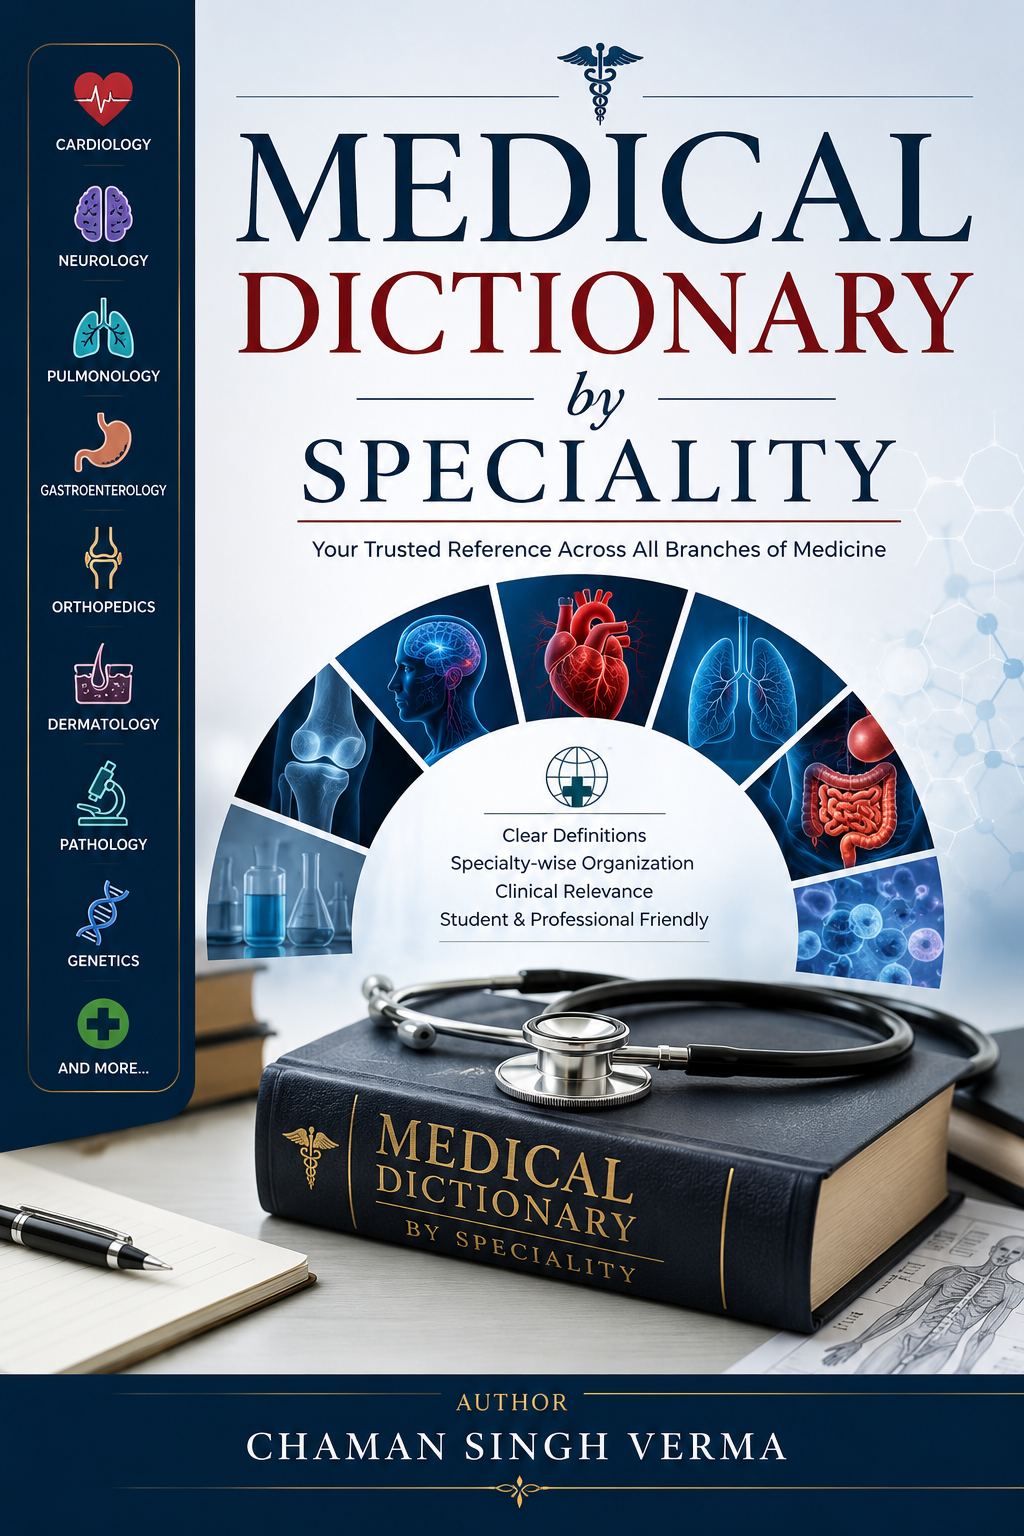
\includegraphics[width=0.6\textwidth]{frontpage.png}
\end{center}
\vspace*{\fill}
\newpage
\thispagestyle{fancy}

{\noindent\large This comprehensive medical dictionary contains thousands of medical terms organized by specialty for efficient reference. Each entry provides a concise definition of fewer than 250 words, covering pathology, clinical medicine, and all major medical specialties. Terms are presented alphabetically within each specialty section for easy lookup.\par}

\tableofcontents
\mainmatter




\chapter{Anatomy}

\medterm{Abdominal Aorta}-- From diaphragmatic hiatus at T12 to common iliac bifurcation at L4. Major branches: celiac trunk (T12), SMA (L1), IMA (L3), renal arteries (L1-L2), gonadal arteries, lumbar arteries. Anterior to the vertebral column. Abdominal aortic aneurysm is common in elderly males (13th leading cause of death). Rupture causes hypotension, back pain, and pulsatile mass with over 80 percent mortality.

\medterm{Abdominal Cavity}-- The largest body cavity, bounded superiorly by the diaphragm, inferiorly by the pelvic inlet (where it is continuous with the pelvic cavity, collectively termed the abdominopelvic cavity), anterolaterally by the abdominal muscles, and posteriorly by the lumbar vertebral column, psoas, and quadratus lumborum muscles. It is lined by the peritoneum, a continuous serous membrane dividing the space into the peritoneal cavity (containing greater and lesser sacs connected via the epiploic foramen of Winslow) and the retroperitoneal space. It houses major digestive organs (stomach, small and large intestines, liver, gallbladder, pancreas), the spleen, and retroperitoneal structures (kidneys, adrenal glands, abdominal aorta, inferior vena cava). Retroperitoneal organs follow the SAD PUCKER mnemonic: Suprarenal glands, Aorta/IVC, Duodenum (2nd--4th parts), Pancreas (head/body), Ureters, Colon (ascending/descending), Kidneys, Esophagus, Rectum. Pathologies include peritonitis, hemoperitoneum, ascites, intra-abdominal abscesses, and trauma-induced organ laceration.

\medterm{Abducens Nerve (Cranial Nerve VI)}-- The sixth cranial nerve (CN VI), a purely somatic motor nerve that innervates the lateral rectus muscle of the eye, responsible for abduction of the globe. Its nucleus is situated in the dorsal caudal pons in the floor of the fourth ventricle, encircled by fibers of the facial nerve (facial colliculus). It emerges from the brainstem at the pontomedullary junction, ascends the clivus, traverses Dorello's canal beneath the petroclinoid ligament, courses through the cavernous sinus (adjacent to the internal carotid artery), and enters the orbit through the superior orbital fissure within the common tendinous ring (annulus of Zinn). Because it has the longest intracranial subarachnoid course of any cranial nerve, it is exceptionally vulnerable to elevated intracranial pressure (a 'false localizing sign'). Abducens nerve palsy causes horizontal diplopia (worse on lateral gaze toward the affected side) and an inability to abduct the affected eye, resulting in convergent strabismus (esotropia).

\medterm{Abduction}-- A movement of a limb or body part in the coronal plane away from the median plane (midline) of the body. For the fingers, abduction is spreading them away from the longitudinal axis of the third (middle) digit; for the toes, it is movement away from the second digit. For the thumb, abduction is movement anteriorly away from the palm in the sagittal plane. Produced by muscles such as the middle deltoid and supraspinatus (arm), gluteus medius and minimus (thigh), and dorsal interossei (hand and foot).

\medterm{Accessory Nerve (Cranial Nerve XI)}-- The eleventh cranial nerve (CN XI), a purely motor nerve that innervates the sternocleidomastoid (SCM) and trapezius muscles. Although historically described as having cranial and spinal roots, modern neuroanatomy recognizes it as arising from lower motor neurons in the anterior horn of the upper cervical spinal cord (C1--C5/C6). These spinal rootlets unite, ascend through the foramen magnum into the posterior cranial fossa, and exit the skull through the jugular foramen alongside CN IX and CN X. It traverses the posterior triangle of the neck superficially between the posterior border of the SCM and the anterior border of the trapezius, embedded within the investing layer of deep cervical fascia. Its superficial course in the posterior neck makes it vulnerable to injury during lymph node biopsies, radical neck dissection, or penetrating trauma. Injury produces shoulder drop, winged scapula (lateral winging due to trapezius weakness, unlike medial winging from long thoracic nerve injury), and weakness in contralateral head turning and shoulder shrugging.

\medterm{Acetabulum}-- Cup-shaped lateral hip socket from fused ilium, ischium, and pubis. Articulates with the femoral head at the ball-and-socket hip joint. The acetabular labrum deepens the socket. Oriented with approximately 15 degrees anteversion and 45 degrees inclination. Fractures are serious high-energy trauma injuries.

\medterm{Achilles Tendon (Calcaneal Tendon)}-- The thickest and strongest tendon in the human body, connecting the gastrocnemius and soleus (triceps surae) muscles to the calcaneus (heel bone). It plays a crucial role in plantarflexion of the foot, enabling walking, running, and jumping. The tendon is vulnerable to tendonitis and acute rupture, which presents with a sudden "pop" and a positive Thompson test. Also known as the calcaneal tendon.

\medterm{Acromioclavicular Joint}-- A plane synovial joint between the acromion of the scapula and the lateral end of the clavicle. It permits gliding movements and is stabilized primarily by the acromioclavicular and coracoclavicular ligaments.

\medterm{Acromion}-- Bony process forming the shoulder's highest point, extending laterally from the scapular spine. Articulates with the clavicle at the acromioclavicular joint and arches over the glenohumeral joint. Attachment for deltoid and trapezius. The subacromial space contains the supraspinatus tendon and subacromial bursa. Its shape influences impingement syndrome susceptibility.

\medterm{Adam's Apple}-- The common name for the laryngeal prominence, the visible projection at the front of the neck formed by the angle where the two laminae of the thyroid cartilage meet. It protects the larynx and vocal cords, and it usually becomes more prominent during male puberty as the larynx enlarges under androgen influence, although it is present in people of all sexes. Its size does not determine voice quality or health.

\medterm{Adduction}-- A movement of a limb or body part in the coronal plane toward the median plane (midline) of the body. For the digits of the hand, adduction draws the fingers toward the longitudinal axis of the third (middle) digit; for the toes, it brings them toward the second digit. For the thumb, adduction brings it toward the radial border of the palm. Produced by muscles including pectoralis major and latissimus dorsi (arm), adductor longus, brevis, and magnus (thigh), and palmar interossei (hand).

\medterm{Adductor Muscles}-- A group of muscles situated in the medial compartment of the thigh that adduct and stabilize the hip: adductor longus, adductor brevis, adductor magnus, gracilis, and pectineus. They originate from the pubic and ischiopubic rami and insert along the linea aspera of the femur (gracilis inserts onto the anteromedial tibia at the pes anserinus). Innervation is provided primarily by the obturator nerve (L2--L4); pectineus is dual-innervated (predominantly by the femoral nerve, L2--L3, with variable obturator assistance), and adductor magnus is a hybrid muscle having an adductor part (obturator nerve) and a hamstring part (tibial division of the sciatic nerve, L4). Adductor longus is the most frequently injured muscle in athletic 'groin strains.' The adductor (Hunter) canal is an aponeurotic tunnel beneath the sartorius conveying the femoral artery, femoral vein, nerve to vastus medialis, and saphenous nerve into the popliteal fossa.

\medterm{Adenoids}-- Lymphoid tissue in the posterior wall and roof of the nasopharynx, part of Waldeyer ring of pharyngeal lymphoid tissue. Enlarged adenoids (adenoidal hypertrophy) in children cause nasal obstruction, mouth breathing, snoring, obstructive sleep apnea, serous otitis media (eustachian tube obstruction), and facial changes ('adenoid facies'). Inflammation (adenoiditis) is treated medically or with adenoidectomy. They enlarge in childhood and atrophy after puberty. Also called the pharyngeal tonsil.

\medterm{Adipose Tissue}-- A specialized connective tissue composed mainly of adipocytes that store energy as triglycerides. It provides thermal insulation, cushioning for organs, and endocrine regulation through hormones and signaling molecules such as leptin and adiponectin. White adipose tissue is the principal energy store in adults, whereas brown adipose tissue contains abundant mitochondria and generates heat through non-shivering thermogenesis, especially in newborns. Excess visceral adipose tissue is associated with insulin resistance, dyslipidemia, hypertension, and increased cardiometabolic risk.

\medterm{Adrenal Gland}-- Paired endocrine glands atop each kidney (suprarenal), composed of cortex and medulla. Cortex (three zones): zona glomerulosa (aldosterone, mineralocorticoids), zona fasciculata (cortisol, glucocorticoids), zona reticularis (androgens). Medulla: chromaffin cells secrete epinephrine and norepinephrine (catecholamines). Regulated by ACTH (cortex) and sympathetic nervous system (medulla). Conditions: Cushing syndrome, Addison disease, pheochromocytoma, Conn syndrome, congenital adrenal hyperplasia.

\medterm{Alveolus}-- The terminal air sac (200-300 microns) where gas exchange occurs. Approximately 300-500 million per lung, providing ~70 m2 surface area. Wall: type I pneumocytes (95\% surface, thin for diffusion), type II pneumocytes (5\%, secrete pulmonary surfactant reducing surface tension), alveolar macrophages (dust cells, phagocytosis). Capillary network in close apposition (blood-air barrier: type I pneumocyte, fused basement membrane, capillary endothelium). Surfactant deficiency causes RDS in preterm infants. Conditions: pneumonia, ARDS, pulmonary edema, emphysema (alveolar destruction), pulmonary fibrosis.

\medterm{Amygdala}-- Almond-shaped nucleus cluster in the anterior medial temporal lobe, part of the limbic system, primarily processing emotions (especially fear/anxiety). Receives thalamic/cortical sensory input; projects to hypothalamus, brainstem, and cortex for autonomic/behavioral fear responses. Essential for emotional memory (fear conditioning) and social signal processing. Lesions (Urbach-Wiethe disease) impair fear recognition. Hyperactive in anxiety disorders and PTSD.

\medterm{Anal Canal}-- The terminal 3-4 cm of the gastrointestinal tract, extending from the anorectal junction (puborectalis/pectinate line) to the anal verge. Above the pectinate line: lined by columnar epithelium, innervated by autonomic nerves, draining to portal system, supplied by superior rectal artery. Below the pectinate line: stratified squamous epithelium, somatic innervation (inferior rectal nerve—pain-sensitive), systemic drainage. Internal anal sphincter (smooth, involuntary, sympathetic/parasympathetic) and external anal sphincter (striated, voluntary, pudendal). Hemorrhoids, fissures, fistulae, and anorectal abscesses occur here.

\medterm{Anatomical Axis}-- An imaginary reference line around which a body part, joint, or bone rotates, or along which a structure extends. The three cardinal axes of the human body are: the transverse (horizontal/coronal) axis, around which flexion and extension occur; the anteroposterior (sagittal) axis, around which abduction and adduction occur; and the longitudinal (vertical) axis, around which medial and lateral rotation occur. In long bones, the mechanical axis connects the centers of the proximal and distal joints, which may diverge from the anatomical axis of the bone shaft.

\medterm{Anatomical Planes}-- Hypothetical imaginary flat two-dimensional geometric surfaces passing through the human body in the standard anatomical position, used as reference frameworks for describing anatomical locations, sections, movements, and radiological imaging (CT, MRI, ultrasound). The three cardinal orthogonal planes are: (1) Sagittal planes (including the median/midsagittal plane), dividing the body into right and left halves; (2) Coronal (frontal) planes, dividing the body into anterior (front) and posterior (back) portions; and (3) Transverse (axial/horizontal) planes, dividing the body into superior (upper) and inferior (lower) portions. Oblique planes pass at any non-orthogonal angle.

\medterm{Anatomical Position}-- The universal standardized reference posture of the human body used in all anatomical, surgical, and clinical descriptions to ensure unambiguous spatial terminology. It is defined as: an individual standing fully erect, facing forward, head level with eyes looking straight ahead toward the horizon, lower limbs together with feet parallel and directed forward, and upper limbs hanging relaxed at the sides with the palms facing forward (supinated) and the thumbs pointing away from the body. All relational terms (anterior, posterior, medial, lateral, superior, inferior) are defined strictly relative to this posture, regardless of the patient's actual physical position (e.g., supine, prone, or lateral decubitus).

\medterm{Anatomical Snuffbox}-- Triangular depression on the dorsal wrist, bounded by extensor pollicis longus medially and extensor pollicis brevis/abductor pollicis longus laterally. Floor contains the scaphoid, trapezium, and radial artery. Tenderness after a fall on an outstretched hand suggests scaphoid fracture. The radial artery pulse is palpable here.

\medterm{Ankle Joint}-- Uniaxial hinge synovial joint between distal tibia, lateral malleolus, and superior talus, allowing dorsiflexion/plantarflexion. Medial (deltoid) ligament resists eversion; lateral complex resists inversion. The ankle mortise provides bony stability. Ankle sprains are the most common sports injury (anterior talofibular ligament most commonly affected). Fractures classified by the Weber system.

\medterm{Antecubital Fossa}-- Triangular depression on the anterior elbow, bounded laterally by brachioradialis, medially by pronator teres, and superiorly by a line connecting the epicondyles. Floor formed by brachialis and supinator. Contains biceps tendon, brachial artery, and median nerve. Primary site for venipuncture and blood pressure measurement.

\medterm{Anterior}-- A directional term indicating a position situated at, toward, or closer to the front (ventral) surface of the body or an organ. In human anatomy, because of upright bipedal posture, anterior is generally synonymous with ventral. Opposed to posterior (dorsal). Examples include the sternum lying anterior to the heart, and the patella situated on the anterior surface of the knee.

\medterm{Anterior Cruciate Ligament (ACL)}-- A primary stabilizing intra-articular, extrasynovial ligament of the knee joint. It originates from the posteromedial aspect of the lateral femoral condyle in the intercondylar notch and passes anteriorly, medially, and distally to insert onto the anterior intercondylar area of the tibial plateau, blending with the anterior horn of the lateral meniscus. Composed of two functional bundles: the anteromedial bundle (tight in flexion) and the posterolateral bundle (tight in extension). Its primary function is to resist anterior translation of the tibia relative to the femur (providing ~85 percent of total resistance) and secondary restraint against internal tibial rotation and varus/valgus stress. ACL rupture is among the most common major sports injuries, typically occurring from non-contact deceleration, cutting, or landing with a valgus knee and internally rotated tibia. Clinical diagnosis is made using the Lachman test (most sensitive), anterior drawer test, and pivot-shift test; confirmed by MRI.

\medterm{Anterior Tibial Artery}-- Arises from the popliteal artery, passes through the anterior intermuscular septum to the anterior compartment, continuing to the ankle as the dorsalis pedis artery. Supplies anterior leg and dorsal foot muscles. Palpable anterior to the lateral malleolus as the dorsalis pedis pulse. Important for vascular assessment; vulnerable to injury in tibial fractures and anterior compartment syndrome.

\medterm{Anus}-- The terminal opening of the gastrointestinal tract through which feces are expelled. It is surrounded by the internal smooth-muscle sphincter and external skeletal-muscle sphincter.

\medterm{Aorta}-- Largest artery, from the left ventricle distributing oxygenated blood systemically. Approximately 30 cm long, 2.5 cm diameter. Four segments: ascending aorta, aortic arch (brachiocephalic trunk, left common carotid, left subclavian), descending thoracic aorta, descending abdominal aorta (bifurcating into common iliacs at L4). Three layers: intima, media (elastic tissue), adventitia. Aneurysm and dissection are life-threatening.

\medterm{Aortic Arch}-- Curves from second right sternocostal joint superiorly and left, then posteriorly and inferiorly to T4. From right to left: brachiocephalic trunk, left common carotid, left subclavian. Related to left recurrent laryngeal nerve (hooking under it), trachea, esophagus, left phrenic nerve. Arch aneurysms may cause hoarseness and SVC syndrome.

\medterm{Aortic Valve}-- Semilunar valve located between the left ventricle and the ascending aorta, consisting of three pocket-like cusps: right, left, and posterior (non-coronary). Superior to each cusp is an aortic sinus (sinus of Valsalva); the right and left coronary arteries arise from the right and left aortic sinuses, respectively, whereas the posterior sinus gives rise to no coronary vessel. The valve opens passively during ventricular systole and closes during diastole, preventing systemic regurgitation. Aortic stenosis is the most prevalent valvular disease in elderly patients, typically resulting from calcific degeneration and presenting with angina, syncope, heart failure, and a harsh systolic crescendo-decrescendo murmur radiating to the carotids. Bicuspid aortic valve is the most common congenital cardiac valvular abnormality, predisposing to premature calcific stenosis, regurgitation, and ascending aortic aneurysm.

\medterm{Appendix}-- A blind-ended tubular diverticulum of the cecum, typically 6-10 cm long, rich in lymphoid tissue. Its position is variable (retrocecal, pelvic, or retroileal); the base usually projects near McBurney's point, one-third of the distance from the anterior superior iliac spine to the umbilicus. Innervated by T10 (visceral pain initially periumbilical, later often localizing to the right lower quadrant). Acute appendicitis may cause perforation, abscess, and peritonitis; appendectomy is definitive treatment.

\medterm{Arachnoid Mater}-- The middle of the three meninges, a delicate avascular membrane lying between the dura mater and pia mater. The subarachnoid space between arachnoid and pia contains cerebrospinal fluid (CSF) and major vessels. Arachnoid granulations (villi) project into the dural venous sinuses and mediate CSF resorption. The arachnoid is separated from the dura by the subdural space (site of subdural hematoma). Inflammation (meningitis) or hemorrhage (subarachnoid hemorrhage) in this space has serious consequences.

\medterm{Arrector Pili Muscle}-- A small band of involuntary smooth muscle attached to a hair follicle and the superficial dermis. Sympathetic stimulation causes it to contract, pulling the hair upright and producing temporary piloerection, commonly called goosebumps. Contraction also compresses nearby sebaceous glands and may help release sebum onto the skin surface.

\medterm{Arteriole}-- A small artery that delivers blood to a capillary bed. Arteriolar smooth muscle regulates vascular resistance and controls tissue perfusion and systemic blood pressure.

\medterm{Artery}-- A blood vessel that carries oxygenated blood away from the heart to the tissues, except for the pulmonary arteries which carry deoxygenated blood to the lungs. Arteries have thick, elastic, muscular walls that withstand high pressure and distribute blood throughout the body. The aorta is the largest artery. Arterial structure: tunica intima (endothelium), tunica media (smooth muscle and elastic fibers), tunica adventitia (connective tissue). Arteries branch into smaller arterioles and eventually capillaries. Diseases: atherosclerosis, aneurysms, arteritis, emboli.

\medterm{Ascending Aorta}-- From left ventricle at the aortic valve to the sternal angle (approximately 5 cm), enclosed in pericardium. Gives rise to right/left coronary arteries at the aortic sinuses. Most common site of aneurysm and dissection, especially in Marfan syndrome, bicuspid aortic valve, and hypertension. Aneurysms may compress adjacent structures and cause aortic regurgitation.

\medterm{Ascending Colon}-- Extends from cecum to hepatic flexure below the liver, approximately 15-20 cm, retroperitoneal (fixed to posterior abdominal wall). Anteriorly: abdominal wall. Posteriorly: right kidney. Absorbs water/electrolytes and compacts fecal matter. Tumors may present as a palpable right-sided mass. The right colic flexure marks its transition to the transverse colon.

\medterm{Atlas (C1)}-- First cervical vertebra articulating with occipital condyles at the atlanto-occipital joint for nodding movement. Lacks a body and spinous process; has anterior/posterior arches and lateral masses. Transverse foramina transmit vertebral arteries. The anterior arch has a facet for the axis dens. Commonly fractured in axial loading injuries such as diving accidents.

\medterm{Atrium}-- One of the two upper chambers of the heart that receive blood returning to the heart. The right atrium receives deoxygenated blood from the superior and inferior venae cavae and the coronary sinus; the left atrium receives oxygenated blood from the four pulmonary veins. The interatrial septum separates the two atria; the fossa ovalis marks the site of the fetal foramen ovale. Atrial contraction (atrial kick) contributes 15--25\% of ventricular filling. The atrial appendages (auricles) increase atrial capacity. Conditions: atrial fibrillation, atrial septal defect, atrial myxoma.

\medterm{Axilla}-- Pyramidal space between the upper lateral thorax and medial arm. Bounded by anterior fold (pectoralis major/minor), posterior fold (latissimus dorsi/teres major), medial wall (ribs/serratus anterior), and lateral wall (humerus). Contains axillary artery/vein, brachial plexus cords, and lymph nodes. Axillary nodes are significant in breast cancer staging.

\medterm{Axillary Artery}-- The continuation of the subclavian artery, running from the outer border of the first rib to the lower border of teres major, where it becomes the brachial artery. Divided into three parts by the pectoralis minor. Branches (part 1): superior thoracic; (part 2): thoracoacromial, lateral thoracic; (part 3): subscapular, anterior and posterior circumflex humeral. Supplies the shoulder, axilla, and upper limb. Relations: axillary vein (anterior/medial), brachial plexus cords. Site of axillary artery catheterization; injury causes axillary hematoma and upper limb ischemia; circumflex humeral vessels are important to the humeral head blood supply.

\medterm{Axillary Nerve}-- From posterior cord (C5-C6), passing through the quadrangular space with the posterior circumflex humeral artery. Innervates deltoid and teres minor; provides sensation to the regimental badge area (lateral deltoid skin). Vulnerable in anterior shoulder dislocations and surgical neck humeral fractures. Injury causes loss of lateral deltoid sensation and weakness of abduction beyond 15 degrees.

\medterm{Axis (C2)}-- Second cervical vertebra with the dens (odontoid process) projecting superiorly, serving as a pivot for atlas rotation, allowing approximately 50 percent of cervical rotation. Has a large spinous process and flat superior articular facets. Dens fractures (Types I-III) may cause atlanto-axial instability and spinal cord compression, often requiring surgical fixation.

\medterm{Axon}-- The single long process of a neuron that conducts action potentials away from the cell body toward the axon terminal for synaptic transmission. Axons vary in length (microscopic to >1 m for sciatic motor fibers) and are wrapped by Schwann cells (PNS) or oligodendrocytes (CNS) to form myelin, which enables saltatory conduction and speeds transmission. Axons end in synaptic boutons releasing neurotransmitters. Axonal injury in the CNS does not regenerate effectively; Wallerian degeneration occurs distal to injury. Axonal transport (anterograde and retrograde) carries organelles and proteins.

\medterm{Azygos Vein}-- An unpaired vein ascending on the right side of the vertebral column that drains the posterior thoracic wall and empties into the superior vena cava. It provides an important collateral pathway between the superior and inferior venae cavae.

\medterm{Basal Ganglia}-- Deep gray matter nuclei in the cerebral hemispheres for motor control, cognition, and emotion. Key structures: caudate nucleus, putamen, globus pallidus (internal/external segments), subthalamic nucleus, substantia nigra. Direct pathway facilitates movement; indirect inhibits it. Receive cortical/thalamic input, project back to cortex via thalamus. Diseases: Parkinson's (substantia nigra dopamine depletion), Huntington's (caudate atrophy), hemiballismus (subthalamic lesion).

\medterm{Basement Membrane}-- A specialized, dense, thin sheet of extracellular matrix that underlies all epithelial layers and surrounds muscle fibers, adipocytes, and Schwann cells, anchoring them to the underlying connective tissue. It consists of two ultrastructural layers: the basal lamina (secreted by epithelial cells, composed of type IV collagen, laminin, enactin/nidogen, and perlecan/heparan sulfate proteoglycans) and the reticular lamina (secreted by connective tissue fibroblasts, containing type III collagen/reticulin and type VII anchoring fibrils). Functions include mechanical anchoring via hemidesmosomes, cellular polarity maintenance, semipermeable size- and charge-selective filtration (critical in the renal glomerular basement membrane), tissue compartmentalization, and regulation of cell growth, differentiation, and repair. Pathologies include Goodpasture syndrome (autoantibodies against type IV collagen alpha-3 chain), Alport syndrome (hereditary type IV collagen mutations causing nephritis and hearing loss), bullous pemphigoid (autoantibodies against hemidesmosomal BP180/BP230 at the basement membrane), and tumor invasion (epithelial carcinomas must breach the basement membrane to metastasize).

\medterm{Biceps Brachii Muscle}-- A prominent two-headed muscle in the anterior compartment of the arm. The long head originates from the supraglenoid tubercle of the scapula and the glenoid labrum, coursing intracapsularly across the humeral head and exiting via the intertubercular (bicipital) groove; the short head originates from the tip of the coracoid process alongside the coracobrachialis. Both heads fuse into a common distal tendon that inserts onto the radial tuberosity, with a medial aponeurotic expansion (bicipital aponeurosis) inserting into the deep fascia of the forearm. Innervated by the musculocutaneous nerve (C5--C7, primarily C5--C6). It functions as the body's most powerful supinator of the flexed forearm, a major elbow flexor, and a secondary shoulder flexor and stabilizer. Rupture of the proximal long head tendon causes distal retraction ('Popeye deformity'), while distal tendon rupture severely weakens supination and requires urgent surgical repair. Bicipital tenosynovitis is a common source of anterior shoulder pain.

\medterm{Bile Duct}-- A channel that carries bile from the liver and gallbladder to the duodenum. The right and left hepatic ducts unite as the common hepatic duct; union with the cystic duct forms the common bile duct, which usually joins the pancreatic duct before entering the duodenum at the major duodenal papilla.

\medterm{Bone}-- A rigid, mineralised connective tissue that forms the skeleton, providing structural support, protection of vital organs, hematopoiesis (bone marrow), and mineral storage (calcium, phosphate). Bone composition: organic matrix (90\% type I collagen) and inorganic mineral (hydroxyapatite, calcium phosphate). Types: cortical (compact, 80\% of bone mass) and cancellous (trabecular, 20\%). Cells: osteoblasts (bone formation), osteocytes (mechanosensation), osteoclasts (bone resorption). Ossification: intramembranous (flat bones) and endochondral (long bones). Remodelling: continuous cycle of resorption and formation.

\medterm{Bone Marrow}-- Vascular tissue within the medullary cavities and cancellous bone. Red marrow produces blood cells, whereas yellow marrow primarily stores fat and can revert to red marrow when demand increases.

\medterm{Brachial Artery}-- The continuation of the axillary artery, running from the lower border of teres major to the cubital fossa, where it divides into radial and ulnar arteries. Lies medial to the biceps; palpated for blood pressure and brachial pulse. Branches: profunda brachii (deep brachial), superior/inferior ulnar collaterals. Site for blood pressure measurement, arterial access (catheterization), and the median nerve travels alongside. Trauma here causes forearm ischemia; collateral circulation around the elbow (anastomosis) limits ischemic damage.

\medterm{Brachialis Muscle}-- A powerful, broad muscle lying deep to the biceps brachii in the lower two-thirds of the anterior arm. It originates from the distal half of the anterior surface of the humerus and adjacent intermuscular septa, descending across the anterior capsule of the elbow joint to insert onto the ulnar tuberosity and the coronoid process of the ulna. It is innervated primarily by the musculocutaneous nerve (C5--C7); its lateral portion also receives sensory and proprioceptive twigs from the radial nerve (C7). Because it inserts onto the ulna rather than the radius, its mechanical advantage is completely independent of forearm rotation, making it the primary 'workhorse' flexor of the elbow in all positions (pronation, supination, or midway). Trauma to the elbow or repetitive stress can lead to brachialis tendinopathy or post-traumatic myositis ossificans.

\medterm{Brachial Plexus}-- Nerve network (C5-T1) formed by roots, trunks, divisions, and cords, giving rise to upper limb nerves. Roots unite into superior/middle/inferior trunks, dividing into anterior/posterior divisions, recombining into lateral/posterior/medial cords. Major branches: musculocutaneous, axillary, radial, median, ulnar. Birth injuries cause Erb's palsy (C5-C6) or Klumpke's palsy (C8-T1). Vulnerable to shoulder trauma and thoracic outlet syndrome.

\medterm{Brachial Plexus Cords}-- Formed by divisions recombining behind the pectoralis minor. Lateral cord (anterior divisions of upper/middle trunks), posterior cord (all three posterior divisions), medial cord (anterior division of lower trunk). Named for relationship to the axillary artery. Lateral cord: lateral pectoral nerve, contributes to median nerve. Posterior cord: subscapular, thoracodorsal, axillary, radial nerves. Medial cord: medial pectoral, cutaneous, and ulnar nerves.

\medterm{Brachial Plexus Roots}-- Ventral rami of C5-T1 emerging from intervertebral foramina, passing between anterior and middle scalene muscles (interscalene triangle). C5-C6 form the upper trunk, C7 continues as middle trunk, C8-T1 form the lower trunk. Root injuries cause specific dermatome/myotome deficits. C5 avulsion causes loss of deltoid/biceps function. Roots are vulnerable in birth trauma, motorcycle accidents, and disc herniation radiculopathy.

\medterm{Brachial Plexus Trunks}-- Formed in the posterior neck triangle. Upper (C5-C6), middle (C7), and lower (C8-T1) trunks each divide into anterior/posterior divisions behind the clavicle. Upper trunk is most commonly injured in birth injuries (Erb-Duchenne palsy), causing waiter's tip position. Lower trunk injury (Klumpke's palsy from upward arm traction) causes claw hand.

\medterm{Brachiocephalic Trunk}-- The first and largest branch of the aortic arch. It ascends to the right sternoclavicular joint, where it divides into the right common carotid and right subclavian arteries.

\medterm{Brain}-- The central organ of the nervous system, enclosed in the cranial cavity and composed of the cerebrum, cerebellum, and brainstem. The brain receives, processes, and integrates sensory information; initiates and coordinates motor responses; and serves as the seat of cognition, emotion, memory, and consciousness. The cerebrum (largest part) has two hemispheres connected by the corpus callosum, with four lobes (frontal, parietal, temporal, occipital) responsible for higher functions. The cerebellum coordinates movement, balance, and motor learning. The brainstem (midbrain, pons, medulla) controls vital autonomic functions (breathing, heart rate, blood pressure) and contains cranial nerve nuclei. Protected by the skull, meninges (dura, arachnoid, pia), and cerebrospinal fluid. Blood supply via internal carotid and vertebral arteries (circle of Willis). Conditions: stroke, tumor, trauma, neurodegenerative diseases, epilepsy, infection.

\medterm{Brainstem}-- Connects cerebrum to spinal cord, with midbrain (superior), pons (middle), and medulla oblongata (inferior). Contains cranial nerve nuclei (III-XII), ascending/descending tracts, and vital autonomic centers for cardiac, respiratory, and vasomotor function. Reticular formation regulates consciousness and sleep-wake cycles. Contains all brain-spinal cord pathways. Lesions are often devastating and fatal, causing respiratory arrest, cardiac arrhythmias, and bilateral cranial nerve deficits.

\medterm{Bronchi}-- The major airways conducting air from the trachea into the lungs. The trachea bifurcates at the carina (T4-T5) into right and left main bronchi. The right main bronchus is wider, shorter, and more vertical—aspirated foreign bodies preferentially lodge here. Main bronchi divide into lobar (secondary), segmental (tertiary), and progressively smaller bronchi and bronchioles. Bronchi contain cartilage and submucosal glands; bronchioles lack cartilage. Bronchial walls contain smooth muscle (bronchoconstriction in asthma), goblet cells, and ciliated epithelium that clears mucus. Blood supply: bronchial arteries.

\medterm{Bronchiole}-- Small airways (less than 2 mm diameter) without cartilage, branching from segmental bronchi to terminal bronchioles (conducting zone) to respiratory bronchioles (transitional, alveoli bud from walls) to alveolar ducts to alveolar sacs to alveoli. Lined by ciliated simple cuboidal epithelium (Clara cells in terminal bronchioles, secrete surfactant components). No goblet cells, no submucosal glands. Smooth muscle in walls regulates airflow (bronchoconstriction/dilation). Conditions: bronchiolitis, asthma, bronchiolitis obliterans, small airway disease.

\medterm{Bronchus}-- One of the two main branches of the trachea that conduct air into the lungs. The right main bronchus is wider, shorter, and more vertical than the left, making it more susceptible to aspiration. Each main bronchus divides into lobar bronchi (secondary), segmental bronchi (tertiary), and progressively smaller branches (bronchioles). Bronchial walls contain ciliated pseudostratified columnar epithelium, smooth muscle, cartilage plates, and mucous glands. Bronchoconstriction occurs in asthma. Bronchiectasis is irreversible dilatation. Bronchoscopy allows visualization and biopsy.

\medterm{Cadaver}-- A dead human body used for anatomical dissection, surgical training, and medical research. Cadavers are preserved through embalming (arterial injection of formaldehyde-based fixatives) to prevent decomposition and maintain tissue integrity. Anatomical dissection of cadavers remains a cornerstone of medical education, providing three-dimensional understanding of human anatomy, anatomical variation, and surgical approaches. Whole-body donation programs supply cadavers to medical schools; ethical considerations include informed consent, respectful treatment, and compliance with anatomical gift laws.

\medterm{Calcaneus}-- Largest tarsal bone forming the heel. Articulates with talus proximally and cuboid anteriorly. Lever for the calf muscles via the Achilles tendon on its posterior tuberosity. Predominantly trabecular bone, the most commonly fractured tarsal bone from falls from height. Bohler's angle assesses fractures on lateral radiographs.

\medterm{Cantlie Line}-- Functional liver division extending from the gallbladder fossa to the IVC, corresponding to the middle hepatic vein plane. Unlike the falciform ligament (anatomical division), it represents the true functional blood supply/biliary drainage division. Right hepatic artery and portal vein supply the right half; left supply the left. Basis for anatomic hepatic segmentectomy and liver transplantation.

\medterm{Capillary}-- The smallest blood vessel, consisting primarily of a single endothelial cell layer and basement membrane. Capillaries connect arterioles with venules and are the principal site of exchange between blood and tissues.

\medterm{Capillary Bed}-- A network of interconnected capillaries that links arterioles to venules within a tissue. It provides a large surface area for exchange of oxygen, carbon dioxide, nutrients, hormones, and metabolic waste between blood and interstitial fluid. Precapillary sphincters and arteriolar tone regulate how much blood enters the bed according to local metabolic demand.

\medterm{Capitate}-- Largest carpal bone, centrally located in the distal row as the carpal keystone. Rounded head articulates with scaphoid and lunate; distal surface with the third metacarpal. Last carpal bone to ossify. Wrist joint axis, bearing significant axial load. Avascular necrosis may occur with fractures similar to scaphoid injuries.

\medterm{Cardiac Muscle}-- Involuntary, striated muscle forming the myocardium. Cardiac muscle cells are electrically connected by intercalated discs, allowing coordinated contraction of the heart.

\medterm{Carotid Artery}-- The paired arterial system supplying the head and neck. Each common carotid artery divides into internal and external carotid arteries; the internal carotid supplies the brain and orbit, while the external carotid supplies most external head and neck structures.

\medterm{Carpal Tunnel}-- Narrow passageway on the palmar wrist, bounded by carpal bones dorsally and the flexor retinaculum as the roof. Transmits the median nerve and flexor tendons. Carpal tunnel syndrome causes numbness in the lateral 3.5 digits and thenar weakness. It is the most common entrapment neuropathy, associated with repetitive motion, diabetes, hypothyroidism, and pregnancy.

\medterm{Cartilage}-- A tough, flexible avascular connective tissue found in joints, the ear, nose, rib cage, and intervertebral discs. Composed of chondrocytes embedded in an extracellular matrix of collagen fibers, proteoglycans, and water, providing resilience and compressive strength. Types: hyaline cartilage (most common, covers articular surfaces of joints, costal cartilages), elastic cartilage (ear, epiglottis), and fibrocartilage (intervertebral discs, menisci, pubic symphysis). Cartilage lacks blood vessels, nerves, and lymphatics; it receives nutrition by diffusion from synovial fluid, limiting healing capacity.

\medterm{Caudal}-- A directional term relating to or situated toward the tail (coccyx) or inferior aspect of the trunk in humans. In embryology and comparative anatomy, caudal denotes the tail-end of the embryonic axis, opposed to rostral/cranial. In regional anatomy, it is frequently used synonymously with inferior (e.g., the caudal end of the spinal cord terminates at L1--L2 as the conus medullaris).

\medterm{Cecum}-- First and widest large intestinal part in the right iliac fossa below the ileocecal valve, a blind-ended pouch approximately 6 cm long. Appendix arises from its posteromedial wall approximately 2 cm below the valve, containing abundant lymphoid tissue. Cecal volvulus causes large bowel obstruction. Absorbs water/electrolytes and compacts fecal matter.

\medterm{Celiac Artery}-- The first major ventral branch of the abdominal aorta at T12, arising from the aorta just below the diaphragm and supplying the foregut (stomach, proximal duodenum, liver, gallbladder, spleen, pancreas). It trifurcates into the left gastric, splenic, and common hepatic arteries, with rich collateral circulation between these branches. Occlusion/stenosis can cause chronic mesenteric ischemia. The celiac trunk is encased in the celiac plexus; it is important in vascular surgery (celiac axis clamping) and anatomy of the pancreatic bed.

\medterm{Celiac Trunk}-- First major abdominal aortic branch at T12-L1, the foregut artery. Divides into left gastric (lesser curvature), splenic (spleen, pancreas, greater curvature), and common hepatic (proper hepatic/gastroduodenal) arteries. Surrounded by the celiac plexus. Compression by the median arcuate ligament causes celiac trunk compression syndrome with postprandial pain.

\medterm{Cell}-- The fundamental structural and functional unit of all living organisms. Human cells are eukaryotic, characterized by a nucleus containing DNA and membrane-bound organelles. Major components: cell membrane (phospholipid bilayer with embedded proteins, regulates transport and signaling), cytoplasm (cytosol + organelles), nucleus (chromosomes, nucleolus), mitochondria (ATP production through oxidative phosphorylation), endoplasmic reticulum (protein\/lipid synthesis), Golgi apparatus (modification and sorting of proteins), lysosomes (intracellular digestion), peroxisomes (fatty acid oxidation), and cytoskeleton (microfilaments, intermediate filaments, microtubules--maintains shape and enables movement). Cells differentiate into ~200 specialized types with distinct functions (neurons, myocytes, hepatocytes, etc.). Cell division occurs via mitosis (somatic cells) and meiosis (gametes). Cell death occurs by apoptosis (programmed) or necrosis (pathologic).

\medterm{Central}-- A directional term indicating a location situated at or toward the center, interior, or core of the body, a region, or an organ. Opposed to peripheral. Used in functional anatomy to designate major control hubs (e.g., the Central Nervous System, central venous catheterization in the internal jugular or subclavian vein, and the central canal of the spinal cord).

\medterm{Cerebellum}-- The second largest part of the brain (after the cerebrum) and the largest structure located within the posterior cranial fossa, situated posterior to the pons and medulla oblongata and separated from the occipital lobes by the tentorium cerebelli. Although accounting for only approximately 10 percent of total brain volume, it contains over 50 percent of all central neurons. It consists of two lateral hemispheres joined by a midline vermis and is divided into three functional zones: the vestibulocerebellum (archicerebellum/flocculonodular lobe, governing balance and vestibulo-ocular reflexes), the spinocerebellum (paleocerebellum, coordinating posture and axial/limb tone), and the cerebrocerebellum (neocerebellum, planning and fine-tuning voluntary skilled movements and motor learning). Afferent input arrives via mossy and climbing fibers through the cerebellar peduncles; efferent output leaves via deep cerebellar nuclei (dentate, emboliform, globose, fastigial) projecting to the red nucleus, thalamus, and motor cortex. Cerebellar lesions produce ipsilateral deficits characterized by ataxia, dysmetria (past-pointing), dysdiadochokinesia, intention tremor, nystagmus, and scanning staccato speech.

\medterm{Cerebral Cortex}-- The folded outer layer of gray matter covering the cerebral hemispheres. It contains interconnected networks responsible for conscious perception, voluntary movement, language, memory, and higher cognition.

\medterm{Cerebral Lobes}-- Four lobes divided by sulci. Frontal (anterior to central sulcus): executive function, motor control (precentral gyrus), Broca's area. Parietal (between central and parieto-occipital sulci): somatosensory (postcentral gyrus), spatial awareness. Temporal (below lateral sulcus): auditory processing, memory (hippocampus), Wernicke's area. Occipital (posterior): visual processing. Insula (deep within lateral sulcus): taste, emotion, interoception.

\medterm{Cerebral Peduncle}-- Paired structures of the ventral midbrain carrying descending motor tracts (corticospinal, corticobulbar, corticopontine) connecting the cerebrum to the pons and below. Lesions produce contralateral hemiparesis; Weber syndrome (peduncle + CN III) causes ipsilateral CN III palsy with contralateral hemiparesis. The peduncles are separated by the interpeduncular fossa and flanked by the substantia nigra (dopaminergic, degenerated in Parkinson disease).

\medterm{Cerebrospinal Fluid}-- A clear, colorless, ultrafiltered bodily fluid circulating within the cerebral ventricles, central canal of the spinal cord, and the subarachnoid space surrounding the brain and spinal cord. It is produced continuously at a rate of approximately 500 mL/day (0.35 mL/min; total volume ~150 mL) predominantly by the choroid plexus of the lateral, third, and fourth ventricles. CSF flows from the lateral ventricles through the interventricular foramina of Monro into the third ventricle, passes down the cerebral aqueduct of Sylvius into the fourth ventricle, and exits into the subarachnoid space via the midline foramen of Magendie and paired lateral foramina of Luschka. It circulates around the brain and spinal cord and is resorbed into dural venous sinuses (principally the superior sagittal sinus) via arachnoid granulations (Pacchionian bodies) driven by hydrostatic pressure gradients. It provides physical buoyancy (reducing apparent brain weight from 1400 g to ~50 g), mechanical protection against trauma, and biochemical regulation/waste removal (glymphatic system). Normal opening pressure on lumbar puncture is 10--20 cm H2O. Disruption of flow or resorption leads to hydrocephalus (communicating or non-communicating); CSF analysis is essential in diagnosing meningitis, subarachnoid hemorrhage, and multiple sclerosis.

\medterm{Cerebrum}-- The largest part of the brain, comprising two cerebral hemispheres connected by the corpus callosum. Each hemisphere has four lobes: frontal (executive function, motor, Broca's area), parietal (somatosensory, spatial awareness), temporal (auditory, memory, Wernicke's area), occipital (visual processing). Cerebral cortex (gray matter) over white matter (myelinated tracts). Basal ganglia deep within. Lateral ventricles produce CSF. Blood supply: anterior, middle, posterior cerebral arteries (circle of Willis). Conditions: stroke, tumor, dementia, epilepsy, trauma.

\medterm{Cervical Vertebrae (Cervical Spine, C1-C7)}-- The seven uppermost vertebrae of the vertebral column (C1--C7) forming the cervical spine, supporting the skull and permitting extensive movement of the head and neck. Typical cervical vertebrae (C3--C6) feature small, broad, oval bodies with uncinate processes (forming the uncovertebral joints of Luschka), large triangular vertebral foramina accommodating the cervical enlargement of the spinal cord, bifid spinous processes, and transverse processes containing transverse foramina (foramina transversaria) that transmit the vertebral artery, vertebral veins, and sympathetic plexuses (C1--C6 transmit the vertebral artery; C7 transmits only accessory vertebral veins). Three vertebrae are atypical: C1 (atlas, ring-shaped without body or spinous process, articulates with occipital condyles for nodding movements), C2 (axis, possessing the dens/odontoid process serving as a pivot for atlas rotation), and C7 (vertebra prominens, featuring a long, non-bifid, easily palpable spinous process and a transition toward thoracic morphology). Clinical conditions include cervical radiculopathy (nerve root compression via disc herniation or osteophytes), cervical spondylotic myelopathy (spinal cord compression), whiplash injuries, and high-energy fractures (Jefferson burst fracture of C1, Hangman's fracture of C2).

\medterm{Cervix}-- The inferior, cylindrical portion of the uterus that projects into the vagina. Its canal connects the uterine cavity with the vagina through the internal and external os.

\medterm{Chest Wall}-- The musculoskeletal boundary of the thoracic cavity, formed by the skin, fascia, muscles, ribs, costal cartilages, sternum, thoracic vertebrae, and associated neurovascular structures. It protects the thoracic organs and participates in breathing through coordinated movement of the ribs and respiratory muscles.

\medterm{Chordae Tendineae}-- Thin tendinous cords connecting the papillary muscles to the free edges of the atrioventricular valve leaflets (mitral and tricuspid). They tether the leaflets and, with papillary muscle contraction during ventricular systole, prevent valve prolapse and regurgitation. Rupture (from papillary muscle infarction) causes acute severe mitral regurgitation and cardiogenic shock. Chordal dysfunction contributes to mitral valve prolapse and functional MR.

\medterm{Choroid}-- The vascular layer of the eye between the sclera and retina, part of the uveal tract (with ciliary body and iris). Contains dense capillary network (choriocapillaris) supplying outer retina (photoreceptors). Pigmented (melanin) to absorb stray light. Bruchs membrane separates choroid from retinal pigment epithelium. Conditions: choroidal nevus, melanoma, neovascularization (wet AMD), choroiditis, central serous chorioretinopathy.

\medterm{Ciliary Body}-- Circumferential structure between iris and choroid, with ciliary muscle (accommodation control via zonular fibers) and ciliary processes (aqueous humor production). Part of the uveal tract (iris, ciliary body, choroid). Parasympathetic CN III fibers cause muscle contraction, relaxing zonular fibers and allowing lens convexity for near vision. Ciliary processes secrete aqueous humor into the posterior chamber, flowing through the pupil to the anterior chamber and draining at the trabecular meshwork and Schlemm's canal.

\medterm{Circle of Willis}-- A ring-like arterial anastomosis at the base of the brain that provides collateral blood flow between the anterior (internal carotid) and posterior (vertebrobasilar) circulations. It is formed by the anterior cerebral, anterior communicating, internal carotid, posterior cerebral, and posterior communicating arteries. Aneurysms commonly occur at its junctions (berry aneurysms), which can rupture and cause subarachnoid hemorrhage.

\medterm{Clavicle}-- Only horizontally oriented long bone, serving as a shoulder-trunk strut. Medial end articulates with the manubrium (sternoclavicular joint); lateral end with the acromion (acromioclavicular joint). Most common fracture at the middle-lateral third junction from falls on an outstretched hand. Protects the underlying brachial plexus and subclavian vessels.

\medterm{Coccyx}-- Terminal vertebral column part with 3-5 fused vertebrae. Articulates with the sacrum, allowing limited flexion important during childbirth. Provides attachment for gluteus maximus, coccygeus, and levator ani (pelvic floor). A common site of pain (coccydynia) following falls, direct trauma, and prolonged sitting.

\medterm{Cochlea}-- Snail-shaped hearing organ in the inner ear, coiled approximately 2.5 turns around the modiolus. Three fluid-filled chambers: scala vestibuli (perilymph), scala media (endolymph, organ of Corti), scala tympani (perilymph). The organ of Corti has inner/outer hair cells transducing mechanical vibrations into electrical signals via stereocilia deflection. Basilar membrane vibrates differentially along its length (tonotopic: high frequencies at base, low at apex). Hair cell damage from noise, ototoxicity, and ageing causes irreversible sensorineural hearing loss, most commonly affecting high frequencies.

\medterm{Collecting Duct}-- A tubular structure in the kidney that receives urine from distal convoluted tubules and carries it through the medulla to the renal papilla. Its permeability to water is regulated by antidiuretic hormone.

\medterm{Colon}-- The largest part of the large intestine, extending from the cecum to the rectum. Anatomically divided into ascending colon (right side), transverse colon (across the abdomen), descending colon (left side), and sigmoid colon (S-shaped, leading to the rectum). Functions: absorption of water and electrolytes, fermentation of undigested carbohydrate by gut microbiota, formation and storage of feces. The colon has a distinct appearance with taeniae coli (three longitudinal muscle bands), haustra (sacculations), and appendices epiploicae (fat appendages). Common diseases: diverticulosis, colitis, colorectal cancer, irritable bowel syndrome.

\medterm{Common Bile Duct}-- The duct formed by union of the common hepatic and cystic ducts. It conveys bile to the duodenum, usually joining the pancreatic duct at the hepatopancreatic ampulla.

\medterm{Common Iliac Arteries}-- Terminal abdominal aortic branches at L4, each approximately 4 cm long, dividing into internal and external iliac arteries. They supply the pelvis and lower extremities. The right common iliac artery crosses anterior to the right common iliac vein. Aneurysms may occur with abdominal aortic aneurysm and compress the ureters, causing hydronephrosis. The corresponding common iliac veins unite to form the inferior vena cava at approximately L5.

\medterm{Common Peroneal Nerve}-- Sciatic division (L4-S2) winding around the fibular neck, the body's most vulnerable major nerve to external compression. Divides into superficial peroneal (peroneus longus/brevis, dorsal foot sensation) and deep peroneal (tibialis anterior, extensors, first web space sensation). Injury causes foot drop (loss of dorsiflexion/eversion) with dorsal foot sensory loss.

\medterm{Connective Tissue}-- One of the four basic animal tissue types (along with epithelial, muscle, and nervous tissue), originating from embryonic mesoderm and mesenchyme, that provides structural support, binding, metabolic storage, and defense throughout the body. It consists of cells widely separated by an abundant extracellular matrix (ECM) composed of ground substance (glycosaminoglycans like hyaluronic acid, proteoglycans, glycoproteins) and protein fibers (type I/II/III collagen fibers providing tensile strength, elastic fibers providing elasticity, and reticular fibers providing stroma). Resident cells include fibroblasts (primary ECM producers), adipocytes, mast cells, and tissue macrophages; transient cells include leukocytes. Classified into connective tissue proper (loose/areolar, dense regular in tendons/ligaments, dense irregular in dermis), specialized connective tissue (adipose, cartilage, bone, blood, hemopoietic tissue), and embryonic connective tissue (mesenchyme, Wharton's jelly). Pathologies include Marfan syndrome (fibrillin-1 mutation), Ehlers-Danlos syndromes (collagen synthesis defects), and systemic autoimmune connective tissue diseases (lupus, scleroderma).

\medterm{Contralateral}-- A relational anatomical term denoting a structure, lesion, or symptom located on or affecting the opposite side of the body from another reference structure. Opposed to ipsilateral. For example, because the corticospinal tracts decussate in the medullary pyramids, a stroke in the left motor cortex results in contralateral (right-sided) hemiparesis.

\medterm{Coracoid Process}-- Hook-like scapular projection extending anteriorly and laterally. Attachment for 3 muscles (pectoralis minor, coracobrachialis, short head of biceps) and 3 ligaments. Important surgical landmark. Fractures uncommon but may occur with direct trauma or shoulder dislocations.

\medterm{Cornea}-- Transparent, avascular, dome-shaped anterior eye surface providing approximately two-thirds of total refractive power. Five layers: epithelium (stratified squamous, rapidly regenerating), Bowman's membrane, stroma (thickest, regular collagen), Descemet's membrane, endothelium (single cell layer maintaining transparency). Innervated by CN V1 (ophthalmic trigeminal), extremely sensitive. Conditions: abrasion, ulcers, keratoconus (progressive thinning and cone-shaped protrusion). Contact lens wear is a major risk factor for microbial keratitis, which can rapidly lead to corneal ulceration, perforation, and sight loss if not treated promptly.

\medterm{Coronal Plane}-- A vertical anatomical plane (also known as the frontal plane) oriented parallel to the coronal suture of the skull, passing vertically from side to side to divide the body, organ, or specimen into anterior (front) and posterior (back) portions. Movements taking place in the coronal plane include abduction and adduction. In radiological imaging (CT and MRI), coronal sections display structures viewed from the front, essential for evaluating the paranasal sinuses, orbits, kidneys, and musculoskeletal joints.

\medterm{Coronary Arteries}-- The arterial system supplying oxygenated blood directly to the myocardium, arising from the ascending aorta immediately superior to the aortic valve cusps. The right coronary artery (RCA) arises from the right (anterior) aortic sinus and courses in the coronary sulcus, giving off the conus artery, sinus node artery (in 60 percent of individuals), right marginal artery, and, in right-dominant circulations (approximately 85 percent), the posterior descending artery (PDA/posterior interventricular artery) and AV nodal artery (in 90 percent), supplying the right atrium, right ventricle, SA/AV nodes, and inferior wall of the left ventricle. The left coronary artery (LCA/left main) arises from the left (posterior) aortic sinus and quickly bifurcates into the left anterior descending artery (LAD/anterior interventricular, running in the anterior interventricular groove to supply the anterior wall of the left ventricle, anterior two-thirds of the interventricular septum, and apex) and the left circumflex artery (LCx, coursing in the left coronary sulcus to supply the lateral and posterior left ventricular walls). Unlike most systemic beds, myocardial perfusion occurs almost entirely during ventricular diastole. Atherosclerotic occlusion causes coronary artery disease, angina pectoris, and acute myocardial infarction (LAD occlusion is known as the 'widow-maker').

\medterm{Coronary Sinus}-- A large vein on the back of the heart that collects deoxygenated blood from the heart muscle and drains it into the right atrium.

\medterm{Corpus Callosum}-- Brain's largest white matter tract with approximately 200 million axons connecting left and right hemispheres. Four parts: rostrum, genu, body, splenium. Facilitates interhemispheric communication for sensory, motor, and cognitive integration. Genu connects prefrontal cortices; body connects motor/sensory cortices; splenium connects temporal/occipital cortices. Callosotomy is a last-resort epilepsy treatment producing split-brain syndromes with disconnection phenomena.

\medterm{Cranial Cavity}-- The hollow space inside the skull that contains and protects the brain.

\medterm{Cranial Nerve}-- Twelve paired nerves (CN I-XII) emerging directly from the brain/brainstem, primarily serving head and neck. I Olfactory (smell), II Optic (vision), III Oculomotor (eye movement, pupil), IV Trochlear (superior oblique), V Trigeminal (face sensation, mastication), VI Abducens (lateral rectus), VII Facial (expression, taste anterior 2/3), VIII Vestibulocochlear (hearing, balance), IX Glossopharyngeal (taste posterior 1/3, swallowing), X Vagus (parasympathetic to thorax/abdomen), XI Accessory (SCM, trapezius), XII Hypoglossal (tongue movement). Mnemonics: "Oh, Oh, Oh, To Touch And Feel Very Good Velvet, Ah, Heaven."

\medterm{Cuboid}-- Cube-shaped lateral foot tarsal bone articulating with calcaneus proximally and 4th/5th metatarsals distally. Attachment for the long plantar ligament and peroneus longus tendon. Keystone of the lateral longitudinal arch. Cuboid syndrome (subluxation) is a common lateral foot pain cause in athletes from excessive pronation.

\medterm{Deep}-- A directional term indicating a location situated further inward, away from the surface of the body, or deeper within an organ. Opposed to superficial. Examples include the internal carotid artery running deep to the sternocleidomastoid muscle, and bone marrow lying deep within cortical bone.

\medterm{Deltoid Muscle}-- Large triangular muscle forming the shoulder contour, from lateral clavicle, acromion, and scapular spine to the deltoid tuberosity. Innervated by the axillary nerve (C5-C6). Anterior fibers flex/medially rotate, middle fibers abduct (primary abductor beyond 15 degrees), posterior fibers extend/laterally rotate. Essential for abduction; common injection site. Axillary nerve injury causes loss of abduction.

\medterm{Dendrite}-- The branched, tapering neuronal processes that receive synaptic input from other neurons and conduct graded potentials toward the cell body. Dendrites contain receptors, ion channels, and postsynaptic densities. Dendritic spines (small protrusions) are major sites of excitatory (glutamatergic) synapse formation; their density and morphology change with learning and are altered in many neuropsychiatric and neurodegenerative conditions (e.g., Down syndrome, schizophrenia). Electrical signals are graded and summate at the axon hillock, where an action potential is generated if threshold is reached.

\medterm{Dens}-- A prominent tooth-like process that projects superiorly from the anterior body of the axis (C2 vertebra), serving as the pivotal axis around which the atlas (C1) rotates. See \hyperlink{Odontoid Process}{Odontoid Process}.

\medterm{Depression}-- An inferior movement of a body part, moving the structure downward away from the head. Examples include lowering the shoulders from a shrugged position (depression of the scapulae by the pectoralis minor, lower trapezius, and gravity) and opening the mouth (depression of the mandible by the lateral pterygoid, digastric, and infrahyoid muscles). Opposed to elevation.

\medterm{Dermis}-- Thick connective tissue layer beneath the epidermis providing structural support, elasticity, and nourishment. Two layers: papillary (superficial, loose connective tissue with dermal papillae interdigitating with epidermal ridges) and reticular (deep, dense irregular connective tissue). Contains collagen (type I, tensile strength), elastin, fibroblasts, blood vessels, lymphatics, nerves, hair follicles, sebaceous glands, and sweat glands. The dermal-epidermal junction is critical for adhesion; disruption causes blistering disorders such as pemphigus vulgaris and toxic epidermal necrolysis.

\medterm{Descending Colon}-- From the splenic flexure to the left iliac fossa, approximately 25-30 cm, and mostly retroperitoneal and fixed to the posterior abdominal wall. The phrenicocolic ligament supports the splenic flexure. Anteriorly it is related to small intestine; posteriorly to the left kidney. It absorbs water and electrolytes and compacts fecal matter. Left-sided pathology, including diverticulitis and cancer, is common here and in the sigmoid colon.

\medterm{Descending Thoracic Aorta}-- From aortic arch at T4 to diaphragm at T12. Gives off bronchial, esophageal, mediastinal, and posterior intercostal arteries. In the posterior mediastinum, initially left of the vertebral column. Related to esophagus, thoracic duct, and azygos vein. Aneurysms are mostly atherosclerotic, treatable with thoracic endovascular aortic repair.

\medterm{Diaphragm}-- Dome-shaped musculotendinous partition separating thoracic/abdominal cavities, primary inspiration muscle. Central tendon with muscular periphery from xiphoid, lower six costal cartilages, and lumbar vertebrae via crura and arcuate ligaments. Innervated by phrenic nerves (C3-C5). Contraction flattens the dome increasing thoracic volume. Three openings: caval (T8), esophageal (T10), aortic (T12). Paralysis causes hemiparesis or paradoxical breathing.

\medterm{Diaphysis}-- The shaft of a long bone, comprising thick cortical (compact) bone surrounding the medullary cavity, which contains bone marrow in children and is largely yellow (fatty) marrow in adults. Enclosed by periosteum; the nutrient artery enters here. Fractures of the diaphysis heal by callus formation (enchondral and intramembranous). Blood supply via nutrient artery (avulsed in displaced shaft fractures, delaying healing). Contrast with epiphysis (ends) and metaphysis (growth zone).

\medterm{Distal}-- A directional term used primarily in the extremities to describe a position situated further away from the point of attachment of a limb to the trunk, or further along the flow/course of a vessel, nerve, or tubular organ. Opposed to proximal. Examples include the fingers being distal to the elbow, the foot being distal to the knee, and the distal colon leading to the rectum.

\medterm{Dorsal}-- A directional term relating to or situated toward the back surface of the trunk, or the superior surface of the foot (dorsum of foot) and posterior surface of the hand (dorsum of hand). In human bipedal anatomy, dorsal is largely synonymous with posterior. In spinal cord anatomy, the dorsal roots carry primary sensory (afferent) fibers whose cell bodies reside in the dorsal root ganglia. Opposed to ventral.

\medterm{Dorsal Root Ganglion}-- A swelling on the dorsal root of a spinal nerve containing the cell bodies of primary sensory neurons. Its pseudounipolar neurons convey peripheral sensory information to the spinal cord.

\medterm{Duodenum}-- Shortest first small intestinal segment (25 cm), C-shaped around the pancreatic head. Four parts. Descending part has the major duodenal papilla for bile/pancreatic duct entry via the hepatopancreatic ampulla. Brunner's glands produce alkaline mucus. Most common peptic ulcer site. Primary iron and calcium absorption site.

\medterm{Dural Venous Sinuses}-- Venous channels between dural layers, draining brain blood and CSF from the subarachnoid space into the internal jugular veins. Major sinuses: superior sagittal, transverse, sigmoid, cavernous, straight. Valveless with bidirectional flow possible. Thrombosis (cerebral venous sinus thrombosis) causes increased intracranial pressure, headache, seizures, and focal deficits.

\medterm{Dura Mater}-- The outermost, thickest meningeal layer, a tough fibrous membrane. In the cranium it is two layers: periosteal (outer, adherent to skull) and meningeal (inner), which separate to form dural venous sinuses (e.g., superior sagittal, cavernous). Dural folds: falx cerebri, tentorium cerebelli, falx cerebelli. Cranial dura is pain-sensitive near vessels and at the base. Epidural hematoma (arterial, middle meningeal, lens-shaped) lies outside the dura; subdural hematoma (venous, crescent-shaped) lies between dura and arachnoid.

\medterm{Ear}-- Organ of hearing and balance, divided into external, middle, and inner ear. External: auricle (pinna), external auditory canal, tympanic membrane. Middle: air-filled cavity in temporal bone, auditory ossicles (malleus, incus, stapes), Eustachian tube (to nasopharynx). Inner (bony labyrinth): cochlea (hearing), vestibule (utricle, saccule -- linear acceleration), semicircular canals (rotational acceleration). CN VIII (vestibulocochlear). Conditions: otitis media/externa, hearing loss, vertigo, Meniere's disease, acoustic neuroma, cholesteatoma.

\medterm{Eccrine Gland}-- A coiled sweat gland distributed throughout the skin that secretes a watery fluid directly onto the skin surface through a duct. Eccrine sweating supports thermoregulation and is stimulated by sympathetic cholinergic fibres; the glands are especially numerous on the palms, soles, and forehead.

\medterm{Elastic Cartilage}-- Flexible cartilage containing abundant elastic fibers in its matrix. It supports structures that require shape retention with flexibility, including the external ear, epiglottis, and auditory tube.

\medterm{Elbow Joint}-- A synovial hinge complex comprising the humeroulnar and humeroradial joints. It primarily permits flexion and extension, while the proximal radioulnar component permits forearm rotation.

\medterm{Elevation}-- A superior movement of a body part in the frontal or sagittal plane, moving the structure upward toward the head. Examples include shrugging the shoulders (elevation of the scapulae and shoulder girdle by the upper trapezius and levator scapulae) and closing the jaw (elevation of the mandible by the masseter, temporalis, and medial pterygoid muscles). Opposed to depression.

\medterm{Endocardium}-- The smooth, innermost endothelial and subendothelial connective-tissue layer lining the internal cavities of the heart, continuous with the tunica intima of the great blood vessels. Histologically, it consists of a single layer of simple squamous endothelial cells overlying a thin subendothelial layer of loose connective tissue, elastic fibers, and a deep subendocardial layer containing collagen, nerves, and the specialized conduction fibers of the Purkinje system. The cardiac valves are duplications or folds of endocardium reinforced by a central core of dense fibrous connective tissue. Clinical significance: Infective endocarditis is a microbial infection of the endocardial surface, primarily targeting cardiac valves damaged by rheumatic heart disease or congenital anomalies, forming vegetations that cause valvular insufficiency, septic emboli, Osler nodes, and Janeway lesions.

\medterm{Endosteum}-- The thin connective tissue membrane lining the inner surface of bone, including the medullary cavity, Haversian canals, and trabeculae. Contains osteoprogenitor cells and osteoblasts, contributing to bone formation, remodeling, and repair (fracture healing). Participates with periosteum in the regulation of bone growth and mineral homeostasis.

\medterm{Epidermis}-- Outermost skin layer, stratified squamous keratinized epithelium approximately 0.1 mm thick, with five layers (superficial to deep): stratum corneum (dead keratinized cells), lucidum (clear layer, thick skin only), granulosum (keratinization begins), spinosum (spiny layer, Langerhans cells), basale (stem cells, melanocytes, Merkel cells). Keratinocytes (80 percent of cells) produce keratin for waterproofing and protection. Avascular, nourished by dermal diffusion. Melanocytes produce melanin for UV protection and skin pigmentation.

\medterm{Epididymis}-- Coiled duct approximately 6 meters long on the posterolateral aspect of each testis, divided into head (caput, receiving efferent tubules from the testis), body (corpus), and tail (cauda, continuing as the vas deferens). Functions include sperm maturation (gaining motility over approximately 12 days), storage (in the tail), and transport. The epididymis is a common site of infection (epididymitis), typically from sexually transmitted organisms in young men or urinary tract organisms in older men.

\medterm{Epigastric Region}-- Central superior region between the hypochondriac regions and above the umbilical region. Overlies the stomach, duodenum, pancreas, and portions of the liver. The aorta and inferior vena cava pass through it. Epigastric pain associates with gastric ulcers, pancreatitis, GERD, and aortic aneurysms. Critical for detecting pulsatile masses and organomegaly.

\medterm{Epiglottis}-- A leaf-shaped elastic cartilage at the base of the tongue that covers the laryngeal inlet during swallowing, directing food and liquid into the esophagus and preventing aspiration into the airway. Elevates during swallowing (with the larynx) under glossopharyngeal/vagal innervation. Acute epiglottitis (traditionally Haemophilus influenzae type b, now often viral or other bacteria) causes severe sore throat, drooling, stridor, and airway obstruction—a medical emergency. Inflamed epiglottis is visible on lateral neck X-ray ('thumb sign').

\medterm{Epiphyseal Plate}-- A layer of hyaline cartilage, also called the growth plate or physis, located between the epiphysis and metaphysis of a growing long bone. It permits longitudinal bone growth through endochondral ossification, progressing from resting cartilage through proliferation and hypertrophy to calcification and replacement by bone. Injury can cause premature closure, limb-length discrepancy, or angular deformity; after puberty it closes and becomes the epiphyseal line.

\medterm{Epiphysis}-- The expanded end of a long bone, usually covered by articular cartilage where it forms a synovial joint. It contains spongy (trabecular) bone with a thin outer shell of compact bone and contributes to the shape and function of the joint. In growing children, the epiphysis is separated from the metaphysis by the epiphyseal plate; after growth ends, the plate ossifies and becomes the epiphyseal line.

\medterm{Epithelial Tissue}-- One of the four primary tissue types, composed of closely aggregated cells with minimal extracellular matrix, adhering tightly via junctional complexes (tight junctions, adherens junctions, desmosomes) and anchored to an underlying basement membrane. It covers all external body surfaces, lines internal body cavities, tubes, and vessels, and forms the secretory units of all exocrine and endocrine glands. It is completely avascular, receiving oxygen and nutrients via diffusion from adjacent vascularized lamina propria. Classified by cell layers into simple (single layer: squamous in alveoli/endothelium, cuboidal in renal tubules, columnar in stomach/intestine) and stratified (multiple layers: squamous keratinized in epidermis, non-keratinized in oral/esophageal mucosa, transitional/urothelium in urinary tract), plus pseudostratified ciliated columnar epithelium in the respiratory tract. Functions include physical protection, selective permeability, absorption, transcellular transport, secretion, and sensory reception. More than 80 percent of human cancers originate from epithelial cells (carcinomas).

\medterm{Epithelium}-- One of the four primary tissue types, composed of cells that line the surfaces of the body (skin, mucous membranes, serous membranes) and form glands. Epithelial tissues are classified by cell shape (squamous--flat, cuboidal--cube-shaped, columnar--tall, transitional--variable) and layering (simple--single layer, stratified--multiple layers, pseudostratified--appears layered but all cells contact the basement membrane). Functions: protection (stratified squamous epithelium of skin), absorption (simple columnar of intestinal lining), secretion (glandular epithelium), filtration (simple squamous of capillary endothelium), and sensory reception (olfactory epithelium). Epithelium rests on a basement membrane, is avascular (receives nutrition by diffusion), and has high regenerative capacity. Epithelial-mesenchymal transition is a key process in development and cancer metastasis.

\medterm{Esophagus}-- A muscular tubular conduit approximately 25 cm long that transports food and liquids from the pharynx to the stomach. It originates at the lower border of the cricoid cartilage (C6 vertebral level), traverses the superior and posterior mediastinum, passes through the diaphragmatic hiatus at the T10 level, and terminates at the cardiac orifice of the stomach (T11 level). It exhibits three physiological constrictions where foreign bodies or carcinomas frequently lodge: cervical (cricopharyngeus at C6), bronchoaortic (crossing of aortic arch and left main bronchus at T4--T5), and diaphragmatic (hiatus at T10). Its wall is unique in having an inner circular and outer longitudinal muscularis that transitions from skeletal muscle in the upper third, to mixed in the middle third, and smooth muscle in the lower third. Lined by non-keratinized stratified squamous epithelium, it transitions abruptly to columnar gastric mucosa at the squamocolumnar junction (Z-line). Blood supply arises from the inferior thyroid, bronchial, esophageal (from descending aorta), and left gastric arteries. Venous drainage from the lower esophagus forms a key portosystemic anastomosis between the left gastric vein (portal) and azygos veins (systemic), dilation of which produces life-threatening esophageal varices in portal hypertension. Pathologies include gastroesophageal reflux disease (GERD), Barrett esophagus (premalignant intestinal metaplasia), achalasia, and esophageal adenocarcinoma or squamous cell carcinoma.

\medterm{Ethmoid Bone}-- Delicate bone between the orbits forming parts of the nasal septum and orbital/nasal roofs. Has the cribriform plate (olfactory nerve filaments), perpendicular plate (superior nasal septum), and labyrinths (nasal conchae, ethmoid air cells). The crista galli provides falx cerebri attachment. Cribriform fractures cause CSF rhinorrhea and anosmia.

\medterm{Eustachian Tube}-- Auditory/pharyngotympanic tube connecting the middle ear to the nasopharynx, approximately 36 mm long in adults. Cartilaginous medial two-thirds and bony lateral third. Functions: equalizing middle ear/atmospheric pressure, draining middle ear secretions, and protecting from nasopharyngeal pathogens. Opens during swallowing, yawning, sneezing via tensor/levator veli palatini muscles. Children have shorter, wider, more horizontal tubes predisposing to otitis media. Dysfunction causes middle ear effusion (glue ear), the most common cause of conductive hearing loss in children.

\medterm{Eversion}-- A specialized movement of the foot occurring at the subtalar and transverse tarsal (talocalcaneonavicular and calcaneocuboid) joints, in which the sole of the foot is turned laterally away from the median plane, tilting the lateral border of the foot upward. It is primarily produced by the fibularis (peroneus) longus and fibularis brevis muscles (innervated by the superficial fibular nerve). Excessive eversion under stress can tear the deltoid ligament or cause a bimalleolar/trimalleolar Potts fracture.

\medterm{Extension}-- A straightening movement, typically occurring in the sagittal plane, that increases the angle between two articulating bones or body parts, often restoring a joint to anatomical position from a flexed state. Movement beyond the normal anatomical limit is termed hyperextension. Produced by extensor muscle groups (e.g., triceps brachii at the elbow; quadriceps femoris at the knee; gluteus maximus and hamstrings at the hip; erector spinae at the vertebral column).

\medterm{Extensor Digitorum}-- Posterior forearm muscle from lateral epicondyle via the common extensor tendon, dividing into 4 tendons inserting on extensor expansions of digits 2-5. Innervated by posterior interosseous nerve (C7-C8). Extends MCP joints, assists PIP/DIP extension. Lateral epicondylitis (tennis elbow) is an overuse injury of its common origin. Extensor hood coordinates finger movements.

\medterm{External Auditory Canal}-- Tube from the concha to the tympanic membrane, approximately 2.5 cm long in adults. Lateral third is cartilaginous; medial two-thirds are bony (temporal bone). Skin-lined with ceruminous glands (producing cerumen/earwax) and hair follicles. Cerumen has antimicrobial and insect-repellent properties. Innervated by auriculotemporal nerve (V3) laterally and vagus nerve (Arnold's nerve) medially, explaining why canal touching may trigger coughing. Otitis externa (swimmer's ear) is common.

\medterm{External Iliac Artery}-- Larger common iliac terminal branch, continuing as the femoral artery below the inguinal ligament. Gives off inferior epigastric and deep circumflex iliac arteries. Related to external iliac vein medially and ureter anteriorly. Commonly used for cardiac catheterization and endovascular access. Atherosclerosis causes thigh/calf claudication.

\medterm{External Jugular Vein}-- Formed by posterior auricular and retromandibular vein divisions, crossing the sternocleidomastoid superficially to drain into the subclavian vein. Visible through the skin; used for peripheral IV access when other sites are unavailable. Distended in right heart failure and SVC obstruction. A useful physical examination landmark.

\medterm{External Oblique Muscle}-- Most superficial flat abdominal muscle from outer lower eight ribs to linea alba, pubic tubercle, and iliac crest. Innervated by T7-T12. Contralateral trunk rotation and flexion; compresses abdomen. Forms the inguinal ligament from its free inferior border. Superficial inguinal ring is an opening in its aponeurosis. Strains common in twisting athletes.

\medterm{Extracellular Matrix}-- A complex, dynamic, non-cellular three-dimensional macromolecular network secreted by local cells that provides essential physical scaffolding, mechanical resilience, and biochemical signaling to surrounding tissues. It comprises two main classes of macromolecules: (1) glycosaminoglycans (GAGs, such as hyaluronic acid, chondroitin sulfate, keratan sulfate) covalently linked to proteins forming proteoglycans, which form a highly hydrated, gel-like ground substance that resists compressive forces and facilitates nutrient diffusion; and (2) fibrous structural proteins, primarily collagens (type I in bone/tendon/dermis, type II in hyaline cartilage, type III in reticular meshworks, type IV in basement membranes) providing tensile strength, and elastin providing elastic recoil. Adhesive glycoproteins (fibronectin, laminin) link cells to the ECM via transmembrane integrin receptors, transducing mechanical signals to the cytoskeleton (mechanotransduction) and regulating cell survival, migration, proliferation, and tissue morphogenesis. Abnormal ECM remodeling occurs in hepatic cirrhosis, pulmonary fibrosis, systemic sclerosis, and cancer metastasis.

\medterm{Extraocular Muscles}-- Six muscles controlling eye movement: four rectus (superior, inferior, medial, lateral) and two oblique (superior, inferior). Medial rectus (CN III) adducts; lateral rectus (CN VI) abducts; superior rectus (CN III) elevates/intorts; inferior rectus (CN III) depresses/extorts; superior oblique (CN IV) depresses/intorts; inferior oblique (CN III) elevates/extorts. Hering's law: yoke muscles receive equal innervation. Sherrington's law: agonist contraction accompanies antagonist relaxation. Paralysis of individual muscles causes characteristic strabismus (squint) and diplopia.

\medterm{Eye}-- The organ of vision, a spherical structure (approximately 24 mm diameter) in the bony orbit. Three layers: fibrous (sclera, cornea), vascular/uveal (choroid, ciliary body, iris), neural (retina). Anterior segment: cornea, anterior chamber (aqueous humor), iris/pupil, lens. Posterior segment: vitreous humor, retina (photoreceptors: rods/cones), optic nerve. Extraocular muscles (6) control movement. Cranial nerves II, III, IV, VI. Conditions: refractive errors, cataract, glaucoma, macular degeneration, retinal detachment, diabetic retinopathy.

\medterm{Facet Joints}-- Zygapophysial joints connecting adjacent vertebral articular processes. Orientation varies: cervical (45 degrees, allowing rotation), thoracic (coronal, allowing rotation but limiting flexion/extension), lumbar (sagittal, allowing flexion/extension but limiting rotation). Innervated by medial branches of dorsal rami. Common source of low back pain treated with facet injections and medial branch blocks.

\medterm{Facial Nerve (Cranial Nerve VII)}-- The seventh cranial nerve (CN VII), a complex mixed nerve containing branchiomotor, parasympathetic secretomotor, special sensory (taste), and somatic sensory components. It emerges from the pontomedullary junction at the cerebellopontine angle, enters the internal acoustic meatus alongside the vestibulocochlear nerve (CN VIII), travels through the facial canal in the temporal bone (giving off the greater petrosal nerve for lacrimation, nerve to stapedius, and chorda tympani for taste to anterior 2/3 of tongue and submandibular/sublingual salivation), and exits the skull base via the stylomastoid foramen. It traverses the parotid gland (without innervating it) and divides into five terminal motor branches: Temporal, Zygomatic, Buccal, Marginal mandibular, and Cervical (mnemonic: 'To Zanzibar By Motor Car'), supplying all muscles of facial expression, the posterior belly of the digastric, stylohyoid, and platysma. Lower motor neuron lesions (Bell's palsy) cause complete ipsilateral facial paralysis (including forehead drop and inability to close the eye); upper motor neuron lesions (stroke) spare the forehead due to bilateral cortical innervation of the frontalis muscle.

\medterm{Fallopian Tube}-- The paired muscular tubes (10-12 cm) connecting the ovaries to the uterus, conducting oocytes and sperm and the site of fertilization (usually ampulla). Segments: infundibulum (fimbriae—sweep the oocyte), ampulla, isthmus, intramural. Lined by ciliated columnar epithelium and secretory cells; peristalsis and ciliary action transport the oocyte. Blockage causes infertility; inflammation (salpingitis, from ascending pelvic infection) predisposes to ectopic pregnancy. Tubal ligation is a sterilization procedure.

\medterm{False Ribs}-- Ribs 8-10 not articulating directly with the sternum; their cartilages join rib 7's cartilage forming the costal margin. Greater mobility and flexibility of the lower thoracic wall. More susceptible to fractures at their angles due to greater length and less rigid attachment. The costal margin is an important clinical landmark for abdominal examination.

\medterm{Femoral Artery}-- Continues from external iliac through the femoral triangle and adductor canal to become the popliteal artery. Branches: superficial/deep circumflex femoral, deep femoral (profunda femoris), muscular. Palpable in the femoral triangle; most common site for arterial catheterization. Related to femoral vein medially and nerve laterally. Atherosclerosis causes peripheral arterial disease.

\medterm{Femoral Nerve}-- Largest lumbar plexus nerve (L2-L4), passing through psoas major and entering the thigh under the inguinal ligament lateral to the femoral artery. Innervates quadriceps, sartorius, pectineus; sensation to anterior thigh and medial leg (saphenous nerve). Used for knee surgery nerve block anesthesia. Neuropathy (retroperitoneal hemorrhage, hip surgery) causes quadriceps weakness and loss of knee jerk.

\medterm{Femoral Triangle}-- Upper anterior thigh space bounded superiorly by the inguinal ligament, laterally by sartorius, and medially by adductor longus. Contents from lateral to medial: femoral nerve, artery, vein, and deep inguinal lymph nodes. The femoral artery is used for arterial catheterization. The femoral vein is accessed for central venous lines. Femoral hernias occur through the femoral canal medial to the vein.

\medterm{Femoral Vein}-- The major deep vein of the thigh, continuation of the popliteal vein (through the adductor hiatus), running with the femoral artery in the femoral sheath (medial to artery) through the femoral triangle, becoming the external iliac vein at the inguinal ligament. Receives the great saphenous vein. Site of central venous access (femoral line), femoral venipuncture, and DVT. The femoral sheath also contains the femoral canal (medial), site of femoral hernia.

\medterm{Femur}-- Longest, heaviest, strongest body bone. Proximal: head, neck, trochanters. Shaft: linea aspera. Distal: condyles, epicondyles. The neck connects head to shaft at approximately 125 degrees. Neck fractures are common in elderly osteoporotic patients with avascular necrosis risk. Bears entire upper body weight during standing.

\medterm{Fibrocartilage}-- Strong cartilage containing dense bundles of type I collagen, adapted to resist compression and tension. It forms intervertebral discs, the pubic symphysis, and menisci.

\medterm{Fibula}-- Slender lateral leg bone, not weight-bearing, serving for muscle attachment and forming the lateral malleolus. Head provides biceps femoris and lateral collateral ligament attachment; the common peroneal nerve wraps around its neck, vulnerable to injury. Lateral malleolus extends more distally and posteriorly than the medial malleolus. Often fractured with tibial fractures.

\medterm{Flexion}-- A movement, generally taking place in the sagittal plane, that decreases the angle between two articulating bones or body parts, usually bending a joint anteriorly (except at the knee, where flexion bends the joint posteriorly). In the foot, upward movement toward the shin is termed dorsiflexion, whereas downward movement is plantarflexion. Produced by flexor muscle groups (e.g., biceps brachii and brachialis at the elbow; iliopsoas and rectus femoris at the hip; hamstrings at the knee).

\medterm{Flexor Digitorum Profundus}-- Deep anterior forearm muscle with ulnar and humeroulnar heads, inserting on distal phalanges bases of digits 2-5. Medial half (digits 4-5) innervated by ulnar nerve; lateral half (digits 2-3) by anterior interosseous nerve (C8-T1). Flexes DIP, PIP, MCP joints, and wrist. Anterior interosseous palsy causes inability to pinch with the index finger.

\medterm{Flexor Digitorum Superficialis}-- Large anterior forearm muscle with humeroulnar, radial, and ulnar heads, inserting on middle phalanges of digits 2-5. Innervated by median nerve (C8-T1). Flexes PIP joints, MCP joints, and wrist. Important for median nerve function assessment. Tendons pass through carpal tunnel, susceptible to stenosing tenosynovitis (trigger finger).

\medterm{Floating Ribs}-- Ribs 11-12 with short costal cartilages terminating in abdominal wall musculature, not articulating with the sternum or other ribs. Most mobile and least protected, susceptible to fracture from direct trauma. Fractures may injure underlying kidneys, requiring hematuria and flank tenderness assessment in trauma.

\medterm{Fovea Centralis}-- Central macular pit (approximately 1.5 mm) with the highest cone density (approximately 200,000 per square millimeter) and no rods, providing the sharpest visual acuity and color vision. Avascular with overlying retinal layers displaced laterally for direct light access to cones. The foveola (central 0.35 mm) has the thinnest retina and highest cone density. Pathology here (macular holes, central serous chorioretinopathy, macular degeneration) severely impairs central vision.

\medterm{Frontal Bone}-- Forms the forehead and superior orbits, with the squama frontalis, orbital plates, and nasal part. Contains frontal sinuses draining into the nasal cavity via the frontonasal duct. Articulates with parietal bones at the coronal suture. The metopic suture fuses by age six. Fractures may cause pneumocephalus or CSF rhinorrhea through the sinuses.

\medterm{Frontal Lobe}-- The largest lobe of the cerebral cortex, lying anterior to the central sulcus, comprising the primary motor cortex (precentral gyrus, Brodmann 4), premotor and supplementary motor areas, prefrontal cortex, and Broca's area (dominant hemisphere, expressive language). Functions: motor planning and execution, executive function, judgment, reasoning, working memory, social behavior, and personality. Lesions cause contralateral hemiparesis (UMN), expressive aphasia (Broca), personality changes, apathy, and executive dysfunction; prefrontal injury (e.g., Phineas Gage) alters behavior. Orbital surface (olfaction).

\medterm{Gallbladder}-- A pear-shaped, hollow musculo-membranous reservoir (7--10 cm long, capacity 30--50 mL) located in a shallow fossa on the visceral surface of the right hepatic lobe, at the junction of segments IV and V. It stores, concentrates (up to 5--10 fold via active sodium and water reabsorption), and releases bile into the duodenum in response to cholecystokinin (CCK) released by duodenal I-cells following a fatty meal. It is anatomically divided into four regions: the fundus (projecting past the inferior liver border at the intersection of the right midclavicular line and the 9th costal cartilage), body, infundibulum (which may form an outpouching known as Hartmann's pouch, a common site of stone impaction), and neck, which tapers into the cystic duct containing the spiral folds of Heister. Arterial supply is provided by the cystic artery, typically arising from the right hepatic artery within the hepatobiliary triangle (triangle of Calot, bounded by the cystic duct, common hepatic duct, and inferior liver surface). Venous drainage passes directly into liver sinusoids or via cystic veins into the portal vein. Clinical conditions include cholelithiasis (gallstones), acute cholecystitis (characterized by right upper quadrant pain, fever, leukocytosis, and an inspiratory arrest on palpation known as Murphy's sign), choledocholithiasis, gallstone pancreatitis, biliary colic, and gallbladder carcinoma.

\medterm{Ganglion}-- A collection of neuronal cell bodies located outside the central nervous system (CNS). Ganglia are classified as: (1) Sensory ganglia (dorsal root ganglia of spinal nerves, cranial nerve ganglia--trigeminal, geniculate, vestibular, spiral, petrosal, nodose), containing pseudounipolar neurons whose peripheral processes receive sensory input and central processes enter the CNS. (2) Autonomic ganglia (sympathetic chain ganglia, prevertebral ganglia--celiac, superior mesenteric, inferior mesenteric, and parasympathetic ganglia--ciliary, pterygopalatine, submandibular, otic, enteric--Auerbach and Meissner plexuses), containing multipolar neurons with efferent output to target organs. (3) Basal ganglia (CNS structures involved in motor control: caudate, putamen, globus pallidus, substantia nigra, subthalamic nucleus--non-pathological usage differs from peripheral ganglia). Clinically: dorsal root ganglia are sites of latency for herpes zoster; basal ganglia dysfunction causes Parkinson disease, Huntington disease, and dystonia. The term "ganglion" is also used for benign cystic swellings arising from tendon sheaths or joint capsules (ganglion cyst), which contain mucinous fluid and are not neural in origin.

\medterm{Gastrocnemius Muscle}-- Most superficial posterior leg muscle forming the calf prominence, with medial/lateral femoral condyle heads merging with soleus to form the Achilles tendon on the calcaneus. Innervated by tibial nerve (S1-S2). Plantarflexes ankle and flexes knee (two-joint muscle). Active in walking/running/jumping. Achilles tendon is the body's strongest but vulnerable to rupture during explosive activities.

\medterm{Gastrointestinal Villi}-- Finger-like projections of the small-intestinal mucosa that greatly increase absorptive surface area. Each villus contains blood capillaries and a central lacteal for transport of absorbed nutrients and lipids.

\medterm{Genitalia}-- The external and internal reproductive organs. The term includes the vulva and vagina, or the penis, scrotum, and associated structures, together with the gonads and reproductive ducts when used broadly; anatomy varies with sex, age, and developmental stage.

\medterm{Gland}-- An organized group of epithelial cells specialized for secretion. Glands are classified by: (1) Location: exocrine (secrete onto a surface via ducts--sweat, salivary, mammary, sebaceous, lacrimal, pancreatic exocrine) or endocrine (secrete hormones directly into the bloodstream--thyroid, pituitary, adrenal, pancreatic islets, parathyroid, gonads). (2) Number of cells: unicellular (goblet cells) or multicellular. (3) Duct structure: simple (unbranched duct) or compound (branched duct). (4) Secretory unit shape: tubular, acinar (alveolar), or tubuloacinar. (5) Secretion mechanism: merocrine (exocytosis, e.g., salivary, pancreatic), apocrine (apical cell membrane pinches off, e.g., mammary, axillary sweat), holocrine (entire cell disintegrates, e.g., sebaceous). (6) Secretion type: serous (watery, enzyme-rich), mucous (viscous, mucin-rich), mixed (seromucous).

\medterm{Glenohumeral Joint}-- Ball-and-socket synovial joint between humeral head and glenoid cavity. Most mobile body joint allowing flexion, extension, abduction, adduction, medial/lateral rotation, circumduction. Mobility trades for stability, making it the most commonly dislocated joint. Stabilized by glenoid labrum, glenohemoral ligaments, and rotator cuff. Loose, redundant capsule.

\medterm{Glenoid Cavity}-- Shallow pear-shaped depression on the lateral scapular angle articulating with the humeral head. The glenoid labrum deepens the socket by approximately 50 percent. Due to its shallowness, the glenohumeral joint is the most commonly dislocated joint. Bankart lesions (inferior labral tears) are associated with anterior dislocations and recurrent instability.

\medterm{Glisson's Capsule}-- Thin fibrous connective tissue envelope surrounding the liver, sending septa inward dividing it into lobules. Richly innervated by phrenic and intercostal nerve pain fibers, sensitive to distension and inflammation. Covered by visceral peritoneum except at the bare area. Hepatic injuries may cause subcapsular hematomas that can rupture causing hemoperitoneum.

\medterm{Globin}-- A family of heme-binding proteins involved in oxygen transport and storage. Structure: globin fold (8 alpha-helices arranged in a globular structure), binds one heme molecule (iron-protoporphyrin IX) per subunit. Types: (1) hemoglobin (alpha2-beta2 tetramer in adults, HbA; alpha2-gamma2 in fetal, HbF): transports oxygen in red blood cells. (2) Myoglobin (single subunit): stores oxygen in skeletal and cardiac muscle, facilitates oxygen diffusion. (3) Neuroglobin: expressed in neurons, protects against hypoxia. (4) Cytoglobin: expressed in fibroblasts and other tissues, involved in nitric oxide metabolism and oxidative stress. Mutations in globin genes cause haemoglobinopathies: sickle cell disease (beta-globin Glu6Val), thalassaemias (reduced alpha or beta globin chain production).

\medterm{Globulin}-- A group of serum proteins (globular proteins) that are less soluble in water but soluble in dilute salt solutions. On serum protein electrophoresis, globulins migrate in the alpha-1, alpha-2, beta, and gamma regions. Alpha-1 globulins: alpha-1-antitrypsin, alpha-fetoprotein. Alpha-2 globulins: haptoglobin, alpha-2-macroglobulin, ceruloplasmin. Beta globulins: transferrin, beta-2-microglobulin, complement factors (C3, C4). Gamma globulins: immunoglobulins (antibodies). Abnormal globulin levels: polyclonal increase (chronic infection, autoimmune disease, cirrhosis), monoclonal gammopathy (multiple myeloma producing a monoclonal peak, MGUS, Waldenström macroglobulinaemia), decreased (immunodeficiency, nephrotic syndrome).

\medterm{Glomerulus}-- The tuft of capillaries in the renal corpuscle (Bowman's capsule) where blood is filtered to form urine. The glomerular filtration barrier consists of: (1) fenestrated endothelium (70-100 nm pores), (2) glomerular basement membrane (GBM, 300-350 nm, type IV collagen network), (3) podocyte foot processes (slit diaphragms formed by nephrin, NEPH1, podocin, and CD2AP). The barrier selectively retains cells and proteins >69 kDa while allowing water and small solutes to pass. Glomerular filtration rate (GFR): 125 mL/min (180 L/day). Mesangial cells support the capillary loops and regulate flow by contraction. Glomerular injury causes proteinuria and haematuria (glomerulonephritis).

\medterm{Glossopharyngeal Nerve (Cranial Nerve IX)}-- The ninth cranial nerve (CN IX), a mixed cranial nerve emerging from the post-olivary sulcus of the rostral medulla oblongata and exiting the skull through the jugular foramen. Functions: (1) Special visceral afferent: taste sensation from the posterior one-third of the tongue; (2) General visceral afferent: visceral sensation from the posterior tongue, palatine tonsils, pharynx, eustachian tube, tympanic cavity, and baroreceptors/chemoreceptors in the carotid sinus and carotid body; (3) Visceral motor (parasympathetic): preganglionic fibers via the lesser petrosal nerve synapsing in the otic ganglion to stimulate parotid gland secretion; (4) Somatic motor: branchiomotor fibers innervating the stylopharyngeus muscle (elevating pharynx during swallowing). It forms the afferent limb of the gag reflex (CN X is efferent). Pathology includes glossopharyngeal neuralgia, characterized by paroxysms of severe lancinating pain in the tonsillar fossa, pharynx, and ear, often triggered by swallowing.

\medterm{Glucagon}-- A peptide hormone produced by the alpha cells of the pancreatic islets (Langerhans). Primary function: counter-regulatory hormone to insulin, maintaining blood glucose by: (1) stimulating hepatic glycogenolysis (breakdown of glycogen to glucose), (2) promoting gluconeogenesis (synthesis of glucose from lactate, amino acids, glycerol), (3) inhibiting glycolysis and glycogen synthesis in the liver. Secreted in response to: hypoglycaemia, catecholamines, amino acids (arginine), and vagal stimulation. Secretion inhibited by: glucose, insulin, somatostatin. Glucagon also relaxes smooth muscle in the gastrointestinal tract (used therapeutically as IV glucagon for severe hypoglycaemia and for relaxation of the GI tract during endoscopy or imaging). Glucagonoma: a rare pancreatic neuroendocrine tumor producing glucagon, causing diabetes, weight loss, necrolytic migratory erythema (characteristic rash).

\medterm{Glucose}-- A monosaccharide (C6H12O6) that is the primary energy source for cells. Types: D-glucose (dextrose, naturally occurring enantiomer) and L-glucose (synthetic). Routes of entry: dietary carbohydrates (digested to glucose), gluconeogenesis (synthesis from non-carbohydrate precursors), glycogenolysis (breakdown of stored glycogen). Cellular metabolism: glycolysis (cytosol, 2 ATP per glucose), TCA cycle (mitochondria, 36 ATP total), pentose phosphate pathway (generates NADPH and ribose-5-phosphate). Glucose transport into cells: facilitated diffusion via GLUT transporters (GLUT1-4, 12 isoforms; GLUT4 is insulin-sensitive in muscle and adipose tissue). Blood glucose regulation: insulin (lowers), glucagon, cortisol, catecholamines, growth hormone (raise). Clinical significance: hyperglycaemia (diabetes), hypoglycaemia, glucose tolerance test (OGTT) for diabetes diagnosis. Intravenous dextrose is used for treating hypoglycaemia and as a component of parenteral nutrition.

\medterm{Gluteus Maximus Muscle}-- Largest, most superficial gluteal muscle forming the buttock bulk, from posterior iliac gluteal line, sacrum, coccyx, and sacrotuberous ligament to the iliotibial tract and gluteal tuberosity. Innervated by inferior gluteal nerve (L5-S2). Primary hip extensor and lateral rotator. Important for stair climbing, rising from seated, and posture. Common intramuscular injection site.

\medterm{Gluteus Medius Muscle}-- Thick fan-shaped muscle between maximus and minimus, from external ilium to the greater trochanter. Innervated by superior gluteal nerve (L4-S1). Primary hip abductor essential for pelvic stability during single-leg stance. Superior gluteal nerve injury causes Trendelenburg sign with contralateral pelvic drop. Commonly involved in hip pain and trochanteric bursitis.

\medterm{Gluteus Minimus Muscle}-- Smallest, deepest gluteal muscle from external ilium to the greater trochanter. Innervated by superior gluteal nerve (L4-S1). Hip abductor and medial rotator stabilizing the hip during walking. Works synergistically with medius for pelvic stability. Tendinopathy commonly causes lateral hip pain mimicking trochanteric bursitis.

\medterm{Glycogen}-- A branched polysaccharide composed of glucose units linked by alpha-1,4 glycosidic bonds (linear) and alpha-1,6 bonds (branching points, every 8-10 residues). Glycogen serves as the main storage form of glucose in animals. Stored primarily in: liver (up to 100 g, 3-5\% wet weight, released as glucose for systemic use) and skeletal muscle (approximately 400 g, 1-2\% wet weight, used locally for exercise). Glycogenesis: synthesis of glycogen from glucose (insulin-stimulated). Glycogenolysis: breakdown of glycogen to glucose-1-phosphate (glucagon-stimulated in liver, epinephrine-stimulated in muscle). Glycogen storage diseases: von Gierke (type I, G6Pase deficiency, severe fasting hypoglycaemia), Pompe (type II, acid alpha-glucosidase deficiency, fatal cardiomyopathy), Cori (type III, debranching enzyme), McArdle (type V, muscle phosphorylase deficiency, exercise intolerance).

\medterm{Gray Matter}-- Regions of the central nervous system (CNS) containing a high concentration of neuronal cell bodies (somata), dendrites, initial unmyelinated axon segments, synaptic terminals, glial cells (astrocytes and microglia), and rich capillary networks. It forms the outer folded cerebral cortex and cerebellar cortex, deep subcortical nuclei (basal ganglia, thalamus, amygdala, cerebellar nuclei), and the internal butterfly-shaped core of the spinal cord (ventral, dorsal, and lateral horns). It functions as the major site of information processing, synaptic integration, decision-making, and reflex computation. Pathologies selectively affecting gray matter include Alzheimer disease (cortical atrophy), poliomyelitis (anterior horn motor neuron destruction), and stroke.

\medterm{Greater Curvature}-- Convex lateral stomach border from gastroesophageal junction to pylorus, approximately four times longer than the lesser curvature. Attachment site for the greater omentum. Blood supply from short gastric and left gastroepicolic vessels. Common site for gastric ulcers and cancer. The gastrocolic ligament connects it to the transverse colon.

\medterm{Greater Trochanter}-- Large quadrilateral lateral proximal femoral prominence. Insertion for gluteus medius/minimus and piriformis. Palpable landmark and site of trochanteric bursa. Intertrochanteric fractures between trochanters are extracapsular with lower avascular necrosis risk because periosteal blood supply is preserved.

\medterm{Habenula}-- A paired epithalamic structure forming part of the dorsal diencephalon. It integrates limbic and basal-forebrain signals with midbrain monoaminergic systems and contributes to reward, aversion, stress, and motivational behavior.

\medterm{Hair Follicle}-- Complex dermal/hypodermal mini-organ producing hair. Has infundibulum (surface opening), isthmus (from sebaceous duct to arrector pili insertion), and lower segment (bulb with matrix and dermal papilla). Hair cycle: anagen (active growth, 2-7 years), catagen (regression, 2-3 weeks), telogen (resting, 2-3 months). Arrector pili contraction causes hair erection (goosebumps). Androgenetic alopecia results from DHT-induced follicle miniaturization. Alopecia areata is autoimmune follicle destruction.

\medterm{Hamate}-- Wedge-shaped distal row carpal bone on the ulnar side with the hook of the hamate. The hook forms Guyon's canal medial border and serves as flexor retinaculum attachment. Articulates with 4th/5th metacarpals. Hook fractures associated with racquet sports and ulnar nerve compression.

\medterm{Hamstring Muscles}-- Three posterior thigh muscles: biceps femoris (long/short heads), semitendinosus, semimembranosus, mostly from the ischial tuberosity (short head of biceps from linea aspera). Long head/semimembranosus/semitendinosus innervated by tibial sciatic nerve; short head by common peroneal division. Flex knee, extend hip. Essential for running/deceleration. Strains are among the most common sports injuries.

\medterm{Heart}-- A four-chambered muscular pump (two atria, two ventricles) located in the mediastinum, responsible for circulating blood throughout the body. The right side receives deoxygenated blood from the systemic veins and pumps it to the lungs (pulmonary circulation); the left side receives oxygenated blood from the pulmonary veins and pumps it to the systemic circulation. The heart wall has three layers: epicardium (visceral pericardium), myocardium (cardiac muscle), and endocardium. Valves ensure unidirectional flow: tricuspid, pulmonary, mitral, aortic. Coronary arteries supply the myocardium. Conduction system: SA node (pacemaker), AV node, bundle of His, Purkinje fibers. Conditions: coronary artery disease, heart failure, arrhythmia, valvular disease, cardiomyopathy, congenital defects.

\medterm{Hepatic Portal System}-- The venous network draining blood from the gastrointestinal tract, spleen, and pancreas to the liver before it reaches the systemic circulation. Formed by the union of the superior mesenteric and splenic veins behind the pancreatic neck; receives inferior mesenteric, left gastric, and other tributaries. The portal vein delivers nutrients and toxins to the liver for processing (first-pass metabolism). Portal hypertension (cirrhosis) causes esophageal varices, ascites, splenomegaly, caput medusae, and portosystemic shunting. Portal venous pressure normally 5-10 mmHg.

\medterm{Hepatic Vein}-- Veins draining the liver into the inferior vena cava. The right, middle, and left hepatic veins emerge from the posterior surface of the liver at the bare area and drain into the IVC just below the diaphragm. They carry deoxygenated blood leaving the liver (after the hepatic portal system delivers blood for processing). Hepatic vein occlusion (Budd-Chiari syndrome) causes hepatic congestion, ascites, and liver failure. Hepatic veins are key reference points for liver resection (segment anatomy) and transplantation.

\medterm{Hip Joint}-- Multiaxial ball-and-socket synovial joint between femoral head and acetabulum. Designed for stability and mobility, bearing entire upper body weight. Acetabular labrum deepens the socket; strong ligaments (iliofemoral, pubofemoral, ischiofemoral) reinforce it. Ligamentum teres contains the femoral head artery. Allows flexion, extension, abduction, adduction, rotation, circumduction. Total hip arthroplasty is a common treatment for osteoarthritis.

\medterm{Hippocampus}-- Curved medial temporal lobe structure, part of the limbic system, critical for new declarative memory formation (episodic and spatial) and short-to-long-term memory conversion. Has dentate gyrus, hippocampus proper (CA1-CA4), subiculum, and entorhinal cortex. One of few adult neurogenesis sites (dentate gyrus). Bilateral damage (herpes simplex encephalitis, bilateral PCA strokes) causes anterograde amnesia. Atrophy is an early Alzheimer's finding.

\medterm{Humeroradial Joint}-- Between capitulum and radial head, allowing flexion-extension and contributing to pronation-supination via radial head rotation. Radial collateral ligament provides lateral stability. Capitulum has articular cartilage only anteriorly. Less stable than humeroulnar joint; more susceptible to dislocation, particularly nursemaid's elbow in children.

\medterm{Humeroulnar Joint}-- Uniaxial hinge between trochlea and trochlear notch of the ulna, allowing only flexion/extension (0 to approximately 145 degrees). Ulnar collateral ligament is the primary valgus restraint. Trochlear notch provides inherent bony stability, making it the most congruent elbow joint. Commonly affected by osteoarthritis and rheumatoid arthritis.

\medterm{Humerus}-- Single upper arm bone, the longest of the upper limb. Proximal end: head, anatomical/surgical necks, tubercles. Shaft: deltoid tuberosity, radial groove, epicondyles. Distal end: trochlea, capitulum, olecranon fossa. The surgical neck is the common fracture site potentially injuring the axillary nerve. Midshaft fractures may injure the radial nerve in the radial groove.

\medterm{Hyaline Cartilage}-- The most common type of cartilage, containing fine type II collagen fibers in a firm, glassy matrix. It supports airways, covers articular surfaces, and forms much of the fetal skeleton and growth plates.

\medterm{Hyoid Bone}-- U-shaped bone in the anterior neck at C3, unique for not directly articulating with any other bone. Suspended by muscles and the stylohyoid ligament. Provides attachment for suprahyoid (digastric, stylohyoid, mylohyoid, geniohyoid) and infrahyoid (sternohyoid, sternothyroid, thyrohyoid, omohyoid) muscles. Critical for swallowing and speech. Fracture is a classic finding in manual strangulation.

\medterm{Hypodermis}-- Subcutaneous tissue/superficial fascia, the deepest skin layer with loose connective tissue and adipose tissue. Attaches skin to underlying muscles/bones via fibrous septa. Provides thermal insulation, energy storage (fat), mechanical cushioning, and contains blood vessels, lymphatics, and nerves. Subcutaneous injections are administered here. Fat distribution is hormonally influenced (estrogen promotes gynoid; testosterone promotes android). Lipoatrophy may occur from repeated insulin injections, causing subcutaneous fat loss and sometimes requiring rotation of injection sites to prevent dermal scarring.

\medterm{Hypogastric Region}-- Central inferior region below the umbilical region, containing the urinary bladder, sigmoid colon, rectum, and in females the uterus and ovaries. Assessed for bladder distension, uterine enlargement, and pelvic masses. Suprapubic pain may indicate cystitis, calculi, or pelvic pathology.

\medterm{Hypoglossal Nerve (Cranial Nerve XII)}-- The twelfth cranial nerve (CN XII), a purely somatic motor nerve supplying all the intrinsic and extrinsic muscles of the tongue (except the palatoglossus, which is supplied by the vagus nerve). Its nucleus lies in the dorsal medulla oblongata (hypoglossal trigone). The nerve exits the medulla between the pyramid and the olive, leaves the cranial cavity through the hypoglossal canal, descends in the neck deep to the posterior belly of the digastric, hooks around the occipital artery, and passes across the carotid sheath into the submandibular region. During its course, fibers from C1 hitchhike with it before forming the superior root of the ansa cervicalis and supplying the thyrohyoid and geniohyoid muscles. An isolated lower motor neuron lesion of CN XII causes flaccid paralysis and fasciculations of the ipsilateral tongue; upon protrusion, the tongue deviates toward the side of the lesion ('points toward the weak side').

\medterm{Hypothalamus}-- Small region below the thalamus forming the third ventricle's floor and lower lateral walls, weighing approximately 4 grams, the master homeostasis regulator. Controls autonomic and endocrine systems (via the pituitary through the hypophyseal portal system), temperature, hunger, thirst, sleep-wake cycles, and emotion. Key nuclei: suprachiasmatic (circadian rhythm), arcuate (appetite), supraoptic/paraventricular (ADH/oxytocin), mammillary bodies (memory). Lesions cause diabetes insipidus, hypothalamic dysfunction (temperature dysregulation, appetite disturbance), and endocrine disorders such as hypopituitarism.

\medterm{Ileum}-- Longest distal segment (3.5 m) with thinner walls, shorter villi, and Peyer's patches on the antimesenteric border. Absorbs vitamin B12, bile salts, remaining nutrients. Ileocecal valve prevents colonic backflow. Crohn's disease most commonly affects the terminal ileum; resection may cause B12 deficiency and bile salt malabsorption. Meckel's diverticulum is a vitelline duct remnant here.

\medterm{Ilium}-- Largest hip bone forming the superior portion. Body contributes to acetabulum; wing has a concave iliac fossa. Iliac crest runs ASIS to PSIS, a palpable landmark for lumbar puncture level. Sacroiliac joint articulates with sacrum. Gluteal muscles originate from its external surface; iliacus fills its fossa.

\medterm{Inferior}-- A directional term indicating a position situated nearer to the feet, toward the lower part of the body, or lower relative to another structure. Synonymous with caudal. Opposed to superior (cranial). Examples include the stomach lying inferior to the diaphragm, and the ankle being inferior to the knee.

\medterm{Inferior Mesenteric Artery}-- Third major abdominal aortic branch at L3, the hindgut artery. Supplies distal transverse colon through rectum. Branches: left colic, sigmoid, superior rectal. The marginal artery of Drummond provides SMA-IMA collateral circulation. Occlusion may cause ischemic colitis at the splenic flexure watershed (Griffiths' point).

\medterm{Inferior Vena Cava}-- Body's largest vein, formed by common iliac vein union at L5, returning lower body deoxygenated blood to the right atrium. Ascends right of the aorta, pierces the diaphragm at T8, enters the pericardium. Receives hepatic, renal, gonadal, and lumbar veins. IVC thrombosis/compression causes bilateral lower extremity edema and DVT.

\medterm{Inguinal Canal}-- An oblique passage (4 cm) through the anterior abdominal wall, from the deep (internal) inguinal ring to the superficial (external) inguinal ring, transmitting the spermatic cord in males and round ligament in females, plus ilioinguinal and genital branch of genitofemoral nerves. Boundaries: floor (inguinal ligament), roof (internal oblique, transversus abdominis), anterior wall (external oblique aponeurosis), posterior wall (transversalis fascia). Site of indirect (through deep ring, congenital) and direct (through posterior wall/Hesselbach triangle, acquired) inguinal hernias.

\medterm{Inguinal Region}-- Area at the thigh-trunk junction traversed by the inguinal ligament (ASIS to pubic tubercle). Clinically significant for inguinal hernias: indirect (through deep inguinal ring, most common) and direct (through Hesselbach's triangle). Contains the spermatic cord in males and round ligament in females, along with the inferior epigastric vessels.

\medterm{Integumentary System}-- The body system comprising the skin and its appendages: hair, nails, sweat glands, and sebaceous glands. It forms a protective barrier, limits fluid loss, contributes to thermoregulation and sensation, supports immune defence, and participates in vitamin D synthesis. The skin has an epidermis, dermis, and underlying subcutaneous tissue; the subcutaneous layer is closely associated with but is not technically part of the skin itself.

\medterm{Intermediate Cuneiform}-- Smallest cuneiform, centrally located between medial and lateral cuneiforms. Articulates with navicular, medial/lateral cuneiforms, and second metatarsal. Forms the transverse arch apex. Relatively fixed, contributing to midfoot stability. Injuries are typically associated with high-energy midfoot trauma.

\medterm{Internal Iliac Artery}-- Smaller common iliac terminal branch (hypogastric), supplying the pelvis, perineum, gluteal region, and medial thigh. Posterior division: iliolumbar, lateral sacral, superior gluteal. Anterior division: inferior gluteal, internal pudendal, obturator, vesical, uterine, vaginal, middle rectal arteries. Primary uterine blood supply, ligated during hysterectomy for hemorrhage. Embolization controls pelvic hemorrhage.

\medterm{Internal Jugular Vein}-- Descends in the carotid sheath with the internal carotid artery and vagus nerve, draining brain, face, and neck. Begins at the jugular foramen as a sigmoid sinus continuation, joining the subclavian vein to form the brachiocephalic vein. Contains backflow-preventing valves. Used for central venous catheterization. JVD assessment indicates right heart failure or elevated central venous pressure.

\medterm{Internal Oblique Muscle}-- Middle flat abdominal layer deep to external oblique, from thoracolumbar fascia, iliac crest, and lateral inguinal ligament to lower ribs, linea alba, and pubic crest. Innervated by T7-T12 and L1. Ipsilateral rotation (opposite of external oblique). Contributes to inguinal canal and abdominal wall integrity.

\medterm{Intervertebral Disc}-- A fibrocartilaginous cushion between adjacent vertebral bodies, composed of a gelatinous nucleus pulposus surrounded by a tough annulus fibrosus. It absorbs shock and permits limited movement of the vertebral column.

\medterm{Inversion}-- A specialized movement of the foot occurring at the subtalar and transverse tarsal joints, in which the sole of the foot is turned medially toward the median plane, raising the medial border of the foot. It is produced by the tibialis anterior (deep fibular nerve) and tibialis posterior (tibial nerve) muscles. Inversion is the most common mechanism of ankle injury, stretching or tearing the lateral ligament complex (particularly the anterior talofibular ligament).

\medterm{Ipsilateral}-- A relational anatomical term denoting a structure, lesion, or symptom located on or affecting the same side of the body as another reference structure. Opposed to contralateral. For example, cerebellar hemispheric lesions produce ipsilateral ataxia, and the right lung is ipsilateral to the right lobe of the liver.

\medterm{Iris}-- Colored circular muscular diaphragm between cornea and lens, controlling pupil size and light entry. Two muscles: sphincter pupillae (parasympathetic CN III, constricts in bright light) and dilator pupillae (sympathetic, dilates in darkness). Iris root attaches to the ciliary body. The anterior chamber angle between iris and cornea is where aqueous humor drains. Narrow angles may cause acute angle-closure glaucoma with sudden IOP elevation.

\medterm{Ischium}-- Inferior-posterior hip bone. Ischial tuberosity bears seated weight and serves as hamstring attachment. Ischial spine is a pudendal nerve block landmark and determines pelvic outlet level. Lesser sciatic notch lies between spine and tuberosity.

\medterm{Jejunum}-- Middle segment (2.5 m) with prominent circular folds and tall villi for a velvety appearance. Richer blood supply and thicker walls than the ileum. Primary nutrient absorption site for carbohydrates, amino acids, fatty acids, vitamins, minerals. Fewer Peyer's patches. More commonly affected by Crohn's disease. Robust blood supply preferred for surgical anastomoses.

\medterm{Joint}-- Articulation between two or more bones permitting movement. Structural classification: fibrous (sutures, syndesmoses, gomphoses -- immovable/slightly movable), cartilaginous (synchondroses, symphyses -- slightly movable), synovial (freely movable -- plane, hinge, pivot, condyloid, saddle, ball-and-socket). Synovial joint features: articular cartilage (hyaline), joint capsule (fibrous outer, synovial inner), synovial fluid (lubrication, nutrition), ligaments (stability), menisci/labrum (congruence). Conditions: osteoarthritis, rheumatoid arthritis, septic arthritis, dislocation, sprain.

\medterm{Jugular Vein}-- One of the major veins draining blood from the head, face, and neck. There are two pairs: internal jugular vein (IJV) and external jugular vein (EJV). Internal jugular vein: the larger vessel, runs within the carotid sheath (medial to the carotid artery), descends from the jugular foramen (at the base of the skull) to the brachiocephalic vein. Receives blood from the brain (via dural venous sinuses, sigmoid sinus), face, and superficial neck. The IJV is the preferred site for central venous access (internal jugular central line) because of its straight course, predictable anatomy, and lower risk of pneumothorax compared to the subclavian approach. It is also used for measuring central venous pressure (CVP) and for venous sampling in endocrine testing (inferior petrosal sinus sampling for ACTH-dependent Cushing syndrome). External jugular vein: superficial vein formed by the retromandibular and posterior auricular veins, descends obliquely across the sternocleidomastoid muscle, pierces the deep fascia, and drains into the subclavian vein. Easily visible when it distends (Valsalva, heart failure, superior vena cava obstruction). The EJV is used for peripheral venous access when other sites are compromised. Jugular venous pressure (JVP): the height of the IJV pulsation in the neck reflects right atrial pressure, assessed with the patient at 45 degrees; the a-wave reflects atrial contraction (absent in atrial fibrillation, cannon a-wave in tricuspid atresia, AV dissociation), and the v-wave reflects atrial filling during ventricular systole (giant v-wave in tricuspid regurgitation).

\medterm{Kidney}-- A paired, bean-shaped retroperitoneal organ responsible for filtering blood, excreting waste products as urine, and regulating fluid and electrolyte balance, acid-base homeostasis, and blood pressure (via the renin-angiotensin-aldosterone system). Each kidney contains approximately 1 million nephrons, the functional filtering units. Structure: outer renal cortex, inner renal medulla (organized into renal pyramids), renal pelvis (collecting urine). The renal artery supplies blood; the renal vein drains it. Kidneys also produce erythropoietin (stimulates red blood cell production) and activate vitamin D. Common diseases: chronic kidney disease, nephrolithiasis, glomerulonephritis, pyelonephritis.

\medterm{Knee Joint}-- Largest, most complex joint with three compartments: medial/lateral tibiofemoral and patellofemoral. Tibiofemoral is a modified hinge allowing flexion-extension with rotation when flexed. Stabilized by cruciate (ACL/PCL) and collateral (MCL/LCL) ligaments; menisci cushion and distribute load. The suprapatellar bursa is the body's largest. Common injuries: ACL tears, meniscal tears, patellar dislocations.

\medterm{Lacrimal Apparatus}-- Produces, distributes, and drains tears for corneal moisture and protection. Components: lacrimal gland (superolateral orbit, parasympathetic CN V1, produces aqueous tear layer), superior/inferior puncta (medial eyelid openings), canaliculi, lacrimal sac (lacrimal groove), and nasolacrimal duct (drains into inferior meatus). Dry eye syndrome (keratoconjunctivitis sicca) from decreased production or excessive evaporation is common. Nasolacrimal duct obstruction causes epiphora and may cause dacryocystitis (lacrimal sac infection) presenting with epiphora and mucopurulent discharge.

\medterm{Lacrimal Gland}-- The paired almond-shaped exocrine glands that secrete the aqueous layer of the tear film, located in the lacrimal fossa of the superior lateral orbit (orbital part) and the upper eyelid (palpebral part). The lacrimal gland is a tubuloacinar serous gland, innervated by parasympathetic fibers from the facial nerve (CN VII) via the pterygopalatine ganglion and the zygomatic and lacrimal nerves. Its secretion is stimulated by corneal irritation, emotional responses, and trigeminal reflexes. Tears drain via the lacrimal puncta (upper and lower) into the lacrimal canaliculi, common canaliculus, lacrimal sac, and nasolacrimal duct, emptying into the inferior meatus of the nasal cavity. The tear film has three layers: lipid (meibomian glands, prevents evaporation), aqueous (lacrimal gland, contains lysozyme, lactoferrin, IgA, electrolytes), and mucin (conjunctival goblet cells, anchors tears to cornea). Diseases: dacryoadenitis (inflammation, usually viral or autoimmune--Sjogren syndrome, sarcoidosis), dacryocystitis (infection of the lacrimal sac, commonly obstructed nasolacrimal duct), and tumors (pleomorphic adenoma most common benign, adenoid cystic carcinoma most common malignant).

\medterm{Large Intestine}-- Final GI segment (approximately 1.5 meters) from ileocecal valve to rectum. Six segments: cecum, ascending, transverse, descending, sigmoid colon, rectum. Absorbs water, electrolytes, and vitamins (K, biotin) from colonic bacteria. Characterized by haustra, taeniae coli, and epiploic appendages. Houses approximately 100 trillion bacteria forming a diverse microbiome essential for metabolism and immunity.

\medterm{Larynx}-- A cartilaginous organ between the pharynx and trachea that maintains an open airway, protects the lower respiratory tract during swallowing, and produces voice. It contains the vocal folds and epiglottis.

\medterm{Lateral}-- A directional term indicating a position situated further away from the median plane (midline) of the body, or toward the outer flank/side. Opposed to medial. Examples include the ears being lateral to the nose, the thumb (pollex) being on the lateral side of the hand in anatomical position, and the fibula being lateral to the tibia in the leg.

\medterm{Lateral Cuneiform}-- Located between intermediate cuneiform and cuboid, articulating with navicular, intermediate cuneiform, cuboid, and third metatarsal. Contributes to the transverse arch and lateral foot column. Injuries typically from high-energy midfoot trauma.

\medterm{Lateral Rotation}-- An external rotation of a limb or body segment around its long axis away from the median plane (midline) of the body. At the glenohumeral joint, it turns the anterior humerus laterally (produced by infraspinatus and teres minor). At the hip, it turns the anterior femur laterally (produced by gluteus maximus, obturator internus, superior and inferior gemelli, quadratus femoris, and piriformis). Opposed to medial rotation.

\medterm{Latissimus Dorsi Muscle}-- Broadest back muscle forming the posterior axillary wall, from T7-L5 spinous processes, thoracolumbar fascia, iliac crest, and lower ribs to the intertubercular groove floor. Innervated by thoracodorsal nerve (C6-C8). Adducts, medially rotates, extends the arm powerfully in swimming/rowing/climbing. Common reconstructive surgery flap. Susceptible to overhead strain.

\medterm{Left Atrium}-- Receives oxygenated blood from 4 pulmonary veins. Most posterior chamber forming the cardiac base on chest radiography. Smooth walls from absorbed pulmonary veins; small auricle with pectinate muscles. Mitral valve separates it from the left ventricle. Enlargement is common in mitral disease and atrial fibrillation, potentially causing esophageal compression or recurrent laryngeal nerve hoarseness.

\medterm{Left Hypochondriac Region}-- Upper left abdomen lateral to the epigastric region, containing the spleen, stomach fundus, splenic flexure, and pancreatic tail. Important for evaluating splenomegaly, gastric pathology, and splenic infarction. The spleen is normally not palpable below the costal margin; enlargement into this region is a significant finding.

\medterm{Left Iliac Region}-- Lower left abdomen containing the descending colon, sigmoid colon, and left ureter. Important for evaluating diverticulosis and diverticulitis, most commonly affecting the sigmoid colon here. Palpation may reveal masses from inflammatory bowel disease or colorectal cancer.

\medterm{Left Ventricle}-- Thickest cardiac chamber (13-15 mm), pumping oxygenated blood into the aorta for systemic distribution. Generates approximately 120 mmHg systolic pressure. Receives blood through the mitral valve; ejects through the aortic valve. Left ventricular hypertrophy from chronic hypertension or aortic stenosis is a risk factor for heart failure, arrhythmias, and sudden death.

\medterm{Lens}-- Transparent biconvex avascular structure behind the iris/pupil, suspended by zonular fibers from the ciliary body. Provides approximately one-third of refractive power and allows accommodation (focusing on near objects by changing shape). Concentric lens fiber layers from surface epithelium, surrounded by a capsule. Absorbs ultraviolet light. Cataracts (opacification) are the most common cause of reversible blindness worldwide. Accommodation decreases with age (presbyopia).

\medterm{Lesser Curvature}-- Concave medial stomach border from gastroesophageal junction to pylorus. Attachment site for the lesser omentum connecting to the liver, containing right/left gastric arteries. Most common gastric ulcer site. The angular incisure marks the body-antrum junction. Cancer here may cause early obstruction from the narrow lumen.

\medterm{Lesser Trochanter}-- Small conical posteromedial proximal femoral prominence. Insertion for ilioposmus (primary hip flexor). Isolated fractures in adults may indicate pathologic fracture from metastatic disease; in adolescents may result from iliopsoas avulsion. Visible on lateral hip radiographs.

\medterm{Ligament}-- A dense, fibrous connective tissue band that connects bone to bone, providing passive joint stability and guiding joint motion. Ligaments are composed predominantly of type I collagen fibers (parallel orientation, crimped pattern) and elastin fibers (10-20\% in some ligaments), arranged in bundles. The collagen fibers give ligaments high tensile strength (up to 30-40 N/mm2 for the ACL), while elastin allows elastic recoil. Ligaments have a limited blood supply (attachments are relatively avascular), leading to slow healing after injury. Mechanoreceptors (Ruffini, Pacinian, Golgi-type) within ligaments provide proprioceptive feedback about joint position and tension. The ligament response to injury: acute inflammatory phase (days), proliferative phase (weeks, fibroblast proliferation, collagen deposition, initially type III then type I), and remodelling phase (months-years, orientation of collagen along lines of stress). Classification of ligament injuries (grades): grade 1 (mild stretching, microscopic tears, no instability), grade 2 (partial tear, some laxity), grade 3 (complete rupture, gross instability). Healing is better in intra-articular ligaments (ACL has poor healing potential, often requires surgical reconstruction) vs extra-articular (MCL heals well non-operatively). Ligaments weaken with age and corticosteroid use, and sprains are common ankle sprain (anterior talofibular ligament most common), ACL tear (knee, pivot sport), MCL tear (knee, valgus stress), and ulnar collateral ligament (thumb, skier's thumb/gamekeeper's thumb).

\medterm{Linea Aspera}-- Prominent longitudinal posterior femoral shaft ridge from converging muscle attachment lines. Insertion for adductor magnus, vastus medialis/lateralis, and short head of biceps femoris. Thickest femoral cortex, resisting bending forces. Diverges distally into supracondylar lines. The profunda femoris artery pierces the adductor magnus near it.

\medterm{Liver}-- The largest internal organ, located in the right upper quadrant of the abdomen beneath the diaphragm. Functions: metabolism of carbohydrates, lipids, and proteins; detoxification of drugs and toxins; synthesis of proteins (albumin, clotting factors, complement); bile production for fat digestion; storage of glycogen, vitamins, and iron; immune function (Kupffer cells). Dual blood supply: hepatic artery (oxygenated) and portal vein (nutrient-rich from intestines). Drains into hepatic veins to IVC. Bile drains via biliary tree to gallbladder and duodenum. Regenerative capacity allows recovery from partial resection. Conditions: hepatitis, cirrhosis, fatty liver, liver cancer, gallstones, drug-induced liver injury.

\medterm{Liver Lobule}-- The functional unit of the liver: a hexagonal structural unit centered on a central (hepatic) venule, with portal triads (portal vein, hepatic artery, bile ductule) at the corners. Hepatocytes arranged in cords radiate from the center; sinusoids (lined by Kupffer cells) receive mixed portal venous and hepatic arterial blood flowing toward the central vein; bile canaliculi flow in the opposite direction. Zones 1-3 differ in oxygen and metabolic function (zone 3 most vulnerable to ischemia/toxins—centrilobular necrosis). Alternative concepts: portal lobule and hepatic acinus (Rappaport).

\medterm{Lumbar Vertebrae (L1-L5)}-- Largest and strongest mobile vertebrae for weight-bearing. Large kidney-shaped bodies, short hatchet-shaped spinous processes, sagittally-oriented facets allowing primarily flexion/extension. Lordotic curvature. Most common disc herniation site, particularly L4-L5 and L5-S1 causing sciatica. Lumbar puncture performed between L3-L4 or L4-L5.

\medterm{Lunate}-- Crescent-shaped proximal row carpal bone between scaphoid and triquetrum. Most commonly dislocated carpal bone from falls on extended wrists. Dislocation may compress the median nerve causing acute carpal tunnel syndrome. Vulnerable to avascular necrosis (Kienbock disease) from its precarious blood supply.

\medterm{Lung}-- The paired, cone-shaped respiratory organs located in the thoracic cavity, responsible for gas exchange (oxygen uptake, carbon dioxide elimination). Each lung is divided into lobes: the right lung has three (superior, middle, inferior), the left lung has two (superior, inferior) with a cardiac notch accommodating the heart. Structure: trachea branches into bronchi, bronchioles, alveolar ducts, and alveoli (300--500 million, providing a surface area of approximately 70--100 m\textsuperscript{2}). The pleura (visceral and parietal) surrounds each lung. Ventilation is driven by the diaphragm and intercostal muscles. Common diseases: pneumonia, COPD, asthma, lung cancer, pulmonary embolism.

\medterm{Lymphatic System}-- A network of lymphatic vessels, lymph nodes, and lymphoid organs (tonsils, thymus, spleen, Peyer patches) that returns interstitial fluid (lymph) to the bloodstream, transports dietary fat (chyle), and serves as the conduit for immune surveillance. Lymphatic capillaries collect excess tissue fluid; lymph passes through lymph nodes (filtration, antigen presentation), then trunks and ducts (thoracic duct on the left, right lymphatic duct) into the venous system. Dysfunction causes lymphedema; lymphangitic spread is a major route of cancer metastasis.

\medterm{Lymph Node Structure}-- Small bean-shaped lymphoid organs (1-25 mm) distributed along lymphatic vessels, filtering lymph and mounting immune responses. Each has a cortex (outer, containing B-cell follicles with germinal centers), paracortex (deep cortex, containing T-cells and dendritic cells), and medulla (inner, containing medullary cords and sinuses). Afferent vessels enter the cortex; efferent vessels exit at the hilum (also containing the artery, vein, and efferent lymphatic). Macrophages and dendritic cells within the node process and present antigens to lymphocytes, initiating adaptive immune responses and germinal center formation.

\medterm{Macula Lutea}-- Small oval yellowish central retinal area approximately 5.5 mm in diameter for high-acuity vision. Yellow color from xanthophyll pigments (lutein, zeaxanthin) filtering blue light and protecting photoreceptors. The fovea centralis is the central depression (1.5 mm) with highest cone density and no rods. Fovea is avascular, supplied by underlying choriocapillaris. Age-related macular degeneration is the leading cause of irreversible vision loss in developed countries.

\medterm{Mammary Gland}-- Modified sweat (apocrine) gland in the breast, overlying pectoralis major, with 15-20 lactiferous ducts converging on the nipple. Composed of glandular lobules (alveoli), fibrous stroma (Cooper's ligaments), and fat. Development regulated by estrogen, progesterone, prolactin, and oxytocin (milk let-down). Lymphatic drainage: primarily to axillary nodes (level I-III), also internal mammary and supraclavicular—critical for breast cancer staging. Blood supply: internal thoracic, lateral thoracic, intercostal arteries.

\medterm{Mandible}-- Largest facial bone forming the lower jaw, with horseshoe-shaped body and two rami ending in condylar (TMJ) and coronoid processes. Mental foramen transmits the mental nerve. Mandibular foramen is the entry point for inferior alveolar nerve blocks. Most commonly fractured facial bone, typically at the condyle, angle, or symphysis.

\medterm{Masseter Muscle}-- Thick rectangular muscle of mastication on the mandibular ramus, from the zygomatic arch to mandibular angle/ramus. Innervated by the masseteric nerve (V3). Most powerful masticatory muscle, elevating the mandible with up to 70 kg force. Involved in bruxism, TM disorders, and myofascial pain. Hypertrophy can widen facial appearance.

\medterm{Maxilla}-- Paired bone forming the upper jaw, central face, and parts of orbit, nasal cavity, and hard palate. Body contains the maxillary sinus (largest paranasal sinus). Four processes: frontal, zygomatic, alveolar (upper teeth), and palatine (anterior hard palate). Fractures classified using the Le Fort system. The infraorbital nerve emerges from its foramen.

\medterm{Medial}-- A directional term indicating a position situated closer to the median plane (midline) of the body, or toward the middle of a structure. Opposed to lateral. Examples include the sternum being medial to the ribs, the hallux (great toe) being on the medial side of the foot, and the ulna being the medial bone of the forearm in anatomical position.

\medterm{Medial Cuneiform}-- Largest cuneiform, on the medial foot between navicular and first metatarsal. Insertion for tibialis anterior and posterior tendons supporting the medial longitudinal arch. The first tarsometatarsal joint (Lisfranc joint) is an important landmark; Lisfranc injuries involve fracture-dislocation at this level.

\medterm{Medial Rotation}-- An internal rotation of a limb or body segment around its long axis toward the median plane (midline) of the body. At the glenohumeral joint (shoulder), it turns the anterior humerus medially (produced by subscapularis, pectoralis major, latissimus dorsi, and teres major). At the hip, it turns the anterior femur medially (produced by gluteus medius, gluteus minimus, and tensor fasciae latae). Opposed to lateral rotation.

\medterm{Median Nerve}-- From lateral and medial cords (C5-T1), passing through the arm without branching, through the cubital fossa, into the forearm innervating most flexor muscles. In the hand innervates thenar muscles (opponens, abductor brevis, flexor brevis pollicis) and first two lumbricals. Sensation to lateral 3.5 digits. Carpal tunnel syndrome is the most common entrapment, causing thenar wasting and lateral palm/finger sensory loss.

\medterm{Median Plane}-- A sagittal plane that passes directly through the midline of the body, dividing it into equal right and left halves.

\medterm{Mediastinum}-- The central interpleural tissue space and compartment of the thoracic cavity bounded anteriorly by the sternum, posteriorly by the thoracic vertebral column (T1--T12), laterally by the mediastinal parietal pleura of each lung, superiorly by the superior thoracic aperture (thoracic inlet), and inferiorly by the thoracic diaphragm. It is divided into superior and inferior mediastina by a transverse anatomical plane passing from the sternal angle of Louis anteriorly to the T4--T5 intervertebral disc posteriorly. The superior mediastinum contains the thymus, brachiocephalic veins, superior vena cava, aortic arch with its three major branches, trachea, esophagus, thoracic duct, phrenic nerves, vagus nerves, and left recurrent laryngeal nerve. The inferior mediastinum is further subdivided into anterior (containing thymus remnants, internal thoracic vessels, lymph nodes), middle (containing the pericardium, heart, ascending aorta, pulmonary trunk, superior and inferior vena cava terminations, phrenic nerves), and posterior (containing the descending thoracic aorta, azygos and hemiazygos veins, thoracic duct, esophagus with esophageal plexus, vagus nerves, and sympathetic trunks). Pathologies include mediastinitis, mediastinal masses (e.g., thymoma, teratoma, thyroid goiter, 'terrible' lymphoma in anterior compartment; neurogenic tumors in posterior compartment), and pneumomediastinum.

\medterm{Medulla Oblongata}-- Most inferior brainstem segment, continuous with the spinal cord at the foramen magnum. Contains vital autonomic centers: cardiovascular center (heart rate, blood pressure), respiratory center (dorsal/ventral respiratory groups), and area postrema (vomiting center). Houses the pyramidal decussation (corticospinal tracts crossing, explaining contralateral motor control), olives (inferior olivary nuclei for cerebellar motor learning), and cranial nerve IX-XII nuclei. Lesions (Chiari malformation, syringobulbia, lateral medullary syndrome) cause ipsilateral cranial nerve deficits and contralateral long tract signs, often with vertigo, dysphagia, and respiratory compromise.

\medterm{Melanocytes}-- Dendritic pigment-producing neural crest-derived cells in the epidermal basal layer and hair follicles, comprising approximately 5-10 percent of basal keratinocytes. Produce melanin (eumelanin, brown-black; pheomelanin, yellow-red) in melanosomes, transferred to keratinocytes via dendritic processes for UV protection. Each melanocyte supplies approximately 30-40 keratinocytes (epidermal melanin unit). UV exposure stimulates melanin production (tanning). Cell of origin for melanoma, a potentially fatal skin cancer that metastasises early and requires prompt surgical excision with clear margins.

\medterm{Meninges}-- The three membranes enveloping the brain and spinal cord: dura mater (outermost, tough), arachnoid mater (middle, avascular), and pia mater (innermost, adherent to the CNS surface). The subarachnoid space (between arachnoid and pia) contains cerebrospinal fluid. The epidural and subdural spaces are sites of hemorrhage. Inflammation of the meninges (meningitis) and meningeal carcinomatosis (tumor spread) are serious clinical conditions. Dural reflections form the falx cerebri and tentorium cerebelli; dural venous sinuses lie between dural layers.

\medterm{Meniscus (Knee)}-- A pair of crescentic, wedge-shaped fibrocartilaginous pads (medial and lateral menisci) interposed between the femoral condyles and the tibial plateau within the knee joint. Composed primarily of type I collagen organized into circumferential and radial fibers. Functions include shock absorption (transmitting ~50--70 percent of joint load), deepening the shallow tibial articular surfaces to improve joint congruency, lubricating the joint, and proprioception. The medial meniscus is larger, C-shaped, and firmly anchored to the tibial collateral ligament (MCL), making it less mobile and approximately three times more prone to injury than the smaller, more circular, mobile lateral meniscus. Vascularity is limited: only the outer 10--30 percent ('red-red zone') has blood supply from genicular arteries; tears in the avascular inner zone ('white-white zone') cannot heal spontaneously. Tears present with joint line tenderness, clicking, effusion, and mechanical locking; diagnosed with the McMurray and Apley grind tests, confirmed by MRI.

\medterm{Mesentery}-- The fan-shaped double layer of peritoneum attaching the small intestine (jejunum and ileum) to the posterior abdominal wall, carrying the superior mesenteric artery, vein, lymphatics, and autonomic nerves between its layers. Root extends from duodenojejunal junction to ileocecal junction. Related mesenteries: transverse mesocolon, sigmoid mesocolon, mesoappendix. Inflammation of the mesentery (mesenteric adenitis, ischemic mesenteric disease) causes abdominal pain; mesenteric ischemia/volvulus is a surgical emergency. The mesentery functions to suspend and provide blood supply to the gut.

\medterm{Metacarpals}-- Five long bones (I-V) forming the palm framework. Each has base, shaft, and head. The first is shortest and most mobile, articulating with the trapezium at a saddle joint for opposition. Second/third are firmly fixed; fourth/fifth more mobile. Bennett's fracture affects the first metacarpal base; boxer's fracture affects the fifth neck.

\medterm{Metacarpophalangeal Joint}-- A condyloid synovial joint between a metacarpal head and the base of a proximal phalanx. It permits flexion, extension, abduction, adduction, and limited circumduction.

\medterm{Metaphysis}-- The region of a long bone between the epiphysis (end) and diaphysis (shaft), containing the epiphyseal growth plate (physis) in children—the zone of active cartilage growth (endochondral ossification). The metaphysis is highly vascularized with abundant trabecular bone; common site of osteomyelitis (sluggish blood flow) and bone tumors (osteosarcoma, Ewing sarcoma) in children. After skeletal maturity, the growth plate closes and the metaphysis fuses with the epiphysis.

\medterm{Metatarsals}-- Five long bones (I-V) forming the forefoot. Each has base, shaft, and head. First is shortest/thickest, bearing approximately one-third of forefoot load. Stress fractures commonly affect the second and third (march fractures). Morton's neuroma typically affects the nerve between 3rd/4th metatarsal heads. MTP joints are condyloid allowing flexion, extension, limited abduction/adduction.

\medterm{Midaxillary Line}-- An imaginary vertical anatomical reference line passing through the apex of the axilla (armpit), midway between the anterior axillary line (formed by the lower border of pectoralis major) and the posterior axillary line (formed by the latissimus dorsi and teres major). It is a key clinical landmark for chest tube (tube thoracostomy) placement (typically in the 4th or 5th intercostal space along the anterior or midaxillary line, within the 'triangle of safety'), thoracocentesis, and percussion of the spleen and lung bases.

\medterm{Midbrain}-- Most superior brainstem segment connecting pons to diencephalon. Contains cerebral peduncles (corticospinal/corticobulbar tracts), substantia nigra (dopaminergic neurons degenerated in Parkinson's), red nucleus (rubrospinal tract for coordination), and periaqueductal gray (pain modulation). Superior/inferior colliculi on the tectum process visual/auditory reflexes. The cerebral aqueduct connects third/fourth ventricles. Syndromes (Weber's, Benedikt's, Claude's, Nothnagel's) result from vascular lesions affecting specific midbrain regions, producing characteristic combinations of ipsilateral cranial nerve palsy and contralateral hemiplegia or ataxia.

\medterm{Midclavicular Line}-- An imaginary vertical anatomical reference line passing through the precise midpoint of the clavicle, running parallel to the midsternal line down the anterior thoracic and abdominal walls. It serves as a standard reference for clinical examination and surface anatomy: the apex beat (cardiac apical impulse) is normally palpated in the 5th left intercostal space along or just medial to the midclavicular line; the liver span is standardly percussed along the right midclavicular line (normal 6--12 cm); and the gallbladder fundus is located where the right midclavicular line crosses the 9th costal cartilage.

\medterm{Mitral Valve}-- Left atrioventricular (bicuspid) valve with anterior and posterior cusps supported by chordae tendineae and papillary muscles. Anterior cusp is larger and proximate to the aortic valve. Mitral valve prolapse is the most common valvular abnormality. Mitral stenosis (most commonly rheumatic) and regurgitation are significant. Most commonly affected valve in rheumatic heart disease.

\medterm{Motor Cortex}-- The frontal-lobe regions that plan and initiate voluntary movement. The primary motor cortex lies in the precentral gyrus and controls the opposite side of the body in an orderly somatotopic map.

\medterm{Mouth}-- The initial entry portal and segment of the alimentary canal, comprising the oral vestibule (the cleft between the lips/cheeks and the teeth/gingiva) and the oral cavity proper (bounded anterolaterally by the teeth and alveolar arches, superiorly by the hard and soft palates, inferiorly by the muscular floor of the mouth and tongue, and posteriorly communicating with the oropharynx via the faucial isthmus). Lined by protective stratified squamous epithelium (partially keratinized over the hard palate and gingiva), it receives secretions from the major and minor salivary glands and initiates both mechanical digestion (mastication by teeth) and chemical digestion (salivary amylase and lingual lipase).

\medterm{Muscle}-- A specialized contractile tissue responsible for movement, posture, and heat production. Three types: skeletal muscle (voluntary, striated, attached to bones via tendons, responsible for locomotion), cardiac muscle (involuntary, striated, found only in the heart, with intercalated discs for synchronized contraction), and smooth muscle (involuntary, non-striated, found in walls of blood vessels, gastrointestinal tract, bladder, uterus). Skeletal muscle structure: epimysium (outer sheath), perimysium (surrounds fascicles), endomysium (surrounds individual fibers). Contraction mechanism: sliding filament theory (actin-myosin cross-bridge cycling, ATP-dependent, calcium-regulated via troponin-tropomyosin).

\medterm{Muscle Tissue}-- One of the four fundamental tissue types, specialized for excitability and contractility to produce movement, maintain posture, propel fluids, and generate body heat through shivering and metabolism. It comprises elongated contractile cells (muscle fibers or myocytes) containing organized filaments of actin and myosin that slide past one another in response to intracellular calcium release. Classified into three morphologically and functionally distinct types: (1) Skeletal muscle: voluntary, striated, multinucleated cylindrical fibers attached to bones via tendons, innervated by somatic motor neurons; (2) Cardiac muscle: involuntary, striated, branching myocytes with central nuclei, joined end-to-end by intercalated discs containing desmosomes and gap junctions for electrical synchrony, found exclusively in the myocardium; and (3) Smooth muscle: involuntary, non-striated, spindle-shaped cells with a single central nucleus, found in the walls of blood vessels and hollow viscera, regulated by the autonomic nervous system, hormones, and local metabolic factors. Pathologies include muscular dystrophies (e.g., Duchenne, dystrophin mutation), rhabdomyolysis, myasthenia gravis, and cardiomyopathy.

\medterm{Musculocutaneous Nerve}-- From lateral cord (C5-C7), piercing coracobrachialis, running between biceps and brachialis to supply these muscles and lateral forearm skin (lateral antebrachial cutaneous nerve). Sole motor supply to the anterior arm compartment. Injury causes weakness of elbow flexion/forearm supination with lateral forearm sensation loss. Vulnerable in axillary injuries and proximal humeral fractures.

\medterm{Myelin}-- A lipid-rich protective sheath that wraps around nerve fibers (axons), insulating them and speeding up electrical signal transmission.

\medterm{Myelin Sheath}-- The lipid-rich insulating layer around axons formed by Schwann cells (peripheral nervous system) and oligodendrocytes (central nervous system), which wrap the axon in concentric membrane layers. Myelin provides electrical insulation and enables saltatory conduction (action potentials jump between nodes of Ranvier), greatly increasing conduction velocity and reducing energy demands. Damage/demyelination (multiple sclerosis, Guillain-Barre syndrome, vitamin B12 deficiency) slows or blocks conduction, causing weakness, sensory loss, and autonomic dysfunction.

\medterm{Myocardium}-- The thick, middle muscular layer of the heart wall that constitutes the bulk of the cardiac mass, responsible for pumping blood through the pulmonary and systemic circulations. Histologically, it consists of involuntary, striated cardiac muscle cells (cardiomyocytes) with central nuclei, branching architecture, and abundant mitochondria (accounting for ~40 percent of cell volume). Cardiomyocytes are joined end-to-end by intercalated discs containing fascia adherens (mechanical anchoring), macula adherens/desmosomes, and low-resistance gap junctions that permit rapid electrical coupling, allowing the myocardium to behave as an electrical and functional syncytium. The left ventricular myocardium is approximately three times thicker (12--15 mm) than the right ventricular myocardium (3--5 mm), reflecting the higher systemic afterload. Pathologies include myocardial infarction (ischemic myocyte necrosis), myocarditis (inflammation, often viral), and cardiomyopathies (dilated, hypertrophic, restrictive).

\medterm{Nasal Cavity}-- The air-filled cavity extending from the external nares to the choanae. It warms, humidifies, and filters inspired air; its superior region contains the olfactory epithelium.

\medterm{Navicular}-- Boat-shaped tarsal bone between talus and three cuneiforms. Navicular tuberosity is a palpable medial prominence serving as posterior tibial tendon insertion, key medial longitudinal arch stabilizer. Central third has a precarious blood supply, susceptible to stress fractures and avascular necrosis (Kohler disease in children). Most commonly fractured midfoot tarsal bone.

\medterm{Nephron}-- The structural and functional unit of the kidney, consisting of a renal corpuscle and renal tubule. It filters blood and modifies the filtrate to form urine.

\medterm{Nerve}-- A bundle of axons (nerve fibers) surrounded by connective tissue sheaths that transmits electrical impulses between the central nervous system and the periphery. Structure: epineurium (outer layer), perineurium (surrounds fascicles), endoneurium (surrounds individual axons). Types: sensory (afferent, carry impulses toward CNS), motor (efferent, carry impulses away from CNS to muscles/glands), and mixed nerves. Myelinated axons conduct impulses faster (saltatory conduction) than unmyelinated axons. Cranial nerves (12 pairs) arise from the brain; spinal nerves (31 pairs) arise from the spinal cord. Nerve regeneration is limited in the CNS but possible in the PNS.

\medterm{Nervous Tissue}-- One of the four basic tissue types, forming the central and peripheral nervous systems, specialized for detecting sensory stimuli, processing and integrating information, and transmitting electrical impulses to coordinate bodily activities. It consists of two main cellular populations: (1) Neurons: excitable conducting units composed of a soma (cell body) containing the nucleus and Nissl bodies, dendrites that receive synaptic inputs, and a single axon that transmits action potentials away from the soma to synaptic terminals; and (2) Neuroglia (glial cells): non-excitable supporting cells that outnumber neurons, including astrocytes (blood-brain barrier maintenance, metabolic support, glutamate recycling), oligodendrocytes (CNS myelination), microglia (resident CNS phagocytes), ependymal cells (ventricular lining, CSF production), Schwann cells (PNS myelination), and satellite cells (sensory/autonomic ganglion support). Pathologies include neurodegenerative diseases (Alzheimer, Parkinson), demyelinating conditions (multiple sclerosis, Guillain-Barré syndrome), gliomas, and stroke.

\medterm{Neuron}-- The fundamental excitable cell of the nervous system specialized for receiving, integrating, and transmitting electrical and chemical signals. Structural components: cell body (soma), dendrites (receptive), axon (conducting), and synaptic terminals (releasing neurotransmitters). Types: sensory, motor, and interneurons; classified by structure (unipolar, bipolar, multipolar) and function. Neurons are highly polarized cells with resting membrane potentials and generate action potentials; they rely on axonal transport and are largely post-mitotic (limited regeneration). Neurotransmitters include glutamate, GABA, dopamine, serotonin, and acetylcholine.

\medterm{Nose}-- The external nasal structure and nasal cavities, the primary organ of olfaction and the entry to the respiratory tract. External nose: bone (nasal bones, frontal process of maxilla) and cartilage (septal, upper/lower lateral cartilages). Nasal cavity: divided by septum, lined by respiratory epithelium (ciliated pseudostratified columnar) and olfactory epithelium (superior turbinate/septum). Turbinates (conchae): superior, middle, inferior (increase surface area, warm/humidify/filter air). Paranasal sinuses drain into nasal cavity (maxillary, frontal, ethmoid, sphenoid). Blood supply: sphenopalatine, greater palatine, facial arteries. Conditions: rhinitis, sinusitis, epistaxis, deviated septum, nasal polyps, olfactory loss.

\medterm{Oblique Plane}-- A plane that passes through the body or an organ at an angle other than a right angle (diagonal plane).

\medterm{Obturator}-- A structure that occludes an opening. In anatomy, the obturator foramen is a large opening in the pelvic bone, closed by the obturator membrane. The obturator nerve (L2--L4) innervates the adductor muscles of the thigh and provides sensory innervation to the medial thigh. The obturator artery supplies the adductor compartment. The term also applies to surgical obturators—prosthetic devices used to close palatal defects (cleft palate, post-surgical).

\medterm{Occipital Bone}-- Forms the posterior-inferior cranium surrounding the foramen magnum (spinal cord passage). Has basilar, lateral, and squamous parts. Occipital condyles articulate with C1 for nodding movement. The external occipital protuberance provides muscle attachment. Fractures through the foramen magnum may cause brainstem injury and are life-threatening.

\medterm{Occipital Lobe}-- The most posterior of the four cerebral lobes, located behind the parieto-occipital sulcus and above the tentorium cerebelli. The occipital lobe is the primary visual processing center of the brain. The primary visual cortex (V1, Brodmann area 17) receives input from the lateral geniculate nucleus via the optic radiations; damage causes contralateral homonymous hemianopia or quadrantanopia. Higher-order visual areas (V2--V5) process colour, motion, and object recognition. The lingual gyrus and cuneus are key occipital landmarks. Lesions beyond V1 can cause visual agnosia, alexia without agraphia, and visual hallucinations (peduncular hallucinosis).

\medterm{Oculomotor Nerve (Cranial Nerve III)}-- The third cranial nerve (CN III), predominantly a motor nerve containing somatic motor fibers to extraocular muscles and parasympathetic fibers to intraocular smooth muscles. Its nuclei lie in the midbrain at the level of the superior colliculus: the oculomotor nucleus (somatic motor) and the accessory oculomotor (Edinger-Westphal) nucleus (parasympathetic). The nerve emerges from the interpeduncular fossa, courses between the posterior cerebral and superior cerebellar arteries, travels through the lateral wall of the cavernous sinus, and enters the orbit via the superior orbital fissure within the common tendinous ring. Somatic motor fibers innervate four extraocular muscles: superior rectus (elevation), medial rectus (adduction), inferior rectus (depression), and inferior oblique (elevation/extorsion), plus the levator palpebrae superioris (eyelid elevation). Preganglionic parasympathetic fibers synapse in the ciliary ganglion, giving rise to short ciliary nerves that supply the sphincter pupillae (miosis) and ciliary muscle (accommodation for near vision). Complete CN III palsy produces ptosis, a 'down-and-out' abducted and depressed eye, and a fixed, dilated pupil.

\medterm{Odontoid Process}-- A tooth-like projection superiorly from the body of the axis (C2 vertebra). The odontoid process projects into the atlas (C1) and is held in place by the transverse ligament of the atlas, allowing rotation of the head (the atlantoaxial joint accounts for ~50\% of cervical rotation). Fractures of the odontoid process (Anderson--D'Alonzo classification types I--III) can cause atlantoaxial instability and spinal cord compression. Type II fractures (at the base of the dens) have the highest non-union rate. Os odontoideum is a congenital variant where the dens is not fused to the axis body. Also called the dens.

\medterm{Olfactory Nerve}-- Cranial nerve I (CN I), responsible for the sense of smell. Olfactory receptor neurons in the olfactory epithelium of the nasal roof project axons through the cribriform plate of the ethmoid bone to the olfactory bulb, then via the olfactory tract to the primary olfactory cortex (piriform cortex, amygdala, entorhinal cortex). Loss of smell (anosmia) can result from head trauma (shearing of fibers at the cribriform plate), viral infections (COVID-19, common cold), nasal polyps, neurodegenerative diseases (Parkinson, Alzheimer, Lewy body dementia), and meningiomas of the olfactory groove. Testing uses the University of Pennsylvania Smell Identification Test (UPSIT) or sniffin' sticks.

\medterm{Omentum}-- A double layer of peritoneum connecting the stomach to other abdominal organs. The greater omentum (gastrocolic omentum) hangs from the greater curvature of the stomach, covers the transverse colon and small intestine, and is rich in fat and immune cells (milky spots—aggregates of macrophages and lymphocytes). It is mobile and can migrate to sites of inflammation to wall off infection (the 'policeman of the abdomen'). The lesser omentum (gastrohepatic omentum) connects the lesser curvature of the stomach and duodenum to the liver, containing the hepatic artery, portal vein, and common bile duct (within the hepatoduodenal ligament). Omentectomy is performed in gastric and ovarian cancer surgery.

\medterm{Opposition}-- A complex, unique movement of the human hand in which the pulp of the thumb is brought into contact with the pad of any of the other four fingertips. It combines abduction, flexion, and medial rotation occurring primarily at the saddle-type first carpometacarpal (trapeziometacarpal) joint. It is produced primarily by the opponens pollicis muscle (assisted by flexor pollicis brevis and abductor pollicis brevis), innervated by the recurrent branch of the median nerve (C8--T1). Opposition is essential for fine precision grip and tool manipulation; loss of opposition occurs in carpal tunnel syndrome or median nerve laceration ('ape hand' deformity).

\medterm{Optic Nerve}-- CN II exiting through the optic disc (blind spot), passing through the optic canal, and partially decussating at the optic chiasm. Technically a CNS tract with oligodendrocyte myelination and meningeal coverings, making it susceptible to demyelinating disease (optic neuritis in MS). Papilledema (disc swelling from raised ICP) and optic atrophy are important findings. Carries approximately 1.2 million ganglion cell axons.

\medterm{Oral Cavity}-- The space extending from the lips to the oropharynx, bounded by the cheeks, palate, and tongue. It receives food, begins mechanical and chemical digestion, and contributes to speech.

\medterm{Organ}-- A structure composed of two or more different types of tissues that has a recognizable shape and performs specific functions.

\medterm{Organ System}-- A coordinated, higher-order anatomical and physiological functional grouping of distinct organs working synergistically to perform complex, life-sustaining bodily processes. The human body comprises 11 major organ systems: integumentary, skeletal, muscular, nervous, endocrine, cardiovascular, lymphatic/immune, respiratory, digestive, urinary, and reproductive. These systems are tightly interdependent, communicating via endocrine hormones, autonomic neurotransmission, and humoral signaling to maintain dynamic homeostatic equilibrium.

\medterm{Ossicles}-- Three smallest body bones forming the ossicular chain in the middle ear: malleus (hammer, attached to tympanic membrane), incus (anvil), stapes (stirrup, footplate in oval window). Amplify and transmit sound vibrations from tympanic membrane to inner ear, providing approximately 22-fold amplification (impedance matching between air and fluid). Tensor tympani (CN V3) attaches to the malleus; stapedius (CN VII) to the stapes, forming the acoustic reflex dampening loud sounds. Ossicular erosion or disruption (from chronic otitis media, cholesteatoma, or trauma) causes conductive hearing loss, often correctable with tympanoplasty or ossicular reconstruction.

\medterm{Osteoblast}-- A bone-forming cell derived from mesenchymal stem cells in the bone marrow. Osteoblasts synthesise and deposit the bone matrix (osteoid), composed primarily of type I collagen and non-collagenous proteins (osteocalcin, osteonectin, alkaline phosphatase). They then regulate matrix mineralisation by releasing matrix vesicles containing calcium and phosphate. Osteoblasts also produce RANKL (receptor activator of nuclear factor kappa-B ligand), which stimulates osteoclast differentiation, and osteoprotegerin (OPG), which inhibits RANKL. Once encased in mineralised matrix, they become osteocytes. Impaired osteoblast function contributes to osteoporosis (uncoupling of bone formation and resorption).

\medterm{Osteoclast}-- A large, multinucleated bone-resorbing cell derived from the monocyte--macrophage lineage (hematopoietic stem cells). Osteoclasts attach to bone surfaces via integrins, form a sealed acidic compartment (ruffled border), and secrete hydrogen ions (dissolve hydroxyapatite) and proteolytic enzymes (cathepsin K, matrix metalloproteinases) to degrade the bone matrix. They are regulated by RANK--RANKL signalling (stimulates differentiation/activity) and calcitonin (inhibits). Overactive osteoclasts cause bone loss in osteoporosis, Paget disease of bone, rheumatoid arthritis, and multiple myeloma. Bisphosphonates, denosumab (RANKL inhibitor), and calcitonin are therapeutic inhibitors of osteoclast activity.

\medterm{Osteocyte}-- The mature, terminally differentiated bone cell embedded within the bone matrix in lacunae, derived from osteoblasts. Osteocytes are connected to each other and to bone surface cells via canaliculi, forming a mechanosensory network that senses mechanical loading and fluid flow. They regulate bone remodeling by secreting signaling molecules (RANKL, osteoprotegerin, sclerostin) that coordinate osteoblast and osteoclast activity. Osteocyte apoptosis with aging reduces bone quality. Sclerostin (osteocyte product) inhibits bone formation; anti-sclerostin antibodies (romosozumab) treat osteoporosis.

\medterm{Ovary}-- The female gonad, a paired almond-shaped organ located in the pelvic cavity on each side of the uterus. Functions: production of oocytes (ova) and secretion of female sex hormones (oestrogen, progesterone, and small amounts of androgens). Each ovary contains follicles at various stages of development. Monthly ovulation releases a mature oocyte. After ovulation, the follicle becomes the corpus luteum, which secretes progesterone. Ovarian structure: outer cortex (containing follicles) and inner medulla (containing blood vessels and connective tissue). Common conditions: polycystic ovary syndrome, ovarian cysts, ovarian tumors, premature ovarian insufficiency.

\medterm{Pancreas}-- Retroperitoneal gland (15-20 cm) behind the stomach, spanning from duodenum to spleen. Exocrine function: acinar cells secrete digestive enzymes (amylase, lipase, proteases) and bicarbonate into pancreatic duct to duodenum. Endocrine function: islets of Langerhans secrete insulin (beta cells), glucagon (alpha cells), somatostatin (delta cells), pancreatic polypeptide. Blood supply: splenic artery, superior/inferior pancreaticoduodenal arteries. Conditions: acute/chronic pancreatitis, pancreatic cancer, diabetes mellitus, cystic fibrosis, pancreatic cysts.

\medterm{Pancreatic Duct}-- The main duct of the pancreas, conveying exocrine pancreatic secretions to the duodenum. It commonly joins the common bile duct before opening at the major duodenal papilla.

\medterm{Papillary Muscle}-- Muscular projections of the ventricular myocardium attached by chordae tendineae to the atrioventricular valve leaflets (anterolateral and posteromedial in the left ventricle; anterior, septal, and posterior in the right ventricle). They contract during ventricular systole to tense the chordae, preventing AV valve prolapse and regurgitation. Papillary muscle rupture (acute MI, especially posteromedial) causes acute severe mitral regurgitation, pulmonary edema, and cardiogenic shock—a surgical emergency.

\medterm{Parasympathetic Nervous System}-- The craniosacral division of the autonomic nervous system mediating 'rest-and-digest' functions. Preganglionic fibers from cranial nerves III, VII, IX, X, and sacral nerves S2-S4 synapse on ganglia near or within target organs (short postganglionic fibers). Neurotransmitter: acetylcholine at both ganglia (nicotinic) and end organs (muscarinic). Effects: bradycardia, bronchoconstriction, increased GI motility and secretion, miosis, bladder contraction, salivation, and penile erection. Opposes the sympathetic system; tonic balance maintains homeostasis.

\medterm{Parathyroid Glands}-- Four small, yellowish-brown, ovoid endocrine glands (each ~6 mm long, weighing 30--50 mg) typically situated on the posterior surface of the lateral lobes of the thyroid gland, divided into two superior parathyroids (derived from the fourth pharyngeal pouch) and two inferior parathyroids (derived from the third pharyngeal pouch, alongside the thymus, resulting in more variable ectopic locations). Composed predominantly of chief (principal) cells that synthesize and secrete parathyroid hormone (PTH) in response to low serum ionized calcium, and oxyphil cells that increase in number with age. PTH maintains systemic calcium homeostasis by stimulating osteoclast-mediated bone resorption, increasing renal distal tubular calcium reabsorption and inhibiting phosphate reabsorption, and activating renal 1-alpha-hydroxylase to convert vitamin D to active calcitriol (which enhances intestinal calcium absorption). Pathologies include primary hyperparathyroidism (most commonly due to a benign solitary parathyroid adenoma, presenting with 'stones, bones, groans, and psychiatric overtones'), secondary hyperparathyroidism in chronic kidney disease, and hypoparathyroidism (often iatrogenic following thyroidectomy), causing hypocalcemic tetany, Chvostek's sign, and Trousseau's sign.

\medterm{Parietal Bones}-- Paired curved bones forming the cranial vault roof and sides. Articulate at the sagittal suture, with frontal at coronal, temporal at squamous, and occipital at lambdoid sutures. The pterion (where four bones meet) overlies the middle meningeal artery; fractures here may cause epidural hematomas.

\medterm{Parietal Lobe}-- The cerebral lobe posterior to the central sulcus and above the lateral sulcus, containing the primary somatosensory cortex (postcentral gyrus, Brodmann 3,1,2) processing touch, pain, temperature, and proprioception, plus the somatosensory association cortex. Functions: spatial awareness, body schema, visuospatial processing, and (dominant hemisphere) skilled movements, apraxia; (nondominant) neglect. Lesions cause contralateral sensory loss, agraphesthesia, astereognosis, hemineglect (nondominant), Gerstmann syndrome (dominant: agraphia, acalculia, finger agnosia, left-right confusion), and homonymous hemianopia (optic radiation).

\medterm{Parotid Gland}-- The largest of the three major salivary glands, located in the preauricular region, extending from the zygomatic arch superiorly to the angle of the mandible inferiorly. The parotid gland is encased in the parotid fascia (investing layer of deep cervical fascia). It produces serous saliva (thin, watery, rich in amylase), secreted via Stensen duct (parotid duct), which pierces the buccinator muscle and opens opposite the second upper molar tooth. Structures passing through the parotid gland (from superficial to deep): facial nerve (CN VII—its five branches: temporal, zygomatic, buccal, marginal mandibular, and cervical), retromandibular vein, and external carotid artery (dividing into maxillary and superficial temporal arteries). Clinical: parotitis (mumps—most common cause), Sjögren syndrome, sialolithiasis (parotid duct stones), and parotid tumors (80\% benign—pleomorphic adenoma most common; 20\% malignant—mucoepidermoid carcinoma, adenoid cystic carcinoma). Parotidectomy is the surgical treatment; the facial nerve must be identified and preserved.

\medterm{Patella}-- Largest sesamoid bone, embedded in the quadriceps tendon. Articulates with the trochlear groove forming the patellofemoral joint. Increases quadriceps mechanical advantage by approximately 30 percent. Triangular with inferior apex. Covered with the thickest articular cartilage (up to 7 mm). Common conditions: fractures, dislocations, chondromalacia.

\medterm{Pectoralis Major Muscle}-- Thick fan-shaped chest muscle with clavicular and sternocostal heads, inserting on the lateral intertubercular groove lip. Innervated by medial/lateral pectoral nerves (C5-T1). Clavicular head flexes; sternocostal head extends from flexion. Adducts and medially rotates powerfully. Rupture uncommon, may occur during weightlifting at the musculotendinous junction.

\medterm{Pectoralis Minor Muscle}-- Thin triangular muscle deep to pectoralis major, from ribs 3-5 to the coracoid process. Innervated by medial pectoral nerve (C8-T1). Draws scapula anteriorly/inferiorly, stabilizing it against the thorax. Assists forced inspiration. Tightness contributes to rounded shoulder posture and thoracic outlet syndrome.

\medterm{Pelvic Cavity}-- The lower funnel-shaped portion of the abdominopelvic cavity enclosed by the bony pelvis (sacrum, coccyx, and paired hip bones), bounded superiorly by the pelvic brim (pelvic inlet) and inferiorly by the muscular pelvic diaphragm (levator ani and coccygeus muscles). It is distinguished from the greater (false) pelvis above the pelvic brim and is designated the lesser (true) pelvis. It houses the urinary bladder, terminal ureters, pelvic loop of the sigmoid colon, rectum, and the pelvic internal reproductive organs (uterus, fallopian tubes, and ovaries in females; prostate, seminal vesicles, and pelvic vas deferens in males). The peritoneum reflects over the pelvic viscera, creating important clinical dependency spaces: the rectovesical pouch in males, and the vesicouterine and rectouterine (pouch of Douglas) pouches in females. Pathologies include pelvic inflammatory disease, endometriosis, cul-de-sac fluid collections, urinary retention, pelvic organ prolapse, and pelvic fractures.

\medterm{Pelvis}-- Bony ring from 2 hip bones, sacrum, and coccyx. Each hip bone fuses from ilium, ischium, and pubis meeting at the acetabulum. Divided into false (greater, above brim) and true (lesser, below brim) pelvis. Males: narrower, deeper, heart-shaped inlet. Females: wider, shallower, oval inlet for childbirth.

\medterm{Penis}-- The male external genital organ, composed of three erectile columns: two dorsal corpora cavernosa and one ventral corpus spongiosum (containing the urethra, expanding into the glans). Root is attached to the pubic arch (crura and bulb). Erection: parasympathetic (pelvic splanchnic, NO-cGMP) vasodilation filling the corpora; detumescence by sympathetic. Blood supply: deep and dorsal arteries of the penis (from internal pudendal); drainage to superficial/deep dorsal veins. Conditions: phimosis, paraphimosis, Peyronie disease, priapism, penile fracture, carcinoma.

\medterm{Pericardial Cavity}-- The narrow, fluid-filled space between the layers of the pericardium surrounding the heart.

\medterm{Pericardium}-- The fibroserous sac surrounding the heart and proximal great vessels. Outer fibrous pericardium (anchors to diaphragm, sternum) and inner serous pericardium (parietal layer lining the sac; visceral layer/epicardium on the heart) with the pericardial cavity (15-50 mL serous fluid) between them. Functions: limits cardiac distension, reduces friction, barriers to infection. Pericarditis causes chest pain (relieved by leaning forward), friction rub, and ECG changes; pericardial effusion may cause cardiac tamponade (Beck triad). Pulsus paradoxus in tamponade.

\medterm{Periosteum}-- The dense connective tissue membrane covering the outer surface of bones (except at articular surfaces, which are covered by cartilage). Two layers: outer fibrous (collagen, vessels, nerves) and inner cambium (osteoprogenitor cells, osteoblasts). Supplies blood to bone, provides attachment for tendons/ligaments, and mediates appositional bone growth, callus formation, and fracture healing. Stripping of the periosteum (fracture, surgery) can devascularize the underlying bone. Pain-sensitive, mediating bone pain.

\medterm{Peripheral}-- A directional term describing structures situated away from the center or midline, toward the outer boundaries, extremities, or surface of the body or an organ. Opposed to central. Examples include the Peripheral Nervous System (cranial and spinal nerves), peripheral arterial disease in the limbs, and peripheral resistance vessels (arterioles).

\medterm{Peripheral Nervous System}-- The portion of the nervous system consisting of nerves and ganglia outside the brain and spinal cord. The PNS connects the central nervous system (CNS) to peripheral tissues and organs. Components: (1) Cranial nerves (12 pairs)—emerging from the brain/brainstem, innervating head, neck, and viscera. (2) Spinal nerves (31 pairs)—emerging from the spinal cord via dorsal and ventral roots, each dividing into dorsal and ventral rami. (3) Autonomic nervous system—sympathetic (thoracolumbar, 'fight or flight') and parasympathetic (craniosacral, 'rest and digest'), regulating involuntary functions. Peripheral nerves are composed of axons bundled into fascicles by connective tissue layers: endoneurium (surrounds individual axons), perineurium (surrounds fascicles—blood–nerve barrier), and epineurium (outer layer). Myelination (by Schwann cells in the PNS) enables saltatory conduction. Peripheral nerve injury is classified by Seddon (neuropraxia—conduction block, axonotmesis—axon disrupted but sheath intact, neurotmesis—complete transection) or Sunderland (grades I--V). Peripheral neuropathy (polyneuropathy, mononeuritis multiplex) has many causes.

\medterm{Peritoneum}-- The serous membrane lining the abdominal cavity and covering the abdominal organs. Parietal peritoneum lines the abdominal wall (innervated by somatic nerves—pain is well-localized); visceral peritoneum covers organs (innervated by visceral afferents—pain is dull, poorly localized). The peritoneal cavity (potential space) contains serous fluid. Mesenteries, omenta, and ligaments are peritoneal folds. Peritonitis (infection/inflammation) causes abdominal rigidity, rebound tenderness, and ileus. Peritoneal dialysis uses this membrane. Ascites is fluid accumulation in the peritoneal cavity.

\medterm{Phalanges}-- 14 finger bones. Thumb: 2 (proximal, distal). Each other finger: 3 (proximal, middle, distal). MCP joints are condyloid allowing flexion, extension, abduction, adduction, circumduction. IP joints are hinge joints allowing only flexion/extension. Mallet finger and jersey finger are common tendon avulsion injuries.

\medterm{Pharyngeal Tonsil}-- A collection of lymphoid tissue situated in the submucosa of the roof and posterior wall of the nasopharynx, forming the superior aspect of Waldeyer's ring. See \hyperlink{Adenoids}{Adenoids}.

\medterm{Pharynx}-- A muscular tube extending from the base of the skull (clivus) to the level of the cricoid cartilage (C6), where it continues as the esophagus. The pharynx is divided into three parts: nasopharynx (posterior to the nasal cavity, contains the pharyngeal tonsil/adenoids, Eustachian tube openings), oropharynx (posterior to the oral cavity, contains the palatine tonsils, lingual tonsil, base of tongue, soft palate), and laryngopharynx/hypopharynx (posterior to the larynx, extends from the hyoid bone to the cricoid cartilage, leads to esophagus and larynx). The pharynx functions in swallowing (deglutition—voluntary oral phase followed by involuntary pharyngeal phase, coordinated by the swallowing center in the medulla), breathing (conducts air from nasal/oral cavities to the larynx), and speech (resonance). The pharyngeal constrictor muscles (superior, middle, inferior) contract sequentially in peristalsis to propel the bolus. The pharynx is innervated by the pharyngeal plexus (CN IX and X).

\medterm{Phrenic Nerve}-- Primarily from C4 (with C3 and C5: "C3, 4, 5 keeps the diaphragm alive"), traveling between anterior and middle scalene muscles, descending anterior to the anterior scalene across the first rib. Right phrenic passes anterior to the lung root; left passes anterior and lateral. Innervates the ipsilateral diaphragm and provides sensory innervation to central diaphragmatic pleura, pericardium, and peritoneum. Injury causes ipsilateral hemidiaphragm paralysis reducing vital capacity. Phrenic nerve palsy causes ipsilateral hemidiaphragmatic paralysis, detected as an elevated hemidiaphragm on chest radiograph with paradoxical movement on fluoroscopic sniff test.

\medterm{Pia Mater}-- The innermost meningeal layer, a delicate vascularized membrane firmly adherent to the surface of the brain and spinal cord, following all gyri and sulci. It carries blood vessels that penetrate the CNS and forms the tela choroidea, contributing to the choroid plexus (CSF production). The pia and the spinal cord are anchored by the denticulate ligaments. Inflammation (meningitis) involves all meninges; subpial hemorrhages occur in some conditions.

\medterm{Pinna}-- Visible external ear portion, elastic cartilage covered by skin, shaped to funnel sound into the external auditory canal. Key features: helix (outer rim), antihelix (inner ridge), tragus (canal prominence), antitragus, concha (canal-leading depression), lobule (earlobe, only non-cartilaginous part). Blood supply: superficial temporal and posterior auricular arteries. Innervated by great auricular nerve (C2-C3) and auriculotemporal nerve (V3). Perichondritis can cause permanent deformity.

\medterm{Pisiform}-- Small pea-shaped sesamoid bone in the flexor carpi ulnaris tendon, in the proximal row. Articulates only with the triquetrum. Forms the medial border of Guyon's canal (ulnar nerve/artery passage). Only sesamoid carpal bone, subcutaneous and easily palpable on the ulnar palm.

\medterm{Pituitary Gland}-- Pea-sized "master gland" in the sella turcica, connected to hypothalamus by infundibulum. Anterior pituitary (adenohypophysis): GH, TSH, ACTH, FSH, LH, prolactin. Posterior pituitary (neurohypophysis): ADH (vasopressin), oxytocin (from hypothalamus). Regulates other endocrine glands and bodily functions. Conditions: pituitary adenoma, hypopituitarism, acromegaly, Cushing disease, diabetes insipidus, prolactinoma.

\medterm{Pleura}-- The serous membrane covering the lungs (visceral pleura) and lining the thoracic cavity (parietal pleura: costal, mediastinal, diaphragmatic, cervical/cupola). The pleural cavity is a potential space containing a thin film of serous fluid that couples the lung to the chest wall during ventilation. Parietal pleura is pain-sensitive (innervated by intercostal and phrenic nerves); visceral pleura is not. Pleural effusion, pneumothorax, hemothorax, empyema, and pleurisy (pleuritic chest pain) are pleural disorders. Pleural fluid analysis distinguishes transudates from exudates (Light criteria).

\medterm{Pleural Cavity}-- The narrow, fluid-filled space between the two layers of the pleura surrounding each lung.

\medterm{Plexus}-- A complex, interconnected branching network of intersecting nerves, blood vessels, or lymphatic channels. In the somatic nervous system, ventral rami of spinal nerves interweave to form major somatic plexuses (cervical C1--C4, brachial C5--T1, lumbar L1--L4, sacral L4--S4), ensuring that individual peripheral nerves receive fibers from multiple spinal levels so that single-root injury does not paralyze an entire limb muscle. Autonomic plexuses (cardiac, pulmonary, celiac, mesenteric, hypogastric) convey sympathetic and parasympathetic fibers to viscera. Vascular plexuses include the internal vertebral venous plexus and Kiesselbach's plexus in the anterior nasal septum (common site of epistaxis).

\medterm{Pons}-- Middle brainstem segment with prominent anterior bulge containing pontine nuclei (relaying cortical input to cerebellum), corticospinal fibers, and cranial nerve V, VI, VII, and VIII nuclei. Fourth ventricle floor is partly formed by the pons. Pneumotaxic center (parabrachial nucleus) regulates breathing pattern. Bilateral ventral pontine infarction causes locked-in syndrome with preserved consciousness and vertical eye movements but complete paralysis.

\medterm{Popliteal Artery}-- Continues from femoral artery at the adductor hiatus, dividing into anterior/posterior tibial arteries at the lower popliteus border. Deepest popliteal fossa structure, related anteriorly to vein and tibial nerve. Palpable at the fossa's inferior margin. Popliteal aneurysms are the most common peripheral arterial aneurysms, frequently bilateral and associated with AAA. Vulnerable to injury in knee dislocations.

\medterm{Popliteal Fossa}-- Diamond-shaped space on the posterior knee, bounded by hamstrings superiorly and gastrocnemius heads inferiorly. Contains popliteal artery/vein, tibial nerve, and common peroneal nerve. The popliteal pulse is palpated at the inferior margin. Significant for evaluating aneurysms, Baker's cysts, and vascular status in peripheral artery disease.

\medterm{Portal System}-- Venous network draining the GI tract, spleen, and pancreas to the liver via the portal vein (formed by superior mesenteric and splenic vein union behind the pancreatic neck). Carries nutrient-rich deoxygenated blood for hepatic processing before systemic entry. Receives left gastric, right gastric, cystic, and paraumbilical veins. Portal hypertension (cirrhosis) causes esophageal varices, caput medusae, and ascites.

\medterm{Portal Vein}-- The vein carrying nutrient-rich blood from the gastrointestinal tract, spleen, pancreas, and gallbladder to the liver, formed behind the pancreatic neck by the union of the superior mesenteric and splenic veins. It enters the porta hepatis with the hepatic artery and bile duct. Within the liver it ramifies, delivering blood to sinusoids for processing (first-pass metabolism). Portal hypertension (cirrhosis) leads to esophageal varices, ascites, splenomegaly, and portosystemic shunting; portal vein thrombosis causes portal hypertension without cirrhosis.

\medterm{Posterior}-- A directional term indicating a position situated at, toward, or closer to the back (dorsal) surface of the body or an organ. In human anatomy, posterior is generally synonymous with dorsal. Opposed to anterior (ventral). Examples include the esophagus lying posterior to the trachea, and the scapulae located on the posterior aspect of the thoracic wall.

\medterm{Posterior Cruciate Ligament (PCL)}-- A strong, thick, intra-articular, extrasynovial ligament of the knee joint that acts as the primary stabilizer against posterior tibial displacement. It originates from the anterolateral aspect of the medial femoral condyle in the intercondylar notch and passes posteriorly, laterally, and distally to insert onto the posterior intercondylar fossa of the tibia, approximately 1 cm below the articular line. Composed of a larger anterolateral bundle (tight in flexion) and a smaller posteromedial bundle (tight in extension). It provides approximately 95 percent of total resistance to posterior translation of the tibia relative to the femur and restrains hyperextension and rotation. PCL injuries typically result from high-energy direct anterior tibial trauma in a flexed knee ('dashboard injury' in motor vehicle collisions) or severe hyperextension. Evaluated clinically by the posterior drawer test, posterior sag sign (Godfrey's test), and quadriceps active test; confirmed by MRI.

\medterm{Posterior Tibial Artery}-- Arises from the popliteal artery, courses deep in the posterior leg, palpable behind the medial malleolus. Divides into medial/lateral plantar arteries for the sole. Supplies posterior leg muscles. Important for peripheral vascular disease assessment. The pedal pulse behind the medial malleolus is a key clinical examination component.

\medterm{Pronation}-- A rotational movement of the forearm occurring at the proximal and distal radioulnar joints, wherein the radius rotates medially across the anterior surface of the ulna, turning the palm of the hand to face posteriorly in the anatomical position (or downward when the elbow is flexed 90 degrees). It is produced primarily by the pronator teres and pronator quadratus muscles, innervated by the median nerve (C6--T1). In the foot, pronation describes a complex triplanar movement combining eversion, dorsiflexion, and abduction.

\medterm{Prostate}-- Walnut-sized gland (approximately 20 g) surrounding the urethra just below the bladder, producing approximately 30 percent of seminal fluid. It has peripheral, central, and transition zones. The peripheral zone is the most common site of prostate cancer; the transition zone enlarges in benign prostatic hyperplasia (BPH), compressing the urethra and causing urinary obstruction. The prostate secretes prostate-specific antigen (PSA), citric acid, and zinc. The ejaculatory ducts pass through the prostate and open at the verumontanum in the prostatic urethra.

\medterm{Proximal}-- A directional term used primarily in the extremities to describe a position nearer to the point of attachment of a limb to the trunk (shoulder or hip), or nearer to the source/origin of a vessel, nerve, or tubular organ. Opposed to distal. Examples include the elbow being proximal to the wrist, the femur being proximal to the tibia, and the proximal convoluted tubule being closest to the glomerulus.

\medterm{Proximal Radioulnar Joint}-- Pivot synovial joint between radial head circumference and ulnar radial notch, held by the annular ligament. Allows pronation/supination with approximately 150 degrees range. Parallel bones in supination; radius crosses ulna in pronation. Significant in radial head fractures, Monteggia fracture-dislocations, and nursemaid's elbow.

\medterm{Pubis}-- Anterior-inferior hip bone with body, superior ramus, and inferior ramus. Two pubic bones meet at the pubic symphysis (cartilaginous joint widening in childbirth). Pubic tubercle is the lateral inguinal ligament attachment. Direct hernias emerge medial to inferior epigastric vessels near it.

\medterm{Pulmonary Artery}-- The blood vessel that carries deoxygenated blood from the right ventricle of the heart to the lungs.

\medterm{Pulmonary Lobes}-- The anatomical divisions of the lungs separated by interlobar fissures. The right lung has superior, middle, and inferior lobes; the left lung has superior and inferior lobes and a lingula.

\medterm{Pulmonary Valve}-- Semilunar valve between right ventricle and pulmonary trunk with three cusps. Most superiorly located cardiac valve with thinner cusps than the aortic valve. Pulmonic stenosis is a congenital defect causing right ventricular hypertrophy. Less commonly affected by endocarditis than mitral/aortic valves. A systolic ejection murmur at the left upper sternal border suggests pulmonic stenosis.

\medterm{Pulmonary Vein}-- The four veins (two from each lung) returning oxygenated blood from the lungs to the left atrium, a unique exception in the venous system (carrying oxygenated blood). Superior and inferior pulmonary veins enter the left atrium posteriorly. Anomalous drainage (partial or total anomalous pulmonary venous return) causes left-to-right shunt/cyanosis. Pulmonary vein isolation (ablation) is a treatment for atrial fibrillation because ectopic foci in the pulmonary vein sleeves trigger AF. Pulmonary vein stenosis complicates ablation.

\medterm{Pupil}-- The central circular aperture in the iris that regulates the amount of light entering the posterior segment of the eye. Pupillary diameter is controlled by two smooth muscle groups: the circumferentially arranged sphincter pupillae (innervated by parasympathetic postganglionic fibers from the ciliary ganglion via CN III, producing constriction or miosis down to 2--3 mm) and the radially arranged dilator pupillae (innervated by sympathetic postganglionic fibers from the superior cervical ganglion, producing dilation or mydriasis up to 8 mm). The pupillary light reflex tests the integrity of CN II (optic nerve afferent limb to the pretectal nucleus) and CN III (oculomotor efferent limb via the Edinger-Westphal nuclei); illumination of one eye elicits bilateral pupillary constriction (direct and consensual responses). Clinical abnormalities include the Argyll Robertson pupil (bilateral, small, irregular pupils that accommodate to near vision but do not react to light, classic for neurosyphilis), Horner syndrome (miosis, ptosis, and anhidrosis from sympathetic pathway disruption), and a unilaterally fixed, dilated pupil indicating uncal herniation compressing the ipsilateral oculomotor nerve.

\medterm{Quadriceps Femoris Muscle}-- Four-muscle anterior thigh group: rectus femoris, vastus lateralis, vastus medialis, vastus intermedius, all inserting on the tibial tuberosity via the patellar ligament. Innervated by femoral nerve (L2-L4). Primary knee extensor for walking, running, rising from seated. VMO is important for patellar tracking. Weakness common after knee injury, surgery, and aging.

\medterm{Radial Artery}-- The smaller terminal branch of the brachial artery, arising at the cubital fossa, running laterally along the radius to the wrist (palpable at the anatomical snuffbox) and hand. Supplies the lateral forearm and the thumb side of the hand; forms the deep palmar arch. Clinical importance: radial artery pulse, Allen test (collateral circulation before radial artery cannulation or CABG conduit harvest), arterial blood gas sampling, and coronary angiography access. The radial artery is a preferred conduit for coronary bypass grafting.

\medterm{Radial Nerve}-- The largest terminal branch of the posterior cord of the brachial plexus, carrying fibers from spinal roots C5--T1. In the axilla and arm, it travels posterior to the brachial artery, passes through the lower triangular space, and descends obliquely along the spiral (radial) groove of the humerus accompanied by the profunda brachii artery, giving motor branches to the triceps brachii, anconeus, brachioradialis, and extensor carpi radialis longus. Anterior to the lateral epicondyle of the humerus, it bifurcates into a superficial sensory branch (supplying skin of the radial two-thirds of the dorsal hand and dorsal proximal phalanges of the lateral 3.5 digits) and a deep motor branch (posterior interosseous nerve, supplying the extensor-supinator compartment of the forearm). A midshaft humeral shaft fracture or prolonged compression ('Saturday night palsy') damages the nerve in the radial groove, causing wrist drop, finger drop, and sensory loss over the first dorsal web space; although the flexor muscles are intact, functional grip strength is severely diminished due to active insufficiency of the wrist and finger flexors unless the wrist is passively extended.

\medterm{Radius}-- Lateral forearm bone in the anatomical position. Proximal end: head, neck, radial tuberosity. Shaft. Distal end: styloid process, articular surfaces. The radial head articulates with the capitulum and ulnar notch, allowing pronation/supination. Bears approximately 80 percent of wrist axial load. Colles' fracture (distal radius with dorsal displacement) is among the most common fractures.

\medterm{Rectum}-- The terminal approximately 12--15 cm of the large intestine between the sigmoid colon and anal canal. It stores feces and participates in defecation.

\medterm{Rectus Abdominis Muscle}-- Long flat vertical anterior abdominal wall muscle from pubic symphysis to xiphoid process/costal cartilages 5-7, divided by tendinous intersections ("six-pack"). Innervated by T7-T12. Flexes trunk, compresses abdomen, increases intra-abdominal pressure. Diastasis recti common in pregnancy/obesity. Common TRAM flap donor site for breast reconstruction.

\medterm{Rectus Abdominis Sheath}-- A fibrous aponeurotic envelope formed by the abdominal wall muscles and surrounding the rectus abdominis muscle. It contains the superior and inferior epigastric vessels and related nerves.

\medterm{Reflex Arc}-- The neural pathway that mediates a reflex action, bypassing conscious brain processing for rapid, automatic responses. A reflex arc consists of five components: (1) Receptor—sensory nerve ending detecting a stimulus (e.g., pain, stretch). (2) Sensory (afferent) neuron—carries the signal from the receptor to the spinal cord (dorsal root ganglion). (3) Integration center—a single synapse (monosynaptic reflex, e.g., patellar reflex) or multiple interneurons (polysynaptic reflex, e.g., withdrawal reflex) within the spinal cord gray matter. (4) Motor (efferent) neuron—carries the signal from the spinal cord to the effector organ. (5) Effector—muscle or gland that executes the response. Examples: monosynaptic—stretch reflex (patellar reflex, testing L3--L4 nerve root). Polysynaptic—flexor withdrawal reflex (pain causes limb withdrawal), crossed extensor reflex (opposite limb extends to maintain posture), and superficial reflexes (abdominal, cremasteric, plantar—Babinski sign). The reflex arc is the functional unit of the nervous system and is assessed in the neurological examination to localise lesions.

\medterm{Renal Artery}-- A paired branch of the abdominal aorta supplying a kidney. It divides into segmental, interlobar, arcuate, and interlobular arteries within the renal parenchyma.

\medterm{Renal Cortex}-- Outer kidney portion between capsule and medulla. Granular tissue with glomeruli, convoluted tubules, and cortical collecting ducts. Extends between pyramids as renal columns. Receives approximately 90 percent of renal blood flow; primary filtration site. Cortical nephrons (85 percent) have cortical glomeruli; juxtamedullary (15 percent) are near the corticomedullary junction. Essential for GFR regulation and erythropoietin production.

\medterm{Renal Medulla}-- Inner kidney with 8-18 renal pyramids containing loops of Henle, vasa recta, and medullary collecting ducts in countercurrent arrangement for urine concentration. Pyramid bases face cortex; apices (papillae) project into minor calyces. Lower blood flow (approximately 10 percent) and higher osmolality (up to 1200 mOsm/kg at papillary tip). Corticomedullary gradient is critical for ADH-mediated water reabsorption. More susceptible to ischemic injury than cortex.

\medterm{Renal Pelvis}-- The funnel-shaped expansion of the ureter within the kidney, formed by the union of major calyces. It collects urine from the renal papillae and directs it into the ureter.

\medterm{Renal Vein}-- A paired vein draining each kidney into the inferior vena cava. The left renal vein is longer and crosses anterior to the aorta, receiving the left gonadal and suprarenal veins.

\medterm{Reticular Formation}-- A network of interconnected nuclei in the brainstem (midbrain, pons, medulla) that regulates arousal, consciousness, sleep-wake transitions, and alertness (ascending reticular activating system), as well as muscle tone, posture, cardiovascular and respiratory control (vasomotor and respiratory centers), pain modulation, and attention. Damage to the ARAS causes coma or reduced consciousness; certain sedatives and anesthetics act here. Collateral projections from sensory pathways activate the ARAS.

\medterm{Retina}-- Innermost eye layer, a thin neural tissue layer lining the posterior two-thirds of the globe for phototransduction (light to neural signals). Ten layers, with photoreceptors (rods for low-light vision, cones for color vision) in the outer nuclear layer. Macula lutea is the central high-acuity area; fovea centralis has the highest cone density and sharpest vision. Supplied by the central retinal artery; drained by the central retinal vein. Conditions: retinal detachment, diabetic retinopathy, age-related macular degeneration (ARMD), retinal vein occlusion, and retinitis pigmentosa.

\medterm{Retroperitoneum}-- Space posterior to the peritoneum. Primary retroperitoneal (never intraperitoneal): kidneys, adrenals, ureters, aorta, IVC. Secondary (originally intraperitoneal): duodenum 2nd-4th parts, pancreas head/body, ascending/descending colon. Divided into anterior pararenal, perirenal, and posterior pararenal spaces. Contains retroperitoneal fibrosis, hematomas, and tumors.

\medterm{Rib}-- One of 12 paired, curved bones forming the thoracic cage, protecting the heart, lungs, and great vessels. True ribs (1--7) attach directly to the sternum via costal cartilage. False ribs (8--10) attach indirectly to the sternum via the costal cartilage of rib 7. Floating ribs (11--12) have no anterior attachment. Each rib has a head, neck, tubercle, shaft, and costal groove (housing the intercostal neurovascular bundle). Intercostal muscles occupy the spaces between ribs and are essential for respiration. Rib fractures are common and can cause pneumothorax or haemothorax.

\medterm{Right Atrium}-- Receives deoxygenated blood from superior vena cava, inferior vena cava, and coronary sinus. Smooth posterior part (sinus venosus) and rough anterior auricle with pectinate muscles. The fossa ovalis is the fetal foramen ovale remnant. The SA node pacemaker is near the superior vena cava opening. Contracts to fill the right ventricle through the tricuspid valve.

\medterm{Right Hypochondriac Region}-- One of nine abdominal regions in the upper right abdomen, bounded medially by the right midclavicular line and superiorly by the right costal margin. Contains the cecum, appendix, ascending colon, and inferior right liver lobe. Pain here may indicate appendicitis (McBurney's point), cecal pathology, or hepatic disease. Important for assessing hepatomegaly and gallbladder referred pain.

\medterm{Right Iliac Region}-- Lower right abdomen containing the cecum, appendix, and terminal ileum. McBurney's point (junction of lateral and middle thirds from umbilicus to ASIS) is critical for appendicitis diagnosis. Also significant for evaluating inguinal and femoral hernias, and the right ureter's course.

\medterm{Right Lymphatic Duct}-- Short lymphatic vessel (approximately 1.5 cm) draining lymph from the right upper quadrant: right arm, right side of the head and neck, and right thorax. Formed by the junction of right jugular, subclavian, and bronchomediastinal trunks, emptying into the right venous angle (junction of right internal jugular and subclavian veins). Blockage may cause right-sided chylothorax, though this is less common than left-sided from thoracic duct injury.

\medterm{Right Ventricle}-- Receives deoxygenated blood from the right atrium through the tricuspid valve, pumping into the pulmonary trunk via the pulmonary valve. Thinner walls (3-5 mm) than the left ventricle due to low pulmonary resistance. Features: trabeculae carneae, 3 papillary muscles with tricuspid chordae tendineae, moderator band with right bundle branch. Pressure overload from pulmonary hypertension causes hypertrophy and failure.

\medterm{Rostral}-- A directional term relating to or situated toward the snout, rostrum, beak, or anterior end of the head. In neuroanatomy, because the human neuraxis bends approximately 80 degrees at the cephalic flexure, rostral means toward the frontal pole/forehead within the cerebrum, and toward the upper brainstem/cranial pole within the spinal cord and brainstem. Opposed to caudal.

\medterm{Rotator Cuff}-- A group of four muscles and their tendons that stabilize the glenohumeral (shoulder) joint and allow a wide range of motion. The muscles are the supraspinatus (abduction), infraspinatus (external rotation), teres minor (external rotation), and subscapularis (internal rotation)—collectively remembered by the acronym SITS. Rotator cuff tears and impingement syndrome are common causes of shoulder pain and weakness.

\medterm{Sacral Vertebrae (S1-S5)}-- Five vertebrae fused to form the sacrum. They transmit body weight from the vertebral column to the pelvic girdle and contain anterior and posterior sacral foramina for spinal nerves.

\medterm{Sacroiliac Joint}-- The synovial joint between the sacrum and the ilium (auricular surfaces), forming the connection between the axial skeleton and the pelvis. The sacroiliac joint is reinforced by strong ligaments (anterior, interosseous, and posterior sacroiliac ligaments, sacrotuberous and sacrospinous ligaments). It has limited mobility (2--4 degrees of rotation, 1--2 mm of translation) and functions primarily to transmit weight from the upper body to the lower limbs and provide stability. Sacroiliac joint dysfunction (sacroiliitis) is a common cause of low back pain, often referred to the buttock, groin, and posterior thigh. Causes: inflammatory (ankylosing spondylitis, psoriatic arthritis, reactive arthritis, inflammatory bowel disease-associated arthropathy), degenerative (osteoarthritis), pregnancy and postpartum (hormonally-mediated ligamentous laxity), trauma, and infection (septic arthritis, rare). Diagnosis: clinical examination (FABER test, Gaenslen sign, compression/distraction), imaging (X-ray, CT, MRI with STIR sequences for inflammation), and diagnostic intra-articular injection. Treatment: physiotherapy (core strengthening, pelvic stabilisation), NSAIDs, local corticosteroid injection, and radiofrequency ablation for refractory pain.

\medterm{Sacrum}-- Large triangular bone from 5 fused sacral vertebrae between the hip bones. Articulates with L5 superiorly and coccyx inferiorly. The sacral promontory is an obstetric landmark. Contains 4 pairs of sacral foramina. Forms the posterior pelvic wall. Sacroiliac joints are important for force transmission between spine and lower limbs.

\medterm{Sagittal Plane}-- A vertical anatomical plane oriented anteroposteriorly, parallel to the sagittal suture of the skull, that divides the body or an organ into right and left portions. The median (midsagittal) plane passes precisely through the midline of the body, dividing it into symmetrical right and left halves. Parasagittal planes run parallel to the median plane on either side. Movements occurring in the sagittal plane include flexion and extension. Sagittal MRI views are essential for neuroimaging the brainstem, corpus callosum, and spinal cord.

\medterm{Salivary Glands}-- Exocrine glands that produce saliva. Three pairs of major salivary glands: parotid glands (largest, located preauricularly, secrete serous saliva via Stensen duct), submandibular glands (located in the submandibular triangle, secrete mixed serous and mucous saliva via Wharton duct), and sublingual glands (smallest, located in the floor of the mouth, secrete predominantly mucous saliva via multiple ducts of Rivinus). Numerous minor salivary glands (600--1000) are scattered throughout the oral mucosa, palate, pharynx, and lips. Saliva (1--1.5 L/day) contains water (99\%), electrolytes, amylase (starch digestion), mucus (lubrication), lysozyme and IgA (antimicrobial), and lingual lipase (fat digestion). Salivary secretion is controlled by the autonomic nervous system: parasympathetic (CN VII and IX—profuse, watery secretion) and sympathetic (scanty, viscous secretion).

\medterm{Scaphoid}-- Largest proximal carpal row bone on the radial wrist side. Most commonly fractured carpal bone from falls on an outstretched hand. Unique distal blood supply makes waist fractures prone to proximal fragment avascular necrosis. Anatomical snuffbox tenderness is characteristic. Initial radiographs may be negative, requiring repeat imaging or MRI.

\medterm{Scapula}-- Flat triangular bone on the posterior thorax between ribs 2-7. Key features: acromion, coracoid process, glenoid cavity, spine, supraspinous/infraspinous fossae. Stabilized by 17 muscles and serves as rotator cuff attachment. Has 3 borders, 3 angles, and 2 surfaces. Fractures are uncommon, usually from high-energy trauma.

\medterm{Sciatic Nerve}-- Body's largest nerve (L4-S3), formed from the lumbosacral plexus, exiting via the greater sciatic foramen below the piriformis. Descends in the posterior thigh, dividing into tibial and common peroneal nerves at the popliteal fossa. Innervates hamstrings and provides lower leg/foot motor/sensory innervation via its branches. Sciatica is pain radiating along its distribution, commonly from L4-L5 or L5-S1 disc herniation.

\medterm{Sclera}-- Dense fibrous opaque outer eye coat providing structural integrity and extraocular muscle attachment. White, covering approximately five-sixths of the globe. Continuous with cornea anteriorly (limbus) and dura mater posteriorly through the optic nerve sheath. May appear yellowish in elderly or with jaundice (icterus). Scleritis (inflammation) is associated with autoimmune diseases like rheumatoid arthritis and may be sight-threatening.

\medterm{Scrotum}-- Pouch of skin and superficial fascia containing the testes, epididymides, and lower spermatic cords. The scrotal wall has multiple layers reflecting the abdominal wall layers. The dartos muscle (smooth muscle in the superficial fascia) and cremaster muscle (skeletal muscle from the internal oblique) regulate testicular temperature by contracting (bringing testes closer to the body in cold) or relaxing (lowering them in warmth). The scrotum is divided by a median septum into two compartments, each containing one testis with its epididymis and the lower portion of the spermatic cord.

\medterm{Sebaceous Glands}-- Holocrine glands associated with hair follicles (pilosebaceous units) secreting sebum (triglycerides, wax esters, squalene, cholesterol). Lubricate and waterproof skin/hair, have antimicrobial properties (fatty acids), and maintain skin barrier function. Most numerous on the face and scalp. Hyperactivity contributes to acne vulgaris; hypoactivity causes dry skin. Stimulated by androgens (explaining puberty acne). Fordyce spots are ectopic glands on oral mucosa and genitalia.

\medterm{Semicircular Canals}-- Three fluid-filled (endolymph) loops in each inner ear, oriented approximately orthogonally to detect angular (rotational) acceleration in three planes: horizontal (lateral), anterior (superior), and posterior. Each has an ampulla with a crista containing hair cells embedded in a gelatinous cupula. Head rotation deflects the cupula, bending stereocilia and stimulating hair cells. Horizontal canal excitatory direction is ampullopetal flow. BPPV results from displaced otoconia entering the canals, causing benign paroxysmal positional vertigo with brief episodes of spinning provoked by head movement.

\medterm{Seminal Vesicles}-- Paired lobulated glands behind the bladder and anterior to the rectum, each approximately 5 cm long, producing approximately 60-70 percent of seminal volume. The secretion is alkaline (neutralizing vaginal acidity), rich in fructose (energy source for sperm), prostaglandins (stimulating female reproductive tract contractions), and clotting proteins (causing semen coagulation after ejaculation). Each seminal vesicle duct joins the vas deferens to form the ejaculatory duct. Seminal vesicle pathology (infection, cysts, or invasion by prostate cancer) may affect ejaculate volume, cause haemospermia, and impair male fertility.

\medterm{Serratus Anterior Muscle}-- Fan-shaped muscle from ribs 1-8/9 to the medial scapular border. Innervated by long thoracic nerve (C5-C7). Protracts scapula, upwardly rotates glenoid for overhead elevation, stabilizes against thorax. Long thoracic nerve injury causes medial scapular winging, especially visible during wall push-ups. Commonly injured in breast surgery.

\medterm{Sigmoid Colon}-- S-shaped segment from descending colon to rectum in the left iliac fossa, approximately 40-50 cm, with complete mesentery (intraperitoneal, mobile). Most common diverticular disease site from narrow lumen and high pressure. Common volvulus site, particularly in elderly/institutionalized patients. Second most common colorectal cancer site. Transition between water-absorbing colon and rectal storage.

\medterm{Sinuses}-- Air-filled cavities within the skull bones lined by respiratory mucosa, connected to the nasal cavity via ostia. Four paired paranasal sinuses: maxillary (largest, in maxilla, drains to middle meatus), frontal (in frontal bone, drains to middle meatus), ethmoid (3-18 cells in ethmoid bone, anterior/middle/posterior groups), sphenoid (in sphenoid bone, drains to sphenoethmoidal recess). Functions: lighten skull, resonate voice, humidify air, crumple zones for trauma. Conditions: sinusitis (acute/chronic), mucocele, polyps, fungal sinusitis, osteomeatal complex obstruction.

\medterm{Skeletal Muscle}-- Voluntary, striated muscle attached to bones by tendons or directly by connective tissue. Its contraction produces movement, maintains posture, and generates heat.

\medterm{Skin}-- The largest organ of the body (approximately 1.5--2 m\textsuperscript{2}), forming a protective barrier against physical injury, pathogens, UV radiation, and water loss. Layers: epidermis (stratified squamous epithelium, keratinocytes, melanocytes, Langerhans cells, Merkel cells), dermis (connective tissue with collagen and elastin fibers, blood vessels, nerves, hair follicles, sweat and sebaceous glands), and hypodermis (subcutaneous fat). Functions: thermoregulation (sweating, vasodilation/vasoconstriction), sensation (touch, pain, temperature), vitamin D synthesis, immune surveillance. Common diseases: dermatitis, psoriasis, skin cancer (basal cell, squamous cell, melanoma), acne, infections.

\medterm{Skull}-- Bony framework of the head with 22 bones: cranium (8: frontal, 2 parietal, 2 temporal, occipital, sphenoid, ethmoid) and facial (14). Joined by sutures: coronal, sagittal, lambdoid, squamous. The skull base has foramina for cranial nerves and vessels. Protects the brain and provides attachment for muscles of mastication and facial expression.

\medterm{Small Intestine}-- Longest GI segment (approximately 6 meters) from pylorus to ileocecal valve. Primary nutrient digestion and absorption site. Three segments: duodenum (25 cm, chyme/bile/pancreatic enzymes), jejunum (2.5 m, prominent folds/villi for absorption), ileum (3.5 m, Peyer's patches for immunity). Specialized for absorption via plicae circulares, villi, and microvilli. Ileocecal valve prevents colonic backflow.

\medterm{Smooth Muscle}-- Involuntary, non-striated muscle found in the walls of hollow organs and blood vessels. It produces slow, sustained contractions under autonomic, hormonal, and local control.

\medterm{Soleus Muscle}-- Broad flat deep posterior leg muscle from posterior tibia, fibula, and tendinous arch to the calcaneus via the Achilles tendon. Innervated by tibial nerve (S1-S2). Powerful ankle plantarflexor, the primary anti-gravity muscle for upright posture. One-joint muscle. High slow-twitch fiber proportion for fatigue-resistant sustained postural activities and walking.

\medterm{Sphenoid Bone}-- Butterfly-shaped bone at the skull base, with body (sphenoid sinuses), greater/lesser wings, and pterygoid processes. The sella turcica houses the pituitary gland. Important foramina include the optic canal (CN II, ophthalmic artery), superior orbital fissure (CN III, IV, V1, VI), foramen rotundum (V2), ovale (V3), and spinosum (middle meningeal artery). Articulates with most cranial bones.

\medterm{Spinal Cord}-- The cylindrical bundle of nerve fibers extending from the medulla oblongata (at the foramen magnum) to the conus medullaris (L1--L2 in adults), surrounded by the vertebral column and meninges (dura mater, arachnoid mater, pia mater). The spinal cord is divided into 31 segments: 8 cervical, 12 thoracic, 5 lumbar, 5 sacral, and 1 coccygeal. Each segment gives rise to a pair of spinal nerves (dorsal root—sensory, ventral root—motor). Internal structure: central gray matter (butterfly-shaped—dorsal horn: sensory; ventral horn: motor; lateral horn: autonomic) surrounded by white matter (ascending tracts—spinothalamic, dorsal columns, spinocerebellar; descending tracts—corticospinal, reticulospinal, vestibulospinal). The spinal cord conducts sensory information from the periphery to the brain, carries motor commands from the brain to muscles, and mediates spinal reflexes (stretch, withdrawal). Spinal cord injury causes paralysis, sensory loss, and autonomic dysfunction below the level of the lesion.

\medterm{Spinal Nerve}-- A mixed nerve formed by the union of dorsal and ventral roots as it exits the vertebral canal. There are 31 pairs, carrying sensory, motor, and autonomic fibers to and from the spinal cord.

\medterm{Spine}-- A central anatomical reference term used clinically for the vertebral column (the bony column of 33 vertebrae protecting the neural canal) or the spinal cord (the primary cylindrical neural conduit transmitting motor and sensory pathways between the brain and periphery). See \hyperlink{Spinal Cord}{Spinal Cord} and \hyperlink{Vertebral Column}{Vertebral Column}.

\medterm{Spleen}-- Largest lymphoid organ in the left upper quadrant under ribs 9-11, approximately 12 cm long and 150-200 g. Red pulp filters blood (removing old/damaged RBCs and platelets); white pulp mounts immune responses (lymphoid follicles and periarteriolar lymphoid sheaths). Enclosed by a fibroelastic capsule with trabeculae. Connected to the stomach by the gastrosplenic ligament. The splenic hilum is where vessels enter and exit. Asplenia (congenital or surgical) increases infection risk from encapsulated bacteria, particularly Streptococcus pneumoniae, Neisseria meningitidis, and Haemophilus influenzae.

\medterm{Spleen Hilum}-- Concave medial surface where the tortuous splenic artery (celiac trunk branch) enters and splenic vein exits, with lymphatics and nerves. Artery divides into 5 segmental branches at the hilum (basis for partial splenectomy). Splenic vein joins the superior mesenteric vein forming the portal vein. Attaches the splenorenal ligament containing vessels and pancreatic tail. Pancreatic pathology may involve splenic vessels here.

\medterm{Sternoclavicular Joint}-- A saddle-type synovial joint between the clavicle and manubrium of the sternum. It is the only bony connection between the upper limb and axial skeleton and permits movement of the shoulder girdle.

\medterm{Sternocleidomastoid Muscle}-- Strap-like anterior neck muscle from manubrium and medial clavicle to the mastoid process. Innervated by CN XI and C2-C3. Divides neck into anterior/posterior triangles. Unilaterally: laterally flexes to opposite side, rotates face to same side. Bilaterally: flexes neck, assists forced inspiration. Key examination landmark; commonly affected by congenital torticollis.

\medterm{Sternum}-- Flat bone in the anterior midline thorax, with manubrium, body, and xiphoid process. The sternal angle (of Louis) at the manubriosternal junction is a key landmark at the 2nd costal cartilage, T4-T5, and tracheal bifurcation. Common site for bone marrow biopsy. Median sternotomy is the standard cardiac surgical approach.

\medterm{Stomach}-- J-shaped muscular organ in the left upper quadrant, connecting esophagus to duodenum. Regions: cardia, fundus, body, antrum, pylorus. Functions: food storage, mechanical churning, chemical digestion (pepsin, HCl), intrinsic factor secretion (B12 absorption). Mucosa has rugae (folds) allowing expansion. Blood supply: celiac trunk branches (left/right gastric, left/right gastroepiploic, short gastric). Venous drainage to portal system. Nerve supply: vagus (parasympathetic), celiac plexus (sympathetic). Conditions: gastritis, peptic ulcer, gastric cancer, gastroparesis, obstruction.

\medterm{Subclavian Artery}-- The artery supplying the upper limb, arising on the right from the brachiocephalic trunk and on the left directly from the aortic arch, passing over the first rib and becoming the axillary artery. Branches: vertebral, internal thoracic, thyrocervical trunk, costocervical trunk. The subclavian is a site of central venous/arterial access (subclavian line) and is compressed in thoracic outlet syndrome and by cervical ribs. Occlusion causes upper limb ischemia; subclavian steal syndrome (vertebral reversal) causes vertebrobasilar symptoms with arm exercise.

\medterm{Subclavian Vein}-- The continuation of the axillary vein beyond the lateral border of the first rib. It joins the internal jugular vein behind the sternoclavicular joint to form the brachiocephalic vein.

\medterm{Submandibular Gland}-- One of the three paired major salivary glands, located in the submandibular triangle beneath the mandible. Mixed gland (predominantly serous) secreting saliva via Wharton's duct opening at the sublingual caruncle (floor of mouth). Saliva contains amylase, mucins, lysozyme, IgA. Submandibular stones (sialolithiasis) are common (Wharton's duct is long and gravity-dependent); causes painful swelling with eating. Enlargement on palpation bimanually. Blood supply: facial and lingual arteries; innervation: parasympathetic via chorda tympani/submandibular ganglion.

\medterm{Superficial}-- A directional term indicating a location situated closer to the external surface of the body or closer to the exterior of an organ. Opposed to deep (profundus). Examples include the epidermis being superficial to the dermis, and the external oblique muscle being superficial to the internal oblique.

\medterm{Superficial Fascia}-- A layer of loose connective tissue beneath the dermis, also called subcutaneous tissue or the hypodermis. It contains variable amounts of adipose tissue, superficial blood vessels, lymphatics, and cutaneous nerves; it cushions and insulates the body, stores energy, permits skin movement over deeper structures, and provides a route for subcutaneous injections.

\medterm{Superior}-- A directional term indicating a position situated nearer to the head (vertex), toward the upper part of the body, or higher relative to another structure. Synonymous with cranial or cephalic. Opposed to inferior (caudal). Examples include the heart lying superior to the diaphragm, and the eyebrows being superior to the eyes.

\medterm{Superior Mesenteric Artery}-- Second major abdominal aortic branch at L1, the midgut artery. Supplies distal duodenum through proximal two-thirds of transverse colon. Branches: inferior pancreaticoduodenal, jejunal, ileal, ileocolic, right colic, middle colic. Arises anterior to the pancreatic uncinate process, crosses the third duodenal part. Occlusion causes acute mesenteric ischemia with severe pain disproportionate to examination. SMA syndrome compresses the duodenum.

\medterm{Superior Vena Cava}-- Formed by brachiocephalic vein junction at the first right costal cartilage, returning upper body deoxygenated blood to the right atrium. Approximately 7 cm, valveless. Related to right lung/pleura, right phrenic nerve, and azygos vein. SVC syndrome from compression (commonly lung cancer) causes facial swelling, plethora, and upper extremity edema.

\medterm{Supination}-- A rotational movement of the forearm occurring at the proximal and distal radioulnar joints, wherein the radius rotates laterally to become parallel with the ulna, turning the palm to face anteriorly in the anatomical position (or upward when the elbow is flexed 90 degrees). It is produced by the biceps brachii (most powerful supinator, especially when the elbow is flexed; musculocutaneous nerve) and the supinator muscle (radial nerve/PIN). In the foot, supination combines inversion, plantarflexion, and adduction.

\medterm{Sweat Glands}-- Exocrine glands that secrete sweat onto the skin surface or into hair follicles. Eccrine glands are widely distributed and produce a watery secretion for thermoregulation; their ducts open directly onto the surface and are activated mainly by sympathetic cholinergic fibers. Apocrine glands are concentrated in the axillae and anogenital region, empty into hair follicles, and produce a protein- and lipid-rich secretion that develops odor after bacterial breakdown, especially after puberty.

\medterm{Sympathetic Nervous System}-- The division of the autonomic nervous system responsible for the "fight-or-flight" response, accelerating heart rate, dilating bronchioles, inhibiting digestion, and mobilizing energy stores during stress or emergency. Anatomically, it arises from the thoracolumbar spinal cord (T1-L2) and utilizes the sympathetic trunk (paravertebral ganglia) and prevertebral ganglia to distribute postganglionic fibers. It acts in opposition to the parasympathetic nervous system.

\medterm{Synovium}-- The inner layer of the joint capsule in synovial joints, composed of synovial lining cells (type A macrophage-like, type B fibroblast-like) on a vascularized connective tissue base. Produces synovial fluid (hyaluronic acid, lubricin, proteinases) for lubrication and chondrocyte nutrition. Two layers: intimal (1-3 cells thick) and subintimal (vascularized connective tissue). Inflammation (synovitis) causes joint swelling, pain, and destruction in rheumatoid arthritis, gout, infection.

\medterm{Talus}-- Second largest tarsal bone articulating with tibia/fibula proximally at the ankle. Approximately 60 percent of its surface is articular cartilage with no muscular attachments. Transmits entire body weight to the calcaneus. Talar neck fractures may disrupt blood supply causing avascular necrosis in up to 50 percent. Also participates in the subtalar joint for inversion/eversion.

\medterm{Tarsus}-- The collection of seven bones forming the posterior part of the foot, between the tibia/fibula and the metatarsals. The tarsal bones: talus (articulates with tibia and fibula at the ankle joint), calcaneus (heel bone—largest tarsal bone, insertion of Achilles tendon), navicular (medial midfoot), cuboid (lateral midfoot), and three cuneiforms (medial, intermediate, lateral—articulate with the metatarsals). The tarsus transmits body weight from the leg to the foot, provides a flexible arch, and permits inversion/eversion movements at the subtalar and midtarsal joints. Tarsal coalition (congenital fusion of two or more tarsal bones—calcaneonavicular and talocalcaneal most common) causes peroneal spastic flatfoot and limited subtalar motion. Tarsal tunnel syndrome: compression of the posterior tibial nerve beneath the flexor retinaculum (medial ankle), causing burning pain, paraesthesia, and numbness on the plantar surface of the foot.

\medterm{Teeth}-- Hard, calcified, mineralized structures embedded within the alveolar processes of the maxilla and mandible, organized in superior and inferior dental arches for mastication, speech articulation, and facial profile support. Humans exhibit diphyodont dentition: primary (deciduous) dentition comprises 20 teeth (2 incisors, 1 canine, 2 molars per quadrant; formula 2-1-0-2), whereas permanent dentition consists of 32 teeth (2 incisors, 1 canine, 2 premolars, 3 molars per quadrant; formula 2-1-2-3). Each tooth comprises a clinical crown (projecting above the gingiva), a neck (cervix), and one or more roots anchored within bony alveolar sockets (gomphosis joint) by the periodontal ligament. Histologically, the crown is covered by enamel (the hardest substance in the human body, 96 percent inorganic hydroxyapatite, non-regenerative after ameloblast loss), overlying dentin (living mineralized tissue with dentinal tubules formed by odontoblasts). The root is covered by cementum. The central pulp cavity contains vascularized, innervated, loose connective tissue (dental pulp) that enters through the apical foramen. Innervation is mediated by the maxillary nerve (CN V2 via superior alveolar nerves) for upper teeth, and the mandibular nerve (CN V3 via the inferior alveolar nerve) for lower teeth. Pathologies include dental caries (bacterial demineralization of enamel and dentin), pulpitis, periapical abscess, periodontal disease (loss of supporting alveolar bone), and third molar (wisdom tooth) impaction.

\medterm{Temporal Bones}-- Paired bones forming the cranial floor and lateral wall, with squamous, petrous, mastoid, tympanic, and styloid parts. Contain the external auditory canal, middle and inner ear, and foramina: carotid canal (internal carotid), jugular foramen (CN IX-XI, IJV), and foramen lacerum. Fractures may cause hearing loss, facial nerve palsy, and CSF otorrhea.

\medterm{Temporomandibular Joint}-- Synovial ginglymoarthrodial joint between mandibular condyle and temporal bone's mandibular fossa, separated by an articular disc. Only bilateral body joint, allowing hinge and sliding movements. Disc divides into superior/inferior compartments. Temporomandibular disorders cause pain, clicking, limited movement, common with bruxism.

\medterm{Tendon}-- Dense regular connective tissue connecting muscle to bone, composed primarily of type I collagen fibers arranged in parallel bundles. Transmits muscle force to bone to produce movement. Poor vascularity (slower healing). Enclosed in tendon sheath (synovial) at friction points. Common injuries: tendinitis (inflammation), tendinosis (degeneration), rupture (Achilles, rotator cuff, biceps). Examples: Achilles tendon (gastrocnemius/soleus to calcaneus), patellar tendon (quadriceps to tibial tuberosity), rotator cuff tendons.

\medterm{Testis (Testicle)}-- The male gonad, a paired ovoid organ (4--5 cm \(\times\) 2--3 cm, weight 15--20 g) located in the scrotum, responsible for sperm production (spermatogenesis) and testosterone secretion. Each testis is covered by the tunica vaginalis (peritoneal remnant) and tunica albuginea (dense fibrous capsule). Internally: 200--300 lobules, each containing 1--4 seminiferous tubules (site of spermatogenesis—60--70 days), lined by Sertoli cells (support, nourishment, and regulation of spermatogenesis; produce inhibin B, anti-Müllerian hormone) and containing germ cells (spermatogonia $\rightarrow$ primary spermatocytes $\rightarrow$ secondary spermatocytes $\rightarrow$ spermatids $\rightarrow$ spermatozoa). Leydig cells (interstitial cells) in the connective tissue between tubules produce testosterone (regulated by LH). The testis develops in the abdomen and descends into the scrotum at 28--32 weeks gestation under the influence of androgens, guided by the gubernaculum. Undescended testis (cryptorchidism) increases the risk of infertility and testicular cancer. The testis is innervated by the genitofemoral nerve (L1--L2) and supplied by the testicular artery.

\medterm{Thalamus}-- Bilateral ovoid gray matter structure forming the third ventricle's lateral walls, the brain's relay station for nearly all sensory (except olfaction), motor, and limbic information to the cortex. Numerous nuclei: VPL (spinothalamic, dorsal column), VPM (trigeminal), LGN (visual), MGN (auditory), VL/VA (motor). Lesions cause contralateral sensory loss, Dejerine-Roussy thalamic pain syndrome, and cognitive impairment.

\medterm{Thoracic Cage}-- The bony and cartilaginous framework formed by the thoracic vertebrae, ribs, costal cartilages, and sternum. It protects thoracic organs and assists respiratory movements.

\medterm{Thoracic Cavity}-- The upper ventral cavity of the trunk, protected and enclosed by the thoracic cage (sternum, 12 pairs of ribs, costal cartilages, and 12 thoracic vertebrae) and intercostal musculature, bounded inferiorly by the diaphragm. It is compartmentalized into three primary spaces: two lateral pleural cavities, each enclosing a lung and lined by visceral and parietal pleurae, and the central mediastinum housing the heart, pericardium, great vessels, trachea, and esophagus. The thoracic cavity volume dynamically changes during respiration through diaphragm excursion and costal movement ('bucket-handle' and 'pump-handle' mechanics). Clinical conditions include pneumothorax, hemothorax, pleural effusion, empyema, flail chest, and cardiac tamponade.

\medterm{Thoracic Duct}-- Body's largest lymphatic vessel, approximately 40 cm long, draining lymph from the entire body below the diaphragm and left side above it (approximately 75 percent of total lymph). Begins at the cisterna chyli (abdominal lymphatic sac) at the L1-L2 level, ascends through the aortic hiatus, through the posterior mediastinum between the aorta and azygos vein, and empties into the junction of the left internal jugular and left subclavian veins. Blocked or damaged thoracic duct causes chylothorax (leakage of chyle into the pleural space), typically on the left side, manifesting as a milky pleural effusion rich in triglycerides.

\medterm{Thoracic Vertebrae (T1-T12)}-- Have costal facets on bodies and transverse processes for rib articulation. Heart-shaped bodies, long downward spinous processes, coronally-oriented facets allowing rotation and lateral flexion but limiting flexion/extension. Small circular vertebral foramen. Most rigid vertebral region due to the rib cage, least affected by disc herniations.

\medterm{Thymus}-- Primary lymphoid organ in the anterior mediastinum, largest in childhood, involutes with age. Site of T-cell maturation (thymopoiesis): thymocytes undergo positive and negative selection to produce self-tolerant, MHC-restricted T cells. Epithelial cells produce thymic hormones (thymosin, thymopoietin). Blood supply: internal thoracic arteries. Conditions: thymoma, myasthenia gravis, DiGeorge syndrome, thymic hyperplasia, thymic carcinoma.

\medterm{Thyroid Gland}-- An endocrine gland located in the anterior neck, consisting of two lobes (right and left) connected by an isthmus, lying anterior to the trachea between the cricoid cartilage and the suprasternal notch. The thyroid produces tri-iodothyronine ($T_3$) and thyroxine ($T_4$)—iodinated tyrosine derivatives that regulate metabolism, growth, and development—and calcitonin (produced by parafollicular/C-cells, regulates calcium metabolism). Thyroid hormone synthesis: iodide is actively transported into follicular cells (NIS/sodium-iodide symporter), oxidised by thyroid peroxidase (TPO), and iodinated to tyrosine residues on thyroglobulin (Tg) to form MIT and DIT, which couple to form $T_3$ and $T_4$. Secretion is regulated by the hypothalamic–pituitary–thyroid axis (TRH $\rightarrow$ TSH $\rightarrow$ thyroid hormone $\rightarrow$ negative feedback). Disorders: hyperthyroidism (Graves disease, toxic nodular goitre, thyroiditis), hypothyroidism (Hashimoto thyroiditis, iodine deficiency, post-surgical/radioiodine), thyroid nodules and thyroid cancer (papillary—most common, follicular, medullary, anaplastic), goitre, and thyroiditis. The thyroid gland develops from the foramen cecum at the base of the tongue (week 4 of gestation) and descends to its final position; thyroglossal duct remnants can form midline neck cysts.

\medterm{Tibia}-- Larger leg bone, the main weight-bearer transmitting body weight from knee to ankle. Proximal: tibial plateau (medial/lateral condyles) and tibial tuberosity (patellar ligament insertion). Shaft: sharp subcutaneous anterior border. Distal: medial malleolus articulating with the talus at the ankle. Tibial plateau fractures are common in high-energy trauma.

\medterm{Tibialis Anterior Muscle}-- Superficial anterior leg muscle from lateral tibial condyle and shaft to medial cuneiform and first metatarsal base. Innervated by deep peroneal nerve (L4-L5). Primary dorsiflexor for foot clearance during gait swing phase; inverts foot. Weakness causes foot drop with steppage gait. Commonly affected by anterior compartment syndrome and shin splints.

\medterm{Tibialis Posterior Muscle}-- Deepest posterior leg muscle from posterior tibia, fibula, and interosseous membrane to navicular tuberosity, medial cuneiform, and sustentaculum tali. Innervated by tibial nerve (L4-L5). Plantarflexes and inverts foot; primary dynamic medial longitudinal arch stabilizer. Dysfunction causes adult-acquired flatfoot with arch flattening, hindfoot valgus, and medial ankle pain.

\medterm{Tibial Nerve}-- Sciatic division (L4-S3) continuing from posterior thigh through the popliteal fossa into the deep posterior leg, innervating gastrocnemius, soleus, tibialis posterior, flexor digitorum longus, and flexor hallucis longus. Passes behind the medial malleolus as the tarsal tunnel, dividing into medial/lateral plantar nerves for the foot. Sensation to the sole. Tarsal tunnel syndrome causes burning pain and paresthesias in the sole.

\medterm{Tissue}-- An organized cellular and extracellular ensemble of similarly specialized cells and their intercellular matrix that cooperate to perform a specific physiological function. All human organs and body structures are composed of varying combinations of four fundamental primary tissue types: epithelial tissue (covering and lining surfaces, gland formation), connective tissue (support, protection, binding, transport), muscle tissue (contraction and movement), and nervous tissue (sensory reception, impulse transmission, integration). The study of tissues at the microscopic level is histology; disruption of normal tissue architecture is the hallmark of histopathology.

\medterm{Tongue}-- A mobile, highly muscular organ situated in the oral cavity and oropharynx, essential for mastication, deglutition, taste sensation, and articulate speech. It is divided into an anterior two-thirds (oral part, in the oral cavity) and a posterior one-third (pharyngeal part, in the oropharynx) by the V-shaped sulcus terminalis, at the apex of which lies the foramen cecum (embryonic origin of the thyroglossal duct). The dorsal mucosa of the anterior tongue is covered with four varieties of lingual papillae: filiform (keratinized, mechanical, lack taste buds), fungiform (mushroom-shaped, vascular, scattered taste buds), circumvallate (large, 8--12 in a V-row anterior to sulcus terminalis, rich in taste buds and serous von Ebner glands), and foliate (lateral folds). Its musculature comprises four intrinsic muscles (superior longitudinal, inferior longitudinal, transverse, vertical) that alter tongue shape, and four extrinsic muscles (genioglossus, hyoglossus, styloglossus, palatoglossus) that alter position. Motor innervation to all intrinsic and extrinsic muscles is mediated by the hypoglossal nerve (CN XII), except palatoglossus which is innervated by the vagus nerve (CN X via the pharyngeal plexus). Sensory innervation is anatomically tripartite: the anterior two-thirds receives general somatic sensation via the lingual nerve (CN V3) and special taste sensation via the chorda tympani (CN VII traveling with the lingual nerve); the posterior one-third receives both general sensation and taste via the glossopharyngeal nerve (CN IX); and the base near the epiglottis receives sensation via the internal laryngeal nerve (CN X). Lymphatic drainage from the tip passes to submental nodes, lateral anterior tongue to submandibular nodes, and posterior tongue directly to deep cervical (jugulodigastric) nodes. Hypoglossal nerve injury causes the protruded tongue to deviate toward the side of the lesion.

\medterm{Tonsils}-- Aggregated lymphoid tissue forming Waldeyer's ring at the pharyngeal entrance. Pharyngeal tonsils (adenoids) in the nasopharynx, palatine tonsils at the oropharyngeal pillars, lingual tonsils at the tongue base, and tubal tonsils near the Eustachian tube orifices. They are the first line of defense against inhaled or ingested pathogens. Palatine tonsils are most commonly infected (tonsillitis) and surgically removed (tonsillectomy) for recurrent infections or obstructive sleep apnoea. The tonsils are part of Waldeyer's ring, a protective lymphoid barrier at the pharyngeal inlet that samples inhaled and ingested antigens, with maximal activity in early childhood.

\medterm{Trachea}-- The windpipe, a 10-12 cm fibrocartilaginous tube from the larynx (C6) to the carina (T4/T5) where it bifurcates into main bronchi. Sixteen to twenty C-shaped hyaline cartilage rings (open posteriorly, completed by trachealis muscle) maintain patency. Lined by ciliated pseudostratified columnar epithelium with goblet cells (mucociliary escalator). Relations: thyroid isthmus (anterior), esophagus (posterior), recurrent laryngeal nerves (tracheoesophageal groove). Blood supply: inferior thyroid arteries. Conditions: tracheitis, tracheal stenosis, tracheomalacia, tracheoesophageal fistula, tracheostomy.

\medterm{Transverse Colon}-- Longest, most mobile colonic segment from hepatic to splenic flexure, approximately 45 cm, with complete mesentery (transverse mesocolon). Crosses anterior to duodenum, pancreas, and major vessels. Splenic flexure is the highest colon point and common gas trapping site. Most common diverticular disease site along with the sigmoid.

\medterm{Transverse Plane}-- A horizontal anatomical plane (also termed the axial plane) oriented perpendicular to both the sagittal and coronal planes, dividing the body or an organ into superior (upper) and inferior (lower) portions. Movements taking place in or parallel to the transverse plane include rotational movements (pronation, supination, medial and lateral rotation). In cross-sectional diagnostic imaging (axial CT and MRI scans), images are viewed standardly from inferior to superior (as if looking up from the patient's feet).

\medterm{Transversus Abdominis Muscle}-- Deepest flat abdominal muscle with horizontal fibers, from inguinal ligament, iliac crest, thoracolumbar fascia, and inner lower six costal cartilages. Innervated by T7-T12 and L1. Compresses abdomen without trunk movement, providing core stability and increased intra-abdominal pressure during coughing, lifting, Valsalva. Key for core stability exercises and low back pain rehabilitation.

\medterm{Trapezium}-- Saddle-shaped distal row carpal bone on the radial side, articulating with the first metacarpal at the CMC joint of the thumb. This saddle joint allows thumb opposition essential for grip and fine motor function. Basal joint arthritis is common in postmenopausal women, causing pinch grip pain and weakness.

\medterm{Trapezius Muscle}-- Large triangular muscle from occipital bone and C7-T12 spinous processes to clavicle, acromion, and scapular spine. Innervated by CN XI and C3-C4. Upper fibers elevate scapula, middle fibers retract, lower fibers depress. Essential for shoulder stability and scapulothoracic motion. CN XI injury causes scapular winging and difficulty with abduction above 90 degrees.

\medterm{Trapezoid}-- Smallest distal row carpal bone between trapezium and capitate, articulating with the second metacarpal. Wedge shape provides stability for the firmly fixed second metacarpal. Fractures rare (less than 1 percent of carpal fractures). Contributes to the radial column wrist stability.

\medterm{Triceps Brachii Muscle}-- Three-headed posterior arm muscle. Long head from infraglenoid tubercle, lateral head from posterior humerus above radial groove, medial head below. All insert on the olecranon. Innervated by radial nerve (C7-C8). Primary elbow extensor; assists shoulder extension/adduction. Triceps reflex (C7) tests radial nerve/spinal cord integrity.

\medterm{Tricuspid Valve}-- Right atrioventricular valve with anterior, posterior, and septal cusps supported by chordae tendineae and three papillary muscles. Largest cardiac valve. Most commonly affected in IV drug use-associated endocarditis. Tricuspid regurgitation from right ventricular dilation, endocarditis, or carcinoid. Stenosis is rare, mostly rheumatic. Thinner and more delicate than the mitral valve.

\medterm{Trigeminal Nerve}-- Cranial nerve V (CN V), the largest cranial nerve, providing sensory innervation to the face and anterior scalp (ophthalmic $V_1$, maxillary $V_2$, mandibular $V_3$ divisions) and motor innervation to the muscles of mastication (masseter, temporalis, medial and lateral pterygoids, tensor veli palatini, tensor tympani, mylohyoid, anterior belly of digastric). The trigeminal nerve emerges from the lateral pons as a large sensory root (trigeminal ganglion/ semilunar/Gasserian ganglion in Meckel cave) and a smaller motor root. Sensory distribution: $V_1$ (ophthalmic)—forehead, scalp, upper eyelid, cornea, nasal tip; $V_2$ (maxillary)—cheek, lower eyelid, side of nose, upper lip, upper teeth and gums, palate; $V_3$ (mandibular)—lower lip, chin, lower teeth and gums, anterior two-thirds of tongue (general sensation), floor of mouth, temporal region. Motor: $V_3$ supplies the muscles of mastication, tensor veli palatini, tensor tympani, mylohyoid, and anterior belly of digastric. Reflexes: corneal reflex (afferent $V_1$, efferent CN VII), jaw jerk (afferent and efferent $V_3$—monosynaptic). Lesions: trigeminal neuralgia ($V_2$/$V_3$), trigeminal schwannoma, cavernous sinus syndrome, and brainstem stroke.

\medterm{Triquetrum}-- Pyramidal proximal row carpal bone on the ulnar side, articulating with lunate, hamate, pisiform, and TFCC. Second most commonly fractured carpal bone. Contributes to proximal carpal row and ulnar wrist stability. Pisiform articulates with its volar surface.

\medterm{Trochlear Nerve (Cranial Nerve IV)}-- The fourth cranial nerve (CN IV), a purely somatic motor nerve that innervates the superior oblique muscle of the eye. It holds three unique anatomical distinctions among all cranial nerves: it is the smallest cranial nerve by axon count, the only cranial nerve to emerge from the dorsal (posterior) surface of the brainstem (below the inferior colliculi in the midbrain), and the only cranial nerve whose fibers undergo complete decussation within the brainstem prior to emergence, meaning the nucleus controls the contralateral superior oblique. It curves anteriorly around the midbrain, traverses the lateral wall of the cavernous sinus below CN III, and enters the orbit through the superior orbital fissure outside the common tendinous ring. The superior oblique muscle intorts, depresses, and abducts the eye; its depressive action is maximal when the eye is adducted. Trochlear nerve palsy is the most common cause of acquired vertical diplopia; patients present with vertical/torsional diplopia (worse on downward gaze, such as reading or walking downstairs) and characteristically tilt their head toward the opposite side to compensate (Bielschowsky head tilt test).

\medterm{True Ribs}-- Ribs 1-7 articulating directly with the sternum via their own costal cartilages. Each has a head, neck, tubercle, and shaft. The first two are short and strongly curved for neck/shoulder muscle attachment. Costal cartilages provide thoracic cage elasticity for respiratory expansion. Less commonly fractured than false ribs due to shorter length and more protected position.

\medterm{Tunica Adventitia}-- The outer connective-tissue layer of a blood-vessel wall. It contains collagen and elastic fibers that provide structural support, along with nerves and, in larger vessels, small vessels called vasa vasorum that supply the outer wall. It is relatively prominent in veins and helps anchor vessels to surrounding tissues.

\medterm{Tunica Media}-- The middle layer of a blood-vessel wall, located between the tunica intima and tunica adventitia. It consists primarily of smooth muscle and elastic fibers; its contraction or relaxation changes vascular diameter, regulating blood pressure and tissue perfusion. It is thickest in arteries and thinner in veins.

\medterm{Tympanic Membrane}-- Thin translucent cone-shaped membrane separating external and middle ear, approximately 10 mm diameter. Three layers: outer cutaneous, middle fibrous, inner mucous. Malleus handle is visible through it. Light reflex (cone of light) in the anteroinferior quadrant indicates normal position. Perforation from trauma, infection (otitis media), or barotrauma. Myringotomy and tympanostomy tube placement treat chronic otitis media with effusion. Vibrates in response to sound, transmitting energy to the ossicular chain and ultimately to the cochlear fluid for auditory transduction.

\medterm{Ulna}-- Medial forearm bone, longer than the radius. Proximal end: trochlear notch, olecranon, coronoid process. Shaft. Distal end: head, styloid process. The trochlear notch articulates with the trochlea forming the primary elbow hinge. Bears approximately 20 percent of wrist axial load. The olecranon is the bony elbow prominence and triceps insertion. Serves as the forearm rotation axis.

\medterm{Ulnar Artery}-- The larger terminal branch of the brachial artery at the cubital fossa, running medially down the forearm to the wrist (palpable medial to the pisiform) and hand. Supplies the medial forearm and ulnar side of the hand; forms the superficial palmar arch. Provides the common interosseous artery. Clinical: ulnar artery pulse, Allen test for collateral circulation, and ulnar artery cannulation. The ulnar nerve travels with the artery at the wrist (Guyon canal); ulnar artery occlusion causes hypothenar pain and digital ischemia.

\medterm{Ulnar Nerve}-- From medial cord (C8-T1), passing behind the medial epicondyle (cubital tunnel), into the forearm innervating flexor carpi ulnaris and medial FDP half. In the hand innervates hypothenar muscles, interossei, medial two lumbricals, and adductor pollicis. Sensation to medial 1.5 digits. Injury (elbow trauma, Guyon's canal compression) causes claw hand (MCP hyperextension with IP flexion of digits 4-5) and loss of grip/pinch strength.

\medterm{Umbilical Region}-- Central region around the umbilicus containing small intestine, transverse colon, and great vessels. The umbilicus is a landmark for assessing ascites, caput medusae in portal hypertension, and umbilical hernias. Percussion and auscultation here are essential components of the abdominal examination.

\medterm{Umbilicus (Navel)}-- The scar on the anterior abdominal wall marking the site of attachment of the umbilical cord in fetal life, located at the level of the L3-L4 intervertebral disc, approximately midway between the xiphoid process and the pubic symphysis. The umbilicus is a remnant of fetal structures: the umbilical vein (ligamentum teres hepatis, running to the liver), the umbilical arteries (medial umbilical ligaments), and the urachus (median umbilical ligament, running to the bladder apex). It is a common site of hernia (umbilical hernia) and is used as a laparoscopic port entry site (Hasson technique, Veress needle insertion for pneumoperitoneum). Dermatomal supply is T10. The aorta is palpable at the level of the umbilicus, and the iliac bifurcation lies at the L4 level, approximately 1 cm below it.

\medterm{Ureter}-- The paired muscular tubes (25-30 cm) conveying urine from the renal pelvis to the urinary bladder, crossing the pelvic brim at the pelvic inlet. Three anatomical narrowings (pelviureteric junction, pelvic brim, vesicoureteric junction) are common sites of ureteric stone impaction. Peristalsis propels urine; valves (oblique intramural passage) prevent reflux. Blood supply: segmental (renal, gonadal, iliac, vesical arteries). Ureteric obstruction (stones, tumor, compression) causes hydronephrosis and renal colic. Ureteroscopy/ureteric stents are used in management.

\medterm{Urethra}-- The tube conveying urine from the bladder to the exterior. Male urethra (18-20 cm): prostatic, membranous, and spongy (penile) parts; carries urine and semen; longer and more tortuous than female. Female urethra (3-4 cm): short, straight, predisposing to ascending urinary tract infections. The external urethral sphincter (striated, voluntary) provides continence; internal sphincter (smooth). Male urethral trauma occurs with pelvic fracture (membranous) and straddle injuries (bulbar). Urethral strictures cause obstructive voiding symptoms.

\medterm{Urinary Bladder}-- A hollow, distensible muscular organ located in the pelvic cavity posterior to the pubic symphysis, serving as a reservoir for urine. It consists of the detrusor muscle (smooth muscle layer), the trigone (a smooth triangular area at the base bounded by the two ureteral openings and the internal urethral orifice), and transitional epithelium (urothelium) that accommodates stretching. The bladder is controlled by both autonomic and somatic nerves to regulate micturition.

\medterm{Uterus}-- Hollow muscular organ in the pelvis between the bladder and rectum, approximately 7.5 cm long in adult females, responsible for menstruation, implantation, and fetal development during pregnancy. Three layers: endometrium (inner mucosa, cyclically shed during menstruation), myometrium (middle smooth muscle layer, contracts during labor), and perimetrium (outer serous coat). The uterus has a fundus (superior portion above the tube openings), body, and cervix (lower portion protruding into the vagina). The cervix has an internal and external os, and its endocervical canal is a common site for cervical cancer screening by smear testing.

\medterm{Vagina}-- Muscular fibromembranous canal extending from the cervix to the vulva, approximately 7-9 cm long in adult females. Functions include receiving the penis during intercourse, serving as the birth canal, and channeling menstrual flow. The vaginal walls have rugae (transverse folds allowing distension) and are lined with stratified squamous epithelium (non-keratinized, responding to estrogen by producing glycogen). Lactobacilli in the vaginal flora metabolize glycogen to lactic acid, maintaining an acidic environment (pH 4-5) that protects against pathogenic colonisation by opportunistic organisms.

\medterm{Vagus Nerve (Cranial Nerve X)}-- The tenth cranial nerve (CN X), the longest and most widely distributed cranial nerve in the body. It contains sensory, motor, and parasympathetic fibers, exiting the skull via the jugular foramen. It provides parasympathetic innervation to the thoracic and abdominal viscera (heart, lungs, gastrointestinal tract up to the splenic flexure), regulates heart rate, gastrointestinal motility, and speech (via the recurrent laryngeal nerve), and is a key mediator of the vasovagal reflex.

\medterm{Vas Deferens}-- Muscular duct (approximately 45 cm long) transporting sperm from the epididymal tail to the ejaculatory duct. It ascends through the spermatic cord, passes through the inguinal canal, enters the pelvis, crosses over the ureter, and joins the seminal vesicle duct to form the ejaculatory duct (in the prostate). The vas deferens has thick smooth muscle walls providing peristaltic propulsion of sperm. It is the structure cut during vasectomy (male sterilization), typically at the scrotal level where it is easily palpable through the scrotal skin, allowing reliable identification and division with minimal morbidity.

\medterm{Vein}-- A blood vessel that carries deoxygenated blood toward the heart (except pulmonary veins, which carry oxygenated blood). Veins have thinner walls and larger lumens than arteries, with less smooth muscle and elastic tissue. Many veins contain one-way valves (especially in the legs) that prevent backflow and assist venous return against gravity. Venous return is facilitated by the skeletal muscle pump, respiratory pump, and cardiac suction. Venous system: superficial veins (subcutaneous), deep veins (accompany arteries), and perforating veins (connect superficial and deep systems). Conditions: varicose veins, deep vein thrombosis, chronic venous insufficiency.

\medterm{Vena Cava}-- The two largest systemic veins returning deoxygenated blood to the right atrium. Superior Vena Cava (SVC): formed by brachiocephalic veins, drains head, neck, upper limbs, thorax (no valves). Inferior Vena Cava (IVC): formed by common iliac veins at L5, drains abdomen, pelvis, lower limbs (receives hepatic, renal, gonadal, lumbar veins). SVC syndrome: obstruction causes facial/upper body swelling, dyspnea, distended neck veins. IVC filter for PE prevention.

\medterm{Ventral}-- A directional term relating to or situated toward the belly (anterior) surface of the body. In human bipedal anatomy, ventral is largely synonymous with anterior. In neuroanatomy and spinal cord anatomy, the ventral roots carry motor (efferent) fibers, and the ventral horns contain lower motor neuron somas. Opposed to dorsal.

\medterm{Ventricle}-- One of the two lower, thicker-walled chambers of the heart that pump blood out of the heart. The right ventricle pumps deoxygenated blood into the pulmonary artery (low-pressure system); the left ventricle pumps oxygenated blood into the aorta (high-pressure system, generating systemic blood pressure). The left ventricular wall is 3--4 times thicker than the right. The interventricular septum separates the ventricles. Ventricular contraction (systole) ejects blood; ventricular relaxation (diastole) allows filling. Conditions: ventricular hypertrophy, ventricular failure, ventricular septal defect, ventricular tachycardia/fibrillation. Also refers to the four fluid-filled cavities within the brain (two lateral ventricles, third, and fourth ventricles) that produce and circulate cerebrospinal fluid (CSF).

\medterm{Ventricle (Brain)}-- The interconnected system of fluid-filled cavities within the brain producing and containing cerebrospinal fluid: two lateral ventricles (cerebrum), third ventricle (diencephalon), and fourth ventricle (pons/medulla, continuous with the central canal). CSF is produced by the choroid plexus, flows through the interventricular foramina (Monro), cerebral aqueduct (Sylvius), and median/lateral apertures (Magendie/Luschka) to the subarachnoid space. Obstruction (e.g., aqueductal stenosis, tumor) causes hydrocephalus with raised intracranial pressure. Ependymal lining.

\medterm{Venule}-- A small vessel that drains blood from capillary beds into veins. Postcapillary venules are important sites for leukocyte migration and inflammatory fluid exchange.

\medterm{Vertebra}-- The individual bone of the vertebral column (33 vertebrae: 7 cervical, 12 thoracic, 5 lumbar, 5 sacral fused, 4 coccygeal). Parts: vertebral body, vertebral arch (pedicles, laminae), spinous and transverse processes, articular processes/facets, and vertebral foramen (spinal canal). Regional variations: cervical (transverse foramina, bifid spine), thoracic (costal facets for ribs, long downward spinous processes), lumbar (large bodies). Vertebral bodies articulate via intervertebral discs. Fractures, spondylolisthesis, and disc herniation are common clinical conditions.

\medterm{Vertebral Canal}-- The continuous, protective longitudinal bony canal formed by the sequential alignment of the vertebral foramina of all 33 articulated vertebrae, extending from the foramen magnum of the occipital bone superiorly to the sacral hiatus inferiorly. It encloses and protects the spinal cord, spinal nerve roots, cauda equina, meninges (dura, arachnoid, and pia mater), the internal vertebral venous plexus (Batson's plexus), and epidural fat. The spinal cord terminates within the canal at the L1--L2 intervertebral disc level as the conus medullaris, below which the canal houses the lumbosacral roots of the cauda equina bathed in CSF within the lumbar cistern (the target site for lumbar puncture at L3--L4 or L4--L5). Spinal stenosis is narrowing of the canal that compresses neural elements, causing neurogenic claudication.

\medterm{Vertebral Column}-- 33 vertebrae: 7 cervical, 12 thoracic, 5 lumbar, 5 fused sacral, 4 fused coccygeal. Protects the spinal cord, supports the head/trunk, provides muscle/rib attachment. Each typical vertebra has a body, vertebral arch, and 7 processes. Intervertebral discs (nucleus pulposus/annulus fibrosus) provide cushioning. Four curvatures: cervical lordosis, thoracic kyphosis, lumbar lordosis, sacral kyphosis.

\medterm{Vestibule}-- Central bony labyrinth between cochlea and semicircular canals, containing utricle (horizontal linear acceleration and head tilt detection) and saccule (vertical linear acceleration detection). Each has a macula with hair cells covered by gelatinous membrane embedded with otoconia (calcium carbonate crystals). Forces deflect otoconia, bending stereocilia and generating nerve impulses. The vestibular system works with visual and proprioceptive systems for balance. Vestibular neuritis and labyrinthitis cause acute vertigo, nystagmus, and balance disturbance, while Menière's disease involves episodic vertigo with tinnitus and hearing loss.

\medterm{Vestibulocochlear Nerve (Cranial Nerve VIII)}-- The eighth cranial nerve (CN VIII), a purely special sensory nerve responsible for the senses of hearing and equilibrium (balance). It consists of two anatomically distinct divisions: the cochlear nerve and the vestibular nerve. The cochlear nerve originates from bipolar cell bodies in the spiral ganglion of the cochlea, which receive inputs from auditory hair cells in the organ of Corti. The vestibular nerve arises from bipolar cell bodies in the vestibular (Scarpa's) ganglion, receiving inputs from hair cells in the semicircular duct ampullae (detecting angular acceleration) and the utricle and saccule maculae (detecting linear acceleration and gravity). Both divisions unite and emerge from the internal acoustic meatus alongside the facial nerve and labyrinthine artery, traversing the subarachnoid space of the cerebellopontine angle to enter the brainstem at the pontomedullary junction. Pathologies include vestibular schwannoma (acoustic neuroma, a benign tumor of Schwann cells typically arising in the internal acoustic meatus, causing progressive unilateral sensorineural hearing loss, tinnitus, and balance impairment), vestibular neuritis (acute prolonged vertigo without hearing loss), and labyrinthitis.

\medterm{Viscera}-- The internal organs of the body, particularly those within the thoracic and abdominal cavities. The thoracic viscera include the heart, lungs, esophagus, trachea, and thymus. The abdominal viscera are divided into the digestive organs (stomach, small intestine, large intestine, liver, gallbladder, pancreas), the urinary organs (kidneys, ureters, bladder), and the reproductive organs (uterus, ovaries in females; prostate, seminal vesicles in males). Visceral pain is poorly localised, vague, and referred to dermatomes that share the same spinal cord level (e.g., cardiac ischemic pain referred to the left arm and jaw, gallbladder pain referred to the right shoulder). Visceral peritoneum covers the abdominal organs; the mesentery suspends the intestines and carries blood vessels, lymphatics, and nerves. The viscera receive dual autonomic innervation: sympathetic (fight or flight) and parasympathetic (rest and digest, primarily via the vagus nerve).

\medterm{Vocal Folds}-- Paired mucosal folds within the larynx that vibrate as air passes between them to produce sound. They also close to protect the airway and assist in raising intrathoracic pressure.

\medterm{Vulva}-- External female genitalia, including the mons pubis (fatty mound over the pubic symphysis), labia majora (outer fatty folds covered with hair), labia minora (inner hairless folds), clitoris (erectile tissue homologous to the penis, with the glans being the most sensitive erogenous zone), vestibular glands (Bartholin's glands lubricating the vaginal opening), and the urethral and vaginal openings. The vulva is innervated by the pudendal nerve. Vulvar skin conditions include lichen sclerosus, vulvar intraepithelial neoplasia (VIN), and vulvovaginitis, each presenting with pruritus, irritation, and visible changes to the vulvar skin and mucosa.

\medterm{White Matter}-- Regions of the central nervous system (CNS) composed primarily of bundles of myelinated axons, oligodendrocytes (the myelin-producing glial cells), and fibrous astrocytes, exhibiting a characteristic pale white appearance due to the high lipid content of myelin sheaths. It underlies the cerebral and cerebellar cortices and forms the outer ascending and descending funiculi (columns) of the spinal cord, organized into tracts (e.g., corticospinal, spinothalamic, dorsal columns). In the cerebrum, it is classified into commissural fibers (connecting hemispheres, e.g., corpus callosum), association fibers (connecting ipsilateral cortical areas), and projection fibers (connecting cortex with subcortical and spinal structures, e.g., internal capsule). Pathologies include demyelinating diseases (multiple sclerosis, progressive multifocal leukoencephalopathy) and diffuse axonal injury in severe traumatic brain injury.

\medterm{Wrist Joint (Radiocarpal Joint)}-- A biaxial condyloid (ellipsoid) synovial joint connecting the distal upper extremity to the carpus. It is formed proximally by the distal articular surface of the radius and the fibrocartilaginous triangular fibrocartilage complex (TFCC, articular disc), and distally by the proximal row of carpal bones (scaphoid, lunate, and triquetrum; the pisiform is a sesamoid in the flexor carpi ulnaris tendon and does not articulate). The ulna does not articulate directly with the carpal bones. The joint permits flexion, extension, radial deviation (abduction), ulnar deviation (adduction, greater range than abduction), and circumduction; pronation and supination occur at the proximal and distal radioulnar joints, not the radiocarpal joint. Stabilized by dorsal and palmar radiocarpal ligaments, ulnocarpal ligaments, and radial and ulnar collateral ligaments. Clinical conditions include distal radius fractures (Colles' and Smith's fractures), scaphoid fractures (prone to avascular necrosis), TFCC tears causing ulnar-sided wrist pain, carpal instability, and rheumatoid arthritis.

\medterm{Zygoma (Zygomatic Bone)}-- The cheekbone, a paired, quadrangular bone of the facial skeleton (viscerocranium) that forms the prominence of the cheek and the lateral wall and floor of the orbit. The zygomatic bone articulates with four bones: the maxilla (at the zygomaticomaxillary suture, forming the infraorbital rim), the temporal bone (at the zygomaticotemporal suture, forming the zygomatic arch, which is completed posteriorly by the temporal process of the zygomatic bone and anteriorly by the zygomatic process of the temporal bone), the frontal bone (at the zygomaticofrontal suture, forming the lateral orbital margin), and the sphenoid bone (at the zygomaticosphenoid suture). The zygomatic bone has three surfaces: lateral (facial, for attachment of the zygomaticus major and minor muscles), orbital (forming the lateral and inferior orbital walls, containing the zygomaticofacial and zygomaticotemporal foramina for the corresponding nerves), and temporal (forming part of the temporal fossa). The zygomatic nerve (branch of V2, maxillary division of the trigeminal nerve) runs through the zygomatic bone, providing sensory innervation. Zygomatic fractures (tripod/trimalar fracture, zygomaticomaxillary complex fracture) are the second most common facial fracture (after nasal bone fractures) and cause flattening of the malar prominence, periorbital ecchymosis, subconjunctival hemorrhage, trismus (from impingement of the coronoid process of the mandible), and infraorbital nerve paraesthesia (numbness of the cheek, upper lip, and lateral nose).


\chapter{Anesthesiology}

\medterm{Acetaminophen (Paracetamol)}-- A widely used non-opioid, non-NSAID analgesic and antipyretic agent that forms the foundational first step of multimodal perioperative analgesia. Its primary mechanism involves central inhibition of cyclooxygenase (COX-1 and COX-2) enzymes with selectivity for peroxidase sites, facilitation of descending serotonergic pain-inhibitory pathways, and active cannabinoid/TRPA1 receptor metabolite interactions (AM404). Unlike traditional NSAIDs, it possesses minimal peripheral anti-inflammatory action, does not impair platelet aggregation, does not damage gastric mucosa, and does not alter renal blood flow. Administered intravenously (1000 mg IV over 15 minutes every 6 hours; pediatric dose 15 mg/kg; maximum 4000 mg/day in adults, or 2000--3000 mg/day in chronic alcohol misuse, malnutrition, or hepatic impairment). Provides a significant opioid-sparing effect (reducing postoperative opioid consumption by 15 to 30 percent). Metabolism is predominantly hepatic via glucuronidation and sulfation; a minor fraction is metabolized by CYP2E1 into the reactive, hepatotoxic intermediate N-acetyl-p-benzoquinone imine (NAPQI), which is normally detoxified by glutathione. Overdose depletes glutathione, causing acute hepatic centrilobular necrosis, treated specifically with intravenous N-acetylcysteine (NAC).

\medterm{Airway Management}-- The systematic evaluation, preparation, and execution of techniques and devices to maintain patent ventilation, oxygenation, and airway protection. Preoperative airway assessment utilizes clinical predictors of difficult intubation, including the modified Mallampati classification: Class I (soft palate, fauces, uvula, and tonsillar pillars visible), Class II (soft palate, fauces, and uvula visible), Class III (soft palate and base of uvula visible), and Class IV (only hard palate visible). Other critical predictors include inter-incisor mouth opening (<3 cm), thyromental distance (<6.5 cm), sternomental distance, neck circumference (>43 cm), limited cervical spine mobility (<35 degrees extension), and the upper lip bite test. A designated difficult airway cart—equipped with video laryngoscopes, supraglottic airway devices, flexible bronchoscopes, gum-elastic bougies, and scalpel-cricothyrotomy emergency kits—must be immediately accessible whenever airway difficulty is anticipated.

\medterm{Anaphylaxis During Anesthesia}-- A life-threatening systemic hypersensitivity reaction that may cause sudden hypotension, bronchospasm, cardiovascular collapse, and sometimes urticaria or flushing. Common perioperative triggers include neuromuscular-blocking agents, antibiotics, chlorhexidine, and latex. A sudden fall in end-tidal carbon dioxide may accompany severe reduced pulmonary blood flow. Management requires stopping the suspected trigger, calling for help, administering high-concentration oxygen, supporting the airway and circulation, giving titrated intravenous or intramuscular epinephrine according to the clinical setting, and providing intravenous fluid resuscitation; antihistamines and corticosteroids are adjuncts, not substitutes for epinephrine.

\medterm{Anesthesia}-- The use of medications to prevent sensation, particularly pain, during medical procedures or surgery. Types: general anesthesia (reversible loss of consciousness and sensation, involving hypnotics, analgesics, and muscle relaxants), regional anesthesia (blocking sensation in a specific body region, e.g., epidural, spinal, brachial plexus block), local anesthesia (numbing a small area, e.g., infiltration, topical), and sedation (reduced consciousness while maintaining airway reflexes and spontaneous ventilation). General anesthesia involves three components: hypnosis (loss of consciousness, propofol, volatile anesthetics), analgesia (pain relief, opioids, ketamine, lidocaine), and muscle relaxation (neuromuscular blocking agents). Monitoring: ECG, BP, SpO$_2$, end-tidal CO$_2$, anesthetic gas concentration, and temperature.

\medterm{Anesthesia for Coagulopathy}-- Coagulopathy increases bleeding risk during surgery. Assessment includes history, physical examination, and laboratory tests (INR, PT, aPTT, platelet count, fibrinogen). INR greater than 1.5 or aPTT greater than 1.5 times control increases bleeding risk. Platelet count less than 50,000 for major surgery or less than 100,000 for neurosurgery requires platelet transfusion. Fibrinogen less than 150 mg/dL requires cryoprecipitate or fibrinogen concentrate. Fresh frozen plasma (15 to 20 mL/kg) corrects coagulopathy effectively. Vitamin K (10 mg IV slow push, 30 minutes onset) is used for warfarin reversal. Prothrombin complex concentrate (PCC) is preferred over FFP for urgent reversal (INR correction in 15 minutes). Antifibrinolytics (tranexamic acid 1 g IV) reduce bleeding in trauma and cardiac surgery.

\medterm{Anesthesia for Epilepsy}-- Patients with epilepsy generally require continuation of antiseizure medication perioperatively because missed doses increase seizure risk. Propofol and benzodiazepines are anticonvulsant; high concentrations of some volatile agents may produce epileptiform activity. Hyperventilation, hypoglycemia, electrolyte abnormalities, sleep deprivation, and inadequate analgesia may precipitate seizures. Meperidine and tramadol may lower the seizure threshold. Convulsive status epilepticus requires immediate airway, breathing, and circulation support, rapid benzodiazepine treatment, and escalation to a longer-acting antiseizure medication if seizures persist.

\medterm{Anesthesia for Hemophilia}-- Hemophilia A results from factor VIII deficiency and hemophilia B from factor IX deficiency. Perioperative care is coordinated with hematology and uses factor replacement or, in selected mild hemophilia A cases, desmopressin. Avoid unnecessary traumatic or intramuscular procedures, and perform neuraxial blockade only when coagulation status and factor activity meet accepted specialist thresholds. Monitor factor activity and clinical bleeding before and after surgery.

\medterm{Anesthesia for Neurosurgery}-- Neuroanesthesia aims to maintain cerebral perfusion pressure (CPP = mean arterial pressure minus intracranial pressure), optimize brain relaxation, and minimize secondary brain injury. Induction agents (propofol, etomidate) reduce cerebral metabolic rate and intracranial pressure. Volatile anesthetics increase cerebral blood flow at concentrations greater than 1 MAC. Hyperventilation (PaCO2 30 to 35 mmHg) causes cerebral vasoconstriction and reduces intracranial pressure acutely. Mannitol (0.5 to 1 g/kg IV) reduces intracranial pressure through osmotic diuresis. Maintain CPP at 60 to 70 mmHg. Avoid hypotension and hypoxia. Emergence should be smooth to prevent coughing and hypertension. Postoperative neurological assessment is essential.

\medterm{Anesthesia for Pheochromocytoma}-- Anesthesia for patients with pheochromocytoma (a rare, catecholamine-secreting neuroendocrine tumor of chromaffin cells) represents a high-risk scenario characterized by severe hemodynamic instability. Preoperative medical preparation is vital and follows Roizen criteria: initiation of non-competitive alpha-adrenergic blockade (phenoxybenzamine 10--14 days preoperatively, titrated until orthostatic hypotension is tolerated) or selective alpha-1 blockers (doxazosin), followed strictly by beta-adrenergic blockade (propranolol, labetalol) only AFTER adequate alpha-blockade has been established to prevent catastrophic unopposed alpha-mediated vasoconstriction and hypertensive crisis. Intraoperative hemodynamic monitoring requires an arterial line placed prior to induction and large-bore central venous access. Induction, laryngoscopy, pneumoperitoneum, and surgical manipulation of the tumor provoke massive surges of epinephrine and norepinephrine, managed with rapid-acting intravenous vasodilators and beta-blockers (sodium nitroprusside, nicardipine, phentolamine, esmolol, magnesium sulfate). Crucially, immediately following tumor ligation and resection, circulating catecholamine levels plummet precipitously, causing severe refractory hypotension due to down-regulated vascular adrenergic receptors and residual preoperative alpha-blockade. Continued postoperative alpha and beta blockade is strictly contraindicated; management requires aggressive volume expansion, vasopressor support (norepinephrine, vasopressin), and close monitoring for rebound hypoglycemia resulting from sudden uninhibited insulin secretion.

\medterm{Anesthesia for Porphyria}-- Acute intermittent porphyria is a metabolic disorder of heme synthesis causing abdominal pain, neuropathy, psychiatric symptoms, and dark urine. Certain anesthetics are porphyrinogenic (triggering attacks): barbiturates, sulfonamides, carbamazepine, and possibly volatile anesthetics (though sevoflurane is considered safe). Safe agents include propofol, opioids, benzodiazepines (low dose), succinylcholine, and non-depolarizing neuromuscular blockers. Porphyria-safe drug databases should be consulted and porphyria-safe drug lists verified before administering any anesthetic agent.

\medterm{Anesthesia Gas Analyzers}-- Anesthesia gas analyzers measure delivered and exhaled concentrations of oxygen, carbon dioxide, and volatile anesthetic agents. The oxygen analyzer measures inspired oxygen concentration; pulse oximetry measures peripheral hemoglobin oxygen saturation. Capnography measures exhaled carbon dioxide and helps confirm tracheal intubation, assess ventilation, and detect disconnection or obstruction. Temperature and neuromuscular monitoring provide additional physiologic safety information. Arterial pressure, central venous pressure, and cardiac output monitoring are selected according to the patient's condition and procedure.

\medterm{Anesthesia Informatics}-- Anesthesia informatics integrates electronic health records, decision support systems, and data analytics into clinical practice. Automated documentation reduces charting time. Clinical decision support alerts for drug interactions and dosing errors. Big data analytics identify patterns in anesthesia outcomes.

\medterm{Anesthesia Machine}-- The anesthesia machine delivers precise mixtures of oxygen, air, and volatile anesthetics to the patient. Components include gas cylinders (E-cylinder oxygen contains 660 liters at 2000 psi), pipeline supplies (hospital oxygen at 50 psi), pressure regulators, fail-safe valve (oxygen pressure below 25 psi shuts off nitrous oxide), vaporizers (variable-bypass sevoflurane, desflurane uses heated pressurized system), scavenging system (removes waste anesthetic gases), and breathing circuit (Circle system) comprises fresh gas inlet, inspiratory and expiratory valves, reservoir bag, CO2 absorber, adjustable pressure limiting valve, and ventilator. The circle system reduces gas consumption and heat loss. Safety features include oxygen failure alarm, hypoxia prevention system, and vapouriser interlock (prevents simultaneous use of two volatile agents).

\medterm{Anesthesia Monitoring}-- Anesthesia monitoring encompasses continuous assessment of patient physiology during surgery. Standard ASA monitoring includes electrocardiography (detecting arrhythmias and ischemia), pulse oximetry (continuous SpO2 measurement), non-invasive blood pressure (oscillometric every 3 to 5 minutes), end-tidal CO2 (confirming tube position and ventilation adequacy), temperature monitoring, and inspired oxygen concentration. Invasive arterial pressure monitoring provides beat-to-beat blood pressure and allows precise vasopressor management. Central venous pressure and cardiac output monitoring are used in high-risk patients. Neuromuscular monitoring (train-of-four) is used for muscle relaxant management. Temperature monitoring is essential for detecting malignant hyperthermia and hypothermia. The goal is to maintain physiological parameters within acceptable ranges and detect abnormalities early.

\medterm{Anesthesia Pharmacogenomics}-- Anesthesia pharmacogenomics studies genetic variations affecting drug response. Pseudocholinesterase deficiency causes prolonged succinylcholine paralysis. CYP2D6 polymorphisms affect codeine metabolism to morphine. Malignant hyperthermia susceptibility is linked to RYR1 gene mutations. Pharmacogenomic testing guides personalized anesthesia.

\medterm{Arterial Catheterization}-- The placement of an indwelling catheter into an accessible peripheral artery to enable continuous, real-time beat-to-beat arterial blood pressure monitoring and frequent blood sampling for arterial blood gas (ABG), electrolyte, and lactate analysis. The radial artery at the wrist is the most frequent insertion site due to its superficial course and dual collateral blood supply to the hand via the ulnar artery (historically evaluated by the modified Allen test, though ultrasound evaluation is now standard); alternative sites include the femoral, axillary, brachial, and dorsalis pedis arteries. The catheter is connected via non-compliant, fluid-filled tubing to an electromechanical pressure transducer leveled at the phlebostatic axis (fourth intercostal space, mid-axillary line, representing the right atrium) and zeroed to atmospheric pressure. Dynamic arterial waveform analysis yields physiological parameters including pulse pressure variation (PPV) and stroke volume variation (SVV) for functional fluid responsiveness in mechanically ventilated patients. Complications include catheter-related thrombosis, arterial spasm, distal digital ischemia, hematoma formation, pseudoaneurysm, and catheter-related bloodstream infection.

\medterm{ASA Physical Status Classification System}-- A system developed by the American Society of Anesthesiologists to assess and communicate a patient's pre-operative physical status and co-morbidities. It ranges from ASA I (a normal healthy patient) to ASA VI (a declared brain-dead patient whose organs are being removed for donor purposes). An 'E' is appended to the classification (e.g., ASA IIIE) if the surgery is an emergency. It is a key tool for risk stratification and clinical documentation.

\medterm{Aspiration Pneumonitis}-- A chemical lung injury (historically known as Mendelson syndrome) resulting from the inhalation of sterile, acidic gastric contents into the pulmonary tree. Severe chemical pneumonitis occurs classically when aspirated gastric volume exceeds 0.4 mL/kg (approx. 25 mL in adults) with a pH below 2.5. The acidic insult causes immediate desquamation of bronchial epithelium, destruction of type I and II alveolar pneumocytes, interstitial edema, and severe chemical inflammatory response within 1--2 hours, presenting as bronchospasm, tachypnea, cyanosis, acute hypoxemia, and patchy infiltrates on chest radiography. Differentiated from aspiration pneumonia, which is an infectious process resulting from aspiration of colonized oropharyngeal secretions. Immediate management involves rapid suctioning of the oropharynx, endotracheal intubation, positive end-expiratory pressure (PEEP), bronchodilators for bronchospasm, and lung-protective mechanical ventilation; prophylactic antibiotics and corticosteroids are not recommended.

\medterm{Autologous Blood Donation}-- Autologous blood donation involves preoperative collection and storage of the patient's own blood for intraoperative or postoperative transfusion. It eliminates risks of alloimmune reactions, transfusion-transmitted infections, and immune modulation. Indications include rare blood types, multiple alloantibodies, elective orthopedic surgery, and religious objections to allogeneic transfusion. Preoperative donation requires hemoglobin greater than 11 g/dL and at least 3 weeks before surgery. Intraoperative cell salvage and acute normovolaemic haemodilution reduce allogeneic transfusion requirements. Complications include bacterial contamination, clerical error, and fluid overload.

\medterm{Awake Fiberoptic Intubation}-- The gold standard for anticipated difficult airways, performed with the patient conscious and cooperatively maintaining spontaneous ventilation. Topical anesthesia is achieved through lidocaine nebulization, nerve blocks (glossopharyngeal, superior laryngeal, transtracheal), and spray-as-you-go technique. Sedation with dexmedetomidine or remifentanil provides anxiolysis while maintaining respiratory drive. The fiberoptic bronchoscope is passed through the vocal cords, and the endotracheal tube is passed over the bronchoscope into the trachea. Awake fiberoptic intubation is used in patients with known difficult airway, limited neck mobility (cervical spine injury, rheumatoid arthritis), head and neck tumours, and morbid obesity. Contraindications include patient refusal, severe hypoxia, and bleeding diathesis.

\medterm{Awareness Under Anesthesia}-- Unintended recall of events during general anesthesia, most commonly occurring during procedures where neuromuscular blockade prevents movement. Incidence: 0.1-0.2\% of all general anesthetics, higher in cardiac, trauma, and cesarean section. Presents with postoperative recall of conversations, surgical sounds, or pain (worst outcomes). Risk factors: inadequate anesthesia (planned light anesthesia, hemodynamic instability), equipment failure, and certain drugs (ketamine, etomidate, nitrous oxide). Prevention: adequate dosing, volatile anesthetic end-tidal monitoring (MAC >0.7), BIS monitoring (target 40-60), and pre-oxygenation with a protocol. Management: documented debriefing, apology, psychological support, and referral to post-traumatic stress disorder services.

\medterm{Blood Products}-- Therapeutic biological components derived from whole blood fractionation, administered during surgery to restore circulating volume, oxygen-carrying capacity, and hemostatic function. Components include: (1) Packed Red Blood Cells (PRBCs, hematocrit ~55--65\%), indicated to restore oxygen transport in anemia or acute blood loss; 1 unit raises adult hemoglobin by ~1 g/dL. (2) Fresh Frozen Plasma (FFP), containing all plasma coagulation factors and physiological anticoagulants, indicated for multiple factor deficiencies, severe liver disease, warfarin reversal when PCC is unavailable, and massive transfusion; standard dose 10--15 mL/kg. (3) Platelets (apheresis unit or pooled concentrate), indicated for thrombocytopenia ($<50,000/\mu$L for major surgery, $<100,000/\mu$L for neurosurgery) or platelet dysfunction; 1 apheresis unit increases count by 30,000--50,000/$\mu$L. (4) Cryoprecipitate, prepared by thawing FFP, rich in fibrinogen ($>150$ mg/unit), factor VIII, von Willebrand factor, and factor XIII, used for hypofibrinogenemia ($<150--200$ mg/dL) and massive hemorrhage. (5) Whole Blood, increasingly used in military and trauma resuscitation for massive hemorrhage to provide physiological reconstitution in a single product. Transfusion reactions include acute hemolytic reactions (ABO incompatibility), febrile non-hemolytic reactions, allergic/anaphylactic reactions, transfusion-related acute lung injury (TRALI), transfusion-associated circulatory overload (TACO), and transmission of viral/bacterial pathogens.

\medterm{Brain Monitoring}-- The intraoperative assessment of cerebral electrophysiology, depth of hypnosis, and neurological integrity during general anesthesia. Processed electroencephalography (pEEG), such as the Bispectral Index (BIS), evaluates frontal raw EEG signals via Fourier transform and spectral analysis, generating a dimensionless index from 0 (isoelectric/cerebral silence) to 100 (fully awake). A target BIS range of 40 to 60 is recommended for general anesthesia to minimize the risk of unintended intraoperative awareness while avoiding excessively deep anesthesia linked to postoperative delirium and mortality. Similar devices include Patient State Index (SedLine) and Spectral Entropy (State and Response Entropy). Limitations: pEEG values can be paradoxical or unreliable in the presence of ketamine and nitrous oxide (which produce high-frequency frontal EEG activity without awakening), hypothermia, severe encephalopathy, or electromyographic artifact. In vascular and neurosurgery, continuous raw EEG and evoked potentials provide sensitive real-time detection of cerebral ischemia and cortical hypoperfusion.

\medterm{Bronchospasm}-- Involuntary constriction of bronchial smooth muscle causing airway obstruction, wheezing, and increased airway pressures. Triggers include airway manipulation, volatile anesthetics (sevoflurane is bronchodilating; desflurane can cause bronchospasm), histamine-releasing drugs (morphine, atracurium), and reactive airway disease. Treatment includes deepening anesthesia with sevoflurane, beta-2 agonists (albuterol nebulized), epinephrine (10 to 100 mcg IV), and corticosteroids (hydrocortisone 100 mg IV). Volatile anesthetics may need to be reduced or switched to intravenous agents (propofol) to permit effective bronchodilator therapy, and severe cases may require intravenous adrenaline infusion and magnesium sulphate (2 g IV).

\medterm{Bupivacaine}-- A potent, long-acting amino-amide local anesthetic widely utilized for infiltration, peripheral nerve blocks, epidural analgesia/anesthesia, and spinal anesthesia. It exists as a racemic mixture of S(-) and R(+) enantiomers. It blocks voltage-gated sodium channels in nerve membranes, preventing action potential propagation. Because of its high lipid solubility and strong protein binding (approximately 95 percent, primarily to alpha-1 acid glycoprotein), it provides a prolonged duration of anesthesia (3 to 6 hours for nerve blocks). It exhibits marked sensory-motor differentiation at lower concentrations (0.0625--0.125\%), making it the historical gold standard for obstetric labor analgesia; higher concentrations (0.5--0.75\%) provide dense surgical motor blockade. Hyperbaric bupivacaine (0.75\% in 8.25\% dextrose) is the most common agent for subarachnoid spinal anesthesia. Maximum safe dose is 2.0 to 2.5 mg/kg without epinephrine (maximum 175 mg), and up to 3.0 mg/kg with epinephrine (maximum 225 mg). Major hazard: Bupivacaine is the most cardiotoxic local anesthetic in routine use because the R(+) enantiomer binds avidly to and dissociates extremely slowly from cardiac sodium channels, predisposing to refractory re-entrant ventricular arrhythmias, electromechanical dissociation, and cardiac arrest in systemic toxicity (LAST), requiring resuscitation with 20\% lipid emulsion (Intralipid).

\medterm{Cannot Intubate Cannot Oxygenate}-- The most critical airway emergency — inability to intubate the trachea and inability to oxygenate the patient by face mask or supraglottic airway despite optimal efforts. CICO is a life-threatening situation requiring immediate surgical airway access. Signs: SpO2 decreasing despite 100\% O2, absent end-tidal CO2, no chest rise. Management (CICO algorithm): declare CICO, call for surgical airway, perform scalpel cricothyroidotomy (vertical skin incision, horizontal membrane incision, tracheal hook, insert endotracheal tube or bougie). Alternative: needle cricothyroidotomy with jet ventilation (temporizing). Prevention: early recognition of difficult airway, awake techniques, and capnography confirmation of every intubation.

\medterm{Capnography}-- The continuous, noninvasive real-time measurement and graphical display of carbon dioxide concentration in the breathing circuit throughout the respiratory cycle, providing immediate information on ventilation, pulmonary perfusion, and cellular metabolism. Utilizes infrared spectroscopy to measure partial pressure of CO2 (PCO2). The normal capnogram exhibits four distinct phases: Phase I (inspiratory baseline, dead space gas with zero CO2); Phase II (rapid expiratory upstroke, representing mixed anatomical dead space and alveolar gas); Phase III (alveolar plateau, representing exhalation of pure alveolar gas, terminating at the highest point: the end-tidal CO2 [$EtCO_2$]); and Phase IV (rapid downstroke to zero as inspiration begins). Normal $EtCO_2$ is 35 to 45 mmHg, which typically reflects arterial PCO2 ($PaCO_2$) with an expected arterial-to-end-tidal gradient of 2 to 5 mmHg in healthy lungs. Clinical applications: (1) Immediate confirmation of endotracheal tube placement (presence of $\ge 6$ continuous, consistent capnographic waveforms is the gold standard for ruling out esophageal intubation); (2) Assessment of effective chest compressions and early indicator of return of spontaneous circulation (ROSC) during CPR; (3) Early detection of malignant hyperthermia (exponential rise in $EtCO_2$); (4) Detection of pulmonary embolism, hypovolemia, or cardiac arrest (sudden profound drop in $EtCO_2$ due to increased alveolar dead space); and (5) Identification of obstructive airway disease (prolonged 'shark-fin' upstroke in Phase III caused by uneven expiratory flow in asthma or COPD).

\medterm{Carbon Dioxide Absorber}-- A safety device used in anesthesia breathing circuits that filters out carbon dioxide from a patient's exhaled breath, allowing the remaining anesthetic gases to be safely recycled and rebreathed.

\medterm{Central Venous Catheter}-- An indwelling vascular access catheter whose tip resides in a great intrathoracic vein, typically the lower third of the superior vena cava (SVC) or the cavoatrial junction. Standard insertion sites include the right internal jugular vein (preferred due to straight trajectory into the SVC and low complication rate under real-time ultrasound guidance), the subclavian vein (associated with the lowest infection rate and patient comfort, but higher pneumothorax risk), and the femoral vein (useful in emergencies, but higher deep vein thrombosis and infection risk). Indications include: administration of caustic, sclerosing, or vasoactive infusions (e.g., norepinephrine, vasopressin, concentrated potassium, hypertonic solutions), total parenteral nutrition (TPN), central venous pressure (CVP) monitoring, transvenous cardiac pacing, hemodialysis/plasmapheresis, and venous access when peripheral veins are exhausted. Placement is performed standardly using the Seldinger wire-guided technique with ultrasound visualization. Complications include accidental arterial puncture, hematoma, pneumothorax/hemothorax, air embolism, cardiac arrhythmias (catheter tip irritating right atrium), catheter-related bloodstream infection (CRBSI), and central venous thrombosis.

\medterm{Chronic Pain}-- Pain persisting longer than three months or beyond normal tissue healing time, often lacking an ongoing identifiable cause. It involves complex interactions between biological, psychological, and social factors that can amplify pain signaling in the nervous system. Management is multimodal, combining medications, physical therapy, cognitive behavioral therapy, nerve blocks, and complementary approaches.

\medterm{Chronic Pain Management}-- Chronic pain management extends beyond the perioperative period. Opioid therapy for chronic pain requires careful patient selection, informed consent, and regular reassessment. Multimodal approach includes NSAIDs, acetaminophen, gabapentinoids, antidepressants (SNRIs, TCAs), topical agents (lidocaine patches, capsaicin), and interventional procedures (nerve blocks, radiofrequency ablation, spinal cord stimulation). Opioid rotation (switching to a different opioid) is used for tolerance or side effects; methadone is used for both pain and opioid use disorder due to its long half-life (24-36 hours) and NMDA receptor antagonism, which may reduce tolerance. Buprenorphine is a partial mu-opioid agonist with ceiling effect on respiratory depression, making it safer in overdose but with a theoretical risk of precipitating withdrawal. Adjuvant therapies include physical therapy, cognitive behavioural therapy, and neuromodulation (spinal cord stimulation, peripheral nerve stimulation). Long-term opioid use carries risks of hypogonadism, immunosuppression, and opioid-induced hyperalgesia.

\medterm{Cisatracurium}-- An intermediate-acting non-depolarizing neuromuscular blocking agent, representing one of the ten stereoisomers of atracurium (the 1R-cis, 1'R-cis isomer), possessing approximately three to four times the neuromuscular blocking potency of the parent drug. It competitively blocks nicotinic acetylcholine receptors at the skeletal muscle motor endplate. Standard intubation dose is 0.15 to 0.2 mg/kg IV (onset 2 to 3 minutes, clinical duration 45 to 60 minutes); maintenance infusion is 1 to 2 mcg/kg/min. Its defining clinical feature is its organ-independent elimination: it undergoes spontaneous chemical degradation at normal body temperature and blood pH known as Hofmann elimination (accounting for ~80 percent of clearance) and plasma ester hydrolysis. Because it does not rely on renal or hepatic excretion, its duration of action and recovery profile are completely unaffected by acute renal failure or hepatic cirrhosis, making it the neuromuscular blocker of choice for patients with renal failure, liver failure, and critically ill patients undergoing prolonged infusions in the intensive care unit. Unlike atracurium, cisatracurium does not trigger dose-dependent histamine release, causing no hypotension, tachycardia, or bronchospasm even at large bolus doses.

\medterm{Colloids}-- Intravenous fluids containing high-molecular-weight oncotic macromolecules suspended in an electrolyte carrier solution that remain predominantly within the intravascular compartment, exerting oncotic pressure to expand plasma volume. Natural colloids include human albumin (5\% iso-oncotic, providing ~1:1 volume expansion; and 25\% hyperoncotic, drawing fluid from the interstitial space to expand intravascular volume by 4 to 5 times the infused volume), utilized for large-volume paracentesis in cirrhosis, spontaneous bacterial peritonitis, nephrotic syndrome, and major burn resuscitation. Synthetic colloids include hydroxyethyl starch (HES, derived from waxy maize or potato starch), dextrans, and gelatin solutions. Large clinical trials (CHEST, 6S, SAFE) demonstrated that synthetic starches offer no survival benefit over crystalloids and are associated with acute kidney injury requiring renal replacement therapy, coagulopathy (interference with factor VIII and von Willebrand factor), and pruritus, leading regulatory agencies (FDA, EMA) to restrict their clinical use. Dextran (40 and 70 kDa) is associated with severe anaphylactoid reactions, interference with blood cross-matching, and impaired platelet function.

\medterm{Cricoid Pressure}-- A maneuver (Sellick maneuver) designed to reduce the risk of regurgitation and pulmonary aspiration of gastric contents during rapid sequence induction (RSI) of general anesthesia. It involves the application of backward pressure on the cricoid cartilage with the thumb and index finger, pressing the complete cartilaginous ring posteriorly against the bodies of the cervical vertebrae (C6) to occlude the upper esophagus. Standard clinical protocols recommend applying approximately 10 N (approx. 1 kg) of force in the awake patient to avoid discomfort, retching, or coughing, increasing to 30 N (approx. 3 kg) of force upon loss of consciousness. Cricoid pressure should be maintained continuously until the endotracheal tube cuff is properly inflated, correct position is verified by capnography, and the airway is definitively secured. The maneuver should be released immediately if active vomiting occurs (to prevent esophageal rupture) or if it interferes with bag-mask ventilation, supraglottic airway seating, or direct/video laryngoscopic view. Current difficult airway guidelines emphasize individualizing its use and releasing pressure promptly if glottic visualization is impaired.

\medterm{Cricothyrotomy}-- An emergent surgical airway procedure performed to establish immediate subglottic oxygenation and ventilation in a 'Cannot Intubate, Cannot Oxygenate' (CICO) crisis when all non-invasive airway techniques have failed. The anatomical landmark is the cricothyroid membrane, situated between the inferior border of the thyroid cartilage and the superior border of the cricoid cartilage. The Difficult Airway Society (DAS) recommended technique is the 'Scalpel-Bougie-Tube' method: (1) In a fully extended neck, the cricothyroid membrane is palpated; (2) A transverse stab incision is made through the skin and cricothyroid membrane using a scalpel with a No. 10 or No. 20 blade; (3) The blade is rotated 90 degrees with the sharp edge facing caudally to keep the stoma patent; (4) A coudé-tipped gum-elastic bougie is passed through the incision into the trachea to a depth of 10--15 cm; and (5) A cuffed endotracheal tube (typically size 5.0 to 6.0 mm internal diameter) is railroaded over the bougie into the trachea, the cuff is inflated, and ventilation with 100\% oxygen is initiated, confirmed immediately by capnography. Needle cricothyrotomy with high-pressure transtracheal jet ventilation is an alternative temporizing measure but carries high failure rates and barotrauma risks.

\medterm{Crystalloids}-- Aqueous solutions of mineral salts that distribute between intravascular and interstitial compartments. Normal saline (0.9 percent NaCl) has 154 mEq/L each of sodium and chloride, pH 5.4, and is associated with hyperchloremic metabolic acidosis at large volumes. Lactated Ringer's contains sodium 130, potassium 4, calcium 3, chloride 109, and lactate 28 mEq/L, with pH 6.5. Lactate is metabolized to bicarbonate, making it physiologically balanced. Balanced crystalloids are preferred over normal saline for large-volume resuscitation (>2 L) to reduce the risk of hyperchloraemic metabolic acidosis and acute kidney injury, though isotonic saline remains the most widely available crystalloid worldwide and is appropriate for most clinical situations.

\medterm{Delayed Emergence}-- Prolonged time to regain consciousness after discontinuation of anesthetic agents. Failure to regain consciousness within 30-60 minutes of completing surgery. Causes: anesthetic drug overdose, residual volatile anesthetic (closed circuit, long duration), synergistic sedative effects (benzodiazepines, opioids), residual neuromuscular blockade, metabolic (hypoglycemia, hyponatremia, hypothermia, hypoxia, hypercarbia), and CNS injury (stroke, cerebral edema, seizure). Workup: ABCs, check TOF, end-tidal gas, temperature, glucose, electrolytes, and arterial blood gas. CT head and EEG for suspected neurologic injury.

\medterm{Delirium in Anesthesia}-- Delirium is an acute confusional state characterized by fluctuating consciousness, inattention, disorganized thinking, and altered level of awareness. Postoperative delirium occurs in 15 to 50 percent of elderly surgical patients, with higher rates in hip fracture and cardiac surgery. Risk factors include advanced age, preexisting cognitive impairment, sensory deprivation, sleep disruption, pain, opioids, anticholinergic drugs, and metabolic derangements. Delirium increases length of stay, complications, and mortality; prevention focuses on early recognition of at-risk patients, optimisation of pain and sleep, minimising use of anticholinergic medications, providing sensory aids (glasses, hearing aids), early mobilisation, and family involvement in care.

\medterm{Desflurane}-- A highly fluorinated methyl ethyl ether volatile inhalational anesthetic characterized by the lowest blood-gas partition coefficient (0.42) of all currently available potent inhalational agents. Because of its exceptionally low solubility in blood and body tissues, alveolar concentration rises rapidly toward inspired concentration during induction, and washes out with unmatched speed upon discontinuation, resulting in extremely rapid, clear-headed emergence that is virtually independent of anesthetic duration. Its minimum alveolar concentration (MAC) is approximately 6.0\% in pure oxygen in young adults, making it the least potent volatile agent. Its high vapor pressure (669 mmHg at 20°C, boiling point 22.8°C) requires administration via a dedicated, electrically heated and pressurized vaporizer (Tec 6 or equivalent) maintained at 39°C and 2 atmospheres pressure. Major clinical limitations include: (1) Marked airway pungency and irritation, which reliably induces coughing, breath-holding, copious secretions, and laryngospasm on inhalational induction (precluding its use for mask induction); and (2) Transient sympathetic hyperactivity: rapid increases in inspired desflurane concentration provoke sudden surges in central sympathetic outflow, producing pronounced hypertension and tachycardia.

\medterm{Dexmedetomidine}-- A highly potent, selective alpha-2 adrenergic receptor agonist with an alpha-2 to alpha-1 selectivity ratio of approximately 1620:1 (roughly eight times more selective than clonidine). It acts on presynaptic alpha-2 receptors in the locus coeruleus of the brainstem to inhibit norepinephrine release, producing a unique state of 'cooperative' or 'conscious' sedation that closely mimics non-REM natural sleep, allowing patients to be easily aroused by verbal or tactile stimuli while preserving spontaneous ventilation and upper airway patency without respiratory depression. It also acts on alpha-2 receptors in the spinal cord dorsal horn to provide moderate analgesia and opioid-sparing effects. Clinical dosing: Initial loading infusion of 0.5 to 1.0 mcg/kg IV over 10 to 15 minutes, followed by maintenance infusion of 0.2 to 0.7 mcg/kg/hr. Commonly used for sedation during awake fiberoptic intubation, procedural sedation, postoperative ICU mechanical ventilation weaning, and prevention of emergence delirium in pediatric patients. Adverse effects include biphasic hemodynamic responses: initial transient hypertension (due to peripheral postjunctional alpha-2B vasoconstriction with rapid bolus) followed by persistent dose-dependent bradycardia and hypotension (due to central sympathetic outflow inhibition).

\medterm{Difficult Airway}-- A clinical situation in which a trained anesthesiologist or emergency physician encounters difficulty with bag-mask ventilation, supraglottic airway placement, laryngoscopy, or endotracheal intubation. Difficult mask ventilation: inability to maintain SpO2 >92\% using 100\% oxygen and positive pressure with a mask. Difficult laryngoscopy: Cormack-Lehane grade III or IV view (only epiglottis or no glottic structures visible). Difficult intubation: >3 attempts or >10 minutes required. Predictors: LEMON (Look, Evaluate, Mallampati, Obstruction, Neck mobility), 3-3-2 rule, upper lip bite test, obesity, and OSA. Management: ASA difficult airway algorithm; call for help, optimize position, use video laryngoscope, bougie, and consider awake fiberoptic intubation for anticipated difficult airway.

\medterm{Difficult Intubation}-- Inability to perform direct laryngoscopy or endotracheal intubation despite appropriate expertise and equipment. Predictors include Mallampati Class III or IV, limited mouth opening (less than 3 cm), limited neck mobility, short thyromental distance (less than 6.5 cm), obesity, beard, facial trauma, and prior difficult intubation. The difficult airway algorithm emphasizes preoperative assessment, preparation, and sequential approach: preoxygenation, direct laryngoscopy with Macintosh blade, bougie, video laryngoscopy, supraglottic airway (intubating LMA, i-gel), and surgical airway (cricothyroidotomy). The cannot intubate, cannot oxygenate (CICO) situation requires immediate surgical airway access.

\medterm{Emergence Agitation}-- A state of confusion, restlessness, and inconsolable crying during emergence from anesthesia, occurring in 10 to 80 percent of pediatric patients and 5 to 10 percent of adults. Risk factors include sevoflurane induction, short procedures, parental separation, and preexisting behavioral disorders. Prevention includes gentle handling, parental presence during emergence, adequate analgesia, and minimizing stimulation. Treatment involves ensuring adequate oxygenation, adequate analgesia, and minimal stimulation. Treatment may require pharmacological intervention with propofol (0.5-1 mg/kg), midazolam (0.05 mg/kg), or dexmedetomidine (0.5 mcg/kg) in severe cases.

\medterm{Endotracheal Intubation}-- The definitive airway management procedure involving the insertion of a cuffed, flexible tube through the mouth (orotracheal) or nose (nasotracheal) past the vocal cords and into the trachea. It provides a secure, patent conduit for delivery of oxygen, inhalation anesthetics, and positive-pressure mechanical ventilation, while sealing the lower respiratory tract against aspiration of gastric contents and blood. Endotracheal tubes (ETTs) are sized by internal diameter (ID): typically 7.0 to 7.5 mm for adult females, and 7.5 to 8.5 mm for adult males; depth is typically taped at 21 cm at the incisors for females and 23 cm for males. Intubation is performed under direct laryngoscopy (Macintosh curved blade, Miller straight blade) or video laryngoscopy. Cuff pressure must be maintained at 20 to 30 cmH2O to prevent tracheal mucosal capillary ischemia (which occurs at $>30$ cmH2O) while preventing microaspiration. Definitive confirmation of correct tracheal placement requires continuous end-tidal CO2 detection with $\ge 6$ consistent waveforms, supported by direct visualization of the tube passing through the glottis, bilateral symmetric chest rise, and equal breath sounds. Complications include esophageal intubation, endobronchial (right mainstem) intubation, dental trauma, vocal cord injury, laryngospasm, and tracheal stenosis.

\medterm{Epidural Analgesia}-- A continuous regional analgesic technique that provides targeted segmental pain relief by infusing local anesthetics (e.g., bupivacaine 0.0625--0.125\% or ropivacaine 0.1--0.2\%) frequently combined with lipophilic opioids (fentanyl 2--4 mcg/mL or sufentanil) through a flexible indwelling catheter placed in the epidural space. Widely utilized for labor analgesia, major thoracic and upper abdominal surgery (thoracic epidural), and major lower extremity vascular or orthopedic procedures. Epidural analgesia provides superior dynamic pain relief compared to systemic opioids, attenuates the surgical neuroendocrine stress response, reduces postoperative pulmonary complications (atelectasis, pneumonia), promotes earlier return of bowel function, and decreases thromboembolic risk. Potential side effects include hypotension (resulting from preganglionic sympathetic vasomotor blockade), urinary retention, pruritus (opioid-mediated), and motor blockade. Catastrophic complications include epidural hematoma (dramatically increased in anticoagulated patients), epidural abscess, systemic local anesthetic toxicity from accidental intravascular migration, and total spinal blockade from accidental intrathecal migration. Contraindications include patient refusal, uncorrected coagulopathy or therapeutic anticoagulation, localized infection at the puncture site, and severe uncorrected hypovolemia.

\medterm{Epidural Anesthesia}-- A regional neuraxial anesthetic technique involving the injection of local anesthetics and adjuvants into the epidural space (between the ligamentum flavum and dura mater), producing reversible sensory, motor, and sympathetic blockade. Achieved by identifying the epidural space using the loss-of-resistance technique (with air or saline) via a Tuohy needle, followed by incremental injection of surgical doses of local anesthetic (e.g., bupivacaine 0.5\%, ropivacaine 0.5--0.75\%, or lidocaine 2\% with epinephrine) with or without catheter placement. Produces a gradual onset of blockade (15--25 minutes) compared to spinal anesthesia, with titratable level and duration. Side effects include sympathetic blockade-induced hypotension, motor blockade, and urinary retention. Complications include inadvertent dural puncture causing post-dural puncture headache (PDPH), systemic toxicity (LAST) from intravascular injection, epidural hematoma, and epidural abscess. Absolute contraindications include patient refusal, localized cutaneous infection, uncorrected coagulopathy, and severe hemodynamic shock.

\medterm{Epidural Blood Patch}-- A minimally invasive procedure used to treat post-dural puncture headache (PDPH) resulting from accidental dural puncture during epidural placement or spinal anesthesia. It involves injecting a small volume of the patient's autologous blood (typically 15-20 mL) into the epidural space at or near the site of the previous puncture. The blood clots over the dural hole, stopping further leakage of cerebrospinal fluid and rapidly resolving the headache.

\medterm{Etomidate}-- A carboxylated imidazole derivative used primarily as an intravenous hypnotic induction agent for general anesthesia, particularly in hemodynamically unstable, trauma, or critically ill patients. It acts by allosterically potentiating GABA-A receptor-mediated chloride currents in the central nervous system. Standard induction dose is 0.2 to 0.3 mg/kg IV, producing rapid unconsciousness within 30 to 60 seconds with a duration of 5 to 10 minutes due to redistribution. Its primary clinical advantage is remarkable cardiovascular stability: it preserves heart rate, systemic vascular resistance, mean arterial pressure, and cardiac output, causing minimal myocardial depression. It also reduces cerebral metabolic rate (CMRO2), cerebral blood flow, and intracranial pressure while maintaining cerebral perfusion pressure. Major limitations include: (1) Reversible, dose-dependent inhibition of $11\beta$-hydroxylase (the enzyme converting 11-deoxycortisol to cortisol in the adrenal cortex), causing adrenocortical suppression that persists for 6 to 24 hours even after a single induction dose; (2) High incidence of myoclonus during induction (occurring in up to 50--80 percent of unmedicated patients, mitigated by premedication with opioids or midazolam); (3) High rate of postoperative nausea and vomiting; and (4) Pain on injection due to formulation in propylene glycol.

\medterm{Extubation Criteria}-- Extubation requires the patient to meet specific criteria: fully awake and following commands, adequate tidal volume and respiratory rate, strong cough and gag reflex, adequate oxygenation (SpO2 greater than 95 percent on room air or baseline), hemodynamic stability, and return of neuromuscular function (TOF ratio greater than 0.9, sustained head lift for 5 seconds). Extubation should be performed at light anesthesia or fully awake. Awake extubation is preferred in difficult airway, obese, or high risk of aspiration (obstetric patients, obesity, gastro-oesophageal reflux disease, full stomach). Complications of extubation include laryngospasm, bronchospasm, aspiration, airway edema, and hypoxemia. Use of airway exchange catheters is recommended in patients with a known difficult airway to allow re-intubation if needed.

\medterm{Failed Intubation}-- Inability to successfully place an endotracheal tube after multiple attempts. In the operating room, a failed intubation algorithm is followed: call for help, maintain oxygenation (face mask, supraglottic airway), and decide to wake the patient (if non-emergent) or proceed with a supraglottic airway (if surgery is urgent). In the emergency department or ICU: difficult airway cart, video laryngoscopy, bougie, and surgical airway (cricothyroidotomy) if cannot intubate and cannot oxygenate. Failed intubation is more common in obstetric anesthesia (1 in 200-300) due to airway changes in pregnancy.

\medterm{Fasting Guidelines}-- Preoperative fasting guidelines minimize aspiration risk while reducing patient discomfort and catabolism. Clear liquids (water, clear juice without pulp, black coffee, sports drinks) are allowed up to 2 hours before surgery. Breast milk up to 4 hours. Infant formula up to 6 hours. Light meal (toast and clear liquid) up to 6 hours. Heavy/fatty meal up to 8 hours. The American Society of Anesthesiologists (ASA) fasting guidelines are evidence-based. Preoperative carbohydrate loading (clear carbohydrate drink) 2-3 hours before surgery reduces perioperative insulin resistance, thirst, and hunger without increasing aspiration risk, supporting enhanced recovery after surgery protocols.

\medterm{Fentanyl Derivatives}-- Opioid derivatives used in anesthesia include fentanyl (most common, 50 to 100 mcg IV), sufentanil (5 to 10 times more potent than fentanyl, 5 to 10 mcg IV, used in cardiac anesthesia), remifentanil (ultra-short-acting, metabolized by esterases, 0.1 to 0.5 mcg/kg/min infusion), alfentanil (shorter duration than fentanyl, used for brief procedures), and carfentanil (10,000 times more potent than fentanyl, used for wildlife immobilization). All opioids cause dose-dependent respiratory depression, histamine release, hypotension, and bradycardia at high doses and rapid administration. Fentanyl is lipid-soluble, allowing rapid brain penetration and making it suitable for transdermal delivery (fentanyl patch) for chronic pain. Fentanyl causes chest wall rigidity at rapid high-dose administration (greater than 150 mcg IV bolus), requiring positive pressure ventilation or neuromuscular blockade to overcome.

\medterm{General Anesthesia}-- A controlled, reversible state of unconsciousness, analgesia, amnesia, and muscle relaxation induced by pharmacologic agents, enabling surgical procedures without patient awareness or pain. The components of general anesthesia are induction (rapid onset of unconsciousness), maintenance (sustained anesthetic state), and emergence (recovery of consciousness). Induction agents include propofol (1.5 to 2.5 mg/kg IV, onset 15 to 30 seconds, duration 5 to 10 minutes, the most common induction agent), etomidate (0.2-0.3 mg/kg, haemodynamically neutral), and ketamine (1-2 mg/kg, dissociative anesthetic producing sympathetic stimulation and bronchodilation). Maintenance: volatile anesthetics (sevoflurane, isoflurane, desflurane) or total intravenous anesthesia (TIVA) with propofol and remifentanil infusions. Muscle relaxation can be achieved with depolarizing (succinylcholine) or non-depolarizing (rocuronium, vecuronium, atracurium) neuromuscular blocking agents. Emergence involves discontinuing anesthetics, reversing muscle relaxation, and extubating the patient once criteria are met.

\medterm{Hypertension in Anesthesia}-- Hypertension during anesthesia causes increased bleeding, myocardial ischemia, and stroke risk. Common causes include light anesthesia, pain, hypercarbia, hypoxia, bladder distension, shivering, and drug withdrawal (beta-blockers, clonidine). Treatment involves deepening anesthesia, providing analgesia (fentanyl, remifentanil), and antihypertensive agents (esmolol for tachycardia-associated hypertension, labetalol, nicardipine, nitroglycerin). In neurosurgery, blood pressure control prevents cerebral perfusion pressure management and avoidance of hypertension-induced bleeding.

\medterm{Hyperthermia in Anesthesia}-- Perioperative hyperthermia (temperature greater than 38 degrees Celsius) has multiple causes. Malignant hyperthermia (discussed separately) is the most urgent. Sepsis, thyroid storm, serotonin syndrome, neuroleptic malignant syndrome, and central fever are other causes. Fever increases metabolic rate by 10 to 13 percent per degree Celsius, increasing oxygen consumption and carbon dioxide production. Treatment involves identifying and addressing the underlying cause. Antipyretics (acetaminophen, and NSAIDs) are used. Cooling measures include forced air warming (paradoxically), cold intravenous fluids, ice packs, and cooling blankets. Avoid shivering if possible (meperidine 12.5-25 mg IV, dexmedetomidine). Identify and treat the underlying cause: dantrolene for malignant hyperthermia, beta-blockers for thyroid storm, cyproheptadine for serotonin syndrome.

\medterm{Hypotension in Anesthesia}-- Mean arterial pressure less than 65 mmHg or a decrease greater than 20 percent from baseline during anesthesia. Causes include anesthetic depth (volatile agents, propofol, opioids), hypovolemia (fasting, blood loss, third spacing), vasodilation (neuraxial blockade, sepsis, anaphylaxis), and cardiac dysfunction (myocardial depression, arrhythmias). Treatment involves identifying and addressing the cause: reducing anesthetic depth, fluid resuscitation, vasopressors (phenylephrine 50-100 mcg IV, ephedrine 5-10 mg IV, norepinephrine infusion), and inotropic support (epinephrine, dobutamine) if cardiac dysfunction is suspected or confirmed.

\medterm{Hypothermia in Anesthesia}-- A reduction in core body temperature below 36.0°C (96.8°F), occurring in 50 to 80 percent of surgical patients undergoing general or neuraxial anesthesia. General and regional anesthetics impair hypothalamic thermoregulatory control, widen the interthreshold range from 0.2°C to up to 4°C, and inhibit shivering and vasoconstriction. The drop in temperature occurs in three phases: Phase 1 (first hour), rapid core temperature decline (0.5--1.5°C) caused by core-to-peripheral heat redistribution from anesthetic-induced vasodilation; Phase 2 (subsequent 2--3 hours), slower linear decline due to radiant, convective, evaporative, and conductive heat loss exceeding metabolic heat production; and Phase 3, thermal plateau when vasoconstriction resets or heat loss equals production. Even mild hypothermia (34--36°C) triples the risk of surgical site infections (due to tissue hypoxia and impaired neutrophil function), induces coagulopathy (impaired platelet aggregation and clotting factor enzyme kinetics, increasing blood loss and transfusion requirements by ~20 percent), prolongs drug metabolism (delayed emergence), and triggers postoperative shivering, which increases oxygen consumption by 100 to 400 percent and elevates myocardial ischemia risk. Prevention utilizes active prewarming and intraoperative forced-air warming blankets, warmed intravenous fluids, and heat-and-moisture exchangers.

\medterm{Inhalational Anesthesia}-- The induction and maintenance of general anesthesia through the pulmonary administration of volatile liquids (sevoflurane, isoflurane, desflurane) or gases (nitrous oxide) delivered via an anesthesia breathing system. The depth of anesthesia depends directly on the partial pressure of the anesthetic gas in the brain ($P_{brain}$), which is in dynamic equilibrium with arterial blood ($P_{art}$) and alveolar gas ($P_{alv}$). Alveolar uptake is governed by three primary factors: (1) Blood-gas partition coefficient ($\lambda_{b/g}$), which reflects solubility; poorly soluble agents (desflurane 0.42, sevoflurane 0.65) achieve rapid rise in alveolar-to-inspired ratio ($F_A/F_I$), yielding fast induction and emergence, whereas soluble agents (isoflurane 1.4) dissolve readily in blood, delaying induction and emergence; (2) Alveolar ventilation, where increased minute ventilation accelerates the rise in $F_A/F_I$; and (3) Cardiac output, where increased pulmonary blood flow removes anesthetic from alveoli, paradoxically slowing the rise of $F_A/F_I$. Inhalation induction is standard in pediatric anesthesia using sweet-smelling, non-pungent sevoflurane, avoiding the distress of needle cannulation.

\medterm{Inotropes in Anesthesia}-- Inotropes increase myocardial contractility. Dobutamine is a beta-1 and beta-2 agonist increasing cardiac output with minimal effect on heart rate. Dose: 2 to 20 mcg/kg/min infusion. Milrinone is a phosphodiesterase-3 inhibitor increasing contractility and causing vasodilation. Dose: loading dose 50 mcg/kg over 10 minutes, then 0.375 to 0.75 mcg/kg/min. Epinephrine has potent beta-1 inotropic effects at low doses and alpha effects at high doses. Dose: 0.01 to 0.5 mcg/kg/min. Inotropes are used for cardiac dysfunction (myocardial depression, heart failure) and vasodilatory shock (sepsis, anaphylaxis). Adverse effects of inotropes include arrhythmias, increased myocardial oxygen consumption, and tolerance with prolonged use.

\medterm{Intraoperative Blood Transfusion}-- The intraoperative administration of allogeneic or autologous blood components to restore oxygen-carrying capacity and maintain intravascular volume during major hemorrhage. Transfusion thresholds are guided by physiological reserve: hemoglobin $<7$ g/dL in hemodynamically stable patients, or $<8$ g/dL in patients with pre-existing cardiovascular disease or active myocardial ischemia. One unit of packed red blood cells (PRBCs) increases hemoglobin by approximately 1 g/dL (hematocrit by 3 percent). In massive hemorrhage (>1 blood volume in 24 hours, or $>4$ units in 1 hour with ongoing bleeding), a Massive Transfusion Protocol (MTP) is activated, delivering balanced blood component therapy with PRBCs, fresh frozen plasma (FFP), and platelets in a 1:1:1 ratio. Point-of-care viscoelastic testing (thromboelastography [TEG] or rotational thromboelastometry [ROTEM]) guides targeted administration of cryoprecipitate (for fibrinogen $<150--200$ mg/dL), prothrombin complex concentrates, and antifibrinolytics. Complications include hypothermia, dilutional coagulopathy, hypocalcemia (citrate toxicity binding ionized calcium), hyperkalemia, transfusion-related acute lung injury (TRALI), and transfusion-associated circulatory overload (TACO).

\medterm{Intraoperative Neuromonitoring}-- Intraoperative neuromonitoring (IONM) uses electrophysiological techniques to monitor neural pathway integrity during surgery. Somatosensory evoked potentials (SSEP) monitor sensory pathways. Motor evoked potentials (MEP) monitor motor pathways. Electromyography (EMG) monitors cranial nerves and spinal roots. IONM is used in spine surgery (decompressive procedures, scoliosis correction), vascular surgery (carotid endarterectomy, aortic aneurysm repair), and skull base surgery. Changes in IONM signals require prompt communication with the surgical team to guide intervention (e.g., reducing retraction, altering surgical approach, or completing resection). anesthetic management must be tailored to IONM requirements, avoiding neuromuscular blocking agents during MEP monitoring and using total intravenous anesthesia (propofol and remifentanil) to minimise interference with evoked potential monitoring.

\medterm{Intraoperative Temperature Monitoring}-- The continuous measurement of core body temperature during surgical procedures exceeding 30 minutes to detect hypothermia, hyperthermia, and malignant hyperthermia. Reliable core measurement sites include the distal third of the esophagus (most accurate in intubated patients, positioned at the point of maximal heart sounds to avoid airway cooling artifact), the tympanic membrane (using thermocouple contact probes reflecting internal carotid artery temperature), the nasopharynx (placed in the posterior nasopharynx above the soft palate), the pulmonary artery (gold standard via Swan-Ganz catheter), and the urinary bladder (accurate in the absence of rapid cold diuresis). Peripheral sites (axilla, forehead, skin) underestimate core temperature by 1 to 2°C during vasoconstriction and are inaccurate for monitoring core changes. Continuous core monitoring is an essential ASA standard of care that guides active patient warming and temperature stabilization.

\medterm{Intravenous Anesthesia}-- The induction and maintenance of general anesthesia achieved through the administration of intravenous pharmacological agents, bypassing the pulmonary route. Intravenous induction agents (propofol, etomidate, ketamine, thiopental) produce rapid unconsciousness within one arm-to-brain circulation time (15--30 seconds) through high lipid solubility and high cerebral blood flow. Offset of action after a single bolus is mediated by rapid redistribution from high-perfusion vessel-rich organs (brain, heart) to intermediate muscle and poorly perfused fat tissue, rather than metabolic clearance. When anesthesia is maintained entirely with intravenous agents, it is termed Total Intravenous Anesthesia (TIVA), standardly combining propofol and remifentanil infusions delivered by target-controlled infusion (TCI) pumps. Intravenous anesthesia is particularly advantageous for neurosurgery, intraoperative neurophysiological monitoring (IONM, as TIVA does not abolish evoked potentials), history of malignant hyperthermia, and patients at high risk for postoperative nausea and vomiting.

\medterm{Isoflurane}-- A halogenated methyl ethyl ether volatile anesthetic agent that was long the global gold standard for general anesthesia maintenance. It has a minimum alveolar concentration (MAC) of 1.15\% in pure oxygen in young adults, making it more potent than sevoflurane and desflurane. Its blood-gas partition coefficient is 1.4, which confers moderate solubility and results in slower induction and emergence compared to sevoflurane and desflurane. Physiological features: (1) Neuroanesthesia: At concentrations $<1$ MAC, it preserves cerebral blood flow autoregulation while substantially reducing cerebral metabolic rate (CMRO2), producing an isoelectric EEG at 2 MAC, making it neuroprotective during periods of cerebral ischemia; (2) Cardiovascular: It produces dose-dependent peripheral vasodilation with preservation of cardiac output, though rapid concentration changes can cause modest tachycardia; in patients with critical coronary artery stenosis, high doses can theoretically induce 'coronary steal' by dilating healthy arterioles and diverting blood from underperfused ischemic beds; and (3) Respiratory: Potent bronchodilator, but possesses a mildly pungent odor that makes mask induction unpleasant compared to sevoflurane. It undergoes minimal hepatic metabolism (0.2\%) and triggers malignant hyperthermia in susceptible individuals.

\medterm{Ketamine}-- A phencyclidine (PCP) derivative that produces a state of 'dissociative anesthesia' characterized by profound analgesia, amnesia, catatonia, and dose-dependent hypnosis, while characteristically preserving protective airway reflexes, spontaneous respiration, and cardiovascular stability. Its primary mechanism of action is non-competitive antagonism of the N-methyl-D-aspartate (NMDA) receptor complex in the central nervous system, disrupting functional communication between the thalamocortical and limbic systems. Dosing: Intravenous induction dose is 1.0 to 2.0 mg/kg IV (onset 30--60 seconds, duration 10--15 minutes; or 4--6 mg/kg IM); subanesthetic analgesic infusion dose is 0.15 to 0.3 mg/kg IV bolus followed by 0.1 to 0.2 mg/kg/hr as a multimodal opioid-sparing adjunct. Hemodynamic effects: Unlike other hypnotics, ketamine stimulates the sympathetic nervous system via central sympathetic outflow and inhibition of neuronal catecholamine reuptake, resulting in increased heart rate, blood pressure, and cardiac output (making it the induction agent of choice in septic, hypovolemic, or hemorrhagic shock; however, it is a direct myocardial depressant unmasked in critically catecholamine-depleted patients). Respiratory effects: Potent bronchodilator (drug of choice for status asthmaticus and reactive airway disease), preserves functional residual capacity and pharyngeal reflexes, but increases tracheobronchial and salivary secretions (often co-administered with glycopyrrolate). Adverse effects include emergence delirium (vivid dreams, hallucinations, agitation occurring in 10--30 percent of adults, mitigated by co-administering midazolam or propofol), increased intraocular pressure, and transient increases in intracranial pressure.

\medterm{Laryngospasm}-- A protective reflex causing violent adduction of the vocal cords, resulting in complete airway obstruction. It is most common during light anesthesia, emergence, and in pediatric patients. Triggers include secretions, blood, airway manipulation, and suctioning. Signs include paradoxical chest-abdominal movement, suprasternal retractions, and absent air entry. Treatment includes positive pressure ventilation with 100 percent oxygen via face mask, jaw thrust, and deepening anesthesia with propofol (0.5-1 mg/kg IV) or succinylcholine (0.1-0.5 mg/kg IV). If oxygenation fails, cricothyroidotomy or tracheostomy is required. Prevention includes maintaining adequate depth of anesthesia before airway manipulation and avoiding airway stimulation during light planes of anesthesia.

\medterm{Lidocaine}-- An intermediate-acting amino-amide local anesthetic and Class Ib antiarrhythmic agent that reversibly blocks voltage-gated sodium channels in neuronal membranes, preventing action potential generation and impulse conduction. Extensively utilized in anesthesiology for: (1) Infiltration and minor nerve blocks (1--2\% solution; onset 2--5 min, duration 1--2 hours); (2) Airway topicalization (4\% solution or aerosol) prior to awake intubation; (3) Blunting the hemodynamic response to laryngoscopy and cough reflex during extubation (1.0--1.5 mg/kg IV 90 seconds prior); (4) Attenuating injection pain from propofol (20--40 mg IV); and (5) Perioperative intravenous systemic analgesia (bolus 1.5 mg/kg over 10 min followed by infusion 1.5--2.0 mg/kg/hr), which reduces postoperative pain, opioid requirements, ileus, and hospital length of stay in major abdominal and colorectal surgery. Maximum safe doses: 4.5 mg/kg plain (maximum 300 mg), or 7.0 mg/kg when combined with epinephrine (maximum 500 mg, where vasoconstriction limits systemic uptake). Metabolized in the liver by CYP1A2 and CYP3A4 to active metabolites (monoethylglycinexylidide). Signs of toxicity (LAST) progress from perioral numbness, metallic taste, and tinnitus to muscle twitching, grand mal seizures, respiratory arrest, and cardiovascular collapse.

\medterm{Lipid Emulsion Therapy}-- The definitive pharmacological antidote for local anesthetic systemic toxicity (LAST), as well as toxicity from other lipophilic drug overdoses (e.g., bupropion, calcium channel blockers, beta-blockers). The therapeutic mechanism involves the 'lipid sink' phenomenon (a lipid intravascular phase that captures and sequesters lipophilic local anesthetic molecules from target tissues in the brain and heart) and a metabolic effect (supplying abundant fatty acid substrates to reverse local-anesthetic-induced inhibition of cardiac mitochondrial oxidative phosphorylation). Standard resuscitation protocol utilizes a 20\% intravenous lipid emulsion (e.g., Intralipid): an initial IV bolus of 1.5 mL/kg (approx. 100 mL for a 70 kg adult) administered over 1 minute, followed immediately by a continuous infusion of 0.25 mL/kg/min (approx. 18 mL/min). If cardiovascular collapse persists, the bolus may be repeated once or twice every 3 to 5 minutes, and the infusion rate increased to 0.5 mL/kg/min, up to a recommended maximum total dose of 10--12 mL/kg over the first 30 minutes. Cardiopulmonary resuscitation must be continued throughout, and vasopressin, high-dose epinephrine (>1 mcg/kg), calcium channel blockers, and beta-blockers should be avoided. Propofol is formulated in a 10\% lipid emulsion but cannot be substituted for Intralipid because its hypnotic and vasodilatory properties will worsen cardiovascular collapse.

\medterm{Local Anesthetic}-- A medication that causes reversible loss of sensation in a specific, localized area of the body without affecting consciousness. Local anesthetics block voltage-gated sodium channels in nerve cell membranes, preventing action potential generation and propagation. The non-ionized (lipophilic) form crosses the nerve sheath; the ionized form binds to the sodium channel intracellularly, stabilizing it in the inactivated state. Small nerve fibers (A-delta and C, pain and temperature) are blocked before larger fibers (A-beta, touch and motor). Types: amides (lidocaine, bupivacaine, ropivacaine, prilocaine — metabolized in the liver) and esters (procaine, tetracaine, benzocaine — metabolized by plasma pseudocholinesterases). Maximum safe doses: lidocaine 4.5 mg/kg without epinephrine, 7 mg/kg with epinephrine; bupivacaine 2.25 mg/kg. Contraindications include allergy to same class, severe hepatic impairment (amides), and pseudocholinesterase deficiency (esters). Toxicity presents with CNS symptoms (perioral numbness, metallic taste, tinnitus, seizures, coma) followed by cardiovascular collapse (hypotension, arrhythmias, cardiac arrest). Treatment: stop injection, airway support, benzodiazepines for seizures, and Intralipid 20\% for cardiovascular toxicity. Addition of epinephrine prolongs duration and reduces systemic absorption.

\medterm{Local Anesthetic Systemic Toxicity}-- A life-threatening complication caused by elevated plasma concentration of local anesthetic, most commonly from inadvertent intravascular injection or rapid absorption. Presents with progressive CNS symptoms (perioral numbness, metallic taste, tinnitus, agitation, seizures) followed by cardiovascular effects (arrhythmias, bradycardia, hypotension, cardiac arrest). Cardiovascular collapse typically precedes CNS symptoms with bupivacaine (highly cardiotoxic). Prevention: test dose, incremental injection, aspiration, and ultrasound guidance. Treatment: STOP injection, call for help, airway management, lipid emulsion therapy (Intralipid 20\%: 1.5 mL/kg bolus, then 0.25 mL/kg/min infusion). Avoid vasopressin and calcium channel blockers. Continue CPR until lipid levels are therapeutic.

\medterm{Malignant Hyperthermia}-- A rare, life-threatening pharmacogenetic skeletal muscle disorder inherited in an autosomal dominant pattern with variable penetrance, triggered by volatile inhalational anesthetics (sevoflurane, desflurane, isoflurane, halothane) and the depolarizing muscle relaxant succinylcholine. The underlying defect involves mutations in the ryanodine receptor gene (RYR1 in >70 percent of cases) or the CACNA1S gene on the sarcoplasmic reticulum, resulting in uncontrolled calcium efflux into the myoplasm, triggering persistent, hypermetabolic skeletal muscle contraction, excessive glycogenolysis, and profound heat production. Clinical manifestations: The earliest and most sensitive sign in a ventilated patient is an abrupt, unexplained, exponential rise in end-tidal CO2 (refractory to increased ventilation), accompanied by sinus tachycardia, tachypnea, masseter muscle rigidity (masseter spasm following succinylcholine), skin mottling, and profuse diaphoresis. Late signs include rapidly escalating hyperthermia (rising 1--2°C every 5 minutes, exceeding 41°C), mixed respiratory and metabolic acidosis with severe hyperkalemia, rhabdomyolysis (hyperkalemia, elevated creatine kinase, myoglobinuria, acute renal failure), and disseminated intravascular coagulation (DIC). Management protocol: (1) Discontinue all triggering agents immediately; (2) Hyperventilate with 100\% oxygen at maximum fresh gas flow ($\ge 10$ L/min) using activated charcoal filters or a clean circuit; (3) Administer dantrolene sodium immediately at an initial bolus of 2.5 mg/kg IV, repeated every 5--10 minutes up to 10 mg/kg until physiological parameters normalize (dantrolene acts by directly blocking the ryanodine receptor, arresting calcium efflux); (4) Treat hyperkalemia aggressively (calcium chloride/gluconate, insulin with dextrose, sodium bicarbonate); (5) Initiate active external and internal core cooling (cold IV saline, ice packs to axillae/groin, bladder/gastric lavage), terminating cooling when temperature reaches 38°C to prevent hypothermia; (6) Maintain urine output $>1--2$ mL/kg/hr with fluids and mannitol/furosemide to prevent myoglobinuric renal tubular necrosis. ICU monitoring for 24--48 hours is mandatory due to a 20--25\% recrudescence rate.

\medterm{Mallampati Classification}-- A simple scoring system used to predict the ease of endotracheal intubation based on the anatomical structures visible in the oral cavity when the patient opens their mouth wide and protrudes their tongue without phonating. Class I: soft palate, fauces, uvula, and tonsillar pillars visible. Class II: soft palate, fauces, and uvula visible. Class III: soft palate and base of uvula visible. Class IV: only hard palate visible. Higher Mallampati classes (III and IV) are associated with a higher likelihood of a difficult airway.

\medterm{Mechanical Ventilation}-- The delivery of artificial respiratory support through positive-pressure breaths via an endotracheal tube or tracheostomy to maintain alveolar ventilation and arterial oxygenation. Standard ventilator modes include: Volume-Controlled Ventilation (VCV, delivering a preset tidal volume with variable airway pressure depending on compliance and resistance); Pressure-Controlled Ventilation (PCV, delivering breaths up to a preset inspiratory pressure with variable tidal volume, reducing barotrauma risk); Pressure Support Ventilation (PSV, a spontaneous mode where the patient triggers the breath and the ventilator assists with a set pressure boost); and Synchronized Intermittent Mandatory Ventilation (SIMV, delivering mandatory breaths synchronized with spontaneous efforts). Evidence-based lung-protective ventilation in the operating room and intensive care unit utilizes low tidal volumes (6--8 mL/kg of predicted ideal body weight, rather than actual weight), positive end-expiratory pressure (PEEP 5--10 cmH2O to prevent atelectrauma), recruitment maneuvers, and limitation of plateau airway pressure to $<30$ cmH2O and driving pressure ($\Delta P = P_{plat} - PEEP$) to $<15$ cmH2O to minimize ventilator-induced lung injury (VILI).

\medterm{Mendelson Syndrome}-- A historical eponym for severe chemical aspiration pneumonitis, first described by obstetrician Curtis Mendelson in 1946 in pregnant patients who aspirated acidic gastric contents during ether anesthesia. Classically defined by the acute pulmonary aspiration of more than 25 mL ($>0.4$ mL/kg) of gastric juice with a pH below 2.5, triggering severe chemical injury, bronchospasm, and non-cardiogenic pulmonary edema. See \hyperlink{Aspiration Pneumonitis}{Aspiration Pneumonitis}.

\medterm{Minimum Alveolar Concentration (MAC)}-- The alveolar concentration of an inhalational anesthetic at 1 atmosphere of pressure that prevents movement in 50\% of patients in response to a noxious surgical stimulus. It serves as the standard measure of potency for volatile anesthetics (e.g., sevoflurane has a MAC of ~2.0\%, while desflurane has a MAC of ~6.0\% in adults). MAC values are additive and are decreased by factors such as advanced age, pregnancy, hypothermia, and co-administration of opioids or sedatives.

\medterm{Monitored Anesthesia Care}-- A distinct service where an anesthesia professional provides premedication, administration of analgesics and/or sedatives, continuous monitoring of the patient's cardiorespiratory status, and intervention for any emergent or unavoidable complications that may arise during a diagnostic or therapeutic procedure. MAC is used for endoscopy, colonoscopy, interventional radiology, and minor surgical procedures. The patient may progress from moderate sedation to deep sedation, where airway intervention may be required. MAC requires at least one qualified anesthesia professional continuously present to monitor vital signs, administer sedation and analgesia, and be prepared to manage the airway and haemodynamic emergencies at any time during the procedure.

\medterm{Multimodal Analgesia}-- The systematic integration of multiple pharmacological agents with distinct mechanisms of action and/or regional analgesic techniques to target different neuroanatomical sites along the pain pathway (transduction, transmission, modulation, perception). The primary objective is to achieve additive or synergistic analgesia while minimizing reliance on systemic opioids, thereby significantly reducing opioid-related adverse effects (hypoventilation, sedation, postoperative nausea and vomiting, ileus, urinary retention, tolerance, and physical dependence). Core systemic components in modern Enhanced Recovery After Surgery (ERAS) pathways combine: around-the-clock non-opioid baseline analgesics (acetaminophen, NSAIDs or selective COX-2 inhibitors), membrane-stabilizing and neuromodulatory adjuvants (gabapentinoids, intravenous lidocaine infusions, low-dose ketamine infusions, dexamethasone, and alpha-2 agonists such as dexmedetomidine), and site-specific regional interventions (wound infiltration, fascial plane blocks, peripheral nerve blocks, or neuraxial blockade). Systemic opioids are reserved for breakthrough pain only.

\medterm{Nasopharyngeal Airway}-- A soft, flexible, hollow rubber or silicone tube (nasal trumpet) designed to be inserted through the external nares along the floor of the nasal cavity into the posterior pharynx to establish and maintain upper airway patency. Sizing is determined by measuring the distance from the tip of the patient's nose to the tragus of the ear (or angle of the mandible), with the internal diameter roughly approximating the patient's fifth (little) digit. Prior to insertion, the airway is thoroughly lubricated with water-soluble surgical gel (or topical vasoconstrictor/local anesthetic like lidocaine-phenylephrine to minimize epistaxis) and introduced with the bevel facing the nasal septum, advancing gently along the floor of the nose perpendicular to the face (not directed cephalad). Unlike an oropharyngeal airway, a nasopharyngeal airway is much better tolerated in patients who are semi-conscious, have an active gag reflex, or suffer from severe trismus, clenched jaw, or oral trauma. Contraindications include suspected basilar skull fractures (characterized by CSF rhinorrhea, Battle sign, or raccoon eyes, where intracranial tube entry has been reported), severe nasal trauma, and severe coagulopathy.

\medterm{Neostigmine}-- A synthetic quaternary ammonium compound that functions as a reversible acetylcholinesterase inhibitor (anticholinesterase), utilized as the traditional pharmacological agent for reversing non-depolarizing neuromuscular blockade. By competitively binding to the active esteratic site of the acetylcholinesterase enzyme, it prevents the hydrolysis of acetylcholine within the neuromuscular synaptic cleft, causing local acetylcholine accumulation that competes with and displaces non-depolarizing relaxants (e.g., rocuronium, vecuronium, cisatracurium) from nicotinic receptors. Clinical dosing: 0.04 to 0.07 mg/kg IV (maximum recommended dose 5 mg), with an onset of 5 to 10 minutes and peak effect at 10 minutes. It exhibits a pharmacodynamic 'ceiling effect': once acetylcholinesterase is 100\% inhibited, additional drug provides no further reversal and can paradoxically induce depolarizing weakness; consequently, it should only be administered when spontaneous recovery has already commenced (minimum 2, preferably 4 twitches on train-of-four monitoring). Because neostigmine causes systemic acetylcholine accumulation at muscarinic receptors, it triggers profound cholinergic side effects (bradycardia, bronchospasm, hypersalivation, miosis, increased bowel motility); therefore, it must always be co-administered with a muscarinic anticholinergic agent, standardly glycopyrrolate (0.2 mg per 1 mg neostigmine) or atropine, matching the onset of action.

\medterm{Neuromuscular Blocking Agents (NMBAs)}-- Medications administered intraoperatively to induce skeletal muscle relaxation and facilitate endotracheal intubation and surgical exposure. They act at the nicotinic acetylcholine receptors of the neuromuscular junction and are classified as depolarizing (e.g., succinylcholine, which acts as an agonist and causes transient fasciculations) or non-depolarizing (e.g., rocuronium, vecuronium, cisatracurium, which act as competitive antagonists). Their effect is monitored using a train-of-four (TOF) stimulator and can be reversed with anticholinesterases (e.g., neostigmine) or selective relaxant binding agents (e.g., sugammadex).

\medterm{Neuromuscular Junction}-- The specialized cholinergic chemical synapse between the unmyelinated terminal axon of an alpha motor neuron and the motor endplate of a skeletal muscle fiber. Action potential arrival triggers voltage-gated calcium influx into the presynaptic terminal, releasing acetylcholine (ACh) quanta from synaptic vesicles into the 20--50 nm synaptic cleft. ACh binds to postsynaptic nicotinic acetylcholine receptors (pentameric ligand-gated ion channels composed of two $\alpha$, one $\beta$, one $\delta$, and one $\epsilon$ subunit in adult muscle), inducing a conformational change that permits sodium and calcium influx and potassium efflux. The resulting endplate potential (EPP) depolarizes the sarcolemma, activating voltage-gated sodium channels and triggering muscle contraction. Acetylcholinesterase (AChE) anchored to the synaptic basal lamina rapidly hydrolyzes ACh into acetate and choline within milliseconds, terminating receptor activation. Neuromuscular blocking agents act at this site: succinylcholine binds as an agonist causing sustained Phase I depolarization, while non-depolarizing agents (rocuronium, vecuronium, cisatracurium) competitively antagonize ACh binding, preventing depolarization and causing flaccid paralysis.

\medterm{Nitrous Oxide}-- An inorganic, non-flammable, colorless gas ($N_2O$) with a pleasant, sweet odor, utilized as an adjuvant inhalational anesthetic and analgesic agent. It exerts moderate analgesia primarily through NMDA receptor inhibition and activation of descending noradrenergic pain pathways, but has remarkably low anesthetic potency, with a minimum alveolar concentration (MAC) of 104\%, meaning it cannot produce surgical general anesthesia alone under normal atmospheric conditions. It has an exceptionally low blood-gas partition coefficient (0.47), conferring extremely rapid induction and emergence. Clinical principles: (1) Second Gas Effect: Administration of high concentrations of N2O (e.g., 70\%) accelerates the rate of alveolar rise of a co-administered volatile anesthetic (e.g., sevoflurane); (2) Closed Gas Space Expansion: N2O is 34 times more soluble in blood than nitrogen; it diffuses into air-filled, compliant, or non-compliant closed body cavities faster than nitrogen can diffuse out, causing rapid expansion or severe pressure elevation. Consequently, N2O is strictly contraindicated in pneumothorax, bowel obstruction, air embolism, middle ear surgery, intraocular gas bubbles (SF6/C3F8), and pneumocephalus; (3) Diffusion Hypoxia: Following N2O discontinuation, large volumes rapidly pour from blood into alveoli, diluting alveolar oxygen and CO2; patients must receive 100\% oxygen for 5--10 minutes at emergence to prevent hypoxia; and (4) Methionine Synthase Inactivation: Irreversibly oxidizes the cobalt atom of vitamin B12, inhibiting methionine synthase and folate metabolism, predisposing to megaloblastic anemia, neurotoxicity (subacute combined degeneration of the spinal cord), and elevated homocysteine with prolonged or repeated exposure.

\medterm{Nonsteroidal Anti-inflammatory Drugs (NSAIDs)}-- A major class of non-opioid analgesic, antipyretic, and anti-inflammatory medications widely utilized as a cornerstone of perioperative multimodal analgesia. They act by inhibiting cyclooxygenase enzymes (COX-1 and COX-2), preventing the conversion of arachidonic acid to algesic prostaglandins (particularly PGE2 and PGI2), prostacyclin, and thromboxane. Classified into: (1) Non-selective COX inhibitors (e.g., ketorolac 15--30 mg IV q6h, ibuprofen 400--800 mg IV), which inhibit both COX-1 (constitutive, gastroprotective, and platelet-activating) and COX-2 (inducible in inflammation); and (2) COX-2 selective inhibitors (coxibs, e.g., celecoxib oral, parecoxib IV), which preserve platelet thromboxane production and reduce gastrointestinal mucosal toxicity. NSAIDs provide potent somatic and inflammatory analgesia and reduce postoperative opioid consumption by 20 to 40 percent. Adverse effects and contraindications: (1) Renal dysfunction: inhibition of vasodilatory prostaglandins blunts renal autoregulation, risking acute kidney injury in hypovolemia, dehydration, or pre-existing renal disease; (2) Platelet inhibition: non-selective agents reversibly inhibit COX-1-dependent thromboxane A2, prolonging bleeding time (contraindicated in active surgical hemorrhage, coagulopathy, or intracranial surgery); (3) Peptic ulceration and gastritis; (4) Bronchospasm in aspirin-exacerbated respiratory disease (AERD); and (5) Potential inhibition of osteogenesis, cautioning against prolonged high-dose use in spinal fusion or non-union fractures.

\medterm{Opioid Reversal}-- The pharmacological antagonism of opioid-induced central nervous system and respiratory depression, achieved primarily with naloxone, a pure competitive antagonist at mu, kappa, and delta opioid receptors. In postoperative or emergency settings, naloxone is administered intravenously in titrated increments (0.04 to 0.1 mg IV every 2--3 minutes) to restore adequate spontaneous ventilation and protective airway reflexes without precipitating acute unbearable surgical pain or sympathetic surge. The terminal elimination half-life of naloxone is short (30--80 minutes), which is substantially shorter than that of most opioids (e.g., morphine, hydromorphone, methadone, fentanyl patches); consequently, patients must be monitored continuously for renarcotization and recurrent hypoventilation, which may necessitate repeat boluses or a continuous IV infusion (typically calculated at two-thirds of the initial successful reversal bolus per hour). Longer-acting oral antagonists include naltrexone (half-life ~4 hours, active metabolite 6-beta-naltrexol ~13 hours) and nalmefene (half-life 8--11 hours). Caution: Rapid, high-dose opioid reversal in opioid-dependent patients can precipitate acute withdrawal, severe hypertension, tachycardia, cardiac arrhythmias, and non-cardiogenic pulmonary edema.

\medterm{Oropharyngeal Airway}-- A curved, rigid plastic or rubber medical device inserted through the oral cavity to displace the tongue and epiglottis anteriorly away from the posterior pharyngeal wall, maintaining a patent upper airway in an unconscious patient. Common designs include the Guedel airway (tubular with a central lumen) and Berman airway (channeled along the sides). Proper sizing is essential: measured from the corner of the patient's mouth to the angle of the mandible (or tragus of the ear); an undersized airway pushes the tongue posteriorly, worsening obstruction, while an oversized airway impinges on the epiglottis, potentially triggering laryngospasm or vocal cord damage. Insertion in adults is performed by inserting the airway upside-down (tip directed toward the hard palate) and rotating it 180 degrees as it passes past the soft palate, or directly using a tongue depressor to avoid palatal trauma. Crucially, it is strictly contraindicated in conscious or semi-conscious patients with an intact gag reflex, as it reliably triggers retching, vomiting, aspiration, or laryngospasm. It also functions as a bite block to prevent patient occlusion or damage to an endotracheal tube.

\medterm{Other Pain Conditions}-- Other pain types encompass pain conditions not primarily classified as nociceptive (somatic or visceral) or classic neuropathic pain, including nociplastic pain (altered nociception without clear tissue or nerve damage, such as fibromyalgia, chronic tension-type headache, temporomandibular disorders, and chronic pelvic pain), complex regional pain syndrome (CRPS Type I and II—persistent regional pain disproportionate to inciting event with autonomic and motor features), central pain syndromes (post-stroke pain, spinal cord injury pain), and chronic visceral pain syndromes (interstitial cystitis/bladder pain syndrome, irritable bowel syndrome, chronic pancreatitis, endometriosis). These conditions share mechanisms of central sensitization, dysfunctional descending modulation, and psychologic contributors. Diagnosis is clinical, often requiring exclusion of alternative pathology. Management is multimodal: patient education, physical therapy, cognitive-behavioral therapy, medications (tricyclic antidepressants, gabapentinoids, SNRIs), and neuromodulation; opioids are generally ineffective and not recommended for chronic non-cancer pain.

\medterm{Pain}-- An unpleasant sensory and emotional experience associated with actual or potential tissue damage, serving as a protective alerting system but becoming maladaptive when chronic (lasting >3 months). The biopsychosocial model recognizes nociception (tissue damage), pain perception (sensory-discriminative, affective-motivational, cognitive-evaluative dimensions), and pain behaviors influenced by genetics, psychology, social context, and comorbidities. Classification: nociceptive (somatic—well-localized, aching; visceral—diffuse, cramping), neuropathic (nerve injury—burning, shooting, allodynia), and nociplastic (altered nociception without clear lesion—fibromyalgia). Acute pain resolves with healing; chronic pain affects ~20\% of adults and is a leading cause of disability. Assessment: PQRST (provoking/palliating, quality, region/radiation, severity, timing), functional impact, and psychologic screening (depression, catastrophizing, kinesiophobia). Management requires an individualized multimodal approach.

\medterm{Pain Assessment Scales}-- Pain assessment uses standardized scales to quantify pain intensity. Numeric rating scale (NRS) asks patients to rate pain from 0 (no pain) to 10 (worst pain imaginable). Visual analog scale (VAS) is a 10 cm line with anchors. Faces pain scale (Wong-Baker FACES) uses facial expressions for children and cognitively impaired patients. FLACC scale (Face, Legs, Activity, Cry, Consolability) assesses pain in non-verbal children. Critical-care Pain Observation Tool (CPOT) assesses pain in mechanicallyventilated patients in the intensive care unit. PAINAD (Pain Assessment in Advanced Dementia) assesses pain in elderly patients with dementia. Pain should be assessed at rest and with movement. Standardized scales improve pain documentation, treatment consistency, and outcomes. The goal is to maintain pain scores below 3-4 out of 10, allowing the patient to function and participate in recovery.

\medterm{Pain Relief (Analgesia)}-- Achieved through pharmacologic, interventional, physical, and psychologic modalities targeting nociceptive transmission and pain perception. Pharmacologic: World Health Organization (WHO) analgesic ladder recommends non-opioids (acetaminophen, NSAIDs) for mild pain, weak opioids (tramadol, codeine) for moderate pain, and strong opioids (morphine, oxycodone, hydromorphone, fentanyl) for severe pain, with adjuvant medications (antidepressants, anticonvulsants, local anesthetics) for neuropathic pain. Interventional procedures: nerve blocks (facet, epidural, peripheral nerve), radiofrequency ablation, spinal cord stimulation, intrathecal pumps. Physical modalities: ice/heat, transcutaneous electrical nerve stimulation (TENS), physical therapy, massage, acupuncture. Psychologic: cognitive-behavioral therapy, biofeedback, relaxation techniques, mindfulness meditation. Opioid prescribing requires careful risk-benefit assessment given addiction potential (especially with chronic use), respiratory depression, tolerance, and opioid-induced hyperalgesia. Multimodal analgesia—combining agents with different mechanisms—improves efficacy and reduces opioid requirements (opioid-sparing effect).

\medterm{Patient-Controlled Analgesia}-- Patient-controlled analgesia (PCA) allows patients to self-administer small doses of analgesic medication within preset safety limits. IV PCA typically uses morphine (demand 1 mg, lockout 6 to 10 minutes, hourly limit 4 mg), hydromorphone (demand 0.2 mg, lockout 6 to 10 minutes), or fentanyl (demand 10 to 20 mcg, lockout 6 to 10 minutes). PCA provides more consistent pain control than nurse-administered boluses and gives patients a sense of control. Basal infusion is controversial and increases the risk of respiratory depression, especially in opioid-naive patients and those with obstructive sleep apnea. PCA by proxy (family members or nurses activating the button) is dangerous and should be avoided. Contraindications include patient inability to understand the device (cognitive impairment, age <5 years), allergy, and opioid tolerance. Epidural PCA (PCEA) combines a background infusion with patient-controlled boluses and is used for postoperative and labour analgesia.

\medterm{Pediatric Anesthesia}-- Pediatric anesthesia requires age-appropriate dosing, equipment, and techniques. Children have higher metabolic rates, increased oxygen consumption, smaller functional residual capacity, and higher risk of desaturation. Airway anatomy differs (larger tongue, more anterior larynx, narrower subglottic area). Induction is commonly performed via inhalation (sevoflurane in oxygen) or intravenous. Dosing is based on weight (mg/kg) with adjustments for neonates and infants. Temperature management is critical in neonates and infants due to high surface area-to-volume ratio. Emergence delirium is more common in children (sevoflurane) and is managed with propofol, dexmedetomidine, or gentle awakening. Postoperative nausea and vomiting is also common and treated with ondansetron, dexamethasone, and total intravenous anesthesia.

\medterm{Peripheral Nerve Blocks}-- Peripheral nerve blocks provide targeted anesthesia and analgesia for specific surgical sites. Ultrasound-guided blocks improve success rates and reduce complications. Common blocks include interscalene (shoulder surgery), supraclavicular (arm surgery), infraclavicular (arm and hand), axillary (hand surgery), femoral (knee surgery), adductor canal (knee surgery with preserved quadriceps function), sciatic (foot and ankle), popliteal (foot and ankle), and ilioinguinal/iliohypogastric (inguinal hernia repair). Local anesthetics (bupivacaine 0.25-0.5\%, ropivacaine 0.2-0.5\%, lidocaine 1-2\%) are used with or without epinephrine to prolong block duration and reduce systemic absorption. Ultrasound guidance has become the standard of care, reducing the risk of inadvertent vascular puncture, intraneural injection, and pneumothorax while improving block success rates and reducing local anesthetic volume requirements.

\medterm{Postanesthesia Care Unit}-- A specialized, critical care recovery environment immediately adjacent to the operating suite where patients are monitored while recovering from the physiological effects of general, regional, or monitored anesthesia care. Staffed by specialized perianesthesia nurses with 1:1 or 1:2 nurse-to-patient ratios, the PACU provides continuous monitoring of airway patency, pulse oximetry, electrocardiography, noninvasive blood pressure, and core temperature. Clinical assessment on admission includes hemodynamic stability, level of consciousness, surgical wound and drain status, fluid balance, and pain control. Recovery and readiness for discharge are objectively evaluated using scoring systems, most commonly the Modified Aldrete Score, which grades 5 domains (0, 1, or 2 points each): (1) Activity (moves 4, 2, or 0 extremities voluntarily); (2) Respiration (deep breath/cough, dyspnea/shallow, or apnea); (3) Circulation (blood pressure within 20\%, 20--50\%, or $>50\%$ of baseline); (4) Consciousness (fully awake, arousable on calling, or unresponsive); and (5) Oxygen Saturation (SpO2 $>92\%$ on room air, requires oxygen to maintain $>90\%$, or $<90\%$ despite oxygen). A score of $\ge 9$ (or return to preoperative baseline) is generally required for transfer to an inpatient surgical floor. Common PACU emergencies include upper airway obstruction (managed with jaw thrust, chin lift, oral/nasal airways), postoperative nausea and vomiting (treated with ondansetron, droperidol), hypothermia, acute surgical hemorrhage, and severe pain (treated with PCA or regional analgesia).

\medterm{Post-Dural Puncture Headache}-- A positional headache occurring after accidental dural puncture during epidural placement or lumbar puncture, caused by cerebrospinal fluid leakage and intracranial hypotension. Symptoms include frontal or occipital headache worse when upright and relieved when supine, neck stiffness, tinnitus, photophobia, and nausea. Incidence is 1 to 2 percent with 25 gauge pencil-point needles, 5 to 10 percent with 22 gauge cutting needles. Treatment includes conservative: bed rest, hydration, caffeine (500 mg IV or oral), and analgesics. Invasive: epidural blood patch (15-20 mL of autologous blood injected into the epidural space at the level of the dural puncture), which is highly effective (80-95\% success rate). Prevention: use of pencil-point (Whitacre, Sprotte) instead of cutting needles (Quincke), small gauge (25-27 G), and orientation of the needle bevel parallel to the dural fibers.

\medterm{Postoperative Cognitive Dysfunction}-- Decline in cognitive function (memory, concentration, executive function) after surgery and anesthesia, more common in elderly patients. POCD can be early (weeks to months) or persistent (>1 year). Incidence: 25-40\% in elderly patients at hospital discharge, 10-15\% at 3 months. Risk factors: age, lower education level, preoperative cognitive impairment, prolonged surgery, respiratory complications, and postoperative delirium. Pathophysiology: neuroinflammation (surgical stress response, cytokines), anesthetics (GABAergic drugs), and microemboli. Prevention: minimize depth and duration of anesthesia, avoid anticholinergic drugs, early mobilization, and cognitive stimulation. Management: neuropsychological evaluation and cognitive rehabilitation.

\medterm{Postoperative Delirium}-- An acute, fluctuating disturbance of attention, awareness, and cognition occurring in the immediate postoperative period (typically peaking between postoperative days 1 and 3), particularly prevalent in elderly surgical patients (15--50 percent incidence). It is clinically categorized into three motor subtypes: hyperactive (agitation, restlessness, hallucinations, combativeness; ~25\%), hypoactive (lethargy, apathy, psychomotor slowing, decreased responsiveness; ~50\%, the most common and under-recognized form), and mixed (~25\%). Diagnosed using validated bedside tools such as the Confusion Assessment Method (CAM or CAM-ICU). Risk factors include advanced age ($>65$ years), baseline cognitive impairment or dementia, sensory deficits, polypharmacy, high-risk surgical procedures (orthopedic hip fracture, cardiac surgery), and exposure to deliriogenic drugs (anticholinergics, benzodiazepines, meperidine). Delirium significantly increases hospital length of stay, postoperative complications, institutionalization rates, long-term cognitive decline that may persist for months to years, and mortality. Prevention relies on non-pharmacological multicomponent protocols: frequent reorientation, family presence, early mobilization, sleep-wake cycle preservation, sensory aids (glasses, hearing aids), and avoidance of deliriogenic medications.

\medterm{Postoperative Nausea and Vomiting}-- Nausea, retching, or vomiting occurring within 24-48 hours after surgery. PONV is one of the most common and distressing complications. Risk factors (Apfel score): female gender, non-smoker, history of motion sickness/PONV, and postoperative opioids. 0-1 risk factors: 10-20\% incidence; 2: 40\%; 3: 60\%; 4: 80\%. Prophylaxis: multimodal approach — 5-HT3 antagonists (ondansetron 4 mg), dexamethasone 4-8 mg, droperidol 0.625 mg, scopolamine patch, and total intravenous anesthesia with propofol. Treatment: 5-HT3 antagonist + dexamethasone + droperidol for rescue; consider NK1 antagonists (aprepitant) for high-risk patients.

\medterm{Postoperative Pain Management}-- The systematic relief of acute post-surgical pain using an evidence-based multimodal approach that combines diverse pharmacological agents and regional analgesic techniques to optimize comfort, facilitate early mobilization, and minimize opioid-related morbidity. Core systemic components include around-the-clock non-opioids: acetaminophen (1 g IV/oral q6h) and nonsteroidal anti-inflammatory drugs (NSAIDs, e.g., ketorolac 15--30 mg IV q6h or celecoxib) to provide foundational anti-inflammatory analgesia. Adjuvant agents include gabapentinoids (pregabalin, gabapentin) for neuropathic/hyperalgesic components, low-dose intravenous ketamine infusions (0.1--0.2 mg/kg/hr) to inhibit NMDA receptor-mediated central sensitization, and dexamethasone (4--8 mg IV) for anti-inflammatory and antiemetic synergy. Regional analgesia—including continuous epidural infusions, peripheral nerve blocks (e.g., femoral, adductor canal, sciatic, interscalene), and fascial plane blocks (TAP, ESP, quadratus lumborum blocks)—provides profound, site-specific, targeted analgesia. Intravenous patient-controlled analgesia (PCA) with opioids (morphine, hydromorphone, fentanyl) is reserved for severe breakthrough pain. Effective postoperative pain control reduces pulmonary complications, blunts the surgical stress response, and prevents transition to chronic post-surgical pain.

\medterm{Post-Surgical Pain}-- Acute nociceptive, neuropathic, and inflammatory pain resulting directly from surgical tissue trauma, incision, visceral traction, dissection, and ischemia. Tissue injury triggers the local release of an 'inflammatory soup' of algesic mediators (prostaglandins, bradykinin, histamine, cytokines, nerve growth factor, substance P) that sensitize peripheral high-threshold primary afferent nociceptors (peripheral sensitization). Repeated nociceptive bombardment of dorsal horn neurons in the spinal cord induces central sensitization (the 'wind-up' phenomenon), resulting in primary and secondary hyperalgesia and allodynia. Uncontrolled post-surgical pain induces autonomic stress responses (hypertension, tachycardia, myocardial ischemia), limits respiratory excursion (promoting atelectasis, hypoxemia, and pneumonia), delays ambulation (increasing deep vein thrombosis risk), and dramatically elevates the incidence of chronic post-surgical pain (CPSP, occurring in 10 to 50 percent of patients undergoing thoracotomy, mastectomy, amputation, or inguinal hernia repair). Optimal management follows Enhanced Recovery After Surgery (ERAS) principles, employing preventive and multimodal analgesia combining regional blockade, around-the-clock non-opioids, and targeted rescue analgesia.

\medterm{Preoperative Assessment}-- A comprehensive clinical evaluation performed prior to anesthesia and surgery to identify patient comorbidities, stratify perioperative risk, formulate an individualized anesthetic plan, and optimize medical conditions. It encompasses a detailed medical history (cardiorespiratory disease, functional exercise capacity measured in metabolic equivalents [METs], prior anesthesia history including difficult airway, malignant hyperthermia susceptibility, and family history), a targeted physical examination (vital signs, cardiopulmonary auscultation, body mass index, and comprehensive airway evaluation), and selective, indication-based preoperative laboratory investigations. Risk assessment utilizes validated scoring systems: (1) Revised Cardiac Risk Index (Lee RCRI) for major adverse cardiac events; (2) STOP-BANG questionnaire for obstructive sleep apnea risk; and (3) the ASA Physical Status Classification System, grading fitness from ASA I (normal healthy patient), ASA II (mild systemic disease), ASA III (severe systemic disease), ASA IV (severe systemic disease that is a constant threat to life), ASA V (moribund patient not expected to survive 24 hours without surgery), and ASA VI (declared brain-dead organ donor), with the suffix 'E' appended for emergency procedures. Preoperative fasting instructions follow evidence-based guidelines (2 hours for clear liquids, 6 hours for light meals, 8 hours for fatty meals), and medications are reviewed to determine perioperative continuation (e.g., beta-blockers, statins) or discontinuation (e.g., ACE inhibitors, anticoagulants, oral hypoglycemics, GLP-1 receptor agonists).

\medterm{Propofol}-- An alkylphenol derivative (2,6-diisopropylphenol) formulated as a 1\% or 2\% white, isotonic oil-in-water emulsion containing soybean oil, glycerol, and purified egg yolk phosphatide, serving as the most widely utilized intravenous hypnotic agent for the induction and maintenance of general anesthesia and procedural sedation. It acts primarily by allosterically binding to and activating $\beta$-subunits of the inhibitory GABA-A receptor complex, prolonging inhibitory postsynaptic chloride currents and suppressing neuronal excitability. Standard induction dose is 1.5 to 2.5 mg/kg IV in healthy adults (reduced to 1.0--1.5 mg/kg in elderly or compromised patients), producing smooth, rapid loss of consciousness in 30 to 45 seconds with a brief clinical duration (5 to 10 minutes) due to rapid redistribution into muscle and fat. Maintenance infusion rate for Total Intravenous Anesthesia (TIVA) is typically 100 to 200 mcg/kg/min (6 to 12 mg/kg/hr) or effect-site target-controlled infusion ($C_e$ 3 to 6 mcg/mL). It produces dose-dependent arterial and venous vasodilation and mild myocardial depression, characteristically causing a 20 to 30 percent reduction in mean arterial pressure, often blunting compensatory tachycardia by impairing the baroreceptor reflex. It causes profound, dose-dependent respiratory depression and blunts upper airway reflexes (facilitating laryngeal mask airway insertion without paralytics). It possesses potent antiemetic, antipruritic, and bronchodilating properties, and produces a rapid, clear-headed emergence. Pain on injection is common (mitigated by lidocaine pre-treatment or large antecubital veins). Propofol Infusion Syndrome (PRIS) is a rare, lethal complication associated with high-dose ($>4--5$ mg/kg/hr), prolonged ($>48$ hours) infusions, characterized by refractory metabolic acidosis, rhabdomyolysis, hyperkalemia, hepatomegaly, renal failure, and fatal bradyarrhythmic cardiac collapse.

\medterm{Pulse Oximetry}-- A non-invasive, continuous optical monitoring modality that measures arterial hemoglobin oxygen saturation ($SpO_2$) and pulse rate at a peripheral vascular bed (finger, toe, earlobe, forehead). Its operational principle combines dual-wavelength spectrophotometry with photoplethysmography based on the Beer-Lambert law: an optical sensor emits light at two distinct wavelengths—red light at 660 nm (which is absorbed predominantly by deoxygenated hemoglobin) and infrared light at 940 nm (absorbed predominantly by oxyhemoglobin). By analyzing the ratio of pulsatile (AC, arterial) light absorption to non-pulsatile (DC, tissue, venous blood, bone) background absorption, the microchip calculates functional arterial oxygen saturation. The standard pulse oximeter is highly accurate ($\pm 2\%$ between 70 and 100 percent saturation). Limitations and confounding factors: (1) Carboxyhemoglobin absorbs light at 660 nm identically to oxyhemoglobin, producing falsely elevated $SpO_2$ in carbon monoxide poisoning; (2) Methemoglobin absorbs equally at 660 and 940 nm, causing the calculated ratio to default toward 1.0, fixing the display reading at ~85\% regardless of actual arterial PaO2; (3) Severe peripheral vasoconstriction, hypothermia, shock, or severe hypovolemia diminishes the pulsatile signal, causing reading failure; (4) Intravascular dyes (methylene blue, indocyanine green) transiently cause severe falsely low $SpO_2$ readings; and (5) Severe anemia and motion artifact. Pulse oximetry measures oxygenation, not ventilation; normal SpO2 can persist during severe hypoventilation in patients receiving supplemental oxygen until sudden desaturation occurs.

\medterm{Rapid Sequence Induction}-- An intubation technique designed to minimize aspiration risk in patients with full stomach. Steps include preoxygenation with 100 percent oxygen for 3 to 5 minutes (8 vital capacity breaths or 3 minutes), application of cricoid pressure, administration of induction agent (propofol 2 mg/kg or etomidate 0.3 mg/kg) followed immediately by succinylcholine (1.5 mg/kg) or rocuronium (1.2 mg/kg), and intubation without bag-mask ventilation. If rocuronium is used, sugammadex (16 mg/kg) is available as a rescue reversal agent, providing rapid and complete reversal of rocuronium-induced neuromuscular blockade. RSI is indicated in full stomach, emergency surgery, obesity, pregnancy, gastrointestinal obstruction, and severe gastro-oesophageal reflux disease.

\medterm{Regional Anesthesia}-- The delivery of local anesthetic solutions near specific nerves, nerve plexuses, or the spinal cord to produce temporary, reversible loss of sensation and motor function over a discrete anatomical region without loss of consciousness. Subdivided into: (1) Neuraxial anesthesia (spinal and epidural blockade), where local anesthetics are placed within the subarachnoid space or epidural space to block spinal nerve roots; (2) Peripheral nerve and plexus blocks (e.g., brachial plexus, femoral, sciatic, and popliteal blocks), performed standardly with real-time ultrasound guidance and nerve stimulation to maximize block success and prevent inadvertent intraneural or intravascular injection; and (3) Truncal/fascial plane blocks (e.g., transversus abdominis plane [TAP], erector spinae plane [ESP], and rectus sheath blocks). Regional anesthesia provides superior postoperative analgesia, reduces systemic opioid consumption, minimizes nausea and sedation, facilitates early recovery, and attenuates perioperative immunosuppression. Contraindications include patient refusal, localized infection at the puncture site, uncorrected coagulopathy, severe hypovolemic shock, and pre-existing severe peripheral neuropathy in the distribution of the block.

\medterm{Remifentanil}-- A potent, ultra-short-acting synthetic opioid analgesic, chemically related to fentanyl, characterized by a unique ester linkage that renders it susceptible to rapid hydrolysis by non-specific plasma and tissue esterases. It has an extraordinarily short, context-sensitive half-time of approximately 3 to 5 minutes that remains independent of the duration of infusion, allowing immediate recovery and rapid cognitive emergence even after multi-hour infusions. Remifentanil is approximately 250 times more potent than morphine. Administered by continuous IV infusion (typically 0.05 to 0.5 mcg/kg/min) or target-controlled infusion (TCI, Minto model), it is widely utilized as the analgesic component of total intravenous anesthesia (TIVA) with propofol and for rigid neurosurgical, ENT, and cardiovascular procedures requiring precise hemodynamic control and immediate postoperative neurological assessment. Side effects include dose-dependent respiratory depression, Remifentanil-induced bradycardia and hypotension (especially with bolus administration $>1$ mcg/kg), chest wall rigidity, and rapid development of acute opioid-induced hyperalgesia (OIH) following discontinuation, which necessitates preemptive administration of longer-acting analgesics (e.g., morphine, hydromorphone, acetaminophen, NSAIDs, ketamine) prior to emergence.

\medterm{Rocuronium}-- An intermediate-acting, steroidal non-depolarizing neuromuscular blocking agent (NMBA) that serves as the most widely used paralytic in modern clinical anesthesia. It acts as a competitive antagonist at postjunctional nicotinic acetylcholine receptors at the neuromuscular junction, preventing acetylcholine binding and muscle depolarization without causing fasciculations. Dosing: Standard intubating dose for elective general anesthesia is 0.6 mg/kg IV (onset 60 to 90 seconds, clinical duration 30 to 45 minutes); for rapid sequence induction (RSI), a dose of 1.0 to 1.2 mg/kg IV produces ideal intubating conditions in 45 to 60 seconds (comparable to succinylcholine). Maintenance bolus dose is 0.15 mg/kg. It lacks significant active metabolites and is cleared primarily by hepatic uptake and biliary excretion (70\%) with secondary renal elimination (30\%). It possesses an excellent cardiovascular safety profile with no significant autonomic ganglion blockade, no muscarinic blockade, and no histamine release. A major clinical advantage is that its neuromuscular blockade can be immediately and completely reversed at any depth within 2 to 3 minutes by the selective encapsulating agent sugammadex.

\medterm{Ropivacaine}-- A pure S-(-)-enantiomer amino-amide local anesthetic developed to provide long-acting conduction blockade with a significantly wider safety margin than racemic bupivacaine. It reversibly blocks voltage-gated sodium channels in peripheral and neuraxial nerve fibers, preventing action potential propagation. Because of its slightly lower lipid solubility compared to bupivacaine, ropivacaine displays a greater degree of differentiation between sensory and motor nerve fibers (sensory-motor dissociation), producing dense sensory analgesia with significantly less pronounced and shorter-duration motor blockade at lower concentrations (0.1--0.2\%), making it the premier agent for labor epidural analgesia and postoperative peripheral nerve infusions where patient ambulation is prioritized. At higher concentrations (0.5--0.75\%), it provides dense surgical sensory and motor block for peripheral nerve and epidural anesthesia. Its pure S-(-)-stereochemical structure confers substantially reduced cardiotoxicity and central nervous system toxicity: it dissociates much more rapidly from cardiac sodium channels than R(+)-bupivacaine, making fatal ventricular arrhythmias much less likely. Maximum safe single dose is 3.0 mg/kg (up to 250 mg). Extensively metabolized in the liver via cytochrome P450 CYP1A2.

\medterm{Scavenging System}-- The anesthesia gas scavenging system collects and removes waste anesthetic gases from the operating room environment to protect staff from chronic exposure. Active scavenging uses negative pressure from vacuum source; passive scavenging vents to exhaust through gravity. The interface between the anesthesia machine and scavenging system includes a positive pressure relief valve (to prevent barotrauma) and negative pressure relief valve (to prevent excessive suction). Occupational exposure limits for nitrous oxide are 25 ppm (time-weighted average over 8 hours) and for volatile agents 0.5-2 ppm depending on the agent. Proper scavenging is a critical occupational health and safety requirement in all anaesthetising locations, with periodic environmental monitoring to verify adequate system function and compliance with exposure limits.

\medterm{Sedation Levels}-- A clinically defined pharmacological continuum of central nervous system depression established by the American Society of Anesthesiologists (ASA), ranging from minimal sedation to general anesthesia: (1) Minimal Sedation (Anxiolysis): A drug-induced state during which patients respond normally to verbal commands; cognitive function and physical coordination may be impaired, but airway reflexes, ventilatory function, and cardiovascular stability are unaffected. (2) Moderate Sedation/Analgesia ('Conscious Sedation'): A drug-induced depression of consciousness during which patients respond purposefully to verbal commands, either alone or accompanied by light tactile stimulation; no interventions are required to maintain a patent airway, and spontaneous ventilation and cardiovascular function are adequate. (3) Deep Sedation/Analgesia: A drug-induced depression of consciousness during which patients cannot be easily aroused but respond purposefully following repeated or painful stimulation; patients may require assistance in maintaining a patent airway, spontaneous ventilation may be inadequate, but cardiovascular function is usually maintained. (4) General Anesthesia: A drug-induced loss of consciousness during which patients are unarousable, even by painful stimulation; the ability to independently maintain ventilatory function is often impaired, patients often require assistance in maintaining a patent airway, positive-pressure ventilation may be required, and cardiovascular function may be impaired. Because sedation is a dynamic continuum, practitioners must be qualified and equipped to rescue patients who drift into a level of sedation deeper than initially intended.

\medterm{Sevoflurane}-- A fluorinated methyl isopropyl ether that is the most widely utilized volatile inhalational anesthetic agent in modern clinical practice. It has an pleasant, non-pungent, sweet odor and causes minimal airway irritation, making it the universally preferred agent for inhalational mask induction in pediatric patients and adult difficult airways. Its minimum alveolar concentration (MAC) is approximately 2.0\% in pure oxygen (and 1.1\% in 65\% nitrous oxide) in young adults, decreasing with age, hypothermia, and opioid administration. It possesses a low blood-gas partition coefficient of 0.65, which allows rapid alveolar wash-in, prompt induction of anesthesia, and swift emergence following discontinuation. It undergoes approximately 3 to 5 percent hepatic metabolism by CYP2E1, releasing inorganic fluoride ions, but clinical fluoride-induced nephrotoxicity has not been observed. When exposed to carbon dioxide absorbents containing strong alkaline bases (barium hydroxide or potassium/sodium hydroxide), sevoflurane undergoes degradation to fluoromethyl-2,2-difluoro-1-(trifluoromethyl)vinyl ether (Compound A), which is nephrotoxic in laboratory rats; clinical guidelines mandate maintaining fresh gas flow at $\ge 1$ to 2 L/min during sevoflurane administration to prevent Compound A accumulation. Like all volatile agents, sevoflurane produces dose-dependent reductions in systemic vascular resistance and blood pressure, suppresses ventilation, increases cerebral blood flow at concentrations $>1$ MAC, and is an absolute trigger for malignant hyperthermia.

\medterm{Spinal Analgesia}-- Intrathecal administration of a local anesthetic and/or opioid primarily to provide analgesia, often with limited motor block. Intrathecal opioids can extend postoperative pain relief but may cause pruritus, urinary retention, respiratory depression, and other opioid effects. It should be distinguished from spinal anesthesia, in which the intrathecal local anesthetic dose is intended to produce surgical sensory and motor blockade.

\medterm{Spinal Anesthesia}-- A neuraxial regional anesthetic technique (subarachnoid block) accomplished by injecting a small volume of local anesthetic solution directly into the cerebrospinal fluid within the lumbar subarachnoid space. The lumbar puncture is performed strictly below the termination of the adult spinal cord (conus medullaris, terminating at L1--L2) at the L3--L4 or L4--L5 interspace, with the patient in the sitting or lateral decubitus position. The needle (preferably a 25--27 gauge pencil-point needle like Whitacre or Sprotte to minimize post-dural puncture headache) traverses skin, subcutaneous fat, supraspinous ligament, interspinous ligament, ligamentum flavum, epidural space, and dura-arachnoid membrane, confirmed by the free flow of clear CSF. Hyperbaric solutions (local anesthetic prepared with dextrose to increase density relative to CSF, such as 0.75\% bupivacaine in 8.25\% dextrose) or isobaric solutions are administered. Produces immediate, dense sensory, motor, and sympathetic blockade. Target dermatomal levels: T4 (nipple line) for cesarean section, T10 (umbilicus) for lower abdominal, hip, and TURP surgery, and L1 for lower extremity surgery. Physiological effects: Rapid sympathetic preganglionic blockade causes extensive venodilation and arterial vasodilation, resulting in marked hypotension; if the block ascends to T1--T4 (blocking cardioaccelerator fibers), profound bradycardia ensues (treated with fluids, ephedrine, phenylephrine, or epinephrine). Complications include high/total spinal anesthesia, post-dural puncture headache (PDPH), transient neurological symptoms (TNS), spinal hematoma, and meningitis.

\medterm{Succinylcholine}-- A quaternary ammonium compound consisting of two joined acetylcholine molecules (diacetylcholine) that acts as the only clinically utilized depolarizing neuromuscular blocking agent. It binds to nicotinic acetylcholine receptors at the motor endplate, opening receptor channels and producing sustained motor endplate depolarization. This initial stimulation produces characteristic transient, disorganized muscle contractions known as fasciculations (Phase I block, showing lack of fade on train-of-four stimulation), followed immediately by flaccid neuromuscular paralysis because voltage-gated sodium channels in the perijunctional membrane remain inactivated. Standard intubation dose is 1.0 to 1.5 mg/kg IV (onset 30 to 60 seconds, clinical duration 5 to 10 minutes), making it the historical gold standard for rapid sequence induction (RSI) in patients with a full stomach or high aspiration risk. It is rapidly hydrolyzed in the bloodstream by plasma pseudocholinesterase (butyrylcholinesterase); in patients with genetic pseudocholinesterase deficiency (homozygous atypical enzyme, identified by a low dibucaine number), apnea may be prolonged for several hours. Adverse effects and contraindications: (1) Acute hyperkalemic cardiac arrest: causes an obligate serum potassium release of ~0.5 mEq/L, which can be massive and fatal in patients with denervation injuries (spinal cord injury, stroke), major burns, muscular dystrophies, massive crush injury, and severe sepsis due to upregulation of extrajunctional acetylcholine receptors; (2) Malignant hyperthermia trigger; (3) Severe sinus bradycardia and nodal rhythms (especially with repeated doses or in pediatric patients, prevented with atropine); (4) Masseter muscle spasm; (5) Postoperative myalgias; and (6) Transient increases in intraocular, intracranial, and intragastric pressure.

\medterm{Sugammadex}-- A modified gamma-cyclodextrin derivative that acts as a selective relaxant binding agent, designed specifically to reverse the neuromuscular blockade induced by steroidal neuromuscular blocking agents (predominantly rocuronium, and to a lesser extent vecuronium). Its lipophilic core encapsulates the steroidal guest molecule in a 1:1 intermolecular complex with high affinity, rapidly decreasing free plasma concentration and drawing the relaxant away from the nicotinic acetylcholine receptors at the neuromuscular junction into the vascular compartment for renal excretion. Dosing is determined strictly by the monitored depth of neuromuscular blockade: (1) 2 mg/kg IV for the reversal of moderate blockade, defined as the reappearance of at least the second twitch ($T_2$) of the train-of-four (TOF) response; (2) 4 mg/kg IV for deep blockade, defined as 1 to 2 post-tetanic counts (PTC) with 0 twitches on TOF; and (3) 16 mg/kg IV for immediate rescue reversal approximately 3 minutes following a single intubating dose of 1.2 mg/kg rocuronium (e.g., in a cannot intubate, cannot oxygenate emergency). Unlike anticholinesterase agents (neostigmine), sugammadex acts independently of acetylcholinesterase, producing rapid, complete reversal without cholinergic side effects (eliminating the need for co-administered anticholinergic agents like glycopyrrolate) and without risk of recurarization when dosed properly. Adverse effects include hypersensitivity/anaphylaxis (approximately 1 in 2,500), transient bradycardia (which can rarely progress to cardiac arrest, responding to atropine), and binding of endogenous and exogenous steroids, notably oral contraceptives (patients must be advised to use alternative non-hormonal contraception for 7 days following administration).

\medterm{Supraglottic Airway Devices}-- Extraglottic airway management devices (SADs) that sit outside the trachea, positioning an inflatable or anatomically contoured cuff directly above the glottis to provide an airtight seal over the laryngeal inlet. First-generation SADs (e.g., classic Laryngeal Mask Airway [LMA Classic], Flexible LMA) provide a basic airway seal (seal pressures 15--20 cmH2O) suitable for spontaneously breathing or low-pressure ventilated patients, but lack protection against gastric regurgitation. Second-generation SADs (e.g., LMA ProSeal, LMA Supreme, i-gel, Ambu AuraGain) represent modern clinical standards: they incorporate a dedicated gastric drainage tube (allowing decompression of the stomach and venting of regurgitated gastric contents), an integral bite block, and higher mucosal seal pressures ($>25--30$ cmH2O), enabling safe positive-pressure ventilation. SADs are fundamental to difficult airway rescue algorithms as the primary conduit for oxygenation when face-mask ventilation or direct endotracheal intubation fails, and can serve as guides for fiberoptic-assisted intubation. Contraindications include severe gastroesophageal reflux, morbid obesity with high airway pressures, delayed gastric emptying/full stomach, pharyngeal pathology, and situations requiring high ventilatory pressures.

\medterm{Target-Controlled Infusion}-- A computerized intravenous infusion delivery system that utilizes population-based three-compartment pharmacokinetic and pharmacodynamic mathematical models to achieve and maintain a user-selected target drug concentration in plasma ($C_p$) or effect-site ($C_e$). The infusion pump microprocessor automatically calculates and continuously adjusts the variable infusion rate based on patient covariates (age, weight, height, sex) to rapidly attain the desired concentration with an initial bolus and then balance drug elimination and redistribution. Common clinical models include the Marsh model (plasma-targeted) and Schnider model (effect-site targeted) for propofol, and the Minto model for remifentanil. TCI provides superior hemodynamic stability, reduces anesthetic consumption, prevents unintended awareness and drug accumulation, and allows predictable emergence times compared to manual infusion techniques. Limitations include interindividual pharmacokinetic variability in critically ill, elderly, or pediatric patients, and the requirement for dedicated TCI-compatible infusion hardware.

\medterm{Total Intravenous Anesthesia}-- Total intravenous anesthesia (TIVA) uses intravenous agents exclusively for induction and maintenance of anesthesia, avoiding volatile inhalation agents. The most common TIVA regimen combines propofol infusion (50 to 200 mcg/kg/min) with remifentanil infusion (0.1 to 0.5 mcg/kg/min). TIVA advantages include rapid emergence, reduced postoperative nausea and vomiting, suitability for patients with malignant hyperthermia risk, and use in procedures requiring volatile anesthetic avoidance. TIVA disadvantages include the need for dedicated infusion pumps, risk of propofol infusion syndrome with prolonged high-dose infusions, and the lack of an end-tidal volatile anesthetic concentration monitor to confirm anesthetic depth; BIS or entropy monitoring is typically used with TIVA to assess depth of anesthesia and reduce the risk of intraoperative awareness.

\medterm{Train-of-Four Monitoring}-- Train-of-four monitoring assesses neuromuscular blockade by delivering four supramaximal electrical stimuli at 2 Hz to a peripheral nerve, commonly the ulnar nerve at the wrist. The ratio of the fourth twitch height to the first twitch height estimates recovery from non-depolarizing blockade. A quantitative TOF ratio of at least 0.9 is generally required before extubation to reduce residual neuromuscular blockade and associated respiratory complications.

\medterm{Tranexamic Acid}-- An antifibrinolytic agent that inhibits lysine-binding sites on plasminogen and reduces clot breakdown. It is used in selected trauma, obstetric, cardiac, orthopedic, and bleeding indications according to current protocols. Dose and route depend on the indication and renal function. Important adverse effects include seizures, hypersensitivity, and potential thrombotic complications; contraindications and precautions must be assessed clinically rather than inferred from a history of every prior thromboembolic event.

\medterm{Vasopressors in Anesthesia}-- Vasopressors maintain blood pressure during anesthesia-induced vasodilation. Phenylephrine is a pure alpha-1 agonist causing vasoconstriction without cardiac effects, used for pure vasodilatory hypotension. Dose: bolus 50 to 100 mcg IV or infusion 0.05 to 0.5 mcg/kg/min. Ephedrine stimulates alpha and beta receptors, increasing both heart rate and blood pressure. Dose: 5 to 10 mg IV bolus. Norepinephrine is a potent alpha-1 and beta-1 agonist, used for refractory hypotension and septic shock. Dose: 0.05 to 0.5 mcg/kg/min infusion. Dopamine acts on dopamine, beta, and alpha receptors in a dose-dependent manner: low dose (1-5 mcg/kg/min) mainly acts on dopamine receptors dilating renal and mesenteric vessels; intermediate dose (5-10 mcg/kg/min) acts on beta-1 receptors increasing contractility and heart rate; high dose (>10 mcg/kg/min) acts on alpha-1 receptors causing vasoconstriction.

\medterm{Video Laryngoscopy}-- Video laryngoscopy uses a camera-equipped blade to display an indirect view of the glottis on a screen. It can improve glottic visualization in many patients, including some with limited neck movement or difficult airway anatomy, but it does not replace a difficult-airway plan, effective oxygenation, or preparation for alternative techniques. The operator must understand the device-specific blade, tube-delivery, and rescue techniques.

\medterm{Volatile Anesthetics}-- A group of halogenated hydrocarbon and ether liquids (primarily sevoflurane, desflurane, and isoflurane; historically halothane and enflurane) that are vaporized into gas form and inhaled to induce and maintain general anesthesia. Their primary molecular mechanism involves the allosteric potentiation of inhibitory ligand-gated ion channels (GABA-A and glycine receptors) in the brain and spinal cord, alongside the inhibition of excitatory receptors (nicotinic acetylcholine, NMDA, AMPA, and two-pore domain potassium channels), producing hypnosis, amnesia, and skeletal muscle immobility in response to noxious stimulation. Potency is measured by Minimum Alveolar Concentration (MAC), which correlates inversely with lipid solubility (Meyer-Overton correlation). Pharmacokinetics are governed by tissue and blood solubilities: low blood-gas partition coefficients (desflurane 0.42, sevoflurane 0.65) enable rapid induction and emergence, whereas higher solubility (isoflurane 1.4) slows equilibration. Physiological effects: Dose-dependent depression of myocardial contractility, reduction in systemic vascular resistance (causing hypotension), blunting of ventilatory drive and hypoxic pulmonary vasoconstriction (HPV), bronchodilation, and cerebral vasodilation (which increases cerebral blood flow and intracranial pressure at $>1$ MAC). All volatile anesthetics are potent triggers of malignant hyperthermia in genetically susceptible individuals and may contribute to postoperative nausea and vomiting.


\chapter{Biochemistry}

\medterm{Arginase Deficiency}-- An autosomal-recessive urea-cycle disorder caused by deficiency of arginase 1, resulting in elevated arginine and impaired nitrogen disposal. Unlike many urea-cycle disorders, it typically causes progressive spasticity, developmental delay, and growth impairment rather than recurrent severe neonatal hyperammonemia. Management includes protein and arginine reduction, specialized nutrition, ammonia-scavenging therapy, and metabolic specialist care.

\medterm{Argininemia}-- The biochemical and clinical disorder caused by arginase deficiency, characterized by persistent hyperargininemia and variable hyperammonemia. It is usually recognized in childhood through progressive motor dysfunction, spasticity, seizures, developmental delay, or growth failure; diagnosis relies on plasma amino acids and molecular or enzyme testing.

\medterm{Acetyl-CoA Carboxylase}-- The rate-limiting and committed enzyme of fatty acid synthesis, catalyzing the ATP-dependent carboxylation of acetyl-CoA to malonyl-CoA in the cytoplasm. It functions as an active polymeric filament requiring biotin (vitamin B7), ATP, and bicarbonate ($HCO_3^-$). Allosterically activated by citrate (which signals an excess of mitochondrial energy and carbon substrates, promoting polymerization) and allosterically inhibited by long-chain fatty acyl-CoAs (such as palmitoyl-CoA, mediating feedback inhibition). Hormonally, insulin stimulates protein phosphatase 2A to dephosphorylate and activate the enzyme, favoring lipogenesis; in contrast, glucagon, epinephrine, and AMP-activated protein kinase (AMPK) phosphorylate and inactivate the enzyme during energy deficit. The reaction product, malonyl-CoA, allosterically inhibits carnitine palmitoyltransferase-1 (CPT-1), effectively preventing newly synthesized fatty acids from entering the mitochondria for beta-oxidation.

\medterm{Acetyl-Coenzyme A}-- A central two-carbon metabolic crossroad intermediate consisting of an acetyl group linked to the reactive terminal sulfhydryl (-SH) group of coenzyme A (derived from pantothenic acid, vitamin B5) via a high-energy thioester bond ($\Delta G^{\circ\prime}$ of hydrolysis $\approx -31.5$ kJ/mol). Acetyl-CoA is generated within the mitochondrial matrix through three major convergent catabolic pathways: (1) The oxidative decarboxylation of pyruvate by the pyruvate dehydrogenase complex (linking aerobic glycolysis to the citric acid cycle); (2) The cyclic $\beta$-oxidation of fatty acids; and (3) The oxidative catabolism of ketogenic amino acids (leucine, isoleucine, lysine, phenylalanine, tyrosine, tryptophan). Mitochondrial acetyl-CoA condenses with oxaloacetate via citrate synthase to fuel the citric acid cycle for ATP generation, or, during states of fasting or untreated diabetes, is funneled into ketogenesis (forming acetoacetate and $\beta$-hydroxybutyrate). Translocated to the cytoplasm via the citrate shuttle, acetyl-CoA serves as the essential building block for de novo fatty acid synthesis (via acetyl-CoA carboxylase) and cholesterol biosynthesis (via HMG-CoA reductase). In the brain, acetyl-CoA condenses with choline via choline acetyltransferase to synthesize the neurotransmitter acetylcholine, while in the nucleus, it acts as the obligatory acetyl donor for histone acetyltransferases (HATs) to regulate epigenetic chromatin remodeling.

\medterm{Acid}-- A substance that donates protons (H+) or accepts electron pairs (Lewis acid). In aqueous solution, acids increase H+ concentration (pH <7). Strong acids (HCl, H2SO4, HNO3) dissociate completely; weak acids (acetic acid, carbonic acid H2CO3, phosphate, amino acid side chains) partially dissociate (Ka, pKa). In biochemistry, key acids include: carbonic acid (H2CO3, from CO2 + H2O, major blood buffer with bicarbonate), lactic acid (anaerobic glycolysis), ketone bodies (acetoacetate, beta-hydroxybutyrate, diabetic ketoacidosis), uric acid (purine catabolism, gout), fatty acids, amino acids (carboxyl group, pKa ~2), and nucleotide phosphates. Acid-base balance is maintained by respiratory (CO2) and renal (H+, HCO3-) compensation. Anion gap = [Na+] - ([Cl-] + [HCO3-]) identifies unmeasured anions.

\medterm{Activated Partial Thromboplastin Time}-- A clinical screening coagulation assay that evaluates the functional integrity of the intrinsic and common pathways of the coagulation cascade (specifically factors XII, XI, IX, VIII, X, V, II [prothrombin], and I [fibrinogen]). The test is performed by incubating citrated, platelet-poor plasma with a contact activator (such as micronized silica, celite, or kaolin) and partial thromboplastin (phospholipid substitute for platelets) at 37$^\circ$C, followed by recalcification with $CaCl_2$, measuring the time required for fibrin clot formation (reference range: 25--35 seconds). The aPTT is the standard laboratory modality used to monitor unfractionated heparin therapy, with a therapeutic goal of 1.5 to 2.5 times the patient's baseline value (typically 60--80 seconds). An isolated prolonged aPTT occurs in inherited factor deficiencies (hemophilia A [factor VIII], hemophilia B [factor IX], factor XI deficiency), severe von Willebrand disease (due to loss of factor VIII carrier stabilization), factor XII deficiency (asymptomatic in vivo), and in the presence of lupus anticoagulants (antiphospholipid antibodies that cause an in vitro artifact of prolonged clotting time despite promoting in vivo thrombosis).

\medterm{Active Site}-- The specific three-dimensional region of an enzyme where substrate binding and catalysis occur. Formed by amino acid residues that may be distant in primary sequence but brought together by protein folding. The active site provides a unique microenvironment (specific pH, hydrophobicity, electrostatics) that stabilizes the transition state, lowering activation energy. Substrate binding follows induced fit (conformational change) or lock-and-key models. Active site residues directly participate in catalysis (acid-base, covalent, metal ion catalysis).

\medterm{Adiponectin}-- A 30-kDa peptide hormone secreted almost exclusively by mature adipocytes that plays an essential anti-atherogenic, anti-inflammatory, and insulin-sensitizing role. Unlike most adipokines (such as leptin and TNF-$\alpha$), circulating adiponectin levels are inversely correlated with body mass index and visceral adiposity. Adiponectin binds to AdipoR1 (predominant in skeletal muscle) and AdipoR2 (predominant in liver) receptors, stimulating AMP-activated protein kinase (AMPK) and peroxisome proliferator-activated receptor alpha (PPAR-$\alpha$). This downstream signaling enhances glucose uptake, promotes fatty acid beta-oxidation, decreases hepatic gluconeogenesis, and inhibits endothelial vascular cell adhesion molecule-1 (VCAM-1) expression. Hypoadiponectinemia is strongly linked to insulin resistance, metabolic syndrome, type 2 diabetes mellitus, and coronary artery disease.

\medterm{ADP (Adenosine Diphosphate)}-- A nucleotide composed of adenine, ribose, and two phosphate groups. Formed by hydrolysis of ATP (ATP $\to$ ADP + P$_i$, $\Delta G^\circ$ = -30.5 kJ/mol). Serves as the immediate precursor for ATP synthesis via oxidative phosphorylation (mitochondrial ATP synthase), substrate-level phosphorylation (glycolysis, TCA cycle), and photophosphorylation. The ADP/ATP ratio regulates cellular energy state: high ADP stimulates catabolic pathways (glycolysis, beta-oxidation, TCA cycle) and inhibits anabolic pathways.

\medterm{Albumin}-- The most abundant plasma protein (35-50 g/L, ~60% of total protein), synthesized in the liver. A single polypeptide (66.5 kDa, 585 amino acids) with high negative charge at physiological pH. Functions: (1) Maintains colloid osmotic pressure (oncotic pressure, ~75% of total), retaining fluid in vasculature; (2) Transport: binds and transports fatty acids, bilirubin, hormones (thyroxine, cortisol), drugs (warfarin, penicillins), calcium, and metal ions; (3) Antioxidant: free thiol (Cys34) scavenges reactive oxygen species; (4) Buffering: contributes to plasma buffering capacity. Low albumin (hypoalbuminemia) causes edema, reduced drug binding, and is a marker of malnutrition, liver disease, nephrotic syndrome, inflammation, or protein-losing enteropathy. Albumin infusion used for volume expansion in specific settings.

\medterm{Alkaptonuria}-- An autosomal recessive inborn error of tyrosine catabolism caused by deficiency of homogentisate 1,2-dioxygenase (homogentisic acid oxidase), encoded by the HGD gene on chromosome 3. In the normal tyrosine degradation pathway, 4-hydroxyphenylpyruvate is converted to homogentisic acid (HGA); homogentisate oxidase oxidizes HGA to 4-maleylacetoacetate. Enzyme deficiency prevents HGA breakdown, causing massive accumulation of homogentisic acid in tissues and its excretion in large quantities in urine. Clinical hallmarks include: (1) Urine that turns dark brownish-black upon standing, alkalinization, or exposure to air, caused by spontaneous oxidation of HGA into a melanin-like polyphenol pigment; (2) Ochronosis: progressive deposition of dark blue-black pigment in connective tissues, sclerae, and cartilage (notably ears and nose), typically becoming visible in the third decade of life; and (3) Ochronotic arthropathy: severe, debilitating degenerative arthritis affecting the spine (with characteristic radiographic intervertebral disc calcification and narrowing) and large weight-bearing joints (hips, knees, shoulders). Pigment accumulation also causes cardiac valvular calcification (aortic stenosis) and renal calculi. Treatment includes dietary restriction of phenylalanine and tyrosine, and nitisinone (an inhibitor of 4-hydroxyphenylpyruvate dioxygenase that blocks the synthesis of homogentisic acid).

\medterm{Allosteric Regulation}-- The regulation of an enzyme or protein activity by the binding of an effector molecule (activator or inhibitor) at a site other than the active site (the allosteric site). This binding induces a conformational change that alters the protein's affinity for its substrate. Allosteric enzymes typically exhibit sigmoidal kinetics rather than hyperbolic Michaelis-Menten kinetics. A classic example is the feedback inhibition of phosphofructokinase-1 by ATP and citrate, or its activation by AMP and fructose-2,6-bisphosphate.

\medterm{Alpha-Ketoglutarate}-- A foundational five-carbon dicarboxylic $\alpha$-ketoacid intermediate of the citric acid cycle (Krebs cycle) that serves as a central metabolic junction connecting carbohydrate energy metabolism with amino acid transamination and nitrogen disposal. In the mitochondrial matrix, $\alpha$-ketoglutarate is generated from the oxidative decarboxylation of D-isocitrate by isocitrate dehydrogenase (generating NADH and $CO_2$); it is subsequently converted to succinyl-CoA by the multienzyme $\alpha$-ketoglutarate dehydrogenase complex (generating NADH, $CO_2$, and requiring TPP, lipoate, CoA, FAD, and $NAD^+$). In amino acid metabolism, $\alpha$-ketoglutarate acts as the universal amino group acceptor for virtually all transaminases (ALT, AST), accepting an $\alpha$-amino group from donor amino acids to form L-glutamate while liberating the corresponding $\alpha$-ketoacid. Mitochondrial glutamate dehydrogenase then reversibly deaminates glutamate back to $\alpha$-ketoglutarate, releasing toxic free ammonia ($NH_4^+$) for detoxification in the urea cycle. Beyond metabolism, $\alpha$-ketoglutarate functions as an essential co-substrate for Fe(II)/$\alpha$-ketoglutarate-dependent dioxygenases, including prolyl hydroxylases (which target HIF-1$\alpha$ for proteasomal destruction under normoxia), ten-eleven translocation (TET) DNA demethylases, and Jumonji histone demethylases; accumulation of structural oncometabolites (such as 2-hydroxyglutarate in IDH-mutant tumors or succinate in SDH-deficient paragangliomas) competitively inhibits these enzymes, driving pseudo-hypoxia and tumorigenesis.

\medterm{Amino Acid}-- The building blocks of proteins, 20 standard L-$\alpha$-amino acids sharing a central carbon ($\alpha$-carbon) bonded to an amino group (-NH2), carboxyl group (-COOH), hydrogen, and a unique side chain (R group). Classification by side chain properties: nonpolar (glycine, alanine, valine, leucine, isoleucine, proline, methionine, phenylalanine, tryptophan), polar uncharged (serine, threonine, cysteine, asparagine, glutamine), acidic (aspartate, glutamate), basic (lysine, arginine, histidine). Nine essential amino acids (cannot synthesize): histidine, isoleucine, leucine, lysine, methionine, phenylalanine, threonine, tryptophan, valine. Amino acids undergo transamination (PLP-dependent), deamination, and decarboxylation. Carbon skeletons feed into glycolysis/TCA (glucogenic: pyruvate, oxaloacetate, fumarate, succinyl-CoA, alpha-ketoglutarate; ketogenic: acetyl-CoA, acetoacetate; both: isoleucine, phenylalanine, tyrosine, tryptophan). Branched-chain amino acids (BCAA: leucine, isoleucine, valine) are primarily metabolized in muscle. Branched-chain ketoacid dehydrogenase deficiency causes maple syrup urine disease.

\medterm{AMP (Adenosine Monophosphate)}-- A nucleotide composed of adenine, ribose, and a single phosphate group. Formed by hydrolysis of ADP (ADP -> AMP + Pi) or directly from ATP via adenylate kinase (2 ADP <-> ATP + AMP). AMP is a key allosteric signal of low energy status: activates AMPK (AMP-activated protein kinase), phosphorylase kinase (glycogenolysis), and PFK-1 (glycolysis). Degraded to IMP by AMP deaminase in purine catabolism. The ATP:ADP:AMP ratio (energy charge) regulates metabolic flux.

\medterm{AMPK}-- AMP-activated protein kinase, a phylogenetically conserved heterotrimeric serine/threonine kinase that operates as the master energy sensor and metabolic rheostat of the eukaryotic cell. Composed of a catalytic $\alpha$-subunit and regulatory $\beta$- and $\gamma$-subunits, AMPK is allosterically activated when AMP or ADP binds to cystathionine $\beta$-synthase (CBS) domains on the $\gamma$-subunit, which also promotes phosphorylation at Thr172 by upstream kinases (notably LKB1 and CaMKK$\beta$) and inhibits dephosphorylation. Activated AMPK coordinates cellular survival during energy stress (hypoxia, glucose deprivation, exercise) by shutting down ATP-consuming anabolic pathways and switching on ATP-generating catabolic pathways. It phosphorylates and inactivates acetyl-CoA carboxylase (halting lipogenesis and disinhibiting CPT-1 for beta-oxidation), inhibits HMG-CoA reductase (suppressing cholesterol synthesis), inhibits glycogen synthase, and downregulates mTORC1 to halt translation, while stimulating GLUT4-mediated glucose uptake, glycolysis, mitochondrial biogenesis (via PGC-1$\alpha$), and autophagy. Pharmacologically, AMPK is activated by metformin and exercise.

\medterm{Amylase}-- A metalloenzyme requiring both calcium and chloride that catalyzes the endohydrolysis of $\alpha$-(1$\to$4)-glucosidic linkages in starch, glycogen, and related polysaccharides into maltose, maltotriose, and $\alpha$-limit dextrins. Synthesized and secreted predominantly by pancreatic acinar cells (P-type isoamylase, 40--45\% of serum activity) into pancreatic juice and by salivary glands (S-type isoamylase, 55--60\%) into saliva. Normal serum amylase ranges from 30 to 110 U/L. In acute pancreatitis, serum amylase rises rapidly within 3 to 6 hours of onset, peaks at 12 to 24 hours, and normalizes within 3 to 5 days. Because amylase is also elevated in salivary gland inflammation (parotitis, mumps), bowel obstruction or infarction, ruptured ectopic pregnancy, renal failure (decreased clearance), and macroamylasemia (complexing with immunoglobulins, preventing renal excretion), serum lipase is preferred for its greater diagnostic specificity for acute pancreatitis.

\medterm{Anabolism}-- The set of metabolic pathways that construct complex molecules from simpler precursors, requiring energy input (ATP, reducing equivalents NADPH). Examples: protein synthesis from amino acids, glycogen synthesis (glycogenesis), fatty acid synthesis (lipogenesis), cholesterol synthesis, nucleotide synthesis, gluconeogenesis. Anabolic pathways are typically stimulated by insulin and inhibited by glucagon, epinephrine, and AMPK. They share intermediates with catabolic pathways but use distinct regulated enzymes (reciprocal regulation).

\medterm{Anemia of Chronic Disease}-- Also known as anemia of inflammation, the second most prevalent form of anemia worldwide, developing in patients with chronic infections, autoimmune diseases (rheumatoid arthritis, SLE), chronic kidney disease, or malignancies. The central pathogenic driver is the pro-inflammatory cytokine interleukin-6 (IL-6), which transcriptionally upregulates hepatic production of the master iron-regulatory hormone hepcidin. Elevated hepcidin binds, internalizes, and degrades ferroportin-1, the sole cellular iron exporter on basolateral membranes of duodenal enterocytes and reticuloendothelial macrophages. Consequently, iron is locked within intracellular ferritin stores, starving developing erythroid precursors and causing functional iron deficiency despite abundant total body iron. Cytokines (TNF-$\alpha$, IFN-$\gamma$) also directly suppress erythropoietin production in the kidney and blunt bone marrow erythroid progenitor proliferation. Typical laboratory findings reveal a normocytic normochromic or mildly microcytic anemia, low serum iron, low total iron-binding capacity (TIBC), normal or elevated serum ferritin ($>100$ ng/mL), and elevated inflammatory markers (ESR, CRP).

\medterm{Anion Gap}-- A clinical biochemical calculation derived from standard serum electrolyte measurements that estimates the concentration of unmeasured anions in plasma, primarily calculated as: $\text{Anion Gap} = [Na^+] - ([Cl^-] + [HCO_3^-])$, with a modern normal reference range of 8 to 12 mEq/L (or 10 to 14 mEq/L if potassium is included: $[Na^+ + K^+] - [Cl^- + HCO_3^-]$). Because plasma maintains strict electrical neutrality (total cations equal total anions), the gap represents the surplus of unmeasured physiological plasma anions (predominantly negatively charged albumin [contributing ~11 mEq/L], along with phosphate, sulfate, and organic acids) over unmeasured cations ($Ca^{2+}, Mg^{2+}$, and $\gamma$-globulins). Because serum albumin accounts for the vast majority of normal unmeasured anions, the expected normal anion gap MUST be adjusted downward in hypoalbuminemia: corrected anion gap = calculated anion gap + $2.5 \times (4.0 - [\text{serum albumin in g/dL}])$. Calculation of the anion gap is the essential first step in evaluating metabolic acidosis, categorizing it into: (1) High Anion Gap Metabolic Acidosis (HAGMA, $>12$ mEq/L), caused by accumulation of nonvolatile unmeasured organic acids, summarized by the mnemonic MUDPILES (Methanol, Uremia, Diabetic ketoacidosis, Propylene glycol, Iron/Isoniazid, Lactic acidosis, Ethylene glycol, Salicylates); and (2) Normal Anion Gap (Hyperchloremic) Metabolic Acidosis (NAGMA), where bicarbonate loss is compensated by an equimolar retention of chloride (severe diarrhea, renal tubular acidosis, acetazolamide use).

\medterm{Anticodon}-- A three-nucleotide sequence at one end of transfer RNA that base-pairs with a complementary messenger RNA codon during translation, ensuring the correct amino acid is incorporated into the growing polypeptide. Wobble pairing at the first anticodon position permits one tRNA to recognize multiple synonymous codons, explaining codon degeneracy.

\medterm{Antioxidant}-- Any substance, nutrient, or endogenous enzymatic system that, when present at low concentrations compared to an oxidizable substrate, significantly delays, intercepts, or prevents the oxidation of that substrate by neutralizing reactive oxygen species (ROS) and reactive nitrogen species (RNS). The human body maintains a multilayered antioxidant defense network categorized into enzymatic and non-enzymatic components: (1) Primary Enzymatic Antioxidants: Superoxide dismutase (SOD) catalyzes the dismutation of superoxide radicals into oxygen and hydrogen peroxide ($2 O_2^{\bullet-} + 2 H^+ \to O_2 + H_2O_2$), operating via cytosolic Cu/Zn-SOD (SOD1) and mitochondrial Mn-SOD (SOD2); Catalase, a heme-containing tetrameric enzyme localized to peroxisomes, decomposes hydrogen peroxide into water and molecular oxygen ($2 H_2O_2 \to 2 H_2O + O_2$); and Glutathione peroxidase (GPx), a selenium-dependent cytosolic and mitochondrial enzyme that reduces hydrogen peroxide and organic hydroperoxides to water using reduced glutathione (GSH) as the electron donor ($H_2O_2 + 2 GSH \to GSSG + 2 H_2O$), with oxidized glutathione (GSSG) subsequently regenerated by NADPH-dependent glutathione reductase; (2) Non-Enzymatic Endogenous Scavengers: Reduced glutathione (GSH, a tripeptide $\gamma$-Glu-Cys-Gly providing a critical sulfhydryl buffer), ubiquinol (reduced CoQ10), bilirubin, and uric acid; and (3) Exogenous Dietary Antioxidants: $\alpha$-Tocopherol (vitamin E, the premier chain-breaking lipid-soluble antioxidant protecting cell membranes), ascorbic acid (vitamin C, water-soluble radical scavenger that recycles oxidized vitamin E), and carotenoids.

\medterm{Antiphospholipid Antibody}-- A family of pathogenic autoantibodies directed against plasma proteins bound to anionic phospholipids, primarily $\beta_2$-glycoprotein I ($\beta_2$GPI), cardiolipin, and prothrombin. These antibodies define antiphospholipid syndrome (APS), which can occur as a primary autoimmune entity or secondary to systemic lupus erythematosus (SLE). Clinically, laboratory detection requires at least one positive test on two occasions separated by at least 12 weeks: (1) Lupus anticoagulant (demonstrating phospholipid-dependent clot prolongation on dilute Russell viper venom time [dRVVT] or sensitive aPTT that fails to correct on a 1:1 mixing study but corrects upon the addition of excess phospholipids); (2) Anti-cardiolipin IgG/IgM antibodies; or (3) Anti-$\beta_2$-glycoprotein I IgG/IgM antibodies. Paradoxically, while these antibodies prolong phospholipid-dependent in vitro clotting assays by competing with coagulation factors for reagent lipids, they drive a severe hypercoagulable state in vivo: $\beta_2$GPI-antibody complexes cross-link endothelial cells, platelets, and monocytes, triggering tissue factor expression, platelet aggregation, and complement activation. Patients present with recurrent deep vein thrombosis, pulmonary embolism, arterial strokes, and obstetric complications (unexplained recurrent early pregnancy losses or severe preeclampsia). Management requires long-term therapeutic anticoagulation with vitamin K antagonists (warfarin), as direct oral anticoagulants (DOACs) are inferior in triple-positive APS.

\medterm{Antithrombin}-- A 58-kDa plasma glycoprotein belonging to the serpin (serine protease inhibitor) superfamily, synthesized by hepatocytes, that operates as the body's primary physiological brake on the coagulation cascade. Antithrombin inactivates thrombin (factor IIa) and activated factor X (FXa), as well as factors IXa, XIa, and XIIa, by presenting a reactive center loop (Arg393-Ser394) that forms an irreversible, equimolar suicide-substrate acyl-enzyme complex with the protease's catalytic serine residue. In the absence of catalysts, this inhibition proceeds at a slow baseline rate; however, binding of unfractionated heparin, low-molecular-weight heparin (LMWH), or vascular endothelial heparan sulfate proteoglycans to a specific pentasaccharide domain on antithrombin induces an allosteric conformational change that accelerates the rate of factor Xa and thrombin inhibition by $>1,000$-fold. Hereditary antithrombin deficiency (autosomal dominant) confers a 20- to 50-fold increased risk of venous thromboembolism, typically presenting before age 40 with deep vein thrombosis, pulmonary embolism, or mesenteric vein thrombosis. Patients exhibit marked resistance to unfractionated heparin, requiring antithrombin concentrate infusion or direct thrombin inhibitors (argatroban, bivalirudin).

\medterm{Apoenzyme}-- The protein component of an enzyme without its required cofactor or coenzyme. Inactive or minimally active until the cofactor binds. The complete, catalytically active complex of apoenzyme + cofactor is called the holoenzyme. Many enzymes require metal ions (Zn2+, Mg2+, Fe2+/Fe3+, Cu2+, Mn2+) or organic cofactors (NAD+, FAD, coenzyme A, TPP, PLP, biotin) for activity. Apoenzyme folding may depend on cofactor binding.

\medterm{ATP (Adenosine Triphosphate)}-- The primary energy currency of the cell, composed of adenine, ribose, and three phosphate groups. Hydrolysis of the terminal phosphoanhydride bond releases $\Delta G^\circ$ = -30.5 kJ/mol (-7.3 kcal/mol), driving endergonic cellular processes such as muscle contraction, active transport, and biosynthesis. Generated via substrate-level phosphorylation (glycolysis, TCA cycle) and oxidative phosphorylation in mitochondria.

\medterm{ATP Synthase}-- Also designated Complex V of the mitochondrial respiratory chain, a multisubunit rotary nanomotor embedded in the inner mitochondrial membrane that couples proton translocation down an electrochemical proton gradient ($\Delta p$) to the synthesis of ATP from ADP and inorganic phosphate ($P_i$). The enzyme comprises two functional assemblies: the membrane-spanning $F_o$ domain (subunits $a$, $b$, and a rotating oligomeric $c$-ring) that forms the proton channel, and the soluble matrix $F_1$ domain ($\alpha_3\beta_3\gamma\delta\epsilon$) that houses the catalytic sites. As protons pass from the intermembrane space through $F_o$ into the matrix, the $c$-ring rotates, driving the asymmetrical central $\gamma$-subunit rotor within the stationary $\alpha_3\beta_3$ hexamer. According to the Boyer binding-change mechanism, rotation drives sequential conformational changes in the three catalytic $\beta$-subunits through three distinct states: Open (ATP released, ADP + $P_i$ bind), Loose (substrates bound loosely), and Tight (substrates condensed into ATP). The complex is specifically inhibited by the antibiotic oligomycin, which binds the $F_o$ subunit and arrests both ATP synthesis and electron transport, while uncoupling proteins (UCP-1/thermogenin) dissipate the gradient as heat.

\medterm{Base}-- A substance that accepts protons (H+) or donates electron pairs (Lewis base). In aqueous solution, bases increase OH- concentration (pH >7). Strong bases (NaOH, KOH) dissociate completely; weak bases (NH3, HCO3-, protein side chains) partially. In biochemistry, key bases include: bicarbonate (HCO3-, major blood buffer), phosphate (HPO42-), amino acid side chains (histidine imidazole, lysine, arginine), and nucleotide bases (adenine, guanine, cytosine, thymine, uracil). Base excess/deficit quantifies metabolic acid-base disturbance.

\medterm{Base Excision Repair}-- The repair pathway for small, non-helix-distorting base lesions including oxidized bases (8-oxoguanine), deaminated bases (uracil from cytosine deamination), alkylated bases, and abasic (AP) sites. Steps: (1) a specific DNA glycosylase recognizes and removes the damaged base by hydrolyzing the N-glycosidic bond, creating an AP (apurinic/apyrimidinic) site. Different glycosylases recognize different lesions: uracil-DNA glycosylase (UNG) removes uracil from DNA; OGG1 removes 8-oxoguanine; MPG (methylpurine DNA glycosylase) removes alkylated bases. After glycosylase action, AP endonuclease 1 (APE1) nicks the DNA backbone 5' to the AP site, DNA polymerase beta replaces the missing nucleotide, and DNA ligase seals the nick.

\medterm{Beriberi}-- A nutritional deficiency disease caused by inadequate thiamine (vitamin B1), occurring in two forms. Wet beriberi presents with high-output heart failure, peripheral vasodilation, edema, and tachycardia due to impaired cardiac energy metabolism. Dry beriberi presents with peripheral neuropathy (symmetric sensory and motor deficits, paresthesias, muscle wasting). Risk factors: polished rice as dietary staple, alcoholism, malabsorption, and pregnancy. Treatment: thiamine supplementation (parenteral initially for severe cases). Wernicke-Korsakoff syndrome is the neuropsychiatric manifestation of thiamine deficiency in alcoholism.

\medterm{Beta-Oxidation}-- The catabolic process by which fatty acid molecules are broken down in the mitochondria (and peroxisomes) to generate acetyl-CoA, NADH, and FADH2. Fatty acids are activated to acyl-CoA by acyl-CoA synthetase, transported into the mitochondrial matrix via the carnitine shuttle, and undergo a four-step repeating cycle: oxidation, hydration, oxidation, and thiolysis. Yields 106 ATP net per molecule of palmitate (16-carbon fatty acid).

\medterm{Bilirubin}-- A linear tetrapyrrole yellow catabolic pigment derived primarily from the physiological breakdown of heme (80--85\% originating from senescent red blood cell hemoglobin degradation by reticuloendothelial macrophages in the spleen and liver, with 15--20\% derived from ineffective erythropoiesis and non-erythroid hemeproteins such as myoglobin and cytochrome P450). Macrophage heme oxygenase cleaves heme into biliverdin, iron, and carbon monoxide; biliverdin reductase subsequently reduces biliverdin to unconjugated (indirect) bilirubin. Highly lipophilic and insoluble in aqueous plasma, unconjugated bilirubin circulates tightly bound to albumin. In the liver, hepatocytes take up bilirubin via OATP1B1/1B3 transporters and conjugate it with two molecules of glucuronic acid via the microsomal enzyme UDP-glucuronosyltransferase (UGT1A1), forming water-soluble conjugated (direct) bilirubin diglucuronide. Conjugated bilirubin is actively secreted across the canalicular membrane into bile by the ATP-dependent transporter MRP2. Normal total serum bilirubin is 0.2--1.2 mg/dL ($<0.3$ mg/dL direct). Accumulation in blood ($>2.5--3.0$ mg/dL) deposits in elastin-rich tissues, causing jaundice and scleral icterus. Unconjugated hyperbilirubinemia results from hemolysis, Gilbert syndrome (mild UGT1A1 promoter defect), or Crigler-Najjar syndrome (severe/absent UGT1A1, risking kernicterus in infants). Conjugated hyperbilirubinemia reflects biliary obstruction (gallstones, pancreatic cancer) or canalicular transporter defects (Dubin-Johnson syndrome).

\medterm{Biomolecule}-- Any organic molecule produced by living organisms, essential for structure, function, and regulation of biological processes. Four major classes: (1) Proteins (amino acid polymers--enzymes, structural, transport, signaling); (2) Nucleic acids (DNA, RNA--genetic information storage and expression); (3) Carbohydrates (sugars, polysaccharides--energy, structure); (4) Lipids (fats, phospholipids, steroids--membranes, energy storage, signaling). Biomolecules are built from a small set of elements (C, H, O, N, P, S) and share universal metabolic pathways across life.

\medterm{Biotin (Vitamin B7)}-- A water-soluble B-complex vitamin containing an imidazole and thiophene ring fused together with a valeric acid side chain. Biotin serves as an indispensable, covalently bound prosthetic cofactor for four major carboxylase enzymes in human metabolism, catalyzing ATP-dependent carbon dioxide ($CO_2$) transfer: (1) Pyruvate Carboxylase: converts pyruvate to oxaloacetate in mitochondria, replenishing citric acid cycle intermediates (anaplerosis) and initiating gluconeogenesis; (2) Acetyl-CoA Carboxylase: converts acetyl-CoA to malonyl-CoA in the cytoplasm, constituting the rate-limiting committed step of de novo fatty acid synthesis; (3) Propionyl-CoA Carboxylase: converts propionyl-CoA to methylmalonyl-CoA during the catabolism of odd-chain fatty acids and branched-chain amino acids (valine, isoleucine, methionine, threonine); and (4) $\beta$-Methylcrotonyl-CoA Carboxylase: required for leucine degradation. The enzyme holocarboxylase synthetase covalently attaches biotin to a specific lysine $\epsilon$-amino group on the apoenzyme, forming biocytin, while biotinidase cleaves and recycles biotin during protein turnover. Nutritional deficiency is rare because biotin is produced by colonic microflora, but occurs with prolonged parenteral nutrition without vitamins or excessive consumption of raw egg whites (which contain avidin, a glycoprotein that binds biotin with femtomolar affinity, preventing absorption). Deficiency causes perioral and periorbital erythematous scaly dermatitis, diffuse alopecia, glossitis, paresthesias, depression, and lactic acidosis.

\medterm{Blood Urea Nitrogen}-- A clinical biochemical measurement quantifying the nitrogen concentration present as urea circulating in the blood, reflecting the balance between hepatic amino acid deamination and renal clearance. Urea is synthesized exclusively in hepatocytes via the mitochondrial and cytosolic reactions of the urea cycle to neutralize neurotoxic ammonia. Normal serum BUN concentration ranges from 7 to 20 mg/dL (2.5--7.1 mmol/L). Because urea is freely filtered at the glomerulus and reabsorbed (40--50\%) by passive diffusion in the renal tubules (which increases markedly during states of reduced tubular flow, volume depletion, and renal hypoperfusion), BUN is a sensitive but non-specific indicator of renal clearance. The serum BUN-to-creatinine ratio is of profound diagnostic value: a ratio $>20:1$ indicates prerenal azotemia (dehydration, congestive heart failure, hemorrhage, or excessive protein catabolism), where enhanced tubular reabsorption outpaces creatinine clearance; a ratio $<15:1$ indicates intrinsic renal failure (acute tubular necrosis, glomerulonephritis), where tubular damage prevents urea reabsorption; and postrenal obstruction frequently causes an initial BUN/Cr ratio $>20:1$ that normalizes as parenchymal injury develops.

\medterm{BNP}-- B-type (or brain) natriuretic peptide, a 32-amino-acid peptide hormone synthesized, stored, and secreted predominantly by ventricular cardiomyocytes in response to increased myocardial wall stretch, volume overload, and intracardiac filling pressures. Synthesized as a 134-amino-acid precursor (pre-proBNP), it is cleaved into the prohormone proBNP (108 amino acids) and subsequently processed by the endoprotease corin or furin into biologically active BNP (32 amino acids, C-terminal) and an equimolar, biologically inert N-terminal fragment (NT-proBNP, 76 amino acids). Biologically active BNP binds to natriuretic peptide receptor-A (NPR-A), activating transmembrane guanylyl cyclase to elevate intracellular cyclic GMP (cGMP), which induces systemic venous and arterial vasodilation, promotes renal glomerular filtration, stimulates natriuresis and diuresis, and suppresses the renin-angiotensin-aldosterone system (RAAS) and sympathetic tone. Clinically, serum BNP and NT-proBNP are essential biomarkers for evaluating acute dyspnea: a BNP $<100$ pg/mL (or NT-proBNP $<300$ pg/mL) demonstrates a $>95\%$ negative predictive value, effectively ruling out acute decompensated heart failure. Values are falsely elevated in chronic kidney disease (reduced clearance), female sex, and elderly patients, and paradoxically reduced in obese individuals.

\medterm{Buffer}-- A solution that resists pH change upon addition of acid or base, composed of a weak acid and its conjugate base (or weak base and conjugate acid). Buffer capacity is maximal when pH = pKa ± 1. Major physiological buffers: (1) Bicarbonate/carbonic acid (HCO3-/H2CO3, pKa 6.1, primary blood buffer, linked to respiratory CO2 elimination); (2) Phosphate (H2PO4-/HPO42-, pKa 7.2, intracellular and urinary buffer); (3) Protein buffers (hemoglobin, albumin, pKa ~6.8-7.8, major intracellular and plasma buffer); (4) Ammonia/ammonium (NH3/NH4+, renal buffer). Henderson-Hasselbalch equation: pH = pKa + log([base]/[acid]).

\medterm{Calcium}-- The most abundant mineral cation ($Ca^{2+}$) in the human body (totaling ~1,000 g in an adult, 99\% sequestered as hydroxyapatite in bones and teeth). Total serum calcium is maintained within an exceptionally narrow reference range of 8.5 to 10.5 mg/dL (2.15--2.55 mmol/L), distributed across three distinct fractions: (1) Free Ionized Calcium ($Ca^{2+}$, 50\%, 1.15--1.33 mmol/L): the sole biologically active fraction, directly regulated by parathyroid hormone (PTH) and calcitriol; (2) Protein-Bound Calcium (40\%): predominantly bound to negatively charged albumin, fluctuating directly with serum albumin concentration (corrected calcium = measured total calcium + $0.8 \times [4.0 - \text{serum albumin in g/dL}]$); and (3) Complexed Calcium (10\%): chelated to citrate, phosphate, and sulfate. Alterations in systemic pH shift calcium-albumin binding: in metabolic alkalemia, excess negative charges on deprotonated albumin bind ionized $Ca^{2+}$, triggering acute symptomatic hypocalcemia (paresthesias, tetany, Chvostek and Trousseau signs) without changing total calcium. Intracellularly, cytosolic calcium is maintained at nanomolar concentrations ($~100$ nM), functioning as a ubiquitous second messenger: influx through voltage-gated or receptor-operated channels binds calmodulin, activates protein kinase C (PKC), triggers neurotransmitter exocytosis, drives excitation-contraction coupling in striated and smooth muscle, and complexes with vitamin K-dependent Gla residues to anchor coagulation factors on platelet membranes.

\medterm{Carbohydrate}-- A class of organic compounds composed of carbon, hydrogen, and oxygen (general formula Cm(H2O)n), serving as the primary energy source for the body. Classification: monosaccharides (glucose, fructose, galactose--single sugar units), disaccharides (sucrose, lactose, maltose--two units), oligosaccharides (3-10 units), and polysaccharides (starch, glycogen, cellulose, fiber--many units). Glucose is the essential fuel for the brain and red blood cells. The body stores limited glycogen (liver ~100 g, muscle ~400 g). Dietary carbohydrates are digested to monosaccharides, absorbed in the small intestine, and metabolized via glycolysis, the TCA cycle, and oxidative phosphorylation to produce ATP. Excess carbohydrate is converted to fat (lipogenesis). The glycemic index ranks foods by their effect on blood glucose.

\medterm{Cardiac Biomarkers}-- A panel of endogenous intracellular myocardial enzymes, contractile proteins, and neurohormones released into the peripheral circulation following myocardial injury, necrosis, or hemodynamic ventricular wall stress, utilized in emergency and cardiovascular medicine to diagnose acute coronary syndromes (ACS) and heart failure. The modern gold standard is high-sensitivity cardiac Troponin I and T (hs-cTnI and hs-cTnT), contractile regulatory proteins possessing near-absolute myocardial tissue specificity; following sarcolemmal rupture from ischemic necrosis, hs-cTn levels rise within 2 to 3 hours, peak at 12 to 24 hours, and persist for 7 to 14 days. Creatine Kinase-MB (CK-MB), a dimeric enzyme present in myocardium (15--20\% of total cardiac CK) and skeletal muscle, rises within 4 to 6 hours, peaks at 18 to 24 hours, and normalizes within 48 to 72 hours; its rapid clearance makes CK-MB specifically useful for detecting early reinfarction following an initial acute event. Myoglobin is a small hemeprotein that rises exceptionally early (within 1--2 hours) but lacks cardiac specificity (released during any skeletal muscle injury). For hemodynamic wall stress and volume overload, B-type natriuretic peptide (BNP) and N-terminal proBNP (NT-proBNP) are synthesized by stressed ventricular myocytes, serving as definitive biomarkers to rule in or rule out acute decompensated heart failure.

\medterm{Carnitine}-- An essential quaternary ammonium compound ($\beta$-hydroxy-$\gamma$-trimethylaminobutyrate) that functions as an indispensable carrier molecule for the transport of activated long-chain fatty acids (LCFAs) across the impermeable inner mitochondrial membrane for beta-oxidation. Carnitine is obtained from dietary red meat and dairy products (75\%) or synthesized endogenously (25\%) in the liver and kidneys from lysine and methionine residues, requiring ascorbic acid (vitamin C), iron, and pyridoxine as cofactors. Because the inner mitochondrial membrane lacks a transporter for long-chain acyl-CoA esters, the carnitine shuttle system operates sequentially: carnitine palmitoyltransferase-1 (CPT-1) on the outer mitochondrial membrane conjugates the acyl group to carnitine, forming acylcarnitine; carnitine-acylcarnitine translocase (CACT) shuttles acylcarnitine across the inner membrane in exchange for free carnitine; and CPT-2 on the inner membrane reconverts acylcarnitine back into matrix acyl-CoA and free carnitine. Primary carnitine deficiency (caused by autosomal recessive mutations in the OCTN2 carnitine transporter gene, SLC22A5) impairs renal tubular reabsorption and cellular uptake, leading to massive urinary carnitine wasting. Patients present in early childhood with hypoketotic hypoglycemia during fasting, encephalopathy, hepatomegaly, skeletal muscle weakness, and dilated cardiomyopathy. Treatment requires lifelong high-dose oral L-carnitine supplementation.

\medterm{Carnitine Palmitoyltransferase (CPT)}-- A pair of mitochondrial membrane transferase enzymes (CPT-1 and CPT-2) that catalyze the reversible transesterification between acyl-CoA and carnitine, constituting the rate-limiting machinery for long-chain fatty acid entry into the mitochondrial matrix for beta-oxidation. CPT-1 resides on the outer mitochondrial membrane and transfers the fatty acyl moiety from cytosolic acyl-CoA to carnitine, generating acylcarnitine and releasing free CoA-SH. CPT-1 is the primary committed, rate-limiting control point for fatty acid oxidation; it is potently allosterically inhibited by malonyl-CoA (the product of acetyl-CoA carboxylase), ensuring that fatty acid oxidation is suppressed whenever active lipogenesis is occurring in the fed state. Three tissue-specific isoforms exist: CPT-1A (liver), CPT-1B (skeletal muscle and heart), and CPT-1C (brain). CPT-2 resides on the inner mitochondrial membrane facing the matrix, where it reverses the reaction, converting acylcarnitine and matrix CoA-SH into acyl-CoA (which enters beta-oxidation) and free carnitine. CPT-1 deficiency causes severe fasting hypoketotic hypoglycemia and hepatomegaly, while CPT-2 deficiency (the most common inherited disorder of lipid metabolism in adults) presents as exercise-induced myalgia, muscle stiffness, rhabdomyolysis, and myoglobinuria triggered by fasting, cold exposure, or prolonged exertion.

\medterm{Catabolism}-- The set of metabolic pathways that break down complex molecules into simpler units, releasing energy captured as ATP, NADH, FADH2, NADPH. Examples: glycolysis, beta-oxidation, proteolysis, glycogenolysis, nucleotide catabolism. Catabolic pathways converge on central intermediates (acetyl-CoA, pyruvate, TCA cycle intermediates) and are typically stimulated by glucagon, epinephrine, cortisol, and AMPK; inhibited by insulin. The energy released drives anabolic processes, ion gradients, and mechanical work.

\medterm{Catalyst}-- A substance that increases the rate of a chemical reaction without being consumed, by lowering the activation energy (providing an alternative reaction pathway). Enzymes are biological catalysts (proteins or ribozymes). Catalysts do not alter the reaction equilibrium ($\Delta G$), only the kinetics. They accelerate both forward and reverse reactions equally. Enzyme catalysis mechanisms: proximity/orientation, acid-base, covalent, metal ion, electrostatic stabilization, and strain/distortion.

\medterm{Celiac Disease}-- A chronic, immune-mediated enteropathy of the small intestine triggered by the ingestion of dietary gluten (a storage protein composite found in wheat, rye, and barley) in genetically predisposed individuals carrying human leukocyte antigen HLA-DQ2 or HLA-DQ8. Gluten peptides rich in proline and glutamine resist gastric and pancreatic endopeptidases; undigested 33-mer gliadin peptides cross the intestinal epithelial barrier into the lamina propria, where tissue transglutaminase (tTG-2) deamidates neutral glutamine residues into negatively charged glutamic acid. Deamidated gliadin fits with high affinity into the peptide-binding grooves of HLA-DQ2/DQ8 on antigen-presenting cells, initiating a vigorous CD4+ Th1 response (secreting IFN-$\gamma$) and activating cytotoxic CD8+ intraepithelial lymphocytes (IELs) that destroy enterocytes. This leads to mucosal inflammation, crypt hyperplasia, and progressive blunting and atrophy of duodenal and jejunal villi. Classic presentation includes malabsorption, chronic osmotic diarrhea, steatorrhea, weight loss, iron-deficiency anemia, and fat-soluble vitamin (A, D, E, K) deficiencies, associated with dermatitis herpetiformis. Serologic screening is performed using IgA anti-tissue transglutaminase (anti-tTG) and anti-endomysial antibodies; confirmation requires duodenal biopsy (Marsh classification). A strict lifelong gluten-free diet achieves complete clinical and histological recovery.

\medterm{Cholesterol}-- A 27-carbon sterol essential for cell membrane structure (modulates fluidity), precursor of steroid hormones (cortisol, aldosterone, sex hormones), bile acids, and vitamin D. Synthesized de novo (~1 g/day, primarily liver) from acetyl-CoA via the mevalonate pathway (HMG-CoA reductase is rate-limiting, targeted by statins). Obtained from diet (animal products). Transported in blood as lipoproteins (LDL, HDL). Cellular uptake via LDL receptor (endocytosis). Excess cholesterol is esterified (ACAT) for storage or effluxed to HDL (ABCA1) for reverse cholesterol transport.

\medterm{Cholesterol Synthesis}-- Occurs in all nucleated cells (primarily liver and intestine, approximately 1 g/day production), using acetyl-CoA as the precursor through approximately 30 enzymatic steps. Key stages: (1) two acetyl-CoA condense to acetoacetyl-CoA, then to HMG-CoA (3-hydroxy-3-methylglutaryl-CoA); (2) HMG-CoA reductase (ER-membrane enzyme, the rate-limiting step) reduces HMG-CoA to mevalonate using 2 NADPH. This step is inhibited by statins (competitive inhibitors, the most widely prescribed cholesterol-lowering drugs). After mevalonate, isopentenyl pyrophosphate (IPP) is formed, and six IPP molecules condense to form squalene, which is cyclized to lanosterol and then converted through nineteen additional steps to cholesterol.

\medterm{Chromatin}-- The macromolecular complex of genomic DNA, basic histone proteins, and non-histone chromosomal proteins localized within the eukaryotic nucleus that packages the linear genome, prevents DNA entanglement, protects against damage, and dynamically regulates transcription, replication, and repair. The fundamental repeating structural unit of chromatin is the nucleosome, consisting of 146--147 base pairs of negatively charged DNA wrapped approximately 1.65 times around an octameric core of positively charged basic histone proteins (two copies each of H2A, H2B, H3, and H4). Linker histone H1 binds the entry/exit site of DNA, facilitating higher-order folding into a 30-nm chromatin fiber and looped chromosomal domains. Chromatin exists in two distinct structural and functional states: (1) Euchromatin: a dispersed, lightly packed, transcriptionally active conformation characterized by hyperacetylated histone tails (relaxed DNA accessible to transcription factors and RNA polymerase II); and (2) Heterochromatin: a condensed, densely staining, transcriptionally silent conformation, subdivided into constitutive heterochromatin (permanently silent repetitive regions, such as centromeres and telomeres, enriched in H3K9me3) and facultative heterochromatin (developmentally regulated silenced regions, such as the inactive female X chromosome [Barr body], enriched in H3K27me3 and dense DNA CpG methylation).

\medterm{Chylomicron}-- The largest (75--1,200 nm diameter) and least dense ($<0.95$ g/mL) class of plasma lipoproteins, synthesized exclusively by enterocytes in the small intestine to package and transport dietary (exogenous) lipids into systemic circulation. Composed of an apolar core rich in triacylglycerols ($>85\%$ by mass) and cholesteryl esters, surrounded by an amphipathic phospholipid monolayer containing free cholesterol and the structural signature protein apolipoprotein B-48 (ApoB-48), produced by post-transcriptional cytidine-to-uridine mRNA editing of the APOB transcript by APOBEC-1. Nascent chylomicrons are secreted into intestinal lacteals, travel through the thoracic duct, and enter the subclavian vein, thereby bypassing the liver on initial transit. In the systemic circulation, chylomicrons acquire apolipoprotein C-II (ApoC-II, an obligatory activator of lipoprotein lipase) and apolipoprotein E (ApoE, for receptor uptake) from circulating HDL particles. At capillary endothelial surfaces in adipose tissue, skeletal muscle, and myocardium, lipoprotein lipase (LPL) hydrolyzes core triglycerides into free fatty acids and glycerol. The resulting chylomicron remnants, depleted of core triglycerides but retaining ApoB-48, ApoE, and cholesteryl esters, are cleared rapidly and completely by hepatic LDL receptor-related protein-1 (LRP-1) and LDL receptors via ApoE-mediated receptor endocytosis.

\medterm{Citrate Synthase}-- The initial pacemaker enzyme of the citric acid cycle (Krebs cycle), localized entirely within the mitochondrial matrix. It catalyzes the irreversible condensation of oxaloacetate (4 carbons) with the acetyl moiety of acetyl-CoA (2 carbons) and water to yield citrate (6 carbons) and free coenzyme A (CoA-SH). The reaction is driven strongly forward by the exergonic cleavage of the high-energy thioester bond ($\Delta G^{\circ\prime} = -31.5$ kJ/mol). Citrate synthase follows an ordered bi-bi kinetic mechanism: oxaloacetate binds first, inducing a major conformational shift that closes the active site and creates the binding cleft for acetyl-CoA, preventing wasteful non-productive hydrolysis of acetyl-CoA. Activity is regulated primarily by substrate availability (oxaloacetate and acetyl-CoA) and allosterically inhibited by high ATP, NADH, succinyl-CoA, and long-chain acyl-CoA esters, reflecting high mitochondrial energy charge.

\medterm{Citric Acid Cycle (Krebs Cycle)}-- A central metabolic pathway occurring in the mitochondrial matrix that oxidizes acetyl-CoA (derived from carbohydrates, lipids, and proteins) into CO2, generating 3 NADH, 1 FADH2, and 1 GTP (ATP) per turn. Rate-limiting enzyme: isocitrate dehydrogenase (inhibited by ATP and NADH; activated by ADP). Also serves an amphibolic role by providing precursors for amino acids, heme, and fatty acid synthesis.

\medterm{Codon}-- A specific sequence of three contiguous ribonucleotide bases situated within a messenger RNA (mRNA) transcript that directs the incorporation of a specific amino acid into a growing nascent polypeptide chain or dictates the termination of translation. With four possible RNA bases (adenine [A], uracil [U], guanine [G], cytosine [C]), there are $4^3 = 64$ possible triplet codons. Sixty-one codons specify the 20 standard amino acids, while three codons (UAA, UAG, and UGA) function as non-coding Stop (nonsense) codons that bind protein release factors (RFs) to terminate ribosomal translation. AUG functions as the universal Start (initiation) codon, establishing the translational reading frame and encoding L-methionine (or N-formylmethionine in prokaryotes and mitochondria). The genetic code exhibits four foundational characteristics: (1) Degenerate / Redundant: multiple synonymous codons specify the same amino acid (e.g., leucine and arginine are each encoded by 6 codons), typically differing at the third 'wobble' position, which buffers against harmful missense mutations; (2) Unambiguous: each individual codon specifies only one amino acid; (3) Non-overlapping and Commaless: codons are read consecutively in triplets without gaps or shared nucleotides from the start codon to the stop codon; and (4) Nearly Universal: conserved across virtually all living organisms from bacteria to humans, with minor exceptions in mitochondrial DNA (e.g., UGA encodes tryptophan instead of stop).

\medterm{Coenzyme}-- A non-protein organic molecule that binds to an enzyme (apoenzyme) and is required for its catalytic activity. Coenzymes often act as transient carriers of specific chemical groups or electrons. Many are vitamin-derived: NAD+/NADP+ (niacin, B3), FAD/FMN (riboflavin, B2), coenzyme A (pantothenic acid, B5), thiamine pyrophosphate/TPP (B1), pyridoxal phosphate/PLP (B6), biotin (B7), tetrahydrofolate (B9), cobalamin (B12). Coenzymes may be tightly bound (prosthetic groups, e.g., FAD in succinate dehydrogenase) or loosely bound (cosubstrates, e.g., NAD+ in dehydrogenases).

\medterm{Cofactor}-- A non-protein chemical compound or metallic ion required for an enzyme's catalytic activity. Cofactors include: (1) Metal ions (Mg2+, Zn2+, Fe2+/Fe3+, Cu2+, Mn2+, Ca2+, Mo, Se) that stabilize structure, participate in redox, or act as Lewis acids; (2) Coenzymes (organic cofactors, often vitamin-derived). The complete active enzyme (apoenzyme + cofactor) is the holoenzyme. Cofactor deficiency causes metabolic dysfunction (e.g., Zn2+ for carbonic anhydrase, Mg2+ for kinases, Fe2+ for cytochromes).

\medterm{Collagen}-- The most abundant structural protein in the human body (comprising $>25--30\%$ of total body protein mass), providing tensile strength, mechanical durability, and architectural scaffolding to connective tissues, including bone, cartilage, tendons, skin, blood vessels, and the extracellular matrix. Collagen possesses a characteristic triple-helical quaternary structure composed of three polypeptide $\alpha$-chains featuring a repeating tripeptide sequence: $(\text{Gly}-X-Y)_n$, where $X$ is frequently proline (inducing a tight polyproline II twist) and $Y$ is frequently 4-hydroxyproline or hydroxylysine. Small glycine residues, occurring at every third position, fit into the restricted central axis of the triple helix. Collagen biosynthesis involves complex intracellular and extracellular steps: (1) Inside the rough ER, procollagen $\alpha$-chains are synthesized, and specific proline and lysine residues undergo enzymatic hydroxylation catalyzed by prolyl and lysyl hydroxylases (requiring ascorbic acid / vitamin C, $Fe^{2+}$, and $\alpha$-ketoglutarate as cofactors); (2) Selected hydroxylysines undergo glycosylation with glucose and galactose, and three $\alpha$-chains assemble via C-terminal disulfide bonding into a triple helix; (3) Following Golgi exocytosis, extracellular procollagen peptidases cleave the terminal non-helical registration propeptides, generating insoluble tropocollagen; and (4) Lysyl oxidase (a copper-dependent enzyme) deaminates lysine residues into reactive allysine aldehydes, which condense covalently to form mature, cross-linked collagen fibrils. Major types include: Type I (bone, skin, tendon, dentin, defective in Osteogenesis Imperfecta); Type II (hyaline and elastic cartilage, vitreous humor); Type III (reticulin fibers, blood vessels, skin, defective in vascular Ehlers-Danlos syndrome); and Type IV (basement membranes, defective in Alport syndrome). Vitamin C deficiency impairs hydroxylation, causing Scurvy.

\medterm{Cori Cycle}-- Also designated the lactic acid cycle, a crucial inter-organ metabolic pathway involving the coordinated cooperation of peripheral tissues undergoing anaerobic glycolysis (particularly vigorously contracting skeletal muscle and mature red blood cells lacking mitochondria) with the liver. Under conditions of tissue hypoxia or intense muscular exertion where rate of ATP demand outstrips oxidative phosphorylation, glycolysis rapidly converts glucose to pyruvate, generating a net of 2 ATP molecules per glucose. To sustain glycolytic flux through glyceraldehyde-3-phosphate dehydrogenase, lactate dehydrogenase (LDH) reduces pyruvate to L-lactate, oxidizing NADH back to $NAD^+$. Because accumulation of lactic acid in contracting muscle would cause severe intracellular acidosis and inhibit phosphofructokinase-1, lactate is exported into the bloodstream via monocarboxylate transporters (MCTs) and carried to the liver. In hepatocytes, the high $NAD^+/NADH$ ratio drives hepatic LDH to oxidize lactate back to pyruvate with the formation of NADH. Hepatocytes then convert pyruvate back into glucose via gluconeogenesis, consuming 6 high-energy phosphate bonds (4 ATP and 2 GTP). The newly synthesized glucose is released into the systemic circulation to replenish muscle glycogen stores or sustain red blood cell energy needs. The Cori cycle effectively shifts the energetic burden and metabolic acidosis of anaerobic work from muscle to the liver at a net systemic cost of 4 ATP equivalents.

\medterm{Cortisol}-- The primary endogenous glucocorticoid steroid hormone, synthesized from cholesterol in the zona fasciculata of the adrenal cortex under the regulatory control of the hypothalamic-pituitary-adrenal (HPA) axis via hypothalamic CRH and pituitary ACTH. Lipophilic cortisol diffuses across plasma membranes and binds cytoplasmic glucocorticoid receptors (GR), inducing chaperone dissociation, receptor homodimerization, and nuclear translocation where it binds glucocorticoid response elements (GREs) to modulate gene transcription. Cortisol is an indispensable stress and counter-regulatory catabolic hormone: in hepatocytes, it transcriptionally induces key gluconeogenic enzymes (PEPCK and glucose-6-phosphatase) to elevate blood glucose; in peripheral tissues, it stimulates proteolysis in skeletal muscle (supplying glucogenic amino acid precursors) and lipolysis in adipocytes. Cortisol exerts profound anti-inflammatory and immunosuppressive actions by inducing annexin-1 (lipocortin), which inhibits phospholipase $A_2$ (blocking arachidonic acid liberation and subsequent prostaglandin and leukotriene synthesis), and by repressing NF-$\kappa$B, halting cytokine transcription (IL-1, IL-2, IL-6, TNF-$\alpha$). Pathologically, chronic excess causes Cushing syndrome (central obesity, moon facies, buffalo hump, purple striae, osteoporosis, muscle wasting, and hyperglycemia); primary adrenal insufficiency causes Addison disease (hypotension, hyperkalemia, hypoglycemia, and skin hyperpigmentation due to elevated ACTH/POMC).

\medterm{Creatinine}-- A cyclic nitrogenous waste product formed non-enzymatically at a constant daily rate (approximately 1--2\% per day) from the spontaneous, irreversible dehydration and dephosphorylation of creatine and creatine phosphate in skeletal muscle. Normal serum creatinine concentrations range from 0.7 to 1.3 mg/dL in adult men and 0.5 to 1.1 mg/dL in adult women, directly proportional to total functional muscle mass. Creatinine is freely filtered across the glomerular filtration barrier, is not reabsorbed by renal tubular cells, and undergoes only minor active secretion (10--15\%) by organic cation transporters (OCT2) in the proximal convoluted tubule. Because of these physiological properties, serum creatinine and 24-hour urinary creatinine clearance serve as the universal foundation for estimating glomerular filtration rate (eGFR) via the CKD-EPI and MDRD equations. Due to the non-linear hyperbolic relationship between serum creatinine and GFR, an acute doubling of serum creatinine reflects an approximately 50\% loss of functioning nephron mass. Levels are elevated in acute kidney injury, chronic kidney disease, and rhabdomyolysis, and artificially elevated by drugs that inhibit tubular secretion (cimetidine, trimethoprim).

\medterm{CRP}-- C-reactive protein, a 118-kDa cyclic pentameric acute-phase reactant belonging to the pentraxin protein superfamily, synthesized and secreted rapidly by hepatocytes predominantly under the transcriptional stimulation of interleukin-6 (IL-6), with synergistic amplification by IL-1$\beta$ and TNF-$\alpha$. CRP serves as an innate pattern recognition receptor (PRR), binding with high, $Ca^{2+}$-dependent affinity to phosphocholine residues exposed on the surface of apoptotic host cells and microbial polysaccharides (such as the C-polysaccharide of Streptococcus pneumoniae). Surface-bound CRP binds C1q to activate the classical complement cascade and engages Fc$\gamma$ receptors on macrophages and neutrophils, acting as an opsonin to promote targeted phagocytosis. Serum CRP levels rise precipitously (up to 1,000-fold, exceeding 100 mg/L) within 6 to 8 hours of acute infection, tissue infarction (e.g., myocardial infarction), surgical trauma, or autoimmune flare-ups, and decay rapidly (half-life $\approx 19$ hours) upon clinical resolution. High-sensitivity CRP (hs-CRP) assays measure basal subclinical vascular inflammation (normal $<1.0$ mg/L, average risk 1.0--3.0 mg/L, high risk $>3.0$ mg/L), functioning as an independent biomarker for atherothrombotic cardiovascular risk.

\medterm{Cytochrome c}-- A small (12 kDa), highly conserved, water-soluble peripheral membrane hemeprotein loosely associated with the outer surface of the inner mitochondrial membrane within the intermembrane space. In the electron transport chain, cytochrome c operates as a mobile single-electron shuttle, accepting an electron from ubiquinol-cytochrome c oxidoreductase (Complex III) via its central heme iron ($Fe^{3+} \to Fe^{2+}$) and transferring it to cytochrome c oxidase (Complex IV), where oxygen is reduced to water. Beyond bioenergetics, cytochrome c is the pivotal executioner messenger in the intrinsic (mitochondrial) pathway of apoptosis. Under cellular stress, DNA damage, or deprivation of survival factors, pro-apoptotic Bcl-2 proteins (Bax and Bak) oligomerize to permeabilize the outer mitochondrial membrane (MOMP). Released into the cytoplasm, cytochrome c binds apoptotic protease activating factor-1 (Apaf-1) in the presence of dATP, triggering the assembly of the heptameric apoptosome, which recruits and cleaves procaspase-9, launching the downstream proteolytic executioner caspase cascade (caspases 3 and 7).

\medterm{D-dimer}-- A specific soluble fibrin degradation product composed of two covalently cross-linked D domains of adjacent fibrin monomers joined by an isopeptide bond introduced by activated factor XIII (FXIIIa). During physiological coagulation, thrombin cleaves fibrinogen to form fibrin monomers that assemble into polymers, which FXIIIa covalently stabilizes via intermolecular covalent cross-links; subsequent fibrinolysis by the serine protease plasmin cleaves this fibrin mesh, releasing various soluble fragments, among which the D-dimer moiety is unique to cross-linked fibrin. Circulating D-dimer is measured quantitatively via monoclonal antibody immunoassay (normal threshold $<500$ ng/mL fibrinogen equivalent units [FEU]). Because D-dimer generation demands both active thrombin generation (clot formation) and plasmin activity (clot breakdown), it represents an exceptionally sensitive marker of intravascular thrombosis. It is clinically utilized for its outstanding negative predictive value ($>95\%$): a normal D-dimer reliably excludes deep vein thrombosis (DVT) and pulmonary embolism (PE) in patients with low-to-intermediate pretest probability. Elevated levels occur in venous thromboembolism, disseminated intravascular coagulation (DIC), sepsis, malignancy, trauma, and pregnancy.

\medterm{DNA (Deoxyribonucleic Acid)}-- Double-stranded helical molecule carrying genetic information. Composed of nucleotides (sugar-phosphate backbone with bases adenine, thymine, guanine, cytosine). Replication is semi-conservative. Genes are specific sequences encoding proteins or functional RNAs. Chromosomes are highly condensed DNA-protein complexes. Human genome: ~3 billion base pairs, ~20,000-25,000 genes.

\medterm{DNA Repair}-- A collection of conserved cellular processes that detect, excise, and correct damaged nucleotides and backbone lesions within the DNA double helix to preserve genomic integrity and prevent oncogenesis. Five major repair pathways exist: (1) Base Excision Repair (BER): DNA glycosylases recognize and cleave abnormal bases (uracil, 8-oxoguanine), generating an AP site repaired by AP endonuclease, DNA polymerase $\beta$, and ligase; (2) Nucleotide Excision Repair (NER): excinuclease endonuclease complexes excise bulky, helix-distorting lesions (such as UV-induced thymine dimers and chemical adducts), defective in Xeroderma Pigmentosum; (3) Mismatch Repair (MMR): recognizes unpaired bases and insertion/deletion loops post-replication during S-phase, defective in Lynch Syndrome (hereditary non-polyposis colorectal cancer) due to mutations in MLH1, MSH2, MSH6, or PMS2, causing microsatellite instability (MSI); (4) Homologous Recombination (HR): an error-free mechanism repairing double-strand breaks during late S/G2 phase using the homologous sister chromatid as a template, requiring BRCA1, BRCA2, ATM, and RAD51 proteins; and (5) Non-Homologous End Joining (NHEJ): directly ligates double-strand breaks without a homologous template throughout the cell cycle, error-prone and frequently mutagenic, defective in severe combined immunodeficiency (SCID) and ataxia-telangiectasia.

\medterm{Electrolytes}-- Minerals in human bodily fluids that dissociate into electrically charged ions, indispensable for maintaining osmotic equilibrium, fluid distribution between intracellular and extracellular compartments, acid-base buffering, neuromuscular excitability, and enzymatic catalysis. The major extracellular electrolytes are sodium ($Na^+$, 135--145 mEq/L, the primary determinant of plasma osmolality and extracellular fluid volume) and chloride ($Cl^-$, 96--106 mEq/L, maintaining electrical neutrality and acid-base balance), alongside bicarbonate ($HCO_3^-$, 22--28 mEq/L). The dominant intracellular electrolytes are potassium ($K^+$, intracellular $\approx 150$ mEq/L vs. extracellular 3.5--5.0 mEq/L, maintaining resting membrane potentials and cardiac conduction via the $Na^+/K^+$-ATPase), magnesium ($Mg^{2+}$, essential kinase and ATP chelation cofactor), and organic phosphates. Divalent calcium ($Ca^{2+}$, total 8.5--10.5 mg/dL, ionized 1.15--1.33 mmol/L) regulates excitation-contraction coupling, neurotransmission, and hemostasis. Electrolyte concentrations are tightly regulated by the kidneys, lungs, and endocrine hormones (aldosterone, antidiuretic hormone [ADH], parathyroid hormone [PTH], and natriuretic peptides); pathological derangements provoke life-threatening cardiac arrhythmias, seizures, and neuromuscular failure.

\medterm{Electron Transport Chain}-- Series of protein complexes (I-IV) and mobile carriers (ubiquinone, cytochrome c) in the inner mitochondrial membrane that transfer electrons from NADH and FADH2 to oxygen, pumping protons to create electrochemical gradient used by ATP synthase. Complex I (NADH dehydrogenase): NADH -> ubiquinone. Complex II (succinate dehydrogenase): FADH2 -> ubiquinone. Complex III (cytochrome bc1): ubiquinone -> cytochrome c. Complex IV (cytochrome c oxidase): cytochrome c -> O2 -> H2O. Uncouplers (2,4-dinitrophenol, thermogenin) dissipate proton gradient as heat.

\medterm{Enzyme}-- Biological catalyst (protein or RNA) that accelerates chemical reactions by lowering activation energy. Specificity: lock-and-key or induced fit models. Kinetics: Michaelis-Menten equation (Vmax, Km). Regulation: allosteric control, covalent modification (phosphorylation), proteolytic activation, feedback inhibition. Inhibition: competitive, non-competitive, uncompetitive. Clinical: enzyme levels as diagnostic markers (ALT, AST, CK, amylase, lipase, troponin).

\medterm{Enzyme Inhibition}-- The reduction or abolition of an enzyme's catalytic rate by specific chemical agents through reversible or irreversible molecular interactions, fundamentally characterized by alterations in Michaelis-Menten kinetic parameters ($K_m$ and $V_{\max}$) and Lineweaver-Burk double-reciprocal plots: (1) Competitive Inhibition: The inhibitor structurally resembles the substrate and binds reversibly to the free enzyme's active site, competing directly with substrate. Apparent $K_m$ increases (reduced apparent affinity), while $V_{\max}$ remains unchanged because excess substrate can outcompete the inhibitor (e.g., statins inhibiting HMG-CoA reductase; methotrexate inhibiting dihydrofolate reductase); (2) Non-Competitive Inhibition: The inhibitor binds to an allosteric regulatory site distinct from the active site with equal affinity for free enzyme and enzyme-substrate complex. $V_{\max}$ decreases (catalytic turnover is impaired), while $K_m$ remains unchanged because substrate binding affinity is unaltered and cannot overcome the inhibition (e.g., lead inhibiting ferrochelatase); (3) Uncompetitive Inhibition: The inhibitor binds exclusively to the enzyme-substrate ($ES$) complex, locking the substrate in the catalytic pocket; both $V_{\max}$ and $K_m$ decrease proportionally, maintaining a constant $K_m/V_{\max}$ slope; and (4) Irreversible Inhibition: The inhibitor forms covalent bonds with catalytic residues or destroys essential active-site functional groups, permanently destroying enzyme activity (e.g., aspirin acetylating Ser530 of COX-1/2; organophosphates phosphorylating the active serine of acetylcholinesterase).

\medterm{Enzyme Kinetics}-- Study of reaction rates and factors affecting them. Michaelis-Menten kinetics: V = Vmax[S]/(Km + [S]). Km (Michaelis constant): substrate concentration at half Vmax, inversely related to enzyme affinity. Vmax: maximum reaction rate at saturating substrate. Lineweaver-Burk plot: double-reciprocal plot (1/V vs. 1/[S]) for determining Km and Vmax. Inhibition patterns: competitive (increases Km, same Vmax), non-competitive (same Km, decreases Vmax), uncompetitive (decreases both).

\medterm{Epigenetics}-- The study of heritable, stable alterations in gene expression and cellular phenotype that occur without alterations to the underlying primary DNA nucleotide sequence. Major epigenetic mechanisms include: (1) DNA Methylation: DNA methyltransferases (DNMT1, DNMT3a, DNMT3b) transfer methyl groups from S-adenosylmethionine (SAM) to the 5-position of cytosine within CpG dinucleotides. Dense CpG island promoter methylation recruits methyl-CpG-binding domain proteins (MBDs) and histone deacetylases, condensing chromatin into transcriptionally silent heterochromatin; (2) Post-Translational Histone Modifications: Histone acetyltransferases (HATs) acetylate lysine residues on amino-terminal histone tails, neutralizing positive charges, relaxing chromatin into transcriptionally accessible euchromatin; histone deacetylases (HDACs) remove acetyl groups, driving transcriptional repression. Histone methylation can activate or repress depending on the residue (e.g., H3K4me3 activates, whereas H3K9me3 and H3K27me3 repress); (3) Genomic Imprinting: Parent-of-origin-specific gene silencing via differential DNA methylation during gametogenesis, exemplified by the 15q11-q13 locus (maternal imprint/paternal deletion causes Prader-Willi syndrome, whereas paternal imprint/maternal deletion causes Angelman syndrome); and (4) Non-Coding RNA Regulation: MicroRNAs and long non-coding RNAs (e.g., Xist in X-chromosome inactivation) that guide chromatin remodeling and post-transcriptional gene silencing.

\medterm{Epinephrine}-- Adrenaline, a primary catecholamine hormone synthesized and secreted by chromaffin cells of the adrenal medulla (comprising ~80\% of adrenal catecholamine output) under sympathetic nervous system stimulation via preganglionic acetylcholine acting on nicotinic receptors. Synthesized from L-tyrosine via L-DOPA, dopamine, and norepinephrine; the final step involves the methylation of norepinephrine by the cytoplasmic enzyme phenylethanolamine N-methyltransferase (PNMT), an enzyme heavily induced by cortisol reaching the medulla via intra-adrenal portal blood. Epinephrine acts as the master hormonal mediator of the acute 'fight-or-flight' stress response, exerting systemic effects by binding to multiple adrenergic receptor subtypes: (1) $\beta_1$-adrenergic receptors (myocardium): couples to $G_{\alpha s}$, increasing cAMP and PKA activity, producing positive inotropy (contractility), chronotropy (heart rate), and dromotropy (conduction velocity); (2) $\beta_2$-adrenergic receptors: couples to $G_{\alpha s}$, relaxing smooth muscle to cause bronchodilation, skeletal muscle vasodilation, and stimulating glycogenolysis and gluconeogenesis in liver and muscle, as well as lipolysis in adipose tissue (activating hormone-sensitive lipase); and (3) $\alpha_1$-adrenergic receptors: couples to $G_{\alpha q}$, increasing $IP_3$ and intracellular $Ca^{2+}$, causing potent peripheral cutaneous and splanchnic vasoconstriction and pupillary dilation (mydriasis). Clinically, intramuscular epinephrine is the first-line, life-saving emergency treatment for systemic anaphylaxis and a core component of cardiopulmonary resuscitation (ACLS).

\medterm{ESR}-- Erythrocyte sedimentation rate, a non-specific laboratory hematology test measuring the distance (in millimeters) that red blood cells settle in an anticoagulated column of whole blood (standard Westergren method) over a one-hour period (reference range: $<15$ mm/hr in men, $<20$ mm/hr in women, increasing with age: roughly age/2 for men, (age+10)/2 for women). Under basal conditions, erythrocytes carry a net negative surface electrical charge (zeta potential) mediated by sialic acid residues on glycophorin A, which causes them to repel one another and remain suspended. During systemic inflammation, acute-phase proteins (predominantly asymmetric, positively charged fibrinogen, as well as immunoglobulins and $\alpha_2$-macroglobulin) coat the erythrocyte membrane, neutralizing the zeta potential. This permits erythrocytes to stack into columnar rouleaux formations; because rouleaux have a smaller surface-area-to-volume ratio than individual cells, they settle through plasma significantly faster. Marked elevations ($>100$ mm/hr) are strongly suggestive of serious underlying pathology, such as temporal (giant cell) arteritis, polymyalgia rheumatica, multiple myeloma, systemic osteomyelitis, or metastatic malignancy. ESR responds and resolves much more slowly than CRP.

\medterm{Factor V Leiden}-- The most common inherited thrombophilia in Caucasian populations (carrier frequency 3--8\%), caused by a single point mutation in the F5 gene ($1691G \to A$) that results in an arginine-to-glutamine amino acid substitution at position 506 (Arg506Gln). Physiologically, activated protein C (APC), in complex with protein S, dampens coagulation by cleaving activated factor V (FVa) at three specific peptide sites, the primary and most rapid of which is Arg506. The Arg506Gln substitution abolishes this initial cleavage site, rendering mutant FVa approximately tenfold slower to inactivate by APC (activated protein C resistance). Consequently, mutant FVa remains active within the prothrombinase complex ($FXa \cdot FVa \cdot Ca^{2+} \cdot phospholipid$), generating excessive thrombin and fostering a hypercoagulable state. Heterozygotes exhibit a 4- to 8-fold increased lifetime risk of venous thromboembolism (VTE, such as deep vein thrombosis and pulmonary embolism), whereas homozygotes face an 80-fold increased risk. The diagnosis is screened via an APC resistance clot-based assay and confirmed definitively by DNA PCR testing. Routine anticoagulation is typically reserved for patients who develop an unprovoked thrombotic event.

\medterm{FAD (Flavin Adenine Dinucleotide)}-- A critical redox-active prosthetic coenzyme composed of riboflavin (vitamin B2) linked to adenosine diphosphate. FAD exists tightly or covalently bound to specific flavoprotein enzymes (such as succinate dehydrogenase in Complex II of the electron transport chain, acyl-CoA dehydrogenase in fatty acid beta-oxidation, and dihydrolipoyl dehydrogenase in the pyruvate dehydrogenase complex). The isoalloxazine ring of FAD acts as a versatile electron acceptor capable of undergoing reversible one- or two-electron reductions, accepting two electrons and two protons ($FAD + 2e^- + 2H^+ \rightleftharpoons FADH_2$) via a stable intermediate semiquinone radical ($FADH^\bullet$). This unique thermodynamic property enables flavoproteins to bridge obligatory two-electron donor reactions (such as carbon-carbon alkane dehydrogenation to alkenes) with one-electron carrier systems (such as iron-sulfur clusters and cytochromes in the mitochondrial respiratory chain). Electrons transferred from $FADH_2$ into the electron transport chain enter downstream at ubiquinone (coenzyme Q), bypassing Complex I and yielding approximately 1.5 ATP molecules per $FADH_2$ oxidized.

\medterm{Fatty Acid}-- A carboxylic acid comprising a terminal hydrophilic carboxyl group (-COOH) linked to an unbranched, hydrophobic aliphatic hydrocarbon tail of varying chain length and saturation, functioning as the premier compact energy reserve of the human body and the structural backbone of membrane lipids (phospholipids and sphingolipids). Fatty acids are classified by: (1) Carbon Chain Length: Short-chain (SCFA, 2--5 carbons, such as acetate, propionate, and butyrate, produced by colonic bacterial fermentation of dietary fiber); Medium-chain (MCFA, 6--12 carbons, absorbed directly into the portal vein without chylomicrons); Long-chain (LCFA, 14--20 carbons, predominantly palmitate [16:0] and oleate [18:1], requiring the carnitine shuttle for mitochondrial entry); and Very long-chain (VLCFA, $\ge 22$ carbons, catabolized initially in peroxisomes); (2) Degree of Saturation: Saturated fatty acids contain no carbon-carbon double bonds, packing tightly into rigid membranes; Monounsaturated fatty acids (MUFAs, e.g., oleic acid 18:1 cis-$\Delta^9$) contain one cis double bond; and Polyunsaturated fatty acids (PUFAs) contain two or more double bonds; and (3) Nutritional Essentiality: Humans cannot introduce double bonds beyond carbon-9 (counting from the carboxyl end); thus, $\alpha$-linolenic acid (an $\omega$-3 fatty acid, 18:3) and linoleic acid (an $\omega$-6 fatty acid, 18:2) are nutritionally essential fatty acids, serving as indispensable precursors for eicosanoids (prostaglandins, thromboxanes, leukotrienes), resolvins, and cell membranes.

\medterm{Fatty Acid Synthase}-- A multifunctional homodimeric enzyme complex ($~540$ kDa) in the cytoplasm that carries out the de novo synthesis of palmitate (a 16-carbon saturated fatty acid) from acetyl-CoA, malonyl-CoA, and NADPH. Each identical monomer contains seven discrete catalytic domains and an acyl carrier protein (ACP) holding a 4'-phosphopantetheine prosthetic group (derived from pantothenic acid, vitamin B5). The reaction begins with an acetyl primer transferred from acetyl-CoA to ACP by acetyl transferase, followed by sequential two-carbon additions donated by malonyl-CoA. Each cycle of elongation involves four coordinated steps: condensation (forming $\beta$-ketoacyl-ACP, releasing $CO_2$), reduction (requiring NADPH, forming $\beta$-hydroxyacyl-ACP), dehydration (forming trans-$\Delta^2$-enoyl-ACP), and a second reduction (requiring NADPH, forming saturated acyl-ACP). After seven successive cycles, the thioesterase domain cleaves palmitate from ACP. NADPH required for fatty acid synthesis is generated by the pentose phosphate pathway (G6PD) and malic enzyme.

\medterm{Feedback Inhibition}-- A fundamental cellular regulatory mechanism (also designated end-product inhibition) in which the final downstream product of a multienzyme metabolic pathway acts as an allosteric inhibitor of an earlier, usually the first committed and rate-limiting, enzyme of that pathway. This negative feedback loop ensures homeostatic metabolic economy, automatically preventing the wasteful overproduction and intracellular accumulation of intermediate metabolites and end-products when physiological requirements are met, while immediately disinhibiting flux when end-product levels decline. The inhibitor binds to a regulatory allosteric site distinct from the catalytic active site, inducing a conformational transition that reduces enzyme affinity for substrate ($K_m$) or decreases catalytic turnover rate ($V_{\max}$). Classic medical biochemistry examples include: (1) Purine and pyrimidine biosynthesis: CTP allosterically inhibits aspartate transcarbamoylase (ATCase) in pyrimidine synthesis; IMP, AMP, and GMP feedback-inhibit PRPP amidotransferase in de novo purine synthesis; (2) Cholesterol biosynthesis: intracellular free cholesterol and oxysterols accelerate the ubiquitination and proteasomal degradation of HMG-CoA reductase while blocking SREBP-2 processing; (3) Heme biosynthesis: free mitochondrial heme directly feedback-inhibits the rate-limiting enzyme $\delta$-aminolevulinic acid synthase-1 (ALAS1) in hepatocytes; (4) Fatty acid synthesis: palmitoyl-CoA allosterically inhibits acetyl-CoA carboxylase; and (5) Glycolysis: ATP and citrate feedback-inhibit phosphofructokinase-1 (PFK-1).

\medterm{Fibrinogen}-- Factor I of the coagulation cascade, a large 340-kDa hexameric plasma glycoprotein ($(\alpha\beta\gamma)_2$) synthesized exclusively by hepatocytes, circulating at high concentrations (200--400 mg/dL). Fibrinogen is the precursor of the definitive fibrin clot and serves as an essential acute-phase reactant whose transcription is strongly upregulated by interleukin-6. In the final common pathway of blood coagulation, thrombin proteolytically cleaves four small, highly negatively charged peptides (fibrinopeptides A and B) from the central E domain of fibrinogen. The unmasked central domain then spontaneously polymerizes with outer D domains of neighboring molecules via non-covalent end-to-middle bonds to form an insoluble protofibril mesh. Factor XIIIa (fibrin-stabilizing factor) subsequently introduces covalent isopeptide bonds between lysine and glutamine residues, converting soft fibrin into a robust, cross-linked hemostatic plug. Fibrinogen also binds platelet integrin $\alpha_{IIb}\beta_3$ (GPIIb/IIIa), mediating platelet aggregation. Acquired hypofibrinogenemia ($<100$ mg/dL) occurs in severe liver failure, massive transfusion dilution, and consumption coagulopathies like disseminated intravascular coagulation (DIC), requiring cryoprecipitate or fibrinogen concentrate replacement.

\medterm{Fluid Imbalance}-- A clinical state of pathological excess, deficit, or abnormal compartmental distribution of total body water and its dissolved electrolyte constituents. Total body water comprises intracellular fluid (ICF, $\approx 2/3$) and extracellular fluid (ECF, $\approx 1/3$, subdivided into interstitial and intravascular plasma spaces), maintained in osmotic equilibrium primarily by sodium ($Na^+$, the dominant extracellular osmole) and potassium ($K^+$, the dominant intracellular osmole). Fluid imbalances are classified by volume and tonicity: (1) Volume Depletion (hypovolemia): loss of sodium and water from gastrointestinal losses (vomiting, diarrhea), renal wasting (diuretics, Addison disease), or third-spacing (burns, pancreatitis), triggering baroreceptor-mediated sympathetic activation, renin-angiotensin-aldosterone system (RAAS) stimulation, and non-osmotic ADH secretion; (2) Volume Overload (hypervolemia): pathological sodium and water retention seen in congestive heart failure, hepatic cirrhosis, and nephrotic syndrome, where reduced effective circulating arterial blood volume (EABV) drives persistent renal sodium retention despite massive interstitial edema; and (3) Osmolar Imbalances: Hypernatremia ($>145$ mEq/L, indicating free water deficit and cellular dehydration) and Hyponatremia ($<135$ mEq/L, indicating relative water excess and risking cerebral edema or central pontine myelinolysis upon rapid correction).

\medterm{Folate (Vitamin B9)}-- A water-soluble B-complex vitamin composed of a pteridine ring, para-aminobenzoic acid (PABA), and one or more L-glutamate residues. Dietary polyglutamate folates are hydrolyzed to monoglutamates by brush-border conjugases and reduced intracellularly by dihydrofolate reductase (DHFR) into the biologically active coenzyme tetrahydrofolate (THF). THF functions as an essential carrier of one-carbon units (methyl, methylene, formyl) in vital biosynthetic pathways: (1) De novo pyrimidine synthesis: conversion of dUMP to dTMP by thymidylate synthase (using $N^5,N^{10}$-methylene-THF); (2) De novo purine synthesis: supplying carbons 2 and 8 of the purine ring; and (3) Amino acid metabolism: remethylation of homocysteine to methionine via methionine synthase (using $N^5$-methyl-THF and vitamin B12). Because the human body stores relatively small reserves of folate in the liver (sufficient for only 3 to 4 months), nutritional deficiency develops rapidly in alcohol use disorder, malabsorption (celiac disease), pregnancy, chronic hemolysis, or during therapy with DHFR inhibitors (methotrexate, trimethoprim) or anticonvulsants (phenytoin). Folate deficiency manifests as megaloblastic anemia (characterized by macrocytic erythrocytes $[MCV > 100\text{ fL}]$ and hypersegmented neutrophils $[>5\text{ lobes}]$ on blood smear) with elevated plasma homocysteine and NORMAL methylmalonic acid (distinguishing it from vitamin B12 deficiency). Crucially, folate deficiency causes NO neurological symptoms. Maternal peri-conceptional folate deficiency causes fetal neural tube defects (spina bifida, anencephaly), prompting mandatory folic acid food fortification.

\medterm{Free Radical}-- Any chemical molecular species, atom, or ion capable of independent existence that possesses one or more unpaired valence electrons in its outer atomic orbitals, a configuration that imparts extreme thermodynamic instability and chemical reactivity. To regain electron pairing, free radicals rapidly abstract electrons or hydrogen atoms from neighboring biological macromolecules (lipids, proteins, nucleic acids), transforming the targeted molecule into a secondary free radical and launching self-propagating, destructive free-radical chain reactions. The most clinically important biological free radicals are reactive oxygen species (ROS) and reactive nitrogen species (RNS), including: the superoxide anion radical ($O_2^{\bullet-}$), generated by electron leakage from the mitochondrial electron transport chain or by NADPH oxidase during phagocytic respiratory burst; the hydroxyl radical ($^{\bullet}OH$), the most highly reactive and damaging radical in human biology, produced from hydrogen peroxide and ferrous iron ($Fe^{2+}$) via the transition-metal-catalyzed Fenton reaction ($Fe^{2+} + H_2O_2 \to Fe^{3+} + ^{\bullet}OH + OH^-$) or the Haber-Weiss reaction; and the nitric oxide radical ($NO^\bullet$), synthesized by nitric oxide synthase, which reacts rapidly with superoxide to generate the powerful, cytotoxic non-radical oxidant peroxynitrite ($ONOO^-$). Free-radical-mediated damage plays a pivotal role in reperfusion injury, radiation-induced cellular necrosis, paracetamol hepatotoxicity (via NAPQI depletion of glutathione), and oncogenic mutagenesis.

\medterm{Fructose Metabolism}-- The specialized hepatic pathway that converts dietary D-fructose (derived from sucrose hydrolysis or high-fructose corn syrup) into glycolytic intermediates. In hepatocytes, fructose metabolism bypasses the primary rate-limiting step of glycolysis (PFK-1), allowing unrestricted, rapid flux into downstream triose phosphates. The pathway involves three sequential enzymes: (1) Fructokinase (ketohexokinase) phosphorylates fructose at carbon-1 using ATP to generate fructose-1-phosphate (F-1-P); (2) Aldolase B (fructose-1,6-bisphosphate aldolase) cleaves F-1-P into dihydroxyacetone phosphate (DHAP) and D-glyceraldehyde; and (3) Triokinase phosphorylates glyceraldehyde using ATP to yield glyceraldehyde-3-phosphate (G3P). Both DHAP and G3P directly enter glycolysis, lipogenesis, or gluconeogenesis. Two major inborn errors exist: Essential Fructosuria, an entirely benign, asymptomatic autosomal recessive condition caused by fructokinase deficiency, resulting in elevated fructose in blood and urine without clinical toxicity; and Hereditary Fructose Intolerance (HFI), a life-threatening autosomal recessive disorder caused by aldolase B deficiency. In HFI, ingestion of fructose, sucrose, or sorbitol traps intracellular phosphate as accumulated F-1-P, causing severe ATP depletion, inhibition of glycogenolysis and gluconeogenesis, profound hypoglycemia, vomiting, jaundice, hepatomegaly, and renal proximal tubular dysfunction.

\medterm{Fructose-1,6-Bisphosphatase}-- The committed, rate-limiting, and key regulatory enzyme of gluconeogenesis, localized to the cytoplasm of hepatocytes and renal tubular cells. It catalyzes the irreversible hydrolytic dephosphorylation of D-fructose-1,6-bisphosphate to D-fructose-6-phosphate and inorganic phosphate ($P_i$), bypassing the irreversible glycolytic step catalyzed by phosphofructokinase-1 (PFK-1). Fructose-1,6-bisphosphatase is subjected to reciprocal allosteric regulation relative to PFK-1 to prevent futile cycling: it is potently allosterically inhibited by AMP (indicating low cellular energy charge) and by fructose-2,6-bisphosphate (F-2,6-BP), while being stimulated by ATP and citrate. Under fasting conditions, elevated glucagon acts through protein kinase A (PKA) to phosphorylate the bifunctional PFK-2/FBPase-2 enzyme, activating FBPase-2 and lowering F-2,6-BP levels; this relieves inhibition of fructose-1,6-bisphosphatase, driving hepatic glucose output. Hereditary fructose-1,6-bisphosphatase deficiency is an autosomal recessive inborn error of metabolism characterized by recurrent episodes of severe fasting hypoglycemia, lactic acidosis, ketosis, and hepatomegaly, triggered by fasting or febrile illness.

\medterm{G6PD Deficiency}-- The most common human enzymopathy worldwide (affecting $>400$ million individuals), an X-linked recessive disorder caused by mutations in the G6PD gene on the X chromosome, conferring partial evolutionary resistance against falciparum malaria. Glucose-6-phosphate dehydrogenase (G6PD) catalyzes the first, rate-limiting step of the pentose phosphate pathway (hexose monophosphate shunt): the oxidation of glucose-6-phosphate to 6-phosphoglucono-$\delta$-lactone with concomitant reduction of $NADP^+$ to NADPH. Because mature erythrocytes lack mitochondria and nuclei, the HMP shunt is their sole source of NADPH. Erythrocytic NADPH is indispensable for glutathione reductase to reduce oxidized glutathione (GSSG) back to reduced glutathione (GSH). GSH, in turn, is used by glutathione peroxidase to detoxify hydrogen peroxide and organic peroxides, protecting hemoglobin and erythrocyte membranes from oxidative stress. Under baseline conditions, patients are typically asymptomatic; however, exposure to oxidative precipitants---including infections, fava beans (favism), and medications (dapsone, primaquine, sulfonamides, rasburicase, nitrofurantoin)---leads to overwhelming oxidative stress. Hemoglobin sulfhydryl groups are oxidized, causing hemoglobin to precipitate into insoluble aggregates called Heinz bodies. As erythrocytes transit splenic sinusoids, splenic macrophages excise these rigid inclusions, generating characteristic 'bite cells' and 'blister cells' seen on peripheral blood smear, triggering acute intravascular and extravascular hemolytic anemia with jaundice, dark hemoglobinuric urine, and elevated indirect bilirubin. Diagnosis is confirmed by G6PD enzyme activity assays, performed several weeks after an acute hemolytic crisis (to avoid false-normal results from surviving young reticulocytes with higher enzyme levels).

\medterm{Galactose Metabolism}-- The biochemical pathway (the Leloir pathway) responsible for the conversion of dietary D-galactose into glucose-1-phosphate for entry into glycolysis or glycogenesis. Galactose is derived primarily from the intestinal brush-border hydrolysis of milk lactose by lactase. Once absorbed into hepatocytes, galactose metabolism proceeds through four coordinated enzymatic steps: (1) Phosphorylation: Galactokinase (GALK) uses ATP to phosphorylate galactose at carbon-1, generating galactose-1-phosphate; (2) Uridylyl Transfer: Galactose-1-phosphate uridyltransferase (GALT) transfers a UMP moiety from UDP-glucose to galactose-1-phosphate, yielding UDP-galactose and glucose-1-phosphate (which enters glycolysis via phosphoglucomutase); (3) Epimerization: UDP-galactose 4-epimerase (GALE) reversibly inverts the stereochemistry at carbon-4 using $NAD^+$, converting UDP-galactose back to UDP-glucose, thus maintaining the cellular pool of UDP-galactose for glycoprotein, glycolipid, and lactose synthesis; and (4) Secondary polyol pathway: When circulating galactose is elevated, non-specific aldose reductase reduces galactose to galactitol (a polyol sugar alcohol that does not cross cellular membranes), causing osmotic swelling, fiber denaturation, and cataract formation in the ocular lens.

\medterm{Galactosemia}-- An inherited autosomal recessive disorder of galactose metabolism, most commonly and severely presenting as Classic Galactosemia (Type 1), caused by homozygous mutations in the GALT gene encoding galactose-1-phosphate uridyltransferase. Dietary lactose (milk sugar) is hydrolyzed in the intestinal brush border to glucose and D-galactose. In the Leloir pathway, galactose is phosphorylated by galactokinase (GALK) to galactose-1-phosphate; GALT then converts galactose-1-phosphate and UDP-glucose into UDP-galactose and glucose-1-phosphate. GALT deficiency causes catastrophic intracellular accumulation of toxic galactose-1-phosphate in liver, brain, and renal tubular cells, alongside accumulation of free galactose, which aldose reductase converts into the toxic sugar alcohol galactitol. Symptoms manifest rapidly in the first days of life upon ingestion of breast milk or dairy formula: infants develop lethargy, severe vomiting, diarrhea, jaundice, hepatosplenomegaly, bleeding diathesis from hepatic failure, renal Fanconi syndrome, and life-threatening neonatal Escherichia coli sepsis. Galactitol accumulation in the lens causes bilateral oil-drop cataracts. Type 2 galactosemia (GALK deficiency) causes a milder presentation characterized solely by early cataracts due to galactitol deposition without hepatic or renal disease. Diagnosis is confirmed by demonstrating non-glucose reducing substances in urine (Clinitest positive, glucose dipstick negative) and erythrocyte GALT enzyme assay. Treatment mandates immediate and lifelong exclusion of lactose and galactose from the diet.

\medterm{Ghrelin}-- A 28-amino-acid orexigenic peptide hormone synthesized and secreted predominantly by neuroendocrine P/D1 cells in the fundus of the stomach (and to a lesser extent by the duodenum and hypothalamus). Ghrelin is unique among human gastrointestinal hormones as the sole circulating peptide that directly stimulates hunger and appetite. To achieve biological activity, ghrelin undergoes post-translational O-octanoylation at its serine-3 residue, catalyzed by the membrane-bound enzyme ghrelin O-acyltransferase (GOAT); this eight-carbon fatty acid modification is obligatory for ghrelin to cross the blood-brain barrier and bind the growth hormone secretagogue receptor-1a (GHSR-1a). In the arcuate nucleus of the hypothalamus, acyl-ghrelin binds GHSR-1a, stimulating neuropeptide Y (NPY) and agouti-related peptide (AgRP) neurons while suppressing pro-opiomelanocortin (POMC) neurons, thereby increasing food intake and promoting gastric motility and acid secretion. Ghrelin secretion rises sharply during fasting and preprandially, signaling hunger, and falls rapidly within one hour of nutrient ingestion. Ghrelin also acts directly on the anterior pituitary gland to stimulate growth hormone secretion. Pathologically, circulating ghrelin levels are massively elevated in Prader-Willi syndrome, contributing to severe hyperphagia and early morbid obesity, whereas levels are permanently suppressed following gastric sleeve or Roux-en-Y bariatric resection of the gastric fundus.

\medterm{Glucagon Signaling}-- A classic catabolic endocrine signaling cascade triggered when the 29-amino-acid peptide hormone glucagon (secreted by $\alpha$-cells of the pancreatic islets of Langerhans during fasting or hypoglycemia) binds to cell-surface glucagon receptors, predominantly in hepatocytes. The glucagon receptor is a class B G-protein coupled receptor (GPCR) that couples to heterotrimeric $G_{\alpha s}$ proteins. Ligand binding stimulates the exchange of GDP for GTP on $G_{\alpha s}$, dissociating the $\alpha$-subunit to activate adenylate cyclase in the plasma membrane. Adenylate cyclase catalyzes the conversion of cytosolic ATP into the second messenger cyclic adenosine monophosphate (cAMP). Elevated cAMP binds cooperatively to the regulatory subunits of protein kinase A (PKA), releasing active catalytic subunits. PKA mediates coordinated phosphorylation events that rapidly stimulate glucose mobilization while halting glucose storage: (1) Glycogenolysis: PKA phosphorylates and activates phosphorylase kinase, which phosphorylates and activates glycogen phosphorylase, while simultaneously phosphorylating and inactivating glycogen synthase; (2) Gluconeogenesis: PKA phosphorylates the bifunctional PFK-2/FBPase-2 enzyme, activating FBPase-2 and depleting fructose-2,6-bisphosphate (F-2,6-BP), which shuts down glycolysis (PFK-1) and stimulates gluconeogenesis (fructose-1,6-bisphosphatase); PKA also enters the nucleus to phosphorylate CREB, inducing transcription of PEPCK and glucose-6-phosphatase; and (3) Fatty Acid Oxidation: PKA phosphorylates and inactivates acetyl-CoA carboxylase, reducing malonyl-CoA and disinhibiting CPT-1 to drive mitochondrial beta-oxidation and ketogenesis.

\medterm{Glucokinase}-- Hexokinase IV, a monomeric enzyme expressed selectively in hepatocytes and pancreatic $\beta$-cells (as well as hypothalamic neurons) that phosphorylates glucose to glucose-6-phosphate. Glucokinase differs fundamentally from ubiquitously expressed hexokinases I--III in several key kinetic and regulatory features: (1) It exhibits a high Michaelis constant ($K_m \approx 5$--10 mM) corresponding to physiological postprandial portal blood glucose levels, displaying positive cooperativity (sigmoidal kinetics); (2) It has a high maximal velocity ($V_{\max}$), enabling the liver to efficiently clear massive glucose loads during the absorptive state; (3) It is NOT inhibited by its reaction product, glucose-6-phosphate; (4) In hepatocytes, its activity is regulated by glucokinase regulatory protein (GKRP), which sequesters glucokinase in the nucleus during fasting (favored by fructose-6-phosphate) and releases it into the cytoplasm when portal glucose rises (favored by fructose-1-phosphate); (5) In pancreatic $\beta$-cells, it acts as the primary glucose sensor controlling ATP generation and insulin secretion. Heterozygous inactivating mutations cause maturity-onset diabetes of the young type 2 (MODY-2), whereas homozygous mutations cause permanent neonatal diabetes mellitus.

\medterm{Gluconeogenesis}-- Metabolic pathway generating glucose from non-carbohydrate precursors (lactate, glycerol, glucogenic amino acids). Occurs primarily in liver (90%) and kidney (10%). Key steps bypassing irreversible glycolysis reactions: pyruvate -> oxaloacetate (pyruvate carboxylase) -> phosphoenolpyruvate (PEP carboxykinase); fructose-1,6-bisphosphate -> fructose-6-phosphate (FRU-1,6-bisphosphatase); glucose-6-phosphate -> glucose (glucose-6-phosphatase). Occurs during fasting, starvation, intense exercise. Hormonal regulation: stimulated by glucagon, cortisol; inhibited by insulin.

\medterm{Glucose-6-Phosphatase}-- A membrane-bound multicomponent enzyme complex situated on the luminal surface of the endoplasmic reticulum (ER), predominantly expressed in the liver and renal cortex (and minimally in intestinal enterocytes). It catalyzes the final terminal step of both gluconeogenesis and glycogenolysis: the hydrolytic dephosphorylation of glucose-6-phosphate to free D-glucose and inorganic phosphate ($P_i$). The functional complex requires the catalytic subunit (G6PC) paired with specific ER translocases: T1 (transporting G6P into the ER lumen), T2 (transporting $P_i$ out), and T3 (transporting free glucose into the cytosol for release into blood via GLUT2). Skeletal muscle lacks this enzyme, which prevents muscle glycogen from directly contributing to systemic blood glucose. Deficiencies in the catalytic subunit cause Glycogen Storage Disease Type Ia (Von Gierke disease), characterized by severe fasting hypoglycemia, massive hepatomegaly, lactic acidosis, hyperuricemia (gout), and hyperlipidemia; deficiency in the T1 translocase causes Type Ib, which uniquely presents with neutropenia and recurrent pyogenic infections.

\medterm{Glycogen}-- Branched polymer of glucose residues stored in liver and muscle. Alpha-1,4 linkages in chains, alpha-1,6 linkages at branch points (every 8-12 residues). Glycogen synthesis (glycogenesis) stimulated by insulin; breakdown (glycogenolysis) stimulated by glucagon and epinephrine. Glycogen phosphorylase cleaves alpha-1,4 bonds; debranching enzyme handles alpha-1,6 bonds. Glycogenolysis provides glucose during fasting (liver) or rapid energy (muscle).

\medterm{Glycogen Storage Disease}-- A group of inherited autosomal recessive metabolic disorders caused by enzymatic deficiencies in the synthesis or catabolism of glycogen, resulting in abnormal glycogen accumulation and cellular damage in the liver, skeletal muscle, or cardiac tissue. Key clinical types include: (1) Type I (Von Gierke disease): deficiency of glucose-6-phosphatase (Type Ia) or G6P translocase (Type Ib), impairing both glycogenolysis and gluconeogenesis, causing profound fasting hypoglycemia, severe lactic acidosis, hyperuricemia (gout), hyperlipidemia, and massive hepatomegaly (normal heart); (2) Type II (Pompe disease): deficiency of lysosomal $\alpha$-(1$\to$4)-glucosidase (acid maltase), leading to massive glycogen buildup within lysosomes, causing hypertrophic cardiomyopathy, generalized hypotonia ('floppy infant'), macroglossia, and early death from heart failure; (3) Type III (Cori or Forbes disease): deficiency of glycogen debranching enzyme ($\alpha$-1,6-glucosidase and 4-$\alpha$-glucanotransferase), accumulating limit dextrin with short outer branches, causing mild fasting hypoglycemia and hepatomegaly with normal blood lactate levels (gluconeogenesis is intact); (4) Type IV (Andersen disease): deficiency of branching enzyme, accumulating poorly branched, insoluble polyglucosan that provokes fatal hepatic cirrhosis; and (5) Type V (McArdle disease): deficiency of skeletal muscle glycogen phosphorylase (myophosphorylase), causing painful muscle cramps, exercise intolerance, and myoglobinuria/rhabdomyolysis following strenuous exertion, with a characteristic flat venous lactate curve during ischemic exercise.

\medterm{Glycogenesis}-- The anabolic biochemical pathway of glycogen synthesis from $\alpha$-D-glucose, occurring primarily in the cytoplasm of hepatocytes (supplying systemic blood glucose during fasting) and skeletal myocytes (providing an immediate fuel reservoir for muscle contraction). The pathway is powerfully induced in the absorptive state by insulin and high intracellular glucose-6-phosphate (G6P). The process begins with glucose phosphorylation by hexokinase or glucokinase to G6P, followed by phosphoglucomutase-mediated isomerization to glucose-1-phosphate (G1P). G1P then reacts with UTP, catalyzed by UDP-glucose pyrophosphorylase, to generate high-energy uridine diphosphate glucose (UDP-glucose). De novo glycogen chain initiation requires the self-glucosylating primer protein glycogenin, which attaches eight glucose residues to a specific tyrosine residue ($Tyr194$). Subsequently, the committed, rate-limiting enzyme glycogen synthase transfers glucosyl units from UDP-glucose to the non-reducing ends of the growing glycogen polymer via $\alpha$-(1$\to$4)-glycosidic linkages. Glycogen synthase is allosterically activated by G6P and covalently regulated: insulin stimulates protein phosphatase 1 (PP1), which dephosphorylates and activates glycogen synthase; in contrast, glucagon, epinephrine, and PKA phosphorylate and inactivate it. To increase solubility and multiply terminal reaction sites, the branching enzyme (amylo-$\alpha$(1$\to$4)$\to$$\alpha$(1$\to$6)-transglucosidase) removes an outer 7-residue oligosaccharide segment and transfers it to an interior glucose via an $\alpha$-(1$\to$6)-glycosidic bond every 8 to 12 residues. Glycogen branching enzyme deficiency causes Type IV Glycogen Storage Disease (Andersen disease).

\medterm{Glycogenolysis}-- Breakdown of glycogen to glucose-1-phosphate (converted to glucose-6-phosphate). Liver glycogenolysis maintains blood glucose during fasting; muscle glycogenolysis provides energy for contraction. Regulated by hormonal signals (glucagon, epinephrine) and allosteric effectors (AMP activates phosphorylase). Deficiencies cause glycogen storage diseases (Von Gierke, Pompe, McArdle).

\medterm{Glycolysis}-- Metabolic pathway breaking down glucose (6C) to pyruvate (3C), generating 2 ATP (net) and 2 NADH. Occurs in cytoplasm. Ten enzymatic steps: investment phase (uses 2 ATP) and payoff phase (produces 4 ATP, 2 NADH). Key regulatory enzymes: hexokinase, phosphofructokinase-1 (PFK-1, rate-limiting), pyruvate kinase. Fate of pyruvate: aerobic (TCA cycle), anaerobic (lactate), or converted to acetyl-CoA (link reaction).

\medterm{Growth Hormone}-- Somatotropin, a 191-amino-acid, 22-kDa single-chain polypeptide hormone synthesized, stored, and secreted by somatotroph cells in the anterior pituitary gland in a pulsatile pattern (with peak surges occurring during slow-wave sleep). Secretion is stimulated by hypothalamic growth hormone-releasing hormone (GHRH) and ghrelin, and inhibited by somatostatin and IGF-1 negative feedback. GH binds to cell-surface dimeric cytokine receptors, recruiting and phosphorylating JAK2, which phosphorylates STAT5 to regulate target gene transcription. GH exerts dual metabolic and somatic actions: (1) Direct Metabolic Effects: GH acts as a powerful counter-regulatory, anti-insulin, and catabolic hormone that raises blood glucose and preserves protein during fasting. In adipose tissue, it stimulates hormone-sensitive lipase to promote lipolysis and elevate free fatty acids; in skeletal muscle, it inhibits glucose uptake by impairing insulin receptor substrate-1 (IRS-1) signaling, producing peripheral insulin resistance; in the liver, it stimulates gluconeogenesis; and (2) Indirect Anabolic Effects: In hepatocytes, GH stimulates the synthesis and secretion of insulin-like growth factor-1 (IGF-1 / somatomedin C). IGF-1 acts on epiphyseal growth plates in children to stimulate chondrocyte proliferation, linear bone growth, and lean muscle mass accretion. GH deficiency in childhood causes pituitary dwarfism / growth failure; in adults, it causes reduced muscle mass and osteopenia. GH-secreting pituitary adenomas cause Gigantism in children (prior to epiphyseal fusion) and Acromegaly in adults (frontal bossing, enlarged hands/feet, prognathism, macroglossia, cardiomegaly, and secondary diabetes mellitus).

\medterm{HbA1c (Glycated Hemoglobin)}-- A stable minor fraction of adult hemoglobin $A$ formed through the slow, non-enzymatic, irreversible covalent condensation of D-glucose with the N-terminal valine amino group of the hemoglobin $\beta$-polypeptide chains (glycation / Maillard reaction). The reaction proceeds through a reversible intermediate aldimine (Schiff base) that undergoes an Amadori rearrangement over several weeks to form a permanent, stable ketoamine adduct ($HbA_{1c}$). Because red blood cells are freely permeable to glucose via insulin-independent GLUT1 transporters and possess a mean circulatory lifespan of approximately 120 days, the proportion of circulating hemoglobin that is glycated directly reflects average weighted plasma glucose exposure over the preceding 8 to 12 weeks (with the preceding 30 days contributing ~50\% of the value). Normal HbA1c is $<5.7\%$; prediabetes is defined as $5.7--6.4\%$; and diabetes mellitus is diagnosed at $\ge 6.5\%$ (confirmed on repeat testing). HbA1c is the gold-standard clinical metric for monitoring long-term glycemic control and predicting risk of microvascular complications (diabetic retinopathy, nephropathy, and neuropathy). Results can be falsely lowered by conditions with shortened red cell survival (hemolytic anemias, acute blood loss, hemodialysis, pregnancy, high-dose erythropoietin) and falsely elevated in states of prolonged erythrocyte lifespan (iron deficiency anemia, vitamin B12/folate deficiency, asplenia).

\medterm{HDL}-- High-density lipoprotein, the smallest (5--12 nm) and densest (1.063--1.210 g/mL) class of plasma lipoproteins, synthesized and secreted as lipid-poor discoidal particles by hepatocytes and intestinal enterocytes. HDL is composed of a protein-rich shell (approximately 50\% protein by mass) dominated by apolipoprotein A-I (ApoA-I) and ApoA-II, and serves as the molecular centerpiece of Reverse Cholesterol Transport (RCT)---the physiological process of extracting excess cholesterol from peripheral tissues and macrophages and returning it to the liver for biliary excretion. Nascent pre-$\beta$-HDL acquires free unesterified cholesterol and phospholipids from peripheral cell membranes via the ATP-binding cassette transporter ABCA1. The surface enzyme lecithin-cholesterol acyltransferase (LCAT), activated by ApoA-I, transfers a fatty acyl chain from phosphatidylcholine to free cholesterol, forming hydrophobic cholesteryl esters that migrate into the particle's core, transforming discoidal HDL into mature spherical $\alpha$-HDL ($HDL_3$ and $HDL_2$). HDL delivers cholesteryl esters to the liver via scavenger receptor class B type I (SR-BI) without particle degradation, or transfers them to VLDL and LDL in exchange for triglycerides via cholesteryl ester transfer protein (CETP). HDL also acts as a circulating reservoir of ApoC-II and ApoE for chylomicrons and VLDL, and exhibits anti-inflammatory, antioxidant (via paraoxonase), and anti-thrombotic properties. Epidemiologically, serum HDL-C ($>40$ mg/dL in men, $>50$ mg/dL in women) is strongly and inversely correlated with atherosclerotic cardiovascular disease.

\medterm{Hemochromatosis}-- An autosomal recessive disorder of systemic iron overload caused predominantly by homozygous missense mutations (C282Y or H63D) in the HFE gene on chromosome 6, which modulates the body's iron sensor mechanism. Under physiological conditions, the HFE protein interacts with transferrin receptor-1 and transferrin receptor-2 on hepatocytes to upregulate the synthesis of hepcidin, the master iron regulatory hormone. Mutant HFE fails to signal, resulting in inappropriately low or absent circulating hepcidin. Unchecked, the iron export channel ferroportin remains constitutively active on basolateral membranes of duodenal enterocytes and reticuloendothelial macrophages, driving uncontrolled intestinal iron absorption (2--4 mg/day above normal). Because the human body lacks an active excretory pathway for iron, excess iron saturates transferrin and deposits in parenchymal cells of the liver, pancreas, heart, joints, and pituitary gland as toxic hemosiderin. Free iron catalyzes the generation of reactive oxygen species via the Fenton reaction, inducing lipid peroxidation and progressive tissue fibrosis. Symptoms typically manifest after age 40 (earlier in men due to lack of menstrual blood loss), presenting with the classic clinical triad of micronodular cirrhosis, 'bronze' hyperpigmentation of the skin (melanin and iron deposition), and diabetes mellitus ('bronze diabetes' from pancreatic islet destruction). Other features include dilated or restrictive cardiomyopathy, hypogonadism (pituitary gonadotropin failure), and pseudogout (calcium pyrophosphate deposition in joints). Diagnostic screening shows elevated transferrin saturation ($>45--50\%$) and markedly elevated serum ferritin ($>1,000$ ng/mL), confirmed by HFE genetic testing. Therapeutic phlebotomy (weekly until ferritin $<50$ ng/mL) prevents end-stage organ damage and restores normal life expectancy.

\medterm{Hemoglobin}-- Tetrameric protein in red blood cells (4 subunits: 2 alpha, 2 beta in adults) containing heme groups that bind oxygen. Each heme contains iron (Fe2+) that reversibly binds O2. Cooperative binding produces sigmoidal oxygen dissociation curve. P50 (pO2 at 50% saturation) ~27 mmHg. Factors shifting curve: Bohr effect (H+, CO2 decrease affinity), 2,3-BPG (decreases affinity), temperature (increases with heat). Fetal hemoglobin (HbF: 2 alpha, 2 gamma) has higher O2 affinity. Mutations cause hemoglobinopathies (sickle cell, thalassemia).

\medterm{Hemolytic Anemia}-- A diverse class of anemias characterized by the premature destruction and shortened lifespan of circulating red blood cells ($<120$ days), occurring whenever erythrocytic breakdown outpaces the compensatory 6- to 8-fold proliferative capacity of the bone marrow. Mechanistically classified as: (1) Intrinsic (intracorpuscular) defects, which are predominantly inherited and include hemoglobinopathies (sickle cell anemia, thalassemia), membrane cytoskeletal defects (hereditary spherocytosis, hereditary elliptocytosis), and enzyme deficiencies (G6PD deficiency, pyruvate kinase deficiency); and (2) Extrinsic (extracorpuscular) defects, which are predominantly acquired and include autoimmune hemolytic anemia (warm IgG or cold IgM autoantibodies, diagnosed by positive direct Coombs / DAT testing), microangiopathic hemolytic anemia (MAHA: TTP, HUS, DIC, showing fragmented schistocytes on blood smear), infections (malaria, babesiosis), and mechanical trauma (prosthetic heart valves). Hemolysis is further divided anatomically into extravascular hemolysis (phagocytosis of abnormal RBCs by macrophages in the spleen and liver) and intravascular hemolysis (direct complement-mediated or mechanical rupture within blood vessels). Universal laboratory hallmarks include elevated indirect (unconjugated) bilirubin, elevated serum lactate dehydrogenase (LDH, released from ruptured RBCs), reticulocytosis ($>2--3\%$, with polychromasia on smear), and severely depressed or absent serum haptoglobin (which binds free hemoglobin; intravascular hemolysis also produces hemoglobinemia, hemoglobinuria, and urine hemosiderin).

\medterm{Hemophilia A}-- An X-linked recessive bleeding disorder caused by pathogenic mutations or inversions (most commonly the intron 22 inversion, accounting for 45--50\% of severe cases) in the F8 gene, leading to quantitative deficiency or dysfunction of coagulation factor VIII. Factor VIII functions as an essential regulatory cofactor that complexes with activated factor IX (FIXa), calcium, and phospholipid membranes to form the intrinsic tenase complex, which accelerates the activation of factor X by $>100,000$-fold. Disease severity correlates directly with residual plasma factor VIII activity: severe ($<1\%$ activity, presenting with spontaneous, crippling hemarthroses, deep muscle hematomas, and retroperitoneal bleeding), moderate (1--5\% activity, bleeding after minor trauma), and mild (5--40\% activity, hemorrhage only after major surgery or dental extraction). Laboratory testing demonstrates an isolated, prolonged aPTT that corrects upon a 1:1 mixing study with normal pooled plasma (unless an inhibitory factor VIII alloantibody has developed), while PT, bleeding time, platelet count, and vWF are normal. Management consists of prophylactic or episodic infusion of recombinant or plasma-derived factor VIII concentrates, desmopressin (DDAVP) for mild cases, and the bispecific monoclonal antibody emicizumab (which bridges factor IXa and factor X, mimicking factor VIII function).

\medterm{Hemophilia B}-- An X-linked recessive coagulopathy (also historically termed Christmas disease) caused by mutations in the F9 gene resulting in deficiency of coagulation factor IX, a vitamin K-dependent serine protease zymogen. Activated factor IX (FIXa) serves as the enzymatic engine of the intrinsic tenase complex, partnering with cofactor VIIIa to proteolytically cleave and activate factor X on phospholipid membranes. Although clinically indistinguishable from hemophilia A (manifesting with spontaneous hemarthrosis, muscle hematomas, and life-threatening post-traumatic hemorrhage depending on factor levels: severe $<1\%$, moderate 1--5\%, mild 5--40\%), hemophilia B is five times less common. Laboratory findings mirror hemophilia A, showing an isolated prolonged aPTT with normal PT, platelet count, and fibrinogen, which fully corrects on mixing studies. Specific factor IX functional activity assay confirms the diagnosis. Treatment requires intravenous replacement with recombinant or plasma-derived purified factor IX concentrates. Unlike hemophilia A, desmopressin (DDAVP) is entirely ineffective in hemophilia B, as desmopressin mobilizes vWF and factor VIII from endothelial stores but has no influence on hepatic factor IX synthesis.

\medterm{Hexokinase}-- The enzyme catalyzing the initial, irreversible step of intracellular glucose utilization: the ATP-dependent phosphorylation of D-glucose to glucose-6-phosphate (G6P), effectively trapping glucose within the cytoplasm. Four distinct mammalian isozymes exist (Types I--IV). Hexokinases I--III are ubiquitously expressed across extrahepatic tissues (notably brain, erythrocytes, and muscle). They possess a very low Michaelis constant ($K_m < 0.1$ mM) for glucose, ensuring maximal catalytic activity and glucose uptake even during profound fasting or hypoglycemia, but display a low maximal velocity ($V_{\max}$) to prevent intracellular substrate overaccumulation. Hexokinases I--III are potently allosterically inhibited by their product, G6P (feedback inhibition), preventing unnecessary phosphorylation when downstream glycolysis or glycogenesis is saturated. In contrast, Hexokinase IV (glucokinase), expressed in hepatocytes and pancreatic $\beta$-cells, has a high $K_m$ and is not inhibited by G6P.

\medterm{HMG-CoA Reductase}-- The rate-limiting and committed enzyme of de novo cholesterol biosynthesis, located in the endoplasmic reticulum membrane with its catalytic domain facing the cytosol. It catalyzes the four-electron, two-step reduction of (3S)-hydroxy-3-methylglutaryl-CoA (HMG-CoA) to mevalonate, utilizing two molecules of NADPH and releasing coenzyme A. The enzyme is subjected to intricate multivalent regulation: (1) Transcriptional control: low intracellular sterol levels permit the SREBP-2/SCAP complex to migrate from the ER to the Golgi apparatus, where site-1 and site-2 proteases cleave SREBP-2 to enter the nucleus and upregulate HMG-CoA reductase transcription; (2) Sterol-accelerated degradation: elevated cholesterol and oxysterols bind Insig proteins, promoting ubiquitination and proteasomal degradation of the enzyme; (3) Covalent modification: AMP-activated protein kinase (AMPK) phosphorylates and inactivates the enzyme during energy deficit, while insulin promotes dephosphorylation and activation. Clinically, HMG-CoA reductase is the direct molecular target of statin medications (e.g., atorvastatin, rosuvastatin), which act as reversible competitive inhibitors, dramatically lowering intracellular cholesterol, upregulating hepatic LDL receptors, and reducing circulating atherogenic LDL particles.

\medterm{Hormone}-- Chemical messenger secreted by endocrine glands into blood, acting on distant target organs with specific receptors. Classes: peptides/proteins (insulin, GH), steroids (cortisol, estrogen), amines (thyroid hormone, catecholamines). Mechanisms: cell surface receptors (GPCRs, RTKs) or intracellular receptors (nuclear receptors). Feedback regulation: negative feedback predominates.

\medterm{Hormone-Sensitive Lipase}-- A neutral intracellular lipase (HSL) predominantly expressed in white and brown adipose tissue (and to a lesser degree in skeletal muscle, heart, and steroidogenic tissues) that catalyzes the rate-limiting hydrolytic removal of fatty acids from diacylglycerols (and to a lesser extent triacylglycerols and monoacylglycerols) during adipocyte lipolysis. In the basal, unphosphorylated state, HSL resides in the adipocyte cytosol, separated from lipid droplets coated by the protective structural protein perilipin-1. Under catabolic conditions, catecholamines (epinephrine, norepinephrine) bind $\beta$-adrenergic receptors, increasing cAMP and activating protein kinase A (PKA). PKA dual-phosphorylates both HSL (promoting its translocation to the lipid droplet) and perilipin-1 (releasing CGI-58 to activate adipose triglyceride lipase, ATGL). Phosphorylated HSL then hydrolyzes diacylglycerol to monoacylglycerol and free fatty acid. In contrast, insulin potently halts lipolysis by activating phosphodiesterase-3B (PDE-3B) and protein phosphatases, decreasing cAMP, dephosphorylating HSL, and promoting lipid storage.

\medterm{Hydrogen Bond}-- Weak electrostatic interaction between a hydrogen atom covalently bonded to an electronegative atom (N, O, F) and another electronegative atom. Critical for protein structure (alpha helix, beta sheet), DNA double helix (base pairing), enzyme-substrate binding, and water properties (high boiling point, solvent properties). Bond energy: ~4-5 kcal/mol.

\medterm{Hyperammonemia}-- A life-threatening clinical and biochemical emergency characterized by an abnormally elevated concentration of neurotoxic ammonia in arterial or venous blood ($>50 \ \mu\text{mol/L}$ in adults, $>100 \ \mu\text{mol/L}$ in neonates). Ammonia ($NH_3/NH_4^+$) is generated endogenously from the catabolism of dietary and cellular proteins (transamination and oxidative deamination of amino acids) and by urease-producing gut microbes. Under normal physiology, the liver detoxifies ammonia into non-toxic, water-soluble urea via the five enzymes of the urea cycle. Etiologies are divided into: (1) Primary Inborn Errors of Metabolism: congenital defects in urea cycle enzymes, most commonly X-linked Ornithine Transcarbamylase (OTC) deficiency (manifesting with hyperammonemia, low citrulline, and high urinary orotic acid), or autosomal recessive carbamoyl phosphate synthetase I (CPS-I) deficiency; and (2) Acquired Hyperammonemia: severe acute or chronic hepatic failure (cirrhosis, portosystemic shunting bypassing hepatocytes, Reye syndrome, or valproic acid toxicity). Excess circulating ammonia readily crosses the blood-brain barrier. In cerebral astrocytes, ammonia is detoxified by glutamine synthetase, condensing ammonia with $\alpha$-ketoglutarate-derived glutamate to form glutamine. Intracellular accumulation of osmotic glutamine causes astrocytic swelling, cerebral edema, disruption of the blood-brain barrier, and intracranial hypertension. Depletion of $\alpha$-ketoglutarate also cripples the mitochondrial citric acid cycle in neurons, arresting ATP production. Patients present with asterixis ('flapping' tremor), vomiting, cerebral edema, lethargy, seizures, coma, and death. Management involves dietary protein restriction, osmotic laxatives (lactulose, which acidifies colonic contents to trap $NH_4^+$), ammonia-scavenging nitrogen-binding agents (sodium phenylbutyrate, sodium benzoate), and emergency hemodialysis.

\medterm{Inflammation}-- A complex, highly orchestrated physiological defense response of vascularized tissue to harmful stimuli, including microbial infection, tissue necrosis, physical trauma, or toxic chemicals, aimed at neutralizing the offending agent and initiating tissue repair. The biochemical cascade is initiated by resident sentinel cells (macrophages, dendritic cells, mast cells) whose pattern recognition receptors (PRRs, such as Toll-like receptors) detect pathogen-associated molecular patterns (PAMPs, e.g., LPS) or damage-associated molecular patterns (DAMPs, e.g., ATP, HMGB1). Receptor engagement activates NF-$\kappa$B and the NLRP3 inflammasome, stimulating the release of primary inflammatory mediators: vasoactive amines (histamine, serotonin causing immediate vasodilation and increased venular permeability), lipid autacoids (prostaglandins PGE2/PGI2 mediating vasodilation and hyperalgesia; leukotrienes LTB4 recruiting neutrophils, LTC4/LTD4/LTE4 inducing bronchoconstriction and vascular permeability), and cytokines (TNF-$\alpha$, IL-1$\beta$, IL-6). These mediators induce endothelial adhesion molecule expression (E-selectin, ICAM-1, VCAM-1), orchestrating neutrophil and monocyte margination, rolling, tight adhesion, and diapedesis into the extravascular space. The classic cardinal signs (rubor, calor, tumor, dolor, and functio laesa) reflect these microvascular hemodynamic alterations. Successful acute inflammation resolves through active biochemical class switching to pro-resolving lipid mediators (lipoxins, resolvins, protectins); failure to clear the stimulus results in chronic inflammation, characterized by tissue destruction, macrophage/lymphocyte infiltration, neoangiogenesis, and progressive fibrosis.

\medterm{Insulin}-- Peptide hormone (51 amino acids) produced by beta cells of pancreatic islets. Secreted in response to hyperglycemia. Actions: promotes glucose uptake (GLUT4 translocation in muscle/adipose), glycogen synthesis (activates glycogen synthase), lipogenesis, protein synthesis; inhibits gluconeogenesis, glycogenolysis, lipolysis, proteolysis. Receptor: tyrosine kinase. Deficiency or resistance causes diabetes mellitus. Analogues: rapid-acting (lispro, aspart), long-acting (glargine, detemir).

\medterm{Insulin Signaling}-- A fundamental anabolic signal transduction cascade initiated when insulin binds to the extracellular $\alpha$-subunits of the cell-surface insulin receptor, a preformed heterotetrameric receptor tyrosine kinase ($\alpha_2\beta_2$). Ligand binding induces trans-autophosphorylation of specific tyrosine residues on the intracellular catalytic $\beta$-subunits, creating docking sites that recruit and phosphorylate insulin receptor substrate proteins (IRS-1 through IRS-4). Phosphorylated IRS proteins diverge into two primary downstream signaling arms: (1) The PI3K-Akt Pathway (metabolic arm): Phosphorylated IRS recruits phosphoinositide 3-kinase (PI3K), which converts $PIP_2$ to $PIP_3$ at the inner leaflet of the plasma membrane. $PIP_3$ recruits phosphoinositide-dependent kinase-1 (PDK1) and protein kinase B (Akt). Activated Akt phosphorylates AS160 (Akt substrate of 160 kDa), triggering the exocytic translocation of glucose transporter-4 (GLUT4) storage vesicles to the plasma membrane in skeletal muscle and adipose tissue, driving rapid glucose uptake. Akt also phosphorylates and inactivates glycogen synthase kinase-3 (GSK-3), disinhibiting glycogen synthase to promote glycogenesis, and activates mTORC1 to stimulate protein translation while suppressing FoxO1-dependent gluconeogenic gene expression; and (2) The MAPK/ERK Pathway (mitogenic arm): IRS recruits Grb2-SOS, activating the Ras-Raf-MEK-ERK kinase cascade to stimulate cellular proliferation and gene transcription. Pathologically, serine/threonine phosphorylation of IRS-1 by inflammatory kinases (JNK, IKK) or elevated free fatty acids inhibits insulin signaling, driving clinical insulin resistance and type 2 diabetes mellitus.

\medterm{Insulin-like Growth Factor}-- A family of structural and functional peptide hormones comprising IGF-1 (somatomedin C, a 70-amino-acid peptide) and IGF-2 (a 67-amino-acid peptide) that share high sequence homology with proinsulin. IGF-1 is synthesized predominantly by hepatocytes under the endocrine control of growth hormone (GH), and locally by peripheral mesenchymal tissues where it acts via autocrine/paracrine mechanisms. In circulation, $>98\%$ of IGF-1 is bound to a family of high-affinity IGF-binding proteins (primarily IGFBP-3) and an acid-labile subunit (ALS), forming a 150-kDa ternary complex that extends its biological half-life from minutes to over 15 hours. IGF-1 binds to the IGF-1 receptor (IGF-1R), a transmembrane receptor tyrosine kinase closely homologous to the insulin receptor. Receptor activation stimulates both the PI3K-Akt and MAPK/ERK signaling cascades, driving potent anabolic actions: stimulating cellular proliferation, inhibiting apoptosis, promoting amino acid uptake, and accelerating protein synthesis. In the skeletal system, IGF-1 acts on chondrocytes at epiphyseal growth plates to stimulate clonal expansion and matrix secretion, driving longitudinal bone growth during childhood and puberty. Because serum GH fluctuates wildly in pulsatile bursts, measuring serum IGF-1 provides a stable, integrated marker used clinically to diagnose and monitor acromegaly, gigantism, and growth hormone deficiency.

\medterm{Interleukin-6}-- A multifunctional, 21--28 kDa pleiotropic cytokine synthesized and secreted by monocytes, macrophages, vascular endothelial cells, fibroblasts, and contracting skeletal myocytes during infection, tissue trauma, or vigorous physical exertion. IL-6 binds to either a membrane-bound receptor (IL-6R / CD126, present on hepatocytes and leukocytes) or soluble IL-6R (sIL-6R, mediating 'trans-signaling' across all cell types), triggering homodimerization of the ubiquitous signal-transducing $\beta$-subunit glycoprotein 130 (gp130) and activating the intracellular JAK-STAT (primarily STAT3) and MAPK cascades. In systemic inflammation, IL-6 functions as the primary endocrine inducer of the hepatic acute-phase response: it transcriptionally upregulates hepatic production of C-reactive protein (CRP), fibrinogen, serum amyloid A, and hepcidin (which induces anemia of chronic disease), while downregulating negative acute-phase reactants such as albumin and transferrin. IL-6 also drives the differentiation of naive CD4+ T-cells into pro-inflammatory Th17 cells, promotes B-cell maturation into immunoglobulin-secreting plasma cells, and stimulates osteoclastogenesis via RANKL. Unrestrained hypersecretion of IL-6 drives the life-threatening 'cytokine release syndrome' (cytokine storm) observed in severe COVID-19 and CAR-T cell therapy, managed clinically with targeted IL-6 receptor antagonists (tocilizumab, sarilumab).

\medterm{Iron Deficiency Anemia}-- The most common nutritional deficiency and form of anemia worldwide, caused by inadequate systemic iron stores to support normal erythropoiesis. Etiologies include chronic occult gastrointestinal blood loss (peptic ulcers, colorectal carcinoma, angiodysplasia), menorrhagia in premenopausal women, malabsorption (celiac disease, post-gastrectomy), or increased physiological demand (pregnancy, childhood growth). Iron deficiency progresses through three discrete phases: (1) Storage iron depletion: serum ferritin drops ($<15--30$ ng/mL) while hemoglobin, serum iron, and erythrocyte morphology remain normal; (2) Iron-deficient erythropoiesis: serum iron falls, total iron-binding capacity (TIBC) rises ($>400$ mcg/dL), transferrin saturation plummets ($<15\%$), and erythrocyte zinc protoporphyrin accumulates; and (3) Overt iron deficiency anemia: hemoglobin synthesis is crippled, resulting in microcytic, hypochromic erythrocytes ($MCV < 80$ fL, $MCH < 27$ pg) with high red cell distribution width (RDW, reflecting anisocytosis). Peripheral blood smear shows pencil cells, target cells, and central pallor $>1/3$ the erythrocyte diameter. Clinical features include fatigue, pallor, pica (compulsive consumption of ice, dirt, or starch), pagophagia, koilonychia (spoon-shaped nails), atrophic glossitis, angular cheilitis, and Plummer-Vinson syndrome (triad of microcytic anemia, atrophic glossitis, and esophageal webs). Treatment involves oral ferrous sulfate (enhanced by ascorbic acid) or intravenous iron formulations, alongside mandatory endoscopic evaluation in adults to exclude gastrointestinal malignancy.

\medterm{Isocitrate Dehydrogenase}-- The rate-limiting, committed enzyme of the citric acid cycle (Krebs cycle), localized to the mitochondrial matrix (NAD+-dependent IDH3). It catalyzes the oxidative decarboxylation of D-isocitrate to $\alpha$-ketoglutarate, generating NADH and liberating the first molecule of $CO_2$ from the cycle. The reaction proceeds through an unstable enzyme-bound intermediate, oxalosuccinate, which undergoes spontaneous $\beta$-decarboxylation stabilized by a divalent metal cofactor ($Mg^{2+}$ or $Mn^{2+}$). IDH3 is allosterically activated by ADP (which lowers the $K_m$ for isocitrate) and $Ca^{2+}$, signaling increased muscle contraction and metabolic demand, while it is allosterically inhibited by ATP and NADH, reflecting high cellular energy charge. Cytosolic and mitochondrial NADP+-dependent isoforms (IDH1 and IDH2) participate in NADPH generation and cellular redox balance; somatic missense mutations in IDH1 (e.g., R132H) and IDH2 produce the oncometabolite (2R)-2-hydroxyglutarate (2-HG), driving epigenetic hypermethylation and oncogenesis in gliomas and acute myeloid leukemia.

\medterm{Ketone Bodies}-- Three water-soluble, four-carbon (and three-carbon) organic molecules---acetoacetate, $\beta$-hydroxybutyrate, and acetone---synthesized exclusively by hepatocytes in the mitochondrial matrix from fatty-acid-derived acetyl-CoA during states of low carbohydrate availability, prolonged fasting, starvation, or insulin deficiency. Ketogenesis is initiated when intense beta-oxidation floods the mitochondrial matrix with acetyl-CoA while oxaloacetate is actively drained by gluconeogenesis. The pathway involves four sequential steps: (1) Thiolase condenses two acetyl-CoA molecules to acetoacetyl-CoA; (2) Mitochondrial HMG-CoA synthase (the rate-limiting enzyme of ketogenesis) condenses a third acetyl-CoA to form 3-hydroxy-3-methylglutaryl-CoA (HMG-CoA); (3) HMG-CoA lyase cleaves HMG-CoA to release free acetoacetate and acetyl-CoA; and (4) Mitochondrial $\beta$-hydroxybutyrate dehydrogenase interconverts acetoacetate and $\beta$-hydroxybutyrate in an $NADH/NAD^+$-dependent reversible reaction (with $\beta$-hydroxybutyrate predominating in diabetic ketoacidosis due to high mitochondrial NADH). Spontaneous non-enzymatic decarboxylation of acetoacetate yields volatile acetone, which is excreted via the lungs, imparting a characteristic fruity or sweet odor to the breath. Ketone bodies are released into the systemic circulation and utilized as vital water-soluble fuels by extrahepatic tissues (brain, myocardium, skeletal muscle, renal cortex), where they are converted back to acetyl-CoA via thiophorase ($\beta$-ketoacyl-CoA transferase). Crucially, hepatocytes lack thiophorase, preventing the liver from futilely consuming the ketones it produces.

\medterm{Ketosis}-- A metabolic state characterized by elevated concentrations of circulating ketone bodies (acetoacetate, $\beta$-hydroxybutyrate, and acetone) in the bloodstream (ketonemia $>0.5$ mmol/L) and their appearance in urine (ketonuria). Ketone bodies are synthesized exclusively in hepatocytes from fatty-acid-derived acetyl-CoA when intracellular carbohydrate availability or insulin signaling is low. In hepatocytes, prolonged fasting, starvation, or intense exercise shifts the hormonal milieu toward a low insulin-to-glucagon ratio, massively stimulating adipocyte lipolysis via hormone-sensitive lipase. A huge flux of free fatty acids enters the liver and undergoes mitochondrial beta-oxidation, flooding the matrix with acetyl-CoA. Concurrently, gluconeogenesis actively consumes oxaloacetate (converting it to malate for export to the cytoplasm), which depletes the oxaloacetate required for citrate synthase to condense with acetyl-CoA. Diverted from the citric acid cycle, acetyl-CoA is funneled into mitochondrial ketogenesis via HMG-CoA synthase. Physiological ketosis (fasting ketosis, ketogenic diets) is a controlled, adaptive state (ketones 1--5 mmol/L) providing vital water-soluble fuel to the brain, heart, and skeletal muscle while sparing muscle proteolysis; blood pH remains within normal limits. In contrast, Pathological Ketoacidosis (most notably Diabetic Ketoacidosis [DKA], but also alcoholic ketoacidosis) is an uncontrolled, life-threatening emergency caused by absolute insulin deficiency and massive counter-regulatory hormone excess (glucagon, epinephrine, cortisol). Unrestrained lipolysis yields overwhelming ketone production ($>10--20$ mmol/L), exceeding systemic buffering capacity and causing a severe high anion gap metabolic acidosis, osmotic diuresis, dehydration, electrolyte depletion, and Kussmaul respiration.

\medterm{Lactate}-- The conjugate base of lactic acid and a normal product of glycolysis when pyruvate is reduced by lactate dehydrogenase. Lactate can be oxidized by tissues or transported to the liver for conversion back to glucose through the Cori cycle; persistent elevation may indicate impaired production-consumption balance.

\medterm{Lactate Dehydrogenase}-- A ubiquitous tetrameric cytoplasmic oxidoreductase that catalyzes the reversible interconversion of pyruvate and L-lactate with the simultaneous oxidation/reduction of NADH and $NAD^+$. Composed of varying combinations of two distinct 35-kDa subunits---heart (H) and muscle (M)---encoded by the LDHA and LDHB genes, forming five distinct tissue-specific isoenzymes: LDH-1 ($H_4$, myocardium, erythrocytes), LDH-2 ($H_3M_1$, reticuloendothelial system), LDH-3 ($H_2M_2$, lungs, spleen, platelets), LDH-4 ($HM_3$, kidneys, pancreas), and LDH-5 ($M_4$, skeletal muscle, hepatocytes). In anaerobic glycolysis (strenuous exercise, tissue hypoxia, mature erythrocytes), LDH reduces pyruvate to lactate, critically regenerating $NAD^+$ to permit continued flux through glyceraldehyde-3-phosphate dehydrogenase. Total serum LDH reference range is approximately 140--280 U/L. Serum LDH is a sensitive biomarker of cellular injury, hemolysis, myocardial infarction (characterised historically by an 'LDH flipped pattern', LDH-1 > LDH-2), pulmonary embolism, liver disease, and tumor burden in hematologic malignancies (e.g., lymphomas, leukemias) and germ cell tumors.

\medterm{Lactose Intolerance}-- A common gastrointestinal syndrome caused by deficiency of the brush-border enzyme lactase (lactase-phlorizin hydrolase), a $\beta$-galactosidase localized to the apical microvilli of mature enterocytes in the mid-jejunum. Lactase catalyzes the hydrolytic cleavage of the dietary disaccharide lactose into its constituent absorbable monosaccharides: D-glucose and D-galactose. In lactase deficiency, unhydrolyzed lactose cannot be absorbed across the intestinal mucosa and remains trapped within the gastrointestinal lumen. The osmotic force of unabsorbed lactose draws large volumes of water into the small intestine, producing osmotic diarrhea. Upon reaching the colon, resident anaerobic microflora ferment the undigested lactose into short-chain fatty acids (acetate, propionate, butyrate) and voluminous gases, including hydrogen ($H_2$), carbon dioxide ($CO_2$), and methane ($CH_4$). This gas production and mucosal distention produce characteristic clinical symptoms: abdominal cramping, bloating, flatulence, borborygmi, and explosive watery diarrhea within 30 minutes to two hours following dairy ingestion. The most common form is primary adult lactase deficiency (lactase non-persistence), an autosomal recessive trait affecting $>65\%$ of the world adult population, where lactase expression naturally declines after weaning; secondary lactase deficiency results from mucosal injury to brush-border enterocytes (celiac disease, viral gastroenteritis, Crohn disease). Diagnostic confirmation is achieved via the non-invasive hydrogen breath test (ingestion of lactose produces a rise in expired breath hydrogen $>20$ ppm) or stool acidity testing (pH $<5.5$). Management involves dietary lactose restriction, lactase enzyme replacement supplements, and calcium and vitamin D supplementation.

\medterm{LDL}-- Low-density lipoprotein, the primary circulating cholesterol-transport lipoprotein particle (density 1.019--1.063 g/mL, diameter ~22 nm), derived intravascularly from the catabolism of intermediate-density lipoprotein (IDL) and VLDL. LDL particles possess a hydrophobic core consisting almost entirely of cholesteryl esters and triglycerides, enveloped by an amphipathic phospholipid monolayer containing a single, unbroken copy of apolipoprotein B-100 (ApoB-100). ApoB-100 serves as the high-affinity ligand that binds to cell-surface LDL receptors (LDLR) on hepatocytes (clearing ~70\% of circulating LDL) and peripheral extrahepatic tissues. Upon binding, the LDLR-LDL complex undergoes clathrin-coated pit endocytosis; endosomal acidification dissociates the receptor (which recycles to the cell surface), while the particle is routed to the lysosome, where acid lipases hydrolyze cholesteryl esters into free cholesterol. Elevated intracellular cholesterol suppresses SREBP-2, downregulating both HMG-CoA reductase and LDL receptor transcription, and activates ACAT to esterify excess cholesterol for storage. When plasma LDL concentrations are elevated ($>100$ mg/dL, or $>70$ mg/dL in high-risk patients), LDL particles penetrate vascular endothelial junctions and become trapped in the arterial intima, where they undergo oxidative modification (oxLDL). Macrophage scavenger receptors (SR-A and CD36) take up oxLDL without negative feedback, transforming macrophages into lipid-laden foam cells that drive atherosclerotic plaque formation. Heterozygous Familial Hypercholesterolemia (LDLR mutation) causes severe hypercholesterolemia ($>300$ mg/dL), tendon xanthomas, and premature myocardial infarction before age 50.

\medterm{Leptin}-- A 16-kDa anorexigenic peptide hormone encoded by the LEP (ob) gene and secreted predominantly by white adipocytes in direct proportion to total body fat mass, functioning as the primary endocrine signal of long-term energy sufficiency to the central nervous system. Leptin crosses the blood-brain barrier via receptor-mediated transport and binds the long signaling isoform of the leptin receptor (LepRb / Ob-Rb) in the arcuate nucleus of the hypothalamus. Leptin receptor engagement activates the Janus kinase 2 / signal transducer and activator of transcription 3 (JAK2-STAT3) signaling pathway, resulting in two coordinated neuroendocrine actions: (1) Stimulation of anorexigenic pro-opiomelanocortin (POMC) and cocaine- and amphetamine-regulated transcript (CART) neurons, which release $\alpha$-melanocyte-stimulating hormone ($\alpha$-MSH) to activate melanocortin-4 receptors (MC4R), suppressing appetite and stimulating energy expenditure; and (2) Inhibition of orexigenic neuropeptide Y (NPY) and agouti-related peptide (AgRP) neurons. In starvation or rapid weight loss, falling leptin levels stimulate voracious hunger and suppress energy expenditure, thyroid hormone, and the reproductive axis (causing hypothalamic amenorrhea). Although congenital leptin deficiency or leptin receptor mutations cause severe early-onset morbid obesity (responsive to recombinant human leptin / metreleptin), the vast majority of human obesity is characterized by hyperleptinemia accompanied by central 'leptin resistance' due to defective transport across the blood-brain barrier and upregulation of intracellular feedback inhibitors (SOCS3 and PTP1B).

\medterm{Lesch-Nyhan Syndrome}-- A severe X-linked recessive disorder of purine metabolism caused by complete deficiency of the enzyme hypoxanthine-guanine phosphoribosyltransferase (HGPRT), encoded by the HPRT1 gene on the X chromosome. HGPRT functions as the core enzyme of the purine salvage pathway, catalyzing the condensation of 5-phosphoribosyl-1-pyrophosphate (PRPP) with free purine bases: hypoxanthine + PRPP $\to$ inosine monophosphate (IMP) and guanine + PRPP $\to$ guanosine monophosphate (GMP). Absence of HGPRT produces a dual metabolic catastrophe: (1) Free hypoxanthine and guanine cannot be salvaged and are diverted into purine catabolism, where xanthine oxidase oxidizes them into massive quantities of insoluble uric acid; and (2) Intracellular PRPP accumulates while IMP and GMP levels drop, massively disinhibiting the rate-limiting committed enzyme of de novo purine synthesis (PRPP amidotransferase), driving hyperactive purine production. Affected males present in infancy with 'orange sand' (sodium urate crystals) in their diapers, progressing to severe hyperuricemia, tophi, nephrolithiasis, and gouty arthritis. Neurologically, HGPRT deficiency disrupts dopamine neurodevelopment in the basal ganglia, manifesting as choreoathetosis, dystonia, severe spasticity, intellectual disability, and a pathognomonic compulsive self-mutilation behavior (severe biting of lips, tongue, and fingers, often requiring protective restraints or dental extraction). Treatment with xanthine oxidase inhibitors (allopurinol or febuxostat) successfully manages hyperuricemia and prevents renal failure and gout, but has no efficacy against the devastating neurological and behavioral manifestations.

\medterm{Leukemia}-- A heterogeneous group of malignant neoplastic proliferations of hematopoietic stem and progenitor cells in the bone marrow and peripheral blood, classified by cell lineage (myeloid vs. lymphoid) and clinical acuity (acute vs. chronic): (1) Acute Myeloblastic Leukemia (AML): clonal expansion of immature myeloid blasts ($>20\%$ in marrow), commonly associated with chromosomal translocations ($t(15;17)$ generating the PML-RARA fusion protein in acute promyelocytic leukemia, treated with all-trans retinoic acid [ATRA] and arsenic trioxide; Auer rods seen on smear); (2) Acute Lymphoblastic Leukemia (ALL): the most common childhood malignancy, characterized by lymphoblasts ($t(12;21)$ ETV6-RUNX1 with favorable prognosis, or $t(9;22)$ Philadelphia chromosome BCR-ABL1 with poor prognosis); (3) Chronic Myelogenous Leukemia (CML): a myeloproliferative disorder driven by the reciprocal translocation $t(9;22)(q34;q11)$, creating the BCR-ABL1 fusion gene encoding a constitutively active tyrosine kinase that drives massive granulocytosis, exquisitely responsive to BCR-ABL1 tyrosine kinase inhibitors (imatinib, dasatinib); and (4) Chronic Lymphocytic Leukemia (CLL): the most common adult leukemia in Western countries, characterized by clonal proliferation of mature-appearing CD5+/CD19+/CD23+ B-cells with smudge cells on peripheral blood smear. Blasts infiltrate bone marrow, crowding out normal hematopoiesis, presenting clinically with anemia (fatigue), thrombocytopenia (petechiae, bleeding), and neutropenia (recurrent opportunistic infections).

\medterm{Lipase}-- A glycoprotein enzyme (pancreatic triacylglycerol lipase) synthesized and secreted by pancreatic acinar cells into the duodenum, responsible for the primary digestion of dietary fats. Working in concert with pancreatic colipase (which anchors lipase to the bile-salt-coated lipid interface) and bile salts, pancreatic lipase selectively hydrolyzes dietary triacylglycerols at the $sn$-1 and $sn$-3 positions, yielding 2-monoacylglycerols and free fatty acids for micellar absorption by enterocytes. Serum lipase reference range is typically 10--140 U/L. Serum lipase is the preferred diagnostic biomarker for acute pancreatitis: it rises within 4--8 hours of pancreatic acinar injury, peaks at 24 hours, and remains elevated for 8--14 days (significantly longer than serum amylase). A serum lipase elevation $>3$ times the upper limit of normal provides high diagnostic sensitivity (85--100\%) and specificity (95--99\%) for acute pancreatitis, far outperforming amylase which is confounded by salivary and renal disorders.

\medterm{Lipid}-- Diverse group of hydrophobic molecules including triglycerides (energy storage), phospholipids (membranes), cholesterol (membranes, steroid precursor), fat-soluble vitamins (A, D, E, K). Triglycerides: glycerol + 3 fatty acids. Fatty acids: saturated (no double bonds) vs. unsaturated (one or more double bonds). Essential fatty acids: linoleic acid (omega-6), alpha-linolenic acid (omega-3).

\medterm{Lipogenesis}-- The anabolic biochemical pathway by which excess dietary carbohydrates and metabolic carbon intermediates are converted into fatty acids and subsequently esterified into triacylglycerols (triglycerides) for long-term energy storage. Occurring predominantly in the cytoplasm of hepatocytes and adipocytes, lipogenesis is powerfully stimulated in the postprandial state by high insulin and abundant ATP. When cellular energy charge is elevated, isocitrate dehydrogenase in the TCA cycle is inhibited by ATP and NADH, causing mitochondrial citrate to accumulate. Citrate is transported across the inner mitochondrial membrane into the cytoplasm via the tricarboxylate transport protein. In the cytosol, ATP-citrate lyase (induced by insulin) cleaves citrate into oxaloacetate and acetyl-CoA. Acetyl-CoA is then carboxylated to malonyl-CoA by the rate-limiting, committed enzyme acetyl-CoA carboxylase (ACC, activated allosterically by citrate and covalently by insulin-mediated dephosphorylation). Fatty acid synthase (FAS) subsequently utilizes acetyl-CoA, malonyl-CoA, and NADPH (supplied by the pentose phosphate pathway and malic enzyme) to synthesize palmitate. Newly formed fatty acids are activated to fatty acyl-CoAs and esterified to glycerol-3-phosphate (derived from glycolysis via DHAP or glycerol phosphorylation) to generate triacylglycerols, which the liver packages into VLDL for peripheral delivery.

\medterm{Lipolysis}-- The catabolic biochemical process by which stored triacylglycerols (triglycerides) within adipocyte cytoplasmic lipid droplets are sequentially hydrolyzed into free fatty acids (FFAs) and glycerol for release into the bloodstream. Lipolysis proceeds through a cascade of three distinct neutral lipases: (1) Adipose Triglyceride Lipase (ATGL): hydrolyzes triacylglycerol at the $sn-1$ or $sn-2$ position to generate diacylglycerol (DAG) and a free fatty acid, activated by CGI-58 upon perilipin phosphorylation; (2) Hormone-Sensitive Lipase (HSL): the primary hormonally regulated, rate-limiting enzyme that hydrolyzes diacylglycerol into monoacylglycerol (MAG) and a second FFA; and (3) Monoacylglycerol Lipase (MGL): constitutively hydrolyzes monoacylglycerol into glycerol and a third FFA. Hormonally, lipolysis is stimulated during fasting, exercise, stress, or hypoglycemia by catecholamines (epinephrine, norepinephrine), glucagon, ACTH, and cortisol via GPCR-$G_{\alpha s}$ activation, elevating cAMP and activating protein kinase A (PKA). PKA dual-phosphorylates HSL (promoting translocation to the droplet) and perilipin-1 (releasing CGI-58). In contrast, insulin potently inhibits lipolysis by activating phosphodiesterase-3B (PDE-3B) and protein phosphatase 1, degrading cAMP and dephosphorylating HSL. Released free fatty acids bind serum albumin and are delivered to heart, skeletal muscle, and liver for beta-oxidation, while glycerol is cleared by the liver for gluconeogenesis or glycolysis via glycerol kinase.

\medterm{Lipoprotein}-- Complex of lipids and proteins transporting hydrophobic lipids in aqueous blood. Classes: chylomicrons (dietary lipids), VLDL (endogenous triglycerides), LDL (cholesterol delivery), HDL (reverse cholesterol transport). ApoB-100 in LDL; apoA-1 in HDL. Elevated LDL cholesterol is a major risk factor for atherosclerosis. Statins lower LDL by upregulating LDL receptors.

\medterm{Lipoprotein Lipase}-- A water-soluble homodimeric enzyme bound to the luminal surface of capillary endothelial cells by negatively charged heparan sulfate proteoglycans, highly expressed in capillaries of adipose tissue, skeletal muscle, and cardiac muscle. LPL catalyzes the intravascular hydrolysis of core triglycerides from circulating triglyceride-rich lipoproteins (chylomicrons and VLDL) into free fatty acids and glycerol. Released fatty acids are taken up by adjacent adipocytes for re-esterification and storage, or by myocytes for $\beta$-oxidation. LPL catalytic activation requires apolipoprotein C-II (ApoC-II), an essential protein cofactor present on the surface of chylomicrons and VLDL, and is competitively inhibited by ApoC-III. In adipose tissue, LPL synthesis and luminal translocation are strongly stimulated by insulin in the fed state, whereas in heart and skeletal muscle, LPL is upregulated during fasting. Genetic deficiency of LPL or ApoC-II results in Familial Chylomicronemia Syndrome (Type I hyperlipoproteinemia), characterized by massive hypertriglyceridemia (>1,000 mg/dL), eruptive xanthomas, lipemia retinalis, hepatosplenomegaly, and recurrent acute pancreatitis without premature atherosclerosis.

\medterm{Liver Enzymes}-- A standard panel of serum diagnostic enzymes used clinically to assess hepatocellular integrity and biliary tract function. Alanine aminotransferase (ALT, reference 7--56 U/L) is a cytosolic enzyme predominantly expressed in hepatocytes, making it the most specific biomarker for hepatocellular injury. Aspartate aminotransferase (AST, reference 10--40 U/L) exists as cytosolic (20\%) and mitochondrial (80\%) isozymes distributed across liver, cardiac muscle, skeletal muscle, and kidneys. An AST-to-ALT ratio $>2:1$ is classically indicative of alcoholic liver disease, attributable to alcohol-induced mitochondrial injury and deficiency of pyridoxal phosphate (vitamin B6, required more by ALT than AST). Marked transaminase elevations ($>1,000$ U/L) signal acute viral hepatitis, ischemic hepatitis ('shock liver'), or acetaminophen toxicity. In contrast, alkaline phosphatase (ALP, 44--147 U/L) is localized to the canalicular membrane of hepatocytes and bone osteoblasts; its elevation indicates cholestasis or infiltrative disease. Gamma-glutamyl transferase (GGT, 9--48 U/L) is biliary-specific and induced by alcohol; an elevated GGT confirms that an elevated ALP originates from the hepatobiliary tree rather than bone.

\medterm{Lymphoma}-- A diverse group of clonal hematologic malignancies originating from mature lymphocytes or their committed precursors, presenting primarily as discrete nodal or extranodal solid tumor masses. Historically and clinically divided into two major categories: (1) Hodgkin Lymphoma (HL): characterized pathognomonic multinucleated neoplastic giant cells of B-cell origin termed Reed-Sternberg cells (classically 'owl-eyed' binucleated cells expressing CD15 and CD30, negative for CD20 and CD45) residing within a rich non-neoplastic inflammatory background of reactive T-cells, eosinophils, and histiocytes. Subtypes include nodular sclerosis (most common, young women, mediastinal mass), mixed cellularity (associated with EBV), lymphocyte-rich, and lymphocyte-depleted. HL typically spreads in an orderly, contiguous manner along adjacent lymph node chains, frequently presenting with painless cervical lymphadenopathy and systemic 'B symptoms' (unexplained fever, drenching night sweats, and weight loss $>10\%$); and (2) Non-Hodgkin Lymphoma (NHL): a heterogeneous spectrum ($>85\%$ B-cell origin, remainder T-cell or NK-cell) characterized by non-contiguous, diffuse nodal and extranodal involvement. Prominent B-cell NHL subtypes include Diffuse Large B-Cell Lymphoma (DLBCL, the most common aggressive lymphoma), Follicular Lymphoma ($t(14;18)$ overexpressing anti-apoptotic BCL-2), Burkitt Lymphoma ($t(8;14)$ overexpressing c-MYC, showing a 'starry sky' histopathology, associated with EBV), and Mantle Cell Lymphoma ($t(11;14)$ overexpressing cyclin D1).

\medterm{Magnesium}-- The second most abundant intracellular cation ($Mg^{2+}$, normal serum concentration: 1.7--2.2 mg/dL or 0.7--1.1 mmol/L), essential for the structural integrity and catalytic activity of over 300 enzyme systems. In biological systems, virtually all ATP must be chelated to magnesium ($Mg^{2+}$-ATP complex) to undergo hydrolysis or transfer phosphate groups; consequently, magnesium is an obligatory cofactor for all kinases (hexokinase, PFK-1, creatine kinase), DNA and RNA polymerases, ATPases, and adenylate cyclase. Magnesium also regulates neuromuscular excitability: it acts as a physiological calcium channel blocker at the neuromuscular junction (inhibiting presynaptic acetylcholine release) and stabilizes cardiac and neuronal cell membranes. Intestinal absorption occurs in the ileum and colon (via claudins and TRPM6), and renal handling involves reabsorption of 60--70\% in the cortical thick ascending limb of Henle (via paracellin-1/claudin-16). Hypomagnesemia ($<1.7$ mg/dL) results from chronic alcoholism, malnutrition, proton pump inhibitors, loop/thiazide diuretics, diarrhea, or aminoglycosides. Clinically, hypomagnesemia causes tremors, tetany, Chvostek and Trousseau signs, hyperreflexia, and fatal cardiac arrhythmias (prolonged QT interval, ventricular tachycardia, and Torsades de Pointes). Crucially, hypomagnesemia causes refractory hypokalemia (due to loss of intracellular $Mg^{2+}$ inhibition on renal outer medullary potassium [ROMK] channels, causing massive renal potassium wasting) and secondary hypocalcemia (due to impaired parathyroid hormone [PTH] release and end-organ PTH resistance). Intravenous magnesium sulfate is the definitive treatment for Torsades de Pointes, eclampsia/preeclampsia seizure prophylaxis, and severe acute asthma exacerbations. Hypermagnesemia ($>2.5$ mg/dL), seen in renal failure combined with magnesium-containing antacids or laxatives, causes loss of deep tendon reflexes, flaccid paralysis, respiratory depression, bradycardia, and cardiac arrest, treated immediately with intravenous calcium gluconate.

\medterm{Malate Dehydrogenase}-- An oxidoreductase enzyme that catalyzes the reversible oxidation of L-malate to oxaloacetate with the simultaneous reduction of $NAD^+$ to NADH. Two distinct compartmentalized isoenzymes exist in eukaryotic cells: mitochondrial malate dehydrogenase (MDH2), a critical component of the citric acid cycle (Krebs cycle), and cytosolic malate dehydrogenase (MDH1). In the TCA cycle, MDH2 drives the final step, regenerating oxaloacetate; although the standard free-energy change is endergonic ($\Delta G^{\circ\prime} = +29.7$ kJ/mol), the reaction proceeds readily in vivo because the citrate synthase reaction constantly pulls oxaloacetate concentrations to extremely low levels. Together, MDH1 and MDH2 form the catalytic backbone of the malate-aspartate shuttle, which transfers reducing equivalents of cytosolic NADH generated during glycolysis into the mitochondrial matrix (yielding ~2.5 ATP per NADH via Complex I) in cardiac muscle, liver, and kidneys, bypassing the impermeable inner mitochondrial membrane.

\medterm{Maple Syrup Urine Disease}-- A rare autosomal recessive inborn error of amino acid metabolism caused by deficiency in the branched-chain $\alpha$-ketoacid dehydrogenase (BCKDH) multienzyme complex. The BCKDH complex, localized in the inner mitochondrial membrane, resembles pyruvate dehydrogenase and $\alpha$-ketoglutarate dehydrogenase, requiring five cofactors: thiamine pyrophosphate (TPP, vitamin B1), lipoate, coenzyme A, FAD, and NAD+. The enzyme catalyzes the oxidative decarboxylation of $\alpha$-ketoacids derived from the transamination of the three branched-chain amino acids (BCAAs): leucine, isoleucine, and valine. BCKDH failure causes massive accumulation of leucine, isoleucine, valine, and their corresponding neurotoxic $\alpha$-ketoacids ($\alpha$-ketoisocaproate, $\alpha$-keto-$\beta$-methylvalerate, and $\alpha$-ketoisovalerate) in tissues, cerebrospinal fluid, and plasma. Elevated isoleucine imparts a sweet, caramelized burnt-sugar or maple-syrup odor to the urine and earwax. Neonates present within the first week of life with poor feeding, lethargy, alternating hypertonia and hypotonia (dystonic 'fencing' posture), cerebral edema, coma, and central hypoventilation due to leucine-induced neurotoxicity and brain swelling. Diagnosis is established by elevated BCAAs and presence of alloisoleucine on plasma amino acid chromatography. Management consists of emergency hemodialysis for acute crises, lifelong dietary restriction of BCAAs using specialized amino acid formulas, and thiamine supplementation in thiamine-responsive variants.

\medterm{Messenger RNA (mRNA)}-- Single-stranded RNA molecule transcribed from DNA template, carrying genetic code from nucleus to ribosomes for protein synthesis. Contains 5' cap (methylguanosine), 5' UTR, coding sequence (codons), 3' UTR, and poly-A tail. Eukaryotic mRNA undergoes processing: splicing (intron removal, exon ligation), capping, polyadenylation. mRNA stability determines protein output.

\medterm{Metabolic Acidosis}-- A primary acid-base disturbance characterized by a pathological reduction in arterial plasma bicarbonate ($[HCO_3^-] < 22$ mEq/L) and a fall in systemic blood pH ($\text{pH} < 7.35$), caused by the abnormal accumulation of nonvolatile acids, excessive gastrointestinal or renal loss of bicarbonate, or impaired renal tubular acid excretion. Compensatory respiratory hyperventilation ensues rapidly (within minutes), stimulating medullary chemoreceptors to blow off volatile $CO_2$; Winter's formula calculates the expected compensatory $P_{CO_2}$: $P_{CO_2} = (1.5 \times [HCO_3^-]) + 8 \pm 2$ mmHg (a measured $P_{CO_2}$ above this indicates concomitant respiratory acidosis; below indicates concomitant respiratory alkalosis). Clinical evaluation hinges upon calculating the serum Anion Gap ($[Na^+] - [Cl^- + HCO_3^-]$, normal 8--12 mEq/L): (1) High Anion Gap Metabolic Acidosis (HAGMA, $>12$ mEq/L): unmeasured nonvolatile anions accumulate, driven by lactic acidosis (tissue hypoperfusion, sepsis, shock), ketoacidosis (diabetic, alcoholic, starvation), end-stage renal failure (sulfate, phosphate retention), or toxic ingestions (methanol, ethylene glycol, salicylates); and (2) Normal Anion Gap / Hyperchloremic Metabolic Acidosis (NAGMA, 8--12 mEq/L): bicarbonate is lost and replaced by chloride to preserve electrical neutrality, caused by severe diarrhea (loss of intestinal $HCO_3^-$), renal tubular acidosis (Types 1, 2, and 4), or carbonic anhydrase inhibitors (acetazolamide). Severe metabolic acidosis reduces myocardial contractility, provokes peripheral vasodilation, causes hyperkalemia (due to $H^+/K^+$ cellular shifting), and produces deep, rapid Kussmaul respirations.

\medterm{Metabolic Alkalosis}-- A primary acid-base disturbance characterized by an elevation in arterial plasma bicarbonate ($[HCO_3^-] > 28$ mEq/L) and a rise in blood pH ($\text{pH} > 7.45$), accompanied by secondary compensatory respiratory hypoventilation (increasing $P_{CO_2}$, with expected compensation: $\Delta P_{CO_2} = 0.7 \times \Delta [HCO_3^-] \pm 5$ mmHg, though hypoventilation is clinically capped by hypoxemic respiratory drive). Metabolic alkalosis develops in two phases: generation (net loss of hydrogen ions or addition of bicarbonate) and maintenance (impaired renal capacity to excrete excess bicarbonate due to volume depletion, hypokalemia, or chloride depletion). Clinically and pathophysiologically categorized by urinary chloride concentration: (1) Chloride-Responsive (Saline-Responsive, urinary $Cl^- < 20$ mEq/L): caused by loss of gastric acid containing HCl (vomiting, nasogastric suction) or renal chloride and volume wasting from loop or thiazide diuretics; volume contraction and chloride depletion stimulate renal aldosterone secretion and proximal tubular bicarbonate reclamation, maintaining alkalosis. This form corrects readily with intravenous isotonic ($0.9\%$) saline resuscitation and potassium chloride replacement; and (2) Chloride-Resistant (Saline-Unresponsive, urinary $Cl^- > 20$ mEq/L): typically accompanied by hypertension and hypervolemia, driven by mineralocorticoid excess (primary hyperaldosteronism / Conn syndrome, Cushing syndrome, licorice ingestion, or genetic channelopathies like Liddle syndrome), where unrestrained cortical collecting duct epithelial sodium channel (ENaC) activity drives continuous $H^+$ and $K^+$ excretion via intercalated and principal cells. Metabolic alkalosis shifts ionized calcium onto albumin, provoking acute tetany, paresthesias, neuromuscular irritability, and cardiac arrhythmias.

\medterm{Metabolic Syndrome}-- A constellation of interconnected metabolic, biochemical, and physiological derangements that synergistically multiply the risk of developing atherosclerotic cardiovascular disease (a 2-fold increase) and type 2 diabetes mellitus (a 5-fold increase). According to the harmonized National Cholesterol Education Program (NCEP ATP III) criteria, diagnosis requires the presence of any three or more of the following five components: (1) Abdominal (central) obesity: waist circumference $\ge 102$ cm ($\ge 40$ in) in men or $\ge 88$ cm ($\ge 35$ in) in women; (2) Hypertriglyceridemia: fasting plasma triglycerides $\ge 150$ mg/dL (1.7 mmol/L), or specific drug treatment; (3) Low HDL cholesterol: serum HDL-C $<40$ mg/dL (1.0 mmol/L) in men or $<50$ mg/dL (1.3 mmol/L) in women, or specific drug treatment; (4) Systemic hypertension: systolic blood pressure $\ge 130$ mmHg and/or diastolic blood pressure $\ge 85$ mmHg, or antihypertensive medication use; and (5) Impaired fasting glucose: fasting plasma glucose $\ge 100$ mg/dL (5.6 mmol/L), or drug treatment for elevated glucose. The core pathophysiological driver is visceral adiposity coupled with systemic insulin resistance: hypertrophied visceral adipocytes exhibit high lipolytic rates, releasing an excess flux of non-esterified free fatty acids (NEFAs) directly into the portal circulation. This hepatic lipid overload drives hepatic steatosis, accelerates VLDL synthesis (triggering hypertriglyceridemia and low HDL via CETP exchange), promotes gluconeogenesis, impairs skeletal muscle glucose uptake, and fosters a pro-inflammatory and pro-thrombotic state characterized by elevated CRP, TNF-$\alpha$, IL-6, and plasminogen activator inhibitor-1 (PAI-1).

\medterm{Metabolism}-- Sum of all chemical reactions in the body: catabolism (breakdown, releases energy) and anabolism (synthesis, consumes energy). Central pathways: glycolysis, TCA cycle, oxidative phosphorylation, pentose phosphate pathway. Metabolic regulation ensures energy homeostasis. Disorders: inborn errors of metabolism (PKU, glycogen storage diseases), diabetes, obesity.

\medterm{Michaelis-Menten Kinetics}-- A model of enzyme kinetics describing the rate of enzymatic reactions as a function of substrate concentration. It is defined by the equation $V = \frac{V_{\max}[S]}{K_m + [S]}$, where $V$ is reaction velocity, $V_{\max}$ is maximum velocity, and $K_m$ (Michaelis constant) is the substrate concentration at which the reaction velocity is half of $V_{\max}$. $K_m$ is inversely related to enzyme-substrate affinity. Competitive inhibitors increase $K_m$ without altering $V_{\max}$, whereas noncompetitive inhibitors decrease $V_{\max}$ without altering $K_m$.

\medterm{MicroRNA}-- Small (approximately 21--25 nucleotides), conserved, non-coding single-stranded RNA molecules that function as master post-transcriptional regulators of gene expression in eukaryotic cells. MicroRNAs (miRNAs) are transcribed from the genome by RNA polymerase II as primary transcripts (pri-miRNAs) possessing local hairpin stem-loop structures. In the nucleus, the microprocessor complex (comprising the RNase III enzyme Drosha and DGCR8) cleaves the pri-miRNA into a ~70-nucleotide precursor hairpin (pre-miRNA), which exportin-5 transports through nuclear pores into the cytoplasm. In the cytoplasm, the RNase III endonuclease Dicer cleaves the pre-miRNA hairpin loop, yielding a mature double-stranded miRNA duplex. One strand (the guide strand) is loaded into an Argonaute protein to assemble the RNA-Induced Silencing Complex (RISC). The RISC complex binds complementary target messenger RNAs predominantly within their 3'-untranslated regions (3'-UTRs) via a conserved 6- to 8-nucleotide 'seed sequence'. Perfect base-pairing complementarity triggers Argonaute-mediated endonucleolytic cleavage and mRNA degradation, whereas imperfect complementarity (the predominant mechanism in mammals) induces translational repression and accelerated mRNA deadenylation. MiRNAs coordinate embryonic development, cell differentiation, and metabolic balance; dysregulated miRNAs act as oncogenes ('oncomirs') or tumor suppressors in human malignancies.

\medterm{Milk-Alkali Syndrome}-- Also designated calcium-alkali syndrome, a clinical triad consisting of hypercalcemia, metabolic alkalosis, and acute or chronic renal dysfunction resulting from the ingestion of large quantities of calcium (typically $>2--4$ g/day) and absorbable alkaline salts (most commonly calcium carbonate antacids or over-the-counter calcium supplements). The absorbed calcium suppresses parathyroid hormone (PTH) secretion; however, the massive concurrent alkali load overwhelms the renal capacity to excrete bicarbonate, particularly because hypercalcemia impairs the renal concentrating ability (inducing nephrogenic diabetes insipidus via calcium-sensing receptor activation in the medullary collecting duct) and causes renal vasoconstriction, reducing glomerular filtration rate. Volume contraction from polyuria and vomiting stimulates proximal tubular sodium and bicarbonate reabsorption, perpetuating the metabolic alkalosis and worsening hypercalcemia in a self-reinforcing vicious cycle. Patients present with nausea, vomiting, lethargy, confusion, polyuria, polydipsia, band keratopathy, and metastatic soft-tissue calcification. Treatment involves immediate cessation of calcium and alkali ingestion, vigorous volume resuscitation with intravenous isotonic saline, and loop diuretics once volume status is restored.

\medterm{mTOR}-- Mechanistic (or mammalian) target of rapamycin, an evolutionarily conserved 289-kDa serine/threonine protein kinase belonging to the phosphatidylinositol 3-kinase-related kinase (PIKK) family that acts as the central coordinator of cell growth, proliferation, protein synthesis, and survival. mTOR operates as the catalytic core of two structurally and functionally distinct multiprotein complexes: (1) mTOR Complex 1 (mTORC1, containing Raptor): Sensitive to rapamycin, mTORC1 integrates four major upstream regulatory cues: growth factors (via the PI3K-Akt-TSC1/2-Rheb signaling cascade), intracellular amino acid availability (sensed via Rag GTPases at the lysosomal surface), oxygen tension, and cellular energy status (suppressed by AMPK during ATP depletion). When active, mTORC1 promotes anabolic biomass accumulation by phosphorylating p70S6 kinase (p70S6K, which phosphorylates ribosomal protein S6) and eukaryotic translation initiation factor 4E-binding protein-1 (4E-BP1, liberating eIF4E to initiate cap-dependent translation), while suppressing catabolic processes such as autophagy (by phosphorylating ULK1); (2) mTOR Complex 2 (mTORC2, containing Rictor): Insensitive to acute rapamycin exposure, mTORC2 regulates spatial cell organization, actin cytoskeleton dynamics, and phosphorylates Akt at Ser473 for maximal Akt kinase activation. Hyperactivation of mTOR signaling occurs widely across human cancers, while mTOR inhibitors (rapamycin/sirolimus, everolimus) are utilized clinically as immunosuppressants in organ transplantation and as targeted antineoplastic agents.

\medterm{Multiple Myeloma}-- A neoplastic clonal plasma cell dyscrasia characterized by the uncontrolled, malignant proliferation of monoclonal plasma cells in the bone marrow, leading to excessive production of non-functional monoclonal immunoglobulins or free immunoglobulin light chains (M-protein / paraprotein). Most commonly, the paraprotein is IgG (approximately 55\%) or IgA (20\%), accompanied by monoclonal kappa ($\kappa$) or lambda ($\lambda$) light chains that are filtered across the glomerulus and excreted in urine as Bence-Jones proteins. Overproduction of RANKL and suppression of osteoprotegerin by malignant plasma cells activates osteoclasts while inhibiting osteoblasts, generating extensive osteolytic bone destruction. The classic clinical features are summarized by the 'CRAB' criteria: (1) Hypercalcemia (resulting from severe osteoclastic bone resorption); (2) Renal insufficiency (primarily myeloma cast nephropathy, where excess filtered light chains precipitate with Tamm-Horsfall mucoprotein in distal tubules, causing tubular obstruction and toxic damage); (3) Anemia (normocytic normochromic, due to bone marrow infiltration by neoplastic plasma cells and relative erythropoietin deficiency); and (4) Bone lesions (punched-out lytic lesions on skeletal radiography, bone pain, and pathological fractures). Diagnostic evaluation includes serum and urine protein electrophoresis (SPEP/UPEP demonstrating a narrow, dense monoclonal 'M-spike'), serum free light chain assay, bone marrow aspirate/biopsy ($>10\%$ clonal plasma cells), and skeletal imaging.

\medterm{Mutation}-- A permanent, heritable or acquired alteration in the primary nucleotide sequence of an organism's genome, originating from spontaneous replication errors by DNA polymerases, endogenous chemical damage (depurination, deamination, oxidative stress), or environmental mutagens (ionizing radiation, UV light, chemical alkylating agents). Genomic mutations are classified by structural type: (1) Point Mutations (single base substitutions): (a) Silent mutations (synonymous change encoding the same amino acid due to genetic code degeneracy); (b) Missense mutations (amino acid substitution, e.g., Glu6Val in sickle cell anemia); and (c) Nonsense mutations (conversion of an amino acid codon to a premature stop codon [UAA, UAG, UGA], leading to truncated, non-functional proteins or nonsense-mediated mRNA decay); (2) Frameshift Mutations: insertions or deletions of a number of nucleotides not divisible by three, which shifts the translational reading frame, altering all downstream codons and typically producing a premature stop codon (e.g., severe Duchenne muscular dystrophy, cystic fibrosis $\Delta$F508); (3) Splice-Site Mutations: mutations at conserved 5' donor (GU) or 3' acceptor (AG) intron-exon boundaries, leading to aberrant intron retention or exon skipping (common in $\beta$-thalassemias); and (4) Trinucleotide Repeat Expansions: unstable microsatellite expansions that exhibit anticipation across generations (e.g., CAG repeats in Huntington disease; CGG in Fragile X syndrome). Somatic mutations accumulate in non-germline cells, driving oncogenesis, while germline mutations are transmitted to offspring.

\medterm{NAD+ (Nicotinamide Adenine Dinucleotide)}-- Coenzyme involved in redox reactions, existing in oxidized (NAD+) and reduced (NADH) forms. Accepts electrons and hydrogen (NAD+ + 2e- + H+ -> NADH). Key roles: glycolysis (glyceraldehyde-3-phosphate dehydrogenase), TCA cycle (isocitrate, alpha-ketoglutarate, malate dehydrogenases), beta-oxidation. NADH donates electrons to electron transport chain. NAD+ also substrate for sirtuins (deacetylases) and PARPs (DNA repair).

\medterm{Niacin (Vitamin B3)}-- A water-soluble vitamin encompassing nicotinic acid and nicotinamide, which are converted intracellularly into the essential pyridine dinucleotide coenzymes: nicotinamide adenine dinucleotide ($NAD^+$) and nicotinamide adenine dinucleotide phosphate ($NADP^+$). In addition to dietary intake (meat, fish, enriched grains), niacin can be synthesized de novo in hepatocytes from the essential amino acid L-tryptophan via the kynurenine pathway (requiring 60 mg of dietary tryptophan to yield 1 mg of niacin), an enzymatic conversion that requires pyridoxal phosphate (vitamin B6) and riboflavin (vitamin B2) as cofactors. $NAD^+$ serves as the primary electron acceptor in catabolic oxidative pathways (glycolysis, pyruvate dehydrogenase, TCA cycle, fatty acid beta-oxidation), generating NADH to drive mitochondrial oxidative phosphorylation. In contrast, NADPH functions as the primary electron donor in reductive biosynthetic pathways (fatty acid and cholesterol synthesis, steroidogenesis) and protects cells against oxidative damage by maintaining reduced glutathione. Severe niacin deficiency causes Pellagra, classically characterized by the '4 D's': Dermatitis (a symmetrical, hyperkeratotic, hyperpigmented rash on sun-exposed skin, classically forming Casal's necklace around the neck), Diarrhea (due to mucosal atrophy of the gastrointestinal tract), Dementia (memory loss, hallucinations, encephalopathy), and Death if untreated. Pellagra occurs in severe malnutrition, alcoholism, Hartnup disease (defective renal and intestinal neutral amino acid transport, losing tryptophan), and carcinoid syndrome (where serotonin synthesis consumes $>70\%$ of tryptophan pools). Pharmacologically, high-dose nicotinic acid lowers plasma triglycerides and LDL while raising HDL, frequently producing prostaglandin-mediated cutaneous flushing that can be blunted by aspirin.

\medterm{Norepinephrine}-- Noradrenaline, an essential catecholamine that functions both as the primary chemical neurotransmitter released by postganglionic sympathetic neurons and as a circulating hormone secreted by chromaffin cells of the adrenal medulla (~20\% of output). Synthesized from dopamine within synaptic storage vesicles by the copper- and ascorbic acid-dependent enzyme dopamine $\beta$-hydroxylase (DBH). Norepinephrine is a potent agonist of $\alpha_1$- and $\alpha_2$-adrenergic receptors, possesses robust activity at myocardial $\beta_1$-receptors, but exhibits minimal affinity for $\beta_2$-receptors (distinguishing its physiological actions from epinephrine). Its predominant hemodynamic effect is mediated via vascular $\alpha_1$-receptors coupled to $G_{\alpha q}$, triggering phospholipase C activation, $IP_3$ generation, and intracellular calcium release, which provokes intense, widespread systemic arterial and venous vasoconstriction. This markedly increases total peripheral resistance (systemic vascular resistance, SVR) and elevates both systolic and diastolic blood pressure; the severe rise in afterload triggers a baroreceptor-mediated vagal reflex that often results in reflex bradycardia despite direct myocardial $\beta_1$ stimulation. Clinically, intravenous norepinephrine is the gold-standard, first-line vasopressor recommended in international guidelines for the hemodynamic resuscitation of septic, cardiogenic, and distributive shock.

\medterm{Oxaloacetate}-- A critical four-carbon dicarboxylic acid intermediate situated at the nexus of multiple major metabolic pathways, including the citric acid cycle (Krebs cycle), gluconeogenesis, the malate-aspartate shuttle, and amino acid transamination. In the mitochondrial matrix, oxaloacetate condenses with the acetyl moiety of acetyl-CoA in the first step of the citric acid cycle, catalyzed by citrate synthase to form citrate. It is regenerated in the cycle's final step by the oxidation of L-malate via malate dehydrogenase (MDH2). In gluconeogenesis, oxaloacetate is synthesized from pyruvate by the anaplerotic, biotin-dependent enzyme pyruvate carboxylase; because the inner mitochondrial membrane lacks a dedicated transporter for oxaloacetate, it is converted to malate (via mitochondrial MDH2) or transaminated to aspartate (via AST), transported into the cytosol, and reconverted to oxaloacetate. Cytosolic phosphoenolpyruvate carboxykinase (PEPCK) then decarboxylates and phosphorylates oxaloacetate using GTP to generate phosphoenolpyruvate (PEP). In amino acid metabolism, oxaloacetate undergoes reversible transamination with glutamate via AST (PLP cofactor) to generate aspartate, which donates nitrogen atoms to the urea cycle and purine/pyrimidine synthesis. Depletion of oxaloacetate during starvation or diabetic ketoacidosis (due to maximal gluconeogenic drain) impairs citrate synthase, shunting acetyl-CoA into ketogenesis.

\medterm{Oxidative Phosphorylation}-- Process generating ATP using energy released by electron transfer through the electron transport chain. Protons pumped across inner mitochondrial membrane create electrochemical gradient (proton motive force). ATP synthase (Complex V) uses proton flow to phosphorylate ADP to ATP. P/O ratio: ~2.5 ATP per NADH, ~1.5 ATP per FADH2. Total: ~30-32 ATP per glucose molecule. Inhibited by rotenone (Complex I), antimycin A (Complex III), cyanide/azide (Complex IV), oligomycin (ATP synthase). Uncouplers (DNP, thermogenin) dissipate gradient as heat.

\medterm{Oxidative Stress}-- A physiological or pathological state of cellular disruption characterized by an imbalance between the excessive generation of reactive oxygen species (ROS: superoxide anion [$O_2^{\bullet-}$], hydrogen peroxide [$H_2O_2$], hydroxyl radical [$^{\bullet}OH$]) or reactive nitrogen species (RNS: peroxynitrite [$ONOO^-$]) and the biological capacity of cellular antioxidant systems to detoxify these reactive intermediates or repair the resulting damage. Under basal conditions, ROS are produced as unavoidable byproducts of mitochondrial oxidative phosphorylation (Complexes I and III) and enzymatic reactions (NADPH oxidase, xanthine oxidase, cytochrome P450 enzymes). When ROS production surpasses endogenous enzymatic defenses (superoxide dismutase, catalase, glutathione peroxidase) and non-enzymatic scavengers (glutathione, vitamins C and E), unrestrained free radical attack damages all major classes of biological macromolecules: (1) Lipid Peroxidation: hydroxyl radicals attack methylene carbons in polyunsaturated fatty acids of cell and organelle membranes, generating lipid peroxyl radicals that propagate autocatalytic membrane destruction, forming cytotoxic aldehydes (malondialdehyde [MDA], 4-hydroxynonenal [4-HNE]) and disrupting membrane fluidity and barrier function; (2) Protein Oxidation: ROS oxidize amino acid side chains (forming carbonyls, sulfoxides, and disulfides), leading to enzyme inactivation, structural misfolding, and cross-linking; and (3) Nucleic Acid Damage: hydroxyl radicals oxidize DNA bases, predominantly generating 8-hydroxy-2'-deoxyguanosine (8-OHdG), which causes GC-to-TA transversion mutations during replication, as well as single- and double-strand DNA breaks. Oxidative stress is a central pathogenic mechanism in atherosclerosis, neurodegenerative disorders (Alzheimer, Parkinson), ischemia-reperfusion injury, diabetic microvascular complications, and aging.

\medterm{Pantothenic Acid (Vitamin B5)}-- A water-soluble B-complex vitamin composed of pantoic acid linked to $\beta$-alanine by an amide bond. Pantothenic acid is phosphorylated and converted by cells into two critical bioenergetic components: (1) Coenzyme A (CoA-SH), an indispensable acyl-group carrier containing a reactive terminal thiol (-SH) group. CoA-SH activates carboxylic acids by forming high-energy thioester bonds, yielding essential metabolic intermediates such as acetyl-CoA, succinyl-CoA, malonyl-CoA, and fatty acyl-CoAs that drive the citric acid cycle, fatty acid beta-oxidation, cholesterol synthesis, and the synthesis of ketone bodies and acetylcholine; and (2) The 4'-phosphopantetheine prosthetic arm of the acyl carrier protein (ACP) domain of fatty acid synthase, which tethers growing fatty acid chains during cytoplasmic de novo lipogenesis. Because pantothenic acid is ubiquitous in virtually all natural food sources (from the Greek 'pantothen', meaning 'from everywhere'), isolated nutritional deficiency is exceptionally rare. Experimental severe deficiency produces 'burning feet syndrome' (erythromelalgia-like paresthesias and hyperesthesia of the lower extremities), muscle cramps, fatigue, gastrointestinal distress, and impaired adrenal steroidogenesis.

\medterm{Penicillin}-- Beta-lactam antibiotic inhibiting bacterial cell wall synthesis. Targets penicillin-binding proteins (PBPs), transpeptidases that cross-link peptidoglycan. Bactericidal against growing bacteria. Spectrum: gram-positive (Streptococcus, Staphylococcus), some gram-negative (Neisseria, Treponema). Resistance: beta-lactamase production, altered PBPs. Derivatives: penicillin G (natural), amoxicillin (aminopenicillin), methicillin (resistant to staphylococcal beta-lactamase), piperacillin (extended spectrum).

\medterm{Pentose Phosphate Pathway}-- Also known as the hexose monophosphate (HMP) shunt or phosphogluconate pathway, an alternative cytoplasmic glucose catabolic pathway that diverges from glycolysis at glucose-6-phosphate (G6P) without directly consuming or generating ATP. The pathway fulfills two distinct and vital physiological functions: generating NADPH (reducing equivalents) and producing ribose-5-phosphate (for nucleotide and nucleic acid biosynthesis). The pathway operates in two functional phases: (1) Irreversible Oxidative Phase: Glucose-6-phosphate is oxidized by the rate-limiting, committed enzyme glucose-6-phosphate dehydrogenase (G6PD) to 6-phosphoglucono-$\delta$-lactone, which is hydrolyzed to 6-phosphogluconate and oxidatively decarboxylated by 6-phosphogluconate dehydrogenase to yield ribulose-5-phosphate, generating 2 molecules of NADPH and 1 molecule of $CO_2$ per G6P. G6PD is allosterically regulated by the $NADP^+/\text{NADPH}$ ratio, being strongly inhibited by NADPH; (2) Reversible Non-Oxidative Phase: Catalyzed by transketolase (an enzyme requiring thiamine pyrophosphate [TPP, vitamin B1] as a cofactor) and transaldolase, which interconvert 5-carbon pentose phosphates (ribose-5-phosphate and xylulose-5-phosphate) with glycolytic intermediates (fructose-6-phosphate and glyceraldehyde-3-phosphate). This reversibility allows cells to produce ribose-5-phosphate without generating NADPH when nucleotide synthesis is needed, or return excess pentoses to glycolysis. NADPH generated by the oxidative phase is essential for: reductive biosynthesis of fatty acids and cholesterol (liver, lactating mammary glands, adipose), steroid hormone synthesis (adrenal cortex, gonads), maintenance of reduced glutathione to prevent erythrocyte oxidative hemolysis, and the generation of microbicidal reactive oxygen species by phagocyte NADPH oxidase during respiratory burst.

\medterm{Peptide Bond}-- A stable covalent amide linkage formed between the $\alpha$-carboxyl group (-COOH) of one amino acid and the $\alpha$-amino group (-NH$_2$) of an adjacent amino acid, releasing a molecule of water through a condensation (dehydration) reaction. In biological systems, peptide bond synthesis occurs within the peptidyl transferase center of the large ribosomal subunit, an RNA-catalyzed (ribozyme) reaction where the nucleophilic $\alpha$-amino group of an aminoacyl-tRNA in the ribosomal A-site attacks the ester carbonyl carbon of the peptidyl-tRNA in the P-site. The resulting peptide bond (-CO-NH-) possesses approximately 40\% partial double-bond character due to resonance delocalization of the nitrogen atom's lone electron pair into the carbonyl $\pi$-system. This partial double-bond character restricts rotation about the C-N bond, causing the six atoms of the peptide group ($C_\alpha$, $C$, $O$, $N$, $H$, and adjacent $C_\alpha$) to lie within a rigid, coplanar conformation. Free conformational rotation within a polypeptide backbone is restricted strictly to the single bonds flanking the $\alpha$-carbon: the phi ($\phi$) angle between $N$ and $C_\alpha$, and the psi ($\psi$) angle between $C_\alpha$ and the carbonyl carbon, whose sterically permitted values are mapped by the Ramachandran plot to determine secondary protein structures ($\alpha$-helices, $\beta$-pleated sheets). Due to steric hindrance between side chains, the trans configuration of the peptide bond is strongly favored over cis (except in proline residues, where ~10\% adopt cis conformation). In vitro, peptide bonds are exceptionally stable at physiological pH (uncatalyzed half-life $>500$ years), requiring specialized proteolytic enzymes (peptidases, proteases) for cellular hydrolysis.

\medterm{pH}-- A logarithmic scale quantifying the concentration of free, unbuffered hydrogen ions in an aqueous solution: $\text{pH} = -\log_{10}[H^+]$, or $[H^+] = 10^{-\text{pH}}$. In human arterial blood, extracellular pH is maintained within an exceptionally narrow physiological range of 7.35 to 7.45 (corresponding to $[H^+]$ of 35 to 45 nmol/L). Acidemia is defined as an arterial $\text{pH} < 7.35$, whereas alkalemia is defined as $\text{pH} > 7.45$; severe deviations outside 6.80 to 7.80 are generally fatal due to catastrophic protein denaturation, enzyme inactivation, and disruption of cardiac and neuromuscular action potentials. Physiological pH is regulated dynamically across three sequential lines of defense: (1) Chemical buffer systems (instantaneous): primarily the extracellular bicarbonate-carbonic acid system ($H^+ + HCO_3^- \rightleftharpoons H_2CO_3 \rightleftharpoons CO_2 + H_2O$, described by the Henderson-Hasselbalch equation $\text{pH} = 6.1 + \log_{10}([HCO_3^-] / (0.03 \times P_{CO_2}))$), supported by intracellular proteins (hemoglobin, histidine imidazole groups) and bone phosphate; (2) Respiratory compensation (minutes to hours): central and peripheral chemoreceptors alter alveolar ventilation to retain or blow off volatile $CO_2$; and (3) Renal compensation (hours to days): proximal and distal renal tubules excrete fixed nonvolatile acids (as titratable acid and ammonium, $NH_4^+$) and reclaim or synthesize new bicarbonate.

\medterm{Phenylketonuria}-- The archetypal autosomal recessive inborn error of amino acid metabolism (prevalence $\approx 1:10,000$ live births), caused by pathogenic mutations in the PAH gene encoding phenylalanine hydroxylase (PAH), or rarely ($<2\%$) by defects in the biosynthesis or regeneration of its essential cofactor, tetrahydrobiopterin ($BH_4$, via dihydropteridine reductase). Under physiological conditions, PAH converts the essential amino acid L-phenylalanine into L-tyrosine in hepatocytes, requiring molecular oxygen and $BH_4$. Enzymatic deficiency blocks this conversion, making tyrosine a nutritionally essential amino acid and causing massive accumulation of phenylalanine in plasma, tissues, and the central nervous system. Excess phenylalanine is diverted into alternative minor catabolic pathways, producing phenylketones (phenylpyruvate, phenyllactate, and phenylacetate), which are excreted in large quantities in urine, imparting a characteristic musty or 'mousy' body odor. Untreated PKU results in severe irreversible intellectual disability, microcephaly, seizures, eczema, behavioral disturbances, and prominent hypopigmentation (fair skin, blonde hair, and blue eyes due to phenylalanine inhibition of tyrosinase, the rate-limiting enzyme in melanin synthesis). Universal newborn screening via tandem mass spectrometry allows immediate institution of a strict, lifelong phenylalanine-restricted diet supplemented with specialized amino acid medical foods and sapropterin ($BH_4$ analogue) for responsive variants. In pregnant women with PKU, strict maternal phenylalanine control is mandatory to prevent Maternal PKU Syndrome (microcephaly, congenital heart defects, and fetal intellectual disability).

\medterm{Phosphate}-- An essential trivalent polyatomic inorganic anion ($PO_4^{3-}$, normal serum range: 2.5--4.5 mg/dL or 0.8--1.45 mmol/L) that exists in extracellular fluid predominantly as monohydrogen phosphate ($HPO_4^{2-}$) and dihydrogen phosphate ($H_2PO_4^-$) in a 4:1 physiological ratio at pH 7.4. Phosphate plays an indispensable structural, biochemical, and regulatory role in human physiology: (1) Bioenergetics: forms the high-energy phosphoanhydride bonds of adenosine triphosphate (ATP), creatine phosphate, and 1,3-bisphosphoglycerate, storing and transferring free energy; (2) Macromolecular Architecture: forms the phosphodiester backbone of DNA and RNA, and constitutes the polar headgroup of membrane phospholipids (phosphatidylcholine, phosphatidylethanolamine); (3) Signal Transduction: reversible protein phosphorylation and dephosphorylation catalyzed by kinases and phosphatases serves as the primary on/off switch for enzyme activity; (4) Skeletal Mineralization: complexed with calcium to form hydroxyapatite crystals ($Ca_{10}(PO_4)_6(OH)_2$) in bone and dental enamel; (5) Oxygen Delivery: forms 2,3-bisphosphoglycerate (2,3-BPG) in erythrocytes, modulating hemoglobin oxygen affinity; and (6) Acid-Base Buffering: acts as the primary 'titratable acid' buffer in renal tubular urine ($H^+ + HPO_4^{2-} \to H_2PO_4^-$), facilitating net hydrogen ion excretion. Phosphate homeostasis is regulated by parathyroid hormone (PTH, which promotes renal phosphate wasting by downregulating NaPi-IIa cotransporters), fibroblast growth factor 23 (FGF23, phosphaturic), and calcitriol (increases intestinal absorption).

\medterm{Phosphofructokinase-1}-- The primary committed, rate-limiting, and most extensively regulated enzyme of glycolysis, catalyzing the irreversible, ATP-dependent phosphorylation of D-fructose-6-phosphate (F6P) to D-fructose-1,6-bisphosphate (F-1,6-BP). Located in the cytosol as a homotetramer, PFK-1 is subjected to complex allosteric regulation reflecting cellular energy charge and hormonal signals: (1) Allosteric inhibitors: high physiological concentrations of ATP (which binds to a distinct low-affinity regulatory site, lowering affinity for F6P) and citrate (the product of citrate synthase, signaling an abundant supply of TCA cycle intermediates); (2) Allosteric activators: high concentrations of AMP (which relieves ATP-mediated inhibition) and, most potently, fructose-2,6-bisphosphate (F-2,6-BP). F-2,6-BP is produced in the liver by the bifunctional enzyme phosphofructokinase-2/fructose-2,6-bisphosphatase (PFK-2/FBPase-2). Insulin promotes dephosphorylation of the bifunctional enzyme, activating PFK-2 and elevating F-2,6-BP to stimulate glycolysis; glucagon, via cAMP and protein kinase A (PKA), phosphorylates the enzyme, activating FBPase-2 and depleting F-2,6-BP, thereby shutting down PFK-1 and diverting carbon into gluconeogenesis.

\medterm{Phospholipid}-- Lipid containing phosphate group, major component of cell membranes. Structure: glycerol backbone, two fatty acid tails (hydrophobic), phosphate group with polar head group (hydrophilic). Forms bilayers spontaneously in aqueous environment. Types: phosphatidylcholine (lecithin), phosphatidylethanolamine, phosphatidylserine, phosphatidylinositol. Membrane fluidity influenced by fatty acid saturation and cholesterol content.

\medterm{Polycythemia Vera}-- A clonal, BCR-ABL1-negative chronic myeloproliferative neoplasm characterized by the autonomous, cytokine-independent overproduction of morphologically normal red blood cells, frequently accompanied by leukocytosis and thrombocytosis. Greater than 95\% of cases are driven by a somatic gain-of-function missense mutation in exon 14 of the JAK2 gene on chromosome 9, causing a valine-to-phenylalanine substitution at codon 617 (JAK2 V617F) in the autoinhibitory pseudokinase (JH2) domain. This mutation renders the Janus kinase 2 tyrosine kinase constitutively active, driving persistent downstream phosphorylation of STAT5, PI3K-Akt, and MAPK signaling pathways even in the complete absence of erythropoietin (EPO). Laboratory testing reveals an elevated red cell mass (hematocrit $>49\%$ in men, $>48\%$ in women; hemoglobin $>16.5$ g/dL in men, $>16.0$ g/dL in women) accompanied by characteristically suppressed, subnormal serum EPO levels (distinguishing it from secondary polycythemia caused by chronic hypoxia, smoking, or EPO-secreting renal cell carcinomas). The resulting hyperviscosity reduces cerebral blood flow, manifesting with headaches, dizziness, visual disturbances, facial plethoric flushing, and aquagenic pruritus (severe itching following warm showers, mediated by basophil histamine and prostaglandin release). Patients face severe risk of arterial and venous thrombosis, including atypical site thromboses such as Budd-Chiari syndrome (hepatic vein thrombosis) and portal vein thrombosis. First-line therapy consists of therapeutic phlebotomy (maintaining hematocrit $<45\%$), low-dose aspirin, and cytoreductive therapy (hydroxyurea or interferon-alfa) for high-risk patients.

\medterm{Polymerase Chain Reaction (PCR)}-- A revolutionary, Nobel Prize-winning molecular biology technique that enables the rapid, exponential in vitro enzymatic amplification of a specific, targeted segment of double-stranded DNA across millions to billions of copies from minimal initial starting material. The reaction requires five core chemical components: the template DNA containing the target region, a pair of synthetic, single-stranded oligonucleotide primers that flank the target sequence on opposite antiparallel strands, a heat-stable DNA polymerase (most famously Taq polymerase, isolated from the thermophilic bacterium Thermus aquaticus), free deoxynucleotide triphosphates (dNTPs: dATP, dCTP, dGTP, dTTP), and a divalent magnesium ($Mg^{2+}$) buffer cofactor. PCR is carried out in an automated thermal cycler through 25 to 35 repeating cycles, each comprising three discrete temperature-controlled steps: (1) Thermal Denaturation (94--96$^\circ$C): heat breaks the hydrogen bonds between complementary base pairs, yielding two separated single strands of template DNA; (2) Primer Annealing (50--65$^\circ$C): the temperature is lowered to permit oligonucleotide primers to hybridize specifically to their complementary target sequences on the single-stranded templates; and (3) Primer Extension / Elongation (72$^\circ$C): Taq polymerase synthesizes new complementary DNA strands in the 5'-to-3' direction by incorporating dNTPs onto the free 3'-OH ends of the primers. Because the newly synthesized strands serve as templates in subsequent cycles, target DNA accumulates exponentially ($2^n$, where $n$ is cycle count). Advanced variants include Reverse Transcription PCR (RT-PCR, converting viral or cellular RNA to cDNA for SARS-CoV-2 and HIV detection) and Quantitative Real-Time PCR (qPCR, measuring amplicon accumulation via fluorescent probes to quantify viral load and gene expression).

\medterm{Prion}-- A proteinaceous infectious particle completely devoid of nucleic acids that causes fatal, transmissible neurodegenerative conditions known as transmissible spongiform encephalopathies (TSEs). The normal physiological prion protein ($PrP^C$) is a 33--35 kDa cell-surface glycoprotein tethered by a GPI anchor to neuronal membranes, characterized predominantly by an $\alpha$-helical secondary structure ($42\% \ \alpha$-helix, $3\% \ \beta$-sheet) that is soluble in detergents and susceptible to digestion by proteinase K. In prion disease, $PrP^C$ undergoes a profound conformational refolding into the pathogenic, scrapie isoform ($PrP^{Sc}$), which is enriched in $\beta$-sheet architecture ($30\% \ \alpha$-helix, $43\% \ \beta$-sheet). $PrP^{Sc}$ acts as a conformational template, binding normal $PrP^C$ and catalyzing its conversion into additional $PrP^{Sc}$ molecules. The resulting $PrP^{Sc}$ molecules are insoluble in non-ionic detergents and highly resistant to standard proteases, heat, formalin, and ionizing radiation. They aggregate into neurotoxic amyloid fibrils and plaques, provoking vacuolar neuronal degeneration (spongiform change), astrocytic gliosis, and neuronal apoptosis without an inflammatory response. Human prion diseases include Creutzfeldt-Jakob disease (CJD, presenting with rapidly progressive dementia, myoclonus, and periodic sharp wave complexes on EEG), variant CJD (vCJD, linked to bovine spongiform encephalopathy), fatal familial insomnia, and kuru.

\medterm{Protein}-- Polymer of amino acids linked by peptide bonds. Structure: primary (sequence), secondary (alpha helix, beta sheet), tertiary (3D folding), quaternary (multiple subunits). Functions: enzymes, structural, transport, signaling, immune defense, movement. Folding determined by amino acid sequence (Anfinsen's dogma). Chaperones assist folding. Misfolding causes diseases (Alzheimer's, prion diseases). Denaturation by heat, pH, chemicals.

\medterm{Protein C}-- A 62-kDa vitamin K-dependent serine protease zymogen synthesized in the liver that serves as the centerpiece of the body's natural anticoagulant system. Protein C activation occurs on endothelial cell surfaces when thrombin binds to the transmembrane receptor thrombomodulin; this alters thrombin's substrate specificity, transforming it from a procoagulant into a potent activator of protein C (accelerated 20-fold by the endothelial protein C receptor, EPCR). Activated protein C (APC), in concert with its vitamin K-dependent cofactor protein S, proteolytically cleaves and irreversibly inactivates activated factor V (FVa) and activated factor VIII (FVIIIa), dismantling the prothrombinase and tenase complexes and halting further thrombin generation. APC also promotes fibrinolysis by inactivating plasminogen activator inhibitor-1 (PAI-1). Hereditary protein C deficiency (autosomal dominant) predisposes to recurrent venous thromboembolism. Crucially, upon initiating warfarin therapy, protein C levels drop precipitously before procoagulant factors due to its short biological half-life (6--8 hours), creating a temporary hypercoagulable window that can precipitate microvascular thrombosis and warfarin-induced skin necrosis unless bridged with heparin.

\medterm{Protein S}-- A 75-kDa vitamin K-dependent plasma glycoprotein synthesized primarily by hepatocytes, vascular endothelial cells, and megakaryocytes that functions as an indispensable non-enzymatic cofactor for activated protein C (APC). Protein S binds APC on phospholipid surfaces, dramatically enhancing the catalytic cleavage and inactivation of procoagulant factor Va and factor VIIIa. In human plasma, protein S circulates in two equilibrium states: approximately 60\% is bound with high affinity to C4b-binding protein (C4b-BP), a regulatory protein of the complement cascade, rendering it functionally inactive; only the remaining 40\% circulates as uncomplexed 'free' protein S, which is the biologically active anticoagulant form. Because C4b-BP is an acute-phase reactant that rises during systemic inflammation, inflammatory states shift the equilibrium, decreasing free protein S and fostering a prothrombotic state. Hereditary protein S deficiency (autosomal dominant) causes venous thromboembolism (deep vein thrombosis and pulmonary embolism) and confers risk for warfarin-induced skin necrosis and neonatal purpura fulminans in homozygous states.

\medterm{Protein Synthesis}-- Translation of mRNA code into polypeptide chain. Initiation: ribosome assembly at start codon (AUG). Elongation: aminoacyl-tRNAs bring amino acids; peptide bonds form in peptidyl transferase center; ribosome translocates. Termination: stop codon (UAA, UAG, UGA) recognized by release factors. Post-translational modifications: phosphorylation, glycosylation, acetylation, ubiquitination. Energy: GTP per amino acid added.

\medterm{Prothrombin Time}-- A clinical screening coagulation test that evaluates the extrinsic and common pathways of the coagulation cascade (specifically factors VII, X, V, II [prothrombin], and I [fibrinogen]). Performed by adding recombinant tissue factor, phospholipids, and calcium to citrated platelet-poor plasma and measuring the seconds elapsed until fibrin clot formation (reference range: 11--13.5 seconds). To standardize results across laboratories utilizing tissue factor reagents of varying sensitivity, the prothrombin time is converted to the International Normalized Ratio: $\text{INR} = (\text{PT}_{\text{patient}} / \text{PT}_{\text{control}})^{\text{ISI}}$, where ISI is the International Sensitivity Index. The PT/INR is the primary test used to monitor oral vitamin K antagonist therapy (warfarin), with a standard target INR of 2.0 to 3.0 (or 2.5 to 3.5 for mechanical mitral heart valves). Because factor VII has the shortest biological half-life (4--6 hours) of all coagulation factors, the PT/INR is the most sensitive and earliest laboratory indicator of acute hepatic synthetic failure (e.g., fulminant hepatitis) and acute vitamin K deficiency.

\medterm{Purines}-- Nitrogenous bases containing a double-ring structure (a six-membered ring fused to a five-membered imidazole ring), which serve as essential components of nucleotides in DNA and RNA. The primary purines are adenine (A) and guanine (G). They are synthesized de novo starting from ribose-5-phosphate or recycled via salvage pathways (catalyzed by HGPRT and APRT). Defective purine metabolism leads to gout (excess uric acid accumulation) and Lesch-Nyhan syndrome (HGPRT deficiency causing severe neurological impairment and self-mutilation).

\medterm{Pyridoxine (Vitamin B6)}-- A collective term for three natural pyridine vitamer precursors (pyridoxine, pyridoxal, and pyridoxamine) that are phosphorylated by pyridoxal kinase into the active coenzyme pyridoxal 5'-phosphate (PLP). PLP acts as a versatile coenzyme for $>140$ distinct enzymatic reactions, predominantly in amino acid metabolism: (1) Transamination: PLP forms a Schiff base intermediate with amino acid $\alpha$-amino groups, required by ALT and AST; (2) Decarboxylation: synthesis of neurotransmitters including GABA (from glutamate via GAD), dopamine (from DOPA), serotonin (from 5-HTP), and histamine (from histidine); (3) Heme Synthesis: the initial, rate-limiting step of porphyrin synthesis catalyzed by $\delta$-aminolevulinic acid synthase (ALAS), localized to the mitochondrial matrix; (4) Transsulfuration: conversion of homocysteine to cystathionine by cystathionine $\beta$-synthase; and (5) Glycogenolysis: cofactor for glycogen phosphorylase in muscle and liver. Nutritional deficiency is seen in chronic alcoholism and is induced by medications that form inactive hydrazone complexes with PLP (isoniazid, penicillamine). Deficiency manifests as peripheral neuropathy, convulsions/seizures (due to impaired GABA synthesis), microcytic hypochromic sideroblastic anemia (due to impaired heme synthesis, accumulating iron in ringed sideroblasts), stomatitis, and glossitis. Conversely, chronic massive megadoses of pyridoxine ($>200--500$ mg/day) cause severe, irreversible sensory axonal neuropathy affecting posterior columns.

\medterm{Pyrimidines}-- Nitrogenous bases containing a single six-membered heterocyclic ring, serving as structural building blocks for nucleic acids. The primary pyrimidines are cytosine (C), thymine (T, present in DNA), and uracil (U, present in RNA). Unlike purines, the pyrimidine ring is synthesized first (using carbamoyl phosphate and aspartate) and subsequently attached to ribose-5-phosphate. Disorders of pyrimidine metabolism include hereditary orotic aciduria, which is characterized by megaloblastic anemia, developmental delay, and excessive orotic acid excretion.

\medterm{Pyruvate}-- The pivotal three-carbon $\alpha$-ketoacid end-product of glycolysis, situated at the central crossroads of carbohydrate, lipid, and amino acid metabolism. In the cytoplasm, 1 molecule of glucose yields 2 molecules of pyruvate via 10 enzymatic reactions, generating a net of 2 ATP and 2 NADH. Depending on cellular oxygen availability, mitochondrial function, and energetic demand, pyruvate has four primary metabolic fates: (1) Oxidative Decarboxylation to Acetyl-CoA: Catalyzed by the mitochondrial pyruvate dehydrogenase (PDH) complex under aerobic conditions, generating NADH and $CO_2$, feeding carbon into the TCA cycle or lipogenesis; (2) Reduction to L-Lactate: Catalyzed by cytoplasmic lactate dehydrogenase (LDH) under anaerobic conditions (or in erythrocytes), regenerating $NAD^+$ to permit continued glycolytic flux; (3) Carboxylation to Oxaloacetate: Catalyzed by mitochondrial pyruvate carboxylase (requiring biotin and ATP), providing an essential anaplerotic replenishment of TCA cycle intermediates and initiating gluconeogenesis; and (4) Transamination to L-Alanine: Catalyzed by alanine aminotransferase (ALT, requiring pyridoxal phosphate [PLP, vitamin B6]), participating in the Cahill (glucose-alanine) cycle to safely transport muscle amino groups to the liver.

\medterm{Pyruvate Dehydrogenase}-- A massive multienzyme complex located in the mitochondrial matrix that catalyzes the irreversible oxidative decarboxylation of pyruvate to acetyl-CoA, releasing $CO_2$ and generating NADH. This critical reaction links cytosolic glycolysis to the mitochondrial citric acid cycle and lipogenesis. The complex consists of three core catalytic enzymes: pyruvate dehydrogenase ($E_1$), dihydrolipoyl transacetylase ($E_2$), and dihydrolipoyl dehydrogenase ($E_3$), which require five distinct cofactors: thiamine pyrophosphate (TPP, vitamin B1), lipoic acid, coenzyme A (pantothenic acid, B5), flavin adenine dinucleotide (FAD, B2), and nicotinamide adenine dinucleotide (NAD+, B3). Regulation occurs via allosteric feedback and covalent modification: pyruvate dehydrogenase kinase (PDK) phosphorylates and inactivates $E_1$ in response to high ATP, NADH, and acetyl-CoA; pyruvate dehydrogenase phosphatase (PDP) dephosphorylates and activates $E_1$ in response to $Ca^{2+}$ (signaling contraction) and insulin. Pyruvate dehydrogenase deficiency (most commonly X-linked $E_1$ subunit mutations) impairs aerobic carbohydrate oxidation, causing microcephaly, developmental delay, and severe lactic acidosis; treatment includes a ketogenic diet with high fat and minimal carbohydrates to generate acetyl-CoA via beta-oxidation.

\medterm{Reactive Oxygen Species}-- Chemically reactive chemical species derived from molecular oxygen ($O_2$) that contain oxygen atoms with unpaired valence electrons or peroxide bonds, generated as normal metabolic byproducts of mitochondrial aerobic respiration and cellular enzymatic reactions. The primary endogenous source is electron leakage from Complex I and Complex III of the mitochondrial respiratory chain, where single electrons reduce $O_2$ to the superoxide anion radical ($O_2^{\bullet-}$). Superoxide is dismutated by mitochondrial manganese superoxide dismutase (Mn-SOD/SOD2) or cytosolic copper-zinc superoxide dismutase (Cu/Zn-SOD/SOD1) into hydrogen peroxide ($H_2O_2$). In the presence of reduced transition metals ($Fe^{2+}$ or $Cu^+$), hydrogen peroxide undergoes the non-enzymatic Fenton reaction to generate the hydroxyl radical ($^{\bullet}OH$), the most destructive and non-selective free radical in biological systems ($Fe^{2+} + H_2O_2 \to Fe^{3+} + ^{\bullet}OH + OH^-$). In phagocytes (neutrophils and macrophages), NADPH oxidase intentionally generates large volumes of superoxide during the respiratory burst, which myeloperoxidase (MPO) converts with chloride ions into hypochlorous acid ($HOCl$, bleach) to destroy engulfed microbes. When ROS generation exceeds cellular antioxidant defenses (glutathione peroxidase, catalase, vitamins C and E), oxidative stress ensues, causing lipid peroxidation of polyunsaturated fatty acids (forming malondialdehyde), protein carbonylation, and oxidative DNA base damage (notably 8-oxoguanine).

\medterm{Riboflavin (Vitamin B2)}-- A water-soluble vitamin composed of a dimethylisoalloxazine ring linked to a ribitol side chain. Riboflavin is converted sequentially in the cytoplasm by flavokinase to flavin mononucleotide (FMN) and by FAD synthetase to flavin adenine dinucleotide (FAD), using ATP. FAD and FMN serve as tightly bound or covalently linked prosthetic groups for numerous oxidoreductases in cellular bioenergetics: (1) Succinate dehydrogenase (Complex II of the electron transport chain and TCA cycle, reducing $FAD \to FADH_2$); (2) Acyl-CoA dehydrogenase (the first step of fatty acid beta-oxidation); (3) Pyruvate dehydrogenase and $\alpha$-ketoglutarate dehydrogenase (as the prosthetic group of the dihydrolipoyl dehydrogenase $E_3$ subunit); and (4) Glutathione reductase (which transfers electrons from NADPH to FAD to reduce oxidized glutathione, maintaining erythrocytic antioxidant defense). Riboflavin deficiency (ariboflavinosis) is typically seen in chronic malnutrition, alcoholism, or anorexia nervosa, manifesting clinically with the classic '2 C's': Cheilosis/angular stomatitis (fissuring and inflammation of the angles of the mouth), Corneal vascularization, glossitis (magenta tongue), and seborrheic dermatitis. Erythrocyte glutathione reductase activity coefficient (EGRAC) before and after FAD stimulation serves as the definitive diagnostic assay.

\medterm{Ribosomal RNA (rRNA)}-- RNA component of ribosomes, catalyzing peptide bond formation (peptidyl transferase activity). Eukaryotic ribosome: 60S (28S, 5.8S, 5S rRNAs + proteins) + 40S (18S rRNA + proteins) = 80S. Prokaryotic: 50S (23S, 5S rRNAs) + 30S (16S rRNA) = 70S. rRNA genes are highly conserved, used in phylogenetics.

\medterm{Ribozyme}-- An RNA molecule possessing intrinsic catalytic activity capable of accelerating specific biochemical reactions in the absence of protein enzymes, demonstrating that RNA can serve simultaneously as both genetic information carrier and catalytic macromolecule (supporting the 'RNA World' hypothesis of early evolution). Ribozymes fold into precise three-dimensional tertiary architectures that stabilize transition states through acid-base catalysis, conformational strain, and coordination of divalent metal ion cofactors (such as $Mg^{2+}$). The most prominent biological example in all living cells is the peptidyl transferase center of the large ribosomal subunit (28S rRNA in eukaryotes, 23S rRNA in prokaryotes), which catalyzes peptide bond formation during protein translation purely through RNA-mediated catalysis without direct polypeptide participation. Other essential ribozymes include: (1) The catalytic RNA component of ribonuclease P (RNase P), a ribonucleoprotein that cleaves the 5' leader sequence of precursor tRNAs; (2) Self-splicing group I and group II introns; and (3) Small self-cleaving ribozymes (hammerhead, hairpin, hepatitis delta virus ribozymes) that perform site-specific cleavage during rolling-circle viral genome replication.

\medterm{Sepsis}-- A life-threatening medical emergency defined biochemically and clinically as organ dysfunction caused by a dysregulated, aberrant host response to infection (Sequential Organ Failure Assessment [SOFA] score increase $\ge 2$). Sepsis is initiated when widespread pathogen invasion triggers an overwhelming, uncontrolled release of pro-inflammatory cytokines ('cytokine storm': TNF-$\alpha$, IL-1$\beta$, IL-6, and HMGB1) and complement activation products (C3a, C5a). This systemic inflammatory cascade inflicts widespread microvascular endothelial injury, leading to systemic degradation of the protective endothelial glycocalyx, microvascular hyperpermeability, and massive capillary fluid extravasation into interstitial tissues. Concurrently, systemic expression of tissue factor on monocytes and denuded endothelium triggers extensive disseminated intravascular coagulation (DIC), while loss of endogenous antithrombin and activated protein C impairs anticoagulation, depositing microvascular fibrin thrombi that obstruct capillary perfusion. Cellular hypoxia, mitochondrial dysfunction ('cytopathic hypoxia'), and uncoupled oxidative phosphorylation force cells into anaerobic glycolysis, generating profound hyperlactatemia ($>2$ mmol/L). In Septic Shock, persistent hypotension requires vasopressors to maintain a mean arterial pressure (MAP) $\ge 65$ mmHg despite adequate fluid resuscitation, accompanied by a serum lactate $>2$ mmol/L, reflecting severe cellular metabolic and circulatory collapse with hospital mortality exceeding 40\%.

\medterm{Sialuria}-- An exceedingly rare autosomal dominant inborn error of carbohydrate metabolism caused by heterozygous missense mutations in the allosteric regulatory domain of the GNE gene (encoding UDP-N-acetylglucosamine 2-epimerase / N-acetylmannosamine kinase), the bifunctional rate-limiting enzyme in the biosynthesis of CMP-sialic acid (CMP-Neu5Ac). Under physiological conditions, CMP-sialic acid acts as an allosteric feedback inhibitor that binds the epimerase domain of GNE to shut off further sialic acid production when cellular requirements are met. The pathogenic mutations disrupt this allosteric feedback pocket, rendering the enzyme completely unresponsive to feedback inhibition. Consequently, cells synthesize massive excess quantities of free, uncomplexed N-acetylneuraminic acid (sialic acid), which saturates intracellular utilization and spills into the circulation and urine (French-type sialuria, characterized by massive urinary excretion of grams of free sialic acid per day). Clinical features include variable developmental delay, mild facial coarsening, hepatosplenomegaly, and recurrent upper respiratory infections, often showing clinical improvement with age.

\medterm{Sickle Cell Trait}-- The heterozygous carrier state for sickle cell hemoglobin ($HbAS$), resulting from inheritance of one normal adult $\beta$-globin allele ($HbA$) and one sickle $\beta$-globin allele ($HbS$, characterized by a point mutation in codon 6 of the $HBB$ gene on chromosome 11, substituting valine for glutamic acid: Glu6Val). The hydrophobic valine residue creates a sticky patch on the deoxyhemoglobin molecule. Because red blood cells in individuals with sickle cell trait typically contain $>50--60\%$ normal $HbA$ and only $35--40\%$ $HbS$ (due to higher translational efficiency and affinity of $\alpha$-chains for $\beta^A$ over $\beta^S$), the intracellular concentration of deoxy-HbS remains below the critical threshold required for hemoglobin polymer nucleation under normal physiological conditions. Consequently, individuals with sickle cell trait are clinically asymptomatic, possess normal life expectancies, and exhibit no baseline anemia, hemolysis, or peripheral blood smear abnormalities. Sickle cell trait confers significant evolutionary protection against severe falciparum malaria. However, under extreme non-physiological conditions of severe hypoxia, profound lactic acidosis, dehydration, or extreme physical exertion at high altitude, erythrocytes can sickle, rarely predisposing to renal medullary sickling (causing microscopic or macroscopic painless hematuria, loss of urinary concentrating ability / isosthenuria, and renal papillary necrosis), splenic infarction at high altitudes, and an increased risk of renal medullary carcinoma.

\medterm{Sitosterolemia}-- A rare autosomal recessive lipid storage disorder (also termed phytosterolemia) caused by loss-of-function mutations in either the ABCG5 or ABCG8 gene, which encode the heterodimeric ATP-binding cassette transporter sterolin (ABCG5/ABCG8) in the apical membrane of intestinal enterocytes and the canalicular membrane of hepatocytes. Under normal physiology, sterolin acts as an active efflux pump that excretes dietary plant sterols (sitosterol, campesterol, stigmasterol) out of enterocytes back into the gut lumen (limiting plant sterol absorption to $<5\%$) and excretes hepatic sterols into bile. Defective ABCG5/ABCG8 leads to hyperabsorption of plant sterols and failure of biliary sterol excretion, causing a 30- to 100-fold elevation in plasma plant sterol concentrations. Clinical features include extensive tendon and tuberous xanthomas, premature severe coronary artery atherosclerosis, recurrent acute hemolysis, and macrothrombocytopenia with stomatocytosis (plant sterols incorporate into erythrocyte and platelet membranes, disrupting membrane fluidity and mechanical stability). Routine clinical cholesterol assays cannot distinguish plant sterols from cholesterol; diagnosis requires gas chromatography-mass spectrometry. Treatment includes a diet strictly restricted in plant sterols (avoiding vegetable oils, nuts, avocados, margarine) and the cholesterol absorption inhibitor ezetimibe (which inhibits NPC1L1, drastically lowering plant sterol levels).

\medterm{Succinate Dehydrogenase}-- A unique heterotetrameric iron-sulfur flavoprotein that participates simultaneously in two foundational bioenergetic pathways: the citric acid cycle (Krebs cycle) and the mitochondrial electron transport chain (as Complex II). Unlike all other TCA cycle enzymes which are soluble in the matrix, succinate dehydrogenase is anchored directly into the inner mitochondrial membrane. It consists of two hydrophilic catalytic subunits projecting into the matrix (SDHA, containing covalently bound FAD, and SDHB, containing three iron-sulfur clusters $[2Fe-2S], [4Fe-4S], [3Fe-4S]$) and two hydrophobic transmembrane anchoring subunits (SDHC and SDHD, containing a heme $b$ group and ubiquinone binding sites). The enzyme oxidizes succinate to fumarate while reducing bound $FAD \to FADH_2$; the electrons are then transferred through the iron-sulfur centers to reduce ubiquinone (coenzyme Q) to ubiquinol ($QH_2$). Because electron transfer through Complex II does not traverse the inner membrane, it does NOT pump protons and does not directly contribute to the proton gradient. Inactivating germline mutations in SDH subunits lead to accumulation of succinate (an oncometabolite inhibiting $\alpha$-ketoglutarate-dependent dioxygenases, stabilizing HIF-1$\alpha$) and predispose to familial paragangliomas and pheochromocytomas.

\medterm{Telomere}-- Specialized nucleoprotein structures situated at the physical termini of linear eukaryotic chromosomes that preserve chromosomal stability, prevent end-to-end chromosomal fusion, and protect coding genomic sequences from degradation during cell division. Human telomeric DNA consists of thousands of tandem repeats of the non-coding hexanucleotide sequence 5'-TTAGGG-3', spanning approximately 10 to 15 kilobases at birth. The extreme 3' terminus terminates in a single-stranded overhang of 100--300 nucleotides that invades the proximal double-stranded repeat tract, forming a loop structure called the T-loop (telomeric loop). The T-loop is stabilized by a dedicated six-protein complex termed shelterin (TRF1, TRF2, RAP1, TIN2, TPP1, POT1), which caps the chromosome end and hides it from being recognized as an accidental double-strand break by the ATM/ATR DNA damage response machinery. Because standard DNA polymerases require an RNA primer and can only synthesize DNA in the 5'-to-3' direction, the removal of the terminal RNA primer leaves a 3' gap that cannot be replicated (the 'end-replication problem'). Consequently, telomeres shorten by 50--100 base pairs with each cycle of mitotic division, eventually reaching the Hayflick limit, which activates p53/p21 to trigger irreversible replicative cellular senescence or apoptosis. Germ cells, stem cells, and $>85\%$ of human cancers overcome this limit by upregulating telomerase, a ribonucleoprotein reverse transcriptase (TERT) that utilizes an internal RNA template (TERC) to lengthen telomeres.

\medterm{Thalassemia}-- A group of inherited autosomal recessive hemoglobinopathies characterized by absent or reduced synthesis of one or more of the globin polypeptide chains ($\alpha$ or $\beta$) that constitute adult hemoglobin $A$ ($\alpha_2\beta_2$). The resulting imbalance between $\alpha$- and $\beta$-globin chains causes precipitation of the excess, unpaired globin chains within erythroid precursors, driving ineffective intramedullary erythropoiesis and severe peripheral extravascular hemolysis: (1) $\beta$-Thalassemia: caused primarily by point mutations (splicing or promoter defects) in the HBB gene on chromosome 11, resulting in reduced ($\beta^+$) or absent ($\beta^0$) $\beta$-chain synthesis. $\beta$-Thalassemia minor (heterozygous) presents with mild microcytic anemia ($MCV < 75$ fL) with elevated $HbA_2$ ($>3.5\%$) on hemoglobin electrophoresis; $\beta$-Thalassemia major (Cooley anemia, homozygous $\beta^0/\beta^0$) causes profound transfusion-dependent microcytic anemia manifesting in infancy (as fetal $HbF$ $[\alpha_2\gamma_2]$ wanes), marked hepatosplenomegaly, skeletal deformities ('crew-cut' skull, chipmunk facies due to massive marrow expansion), and fatal secondary hemochromatosis from chronic transfusions; (2) $\alpha$-Thalassemia: caused primarily by gene deletions across the four $\alpha$-globin alleles on chromosome 16: 1-gene deletion (silent carrier, normal), 2-gene deletion ($\alpha$-thalassemia trait, mild microcytosis), 3-gene deletion (Hemoglobin H disease, excess $\beta$-chains form $\beta_4$ tetramers causing chronic hemolytic anemia), and 4-gene deletion (Hemoglobin Barts, excess $\gamma$-chains form $\gamma_4$ tetramers with extreme oxygen affinity, causing fatal hydrops fetalis in utero).

\medterm{Thiamine (Vitamin B1)}-- A water-soluble B-complex vitamin that is phosphorylated by thiamine pyrophosphokinase to its active coenzyme form, thiamine pyrophosphate (TPP). TPP is an obligatory cofactor for four essential multienzyme complexes involved in carbohydrate and branched-chain amino acid catabolism: (1) Pyruvate dehydrogenase (linking glycolysis to the citric acid cycle); (2) $\alpha$-Ketoglutarate dehydrogenase (in the citric acid cycle); (3) Transketolase (in the non-oxidative branch of the pentose phosphate pathway); and (4) Branched-chain $\alpha$-ketoacid dehydrogenase (in leucine, isoleucine, and valine degradation). Thiamine deficiency impairs aerobic glucose oxidation and ATP generation, with high-energy tissues (brain and myocardium) being most vulnerable. Severe deficiency manifests as: Wet Beriberi, characterized by high-output congestive heart failure, peripheral vasodilation, dyspnea, and brawny edema; Dry Beriberi, presenting with symmetrical peripheral polyneuropathy, sensory loss, muscle wasting, and diminished deep tendon reflexes; and Wernicke Encephalopathy, an acute neuropsychiatric emergency seen frequently in chronic alcohol use disorder, characterized by the classic triad of confusion/encephalopathy, ophthalmoplegia/nystagmus, and gait ataxia. If untreated, it progresses to irreversible Korsakoff Psychosis, marked by anterograde and retrograde amnesia and confabulation due to hemorrhagic necrosis of the mammillary bodies and medial thalamus. Erythrocyte transketolase activity before and after in vitro TPP addition confirms deficiency. In malnourished patients, intravenous thiamine MUST always be administered before glucose infusions to prevent precipitating acute Wernicke encephalopathy.

\medterm{Thyroid Hormone}-- Iodinated amino acid-derived hormones synthesized and secreted by the follicular cells of the thyroid gland, comprising prohormone thyroxine ($T_4$, 3,5,3',5'-tetraiodothyronine, accounting for ~80\% of secretion) and biologically active triiodothyronine ($T_3$, 3,5,3'-triiodothyronine, accounting for ~20\% of secretion, with the remainder generated by peripheral tissue outer-ring deiodination of $T_4$ via 5'-deiodinase). Synthesis requires active iodide trapping via the sodium-iodide symporter (NIS), oxidation of iodide and organification into tyrosyl residues of thyroglobulin by thyroid peroxidase (TPO), followed by coupling of monoiodotyrosine (MIT) and diiodotyrosine (DIT). Lipophilic free $T_3$ enters target cells and binds nuclear thyroid hormone receptors (TR-$\alpha$ and TR-$\beta$), forming heterodimers with retinoid X receptors (RXR) that bind thyroid response elements (TREs) to regulate transcription. Thyroid hormone is the master determinant of basal metabolic rate (BMR): it upregulates $Na^+/K^+$-ATPase expression across tissues, increases mitochondrial uncoupling protein-1 (UCP-1 / thermogenin) to stimulate calorigenesis and oxygen consumption, stimulates glycogenolysis, gluconeogenesis, and lipolysis, and upregulates cardiac $\beta_1$-adrenergic receptor density (increasing heart rate and contractility). Thyroid hormone is absolutely required for fetal and neonatal neurogenesis and epiphyseal bone maturation; untreated congenital hypothyroidism causes irreversible intellectual disability and stunted skeletal growth (cretinism). In adults, hypothyroidism causes weight gain, fatigue, cold intolerance, bradycardia, and myxedema; hyperthyroidism causes weight loss, heat intolerance, tremors, tachycardia, and atrial fibrillation.

\medterm{Transcription}-- Synthesis of RNA from DNA template by RNA polymerase. Eukaryotic: RNA Pol II transcribes mRNA, rRNA, snRNA; RNA Pol I transcribes rRNA; RNA Pol III transcribes tRNA, 5S rRNA. Steps: initiation (promoter recognition, transcription factors), elongation (5' to 3'), termination. Promoter elements: TATA box, CAAT box, GC box. Post-transcriptional modifications: 5' cap, 3' poly-A tail, splicing.

\medterm{Translation}-- Decoding of mRNA sequence into polypeptide chain by ribosomes. Occurs in cytoplasm. tRNAs carry specific amino acids and recognize codons via anticodons. Steps: initiation, elongation, termination. Energy: GTP hydrolysis. Antibiotics targeting translation: tetracyclines (30S), chloramphenicol (50S), erythromycin (50S), streptomycin (30S).

\medterm{Trimethylaminuria}-- An autosomal recessive metabolic disorder (commonly known as 'fish odor syndrome') caused by loss-of-function mutations in the FMO3 gene on chromosome 1, which encodes flavin-containing monooxygenase 3. FMO3 is a hepatic microsomal enzyme responsible for the NADPH- and oxygen-dependent N-oxygenation of dietary trimethylamine (TMA) into odorless trimethylamine N-oxide (TMAO). Trimethylamine is a volatile, tertiary aliphatic amine generated in large quantities by colonic bacterial fermentation of dietary precursors rich in choline, lecithin, and L-carnitine (abundant in egg yolks, saltwater fish, liver, legumes, and red meat). In FMO3 deficiency, unmetabolized trimethylamine accumulates in the bloodstream and is excreted unchanged in sweat, urine, saliva, and expired breath, imparting a pungent, sickening odor resembling rotting fish. Although physically benign without neurological, hepatic, or renal toxicity, trimethylaminuria causes profound psychosocial disability, depression, anxiety, social isolation, and suicide risk. Diagnosis is confirmed by demonstrating an elevated ratio of free TMA to total TMA in urine, confirmed by FMO3 genetic sequencing. Management focuses on dietary avoidance of choline- and carnitine-rich foods, short courses of oral non-absorbable antibiotics (metronidazole, neomycin) to suppress intestinal TMA-producing bacteria, riboflavin (vitamin B2) supplementation (an FMO3 prosthetic cofactor that maximizes residual enzyme activity), and acidic soaps (pH 5.5--6.5) to convert volatile volatile TMA into non-volatile water-soluble salts.

\medterm{Troponin}-- A heterotrimeric protein complex situated on the actin thin filament of striated muscle, composed of three subunits: troponin C (binds $Ca^{2+}$), troponin I (inhibits actomyosin ATPase), and troponin T (anchors the complex to tropomyosin). Cardiac-specific isoforms of troponin I (cTnI) and troponin T (cTnT) possess unique amino acid sequences distinct from skeletal muscle isoforms, establishing them as the definitive, gold-standard clinical biomarkers for diagnosing acute myocardial infarction (AMI). Following myocardial ischemic necrosis and sarcolemmal rupture, cytosolic and structurally bound cardiac troponins leak into the coronary and systemic circulation. High-sensitivity cardiac troponin (hs-cTn) assays detect elevations within 2 to 3 hours of symptom onset, peaking at 12 to 24 hours, and remaining detectable for 7 to 14 days, providing both acute diagnostic sensitivity and a wide detection window for subacute infarctions. The Fourth Universal Definition of Myocardial Infarction requires a rise and/or fall of cardiac troponin with at least one value above the 99th percentile upper reference limit, accompanied by clinical evidence of acute myocardial ischemia.

\medterm{Tumor Necrosis Factor}-- Tumor necrosis factor-alpha (TNF-$\alpha$), a potent homotrimeric pro-inflammatory cytokine ($~17$ kDa per monomer) produced primarily by activated macrophages, monocytes, T-lymphocytes, and natural killer cells in response to pathogen-associated molecular patterns (such as bacterial lipopolysaccharide, LPS). Initially expressed as a 26-kDa transmembrane precursor, it is proteolytically cleaved by TNF-alpha converting enzyme (TACE / ADAM17) to release soluble circulating homotrimeric TNF. TNF binds two cell-surface receptors: TNFR1 (ubiquitously expressed, containing an intracellular death domain that recruits TRADD to activate NF-$\kappa$B for inflammation and pro-survival, or FADD and caspase-8 to trigger apoptosis) and TNFR2 (predominantly immune cells, mediating tissue repair). Systemically, TNF-$\alpha$ is a master driver of acute and chronic inflammation: it activates vascular endothelial cells to express E-selectin, ICAM-1, and VCAM-1, promoting leukocyte extravasation; acts on the hypothalamus as an endogenous pyrogen to induce fever (via local PGE2 synthesis); and induces hepatic acute-phase reactant synthesis. In metabolic tissues, chronic low-grade elevation of TNF-$\alpha$ in obesity triggers serine phosphorylation of IRS-1 via IKK and JNK, directly inducing peripheral insulin resistance. In chronic illness, sustained TNF secretion suppresses appetite and stimulates lipoprotein lipase inhibition, driving profound muscle wasting and fat loss (cachexia / cachectin). Anti-TNF biologics (infliximab, adalimumab, etanercept) are cornerstone therapeutics for Crohn disease, rheumatoid arthritis, and psoriasis.

\medterm{Ubiquinone (Coenzyme Q10)}-- A lipid-soluble benzoquinone derivative featuring a side chain of ten repeating isoprenoid units (CoQ10), localized within the hydrophobic core of the inner mitochondrial membrane. Ubiquinone functions as an indispensable, mobile, two-electron and two-proton electron carrier connecting Complexes I and II to Complex III of the respiratory chain. It undergoes reversible reduction through three distinct oxidation states: fully oxidized ubiquinone (Q), a transient free-radical semiquinone intermediate ($QH^\bullet$), and fully reduced ubiquinol ($QH_2$). Ubiquinol collects electrons from NADH via NADH-ubiquinone oxidoreductase (Complex I), from $FADH_2$ via succinate dehydrogenase (Complex II), and from fatty acid beta-oxidation via electron-transferring flavoprotein dehydrogenase (ETFDH), shuttling them to Complex III via the Q-cycle to drive proton pumping into the intermembrane space. Beyond bioenergetics, ubiquinol acts as a potent, lipid-phase antioxidant protecting mitochondrial membranes from lipid peroxidation. CoQ10 is synthesized endogenously via the mevalonate/cholesterol biosynthetic pathway; consequently, HMG-CoA reductase inhibitors (statins) inhibit CoQ10 synthesis, which may contribute to statin-induced myopathy.

\medterm{Urea Cycle}-- A metabolic pathway occurring in both the mitochondria and cytoplasm of hepatocytes that converts toxic ammonia ($NH_3$), derived from amino acid catabolism, into nontoxic, water-soluble urea for excretion by the kidneys. The cycle consists of five enzymatic steps, starting with carbamoyl phosphate synthetase I (CPS I), which is the rate-limiting enzyme activated by N-acetylglutamate. Inherited deficiencies in any urea cycle enzyme (most commonly ornithine transcarbamylase deficiency, which is X-linked) lead to hyperammonemia, causing lethargy, seizures, cerebral edema, and cognitive impairment.

\medterm{Valinemia}-- A rare autosomal recessive metabolic disorder of branched-chain amino acid catabolism caused by selective deficiency of the enzyme valine aminotransferase (valine transaminase), which specifically catalyzes the reversible transamination of L-valine with $\alpha$-ketoglutarate to yield $\alpha$-ketoisovalerate and glutamate. Because the deficiency is restricted solely to the transaminase for valine, the transamination and decarboxylation of the other two branched-chain amino acids (leucine and isoleucine) proceed normally. Consequently, patients exhibit isolated, massive elevations of valine in plasma, cerebrospinal fluid, and urine, without elevations of leucine, isoleucine, or branched-chain $\alpha$-ketoacids (distinguishing it from maple syrup urine disease). Clinical manifestations in reported infants have included poor feeding, frequent vomiting, failure to thrive, generalized hypotonia, and psychomotor developmental delay, although some cases exhibit a benign or asymptomatic course. Diagnosis is confirmed by quantitative plasma amino acid chromatography showing isolated hypervalinemia. Treatment consists of dietary valine restriction using specialized amino acid formulas, titrating valine intake to maintain plasma concentrations within the normal physiological range while supporting normal somatic growth.

\medterm{Variegate Porphyria}-- An autosomal dominant acute hepatic porphyria caused by heterozygous mutations in the PPOX gene on chromosome 1, resulting in an approximate 50\% reduction in the activity of protoporphyrinogen oxidase. Protoporphyrinogen oxidase is the penultimate enzyme of the heme biosynthetic pathway, localized to the inner mitochondrial membrane, where it catalyzes the six-electron oxidation of protoporphyrinogen IX to protoporphyrin IX. Variegate porphyria is unique among the porphyrias in that it produces a hybrid clinical phenotype, combining both acute neurovisceral attacks and cutaneous photosensitivity: (1) Acute Neurovisceral Crises: Precipitated by cytochrome P450-inducing drugs (barbiturates, sulfonamides, antiepileptics), fasting, infection, or hormonal fluctuations, which deplete free regulatory heme and induce hepatic $\delta$-aminolevulinic acid synthase-1 (ALAS1). This drives massive accumulation of neurotoxic porphyrin precursors ($\delta$-aminolevulinic acid [ALA] and porphobilinogen [PBG]), causing severe agonizing abdominal pain, peripheral motor neuropathy (flaccid paralysis, respiratory failure), autonomic instability (tachycardia, hypertension), and neuropsychiatric disturbances (psychosis, seizures); (2) Cutaneous Lesions: Accumulated porphyrinogens diffuse into the skin, where solar UV light excites them to generate singlet oxygen, causing severe mechanical fragility, bullae, erosions, and hyperpigmentation on sun-exposed areas. A unique fluorescence emission peak at 626 nm on plasma fluorometry at neutral pH is pathognomonic, distinguishing it from acute intermittent porphyria and porphyria cutanea tarda. Acute attacks are treated with intravenous hemin (which feedback-inhibits ALAS1) and glucose infusions.

\medterm{Vitamin A}-- A group of fat-soluble retinoids (retinol, retinal, retinoic acid, and retinyl esters) and provitamin A carotenoids ($\beta$-carotene) essential for vision, cellular differentiation, immune competence, and embryonic morphogenesis. In the retina, 11-cis-retinal combines with the apoprotein opsin to form rhodopsin in rod photoreceptor cells; photon absorption isomerizes 11-cis-retinal to all-trans-retinal, activating transducin and generating the visual nerve impulse. In non-retinal tissues, all-trans-retinoic acid functions as a nuclear hormone, binding retinoic acid receptors (RAR and RXR) to regulate the transcription of genes controlling epithelial cellular differentiation and mucus secretion. Vitamin A deficiency is a leading cause of preventable childhood blindness worldwide, manifesting sequentially as: nyctalopia (night blindness), xerophthalmia (pathological corneal dryness), Bitot spots (foamy keratin plaques on the bulbar conjunctiva), keratomalacia (corneal softening and perforation), and squamous metaplasia of respiratory and urinary tract epithelia, causing recurrent infections. Conversely, acute hypervitaminosis A causes nausea, vomiting, increased intracranial pressure (pseudotumor cerebri), and papilledema; chronic toxicity causes hepatosplenomegaly, bone pain, hypercalcemia, and alopecia. Retinoids (such as isotretinoin) are extremely teratogenic, causing microtia, craniofacial dysmorphism, and conotruncal heart defects if ingested during early pregnancy.

\medterm{Vitamin B12 (Cobalamin)}-- A complex, cobalt-containing water-soluble vitamin with a corrin ring structure, synthesized exclusively by microorganisms and obtained in humans strictly from animal dietary sources (meat, dairy, fish, eggs). Gastric acid and pepsin liberate cobalamin from dietary proteins; it binds salivary haptocorrin (R-factor), which is digested by pancreatic proteases in the duodenum, allowing cobalamin to bind intrinsic factor (IF, secreted by gastric parietal cells). The cobalamin-IF complex resists digestion and undergoes receptor-mediated endocytosis via cubam receptors in the terminal ileum. Large hepatic stores (2--5 mg) protect against deficiency for 3 to 5 years. Cobalamin serves as an essential coenzyme for two vital enzymes: (1) Methionine Synthase (cytoplasmic, methylcobalamin-dependent): transfers a methyl group from $N^5$-methyl-THF to homocysteine, generating methionine and regenerating free THF; failure traps folate as $N^5$-methyl-THF ('methyl trap'), preventing nucleotide synthesis and causing megaloblastic anemia with hypersegmented neutrophils; and (2) Methylmalonyl-CoA Mutase (mitochondrial, adenosylcobalamin-dependent): isomerizes methylmalonyl-CoA to succinyl-CoA; failure causes accumulation of toxic methylmalonic acid (MMA). Cobalamin deficiency causes severe macrocytic megaloblastic anemia and Subacute Combined Degeneration (SCD) of the spinal cord (demyelination of the dorsal columns [loss of vibration/proprioception], lateral corticospinal tracts [spasticity, paraplegia], and spinocerebellar tracts). Pernicious anemia (autoimmune destruction of gastric parietal cells or IF) and terminal ileum resection are classic causes. Diagnosis is confirmed by elevated serum methylmalonic acid and homocysteine.

\medterm{Vitamin C (Ascorbic Acid)}-- A water-soluble hexose-derived lactone that functions as an essential electron donor, biological reducing agent, and antioxidant. Because humans lack L-gulonolactone oxidase (the terminal enzyme in the ascorbate biosynthetic pathway), vitamin C must be obtained from dietary fruits and vegetables. Ascorbic acid functions as a specific cofactor for copper- and iron-containing mixed-function monooxygenases and dioxygenases, maintaining active-site metal ions in their reduced states ($Fe^{2+}$ and $Cu^+$): (1) Collagen Biosynthesis: acts as an obligatory cofactor for prolyl 4-hydroxylase and lysyl hydroxylase, which hydroxylate proline and lysine residues in procollagen chains inside the rough endoplasmic reticulum, allowing stable hydrogen-bonded triple-helix formation and covalent cross-linking; (2) Catecholamine Biosynthesis: cofactor for dopamine $\beta$-hydroxylase, which converts dopamine to norepinephrine; (3) Carnitine Synthesis: required for two dioxygenase steps in carnitine biosynthesis; and (4) Intestinal Iron Absorption: reduces dietary non-heme ferric iron ($Fe^{3+}$) to more soluble ferrous iron ($Fe^{2+}$) in the stomach. Vitamin C deficiency causes Scurvy, characterized by defective collagen synthesis, capillary fragility, and impaired wound healing. Clinical signs include painful corkscrew hairs with perifollicular petechiae and purpura, spongy bleeding gums, subperiosteal hematomas, hemarthroses, and impaired bone formation in children.

\medterm{Vitamin D}-- A fat-soluble secosteroid hormone precursor obtained through diet (ergocalciferol/D2 from fungi; cholecalciferol/D3 from animal sources) or synthesized endogenously in the epidermis when ultraviolet B (UVB) light converts 7-dehydrocholesterol to pre-vitamin D3, which thermally isomerizes into cholecalciferol. Cholecalciferol is transported to the liver and hydroxylated at carbon-25 by cytochrome P450 25-hydroxylase (CYP2R1) to form 25-hydroxyvitamin D [25(OH)D, calcifediol], the primary circulating storage form used clinically to assess vitamin D status (normal: 30--100 ng/mL). In the proximal renal tubule, 25(OH)D is hydroxylated at carbon-1 by $1\alpha$-hydroxylase (CYP27B1)---an enzyme strongly stimulated by parathyroid hormone (PTH) and hypophosphatemia, and inhibited by FGF23 and hypercalcemia---to form the biologically active hormone 1,25-dihydroxyvitamin D [1,25(OH)$_2$D, calcitriol]. Calcitriol binds the nuclear vitamin D receptor (VDR), upregulating calcium-transporting proteins (TRPV6, calbindin-D28k, PMCA1b) in enterocytes to massively enhance intestinal calcium and phosphate absorption, and stimulates osteoblasts to express RANKL, supporting bone remodeling. Deficiency causes Rickets in children (characterized by failure of epiphyseal plate mineralization, craniotabes, rachitic rosary, and bowing deformities of long bones) and Osteomalacia in adults (impaired mineralization of osteoid, diffuse bone pain, and pseudofractures).

\medterm{Vitamin E}-- A group of eight fat-soluble lipid compounds comprising four tocopherols ($\alpha$, $\beta$, $\gamma$, $\delta$) and four tocotrienols, with $\alpha$-tocopherol being the most biologically active form in humans due to preferential hepatic retention by $\alpha$-tocopherol transfer protein ($\alpha$-TTP). Vitamin E functions as the premier lipid-soluble, chain-breaking antioxidant in human biology, intercalating directly into cell membranes, myelin sheaths, and circulating lipoproteins. It specifically intercepts lipid peroxyl radicals ($LOO^\bullet$) generated during free radical attack on polyunsaturated fatty acids (PUFAs), donating a phenolic hydrogen atom to terminate the autocatalytic chain reaction of lipid peroxidation. The resulting oxidized tocopheroxyl radical is relatively unreactive and is reduced back to active $\alpha$-tocopherol by ascorbic acid (vitamin C) and glutathione. Because vitamin E is abundant in vegetable oils, nuts, and seeds, primary deficiency is exceptionally rare; secondary deficiency occurs in severe fat malabsorption syndromes (cystic fibrosis, abetalipoproteinemia, chronic cholestasis, celiac disease). Clinically, vitamin E deficiency presents with symptoms that closely mimic Friedreich ataxia and vitamin B12 deficiency: posterior column degeneration (loss of proprioception and vibratory sensation), spinocerebellar tract ataxia, areflexia, muscle weakness, and hemolytic anemia (due to increased erythrocyte membrane fragility from unrestrained oxidative peroxidation).

\medterm{Vitamin K}-- A group of fat-soluble naphthoquinone compounds comprising phylloquinone (vitamin K1, synthesized by green plants) and menaquinones (vitamin K2, synthesized by intestinal bacterial microflora). Vitamin K functions as an obligatory coenzyme for the endoplasmic reticulum enzyme $\gamma$-glutamyl carboxylase. This enzyme converts specific peptide-bound glutamate (Glu) residues into $\gamma$-carboxyglutamate (Gla) residues on several crucial plasma proteins: coagulation factors II (prothrombin), VII, IX, and X, natural anticoagulant proteins C and S, and the bone matrix protein osteocalcin. The introduced dicarboxylic Gla domains possess high affinity for divalent calcium ($Ca^{2+}$), enabling these clotting factors to undergo conformational shifts and bind negatively charged phospholipid membranes exposed on activated platelets via calcium bridges, assembly without which the tenase and prothrombinase complexes cannot function. During carboxylation, active vitamin K hydroquinone is oxidized to vitamin K epoxide; the enzyme vitamin K epoxide reductase (VKORC1) reduces it back to hydroquinone. Warfarin and coumarin anticoagulants selectively inhibit VKORC1, preventing vitamin K recycling. Neonates have sterile intestines, poor placental transfer, and low breast-milk vitamin K, putting them at extreme risk for Vitamin K Deficiency Bleeding (VKDB / hemorrhagic disease of the newborn, presenting with intracranial hemorrhage), universally prevented by intramuscular phytonadione at birth. In adults, deficiency develops from prolonged broad-spectrum antibiotics, severe malabsorption, or biliary obstruction, prolonging the prothrombin time (PT/INR) first (due to factor VII's short 4--6 hour half-life) followed by aPTT.

\medterm{Vitamins}-- Organic micronutrients required in small amounts for metabolic function, cannot be synthesized in sufficient quantities. Fat-soluble (A, D, E, K) absorbed with lipids, stored in liver/fat. Water-soluble (B complex, C) not stored, excess excreted. Deficiency causes specific syndromes: A (night blindness), B1 (beriberi), B3 (pellagra), B12 (megaloblastic anemia), C (scurvy), D (rickets), K (bleeding).

\medterm{VLDL}-- Very low-density lipoprotein, an endogenous triglyceride-rich lipoprotein (density 0.95--1.006 g/mL, diameter 30--80 nm) synthesized and secreted exclusively by hepatocytes to transport endogenously formed triglycerides from the liver to peripheral tissues (adipose tissue and skeletal muscle). Composed of an apolar core dominated by triglycerides (55--65\% by mass) and cholesteryl esters, surrounded by a monolayer containing free cholesterol, phospholipids, and a single molecule of full-length apolipoprotein B-100 (ApoB-100). Hepatic VLDL assembly requires the microsomal triglyceride transfer protein (MTP); inactivating mutations in MTP cause abetalipoproteinemia. Upon entering the circulation, VLDL acquires ApoC-II and ApoE from HDL particles. At capillary endothelia, lipoprotein lipase (LPL), activated by ApoC-II, hydrolyzes core triglycerides into free fatty acids for cellular energy or re-esterification. Progressive triglyceride depletion shrinks the VLDL particle, converting it into intermediate-density lipoprotein (IDL / VLDL remnant). Approximately half of IDL particles are cleared by hepatic LDL receptors via ApoE-mediated uptake, while the remainder undergo further triglyceride hydrolysis by hepatic lipase (HL) and shed ApoE to become cholesterol-enriched LDL. VLDL secretion is heavily stimulated by obesity, insulin resistance, alcohol consumption, and high-carbohydrate diets.

\medterm{Von Willebrand Disease}-- The most common inherited bleeding disorder in humans (prevalence $\approx 1\%$), caused by quantitative deficiencies or qualitative defects in von Willebrand factor (vWF), a massive multimeric plasma glycoprotein synthesized by vascular endothelial cells (stored in Weibel-Palade bodies) and megakaryocytes ($\alpha$-granules). vWF performs two essential hemostatic functions: (1) It acts as a molecular bridge between exposed subendothelial collagen (via its A3 domain) and platelet glycoprotein Ib-IX-V receptors (via its A1 domain) under high shear stress in injured arterioles, mediating initial platelet adhesion; and (2) It binds and stabilizes circulating coagulation factor VIII, extending its half-life from 2 hours to 12 hours. The disorder is classified into three major types: Type 1 (autosomal dominant, 70--80\% of cases, mild-to-moderate quantitative reduction of structurally normal vWF); Type 2 (autosomal dominant or recessive, qualitative dysfunction of vWF multimers); and Type 3 (autosomal recessive, near-total absence of vWF and extremely low factor VIII, mimicking severe hemophilia). Clinical manifestations include mucocutaneous bleeding (epistaxis, menorrhagia, gingival hemorrhage, easy bruising). Diagnostic evaluation reveals normal or low platelet count, prolonged bleeding time, normal PT, variable prolongation of aPTT, reduced vWF antigen, and decreased ristocetin cofactor activity. Treatment includes desmopressin (DDAVP), which triggers vWF release from endothelial stores, and vWF/FVIII replacement concentrates.

\medterm{Wilson Disease}-- An autosomal recessive disorder of copper metabolism caused by loss-of-function mutations in the ATP7B gene on chromosome 13, which encodes a copper-transporting P-type ATPase localized to the trans-Golgi network of hepatocytes. ATP7B performs two vital functions: (1) It incorporates copper into apoceruloplasmin to synthesize functional ceruloplasmin; and (2) It facilitates the excretion of excess copper into bile, the body's sole major excretory route for copper. Loss of ATP7B causes systemic copper overload: copper initially accumulates in hepatocytes, generating toxic hydroxyl free radicals via the Fenton reaction, leading to lipid peroxidation, mitochondrial damage, and hepatocellular necrosis. Spilled into the systemic circulation, unbound free copper deposits in extrahepatic tissues, especially the basal ganglia (putamen and globus pallidus), cerebral cortex, kidneys, and the Descemet membrane of the cornea. Clinical manifestations include hepatic disease (acute hepatitis, chronic cirrhosis, fulminant hepatic failure) and neuropsychiatric manifestations (parkinsonism, resting and intention tremors, dysarthria, dystonia, choreoathetosis, depression, and psychosis). Ophthalmic slit-lamp examination reveals pathognomonic Kayser-Fleischer rings (golden-brown copper rings at the corneal limbus). Diagnostic laboratory hallmarks include low serum ceruloplasmin ($<20$ mg/dL), markedly elevated 24-hour urinary copper excretion ($>100$ mcg/day), and elevated hepatic parenchymal copper concentration on liver biopsy. Treatment includes copper chelating agents (D-penicillamine, trientine) and oral zinc salts (which induce intestinal enterocyte metallothionein to block dietary copper absorption).

\medterm{Zinc}-- An essential catalytic, structural, and regulatory trace metal micronutrient ($Zn^{2+}$) required for the physiological function of over 300 enzymes and more than 2,000 transcription factors in the human body. Unlike iron, zinc does not undergo redox cycling, functioning instead as a stable Lewis acid: (1) Catalytic cofactor: required by carbonic anhydrase (acid-base balance and $CO_2$ transport), alcohol dehydrogenase, alkaline phosphatase, carboxypeptidase A, RNA and DNA polymerases, and cytosolic copper-zinc superoxide dismutase (Cu/Zn-SOD); (2) Structural role: stabilizes 'zinc finger' motifs, loop structures coordinated by cysteine and histidine residues that fit into the major groove of double-stranded DNA to regulate sequence-specific gene transcription; (3) Immune competence: supports thymulin production, T-helper cell differentiation, and natural killer cell activity; and (4) Wound healing: required for matrix metalloproteinase (MMP) activity and collagen synthesis. Ingested zinc is absorbed in the duodenum and jejunum via ZIP4 transporters. Acrodermatitis enteropathica is a rare autosomal recessive disorder caused by SLC39A4 (ZIP4) mutations, presenting upon weaning from breast milk with the classic triad of periorificial and acral vesiculobullous dermatitis, intractable diarrhea, and diffuse alopecia. Acquired zinc deficiency causes impaired wound healing, dysgeusia (loss of taste), anosmia, immune dysfunction, hypogonadism, and delayed sexual maturation.

\chapter{Cardiology}

\medterm{ACE Inhibitor}-- A drug that inhibits angiotensin-converting enzyme, reducing formation of angiotensin II and degradation of bradykinin. ACE inhibitors reduce blood pressure and afterload and improve outcomes in selected patients with heart failure, chronic kidney disease, diabetes, or post-myocardial infarction; adverse effects include cough, hyperkalemia, hypotension, and angioedema.

\medterm{Acute Coronary Syndrome}-- An operational umbrella term encompassing a clinical continuum of acute myocardial ischemic states precipitated by the sudden, critical reduction of coronary arterial blood flow, almost universally initiated by the rupture or erosion of an unstable, thin-cap fibroatheroma (TCFA) followed by platelet activation and intravascular thrombus formation. ACS is triaged into three distinct clinical and diagnostic entities based on 12-lead ECG findings and serial cardiac biomarker assays: (1) ST-Elevation Myocardial Infarction (STEMI): characterized by complete, persistent, transmural thrombotic occlusion of an epicardial coronary artery, producing persistent ST-segment elevations (or new LBBB/true posterior MI criteria) and elevated cardiac troponins, requiring emergent reperfusion therapy within strictly mandated time windows (primary PCI with door-to-balloon time $<90$ minutes, or fibrinolysis within 30 minutes if PCI is unavailable within 120 minutes); (2) Non-ST-Elevation Myocardial Infarction (NSTEMI): characterized by subtotal or intermittent occlusive thrombosis causing subendocardial ischemic necrosis, manifesting with ischemic symptoms, ST-segment depressions, T-wave inversions, or transient ST elevations, accompanied by a dynamic rise and/or fall of cardiac troponin (cTnI/cTnT) above the 99th percentile upper reference limit; and (3) Unstable Angina (UA): ischemic chest pain occurring at rest, of new onset, or crescendo in nature, without objective biochemical evidence of myocardial necrosis (negative troponins). Initial medical management across all ACS includes chewable aspirin (162--325 mg), a potent $P2Y_{12}$ receptor inhibitor (ticagrelor, prasugrel, or clopidogrel), anticoagulation (unfractionated heparin, enoxaparin, or bivalirudin), high-intensity statin therapy, anti-ischemic agents (nitrates, beta-blockers), and risk-stratified invasive coronary angiography.

\medterm{Acute Limb Ischemia}-- Sudden reduction in arterial blood flow to a limb that threatens tissue viability, usually caused by embolism, thrombosis, or graft occlusion. The six classic findings are pain, pallor, pulselessness, paresthesia, paralysis, and poikilothermia; urgent vascular assessment and revascularization are required.

\medterm{Acute mesenteric ischemia}-- A life-threatening vascular emergency characterized by the sudden, critical reduction of blood flow through the mesenteric arterial circulation (most commonly the superior mesenteric artery [SMA]), leading to intestinal cellular hypoperfusion, mucosal sloughing, transmural bowel necrosis, peritonitis, sepsis, and death. Etiologies are categorized into: (1) Superior Mesenteric Artery Embolism (~50\% of cases): cardiac emboli (atrial fibrillation, post-MI mural thrombus, endocarditis) lodge at anatomical narrowings, characteristically 3 to 8 cm distal to the SMA origin beyond the middle colic artery, sparing the proximal jejunum; (2) SMA Thrombosis (~25\%): acute superimposed thrombosis on preexisting severe atherosclerotic plaque at the SMA ostium; (3) Non-Occlusive Mesenteric Ischemia (NOMI, ~20\%): severe splanchnic vasoconstriction triggered by low-flow states (cardiogenic shock, sepsis, high-dose vasopressor infusions); and (4) Mesenteric Venous Thrombosis (MVT, ~5\%): hypercoagulable states. The clinical hallmark is severe, agonizing periumbilical abdominal pain out of proportion to physical examination findings (the abdomen remains soft and non-tender initially). Delayed diagnosis results in transmural infarction, marked by peritoneal signs (guarding, rigidity), bloody diarrhea, and profound lactic acidosis. Computed tomography angiography (CTA) of the abdomen and pelvis is the definitive diagnostic modality of choice. Immediate management requires systemic heparinization, broad-spectrum antibiotics, hemodynamic resuscitation, and emergent revascularization (endovascular thrombectomy/thrombolysis or surgical embolectomy/bypass) alongside resection of non-viable bowel with planned second-look laparotomy.

\medterm{Afterload}-- The resistance against which the ventricles must eject blood during systole. Left ventricular afterload is primarily determined by systemic vascular resistance (SVR); right ventricular afterload is determined by pulmonary vascular resistance (PVR). Afterload is estimated by blood pressure or calculated as wall stress. Increased afterload (as in hypertension or aortic stenosis) reduces stroke volume and increases myocardial oxygen demand.

\medterm{Alcoholic Cardiomyopathy}-- Dilated cardiomyopathy caused by chronic excessive alcohol consumption, one of the most common reversible causes of dilated cardiomyopathy. Direct toxic effect of ethanol and its metabolite acetaldehyde on cardiomyocytes. Presentation is identical to other dilated cardiomyopathies. Abstinence is the cornerstone of treatment and can lead to significant recovery of LV function. Other treatments follow standard heart failure guidelines.

\medterm{Amiodarone}-- A highly lipophilic, iodine-rich benzofuran derivative that serves as a broad-spectrum antiarrhythmic agent. Formally classified as a Vaughan Williams Class III agent due to its primary action of blocking rapid delayed rectifier potassium currents ($I_{Kr}$), which prolongs the myocardial action potential duration and effective refractory period across atrial, ventricular, and accessory pathway tissues. However, amiodarone uniquely exhibits electrophysiological properties across all four Vaughan Williams classes: Class I (inactivated sodium channel blockade with rapid kinetics), Class II (non-competitive $\alpha$- and $\beta$-adrenergic receptor antagonism), and Class IV (L-type calcium channel blockade, slowing SA and AV nodal conduction). Indicated for the acute termination and suppression of life-threatening ventricular arrhythmias (VT, VF) and the rhythm or rate control of supraventricular arrhythmias (atrial fibrillation, flutter), especially in patients with structural heart disease or reduced ejection fraction where other antiarrhythmics are proarrhythmic or contraindicated. Because each 200-mg tablet contains ~75 mg of iodine and the drug has a massive volume of distribution with a prolonged elimination half-life (40--60 days), chronic administration requires vigilant multi-organ toxicity monitoring: pulmonary fibrosis (most fatal, presenting with cough and dyspnea with reduced DLCO), thyroid dysfunction (amiodarone-induced hypothyroidism via Wolff-Chaikoff effect, or type 1/2 thyrotoxicosis via Jod-Basedow effect or destructive thyroiditis), hepatotoxicity (elevated transaminases), corneal microdeposits (vortex keratopathy, nearly universal but benign), optic neuropathy, peripheral sensory-motor neuropathy, blue-gray slate skin discoloration, and photosensitivity. It is a potent inhibitor of CYP3A4, CYP2C9, and P-glycoprotein, doubling serum levels of digoxin and warfarin (requiring a 50\% dose reduction).

\medterm{Angina Pectoris}-- Chest discomfort caused by myocardial ischemia without infarction. Stable angina occurs predictably with exertion and resolves with rest. Unstable angina occurs at rest or with minimal exertion and is an acute coronary syndrome. Prinzmetal (variant) angina occurs at rest due to coronary vasospasm. Diagnosis involves ECG (may show ST depression during episodes) and stress testing. Treatment includes nitrates, beta-blockers, and revascularization when indicated.

\medterm{Anticoagulant Monitoring}-- Unfractionated heparin is monitored with aPTT (target 1.5-2.5 x control). Low molecular weight heparins generally do not require monitoring. Warfarin is monitored with INR (target 2-3 for most indications, 2.5-3.5 for mechanical mitral valve). DOACs (rivaroxaban, apixaban, dabigatran) have predictable pharmacokinetics and do not require routine monitoring, though anti-Xa levels can be measured for rivaroxaban/apixaban and dilute thrombin time for dabigatran.

\medterm{Aortic Aneurysm}-- Permanent dilation of the aorta exceeding 50\% of normal diameter. Abdominal aortic aneurysm (AAA) is more common than thoracic aortic aneurysm and is usually caused by atherosclerosis. AAA >5.5 cm or rapid expansion (>0.5 cm/year) warrants surgical repair (open or endovascular). Thoracic aortic aneurysms may be caused by Marfan syndrome, bicuspid aortic valve, or hypertension. Screening ultrasound is recommended for men aged 65-75 who have ever smoked.

\medterm{Aortic Coarctation}-- Congenital narrowing of the aorta, usually near the insertion of the ductus arteriosus. It causes higher blood pressure and stronger pulses in the arms than in the legs, with a radio-femoral delay; severe neonatal disease may present with shock when the ductus closes. Diagnosis uses echocardiography or cross-sectional vascular imaging, and treatment may involve surgery or catheter intervention.

\medterm{Aortic Dissection}-- A tear in the intima of the aorta allowing blood to dissect through the media, creating a false lumen. It is classified as Stanford Type A (ascending aorta involvement, requiring emergency surgery) or Type B (descending aorta only, managed medically unless complicated). Risk factors include hypertension, Marfan syndrome, Ehlers-Danlos syndrome, bicuspid aortic valve, and aortic instrumentation. Symptoms include sudden, severe, tearing chest pain radiating to the back.

\medterm{Aortic embolism}-- The acute mechanical occlusion of a distal systemic arterial lumen by an embolus originating within the aorta, arising from disrupted mural thrombus, ulcerated atherosclerotic plaque debris, or catastrophic aortic thromboembolism. A classic and dramatic clinical manifestation is the Saddle Embolus, where a large, organized thromboembolus lodges directly astride the aortic bifurcation (carina) into the common iliac arteries. The source is most commonly cardiac (atrial fibrillation, left ventricular mural thrombus following anterior MI, dilated cardiomyopathy, or left atrial myxoma) or directly aortic (severe shaggy or mobile thoracic/abdominal aortic atheroma, or aneurysmal mural thrombus). Complete occlusion of the terminal aorta produces bilateral acute lower-extremity ischemia, presenting with the classic '6 P's': Pain, Pallor, Pulselessness (absent femoral, popliteal, and pedal pulses bilaterally), Paresthesias, Poikilothermia (cold extremities), and Paralysis. Severe ischemia can cause paraplegia mimicking acute spinal cord infarction, alongside sensory loss in a stocking distribution. Diagnostic confirmation is established by emergent computed tomography angiography (CTA) of the abdominal aorta and lower extremities. Aortic saddle embolism represents an extreme, time-critical surgical emergency: immediate intravenous unfractionated heparin must be administered, followed by emergent bilateral femoral arterial cutdowns and retrograde transfemoral balloon catheter embolectomy (Fogarty catheter thrombectomy) or open surgical intervention to restore lower limb perfusion within 4 to 6 hours and prevent irreversible neuromuscular necrosis, myoglobinuria, and fatal reperfusion metabolic syndrome.

\medterm{Aortic Regurgitation}-- Incompetence of the aortic valve causing abnormal diastolic backflow of blood from the aorta into the left ventricle. Etiologies include aortic root dilation (Marfan syndrome, bicuspid aortic valve, thoracic aortic aneurysm, chronic hypertension), degenerative calcific valve disease, infective endocarditis, and acute aortic dissection (type A). Acute AR causes sudden pulmonary edema and cardiogenic shock due to an unprepared, non-compliant left ventricle. Chronic AR induces chronic volume and pressure overload, producing massive eccentric left ventricular hypertrophy and chamber dilation ('cor bovinum'). Auscultation reveals a high-pitched, blowing early diastolic decrescendo murmur heard best along the left sternal border at end-expiration with the patient leaning forward. In severe chronic AR, an Austin Flint murmur (a low-pitched, mid-to-late diastolic rumbling apical murmur caused by the regurgitant jet impinging on the anterior mitral valve leaflet) may be present. Marked widening of pulse pressure generates classic peripheral eponymic physical signs: Corrigan's pulse ('water-hammer' bounding carotid pulse with rapid collapse), Duroziez's sign (systolic and diastolic murmurs over the femoral artery with stethoscope compression), Quincke's sign (capillary pulsations in nail beds), and de Musset's sign (rhythmic systolic head bobbing). Echocardiography establishes severity (regurgitant volume $\ge 60$ mL/beat, effective regurgitant orifice area $\ge 0.30$ cm$^2$). Surgical aortic valve replacement is indicated for symptomatic severe AR or asymptomatic patients with LVEF $\le 50\%$ or LV end-systolic diameter (LVESD) $>50$ mm.

\medterm{Aortic Stenosis}-- Narrowing of the aortic valve opening, obstructing left ventricular outflow during systole. Etiologies comprise calcific degeneration of a normal tricuspid valve (typically presenting in patients aged 70--80 years), calcification of a congenital bicuspid aortic valve (presenting earlier in life, aged 40--60 years), and post-inflammatory rheumatic heart disease. Chronic outflow obstruction increases systolic afterload, driving compensatory concentric left ventricular hypertrophy according to Laplace's Law to normalize wall stress, which progressively impairs diastolic relaxation and increases myocardial oxygen demand. The cardinal symptoms emerge with exertion: dyspnea (heart failure, 50\% 2-year mortality if untreated), angina (50\% 5-year mortality), and syncope (50\% 3-year mortality; SAD triad). Physical examination reveals a harsh, late-peaking crescendo-decrescendo systolic ejection murmur heard best at the right second intercostal space radiating to the carotids, a diminished and delayed carotid pulse (pulsus parvus et tardus), and a soft or absent aortic component of the second heart sound ($A_2$). Severity is graded echocardiographically: mild (valve area $>1.5$ cm$^2$, mean gradient $<20$ mmHg), moderate (area 1.0--1.5 cm$^2$, mean gradient 20--40 mmHg), and severe (aortic valve area $<1.0$ cm$^2$, mean pressure gradient $\ge 40$ mmHg, and peak jet velocity $\ge 4.0$ m/s). Definitive treatment for severe symptomatic AS is valve replacement via Transcatheter Aortic Valve Replacement (TAVR) or Surgical Aortic Valve Replacement (SAVR).

\medterm{ARB-Neprilysin Inhibitor (ARNI)}-- Sacubitril/valsartan combines an ARB with a neprilysin inhibitor, increasing natriuretic peptide levels while blocking the renin-angiotensin system. The PARADIGM-HF trial demonstrated superior reduction in cardiovascular death and heart failure hospitalization compared to enalapril. ARNI is now a cornerstone of HFrEF therapy, recommended as replacement for ACE inhibitors in patients who remain symptomatic on optimal medical therapy.

\medterm{Arrhythmia}-- Any abnormality of cardiac rate, rhythm, or site of impulse origin, arising through enhanced automaticity, reentry, or triggered activity. Classified by rate as tachyarrhythmia or bradyarrhythmia and by site as supraventricular or ventricular. Diagnosis rests on the 12-lead ECG and ambulatory monitoring when intermittent. Management follows ACLS algorithms and ranges from drugs and ablation to cardioversion, defibrillation, and pacing.

\medterm{Arrhythmogenic right ventricular cardiomyopathy}-- A genetic cardiomyopathy characterized by fibrofatty replacement of the right ventricular myocardium, predisposing to ventricular arrhythmias and sudden cardiac death, particularly during exercise. ECG shows T-wave inversions in V1-V3 and epsilon waves; diagnosis uses echocardiography, cardiac MRI, and genetic testing.

\medterm{Arterial insufficiency}-- A clinical and hemodynamic state characterized by inadequate arterial blood delivery to tissues or organ systems, failing to meet baseline metabolic and oxygen demands. In the peripheral extremities, it is the defining feature of Peripheral Artery Disease (PAD), predominantly caused by systemic atherosclerosis of the aorta, iliac, femoropopliteal, and infrapopliteal tibial arteries. Progressive luminal narrowing causes exertional muscle ischemia, presenting classically as Intermittent Claudication (reproducible, cramp-like muscle pain in the calf, thigh, or buttock brought on by walking and relieved within 10 minutes of rest). As stenosis progresses, resting blood flow becomes deficient, advancing to Chronic Limb-Threatening Ischemia (CLTI / critical limb ischemia), characterized by ischemic rest pain (burning pain in the distal foot and toes, worsened by leg elevation in bed and relieved by hanging the leg over the bedside), non-healing arterial ischemic ulcers (punched-out, painful ulcers with pale necrotic bases on the toes, heels, and bony prominences), and ischemic gangrene. Physical signs include diminished or absent distal pulses, dependent rubor with pallor on elevation (Buerger sign), atrophic hairless shiny skin, dystrophic toenails, cool extremities, and delayed capillary refill ($>3$ seconds). Initial non-invasive screening utilizes the Ankle-Brachial Index (ABI): normal 1.0--1.3; mild-to-moderate PAD 0.41--0.90; severe ischemia $\le 0.40$; and non-compressible calcified vessels $>1.40$. Management relies on smoking cessation, antiplatelet therapy (aspirin or clopidogrel), high-intensity statins, structured exercise therapy, cilostazol, and revascularization (endovascular balloon angioplasty/stenting or surgical bypass grafting).

\medterm{Arteriosclerosis}-- A broad, generic clinicopathological term denoting the thickening, hardening, loss of elasticity, and fibrosis of arterial walls ('hardening of the arteries'). Arteriosclerosis encompasses three distinct pathological and anatomical entities: (1) Atherosclerosis: the most common and clinically dominant form, characterized by lipid-rich fibrofatty atheromatous plaques within the tunica intima of large elastic arteries (aorta, carotid) and medium-sized muscular arteries (coronary, popliteal, cerebral), driving ischemic heart disease, stroke, and gangrene; (2) Arteriolosclerosis: pathological thickening and luminal narrowing of small arteries and arterioles ($<100$ $\mu$m diameter), presenting either as hyaline arteriolosclerosis (homozygous plasma protein leakage and smooth muscle matrix deposition driven by chronic, moderate systemic hypertension and diabetes mellitus) or hyperplastic arteriolosclerosis (concentric, laminated, 'onion-skin' smooth muscle and basement membrane proliferation with necrotizing arteriolitis driven by severe, malignant hypertension); and (3) Mönckeberg Medial Calcific Sclerosis: dystrophic calcification localized entirely within the internal elastic lamina and tunica media of medium-sized muscular arteries (predominantly in elderly individuals, patients with diabetes mellitus, and end-stage renal disease); because it spares the tunica intima and does not occlude the vessel lumen, it does not directly cause luminal narrowing or tissue ischemia, but causes stiff, pipe-like non-compressible arteries resulting in an artifactually elevated Ankle-Brachial Index ($\text{ABI} > 1.40$).

\medterm{Aspirin}-- Acetylsalicylic acid, a foundational antiplatelet agent and nonsteroidal anti-inflammatory drug (NSAID) that exerts an irreversible inhibitory effect on platelet function. Aspirin covalently acetylates a specific serine residue (Ser529) within the active-site channel of cyclooxygenase-1 (COX-1), permanently abolishing its catalytic activity. Because platelets are anucleate fragments that lack the transcriptional machinery to synthesize new enzymes, COX-1 inhibition persists for the entire biological lifespan of the platelet (7 to 10 days). Blockade of COX-1 halts the conversion of arachidonic acid to prostaglandin $H_2$, eliminating the synthesis of thromboxane $A_2$ ($TXA_2$), a potent platelet-activating agonist and vasoconstrictor. In acute coronary syndromes (STEMI, NSTEMI, unstable angina), immediate chewable non-enteric aspirin (162--325 mg) achieves rapid platelet inhibition within 20 minutes, reducing 30-day vascular mortality by ~23\%. For secondary cardiovascular prevention (following MI, ischemic stroke, or coronary stenting), low-dose daily aspirin (75--100 mg) is maintained indefinitely, balancing antithrombotic efficacy with minimized gastric toxicity. Major adverse effects include gastrointestinal ulceration and bleeding (due to gastric mucosal $PGE_2$ suppression), aspirin-exacerbated respiratory disease (AERD / Samter triad: asthma, nasal polyps, and bronchospasm driven by leukotriene shunting), and Reye syndrome (fulminant hepatic failure and encephalopathy in children treated with aspirin during viral illnesses like influenza or varicella).

\medterm{Asystole}-- Complete cessation of cardiac electrical activity, presenting as a flat line on the ECG with no QRS complexes, P waves, or other organized electrical activity. Referred to as "cardiac standstill." Causes: end-stage of any terminal rhythm, profound hypoxia, severe electrolyte disturbance (hyperkalemia), cardiac tamponade, massive pulmonary embolism, drug overdose, or terminal cardiac disease. Confirmed in two leads with correct lead connections. Management: high-quality CPR, IV epinephrine (1 mg every 3-5 minutes), and search for reversible causes (H's and T's); unsynchronized defibrillation is not indicated. Asystole has very poor prognosis; pulseless electrical activity or ventricular fibrillation is excluded before calling it.

\medterm{Atherosclerosis}-- A chronic, progressive, systemic inflammatory fibroproliferative disease of the elastic and large-to-medium muscular arteries (aorta, coronary, carotid, cerebral, and peripheral arteries) characterized by the focal accumulation of lipids, inflammatory leukocytes, vascular smooth muscle cells, and extracellular matrix components within the arterial intima, forming fibrofatty atherosclerotic plaques. Pathogenesis follows the 'response-to-injury' model: (1) Endothelial Dysfunction: Chronic hemodynamic shear stress, cigarette smoke toxins, hyperglycemia, and elevated circulating ApoB-containing lipoproteins (LDL, VLDL) injure the vascular endothelium, increasing permeability and inducing adhesion molecules (VCAM-1, ICAM-1, E-selectin); (2) Fatty Streak Formation: Subendothelial LDL particles become trapped in the extracellular matrix and undergo enzymatic and oxidative modification (oxLDL). Circulating monocytes adhere, extravasate into the intima, and differentiate into macrophages that express scavenger receptors (SR-A, CD36), engulfing oxLDL unchecked to become lipid-laden foam cells; (3) Plaque Progression: T-lymphocytes (Th1) and foam cells secrete pro-inflammatory cytokines (IFN-$\gamma$, TNF-$\alpha$, IL-1), triggering vascular smooth muscle cell (VSMC) migration from the media into the intima. VSMCs proliferate and secrete extracellular collagen and proteoglycans, creating a protective fibrous cap over a necrotic lipid core formed by apoptotic foam cells; and (4) Plaque Complication: Activated macrophages secrete matrix metalloproteinases (MMPs) that degrade collagen in the fibrous cap. A thin-cap fibroatheroma (TCFA, cap $<65 \ \mu\text{m}$) becomes vulnerable to rupture, erosion, or intraplaque hemorrhage, exposing thrombogenic subendothelial core components (tissue factor) to flowing blood, triggering acute platelet adhesion, thrombus propagation, and acute arterial occlusion (MI, ischemic stroke).

\medterm{Atrial Fibrillation}-- The most common sustained cardiac arrhythmia, characterized by rapid, irregular atrial activity (350-600 bpm) with irregular ventricular response. ECG shows absent P waves, irregularly irregular RR intervals, and narrow QRS complexes (unless aberrant conduction). AFib increases stroke risk 5-fold due to atrial stasis and thrombus formation, particularly in the left atrial appendage. Treatment targets rate control, rhythm control, and anticoagulation.

\medterm{Atrial Fibrillation Ablation}-- Catheter-based procedure to eliminate atrial fibrillation by creating pulmonary vein isolation (PVI), electrically disconnecting the pulmonary veins from the left atrium. Indicated for symptomatic AFib refractory to or intolerant of antiarrhythmic drugs. Success rates: 70-80\% for paroxysmal AFib, 50-60\% for persistent AFib. Complications include pulmonary vein stenosis, pericardial tamponade, atrio-esophageal fistula (rare but life-threatening), and stroke. Anticoagulation is continued post-procedure.

\medterm{Atrial Flutter}-- A rapid, regular atrial rhythm (typically 250-350 bpm) caused by a macro-reentrant circuit, most commonly in the right atrium. ECG shows sawtooth flutter waves best seen in leads II, III, and aVF, with regular or irregular ventricular response depending on AV conduction ratio (commonly 2:1 or 4:1). Atrial flutter carries similar stroke risk to AFib and requires anticoagulation. Treatment includes cardioversion and catheter ablation.

\medterm{Atrial Septal Defect}-- Congenital opening in the interatrial secundum allowing left-to-right shunting of blood. Small defects may close spontaneously. Larger defects cause right heart volume overload, right atrial and ventricular dilation, pulmonary hypertension, and eventually right heart failure. Paradoxical embolism may occur with right-to-left shunting. Systolic crescendo-decrescendo murmur at left upper sternal border with fixed split S2. Echocardiography confirms diagnosis and assesses shunt magnitude. Transcatheter closure is indicated for moderate-to-large defects.

\medterm{Atrial Tachycardia}-- Supraventricular tachycardia arising from an atrial focus outside the sinus node, often focal with rates 100-250 beats per minute with discrete P waves of different morphology from sinus P waves. Causes: triggered activity (digoxin toxicity with automatic atrial tachycardia), focal atrial tachycardia (structural disease, post-ablation reentry), multifocal atrial tachycardia (MAT) seen in severe COPD; distinct lone P-wave morphologies (at least three). Treatment: address underlying cause; beta-blockers, calcium channel blockers (rate control), class IC or III antiarrhythmics, and catheter ablation. Carotid sinus massage may not terminate automatic atrial tachycardia.

\medterm{Atrioventricular Node}-- Located in the posterior-inferior region of the interatrial septum near the coronary sinus. It receives impulses from the SA node via internodal pathways and delays them by approximately 120-200 milliseconds before transmitting them to the ventricles. This delay allows atrial contraction to complete before ventricular contraction. The AV node is the backup pacemaker with an intrinsic rate of 40-60 beats per minute.

\medterm{Austin Flint Murmur}-- A mid-diastolic, low-pitched rumbling murmur heard at the apex, caused by the regurgitant jet from severe aortic regurgitation striking the anterior mitral leaflet. This functional murmur can mimic mitral stenosis but is distinguished by the absence of an opening snap, presence of wide pulse pressure, and early diastolic decrescendo murmur of aortic regurgitation. It resolves after aortic valve replacement.

\medterm{Balloon Aortic Valvuloplasty}-- Catheter-based procedure using balloon inflation to dilate a stenotic aortic valve. Provides temporary hemodynamic improvement in severe AS but restenosis is common within 6-12 months. Used as a bridge to TAVR or surgical AVR in hemodynamically unstable patients, or as palliation in patients not eligible for definitive valve replacement. Complications include aortic regurgitation, stroke, and vascular access complications.

\medterm{Basilar artery aneurysm}-- A intracranial saccular (berry) or fusiform dilation of the basilar artery, representing the most common aneurysm of the posterior cerebral circulation (accounting for approximately 5--8\% of all intracranial aneurysms), typically arising at the basilar bifurcation ('basilar tip' or basilar apex, where it divides into the posterior cerebral arteries) or at the junction with the superior cerebellar or anterior inferior cerebellar arteries. Aneurysms at the basilar apex are exposed to intense, continuous hemodynamic impingement from converging vertebral arterial flows. Unruptured aneurysms may be asymptomatic or produce compressive cranial neuropathies and brainstem signs: compression of the third cranial nerve (oculomotor nerve palsy: ipsilateral ptosis, pupillary dilation, and 'down-and-out' eye deviation) or brainstem ischemia from parent vessel or perforator branch thrombosis. Rupture of a basilar artery aneurysm precipitates devastating aneurysmal Subarachnoid Hemorrhage (aSAH), presenting with an explosive 'thunderclap' headache ('worst headache of life'), vomiting, meningismus, coma, and high immediate mortality ($>50\%$). Posterior circulation aneurysms carry a significantly higher intrinsic rupture risk per millimeter of diameter than anterior circulation aneurysms. Diagnosis is established by non-contrast head CT followed by CT angiography (CTA) or digital subtraction angiography (DSA). Treatment is predominantly endovascular (microcoil embolization, stent-assisted coiling, or flow-diverting stents) due to the hazardous, complex surgical exposure required for open microsurgical clipping around the ventral brainstem.

\medterm{Beck Triad}-- A classic constellation of three physical examination findings described in 1935 by the American cardiovascular surgeon Claude Beck that indicates acute Cardiac Tamponade: (1) Systemic Arterial Hypotension with narrow pulse pressure (resulting from severe reduction in left ventricular stroke volume and cardiac output); (2) Elevated Jugular Venous Pressure with prominent jugular venous distension (caused by impaired venous return into the compressed right atrium, exhibiting a prominent $x$ descent and absent or blunted $y$ descent); and (3) Muffled, Distant Heart Sounds on cardiac auscultation (caused by the acoustic dampening effect of the insulated layer of fluid surrounding the heart within the pericardial sac). While Beck's triad is pathognomonic when fully present, all three components are detected concurrently in only approximately 30--40\% of confirmed tamponade cases. Its absence does not exclude the diagnosis, especially in subacute or low-pressure tamponade; emergency bedside echocardiography (POCUS) is the definitive modality of choice, followed by immediate needle pericardiocentesis.

\medterm{Beta-Adrenergic Blocker}-- A class of cardiovascular therapeutics that competitively antagonize endogenous catecholamines (epinephrine and norepinephrine) at $\beta$-adrenergic receptor subtypes ($\beta_1$, $\beta_2$, and $\beta_3$). Class II antiarrhythmics in the Vaughan Williams system. Cardioselective agents (metoprolol tartrate/succinate, bisoprolol, atenolol, nebivolol) selectively block $\beta_1$-receptors in the myocardium and juxtaglomerular apparatus, decreasing intracellular cAMP and PKA phosphorylation of L-type calcium channels. This produces negative chronotropy (decreased heart rate at the SA node), negative inotropy (reduced contractility), negative dromotropy (delayed AV nodal conduction, prolonging PR interval), and reduced renin secretion (lowering systemic blood pressure). Non-selective agents (propranolol, nadolol, timolol) block both $\beta_1$ and $\beta_2$ receptors, while third-generation agents possess vasodilatory properties via concurrent $\alpha_1$-blockade (carvedilol, labetalol) or endothelial nitric oxide release (nebivolol). In heart failure with reduced ejection fraction (HFrEF), three specific agents (carvedilol, metoprolol succinate, and bisoprolol) constitute a mandatory pillar of guideline-directed medical therapy (GDMT), blunting chronic sympathetic neurohormonal cardiotoxicity, improving ejection fraction, and reducing mortality by 30--35\%. Also indicated for post-myocardial infarction secondary prevention, rate control in atrial fibrillation, chronic stable angina, and aortic dissection (reducing ventricular ejection force $dP/dt$). Contraindications include cardiogenic shock, decompensated acute heart failure, second- or third-degree AV block without a pacemaker, severe symptomatic bradycardia, and severe active reactive airway disease (bronchospasm).

\medterm{Bicuspid Aortic Valve}-- The most common congenital cardiac anomaly, present in 1-2\% of the population. The aortic valve has two leaflets instead of three, predisposing to aortic stenosis (usually by age 50-60), aortic regurgitation, and infective endocarditis. Associated with aortopathy (aortic root dilation and dissection risk) and coarctation of the aorta. Regular echocardiographic surveillance is recommended. Aortic valve replacement and/or aortic root replacement may be required.

\medterm{Bowel ischemia}-- A spectrum of intestinal vascular disorders occurring when mesenteric arterial or venous blood flow is insufficient to satisfy the metabolic requirements of the small or large intestine, resulting in cellular hypoxia, mucosal sloughing, and potentially transmural necrosis. Divided anatomically and clinically into: (1) Mesenteric Ischemia (predominantly small bowel), which may be acute (embolic or thrombotic occlusion of the superior mesenteric artery, or non-occlusive mesenteric ischemia [NOMI], presenting with severe periumbilical pain out of proportion to physical exam) or chronic ('intestinal angina', marked by severe dull postprandial epigastric pain, fear of eating, and marked weight loss); and (2) Ischemic Colitis (colon ischemia, the most common form, ~75\% of all intestinal ischemia), typically occurring in elderly patients with systemic atherosclerosis following transient systemic hypoperfusion, hypotension, or heart failure. Colonic ischemia selectively involves vascular watershed regions with limited collateral blood supply: Griffith's point at the splenic flexure (junction between SMA and IMA territories) and Sudeck's point at the rectosigmoid junction. Ischemic colitis presents acutely with crampy left lower quadrant abdominal pain followed within 24 hours by mild, hematochezia (bloody diarrhea). Abdominal CT shows segmental colonic wall thickening and 'thumbprinting' (submucosal edema and hemorrhage); colonoscopy reveals pale, edematous mucosa with petechiae and ulceration. Most cases of ischemic colitis are transient and resolve with conservative medical therapy (IV fluids, bowel rest, antibiotics), but transmural infarction with peritonitis demands emergent surgical resection.

\medterm{Bradycardia}-- A heart rate <60 beats per minute. May be physiologic (athletes) or pathologic due to sinus node dysfunction, AV block, or medication effects. Symptomatic bradycardia causes fatigue, dizziness, syncope, or heart failure. Evaluation includes ECG, Holter monitoring, and assessment of reversible causes. Treatment: pacing (temporary or permanent) for symptomatic or high-grade AV block.

\medterm{Brugada Syndrome}-- An inherited, autosomal dominant cardiac channelopathy characterized by a high predisposition to polymorphic ventricular tachycardia (PVT), ventricular fibrillation (VF), and sudden cardiac death (SCD) in the complete absence of gross structural heart disease, classically presenting in young adult males (male-to-female ratio 8:1) of Southeast Asian ancestry (where it is historically termed Lai Tai or sudden unexpected nocturnal death syndrome, SUNDS). In approximately 20--25\% of cases, it is caused by loss-of-function mutations in the SCN5A gene on chromosome 3, which encodes the $\alpha$-subunit of the cardiac voltage-gated sodium channel ($Na_v1.5$). The reduction in inward sodium current ($I_{Na}$) creates a marked transmural voltage gradient across the right ventricular outflow tract (RVOT) epicardium during phase 1 and early phase 2 of the action potential (where outward transient potassium current $I_{to}$ is densest), predisposing to phase 2 reentry and VF. The diagnostic hallmark is the Type 1 Brugada ECG pattern: coved-type ST-segment elevation $\ge 2$ mm ($0.2$ mV) followed by a negative T-wave in one or more right precordial leads ($V_1, V_2$), often accompanied by an incomplete right bundle branch block (RBBB) appearance. The ECG abnormality is dynamic and unmasked or exacerbated by fever (febrile illness), high vagal tone (sleep, postprandial), and Class IC sodium channel blockers (ajmaline, flecainide, procainamide, used for diagnostic provocation challenge). Patients present with nocturnal agonal respirations, syncope, or cardiac arrest. The only definitively proven therapy to prevent sudden cardiac death in high-risk patients (those with prior arrest, documented VT, or syncope) is an Implantable Cardioverter-Defibrillator (ICD); quinidine (which blocks $I_{to}$) and RVOT epicardial catheter ablation are used for recurrent electrical storms.

\medterm{Bundle Branch Block}-- Delay or block in the electrical conduction through the bundle branches. Left Bundle Branch Block (LBBB): QRS >120 ms, broad notched R waves in lateral leads (I, V5-V6), deep S waves in V1-V2. Right Bundle Branch Block (RBBB): QRS >120 ms, rSR' pattern in V1-V2, wide S waves in I, V5-V6. RBBB can occur in healthy individuals or with RV strain. LBBB often indicates structural heart disease, cardiomyopathy, or anterior MI. Management: evaluate underlying cause; consider cardiac resynchronization therapy for LBBB with heart failure.

\medterm{Bundle of His}-- A narrow band of specialized cardiac tissue that conducts electrical impulses from the AV node through the fibrous cardiac skeleton to the interventricular septum. It divides into the right and left bundle branches. The bundle of His is the only electrical connection between atria and ventricles through the fibrous skeleton. Damage here causes complete (third-degree) heart block.

\medterm{Calcium Channel Blockers}-- Agents that block L-type calcium channels, reducing calcium influx into cardiac and smooth muscle cells. Dihydropyridines (amlodipine, nifedipine) cause vasodilation and are used for hypertension and angina. Non-dihydropyridines (verapamil, diltiazem) reduce heart rate and contractility, used for rate control in atrial fibrillation and angina. Side effects include peripheral edema, constipation (verapamil), and bradycardia. Non-dihydropyridines are contraindicated in HFrEF.

\medterm{Caput Medusae}-- Dilated periumbilical veins radiating outward from the umbilicus, seen in portal hypertension with recanalization of the umbilical vein. Not strictly a cardiac finding but relevant in right heart failure causing hepatic congestion and portal hypertension. It must be distinguished from caval collateral circulation. The sign is named after the Gorgon Medusa of Greek mythology.

\medterm{Cardiac allograft}-- A donor heart harvested from a brain-dead organ donor, transplanted into a recipient suffering from end-stage, refractory terminal heart failure (such as stage D HFrEF refractory to maximal guideline-directed medical therapy, biventricular failure, or intractable life-threatening ventricular arrhythmias) or complex congenital heart disease. Orthotopic heart transplantation (OHT) is the surgical standard, wherein the diseased native heart is excised and the donor organ is implanted via bicaval and left atrial anastomoses, connecting the donor aorta and pulmonary artery. Because the donor heart is completely surgically denervated (lacking sympathetic and parasympathetic autonomic inputs), it beats at an intrinsically elevated resting heart rate (~90--110 bpm) and does not respond to atropine or carotid sinus massage; heart rate acceleration during exercise depends on circulating adrenal catecholamines rather than neural reflexes. Lifelong multi-drug immunosuppression is mandatory to prevent allograft rejection, typically comprising a calcineurin inhibitor (tacrolimus or cyclosporine), an antimetabolite (mycophenolate mofetil), and corticosteroids. Surveillance for allograft rejection relies on serial transvenous Endomyocardial Biopsies (EMB) of the right ventricular septum. Long-term post-transplant survival is limited by Cardiac Allograft Vasculopathy (CAV, an accelerated, concentric, diffuse obliterative intimal hyperplasia affecting the entire coronary arterial tree, driven by immune-mediated endothelial injury; because the heart is denervated, CAV-induced ischemia is typically silent without angina), malignancy (post-transplant lymphoproliferative disorder [PTLD] driven by EBV), chronic kidney disease (calcineurin inhibitor nephrotoxicity), and opportunistic infections.

\medterm{Cardiac Amyloidosis}-- An infiltrative cardiomyopathy caused by the extracellular deposition of insoluble, misfolded amyloid protein fibrils within the myocardial interstitium, producing progressive ventricular wall stiffening, restrictive ventricular filling physiology, and advanced heart failure. The two predominant forms affecting the heart are: (1) Transthyretin Cardiac Amyloidosis (ATTR), caused by the misfolding of hepatic transthyretin (a tetrameric carrier protein for thyroxine and retinol-binding protein), presenting either as wild-type ATTR (ATTRwt, historically 'senile amyloidosis', predominantly in elderly men $>70$ years) or hereditary / variant ATTR (ATTRv, autosomal dominant mutations in the TTR gene, such as Val122Ile in African Americans); and (2) Light-Chain Amyloidosis (AL), a plasma cell dyscrasia producing monoclonal immunoglobulin light chains with rapid, fulminant cardiac involvement. Pathognomonic diagnostic features include a discordance between marked left ventricular wall thickening ('pseudo-hypertrophy' on echocardiography) and low QRS voltages on 12-lead ECG. Cardiac MRI demonstrates diffuse, circumferential subendocardial or transmural Late Gadolinium Enhancement (LGE) with abnormal myocardial T1 mapping and expanded extracellular volume (ECV). Non-invasive diagnosis of ATTR is definitively established by bone scintigraphy ($^{99\text{m}}\text{Tc}$-PYP, DPD, or HMDP showing grade 2 or 3 cardiac uptake) in conjunction with negative serum/urine immunofixation and normal serum free light chain ratios to definitively exclude AL amyloidosis. Endomyocardial biopsy with Congo red staining displaying apple-green birefringence under polarized light remains the gold standard. Disease staging relies on the Mayo and NAC staging systems using NT-proBNP and troponin levels. Targeted therapeutics for ATTR include the oral TTR tetramer stabilizer tafamidis and TTR gene-silencing therapies (patisiran, vutrisiran, inotersen); AL amyloidosis requires clone-directed chemotherapy (daratumumab, bortezomib, dexamethasone).

\medterm{Cardiac Arrest}-- The sudden, abrupt cessation of effective mechanical cardiac pumping activity, resulting in the instantaneous loss of systemic arterial perfusion, immediate cerebral hypoperfusion, loss of consciousness, and cessation of normal breathing (apnea or agonal gasps), which is fatal within minutes without immediate resuscitation. Electrophysiologically divided into shockable rhythms (Ventricular Fibrillation [VF] and Pulseless Ventricular Tachycardia [pVT], driven by acute coronary ischemia and responsive to immediate electrical defibrillation) and non-shockable rhythms (Asystole and Pulseless Electrical Activity [PEA], driven by reversible systemic causes summarized by the 'Hs and Ts': Hypovolemia, Hypoxia, Hydrogen ion acidosis, Hypo/hyperkalemia, Hypothermia, Tension pneumothorax, Tamponade, Toxins, and Thrombosis). The Chain of Survival emphasizes immediate bystander recognition, rapid EMS activation, high-quality CPR (compression rate 100--120/min, depth 5--6 cm, full chest recoil), early defibrillation with automated external defibrillators (AEDs), and advanced post-resuscitation care. Globally, Out-of-Hospital Cardiac Arrest (OHCA) carries a survival-to-hospital-discharge rate of approximately 8--12\%, heavily dependent on witnessed arrest and immediate bystander CPR. Standardized reporting follows the Utstein guidelines. Post-resuscitation care focuses on early coronary angiography, hemodynamic stabilization, and targeted temperature management (32--36$^\circ$C) to mitigate ischemic-reperfusion brain injury, followed by multimodal neuroprognostication at 72 hours.

\medterm{Cardiac Axis}-- The mean net vector and spatial direction of electrical depolarization through the ventricular myocardium in the frontal plane during the cardiac cycle, calculated from the hexaxial reference system of the six limb leads (I, II, III, aVR, aVL, aVF) on a standard 12-lead ECG. The QRS complex represents the summation of all ventricular depolarization vectors, with the thick left ventricle dominating the net electrical signal. Normal cardiac axis lies between $-30^\circ$ and $+90^\circ$ (leads I and II are both predominantly positive). Deviations are classified as: (1) Left Axis Deviation (LAD, between $-30^\circ$ and $-90^\circ$): lead I is positive, while leads II and aVF are negative; etiologies include left anterior fascicular block (LAFB), left bundle branch block (LBBB), left ventricular hypertrophy (LVH), inferior wall MI, and mechanical elevation of the diaphragm (pregnancy, ascites, obesity); (2) Right Axis Deviation (RAD, between $+90^\circ$ and $+180^\circ$): lead I is negative, while lead aVF is positive; normal variant in tall, thin individuals and neonates, but pathological in right ventricular hypertrophy (RVH), acute pulmonary embolism (cor pulmonale), chronic COPD, left posterior fascicular block (LPFB), and lateral wall MI; and (3) Extreme Axis Deviation ('Northwest' or indeterminate axis, between $-90^\circ$ and $\pm 180^\circ$): both leads I and aVF are predominantly negative; highly suggestive of ventricular tachycardia (VT, strongly favoring VT over SVT with aberrancy), apical ventricular pacing, or severe hyperkalemia.

\medterm{Cardiac Catheterization}-- Invasive procedure involving insertion of catheters into the heart via peripheral arteries or veins. Diagnostic catheterization measures intracardiac pressures, saturations, and performs coronary angiography. Indications include evaluation of CAD, valvular disease, cardiomyopathy, and congenital heart disease. Therapeutic catheterization includes PCI, valvuloplasty, and device closure. Complications include bleeding, vessel injury, arrhythmias, and contrast-induced nephropathy.

\medterm{Cardiac Conduction System}-- The specialized tissue responsible for generating and conducting electrical impulses through the heart. Components include the sinoatrial (SA) node, internodal pathways, atrioventricular (AV) node, bundle of His, right and left bundle branches, and Purkinje fibers. The system ensures coordinated contraction: atria contract first, followed by ventricles, with appropriate delay at the AV node.

\medterm{Cardiac CT Angiography}-- Noninvasive imaging using CT to visualize coronary arteries and cardiac structures. It has high negative predictive value for excluding coronary artery disease, making it useful for low-to-intermediate risk patients with chest pain. Calcium scoring quantifies coronary artery calcification as a marker of atherosclerosis. Limitations include heart rate control requirements, radiation exposure, and inability to assess hemodynamic significance of stenosis. It also evaluates aortic and congenital heart disease.

\medterm{Cardiac Cycle}-- The sequence of events occurring during one complete heartbeat, consisting of systole (contraction) and diastole (relaxation). During diastole, the ventricles fill with blood; during systole, they contract and eject blood. The cardiac cycle includes isovolumetric relaxation, ventricular filling, isovolumetric contraction, and ventricular ejection phases. The cycle takes approximately 0.8 seconds at a heart rate of 75 bpm.

\medterm{Cardiac Index}-- Cardiac output normalized to body surface area (BSA), calculated as CO / BSA. Normal cardiac index is 2.5-4.2 L/min/m2. It provides a more accurate assessment of cardiac function than cardiac output alone, accounting for body size. A cardiac index below 2.2 L/min/m2 indicates cardiogenic shock. Cardiac index is used to guide therapy in critically ill patients.

\medterm{Cardiac Metastases}-- More common than primary cardiac tumors. Most frequent sources: lung cancer, breast cancer, melanoma, lymphoma, and renal cell carcinoma. Most commonly involve the pericardium (effusion, tamponade), but can affect myocardium and endocardium. Presentation depends on location: pericardial effusion, heart failure, arrhythmias, or embolic events. Diagnosis by echocardiography, cardiac MRI, or CT. Treatment focuses on systemic cancer therapy; cardiac surgery rarely indicated.

\medterm{Cardiac MRI}-- Cardiovascular magnetic resonance (CMR) imaging, the acknowledged non-invasive reference gold standard for the comprehensive anatomical, functional, and tissue-characterization assessment of the heart and thoracic vessels, operating without exposure to ionizing radiation. CMR utilizes powerful magnetic fields (1.5 or 3.0 Tesla) and radiofrequency pulses to generate cine balanced steady-state free precession (bSSFP) images, providing unmatched spatial resolution and reproducibility for quantifying left and right ventricular volumes, wall mass, stroke volume, and ejection fraction (LVEF and RVEF), completely independent of geometric assumptions or poor acoustic windows that limit echocardiography. Its most revolutionary capability is non-invasive myocardial tissue characterization: (1) Late Gadolinium Enhancement (LGE): intravenous gadolinium-based contrast accumulates in expanded extracellular spaces (fibrosis, necrosis, scar); the pattern of LGE distinguishes ischemic scar (subendocardial or transmural enhancement conforming to a coronary vascular territory) from non-ischemic cardiomyopathies (mid-wall enhancement in dilated cardiomyopathy, patchy mid-wall/epicardial enhancement in hypertrophic cardiomyopathy, patchy subepicardial LGE in acute myocarditis, and diffuse subendocardial LGE in cardiac amyloidosis); (2) Parametric T1 and T2 Mapping: quantifies diffuse interstitial myocardial fibrosis, extracellular volume fraction (ECV, massively elevated in amyloidosis), and myocardial edema/inflammation (elevated T2 in acute myocarditis or acute rejection); and (3) Phase-Contrast Velocity Encoding: quantifies transvalvular regurgitant fractions and shunt ratios ($Q_p/Q_s$).

\medterm{Cardiac Output Measurement}-- Methods include: thermodilution via pulmonary artery catheter (bolus of cold saline and temperature change measurement), Fick principle (O2 consumption / arteriovenous O2 difference), echocardiographic Doppler (flow velocity time integral x valve area x heart rate), and non-invasive cardiac output monitors (bioimpedance, bioreactance). CO measurement guides management of heart failure, shock, and perioperative hemodynamic optimization.

\medterm{Cardiac PET Imaging}-- Positron emission tomography using radiotracers (Rb-82, N-13 ammonia, O-15 water) for quantitative myocardial perfusion assessment. Advantages over SPECT: superior resolution, shorter scan time, attenuation correction, and absolute myocardial blood flow quantification (mL/g/min). FDG PET identifies hibernating myocardium (viable but ischemic tissue that may benefit from revascularization). Used for viability assessment, sarcoidosis evaluation, and cardiac infection imaging.

\medterm{Cardiac Radiation Injury}-- Late complication of mediastinal radiation therapy (Hodgkin lymphoma, breast cancer, lung cancer). Manifestations include pericardial disease (constrictive pericarditis, effusion), coronary artery disease (accelerated atherosclerosis), valvular disease (fibrosis), myocardial fibrosis, and conduction abnormalities. Risk increases with higher radiation doses and larger treatment fields. Long-term surveillance with echocardiography is recommended for survivors.

\medterm{Cardiac Rehabilitation}-- A medically supervised, comprehensive, multidisciplinary secondary prevention program designed to optimize cardiovascular health, improve functional exercise capacity, and reduce recurrent morbidity and mortality in patients with established cardiovascular disease. Core components encompass: (1) Structured, individualized exercise training (combining aerobic conditioning and resistance training with continuous or telemetry ECG monitoring); (2) Aggressive cardiovascular risk factor modification (lipid management, blood pressure control, smoking cessation, and diabetes optimization); (3) Nutritional counseling and dietary guidance; (4) Medication adherence education; and (5) Psychosocial assessment and support for depression, anxiety, and stress. Cardiac rehab is a guideline-mandated Class I recommendation following acute myocardial infarction, percutaneous coronary intervention (PCI), coronary artery bypass graft (CABG) surgery, heart valve repair or replacement, stable chronic heart failure (HFrEF), heart transplantation, and peripheral artery disease. Meta-analyses demonstrate that participation reduces all-cause mortality by approximately 13--15\% and cardiovascular mortality by 26--30\%, with marked reductions in unplanned hospital readmissions. Despite proven clinical benefits, global and national participation rates remain sub-optimal (20--30\%), driving recent implementation of virtual, home-based, and mobile health cardiac rehabilitation platforms.

\medterm{Cardiac Resynchronization Therapy}-- Biventricular pacing that synchronizes contraction of the left and right ventricles in patients with heart failure, reduced EF, and prolonged QRS duration (especially LBBB). CRT improves symptoms, exercise capacity, and quality of life, and reduces heart failure hospitalizations and mortality. Response may be incomplete in 30\% of patients. Selection criteria include EF 35\% or less, NYHA II-IV despite optimal medical therapy, and QRS 150 ms or greater.

\medterm{Cardiac Sarcoidosis}-- Infiltrative disease characterized by non-caseating granulomas in the myocardium, affecting 25-30\% of patients with systemic sarcoidosis. Presentation includes conduction abnormalities (AV block), ventricular arrhythmias, and heart failure. Diagnosis requires cardiac MRI showing late gadolinium enhancement (typically basal septal and epicardial), PET showing active inflammation, or endomyocardial biopsy. Treatment: corticosteroids for active inflammation, ICD for arrhythmia prevention.

\medterm{Cardiac Skeleton}-- A dense connective tissue framework composed of four fibrous rings that surround the heart valves and provide structural support. The cardiac skeleton includes the annuli fibrosi (valve rings), the membranous septum, and the left and right fibrous trigones. It serves as electrical insulation between atria and ventricles, forcing impulses through the AV node, and provides attachment points for valve leaflets and cardiac muscle.

\medterm{Cardiac Stress Testing}-- Assessment of cardiac function under physiological or pharmacological stress to detect ischemia. Exercise stress testing involves treadmill or bicycle exercise with continuous ECG monitoring. Pharmacological stress (dobutamine, adenosine, regadenoson) is used when patients cannot exercise. Stress testing combined with imaging (nuclear perfusion, echocardiography, cardiac MRI) improves sensitivity and specificity. Indications include evaluation of chest pain, preoperative risk assessment, and prognosis.

\medterm{Cardiac Tamponade Physiology}-- A life-threatening cardiovascular emergency characterized by acute or subacute compression of all four cardiac chambers caused by the abnormal accumulation of fluid, pus, blood, or gas within the non-compliant, fibroelastic pericardial space under elevated intrapericardial pressure. The severity of hemodynamic compromise depends not merely on absolute effusion volume, but on the rate of accumulation: a rapid accumulation of as little as 150--200 mL (e.g., myocardial free-wall rupture, aortic dissection type A, cardiac trauma) causes catastrophic tamponade, whereas slow, chronic accumulation (malignancy, uremia, tuberculosis) allows the pericardium to stretch, accumulating $>1.5--2.0$ L before pressures rise precipitously. As intrapericardial pressure rises to equal and exceed normal right-sided diastolic filling pressures, diastolic ventricular filling is progressively impaired. The heart becomes volume-constrained, leading to chamber collapse and equalisation of end-diastolic pressures across all four chambers (RAP $\approx$ RVEDP $\approx$ PCWP $\approx$ LVEDP). Stroke volume and cardiac output plummet. The clinical hallmark is Beck's Triad: (1) Systemic arterial hypotension; (2) Jugular venous distension (elevated JVP with prominent $x$ descent and absent $y$ descent due to arrested early diastolic filling); and (3) Muffled, distant heart sounds. Pathophysiologically, enhanced ventricular interdependence produces Pulsus Paradoxus (an inspiratory drop in systolic blood pressure $>10$ mmHg: during inspiration, increased venous return expands the right ventricle within the rigid pericardium, bowing the interventricular septum leftward and compressing the LV, acutely reducing LV stroke volume). Diagnostic ECG shows sinus tachycardia, low QRS voltage, and Electrical Alternans (beat-to-beat variation in QRS amplitude caused by the heart swinging pendulum-like within the fluid). Echocardiography confirms early diastolic right ventricular free-wall collapse (specific), late systolic right atrial collapse (sensitive), and plethoric IVC with no inspiratory collapse. Definitive emergency treatment is immediate percutaneous pericardiocentesis or surgical creation of a pericardial window.

\medterm{Cardiac Tumors}-- Neoplasms arising within or involving the heart, categorized into primary cardiac tumors (originating within cardiac tissues, rare, incidence $<0.1\%$) and secondary metastatic tumors (20 to 40 times more common, metastasizing from lung carcinoma, breast carcinoma, malignant melanoma, lymphoma, or renal cell carcinoma). Approximately 75--80\% of primary cardiac tumors are histologically benign: (1) Atrial Myxoma: the most common primary tumor in adults (~50\%), typically solitary, pedunculated, gelatinous masses arising from the fossa ovalis in the left atrium (75\%), presenting with intracardiac mechanical obstruction ('tumor plop' murmur mimicking mitral stenosis), systemic embolization (stroke), and constitutional symptoms (fever, weight loss, elevated ESR from IL-6 secretion); (2) Rhabdomyoma: the most common pediatric cardiac tumor, strongly associated with tuberous sclerosis (TSC1/TSC2 mutations), typically regressing spontaneously; (3) Fibroma: intramural ventricular masses associated with Gorlin syndrome and ventricular arrhythmias; and (4) Papillary fibroelastoma: small, sea-anemone-like benign growths on valvular endocardium carrying high stroke risk. Malignant primary tumors account for 20--25\%, predominantly aggressive sarcomas (Angiosarcoma, most common in the right atrium with early metastases and hemopericardium, and undifferentiated pleomorphic sarcoma). Diagnostic imaging comprises echocardiography (TTE/TEE) and cardiac MRI for tissue characterization (T1/T2 signal and late gadolinium enhancement). Benign symptomatic tumors are treated with urgent surgical resection; malignant tumors have a dismal prognosis requiring multimodal surgical and oncological care.

\medterm{Cardiogenic Shock}-- A critical, life-threatening clinical and hemodynamic state characterized by severe end-organ tissue hypoperfusion resulting primarily from cardiac pump failure, despite adequate or elevated intravascular volume (ventricular preload). Diagnostic hemodynamic criteria established by the SHOCK trial strictly mandate: (1) Persistent systemic arterial hypotension (systolic $\text{BP} < 90$ mmHg for $>30$ minutes or requirement for vasopressors to maintain $\text{MAP} \ge 65$ mmHg); (2) Severely depressed Cardiac Index ($\text{CI} < 2.2$ L/min/m$^2$, or $<1.8$ L/min/m$^2$ without pharmacological/mechanical support); and (3) Elevated ventricular filling pressures (Pulmonary Capillary Wedge Pressure $\text{PCWP} > 15$ mmHg and/or $\text{CVP} > 10$ mmHg). Acute Myocardial Infarction with extensive left ventricular necrosis (loss of $>40\%$ of functioning LV myocardium) accounts for $>80\%$ of cases; other etiologies include acute mechanical complications of MI (ventricular septal rupture, papillary muscle rupture with flail mitral leaflet, free wall rupture), fulminant acute myocarditis, decompensated end-stage cardiomyopathy, severe acute aortic or mitral regurgitation, and sustained ventricular tachyarrhythmias. Clinical features reflect systemic hypoperfusion (cool, clammy extremities, oliguria $<0.5$ mL/kg/h, altered mental status, and profound lactic acidosis) accompanied by pulmonary congestion (bilateral rales, acute pulmonary edema). Clinical severity is stratified using the SCAI staging classification (Stages A through E: At risk, Beginning, Classic, Deteriorating, and Extremis). Emergency management requires immediate invasive hemodynamic monitoring (arterial line and pulmonary artery catheter), inotropic support (dobutamine or milrinone to augment contractility), first-line vasopressors (norepinephrine to restore coronary perfusion pressure), and temporary Mechanical Circulatory Support (MCS), including intra-aortic balloon pump (IABP), percutaneous microaxial LV pumps (Impella), and venoarterial extracorporeal membrane oxygenation (VA-ECMO). In ischemic cardiogenic shock, emergency revascularization via primary PCI or emergency CABG is the only definitive intervention proven to reduce mortality (SHOCK trial).

\medterm{Cardiology}-- The branch of medicine devoted to the study, diagnosis, and treatment of disorders of the heart and circulatory system. Cardiologists manage conditions including coronary artery disease, heart failure, valvular heart disease, arrhythmias, cardiomyopathy, pericardial disease, congenital heart disease, and hypertension. Diagnostic tools: electrocardiography, echocardiography, cardiac catheterization, stress testing, cardiac MRI, CT angiography, and nuclear cardiac imaging. Interventional cardiology performs percutaneous coronary intervention and structural heart procedures (TAVR, MitraClip). Electrophysiology manages rhythm disorders with ablation and device therapy (pacemakers, ICDs). Preventive cardiology focuses on risk factor modification for cardiovascular disease.

\medterm{Cardiomegaly}-- Abnormal enlargement of the heart, identified clinically, on chest radiography, or with cardiac imaging. It may reflect chamber dilatation, myocardial hypertrophy, pericardial effusion, or a combination of these; causes include hypertension, valvular disease, cardiomyopathy, congenital heart disease, and high-output states.

\medterm{Cardiomyopathy Classification}-- The MOGE(S) classification system provides phenotypic and genotypic description: M (morpho-functional phenotype), O (organ/system involvement), G (genetic inheritance), E (etiology), S (functional status/NYHA class). This replaces older descriptive classifications and provides more precise characterization for prognosis and family counseling. Each cardiomyopathy can be classified as primary (genetic or acquired) or secondary (due to systemic disease).

\medterm{Cardio-Oncology}-- The subspecialty focusing on cardiovascular care of cancer patients, addressing cancer therapy-related cardiac dysfunction, prevention, and management. Key concerns include anthracycline cardiotoxicity, trastuzumab-related cardiomyopathy, immune checkpoint inhibitor myocarditis, and radiation-induced heart disease. Monitoring includes baseline and serial echocardiography during and after cancer treatment. Early detection and intervention can prevent irreversible cardiac damage and allow continuation of cancer therapy.

\medterm{Cardiopulmonary Exercise Testing}-- Comprehensive assessment of cardiovascular and pulmonary function during graded exercise on a treadmill or cycle ergometer. Measures: VO2 max, anaerobic threshold, ventilatory efficiency (VE/VCO2 slope), and hemodynamic responses. Used to evaluate dyspnea on exertion, determine heart failure prognosis (VO2 max <14 mL/kg/min indicates need for transplant evaluation), assess exercise capacity for disability evaluation, and guide cardiac rehabilitation programs.

\medterm{Cardiopulmonary Resuscitation}-- A sequential, evidence-based series of emergency interventions (Basic Life Support [BLS] and Advanced Cardiovascular Life Support [ACLS]) designed to maintain vital organ perfusion and oxygen delivery during cardiac arrest until the restoration of spontaneous circulation (ROSC). High-quality chest compressions form the bedrock of CPR: compressions must be delivered at a rate of 100 to 120 per minute, at a depth of 5 to 6 cm (2 to 2.4 inches) in adults, allowing complete chest recoil between compressions while minimizing interruptions ($>60\%$ chest compression fraction). Compressions create an artificial cardiac output (~25--30\% of normal) primarily by increasing intrathoracic pressure ('thoracic pump' mechanism) and direct cardiac compression ('cardiac pump' mechanism), generating a coronary perfusion pressure (CPP = aortic diastolic pressure minus right atrial pressure) critical for myocardial survival ($\text{CPP} \ge 15$ mmHg is required for ROSC). In un-intubated adults, compressions are paired with ventilations at a 30:2 ratio; once an advanced airway is placed, continuous compressions are delivered with asynchronous positive-pressure ventilations (1 breath every 6 seconds, 10 breaths/min, avoiding hyperventilation which increases intrathoracic pressure and reduces venous return). Resuscitation follows rhythm-specific ACLS algorithms: shockable rhythms (Ventricular Fibrillation [VF] and Pulseless Ventricular Tachycardia [pVT]) require immediate unsynchronized defibrillation, CPR, and IV epinephrine (1 mg every 3--5 min) and amiodarone (300 mg then 150 mg); non-shockable rhythms (Asystole and Pulseless Electrical Activity [PEA]) require high-quality CPR, early epinephrine, and aggressive identification and correction of reversible causes (the 5 H's: Hypovolemia, Hypoxia, Hydrogen ion/acidosis, Hypo/hyperkalemia, Hypothermia; and 5 T's: Tension pneumothorax, Tamponade, Toxins, Thrombosis pulmonary, Thrombosis coronary).

\medterm{Cardiorenal Syndrome}-- Dysfunction of the heart and kidneys where acute or chronic failure of one organ contributes to dysfunction of the other. Type 1: acute cardiac dysfunction causing acute kidney injury (e.g., cardiogenic shock). Type 2: chronic cardiac dysfunction causing progressive CKD. Type 3: acute kidney injury causing cardiac dysfunction. Type 4: chronic kidney disease causing cardiac dysfunction. Type 5: systemic conditions affecting both organs. Management is challenging and requires coordinated care.

\medterm{Cardiotoxic Drug Overdose}-- Acute poisonings and intentional or accidental toxic ingestions involving pharmaceuticals that directly perturb cardiac electrophysiology, myocardial contractility, or vascular tone, representing a critical subset of medical emergencies in intensive care and cardiovascular medicine. Major drug classes and targeted antidotal management include: (1) Beta-Adrenergic Blockers: toxicity manifests with profound bradycardia, hypotension, heart block, and cardiogenic shock; management requires intravenous atropine, high-dose intravenous glucagon (which activates adenylate cyclase directly via G-protein coupling bypassing $\beta$-receptors), High-Dose Insulin Euglycemia Therapy (HIET, providing potent inotropic support via improved myocyte glucose uptake), and intravenous lipid emulsion (ILE) for lipophilic agents; (2) Calcium Channel Blockers (verapamil, diltiazem): causes refractory vasodilation and bradyarrhythmias; treated with intravenous calcium chloride/gluconate, HIET, vasopressors (norepinephrine, epinephrine), and ILE; (3) Digoxin: cardiac glycoside toxicity causes hyperkalemia and polymorphic arrhythmias (bidirectional ventricular tachycardia, PVCs, junctional rhythms); definitive antidote is Digoxin-Specific Antibody Fragments (DigiFab); (4) Tricyclic Antidepressants (TCAs, amitriptyline): causes voltage-gated sodium channel blockade producing characteristic wide QRS complexes ($\ge 100$ ms) and prominent terminal $R$ wave in lead $aVR$, predisposing to ventricular arrhythmias and seizure; immediate treatment is hypertonic intravenous Sodium Bicarbonate (1--2 mEq/kg IV push) to alkalinize plasma (target pH 7.50--7.55) and flood channels with sodium ions; and (5) Potassium channel blockers (QT-prolonging drugs) inducing Torsades de Pointes, treated with intravenous magnesium sulfate.

\medterm{Cardiotoxicity from Chemotherapy}-- Chemotherapy agents that damage the myocardium, most commonly anthracyclines (doxorubicin, daunorubicin). Cardiotoxicity presents as dilated cardiomyopathy with reduced ejection fraction. Risk is dose-dependent (doxorubicin cumulative dose >550 mg/m2). Other cardiotoxic agents include trastuzumab (reversible cardiomyopathy), cyclophosphamide, and 5-fluorouracil. Monitoring with serial echocardiography during treatment is essential. Treatment includes ACE inhibitors and beta-blockers.

\medterm{Cardiovascular Disease}-- A broad umbrella designation encompassing all pathological disorders affecting the heart and systemic vascular circulation, representing the single leading cause of global morbidity and mortality worldwide (responsible for approximately 18--19 million deaths annually, accounting for $>32\%$ of all global deaths according to World Health Organization estimates). Major clinical classifications include: (1) Coronary Artery Disease (CAD / ischemic heart disease), comprising stable angina, unstable angina, and acute myocardial infarction; (2) Cerebrovascular Disease, encompassing ischemic stroke, transient ischemic attack (TIA), and intracranial hemorrhage; (3) Peripheral Artery Disease (PAD), presenting with claudication and critical limb-threatening ischemia; (4) Heart Failure (HFrEF and HFpEF); (5) Valvular Heart Disease (rheumatic valve disease, calcific aortic stenosis, mitral valve prolapse); (6) Cardiomyopathies (dilated, hypertrophic, restrictive, arrhythmogenic); and (7) Congenital Heart Anomalies. Foundational modifiable cardiovascular risk factors include systemic arterial hypertension (the leading attributable risk factor for premature mortality), atherogenic dyslipidemia (elevated LDL-C, apolipoprotein B, and lipoprotein(a)), cigarette smoking, type 2 diabetes mellitus, metabolic syndrome, central obesity, sedentary lifestyle, and chronic kidney disease. Primary and secondary prevention hinges on guideline-directed lifestyle modifications alongside targeted pharmacotherapies (high-intensity statins, PCSK9 inhibitors, antihypertensives, SGLT2 inhibitors, GLP-1 receptor agonists, and antiplatelet agents).

\medterm{Cardiovascular Health}-- Cardio is shorthand for cardiovascular health or exercise that elevates heart rate and respiratory effort to strengthen the heart, lungs, and circulatory system. Aerobic activities such as walking, running, cycling, and swimming improve cardiac output, lower blood pressure, and enhance metabolic efficiency. Regular cardiovascular exercise reduces the risk of heart disease, stroke, and diabetes while improving overall longevity.

\medterm{Cardiovascular System}-- The organ system comprising the heart and blood vessels (arteries, arterioles, capillaries, venules, veins) responsible for circulating blood throughout the body. Functions: delivery of oxygen and nutrients to tissues, removal of carbon dioxide and metabolic wastes, transport of hormones and immune cells, thermoregulation, and maintenance of fluid and electrolyte homeostasis. The heart is a four-chambered muscular pump (two atria, two ventricles) that generates the pressure gradient for blood flow. The vascular system forms a closed circuit: systemic circulation (oxygenated blood from left heart to body, deoxygenated blood returns to right heart) and pulmonary circulation (deoxygenated blood from right heart to lungs, oxygenated blood returns to left heart).

\medterm{Carotid Bruit}-- An audible systolic (sometimes continuous) murmur over the carotid artery due to turbulent flow, most commonly from atherosclerotic carotid stenosis. A carotid bruit raises concern for significant stenosis (>=50 percent), which confers increased stroke risk. However, sensitivity and specificity are limited; the finding prompts confirmation with carotid duplex ultrasound. Management depends on stenosis severity and symptoms: aggressive risk factor modification, antiplatelets, and carotid endarterectomy or stenting for symptomatic high-grade stenosis.

\medterm{Central Venous Pressure}-- Pressure in the superior vena cava or right atrium, measured via central venous catheter. Normal: 2-8 mmHg. Elevated CVP indicates right heart failure, fluid overload, cardiac tamponade, or constrictive pericarditis. Low CVP indicates hypovolemia. CVP monitoring guides fluid resuscitation and diuretic therapy in heart failure management. Less invasive alternatives include bedside ultrasound assessment of IVC diameter and collapsibility.

\medterm{Chagas Disease}-- A parasitic infection caused by Trypanosoma cruzi, transmitted by reduviid bugs (kissing bugs), endemic in Latin America. Acute phase: fever, swelling at bite site (chagoma), Romana sign (periorbital edema). Chronic phase (years later): Chagas cardiomyopathy (most common and serious), megaesophagus, and megacolon. Cardiomyopathy: progressive heart failure, apical aneurysm, thrombus formation, heart block, and sudden cardiac death. Diagnosis: serology (ELISA, IFA), PCR in acute phase. Treatment: benznidazole or nifurtimox for acute and early chronic phase. Late chronic cardiomyopathy: symptomatic heart failure management, anticoagulation, and pacemaker/ICD as indicated.

\medterm{Chest Pain}-- A cardinal symptom with cardiac and non-cardiac causes requiring urgent distinction. Cardiac: acute coronary syndrome (angina, MI), pericarditis, aortic dissection, myocarditis. Pulmonary: pulmonary embolism, pneumothorax, pneumonia, pleurisy. GI: GERD, esophageal spasm, peptic ulcer. Musculoskeletal and psychogenic causes also common. Evaluation: history (character, radiation, aggravating/relieving factors, risk factors), ECG, troponin, chest X-ray, and risk stratification; rule-out algorithms (HEART score, serial troponins) guide disposition.

\medterm{Cholesterol and Lipids}-- Fatty substances in the blood, including LDL cholesterol, HDL cholesterol, and triglycerides, that play critical roles in cellular function and energy metabolism. Abnormal lipid levels, particularly high LDL and triglycerides with low HDL, promote atherosclerosis and increase the risk of heart attack and stroke. Management includes dietary modification, exercise, and statins or other lipid-lowering medications.

\medterm{Cholesterol crystal embolization}-- A systemic, multi-organ atheroembolic syndrome (also termed atheroembolism or blue toe syndrome) caused by the dislodgement and showering of microscopic cholesterol crystal fragments and atheromatous debris from eroded, ulcerated atherosclerotic plaques in the aorta or major arteries into the downstream microcirculation (arterioles 100 to 200 $\mu$m in diameter). Most commonly precipitated iatrogenically following invasive vascular procedures (cardiac catheterization, aortic endovascular aneurysm repair, percutaneous coronary intervention) or vascular surgery, and less frequently following the initiation of anticoagulation (which dissolves protective fibrin mesh over ulcerated plaques) or thrombolytic therapy; occasionally occurs spontaneously. Embolized biconvex cholesterol crystals physically lodge in distal arterioles, inciting an intense foreign-body reaction characterized by endothelial proliferation, perivascular infiltration of eosinophils and macrophages, and progressive intraluminal obliterative fibrosis. The clinical hallmark is a triad of livedo reticularis (a purplish, reticulated, net-like cutaneous pattern on the legs and trunk), 'blue toe syndrome' (painful, purpuric, cyanotic digital ischemia with preserved peripheral pulses), and subacute progressive renal failure (atheroembolic renal disease, characteristically worsening weeks after catheterization). Other manifestations include intestinal ischemia (abdominal pain, gastrointestinal bleeding), retinal Hollenhorst plaques (refractile golden cholesterol crystals at arteriolar bifurcations on fundoscopy), cerebral infarction, and pancreatitis. Laboratory clues include peripheral blood eosinophilia ($>80\%$), hypocomplementemia (low C3/C4), elevated ESR, and urine eosinophils (Hansel stain). Definitive diagnosis is established by skin, renal, or muscle biopsy demonstrating pathognomonic 'ghost cells' or biconvex needle-shaped clefts where cholesterol crystals dissolved during histology preparation. Treatment is supportive; anticoagulation is strictly contraindicated as it promotes further atheroembolism.

\medterm{Chronic Venous Insufficiency}-- Impaired venous return from the lower extremities due to venous valve incompetence or obstruction. Leads to venous hypertension, edema, skin changes (lipodermatosclerosis, hyperpigmentation), and venous stasis ulcers (medial malleolus). Risk factors: varicose veins, DVT, obesity, prolonged standing. Diagnosis: clinical, venous duplex ultrasound. Treatment: compression therapy (graded stockings), leg elevation, exercise, and wound care. Severe cases: endovenous ablation, venous stenting, or surgical reconstruction.

\medterm{Circumflex Artery}-- A branch of the left coronary artery that travels in the left atrioventricular groove. It supplies the lateral wall of the left ventricle, the left atrium, and in left-dominant systems, the inferior wall and posteromedial papillary muscle. Circumflex artery occlusion causes lateral wall myocardial infarction, which may be missed on standard ECG leads.

\medterm{Class IA Antiarrhythmics}-- Sodium channel blockers that slow phase 0 depolarization and prolong the action potential duration and refractory period. Examples include quinidine, procainamide, and disopyramide. Used for atrial and ventricular arrhythmias. Quinidine can cause QT prolongation and torsades de pointes. Procainamide may cause lupus-like syndrome with long-term use. These drugs are generally reserved for cases not controlled by first-line agents due to proarrhythmic potential.

\medterm{Class IB Antiarrhythmics}-- Sodium channel blockers that shorten the action potential duration and are preferentially taken up by ischemic tissue. Examples include lidocaine and mexiletine. Lidocaine is used for ventricular tachycardia and ventricular fibrillation, particularly in the setting of acute myocardial infarction. It has minimal effect on normal myocardium. Side effects include CNS toxicity (seizures, confusion) and cardiac depression.

\medterm{Class IC Antiarrhythmics}-- Sodium channel blockers that significantly slow phase 0 depolarization without affecting action potential duration. Examples include flecainide and propafenone. Used for supraventricular arrhythmias in patients without structural heart disease. The CAST trial showed increased mortality in post-MI patients, so they are contraindicated in that setting. Flecainide is effective for atrial fibrillation and atrial flutter in structurally normal hearts.

\medterm{Class III Antiarrhythmics}-- Potassium channel blockers that prolong the action potential duration and refractory period. Examples include amiodarone, sotalol, dofetilide, and ibutilide. Amiodarone is the most commonly used but has significant toxicity. Sotalol has additional beta-blocking properties and can cause torsades de pointes. Dofetilide requires inpatient initiation with QT monitoring. These drugs are used for atrial fibrillation and ventricular arrhythmias.

\medterm{Coarctation of the Aorta}-- A congenital narrowing of the aorta, typically near the ductus arteriosus. Presents with upper extremity hypertension, diminished femoral pulses, and a blood pressure gradient between arms and legs. Associated with bicuspid aortic valve and other congenital heart defects. Repair is via surgical resection or balloon angioplasty with stent placement.

\medterm{Cocaine Cardiotoxicity}-- Cocaine blocks norepinephrine and dopamine reuptake, causing sympathomimetic effects: tachycardia, hypertension, and coronary vasospasm. Acute myocardial infarction can occur even with normal coronary arteries due to vasospasm, accelerated atherosclerosis, and prothrombotic effects. Treatment: benzodiazepines for sympatholysis. Beta-blockers are contraindicated (unopposed alpha stimulation worsens vasospasm). Calcium channel blockers and nitroglycerin for vasospasm.

\medterm{Cogan’s syndrome}-- A rare, chronic systemic autoimmune chronic inflammatory disorder characterized primarily by the combination of ocular inflammatory disease and inner ear vestibulo-auditory dysfunction, frequently classified as a systemic variable-vessel vasculitis. Classically presents in young adults with bilateral interstitial keratitis (causing eye pain, photophobia, lacrimation, and conjunctival injection) closely associated with sudden-onset Meniere-like vestibulo-auditory symptoms: severe rotational vertigo, ataxia, nausea, vomiting, tinnitus, and rapidly progressive, profound bilateral sensorineural hearing loss that can culminate in permanent deafness within weeks to months. Crucially, approximately 10--15\% of patients develop severe cardiovascular manifestations driven by large-vessel systemic vasculitis: chronic aortitis affecting the ascending thoracic aorta and aortic root, causing severe, progressive aortic regurgitation (requiring urgent aortic valve replacement or root repair), thoracic and abdominal aortic aneurysms, coronary ostial stenosis (provoking myocardial ischemia or infarction in young patients), and systemic vasculitis mimicking Takayasu arteritis. Pathogenesis involves autoimmune responses directed against inner ear and corneal autoantigens (such as SSA/Ro, cochlin, and heat shock protein 70). Early aggressive immunosuppression with high-dose systemic corticosteroids and second-line biologic agents (such as TNF inhibitors [infliximab] or tocilizumab) is essential to prevent permanent profound deafness and catastrophic cardiovascular complications.

\medterm{Collateral Circulation}-- Alternative vascular pathways that develop when coronary arteries become chronically narrowed. Collaterals connect different coronary artery territories and can partially compensate for stenosis. They develop gradually in response to ischemia and are more prominent in patients with chronic coronary artery disease. Well-developed collaterals can reduce infarct size during acute occlusion.

\medterm{Congestive Heart Failure}-- A clinical syndrome resulting from structural or functional cardiac abnormalities that impair the ability of the ventricles to fill with or eject blood, characterized by elevated intracardiac pressures and inadequate systemic perfusion at rest or during stress. Historically termed congestive heart failure (CHF) due to prominent symptoms of venous fluid congestion; modern cardiology guidelines designate this entity simply as Heart Failure (HF), categorized by left ventricular ejection fraction: Heart Failure with Reduced Ejection Fraction (HFrEF, $\text{LVEF} \le 40\%$, systolic failure); Heart Failure with Mildly Reduced Ejection Fraction (HFmrEF, LVEF 41--49\%); and Heart Failure with Preserved Ejection Fraction (HFpEF, $\text{LVEF} \ge 50\%$, diastolic failure). Under the updated 2022 AHA/ACC/HFSA guidelines, heart failure is staged progressively: Stage A (At risk for HF, e.g., hypertension, diabetes, obesity); Stage B (Pre-HF, structural disease or elevated biomarkers without symptoms); Stage C (Symptomatic HF, past or current); and Stage D (Advanced HF, refractory symptoms requiring specialized interventions such as inotropes, LVAD, or cardiac transplantation). Functional severity is graded using the New York Heart Association (NYHA) functional classification (Classes I--IV). Core pathophysiological drivers include maladaptive neurohormonal activation (renin-angiotensin-aldosterone system [RAAS], sympathetic nervous system, and endothelin), driving adverse ventricular remodeling and myocyte apoptosis. Cardinal manifestations encompass exertional dyspnea, orthopnea, paroxysmal nocturnal dyspnea, fatigue, elevated jugular venous pressure (JVP), hepatojugular reflux, pulmonary rales, and dependent peripheral edema. Guideline-directed medical therapy (GDMT) for HFrEF mandates four foundational drug classes: (1) SGLT2 inhibitors; (2) Beta-blockers (carvedilol, metoprolol succinate, bisoprolol); (3) ARNI (sacubitril/valsartan) or ACEi/ARB; and (4) Mineralocorticoid receptor antagonists (spironolactone/eplerenone), alongside loop diuretics (furosemide) for decongestion.

\medterm{Constrictive Pericarditis}-- A severe, debilitating chronic pericardial disease characterized by fibrous thickening, loss of elasticity, contracture, and dense calcification of the fibroserous pericardium, transforming it into a rigid, non-compliant casing that encases the heart and restricts diastolic ventricular filling. Etiologies include idiopathic or post-viral pericarditis, prior mediastinal radiation therapy (e.g., for Hodgkin lymphoma or breast cancer), prior cardiac surgery ('post-pericardiotomy syndrome'), tuberculosis (the dominant cause in developing countries), connective tissue diseases, and purulent pericarditis. In early diastole, ventricular filling proceeds rapidly and unimpeded; however, as the ventricular volume abruptly reaches the mechanical limit imposed by the rigid pericardial casing in mid-to-late diastole, filling is abruptly halted. This produces pathognomonic hemodynamic features: (1) Invasive ventricular pressure tracings display the classic 'dip-and-plateau' or 'square root' sign (a prominent early diastolic dip followed by an elevated, flat plateau); (2) High interdependence between the ventricles within a fixed total volume, producing discordance on respiratory Doppler echocardiography ($>25\%$ respiratory variation in mitral inflow $E$-velocity); (3) Elevation and equalisation of end-diastolic pressures across all four chambers; and (4) Annulus paradoxus on tissue Doppler (medial mitral annular $e'$ velocity is higher than lateral $e'$, reversing normal physiology). Physical examination reveals marked systemic venous congestion (jugular venous distension, massive ascites, hepatomegaly, and peripheral edema), a prominent, sharp early diastolic sound termed a Pericardial Knock (heard 60--120 ms after S2, corresponding to the abrupt arrest of ventricular filling), and Kussmaul's Sign (a paradoxical inspiratory rise or failure to fall in jugular venous pressure, caused by the inability of the encased right heart to accommodate inspiratory venous return). Unlike cardiac tamponade, pulsus paradoxus is uncommon. Definitive curative treatment is surgical Complete Pericardiectomy ('pericardial stripping').

\medterm{Continuous Murmurs}-- Murmurs that persist throughout systole and diastole without interruption, produced by blood flowing continuously through an abnormal connection. The most common cause is patent ductus arteriosus (PDA), where blood flows from the aorta to pulmonary artery throughout the cardiac cycle. Other causes include arteriovenous fistulas and rupture of sinus of Valsalva. The murmur is characteristically machine-like in quality.

\medterm{Contrast Echocardiography}-- Use of microbubble contrast agents to enhance endocardial border definition and assess myocardial perfusion. Indicated for suboptimal non-contrast echo images and assessment of myocardial viability. Microbubbles remain entirely within the intravascular space, making them ideal for perfusion assessment. First-pass perfusion imaging detects areas of reduced myocardial blood flow. Contraindicated with intracardiac shunts (risk of paradoxical embolism).

\medterm{Cor Triatriatum}-- A rare congenital heart defect where the left atrium is divided into two chambers by a fibromuscular membrane, separating the pulmonary venous chamber (posterior) from the true left atrium (anterior) containing the left atrial appendage and mitral valve. The membrane obstructs pulmonary venous return, mimicking mitral stenosis. Presents in infancy with dyspnea, failure to thrive, recurrent respiratory infections, and pulmonary edema (if severe obstruction). Milder cases may present in adulthood with exertional dyspnea and pulmonary hypertension. Diagnosis: echocardiography shows the characteristic membrane in the left atrium with color Doppler demonstrating flow obstruction. Treatment: surgical excision of the membrane. Prognosis is excellent after repair.

\medterm{Coronary Angiography}-- The invasive imaging of coronary arteries via contrast injection and X-ray fluoroscopy, performed by catheterizing the femoral, radial, or brachial artery and advancing a catheter to the coronary ostia. Gold standard for assessing coronary artery disease, stenosis severity, and anatomy before revascularization (PCI or CABG). May include ventriculography and pressure measurements (FFR). Complications: contrast nephropathy, bleeding, dissection, arrhythmia, MI, stroke, and access-site injury. Invasive; CTA is a noninvasive alternative.

\medterm{Coronary Artery Aneurysm}-- A localized dilatation of a coronary artery exceeding the normal vessel diameter by approximately 1.5 times. It may be caused by atherosclerosis, Kawasaki disease, connective-tissue disorders, infection, trauma, or an iatrogenic procedure, and can lead to thrombosis, distal embolization, myocardial ischemia, or rupture.

\medterm{Coronary Artery Bypass Grafting (CABG)}-- A surgical revascularization procedure for severe coronary artery disease (CAD). Grafts, most commonly the left internal mammary artery (LIMA) and saphenous vein grafts (SVG), are used to bypass stenotic coronary arterial segments. Indicated for multi-vessel CAD, left main coronary artery stenosis, or severe CAD in diabetic patients. The procedure is typically performed under cardiopulmonary bypass, though off-pump CABG is an alternative. CABG improves survival, relieves angina, and reduces the risk of myocardial infarction in selected patient populations.

\medterm{Coronary Artery Disease}-- Narrowing or occlusion of coronary arteries, usually due to atherosclerosis, reducing blood flow to the myocardium. Risk factors include hypertension, diabetes, hyperlipidemia, smoking, family history, and obesity. CAD can present as stable angina, acute coronary syndromes (unstable angina, NSTEMI, STEMI), or sudden cardiac death. Diagnosis includes ECG, stress testing, and coronary angiography. Treatment involves lifestyle modification, medications, and revascularization.

\medterm{Coronary Artery Spasm}-- Transient intense constriction of an epicardial coronary artery that reduces myocardial blood flow. It may cause rest angina and transient ST-segment elevation and can be triggered by smoking, stimulants, or endothelial dysfunction; calcium-channel blockers and nitrates are commonly used for prevention and relief.

\medterm{Coronary Calcium Score}-- A CT-based measurement of coronary artery calcification, quantified as the Agatston score. A score of 0 indicates very low risk of cardiovascular events; >400 indicates high burden and significant atherosclerosis. It is used for cardiovascular risk stratification in asymptomatic individuals and may guide statin therapy decisions. It does not visualize coronary stenosis directly but reflects total atherosclerotic burden.

\medterm{Coronary Circulation}-- The vascular system supplying blood to the myocardium. The left coronary artery (LCA) divides into the left anterior descending (LAD) and circumflex (LCx) arteries. The right coronary artery (RCA) supplies the right ventricle, SA node (in 60\% of people), and inferior left ventricular wall. Coronary arteries branch into arterioles, capillaries, and drain into coronary veins and the coronary sinus.

\medterm{Coronary Dominance}-- Determined by which artery gives rise to the posterior descending artery (PDA). Right coronary dominance (85\% of people): RCA gives rise to PDA. Left coronary dominance (8\%): LCx gives rise to PDA. Codominance (7\%): both RCA and LCx contribute. Dominance affects which territories are supplied by each artery and influences the pattern of myocardial infarction.

\medterm{Coronary Heart Disease}-- Also known as coronary artery disease (CAD) or ischemic heart disease (IHD), the leading cause of morbidity and mortality worldwide, characterized by the pathological narrowing or obstruction of the coronary arteries supplying the myocardium, predominantly driven by atherosclerosis. The pathophysiological hallmark is the chronic, progressive accumulation of fibrofatty atherosclerotic plaques within the intima of medium-to-large epicardial coronary arteries. Clinical manifestations encompass chronic coronary syndromes (stable exertional angina pectoris, microvascular angina, ischemic cardiomyopathy, and asymptomatic silent ischemia) and acute coronary syndromes (unstable angina, NSTEMI, STEMI, and sudden cardiac death). Major modifiable cardiovascular risk factors include cigarette smoking, systemic arterial hypertension, dyslipidemia (elevated LDL-C, low HDL-C, elevated triglycerides), diabetes mellitus, visceral obesity, physical inactivity, and atherogenic diet; non-modifiable risk factors include advancing age, male sex (or post-menopausal status in women), and a premature family history of CAD. Diagnostic modalities include non-invasive functional testing (exercise treadmill ECG, stress echocardiography, myocardial perfusion PET/SPECT, stress cardiac MRI), anatomical imaging (coronary CT angiography [CCTA] with calcium scoring), and invasive coronary catheterization with fractional flow reserve (FFR). Management relies on intensive risk-factor modification, guideline-directed medical therapy (statins, antiplatelet agents, beta-blockers, ACE inhibitors/ARBs, SGLT2 inhibitors), and myocardial revascularization via percutaneous coronary intervention (PCI) or coronary artery bypass grafting (CABG).

\medterm{Coronary Microvascular Dysfunction}-- Impairment of the small coronary arteries and arterioles causing impaired coronary flow reserve despite normal epicardial coronary arteries. Common in women, patients with diabetes, and hypertension. Causes chest pain (angina equivalent) and may contribute to heart failure with preserved ejection fraction. Diagnosis: coronary flow reserve measurement during invasive angiography or by PET/MRI. Treatment: statins, ACE inhibitors, ranolazine, and risk factor modification.

\medterm{Corticosteroids}-- Synthetic glucocorticoids with potent anti-inflammatory and immunosuppressive effects. Examples include prednisone, prednisolone, methylprednisolone, dexamethasone, and hydrocortisone. They suppress inflammatory gene expression and inhibit immune cell function. Used in autoimmune diseases, organ transplant rejection, severe allergies, and adrenal insufficiency. Side effects include osteoporosis, hyperglycemia, weight gain, avascular necrosis, cataracts, adrenal suppression, and increased infection risk.

\medterm{CYP450 System}-- A superfamily of heme-containing enzymes primarily in the liver that metabolize drugs and xenobiotics. Major isoforms include CYP3A4 (metabolizes ~50\% of drugs), CYP2D6, CYP2C9, CYP2C19, CYP1A2, and CYP2E1. CYP inducers (rifampin, carbamazepine, phenytoin) decrease drug levels; CYP inhibitors (ketoconazole, erythromycin, grapefruit juice) increase drug levels. Genetic polymorphisms in CYP enzymes affect drug metabolism, forming the basis of pharmacogenomics.

\medterm{Deep Vein Thrombosis}-- The formation of an occlusive or non-occlusive blood clot (thrombus) within the lumen of the deep venous system, occurring predominantly in the lower extremities (classified as proximal DVT: popliteal, femoral, or iliac veins; or distal / calf DVT: anterior tibial, posterior tibial, and peroneal veins) and less frequently in the upper extremities (subclavian, axillary veins, associated with central venous catheters). Pathogenesis is governed by Virchow's Triad: (1) Endothelial Injury (catheter trauma, surgery, fractures); (2) Venous Stasis (prolonged bed rest, long-distance air travel, paralysis, heart failure); and (3) Hypercoagulability (inherited thrombophilias such as Factor V Leiden, prothrombin G20210A mutation, antithrombin/protein C/S deficiencies; or acquired states such as active malignancy, pregnancy, oral contraceptives/HRT, and antiphospholipid syndrome). Clinically, patients present with unilateral calf or thigh swelling, localized erythema, warmth, pain, and a tender, palpable venous cord. Diagnostic evaluation begins with pretest probability assessment using the Wells Score for DVT: patients with low probability undergo high-sensitivity D-dimer testing (a normal level $<500$ ng/mL reliably excludes DVT with $>98\%$ negative predictive value); patients with high pretest probability or positive D-dimer undergo Compression Duplex Ultrasonography, with non-compressibility of the venous lumen representing the gold-standard diagnostic criteria. Untreated proximal DVT carries an approximate 50\% risk of embolization causing life-threatening Pulmonary Embolism (PE), and long-term risk of Post-Thrombotic Syndrome (PTS / chronic venous hypertension with chronic edema, stasis dermatitis, and intractable ulceration). First-line treatment consists of immediate therapeutic anticoagulation for at least 3 months, with Direct Oral Anticoagulants (DOACs: apixaban, rivaroxaban, dabigatran, edoxaban) preferred over warfarin, and low-molecular-weight heparin (LMWH) reserved for pregnancy.

\medterm{Defibrillation}-- The delivery of a therapeutic, unsynchronized high-energy electrical shock across the myocardium to terminate chaotic, life-threatening ventricular tachyarrhythmias, specifically Ventricular Fibrillation (VF) and Pulseless Ventricular Tachycardia (pVT). Defibrillation works by passing an electrical current through the thorax to simultaneously depolarize a critical mass of myocardium (approximately 75--90\% of cardiac myocytes), rendering them refractory. This extinguishes all competing, chaotic reentrant wavelets and heterotopic electrical foci, permitting the heart's natural intrinsic pacemaker (the sinoatrial node) to resume organized sinus rhythm and coordinated mechanical contraction. Defibrillation is strictly unsynchronized, delivering energy immediately upon button depression regardless of ECG timing (distinguishing it from synchronized electrical cardioversion). Modern biphasic defibrillators deliver current in two phases (reversing polarity halfway through the waveform), achieving superior termination rates at lower energy levels (typically 120--200 Joules biphasic vs. 360 Joules for obsolete monophasic devices) with reduced post-shock myocardial stunning. Defibrillation success declines by 7 to 10\% for every minute of delay without CPR; immediate deployment of automated external defibrillators (AEDs) by bystanders is the single most powerful predictor of survival in out-of-hospital cardiac arrest.

\medterm{Dextrocardia}-- A congenital cardiac positional anomaly where the heart is located in the right hemithorax with the apex pointing to the right. Most cases are due to situs inversus totalis (complete mirror-image reversal of all thoracic and abdominal organs, affecting 1 in 10,000 births), which carries a normal life expectancy if cardiac anatomy is otherwise normal. Dextrocardia with situs solitus (heart on right but abdominal organs normally positioned) is strongly associated with congenital heart disease, particularly corrected transposition of the great arteries.

\medterm{Diastole}-- The phase of the cardiac cycle when the heart muscle relaxes, allowing the chambers to fill with blood. Ventricular diastole begins with isovolumetric relaxation (all valves closed, pressure falls), followed by rapid ventricular filling, slow filling (diastasis), and atrial contraction (atrial kick, contributing ~20\% of ventricular filling in normal hearts). During diastole, coronary blood flow to the left ventricular myocardium occurs (systolic compression of coronary arteries prevents flow during contraction). Diastolic dysfunction (impaired relaxation or reduced compliance) is a hallmark of heart failure with preserved ejection fraction (HFpEF) and restrictive cardiomyopathy.

\medterm{Diastolic Dysfunction}-- Impaired relaxation, compliance, or filling of the left or right ventricle during diastole. It can raise filling pressures and cause exertional dyspnoea, pulmonary congestion, or heart failure with preserved ejection fraction; echocardiography assesses relaxation, chamber structure, and estimated filling pressure.

\medterm{Diastolic Murmurs}-- Murmurs occurring between S2 and the next S1. Early diastolic decrescendo murmurs indicate semilunar valve regurgitation (aortic regurgitation, pulmonary regurgitation). Mid-diastolic low-pitched rumbles indicate AV valve stenosis (mitral stenosis, tricuspid stenosis). Late diastolic murmurs may indicate mitral stenosis with sinus rhythm. Diastolic murmurs are almost always pathological and require echocardiographic evaluation.

\medterm{Digital ischemia}-- A clinical condition characterized by compromised arterial perfusion to the fingers or toes, occurring when arterial inflow fails to meet metabolic demands, presenting with digital pain, coldness, pallor, cyanosis, and, in severe or prolonged cases, ischemic digital ulceration and dry gangrene. Etiologies are categorized into: (1) Vasospastic Disorders: severe primary Raynaud phenomenon or secondary Raynaud syndrome (associated with systemic sclerosis / scleroderma, mixed connective tissue disease, SLE, where structural microvascular intimal fibroelastosis and platelet activation compound vasospasm); (2) Thromboembolic Occlusion: microemboli from cardiac sources, aortic atheroma, or upper extremity arterial aneurysms (subclavian aneurysm in thoracic outlet syndrome), and cholesterol crystal embolization; (3) Inflammatory and Obliterative Vasculopathies: Thromboangiitis Obliterans (Buerger disease, an inflammatory, non-atherosclerotic segmental vaso-occlusive disease strongly linked to tobacco use in young smokers, causing digital ischemia and gangrene); and (4) Iatrogenic or Traumatic: radial artery catheterization thrombosis, hypothenar hammer syndrome (repetitive blunt trauma to the palmar ulnar artery against the hook of the hamate, forming an aneurysm or thrombosis), and frostbite. Physical evaluation requires assessment of peripheral pulses and the Allen Test prior to radial artery cannulation. Non-invasive diagnosis includes digital photoplethysmography (PPG), Doppler ultrasound, and digital subtraction arteriography. Management includes cold avoidance, smoking cessation, oral calcium channel blockers (amlodipine, nifedipine), phosphodiesterase-5 inhibitors (sildenafil), topical or intravenous prostaglandins (iloprost), digital sympathectomy, and catheter-directed interventions.

\medterm{Digitalis toxicity}-- A potentially life-threatening adverse effect of cardiac glycoside therapy (digoxin, digitoxin) characterized by a narrow therapeutic index (0.5-2.0 ng/mL for digoxin). Toxicity occurs through Na+/K+-ATPase inhibition, increasing intracellular sodium, which slows calcium efflux via the Na+/Ca2+ exchanger, causing increased intracellular calcium and enhanced cardiac contractility, while also increasing vagal tone and slowing AV conduction. Risk factors include advanced age, renal impairment (digoxin is renally cleared),.

\medterm{Dilated Cardiomyopathy}-- A primary myocardial disorder characterized by left ventricular (or biventricular) dilation and systolic contractile dysfunction (left ventricular ejection fraction $\text{LVEF} < 40\%$) in the complete absence of abnormal loading conditions (such as severe systemic hypertension or significant valvular stenosis) or severe coronary artery disease sufficient to cause global systolic impairment. DCM is a leading indication for cardiac transplantation. Etiologies are categorized into genetic / familial (~30--50\% of cases, most frequently autosomal dominant truncating variants in the Titin gene [TTN], Lamin A/C [LMNA, associated with high risk of sudden death and AV block], and sarcomeric/desmosomal genes) and non-genetic causes (viral myocarditis [coxsackievirus, parvovirus B19, adenovirus], chronic alcohol toxicity [alcoholic cardiomyopathy], anthracycline chemotherapy [doxorubicin], peripartum cardiomyopathy, autoimmune disease, and thyroid dysfunction). The pathological hallmark is marked ventricular chamber enlargement with eccentric hypertrophy and patchy interstitial fibrosis. Patients present with progressive congestive heart failure (exertional dyspnea, orthopnea, peripheral edema), functional mitral/tricuspid regurgitation due to annular dilation, ventricular arrhythmias, and mural thrombi. Prognosis and survival have dramatically improved with Guideline-Directed Medical Therapy (GDMT 'four pillars': ARNI/ACEi, beta-blockers, MRAs, SGLT2 inhibitors). Primary prevention Implantable Cardioverter-Defibrillators (ICDs) are indicated for persistent $\text{LVEF} \le 35\%$ despite $\ge 3$ months of optimal medical therapy, and Cardiac Resynchronization Therapy (CRT) for patients with LBBB and QRS duration $\ge 150$ ms.

\medterm{Direct Oral Anticoagulants}-- DOACs directly inhibit specific coagulation factors. Direct thrombin inhibitors: dabigatran. Factor Xa inhibitors: rivaroxaban, apixaban, edoxaban, betrixaban. They have predictable pharmacokinetics, fixed dosing, and routine monitoring is not required. They have fewer drug interactions than warfarin. Dabigatran and rivaroxaban are reversed by specific agents (idarucizumab, andexanet alfa). DOACs are preferred over warfarin for non-valvular atrial fibrillation and VTE.

\medterm{Dobutamine Stress Echocardiography}-- Pharmacological stress test using dobutamine (beta-1 agonist) to increase heart rate, contractility, and myocardial oxygen demand. New or worsening wall motion abnormalities indicate ischemia. Preferred when patients cannot exercise. Beta-blockers should be held before testing. Sensitivity 80-85\% and specificity 80-88\% for detecting significant coronary artery disease. Additional atropine may be administered if target heart rate not achieved.

\medterm{Double Outlet Right Ventricle}-- A congenital heart defect where more than 50\% of both great arteries arise from the right ventricle, with a VSD as the only outlet from the left ventricle. Classified by the position of the VSD relative to the great arteries: subaortic VSD (TOF-type physiology), subpulmonic VSD (Taussig-Bing malformation, TGA-type physiology), doubly committed VSD, and non-committed VSD (remote from both arteries). Presents with variable physiology: cyanosis or heart failure depending on the degree of pulmonary blood flow. The Taussig-Bing malformation presents with cyanosis and early heart failure. Diagnosis: echocardiography showing both great arteries arising from the RV. Treatment: surgical repair tailored to VSD position — arterial switch operation for Taussig-Bing, intracardiac tunnel repair for subaortic VSD.

\medterm{Dressler Syndrome}-- A delayed pericarditis occurring 2-10 weeks after myocardial infarction or cardiac surgery. It is an autoimmune-mediated inflammation caused by antibodies against myocardial antigens released during tissue injury. Symptoms include fever, pleuritic chest pain, and pericardial friction rub. ECG may show diffuse ST elevation. Treatment includes NSAIDs, colchicine, and avoidance of anticoagulants if possible. It is a type of post-cardiac injury syndrome.

\medterm{Drug Bioavailability}-- The fraction of an administered drug that reaches systemic circulation unchanged. Oral bioavailability is affected by first-pass metabolism, absorption, and drug formulation. IV administration has 100\% bioavailability. Bioavailability influences drug dosing and route selection. Drugs with low oral bioavailability (e.g., morphine ~25\%) require higher oral doses compared to IV doses. Food can increase or decrease bioavailability depending on the drug.

\medterm{Drug Clearance}-- The volume of plasma completely cleared of drug per unit time. Hepatic clearance depends on hepatic blood flow and enzyme activity; renal clearance depends on glomerular filtration, tubular secretion, and reabsorption. Total clearance determines maintenance dose. Clearance decreases in hepatic or renal impairment, requiring dose adjustment. Drug clearance is independent of concentration for first-order kinetics but constant for zero-order (saturable) kinetics.

\medterm{Drug Hypersensitivity Reactions}-- Immune-mediated adverse drug reactions classified by Gell and Coombs. Type I (immediate, IgE-mediated: anaphylaxis, urticaria); Type II (cytotoxic, IgG/IgM-mediated: hemolytic anemia, thrombocytopenia); Type III (immune complex-mediated: serum sickness, vasculitis); Type IV (delayed, T-cell mediated: contact dermatitis, Stevens-Johnson syndrome). Management includes drug discontinuation, supportive care, and in severe cases, immunosuppression. Cross-reactivity between related drugs must be considered.

\medterm{Dual Antiplatelet Therapy}-- The combination of aspirin and a P2Y12 inhibitor (clopidogrel, prasugrel, or ticagrelor) for prevention of thrombotic events after acute coronary syndrome and percutaneous coronary intervention. Duration varies: 1 month after bare-metal stent, 6-12 months after drug-eluting stent, and 12 months after ACS. Prasugrel is more potent but increases bleeding risk; ticagrelor is reversible but requires twice-daily dosing. DAPT score guides duration of therapy.

\medterm{Ductus Arteriosus}-- A fetal blood vessel connecting the pulmonary artery to the descending aorta, allowing blood to bypass the non-functioning fetal lungs. In utero, the ductus arteriosus is kept patent by prostaglandin E2 and low oxygen tension. After birth, the ductus normally closes within 24--48 hours (functional closure) and becomes the ligamentum arteriosum by 2--3 weeks (anatomic closure). Failure of closure results in patent ductus arteriosus (PDA), a left-to-right shunt causing continuous machinery murmur, bounding pulses, and volume overload of the left heart. Prostaglandin E1 (alprostadil) is used to maintain ductal patency in ductal-dependent congenital heart disease (e.g., pulmonary atresia, coarctation of the aorta).

\medterm{Dyslipidemia}-- An abnormal concentration or composition of circulating lipoproteins, including elevated low-density lipoprotein cholesterol, elevated triglycerides, reduced high-density lipoprotein cholesterol, or mixed abnormalities. It contributes to atherosclerotic cardiovascular disease and may be primary, inherited, or secondary to another disease or exposure.

\medterm{Dyspnea on Exertion}-- Shortness of breath precipitated by physical activity, a cardinal symptom of cardiac and pulmonary disease. Cardiac causes: heart failure, coronary artery disease (angina equivalent), valvular disease; pulmonary: COPD, asthma, ILD, anemia, deconditioning. Quantified by NYHA functional class (heart failure) and mMRC scale (dyspnea). Evaluation: history (onset, associated symptoms), physical exam, ECG, chest X-ray, echo, spirometry, and exercise testing. The symptom reflects the demand/supply mismatch of oxygen delivery.

\medterm{Ebstein Anomaly}-- A rare congenital heart defect accounting for less than 1 percent of all congenital heart disease, characterized by apical displacement of the septal and posterior leaflets of the tricuspid valve into the right ventricle, resulting in atrialization of the proximal right ventricle and a small functional right ventricular chamber. The anterior leaflet is usually large and sail-like. The tricuspid valve is often regurgitant, causing right atrial enlargement and right-to-left shunting across an associated atrial septal defect or patent foramen ovale.

\medterm{Echocardiogram}-- The primary, non-invasive ultrasonic imaging modality in clinical cardiology, providing real-time anatomical, functional, and hemodynamic evaluation of the cardiac chambers, valves, great vessels, and pericardium. Standard clinical modalities include: (1) Transthoracic Echocardiography (TTE): performed via the anterior thoracic cage across four standard acoustic windows (parasternal, apical, subcostal, and suprasternal); (2) Transesophageal Echocardiography (TEE): utilizes an endoscopic ultrasonic transducer positioned within the esophagus and stomach directly behind the left atrium, avoiding ribs and lungs to provide exquisite, high-resolution visualization of the mitral valve, aortic root, left atrial appendage (excluding thrombus prior to cardioversion or ablation), and small infective endocarditis vegetations; (3) M-Mode and 2D/3D Imaging: measures chamber dimensions, myocardial wall thickness (diagnosing concentric vs. eccentric LVH), and computes left ventricular ejection fraction via the biplane Simpson method of discs; (4) Spectral and Color Flow Doppler: utilizes the Doppler shift principle to assess direction and velocity of blood flow, enabling the non-invasive calculation of pressure gradients across stenotic valves via the simplified Bernoulli equation ($\Delta P = 4v^2$), quantification of valve areas via the continuity equation, and assessment of valvular regurgitation; and (5) Tissue Doppler and Strain Imaging: evaluates myocardial diastolic relaxation velocities ($e'$) and global longitudinal strain (GLS, sensitive for early subclinical systolic dysfunction in amyloidosis and cardiotoxicity).

\medterm{Echocardiography}-- Ultrasound imaging of the heart, the primary modality for assessing cardiac structure and function. Transthoracic echocardiography (TTE) is the most common approach; transesophageal echocardiography (TEE) provides better views of posterior structures (left atrium, mitral valve, aorta). Doppler echocardiography assesses blood flow velocities, valve function, and pressure gradients. Echocardiography is used to evaluate ejection fraction, valve disease, pericardial effusion, and structural abnormalities.

\medterm{Ectopic Heartbeat}-- A premature, extra cardiac depolarization originating from an abnormal, irritable pacemaker focus situated outside the dominant sinoatrial (SA) node within the cardiac electrical conduction system or myocardium, perceived by patients as a 'skipped beat', flutter, or post-pause 'thump' in the chest. Ectopic beats arise electrophysiologically through enhanced abnormal automaticity, triggered activity (early or delayed afterdepolarizations), or micro-reentry. Classified according to anatomical site of origin: (1) Premature Atrial Contractions (PACs): arise from an ectopic atrial focus, producing an early, morphologically abnormal P-wave ($P'$) that typically conducts through the AV node with a normal, narrow QRS complex, followed by an incomplete compensatory pause as the sinus node is reset; (2) Premature Junctional Contractions (PJCs): arise from the AV junction, producing a narrow QRS without preceding P-waves (or with retrograde inverted P-waves); and (3) Premature Ventricular Contractions (PVCs): arise from ventricular myocardium below the bifurcation of the bundle of His, producing an early, wide, bizarre QRS complex ($\ge 120$ ms) with discordant ST-T segment changes, followed by a full compensatory pause (the sinus cycle is undisturbed). Ectopic beats are ubiquitous and frequently benign in healthy individuals, exacerbated by caffeine, alcohol, nicotine, sympathomimetic decongestants, emotional stress, lack of sleep, or electrolyte imbalances (hypokalemia, hypomagnesemia). However, in the presence of structural heart disease (prior myocardial infarction, cardiomyopathy, channelopathies), frequent or complex PVCs (couplets, triplets, R-on-T phenomenon) signify heightened electrical instability and predispose to sustained ventricular tachycardia or ventricular fibrillation; high-burden PVCs ($>10--15\%$ of total daily beats) can directly cause a reversible PVC-induced cardiomyopathy.

\medterm{Edema (historically Dropsy)}-- An historic term for edema, referring to the abnormal accumulation of serous fluid in the tissues or body cavities. Types: peripheral edema (dependent: feet, ankles, legs, sacrum), pulmonary edema (fluid in lung interstitium and alveoli--causes include left heart failure, ARDS, high altitude), ascites (fluid in peritoneal cavity--cirrhosis, heart failure, malignancy), anasarca (generalized severe edema). Pathophysiology: increased hydrostatic pressure (heart failure, venous obstruction), decreased plasma oncotic pressure (nephrotic syndrome, cirrhosis, malnutrition), increased capillary permeability (inflammation, burns, sepsis), and lymphatic obstruction (lymphedema). Treatment: address underlying cause, sodium restriction, diuretics, and mechanical compression.

\medterm{Eisenmenger Syndrome}-- Reversal of a left-to-right cardiac shunt due to irreversible pulmonary hypertension, resulting in right-to-left shunting and cyanosis. It occurs in untreated congenital heart defects with large left-to-right shunts (VSD, ASD, PDA) that cause progressive pulmonary vascular disease. Features include cyanosis, clubbing, polycythemia, and paradoxical embolism. Management is supportive; pregnancy is contraindicated. Lung transplantation may be considered in severe cases.

\medterm{Ejection Click}-- A high-pitched sound occurring at the beginning of systole, caused by opening of a stenotic semilunar valve. Aortic ejection click is heard in bicuspid aortic valve and aortic stenosis with pliable leaflets. Pulmonary ejection click is heard in pulmonary stenosis and disappears as the valve becomes more calcified and immobile. An ejection click helps distinguish valvular stenosis from subvalvular or supravascular obstruction.

\medterm{Ejection Fraction}-- The percentage of blood ejected from the left ventricle during systole, calculated as (stroke volume / end-diastolic volume) x 100. Normal EF is 55-70\%. Heart failure with reduced ejection fraction (HFrEF): EF 40\% or less; heart failure with preserved ejection fraction (HFpEF): EF 50\% or greater. EF is measured by echocardiography, cardiac MRI, or ventriculography.

\medterm{Electrical Cardioversion}-- The therapeutic delivery of a low-to-moderate-energy electrical shock synchronized to the intrinsic electrical activity of the heart to terminate organized supraventricular or ventricular tachyarrhythmias (such as atrial fibrillation, atrial flutter, atrioventricular nodal reentrant tachycardia [AVNRT], and hemodynamically unstable monomorphic ventricular tachycardia with a pulse). Unlike unsynchronized defibrillation, the cardioverter machine must be set to 'Sync' mode, which detects and tracks the patient's QRS complex, automatically delivering the electrical discharge precisely on the peak of the R wave (or downslope of the S wave). This precise synchronization ensures that electrical energy is delivered strictly outside the cardiac vulnerable period (the middle-to-late T-wave, representing inhomogeneous ventricular repolarization); delivering an unsynchronized shock on the T-wave ('R-on-T phenomenon') can precipitate fatal ventricular fibrillation. Biphasic energy doses vary: 50--100 J for atrial flutter and SVT; 120--200 J for atrial fibrillation (increasing stepwise to 200--360 J if unsuccessful); and 100 J for monomorphic VT with a pulse. In non-emergent elective cardioversion for atrial fibrillation or flutter lasting $>48$ hours, therapeutic anticoagulation is mandatory for at least 3 weeks prior and 4 weeks post-procedure (or exclusion of left atrial thrombus via transesophageal echocardiography [TEE]) to prevent post-cardioversion thromboembolic stroke upon restoration of coordinated atrial mechanical contraction ('atrial stunning'). Procedural sedation (propofol, etomidate, or midazolam) and airway support are routinely administered.

\medterm{Electrocardiogram (ECG / EKG)}-- A recording of the heart's electrical activity using electrodes placed on the body surface. A standard 12-lead ECG provides views of the heart from different angles: limb leads (I, II, III, aVR, aVL, aVF) and precordial leads (V1-V6). ECG is used to diagnose arrhythmias, conduction disturbances, myocardial ischemia/infarction, chamber hypertrophy, electrolyte abnormalities, and drug effects.

\medterm{Endocardial Cushion Defect}-- A spectrum of congenital heart malformations (also designated Atrioventricular Septal Defect [AVSD] or atrioventricular canal defect) arising from the embryological failure of the superior and inferior endocardial cushions to fuse properly during heart development (weeks 4 to 5 of gestation). The endocardial cushions are responsible for dividing the primitive common atrioventricular canal into separate tricuspid and mitral orifices and forming the lower portion of the atrial septum (ostium primum) and upper inlet portion of the ventricular septum. AVSD is strongly linked to chromosomal aneuploidy, occurring in approximately 40--45\% of children with Down Syndrome (Trisomy 21). Anatomically classified into: (1) Complete AVSD: characterized by a large ostium primum atrial septal defect, a large inlet ventricular septal defect, and a solitary, common, five-leaflet atrioventricular valve bridging both ventricles, producing massive left-to-right shunting, marked pulmonary overcirculation, congestive heart failure in early infancy, and rapid development of irreversible pulmonary vascular obstructive disease (Eisenmenger syndrome) if uncorrected; (2) Partial AVSD: consists of an ostium primum ASD and two separate AV valve orifices with a characteristic cleft in the anterior mitral valve leaflet, causing mitral regurgitation without a ventricular defect; and (3) Transitional AVSD: intermediate variants. A pathognomonic 12-lead ECG finding across all forms is Extreme Left Axis Deviation (superior axis, $-30^\circ$ to $-90^\circ$ or 'Northwest' axis) with a prolonged PR interval (first-degree AV block) due to postero-inferior displacement of the AV node and bundle of His. Complete AVSD requires primary surgical repair (closing septal defects and dividing the common valve into competent tricuspid and mitral valves) within the first 3 to 6 months of life.

\medterm{Endocarditis}-- Infection of the endocardial surface of the heart, most commonly involving the valves. Acute bacterial endocarditis: Staph aureus (most common in IV drug users and prosthetic valves), rapid destruction. Subacute: viridans group streptococci (pre-existing valve disease). Symptoms: fever, heart murmur, petechiae, splinter hemorrhages, Janeway lesions, Osler nodes, Roth spots. Diagnosis: modified Duke criteria, blood cultures (2-3 sets), echocardiography (transthoracic and transesophageal). Complications: valvular regurgitation, heart failure, embolic phenomena (stroke, septic emboli), perivalvular abscess. Treatment: prolonged IV antibiotics based on organism and sensitivity; surgical valve replacement for severe regurgitation, persistent infection, or large vegetations.

\medterm{Endocarditis Surgical Indications}-- Surgery indicated for: heart failure from valve dysfunction, uncontrolled infection (abscess, fistula, vegetation >10 mm with persistent emboli), fungal endocarditis, prosthetic valve dehiscence, and large vegetations (>15 mm) with embolic events. Timing: urgent (within days) for heart failure or uncontrolled infection; emergent (immediate) for acute aortic regurgitation with heart failure or ruptured mycotic aneurysm.

\medterm{Endocardium}-- The innermost layer of the heart wall, a thin membrane of endothelial cells and underlying connective tissue that lines the cardiac chambers and covers the heart valves. The endocardium is continuous with the endothelium of blood vessels and provides a smooth, non-thrombogenic surface. Endocardial damage can predispose to infective endocarditis, and endocardial fibrosis may occur in certain conditions.

\medterm{Epicardium}-- The outermost layer of the heart wall, which is the visceral layer of the serous pericardium. It consists of a single layer of mesothelial cells and underlying connective tissue containing blood vessels, nerves, and adipose tissue. The epicardium produces pericardial fluid that lubricates the heart surface. It can be involved in inflammatory processes such as pericarditis and may contain epicardial fat pads.

\medterm{Essential Hypertension}-- A chronic, sustained elevation of systemic arterial blood pressure (defined by 2017 ACC/AHA guidelines as systolic $\text{BP} \ge 130$ mmHg or diastolic $\text{BP} \ge 80$ mmHg, or by ESC/ESH guidelines as $\ge 140/90$ mmHg) occurring in the absence of a distinct, identifiable secondary etiology (such as renal artery stenosis, primary aldosteronism, or pheochromocytoma), accounting for approximately 90--95\% of all diagnosed cases of clinical hypertension. Essential (primary) hypertension is a multifactorial, polygenic disorder arising from complex, lifelong gene-environment interactions that disrupt normal hemodynamic homeostasis. Key pathophysiological drivers include: (1) Altered Renal Sodium Handling: a rightward shift in the renal pressure-natriuresis curve requiring elevated arterial pressure to excrete dietary sodium loads; (2) Inappropriate Neurohormonal Activation: chronic sympathetic nervous system overactivity and hyperactivation of the Renin-Angiotensin-Aldosterone System (RAAS); (3) Vascular Endothelial Dysfunction: impaired nitric oxide synthesis and increased production of endothelin-1, provoking elevated total peripheral vascular resistance (SVR); and (4) Progressive Arterial Stiffening: loss of elastin and accumulation of collagen in large conduit arteries, driving isolated systolic hypertension and elevated pulse wave velocity in elderly patients. Uncontrolled essential hypertension is a major 'silent killer', driving asymptomatic, progressive target organ damage: left ventricular hypertrophy (LVH), HFpEF, coronary atherosclerosis, arteriolosclerotic nephrosclerosis (hypertensive chronic kidney disease), ischemic and hemorrhagic stroke, and hypertensive retinopathy. First-line guideline-directed medical therapy (GDMT) comprises thiazide-like diuretics (chlorthalidone, indapamide), calcium channel blockers (amlodipine), and ACE inhibitors or ARBs, frequently administered as initial single-pill fixed-dose combination therapy.

\medterm{Ewart Sign}-- Dullness to percussion, decreased breath sounds, and bronchial breathing at the left infrascapular region caused by compressive atelectasis from a large pericardial effusion. It is a physical examination finding of pericardial effusion. The effusion compresses the adjacent left lower lobe, creating a zone of consolidation. Ewart sign is best detected with the patient in the left lateral decubitus position.

\medterm{Exercise Intolerance}-- A cardinal clinical symptom and objective physiological limitation characterized by the reduced ability of an individual to perform physical exertion or sustain physical activity at an age- and sex-predicted expected level, manifesting as early exertional fatigue, disabling breathlessness (dyspnea), heavy legs, or chest discomfort. In cardiovascular medicine, exercise intolerance is the primary clinical hallmark of chronic Heart Failure (both HFrEF and HFpEF), chronic coronary syndromes, pulmonary hypertension, and valvular heart disease. Pathophysiologically, normal exercise demands a 4- to 6-fold increase in cardiac output (achieved through augmented heart rate and stroke volume mediated by the Frank-Starling mechanism, enhanced contractility, and peripheral vasodilation). In heart failure, cardiac output reserve is severely blunted (chronotropic incompetence, systolic dysfunction, or reduced stroke volume due to impaired diastolic relaxation). Consequently, left ventricular filling pressures rise sharply during exercise, transmitting retrogradely into the pulmonary capillary bed to cause exertional pulmonary venous congestion and dyspnea. Furthermore, inadequate peripheral skeletal muscle blood flow, endothelial dysfunction, impaired skeletal muscle mitochondrial oxidative phosphorylation, and muscle fiber atrophy contribute heavily to early exertional lactic acidosis and peripheral fatigue. Objective clinical quantification is achieved via Cardiopulmonary Exercise Testing (CPET), which measures peak oxygen consumption ($\dot{V}O_{2\text{ peak}}$): a $\dot{V}O_{2\text{ peak}} < 14$ mL/kg/min (or $<12$ mL/kg/min on beta-blockers) indicates severe functional impairment and serves as an objective prognostic threshold for cardiac transplantation evaluation.

\medterm{Exercise Stress Test}-- A noninvasive cardiac diagnostic test that evaluates the cardiovascular response to graded physical exertion, primarily used to diagnose coronary artery disease, assess functional capacity, and guide prognosis. The test is most commonly performed using a treadmill (Bruce protocol: graded increase in speed and incline every 3 minutes) or stationary bicycle ergometer, following the standard Bruce or modified Bruce protocol. During the test, continuous 12-lead ECG monitoring records heart rate, rhythm, and ST-segment changes.

\medterm{Exercise-Induced Arrhythmias}-- Catecholamine-sensitive ventricular tachycardia and right ventricular outflow tract VT can be triggered by exercise. HCM-related sudden death risk increases during vigorous exercise. Exercise-induced myocardial ischemia may trigger ventricular arrhythmias in CAD. Arrhythmogenic right ventricular cardiomyopathy frequently presents with exercise-related VT. Athletes with structural heart disease or inherited arrhythmia syndromes may require activity restriction and ICD placement.

\medterm{Extracorporeal Membrane Oxygenation}-- A temporary mechanical circulatory support system that provides cardiac and/or respiratory support. VA-ECMO (veno-arterial) provides both cardiac and respiratory support; VV-ECMO (veno-venous) provides respiratory support only. Used as bridge to recovery or decision in severe cardiogenic shock, refractory cardiac arrest, or acute respiratory failure. Complications include bleeding, thromboembolism, limb ischemia, and neurological injury.

\medterm{Familial Hypercholesterolemia}-- An autosomal dominant genetic disorder causing severely elevated LDL cholesterol from birth, most commonly due to LDL receptor mutations. Heterozygous FH affects 1 in 250 people, causing premature coronary artery disease (MI in 40s-50s). Diagnosis: LDL >190 mg/dL in adults, or >160 mg/dL in children. Treatment: high-intensity statins, ezetimibe, PCSK9 inhibitors. Cascade screening of family members is essential. Lipoprotein apheresis may be needed for severe cases.

\medterm{Fast Heart Rate}-- A clinical and physiological term denoting a cardiac rhythm faster than the expected physiological baseline for a patient's age and activity level, formally designated as Tachycardia (defined in adults as a resting ventricular heart rate $>100$ beats per minute). Tachycardia may represent an appropriate physiological compensatory response (sinus tachycardia driven by sympathetic activation and vagal withdrawal in response to exercise, emotional excitement, pain, fever, anemia, dehydration, hypovolemia, sepsis, or hypoxia) or an inappropriate pathological arrhythmia. Pathological tachycardias are classified electrophysiologically on a 12-lead ECG by QRS duration (narrow-complex $<120$ ms vs. wide-complex $\ge 120$ ms) and regularity: (1) Narrow-complex regular tachycardias: sinus tachycardia, atrial flutter with fixed AV conduction, atrioventricular nodal reentrant tachycardia (AVNRT), and atrioventricular reentrant tachycardia (AVRT); (2) Narrow-complex irregular tachycardias: atrial fibrillation (irregularly irregular), atrial flutter with variable block, and multifocal atrial tachycardia (MAT); (3) Wide-complex regular tachycardias: monomorphic ventricular tachycardia (VT, accounting for $>80\%$ of wide-complex tachycardias), SVT with preexisting or rate-dependent bundle branch block (aberrancy), or antidromic AVRT; and (4) Wide-complex irregular tachycardias: atrial fibrillation with bundle branch block, pre-excited atrial fibrillation in WPW (potentially fatal if AV-nodal blockers are given), and polymorphic VT / Torsades de Pointes. Sustained excessive heart rates compromise diastolic ventricular filling time, reducing stroke volume and coronary arterial perfusion while increasing myocardial oxygen demand, potentially triggering angina, syncope, hypotension, acute pulmonary edema, or tachycardia-induced cardiomyopathy.

\medterm{Fibroma}-- A rare, benign primary cardiac neoplasm composed of differentiated fibroblasts, myofibroblasts, and an abundant extracellular collagenous matrix, representing the second most common primary cardiac tumor in infants and children (after rhabdomyoma). Cardiac fibromas are solitary, unencapsulated, firm, grayish-white intramural masses that arise predominantly within the thick ventricular myocardium, most frequently involving the anterior left ventricular free wall or the interventricular septum. They do not undergo spontaneous regression (unlike cardiac rhabdomyomas). While histologically benign, fibromas frequently produce severe, life-threatening clinical consequences due to their strategic intramural location: (1) Intractable ventricular arrhythmias (VT, VF) and sudden cardiac death, caused by disruption of the myocardial syncytium and creation of reentrant electrical circuits; (2) Conduction system disruption: septal fibromas can invade or compress the bundle of His and atrioventricular node, causing high-grade or complete heart block; and (3) Ventricular inflow or outflow tract obstruction, mimicking aortic or subaortic stenosis and provoking congestive heart failure. Approximately 3--5\% of cardiac fibromas are associated with Gorlin Syndrome (Nevoid Basal Cell Carcinoma Syndrome), an autosomal dominant condition caused by mutations in the PTCH1 tumor suppressor gene. Transthoracic echocardiography demonstrates a non-contractile, sharply demarcated intramural mass; cardiac MRI provides definitive characterization, showing a mass that is typically isointense on T1-weighted images, hypointense on T2-weighted images (reflecting dense, fibrous collagenous content), and displays intense, homogeneous Late Gadolinium Enhancement (LGE). Surgical resection is indicated for symptomatic tumors, ventricular obstruction, or recurrent arrhythmias.

\medterm{First-Degree AV Block}-- A conduction delay in which every atrial impulse reaches the ventricles but with a prolonged PR interval (>0.20 seconds). It is caused by delayed conduction through the AV node or His-Purkinje system. First-degree block is usually benign and asymptomatic. Causes include increased vagal tone, drugs (beta-blockers, calcium channel blockers, digoxin), inferior myocardial infarction, and fibrotic degeneration. Treatment of the underlying cause is usually sufficient.

\medterm{First-Pass Metabolism}-- The metabolism of a drug by the liver before it reaches systemic circulation after oral administration. Drugs with high first-pass metabolism (e.g., morphine, nitroglycerin, lidocaine) have low oral bioavailability and may require alternative routes (sublingual, transdermal, IV). First-pass metabolism can be affected by liver disease, enzyme induction, and enzyme inhibition. Prodrugs (e.g., enalapril) require hepatic activation during first-pass metabolism.

\medterm{Fractional Flow Reserve}-- An invasive physiological measurement during coronary catheterization using a pressure wire to assess the hemodynamic significance of a coronary stenosis. FFR = Pa/Pd (aortic pressure / distal coronary pressure) during maximal hyperemia (adenosine). Normal FFR is 1.0; FFR <=0.80 indicates ischemia-producing stenosis warranting revascularization. The FAME and FAME 2 trials demonstrated that FFR-guided PCI improves outcomes compared to angiography-guided PCI.

\medterm{Frank-Starling Mechanism}-- The physiological principle stating that stroke volume increases as end-diastolic volume (preload) increases, up to an optimal point. Within physiological limits, greater ventricular stretch leads to stronger contraction due to increased calcium sensitivity of myofilaments and optimal overlap of actin and myosin. This mechanism allows the heart to automatically match output to venous return. In heart failure, the curve shifts downward and rightward.

\medterm{Gallavardin Phenomenon}-- The dissociation of the murmur of aortic stenosis into two components: a musical quality heard at the apex and a harsh, rough quality heard at the right upper sternal border. This occurs because high-frequency components are transmitted to the apex while low-frequency components are heard at the base. It helps distinguish aortic stenosis from mitral regurgitation, which also presents with an apical murmur.

\medterm{Half-Life (t1/2)}-- The time required for plasma drug concentration to decrease by 50\%. It determines dosing frequency and time to steady state (4-5 half-lives). Drugs with long half-lives (e.g., amiodarone: 40-55 days, warfarin: 40 hours) can be given once daily but take longer to reach steady state and to be eliminated. Short half-lives (e.g., nitroglycerin: 3 minutes) require continuous infusion or frequent dosing. Half-life is affected by hepatic and renal function.

\medterm{HDL}-- High-density lipoprotein; the 'good' cholesterol that mediates reverse cholesterol transport, removing cholesterol from peripheral tissues and arterial walls and returning it to the liver for excretion. High HDL is associated with reduced cardiovascular risk; low HDL (<40 mg/dL men, <50 mg/dL women) is a risk factor. Levels are increased by exercise, weight loss, and moderate alcohol; pharmacologic elevation (niacin) does not reduce events. Measured in lipid panel; clinical focus is on overall risk and LDL lowering.

\medterm{Heart}-- A four-chambered, hollow muscular pump located within the middle mediastinum, enveloped by the fibroserous pericardium. The heart consists of two functional syncytia: the right heart (low-pressure pulmonary circulation) and the left heart (high-pressure systemic circulation), separated by the interatrial and interventricular septa. Deoxygenated systemic venous blood returns via the superior and inferior venae cavae into the right atrium (normal mean pressure: 2--6 mmHg), passes through the tricuspid valve into the right ventricle (systolic/diastolic pressure: 15--30 / 2--8 mmHg), and is ejected across the pulmonary valve into the pulmonary arterial tree. Oxygenated blood from the four pulmonary veins enters the left atrium (normal mean pressure: 6--12 mmHg), crosses the bicuspid mitral valve into the left ventricle (systolic/diastolic pressure: 100--140 / 3--12 mmHg), and is pumped across the aortic valve into the systemic arterial tree. Cardiac output (CO) is the product of heart rate (HR) and stroke volume (SV), averaging 4.5 to 5.5 L/min at rest (cardiac index: 2.5--4.0 L/min/m$^2$). The cardiac wall comprises three layers: inner endocardium, middle contractile myocardium, and outer epicardium (visceral pericardium). Intrinsic electrical impulse generation at the sinoatrial (SA) node coordinates rhythmic atrioventricular contraction.

\medterm{Heart Attack (Myocardial Infarction)}-- Acute myocardial ischemic necrosis caused by an abrupt, profound mismatch between myocardial oxygen supply and demand, most commonly precipitated by the acute rupture or erosion of an unstable atherosclerotic plaque in an epicardial coronary artery with superimposed occlusive thrombus formation. Classified according to the Fourth Universal Definition into five clinical types: Type 1 (spontaneous MI due to plaque rupture, ulceration, or erosion with acute intraluminal thrombosis); Type 2 (myocardial necrosis secondary to ischemic supply-demand mismatch in the absence of plaque rupture, such as coronary spasm, severe hypotension, anemia, tachyarrhythmias, or respiratory failure); Type 3 (cardiac death with symptoms of ischemia and presumed new ischemic ECG changes prior to blood sampling); Type 4 (PCI-related, Type 4a, or stent thrombosis, Type 4b); and Type 5 (CABG-related). Diagnosis mandates a rise and/or fall of cardiac troponin (cTnI or cTnT, with at least one value above the 99th percentile URL) accompanied by at least one of: ischemic chest symptoms (retrosternal pressure radiating to the left arm, neck, or jaw, diaphoresis, dyspnea), new ischemic ECG changes (ST-elevation, horizontal/downsloping ST-depression, pathological Q waves), imaging evidence of new regional wall motion abnormalities, or angiographic identification of an intracoronary thrombus. Emergency treatment requires immediate chewed aspirin, dual antiplatelet therapy, anticoagulation, and emergent reperfusion: primary PCI (door-to-balloon $<90$ min) is gold standard for STEMI, while NSTEMI undergoes risk stratification (TIMI or GRACE scores) for early invasive coronary angiography within 24 hours. Long-term secondary prevention comprises lifelong aspirin, $P2Y_{12}$ inhibitor, high-intensity statin, beta-blocker, ACE inhibitor/ARB, and cardiac rehabilitation.

\medterm{Heart Block}-- A delay or interruption in the conduction of cardiac impulses from the atria to the ventricles through the atrioventricular (AV) node and His-Purkinje system. Classification: first-degree AV block: PR interval >200 ms, each atrial impulse conducts to the ventricles, typically asymptomatic. Second-degree AV block: Mobitz type I (Wenckebach): progressive PR prolongation then a dropped QRS, usually benign, localised to AV node. Mobitz type II: constant PR interval with intermittent dropped QRS, indicates disease below the AV node (His-Purkinje), risk of progression to complete heart block. Third-degree (complete) AV block: no atrial impulses conducted to ventricles; atria and ventricles beat independently (AV dissociation). Ventricular escape rhythm (wide QRS, rate 30-50 bpm) or junctional escape (narrow QRS, rate 40-60 bpm). Causes: idiopathic fibrosis (Lenegre-Lev disease, most common), ischemic heart disease, myocardial infarction (inferior MI--AV nodal block, usually transient; anterior MI--infranodal block, often permanent, poor prognosis), cardiomyopathy, drugs (beta-blockers, calcium channel blockers, digoxin), electrolyte abnormalities (hyperkalaemia), Lyme disease, Chagas disease, endocarditis (aortic valve abscess), post-cardiac surgery, and infiltrative diseases (sarcoidosis, amyloidosis). Symptoms: syncope, presyncope, dizziness, fatigue, dyspnea, angina (see Stokes-Adams attacks). Treatment: urgent pacing for symptomatic or high-grade AV block (type II second-degree or third-degree). Temporary pacing: transcutaneous (external) or transvenous. Permanent pacemaker: dual-chamber (DDD) preferred for sinus node function, single-chamber (VVI) for atrial fibrillation with AV block. Dual-chamber pacing maintains AV synchrony and reduces atrial fibrillation and heart failure risk.

\medterm{Heart Disease}-- A broad term encompassing various conditions affecting the heart and blood vessels, most commonly coronary artery disease, heart failure, arrhythmias, and valvular heart disease. Atherosclerosis, the buildup of plaque in the arteries, is the underlying cause of most cardiovascular events. Risk factors include hypertension, hyperlipidemia, smoking, diabetes, obesity, and physical inactivity.

\medterm{Heart Failure with Preserved Ejection Fraction (HFpEF)}-- A clinical heart failure syndrome characterized by signs and symptoms of congestive heart failure (exertional dyspnea, fatigue, elevated JVP, pulmonary rales, peripheral edema) in the setting of a normal or near-normal left ventricular ejection fraction ($\text{LVEF} \ge 50\%$), accounting for approximately 50\% of all heart failure cases worldwide, predominantly affecting elderly, female, and hypertensive patients with metabolic comorbidities (obesity, type 2 diabetes mellitus, atrial fibrillation, chronic kidney disease). The primary underlying pathophysiological mechanism is left ventricular diastolic dysfunction: chronic systemic microvascular endothelial inflammation drives myocyte hypertrophy, hypophosphorylation of the structural giant protein titin (increasing passive myocyte stiffness), and extensive interstitial collagen deposition and myocardial fibrosis. Consequently, left ventricular chamber compliance is markedly reduced; during diastole, filling requires markedly elevated filling pressures (LVEDP and PCWP), which are transmitted retrogradely into the left atrium and pulmonary circulation, provoking pulmonary venous congestion and exertional dyspnea. Echocardiographic criteria include: left atrial enlargement (LAVI $>34$ mL/m$^2$), increased LV wall thickness, elevated $E/e'$ ratio ($>14$, indicating elevated filling pressures), and tricuspid regurgitation velocity $>2.8$ m/s. Serum natriuretic peptides (BNP and NT-proBNP) are elevated, though often lower than in HFrEF (and falsely suppressed by obesity). Validated diagnostic algorithms include the H2FPEF and HFA-PEFF scores. According to modern guidelines, foundational therapeutics proven to reduce cardiovascular death and hospitalizations comprise SGLT2 inhibitors (dapagliflozin, empagliflozin), mineralocorticoid receptor antagonists (spironolactone), ARNI (sacubitril/valsartan), and loop diuretics for fluid decongestion.

\medterm{Heart Failure with Reduced Ejection Fraction (HFrEF)}-- A clinical syndrome of heart failure characterized by left ventricular systolic dysfunction with a reduced ejection fraction (\(\le\)40\%). Causes: ischemic heart disease (prior MI, 60-70\%), dilated cardiomyopathy, hypertension, valvular heart disease. Pathophysiology: eccentric remodeling, progressive ventricular dilation, neurohormonal activation (RAAS, sympathetic nervous system). Clinical features: fatigue, dyspnea, orthopnea, PND, bibasilar rales, S3 gallop, elevated JVP, peripheral edema. Diagnosis: echocardiogram (LVEF \(\le\)40\%), elevated BNP/NT-proBNP. Guideline-Directed Medical Therapy (GDMT 4 pillars): ARNI (sacubitril/valsartan) or ACEi/ARB, beta-blocker (carvedilol, metoprolol succinate, bisoprolol), mineralocorticoid receptor antagonist (spironolactone, eplerenone), and SGLT2 inhibitor (dapagliflozin/empagliflozin). Device therapy: ICD for primary prevention if LVEF \(\le\)35\% despite \(\ge\)3 months GDMT; CRT for LBBB with QRS \(\ge\)150 ms.

\medterm{Heart Health}-- The state of cardiovascular well-being, characterized by efficient pumping function, clear arteries, normal blood pressure, and regular heart rhythm. Maintaining heart health involves a heart-healthy diet, regular aerobic and resistance exercise, weight management, stress reduction, and avoidance of tobacco. Preventive cardiology emphasizes early detection and management of risk factors to reduce the burden of cardiovascular disease.

\medterm{Heart Murmur}-- An audible extra sound produced by turbulent blood flow within the heart or great vessels, heard on auscultation. Murmurs are described by: timing (systolic, diastolic, continuous), intensity (Levine grading 1-6), location (apex, left sternal border, right upper sternal border), radiation (axilla, carotids, back), pitch (high or low frequency), quality (blowing, rumbling, harsh, musical), and response to maneuvers (inspiration, Valsalva, squatting, standing). Systolic murmurs: (1) Aortic stenosis (ejection systolic, crescendo-decrescendo, right upper sternal border, radiating to carotids); (2) Mitral regurgitation (holosystolic/pansystolic, blowing, apex, radiating to axilla); (3) Mitral valve prolapse (mid-systolic click + late systolic murmur); (4) Hypertrophic obstructive cardiomyopathy (ejection systolic, left sternal border, increases with Valsalva); (5) Ventricular septal defect (holosystolic, pansystolic, left lower sternal border). Diastolic murmurs: (1) Aortic regurgitation (early diastolic, decrescendo, high-pitched blowing, left sternal border); (2) Mitral stenosis (mid-diastolic, low-pitched rumbling, apex, accentuated by left lateral decubitus, presystolic accentuation). Continuous murmurs: patent ductus arteriosus (machinery murmur, left infraclavicular area). Innocent murmurs: Still murmur (vibratory, left lower sternal border, common in children), pulmonary flow murmur, venous hum. Workup: echocardiogram (transthoracic echo, bubble study, transoesophageal echo if needed) to identify valvular abnormality, assess severity, and determine need for intervention.

\medterm{Heart Rate}-- The number of cardiac contractions (heartbeats) per minute. Normal resting heart rate (sinus rhythm): 60-100 bpm in adults; higher in children (70-120 at age 1-2 years, 80-130 in neonates). Heart rate is determined by the intrinsic firing rate of the sinoatrial (SA) node (60-100 bpm), modulated by the autonomic nervous system: sympathetic activation (noradrenaline increases heart rate through beta-1 adrenergic receptors, positive chronotropy) and parasympathetic activation (vagus nerve, acetylcholine acts on M2 receptors, negative chronotropy). Tachycardia: heart rate >100 bpm at rest. Causes: sinus tachycardia (physiological response to exercise, stress, fever, pain, hypovolaemia, anaemia, hyperthyroidism, PE, MI, heart failure), re-entrant tachycardias (AVNRT, AVRT, atrial flutter, atrial fibrillation), ventricular tachycardia. Bradycardia: heart rate <60 bpm. Causes: sinus bradycardia (physiological in athletes, sleep), sick sinus syndrome, heart block (first, second, third degree), drug effect (beta-blockers, calcium channel blockers, digoxin), hypothyroidism, increased intracranial pressure, hypothermia. Assessment: pulse palpation (radial, carotid, apical), ECG (lead II rhythm strip for most accurate rate calculation: 300 / number of large squares between R waves; or number of R waves x 6 for a 10-second strip).

\medterm{Heart Sounds}-- Audible sounds produced by the heart during the cardiac cycle, normally heard as two sounds (lub-dub). S1 (lub) is caused by closure of the mitral and tricuspid valves at the beginning of systole. S2 (dub) is caused by closure of the aortic and pulmonary valves at the end of systole. Additional sounds (S3, S4) may indicate pathology. Heart sounds are auscultated at specific chest wall locations.

\medterm{Heart Surgery}-- Surgical procedures performed on the heart or great vessels to treat structural or functional cardiac conditions. Common operations include coronary artery bypass grafting (CABG), valve repair or replacement, and repair of congenital heart defects. Surgical approaches range from traditional open-heart surgery with sternotomy to minimally invasive and robot-assisted techniques.

\medterm{Heart Valve Disorders}-- Disorders affecting any of the four heart valves, including stenosis (narrowing) and regurgitation (leaking), which impair blood flow through the heart. Causes include congenital malformations, age-related degeneration, rheumatic fever, and endocarditis. Treatment ranges from medication monitoring to valve repair or replacement via surgery or transcatheter interventions.

\medterm{Heart Valves}-- The four cardiac valves ensure unidirectional blood flow through the heart. Atrioventricular valves: mitral valve (bicuspid, between left atrium and left ventricle, two leaflets — anterior and posterior, attached via chordae tendineae to papillary muscles preventing prolapse) and tricuspid valve (between right atrium and right ventricle, three leaflets). Semilunar valves: aortic valve (between left ventricle and aorta, three cusps — left coronary, right coronary, non-coronary) and pulmonary valve (between right ventricle and pulmonary artery, three cusps). Valve dysfunction: stenosis (failure to open fully, causing pressure overload) and regurgitation (failure to close fully, causing volume overload). Common pathologies: aortic stenosis (calcific, bicuspid valve, rheumatic), mitral regurgitation (mitral valve prolapse, ischemic, rheumatic), and infective endocarditis (vegetations on valve leaflets, typically Streptococcus viridans, Staphylococcus aureus). Clinical assessment: auscultation (heart sounds and murmurs), echocardiography (transthoracic and transoesophageal) for anatomy and hemodynamics.

\medterm{Heartburn}-- A subjective symptom characterized by a burning sensation or retrosternal pain arising in the epigastrium and radiating upward toward the neck, throat, or jaw, typically resulting from the reflux of acidic gastric contents across an incompetent lower esophageal sphincter (LES) into the esophagus (Gastroesophageal Reflux Disease, GERD). In clinical cardiology, heartburn is of paramount importance because gastroesophageal and cardiac sensory afferent nerve fibers share identical common spinal pathways: visceral sensory pain fibers from both the heart and the esophagus converge upon the same dorsal root ganglion cells and thoracic spinal cord segments ($T_1$ through $T_4--T_5$). Consequently, the cerebral cortex cannot reliably differentiate between myocardial ischemia and esophageal mucosal irritation or spasm. Acute myocardial ischemia, angina pectoris, and acute myocardial infarction (particularly inferior wall MI, which irritates the adjacent diaphragm) frequently masquerade clinically as 'heartburn', indigestion, or dyspepsia. Crucially, a positive clinical response to sublingual nitroglycerin or an antacid/viscous lidocaine 'GI cocktail' CANNOT be used to differentiate esophageal pain from coronary artery disease, as nitroglycerin and calcium channel blockers relax esophageal smooth muscle (relieving diffuse esophageal spasm) in addition to dilating coronary arteries, and placebo effects are common. In any patient presenting with acute retrosternal burning pain, particularly those with cardiovascular risk factors (age $>40$, diabetes, hypertension, smoking, dyslipidemia), life-threatening Acute Coronary Syndromes MUST be definitively excluded with immediate 12-lead electrocardiography and serial cardiac troponins before attributing symptoms to benign gastroesophageal reflux.

\medterm{Heart-Healthy Eating}-- A dietary approach emphasizing foods that support cardiovascular function and reduce the risk of heart disease. Key principles include limiting saturated fats, trans fats, sodium, and added sugars while prioritizing fruits, vegetables, whole grains, lean proteins, and healthy fats like those from olive oil and fatty fish. This pattern aligns closely with the Mediterranean and DASH dietary guidelines.

\medterm{Hemochromatosis Cardiomyopathy}-- Iron overload cardiomyopathy from hereditary (HFE gene mutations, most common) or secondary causes. Iron deposition in the myocardium causes restrictive then dilated cardiomyopathy. Diagnosis: elevated transferrin saturation (>45\%), ferritin, and genetic testing. Cardiac MRI T2* <20 ms indicates myocardial iron overload. Treatment: phlebotomy for primary hemochromatosis, iron chelation (deferoxamine) for secondary. Early treatment can reverse cardiac dysfunction.

\medterm{Heparin}-- A fast-acting, highly sulfated glycosaminoglycan parenteral anticoagulant widely used for the acute treatment and prophylaxis of arterial and venous thromboembolic disease. Unfractionated heparin (UFH, molecular weight 3--30 kDa) binds with high affinity to the endogenous serine protease inhibitor antithrombin (antithrombin III) via a unique pentasaccharide sequence, inducing an allosteric conformational change that accelerates antithrombin's rate of inhibition of activated factor X (FXa) and thrombin (factor IIa) by $>1,000$-fold. To inactivate thrombin, heparin must form a ternary bridge contacting both antithrombin and thrombin simultaneously (requiring $\ge 18$ saccharide units), whereas factor Xa inhibition requires only pentasaccharide binding. UFH is administered intravenously or subcutaneously and monitored using the activated partial thromboplastin time (aPTT, target 1.5--2.5 times control) or anti-factor Xa levels (0.3--0.7 IU/mL). In contrast, Low-Molecular-Weight Heparin (LMWH, e.g., enoxaparin, dalteparin, ~4.5 kDa) preferentially inactivates factor Xa over thrombin (ratio 3:1 to 4:1) with predictable pharmacokinetics that eliminate routine lab monitoring. Indications include acute coronary syndromes (PCI, STEMI, NSTEMI), pulmonary embolism, deep vein thrombosis, and cardiopulmonary bypass. Critical adverse effects include bleeding, osteoporosis with prolonged use, and Heparin-Induced Thrombocytopenia (HIT Type II), an immune-mediated limb- and life-threatening thrombophilia caused by IgG antibodies targeting platelet factor 4 (PF4)-heparin complexes, causing platelet activation and consumption ($>50\%$ drop in platelets). UFH is rapidly reversed by intravenous protamine sulfate (1 mg protamine per 100 units of heparin).

\medterm{Hepatic Drug Metabolism}-- Phase I reactions (oxidation, reduction, hydrolysis) primarily by CYP450 enzymes introduce or expose functional groups. Phase II reactions (conjugation) with glucuronide, sulfate, or acetyl groups increase water solubility for renal excretion. Hepatic metabolism can activate prodrugs, inactivate active drugs, or produce toxic metabolites. Liver disease reduces metabolism, requiring dose adjustment. Enzyme induction increases metabolism (decreasing drug levels); enzyme inhibition decreases metabolism (increasing drug levels).

\medterm{Hepatojugular Reflux}-- Sustained pressure applied over the liver for 15-30 seconds causes a sustained rise in JVP of more than 3 cm above baseline. It indicates right heart failure or fluid overload, reflecting the inability of the right ventricle to accommodate increased venous return. Also seen in cardiac tamponade, constrictive pericarditis, and tricuspid regurgitation. It is a useful bedside test for volume status assessment.

\medterm{Holosystolic Murmur Differential}-- Pansystolic (holosystolic) murmurs are plateau-shaped and extend from S1 to S2. Differential includes: mitral regurgitation (apex, radiates to axilla, increases with handgrip), tricuspid regurgitation (left lower sternal border, increases with inspiration), ventricular septal defect (left lower sternal border, may have thrill), and functional murmurs from increased flow (anemia, thyrotoxicosis, pregnancy).

\medterm{Hyperlipidemia}-- Elevated levels of lipids in the blood—total cholesterol, LDL, triglycerides, and/or reduced HDL—a major modifiable risk factor for atherosclerosis and cardiovascular disease. Primary (genetic: familial hypercholesterolemia) or secondary (hypothyroidism, diabetes, nephrotic syndrome, obesity, alcohol). Screening: fasting lipid panel; risk calculators (ASCVD) guide treatment. Management: lifestyle modification, statins (first-line), ezetimibe, PCSK9 inhibitors, fibrates/omega-3 for triglycerides. Targets depend on cardiovascular risk category.

\medterm{Hypertension}-- A chronic, highly prevalent cardiovascular condition characterized by persistently elevated systemic arterial blood pressure that imposes chronic mechanical stress on the heart and arterial tree, serving as the leading modifiable risk factor for stroke, coronary artery disease, heart failure, chronic kidney disease, and vascular dementia. According to the authoritative 2017 ACC/AHA guidelines, blood pressure categories in adults are defined based on average seated resting clinic measurements: (1) Normal: SBP $<120$ mmHg AND DBP $<80$ mmHg; (2) Elevated Blood Pressure: SBP 120--129 mmHg AND DBP $<80$ mmHg; (3) Stage 1 Hypertension: SBP 130--139 mmHg OR DBP 80--89 mmHg; (4) Stage 2 Hypertension: SBP $\ge 140$ mmHg OR DBP $\ge 90$ mmHg; and (5) Hypertensive Crisis: SBP $>180$ mmHg and/or DBP $>120$ mmHg, divided into Hypertensive Urgency (no acute end-organ damage) and Hypertensive Emergency (evidence of acute, life-threatening target organ damage, including hypertensive encephalopathy, acute aortic dissection, acute pulmonary edema, acute MI, or acute renal failure, requiring ICU admission and IV antihypertensive titration). Approximately 90--95\% of cases represent Essential (Primary) Hypertension, a multifactorial disorder arising from interacting genetic polymorphisms and lifestyle factors (excess sodium intake, obesity, physical inactivity, alcohol, stress). The remaining 5--10\% represent Secondary Hypertension, which should be investigated in young patients ($<30$ years) or resistant hypertension; causes include renal parenchymal disease (most common), renovascular hypertension (renal artery stenosis), primary hyperaldosteronism, obstructive sleep apnea, pheochromocytoma, Cushing syndrome, and coarctation of the aorta. First-line pharmacological therapy consists of four classes: thiazide diuretics (chlorthalidone, hydrochlorothiazide), ACE inhibitors, ARBs, and dihydropyridine calcium channel blockers.

\medterm{Hypertensive Crisis}-- Severe elevation in blood pressure (SBP >180 or DBP >120) requiring urgent medical attention. Two types: hypertensive emergency (with end-organ damage) and hypertensive urgency (no acute end-organ damage). Hypertensive urgency: can be managed with oral antihypertensives (captopril, clonidine, labetalol) and careful outpatient follow-up. Distinction is critical for appropriate management.

\medterm{Hypertensive Emergency}-- Severe hypertension (SBP >180 or DBP >120) with acute target organ damage. Organs involved: brain (hypertensive encephalopathy, stroke), heart (acute coronary syndrome, acute pulmonary edema, aortic dissection), kidneys (acute kidney injury), and eyes (papilledema). Requires immediate BP reduction with IV antihypertensives (nicardipine, labetalol, nitroprusside) and ICU monitoring. Goal: reduce MAP by 10-20\% in the first hour, then cautious further reduction.

\medterm{Hypertensive Heart Disease}-- Left ventricular hypertrophy and diastolic/systolic dysfunction resulting from chronic hypertension. LVH is an independent cardiovascular risk factor and precursor to heart failure. Diagnosis by ECG (voltage criteria) or echocardiography (wall thickness >1.1 cm). Treatment of hypertension can regress LVH. Complications include heart failure (HFpEF initially, then HFrEF), atrial fibrillation, and sudden cardiac death. Beta-blockers, ACE inhibitors, and ARBs can regress LVH.

\medterm{Hypertrophic Cardiomyopathy}-- A common, primary inherited genetic heart disease (prevalence ~1 in 500) characterized by unexplained left ventricular hypertrophy (LV wall thickness $\ge 15$ mm in adults, or $\ge 13$ mm in individuals with a positive family history) in the absence of another cardiac, systemic, or metabolic etiology capable of producing that magnitude of hypertrophy (such as severe aortic stenosis or uncontrolled hypertension). Transmitted in an autosomal dominant pattern with variable penetrance, HCM is predominantly caused by pathogenic variants in genes encoding cardiac sarcomeric proteins, most commonly MYH7 ($\beta$-myosin heavy chain) and MYBPC3 (myosin-binding protein C), accounting for $>70\%$ of genetically identified cases. Histological hallmarks include marked cardiomyocyte hypertrophy, extensive myocyte disarray (chaotic branching and loss of parallel cell alignment), microvascular remodeling, and replacement interstitial fibrosis. In approximately 70\% of patients, dynamic Left Ventricular Outflow Tract (LVOT) obstruction is present at rest or provoked by physiological stress (defined as a peak instantaneous LVOT gradient $\ge 30$ mmHg, with severe obstruction $\ge 50$ mmHg). The obstruction is driven by asymmetric septal hypertrophy alongside Systolic Anterior Motion (SAM) of the mitral valve, where the anterior mitral leaflet is pulled toward the septum by Venturi forces and flow drag, simultaneously causing dynamic subaortic stenosis and eccentric posterior mitral regurgitation. Auscultation reveals a harsh, crescendo-decrescendo systolic murmur at the left sternal border that uniquely intensifies with maneuvers that reduce LV preload or afterload (Valsalva strain, standing) and softens with increased preload or afterload (squatting, passive leg raise, handgrip). HCM is the single most common cause of sudden cardiac death (SCD) in young competitive athletes, provoked by ventricular tachycardia/fibrillation. Pharmacotherapy begins with non-vasodilating beta-blockers (titrated to suppress exertional gradients), non-dihydropyridine calcium channel blockers (verapamil), and the novel cardiac myosin ATPase inhibitor Mavacamten. In refractory severe symptomatic LVOT obstruction, invasive septal reduction therapies comprise surgical septal myectomy (Morrow procedure) or percutaneous Alcohol Septal Ablation (ASA). High-risk patients receive an Implantable Cardioverter-Defibrillator (ICD) for SCD prevention.

\medterm{Hypoplastic Left Heart Syndrome}-- A severe congenital heart defect where the left heart structures (mitral valve, left ventricle, aortic valve, ascending aorta) are underdeveloped and unable to support systemic circulation. The right ventricle pumps blood to both the pulmonary and systemic circulations via a patent ductus arteriosus. Presents in the first days of life with cyanosis, tachypnea, and cardiovascular collapse when the ductus closes. Diagnosis: echocardiography shows a tiny left ventricle, hypoplastic ascending aorta, and ductal-dependent systemic circulation. Staged surgical palliation: Norwood procedure (stage 1, neonatal), Glenn shunt (stage 2, 4-6 months), and Fontan completion (stage 3, 2-4 years). Prognosis has improved significantly but remains guarded. Without surgery, it is uniformly fatal.

\medterm{Hypotension}-- Abnormally low blood pressure, generally systolic <90 mmHg or mean arterial pressure <65 mmHg. Causes include hypovolemia, cardiac failure, sepsis, anaphylaxis, and medications. Orthostatic hypotension is a drop upon standing. Severe hypotension (shock) requires urgent fluid resuscitation and vasopressors. Chronic asymptomatic hypotension is usually benign.

\medterm{ICD Shock Therapy}-- Anti-tachycardia pacing (ATP) for slow VT delivers rapid pacing pulses to terminate the arrhythmia painlessly. Cardioversion shock synchronously terminates VT. Defibrillation shock treats VFib asynchronously. The MADIT-RIT trial showed that higher-rate programming (detection >180-200 bpm) reduced inappropriate shocks and mortality. S-ICD (subcutaneous ICD) avoids transvenous leads but lacks ATP and pacing capability. ICD shocks are associated with psychological morbidity.

\medterm{Idioventricular Rhythm}-- A slow, regular ventricular rhythm that arises from an ectopic pacemaker focus situated within the specialized His-Purkinje system or ventricular myocardium, operating at its intrinsic physiological rate of 20 to 40 beats per minute. An idioventricular rhythm functions as a vital tertiary safety-net escape pacemaker, emerging when higher supraventricular pacemakers (the sinoatrial node and atrioventricular junction) fail to fire (sinus arrest, extreme sinus bradycardia) or when their electrical impulses are completely blocked from reaching the ventricles (third-degree / complete AV block). Because ventricular activation originates within the ventricular myocardium outside the rapid Purkinje network and conducts slowly from cell to cell via gap junctions, the 12-lead ECG is characterized by: (1) Slow ventricular rate (20--40 bpm); (2) Wide, bizarre QRS complexes ($\ge 120$ ms); (3) T waves that are typically discordant (opposite polarity to the QRS complex); and (4) Complete atrioventricular dissociation (independent P waves march through the rhythm at a faster atrial rate, unrelated to QRS complexes). When the intrinsic ventricular rate exceeds 40 bpm but remains $<100--110$ bpm, the rhythm is termed Accelerated Idioventricular Rhythm (AIVR), a benign rhythm driven by abnormal automaticity that classically appears as a 'reperfusion arrhythmia' following successful mechanical (PCI) or pharmacological thrombolytic recanalization of an occluded coronary artery during acute STEMI. True slow idioventricular escape rhythms produce severe bradycardia, presyncope, syncope (Stokes-Adams attacks), and hypotension, requiring urgent chronotropic support (atropine, isoproterenol) and temporary or permanent transvenous pacemaker implantation.

\medterm{Impella Device}-- Percutaneous microaxial left ventricular assist device that actively pumps blood from the LV into the aorta, reducing LV workload and increasing cardiac output. Types: Impella 2.5 (up to 2.5 L/min), Impella CP (up to 3.7 L/min), Impella 5.0 (up to 5 L/min, surgically placed). Used in cardiogenic shock, high-risk PCI, and as bridge to decision. Complications: hemolysis, limb ischemia, device malposition, bleeding.

\medterm{Implantable Cardioverter-Defibrillator}-- An implanted device that monitors heart rhythm and delivers electrical therapy (antitachycardia pacing or defibrillation) for life-threatening ventricular arrhythmias. Indications include secondary prevention (survived cardiac arrest, sustained VT) and primary prevention (EF 35\% or less with NYHA II-III symptoms despite optimal medical therapy, or post-MI with EF 35\% or less after 40 days). ICDs reduce sudden cardiac death and overall mortality in selected patients.

\medterm{Implantable Loop Recorder}-- Subcutaneous device providing continuous ECG monitoring for up to 3 years. Used for evaluation of unexplained syncope, recurrent palpitations, cryptogenic stroke, and occult atrial fibrillation detection. Small size (coin-sized), inserted under local anesthesia in the chest. Automatically records and stores rhythm data during symptoms or detected arrhythmias. Increasingly important in the workup of cryptogenic stroke for detecting silent AFib.

\medterm{Infective Endocarditis}-- Infection of the endocardial surface of the heart, most commonly affecting the heart valves. It is diagnosed using the Duke criteria, which include major criteria (positive blood cultures, echocardiographic evidence of vegetations) and minor criteria (predisposing heart condition, fever, vascular phenomena, immunologic phenomena). Treatment requires prolonged IV antibiotic therapy (4-6 weeks). Surgery is indicated for complications including heart failure, persistent infection, and embolic events.

\medterm{Interatrial Septum}-- The wall separating the right and left atria. It contains the fossa ovalis, a remnant of the foramen ovale from fetal circulation. The interatrial septum has a thinner area where transseptal puncture can be performed during cardiac catheterization. Atrial septal defects (ASD) are congenital openings that allow left-to-right shunting, potentially causing right heart failure.

\medterm{Interventricular Septum}-- The thick muscular wall separating the left and right ventricles. It has two portions: the muscular (inferior, thicker) and membranous (superior, thinner) portions. The septum contains parts of the cardiac conduction system, including the bundle of His. Ventricular septal defects (VSDs) are congenital openings in the septum that allow left-to-right shunting of blood.

\medterm{Intra-Aortic Balloon Pump}-- A mechanical circulatory support device that increases myocardial perfusion and reduces afterload. The balloon inflates during diastole (augmenting coronary perfusion) and deflates during systole (reducing afterload). Inserted percutaneously into the femoral artery. Indications include cardiogenic shock, mechanical complications of MI (papillary muscle rupture, VSD), and high-risk PCI. IABP provides modest hemodynamic support and is being replaced by more effective devices.

\medterm{Intravascular lymphoma}-- A rare aggressive B-cell non-Hodgkin lymphoma characterized by proliferation of neoplastic lymphocytes within the lumina of small blood vessels, predominantly affecting the skin and central nervous system. Presents with livedo reticularis, skin nodules, neurological deficits, and fever of unknown origin.

\medterm{Intravascular Ultrasound}-- Catheter-based imaging using a miniature ultrasound probe inside coronary arteries to visualize vessel wall layers, plaque composition, and stent deployment. Provides more detailed information than angiography alone, including vessel remodeling, plaque burden, and true vessel diameter. Used to optimize stent deployment (apposition, expansion) and assess intermediate angiographic lesions. OCT (optical coherence tomography) provides higher resolution imaging.

\medterm{Ischemic Cardiomyopathy}-- Dilated cardiomyopathy resulting from extensive myocardial infarction with significant scar burden. EF is typically severely reduced (<35\%). The infarcted myocardium is replaced by fibrotic scar tissue, impairing contractile function and promoting ventricular arrhythmias. Viability testing (PET, dobutamine echo, cardiac MRI) may identify hibernating myocardium that could benefit from revascularization. Treatment includes standard heart failure therapy, ICD for arrhythmia prevention, and revascularisation when viable myocardium is present.

\medterm{Ischemic gangrene}-- Death of tissue due to prolonged severe arterial insufficiency, most commonly in the extremities. Presents as dry, black, mummified tissue with a clear line of demarcation from viable tissue. Requires revascularization when possible and surgical debridement or amputation of necrotic tissue.

\medterm{Janeway Lesions}-- Painless, erythematous or hemorrhagic macules on the palms and soles, caused by septic microemboli in infective endocarditis. They are a minor criterion in the Duke criteria. Unlike Osler nodes, Janeway lesions are painless and represent microabscesses in the dermis. They are transient and may disappear quickly. Both Osler nodes and Janeway lesions indicate active endocarditis and guide diagnosis.

\medterm{Killip Classification}-- A clinical classification system for assessing the severity of myocardial infarction based on physical examination findings. Class I: no heart failure signs. Class II: mild heart failure (crackles, S3 gallop, elevated JVD). Class III: pulmonary edema. Class IV: cardiogenic shock. The Killip class correlates with in-hospital mortality: Class I (6\%), Class II (17\%), Class III (38\%), Class IV (81\%). It guides initial management intensity.

\medterm{Kussmaul Sign}-- Paradoxical increase in jugular venous pressure with inspiration, normally the JVP decreases with inspiration. It indicates impaired right ventricular filling during inspiration. Seen in constrictive pericarditis, restrictive cardiomyopathy, severe right heart failure, cardiac tamponade, and massive pulmonary embolism. It is a reflection of ventricular interdependence and loss of normal pericardial compliance.

\medterm{LDL}-- Low-density lipoprotein; the 'bad' cholesterol that transports cholesterol to peripheral tissues and is the principal driver of atherosclerosis. Elevated LDL is a major modifiable cardiovascular risk factor; guidelines target LDL levels based on global risk (statin intensity). Measurement: direct or Friedewald equation (LDL = total cholesterol - HDL - triglycerides/5). Management: lifestyle (diet, exercise), statins, ezetimibe, PCSK9 inhibitors, bempedoic acid. Each 1 mmol/L (~39 mg/dL) LDL reduction lowers major events ~20-25 percent.

\medterm{Left Anterior Descending Artery}-- Also designated the anterior interventricular artery (LAD), the premier and most clinically critical branch of the left coronary artery, often colloquially termed the 'widow maker' due to the catastrophic mortality associated with its acute proximal thrombotic occlusion. Arising from the bifurcation of the left main coronary artery behind the pulmonary trunk, the LAD travels inferiorly along the anterior interventricular sulcus toward the cardiac apex, which it typically wraps around to anastomose with the posterior descending artery. The LAD gives off two primary sets of branches: (1) Septal perforator branches (first septal is the largest), which dive deep into the myocardium to supply the anterior two-thirds of the interventricular septum, including the bundle of His and bundle branches of the cardiac conduction system; and (2) Diagonal branches ($D_1, D_2$), which course laterally across the anterolateral free wall of the left ventricle. Overall, the LAD perfuses approximately 45--55\% of the total left ventricular myocardial mass (including the anterior wall, anteroseptal region, cardiac apex, and the anterolateral papillary muscle). Acute occlusion produces an extensive Anterior or Anteroseptal ST-Elevation Myocardial Infarction (STEMI), characterized by ST-segment elevation in precordial leads $V_1$ through $V_4$ (and limb leads I and aVL if high lateral diagonal involvement occurs). Complications of LAD infarction include cardiogenic shock, acute pulmonary edema, ventricular free-wall rupture, ventricular septal defect (VSD), ventricular apical aneurysm with mural thrombus formation, and new-onset right bundle branch block (RBBB) or bifascicular block.

\medterm{Left Atrial Myxoma}-- Most common primary cardiac tumor (75\%), typically originating from the interatrial septum in the left atrium. Presents with embolic events (25\%), intracardiac obstruction (mitral valve obstruction mimicking mitral stenosis), and constitutional symptoms (fever, weight loss, elevated ESR mimicking infection or malignancy). Echocardiography shows a mobile, pedunculated mass. Surgical excision is curative. Recurrence is rare but possible, especially in familial syndromes (Carney complex).

\medterm{Left Atrium}-- The posterior-most cardiac chamber, situated directly anterior to the esophagus and descending thoracic aorta, receiving oxygenated blood from the pulmonary circulation via four pulmonary veins (left and right superior and inferior veins) that lack valves. Normal resting left atrial pressure averages 6 to 12 mmHg (reflected clinically as the pulmonary capillary wedge pressure, PCWP). During diastole, blood flows across the open mitral valve into the left ventricle; in late diastole, coordinated left atrial contraction ('atrial kick') contributes approximately 20--30\% of left ventricular end-diastolic filling volume, which becomes critical for cardiac output in patients with non-compliant ventricles (aortic stenosis, hypertrophic cardiomyopathy). Pathological left atrial enlargement ($>34$ mL/m$^2$ volume index) develops secondary to chronic pressure overload (mitral stenosis, systemic hypertension) or volume overload (mitral regurgitation). Left atrial dilatation disrupts electrical architecture, serving as the primary anatomical substrate for the initiation and maintenance of atrial fibrillation. Furthermore, left atrial stasis, particularly within the finger-like left atrial appendage (LAA), promotes blood stagnation and thromboembolism, accounting for $>90\%$ of non-valvular atrial fibrillation-related ischemic strokes; percutaneous LAA closure (e.g., Watchman device) or surgical excision mitigates this risk.

\medterm{Left Bundle Branch}-- A continuation of the bundle of His that divides into anterior and posterior fascicles. The anterior fascicle supplies the anterior and superior left ventricular wall; the posterior fascicle supplies the inferior and posterior wall. Left bundle branch block (LBBB) causes delayed left ventricular activation and is commonly associated with hypertension, coronary artery disease, and cardiomyopathy. LBBB on ECG shows widened QRS with notched R waves in lateral leads.

\medterm{Left Main Coronary Artery}-- The primary arterial conduit (LMCA) supplying the vast majority of the left ventricular myocardium, arising directly from the ostium in the left posterior (left) aortic sinus of Valsalva, immediately above the aortic valve leaflet. The LMCA typically measures 3.5 to 5.0 mm in caliber and courses for a short distance (averaging 5 to 25 mm, though occasionally absent in congenital dual-ostium variants) between the left atrial appendage and the pulmonary trunk before bifurcating into the left anterior descending (LAD) and left circumflex (LCx) arteries (or trifurcating with an intermediate ramus branch). Because the LMCA supplies $>70--75\%$ of the total left ventricular muscle mass (and nearly 100\% in left-dominant circulations), hemodynamically significant stenosis ($\ge 50\%$ luminal diameter reduction) represents an exceptionally high-risk anatomical scenario with grave prognostic implications. Clinically, LMCA ischemia presents with severe angina, sudden acute pulmonary edema, or cardiogenic shock; on a 12-lead resting or stress ECG, acute subtotal LMCA occlusion typically manifests as widespread, deep horizontal or downsloping ST-segment depressions across multiple leads ($\ge 6--8$ leads, particularly leads I, II, and $V_4$--$V_6$) accompanied by prominent reciprocal ST-segment elevation in lead aVR ($\ge 1$ mm, often exceeding ST elevation in $V_1$). Coronary artery bypass grafting (CABG) has historically been the established gold-standard revascularization strategy, though percutaneous coronary intervention (PCI) with drug-eluting stents is increasingly performed in patients with low-to-intermediate SYNTAX scores.

\medterm{Left Ventricle}-- The primary thick-walled muscular pumping chamber of the heart that ejects oxygenated blood under high pressure into the systemic arterial circulation. In healthy adults, the left ventricular wall thickness measures 8 to 11 mm in diastole, generating peak systolic pressures of 100 to 140 mmHg against systemic afterload, with normal end-diastolic pressures of 3 to 12 mmHg. The chamber exhibits a conical geometry with a spiraling myocardial fiber orientation that produces a coordinated wringing or torsional motion during systole, ejecting a normal stroke volume of 60 to 100 mL (corresponding to a normal left ventricular ejection fraction [LVEF] of 52--72\% in men and 54--74\% in women). The LV wall is anchored by two prominent papillary muscles (anterolateral, dual blood supply from LAD and LCx; and posteromedial, single blood supply from PDA, making it highly susceptible to ischemic rupture during inferior MI). According to Laplace's Law ($\text{Wall Stress} = [P \times r] / [2h]$), chronic pressure overload (aortic stenosis, chronic hypertension) induces concentric hypertrophy (increased wall thickness $h$ with normal chamber radius $r$ to normalize systolic wall stress), whereas chronic volume overload (mitral or aortic regurgitation) induces eccentric hypertrophy (chamber dilation). Progressive systolic or diastolic LV dysfunction drives heart failure syndromes (HFrEF and HFpEF).

\medterm{Left Ventricular Noncompaction}-- A rare cardiomyopathy characterized by prominent myocardial trabeculations with deep intertrabecular recesses, thought to result from arrested myocardial compaction during embryogenesis. It may present with heart failure, arrhythmias, or thromboembolism. Diagnosis by echocardiography or cardiac MRI showing a noncompacted to compacted myocardial ratio >2.3 (echocardiography) or >2.2 (cardiac MRI). Treatment includes heart failure therapy, anticoagulation for thromboembolism prevention, and arrhythmia management.

\medterm{Left-sided superior vena cava}-- A congenital systemic thoracic venous anomaly (also designated persistent left superior vena cava, PLSVC) resulting from the embryological failure of regression of the left anterior cardinal vein and common cardinal vein (the ligament of Marshall) during early cardiac development. Occurring in approximately 0.3--0.5\% of the general healthy population and up to 3--10\% of patients with congenital heart defects (such as atrial septal defects, tetralogy of Fallot, or coarctation of the aorta), PLSVC represents the most common thoracic venous malformation. In $>90\%$ of cases, a normal right superior vena cava is also present (bilateral SVCs, connected by a bridging innominate vein). The left-sided SVC courses vertically downward anterior to the left pulmonary hilum and the aortic arch, penetrates the pericardium, and drains directly into a markedly dilated Coronary Sinus (CS), which subsequently empties into the right atrium; hemodynamically, this creates no physiological shunt and patients remain entirely asymptomatic. However, in rare variants (~10\%), the PLSVC drains anomalously into the left atrium or the left superior pulmonary vein (either directly or via an unroofed coronary sinus), producing a right-to-left shunt with desaturation, cyanosis, and heightened risk for paradoxical systemic thromboembolism or brain abscess. Clinical recognition is critical during interventional and surgical procedures: left subclavian vein cannulation leads to atypical catheter positioning descending into the left mediastinum, transvenous pacemaker or ICD lead placement via the coronary sinus is technically challenging and risks CS dissection, and during cardiac surgery requiring cardiopulmonary bypass, retrograde cardioplegia can cause ineffective myocardial arrest and massive systemic air embolization. Transthoracic echocardiography typically reveals an unexplained giant dilated coronary sinus ($>1$ cm), confirmed by agitated saline ('bubble') injection into a left arm vein showing rapid opacification of the coronary sinus before the right atrium.

\medterm{Lingual artery}-- A branch of the external carotid artery supplying the tongue, floor of mouth, and sublingual structures. It arises anterior to the hypoglossal nerve and courses deep to the hyoglossus muscle. Lingual artery aneurysm or thrombosis is rare but can cause life-threatening hemorrhage or tongue ischemia.

\medterm{Long QT Syndrome}-- A channelopathy characterized by prolonged QT interval (QTc >450 ms in men, >460 ms in women) with risk of torsades de pointes and sudden cardiac death. Acquired: drugs (antiarrhythmics, antipsychotics, antibiotics), electrolyte abnormalities (hypokalemia, hypomagnesemia), bradycardia. Congenital: LQT1 (exercise-triggered, KCNQ1), LQT2 (emotional/auditory, KCNH2), LQT3 (sleep, SCN5A). Diagnosis: ECG, stress test, genetic testing. Treatment: avoid QT-prolonging drugs, beta-blockers for LQT1/2, left cardiac sympathetic denervation, and ICD for high-risk patients.

\medterm{Marfan Syndrome}-- An autosomal dominant connective tissue disorder caused by mutations in the FBN1 gene (fibrillin-1). Cardiovascular manifestations include aortic root dilation and dissection, mitral valve prolapse, and aortic regurgitation. Skeletal features include tall stature, arachnodactyly, pectus deformity, and joint hypermobility. Aortic root >5.0 cm or rapid dilation warrants prophylactic aortic root replacement. Beta-blockers or ARBs reduce aortic dilation rate. Regular echocardiographic surveillance is recommended.

\medterm{Mean Arterial Pressure}-- The time-weighted average perfusion pressure driving systemic blood flow through the microvasculature across an entire cardiac cycle, serving as the primary physiological determinant of end-organ perfusion pressure. At resting heart rates (60--80 bpm), diastole comprises approximately two-thirds of the cardiac cycle, and systole comprises one-third; consequently, MAP is estimated clinically from non-invasive blood pressure measurements using the formula: $\text{MAP} \approx \text{DBP} + \frac{1}{3}(\text{SBP} - \text{DBP}) = \frac{2(\text{DBP}) + \text{SBP}}{3}$, where $(\text{SBP} - \text{DBP})$ represents the pulse pressure (at tachycardic rates, systole occupies a greater proportion, approaching a 50:50 ratio). Under continuous arterial line catheter monitoring, MAP is measured with greater precision by electronic integration of the area under the arterial pulse contour divided by cycle duration. Hemodynamically, MAP is governed by Ohm's Law analogue for the circulation: $\text{MAP} = (\text{CO} \times \text{SVR}) + \text{CVP}$, where CO is cardiac output, SVR is systemic vascular resistance, and CVP is central venous pressure. In critical care and resuscitation medicine (sepsis, cardiogenic shock, trauma), international guidelines mandate targeting a minimum $\text{MAP} \ge 65$ mmHg to preserve autoregulation of vital organ capillary beds (cerebral, coronary, and renal glomerular perfusion). Values consistently $<60$ mmHg result in cellular ischemia, acute tubular necrosis, and multi-organ failure.

\medterm{Mechanical Circulatory Support}-- Devices that provide temporary or permanent cardiac support. Options include intra-aortic balloon pump (IABP), Impella (percutaneous ventricular assist device), TandemHeart, extracorporeal membrane oxygenation (ECMO), and durable left ventricular assist devices (LVADs). Indications include cardiogenic shock, bridge to transplant, and bridge to recovery. LVADs (HeartMate 3) are increasingly used as destination therapy in advanced heart failure ineligible for transplant.

\medterm{Mid-Systolic Click}-- A sharp, high-pitched sound occurring in mid-to-late systole, associated with mitral valve prolapse. The click represents sudden tensing of the elongated chordae tendineae as the prolapsing leaflet billows into the left atrium. It may be followed by a late systolic murmur of mitral regurgitation. The click moves earlier with decreased preload (standing, Valsalva) and later with increased preload (squatting, leg elevation).

\medterm{Mineralocorticoid Receptor Antagonist}-- A class of potassium-sparing diuretics and neurohormonal antagonists comprising spironolactone and eplerenone (as well as the non-steroidal agent finerenone) that competitively inhibit intracellular mineralocorticoid (aldosterone) receptors in the principal cells of the renal cortical collecting duct and in extrarenal cardiovascular tissues. Under normal conditions, aldosterone binds cytoplasmic receptors to promote the synthesis and luminal insertion of epithelial sodium channels (ENaC) and basolateral $Na^+/K^+$-ATPases, stimulating sodium and water reabsorption in exchange for urinary potassium and hydrogen ion excretion. By blocking this receptor, MRAs promote mild natriuresis and diuresis while conserving potassium and hydrogen ions. Beyond the nephron, MRAs block aldosterone-mediated myocardial fibrosis, vascular endothelial dysfunction, and sympathetic autonomic activation. In heart failure with reduced ejection fraction (HFrEF, NYHA Class II--IV), addition of an MRA (spironolactone or eplerenone) reduces all-cause mortality by ~30\% and decreases hospitalizations (proven in the RALES and EPHESUS trials). MRAs are also indicated in post-MI LV dysfunction, resistant hypertension, and primary hyperaldosteronism (Conn syndrome). Spironolactone also acts as an antagonist at androgen and progesterone receptors, causing endocrine side effects in up to 10\% of men (painful gynecomastia, erectile dysfunction, decreased libido); eplerenone is highly selective for mineralocorticoid receptors and avoids these anti-androgenic effects. The primary, life-threatening adverse risk is hyperkalemia ($K^+ > 5.5$ mEq/L), particularly when combined with ACE inhibitors, ARBs, or ARNIs in patients with chronic kidney disease (eGFR $<30$ mL/min/1.73 m$^2$).

\medterm{MitraClip}-- A transcatheter device that creates a double orifice in the mitral valve by clipping the anterior and posterior leaflets together, reducing mitral regurgitation. It is indicated for patients with significant (3+ or 4+) mitral regurgitation who are at high risk for surgical mitral valve repair. The COAPT trial demonstrated benefit in selected patients with secondary mitral regurgitation. The procedure is performed under transesophageal echocardiographic guidance.

\medterm{Mitral Regurgitation}-- Incomplete closure of the mitral valve allowing blood to flow backward from the left ventricle to the left atrium during systole. Causes include mitral valve prolapse, papillary muscle dysfunction, rheumatic disease, and ischemic heart disease. Murmur: pansystolic (holosystolic) blowing murmur at the apex radiating to the axilla. Chronic MR leads to left atrial and ventricular dilation. Severe MR requires surgical repair or replacement.

\medterm{Mitral Stenosis}-- Narrowing of the mitral valve orifice obstructing diastolic blood flow from the left atrium into the left ventricle. Etiologies are predominantly post-inflammatory Rheumatic Heart Disease (responsible for $>85\%$ of cases globally, where recurrent cross-reactive anti-streptococcal autoimmunity produces fibrous thickening, commissural fusion, chordal shortening, and calcification) and degenerative severe Mitral Annular Calcification (MAC, presenting in elderly patients). Normal mitral valve orifice area is 4.0 to 6.0 cm$^2$; clinical stenosis develops when the area is reduced to $<2.5$ cm$^2$, with severe stenosis defined as a valve area $\le 1.5$ cm$^2$ (and very severe $<1.0$ cm$^2$, with mean transmitral gradient $>10$ mmHg at rest). Chronically elevated left atrial pressure causes marked left atrial enlargement, pulmonary venous hypertension, reactive pulmonary arterial vasoconstriction, and eventual right heart failure (tricuspid regurgitation, hepatomegaly, ascites, peripheral edema). Symptoms include exertional dyspnea, orthopnea, fatigue, hemoptysis (rupture of pulmonary-bronchial venous varices), and hoarseness (Ortner's syndrome, compression of the left recurrent laryngeal nerve by a giant dilated left atrium). Auscultatory findings in pliable rheumatic valves feature a loud first heart sound ($S_1$), a high-pitched Opening Snap (OS) heard in early diastole (the $A_2\text{--OS}$ interval shortens with increasing severity), and a low-pitched, rumbling mid-diastolic murmur heard best at the apex with the bell in the left lateral decubitus position, concluding with presystolic accentuation in sinus rhythm. Atrial fibrillation occurs in $>40\%$ of patients due to atrial dilation, carrying an extreme risk of systemic left atrial appendage thromboembolism and ischemic stroke; lifelong anticoagulation (warfarin is mandatory for moderate-to-severe rheumatic MS) is indicated. In patients with favorable valvular morphology (Wilkins echocardiographic score $\le 8$, evaluating leaflet mobility, thickness, calcification, and subvalvular thickening without left atrial thrombus or $>2+$ MR), Percutaneous Balloon Mitral Valvuloplasty (PBMV) is the preferred first-line intervention; otherwise, surgical mitral valve replacement is performed.

\medterm{Mitral Valve Prolapse}-- A valvular heart disease where the mitral valve leaflets prolapse into the left atrium during systole. Most patients are asymptomatic; some develop palpitations, atypical chest pain, or dyspnea. Diagnosis by echocardiography. Complications include mitral regurgitation, infective endocarditis, and arrhythmias. Most cases require only monitoring; severe regurgitation may need surgical repair.

\medterm{Mitral-valve repair}-- A surgical or transcatheter cardiac intervention aimed at restoring structural and functional competence to a regurgitant native mitral valve while completely preserving native valvular tissue, subvalvular chordal apparatus, and papillary muscle architecture. Mitral valve repair is the gold-standard, guideline-recommended therapy for severe Primary (Degenerative) Mitral Regurgitation (most commonly caused by myxomatous degeneration, Barlow disease, fibroelastic deficiency, or chordal rupture with leaflet flail). Compared to prosthetic mitral valve replacement, repair is associated with superior preservation of left ventricular systolic function (preserving the continuous fibrous continuity between the mitral annulus, chordae tendineae, and LV papillary muscles), lower operative mortality, superior long-term survival, and avoids the lifelong bleeding and thromboembolic risks of chronic systemic anticoagulation required for mechanical prostheses. Surgical techniques pioneered by Alain Carpentier include quadrangular or triangular leaflet resection, artificial Gore-Tex neochordae placement, sliding plasty, and mandatory annuloplasty (implanting a rigid or semi-rigid prosthetic annuloplasty ring to reshape and stabilize the dilated mitral annulus). In patients with severe secondary (functional) mitral regurgitation or those with primary MR who are at prohibitive or high surgical risk, Transcatheter Edge-to-Edge Repair (TEER, using the MitraClip device) is performed percutaneously via transseptal venous access, grasping and clipping the opposing anterior and posterior leaflets at the origin of the regurgitant jet to create a functional double-orifice valve (reproducing the surgical Alfieri stitch).

\medterm{Mondor’s disease}-- A rare, benign, typically self-limiting form of superficial thrombophlebitis affecting the subcutaneous veins of the anterior chest wall, breast, or epigastrium, first comprehensively described by the French surgeon Henri Mondor in 1939. The condition most frequently involves the lateral thoracic vein, the thoracoepigastric vein, or the superior epigastric vein. Patients present with the sudden appearance of a painful, tender, cord-like subcutaneous band or string-like induration on the chest wall or breast, which becomes accentuated and visible as a shallow groove or skin tethering when the arm is raised or the breast is stretched. Pathogenesis is governed by local vascular injury, stasis, and localized hypercoagulability (Virchow's triad). While many cases are idiopathic, prominent triggers include prior breast surgery (biopsy, aesthetic augmentation, reduction, or lumpectomy), local blunt chest trauma, vigorous upper-body athletics, tight compressive clothing, and underlying systemic hypercoagulable states (such as antiphospholipid syndrome or Factor V Leiden). Importantly, in a small subset of patients, Mondor disease can be the presenting cutaneous sign of an underlying breast carcinoma compressing venous drainage; consequently, bilateral diagnostic mammography and high-resolution breast ultrasound are mandatory to exclude underlying malignancy. Treatment is conservative and symptomatic, consisting of warm compresses, oral nonsteroidal anti-inflammatory drugs (NSAIDs), and supportive bras; complete clinical resolution typically occurs spontaneously over 4 to 8 weeks.

\medterm{Multifocal Atrial Tachycardia}-- A distinctive supraventricular tachyarrhythmia (MAT) characterized by an irregular ventricular rhythm driven by multiple competing ectopic pacemaker foci within the atria, firing at rates typically between 100 and 150 beats per minute. Diagnostic 12-lead electrocardiographic criteria strictly require: (1) An irregular ventricular rate $>100$ beats per minute; (2) Presence of discrete, organized P waves with at least three distinct, identifiable P-wave morphologies (varying in amplitude, axis, and contour) in a single lead; (3) Varying, irregular P-P, P-R, and R-R intervals; and (4) An isoelectric baseline between P waves (distinguishing MAT from the chaotic, baseline fibrillatory oscillations of atrial fibrillation). When the ventricular rate is $<100$ bpm with the same morphological criteria, the rhythm is termed Wandering Atrial Pacemaker (WAP). Pathophysiologically, MAT is driven by triggered activity secondary to intracellular calcium overload in atrial myocytes. Greater than 60--80\% of MAT cases occur in elderly patients hospitalized with severe underlying pulmonary disease, most notably acute exacerbations of Chronic Obstructive Pulmonary Disease (COPD) or respiratory failure, triggered by profound alveolar hypoxia, hypercapnic acidosis, acute right atrial stretch from cor pulmonale, and excessive use of $\beta_2$-agonist bronchodilators and theophylline. Severe electrolyte derangements (hypokalemia and hypomagnesemia) and sepsis frequently co-exist. Treatment focuses strictly on optimizing the underlying pulmonary pathology (supplemental oxygen, bronchodilators, non-invasive ventilation) and aggressively correcting electrolyte deficits. Electrical cardioversion is ineffective and contraindicated because the rhythm is non-reentrant; if rate control is required, non-dihydropyridine calcium channel blockers (diltiazem, verapamil) are preferred over beta-blockers, which are contraindicated due to bronchospasm.

\medterm{Murmur Classification}-- Heart murmurs are classified by timing, grade, shape, location, radiation, and pitch. Timing: systolic (between S1 and S2), diastolic (between S2 and S1), or continuous. Grade: I (barely audible) to VI (heard without stethoscope). Shape: crescendo, decrescendo, or plateau. The grading system helps distinguish pathological from physiological murmurs and guides further diagnostic workup.

\medterm{Myocardial Perfusion Imaging}-- Nuclear cardiology technique using radiotracers (Tc-99m sestamibi, Tl-201) to assess blood flow to the myocardium. Performed at rest and during stress (exercise or pharmacological) to detect reversible ischemia (stress defect with rest redistribution) or fixed defects (scar from prior MI). SPECT (single-photon emission CT) and PET (positron emission tomography) are the modalities used. PET also quantifies myocardial blood flow and can detect balanced ischemia.

\medterm{Myocarditis}-- An inflammatory disease of the myocardium diagnosed by established histological, immunological, and immunohistochemical criteria. Etiologies encompass infectious pathogens (most frequently viral infections: coxsackievirus B, adenovirus, parvovirus B19, human herpesvirus 6, SARS-CoV-2, and HIV; bacterial like Borrelia burgdorferi [Lyme disease]; and protozoal like Trypanosoma cruzi [Chagas disease]), autoimmune disorders (systemic lupus erythematosus, sarcoidosis, giant cell myocarditis, and eosinophilic myocarditis / hypersensitivity), and toxic exposures (anthracyclines, cocaine, and immune checkpoint inhibitors [ICIs, such as nivolumab and pembrolizumab]). Pathophysiologically, viral replication drives direct myocyte lysis followed by a secondary, T-cell-mediated autoimmune response that damages sarcomeric proteins and microvasculature, potentially resolving or progressing to chronic dilated cardiomyopathy. Clinical presentation is highly variable, ranging from mild chest pain (often with a pericardial component, 'myopericarditis') and flu-like symptoms to acute decompensated heart failure, cardiogenic shock, and fatal ventricular arrhythmias. Serum cardiac troponins are elevated in the acute phase. The definitive non-invasive imaging modality of choice is Cardiac Magnetic Resonance (CMR) applying the updated 2018 Lake Louise Criteria, requiring at least one T2-based criterion (myocardial edema on T2-weighted imaging or elevated T2 mapping) and at least one T1-based criterion (increased myocardial T1 relaxation time, expanded extracellular volume fraction, or patchy Late Gadolinium Enhancement [LGE] displaying a non-ischemic subepicardial or mid-wall distribution). Endomyocardial Biopsy (EMB) evaluated by the Dallas criteria (inflammatory lymphocytic infiltrate with associated myocyte necrosis) remains the diagnostic gold standard for unexplained acute fulminant heart failure, hemodynamic instability, or suspected giant cell myocarditis. Treatment is supportive: standard guideline-directed medical therapy for heart failure (ACEi/ARNI, beta-blockers, MRAs), mechanical circulatory support (Impella, VA-ECMO) for cardiogenic shock, specific immunosuppressive regimens (high-dose corticosteroids and antithymocyte globulin) for giant cell or ICI-induced myocarditis, and strict avoidance of competitive athletics and vigorous exercise for 3 to 6 months to prevent sudden cardiac death.

\medterm{Myocardium}-- The thick muscular middle layer of the heart wall composed of cardiac muscle cells (cardiomyocytes). The myocardium is responsible for the contractile function of the heart. It contains intercalated discs with gap junctions that allow electrical coupling between cells. The left ventricular myocardium is significantly thicker (8-15 mm) than the right ventricle (3-5 mm) due to higher pressure demands of systemic circulation.

\medterm{Myxoma}-- A usually benign primary cardiac tumour composed of myxoid tissue, most often arising in the left atrium from the interatrial septum. It may cause positional obstruction of the mitral valve, constitutional symptoms, or systemic embolism; echocardiography is the usual initial diagnostic test.

\medterm{NSTEMI}-- Non-ST-elevation myocardial infarction: acute myocardial necrosis (elevated cardiac troponin) without persistent ST-segment elevation on ECG, caused by subtotal occlusion or distal embolization of a coronary artery. Features: chest pain, ECG changes (ST depression, T-wave inversion), elevated troponin. Management: antiplatelet (aspirin + P2Y12 inhibitor), anticoagulant, nitrates, beta-blockers, statins; risk stratification (GRACE score)—early invasive angiography for high risk, ischemia-guided for low risk. Distinguish from STEMI (transmural, needs immediate reperfusion).

\medterm{NYHA Functional Classification}-- A four-class system grading heart failure severity based on symptoms and exercise tolerance. Class I: no limitation of physical activity. Class II: slight limitation; comfortable at rest but ordinary activity causes symptoms. Class III: marked limitation; comfortable at rest but less than ordinary activity causes symptoms. Class IV: symptoms at rest; unable to carry out any physical activity without discomfort.

\medterm{Obtuse Marginal Artery}-- One or more substantial epicardial arterial branches ($OM_1, OM_2, OM_3$) that arise from the left circumflex artery (LCx) as it traverses the left atrioventricular (coronary) sulcus. The obtuse marginal arteries course down along the rounded, obtuse lateral margin of the heart, heading toward the cardiac apex to provide arterial blood supply to the anterolateral, lateral, and posterolateral free walls of the left ventricle, as well as contributing perfusion to the anterolateral papillary muscle of the mitral valve. In coronary angiography, the size, number, and distribution of obtuse marginal branches vary significantly depending on coronary dominance: in a left-dominant circulation (where the LCx gives rise to the posterior descending artery), the marginal branches are typically extensive and robust, whereas in right-dominant systems they supply primarily the lateral LV wall. Atherosclerotic stenosis or acute thrombotic occlusion of an obtuse marginal branch produces lateral wall myocardial ischemia or lateral STEMI, manifested on a 12-lead ECG as ST-segment elevation in the high lateral limb leads (I and aVL) and/or lateral precordial leads ($V_5$ and $V_6$), often accompanied by reciprocal ST-segment depression in the inferior leads (III and aVF).

\medterm{Orthostatic Hypotension}-- Decrease in SBP >=20 mmHg or DBP >=10 mmHg within 3 minutes of standing. Causes: dehydration, medications (antihypertensives, diuretics, alpha-blockers, antidepressants), autonomic dysfunction (diabetes, Parkinson disease), and prolonged bed rest. Symptoms: dizziness, lightheadedness, syncope, falls. Evaluation: orthostatic vital signs, autonomic reflex testing. Treatment: address reversible causes, increase fluid/salt intake, compression stockings, midodrine or fludrocortisone.

\medterm{Orthostatic Intolerance}-- A clinical disorder characterized by the inability of the cardiovascular and autonomic regulatory systems to maintain adequate systemic perfusion and cerebral blood flow upon assuming an upright, standing posture, resulting in symptoms that are relieved promptly by recumbency. Upon standing, gravity causes the rapid pooling of 500 to 1,000 mL of venous blood in the lower extremities and splanchnic circulation, reducing venous return, central blood volume, and cardiac stroke volume. In healthy physiology, arterial baroreceptors in the carotid sinus and aortic arch sense the transient drop in pressure, triggering an instantaneous compensatory reflex: vagal withdrawal and sympathetic efferent activation increase heart rate (by 10--20 bpm) and induce systemic vasoconstriction to maintain mean arterial pressure. Orthostatic intolerance arises when these compensatory mechanisms fail or are inappropriately exaggerated, presenting with lightheadedness, dizziness, visual graying or dimming, presyncope, palpitations, cognitive 'brain fog', and fatigue. Major clinical subtypes include: (1) Orthostatic (Postural) Hypotension: a sustained reduction in systolic blood pressure of $\ge 20$ mmHg or diastolic blood pressure of $\ge 10$ mmHg within 3 minutes of standing (caused by volume depletion, medications [antihypertensives, diuretics], or neurogenic autonomic failure [diabetes, Parkinson disease, multiple system atrophy]); (2) Postural Orthostatic Tachycardia Syndrome (POTS): a sustained heart rate increase of $\ge 30$ bpm (or $\ge 40$ bpm in adolescents) within 10 minutes of standing in the ABSENCE of orthostatic hypotension, predominantly affecting young females; and (3) Neurally Mediated (Vasovagal) Syncope. Diagnostic evaluation relies on active standing tests and Head-Up Tilt Table Testing (HUTT).

\medterm{Osler Nodes}-- Painful, erythematous nodules on the pads of fingers and toes, caused by immune complex deposition in infective endocarditis. They are a minor criterion in the Duke criteria. Osler nodes are tender and may last hours to days. They must be differentiated from Janeway lesions (painless, erythematous/purpuric macules on palms and soles caused by septic microemboli). Both are classic peripheral stigmata of infective endocarditis.

\medterm{P Wave}-- The first deflection on the ECG, representing atrial depolarization. Normal P waves are upright in leads I and II, inverted in aVR, and less than 0.12 seconds (3 small boxes) in duration and 2.5 mm in amplitude. Abnormal P waves indicate atrial enlargement: peaked P waves (right atrial enlargement), notched P waves (left atrial enlargement). Absent P waves suggest atrial fibrillation or junctional rhythm.

\medterm{P2Y12 Inhibitor}-- A class of oral and intravenous antiplatelet therapeutics that selectively inhibit the purinergic $P2Y_{12}$ receptor on the platelet surface, forming an essential cornerstone of Dual Antiplatelet Therapy (DAPT) alongside aspirin in coronary artery disease. Under physiological conditions, adenosine diphosphate (ADP) released from platelet dense granules binds to $G_i$-coupled $P2Y_{12}$ receptors, suppressing adenylate cyclase, decreasing intracellular cAMP, and driving the inside-out conformational activation of platelet integrin $\alpha_{IIb}\beta_3$ (GPIIb/IIIa), which cross-links fibrinogen to mediate platelet aggregation. $P2Y_{12}$ inhibitors are divided into two chemical classes: (1) Thienopyridines (irreversible prodrugs requiring hepatic CYP bioactivation): Clopidogrel (a second-generation thienopyridine requiring two-step CYP2C19 oxidation, subject to pharmacogenomic resistance in CYP2C19 loss-of-function poor metabolizers) and Prasugrel (a third-generation thienopyridine achieving faster, more potent, and more consistent platelet inhibition, indicated in ACS undergoing PCI, but contraindicated in patients with prior stroke/TIA or age $\ge 75$); and (2) Non-thienopyridines (direct-acting, reversible antagonists): Ticagrelor (an oral cyclopentyltriazolopyrimidine that does not require metabolic activation, administered twice daily, which uniquely inhibits adenosine uptake via ENT1, causing transient dyspnea and ventricular pauses) and Cangrelor (an intravenous, ultra-rapid-acting, reversible analogue with an elimination half-life of 3 to 6 minutes, used as an infusion during PCI in $P2Y_{12}$-naive patients). DAPT is mandatory following percutaneous coronary intervention (PCI) with drug-eluting stents (typically for 6 to 12 months) to prevent catastrophic acute stent thrombosis.

\medterm{Pacemaker}-- An implanted electronic medical device comprising a pulse generator (containing a lithium battery and microprocessor) connected to one or more transvenous or epicardial insulated leads containing pacing electrodes anchored within the myocardium. A pacemaker continuously senses the heart's intrinsic electrical depolarizations and delivers timed electrical stimuli (current pulses above the pacing threshold) to capture the myocardium whenever intrinsic heart rate falls below a programmed minimum rate. Pacemaker function is designated by the standard five-letter NASPE/BPEG (NBG) code: Position I = Chamber paced (A = Atrium, V = Ventricle, D = Dual [A+V]); Position II = Chamber sensed (A, V, D, O = None); Position III = Response to sensing (I = Inhibited, T = Triggered, D = Dual [Inhibited + Triggered], O = None); Position IV = Rate modulation (R = Rate-responsive via accelerometer); and Position V = Multisite pacing. Key pacing modes include: (1) VVI/VVIR (single-ventricular pacing, used for atrial fibrillation with slow ventricular response); (2) DDD/DDDR (dual-chamber pacing, maintaining physiological atrioventricular synchrony and 'atrial kick' for sinus node dysfunction and complete AV block); and (3) Biventricular Pacing / Cardiac Resynchronization Therapy (CRT-P), which paces both the right and left ventricles simultaneously to correct electromechanical dyssynchrony in heart failure patients with LVEF $\le 35\%$ and wide QRS (LBBB $\ge 150$ ms). Major clinical indications include symptomatic sick sinus syndrome (tachy-brady syndrome), symptomatic chronotropic incompetence, high-grade second-degree AV block (Mobitz Type II), and third-degree (complete) AV block. Leadless pacemakers (e.g., Micra) are miniature self-contained capsules implanted directly into the right ventricular trabeculae via femoral transcatheter delivery, eliminating transvenous lead and surgical pocket complications.

\medterm{Pacemaker Complications}-- Early: pneumothorax, hematoma, cardiac perforation/tamponade, lead dislodgement. Late: lead fracture, battery depletion, infection, tricuspid regurgitation from lead interference, venous thrombosis, and pacemaker syndrome (AV dyssynchrony in VVI pacing). Electromagnetic interference from devices (cautery, TENS, certain industrial equipment). MRI-conditional pacemakers reduce restrictions but require specific programming. Regular interrogation and follow-up essential.

\medterm{Palpitation}-- A subjective, sensory awareness of the beating of the heart, commonly described by patients as a sensation of thumping, pounding, racing, fluttering, flopping, or 'skipping' a beat in the chest, throat, or neck. Although frequently benign, palpitations warrant systematic clinical evaluation to exclude underlying life-threatening cardiovascular pathology. Etiologies are categorized as: (1) Cardiac Arrhythmias: (a) Premature beats: premature atrial contractions (PACs) or premature ventricular contractions (PVCs), where the patient often feels the compensatory pause followed by a forceful beat ('thump') due to increased end-diastolic filling; (b) Supraventricular tachycardias: atrial fibrillation (irregularly irregular pounding), atrial flutter, AVNRT, or AVRT (sudden-onset, rapid, regular tachycardia, often terminating abruptly with vagal maneuvers); and (c) Ventricular arrhythmias: ventricular tachycardia or frequent non-sustained VT; (2) Structural Heart Disease: valvular regurgitation (aortic or mitral regurgitation creating large stroke volumes), atrial septal defect, hypertrophic cardiomyopathy; (3) Systemic Hyperdynamic States: hyperthyroidism / thyrotoxicosis, severe anemia, fever, pregnancy, pheochromocytoma, hypoglycemia; (4) Exogenous Stimulants and Toxins: caffeine, nicotine, alcohol (holiday heart syndrome), sympathomimetic decongestants (pseudoephedrine), amphetamines, and cocaine; and (5) Psychiatric / Psychosomatic: panic attacks, generalized anxiety disorder, somatization. Diagnostic workup begins with a resting 12-lead ECG, followed by ambulatory ECG monitoring (24--48 hour Holter monitor for daily symptoms; 14-day patch monitor or external event recorder for weekly symptoms; or implantable loop recorder [ILR] for infrequent, sporadic episodes) and echocardiography to exclude structural heart disease. Red flags include palpitations accompanied by syncope, presyncope, angina, dyspnea, or a family history of sudden cardiac death.

\medterm{Paroxysmal Supraventricular Tachycardia}-- An episodic, rapid, regular tachyarrhythmia (PSVT) arising from cardiac tissues at or above the bifurcation of the bundle of His, characterized by sudden, abrupt onset and equally abrupt termination. Ventricular heart rates typically range between 150 and 220 beats per minute with narrow QRS complexes ($<120$ ms, unless rate-dependent bundle branch block aberrancy is present). Mechanistically, PSVT is driven by reentrant electrical circuits in $>90\%$ of cases: (1) Atrioventricular Nodal Reentrant Tachycardia (AVNRT, ~60\% of cases): the reentrant circuit is localized entirely within the AV node utilizing dual AV nodal pathways (a slow pathway with a short refractory period and a fast pathway with a long refractory period); an appropriately timed PAC blocks in the fast pathway and conducts down the slow pathway, retrogradely re-entering the recovered fast pathway; retrograde P waves are buried within or immediately follow the QRS complex (pseudo-$r'$ in lead $V_1$ or pseudo-$S$ waves in inferior leads); (2) Atrioventricular Reentrant Tachycardia (AVRT, ~30\% of cases): involves an anatomically distinct extranodal accessory pathway (such as the bundle of Kent in Wolff-Parkinson-White syndrome), where orthodromic conduction travels antegrade down the AV node and retrograde up the accessory pathway, producing narrow QRS complexes with retrograde P waves visible in the ST-T segment; and (3) Focal Atrial Tachycardia (~10\%). Patients present with sudden palpitations, neck pulsations ('frog sign' caused by simultaneous atrial and ventricular contraction against a closed tricuspid valve, sending cannon $a$ waves into the jugular veins), lightheadedness, and polyuria (atrial stretch releases BNP/ANP). Acute termination of stable PSVT begins with vagal maneuvers (the modified Valsalva maneuver, bearing down with passive leg raise, or unilateral carotid sinus massage), followed by rapid intravenous push of Adenosine (6 mg, then 12 mg, which transiently blocks AV nodal conduction). Catheter ablation of the slow pathway (AVNRT) or accessory pathway (AVRT) provides a definitive cure with $>95\%$ success rates.

\medterm{Patent Ductus Arteriosus (PDA)}-- A congenital heart defect characterized by persistent patency of the ductus arteriosus, a vessel connecting the pulmonary artery to the proximal descending aorta, which normally closes within the first few days of life. The resulting left-to-right shunt leads to pulmonary overcirculation and left heart volume overload. Presents with a continuous "machinery" murmur heard best at the left upper sternal border. Management includes pharmacologic closure (NSAIDs such as indomethacin or ibuprofen), transcatheter coil or device occlusion, or surgical ligation.

\medterm{Patent Foramen Ovale}-- A normal fetal communication between the right and left atria (the foramen ovale) that fails to close after birth. Present in 25-30\% of the general population. Typically small and hemodynamically insignificant, with left-to-right shunting that is usually not clinically important. Most PFOs are incidental findings on echocardiography. However, PFO is associated with cryptogenic stroke (paradoxical embolism — thrombus traverses from the right to left atrium, bypassing the pulmonary circulation), migraine with aura, and decompression sickness in divers. Diagnosis: transthoracic or transesophageal echocardiography with bubble study (agitated saline contrast shows bubbles crossing from right to left atrium, especially with Valsalva maneuver). Treatment: antiplatelet therapy for cryptogenic stroke; percutaneous PFO closure for selected high-risk patients (large shunt, atrial septal aneurysm, recurrent stroke despite medical therapy).

\medterm{Percutaneous Coronary Intervention}-- A catheter-based procedure to open blocked coronary arteries, typically involving balloon angioplasty and stent placement. Indications include acute STEMI (primary PCI), NSTEMI (early invasive strategy), and stable CAD with significant stenosis. Drug-eluting stents have reduced restenosis rates compared to bare-metal stents. Dual antiplatelet therapy is required after stent placement. PCI can be performed via radial or femoral artery access.

\medterm{Pericardial Effusion}-- The abnormal accumulation of fluid within the potential space of the fibroserous pericardial sac (which normally contains 15 to 50 mL of serous lubricating fluid). The hemodynamic and clinical consequence is determined not merely by the absolute volume of fluid (which can exceed 1,000 to 2,000 mL in chronic slowly developing effusions without collapse) but crucially by the rate of fluid accumulation: rapid accumulation of even 150 to 200 mL can overwhelm pericardial compliance, causing a steep rise in intrapericardial pressure that compresses cardiac chambers and precipitates life-threatening Cardiac Tamponade. Etiologies comprise infectious pericarditis (viral [coxsackie, echo], tuberculosis [the predominant cause in developing countries]), neoplasms (metastatic lung cancer, breast cancer, lymphoma, leukemia), acute myocardial infarction (early post-infarction effusion or late Dressler syndrome), uremia (uremic pericarditis in ESRD), systemic autoimmune diseases (SLE, rheumatoid arthritis, scleroderma), trauma, aortic dissection (type A dissection rupturing into the pericardial sac), and iatrogenic injury during percutaneous cardiac catheterization. Diagnostic evaluation begins with a 12-lead ECG, which characteristically reveals low QRS voltages across all leads and Electrical Alternans (beat-to-beat alternating amplitude of the QRS complexes caused by the heart mechanically swinging within the fluid-filled sac). Chest radiography shows a symmetrically enlarged, globular cardiac silhouette ('water-bottle heart'). Transthoracic echocardiography is the definitive diagnostic imaging modality, visualizing an echo-free space surrounding the heart and assessing for tamponade physiology (diastolic right ventricular free wall collapse, right atrial late diastolic inversion, and respiratory inflow Doppler variations). Diagnostic and therapeutic management requires emergency Pericardiocentesis for hemodynamic collapse or large effusions, alongside fluid analysis (cytology, Gram stain, AFB, cell count) and creation of a surgical pericardial window for recurrent malignant effusions.

\medterm{Pericardial Knock}-- A high-pitched, early diastolic sound caused by sudden cessation of ventricular filling in constrictive pericarditis. It is heard at the left sternal border and may be confused with an S3 or opening snap. The knock is typically louder with inspiration and is a characteristic finding in constrictive pericarditis. It reflects the abrupt restriction of diastolic filling by the rigid pericardium.

\medterm{Pericardiocentesis}-- A procedure to aspirate fluid from the pericardial space, performed emergently for cardiac tamponade or diagnostically for pericardial effusion. The subxiphoid approach is most commonly used, with the needle directed toward the left shoulder under echocardiographic guidance. Complications include myocardial puncture, coronary artery injury, and pneumothorax. Pericardial fluid can be analyzed for cytology, culture, and chemistry to determine the cause of effusion.

\medterm{Pericarditis}-- Inflammation of the pericardium, the fibrous sac surrounding the heart. Acute pericarditis presents with sharp, pleuritic chest pain that improves with leaning forward, pericardial friction rub, and diffuse ST elevation on ECG. Causes include viral infection (most common), bacterial, uremia, MI (Dressler syndrome), radiation, and autoimmune diseases. Treatment includes NSAIDs and colchicine. Complications include pericardial effusion and cardiac tamponade.

\medterm{Peripartum Cardiomyopathy}-- An uncommon, potentially life-threatening form of dilated cardiomyopathy defined by the development of heart failure secondary to left ventricular systolic dysfunction (left ventricular ejection fraction $\text{LVEF} < 45\%$) toward the end of pregnancy (typically the last month) or in the months immediately following delivery (up to 5 months postpartum), in a woman without previously known structural heart disease and with no other identifiable etiology. Risk factors include advanced maternal age ($>30$ years), multiparity, multiple gestations (twins, triplets), preeclampsia or gestational hypertension, African ancestry, and prolonged use of tocolytic agents. The molecular pathophysiology is driven by an antiangiogenic and pro-apoptotic signaling cascade: late-gestational oxidative stress stimulates myocardial cathepsin D cleavage of the pituitary hormone prolactin into a vasotoxic, pro-apoptotic 16-kDa prolactin fragment; this fragment induces endothelial microvascular damage, cardiomyocyte apoptosis, and marked myocardial metabolic starvation. Patients present with congestive heart failure symptoms (exertional dyspnea, orthopnea, paroxysmal nocturnal dyspnea, peripheral edema, fatigue) that are frequently mistaken for normal third-trimester physiological gestational complaints, leading to hazardous diagnostic delays. Echocardiography is definitive, revealing LV dilation and depressed systolic ejection fraction ($\text{LVEF} < 45\%$). Medical management must account for fetal safety if prior to delivery: beta-1 selective blockers (metoprolol succinate), hydralazine plus nitrates, and loop diuretics are safe; ACE inhibitors, ARBs, ARNIs, and MRAs are strictly contraindicated during pregnancy due to severe fetotoxicity and renal dysgenesis, but can be initiated postpartum. The prolactin-release inhibitor Bromocriptine has emerged as a disease-specific disease-modifying therapy. Long-term prognosis is favorable in approximately 50--70\% of patients who recover normal LV systolic function ($\text{LVEF} \ge 50\%$) within 6 to 12 months. However, patients with persistent LV dysfunction face high mortality and subsequent pregnancies carry an extreme 30--50\% risk of catastrophic heart failure relapse; subsequent pregnancy is strictly contraindicated if LVEF does not fully normalize.

\medterm{Peripheral Arterial Disease}-- Atherosclerotic occlusive disease of arteries supplying the lower limbs, causing reduced blood flow. Features: claudication (exertional calf pain relieved by rest), rest pain, diminished pulses, cool pale skin, ulcers/gangrene; chronic critical limb ischemia is limb-threatening. Risk factors: smoking (strongest), diabetes, hypertension, hyperlipidemia, age. Diagnosis: ankle-brachial index (ABI <0.9), duplex ultrasound, CTA/MRA. Management: risk factor control, exercise, antiplatelets, statins, revascularization (angioplasty/stent, bypass); associated with high cardiovascular morbidity (MI, stroke).

\medterm{Peripheral Edema}-- Swelling due to accumulation of fluid in the interstitial space of the limbs, most commonly the lower extremities. Causes: increased hydrostatic pressure (heart failure, venous insufficiency, deep vein thrombosis), reduced oncotic pressure (hypoalbuminemia—liver disease, nephrotic syndrome, malnutrition), lymphatic obstruction (lymphedema), and sodium/fluid retention (renal failure). Usually bilateral with pitting in cardiac/renal disease; unilateral suggests venous or lymphatic cause. Diagnosis: history, exam (pitting vs. non-pitting), and targeted tests (BNP, albumin, renal, DVT imaging).

\medterm{Phlebitis}-- Inflammation of a vein, often affecting the lower extremities. Superficial thrombophlebitis: inflammation and thrombosis of a superficial vein (great saphenous vein most common), presenting with erythema, tenderness, warmth, and a palpable cord along the vein. Causes: intravenous cannulation (most common—chemical phlebitis from irritant drugs, mechanical irritation, bacterial infection), varicose veins, thrombophilia, pregnancy, prolonged travel, and Behçet disease. Diagnosis is clinical; doppler ultrasound should be performed to exclude concomitant deep vein thrombosis (15--20\% of cases). Treatment: warm compresses, NSAIDs, compression stockings, elevation, and ambulation. Anticoagulation is not required for isolated superficial thrombophlebitis unless it extends to the saphenofemoral junction (then treat as DVT). Septic thrombophlebitis requires IV antibiotics and occasionally surgical excision. Deep vein thrombophlebitis (DVT) is a distinct entity requiring anticoagulation.

\medterm{Phlegmasia cerulea dolens}-- A rare, catastrophic, limb-threatening vascular emergency representing the most severe manifestation of acute deep vein thrombosis, characterized by massive, near-total occlusive thrombosis of the entire deep, superficial, and collateral venous drainage system of an extremity (most commonly involving the common iliac and femoral veins of the left lower extremity). Typically preceded by Phlegmasia Alba Dolens ('milk leg', severe pale, non-cyanotic edema from deep venous thrombosis with preserved collateral drainage), Phlegmasia Cerulea Dolens ('painful blue edema') develops when collateral venous outflow is completely obliterated. The resulting complete venous outflow obstruction causes a catastrophic rise in capillary and interstitial hydrostatic pressure. Fluid extravasation causes massive, tense, brawny edema of the entire limb, culminating in an acute compartmental syndrome: interstitial tissue pressure exceeds arteriolar perfusion pressure, causing secondary collapse of arterial inflow. This triggers arterial ischemia and Venous Gangrene. Patients present with a triad of agonizing pain, massive edema, and deep violaceous cyanosis with cutaneous bullae and loss of distal arterial pulses. Over 50\% of cases occur in the setting of advanced underlying malignancy; other causes include hypercoagulable states and severe immobility. Mortality exceeds 20--40\%, and limb amputation rates range from 20 to 50\%. Immediate management requires systemic unfractionated heparin, limb elevation, and urgent limb-saving venous revascularization via catheter-directed thrombolysis (CDT) or surgical venous thrombectomy.

\medterm{Pneumopericardium}-- Air in the pericardial space, usually from trauma (penetrating chest injury), esophageal perforation, or iatrogenic causes (central line placement, cardiac surgery). Can cause cardiac tamponade if under tension. Diagnosis by chest X-ray showing air surrounding the heart (air-fluid level if combined with effusion). Treatment: observation if small and asymptomatic; pericardial drainage if causing tamponade.

\medterm{Post-Cardiac Arrest Care}-- A comprehensive, bundle-driven critical care protocol implemented immediately following the Return of Spontaneous Circulation (ROSC) after cardiac arrest, designed to mitigate the multifaceted Post-Cardiac Arrest Syndrome (PCAS). PCAS comprises four key pathological processes: (1) Post-cardiac arrest brain injury (ischemic-reperfusion cerebral edema, neuro-inflammation, seizures); (2) Post-cardiac arrest myocardial dysfunction (transient global myocardial stunning with low cardiac output and elevated filling pressures); (3) Systemic ischemia/reperfusion response (widespread systemic inflammatory cascade mimicking septic shock with vasoplegia); and (4) Persistent precipitating pathology. Immediate resuscitation priorities encompass hemodynamic optimization (maintaining $\text{MAP} \ge 65$ mmHg using norepinephrine, avoiding hypotension), mechanical ventilatory lung-protective management (targeting normocapnia with $\text{PaCO}_2$ 35--45 mmHg and normoxia with $\text{SpO}_2$ 92--98\%, strictly avoiding hyperoxia which exacerbates reactive oxygen species generation), emergent coronary angiography for all patients with ST-segment elevation on ECG or suspected acute coronary occlusion, and Targeted Temperature Management (TTM, maintaining a constant body temperature between 32$^\circ$C and 36$^\circ$C for at least 24 hours to reduce cerebral metabolic rate and suppress apoptosis, followed by controlled rewarming at 0.25--0.5$^\circ$C/h and strict fever prevention). Continuous electroencephalography (EEG) monitoring is conducted to detect non-convulsive status epilepticus. Neuroprognostication is formally withheld until at least 72 hours post-ROSC (and after normothermia and clearance of sedatives), utilizing a multimodal evaluation comprising bilateral absence of pupillary and corneal reflexes, bilateral absence of N20 cortical responses on somatosensory evoked potentials (SSEPs), serum neuron-specific enolase (NSE), and brain MRI.

\medterm{Posterior Descending Artery}-- Also termed the posterior interventricular artery (PDA), a critical coronary vessel that runs in the posterior interventricular sulcus toward the cardiac apex, providing arterial perfusion to the inferior (diaphragmatic) wall of both ventricles, the posterior one-third of the interventricular septum, and the posteromedial papillary muscle of the mitral valve. Crucially, the origin of the PDA defines clinical Coronary Dominance: in approximately 85--90\% of humans, the anatomy is Right-Dominant, meaning the PDA arises as a terminal branch of the right coronary artery (RCA) after giving off the acute marginal branches; in 7--10\%, the anatomy is Left-Dominant, with the PDA arising from the distal left circumflex artery (LCx); and in 3--5\%, it is Codominant (balanced), receiving branches from both the RCA and LCx. The PDA gives off small septal perforator branches that supply the inferior interventricular septum and, via the AV nodal artery (arising at the crux of the heart just proximal to the PDA origin in 90\% of RCA systems), supplies the atrioventricular (AV) node. Because the posteromedial papillary muscle receives a solitary, non-redundant blood supply strictly from the PDA (unlike the dual-supplied anterolateral papillary muscle), acute occlusion of the PDA or its parent vessel frequently precipitates ischemic papillary muscle dysfunction or catastrophic acute rupture, causing torrential, life-threatening acute mitral regurgitation and cardiogenic shock. Acute PDA occlusion manifests on a 12-lead ECG as an Inferior STEMI with ST elevation in leads II, III, and aVF.

\medterm{PR Interval}-- The time from the onset of the P wave to the onset of the QRS complex, representing the time for electrical conduction through the atria, AV node, and His-Purkinje system. Normal duration is 0.12-0.20 seconds (3-5 small boxes). Prolonged PR interval (>0.20 s) indicates first-degree AV block. Shortened PR interval (<0.12 s) may indicate Wolff-Parkinson-White syndrome or junctional rhythm.

\medterm{Preload}-- The end-diastolic volume or pressure in the ventricles, representing the degree of ventricular stretch before contraction. Preload is determined by venous return and is estimated by the pulmonary capillary wedge pressure (PCWP) or left ventricular end-diastolic pressure (LVEDP). According to the Frank-Starling mechanism, increased preload (within physiological limits) increases stroke volume. Pathologically elevated preload occurs in heart failure and fluid overload.

\medterm{Premature Atrial Contraction}-- A premature beat arising from an ectopic focus in the atria, producing an early P wave (often abnormal morphology) followed by a normal QRS; common and usually benign, increasing with age and caffeine/stress. ECG: early abnormal P wave, normal PR and QRS, followed by a compensatory pause. May trigger atrial fibrillation; generally asymptomatic but can cause palpitations. Treatment: reassurance, avoidance of triggers; antiarrhythmics or ablation if symptomatic or frequent.

\medterm{Premature Ventricular Contractions}-- Ectopic beats originating from the ventricles, appearing as wide, bizarre QRS complexes that occur earlier than expected. PVCs are common in the general population and are usually benign. Frequent PVCs (>10\% of total beats) may cause left ventricular dysfunction. Causes include electrolyte imbalances, stimulants, myocardial ischemia, and cardiomyopathy. Treatment is usually unnecessary unless symptomatic or causing cardiomyopathy.

\medterm{Pseudothrombocytosis due to red cell fragments}-- Falsely elevated platelet count on automated hematology analyzers caused by fragmentation of red blood cells (schistocytes) being counted as platelets. Seen in microangiopathic hemolytic anemias such as TTP, HUS, DIC, and mechanical heart valves. Manual peripheral blood smear review confirms true platelet count.

\medterm{Pulmonary Atresia}-- A congenital heart defect where the pulmonary valve is completely absent (atretic), obstructing right ventricular outflow. Two main types: pulmonary atresia with intact ventricular septum (PA-IVS) and pulmonary atresia with ventricular septal defect (PA-VSD, also called tetralogy of Fallot with pulmonary atresia). PA-IVS: the right ventricle is small and hypertensive, and pulmonary blood flow depends on a patent ductus arteriosus. PA-VSD: the right ventricle is normal-sized, and pulmonary blood flow is ductal-dependent. Both present with severe cyanosis in the first days of life as the ductus closes. Diagnosis: echocardiography shows absent pulmonary valve tissue, ductal-dependent pulmonary circulation, and RV size. Treatment: PGE1 to maintain ductal patency, followed by staged surgical palliation (BT shunt, RVOT reconstruction, or unifocalization for PA-VSD; RV decompression or Fontan for PA-IVS).

\medterm{Pulmonary Capillary Wedge Pressure}-- An indirect hemodynamic estimate of left atrial pressure (LAP) and left ventricular end-diastolic pressure (LVEDP), obtained invasively during right heart catheterization via a balloon-tipped flow-directed pulmonary artery catheter (Swan-Ganz catheter). As the catheter is floated through the right atrium, right ventricle, and main pulmonary artery into a distal branch, the balloon is inflated with 1.0 to 1.5 mL of air. The balloon wedges in a small pulmonary arteriole (2--3 mm), transiently occluding antegrade blood flow from the right ventricle. This establishes a static column of blood extending from the catheter tip through the pulmonary capillary bed and pulmonary veins directly into the left atrium; because there is no flow, vascular resistance is zero, and the pressure at the catheter tip equals left atrial pressure. Normal resting PCWP ranges from 6 to 12 mmHg, measured strictly at end-expiration (when intrathoracic pressure is closest to atmospheric). Measurement of PCWP is crucial for the hemodynamic differentiation of pulmonary edema and shock states: a PCWP $>18$ mmHg identifies cardiogenic pulmonary edema (left heart failure, severe mitral regurgitation/stenosis, acute LV volume overload), whereas a PCWP $\le 18$ mmHg in the setting of bilateral pulmonary infiltrates and severe hypoxemia identifies non-cardiogenic pulmonary edema (Acute Respiratory Distress Syndrome, ARDS, driven by alveolar-capillary membrane disruption). PCWP falsely overestimates LVEDP in mitral stenosis, left atrial myxoma, severe pulmonary veno-occlusive disease (PVOD), or when the catheter is positioned in West Zone 1 or 2 (where alveolar pressure exceeds venous pressure).

\medterm{Pulmonary Embolism (PE)}-- An acute, potentially fatal cardiovascular and pulmonary emergency caused by the mechanical obstruction of the pulmonary arterial bed by thromboembolic material originating within the venous circulation, most commonly dislodged Deep Vein Thrombosis (DVT) from the proximal deep veins of the lower extremities (femoral, popliteal, iliac veins, accounting for $>85\%$ of cases); less common emboli include tumor, fat, amniotic fluid, and air. Embolic occlusion acutely increases right ventricular afterload, precipitating acute right ventricular strain, RV dilation, tricuspid regurgitation, and right ventricular ischemia; as the dilated RV shifts the interventricular septum leftward, left ventricular diastolic filling is mechanically restricted, causing a catastrophic fall in cardiac output, systemic hypotension, and cardiogenic shock. Clinical presentation encompasses acute-onset dyspnea, pleuritic chest pain, tachypnea, tachycardia, cough, hemoptysis, presyncope, or sudden cardiac arrest. Electrocardiography classically demonstrates sinus tachycardia, incomplete or complete RBBB, right axis deviation, and the pathognomonic but insensitive $S_1Q_3T_3$ pattern (deep S wave in lead I, pathological Q wave in lead III, inverted T wave in lead III). Initial diagnostic risk stratification uses the Wells Score or revised Geneva Score, followed by high-sensitivity D-dimer testing in low/intermediate-risk patients; definitive confirmation is established by Computed Tomography Pulmonary Angiography (CTPA) or ventilation-perfusion (V/Q) scintigraphy. Bedside echocardiography identifies RV strain, McConnell's sign (akinesia of the RV mid-free wall with preserved apical motion), and pulmonary hypertension. Clinical severity is stratified into: (1) High-risk / Massive PE: sustained hypotension (systolic $\text{BP} < 90$ mmHg or cardiogenic shock), requiring emergency reperfusion via systemic intravenous thrombolysis (alteplase 100 mg IV over 2 hours) or surgical/catheter-directed embolectomy; (2) Intermediate-risk / Submassive PE: hemodynamically stable but with objective RV dysfunction on CT/echo and elevated cardiac biomarkers (troponin, BNP), managed with therapeutic anticoagulation and consideration of catheter-directed thrombolysis (CDT); and (3) Low-risk PE: treated with oral Direct Oral Anticoagulants (DOACs: apixaban, rivaroxaban) for at least 3 months for provoked PE and indefinitely for unprovoked or recurrent events. Inferior vena cava (IVC) filters are reserved strictly for patients with absolute contraindications to anticoagulation.

\medterm{Pulmonary Hypertension}-- A severe, progressive hemodynamic and pathophysiological condition characterized by an abnormal elevation of pressure within the pulmonary arterial circulation, leading to right ventricular pressure overload, progressive right ventricular hypertrophy and dilation, and eventual right heart failure. According to the updated 2022 ESC/ERS guidelines, Pulmonary Hypertension (PH) is hemodynamically defined via invasive Right Heart Catheterization (RHC) at rest as a Mean Pulmonary Arterial Pressure ($\text{mPAP} > 20$ mmHg). PH is classified clinically into five major World Health Organization (WHO) groups: (1) Group 1: Pulmonary Arterial Hypertension (PAH), a primary vasculopathy of small pulmonary arterioles ($<500$ $\mu$m) characterized by endothelial dysfunction, plexiform lesions, smooth muscle proliferation, and in situ thrombosis, defined by $\text{mPAP} > 20$ mmHg, Pulmonary Capillary Wedge Pressure $\text{PCWP} \le 15$ mmHg, and Pulmonary Vascular Resistance $\text{PVR} > 2$ Wood Units (etiologies include idiopathic, heritable [BMPR2 mutations], connective tissue disease [systemic sclerosis], portal hypertension, congenital systemic-to-pulmonary shunts [Eisenmenger syndrome], and drugs); (2) Group 2: PH secondary to Left Heart Disease (the most common cause, $\text{PCWP} > 15$ mmHg, resulting from HFrEF, HFpEF, or mitral/aortic valvular disease); (3) Group 3: PH secondary to Chronic Lung Diseases and Hypoxia (COPD, interstitial lung disease, obstructive sleep apnea); (4) Group 4: Chronic Thromboembolic Pulmonary Hypertension (CTEPH), caused by organized, fibrotic thromboemboli occluding pulmonary arteries, curable by surgical pulmonary endarterectomy (PEA) or balloon pulmonary angioplasty (BPA); and (5) Group 5: PH with unclear or multifactorial mechanisms (sarcoidosis, hematologic disorders). Symptoms include progressive exertional dyspnea, fatigue, angina, syncope, and signs of right heart failure (elevated JVP with prominent $v$ waves, tricuspid regurgitation murmur, hepatomegaly, ascites, peripheral edema). Targeted pharmacotherapies for Group 1 PAH target three core molecular pathways: the Endothelin pathway (endothelin receptor antagonists: ambrisentan, macitentan), the Nitric Oxide pathway (PDE5 inhibitors: sildenafil, tadalafil; soluble guanylate cyclase stimulators: riociguat), and the Prostacyclin pathway (prostacyclin analogs: epoprostenol, treprostinil; prostacyclin receptor agonists: selexipag).

\medterm{Pulmonary Stenosis}-- A right ventricular outflow tract obstruction at the valvular, subvalvular, or supravalvular level. Valvular pulmonary stenosis (most common) is often congenital, frequently associated with Noonan syndrome. Symptoms depend on severity: mild is asymptomatic; moderate presents with dyspnea, fatigue, and syncope; severe presents with cyanosis and right heart failure. Physical exam: harsh systolic ejection murmur at the left upper sternal border, radiating to the back, with a prominent RV heave and a widely split S2 with a diminished P2. Diagnosis: echocardiography with Doppler measures the peak gradient (mild <30 mmHg, moderate 30-60 mmHg, severe >60 mmHg). Treatment: balloon pulmonary valvuloplasty is the procedure of choice for severe valvular stenosis (gradient >40-50 mmHg). Surgical valvotomy or valve replacement if balloon fails or for dysplastic valves (Noonan syndrome).

\medterm{Pulmonary Vascular Resistance}-- The total frictional opposition to blood flow through the entire pulmonary vascular bed, representing the primary afterload against which the right ventricle must contract. PVR is calculated invasively during right heart catheterization using the hydraulic resistance formula: $\text{PVR} = \frac{\text{mPAP} - \text{PCWP}}{\text{CO}} \times 80$, where mPAP is mean pulmonary arterial pressure (normal: 10--20 mmHg), PCWP is pulmonary capillary wedge pressure (left-sided filling pressure), and CO is cardiac output (L/min). The transpulmonary gradient $(\text{mPAP} - \text{PCWP})$ reflects the pressure drop across the pulmonary arterial resistance vessels. PVR is reported in Wood units (mmHg$\cdot$min/L) or converted to absolute CGS units (dynes$\cdot$sec$\cdot$cm$^{-5}$) by multiplying by 80. Normal PVR is $<2.0$ Wood units ($<160$ dynes$\cdot$sec$\cdot$cm$^{-5}$). According to international consensus definitions, Pulmonary Hypertension (PH) is confirmed when $\text{mPAP} > 20$ mmHg at rest; Pulmonary Arterial Hypertension (PAH, Group 1 PH) is specifically defined as pre-capillary pulmonary hypertension characterized by a $\text{PCWP} \le 15$ mmHg and an elevated $\text{PVR} > 2.0$ Wood units ($>160$ dynes$\cdot$sec$\cdot$cm$^{-5}$). Chronic elevation of PVR forces progressive right ventricular hypertrophy, dilation, and fatal right heart failure (cor pulmonale).

\medterm{Pulmonary-artery dissection}-- Rare but life-threatening tear in the pulmonary artery wall, most commonly associated with pulmonary hypertension, Marfan syndrome, or prior pulmonary artery catheterization. Presents with acute chest pain, dyspnea, and hemodynamic collapse. Diagnosis by CT angiography or echocardiography; management requires emergent surgical repair.

\medterm{Pulseless Electrical Activity}-- A cardiac arrest rhythm organized electrical activity without a detectable pulse. PEA has many reversible causes (5 H's and 5 T's): hypovolemia, hypoxia, hydrogen ion (acidosis), hypo/hyperkalemia, hypothermia; tension pneumothorax, tamponade (cardiac), toxins, thrombosis (pulmonary), thrombosis (coronary). Treatment focuses on identifying and reversing the underlying cause while performing CPR and administering epinephrine.

\medterm{Pulsus Paradoxus}-- A decrease in systolic blood pressure greater than 10 mmHg during inspiration, normally less than 10 mmHg. Exaggerated in cardiac tamponade (due to ventricular interdependence in the confined pericardial space), severe asthma, COPD exacerbation, and constrictive pericarditis. It is measured by noting the Korotkoff sounds that appear only during expiration on sphygmomanometry. Kussmaul sign (paradoxical JVD increase with inspiration) is a related finding.

\medterm{Purkinje Fibers}-- The terminal branches of the cardiac conduction system, distributed throughout the ventricular myocardium. They conduct impulses rapidly (up to 4 m/s) to ensure coordinated ventricular contraction from apex to base. Purkinje fibers have an intrinsic firing rate of 20-40 beats per minute. They are resistant to ischemia but can become triggered pacemakers in disease states.

\medterm{Purulent Pericarditis}-- Bacterial infection of the pericardial space, most commonly caused by S. aureus, S. pneumoniae, or gram-negative organisms. Often occurs as a complication of pneumonia, endocarditis, chest surgery, or immunosuppression. Presents with fever, pleuritic chest pain, and rapidly accumulating effusion with tamponade physiology. High mortality without treatment. Requires emergent pericardiocentesis or surgical drainage plus prolonged IV antibiotics.

\medterm{QRS Complex}-- The deflection representing ventricular depolarization, consisting of a Q wave (initial downward deflection), R wave (upward deflection), and S wave (downward deflection after R). Normal duration is 0.06-0.10 seconds (1.5-2.5 small boxes). Widened QRS (>0.12 s) indicates bundle branch block, ventricular rhythm, or hyperkalemia. Abnormal Q waves indicate prior myocardial infarction.

\medterm{QT Interval}-- The time from the onset of the QRS complex to the end of the T wave, representing total ventricular depolarization and repolarization. Normal QT is 0.35-0.44 seconds. The corrected QT (QTc) adjusts for heart rate using Bazett's formula: QTc = QT / square root of RR interval. QTc prolongation (>450 ms in men, >470 ms in women) increases the risk of torsades de pointes. QTc is shortened in hyperkalemia and digoxin effect.

\medterm{Radial artery thrombosis}-- Formation of a thrombus in the radial artery, often at the site of arterial catheterization or in the setting of a hypercoagulable state or vasculitis. May cause hand ischemia with pain, pallor, and decreased pulse. Treatment includes anticoagulation and surgical intervention for limb-threatening ischemia.

\medterm{Raynaud Phenomenon}-- Exaggerated vasospastic response of digital arteries to cold or stress, causing well-demarcated color changes (white-blue-red) in fingers or toes. Primary Raynaud: idiopathic, symmetric, no tissue damage, normal capillaries. Secondary Raynaud: associated with connective tissue diseases (scleroderma, SLE), vascular disease, medications (beta-blockers), or occupational vibration. Diagnosis: clinical, nailfold capillaroscopy, ANA testing. Treatment: avoid cold triggers, calcium channel blockers (nifedipine), and prostacyclin analogs for severe cases.

\medterm{Redundant mitral valve}-- Excess leaflet tissue of the mitral valve, most commonly the posterior leaflet, which may prolapse into the left atrium during systole. Often associated with myxomatous degeneration and mitral valve prolapse. May be asymptomatic or cause mild mitral regurgitation detected incidentally on echocardiography.

\medterm{Regadenoson Pharmacological Stress}-- Selective A2A adenosine receptor agonist used as a pharmacological vasodilator for nuclear myocardial perfusion imaging. Single IV bolus injection produces coronary vasodilation with fewer side effects than adenosine (less bronchospasm, AV block). Contraindicated in severe asthma or COPD requiring oxygen. Advantages: selective coronary vasodilation, no need for dose adjustment, and simpler administration than adenosine infusion.

\medterm{Regurgitation}-- The backward flow of blood through a heart valve that fails to close properly (valvular incompetence or insufficiency). Regurgitation can affect any of the four heart valves: mitral regurgitation (most common—systolic murmur at apex radiating to axilla, caused by mitral valve prolapse, ischemic heart disease, rheumatic heart disease, dilated cardiomyopathy), aortic regurgitation (diastolic murmur at left sternal edge—chronic causes: bicuspid aortic valve, aortic root dilation, rheumatic, syphilis; acute causes: infective endocarditis, aortic dissection), tricuspid regurgitation (systolic murmur at left lower sternal edge—functional from right ventricular dilation, pulmonary hypertension, or primary from endocarditis, carcinoid), and pulmonic regurgitation (diastolic murmur at left upper sternal edge—usually benign from pulmonary hypertension). Chronic regurgitation allows compensatory ventricular dilation and eccentric hypertrophy, maintaining cardiac output for years before symptoms develop (exertional dyspnea, fatigue, palpitations). Acute severe regurgitation (e.g., flail mitral leaflet, chordal rupture) causes sudden volume overload, pulmonary edema, and cardiogenic shock. Diagnosis: echocardiography (colour Doppler—quantifies severity by jet area, vena contracta, PISA radius, and regurgitant volume). Treatment: medical therapy for chronic disease (vasodilators, diuretics), surgical repair or replacement for severe symptomatic regurgitation or when ventricular dysfunction develops.

\medterm{Renal Drug Excretion}-- The elimination of drugs by the kidney through glomerular filtration, active tubular secretion, and passive tubular reabsorption. Drugs eliminated renally (e.g., aminoglycosides, vancomycin, lithium, metformin) require dose adjustment in renal impairment. Renal clearance is affected by urine pH, tubular flow rate, and drug protein binding. Renal function is estimated by creatinine clearance or eGFR, guiding dosing decisions.

\medterm{Restrictive Cardiomyopathy}-- A cardiomyopathy characterized by impaired ventricular relaxation and filling due to stiff, noncompliant myocardium, with preserved systolic function and normal or reduced ventricular volumes. Causes include amyloidosis, sarcoidosis, hemochromatosis, endomyocardial fibrosis, and radiation. Patients present with signs of heart failure despite normal EF. Prognosis is often poor. Treatment is directed at underlying cause and managing volume overload with diuretics.

\medterm{Retinal ischemia}-- Reduced blood flow to the retina causing visual disturbance, most commonly from ophthalmic artery or central retinal artery occlusion. Presents as painless, sudden monocular vision loss. Emergency treatment includes ocular massage, intra-arterial thrombolysis, and reduction of intraocular pressure to restore perfusion.

\medterm{Rhabdomyoma}-- A benign cardiac tumour composed of striated muscle cells, occurring predominantly in infants and children and strongly associated with tuberous sclerosis. It commonly involves the ventricular myocardium and may regress spontaneously, although large or multiple tumours can cause obstruction or arrhythmias.

\medterm{Rheumatic Heart Disease}-- Valvular damage resulting from acute rheumatic fever, an autoimmune response to Group A streptococcal pharyngitis. Most commonly affects the mitral valve (stenosis/regurgitation), followed by aortic. Prevention through prompt treatment of streptococcal pharyngitis. Management: valve repair/replacement, anticoagulation for atrial fibrillation, and secondary prophylaxis with penicillin.

\medterm{Right Atrium}-- The thin-walled anterior cardiac chamber that collects systemic venous return from the superior vena cava (SVC), inferior vena cava (IVC), and coronary sinus. Internally, the chamber is divided into two distinct developmental zones separated by the crista terminalis: the posterior, smooth-walled sinus venarum (derived from the embryonic sinus venosus) and the anterior, muscular pectinate wall containing the right auricle. The interatrial septum bears the oval fossa (fossa ovalis), the remnant of the fetal foramen ovale. The sinoatrial (SA) node sits in the epicardium at the junction of the SVC and right atrium, while the atrioventricular (AV) node resides within the triangle of Koch (bounded by the tendon of Todaro, the tricuspid valve septal leaflet, and the coronary sinus ostium). Normal central venous pressure (CVP / right atrial pressure) ranges from 2 to 6 mmHg. Right atrial pressure tracings display classic waveforms: the $a$ wave (atrial contraction), $c$ wave (tricuspid bulging during early RV systole), $x$ descent (atrial relaxation), $v$ wave (atrial venous filling against closed tricuspid valve), and $y$ descent (rapid passive emptying upon tricuspid opening). Pathological giant $a$ waves occur in tricuspid stenosis or pulmonary hypertension; cannon $a$ waves occur in AV dissociation (complete heart block, VT); and prominent $v$ waves occur in severe tricuspid regurgitation.

\medterm{Right Bundle Branch}-- A continuation of the bundle of His that travels along the right side of the interventricular septum to the right ventricle. It supplies the right ventricular myocardium and Purkinje fibers. Right bundle branch block (RBBB) occurs when this branch is damaged, causing delayed right ventricular activation. RBBB is commonly associated with pulmonary embolism, right ventricular hypertrophy, and aging.

\medterm{Right Coronary Artery}-- Arises from the right aortic sinus and travels in the right atrioventricular groove. It supplies the right atrium, right ventricle, SA node (60\% of individuals), AV node (85\% of individuals), and the inferior wall of the left ventricle. RCA occlusion causes inferior myocardial infarction, which may be associated with bradycardia and heart block due to AV nodal involvement.

\medterm{Right Heart Failure}-- Failure of the right ventricle to adequately pump blood to the lungs, causing systemic venous congestion. Causes include left heart failure (most common), pulmonary hypertension, right ventricular infarction, pulmonary embolism, and constrictive pericarditis. Signs include elevated JVD, peripheral edema, hepatomegaly, and ascites. Treatment focuses on addressing the underlying cause and managing volume overload with diuretics. Inotropes (dobutamine, milrinone) may be needed for RV failure.

\medterm{Right Ventricle}-- The anterior-most, crescent-shaped, thin-walled (3--5 mm) cardiac chamber that receives deoxygenated blood from the right atrium across the tricuspid valve and propels it into the low-resistance, high-compliance pulmonary circulation. Normal RV peak systolic pressure is 15 to 30 mmHg, and end-diastolic pressure is 2 to 8 mmHg. Structurally, the RV wraps around the convex septum of the left ventricle and is divided into an inflow tract (heavily trabeculated with the moderator band / trabecula septomarginalis carrying the right bundle branch), an apical trabecular zone, and a smooth-walled muscular outflow tract (conus arteriosus / infundibulum) supporting the pulmonary valve. Because of its thin wall and crescentic geometry, the right ventricle functions predominantly as a volume pump that is exquisitely sensitive to acute increases in afterload (such as massive pulmonary embolism or acute respiratory distress syndrome), which can rapidly provoke acute cor pulmonale, RV dilation, tricuspid annular dilatation, and leftward septal shifting that impairs LV filling. Right ventricular myocardial infarction occurs in up to 40\% of acute inferior STEMIs (due to proximal right coronary artery occlusion), presenting with the classic triad of hypotension, clear lung fields, and elevated jugular venous pressure, confirmed by $>1$ mm ST elevation in right-sided ECG lead $V_4R$.

\medterm{Roth Spots}-- Retinal hemorrhages with pale centers, seen on fundoscopic examination in infective endocarditis. They are a minor criterion in the Duke criteria. Roth spots are caused by immune complex-mediated vasculitis of retinal vessels. They can also be seen in other conditions: severe anemia, leukemia, collagen vascular diseases, and diabetic retinopathy. Their presence in the appropriate clinical context supports endocarditis diagnosis.

\medterm{S3 Gallop Pathology}-- A third heart sound in adults over 40 indicates ventricular dysfunction. It represents rapid ventricular filling against a dilated, noncompliant ventricle. S3 is a hallmark of systolic heart failure (HFrEF) and is associated with increased mortality. It is best heard at the apex with the bell of the stethoscope in the left lateral decubitus position. Common causes: dilated cardiomyopathy, acute MI with volume overload, severe mitral regurgitation.

\medterm{S4 Gallop Pathology}-- A fourth heart sound indicates atrial contraction against a stiff ventricle (decreased compliance). Associated with left ventricular hypertrophy from hypertension, aortic stenosis, and hypertrophic cardiomyopathy. S4 is best heard at the apex with the bell, and is accentuated by exertion, expiration, and isorhythmic AV dissociation. It is a sign of diastolic dysfunction and may precede symptomatic heart failure.

\medterm{Scimitar Syndrome}-- A congenital cardiopulmonary anomaly involving partial or total anomalous pulmonary venous return from the right lung to the inferior vena cava, often with right-lung hypoplasia and dextroposition of the heart. It may cause recurrent respiratory infection, pulmonary hypertension, or heart failure.

\medterm{Second-Degree AV Block}-- Intermittent failure of AV conduction. Mobitz Type I (Wenckebach): progressive PR prolongation then dropped QRS; usually benign (AV nodal, narrow QRS). Mobitz Type II: constant PR interval with sudden dropped QRS; more serious (infranodal, wide QRS), risk of progression to complete heart block and Stokes-Adams attacks. Treatment: Type I often no treatment needed; Type II requires pacemaker implantation due to risk of high-grade block.

\medterm{Serpentine supravenous hyperpigmentation}-- A dermatological finding characterized by dark, wavy, serpiginous hyperpigmentation along the course of superficial veins, most commonly on the upper chest and neck. Associated with venous stasis, thrombophlebitis, and certain malignancies. The pigmentation results from hemosiderin deposition in the perivenous dermis.

\medterm{SGLT2 Inhibitor}-- Sodium-glucose cotransporter-2 inhibitors (gliflozins: empagliflozin, dapagliflozin, canagliflozin), a revolutionary class of metabolic and cardiovascular therapeutics originally developed as oral antihyperglycemic agents for type 2 diabetes mellitus that have fundamentally transformed the management of heart failure and chronic kidney disease. SGLT2 is a high-capacity, low-affinity cotransporter located in the early S1/S2 segments of the renal proximal convoluted tubule, responsible for reabsorbing approximately 90\% of filtered glucose alongside sodium. Pharmacological inhibition blocks glucose and sodium reabsorption, inducing glucosuria (excreting 60--80 g of glucose/day) and osmotic natriuresis, lowering blood glucose, reducing systemic blood pressure, and promoting modest weight loss. In the cardiovascular system, SGLT2 inhibitors provide profound clinical benefits independent of glycemic control: they restore tubuloglomerular feedback (delivering sodium to the macula densa, constricting afferent glomerular arterioles, and reducing intraglomerular hypertension, halting diabetic and non-diabetic CKD progression), shift myocardial fuel energetics toward ketone body oxidation, improve myocardial ion homeostasis (inhibiting $Na^+/H^+$ exchanger-1, NHE1), reduce preload and afterload, and attenuate cardiac remodeling. Major landmark trials (DAPA-HF, EMPEROR-Reduced, DELIVER, EMPEROR-Preserved) established that dapagliflozin and empagliflozin reduce cardiovascular death and heart failure hospitalizations across the ENTIRE spectrum of heart failure (both HFrEF and HFpEF), earning a Class I guideline recommendation regardless of diabetes status. Adverse effects include mycotic genital infections, euglycemic diabetic ketoacidosis (euDKA), volume depletion, and urinary tract infections.

\medterm{Shone Complex}-- A rare congenital cardiac anomaly (also termed Shone syndrome or Shone anomaly) first described in 1963 by John Shone, characterized by a developmental cluster of four sequential, obstructive malformations affecting the left side of the heart, leading to progressive inflow and outflow tract obstruction. The classic complete complex consists of four components: (1) Supravalvular Mitral Ring: a circumferential ridge of dense fibrous connective tissue encircling the left atrial aspect of the mitral valve, obstructing inflow into the valve; (2) 'Parachute' Mitral Valve: all mitral valve chordae tendineae insert into a solitary, anomalous papillary muscle, resulting in restricted leaflet mobility and severe mitral valve stenosis; (3) Subaortic Stenosis: a discrete fibromuscular membrane or diffuse fibromuscular tunnel situated within the left ventricular outflow tract (LVOT) below the aortic valve; and (4) Coarctation of the Aorta: a severe focal narrowing of the aortic isthmus near the ductus arteriosus. The complete form with all four lesions is rare; incomplete ('forme fruste') variants exhibiting two or three lesions are more common. Hemodynamically, the serial obstructions synergistically impede pulmonary venous return and systemic cardiac output, resulting in severe pulmonary venous hypertension, pulmonary arterial hypertension, and left ventricular hypertrophy in infancy or early childhood. Infants present with tachypnea, poor feeding, failure to thrive, and pulmonary edema. Comprehensive echocardiography and cardiac MRI delineate the multilevel obstructions. Management requires complex, staged surgical intervention, including resection of the supravalvular ring, mitral valvuloplasty, resection of subaortic membranes, and aortic coarctation repair.

\medterm{Sick Sinus Syndrome}-- Sinus node dysfunction causing a spectrum of arrhythmias: sinus bradycardia, sinus arrest, sinoatrial block, and tachycardia-bradycardia syndrome. Most common in elderly patients. Presents with syncope, fatigue, palpitations, and exercise intolerance. Diagnosis: ECG, Holter monitor (pauses >3 seconds). Treatment: permanent pacemaker implantation for symptomatic bradycardia. Anticoagulation needed for tachy-brady syndrome (atrial fibrillation component).

\medterm{Single Ventricle}-- A group of congenital heart defects where one functional ventricle supports both the systemic and pulmonary circulations. Includes tricuspid atresia, mitral atresia, double inlet left ventricle, hypoplastic left heart syndrome, and unbalanced AV canal. Pulmonary and systemic blood flow must be balanced by restrictive or non-restrictive shunts. Presents with cyanosis, heart failure, or a combination depending on pulmonary blood flow. All single ventricle patients undergo staged Fontan palliation: stage 1 (neonatal: BT shunt, PA band, or Norwood), stage 2 (4-6 months: Glenn shunt — SVC to PA), and stage 3 (2-4 years: Fontan completion — IVC to PA). Long-term complications: Fontan failure, protein-losing enteropathy, plastic bronchitis, thromboembolism, and arrhythmias.

\medterm{Sinoatrial Node}-- The heart's natural pacemaker, located at the junction of the superior vena cava and right atrium. It consists of specialized cells that spontaneously depolarize at a rate of 60-100 beats per minute, setting the normal sinus rhythm. The SA node receives autonomic innervation: sympathetic stimulation increases heart rate, while parasympathetic (vagal) stimulation decreases it. SA node dysfunction causes sick sinus syndrome.

\medterm{Splinter Hemorrhages}-- Linear hemorrhages under the nail bed, oriented longitudinally. In infective endocarditis, they are caused by septic microemboli to the nail bed capillaries. They are a minor Duke criterion. Splinter hemorrhages can also result from trauma, psoriasis, and systemic vasculitis. Multiple splinter hemorrhages in several nails are more suggestive of endocarditis than a single lesion from trauma.

\medterm{ST Segment}-- The isoelectric period between ventricular depolarization (QRS) and repolarization (T wave). It corresponds to the plateau phase of ventricular action potentials. ST segment elevation (>1 mm in limb leads or >2 mm in precordial leads) suggests acute myocardial infarction, pericarditis, or early repolarization. ST depression indicates ischemia, digoxin effect, or hypokalemia. ST segment changes are critical for diagnosing acute coronary syndromes.

\medterm{Statin}-- 3-Hydroxy-3-methylglutaryl-coenzyme A (HMG-CoA) reductase inhibitors (e.g., atorvastatin, rosuvastatin, simvastatin, pravastatin), the premier class of lipid-lowering drugs and the cornerstone of primary and secondary atherosclerotic cardiovascular disease (ASCVD) prevention. Statins act as reversible, competitive, structural analogues of HMG-CoA, binding with high nanomolar affinity to the catalytic domain of hepatic microsomal HMG-CoA reductase, the committed rate-limiting enzyme in de novo cholesterol biosynthesis. Inhibition halts the conversion of HMG-CoA to mevalonate, depleting intracellular hepatic cholesterol pools. In response, hepatocytes activate sterol regulatory element-binding protein-2 (SREBP-2), which transcriptionally upregulates the synthesis and cell-surface expression of LDL receptors (LDLR). Increased LDL receptors massively accelerate the endocytic clearance of circulating atherogenic ApoB-containing lipoproteins (reducing plasma LDL-C by 30\% to $>50\%$ with high-intensity therapy [atorvastatin 40--80 mg or rosuvastatin 20--40 mg], accompanied by modest triglyceride reductions and slight HDL-C elevations). Beyond lipid lowering, statins exert multifaceted 'pleiotropic' vascular effects mediated by depletion of downstream isoprenoid intermediates (farnesyl pyrophosphate and geranylgeranyl pyrophosphate): improving endothelial nitric oxide (eNOS) bioavailability, stabilizing vulnerable atherosclerotic fibrous caps, dampening vascular inflammation (lowering hs-CRP), and inhibiting platelet thrombus formation. Adverse effects include Statin-Associated Muscle Symptoms (SAMS, ranging from common benign myalgia to rare rhabdomyolysis with myoglobinuria), transient asymptomatic transaminase elevations, slightly increased risk of incident new-onset type 2 diabetes mellitus (far outweighed by cardiovascular event reduction), and rare autoimmune necrotizing myopathy associated with anti-HMGCR antibodies.

\medterm{STEMI}-- ST-elevation myocardial infarction: transmural myocardial necrosis from acute total occlusion of a coronary artery, an emergency requiring immediate reperfusion. ECG: ST-segment elevation in contiguous leads (or new LBBB); troponin elevated. Complications: cardiogenic shock, arrhythmias (VF), pump failure, papillary muscle rupture, pericarditis. Management: primary PCI within 90 minutes (or fibrinolysis within 30 min if PCI unavailable), antiplatelet, anticoagulant, nitrates, beta-blockers, statins, oxygen if hypoxic; time is myocardium. Outcomes improved by early reperfusion.

\medterm{Stevens-Johnson Syndrome}-- A severe, life-threatening mucocutaneous reaction characterized by widespread skin erythema, necrosis, and bullae formation with mucosal involvement (oral, ocular, genital). It is most commonly caused by drug reactions (sulfonamides, anticonvulsants, allopurinol, NSAIDs) and infections (Mycoplasma pneumoniae). It is a medical emergency requiring ICU care, wound management, infection prevention, and often burn center transfer. Mortality is 5-10\%.

\medterm{Strain Imaging}-- Echocardiographic or MRI technique measuring myocardial deformation (shortening and thickening). Global longitudinal strain (GLS) by speckle tracking is more sensitive than ejection fraction for detecting subclinical myocardial dysfunction. GLS < -18\% is normal. Used for early detection of chemotherapy cardiotoxicity, differentiating cardiomyopathies, and prognosis in heart failure. GLS may detect dysfunction before EF declines.

\medterm{Stroke Volume}-- The volume of blood ejected by the left ventricle with each heartbeat, normally 60-100 mL. It is determined by three factors: preload, afterload, and myocardial contractility. Stroke volume equals end-diastolic volume minus end-systolic volume. Reduced stroke volume occurs in heart failure, hypovolemia, and cardiogenic shock. Stroke volume can be increased by exercise, positive inotropes, or fluid administration.

\medterm{ST-Segment Elevation}-- Elevation of the ECG ST segment above the isoelectric baseline, reflecting abnormal ventricular repolarization. It may indicate acute coronary occlusion but can also occur in pericarditis, early repolarization, ventricular aneurysm, or other conditions; interpretation requires clinical context and serial testing.

\medterm{Subclavian vein thrombosis}-- Formation of a blood clot in the subclavian vein, often associated with central venous catheterization, thoracic outlet syndrome, or Paget-Schroetter syndrome (effort-related thrombosis in young, active individuals). Presents with arm swelling, pain, and cyanosis. Treatment: anticoagulation; catheter-directed thrombolysis for severe cases.

\medterm{Superior mesenteric artery syndrome}-- Compression of the duodenum between the aorta and the superior mesenteric artery, causing proximal duodenal obstruction. Presents with postprandial nausea, vomiting, and epigastric pain, often after significant weight loss that narrows the SMA-aortic angle. Treatment includes nutritional rehabilitation and surgical duodenal mobilization.

\medterm{Superior vena caval obstruction}-- Compression or thrombosis of the superior vena cava impairing venous return from the head, neck, and upper extremities. Most commonly caused by malignancy (lung cancer, lymphoma) or indwelling central venous devices. Presents with facial swelling, plethora, distended neck veins, and upper extremity edema.

\medterm{Supraventricular Tachycardia}-- A rapid rhythm (150-250 bpm) originating above the ventricles, characterized by narrow QRS complexes. Most common forms are AV nodal reentrant tachycardia (AVNRT) and AV reentrant tachycardia (AVRT). Episodes are typically paroxysmal with sudden onset and offset. Vagal maneuvers and adenosine are diagnostic and therapeutic. Recurrent SVT may require catheter ablation of the reentrant circuit.

\medterm{Syncope (Fainting)}-- A clinical syndrome defined as a transient, self-terminating loss of consciousness (TLOC) characterized by rapid onset, brief duration (typically $<1--2$ minutes), and spontaneous, complete, prompt recovery without focal neurological deficits, caused by sudden, temporary global cerebral hypoperfusion (mean arterial pressure dropping below the cerebral autoregulatory threshold, typically a cessation of cerebral blood flow for $>6--8$ seconds). Syncope is classified etiologically into three broad categories: (1) Neurally Mediated (Reflex) Syncope: the most common form, driven by inappropriate autonomic reflexes triggering profound vagal bradycardia (cardioinhibitory response) and/or sympathetic vasodilation (vasodepressor response), encompassing vasovagal syncope (provoked by fear, pain, emotional distress, prolonged standing, preceded by a classic prodrome of diaphoresis, pallor, nausea, and warmth), carotid sinus hypersensitivity, and situational syncope (micturition, defecation, coughing); (2) Orthostatic Hypotension: failure of compensatory vasoconstriction upon standing, defined as a sustained drop in SBP $\ge 20$ mmHg or DBP $\ge 10$ mmHg within 3 minutes of standing (caused by intravascular volume depletion, antihypertensive drugs, or autonomic neuropathies like diabetes or Parkinson disease); and (3) Cardiac Syncope: carries the highest mortality and requires immediate evaluation, caused either by structural cardiovascular disease (aortic stenosis, hypertrophic cardiomyopathy, atrial myxoma, massive pulmonary embolism) or primary cardiac arrhythmias (bradyarrhythmias: complete heart block, sick sinus syndrome; or tachyarrhythmias: VT, VF, long QT syndrome, Brugada syndrome, Wolff-Parkinson-White syndrome). Red flags indicating cardiac syncope include syncope during exertion, syncope in the supine position, sudden onset without prodrome, palpitations immediately prior, family history of premature sudden cardiac death, and abnormal resting 12-lead ECG.

\medterm{Systemic Vascular Resistance}-- The resistance against which the left ventricle must pump, calculated as (MAP - CVP) / CO x 80. Normal: 800-1200 dynes/sec/cm5. Elevated SVR occurs in cardiogenic shock (compensatory vasoconstriction), aortic stenosis, and systemic hypertension. Decreased SVR occurs in septic shock, anaphylaxis, and cirrhosis. SVR guides vasopressor and vasodilator therapy in critical care settings.

\medterm{Systolic Murmurs}-- Murmurs occurring between S1 and S2. Ejection systolic murmurs (crescendo-decrescendo) are caused by flow across semilunar valves (aortic stenosis, pulmonary stenosis) or increased flow across normal valves. Pansystolic (holosystolic) murmurs (plateau) are caused by regurgitation across AV valves (mitral regurgitation, tricuspid regurgitation) or left-to-right shunts (VSD). Timing with carotid pulsation helps distinguish aortic from mitral murmurs.

\medterm{T Wave}-- The deflection representing ventricular repolarization. Normal T waves are upright in leads I, II, and V3-V6, and inverted in aVR. They should be at least 10\% of the QRS amplitude in limb leads and 25\% in precordial leads. Abnormal T waves may indicate ischemia (inversion), hyperkalemia (peaked), or pericarditis (diffuse elevation). T wave changes are nonspecific and require clinical correlation.

\medterm{Tachycardia}-- A heart rate exceeding 100 beats per minute in adults at rest. Tachycardia is a sign, not a diagnosis, and requires investigation to determine the underlying rhythm and cause. Sinus tachycardia: a physiological response to increased demand—exercise, fever, anxiety, pain, dehydration, anaemia, infection, hyperthyroidism, pulmonary embolism, heart failure, or drugs ($\beta$-agonists, caffeine, cocaine). The P wave is present and normal, rate 100--150 (up to 200 in children/young adults). Treatment: address the underlying cause. Narrow QRS tachycardia (QRS <0.12 s): supraventricular tachycardia—AV nodal reentrant tachycardia, AV reentrant tachycardia, atrial fibrillation, atrial flutter, atrial tachycardia. Wide QRS tachycardia (QRS >0.12 s): ventricular tachycardia (most common), SVT with aberrancy, pre-excited atrial fibrillation (Wolf–Parkinson–White). Stable tachycardia: 12-lead ECG, vagal maneuvers, adenosine (for SVT), amiodarone/procainamide (for VT). Unstable tachycardia (hypotension, altered consciousness, chest pain, acute heart failure, shock): synchronized cardioversion. Palpitations are the most common symptom of tachycardia; syncope suggests hemodynamic compromise.

\medterm{Takayasu’s arteritis}-- A chronic granulomatous vasculitis of the aorta and its major branches, predominantly affecting young women of Asian descent. Causes arterial stenosis, occlusion, or aneurysm formation. Presents with limb claudication, absent pulses, bruit, hypertension, and constitutional symptoms. Treatment: corticosteroids and immunosuppressives.

\medterm{Takotsubo Cardiomyopathy}-- An acute, typically reversible syndrome of transient left ventricular systolic dysfunction characterized by apical and mid-ventricular hypokinesia or akinesia with compensatory basal hyperkinesis, resulting in a unique apical ballooning appearance during systole resembling a traditional Japanese octopus trapping pot (tako-tsubo). Also widely designated stress cardiomyopathy, broken heart syndrome, or ampulla cardiomyopathy. Greater than 90\% of cases occur in postmenopausal women, almost universally triggered by acute, severe emotional stress (grief, catastrophic news) or physical stress (major surgery, acute respiratory distress, severe pain, intracranial hemorrhage). Pathogenesis is driven by a massive, sudden surge in circulating and myocardial catecholamines (epinephrine, norepinephrine): supraphysiological catecholamine concentrations cause direct myocyte calcium overload, diffuse microvascular coronary spasm, and a switch in $\beta_2$-adrenergic receptor coupling from stimulatory $G_s$ to inhibitory $G_i$ pathways (which is densest at the cardiac apex, explaining the selective apical stunning). Patients present with symptoms indistinguishable from acute STEMI: acute substernal chest pain, dyspnea, ischemic ST-segment elevations (predominantly in anterior leads $V_2$--$V_5$), T-wave inversions, QT prolongation, and modest cardiac troponin elevations disproportionately low relative to the extensive regional wall motion abnormality. Definitive diagnosis (modified Mayo Clinic criteria) requires: (1) Transient LV apical/mid-ventricular wall motion abnormalities extending beyond a single coronary vascular territory; (2) Absence of angiographic obstructive coronary artery disease or acute plaque rupture; (3) New ECG abnormalities or modest troponin rise; and (4) Absence of pheochromocytoma or myocarditis. Complications include cardiogenic shock, dynamic left ventricular outflow tract (LVOT) obstruction from basal hyperkinesis (where inotropes like dobutamine are strictly contraindicated), apical mural thrombus, and ventricular arrhythmias. LV systolic function characteristically recovers completely within 4 to 8 weeks.

\medterm{Targeted Temperature Management}-- Controlled therapeutic hypothermia for comatose survivors of cardiac arrest. Target: 32-36 degrees C for 24-72 hours followed by gradual rewarming. Mechanism: reduces metabolic demand, limits reperfusion injury, and reduces free radical generation. TTM2 trial showed 33 degrees C was not superior to 36 degrees C. Active cooling methods: cold IV saline, surface cooling devices, endovascular cooling catheters. Complications: infection, electrolyte disturbances, coagulopathy.

\medterm{TCAs (Tricyclic Antidepressants)}-- Antidepressants that block reuptake of serotonin and norepinephrine, with additional anticholinergic, antihistaminic, and alpha-adrenergic blocking effects. Examples include amitriptyline, nortriptyline, imipramine, and desipramine. They are effective for depression, neuropathic pain, and migraine prophylaxis. Side effects include sedation, weight gain, dry mouth, urinary retention, constipation, orthostatic hypotension, and cardiac conduction abnormalities. Lethal in overdose due to cardiac sodium channel blockade and QT prolongation.

\medterm{Tetralogy of Fallot}-- The most common cyanotic congenital heart defect, characterized by four classic anatomical features: a large ventricular septal defect (VSD), right ventricular outflow tract obstruction (infundibular or valvular pulmonic stenosis), an overriding aorta, and right ventricular hypertrophy. The degree of right-to-left shunting across the VSD depends on the severity of right ventricular outflow tract obstruction, which determines the severity of cyanosis. Patients can experience acute hypoxemic spells ("tet spells") triggered by exertion or feeding, which are temporarily relieved by squatting. Treatment is surgical repair, typically performed in infancy.

\medterm{Third-Degree AV Block}-- Complete heart block with no conduction between atria and ventricles. Atria and ventricles beat independently (AV dissociation). Ventricular escape rhythm: junctional (40-60, narrow QRS) or ventricular (20-40, wide QRS). Causes: idiopathic fibrosis, MI (inferior: transient AV nodal; anterior: infranodal), drugs, cardiomyopathy, Lyme disease, post-surgical. Symptoms: syncope, dyspnea, fatigue, heart failure. Treatment: immediate temporary pacing (transcutaneous or transvenous) and definitive permanent pacemaker implantation.

\medterm{Thrombosed intracranial aneurysm}-- An intracranial arterial aneurysm that has undergone partial or complete thrombosis of its lumen, which may reduce rupture risk but can cause mass effect on adjacent brain structures. Presents with headache, cranial nerve palsies, or seizures depending on location. Diagnosis: CT, MRI, or conventional angiography.

\medterm{Thrombosis of the inferior vena cava}-- Formation of a blood clot within the inferior vena cava, which may occur in the setting of IVC filters, malignancy, hypercoagulable states, or extension from iliofemoral deep vein thrombosis. May cause bilateral lower extremity edema, abdominal pain, and hepatic or renal dysfunction. Requires anticoagulation and possible thrombectomy.

\medterm{Thrombotic vasculopathy}-- A spectrum of disorders characterized by thrombus formation within blood vessels of various sizes, often associated with antiphospholipid syndrome, disseminated intravascular coagulation, thrombotic thrombocytopenic purpura, or malignancy. Manifestations depend on the vascular bed involved and range from microangiopathic hemolytic anemia to organ ischemia.

\medterm{Torsades de Pointes}-- A specific, potentially fatal form of polymorphic ventricular tachycardia occurring in the setting of congenital or acquired prolongation of the QT interval on a 12-lead electrocardiogram (corrected QT interval [QTc] $>460$ ms in women, $>450$ ms in men, with risk rising exponentially at $\text{QTc} > 500$ ms). Described by Dessertenne (French for 'twisting of the points'), the ECG is characterized by wide QRS complexes that continuously twist their polarity and morphology around the isoelectric baseline in an undulating, sinusoidal fashion at rates of 160 to 250 beats per minute. Pathophysiology is initiated by early afterdepolarizations (EADs): delayed myocardial repolarization (caused by reduced outward $I_{Kr}$ potassium currents or increased late inward $I_{Na}/I_{Ca}$ currents) allows L-type calcium channels to recover from inactivation during phase 2 or 3 of the action potential, firing an triggered beat. When an EAD falls on the peak or downslope of the preceding T-wave ('R-on-T phenomenon'), it triggers Torsades de Pointes, which is maintained by transmural dispersion of repolarization and functional reentry. TdP is typically initiated by a characteristic 'short-long-short' ventricular cycle sequence (a premature beat followed by a compensatory pause, which markedly lengthens the subsequent QT interval, followed by a second premature beat). Etiologies include severe electrolyte disturbances (hypokalemia, hypomagnesemia, hypocalcemia), severe bradycardia, congenital long QT syndromes (LQTS 1--3), and an extensive list of QT-prolonging pharmaceuticals (antiarrhythmics like sotalol, dofetilide, procainamide; antipsychotics like haloperidol; macrolides, fluoroquinolones, methadone, and ondansetron). Episodes are often self-limiting, causing recurrent syncope, but can degenerate into ventricular fibrillation and sudden cardiac death. Immediate acute pharmacotherapy is intravenous magnesium sulfate (1 to 2 g IV push over 1--2 minutes, even if serum magnesium is normal, which suppresses early afterdepolarizations), alongside temporary transvenous pacing or isoproterenol infusion to increase heart rate (shortening the QT interval) and urgent defibrillation if hemodynamic collapse ensues.

\medterm{Total Anomalous Pulmonary Venous Return}-- A cyanotic congenital heart defect where all four pulmonary veins drain into the systemic venous circulation (right atrium or its tributaries) rather than the left atrium. Supracardiac (most common, 45\%): pulmonary veins drain via a vertical vein into the left innominate vein or SVC. Cardiac (25\%): drain directly into the coronary sinus or right atrium. Infracardiac (20\%): drain via a descending vein into the portal vein or IVC (most obstructed type). Mixed (10\%). Obstruction presents with severe cyanosis and respiratory distress in the newborn period. Non-obstructed TAPVR presents with mild cyanosis and right heart volume overload. An obligatory right-to-left shunt via an ASD is required for survival. Diagnosis: echocardiography shows pulmonary veins not connecting to the left atrium. Treatment: surgical reimplantation of the pulmonary veins to the left atrium, closure of the ASD. Emergency surgery for obstructed TAPVR.

\medterm{Toxic Epidermal Necrolysis}-- A severe, life-threatening drug reaction characterized by widespread full-thickness epidermal necrosis and detachment, affecting >30\% of body surface area. It represents a more severe form of Stevens-Johnson syndrome. Common causative drugs include anticonvulsants (carbamazepine, phenytoin), sulfonamides, allopurinol, and NSAIDs. Treatment is supportive, similar to burn care, with ICU admission and multidisciplinary care. Mortality is 30-50\%.

\medterm{Transcatheter Aortic Valve Replacement (TAVR)}-- A minimally invasive, catheter-based structural cardiovascular procedure that has revolutionized the treatment of severe, symptomatic aortic stenosis across all surgical risk categories (prohibitive, high, intermediate, and low risk). Developed as an alternative to conventional open-heart surgical aortic valve replacement (SAVR) requiring median sternotomy and cardiopulmonary bypass, TAVR involves deploying a bioprosthetic bovine pericardial or porcine tissue valve mounted within an expandable metal stent directly inside the diseased native calcified aortic valve. Procedural approaches include the primary transfemoral route (via the femoral artery, utilizing local anesthesia and conscious sedation), with alternative vascular access (transaxillary, transcarotid, transcaval, or transapical) reserved for patients with severe peripheral arterial disease. Two primary valve design platforms are utilized: balloon-expandable valves (cobalt-chromium frame deployed during rapid ventricular pacing to transiently halt cardiac output) and self-expanding valves (nitinol shape-memory frame deployed without pacing). TAVR restores normal aortic valve area ($>1.5--2.0$ cm$^2$) and eliminates transvalvular pressure gradients. Key potential complications include paravalvular regurgitation (leakage around the stent frame, minimized by precise CT annular sizing), new-onset high-grade atrioventricular block requiring permanent pacemaker implantation (caused by stent compression of the adjacent bundle of His in the membranous septum, higher in self-expanding valves), annular rupture, vascular access bleeding, stroke, and coronary ostial obstruction.

\medterm{Transposition of the Great Arteries}-- A congenital cardiac defect in which the aorta arises from the right ventricle and the pulmonary artery from the left ventricle, creating parallel rather than serial circulations. Survival after birth requires mixing through an atrial, ventricular, or ductal communication until urgent medical and surgical management.

\medterm{Tricuspid Regurgitation}-- Incomplete closure of the tricuspid valve allowing blood to flow backward from the right ventricle to the right atrium during systole. Causes include right ventricular dilation (from pulmonary hypertension or left heart failure), endocarditis, rheumatic disease, and carcinoid syndrome. Murmur: pansystolic murmur at the left lower sternal border increasing with inspiration. Severe TR may require surgical repair or replacement.

\medterm{Tricuspid Stenosis}-- Narrowing of the tricuspid valve opening, most commonly caused by rheumatic heart disease. It is often associated with mitral stenosis. Symptoms include fatigue, edema, and hepatic congestion. Murmur: low-pitched mid-diastolic rumble at the left lower sternal border that increases with inspiration. Diagnosis is confirmed by echocardiography. Severe TS may require surgical commissurotomy or valve replacement.

\medterm{Troponins}-- Cardiac-specific proteins (troponin I and T) released into the bloodstream during myocardial cell injury. They are the most sensitive and specific biomarkers for myocardial infarction. High-sensitivity troponin assays can detect very low levels, allowing early diagnosis. Troponins rise within 3-6 hours of injury, peak at 12-24 hours, and remain elevated for 7-14 days. Serial measurements are used to diagnose acute MI.

\medterm{Truncus Arteriosus}-- A rare, complex cyanotic congenital heart defect (accounting for ~1--2\% of congenital cardiac anomalies) characterized by the complete embryological failure of the conotruncus (truncus arteriosus and bulbus cordis) to divide into the aorta and pulmonary artery during weeks 5 to 7 of fetal development. Consequently, a single, solitary great arterial trunk arises from the heart, overriding both ventricles and supplying the systemic, pulmonary, and coronary circulations. A non-restrictive, large subtruncal ventricular septal defect (VSD) is universally present. The single truncal valve is dysplastic and malformed in $>50\%$ of cases, frequently quadricuspid or tricuspid, causing varying degrees of truncal valve regurgitation or stenosis. Truncus arteriosus is strongly associated with 22q11.2 deletion syndrome (DiGeorge syndrome, present in up to 35--40\% of infants). Anatomically categorized according to the Collett-Edwards classification into Types I through IV based on the origin of the pulmonary arteries (Type I: short main pulmonary trunk arising from the truncus; Type II: separate pulmonary ostia arising closely from the posterior truncus; Type III: separate pulmonary arteries arising from lateral aspects). Neonates present with mild cyanosis at birth; as pulmonary vascular resistance naturally drops over the first weeks of life, massive left-to-right shunting drives severe pulmonary overcirculation and heart failure (tachypnea, poor feeding, diaphoresis, cardiomegaly). Without surgical intervention, $>80\%$ of infants die in the first year of life from intractable heart failure or early Eisenmenger syndrome. Complete surgical repair (VSD closure, detachment of pulmonary arteries, and placement of an RV-to-pulmonary artery valved conduit / Rastelli-type repair) is performed within the first month of life.

\medterm{U Wave}-- A small deflection following the T wave, best seen in precordial leads V2-V3. U waves are thought to represent repolarization of the Purkinje fibers or papillary muscles. Prominent U waves are associated with hypokalemia, bradycardia, and certain drugs (digitalis, quinidine). Inverted U waves may indicate ischemia or left ventricular hypertrophy. U waves are normally small and may be absent.

\medterm{Uhl Anomaly}-- An exceedingly rare, non-familial congenital cardiac malformation characterized by the partial or near-total absence of the myocardium of the right ventricular free wall, leaving the right ventricle as a paper-thin, parchment-like translucent sac composed solely of endocardium and epicardium devoid of intervening muscle fibers. The interventricular septum, right ventricular outflow tract, and left ventricular myocardium are completely spared and structurally normal. First described by Henry Uhl in 1952, the condition arises from an abnormal, selective apoptosis of right ventricular cardiac myocytes during late cardiac embryogenesis. Because the right ventricular free wall lacks contractile myocytes, it is completely akinetic or paradoxical in its motion, functioning merely as a passive, non-contractile reservoir. Consequently, antegrade pulmonary blood flow depends entirely on the pumping force of the right atrium and the mechanical suction created by the contracting left ventricle. Uhl anomaly must be strictly distinguished clinically and histologically from Arrhythmogenic Right Ventricular Cardiomyopathy (ARVC, which is genetically inherited, exhibits fibrofatty myocardial replacement rather than total absence, and typically manifests in young adults with ventricular arrhythmias). Infants with Uhl anomaly present in early infancy or childhood with massive right-sided congestive heart failure, severe hepatomegaly, ascites, peripheral edema, cyanosis (due to right-to-left shunting across a patent foramen ovale), and low cardiac output. Echocardiography and cardiac MRI establish the diagnosis by demonstrating an enormous, paper-thin, akinetic right ventricular free wall. Without surgical palliation (such as partial right ventricular exclusion, the Starnes procedure, or conversion to a Fontan univentricular circulation), the prognosis is grim, culminating in early death.

\medterm{Unstable Angina}-- Myocardial ischemia at rest, new-onset severe angina, or a crescendo pattern (more frequent, longer, lower-threshold) without evidence of myocardial necrosis (normal troponin). Pathophysiology: acute plaque rupture with thrombosis causing transient severe coronary obstruction. Part of acute coronary syndrome; features similar to NSTEMI but without biomarker elevation. Management: hospitalization, antiplatelets (aspirin, P2Y12), anticoagulation, nitrates, beta-blockers, statins; risk stratification and coronary angiography with revascularization as indicated.

\medterm{Valsalva's Manoeuvre}-- Forced expiratory effort against a closed airway (glottis closed or mouth and nose pinched shut), typically performed by bearing down as if straining during a bowel movement. The manoeuvre has four phases: Phase I (onset of straining): increased intrathoracic pressure compresses the aorta, causing a transient rise in blood pressure. Phase II (sustained strain): decreased venous return to the heart reduces cardiac output and blood pressure, with compensatory reflex tachycardia and peripheral vasoconstriction (baroreceptor-mediated). Phase III (release): sudden drop in intrathoracic pressure causes a transient fall in blood pressure. Phase IV (overshoot): cardiac output returns but peripheral vessels remain constricted, causing blood pressure to overshoot above baseline, with reflex bradycardia. Clinical uses: assessing heart murmurs (dynamic auscultation — most murmurs decrease with Valsalva, except hypertrophic obstructive cardiomyopathy [increases] and mitral valve prolapse [moves earlier]), terminating supraventricular tachycardia (via vagal stimulation increasing vagal tone to the AV node), autonomic function testing (heart rate and blood pressure responses), detecting abdominal hernias, and diagnosing pelvic organ prolapse. Contraindications: severe aortic stenosis, recent MI, glaucoma, and retinopathy.

\medterm{Varicose Veins}-- Dilated, tortuous superficial veins, most commonly in the lower extremities. Caused by venous valve incompetence leading to venous reflux. Risk factors: family history, prolonged standing, obesity, pregnancy, and older age. Symptoms: leg heaviness, swelling, aching. Complications: skin changes, ulceration, thrombophlebitis. Treatment: compression stockings, sclerotherapy, endovenous ablation, and surgical ligation.

\medterm{Vasovagal Syncope}-- Reflex syncope mediated by increased vagal tone and withdrawal of sympathetic activity, causing bradycardia and/or vasodilation resulting in transient cerebral hypoperfusion. Triggers: prolonged standing, heat, pain, emotional stress. Preceded by prodrome (lightheadedness, nausea, diaphoresis, visual tunneling). Characterized by brief loss of consciousness with spontaneous recovery. Diagnosis: clinical history, tilt-table testing. Treatment: education, lifestyle modifications, and rarely, pacemaker implantation.

\medterm{Vein-graft aneurysms}-- Focal dilation of a venous bypass graft, most commonly a saphenous vein graft used in coronary artery bypass surgery. Rare but may cause graft thrombosis, distal embolization, compression of adjacent structures, or rupture. Diagnosis: coronary angiography or CT angiography. Treatment: re-intervention or medical management.

\medterm{Venous Thrombosis}-- The formation of a blood clot (thrombus) within a vein, most commonly in the deep veins of the lower extremities (deep vein thrombosis, DVT). Pathophysiology (Virchow triad): venous stasis (immobility, surgery, long-haul travel, obesity), hypercoagulability (pregnancy, malignancy, thrombophilia — factor V Leiden, prothrombin gene mutation, antithrombin deficiency, protein C/S deficiency, antiphospholipid syndrome), and endothelial injury (trauma, surgery, central venous catheters). DVT presents with unilateral leg pain, swelling, warmth, erythema, and Homan sign (calf pain on dorsiflexion, unreliable). Complications: pulmonary embolism (PE, the most dangerous complication, causing dyspnea, chest pain, haemoptysis, and sudden death) and post-thrombotic syndrome (chronic venous insufficiency from venous valve damage). Diagnosis: D-dimer (elevated, sensitive but not specific) and compression ultrasound (non-compressible vein is diagnostic). Ventilation-perfusion (V/Q) scan or CT pulmonary angiography for PE. Treatment: anticoagulation (heparin/LMWH bridging to warfarin or DOAC — rivaroxaban, apixaban, edoxaban, dabigatran) for minimum 3-6 months; compression stockings to prevent post-thrombotic syndrome. Duration: unprovoked DVT may require indefinite anticoagulation. Prevention (prophylaxis): early mobilisation, compression devices, and prophylactic anticoagulation in hospitalised at-risk patients.

\medterm{Ventricle}-- One of the two primary muscular pumping chambers of the human heart responsible for propelling blood through the pulmonary (right ventricle) and systemic (left ventricle) vascular beds during ventricular systole. The right ventricle operates under low pressures (15--30 mmHg systolic) to circulate blood through the pulmonary capillary bed for gas exchange, whereas the left ventricle generates high pressures (100--140 mmHg systolic) to perfuse all peripheral organ systems. The mechanical performance of both ventricles is governed by three foundational physiological determinants: preload (the end-diastolic wall tension, described by the Frank-Starling mechanism where increased stretch optimizes actin-myosin overlap to enhance contractility), afterload (the impedance against ventricular ejection during systole, dictated by vascular resistance and Laplace wall stress), and inotropy (the intrinsic myocardial contractility independent of loading conditions, mediated by intracellular calcium cycling). Coordinated electromechanical contraction is mediated by the His-Purkinje conduction network, ensuring rapid, synchronized apex-to-base ventricular depolarization. Structural, ischemic, or genetic disorders affecting the ventricles lead to systolic heart failure, diastolic dysfunction, ventricular arrhythmias, and cardiogenic shock.

\medterm{Ventricular Assist Device}-- A mechanical pump that supports heart function in patients with advanced heart failure. LVADs (left ventricular assist devices) are most common, supporting the failing left ventricle. The HeartMate 3 is the current standard with fully magnetically levitated rotors. Indications include bridge to transplant (BTT), destination therapy (DT), and bridge to decision. Complications include bleeding, infection, thromboembolism, and device malfunction.

\medterm{Ventricular Fibrillation}-- Rapid, chaotic ventricular electrical activity resulting in no effective cardiac output, leading to cardiac arrest. ECG shows irregular, disorganized waveforms with no identifiable QRS complexes. VFib is a medical emergency requiring immediate defibrillation. Causes include acute myocardial infarction, electrolyte imbalances, drug toxicity, and electrical injury. Survival decreases approximately 10\% for each minute without defibrillation.

\medterm{Ventricular Septal Defect}-- The most common congenital heart defect (30\% of all CHD), characterized by an abnormal opening in the interventricular septum allowing left-to-right shunting. Types: perimembranous (most common, 70\%, near the membranous septum), muscular (5-20\%, completely surrounded by muscle), supracristal (5-7\%, above the crista supraventricularis, associated with aortic regurgitation), and inlet (5-8\%, near the tricuspid valve, common in Down syndrome). Small VSDs may close spontaneously (especially muscular). Large VSDs present with heart failure, failure to thrive, and frequent respiratory infections. On examination: holosystolic murmur at the left lower sternal border, hyperdynamic precordium, and widely split S2. Diagnosis: echocardiography shows shunt and estimates RV pressure. Treatment: small/asymptomatic — observation; large/symptomatic — surgical patch closure or transcatheter device closure. Pulmonary vascular disease develops if unrepaired (Eisenmenger syndrome).

\medterm{Ventricular Tachycardia}-- A wide-complex tachycardia (QRS >0.12 s) originating from the ventricles, with a rate of 100-250 bpm. Monomorphic VT has uniform QRS complexes; polymorphic VT has varying QRS morphology. VT is life-threatening and may degenerate to ventricular fibrillation. Causes include coronary artery disease, cardiomyopathy, electrolyte abnormalities, and drugs. Treatment includes cardioversion for unstable VT, amiodarone for stable VT, and implantable cardioverter-defibrillator for prevention.

\medterm{Werner Syndrome}-- An autosomal-recessive progeroid disorder caused most often by pathogenic variants in the WRN gene. It typically presents after puberty with premature ageing, short stature, bilateral cataracts, scleroderma-like skin changes, thin limbs, diabetes, osteoporosis, vascular disease, and increased risk of malignancy.

\medterm{Wolff-Parkinson-White Syndrome}-- A pre-excitation syndrome caused by an accessory pathway (bundle of Kent) connecting atria and ventricles, bypassing the AV node. ECG shows short PR interval (<0.12 s), delta wave (slurred upstroke of QRS), and widened QRS. Patients are at risk for supraventricular tachycardia and, if atrial fibrillation occurs, rapid ventricular response potentially degenerating to ventricular fibrillation. Treatment includes catheter ablation of the accessory pathway.

\chapter{Dermatology}

\medterm{Bowen Disease}-- Squamous cell carcinoma in situ confined to the epidermis, presenting as a persistent scaly, sharply demarcated red or brown patch or plaque. It is associated with ultraviolet exposure, human papillomavirus, arsenic, and immunosuppression; treatment includes excision, curettage and cautery, cryotherapy, topical therapy, or photodynamic therapy according to site and lesion features.

\medterm{Brazilian Pemphigus Foliaceus}-- An endemic form of pemphigus foliaceus, also called fogo selvagem, occurring mainly in parts of Brazil and other tropical regions. Autoantibodies against desmoglein 1 cause superficial fragile blisters, erosions, crusting, and widespread scaling without the prominent mucosal disease typical of pemphigus vulgaris.

\medterm{Alopecia Celsi}-- See \hyperlink{Alopecia Areata}{alopecia areata}.
\medterm{Alopecia Circumscripta}-- See \hyperlink{Alopecia Areata}{alopecia areata}.
\medterm{Aplasia Cutis Congenita}-- A congenital absence of skin, most often on the scalp, presenting as a sharply demarcated ulcer, erosion, or membranous scar. Small lesions may heal with conservative wound care, while large or deep defects can involve the skull or dura and require specialist surgical management. Associated anomalies and syndromes should be assessed.

\medterm{ABCDE Rule for Melanoma}-- A clinical screening mnemonic for suspicious pigmented lesions: Asymmetry, Border irregularity, Color variation, Diameter greater than approximately 6 mm, and Evolution or change. It is a screening aid rather than a diagnostic test; suspicious lesions require dermoscopic assessment and biopsy.

\medterm{Acanthosis Nigricans}-- Hyperpigmented, velvety, thickened plaques typically in skin flexures (neck, axillae, groin) and often associated with insulin resistance, obesity, type 2 diabetes mellitus, and metabolic syndrome. May be drug-induced (nicotinic acid, glucocorticoids) or paraneoplastic (gastric and other gastrointestinal adenocarcinomas--malignant acanthosis nigricans). Treatment addresses the underlying cause; weight loss and metformin may improve insulin-resistant forms.

\medterm{Acne Rosacea Subtypes}-- Rosacea subtypes include erythematotelangiectatic (persistent facial erythema and flushing), papulopustular (red bumps and pus-filled pimples), phymatous (skin thickening, rhinophyma), and ocular (eye irritation, blepharitis). Demodex mite overgrowth contributes to pathogenesis. Triggers include sun, heat, spicy foods, alcohol, and stress. Treatment includes metronidazole cream, ivermectin cream, oral doxycycline, and laser therapy for telangiectasias.

\medterm{Acne Vulgaris}-- A chronic inflammatory disease of the pilosebaceous unit (hair follicle and associated sebaceous gland), affecting approximately 85 percent of adolescents and young adults between ages 12 and 24, with a prevalence of 12 to 22 percent in young adult women and 3 percent in men, making it the most common skin condition worldwide. Pathogenesis is multifactorial: excess sebum production (driven by androgens, particularly dihydrotestosterone [DHT] converted by 5-alpha-reductase from ttestosterone by 5-alpha-reductase type 1 in the sebaceous gland), follicular hyperkeratinisation (abnormal desquamation of follicular epithelial cells leading to microcomedone formation), Cutibacterium acnes colonisation and proliferation within the follicle, and inflammation mediated by both innate and adaptive immune responses targeting C. acnes antigens. Comedones (open blackheads and closed whiteheads) are the primary non-inflammatory lesions, while papules, pustules, and nodules represent inflammatory lesions.

\medterm{Acral lentiginous melanoma}-- A subtype of melanoma arising on acral skin (palms, soles, or under nails), appearing as a dark, irregularly pigmented patch or plaque. It is more common in people with darker skin tones and often presents at a later stage due to less frequent surveillance of these sites. Prognosis depends on thickness and stage at diagnosis.

\medterm{Acrodermatitis Enteropathica}-- A zinc-deficiency disorder causing periorificial and acral dermatitis, alopecia, diarrhoea, poor wound healing, and increased susceptibility to infection. It may be inherited from impaired intestinal zinc absorption or acquired through malnutrition, malabsorption, or prolonged parenteral nutrition. Diagnosis is clinical and supported by low zinc levels; treatment is zinc replacement and correction of the underlying cause.

\medterm{Actinic granuloma}-- A benign granulomatous skin condition arising on sun-damaged skin, presenting as annular or ring-shaped plaques with central atrophy and an elevated, erythematous border. It is thought to represent a foreign-body reaction to degenerated elastic tissue from chronic ultraviolet exposure. It is most common in older adults on sun-exposed areas.

\medterm{Actinic Keratosis}-- A premalignant lesion caused by chronic UV exposure, appearing as rough, scaly, erythematous papules on sun-exposed skin. AK is the precursor to squamous cell carcinoma, with approximately 10 percent progressing to invasive cancer. Risk factors include fair skin, outdoor occupation, immunosuppression, and human papillomavirus co-infection. Field cancerization describes widespread actinic damage. Treatment includes cryotherapy, topical 5-fluorouracil, imiquimod, diclofendiclofenac gel, and photodynamic therapy. Regular surveillance for progression to squamous cell carcinoma is necessary.

\medterm{Actinic Keratosis Management}-- Actinic keratosis management requires field-directed and lesion-directed therapy. Lesion-directed: cryotherapy (liquid nitrogen, 5 to 10 second freeze-thaw cycle), curettage, electrodessication. Field-directed: 5-fluorouracil cream (1 or 5 percent daily for 2 to 4 weeks), imiquimod cream (3 or 5 percent), diclofenac gel (twice daily for 60 to 90 days), photodynamic therapy (ALA or MAL followed by blue or red light), and topical tirbanibulin. Regular skin cancer screening is essential for patientpatients with regular follow-up and lesion mapping.

\medterm{Acute Generalized Exanthematous Pustulosis}-- An acute drug reaction characterised by dozens to thousands of small, sterile, nonfollicular pustules arising on an erythematous base, often with fever and neutrophilia. It usually begins rapidly after exposure to an antibiotic or other medication and resolves after withdrawal of the trigger. Severe mucosal disease, organ involvement, or diagnostic uncertainty requires urgent specialist assessment to distinguish it from pustular psoriasis and severe cutaneous adverse reactions.

\medterm{Albinism (Oculocutaneous Albinism)}-- A hereditary, congenital pigmentary disorder characterized by a complete or partial absence of melanin in the skin, hair, and eyes, most commonly caused by mutations in the tyrosinase gene (e.g., OCA1) or other genes involved in melanin synthesis. It presents with white or very light hair and skin, nystagmus, photophobia, and reduced visual acuity. Individuals have a significantly increased risk of developing ultraviolet (UV) radiation-induced skin malignancies, particularly squamous cell carcinoma. Management focuses on strict sun protection, regular skin cancer screening, and ophthalmologic care.

\medterm{Allergic Dermatitis}-- An inflammatory skin reaction caused by an immune response to an external allergen, most commonly allergic contact dermatitis. It is a delayed, T-cell-mediated hypersensitivity reaction that typically develops after prior sensitization. Clinical features include pruritus, erythema, oedema, papules, vesicles, oozing, crusting, or chronic scaling and lichenification. Diagnosis is based on the distribution and exposure history and may be confirmed by patch testing. See \hyperlink{Contact Dermatitis}{contact dermatitis}.

\medterm{Alopecia}-- Hair loss from any cause. Androgenetic alopecia (male/female pattern hair loss): most common, related to DHT sensitivity. Alopecia areata: autoimmune, patchy hair loss with potential progression to totalis (scalp) or universalis (entire body). Telogen effluvium: diffuse shedding 2-3 months after a stressor (illness, childbirth, weight loss, medication). Traction alopecia: from tight hairstyles. Scarring alopecias: lichen planopilaris, discoid lupus, frontal fibrosing alopecia. Treatment: minoxidil, finasteride, corticosteroids, JAK inhibitors (for alopecia areata), and hair transplantation.

\medterm{Alopecia Areata}-- A common, autoimmune, non-scarring hair loss disorder affecting approximately 1 to 2 percent of the population worldwide, with a lifetime risk of 2 percent, occurring equally across sexes and ethnicities, with peak onset between 15 and 29 years. Pathogenesis involves loss of immune privilege of the hair follicle: in normal physiology, the hair follicle bulb maintains an immune-privileged microenvironment (low MHC class I expression, production of TGF-beta, alpha-MSH, and IL-15), leading to collapse of the immune-privileged state, with CD8+ cytotoxic T cells attacking the hair follicle bulb (the anagen-stage hair follicle), causing premature catagen entry and cessation of hair growth. The condition presents as well-circumscribed, round to oval, smooth patches of non-scarring hair loss on the scalp or any body hair, and severity ranges from a single patch (patchy AA) to complete scalp hair loss (alopecia totalis) or total body hair loss (alopecia universalis).

\medterm{Amelanotic melanoma}-- A variant of melanoma that lacks significant melanin production, presenting as a pink, red, or flesh-coloured papule or nodule rather than a typical dark lesion. Its paucity of pigment can delay diagnosis, making it a diagnostic challenge. Histopathology with immunohistochemical markers confirms the diagnosis.

\medterm{Amiodarone-induced skin discoloration}-- A slate-grey to bluish hyperpigmentation of sun-exposed skin caused by long-term amiodarone therapy, due to deposition of the drug and its metabolites in dermal macrophages. It is dose-related, more pronounced in photodistributed areas, and may be partially reversible upon drug cessation. Ocular and pulmonary toxicity should also be monitored.

\medterm{Amyloid purpura}-- Purpuric discoloration of the eyelids and periorbital skin (raccoon eyes) caused by cutaneous amyloid deposition, which weakens vessel walls and leads to extravasation of erythrocytes. It may be a sign of systemic amyloidosis, particularly AL amyloidosis, and warrants further workup including serum free light chains and tissue biopsy. The lesions are non-blanching and may extend to other sun-exposed areas.

\medterm{Androgenetic Alopecia}-- The most common cause of hair loss, caused by progressive miniaturization of genetically susceptible hair follicles under androgen influence. Male pattern commonly affects the frontal hairline and vertex; female pattern commonly causes diffuse crown thinning with relative preservation of the frontal hairline. Treatment is individualized and may include minoxidil, selected antiandrogens, or hair transplantation; finasteride and dutasteride require particular pregnancy-related precautions.

\medterm{Angioedema}-- Rapid swelling of the deep dermis/subcutaneous and submucosal tissues (lips, eyelids, tongue, throat, hands, GI tract) due to mast cell mediator release (histamine—allergic/idiopathic, urticaria associated) or bradykinin-mediated (hereditary angioedema—C1 esterase inhibitor deficiency; ACE-inhibitor-induced). Features: non-pitting, non-pruritic swelling; airway involvement (laryngeal edema) is life-threatening. Diagnosis: clinical; C4, C1-INH level/function for hereditary; drug history (ACE inhibitors). Management: acute—airway management, antihistamines/corticosteroids/epinephrine for histaminergic; for bradykinin: C1-INH concentrate, icatibant, ecallantide; stop ACE inhibitors; prophylaxis for hereditary (danazol, C1-INH, lanadelumab).

\medterm{Anti-MDA5 dermatomyositis}-- A clinically distinct subtype of dermatomyositis associated with anti-melanoma differentiation-associated gene 5 antibodies, characterised by skin-predominant disease, mechanic's hands, and a high risk of rapidly progressive interstitial lung disease. Cutaneous manifestations include diffuse papules, mucocutaneous ulceration, and palmar papules. Early recognition and aggressive immunosuppression are critical due to the risk of fatal pulmonary complications.

\medterm{Aquagenic keratoderma}-- Transient, painful whitish thickening and wrinkling of the palms and soles occurring within minutes of water immersion, accompanied by a prickling or burning sensation. It is often associated with cystic fibrosis or other sweat gland disorders but can also be idiopathic or drug-induced. Symptoms resolve shortly after drying the skin.

\medterm{Athlete's Foot}-- A common superficial fungal infection of the plantar and interdigital foot skin (tinea pedis), most frequently caused by anthropophilic dermatophytes including \textit{Trichophyton rubrum}, \textit{Trichophyton mentagrophytes} var. \textit{interdigitale}, and \textit{Epidermophyton floccosum}. Transmission occurs through direct contact with desquamated keratinocytes shed on warm, moist surfaces in public showers, locker rooms, and swimming pools. Clinical variants comprise: (1) interdigital tinea pedis, presenting with maceration, fissuring, scaling, and intense pruritus between the toes, most commonly in the fourth interdigital space; (2) moccasin-type hyperkeratotic tinea pedis, characterized by chronic, fine, silvery-white scaling and erythema distributed over the soles and lateral margins of the feet, frequently co-occurring with onychomycosis and palmar involvement (the 'two feet, one hand' syndrome); and (3) acute vesiculobullous tinea pedis, manifesting with painful, inflammatory vesicles on the instep. Diagnosis is confirmed by potassium hydroxide (KOH) preparation demonstrating branching septate fungal hyphae. Topical allylamines (terbinafine) or azoles are curative for localized interdigital disease, whereas extensive moccasin-type infections require oral terbinafine or itraconazole.

\medterm{Atopic Dermatitis}-- A chronic, relapsing inflammatory skin disease characterized by pruritus, xerosis, and eczematous lesions. It reflects epidermal-barrier dysfunction and immune dysregulation, with flares triggered by irritants, allergens, infection, stress, or climate. It commonly begins in childhood and may be associated with food allergy, asthma, and allergic rhinitis. Treatment includes skin-barrier care, topical anti-inflammatory therapy, trigger reduction, and specialist-directed systemic therapy for severe disease.

\medterm{Bacterial dermatitis}-- Inflammation of the skin caused by bacterial infection, typically presenting with erythema, edema, warmth, pain, and purulent discharge. Common causative organisms include Staphylococcus aureus and Streptococcus pyogenes, and the condition may arise de novo or as a superinfection of pre-existing dermatitis. Treatment involves topical or systemic antibiotics as appropriate.

\medterm{Balanitis}-- Inflammation of the glans penis, often involving the prepuce (balanoposthitis). Causes include poor hygiene, irritants, infection, and dermatologic conditions such as lichen planus, psoriasis, and lichen sclerosus. It may cause erythema, swelling, discharge, pruritus, and discomfort; treatment depends on the cause.

\medterm{Baldness}-- The common term for hair loss or alopecia, most frequently referring to androgenetic alopecia (male or female pattern hair loss). Affects up to 50\% of men by age 50 and 25\% of women by age 60. Driven by dihydrotestosterone (DHT)-mediated miniaturization of hair follicles in susceptible individuals. Other causes include alopecia areata, telogen effluvium, traction alopecia, and scarring alopecias. Treatments: topical minoxidil, oral finasteride (men), low-level laser therapy, platelet-rich plasma injections, and hair transplantation.

\medterm{Barrier Creams}-- Topical preparations applied to the skin to create a physical protective layer against irritants, moisture, and pathogens. Common formulations include zinc oxide, petrolatum, dimethicone, and titanium dioxide. Indicated for preventing irritant contact dermatitis (occupational exposure to water, detergents, chemicals), managing incontinence-associated dermatitis, protecting periwound skin from maceration, and preventing moisture-associated skin damage. Barrier creams complement but do not replace regular cleansing and moisturizing.

\medterm{Basal Cell Carcinoma}-- The most common malignant skin tumor, arising from basal keratinocyte-lineage cells and associated with cumulative ultraviolet exposure and Hedgehog-pathway abnormalities. It commonly presents as a pearly papule or nodule with telangiectasia, ulceration, or a rolled border. It grows locally and rarely metastasizes; diagnosis requires biopsy and treatment is selected according to subtype, size, site, and recurrence risk.

\medterm{Beau Lines}-- Transverse, horizontal grooves or band-like depressions spanning the entire width of the nail plate, resulting from a temporary, acute arrest or profound deceleration of mitotic activity and protein synthesis in the proximal nail matrix. The width and depth of the furrow reflect the duration and severity of the matrix insult, while its anatomical distance from the proximal nail fold allows chronological estimation of the inciting physiological event (based on normal fingernail growth rates of approximately $2\text{--}3\text{ mm/month}$). Beau lines appear symmetrically across multiple digits following severe systemic physiological stress, including prolonged high-grade fevers, septic shock, major surgical trauma, myocardial infarction, acute severe viral illnesses (such as COVID-19 or hand-foot-and-mouth disease), severe malnutrition, or systemic cytotoxic chemotherapy. Isolated involvement of a single digit indicates localized trauma or acute paronychia. When the matrix arrest is complete and prolonged across all digits, the furrow may penetrate the entire thickness of the plate, leading to full proximal detachment and shedding of the nail (onychomadesis). Management is entirely directed at addressing the underlying systemic illness, as the lines gradually grow out distally and resolve spontaneously without specific intervention.

\medterm{Becker’s nevus}-- A benign hamartomatous lesion appearing as a unilateral, hyperpigmented, often hairy patch, typically developing in adolescence on the shoulder or upper trunk of males. It results from a localized androgen-dependent increase in dermal smooth muscle and pigmentation. It is cosmetically concerning but carries no malignant potential.

\medterm{Bedbug Bites}-- Cutaneous reactions to bites of Cimex lectularius (bedbugs), nocturnal blood-feeding insects. Bites are painless but cause erythematous, pruritic papules, often in a linear arrangement (breakfast, lunch, dinner sign) or clusters on exposed skin (face, neck, arms, hands). Delayed hypersensitivity develops over days. Some have bullous or urticarial reactions. Diagnosis: clinical; finding bedbugs or blood spots on sheets. Treatment: symptomatic (topical corticosteroids, oral antihistamines). Secondary infection may require antibiotics. Management: professional pest control, wash bedding in hot water, encase mattresses.

\medterm{Bedsore}-- Pressure ulcer (decubitus): localized skin/soft tissue injury from prolonged pressure over bony prominences (sacrum, heels, occiput, trochanters), usually in immobile patients. Stages: 1 (non-blanching erythema), 2 (partial-thickness skin loss/abrasion/blister), 3 (full-thickness to subcutaneous fat), 4 (deep to muscle/bone); unstageable with eschar. Risk: immobility, incontinence, malnutrition, sensory loss, diabetes, poor perfusion. Complications: infection (cellulitis, osteomyelitis, sepsis). Prevention: repositioning (2-hourly), pressure-relieving surfaces, nutrition, skin care. Management: offloading, wound care (debridement, dressings), infection control, and surgical repair for advanced ulcers.

\medterm{Biologic Therapy in Dermatology}-- Treatment with targeted biological agents, usually monoclonal antibodies or receptor proteins, that inhibit selected immune pathways. Biologics are used for diseases such as psoriasis, atopic dermatitis, hidradenitis suppurativa, and urticaria; infection risk, vaccination status, screening, and monitoring must be considered.

\medterm{Birthmarks}-- Congenital or neonatal cutaneous lesions presenting as circumscribed discolorations, vascular malformations, or hamartomatous structural abnormalities of the skin, broadly classified into vascular anomalies and pigmented melanocytic or epidermal lesions. Vascular birthmarks include infantile hemangiomas (benign vascular tumors that express GLUT1, proliferate rapidly during the first months of life, and subsequently undergo slow spontaneous involution, treatable with oral propranolol when ulcerated or visually threatening) and vascular malformations (e.g., port-wine stains or capillary malformations, which persist and grow proportionally with the child and may signify Sturge-Weber syndrome when involving the ophthalmic $V_1$ trigeminal distribution). Pigmented birthmarks encompass congenital melanocytic nevi (proliferations of melanocytes requiring serial dermatoscopic surveillance due to elevated melanoma risks in large lesions $>20\text{ cm}$), dermal melanocytosis (Mongolian spots), café-au-lait macules (suggestive of neurofibromatosis type 1 when six or more are present), and sebaceous or epidermal nevi. Diagnostic evaluation relies on clinical morphology, dermoscopy, and selective ultrasound or MRI to rule out associated syndromic neurocutaneous disorders.

\medterm{Birt-Hogg-Dube Syndrome}-- Autosomal dominant disorder caused by mutations in the FLCN gene (17p11.2) encoding folliculin. Classical triad of cutaneous fibrofolliculomas (multiple small flesh-colored papules on face, neck, upper chest), pulmonary cysts predisposing to spontaneous pneumothorax, and increased risk of bilateral, multifocal renal tumors (chromophobe renal cell carcinoma, hybrid oncocytic tumors, oncocytoma). Most patients reach adulthood before manifestations appear. Diagnosis: clinical fibrofolliculomas with histologic confirmation, family history, FLCN genetic testing. Surveillance: annual/periodic renal MRI from age 18-20; baseline chest CT. Treatment: surgical excision of skin lesions; chest tube for pneumothoraces; surgical management of renal tumors; genetic counseling of at-risk relatives.

\medterm{Blackheads}-- Open comedones; non-inflammatory primary lesions of acne vulgaris resulting from the impaction and distension of the pilosebaceous follicular infundibulum by an adherent plug of desquamated keratinocytes and oxidized sebum. The follicular orifice remains dilated and patent to the skin surface, exposing the compacted lipid-keratin material to atmospheric oxygen. The characteristic dark black or brown coloration is caused by the oxidation of melanin granules and lipid components within the plug, rather than trapped environmental dirt. Open comedones represent a key morphologic stage in acne pathophysiology, creating an anaerobic, lipid-rich microenvironment within the deeper follicle that permits the proliferation of \textit{Cutibacterium acnes}, potentially triggering follicular wall rupture and progressing into inflammatory papules, pustules, or nodules. Medical management centers on topical retinoids (tretinoin, adapalene, tazarotene), which normalize follicular epithelial desquamation and loosen existing microcomedones, often combined with topical keratolytic agents such as salicylic acid, azelaic acid, or alpha-hydroxy acids.

\medterm{Blastomyces dermatitidis}-- A dimorphic fungus that causes blastomycosis, a systemic pyogranulomatous infection acquired by inhalation of conidia from soil in endemic regions such as the Ohio and Mississippi River valleys. Cutaneous manifestations include verrucous or ulcerated plaques, and pulmonary involvement is common. Diagnosis requires identification of broad-based budding yeast in tissue.

\medterm{Body Lice}-- Cutaneous infestation caused by \textit{Pediculus humanus humanus} (the human body louse), an obligate hematophagous ectoparasite that resides, feeds, and lays eggs (nits) primarily in the seams and folds of clothing and bedding rather than directly on human host hair. Body lice classically afflict populations living under conditions of severe poverty, homelessness, crowding, social displacement, or refugee crises where laundering facilities and regular hygiene are unavailable. Clinical manifestations result from hypersensitivity reactions to louse saliva, causing intense nocturnal pruritus, linear excoriations, erythematous macules, wheals, and, in chronic cases, marked lichenification and post-inflammatory hyperpigmentation on the trunk, axillae, and waist (termed vagabond's disease). Medically, the body louse is of critical epidemiological significance as the biological vector for three life-threatening systemic bacterial infections: epidemic typhus (\textit{Rickettsia prowazekii}), trench fever (\textit{Bartonella quintana}), and louse-borne epidemic relapsing fever (\textit{Borrelia recurrentis}). Definitive treatment requires laundering and high-heat machine drying of clothing and bedding ($>54^\circ\text{C}$ or $>130^\circ\text{F}$ for at least 30 minutes); topical permethrin $5\%$ cream or oral ivermectin is indicated for heavily infested individuals.

\medterm{Boil}-- Furuncle: an acute, deep infection of a hair follicle (folliculitis that extends to the dermis) by Staphylococcus aureus, forming a painful, red, swollen nodule with central purulent core that may spontaneously drain. Multiple or recurrent boils = furunculosis; coalescing boils form a carbuncle (larger, deep, multiple follicles, usually on the neck/back, with fever/systemic symptoms). Risk factors: diabetes, immunosuppression, obesity, poor hygiene, skin trauma, nasal MRSA carriage. Diagnosis: clinical; culture of pus. Management: warm compresses, incision and drainage of fluctuant lesions, antibiotics for surrounding cellulitis/systemic infection or recurrent disease (cover MRSA), and hygiene measures; treat predisposing factors.

\medterm{Boil (Furuncle)}-- A painful, deep-seated infection of a hair follicle caused most commonly by Staphylococcus aureus, extending into the surrounding subcutaneous tissue. Presents as a tender, erythematous, fluctuant nodule that eventually discharges pus. When multiple adjacent follicles coalesce, it forms a carbuncle, often with systemic symptoms. Common sites: neck, face, armpits, and buttocks. Treatment: warm compresses, incision and drainage for fluctuant lesions, and antibiotics for surrounding cellulitis, large lesions, or immunocompromised patients. Recurrent furunculosis may require decolonization (mupirocin nasal ointment, chlorhexidine washes).

\medterm{Boils}-- An acute, painful, necrotizing bacterial infection of a hair follicle and adjacent perifollicular subcutaneous tissue (furuncle) that extends deeply into the reticular dermis and subcutaneous fat, predominantly caused by \textit{Staphylococcus aureus} (including community-acquired methicillin-resistant \textit{S. aureus}, CA-MRSA, frequently harboring the Panton-Valentine leukocidin toxin). Boils present initially as a firm, tender, erythematous inflammatory nodule that rapidly fluctuates, developing central necrosis and purulent pointing. Coalescence of several adjacent furuncles forms an extensive, multiloculated carbuncle, which is accompanied by systemic fever, chills, and regional lymphadenopathy. Predisposing factors include anterior nares \textit{S. aureus} colonization, diabetes mellitus, immunosuppression, obesity, and recurrent skin friction in hair-bearing sites (neck, axillae, buttocks, thighs). Management involves moist heat compresses to promote spontaneous drainage for small lesions ($<5\text{ mm}$), and surgical incision and drainage for fluctuant collections. Systemic oral antimicrobials (cephalexin, or trimethoprim-sulfamethoxazole/doxycycline for MRSA coverage) are mandated when systemic signs, surrounding cellulitis, or facial danger-triangle localization are present.

\medterm{Breslow Thickness}-- Microstaging measurement of melanoma invasion depth from the top of the granular layer of the epidermis to the deepest point of tumor invasion, in millimeters. Most important prognostic factor in primary cutaneous melanoma, used in the AJCC TNM staging system (T category). Stratification: $\le 1.0$ mm (T1, local), 1.01-2.0 mm (T2), 2.01-4.0 mm (T3), $> 4.0$ mm (T4). Combined with ulceration status, guides wide local excision margins (in situ: 0.5 cm; $\le 1$ mm: 1 cm; 1-2 mm: 1-2 cm; 2-4 mm: 2 cm; $> 4$ mm: 2-5 cm) and sentinel lymph node biopsy decision (offered if $> 0.8$ mm or $> 1$ mm with ulceration).

\medterm{Bruising}-- Ecchymosis/contusion: a purplish-blue discoloration from blood extravasation into skin/subcutaneous tissue following trauma; color changes with age (red-blue $\rightarrow$ purple $\rightarrow$ green/yellow—bilirubin breakdown). Spontaneous or easy bruising suggests: bleeding disorders (thrombocytopenia, hemophilia, von Willebrand), anticoagulant/antiplatelet use, corticosteroid/aging (skin fragility), liver disease, vitamin C/K deficiency, or physical abuse (pattern—hand/finger, belt marks, in children). Small punctate bruises = petechiae (thrombocytopenia, vasculitis). Diagnosis: history (including medications and injury mechanism), exam, and targeted labs (CBC, coagulation, von Willebrand panel) for unexplained bruising. Management: treat cause, protect skin.

\medterm{Bullae}-- Large (>1 cm) fluid-filled blisters; see also vesicle (<1 cm). Classification by level of skin cleavage (important for diagnosis): subcorneal (impetigo, pustular psoriasis), intraepidermal (pemphigus—flaccid bullae, Nikolsky positive; staphylococcal scalded skin), subepidermal (bullous pemphigoid—tense bullae, dermatitis herpetiformis, porphyria cutanea tarda, erythema multiforme, drug reactions). Causes: autoimmune, infection (bullous impetigo, SJS/TEN), drugs, trauma (friction blisters), and inherited (epidermolysis bullosa). Diagnosis: clinical, Nikolsky sign, biopsy with immunofluorescence. Management: treat cause—immunosuppression for autoimmune; wound care; avoid rupture/ infection.

\medterm{Bullous Impetigo}-- A superficial staphylococcal skin infection caused by exfoliative toxins that produce fragile, flaccid bullae and honey-coloured or varnish-like crusts, especially in infants and young children. Diagnosis is usually clinical; localised disease is treated with topical antibiotics and extensive disease with systemic anti-staphylococcal therapy. It is contagious and requires hygiene measures and assessment for outbreaks.

\medterm{Bullous Pemphigoid}-- An autoimmune subepidermal blistering disease affecting elderly patients. It presents with tense blisters on erythematous or normal-appearing skin, often preceded by pruritic urticarial plaques. Autoantibodies target BP180 and BP230 (hemidesmosome proteins). Diagnosis is by direct immunofluorescence showing linear IgG and C3 at the basement membrane. Treatment includes high-potency topical or systemic corticosteroids and steroid-sparing agents (doxycycline, azathioprine, mymycophenolate mofetil). Rituximab is used for refractory disease. Prognosis is generally good but disease can be chronic with relapses.

\medterm{Cafe-au-lait Macules}-- Flat, uniformly hyperpigmented, light-brown to dark-brown (cafe-au-lait, "coffee with milk") macules, $> 5$ mm in prepubertal children or $> 15$ mm in postpubertal individuals. Most are isolated and benign; $\ge 6$ cafe-au-lait macules are a major diagnostic criterion for neurofibromatosis type 1 (NF1), and they occur in McCune-Albright syndrome (large, unilateral, segmental), Legius syndrome, tuberous sclerosis, Noonan syndrome, Fanconi anemia, and Russell-Silver syndrome. Histology: giant melanosomes with increased melanin. Wood lamp examination highlights macules. Asymptomatic; management: clinical documentation and surveillance for NF1 features (Lisch nodules, axillary freckling, neurofibromas, optic glioma).

\medterm{Calcinosis}-- The pathological deposition of calcium salts in cutaneous and subcutaneous tissues, presenting as firm, white to yellowish nodules or plaques that may ulcerate and extrude chalky material. It is commonly associated with connective tissue diseases such as dermatomyositis and systemic sclerosis, and can cause pain, limited mobility, and secondary infection. Management includes medical therapy and surgical excision of symptomatic deposits.

\medterm{Candidal Intertrigo}-- A Candida infection of skin folds (axillae, inframammary, inguinal, intergluteal, pannus) characterized by erythematous, macerated plaques with satellite pustules at the periphery. Most common in obese, diabetic, and immunocompromised patients, and with prolonged antibiotic use. Presents with itching, burning, and soreness. Diagnosis: clinical; KOH prep shows pseudohyphae and budding yeasts. Treatment: topical antifungals (clotrimazole, miconazole, nystatin); drying powders; keep skin folds dry. Severe or refractory cases: oral fluconazole. Prevention: weight loss, moisture management, glycemic control.

\medterm{Carbuncle}-- A deep, coalescent infection of multiple adjacent hair follicles by Staphylococcus aureus (usually MRSA), forming a larger, swollen, erythematous, painful mass with multiple draining sinuses, most often on the neck, back, or thighs; more serious than a furuncle, commonly with fever, malaise, and systemic infection. Risk factors: diabetes, immunosuppression, obesity. Complications: cellulitis, abscess, bacteremia, sepsis. Diagnosis: clinical; cultures (blood, pus). Management: incision and drainage, systemic antibiotics (cover MRSA), glycemic control, and treatment of risk factors.

\medterm{Cellulitis}-- An acute, spreading bacterial infection of the deep dermis and subcutaneous tissue, most commonly caused by beta-hemolytic streptococci (particularly Streptococcus pyogenes) or Staphylococcus aureus. It typically presents as an ill-demarcated, expanding area of erythema, warmth, edema, and tenderness, frequently accompanied by systemic symptoms such as fever, chills, and lymphadenopathy. A portal of entry (e.g., skin fissure, tinea pedis, wound) is often present. Diagnosis is clinical. Treatment involves systemic antibiotics targeting gram-positive cocci, elevation of the affected limb, and management of predisposing factors.

\medterm{Cerebriform nevus sebaceous}-- A variant of nevus sebaceous presenting as a soft, cerebriform (brain-like), pedunculated or sessile nodule, often found on the scalp or face. It is a benign adnexal hamartoma composed of sebaceous glands, but like other nevus sebaceous lesions, it carries a low risk of secondary neoplasms and may warrant monitoring or excision.

\medterm{Chemical Peels}-- Chemical peels use acids to exfoliate skin layers. Superficial peels (glycolic acid 20 to 70 percent, salicylic acid 20 to 30 percent) affect the epidermis. Medium peels (trichloroacetic acid 35 to 50 percent) reach the papillary dermis. Deep peels (phenol 88 percent) reach the reticular dermis. Indications include acne, photoaging, hyperpigmentation, and fine wrinkles. Recovery time increases with peel depth. Post-peel care includes sun protection and emollients. Complications include infectioninfection, post-inflammatory hyperpigmentation, and scarring. Proper patient selection and pre-treatment preparation minimise adverse effects.

\medterm{Cherry Angioma}-- A common benign proliferation of small dermal blood vessels that appears as a bright-red to purple papule, usually on the trunk or limbs. Lesions may bleed after trauma but generally require no treatment unless diagnosis is uncertain or removal is desired.

\medterm{Cold Sores}-- Recurrent herpes labialis; common, localized cutaneous and mucocutaneous infections caused by Herpes Simplex Virus, predominantly HSV-1 (and less frequently HSV-2), affecting the perioral skin and vermilion border of the lips. Following primary oral inoculation in childhood (which is often subclinical or manifests as acute herpetic gingivostomatitis), the virus ascends sensory axons to establish lifelong latent infection within the trigeminal ganglion. Reactivation is triggered by psychological stress, febrile illness, immunosuppression, localized tissue trauma, menstruation, or ultraviolet light exposure. The clinical episode characteristically begins with a localized sensory prodrome of tingling, burning, or pruritus lasting 6 to 24 hours. This is rapidly followed by the eruption of grouped, tense, painful, umbilicated vesicles on an erythematous base at the vermilion-cutaneous junction ('fever blisters'). The vesicles rupture within 24 to 48 hours into shallow, painful erosions that form a golden-honey crust and heal completely without scarring over 7 to 10 days. The lesion is highly contagious from the onset of the prodrome until complete re-epithelialization. Early episodic oral antiviral therapy (valacyclovir $2\text{ g}$ twice daily for one day, or famciclovir) initiated at the earliest prodromal sign significantly reduces pain and aborts or shortens lesion duration.

\medterm{Common wart}-- Verruca vulgaris; the most frequent cutaneous manifestation of human papillomavirus (HPV) infection, most commonly caused by HPV genotypes 1, 2, 4, 27, and 57. Common warts present as discrete, firm, exophytic, hyperkeratotic papules or nodules with a rough, verrucous, 'cauliflower-like' surface, ranging from 1 mm to over 1 cm in size. They arise most frequently on the hands, periungual skin, fingers, elbows, and knees, particularly in children and adolescents, though they may occur anywhere on the cutaneous surface. A pathognomonic diagnostic sign upon paring or dermoscopy is the visualization of multiple pinhead-sized black dots, which represent thrombosed, dilated capillary loops within elongated dermal papillae. Transmission occurs via direct skin-to-skin contact or autoinoculation through minor epithelial abrasions. Histopathology exhibits marked hyperkeratosis, acanthosis, papillomatosis, and koilocytosis in the upper stratum spinosum and granulosum. In immunocompetent individuals, approximately two-thirds of common warts resolve spontaneously within two years due to acquired cell-mediated immunity. Active treatment options include daily topical salicylic acid ($17\text{--}40\%$), cryotherapy with liquid nitrogen, topical 5-fluorouracil, pulsed-dye laser, and intralesional immunotherapy (candida antigen).

\medterm{Congenital melanocytic nevus}-- A melanocytic nevus present at birth or appearing within the first few weeks of life, ranging from small (< 1.5 cm) to giant lesions covering large body surface areas. It results from proliferation of melanocytes during embryonic development and carries a small but important risk of melanoma, which is higher in larger lesions. Management depends on size, location, and risk of malignant transformation.

\medterm{Congenital nevus}-- See congenital melanocytic nevus. A melanocytic nevus present at birth or arising in early infancy, composed of proliferating melanocytes within the epidermis and dermis. Small congenital nevi are common and carry minimal malignant risk, while medium and giant lesions require closer surveillance due to increased melanoma potential.

\medterm{Contact Allergen Testing}-- Patch testing identifies allergens causing allergic contact dermatitis. Standard panel includes 35 common allergens (nickel, fragrance mix, balsam of Peru, formaldehyde, rubber accelerators, topical antibiotics, preservatives). Patches are applied to the back for 48 hours and read at 48, 72, and 96 hours. Positive reactions indicate allergens to avoid. Contact allergen databases and patient education are essential for management. False positives and negatives can occur.

\medterm{Contact Dermatitis}-- An inflammatory skin reaction caused by direct contact with an external agent,divided into two main two main types: allergic contact dermatitis (ACD, type IV delayed hypersensitivity reaction, mediated by sensitized T lymphocytes) and irritant contact dermatitis (ICD, non-immunologic, dose-dependent direct chemical or physical damage to the epidermis, accounting for 80 percent of cases). Allergic contact dermatitis requires prior sensitization to the allergen (which can occcur over hours to days, while irritant contact dermatitis occurs immediately after exposure to the inciting agent). Clinical presentation varies by duration and severity, with acute ACD presenting with erythema, vesiculation, oozing, and crusting, and chronic ACD presenting with lichenification, fissuring, scaling, and hyperpigmentation. The distribution of the rash provides important clues to the causative agent. Diagnosis is primarily clinical, supported by the history of exposure and confirmed by patch testing, which is the gold standard for identifying the specific allergen.

\medterm{Corns and Calluses}-- Corns (heloma) are focal areas of hyperkeratosis caused by pressure and friction, typically on toes. Hard corns (heloma durum) occur on dorsal toes; soft corns (heloma molle) occur between toes. Calluses (tyloma) are diffuse hyperkeratosis on weight-bearing surfaces. Treatment includes padding, shoe modification, keratolytic agents (salicylic acid), and debridement. Diabetics should avoid self-treatment due to ulcer risk.

\medterm{Cosmetic Dermatology}-- Cosmetic dermatology encompasses aesthetic procedures. Botulinum toxin injections (Botox, Dysport, Xeomin) relax facial muscles reducing wrinkles. Dermal fillers (hyaluronic acid, calcium hydroxylapatite, poly-L-lactic acid, polymethylmethacrylate) restore volume. Chemical peels (glycolic, salicylic, TCA) improve skin texture and pigmentation. Laser therapy (ablative CO2, Er:YAG, non-ablative fractional) for wrinkles, scars, and pigmentation. Intense pulsed light (IPL) for photorejuvenation.

\medterm{Cradle Cap}-- Infantile seborrheic dermatitis presenting in neonates and young infants (typically between 2 and 10 weeks of age) as thick, greasy, adherent, yellowish or brown scales and crusts overlying an erythematous base on the vertex and frontal scalp. The underlying pathogenesis is multifactorial, driven by maternal androgen stimulation of neonatal sebaceous glands, resulting in hyperseborrhea, altered sebum lipid composition, and secondary colonization by lipophilic \textit{Malassezia} yeast species (\textit{M. globosa}, \textit{M. restricta}). The condition is self-limiting and distinguished from infantile atopic dermatitis by the conspicuous absence of severe pruritus, lack of sleep disruption, and sparing of the extremities. Mild cases resolve with conservative management, including application of mineral oil or white petrolatum to soften scales, followed by gentle mechanical removal with a soft-bristle baby brush and frequent washing with a mild baby shampoo. For persistent or inflammatory lesions, short courses of low-potency topical corticosteroids (hydrocortisone $1\%$) or topical antifungal creams (ketoconazole $2\%$) are safe and highly effective.

\medterm{Crusted scabies}-- A severe, highly contagious form of scabies (Norwegian scabies) characterised by thick, hyperkeratotic crusts teeming with enormous numbers of Sarcoptes scabiei mites, typically occurring in immunocompromised, elderly, or neurologically impaired individuals. It presents with widespreadScaling, crusting, and fissuring of the skin and is a major source of institutional outbreaks. Treatment requires aggressive and repeated use of scabicides plus environmental decontamination.

\medterm{Cryotherapy}-- The therapeutic application of extreme cold (typically using liquid nitrogen at $-196^\circ\text{C}$) to destroy abnormal or diseased tissue. It is a common lesion-directed treatment in dermatology for benign lesions (seborrheic keratoses, warts, skin tags), precancerous lesions (actinic keratoses), and superficial malignancies (small superficial basal cell carcinomas). The mechanism of action involves cellular injury via intracellular and extracellular ice crystal formation, osmotic changes, and vascular stasis leading to tissue necrosis during the freeze-thaw cycle. Adverse effects include localized pain, blistering, transient or permanent hypopigmentation, and scarring.

\medterm{Cutaneous Drug Eruptions}-- a spectrum of reactions. Exanthematous (maculopapular) is the most common, appearing 4 to 14 days after drug initiation. Urticarial appears within hours. Photoallergic occurs at sun-exposed sites. Lichenoid resembles lichen planus. Pigmented purpuric dermatosis presents as cayenne pepper spots. Erythema nodosum presents as tender nodules on shins. Each pattern suggests different drug classes and mechanisms.

\medterm{Cutaneous Lupus Erythematosus}-- A diverse spectrum of autoimmune connective-tissue dermatoses characterized by photosensitive inflammatory cutaneous lesions, which may occur as an isolated skin disorder or as a prominent manifestation of systemic lupus erythematosus (SLE). Classified into three primary subtypes: (1) Acute Cutaneous Lupus Erythematosus (ACLE), manifesting as transient, non-scarring malar 'butterfly' erythema over the cheeks and nasal bridge that conspicuously spares the nasolabial folds, strongly correlated with active systemic disease and high-titer anti-dsDNA and anti-Sm antibodies; (2) Subacute Cutaneous Lupus Erythematosus (SCLE), presenting as non-scarring, annular polycyclic or papulosquamous plaques distributed across photo-exposed sites (shoulders, chest, upper back), strongly associated with anti-Ro/SSA antibodies and drug-induced etiologies (terbinafine, calcium channel blockers, thiazides); and (3) Chronic Cutaneous Lupus Erythematosus (CCLE), dominated by Discoid Lupus Erythematosus (DLE), characterized by indurated, disc-shaped erythematous plaques with follicular plugging ('carpet-tack' sign), central scarring atrophy, telangiectasia, and permanent cicatricial alopecia. Histopathology reveals vacuolar interface dermatitis, apoptotic basal keratinocytes (Civatte bodies), basement membrane thickening, and dermal mucin. Treatment requires strict broad-spectrum photoprotection, high-potency topical or intralesional corticosteroids, topical calcineurin inhibitors, and systemic antimalarials (hydroxychloroquine up to $5\text{ mg/kg/day}$ with routine ophthalmologic screening).

\medterm{Cutaneous Lymphoma}-- Cutaneous lymphomas are heterogeneous group of T-cell and B-cell malignancies primarily involving the skin. Primary cutaneous B-cell lymphomas include marginal zone lymphoma, follicle center lymphoma, and diffuse large B-cell lymphoma leg type. Primary cutaneous T-cell lymphomas include mycosis fungoides and Sézary syndrome. Diagnosis requires multiple biopsies and immunohistochemical staining. Treatment is stage-dependent, ranging from topical therapy to systemic chemotherapy and radiation.

\medterm{Cutaneous Small-Vessel Vasculitis}-- An acute or chronic inflammatory disease targeting post-capillary venules in the superficial dermis, characterized by immune-complex deposition, vessel wall destruction, and vascular occlusion. The cardinal clinical sign is palpable purpura---non-blanching, elevated, erythematous-to-violaceous papules and plaques that typically erupt symmetrically over dependent lower extremities (shins, ankles, feet) due to hydrostatic pressure. Mechanistically, type III hypersensitivity immune complexes deposit in the venular walls, triggering classical complement cascade activation ($C3a$, $C5a$), chemoattraction of polymorphonuclear neutrophils, and subsequent release of lysosomal enzymes and reactive oxygen species that induce fibrinoid necrosis. Etiologies encompass adverse drug reactions (antibiotics, NSAIDs), systemic infections (hepatitis B, hepatitis C, streptococcal pharyngitis), underlying autoimmune connective-tissue disorders (rheumatoid arthritis, SLE), IgA vasculitis (Henoch-Schönlein purpura), and hematologic neoplasms, though approximately $50\%$ are idiopathic. Skin biopsy of a fresh lesion ($<24\text{--}48\text{ hours}$) demonstrating leukocytoclasia (neutrophilic nuclear fragmentation or 'nuclear dust') and extravasated red blood cells confirms the diagnosis. Systemic evaluation must exclude renal, gastrointestinal, and pulmonary involvement. Management entails leg elevation, compression hosiery, removal of offending triggers, and systemic corticosteroids or colchicine for severe cases.

\medterm{Cutaneous T-Cell Lymphoma}-- A malignancy of skin-homing T lymphocytes. Mycosis fungoides is the most common subtype, presenting as patches, plaques, and tumors in a clothing distribution. Sézary syndrome is the leukemic variant with erythroderma, lymphadenopathy, and circulating malignant cells. Diagnosis requires serial skin biopsies and T-cell receptor gene rearrangement studies. Treatment ranges from topical steroids and phototherapy to systemic therapies and extracorporeal photopherephotopheresis. Prognosis is variable; early-stage mycosis fungoides has a favourable prognosis, while tumour-stage and Sezary syndrome have poorer outcomes.

\medterm{Dandruff and Scalp Conditions}-- Dandruff is a common scalp condition presenting as flaking, itching, and mild inflammation caused by overgrowth of the yeast Malassezia, dry skin, or seborrheic dermatitis. Other scalp conditions include psoriasis, contact dermatitis, ringworm tinea capitis, and head lice. Treatment typically involves medicated anti-dandruff shampoos containing zinc pyrithione, coal tar, salicylic acid, ketoconazole, or selenium sulfide.

\medterm{Dermal Structure}-- The dermis has two layers: papillary dermis (superficial, thin, containing capillaries, lymphatics, and Meissner corpuscles) and reticular dermis (deep, thick, containing dense irregular connective tissue, collagen, elastin, hair follicles, sweat glands, and sebaceous glands). The dermo-epidermal junction contains type IV collagen and laminin, anchoring the epidermis to the dermis. Dermis provides tensile strength, elasticity, and nourishment to the avascular epidermis.

\medterm{Dermatitis}-- Inflammation of the skin, often used interchangeably with eczema. Atopic dermatitis: chronic pruritic inflammation in flexural areas, associated with asthma and allergies, driven by skin barrier dysfunction and type 2 inflammation. Contact dermatitis: allergic (type IV hypersensitivity) or irritant (direct toxicity). Seborrheic dermatitis: erythematous patches with greasy yellow scale on scalp, face, and chest, associated with Malassezia yeast. Stasis dermatitis: due to chronic venous insufficiency, lower legs. Treatment: emollients, topical corticosteroids, calcineurin inhibitors, and avoidance of triggers.

\medterm{Dermatitis Herpetiformis}-- A chronic, intensely pruritic, autoimmune blistering skin condition characterized by grouped, symmetric erythematous papules, urticarial plaques, and vesicles occurring primarily on extensor surfaces (elbows, knees, buttocks, scalp). It is a cutaneous manifestation of gluten-sensitive enteropathy (celiac disease). Pathogenesis involves IgA autoantibodies targeting epidermal transglutaminase (eTG), leading to IgA deposition in a granular pattern within the dermal papillae. Diagnosis is confirmed by direct immunofluorescence showing granular IgA deposition at the dermo-epidermal junction. Treatment consists of a strict gluten-free diet and dapsone for rapid symptom control.

\medterm{Dermatofibroma}-- A common benign dermal nodule, typically on the lower extremities of young adults. It presents as a firm, hyperpigmented papule that dimples when pinched (Fitzpatrick sign). It is thought to result from reactive fibrosis following minor trauma or insect bites. Dermatofibromas are asymptomatic and require no treatment. Excision is performed for diagnostic uncertainty or cosmetic reasons. They may recur after excision.

\medterm{Dermatofibrosarcoma}-- Dermatofibrosarcoma protuberans is a locally aggressive fibrohistiocytic tumor of the skin. It typically presents as a slowly enlarging, indurated plaque on the trunk, which may develop nodules over time. It has a high local recurrence rate (up to 50 percent with simple excision) but low metastatic potential. Wide local excision with 2 to 3 cm margins or Mohs surgery is treatment. Imatinib is effective for unresectable or metastatic disease.

\medterm{Dermatofibrosarcoma Protuberans}-- A rare locally aggressive cutaneous sarcoma arising from dermal fibroblasts. It presents as a slow-growing, firm, reddish-purple plaque or nodule, typically on the trunk. It has a high local recurrence rate but low metastatic potential. Treatment is wide local excision with Mohs micrographic surgery or imatinib for unresectable disease. It is characterized by the COL1A1-PDGFB fusion gene.

\medterm{Dermatographism}-- Urticaria factitia: the development of linear wheals (hives) within minutes of stroking or scratching the skin, the most common form of physical urticaria. Mast cell hyper-reactivity releases histamine after minor mechanical pressure. Associated with chronic spontaneous urticaria and atopy. Features: red, itchy, raised lines following skin friction, resolving in 30-60 minutes. Diagnosis: clinical (stroking skin with a blunt object reproduces wheals). Management: avoid triggering friction/tight clothing, oral H1-antihistamines (cetirizine, fexofenadine), and reassurance; severe cases may need higher doses or add-on therapy.

\medterm{Dermatomyositis}-- An idiopathic inflammatory myopathy with characteristic cutaneous findings such as heliotrope eruption, Gottron papules, photosensitive poikiloderma, and the shawl or holster sign, accompanied by variable proximal muscle weakness. Assessment includes muscle enzymes, autoantibodies, imaging or electrophysiology, and evaluation for associated disease.

\medterm{Dermatopathology}-- The microscopic examination of skin specimens. Histopathologic features include acanthosis (epidermal thickening), spongiosis (intercellular edema), parakeratosis (retained nuclei in stratum corneum), hyperkeratosis (thickened stratum corneum), dyskeratosis (individual cell keratinization), and Civatte bodies (apoptotic keratinocytes). Special stains include PAS (fungi), Fontana-Masson (melanin), trichrome (collagen), and Congo red (amyloid). Direct immunofluorescence diagnosdiagnoses autoimmune blistering diseases (pemphigus, bullous pemphigoid, lupus erythematosus) by detecting in vivo bound immunoglobulins and complement at specific skin locations.

\medterm{Dermatophytosis}-- A widespread, superficial fungal infection of keratinized tissues (stratum corneum of the epidermis, hair shafts, and nail apparatus) caused by specialized filamentous fungi known as dermatophytes, comprising three anamorphic genera: \textit{Trichophyton}, \textit{Microsporum}, and \textit{Epidermophyton}. Dermatophytes are strictly keratinophilic and produce extracellular keratinase and protease enzymes that degrade and digest insoluble keratin, allowing mycelial invasion through the cornified outer layers while rarely penetrating living tissue due to host serum inhibitory factors and cell-mediated immunity. Classified taxonomically by natural ecological habitat as anthropophilic (human-adapted, causing mild chronic inflammation, e.g., \textit{T. rubrum}), zoophilic (animal hosts, inducing vigorous inflammatory responses in humans, e.g., \textit{M. canis}, \textit{T. verrucosum}), or geophilic (soil-dwelling, e.g., \textit{Nannizzia gypsea}). Clinical disease is categorized by anatomical site: tinea pedis (feet), tinea unguium (nails/onychomycosis), tinea corporis (body), tinea cruris (groin), tinea capitis (scalp), tinea barbae (beard), and tinea manuum (hands). Diagnosis is established by potassium hydroxide (KOH) microscopy showing septate branching hyphae, fungal culture, or molecular PCR. Treatment utilizes topical allylamines (terbinafine) or azoles for localized epidermal disease, and oral systemic antifungals (terbinafine, itraconazole, fluconazole, griseofulvin) for nail, hair, or widespread infections.

\medterm{Dermoscopy}-- Noninvasive examination of skin lesions with magnification and polarized or nonpolarized illumination that reveals structures not visible to the unaided eye. It improves assessment of pigmented lesions and selected inflammatory or infectious conditions but does not replace biopsy when malignancy is suspected.

\medterm{Diaper Rash}-- Irritant inflammation of the skin covered by a diaper, commonly caused by prolonged contact with urine or stool, friction, moisture, or Candida infection. It causes redness and soreness; persistent, severe, or spreading rash requires evaluation for infection or another skin condition.

\medterm{Digital Mucous Cyst}-- A benign ganglion cyst arising from the distal interphalangeal joint, presenting as a translucent, dome-shaped nodule on the dorsal aspect of the finger near the nail fold. It is associated with osteoarthritis of the DIP joint. Treatment includes observation, intralesional corticosteroid injection, cryotherapy, and surgical excision with joint capsule removal to prevent recurrence.

\medterm{DRESS Syndrome}-- Drug Reaction with Eosinophilia and Systemic Symptoms, a severe, potentially life-threatening adverse drug reaction. Typically occurs 2-8 weeks after drug initiation (latency longer than SJS/TEN). Causative drugs: anticonvulsants (phenytoin, carbamazepine, lamotrigine), allopurinol, sulfonamides, dapsone, minocycline. Presents with fever, facial edema, generalized rash (morbilliform, exfoliative dermatitis), lymphadenopathy, eosinophilia, and atypical lymphocytosis. Internal organ involvement: hepatitis (most common), nephritis, pneumonitis, myocarditis, thyroiditis. Diagnosis: RegiSCAR criteria. Treatment: immediate drug withdrawal, systemic corticosteroids, supportive care. Mortality 5-10\%.

\medterm{Drug Hypersensitivity Syndrome}-- A severe delayed drug reaction occurring 2 to 8 weeks after drug initiation. It presents with fever, rash (morbilliform, facial edema, exfoliative dermatitis), lymphadenopathy, eosinophilia, and internal organ involvement (hepatitis most common, also nephritis, pneumonitis, myocarditis). Culprit drugs include anticonvulsants (carbamazepine, phenytoin, lamotrigine), allopurinol, sulfonamides, and minominocycline, typically associated with a latency period of 2 to 8 weeks. Diagnosis is based on the RegiSCAR criteria. Treatment consists of immediate withdrawal of the culprit drug, systemic corticosteroids (prednisolone 0.5 to 2 mg/kg/day) with slow tapering over weeks to months, and supportive care including wound care, hydration, and treatment of organ-specific complications. The mortality rate is approximately 10 percent.

\medterm{Dry Skin}-- Xerosis cutis; a prevalent dermatologic condition characterized by rough, scaly, dull, and pruritic skin resulting from a critical reduction in the water content of the stratum corneum (normally $10\text{--}20\%$, falling below $10\%$). Pathophysiologically, dry skin arises from disruption of the epidermal barrier, marked depletion of intercellular lipid bilayers (ceramides, cholesterol, and free fatty acids), and deficiencies in natural moisturizing factors (NMF: urea, pyrrolidone carboxylic acid, lactic acid, and amino acids). The condition is exacerbated by environmental extremes (cold temperatures, low ambient humidity, central heating), frequent exposure to harsh alkaline soaps and hot water, biological aging (asteatosis or senile xerosis), and systemic illnesses such as hypothyroidism, chronic renal failure, and atopic diathesis. Complications include painful cutaneous fissuring, secondary bacterial infection, and asteatotic eczema (eczema craquelé). Treatment requires frequent, liberal application of barrier-repair emollients containing ceramides, humectants (urea $5\text{--}10\%$, glycerin), and occlusive agents (petrolatum), alongside lukewarm bathing and soap-free syndet cleansers.

\medterm{Dysplastic Nevus}-- Atypical nevus: a melanocytic lesion with clinical and histologic atypia, larger (>5-6 mm), with irregular borders, variable color (pink-tan-brown), and a macular/papular component; often multiple in the dysplastic nevus syndrome (familial atypical mole-melanoma, FAMMM). Individuals with dysplastic nevi have increased melanoma risk (especially with family history). Diagnosis: dermoscopy and histology (architectural disorder, cytologic atypia, lentiginous proliferation). Management: close surveillance with total body photography/dermoscopy, excision of suspicious lesions, and sun protection; risk stratification by number and family history.

\medterm{Ectodermal Dysplasia}-- A large, heterogeneous group of over 200 distinct inherited genetic disorders characterized by primary developmental abnormalities and structural defects involving two or more anatomical tissues derived from the embryonic ectoderm: namely, hair, teeth, nails, skin, and eccrine sweat glands. The most prevalent and clinically significant subtype is X-linked Hypohidrotic Ectodermal Dysplasia (Christ-Siemens-Touraine syndrome), caused by loss-of-function pathogenic variants in the \textit{EDA} gene (encoding ectodysplasin A) or its receptor \textit{EDAR}. Affected hemizygous males present with the classic clinical triad: (1) Anhidrosis or severe hypohidrosis (marked reduction or complete absence of functional eccrine sweat glands), causing severe heat intolerance and life-threatening hyperpyrexia in infancy; (2) Hypotrichosis (sparse, fine, slow-growing, lightly pigmented scalp hair and absent eyebrows and eyelashes); and (3) Hypodontia or anodontia (severely delayed dentition with conical, peg-shaped, or missing primary and secondary teeth). Facial dysmorphism includes frontal bossing, a saddle nose, and periorbital hyperpigmentation with fine wrinkling. Hidrotic ectodermal dysplasia (Clouston syndrome, caused by \textit{GJB6} mutations) spares sweat glands, presenting with severe nail dystrophy, alopecia, and palmoplantar keratoderma. Management requires lifelong multidisciplinary care: aggressive temperature regulation and cooling measures, pediatric dental prostheses, artificial tears for lacrimal gland hypoplasia, and dermatologic skin barrier care.

\medterm{Eczema}-- A group of inflammatory skin conditions characterized by pruritic, erythematous, scaly patches. Atopic dermatitis is the most common form. Nummular eczema presents as coin-shaped lesions. Dyshidrotic eczema affects palms and soles with vesicles. Eczema herpeticum is a disseminated HSV infection in eczema patients, a medical emergency. Stasis dermatitis occurs in lower extremities with venous insufficiency. Treatment includes emollients, topical corticosteroids, calcineurin inhibitors (tacrolimus, pimecrolimus), and systemic immunosuppressants for severe cases.

\medterm{Eczema (Atopic Dermatitis)}-- A chronic inflammatory skin condition characterized by dry, itchy, and inflamed patches of skin. It is driven by a combination of genetic predisposition, immune system dysfunction, and environmental triggers. Management involves moisturizers, topical corticosteroids, avoidance of irritants, and sometimes systemic medications for moderate to severe cases.

\medterm{Epidermal Inclusion Cyst}-- A common benign cyst lined by stratified squamous epithelium with keratin debris. It presents as a firm, mobile, subcutaneous nodule, typically on the face, neck, and back. A central punctum is characteristic. It may become inflamed or infected. Treatment includes complete excision (including the cyst wall) to prevent recurrence. Incision and drainage alone leads to recurrence.

\medterm{Epidermal Layers}-- The epidermis has five layers from deep to superficial: stratum basale (germinative layer with keratinocyte stem cells and melanocytes), stratum spinosum (prickle cell layer with desmosomes), stratum granulosum (keratohyalin granules), stratum lucidum (transparent layer, only in thick skin), and stratum corneum (dead, flattened keratinocytes providing barrier function). The epidermis renews every 28 to 40 days. Keratinocytes, melanocytes, Langerhans cells, and Merkel cells are the four main epidepidermal cell types in the epidermis. The basement membrane zone anchors the epidermis to the dermis and contains type IV collagen, laminin, and integrins.

\medterm{Epidermoid Cyst}-- The most common benign cutaneous cyst, also termed an epidermal inclusion cyst, epidermal cyst, or infundibular cyst, formed by the proliferation and cystic encapsulation of stratified squamous epithelium within the dermis, originating predominantly from the infundibulum of the pilosebaceous follicle. Epidermoid cysts manifest as slow-growing, painless, firm, mobile, dome-shaped subcutaneous nodules typically measuring from 1 to 5 cm in diameter, most commonly located on the face, neck, retroauricular regions, chest, and back. A pathognomonic diagnostic sign on inspection is the presence of a central comedo-like punctum representing the obstructed follicular orifice. Histopathologically, the cyst is lined by true stratified squamous epithelium complete with a distinct stratum granulosum, which continuously sheds lamellated flakes of keratin into the cystic cavity. If the cyst wall ruptures traumatically or spontaneously, keratin extrudes into the surrounding dermis, triggering a severe, acute, sterile foreign-body granulomatous inflammatory reaction characterized by sudden erythema, pain, swelling, and purulent drainage, which is frequently mistaken for a bacterial abscess. Uninflamed cysts are cured by elective surgical excision with complete removal of the intact cyst wall; inflamed cysts are managed with warm compresses, intralesional triamcinolone, and incision and drainage only when acutely fluctuant.

\medterm{Epidermolysis Bullosa}-- A group of genetic disorders causing skin fragility and blistering with minimal trauma. Simplex (intraepidermal blistering), junctional (blistering at lamina lucida), dystrophic (sublamina densa blistering), and Kindler syndrome (mixed). Dystrophic EB can cause scarring, contractures, and squamous cell carcinoma. Management includes wound care, pain control, nutritional support, and genetic counseling. New treatments include gene therapy and protein replacement.

\medterm{Erosion}-- A secondary cutaneous lesion defined as a superficial, circumscribed loss of part or all of the epidermal layer that does not extend beyond the dermal-epidermal junction into the underlying dermis. Because the basal lamina and hair follicle dermal sheaths remain intact, erosions heal entirely by re-epithelialization from surrounding epidermal keratinocytes and residual adnexal epithelia without forming a permanent scar. Clinically, erosions present as moist, red, glistening, well-demarcated shallow excavations that frequently exude clear serous fluid and form secondary crusts during healing. Pathophysiologically, erosions arise from the unroofing and rupture of intraepidermal or subcorneal blisters (as seen in pemphigus vulgaris, bullous impetigo, and herpes simplex), physical mechanical friction (abrasions, intense excoriation in atopic dermatitis), or acute necrotizing epidermal detachment (Stevens-Johnson syndrome, staphylococcal scalded skin syndrome). They are distinguished from cutaneous ulcers, which involve full-thickness loss of epidermis and dermis and inevitably heal with cicatrization. Clinical management involves non-adherent wound dressings, gentle saline cleansing, barrier ointments (white petrolatum), and targeted medical therapy for the primary bullous or inflammatory dermatosis.

\medterm{Eruptive xanthomas}-- Sudden eruption of numerous small, yellow-orange papules with an erythematous halo, typically on the buttocks, elbows, knees, and trunk, caused by severe hypertriglyceridemia. They represent lipid-laden macrophages in the dermis and are a marker of significantly elevated serum triglycerides, often exceeding 1000 mg/dL. Treatment of the underlying dyslipidemia leads to regression of the lesions.

\medterm{Erysipelas}-- A superficial form of cellulitis involving the upper dermis and superficial lymphatics, most commonly caused by Streptococcus pyogenes. It presents as a bright red, well-demarcated, raised plaque with sharp borders, typically on the face or lower extremities. Fever and chills precede the rash. Complications include abscess, bacteremia, and recurrent episodes. Treatment is penicillin or amoxicillin. Recurrent erysipelas can cause lymphedema (elephantiasis nostras).

\medterm{Erythema}-- Redness of the skin or mucous membranes caused by increased blood flow to dilated superficial capillaries, often a sign of inflammation, infection, or other underlying conditions. Erythema blanch on pressure (distinguishes it from purpura, which does not blanch). Causes: localized inflammation (cellulitis, dermatitis, insect bite, sunburn), systemic conditions (fever, polycythemia, carcinoid syndrome, rosacea), drug reactions, and autoimmune disease (lupus, dermatomyositis). Specific patterns include erythema multiforme (target lesions, HSV-related), erythema nodosum (painful red nodules on shins, panniculitis), erythema migrans (Lyme disease--expanding annular rash with central clearing), and erythema ab igne (reticulated hyperpigmentation from chronic heat exposure).

\medterm{Erythema ab igne}-- A reticulated, hyperpigmented erythematous patch caused by chronic, repeated exposure to moderate heat or infrared radiation, such as from heating pads, laptops, or fireplaces. Histologically it shows increased melanin and dermal amyloid deposition. It was historically known as 'fire-side erythema' and may become permanent if the heat source is not removed.

\medterm{Erythema gyratum repens}-- A distinctive, rapidly moving, concentric erythematous eruption with a wood-grain or serpiginous pattern, which is almost always a cutaneous paraneoplastic marker. The lesions migrate daily and are most commonly associated with underlying malignancy, particularly lung cancer. Prompt investigation for an internal malignancy is essential upon recognition.

\medterm{Erythema marginatum}-- A migratory, non-pruritic, erythematous rash with a serpiginous or annular pattern that blanches centrally, occurring as a major Jones criterion in acute rheumatic fever. It typically appears on the trunk and proximal extremities and may come and go over days or weeks. Identification requires clinical suspicion and correlation with evidence of preceding streptococcal infection.

\medterm{Erythema Multiforme}-- An acute, self-limited immune-mediated reaction, most commonly triggered by herpes simplex virus (90 percent of cases) and Mycoplasma pneumoniae. It presents as target lesions (iris lesions with three zones: central duskiness, middle pale edematous ring, outer erythematous halo) on extremities. Minor EM has few mucosal lesions; major EM has extensive mucosal involvement. Treatment is supportive, with acyclovir prophylaxis for HSV-triggered recurrent EM.

\medterm{Erythema Nodosum}-- The most common form of panniculitis, characterized by painful, erythematous, tender nodules and plaques on the bilateral shins, representing an inflammatory reaction of the subcutaneous fat. The condition is a hypersensitivity reaction to a variety of inciting antigens, most commonly infections (Streptococcal pharyngitis, the most frequent cause in children; tuberculosis; coccidioidomycosis; histoplasmosis; blastomycosis; Yersinia; Salmonella; Mycoplasma; and viral infections including Epstein-Epstein-Barr virus and hepatitis B and C), medications (oral contraceptives, sulfonamides, penicillins, and NSAIDs), inflammatory bowel disease (Crohn disease and ulcerative colitis), sarcoidosis, Behcet disease, pregnancy, and malignancies (lymphoma and leukaemia). The onset is acute, with the appearance of exquisitely tender, warm, erythematous nodules, approximately 1 to 10 cm in diameter, typically on the pretibial surfaces. Individual lesions undergo an evolution of color changes resembling a bruise, resolving over 2 to 6 weeks without ulceration or scarring. Recurrence is common, particularly with streptococcal infections.

\medterm{Erythrasma}-- A superficial infection caused by Corynebacterium minutissimum in moist intertriginous areas, producing well-demarcated reddish-brown patches with fine scale and sometimes mild pruritus. Wood-lamp examination may show coral-red fluorescence. Treatment is directed at the extent and site of disease and may include topical or systemic antibacterial therapy.

\medterm{Erythrodermic psoriasis}-- A severe, life-threatening variant of psoriasis characterised by widespread erythema and scaling involving more than 90\% of the body surface area, often with systemic symptoms including fever, chills, and hemodynamic instability. It can arise de novo, from abrupt withdrawal of systemic therapy, or as a flare of pre-existing plaque psoriasis. Emergency management includes fluid resuscitation, temperature regulation, and initiation of systemic therapy.

\medterm{Exanthema}-- A widespread skin eruption, usually macular or papular, associated with an acute systemic illness. Viral infections are common causes, but drug reactions, bacterial disease, immune disorders, and other systemic conditions may also produce exanthema; fever, mucosal involvement, blistering, or skin pain may indicate a severe process.

\medterm{Exanthematous pustulosis}-- See acute generalised exanthematous pustulosis. A severe drug-induced eruption with acute onset of hundreds of small, non-follicular, sterile pustules on an erythematous base, often accompanied by fever and neutrophilia. It typically resolves within two weeks after withdrawal of the offending medication.

\medterm{Fibrocystic Breasts}-- A common, benign spectrum of physiological and histological alterations in female breast parenchyma characterized by a combination of fibrous stromal proliferation, micro- and macrocyst formation, and ductal or lobular epithelial hyperplasia driven by cyclic hormonal fluctuations (relative estrogen dominance and progesterone deficiency). In dermatologic and clinical presentations, patients present with localized breast pain (mastalgia), sensitive fullness, and palpable, tender, rubbery nodules or plaques, often worsening during the premenstrual luteal phase. Cutaneous findings may include focal skin tenderness, localized edema, or inflammatory erythema, which must be carefully distinguished clinically from primary cutaneous pathologies (such as hidradenitis suppurativa of the inframammary fold, intertrigo, and epidermal inclusion cysts) as well as breast malignancies (inflammatory breast carcinoma and Paget disease of the nipple). Clinical breast examination, diagnostic ultrasound, and mammography (BI-RADS staging) are essential to exclude neoplasia. Management is conservative, focusing on firm supportive brassieres, nonsteroidal anti-inflammatory drugs (NSAIDs), and cyst aspiration for large, painful, fluctuant fluid collections.

\medterm{Fibrosing alopecia}-- A group of primary cicatricial (scarring) alopecias in which chronic inflammation leads to permanent destruction of hair follicles and replacement by fibrous tract remnants. It includes conditions such as lichen planopilaris, frontal fibrosing alopecia, and central centrifugal cicatricial alopecia. Early diagnosis and treatment are essential to prevent irreversible hair loss.

\medterm{First-Degree Burn}-- A superficial burn affecting only the epidermis: erythema, pain, and dryness without blistering (e.g., mild sunburn); heals in 3-7 days without scarring. Assessment: size (percent BSA—rule of nines), depth, and cause (thermal, chemical, electrical). Management: cool running water, analgesia, emollients/moisturizers, and sun protection; systemic care for large areas (fluid, analgesia). Distinguish from second-degree (blistering) and third-degree (full-thickness, insensate) burns. Prognosis excellent.

\medterm{Fixed Drug Eruption}-- A recurrent drug reaction appearing at the same site with each exposure to the offending drug. It presents as well-demarcated, round to oval, erythematous to violaceous plaques that may blister. Common culprits include sulfonamides, tetracyclines, NSAIDs, and barbiturates. After resolution, lesions leave post-inflammatory hyperpigmentation. Genitalia, lips, and hands are common sites. Treatment is identification and avoidance of the causative drug.

\medterm{Flushing}-- Transient reddening and warmth of the skin caused by increased cutaneous blood flow. It may result from heat, emotion, exertion, fever, alcohol, endocrine or neuroendocrine disease, mast-cell activation, medication exposure, or autonomic dysfunction; associated diarrhoea, wheeze, hypotension, or palpitations may indicate systemic disease.

\medterm{Folliculitis}-- Inflammation of hair follicles, presenting as pustules centered on follicles. Bacterial folliculitis (Staphylococcus aureus) is most common. Hot tub folliculitis (Pseudomonas) occurs after hot tub exposure. Gram-negative folliculitis complicates long-term antibiotic use. Pseudofolliculitis barbae (razor bumps) results from ingrown hairs. Treatment includes topical antibiotics (mupirocin), benzoyl peroxide, and avoiding shaving. Recurrent staphylococcal folliculitis may require dede-colonisation with mupirocin nasal ointment and chlorhexidine washes.

\medterm{Fungal Infection (Tinea/Dermatophytosis)}-- Superficial fungal infections of skin, hair, or nails caused by dermatophytes (Trichophyton, Microsporum, Epidermophyton). Tinea corporis (ringworm): annular scaling plaque with central clearing. Tinea pedis (athlete's foot): interdigital scaling, maceration. Tinea cruris (jock itch): groin rash sparing scrotum. Tinea capitis: scaly patches with broken hairs. Onychomycosis: thickened, discolored, dystrophic nails. Diagnosis: KOH prep, culture. Treatment: topical antifungals (terbinafine, azoles); systemic (terbinafine, itraconazole, griseofulvin) for tinea capitis and onychomycosis.

\medterm{Fungal Nail Infection}-- Onychomycosis (tinea unguium); a chronic, progressive fungal infection of the nail plate, nail bed, and surrounding periungual tissues, representing approximately $50\%$ of all nail disorders. The vast majority of cases ($>80\text{--}90\%$) are caused by anthropophilic dermatophytes, predominantly \textit{Trichophyton rubrum} and \textit{Trichophyton interdigitale}, with non-dermatophyte molds (\textit{Scopulariopsis}, \textit{Fusarium}, \textit{Aspergillus}) and \textit{Candida} species responsible for the remainder. Clinical presentations are categorized into: (1) distal and lateral subungual onychomycosis (DLSO, the most common form, exhibiting subungual hyperkeratosis, yellow-brown discoloration, and distal onycholysis); (2) superficial white onychomycosis; (3) proximal subungual onychomycosis (a classic cutaneous marker of advanced HIV infection or severe immunosuppression); and (4) total dystrophic onychomycosis. Diagnosis requires mycological confirmation (KOH microscopy, fungal culture, or periodic acid-Schiff [PAS] staining of nail clippings) before systemic pharmacotherapy. First-line medical treatment is oral terbinafine ($250\text{ mg/day}$ for 6 weeks in fingernails, 12 weeks in toenails), which requires baseline liver enzyme surveillance due to potential hepatotoxicity.

\medterm{Fungal Skin Infections}-- Skin infections caused by dermatophytes or yeasts, including ringworm (tinea), athlete's foot, and candidiasis. These infections thrive in warm, moist environments and present with red, itchy, scaly, or ring-shaped lesions. Treatment typically involves topical or oral antifungal medications and measures to keep the skin clean and dry.

\medterm{Furuncle}-- See Boil. A deep follicular infection by Staphylococcus aureus forming a painful, erythematous nodule with a central necrotic core, often requiring incision and drainage. Recurrent furunculosis warrants screening for nasal carriage and immunosuppression (diabetes). Complications: cellulitis, bacteremia, scarring. Management: warm compresses, drainage, antibiotics if extensive (flucloxacillin or cover MRSA), and good hygiene.

\medterm{Furuncle and Carbuncle}-- Furuncle (boil) is a deep infection of the hair follicle caused by Staphylococcus aureus, presenting as a painful, erythematous nodule that may drain pus. Carbuncle is a cluster of interconnected furuncles causing a larger, more deeply invasive infection. Treatment includes warm compresses, incision and drainage, and antibiotics (dicloxacillin, cephalexin, or TMP-SMX for MRSA). Recurrent furunculosis suggests carrier state or immunodeficiency.

\medterm{Furuncular myiasis}-- A cutaneous infestation caused by larvae of certain fly species (such as Dermatobia hominis or Cuterebra) that develop within boil-like furuncular lesions in the skin, presenting with a painful, erythematous nodule with a central punctum through which the larva breathes. It is endemic in Central and South America and is acquired when eggs are deposited on the skin by intermediate insect vectors. Treatment involves manual removal of the larva.

\medterm{Furunculosis}-- Recurrent or multiple furuncles, which are deep infections of hair follicles and surrounding tissue, usually caused by Staphylococcus aureus. Lesions are painful, erythematous, and purulent and may occur with colonization, close-contact transmission, skin disease, diabetes, immune dysfunction, or other risk factors.

\medterm{Generalized granuloma annulare}-- A widespread variant of granuloma annulare presenting with numerous small, flesh-coloured to erythematous papules distributed over the trunk and extremities, lacking the classic annular arrangement of localized disease. It is often associated with diabetes mellitus and may be more persistent than localized forms. Treatment options include topical corticosteroids, phototherapy, and systemic agents.

\medterm{Genodermatoses}-- Genetic skin disorders. Inherited ichthyoses (lamellar, X-linked, congenital ichthyosiform erythroderma). Epidermolysis bullosa (simplex, junctional, dystrophic). Neurocutaneous syndromes (neurofibromatosis, tuberous sclerosis, Sturge-Weber). Ectodermal dysplasias (hypohidrotic, hypotrichosis, nail dystrophy). Incontinentia pigmenti (X-linked dominant, lethal in males). Bloom syndrome, Rothmund-Thomson syndrome, and Werner syndrome are DNA repair disorders with photosensitivitphotosensitivity and increased risk of skin cancer. The RASopathies (Costello, Noonan, cardiofaciocutaneous, LEOPARD syndromes) present with characteristic facies, cardiac defects, and papillomas. Multidisciplinary management and genetic counselling are essential.

\medterm{Gingival melanoma}-- A rare and aggressive mucosal melanoma arising from melanocytes in the gingival mucosa, presenting as a pigmented or amelanotic nodule or ulcer on the gums. Mucosal melanomas of the head and neck carry a poor prognosis compared to cutaneous melanoma, often presenting at an advanced stage. Treatment involves wide surgical excision with adjuvant therapy as indicated.

\medterm{Glomus Tumor}-- A rare benign neoplasm arising from glomus bodies (thermoregulatory shunts), presenting as a small, blue-red, exquisitely tender subungual or digital nodule. The classic triad is severe pain, point tenderness, and cold sensitivity. Diagnosis is clinical with positive Love pin test and Hildreth sign (tumor disappears with ischemia). Treatment is surgical excision. Recurrence is uncommon if completely removed.

\medterm{Gottron Papules}-- Pathognomonic dermatological sign of dermatomyositis, consisting of erythematous to violaceous lichenoid papules located over the dorsal aspects of the interphalangeal (PIP/DIP) and metacarpophalangeal (MCP) joints. May undergo necrosis or ulceration. Contrast with Systemic Lupus Erythematosus (SLE) skin lesions, which spare the joints and involve the interphalangeal spaces. Associated with proximal muscle weakness, elevated creatine kinase (CK), anti-Jo-1, and anti-Mi-2 autoantibodies.

\medterm{Gout nodulosis}-- The formation of tophi—large, firm, subcutaneous nodules composed of monosodium urate crystals—resulting from chronic, poorly controlled hyperuricemia. Tophi most commonly occur at the ears, fingers, toes, olecranon bursae, and Achilles tendon, and may ulcerate and discharge chalky white material. They are a hallmark of advanced gout and indicate the need for aggressive urate-lowering therapy.

\medterm{Granuloma Annulare}-- A benign inflammatory condition characterized by annular, erythematous to skin-colored plaques with raised borders and central clearing. It most commonly affects the hands, feet, and elbows. Localized form is most common; generalized form is associated with diabetes mellitus. Diagnosis is clinical with biopsy showing palisading granulomas around necrobiotic collagen. Self-resolving within 2 years. Treatment of persistent cases includes topical or intralesional corticosteroisteroids, phototherapy, and oral corticosteroids for severe disseminated disease.

\medterm{Granulomatous amebic encephalitis}-- A rare, usually fatal central nervous system infection caused by free-living amoebae such as Acanthamoeba species, typically affecting immunocompromised individuals. It presents with a subacute to chronic meningoencephalitis and forms granulomatous lesions in the brain. Cutaneous involvement may occur as the primary portal of entry, presenting as painless skin ulcers or nodules.

\medterm{Guttate Psoriasis}-- An acute eruption of numerous small, scaly, drop-like psoriatic papules and plaques, often following streptococcal pharyngitis in children or young adults. Diagnosis is clinical; the eruption may resolve spontaneously or evolve into chronic plaque psoriasis. Treatment includes topical therapy, phototherapy, and treatment of confirmed streptococcal infection when present.

\medterm{Hair Loss}-- Alopecia: reduction of scalp or body hair. Types: nonscarring (androgenetic—pattern hair loss, telogen effluvium—stress/illness/drugs, anagen effluvium—chemotherapy, alopecia areata—autoimmune patches, tinea capitis, trichotillomania) and scarring (lupus, lichen planopilaris, folliculitis decalvans). Female pattern hair loss is common. Evaluation: history (onset, medications, stress, family), exam (pattern, scarring, hair pull test), labs (TSH, ferritin, DHEA/testosterone if indicated), biopsy for scarring. Management: treat cause; minoxidil (topical), finasteride/spironolactone (androgenetic), immunotherapy/corticosteroids (alopecia areata), antifungals (tinea), and supportive measures.

\medterm{Hair Loss (Alopecia)}-- The partial or complete loss of hair from areas where it normally grows, most commonly the scalp. Causes include genetic predisposition (androgenetic alopecia), autoimmune conditions (alopecia areata), hormonal changes, medications, stress, and nutritional deficiencies. Treatment depends on the underlying cause and may include topical minoxidil, oral finasteride, corticosteroid injections, or hair transplantation.

\medterm{Hair Loss Classification}-- Hair loss (alopecia) is classified as scarring (cicatricial) or non-scarring. Non-scarring alopecias are potentially reversible: androgenetic alopecia (male and female pattern), alopecia areata, telogen effluvium, anagen effluvium, and tinea capitis. Scarring alopecias cause permanent hair loss: lichen planopilaris, discoid lupus, frontal fibrosing alopecia, and folliculitis decalvans. Diagnosis requires clinical examination, trichoscopy, and sometimes biopsy.

\medterm{Halo nevus}-- A benign melanocytic nevus surrounded by a rim of depigmentation (Sutton nevus), caused by an immune-mediated T-cell response directed against melanocytes in the nevus. It is most common on the trunk of children and young adults and typically resolves by central depigmentation, leaving a white macule. It must be distinguished from melanoma, which can also develop a halo response.

\medterm{Henoch-Schönlein purpura}-- See IgA vasculitis. A small-vessel leukocytoclastic vasculitis characterised by palpable purpura predominantly on the lower extremities and buttocks, often accompanied by arthralgia, abdominal pain, and glomerulonephritis. It most commonly affects children following an upper respiratory infection and is mediated by IgA immune complex deposition. Most cases are self-limiting, but renal involvement requires monitoring.

\medterm{Herpes Simplex Skin Infection}-- Infection of skin or mucosa by herpes simplex virus, producing grouped vesicles or erosions on an erythematous base. Recurrent disease commonly affects the oral or genital region; widespread infection in patients with eczema is eczema herpeticum and requires urgent medical assessment.

\medterm{Herpes Zoster}-- A painful, vesicular eruption resulting from reactivation of latent varicella-zoster virus (VZV, human herpesvirus 3) in the dorsal root ganglia or cranial nerve ganglia, where the virus has remained dormant since the primary varicella (chickenpox) infection, with an incidence of approximately 1 to 3 per 1,000 person-years overall and up to 10 per 1,000 person-years in adults over 60. Risk factors include advancing age (over 50 years, 50 percent of cases), immunosupprimmunosuppression (HIV, organ transplantation, haematological malignancies, chemotherapy, and long-term corticosteroid or anti-TNF therapy). The prodromal phase (2 to 3 days) consists of headache, photophobia, and malaise, followed by the eruption phase, where painful, grouped, vesicular lesions on an erythematous base appear in a unilateral, single dermatomal distribution, most commonly the thoracic dermatomes (50 to 60 percent), followed by the trigeminal nerve distribution, particularly the ophthalmic division (V1, 12 to 15 percent, which requires urgent ophthalmology referral due to the risk of herpes zoster ophthalmicus). The acute neuritis and the zoster rash typically resolve over 2 to 4 weeks.

\medterm{Hidradenitis}-- Hidradenitis suppurativa is a chronic inflammatory follicular occlusion disease affecting apocrine gland-bearing areas (axillae, groin, inframammary). It presents with recurrent painful nodules, abscesses, sinus tracts, and scarring. Hurley staging: Stage I (single or multiple abscesses without sinus tracts), Stage II (recurrent abscesses with sinus tracts and bridging scars), Stage III (diffuse or multi-tract involvement). Smoking and obesity are risk factors. Treatment includes lifestyle modiflifestyle modification (weight loss, smoking cessation), topical clindamycin, oral antibiotics (tetracyclines, rifampicin-clindamycin combination), biologic therapy (adalimumab, the only FDA-approved biologic for HS), and surgical deroofing or excision for advanced disease.

\medterm{Hidradenitis Suppurativa}-- A chronic, inflammatory, follicular occlusion disease characterized by recurrent, painful nodules, abscesses, sinus tracts, and scarring in apocrine gland-bearing areas (axillae [most common, 70 to 80 percent], groin and inguinal folds [30 to 40 percent], perineum and perianal region [20 to 35 percent], buttocks [20 to 30 percent], and inframammary folds [10 to 20 percent]), with a prevalence of 1 to 4 percent worldwide (likely underdiagnosed, with average diagnoaverage diagnosis delay of 7-10 years). The pathogenesis begins with follicular occlusion (hyperkeratinisation of the terminal hair follicle infundibulum leading to dilation and rupture of the follicle), which triggers an intense inflammatory response with release of keratin and cell debris into the dermis, activating neutrophils, macrophages, and TH1/TH17 lymphocytes with elevated levels of TNF-alpha, IL-17, and IL-1 beta. Risk factors include smoking (the strongest environmental risk factor, present in 70 to 90 percent of patients), obesity, hormonal influences, and genetic factors (mutations in NCSTN, PSENEN, and PSEN1 encoding components of the gamma-secretase complex).

\medterm{Hives}-- Urticaria; an acute or chronic vascular reaction of the skin characterized by the rapid development of transient, intensely pruritic, raised, erythematous wheals with central pallor, occasionally accompanied by angioedema (deeper dermal, subcutaneous, or submucosal swelling). Hives are mediated by the immunological or non-immunological activation and degranulation of cutaneous mast cells and basophils, releasing histamine, leukotrienes ($LTC_4, LTD_4, LTE_4$), prostaglandin $D_2$, platelet-activating factor, and cytokines. These mediators trigger local sensory nerve stimulation (pruritus), arteriolar vasodilation (erythema), and increased post-capillary venule permeability, producing localized dermal edema (wheals). Classified as acute ($<6\text{ weeks}$, often triggered by viral illnesses, IgE-mediated food or medication allergies, or insect stings) or chronic ($\ge 6\text{ weeks}$, often autoimmune with IgG antibodies targeting $Fc\epsilon RI$ or IgE, or inducible by cold, heat, pressure, or solar stimuli). Individual hives characteristically resolve completely without residual marks within 24 hours, often shifting locations. Angioedema involving the tongue, pharynx, or larynx constitutes an airway emergency. First-line therapy is high-dose second-generation non-sedating $H_1$-antihistamines; refractory chronic cases benefit from omalizumab.

\medterm{Hives (Urticaria)}-- A common skin condition characterized by transient, well-circumscribed, intensely pruritic wheals that blanch with pressure and resolve within 24 hours without scarring, caused by mast-cell mediator release in the dermis. Acute urticaria lasts less than 6 weeks; chronic urticaria recurs for 6 weeks or longer and is often spontaneous. Triggers include infections, foods, medicines, and physical stimuli. Treatment commonly begins with a second-generation H1 antihistamine; refractory chronic disease may require specialist-directed therapy such as omalizumab.

\medterm{Hyperhidrosis}-- Excessive sweating beyond thermoregulatory needs. Primary focal hyperhidrosis affects palms, soles, axillae, and face without underlying cause. Secondary generalized hyperhidrosis is caused by medications, endocrine disorders, infections, or malignancies. Treatment includes topical aluminum chloride (first-line), oral anticholinergics (glycopyrrolate, oxybutynin), iontophoresis for palms and soles, botulinum toxin injection, and endoscopic thoracic sympathectomy for severe refrasevere refractory cases. Secondary hyperhidrosis requires treatment of the underlying cause.

\medterm{Hyperpigmentation}-- Darkening of the skin caused by increased melanin production, deposition of pigment in the dermis, or accumulation of other pigments. It may be localized or generalized and may result from ultraviolet exposure, inflammation or injury, hormonal changes, medications, endocrine disease, or systemic disorders such as haemochromatosis and Addison disease. Examples include melasma, post-inflammatory hyperpigmentation, acanthosis nigricans, and linea nigra. Evaluation is guided by onset, distribution, associated symptoms, and examination; management is directed at the underlying cause and prevention of further ultraviolet exposure.

\medterm{Hypertrichosis}-- Excessive hair growth in androgen-independent areas, affecting both sexes, either congenital or acquired. Generalized: genetic syndromes, medications (minoxidil, cyclosporine, phenytoin, glucocorticoids), malnutrition, porphyria, hypothyroidism, and malignancy (paraneoplastic). Localized: congenital nevi, hypertrichosis lanuginosa (paraneoplastic—abrupt onset of fine lanugo hair suggests GI/lung malignancy). Distinguish from hirsutism (androgen-dependent, patterned hair in women—PCOS, adrenal, ovarian causes). Evaluation: medication and family history, exam, hormone workup if hirsutism features. Management: treat cause; cosmetic hair removal (laser, electrolysis), and address psychosocial impact.

\medterm{Hypertrophic Scar}-- Raised scar tissue confined to the original wound margins, caused by excessive collagen production during healing. Unlike keloids, hypertrophic scars regress over time and do not extend beyond wound boundaries. They are common after burns, surgery, and trauma. Treatment includes pressure garments, silicone sheeting, intralesional corticosteroids, and laser therapy. Early intervention prevents progression.

\medterm{Hypohidrosis}-- Reduced or absent sweating, leading to heat intolerance and risk of hyperthermia. Causes include autonomic neuropathy (diabetes, Parkinson disease), skin diseases (scleroderma, burns), medications (anticholinergics), and genetic disorders (hypohidrotic ectodermal dysplasia). Diagnosis is confirmed by sweat test (starch-iodine test, thermoregulatory sweat test). Treatment includes cooling measures, hydration, and avoiding heat exposure.

\medterm{Ichthyosis}-- A group of disorders characterized by dry, scaly skin resembling fish scales. Ichthyosis vulgaris is the most common, autosomal dominant, associated with filaggrin mutation and atopy. X-linked ichthyosis is caused by steroid sulfatase deficiency. Lamellar ichthyosis is a severe congenital form. Treatment includes keratolytics (urea, lactic acid, ammonium lactate), emollients, and retinoids for severe cases.

\medterm{Ichthyosis Vulgaris}-- The most common inherited disorder of keratinization and epidermal cornification, transmitted in an autosomal semi-dominant pattern with an incidence of approximately 1 in 250 individuals, caused by loss-of-function mutations in the filaggrin gene (\textit{FLG}) located on chromosome 1q21. Filaggrin is an essential structural protein that aggregates keratin intermediate filaments in the stratum corneum and is enzymatically degraded into hygroscopic amino acids that constitute natural moisturizing factors (NMF). Deficiency leads to impaired corneocyte adhesion, severe barrier dysfunction, and transepidermal water loss. Clinically, ichthyosis vulgaris manifests during the first year of life with fine, polygonal, adherent whitish-gray scales that are most prominent over the extensor aspects of the extremities, particularly the pretibial shins, with characteristic sparing of the flexural creases (antecubital and popliteal fossae). Associated features include prominent hyperlinear palms and soles, keratosis pilaris, and an elevated risk for the atopic triad (atopic dermatitis, asthma, allergic rhinitis). Histology shows a diminished or absent epidermal stratum granulosum. Treatment utilizes daily keratolytics (topical urea $10\text{--}20\%$, lactic acid, alpha-hydroxy acids, salicylic acid) and emollient barrier creams.

\medterm{Immunomodulators in Dermatology}-- Topical immunomodulators treat inflammatory skin diseases without corticosteroid side effects. Pimecrolimus 1 percent cream and tacrolimus 0.03 and 0.1 percent ointments are calcineurin inhibitors used for atopic dermatitis, facial eczema, and intertriginous areas. They are steroid-sparing agents. Off-label uses include vitiligo, lichen planus, and psoriasis. JAK inhibitors (ruxolitinib cream for vitiligo and atopic dermatitis) represent a new class of topical immunomodulators.

\medterm{Immunotherapy in Dermatology}-- Cancer immunotherapy has revolutionized skin cancer treatment. Checkpoint inhibitors (pembrolizumab, nivolumab, ipilimumab) block PD-1 or CTLA-4, enhancing T-cell mediated tumor killing. They are first-line for advanced melanoma and metastatic SCC. Cemiplimab is approved for advanced BCC and SCC. Adverse events include dermatitis, colitis, hepatitis, pneumonitis, and endocrinopathies. Skin immune-related adverse events occur in 30 to 40 percent of patients and may be the first manifestation of ssystemic immunotherapy toxicity, particularly when the skin is involved as a target organ of the immune response.

\medterm{Impetigo}-- A highly contagious, superficial bacterial infection of the epidermis, primarily affecting children. Non-bullous impetigo (most common, typically caused by Staphylococcus aureus or Streptococcus pyogenes) presents as transient vesicles or pustules that rupture to form characteristic honey-colored crusts on an erythematous base, often on the face and extremities. Bullous impetigo (caused by epidermolytic toxin-producing S. aureus) presents with flaccid, clear fluid-filled bullae. Diagnosis is clinical, supported by wound culture. Treatment includes topical mupirocin for localized lesions or oral antibiotics (e.g., cephalexin) for extensive disease.

\medterm{Incontinentia Pigmenti}-- Bloch-Sulzberger syndrome; a rare, X-linked dominant genodermatosis and neurocutaneous disorder that is embryonic lethal in most hemizygous males, caused by loss-of-function mutations (most commonly an exon 4--10 genomic deletion) in the \textit{IKBKG} gene (inhibitor of nuclear factor kappa B kinase regulatory subunit gamma, also known as \textit{NEMO}) on chromosome Xq28. NEMO is essential for NF-$\kappa$B activation, which protects cells from cytokine-induced apoptosis; cellular mosaicism arising from lyonization (X-inactivation) allows affected females to survive. Cutaneous lesions evolve through four distinctive, sequential chronological stages that follow the developmental lines of Blaschko: (1) Stage 1 (vesicular stage, neonatal): linear crops of inflammatory vesicles and bullae on an erythematous base; (2) Stage 2 (verrucous stage, 2 to 6 months): linear hyperkeratotic, waxy, verrucous plaques; (3) Stage 3 (hyperpigmented stage, infancy through adolescence): striking, swirling, 'marble-cake' or reticulated slate-gray to brown hyperpigmentation along Blaschko's lines, reflecting melanin incontinence into the dermis; and (4) Stage 4 (atrophic stage, adulthood): pale, hairless, hypopigmented linear streaks or atrophic macules, especially on the calves. Extracutaneous manifestations occur in up to $80\%$ of patients and dictate overall prognosis: hypodontia and conical teeth, retinal neovascularization with potential retinal detachment (mandating urgent serial pediatric ophthalmologic examinations), and central nervous system defects (seizures, developmental delay, ischemic stroke).

\medterm{Ingrown Toenail}-- Ingrown toenail (onychocryptosis) occurs when the nail edge grows into the surrounding skin, causing pain, redness, and swelling. It is common in adolescents and adults, exacerbated by improper nail trimming, tight shoes, and trauma. Treatment includes partial nail avulsion with matrixectomy (phenol application) for recurrent cases. Conservative management includes cotton wedge under the nail edge and proper nail trimming.

\medterm{Inhalation Injury}-- Severe thermal and chemical trauma to the upper respiratory tract, tracheobronchial tree, and pulmonary parenchyma resulting from the inhalation of superheated air, steam, toxic combustion gases (carbon monoxide, hydrogen cyanide), and aerosolized particulate matter during structural or vehicle fires. In cutaneous burn management, inhalation injury is a major independent prognostic factor, significantly increasing mortality beyond that predicted by total body surface area (TBSA) cutaneous burns alone. Cutaneous and physical indicators include facial and perioral burns, singed nasal vibrissae and eyebrows, carbonaceous sputum in the pharynx, hoarseness, stridor, and a brassy cough. Superheated air causes immediate thermal edema of the supraglottic airway that can produce rapid, catastrophic airway obstruction. Inhaled chemical toxins (aldehydes, phosgene, hydrogen chloride) damage the distal respiratory epithelium, inducing ciliary paralysis, mucosal sloughing, severe bronchospasm, and non-cardiogenic pulmonary edema (ARDS). Concomitant carbon monoxide poisoning shifts the oxyhemoglobin dissociation curve to the left, while hydrogen cyanide inhibits mitochondrial cytochrome c oxidase. Management requires early prophylactic endotracheal intubation before airway edema matures, administration of $100\%$ normobaric oxygen, intravenous hydroxocobalamin, and aggressive pulmonary toilet.

\medterm{Intertrigo}-- An inflammatory rash of opposing skin surfaces (skin folds) caused by friction, moisture, heat, and lack of air circulation. Affects intertriginous areas: axillae, inframammary, inguinal, abdominal folds, and intergluteal cleft. Presents with erythema, maceration, fissuring, and erosions. Often secondarily infected with Candida albicans (satellite pustules), bacteria (erythrasma, Corynebacterium), or dermatophytes. Risk factors: obesity, diabetes, hyperhidrosis, incontinence, and poor hygiene. Diagnosis: clinical; KOH prep and Wood lamp exam for secondary infections. Treatment: keep area dry (drying powders, barrier creams), topical antifungals for Candida, low-potency corticosteroids for inflammation. Prevention: weight loss, moisture-wicking clothing.

\medterm{Isotretinoin}-- A systemic retinoid used for severe, recalcitrant nodular acne. It reduces sebum production, normalizes follicular keratinization, decreases Propionibacterium acnes, and has anti-inflammatory effects. Dose is 0.5 to 1 mg/kg/day for 15 to 20 weeks, targeting cumulative dose of 120 to 150 mg/kg. Side effects include cheilitis (almost universal), dry skin, photosensitivity, elevated triglycerides and liver enzymes, and teratogenicity (absolute contraindication in pregnancy). Two forTwo forms of contraception are required for women of childbearing potential one month before, during, and one month after therapy due to teratogenicity (iPLEDGE risk management programme in the US). Monitoring includes monthly pregnancy tests, lipid profile, and liver function tests. Other side effects include arthralgias, myalgias, headache, pseudotumor cerebri (rare), and decreased night vision. A second course may be considered after a washout period of at least 8 to 16 weeks.

\medterm{Itching}-- Pruritus, the unpleasant cutaneous sensation that provokes the desire to scratch. It may be acute or chronic and may arise from skin disease, systemic illness, medication, or neuropathic mechanisms. Treatment targets the cause and may include emollients, topical therapy, or selected antipruritic medicines; unexplained chronic pruritus requires evaluation for systemic disease.

\medterm{Juvenile Xanthogranuloma}-- The most common form of non-Langerhans-cell histiocytosis (non-LCH), representing a benign, typically self-limiting idiopathic proliferation of lipid-laden, histiocytic dendritic cells primarily affecting infants and young children (over $70\%$ presenting within the first year of life, with one-fifth present at birth). Lesions clinically present as solitary or multiple, firm, well-demarcated, dome-shaped papules or nodules that initially appear pink-to-red, rapidly acquiring a characteristic orange-yellow, xanthomatous, or 'hue-of-sunset' coloration with a glistening surface, most commonly distributed on the head, neck, and upper trunk. Histopathologically, lesions demonstrate a dense dermal infiltrate of mononuclear histiocytes, lymphocytes, eosinophils, and characteristic Touton giant cells (multinucleated giant cells with a central ring of nuclei surrounded by a peripheral rim of foamy, xanthomatous cytoplasm). Lesional cells stain positive for CD68, factor XIIIa, and fascin, but are characteristically negative for CD1a and Langerin (ruling out Langerhans cell histiocytosis). While cutaneous lesions undergo spontaneous involution over one to five years leaving an atrophic scar, screening is critical because ocular involvement (especially in the iris, which can cause hyphema and secondary glaucoma) occurs, particularly in young infants with multiple cutaneous lesions or concurrent neurofibromatosis type 1 (NF-1).

\medterm{Kaposi Sarcoma}-- A vascular tumor caused by human herpesvirus 8 (HHV-8), presenting as violaceous plaques and nodules on skin and mucous membranes. Four types: classic (elderly Mediterranean men), endemic (African), iatrogenic (immunosuppression post-transplant), and AIDS-associated. Cutaneous lesions are the most common presentation in AIDS. Treatment includes antiretroviral therapy, local therapy (radiation, cryotherapy), and chemotherapy for widespread disease.

\medterm{Keloid}-- An overgrowth of scar tissue extending beyond the original wound margins, caused by excessive collagen deposition during wound healing. Keloids are more common in darker skin types (Fitzpatrick IV to VI) and occur at sites of trauma, surgery, piercings, and burns. They are pruritic and painful. Treatment includes intralesional corticosteroid injections, silicone sheeting, cryotherapy, laser therapy, and surgical excision with adjuvant radiation. Recurrence is common.

\medterm{Keloids}-- Exuberant, benign fibroproliferative dermal scars that expand progressively beyond the original anatomical boundaries of cutaneous injury and fail to regress spontaneously over time. Keloid pathogenesis involves an exaggerated and sustained wound-healing response marked by persistent hyperactive fibroblast proliferation and massive, disorganized deposition of thick, hyalinized type I and type III collagen bundles, driven by elevated autocrine and paracrine signaling of transforming growth factor-beta (TGF-$\beta$) and vascular endothelial growth factor (VEGF). Predisposing factors include genetic susceptibility, high skin tension, and darker skin phototypes (Fitzpatrick types V and VI). Lesions commonly arise on the earlobes, presternal chest, deltoid shoulders, and upper back following ear piercing, surgical incisions, trauma, or inflammatory acne. Clinically, keloids present as firm, rubbery, shiny, pink to hyperpigmented nodules or plaques that can cause intense pruritus, tenderness, and functional impairment. First-line management entails intralesional corticosteroid injections (triamcinolone acetonide $10\text{--}40\text{ mg/mL}$) alone or combined with 5-fluorouracil, pulsed-dye laser, cryotherapy, silicone gel sheeting, and surgical excision with adjuvant postoperative superficial radiotherapy.

\medterm{Keratoacanthoma}-- A low-grade or well-differentiated variant of squamous cell carcinoma (SCC) originating from hair follicles. Characterized by rapid growth over 4-6 weeks into a dome-shaped, flesh-colored or erythematous nodular lesion with a central keratin-filled crater. Often resolves spontaneously over months via involution, leaving a depressed scar. Biopsy required to distinguish from invasive SCC (often treated with complete excisional surgery).

\medterm{Keratoderma}-- A group of disorders characterised by excessive thickening of the skin of the palms and soles, which may be hereditary or acquired. Acquired forms can be diffuse, focal, or punctate and may be associated with systemic diseases, malignancy, or medications. Treatment is directed at the underlying cause and includes keratolytics, emollients, and retinoids.

\medterm{Keratoderma blennorrhagicum}-- A keratoderma associated with reactive arthritis (formerly Reiter syndrome), characterised by waxy, yellowish, vesiculopustular papules and plaques on the palms and soles that may coalesce and extend to the extremities. It mimics pustular psoriasis histologically and clinically. Treatment includes treatment of the underlying arthritis and topical or systemic retinoids.

\medterm{Keratoderma blenorrhagicum}-- Keratoderma blennorrhagicum (or keratoderma blennorrhagica); a distinctive, severe cutaneous manifestation of reactive arthritis (historically known as Reiter syndrome), characterized by hyperkeratotic, waxy, crusty, yellow-brown papules and plaques predominantly distributed on the palms and soles. The condition is an immune-mediated reactive phenomenon triggered weeks after a distant mucosal infection, typically genitourinary (\textit{Chlamydia trachomatis}) or gastrointestinal (\textit{Salmonella}, \textit{Shigella}, \textit{Campylobacter}, \textit{Yersinia}), strongly associated with the human leukocyte antigen HLA-B27 allele. Lesions begin as clear, sterile, deep-seated vesicles on an erythematous base that rapidly evolve into pustules and subsequently desquamate into thick, hard, waxy, conical or limpet-like hyperkeratotic crusts resembling 'relief maps' on the plantar surfaces. Histopathologically, keratoderma blennorrhagicum is indistinguishable from pustular psoriasis, demonstrating marked hyperkeratosis, parakeratosis, elongation of rete ridges, and intraepidermal spongiform pustules of Kogoj filled with neutrophils. Accompanying features include circinate balanitis, urethritis, conjunctivitis, enthesitis, and asymmetric oligoarthritis. Management focuses on treating the underlying inciting infection (if active), alongside high-potency topical corticosteroids, keratolytics, topical calcipotriol, and systemic disease-modifying agents (methotrexate, biologic TNF inhibitors) for severe cases.

\medterm{Keratosis Pilaris}-- A common, benign genetic follicular condition characterized by keratotic follicular papules. Small, rough, flesh-colored or red bumps on the extensor surfaces of proximal arms, thighs, and sometimes buttocks and face. Caused by abnormal keratinization and plugging of hair follicles with retained keratin. Associated with ichthyosis vulgaris and atopic dermatitis. Onset in childhood, may improve with age. Diagnosis: clinical. Treatment: emollients with keratolytics (lactic acid, urea, salicylic acid, ammonium lactate), topical retinoids (tretinoin, adapalene), and gentle exfoliation. Laser therapy for cosmetically bothersome erythema.

\medterm{KOH Preparation}-- Potassium hydroxide preparation; a rapid, cost-effective, and indispensable point-of-care direct microscopic diagnostic test in clinical dermatology used to demonstrate fungal hyphae, pseudohyphae, and yeast cells in keratinized tissues (stratum corneum skin scrapings, subungual debris, or epilated hair shafts). The technique involves scraping the active, scaly advancing border of a suspected fungal lesion with a sterile scalpel blade onto a glass microscope slide, applying a drop of $10\text{--}20\%$ aqueous potassium hydroxide solution (often combined with dimethyl sulfoxide [DMSO] or fluorescent brighteners such as calcofluor white), and gently warming the slide without boiling. The alkaline KOH selectively dissolves and digests host keratinocytes, cellular lipids, and proteinaceous debris while leaving the rigid, chitin- and glucan-rich fungal cell walls intact. Microscopic examination under low and high power reveals distinctive fungal morphology: branching, uniform, septate hyphae with parallel walls (dermatophytes in tinea); short, stubby hyphae intermixed with round yeast clusters ('spaghetti and meatballs' appearance of \textit{Malassezia} in pityriasis versicolor); or budding yeast cells with pseudohyphae (\textit{Candida}). It provides definitive, rapid confirmation prior to initiating antifungal therapy.

\medterm{Koilonychia}-- Spoon nails: nails with a concave (spoon-shaped) contour, most commonly associated with iron deficiency anemia; also seen in hemochromatosis, Plummer-Vinson syndrome, malnutrition, and trauma (nail dystrophy). The nail becomes thin, brittle, and turns up at the edges so a drop of water rests in the concavity. Diagnosis: clinical; confirm iron status (ferritin, iron studies, CBC). Management: treat the underlying cause (iron supplementation), and nails typically recover with correction of deficiency. Consider other causes when iron studies are normal.

\medterm{Lepromatous leprosy}-- The disseminated, multibacillary pole of the leprosy spectrum characterised by poor cell-mediated immunity to Mycobacterium leprae, resulting in widespread skin nodules, plaques, and diffuse infiltration with thickening of the skin and facial features (leonine facies). High bacterial loads are present in skin and nerves, and systemic involvement including rhinitis, orchitis, and neuropathy is common. Diagnosis is confirmed by slit-skin smear or biopsy showing numerous acid-fast bacilli.

\medterm{Leukocytoclastic Vasculitis}-- A specific histopathological pattern and clinical manifestation of cutaneous small-vessel necrotizing vasculitis affecting postcapillary venules, characterized by intense neutrophilic infiltration, neutrophil apoptosis, and nuclear fragmentation (karyorrhexis, generating granular basophilic nuclear fragments termed 'nuclear dust' or leukocytoclasia). Additional diagnostic histological hallmarks include fibrinoid necrosis of the venular walls, endothelial swelling, and marked extravasation of erythrocytes into the perivascular dermis. Clinically, LCV manifests as palpable purpura---symmetrically distributed, non-blanching, elevated violaceous papules and plaques that predominantly involve dependent lower extremities (shins, ankles, feet) under hydrostatic pressure, occasionally progressing to hemorrhagic bullae, ulcerations, or digital necrosis. It is triggered by circulating antigen-antibody immune complexes (type III hypersensitivity) that activate complement and recruit neutrophils. Recognized triggers include medications (penicillins, sulfonamides, NSAIDs), systemic infections (streptococcal, hepatitis C), underlying autoimmune disorders (SLE, rheumatoid arthritis), and systemic vasculitides (IgA vasculitis, ANCA-associated vasculitis). A punch biopsy of an early active lesion ($<24\text{--}48\text{ hours}$) is the gold standard diagnostic procedure, complemented by direct immunofluorescence (DIF) to assess vascular IgA or IgG deposition.

\medterm{Leukonychia}-- White discoloration of the nails. True leukonychia: involves the nail matrix and moves distally with nail growth (punctate, striate/Mees lines from arsenic poisoning, or total). Apparent leukonychia: pathology in the vascular nail bed that does not move with nail growth and fades upon digital pressure (e.g., Muehrcke lines from hypoalbuminemia, Terry nails from hepatic cirrhosis/liver failure).

\medterm{Leukoplakia}-- A clinical term for a white patch or plaque on the oral mucosa that cannot be rubbed off and cannot be characterized clinically as any other definable lesion (WHO). Leukoplakia is a potentially malignant disorder of the oral cavity, with a risk of malignant transformation to squamous cell carcinoma of approximately 1-5\% per year. Risk factors: tobacco smoking, alcohol consumption, areca nut/betel quid chewing, and chronic friction (e.g., from sharp teeth or dentures). Clinical subtypes: homogeneous (flat, thin, uniform white, low risk) and non-homogeneous (speckled--red and white, nodular, verrucous, higher risk). Sites: buccal mucosa, alveolar ridge, floor of mouth (highest risk), tongue, palate. The term may also rarely be used for vulvar, penile, or laryngeal white patches. Diagnosis: biopsy (optional for homogeneous lesions, always indicated for non-homogeneous or suspicious lesions) to confirm histology (hyperkeratosis, acanthosis, dysplasia). The presence of epithelial dysplasia (mild, moderate, severe) predicts malignant potential. Management: elimination of risk factors (smoking cessation, alcohol reduction), observation for homogeneous lesions, surgical excision for dysplastic or non-homogeneous lesions, CO2 laser ablation, cryotherapy. Photodynamic therapy and topical retinoids have limited evidence. Long-term follow-up is essential.

\medterm{Lice Infestations}-- Pediculosis is infestation by head, body, or pubic lice. Head lice cause scalp pruritus and nits attached to hair shafts; body lice live mainly in clothing; pubic lice affect coarse hair-bearing regions. Treatment includes an appropriate pediculicide, mechanical nit removal when relevant, laundering of clothing and bedding, and examination of close contacts.

\medterm{Lichen}-- A descriptive dermatological term referring to a flat-topped, firm, papular skin lesion resembling the lichen plant (a symbiotic organism of algae and fungi growing on rocks and trees). Lichenoid describes lesions that resemble lichen planus or lichenoid drug eruptions. Specific lichenoid conditions include: lichen planus, lichen sclerosus, lichen simplex chronicus (localised neurodermatitis from chronic scratching), lichen striatus, lichen nitidus, lichen myxoedematosus (papular mucinosis), and lichenoid drug eruptions (e.g., ACE inhibitors, antimalarials, gold, quinidine, NSAIDs, thiazides). See individual entries.

\medterm{Lichen Planus}-- A T-cell mediated inflammatory condition affecting skin, mucous membranes, nails, and hair. Classic presentation: the 6 Ps (pruritic, purple, polygonal, planar, papules, plaques), often with Wickham striae (white lacy network on surface). Oral lichen planus affects buccal mucosa and may be erosive. Hypertrophic lichen planus affects shins. Nail lichen planus causes longitudinal ridging and pterygium. Treatment includes topical corticosteroids, systemic corticosteroids for severesevere disease, and acitretin. Oral and genital lichen planus may require topical calcineurin inhibitors (tacrolimus, pimecrolimus) as first-line therapy due to the risk of corticosteroid-induced atrophy of mucosal surfaces.

\medterm{Lichen Sclerosus}-- A chronic inflammatory skin disease most commonly affecting anogenital skin. It presents as ivory-white, atrophic plaques with wrinkled paper-like appearance. In women, it predominantly affects the vulva and perianal region (figure-eight distribution). In men, it affects the glans penis and foreskin (balanitis xerotica obliterans). Lichen sclerosus is associated with increased risk of squamous cell carcinoma. Treatment includes ultra-potent topical corticosteroids (clobetasolclobetasol propionate 0.05 percent ointment) as first-line therapy, applied once or twice daily for 12 to 24 weeks, with gradual tapering to maintenance. Topical calcineurin inhibitors (tacrolimus, pimecrolimus) are used for corticosteroid-sparing effect. Systemic therapy with methotrexate, mycophenolate mofetil, or phototherapy is reserved for refractory, extensive, or extragenital disease. Long-term monitoring is required due to the risk of malignant transformation (squamous cell carcinoma develops in 3 to 5 percent of patients with vulval lichen sclerosus).

\medterm{Lichen Simplex Chronicus}-- A thickened, leathery plaque caused by chronic scratching and rubbing (itch-scratch cycle). It commonly affects the neck, ankles, lower legs, and genital area. It is a form of neurodermatitis associated with stress and anxiety. Treatment includes breaking the itch-scratch cycle with topical corticosteroids, antihistamines, and behavioral modification. Underlying atopic dermatitis or contact dermatitis should be treated.

\medterm{Linear IgA bullous dermatosis}-- An autoimmune blistering disease characterised by linear deposition of IgA antibodies at the basement membrane zone, presenting with tense vesicles and bullae arranged in a "string of pearls" configuration on the trunk and extremities. It may be idiopathic or drug-induced, most commonly by vancomycin. Dapsone is the first-line treatment.

\medterm{Lipedema}-- A chronic, progressive, painful disorder of adipose tissue distribution and microvascular dysfunction almost exclusively affecting postpubertal females, characterized by the symmetrical, bilateral, abnormal deposition of subcutaneous fat in the lower extremities, from the hips and buttocks down to the ankles, with striking and abrupt sparing of the dorsal feet (creating a characteristic 'cuff' or 'bracelet' sign at the malleoli). Pathogenesis remains incompletely defined, involving genetic predisposition, estrogenic hormonal influences (often triggered at puberty, pregnancy, or menopause), altered adipocyte hypertrophy, and microvascular hyperpermeability leading to chronic interstitial fluid accumulation and low-grade inflammation. Unlike simple obesity or primary lymphedema, lipedematous adipose tissue is exquisitely tender to palpation, prone to spontaneous ecchymoses and easy bruising following minor trauma, and completely unresponsive to caloric restriction or intense exercise. Stemmer's sign (the inability to pinch a fold of skin at the base of the second toe) is negative in uncomplicated lipedema, distinguishing it from lymphedema, although chronic advanced lipedema can overwhelm lymphatic drainage and progress to secondary lipolymphedema. Management encompasses conservative decongestive therapy (compression garments, manual lymphatic drainage) and specialized tumescent water-assisted liposuction.

\medterm{Lipoma}-- The most common benign soft tissue tumor, composed of mature adipocytes. It presents as a soft, mobile, painless subcutaneous nodule, commonly on the trunk, neck, and proximal extremities. Lipomas grow slowly and may be multiple (familial multiple lipomatosis). Diagnosis is clinical; ultrasound or MRI for deep or atypical lesions. Treatment is observation or surgical excision for symptomatic or cosmetically concerning lipomas. Angiolipoma is a painful variant with vascular proliferatiovascular proliferation that is more symptomatic than typical lipomas.

\medterm{Livedo Reticularis}-- A net-like (reticulate) violaceous discoloration of the skin due to reduced blood flow in the dermal vasculature. Physiologic (cold-induced, benign) vs. pathologic: primary livedo reticularis (idiopathic, benign), and secondary—vasculitis (polyarteritis nodosa—livedo racemosa with nodules), SLE, antiphospholipid syndrome (livedo reticularis + thromboses + fetal loss), Sneddon syndrome, cryoglobulinemia, cholesterol emboli, and infections. Diagnosis: history (cold exposure, systemic symptoms, thromboses, pregnancy loss), exam, ANA/antiphospholipid antibodies, ESR/CRP, and biopsy if vasculitis suspected. Management: treat the underlying cause; avoid cold; anticoagulation for antiphospholipid syndrome; treat vasculitis.

\medterm{Macular}-- A macule: a flat, circumscribed change in skin color <1 cm with no change in texture or elevation (non-palpable). Color varies: brown (melanin—freckles, lentigines, cafe-au-lait, nevus), red (erythema—inflammatory, vascular—telangiectasia, petechiae), white (vitiligo), blue/gray. Macules are distinguished from papules (elevated). Examples of macular lesions: maculopapular rash (measles, drug eruption), pityriasis rosea, tinea versicolor, and early melanoma can present as a pigmented macule (ABCDE). Larger flat lesions >1 cm are patches. Diagnosis by morphology and distribution; biopsy for suspicion of malignancy.

\medterm{Macule}-- A fundamental primary cutaneous lesion defined as a flat, distinct, circumscribed area of cutaneous or mucosal discoloration that is completely flush with the surrounding skin surface, measuring less than $1.0\text{ cm}$ in diameter. Because macules involve no elevation or depression, they cannot be detected by palpation with the eyes closed. Pathophysiologically, macular discoloration can result from: (1) alterations in melanin pigmentation, including hyperpigmentation (ephelides/freckles, junctional melanocytic nevi) or hypopigmentation and depigmentation (vitiligo, tinea versicolor, post-inflammatory hypopigmentation); (2) vascular alterations, such as localized erythema from dermal capillary vasodilation (which blanches completely upon glass diascopy) or non-blanching petechiae resulting from erythrocyte extravasation into the superficial dermis; or (3) deposition of exogenous or endogenous pigments (hemosiderin, silver, tattoo ink). Flat lesions of altered color measuring greater than $1.0\text{ cm}$ in diameter are classified morphologically as patches. Identification of macular borders, color uniformity, and diascopy response forms a cornerstone of initial dermatologic examination.

\medterm{Malignant acanthosis nigricans}-- A paraneoplastic syndrome in which velvety, hyperpigmented, verrucous plaques develop rapidly in flexural and mucosal areas as a marker of an underlying internal malignancy, most commonly gastric adenocarcinoma. Unlike benign acanthosis nigricans, the malignant form is extensive, abrupt in onset, and may involve the oral mucosa. Recognition should prompt investigation for an occult cancer.

\medterm{Malignant melanoma}-- A highly aggressive malignancy arising from melanocytes, characterised by uncontrolled proliferation and potential for early metastasis via lymphatic and haematogenous spread. It typically presents as an enlarging, irregularly pigmented lesion with asymmetry, border irregularity, colour variation, and diameter exceeding 6 mm (ABCDE criteria). Staging by Breslow thickness, ulceration, and sentinel lymph node biopsy guides prognosis and management.

\medterm{Malignant syphilis}-- A severe, destructive form of secondary syphilis presenting with necrotic, gummatous, or ulcerative skin lesions, often in immunocompromised patients, particularly those with HIV co-infection. It represents an aberrant immune response to heavy Treponema pallidum infection and requires aggressive intravenous penicillin therapy. Without treatment it can cause extensive tissue destruction.

\medterm{Medical Tattooing}-- Medical tattooing (permanent makeup, micropigmentation) covers depigmented skin (vitiligo, vitiligo camouflage), restores areolas after mastectomy, and masks scars. Trichopigmentation simulates hair on bald scalp. Medical tattooing uses specialized pigments and techniques. Contraindications include keloid propensity, active skin disease, and pregnancy. Complications include infection, allergic reaction, pigment migration, and dissatisfaction. Removal requires laser therapy.

\medterm{Melanoma}-- A malignant neoplasm arising from melanocytes (pigment-producing cells derived from the neural crest, located in the basal layer of the epidermis, hair follicles, and mucous membranes), representing the most lethal form of skin cancer, with an incidence of approximately 20 to 30 per 100,000 persons per year in fair-skinned populations and a lifetime risk of approximately 2 to 3 percent. Risk factors include ultraviolet radiation exposure (intermittent intense sun exposure with blisteblistering sunburns during childhood or adolescence (the single most important modifiable risk factor), high density of melanocytic nevi (greater than 50 nevi or the presence of atypical or dysplastic nevi, which confer a 5- to 20-fold increased risk), red or blonde hair, fair skin (Fitzpatrick I and II), positive family history of melanoma, personal history of melanoma (5 to 10 percent risk of developing a second primary melanoma), and immunosuppression. The four main histopathological subtypes are superficial spreading melanoma (the most common, accounting for 70 percent of all melanomas), nodular melanoma (15 percent, presenting as a rapidly growing, elevated nodule without a clinically appreciable radial growth phase, often diagnosed late with a worse prognosis), lentigo maligna melanoma (10 percent, arising on sun-damaged facial skin of elderly patients), and acral lentiginous melanoma (5 percent, the most common melanoma in darker skin types, Fitzpatrick IV to VI, arising on the palms, soles, and subungual sites). The diagnosis is confirmed by excisional biopsy with a 1 to 2 mm clinical margin for histopathological evaluation.

\medterm{Melanoma Surveillance}-- regular skin examination, patient education on self-examination, and dermoscopic monitoring of atypical nevi. High-risk patients (personal or family history, numerous atypical nevi, immunosuppression) require 6-month follow-up. Standard patients require annual examination. Total body photography establishes baseline for change detection. Sentinel lymph node biopsy is recommended for melanoma 1 mm or greater or with ulceration.

\medterm{Melanoma Treatment}-- Stage-dependent. Stage 0 to IA: wide local excision. Stage IB to IIA: wide excision with sentinel lymph node biopsy. Stage IIB to IIC: wide excision, SLNB, and adjuvant therapy. Stage III: wide excision, SLNB or lymph node dissection, and adjuvant immunotherapy (pembrolizumab, nivolumab) or targeted therapy (dabrafenib plus trametinib for BRAF-mutant). Stage IV: systemic therapy (immunotherapy, targeted therapy, chemotherapy). BRAF and c-KIT mutations guide targeted therapytargeted therapy). Palliative radiation for brain or bone metastases. Regular surveillance with imaging and skin examinations is required.

\medterm{Melasma (Chloasma)}-- An acquired, chronic pigmentary disorder characterized by symmetric, hyperpigmented, light-to-dark brown macules and patches on sun-exposed areas of the face (malar, forehead, upper lip, chin). It primarily affects women of childbearing age and individuals with darker skin types (Fitzpatrick types III-V). Pathogenesis involves melanocyte hyperactivity stimulated by ultraviolet (UV) radiation, visible light, hormonal fluctuations (pregnancy, oral contraceptives), and genetic predisposition. Management relies on strict photoprotection (broad-spectrum sunscreen with iron oxide to block visible light), topical hypopigmenting agents (hydroquinone, azelaic acid, retinoids, or triple combination cream), chemical peels, and low-fluence laser therapy.

\medterm{Merkel Cell Carcinoma}-- An aggressive neuroendocrine skin cancer arising from Merkel cells. It presents as a rapidly growing, painless, red-violet nodule on sun-exposed skin of elderly patients. Approximately 80 percent are associated with Merkel cell polyomavirus. Risk factors include immunosuppression, UV exposure, and fair skin. Treatment includes wide local excision, sentinel lymph node biopsy, and radiation therapy. Prognosis is poor with high rates of local recurrence and metastasis.

\medterm{Methotrexate in Dermatology}-- A critical disease-modifying antirheumatic and immunomodulatory antimetabolite widely prescribed in clinical dermatology for the management of moderate-to-severe inflammatory, autoimmune, and hyperproliferative cutaneous disorders, notably chronic plaque psoriasis, psoriatic arthritis, severe atopic dermatitis, pityriasis rubra pilaris, dermatomyositis, cutaneous lupus, and bullous pemphigoid. Methotrexate is a structural folic acid analogue that competitively inhibits dihydrofolate reductase (DHFR) and other folate-dependent enzymes, depleting intracellular tetrahydrofolates required for purine and pyrimidine biosynthesis, thereby suppressing rapidly dividing lymphocytes and keratinocytes. At low dermatologic doses (typically $7.5\text{--}25\text{ mg}$ administered once weekly, orally or subcutaneously), its primary anti-inflammatory action is mediated by the intracellular accumulation of aminoimidazolecarboxamide ribonucleotide (AICAR), which elevates extracellular levels of adenosine, a potent endogenous inhibitor of neutrophil function and pro-inflammatory cytokine secretion (TNF-$\alpha$, IL-1). Routine daily folic acid supplementation ($1\text{--}5\text{ mg/day}$, omitted on the day of methotrexate) reduces gastrointestinal and hematologic toxicities. Comprehensive laboratory surveillance is mandatory, monitoring complete blood counts, renal function, and hepatic fibrosis markers (FibroScan or procollagen III peptide). It is strictly teratogenic (pregnancy category X).

\medterm{Milia}-- Small, white, keratin-filled cysts appearing on the face, particularly around the eyes. They are common in newborns (neonatal milia) and adults (primary milia). Secondary milia occur after blistering injuries, dermabrasion, or laser therapy. Milia are asymptomatic and may resolve spontaneously. Treatment includes extraction with a sterile needle, topical retinoids, and chemical peels.

\medterm{Mole}-- Nevus: a benign proliferation of melanocytes, the most common skin lesion; also used for other nevi (moles are melanocytic nevi). Types: junctional (flat, brown—childhood), compound (slightly raised), intradermal (dome-shaped, flesh/pigmented). Congenital nevi (large ones—risk of melanoma), dysplastic (atypical) nevi (risk factor for melanoma). Features of melanoma concern: asymmetry, border irregularity, color variation, diameter >6 mm, evolution (ABCDE). Management: routine examination; any changing, atypical, or suspicious lesion warrants dermatoscopy and biopsy/excision. Sun protection reduces melanoma risk.

\medterm{Molluscum Contagiosum}-- A viral skin infection caused by a poxvirus, presenting as firm, dome-shaped, umbilicated papules with central dimpling, 2 to 5 mm in diameter. It is transmitted by direct skin contact, autoinoculation, and sexual contact in adults. Immunocompetent hosts clear lesions spontaneously within 6 to 12 months. Immunocompromised patients may have hundreds of lesions. Treatment includes cryotherapy, curettage, topical cantharidin, potassium hydroxide, and imiquimod. Lesions resoLesions resolve within weeks to months after treatment. Spontaneous immunity is not lifelong.

\medterm{Morton Neuroma}-- A perineural fibrosis of the plantar digital nerve, most commonly between the third and fourth metatarsal heads. It presents as burning pain, numbness, and a feeling of walking on a pebble. It is not a true neuroma but a mechanical entrapment neuropathy. Treatment includes wide shoes, metatarsal pads, corticosteroid injection, and surgical excision for refractory cases. Alcohol injection sclerotherapy is an alternative.

\medterm{Mpox (monkeypox)}-- A zoonotic viral disease caused by the monkeypox virus, an orthopoxvirus in the same genus as smallpox (variola) and vaccinia. The virus has two clades: clade I (formerly Congo Basin, Central African) with higher virulence and mortality (up to 10 percent), and clade II (formerly West African) with lower mortality (less than 1 percent). The 2022 global outbreak involved clade IIb, which spread predominantly through intimate contact, including sexual contact, among men who have sex with men, with cases concentrated in men who have sex with men and their close contacts. The incubation period is typically 5 to 21 days. The prodrome consists of fever, headache, myalgia, and lymphadenopathy (the most distinguishing feature from smallpox), followed by the eruption of a deep-seated, well-circumscribed, umbilicated vesiculopustular rash that evolves synchronously through macular, papular, vesicular, pustular, and crusting stages over 2 to 4 weeks, with centrifugal distribution. Oral antiviral therapy with tecovirimat (TPOXX) is used for severe disease, immunocompromised patients, and those at high risk of complications.

\medterm{Myiasis}-- Infestation of living tissue by larvae (maggots) of various fly species, which feed on host tissue and can cause pain, secondary infection, and tissue destruction. It may be cutaneous, involving the skin and subcutaneous tissue, or affect other body sites including the nose, ears, and wounds. Treatment involves physical removal of the larvae and wound care.

\medterm{Nail}-- A specialized, convex plate of hard keratin located on the dorsal aspect of the terminal phalanx of each digit, serving to protect the distal extremity, enhance fine motor manipulation and tactile counter-pressure, and function as an accessible clinical window into systemic and cutaneous diseases. The nail unit comprises: (1) the nail plate (compacted, anucleated, hard keratinized cells); (2) the nail matrix (the proliferative germinative epithelium that synthesizes the nail plate, visible proximally as the white, crescent-shaped lunula); (3) the nail bed (vascularized supporting stroma beneath the plate, providing adherence); (4) the eponychium and cuticle (sealing the proximal nail fold against environmental pathogens); and (5) the hyponychium (distal barrier beneath the free edge). Pathological nail alterations are highly informative diagnostic signs: pitting and salmon 'oil-drop' patches indicate psoriasis; longitudinal grooving, thinning, and pterygium indicate lichen planus; transverse depressions (Beau lines) reflect transient systemic matrix arrest; clubbing signifies chronic cardiopulmonary disease or malignancy; koilonychia (spoon nails) reflects iron deficiency anemia; and longitudinal melanonychia requires evaluation to exclude subungual malignant melanoma.

\medterm{Nail Changes}-- Abnormalities of the nails indicating local or systemic disease: koilonychia (spooning—iron deficiency), clubbing (chronic hypoxia—lung cancer, bronchiectasis, cyanotic heart disease, IBD), onycholysis (separation—psoriasis, thyroid, trauma), Beau lines (transverse grooves—acute illness, chemotherapy), Terry nails (white with distal pink band—liver disease), Muehrcke lines (hypoalbuminemia), splinter hemorrhages (endocarditis), pitting (psoriasis), yellow nail syndrome, paronychia (infection), and onychomycosis (fungal). Diagnosis: history, exam, nail culture/biopsy, and systemic evaluation. Management: treat the underlying disease; nail care and antifungals for fungal infection.

\medterm{Nail Clubbing}-- Digital clubbing (Hippocratic fingers); an acquired or congenital structural deformity characterized by bulbous, drumstick-like expansion of the soft tissues of the terminal phalanges of the fingers and toes, accompanied by increased longitudinal and transverse nail curvature. Pathophysiologically, clubbing is driven by the impaction of megakaryocytes and platelet clumps in the distal digital capillary bed, having escaped pulmonary capillary fragmentation due to right-to-left cardiac shunts or pulmonary arteriovenous malformations. These trapped platelets release platelet-derived growth factor (PDGF) and vascular endothelial growth factor (VEGF), inducing local endothelial proliferation, vascular permeability, and stromal connective-tissue hypertrophy. Clinically, clubbing exhibits: (1) loss of the normal Lovibond angle (the angle between the proximal nail fold and the nail plate, normally $<160^\circ$, which increases to $>180^\circ$); and (2) obliteration of the diamond-shaped window formed when opposing terminal phalanges are placed dorsum to dorsum (positive Schamroth sign). Over $80\text{--}90\%$ of clubbing cases are secondary to serious thoracic pathology, including bronchogenic lung carcinoma, idiopathic pulmonary fibrosis, bronchiectasis, cystic fibrosis, cyanotic congenital heart disease, and subacute infective endocarditis; non-thoracic causes include inflammatory bowel disease, cirrhosis, and Graves' acropachy.

\medterm{Nail Pits}-- Discrete, punctate, cupuliform depressions or 'dimples' on the dorsal surface of the nail plate, representing one of the most common and clinically recognizable physical signs of proximal nail matrix pathology. Nail pitting develops when small foci of parakeratotic cells within the dorsal aspect of the proximal nail matrix become incorporated into the newly formed nail plate; as the plate grows distally out from under the proximal nail fold, these abnormal, loosely cohesive parakeratotic cell clusters desquamate prematurely, leaving characteristic depressions on the dorsal nail surface. Nail pits are most famously associated with psoriasis (nail psoriasis), where they appear as deep, irregular, randomly scattered or geometric pits, often accompanied by salmon 'oil-drop' patches, subungual hyperkeratosis, and onycholysis. Pitting is also observed in alopecia areata (where pits are classically smaller, shallower, highly geometric, and arranged in regular horizontal or grid-like rows across multiple nails), atopic dermatitis, lichen planus, and secondary syphilis. Clinical evaluation involves counting and characterizing the pit morphology across all twenty nail units to assist in differential diagnosis and monitoring response to systemic or topical therapies.

\medterm{Nail Psoriasis}-- Nail psoriasis affects 50 percent of patients with psoriasis and 80 percent with nail involvement having joint disease. Features include pitting (most common), onycholysis (nail separation), oil drop sign (salmon patch), subungual hyperkeratosis, and nail plate crumbling. Nail psoriasis is associated with psoriatic arthritis. Treatment is challenging: topical corticosteroids, intralesional corticosteroids, systemic therapy for psoriasis, and apremilast. Nail avulsion is rarely needed.

\medterm{Narrowband UVB Phototherapy}-- Targeted phototherapeutic irradiation utilizing a narrow, specific spectrum of ultraviolet B electromagnetic radiation centered precisely at $311\text{--}313\text{ nm}$ (emitted by specialized Philips TL-01 fluorescent lamps), established as a first-line, gold-standard physical therapy in clinical dermatology for widespread inflammatory and autoimmune dermatoses. Narrowband UVB (NB-UVB) significantly surpasses older broadband UVB ($290\text{--}320\text{ nm}$) by isolating the most therapeutically potent, immunosuppressive, and anti-inflammatory wavelengths while eliminating the shorter, burning, erythemogenic wavelengths below $300\text{ nm}$. Mechanistically, NB-UVB penetrates the epidermis and upper papillary dermis, inducing pyrimidine dimer formation in DNA, activating apoptosis in pathologically activated cutaneous T lymphocytes and hyperproliferative keratinocytes, depleting epidermal Langerhans cells, and downregulating pro-inflammatory cytokines (IL-17, IL-22, IFN-$\gamma$). Primary clinical indications include moderate-to-severe plaque psoriasis, atopic dermatitis, vitiligo (stimulating follicular melanocyte migration), generalized pruritus, cutaneous T-cell lymphoma (early-stage mycosis fungoides), and pityriasis lichenoides. Administered typically two to three times weekly in specialized irradiation cabins with incremental dosimetry guided by minimal erythema dose (MED) or standardized skin phototype protocols, accompanied by mandatory UV-blocking eye goggles and genital shielding.

\medterm{Necrobiosis Lipoidica}-- A chronic granulomatous skin disorder strongly associated with Diabetes Mellitus (present in 0.3-1.2\% of diabetic patients, though 20\% of affected patients do not have diabetes). Characterized by well-demarcated, shiny, yellow-brown shiny plaques with a central atrophic telangiectatic center and prominent violaceous border, most commonly on the pretibial area of lower extremities. Ulceration occurs in 35\% of cases. Histology: palisading granulomas surrounding degenerated collagen (necrobiosis) and blood vessel wall thickening. Management: topical or intralesional corticosteroids (first-line), calcineurin inhibitors, pentoxifylline, and glucose control.

\medterm{Necrolytic migratory erythema}-- A recurrent, erosive, erythematous eruption with a migrating, annular or serpiginous pattern, characteristically involving the perineum, groin, and extremities, and almost always associated with an underlying glucagon-secreting pancreatic alpha-cell tumour (glucagonoma). It results from nutritional deficiency secondary to the catabolic effects of excess glucagon. Diagnosis requires demonstration of elevated serum glucagon and imaging of the pancreas.

\medterm{Neonatal Skin Conditions}-- Common and usually benign. Erythema toxicum neonatorum (red papules and pustules on erythematous base, appears day 2 to 3, resolves by 2 weeks). Milia (tiny white cysts on nose and cheeks). Miliaria crystallina (clear vesicles from sweat duct obstruction). Sebaceous hyperplasia (yellow papules on nose and cheeks). Transient neonatal pustular melanosis (vesiculopustular rash with collarette of scale, resolves spontaneously). Acne neonatorum (comedones and papules, matmatures with sebaceous gland development and resolves without scarring). Treatment is reassurance and education for parents. Topical treatments are rarely needed.

\medterm{Nettle Rash}-- A colloquial and historical clinical term for acute urticaria (hives), derived from its classic morphologic resemblance to the transient erythematous, intensely pruritic wheals produced by cutaneous contact with the stinging nettle plant (\textit{Urtica dioica}), which inoculates histamine, acetylcholine, and serotonin into the superficial dermis. In modern clinical dermatology, nettle rash represents an acute mast-cell-mediated condition characterized by transient edema of the superficial dermis. Activation of dermal mast cells and basophils triggers rapid degranulation and the release of preformed histamine, leukotrienes, and prostaglandins, which bind to endothelial receptors to produce microvascular vasodilation, increased capillary permeability, and sensory nerve stimulation. Lesions manifest as edematous, circumscribed, pink-to-erythematous wheals with surrounding flares and central blanching, characteristically migratory and resolving without residual hyperpigmentation within 24 hours. Etiologies include viral illnesses, IgE-mediated food or medication allergies, insect stings, and physical stimuli (cold, pressure, heat, dermatographism). Management focuses on trigger avoidance and first-line treatment with high-dose second-generation non-sedating $H_1$-antihistamines (cetirizine, fexofenadine, bilastine).

\medterm{Neurofibroma}-- A benign peripheral nerve sheath tumor. Solitary neurofibromas are common and present as soft, flesh-colored papules or nodules. Multiple neurofibromas are characteristic of neurofibromatosis type 1 (NF1). Cutaneous neurofibromas are diagnostically significant in NF1 (greater than or equal to 2 neurofibromas is one of the diagnostic criteria). Plexiform neurofibromas are pathognomonic for NF1 and carry risk of malignant transformation to malignant peripheral nerve sheath tumor (MMPNST), occurring in 5 to 10 percent of patients with NF1, presenting as rapid growth, new or increasing pain, or a change in consistency of a previously stable plexiform neurofibroma.

\medterm{Neutrophilic dermatosis}-- A group of inflammatory skin conditions characterised by dense neutrophilic infiltrate in the dermis without evidence of infection, which includes Sweet syndrome (acute febrile neutrophilic dermatosis), pyoderma gangrenosum, and Behçet disease. These conditions may be idiopathic, drug-induced, or associated with underlying haematological malignancy or inflammatory bowel disease. Treatment typically involves systemic corticosteroids.

\medterm{Nevus}-- A benign hamartoma of the skin; most commonly melanocytic nevus (mole). Other nevi: congenital, dysplastic/atypical, Spitz, blue nevus, halo nevus; non-melanocytic: epidermal, sebaceous, vascular (strawberry hemangioma, port-wine stain). Melanocytic nevi arise from melanocyte proliferation; atypical (dysplastic) nevi are irregular and are markers of increased melanoma risk, especially with family history. Congenital melanocytic nevi have small malignant potential (larger = higher). Diagnosis: clinical/dermoscopy; biopsy for atypical or changing lesions. Management: monitor; excise suspicious lesions (ABCDE criteria).

\medterm{Nevus comedonicus}-- A congenital hamartoma of the pilosebaceous unit presenting as a localised cluster of dilated follicular ostia filled with keratinous plugs, resembling closely grouped open comedones. It typically appears at birth or in early childhood on the face, neck, or trunk, and may be associated with other developmental anomalies. Treatment is primarily for cosmetic concerns and includes topical retinoids and laser therapy.

\medterm{Nikolsky Sign}-- A clinical dermatological sign in which light lateral pressure applied to normal-appearing skin causes epidermal detachment or sloughing. Positive sign indicates intraepidermal loss of cell-cell cohesion (acantholysis). Pathognomonic for Pemphigus Vulgaris (IgG anti-desmoglein 1/3 autoantibodies) and Staphylococcal Scalded Skin Syndrome (SSSS, exfoliative toxins A/B). Also positive in Toxic Epidermal Necrolysis (TEN) and Stevens-Johnson Syndrome (SJS). Negative in Bullous Pemphigoid (subepidermal split, hemidesmosomes intact).

\medterm{Nonmelanoma Skin Cancer}-- A group of skin cancers that arise from the cells of the epidermis, excluding melanoma. The two most common types are basal cell carcinoma (BCC) and squamous cell carcinoma (SCC), which together account for the vast majority of all skin cancers diagnosed globally. The primary risk factor is cumulative exposure to ultraviolet (UV) radiation from sunlight or tanning beds. Other risk factors include fair skin type, chronic immunosuppression, exposure to ionizing radiation or arsenic, and genetic syndromes (e.g., xeroderma pigmentosum). Unlike melanoma, nonmelanoma skin cancers generally grow slowly and have a low risk of metastasis, though SCC carries a higher metastatic risk than BCC. Treatment modalities include wide local excision, Mohs micrographic surgery, electrodessication and curettage, cryotherapy, photodynamic therapy, and topical agents (e.g., 5-fluorouracil, imiquimod) for superficial lesions.

\medterm{Nutritional Dermatoses}-- Nutritional deficiencies cause distinctive skin findings. Vitamin C deficiency (scurvy): perifollicular hemorrhage, corkscrew hairs, gingival bleeding. Niacin deficiency (pellagra): photosensitive dermatitis in sun-exposed areas, diarrhea, dementia. Riboflavin deficiency (ariboflavinosis): cheilosis, angular stomatitis, glossitis, seborrheic dermatitis-like eruption. Zinc deficiency (acrodermatitis enteropathica): periorificial and acral dermatitis, alopecia, diarrhea. Vitamin A deficiency: follfollicular hyperkeratosis, night blindness, and xerophthalmia (dryness of the conjunctiva and cornea, Bitot spots, keratomalacia). Vitamin E deficiency: acanthocytosis, peripheral neuropathy. Vitamin K deficiency: ecchymoses, hemorrhage. Iron deficiency: kollonychia (spoon nails), angular stomatitis, glossitis, pallor. Zinc deficiency causes acral dermatitis, periorificial dermatitis, alopecia, diarrhea, and growth retardation in children (acrodermatitis enteropathica). Early recognition and appropriate replacement therapy are essential.

\medterm{Occupational Dermatoses}-- Work-related skin diseases. Occupational contact dermatitis accounts for 90 percent of occupational skin diseases. Irritant contact dermatitis is more common (hands, wet work) than allergic contact dermatitis. Occupations at risk include healthcare workers, hairdressers, construction workers, food handlers, and metalworkers. Common occupational allergens include rubber accelerators, fragrances, preservatives, and metals. Prevention includes hazard identification, protprotective equipment, barrier creams, and education. Management includes identification and avoidance of causative agents, topical corticosteroids, and emollients. Workers with occupational dermatitis may require job modification or retraining.

\medterm{Ocular myiasis}-- Infestation of the eye or ocular adnexa by fly larvae, which may involve the conjunctiva, cornea, or intraocular structures, presenting with pain, irritation, tearing, and visual disturbance. In severe cases, larvae can penetrate the globe causing endophthalmitis and blindness. Urgent removal of the larva and ophthalmological management are required.

\medterm{Onycholysis}-- A distinct physical sign and disorder of the nail apparatus defined as the painless, spontaneous separation of the nail plate from the underlying vascularized nail bed, typically commencing at the distal free edge or lateral nail margins and progressing proximally. As the nail plate detaches from the hyponychium and bed, the newly created subungual dead space fills with air, imparting a characteristic opaque, whitish discoloration to the separated portion, which may turn yellow, brown, or green if colonized by opportunistic secondary pathogens such as \textit{Pseudomonas aeruginosa} (pyocyanin pigment) or \textit{Candida} species. Pathophysiological etiologies are extensive: (1) localized mechanical and chemical trauma (aggressive manicuring, subungual debris cleaning, exposure to harsh solvents); (2) primary cutaneous diseases, most notably nail psoriasis (in which subungual parakeratosis induces detachment, often preceded by salmon 'oil-drop' spots), lichen planus, and atopic eczema; (3) infectious diseases, particularly dermatophyte onychomycosis; (4) systemic diseases, famously thyroid dysfunction (Plummer's nails in thyrotoxicosis and hyperthyroidism); and (5) drug-induced phototoxicity (photo-onycholysis induced by tetracyclines/doxycycline, psoralens, or fluoroquinolones upon sun exposure). Management requires identifying the root cause, clipping back the detached plate, keeping the nail bed clean and dry, avoiding manicuring trauma, and targeted antimicrobials or topical therapies.

\medterm{Onychomycosis}-- Fungal nail infection, most commonly caused by dermatophytes (Trichophyton rubrum), affecting toenails more than fingernails. It presents as nail thickening, discoloration (yellow-brown), subungual debris, and nail separation. Diagnosis is confirmed by KOH preparation or fungal culture. Treatment includes oral terbinafine (first-line for dermatophyte), itraconazole, or topical ciclopirox for mild disease. Cure rates are 50 to 80 percent with oral therapy.

\medterm{Ophthalmomyiasis}-- Infestation of the eye by fly larvae (most commonly Oestridae), which may be superficial (conjunctival) or deep (intraocular), with the latter carrying a risk of retinal detachment, endophthalmitis, and permanent vision loss. Superficial ophthalmomyiasis presents with foreign body sensation, irritation, and visible larvae on the conjunctiva. Prompt removal and ophthalmological assessment are essential.

\medterm{Ostraceous psoriasis}-- A severe, chronic variant of plaque psoriasis in which the lesions become thick, hard, and shell-like (ostraceous), with laminated, greyish-brown crusts resembling oyster shells. It is often refractory to standard therapies and may require systemic agents, biologics, or combination treatment. The condition causes significant morbidity due to pain, restriction of movement, and psychosocial impact.

\medterm{Pallor}-- Paleness of the skin and mucous membranes, caused by reduced cutaneous blood flow (vasoconstriction—cold, shock, anemia, fear) or reduced hemoglobin/pigmentation. Causes: anemia (all types—iron deficiency, B12/folate, hemolysis, acute blood loss), vascular (vasovagal, cardiogenic shock, hypovolemia), metabolic (hypothyroidism), and pigment (vitiligo, albinism). Distribution: generalized (anemia) vs. localized. Clinical assessment: mucosal pallor (conjunctivae, palms—pallor in skin creases), with anemia confirmed by CBC/hemoglobin. Management: treat the underlying cause—iron/blood transfusion for significant anemia, volume resuscitation in shock.

\medterm{Palmar erythema of pregnancy}-- Symmetrical redness of the palms occurring during pregnancy, thought to be related to elevated circulating oestrogen levels causing vasodilatation. It is a benign, physiological finding that typically resolves after delivery and requires no specific treatment. It should be distinguished from liver disease-related palmar erythema if other signs of hepatic dysfunction are present.

\medterm{Panniculitis}-- Inflammation of the subcutaneous fat, presenting as tender, erythematous or violaceous nodules and plaques, most commonly on the lower extremities. The classification is based on whether the septa or lobules of the fat are primarily affected, and the aetiology includes infections, autoimmune diseases, medications, and pancreatic disease. Diagnosis often requires deep incisional biopsy for histopathological examination.

\medterm{Papilloma}-- A benign epithelial neoplasm characterised by finger-like projections of fibrovascular tissue covered by hyperplastic epithelium, most commonly caused by human papillomavirus infection in cutaneous warts or mucosal sites. Cutaneous papillomas present as flesh-coloured, rough, or pedunculated growths. Treatment options include cryotherapy, salicylic acid, and surgical excision.

\medterm{Papillomatosis cutis lymphostatica}-- Diffuse, warty, papillomatous thickening of the skin resulting from chronic lymphoedema, most commonly affecting the lower extremities in the setting of long-standing venous or lymphatic insufficiency. The skin develops cobblestone-like hyperkeratotic papules and plaques due to lymph stasis and chronic inflammation. Treatment is directed at the underlying lymphoedema with compression and skin care.

\medterm{Papular}-- A papule: a small, solid, elevated skin lesion <1 cm in diameter (palpable), of various colors and etiologies. Types: inflammatory (papular urticaria, lichen planus—purple polygonal, psoriasis—scaly), infectious (verruca/wart, molluscum, folliculitis), neoplastic (basal cell carcinoma, nevus, keratoacanthoma), and deposition (xanthoma, amyloid). Papulopustular: acne. Description includes color, shape (dome, flat-topped), surface, and distribution. Biopsy for uncertain diagnosis. Contrast with macule (flat) and nodule (>1 cm).

\medterm{Papular Urticaria}-- A hypersensitivity reaction to insect bites, especially from fleas, bedbugs, or mosquitoes, causing recurrent intensely itchy papules or small vesicles, often clustered on exposed areas in children. Diagnosis is clinical. Management includes insect control, protective clothing, topical corticosteroids, and oral antihistamines; secondary bacterial infection requires treatment.

\medterm{Papule}-- A primary cutaneous lesion defined as a solid, elevated, circumscribed, palpable superficial skin lesion measuring less than $1.0\text{ cm}$ (or traditionally $<0.5\text{ cm}$) in diameter. Papules project distinctly above the surrounding plane of the skin and are palpable to the examining finger. Morphologically and pathophysiologically, papules can be formed by: (1) localized epidermal thickening and hyperkeratosis (verruca vulgaris, seborrheic keratosis); (2) cellular infiltration within the dermis, including inflammatory infiltrates (lymphocytes, histiocytes, neutrophils in lichen planus, granuloma annulare, or secondary syphilis), neoplastic infiltrates (melanocytes in intradermal nevi, basaloid cells in basal cell carcinoma); (3) localized dermal edema (urticarial wheals in their early small phase); or (4) accumulation of metabolic deposits (calcium, amyloid, mucin). Papules exhibit diverse surface characteristics and cross-sectional geometries, described clinically as umbilicated (molluscum contagiosum), flat-topped and polygonal (lichen planus), dome-shaped, filiform, verrucous, or follicular (keratosis pilaris, acne). The coalescence of adjacent papules forms a plaque.

\medterm{Paronychia}-- Inflammation of the nail fold. Acute paronychia is bacterial (Staphylococcus aureus, Streptococcus), presenting as painful, erythematous, swollen nail fold with possible abscess. Treatment includes warm compresses, antibiotics, and incision and drainage if abscessed. Chronic paronychia is fungal (Candida) or irritant-induced, lasting greater than 6 weeks, common in wet workers. Treatment includes topical antifungals, corticosteroids, and avoiding moisture.

\medterm{Patch}-- A primary cutaneous lesion defined as a flat, non-palpable, circumscribed area of cutaneous or mucosal discoloration that is completely level with the adjacent skin surface and measures greater than $1.0\text{ cm}$ in diameter. It represents the larger dimensional counterpart of the macule ($<1.0\text{ cm}$). Because it involves no localized elevation or depression, it cannot be detected by palpation with the eyes closed. Patches can display diverse pigmentary, vascular, or inflammatory origins: (1) melanocytic hyperpigmentation (such as large congenital café-au-lait macules/patches, congenital dermal melanocytosis, melasma, or the horizontal spreading phase of lentigo maligna); (2) melanocytic hypopigmentation or depigmentation (extensive vitiligo, post-inflammatory hypopigmentation); (3) dermal vascular ectasia or capillary malformations (port-wine stains/nevus flammeus, which blanch under glass diascopy); and (4) early macular or superficial inflammatory infiltrates, such as the patch-stage of cutaneous T-cell lymphoma (mycosis fungoides), secondary syphilis, or extensive tinea versicolor. Clinical evaluation focuses on borders, color uniformity, scale, and Wood's lamp enhancement.

\medterm{Patch Testing}-- Patch testing identifies allergens causing allergic contact dermatitis. The standard series includes 35 allergens. Additional custom trays include occupational and personal allergens. Patches are applied to the upper back for 48 hours and removed. Reading at 48 hours (initial) and 72 to 96 hours (delayed) identifies positive reactions. Positive reactions are graded (1+ to 4+) based on erythema, edema, and vesiculation. Results guide allergen avoidance and patient education.

\medterm{Pediatric Dermatology}-- Pediatric dermatology encompasses conditions unique to children. Congenital lesions (birthmarks, hemangiomas, port-wine stains, café-au-lait macules). Infantile hemangiomas (strawberry marks) proliferate in first months of life and involute over years. Propranolol is first-line treatment for problematic hemangiomas. Mongolian spots (congenital dermal melanocytosis) are benign and resolve spontaneously. Neonatal acne, erythema toxicum, and milia are self-limited.

\medterm{Pediatric Dermatology Conditions}-- Distinct from adult dermatology. Birthmarks include vascular (hemangiomas, port-wine stains) and pigmented (café-au-lait, congenital nevi, Mongolian spots). Infantile hemangiomas proliferate in first months then involute. Congenital melanocytic nevi carry melanoma risk proportional to size. Juvenile xanthogranuloma is a benign histiocytosis. Neonatal acne resolves spontaneously. Diaper dermatitis is common and treated with barrier creams.

\medterm{Pediatric Eczema}-- Atopic dermatitis in children commonly begins in infancy with facial and extensor involvement; flexural disease predominates in older children. Pruritus, xerosis, sleep disturbance, and scratching are characteristic. Management includes regular emollients, appropriate topical anti-inflammatory therapy, trigger reduction, skin-barrier care, and specialist-directed systemic treatment for severe disease.

\medterm{Pediatric Skin Tumors}-- Pediatric skin tumors differ from adult tumors. Infantile hemangioma is the most common benign tumor of infancy. Congenital melanocytic nevus carries risk of melanoma (larger nevi have higher risk). Juvenile xanthogranuloma is a benign histiocytic lesion. Pyogenic granuloma is a common vascular lesion. Dermoid cysts are congenital. Malignant melanoma is rare but increasing in children. Regular monitoring of congenital nevi is recommended.

\medterm{Pediculosis}-- Infestation with lice. Head lice spread mainly through close head-to-head contact and cause scalp pruritus with nits attached to hair shafts. Body lice live in clothing and can transmit certain infections; pubic lice infest coarse hair-bearing regions. Treatment and contact management depend on the species and local resistance patterns.

\medterm{Pemphigoid}-- Bullous pemphigoid is an autoimmune subepidermal blistering disease caused by antibodies against hemidesmosomal proteins, especially BP180 and BP230. It usually causes intensely pruritic tense blisters on urticarial or erythematous skin, with less mucosal involvement than pemphigus. Diagnosis uses lesional histology, perilesional direct immunofluorescence, and serology; treatment is specialist-directed and may include topical or systemic anti-inflammatory and immunomodulatory therapy.

\medterm{Pemphigoid gestationis}-- An autoimmune blistering disease of pregnancy characterised by intensely pruritic urticarial plaques and tense vesicles or bullae, typically arising in the second or third trimester around the umbilicus and spreading to the trunk and extremities. It is caused by IgG autoantibodies directed against the BP180 antigen at the basement membrane zone. Most cases resolve postpartum but may flare immediately after delivery.

\medterm{Pemphigus}-- A group of autoimmune blistering diseases with intraepidermal blisters due to antibodies against desmogleins (cell adhesion molecules): pemphigus vulgaris (PV—flaccid blisters, mucosal involvement, positive Nikolsky sign), pemphigus foliaceus (superficial, no mucosal), paraneoplastic pemphigus. Causes: autoantibodies (IgG) against desmoglein 1/3, drug-induced (penicillamine, ACE inhibitors). Features: flaccid blisters/erosions, painful oral ulcers; severe: fluid/electrolyte loss, secondary infection. Diagnosis: skin biopsy (intraepidermal acantholysis), direct immunofluorescence (intercellular IgG/C3). Management: high-dose corticosteroids, rituximab (first-line adjunct), immunosuppressants (azathioprine, mycophenolate), IVIG; monitor for infection. Untreated: high mortality.

\medterm{Pemphigus Vulgaris}-- An autoimmune intraepidermal blistering disease caused by IgG antibodies against desmoglein 1 and 3. It presents with flaccid blisters that rupture easily, leaving painful erosions of skin and mucous membranes. Nikolsky sign is positive (lateral pressure causes epidermal sloughing). Diagnosis is by biopsy showing acantholysis and direct immunofluorescence showing intercellular IgG deposition. Treatment includes systemic corticosteroids and rituximab (first-line steroid-sparsteroid-sparing agent). Prognosis is poor without treatment; immunosuppression has dramatically improved outcomes, with mortality reduced to less than 10 percent.

\medterm{Perioral Dermatitis}-- A papulopustular eruption around the mouth, sparing the vermilion border. It is more common in young women and associated with topical corticosteroid use. Other triggers include fluoridated toothpaste, cosmetics, and inhaler steroids. Treatment includes discontinuation of topical steroids, topical metronidazole, erythromycin, or oral tetracyclines. It may take weeks to months to resolve.

\medterm{Photosensitivity}-- An abnormal skin reaction to sunlight (UVA/UVB), manifesting as rash, erythema, or burning on sun-exposed areas. Causes: drug-induced (tetracyclines, NSAIDs, thiazides, sulfonamides, fluoroquinolones, amiodarone, psoralens, retinoids), photodermatoses (polymorphous light eruption, solar urticaria, photoallergic/photoirritant contact dermatitis), porphyria (PCT—fragile blistering skin), lupus (photosensitivity in >50 percent), and xeroderma pigmentosum. Features: exposed-area erythema, papulovesicular rash, burning/tingling. Diagnosis: history (drugs, timing, distribution), phototesting, ANA, porphyrins. Management: strict sun avoidance/photoprotection, stop culprit drugs, treat underlying condition.

\medterm{Phototherapy}-- The systematic, supervised therapeutic administration of artificial, non-ionizing electromagnetic radiation from specific portions of the ultraviolet (UV) or visible light spectrum to treat inflammatory, autoimmune, proliferative, and malignant cutaneous diseases. Phototherapy exerts profound local and systemic immunosuppressive, antiproliferative, and anti-inflammatory biological actions by penetrating the epidermis and dermis, causing selective photochemical reactions in cellular chromophores. Mechanisms include induction of keratinocyte and T-cell apoptosis, inhibition of epidermal antigen-presenting Langerhans cells, shift of Th1/Th17 immune responses toward Th2/Treg profiles, and suppression of pro-inflammatory cytokines. Clinical phototherapy modalities include: (1) Narrowband UVB ($311\text{--}313\text{ nm}$), the first-line treatment for widespread plaque psoriasis, atopic dermatitis, and vitiligo; (2) Broadband UVB ($290\text{--}320\text{ nm}$); (3) Photochemotherapy (PUVA), which pairs oral or topical photosensitizing psoralen (8-methoxypsoralen) with ultraviolet A ($320\text{--}400\text{ nm}$) radiation for recalcitrant dermatoses and cutaneous T-cell lymphoma; and (4) Targeted phototherapy (308 nm excimer laser). Treatment protocols require precise dosimetry, cumulative exposure tracking, eye protection, and surveillance for long-term photoaging and non-melanoma skin cancer risks.

\medterm{Phototoxic dermatitis}-- An acute, dose-dependent inflammatory skin reaction occurring when certain ingested or topically applied chemicals (such as psoralens, tetracyclines, NSAIDs, or thiazides) absorb ultraviolet radiation, leading to direct cellular damage and a sunburn-like eruption in exposed areas. It presents with erythema, edema, and sometimes blistering in a photodistribution pattern. Avoidance of the offending agent and sun protection are the mainstays of management.

\medterm{Pilar Cyst}-- A benign cyst arising from the outer root sheath of hair follicles, most commonly on the scalp. It presents as a firm, mobile, subcutaneous nodule without a central punctum. Unlike epidermoid cysts, pilar cysts have smooth walls and contain dense keratin. They may be multiple in familial cases. Treatment is simple excision. Malignant transformation is extremely rare.

\medterm{Pityriasis Rosea}-- An acute, self-limited inflammatory papulosquamous eruption predominantly affecting adolescents and young adults (aged 10 to 35 years). The etiology is strongly linked to the systemic reactivation of latent human herpesviruses 6 and 7 (HHV-6 and HHV-7), although the exact mechanisms of immunological triggering remain active areas of study. In approximately $80\%$ of cases, the condition begins with a solitary 'herald patch'---a $2\text{--}5\text{ cm}$ round or oval, salmon-pink (in fair skin) or hyperpigmented (in dark skin) plaque with a distinctive inward-facing collarette of fine scale located along its inner border, typically on the trunk or neck. Within one to two weeks, a secondary generalized eruption emerges, characterized by crops of smaller, oval macules and papules that orient along the Langer lines of cutaneous cleavage across the back and chest in a characteristic 'Christmas tree' or fir-tree pattern. Lesions are mildly to moderately pruritic and spontaneously resolve over 6 to 8 weeks without scarring. Because its presentation can closely mimic secondary syphilis, gut-stage psoriasis, or pityriasis versicolor, serologic testing for syphilis (RPR/VDRL) is indicated when atypical or palmar lesions occur. Management is supportive, utilizing oral antihistamines and low-to-medium-potency topical corticosteroids for pruritus.

\medterm{Plantar Wart (Verruca Plantaris)}-- A wart (verruca) located on the sole of the foot, caused by human papillomavirus (HPV, typically types 1, 2, 4, 63). Plantar warts are endophytic (grow inward due to pressure) rather than exophytic like common warts, and are often painful with direct pressure (walking, standing). They appear as well-circumscribed, hyperkeratotic papules or plaques on the sole, with a rough surface and loss of normal skin lines over the lesion. Paring reveals punctate black dots (thrombosed capillaries, distinguishing them from corns). Multiple warts may coalesce into a mosaic wart (mosaic verruca). Diagnosis: clinical, confirmed by paring. Plantar warts are frequently confused with corns (heloma) but are distinguished by the presence of thrombosed capillaries (black dots) and disruption of dermatoglyphics. Treatment: spontaneous resolution occurs in 30-50\% within 1-2 years. First-line: salicylic acid (40\% topical, daily with paring) and cryotherapy (liquid nitrogen, 10-15 second freeze, repeated every 2-4 weeks). Second-line: laser therapy (pulsed dye, CO2), intralesional immunotherapy (Candida or mumps antigen injection), and topical immunotherapy (imiquimod, 5-fluorouracil). Refractory or mosaic warts may require surgical excision or photodynamic therapy. Immunocompromised patients (transplant, HIV) may have more extensive and resistant disease.

\medterm{Plantar warts}-- Common warts (verrucae) occurring on the plantar surface of the foot, caused by human papillomavirus infection of the keratinocytes. They present as hard, thickened papules with a rough surface and disrupted dermatoglyphics (skin lines), often with pinpoint black dots representing thrombosed capillaries. They may be painful with lateral compression and can coalesce into mosaic warts.

\medterm{Plaque}-- A fundamental primary cutaneous lesion defined as a solid, elevated, palpable, plateau-like lesion that measures greater than $1.0\text{ cm}$ in diameter and possesses a surface area that significantly exceeds its height above the skin plane. Plaques frequently arise from the peripheral extension and confluence of multiple adjacent smaller papules, but may also arise \textit{de novo}. The elevated plateau may possess sharp, well-demarcated borders or gradually sloping margins, and its surface may be smooth, verrucous, crusted, fissured, or covered with scale. Pathophysiologically, plaques result from extensive epidermal hyperplasia, stratum corneum hyperkeratosis, and dense inflammatory infiltration of the upper reticular and papillary dermis. The prototypical example is chronic plaque psoriasis (psoriasis vulgaris), which presents as sharply demarcated, erythematous plaques covered by thick, silvery, micaceous lamellar scales that bleed upon mechanical removal (Auspitz sign). Other characteristic plaque-forming dermatoses include lichen simplex chronicus (lichenified plaques from chronic rubbing), mycosis fungoides (infiltrated plaques of cutaneous T-cell lymphoma), nummular eczema, lupus erythematosus, and granuloma annulare.

\medterm{Porphyria Cutanea Tarda}-- The most common porphyria, caused by a deficiency of hepatic uroporphyrinogen decarboxylase (UROD), leading to accumulation of uroporphyrinogens. Triggered by hepatitis C virus (HCV), alcohol abuse, iron overload (hemochromatosis), and estrogen therapy. Clinical features: severe cutaneous photosensitivity, fragile skin, tense bullae, erosions, hyperpigmentation, and hypertrichosis on sun-exposed areas (dorsum of hands, face). Diagnosis: elevated urinary and plasma porphyrins (urine fluoresces coral-red under Wood lamp). Treatment: phlebotomy (to reduce iron stores), low-dose hydroxychloroquine, and treatment of underlying HCV.

\medterm{Porphyrias}-- Metabolic disorders of heme synthesis causing cutaneous and neurological symptoms. Cutaneous porphyrias include porphyria cutanea tarda (blisters on sun-exposed skin, hypertrichosis, sclerodermoid changes), erythropoietic protoporphyria (immediate pain and burning on sun exposure without visible changes), and variegate porphyria. PCT is associated with hepatitis C, HIV, iron overload, and estrogen use. Treatment of PCT includes phlebotomy and hydroxychloroquine. Acute porphyrias (porphyrias (acute intermittent porphyria, variegate porphyria, hereditary coproporphyria) present with acute attacks of abdominal pain, neuropsychiatric symptoms, and autonomic instability. Diagnosis is made by porphyrin analysis in urine, plasma, and faeces. Treatment of acute attacks includes intravenous haem arginate, glucose loading, and avoidance of precipitating factors (drugs, alcohol, fasting, hormones). Long-term management includes sun avoidance, protective clothing, and regular monitoring for complications such as liver disease and hepatocellular carcinoma in PCT.

\medterm{Poststreptococcal pustulosis}-- A sterile, non-follicular pustular eruption occurring as a rare sequela of streptococcal pharyngitis, presenting with scattered pustules on an erythematous base, typically on the trunk and extremities. It is thought to be an immune-mediated hypersensitivity reaction to streptococcal antigens. The eruption is self-limiting and resolves with supportive care.

\medterm{Pressure Injury}-- Localized damage to the skin and/or underlying soft tissue caused by prolonged pressure, shear, or friction, most commonly over bony prominences. Stages: Stage 1 (non-blanchable erythema, intact skin), Stage 2 (partial-thickness skin loss with exposed dermis, shallow open ulcer), Stage 3 (full-thickness skin loss, subcutaneous fat visible), Stage 4 (full-thickness tissue loss with exposed bone, muscle, or tendon), Unstageable (full-thickness tissue loss with eschar or slough obscuring the wound base), and Deep Tissue Injury (persistent non-blanchable deep red/maroon discoloration). Common sites: sacrum, heels, ischial tuberosities, trochanters, and occiput. Risk factors: immobility, malnutrition, incontinence, sensory loss, and decreased perfusion. Prevention: repositioning q2h, pressure-relieving surfaces (air mattress), moisture management, and nutritional support. Treatment: wound debridement, infection control, moist wound healing, NPWT, and surgical closure (flap) for advanced stages.

\medterm{Pressure Ulcer}-- Localized damage to skin and underlying tissue caused by sustained pressure or pressure with shear, typically over a bony prominence. Staging includes non-blanchable erythema, partial-thickness loss, full-thickness loss, and full-thickness tissue loss with exposed or palpable deep structures; obscured wounds are unstageable. Prevention includes pressure redistribution, repositioning, moisture management, nutrition support, and treatment of contributing illness.

\medterm{Pressure Urticaria}-- A form of chronic inducible urticaria in which sustained pressure causes localized swelling, erythema, and pain, usually after a delay of several hours. Lesions may last 8 to 72 hours and commonly affect the hands, feet, buttocks, or areas compressed by clothing or sitting. Treatment includes trigger avoidance, antihistamines, and specialist-directed therapy for persistent disease.

\medterm{Pruritus}-- Itching: an unpleasant sensation provoking scratching, a common symptom of skin and systemic disease. Causes: dermatologic (eczema, psoriasis, urticaria, scabies, xerosis, dermatitis), systemic (cholestasis—biliary obstruction, renal failure/uremia, hematologic—polycythemia vera, lymphoma/Hodgkin, hyperthyroidism, diabetes, iron deficiency, pregnancy), drug-induced, and psychogenic. Diagnosis: history (onset, duration, triggers, rash), skin exam, and targeted labs (LFTs, renal, CBC, TSH, iron, HIV). Management: treat cause, emollients, antihistamines (histaminergic itch), topical steroids/capsaicin, phototherapy (uremia/cholestasis), and avoidance of triggers; severe/refractory warrants malignancy/endocrine workup.

\medterm{Pseudoxanthoma elasticum}-- An inherited connective tissue disorder caused by mutations in the ABCC6 gene, leading to progressive calcification and fragmentation of elastic fibres in the skin, eyes, and cardiovascular system. Cutaneous findings include yellowish, peau d'orange papules in flexural areas (neck, axillae, groin) resembling plucked chicken skin. Ocular angioid streaks and premature atherosclerosis are important systemic complications.

\medterm{Psoriasis}-- A chronic, immune-mediated inflammatory skin disease characterized by well-demarcated, erythematous plaques with silvery-white scale, affecting approximately 2 to 3 percent of the global population, with a bimodal age of onset (peak at 15 to 25 years and 50 to 60 years), a roughly equal male-to-female ratio, and strong genetic predisposition (concordance rate of 70 percent in monozygotic twins; HLA-Cw6 associated with early-onset psoriasis, present in 60 percent of psoriasis patientpatients), and environmental triggers (trauma, infection, stress, medications including lithium, beta-blockers, chloroquine, interferon, and ACE inhibitors, and smoking) acting on a background of genetic susceptibility. The pathophysiology is driven by the IL-23/TH17 axis (dendritic cell-derived IL-23 activates CD4+ and CD8+ T cells to produce IL-17 and IL-22, which stimulate keratinocyte proliferation and the production of antimicrobial peptides, chemokines, and proinflammatory cytokines, with tumour necrosis factor alpha playing a key amplifying role), leading to the characteristic histological triad of acanthosis (epidermal thickening), hyperkeratosis (thickened stratum corneum with retained nuclei, parakeratosis), and a dense dermal inflammatory infiltrate of T cells, dendritic cells, and neutrophils. The clinical presentation is typically of well-demarcated, erythematous, indurated plaques with a silvery-white micaceous scale, located symmetrically on the extensor surfaces (elbows, knees), scalp, lumbosacral area, and nails.

\medterm{Psychodermatology}-- Psychodermatology addresses the mind-skin connection. Stress exacerbates psoriasis, eczema, acne, and urticaria. Psychiatric disorders (depression, anxiety, body dysmorphic disorder) are associated with skin conditions. Dermatologic conditions cause psychiatric morbidity: psoriasis and depression, acne and anxiety, vitiligo and social phobia. Integrated care addressing both skin and psychological aspects improves outcomes. Cognitive behavioral therapy, mindfulness, and antidepressants may benefimay benefit patients with psychodermatological conditions.

\medterm{Punctate palmoplantar keratoderma}-- A hereditary keratoderma characterised by multiple, small, firm, circumscribed keratotic papules and plaques scattered across the palms and soles, often with an autosomal dominant inheritance pattern. It may present in adolescence or adulthood and can be associated with malignant transformation in rare cases. Treatment includes keratolytics, retinoids, and surgical debulking of large lesions.

\medterm{Purpura}-- A visible, non-blanching red, purple, or dark brown discoloration of the skin or mucous membranes caused by the extravasation of erythrocytes from cutaneous blood vessels into the surrounding dermis or submucosal connective tissue. Because the extravasated erythrocytes lie outside the vascular lumen, purpuric lesions do not blanch when direct pressure is applied with a glass slide (negative diascopy), definitively distinguishing purpura from inflammatory capillary erythema or telangiectasia. Morphemically categorized by diameter into petechiae ($<3\text{--}4\text{ mm}$ pinhead macules) and ecchymoses ($>4\text{--}5\text{ mm}$ or large bruises). Clinically and pathophysiologically, purpura is classified into: (1) Non-palpable (macular) purpura, resulting from platelet disorders (thrombocytopenia, immune thrombocytopenic purpura, thrombotic thrombocytopenic purpura), coagulation factor deficiencies, vascular fragility (senile purpura, scurvy/vitamin C deficiency, systemic amyloidosis, prolonged corticosteroid use), or mechanical trauma; and (2) Palpable purpura, the classic hallmark of cutaneous small-vessel vasculitis (leukocytoclastic vasculitis, IgA vasculitis), wherein vessel wall inflammation and fibrinoid necrosis produce elevated, indurated, purpuric papules. Urgent clinical evaluation is mandated to exclude life-threatening meningococcemia, purpura fulminans/DIC, and systemic necrotizing vasculitides.

\medterm{Purpura fulminans}-- A rapidly progressive, life-threatening condition characterised by extensive, confluent, non-blanching purpuric skin necrosis with haemorrhagic bullae, resulting from acute intravascular thrombosis and disseminated intravascular coagulation. It may be triggered by severe sepsis (particularly meningococcaemia), inherited protein C or S deficiency, or other coagulopathies. It constitutes a medical emergency requiring intensive care, anticoagulation, and treatment of the underlying cause.

\medterm{Pustule}-- A small, circumscribed elevation of skin containing pus (neutrophils) within the epidermis. Causes: bacterial (folliculitis, impetigo, furuncle), acne vulgaris (inflammatory comedones), pustular psoriasis (generalized pustular psoriasis—systemic symptoms), hidradenitis suppurativa, and drug reactions. Sterile pustules occur in psoriasis and palmoplantar pustulosis. Diagnosis: clinical, Gram stain/culture of pus (bacterial), biopsy for atypical. Management: treat cause—antibiotics (topical/systemic) for bacterial and acne, retinoids, steroids/immunosuppressants for pustular psoriasis, and drainage of furuncles/abscesses.

\medterm{Pyoderma Gangrenosum}-- A rare, non-infectious, chronic inflammatory neutrophilic dermatosis characterized by rapidly progressive, agonizingly painful cutaneous ulcerations with classic undermined, violaceous, ragged borders and necrotic, purulent bases. Despite its historical name, it is neither an infectious pyoderma nor a true gangrene. Pathophysiologically, it is driven by dysregulated innate immune signaling, aberrant neutrophil hyperreactivity, and massive dermal neutrophilic infiltration with subsequent tissue destruction, mediated by elevated pro-inflammatory cytokines (IL-1$\beta$, IL-6, IL-8, TNF-$\alpha$). Approximately $50\text{--}70\%$ of cases are associated with underlying systemic illnesses, notably inflammatory bowel disease (Crohn's disease, ulcerative colitis), rheumatoid arthritis, seronegative spondyloarthropathies, and hematologic malignancies (acute myeloid leukemia, myelodysplastic syndrome, monoclonal gammopathy). A hallmark clinical feature is pathergy---the induction or dramatic worsening of ulceration following minor trauma, needle sticks, or surgical debridement; surgical intervention is strictly contraindicated. Diagnosis is clinical and exclusionary, supported by skin biopsy showing dense dermal neutrophilic infiltrates without evidence of infection or vasculitis. First-line medical therapy involves high-dose systemic corticosteroids (prednisone $1\text{--}2\text{ mg/kg/day}$) or cyclosporine, with biologic TNF inhibitors (infliximab) for refractory disease.

\medterm{Pyogenic Granuloma}-- A benign vascular proliferation presenting as a rapidly growing, friable, red papule or nodule that bleeds easily. It commonly occurs on fingers, face, and lips, and may be triggered by trauma or pregnancy (epulis gravidarum). Diagnosis is clinical. Treatment includes shave excision with electrocautery, laser ablation, or topical timolol for small lesions. Recurrence rate is 15 percent.

\medterm{Rash}-- A general term for any visible skin eruption, change in skin color, texture, or appearance. Rashes can be localised or generalised, acute or chronic, and caused by a wide variety of aetiologies: infectious (viral—measles, rubella, varicella, roseola, erythema infectiosum, hand-foot-and-mouth disease, infectious mononucleosis, HIV seroconversion; bacterial—scarlet fever, impetigo, meningococcaemia, Lyme disease, syphilis; fungal—dermatophytosis, candidiasis), allergic/drug-induced (urticaria, maculopapular drug eruption, Stevens–Johnson syndrome/toxic epidermal necrolysis, fixed drug eruption, contact dermatitis), inflammatory (eczema/dermatitis, psoriasis, lichen planus, seborrhoeic dermatitis, pityriasis rosea), autoimmune (lupus erythematosus, dermatomyositis, scleroderma, vasculitis), and neoplastic (cutaneous T-cell lymphoma, Kaposi sarcoma, basal cell carcinoma). Morphological classification is essential for diagnosis: macule (flat, <1 cm), papule (raised, <1 cm), plaque (raised, >1 cm), patch (>1 cm flat), nodule (>1 cm deep), vesicle (<1 cm fluid-filled), bulla (>1 cm fluid-filled), pustule (pus-filled), wheal (transient, oedematous), and petechiae/purpura (non-blanching hemorrhagic). Distribution (central vs peripheral, flexural vs extensor, sun-exposed vs intertriginous) and configuration (annular, linear, reticulate, dermatomal) further narrow the differential. Diagnostic tools: history (onset, duration, fever, sick contacts, medications, travel), dermatoscopy, Wood lamp, skin scraping (KOH prep for fungus, scabies), Tzanck smear (herpes), patch testing, and skin biopsy. Treatment: directed at the underlying cause.

\medterm{Rashes}-- A broad, non-specific clinical term describing any visible, palpable, or symptomatic inflammatory, infectious, neoplastic, or vascular eruption affecting the cutaneous surface. In systematic clinical dermatology, the evaluation of a rash begins with meticulous morphologic characterization, distinguishing primary lesions (the immediate physical expression of the underlying disease process: macules, patches, papules, plaques, vesicles, bullae, pustules, wheals, and nodules) from secondary lesions (consequences of evolution, trauma, or regression: scales, crusts, erosions, ulcers, fissures, lichenification, and atrophy). Clinical evaluation mandates assessment of anatomical distribution (flexural, extensor, photo-exposed, intertriginous, or dermatomal), configuration (annular, linear, reticulated, or targetoid), evolution over time, and associated systemic manifestations (fever, mucosal involvement, lymphadenopathy, arthralgias, or hemodynamic compromise). The presence of mucosal erosions, epidermal sloughing, palpable purpura, or facial edema demands immediate emergency evaluation to rule out life-threatening dermatoses such as Stevens-Johnson syndrome/toxic epidermal necrolysis (SJS/TEN), DRESS syndrome, meningococcemia, necrotizing fasciitis, or staphylococcal scalded skin syndrome.

\medterm{Reactive perforating collagenosis}-- A perforating dermatosis in which dermal collagen is extruded through the epidermis, presenting as discrete, dome-shaped papules with a central keratotic plug, most commonly on the extensor extremities. It may be idiopathic (childhood onset) or acquired in the setting of diabetes mellitus, chronic renal failure, or other systemic diseases. It is often intensely pruritic and may worsen with scratching.

\medterm{Rhinophyma}-- A severe, end-stage subtype of phymatous rosacea occurring predominantly in elderly men. Characterized by progressive nodular thickening, hypertrophy, and lobular enlargement of the nasal skin with prominent, dilated pilosebaceous pores. Pathophysiology: sebaceous gland hyperplasia, fibrosis, and chronic inflammation. Not caused by alcohol abuse (a common historical myth), though alcohol may exacerbate flushing. Treatment: surgical debulking via electrosurgery, carbon dioxide ($CO_2$) laser ablation, or dermabrasion.

\medterm{Ringworm}-- The historical and colloquial lay designation for superficial dermatophyte fungal infections of the stratum corneum (tinea), so named because of its classic annular, ring-like configuration with an active, elevated, erythematous, scaly advancing border and central clearing, rather than infection by any helminthic parasite. The condition is caused by keratinophilic filamentous fungi belonging to three dermatophyte genera: \textit{Trichophyton}, \textit{Microsporum}, and \textit{Epidermophyton}. These organisms secrete specialized keratinases that digest keratin in hair, nails, and the stratum corneum. Clinically, ringworm is classified by anatomical location: tinea corporis (glabrous skin of the trunk and limbs), tinea capitis (scalp, presenting with alopecia and black dots in children), tinea cruris (groin, 'jock itch'), and tinea faciei (face). Transmission occurs through contact with infected individuals (anthropophilic), domestic animals (zoophilic, notably \textit{Microsporum canis} from cats and dogs), or contaminated soil (geophilic). Diagnosis is confirmed by direct microscopy of skin scrapings in $10\text{--}20\%$ potassium hydroxide (KOH), revealing branching, septate hyphae. Treatment consists of topical allylamines (terbinafine) or azoles, with oral antifungal therapy (terbinafine, griseofulvin) reserved for tinea capitis, follicular invasion (Majocchi granuloma), or widespread tinea corporis.

\medterm{Rosacea}-- A chronic inflammatory disorder characterized by persistent or recurrent centrofacial erythema, flushing, telangiectasia, inflammatory papules or pustules, phymatous change, or ocular involvement. It is classified by phenotype rather than by obligatory subtypes. Treatment is individualized and may include trigger avoidance, topical anti-inflammatory or vasoconstrictor therapy, oral tetracyclines, laser treatment, or ophthalmic care.

\medterm{Sarcoidosis Skin Manifestations}-- Cutaneous sarcoidosis affects 25 percent of patients with systemic sarcoidosis. Lesions include erythema nodosum (tender shin nodules, Löfgren syndrome with bilateral hilar lymphadenitis and fever), lupus pernio (violaceous plaques on nose, cheeks, ears), maculopapular eruptions, and scar sarcoidosis (granulomatous infiltration of old scars). Diagnosis requires biopsy showing non-caseating granulomas. Systemic evaluation is essential.

\medterm{Scabies}-- A highly contagious, intensely pruritic parasitic infestation of the skin caused by the mite Sarcoptes scabiei var. hominis. The hallmark symptom is severe, generalized pruritus that characteristically worsens at night, driven by a hypersensitivity reaction to the mite's proteins, eggs, and feces. Clinical findings include erythematous papules, vesicles, excoriations, and pathognomonic burrows (linear or wavy tracts) located in web spaces of the fingers, flexor wrists, axillae, umbilicus, and genitalia. Crusted scabies is a highly contagious hyperkeratotic variant occurring in immunocompromised patients, harboring millions of mites. Diagnosis is confirmed by identifying the mite, eggs, or scybala on microscopic examination of skin scrapings. First-line treatments include topical permethrin 5 percent cream applied from the neck down overnight (repeated in 1 week) or oral ivermectin. Simultaneous treatment of close contacts and hot laundering of clothing and bedding are mandatory to prevent reinfestation.

\medterm{Scar Management}-- Scar management aims to minimize hypertrophic and keloid formation. Early intervention includes silicone gel or sheeting (first-line evidence-based treatment), pressure therapy (especially for burn scars), and massage. Intralesional corticosteroids (triamcinolone) for hypertrophic scars and keloids. 5-fluorouracil injection for resistant keloids. Laser therapy (pulsed dye laser for erythema, fractional CO2 for texture). Surgical revision for mature, problematic scars. Sun protection prevents hypprevents hyperpigmentation of scars and improves overall appearance.

\medterm{Scarring Alopecia}-- Cicatricial alopecia; an umbrella term for a diverse group of inflammatory hair-loss disorders characterized by the permanent, irreversible destruction of hair follicles and their replacement by fibrous scar tissue, leading to permanent baldness and complete loss of visible follicular ostia. Pathophysiologically, the primary inflammatory insult targets the epithelial stem cell reservoir located within the follicular bulge region of the outer root sheath near the arrector pili muscle insertion; once bulge stem cells are destroyed, follicular regeneration is permanently abolished. Primary cicatricial alopecias are classified histologically by the predominant inflammatory infiltrate: (1) Lymphocytic: lichen planopilaris (LPP), frontal fibrosing alopecia (FFA), chronic cutaneous discoid lupus erythematosus (DLE), and central centrifugal cicatricial alopecia (CCCA); (2) Neutrophilic: folliculitis decalvans and dissecting cellulitis of the scalp; and (3) Mixed: acne keloidalis nuchae and acne necrotica. Secondary cicatricial alopecia results from physical trauma, chemical burns, ionizing radiation, severe infections (tinea capitis kerion), or morpheaform neoplasms. Early scalp punch biopsy (horizontal and vertical sectioning) and dermoscopy (peripilar casts, follicular erythema, absent ostia) are vital to arrest progression with potent topical/intralesional corticosteroids, antimalarials, or doxycycline before complete follicular obliteration occurs.

\medterm{Schnitzler Syndrome}-- A rare autoinflammatory syndrome characterized by chronic urticarial rash, intermittent fever, bone pain, arthralgia or arthritis, and elevated inflammatory markers, usually with a monoclonal IgM protein and less commonly IgG. Evaluation includes serum protein studies, inflammatory markers, blood counts, and assessment for bone involvement. Interleukin-1 blockade, such as anakinra or canakinumab, is specialist-directed treatment.

\medterm{Schwannoma}-- A benign peripheral nerve sheath tumor arising from Schwann cells. It presents as a solitary, slow-growing, painless nodule along a peripheral nerve course. It can be moved laterally but not longitudinally along the nerve. Vestibular schwannoma (acoustic neuroma) arises from CN VIII. Diagnosis is by MRI. Treatment is surgical enucleation preserving nerve function. Schwannomas are encapsulated and separable from the nerve.

\medterm{Scleromyxedema}-- A rare, chronic, progressive mucinosis characterised by generalised papular and sclerodermoid thickening of the skin with firm, waxy papules in a "peau d'orange" pattern, most prominently on the face, neck, and hands. It is almost always associated with a paraproteinaemia (monoclonal IgG-lambda) and may involve internal organs including the cardiovascular, gastrointestinal, and nervous systems. Treatment includes intravenous immunoglobulin and systemic immunosuppression.

\medterm{Scrotal calcinosis}-- The deposition of calcium within the scrotal skin, presenting as multiple, firm, whitish, painless nodules on the scrotum, which may be solitary or numerous and may ulcerate. The exact aetiology is debated and may involve dystrophic calcification of pre-existing epidermal inclusion cysts, dermal cysts, or eccrine duct abnormalities. Surgical excision is the definitive treatment for symptomatic or cosmetically distressing lesions.

\medterm{Sebaceous Gland}-- A specialized microscopic exocrine holocrine gland embedded in the dermis of mammalian skin, almost universally associated with hair follicles to form the pilosebaceous unit (with the exception of free sebaceous glands on glabrous sites, such as Fordyce spots on the oral mucosa and vermilion lips, Meibomian glands in the eyelids, and Tyson glands on the prepuce). Sebaceous glands are distributed throughout the cutaneous surface with their highest densities located on the face, scalp, upper chest, and mid-back. Histologically, lipid-laden sebocytes synthesize and store lipids until undergoing programmed apoptotic rupture (holocrine secretion) to discharge sebum---a complex lipid mixture composed of triglycerides ($40\text{--}60\%$), wax esters ($20\text{--}30\%$), squalene ($10\text{--}15\%$), free fatty acids, and cholesterol---into the follicular infundibulum. Sebum functions to waterproof the skin, maintain stratum corneum hydration, transport lipophilic antioxidants (vitamin E) to the skin surface, and exert innate antimicrobial activity. Sebaceous gland activity is androgen-dependent, surging during neonatal life and puberty under dihydrotestosterone (DHT) stimulation, playing a pivotal role in the pathogenesis of acne vulgaris, seborrheic dermatitis, and sebaceous hyperplasia.

\medterm{Seborrheic Dermatitis}-- A chronic inflammatory skin condition affecting sebum-rich areas: scalp, face (nasolabial folds, eyebrows), chest, and intertriginous areas. Presents with erythematous patches with greasy, yellowish scales. Dandruff is a mild form. More common and severe in Parkinson disease, HIV/AIDS, and Down syndrome. Related to Malassezia yeast colonization and immune response. Treatment: ketoconazole shampoo/cream, selenium sulfide, zinc pyrithione, topical corticosteroids, and calcineurin inhibitors for facial involvement.

\medterm{Seborrheic Keratosis}-- A benign epidermal tumor appearing as stuck-on, waxy, hyperpigmented plaques with a verrucous surface. They are extremely common in older adults and increase in number with age. Seborrheic keratoses are not premalignant. The sign of Leser-Tralat indicates sudden eruption of multiple seborrheic keratoses, which may signal internal malignancy (gastric adenocarcinoma). Treatment is cosmetic removal by cryotherapy, curettage, or shave excision.

\medterm{Seborrhoea}-- A clinical condition characterized by excessive production and secretion of sebum (hyperseborrhea) by hyperactive sebaceous glands, producing a visibly oily, glistening, and greasy appearance of the skin and hair, often accompanied by widened follicular orifices and increased susceptibility to comedone formation. Seborrhea is physiologically mediated by androgenic hormones (testosterone and $5\alpha$-dihydrotestosterone, DHT) binding to nuclear androgen receptors within sebocytes, stimulating cellular proliferation and lipogenesis. Hyperseborrhea represents a primary predisposing state for several cutaneous disorders, including acne vulgaris, seborrheic dermatitis, and \textit{Malassezia} folliculitis. It is most pronounced across anatomical areas with the highest density of sebaceous units: the face (forehead, nose, nasolabial folds, and chin, constituting the 'T-zone'), scalp, retroauricular sulci, presternal chest, and interscapular back. Pathological seborrhea is frequently observed in hyperandrogenic states (polycystic ovary syndrome [PCOS], congenital adrenal hyperplasia) and neurodegenerative conditions such as Parkinson disease ('seborrheic mask' resulting from autonomic dysregulation). Management involves topical sebum-regulating and keratolytic agents (niacinamide, salicylic acid, topical retinoids) and systemic anti-androgens (spironolactone, oral contraceptives) in appropriate clinical contexts.

\medterm{Secondary syphilis}-- The systemic dissemination stage of Treponema pallidum infection, occurring weeks to months after the primary chancre, characterised by a generalised maculopapular rash (including the palms and soles), mucous patches, condylomata lata, lymphadenopathy, and systemic symptoms such as fever and malaise. It is highly infectious and represents the peak of spirochaetaemia. Serological testing (RPR/VDRL and FTA-ABS) confirms the diagnosis, and treatment is intramuscular benzathine penicillin.

\medterm{Second-Degree Burn}-- Partial-thickness burn involving the epidermis and dermis: superficial partial-thickness (blisters, moist, painful, pink) vs. deep partial-thickness (blanching, painful, may have thrombosed capillaries). Causes: thermal (scalds, flames), chemical, electrical. Management: cool water, analgesia, blisters (debride/leave depending), sterile dressings, infection prevention (topical—silver sulfadiazine, mupirocin), tetanus prophylaxis, and fluids for significant surface area; deep partial-thickness may require excision and grafting. Complications: infection, scarring, contractures, and fluid loss. Full-thickness areas need surgical management.

\medterm{Sentinel Lymph-Node Biopsy}-- A specialized surgical and pathological staging procedure used in clinical cutaneous oncology to evaluate whether micrometastatic disease has spread from a primary cutaneous malignancy to the regional lymphatic basin. The sentinel lymph node (SLN) is defined as the first draining node or nodes in a regional lymphatic basin that receives direct afferent lymphatic drainage from the primary anatomical tumor site. In cutaneous malignant melanoma, SLNB is established as the standard of care for staging in patients with intermediate-thickness melanomas (Breslow depth $1.0\text{--}4.0\text{ mm}$) or high-risk thin melanomas (Breslow depth $0.8\text{--}1.0\text{ mm}$ or $<0.8\text{ mm}$ with ulceration or other high-risk features), as well as selected high-risk cutaneous squamous cell carcinomas and Merkel cell carcinomas. The technique utilizes preoperative lymphoscintigraphy with radioactive technetium-99m sulfur colloid combined with intraoperative injection of isosulfan blue or indocyanine green dye around the primary tumor scar; a handheld gamma counter and direct visualization guide targeted excision. Histopathologic serial sectioning and immunohistochemical staining (using S100, SOX10, Melan-A/MART-1, HMB-45) identify submicroscopic tumor deposits, providing critical prognostic risk stratification and guiding adjuvant systemic immunotherapies.

\medterm{Skin Aging}-- intrinsic (chronological) and extrinsic (photoaging) components. Photoaging causes wrinkle formation, telangiectasias, lentigines, leather-like texture, and actinic keratoses. Intrinsic aging causes thinning, wrinkling, and delayed wound healing. Prevention includes sun protection (broad-spectrum SPF 30 or greater daily). Treatment includes topical retinoids (tretinoin), vitamin C, alpha hydroxy acids, chemical peels, laser therapy, and fillers. Tretinoin is the most evidencemost evidence-based topical treatment for photoaging, with demonstrated improvement in fine wrinkles, roughness, and mottled hyperpigmentation after 3 to 6 months of regular use.

\medterm{Skin Aging and Appearance}-- Skin aging is a complex biological process influenced by both intrinsic factors, such as genetics and natural aging, and extrinsic factors, particularly ultraviolet radiation exposure. Chronological aging leads to thinning, dryness, and loss of elasticity, while photoaging from sun exposure causes wrinkles, pigmentation changes, and textural irregularities. Preventive measures include consistent sun protection, moisturizing, and avoiding smoking, while treatments such as topical retinoids, antioxidants, laser therapy, and injectable fillers can help improve the appearance of aging skin.

\medterm{Skin Allergies and Contact Dermatitis}-- Inflammatory skin reactions triggered by exposure to allergens or irritants that come into direct contact with the skin. Allergic contact dermatitis results from a delayed immune response to substances such as nickel, poison ivy, or fragrances, while irritant contact dermatitis occurs when chemicals or physical agents damage the skin barrier directly. Symptoms include redness, itching, swelling, and blistering; management involves identifying and avoiding triggers, using topical corticosteroids, and maintaining skin barrier function with moisturizers.

\medterm{Skin Allergy Testing}-- prick testing (immediate hypersensitivity, IgE-mediated) and intradermal testing (more sensitive, used for drug and venom allergy). Prick testing introduces allergen extract into the epidermis; wheal and flare reaction at 15 minutes indicates sensitization. Intradermal testing injects dilute allergen into the dermis. Both tests require stopping antihistamines 3 to 7 days before testing. Negative predictive value is high; positive results require clinical correlationclinical correlation to confirm relevance.

\medterm{Skin and Aging}-- Skin aging involves intrinsic and extrinsic changes. Intrinsic aging causes thinning, wrinkling, and fragility. Extrinsic (photo)aging causes wrinkles, telangiectasias, lentigines, and actinic keratoses. Collagen loss, elastin degradation, and decreased cell turnover contribute to aging skin. Prevention includes sun protection, smoking cessation, and antioxidants. Treatment includes retinoids, vitamin C, alpha hydroxy acids, chemical peels, laser therapy, and fillers. Skin cancer screening is esis essential as part of the regular check-up for elderly patients.

\medterm{Skin and Environment}-- Environmental factors significantly affect skin health. Pollution causes oxidative stress, inflammation, and accelerated aging. Particulate matter penetrates skin, generating free radicals. Blue light from screens causes hyperpigmentation, particularly in darker skin tones. Indoor heating and air conditioning cause dryness. Water quality (hard water) affects eczema. Environmental protection includes antioxidant skincare, cleansing, and sun protection.

\medterm{Skin Appendages}-- hair follicles, sebaceous glands, eccrine sweat glands, and apocrine sweat glands. Hair follicles cycle through anagen (growth), catagen (transition), and telogen (resting) phases. Sebaceous glands produce sebum, an oily substance lubricating skin and hair. Eccrine glands (distributed over entire body) produce watery sweat for thermoregulation. Apocrine glands (axillae, groin) produce viscous secretion active at puberty, responsible for body odor when metabolized by bacteby bacteria that break down fatty acids and proteins in the secretion.

\medterm{Skin Barrier Function}-- The skin barrier prevents water loss and protects against environmental insults. The stratum corneum acts as a physical barrier, while the acid mantle (pH 4 to 6) provides chemical defense. Lipids (ceramides, cholesterol, free fatty acids) in the intercellular space form a waterproof barrier. Tight junctions in the stratum granulosum prevent paracellular transport. Barrier dysfunction is central to atopic dermatitis, psoriasis, and ichthyosis. Emollients restore barrier function by filling interintercellular lipids, while moisturisers reduce water loss and improve barrier function.

\medterm{Skin Biopsy Methods}-- Skin biopsy methods vary by lesion characteristics. Punch biopsy (2 to 6 mm circular blade) provides full-thickness specimen for most diagnoses. Shave biopsy (razor or scalpel) removes superficial lesions; deep shave (saucerization) includes subcutaneous fat for suspected melanoma. Excisional biopsy removes entire lesion with narrow margins, preferred for suspected melanoma. Incisional biopsy removes representative portion of large lesions. Site and technique should be chosen to optimize diagnosdiagnostic yield. Proper anesthesia and haemostasis are important for optimal specimen quality.

\medterm{Skin Biopsy Techniques}-- Skin biopsy is selected according to the suspected diagnosis and lesion depth. Punch biopsy samples full-thickness skin; shave biopsy samples superficial lesions; excisional biopsy removes an entire small lesion; and incisional biopsy samples part of a large lesion. For suspected autoimmune blistering disease, perilesional skin is submitted for direct immunofluorescence, while lesional tissue is submitted for routine histology.

\medterm{Skin Cancer Epidemiology}-- Skin cancer epidemiology reveals increasing incidence worldwide. Basal cell carcinoma is the most common cancer (1 million cases annually in the US). Squamous cell carcinoma is second (approximately 200,000 cases annually). Melanoma is less common but most deadly (about 100,000 new cases annually in the US). Incidence of melanoma has increased 200 percent over the past 30 years. UV radiation is the primary risk factor. Skin cancer screening and sun protection are public health priorities.

\medterm{Skin Cancer Prevention}-- Skin cancer prevention focuses on UV radiation protection. Broad-spectrum sunscreen (SPF 30 or greater) applied daily and reapplied every 2 hours during sun exposure. Protective clothing, hats, and sunglasses. Seeking shade during peak UV hours (10 AM to 4 PM). Avoiding tanning beds. Vitamin D supplementation for those with strict sun avoidance. Sunscreen reduces melanoma risk by 50 percent with intermittent use. Sunscreen use in children is particularly important.

\medterm{Skin Cancer Screening}-- Skin cancer screening uses the ABCDE criteria for melanoma, the ugly duckling sign, and total body skin examination. Dermoscopy (dermatoscopy) magnifies skin lesions revealing structures invisible to the naked eye, improving diagnostic accuracy. Skin self-examination teaches patients to monitor moles for changes. Annual screening is recommended for high-risk patients (personal or family history of melanoma, numerous atypical nevi, immunosuppression).

\medterm{Skin Cancer Staging}-- Skin cancer staging guides treatment and prognosis. Melanoma: Breslow thickness (most important prognostic factor), ulceration, mitotic rate, sentinel lymph node status (AJCC 8th edition). Basal cell carcinoma: rarely metastasizes; high-risk features include size greater than 2 cm, location on face, perineural invasion, and recurrent tumors. Squamous cell carcinoma: AJCC staging based on size, depth, perineural invasion, and nodal metastasis. High-risk features include thickness greater than 2 mgreater than 2 mm for SCC and greater than 2 cm for BCC. Sentinel lymph node biopsy is indicated for high-risk SCC and melanoma.

\medterm{Skin Cancer Surgery}-- Skin cancer surgical techniques maximize cure while minimizing morbidity. Wide local excision with appropriate margins (BCC: 4 mm, SCC: 4 to 6 mm, melanoma: based on Breslow thickness). Mohs micrographic surgery provides 99 percent cure rate for BCC and 97 percent for SCC with tissue preservation. Sentinal lymph node biopsy for melanoma greater than 1 mm or with ulceration. Reconstruction ranges from primary closure to flaps and grafts.

\medterm{Skin Flaps}-- Skin flaps transfer tissue with its blood supply. Rotation flaps rotate adjacent tissue into defect. Advancement flaps slide tissue forward. Transposition flaps move tissue across intervening skin. Random pattern flaps rely on dermal plexus; axial pattern flaps have named vascular pedicle. Flaps provide better color and texture match than grafts for facial reconstruction. Design follows relaxed skin tension lines and aesthetic subunits.

\medterm{Skin Grafts}-- Skin grafts replace lost skin. Split-thickness grafts (epidermis and part of dermis) heal by re-epithelialization of donor site, allowing reuse. Full-thickness grafts (entire dermis) provide better cosmetic results but require primary closure of donor site. Sheet grafts provide smooth surface; mesh grafts cover larger areas but have quilted appearance. Graft take requires vascular ingrowth from wound bed (plasmatic imbibition day 1 to 2, inosculation day 2 to 3, revascularization day 3 to 5).

\medterm{Skin Immune System}-- The skin immune system (SALT: skin-associated lymphoid tissue) provides immunological surveillance. Langerhans cells (dendritic cells in epidermis) capture antigens and present them to T cells. Dermal dendritic cells, mast cells, and resident T cells form an innate and adaptive immune network. Cytokines (IL-1, IL-6, TNF-alpha, IL-17, IL-23) mediate inflammatory responses. The skin immune system is involved in contact dermatitis, psoriasis, atopic dermatitis, and skin cancer immunosurveillance.

\medterm{Skin Microbiome}-- The skin microbiome is the community of microorganisms (bacteria, fungi, viruses) residing on the skin. Staphylococcus aureus colonization is increased in atopic dermatitis and psoriasis. Cutibacterium acnes plays a role in acne. Diversity is decreased in diseased skin. Probiotics and prebiotics are being studied for dermatologic conditions. Topical antimicrobials and emollients modulate the microbiome. Disruption of the microbiome contributes to skin disease pathogenesis.

\medterm{Skin of Color}-- Skin of color (Fitzpatrick IV to VI) has unique dermatologic considerations. It is more prone to hyperpigmentation disorders (post-inflammatory hyperpigmentation, melasma, acanthosis nigricans) and keloid formation. It is less prone to skin cancer but presents with more advanced disease when it occurs. Dermatoscopic features differ in pigmented skin. Misdiagnosis is common: vitiligo appears as ash-gray macules, lupus may present with hyperpigmentation rather than erythema. Culturally competent dculturally competent dermatological care acknowledges these differences and ensures accurate diagnosis and appropriate management for patients with skin of color.

\medterm{Skin Pigmentation}-- Determined by melanin produced by melanocytes in the stratum basale. Eumelanin (brown-black) and pheomelanin (red-yellow) are the two types. Melanin production is stimulated by UV radiation through melanocyte-stimulating hormone (MSH). Fitzpatrick skin type classification (I to VI) describes pigmentation and sun response. Hyperpigmentation disorders include melasma, post-inflammatory hyperpigmentation, and lentigines. Hypopigmentation disorders include vitiligo, pityriasis apityriasis alba (post-inflammatory hypopigmentation) and albinism (congenital hypopigmentation, oculocutaneous or ocular). Treatment of hyperpigmentation includes sun protection, topical hydroquinone, azelaic acid, kojic acid, vitamin C, retinoids, chemical peels, and laser therapy.

\medterm{Skin Tags}-- Benign fibroepithelial polyps occurring in intertriginous areas (neck, axillae, groin, under breasts). They are associated with obesity, insulin resistance, and pregnancy. Skin tags are asymptomatic but may become irritated or bleed. Treatment includes snipping, cryotherapy, electrocautery, and shave excision. They are harmless and require no biopsy unless atypical.

\medterm{Soft-tissue calcinosis}-- The deposition of insoluble calcium phosphate salts in soft tissues such as skin, subcutaneous tissue, muscles, and tendons, which may be metastatic (due to hypercalcaemia or hyperphosphataemia), dystrophic (in damaged or devitalised tissue), or idiopathic. It presents as firm, palpable nodules that may ulcerate and extrude calcareous material. Treatment addresses the underlying metabolic disturbance when present.

\medterm{Solar Urticaria}-- A rare form of inducible urticaria triggered by ultraviolet or visible light, producing pruritic erythema and wheals within minutes on exposed skin. Symptoms usually improve after removal from the light source. Diagnosis may involve phototesting. Management includes strict photoprotection, protective clothing, antihistamines, and specialist-directed phototherapy or other treatment for refractory disease.

\medterm{Squamous Cell Carcinoma}-- Cutaneous squamous cell carcinoma is a malignant keratinocyte tumor commonly arising on chronically sun-exposed skin or in areas of chronic inflammation or immunosuppression. It may present as a scaly, indurated, hyperkeratotic papule, plaque, or ulcer. Diagnosis requires biopsy; risk of recurrence or metastasis depends on tumor size, depth, differentiation, perineural invasion, location, immune status, and other pathologic features.

\medterm{Staphylococcal scalded skin}-- See staphylococcal scalded skin syndrome. A toxin-mediated disease caused by exfoliative toxins of Staphylococcus aureus, resulting in widespread erythema and flaccid bullae that rupture easily, leaving painful, moist, erythematous denuded areas resembling a scald burn. It predominantly affects infants and young children. Treatment involves intravenous antistaphylococcal antibiotics and supportive wound care.

\medterm{Stevens-Johnson Syndrome}-- A rare, acute, and life-threatening dermatological emergency and severe adverse cutaneous drug reaction characterized by extensive epidermal necrosis, full-thickness detachment, and severe mucositis. Mechanistically, SJS represents a cell-mediated, type IV cytotoxic hypersensitivity response wherein drug-antigen-specific cytotoxic $CD8^+$ T lymphocytes and natural killer (NK) cells release massive quantities of granulysin, perforin, granzyme B, and Fas ligand (FasL), precipitating widespread keratinocyte apoptosis. Common culprit drugs include allopurinol, aromatic antiepileptics (carbamazepine, phenytoin, lamotrigine), sulfonamide antimicrobials (trimethoprim-sulfamethoxazole), nevirapine, and oxicam NSAIDs, strongly associated in certain populations with specific human leukocyte antigen alleles (e.g., HLA-B*1502, HLA-B*5801). Clinical presentation begins with a febrile flu-like prodrome, followed by painful, atypical, purpuric targetoid macules that rapidly coalesce into flaccid blisters and detach under light lateral pressure (positive Nikolsky sign). Severe mucosal erosions affect at least two anatomical sites (oral, ocular, urogenital). The disease spectrum is categorized by detached body surface area (BSA): SJS involves $<10\%$ BSA; SJS/TEN overlap involves $10\text{--}30\%$ BSA; and Toxic Epidermal Necrolysis (TEN) involves $>30\%$ BSA. Prognosis is assessed using the SCORTEN score. Emergency therapy requires prompt culprit drug cessation, burn-unit admission, fluid and electrolyte management, non-adherent wound dressings, systemic immunomodulation (cyclosporine, etanercept), and urgent ophthalmologic care to prevent cicatricial blindness.

\medterm{Subcorneal pustular dermatosis}-- See Sneddon-Wilkinson disease. A chronic, relapsing, sterile pustular eruption characterised by flaccid, pus-filled blisters that accumulate beneath the stratum corneum, typically on the trunk and intertriginous areas. It is often associated with IgA gammopathy or monoclonal gammopathy and may be mistaken for pustular psoriasis. Dapsone is the treatment of choice.

\medterm{Subcutaneous Tissue}-- Subcutaneous tissue (hypodermis, superficial fascia) lies beneath the dermis and connects skin to underlying structures. It contains adipose tissue (fat), blood vessels, nerves, and the superficial muscular aponeurotic system (SMAS). Subcutaneous fat provides insulation, cushioning, and energy storage. The thickness varies by body site, age, sex, and nutritional status. Liposuction removes subcutaneous fat. Subcutaneous injections (insulin, heparin, vaccines) deposit medication in this layer.

\medterm{Sun Protection (Photoprotection)}-- Sun protection involves measures taken to reduce exposure to ultraviolet radiation from the sun, which is the primary environmental risk factor for skin cancer and photoaging. Recommended strategies include applying broad-spectrum sunscreen with a sun protection factor of at least 30, wearing protective clothing and wide-brimmed hats, seeking shade during peak ultraviolet hours between 10 a.m. and 4 p.m., and avoiding tanning beds. Consistent sun protection throughout life significantly reduces the risk of melanoma, squamous cell carcinoma, and basal cell carcinoma, as well as preventing premature skin aging.

\medterm{Sunburn}-- Acute erythema (and later edema, pain, blistering, peeling) of skin from excessive ultraviolet (UV) radiation (UVB predominantly), causing DNA damage and inflammatory response. Risk: repeated sunburn increases skin cancer risk (melanoma, basal/squamous cell carcinoma) and photoaging. Features: erythema 3-5 hours post-exposure, maximal at 12-24 h, pain, tenderness; severe: blistering, systemic symptoms (fever, chills, dehydration). Management: cool compresses, emollients (aloe), NSAIDs/analgesics, hydration; severe with blistering: wound care, fluids; complications: infection, pigmentary change. Prevention: sunscreen (broad-spectrum SPF 30+), protective clothing, avoid peak sun, and photoprotection in photosensitive individuals.

\medterm{Sweat Gland}-- A specialized tubular epithelial exocrine appendage situated within the dermis and subcutaneous tissue of mammalian skin, responsible for thermoregulation, electrolyte balance, and chemical signaling, categorized into two anatomically and functionally distinct types: eccrine and apocrine glands. Eccrine sweat glands (numbering 2 to 4 million) are distributed across virtually the entire cutaneous surface, reaching their highest densities on the palms, soles, and forehead. Innervated by sympathetic postganglionic cholinergic fibers, eccrine glands secrete a clear, hypotonic watery solution (containing water, $Na^+$, $Cl^-$, potassium, urea, and antimicrobial peptides such as dermcidin) directly onto the epidermal surface, evaporating to dissipate body heat during physical exertion or thermal stress. Apocrine sweat glands are restricted to hair-bearing intertriginous zones (axillae, anogenital region, areolae, with modified ceruminous and ciliary Moll glands). Innervated by sympathetic adrenergic fibers, apocrine glands open into the hair follicle infundibulum and secrete a viscous, milky, protein- and lipid-rich fluid that is decomposed by commensal cutaneous bacteria (primarily \textit{Corynebacterium} species) to generate characteristic axillary body odor (bromhidrosis). Pathology includes hyperhidrosis, anhidrosis, and hidradenitis suppurativa.

\medterm{Syphilitic alopecia}-- Non-scarring hair loss occurring as a manifestation of secondary syphilis, presenting with diffuse thinning or patchy, moth-eaten alopecia of the scalp, eyebrows, or beard. It is thought to result from direct spirochaetal invasion of hair follicles during the spirochaetaemic phase. Diagnosis requires a high index of suspicion and serological confirmation, and hair regrows with appropriate penicillin treatment.

\medterm{Systemic Antifungals}-- Systemic antifungals treat extensive or refractory fungal infections. Terbinafine is first-line for onychomycosis (6 weeks for fingernails, 12 weeks for toenails) and tinea capitis. Itraconazole pulse therapy (200 mg twice daily for 1 week per month) treats onychomycosis. Fluconazole treats tinea corporis, cruris, and versicolor. Griseofulvin treats tinea capitis (requires 12 to 16 weeks). Voriconazole and posaconazole treat invasive fungal infections. Hepatic function monitoring is required.

\medterm{Systemic Sclerosis}-- Scleroderma; a complex, multisystem autoimmune connective-tissue disease characterized by the triad of widespread microvascular obliteration, dysregulated innate and adaptive immune activation with autoantibody production, and progressive cutaneous and visceral fibrosis. Pathogenesis involves endothelial injury, perivascular lymphocytic infiltration, and uncontrolled activation of dermal fibroblasts driven by transforming growth factor-beta (TGF-$\beta$), platelet-derived growth factor (PDGF), and connective tissue growth factor (CTGF), precipitating massive deposition of dense extracellular collagen. Cutaneously, it evolves through an early edematous phase ('puffy fingers') to an indurated, bound-down sclerotic phase, producing sclerodactyly, digital flexion contractures, 'salt-and-pepper' depigmentation, telangiectasias, calcinosis cutis, and facial changes (microstomia, radial furrowing around the lips). Divided clinically into: (1) Limited cutaneous systemic sclerosis (lcSSc, historically CREST syndrome: Calcinosis, Raynaud phenomenon, Esophageal dysmotility, Sclerodactyly, Telangiectasia), with skin thickening restricted to the distal extremities and face, strongly associated with anti-centromere antibodies (ACA) and pulmonary arterial hypertension; and (2) Diffuse cutaneous systemic sclerosis (dcSSc), featuring rapid proximal skin involvement (trunk, upper arms, thighs), anti-topoisomerase I (anti-Scl-70) or anti-RNA polymerase III antibodies, and high risks of interstitial lung disease and scleroderma renal crisis. Management entails vasodilators (calcium channel blockers, PDE-5 inhibitors) for Raynaud's, ACE inhibitors for renal crisis, and immunosuppressive therapy (mycophenolate mofetil).

\medterm{Telogen Effluvium}-- Diffuse hair shedding caused by premature entry of hair follicles into the telogen (resting) phase. Triggers include severe illness, surgery, childbirth, rapid weight loss, emotional stress, medications (beta-blockers, retinoids, anticoagulants), and nutritional deficiencies (iron, zinc, vitamin D). Acute TE resolves within 6 months; chronic TE lasts longer than 6 months. Diagnosis is clinical with positive hair pull test and normal scalp examination. Treatment addresses theaddresses the underlying trigger; recovery of normal hair growth occurs over 3 to 6 months, though the condition may become chronic if the triggering factor persists.

\medterm{Third-Degree Burn}-- Full-thickness burn destroying the epidermis and dermis (into subcutaneous tissue): wound is white, leathery, charred, painless (nerve destruction), and non-blanching; no spontaneous healing—requires skin grafting. Assessment: percent BSA (rule of nines), inhalation injury (facial burns, soot, hoarseness—intubation), and depth. Management: advanced burn care—fluid resuscitation (Parkland formula: 4 mL/kg x \%BSA crystalloid), analgesia, escharotomy (circumferential—compartment), wound debridement and grafting, infection control (topical antimicrobials), nutritional support, and ICU care. Complications: infection/sepsis, hypovolemic shock, contractures, hypertrophic scarring, and multiorgan failure.

\medterm{Tinea barbae}-- Dermatophyte infection of the beard and mustache area, presenting with erythematous, scaly, follicular papulopustules or deep inflammatory nodules, often acquired from contact with infected animals or through grooming. It may be inflammatory (kerion-like) or superficial, and differential diagnosis includes bacterial folliculitis and acne. Treatment involves topical or systemic antifungals depending on severity.

\medterm{Tinea Capitis}-- A dermatophyte infection of the scalp and hair shafts, most common in children. It may cause scaling, alopecia, broken hairs, black dots, or an inflammatory kerion. Diagnosis uses microscopy, culture, or other validated testing; treatment requires an oral antifungal because topical therapy alone does not adequately penetrate infected hair shafts.

\medterm{Tinea circinata}-- An older term for tinea corporis (ringworm) of the body, presenting as annular, erythematous, scaly plaques with active, raised borders and central clearing. It is caused by dermatophyte fungi and may be acquired through direct contact with infected humans, animals, or fomites. Treatment includes topical antifungals for limited disease and oral antifungals for extensive or refractory infections.

\medterm{Tinea Corporis}-- A dermatophyte infection of glabrous skin, presenting as annular, erythematous, scaly plaques with raised, active borders and central clearing. It is contagious through direct contact with infected persons, animals, or contaminated objects. Diagnosis is by KOH preparation showing branching septate hyphae. Treatment includes topical antifungals (terbinafine, clotrimazole, miconazole) for 2 to 4 weeks. Oral terbinafine or itraconazole for extensive or refractory disease.

\medterm{Tinea (Dermatophytosis)}-- Superficial fungal infection by dermatophytes. Tinea corporis (ringworm): annular, scaly, erythematous plaque with central clearing. Tinea pedis (athlete's foot): interdigital scaling, maceration, and fissuring. Tinea cruris (jock itch): erythematous, pruritic rash in groin with raised border. Tinea capitis: scaly scalp patches with broken hairs, more common in children; may cause kerion (inflammatory mass). Diagnosis: KOH preparation and culture. Treatment: topical terbinafine or azoles for mild to moderate; systemic terbinafine, itraconazole for extensive, scalp, or nail involvement.

\medterm{Tinea faciei}-- Dermatophyte infection of the facial skin, often presenting with erythematous, scaly, annular or ill-defined plaques that may mimic eczema or rosacea, leading to frequent misdiagnosis. It is commonly caused by Trichophyton or Microsporum species and may be acquired from pets, other humans, or self-inoculation from other body sites. Topical antifungal agents are usually effective.

\medterm{Tinea imbricata}-- A chronic dermatophyte infection caused by Trichophyton concentricum, endemic in the South Pacific and Southeast Asia, characterised by widespread, concentric, overlapping, polycyclic scaly rings producing a "wood-grain" pattern on the trunk and limbs. Unlike most tinea corporis, it is highly contagious within households and is difficult to eradicate, often requiring prolonged systemic antifungal therapy.

\medterm{Tinea Incognito}-- A classic dermatological diagnostic challenge wherein the typical clinical morphology of a superficial dermatophyte infection (tinea) is profoundly altered, masked, or suppressed due to the inappropriate, misdiagnosed application of topical corticosteroids, calcineurin inhibitors, or systemic immunosuppressive agents. Corticosteroids suppress the local cell-mediated immune response, reducing erythema, scaling, and the characteristic raised, active, annular advancing border. Consequently, the infection lacks its classic ringworm appearance, presenting atypically as ill-defined, diffuse, erythematous macules, papules, pustules, or lichenified plaques that mimic atopic dermatitis, discoid lupus, rosacea, or psoriasis. Furthermore, local immunosuppression permits unrestricted fungal proliferation, allowing the dermatophyte (most commonly \textit{Trichophyton rubrum} or \textit{Trichophyton mentagrophytes}) to invade deeply into hair follicles, inducing a follicular pustular dermatosis known as Majocchi granuloma. Cessation of the topical steroid triggers an intense inflammatory rebound flare. Diagnosis requires a high index of clinical suspicion and confirmation via potassium hydroxide (KOH) examination or fungal culture of scale and epilated hairs, which typically reveal abundant fungal hyphae. Management involves stopping the offending topical steroid and administering appropriate topical or oral antifungal therapy.

\medterm{Tinea nigra}-- A superficial fungal infection of the stratum corneum caused by Hortaea werneckii, presenting as a painless, brown to black, non-scaly macule or patch, most commonly on the palms or soles. It is acquired in tropical and subtropical regions and is often confused with acral melanoma. Diagnosis is confirmed by KOH preparation revealing brown, septate hyphae.

\medterm{Tinea Pedis}-- A dermatophyte infection of the feet presenting in interdigital, moccasin, vesiculobullous, or ulcerative patterns. It may coexist with tinea unguium. Diagnosis is clinical or mycologic when uncertain; treatment uses topical antifungals for limited disease and oral therapy for extensive, refractory, or nail-associated infection.

\medterm{Tinea Versicolor}-- A superficial fungal infection caused by Malassezia species, presenting as hypo- or hyperpigmented macules with fine scale on the trunk and proximal extremities. It is more noticeable after sun exposure due to unaffected tanning of surrounding skin. Diagnosis is clinical with KOH showing spaghetti and meatballs appearance (hyphae and spores). Treatment includes selenium sulfide shampoo, topical antifungals (ketoconazole, ciclopirox), and oral fluconazooral fluconazole (200 to 400 mg single dose or 300 mg weekly for 2 weeks) for extensive or recurrent disease, with a 50 to 80 percent response rate but high relapse rates (more than 50 percent within 2 years, requiring maintenance therapy).

\medterm{Topical Antibiotics}-- Topical antibiotics treat superficial bacterial skin infections. Mupirocin 2 percent ointment is first-line for impetigo and folliculitis (inhibits bacterial protein synthesis). Retapamulin 1 percent ointment is an alternative. Fusidic acid is used outside the US. Topical gentamicin and bacitracin are less effective and may cause contact dermatitis. Neomycin has high allergy rates and is no longer recommended. Topical antibiotics should be used for limited areas and short durations to prevent reprevent resistance. Widespread or deep infections require systemic antibiotics.

\medterm{Topical Antifungals}-- Topical antifungals treat superficial fungal infections. Allylamines (terbinafine, naftifine) inhibit squalene epoxidase, fungicidal. Azoles (clotrimazole, miconazole, ketoconazole, econazole) inhibit ergosterol synthesis, fungistatic. Ciclopirox has broad-spectrum activity. Tolnaftate is effective against dermatophytes. Application frequency: allylamines once or twice daily for 1 to 2 weeks; azoles once or twice daily for 2 to 4 weeks. Treatment should continue 1 to 2 weeks after clinical resolclinical resolution to prevent recurrence.

\medterm{Topical Calcineurin Inhibitors}-- Non-steroidal anti-inflammatory agents used for atopic dermatitis and facial eczema. They inhibit T-cell activation by blocking calcineurin, preventing cytokine production. Advantages over corticosteroids: no skin atrophy, safe for face and intertriginous areas. Side effects include transient burning and itching at application site. Black box warning for malignancy risk has not been substasubstantiated by real-world use, though FDA requires it. Intermittent therapy is safe for long-term use.

\medterm{Topical Corticosteroid Potency}-- Topical corticosteroids are classified into seven potency groups. Group 1 (ultra-high): clobetasol propionate 0.05 percent. Group 2 (high): betamethasone dipropionate 0.05 percent. Group 3 to 4 (medium): triamcinolone acetonide 0.1 percent. Group 5 to 6 (low): hydrocortisone 1 percent. Group 7 (lowest): hydrocortisone 0.5 percent. Face, groin, and intertriginous areas require low-potency steroids. Thick plaques on palms and soles may require ultra-high potency. Prolonged use causes skin atrophy,skin atrophy, telangiectasias, striae, and perioral dermatitis. Occlusion increases potency. Short-term use of appropriate potency minimises adverse effects while maximising efficacy.

\medterm{Topical Retinoids}-- Vitamin A derivatives used for acne, photoaging, and hyperpigmentation. Tretinoin (all-trans retinoic acid) is the most studied. Adapalene is more stable and less irritating. Tazarotene is the most potent. Mechanism: normalizes follicular keratinization, increases cell turnover, and stimulates collagen production. Side effects include irritation, erythema, peeling, and photosensitivity. Start with low concentration, alternate nights, and use moisturizer. Sunscreen is mandatmandatory during retinoid therapy. Results are seen over 4 to 6 months. Maintenance therapy with lower frequency is needed.

\medterm{Total Body Surface Area}-- The percentage of body surface involved by a burn or other extensive skin process. It is estimated using methods such as the rule of nines, Lund-Browder chart, or the patient's palm and is used to guide burn severity assessment and resuscitation.

\medterm{Tripe palms}-- Diffuse, velvety, thickened hyperkeratosis of the palmar skin with a cerebriform, corrugated appearance resembling the lining of a cow's stomach (tripe), which is strongly associated with underlying malignancy, most commonly gastric adenocarcinoma. It may occur alone or in conjunction with acanthosis nigricans. Recognition should prompt investigation for an internal malignancy.

\medterm{Tuberculoid leprosy}-- The paucibacillary pole of the leprosy spectrum characterised by strong cell-mediated immunity to Mycobacterium leprae, resulting in well-formed granulomas and few or no organisms in tissue. It presents with a few well-defined, hypopigmented or erythematous, anaesthetic skin macules or plaques with raised borders and associated peripheral nerve damage. Skin smear is typically negative for acid-fast bacilli.

\medterm{Ulcer}-- A primary or secondary cutaneous lesion characterized by a full-thickness excavation and discontinuity of the integument involving the complete loss of the epidermis and at least part of the papillary or reticular dermis, frequently extending into the subcutaneous adipose tissue, fascia, muscle, or bone. Because the basal lamina and follicular epithelial reservoirs are destroyed, ulcers cannot heal solely by superficial re-epithelialization; instead, they require granulation tissue formation, wound contraction, and fibrous scarring. Clinical evaluation focuses on anatomical site, size, depth, base appearance (slough, granulation, eschar), wound exudate, and margins (punched-out, sloping, rolled, or undermined). Major pathophysiological etiologies encompass: (1) Vascular insufficiency, comprising venous stasis ulcers (gaiter region, irregular, exudative, hemosiderin-stained), arterial insufficiency ulcers (distal digits, punched-out, pale, painful, worsened by elevation), and vasculitic ulcers; (2) Neuropathic ulcers (mal perforant on weight-bearing plantar surfaces in diabetic polyneuropathy); (3) Decubitus/pressure injuries; (4) Infectious ulcers (ecthyma, cutaneous leishmaniasis, atypical mycobacteria); (5) Inflammatory/neutrophilic ulcers (pyoderma gangrenosum, with undermined violaceous borders); and (6) Malignant ulcerations (ulcerated basal cell carcinoma, Marjolin ulcer arising in chronic scars). Management requires addressing the root systemic cause, wound bed preparation (debridement, moisture balance, infection control), and specialized dressings or compression therapy.

\medterm{Urticaria}-- A common vascular reaction of the skin characterized by the rapid appearance of transient, intensely pruritic, erythematous, edematous papules and plaques (wheals), frequently accompanied by deeper subcutaneous or submucosal swelling (angioedema). Pathophysiologically, urticaria is driven by the activation and degranulation of dermal mast cells and circulating basophils, which release preformed histamine, leukotrienes ($LTC_4$, $LTD_4$), prostaglandin $D_2$, and platelet-activating factor. These vasoactive mediators induce precapillary arteriolar vasodilation and postcapillary venular hyperpermeability, causing localized transudation of fluid into the superficial dermis. Chronologically classified into acute urticaria ($<6\text{ weeks}$, commonly triggered by viral infections, adverse drug reactions, IgE-mediated food allergies, or hymenoptera stings) and chronic urticaria ($\ge 6\text{ weeks}$, predominantly autoimmune, driven by IgG autoantibodies targeting the high-affinity IgE receptor $Fc\epsilon RI$ or IgE, or inducible by physical stimuli such as cold, delayed pressure, heat, vibration, or solar radiation). Individual wheals characteristically resolve without residual scarring within 24 hours. First-line medical therapy consists of second-generation non-sedating $H_1$-antihistamines (cetirizine, fexofenadine, bilastine) up to four times standard dosing; refractory chronic spontaneous urticaria responds to the monoclonal anti-IgE antibody omalizumab or cyclosporine.

\medterm{Urticaria multiforme}-- A hypersensitivity reaction in children, often triggered by infections or medications, characterised by widespread, annular or polycyclic erythematous plaques with dusky, ecchymotic, or targetoid centres and pseudovesication, differing from true urticaria by the presence of dusky discolouration and prolonged lesion duration. It is usually self-limiting and resolves within one to two weeks. Antihistamines and short courses of corticosteroids may provide symptomatic relief.

\medterm{Urticaria Pigmentosa}-- Maculopapular cutaneous mastocytosis; the most common clinical form of mastocytosis, characterized by abnormal, clonally driven accumulation and proliferation of mast cells within the skin and occasionally internal organs. In over $80\%$ of cases, it is driven by activating somatic gain-of-function mutations in the \textit{KIT} receptor tyrosine kinase proto-oncogene (most notably the D816V mutation). The condition predominantly manifests in infancy or early childhood with multiple, discrete, reddish-brown to tan, round-to-oval macules and papules symmetrically scattered across the trunk and extremities, sparing the palms, soles, and face. A pathognomonic diagnostic sign is Darier's sign: gentle rubbing, scratching, or stroking of a lesional macule triggers immediate localized mast cell degranulation, producing an intensely pruritic wheal and flare reaction strictly confined to the lesion within minutes. Histology reveals a dense, band-like or perivascular infiltration of mast cells in the papillary and reticular dermis, staining positive with Giemsa, toluidine blue, CD117 (c-kit), and tryptase. Pediatric cases typically resolve spontaneously by adolescence. Management involves avoiding mast-cell secretagogues (opioids, NSAIDs, radiocontrast media, alcohol, hot baths) and administering $H_1$- and $H_2$-antihistamines, mast cell stabilizers (oral cromolyn sodium), or leukotriene receptor antagonists.

\medterm{Uveal melanoma}-- The most common primary intraocular malignancy in adults, arising from melanocytes within the uveal tract (choroid, ciliary body, or iris), presenting with visual symptoms, a pigmented intraocular mass, or incidental finding on examination. It has a strong propensity for haematogenous metastasis, particularly to the liver, and carries a guarded prognosis. Treatment options include plaque brachytherapy, proton beam therapy, and enucleation.

\medterm{Verruca (Wart)}-- Benign epidermal hyperplasia caused by human papillomavirus (HPV). Common warts (verruca vulgaris): rough papules on hands/fingers. Plantar warts: painful lesions on soles, grow inward due to pressure. Flat warts (verruca plana): smooth, flat-topped papules on face, hands, legs. Filiform warts: finger-like projections, often on face. Genital warts (condyloma acuminata): sexually transmitted. Diagnosis: clinical. Treatment: cryotherapy, salicylic acid, cantharidin, imiquimod, podophyllin, and laser therapy. Most warts resolve spontaneously over months to years.

\medterm{Verruciform Xanthoma}-- A rare, benign mucocutaneous lesion characterized by a papillary or verrucous epithelial architecture accompanied by the selective accumulation of lipid-laden, foamy histiocytes (xanthoma cells) strictly confined to the dermal or submucosal papillae. First described by Shafer in 1971, verruciform xanthomas most commonly occur in the oral cavity (especially the masticatory mucosa of the gingiva and hard palate) and the anogenital region (vulva, scrotum, penis, perineum), with rare occurrences on extragenital skin. Clinically, it presents as a solitary, well-circumscribed, sessile or pedunculated, painless, yellow-orange, pink, or reddish-brown papillomatous plaque or nodule that is frequently misdiagnosed as a common wart (verruca vulgaris), condyloma acuminatum, or squamous cell carcinoma. Unlike conventional xanthomas, verruciform xanthoma is not associated with hyperlipidemia or systemic lipid metabolic disorders; instead, it represents a reactive phenomenon secondary to localized epithelial damage, basement membrane degeneration, and subsequent phagocytosis of lipid debris by stromal histiocytes. Histology demonstrates hyperparakeratosis with characteristic invaginations, regular acanthosis, and xanthoma cells filling the dermal papillae without extending into the reticular dermis. Conservative surgical excision is curative, with minimal recurrence risk.

\medterm{Vesicle}-- A small (<1 cm) fluid-filled blister within the epidermis, containing clear fluid (serum) or, if infected, pus. Causes: viral (herpes simplex, herpes zoster, varicella, hand-foot-mouth disease), dermatitis (contact, dyshidrotic eczema), autoimmune (pemphigus, bullous pemphigoid early), and friction burns. Grouped vesicles on an erythematous base suggest herpesvirus; dermatomal distribution suggests zoster. Diagnosis: clinical, Tzanck smear, viral PCR, biopsy (pemphigus—intraepidermal acantholysis; pemphigoid—subepidermal). Management: treat cause—antivirals for herpes, topical steroids for eczema, immunosuppression for autoimmune blisters; keep clean to prevent superinfection. Larger than 1 cm: bulla.

\medterm{Vestibular papillomatosis}-- A normal anatomical variant of the female vulva characterised by multiple, soft, finger-like or filiform papules on the labia minora and vestibule, often mistaken for genital warts (condylomata acuminata). It is a benign, asymptomatic condition requiring no treatment, and differentiation from HPV-related condylomata is important to avoid unnecessary intervention. The papules are typically symmetric and uniform in size.

\medterm{Vitiligo}-- An acquired disorder of depigmentation characterized by well-demarcated pale or depigmented macules and patches caused by loss or dysfunction of epidermal melanocytes. It is associated with autoimmune disease, may follow trauma through the Koebner phenomenon, and increases susceptibility to sunburn in depigmented areas; treatment is individualized and may include topical therapy, phototherapy, or surgery.

\medterm{Vitiligo and Pigmentation Disorders}-- Vitiligo is a chronic skin condition characterized by the loss of melanocytes, resulting in well-defined white patches on the skin and sometimes mucous membranes. The exact cause is not fully understood but involves an autoimmune process in which the body attacks its own pigment-producing cells, and it may be associated with other autoimmune diseases. Pigmentation disorders also include melasma, characterized by brown patches on the face often triggered by hormonal changes, and post-inflammatory hyperpigmentation, which follows skin injury or inflammation; treatments range from topical corticosteroids and phototherapy to depigmentation and cosmetic camouflage.

\medterm{Vitiligo Treatment}-- Vitiligo treatment options include topical corticosteroids (first-line for limited disease), topical calcineurin inhibitors (tacrolimus, pimecrolimus for face and intertriginous areas), narrowband UVB phototherapy (first-line for widespread disease), excimer laser for localized lesions, and systemic immunosuppressants for rapidly progressive disease. JAK inhibitors (ruxolitinib cream) are FDA-approved for vitiligo. Surgical options include autologous melanocyte transplantation for stable diseasestable disease (lesions stable for at least 6 to 12 months), including suction blister grafting, punch grafting, and cultured melanocyte transplantation, with repigmentation rates of 50 to 90 percent in properly selected patients.

\medterm{Warts}-- Benign epithelial proliferations of the skin and mucous membranes (verrucae) induced by infection of basal layer keratinocytes with specific genotypes of the human papillomavirus (HPV), a double-stranded non-enveloped DNA virus. HPV gains entry via microscopic disruptions in the cutaneous barrier, stimulating localized epidermal acanthosis, hyperkeratosis, and papillomatosis. Clinical variants reflect distinct viral tropisms: verruca vulgaris (common warts, HPV-1, 2, 4, 7), manifesting as hyperkeratotic, exophytic papules with punctate black dots representing thrombosed dermal capillaries, predominantly on the hands; verruca plantaris (plantar warts, HPV-1), forming painful, endophytic, thick calloused lesions on weight-bearing soles that interrupt normal skin skin-cleavage dermatoglyphic lines; verruca plana (flat warts, HPV-3, 10), presenting as multiple smooth-topped, flesh-colored papules on the face and extremities; and condyloma acuminata (anogenital warts, HPV-6, 11). Histopathology reveals marked hyperkeratosis, papillomatosis, and distinctive koilocytes (keratinocytes with pyknotic nuclei and perinuclear cytoplasmic halos). First-line therapies include chemical keratolytics (salicylic acid $17\text{--}40\%$), cryotherapy with liquid nitrogen, topical imiquimod $5\%$, intralesional antigen immunotherapy, and electrosurgical destruction.

\medterm{Warty Dyskeratoma}-- A rare, benign, solitary adnexal and keratinizing tumor originating from the hair follicle infundibulum, presenting clinically as an asymptomatic or pruritic, slow-growing, flesh-colored, yellowish-brown, or hyperkeratotic papule or nodule with a distinctive central umbilication filled with a keratotic plug. The lesion typically arises on the sun-exposed skin of the head and neck (scalp, face, neck) in middle-aged or elderly individuals, and rarely on oral or genital mucosa. Histopathologically, warty dyskeratoma displays striking similarities to Darier disease, characterized by an endophytic, cup-shaped, crater-like invagination of the epidermis opening to the surface via a follicular pore, containing extensive suprabasal acantholysis, prominent villi lined by a single layer of basal cells extending into the lacunae, and premature abnormal keratinization producing diagnostic dyskeratotic cells: \textit{corps ronds} (enlarged round cells with dark pyknotic nuclei and clear perinuclear halos in the stratum spinosum/granulosum) and \textit{grains} (flattened, grain-like cells in the stratum corneum). Despite the histopathologic resemblance, warty dyskeratoma is an isolated, sporadic lesion with no genetic linkage to the \textit{ATP2A2} mutation of Darier disease. Simple surgical excision, shave excision with curettage, or electrodessication is completely curative.

\medterm{Wen (Epidermoid Cyst)}-- A traditional and historical clinical lay term referring to an epidermoid cyst (epidermal inclusion cyst or infundibular cyst), the most common benign epithelial cyst of the skin. Epidermoid cysts arise from the traumatic implantation of epidermal elements into the dermis or the cystic dilatation and occlusion of the follicular infundibulum of the pilosebaceous unit. Clinically, they present as slow-growing, mobile, firm, dome-shaped subcutaneous nodules ranging from several millimeters to several centimeters in diameter, characteristically displaying a central comedo-like punctum that anchors the lesion to the overlying epidermis. Histologically, the cyst is encapsulated by a true stratified squamous epithelium complete with a distinct granular layer, which continuously sheds laminated sheets of keratin into the cystic lumen, creating a foul-smelling, cheesy, pasty content. Common anatomical sites include the face, neck, scalp, and upper trunk. Spontaneous or traumatic rupture of the cyst wall releases keratin into the surrounding dermis, triggering an intense, painful, sterile foreign-body granulomatous inflammation that mimics a bacterial abscess. Definitive cure requires complete surgical excision of the intact fibrous cyst wall; incomplete removal leaves residual lining that predictably results in local recurrence.

\medterm{Wood Lamp Examination}-- A non-invasive, point-of-care dermatological diagnostic technique utilizing a handheld lamp equipped with a high-pressure mercury arc and a nickel oxide / barium silicate filter ('Wood filter') that emits long-wave ultraviolet A radiation (peak wavelength $365\text{ nm}$). Performed in a completely darkened examination room, the Wood lamp excites specific fluorophores present within fungal, bacterial, pigmentary, or metabolic compounds, producing characteristic diagnostic visible fluorescence. Prominent clinical diagnostic applications include: (1) Fungal infections: hair infected by ectothrix dermatophytes (\textit{Microsporum canis}, \textit{Microsporum audouinii}) fluoresces bright blue-green due to pteridine metabolites, whereas pityriasis versicolor (\textit{Malassezia} species) fluoresces pale yellow to copper-orange; (2) Bacterial infections: erythrasma (\textit{Corynebacterium minutissimum}) displays striking coral-red fluorescence due to coproporphyrin III production, while \textit{Pseudomonas aeruginosa} wound colonization emits yellowish-green fluorescence via pyoverdine; (3) Pigmentary disorders: epidermal melanin absorbs UV light and accentuates contrast in hypopigmented lesions (revealing ash-leaf macules in tuberous sclerosis or vitiligo macules) while distinguishing epidermal melasma (accentuated) from dermal melasma (unaccentuated); and (4) Porphyria: urine of patients with porphyria cutanea tarda fluoresces pink-orange.

\medterm{Wound Healing Phases}-- Wound healing occurs in overlapping phases: hemostasis (immediate, platelet aggregation and clot formation), inflammation (days 1 to 4, neutrophils and macrophages clear debris and bacteria), proliferation (days 4 to 21, granulation tissue, angiogenesis, epithelialization, collagen deposition), and remodeling (day 21 to 2 years, collagen maturation, scar strengthening to 80 percent of original strength). Factors impairing healing include diabetes, infection, ischemia, malnutrition, and steroids.

\medterm{Xanthelasma}-- Xanthelasma palpebrarum are soft, yellow, lipid-filled papules or plaques on the medial canthus of the eyelids (upper more commonly than lower), the most common form of cutaneous xanthoma. They are composed of foam cells (lipid-laden macrophages) in the superficial dermis. Xanthelasma is associated with hyperlipidemia (elevated LDL, low HDL) in approximately 50\% of patients; the other 50\% are normolipidaemic. It may also be associated with diabetes, obesity, and cardiovascular disease (xanthelasma is an independent risk factor for atherosclerotic cardiovascular disease). Diagnosis: clinical. Treatment: options for cosmetic removal include surgical excision (elliptical excision with primary closure, risks of ectropion or scar), laser therapy (CO2, argon, or pulsed dye laser), chemical cautery (trichloroacetic acid, which should be used sparingly to avoid eyelid scarring), and radiofrequency ablation. Underlying hyperlipidemia should be screened and managed.

\medterm{Xanthoma}-- Cutaneous deposits of lipids (cholesterol, triglycerides) in the dermis or tendons, presenting as yellow-orange papules, nodules, or plaques. Xanthomas are classified by clinical morphology and location: eruptive xanthomas (sudden eruption of multiple small, red-yellow papules on buttocks, extensor surfaces — pathognomonic for hypertriglyceridaemia, chylomicronaemia syndrome, lipoprotein lipase deficiency), tuberous xanthomas (firm, painless, yellow-red nodules on elbows, knees, buttocks — seen in familial hypercholesterolaemia, Sitosterolaemia), tendinous xanthomas (subcutaneous nodules within tendons, most commonly the Achilles tendon and extensor tendons of the hands — pathognomonic for familial hypercholesterolaemia, cerebrotendinous xanthomatosis), and planar xanthomas (flat or slightly raised yellow plaques on palms, flexural creases, or intertriginous areas — associated with type III hyperlipoproteinaemia/dysbetalipoproteinaemia). Diagnosis: clinical, serum lipid panel, and biopsy (foam cells, Touton giant cells). Xanthomas are not harmful themselves but are markers of underlying lipid disorders that require treatment to reduce cardiovascular risk.

\medterm{Xeroderma}-- A clinical dermatological term describing abnormally severe dryness, roughness, and dehydration of the cutaneous surface (xerosis), which may present as an acquired condition or as the defining feature of rare congenital genodermatoses. In routine clinical practice, xeroderma denotes significant stratum corneum dehydration (water content $<10\%$) resulting from depleted intercellular lipid bilayers (ceramides, fatty acids) and deficient natural moisturizing factors (NMF), producing scaling, dullness, fine fissuring, and intractable pruritus that disrupts epidermal barrier integrity. In clinical genetics, the term forms the primary designation for \textit{Xeroderma Pigmentosum} (XP), a severe, life-threatening autosomal recessive disorder caused by defective nucleotide excision repair (NER) enzymes (mutations in \textit{XPA} through \textit{XPG} or \textit{POLH}). XP patients cannot repair ultraviolet-induced DNA photoproducts (cyclobutane pyrimidine dimers), developing extreme photosensitivity, early freckling, solar elastosis, and a $>1{,}000$-fold elevated incidence of cutaneous malignancies (basal cell carcinoma, squamous cell carcinoma, melanoma) during childhood. Management of simple xeroderma requires liberal application of barrier-repair emollients containing urea and ceramides, whereas XP demands total photoprotection and aggressive oncologic surveillance.

\medterm{Xerosis}-- Abnormally dry skin, common in elderly patients and winter months. It results from decreased sebaceous and sweat gland activity, impaired skin barrier function, and environmental factors. Treatment includes regular emollient application (cream or ointment rather than lotion), gentle cleansing, and humidification. Severe xerosis may progress to asteatotic eczema (eczema craquelé) with cracked, porcelain-like appearance.

\medterm{Zinc Ointment (Zinc Oxide)}-- Zinc oxide is a topical agent with mild antiseptic, astringent, and barrier-protective properties, used in a wide range of dermatological preparations. Mechanism: zinc is an essential trace element and cofactor for numerous metalloenzymes involved in wound healing (matrix metalloproteinases, DNA polymerases, superoxide dismutase). Zinc oxide has anti-inflammatory effects (inhibits neutrophil degranulation and mast cell degranulation), provides UV protection (physical sunscreen, blocks UVA and UVB), and forms a protective barrier over irritated or denuded skin that reduces moisture loss and protects from friction and irritants. Indications: nappy/diaper rash (the most common use — as a barrier cream that protects the perineal skin from moisture and faecal enzymes), minor wounds, abrasions, and burns, sun protection (physical sunscreen, often combined with titanium dioxide), and as a topical treatment for acne vulgaris and seborrhoeic dermatitis. Zinc sulphate is used in oral zinc supplementation for zinc deficiency and for treatment of Wilson disease (blocks intestinal copper absorption). Adverse effects: topical — skin irritation, contact dermatitis (rare). Oral zinc: nausea, gastric irritation, copper deficiency with long-term high doses (zinc inhibits copper absorption via metallothionein induction).

\chapter{Emergency Medicine}

\medterm{Abscess}-- A localized collection of pus within a tissue, organ, or cavity, typically caused by bacterial infection. Abscesses form when bacteria (most commonly Staphylococcus aureus including MRSA) invade tissue, triggering an intense inflammatory response with neutrophil accumulation and tissue necrosis. The body attempts to wall off the infection, creating a walled-off cavity filled with purulent material (dead neutrophils, bacteria, necrotic tissue). Clinical presentation includes a painful, swollen, erythematous, warm mass that may fluctuate (indicating fluid collection). Systemic symptoms (fever, leukocytosis) may be present. Diagnosis is primarily clinical; ultrasound confirms the presence and size of a fluid collection. Treatment requires incision and drainage (I and D) for Source control, as antibiotics alone cannot penetrate the abscess wall effectively. Small abscesses (< 2 cm) may respond to warm compresses and antibiotics. Culture should be obtained to guide antibiotic therapy, particularly for recurrent abscesses or MRSA risk factors. Complications include cellulitis, bacteremia, and sepsis if untreated. Common locations include skin and soft tissue (furuncles, carbuncles), perianal (perianal abscess), intra-abdominal (from perforated viscus), dental (dental abscess), and brain (cerebral abscess).

\medterm{Acute Angle-Closure Glaucoma}-- Ophthalmologic emergency. Elevated intraocular pressure causing optic nerve damage. Symptoms: severe eye pain, headache, nausea, vomiting, halos around lights, blurred vision. Signs: fixed mid-dilated pupil, corneal edema, rock-hard eye. Treatment: medical (acetazolamide, pilocarpine, mannitol), laser peripheral iridotomy.

\medterm{Acute Aortic Syndromes}-- A spectrum of life-threatening conditions involving the thoracic aorta, including aortic dissection, intramural hematoma (IMH), and penetrating aortic ulcer (PAU). Aortic dissection involves an intimal tear creating a false lumen. Classification (Stanford): Type A involves the ascending aorta (surgical emergency); Type B involves only the descending aorta (medical management unless complicated). Clinical presentation: sudden onset of severe, tearing or ripping chest or back pain radiating to the interscapular region, hypertension or hypotension, pulse deficits, aortic regurgitation murmur, or neurological deficits. Diagnosis: CT angiography (gold standard), transesophageal echocardiography (TEE), or MRI. Management: anti-impulse therapy (IV beta-blockers like esmolol/labetalol targeting HR < 60 bpm and SBP 100--120 mmHg), followed by emergency surgery for Type A or TEVAR/medical management for Type B.

\medterm{Acute Coronary Syndrome (ACS)}-- A spectrum of conditions caused by reduced coronary blood flow and myocardial ischemia: unstable angina, non-ST-elevation MI (NSTEMI), and ST-elevation MI (STEMI). Usual cause: rupture/erosion of an atherosclerotic plaque with superimposed thrombosis. Features: chest pain (pressure/crushing, radiating to arm/jaw), dyspnea, diaphoresis, nausea; atypical in women, diabetics, elderly. Diagnosis: ECG (ST elevation for STEMI), serial troponin. Management: aspirin, antiplatelet (P2Y12), anticoagulant, nitroglycerin, morphine (as needed), statin, beta-blocker; reperfusion—primary PCI within 90 minutes (STEMI) or fibrinolysis.

\medterm{Acute Coronary Syndromes}-- A spectrum of conditions comprising unstable angina (UA), non-ST-elevation myocardial infarction (NSTEMI), and ST-elevation myocardial infarction (STEMI). Pathophysiology: atherosclerotic plaque rupture or erosion leading to thrombus formation and acute coronary artery occlusion. STEMI: complete occlusion presenting with ST-segment elevation in contiguous leads (>= 1 mm in limb leads, >= 2 mm in precordial leads) or new LBBB. NSTEMI: partial occlusion causing cardiac troponin elevation without ST elevation. Unstable angina: ischemic symptoms at rest or increasing frequency without troponin elevation. Management: STEMI requires immediate reperfusion via primary percutaneous coronary intervention (PCI) within 90 minutes (door-to-balloon) or fibrinolysis within 30 minutes if PCI is unavailable within 120 minutes. Medical therapy: dual antiplatelet therapy (aspirin + P2Y12 inhibitor), anticoagulation (heparin), high-intensity statin, beta-blocker, and ACE inhibitor.

\medterm{Acute Pancreatitis}-- Inflammation of pancreas with potential systemic effects. Diagnosis requires 2 of 3: abdominal pain consistent with disease, serum lipase/amylase >= 3x upper limit of normal, characteristic findings on imaging. Etiologies: gallstones (40%), alcohol (30%), hypertriglyceridemia, ERCP, medications, trauma, idiopathic. Severity scoring: APACHE II, Ranson criteria, BISAP. Management: aggressive fluid resuscitation, pain control, early enteral nutrition, treat underlying cause. Complications: pancreatic necrosis, pseudocyst, organ failure.

\medterm{Acute Respiratory Distress Syndrome (ARDS)}-- Progressive respiratory failure due to diffuse alveolar damage. Diagnostic criteria (Berlin definition): acute onset within 1 week, bilateral opacities on chest imaging, respiratory failure not fully explained by cardiac failure, PaO2/FiO2 ratio <= 300 mmHg. Management: lung-protective ventilation (tidal volume 6 mL/kg predicted body weight), prone positioning, conservative fluid strategy. Mortality: 30-40%.

\medterm{Adrenal Crisis}-- An acute, life-threatening manifestation of severe adrenal insufficiency. Causes: primary (Addison disease), secondary (pituitary failure), or tertiary (exogenous corticosteroid withdrawal). Precipitants: systemic infection, trauma, surgery, or abrupt steroid cessation. Clinical presentation: severe hypotension refractory to vasopressors and fluid resuscitation, fever, abdominal pain, vomiting, hyponatremia, hyperkalemia, hypoglycemia, and altered mental status. Emergency management: immediate administration of IV hydrocortisone 100 mg bolus, followed by 200 mg/24 hours continuous infusion; aggressive isotonic saline fluid resuscitation; dextrose for hypoglycemia; and identification and treatment of the underlying precipitating cause.

\medterm{Advanced Cardiovascular Life Support (ACLS)}-- A set of clinical interventions for the urgent treatment of cardiac arrest, stroke, myocardial infarction, and life-threatening arrhythmias. Includes airway management, ECG rhythm interpretation, electrical defibrillation/cardioversion, transcutaneous pacing, and administration of emergency medications (epinephrine, amiodarone, atropine, adenosine, lidocaine). ACLS algorithms guide management of cardiac arrest, bradyarrhythmias, tachyarrhythmias, and acute coronary syndromes.

\medterm{Airway Management}-- Securing and maintaining a patent airway is the first priority in emergency care. Techniques: jaw thrust, head tilt-chin lift, insertion of oropharyngeal or nasopharyngeal airway, endotracheal intubation, surgical airway (cricothyrotomy). Indications: coma (GCS < 8), airway obstruction, respiratory failure, protected airway during resuscitation. Complications: dental injury, esophageal intubation, aspiration, laryngospasm.

\medterm{Altitude Illness}-- Acute mountain sickness (AMS): headache + 1 symptom (nausea, fatigue, dizziness, insomnia) at >2500m. HACE: AMS + ataxia/altered mental status (cerebral edema). HAPE: dyspnea at rest, cough, frothy sputum, crackles, hypoxemia (noncardiogenic pulmonary edema). Prevention: gradual ascent (300-500m/day above 3000m), acetazolamide 125 mg q12h prophylaxis. Treatment: descent (immediate for HACE/HAPE), oxygen, acetazolamide, dexamethasone 8 mg load then 4 mg q6h (HACE), nifedipine 30 mg ER q12h (HAPE), portable hyperbaric chamber (Gamow bag).

\medterm{Anaphylaxis}-- A severe, potentially life-threatening systemic hypersensitivity reaction characterized by rapid onset of multisystem involvement, primarily affecting the skin, respiratory tract, cardiovascular system, and gastrointestinal tract. It is mediated by IgE-dependent mast cell and basophil degranulation (Type I hypersensitivity) or by direct mast cell activation (non-IgE mediated, e.g., radiocontrast, opioids, vancomycin). Common triggers: foods (peanuts, tree nuts, shellfish, fish, eggs, milk, soy, wheat), medications (penicillins, NSAIDs, neuromuscular blocking agents, radiocontrast), insect stings (Hymenoptera: bees, wasps, fire ants), and exercise (exercise-induced anaphylaxis, often fooddependent). Clinical criteria: acute onset (minutes to hours) with involvement of skin/mucosa PLUS respiratory compromise (wheeze, stridor, dyspnea, hypoxia) OR reduced blood pressure (systolic less than 90 mmHg in adults, or greater than 30 percent decrease from baseline) OR gastrointestinal symptoms (vomiting, crampy abdominal pain) with skin involvement. Management: immediate intramuscular epinephrine (0.3-0.5 mg of 1:1,000 solution in the mid-outer thigh, repeat every 5-15 minutes as needed) is the first-line and most critical intervention. Adjunctive treatments: high-flow oxygen, IV fluids (normal saline or lactated Ringer's for hypotension), H1 antihistamine (diphenhydramine 25-50 mg IV), H2 antihistamine (famotidine 20 mg IV), corticosteroids (methylprednisolone 125 mg IV or prednisone 40-60 mg PO), and albuterol nebulizer for bronchospasm. Patients should be observed for at least 4-6 hours (biphasic reaction occurs in 1-20 percent of cases). All patients discharged after anaphylaxis should receive an epinephrine auto-injector and referral to an allergist.

\medterm{Anaphylaxis}-- See anaphylaxis above for full entry.

\medterm{Aortic Dissection}-- A spectrum of life-threatening conditions involving the thoracic aorta, including aortic dissection, intramural hematoma (IMH), and penetrating aortic ulcer (PAU). See acute aortic syndromes.

\medterm{Appendicitis}-- Inflammation of appendix. Classic presentation: periumbilical pain migrating to right lower quadrant, anorexia, nausea, vomiting, low-grade fever. Diagnosis: clinical (Alvarado score), CT abdomen (sensitivity 94%, specificity 95%). Treatment: appendectomy (laparoscopic preferred), antibiotics for uncomplicated cases. Complications: perforation, abscess, peritonitis.

\medterm{Arrhythmias}-- Abnormal heart rhythms. Tachyarrhythmias: atrial fibrillation, atrial flutter, ventricular tachycardia, supraventricular tachycardia. Bradyarrhythmias: sinus bradycardia, heart blocks. Management: ACLS algorithms, rate/rhythm control, anticoagulation when indicated.

\medterm{Asphyxia}-- A life-threatening lack of oxygen due to drowning, choking, or an obstruction of the airways. Management: remove obstruction, rescue breathing, CPR if needed. Foreign body airway obstruction: Heimlich maneuver (abdominal thrusts) for conscious adults; back blows and chest thrusts for infants. Choking: coughing effective for partial obstruction; complete obstruction requires intervention.

\medterm{Aspiration}-- The inhalation of foreign material (oropharyngeal secretions, gastric contents, food, liquid, or blood) into the larynx and lower respiratory tract. Aspiration pneumonitis (Mendelson syndrome) is a chemical lung injury caused by acidic gastric fluid. Aspiration pneumonia is an infectious lung process developing after inhalation of colonized oral secretions. Risk factors: impaired consciousness (alcohol intoxication, stroke, seizure, general anesthesia), dysphagia, enteral tube feeding, and vomiting. Clinical features: sudden cough, dyspnea, wheezing, hypoxemia, fever, and infiltrate on chest radiograph (commonly right lower lobe due to steeper right mainstem bronchus angle). Management: airway suctioning, supplemental oxygen, bronchodilators, and empiric antibiotics for aspiration pneumonia.

\medterm{Aspiration Pneumonia}-- Infectious pneumonia from aspiration of oropharyngeal secretions. Risk factors: dysphagia, impaired consciousness, enteral feeding. Common pathogens: anaerobes, gram-negative bacilli. Treatment: antibiotics covering oral flora.

\medterm{Aspiration Pneumonitis}-- Chemical injury from gastric acid aspiration. Mendelson syndrome. Rapid onset of hypoxemia, bronchospasm, pulmonary edema. Management: oxygen, bronchodilators, suctioning. Prophylactic antibiotics not recommended.

\medterm{Avulsion}-- An injury in which tissue is forcibly torn from the body by shearing or pulling. Common forms include dental, fingertip, nail, and degloving avulsions. Management focuses on hemorrhage control, debridement, tissue preservation, and urgent consultation. Avulsed teeth should be reimplanted within 60 minutes, handled by the crown, and stored in milk, saline, or saliva.

\medterm{Bag-Mask Ventilation}-- Manual ventilation of a non-breathing or inadequately breathing patient using a self-inflating bag (AMBU) attached to a mask sealed over the face. Effective technique: correct mask size, jaw thrust/head extension, two-person technique (two-hand seal), adequate tidal volumes with ETCO2 monitoring. Indicated in respiratory failure, arrest, or pre-intubation; complications: gastric insufflation, aspiration, barotrauma. Used for brief support and as a bridge to a definitive airway.

\medterm{Basic Life Support (BLS)}-- Level of medical care used for victims of life-threatening illnesses or injuries until full medical care can be provided. Focuses on the High-Quality CPR compression-to-ventilation ratio (30:2 in adults), chest compression depth (2-2.4 inches, 100-120/min), early use of an Automated External Defibrillator (AED), and relief of foreign body airway obstruction.

\medterm{Bell's Palsy}-- Idiopathic facial nerve paralysis. Acute onset unilateral facial weakness. May follow viral infection. Treatment: corticosteroids within 72 hours, eye protection. Most recover spontaneously within 3-6 months.

\medterm{Botulism}-- A rare, potentially fatal neuroparalytic disease caused by botulinum toxin, a potent presynaptic neurotoxin produced by Clostridium botulinum, an anaerobic, spore-forming, gram-positive bacillus. See infectious disease.

\medterm{Burns}-- Tissue damage from thermal, chemical, electrical, or radiation sources. Classification: first-degree (epidermis, erythema), second-degree (partial thickness, blisters), third-degree (full thickness, eschar). Assessment: percentage of body surface area (BSA) using Lund-Browder or "rule of nines." Fluid resuscitation: Parkland formula (4 mL x kg x %BSA, half in first 8 hours). Complications: hypovolemic shock, infection, respiratory compromise (inhalation injury), compartment syndrome. Transfer to burn center for: partial-thickness burns >10% BSA, full-thickness burns, burns involving face/hands/perineum, electrical/chemical burns, inhalation injury, burns in patients with comorbidities.

\medterm{Burns}-- See burns above for full entry.

\medterm{Carbon Monoxide Poisoning}-- Toxicity from inhalation of carbon monoxide (CO), a colorless, odorless gas binding hemoglobin ~200-300 times more avidly than oxygen, forming carboxyhemoglobin (COHb) and reducing oxygen delivery. See toxicology.

\medterm{Cardiac Arrest}-- Cessation of effective cardiac output. Causes: ventricular fibrillation (VF), pulseless ventricular tachycardia (pVT), asystole, pulseless electrical activity (PEA). Management: high-quality CPR, defibrillation for VF/pVT (200 J biphasic), epinephrine 1 mg IV every 3-5 minutes, amiodarone for refractory VF/pVT. Return of spontaneous circulation (ROSC) followed by post-cardiac arrest care: hemodynamic optimization, temperature management, coronary angiography if indicated.

\medterm{Cardiopulmonary Resuscitation (CPR)}-- Emergency procedure combining chest compressions and rescue breaths to maintain circulation and oxygenation during cardiac arrest. Compression depth: 2-2.4 inches (5-6 cm) in adults. Rate: 100-120/min. Allow full chest recoil. Minimize interruptions. Compression-to-ventilation ratio: 30:2 for single rescuer, 15:2 for two rescuers with advanced airway. Early defibrillation improves survival.

\medterm{Cat Scratch Disease}-- A regional lymphadenitis caused by Bartonella henselae, a gramnegative bacillus transmitted to humans through cat scratches, bites, or licks on broken skin, particularly from kittens (which carry higher bacterial loads). See infectious disease.

\medterm{Catalepsy}-- See psychiatry.

\medterm{Cauda Equina Syndrome}-- Compression of lumbar and sacral nerve roots below spinal cord termination. Medical emergency. Symptoms: severe low back pain, saddle anesthesia, bowel/bladder dysfunction (urinary retention, incontinence), lower extremity weakness. Etiologies: herniated disc, tumor, abscess, trauma. Diagnosis: MRI spine. Treatment: emergency surgical decompression within 24-48 hours.

\medterm{Central Line-Associated Bloodstream Infection (CLABSI)}-- Bloodstream infection associated with central venous catheter. Prevention: maximal sterile barriers, chlorhexidine skin preparation, optimal site selection (subclavian preferred), daily review of line necessity. Diagnosis: paired blood cultures (peripheral and line). Treatment: antibiotics, catheter removal if possible.

\medterm{Cerebritis}-- Inflammatory process in brain parenchyma without abscess formation. May precede abscess. Causes: bacterial, fungal, parasitic infections. Diagnosis: MRI with contrast showing enhancement. Treatment: antibiotics/antifungals, surgical drainage if abscess forms.

\medterm{Cerebrovascular Accident (Stroke)}-- Interruption of blood flow to the brain, causing neurological deficits. Types: ischemic (87%, thrombotic or embolic), hemorrhagic (13%, intracerebral or subarachnoid). Ischemic stroke treatment: thrombolysis (alteplase within 4.5 hours), thrombectomy (large vessel occlusion within 24 hours). Hemorrhagic stroke: blood pressure control, reversal of anticoagulation, neurosurgical intervention. Prevention: antiplatelets, statins, blood pressure control, anticoagulation for atrial fibrillation.

\medterm{Chemical Injury}-- Tissue damage from corrosive substances. Acid burns: coagulation necrosis, eschar formation. Alkali burns: liquefaction necrosis, deeper penetration. Management: copious irrigation, remove contaminated clothing, assess for airway involvement.

\medterm{Cholinergic Crisis}-- Excess acetylcholine from organophosphate or carbamate poisoning. SLUDGE syndrome: salivation, lacrimation, urination, defecation, GI upset, emesis. Miosis, bradycardia, bronchospasm, muscle fasciculations. Treatment: atropine, pralidoxime.

\medterm{Cocaine Toxicity}-- Sympathomimetic toxidrome: hypertension, tachycardia, hyperthermia, agitation, seizures, myocardial infarction, stroke. Management: benzodiazepines first-line, cooling, activated charcoal if recent ingestion. Avoid beta-blockers (unopposed alpha stimulation).

\medterm{Compartment Syndrome}-- Increased pressure within fascial compartment compromising circulation. Causes: trauma, fracture, burn, cast too tight. Symptoms: pain out of proportion, pain with passive stretch, paresthesia, pallor, paralysis, pulselessness (late). Diagnosis: compartment pressure measurement (>30 mmHg diagnostic). Treatment: emergent fasciotomy.

\medterm{Compartment Syndrome}-- Increased pressure within fascial compartment compromising circulation. See compartment syndrome.

\medterm{Computed Tomography (CT) Scan}-- Cross-sectional imaging using X-rays and computer processing. Emergency uses: head trauma (hemorrhage, fracture), chest (pulmonary embolism, aortic dissection), abdomen (appendicitis, bowel obstruction), CT pulmonary angiography (CTPA), CT angiography (CTA). Fast, widely available, high sensitivity for acute conditions. Radiation exposure is a concern.

\medterm{Concussion}-- Mild traumatic brain injury causing transient neurological dysfunction. Symptoms: headache, confusion, memory problems, dizziness, nausea, sensitivity to light/noise. Management: physical and cognitive rest, gradual return to activity, symptom-limited exercise. Most recover within 7-10 days.

\medterm{Coronary Artery Disease}-- Narrowing or occlusion of coronary arteries, usually due to atherosclerosis, reducing blood flow to the myocardium. See cardiology.

\medterm{Coup-Contrecoup Injury}-- Brain injury from acceleration-deceleration trauma. Coup: injury at site of impact. Contrecoup: injury on opposite side. Common in falls, motor vehicle accidents.

\medterm{Craniocerebral Injury}-- Trauma to scalp, skull, or brain. See head injury.

\medterm{Critical Care}-- Specialty managing critically ill patients. See intensive care medicine.

\medterm{Crush Syndrome}-- Systemic manifestations of prolonged muscle crush injury (rhabdomyolysis) following trauma — typically from collapsed buildings, landslides, entrapment under debris, or excessive compression of limbs. Bywaters syndrome. Pathophysiology: prolonged muscle ischemia, then reperfusion on release, releases myoglobin, potassium, creatine kinase, lactic acid, and phosphorus. Triad of injury: (1) hyperkalemia (cardiac arrhythmia, the leading cause of early death), (2) hypovolemic shock from third-spacing, (3) myoglobinuric acute kidney injury (pigment cast nephropathy, distal renal tubule necrosis). Clinical: trapped $> 4$ hours, comparts syndrome of crushed limb, dark "tea-colored" urine, oliguria. Pre-hospital: do NOT release limb abruptly, apply tourniquet before extrication, IV fluids (1.5 L/h, normal saline with bicarbonate to alkalinize urine to pH $> 6.5$) before release. Hospital: aggressive fluid, mannitol if hypervolemic, treat hyperkalemia (calcium gluconate, insulin/dextrose, $\beta_2$ agonists, kayexalate), dialysis for established AKI, fasciotomy for compartment syndrome.

\medterm{Decerebrate Posturing}-- Abnormal extension posturing indicating severe brain injury. Arms extended, legs extended, internal rotation. Poor prognosis.

\medterm{Decorticate Posturing}-- Abnormal flexion posturing indicating brain injury. Arms flexed, legs extended. Better prognosis than decerebrate.

\medterm{Delirium}-- Acute onset fluctuating disturbance in attention and awareness. Usually reversible. Precipitants: infection, medications, metabolic derangement, pain, constipation, urinary retention. Differentiate from dementia (chronic, progressive). Treatment: identify and treat underlying cause, environmental modification, avoid anticholinergics.

\medterm{Dengue Fever}-- An acute mosquito-borne viral illness caused by dengue virus (DENV-1, -2, -3, -4), a flavivirus transmitted primarily by Aedes aegypti mosquitoes. See infectious disease.

\medterm{Diabetic Hyperosmolar Hyperglycemic State (HHS)}-- Severe hyperglycemia (>600 mg/dL), hyperosmolality (>320 mOsm/kg), dehydration without significant ketoacidosis. Type 2 diabetes. Mortality: 10-20%. Treatment: aggressive fluid resuscitation, insulin, electrolyte replacement.

\medterm{Diabetic Ketoacidosis (DKA)}-- Life-threatening complication of diabetes mellitus (usually type 1) characterized by hyperglycemia (>250 mg/dL), ketonemia, and metabolic acidosis (pH < 7.3, bicarbonate < 18 mEq/L). Precipitated by infection, missed insulin, new-onset diabetes. Symptoms: polyuria, polydipsia, nausea, vomiting, abdominal pain, Kussmaul respirations, fruity breath. Management: IV fluids (normal saline), insulin infusion, potassium replacement, treat underlying cause. Monitor glucose, ketones, electrolytes, anion gap.

\medterm{Diffuse Axonal Injury}-- Shearing of axons from acceleration-deceleration trauma. Causes immediate coma. Poor prognosis. Diagnosis: MRI shows punctate hemorrhages at gray-white junction, brainstem.

\medterm{Drowning}-- Respiratory impairment from submersion in liquid. Primary drowning: immediate respiratory failure. Secondary drowning: delayed pulmonary edema. Management: rescue breathing, CPR, oxygen, warm fluids, treat hypothermia. Prevention: supervision, barriers, life jackets.

\medterm{Drug Overdose}-- Excessive ingestion of medication. Common: opioids, benzodiazepines, acetaminophen, salicylates, tricyclic antidepressants. Management: ABCs, activated charcoal, specific antidotes (naloxone, flumazenil, N-acetylcysteine), supportive care.

\medterm{Eclampsia}-- See obstetrics\_gynecology.

\medterm{Electrocution}-- Injury from electrical current. Types: low voltage (<1000V), high voltage (>1000V). Effects: cardiac arrhythmias, muscle contractions, burns, neurological damage. Management: ABCs, cardiac monitoring, tetanus prophylaxis, wound care, check for compartment syndrome.

\medterm{Emergency Department}-- Hospital department providing immediate medical care for acute illnesses and injuries. Staffed by emergency physicians and supported by specialists. Key principles: triage (prioritize by severity), stabilization, diagnosis, treatment, disposition. Departments should have protocols for common emergencies: chest pain, stroke, trauma, sepsis, respiratory failure.

\medterm{Encephalitis}-- Inflammation of the brain parenchyma, most commonly caused by viral infections (herpes simplex virus, arboviruses, enteroviruses). See infectious disease.

\medterm{Epiglottitis}-- Inflammation of epiglottis. Medical emergency. Symptoms: sore throat, fever, drooling, dysphagia, stridor, tripod positioning. Diagnosis: lateral neck X-ray (thumb sign), direct visualization. Treatment: secure airway, antibiotics (ceftriaxone, vancomycin).

\medterm{Ethylene Glycol Poisoning}-- Antifreeze poisoning. See toxicology.

\medterm{Eye Trauma}-- Ocular injuries ranging from corneal abrasions to globe rupture. Chemical burns: irrigate immediately with saline or water for 30 minutes. Penetrating injuries: shield eye, no pressure, emergent ophthalmology consultation. Foreign bodies: remove superficial items; embedded objects require surgical removal. Retinal detachment: flashes, floaters, curtain over vision--emergency.

\medterm{Factitious Disorder}-- Presentation of physical or psychological symptoms or imposing injury or disease on another, with the deceptive intention of assuming the sick role. See psychiatry.

\medterm{Fever}-- Elevated body temperature (>38 degrees C or 100.4 degrees F). Workup depends on duration, height, and patient factors. Common causes: infections (bacterial, viral), autoimmune disorders, malignancies, drug reactions. Management: antipyretics (acetaminophen, ibuprofen), treat underlying cause. Febrile seizures: generally benign, prevent recurrence with fever control.

\medterm{Flail Chest}-- Multiple rib fractures creating free-floating chest segment. Paradoxical chest movement. Underlying pulmonary contusion common. Management: pain control, oxygen, ventilation if needed, surgical fixation for severe cases.

\medterm{Foreign Body}-- See foreign body above.

\medterm{Foreign Body Aspiration}-- Inhalation of object into airway. Common in children (peanuts, coins, small toys). Signs: choking, coughing, stridor, wheezing, decreased breath sounds. Diagnosis: chest X-ray (may be negative), bronchoscopy. Management: back blows and chest thrusts for infants, Heimlich maneuver for conscious adults, emergency bronchoscopy for complete obstruction.

\medterm{Frostbite}-- See environmental emergencies.

\medterm{Glasgow Coma Scale (GCS)}-- Standardized scale assessing consciousness. Components: eye opening (1-4), verbal response (1-5), motor response (1-6). Total: 3-15. Severe: 3-8, Moderate: 9-12, Mild: 13-15. Used for head injury assessment.

\medterm{Head Injury}-- Trauma to scalp, skull, or brain. Scalp lacerations: bleed profusely, require suturing. Skull fracture: basilar (Battle sign, raccoon eyes) or depressed (surgical emergency). Concussion: transient neurological dysfunction, manage with rest, gradual return to activity. Intracranial hemorrhage: epidural (lucid interval, arterial bleed), subdural (venous bleed, elderly/alcoholic), subarachnoid (worst headache). CT head is diagnostic.

\medterm{Heat Exhaustion}-- See environmental emergencies.

\medterm{Heat Stroke}-- See environmental emergencies.

\medterm{Hemorrhagic Shock}-- Loss of >20% blood volume (>1L in adult). Signs: tachycardia, hypotension, cool clammy skin, altered mental status, oliguria. Classification: Class I (<15%), Class II (15-30%), Class III (30-40%), Class IV (>40%). Management: control bleeding, IV fluids, blood transfusion (1:1:1 ratio for massive transfusion), vasopressors if needed.

\medterm{Hemothorax}-- Blood in pleural space. Traumatic or spontaneous. Symptoms: chest pain, dyspnea, decreased breath sounds, dullness to percussion. Diagnosis: chest X-ray, ultrasound, CT. Treatment: tube thoracostomy, blood transfusion, surgery if ongoing bleeding.

\medterm{Hepatic Encephalopathy}-- Neuropsychiatric syndrome from liver failure. Symptoms: confusion, asterixis, personality changes, coma. Treatment: lactulose, rifaximin, treat precipitating factors.

\medterm{Hospital-Acquired Pneumonia}-- Pneumonia developing > 48 hours after hospital admission. See infectious disease.

\medterm{Hydrofluoric Acid Exposure}-- See chemical injuries.

\medterm{Hyperbaric Oxygen Therapy}-- Administration of 100% oxygen at increased atmospheric pressure. Indications: carbon monoxide poisoning, decompression sickness, gas gangrene, necrotizing soft tissue infections, delayed radiation injury, crush injury, compromised grafts. Mechanism: increases dissolved oxygen, vasoconstriction, antimicrobial effect.

\medterm{Hyperkalemia}-- Serum potassium >5.0 mEq/L. ECG changes: peaked T waves, widened QRS, sine wave. Causes: renal failure, medications (ACE inhibitors, potassium-sparing diuretics), tissue breakdown, acidosis. Treatment: stabilize myocardium (calcium gluconate), shift potassium (insulin + glucose, albuterol, sodium bicarbonate), remove potassium (loop diuretics, potassium binders, dialysis).

\medterm{Hypoglycemia}-- Blood glucose <70 mg/dL. Symptoms: tremor, palpitations, sweating, hunger, confusion, seizures, coma. Causes: insulin or sulfonylurea overdose, missed meals, alcohol, critical illness. Treatment: conscious patient--oral glucose; unconscious--IV dextrose (D50W) or IM glucagon. Recurrent hypoglycemia requires medication adjustment.

\medterm{Hyponatremia}-- Serum sodium <135 mEq/L. Symptoms: nausea, headache, confusion, seizures, coma. Severity depends on acuity and magnitude. Causes: SIADH, heart failure, cirrhosis, nephrotic syndrome, diuretics, adrenal insufficiency. Treatment: fluid restriction, hypertonic saline (severe/symptomatic), treat underlying cause.

\medterm{Hypothermia}-- Core temperature <35 degrees C (95 degrees F). Stages: mild (32-35), moderate (28-32), severe (<28). J-wave (Osborn wave) on ECG. Management: passive rewarming (mild), active external rewarming (moderate), active internal rewarming (severe). Avoid rough handling (risk of VF).

\medterm{Idiopathic Intracranial Hypertension}-- Elevated intracranial pressure without mass lesion. Symptoms: headache, pulsatile tinnitus, visual changes, papilledema. Treatment: acetazolamide, weight loss, surgical options.

\medterm{Inborn Error of Metabolism}-- See biochemistry.

\medterm{Infection}-- Measures to prevent healthcare-associated infections: hand hygiene, personal protective equipment (PPE), isolation precautions (contact, droplet, airborne), sterilization, disinfection. See infection control.

\medterm{Infection Control}-- Measures to prevent healthcare-associated infections: hand hygiene, personal protective equipment (PPE), isolation precautions (contact, droplet, airborne), sterilization, disinfection. Multidrug-resistant organisms: MRSA, VRE, C. difficile, carbapenem-resistant Enterobacteriaceae.

\medterm{Intensive Care Medicine}-- Specialty managing critically ill patients. Components: monitoring, ventilatory support, hemodynamic support, infection control, nutrition, sedation, pain management. Common conditions: sepsis, ARDS, traumatic brain injury, post-cardiac arrest, multiorgan failure.

\medterm{Juvenile Rheumatoid Arthritis}-- See rheumatology.

\medterm{Kussmaul Respirations}-- Deep, labored breathing pattern associated with diabetic ketoacidosis. Compensatory hyperventilation to blow off CO2 and correct metabolic acidosis. Name: Adolf Kussmaul, German physician.

\medterm{Lactic Acidosis}-- Lactate >4 mmol/L with acidemia. Types: Type A (tissue hypoxia: shock, sepsis, hypoxia), Type B (non-hypoxic: metformin, liver failure, malignancy, drugs). Treatment: address underlying cause, supportive care.

\medterm{Leptospirosis}-- A zoonotic bacterial infection caused by spirochaetes of the genus Leptospira, transmitted through contact with water or soil contaminated with the urine of infected animals (rodents, cattle, dogs). See infectious disease.

\medterm{Lyme Disease}-- A tick-borne infection caused by Borrelia burgdorferi (Ixodes scapularis, deer tick), endemic to the northeastern and upper midwestern US. See infectious disease.

\medterm{Malingering}-- The intentional fabrication or exaggeration of physical or psychological symptoms for external incentives (avoiding work, obtaining financial compensation, evading criminal prosecution, obtaining drugs). See psychiatry.

\medterm{Mass Casualty Incident}-- Event overwhelming available resources, requiring triage and resource allocation. Triage systems: START (Simple Triage and Rapid Treatment), SALT. Categories: immediate (red), delayed (yellow), minor (green), expectant (black). Incident command system (ICS) coordinates response.

\medterm{Mediastinitis}-- Inflammation of mediastinum. Acute: post-sternotomy infection (serious, mortality 10-50%). Chronic: mediastinal masses, granulomatous diseases. Diagnosis: CT chest, cultures. Treatment: surgical debridement, antibiotics.

\medterm{Meningitis}-- Inflammation of the meninges most commonly caused by bacterial infection (Neisseria meningitidis, Streptococcus pneumoniae, Haemophilus influenzae, Group B Streptococcus). See infectious disease.

\medterm{Methemoglobinemia}-- Elevated methemoglobin (>1%) causing functional anemia. Cyanosis unresponsive to oxygen. Causes: dapsone, benzocaine, nitrates, sulfonamides. Diagnosis: co-oximetry, chocolate-colored blood. Treatment: methylene blue 1-2 mg/kg IV, vitamin C alternative.

\medterm{Migraine with Aura}-- A primary headache disorder characterized by recurrent attacks of fully reversible visual, sensory, or speech symptoms that develop gradually over at least five minutes and last no more than sixty minutes, followed by headache with the characteristics of migraine. See neurology.

\medterm{Myocardial Infarction (MI)}-- Death of myocardium due to prolonged ischemia. Types: STEMI (ST elevation), NSTEMI (troponin elevation without ST elevation). Diagnosis: ECG changes, troponin elevation. Treatment: MONA (morphine, oxygen, nitroglycerin, aspirin), reperfusion (PCI or fibrinolysis). Complications: arrhythmias, heart failure, cardiogenic shock, ventricular septal rupture, papillary muscle rupture.

\medterm{Myxedema Coma}-- Severe hypothyroidism with altered mental status. Precipitated by infection, cold exposure, medications. Symptoms: hypothermia, bradycardia, hypotension, hypoventilation, hyponatremia, hypoglycemia. Treatment: IV levothyroxine, hydrocortisone, supportive care. Mortality: 20-60%.

\medterm{Narrow-Complex Tachycardia}-- See cardiology.

\medterm{Necrotizing Fasciitis}-- Rapidly progressive soft tissue infection with fascial necrosis. "Flesh-eating disease." Types: Type I (polymicrobial), Type II (Group A Streptococcus). Symptoms: severe pain out of proportion, erythema, swelling, bullae, crepitus, systemic toxicity. Diagnosis: clinical, imaging (gas in tissues), surgical exploration. Treatment: emergent surgical debridement, broad-spectrum antibiotics.

\medterm{Obstructive Sleep Apnea}-- Recurrent upper airway collapse during sleep. Symptoms: snoring, witnessed apneas, daytime sleepiness, morning headaches. Risk factors: obesity, male sex, older age, neck circumference >17 inches. Diagnosis: polysomnography. Treatment: CPAP, weight loss, oral appliances, surgery.

\medterm{Opioid Overdose}-- A medical emergency characterized by the classic triad of respiratory depression, miosis (pinpoint pupils), and decreased level of consciousness. See toxicology.

\medterm{Organophosphate Poisoning}-- Excess acetylcholine from organophosphate or carbamate poisoning. See cholinergic crisis.

\medterm{Pain}-- Emergency pain control: NSAIDs, opioids, ketamine, lidocaine. See pain management.

\medterm{Pain Management}-- Emergency pain control: NSAIDs, opioids, ketamine, lidocaine. Assessment: location, intensity, character, timing, aggravating/alleviating factors. Pain is the fifth vital sign. Multimodal approach reduces opioid requirements. Neuropathic pain: gabapentin, pregabalin.

\medterm{Paracetamol Toxicity}-- See toxicology.

\medterm{Pediatric Fever}-- See pediatrics.

\medterm{Pericardial Tamponade}-- Fluid accumulation in pericardial space compromising cardiac filling. Beck triad: hypotension, jugular venous distension, muffled heart sounds. Electrical alternans on ECG. Diagnosis: echocardiography. Treatment: emergent pericardiocentesis, pericardial window.

\medterm{Phobias}-- See psychiatry.

\medterm{Plague}-- A bacterial infection caused by Yersinia pestis, transmitted by fleas from rodents. See infectious disease.

\medterm{Post-Concussion Syndrome}-- Persistent symptoms after concussion: headache, dizziness, cognitive difficulties, sleep disturbance, mood changes. Management: symptom-directed, gradual return to activity.

\medterm{Post-Traumatic Stress Disorder}-- See psychiatry.

\medterm{Preeclampsia}-- See obstetrics\_gynecology.

\medterm{Propofol Infusion Syndrome}-- Rare but fatal complication of prolonged high-dose propofol infusion. Features: metabolic acidosis, rhabdomyolysis, cardiac failure, hyperlipidemia. Risk: critical illness, children, high doses (>4-5 mg/kg/hr), prolonged infusion (>48 hours). Prevention: limit dose and duration.

\medterm{Rabies}-- A fatal viral encephalitis caused by rabies virus, transmitted through the bite of infected animals. See infectious disease.

\medterm{Reperfusion Injury}-- Tissue damage following restoration of blood flow after ischemia. Mechanisms: oxidative stress, calcium overload, inflammation. Examples: myocardial reperfusion injury, stroke reperfusion injury. Mitigation: antioxidants, reperfusion protocols.

\medterm{Respiratory Distress}-- Difficulty breathing due to various causes. Assessment: work of breathing (retractions, nasal flaring, tripod position), oxygen saturation, breath sounds. Causes: asthma, COPD, pneumonia, pulmonary embolism, pneumothorax, anaphylaxis, heart failure. Treatment: oxygen, bronchodilators, corticosteroids, antibiotics, specific interventions (needle decompression for tension pneumothorax).

\medterm{Ruptured Abdominal Aortic Aneurysm}-- See vascular surgery.

\medterm{Salicylate Toxicity}-- See toxicology.

\medterm{Sepsis}-- Life-threatening organ dysfunction caused by dysregulated host response to infection. Sepsis-3 definition: infection + SOFA score increase >= 2. Septic shock: sepsis with vasopressor requirement and lactate >2 mmol/L. Management: early antibiotics (within 1 hour), fluid resuscitation (30 mL/kg crystalloid), source control, vasopressors if needed. Procalcitonin may guide antibiotic duration.

\medterm{Serotonin Syndrome}-- A potentially life-threatening condition caused by excessive serotonergic activity in the central and peripheral nervous systems, typically resulting from drug interactions or overdose involving serotonergic medications. See pharmacology.

\medterm{Shock}-- See hemorrhagic shock, septic shock.

\medterm{Spinal Precautions}-- Immobilization of spine in trauma patients to prevent neurological injury. Indications: mechanism (fall >3 feet, MVC, gunshot), altered mental status, focal neurological deficit, midline spinal tenderness. Technique: cervical collar, backboard, log roll. Clearance: NEXUS criteria or Canadian C-spine rule.

\medterm{Spinal Shock}-- Temporary loss of all neural activity below spinal cord injury. Flaccid paralysis, areflexia, loss of sensation. Resolves over days-weeks. Differentiate from neurogenic shock (hemodynamic instability).

\medterm{Spontaneous Pneumothorax}-- Life-threatening pneumothorax with mediastinal shift. See tension pneumothorax.

\medterm{Status Epilepticus}-- Continuous seizure >5 minutes or recurrent seizures without recovery. Medical emergency. Treatment: benzodiazepines (lorazepam, diazepam), then fosphenytoin, valproate, levetiracetam. Refractory: anesthesia (propofol, midazolam).

\medterm{Stress Ulcer Prophylaxis}-- Prevention of stress-related mucosal disease in critically ill patients. Risk factors: mechanical ventilation >48 hours, coagulopathy, trauma, burns, sepsis. Agents: H2 blockers, proton pump inhibitors. Duration: while risk factors present.

\medterm{Sudden Cardiac Death}-- Unexpected death within 1 hour of symptom onset. Most common cause: ventricular fibrillation. Risk factors: coronary artery disease, cardiomyopathy, channelopathies. Prevention: ICD implantation, antiarrhythmics.

\medterm{Tension Pneumothorax}-- Life-threatening pneumothorax with mediastinal shift. Emergency needle decompression (2nd intercostal space, midclavicular line) followed by chest tube. Signs: respiratory distress, hypotension, tracheal deviation, distended neck veins, unilateral absent breath sounds.

\medterm{Tetanus}-- An acute neurological disease caused by tetanospasmin toxin from Clostridium tetani, introduced through wounds. See infectious disease.

\medterm{Thermal Injury (Burns)}-- Tissue damage from heat. Management: stop burning, remove clothing, cool with water (not ice), cover with sterile dressing. Assess depth and extent. Fluid resuscitation for >15% BSA burns. Tetanus prophylaxis, pain control, wound care.

\medterm{Thyroid Storm}-- Life-threatening exacerbation of hyperthyroidism. Precipitated by infection, surgery, trauma. Symptoms: fever, tachycardia, agitation, delirium, vomiting, diarrhea. Treatment: beta-blockers, thionamides, iodine, corticosteroids, supportive care.

\medterm{Toxic Encephalopathy}-- See toxicology.

\medterm{Toxic Shock Syndrome}-- An acute, life-threatening illness caused by bacterial exotoxins. See infectious disease.

\medterm{Trauma}-- Physical injury from external force. Primary survey: ABCDE (Airway, Breathing, Circulation, Disability, Exposure). Secondary survey: head-to-toe examination, history (AMPLE), diagnostic tests. Injuries: fractures, dislocations, internal bleeding, organ damage. ATLS protocol guides management.

\medterm{Trauma Center}-- Hospital designated to provide comprehensive care for injured patients. Levels: Level I (complete care, research, prevention), Level II (similar but limited resources), Level III (stabilization, transfer), Level IV (advanced trauma life support, transfer). Transfer criteria: need for higher level of care, specific injuries.

\medterm{Treatment-Resistant Depression}-- See psychiatry.

\medterm{Unresponsive Coma}-- See coma.

\medterm{Upper Gastrointestinal Bleeding}-- Bleeding from esophagus, stomach, or duodenum. Causes: peptic ulcer, varices, Mallory-Weiss tear, gastritis. Presentation: hematemesis, melena, hematochezia. Management: ABCs, IV access, type and crossmatch, PPI infusion, endoscopy within 24 hours. Variceal bleeding: octreotide, antibiotics, band ligation.

\medterm{Uremic Pericarditis}-- Pericarditis associated with severe renal failure. Chest pain, pericardial friction rub, diffuse ST elevation. Risk of tamponade. Treatment: intensify dialysis, NSAIDs if not contraindicated.

\medterm{Vasovagal Syncope}-- Most common cause of syncope. Triggered by emotional stress, pain, prolonged standing. Mechanism: vagal stimulation causing bradycardia and vasodilation. Prodrome: nausea, diaphoresis, lightheadedness, tunnel vision. Treatment: reassurance, avoid triggers, physical counterpressure maneuvers.

\medterm{Ventricular Fibrillation (VF)}-- Chaotic electrical activity in ventricles, causing no cardiac output. Immediate defibrillation is treatment. Causes: coronary artery disease, cardiomyopathy, electrolyte disturbances, drug toxicity. Post-resuscitation care: targeted temperature management, coronary angiography, ICU admission.

\medterm{Ventricular Tachycardia}-- A wide-complex tachycardia (QRS >0.12 s) originating from the ventricles, with a rate of 100-250 bpm. See cardiology.

\medterm{Wernicke's Encephalopathy}-- See toxicology.

\medterm{Wound Care}-- Management of traumatic wounds: irrigation, debridement, closure (sutures, staples, glue), dressing. Tetanus prophylaxis based on vaccination history and wound type. Antibiotics for contaminated wounds, animal/human bites, or signs of infection. Healing: primary, secondary, tertiary intention.

\medterm{Wound Infection}-- See infection.

\medterm{Xylitol Toxicity}-- See toxicology.

\medterm{Yellow Fever}-- A mosquito-borne viral hemorrhagic fever caused by yellow fever virus (Flavivirus), endemic in tropical Africa and South America. See infectious disease.

\medterm{Zika Virus}-- A positive-sense RNA virus belonging to the Flaviviridae family that causes mild febrile illness. See infectious disease.


\chapter{Endocrinology}

\medterm{Acromegaly}-- Chronic disorder of excess growth hormone secretion after epiphyseal closure in adults causing progressive enlargement of acral structures including hands, feet, jaw, and soft tissues. Most commonly caused by a pituitary somatotroph adenoma accounting for approximately ninety-five percent of cases. Clinical features include coarsened facial features, prognathism, macroglossia, widening of the hands and feet, soft tissue swelling causing carpal tunnel syndrome, excessive sweating, hypertension, diabetes mellitus, and cardiovascular disease. Diagnosis is confirmed by elevated IGF-1 levels and failure of growth hormone suppression during oral glucose tolerance testing. Treatment options include transsphenoidal surgery for adenoma resection, medical therapy with somatostatin analogues, dopamine agonists, or growth hormone receptor antagonists, and radiation therapy for residual or refractory disease.

\medterm{Acromegaly Complications}-- Systemic complications of chronic growth hormone excess include diabetes mellitus from insulin resistance, cardiovascular disease with cardiomyopathy and arrhythmias, sleep apnea from macroglossia and upper airway soft tissue hypertrophy, hypertension, colon polyps and increased colorectal cancer risk, osteoarthritis, carpal tunnel syndrome, and increased mortality. Screening colonoscopy is recommended at diagnosis and at regular intervals. Cardiac assessment with echocardiography is important. Regular dermatological surveillance for skin lesions and colonoscopic screening according to standard guidelines are recommended.

\medterm{Addison Disease}-- Primary adrenal insufficiency resulting from destruction or dysfunction of the adrenal cortex, leading to deficiency of cortisol, aldosterone, and adrenal androgens. Most common cause in developed countries is autoimmune adrenalitis (autoimmune polyglandular syndrome type 2), with anti-21-hydroxylase antibodies present in 85-90 percent of cases. Other causes include infections (tuberculosis, histoplasmosis, CMV in HIV/AIDS), hemorrhage, metastatic infiltration, and genetic disorders (congenital adrenal hyperplasia, adrenoleukodystrophy, and autoimmune polyglandular syndrome type 1). Presents with fatigue, hyperpigmentation of the skin and oral mucosa, weight loss, hypotension, and salt craving. Diagnosis is made by elevated ACTH with a low cortisol level and a poor response to cosyntropin stimulation testing. Treatment requires lifelong glucocorticoid and mineralocorticoid replacement therapy with stress dose adjustments during illness or surgery.

\medterm{Addisonian Crisis}-- Life-threatening emergency resulting from acute cortisol deficiency in patients with adrenal insufficiency. Precipitated by infection, trauma, surgery, or abrupt discontinuation of chronic glucocorticoid therapy. Presents with severe hypotension or shock unresponsive to fluids and vasopressors, profound weakness, nausea, vomiting, abdominal pain, fever, confusion, and hypoglycemia. Laboratory findings include hyponatremia, hyperkalemia, hypoglycemia, and eosinophilia. Treatment is immediate IV hydrocortisone, aggressive fluid resuscitation with normal saline and dextrose to correct hypoglycaemia, vasopressor support if needed, and treatment of the underlying precipitating cause.

\medterm{Adrenal Cortex Physiology}-- The adrenal cortex produces three classes of steroid hormones from the three zones. The zona glomerulosa produces mineralocorticoids primarily aldosterone regulating sodium and potassium balance under the influence of angiotensin II and potassium. The zona fasciculata produces glucocorticoids primarily cortisol regulating glucose metabolism protein catabolism and the stress response under the influence of ACTH. The zona reticularis produces adrenal androgens including DHEA and DHEA-S under the influence of ACTH.

\medterm{Adrenal Hemorrhage}-- Bleeding into the adrenal gland most commonly occurring in critically ill patients with sepsis, coagulopathy, or anticoagulation therapy. Bilateral adrenal hemorrhage may cause acute adrenal insufficiency with circulatory collapse. Waterhouse-Friderichsen syndrome: adrenal hemorrhage associated with meningococcal sepsis. Diagnosis is by CT showing enlarged adrenal glands with hemorrhage. Treatment includes stress-dose corticosteroids for bilateral involvement.

\medterm{Adrenal Insufficiency}-- Deficient production of cortisol by the adrenal cortex classified as primary adrenal insufficiency or Addison disease from adrenal gland destruction, secondary from pituitary ACTH deficiency, and tertiary from chronic exogenous glucocorticoid suppression of the hypothalamic-pituitary-adrenal axis. Primary causes include autoimmune adrenalitis accounting for eighty percent in developed countries, tuberculosis, fungal infections, metastatic disease, and hemorrhage. Presents with fatigue, weakness, weight loss, hyperpigmentation, hypotension, and salt craving in primary disease, whereas secondary deficiency presents without hyperpigmentation or hyperkalaemia.

\medterm{Adrenal Medulla Physiology}-- The adrenal medulla produces catecholamines primarily epinephrine and norepinephrine in response to sympathetic nervous system activation. Epinephrine accounts for approximately eighty percent and norepinephrine approximately twenty percent of catecholamine output. These hormones mediate the fight-or-flight response through alpha and beta adrenergic receptors causing tachycardia hypertension bronchodilation and metabolic mobilization including glycogenolysis and lipolysis. Pheochromocytomas arise from the adrenal medulla and secrete excess catecholamines causing episodic hypertension, headache, sweating, and palpitations.

\medterm{Adrenal Myelolipoma}-- Benign adrenal tumor composed of mature adipose tissue and hematopoietic elements. Usually asymptomatic and discovered incidentally. No malignant potential. May cause adrenal hemorrhage if large. Diagnosis is by imaging showing fat attenuation on CT. No treatment required unless symptomatic from mass effect or hemorrhage.

\medterm{Adrenal Venous Sampling}-- Interventional radiology procedure for lateralizing aldosterone secretion in primary hyperaldosteronism. Catheterization of both adrenal veins allows measurement of aldosterone and cortisol levels to calculate selectivity index confirming successful cannulation and lateralization ratio. Lateralization to one gland suggests aldosterone-producing adenoma amenable to adrenalectomy. Bilateral secretion suggests bilateral adrenal hyperplasia managed medically. The procedure is technically challenging and requires an experienced interventional radiologist, with success rates of approximately seventy to eighty percent for right adrenal vein cannulation and higher for the left.

\medterm{Aicardi-Goutieres Syndrome}-- Rare autosomal recessive inflammatory disorder mimicking congenital viral infection. Characterized by cerebral calcifications, white matter disease, cerebral atrophy, and cerebrospinal fluid lymphocytosis. Presents with severe neurodevelopmental impairment, seizures, and spasticity. Some forms involve interferon pathway dysregulation with elevated interferon-alpha in cerebrospinal fluid. Diagnosis is by clinical features, brain imaging showing calcifications, and genetic testing. No specific treatment is available; management is supportive and includes anticonvulsants, physiotherapy, and management of feeding difficulties. Prognosis is poor with many children not surviving beyond early childhood.

\medterm{Alpha-Glucosidase Inhibitors}-- Oral glucose-lowering medications including acarbose, miglitol, and voglibose that delay carbohydrate digestion and glucose absorption in the small intestine by inhibiting brush border alpha-glucoside enzymes. Reduce postprandial glucose excursions without affecting fasting glucose significantly. Side effects include flatulence, bloating, and diarrhea from undigested carbohydrates reaching the colon. Contraindicated in inflammatory bowel disease and hepatorenal impairment. Effective A1c reduction of approximately 0.5 to 0.8 percent is modest compared with other oral agents.

\medterm{Amiodarone-Induced Thyroid Dysfunction}-- Thyroid abnormalities occurring in approximately fifteen to twenty percent of patients on amiodarone due to the high iodine content of the molecule. Type one results from iodine-induced increased thyroid hormone synthesis in patients with underlying thyroid disease. Type two results from destructive thyroiditis. Diagnosis is by thyroid function tests, thyroid uptake, and color flow Doppler. Type one is treated with thionamides. Type two is treated with corticosteroids. Amiodarone-induced hypothyroidism is managed with levothyroxine replacement without discontinuing amiodarone if it is clinically indicated. Amiodarone should be discontinued if possible when hyperthyroidism develops.

\medterm{Amylin Analogues}-- Pramlintide is a synthetic analogue of amylin a co-secreted hormone from pancreatic beta cells that slows gastric emptying suppresses postprandial glucagon secretion and promotes satiety. Used as adjunctive therapy with insulin in type one and type two diabetes. Reduces postprandial glucose excursions and A1c. Side effects include nausea and injection site reactions. Risk of hypoglycemia when combined with insulin requiring dose reduction.

\medterm{Antidiuretic Hormone Physiology}-- Antidiuretic hormone also known as vasopressin is synthesized in the supraoptic and paraventricular nuclei of the hypothalamus and stored in the posterior pituitary. Released in response to increased serum osmolality detected by hypothalamic osmoreceptors and decreased blood volume detected by baroreceptors. Acts on the collecting duct through V2 receptors inserting aquaporin-2 water channels causing water reabsorption and urine concentration. Also causes vasoconstriction through V1 receptors at higher concentrations causing vasoconstriction. Deficiency leads to diabetes insipidus, while excess causes syndrome of inappropriate antidiuretic hormone secretion.

\medterm{Aromatase Excess Syndrome}-- Rare autosomal dominant condition caused by mutations in the CYP19A1 gene leading to overexpression of aromatase enzyme and excessive estrogen production. Presents in males with gynecomastia, advanced bone age, and accelerated linear growth with early epiphyseal closure. In females with precocious puberty, macroclitoris, and virilization. Diagnosis is by elevated estradiol and suppressed gonadotropins. Treatment is with aromatase inhibitors anastrozole or letrozole to reduce estrogen synthesis and manage symptoms.

\medterm{Blood Glucose Monitoring}-- Blood sugar monitoring involves measuring glucose levels in the blood to manage diabetes, typically using a glucometer with finger-stick testing or continuous glucose monitors that track interstitial glucose in real time. Regular monitoring helps patients and clinicians adjust insulin doses, diet, and physical activity to maintain target glycemic ranges. Advances include flash glucose monitoring systems and smartphone-integrated sensors that improve convenience and data trends.

\medterm{Bone Densitometry}-- Dual-energy X-ray absorptiometry measures bone mineral density at the lumbar spine and hip. Results are expressed as T-score comparing to young adult mean and Z-score comparing to age-matched controls. T-score of minus 1.0 to minus 2.5 indicates osteopenia. T-score of minus 2.5 or less indicates osteoporosis. T-score of minus 2.5 with fragility fracture indicates severe osteoporosis. Fracture risk assessment using FRAX incorporates clinical risk factors and BMD to estimate ten-year probability of hip fracture over ten years.

\medterm{Bone Turnover Markers}-- Biochemical markers reflecting the rate of bone remodeling. Formation markers include bone-specific alkaline phosphatase, osteocalcin, and N-terminal and C-terminal propeptides of type I procollagen. Resorption markers include C-terminal and N-terminal telopeptides of type I collagen and deoxypyridinoline. Elevated markers indicate increased bone turnover as in primary hyperparathyroidism Paget disease and osteomalacia. Suppressed markers indicate low bone turnover as in adynamic bone disease. Useful for monitoring response to osteoporosis therapy and assessing metabolic bone disease.

\medterm{Calcitonin}-- A 32-amino-acid peptide hormone secreted by the parafollicular C-cells of the thyroid gland in response to elevated serum calcium. It lowers blood calcium by inhibiting osteoclast-mediated bone resorption and increasing renal calcium excretion. Its physiologic role in humans is minor compared to PTH and vitamin D; however, calcitonin is a sensitive tumor marker for medullary thyroid carcinoma (MTC). Synthetic calcitonin (salmon calcitonin, more potent than human) was historically used for Paget disease of bone, osteoporosis, and hypercalcemia but has been largely replaced by bisphosphonates, denosumab, and other agents due to modest efficacy and association with malignancy risk with long-term use.

\medterm{Calcium Sensing Receptor}-- G-protein coupled receptor expressed primarily on parathyroid glands and renal tubular cells that senses extracellular ionized calcium levels. On parathyroid glands activation suppresses PTH secretion. On renal tubular cells activation increases calcium excretion and decreases phosphate reabsorption. Inactivating mutations cause familial hypocalciuric hypercalcemia and neonatal severe hyperparathyroidism. Activating mutations cause autosomal dominant hypocalcemia. The calcium sensing receptor is the target for cinacalcet, a calcimimetic used in secondary hyperparathyroidism of chronic kidney disease and parathyroid carcinoma.

\medterm{Carcinoid Heart Disease}-- Cardiac complication of carcinoid syndrome occurring in approximately fifty percent of patients with hepatic metastases. Serotonin and other vasoactive substances bypass hepatic metabolism and cause endocardial fibrosis affecting the right-sided heart valves particularly the tricuspid and pulmonary valves. Tricuspid regurgitation is the most common finding followed by pulmonary stenosis. Presents with right heart failure including edema ascites and fatigue. Diagnosis is by echocardiography. Treatment includes diuretics for heart failure and valve replacement surgery for severe valvular disease. Somatostatin analogues may slow disease progression.

\medterm{Catecholamine Crisis}-- Acute life-threatening elevation of catecholamines causing severe hypertension, tachycardia, and multi-organ dysfunction. Occurs in pheochromocytoma and paraganglioma precipitated by anesthesia, surgery, trauma, or medications that stimulate catecholamine release. Treatment includes immediate IV phentolamine or nitroprusside for blood pressure control followed by beta-blockade once adequate alpha-blockade is established. Beta-blockers should never be given before alpha-blockade due to the risk of unopposed alpha-adrenergic stimulation causing hypertensive crisis.

\medterm{Closed-Loop Insulin Delivery}-- Automated insulin delivery systems that combine continuous glucose monitoring with an insulin pump and control algorithm. The algorithm adjusts basal insulin delivery based on sensor glucose values in real time. Hybrid closed-loop systems require user-initiated meal boluses but automatically manage basal rates. Fully automated systems are in development. Current systems include Medtronic 780G, Omnipod 5, Tandem Control-IQ, and CamAPS FX. Improve time in range and reduce hypoglycemia compared to conventional insulin pump therapy.

\medterm{Congenital Adrenal Hyperplasia}-- Group of autosomal recessive disorders caused by enzyme deficiencies in the adrenal steroidogenesis pathway. Twenty-one hydroxylase deficiency is the most common accounting for approximately ninety-five percent of cases. Impaired cortisol synthesis leads to elevated ACTH driving adrenal androgen excess causing virilization in females and precocious puberty in males. Severe forms present with salt-wasting crisis in neonates from aldosterone deficiency. Diagnosis is by elevated 17-hydroxyprogesterone levels and genetic testing. Treatment includes glucocorticoid replacement to suppress ACTH and androgen excess, mineralocorticoid replacement for salt-wasting forms, and corrective surgery for virilised genitalia in females.

\medterm{Congenital Hyperinsulinism}-- Condition of inappropriate insulin secretion in neonates and infants causing severe hypoglycemia. Most commonly caused by mutations in the KATP channel genes ABCC8 and KCNJ11. Histologically classified into focal and diffuse forms. Presents with severe symptomatic hypoglycemia in the first days of life. Diagnosis requires demonstration of inappropriately elevated insulin and C-peptide during hypoglycemia. Treatment includes continuous glucose infusion, diazoxide as first-line medical therapy, and octreotide for diazoxide-unresponsive cases. Surgical resection of focal lesions or near-total pancreatectomy for diffuse disease may be necessary.

\medterm{Congenital Hyperthyroidism}-- Thyrotoxicosis present at birth most commonly caused by maternal Graves disease with transplacental passage of thyroid-stimulating immunoglobulins. Presents with tachycardia, irritability, poor feeding, weight loss, and goiter. Transient neonatal hyperthyroidism resolves as maternal antibodies are cleared over weeks to months. Neonatal Graves disease requires treatment with methimazole and beta-blockers. Rare causes include TSH receptor mutations causing constitutive activation and McCune-Albright syndrome.

\medterm{Congenital Hypothyroidism}-- Thyroid hormone deficiency present at birth occurring in approximately one in two thousand to four thousand live births. Most common cause is thyroid dysgenesis including aplasia, ectopia, and hypoplasia. Universal newborn screening with TSH or T4 allows early detection and treatment preventing intellectual disability. Presentation in unscreened infants includes prolonged jaundice, constipation, poor feeding, lethargy, hypotonia, macroglossia, and umbilical hernia. Treatment is levothyroxine replacement starting at ten to fifteen micrograms per kilogram daily with dose adjustment based on thyroid function tests.

\medterm{Continuous Glucose Monitoring}-- Technology measuring interstitial glucose levels continuously providing real-time glucose data, trends, and alerts. Sensors are inserted subcutaneously typically in the abdomen or arm and measure glucose every five minutes. Devices include Dexcom, FreeStyle Libre, and Medtronic Guardian systems. Provides time in range the percentage of time glucose remains between seventy and one hundred eighty milligrams per deciliter, glucose variability metrics, and trend arrows. Alerts notify patients of impending or current hypoglycaemia and hyperglycaemia. Data can be shared remotely with caregivers and healthcare providers, improving diabetes management.

\medterm{Cushing Disease}-- Hypercortisolism caused by a pituitary ACTH-secreting adenoma, the most common cause of endogenous Cushing syndrome (70%). Presents with central obesity, moon face, buffalo hump, violaceous striae, proximal myopathy, easy bruising, osteoporosis, hypertension, hyperglycemia, depression, and menstrual irregularities. Diagnosis: elevated 24-hour urinary free cortisol, abnormal dexamethasone suppression test, late-night salivary cortisol; ACTH level differentiates ACTH-dependent from independent causes; pituitary MRI localizes adenoma. Treatment: transsphenoidal adenomectomy is first-line; bilateral adrenalectomy for refractory cases.

\medterm{Cushing Syndrome}-- Clinical state resulting from chronic exposure to excess glucocorticoids regardless of cause. Most common endogenous cause is Cushing disease from pituitary ACTH-secreting adenoma accounting for approximately seventy percent. Ectopic ACTH syndrome from non-pituitary tumors including small cell lung cancer and carcinoid tumors accounts for approximately fifteen percent. Adrenal adenomas and carcinomas account for approximately fifteen percent. Exogenous glucocorticoid administration is the most common cause of exogenous Cushing syndrome from prescribed corticosteroids including prednisolone and dexamethasone for inflammatory conditions.

\medterm{Cushing Syndrome Complications}-- Untreated Cushing syndrome carries significant morbidity and mortality from cardiovascular disease, infections, thromboembolic events, and metabolic derangements. Cardiovascular complications include accelerated atherosclerosis, hypertension, and dyslipidemia. Infection risk is increased from immunosuppression. Venous thromboembolism occurs at high rates. Metabolic complications include diabetes, osteoporosis, and myopathy. Psychiatric manifestations include depression, cognitive impairment, and psychosis. Cardiovascular risk remains elevated even after biochemical cure, necessitating long-term surveillance.

\medterm{Dawn Phenomenon}-- Physiological increase in blood glucose occurring in the early morning hours between approximately three and eight AM driven by counter-regulatory hormone surges including growth hormone, cortisol, and catecholamines. More pronounced in patients with diabetes who lack the compensatory insulin response. Can be identified by comparing overnight and fasting glucose values. Differentiated from the Somogyi effect which is rebound hyperglycemia after nocturnal hypoglycemia. Management involves adjustment of basal insulin rates and consideration of continuous glucose monitoring to detect and address early morning hyperglycaemia.

\medterm{Delayed Puberty}-- Failure to develop secondary sexual characteristics by age thirteen in girls and age fourteen in boys. Causes include constitutional delay which is the most common, chronic illness, malnutrition, hypogonadotropic hypogonadism from Kallmann syndrome or pituitary disease, and hypergonadotropic hypogonadism from gonadal failure. Diagnosis includes bone age assessment, hormone levels including LH, FSH, testosterone or estradiol, and imaging. Treatment is sex steroid replacement to induce puberty with monitoring of growth and bone age progression. Underlying causes should be addressed where possible.

\medterm{Denosumab for Osteoporosis}-- Fully human monoclonal antibody targeting RANK ligand preventing osteoclast formation activation and survival. Reduces fracture risk at the spine hip and non-vertebral sites. Administered as subcutaneous injection every six months. Advantages include no renal dose adjustment and effectiveness even with oral bisphosphonate intolerance. Disadvantages include risk of vertebral fractures after discontinuation due to rebound bone loss requiring bisphosphonate transition therapy or extended denosumab therapy indefinitely.

\medterm{Diabetes and Metabolic Health}-- Diabetes and metabolic health are closely linked through insulin resistance, obesity, dyslipidemia, and hypertension, collectively known as the metabolic syndrome. Poor metabolic health increases the risk of developing type 2 diabetes and worsens glycemic control in existing diabetes. Improving metabolic health through weight loss, dietary changes, and physical activity can prevent or reverse type 2 diabetes in some individuals.

\medterm{Diabetes Complications}-- Diabetes complications arise from chronic hyperglycemia damaging blood vessels and nerves over time. Microvascular complications include diabetic retinopathy leading to vision loss, nephropathy progressing to kidney failure, and neuropathy causing pain and loss of sensation. Macrovascular complications include accelerated atherosclerosis manifesting as heart attack, stroke, and peripheral artery disease.

\medterm{Diabetes insipidus}-- A disorder characterized by polyuria (excessive urine output exceeding 40 mL/kg/24 hours) and polydipsia due to deficient secretion of antidiuretic hormone (ADH, vasopressin) from the posterior pituitary (central diabetes insipidus) or renal resistance to ADH action (nephrogenic diabetes insipidus). Central DI is caused by destruction of the hypothalamic-pituitary axis from head trauma, neurosurgery, tumors (craniopharyngioma, germinoma), infiltrative diseases (Langerhans cell histiocytosis, sarcoidosis), and idiopathic causes. Nephrogenic DI is caused by genetic mutations (AVPR2 or AQP2), drugs (lithium, demeclocycline), hypercalcaemia, hypokalaemia, and chronic kidney disease. Diagnosis involves water deprivation test measuring urine osmolality and response to desmopressin. Central DI shows marked improvement with desmopressin, whereas nephrogenic DI shows minimal response. Treatment includes desmopressin for central DI, correction of underlying cause for nephrogenic DI, and thiazide diuretics with a low-sodium diet for partial nephrogenic DI.

\medterm{Diabetes Medications}-- Diabetes medications lower blood glucose through various mechanisms: metformin reduces hepatic glucose production; sulfonylureas stimulate insulin secretion; SGLT2 inhibitors increase urinary glucose excretion; GLP-1 receptor agonists enhance incretin effects; and insulin replaces deficient hormone. Choice of therapy depends on diabetes type, glycemic targets, patient preferences, cardiovascular and renal status, and cost.

\medterm{Diabetes Mellitus}-- Diabetes mellitus is a metabolic disorder characterized by chronic hyperglycemia resulting from insufficient insulin production, insulin resistance, or both. Type 1 diabetes results from autoimmune destruction of pancreatic beta cells, while type 2 is driven by genetic and lifestyle factors leading to insulin resistance. Long-term complications affect the eyes, kidneys, nerves, and cardiovascular system; management focuses on glycemic control, diet, exercise, and medications.

\medterm{Diabetes Mellitus Type 1}-- An autoimmune disease characterized by destruction of pancreatic beta cells leading to absolute insulin deficiency. Usually presents in childhood or young adulthood with acute onset of polyuria, polydipsia, weight loss, and diabetic ketoacidosis (DKA) at diagnosis in many. Laboratory: hyperglycemia, positive autoantibodies (GAD, IA-2, ZnT8), low C-peptide. Lifelong insulin therapy required. Intensive glycemic control reduces microvascular and macrovascular complications.

\medterm{Diabetes Mellitus Type 2}-- A progressive metabolic disorder characterized by insulin resistance and relative insulin deficiency, strongly associated with obesity and physical inactivity. Typically presents in adults but increasingly seen in younger populations. Diagnosis: fasting glucose \(\ge\)126 mg/dL, HbA1c \(\ge\)6.5%, or OGTT \(\ge\)200 mg/dL. Management: lifestyle modification, metformin first-line, followed by additional oral agents, GLP-1 receptor agonists, SGLT2 inhibitors, and ultimately insulin as beta-cell function declines.

\medterm{Diabetes Prevention}-- Preventing diabetes focuses on reducing the risk of developing type 2 diabetes through lifestyle interventions and risk factor management. Maintaining a healthy body weight, engaging in regular physical activity, and following a balanced diet low in refined sugars and saturated fats are cornerstone strategies. For individuals with prediabetes, structured programs involving dietary changes, exercise, and sometimes metformin can significantly lower the likelihood of progression to overt diabetes.

\medterm{Diabetic Foot Disease}-- Complex multifactorial condition resulting from the combination of peripheral neuropathy, peripheral arterial disease, and impaired immune function in diabetes. Neuropathy leads to loss of protective sensation and foot deformities. Peripheral arterial disease impairs healing. Minor trauma progresses to ulceration and infection. The Wagner classification grades ulcers from zero to five based on depth and presence of gangrene. Treatment includes offloading, wound care, infection management, revascularisation for peripheral arterial disease, and amputation for non-salvageable tissue loss. Multidisciplinary foot care teams are essential for optimal outcomes.

\medterm{Diabetic Ketoacidosis}-- An acute, life-threatening complication of diabetes mellitus, more common in type 1. Characterized by hyperglycemia (>250 mg/dL), metabolic acidosis (pH <7.3, bicarbonate <15 mEq/L), and ketonemia. Precipitating factors: infection, missed insulin doses, MI, pancreatitis, and stress. Presents with polyuria, polydipsia, nausea, vomiting, abdominal pain, Kussmaul respirations, and altered mental status. Treatment: fluid resuscitation, insulin infusion, potassium replacement, and correction of precipitating cause.

\medterm{Diabetic Ketoacidosis Monitoring}-- Monitoring during DKA management includes hourly blood glucose measurement, serum electrolytes every two to four hours, venous blood gas assessment, beta-hydroxybutyrate levels, and fluid balance. Resolution criteria include blood glucose less than two hundred milligrams per deciliter, bicarbonate greater than fifteen milliequivalents per liter, venous pH greater than seven point three, and anion gap less than twelve. Transition to subcutaneous insulin occurs when resolution criteria are met and the patient is eating and drinking normally. Frequent monitoring of potassium is essential because levels fall during insulin therapy and require aggressive replacement to prevent hypokalaemia.

\medterm{Diabetic Neuropathy}-- Most common complication of diabetes affecting approximately fifty percent of patients. Distal symmetric polyneuropathy presents with stocking-glove sensory loss, burning pain, and loss of proprioception. Autonomic neuropathy causes gastroparesis, orthostatic hypotension, erectile dysfunction, and sudomotor dysfunction. Mononeuropathies include cranial nerve palsies particularly third nerve palsy and carpal tunnel syndrome. Diagnosis is by clinical examination and nerve conduction studies. Treatment includes optimised glycaemic control, symptomatic management of neuropathic pain with agents such as gabapentin, pregabalin, amitriptyline, or duloxetine, and management of autonomic complications.

\medterm{Diabetic Retinopathy}-- A microvascular complication of diabetes mellitus and a leading cause of blindness in working-age adults. Non-proliferative DR (NPDR): microaneurysms, dot-blot hemorrhages, exudates (hard and cotton-wool spots), and venous beading. Proliferative DR (PDR): retinal neovascularization, vitreous hemorrhage, and tractional retinal detachment. Macular edema (DME) can occur at any stage and is the most common cause of vision loss. Risk factors: poor glycemic control, hypertension, duration of diabetes. Management: strict glucose and blood pressure control; anti-VEGF injections (ranibizumab, aflibercept, bevacizumab) and focal laser for DME; panretinal photocoagulation for PDR.

\medterm{Dipeptidyl Peptidase-4 Inhibitors}-- Oral glucose-lowering medications including sitagliptin, saxagliptin, linagliptin, and alogliptin that inhibit the enzyme degrading incretin hormones GLP-1 and GIP. Resulting increase in active incretin levels enhances glucose-dependent insulin secretion and suppresses glucagon. Neutral effect on weight and low hypoglycemia risk. Cardiovascular safety has been demonstrated though some agents showed increased heart failure hospitalizations. Dose adjustment required in renal impairment for all except linagliptin which is hepatobiliary excreted.

\medterm{Dwarfism}-- Short stature resulting from a medical condition, most commonly achondroplasia (the most common form of skeletal dysplasia, caused by gain-of-function mutation in FGFR3, presenting with rhizomelic limb shortening, macrocephaly, frontal bossing, and trident hands). Other causes: growth hormone deficiency, hypothyroidism, Turner syndrome, Noonan syndrome, skeletal dysplasias (osteogenesis imperfecta, spondyloepiphyseal dysplasia), and intrauterine growth restriction. Diagnosis: history, physical exam, growth chart analysis, skeletal survey, genetic testing, and endocrine evaluation. Management: growth hormone therapy for GH deficiency; limb lengthening procedures in selected cases; management of complications (spinal stenosis, obesity, obstructive sleep apnea, otitis media).

\medterm{Ectopic ACTH Syndrome}-- Adrenocorticotropic hormone secretion by non-pituitary tumors causing Cushing syndrome. Most commonly caused by small cell lung cancer and bronchial carcinoid tumors. Other sources include thymic carcinoid, pancreatic neuroendocrine tumors, and medullary thyroid carcinoma. Ectopic ACTH typically causes more severe hypercortisolism than Cushing disease with pronounced hypokalemia and metabolic alkalosis. Diagnosis requires demonstration of non-suppressible cortisol after high-dose dexamethasone suppression test, inferior petrosal sinus sampling for localisation of ACTH source, and imaging of the pituitary and adrenal glands.

\medterm{Ectopic Thyroid Tissue}-- Thyroid tissue located outside the normal pretracheal position resulting from failure of normal thyroid descent during embryological development. Most commonly found at the base of the tongue termed lingual thyroid. May be the only functioning thyroid tissue. Symptoms include dysphagia, dysphonia, and upper airway obstruction. Diagnosis is by imaging with thyroid scan confirming uptake in the ectopic location. Treatment includes levothyroxine supplementation to suppress TSH and reduce ectopic tissue size. Surgical excision is reserved for symptomatic lesions.

\medterm{Empty Sella Syndrome}-- Herniation of subarachnoid space into the sella turcica, compressing the pituitary gland and flattening it against the sellar floor. Primary: due to congenital weakness of the diaphragma sella. Secondary: post-surgery, post-radiation, or pituitary apoplexy (Sheehan syndrome). Most are asymptomatic. Symptoms when present: headache, visual field defects, and endocrine dysfunction (hypopituitarism, growth hormone deficiency, hyperprolactinemia). Diagnosis: MRI shows CSF filling the sella with compressed pituitary. Treatment: endocrine replacement as needed; no treatment for the empty sella itself.

\medterm{Endocrine Disrupting Chemicals}-- Environmental chemicals that interfere with endocrine function including bisphenol A, phthalates, pesticides, and polychlorinated biphenyls. Potential associations with diabetes, obesity, thyroid dysfunction, reproductive disorders, and hormone-sensitive cancers. Evidence is strongest for associations with type two diabetes and obesity. Avoidance strategies include limiting plastic food containers choosing organic produce and avoiding personal care products with parabens and phthalates. Regulatory bodies continue to evaluate the health impact of these chemicals and develop guidelines for safe exposure limits.

\medterm{Endocrine Glands}-- Ductless glands that secrete hormones directly into the bloodstream to regulate distant target organs. Major endocrine glands: hypothalamus (releasing/inhibiting hormones regulating the pituitary), pituitary gland (anterior: GH, TSH, ACTH, FSH, LH, prolactin; posterior: ADH, oxytocin), thyroid gland (T4, T3, calcitonin), parathyroid glands (PTH), adrenal glands (cortex: cortisol, aldosterone, androgens; medulla: epinephrine, norepinephrine), pancreas (islets of Langerhans: insulin, glucagon, somatostatin), ovaries (estrogen, progesterone), testes (testosterone), pineal gland (melatonin), and kidneys (erythropoietin, renin). The endocrine system maintains homeostasis through feedback loops (primarily negative feedback), with the hypothalamic-pituitary axis serving as the master regulator.

\medterm{Endocrinology}-- The branch of medicine concerned with the study, diagnosis, and treatment of disorders of the endocrine system--the network of glands that secrete hormones regulating metabolism, growth and development, tissue function, sexual function, reproduction, sleep, and mood. Endocrinologists manage conditions including diabetes mellitus, thyroid disorders (hyperthyroidism, hypothyroidism, nodules, cancer), adrenal disorders (Cushing syndrome, Addison disease, pheochromocytoma), pituitary disorders (acromegaly, prolactinoma, hypopituitarism), parathyroid and calcium disorders (hyperparathyroidism, osteoporosis), and reproductive endocrinology (infertility, PCOS, menopause). Diagnostic tools: hormone assays, stimulation/suppression tests, and imaging (ultrasound, CT, MRI, nuclear medicine).

\medterm{Euthyroid Sick Syndrome}-- Abnormal thyroid function tests in patients with non-thyroidal illness (critical illness, starvation, major surgery) without intrinsic thyroid disease. Pattern: low T3 (most common), low T4, reverse T3 elevated, normal or low TSH. The severity correlates with illness severity. In critical illness: low T3 and T4 are associated with worse prognosis. T4 and TSH may rise during recovery. No treatment indicated; thyroid hormone replacement does not improve outcomes. Correct the underlying illness.

\medterm{Familial Hypocalciuric Hypercalcemia}-- Autosomal dominant condition caused by inactivating mutations in the calcium-sensing receptor gene leading to a higher set point for calcium-mediated PTH suppression. Presents with mild hypercalcemia, inappropriately normal or mildly elevated PTH, and low urinary calcium excretion with calcium-to-creatinine clearance ratio less than 0.01. Benign condition that does not require parathyroidectomy. Distinguished from primary hyperparathyroidism by urinary calcium excretion to prevent unnecessary surgery. Genetic testing confirms the diagnosis and identifies the specific mutation in the calcium-sensing receptor gene for definitive classification.

\medterm{Follicular Thyroid Carcinoma}-- Second most common thyroid carcinoma accounting for approximately ten percent of cases. Distinguished from follicular adenoma by capsular or vascular invasion on histological examination which cannot be determined by fine-needle aspiration. Metastasizes hematogenously to bone, lung, and liver. Treatment includes total thyroidectomy with radioactive iodine ablation. Prognosis is generally favorable though worse than papillary carcinoma particularly with distant metastases.

\medterm{Galactina}-- A hormone produced by the placenta that stimulates prolactin secretion from the anterior pituitary. Involved in mammary gland development during pregnancy and the onset of lactation postpartum. Elevated levels are associated with pathological galactorrhoea and certain pituitary tumours. Measurement is a component of the assessment of hyperprolactinaemia.

\medterm{Galactorrhoea}-- The spontaneous flow of milk from the breast not associated with childbirth or breastfeeding. Galactorrhoea can be unilateral or bilateral and is caused by hyperprolactinaemia (elevated prolactin). Aetiologies: pituitary prolactinoma (most common), hypothalamic-pituitary stalk compression, medications (antipsychotics, metoclopramide, verapamil, oral contraceptives, opioids), hypothyroidism (TRH stimulates prolactin release), chronic renal failure, chest wall irritation (herpes zoster, surgery, trauma). Galactorrhoea may also be idiopathic. Diagnostic workup: serum prolactin, TSH, pregnancy test (beta-hCG), MRI pituitary with contrast. Management: treat underlying cause; dopamine agonists (cabergoline, bromocriptine) for prolactinoma.

\medterm{Galactosaemia}-- A rare autosomal recessive disorder of galactose metabolism caused by deficiency of one of three enzymes: galactose-1-phosphate uridyltransferase (GALT, classic galactosaemia, type I), galactokinase (GALK, type II), or UDP-galactose epimerase (GALE, type III). Classic galactosaemia (GALT deficiency, incidence 1:30,000-60,000) presents in the neonatal period within days of milk feeding: vomiting, diarrhoea, failure to thrive, jaundice, hepatomegaly, cataracts (due to galactitol accumulation), hypoglycaemia, and E. coli sepsis. Diagnosis: newborn screening (GALT enzyme activity in dried blood spot), urine reducing substances. Long-term complications despite dietary restriction: speech and learning difficulties, ataxia, ovarian failure (in females), decreased bone density. Treatment: lifelong lactose/galactose-free diet.

\medterm{Gastrinoma}-- Gastrin-secreting neuroendocrine tumor causing Zollinger-Ellison syndrome characterized by gastric acid hypersecretion leading to severe peptic ulcer disease, diarrhea, and esophagitis. Approximately sixty percent are malignant with liver metastases. Multiple endocrine neoplasia type 1 association in approximately twenty percent. Diagnosis is by elevated fasting gastrin level and positive secretin stimulation test. Treatment includes high-dose proton pump inhibitors for acid control and surgical resection of localised disease. Somatostatin analogues control symptoms in functioning tumours. Chemotherapy and peptide receptor radionuclide therapy are options for metastatic disease.

\medterm{Gestational Diabetes Mellitus}-- Glucose intolerance first recognized during pregnancy affecting approximately six to nine percent of pregnancies. Results from insulin resistance induced by placental hormones including human placental lactogen, cortisol, and progesterone combined with insufficient beta cell compensation. Risk factors include advanced maternal age, obesity, family history of diabetes, previous gestational diabetes, polycystic ovary syndrome, and certain ethnicities. Universal screening is performed at twenty-four to twenty-eight weeks of gestation with a seventy-five gram oral glucose tolerance test. Treatment includes lifestyle modification and insulin or metformin if glycaemic targets are not met. Glucose levels normalise after delivery but affected women have increased long-term risk of type two diabetes.

\medterm{Gigantism}-- A rare condition of excessive growth and tall stature caused by growth hormone (GH) hypersecretion that begins before epiphyseal plate closure in childhood, before the onset of puberty. The most common cause is a GH-secreting pituitary adenoma (usually a benign somatotroph adenoma, often macroadenoma greater than 1 cm), which may be sporadic or associated with genetic syndromes (McCune-Albright syndrome, multiple endocrine neoplasia type 1, Carney complex, familial isolated pituitary adenoma from germline mutations in the AIP gene). Presents with accelerated linear growth, tall stature, large hands and feet, coarse facial features, and delayed skeletal maturation. Diagnosis is confirmed by elevated IGF-1 and GH levels that fail to suppress on glucose tolerance testing. Pituitary MRI identifies the responsible adenoma. Treatment includes transsphenoidal adenomectomy, medical therapy with somatostatin analogues, and rarely radiotherapy. Early diagnosis and intervention improve final height outcomes.

\medterm{Glucagonoma}-- A rare pancreatic neuroendocrine tumor secreting glucagon. Classic presentation: 4 Ds — diabetes mellitus (mild, new onset), dermatitis (necrolytic migratory erythema, characteristic painful, erythematous, blistering rash on groin, perineum, extremities), diarrhea, and deep vein thrombosis. Presents with weight loss, glossitis, and hypoaminoacidemia. Most are malignant and metastatic at diagnosis. Diagnosis: elevated glucagon level (>500 pg/mL) and pancreatic tumor on imaging. Treatment: surgical resection; somatostatin analogs for symptom control; chemotherapy and PRRT for advanced disease.

\medterm{Glucocorticoid Replacement Therapy}-- Replacement of cortisol deficiency in adrenal insufficiency using hydrocortisone in divided doses. Typical regimen is ten to fifteen milligrams in the morning and five to ten milligrams in the early afternoon mimicking the physiological cortisol diurnal rhythm. Alternative preparations include prednisolone and dexamethasone though these have longer half-lives and are less physiological. Fludrocortisone is added for mineralocorticoid replacement in primary adrenal insufficiency. Stress dosing requires doubling or tripling of the daily hydrocortisone dose during intercurrent illness, fever, or minor surgery, with parenteral administration for major surgery or when oral intake is not possible. Patient education about sick-day rules and provision of an emergency injectable glucocorticoid kit are essential to prevent adrenal crisis.

\medterm{Glucocorticoids}-- A class of steroid hormones produced by the zona fasciculata of the adrenal cortex, regulated by the hypothalamic-pituitary-adrenal (HPA) axis. Cortisol is the primary endogenous glucocorticoid, essential for: (1) carbohydrate metabolism (gluconeogenesis, glycogenolysis, peripheral insulin resistance); (2) protein metabolism (catabolism in muscle, connective tissue, bone); (3) fat metabolism (lipolysis, fat redistribution to face and trunk); (4) anti-inflammatory and immunosuppressive effects (inhibit phospholipase A2, COX-2, pro-inflammatory cytokines); (5) stress response; (6) maintenance of blood pressure (permissive effect on catecholamines). Synthetic glucocorticoids (prednisolone, dexamethasone, betamethasone, hydrocortisone) are used therapeutically for: autoimmune and inflammatory diseases (rheumatoid arthritis, asthma, inflammatory bowel disease, SLE), allergic reactions, organ transplant rejection, adrenal insufficiency (replacement therapy), cerebral oedema (dexamethasone), and fetal lung maturation (betamethasone). Side effects of chronic use: Cushing syndrome (central obesity, moon face, buffalo hump, striae), osteoporosis, diabetes, hypertension, immunodeficiency, cataract, growth suppression in children.

\medterm{Glucose Management Indicator}-- Derived metric from continuous glucose monitoring that estimates the hemoglobin A1c equivalent based on mean sensor glucose values. Formula converts mean glucose to an A1c-equivalent value allowing comparison between CGM data and traditional A1c. Provides a more comprehensive picture of glycemic control than A1c alone because it reflects glucose variability and the complete glucose profile rather than a weighted average.

\medterm{Glycaemia}-- The concentration of glucose in the blood, normally maintained within a narrow range (fasting: 3.9-5.5 mmol/L or 70-100 mg/dL) through the coordinated action of insulin (lowers glucose) and counter-regulatory hormones (glucagon, cortisol, catecholamines, growth hormone). Disorders of glycaemia: hyperglycaemia (elevated glucose, diagnostic of diabetes mellitus when fasting >7.0 mmol/L or HbA1c >48 mmol/mol), hypoglycaemia (low glucose, <3.0 mmol/L clinically significant, causes: insulin overdose, sulfonylurea excess, insulinoma, liver failure, alcohol excess). Glycaemic control is assessed by: self-monitored blood glucose (SMBG), continuous glucose monitoring (CGM), HbA1c (glycated haemoglobin, reflects average glucose over 2-3 months).

\medterm{Glycosuria}-- The presence of glucose in the urine. Normally, the renal tubules reabsorb filtered glucose via sodium-glucose co-transporters (SGLT2 in proximal tubule). Glycosuria occurs when blood glucose exceeds the renal threshold (approximately 10 mmol/L or 180 mg/dL), overwhelming reabsorptive capacity. Causes: (1) hyperglycaemia (diabetes mellitus, most common); (2) renal glycosuria (benign condition with low renal threshold, due to SGLT2 mutation); (3) pregnancy (decreased renal threshold due to increased GFR). Diagnostic significance: glycosuria is a screening finding for diabetes; its absence does not exclude diabetes. SGLT2 inhibitors (dapagliflozin, empagliflozin) are a class of antidiabetic drugs that intentionally induce glycosuria by blocking renal glucose reabsorption.

\medterm{Goiter}-- Enlargement of the thyroid gland, which can be diffuse or nodular. Causes: iodine deficiency (most common worldwide), Hashimoto thyroiditis, Graves disease, multinodular goiter, and thyroid cancer. May be associated with normal, hyperthyroid, or hypothyroid function. Large goiters can cause compressive symptoms: dysphagia, dysphonia, and stridor. Diagnosis: thyroid ultrasound, TSH, and thyroid scan. Treatment depends on etiology and symptoms.

\medterm{Goitre}-- An abnormal enlargement of the thyroid gland. Goitre may be diffuse (uniform enlargement, e.g., Graves disease, Hashimoto thyroiditis, endemic iodine deficiency) or nodular (single nodule or multinodular). Functional status: toxic (hormone overproduction, hyperthyroidism) or non-toxic (euthyroid or hypothyroid). Aetiologies: iodine deficiency (most common worldwide), autoimmune (Graves disease, Hashimoto), inflammatory (subacute thyroiditis, painless thyroiditis), neoplastic (benign adenoma, thyroid cancer), congenital (dyshormonogenesis), infiltrative (amyloidosis, sarcoidosis). Symptoms: neck swelling, globus sensation, dysphagia, dyspnoea (tracheal compression), hoarseness (recurrent laryngeal nerve compression). Pemberton sign: facial flushing and venous distension with arm elevation, indicates thoracic inlet obstruction. Workup: TSH, free T4, thyroid ultrasound, radioactive iodine uptake scan. Management depends on aetiology and symptoms: levothyroxine for hypothyroidism, antithyroid drugs/radioiodine/surgery for hyperthyroidism, thyroidectomy for compressive symptoms or malignancy.

\medterm{Gonadotrophins}-- Hormones that stimulate the gonads. The anterior pituitary secretes follicle-stimulating hormone (FSH) and luteinising hormone (LH), both glycoprotein hormones sharing a common alpha subunit (identical to TSH and hCG alpha) with a unique beta subunit. FSH: females--stimulates ovarian follicle growth and oestrogen production; males--stimulates Sertoli cells for spermatogenesis. LH: females--triggers ovulation and corpus luteum formation (progesterone); males--stimulates Leydig cells to produce testosterone. Human chorionic gonadotrophin (hCG) is produced by the placenta and maintains the corpus luteum in early pregnancy. Therapeutically, gonadotrophins are used in assisted reproductive technology (IVF, ovulation induction, spermatogenesis induction).

\medterm{Gonads}-- The primary reproductive organs: testes in males and ovaries in females. Functions: (1) gamete production (spermatogenesis in testes, oogenesis in ovaries); (2) sex steroid hormone secretion (testosterone from testicular Leydig cells; oestrogen and progesterone from ovarian follicular cells and corpus luteum). Gonadal function is regulated by the hypothalamic-pituitary-gonadal axis: GnRH from hypothalamus stimulates gonadotrophins (LH and FSH) from anterior pituitary, which act on the gonads. Disorders: hypogonadism (primary: gonadal failure; secondary: pituitary/hypothalamic deficiency), hypergonadism (precocious puberty), gonadal dysgenesis (Turner syndrome, Klinefelter syndrome).

\medterm{Graves Disease}-- Autoimmune disorder and most common cause of hyperthyroidism characterized by thyroid-stimulating immunoglobulins that bind and activate the thyroid-stimulating hormone receptor causing unregulated thyroid hormone synthesis and secretion. The diffuse goiter reflects TSH receptor stimulation. Ophthalmopathy occurs in approximately twenty-five percent with proptosis, periorbital edema, diplopia, and in severe cases optic nerve compression. Pretibial myxedema is a localized dermopathy. Diagnosis is confirmed by elevated free T4 and suppressed TSH, positive thyroid-stimulating immunoglobulins, and increased radioactive iodine uptake on thyroid scintigraphy.

\medterm{Graves' Disease}-- An autoimmune disorder causing hyperthyroidism, the most common cause of hyperthyroidism (60-80% of cases). Pathophysiology: autoantibodies (thyroid-stimulating immunoglobulins, TSI) bind to and activate the TSH receptor. Incidence: 1-2 per 1000/year, 5-10 times more common in women; peak age 30-50. Clinical features: (1) hypermetabolic state--weight loss despite increased appetite, heat intolerance, tremor, palpitations, sweating, tachycardia; (2) goitre--diffuse, symmetric, may have a bruit; (3) eye disease (Graves ophthalmopathy)--lid retraction, proptosis (exophthalmos), periorbital oedema, diplopia, optic neuropathy; (4) dermopathy--pretibial myxoedema (rare); (5) thyroid acropachy (rare, clubbing). Diagnosis: low TSH, elevated free T4 and/or T3, positive TSI antibodies. Management: beta-blockers (symptom control), antithyroid drugs (methimazole/carbimazole, propylthiouracil in first trimester), radioactive iodine-131, thyroidectomy. Complications: thyroid storm (life-threatening), atrial fibrillation, osteoporosis, ophthalmopathy.

\medterm{Growth Hormone Deficiency}-- Insufficient secretion of growth hormone from the anterior pituitary, causing short stature in children and metabolic effects in adults. In children: delayed growth, short stature, delayed bone age, and increased fat mass. In adults: decreased muscle mass, increased fat mass, reduced bone density, fatigue, and dyslipidemia. Diagnosis: low IGF-1, GH stimulation testing. Treatment: recombinant human GH (somatropin) replacement.

\medterm{Growth Hormone Physiology}-- Growth hormone is secreted in a pulsatile pattern by pituitary somatotroph cells regulated by hypothalamic GHRH which stimulates release and somatostatin which inhibits release. GH acts directly on tissues and indirectly through IGF-1 produced primarily by the liver. GH promotes linear growth in children and in adults regulates body composition with anabolic effects on muscle catabolic effects on adipose tissue effects on bone metabolism and glucose homeostasis. GH secretion decreases with aging, contributing to sarcopenia and increased adiposity in the elderly. Testing for GH deficiency requires provocative testing with insulin tolerance test or glucagon stimulation test, as random GH levels are unreliable due to pulsatile secretion.

\medterm{Gynaecomastia}-- The benign enlargement of breast tissue in males. Pathophysiology: an imbalance between oestrogen (stimulates breast tissue growth) and androgen (suppresses) activity, resulting in increased oestrogen-to-testosterone ratio. Gynaecomastia can be: (1) Physiologic: neonatal (transient, maternal oestrogen), pubertal (60-70% of boys, peak age 13-14, typically resolves within 2 years), senescent (ageing-related increase in aromatase activity and decrease in testosterone). (2) Pathologic: hypogonadism (primary--Klinefelter syndrome, secondary--pituitary failure), hyperthyroidism (increased aromatisation), liver cirrhosis (impaired oestrogen metabolism), testicular tumours (Leydig cell, Sertoli cell, choriocarcinoma--hCG stimulates oestrogen), renal failure, refeeding after starvation. (3) Drug-induced: anti-androgens (spironolactone, cimetidine, finasteride, bicalutamide), oestrogens, anabolic steroids, GnRH agonists, calcium channel blockers, digoxin, isoniazid, HIV drugs, tricyclic antidepressants, methadone, marijuana. Diagnosis: true gynaecomastia (palpable concentric disc of firm tissue >0.5 cm) vs pseudogynaecomastia (adipomastia, fatty enlargement without breast tissue). Workup: breast examination, testicular exam, LFT, TFT, serum hCG, LH, FSH, testosterone (total and free), prolactin, oestradiol. Imaging: mammography if asymmetric or suspicious. Management: reassurance for physiologic gynaecomastia (spontaneous regression); discontinuation of offending drugs; medical therapy: tamoxifen (SERM, reduces oestrogen effect on breast) or raloxifene; severe/long-standing cases (fibrotic stage >12 months): subcutaneous mastectomy (liposuction or surgical excision).

\medterm{Hashimoto Thyroiditis}-- Autoimmune thyroiditis characterized by lymphocytic infiltration and progressive destruction of thyroid follicles leading to hypothyroidism. Most common cause of hypothyroidism in iodine-sufficient areas. Anti-thyroid peroxidase and anti-thyroglobulin antibodies are present. The thyroid may be diffusely enlarged and firm or atrophic. Patients present with fatigue, weight gain, cold intolerance, constipation, dry skin, and depression. Subclinical hypothyroidism with elevated TSH and normal free T4 levels is common and may progress to overt hypothyroidism. Treatment is levothyroxine replacement titrated to achieve normal TSH levels.

\medterm{Healthy Eating for Diabetes}-- A dietary approach designed to maintain stable blood glucose levels in individuals with diabetes mellitus. It emphasizes carbohydrate consistency, high fiber intake, lean proteins, and healthy fats while minimizing refined sugars and simple carbohydrates. Meal planning often involves carbohydrate counting or the plate method, and coordination with medication and physical activity is essential.

\medterm{Hemoglobin A1c}-- Glycated hemoglobin reflecting average blood glucose concentration over the preceding two to three months corresponding to the red blood cell lifespan. Formed by non-enzymatic glycation of hemoglobin at the N-terminal valine of the beta chain. The percent of glycated hemoglobin is directly proportional to mean glucose levels. Used for diagnosis of diabetes with greater than or equal to 6.5 percent indicating diabetes, 5.7 to 6.4 percent indicating prediabetes, and less than 5.7 percent indicating normoglycaemia. Limitations include interference from haemoglobinopathies, anaemia, and conditions affecting red blood cell lifespan, which may give falsely low or high values independent of glycaemic control.

\medterm{Hemoglobin A1c Variability}-- Factors that affect hemoglobin A1c accuracy include hemoglobinopathies such as sickle cell disease and thalassemias which alter red blood cell lifespan and glycation rates, iron deficiency anemia which shortens red blood cell survival lowering A1c, vitamin B12 and folate deficiency, pregnancy, chronic kidney disease, erythropoietin therapy, and recent blood transfusion. Conditions that shorten red blood cell lifespan lower A1c while those that prolong lifespan raise A1c independent of glycemic control. When A1c and glucose data are discordant, alternative methods such as fructosamine or glycated albumin may provide useful complementary information, and a careful review for conditions affecting red blood cell turnover is warranted.

\medterm{Hirsutism}-- Excess terminal hair growth in women in a male-pattern distribution (face--upper lip, chin, sideburns; chest, back, lower abdomen, inner thighs). Hirsutism affects 5-10% of women of reproductive age. Pathophysiology: increased androgen production or increased end-organ sensitivity. The modified Ferriman-Gallwey (mFG) score quantifies hirsutism (score >8 indicates hirsutism). Causes: (1) Polycystic ovary syndrome (PCOS, 70-80% of cases): elevated LH:FSH ratio, hyperandrogenism, anovulation. (2) Idiopathic hirsutism (15-20%): normal serum androgens, increased 5-alpha-reductase activity (converts testosterone to DHT in the hair follicle). (3) Non-classic congenital adrenal hyperplasia (NCCAH, 5-10%): 21-hydroxylase deficiency (elevated 17-hydroxyprogesterone). (4) Androgen-secreting tumours (ovarian or adrenal, rare, rapidly progressive): testosterone >200 ng/dL, DHEAS >700 mcg/dL. (5) Cushing syndrome: central obesity, striae, hypertension, hyperglycaemia. (6) Medications: danazol, testosterone, anabolic steroids, ciclosporin, valproate, phenytoin. (7) Other: HAIR-AN syndrome (hyperandrogenism, insulin resistance, acanthosis nigricans), hyperprolactinaemia. Diagnosis: serum total and free testosterone, SHBG, DHEAS, 17-OHP, LH, FSH, prolactin, TSH, free T4; pelvic ultrasound for PCOS. Management: (1) Mechanical: hair removal by shaving, waxing, electrolysis, laser hair removal (most effective, targets melanin in hair bulb). (2) Pharmacological: combined oral contraceptive pill (first line for PCOS, reduces ovarian androgen production, increases SHBG), anti-androgens (spironolactone 100-200 mg/day, finasteride, cyproterone acetate, flutamide--teratogenic, requires contraception), metformin (insulin sensitizer, modest benefit), eflornithine cream (topical, inhibits ornithine decarboxylase, slows hair growth). (3) Treatment of underlying cause (CAH: glucocorticoids; tumour: surgical removal).

\medterm{Hormone}-- A chemical messenger produced by endocrine glands, secreted into the bloodstream, and transported to distant target cells where it binds to specific receptors to exert a physiological effect. Hormones regulate: growth and development (growth hormone, thyroid hormone, sex steroids), metabolism (insulin, glucagon, cortisol, thyroid hormone, adrenaline), reproduction (LH, FSH, oestrogen, progesterone, testosterone, prolactin), fluid and electrolyte balance (ADH, aldosterone), calcium homeostasis (PTH, calcitonin, vitamin D), and stress response (cortisol, adrenaline, noradrenaline). Hormone classification: (1) Peptide/protein hormones (water-soluble): hypothalamic releasing factors, pituitary hormones, insulin, glucagon, PTH, calcitonin; bind to cell surface receptors (GPCRs, receptor tyrosine kinases), act via second messengers (cAMP, IP3/DAG, Ca2+). (2) Steroid hormones (lipid-soluble): cortisol, aldosterone, oestrogen, progesterone, testosterone, vitamin D; synthesised from cholesterol, bind to intracellular receptors (cytoplasmic/nuclear receptors), act as transcription factors (slow genomic effects, hours-days). (3) Amino acid-derived: thyroid hormones (T3/T4, iodothyronines, nuclear receptors), catecholamines (adrenaline/noradrenaline, GPCRs), melatonin. (4) Prostaglandins/leukotrienes (eicosanoids): paracrine/autocrine. Hormone secretion is regulated by feedback loops (most commonly negative feedback: e.g., T4 inhibits TRH and TSH; insulin lowers glucose which reduces further insulin secretion) and by the hypothalamic-pituitary axis. Disorders: overproduction (hyperfunction) or underproduction (hypofunction) of hormones cause endocrine diseases.

\medterm{Hormone Replacement Therapy (HRT)}-- The administration of exogenous oestrogen (with or without progestogen) to relieve symptoms of oestrogen deficiency and prevent long-term health consequences in postmenopausal women. Indications: moderate-severe vasomotor symptoms (hot flushes, night sweats, 80% of women experience at some point), urogenital atrophy (vaginal dryness, dyspareunia, recurrent UTIs), prevention of osteoporosis (in women at high fracture risk who cannot tolerate bisphosphonates), and premature ovarian insufficiency (POI, <40 years, HRT needed at least until average age of menopause). Estrogen-only: for women post-hysterectomy; reduces risk of endometrial cancer. Combined oestrogen-progestogen: for women with intact uterus (unopposed oestrogen increases endometrial cancer risk; progestogen protects by inducing endometrial shedding). Administration routes: oral (conjugated equine oestrogens 0.3-0.625 mg, oestradiol 1-2 mg; medroxyprogesterone acetate 2.5-5 mg), transdermal (patches/gel, avoids first-pass hepatic metabolism, lower VTE risk), vaginal (cream, ring, tablets for urogenital symptoms only, minimal systemic absorption). Risks: VTE (2-4 fold increased, highest in first year), breast cancer (5-6 extra cases per 10,000 women-years with combination HRT >5 years, lower with oestrogen-only), stroke, gallbladder disease, endometrial cancer (if unopposed oestrogen). The Women's Health Initiative (WHI) 2002 found overall risks outweighed benefits for chronic disease prevention in older women (mean age 63), leading to reduced HRT use. Current guidelines (NICE, IMS): HRT is safe and effective for symptom management in women aged <60 or <10 years from menopause onset; lowest effective dose for shortest duration (no arbitrary upper limit for symptom management); tibolone (synthetic steroid) is an alternative. Contraindications: breast cancer (current or prior), oestrogen-dependent tumours, unexplained vaginal bleeding, active VTE, history of VTE if not anticoagulated, arterial disease, pregnancy, porphyria.

\medterm{Hungry Bone Syndrome}-- Severe hypocalcemia occurring after parathyroidectomy particularly in patients with severe preoperative hyperparathyroidism and high bone turnover. Rapid bone remineralization after removal of excess PTH sequesters calcium and phosphorus from the serum causing symptomatic hypocalcemia. Risk factors include severe preoperative hyperparathyroidism, high alkaline phosphatosis, and osteitis fibrosa cystica. Prevention includes preoperative calcium and vitamin D supplementation. Treatment is aggressive intravenous and oral calcium and calcitriol supplementation, often requiring high doses that are gradually tapered as bone turnover normalises over weeks to months.

\medterm{Hyperaldosteronism Complications}-- Beyond hypertension and hypokalemia, primary hyperaldosteronism causes target organ damage including left ventricular hypertrophy, fibrosis, stroke, coronary artery disease, atrial fibrillation, and chronic kidney disease. These complications occur at higher rates than in essential hypertension of similar severity. Cardiovascular risk persists even after treatment of the hyperaldosteronism supporting early diagnosis and intervention. Screening is recommended for all patients with resistant hypertension, spontaneous or diuretic-induced hypokalaemia, or adrenal incidentaloma, and is cost-effective given the high prevalence and cardiovascular morbidity.

\medterm{Hypercalcemia}-- Serum calcium greater than 10.5 milligrams per deciliter. Causes summarized by mnemonic mnemonic MALIGNANT: Myeloma, Metastases, Metabolic bone disease, Hyperparathyroidism, Adrenal insufficiency, Paget disease, Immobilization, Thiazide diuretics, Addison disease, Neonatal, Tumor-derived PTHrP. Symptoms include stones bones groans and psychic moans referring to nephrolithiasis, bone pain, constipation, and depression. Treatment includes saline hydration, loop diuretics after hydration, bisphosphonates for sustained calcium lowering, and denosumab for refractory hypercalcaemia. Underlying cause should be addressed.

\medterm{Hyperglycemia}-- Elevated blood glucose levels above normal range (>140 mg/dL postprandial or >126 mg/dL fasting). Acute hyperglycemia can cause osmotic diuresis, dehydration, and electrolyte disturbances. Chronic hyperglycemia leads to microvascular (retinopathy, nephropathy, neuropathy) and macrovascular complications. Management: treat underlying diabetes, insulin or oral hypoglycemics as indicated, and address precipitating factors.

\medterm{Hypernatremia}-- Serum sodium greater than 145 mEq/L. Always indicates free water deficit relative to sodium. Causes include inadequate water intake particularly in elderly and cognitively impaired patients, diabetes insipidus, osmotic diuresis from hyperglycemia, and GI or renal water losses. Treatment is free water replacement with rate of correction dependent on chronicity. Overly rapid correction risks cerebral edema particularly in chronic hypernatremia. D5W or hypotonic saline is used for correction.

\medterm{Hyperosmolar Hyperglycemic State}-- Hyperglycemic emergency characterized by severe hyperglycemia greater than 600 milligrams per deciliter, hyperosmolality greater than 320 milliosmoles per kilogram, and profound dehydration without significant ketosis. Primarily occurs in type two diabetes where enough endogenous insulin is present to prevent ketogenesis but insufficient to control glucose. Presents with extreme dehydration, altered mental status, seizures, and focal neurological deficits. Mortality rates range from five to twenty percent. Treatment is aggressive IV fluid resuscitation, insulin infusion to lower glucose and shift fluids intracellularly, and careful electrolyte monitoring and replacement.

\medterm{Hyperparathyroidism}-- A disorder of excessive parathyroid hormone (PTH) secretion from one or more of the four parathyroid glands, classified as primary, secondary, or tertiary. Primary hyperparathyroidism is caused by a single parathyroid adenoma (80-85 percent), multigland hyperplasia (10-15 percent, associated with MEN1 and MEN2A), or parathyroid carcinoma (less than 1 percent). It is the most common cause of hypercalcemia in the outpatient setting, with a prevalence of 1-4 per 1000 adults, most common in postmenopausal women with a prevalence of approximately two percent in those over fifty-five years. Symptoms of hypercalcaemia include polyuria, polydipsia, nephrolithiasis, bone pain, constipation, fatigue, and cognitive dysfunction. Severe hypercalcaemia above fourteen milligrams per decilitre may cause altered mental status, cardiac arrhythmias, and acute kidney injury. Diagnosis requires elevated serum calcium with inappropriately normal or elevated PTH. Localisation is performed with sestamibi scan, ultrasound, or four-dimensional CT to identify the abnormal parathyroid gland. Parathyroidectomy is curative for symptomatic or complicated disease. Asymptomatic patients may be monitored if they meet specific criteria including age, calcium level, bone density, and renal function parameters.

\medterm{Hyperprolactinemia}-- Elevated serum prolactin levels most commonly caused by prolactin-secreting pituitary adenomas termed prolactinomas. Other causes include medications particularly antipsychotics and metoclopramide, hypothyroidism, stalk effect from non-functioning pituitary adenomas, renal failure, and chest wall lesions. Women present with galactorrhea, amenorrhea, and infertility. Men present with decreased libido, erectile dysfunction, and rarely galactorrhea. Macroprolactinomas may present with mass effects including headache, visual field defects, and hypopituitarism. Diagnosis includes serum prolactin measurement to exclude stalk effect, MRI of the pituitary, and full pituitary hormone assessment to evaluate for hypopituitarism. Treatment of prolactinomas is with dopamine agonists, while non-functioning adenomas causing mass effects are managed with transsphenoidal surgery.

\medterm{Hyperthyroidism}-- A condition of excess thyroid hormone production and secretion from the thyroid gland, resulting in thyrotoxicosis (elevated serum T4 and T3 concentrations). The most common cause is Graves disease (60-80 percent of cases), an autoimmune disorder caused by thyroid-stimulating immunoglobulins (TSI) that bind to and activate the TSH receptor on thyroid follicular cells, leading to unregulated thyroid hormone production and thyroid gland enlargement. Other causes include toxic multinodular goiter (toxic nodular goiter) caused by autonomously functioning thyroid nodules in older adults with long-standing multinodular goiter, often presenting with subclinical hyperthyroidism, atrial fibrillation, and cardiovascular complications. Other causes include thyroiditis (subacute, silent, postpartum), exogenous thyroid hormone excess, and rare causes such as struma ovarii, TSH-secreting pituitary adenoma, and hCG-mediated hyperthyroidism in trophoblastic disease. Clinical features reflect increased metabolic rate: weight loss despite increased appetite, heat intolerance, diaphoresis, tremor, palpitations, tachycardia, atrial fibrillation, anxiety, irritability, insomnia, frequent bowel movements, oligomenorrhoea, and proximal myopathy. In older patients, apathetic hyperthyroidism may present with lethargy, depression, weight loss, and atrial fibrillation without classic signs of adrenergic excess. Laboratory findings include suppressed TSH with elevated free T4 and T3. T3 toxicosis, where only T3 is elevated with normal T4, may occur early in Graves disease or in toxic nodular goiter. Thyroid scintigraphy shows diffuse increased uptake in Graves disease, heterogeneous uptake in toxic multinodular goiter, and a focal hot nodule in toxic adenoma, whereas uptake is low in thyroiditis.

\medterm{Hyperthyroidism (Thyrotoxicosis)}-- See Hyperthyroidism.

\medterm{Hypocalcemia}-- Serum calcium less than 8.5 milligrams per deciliter or ionized calcium less than 4.5 milligrams per deciliter. Causes include hypoparathyroidism, vitamin D deficiency, hypomagnesemia, hyperphosphatemia, and critical illness. Symptoms include perioral numbness, paresthesias, muscle cramps, carpopedal spasm, Chvostek sign, Trousseau sign, seizures, and QTc prolongation. Acute symptomatic hypocalcemia is treated with IV calcium gluconate. Chronic management includes oral calcium and calcitriol supplementation, along with magnesium repletion if hypomagnesaemia is present to correct the impaired PTH secretion.

\medterm{Hypoglycaemia}-- An abnormally low blood glucose level, defined as plasma glucose <3.0 mmol/L (<54 mg/dL, the threshold for neuroglycopenic symptoms). Whipple triad confirms hypoglycaemia: (1) symptoms consistent with hypoglycaemia, (2) low plasma glucose at the time of symptoms, (3) relief of symptoms after glucose administration. Symptoms: (1) Autonomic (adrenergic): tremor, palpitations, sweating, anxiety, hunger, paraesthesiae (mediated by adrenaline and noradrenaline, occur at glucose <3.8 mmol/L). (2) Neuroglycopenic: confusion, difficulty concentrating, drowsiness, behavioural changes, slurred speech, ataxia, visual disturbances, seizures, loss of consciousness, coma (glucose <2.8 mmol/L). Causes in diabetes: excessive insulin or sulfonylurea dose, missed meals, unplanned exercise, alcohol consumption, illness. Causes in non-diabetics: insulinoma (pancreatic beta cell tumour, fasting hypoglycaemia), reactive (postprandial) hypoglycaemia (alimentary--post-gastrectomy dumping; idiopathic), insulin autoimmune syndrome (Hirata disease, insulin autoantibodies), factitious (insulin or sulfonylurea abuse), critical illness (liver failure, renal failure, sepsis, heart failure), medications (salicylates, quinolones, pentamidine), alcohol (inhibits gluconeogenesis), hormone deficiencies (cortisol, growth hormone, glucagon), and inborn errors of metabolism (glycogen storage diseases, fatty acid oxidation defects). Management: (1) Conscious, able to swallow: oral fast-acting carbohydrate (15-20 g glucose, e.g., 150-200 mL fruit juice, 3-4 glucose tablets, 5-6 sugar lumps, or 4 teaspoons of sugar). Repeat blood glucose testing after 15 minutes; give additional 15-20 g if still low. Once stabilised, give a snack with complex carbohydrate to prevent recurrence. (2) Unconscious/unable to swallow: IM glucagon (1 mg for adults, 0.5 mg for children; or SC, but IM is more reliable); IV dextrose 50% (50 mL, 25 g glucose) over 1-2 minutes via large vein (extravasation causes severe tissue necrosis). Check glucose 10-15 minutes later; repeat if needed. Start IV dextrose 10% infusion if no IV access maintained. Prevent recurrence by adjusting diabetes medications and addressing underlying cause.

\medterm{Hypoglycemia}-- Low blood glucose (<70 mg/dL) with autonomic (sweating, palpitations, tremor, anxiety) and neuroglycopenic (confusion, seizures, coma) symptoms. In diabetic patients, common causes: excessive insulin or sulfonylurea doses, missed meals, exercise, and alcohol intake. Severe hypoglycemia requires glucagon or IV dextrose. Whipple triad: symptoms consistent with hypoglycemia, low plasma glucose, and symptom resolution with glucose administration.

\medterm{Hypoglycemia in Diabetes}-- Blood glucose less than 70 milligrams per deciliter in patients with diabetes. Classification by level: level one less than 70, level two less than 54 which is clinically significant hypoglycemia, and level three severe hypoglycemia requiring assistance. Causes include insulin or sulfonylurea overdose, missed meals, excessive exercise, and alcohol consumption. Counter-regulatory hormone responses including glucagon and epinephrine cause tremor, sweating, palpitations, and anxiety. Neuroglycopenic symptoms including confusion, drowsiness, visual disturbance, slurred speech, seizures, and loss of consciousness occur with progressive cerebral glucose deprivation. Treatment is immediate ingestion of fast-acting carbohydrate for conscious patients, or intramuscular glucagon or intravenous dextrose for severe hypoglycaemia with altered consciousness.

\medterm{Hypoglycemia Unawareness}-- Loss of the warning symptoms of hypoglycemia including tremor, sweating, and palpitations occurring in patients with recurrent hypoglycemia particularly type one diabetes. Results from attenuated counter-regulatory hormone responses particularly impaired glucagon and epinephrine responses. Significantly increases the risk of severe hypoglycemia. Associated with long diabetes duration, recurrent hypoglycemic episodes, and autonomic neuropathy. Management includes liberalization of glycemic targets, structured education in hypoglycaemia recognition, avoidance of hypoglycaemia to restore symptomatic awareness, and use of continuous glucose monitoring with alerts.

\medterm{Hypogonadism}-- Decreased functional activity of the gonads (testes or ovaries) with reduced sex hormone production. Male hypogonadism: low testosterone causing decreased libido, erectile dysfunction, infertility, reduced muscle mass, and osteoporosis. Female: estrogen deficiency causing amenorrhea, hot flashes, and osteoporosis. Primary: gonadal failure (e.g., Klinefelter, Turner). Secondary: pituitary/hypothalamic dysfunction (e.g., prolactinoma, hypothalamic amenorrhea). Diagnosis: sex hormone levels, LH/FSH. Treatment: hormone replacement therapy.

\medterm{Hypogonadism in Men}-- Testosterone deficiency resulting from inadequate testicular function classified as primary testicular failure or secondary hypothalamic-pituitary dysfunction. Primary causes include Klinefelter syndrome, cryptorchidism, orchitis, trauma, and chemotherapy. Secondary causes include Kallmann syndrome, pituitary tumors, hyperprolactinemia, and chronic illness. Symptoms include decreased libido, erectile dysfunction, fatigue, decreased muscle mass, increased body fat, osteoporosis, and depression. Diagnosis includes morning total testosterone on at least two occasions, LH and FSH to distinguish primary from secondary hypogonadism, prolactin, and iron studies to exclude haemochromatosis. Testosterone replacement therapy is indicated for symptomatic men with confirmed deficiency after excluding contraindications including prostate cancer and untreated sleep apnoea.

\medterm{Hypogonadism in Women}-- Testosterone deficiency in women causing decreased libido, fatigue, depressed mood, and reduced sense of well-being. Causes include oophorectomy, premature ovarian insufficiency, adrenal insufficiency, hypopituitarism, and medications. Diagnosis is challenging due to the lack of well-established reference ranges for female testosterone levels. Treatment with transdermal testosterone at physiological doses may improve symptoms. Benefits and risks of long-term therapy are still under investigation, and long-term safety data are limited. Individualised treatment decisions should weigh potential benefits against possible adverse effects on cardiovascular health and breast cancer risk.

\medterm{Hypomagnesemia}-- Serum magnesium less than 1.7 milligrams per deciliter. Causes include gastrointestinal losses from diarrhea, renal losses from diuretics and alcohol, malnutrition, and medications including proton pump inhibitors. Manifestations include muscle cramps, tremor, seizures, cardiac arrhythmias including torsades de pointes, and refractory hypokalemia and hypocalcemia. Treatment is magnesium replacement orally for mild cases and intravenously for severe or symptomatic hypomagnesemia. Always consider checking serum magnesium in any patient with unexplained hypokalaemia or hypocalcaemia, as hypomagnesaemia impairs renal potassium conservation and PTH secretion, making electrolyte repletion difficult until magnesium is normalised.

\medterm{Hyponatremia}-- Serum sodium less than 135 mEq/L. Most common electrolyte disorder in hospitalized patients. Causes are classified by volume status: hypovolemic from GI losses and diuretics, euvolemic from SIADH and hypothyroidism, and hypervolemic from heart failure, cirrhosis, and nephrotic syndrome. Acute hyponatremia with neurological symptoms requires rapid correction with hypertonic saline. Chronic hyponatremia should be corrected slowly at no more than eight milliequivalents per liter per twenty-four hours to prevent osmotic demyelination syndrome. Use of vasopressin receptor antagonists (vaptans) may be considered in euvolemic and hypervolemic hyponatremia when conventional therapy is insufficient.

\medterm{Hypoparathyroidism}-- Deficiency or absence of parathyroid hormone causing hypocalcemia and hyperphosphatemia. Most commonly occurs after thyroid or parathyroid surgery from inadvertent removal of parathyroid glands. Autoimmune hypoparathyroidism may occur alone or as part of autoimmune polyendocrine syndrome type one. Symptoms of hypocalcemia include perioral tingling, muscle cramps, carpopedal spasm, Chvostek sign, Trousseau sign, seizures, and cardiac arrhythmias. Chronic hypocalcemia causes basal ganglia calcifications. Treatment requires oral calcium and active vitamin D (calcitriol) supplementation to maintain serum calcium in the low-normal range and avoid hypercalciuria.

\medterm{Hypoparathyroidism Management}-- Treatment of chronic hypocalcemia from hypoparathyroidism includes oral calcium supplementation in divided doses and active vitamin D calcitriol to enhance calcium absorption. Goal is to maintain serum calcium in the low-normal range to prevent hypercalciuria and renal complications. Thiazide diuretics reduce urinary calcium excretion. Magnesium supplementation may be needed if hypomagnesemia is present. PTH replacement therapy with recombinant human PTH is approved for refractory cases not controlled with conventional therapy, but its use is limited by cost and the need for twice-daily injections.

\medterm{Hypopituitarism}-- Deficiency of one or more pituitary hormones most commonly from pituitary adenomas, craniopharyngiomas, pituitary surgery or radiation, traumatic brain injury, or infiltrative diseases. Growth hormone deficiency is typically the first hormone lost followed by gonadotropins then TSH and ACTH. Diagnosis requires dynamic testing of pituitary reserve. Treatment is replacement of deficient hormones with levothyroxine, hydrocortisone, sex steroids, desmopressin for DI, and growth hormone.

\medterm{Hypothalamic-Pituitary-Adrenal Axis Physiology}-- The hypothalamus releases CRH in a diurnal rhythm peaking in the early morning stimulating pituitary corticotrophs to secrete ACTH which stimulates the adrenal cortex to produce cortisol. Cortisol exerts negative feedback on both the hypothalamus and pituitary suppressing CRH and ACTH release. The system is activated during physiological stress overriding normal feedback mechanisms. Assessment of axis integrity uses the overnight dexamethasone suppression test for Cushing screening and the ACTH stimulation test for adrenal insufficiency assessment.

\medterm{Hypothalamic-Pituitary-Gonadal Axis Physiology}-- The hypothalamus releases GnRH in a pulsatile fashion stimulating pituitary gonadotrophs to secrete LH and FSH. In males LH stimulates Leydig cells to produce testosterone while FSH stimulates Sertoli cells to support spermatogenesis. In females FSH stimulates follicular development and estrogen production while the LH surge triggers ovulation. Sex steroids exert negative feedback on the hypothalamus and pituitary. Disruption at any level causes reproductive dysfunction.

\medterm{Hypothalamic-Pituitary-Thyroid Axis Physiology}-- The hypothalamus secretes TRH stimulating pituitary thyrotrophs to release TSH which stimulates the thyroid gland to produce T4 and T3. T3 the more biologically active form is produced by peripheral conversion of T4 by deiodinase enzymes. T3 and T4 exert negative feedback on both the hypothalamus and pituitary suppressing TRH and TSH release. The system maintains thyroid hormone levels within a narrow range with TSH being the most sensitive indicator of axis dysfunction.

\medterm{Hypothyroidism}-- A common condition of inadequate thyroid hormone production, with a prevalence of 4-10 percent in the general population and up to 20 percent in women over 60 years. Primary hypothyroidism accounts for 99 percent of cases, most commonly caused by chronic autoimmune (Hashimoto) thyroiditis (lymphocytic infiltration leading to gradual follicular destruction, associated with elevated anti-thyroid peroxidase [TPO] and anti-thyroglobulin antibodies), followed by iatrogenic causes (radioactive iodine therapy for Graves disease, radiation therapy for head and neck cancers, and medications (amiodarone, lithium, tyrosine kinase inhibitors). Clinical features reflect reduced metabolic rate including fatigue, lethargy, cold intolerance, weight gain, constipation, dry skin, hair loss, hoarseness, bradycardia, and delayed tendon reflexes. Severe hypothyroidism may cause myxedema, pericardial effusion, and cognitive impairment. Myxedema coma is a life-threatening complication with hypothermia, altered mental status, and respiratory depression. Diagnosis is confirmed by elevated TSH with low free T4. Positive TPO antibodies indicate autoimmune aetiology. Treatment is levothyroxine replacement with a starting dose based on patient age, weight, and cardiovascular risk, titrated to achieve normal TSH. In elderly patients or those with ischaemic heart disease, a low starting dose of twenty-five to fifty micrograms daily with gradual titration is recommended to avoid precipitating myocardial ischaemia or arrhythmia.

\medterm{Inhaled Insulin}-- Rapid-acting insulin delivered via inhalation as a powder using the Afrezza device. Approved for mealtime insulin coverage in adults with diabetes. Onset of action within twelve minutes and duration of approximately three hours providing a more physiological postprandial insulin profile than subcutaneous rapid-acting analogs. Contraindicated in smokers and patients with chronic lung disease. Spirometry monitoring is required before initiation and periodically during therapy. Reduces postprandial glucose excursions and may reduce hypoglycaemia compared with injectable mealtime insulin in selected patients. Absorption variability and limited dosing options restrict widespread use.

\medterm{Insulin Injection Technique}-- Proper technique for subcutaneous insulin injection includes selecting appropriate injection sites rotating between abdomen thighs buttocks and upper arms using appropriate needle length four to eight millimeters for most adults pinching skin for thin patients to avoid intramuscular injection rotating injection sites within an area to prevent lipohypertrophy and using a new pen needle or syringe for each injection. Site selection affects absorption rate with abdomen being fastest followed by arm and thigh being slower. Proper disposal of sharps using a sharps container is essential for safety.

\medterm{Insulin Pen Devices}-- Pre-filled or reusable insulin pen devices providing convenient and accurate insulin delivery. Benefits include portability precision dosing discrete injection and reduced needle phobia. Modern pen devices provide half-unit dosing capabilities memory features and Bluetooth connectivity for integration with continuous glucose monitoring systems and insulin dose tracking applications. Insulin pen needles are typically four to eight millimeters in length with thirty-one gauge diameter for minimal discomfort. Smart insulin pens integrate with digital health platforms for automated dose logging and decision support, enhancing diabetes self-management.

\medterm{Insulin Preparations}-- Hormone synthesized by pancreatic beta cells that regulates glucose homeostasis by promoting glucose uptake in skeletal muscle and adipose tissue, suppressing hepatic glucose production, and inhibiting lipolysis. Available preparations include rapid-acting insulin analogs including lispro, aspart, and glulisine with onset fifteen to thirty minutes and duration three to five hours, short-acting regular insulin with onset thirty to sixty minutes and duration six to eight hours, intermediate-acting NPH insulin with onset one to two hours and peak four to twelve hours, long-acting insulin analogs including glargine, detemir, and degludec with relatively flat pharmacokinetic profiles and duration up to twenty-four to forty-two hours respectively, and pre-mixed preparations containing fixed ratios of rapid-acting and intermediate-acting insulin.

\medterm{Insulin Pump Therapy}-- Continuous subcutaneous insulin infusion delivering rapid-acting insulin analog through a catheter placed subcutaneously typically in the abdomen. Provides basal insulin at programmed rates and bolus doses at mealtimes. Advantages include reduced glycemic variability, improved time in range, flexibility in meal timing, and reduced hypoglycemia compared to multiple daily injections. Advanced systems integrate with continuous glucose monitors as hybrid closed-loop or automated insulin delivery systems. Disadvantages include risk of infusion site infection, catheter occlusion, and diabetic ketoacidosis from infusion set failure. Candidates require appropriate training and commitment to pump management.

\medterm{Insulin Resistance}-- Diminished biological response to physiological insulin concentrations resulting in impaired glucose disposal in peripheral tissues and failure to suppress hepatic glucose production. Pathophysiological hallmark of type two diabetes and metabolic syndrome. Develops from complex interactions between genetic susceptibility, obesity particularly visceral adiposity, physical inactivity, and inflammatory mediators. Mechanisms include post-receptor signaling defects in the insulin signaling cascade including IRS-1 phosphorylation, PI3K activation, and GLUT4 translocation to the cell membrane. Management primarily involves lifestyle modification with weight loss, physical activity, and dietary changes, along with pharmacotherapy including metformin, thiazolidinediones, and other insulin sensitizers.

\medterm{Insulin Resistance Syndromes}-- Rare inherited severe insulin resistance syndromes include Donohue syndrome also known as leprechaunism, Rabson-Mendenhall syndrome, and type A insulin resistance syndrome caused by mutations in the insulin receptor gene. Donohue syndrome is the most severe with death in infancy. Rabson-Mendenhall syndrome presents with dental and nail abnormalities and pineal hyperplasia. Type A insulin resistance presents with acanthosis nigricans, hyperandrogenism in females, and severe insulin resistance. Treatment includes high-dose insulin therapy, metformin, and consideration of recombinant human IGF-1 in selected cases. Genetic counselling is recommended for affected families.

\medterm{Kallmann Syndrome}-- Congenital form of hypogonadotropic hypogonadism caused by failure of GnRH neuron migration from the olfactory placode to the hypothalamus during embryonic development. Characterized by delayed puberty with low LH and FSH and anosmia or hyposmia from olfactory bulb hypoplasia. Associated features include renal agenesis, cleft palate, and synkinesia. Treatment is pulsatile GnRH therapy for fertility or sex steroid replacement for virilization or feminization.

\medterm{Klinefelter Syndrome}-- Most common sex chromosome aneuploidy in males with a karyotype of 47,XXY occurring in approximately one in six hundred live male births. Characterized by small firm testes, gynecomastia, tall stature with long extremities, and infertility from azoospermia. Testosterone levels are low with elevated gonadotropins reflecting primary testicular failure. Learning disabilities and behavioral issues may occur. Testosterone replacement therapy beginning at puberty improves virilization, bone density, and quality of life. Fertility options including assisted reproductive techniques should be discussed as spermatogenesis is not restored by testosterone therapy alone.

\medterm{Liddle Syndrome Treatment}-- Liddle syndrome is an autosomal dominant cause of early-onset hypertension with hypokalemia and metabolic alkalosis caused by gain-of-function mutations in ENaC sodium channel subunits. Aldosterone levels are suppressed. Unlike primary hyperaldosteronism the hypertension responds to ENaC blockers amiloride or triamterene but not to spironolactone because the channel is constitutively active independent of aldosterone. Genetic testing confirms the diagnosis. Dietary sodium restriction is important for management as it distinguishes the condition from primary hyperaldosteronism and directs appropriate therapy.

\medterm{Lipodystrophy Syndromes}-- Rare conditions characterized by selective loss of adipose tissue leading to severe insulin resistance, diabetes, and hypertriglyceridemia. Congenital generalized lipodystrophy involves loss of all body fat from birth. Familial partial lipodystrophy involves loss of limb and truncal fat with fat accumulation in face and neck. Acquired forms occur with antiretroviral therapy particularly protease inhibitors. Diagnosis is by clinical examination and imaging showing absent or abnormal fat distribution on dual-energy X-ray absorptiometry. Management focuses on metabolic complications including metformin for diabetes, fibrates and omega-3 fatty acids for hypertriglyceridaemia, and leptin replacement therapy with metreleptin for congenital generalized lipodystrophy.

\medterm{Low Testosterone (Hypogonadism)}-- Low testosterone (male hypogonadism) is a clinical syndrome of deficient testosterone production by the testes (primary) or inadequate stimulation by the pituitary/hypothalamus (secondary), defined as total testosterone <300 ng/dL on two morning measurements with consistent symptoms. Symptoms include low libido, erectile dysfunction, fatigue, depressed mood, decreased muscle mass and bone density, increased body fat, hot flashes, and reduced energy. Causes: primary (Klinefelter syndrome, testicular trauma/orchitis, chemotherapy, aging), secondary (pituitary tumors, hemochromatosis, obesity, sleep apnea, opioids, glucocorticoids). Diagnosis requires confirmatory labs: total/free testosterone, LH, FSH, prolactin, iron studies; pituitary MRI if secondary. Testosterone replacement therapy (gels, injections, pellets, buccal tablets) improves symptoms but requires monitoring of hematocrit, PSA, and fertility impact; contraindicated in untreated prostate or breast cancer.

\medterm{Maturity Onset Diabetes of the Young}-- A monogenic form of diabetes with autosomal dominant inheritance, typically presenting before age 25 with non-insulin-dependent hyperglycemia. Caused by mutations in transcription factors or enzymes of beta-cell function. MODY subtypes: GCK-MODY (MODY 2, mild fasting hyperglycemia, no treatment needed), HNF1A-MODY (MODY 3, most common, sulfonylurea-responsive), HNF4A-MODY (MODY 1, sulfonylurea-responsive). Distinguished from type 1 diabetes by negative autoantibodies and detectable C-peptide. Distinguished from type 2 diabetes by young age, lack of obesity, and strong family history. Diagnosis: genetic testing. Treatment: varies by subtype; diet, sulfonylureas, or insulin.

\medterm{McCune-Albright Syndrome}-- Sporadic condition caused by activating mutations in the GNAS1 gene encoding the Gs alpha subunit leading to constitutive activation of adenylyl cyclase. Classic triad includes polyostotic fibrous dysplasia of bone, cafe-au-lait skin spots with irregular coast-of-Maine borders, and autonomous endocrine hyperfunction including precocious puberty, hyperthyroidism, growth hormone excess, and Cushing syndrome. Diagnosis is clinical and confirmed by genetic testing of affected tissue. Treatment targets the specific endocrine abnormality with surgery, medical therapy, or radiation as appropriate for the individual endocrine tumour type. Orthopaedic management of fibrous dysplasia may include bisphosphonates and surgical correction of deformities.

\medterm{Medullary Thyroid Carcinoma}-- Neuroendocrine tumor arising from parafollicular C cells that produce calcitonin. Accounts for approximately five percent of thyroid carcinomas. May be sporadic or hereditary as part of multiple endocrine neoplasia type two A or two B. Serum calcitonin serves as a tumor marker. Diagnosis requires FNA with calcitonin immunohistochemistry. Total thyroidectomy with central lymph node dissection is the standard treatment. RET proto-oncogene mutation testing is mandatory in all patients to identify hereditary medullary thyroid carcinoma and guide prophylactic thyroidectomy in affected family members. Tyrosine kinase inhibitors such as vandetanib and cabozantinib are used for advanced or metastatic disease.

\medterm{Menopausal Hormone Therapy (MHT)}-- Menopausal hormone therapy (MHT), formerly called hormone replacement therapy (HRT), is the use of estrogen with or without progestogen to alleviate moderate-to-severe menopausal vasomotor symptoms (hot flashes, night sweats), genitourinary syndrome of menopause (vaginal dryness, dyspareunia, urinary urgency), and prevent osteoporosis. Estrogen-alone therapy is used in post-hysterectomy women; combined therapy (estrogen + progestogen) is required for those with an intact uterus to prevent endometrial hyperplasia/cancer. Regimens: systemic (oral, transdermal patch/gel, spray) for vasomotor symptoms; low-dose vaginal (cream, tablet, ring) for genitourinary symptoms with minimal systemic absorption. The Women's Health Initiative (WHI) established that MHT increases risk of breast cancer, venous thromboembolism, and stroke, though absolute risk is low in women aged <60 or within 10 years of menopause onset. Treatment should use the lowest effective dose for the shortest duration needed, individualizing based on risk profile (cardiovascular, thrombotic, breast cancer).

\medterm{Menopause and Perimenopause}-- Menopause is the permanent cessation of menstruation for 12 consecutive months, reflecting ovarian follicle depletion and estrogen decline, occurring at a median age of 51--52 years in North America. Perimenopause (menopausal transition) begins 4--8 years before the final menstrual period, characterized by variable cycle length, vasomotor symptoms (hot flashes, night sweats—affecting ~80\% of women), sleep disturbance, mood changes, vaginal dryness, and declining fertility. Diagnosis is clinical based on age and menstrual pattern changes; FSH elevation (>25 IU/L) and AMH decline confirm ovarian aging but are not required. Health implications include accelerated bone loss (osteoporosis risk), increased cardiovascular risk, weight gain (central adiposity), and genitourinary syndrome. Management: lifestyle modification (cooling layers, exercise, calcium/vitamin D), MHT for moderate--severe symptoms (most effective), non-hormonal options (SSRIs/SNRIs, gabapentin, oxybutynin) for vasomotor symptoms, and vaginal estrogen for urogenital atrophy.

\medterm{Metabolic Acidosis}-- A primary acid-base disorder characterized by decreased serum bicarbonate (<22 mEq/L) and pH <7.35. Causes are classified by anion gap (AG). High AG: diabetic ketoacidosis, lactic acidosis, renal failure, starvation, toxins (methanol, ethylene glycol, salicylates). Normal AG (hyperchloremic): diarrhea, renal tubular acidosis, acetazolamide. Compensation: respiratory alkalosis (Kussmaul respirations). Treatment: address the underlying cause; sodium bicarbonate reserved for severe acidosis (pH <7.0).

\medterm{Metabolic Syndrome}-- Cluster of interrelated metabolic risk factors increasing cardiovascular disease and type two diabetes risk. Defined by the presence of at least three of five criteria: waist circumference greater than 40 inches in men or greater than 35 inches in women, triglycerides greater than 150 milligrams per deciliter, HDL cholesterol less than 40 milligrams per deciliter in men or less than 50 in women, blood pressure greater than 130/85 millimeters of mercury, and fasting glucose greater than 100 milligrams per deciliter, with treatment thresholds and targets individualised based on overall cardiovascular risk profile and presence of other metabolic risk factors.

\medterm{Metformin in Prediabetes}-- Metformin reduces progression from prediabetes to type two diabetes by approximately thirty-one percent in high-risk individuals. Most effective in younger patients under sixty with BMI greater than 35 and women with prior gestational diabetes. The Diabetes Prevention Program demonstrated sustained benefit over ten years of follow-up. Recommended by many guidelines as an adjunct to lifestyle modification in high-risk prediabetic individuals.

\medterm{Mitochondrial Diabetes}-- Diabetes caused by mutations in mitochondrial DNA particularly the m.3243A>G mutation in the MT-TL1 gene. Maternally inherited. Often associated with sensorineural hearing loss termed maternally inherited diabetes and deafness. Patients are typically lean with impaired insulin secretion. Diagnosis requires genetic testing. Insulin therapy is usually necessary though some patients respond to sulfonylureas. Screening for associated conditions including cardiac disease, seizures, and gastrointestinal dysmotility, and psychiatric disturbance. Genetic counselling is important given the maternal inheritance pattern.

\medterm{Morbid Obesity}-- Severe obesity defined clinically as BMI \(\ge\)40 kg/m\(^2\) or BMI \(\ge\)35 kg/m\(^2\) with obesity-related comorbidities (type 2 diabetes, hypertension, obstructive sleep apnoea, non-alcoholic fatty liver disease, osteoarthritis, cardiovascular disease). Morbid obesity significantly increases all-cause mortality (hazard ratio ~2.5--3.0 compared with normal weight). Management: intensive lifestyle intervention, pharmacotherapy (GLP-1 receptor agonists—semaglutide 2.4 mg weekly, tirzepatide; phentermine--topiramate; naltrexone--bupropion), and bariatric/metabolic surgery (Roux-en-Y gastric bypass, sleeve gastrectomy, adjustable gastric band, biliopancreatic diversion with duodenal switch). Bariatric surgery achieves 25--35\% total body weight loss and induces remission of type 2 diabetes in 60--80\% of patients (the SOS study and STAMPEDE trial). Eligibility per NICE guidelines: BMI \(\ge\)40, or BMI \(\ge\)35 with recent-onset type 2 diabetes; consideration of psychological suitability, commitment to lifelong follow-up, and nutritional supplementation.

\medterm{Multiple Endocrine Neoplasia Type 1}-- An autosomal dominant tumor syndrome caused by MEN1 gene mutation (menin). Characterized by tumors of the parathyroid (hyperparathyroidism in 95% of patients by age 50, most common), pancreatic islet cells (gastrinoma causing Zollinger-Ellison syndrome, insulinoma, glucagonoma, VIPoma), and anterior pituitary (prolactinoma most common, GH, ACTH). Other tumors: carcinoid, adrenal adenoma, lipomas. Diagnosis: clinical criteria, genetic testing for MEN1 mutation. Management: surgical resection of tumors; peptide receptor radionuclide therapy for advanced neuroendocrine tumors.

\medterm{Multiple Endocrine Neoplasia Type 2}-- An autosomal dominant tumor syndrome caused by RET proto-oncogene mutations. Type 2A (95%): medullary thyroid carcinoma (MTC, nearly 100% penetrance), pheochromocytoma (50%), and hyperparathyroidism (20-30%). Type 2B: MTC, pheochromocytoma, mucosal neuromas, marfanoid habitus; more aggressive MTC. Management: prophylactic thyroidectomy based on RET mutation risk stratification; screen for pheochromocytoma before thyroid surgery; annual lab and imaging surveillance.

\medterm{Myxedema Coma}-- Severe decompensated hypothyroidism characterized by altered mental status, hypothermia, bradycardia, hypoventilation, hyponatremia, and hypoglycemia. Most commonly occurs in elderly patients with long-standing untreated hypothyroidism precipitated by infection, surgery, or sedative medications. Mortality rates exceed fifty percent. Diagnosis is clinical with low free T4 and elevated TSH. Treatment includes IV levothyroxine and IV hydrocortisone to prevent adrenal crisis, passive rewarming, and supportive care in the intensive care unit setting including respiratory and haemodynamic support.

\medterm{Neonatal Diabetes Mellitus}-- Diabetes diagnosed within the first six months of life. Can be transient or permanent. Transient neonatal diabetes mellitus is caused by abnormalities at chromosome 6q24 and usually resolves but may relapse in adolescence. Permanent neonatal diabetes mellitus is most commonly caused by mutations in the KCNJ11 or ABCC8 genes encoding the KATP channel subunits. Patients with KCNJ11 mutations can often transition from insulin to sulfonylureas with excellent glycemic control due to the specific mechanism of action targeting the KATP channel defect.

\medterm{Neuroendocrine Tumors Grading}-- Classification of neuroendocrine tumors by proliferative rate using Ki-67 index and mitotic count. Well-differentiated low-grade tumors have Ki-67 less than three percent and fewer than two mitoses per ten high-power fields. Intermediate-grade tumors have Ki-67 of three to twenty percent. Poorly differentiated high-grade tumors have Ki-67 greater than twenty percent. Grading guides prognosis and treatment intensity with low-grade tumors treated with somatostatin analogs and high-grade tumors require chemotherapy including everolimus and temozolomide and peptide receptor radionuclide therapy.

\medterm{Neurofibromatosis Type 1}-- Autosomal dominant disorder caused by mutations in the NF1 gene encoding neurofibromin on chromosome seventeen. Diagnostic criteria include two or more of the following: six or more cafe-au-lait spots, two or more neurofibromas or one plexiform neurofibroma, axillary or inguinal freckling, optic pathway glioma, two or more Lisch nodules, bony abnormalities, and a first-degree relative with NF1. Endocrine manifestations include pheochromocytoma and growth hormone excess.

\medterm{Non-Functioning Pituitary Adenoma}-- Pituitary adenomas that do not secrete clinically significant hormones. The most common pituitary adenomas to present with mass effects. Typically macroadenomas at diagnosis causing headaches, visual field defects particularly bitemporal hemianopia from optic chiasm compression, and hypopituitarism from compression of normal pituitary tissue. Diagnosis is by MRI showing a pituitary mass and hormone testing to exclude functioning adenomas. Management includes transsphenoidal surgery for symptomatic macroadenomas causing visual compromise or hypopituitarism. Post-operative surveillance is required with MRI and hormone monitoring to detect recurrence.

\medterm{Normocalcemic Hyperparathyroidism}-- Condition of elevated parathyroid hormone with persistently normal serum calcium and normal vitamin D levels. Exclusion of secondary causes of elevated PTH including vitamin D deficiency, renal insufficiency, and medications is required. Represents an early or mild form of primary hyperparathyroidism. May progress to overt hypercalcemia. Monitoring includes annual calcium PTH levels and bone density assessment. Parathyroidectomy is considered for patients with complications or progressive disease. Management includes monitoring calcium, PTH, and bone density annually, with parathyroidectomy considered for patients who develop complications such as worsening bone density, nephrolithiasis, or progression to hypercalcaemia.

\medterm{Obesity}-- Abnormal or excessive fat accumulation that presents a health risk. Defined by BMI: \(\ge\)30 kg/m² (class I: 30-34.9, class II: 35-39.9, class III: \(\ge\)40). Major risk factor for type 2 diabetes, hypertension, cardiovascular disease, sleep apnea, osteoarthritis, certain cancers, and reduced life expectancy. Management: lifestyle interventions, pharmacotherapy (GLP-1 agonists, phentermine-topiramate, naltrexone-bupropion), and bariatric surgery for severe obesity.

\medterm{Oestrogen Replacement Therapy}-- See Hormone Replacement Therapy (HRT).

\medterm{Osteomalacia}-- Impaired mineralization of newly formed osteoid in adults resulting from vitamin D deficiency, phosphate depletion, or defective mineralization. Causes include vitamin D deficiency from inadequate intake, malabsorption, and impaired synthesis, phosphate depletion from tumor-induced osteomalacia with fibroblast growth factor twenty-three excess, and medications including bisphosphonates and aluminum. Presents with diffuse bone pain, muscle weakness particularly proximal, and increased fracture risk. Diagnosis is confirmed by low 25-hydroxyvitamin D levels, elevated alkaline phosphatase, and characteristic radiographic findings including Looser zones (pseudofractures) on X-ray. Treatment is high-dose vitamin D supplementation with calcium, and treatment of the underlying cause where possible.

\medterm{Papillary Thyroid Carcinoma}-- Most common histological subtype of thyroid carcinoma accounting for approximately eighty percent of cases. Characterized by nuclear features including nuclear grooves, intranuclear cytoplasmic inclusions, and Orphan Annie eye nuclei. Often multifocal and bilateral with lymph node metastases. Excellent prognosis with greater than ninety-five percent ten-year survival. Treatment includes total thyroidectomy with radioactive iodine ablation for intermediate and high-risk disease. TSH suppression with levothyroxine for high-risk patients to reduce recurrence risk.

\medterm{Parathyroid Crisis}-- Severe hypercalcemia with calcium greater than fourteen milligrams per deciliter causing altered mental status, cardiac arrhythmias, and acute kidney injury. Most commonly occurs in patients with primary hyperparathyroidism precipitated by dehydration, immobility, or thiazide diuretics. Treatment requires aggressive IV normal saline hydration, loop diuretics after adequate hydration, calcitonin for rapid but transient calcium reduction, bisphosphonates for sustained calcium lowering, and denosumab for refractory cases. Urgent parathyroidectomy is the definitive treatment once the patient is stabilised.

\medterm{Parathyroid Hormone Physiology}-- Parathyroid hormone is the primary regulator of calcium homeostasis secreted by the four parathyroid glands in response to low ionized calcium levels detected by the calcium-sensing receptor. PTH increases serum calcium through three mechanisms: stimulating osteoclastic bone resorption to release calcium and phosphorus, increasing renal calcium reabsorption in the distal tubule, and stimulating renal production of active vitamin D which enhances intestinal calcium absorption. PTH also increases phosphate excretion in the proximal tubule, thereby lowering serum phosphate. PTH secretion is tightly regulated by ionised calcium through negative feedback on the calcium-sensing receptor.

\medterm{PCOS}-- See Polycystic Ovary Syndrome.

\medterm{Pheochromocytoma}-- Catecholamine-secreting tumor arising from chromaffin cells of the adrenal medulla or extra-adrenal paraganglia. Approximately ten percent are bilateral, ten percent are extra-adrenal, and ten percent are malignant. Classic presentation includes episodic headache, sweating, and palpitations with sustained or paroxysmal hypertension. Associated with hereditary syndromes including von Hippel-Lindau, multiple endocrine neoplasia type two, and neurofibromatosis type one. Diagnosis is by plasma free metanephrines or 24-hour urinary fractionated metanephrines, which have high sensitivity for detection. Imaging with CT or MRI of the abdomen and pelvis localises the tumour. MIBG scintigraphy or PET-CT with FDG or gallium-DOTATATE may be used for staging and detection of metastatic disease. Definitive treatment is laparoscopic adrenalectomy following adequate preoperative alpha-blockade with phenoxybenzamine or doxazosin for at least ten to fourteen days, combined with beta-blockade after alpha-blockade is established. Metastatic disease requires debulking surgery, radionuclide therapy, or tyrosine kinase inhibitors.

\medterm{Phosphate Homeostasis}-- Serum phosphate is regulated by the interplay of PTH vitamin D and fibroblast growth factor 23. PTH promotes renal phosphate excretion. Active vitamin D stimulates intestinal phosphate absorption. FGF23 produced by osteocytes inhibits renal phosphate reabsorption and suppresses 1-alpha-hydroxylase reducing active vitamin D production. Hyperphosphatemia occurs in advanced CKD and is associated with cardiovascular calcification and increased mortality. Management includes dietary phosphate restriction and phosphate binders in chronic kidney disease.

\medterm{Pituitary Apoplexy}-- Acute hemorrhage or infarction within a pituitary adenoma causing sudden headache, visual field defects, ophthalmoplegia, and altered consciousness. Medical emergency requiring urgent glucocorticoid administration to prevent adrenal crisis from acute ACTH deficiency. Severe cases with visual compromise require emergent transsphenoidal surgery. Mild cases may be managed conservatively with close monitoring and hormone replacement. Risk factors include pregnancy, dopamine agonist therapy, and anticoagulation as risk factors. Immediate management focuses on haemodynamic stabilisation, glucocorticoid administration, and urgent neurosurgical consultation.

\medterm{Polycystic Ovary Syndrome}-- Common endocrine disorder affecting six to twelve percent of reproductive-aged women characterized by hyperandrogenism, ovulatory dysfunction, and polycystic ovarian morphology on ultrasound. Diagnostic criteria include two of three features: oligo-anovulation, clinical or biochemical hyperandrogenism, and polycystic ovaries after exclusion of other causes. Associated with insulin resistance, obesity, type two diabetes, and cardiovascular risk. Treatment includes lifestyle modification for weight management, combined oral contraceptive or progestin therapy for menstrual regulation and endometrial protection, antiandrogens like spironolactone for hirsutism, metformin for insulin resistance and glucose intolerance, and ovulation induction with letrozole or clomiphene citrate for infertility. Long-term monitoring for cardiovascular risk factors and glucose intolerance is essential.

\medterm{Precocious Puberty}-- Onset of secondary sexual characteristics before age eight in girls and age nine in boys. Central precocious puberty results from early activation of the hypothalamic-pituitary-gonadal axis. Causes include CNS tumors, hydrocephalus, and idiopathic. Peripheral precocious puberty results from autonomous sex steroid production from adrenal tumors, gonadal tumors, or congenital adrenal hyperplasia. Diagnosis includes bone age X-ray, GnRH stimulation test, and imaging of the brain and adrenal glands. Treatment is with GnRH agonists for central precocious puberty to suppress the axis and slow pubertal progression, while peripheral causes are managed by addressing the underlying source of sex steroid production.

\medterm{Prediabetes}-- Intermediate state of hyperglycemia between normal glucose homeostasis and diabetes defined by fasting glucose 100 to 125 milligrams per deciliter, two-hour glucose during oral glucose tolerance test 140 to 199 milligrams per deciliter, or A1c 5.7 to 6.4 percent. Individuals are at increased risk for progression to type two diabetes with annual progression rates of approximately five to ten percent. Cardiovascular disease risk is already elevated. Lifestyle intervention with weight loss of five to seven percent and increased physical activity is the cornerstone of prevention and is more effective than metformin. For individuals with additional risk factors, metformin may be considered.

\medterm{Premature Ovarian Insufficiency}-- Loss of ovarian function before age forty characterized by amenorrhea, hypergonadotropic hypogonadism, and estrogen deficiency. Causes include genetic disorders particularly Turner syndrome and fragile X premutations, autoimmune oophoritis, iatrogenic from chemotherapy or radiation, and idiopathic. Associated with decreased bone density, cardiovascular risk, and infertility. Diagnosis requires four months of amenorrhea with elevated FSH greater than twenty-five milli-international units per millilitre on two occasions four weeks apart. Treatment includes hormone replacement therapy with estrogen and progesterone, and fertility options including oocyte donation for those desiring pregnancy.

\medterm{Pretibial Myxedema}-- Localized dermopathy occurring in approximately five percent of patients with Graves disease caused by glycosaminoglycan deposition in the dermis particularly over the pretibial area. Presents as non-pitting indurated plaques with a peau dorange appearance. Pathogenesis involves orbital fibroblasts stimulated by thyroid autoantibodies producing excessive hyaluronic acid. Usually occurs in patients with severe ophthalmopathy. Treatment includes topical corticosteroids and compression bandaging through a multidisciplinary approach with dermatology and endocrinology input.

\medterm{Primary Aldosteronism}-- Overproduction of aldosterone by the adrenal glands (Conn syndrome: adrenal adenoma; or bilateral adrenal hyperplasia). Causes hypertension with hypokalemia (40% normokalemic). Presents with treatment-resistant hypertension with or without hypokalemia, metabolic alkalosis, low plasma renin, and high aldosterone-to-renin ratio (ARR >30). Diagnosis: elevated ARR, confirmatory testing (saline suppression test, captopril challenge, oral sodium loading), adrenal CT and adrenal vein sampling to distinguish unilateral from bilateral. Treatment: unilateral adrenalectomy for adenoma; mineralocorticoid receptor antagonists (spironolactone, eplerenone) for bilateral hyperplasia.

\medterm{Primary Hyperaldosteronism}-- Autonomous aldosterone secretion most commonly caused by an aldosterone-producing adrenal adenoma termed Conn syndrome. Leads to hypertension, hypokalemia, metabolic alkalosis, and suppressed renin. Accounts for approximately five to ten percent of hypertensive patients. Screening is by elevated aldosterone-to-renin ratio. Diagnosis requires confirmatory salt loading test demonstrating failure to suppress aldosterone. Localization is by adrenal CT and adrenal vein sampling to distinguish unilateral from bilateral disease. Unilateral aldosterone-producing adenoma is treated with laparoscopic adrenalectomy. Bilateral hyperplasia is managed medically with mineralocorticoid receptor antagonists such as spironolactone or eplerenone.

\medterm{Primary Hyperparathyroidism}-- Autonomous overproduction of parathyroid hormone from one or more abnormal parathyroid glands causing hypercalcemia. Most commonly caused by a single parathyroid adenoma accounting for approximately eighty-five percent. Multigland hyperplasia accounts for approximately ten to fifteen percent and parathyroid carcinoma is rare. Clinical manifestations include nephrolithiasis, osteoporosis, neuropsychiatric symptoms, gastrointestinal symptoms, and cardiovascular disease. Many patients are asymptomatic at diagnosis, identified incidentally through routine biochemical testing. Surgery is recommended for all symptomatic patients and for asymptomatic patients who meet criteria including age under fifty, serum calcium greater than one milligram per decilitre above the upper limit of normal, osteoporosis, nephrolithiasis, or renal impairment.

\medterm{Prolactin Physiology}-- Prolactin is the only pituitary hormone primarily under tonic inhibitory control by the hypothalamus through dopamine acting on D2 receptors. Prolactin stimulates lactation suppresses GnRH and is important for reproductive function. Physiological elevations occur during pregnancy lactation breast stimulation sleep and stress. Hyperprolactinemia suppresses the hypothalamic-pituitary-gonadal axis causing amenorrhea infertility and galactorrhea in women and erectile dysfunction and hypogonadism in men. Management of hyperprolactinemia involves treatment of the underlying cause and dopamine agonist therapy when indicated.

\medterm{Prolactinoma Treatment}-- Dopamine agonists are first-line medical therapy for prolactinomas. Cabergoline is preferred over bromocriptine due to higher efficacy, less side effects, and twice-weekly dosing improving compliance. Normalize prolactin levels in approximately eighty to ninety percent of patients and significantly reduce tumor size in most. Surgery is reserved for dopamine agonist-resistant tumors, patient intolerance, or cerebrospinal fluid leak from macroadenomas. Radiation therapy is reserved for refractory cases. Long-term monitoring with serial prolactin measurements and MRI is required to detect recurrence.

\medterm{Radioactive Iodine Ablation}-- Treatment of differentiated thyroid carcinoma using iodine-131 to destroy residual thyroid tissue after total thyroidectomy. Indications include intermediate and high-risk disease for remnant ablation and treatment of residual or recurrent disease. Patients must be hypothyroid or receive recombinant TSH to maximize iodine uptake. Preparation includes low-iodine diet for one to two weeks and discontinuation of thyroid hormone or levothyroxine withdrawal. Side effects include sialadenitis, taste changes, xerostomia, and rarely radiation thyroiditis. Long-term risks include secondary malignancies such as leukaemia and salivary gland tumours. Gonadal dysfunction may occur, and sperm or oocyte cryopreservation should be considered before treatment. Pregnancy is contraindicated for six to twelve months after ablation.

\medterm{Renin-Angiotensin-Aldosterone System Physiology}-- The RAAS regulates blood pressure and fluid electrolyte balance. Renin released from juxtaglomerular cells cleaves angiotensinogen to angiotensin I. Angiotensin converting enzyme converts angiotensin I to angiotensin II which causes vasoconstriction and stimulates aldosterone secretion from the adrenal cortex. Aldosterone acts on the collecting duct to promote sodium reabsorption and potassium secretion. The system is activated by decreased renal perfusion decreased sodium delivery to the macula densa, and decreased sodium chloride delivery. Dysregulation of this system contributes to hypertension, heart failure, and chronic kidney disease. Pharmacological inhibitors of the RAAS including ACE inhibitors, angiotensin receptor blockers, and mineralocorticoid receptor antagonists are cornerstones of cardiovascular and renal protective therapy.

\medterm{Rickets}-- A childhood disorder of impaired mineralization of growing bone due to vitamin D deficiency, calcium deficiency, or phosphate deficiency. Presents with bone pain, deformities (bowed legs, wrist enlargement, rachitic rosary), growth retardation, and hypocalcemic seizures. Predisposing factors: dark skin, limited sun exposure, exclusive breastfeeding without supplementation. Diagnosis: low 25-hydroxyvitamin D, elevated ALP, characteristic X-ray findings. Treatment: high-dose vitamin D and calcium supplementation.

\medterm{Sheehan Syndrome}-- Postpartum pituitary necrosis resulting from severe hemorrhage and hypotension during delivery. The pituitary gland is enlarged during pregnancy and particularly vulnerable to ischemic injury from blood loss. Presentation varies from fatigue and failure to lactate to panhypopituitarism. Growth hormone and prolactin deficiency occur first. Diagnosis is by hormone testing. Treatment is lifelong hormone replacement of all deficient axes.

\medterm{Statins in Diabetes}-- HMG-CoA reductase inhibitors are first-line therapy for cardiovascular risk reduction in diabetic patients. Most adults with diabetes aged forty to seventy-five benefit from moderate-intensity statin therapy regardless of baseline LDL cholesterol. High-intensity statin therapy with atorvastatin forty to eighty milligrams or rosuvastatin twenty to forty milligrams is indicated for patients with established atherosclerotic cardiovascular disease or multiple risk factors. Benefits include reduction in major adverse cardiovascular events and all-cause mortality. Statin therapy should be continued regardless of baseline lipid levels, and adherence is critical for optimal cardiovascular prevention.

\medterm{Subacute Thyroiditis}-- Inflammatory condition of the thyroid most likely viral in etiology presenting with painful tender thyroid enlargement, fever, and malaise. Associated with elevated erythrocyte sedimentation rate and C-reactive protein. Disease course includes thyrotoxicosis from hormone release during gland destruction, followed by hypothyroidism, and then recovery in most patients. Diagnosis is clinical with the typical presentation and characteristic elevated inflammatory markers. Treatment includes NSAIDs for pain and inflammation, and beta-blockers for symptomatic thyrotoxicosis during the initial phase. Glucocorticoids may be used in severe cases. Thyroid function should be monitored as the patient may require levothyroxine replacement during the subsequent hypothyroid phase.

\medterm{Teriparatide for Osteoporosis}-- Recombinant human parathyroid hormone fragments one through thirty-four that stimulate osteoblast-mediated bone formation. Indicated for severe osteoporosis with fractures or very low T-scores and for patients who have failed or are intolerant to bisphosphonates. Daily subcutaneous injection for up to two years. Increases bone density more rapidly than anti-resorptive agents. Must be followed by anti-resorptive therapy with bisphosphonates or denosumab to maintain gains. Romosozumab an anti-sclerostin antibody, builds bone rapidly and is given as monthly subcutaneous injections for one year, after which antiresorptive therapy is required to maintain bone density gains.

\medterm{Testosterone}-- Testosterone is the primary male sex hormone, an androgen produced mainly in the testicles that is essential for the development of male reproductive tissues, secondary sexual characteristics, and overall health. In addition to its role in sexual function and sperm production, testosterone influences muscle mass, bone density, fat distribution, red blood cell production, and mood. Testosterone levels naturally decline with age, and abnormally low levels can cause reduced libido, erectile dysfunction, fatigue, loss of muscle mass, and osteoporosis; testosterone replacement therapy is available but requires careful consideration of potential risks.

\medterm{Tetany}-- A clinical syndrome of neuromuscular hyperexcitability caused by hypocalcaemia (most common—total calcium <2.1 mmol/L, ionised calcium <1.1 mmol/L), but also caused by hypomagnesaemia, hypokalaemia, and alkalosis (respiratory or metabolic). Symptoms: perioral paraesthesias (tingling around the mouth), numbness and tingling in the fingers and toes, muscle cramps, carpopedal spasm (flexion of the wrist and metacarpophalangeal joints, extension of the interphalangeal joints, adduction of the thumb—'obstetrician's hand'), and laryngospasm (stridor, respiratory distress—life-threatening). Latent tetany: elicited by Trousseau sign (carpopedal spasm induced by inflation of a BP cuff above systolic pressure for 3 minutes) and Chvostek sign (tapping the facial nerve anterior to the ear causes ipsilateral facial muscle twitching). Causes of hypocalcaemia: hypoparathyroidism (post-surgical—most common, autoimmune, DiGeorge syndrome), vitamin D deficiency/insufficiency, chronic kidney disease, acute pancreatitis, pseudohypoparathyroidism, and drugs (bisphosphonates, denosumab, furosemide, phenytoin). Treatment: IV calcium gluconate 10--20 mL of 10% solution (for acute symptomatic tetany) given slowly with cardiac monitoring, followed by oral calcium and vitamin D/calcitriol. Treat underlying cause.

\medterm{Thiazolidinediones}-- Insulin sensitizers activating peroxisome proliferator-activated receptors primarily in adipose tissue and skeletal muscle. Agents include pioglitazone and rosiglitazone. Mechanisms include enhanced insulin-mediated glucose uptake, altered adipokine secretion, and reduced hepatic glucose output. Effective A1c reduction of one to one point five percent. Side effects include weight gain, fluid retention leading to heart failure exacerbation, increased fracture risk particularly in postmenopausal women and in premenopausal women with polycystic ovary syndrome where they may promote ovulation. Due to safety concerns, pioglitazone is more commonly used than rosiglitazone, and both require careful monitoring for adverse effects.

\medterm{Thyroglobulin Surveillance}-- Thyroglobulin produced only by thyroid follicular cells serves as a tumor marker after total thyroidectomy for differentiated thyroid carcinoma. In patients who have undergone complete thyroidectomy and radioactive iodine ablation thyroglobulin should be undetectable. Rising thyroglobulin levels indicate residual or recurrent thyroid tissue. Stimulated thyroglobulin after recombinant human TSH or thyroid hormone withdrawal provides greater sensitivity for detecting recurrence. The thyroglobulin antibody assay is essential as autoantibodies can interfere with the measurement causing falsely low or undetectable levels, limiting the utility of the test in antibody-positive patients.

\medterm{Thyroglossal Duct Cyst}-- Congenital midline neck mass resulting from persistence of the thyroglossal duct the embryological tract of thyroid descent. Most common congenital neck mass presenting in childhood. Located at or near the hyoid bone and moves with swallowing and tongue protrusion. Diagnosis is by ultrasound demonstrating a cystic midline neck mass. Thyroid tissue may be present within the cyst. Treatment is surgical excision with Sistrunk procedure which includes removal of the central portion of the hyoid bone to prevent recurrence related to the embryological tract. Recurrence is rare after complete excision.

\medterm{Thyroid Cancer Staging}-- American Joint Committee on Cancer TNM staging for differentiated thyroid carcinoma incorporates tumor size, extent of invasion, lymph node metastases, and distant metastases. Age is a critical prognostic factor with patients under fifty having more favorable outcomes. Stage I is any tumor without metastases in patients under fifty. Stage II includes distant metastases or extrathyroidal extension in patients under fifty and larger tumors in patients over fifty. Risk stratification systems include the American Thyroid Association risk stratification, which categorises patients into low, intermediate, and high-risk groups to guide post-operative management including the need for radioactive iodine ablation and the intensity of TSH suppression therapy.

\medterm{Thyroid Disorders}-- Thyroid disorders are conditions affecting the thyroid gland, a butterfly-shaped endocrine organ in the neck that produces hormones regulating metabolism, growth, and development. Hyperthyroidism involves excessive thyroid hormone production, causing symptoms such as weight loss, tachycardia, heat intolerance, and anxiety, while hypothyroidism results from insufficient hormone production and leads to fatigue, weight gain, cold intolerance, and depression. Autoimmune diseases including Graves disease and Hashimoto thyroiditis are common causes; management includes medications, radioactive iodine therapy, or thyroid surgery depending on the specific disorder.

\medterm{Thyroid Eye Disease}-- Autoimmune inflammatory disorder of the orbital tissues associated with Graves disease characterized by expansion of extraocular muscles and orbital fat. Pathogenesis involves orbital fibroblasts expressing the TSH receptor targeted by the same thyroid-stimulating immunoglobulins affecting the thyroid. Clinical features include proptosis, periorbital edema, chemosis, lid retraction, and diplopia. Severe disease can cause optic nerve compression. Treatment includes smoking cessation, selenium supplementation which has been shown to slow progression of mild to moderate thyroid eye disease, glucocorticoids for active inflammatory disease, and orbital radiotherapy or surgical decompression for sight-threatening proptosis or optic neuropathy. Teprotumumab, an IGF-1 receptor inhibitor, is a newer targeted therapy that reduces proptosis and diplopia in active disease.

\medterm{Thyroid Function Tests}-- Laboratory assessment of the hypothalamic-pituitary-thyroid axis. TSH is the most sensitive screening test with elevated levels indicating primary hypothyroidism and suppressed levels indicating hyperthyroidism. Free T4 measures the biologically active unbound thyroxine. Total T4 and T3 reflect bound and unbound hormone and are affected by binding protein abnormalities. T3 thyrotoxicosis occurs when T3 is preferentially elevated in early Graves disease or toxic adenoma. TSH receptor antibodies can also be measured to confirm autoimmune aetiology. Interpretation of thyroid function tests must account for non-thyroidal illness, medication effects, and binding protein abnormalities that can alter total hormone levels without affecting free hormone concentrations.

\medterm{Thyroid Nodule Evaluation}-- Systematic approach to evaluation of thyroid nodules detected by physical examination or imaging. Thyroid ultrasound characterizes nodule features including size, composition, echogenicity, margins, calcifications, and shape. TI-RADS classification stratifies malignancy risk and guides biopsy decisions. Fine-needle aspiration biopsy is indicated for nodules meeting size and suspicious feature criteria. Bethesda cytology classification categorizes results from non-diagnostic through suspicious for malignancy to malignant. Management of benign nodules is observation with serial ultrasound, while malignant or suspicious nodules require surgical resection. Molecular testing of biopsy specimens may help refine risk stratification and guide surgical decision-making.

\medterm{Thyroid Storm}-- Life-threatening exacerbation of thyrotoxicosis presenting with hyperpyrexia, tachycardia, heart failure, altered mental status, and multi-organ dysfunction. Precipitated by infection, surgery, trauma, or iodine load in patients with untreated hyperthyroidism. Mortality rates range from twenty to thirty percent. Diagnosis is clinical based on Burch-Wartofsky scoring system. Treatment includes beta-blockers to control heart rate, thionamides to block new thyroid hormone synthesis, iodine to block thyroid hormone release (the Plummer effect), corticosteroids to reduce peripheral conversion of T4 to T3 and support haemodynamics, and aggressive supportive care including cooling, hydration, and management of heart failure. Definitive treatment of hyperthyroidism with radioactive iodine or thyroidectomy should follow after stabilisation.

\medterm{Thyroiditis}-- Inflammation of the thyroid gland with various etiologies. Hashimoto thyroiditis: autoimmune, most common cause of hypothyroidism in iodine-sufficient areas. Subacute (De Quervain) thyroiditis: post-viral, presents with painful thyroid and transient hyperthyroidism followed by hypothyroidism. Postpartum thyroiditis: autoimmune, occurs within 1 year of delivery. Silent thyroiditis: painless lymphocytic thyroiditis. Diagnosis: TSH, T4, TPO antibodies, thyroid ultrasound, and radioactive iodine uptake.

\medterm{Thyroiditis Classification}-- Inflammatory conditions of the thyroid classified by clinical presentation and etiology. Hashimoto thyroiditis is chronic autoimmune with hypothyroidism. Graves disease is autoimmune with hyperthyroidism. Subacute thyroiditis is painful and likely viral. Silent thyroiditis and postpartum thyroiditis are painless autoimmune causing transient thyrotoxicosis followed by hypothyroidism. Riedel thyroiditis is rare idiopathic fibrosis causing a stony-hard goiter that may compress adjacent structures. Diagnosis is by clinical presentation, thyroid function tests, ultrasound, and radioactive iodine uptake which is low in inflammatory thyroiditis and high in Graves disease. Management is directed at the underlying aetiology.

\medterm{Time in Range}-- Percentage of time that continuous glucose monitoring readings remain within the target glucose range of seventy to one hundred eighty milligrams per deciliter for most adults with diabetes. General target is greater than seventy percent corresponding to approximately seventeen hours per day. Time below range less than seventy is less than four percent. Time below fifty-four is less than one percent. Time above range greater than one hundred eighty is less than twenty-five percent. Time in range correlates well with A1c and is a more dynamic measure of glycaemic control. Each ten percent increase in time in range corresponds to an approximate 0.5 percent reduction in A1c. Time in range targets may be individualised for older adults, pregnant women, and those with frequent hypoglycaemia.

\medterm{Turner Syndrome}-- Chromosomal abnormality in females with complete or partial absence of one X chromosome most commonly with a karyotype of 45,X occurring in one in two thousand five hundred live female births. Features include short stature, webbed neck, shield chest, lymphedema, streak gonads causing primary amenorrhea and infertility, congenital heart defects particularly bicuspid aortic valve and coarctation of the aorta, and renal anomalies. Ovarian failure leads to estrogen deficiency requiring hormone replacement therapy for breast development and maintenance of secondary sexual characteristics, and oestrogen replacement for bone health and cardiovascular protection. Growth hormone therapy may be considered during childhood to improve adult height. Fertility options including oocyte donation should be discussed.

\medterm{Type 1 Diabetes Mellitus}-- Type 1 diabetes is an autoimmune disease in which the immune system attacks and destroys the insulin-producing beta cells of the pancreas, resulting in absolute insulin deficiency. It typically presents in childhood or adolescence with symptoms of polyuria, polydipsia, weight loss, and fatigue, and requires lifelong insulin therapy through multiple daily injections or an insulin pump. Management involves careful monitoring of blood glucose levels, carbohydrate counting, and balancing insulin doses with physical activity to maintain near-normal glycemia and prevent acute complications like diabetic ketoacidosis and long-term complications affecting the eyes, kidneys, nerves, and cardiovascular system.

\medterm{Type 2 Diabetes Mellitus}-- Type 2 diabetes is a chronic metabolic disorder characterized by insulin resistance and progressive pancreatic beta-cell dysfunction, leading to hyperglycemia. It is strongly associated with obesity, physical inactivity, and genetic predisposition, and typically develops in adulthood, though increasing rates are seen in younger populations. Management begins with lifestyle modifications including weight loss, dietary changes, and exercise, then progresses to oral medications such as metformin, and may eventually require insulin as beta-cell function declines over time.

\medterm{Vasopressin (Antidiuretic Hormone, ADH)}-- See Antidiuretic Hormone (ADH).

\medterm{VIPoma}-- A rare pancreatic neuroendocrine tumor secreting vasoactive intestinal peptide (VIP), causing WDHA syndrome: watery diarrhea (large volume, 3-5 L/day), hypokalemia, and achlorhydria/acidosis. Most are malignant and located in the pancreatic tail. Diagnosis: elevated VIP levels, pancreatic tumor on imaging. Treatment: surgical resection for localized disease; somatostatin analogs (octreotide) control symptoms; chemotherapy or peptide receptor radionuclide therapy for metastatic disease.

\medterm{Virilisation}-- The development of male secondary sexual characteristics in females, resulting from excessive androgen production or exposure. Causes: congenital adrenal hyperplasia (21-hydroxylase deficiency, the most common), androgen-secreting tumours (ovarian or adrenal), Cushing syndrome, exogenous androgen use (anabolic steroids, testosterone therapy), and polycystic ovary syndrome (mild hyperandrogenism). Clinical features: hirsutism (male-pattern hair growth on face, chest, back, and abdomen), temporal hair recession (male-pattern baldness), deepening of the voice, clitoromegaly, increased muscle mass, acne, and amenorrhoea/oligomenorrhoea. The severity and age of onset depend on the cause: prenatal virilisation (ambiguous genitalia at birth, classically in congenital adrenal hyperplasia) vs. postpubertal virilisation (gradual onset in PCOS, rapid onset suggests tumour). Evaluation: serum testosterone (total and free), DHEAS, 17-hydroxyprogesterone, and imaging (ovarian/adrenal ultrasound, CT/MRI). Treatment: directed at the underlying cause — glucocorticoid replacement for CAH, surgical resection of tumours, antiandrogens (spironolactone, cyproterone acetate) and cosmetic measures (electrolysis, laser hair removal) for PCOS.

\medterm{Von Hippel-Lindau Disease}-- Autosomal dominant syndrome caused by mutations in the VHL tumor suppressor gene on chromosome three predisposing to hemangioblastomas of the central nervous system and retina, clear cell renal cell carcinoma, pheochromocytoma, pancreatic cysts and neuroendocrine tumors, and endolymphatic sac tumors. Retinal hemangioblastomas are the most common initial manifestation. CNS hemangioblastomas occur most commonly in the cerebellum and spinal cord. Screening includes annual ophthalmological examination, imaging of the brain and spine every two to three years, and abdominal imaging for renal cell carcinoma and pancreatic lesions. Treatment is surgical resection of symptomatic tumours, with targeted therapies such as sunitinib and belzutifan for advanced renal cell carcinoma.

\medterm{Wolfram Syndrome}-- Autosomal recessive disorder caused by mutations in the WFS1 gene encoding wolframin. Classic triad of diabetes mellitus, optic atrophy, and diabetes insipidus. Additional features include sensorineural deafness, neurodegeneration, and psychiatric illness. Onset of diabetes typically in the first decade. Progressive optic atrophy leads to blindness. Diagnosis is by clinical criteria and genetic testing. Treatment is supportive with insulin for diabetes and desmopressin for diabetes insipidus.

\chapter{ENT}

\medterm{Acoustic Neuroma}-- Acoustic neuroma, also known as vestibular schwannoma, is a benign, slow-growing tumor arising from the Schwann cells of the vestibular portion of the eighth cranial nerve (vestibulocochlear nerve), typically within the internal auditory canal or the cerebellopontine angle, and it accounts for approximately eight to ten percent of all intracranial tumors. The tumor usually presents with unilateral sensorineural hearing loss, tinnitus, and disequilibrium, and less commonly with vertigo, facial numbness (from trigeminal nerve compression), or facial weakness (from facial nerve compression).

\medterm{Adenoidectomy}-- The surgical removal of the pharyngeal tonsils (adenoids), which are lymphoid tissue structures located in the nasopharynx, and it is commonly performed in children for obstructive sleep apnea, chronic nasal obstruction, recurrent otitis media, and chronic rhinosinusitis that is refractory to medical management. The adenoids are typically most prominent between the ages of three and seven years and undergo spontaneous involution during childhood, and adenoid hypertrophy can

\medterm{Allergic Rhinitis}-- Allergic rhinitis, commonly known as hay fever, is a type I IgE-mediated hypersensitivity reaction of the nasal mucosa to inhaled allergens, characterized by sneezing, nasal congestion, rhinorrhea (clear, watery nasal discharge), nasal pruritus, and conjunctival symptoms including itching, tearing, and redness.

\medterm{Anosmia}-- The complete loss of the sense of smell, while hyposmia: a reduced sense of smell, and these conditions can significantly impair quality of life by reducing the ability to appreciate food flavors, detect environmental hazards such as gas leaks and smoke, and enjoy activities. The causes of anosmia are numerous and include post-viral olfactory loss (the most common cause, often following upper respiratory viral infections including SARSCoV-2), chronic rhinosinusitis with nasal polyps, head trauma (particularly frontal lobe injuries that disrupt the olfactory nerves), neurodegenerative diseases (Alzheimer disease, Parkinson disease), congenital conditions (Kallmann syndrome), endocrine disorders (hypothyroidism, diabetes), medication side effects, and toxic exposures (smoking, industrial chemicals). The diagnosis involves olfactory testing using standardized smell identification and threshold tests, nasal endoscopy to evaluate for anatomical causes, and MRI to assess the olfactory bulbs and frontal lobes. Treatment depends on the underlying cause and may include intranasal corticosteroids for inflammatory causes, olfactory training for postviral anosmia, and management of underlying medical conditions.

\medterm{Aphthous Ulcer}-- Recurrent, painful, round or oval ulcers of the oral mucosa, commonly called canker sores. Three types: minor (most common, <1 cm, heal in 7-14 days without scarring), major (>1 cm, deeper, heal over weeks with scarring), and herpetiform (multiple pinhead-sized ulcers that fuse). Etiology unclear: immune-mediated, genetic predisposition, stress, trauma, nutritional deficiencies (B12, folate, iron), and food sensitivities. Diagnosis: clinical. Treatment: symptomatic (topical corticosteroids, amlexanox, lidocaine, oral hygiene). Severe cases: systemic corticosteroids, colchicine, or dapsone.

\medterm{Arytenoid Cartilage}-- The arytenoid cartilages are a pair of small, pyramid-shaped cartilages located on the posterior aspect of the larynx, articulating with the superior border of the cricoid cartilage lamina, and they serve as the attachment points for the vocal cords and the intrinsic laryngeal muscles that control vocal cord movement. Each arytenoid cartilage has a vocal process (anteriorly), to which the vocal cord ligament attaches, and a muscular process (laterally), to which the posterior cricoarytenoid and lateral cricoarytenoid muscles attach. The movement of the arytenoid cartilages on the cricoid cartilage during phonation, breathing, and swallowing causes the vocal cords to adduct (close), abduct (open), and tense, and the posterior cricoarytenoid muscle is the sole abductor of the vocal cords, making it critical for maintaining airway patency. The arytenoid cartilages may become displaced or subluxed by trauma, intubation injury, or surgery, and arytenoid dislocation can cause hoarseness and vocal cord paresis.

\medterm{Audiogram}-- A chart that shows a person’s ability to hear at different pitches or frequencies.

\medterm{Audiologist}-- A health professional who assesses hearing and fits hearing aids.

\medterm{Audiometry}-- A complete hearing test that involves listening to sounds of different frequencies and volume.

\medterm{Cerumen}-- A substance that helps keep dirt out of the ear and lubricates the skin in the ear. More commonly known as earwax.

\medterm{Cerumen Impaction}-- The accumulation of cerumen (earwax) in the external auditory canal to the point where it causes symptoms or prevents adequate visualization of the tympanic membrane, and it is a common condition affecting approximately five to ten percent of children and up to thirty percent of elderly individuals and cognitively impaired adults. Cerumen is a normal, protective secretion of the ceruminous glands in the cartilaginous portion of the external auditory canal, composed of secretions from modified apocrine glands mixed with dead skin cells and hair, and it serves to moisturize the canal skin, trap debris, and provide antimicrobial protection. Symptoms of impaction include aural fullness, decreased hearing, tinnitus, pruritus, pain, and a feeling of obstruction, and impacted cerumen may be visible as a yellow, brown, or dark mass obscuring the tympanic membrane. Treatment includes softening agents such as mineral oil, docusate sodium, or hydrogen peroxide, followed by manual removal using curettes, irrigation, or suction, and patients should be advised against inserting cotton swabs or other objects into the ear canal.

\medterm{Cholesteatoma}-- A pathological accumulation of keratinizing squamous epithelium within the middle ear, mastoid, or temporal bone that behaves like a locally invasive, destructive lesion, causing progressive conductive hearing loss, chronic otorrhea, and potential complications including ossicular erosion, labyrinthine fistula, facial nerve paralysis, and intracranial infections. The condition may be congenital (arising from embryonic epithelial remnants within the temporal bone) or acquired (typically developing from retraction pockets of the pars flaccida or perforations of the tympanic membrane), and it grows by the accumulation and desquamation of keratin debris within the squamous epithelial-lined sac. The cholesteatoma matrix produces proteolytic enzymes and inflammatory mediators that erode adjacent bony structures, including the ossicles, the bony labyrinth, and the mastoid cortex. Diagnosis is confirmed by otoscopy showing a retraction pocket or pearly white mass behind the tympanic

\medterm{Chronic Rhinosinusitis}-- A heterogeneous group of disorders characterized by persistent inflammation of the paranasal sinuses lasting more than twelve weeks, with symptoms including nasal obstruction, purulent rhinorrhea (anterior or posterior), facial pain or pressure, and olfactory dysfunction, and it is classified into chronic rhinosinusitis without nasal polyps and chronic rhinosinusitis with nasal polyps based on the presence or absence of nasal polyps on endoscopic examination. The pathogenesis is multifactorial, involving bacterial biofilm formation, mucociliary dysfunction, immunological dysregulation (type 2 inflammation in polyp disease), and anatomical factors that impair sinus drainage. The diagnosis is confirmed by nasal endoscopy showing mucosal edema, polyps, or purulent drainage from the sinus ostia, and CT imaging of the sinuses showing mucosal thickening and sinus opacification. Treatment includes intranasal corticosteroids, saline irrigation, antibiotics for acute exacerbations, and surgical intervention with functional endoscopic sinus surgery for patients who fail medical therapy.

\medterm{Cochlear Implant}-- A cochlear implant is an electronic medical device that bypasses damaged or absent inner ear hair cells to provide direct electrical stimulation of the auditory nerve, restoring a perception of sound in individuals with severe to profound sensorineural hearing loss who derive limited benefit from hearing aids. The device consists of an external component (microphone, speech processor, and transmitter coil) and an internal component (receiver-stimulator and electrode array inserted into the cochlea), and it works by converting sound into electrical signals that are transmitted to the electrode array, which stimulates the spiral ganglion neurons of the auditory nerve. The implant does not restore normal hearing but provides a representation of environmental sounds and speech that the brain learns to interpret through auditory rehabilitation. Indications include bilateral severe to profound sensorineural hearing loss in adults who receive limited benefit from appropriately fitted hearing aids, and bilateral severe to profound sensorineural hearing loss in children (typically implanted at twelve to eighteen months of age) to support speech and language development. The surgery is performed under general anesthesia and is generally safe, with risks including facial nerve injury, meningitis, and device failure.

\medterm{Conductive Hearing Loss}-- A type of hearing loss caused by impairment of the transmission of sound through the outer ear, middle ear, or both, preventing sound vibrations from reaching the cochlea efficiently, and it is typically characterized by a conductive gap (an air-bone gap on audiometry indicating a difference between air conduction and bone conduction thresholds). Common causes in-

\medterm{Cricoid Cartilage}-- The cricoid cartilage is a complete, ring-shaped cartilage located at the base of the larynx, directly above the trachea and below the thyroid cartilage, and it is the only complete cartilaginous ring in the airway, providing structural support and maintaining airway patency. The cricoid cartilage is shaped like a signet ring, with a narrow anterior arch and a broad posterior lamina that articulates with the arytenoid cartilages superiorly. The cricothyroid membrane, connecting the thyroid and cricoid cartilages anteriorly, is the site of emergency cricothyrotomy (cricothyroidotomy) for securing the airway when intubation is not possible. The cricothyroid muscle, which attaches to the cricoid and thyroid cartilages, is the only intrinsic laryngeal muscle that is not innervated by the recurrent laryngeal nerve, and it functions to tense the vocal cords. The cricoid cartilage is prone to fracture in blunt neck trauma, and cricoid fracture can cause airway compromise, subglottic stenosis, and recurrent laryngeal nerve injury.

\medterm{CSF Rhinorrhea}-- Cerebrospinal fluid rhinorrhea is the leakage of cerebrospinal fluid from the subarachnoid space through a defect in the skull base into the nasal cavity or paranasal sinuses, resulting in a clear, watery nasal discharge that may be mistaken for allergic rhinitis or sinusitis. The most common causes include trauma (skull base fractures), iatrogenic injury (following sinus or skull base surgery), spontaneous

\medterm{Deafness}-- Complete or partial loss of the ability to hear, classified by type: conductive deafness (impaired sound transmission through the external or middle ear, causes include cerumen impaction, otitis media, otosclerosis, tympanic membrane perforation), sensorineural deafness (damage to the cochlea or auditory nerve, causes include presbycusis, noise exposure, ototoxic drugs, Meniere disease, acoustic neuroma), and mixed hearing loss. Diagnosis: audiometry (pure-tone, speech), tympanometry, and otoacoustic emissions. Management: hearing aids, cochlear implants (for severe-to-profound sensorineural loss), bone-anchored hearing aids (for conductive or single-sided deafness), and surgical correction of underlying causes.

\medterm{Decibel}-- A logarithmic unit (dB) used to measure the intensity of sound. The decibel scale compares a given sound pressure level to a reference level (0 dB = 20 micropascals, the threshold of normal hearing at 1 kHz). The scale is logarithmic: an increase of 10 dB represents a tenfold increase in sound intensity. Normal conversation: ~60 dB. Threshold of pain: ~120 dB. Prolonged exposure to sounds >85 dB causes noise-induced hearing loss. Audiometry measures hearing thresholds in dB hearing level (dB HL) across frequencies 250--8000 Hz.

\medterm{Dix-Hallpike Maneuver}-- The Dix-Hallpike maneuver is a diagnostic test used to identify benign paroxysmal positional vertigo by detecting the characteristic nystagmus and vertigo that occur when displaced otoconia within the posterior semicircular canal move in response to gravity during specific head positioning. The patient is seated on the examination table, and the examiner rotates the patient’s head forty-five degrees toward the side being tested, then quickly lays the patient back with the head hanging below the level of the shoulders, maintaining the head rotation.

\medterm{Ear canal}-- A tube leading from the eardrum to the outer ear.

\medterm{Ear Diseases}-- Any disorder affecting the structures of the ear--external ear (pinna, ear canal), middle ear (tympanic membrane, ossicles, Eustachian tube), or inner ear (cochlea, vestibular apparatus). Broad categories: congenital (microtia, atresia, preauricular sinus), infectious (otitis externa, otitis media, mastoiditis), inflammatory (Eustachian tube dysfunction, cholesteatoma), traumatic (tympanic membrane perforation, temporal bone fracture, barotrauma), neoplastic (acoustic neuroma, glomus tumor, squamous cell carcinoma), and degenerative (presbycusis, Meniere disease, otosclerosis). Diagnosis: otoscopy, audiometry, tympanometry, and imaging (CT temporal bone, MRI internal auditory meatus). Management is etiology-specific.

\medterm{Ear Infections}-- Infections of the ear, most commonly affecting the middle ear (otitis media) or the outer ear canal (otitis externa). They are often caused by bacteria or viruses and present with ear pain, drainage, hearing loss, and sometimes fever. Recurrent ear infections in children may require tympanostomy tubes or other interventions to prevent complications.

\medterm{Ear, Nose, and Throat (ENT)}-- A medical specialty (otolaryngology) focused on the diagnosis and treatment of disorders affecting the ears, nose, throat, head, and neck. Conditions managed include hearing loss, sinusitis, tonsillitis, voice disorders, and head and neck cancers. Otolaryngologists also perform surgical procedures such as tonsillectomy, sinus surgery, and cochlear implantation.

\medterm{Earache (Otalgia)}-- Pain originating from the ear, a common symptom with diverse causes. Otalgia is classified as primary (originating within the ear itself) or secondary/referred (pain perceived in the ear but arising from another site). Primary causes: otitis media, otitis externa, Eustachian tube dysfunction, cholesteatoma, foreign body, cerumen impaction, barotrauma, mastoiditis. Referred causes: temporomandibular joint dysfunction, dental pathology (molar caries, abscess, impacted wisdom teeth), tonsillitis, pharyngitis, sinusitis, cervical spine disorders, trigeminal neuralgia, and malignancies of the pharynx or larynx. Evaluation: otoscopy, pneumatic otoscopy, tuning fork tests (Rinne, Weber), and assessment of surrounding structures. Management depends on etiology.

\medterm{Eardrum}-- A thin membrane separating the ear canal and middle ear.

\medterm{Earwax}-- Cerumen, a waxy secretion produced by the ceruminous glands in the outer third of the external auditory canal. Earwax lubricates and protects the skin of the ear canal, trapping dust, debris, and microorganisms to prevent them from reaching the tympanic membrane. Normal self-cleaning mechanism migrates wax laterally through epithelial migration. Impaction occurs when cerumen accumulates excessively, causing conductive hearing loss, itching, tinnitus, a feeling of fullness, or discomfort. Excessive use of cotton buds can cause impaction. Treatment: cerumenolytic drops (sodium bicarbonate, hydrogen peroxide, olive oil) or microsuction/ear irrigation. Irrigation is contraindicated with known tympanic membrane perforation, previous ear surgery, or active otitis media.

\medterm{Epistaxis}-- Epistaxis, commonly known as a nosebleed, is hemorrhage from the nasal mucosa that can range from minor, self-limited bleeding to severe, lifethreatening hemorrhage requiring emergency intervention, and it is a common presenting complaint in both primary care and emergency departments.

\medterm{Epley Maneuver}-- The Epley maneuver, also known as the canalith repositioning maneuver, is a therapeutic procedure used to treat posterior canal benign paroxysmal positional vertigo by repositioning displaced calcium carbonate crystals (otoconia) from the posterior semicircular canal back into the utricle through a series of sequential head and body position changes guided by the physician. The procedure begins with the patient seated, the head rotated forty-five degrees toward the affected ear, and the patient is rapidly laid back with the head hanging (the DixHallpike position), maintaining the head rotation for thirty to sixty seconds until the nystagmus resolves. The head is then rotated ninety degrees to the opposite side while maintaining the neck extension, held for thirty to sixty seconds, and the patient is then rolled onto their side with the nose pointing toward the floor, held for thirty to sixty seconds, before sitting upright. The maneuver relies on gravity to guide the otoconia through the semicircular canal and back into the utricle, with a success rate of approximately eighty percent after one to two treatments, and patients are advised to avoid lying flat on the affected side for several days afterward.

\medterm{Esophageal Foreign Body}-- Ingestion of a foreign object lodged in the esophagus. Most common in children (coins, batteries, toys) and adults with dentures (food bolus), psychiatric illness, or prisoners. Common sites: cricopharyngeus (C6, 60%), aortic arch (T4), and gastroesophageal junction. Symptoms: dysphagia, odynophagia, drooling, and foreign body sensation. Sharp objects: risk of perforation. Button batteries: require emergency removal due to rapid tissue necrosis and perforation. Diagnosis: X-ray neck/chest/abdomen (AP and lateral). Treatment: endoscopic removal (urgent for sharp, batteries, large objects, or complete obstruction). Glucagon IV for distal esophageal food impaction may facilitate passage. Bougienage for smooth coins in children.

\medterm{Ethmoidal Sinus}-- The ethmoidal sinuses, also known as ethmoidal air cells, are a collection of multiple small, thin-walled, air-containing cavities within the ethmoid bone between the orbits and above the nasal cavity, and they are divided into anterior and posterior groups based on their drainage sites. The anterior ethmoidal air cells, typically numbering six to twelve, drain through the ethmoidal infundibulum into the middle meatus, while the posterior ethmoidal air cells, typically numbering three to eight, drain into the superior meatus. The ethmoidal sinuses are separated from the orbits by the paper-thin lamina papyracea, and from the anterior cranial fossa by the fovea ethmoidalis (the roof of the ethmoid labyrinth), making complications of ethmoidal sinusitis potentially dan-

\medterm{External otitis}-- An infection or irritation of the outer ear, ear canal, or both. Also called swimmer’s ear.

\medterm{FESS}-- Functional endoscopic sinus surgery is a minimally invasive surgical technique that uses nasal endoscopes and specialized instruments to restore normal sinus drainage and ventilation by removing obstructive tissue and opening blocked sinus ostia, while preserving as much normal sinus mucosa and anatomy as possible. The procedure is indicated for chronic rhinosinusitis with or without nasal polyps that has failed medical therapy, recurrent acute sinusitis, and complications of sinusitis including mucocele and orbital complications. FESS involves the uncinectomy (removal of the uncinate process to access the maxillary sinus ostium), ethmoidectomy (removal of ethmoidal air cells), maxillary antrostomy (enlargement of the maxillary sinus ostium), frontal sinusotomy (opening of the frontal sinus drainage pathway), and sphenoidotomy (opening of the sphenoid sinus), depending on the extent of disease. The procedure is performed under general anesthesia using rigid endoscopes with angles of 0, 30, 45, and 70 degrees, and it offers the advantages of direct visualization, targeted tissue removal, preservation of normal anatomy, and faster recovery compared to traditional open sinus surgery.

\medterm{Frontal Sinus}-- The frontal sinuses are paired, air-filled cavities located within the frontal bone above the orbits and the root of the nose, separated by a bony septum that may be deviated to one side, and they are the last of the paranasal sinuses to develop, typically appearing around age seven and reaching full size by late adolescence. The frontal sinuses are irregular in

\medterm{Glossitis}-- Inflammation of the tongue. Causes: (1) Infection: bacterial (Streptococcus, Actinomyces), viral (HSV, Coxsackie--herpangina, HIV), fungal (Candida--oral thrush). (2) Nutritional deficiencies: iron (atrophic glossitis, smooth red tongue), B12 (magenta tongue), riboflavin (purple-red tongue with fissures), niacin (pellagra, beefy red tongue), folate. (3) Autoimmune: geographic tongue (benign migratory glossitis), lichen planus, pemphigus, Behçet disease. (4) Trauma: burns (hot food/drink), bite injury, ill-fitting dentures or orthodontic appliances. (5) Allergic: contact stomatitis (toothpaste, mouthwash, food). (6) Systemic: amyloidosis, sarcoidosis, Crohn disease. Symptoms: pain, burning, swelling, redness, altered taste, difficulty eating. Diagnosis: clinical examination, nutritional bloods, swab for culture, biopsy if persistent. Treatment: directed at cause (antifungals for Candida, B12 injections for pernicious anaemia, avoidance of irritants).

\medterm{Glottis}-- The opening between the vocal folds (true vocal cords) in the larynx, through which air passes during respiration and phonation. Boundaries: anterior (anterior commissure, attachment of vocal folds to thyroid cartilage), posterior (arytenoid cartilages and posterior commissure). The glottis has three functional states: (1) Open (respiration): vocal folds abducted by posterior cricoarytenoid muscles, creating a triangular opening. (2) Closed (swallowing, valsalva): vocal folds adducted, protecting the lower airway. (3) Oscillating (phonation): vocal folds vibrate as air passes through, producing sound. Glottic aperture size directly affects airway resistance and voice production. Glottic oedema (angioedema, anaphylaxis) causes stridor and airway obstruction.

\medterm{Hair Cells}-- The sensory receptor cells of the inner ear that convert mechanical sound vibrations into electrical neural signals, and they are named for the bundle of stereocilia projecting from their apical surface. The inner hair cells, arranged in a single row along the length of the cochlea, are the primary auditory receptors, with approximately 95 percent of the auditory nerve fibers innervating them, and they are responsible for transmitting sound information to the brain. The outer hair cells, arranged in three rows, function as cochlear amplifiers through a unique property called electromotility, in which the cells change length in response to electrical stimulation, actively amplifying the motion of the basilar membrane and enhancing the ear’s sensitivity to quiet sounds and its ability to distinguish between different frequencies. Hair cells are highly susceptible to damage from loud noise exposure, ototoxic medications (including aminoglycoside antibiotics, cisplatin, and loop diuretics), aging, and genetic mutations, and once damaged in mammals, they do not regenerate, leading to permanent sensorineural hearing loss.

\medterm{Hay Fever (Allergic Rhinitis)}-- An IgE-mediated, type I hypersensitivity reaction to airborne allergens (pollen, dust mites, mould spores, animal dander). Hay fever: seasonal allergic rhinitis (caused by grass, tree, and weed pollens), while perennial allergic rhinitis occurs year-round (house dust mites, pet dander, mould). Pathophysiology: allergen cross-links IgE on sensitised mast cells in nasal mucosa, triggering degranulation (histamine, leukotrienes, prostaglandins) within minutes (early phase: sneezing, itching, rhinorrhoea, nasal congestion). Late phase (4-6 hours): eosinophil and basophil recruitment, causing persistent congestion and hyperreactivity. Symptoms: sneezing paroxysms, anterior rhinorrhoea (clear watery discharge), nasal congestion, post-nasal drip, nasal pruritus, palatal/ear itching, conjunctival symptoms (itchy, red, watery eyes, periorbital oedema). Associated conditions: asthma (80% of asthmatics have rhinitis, unified airway concept), eczema, sinusitis, nasal polyps, otitis media with effusion. Diagnosis: clinical (symptom pattern, seasonal/perennial triggers), allergen-specific IgE testing (skin prick test or serum specific IgE, RAST). Management: (1) Allergen avoidance (encasing mattresses and pillows, HEPA filters, avoiding outdoor activity during high pollen counts, saline nasal irrigation). (2) Pharmacological: oral/nasal antihistamines (cetirizine, loratadine, fexofenadine), intranasal corticosteroids (beclomethasone, fluticasone, mometasone--first-line for moderate-severe intermittent or persistent disease), leukotriene receptor antagonists (montelukast--adjunctive with asthma), intranasal mast cell stabilisers (cromoglycate), oral decongestants (pseudoephedrine--short-term only). (3) Immunotherapy: allergen-specific subcutaneous (SCIT) or sublingual (SLIT) immunotherapy, modifies the immune response (induces IgG-blocking antibodies, regulatory T cells, shifts from Th2 to Th1), highly effective for pollen and dust mite allergies.

\medterm{Hearing aid}-- An electronic device worn in or behind the ear by people with hearing problems that makes sounds louder.

\medterm{Hearing Aids and Devices}-- Electronic devices worn in or behind the ear that amplify sound for individuals with hearing loss. Modern hearing aids include digital signal processing, directional microphones, and connectivity to smartphones and other audio sources. Cochlear implants are surgically implanted devices that directly stimulate the auditory nerve for those with severe-to-profound hearing loss who do not benefit from conventional hearing aids.

\medterm{Hearing Loss}-- Reduced ability to hear, classified as conductive (outer/middle ear pathology: cerumen impaction, otitis media, otosclerosis, tympanic membrane perforation), sensorineural (inner ear or auditory nerve: presbycusis, noise exposure, ototoxic drugs, Meniere disease, acoustic neuroma), or mixed. Presents with difficulty understanding speech, especially in background noise. Diagnosis: audiometry (pure tone average, speech discrimination), tympanometry. Treatment: hearing aids, cochlear implants for severe-to-profound SNHL, surgical correction for conductive causes. Prevention: noise protection, ototoxic medication monitoring.

\medterm{Impedance hearing testing}-- A test that sends sound waves to the eardrum to determine if a problem in the middle ear is causing hearing loss.

\medterm{Incus}-- The incus, commonly known as the anvil, is the middle ossicle of the three bones in the middle ear, articulating with the malleus at the incudomalleolar joint and with the stapes at the incudostapedial joint. It is the largest of the three ossicles and is shaped like a premolar tooth, with a body and two processes: the long process, which descends parallel to the manubrium of the malleus and articulates with the stapes via the lenticular process, and the short process, which projects posteriorly and is attached to the posterior wall of the middle ear by the posterior incudal ligament. The incus functions as a lever in the ossicular chain, amplifying sound vibrations from the tympanic membrane to the oval window with an amplification factor of approximately 1.3, and combined with the area ratio between the tympanic membrane and oval window, provides a total sound pressure amplification of approximately 22-fold. The long process of the incus is particularly vulnerable to ischemic necrosis due to its tenuous blood supply, and erosion of this structure is a common complication of chronic otitis media and cholesteatoma.

\medterm{Inner ear}-- The deepest part of the ear, consisting of the cochlea and the labyrinth.

\medterm{Kiesselbach Plexus}-- Kiesselbach plexus, also known as Little area, is a highly vascularized region located on the anterior nasal septum where five arterial anastomoses converge, making it the most common site of epistaxis (nosebleed), accounting for approximately ninety

\medterm{Labyrinth}-- The inner ear. It contains the cochlea, which is responsible for hearing, as well as structures that are needed for balance.

\medterm{Labyrinthitis}-- Inflammation of the labyrinth, the inner ear structure containing the cochlea and vestibular apparatus, resulting in both auditory and vestibular symptoms including sudden, severe vertigo, sensorineural hearing loss, tinnitus, nausea, and vomiting. The condition is distinguished from vestibular neuritis, which involves inflammation of the vestibular nerve without cochlear involvement, by the presence of hearing loss. Labyrinthitis may be caused by viral infections (the most common cause, often following upper respiratory infections), bacterial infections (typically spreading from middle ear infections or meningitis), autoimmune diseases, or ototoxic medications. The viral form is generally self-limited, with gradual improvement over days to weeks, though some patients experience persistent vestibular symptoms and residual hearing loss. Bacterial labyrinthitis is more severe and can result in permanent hearing loss and vestibular dysfunction, requiring aggressive antibiotic treatment and potentially surgical drainage of the middle ear. Treatment includes vestibular suppressants for acute vertigo, antiemetics, and vestibular rehabilitation therapy for persistent symptoms.

\medterm{Laryngitis}-- Inflammation of the larynx and vocal cords that presents with hoarseness, voice loss, sore throat, dry cough, and a sensation of a lump in the throat (globus sensation), and it may be acute or chronic. Acute laryngitis is most commonly caused by viral upper respiratory infections, and it is usually self-limited, resolving within one to two weeks, though it may be accompanied by fever, malaise, and cervical lymphadenopathy. Chronic laryngitis lasting more than three weeks may be caused by voice abuse, laryngopharyngeal reflux, chronic sinusitis with postnasal drip, smoking, environmental irritants, allergic rhinitis, and certain medications, and it can lead to chronic hoarseness and permanent vocal cord changes if not addressed. The diagnosis is typically clinical, based on history and laryngoscopy findings of vocal cord erythema, edema, and sometimes hemorrhagic spots. Treatment of acute laryngitis includes voice rest, hydration, humidification, and avoidance of irritants, while chronic laryngitis requires identification and treatment of the underlying cause.

\medterm{Laryngoscopy}-- A medical procedure used to visualise the larynx (voice box) and adjacent structures of the throat. Types: (1) Indirect laryngoscopy: the simplest technique, using a laryngeal mirror angled at 120 degrees to reflect the laryngeal image, with a headlight or external light source. (2) Flexible nasolaryngoscopy (or transnasal flexible laryngoscopy): a thin, flexible fibreoptic endoscope passed through the nostril to visualise the nasal cavity, pharynx, and larynx. Performed under topical anaesthesia (lidocaine spray, decongestant). The patient is awake and phonates to assess vocal fold movement. Used for evaluating hoarseness, stridor, dysphagia, laryngeal masses, and vocal cord paralysis. (3) Direct laryngoscopy: performed under general anaesthesia using a rigid laryngoscope (e.g., Macintosh or Miller blade for intubation; suspension laryngoscope for surgery), providing a direct view of the larynx and subglottis. Used for biopsy, removal of laryngeal lesions (polyps, nodules, papillomas), laser surgery, and foreign body removal. (4) Video laryngoscopy: uses a camera at the tip of a rigid laryngoscope blade, providing an indirect view of the glottis on a screen. Improves glottic visualisation in difficult airways (e.g., Cormack-Lehane grade 3-4, obesity, limited neck mobility). Devices: GlideScope, McGrath, C-MAC, Airtraq.

\medterm{Larynx}-- The larynx, commonly known as the voice box, is a complex organ located in the anterior neck between the pharynx and the trachea that serves three primary functions: phonation (voice production), protection of the lower airway from aspiration during swallowing, and regulation of airflow during respiration. The laryngeal skeleton consists of several cartilages including the thyroid cartilage (the largest, commonly known as the Adam’s apple), the cricoid cartilage (the only complete cartilaginous ring in the airway), the paired arytenoid cartilages (which articulate with the vocal cords), and the epiglottis (which covers the laryngeal inlet during swallowing). The larynx contains two pairs of folds: the true vocal cords (vocal folds), which are responsible for phonation and are covered by stratified squamous epithelium, and the false vocal cords (vestibular folds), which are located superior to the true cords and play a role in airway protection. The larynx is innervated by the superior laryngeal nerve (sensory to the supraglottic larynx) and the recurrent laryngeal nerve (motor to all intrinsic laryngeal muscles except the cricothyroid), and injury to these nerves,

\medterm{Malleus}-- The malleus, commonly known as the hammer, is the largest of the three ossicles in the middle ear and is the most laterally positioned, with its handle (manubrium) embedded in the fibrous layer of the tympanic membrane and its head articulating with the incus at the incudomalleolar joint. The malleus is an irregularly shaped bone approximately 8 to 9 millimeters in length, consisting of a head, neck, anterior process, lateral process, and manubrium, and it transmits vibrations from the tympanic membrane to the incus and subsequently to the stapes and oval window. The tensor tympani muscle attaches to the handle of the malleus and contracts reflexively in response to loud sounds, increasing the stiffness of the ossicular chain and reducing the transmission of potentially damaging low-frequency sounds to the inner ear. During middle ear infections, the malleus may become eroded by cholesteatoma or chronic inflammation, leading to conductive hearing loss, and its assessment during otoscopy is important for evaluating middle ear pathology.

\medterm{Mastoidectomy}-- A surgical procedure that involves the removal of diseased mastoid air cells and bone from the mastoid portion of the temporal bone, performed for chronic otitis media with cholesteatoma, mastoiditis, or as a component of surgery for acoustic neuroma and other skull base tumors. The canal wall up (closed) mastoidectomy technique preserves the bony wall between the external auditory canal and the mastoid cavity, maintaining the normal anatomy and eliminating the need for ongoing mastoid cavity care, while the canal wall down (open) mastoidectomy removes the bony wall, creating a common cavity between the external auditory canal and the mastoid, which is indicated for extensive cholesteatoma that cannot be completely removed through a canal wall up approach. The canal wall down technique results in a larger mastoid cavity that requires periodic cleaning and is prone to accumulation of debris and recurrent infection, but it provides better access and visualization for complete removal of cholesteatoma. The procedure is performed under general anesthesia using a postauricular

\medterm{Mastoiditis}-- Bacterial infection of the mastoid air cells, typically a complication of acute otitis media. Presents with postauricular pain, swelling, erythema, and tenderness, fever, and otorrhea. Diagnosis: CT temporal bone shows mastoid air cell opacification with bony destruction. Complications: subperiosteal abscess, Bezold abscess (pus tracking into sternocleidomastoid), facial nerve palsy, sigmoid sinus thrombosis, meningitis, and intracranial abscess. Treatment: IV antibiotics (ceftriaxone, vancomycin), myringotomy with tube placement, and mastoidectomy for refractory cases.

\medterm{Meatuses}-- The nasal meatuses are the air passages located beneath each corresponding turbinate on the lateral wall of the nasal cavity, and they serve as the drainage pathways for the paranasal sinuses and the nasolacrimal duct. The inferior meatus, located beneath the inferior turbinate, receives drainage from the nasolacrimal duct, which carries tears from the eye to the nasal cavity. The middle meatus, located beneath the middle turbinate, receives drainage from the maxillary sinus through the hiatus semilunaris, the frontal sinus through the frontonasal duct, and the anterior ethmoidal air cells through the ethmoidal infundibulum. The superior meatus, located beneath the superior turbinate, receives drainage from the posterior ethmoidal air cells. The sphenoethmoidal recess, located above and behind the superior turbinate, receives drainage from the sphenoid sinus. Understanding the drainage pathways of the paranasal sinuses through the meatuses is essential for diagnosing and treating sinusitis, as obstruction of these narrow drainage pathways can

\medterm{Meniere Disease}-- An inner ear disorder characterized by recurrent episodes of vertigo lasting 20 minutes to 12 hours, with fluctuating sensorineural hearing loss, tinnitus, and aural fullness. Due to endolymphatic hydrops. Diagnosis: clinical criteria; audiometry shows low-frequency SNHL during attacks. Treatment: low-sodium diet, diuretics (hydrochlorothiazide), intratympanic steroids, intratympanic gentamicin for vertigo control, and surgical interventions (endolymphatic sac decompression, vestibular nerve section) for refractory cases.

\medterm{Middle Ear}-- The middle ear, also known as the tympanic cavity, is an air-filled, mucosa-lined space within the temporal bone that lies between the tympanic membrane laterally and the medial wall of the middle ear (abyrinthine wall) medially, and it contains the three ossicles (malleus, incus, and stapes) that transmit sound vibrations from the tympanic membrane to the oval window of the inner ear. The middle ear is divided into three compartments: the mesotympanum (directly behind the tympanic membrane), the epitympanum or attic (above the level of the tympanic membrane), and the hypotympanum (below the level of the tympanic membrane). The middle ear is connected to the nasopharynx by the Eustachian tube, which equalizes air pressure on both sides of the tympanic membrane, and it is lined by a mucous membrane that is continuous with the lining of the Eustachian tube and the pharynx. The

\medterm{Mixed Hearing Loss}-- A combination of both conductive and sensorineural hearing loss occurring in the same ear, resulting in a hearing deficit that involves impaired sound transmission through the outer or middle ear in addition to cochlear or neural dysfunction. The audiometric pattern shows both an air-bone gap indicating the conductive component and elevated bone conduction thresholds indicating the sensorineural component, and the total hearing loss is the sum of both components. Common causes include chronic otitis media or cholesteatoma with superimposed presbycusis, otosclerosis with cochlear involvement, and noise exposure with concurrent middle ear pathology. The management of mixed hearing loss requires addressing both components: treating the conductive component medically or surgically when possible (such as repairing a tympanic membrane perforation or reconstructing the ossicular chain) and managing the sensorineural component with hearing amplification or cochlear implantation as indicated.

\medterm{Nasal Cavity}-- The nasal cavity is the paired, air-filled space located between the nasal septum medially and the lateral nasal wall, extending from the nares (nostrils) anteriorly to the choanae (posterior openings into the nasopharynx) posteriorly, and it serves three primary functions: warming, humidifying, and filtering inspired air; olfaction (smell); and resonance of the voice. The lateral nasal wall contains three scroll-like bony projections called turbinates (superior, middle, and inferior), which increase the surface area of the nasal mucosa and create turbulent airflow to optimize air conditioning. Beneath each turbinates lies a corresponding meatus: the superior, middle, and inferior meatuses, which receive drainage from the paranasal sinuses. The nasal septum, composed of both cartilage and bone, divides the nasal cavity into two halves and is lined by a

\medterm{Nasal Polyps}-- Benign, pedunculated, edematous outgrowths of the sinus and nasal mucosa that arise most commonly from the ethmoidal sinuses and protrude into the nasal cavity through the middle meatus, causing nasal obstruction, anosmia (loss of smell), and rhinorrhea. The polyps are composed of edematous stroma with a sparse inflammatory infiltrate including eosinophils, lymphocytes, and plasma cells, and they are associated with type 2 inflammation, elevated tissue and serum IgE levels, and aspirin sensitivity in approximately thirty to forty percent of patients (Samter triad: aspirin sensitivity, asthma, and nasal polyposis). Nasal polyps are more common in adults, particularly males over the age of forty, and they are associated with chronic rhinosinusitis, asthma, aspirin sensitivity, cystic fibrosis, and primary ciliary dyskinesia.

\medterm{Nasal Septum}-- The nasal septum is the midline structure that divides the nasal cavity into two halves, consisting of an anterior cartilaginous portion (the septal cartilage or quadrilateral cartilage), a posterior bony portion (the perpendicular plate of the ethmoid bone and the vomer), and the membranous portion (the columella) at the anterior nasal opening. The septum provides structural support for the nose, divides the nasal airflow, and supports the nasal mucosa, which is richly vascularized by branches of the internal and external carotid arteries. Deviation of the nasal septum is extremely common, with virtually all individuals having some degree of asymmetry, and significant deviation can cause nasal obstruction, impaired sinus drainage, recurrent

\medterm{Nasopharyngeal Carcinoma}-- A malignancy arising from the epithelial lining of the nasopharynx, and it has a unique geographical and ethnic distribution, with highest incidence in southern China, Southeast Asia, and North Africa. The tumor is strongly associated with Epstein-Barr virus infection, which is present in virtually all cases of undifferentiated nasopharyngeal carcinoma, and dietary factors including salt-preserved fish and other nitrosaminecontaining foods. The tumor typically arises in the lateral wall of the nasopharynx (fossa of Rosenmuller) and often presents with a painless neck mass (cervical lymphadenopathy), nasal obstruction, epistaxis, hearing loss from Eustachian tube obstruction, and cranial nerve palsies. Diagnosis is confirmed by endoscopic examination and biopsy, and staging involves MRI of the nasopharynx and neck and PET-CT. Nasopharyngeal carcinoma is highly radiosensitive, and the primary treatment is radiation therapy combined with chemotherapy for locally advanced disease, with chemotherapy regimens typically including cisplatin and 5-fluorouracil.

\medterm{Neck Cancer}-- Human papillomavirus, particularly HPV-16, is an increasingly important etiological factor in head and neck squamous cell carcinoma, particularly oropharyngeal cancer, and it is responsible for the rising incidence of oropharyngeal cancer in younger patients without traditional risk factors of tobacco and alcohol use. HPV-positive oropharyngeal cancer has distinct epidemiological, clinical, and molecular characteristics compared to HPV-negative disease, including a younger age of presentation, better performance status, smaller primary tumors with larger cervical lymph node metastases, and significantly improved prognosis, with five-year survival rates of approximately eighty to ninety percent compared

\medterm{Non-Allergic Rhinitis}-- Non-allergic rhinitis, also known as vasomotor rhinitis, is a chronic nasal condition characterized by nasal symptoms including congestion, rhinorrhea, and sneezing that are not caused by an IgE-mediated allergic response, and it is distinguished from allergic rhinitis by the absence of allergen-specific IgE, negative allergy testing, and the absence of the systemic symptoms typically associated with allergic rhinitis. The pathogenesis involves dysfunction of the autonomic nervous system regulation of the nasal mucosal blood vessels and glands, leading to exaggerated vasodilation and increased mucus production in response to environmental triggers

\medterm{Oral Leukoplakia}-- A white patch or plaque on the oral mucosa that cannot be scraped off and cannot be characterized as any other diagnosable disease, considered a potentially malignant disorder. Risk factors: tobacco use (most common), alcohol, and betel nut chewing. Most common sites: buccal mucosa, alveolar ridge, and tongue. Dysplasia (mild, moderate, severe) found on biopsy in 10-40% of cases. Progression to invasive squamous cell carcinoma: ~1% per year for non-dysplastic, higher with dysplasia. Diagnosis: biopsy for histology. Treatment: excision or laser ablation for dysplastic lesions; observation for non-dysplastic. Risk factor modification essential. Long-term surveillance required.

\medterm{Ossicles}-- Three bones in the middle ear that move in response to sound vibrations.

\medterm{Otic capsule}-- The otic capsule is the dense bony shell (otic capsule bone) that surrounds and protects the inner ear structures, including the cochlea, vestibule, and semicircular canals, forming the hardest bone in the human body. It develops from the otic placode and undergoes endochondral ossification, and unlike other temporal bone components, it undergoes very little remodeling after development, making it resistant to otosclerosis but susceptible to otic capsule dehiscence (superior semicircular canal dehiscence syndrome), in which thinning or absence of the bone over the superior semicircular canal creates a third window phenomenon, causing sound- or pressure-induced vertigo (Tullio phenomenon), conductive hearing loss, and autophony.

\medterm{Otitis Externa}-- Otitis externa, commonly known as swimmer’s ear, is an infection or inflammation of the external

\medterm{Otitis media}-- A group of inflammatory conditions of the middle ear, most commonly caused by viral or bacterial infection, with Streptococcus pneumoniae, Haemophilus influenzae, and Moraxella catarrhalis being the most frequent bacterial pathogens. It is classified into acute otitis media (AOM), characterized by rapid-onset otalgia, fever, and bulging erythematous tympanic membrane with middle ear effusion; otitis media with effusion (OME), in which non-purulent fluid persists in the middle ear without signs of acute infection, often causing conductive hearing loss and speech delay in children; and chronic suppurative otitis media (CSOM), defined by persistent otorrhea through a tympanic membrane perforation for more than 6 weeks. Eustachian tube dysfunction is the primary predisposing factor, as impaired drainage and ventilation of the middle ear allow pathogens to ascend from the nasopharynx. Treatment of AOM includes observation or antibiotics (amoxicillin 80-90 mg/kg/day for 10 days in children) depending on age and severity, while OME may require tympanostomy tube placement if effusion persists beyond 3 months with hearing loss. Complications include tympanic membrane perforation, mastoiditis, cholesteatoma, and intracranial spread.

\medterm{Otolaryngology (ENT)}-- The surgical specialty concerned with the diagnosis and treatment of disorders of the ear, nose, throat, head, and neck. Otolaryngologists (ENT surgeons) manage conditions ranging from otitis media and sinusitis to head and neck cancer, thyroid disease, and voice disorders. Subspecialties: otology/neurotology (ear disorders, hearing loss, balance), rhinology (sinus disease, anterior skull base), laryngology (voice, swallowing), head and neck oncology (cancer surgery including neck dissection, laryngectomy, thyroidectomy), paediatric ENT (cleft palate, cochlear implants), and facial plastic and reconstructive surgery. Training in the UK requires 2 years of core surgical training followed by 6 years of specialty training (ST3--ST8).

\medterm{Otology}-- The branch of medicine and surgery concerned with the study and treatment of ear disorders. Otology encompasses hearing loss (conductive, sensorineural, mixed), tinnitus, vertigo and balance disorders (Meniere disease, benign paroxysmal positional vertigo, vestibular neuritis), otitis media, otosclerosis, cholesteatoma, and ear trauma. Diagnostic tools: pure-tone audiometry, tympanometry, otoacoustic emissions, auditory brainstem response (ABR), and CT/MRI of the temporal bone. Surgical procedures include myringotomy, tympanoplasty, mastoidectomy, stapedectomy, cochlear implantation, and ossiculoplasty. Neurotology is a subspecialty addressing the interface between the ear and brain (acoustic neuroma, CSF leak repair, skull base surgery).

\medterm{Otorrhoea}-- Discharge from the ear. Classification: acute otorrhoea (<6 weeks) and chronic otorrhoea (>6 weeks). Causes: acute otitis media with tympanic membrane perforation (purulent discharge, often in children), otitis externa (watery or mucoid discharge, ear canal inflammation), chronic suppurative otitis media (persistent purulent discharge through a non-healing perforation, associated with cholesteatoma), cerebrospinal fluid otorrhoea (clear, watery, \(\beta\)-2 transferrin positive, indicates skull base fracture or surgical complication), and foreign body. Otorrhoea with pain, fever, and mastoid tenderness raises concern for acute mastoiditis. Management: topical antibiotic drops (ciprofloxacin—first-line, avoids ototoxicity of aminoglycosides), aural toilet (microsuction), treatment of underlying cause; for CSF otorrhoea, neurosurgical repair is required.

\medterm{Otosclerosis}-- An abnormal bony growth in the middle ear that causes hearing loss.

\medterm{Otoscopy}-- A clinical examination technique used to visualize the external auditory canal and tympanic membrane, and it is an essential component of the evaluation of ear complaints including hearing loss, ear pain, otorrhea, and tinnitus. Pneumatic otoscopy involves the use of a specialized otoscope with a sealed speculum that allows insufflation of air into the ear canal while observing the tympanic membrane, assessing the mobility of the membrane in response to pressure changes, which is reduced in otitis media with effusion and absent in middle ear fluid. The normal tympanic membrane appears as a translucent, pearly gray, cone-shaped membrane with a visible light reflex in the anteroinferior quadrant, and the handle of the malleus and the umbo (the central point of the tympanic membrane) are visible landmarks. Abnormal findings include bulging, erythema, effusion, perforation, retraction, cholesteatoma, and tympanostomy tubes, and proper otoscopic technique requires pulling the pinna superiorly and posteri-

\medterm{Outer ear}-- The external part of the ear, as well as the external ear canal and the eardrum.

\medterm{Ozaena}-- A chronic condition characterised by atrophic rhinitis with crusting, foul-smelling nasal discharge (fetor), and a sensation of nasal obstruction despite a patent airway. Ozaena is caused by progressive atrophy of the nasal mucosa and underlying bone, often associated with Klebsiella ozaenae infection. It is more common in women, typically presents in middle age, and is more prevalent in tropical and subtropical regions. The nasal mucosa is pale, dry, and crusted; removal of crusts reveals a widely patent nasal cavity. Atrophy may extend to the olfactory epithelium, causing anosmia. Treatment: nasal saline irrigation, topical antibiotics (neomycin, gentamicin), oral antibiotics (ciprofloxacin, rifampicin for Klebsiella), oestrogen nasal spray (improves mucosal blood flow), and surgical closure of the nasal cavity (Young procedure) in severe refractory cases.

\medterm{Paranasal Sinuses}-- The paranasal sinuses are four pairs of air-filled, mucosa-lined cavities within the facial bones that communicate with the nasal cavity through narrow drainage pathways called ostia, and they serve multiple functions including lightening the weight of the skull, humidifying and warming inspired air, producing mucus for nasal clearance, contributing to vocal resonance, and providing structural support for the face. The maxillary sinuses, the largest of the paranasal sinuses, are located in the maxillary bones beneath the orbits and lateral to the nasal cavity, with their ostia opening into the middle meatus. The frontal sinuses, located in the frontal bone above the orbits, drain through the frontonasal duct into the middle meatus. The ethmoidal sinuses, consisting of multiple small air cells within the ethmoid bone between the orbits, are divided into anterior and posterior groups, with the anterior cells draining into the middle meatus and the posterior cells draining into the superior meatus. The sphenoid sinuses, located in the sphenoid bone posterior to the ethmoidal sinuses, drain into the sphenoethmoidal recess. Sinusitis occurs when the ostia become obstructed, preventing mucus drainage and creating a favorable environment for bacterial infection.

\medterm{Parotitis}-- Inflammation of the parotid gland. Acute parotitis: most commonly caused by mumps virus (paramyxovirus—epidemic parotitis, typically in unvaccinated children, bilateral in 70%, resolves spontaneously over 7--10 days). Suppurative (bacterial) parotitis: Staphylococcus aureus (most common), streptococci, anaerobes—occurs in dehydrated, post-surgical, or immunocompromised patients; presents with painful, erythematous swelling, purulent discharge from Stensen duct, fever, and leukocytosis; treated with IV antibiotics (flucloxacillin), hydration, sialagogues, and surgical drainage if abscess forms. Chronic parotitis: recurrent episodes due to duct obstruction (sialolithiasis), Sjögren syndrome, sarcoidosis, or IgG4-related disease. Diagnosis: clinical, ultrasound, sialography, MRI. Complications of bacterial parotitis: parotid abscess, facial nerve palsy, extension to the parapharyngeal space. Mumps parotitis is prevented by MMR vaccination (two doses).

\medterm{Peritonsillar Abscess}-- Peritonsillar abscess, also known as quinsy, is a collection of pus in the peritonsillar space between the tonsillar capsule and the superior pharyngeal constrictor muscle, typically developing as a complication of acute tonsillitis, and it is the most common deep neck space infection. The condition presents with severe, unilateral sore throat, odynophagia, dysphagia, trismus (difficulty opening the mouth due to spasm of the pterygoid muscles), hot potato voice (muffled speech), and deviation of the uvula toward the contralateral side, with erythematous, bulging of the soft palate and tonsillar pillar on the affected side. The most common causative organisms

\medterm{Pharyngitis}-- Inflammation of the pharynx, the most common presentation of which is sore throat (odynophagia) with or without fever, and it is classified as bacterial or viral based on the causative organism, with viral pharyngitis accounting for approximately eighty to ninety percent of cases and bacterial pharyngitis (primarily Group A Streptococcus) accounting for approximately ten to twenty percent. Viral pharyngitis typically presents with a gradual onset of sore throat, cough, rhinorrhea, conjunctivitis, and hoarseness, and is caused by adenoviruses, rhinoviruses, coronaviruses, influenza, and

\medterm{Pleomorphic Adenoma}-- Pleomorphic adenoma, also known as benign mixed tumor, is the most common benign salivary gland tumor, accounting for approximately sixty to seventy percent of all parotid gland neoplasms and a significant proportion of minor salivary gland tumors, and it is characterized by a diverse histological appearance with a mixture of epithelial, myoepithelial, and mesenchymal-like components in a variable stroma that may be mucoid, chondroid, or osseous. The tumor typically presents as a slow-growing, painless, firm, mobile mass in the parotid gland, most commonly in the superficial lobe, and it is more common in women (female-to-male ratio of approximately 2:1), with a peak incidence in the fourth to

\medterm{Pneumatic Otoscopy}-- A diagnostic technique that combines visualization of the tympanic membrane with assessment of its mobility in response to positive and negative air pressure changes, providing information about the presence of middle ear fluid and the condition of the Eustachian tube. The procedure uses a pneumatic otoscope with a soft rubber bulb that generates positive and negative pressure, and the examiner observes the tympanic membrane for movement in response to these pressure changes. Normal tympanic membranes move freely with pressure changes, while middle ear effusion reduces or eliminates mobility, and the degree of reduced mobility correlates with the presence and volume of middle ear fluid. Pneumatic otoscopy is recommended as the primary diagnostic tool for acute otitis media in children, as it provides both structural and functional information about the middle ear, and it can detect middle ear effusion with a sensitivity of approximately ninety percent when performed by experienced examiners. The technique is inexpensive, non-invasive, and does not require sedation, making it ideal for use in young children.

\medterm{Presbycusis}-- Age-related hearing loss caused by the death of hair cells in the inner ear.

\medterm{Prosthesis}-- An artificial device such as a hearing aid, artificial joint, or dentures that substitutes for a missing body part.

\medterm{Pure Tone Audiometry}-- The standard behavioral test used to measure hearing sensitivity across the frequency range important for speech perception, typically from 250 to 8000 Hertz, by determining the lowest intensity level at which a pure tone can be detected approximately fifty percent of the time (the hearing threshold). Air conduction thresholds are measured using headphones or insert earphones, and bone conduction thresholds are measured using a bone vibrator placed on the mastoid process or forehead, and the comparison between air and bone conduction thresholds distinguishes between conductive, sensorineural, and mixed hearing loss. The audiogram plots the hearing thresholds in decibels hearing level (dB HL) against frequency in Hertz (Hz), with normal hearing defined as thresholds of 25 dB HL or better. The degree of hearing loss is classified as normal (0-25 dB HL), mild (26-40 dB HL), moderate (41-55 dB HL), moderately severe (56-70 dB HL), severe (71-90 dB HL), and profound (greater than 90 dB HL). Pure tone audiometry is the foundation of audiometric assessment and is essential for diagnosing hearing loss, determining its type and degree, and guiding treatment decisions.

\medterm{Quinsy}-- See Peritonsillar Abscess.

\medterm{Retropharyngeal Abscess}-- A collection of pus in the retropharyngeal space, located between the posterior pharyngeal wall and the prevertebral fascia. Most common in children aged 2-4 years, arising from suppurative lymphadenitis of the retropharyngeal lymph nodes that drain the nasopharynx, adenoids, and sinuses. In adults, it typically results from direct extension of pharyngeal infection (tonsillitis, dental infection) or from penetrating trauma (foreign body, instrumentation). Presents with fever, sore throat, neck pain, dysphagia, drooling, cervical lymphadenopathy, and neck stiffness. In children, the classic presentation includes refusal to feed, stridor, or respiratory distress. Diagnosis is confirmed by contrast-enhanced CT of the neck showing a hypodense collection with rim enhancement in the retropharyngeal space. Lateral neck X-ray may show prevertebral soft tissue swelling (greater than 7 mm at C2 or greater than 14 mm at C6). Treatment: airway management, IV antibiotics (e.g., clindamycin or ampicillin-sulbactam), and surgical drainage via transoral incision or transcervical approach for larger abscesses or those not responding to antibiotics. Complications include airway obstruction, mediastinitis, jugular vein thrombosis, and sepsis.

\medterm{Rhinitis}-- Inflammation of the nasal mucosa. Allergic rhinitis: IgE-mediated response to environmental allergens (pollen, dust mites, pet dander), presenting with sneezing, rhinorrhea, nasal congestion, and pruritus. Non-allergic rhinitis: vasomotor rhinitis (triggers: irritants, temperature changes, strong odors), infectious (viral URI), medication-induced (rhinitis medicamentosa from topical decongestant overuse), hormonal (pregnancy, hypothyroidism), and gustatory rhinitis (food-induced). Diagnosis: clinical, allergy testing. Treatment: intranasal corticosteroids (first-line), oral antihistamines, decongestants, saline irrigation, allergen immunotherapy for allergic rhinitis.

\medterm{Rhinoplasty}-- A surgical procedure to alter the shape, size, or function of the nose, performed for cosmetic reasons (aesthetic rhinoplasty—improving nasal appearance) or functional reasons (functional rhinoplasty—improving nasal airflow by correcting internal/external nasal valve collapse, deviated septum, or turbinate hypertrophy). Approaches: open rhinoplasty (transcolumellar incision—better exposure, preferred for complex cases) and closed (endonasal) rhinoplasty (incisions within the nostril—no external scar, less swelling). Components: hump reduction (dorsal bony and cartilaginous hump), osteotomies (narrowing the nasal bones), tip rhinoplasty (refinement of the nasal tip—cephalic trim, tip sutures, columellar strut graft), alar base reduction, and septoplasty (correction of septal deviation). Grafts: autologous cartilage (septal, auricular, costal) for structural support or contour augmentation. Post-operative: swelling and bruising (peaks at 48 hours, resolves over 1--2 weeks), nasal splint for 1 week, avoidance of glasses and strenuous activity for 4--6 weeks. Complications: bleeding, infection, nasal obstruction, asymmetry, saddle nose deformity (over-resection of dorsum), and need for revision (5--15%).

\medterm{Rinne Test}-- The Rinne test is a screening test that compares air conduction and bone conduction hearing using a vibrating tuning fork (typically 512 Hz) to help differentiate between conductive and sensorineural hearing loss. The test is performed by first placing the vibrating tuning fork on the mastoid process to assess bone conduction, asking the patient to indicate when the sound is no longer heard, and then immediately holding the tuning fork adjacent to the external auditory canal to assess air conduction, asking the patient to indicate whether the sound is still audible. A positive Rinne test (normal result) occurs when air conduction is heard longer than bone conduction, indicating normal middle ear function or sensorineural hearing loss. A negative

\medterm{Salivary Gland Tumors}-- Most salivary tumors are benign (80% in parotid, 50% in submandibular, 50% in minor glands). Benign: pleomorphic adenoma (most common overall), Warthin tumor (bilateral in 10%, smokers). Malignant: mucoepidermoid carcinoma (most common malignant), adenoid cystic carcinoma (perineural invasion), acinic cell carcinoma. Presents with painless, slow-growing mass. Malignant features: rapid growth, pain, facial nerve paralysis, skin fixation, and cervical lymphadenopathy. Diagnosis: fine needle aspiration (FNA), CT/MRI for staging. Treatment: superficial parotidectomy for benign; total parotidectomy with neck dissection for malignant, with postoperative radiation as needed.

\medterm{Semicircular Canals}-- The semicircular canals are three bony, fluid-filled, tube-like structures within the vestibular portion of the inner ear that detect rotational (angular) acceleration

\medterm{Septal Hematoma}-- Accumulation of blood between the perichondrium and the septal cartilage of the nose, typically following nasal trauma (nasal fracture). Presents with nasal obstruction, pain, and a bluish, boggy swelling of the nasal septum. An untreated septal hematoma causes avascular necrosis of the nasal cartilage (cartilage receives nutrition from perichondrium), leading to saddle nose deformity (septal perforation and collapse) within days. Diagnosis: nasal speculum exam. Treatment: immediate incision and drainage (small incision at the inferior aspect), packing to prevent re-accumulation, and antibiotics to prevent infection (septal abscess). Follow-up for re-accumulation.

\medterm{Sialolithiasis}-- Sialolithiasis, commonly known as salivary stones, is the formation of calcified concretions within the salivary gland ducts or parenchyma, most commonly affecting the submandibular gland (approximately eighty percent of cases) due to the long, dependent course of the Wharton duct, the alkaline pH of submandibular saliva, and its higher mucin and calcium content, followed by the parotid gland (approximately ten percent) and the sublingual gland (approximately five percent). The stones are composed primarily of calcium phosphate and calcium carbonate, with an organic matrix of glycoproteins and bacteria, and they range in size from a few millimeters to several centimeters. Patients typically present with intermittent, recurrent episodes of glandular swelling and pain that worsen during meals (when salivary flow is stimulated), and the stone may be palpable in the floor of the mouth (submandibular stones) or intraorally. Diagnosis is confirmed by plain radiography (submandibular stones are radiopaque in approximately eighty percent), ultrasound, or CT imaging. Treatment depends on stone size and location, with small stones managed with sialagogues and hydration, and larger or impacted stones managed with sialendoscopy, lithotripsy, or surgical removal.

\medterm{Sialorrhoea}-- See Drooling / Excessive Salivation.

\medterm{Sinusitis}-- Inflammation of the paranasal sinus mucosa. Acute sinusitis: viral (most common, resolves in <10 days) or bacterial (symptoms >10 days, double worsening, or severe: Streptococcus pneumoniae, Haemophilus influenzae, Moraxella catarrhalis). Chronic sinusitis: symptoms >12 weeks with radiographic evidence. Presents with nasal congestion, purulent rhinorrhea, facial pain/pressure, headache, and hyposmia. Diagnosis: clinical, CT sinus for chronic/recurrent. Treatment: analgesics, saline irrigation, intranasal corticosteroids; antibiotics for acute bacterial. Endoscopic sinus surgery for refractory chronic sinusitis.

\medterm{Sinusitis and Sinus Problems}-- Sinus problems refer to conditions affecting the paranasal sinuses, which are air-filled cavities in the skull that can become inflamed or infected. Acute sinusitis typically follows a viral upper respiratory infection and causes facial pain, nasal congestion, and headache, while chronic sinusitis persists for weeks or longer and may involve nasal polyps or allergic components. Treatment ranges from saline rinses and decongestants to intranasal corticosteroids, antibiotics for bacterial infection, and in refractory cases, endoscopic sinus surgery.

\medterm{Speech Discrimination}-- Speech discrimination testing, also known as word recognition scoring, measures the ability to understand speech at a comfortable listening level, and it is an important component of the audiometric evaluation that provides information about cochlear and neural function beyond what pure tone audiometry alone can reveal. The test typically uses a standardized list of phonetically balanced monosyllabic words presented at a suprathreshold level (usually 40 dB above the speech recognition threshold), and the patient repeats the words, with the percentage of words correctly identified representing the speech discrimination score. Normal speech discrimination scores range from ninety to one hundred percent, while reduced scores indicate cochlear pathology (particularly in patients with high-tone sensorineural hearing loss) or retrocochlear pathology (as in acoustic neuroma, where scores may be disproportionately

\medterm{Sphenoidal Sinus}-- The sphenoid sinuses are paired, air-filled cavities located within the body of the sphenoid bone, the most posterior of the paranasal sinuses, situated deep within the skull at the center of the cranial base, and they are in close proximity to critical neurovascular structures including the optic nerves, the internal carotid arteries, the cavernous sinuses, the pituitary gland, and the brainstem. The sphenoid sinuses vary considerably in size and pneumatization among individuals, and they drain through the sphenoethmoidal recess located above and posterior to the superior turbinate into the superior meatus.

\medterm{Stapedectomy}-- A microsurgical procedure performed to treat otosclerosis, a condition characterized by abnormal bone remodeling in the otic capsule that fixes the stapes footplate in the oval window, preventing its normal vibratory movement and causing progressive conductive hearing loss. The procedure involves creating a small opening in the tympanic membrane, elevating the tympanomeatal flap to visualize the middle ear, identifying the fixed stapes, and either removing the entire stapes footplate (stapedectomy) or creating a small fenestration in the footplate (stapedotomy) and inserting a prosthetic device (typically a titanium or fluoroplastic piston) that connects the incus to the oval window, bypassing the fixed stapes and restoring the ossicular chain’s ability to transmit sound vibrations. The procedure is performed under local or general anesthesia, and the success rate for hearing improvement is approximately ninety to ninety-five percent, with closure of the air-bone gap to within 10 decibels in most patients. Complications include sensorineural hearing loss (from perilymph leak or inner ear trauma), vertigo, taste disturbance, and tympanic membrane perforation.

\medterm{Stapes}-- The stapes, commonly known as the stirrup, is the smallest bone in the human body and the most medially positioned ossicle in the middle ear, articulating with the incus at the incudostapedial joint and transmitting sound vibrations to the inner ear through its footplate, which is attached to the oval window by the annular ligament. The stapes consists of a head, two crura (anterior and posterior), and a footplate approximately 3.2 millimeters by 1.4 millimeters, and it acts as a piston, converting the lever action of the malleus and incus into a piston-like movement that transmits sound energy into the fluid-filled inner ear. The stapedius

\medterm{Stomatitis}-- Inflammation of the oral mucosa, presenting as erythema, ulceration, pain, and difficulty eating. Causes: infections (viral—herpes simplex (herpetic gingivostomatitis), Coxsackie (hand-foot-and-mouth disease), herpes zoster; bacterial—acute necrotising ulcerative gingivitis (Vincent angina); fungal—Candida albicans (oral thrush, common in immunocompromised, infants, denture wearers, after antibiotics/inhaled corticosteroids)), physical trauma (biting, burns, ill-fitting dentures), chemical irritation (aspirin burn, alcohol, smoking), aphthous ulcers (recurrent aphthous stomatitis—minor, major, herpetiform; associated with stress, trauma, nutritional deficiencies, Crohn disease, Behçet disease), autoimmune (pemphigus vulgaris, mucous membrane pemphigoid, lichen planus), drug-induced (methotrexate, NSAIDs, chemotherapy—mucositis), and nutritional deficiencies (B vitamins, iron, folate, zinc). Diagnosis: clinical, swab for culture/PCR, patch testing, and biopsy. Treatment: treat underlying cause; symptomatic—topical analgesics (lidocaine), antiseptic mouthwashes (chlorhexidine), corticosteroids (topical or systemic), antifungals for Candida, antivirals for herpes.

\medterm{Sublingual Gland}-- The sublingual glands are the smallest of the major salivary glands, located in the floor of the mouth beneath the tongue, and they produce primarily mucous saliva that is delivered into the oral cavity through multiple small ducts (ducts of Rivinus) that open along the sublingual fold, and through the major sublingual duct (Bartholin duct), which joins the Wharton duct of the submandibular gland. The sublingual glands are rarely affected by sialolithiasis due to the short, wide ducts, and they are more commonly involved in autoimmune conditions including

\medterm{Thyroid Cartilage}-- The thyroid cartilage is the largest of the laryngeal cartilages, consisting of two laminae that fuse anteriorly at an angle of approximately ninety degrees in males and one hundred twenty degrees in females, creating the laryngeal prominence (commonly known as the Adam’s apple), which is more prominent in males due to the acute angle and the effects of testosterone during puberty. The thyroid cartilage forms the anterior and lateral walls of the larynx and provides structural support and protection for the vocal cords and the intrinsic laryngeal muscles. The superior and inferior horns of the thyroid cartilage articulate with the hyoid bone and the cricoid cartilage, respectively, and the cricothyroid muscle, the only intrinsic laryngeal muscle innervated by the external branch of the superior laryngeal nerve, attaches to the thyroid cartilage and acts to tense the vocal cords, raising the pitch of the voice. The thyroid cartilage is prone to fracture in blunt neck trauma, and thyroid cartilage fractures can cause airway compromise, subcutaneous emphysema, and hoarseness.

\medterm{Thyroid Nodule}-- A thyroid nodule is a discrete lesion within the thyroid gland that is palpably or radiographically distinct from the surrounding thyroid parenchyma, and it is a common clinical finding, present in approximately five percent of palpable neck examinations and up to fifty percent of individuals on ultrasound imaging, with the vast majority being benign. The evaluation of thyroid nodules focuses on identifying the small minority that represent thyroid carcinoma, and it involves ultrasound assessment of nodule characteristics (size, composition, echogenicity, margins, shape, and calcifications), fine-needle aspiration biopsy of suspicious nodules, and thyroid function testing. The Thyroid Imaging Reporting

\medterm{TI-RADS}-- The Thyroid Imaging Reporting and Data System is a standardized ultrasound-based risk stratification system developed by the American College of Radiology to evaluate thyroid nodules and guide recommendations for fine-needle aspiration biopsy, reducing unnecessary biopsies of benignappearing nodules while ensuring adequate sampling of suspicious nodules. The TI-RADS scoring system assigns points based on five ultrasound characteristics: composition (solid, mixed cystic-solid, predominantly cystic, or spongiform), echogenicity (anechoic, hypoechoic, isoechoic, or markedly hypoechoic), shape (wider-than-tall or taller-thanwide), margin (smooth, ill-defined, lobulated, or extra-thyroidal extension), and echogenic foci (none, macrocalcifications, rim calcifications, or microcalcifications). The total TI-RADS score determines the category from TR1 (benign, no biopsy needed) to TR5 (highly suspicious, biopsy recommended for nodules one centimeter or larger), and the system provides evidence-based size thresholds for biopsy recommendations at each TI-RADS level, optimizing the balance between cancer detection and unnecessary procedures.

\medterm{Tinnitus}-- The perception of sound in the absence of an external acoustic stimulus, commonly described as ringing, buzzing, hissing, or roaring in the ears, and it affects approximately fifteen to twenty percent of the global population, with a significant impact on quality of life in severe cases. Subjective tinnitus, the most common form, is perceived only by the patient and is most commonly associated with sensorineural hearing loss, noise ex-

\medterm{Tonsillectomy}-- The surgical removal of the palatine tonsils, and it is one of the most commonly performed surgical procedures in children, traditionally indicated for recurrent acute tonsillitis (seven episodes in one year, five per year for two years, or three per year for three years), chronic tonsillitis, and obstructive sleep apnea caused by tonsillar hypertrophy. The procedure is performed under general anesthesia, and the most commonly used techniques include cold dissection with electrocautery, bipolar diathermy, intracapsular tonsillectomy (partial tonsillectomy using a microdebrider or coblation), and total tonsillectomy. The most common complications include postoperative hemorrhage (the most significant complication, occurring in approximately two to four percent of cases), dehydration from pain-related reduced oral intake, and velopharyngeal insufficiency. Postoperative pain is typically moderate to severe and lasts seven to ten days, and patients should avoid aspirin and non-steroidal anti-inflammatory drugs due to the increased risk of bleeding. The intracapsular technique preserves a thin rim of tonsillar tissue, reducing postoperative pain and hemorrhage rates, though with a small risk of tonsillar regrowth.

\medterm{Tonsillitis}-- Inflammation of the tonsils, most commonly the palatine tonsils, which are lymphoid tissue structures located in the oropharynx between the palatoglossal and palatopharyngeal

\medterm{Turbinates}-- The nasal turbinates, also known as conchae, are three pairs of scroll-like bony projections on the lateral wall of the nasal cavity that are covered by a highly vascularized respiratory mucosa, and they function to increase the surface area available for air conditioning, create turbulent airflow for optimal filtration and warming of inspired air, and regulate nasal airflow through alternating congestion and decongestion of the venous sinusoids within the mucosa (nasal cycle). The inferior turbinate is the largest and is independently mobile, while the middle and superior turbinates are parts of the ethmoid bone. The inferior turbinate mucosa contains large venous sinusoids that can rapidly engorge with blood, causing nasal congestion, and its size fluctuates throughout the day in response to autonomic nervous system input, environmental temperature, allergens, and infection. Chronic enlargement of the inferior turbinates, called turbinate hypertrophy, is a common cause of nasal obstruction and may require medical treatment with topical corticosteroids and antihistamines, or surgical reduction procedures including turbinate cauterization, submucosal resection, or outfracture.

\medterm{Turbinates Hypertrophy}-- Chronic enlargement of the nasal turbinates, most commonly the inferior turbinates, resulting in nasal airway obstruction, which can be caused by chronic inflammation from allergic rhinitis, non-allergic rhinitis, chronic sinusitis, hormonal changes, or vasomotor dysfunction. The inferior turbinates contain large venous sinusoids that can rapidly engorge with blood, and chronic stimulation from allergens, irritants, or infection leads to sustained engorgement and eventual hypertrophy of both the mucosal and bony components of the turbinate. The condition contributes to nasal obstruction, mouth breathing, snoring, and impaired quality of life, and it may be difficult to distinguish from the reversible congestion of acute rhinitis. Medical management includes intranasal corticosteroids, intranasal antihistamines, and avoidance of triggers, while surgical reduction may be considered for refractory cases and includes turbinate outfracture, submucosal resection (using radiofrequency, electrocautery, or microdebrider), and partial turbinectomy, with care taken to avoid excessive turbinate resection which can cause empty nose syndrome.

\medterm{Tympanic membrane}-- The tympanic membrane (eardrum) is a thin, cone-shaped, translucent membrane at the medial end of the external auditory canal that separates the external ear from the middle ear and serves as the interface for sound transmission by converting acoustic energy into mechanical vibrations of the ossicular chain. It is composed of three layers: an outer squamous epithelial layer continuous with the skin of the ear canal, a middle fibrous layer (lamina propria) containing radial and circular collagen fibers that provide structural integrity, and an inner mucosal layer continuous with the lining of the middle ear cavity. The pars tensa constitutes the majority of the membrane and contains a fibrous layer, while the smaller pars flaccida (Shrapnell membrane) lacks a fibrous layer and is more susceptible to retraction pocket formation and cholesteatoma development. Landmarks visible on otoscopy include the handle of the malleus (manubrium), the umbo at its tip, the cone of light reflex in the anteroinferior quadrant, and the pars flaccida superiorly. Perforation of the tympanic membrane may result from trauma, infection, or barotrauma and typically heals spontaneously within weeks, though persistent perforations may require tympanoplasty.

\medterm{Tympanometry}-- An objective, quantitative test that measures the compliance (mobility) of the tympanic membrane and the pressure within the middle ear as a function of air pressure in the external auditory canal, providing information about middle ear function that supplements otoscopic examination. The test uses a tympanometer that delivers a probe tone (typically 226 Hz) into the sealed ear canal while varying the air pressure from positive to negative, measuring the reflected sound energy at each pressure level to generate a tympanogram.

\medterm{Uvula}-- A small, fleshy flap of tissue that hangs from the back of the throat over the root of the tongue.

\medterm{Vertigo}-- A false sensation of rotational or linear movement of the self or the environment, and it is a symptom rather than a disease, requiring differentiation from dizziness, disequilibrium, and presyncope. Peripheral vertigo, caused by dysfunction of the vestibular apparatus or vestibular nerve, is typically characterized by episodic, rotational vertigo that is severe, lasting seconds to hours, often with nausea and vomiting, and associated with nystagmus that is suppressed by visual fixation, hearing loss, and tinnitus. Central vertigo, caused by dysfunction

\medterm{Videostroboscopy}-- A diagnostic technique used to evaluate the structure and function of the vocal cords by producing a slow-motion, composite image of vocal cord vibration using stroboscopic light flashes synchronized to the frequency of vocal cord vibration, allowing the assessment of vocal cord mucosal wave, amplitude, symmetry, phase closure, and

\medterm{Vocal Cord Nodules}-- Vocal cord nodules, also known as singer’s nodules or contact nodules, are bilateral, symmetric, benign epithelial thickenings that develop on the anterior third of the vocal cords at the junction of the membranous and cartilaginous portions, caused by chronic vocal abuse, misuse, or overuse that results in repeated mechanical trauma to the vocal cord mucosa. The nodules are composed of fibrosis, edema, and thickened epithelium in the superficial lamina propria, and they occur at the point of maximum vibration and contact stress on the vocal cords. Patients typically present with hoarseness, breathiness, and vocal fatigue, and the diagnosis is confirmed by laryngoscopy, which reveals bilateral, symmetric, sessile or pedunculated masses on the vocal cords that may touch when the cords are adducted (kissing nodules). Treatment involves voice therapy with modification of vocal habits, avoidance of whispering and shouting, and hydration, and surgical removal is reserved for nodules that are refractory to voice therapy, are large enough to obstruct the glottis, or are suspected of harboring dysplasia.

\medterm{Vocal Cord Paralysis}-- Immobility of one or both vocal cords due to disruption of the recurrent laryngeal nerve (RLN). Unilateral vocal cord paralysis: hoarseness, breathy voice, aspiration, and ineffective cough. Causes: iatrogenic (thyroid, cardiac, spinal, thoracic surgery — most common), malignancy (lung, thyroid, esophageal, mediastinal), trauma, and idiopathic (10-20%). Bilateral vocal cord paralysis: stridor, dyspnea, airway obstruction, but the voice may be normal. Diagnosis: laryngoscopy, CT neck/chest to identify underlying cause, laryngeal EMG. Treatment: unilateral: voice therapy, vocal cord injection (temporary), medialization thyroplasty (permanent). Bilateral: tracheostomy, partial arytenoidectomy, or posterior cordotomy for airway.

\medterm{Vocal Cord Paresis}-- Partial paralysis or weakness of one or both vocal cords due to impaired function of the recurrent laryngeal nerve (RLN) or the vagus nerve. Unilateral paresis is more common and presents with hoarseness, breathy dysphonia, vocal fatigue, and sometimes aspiration. Causes include iatrogenic injury (thyroid, parathyroid, carotid, or thoracic surgery), neoplasms (lung, thyroid, oesophageal), and idiopathic origin. Bilateral paresis presents with inspiratory stridor and dyspnea due to paramedian cord position, often requiring tracheostomy or cord lateralization. Diagnosis: laryngoscopy shows reduced or absent vocal cord movement on the affected side. Laryngeal electromyography can help differentiate neurogenic from mechanical causes. Management depends on severity: voice therapy for mild cases, medialization thyroplasty or injection laryngoplasty for glottic insufficiency, and arytenoid adduction for symptomatic unilateral paresis. Bilateral cases may require posterior cordotomy, arytenoidectomy, or tracheostomy.

\medterm{Vocal Cord Polyp}-- Vocal cord polyps are benign, unilateral, sessile or pedunculated lesions that arise from the vocal cord mucosa, typically as a result of a single traumatic vocal event such as shouting, screaming, or coughing, causing hemorrhage and edema in the superficial lamina propria (Reinke space). Unlike vocal cord nodules, which are bilateral and symmetric, polyps are typically unilateral and may be located anywhere along the vocal cord, though they are most common on the anterior third. The polyps may be translucent (edematous), hemorrhagic, or fibrotic, and they interfere with normal vocal cord vibration, causing hoarseness, breathiness, and a rough voice quality. Diagnosis is confirmed by laryngoscopy, which reveals a smooth, pedunculated or sessile mass protruding from the vocal cord. Treatment involves voice therapy for small polyps, surgical removal for larger polyps or those that are refractory to voice therapy, and avoidance of the vocal abuse that caused the initial trauma to prevent recurrence.

\medterm{Vocal Cords}-- The vocal cords, also known as vocal folds, are two pairs of horizontal folds of tissue within the

\medterm{Voice and Speech}-- The products of complex coordinated activity of the respiratory, laryngeal, and articulatory systems. Voice (phonation) is produced by airflow from the lungs passing through the larynx causing vibration of the vocal cords (vocal folds); fundamental frequency (pitch) is determined by vocal cord length and tension, intensity (loudness) by subglottic air pressure, and quality by the pattern of vocal cord vibration. Speech (articulation) involves modification of the laryngeal sound by the pharynx, oral cavity, tongue, lips, teeth, and palate (resonance). Voice disorders (dysphonia): organic (vocal cord nodules, polyps, Reinke oedema, laryngitis, laryngeal cancer, vocal cord paralysis/paresis) or functional (muscle tension dysphonia, psychogenic dysphonia, puberphonia). Speech disorders: dysarthria (neurological weakness/incoordination of articulators — stroke, Parkinson disease, ALS, cerebellar disease), apraxia of speech (motor planning deficit), and articulation disorders. Voice/speech assessment: laryngoscopy (direct or videostroboscopy) and acoustic analysis.

\medterm{Weber Test}-- The Weber test is a screening test for lateralization of hearing that uses a vibrating tuning fork (typically 512 Hz) placed on the midline of the skull (vertex or forehead) to determine whether the sound is heard equally in both ears or louder in one ear, providing information about the type and side of hearing loss. In a patient with normal hearing, the sound is perceived equally in both ears or slightly louder in one ear due to normal asymmetry. In conductive hearing loss, the sound lateralizes to the affected ear because ambient noise is reduced on that side, enhancing the perception of bone-conducted sound. In sensorineural hearing loss, the sound lateralizes to the unaffected ear because the damaged cochlea is less sensitive to the bone-conducted sound.

\medterm{Xerostomia (Dry Mouth)}-- A subjective sensation of oral dryness resulting from reduced or absent saliva production (salivary gland hypofunction). Xerostomia affects approximately 20% of the general population, increasing with age and with the number of medications taken. Causes: medications (the most common cause, over 500 drugs cause xerostomia — anticholinergics, tricyclic antidepressants, SSRIs, antipsychotics, antihistamines, decongestants, antihypertensives, diuretics, opioids, and proton pump inhibitors), radiation therapy (head and neck cancer radiotherapy causes irreversible damage to salivary glands, dose-dependent, >30 Gy causes permanent hypofunction), systemic diseases (Sjogren syndrome, an autoimmune exocrinopathy affecting lacrimal and salivary glands; diabetes mellitus; HIV/AIDS; sarcoidosis; amyloidosis), and dehydration (poor fluid intake, vomiting, diarrhoea, polyuria). Consequences: increased risk of dental caries (root caries, smooth surface caries), oral candidiasis (thrush), dysphagia (difficulty swallowing dry foods), dysgeusia (taste disturbance), oral mucosal discomfort and burning, halitosis, and difficulty wearing dentures. Diagnosis: sialometry (unstimulated whole salivary flow rate <0.1 mL/min is hyposalivation), minor salivary gland biopsy for suspected Sjogren syndrome. Treatment: symptomatic — frequent water sips, sugar-free chewing gum (stimulates residual salivary flow), artificial saliva substitutes (carboxymethylcellulose, mucin-based sprays, gels, and lozenges), and salivary stimulants (pilocarpine 5 mg tid, cevimeline 30 mg tid — muscarinic agonists that stimulate residual salivary tissue, contraindicated in uncontrolled asthma, narrow-angle glaucoma, and iritis). Preventive: meticulous oral hygiene, regular fluoride application (high-fluoride toothpaste, fluoride varnish), chlorhexidine mouthwash for caries prevention, and antifungal therapy for oral candidiasis. that uses a vibrating tuning fork (typically 512 Hz) placed on the midline of the skull (vertex or forehead) to determine whether the sound is heard equally in both ears or louder in one ear, providing information about the type and side of hearing loss. In a patient with normal hearing, the sound is perceived equally in both ears or slightly louder in one ear due to normal asymmetry. In conductive hearing loss, the sound lateralizes to the affected ear because ambient noise is reduced on that side, enhancing the perception of bone-conducted sound. In sensorineural hearing loss, the sound lateralizes to the unaffected ear because the damaged cochlea is less sensitive to the bone-conducted sound.

\chapter{Gastroenterology}

\medterm{Peritonitis}-- Inflammation or infection of the peritoneum, commonly caused by a perforated abdominal organ, appendicitis, abdominal trauma, or infection of ascitic fluid. Severe abdominal pain, guarding, fever, vomiting, or shock requires urgent medical evaluation.

\medterm{Nausea}-- An unpleasant sensation of an impending need to vomit, often accompanied by autonomic symptoms such as salivation, sweating, pallor, or dizziness. Common causes include gastrointestinal illness, pregnancy, medication effects, migraine, vestibular disorders, metabolic disease, and serious abdominal or neurologic conditions.

\medterm{Rectal Bleeding}-- Passage of bright-red or dark blood from the rectum, caused by hemorrhoids, fissures, polyps, inflammatory bowel disease, diverticular disease, or cancer. Persistent, heavy, or unexplained bleeding requires evaluation.

\medterm{Abdominal Bloating}-- A sensation of fullness or visible enlargement of the abdomen, commonly caused by intestinal gas, constipation, food intolerance, or functional gastrointestinal disorders. Persistent or severe bloating may require evaluation for organic disease.

\medterm{Belching}-- The release of swallowed air or gas from the stomach through the mouth. Frequent belching may occur with aerophagia, gastroesophageal reflux, functional dyspepsia, or carbonated-drink consumption.

\medterm{Anorectal Abscess}-- A localized collection of pus in the tissues around the anus or rectum, usually caused by infection of an anal gland. It commonly causes severe anal pain, swelling, fever, and difficulty sitting. Prompt incision and drainage is the standard treatment.

\medterm{Anoscopy}-- Examination of the anal canal with a short lighted instrument called an anoscope. It is used to evaluate rectal bleeding, hemorrhoids, fissures, fistulas, and other anorectal disorders.

\medterm{Peptic Ulcer}-- An open sore in the stomach or duodenal lining caused most often by Helicobacter pylori infection or nonsteroidal anti-inflammatory drug use. It may cause burning upper-abdominal pain, bleeding, perforation, or obstruction. Also called peptic ulcer disease.

\medterm{Bacterial Gastroenteritis}-- Acute inflammation of the stomach and intestines caused by pathogenic bacteria such as Salmonella, Campylobacter, Shigella, or pathogenic Escherichia coli. It commonly causes diarrhea, abdominal cramps, fever, and sometimes bloody stools or vomiting.

\medterm{Indigestion}-- Dyspepsia characterized by recurrent upper-abdominal discomfort, early satiety, postprandial fullness, bloating, or nausea. It may result from functional dyspepsia, gastroesophageal reflux, peptic ulcer disease, medications, or other gastrointestinal disorders.

\medterm{Infectious Esophagitis}-- Inflammation of the esophagus caused by an infectious organism, most often Candida, herpes simplex virus, or cytomegalovirus in immunocompromised patients. It commonly causes painful swallowing, difficulty swallowing, and retrosternal pain.

\medterm{Pancreas Divisum}-- A congenital anomaly in which the dorsal and ventral pancreatic ducts fail to fuse. Most people are asymptomatic, but impaired drainage through the minor papilla can predispose to recurrent pancreatitis.

\medterm{Pancreatic Abscess}-- A localized collection of pus within or adjacent to the pancreas, usually developing as a complication of infected pancreatic necrosis or severe pancreatitis. It may cause persistent fever, abdominal pain, sepsis, and organ failure.

\medterm{Parapneumonic Pleural Effusion}-- Pleural fluid accumulation associated with bacterial pneumonia. It may be uncomplicated or progress to a complicated effusion or empyema, requiring imaging, pleural-fluid analysis, antibiotics, and sometimes drainage.

\medterm{Pilonidal Sinus Disease}-- A chronic sinus or cyst in the natal cleft, usually containing hair and debris. It may cause recurrent pain, swelling, drainage, or abscess formation.

\medterm{Rumination Disorder}-- Recurrent effortless regurgitation of recently ingested food, followed by rechewing, reswallowing, or spitting, without the retching typical of vomiting. It can cause weight loss, malnutrition, and dental complications.

\medterm{Acalculous Cholecystitis}-- Acute inflammation of the gallbladder without gallstones, usually occurring in critically ill, postoperative, traumatised, or fasting patients. Presents with fever, right-upper-quadrant pain, leukocytosis, or unexplained sepsis; diagnosis is supported by ultrasound or cholescintigraphy. It can progress rapidly to gangrene or perforation, so treatment requires antibiotics and urgent surgical or percutaneous drainage.

\medterm{Aerophagy}-- Excessive swallowing of air, also called aerophagia, which can lead to frequent belching, abdominal bloating, distension, and discomfort. It may result from rapid eating or drinking, chewing gum, drinking carbonated beverages, talking while eating, mouth breathing, anxiety, or poorly coordinated swallowing; it can also occur with functional gastrointestinal disorders. Management involves identifying and reducing triggers, eating slowly, avoiding carbonated drinks and gum, and treating associated reflux, anxiety, or swallowing dysfunction.

\medterm{Diffuse Esophageal Spasm}-- A motility disorder characterised by premature, uncoordinated esophageal contractions, causing intermittent chest pain and dysphagia for liquids and solids. Endoscopy excludes structural disease; high-resolution manometry confirms premature contractions. Management may include dietary measures, smooth-muscle relaxants, and specialist treatment such as botulinum toxin or myotomy for refractory disease.

\medterm{Achlorhydria}-- Absence of hydrochloric acid in gastric secretions, defined as a gastric pH persistently $\ge$ 7. Causes: chronic autoimmune atrophic gastritis (pernicious anemia; anti-parietal cell and anti-intrinsic factor antibodies), chronic Helicobacter pylori gastritis, prolonged proton-pump inhibitor therapy, post-vagotomy, gastric carcinoma, and immunodeficiency states. Clinical consequences: increased susceptibility to enteric infections (Salmonella, Campylobacter, Vibrio), bacterial overgrowth, malabsorption of iron and vitamin B12, and hypergastrinemia (enterochromaffin-like cell hyperplasia; possible type II gastric carcinoid). Diagnosis: gastric pH monitoring, secretin-stimulation test where appropriate. Treatment: address underlying cause; parenteral vitamin B12 supplementation; surveillance endoscopy.

\medterm{Acute Pancreatitis}-- Acute inflammatory process of the pancreas most commonly caused by gallstones and alcohol accounting for approximately eighty percent of cases. The pathogenesis involves premature trypsin activation within pancreatic acinar cells triggering autodigestion. Clinical presentation includes severe epigastric pain radiating to the back, nausea, and vomiting. Diagnosis requires two of three criteria: characteristic pain, serum lipase at least three times upper limit of normal, and characteristic imaging findings of pancreatic inflammation on CT.

\medterm{Autoimmune Gastritis}-- Chronic atrophic gastritis caused by antibodies against parietal cells leading to achlorhydria and vitamin B12 deficiency. Associated with pernicious anemia and increased risk of gastric carcinoid tumors and type 1 gastric neuroendocrine tumors. Anti-parietal cell antibodies are present in approximately ninety percent of patients. Diagnosis is by serology showing elevated gastrin levels and decreased pepsinogen I to II ratio, confirmed by endoscopic biopsy showing oxyntic gland atrophy. Management involves iron supplementation and endoscopic surveillance for gastric neuroendocrine tumors.

\medterm{Autoimmune Enteropathy}-- Rare immune-mediated disease causing persistent diarrhoea and small-intestinal mucosal injury, usually with villous atrophy and crypt hyperplasia. It may occur in children or adults and can be associated with other autoimmune disorders or immune dysregulation. Symptoms include chronic diarrhoea, weight loss, abdominal distension, and nutritional deficiencies. Diagnosis requires compatible small-bowel biopsy findings, exclusion of infection and coeliac disease, and supportive serological or immunological findings where available.

\medterm{Barium Swallow}-- Fluoroscopic examination of the esophagus after ingestion of barium contrast. Used to evaluate esophageal anatomy, motility, strictures, and structural abnormalities. The study demonstrates mucosal detail, filling defects, strictures, and motility disorders. A barium follow-through extends the examination to the small bowel. Double-contrast technique using barium and air provides superior mucosal detail. The study has been largely replaced by upper endoscopy for direct visualization but remains useful in selected patients who cannot tolerate endoscopy.

\medterm{Bacterial Overgrowth}-- Excessive proliferation of bacteria in the small intestine, commonly called small-intestinal bacterial overgrowth. It may result from impaired intestinal motility, anatomical stasis, blind loops, strictures, diverticula, or loss of the normal ileocaecal barrier. Consequences include bloating, abdominal discomfort, diarrhoea, steatorrhoea, weight loss, and deficiencies of vitamin B12 and other nutrients. Diagnosis may involve breath testing or small-bowel aspirate culture.

\medterm{Barrett Esophagus}-- Metaplastic transformation of the normal stratified squamous epithelium of the distal esophagus to specialized intestinal-type columnar epithelium containing goblet cells, occurring as a consequence of chronic gastroesophageal reflux disease. This condition represents an important premalignant lesion because it confers a significantly increased risk of esophageal adenocarcinoma, estimated at approximately 0.5 percent per year in patients without dysplasia. The pathogenesis involves chronic acid exposure leading to inflammation, ulceration, and metaplastic change, with progression driven by bile reflux and inflammatory mediators.

\medterm{Barrett Esophagus Surveillance}-- Systematic endoscopic monitoring of patients with Barrett esophagus to detect dysplasia and early esophageal adenocarcinoma. Patients without dysplasia undergo surveillance every three to five years with four-quadrant biopsies every two centimeters throughout the Barrett segment. Patients with low-grade dysplasia should be offered endoscopic eradication therapy with radiofrequency ablation. Patients with high-grade dysplasia or intramucosal carcinoma should undergo endoscopic mucosal resection or oesophagectomy, depending on depth of invasion and patient fitness.

\medterm{Bile Reflux}-- Reflux of duodenal contents (bile acids, lysolecithin, pancreatic enzymes) into the stomach and esophagus, caused by incompetence of the pyloric sphincter, prior gastric surgery (Billroth II, Roux-en-Y, vagotomy with pyloroplasty), cholecystectomy, or functional gastroparesis. Causes bile reflux gastritis (chemical gastropathy): epigastric pain, nausea, bilious vomiting, weight loss; in the esophagus contributes to Barrett esophagus and refractory GERD. Diagnosis difficult; supports include endoscopic appearance of bile pooling, histologic chemical gastropathy (foveolar hyperplasia with vasodilation and edema), Bilitec (ambulatory bilirubin monitoring). Treatment: ursodeoxycholic acid, sucralfate, prokinetic agents, anti-reflux surgery (Roux-en-Y diversion) for severe cases.

\medterm{Bleeding Esophageal Varices}-- Life-threatening hemorrhage from dilated submucosal veins in the lower esophagus, occurring as a complication of portal hypertension, most commonly from cirrhosis. Varices form when the portal venous pressure gradient exceeds 10 mmHg (the threshold for variceal development). Risk of first variceal hemorrhage is approximately 15-25 percent per year, and each episode carries a mortality of 15-30 percent. Clinical presentation includes hematemesis (bright red blood or coffee-ground emesis), melena, and signs of hypovolaemic shock.

\medterm{Blind Loop Syndrome}-- Malabsorption syndrome due to stasis and bacterial overgrowth (SIBO) in a non-propulsive ("blind") segment of small bowel, classically caused by surgical bypass loops (Billroth II, end-to-side anastomosis), strictures (Crohn disease, radiation, adhesions), diverticulosis, or impaired motility (diabetes, scleroderma). Bacteria deconjugate bile salts and consume vitamin B12 producing steatorrhea, megaloblastic anemia, weight loss, diarrhoea, and malnutrition. Diagnosis: ${}^{14}$C-D-xylose or ${}^{14}$C-cholylglycine breath test, hydrogen breath test, response to empirical antibiotic course, jejunal aspirate culture $>10^5$ CFU/mL. Treatment: surgical correction of the blind loop, rotating broad-spectrum antibiotics (rifaximin, metronidazole, tetracycline, ciprofloxacin cycles), nutritional supplementation (vitamin B12, fat-soluble vitamins).

\medterm{Boerhaave Syndrome}-- Transmural spontaneous rupture of the esophagus typically occurring after forceful vomiting in the setting of a full stomach. Most commonly involves the left posterolateral wall of the distal esophagus. Presents with severe chest pain, subcutaneous emphysema, mediastinal emphysema, and rapidly progressive sepsis. This is a surgical emergency with mortality exceeding fifty percent when diagnosis and treatment are delayed. Diagnosis is suggested by chest radiography showing pneumomediastinum or pleural effusion on chest radiograph, and confirmed by CT showing esophageal wall thickening with extraluminal air.

\medterm{Bouveret Syndrome}-- Rare variant of gallstone ileus where a large gallstone erodes through a cholecystoduodenal fistula and impacts in the duodenum or pylorus causing gastric outlet obstruction. Represents approximately two to three percent of gallstone ileus cases. Presents with nausea, vomiting, epigastric pain, and anorexia. Diagnosis is by CT or upper gastrointestinal series showing gastric dilation with a filling defect in the duodenum and pneumobilia. Treatment is endoscopic or surgical removal of the impacted stone.

\medterm{Cameron Lesions}-- Linear gastric erosions or ulcers found on the mucosal folds at the diaphragmatic hiatus in patients with large hiatal hernias. They result from mechanical trauma as the gastric mucosa prolapses through the diaphragmatic crura during respiration and movement. May be a source of occult or overt gastrointestinal bleeding presenting with iron deficiency anemia or melena. Diagnosis requires careful endoscopic examination with particular attention to the hiatal hernia sac. Treatment involves proton pump inhibitors and treatment of the underlying mechanical cause.

\medterm{Caroli Disease}-- Congenital, autosomal recessive fibropolycystic liver disease (PKHD1 gene, encodes fibrocystin/polyductin; same gene as infantile polycystic kidney disease) characterized by non-obstructive, segmental, saccular dilation of the larger intrahepatic bile ducts. Two forms: the pure form (Caroli disease, duct dilation alone) and the more common combined form (Caroli syndrome, duct dilation + congenital hepatic fibrosis, presenting with portal hypertension, esophageal varices, hypersplenism). Often associated with medullary cystic kidney disease and autosomal recessive polycystic kidney disease. Presentation: recurrent episodes of cholangitis (RUQ pain, fever, jaundice), intrahepatic pigment gallstones, liver abscesses, biliary cirrhosis, increased risk of cholangiocarcinoma. Diagnosis: MRCP (diagnostic gold standard, avoids instrumentation of duct), cholangiography. Treatment: supportive — ursodeoxycholic acid for bile flow, antibiotics for cholangitis, endoscopic/surgical drainage of recurrent strictures and stones; liver transplantation for end-stage disease or refractory cholangitis.

\medterm{Cholestasis}-- Impairment of bile formation or flow leading to retention of bile acids, bilirubin, and cholesterol in the blood and tissues. Classified by site: hepatocellular (intrahepatic, eg, viral hepatitis, alcoholic hepatitis, drugs, primary biliary cholangitis, PSC, DILI, sepsis, pregnancy, hereditary) or obstructive (extrahepatic, eg, stones, strictures, tumors, biliary atresia, pancreatobiliary malignancy). Clinical features: prpruritus (worst at night, palms and soles), jaundice, dark urine, pale stools, fat malabsorption with steatorrhea and fat-soluble vitamin deficiency (A, D, E, K), xanthomas. Laboratory: elevated alkaline phosphatase, GGT, conjugated bilirubin, with mild AST/ALT rise (cholestatic pattern); high serum bile acids. Imaging (ultrasound, MRCP) localizes obstruction. Treatment: address underlying cause; bile acid sequestrants (cholestyramine), rifampicin, opioid antagonists (naltrexone) and sertraline for prpruritus; vitamin K and fat-soluble vitamin supplementation; biliary drainage (ERCP, surgery) for obstruction; liver transplant for end-stage disease.

\medterm{Cholelithiasis}-- Presence of gallstones in the gallbladder. Types: cholesterol stones (80\%, radiolucent, due to supersaturated bile), pigment stones (black: hemolysis, cirrhosis; brown: infection, bile stasis). Risk factors: female, fertile, fat, forty (5 Fs), obesity, rapid weight loss, hemolytic disorders, cirrhosis. Most are asymptomatic (incidental finding). Symptomatic cholelithiasis: episodic postprandial RUQ/epigastric pain (biliary colic). Complications: acute cholecystitis, choledocholithiasis, cholangitis, gallstone pancreatitis. Diagnosis: right upper quadrant ultrasound (gold standard). Treatment: laparoscopic cholecystectomy for symptomatic stones; observation for asymptomatic.

\medterm{Cushing Ulcer}-- Stress ulceration associated with central nervous system disease, trauma, or surgery. Caused by vagally mediated gastric acid hypersecretion, distinguishing it from Curling ulcer which results from mucosal ischemia. The ulcers are typically solitary, located in the stomach or duodenum, and present with gastrointestinal bleeding. Management involves acid suppression with proton pump inhibitors and treatment of the underlying neurological condition.

\medterm{Dieulafoy Lesion}-- Large caliber persistent submucosal artery in the stomach wall that can cause massive gastrointestinal bleeding. The artery is abnormally large and superficial, lacking the normal tapering into smaller arterioles. Presents with hematemesis or melena without a visible ulcer. The lesion is typically found within six centimeters of the gastroesophageal junction. Diagnosed and treated by endoscopic therapy with clips, thermal coagulation, or band ligation. Recurrent bleeding may occur and repeat endoscopy with hemostatic therapy.

\medterm{Digestion}-- The process by which the body breaks down ingested food into smaller molecules that can be absorbed and utilized. Digestion begins in the mouth (mechanical--mastication; enzymatic--salivary amylase for starch, lingual lipase). In the stomach: gastric acid (HCl) denatures proteins, pepsin digests proteins, and mechanical churning produces chyme. In the small intestine: pancreatic enzymes (trypsin, chymotrypsin, amylase, lipase, nucleases) break down macromolecules; bile salts emulsify fats. Brush border enzymes (lactase, sucrase, maltase, peptidases) complete digestion. Absorption occurs primarily in the small intestine. The colon absorbs water and electrolytes and ferments undigested fiber.

\medterm{Digestive Health}-- The efficient functioning of the gastrointestinal tract in breaking down food, absorbing nutrients, and eliminating waste. Digestive health depends on factors such as diet, hydration, gut microbiome balance, and the integrity of the digestive mucosa. Common digestive disorders include irritable bowel syndrome, gastroesophageal reflux disease, and inflammatory bowel disease.

\medterm{Dumping Syndrome}-- Rapid gastric emptying of hypertonic contents into the small bowel after gastrectomy or gastric bypass surgery. Early dumping occurs within thirty minutes with vasomotor symptoms including flushing, palpitations, diarrhea, and dizziness from fluid shifts into the intestinal lumen. Late dumping occurs one to three hours later with reactive hypoglycemia from exaggerated insulin secretion. Managed with dietary modifications including small frequent meals, avoidance of simple sugars, and lying down after meals. Pharmacological therapy includes octreotide and acarbose to slow gastric emptying and blunt the insulin response.

\medterm{Duodenal Ulcer}-- Peptic ulcer in the duodenal mucosa strongly associated with H. pylori infection. Presents with epigastric pain relieved by food typically occurring several hours after meals and at night. Complications include hemorrhage, perforation, and gastric outlet obstruction. Diagnosis is by upper endoscopy. Treatment involves proton pump inhibitor therapy for four to eight weeks and H. pylori eradication. Duodenal ulcers have a lower risk of malignancy compared to gastric ulcers but require follow-up endoscopy to document healing.

\medterm{Duodenitis}-- Inflammation of the duodenal mucosa, caused by Helicobacter pylori infection, acid-related disease, nonsteroidal anti-inflammatory drugs, infection, coeliac disease, or inflammatory bowel disease. Symptoms may include epigastric pain, nausea, vomiting, and gastrointestinal bleeding. Diagnosis is usually by upper endoscopy with biopsy, and treatment is directed at the underlying cause.

\medterm{Dyspepsia}-- Chronic or recurrent pain or discomfort centered in the upper abdomen. Organic causes: peptic ulcer disease, GERD, gastritis, gastric cancer. Functional dyspepsia is diagnosed after exclusion of organic pathology with normal upper endoscopy. Rome IV criteria define subtypes: epigastric pain syndrome and postprandial distress syndrome. Management: H. pylori test and treat, PPI trial, prokinetics, and low-dose antidepressants.

\medterm{Dysphagia}-- Difficulty swallowing, classified as oropharyngeal (difficulty initiating a swallow, choking, coughing, nasal regurgitation) or esophageal (sensation of food sticking retrosternally). Oropharyngeal causes: neurological (stroke, Parkinson's disease, motor neurone disease, myasthenia gravis), structural (pharyngeal pouch, tumors), and muscular (dermatomyositis). esophageal causes: mechanical obstruction (stricture, Schatzki ring, esophageal cancer, eosinophilic esophagitis) and motility disorders (achalasia, diffuse esophageal spasm, scleroderma). Investigations: videofluoroscopic swallow study for oropharyngeal; upper endoscopy, barium swallow, and esophageal manometry for esophageal. Complications: aspiration pneumonia, malnutrition, and dehydration.

\medterm{EGD}-- Esophagogastroduodenoscopy: upper endoscopy visualizing the esophagus, stomach, and duodenum using a flexible endoscope. Indications: dyspepsia with alarm features, dysphagia, GI bleeding (diagnosis and therapy—injection, clips, banding, cautery), biopsy (celiac, H. pylori, Barrett surveillance), dilation of strictures, and placement of feeding tubes. Complications: perforation, bleeding, sedation-related events. Preparation: fasting; sedation usually light. Alternatives for screening: capsule endoscopy. Essential for diagnosis and treatment of upper GI disorders.

\medterm{Emesis (Vomiting)}-- The forceful expulsion of gastric contents through the mouth, a complex reflex coordinated by the vomiting center in the medulla oblongata. The reflex involves: prodromal phase (nausea, salivation, autonomic activation--tachycardia, sweating), retching (rhythmic contractions of diaphragm and abdominal muscles against a closed glottis), and expulsion (forceful contraction of abdominal muscles with relaxation of the lower esophageal sphincter and diaphragm). Causes: gastrointestinal (gastroenteritis, gastroparesis, obstruction), vestibular (motion sickness, labyrinthitis), CNS (increased intracranial pressure, migraine), metabolic (pregnancy, uremia, DKA, hypercalcemia), medications (chemotherapy, opioids, antibiotics), toxins (food poisoning, alcohol), and psychogenic. Complications: aspiration, dehydration, electrolyte disturbances, Mallory-Weiss tear. Antiemetics target different receptors: 5-HT3, D2, H1, M1, NK1.

\medterm{Endoscopic Mucosal Resection}-- Advanced endoscopic technique for removal of superficial gastrointestinal neoplasms by lifting the lesion through submucosal injection and resecting with an electrosurgical snare. The technique involves injection of saline with vasoconstrictive agent into the submucosa, capturing the elevated lesion with a snare, and resecting with electrocautery. Indications include sessile colorectal polyps, early gastric cancer, Barrett esophagus with high-grade dysplasia, and large duodenal lesions. Complications include bleeding, perforation, and stricture formation, but these are uncommon in experienced hands.

\medterm{Endoscopic Submucosal Dissection}-- Advanced endoscopic technique for en bloc resection of large gastrointestinal neoplasms using specialized electrosurgical knives to dissect through the submucosa. The technique allows complete histological assessment and is particularly valuable for early gastric and colorectal cancers. Unlike piecemeal EMR, ESD achieves higher en bloc resection rates, lower recurrence rates, and accurate staging. Complications include bleeding in five to ten percent and perforation in three to five percent, though the risk of perforation is higher than with EMR and requires careful patient selection and operator expertise.

\medterm{Endoscopic Ultrasound}-- Diagnostic and therapeutic endoscopic procedure combining endoscopy with high-frequency ultrasound to provide detailed imaging of the gastrointestinal wall layers and adjacent organs. EUS is particularly valuable for evaluating pancreatic masses, staging gastrointestinal malignancies, evaluating submucosal lesions, and assessing the biliary tree. EUS-guided fine-needle aspiration allows tissue sampling of lesions not accessible by conventional biopsy. The staging accuracy for esophageal and rectal cancers, and for evaluating pancreatic lesions and mediastinal lymphadenopathy.

\medterm{Endoscopy}-- Visualization of the gastrointestinal tract using flexible fiber-optic or video endoscopes. Upper endoscopy examines the esophagus, stomach, and duodenum. Colonoscopy examines the colon and terminal ileum. Both allow direct visualization, biopsy, and therapeutic interventions including polypectomy, hemostasis, and dilation. Endoscopic procedures require patient preparation, sedation, and monitoring. Complications are uncommon but include perforation, bleeding, and adverse reactions to sedation. Most procedures are safe when performed by trained endoscopists with appropriate monitoring.

\medterm{Eosinophilic Esophagitis}-- Chronic immune-mediated condition characterized by dense eosinophilic infiltration of the esophageal mucosa defined as fifteen or more eosinophils per high-power field, in the absence of other causes of esophageal eosinophilia. The condition is driven by a T helper type two inflammatory response and is strongly associated with atopic conditions. The clinical presentation varies by age: infants present with feeding difficulties; school-age children with dysphagia; and adults with progressive dysphagia, and food bolus impaction.

\medterm{Eosinophilic Gastroenteritis}-- Rare chronic inflammatory condition characterized by eosinophilic infiltration of the gastrointestinal tract beyond the esophagus involving any segment from stomach to rectum and extending beyond the mucosa to involve the muscularis propria or serosa. The condition is classified based on depth of infiltration: mucosal disease presents with pain and diarrhea; muscular disease causes obstruction; serosal disease causes eosinophilic ascites. Diagnosis is established by tissue biopsy demonstrating eosinophilic infiltration in the affected tissue.

\medterm{Erosive Gastritis}-- Inflammation of the stomach lining with superficial erosions but no full-thickness ulceration. Commonly caused by NSAIDs, alcohol, or critical illness. May present with epigastric pain or gastrointestinal bleeding. Diagnosis is by upper endoscopy showing erosions and erythema. Management involves proton pump inhibitors and removal of offending agents. Stress ulcer prophylaxis with proton pump inhibitors or H2 blockers is indicated in critically ill patients at risk for stress-related mucosal disease.

\medterm{Esophageal Achalasia}-- Primary esophageal motility disorder characterized by failure of the lower esophageal sphincter to relax during swallowing and absent peristalsis in the distal esophagus, resulting from selective loss of inhibitory neurons in the myenteric plexus. The condition typically presents with progressive dysphagia to both solids and liquids, regurgitation, chest pain, and weight loss. Complications include aspiration pneumonia and increased risk of esophageal squamous cell carcinoma. Diagnosis is confirmed by high-resolution manometry showing incomplete lower esophageal sphincter relaxation and absent peristalsis.

\medterm{Esophageal Candidiasis}-- Fungal infection of the esophagus caused by Candida species common in immunocompromised patients including those with HIV, organ transplant recipients, and patients on inhaled corticosteroids. Presents with odynophagia and dysphagia. Diagnosed by endoscopy showing white adherent plaques and biopsy confirming fungal hyphae. Treated with oral fluconazole as first-line therapy. Esophageal candidiasis is an AIDS-defining illness when the CD4 count is below two hundred cells per microliter.

\medterm{Esophageal Dilation}-- Endoscopic passage of bougies or balloons to widen esophageal strictures. Used for symptomatic strictures from peptic disease, radiation, caustic injury, or eosinophilic esophagitis. Savary bougies are passed over a guidewire with progressive dilation. Through-the-scope balloons allow controlled radial dilation under direct visualization. Complications include perforation, which occurs in approximately one percent, and bleeding. Serial dilations are often required for refractory strictures. Dilation should be performed gradually over multiple sessions to reduce perforation risk.

\medterm{Esophageal Diverticulum}-- Outpouching of the esophageal wall classified by location. Zenker diverticulum occurs in the hypopharynx and is the most common esophageal diverticulum. Mid-esophageal diverticula are traction diverticula caused by extrinsic inflammatory disease including tuberculosis and histoplasmosis. Epiphrenic diverticula occur in the distal esophagus above the lower esophageal sphincter and are associated with esophageal motility disorders including achalasia and diffuse esophageal spasm. Most diverticula are asymptomatic and discovered incidentally; symptomatic cases may require surgical diverticulectomy and myotomy.

\medterm{Esophageal Intramural Pseudodiverticulosis}-- Condition characterized by multiple small outpouchings of the esophageal submucosal glands seen on barium swallow as flask-shaped contrast collections oriented longitudinally along the esophagus. The pseudodiverticula are not true diverticula but rather dilated excretory ducts of submucosal glands. Associated with gastroesophageal reflux disease, diabetes mellitus, and chronic alcoholism. Most patients present with progressive dysphagia due to associated esophageal stricture formation. Diagnosis is confirmed by barium swallow showing characteristic flask-shaped outpouchings, and management focuses on treating the underlying stricture with dilation.

\medterm{Esophageal Leukoplakia}-- White plaques on the esophageal mucosa representing squamous cell hyperplasia with hyperkeratosis. Similar to oral leukoplakia it is considered a potentially premalignant condition. Associated with chronic irritation from smoking, alcohol, and gastroesophageal reflux. Diagnosis is by endoscopy with biopsy to exclude dysplasia or carcinoma. Management includes surveillance with endoscopy and biopsy, smoking and alcohol cessation, and treatment of reflux disease. The risk of malignant transformation is low, but regular surveillance with endoscopic biopsy is recommended.

\medterm{Esophageal Manometry}-- Diagnostic test measuring esophageal motor function by recording intraluminal pressures during swallowing. A catheter with pressure sensors is passed through the nose into the stomach and withdrawn to record pressures at multiple levels. High-resolution manometry using closely spaced sensors provides a spatiotemporal color plot. The Chicago classification categorizes esophageal motility disorders into major disorders including achalasia and distal esophageal spasm, and minor disorders including ineffective esophageal motility (IEM).

\medterm{Esophageal Perforation}-- Full-thickness rupture of the esophageal wall, most commonly Boerhaave syndrome from forceful vomiting occurring on the left posterolateral distal esophagus. Iatrogenic perforation during endoscopy is another common cause. Presents with chest pain, subcutaneous emphysema, and mediastinitis. A surgical emergency requiring emergent repair and drainage. Delayed diagnosis significantly increases mortality. Management includes nil per os, intravenous antibiotics, and surgical repair with tissue flap reinforcement for large defects.

\medterm{Esophageal Spasm}-- Esophageal motility disorder characterized by uncoordinated or excessive contractions impairing bolus transport. Diffuse esophageal spasm shows simultaneous contractions on manometry. Jackhammer esophagus features extremely high-amplitude peristaltic contractions. Patients present with episodic dysphagia and chest pain that may mimic cardiac pain. Diagnosis is by high-resolution manometry demonstrating characteristic pressure patterns. Barium swallow may show the corkscrew esophagus pattern. Treatment includes calcium channel blockers, nitrates, phosphodiesterase inhibitors, and endoscopic botulinum toxin injection for symptomatic relief.

\medterm{Esophageal Stricture}-- Narrowing of the esophageal lumen from chronic gastroesophageal reflux disease, caustic ingestion, or eosinophilic esophagitis. Presents with progressive dysphagia initially to solids then liquids. Diagnosed by upper endoscopy and barium swallow. Peptic strictures are the most common type and are treated with endoscopic balloon dilation combined with aggressive acid suppression. Recurrent strictures may require repeated dilations. Malignant strictures require stent placement or surgical resection with reconstruction.

\medterm{Esophageal Varices}-- Dilated, tortuous submucosal veins in the lower esophagus, most commonly caused by portal hypertension (cirrhosis—hepatic fibrosis with increased portal venous pressure >10 mmHg). They develop as portosystemic collaterals connecting the portal venous system (left gastric vein) to the systemic venous system (azygos vein). Prevalence: ~50\% of patients with cirrhosis, 30\% of whom will bleed within 2 years. Ruptured esophageal varices cause acute upper GI hemorrhage (hematemesis, melena, hemodynamic instability), with mortality of 15--20\% per episode. Diagnosis: upper endoscopy—emergency for suspected variceal bleeding (red wale signs, cherry-red spots, fibrin plug). Management of acute bleeding: resuscitation, vasoactive drugs (terlipressin or octreotide), prophylactic antibiotics (ceftriaxone 1 g IV, reduces bacterial peritonitis and mortality), endoscopic band ligation (first-line, 90\% hemostasis), and covered transjugular intrahepatic portosystemic shunt (TIPS) for refractory bleeding. Secondary prophylaxis: non-selective beta-blockers (propranolol, carvedilol) plus repeat band ligation every 2--4 weeks until varices obliterated. Primary prophylaxis for medium/large varices: beta-blockers or band ligation.

\medterm{Esophageal Web}-- Thin mucosal fold protruding into the esophageal lumen most commonly in the postcricoid region or upper esophagus. Webs may be asymptomatic or cause dysphraga particularly to solids. Multiple webs can occur in association with iron deficiency anemia as part of Plummer-Vinson syndrome or Paterson-Kelly syndrome. Diagnosis is by barium swallow showing thin filling defects and upper endoscopy which may inadvertently displace the web. Symptomatic webs are treated with endoscopic dilation. The significance of an esophageal web lies primarily in its association with Plummer-Vinson syndrome and the increased risk of postcricoid squamous cell carcinoma.

\medterm{Esophagitis}-- Inflammation of the esophageal mucosa. Causes: gastro-esophageal reflux disease (GERD—most common, ~60--70\% of cases), infectious (Candida albicans—most common in immunocompromised, HIV, diabetes, post-antibiotics; herpes simplex virus—painful ulcers; CMV—large ulcerations in immunocompromised), eosinophilic esophagitis (EoE—allergic/atopic, characteristic rings, furrows, and white plaques on endoscopy), pill-induced (doxycycline, bisphosphonates, NSAIDs, potassium chloride, quinidine—typically in the mid-esophagus at areas of extrinsic compression), and radiation esophagitis (during thoracic radiotherapy). Symptoms: heartburn, odynophagia (painful swallowing), dysphagia (especially for solids in EoE and strictures), and retrosternal chest discomfort. Diagnosis: upper endoscopy with biopsy is the gold standard; biopsies from the distal and mid-esophagus help distinguish reflux esophagitis (basal hyperplasia, eosinophils >15/hpf in EoE, neutrophilic infiltration in severe reflux). GERD esophagitis is graded by the Los Angeles classification (A--D). Management: lifestyle measures plus proton pump inhibitors (omeprazole 20 mg, lansoprazole 30 mg daily) for 4--8 weeks; EoE requires topical swallowed corticosteroids (fluticasone, budesonide) and dietary elimination; infectious esophagitis is treated with antifungals or antivirals as appropriate.

\medterm{Esophagus (esophagus)}-- A muscular tube approximately 25 cm long connecting the pharynx to the stomach, extending from the cricopharyngeus muscle (at the level of C6) to the gastroesophageal junction (T11). The esophagus has three anatomic constrictions: cervical (upper esophageal sphincter--cricopharyngeus at C6), thoracic (crossing of the aortic arch and left main bronchus), and diaphragmatic (hiatus). The wall consists of mucosa (non-keratinized stratified squamous epithelium), submucosa, muscularis propria (upper third: skeletal muscle; middle third: mixed; lower third: smooth muscle), and adventitia (no serosa). Functions: transport of swallowed food and liquid from pharynx to stomach via coordinated peristaltic contractions. The lower esophageal sphincter prevents gastric reflux. Common disorders: GERD, esophagitis, Barrett esophagus, esophageal cancer, achalasia, and strictures.

\medterm{Feeding Jejunostomy}-- Surgical or endoscopic placement of a feeding tube into the jejunum for enteral nutrition when upper gastrointestinal access is not feasible. Used in patients with head and neck cancers, esophageal obstruction, or severe dysphagia. Provides long-term nutritional support and avoids the complications of parenteral nutrition. The tube can be placed percutaneously using endoscopic or radiological guidance. Complications include tube displacement, occlusion, leakage, and local infection.

\medterm{Functional Dyspepsia}-- Chronic epigastric pain or discomfort without identifiable structural cause. The Rome IV criteria include postprandial distress syndrome with early satiety and postprandial fullness, and epigastric pain syndrome with epigastric pain or burning unrelated to meals. Pathophysiology involves visceral hypersensitivity, altered gastric accommodation, and duodenal eosinophilia. Management includes dietary modifications, proton pump inhibitors, histamine H2 receptor antagonists, prokinetics, and neuromodulators such as tricyclic antidepressants and serotonin-norepinephrine reuptake inhibitors.

\medterm{Gastralgia}-- Pain in the stomach or epigastric region. The term is non-specific and encompasses various causes of epigastric discomfort: functional dyspepsia (most common), peptic ulcer disease (gastric or duodenal), gastritis, gastro-esophageal reflux disease (GERD), gastric cancer, pancreatitis, cholecystitis, and referred pain (myocardial ischemia, pleurisy). Clinical assessment: quality (burning, gnawing, cramping), timing (postprandial, nocturnal, fasting), aggravating/relieving factors, associated symptoms (nausea, vomiting, weight loss, hematemesis, melena). Management: identify and treat underlying cause; H. pylori testing and eradication if present; trial of PPI if GERD or peptic ulcer suspected.

\medterm{Gastrectomy}-- Surgical removal of all (total gastrectomy) or part (partial/subtotal gastrectomy) of the stomach. Indications: gastric cancer (most common), severe peptic ulcer disease (rarely needed now due to PPIs and H. pylori treatment), gastric lymphoma, gastrointestinal stromal tumor (GIST), perforation, bleeding. Types: Billroth I (partial gastrectomy with gastroduodenostomy), Billroth II (partial gastrectomy with gastrojejunostomy), Roux-en-Y (total gastrectomy with oesophagojejunostomy). Complications: anastomotic leak (highest risk), dumping syndrome, bile reflux gastritis (post Billroth II), malabsorption (iron, B12, calcium, vitamin D, fat-soluble vitamins), bacterial overgrowth, weight loss, afferent/efferent loop syndrome. After total gastrectomy, intramuscular vitamin B12 supplementation is required lifelong due to loss of intrinsic factor.

\medterm{Gastric Bezoar}-- Accumulation of indigestible material in the stomach. Phytobezoars consist of vegetable fiber, trichobezoars of hair, and pharmacobezoars of medications. Associated with gastroparesis, prior surgery, and impaired gastric motility. Diagnosed by endoscopy. Treated with enzymatic dissolution using cellulase, papain, or cola, endoscopic fragmentation, or surgical removal for refractory cases. Bezoars are an important cause of gastric outlet obstruction and ulceration.

\medterm{Gastric Carcinoid Tumor}-- Neuroendocrine tumor arising from enterochromaffin-like cells in the gastric fundus. Type I gastric carcinoids are associated with autoimmune atrophic gastritis and hypergastrinemia, are typically small and multifocal, and carry a good prognosis. Type II gastric carcinoids are associated with Zollinger-Ellison syndrome and multiple endocrine neoplasia type 1. Type III gastric carcinoids are sporadic, solitary, larger, and more aggressive. Diagnosed by endoscopy with biopsy. Treatment depends on tumor size, type, and stage: small type I tumors can be managed by endoscopic resection and surveillance, while types II and III often require surgical resection with lymphadenectomy.

\medterm{Gastric Emptying Study}-- Nuclear medicine diagnostic test measuring the rate of gastric emptying. The protocol involves ingestion of a radiolabeled meal followed by serial gamma camera images obtained at one, two, and four hours. Gastric emptying is considered delayed if more than ten percent of the meal remains at four hours. The test is primarily used to diagnose gastroparesis, a condition of delayed gastric emptying without mechanical obstruction most commonly occurring as a complication of diabetes mellitus. The study may also help differentiate gastroparesis from functional dyspepsia.

\medterm{Gastric Lymphoma}-- Malignant proliferation of lymphoid tissue in the stomach most commonly mucosa-associated lymphoid tissue lymphoma. Strongly associated with H. pylori infection. Early disease may regress completely with H. pylori eradication therapy alone. More advanced disease may require chemotherapy with rituximab and cyclophosphamide, doxorubicin, vincristine, and prednisone. Surgery is rarely needed. Diffuse large B-cell lymphoma of the stomach is the other common type and requires combination chemotherapy with R-CHOP (rituximab, cyclophosphamide, doxorubicin, vincristine, prednisolone).

\medterm{Gastric Outlet Obstruction}-- Blockage of gastric outflow at the pylorus or duodenum. Causes include peptic ulcer scarring, gastric cancer, and pyloric stenosis in infants. Presents with projectile vomiting, dehydration, and metabolic alkalosis. Diagnosis is by upper endoscopy and CT scan. Management requires decompression with nasogastric tube, fluid resuscitation, correction of electrolyte abnormalities, and definitive treatment of the underlying cause. Pyloric stenosis in infants is treated surgically with pyloromyotomy.

\medterm{Gastric Polyps}-- Protruding lesions of the gastric mucosa classified by histological type. Fundic gland polyps are the most common type associated with long-term proton pump inhibitor use and familial adenomatous polyposis. Hyperplastic polyps are associated with chronic gastritis and H. pylori infection and carry a small risk of dysplasia. Adenomatous polyps are true neoplasms with malignant potential requiring complete removal and surveillance. Inflammatory polyps occur in the setting of inflammatory bowel disease and may regress with treatment of the underlying colitis.

\medterm{Gastric Ulcer}-- Peptic ulcer in the gastric mucosa associated with H. pylori, NSAIDs, and smoking. Pain is typically worsened by food. There is a higher risk of malignancy than duodenal ulcers. Diagnosis is by upper endoscopy with biopsy to exclude malignancy. Treatment involves proton pump inhibitors and H. pylori eradication. Follow-up endoscopy at eight weeks is recommended to confirm healing and exclude malignancy in gastric ulcers, particularly in patients over forty-five years.

\medterm{Gastric Ulcer (see Peptic Ulcer)}-- See Peptic Ulcer.

\medterm{Gastric Volvulus}-- Rotation of the stomach along its axis causing obstruction. It may present with Borchardt triad of epigastric pain, retching, and inability to pass a nasogastric tube. It is a surgical emergency requiring decompression and gastropexy. Organoaxial volvulus is the most common type where the stomach rotates along its longitudinal axis. Mesenteroaxial volvulus involves rotation along an axis perpendicular to the long axis. Diagnosis is by CT scan or upper endoscopy.

\medterm{Gastrin}-- A peptide hormone produced by G cells in the gastric antrum and duodenum. Secreted in response to: (1) gastric distension, (2) amino acids and peptides (especially from protein-rich meals), (3) vagal stimulation (via gastrin-releasing peptide, GRP), (4) hypercalcaemia. Actions: stimulates gastric acid secretion by parietal cells (via histamine release from enterochromaffin-like cells and direct effect on CCK-B receptors), stimulates gastric motility, promotes growth of gastric mucosa (trophic effect). Inhibited by somatostatin (from D cells in response to low antral pH). Hypergastrinaemia: Zollinger-Ellison syndrome (gastrinoma, usually pancreatic), pernicious anemia (achlorhydria, loss of feedback inhibition), chronic PPI use. Fasting serum gastrin is measured in suspected gastrinoma.

\medterm{Gastritis}-- Inflammation of the gastric mucosa, classified by duration (acute or chronic), etiology, and histologic pattern. Acute gastritis is most commonly caused by Helicobacter pylori infection (acute H. pylori infection causes transient hypochlorhydria with epigastric pain, nausea, and vomiting), NSAIDs (inhibiting mucosal prostaglandin synthesis, especially in the gastric antrum, leading to erosions and bleeding), excessive alcohol consumption, severe physiologic stress (stress-related gastritis in critically ill patients). Chronic gastritis is most commonly caused by persistent H. pylori infection, which can progress to atrophic gastritis, intestinal metaplasia, and gastric adenocarcinoma.

\medterm{Gastroduodenal Crohn Disease}-- Involvement of the stomach and duodenum by Crohn disease occurring in approximately five percent of patients with Crohn. Gastric Crohn typically involves the antrum and pylorus and can cause gastric outlet obstruction from edema, fibrosis, or stricture. Duodenal Crohn presents with epigastric pain, nausea, vomiting, and weight loss. Diagnosis is by upper endoscopy with biopsy showing non-caseating granulomas and chronic inflammation. Treatment involves medical therapy with corticosteroids for induction of remission, followed by immunomodulators or biologic therapy for maintenance.

\medterm{Gastroenterology}-- The medical specialty focused on the diagnosis and management of diseases of the gastrointestinal tract (esophagus, stomach, small intestine, colon, rectum, pancreas, gallbladder, bile ducts, liver). Subspecialties: hepatology (liver), pancreatology, inflammatory bowel disease, gastrointestinal oncology, neurogastroenterology. Diagnostic tools: upper endoscopy (esophagogastroduodenoscopy, OGD), colonoscopy, capsule endoscopy, endoscopic retrograde cholangiopancreatography (ERCP), endoscopic ultrasound (EUS), breath tests (H. pylori, lactose intolerance, SIBO), manometry, pH metry. Therapeutic procedures: polypectomy, mucosal resection, hemostasis (injection, cautery, clips, banding), dilation, stent placement, percutaneous endoscopic gastrostomy (PEG).

\medterm{Gastroesophageal Reflux Disease (GERD)}-- A chronic condition in which gastric contents reflux backward into the esophagus, causing troublesome symptoms and/or complications. Epidemiology: affects 10--20\% of adults in Western countries. Pathophysiology: transient lower esophageal sphincter relaxations (TLESRs) are the primary mechanism; contributing factors include a hypotensive lower esophageal sphincter, hiatal hernia, impaired esophageal clearance, delayed gastric emptying, and obesity. Symptoms: classic symptoms include heartburn (retrosternal burning) and acid regurgitation; atypical symptoms include non-cardiac chest pain, chronic cough, laryngitis, asthma exacerbation, and globus sensation. Complications: erosive esophagitis, esophageal stricture, Barrett esophagus (metaplasia from squamous to columnar epithelium, increasing risk of esophageal adenocarcinoma). Diagnosis: clinical evaluation, PPI trial, upper endoscopy (for alarm symptoms such as dysphagia, weight loss, GI bleeding, anemia, or age > 55), and 24-hour ambulatory pH/impedance monitoring for refractory cases. Management: lifestyle modifications (weight loss, elevation of head of bed, avoiding trigger foods and late meals), proton pump inhibitors (PPIs like omeprazole 20 mg daily), H2 receptor antagonists, and laparoscopic Nissen fundoplication or magnetic sphincter augmentation for refractory cases.

\medterm{Gastrointestinal Bleeding}-- Hemorrhage from any part of the gastrointestinal tract classified as upper or lower based on location relative to the ligament of Treitz. Upper gastrointestinal bleeding originating proximal to this landmark typically presents with hematemesis or melena. Common causes include peptic ulcer disease, esophageal and gastric varices from portal hypertension, Mallory-Weiss tears, and erosive gastritis. Lower gastrointestinal bleeding originating distal to the ligament of Treitz usually presents with haematochezia or bright red blood per rectum, along with abdominal pain.

\medterm{Gastric Malignancy}-- See \hyperlink{Stomach Cancer}{stomach cancer}.

\medterm{Gastroparesis}-- Delayed gastric emptying without mechanical obstruction most commonly caused by diabetes mellitus, post-surgical changes, or idiopathic causes. Presents with nausea, vomiting of undigested food, early satiety, bloating, and abdominal pain. Diagnosed by gastric emptying scintigraphy showing more than ten percent retention at four hours. Complications include poor glycemic control, bezoar formation, and malnutrition. Managed with dietary modifications including small frequent meals and low-fat low-fibre diet, prokinetic agents such as metoclopramide and domperidone, and antiemetics. In severe cases, gastric electrical stimulation or jejunostomy tube placement may be considered.

\medterm{Gastrostomy}-- Surgical creation of an opening (stoma) through the abdominal wall into the stomach for enteral feeding or decompression. Methods: percutaneous endoscopic gastrostomy (PEG, most common--pull or introducer technique), radiologically inserted gastrostomy (RIG, under fluoroscopic guidance), surgical gastrostomy (open or laparoscopic; Stamm or Witzel technique). Indications: neurological dysphagia (stroke, motor neuron disease, dementia), head and neck cancer, esophageal obstruction, major trauma/burns, prolonged mechanical ventilation. Contraindications: gastric outlet obstruction, severe ascites, gastric varices, coagulopathy, previous abdominal surgery (relative). Complications: peristomal infection (most common, 5-30\%), tube displacement, buried bumper syndrome, gastrocolic fistula, peritonitis, pneumoperitoneum, bleeding.

\medterm{Gavage}-- Feeding through a tube passed into the stomach (nasogastric, orogastric, or gastrostomy tube). Used when oral feeding is impossible or inadequate. In neonates: gavage feeding is used for premature infants unable to coordinate suck-swallow-breathe. Types: bolus (intermittent, 100-400 mL over 10-30 minutes) or continuous (drip, 50-150 mL/hour via pump). Complications: tube misplacement (aspiration), tube blockage, nasal erosion, sinusitis, gastro-esophageal reflux, diarrhea (hyperosmolar feeds).

\medterm{Halitosis}-- An unpleasant odour of the breath that may be socially distressing. The most common cause (85-90\%) is poor oral hygiene-- accumulation of bacteria on the tongue, dental plaque, periodontitis, and gingivitis. The odour arises from volatile sulphur compounds (VSCs--hydrogen sulphide, methyl mercaptan, dimethyl sulphide) produced by Gram-negative anaerobic bacteria (especially Porphyromonas gingivalis, Treponema denticola, Tannerella forsythia) that break down sulphur-containing amino acids (cysteine, methionine). Other oral causes: dry mouth (xerostomia, reduced salivary cleansing), dental caries, oral infections, tongue coating, poorly fitting dentures. Non-oral causes: sinusitis (post-nasal drip), tonsillitis/tonsilloliths, gastro-esophageal reflux disease (GERD), Helicobacter pylori infection, liver failure (fetor hepaticus--a sweet, musty odour), renal failure (uraemic fetor--ammoniacal/urine-like), diabetic ketoacidosis (fruity/acetone), lung abscess, bronchiectasis (putrid odour), and trimethylaminuria (fish malodour syndrome). Diagnosis: clinical assessment (oral examination), organoleptic scoring (sensory assessment by clinician), gas chromatography, BANA test (benzoyl-DL-arginine-naphthylamide for bacterial enzymes). Management: good oral hygiene (tongue scraping, toothbrushing, flossing), treatment of underlying dental/medical conditions, mouthwash (chlorhexidine, zinc-containing, chlorine dioxide), avoidance of tobacco and alcohol.

\medterm{Helicobacter pylori}-- Gram-negative, microaerophilic, spiral-shaped bacterium specifically adapted to colonize the human gastric mucosa. It is estimated that approximately half the world's population is infected, making it one of the most common chronic bacterial infections globally. H. pylori colonizes the gastric antrum and body, surviving the extremely acidic environment by producing large quantities of the enzyme urease, which converts urea to ammonia and carbon dioxide, creating a protective alkaline microenvironment around the organism that neutralizes gastric acid and allows colonization.

\medterm{Hematemesis}-- Vomiting of blood, indicating upper gastrointestinal bleeding proximal to the ligament of Treitz. Blood may be bright red (acute, brisk bleeding) or resemble coffee grounds (altered blood that has been in contact with gastric acid). Common causes: peptic ulcer disease (most common, ~50\%), esophageal varices (~15\%), Mallory-Weiss tears (~10\%), erosive gastritis, esophagitis, and gastric cancer. Initial management: ABC approach, large-bore IV access, fluid resuscitation, blood transfusion (target Hb >80 g/L in hemodynamically stable patients), and proton pump inhibitor infusion. Prognostic scoring: Rockall score and Glasgow-Blatchford score predict need for intervention and mortality. Upper endoscopy within 24 hours is both diagnostic and therapeutic (hemostatic clips, adrenaline injection, thermal coagulation, or band ligation for varices).

\medterm{Hematochezia}-- The passage of bright red or maroon blood per rectum, usually indicating active lower gastrointestinal (LGI) bleeding distal to the ligament of Treitz (e.g., diverticulosis, arteriovenous malformations/angiodysplasia, colorectal polyps/cancer, inflammatory bowel disease, hemorrhoids). Massive upper GI bleeding (e.g., esophageal varices, peptic ulcer disease) with rapid intestinal transit ($<2$ hours) can also present with hematochezia and hemodynamic instability. Diagnostic evaluation: colonoscopy (first-line), CTA, or red blood cell scan.

\medterm{Hiatal Hernia}-- Protrusion of part of the stomach through the esophageal hiatus into the thoracic cavity. Type I (sliding, 95\%): gastroesophageal junction above the diaphragm. Types II-IV (paraesophageal): fundus or other portions herniate alongside the esophagus. Sliding hernias are associated with GERD. Paraesophageal hernias can cause obstruction, volvulus, and ischemia. Treatment: PPIs for GERD; surgical repair for symptomatic paraesophageal hernias.

\medterm{Hiccough (Hiccup)}-- An involuntary, repetitive, spasmodic contraction of the diaphragm followed by sudden closure of the glottis, producing the characteristic 'hic' sound. Hiccups are caused by irritation or stimulation of the phrenic nerve (C3-C5, innervates the diaphragm) or the vagus nerve (CN X). Acute (<48 hours): most are benign and self-limiting, triggered by: carbonated beverages, eating too quickly, spicy foods, alcohol, sudden temperature change (hot then cold), excitement, stress. Persistent (>48 hours) or intractable (>1 month): underlying pathology should be sought. Causes: (1) Gastrointestinal: GORD, hiatus hernia, gastric distension, gastritis, hepatitis, pancreatitis, bowel obstruction. (2) Central nervous system: stroke, multiple sclerosis, brainstem tumor, encephalitis, meningitis. (3) Thoracic: pneumonia, pleurisy, pericarditis, myocardial infarction, aortic aneurysm, mediastinal mass, lung cancer. (4) Metabolic: uraemia, hyponatraemia, diabetes, alcohol use disorder. (5) Drugs: corticosteroids, benzodiazepines, barbiturates, methyldopa, chemotherapy (platinum-based). (6) Psychogenic: anxiety, conversion disorder, malingering. Management: acute: breath-holding, drinking cold water, Valsalva manoeuvre, pulling knees to chest, eating a spoonful of sugar, or using a paper bag (rebreathing). Persistent/intractable: chlorpromazine (dopamine antagonist, 25-50 mg IM/IV or 25 mg PO TID, first-line, FDA approved), metoclopramide, baclofen, gabapentin, nifedipine, omeprazole. In severe cases: phrenic nerve block or surgical phrenic nerve crush (rare).

\medterm{Hiccups (Singultus)}-- Involuntary, spasmodic contractions of the diaphragm and intercostal muscles followed by sudden glottic closure, producing the characteristic "hic" sound. The reflex arc involves the phrenic nerve (C3-C5), vagus nerve, and brainstem centers. Acute hiccups (<48 hours) are common and benign, triggered by gastric distension (overeating, carbonated beverages, aerophagia), temperature changes (hot/cold food or drink), alcohol, excitement, or stress. Persistent hiccups (>48 hours) and intractable hiccups (>1 month) require evaluation for underlying pathology: gastrointestinal (GERD, hiatal hernia, gastritis), neurologic (stroke, brainstem tumor, multiple sclerosis, meningitis), thoracic (pneumonia, pleurisy, pericarditis, myocardial infarction), metabolic (uremia, hyponatremia, diabetes), or drug-induced (dexamethasone, benzodiazepines, opioids, barbiturates, chemotherapy). Imaging: chest X-ray, CT head/chest/abdomen, upper endoscopy, and brain MRI when neurologic signs are present. Treatment for acute hiccups: vagal maneuvers (breath-holding, Valsalva, drinking water rapidly, swallowing dry sugar, pulling knees to chest, carotid sinus massage), and rebreathing into a bag (raises CO2, may suppress the reflex arc). Pharmacotherapy for persistent hiccups: chlorpromazine (first-line, FDA-approved), metoclopramide, baclofen, gabapentin, or haloperidol; severe refractory cases may require phrenic nerve block or vagus nerve stimulation.

\medterm{Internal Hernia}-- Herniation of bowel through a mesenteric defect common after Roux-en-Y gastric bypass creating a defect at the jejunojejunostomy. May cause intermittent or acute small bowel obstruction. Presents with episodic abdominal pain, nausea, and vomiting. Diagnosed by CT showing clustered dilated small bowel loops and the swirling pattern of mesenteric vessels. Treated surgically with reduction of the hernia and closure of the mesenteric defect. Internal hernias after bariatric surgery are a surgical emergency requiring prompt operative intervention to prevent bowel ischemia and infarction.

\medterm{Intestinal Perforation}-- Full-thickness breach in the bowel wall allowing luminal contents to enter the peritoneal cavity. Causes include diverticulitis, appendicitis, peptic ulcer disease, and trauma. Presents with acute abdomen, peritonitis, and free air on imaging. A surgical emergency requiring emergent laparotomy with primary repair or resection depending on location and degree of contamination. Postoperative management includes broad-spectrum antibiotics and intensive care support.

\medterm{Intestinal Lymphoma}-- Malignant proliferation of lymphoid cells arising in the small or large intestine. Important types include enteropathy-associated T-cell lymphoma, monomorphic epitheliotropic intestinal T-cell lymphoma, and diffuse large B-cell lymphoma. Presentations include abdominal pain, diarrhoea, weight loss, gastrointestinal bleeding, obstruction, perforation, or an incidental mass. Diagnosis requires endoscopic or surgical biopsy with histology, immunophenotyping, and staging imaging.

\medterm{Intramural Hematoma}-- Collection of blood within the wall of the gastrointestinal tract most commonly the duodenum. Caused by trauma, anticoagulation, or coagulopathy. Presents with abdominal pain, vomiting, and sometimes obstructive symptoms. Diagnosis is by CT showing circumferential wall thickening with high-attenuation hematoma. Managed conservatively with bowel rest, nasogastric decompression, and correction of coagulopathy. Most resolve spontaneously without surgical intervention.

\medterm{Lynch Syndrome}-- Hereditary nonpolyposis colorectal cancer syndrome caused by mismatch repair gene mutations including MLH1, MSH2, MSH6, and PMS2 with autosomal dominant inheritance. It increases the risk of colorectal, endometrial, ovarian, gastric, and urinary tract cancers. Diagnosis is suggested by microsatellite instability testing and immunohistochemistry showing loss of mismatch repair proteins, confirmed by genetic testing. Management involves intensive colonoscopic surveillance every one to two years starting at age 20-25, and prophylactic hysterectomy and salpingo-oophorectomy after completion of childbearing for women with Lynch syndrome.

\medterm{Mallory-Weiss Tear}-- Longitudinal mucosal laceration at the gastroesophageal junction caused by forceful vomiting or retching. It typically presents with hematemesis. Most bleeds spontaneously within twenty-four to forty-eight hours. Diagnosis is made by upper endoscopy showing a linear mucosal tear. Management includes observation, proton pump inhibitors, and endoscopic hemostasis with clips or thermal therapy if active bleeding is identified. Recurrence is uncommon and the prognosis is generally excellent.

\medterm{Meckel Diverticulum}-- Congenital remnant of the omphalomesenteric duct located on the antimesenteric border of the distal ileum approximately sixty centimeters from the ileocecal valve. It follows the rule of twos: occurs in approximately two percent of the population, located approximately two feet from the ileocecal valve, approximately two inches in length, and may contain two types of ectopic tissue most commonly gastric and pancreatic mucosa. The most common presentation in children is painless lower gastrointestinal bleeding from ulceration of ectopic gastric mucosa.

\medterm{Meconium Peritonitis}-- Sterile chemical peritonitis resulting from in utero intestinal perforation allowing meconium to spill into the peritoneal cavity. Most commonly associated with cystic fibrosis causing inspissated meconium obstruction, intestinal atresia, and volvulus. May be detected prenatally as fetal ascites with echogenic peritoneal calcifications. After birth presents with abdominal distension, vomiting, and signs of peritonitis. Diagnosis is by abdominal radiography showing intraperitoneal calcifications. Treatment is supportive with bowel rest, nasogastric decompression, and parenteral nutrition; surgery is reserved for ongoing perforation or obstruction.

\medterm{melena}-- Passage of black, tarry, foul-smelling stools due to the presence of digested blood, indicating upper gastrointestinal bleeding (usually proximal to the ligament of Treitz). The black color results from oxidation of haemoglobin to haematin by intestinal enzymes and bacteria. At least 200 mL of blood is typically required in the upper GI tract to produce melena. Common causes: peptic ulcer disease (most common), esophageal varices, Mallory-Weiss tear, erosive gastritis, Dieulafoy lesion, and gastric cancer. melena may persist for several days after a single bleeding episode. Differentiation from black stools caused by iron supplements, bismuth, or liquorice is important (these are not tarry and test negative for occult blood). Management: same as for hematemesis (resuscitation, PPI, urgent upper endoscopy).

\medterm{Nonalcoholic Fatty Liver Disease}-- NAFLD: hepatic steatosis (>5 percent of hepatocytes) in the absence of significant alcohol use, associated with the metabolic syndrome (obesity, type 2 diabetes, dyslipidemia, hypertension). Spectrum: simple steatosis (non-progressive in most) to nonalcoholic steatohepatitis (NASH—steatosis + inflammation + hepatocyte injury) leading to fibrosis, cirrhosis, and hepatocellular carcinoma. Often asymptomatic; elevated ALT/AST (mild) or discovered incidentally. Diagnosis: imaging (ultrasound—fatty liver), elastography (fibrosis), liver biopsy (NASH diagnosis). Management: weight loss (7-10 percent), exercise, control of metabolic comorbidities; pioglitazone/vitamin E in selected NASH; avoid alcohol. Now termed metabolic dysfunction-associated steatotic liver disease (MASLD).

\medterm{Occult Blood}-- Blood present in feces that is not visible to the naked eye, detectable only by chemical or immunochemical testing. fecal occult blood testing (FOBT) is used for colorectal cancer screening. Guaiac-based FOBT (gFOBT) detects haem peroxidase activity (requires dietary restriction—avoid red meat, horseradish, vitamin C). fecal immunochemical test (FIT) uses antibodies specific for human haemoglobin (no dietary restriction, more sensitive, quantitative; threshold typically 10--20 \(\mu\)g Hb/g feces). Positive FIT requires follow-up colonoscopy. Screening with FIT every 1--2 years reduces colorectal cancer mortality by 15--33\%. False positives can occur with upper GI bleeding, NSAIDs, anticoagulants, and menstrual blood. Other causes of occult GI bleeding include peptic ulcer disease, angiodysplasia, and inflammatory bowel disease.

\medterm{Occult Gastrointestinal Bleeding}-- Chronic or intermittent gastrointestinal blood loss that is not visible to the patient and may not produce melaena or haematochezia. It commonly presents with iron-deficiency anaemia or a positive faecal blood test. Causes include peptic ulcer disease, gastrointestinal malignancy, angiodysplasia, inflammatory bowel disease, and small-bowel lesions. Evaluation may include blood counts and iron studies, upper and lower endoscopy, and small-bowel assessment when initial investigations are unrevealing.

\medterm{Odynophagia}-- Painful swallowing, characterized by a burning, squeezing, or sticking sensation behind the sternum during deglutition. Strongly suggests mucosal inflammation or ulceration of the esophagus. Major causes: Infectious Esophagitis (Candida albicans, Herpes Simplex Virus, Cytomegalovirus in immunocompromised/HIV patients), Pill-Induced Esophagitis (tetracyclines, bisphosphonates, NSAIDs, iron), Radiation Esophagitis, and severe GERD. Evaluation: upper endoscopy (EGD) with biopsy.

\medterm{Oesophageal Ulcer}-- A mucosal ulceration of the oesophagus caused by gastro-oesophageal reflux, infection, medication or corrosive injury, inflammatory disease, or malignancy. It may cause odynophagia, dysphagia, chest pain, haematemesis, or melaena. Diagnosis is by upper endoscopy with biopsy when indicated; complications include bleeding, perforation, and stricture formation.

\medterm{Oesophagitis}-- Inflammation of the oesophageal mucosa. Common causes include gastro-oesophageal reflux, infection in immunocompromised patients, medication-related injury, eosinophilic inflammation, radiation, and caustic ingestion. Symptoms include heartburn, odynophagia, dysphagia, and chest pain. Diagnosis is usually by upper endoscopy, with biopsy when needed to determine the cause.

\medterm{Oesophageal Varices}-- See \hyperlink{Bleeding Esophageal Varices}{bleeding esophageal varices}.

\medterm{Ogilvie Syndrome}-- Acute colonic pseudo-obstruction characterized by massive colonic dilation in the absence of mechanical obstruction typically occurring in hospitalized patients with serious comorbidities including post-surgical states, severe infections, and medication effects. Pathophysiology involves autonomic imbalance with sympathetic overactivity causing inhibition of colonic motility. The cecum is disproportionately dilated carrying risk of perforation which occurs when the cecal diameter exceeds twelve centimetres, with management including nasogastric decompression, correction of electrolyte abnormalities, discontinuation of exacerbating medications, neostigmine administration, and colonoscopic decompression for refractory cases.

\medterm{Peptic Ulcer Disease}-- Condition characterized by ulceration of the gastrointestinal mucosa extending through the muscularis mucosae into the submucosa or deeper layers, occurring most commonly in the duodenal bulb and gastric antrum. The two predominant etiologies are Helicobacter pylori infection and nonsteroidal anti-inflammatory drug use, which together account for the vast majority of peptic ulcers. Duodenal ulcers are strongly associated with H. pylori and present with epigastric pain that is classically relieved by food and antacids, whereas gastric ulcers cause pain that is worsened by eating.

\medterm{Peptic Ulcer Bleeding}-- Haemorrhage caused by erosion of an artery or other blood vessel beneath a gastric or duodenal peptic ulcer. It is a common cause of upper gastrointestinal bleeding and may present with haematemesis, coffee-ground vomiting, melaena, or haemodynamic instability. Diagnosis and risk assessment require urgent clinical evaluation and upper endoscopy; complications include shock, recurrent bleeding, and death.

\medterm{Peutz-Jeghers Syndrome}-- An autosomal dominant neurocutaneous disorder caused by germline loss-of-function mutations in the STK11 (LKB1) tumor suppressor gene on chromosome 19p13. Characterized by: 1) Mucocutaneous hyperpigmented macules (dark brown/blue freckle-like spots on lips, buccal mucosa, perioral skin, and digits), and 2) Multiple hamartomatous polyps throughout the gastrointestinal tract (most dense in small intestine/jejunum). Complications: recurrent intussusception, GI bleeding, and markedly increased lifetime risk of GI (colorectal, gastric, pancreatic) and extra-GI malignancies (breast, ovarian, uterine). Surveillance: capsule endoscopy, colonoscopy, mammography, and pelvic MRI.

\medterm{Plummer-Vinson Syndrome}-- Triad of iron deficiency anemia, esophageal web, and dysphagia occurring predominantly in middle-aged women. The esophageal webs are thin mucosal folds typically located in the postcricoid region of the hypopharynx and proximal esophagus. The pathogenesis is thought to involve epithelial atrophy from chronic iron deficiency affecting rapidly dividing mucosal cells. The syndrome is considered a premalignant condition with increased risk of postcricoid squamous cell carcinoma. Diagnosis is established by barium swallow demonstrating the characteristic thin mucosal web in the proximal esophagus, and treatment consists of iron replacement therapy and endoscopic dilation of the web.

\medterm{Portal Hypertension}-- Elevated pressure in the portal venous system defined as hepatic venous pressure gradient exceeding five millimeters of mercury with clinically significant portal hypertension occurring when the gradient exceeds ten. The most common cause is cirrhosis where increased intrahepatic resistance combined with splanchnic vasodilation creates a hyperdynamic circulatory state. Consequences include esophageal variceal hemorrhage, ascites, splenomegaly with hypersplenism, and hepatic encephalopathy. Diagnosis is established by measurement of the hepatic venous pressure gradient, upper gastrointestinal endoscopy to evaluate for varices, and imaging to assess for features of portal hypertension such as splenomegaly and portosystemic collaterals.

\medterm{Portal Hypertensive Gastropathy}-- Diffuse mucosal changes in the stomach due to portal hypertension causing chronic blood loss. Characterized by mosaic pattern and cherry red spots on endoscopy representing dilated mucosal vessels. Most common in patients with advanced cirrhosis and portal hypertension. Managed with beta-blockers to reduce portal pressure and iron supplementation for anemia. Argon plasma coagulation may be used for severe bleeding. The condition is distinct from gastritis and does not respond to acid suppression therapy.

\medterm{Portopulmonary Syndrome}-- Development of pulmonary arterial hypertension in the setting of portal hypertension or liver disease. Results from increased cardiac output and splanchnic vasodilation leading to pulmonary vascular remodeling. Classified as mild, moderate, or based on hemodynamic parameters with mean pulmonary artery pressure greater than twenty millimeters of mercury. Presents with exertional dysphagia, fatigue, and exercise intolerance. Diagnosis requires right heart catheterization confirming elevated pulmonary artery pressure on right heart catheterisation, with treatment including pulmonary vasodilator therapy and liver transplantation in selected cases.

\medterm{Pyloric Stenosis}-- Hypertrophy of the pyloric sphincter muscle causing gastric outlet obstruction most common in young infants. Presents with non-bilious projectile vomiting typically beginning at two to eight weeks of age. Dehydration and metabolic alkalosis with hypochloremia and hypokalemia develop as the condition progresses. Diagnosis is by ultrasound showing pyloric muscle thickness greater than three millimeters and length greater than fifteen millimeters. Treated surgically with Ramstedt pyloromyotomy, which typically resolves with full recovery.

\medterm{Schatzki Ring}-- Thin circumferential mucosal ring located at the squamocolumnar junction of the distal esophagus at the superior margin of a hiatal hernia. The ring is composed of mucosa and submucosa. May be asymptomatic or cause episodic dysphagia particularly to solid food and acute food bolus impaction. Diagnosis is by barium swallow showing a thin circumferential narrowing at the gastroesophageal junction. Upper endoscopy may miss the ring if the esophagus is overdistended with air. Treatment of symptomatic Schatzki rings is endoscopic dilation or disruption of the ring with biopsy forceps or electrocautery.

\medterm{Small Bowel Obstruction}-- Mechanical blockage of the small intestine most commonly caused by adhesions from prior surgery accounting for sixty to seventy-five percent, followed by hernias and malignancy. Clinical presentation includes colicky abdominal pain, bilious vomiting, distension, and obstipation. Diagnosis is established by abdominal CT demonstrating the transition point. Management involves nasogastric decompression, intravenous fluids, and monitoring for ischemia. Complete obstruction with strangulation require emergency laparotomy with resection of non-viable bowel.

\medterm{Soy Protein Intolerance}-- Adverse gastrointestinal reaction to soy proteins, most often seen in infants and young children. It may cause vomiting, diarrhoea, abdominal pain, blood or mucus in the stool, feeding difficulty, or poor growth. Diagnosis is clinical, based on the history and improvement after supervised avoidance, with recurrence on reintroduction supporting the diagnosis. It should be distinguished from immediate IgE-mediated soy allergy and from other causes of chronic gastrointestinal symptoms.

\medterm{Somatostatinoma}-- Rare pancreatic or duodenal tumor producing somatostatin causing diabetes, gallstones, steatorrhea, and hypochlorhydria from suppression of insulin, gallbladder contraction, pancreatic enzymes, and gastric acid respectively. Diagnosed by elevated somatostatin levels. Treatment is surgical resection for localized disease. Somatostatin analogs may control symptoms but do not treat the underlying tumor. The prognosis depends on tumor stage and completeness of surgical resection.

\medterm{Steatorrhea}-- The passage of excess fat in the stool, causing greasy, pale, foul-smelling, floating stools—a hallmark of fat malabsorption. Causes: pancreatic insufficiency (chronic pancreatitis, cystic fibrosis—impaired lipase), biliary obstruction (gallstones, cholangiocarcinoma—reduced bile salts), mucosal disease (celiac disease, tropical sprue), and lymphatic obstruction. Associated symptoms: weight loss, malnutrition, fat-soluble vitamin (A, D, E, K) deficiencies. Diagnosis: fecal fat (qualitative or 72-hour quantitative), elastase (pancreatic), anti-transglutaminase (celiac), imaging; management treats the underlying cause with pancreatic enzyme replacement and diet.

\medterm{Stomach Cancer}-- Gastric adenocarcinoma, a malignancy of the stomach; a leading cause of cancer death worldwide (more common in East Asia). Risk factors: Helicobacter pylori infection (major), diet (smoked/preserved foods, nitrates), smoking, pernicious anemia, familial syndromes (HDGC, Lynch). Types: intestinal (distal, H. pylori-associated, from chronic gastritis/intestinal metaplasia) and diffuse (limits plastica). Features: dyspepsia, early satiety, weight loss, anemia, melena, vomiting; often advanced at diagnosis. Diagnosis: endoscopy with biopsy, staging CT/endoscopic ultrasound. Management: surgical resection (± neoadjuvant chemo), chemotherapy, targeted therapy (HER2, PD-1); prognosis depends on stage.

\medterm{Stomach Ulcer}-- Peptic ulcer in the gastric mucosa associated with H. See \hyperlink{Gastric Ulcer}{Gastric Ulcer}.

\medterm{Variceal Hemorrhage}-- Life-threatening complication of portal hypertension involving rupture of dilated esophageal or gastric varices. The risk is determined by variceal size, red color signs, liver disease severity, and portal hypertension degree. Acute management involves hemodynamic resuscitation, vasoactive drugs, prophylactic antibiotics, and emergent endoscopic band ligation. Transjugular intrahepatic portosystemic shunt is indicated for refractory bleeding. Prevention involves screening endoscopy and prophylactic non-selective beta-blockers or endoscopic variceal ligation for primary prophylaxis, depending on variceal size and patient tolerance.

\medterm{Whipple Procedure}-- Pancreaticoduodenectomy for cancers of the pancreatic head, distal bile duct, or ampulla. Involves removal of the pancreatic head, duodenum, distal bile duct, and gallbladder with three anastomoses: hepaticojejunostomy, pancreaticojejunostomy, and gastrojejunostomy. The pylorus-preserving variant maintains the entire stomach. Mortality at high-volume centers is approximately two to five percent. Complications include pancreatic fistula, delayed gastric emptying, and hemorrhage. Adjuvant chemotherapy with gemcitabine or 5-fluorouracil-based regimens is given after resection to improve survival, but the prognosis remains poor.

\medterm{Wireless Motility Capsule}-- Ingestible capsule that measures pH, pressure, and temperature throughout the gastrointestinal tract. Provides regional transit times through the stomach, small bowel, and colon in a single test. The pH sensor identifies transition points between segments based on characteristic pH changes. Useful for evaluating gastric emptying, small bowel transit, and colonic transit in patients with suspected motility disorders. Non-invasive alternative to scintigraphy with the advantage of providing whole gut transit assessment in a single non-invasive study.

\medterm{Zenker Diverticulum}-- Pulsion diverticulum at the junction of the thyropharyngeus and cricopharyngeus muscles in the proximal esophagus. It presents with dysphagia, regurgitation of undigested food, halitosis, and aspiration. Diagnosis is by barium swallow showing the characteristic outpouching. Treatment is surgical with diverticulectomy or cricopharyngeal myotomy. The endoscopic approach with cricopharyngeal myotomy is increasingly used. Complications include aspiration pneumonia and, rarely, perforation.

\medterm{Zollinger-Ellison Syndrome}-- Gastrin-secreting tumor called gastrinoma causing gastric acid hypersecretion, severe peptic ulcers, and diarrhea. Most tumors are located in the pancreas or duodenum with approximately sixty percent being malignant. Presents with multiple or refractory peptic ulcers, diarrhea, and esophageal reflux. Diagnosed by elevated fasting gastrin levels greater than one thousand picograms per milliliter and positive secretin stimulation test. Treatment involves high-dose proton pump inhibitors and surgical resection for localized gastrinoma, with a cure rate of approximately 30 percent.

\medterm{Abdominal Compartment Syndrome}-- Condition defined by sustained intra-abdominal pressure greater than twenty millimeters of mercury associated with new organ dysfunction. Causes include massive ascites, bowel distension from obstruction or ileus, hemorrhage, and post-surgical conditions particularly after large abdominal wall hernia repairs. Elevated intra-abdominal pressure impairs venous return reducing cardiac output, restricts diaphragmatic excursion causing respiratory failure, compresses the renal veins causing oliguria, and can progress to abdominal compartment syndrome with multi-organ failure.

\medterm{Abdominal Pain}-- Discomfort within the abdomen classified as visceral (dull, midline, poorly localized), parietal (sharp, well localized, worsened by movement), or referred from a distant source. Characterization by SOCRATES guides the differential, which varies by location---right lower quadrant suggests appendicitis; epigastric, pancreatitis or peptic ulcer. Distinguishing surgical from medical causes relies on history, examination, and targeted imaging and laboratory tests.

\medterm{Acute Liver Failure}-- Rapid deterioration of liver function in a previously healthy individual without prior liver disease. Causes include acetaminophen toxicity, viral hepatitis, drug reactions, autoimmune hepatitis, and Wilson disease. Features include coagulopathy, encephalopathy, and multiorgan failure. Presents with jaundice, confusion, and bleeding. Management in intensive care includes monitoring, treatment of reversible causes, and consideration for liver transplantation which is the definitive treatment for irreversible acute liver failure.

\medterm{Adenoma-Carcinoma Sequence}-- Established model of stepwise colorectal carcinogenesis progressing from normal epithelium through adenomas to carcinoma over ten to fifteen years. The sequence begins with APC tumor suppressor gene inactivation, followed by KRAS oncogene activation promoting adenoma growth, and TP53 inactivation associated with progression to invasive carcinoma. This model explains why polyp removal during colonoscopy prevents colorectal cancer. It accounts for seventy to eighty percent of colorectal cancers. The pathway underscores the importance of screening colonoscopy and polypectomy for cancer prevention.

\medterm{Anal Abscess}-- Collection of pus in the perianal or ischiorectal space usually from infected anal glands. Presents with throbbing anal pain, swelling, fever, and difficulty sitting. Diagnosed clinically with tenderness and fluctuance. Treatment is incision and drainage under local anesthesia. Antibiotics are not routinely required for simple abscesses. Anoscopy should be performed to evaluate for an underlying fistula. Recurrence is common if an associated fistula is not identified and treated.

\medterm{Anal Fissure}-- Linear tear in the distal anal mucosa usually posterior in the midline. Presents with painful defecation and bright red blood on wiping or in the toilet. Associated with constipation, hard stools, and chronic diarrhea. The internal anal sphincter spasm perpetuates the fissure by reducing blood flow to the posterior midline. Managed with stool softeners, dietary fiber, topical nitrates or calcium channel blockers, botulinum toxin injection, and lateral internal sphincterotomy for refractory cases.

\medterm{Anal Fistula}-- Abnormal tract connecting the anal canal to the perianal skin usually following a drained abscess. Presents with recurrent drainage, pain, and pruritus. Parks classification categorizes fistulae by relationship to the sphincter muscles. Diagnosed by examination under anesthesia and MRI. Treated surgically with fistulotomy for low fistulae, seton placement for high fistulae, advancement flap repair, or the LIFT procedure. Crohn-related fistulae require medical optimization with biologic agents before surgical intervention to optimise wound healing and reduce recurrence.

\medterm{Piles (Hemorrhoids)}-- Swollen, inflamed vascular cushions in the anal canal that normally aid continence. Internal hemorrhoids (above the dentate line, painless) present with painless bright red rectal bleeding and prolapse; graded I-IV by degree of prolapse. External hemorrhoids (below the dentate line, covered by anoderm) present with pain, swelling, and thrombosis (acute purple mass). Thrombosed external hemorrhoids cause severe perianal pain. Risk factors: constipation, straining, pregnancy, obesity, aging. Diagnosis: clinical (inspection, digital rectal exam, anoscopy). Treatment: lifestyle modifications (fiber, fluids, avoid straining), topical agents (hydrocortisone, lidocaine), rubber band ligation (I-III), sclerotherapy, infrared coagulation, hemorrhoidectomy (III-IV), or stapled hemorrhoidopexy. Thrombosed external hemorrhoids: excision within 48-72 hours of symptom onset for rapid relief.

\medterm{Anastomotic Leak}-- Breakdown of a surgical anastomosis in the gastrointestinal tract causing spillage of luminal contents into the peritoneal cavity. Presents with fever, tachycardia, abdominal pain, leukocytosis, and peritonitis. Diagnosed by CT with oral or rectal contrast showing extraluminal contrast or fluid collection. Risk factors include malnutrition, steroid use, obesity, and distal anastomosis. Managed with broad-spectrum antibiotics, percutaneous drainage of abscesses, and possible reoperation for diffuse peritonitis.

\medterm{Angiodysplasia}-- Vascular ectasia consisting of dilated fragile blood vessels in the gastrointestinal mucosa and submucosa, most commonly found in the cecum and ascending colon. They are the most common cause of acute lower gastrointestinal bleeding in elderly patients over sixty years of age. Patients typically present with intermittent painless hematochezia or melena and chronic iron deficiency anemia. Diagnosis is best achieved by colonoscopy revealing cherry-red spots. Management of actively bleeding lesions includes endoscopic therapy with cautery, argon plasma coagulation, or clipping.

\medterm{Anorectal Manometry}-- Measurement of pressures in the anal canal and rectum to assess sphincter function and rectal sensation. A pressure-sensing catheter is inserted into the rectum and slowly withdrawn through the anal canal. Measures resting and squeeze pressures reflecting internal and external sphincter function respectively. Rectal sensation is assessed by balloon inflation. Used to evaluate fecal incontinence, chronic constipation, and to screen for Hirschsprung disease in children. The study helps guide treatment decisions for these conditions.

\medterm{Anorexia}-- Loss of appetite, distinct from anorexia nervosa (the eating disorder). Causes include: infections (most common), malignancies (especially GI, pancreatic, lung), chronic diseases (CKD, COPD, heart failure, liver disease), medications (chemotherapy, opioids, antibiotics), psychological disorders (depression, anxiety), and endocrine disorders (Addison's disease, hypothyroidism). Pathophysiology involves cytokines (TNF-$\alpha$, IL-6), leptin dysregulation, and altered hypothalamic appetite centers. Consequences: malnutrition, weight loss, sarcopenia, and immune dysfunction. Management: treat underlying cause, nutritional support (oral supplements, enteral feeding if severe), appetite stimulants (megestrol acetate, corticosteroids, dronabinol), and dietary modifications (small frequent meals, preferred foods).

\medterm{APACHE II Score}-- Severity scoring system for critically ill patients incorporating physiological variables, age, and chronic health status to generate scores from zero to seventy-one. Higher scores indicate greater severity and higher mortality. In acute pancreatitis, scores of eight or greater indicate severe disease. The score is calculated within twenty-four hours of ICU admission. It is validated across multiple ICU populations and used for severity assessment, quality improvement, and research. Limitations include the complexity of calculation and the need for accurate physiological data.

\medterm{Appendicitis}-- Inflammation of the vermiform appendix, most commonly due to luminal obstruction by fecalith, lymphoid hyperplasia, or foreign body. Presents with periumbilical pain migrating to the right lower quadrant, nausea, anorexia, and low-grade fever. Diagnosis: clinical, elevated WBC, CT scan. Treatment: laparoscopic appendectomy. Complications: perforation, peritonitis, abscess formation if untreated.

\medterm{Ascites}-- Pathological accumulation of fluid within the peritoneal cavity representing the most common decompensating event in cirrhosis. The pathogenesis involves splanchnic arterial vasodilation reducing effective arterial blood volume and activating neurohormonal mechanisms leading to sodium and water retention. Diagnosis is established by clinical examination and confirmed by ultrasonography. Diagnostic paracentesis determines the serum-ascites albumin gradient, with a gradient of one point one grams per decilitre or greater indicates portal hypertension.

\medterm{Autoimmune Hepatitis}-- Chronic hepatitis caused by immune-mediated destruction of hepatocytes characterized by interface hepatitis with lymphoplasmacytic infiltrate, elevated transaminases, hypergammaglobulinemia, and autoantibodies. Type 1 autoimmune hepatitis is associated with anti-nuclear and anti-smooth muscle antibodies while type 2 is associated with anti-liver kidney microsomal antibodies. Diagnosis is based on the International Autoimmune Hepatitis Group scoring system. Treatment involves corticosteroids with azathioprine as steroid-sparing agents for maintenance therapy.

\medterm{Autoimmune Pancreatitis}-- Chronic inflammatory condition characterized by dense lymphoplasmacytic infiltrate with IgG4-positive plasma cells representing the pancreatic manifestation of IgG4-related disease. Type 1 is more common affecting older men with elevated serum IgG4 and extrapancreatic involvement. Type 2 affects younger patients with higher prevalence of inflammatory bowel disease. Clinical presentation includes painless obstructive jaundice and new-onset diabetes. Imaging shows a sausage-shaped pancreas with peripancreatic fat stranding and capsule-like rim enhancement.

\medterm{Bile Salt Malabsorption}-- Condition characterized by impaired reabsorption of bile acids in the terminal ileum leading to excessive bile acids entering the colon where they stimulate water and electrolyte secretion causing chronic watery diarrhea. Normally approximately ninety-five percent of bile acids are reabsorbed in the terminal ileum through the apical sodium-dependent bile acid transporter. When this mechanism is disrupted by surgical resection, inflammatory bowel disease, or idiopathic causes, excess bile acids in the colon stimulate colonic secretion causing watery diarrhea, which responds to bile acid sequestrants such as colestyramine.

\medterm{Biliary Atresia}-- A progressive, obliterative cholangiopathy of the extrahepatic bile ducts in neonates, leading to biliary obstruction, cholestasis, and ultimately biliary cirrhosis if untreated. It is the most common cause of neonatal jaundice requiring surgery and the leading indication for pediatric liver transplantation, with an incidence of approximately 1 in 10,000 to 15,000 live births. The etiology is unknown but likely involves an inflammatory insult (possible viral trigger: rotavirus, reovirus) superimposed on a developmental susceptibility of the neonatal bile duct epithelium.

\medterm{Biliary Dyskinesia}-- Functional gallbladder disorder with impaired gallbladder ejection fraction in the absence of gallstones. Presents with biliary colic-like right upper quadrant pain. Diagnosed by CCK-HIDA scan showing ejection fraction less than thirty-five percent. The diagnosis requires exclusion of other causes of biliary-type pain. Treatment is cholecystectomy, which provides symptom relief in approximately eighty percent of patients with confirmed biliary dyskinesia.

\medterm{Bowel Incontinence}-- The involuntary loss of solid or liquid stool through the anus, also known as fecal incontinence, affecting approximately 2-15 percent of the general population and increasing in prevalence with age. Causes are classified by mechanism: structural sphincter damage (obstetric anal sphincter injury from vaginal delivery, the most common cause in women; anorectal surgery; trauma), neurogenic dysfunction (diabetic neuropathy, spinal cord injury, stroke, multiple sclerosis, cauda equina syndrome), and cognitive impairment.

\medterm{Budd-Chiari Syndrome}-- Obstruction of hepatic venous outflow at any level from small hepatic venules to the inferior vena cava junction with the right atrium. The most common predisposing condition is myeloproliferative disorders accounting for forty to fifty percent of cases. Other risk factors include thrombophilia and oral contraceptive use. Clinical presentation varies from acute right upper quadrant pain with ascites to chronic presentation mimicking cirrhosis. Diagnosis is established by Doppler ultrasonography showing absent or reversed hepatic venous flow, and confirmed by venography.

\medterm{C282Y Mutation}-- Most common genetic cause of hereditary hemochromatosis, a C to T transition in the HFE gene resulting in cysteine to tyrosine substitution at position 282. Homozygosity occurs in approximately one in two hundred individuals of Northern European descent. The mutation disrupts HFE protein interaction with transferrin receptor leading to inappropriately low hepcidin production and unregulated iron absorption. Penetrance is incomplete with only approximately twenty-eight percent of male and one per cent of female C282Y homozygotes develop clinical iron overload.

\medterm{Cambridge Classification}-- ERCP-based grading system for chronic pancreatitis severity evaluating the main pancreatic duct, branches, and common bile duct. Normal pancreas shows smooth duct without abnormalities. Equivocal shows fewer than three abnormal side branches. Mild shows three or more abnormal side branches. Moderate shows abnormal main duct. Severe shows calculi, cavities, or strictures. The classification has been largely superseded by MRCP and endoscopic ultrasound which provide both ductal and parenchymal assessment.

\medterm{Capsule Endoscopy}-- Non-invasive diagnostic technique using a swallowable wireless endoscopic device to capture images of the small intestinal mucosa. The capsule contains a miniature video camera and transmitter that sends images to a receiver worn on the patient's belt. The procedure is primarily used to evaluate the small bowel for obscure gastrointestinal bleeding, suspected Crohn disease, small bowel tumors, and celiac disease. The patient ingests the capsule after an overnight fast and it is passed naturally in the stool within 24 to 48 hours.

\medterm{Carcinoid Syndrome}-- Serotonin-secreting neuroendocrine tumor causing flushing, diarrhea, bronchospasm, and right-sided heart disease. Occurs when vasoactive substances bypass hepatic metabolism through venous drainage or liver metastases. Diagnosis is with twenty-four hour urine 5-hydroxyindoleacetic acid or serum chromogranin A. Octreotide controls symptoms by suppressing hormone release. Surgical debulking reduces tumor burden. Telotristat ethyl inhibits serotonin synthesis for refractory diarrhea. Right-sided valvular heart disease, particularly tricuspid regurgitation and pulmonary stenosis, is managed with valve replacement in severe cases.

\medterm{Celiac Crisis}-- Acute life-threatening presentation of celiac disease characterized by severe dehydration, electrolyte imbalances, metabolic acidosis, hypocalcemic tetany, and hypovolemic shock. Most commonly occurs in infants and young children after a viral illness or introduction of gluten-containing foods. Presents with profuse watery diarrhea, vomiting, abdominal distension, and signs of severe dehydration. Treatment requires aggressive fluid and electrolyte resuscitation, correction of hypocalcemia and hypoglycaemia, and administration of intravenous corticosteroids.

\medterm{Celiac Disease}-- An immune-mediated enteropathy triggered by gluten ingestion in genetically predisposed individuals (HLA-DQ2/DQ8). Gliadin peptides from wheat, barley, and rye activate an autoimmune response against tissue transglutaminase (tTG), causing villous atrophy, crypt hyperplasia, and intraepithelial lymphocytosis in the small intestine. Presents with diarrhea, steatorrhea, weight loss, bloating, iron deficiency anemia, and failure to thrive in children. Extraintestinal: dermatitis herpetiformis, osteoporosis, infertility, and neuropathy. Diagnosis: positive tTG-IgA, EMA, and duodenal biopsy showing villous atrophy. Management: strict lifelong gluten-free diet. Complications: refractory celiac disease, enteropathy-associated T-cell lymphoma (rare).

\medterm{Celiac Trunk Stenosis}-- Narrowing of the celiac trunk typically caused by extrinsic compression from the median arcuate ligament of the diaphragm, known as median arcuate ligament syndrome or celiac artery compression syndrome. Causes chronic abdominal pain particularly after eating and weight loss due to postprandial mesenteric ischemia. Diagnosis is by CT angiography or conventional angiography showing characteristic hook-shaped narrowing of the celiac trunk and collateral vessel formation. Treatment is surgical division of the median arcuate ligament with or without celiac artery reconstruction.

\medterm{Charcot Triad}-- Clinical constellation of fever, right upper quadrant pain, and jaundice representing the classic presentation of ascending cholangitis, infection of the biliary tree from common bile duct obstruction by a gallstone. The full triad is found in approximately fifty to seventy percent of patients. When hypotension and altered mental status are added, it constitutes Reynolds pentad indicating suppurative cholangitis. Initial management involves intravenous fluids, broad-spectrum antibiotics, and urgent biliary drainage by ERCP with endoscopic sphincterotomy.

\medterm{Charcot Triad (Cholangitis)}-- Classic diagnostic triad of acute ascending cholangitis: (1) Fever, (2) Right Upper Quadrant abdominal pain, and (3) Jaundice. Reynolds Pentad adds Hypotension and Altered Mental Status. \textit{See Acute Cholangitis.}

\medterm{Child-Pugh Classification}-- Clinical scoring system assessing prognosis of chronic liver disease by evaluating five parameters: total bilirubin, serum albumin, international normalized ratio, ascites, and hepatic encephalopathy. Each parameter is scored one to three points. Child-Pugh A with five to six points represents well-compensated cirrhosis with one-year survival exceeding ninety-five percent. Child-Pugh B with seven to nine points represents significant functional compromise with one-year survival approximately eighty percent. Child-Pugh C with ten to fifteen points represents decompensated cirrhosis with one-year survival of approximately fifty percent.

\medterm{Cholangitis}-- Bacterial infection of the biliary tree, most commonly caused by choledocholithiasis (common bile duct stones) obstructing bile flow, but also from biliary strictures, stent occlusion, and malignancy. The classic clinical presentation is Charcot triad: fever, right upper quadrant pain, and jaundice (present in 50-70 percent of cases). Suppurative cholangitis with Reynolds pentad (Charcot triad plus hypotension and altered mental status) indicates severe disease requiring urgent decompression. Complications include pancreatitis, perforation, bleeding, and cholangitis.

\medterm{Choledochal Cyst}-- Congenital dilatation of the biliary tree classified into five types according to the Todani classification. Type I involving dilation of the common bile duct is the most common. Presents with the classic triad of abdominal pain, jaundice, and palpable mass though all three are present in less than twenty percent of cases. Risk of cholangiocarcinoma is significantly increased. Diagnosed by MRCP or CT showing biliary dilation. Treated with complete surgical excision of the cyst and biliary reconstruction with Roux-en-Y hepaticojejunostomy.

\medterm{Choledocholithiasis}-- The presence of gallstones within the common bile duct, occurring in approximately 10-20 percent of patients with cholelithiasis. Stones may form primarily in the common bile duct (primary stones, brown pigment stones, associated with biliary stasis and infection) or migrate from the gallbladder (secondary stones, most common, identical to gallbladder stones). Clinical presentation ranges from asymptomatic (incidental finding on imaging) to classic biliary colic, obstructive jaundice, and cholangitis. Endoscopic retrograde cholangiopancreatography is both diagnostic and therapeutic, allowing stone extraction after sphincterotomy.

\medterm{Chronic Intestinal Pseudo-Obstruction}-- Chronic condition of recurrent episodes of intestinal obstruction without mechanical blockage due to neuromuscular dysfunction of the gastrointestinal tract. May involve the small bowel, colon, or both. Causes include systemic sclerosis, diabetes, Parkinson disease, amyloidosis, and paraneoplastic syndromes. Presents with abdominal distension, pain, nausea, vomiting, constipation, and malabsorption. Diagnosed by imaging showing dilated bowel loops without transition point, and antroduodenal manometry showing abnormal motility patterns in the small bowel.

\medterm{Chronic Mesenteric Ischemia}-- Recurrent abdominal pain occurring after eating resulting from insufficient blood flow to meet the metabolic demands of the gastrointestinal tract. Most commonly caused by atherosclerotic stenosis of at least two of the three major mesenteric arteries. Classic presentation is sitophobia, fear of eating due to postprandial abdominal pain typically beginning thirty minutes to two hours after meals and lasting one to two hours. Patients develop food avoidance and significant weight loss. Diagnosis is confirmed by CT angiography or conventional angiography demonstrating stenosis of at least two mesenteric vessels.

\medterm{Chronic Pancreatitis}-- Progressive irreversible inflammatory condition characterized by permanent structural damage causing exocrine and endocrine impairment. The most common cause is chronic alcohol consumption. Other causes include hereditary pancreatitis, autoimmune pancreatitis, and metabolic factors. Clinical manifestations include chronic abdominal pain, steatorrhea, and diabetes mellitus. Diagnosis is established by imaging showing calcifications, ductal dilatation, and parenchymal atrophy. The Cambridge classification is used for staging severity.

\medterm{Clostridioides difficile Infection}-- Bacterial infection of the colon caused by C. difficile toxin, usually following antibiotic use that disrupts normal colonic flora. Presents with watery diarrhea, fever, and abdominal pain. Diagnosed by stool toxin assay or nucleic acid amplification test. Treatment involves discontinuation of the offending antibiotic and initiation of oral vancomycin or fidaxomicin. Fecal microbiota transplantation is highly effective for recurrent infection. Complications include toxic megacolon, perforation, and death.

\medterm{CMV Colitis}-- Colonic inflammation caused by cytomegalovirus reactivation in immunocompromised patients including those with HIV and organ transplant recipients. Presents with bloody diarrhea and abdominal pain. Diagnosed by colonoscopy with biopsy showing characteristic owl-eye intranuclear inclusions in enlarged cells. Treated with intravenous ganciclovir or oral valganciclovir. CMV colitis should be considered in any immunocompromised patient with colitis unresponsive to standard therapy.

\medterm{Colitis}-- Inflammation of the colon, with a broad differential diagnosis and diverse clinical presentations. Acute colitis presents with diarrhea (often bloody), abdominal pain, tenesmus, and urgency. The most common causes include infectious colitis (bacterial: Shigella, Salmonella, Campylobacter, E. coli O157:H7, C. difficile; viral: CMV; parasitic: amebiasis), ischemic colitis (from hypoperfusion, typically at watershed areas of splenic flexure and rectosigmoid), and idiopathic inflammatory bowel disease (ulcerative colitis and Crohn disease).

\medterm{Collagenous Colitis}-- Chronic inflammatory bowel disease characterized by thickening of the subepithelial collagen band in the colonic mucosa to greater than ten micrometers normally less than five micrometers with preservation of the epithelial surface. Presents with chronic watery non-bloody diarrhea primarily in middle-aged women. The collagen band disrupts water and electrolyte absorption leading to secretory diarrhea. Diagnosis requires colonoscopy with random colonic biopsies demonstrating the characteristic subepithelial collagen deposition.

\medterm{Colonic Ischemia}-- Decreased blood flow to the colon causing mucosal or transmural injury. Most commonly affects watershed areas particularly the splenic flexure and rectosigmoid junction. Causes include non-occlusive hypoperfusion from cardiogenic shock, vasoconstrictive medications, and vasculitis. Presents with sudden onset crampy left lower quadrant pain followed by bloody diarrhea within twenty-four hours. Most cases are self-limited with mucosal ischemia resolving within one to two weeks. Severe transmural infarction requires surgical resection.

\medterm{Colonoscopy}-- Visualization of the entire colon and terminal ileum using a flexible colonoscope. It is the gold standard for colorectal cancer screening and the preferred method for evaluating colonic pathology. The procedure requires bowel preparation with purgative solution to clear the colon. Therapeutic capabilities include polypectomy, hemostasis, dilation, and stent placement. Complications include perforation, bleeding, and post-polypectomy syndrome. Adequate adenoma detection rate is a key quality metric in colonoscopy.

\medterm{Colorectal Cancer Screening}-- Public health strategy to detect colorectal cancer and precancerous polyps in asymptomatic individuals. Current guidelines recommend screening beginning at age forty-five. Options include fecal immunochemical test annually, multi-target stool DNA test every three years, colonoscopy every ten years, CT colonography every five years, and flexible sigmoidoscopy every five years. The choice depends on patient preference, access, risk assessment, and shared decision-making. Screening reduces cancer incidence and mortality.

\medterm{Constipation}-- A common symptom-based disorder defined by the Rome IV criteria as having two or more of the following for at least 3 months: straining during more than 25 percent of bowel movements, lumpy or hard stools, sensation of incomplete evacuation, sensation of anorectal obstruction, manual maneuvers to facilitate defecation, or fewer than 3 bowel movements per week. Constipation is classified as primary (normal transit, slow transit, or defecatory dysfunction from pelvic floor dyssynergia or structural abnormalities of the anorectum.

\medterm{Courvoisier Sign}-- Clinical finding of a palpable non-tender gallbladder in obstructive jaundice suggesting malignant biliary obstruction. In gallstone disease, the gallbladder is typically fibrotic and not palpable, whereas in malignant obstruction it is distended because the wall is initially normal and compliant. The most common cause is pancreatic head carcinoma. The sign has a positive predictive value of approximately eighty-five to ninety percent. Physical examination requires careful right upper quadrant palpation.

\medterm{Crohn Disease}-- Chronic transmural inflammatory condition that can affect any segment of the gastrointestinal tract from the oral cavity to the perianal region, though the terminal ileum and ileocolonic region are most commonly involved. Unlike ulcerative colitis, Crohn disease is characterized by transmural inflammation that extends through all layers of the bowel wall, segmental or skip lesions with intervening normal bowel, and a cobblestone mucosal appearance resulting from intersecting lines of ulceration. The transmural nature of inflammation predisposes to fistula formation, abscesses, and strictures.

\medterm{Crohn Disease Cobblestoning}-- Endoscopic appearance of the colonic or small bowel mucosa in Crohn disease characterized by a bumpy, irregular surface resembling cobblestones. This distinctive appearance results from intersecting lines of deep linear and serpiginous ulceration that surround areas of relatively preserved or edematous but intact mucosa. The combination of raised mucosal islands between ulcer tracks creates the characteristic cobblestone pattern. This finding is highly suggestive of Crohn disease and reflects the underlying pathology of the disease.

\medterm{CT Colonography}-- CT imaging of the colon after bowel preparation and insufflation with air or carbon dioxide. Used for colorectal cancer screening in patients unable to undergo optical colonoscopy and for evaluating complete colonoscopy when the cecum was not reached. Detects polyps greater than six millimeters with high sensitivity. Advantages include non-invasiveness and examination of extracolonic structures. Disadvantages include radiation exposure, need for adequate bowel preparation, and inability to perform polypectomy or biopsy at the time of imaging.

\medterm{CT Enterography}-- CT imaging of the small bowel after administration of large volumes of neutral oral contrast distending the small bowel with IV contrast. Excellent for evaluating Crohn disease, small bowel tumors, and obscure gastrointestinal bleeding. Demonstrates bowel wall thickening, hyperenhancement, mesenteric fat stranding, lymphadenopathy, and complications including strictures, fistulaes, and abscesses. The technique provides high spatial resolution and rapid acquisition. It is limited by ionizing radiation exposure.

\medterm{Curling Ulcer}-- Stress ulceration of the stomach or duodenum associated with severe burns. Part of the Curling triad with hypovolemia and sepsis. The pathogenesis involves reduced mucosal blood flow during the systemic inflammatory response to burn injury. Prevention with stress ulcer prophylaxis using proton pump inhibitors or H2 blockers is standard in burn unit patients. Treatment of established Curling ulcers involves acid suppression and surgical intervention for complications including hemorrhage and perforation.

\medterm{Defecography}-- Dynamic imaging of the rectum and pelvic floor during defecation using fluoroscopy or MRI. The rectum is filled with contrast paste and the patient performs defecation while images are captured. Evaluates rectal prolapse, intussusception, rectocele, enterocele, and pelvic floor dyssynergia. MR defecography provides superior soft tissue detail without radiation and is the preferred modality when available. The study is particularly useful in evaluating patients with obstructed defecation syndrome, particularly when standard therapies have failed.

\medterm{Diarrhea}-- Frequent passage of loose, watery stools, typically defined as more than 3 bowel movements per day with stool weight exceeding 200 grams. Acute diarrhea (less than 14 days) is most commonly infectious in etiology: viral (norovirus, rotavirus, adenovirus), bacterial (Campylobacter, Salmonella, Shigella, E. coli, C. difficile), and parasitic (Giardia, Cryptosporidium, Entamoeba). Chronic diarrhea (more than 4 weeks) requires evaluation for malabsorption syndromes (celiac disease, pancreatic insufficiency, bile acid malabsorption, and microscopic colitis).

\medterm{Diarrhea, Constipation, Gas, and Bloating}-- These common gastrointestinal symptoms arise from disruptions in normal digestive function caused by diet, infections, medications, or underlying conditions like irritable bowel syndrome. Diarrhea involves increased stool frequency and water content, while constipation involves infrequent or difficult passage of stool. Gas and bloating result from swallowed air or colonic fermentation of undigested food and may cause abdominal distension and discomfort.

\medterm{Diverticular Disease}-- Condition characterized by the presence of diverticula, which are outpouchings of the colonic mucosa and submucosa through defects in the muscularis propria at sites where vasa recta penetrate the bowel wall. Diverticulosis, the presence of diverticula without inflammation, is extremely common in Western populations, affecting more than half of individuals over age sixty, and is thought to result from a combination of low dietary fiber intake, increased intraluminal pressure from straining, and age-related weakening of the colonic wall.

\medterm{Diverticulitis}-- Inflammation and infection of colonic diverticula, a common complication of diverticulosis affecting 10-25 percent of individuals with diverticula. The pathophysiology involves microperforation of a diverticulum with fecal contents entering the pericolic tissues, inciting inflammation and potential abscess formation. Clinical presentation includes acute onset of left lower quadrant abdominal pain (typically constant, localized, worsened by movement), fever, nausea, vomiting, and altered bowel habit, and anorexia.

\medterm{Diverticulosis}-- The presence of diverticula, small mucosal outpouchings through the colonic wall at sites of vascular penetration, most commonly in the sigmoid colon (90 percent of cases). Prevalence increases with age, affecting over 50 percent of individuals older than 60 years and nearly 70 percent by age 85. The pathogenesis involves a combination of low dietary fiber intake leading to increased intraluminal pressure, segmental colonic muscle hypertrophy, and weakening of the colonic wall at points of nutrient arteries at the point of vasa recta penetration through the circular muscle layer.

\medterm{Diverticulosis and Diverticulitis}-- Diverticulosis is a condition in which small, bulging pouches (diverticula) form in the lining of the digestive tract, most commonly in the colon. Diverticulitis occurs when these pouches become inflamed or infected, causing abdominal pain, fever, and changes in bowel habits. Treatment ranges from dietary modification and antibiotics for mild cases to surgical intervention for severe or recurrent episodes.

\medterm{Double-Balloon Enteroscopy}-- Advanced endoscopic technique using an enteroscope equipped with balloons at the tip of both the endoscope and an overtube allowing systematic advancement and visualization of the entire small bowel. The balloons are alternately inflated and deflated to anchor the bowel wall and advance the endoscope. This technique allows deep intubation of the small bowel from both oral and anal approaches. Double-balloon enteroscopy is the most comprehensive method for evaluating small bowel pathology, with the ability to perform biopsies and therapeutic interventions throughout the entire small bowel.

\medterm{Dubin-Johnson syndrome}-- A benign, autosomal recessive disorder of conjugated hyperbilirubinemia caused by mutations in the ABCC2 gene encoding the multidrug resistance-associated protein 2 (MRP2), which transports conjugated bilirubin from hepatocytes into bile. This results in impaired excretion of conjugated bilirubin and other organic anions, leading to elevated serum conjugated bilirubin levels (typically 2-5 mg/dL). The liver has a characteristic gross black appearance due to accumulation of dark pigment (epinephrine metabolites) deposited in the hepatocytes.

\medterm{Dysentery}-- Severe diarrheal illness with blood and mucus in stool, typically caused by Shigella, Salmonella, Campylobacter, or Entamoeba histolytica. Presents with frequent bloody stools, abdominal cramps, tenesmus, and fever. Diagnosis: stool culture, microscopy, PCR. Treatment: rehydration and targeted antibiotics based on pathogen and sensitivity. Complications: toxic megacolon, hemolytic uremic syndrome (Shiga toxin-producing E. coli).

\medterm{Endoscopic Retrograde Cholangiopancreatography}-- Combined endoscopic and fluoroscopic procedure used to visualize and treat disorders of the biliary and pancreatic ducts. A duodenoscope is advanced to the second portion of the duodenum and the ampulla of Vater is cannulated. Contrast dye is injected under fluoroscopic guidance creating cholangiograms and pancreatograms. Therapeutic interventions include endoscopic sphincterotomy, stone extraction using baskets and balloons, stent placement for strictures, and nasobiliary drainage. The most common complication is post-ERCP pancreatitis, occurring in 3-10 percent of cases.

\medterm{Enema}-- The introduction of fluid into the rectum and colon through the anus for diagnostic or therapeutic purposes. Types: cleansing enema (warm water, saline, or soap solution to relieve constipation or prepare for colonoscopy/surgery), retention enema (mineral oil for fecal impaction, corticosteroid or mesalamine for inflammatory bowel disease), barium enema (radiographic contrast study of the colon--now largely replaced by colonoscopy and CT colonography), and medicinal enema (administration of drugs such as laxatives, anti-inflammatories, or anesthetics). Potential complications: electrolyte disturbance (with excessive tap water enemas), bowel perforation (rare, with improper technique), and vagal reaction.

\medterm{Enteritis}-- Inflammation of the small intestine, most commonly caused by infectious agents (viral, bacterial, or parasitic). Viral enteritis (norovirus, rotavirus, adenovirus, astrovirus) presents with acute onset of watery diarrhea, nausea, vomiting, and abdominal cramps, typically self-limited over 2--7 days. Bacterial enteritis (Campylobacter, Salmonella, Shigella, E. coli, Yersinia) more often presents with fever, bloody diarrhea, and tenesmus. Chronic enteritis occurs in Crohn disease, celiac disease, radiation enteritis, and eosinophilic gastroenteritis. Diagnosis: clinical history, stool studies (culture, PCR, ova and parasites), and imaging. Management: rehydration (oral or IV), antiemetics, and antibiotics only for specific bacterial infections.

\medterm{Familial Adenomatous Polyposis}-- Hereditary condition with hundreds to thousands of adenomas throughout the colon caused by germline APC gene mutations with autosomal dominant inheritance. Polyps develop during the second decade and colorectal cancer occurs by age forty if untreated. Diagnosis is by colonoscopy showing numerous polyps and genetic testing. Management requires prophylactic colectomy typically in the second decade. Upper gastrointestinal endoscopy surveillance is needed for duodenal and periampullary polyps. Genetic counselling and testing of at-risk family members are essential components of management.

\medterm{Fatty Liver Disease (MASLD)}-- A condition characterized by the accumulation of excess fat in liver cells, most commonly associated with obesity, insulin resistance, and metabolic syndrome. Non-alcoholic fatty liver disease (NAFLD) is the most common form and ranges from simple steatosis to non-alcoholic steatohepatitis (NASH), which can progress to fibrosis and cirrhosis. Management focuses on weight loss, dietary modification, exercise, and control of metabolic risk factors.

\medterm{Fecal Calprotectin}-- Neutrophil-derived protein measured in stool as a marker of intestinal inflammation. It is stable in stool at room temperature for up to seven days. Useful for differentiating inflammatory from functional bowel disease and monitoring inflammatory bowel disease activity. Levels above fifty micrograms per gram suggest intestinal inflammation. Fecal calprotectin has high sensitivity and specificity for detecting endoscopically active inflammatory bowel disease and can reduce the need for endoscopic surveillance when used as a triage tool.

\medterm{Fecal Elastase}-- Pancreatic enzyme measured in stool as a marker of exocrine pancreatic function. Low levels below two hundred micrograms per gram indicate pancreatic insufficiency, and levels below one hundred are consistent with severe exocrine insufficiency. Useful for diagnosing chronic pancreatitis and cystic fibrosis-related pancreatic insufficiency. The test is not affected by enzyme supplementation. Fecal elastase has good sensitivity and specificity for detecting moderate to severe pancreatic exocrine insufficiency.

\medterm{Fecal Incontinence}-- Inability to control bowel movements ranging from minor soiling to complete loss of continence. Causes include sphincter injury from obstetric trauma or surgery, neuropathy from diabetes or spinal cord injury, diarrhea, rectal prolapse, and cognitive impairment. Diagnosed by anorectal manometry, endoanal ultrasound, and pudendal nerve terminal motor latency testing. Managed with pelvic floor exercises and biofeedback as first-line therapy, dietary modification to optimize stool consistency, bulk-forming laxatives as initial management, with prescription medications such as loperamide for diarrhea-predominant symptoms and linaclotide for constipation-predominant symptoms.

\medterm{Fecal Microbiota Transplantation}-- Transfer of stool from a healthy donor into the gastrointestinal tract of a recipient to restore microbiome diversity. Highly effective for recurrent Clostridioides difficile infection with cure rates exceeding eighty-five percent. Administered via colonoscopy, enema, nasoduodenal tube, or oral capsules. The procedure is generally safe with rare complications including aspiration during administration. Donor screening is essential to prevent transmission of infectious diseases. Research is ongoing into the role of FMT in other conditions such as inflammatory bowel disease and metabolic syndrome.

\medterm{FibroScan}-- Non-invasive transient elastography technique measuring liver stiffness to assess hepatic fibrosis. Values correlate with fibrosis stage with higher values indicating more advanced fibrosis. The technique avoids the need for liver biopsy in many patients. Results may be unreliable in obesity, ascites, and narrow intercostal spaces. Controlled attenuation parameter measures hepatic steatosis simultaneously. FibroScan is useful for screening, diagnosis, and monitoring of liver fibrosis in chronic liver disease, particularly in patients with chronic hepatitis B, non-alcoholic fatty liver disease, and recurrent alcohol-related liver disease.

\medterm{Fistula-in-Ano}-- Abnormal epithelialized tract connecting the anal canal to the perianal skin, representing a common and distressing complication of Crohn disease and also occurring following perianal abscess drainage or from cryptoglandular infection. In Crohn disease, fistulae result from transmural inflammation that penetrates through the bowel wall and tracks to the skin surface. Parks classification categorizes fistulae based on their relationship to the anal sphincter muscles: intersphincteric fistulae course between the internal and external anal sphincters, trans-sphincteric fistulae pass through the external sphincter, supra-sphincteric fistulae loop over the puborectalis, and extrasphincteric fistulae track outside the sphincter complex entirely.

\medterm{Fitz-Hugh-Curtis Syndrome}-- Perihepatitis associated with pelvic inflammatory disease caused by ascension of Neisseria gonorrhoeae or Chlamydia trachomatis from the pelvis to the liver capsule along the right paracolic gutter. Presents with right upper quadrant pain, fever, and tender hepatomegaly often in young sexually active women. May mimic cholecystitis or hepatitis. Diagnosis requires demonstration of pelvic inflammatory disease with cervical cultures or nucleic acid amplification testing and imaging showing perihepatic enhancement on CT or MRI.

\medterm{Focal Nodular Hyperplasia}-- Benign liver lesion with a characteristic central stellate scar visible on imaging. The lesion represents a hyperplastic response to a pre-existing vascular malformation rather than a true neoplasm. Associated with oral contraceptive use though it also occurs in men and children. No risk of hemorrhage or malignant transformation. Diagnosed by imaging showing a well-circumscribed enhancing mass with central scar. Managed expectantly with no treatment required. Differentiation from hepatic adenoma, which carries risk of hemorrhage and malignant transformation and is managed differently.

\medterm{Foodborne Illness}-- Any illness resulting from the ingestion of contaminated food, encompassing infections and intoxications caused by pathogens, toxins, or chemical contaminants. It affects millions annually and poses particular risks to pregnant women, young children, older adults, and immunocompromised individuals. Prevention relies on proper food handling, cooking temperatures, hand hygiene, and safe storage practices.

\medterm{Food Poisoning}-- Illness caused by consuming food contaminated with bacteria, viruses, parasites, or their toxins. Common pathogens include Salmonella, Escherichia coli, Listeria, and norovirus, with symptoms such as nausea, vomiting, diarrhea, abdominal cramps, and fever. Most cases resolve without treatment, but severe infections may require hospitalization and supportive care.

\medterm{Gall-Bladder}-- A pear-shaped sac located beneath the liver on the visceral surface, in the gallbladder fossa between the right and quadrate lobes of the liver. Capacity: approximately 30-50 mL. Functions: (1) concentrates and stores bile (10-fold concentration by absorption of water and electrolytes), (2) releases bile into the duodenum via the cystic duct and common bile duct in response to cholecystokinin (CCK) released after a fatty meal, (3) secretes mucus (protects gallbladder mucosa from bile acids). The gallbladder is absent in some species (rat, horse) and can be removed (cholecystectomy) without significant digestive impairment. Bile composition: bile salts, bilirubin, cholesterol, phospholipids.

\medterm{Gall-Bladder, Diseases of}-- Pathological conditions affecting the gallbladder. Types: (1) Cholelithiasis (gallstones)--most common, affects 10-15\% of adults in Western countries. (2) Acute cholecystitis--inflammation of the gallbladder, usually due to stone obstruction of the cystic duct (90\%). (3) Chronic cholecystitis--persistent inflammation with fibrosis, almost always associated with stones. (4) Acalculous cholecystitis--inflammation without stones, seen in critically ill patients, burns, trauma, total parenteral nutrition. (5) Gallbladder polyps--most are benign cholesterol polyps; adenomatous polyps have malignant potential. (6) Gallbladder carcinoma--rare (1-2\% of gallstone patients), more common with large stones (>3 cm), porcelain gallbladder, and chronic Salmonella typhi carriage. (7) Choledocholithiasis--stones in the common bile duct. (8) Mirizzi syndrome--stone impacted in the cystic duct causing extrinsic compression of the common hepatic duct.

\medterm{Gallstone Ileus}-- Large gallstone eroding through the gallbladder wall into the duodenum causing mechanical small bowel obstruction. Diagnosed by CT showing Rigler triad of small bowel obstruction, pneumobilia, and ectopic gallstone. The most common site of obstruction is the ileum where the bowel caliber narrows. Treatment is surgical with enterolithotomy to relieve the obstruction. Cholecystectomy and fistula repair may be performed simultaneously or as a staged procedure depending on the patient's condition.

\medterm{Gallstones}-- Crystalline deposits that form in the gallbladder, composed predominantly of cholesterol (80 percent of stones in Western populations, yellow-green, radiolucent on plain x-ray, develop when bile is supersaturated with cholesterol) or bilirubin pigment (black pigment stones: sterile bile with high unconjugated bilirubin from hemolysis, cirrhosis, age; brown pigment stones: infected bile from bacterial beta-glucuronidase activity, associated with biliary stasis and parasitic infection in East Asian populations). Also known as cholelithiasis.

\medterm{Gallstones (Cholelithiasis)}-- Crystalline deposits that form in the gallbladder, composed predominantly of cholesterol (80 percent of stones in Western populations, yellow-green, radiolucent on plain x-ray, develop when bile is supersaturated with cholesterol) or bilirubin pigment (black pigment stones: sterile bile with high unconjugated bilirubin from hemolysis, cirrhosis, age; brown pigment stones: infected bile from bacterial beta-glucuronidase activity, associated with biliary stasis and parasitic infection in East Asian populations). Also known as cholelithiasis. See \hyperlink{Gallstones}{Gallstones}.

\medterm{Gastrocnemius}-- The large superficial muscle of the posterior calf, forming the bulk of the calf contour. Origin: medial and lateral femoral condyles. Insertion: calcaneus via the Achilles tendon. Nerve: tibial nerve (S1-S2). Action: plantar flexion of the ankle (standing, walking, running, jumping); also flexes the knee. The gastrocnemius works with the soleus as the triceps surae. Clinical relevance: medial gastrocnemius strain (tennis leg), gastrocnemius rupture, deep vein thrombosis (DVT) may cause calf swelling and must be distinguished from muscle injury. Power: can generate up to 3-4 times body weight during running.

\medterm{Gastroenteritis}-- Inflammation of the stomach and intestinal mucosa, most commonly caused by viral infections (norovirus, rotavirus, adenovirus), bacterial pathogens (E. coli, Salmonella, Campylobacter), or parasites. Presents with diarrhea, vomiting, abdominal cramps, and dehydration. Self-limited in most cases. Management: oral rehydration, antiemetics, and symptomatic care. Antibiotics reserved for specific bacterial infections.

\medterm{Gastrointestinal Stromal Tumor}-- Mesenchymal tumor arising from interstitial cells of Cajal in the gastrointestinal wall most commonly in the stomach. Often driven by gain-of-function mutations in the KIT proto-oncogene or PDGFRA gene. The majority arebut approximately twenty to thirty percent are malignant. Diagnosed by endoscopic ultrasound with fine-needle aspiration and immunohistochemistry showing CD117 or DOG1 positivity. Treated with imatinib a tyrosine kinase inhibitor for unresectable or metastatic disease and surgical resection for localized disease, with imatinib as first-line therapy for advanced or metastatic GIST.

\medterm{Giardiasis}-- Infection with Giardia lamblia (G. intestinalis), a protozoan parasite causing diarrheal illness. Transmission via contaminated water (fecal-oral). Presents with foul-smelling, greasy diarrhea, bloating, abdominal cramps, weight loss, and steatorrhea. Diagnosis: stool antigen testing or microscopy. Treatment: metronidazole or tinidazole. Prevention: water purification, hand hygiene.

\medterm{Gilbert Syndrome}-- A common, benign autosomal recessive hereditary hyperbilirubinemia caused by a promoter mutation in the UGT1A1 gene leading to reduced activity ($\sim 30\%$ of normal) of UDP-glucuronosyltransferase. Characterized by mild, transient unconjugated (indirect) hyperbilirubinemia (total bilirubin typically $<3\text{ mg/dL}$) triggered by physical stress, fasting, illness, dehydration, or strenuous exercise. Asymptomatic with normal liver enzymes (ALT, AST, alkaline phosphatase) and no hemolysis. Excellent prognosis requiring no treatment; reassurance is key.

\medterm{Gluten}-- A complex of storage proteins (prolamins and glutelins) found in wheat (gliadin), barley (hordein), and rye (secalin). Gluten provides elasticity to dough. In susceptible individuals, gluten triggers an autoimmune response (celiac disease) or non-autoimmune sensitivity (non-celiac gluten sensitivity, NCGS). Gluten-free diet is the treatment for celiac disease. Oats contain avenin (structurally different) and are tolerated by most celiac patients if certified gluten-free (avoid cross-contamination). Gluten is also implicated in: dermatitis herpetiformis (cutaneous manifestation of celiac disease), gluten ataxia, and wheat allergy (IgE-mediated, different pathogenesis).

\medterm{Gluten-Sensitive Enteropathy (Celiac Disease)}-- An autoimmune enteropathy triggered by ingestion of gluten (wheat, barley, rye) in genetically predisposed individuals. Incidence: 1\% worldwide, higher in HLA-DQ2 (90\%) and HLA-DQ8 carriers. Pathophysiology: gluten peptides (especially 33-mer alpha-gliadin) are deamidated by tissue transglutaminase (tTG), presented by HLA-DQ2/DQ8, activating T-cell-mediated damage to small intestinal villi (villous atrophy, crypt hyperplasia, increased intraepithelial lymphocytes). Symptoms: (1) Classical: chronic diarrhea, steatorrhea, weight loss, bloating, abdominal pain, failure to thrive (children). (2) Non-classical: iron-deficiency anemia, fatigue, osteoporosis, elevated transaminases, infertility, neuropathy, dermatitis herpetiformis. (3) Asymptomatic: detected by screening in at-risk groups (family history, type 1 diabetes, Down syndrome, autoimmune thyroiditis). Diagnosis: positive serology (IgA anti-tTG, confirm with anti-EMA or anti-DGP), duodenal biopsy (Marsh grade 0-IIIc). Treatment: lifelong strict gluten-free diet. Complications: refractory celiac disease (unresponsive to >12 months of diet), enteropathy-associated T-cell lymphoma (EATL), ulcerative jejunoileitis, increased mortality (hazard ratio 1.2-1.4).

\medterm{Graft-Versus-Host Disease}-- Immunological reaction where donor T cells attack recipient tissues after allogeneic bone marrow transplant. Affects the skin, liver, and gastrointestinal tract. GI manifestations include diarrhea, abdominal pain, nausea, anorexia, and gastrointestinal bleeding. Acute graft-versus-host disease occurs within the first hundred days and chronic occurs after day hundred. Diagnosis is by endoscopy with biopsy showing characteristic apoptosis and crypt abscesses. Treated with corticosteroids, calcineurin inhibitors (tacrolimus), mycophenolate mofetil, and anti-TNF agents.

\medterm{Griping (see Colic)}-- Severe abdominal pain, typically spasmodic in nature. See \hyperlink{Colic}{Colic}.

\medterm{Gut Microbiome}-- The complex community of trillions of microorganisms, including bacteria, viruses, and fungi, residing in the gastrointestinal tract. The gut microbiome plays a crucial role in digestion, immune function, vitamin synthesis, and protection against pathogens. Its composition is influenced by diet, medications, and lifestyle, and imbalances have been linked to conditions such as obesity, inflammatory bowel disease, and metabolic disorders.

\medterm{Hartmann Procedure}-- Surgical resection of the rectosigmoid colon with creation of an end colostomy and rectal stump. Used for emergency resection of complicated diverticulitis with peritonitis and colorectal cancer with obstruction or perforation. The procedure avoids primary anastomosis in a contaminated field. Reversal with restoration of intestinal continuity is performed electively when the patient recovers, though not all patients are candidates for reversal. Laparoscopic reversal may be technically demanding due to adhesions and fibrosis and carries significant morbidity.

\medterm{Hemochromatosis}-- Iron overload disorder characterized by excessive intestinal iron absorption leading to progressive iron deposition in parenchymal organs. Hereditary hemochromatosis is most commonly caused by homozygous C282Y mutations in the HFE gene affecting approximately one in two hundred individuals of Northern European descent. Clinical manifestations include hepatic cirrhosis, cardiomyopathy, diabetes mellitus, arthropathy, and hypogonadism. Diagnosis is established by elevated transferrin saturation, elevated serum ferritin, and confirmatory genetic testing for HFE mutations.

\medterm{Hemorrhoids}-- Dilated veins in the rectal and anal canal. Internal hemorrhoids are above the dentate line, innervated by visceral nerves, and present with painless bright red bleeding. External hemorrhoids are below the dentate line, innervated by somatic nerves, and may thrombose causing severe pain. Grading: first degree bleed but do not prolapse; second degree prolapse with straining but reduce spontaneously; third degree require manual reduction; fourth degree are irreducible. Managed with dietary fiber, increased fluid intake, stool softeners, and topical treatments. Surgical intervention including haemorrhoidectomy, stapled haemorrhoidopexy, or rubber band ligation is reserved for advanced grades and refractory symptoms.

\medterm{Hepatic Cyst}-- Fluid-filled cavity in the liver most commonly congenital and asymptomatic. Simple hepatic cysts are lined by biliary epithelium and contain clear fluid. May cause pain or compressive symptoms if large or complicated by hemorrhage, infection, or rupture. Simple cysts require no treatment. Polycystic liver disease is an autosomal dominant condition associated with autosomal dominant polycystic kidney disease and may cause significant hepatomegaly and symptoms requiring surgical intervention including fenestration, aspiration sclerotherapy, or surgical resection for symptomatic giant cysts.

\medterm{Hepatic Encephalopathy}-- Neuropsychiatric syndrome occurring in advanced liver disease resulting from accumulation of neurotoxic substances, particularly ammonia. Ammonia crosses the blood-brain barrier and is metabolized by astrocytes into glutamine causing osmotic swelling and impaired neurotransmission. The West Haven grading classifies severity from grade one with mild confusion to grade four with coma. Precipitating factors include gastrointestinal bleeding, infection, constipation, and dehydration. Diagnosis is primarily clinical, supported by elevated serum ammonia, and exclusion of other causes of altered mental status. Management includes lactulose, rifaximin, dietary protein restriction, and treatment of precipitating factors.

\medterm{Hepatic Hemangioma}-- Most common benign liver tumor composed of dilated blood-filled vascular spaces lined by endothelial cells. Usually asymptomatic and found incidentally on imaging. Most are small and require no treatment. Giant hemangiomas exceeding five centimeters may cause pain, compression of adjacent structures, or rarely consumptive coagulopathy with Kasabach-Merritt syndrome. Diagnosed characteristically on imaging showing peripheral nodular enhancement with centripetal fill-in on contrast-enhanced CT or MRI, with a characteristic discontinuous centripetal filling pattern.

\medterm{Hepatic Hydrothorax}-- Large pleural effusion occurring in patients with cirrhosis and portal hypertension in the absence of primary cardiac or pulmonary disease. Most commonly right-sided resulting from transit of ascitic fluid through small defects in the diaphragm into the pleural space driven by the pressure gradient between the abdomen and thorax. Presents with dyspnea, cough, and hypoxemia. Diagnosis requires thoracentesis demonstrating transudative fluid with a high ascitic fluid to pleural fluid protein gradient, along with treatment of the underlying liver disease and portal hypertension.

\medterm{Hepatitis A Virus}-- Picornavirus transmitted through the fecal-oral route most commonly via contaminated food or water. The incubation period is fifteen to fifty days. Clinical presentation ranges from asymptomatic infection in young children to symptomatic acute hepatitis with jaundice, fatigue, nausea, elevated transaminases, dark urine, and pale stools. Unlike hepatitis B and C, hepatitis A does not cause chronic infection. Fulminant hepatitis occurs in approximately zero point one to zero point three percent with overall mortality increasing with age and underlying liver disease.

\medterm{Hepatitis B Virus}-- Hepadnavirus transmitted through percutaneous exposure, sexual contact, and perinatally causing acute and potentially chronic hepatitis. The virus has a partially double-stranded circular DNA genome. Chronic hepatitis B affects approximately two hundred forty million people worldwide, increasing the risk of cirrhosis and hepatocellular carcinoma. Diagnosis is made by serological testing: surface antigen indicates infection, surface antibody indicates immunity, core antibody indicates past or current infection. Vaccination is recommended for all susceptible individuals and is highly effective at preventing infection and its complications.

\medterm{Hepatitis C Virus}-- Flavivirus transmitted primarily through percutaneous exposure with injection drug use being the most common route. Approximately seventy to eighty percent of acute infections progress to chronic hepatitis C, the leading cause of cirrhosis, hepatocellular carcinoma, and liver transplantation in many Western countries. Diagnosis involves anti-hepatitis C antibody screening followed by confirmatory RNA measurement. Treatment with direct-acting antivirals achieves sustained virological response rates exceeding 95 percent, with minimal side effects.

\medterm{Hepatitis D Virus}-- Defective RNA virus requiring co-infection with hepatitis B to replicate, using hepatitis B surface antigen for its envelope. Hepatitis D causes more severe liver disease than hepatitis B alone with accelerated progression to cirrhosis and higher risk of hepatocellular carcinoma. Co-infection with hepatitis D and B during acute hepatitis B is generally self-limited, but superinfection of chronic hepatitis B carriers leads to chronic hepatitis D in seventy to ninety percent of cases. Diagnosis is by serological testing for anti-hepatitis D antibodies and confirmed by HDV RNA detection.

\medterm{Hepatitis E Virus}-- Non-enveloped RNA virus transmitted through the fecal-oral route most commonly via contaminated drinking water. It is the most common cause of acute viral hepatitis worldwide. Clinical presentation is similar to hepatitis A with jaundice and elevated transaminases. The infection is usually self-limited in immunocompetent individuals, but fulminant hepatic failure occurs in approximately one to two percent overall with significantly higher mortality in pregnant women reaching twenty-five percent in the third trimester.

\medterm{Hepatocellular Jaundice}-- Jaundice caused by dysfunction of hepatocytes, impairing the liver's ability to take up, conjugate, or excrete bilirubin. See Jaundice for complete overview. Causes: viral hepatitis (A, B, C, D, E), alcoholic hepatitis, drug-induced liver injury (paracetamol, isoniazid), cirrhosis, autoimmune hepatitis, Wilson disease, haemochromatosis. Laboratory features: mixed elevation of unconjugated and conjugated bilirubin, elevated transaminases (ALT/AST), and impaired synthetic function (low albumin, prolonged INR). Differentiated from obstructive jaundice by normal bile ducts on imaging.

\medterm{Hepatoma}-- See Hepatocellular Carcinoma.

\medterm{Hepatopulmonary Syndrome}-- Triad of liver disease, intrapulmonary vascular dilatation, and impaired oxygenation causing hypoxemia. Presents with platypnea which is dyspnea worsening in the upright position and orthodeoxia which is oxygen desaturation in the upright position. Diagnosed by contrast-enhanced echocardiography showing right-to-left shunt or macroaggregated albumin lung perfusion scan. The condition is a indication for liver transplantation as it may improve or resolve after transplant. There is no effective medical therapy beyond supportive care and oxygen supplementation.

\medterm{Hepatorenal Syndrome}-- Functional renal failure in advanced liver disease characterized by intense renal vasoconstriction in the setting of splanchnic vasodilation. Type 1 hepatorenal syndrome is rapidly progressive with median survival of approximately two weeks without treatment. Type 2 is slowly progressive associated with refractory ascites. Diagnosis requires exclusion of other causes of renal failure. Treatment options include vasoconstrictor therapy with terlipressin and albumin, transjugular intrahepatic portosystemic shunt (TIPS) for refractory cases, and liver transplantation as definitive treatment.

\medterm{Hirschsprung Disease}-- Congenital condition characterized by the absence of enteric ganglion cells in a segment of the distal colon, resulting from failure of neural crest cell migration during embryonic development. The aganglionic segment, which most commonly involves the rectosigmoid colon, remains tonically contracted because it lacks the inhibitory neural input required for relaxation, causing functional bowel obstruction. Affected infants typically present with failure to pass meconium within forty-eight hours of birth, along with abdominal distension, bilious vomiting, and delayed passage of meconium. Diagnosis is confirmed by barium enema showing a transition zone between the dilated proximal ganglionic segment and the narrow distal aganglionic segment, and definitive treatment is surgical resection of the aganglionic segment with pull-through anastomosis.

\medterm{Hirschsprung's Disease}-- A congenital disorder characterized by the absence of parasympathetic ganglion cells (aganglionosis) in the distal colon, resulting in failure of relaxation and functional obstruction. Incidence: 1 in 5,000 live births, male predominance (4:1). The aganglionic segment extends proximally from the internal anal sphincter for a variable distance: short-segment (most common, 80\%, rectosigmoid), long-segment (15\%, extends beyond the sigmoid), total colonic aganglionosis (5\%). Pathophysiology: during embryonic development (weeks 5-12), neural crest cells fail to migrate completely along the hindgut. The aganglionic segment has absent submucosal (Meissner) and myenteric (Auerbach) plexuses, causing tonic contraction and functional obstruction. Mutation in RET proto-oncogene is the most common genetic cause (50\% of familial, 15\% of sporadic cases). Associated with Down syndrome (5-10\%) and other genetic syndromes (Waardenburg, MEN IIA). Clinical presentation: neonates--failure to pass meconium in the first 24-48 hours (99\% of normal infants pass meconium within 24 hours), abdominal distension, bilious vomiting, enterocolitis (fever, explosive diarrhea, sepsis). Older infants/children--chronic constipation, abdominal distension, failure to thrive, enterocolitis. Diagnosis: barium enema (transition zone--narrow aganglionic segment proximal to dilated ganglionic colon), anorectal manometry (absent rectoanal inhibitory reflex), full-thickness rectal biopsy (golden standard--absent ganglion cells, hypertrophied nerve trunks on acetylcholinesterase staining). Treatment: surgical resection of the aganglionic segment with pull-through procedure (Soave, Swenson, Duhamel). Laparoscopic-assisted and transanal endorectal pull-through are preferred. Prognosis: excellent for short-segment disease; long-term issues with constipation, soiling, and enterocolitis in some patients.

\medterm{Ileal Pouch-Anal Anastomosis}-- Surgical creation of a J-pouch from the terminal ileum after proctocolectomy to preserve intestinal continuity for ulcerative colitis. Avoids permanent ileostomy by allowing defecation through the anal route. The procedure involves removal of the entire colon and rectum with construction of a reservoir from distal ileum. Complications include pouchitis, which is the most common complication, cuffitis, anastomotic stricture, and pouch failure. Pouchitis typically responds to antibiotic therapy with metronidazole or ciprofloxacin, and chronic pouchitis may require probiotic therapy, topical steroids, or biologic agents.

\medterm{Inflammatory Bowel Disease}-- Chronic relapsing inflammatory conditions of the gastrointestinal tract encompassing Crohn disease and ulcerative colitis, resulting from a dysregulated immune response in genetically susceptible individuals triggered by environmental factors and alterations in the gut microbiome. The incidence and prevalence of IBD have increased substantially over recent decades, particularly in newly industrialized countries, suggesting important roles for urbanization, dietary changes, and reduced microbial diversity, which collectively drive the chronic inflammatory response.

\medterm{Inflammatory Bowel Disease (IBD)}-- A group of chronic inflammatory conditions affecting the gastrointestinal tract, primarily Crohn's disease and ulcerative colitis. Crohn's disease can involve any part of the digestive tract with transmural inflammation, while ulcerative colitis is confined to the colonic mucosa. Symptoms include abdominal pain, diarrhea, rectal bleeding, and weight loss, managed with anti-inflammatory medications, immunosuppressants, and sometimes surgery.

\medterm{Intestinal Ganglioneuromatosis}-- Benign proliferation of ganglion cells and nerve fibers in the gastrointestinal tract wall. May be diffuse involving the entire gastrointestinal tract or localized as ganglioneuromas. Associated with multiple endocrine neoplasia type 2B where intestinal ganglioneuromatosis may precede the development of medullary thyroid carcinoma. Can cause constipation, diarrhea, abdominal pain, or pseudo-obstruction. Diagnosis is by endoscopic biopsy showing ganglion cells within the lamina propria and muscularis mucosae, often associated with nerve fibre hypertrophy.

\medterm{Intestinal Obstruction}-- A mechanical or functional blockage of intestinal contents. Small bowel obstruction (SBO): most common cause is adhesions (60\%), followed by hernias, tumors, and Crohn disease. Large bowel obstruction (LBO): most common is colorectal cancer, volvulus (sigmoid most common), and diverticulitis. Symptoms: abdominal pain (crampy, colicky), vomiting, abdominal distension, and obstipation. In SBO, vomiting is early and prominent. In LBO, distension is prominent and vomiting is late. Diagnosis: plain abdominal X-ray (air-fluid levels, dilated loops), CT scan (gold standard, identifies etiology and strangulation). Treatment: NPO, NG decompression, IV fluids, and electrolyte correction. Complete SBO often requires surgery (laparoscopy or laparotomy with adhesiolysis). LBO: resection, Hartmann procedure, or colonic stenting as bridge to surgery.

\medterm{Intestinal Pseudo-Obstruction}-- Acute or chronic dilation of the bowel without mechanical obstruction due to neuromuscular dysfunction. Acute colonic pseudo-obstruction also called Ogilvie syndrome occurs in hospitalized or post-surgical patients. Chronic intestinal pseudo-obstruction may be idiopathic or secondary to systemic diseases including scleroderma, diabetes, and Parkinson disease. Managed with decompression, prokinetic agents including metoclopramide and erythromycin, and treatment of underlying conditions. Neostigmine is the first-line pharmacological treatment for acute colonic pseudo-obstruction, with resolution rates exceeding 80 percent, but requires cardiac monitoring due to risk of bradycardia.

\medterm{Intra-Abdominal Abscess}-- Localized collection of pus within the abdomen commonly in the pelvis, between bowel loops, or beneath the diaphragm. Results from intra-abdominal infection or surgery. Presents with fever, abdominal pain, and leukocytosis. Diagnosed by CT with contrast showing rim-enhancing fluid collection. Treated with percutaneous CT-guided drainage and broad-spectrum antibiotics. Surgery is reserved for multiloculated abscesses not amenable to percutaneous drainage or failure of percutaneous management.

\medterm{Intra-Abdominal Hypertension}-- Sustained elevation of intra-abdominal pressure above twelve millimeters of mercury measured through the urinary bladder. Graded as grade one twelve to fifteen, grade two sixteen to twenty, grade three twenty-one to twenty-five, and grade four greater than twenty-five millimeters of mercury. Causes include fluid resuscitation, abdominal surgery, ileus, ascites, and abdominal hemorrhage. Intra-abdominal hypertension can progress to abdominal compartment syndrome with organ dysfunction. Monitoring of intra-abdominal pressure is essential in critically ill and post-surgical patients to guide interventions and prevent progression to abdominal compartment syndrome.

\medterm{Intussusception}-- Condition in which a segment of intestine telescopes into the adjacent distal segment causing bowel obstruction and compromise of the mesenteric blood supply. It is the most common cause of intestinal obstruction in infants and children between six months and three years of age. Classic presentation includes episodic colicky abdominal pain, vomiting, a sausage-shaped abdominal mass, and current jelly stool. Diagnosis is confirmed by ultrasound demonstrating a target sign or donut sign. In stable patients with non-ischemic intussusception, air or contrast enema reduction is both diagnostic and therapeutic, with success rates exceeding 80 percent in children.

\medterm{Irritable Bowel Syndrome}-- Functional gastrointestinal disorder characterized by recurrent abdominal pain associated with altered bowel habits without identifiable structural abnormalities. The Rome IV criteria define IBS as recurrent abdominal pain occurring at least one day per week associated with changes in defecation or stool form. Subtypes include IBS with constipation, IBS with diarrhea, and IBS with mixed bowel habits. Pathophysiology involves visceral hypersensitivity, altered gut motility, gut-brain axis dysfunction, and psychosocial factors. Management includes dietary modifications, stress reduction, fibre supplementation, antispasmodics, and neuromodulators.

\medterm{Irritable Bowel Syndrome (IBS)}-- A chronic functional gastrointestinal disorder characterized by recurrent abdominal pain and altered bowel habits (diarrhea, constipation, or mixed) without identifiable structural pathology. Pathophysiology involves dysregulation of the gut--brain axis, visceral hypersensitivity, altered motility, and imbalances in the gut microbiome. Diagnosis is clinical based on Rome IV criteria: recurrent abdominal pain at least 1 day/week for 3 months, associated with defecation or change in stool frequency/form. Management includes dietary modifications (low-FODMAP diet), fiber supplementation, antispasmodics, probiotics, and neuromodulators (tricyclic antidepressants, SSRIs) for refractory symptoms.

\medterm{Ischemic Colitis}-- Colonic mucosal ischemia resulting from reduced blood flow through the marginal artery and end-arteries, most commonly occurring at watershed areas between vascular territories, particularly the splenic flexure. Unlike acute mesenteric ischemia affecting the small bowel, ischemic colitis most often occurs with non-occlusive hypoperfusion from cardiac failure or dehydration. The clinical presentation includes sudden onset crampy left-sided abdominal pain followed by bloody diarrhea. Most cases are self-limiting and resolve with supportive care and bowel rest, with full recovery expected within one to two weeks without specific intervention.

\medterm{Jaundice}-- Yellowish discoloration of the skin, sclerae, and mucous membranes caused by hyperbilirubinemia (serum bilirubin greater than 2-3 mg/dL), resulting from an imbalance between bilirubin production and clearance. Bilirubin metabolism: heme from senescent red blood cells is converted by heme oxygenase to biliverdin, then to unconjugated (indirect) bilirubin, which is transported to the liver bound to albumin. Unconjugated bilirubin is taken up by hepatocytes and conjugated with glucuronic acid by uridine diphosphate glucuronosyltransferase (UGT) in the hepatocyte. Conjugated (direct) bilirubin is water-soluble and excreted into bile. Hyperbilirubinaemia is classified as predominantly unconjugated (pre-hepatic or hepatic) or conjugated (hepatic or post-hepatic/obstructive).

\medterm{Jaundice (Icterus)}-- Yellowish discoloration of the skin, sclerae, and mucous membranes caused by hyperbilirubinemia (serum bilirubin greater than 2-3 mg/dL), resulting from an imbalance between bilirubin production and clearance. See \hyperlink{Jaundice}{Jaundice}.

\medterm{Kayser-Fleischer Rings}-- Golden-brown copper deposition rings in Descemet membrane of the cornea representing a pathognomonic finding of Wilson disease. These rings are visible on slit lamp examination and present in virtually all patients with neurological manifestations of Wilson disease though they may be absent in isolated hepatic disease. The rings typically begin at the superior and inferior poles and progress circumferentially. They may gradually diminish after initiation of chelation therapy. Detection requires slit-lamp examination by an experienced ophthalmologist.

\medterm{Lactose}-- See biochemistry.

\medterm{Lactose intolerance}-- A common digestive disorder caused by lactase deficiency leading to malabsorption of lactose, the primary disaccharide in milk and dairy products. The lactase enzyme is produced by enterocytes of the small intestinal brush border and hydrolyzes lactose into glucose and galactose for absorption. Three types exist: primary lactase deficiency (most common, involves the genetically programmed decline in lactase activity after weaning, affecting 70-75 percent of the world's adult population, with highest prevalence in individuals of East Asian, African, and Middle Eastern descent where lactase persistence is less common.

\medterm{Large Bowel Obstruction}-- Mechanical blockage of the colon most commonly caused by colorectal cancer, volvulus, or diverticular stricture. Clinical presentation includes progressive abdominal distension, constipation, and obstipation. The cecum is at highest risk of perforation with distal obstruction. Diagnosis is by CT scan identifying the site and cause. Management depends on cause: sigmoid volvulus may be managed by endoscopic detorsion, cecal volvulus requires emergent surgery, and colorectal cancer obstruction may require a diverting colostomy or colonic stent as a bridge to elective resection.

\medterm{Liver Abscess}-- Focal collection of pus within the liver parenchyma. Pyogenic abscesses are most commonly from biliary tract infection or hematogenous spread from portal or systemic infection. Amoebic abscesses are caused by Entamoeba histolytica predominantly in tropical regions. Presents with fever, right upper quadrant pain, and hepatomegaly. Diagnosed by CT showing rim-enhancing fluid collection. Treatment involves percutaneous CT-guided drainage and broad-spectrum antibiotics for pyogenic abscesses. Metronidazole is the treatment of choice for amoebic liver abscesses, with aspiration reserved for large abscesses at risk of rupture.

\medterm{Liver Biopsy}-- Percutaneous, transjugular, or laparoscopic sampling of liver tissue for histological evaluation. Indicated for staging fibrosis, diagnosing specific liver diseases, and assessing treatment response. The procedure is guided by ultrasound for accuracy. Complications include bleeding, pain, and pneumothorax. Contraindications include uncorrected coagulopathy and thrombocytopenia. Transjugular biopsy is performed when percutaneous biopsy is contraindicated due to coagulopathy or ascites. Histologic evaluation remains the gold standard for assessing fibrosis stage and grade of inflammatory activity in chronic liver disease.

\medterm{Liver Cirrhosis}-- Advanced hepatic fibrosis with regenerative nodules surrounded by dense fibrous septa representing the end result of chronic liver injury. Common etiologies include chronic viral hepatitis, alcoholic liver disease, and nonalcoholic steatohepatitis. The pathogenesis involves activation of hepatic stellate cells producing excessive extracellular matrix. Cirrhosis progresses through compensated and decompensated phases. Decompensation manifests with ascites, variceal hemorrhage, encephalopathy, and ultimately hepatic failure.

\medterm{Liver Diseases}-- A broad category of pathological conditions affecting the structure and function of the liver. See individual entries: Hepatitis, Liver Cirrhosis, Fatty Liver, Hepatocellular Carcinoma, etc.

\medterm{Liver Health}-- Essential for metabolism, detoxification, protein synthesis, bile production, and immune function. Common liver disorders include nonalcoholic fatty liver disease (NAFLD, now termed metabolic dysfunction--associated steatotic liver disease or MASLD) affecting ~30\% of adults, alcoholic liver disease (steatosis, hepatitis, cirrhosis), viral hepatitis (HAV, HBV, HCV), drug-induced liver injury (acetaminophen toxicity most common), and autoimmune hepatitis. MASLD progresses from steatosis to steatohepatitis (NASH/MASH) with fibrosis and cirrhosis, driven by insulin resistance, obesity, and metabolic syndrome. Screening: liver enzymes (ALT, AST), viral serologies, abdominal ultrasound, FibroScan for fibrosis, and liver biopsy when indicated. Management: weight loss $\ge$7\% improves steatohepatitis in MASLD, alcohol cessation, antiviral therapy for HBV/HCV (direct-acting antivirals cure >95\% of HCV), and vaccination for HAV/HBV.

\medterm{Liver Transplantation}-- Surgical replacement of a diseased liver with a healthy donor organ indicated for end-stage liver disease, acute liver failure, and select hepatocellular carcinomas within Milan criteria. Requires lifelong immunosuppression with calcineurin inhibitors, antimetabolites, and corticosteroids. Living donor liver transplantation uses a portion of a living donor's liver which regenerates in both donor and recipient. Complications include rejection, infection, vascular complications, biliary complications (anastomotic strictures, bile leaks), and hepatic artery thrombosis.

\medterm{Low FODMAP Diet}-- Dietary intervention for irritable bowel syndrome that restricts fermentable oligosaccharides, disaccharides, monosaccharides, and polyols, which are short-chain carbohydrates poorly absorbed in the small intestine and rapidly fermented by colonic bacteria producing gas and drawing water into the intestinal lumen. The approach involves an elimination phase of two to six weeks, a reintroduction phase identifying personal triggers, and a long-term personalization phase. Studies demonstrate symptom improvement in 50-80 percent of patients with irritable bowel syndrome.

\medterm{Lymphocytic Colitis}-- Chronic inflammatory bowel disease characterized by increased intraepithelial lymphocytes exceeding twenty per one hundred surface epithelial cells in the colonic mucosa without significant subepithelial collagen band thickening. Shares clinical features with collagenous colitis including chronic watery non-bloody diarrhea primarily in middle-aged women. The pathogenesis may involve an immune response to luminal antigens. Diagnosis requires colonoscopy with random colonic biopsies showing increased intraepithelial lymphocytes on histology.

\medterm{Malabsorption}-- Defective absorption of nutrients from the small intestine. Causes: celiac disease, pancreatic insufficiency, bacterial overgrowth, Crohn disease, short bowel syndrome, and infections. Presents with diarrhea, steatorrhea, weight loss, and deficiency of specific nutrients (iron, B12, vitamin D, calcium). Diagnosis: stool studies, D-xylose test, breath tests, small bowel biopsy. Treatment: address underlying cause and replace deficient nutrients.

\medterm{Meconium Ileus}-- Intestinal obstruction in neonates caused by inspissated meconium most commonly associated with cystic fibrosis. Presents with abdominal distension, bilious vomiting, and failure to pass meconium within forty-eight hours. Diagnosis is suggested by abdominal radiography showing a ground-glass appearance and may be confirmed by CT showing calcified meconium. Treatment includes water-soluble contrast enema which can be both diagnostic and therapeutic by loosening the inspissated meconium. Surgical intervention is required when non-operative management fails, with laparotomy and enterotomy for meconium removal and possible bowel resection for complicated cases.

\medterm{MELD Score}-- Model for End-Stage Liver Disease predicting three-month mortality in advanced liver disease used for liver transplant allocation. The score is calculated using serum bilirubin, creatinine, and international normalized ratio generating a continuous score from approximately six to forty points. Higher scores indicate more severe disease and higher mortality risk. The updated MELD score includes serum sodium. MELD exception points are granted for conditions including hepatocellular carcinoma within the Milan criteria (single tumor up to 5 cm, or up to 3 tumors each up to 3 cm, without extrahepatic spread or major vascular invasion).

\medterm{Microscopic Colitis}-- Umbrella term encompassing both collagenous colitis and lymphocytic colitis which share the clinical presentation of chronic watery non-bloody diarrhea and the pathophysiological feature of colonic mucosal inflammation. Endoscopic appearance is typically normal necessitating random biopsies for diagnosis. More common in women and associated with autoimmune diseases, celiac disease, and certain medications including proton pump inhibitors, selective serotonin reuptake inhibitors, and nonsteroidal anti-inflammatory drugs (NSAIDs), which can cause mucosal injury through inhibition of cyclooxygenase and prostaglandin synthesis.

\medterm{Mirizzi Syndrome}-- Condition where a gallstone impacted in the cystic duct or Hartmann pouch extrinsic compression of the common hepatic duct causing obstructive jaundice. Classified into four types based on the degree of erosion and fistula formation. Type one is extrinsic compression without fistula. Types two through four involve cholecystobiliary fistula of increasing size. Presents with obstructive jaundice, cholangitis, and abdominal pain. Diagnosis is by MRCP or endoscopic ultrasound demonstrating the impacted gallstone on the bile duct, and cholecystectomy with fistula repair is the definitive management.

\medterm{MR Enterography}-- MRI of the small bowel after oral contrast administration. Superior soft tissue contrast for evaluating Crohn disease activity, fistulas, and abscesses without ionizing radiation. Demonstrates mural thickening, edema, enhancement patterns, and extraintestinal complications. Diffusion-weighted imaging helps assess disease activity. Preferred imaging modality for young patients requiring serial follow-up due to absence of radiation. The technique is limited by longer examination time, availability, and susceptibility to motion artefact.

\medterm{Neuroendocrine Tumors}-- Heterogeneous group of neoplasms arising from neuroendocrine cells throughout the gastrointestinal tract and pancreas. May be functional producing hormones or non-functional. Graded by Ki-67 index and mitotic count into well-differentiated low-grade, intermediate-grade, and poorly differentiated high-grade tumors. Functional tumors include gastrinomas, insulinomas, glucagonomas, VIPomas, and carcinoid tumors secreting serotonin. Diagnosis is by hormone levels, imaging with CT, MRI, or octreotide scintigraphy (OctreoScan), and tissue biopsy for histological grading. Management includes somatostatin analogues for symptom control, peptide receptor radionuclide therapy (PRRT), and surgical resection for localised disease.

\medterm{Non-Alcoholic Fatty Liver Disease}-- Hepatic steatosis in the absence of significant alcohol consumption, strongly associated with metabolic syndrome, obesity, and type 2 diabetes. NAFLD includes simple steatosis and non-alcoholic steatohepatitis (NASH) with inflammation and fibrosis. NASH can progress to cirrhosis and hepatocellular carcinoma. Diagnosis: abdominal ultrasound, elevated liver enzymes, transient elastography, and liver biopsy for staging. Management: weight loss, exercise, vitamin E, and pioglitazone for NASH.

\medterm{Nonalcoholic Steatohepatitis}-- Progressive form of NAFLD characterized by hepatic steatosis with lobular inflammation and hepatocyte ballooning with significant risk of progression to fibrosis, cirrhosis, and hepatocellular carcinoma. NASH affects approximately three to five percent of the general population. The histological features include macrovesicular steatosis, inflammation, hepatocyte ballooning, and perisinusoidal fibrosis. Progressive fibrosis is the most important predictor of liver-related mortality. Management involves lifestyle modification with weight loss, dietary changes, exercise, vitamin E therapy in non-diabetic patients with biopsy-proven NASH, and consideration of obeticholic acid or GLP-1 receptor agonists in selected patients.

\medterm{Obstructive Jaundice}-- Jaundice caused by obstruction of bile flow from the liver to the duodenum, resulting in accumulation of conjugated bilirubin in the blood. See Jaundice for complete overview. Causes: (1) Extrahepatic obstruction: choledocholithiasis (common bile duct stones, most common), pancreatic head carcinoma (painless jaundice, Courvoisier law), cholangiocarcinoma, ampullary tumor, primary sclerosing cholangitis, biliary stricture (post-surgical, post-ERCP), Mirizzi syndrome. (2) Intrahepatic obstruction: primary biliary cholangitis (now PBC), drug-induced cholestasis, infiltrative diseases (sarcoidosis, amyloidosis), sepsis, total parenteral nutrition. Laboratory features: elevated conjugated (direct) bilirubin, raised ALP and GGT (cholestatic enzymes), transaminases may be normal or mildly elevated. Imaging: ultrasound (dilated bile ducts, stone, mass), MRCP, ERCP (therapeutic). Complications: cholangitis, secondary biliary cirrhosis, fat-soluble vitamin deficiency (A, D, E, K), prpruritus.

\medterm{Pancreatic Cancer}-- Aggressive malignancy with pancreatic ductal adenocarcinoma accounting for approximately eighty-five percent of cases. It is the fourth leading cause of cancer-related death with a five-year survival of approximately ten percent. Risk factors include smoking, chronic pancreatitis, diabetes, and genetic syndromes. The most common presentation is painless obstructive jaundice from head of pancreas tumors. The Courvoisier sign suggests malignant biliary obstruction. Diagnosis involves CT, endoscopic ultrasound with fine-needle aspiration for tissue diagnosis, and tumor marker CA 19-9. Staging uses CT and endoscopic ultrasound.

\medterm{Paracentesis}-- Percutaneous needle aspiration of ascitic fluid from the peritoneal cavity. Used for diagnostic analysis to determine the cause of ascites and for therapeutic removal of large volumes for symptom relief. The serum-ascites albumin gradient is calculated to differentiate portal hypertensive from non-portal hypertensive causes. A gradient of one point one grams per deciliter or greater indicates portal hypertension. Diagnostic paracentesis with cell count, culture, and cytology should be performed before initiating treatment in all patients with new-onset ascites.

\medterm{Peak Flow Meter}-- See Peak Expiratory Flow Rate.

\medterm{Peritoneal Carcinomatosis}-- Diffuse metastatic seeding of the peritoneal cavity from gastrointestinal or ovarian malignancies. Presents with ascites, bowel obstruction, and cachexia. Diagnosed by CT and paracentesis showing malignant cells. Prognosis is generally poor. Management includes systemic chemotherapy, palliative care, and in selected cases, cytoreductive surgery with hyperthermic intraperitoneal chemotherapy. The peritoneal cancer index assesses disease distribution for surgical planning.

\medterm{Peritoneal Dialysis Catheter}-- Flexible tube surgically placed into the peritoneal cavity for peritoneal dialysis. The Tenckhoff catheter is the most commonly used type with one or two cuffs that promote tissue ingrowth and anchor the catheter. Placement can be done surgically, laparoscopically, or percutaneously under radiological guidance. Complications include peritonitis, catheter-related infection, tunnel infection, outflow failure, and hernia formation. Proper catheter placement technique and exit site care are essential for preventing infectious complications and ensuring catheter longevity.

\medterm{Pilonidal Disease}-- A chronic inflammatory condition of the sacrococcygeal region involving hair follicles. Pilonidal sinus: epithelialized tract containing hair and debris. Pilonidal abscess: acute infection of the sinus. Most common in young, hirsute males, exacerbated by prolonged sitting, obesity, and local trauma. Presents with pain, swelling, and purulent drainage in the natal cleft. Treatment: incision and drainage for acute abscess; definitive surgical treatment (excision with secondary healing, flap closure, or pit-picking) for chronic disease. Recurrence is common without good hygiene and hair removal.

\medterm{Pneumatosis Cystoides Intestinalis}-- Gas-filled cysts within the bowel wall that may be primary or secondary to bowel ischemia, infection, chronic lung disease, or medications. Often an incidental finding on imaging. Primary pneumatosis is benign and asymptomatic. Secondary pneumatosis may indicate serious underlying disease. Managed by treating the underlying condition. Surgery is reserved for complications including pneumoperitoneum, obstruction, or hemorrhage.

\medterm{Pneumatosis Intestinalis}-- Presence of gas within the bowel wall appearing as linear or cystic radiolucencies on imaging. Primary pneumatosis is benign and idiopathic accounting for approximately fifteen percent of cases. Secondary pneumatosis is associated with intestinal ischemia, necrotizing enterocolitis in neonates, obstructive pulmonary disease, and connective tissue diseases. The cystic form appears as clusters of gas-filled cysts in the submucosa or subserosa. The linear form suggests intramural gas tracking along the mesenteric vessels, which may indicate bowel necrosis and requires urgent surgical intervention.

\medterm{Polyp Surveillance Colonoscopy}-- Interval-based endoscopic follow-up of patients with previously identified colorectal polyps. Intervals are determined by polyp number, size, and histological features. One to two small adenomas require surveillance at seven to ten years. Three to four adenomas at three to five years. Five to ten adenomas or adenomas with villous features or high-grade dysplasia at three years. More than ten adenomas at one year. Sessile serrated polyps greater than ten millimeters require three to five year surveillance intervals.

\medterm{Porcelain Gallbladder}-- Calcification of the gallbladder wall visible on imaging representing chronic inflammatory condition associated with cholelithiasis and chronic cholecystitis. Historically considered a strong risk factor for gallbladder carcinoma, recent studies suggest the cancer risk may be lower than previously estimated. Most patients are asymptomatic and the condition is discovered incidentally. When cholecystectomy is performed, the gallbladder should be carefully examined for occult malignancy. Management is cholecystectomy, preferably by the laparoscopic approach.

\medterm{Postcholecystectomy Syndrome}-- Persistence or recurrence of symptoms after cholecystectomy. Causes include retained common bile duct stones, sphincter of Oddi dysfunction, bile salt malabsorption, irritable bowel syndrome, and other gastrointestinal conditions. Evaluation includes liver function tests, MRCP, and endoscopic ultrasound. Treatment depends on the identified cause. Bile salt malabsorption responds to bile acid sequestrants. Sphincter of Oddi dysfunction may require endoscopic sphincterotomy.

\medterm{Prebiotics and Probiotics}-- Prebiotics are nondigestible food ingredients (fiber and oligosaccharides—inulin, fructooligosaccharides, galactooligosaccharides) that selectively stimulate the growth and activity of beneficial gut bacteria (Bifidobacterium, Lactobacillus), promoting host health. Probiotics are live microorganisms that confer a health benefit when administered in adequate amounts—commonly \emph{Lactobacillus} species, \emph{Bifidobacterium}, \emph{Saccharomyces boulardii} (yeast), and \emph{Streptococcus thermophilus}. Evidence supports probiotics for prevention of antibiotic-associated diarrhea (~50\% risk reduction), reduction of \emph{C. difficile} infection recurrence (alongside standard antibiotics), management of irritable bowel syndrome (bloating, pain), treatment of acute infectious gastroenteritis (reduces duration by ~1 day), and prevention of necrotizing enterocolitis in preterm infants. Synbiotics combine prebiotics and probiotics. The microbiome modulates immune function, metabolism, and gut--brain signaling. Quality control varies widely; products should specify genus, species, strain, and colony-forming units (CFU) per dose. Fermented foods (yogurt, kefir, kimchi, sauerkraut) naturally provide beneficial microbes.

\medterm{Primary Biliary Cholangitis}-- Chronic autoimmune cholestatic liver disease characterized by progressive destruction of small intrahepatic bile ducts. The disease predominantly affects middle-aged women. Anti-mitochondrial antibodies are found in approximately ninety-five percent of patients. The hallmark histological finding is florid duct lesion with granulomatous destruction of interlobular bile ducts. Clinical presentation includes fatigue and prpruritus. Diagnosis is established by elevated alkaline phosphatase, positive anti-mitochondrial antibodies, elevated serum IgM, and characteristic histology on liver biopsy. First-line treatment is ursodeoxycholic acid, which improves liver biochemistry and delays disease progression.

\medterm{Primary Sclerosing Cholangitis}-- Chronic cholestatic liver disease characterized by progressive fibrosis and strictures of intrahepatic and extrahepatic bile ducts. The disease has a strong association with ulcerative colitis occurring in seventy to eighty percent of patients. Diagnosis is established by MRCP showing multifocal strictures and dilatations giving a beaded appearance. Patients have a significantly increased risk of cholangiocarcinoma developing in ten to fifteen percent. There is no proven effective medical therapy, and liver transplantation is the definitive treatment for end-stage disease.

\medterm{Proctitis}-- Inflammation of the rectal mucosa causing tenesmus, rectal pain, and bloody discharge. Causes include inflammatory bowel disease, sexually transmitted infections including gonorrhea, chlamydia, and herpes, radiation therapy, and ischemia. Diagnosed by proctoscopy with biopsy. Treatment is directed at the underlying etiology. Empiric treatment for sexually transmitted infections should be initiated while awaiting culture results. Inflammatory proctitis responds to topical mesalamine or corticosteroid enemas.

\medterm{Pruritus Ani}-- Persistent itching around the anus with multiple potential causes including hemorrhoids, fissures, infections such as pinworms and candidiasis, dermatologic conditions including psoriasis and lichen sclerosus, and idiopathic causes. Managed by addressing the underlying cause, strict hygiene measures with gentle cleansing after bowel movements, avoiding scratching, and topical treatments including hydrocortisone cream and barrier preparations. Cotton underwear and avoidance of irritating foods such as coffee, spicy foods, and citrus fruits should also be advised.

\medterm{Pseudomembranous Colitis}-- Colonic inflammation caused by C. difficile infection showing yellow-white plaques on colonoscopy. The plaques consist of fibrin, inflammatory cells, and necrotic epithelial debris overlying mucosal ulceration. Presents with profuse watery diarrhea and abdominal pain. Diagnosis is confirmed by endoscopy with biopsy showing characteristic pseudomembranes. Treated with oral vancomycin or fidaxomicin. Severe cases may require intravenous metronidazole and surgical intervention for fulminant colitis unresponsive to medical therapy.

\medterm{Psoas Abscess}-- Collection of pus in the iliopsoas muscle compartment. Primary psoas abscess results from hematogenous spread of Staphylococcus aureus typically in immunocompromised patients. Secondary psoas abscess results from contiguous spread from adjacent structures including Crohn disease, diverticulitis, appendicitis, and vertebral osteomyelitis. Presents with fever, flank or abdominal pain, and characteristic hip flexion posture. Diagnosis is by CT of the abdomen and pelvis showing the psoas collection. Treatment is CT-guided percutaneous drainage and intravenous antibiotics directed at the causative organism.

\medterm{Push Enteroscopy}-- Endoscopic technique using a longer endoscope to visualize and intervene in the proximal small bowel beyond the reach of standard upper endoscopy. Unlike capsule endoscopy, push enteroscopy allows direct visualization with the ability to obtain biopsies and perform hemostasis. The procedure is performed with the endoscope advanced through the mouth into the proximal and mid-jejunum. The primary indication is evaluation of obscure gastrointestinal bleeding identified on capsule endoscopy. The diagnostic yield of push enteroscopy is highest when performed within 24-48 hours of active bleeding, and it enables targeted therapeutic intervention.

\medterm{Ranson Criteria}-- Clinical scoring system for acute pancreatitis severity incorporating eleven parameters at two time points. Admission parameters include age, white blood cell count, glucose, LDH, and AST. Forty-eight hour parameters include hematocrit drop, BUN increase, calcium, oxygen tension, base deficit, and fluid sequestration. A score of three or more indicates severe pancreatitis with mortality increasing with score. The Ranson criteria require forty-eight hours to complete, making them less useful for early severity assessment, and the Bedside Index for Severity in Acute Pancreatitis (BISAP) score is increasingly preferred for early risk stratification.

\medterm{Rectal Prolapse}-- Protrusion of rectal tissue through the anal opening. Complete prolapse involves all layers of the rectal wall and presents as a concentric cylindrical mass with visible mucosal folds. Partial prolapse involves only the mucosa. Associated with chronic straining, pelvic floor dysfunction, and neurological conditions. Treatment is surgical with rectopexy being the preferred approach. Perineal approaches including Delorme procedure and Altemeier procedure are options for elderly or high-risk patients.

\medterm{Rectovaginal Fistula}-- Abnormal connection between the rectum and vagina causing passage of stool or gas through the vagina. Causes include obstetric injury particularly third and fourth degree perineal tears, Crohn disease, radiation therapy, and surgical complications. Presents with vaginal discharge of stool, flatus, or recurrent vaginal infections. Classified by location as low involving the anal sphincter or high above the sphincter. Treated surgically with approaches including transanal advancement flap, transperineal repair, or with gracilis muscle flap interposition for complex recurrent fistulae.

\medterm{Reynolds Pentad}-- Extension of the Charcot triad to include hypotension and altered mental status representing suppurative cholangitis, a severe life-threatening form of ascending cholangitis. Patients present with high fever, rigors, right upper quadrant pain, jaundice, hypotension, and confusion. Management involves aggressive fluid resuscitation, vasopressor support, broad-spectrum antibiotics, and emergent biliary decompression by ERCP. Without prompt treatment, suppurative cholangitis carries mortality exceeding 50 percent without prompt intervention.

\medterm{Rovsing Sign}-- Physical exam sign of acute appendicitis: palpation of the left lower quadrant elicits pain in the right lower quadrant due to displacement of gas stretching the inflamed appendix. \textit{See Appendicitis.}

\medterm{Salmonellosis}-- Infection with Salmonella bacteria (non-typhoidal), typically acquired from contaminated food (eggs, poultry, meat). Presents with acute gastroenteritis: diarrhea, fever, and abdominal cramps within 6-72 hours of ingestion. Self-limited in immunocompetent patients. Bacteremia can occur, especially in immunocompromised. Treatment: supportive care; antibiotics reserved for severe disease, bacteremia, or immunocompromised hosts.

\medterm{Serrated Pathway}-- Alternative molecular pathway to colorectal carcinogenesis accounting for fifteen to thirty percent of cases. It involves serrated polyps as precursors including sessile serrated lesions with dysplasia. Molecular features include CpG island methylator phenotype, BRAF mutations, and microsatellite instability from MLH1 silencing. Sessile serrated lesions tend to be flat, sessile, mucus-covered, and located in the proximal colon making them difficult to detect. Recognition has led to updated colonoscopic screening and surveillance guidelines that emphasize careful inspection of the proximal colon.

\medterm{Shigellosis}-- Acute infectious colitis caused by Shigella species (S. sonnei most common in developed countries). Presents with fever, abdominal cramps, tenesmus, and frequent bloody, mucoid stools. Highly contagious with low infectious dose. Diagnosis: stool culture. Treatment: azithromycin, ciprofloxacin, or ceftriaxone (resistance patterns vary). Complications: reactive arthritis, hemolytic uremic syndrome (S. dysenteriae type 1).

\medterm{Short Bowel Syndrome}-- Clinical condition resulting from surgical resection or functional loss of a significant portion of the small intestine leading to inadequate absorption of nutrients. Clinical manifestations depend on the length and location of the remaining bowel, the presence or absence of the ileocecal valve, and the adaptability of the remaining intestine. Patients typically experience profuse diarrhea, dehydration, electrolyte imbalances, and progressive malnutrition. Those losing the terminal ileum lack vitamin B12 absorption, requiring lifelong parenteral supplementation, while those with an intact colon can absorb short-chain fatty acids and salvage some calories and fluid.

\medterm{Spontaneous Bacterial Peritonitis}-- Infection of ascitic fluid without an identifiable intra-abdominal source representing a serious complication of cirrhosis with ascites. The pathogenesis involves impaired immune function, bacterial translocation from the intestinal lumen, and seeding of ascitic fluid which provides a favorable medium for bacterial growth. The most common causative organism is Escherichia coli. Patients present with fever, abdominal pain, and altered mental status, though symptoms may be absent in thirty percent of cases, necessitating a high index of suspicion and a low threshold for diagnostic paracentesis.

\medterm{Tenesmus}-- A sensation of incomplete defecation, characterized by a constant feeling of needing to pass stool accompanied by straining, pain, and cramping, despite little or no stool being passed. Tenesmus is a symptom, not a diagnosis. Causes: inflammatory bowel disease (ulcerative colitis—most common, Crohn disease), infectious colitis (Shigella, Salmonella, Campylobacter, Clostridioides difficile, amoebic dysentery), radiation proctitis (post-pelvic radiotherapy), colorectal cancer (especially rectal cancer—should be excluded), anorectal conditions (hemorrhoids, anal fissure, solitary rectal ulcer syndrome, proctalgia fugax), and irritable bowel syndrome. Pathophysiology: inflammation, infiltration, or irritation of the rectal mucosa and nerve endings (S2--S4, pelvic splanchnic nerves) triggers the urge to defecate. Assessment: proctoscopy/sigmoidoscopy or colonoscopy with biopsy, stool culture, and imaging (CT, MRI) if tumor suspected. Treatment: directed at the underlying cause—mesalazine, steroids, and biologic therapy for IBD; antibiotics for infectious colitis; surgery for malignancy; topical anaesthetics, biofeedback, and amitriptyline for functional disorders.

\medterm{Toxic Megacolon}-- Acute life-threatening dilation of the colon associated with systemic toxicity, representing one of the most serious complications of inflammatory bowel disease, particularly ulcerative colitis. It can also occur in infectious colitis caused by Clostridioides difficile and cytomegalovirus. The pathophysiology involves transmural inflammation extending beyond the mucosa, causing destruction of the myenteric plexus and smooth muscle dysfunction leading to loss of colonic tone. The diagnosis requires radiologic evidence of colonic dilation exceeding 6 cm in diameter, with loss of haustrations, accompanied by clinical signs of toxicity including fever, tachycardia, leukocytosis, and systemic inflammatory response.

\medterm{Tropical Sprue}-- Chronic diarrhea and malabsorption syndrome of uncertain etiology occurring predominantly in tropical and subtropical regions. The condition is characterized by villous atrophy of the small intestinal mucosa leading to malabsorption of nutrients including folate, iron, and vitamin B12. The exact pathogenesis remains unclear but may involve an infectious etiology, altered gut microbiota, or nutritional deficiencies. The clinical presentation includes chronic diarrhea, steatorrhea, weight loss, and anemia. Treatment includes a prolonged course of tetracycline or doxycycline with folic acid supplementation, and the condition responds well to antibiotic therapy if diagnosed early.

\medterm{Typhlitis}-- Inflammation of the cecum in immunocompromised patients particularly those with neutropenia from chemotherapy. Also known as neutropenic enterocolitis. Presents with right lower quadrant pain, fever, and diarrhea. Diagnosis is by CT showing cecal wall thickening. Managed with bowel rest, broad-spectrum antibiotics covering gram-negative and anaerobic organisms, and resolution of neutropenia. Surgery is reserved for complications including perforation and hemorrhage.

\medterm{Typhoid Fever}-- A systemic infection caused by Salmonella typhi, acquired through contaminated food or water. Incubation 7-14 days. Presents with prolonged fever, headache, abdominal pain, rose spots, and relative bradycardia. Diagnosis: blood culture (first week), stool culture (second week), Widal test. Treatment: azithromycin, ceftriaxone, or fluoroquinolones. Complications: intestinal perforation, hemorrhage. Prevention: vaccination and water sanitation.

\medterm{Ulcerative Colitis}-- Chronic inflammatory disease limited to the colon and rectum, characterized by continuous mucosal and submucosal inflammation that invariably begins in the rectum and extends proximally in an uninterrupted pattern. The distribution follows a predictable anatomical pattern classified as proctitis when confined to the rectum, left-sided colitis extending to the splenic flexure, or extensive colitis extending beyond the splenic flexure. Unlike Crohn disease, the inflammation in ulcerative colitis is confined to the mucosa and submucosa, without transmural involvement.

\medterm{Volvulus}-- Twisting of a loop of intestine around its mesenteric attachment point causing luminal obstruction and compromise of the mesenteric blood supply which can rapidly progress to bowel ischemia. The two most common sites are the sigmoid colon accounting for approximately seventy-five percent of colonic volvulus in elderly patients with chronic constipation and redundant sigmoid, and the cecum accounting for approximately twenty-five percent in younger patients with a mobile cecum. Sigmoid volvulus presents with abdominal distension, pain, and obstipation, and is initially managed with endoscopic detorsion using a sigmoidoscope, followed by elective sigmoid resection to prevent recurrence.

\medterm{Whipple Disease}-- A rare systemic bacterial infection caused by Tropheryma whipplei, affecting the small intestine and multiple organ systems. Presents with arthralgias (prodromal, years before GI symptoms), weight loss, chronic diarrhea, steatorrhea, and abdominal pain. Extraintestinal: endocarditis, neurologic symptoms (dementia, ophthalmoplegia, myoclonus), and lymphadenopathy. Diagnosis: small bowel biopsy showing PAS-positive macrophages containing rod-shaped bacteria, PCR of tissue or CSF. Treatment: prolonged antibiotic therapy (ceftriaxone IV induction, followed by TMP-SMX or doxycycline + hydroxychloroquine for 1-2 years). Untreated is fatal.

\medterm{Whipple Triad}-- Diagnostic criteria for Insulinoma: (1) Symptoms of hypoglycemia (diaphoresis, confusion), (2) Documented low plasma glucose ($<55\text{ mg/dL}$), and (3) Prompt relief of symptoms following glucose administration. \textit{See Insulinoma.}

\medterm{Zieve's Syndrome}-- A triad of haemolytic anemia, hyperlipidaemia, and jaundice occurring in the setting of chronic alcohol use disorder and alcoholic liver disease (acute alcoholic steatohepatitis or alcoholic cirrhosis). First described by Leslie Zieve in 1958 in patients with alcoholic liver disease presenting with transient haemolytic anemia (Coombs-negative, likely due to oxidative damage to erythrocyte membranes from acetaldehyde and lipid peroxidation products), markedly elevated serum triglycerides (hyperlipidaemia, often severe, >1000 mg/dL, due to alcohol-induced increase in hepatic VLDL secretion and reduced lipoprotein lipase activity), and jaundice (from alcoholic hepatitis, intrahepatic cholestasis, and haemolysis). The syndrome is typically self-limited, resolving with alcohol abstinence over 2-4 weeks, but recurrence is common if alcohol consumption resumes. Management: supportive care, alcohol cessation, and management of hypertriglyceridaemia (dietary fat restriction, fibrates) to prevent acute pancreatitis.

\medterm{Chronic Liver Disease}-- Persistent hepatic injury and structural change lasting at least 6 months, caused by viral, metabolic, alcohol-related, autoimmune, cholestatic, vascular, or drug-related disease. Progressive fibrosis can lead to cirrhosis, portal hypertension, liver failure, and hepatocellular carcinoma.

\medterm{Decompensated Cirrhosis}-- Cirrhosis complicated by clinically significant liver dysfunction or portal hypertension, commonly manifested by ascites, variceal hemorrhage, hepatic encephalopathy, or jaundice. It carries substantially higher mortality than compensated cirrhosis and warrants assessment for transplant and complication prevention.

\medterm{Hepatic Synthetic Dysfunction}-- Impaired hepatic production of proteins and other molecules, including albumin and coagulation factors. It may cause hypoalbuminemia, edema, prolonged prothrombin time, and increased INR, although INR can also be altered by vitamin K deficiency, anticoagulants, and other conditions.

\medterm{Portal Vein Thrombosis}-- Partial or complete thrombosis of the portal vein or its branches. It may result from cirrhosis, malignancy, inflammation, thrombophilia, or abdominal surgery and can cause portal hypertension, intestinal ischemia, or variceal formation.


\medterm{Biliary Colic}-- Episodic right-upper-quadrant or epigastric pain caused by transient obstruction of the cystic duct, usually by a gallstone. Pain is typically steady, may follow meals, and resolves when the obstruction passes; fever and persistent inflammatory findings suggest a complication.

\medterm{Acute Cholecystitis}-- Acute inflammation of the gallbladder, most often caused by persistent cystic-duct obstruction by a gallstone. It commonly causes sustained right-upper-quadrant pain, fever, nausea, and a positive Murphy sign; ultrasound and timely antimicrobial and surgical assessment are standard.

\medterm{Pancreatic Exocrine Insufficiency}-- Inadequate secretion or delivery of pancreatic digestive enzymes and bicarbonate, causing maldigestion and malabsorption. Chronic pancreatitis, cystic fibrosis, pancreatic resection, and advanced pancreatic disease are important causes; steatorrhea and weight loss may respond to pancreatic enzyme replacement.

\medterm{Pancreatic Pseudocyst}-- A mature, encapsulated collection of pancreatic fluid and inflammatory debris without a true epithelial lining, usually developing after pancreatitis or pancreatic trauma. Symptomatic, infected, enlarging, or complicated pseudocysts may require endoscopic, percutaneous, or surgical drainage.

\medterm{Secretory Diarrhea}-- Diarrhea caused by active secretion or reduced absorption of electrolytes and water by the intestine. It persists despite fasting and may result from infections, medications, bile-acid disorders, endocrine tumors, or inflammatory disease.

\medterm{Osmotic Diarrhea}-- Diarrhea caused by poorly absorbed solutes retaining water in the intestinal lumen. It typically improves with fasting and may result from carbohydrate malabsorption, laxatives, or other osmotically active substances.

\medterm{Acute-on-Chronic Liver Failure (ACLF)}-- Acute deterioration of pre-existing chronic liver disease associated with organ failure and high short-term mortality. It is commonly precipitated by infection, alcohol-related hepatitis, bleeding, or other acute insults and requires urgent multidisciplinary management.


\medterm{Gastrointestinal Perforation}-- A full-thickness defect in the gastrointestinal wall allowing luminal contents to enter the peritoneal or adjacent space. It can cause peritonitis, sepsis, and shock and usually requires urgent imaging, antimicrobial therapy, resuscitation, and source control.
\medterm{Achalasia}-- See \hyperlink{Esophageal Achalasia}{Esophageal Achalasia}.
\medterm{Acute esophageal necrosis}-- Ischemic necrosis of the esophageal mucosa, most commonly caused by low-flow states such as shock, sepsis, or thromboembolism, presenting with hematemesis and chest pain. Endoscopy shows circumferential black necrotic mucosa, typically in the distal esophagus. Management is supportive with acid suppression, and mortality is high due to underlying comorbidities.
\medterm{Bezoar}-- See \hyperlink{Gastric Bezoar}{Gastric Bezoar}.
\medterm{Bilateral peritonsillar abscesses}-- Suppurative infection in the peritonsillar space on both sides, a rare complication of acute tonsillitis presenting with severe sore throat, dysphagia, trismus, and muffled hot potato voice. Bilateral involvement risks acute upper airway obstruction and requires urgent needle aspiration or incision and drainage. Associated with fever, odynophagia, and potential spread to deep neck spaces.
\medterm{Bladder diverticula}-- Outpouchings of the bladder mucosa through the muscular wall, often acquired from chronic bladder outlet obstruction or congenital in origin. Acquired diverticula are associated with benign prostatic hyperplasia and may cause urinary stasis, recurrent infections, and stone formation. Congenital diverticula, such as Hutch diverticula near the ureterovesical junction, may predispose to vesicoureteral reflux.
\medterm{Bowel infarction}-- Ischemic necrosis of bowel tissue from occlusive or non-occlusive mesenteric ischemia, presenting with severe abdominal pain out of proportion to examination, bloody stools, and peritoneal signs. Causes include mesenteric arterial embolism or thrombosis, venous thrombosis, and low-flow states. Mortality is high, and emergent surgical resection of necrotic bowel is required.
\medterm{Bronchoesophageal fistula}-- Abnormal communication between the bronchial tree and the esophagus, most commonly acquired from malignancy, mediastinal infection, or tuberculous lymphadenitis. Congenital forms are associated with esophageal atresia. Presents with recurrent aspiration pneumonia, coughing and choking with oral intake, and recurrent lower lobe infiltrates. Diagnosis is by CT chest with contrast and confirmed by upper endoscopy.
\medterm{Cecal volvulus}-- Axial twisting of the cecum and ascending colon around its mesentery, accounting for approximately one-third of colonic volvulus cases. It presents with acute or subacute large bowel obstruction, abdominal pain, and distension. Diagnosis is by CT scan showing the characteristic whirl sign and a massively dilated cecum. Treatment requires emergent surgery with cecectomy or right hemicolectomy due to high risk of gangrene and perforation.
\medterm{Colocolonic intussusception}-- telescoping of a segment of colon into an adjacent segment, less common in adults than the ileocolic type and usually associated with a pathological lead point such as a polyp, tumor, or lipoma. Adults typically present with intermittent abdominal pain, bloating, and change in bowel habits. Diagnosis is by CT showing the target sign or sausage-shaped mass, and treatment involves surgical resection.
\medterm{Colon cancer}-- Malignant neoplasm arising from the colonic epithelium, the third most common cancer worldwide and a leading cause of cancer-related mortality. Most arise from adenomatous polyps through the adenoma-carcinoma sequence over ten to fifteen years. Risk factors include older age, inflammatory bowel disease, hereditary polyposis syndromes, and dietary factors. Diagnosis is by colonoscopy with biopsy, and staging uses TNM classification.
\medterm{Duodenal perforation}-- Full-thickness breach of the duodenal wall, most commonly caused by penetrating peptic ulcer disease, trauma, or iatrogenic injury during endoscopy. Presents with sudden severe epigastric pain, board-like abdominal rigidity, and peritonitis. Free air under the diaphragm on upright chest radiograph is diagnostic. Emergent surgical repair with omental patch closure is required.
\medterm{Encapsulating peritoneal sclerosis}-- Rare condition characterized by a thick fibro-collagenous membrane encasing the small intestine, leading to recurrent bowel obstruction. Most commonly associated with long-term peritoneal dialysis but also seen after abdominal surgery, radiation, and beta-blocker use. Presents with abdominal pain, distension, nausea, and intermittent obstruction. Diagnosis is by CT showing cocoon-like encasement of bowel loops.
\medterm{Esophagogastric bypass}-- Surgical creation of a conduit between the esophagus and stomach to restore gastrointestinal continuity, most commonly performed as part of esophagectomy or to palliate unresectable esophageal malignancy. Techniques include gastric pull-up with esophagogastrostomy and jejunal interposition. Complications include anastomotic leak, stricture, and conduit necrosis.
\medterm{Gallbladder volvulus}-- Axial torsion of the gallbladder around its mesentery and cystic duct, most commonly affecting elderly women, leading to acute gallbladder ischemia. Presents with sudden onset severe right upper quadrant pain, nausea, vomiting, and signs of peritoneal irritation. Diagnosis is by ultrasound showing a distended, non-functioning gallbladder, and treatment requires emergent cholecystectomy.
\medterm{Gastric cancer}-- See \hyperlink{Stomach Cancer}{Stomach Cancer}.
\medterm{Gastric pneumatosis}-- Presence of gas within the gastric wall, also called gastric emphysema, which may be benign (gastric emphysema) or life-threatening (emphysematous gastritis). Benign forms result from barotrauma, chronic obstructive pulmonary disease, or mechanical causes. Emphysematous gastritis is caused by gas-forming organisms and presents with severe abdominal pain, sepsis, and gastric wall necrosis requiring emergent intervention.
\medterm{Gastrogastric intussusception}-- Rare form of intussusception where one segment of the stomach telescopes into an adjacent gastric segment, typically associated with a lead point such as a gastric polyp, leiomyoma, or carcinoma. Presents with abdominal pain, nausea, vomiting, and occasionally upper gastrointestinal bleeding. Diagnosis is by CT scan or upper endoscopy, and treatment involves surgical or endoscopic reduction with resection of the lead point.
\medterm{Gastrointestinal amyloidosis}-- Deposition of misfolded amyloid fibrils in the gastrointestinal tract, either as part of systemic amyloidosis (AL, AA, or ATTR types) or rarely as primary localized disease. Involvement can occur anywhere from the oral cavity to the rectum, causing dysmotility, malabsorption, ischemic ulceration, protein-losing enteropathy, or gastrointestinal bleeding. Diagnosis requires tissue biopsy with Congo red staining showing apple-green birefringence under polarized light.
\medterm{Gastrospenic fistulization}-- Abnormal communication between the stomach and spleen, most commonly arising from gastric ulcer erosion into the splenic hilum or as a complication of splenic abscess. Presents with abdominal pain, gastrointestinal hemorrhage, and sepsis. Diagnosis is by CT with oral contrast showing extravasation, and management requires emergent surgical repair with possible splenectomy.
\medterm{Infantile hepatic hemangiomas}-- Benign vascular tumors of the liver occurring in infants, typically presenting within the first six months of life with hepatomegaly, high-output cardiac failure, consumptive hypothyroidism, or cutaneous hemangiomas. Large tumors may cause abdominal compartment syndrome and thrombocytopenia from Kasabach-Merritt phenomenon. Diagnosis is by imaging with characteristic peripheral enhancement on MRI, and management includes propranolol as first-line medical therapy.
\medterm{Intestinal lipomatosis}-- Benign overgrowth of adipose tissue within the intestinal wall, most commonly affecting the ileum and colon. Often asymptomatic and discovered incidentally, but large lipomas can cause intussusception, gastrointestinal bleeding, or bowel obstruction. Diagnosis is by CT or endoscopy showing well-defined fatty masses, and symptomatic lesions are treated by endoscopic or surgical resection.
\medterm{Intraabdominal hernia}-- Herniation of abdominal viscera through a congenital or acquired defect or abnormal mesenteric aperture within the peritoneal cavity, distinct from ventral or inguinal hernias. Types include paraduodenal, foramen of Winslow, transmesocolic, and transomental hernias. Often present with intermittent or acute bowel obstruction, and diagnosis is by CT scan. Surgical reduction and closure of the defect is required to prevent strangulation.
\medterm{Lung herniation}-- Protrusion of lung tissue through a defect in the chest wall, most commonly occurring after thoracic trauma, thoracotomy, or in association with rib fractures and chronic obstructive pulmonary disease. Presents with a reducible chest wall mass that increases with coughing or straining and may cause pain and respiratory compromise. Diagnosis is by CT chest, and symptomatic hernias require surgical repair with mesh closure.
\medterm{Malakoplakia}-- Rare chronic inflammatory condition characterized by accumulation of macrophages containing calcified inclusion bodies called Michaelis-Gutmann bodies, most commonly affecting the urinary bladder but also occurring in the gastrointestinal tract. It is associated with impaired macrophage bactericidal function and occurs predominantly in immunocompromised patients. Diagnosis is by biopsy showing characteristic Michaelis-Gutmann bodies on histology.
\medterm{Meckel's diverticulum}-- See \hyperlink{Meckel Diverticulum}{Meckel Diverticulum}.
\medterm{Metastasis of colorectal cancer}-- Spread of colorectal malignancy to distant organs via lymphatic, hematogenous, or peritoneal routes, most commonly involving the liver, lungs, and peritoneum. The liver is the first site of metastasis due to portal venous drainage, and hepatic metastases may be resectable with curative intent. Staging with CT, MRI, and PET guides management, which may include systemic chemotherapy, targeted biologic therapy, hepatic resection, or ablation.
\medterm{Metastatic colon cancer}-- Advanced colonic malignancy that has spread beyond the bowel to distant sites, most commonly the liver, lungs, and peritoneum, via lymphatic and hematogenous dissemination. Staging uses CT of chest, abdomen, and pelvis, and PET-CT may identify occult metastases. Management involves palliative systemic chemotherapy, targeted therapy with anti-VEGF or anti-EGFR agents, and possible surgical resection of oligometastatic disease.
\medterm{Neurogenic megacolon}-- Massive dilation of the colon due to loss of autonomic innervation, most commonly from Chagas disease, Hirschsprung disease, or diabetic autonomic neuropathy. It presents with chronic constipation, abdominal distension, fecal impaction, and risk of toxic megacolon. Diagnosis is by abdominal radiography showing colonic dilation and colonic manometry, and management may include colonoscopic decompression or surgical resection.
\medterm{Nutcracker esophagus}-- Esophageal motility disorder characterized by high-amplitude peristaltic contractions exceeding 180 mmHg in the distal esophagus on manometry, with preserved peristaltic coordination. Presents with intermittent chest pain and dysphagia to solids and liquids. Diagnosis is by high-resolution manometry using Chicago classification criteria, and management includes calcium channel blockers, nitrates, and anxiolytics.
\medterm{Obturator hernia}-- Herniation of abdominal contents through the obturator canal, most commonly occurring in thin elderly women with a history of multiple pregnancies. It is a rare cause of small bowel obstruction and may present with the Howship-Romberg sign of medial thigh pain from obturator nerve compression. Diagnosis is difficult clinically and is usually made by CT scan, and surgical repair is required to prevent bowel strangulation.
\medterm{Paraesophageal hernia}-- See \hyperlink{Hiatal Hernia}{Hiatal Hernia}.
\medterm{Perforation of a viscus}-- Full-thickness breach of the wall of a hollow abdominal organ, most commonly the stomach, duodenum, or colon, resulting in leakage of luminal contents into the peritoneal cavity. Causes include peptic ulcer disease, diverticulitis, appendicitis, inflammatory bowel disease, ischemia, and trauma. Presents with acute severe abdominal pain, peritonitis, and free air on imaging. Emergent surgical repair is required.
\medterm{Peripancreatic malignancy}-- Neoplastic process involving tissues surrounding the pancreas, including primary pancreatic adenocarcinoma with peripancreatic extension and metastatic disease from adjacent or distant organs. Often presents at an advanced stage with abdominal pain, weight loss, obstructive jaundice, and new-onset diabetes. Diagnosis is by CT or MRI with biopsy when indicated, and management depends on resectability.
\medterm{Pneumatosis cystoides coli}-- Condition characterized by multiple gas-filled cysts within the wall of the colon, which may be primary (idiopathic) or secondary to intestinal mucosal disruption from conditions such as chronic obstructive pulmonary disease, ischemic bowel disease, or intestinal obstruction. Often discovered incidentally on imaging or colonoscopy. Management is directed at the underlying cause, and the condition may resolve spontaneously.
\medterm{Pneumoperitoneum}-- Free air within the peritoneal cavity, most commonly caused by perforation of a hollow viscus such as the stomach, duodenum, or colon. Iatrogenic causes include recent laparoscopy, endoscopy with perforation, and peritoneal dialysis. Presents with acute abdominal pain, rigidity, and signs of peritonitis. Diagnosis is by upright chest radiograph showing air under the diaphragm or by CT scan, and emergent surgical repair of the perforation is required.
\medterm{Pseudomelanosis duodeni}-- Benign condition characterized by dark pigment deposits in the duodenal mucosa, visible as slate-gray or black patches on endoscopy, caused by accumulation of iron-containing pigment in macrophages within the lamina propria. Associated with chronic kidney disease, gastrointestinal bleeding, and certain medications such as ferrous sulfate and hydrochlorothiazide. It is a histological finding of no clinical significance.
\medterm{Pylephlebitis}-- Septic thrombophlebitis of the portal vein or its tributaries, most commonly arising from intra-abdominal infections such as appendicitis, diverticulitis, cholangitis, or hepatic abscess. Presents with high fever, rigors, right upper quadrant pain, jaundice, and sepsis. Diagnosis is by CT with contrast showing portal vein thrombosis, and treatment involves broad-spectrum antibiotics and management of the underlying source.
\medterm{Retroperitoneal hemorrhage}-- Bleeding into the retroperitoneal space, which may result from aortic rupture, anticoagulation therapy, retroperitoneal hematoma following femoral catheterization, trauma, or retroperitoneal neoplasms. Presents with flank pain, abdominal distension, hypotension, and anemia. Diagnosis is by CT scan showing blood in the retroperitoneal compartment, and management includes resuscitation, reversal of coagulopathy, and treatment of the underlying cause.
\medterm{Sigmoid volvulus}-- Axial twisting of the sigmoid colon around its mesentery, the most common cause of colonic volvulus, typically occurring in elderly, institutionalized, or neuropsychiatric patients with chronic constipation and a redundant sigmoid. Presents with acute large bowel obstruction, abdominal distension, and absent bowel sounds. Diagnosis is by CT showing the whirl sign, and treatment involves endoscopic detorsion followed by elective sigmoid resection to prevent recurrence.
\medterm{Small-bowel volvulus}-- Twisting of the small intestine around its mesentery, causing mechanical obstruction and potentially compromising mesenteric blood flow. It may be primary (idiopathic, more common in developing countries) or secondary to adhesions, malrotation, hernias, or intraluminal tumors. Presents with colicky abdominal pain, vomiting, distension, and signs of strangulation. Diagnosis is by CT, and emergent surgery is required to reduce the volvulus and resect necrotic bowel.
\medterm{Tracheal agenesis with bronchoesophageal fistula}-- Congenital malformation characterized by absent or severely hypoplastic trachea with an abnormal communication between the bronchus and esophagus, a rare and typically fatal condition presenting in neonates with respiratory distress, cyanosis, and inability to intubate. Associated anomalies include esophageal atresia, cardiac defects, and vertebral anomalies. Diagnosis is by CT and bronchoscopy, and management requires emergent surgical repair.
\medterm{Trichobezoar}-- See \hyperlink{Gastric Bezoar}{Gastric Bezoar}.
\medterm{Zenker's diverticulum}-- See \hyperlink{Esophageal Diverticulum}{Esophageal Diverticulum}.
\medterm{Villous atrophy}-- Flattening and loss of the normal small-intestinal villi, reducing absorptive surface area and occurring in conditions such as coeliac disease.
\medterm{Haemorrhoids}-- Enlarged symptomatic vascular cushions of the anal canal that may cause painless bright-red rectal bleeding, prolapse, itching, or discomfort.

\medterm{Cullen's Sign}-- Bluish or violaceous periumbilical ecchymosis caused by blood tracking through the fascial planes to the umbilicus. It is a sign of intra-abdominal or retroperitoneal haemorrhage, classically severe haemorrhagic pancreatitis, and is associated with serious underlying disease.

\medterm{Grey Turner's Sign}-- Bluish or violaceous ecchymosis of the flanks caused by retroperitoneal bleeding tracking through the abdominal wall. It is classically associated with severe haemorrhagic pancreatitis but may occur with other retroperitoneal haemorrhage.

\medterm{Abdominal Distention}-- Visible or subjective enlargement, tightness, or fullness of the abdomen caused by gas, fluid, stool, pregnancy, organ enlargement, mass, or bowel obstruction. Acute distention with pain, vomiting, obstipation, fever, haemodynamic instability, or peritoneal signs requires urgent evaluation.

\medterm{Abdominal Mass}-- A palpable or imaging-detected abnormal collection, enlargement, or lesion within the abdomen. Causes include distended bowel or bladder, organ enlargement, hernia, inflammatory collection, benign tumour, and malignancy; assessment depends on location, mobility, tenderness, systemic features, and appropriate imaging.

\medterm{Acute Hepatitis}-- Acute inflammation and injury of hepatocytes, usually developing over days to months and characterized by elevated aminotransferases, with or without jaundice, nausea, right-upper-quadrant discomfort, or constitutional symptoms. Causes include viral infection, autoimmune disease, ischaemia, toxins, and metabolic or other inflammatory injury.

\medterm{Biliary Cirrhosis}-- See \hyperlink{Primary Biliary Cholangitis}{Primary Biliary Cholangitis}.

\medterm{Diaphragmatic Hernia}-- Protrusion of abdominal contents through a defect or opening in the diaphragm into the thoracic cavity. It may be congenital or acquired after trauma and can cause respiratory compromise, bowel obstruction, or strangulation; diagnosis is based on imaging and management depends on symptoms, contents, and the risk of organ compromise.

\medterm{Enterocolitis}-- Inflammation of both the small intestine and colon, caused by infection, immune-mediated disease, reduced blood flow, toxins, or other injury. It may produce abdominal pain, diarrhoea, fever, vomiting, bleeding, dehydration, or systemic illness; diagnosis and management depend on the cause and severity.

\medterm{Fecal Impaction}-- A large, firm mass of stool retained in the rectum or colon that cannot be evacuated normally. It may cause abdominal or rectal pain, distention, overflow diarrhoea, urinary symptoms, nausea, or bowel obstruction and is associated with constipation, immobility, dehydration, neurological disease, and medications.

\medterm{Flatulence}-- Passage of intestinal gas through the anus. It reflects swallowed air and bacterial fermentation of undigested carbohydrates and may be increased by dietary factors, constipation, malabsorption, altered gut motility, or functional gastrointestinal disorders; persistent symptoms require assessment for associated disease.

\medterm{Gastroesophageal Reflux}-- Backward flow of gastric contents into the oesophagus, caused by transient or persistent relaxation of the lower oesophageal sphincter or other mechanical factors. It may cause heartburn, regurgitation, chest or upper-abdominal discomfort, cough, hoarseness, or dental erosion; frequent symptoms may represent gastroesophageal reflux disease.

\medterm{Gastrointestinal Obstruction}-- Partial or complete blockage of the passage of intestinal contents through the gastrointestinal tract. It may be mechanical or functional and can cause colicky pain, vomiting, distention, constipation, obstipation, dehydration, bowel ischaemia, perforation, or sepsis.

\medterm{Hepatosplenomegaly}-- Enlargement of both the liver and spleen. It may result from infection, portal hypertension, storage disease, malignancy, haemolysis, or systemic inflammatory and infiltrative disorders; evaluation depends on associated symptoms and laboratory and imaging findings.

\medterm{Ileal Atresia}-- Congenital complete interruption or absence of a segment of the ileal lumen. It causes neonatal intestinal obstruction with abdominal distension, bilious vomiting, and failure to pass meconium and generally requires surgical management.

\medterm{Ileitis}-- Inflammation of the ileum, the distal segment of the small intestine. Causes include Crohn disease, infection, ischemia, medication-related injury, and other inflammatory disorders; symptoms may include right-lower-quadrant pain, diarrhea, fever, or bleeding.

\medterm{Ileocecal Valve}-- A sphincter-like fold at the junction of the terminal ileum and caecum. It regulates passage of intestinal contents into the colon and helps limit reflux of colonic contents into the small intestine.

\medterm{Ileus}-- Failure of coordinated intestinal propulsion without a mechanical blockage, usually from postoperative bowel inhibition, inflammation, metabolic disturbance, or medication effect. It causes distension, nausea, vomiting, and reduced passage of flatus or stool.

\medterm{Jejunal Atresia}-- Congenital complete interruption or absence of a segment of the jejunal lumen. It presents in a newborn with intestinal obstruction, commonly causing bilious vomiting, abdominal distension, and failure to pass meconium, and generally requires surgery.

\medterm{Linitis Plastica}-- A diffuse infiltrative form of gastric carcinoma in which tumour cells spread through the stomach wall, producing marked thickening and rigidity with loss of normal distensibility. It may cause early satiety, weight loss, nausea, vomiting, or vague upper-abdominal symptoms.

\medterm{Radiation Enteritis}-- Inflammation and injury of the small or large intestine caused by therapeutic ionizing radiation. It may be acute with diarrhea, cramping, and nausea or delayed with strictures, malabsorption, bleeding, fistula, or obstruction.

\medterm{Wandering Spleen}-- Abnormal mobility of the spleen caused by laxity or absence of its supporting ligaments. It may be asymptomatic or cause abdominal pain, splenic enlargement, torsion, infarction, or acute abdomen.

\medterm{Helicobacter Pylori Infection}-- Infection of the stomach by H. pylori, a spiral-shaped bacterium associated with chronic gastritis, peptic ulcer disease, gastric adenocarcinoma, and gastric MALT lymphoma. It is diagnosed with noninvasive or endoscopic testing and treated with combination eradication therapy.

\medterm{Hiccups}-- Recurrent involuntary spasms of the diaphragm followed by sudden closure of the glottis, producing a characteristic sound. Persistent or intractable hiccups may reflect irritation of the diaphragm or phrenic and vagal pathways, metabolic disease, medication exposure, or central nervous system disease.

\chapter{Genetics}

\medterm{Allelic Heterogeneity}-- Phenomenon where different mutations at the same gene locus cause the same disease, often with variable expressivity or severity. For example, over 2,000 CFTR mutations cause cystic fibrosis with phenotypes ranging from mild (isolated congenital absence of the vas deferens) to severe (classic multisystem CF).

\medterm{Aneuploidy}-- An abnormal number of chromosomes in a cell, differing from the wild-type diploid number (46,XX or 46,XY). Caused primarily by meiotic non-disjunction during gametogenesis. Common autosomal trisomies: Down syndrome (trisomy 21), Edwards syndrome (trisomy 18), Patau syndrome (trisomy 13). Sex chromosome aneuploidies: Turner syndrome (45,X0), Klinefelter syndrome (47,XXY).

\medterm{Autosomal Dominant}-- A pattern of inheritance in which a single copy of a mutated gene on a non-sex chromosome (autosome) is sufficient to cause disease. Each child of an affected parent has a 50\% chance of inheriting the mutation. Characteristics: vertical transmission across generations, equal male and female frequency. Examples: Marfan syndrome, Huntington disease, Achondroplasia, Familial Hypercholesterolemia.

\medterm{Autosomal Recessive}-- A pattern of inheritance requiring two copies of a mutated gene (one from each heterozygous carrier parent) for disease manifestation. Carriers are clinically asymptomatic. Each child of two carrier parents has a 25\% chance of disease, 50\% chance of carrier status, and 25\% chance of non-carrier. Characteristics: horizontal transmission (affected siblings), increased frequency in consanguineous marriages. Examples: Cystic Fibrosis, Sickle Cell Anemia, Tay-Sachs Disease, Phenylketonuria.

\medterm{Chromosomal Abnormality}-- Any deviation from the normal number (46 chromosomes, 23 pairs) or structure of chromosomes. Numerical abnormalities: aneuploidy (trisomy 21/Down syndrome, trisomy 18/Edwards syndrome, trisomy 13/Patau syndrome, monosomy X/Turner syndrome), polyploidy (triploidy, tetraploidy). Structural abnormalities: deletions (Cri-du-chat, 22q11.2 deletion), duplications, translocations (Robertsonian, reciprocal), inversions, and ring chromosomes. Mosaicism: presence of two or more genetically different cell lines in the same individual. Screening: combined test (nuchal translucency, hCG, PAPP-A), NIPT (cell-free fetal DNA), quadruple test. Diagnosis: chorionic villus sampling (11-14 weeks), amniocentesis (15+ weeks). Karyotype, FISH, or chromosomal microarray confirms the diagnosis.

\medterm{Chromosomes}-- The thread-like structures within the cell nucleus that carry genetic information in the form of DNA. Humans have 46 chromosomes arranged in 23 pairs: 22 pairs of autosomes and 1 pair of sex chromosomes (XX in females, XY in males). Each parent contributes one chromosome to each pair. Chromosomes are visible under a light microscope during cell division and are arranged in a standardized format called a karyotype (ordered by size, centromere position, and banding pattern, using G-banding or spectral karyotyping). The short arm is designated p (petit) and the long arm is q. Chromosomal abnormalities can involve number (aneuploidy) or structure (deletions, duplications, translocations, inversions). Telomeres: protective caps at chromosome ends. Centromere: region where sister chromatids are joined and spindle fibers attach during cell division.

\medterm{CRISPR-Cas9}-- A bacterial adaptive immune mechanism adapted as a targeted genome editing tool. Uses a synthetic single guide RNA (sgRNA) to direct the Cas9 endonuclease to a specific target DNA sequence adjacent to a protospacer adjacent motif (PAM). Introduces double-strand breaks repaired by non-homologous end joining (NHEJ, gene knockout) or homology-directed repair (HDR, precise insertion/edit).

\medterm{Cystic Fibrosis}-- An autosomal recessive multisystem disorder caused by mutations in the CFTR gene on chromosome 7q31.2, encoding the cystic fibrosis transmembrane conductance regulator, a cAMP-regulated chloride channel expressed on epithelial surfaces. Over 2,000 CFTR mutations have been identified; the most common is F508del (deletion of phenylalanine at position 508), accounting for approximately 70 percent of alleles worldwide. CFTR mutations are classified by defect type: Class I (no protein production -- nonsense, frameshift); Class II (defective trafficking and degradation -- F508del); Class III (defective gating -- G551D); Class IV (defective chloride conductance); Class V (reduced synthesis); Class VI (accelerated turnover). Clinical features: chronic suppurative lung disease (bronchiectasis, Pseudomonas aeruginosa, progressive obstructive airways disease), exocrine pancreatic insufficiency (steatorrhea, fat-soluble vitamin deficiency), meconium ileus in neonates, congenital bilateral absence of the vas deferens (male infertility), and elevated sweat chloride (>60 mmol/L, measured by pilocarpine iontophoresis). Management: chest physiotherapy, mucolytics (dornase alfa), inhaled antibiotics (tobramycin), pancreatic enzyme replacement, fat-soluble vitamin supplementation, and CFTR modulator therapy (ivacaftor for Class III; lumacaftor/ivacaftor and tezacaftor/ivacaftor for Class II; elexacaftor/tezacaftor/ivacaftor triple therapy). Lung transplantation in end-stage disease.

\medterm{Epigenetics}-- Heritable changes in gene expression or cellular phenotype caused by mechanisms other than alterations in the underlying DNA sequence. Mechanisms include DNA methylation (typically silences gene expression at CpG islands), histone modification (acetylation relaxes chromatin to activate transcription; methylation can activate or repress), and non-coding RNA regulation. Influenced by environmental factors, aging, and diet.

\medterm{Friedreich Ataxia}-- The most common inherited ataxia, an autosomal recessive disorder caused by GAA trinucleotide repeat expansion in the FXN gene on chromosome 9q13, encoding frataxin, a mitochondrial protein essential for iron-sulfur cluster biogenesis. The repeat expansion (typically 66-1,700 repeats; normal is 5-30) causes gene silencing through heterochromatin formation, leading to frataxin deficiency (20-30 percent of normal levels). Frataxin deficiency impairs mitochondrial iron metabolism, causing iron accumulation within mitochondria, defective iron-sulfur cluster assembly, impaired oxidative phosphorylation, and increased oxidative stress. Clinical triad: progressive ataxia (cerebellar and sensory), hypertrophic cardiomyopathy (most common cause of premature death), and diabetes mellitus or glucose intolerance. Additional features: dysarthria, lower limb areflexia, loss of vibration and proprioception (dorsal columns), pyramidal weakness, pes cavus, scoliosis, and optic atrophy. Age of onset typically 5-25 years; earlier onset correlates with larger repeat expansions. Diagnosis: genetic testing for GAA expansion in the FXN gene. Management is supportive: physical therapy, speech therapy, cardiac monitoring (annual echocardiogram, ECG), diabetes screening. No disease-modifying therapy available; omaveloxolone approved in some populations. Prognosis: loss of ambulation 10-20 years after onset; death usually from cardiomyopathy.

\medterm{Gamete}-- A mature haploid reproductive cell (23 chromosomes) that fuses with another gamete during fertilization to form a diploid zygote. Male gamete: spermatozoon (flagellated, motile, produced by spermatogenesis in testes, approximately 100 million per day). Female gamete: oocyte (ovum, non-motile, larger, produced by oogenesis in ovaries; approximately 1 million present at birth, reduced to 400-500 ovulated in a lifetime). Gametogenesis involves meiosis (reduction division) to achieve haploidy. Abnormal gametes may occur from meiotic non-disjunction, leading to aneuploidy in offspring (Down syndrome, Turner syndrome, Klinefelter syndrome).

\medterm{Gaucher Disease}-- Most common lysosomal storage disorder caused by glucocerebrosidase deficiency. Results in accumulation of glucocerebroside in macrophages. Type 1 is the most common and affects the liver, spleen, and bones.

\medterm{Gene}-- The fundamental physical and functional unit of heredity. A gene is a segment of DNA (or RNA in some viruses) that encodes a functional product (typically a protein or, in the case of non-coding RNA genes, a functional RNA molecule). The human genome contains 20,000-25,000 protein-coding genes. Structure: promoter region (regulatory sequence upstream, binds RNA polymerase and transcription factors), exons (coding sequences), introns (non-coding intervening sequences, spliced out), and untranslated regions (UTRs, 5 and 3 prime). Gene expression is regulated at multiple levels: transcriptional (transcription factors, enhancers, silencers, epigenetic modifications), post-transcriptional (splicing, RNA editing, mRNA stability), translational (initiation factors, miRNA, ribosome binding), and post-translational (phosphorylation, ubiquitination, glycosylation). Gene nomenclature: official symbols assigned by HGNC (HUGO Gene Nomenclature Committee), e.g., CFTR, BRCA1, TP53.

\medterm{Genetic Code}-- The set of rules by which information encoded in nucleotide sequences (DNA and RNA) is translated into proteins. The code is: (1) Triplet: three consecutive nucleotides (codon) specify one amino acid. (2) Degenerate: 64 possible codons encode 20 amino acids and 3 stop codons (UAA, UAG, UGA). (3) Universal: nearly identical across all organisms. (4) Non-overlapping: each nucleotide belongs to only one codon. (5) Commaless: codons are read sequentially without gaps. Key features: start codon (AUG, methionine, also sets reading frame), wobble hypothesis (third base pairing is flexible, allowing fewer tRNAs to decode all codons).

\medterm{Genetic Engineering}-- The direct manipulation of an organism's genes using biotechnology. Techniques include: (1) Recombinant DNA technology: insertion of foreign DNA into a vector (plasmid, virus) for expression in a host organism (bacteria, yeast, mammalian cells). (2) CRISPR-Cas9: RNA-guided nuclease that cuts DNA at a specific sequence, enabling gene knockout, knock-in, and precise editing. (3) Gene silencing: RNA interference (siRNA, shRNA) to reduce gene expression. (4) Gene therapy: delivery of functional genes to treat genetic disorders. Applications: production of therapeutic proteins (insulin, growth hormone, clotting factors, monoclonal antibodies), genetically modified organisms (GMOs, crop improvement), gene therapy (SCID, hemophilia, sickle cell disease, Leber congenital amaurosis), synthetic biology, and xenotransplantation. Ethical and safety concerns: off-target effects, germline editing consequences, ecological impact of GMOs.

\medterm{Genetics}-- The branch of biology concerned with the study of genes, genetic variation, and heredity in living organisms. Major subdisciplines: (1) Mendelian genetics: patterns of inheritance of single-gene traits (autosomal dominant, autosomal recessive, X-linked, Y-linked, mitochondrial). (2) Molecular genetics: structure and function of DNA, RNA, and proteins at the molecular level. (3) Population genetics: allele frequency distribution and change under the influence of natural selection, genetic drift, mutation, and gene flow (Hardy-Weinberg equilibrium). (4) Quantitative genetics: inheritance of complex traits influenced by multiple genes and environment (heritability estimates). (5) Genomics: the comprehensive study of entire genomes (structural, functional, comparative, epigenomics). (6) Clinical genetics: diagnosis and management of genetic disorders, genetic counseling, prenatal diagnosis, and carrier screening.

\medterm{Genome}-- The complete set of genetic material (DNA) of an organism. Human genome: approximately 3.2 billion base pairs, 20,000-25,000 protein-coding genes (only 1-2\% of total DNA), organized into 23 pairs of chromosomes (22 autosomes + sex chromosomes). Non-coding DNA (98\%) includes: regulatory sequences (promoters, enhancers), transposable elements, introns, telomeres, centromeres, pseudogenes, microRNAs, long non-coding RNAs, and repetitive sequences. The Human Genome Project (1990-2003) sequenced the human genome. Genomic medicine uses genome sequencing for diagnosis, pharmacogenomics, and prediction of disease risk.

\medterm{Genotype}-- The genetic constitution of an organism, determined by the specific alleles present at a given genetic locus. The genotype is the inherited genetic information carried by an individual, as distinct from the phenotype (observable physical or biochemical characteristics). Genotype is influenced by genotype-environment interactions. In Mendelian genetics, a homozygous genotype has two identical alleles at a locus (e.g., AA or aa), while a heterozygous genotype has two different alleles (Aa). Genotype frequency in a population is determined by Hardy-Weinberg equilibrium. Genotyping methods: PCR, DNA sequencing, microarray, SNP analysis.

\medterm{Hardy-Weinberg Equilibrium}-- A fundamental principle of population genetics stating that allele and genotype frequencies remain constant across generations in the absence of evolutionary influences (mutation, selection, migration, genetic drift, non-random mating). Equations: $p + q = 1$ (allele frequencies) and $p^2 + 2pq + q^2 = 1$ (genotype frequencies), where $2pq$ represents carrier frequency for autosomal recessive diseases.

\medterm{Hemochromatosis}-- Hereditary hemochromatosis (HH) is an autosomal recessive disorder of iron metabolism caused most commonly by homozygosity for the C282Y mutation in the HFE gene on chromosome 6p21.3, leading to inappropriately low hepcidin production and excessive intestinal iron absorption (1.5-2 mg/day normally, increasing to 3-4 mg/day in HH). Iron accumulates progressively in parenchymal organs (liver, pancreas, heart, pituitary, joints, skin), causing tissue damage through oxidative stress (Fenton reaction generating hydroxyl radicals that damage lipids, proteins, and DNA). Clinical features: bronze or gray skin pigmentation (bronze diabetes), diabetes mellitus, cirrhosis (increased risk of hepatocellular carcinoma), dilated or restrictive cardiomyopathy, hypogonadotropic hypogonadism, arthritis (typically second and third metacarpophalangeal joints), and osteoporosis. Penetrance is incomplete; many homozygotes show only biochemical abnormalities without clinical disease. Diagnosis: elevated transferrin saturation (>45 percent) and serum ferritin; HFE genetic testing confirms; liver MRI or biopsy quantifies iron burden. Treatment: graded phlebotomy (500 mL weekly until ferritin <50 mcg/L, then maintenance every 2-4 months). Iron chelation (deferasirox, deferoxamine) for patients who cannot tolerate phlebotomy. First-degree relatives should be screened with iron studies and HFE genotyping.

\medterm{Hemophilia A}-- X-linked recessive bleeding disorder caused by deficiency of coagulation factor VIII. Severity correlates with factor activity level. Characterized by hemarthrosis, soft tissue bleeding, and prolonged aPTT.

\medterm{Hemophilia B}-- X-linked recessive bleeding disorder caused by deficiency of coagulation factor IX. Also known as Christmas disease. Clinically indistinguishable from hemophilia A. Diagnosed by factor IX activity assay.

\medterm{Huntington Disease}-- An autosomal dominant neurodegenerative disorder caused by an expanded CAG trinucleotide repeat in the HTT gene on chromosome 4p16.3, encoding huntingtin protein. Normal alleles have fewer than 26 CAG repeats; 27-35 repeats are intermediate (not pathogenic but may expand in offspring); 36-39 repeats show reduced penetrance; 40 or more repeats cause full penetrance disease. The expanded polyglutamine tract causes mutant huntingtin to misfold, aggregate, and disrupt cellular processes (transcription, mitochondrial function, axonal transport, synaptic transmission), leading to neuronal death (most prominently in the caudate nucleus, putamen, and cerebral cortex). Clinical triad: chorea (involuntary, dance-like movements; the most characteristic motor feature), progressive dementia (executive dysfunction, memory loss, visuospatial deficits), and psychiatric disturbance (depression (most common), anxiety, irritability, obsessive-compulsive symptoms, psychosis). Mean age of onset 35-44 years; juvenile-onset HD (CAG >60 repeats) presents with rigidity, bradykinesia, and seizures rather than chorea. Anticipation occurs -- the CAG repeat expands during male meiosis (paternal transmission), resulting in earlier onset in successive generations. Diagnosis: genetic testing for CAG repeat expansion in the HTT gene (with pre-test and post-test genetic counseling). Treatment is symptomatic: tetrabenazine or deutetrabenazine for chorea; antidepressants; antipsychotics. No disease-modifying therapy exists. Prognosis: mean survival 15-20 years from onset.

\medterm{Karyotype}-- The complete visual profile of an individual\'s chromosomes in metaphase, arranged in homologous pairs by size, centromere position, and banding pattern (Giemsa staining). Used to detect numerical chromosomal abnormalities (trisomies, monosomies) and large structural rearrangements (translocations, inversions, deletions).

\medterm{Li-Fraumeni Syndrome}-- Autosomal dominant cancer predisposition syndrome most commonly caused by TP53 mutations. Characterized by early-onset cancers including sarcomas, breast cancer, brain tumors, and adrenocortical carcinoma. Very high lifetime cancer risk.

\medterm{Marfan Syndrome}-- An autosomal dominant connective tissue disorder caused by mutations in the FBN1 gene on chromosome 15q21.1, encoding fibrillin-1, a major component of microfibrils that form the scaffold for elastin in connective tissue. Fibrillin-1 mutations also lead to increased transforming growth factor-beta (TGF-beta) signaling, contributing to the pathogenesis. The Ghent nosology (2010 revision) diagnoses Marfan syndrome when aortic root dilation (Z-score >=2) AND ectopia lentis are present; or aortic root dilation AND a pathogenic FBN1 mutation; or aortic root dilation AND a sufficient systemic score (points for wrist and thumb signs, pectus carinatum, hindfoot deformity, pneumothorax, dural ectasia, protrusio acetabuli, facial features, skin striae, myopia, mitral valve prolapse). Skeletal features: tall stature, arachnodactyly, pectus deformities, scoliosis, joint hypermobility. Cardiovascular: aortic root aneurysm (leading cause of mortality), aortic regurgitation, mitral valve prolapse, aortic dissection (type A). Ocular: ectopia lentis (upward lens dislocation), myopia, retinal detachment. Diagnosis: revised Ghent criteria; FBN1 genetic testing; serial echocardiography for aortic root measurement; slit-lamp ophthalmology. Management: beta-blockers (atenolol) and losartan to slow aortic root growth; serial echocardiography; annual ophthalmology review; avoidance of contact sports and heavy exertion. Elective prophylactic aortic root replacement (Bentall procedure) when aortic root diameter reaches 50 mm (or 45 mm with rapid progression or family history of dissection).

\medterm{Meiosis}-- A specialized form of cell division in germ cells that reduces the chromosome number by half, producing four genetically distinct haploid gametes (sperm or ova) from one diploid progenitor. Consists of two rounds: Meiosis I (reductional division; homologous chromosomes pair, undergo crossing over/recombination, and segregate) and Meiosis II (equational division; sister chromatids segregate).

\medterm{Mendelian Inheritance}-- Biological inheritance patterns obeying Gregor Mendel\'s laws: Law of Segregation (allele pairs separate during gamete formation) and Law of Independent Assortment (genes for different traits segregate independently). Includes autosomal dominant, autosomal recessive, and X-linked inheritance patterns.

\medterm{Mitosis}-- Process of somatic cell division resulting in two genetically identical diploid daughter cells from a single parent cell. Phases: Prophase (chromatin condenses), Prometaphase (nuclear envelope breaks down), Metaphase (chromosomes align at equatorial plate), Anaphase (sister chromatids separate to opposite poles), Telophase (nuclear envelopes reform), followed by Cytokinesis.

\medterm{Non-disjunction}-- The failure of homologous chromosomes (Meiosis I) or sister chromatids (Meiosis II or Mitosis) to separate properly during cell division. Results in daughter cells with abnormal chromosome numbers (nullisomy, monosomy, disomy, trisomy). Advanced maternal age (>35 years) is the primary risk factor for meiotic non-disjunction.

\medterm{Penetrance}-- The proportion of individuals carrying a specific disease-causing gene mutation who actually express the associated clinical phenotype. Expressed as a percentage. Complete penetrance (100\%): all mutation carriers show disease (e.g., Huntington disease). Incomplete/Reduced penetrance (<100\%): some carriers remain asymptomatic (e.g., BRCA1/BRCA2 hereditary breast cancer).

\medterm{Phenotype}-- The composite observable physical, physiological, biochemical, and behavioral traits of an organism, resulting from the interaction of its genotype with environmental influences.

\medterm{Phenylketonuria}-- An autosomal recessive aminoacidopathy caused by deficiency of phenylalanine hydroxylase (PAH), the enzyme that converts phenylalanine to tyrosine. PAH deficiency leads to toxic accumulation of phenylalanine and its metabolites (phenylketones: phenylacetate, phenyllactate, phenylpyruvate) in blood and brain, causing irreversible intellectual disability if untreated. PKU is caused by mutations in the PAH gene on chromosome 12q23.2, with over 1,000 mutations identified. Classic PKU: blood phenylalanine >1,200 micromol/L (20 mg/dL) on normal diet; mild PKU: 600-1,200 micromol/L; mild hyperphenylalaninaemia: 120-600 micromol/L (no treatment required). Newborn screening by tandem mass spectrometry (Guthrie test) detects elevated phenylalanine levels in all developed countries; prompt initiation of dietary therapy prevents neurological damage. Treatment: lifelong low-phenylalanine diet (phenylalanine-free medical formula and restricted natural protein); tetrahydrobiopterin (BH4, sapropterin) response in some mutation types; pegvaliase (PEGylated recombinant phenylalanine ammonia lyase) for adults with poorly controlled PKU. Maternal PKU: women with PKU must maintain strict phenylalanine control before conception and throughout pregnancy to prevent fetal damage (microcephaly, intellectual disability, congenital heart disease, low birth weight).

\medterm{Sickle Cell Disease}-- A group of inherited hemoglobinopathies caused by a point mutation (glutamic acid to valine at position 6) in the beta-globin gene (HBB) on chromosome 11, producing hemoglobin S (HbS). Homozygous HbSS is the most common and severe form. Under conditions of deoxygenation, HbS polymerizes, causing red blood cells to assume a rigid sickle shape. Sickled cells are less deformable, leading to vaso-occlusion, microvascular ischemia, and hemolytic anemia. SCD manifests through acute and chronic complications: vaso-occlusive crises (bone pain, dactylitis, priapism), acute chest syndrome (fever, chest pain, pulmonary infiltrates, hypoxia), stroke (overt or silent cerebral infarction), bacterial infection risk (functional asplenia, encapsulated organisms -- Streptococcus pneumoniae, Haemophilus influenzae), aplastic crisis (parvovirus B19-induced temporary arrest of erythropoiesis), splenic sequestration, pulmonary hypertension, leg ulcers, avascular necrosis of femoral head, and chronic kidney disease. Diagnosis: hemoglobin electrophoresis or high-performance liquid chromatography (HPLC) showing HbS (typically >80 percent in HbSS). Newborn screening (isoelectric focusing) universal in high-prevalence regions. Treatment: hydroxyurea (increases fetal hemoglobin HbF, reducing sickling); regular blood transfusion for stroke prevention; penicillin prophylaxis and pneumococcal vaccination (functional asplenia); pain management; acute chest syndrome management (antibiotics, transfusion, bronchodilators). hematopoietic stem cell transplantation is curative; gene therapy (LentiGlobin, CRISPR-based approaches) is emerging. Prognosis: mean survival 40-50 years in high-income countries.

\medterm{Sporadic}-- Occurring in isolated, random, or scattered instances, without a predictable pattern or clear cause. In medical genetics, sporadic cases of a disease occur in individuals with no family history of the condition, resulting from de novo (new) mutations rather than inherited germline mutations. Sporadic cancers arise from acquired (somatic) mutations. Examples: most cases of breast, ovarian, and colorectal cancers are sporadic. Many genetic syndromes can occur sporadically through de novo mutations (e.g., neurofibromatosis type 1, CHARGE syndrome, Cornelia de Lange syndrome). Sporadic cases have a low recurrence risk in siblings unless gonadal mosaicism is present.

\medterm{Tay-Sachs Disease}-- Autosomal recessive lysosomal storage disorder caused by hexosaminidase A deficiency. Results in accumulation of GM2 ganglioside in neurons causing progressive neurodegeneration. Most common in Ashkenazi Jewish populations.

\medterm{Teratogenesis}-- The process by which congenital malformations (birth defects) are produced in a developing fetus by exposure to teratogens—agents that interfere with normal embryonic or fetal development. Teratogenesis is most sensitive during the period of organogenesis (weeks 3--8 of gestation), when major organs are forming. Principles: (1) Susceptibility depends on the genotype of the embryo and the timing, dose, and duration of exposure. (2) Different teratogens produce characteristic patterns of malformations. (3) The critical period for each organ system is when it is undergoing rapid differentiation. Major teratogens: (1) Medications—thalidomide (limb defects—phocomelia, amelia), isotretinoin (CNS, cardiac, craniofacial defects), valproic acid (neural tube defects, learning difficulties), warfarin (nasal hypoplasia, stippled epiphyses), methotrexate (CNS, skeletal), ACE inhibitors (renal dysplasia, oligohydramnios), tetracycline (bone and tooth discoloration, bone growth suppression), and androgens/lithium/carbamazepine/phenytoin. (2) Maternal infections—rubella (deafness, cataracts, congenital heart disease), cytomegalovirus, toxoplasmosis, varicella, Zika virus. (3) Maternal conditions—diabetes (neural tube defects, congenital heart disease, macrosomia), phenylketonuria (microcephaly, intellectual disability). (4) Environmental exposures—alcohol (fetal alcohol syndrome—facial dysmorphism, growth restriction, neurodevelopmental impairment), ionizing radiation (microcephaly, intellectual disability), methylmercury (cerebral palsy, blindness), tobacco smoke (IUGR, cleft palate, preterm birth). Prevention: preconception counseling, folic acid supplementation (4--5 mg/day in high-risk women—reduces neural tube defects by 70\%), and avoidance of known teratogens during pregnancy.

\medterm{Thalassemia}-- Group of autosomal recessive disorders characterized by reduced or absent globin chain synthesis. Alpha thalassemia results from mutations in the HBA genes. Beta thalassemia results from mutations in the HBB gene.

\medterm{Trisomy}-- The presence of an extra chromosome (three copies instead of the normal pair), resulting in a total of 47 chromosomes. Trisomy is the most common type of aneuploidy and usually arises from non-disjunction during meiosis (failure of homologous chromosomes or sister chromatids to separate). Trisomies involving autosomes (non-sex chromosomes) are generally incompatible with life, except for trisomy 21, 18, and 13. Trisomy 21 (Down syndrome): most common viable autosomal trisomy (incidence 1 in 700 live births), associated with intellectual disability, congenital heart disease (AVSD, VSD, ASD), hypotonia, characteristic facial features (flat facies, upslanting palpebral fissures, epicanthal folds, protruding tongue), increased risk of leukemia (ALL), Alzheimer disease (by age 40), and atlantoaxial instability. Trisomy 18 (Edwards syndrome): incidence 1 in 5,000, severe intellectual disability, rocker-bottom feet, clenched hands with overlapping fingers, congenital heart disease, and omphalocele; median survival <1 year. Trisomy 13 (Patau syndrome): incidence 1 in 15,000, severe intellectual disability, cleft lip/palate, polydactyly, holoprosencephaly, and congenital heart disease; median survival 7--10 days. Sex chromosome trisomies: XXY (Klinefelter syndrome), XXX (triple X syndrome), XYY (Jacob syndrome)—generally milder phenotypes. Prenatal screening: combined test (nuchal translucency, $\beta$-hCG, PAPP-A) at 11--13 weeks, NIPT (cell-free fetal DNA), and diagnostic testing (CVS or amniocentesis).

\medterm{Wilson Disease}-- An autosomal recessive disorder of copper metabolism caused by mutations in the ATP7B gene on chromosome 13q14.3, encoding a copper-transporting ATPase. The defective ATP7B protein cannot incorporate copper into ceruloplasmin or excrete excess copper into bile, leading to toxic copper accumulation primarily in the liver and brain (basal ganglia, particularly the putamen and globus pallidus), with secondary deposition in the cornea (Kayser-Fleischer rings -- golden-brown copper deposits in Descemet's membrane at the limbus, visible on slit-lamp examination, pathognomonic for Wilson disease). Hepatic presentation: acute hepatitis, fulminant hepatic failure (with Coombs-negative hemolytic anemia), chronic hepatitis, cirrhosis, and portal hypertension. Neuropsychiatric presentation: movement disorders (tremor, dysarthria, dystonia, chorea, parkinsonism), dysphagia, personality changes, depression, psychosis, and cognitive decline. Other features: renal tubular dysfunction (Fanconi syndrome), arthropathy, and cardiomyopathy. Diagnosis: reduced serum ceruloplasmin (<0.2 g/L), elevated 24-hour urinary copper excretion (>1.6 micromol/24h), elevated hepatic copper on liver biopsy (>250 mcg/g dry weight); Kayser-Fleischer rings on slit-lamp examination; ATP7B genetic testing. The Leipzig diagnostic scoring system aids diagnosis. Treatment: lifelong copper chelation (D-penicillamine as first-line, trientine as second-line) and zinc acetate (blocks intestinal copper absorption, used as maintenance or for pre-symptomatic patients). Avoid copper-rich foods (shellfish, liver, nuts, chocolate). Liver transplantation for fulminant hepatic failure or decompensated cirrhosis. Prognosis: excellent with lifelong treatment; progressive and fatal without treatment.

\medterm{X-Linked Recessive}-- Inheritance of a gene mutation located on the X chromosome. Expressed in all hemizygous males ($XY$) and homozygous females ($XX$). Females carrying one mutant copy are asymptomatic carriers. Carrier mothers have a 50\% chance of passing disease to sons and 50\% chance of carrier status in daughters. Affected fathers pass the mutation to 100\% of daughters (carriers) and 0\% of sons. Examples: Hemophilia A/B, Duchenne Muscular Dystrophy, Glucose-6-Phosphate Dehydrogenase Deficiency.


\chapter{Hematology}

\medterm{ABO Incompatibility}-- A condition occurring when ABO blood group antigens on red blood cells are mismatched between a mother and fetus, leading to hemolytic disease of the fetus and newborn (HDFN). ABO incompatibility is the most common cause of HDFN, occurring more frequently than Rh incompatibility but generally causing milder disease. It most commonly affects neonates of blood group A or B born to group O mothers, because group O individuals produce IgG anti-A and anti-B antibodies that can cross the placenta. Unlike Rh disease, ABO incompatibility frequently affects first pregnancies and rarely causes severe hemolysis requiring exchange transfusion.

\medterm{Acute leukemia}-- leukemia characterized by a rapid onset, clonal proliferation of immature blast cells (>20\% of bone marrow cells), and rapid progression without treatment. Subtypes: acute lymphoblastic leukemia (ALL, B-cell or T-cell, most common childhood cancer, peak age 2-5) and acute myeloid leukemia (AML, more common in adults, median age 65-70). Clinical features: bone marrow failure (anemia--fatigue, pallor; thrombocytopenia--bruising, petechiae, bleeding; neutropenia--fever, recurrent infections), organ infiltration (lymphadenopathy, hepatosplenomegaly, bone pain, gum hypertrophy in AML M4/M5, skin infiltration). Emergency complications: hyperleukocytosis (blast count >100,000, risk of leukostasis, requiring urgent leukapheresis), tumor lysis syndrome, disseminated intravascular coagulation (especially in AML M3/promyelocytic). Diagnosis: full blood count and blood film, bone marrow aspirate and trephine biopsy, flow cytometry (immunophenotyping), cytogenetics (karyotype, FISH), and molecular genetics (NPM1, FLT3-ITD, CEBPA, RUNX1, BCR-ABL for ALL, PML-RARA for APL).

\medterm{Acute Lymphoblastic Leukemia}-- A clonal malignancy of lymphoid progenitor cells, most common in children (peak age 2-5 years) but also occurring in adults with a worse prognosis with increasing age. B-cell ALL (85 percent of childhood, 75 percent of adult ALL) is classified by immunophenotype: early pre-B (CD19+, CD10-, TdT+), common ALL (CD19+, CD10+, TdT+), pre-B (CD19+, cytoplasmic mu heavy chain+), and mature B-cell (Burkitt-type, CD19+, surface immunoglobulin+, CD10+). T-cell ALL (15\% of childhood, 25\% of adult ALL) presents with mediastinal mass and has a poorer prognosis.

\medterm{Acute Megakaryoblastic Leukemia}-- A rare subtype of acute myeloid leukemia characterized by the proliferation of megakaryoblasts in the bone marrow and peripheral blood. It accounts for approximately 1-2 percent of AML in adults but is the most common AML subtype in children with Down syndrome (trisomy 21), where it occurs in 1-5 percent of cases (called transient abnormal myelopoiesis in neonates, which often resolves spontaneously). AMKL is associated with extensive bone marrow fibrosis and a poor prognosis.

\medterm{Acute Promyelocytic Leukemia}-- A distinct subtype of acute myeloid leukemia (AML) characterized by the t(15;17)(q24;q21) translocation, which fuses the promyelocytic leukemia (PML) gene on chromosome 15 with the retinoic acid receptor alpha (RARA) gene on chromosome 17. This PML-RARA fusion protein blocks myeloid differentiation at the promyelocyte stage, leading to accumulation of abnormal promyelocytes in the bone marrow and peripheral blood. APL accounts for approximately 5-10 percent of AML cases.

\medterm{Anaemia}-- A condition in which the number of red blood cells or the hemoglobin concentration is below the normal range, reducing the oxygen-carrying capacity of the blood. Classified by etiology: blood loss (acute or chronic), decreased production (iron deficiency, vitamin B12/folate deficiency, bone marrow failure, anemia of chronic disease), and increased destruction (hemolytic anemias). Classified by morphology: microcytic (low MCV — iron deficiency, thalassemia, anemia of chronic disease), normocytic (normal MCV — acute blood loss, hemolysis, renal failure), macrocytic (high MCV — B12/folate deficiency, alcohol, MDS, hypothyroidism). Symptoms: fatigue, pallor, dyspnea, dizziness, tachycardia. Severe anemia can cause heart failure. Diagnosis: CBC, reticulocyte count, iron studies, vitamin B12/folate, and peripheral smear. Treatment: address underlying cause, iron supplementation, B12/folate replacement, erythropoietin, and blood transfusion for severe symptomatic anemia.

\medterm{Anemia}-- A reduction in the oxygen-carrying capacity of the blood, defined by a hemoglobin concentration below the normal range for age and sex: less than 13.5 g/dL in adult males, less than 12.0 g/dL in adult females. Anemia is classified by mechanism into three categories: decreased production (iron deficiency, vitamin B12 deficiency, folate deficiency, chronic disease, aplastic anemia, myelodysplastic syndrome), increased destruction (hemolytic anemias including hereditary spherocytosis, sickle cell disease, paroxysmal nocturnal haemoglobinuria), or blood loss.

\medterm{Antiphospholipid Syndrome}-- A systemic autoimmune thrombophilia characterized by arterial and venous thrombosis, pregnancy morbidity, and persistent antiphospholipid antibody positivity. Antiphospholipid antibodies are a heterogeneous group of autoantibodies targeting phospholipid-binding proteins: lupus anticoagulant (LA, detected by prolongation of phospholipid-dependent coagulation assays that fails to correct with mixing study, paradoxically associated with thrombosis), anticardiolipin antibodies (aCL, IgG or IgM, detected by ELISA), and anti-beta-2 glycoprotein I antibodies.

\medterm{Antithrombin Deficiency}-- A rare (1 in 2,000-5,000), strongly thrombophilic inherited disorder (autosomal dominant). Antithrombin (previously antithrombin III) is a serine protease inhibitor that inactivates thrombin and factors Xa, IXa, XIa, and XIIa. Heterozygous: 10-50 fold increased VTE risk, more severe than factor V Leiden. Presents with DVT and PE at a young age (<30), recurrent thrombosis, and unusual sites (mesenteric, cerebral veins). Diagnosis: low antithrombin activity (type I: reduced antigen and activity; type II: reduced activity). Heparin resistance is a clue. Management: anticoagulation for acute VTE; may require high-dose heparin; lifelong anticoagulation. Prophylaxis in high-risk situations is essential.

\medterm{Aplastic Anemia}-- A bone marrow failure syndrome characterized by pancytopenia (anemia, leukopenia, thrombocytopenia) and a hypocellular bone marrow with replacement by fat cells, resulting from immune-mediated destruction of hematopoietic stem cells. Acquired aplastic anemia accounts for 80-90 percent of cases, with autoimmune T-cell-mediated destruction of CD34+ hematopoietic progenitors as the primary mechanism, supported by response to immunosuppressive therapy. Causes include idiopathic (60-70\%), drugs, toxins, viruses, and pregnancy.

\medterm{Bleeding}-- The escape of blood from the vascular system, which may be external (visible hemorrhage from a wound, orifice, or natural opening) or internal (bleeding into a body cavity, organ, or tissue). Bleeding is classified by source: arterial bleeding (bright red, pulsatile, and difficult to control due to high pressure), venous bleeding (dark red, steady flow), and capillary bleeding (slow oozing from superficial wounds). The clinical significance of bleeding depends on the rate and volume of blood loss, as well as the location of bleeding, with hemorrhage in critical areas such as the intracranial cavity, pericardium, or airway being immediately life-threatening even with relatively small volumes of blood loss.

\medterm{Bleeding Disorders}-- A heterogeneous group of conditions characterized by abnormal hemostasis, resulting from defects in blood vessels, platelets, or coagulation factors. They are classified into three categories: vascular disorders (Ehlers-Danlos syndrome, Henoch-Schonlein purpura, hereditary hemorrhagic telangiectasia), platelet disorders (thrombocytopenia from immune destruction [immune thrombocytopenia], decreased production [aplastic anemia, chemotherapy], or sequestration [hypersplenism]; and platelet function disorders (von Willebrand disease, uraemia, aspirin, NSAIDs)), and coagulation disorders (hemophilia A and B, von Willebrand disease, factor deficiencies, vitamin K deficiency, liver disease, anticoagulant therapy, and DIC).

\medterm{Blood Group}-- The classification of blood based on the presence or absence of specific antigens (agglutinogens) on the surface of red blood cells. The ABO system has four groups: A (A antigen), B (B antigen), AB (both A and B), and O (neither A nor B). The Rh system: RhD-positive (85\% of population) or RhD-negative (15\%). Blood type compatibility is critical for transfusion: group O RhD-negative is the universal donor (no ABO/RhD antigens); group AB RhD-positive is the universal recipient (no ABO/RhD antibodies). In pregnancy, RhD-negative women carrying RhD-positive fetuses may develop anti-D antibodies, causing hemolytic disease of the newborn in subsequent pregnancies — prevented by antenatal and postnatal anti-D immunoglobulin (RhoGAM).

\medterm{Blood Transfusion}-- The administration of whole blood or blood components (packed red blood cells, platelets, fresh frozen plasma, cryoprecipitate) to restore or maintain adequate circulating blood volume and oxygen-carrying capacity. Indications: packed red blood cells for symptomatic anemia (hemoglobin less than 7-8 g/dL in stable patients; higher thresholds for patients with acute coronary syndrome, hemoglobin less than 10 g/dL, or ongoing hemorrhage); platelets for active bleeding with thrombocytopenia less than $50 \times 10^9$/L; FFP for coagulopathy with INR >1.5; cryoprecipitate for fibrinogen <100 mg/dL.

\medterm{Burkitt Lymphoma}-- A highly aggressive B-cell lymphoma characterized by MYC translocation (t(8;14) IGH-MYC, t(8;22) IGL-MYC, t(2;8) IGK-MYC) and a "starry sky" morphology (tingible body macrophages). Three variants: endemic (African, EBV+, jaw/facial bones), sporadic (abdominal, ileocecal), immunodeficiency-associated (HIV). Clinical: rapidly growing mass, LDH extremely high, TLS risk. Treatment: intensive short-course chemotherapy (CODOX-M/IVAC, hyper-CVAD, LMB) + rituximab + CNS prophylaxis with intrathecal methotrexate.

\medterm{Chronic leukemia}-- leukemia characterized by an insidious onset, clonal proliferation of relatively mature blood cells, and a more indolent clinical course. Subtypes: chronic lymphocytic leukemia (CLL, most common adult leukemia, median age 72, monoclonal B-cell proliferation CD5+, CD23+, often asymptomatic, managed with watchful waiting in early stage) and chronic myeloid leukemia (CML, characterized by Philadelphia chromosome t(9;22) BCR-ABL fusion, trilineage myeloproliferation, progresses through chronic phase to accelerated phase to blast crisis).

\medterm{Chronic Lymphocytic Leukemia}-- The most common leukemia in Western countries, characterized by the clonal proliferation of mature-appearing but functionally incompetent B lymphocytes that accumulate in blood, bone marrow, and lymphoid tissues. Diagnosis requires a monoclonal B-lymphocyte count of 5,000 per microliter or greater with a characteristic immunophenotype: CD5+, CD19+, CD23+, CD200+, with weak surface immunoglobulin expression and weak CD20. CLL has a highly variable clinical course, with some patients having indolent disease and others progressing rapidly.

\medterm{Chronic Myeloid Leukemia}-- A myeloproliferative neoplasm characterized by the Philadelphia chromosome [t(9;22)(q34;q11.2)], which creates the BCR-ABL1 fusion gene encoding a constitutively active tyrosine kinase. CML has three phases: chronic phase (most common at diagnosis, 85-90 percent, characterized by low blast count less than 10 percent, thrombocytosis, and basophilia), accelerated phase (increasing blasts 10-19 percent, basophilia greater than 20 percent, or additional cytogenetic abnormalities), and blast phase (>20\% blasts, acute leukemia-like, poor prognosis).

\medterm{Chronic Myelomonocytic Leukemia}-- A rare myelodysplastic/myeloproliferative neoplasm characterized by persistent monocytosis (absolute monocyte count greater than 1,000 per microliter and greater than 10 percent of white blood cells) in the peripheral blood and bone marrow, with dysplastic features and variable blast count. CMML bridges the categories of MDS and myeloproliferative neoplasm, with clinical features of both: cytopenias and dysplasia (MDS features) plus splenomegaly and monocytosis, and increased risk of transformation to AML (15-30\%).

\medterm{Coagulation Factor Deficiencies}-- Rare factor deficiencies: Factor VII (most common rare bleeding disorder, prolonged PT, normal aPTT, mucosal bleeding, hemarthrosis; recombinant FVIIa for treatment), Factor X (prolonged PT/aPTT), Factor XI (Ashkenazi Jews, prolonged aPTT, bleeding with surgery/trauma, FFP for replacement), Factor XIII (normal PT/aPTT, clot solubility test, umbilical stump bleeding, intracranial hemorrhage; FXIII concentrate), Fibrinogen (afibrinogenemia, hypofibrinogenemia, dysfibrinogenemia; cryoprecipitate, fibrinogen concentrate.

\medterm{Direct Oral Anticoagulants}-- Direct oral anticoagulants (DOACs) target specific coagulation factors: dabigatran (direct thrombin inhibitor, factor IIa), rivaroxaban, apixaban, edoxaban (direct factor Xa inhibitors). Indications: VTE treatment/prevention, stroke prevention in atrial fibrillation (non-valvular), post-orthopedic surgery prophylaxis. Advantages: fixed dosing, no routine monitoring, rapid onset/offset, fewer drug/food interactions (vs warfarin). Reversal: idarucizumab (anti-dabigatran monoclonal antibody), andexanet alfa (anti-Xa reversal). DOACs are preferred over warfarin for most indications.

\medterm{Disseminated Intravascular Coagulation}-- A pathological state of simultaneous systemic activation of coagulation and fibrinolysis, leading to widespread microvascular thrombosis that causes organ ischemia and dysfunction, paradoxically accompanied by consumptive coagulopathy and increased bleeding risk. DIC is triggered by conditions that expose tissue factor to the circulation: sepsis (most common trigger, especially gram-negative and fungal), trauma (tissue factor release), malignancy (particularly adenocarcinomas and acute promyelocytic leukemia),.

\medterm{Dyscrasia}-- An historic term broadly referring to any abnormal condition of the blood or bone marrow, now used primarily in the context of plasma cell dyscrasias (also called monoclonal gammopathies). These include multiple myeloma, monoclonal gammopathy of undetermined significance (MGUS), Waldenstrom macroglobulinemia, AL amyloidosis, and POEMS syndrome. The term indicates a disorder of blood cell production or function, often involving the overproduction of a monoclonal immunoglobulin (M protein) by a clonal plasma cell population. Diagnosis: serum protein electrophoresis, immunofixation, serum free light chain assay, and bone marrow biopsy.

\medterm{Erythropoietin}-- A glycoprotein hormone (EPO) that regulates erythropoiesis--the production of red blood cells in the bone marrow. Produced primarily by interstitial peritubular cells in the kidney (~90\%) and hepatocytes (~10\%) in response to tissue hypoxia. EPO binds to EPOR receptors on erythroid progenitor cells in the bone marrow, promoting their survival, proliferation, and differentiation into mature erythrocytes. Deficiency causes anemia of chronic kidney disease (the most clinically significant EPO deficiency). Recombinant human EPO (epoetin alfa, darbepoetin alfa) is used to treat anemia in CKD, chemotherapy-induced anemia, and before elective surgery to reduce transfusion needs. Adverse effects: hypertension, thrombosis (especially when hemoglobin targets are too high), and pure red cell aplasia (rare, antibody-mediated, associated with subcutaneous administration of certain epoetin formulations).

\medterm{Essential Thrombocythemia}-- A chronic myeloproliferative neoplasm characterized by sustained platelet count elevation (greater than 450,000 per microliter) due to clonal megakaryocytic proliferation, with a risk of both thrombotic and hemorrhagic complications. The JAK2 V617F mutation is present in 50-60 percent of cases, CALR mutations in 20-30 percent, and MPL mutations in 3-5 percent; approximately 10-15 percent are triple-negative. Clinical presentation ranges from asymptomatic (incidentally found on routine blood count) to thrombotic events (DVT, PE, microvascular occlusions including erythromelalgia and TIAs) and hemorrhagic complications (GI bleeding, epistaxis).

\medterm{Factor V Leiden}-- The most common inherited thrombophilia, caused by a point mutation in the factor V gene (G1691A, R506Q) resulting in resistance to activated protein C (APC resistance). Heterozygous: 5-fold increased VTE risk; homozygous: 50-80 fold increased risk. Most common in Caucasians (3-7\% prevalence). Clinical significance: increased risk of DVT, PE, and recurrent pregnancy loss. Less clear association with arterial thrombosis. Management: anticoagulation for VTE (consider DOACs); asymptomatic individuals generally do not require prophylaxis except in high-risk situations (surgery, pregnancy, prolonged immobilization).

\medterm{Folate Deficiency}-- Folate (vitamin B9) deficiency causes megaloblastic anemia identical to B12 deficiency but without neurologic manifestations (except possible cognitive changes). Dietary sources: leafy greens, legumes, liver; daily requirement 400 mcg. Absorption in jejunum. Causes: inadequate intake (alcoholism, malnutrition, elderly), malabsorption (celiac, short bowel), increased demand (pregnancy, hemolysis, dialysis), drugs (methotrexate, trimethoprim, phenytoin, sulfasalazine). Lab: macrocytic anemia, hypersegmented neutrophils on peripheral smear, low folate levels.

\medterm{Folate-deficiency anemia}-- A type of megaloblastic anemia caused by insufficient folic acid, a B vitamin essential for DNA synthesis, cell division, and red blood cell production. Folate deficiency impairs thymidylate synthesis, causing defective DNA replication in rapidly dividing cells of the bone marrow, resulting in megaloblastic erythropoiesis with large, abnormally shaped erythrocyte precursors. Causes include inadequate dietary intake (most common in alcohol use disorder, older adults, fad diets, and anorexia), increased requirements (pregnancy, hemolysis, malignancy, chronic inflammatory disorders), and impaired absorption (short bowel, celiac disease, gastric bypass). Diagnosis confirmed by low serum folate and elevated homocysteine; methylmalonic acid is normal (distinguishes from B12 deficiency).

\medterm{Follicular Lymphoma}-- The most common indolent non-Hodgkin lymphoma, accounting for 20-25 percent of NHL cases, characterized by t(14;18) translocation leading to BCL2 overexpression and follicular growth pattern. Clinical presentation: painless lymphadenopathy, often widespread, with bone marrow involvement in 60-70 percent. Grading: 1-2 (follicular, indolent), 3A (centrocytes + centroblasts), 3B (centroblasts only, aggressive). FLIPI (Follicular Lymphoma International Prognostic Index) incorporates five adverse prognostic factors: age >60, serum LDH > normal, number of nodal sites >4, hemoglobin <12 g/dL, and Ann Arbor stage III-IV.

\medterm{G6PD Deficiency}-- Glucose-6-phosphate dehydrogenase (G6PD) deficiency is an X-linked enzymopathy affecting the pentose phosphate pathway, leading to impaired NADPH production and reduced glutathione regeneration, rendering erythrocytes susceptible to oxidative hemolysis. Common variants: African A- (mild), Mediterranean (severe), Mahidol (SE Asia). Triggers: fava beans, oxidant drugs (primaquine, dapsone, sulfonamides, rasburicase, methylene blue), infections. Clinical: acute hemolytic anemia (back pain, dark urine (haemoglobinuria), jaundice, anemia); self-limiting within 1-2 weeks of trigger removal.

\medterm{Granulocyte}-- A type of white blood cell (leukocyte) containing cytoplasmic granules that are visible on light microscopy. Granulocytes are produced in the bone marrow (myelopoiesis, 3-4 days maturation) and are part of the innate immune system. Three types: (1) Neutrophils (40-70\% of WBCs): bilobed nucleus, pale pink granules, primary defence against bacteria and fungi, short half-life (6-8 hours). (2) Eosinophils (1-4\%): bilobed nucleus, orange-red granules, defence against parasites and involvement in allergic inflammation. (3) Basophils (<1\%): bilobed nucleus, large dark purple granules, release histamine and heparin in allergic reactions. Granulocyte count (total): 2.0--7.5 $\times$ 10$^9$/L. Neutropenia (ANC <1.5) increases infection risk; agranulocytosis (ANC <0.5) is a medical emergency.

\medterm{Haemangioma}-- A benign vascular tumor composed of proliferating endothelial cells, the most common soft tissue tumor of infancy. Haemangiomas present shortly after birth (not usually visible at birth), undergo a proliferative phase (first 6-12 months, rapid growth), followed by involution (slow regression over 5-10 years with replacement by fibrofatty tissue). 60\% occur in the head and neck region. Most are superficial (strawberry naevus), but can be deep (blue-hued) or mixed. Complications: ulceration (10-20\%, most common), bleeding, infection, visual axis obstruction (periocular), airway obstruction (subglottic), Kasabach-Merritt phenomenon (platelet trapping, consumptive coagulopathy). Treatment options: observation (majority involute spontaneously), topical timolol for superficial lesions, oral propranolol (2-3 mg/kg/day, first-line for problematic lesions), laser therapy for residual telangiectasia after involution, surgical excision for complications or residual deformity.

\medterm{Haemarthrosis}-- Bleeding into a joint cavity. Causes: trauma (most common), hemophilia (spontaneous haemarthrosis is characteristic, especially in severe deficiency of factor VIII or IX, common in knees, elbows, ankles), anticoagulant therapy, pigmented villonodular synovitis (PVNS, recurrent haemarthrosis), joint surgery, and vascular malformations. In hemophilia, recurrent haemarthrosis leads to synovitis, cartilage damage, joint space narrowing, and ultimately haemophilic arthropathy (chronic pain, stiffness, deformity, ankylosis). Management: factor replacement (aim for 50-100\% activity), joint aspiration only if tense and painful (risk of infection), rest, ice, splinting, physiotherapy to prevent contractures.

\medterm{Haematocrit}-- The proportion of blood volume occupied by red blood cells (RBCs), expressed as a percentage or decimal fraction. Normal reference range: men 42-50\%, women 37-47\% (varies by altitude, age, and laboratory). Haematocrit is measured by centrifugation of whole blood in a microhaematocrit tube (PCV--packed cell volume) or calculated from mean corpuscular volume (MCV) and RBC count (Hct = MCV x RBC count / 10). Clinical interpretation: low haematocrit (anemia--decreased RBC production, increased destruction, or blood loss), high haematocrit (polycythemia--primary: polycythemia vera; secondary: chronic hypoxia, high altitude, COPD, cyanotic heart disease, EPO-secreting tumors, smoking). The haematocrit is used to assess the severity of anemia and to guide transfusion decisions (trigger typically <21-24\% or <7-8 g/dL hemoglobin depending on clinical context).

\medterm{Haematologist}-- A medical doctor who specializes in the diagnosis, treatment, and prevention of diseases of the blood and blood-forming organs. Conditions managed: anemia, bleeding disorders (hemophilia, von Willebrand disease), thrombophilia, hematologic malignancies (leukemia, lymphoma, myeloma, MDS, MPN), and hemoglobinopathies (sickle cell disease, thalassemia). Hematologists interpret laboratory tests (CBC, coagulation studies, bone marrow biopsy, flow cytometry, cytogenetics, molecular testing) and administer treatments including chemotherapy, targeted therapy, immunotherapy, anticoagulation, clotting factor replacement, and stem cell transplantation.

\medterm{Haematoma}-- A localised collection of blood outside blood vessels, usually clotted, within an organ or tissue. Haematomas form when trauma or disease causes a blood vessel to rupture. They are classified by location: subcutaneous (ecchymosis/bruise), intramuscular, subdural, epidural, intracerebral, subungual (under nail), perianal, rectus sheath, psoas, septal (nasal), subchorionic/retroplacental (pregnancy), and retroperitoneal. A haematoma may expand (especially in anticoagulated patients) and can cause complications: compression of adjacent structures (nerve compression, compartment syndrome), infection if it becomes secondarily infected, organisation and fibrosis, or calcification. Management depends on size and location: most small haematomas resorb spontaneously over weeks; large or expanding haematomas may require drainage (surgical or percutaneous) and reversal of any coagulopathy.

\medterm{Haematuria}-- The presence of blood in the urine. Classification: gross (visible to the naked eye, indicates bleeding beyond the nephron) vs microscopic (detected only on urinalysis or microscopy, >3 RBCs per high-power field). Aetiologies: (1) Glomerular: IgA nephropathy (most common cause of macroscopic haematuria), post-streptococcal GN, membranoproliferative GN, Alport syndrome, thin basement membrane nephropathy. Glomerular haematuria often presents with dysmorphic RBCs (acanthocytes) and RBC casts. (2) Non-glomerular: urinary tract infection (most common cause), urolithiasis (renal calculi), malignancy (bladder cancer, RCC, prostate cancer), benign prostatic hyperplasia (BPH), trauma, exercise-induced haematuria, anticoagulation. (3) Factitious: menstrual contamination, factitious haematuria. Evaluation: history (timing, associated symptoms, smoking history, anticoagulant use), urinalysis and culture, urine cytology, imaging (CT urogram or ultrasound), cystoscopy (for persistent or unexplained haematuria, especially in older adults).

\medterm{Haemodialysis}-- A medical procedure that filters waste products, toxins, and excess fluid from the blood when the kidneys are unable to do so (end-stage renal disease, ESRD). Mechanism: blood is pumped through an extracorporeal circuit and passes through a dialyser (artificial kidney) containing thousands of hollow fibers with a semipermeable membrane. Dialysis accomplishes: diffusion (removal of small solutes--urea, creatinine, potassium, phosphate down a concentration gradient), ultrafiltration (removal of excess fluid by applying hydrostatic pressure), and convection (removal of middle molecules by solvent drag). Access: arteriovenous fistula (AVF, gold standard), arteriovenous graft (AVG), or central venous catheter (tunnelled, non-tunnelled). Typical schedule: 3-4 hours, 3 times per week. Complications: hypotension (most common, due to ultrafiltration), muscle cramps, disequilibrium syndrome, air embolism, access complications (stenosis, thrombosis, aneurysm, infection), dialyser reactions (hypersensitivity to ethylene oxide or heparin), amyloidosis (beta-2 microglobulin accumulation).

\medterm{Haemophilia}-- An X-linked recessive bleeding disorder caused by deficiency of coagulation factor VIII (hemophilia A, 80-85\%) or factor IX (hemophilia B, Christmas disease, 15-20\%). Incidence: 1 in 5,000 male births (hemophilia A), 1 in 30,000 (hemophilia B). Severity correlates with residual factor activity: severe (<1\% activity, spontaneous bleeding into joints and muscles), moderate (1-5\%, bleeding after minor trauma), mild (6-40\%, bleeding after major trauma or surgery). Clinical features: spontaneous haemarthrosis (knees, elbows, ankles--most characteristic), intramuscular haematomas (iliopsoas, calf, forearm), easy bruising, prolonged bleeding after dental extractions or surgery, haematuria, intracranial hemorrhage (most common cause of death). Diagnosis: prolonged aPTT with normal PT and platelet count, factor VIII and IX assays (low). Treatment: factor replacement (recombinant or plasma-derived, on-demand or prophylaxis), desmopressin (DDAVP, releases von Willebrand factor, effective in mild hemophilia A), emicizumab (bispecific monoclonal antibody, mimics factor VIII function, subcutaneous prophylaxis for hemophilia A). Complications: development of inhibitors (alloantibodies against factor VIII/IX, 20-30\% of severe hemophilia A, renders standard replacement ineffective), haemophilic arthropathy (chronic joint damage), transfusion-transmitted infections (HIV, hepatitis B/C--now rare due to viral inactivation and recombinant products).

\medterm{Haemoptysis}-- Coughing up blood or blood-stained sputum from the lower respiratory tract. Aetiologies: bronchitis (most common, 25-50\%, acute or chronic), bronchiectasis (dilated airways, chronic inflammation), lung cancer (squamous cell most commonly, 20\% present with haemoptysis), tuberculosis (especially cavitary or endobronchial), pulmonary embolism (haemoptysis with pleuritic chest pain and dyspnoea), pneumonia (especially Klebsiella--currant jelly sputum), lung abscess, bronchiectasis, aspergilloma (fungus ball in a cavity), mitral stenosis (pulmonary venous hypertension causing rupture of bronchial varices), iatrogenic (bronchoscopy, lung biopsy, anticoagulation), and vasculitides (Wegener granulomatosis, Goodpasture syndrome). Massive haemoptysis (>200 mL/24 hours or >50 mL/hour) is life-threatening due to asphyxiation rather than exsanguination. Diagnostic workup: chest X-ray, CT chest, bronchoscopy, sputum culture and cytology, complete blood count, coagulation profile. Management: ABC, position patient with bleeding side down, bronchial artery embolisation (BAE) for massive haemoptysis, surgery (lobectomy, pneumonectomy) for refractory cases.

\medterm{Hairy Cell Leukemia}-- A rare, indolent B-cell chronic lymphoproliferative disorder characterized by the accumulation of mature B lymphocytes with characteristic cytoplasmic projections ("hairy cells") in the bone marrow, peripheral blood, and spleen. It accounts for less than 2 percent of adult leukemias and predominantly affects middle-aged men (male-to-female ratio approximately 4-5:1). Classic HCL is driven by the BRAF V600E mutation, present in virtually all cases. Clinical presentation includes pancytopenia, splenomegaly (often massive), recurrent infections, and fatigue.

\medterm{Hematocrit}-- The percentage of total blood volume composed of packed red blood cells, one of the most commonly ordered laboratory tests in clinical medicine. The hematocrit is measured by centrifugation of anticoagulated whole blood in a capillary tube or automated analyzer, separating the cellular elements from plasma; the normal range is 41-53 percent in adult men and 36-46 percent in adult women, with lower values in children and during pregnancy (physiologic hemodilution). The hematocrit reflects both the packed cell volume and the plasma volume, so it is influenced by both the red blood cell mass and the plasma volume, with a low haematocrit indicating anemia and a high haematocrit suggesting polycythemia.

\medterm{hematology}-- The branch of medicine concerned with the study, diagnosis, treatment, and prevention of disorders of the blood and blood-forming organs (bone marrow, lymph nodes, spleen). Subspecialties: benign hematology (anemia, haemoglobinopathies--sickle cell disease, thalassemia, hemostatic disorders--hemophilia, von Willebrand disease, immune thrombocytopenia), malignant hematology (acute and chronic leukemias, myelodysplastic syndromes, myeloproliferative neoplasms, lymphoma, multiple myeloma, amyloidosis), transfusion medicine (blood banking, donor management, component therapy, apheresis, stem cell transplantation), haemato-oncology (chemotherapy, targeted therapy, immunotherapy, CAR-T cells, HSCT). Diagnostic tools: full blood count (FBC), blood film, bone marrow aspiration and trephine biopsy, flow cytometry, cytogenetics, molecular genetics (PCR, NGS), coagulation studies, hemoglobin electrophoresis, serum protein electrophoresis.

\medterm{Hemoglobin}-- The oxygen-carrying metalloprotein in red blood cells, composed of four globin subunits each containing an iron-porphyrin (heme) group. Adult hemoglobin (HbA): alpha2-beta2 tetramer (two alpha chains, two beta chains). Fetal hemoglobin (HbF): alpha2-gamma2, higher oxygen affinity for oxygen transfer across the placenta. hemoglobin reversibly binds oxygen (4 O2 molecules per tetramer) through cooperative binding (sigmoidal oxygen dissociation curve, p50 = 26 mmHg). The Bohr effect: decreased pH and increased CO2 shift the curve rightward, increasing oxygen unloading in tissues. Normal: men 13.5-17.5 g/dL, women 12.0-16.0 g/dL. Abnormal haemoglobins: sickle cell disease (HbS, Glu6Val in beta-globin), HbC, HbE, metHb, carboxyHb (CO poisoning, cherry-red appearance). HbA1c: glycated hemoglobin, measures average blood glucose over 2-3 months, used for diabetes monitoring. Buffy coat: anticoagulated blood centrifuged shows three layers: plasma (top), buffy coat (middle, WBCs and platelets), packed RBCs (bottom).

\medterm{Hemoglobinopathies: Thalassemias}-- Thalassemias are inherited disorders of globin chain synthesis imbalance: alpha-thalassemia (HBA1/HBA2 deletions) and beta-thalassemia (HBB mutations). Beta-thalassemia major (transfusion-dependent): severe anemia presenting in infancy, ineffective erythropoiesis, marrow expansion, extramedullary hematopoiesis, iron overload from transfusions. Management: chronic transfusions (maintain Hb >9-10 g/dL), iron chelation (deferasirox, deferoxamine, deferiprone), splenectomy if hypersplenism, luspatercept (activin receptor ligand trap for beta-thalassemia), and allogeneic HSCT as definitive therapy.

\medterm{hemolysis}-- The premature destruction of red blood cells, releasing hemoglobin into the plasma. Extravascular hemolysis (most common): RBCs are destroyed by macrophages in the spleen and liver — causes unconjugated hyperbilirubinemia, increased LDH, and decreased haptoglobin. Intravascular hemolysis: RBCs rupture within the circulation — causes hemoglobinemia, hemoglobinuria, and decreased haptoglobin. Causes: inherited (hereditary spherocytosis, G6PD deficiency, sickle cell disease, thalassemia) and acquired (autoimmune hemolytic anemia, microangiopathic hemolytic anemia — DIC, TTP, HUS; mechanical heart valves, infection, drugs, transfusion reaction). Lab findings: reticulocytosis, elevated LDH, unconjugated bilirubin, decreased haptoglobin, and abnormal peripheral smear (spherocytes, schistocytes, sickle cells). Treatment: address underlying cause, folic acid supplementation, corticosteroids for AIHA, and splenectomy for selected cases.

\medterm{Hemolytic Anemia}-- Anemia due to accelerated destruction of red blood cells (RBCs), classified as intrinsic (RBC defect) or extrinsic (external factors). Intrinsic: hereditary spherocytosis, G6PD deficiency, sickle cell disease, thalassemia. Extrinsic: autoimmune hemolytic anemia (warm or cold agglutinin), microangiopathic hemolytic anemia (TMA, DIC, TTP/HUS), drug-induced, and mechanical (prosthetic valves). Laboratory: elevated LDH, indirect bilirubin, reticulocyte count; decreased haptoglobin; positive direct Coombs test in immune-mediated. Treatment depends on cause: corticosteroids for warm AIHA, splenectomy, and immunosuppressants.

\medterm{Hemolytic Anemias: Autoimmune}-- Autoimmune hemolytic anemia (AIHA): warm (IgG, 70-80\%, extravascular hemolysis in spleen, DAT positive for IgG +/- C3, associated with CLL, SLE, drugs, idiopathic), cold agglutinin disease (IgM, complement-mediated, intravascular/extravascular, DAT positive for C3 only, associated with lymphoproliferative, Mycoplasma), mixed (both warm and cold), paroxysmal cold hemoglobinuria (Donath-Landsteiner antibody, biphasic hemolysin, post-viral in children). Drug-induced (penicillins, cephalosporins, methyldopa). Treatment: corticosteroids (prednisone 1 mg/kg/day) for warm AIHA; rituximab, splenectomy, IVIG, and immunosuppressants for refractory cases; avoid transfusions if possible; keep patient warm for cold agglutinin disease.

\medterm{Hemolytic Anemias: Hereditary}-- Hereditary spherocytosis (HS): cytoskeletal protein defects (ankyrin, band 3, protein 4.2, alpha/beta spectrin) -> spherical RBCs, splenic trapping, hemolysis. AD (75\%) or AR. Clinical: anemia, jaundice, splenomegaly, gallstones. Spherocytes on smear, increased MCHC, osmotic fragility test, eosin-5-maleimide (EMA) binding (flow cytometry). Treatment: folic acid, splenectomy (if moderate/severe, after age 5-6, pneumococcal/meningococcal/Hib vaccines pre-op), partial splenectomy. Hereditary elliptocytosis: milder, usually asymptomatic; hereditary pyropoikilocytosis: severe hemolysis.

\medterm{hemolytic Disease of the Newborn}-- A condition in which maternal antibodies destroy fetal/neonatal red blood cells (RBCs), causing hemolytic anemia, hyperbilirubinaemia, and in severe cases hydrops fetalis. Most commonly due to Rh incompatibility: an RhD-negative mother carries an RhD-positive fetus; fetomaternal hemorrhage at delivery (or during pregnancy) sensitises the mother to produce anti-D IgG antibodies; subsequent pregnancies with RhD-positive fetuses are vulnerable. ABO incompatibility (mother O, baby A or B) is more common but typically milder. Pathophysiology: maternal IgG crosses the placenta, coats fetal RBCs, and causes extravascular hemolysis in the fetal spleen. Severity ranges from mild jaundice to severe anemia, hepatosplenomegaly, hydrops (anasarca, ascites, pleural effusion, heart failure), and intrauterine death (hydropic). Diagnosis: maternal antibody screening (indirect Coombs test), paternal zygosity testing, fetal genotyping (cell-free fetal DNA), serial MCA-PSV Doppler ultrasound to detect fetal anemia. Management: intrauterine transfusion (IUT) for severe anemia, early delivery, phototherapy for neonatal jaundice, exchange transfusion for severe hyperbilirubinaemia (neurotoxicity--kernicterus). Prevention: routine antenatal anti-D prophylaxis (RAADP) at 28 weeks and postpartum anti-D IgG within 72 hours of delivery for all non-sensitised RhD-negative women. Screening and prophylaxis have reduced HDN incidence by 90\%.

\medterm{Hemolytic Jaundice}-- Jaundice resulting from excessive hemolysis (breakdown of red blood cells) causing overproduction of unconjugated bilirubin that exceeds the liver's capacity for conjugation and excretion. See Jaundice for complete overview. Causes: hereditary spherocytosis, G6PD deficiency, sickle cell disease, thalassemia, autoimmune hemolytic anemia, hemolytic transfusion reaction, malaria, and microangiopathic hemolytic anemia (MAHA). Laboratory features: elevated unconjugated (indirect) bilirubin, increased reticulocyte count, low haptoglobin, elevated LDH, raised urobilinogen in urine, and evidence of hemolysis on blood film (spherocytes, schistocytes, bite cells).

\medterm{Hemolytic Uremic Syndrome}-- A thrombotic microangiopathy characterized by microangiopathic hemolytic anemia, thrombocytopenia, and acute kidney injury. Typical (Shiga toxin-producing E. coli, STEC-HUS): O157:H7 (most common), non-O157; follows diarrheal prodrome; children; supportive care (no antibiotics, may increase toxin release); eculizumab not routinely recommended. Atypical (aHUS): complement dysregulation (mutations in CFH, CFI, MCP/CD46, C3, CFB, THBD, or autoantibodies to CFH); requires eculizumab (anti-C5 monoclonal antibody) and plasma exchange. Management of both types includes supportive care with transfusion and plasma exchange.

\medterm{hemorrhoids (Piles)}-- Vascular cushions in the anal canal composed of arteriovenous anastomoses (normal structures present from birth), which become symptomatic when they bleed, prolapse, or thrombose. Anatomy: internal hemorrhoids (above the dentate line, 3 primary positions--left lateral, right anterior, right posterior, covered by columnar epithelium, visceral innervation--painless), external hemorrhoids (below the dentate line, covered by squamous epithelium, somatic innervation--painful if thrombosed). Grading of internal hemorrhoids: grade 1 (confined to anal canal, no prolapse), grade 2 (prolapses on defecation but reduces spontaneously), grade 3 (prolapses and requires manual reduction), grade 4 (irreducible, permanently prolapsed). Risk factors: chronic constipation/straining, prolonged sitting, pregnancy, obesity, low-fibre diet, cirrhosis (portal hypertension). Symptoms: painless rectal bleeding (bright red blood on toilet paper or dripping into the bowl, typically coating stools), prolapse, pruritus ani, mucoid discharge, thrombosis (acute severe pain, perianal lump). Diagnosis: clinical (inspection of external hemorrhoids, digital rectal examination, anoscopy, proctoscopy). Management: lifestyle (high-fibre diet, adequate hydration increased fibre, avoid straining), topical treatments (anaesthetics, steroids, astringents), rubber band ligation (grade 1-2), sclerotherapy, infrared coagulation, haemorrhoidectomy (Milligan-Morgan open, Ferguson closed, stapled, THD--transanal haemorrhoidal dearterialisation).

\medterm{hemostasis}-- The physiological process that stops bleeding at the site of vascular injury. Three phases: (1) Primary hemostasis: vasoconstriction (reflex, endothelin-mediated), platelet adhesion (to exposed subendothelial von Willebrand factor via platelet glycoprotein Ib/IX/V, to collagen via GPVI), platelet activation (shape change, granule release--ADP, thromboxane A2, serotonin), and platelet aggregation (fibrinogen bridges between platelet GPIIb/IIIa receptors), forming a platelet plug. (2) Secondary hemostasis: coagulation cascade, culminating in cross-linked fibrin stabilising the platelet plug. (3) Fibrinolysis: tissue plasminogen activator (tPA) converts plasminogen to plasmin, which degrades fibrin into D-dimers and FDPs. The coagulation cascade is classically described as intrinsic (surface contact--factors XII, XI, IX, VIII) and extrinsic (tissue factor--factor VII) pathways converging on the common pathway (factor X, V, II, I). In vivo, the cell-based model of hemostasis more accurately describes initiation on tissue factor-bearing cells, amplification on platelets, and propagation on platelet surfaces. Disorders: hemophilia (deficiency of VIII or IX), von Willebrand disease (deficiency or dysfunction of vWF), thrombocytopenia, platelet function disorders, anticoagulation therapy.

\medterm{Heparin-Induced Thrombocytopenia}-- An immune-mediated adverse drug reaction caused by IgG antibodies against platelet factor 4 (PF4)-heparin complexes, leading to platelet activation, thrombocytopenia, and a prothrombotic state. HIT typically occurs 5-14 days after heparin exposure (unfractionated heparin > low molecular weight heparin). Clinical: thrombocytopenia (fall >50\% from baseline, nadir rarely <20k), thrombosis (venous: DVT/PE; arterial: limb ischemia, stroke, MI) in 20-50\%, skin necrosis at injection sites (50\%), and adrenal hemorrhage. Diagnosis: 4Ts score, HIT ELISA (PF4-heparin ELISA), serotonin release assay (SRA). Treatment: stop heparin, start non-heparin anticoagulant (argatroban, bivalirudin, fondaparinux, danaparoid). Avoid warfarin until platelets >150 (risk of venous limb gangrene).

\medterm{Hereditary Spherocytosis}-- The most common inherited hemolytic anemia in Northern Europeans (autosomal dominant 75\%, recessive 25\%). Caused by defects in RBC membrane proteins (spectrin, ankyrin, band 3, protein 4.2), leading to loss of membrane surface area, reduced deformability, and premature destruction in the spleen. Presents with hemolytic anemia, jaundice, splenomegaly, and reticulocytosis. Lab findings: spherocytes on peripheral smear, increased MCHC, negative direct Coombs test, elevated osmotic fragility. Complications: aplastic crisis (parvovirus B19), hemolytic crisis, gallstones (pigment stones), and leg ulcers. Treatment: folic acid supplementation; splenectomy for severe anemia.

\medterm{Hodgkin Lymphoma}-- A B-cell lymphoma characterized by the presence of Reed-Sternberg cells (large, binucleate or multinucleate cells with owl-eye nucleoli) in a background of reactive inflammatory cells. Classical HL (cHL) accounts for 95 percent of cases and is subdivided into nodular sclerosis (most common, mediastinal predominance, young adults), mixed cellularity, lymphocyte-rich, and lymphocyte-depleted subtypes. Nodular lymphocyte-predominant HL (NLPHL, 5 percent) features lymphocyte-predominant (LP) cells (CD20+, CD15-, CD30-) instead of Reed-Sternberg cells. Staging with PET-CT. Treatment: ABVD (doxorubicin, bleomycin, vinblastine, dacarbazine) or escalated BEACOPP for advanced disease; involved-field radiation for bulky disease; brentuximab vedotin for relapsed/refractory CD30+ disease.

\medterm{Hodgkin's Lymphoma}-- See Hodgkin Lymphoma.

\medterm{Immune Thrombocytopenia}-- An autoimmune disorder characterized by isolated thrombocytopenia (platelet count <100 x10\textsuperscript{9}/L) due to autoantibody-mediated platelet destruction and impaired platelet production. Primary ITP (no identifiable cause) vs secondary (SLE, CLL, HIV, HCV, drugs). Clinical: petechiae, purpura, epistaxis, menorrhagia; intracranial hemorrhage rare (<1\%). Diagnosis: exclusion of other causes (CBC, blood smear, HIV/HCV, TSH, ANA, bone marrow if >60 or atypical features. First-line: corticosteroids (prednisone). Second-line: TPO receptor agonists (eltrombopag, romiplostim), rituximab, mycophenolate mofetil. Splenectomy reserved for refractory cases. Platelet transfusion for life-threatening bleeding.

\medterm{Iron Deficiency Anemia}-- The most common anemia worldwide, affecting over 1 billion people, resulting from insufficient iron for hemoglobin synthesis. Iron balance requires adequate dietary intake (heme iron from animal sources better absorbed than non-heme iron from plant sources), efficient absorption (duodenal and proximal jejunal enterocytes, regulated by hepcidin), and minimal losses (menstruation, GI bleeding, pregnancy). Causes include chronic blood loss (menorrhagia, GI bleeding from GI lesions), malabsorption, and increased requirements (pregnancy, growth). Lab: microcytic hypochromic anemia, low ferritin, low serum iron, low transferrin saturation, increased TIBC, increased RDW. Diagnosis: iron studies with ferritin <30 ng/mL. Treatment: oral iron (ferrous sulfate 325 mg daily); IV iron for intolerance, malabsorption, severe deficiency, or chronic blood loss. Response measured by reticulocyte count increase within 7-10 days and Hb rise of 1-2 g/dL over 3-4 weeks.

\medterm{Leucopenia}-- A decreased total white blood cell count below the normal reference range (<4.0 $\times$ 10$^9$/L). Leucopenia is often due to a decrease in neutrophils (neutropenia) or lymphocytes (lymphopenia). Causes: infection (viral--HIV, EBV, influenza, hepatitis; overwhelming bacterial sepsis--endotoxin-induced bone marrow suppression; typhoid), bone marrow failure (aplastic anemia, myelodysplasia, leukemia, myelofibrosis), chemotherapy/radiotherapy (most common cause of moderate-severe neutropenia), drugs (carbimazole, methimazole, clozapine, sulfonamides, immunosuppressants, antipsychotics, anticonvulsants), autoimmune (SLE, Felty syndrome--neutropenia with RA and splenomegaly), hypersplenism (cirrhosis, portal hypertension), nutritional deficiency (vitamin B12, folate, copper), and ethnic/benign variants (pseudoneutropenia, Afro-Caribbean and African descent, stable neutrophil count 1.0--2.5 $\times$ 10$^9$/L with no increased infection risk). Clinical significance: increased risk of infection, especially when absolute neutrophil count (ANC) falls <1.0 $\times$ 10$^9$/L. Severe neutropenia (ANC <0.5) requires urgent evaluation. Management: treat underlying cause, stop offending drug, G-CSF (filgrastim) for chemotherapy-induced neutropenia, antibiotic prophylaxis for severe chronic neutropenia.

\medterm{Leukemia}-- A group of hematological malignancies characterized by the clonal proliferation of abnormal white blood cells (blasts) in the bone marrow and peripheral blood. leukemia is classified by: (1) clinical course: acute (rapid onset, >20\% blasts in bone marrow) vs chronic (insidious onset, more differentiated cells). (2) cell lineage: lymphoblastic (T-cell or B-cell precursor) vs myeloid (granulocytic, monocytic, erythroid, megakaryocytic). The four main subtypes are: acute lymphoblastic leukemia (ALL, most common in children), acute myeloid leukemia (AML, more common in adults), chronic lymphocytic leukemia (CLL, most common adult leukemia in Western countries), and chronic myeloid leukemia (CML, characterized by Philadelphia chromosome t(9;22) BCR-ABL fusion).

\medterm{Leukocytosis}-- An increased total white blood cell count above the normal reference range (>11 $\times$ 10$^9$/L in adults). Causes: physiological (exercise, stress, pregnancy, labor), infectious (most common, especially bacterial--neutrophilia; viral--lymphocytosis; parasitic--eosinophilia), inflammatory (autoimmune disease, vasculitis, gout, pancreatitis), tissue necrosis (myocardial infarction, burns, trauma, surgery), malignancy (myeloproliferative neoplasms--CML, polycythemia vera; solid tumors with bone marrow involvement), medications (corticosteroids, lithium, G-CSF), hematologic (hemolytic anemia, hemorrhage), and post-splenectomy. leukocytosis is further characterized by the specific cell line increased: neutrophilia (neutrophils >7.5 $\times$ 10$^9$/L, bacterial infection, stress, steroids, CML), lymphocytosis (lymphocytes >4.0 $\times$ 10$^9$/L, viral infection, CLL, pertussis), monocytosis (monocytes >0.8 $\times$ 10$^9$/L, TB, endocarditis, CMML), eosinophilia (eosinophils >0.5 $\times$ 10$^9$/L, parasitic infection, asthma, allergy, eosinophilic granulomatosis with polyangiitis, drug reaction), and basophilia (basophils >0.1 $\times$ 10$^9$/L, CML, polycythemia vera). A normal peripheral blood smear and lack of abnormal cells distinguishes reactive leukocytosis from leukemia.

\medterm{Lymphoma (Hodgkin's and Non-Hodgkin's)}-- See Hodgkin Lymphoma and Non-Hodgkin Lymphoma.

\medterm{Mantle Cell Lymphoma}-- An aggressive B-cell lymphoma characterized by t(11;14) translocation leading to cyclin D1 overexpression and CCND1-IGH fusion. Clinical: older males, widespread lymphadenopathy, splenomegaly, GI involvement (lymphomatous polyposis), bone marrow, peripheral blood (leukemic phase). Ki-67 index and MIPI (MCL International Prognostic Index) stratify risk. Treatment: young/fit: intensive chemoimmunotherapy (R-DHAP, R-HyperCVAD, Nordic MCL2/3) + autologous stem cell transplant. Older/unfit: less intensive regimens (R-CHOP, R-bendamustine, VR-CAP) plus rituximab maintenance. No cure; median survival 5-7 years.

\medterm{Multiple Myeloma}-- A plasma cell neoplasm characterized by clonal proliferation of malignant plasma cells in the bone marrow, producing monoclonal immunoglobulin (M-protein) and causing end-organ damage defined by the CRAB criteria: hypercalcemia (calcium greater than 11 mg/dL), renal insufficiency (creatinine greater than 2 mg/dL), anemia (hemoglobin less than 10 g/dL), and bone lesions (lytic lesions on imaging). The International Myeloma Working Group (IMWG) diagnostic criteria also include clonal bone marrow plasma cells \(\ge\)10\% or biopsy-proven bony or extramedullary plasmacytoma, and any one or more of the CRAB features or one or more biomarker of malignancy (clonal plasma cell proliferation \(\ge\)60\%, involved:uninvolved serum free light chain ratio \(\ge\)100, or >1 focal lesion on MRI). Treatment: triplet regimens (VRd: bortezomib, lenalidomide, dexamethasone; or Dara-Rd for transplant-ineligible), followed by autologous stem cell transplant in eligible patients.

\medterm{Myelodysplastic Syndromes}-- A heterogeneous group of clonal hematopoietic stem cell disorders characterized by ineffective hematopoiesis, dysplastic morphology in one or more myeloid lineages, cytopenias, and risk of transformation to acute myeloid leukemia. MDS predominantly affects older adults (median age 70-75 years) and may be primary (de novo) or secondary (therapy-related from prior chemotherapy or radiation). Clinical presentation includes fatigue (anemia), infections (neutropenia), and bleeding (thrombocytopenia). IPSS-R (Revised International Prognostic Scoring System) stratifies risk based on cytopenias, blast percentage, and cytogenetics. Management: supportive care (transfusions, growth factors), lenalidomide for del(5q), luspatercept for ring sideroblasts, hypomethylating agents (azacitidine, decitabine), and allogeneic HSCT for high-risk disease.

\medterm{Myelofibrosis}-- A myeloproliferative neoplasm characterized by bone marrow fibrosis, extramedullary hematopoiesis, and JAK2, CALR, or MPL mutations. Presents with anemia, massive splenomegaly, constitutional symptoms (fever, night sweats, weight loss), and leukoerythroblastic blood smear. Diagnosis: bone marrow biopsy (fibrosis, megakaryocytic hyperplasia), JAK2 V617F mutation (50-60\%), CALR (20-25\%). Prognosis: dynamic IPSS. Treatment: JAK1/2 inhibitors (ruxolitinib, fedratinib), splenectomy for symptomatic splenomegaly, and allogeneic stem cell transplant as only curative option.

\medterm{Non-Hodgkin Lymphoma}-- Hematologic malignancy of B or T/NK cells. B-cell NHL (85\%) includes diffuse large B-cell lymphoma (DLBCL, most common aggressive), follicular lymphoma (most common indolent), mantle cell lymphoma, marginal zone lymphoma, and Burkitt lymphoma. T-cell NHL: peripheral T-cell lymphoma, anaplastic large cell lymphoma. Presents with painless lymphadenopathy, B symptoms (fever, night sweats, weight loss), and cytopenias. Diagnosis: excisional biopsy with flow cytometry, cytogenetics, FISH. Treatment: R-CHOP for DLBCL, rituximab-based therapy for follicular, and stem cell transplant for relapsed/refractory disease.

\medterm{Paroxysmal Nocturnal Hemoglobinuria}-- A rare, acquired clonal disorder of hematopoietic stem cells characterized by complement-mediated intravascular hemolysis, thrombosis (particularly in unusual sites such as hepatic, portal, and cerebral veins), and bone marrow failure. The underlying defect is a somatic mutation in the PIGA gene, which encodes a subunit of the GPI-anchor synthesis enzyme complex, resulting in deficient expression of GPI-anchored proteins (CD55 and CD59) on the surface of blood cells. Diagnosis: flow cytometry showing deficient CD55/CD59 on red blood cells. Treatment: eculizumab or ravulizumab (anti-C5 monoclonal antibodies) for hemolysis and thrombosis; anticoagulation for thrombotic events; supportive care with folic acid, transfusion, and iron chelation for transfusion burden.

\medterm{Pernicious Anemia}-- A type of vitamin B12 deficiency anemia caused by autoimmune destruction of gastric parietal cells, leading to lack of intrinsic factor and impaired B12 absorption in the terminal ileum. More common in older adults, those with autoimmune disorders, and pernicious anemia is associated with atrophic gastritis and increased gastric cancer risk. Presents with megaloblastic anemia (macrocytic RBCs, hypersegmented neutrophils), neuropathy (paresthesias, ataxia, cognitive impairment), and glossitis. Diagnosis: low B12, elevated methylmalonic acid and homocysteine, positive anti-intrinsic factor antibodies. Treatment: lifelong parenteral B12 (cyanocobalamin) replacement.

\medterm{Platelet Function Disorders}-- Inherited: Glanzmann thrombasthenia (GPIIb/IIIa deficiency, absent platelet aggregation, mucocutaneous bleeding, recombinant FVIIa, platelet transfusions), Bernard-Soulier syndrome (GPIb/IX/V deficiency, giant platelets, thrombocytopenia, prolonged bleeding time, platelet transfusions), Storage pool deficiency (delta/dense granules, mild bleeding). Acquired: uremia (platelet dysfunction, desmopressin, dialysis), myeloproliferative neoplasms (acquired von Willebrand syndrome in ET/PV, aspirin), myelodysplasia. Diagnosis: bleeding time, PFA-100, platelet aggregation studies, flow cytometry for glycoprotein expression. Treatment: desmopressin for uraemia and mild type 1 VWD; platelet transfusions for Glanzmann and Bernard-Soulier; recombinant FVIIa for Glanzmann with anti-GPIIb/IIIa antibodies.

\medterm{Platelets (Thrombocytes)}-- Small, anucleate, disc-shaped cell fragments (2--4 \(\mu\)m diameter) derived from megakaryocytes in the bone marrow, circulating at 150--400 \(\times\) 10\(^9\)/L. Platelets are essential for primary hemostasis: they adhere to exposed subendothelial collagen via von Willebrand factor (GPIb receptor), become activated (shape change, degranulation—release ADP, serotonin, thromboxane A$_2$), and aggregate via fibrinogen bridges (GPIIb/IIIa receptor) to form a platelet plug. They also provide a phospholipid surface for coagulation factor assembly (tenase and prothrombinase complexes). Platelet lifespan: 7--10 days; old platelets are removed by the spleen. Thrombocytopenia (<150 \(\times\) 10\(^9\)/L) increases bleeding risk; thrombocytosis (>450 \(\times\) 10\(^9\)/L) is reactive (infection, inflammation, iron deficiency) or clonal (essential thrombocythaemia). Platelet function disorders: Glanzmann thrombasthenia (GPIIb/IIIa deficiency), Bernard–Soulier syndrome (GPIb deficiency), storage pool disease. Drugs affecting platelets: aspirin (irreversible COX-1 inhibition), clopidogrel (P2Y\(_{12}\) receptor antagonist), NSAIDs, and GPIIb/IIIa inhibitors.

\medterm{Polycythemia Vera}-- A chronic myeloproliferative neoplasm characterized by increased red blood cell mass, often with increased white blood cell and platelet counts, driven by constitutive activation of the JAK-STAT signaling pathway. The JAK2 V617F mutation is present in approximately 95 percent of PV patients, with an additional 3 percent harboring JAK2 exon 12 mutations. Clinical presentation includes elevated hemoglobin and hematocrit (per WHO criteria: male hemoglobin greater than 16.5 g/dL or haematocrit greater than 49\% in men, greater than 16.0 g/dL or haematocrit greater than 48\% in women), thrombocytosis, leukocytosis, and splenomegaly in 70\% of patients. Treatment: phlebotomy (target Hct <45\%), low-dose aspirin for all patients, cytoreduction (hydroxyurea, interferon-alpha, ruxolitinib) for high-risk patients (age >60, prior thrombosis). Risk of thrombosis, hemorrhage, and transformation to myelofibrosis or AML.

\medterm{Primary Myelofibrosis}-- A chronic myeloproliferative neoplasm characterized by bone marrow fibrosis (reticulin and/or collagen fibrosis), extramedullary hematopoiesis (primarily splenic and hepatic), and a leukoerythroblastic peripheral blood picture. It results from clonal proliferation of hematopoietic stem cells carrying JAK2 V617F (50-60 percent), CALR (25-30 percent), or MPL (3-5 percent) mutations, leading to cytokine release that stimulates fibroblast proliferation and collagen deposition of extracellular matrix proteins. Clinical presentation includes progressive anemia, massive splenomegaly with early satiety and abdominal discomfort, constitutional symptoms (fever, night sweats, weight loss, fatigue), and extramedullary hematopoiesis. Peripheral blood shows leukoerythroblastosis with teardrop cells. Treatment: ruxolitinib (JAK1/2 inhibitor) for symptomatic splenomegaly and constitutional symptoms; allogeneic HSCT is the only potentially curative option; supportive care with transfusions, erythropoietin, and targeted therapy for iron overload.

\medterm{Protein C Deficiency}-- An inherited (autosomal dominant) thrombophilia causing increased VTE risk. Protein C is a vitamin K-dependent natural anticoagulant that inactivates factors Va and VIIIa and stimulates fibrinolysis. Heterozygous: 6-10 fold increased VTE risk. Homozygous: severe neonatal purpura fulminans (widespread skin necrosis and thrombosis) requiring protein C replacement. Diagnosis: functional and antigenic protein C levels (low). Caution: levels also low in warfarin therapy, liver disease, DIC, and vitamin K deficiency. Management: anticoagulation for VTE; warfarin initiation requires heparin bridging to avoid warfarin-induced skin necrosis.

\medterm{Protein S Deficiency}-- An inherited (autosomal dominant) thrombophilia. Protein S is a vitamin K-dependent natural anticoagulant that acts as a cofactor for activated protein C in inactivating factors Va and VIIIa. Heterozygous: 2-10 fold increased VTE risk. Homozygous: rare, purpura fulminans. Total, free, and functional protein S levels must be interpreted carefully as levels are affected by pregnancy, oral contraceptives, liver disease, DIC, and acute thrombosis. Diagnosis: confirmed low free protein S on repeat testing. Management: anticoagulation for VTE; lifelong anticoagulation for recurrent or severe thrombosis.

\medterm{Rhesus (Rh) Factor}-- A system of blood group antigens (the Rh system) on the surface of red blood cells, the most important of which is the D antigen (RhD). Individuals are Rh-positive (RhD+) if the D antigen is present (85\% of Caucasians, 92\% of Africans, 99\% of Asians) or Rh-negative (RhD-) if absent. The Rh factor is determined by the RHD gene on chromosome 1. Rh incompatibility occurs when an Rh-negative mother carries an Rh-positive fetus: fetal red cells entering the maternal circulation (fetomaternal hemorrhage—typically at delivery, but also during pregnancy, trauma, or abortion) stimulate maternal anti-D antibody production (IgG). In a subsequent Rh-positive pregnancy, maternal anti-D IgG crosses the placenta and causes hemolytic disease of the fetus and newborn (HDFN—erythroblastosis fetalis), leading to fetal anemia, hydrops fetalis, kernicterus, and neonatal jaundice. Prevention: prophylactic anti-D immunoglobulin (RhoGAM) is given to Rh-negative women at 28 weeks gestation and within 72 hours of delivery (or any sensitising event—amniocentesis, miscarriage, abortion, ectopic pregnancy), which coats fetal Rh-positive red cells and prevents maternal immune sensitisation. Other Rh antigens: C, c, E, e (Kell, Duffy, Kidd, and MNS are other clinically important blood group systems).

\medterm{Rh Factor}-- See Rhesus (Rh) Factor.

\medterm{Sickle Cell Trait}-- Heterozygous carrier state for the HbS mutation (HbAS), present in ~8\% of African Americans. Red cells contain both HbA and HbS (typically 30-40\% HbS). Usually asymptomatic with normal hemoglobin and RBC indices. Complications (rare but recognized): painless hematuria (renal papillary necrosis), urinary concentrating defect, splenic infarction at high altitude, exercise-related sudden death (during extreme exertion), and hyposthenuria. Diagnosis: hemoglobin electrophoresis showing HbA and HbS. Genetic counseling. No treatment needed; avoid extreme dehydration and high-altitude exposure.

\medterm{Splenomegaly}-- Enlargement of the spleen beyond its normal size (~12 cm, weight 150--200 g). Splenomegaly can be detected by percussion (Castell sign—dullness in the lowest intercostal space on inspiration) and palpation (normal spleen is not palpable; a palpable spleen indicates at least 2--3 times enlargement). Causes: congestive (portal hypertension—cirrhosis, hepatic vein thrombosis/Budd–Chiari syndrome, splenic vein thrombosis, heart failure), infectious (EBV, CMV, malaria, leishmaniasis, schistosomiasis, tuberculosis, endocarditis, brucellosis, HIV), hematological (hemolytic anemias—hereditary spherocytosis, thalassemia, sickle cell disease; myeloproliferative neoplasms—myelofibrosis, polycythemia vera, CML; leukemia—CLL, ALL, AML; lymphoma—Hodgkin, non-Hodgkin), inflammatory/autoimmune (sarcoidosis, SLE, rheumatoid arthritis—Felty syndrome, Still disease), infiltrative (Gaucher disease, Niemann–Pick, amyloidosis, glycogen storage diseases), and neoplastic (primary splenic tumors—rare). Massive splenomegaly (spleen >20 cm, >1000 g): most commonly myelofibrosis, CML, malaria, kala-azar, Gaucher disease, and schistosomiasis. Complications: hypersplenism (pancytopenia from increased sequestration/destruction of blood cells), splenic infarction (pain, left upper quadrant), and splenic rupture (trauma). Diagnosis: ultrasound, CT, MRI; further workup directed at underlying cause. Treatment: directed at the underlying cause; splenectomy for symptomatic massive splenomegaly, hypersplenism with severe cytopenias, splenic abscess, or splenic rupture.

\medterm{Stem Cell Transplantation}-- Hematopoietic stem cell transplantation (HSCT) replaces diseased or ablated bone marrow with healthy donor or autologous stem cells. Autologous HSCT: patient's own stem cells collected after mobilization (G-CSF with or without plerixafor), providing hematopoietic rescue after high-dose chemotherapy without graft-versus-host disease risk; indications include relapsed lymphoma and multiple myeloma. Allogeneic HSCT: donor stem cells (HLA-matched sibling, haploidentical family member, or matched unrelated donor). Conditioning: myeloablative (high-dose chemo + TBI) or reduced-intensity (older, comorbidities). GVHD prophylaxis: calcineurin inhibitor plus methotrexate or mycophenolate. Complications: GVHD (acute: skin, liver, GI; chronic: skin, mouth, eyes, liver, lungs), infection (CMV, EBV, fungal), VOD/SOS (veno-occlusive disease), graft failure, and relapse.

\medterm{T-Cell Lymphomas}-- Peripheral T-cell lymphomas (PTCL) are a heterogeneous group of aggressive lymphomas including PTCL-NOS (not otherwise specified, most common), angioimmunoblastic T-cell lymphoma (AITL, T-follicular helper origin, RHOA mutations, dysimmune features), anaplastic large cell lymphoma (ALCL, ALK+ vs ALK-), enteropathy-associated T-cell lymphoma (EATL, celiac association), hepatosplenic T-cell lymphoma (gamma-delta, isochromosome 7q), and cutaneous T-cell lymphomas (mycosis fungoides, Sezary syndrome (erythroderma, generalised lymphadenopathy, circulating Sezary cells). Diagnosis: excisional lymph node biopsy with histology, IHC, flow cytometry, cytogenetics, and FISH. Treatment: CHOP-like chemotherapy for aggressive subtypes; novel agents (brentuximab vedotin for ALCL; romidepsin/belinostat for relapsed PTCL); allogeneic HSCT for eligible patients.

\medterm{thalassemia}-- A group of inherited hemoglobin disorders caused by reduced or absent synthesis of one or more globin chains, leading to microcytic hypochromic anemia. Types: $\alpha$-thalassemia (deletion of $\alpha$-globin genes on chromosome 16; severity depends on number of deleted genes: 1 deletion—silent carrier, 2—$\alpha$-thalassemia trait/minor, 3—hemoglobin H disease (HbH—moderate hemolytic anemia), 4—Hb Bart hydrops fetalis (lethal in utero)), $\beta$-thalassemia (point mutations in $\beta$-globin gene on chromosome 11; $\beta$-thalassemia minor/trait—mild anemia, $\beta$-thalassemia intermedia—moderate anemia requiring intermittent transfusions, $\beta$-thalassemia major (Cooley anemia)—severe anemia presenting at 6--24 months, requiring lifelong transfusions, leads to iron overload, growth retardation, hepatosplenomegaly, and skeletal changes (bossing, chipmunk facies, osteopenia)). Epidemiology: high prevalence in the Mediterranean, Middle East, South Asia, and Southeast Asia (malaria protection). Diagnosis: full blood count (microcytosis, hypochromia), hemoglobin electrophoresis (HbA$_2$ elevated in $\beta$-thalassemia trait, HbF elevated in $\beta$-thalassemia major, HbH in $\alpha$-thalassemia intermedia), and genetic testing. Management: mild forms require no treatment, or folate supplementation. Transfusion-dependent patients: regular packed red cell transfusions (maintain Hb 9--10 g/dL), iron chelation therapy (deferasirox, desferrioxamine, or deferiprone) to prevent iron overload—the main cause of morbidity (cardiac, hepatic, endocrine). Allogeneic hematopoietic stem cell transplantation is the only curative option (best outcomes in children <16 years without significant iron overload). Luspatercept (erythroid maturation agent) reduces transfusion burden in $\beta$-thalassemia. Gene therapy (betibeglogene autotemcel—Zynteglo) is approved for transfusion-dependent $\beta$-thalassemia.

\medterm{Thrombectomy}-- A surgical or interventional radiology procedure to remove a blood clot (thrombus) from a blood vessel, restoring blood flow. Types: (1) Endovascular thrombectomy (mechanical thrombectomy)—for acute ischemic stroke due to large vessel occlusion (LVO—internal carotid artery, middle cerebral artery M1 segment). Performed via femoral artery access, a stent retriever or aspiration catheter is deployed to remove the clot. Window: up to 6--24 hours from symptom onset (selected by perfusion imaging). Number needed to treat (NNT) of 3 for functional independence. (2) Surgical thrombectomy—open arteriotomy and clot removal, rarely used now (reserved for failed endovascular therapy, massive PE with hemodynamic instability, or peripheral arterial occlusion). (3) Venous thrombectomy—for extensive iliofemoral DVT (phlegmasia cerulea dolens) or superior vena cava syndrome. (4) Vacuum-assisted thrombectomy (AngioJet, Penumbra)—for peripheral arterial or venous thrombosis. Complications: vessel perforation, dissection, distal embolisation, hemorrhage (especially intracranial hemorrhage post-thrombectomy for stroke).

\medterm{Thrombocytes}-- See Platelets (Thrombocytes).

\medterm{Thrombophilia}-- A tendency to develop venous thromboembolism (VTE) due to inherited or acquired hypercoagulable states. Inherited: factor V Leiden, prothrombin G20210A mutation, antithrombin deficiency, protein C deficiency, protein S deficiency. Acquired: antiphospholipid syndrome (lupus anticoagulant, anticardiolipin antibodies, beta-2 glycoprotein I antibodies), cancer, pregnancy, oral contraceptives, and obesity. Presents with DVT and PE, often recurrent or at unusual sites. Management: anticoagulation (DOACs, warfarin, heparin), with duration depending on provoking factors and risk of recurrence.

\medterm{Thrombophilia Testing}-- Thrombophilia testing evaluates for inherited and acquired hypercoagulable states in patients with venous thromboembolism, recurrent pregnancy loss, or strong family history of VTE. Inherited thrombophilias include Factor V Leiden (most common, 5 percent of Caucasians, activated protein C resistance, detected by clot-based or genetic assay), prothrombin G20210A mutation (2 percent of Caucasians, elevated prothrombin levels), antithrombin deficiency (1 percent, most thrombogenic, measured by activity (functional assay), protein C deficiency (activity assay), protein S deficiency (free protein S antigen, activity). Acquired thrombophilias: antiphospholipid syndrome (lupus anticoagulant, anticardiolipin, anti-beta-2 glycoprotein I), malignancy-associated thrombosis. Testing should be performed at least 3 months after a thrombotic event and after discontinuation of anticoagulation to avoid false-positive or false-negative results.

\medterm{Thrombotic Thrombocytopenic Purpura}-- A life-threatening thrombotic microangiopathy caused by severe deficiency of ADAMTS13 (a disintegrin and metalloproteinase with thrombospondin type 1 motif member 13), a von Willebrand factor-cleaving protease. ADAMTS13 deficiency (activity less than 10 percent) leads to accumulation of ultra-large von Willebrand factor multimers that cause spontaneous platelet adhesion and aggregation in the microcirculation, forming platelet-rich thrombi that consume platelets and coagulation factors, causing thrombocytopenia and microangiopathic hemolytic anemia (schistocytes on peripheral smear). Clinical: fever, thrombocytopenia, microangiopathic hemolytic anemia, renal impairment, neurologic symptoms (headache, confusion, seizure, stroke), and fever. Diagnosis: ADAMTS13 activity <10\% and detectable anti-ADAMTS13 antibodies. Treatment: daily plasma exchange (PLEX) until platelet count normalizes and hemolysis resolves; corticosteroids for immune suppression; rituximab for refractory/relapsed TTP; caplacizumab (anti-vWF nanobody) for acute TTP.

\medterm{Transfusion Medicine}-- Blood components: PRBCs (leukoreduced, irradiated for at-risk), FFP (coagulation factors), platelets (apheresis pooled, leukoreduced), cryoprecipitate (fibrinogen, vWF, factor VIII, XIII). ABO/Rh compatibility. Transfusion thresholds: restrictive (Hb 7-8 g/dL) for most stable patients (TRICC, FOCUS, TRISS trials); liberal (Hb 9-10) for acute coronary syndrome, severe TBI, acute bleeding. Massive transfusion protocol (MTP): 1:1:1 (PRBC:FFP:platelets) or 1:1:2; TXA within 3h (CRASH-2). Adverse reactions: acute hemolytic (ABO incompatibility, fever, hypotension, DIC, renal failure), febrile non-hemolytic (most common, cytokines in stored blood), allergic (urticaria, anaphylaxis in IgA deficiency), transfusion-related acute lung injury (TRALI, bilateral pulmonary infiltrates, hypoxia), transfusion-associated circulatory overload (TACO, pulmonary edema from volume overload), and transfusion-transmitted infections (HIV, HBV, HCV, West Nile virus, bacterial contamination).

\medterm{Vitamin B12 Deficiency}-- Vitamin B12 (cobalamin) deficiency causes megaloblastic anemia and neurologic dysfunction through impaired DNA synthesis and abnormal fatty acid metabolism in myelin. Dietary sources include animal products (meat, fish, dairy), with daily requirement of 2-3 mcg. Absorption requires adequate gastric acid and pepsin to release B12 from food proteins, binding to intrinsic factor (IF) produced by gastric parietal cells, and absorption in the terminal ileum via the cubilin-amnionless receptor complex. Causes: pernicious anemia (autoimmune destruction of parietal cells, most common in adults), dietary deficiency (vegans, malnutrition, alcoholism), malabsorption (gastric bypass, Crohn disease, celiac disease, pancreatic insufficiency), terminal ileal disease or resection, and drugs (metformin, PPI). Lab: macrocytic anemia (MCV >100), hypersegmented neutrophils, low B12, elevated methylmalonic acid and homocysteine. Treatment: intramuscular cyanocobalamin 1000 mcg daily for one week, then weekly for one month, then monthly for life; high-dose oral B12 (1000-2000 mcg/day) may be adequate for dietary deficiency.

\medterm{von Willebrand Disease}-- The most common inherited bleeding disorder, caused by quantitative or qualitative deficiency of von Willebrand factor (VWF), a multimeric glycoprotein that mediates platelet adhesion to subendothelium and carries factor VIII. Type 1 (partial quantitative deficiency, 70-80\%): mild mucocutaneous bleeding, easy bruising, menorrhagia. Type 2 (qualitative defects): 2A (loss of high-molecular-weight multimers, decreased platelet adhesion), 2B (increased affinity for platelet GPIb (thrombocytopenia), 2M (normal multimers, decreased platelet adhesion), 2N (decreased factor VIII binding, mimics hemophilia A). Type 3 (severe quantitative deficiency). Treatment: desmopressin (DDAVP) for mild type 1; von Willebrand factor-containing concentrates (Humate-P) for more severe bleeding or surgical prophylaxis; tranexamic acid for mucocutaneous bleeding; avoid aspirin and NSAIDs.

\medterm{Waldenstrom Macroglobulinemia}-- A rare B-cell lymphoplasmacytic lymphoma characterized by bone marrow infiltration by lymphoplasmacytic cells and production of monoclonal IgM paraprotein. It accounts for less than 2 percent of hematologic malignancies and typically affects older adults (median age 63-65 years). Clinical manifestations result from both marrow infiltration (anemia, cytopenias) and IgM-related effects: hyperviscosity syndrome (visual disturbances, neurologic symptoms, bleeding, and cryoglobulinaemia. Diagnosis: serum protein electrophoresis (M-spike), immunofixation (IgM), bone marrow biopsy (lymphoplasmacytic infiltrate >10\%). Treatment: symptomatic or progressive disease: rituximab alone or in combination with bendamustine, cyclophosphamide/dexamethasone, or bortezomib; plasmapheresis for hyperviscosity syndrome; ibrutinib for MYD88-mutated disease; venetoclax for relapsed/refractory.

\medterm{Warfarin Management}-- Warfarin (vitamin K antagonist) inhibits gamma-carboxylation of factors II, VII, IX, X, proteins C and S. Target INR: 2-3 (most indications), 2.5-3.5 (mechanical mitral valve, recurrent VTE on therapeutic INR). Initiation: 5 mg daily x2-3 days, then adjust per INR; genotype-guided (CYP2C9, VKORC1) algorithms. Interactions: numerous (antibiotics, amiodarone, antifungals, NSAIDs, herbal). Monitoring: INR frequency per stability. Bridging: therapeutic LMWH when INR subtherapeutic for high thrombotic risk. Management: VTE treatment with DOACs or LMWH bridging to warfarin. Long-term anticoagulation based on recurrence risk and bleeding risk. Regular INR monitoring, dietary consistency (vitamin K intake), and medication review to avoid interactions.

\medterm{White Cell}-- Also known as leukocytes, the cells of the immune system that defend the body against infection and foreign substances. Produced in the bone marrow from hematopoietic stem cells. Types: neutrophils (50-70\%, first responders to bacterial infection, phagocytosis), lymphocytes (20-40\%, adaptive immunity — T-cells, B-cells, NK cells), monocytes (2-8\%, differentiate into macrophages and dendritic cells), eosinophils (1-4\%, allergic reactions, parasitic infections), and basophils (<1\%, allergic responses, release histamine). Normal WBC count: 4,000-11,000/\(\mu\)L. Leukocytosis (elevated WBC): infection, inflammation, stress, leukemia. Leukopenia (low WBC): bone marrow suppression, infection, autoimmune disorders.

\medterm{White Cell Count}-- A laboratory measurement of the number of white blood cells (leukocytes) in a given volume of blood, part of the complete blood count (CBC). Normal range: 4,000-11,000 cells/\(\mu\)L (4-11 × 10\(^9\)/L). Differential white cell count measures the proportion of each leukocyte type: neutrophils, lymphocytes, monocytes, eosinophils, basophils. An elevated WBC (leukocytosis) suggests infection, inflammation, tissue damage, or hematologic malignancy. A decreased WBC (leukopenia) suggests bone marrow suppression from chemotherapy, infection (HIV, sepsis), autoimmune destruction, or drug toxicity. Marked leukocytosis (>100,000/\(\mu\)L) is a defining feature of chronic leukemias (CLL, CML). Left shift: increased band neutrophils, indicating acute bacterial infection.


\chapter{Immunology}

\medterm{Allergen}-- A substance capable of inducing an allergic (IgE-mediated) immune response in susceptible individuals. Allergens are typically proteins or glycoproteins with molecular weights between 10 and 70 kilodaltons, possessing structural features that promote IgE binding including protease resistance and the ability to crosslink IgE on mast cells. Major allergen families include profilins (pan-allergens in pollen, latex, fruits), lipid transfer proteins (LTPs, important in food allergy, particularly to peaches, apples, and nuts), and tropomyosins (shellfish allergens).

\medterm{Allergic Reactions}-- Hypersensitivity reactions mediated by IgE antibodies in response to otherwise harmless environmental substances (allergens). Type I immediate hypersensitivity reactions involve initial sensitization where dendritic cells present allergen to T helper 2 cells, stimulating B cell class switching to IgE production. IgE binds to high-affinity Fc-epsilon-RI receptors on mast cells and basophils, priming these cells. Upon re-exposure, allergen crosslinks surface-bound IgE, triggering degranulation and release of histamine, leukotrienes, and prostaglandins, causing vasodilation, bronchoconstriction, and increased vascular permeability.

\medterm{Allergic Rhinitis (Hay Fever)}-- Allergies occur when the immune system overreacts to harmless environmental substances such as pollen, dust mites, mold, or pet dander. Hay fever (allergic rhinitis) specifically involves nasal symptoms like sneezing, congestion, and itchy eyes triggered by airborne allergens. Management includes avoidance, antihistamines, nasal corticosteroids, and immunotherapy.

\medterm{Anaphylactic Shock}-- See Anaphylaxis.

\medterm{Ataxia-Telangiectasia}-- Autosomal recessive (ATM gene mutation, DNA damage response kinase). Progressive cerebellar ataxia (gait, truncal, speech), oculocutaneous telangiectasias (conjunctiva, ears, face, 3-6 years), sinopulmonary infections (IgA deficiency in 70%, IgG2 subclass deficiency), increased radiosensitivity, high malignancy risk (lymphoma, leukemia, 10-15%), endocrinopathies (diabetes, gonadal failure). Elevated AFP in 95%. Diagnosis: ATM sequencing, radiosensitivity assay. Treatment: IVIG for recurrent infections; avoid live vaccines and unnecessary radiation.

\medterm{Autoimmune Diseases}-- Autoimmune diseases occur when the immune system mistakenly attacks the body's own healthy tissues, producing chronic inflammation and organ damage. There are over 80 types, including rheumatoid arthritis, lupus, type 1 diabetes, multiple sclerosis, and Hashimoto's thyroiditis. Treatment typically focuses on suppressing immune activity with corticosteroids, immunomodulators, or biologics.

\medterm{Autoimmune Polyendocrine Syndromes}-- APS-1 (APECED, AIRE mutation): autosomal recessive, chronic mucocutaneous candidiasis, hypoparathyroidism, adrenal insufficiency (Addison's), plus type 1 diabetes, autoimmune thyroiditis, vitiligo, alopecia, pernicious anemia, hepatitis, asplenia. APS-2 (Schmidt syndrome): autoimmune adrenal insufficiency + autoimmune thyroid disease (Hashimoto's or Graves) + type 1 diabetes; associated with HLA-DR3/DR4. APS-3: autoimmune thyroid disease + type 1 diabetes (no adrenal). APS-4: other combinations of autoimmune endocrinopathies not fitting APS-1, 2, or 3.

\medterm{Autoimmunity: Mechanisms}-- Loss of tolerance: central (thymic negative selection defects, AIRE mutation -> APS-1) and peripheral (Treg dysfunction, anergy failure, ignorance loss). Molecular mimicry: cross-reactivity between pathogen and self (rheumatic fever: Strep M protein + cardiac myosin; Guillain-Barre: Campylobacter + GM1 ganglioside; reactive arthritis). Epitope spreading: immune response expands to new epitopes on same or different antigens (intramolecular/intermolecular). Bystander activation: inflammation activates autoreactive T cells non-specifically in the local milieu (e.g., in type 1 diabetes, myocarditis).

\medterm{Chediak-Higashi Syndrome}-- Autosomal recessive (LYST mutation, lysosomal trafficking regulator). Giant lysosomal granules in neutrophils, melanocytes, neurons. Partial oculocutaneous albinism, silvery hair, photophobia, nystagmus. Recurrent pyogenic infections (Staph, Strep), accelerated phase (HLH-like, 85%): fever, hepatosplenomegaly, pancytopenia, neurologic decline. Peripheral smear: giant azurophilic granules in neutrophils. Treatment: HSCT before accelerated phase; ascorbic acid improves chemotaxis.

\medterm{Chronic Granulomatous Disease}-- Chronic granulomatous disease (CGD) is a primary immunodeficiency caused by defects in the NADPH oxidase complex in phagocytes (neutrophils, monocytes, macrophages), impairing the respiratory burst and killing of catalase-positive organisms. The most common form is X-linked (CYBB gene mutation, encoding gp91phox, accounting for 65-70 percent of cases); autosomal recessive forms involve mutations in NCF1 (p47phox, 30 percent), NCF2 (p67phox), NCF4 (p40phox), or CYBA (p22phox). The defective phagocyte respiratory burst leads to recurrent infections with catalase-positive organisms including S. aureus, Serratia marcescens, Burkholderia cepacia, Nocardia, and Aspergillus.

\medterm{Chronic Mucocutaneous Candidiasis}-- Persistent/recurrent Candida infections of skin, nails, mucosa (oral, esophageal, vaginal) without systemic dissemination. Autosomal dominant (STAT1 gain-of-function) or recessive (IL17F, IL17RA, ACT1, RORC). Associated with autoimmunity (hypothyroidism, AIHA, ITP, alopecia), endocrinopathies, Staph infections. STAT1 GOF: multi-organ autoimmunity, cerebral aneurysms. Treatment: azole antifungals (fluconazole, itraconazole), JAK inhibitors (ruxolitinib) for STAT1 GOF; IL-17 pathway defects respond to recombinant IL-17 therapy.

\medterm{Common Variable Immunodeficiency}-- Common variable immunodeficiency (CVID) is the most common symptomatic primary immunodeficiency in adults, affecting approximately 1 in 25,000 individuals. It is characterized by hypogammaglobulinemia (low IgG with low IgA and/or IgM), impaired antibody response to vaccines, and increased susceptibility to infections. The pathogenesis is heterogeneous: approximately 50 percent of cases have identifiable genetic mutations (TNFSF13B/BAFF-R, TACI, MS4A1/CD20, IKZF1, CD19), while the remainder are idiopathic.

\medterm{Complement C1q Deficiency}-- Autosomal recessive (C1QA, C1QB, C1QC). C1q essential for classical pathway activation and immune complex clearance. 85-90% develop SLE-like disease (malar rash, photosensitivity, nephritis, anti-nuclear antibodies). Recurrent infections with encapsulated bacteria. Low CH50, low C1q, normal C3/C4. Treatment: SLE management (hydroxychloroquine, immunosuppressives); prophylactic antibiotics; IVIG for infections.

\medterm{Complement C2/C4 Deficiency}-- C2 deficiency: most common early complement deficiency (1:20,000 Caucasians). SLE-like disease (10-30%), recurrent sinopulmonary infections. C4 deficiency: similar, strong SLE association (C4A/C4B null alleles). Low CH50, low C2 or C4, normal C3. Treatment: SLE management, prophylactic antibiotics, IVIG for recurrent infections.

\medterm{Complement Deficiencies}-- Complement deficiencies are rare primary immunodeficiencies caused by genetic defects in complement pathway proteins, increasing susceptibility to specific infections and autoimmune diseases. Terminal complement deficiencies (C5-C9) impair membrane attack complex (MAC) formation, leading to recurrent Neisseria infections (meningococcal disease, gonococcemia) with a 10,000-fold increased risk compared to the general population. Vaccination against Neisseria meningitidis (quadrivalent ACWY and serogroup B vaccines), prophylactic antibiotics (penicillin), and prompt treatment of infections.

\medterm{Cytokine Release Syndrome}-- CRS: systemic inflammatory response from massive cytokine release (IL-6, IFN-gamma, TNF, IL-10) after T cell engaging therapies (CAR-T, bispecific antibodies, TGN1412). Grading (ASTCT): Grade 1 (fever), Grade 2 (hypoxia/hypotension responsive to O2/fluids), Grade 3 (hypoxia/hypotension requiring O2/vasopressors), Grade 4 (life-threatening). Management: tocilizumab (anti-IL-6R) first-line; corticosteroids for neurotoxicity (ICANS) or refractory CRS; anakinra for steroid-refractory; siltuximab (anti-IL-6) for refractory CRS.

\medterm{DiGeorge Syndrome}-- 22q11.2 deletion syndrome (most common microdeletion syndrome, 1:4000). Thymic hypoplasia/aplasia -> T-cell deficiency (variable, partial in 75%, complete in <1%), cardiac defects (conotruncal: TOF, truncus arteriosus, interrupted aortic arch), hypocalcemia (parathyroid hypoplasia), facial features, palatal abnormalities, learning disabilities. Immunodeficiency: variable CD4+ T-cell lymphopenia, impaired vaccine responses, autoimmunity risk. Treatment: calcium/vitamin D for hypocalcemia; IVIG if antibody deficiency is present; thymus transplant for complete DiGeorge.

\medterm{Factor H Deficiency}-- Autosomal recessive (CFH mutation). Factor H regulates alternative pathway (cofactor for factor I, accelerates decay). Uncontrolled alternative pathway activation -> C3 consumption -> low C3, normal C4. Atypical HUS (aHUS): microangiopathic hemolytic anemia, thrombocytopenia, acute kidney injury. C3 glomerulopathy (C3GN/DDD): C3-dominant deposits on IF. Treatment: eculizumab (anti-C5) for aHUS and C3G; plasma exchange for acute aHUS.

\medterm{Factor I Deficiency}-- Autosomal recessive (CFI mutation). Factor I cleaves C3b/C4b (cofactor: factor H, MCP, C4BP). Uncontrolled complement -> low C3, low C4, low factor H. Recurrent pyogenic infections, aHUS, C3 glomerulopathy, SLE-like disease. Treatment: eculizumab for aHUS/C3G; plasma infusion (contains factor I); IVIG.

\medterm{Granuloma}-- A distinctive pattern of chronic inflammation characterised by the aggregation of modified macrophages (epithelioid histiocytes), often with multinucleated giant cells (Langhans or foreign-body type), surrounded by lymphocytes. Granulomas form when macrophages cannot eliminate a persistent antigen or pathogen. Types: (1) Caseating (central necrosis): tuberculosis, fungal infections (histoplasmosis, coccidioidomycosis), syphilis. (2) Non-caseating: sarcoidosis, Crohn's disease, berylliosis, foreign body (talc, suture, silicone), granulomatosis with polyangiitis (GPA). (3) Suppurative (with neutrophils): actinomycosis, cat-scratch disease. Diagnosis: tissue biopsy (histology), special stains (AFB for TB, GMS for fungi), culture, PCR for specific pathogens. Treatment: depends on aetiology (anti-TB therapy, corticosteroids for sarcoidosis, surgical excision for foreign body).

\medterm{Griscelli Syndrome}-- Three types: Type 1 (MYO5A mutation): primary neurologic impairment, no immunodeficiency; Type 2 (RAB27A mutation): immunodeficiency + partial albinism, HLH risk; Type 3 (MLPH mutation): only partial albinism. Type 2: silvery hair, large melanosomes in melanocytes, defective cytotoxic granule release -> HLH. Treatment: HSCT for type 2; supportive for types 1 and 3.

\medterm{Hemophagocytic Lymphohistiocytosis}-- HLH: uncontrolled immune activation with cytokine storm (IFN-gamma, IL-6, IL-10, TNF). Familial HLH (FHL): PRF1 (FHL2), UNC13D (FHL3), STX11 (FHL4), STXBP2 (FHL5), RAB27A (FHL6/Griscelli type 2). Secondary HLH: infections (EBV, CMV), malignancy (lymphoma), autoimmune (SJIA/MAS, SLE), immunodeficiency. HLH-2004 criteria: 5/8 (fever, splenomegaly, cytopenias >=2 lineages, hypertriglyceridemia/hypofibrinogenemia, hemophagocytosis, low NK activity, ferritin >500, sCD25 >2400). Treatment: dexamethasone and etoposide (HLH-2004 protocol); emapalumab (anti-IFN-gamma) for refractory HLH; HSCT for familial HLH.

\medterm{Hermansky-Pudlak Syndrome}-- Autosomal recessive (10+ genes: HPS1-10, BLOC/AP-3 complexes). Oculocutaneous albinism, bleeding disorder (absent dense bodies in platelets -> prolonged bleeding time), pulmonary fibrosis (HPS-1, HPS-4), granulomatous colitis, neutropenia. Diagnosis: electron microscopy of platelets (absent dense bodies), genetic testing. Treatment: pulmonary fibrosis management (pirfenidone, nintedanib), avoid NSAIDs, HSCT not standard.

\medterm{HIV/AIDS Immunopathogenesis}-- HIV-1 infects CD4+ T cells, macrophages, dendritic cells via gp120 binding to CD4 + CCR5 (R5-tropic, early) or CXCR4 (X4-tropic, late). Reverse transcription -> integration -> transcription/translation -> budding. Acute retroviral syndrome (2-4 weeks): fever, lymphadenopathy, pharyngitis, rash, high viral load. Clinical latency (8-10 years): CD4 declines from 500-1500 to <200. AIDS: CD4 <200 or AIDS-defining OIs (PJP <200, toxoplasma encephalitis <100, CMV retinitis <50, MAC <50, cryptococcal meningitis <50).

\medterm{Hyper-IgM Syndromes}-- Hyper-IgM syndromes are a group of disorders characterized by normal or elevated IgM with low IgG, IgA, and IgE, due to defective class switch recombination (CSR) and somatic hypermutation (SHM). X-linked (CD40LG mutation, CD40 ligand deficiency, 70% of cases): T cells cannot provide CD40 signals to B cells; presents with recurrent pyogenic infections, Pneumocystis jirovecii pneumonia (PJP), cryptosporidiosis (sclerosing cholangitis), neutropenia, increased malignancy risk. Autosomal recessive: AID (activation-induced cytidine deaminase, AICDA), UNG (uracil N-glycosylase), or other CSR/SHM defects.

\medterm{Immune and Infectious Diseases}-- A medical field encompassing disorders of the immune system and illnesses caused by pathogenic microorganisms. Immune system disorders include autoimmune diseases (e.g., lupus, rheumatoid arthritis), immunodeficiencies, and hypersensitivity reactions. Infectious diseases range from viral respiratory infections to bacterial, fungal, and parasitic illnesses, requiring prevention through vaccination and treatment with antimicrobial agents.

\medterm{Immunoglobulin Replacement Therapy}-- Indications: primary antibody deficiencies (XLA, CVID, hyper-IgM, specific antibody deficiency), secondary hypogammaglobulinemia (CLL, myeloma, post-rituximab, post-transplant) with recurrent infections. IVIG: 400-600 mg/kg every 3-4 weeks (trough IgG >700-800 mg/dL); SCIG: 100-200 mg/kg/week (more stable levels, fewer systemic reactions). Products: varying IgA content (low IgA for anti-IgA antibodies), sucrose-free (renal safety), glycine, stabilizing agents. Adverse: headache, aseptic meningitis, infusion reactions, thrombosis; anaphylaxis in IgA deficiency (use low-IgA products).

\medterm{Immunotherapy and Biologic Treatments}-- Advanced therapies that harness or modify the immune system to treat diseases, particularly cancer, autoimmune disorders, and inflammatory conditions. Biologics are large-molecule drugs derived from living organisms that target specific immune pathways, such as TNF inhibitors, monoclonal antibodies, and checkpoint inhibitors. These treatments offer precision targeting but require careful monitoring for immune-related adverse effects.

\medterm{Inflammasomes}-- Multiprotein complexes activating caspase-1 -> cleavage of pro-IL-1beta/pro-IL-18 -> mature IL-1beta/IL-18 + pyroptosis (gasdermin D pores). Canonical: NLRP3 (crystals, ATP, K+ efflux, ROS, lysosomal rupture), NLRC4 (flagellin, T3SS), AIM2 (cytosolic DNA), Pyrin (RhoA inactivation). Non-canonical: caspase-11 (human caspase-4/5) activated by cytosolic LPS -> GSDMD cleavage -> pyroptosis + NLRP3 activation. Inflammasomopathies: CAPS (NLRP3 GOF), FMF (MEFV/pyrin LOF -> pyrin inflammasome overactivation), NLRC4 GOF (macrophage activation syndrome).

\medterm{Inflammation}-- The body's biological response to harmful stimuli such as pathogens, damaged cells, or irritants, characterized by redness, heat, swelling, pain, and loss of function. Acute inflammation is a protective process that eliminates the initial cause of injury and initiates tissue repair. Chronic inflammation, however, contributes to the pathogenesis of numerous diseases including atherosclerosis, diabetes, arthritis, and cancer.

\medterm{Innate Lymphoid Cells}-- ILCs: lymphoid lineage, no rearranged antigen receptors, mirror Th subsets. ILC1 (T-bet, IFN-gamma): intracellular pathogens, IBD. ILC2 (GATA3, IL-5/13): helminths, allergy, asthma, tissue repair. ILC3 (ROR-gammat, IL-17/22): extracellular bacteria/fungi, lymphoid organogenesis. LTi cells (ILC3 subset): lymph node/Peyer's patch development. NK cells (Eomes, perforin/granzyme): cytotoxic, missing-self recognition. ILCs in disease: ILC2 in asthma/CRSwNP (target: anti-IL-33, anti-TSLP, anti-IL-5); ILC3 in IBD and psoriasis; ILC1 in chronic inflammation.

\medterm{Interferon Signaling}-- Type I IFN (IFN-alpha/beta): all nucleated cells produce; receptor IFNAR (ubiquitous); JAK1/TYK2 -> STAT1/2/IRF9 (ISGF3) -> ISGs (hundreds: antiviral, antiproliferative, immunomodulatory). Type II IFN (IFN-gamma): T/NK cells; receptor IFNGR; JAK1/JAK2 -> STAT1 -> GAS elements. Type III IFN (IFN-lambda): mucosal epithelium; receptor IFNLR. IFN signatures: high in SLE (IFN-alpha), Aicardi-Goutieres (TREX1, RNASEH2, SAMHD1, ADAR1 mutations -> cytosolic nucleic acid accumulation -> IFN), SAVI (STING GOF), and COPA syndrome.

\medterm{Leukocyte Adhesion Deficiency}-- LAD-I (ITGB2 mutation, CD18 deficiency): absent CD11/CD18 integrins -> impaired neutrophil adhesion/transmigration -> delayed umbilical cord separation (>30 days), recurrent soft tissue infections without pus formation (leukocytosis >20,000), poor wound healing, periodontitis. Severe: death by age 2 without HSCT. LAD-II (SLC35C1 mutation, GDP-fucose transporter): absent sialyl Lewis X -> impaired rolling; mental retardation, short stature, Bombay blood group. LAD-III (FERMT3 mutation, kindlin-3): impaired integrin activation leading to a similar phenotype to LAD-I plus Glanzmann-like bleeding tendency.

\medterm{Lymph}-- A clear, watery fluid that circulates through the lymphatic system, derived from interstitial fluid that has entered the lymphatic capillaries. Lymph composition: water, electrolytes, small amounts of protein (especially in liver and intestine), white blood cells (predominantly lymphocytes, 95%, the remainder are monocytes, macrophages, and occasional granulocytes), cellular debris, microorganisms, and absorbed dietary lipids (chylomicrons, giving lymph a milky appearance--chyle). Lymph is formed when hydrostatic and osmotic pressures across the capillary wall cause net filtration of fluid into the interstitial space. Approximately 2-4 L of lymph per day drains through the thoracic duct into the left subclavian vein. Lymph flow is propelled by: contraction of smooth muscle in the wall of collecting lymphatics (intrinsic contractility), compression by skeletal muscle contraction, respiratory motion, and pulsation from adjacent arteries. One-way valves prevent backflow. Lymph nodes filter lymph, removing pathogens and antigens, and serving as sites for immune surveillance and activation. The lymphatic system has crucial roles in: fluid homeostasis (returns excess interstitial fluid to the bloodstream), immune surveillance (lymphocytes recirculate through lymph nodes, detecting and responding to antigens), and fat absorption (intestinal lacteals absorb dietary lipids).

\medterm{Lymph Node / Gland}-- Small, bean-shaped organs of the lymphatic system that filter lymph and serve as sites for immune cell activation. Lymph nodes are distributed throughout the body (approximately 500-600 in total) and are concentrated in regions: cervical, axillary, inguinal, mediastinal, mesenteric, para-aortic, and iliac chains. Structure: fibrous capsule, cortex (B-cell follicles--primary and secondary with germinal centres), paracortex (T-cell zone, high endothelial venules), and medulla (medullary cords with plasma cells and macrophages, medullary sinuses). The subcapsular sinus receives afferent lymphatic vessels. The hilum contains the efferent lymphatic vessel and blood vessels. Functions: filtration--macrophages in the sinuses phagocytose particulate matter and microorganisms; immune surveillance--antigens are presented to lymphocytes by dendritic cells, leading to B-cell and T-cell activation, antibody production, and generation of memory cells. Lymph nodes enlarge (lymphadenopathy) in response to infection, inflammation, or malignancy. Palpable lymph nodes in adults: >1 cm in most regions is considered abnormal, except inguinal nodes (1.5 cm). Sentinel lymph node: the first lymph node draining a tumour, biopsied to stage cancer spread (e.g., melanoma, breast cancer).

\medterm{Lymphadenopathy}-- Enlargement of lymph nodes (greater than 1 cm in diameter, or >1.5 cm for inguinal nodes). Lymphadenopathy can be localised (single or contiguous region) or generalised (three or more non-contiguous regions). Localised causes: infection (most common--pharyngitis/tonsillitis causing cervical adenopathy, wound infection causing axillary/inguinal adenopathy, TB causing supraclavicular/scalene adenopathy, cat-scratch disease causing axillary/epitrochlear adenopathy), malignancy (lymphoma, metastatic cancer, leukaemia), autoimmune (sarcoidosis, SLE, rheumatoid arthritis). Generalised causes: infectious (EBV, CMV, HIV, TB, toxoplasmosis, brucellosis), malignant (lymphoma, CLL, ALL), autoimmune (SLE, sarcoidosis, Still disease), drug-induced (phenytoin, allopurinol), and storage diseases (Gaucher, Niemann-Pick). Diagnostic evaluation: history (duration, size, tenderness, fever, night sweats, weight loss, exposure, travel), physical exam (location, size, consistency--hard/fixed suggests malignancy, soft/mobile suggests infection, matted suggests TB/sarcoidosis, fluctuant suggests abscess), and workup: full blood count, CRP/ESR, serology (EBV, CMV, HIV, toxoplasma), chest X-ray, ultrasound of nodes, and excisional biopsy (indications: node >2 cm, supraclavicular location, firm/fixed, no regression after 4-6 weeks, systemic symptoms, or abnormal CXR).

\medterm{Lymphangioma}-- A benign congenital malformation of the lymphatic system, composed of dilated lymphatic channels. Lymphangiomas are typically present at birth (90% diagnosed by age 2) and result from failure of the lymphatic system to develop normal connections with the venous system. Types: (1) Cystic hygroma: most common (50-60%), large multiloculated cysts, typically in the neck (posterior triangle) or axilla. Antenatal ultrasound may detect as a nuchal translucency (associated with Turner syndrome, Noonan syndrome, trisomy 21). (2) Cavernous lymphangioma: deep, involves neck, tongue, lip (macrodontia, macroglossia). (3) Lymphangioma circumscriptum: cutaneous vesicles on skin surface. Symptoms: soft, fluctuant, transilluminating mass, often painless. May enlarge rapidly with upper respiratory infection or trauma due to increased lymph production. Complications: infection (lymphangitis), intralesional bleeding, compression of airways, dysphagia, cosmetic deformity. Diagnosis: clinical, ultrasound (cystic, anechoic, septated), MRI (T2 hyperintense, fluid-fluid levels, no enhancement). Management: observation (30% may regress spontaneously, especially small ones), surgical excision (complete excision is curative, but recurrence risk of 10-40% if incomplete), sclerotherapy (OK-432, bleomycin, doxycycline, alcoholic solution of zein--Ethibloc, especially for cystic hygroma), sirolimus (mTOR inhibitor, for complex/refractory cases).

\medterm{Lymphedema (Lymphoedema)}-- Chronic swelling of a body part due to impaired lymphatic drainage, leading to accumulation of protein-rich interstitial fluid. Primary lymphedema: caused by congenital or hereditary lymphatic maldevelopment. Milroy disease (autosomal dominant, VEGFR3 mutation, congenital, present at birth, 2:1 female:male, lower limbs, non-pitting), Meige disease (lymphedema praecox, onset at puberty, 2:1 female:male, lower limbs up to knee, mild), and late-onset lymphedema (tarda, >35 years). Secondary lymphedema: more common, acquired damage to lymphatic vessels or nodes. Causes: cancer-related (axillary lymph node dissection for breast cancer--most common cause of upper limb lymphedema, pelvic node dissection for gynaecological/ urological cancers, melanoma), radiation therapy (lymphatic fibrosis), filariasis (Wuchereria bancrofti, Brugia malayi--most common cause worldwide, mosquito-borne nematode infection, tropical regions, causes massive leg and genital swelling, elephantiasis), trauma/surgery (lymph node excision), recurrent cellulitis, liposuction (may worsen), and venous disease (phlebolymphedema). Pathophysiology: lymphatic obstruction leads to accumulation of protein-rich fluid, which triggers chronic inflammation, adipose deposition, and fibrosis. Over time, the skin becomes thickened, hyperkeratotic, and papillomatous. Diagnosis: clinical (non-pitting oedema Stemmer sign--inability to pinch the skin of the dorsum of the second toe, specific for lymphedema), lymphoscintigraphy (radionuclide imaging of lymphatic transport, gold standard), MRI (honeycomb pattern, dermal thickening, oedema fluid), ICG fluorescence lymphangiography. Management: complex decongestive therapy (CDT, gold standard)--phase 1 (intensive, 2-4 weeks, manual lymphatic drainage MLD, compression bandaging, exercise, skincare) and phase 2 (maintenance, daytime compression garments, nighttime bandaging, self-MLD). Additional: pneumatic compression devices, laser therapy, liposuction (for non-pitting, fibrotic, late-stage lymphedema), surgical (lymphaticovenous anastomosis LVA, vascularised lymph node transfer VLNT, Charles procedure for severe elephantiasis). Antibiotic prophylaxis (penicillin V, 250 mg BD) for recurrent cellulitis. Long-term management with patient education, weight control, and skincare.

\medterm{Lymphocyte}-- A type of white blood cell (leukocyte) that is the primary cellular component of the adaptive immune system. Lymphocytes account for 20-40% of circulating white blood cells (1.0--4.8 $\times$ 10$^9$/L). Three main types: (1) T lymphocytes (T cells): develop in the thymus, responsible for cell-mediated immunity. Subsets: CD4+ helper T cells (Th1, Th2, Th17, Tfh, Treg) orchestrate immune responses by secreting cytokines; CD8+ cytotoxic T cells kill virus-infected cells, tumour cells, and allograft cells. (2) B lymphocytes (B cells): develop in the bone marrow, responsible for humoral immunity. Upon activation, B cells differentiate into plasma cells (secrete antibodies--immunoglobulins IgG, IgA, IgM, IgE, IgD) and memory B cells (long-lived, rapid response upon re-exposure). (3) Natural killer (NK) cells: part of the innate immune system, kill virus-infected cells and tumour cells without prior sensitisation (no antigen receptor rearrangement). Lymphocyte development: haematopoietic stem cells in bone marrow differentiate into common lymphoid progenitors. B cells mature in the bone marrow, T cells migrate to the thymus for maturation (positive selection for self-MHC recognition, negative selection against self-reactivity). After encountering antigen, lymphocytes undergo clonal expansion and differentiate into effector and memory cells. Lymphocyte recirculation: naive lymphocytes travel from blood to lymph nodes via high endothelial venules (HEVs), then to lymph, and back to blood. Lymphocyte disorders: lymphocytosis (viral infection, CLL), lymphopenia (HIV, chemotherapy, immunodeficiency), lymphoma (malignant proliferation of lymphocytes), and autoimmune diseases (dysregulated lymphocyte reactivity).

\medterm{Macrophage Activation Syndrome}-- MAS is a form of secondary HLH complicating rheumatic diseases (SJIA, Kawasaki, SLE, AOSD). MAS in SJIA: cytopenias, hyperferritinemia, elevated LDH, elevated triglycerides, low fibrinogen, transaminitis. High mortality (20-50%). IL-1/IL-6 driven. Treatment: high-dose corticosteroids, anakinra (IL-1 blockade), tocilizumab (IL-6 blockade), cyclosporine A, etoposide for severe.

\medterm{Mannose-Binding Lectin Deficiency}-- MBL2 polymorphisms (common, 10-30% heterozygotes, 1-5% homozygotes). MBL activates lectin pathway. Low MBL associated with increased infections in immunocompromised (chemotherapy, transplant), recurrent infections in children, autoimmune disease susceptibility. Diagnosis: serum MBL level, MBL2 genotyping. Treatment: usually asymptomatic; IVIG for recurrent infections in immunocompromised.

\medterm{Neutrophil Extracellular Traps}-- NETs: web-like structures of chromatin + granular proteins (MPO, NE, histone) released by neutrophils (NETosis: suicidal vs vital). Functions: trap/kill pathogens (bacteria, fungi, viruses); pathological in thrombosis (NETs provide scaffold for platelets, activate coagulation), autoimmunity (SLE: NETs expose LL-37/DNA -> pDC activation -> IFN-alpha; RA: citrullinated antigens in NETs -> ACPA), cancer (NETs trap circulating tumor cells -> metastasis), COVID-19 (immunothrombosis). DNase I degrades NETs; therapeutic DNase (dornase alfa) used in NET-related pathology.

\medterm{Pattern Recognition Receptors}-- PRRs recognize PAMPs (pathogen) and DAMPs (damage). TLRs: TLR1/2 (lipoproteins), TLR2/6 (lipoteichoic acid), TLR3 (dsRNA), TLR4 (LPS, MD-2, CD14), TLR5 (flagellin), TLR7/8 (ssRNA), TLR9 (CpG DNA). Cytosolic: RIG-I/MDA5 (RNA), cGAS (DNA -> cGAMP -> STING -> IFN), NOD1/2 (peptidoglycan). CLRs: Dectin-1 (beta-glucan), Mincle (mycobacterial TDM), DC-SIGN (mannose). NLRs: NOD1/2 (cytosolic bacteria), NLRP3 (inflammasome). Signaling: MyD88 (all TLRs except TLR3) -> NF-kB/IRF; TRIF (TLR3/4) -> IRF3/NF-kB activation.

\medterm{Phagocytosis}-- The process by which specialised cells (phagocytes) engulf and destroy foreign particles, microorganisms, and cellular debris. Professional phagocytes: neutrophils (most abundant, first responders, short-lived), macrophages (tissue-resident—Kupffer cells in liver, alveolar macrophages in lung, microglia in brain, osteoclasts in bone), dendritic cells (antigen presentation to T cells), and eosinophils (parasite defence). Phagocytosis steps: (1) Chemotaxis—phagocytes migrate to the site of infection guided by chemoattractants (IL-8, C5a, bacterial peptides). (2) Recognition and opsonisation—pathogens are coated with opsonins (IgG antibodies, complement C3b, collectins) that bind phagocyte receptors (Fc\(\gamma\) receptors, complement receptors, mannose receptors). (3) Engulfment—the phagocyte extends pseudopods around the particle, forming a phagosome. (4) Phagosome–lysosome fusion—the phagosome fuses with lysosomes to form a phagolysosome; the pathogen is killed by reactive oxygen species (respiratory burst—NADPH oxidase produces superoxide), nitric oxide, antimicrobial peptides (defensins, cathelicidins), and hydrolytic enzymes (lysozyme, proteases). (5) Exocytosis—degraded material is expelled. Defects in phagocytosis cause recurrent infections: chronic granulomatous disease (NADPH oxidase deficiency—inability to produce reactive oxygen species), Chediak–Higashi syndrome (defective phagolysosome fusion), and leukocyte adhesion deficiency (impaired migration).

\medterm{Properdin Deficiency}-- X-linked recessive (CFP gene). Properdin stabilizes alternative pathway C3 convertase. Recurrent Neisseria infections (meningococcemia, gonococcemia). Low AH50, normal CH50, low properdin. Treatment: meningococcal vaccination (ACWY + B), prophylactic penicillin, IVIG for severe infections.

\medterm{Regulatory T Cells}-- Tregs (CD4+ CD25+ FOXP3+): essential for peripheral tolerance. Thymic (tTreg) vs peripheral (pTreg) origin. FOXP3: master transcription factor; mutations cause IPEX. Mechanisms: IL-2 consumption (CD25 high), CTLA-4 (trans-endocytosis of CD80/86), TGF-beta/IL-10 secretion, cAMP transfer, granzyme/perforin killing of APCs, metabolic disruption (CD39/CD73 -> adenosine). Treg defects: IPEX (FOXP3), autoimmune polyendocrinopathy. Therapeutic: low-dose IL-2 expands Tregs (trials in SLE, GVHD); Treg adoptive transfer (trials in GVHD, type 1 diabetes, transplant rejection).

\medterm{Secondary Immunodeficiencies}-- Acquired immune defects from: HIV/AIDS (CD4+ T-cell depletion), malignancies (CLL: hypogammaglobulinemia; myeloma: hypogammaglobulinemia + impaired specific antibody; lymphoma), immunosuppressive medications (corticosteroids, chemotherapy, biologics: rituximab -> prolonged B-cell depletion and hypogammaglobulinemia; TNF inhibitors -> TB reactivation; alemtuzumab -> profound T-cell depletion), protein-losing states (nephrotic syndrome, enteropathy, burns), splenectomy (encapsulated bacteria risk, asplenia), and advanced age (immunosenescence).

\medterm{Severe Combined Immunodeficiency}-- Severe combined immunodeficiency (SCID) represents a group of genetic disorders characterized by profoundly defective T cell development and function, with variable B and NK cell involvement, resulting in severe susceptibility to life-threatening infections in infancy. It is the most serious primary immunodeficiency, with a combined incidence of approximately 1 in 50,000-100,000 live births. The classic form (X-linked SCID, accounting for approximately 45-50 percent of cases) is caused by mutations in the IL2RG gene (common gamma chain), resulting in absent T cells and NK cells with normal or elevated B cells (T-B+NK- SCID).

\medterm{T-Cells (T-Lymphocytes)}-- A type of lymphocyte that matures in the thymus and is the central effector of cell-mediated immunity. T-cells express the T-cell receptor (TCR) on their surface, which recognises peptide antigens presented by major histocompatibility complex (MHC) molecules on antigen-presenting cells. T-cells are divided into subsets by function and surface markers: (1) CD4+ helper T cells (Th)—recognise MHC class II, orchestrate immune responses. Subsets: Th1 (IFN-\(\gamma\), cell-mediated immunity against intracellular pathogens), Th2 (IL-4, IL-5, IL-13, humoral immunity, allergic responses), Th17 (IL-17, neutrophil recruitment, antifungal/extracellular bacterial immunity), Tfh (follicular helper T-cells—help B cells in germinal centres, antibody production), and Treg (regulatory T-cells, FOXP3+, suppress immune responses, maintain self-tolerance). (2) CD8+ cytotoxic T cells (CTL)—recognise MHC class I, kill virus-infected cells, tumour cells, and allograft cells via perforin/granzyme and Fas/FasL pathways. (3) \(\gamma\delta\) T-cells—innate-like, recognise non-peptide antigens, bridge innate and adaptive immunity. T-cell development: bone marrow progenitor \(\rightarrow\) thymus (positive selection in the cortex, negative selection in the medulla) \(\rightarrow\) naive T-cell \(\rightarrow\) circulation. Activation: requires TCR binding (signal 1) and co-stimulation (CD28–CD80/86, signal 2). Deficient T-cell function causes severe opportunistic infections (HIV/AIDS, severe combined immunodeficiency—SCID). CD4 count is the key marker of immune function in HIV (normal 500--1500 cells/\(\mu\)L; <200 defines AIDS).

\medterm{Th1/Th2/Th17/Tfh/Treg Balance}-- CD4+ T helper subsets defined by master transcription factors and signature cytokines: Th1 (T-bet, IFN-gamma, IL-12, STAT4): intracellular pathogens, autoimmunity (RA, MS, type 1 diabetes). Th2 (GATA3, IL-4/5/13, IL-4/STAT6): helminths, allergy, asthma. Th17 (ROR-gammat, IL-17A/F, IL-21, IL-22, IL-6+TGF-beta/IL-23/STAT3): extracellular bacteria/fungi, autoimmunity (PSA, AS, MS, IBD). Tfh (Bcl-6, IL-21, CXCR5): germinal center help, antibody affinity maturation, memory B cells. Treg (FOXP3, TGF-beta, IL-10, IL-35): suppression, immune regulation, tolerance.

\medterm{Trained Immunity}-- Innate immune memory: epigenetic/metabolic reprogramming of monocytes/macrophages/NK cells after initial stimulus (BCG, beta-glucan, Candida, oxidized LDL) -> enhanced response to secondary challenge (heterologous protection). Mechanisms: histone modifications (H3K4me3, H3K27ac), metabolic shifts (aerobic glycolysis, glutaminolysis, cholesterol synthesis), mTOR-HIF1alpha pathway. BCG vaccination protects against unrelated infections (neonatal sepsis, respiratory infections). Relevance: sepsis-induced immunoparalysis (trained immunity reversal).

\medterm{Transplant Immunology}-- Hyperacute rejection: preformed anti-donor antibodies (ABO, HLA) -> immediate graft failure (minutes-hours); prevented by crossmatch. Acute cellular rejection: recipient T cells recognize donor alloantigens (direct: donor APC -> recipient T cell; indirect: recipient APC presents donor peptides); days-months; treated with steroids, T cell depletion (thymoglobulin, alemtuzumab). Acute antibody-mediated rejection: de novo DSA -> C4d deposition, capillaritis, glomerulitis; treated with plasmapheresis, IVIG, rituximab, and bortezomib. Chronic rejection: interstitial fibrosis and tubular atrophy (IFTA) with DSA; poorly responsive to therapy.

\medterm{Vaccine Immunology}-- Live attenuated (MMR, varicella, rotavirus, yellow fever, oral typhoid, BCG, intranasal flu): replicate in host -> strong humoral + cellular immunity; contraindicated in immunocompromised. Inactivated/killed (polio IPV, hepatitis A, rabies, injectable flu): safer, weaker immunity, need boosters. Subunit/recombinant (hepatitis B, HPV, pertussis acellular, MenB, RSV): specific antigens, safe, need adjuvants. Toxoid (diphtheria, tetanus): inactivated toxin. mRNA (COVID-19 Pfizer/Moderna): lipid nanoparticles, highly effective, rapid development, require cold chain storage.

\medterm{Vaccines and Immunizations}-- Vaccines and immunizations are biological preparations that stimulate the immune system to develop protection against specific infectious diseases. By exposing the body to harmless components of a pathogen, vaccines enable the immune system to generate memory B and T cells that can mount a rapid response upon future exposure. Widespread immunization has dramatically reduced the burden of diseases such as polio, measles, influenza, and COVID-19, and remains one of the most cost-effective public health interventions for preventing morbidity and mortality.

\medterm{Wiskott-Aldrich Syndrome}-- X-linked recessive disorder (WAS gene mutation, encodes WASP protein, regulates actin polymerization in hematopoietic cells). Triad: microthrombocytopenia (small platelets, <70 fl), eczema, recurrent infections (encapsulated bacteria, viruses). Combined immunodeficiency with progressive T-cell lymphopenia. Increased risk of autoimmune disease (AIHA, ITP, vasculitis, IBD) and malignancy (lymphoma, 10-15%). Diagnosis: low WASP expression, WAS gene sequencing. Treatment: IVIG for infections, platelet transfusions for bleeding; splenectomy for refractory thrombocytopenia; HSCT as definitive cure.

\medterm{X-Linked Agammaglobulinemia}-- X-linked agammaglobulinemia (XLA, Bruton agammaglobulinemia) is caused by mutations in the BTK gene (Bruton tyrosine kinase), essential for B-cell development and maturation. Results in absent or very low mature B cells (<1% CD19+ cells), profoundly low all immunoglobulin isotypes, and absent antibody responses. Presents in male infants at 4-8 months (after maternal IgG wanes) with recurrent sinopulmonary infections (S. pneumoniae, H. influenzae, M. catarrhalis), enteroviral infections (chronic enteroviral meningoencephalitis), and lack of lymph nodes and tonsils. Diagnosis: low immunoglobulins, absent B cells, BTK sequencing. Treatment: lifelong IVIG or SCIG replacement therapy; avoid live vaccines; gene therapy is experimental.

\chapter{Infectious Disease}

\medterm{Acute HIV Syndrome}-- The acute retroviral syndrome occurring 2-6 weeks after primary HIV infection, corresponding to high-level viremia and immune activation. Presents with fever (most common), lymphadenopathy, pharyngitis, rash (maculopapular, trunk/face), myalgia, arthralgia, headache, nausea, diarrhea, and oral ulcers. High viral load, low CD4 count transiently. Highly infectious period. Diagnosis: HIV RNA (viral load) is positive; HIV antibody may be negative (window period). p24 antigen is detectable. Treatment: immediate ART regardless of CD4 count; pre-exposure prophylaxis for partners. Early diagnosis and treatment improves outcomes and reduces transmission.

\medterm{AIDS}-- Acquired immunodeficiency syndrome: the advanced stage of HIV infection, defined by CD4 count <200 cells/µL or the presence of AIDS-defining illnesses. Opportunistic infections: Pneumocystis jirovecii pneumonia, candidiasis, toxoplasmosis, cryptococcal meningitis, CMV retinitis, tuberculosis, mycobacterium avium complex; malignancies: Kaposi sarcoma, non-Hodgkin lymphoma, cervical cancer; wasting, dementia. Management: antiretroviral therapy (immune reconstitution), prophylaxis for opportunistic infections (trimethoprim-sulfamethoxazole for PCP when CD4 <200), and treatment of active infections; monitor viral load/CD4. Prevention of progression with early ART dramatically improves prognosis.

\medterm{Amoebiasis}-- Infection caused by the protozoan parasite Entamoeba histolytica, transmitted via the fecal-oral route (contaminated food or water). Most infections are asymptomatic; symptomatic disease ranges from amoebic dysentery (bloody diarrhea, abdominal pain, tenesmus) to extra-intestinal disease, most commonly amoebic liver abscess (right upper quadrant pain, fever, weight loss). Diagnosis: microscopy of stool samples (identification of trophozoites containing ingested red blood cells), antigen detection, PCR, and serology for extra-intestinal disease. Treatment: tinidazole or metronidazole for invasive disease, followed by a luminal agent (paromomycin or diloxanide furoate) to eradicate cyst carriage. Prevention: safe water, hand hygiene, sanitation.

\medterm{Anthrax}-- A serious infectious disease caused by the gram-positive bacterium Bacillus anthracis, which forms highly resistant spores that can persist in the environment for decades, and it is primarily a zoonotic disease of herbivores (cattle, sheep, goats) that can be transmitted to humans through contact with infected animals or their products. In humans, anthrax occurs in three main forms depending on the route of exposure: cutaneous (most common, 95 percent, presenting as a painless pruritic papule that progresses to a vesicle and then to a characteristic black eschar, with surrounding edema), inhalational (the most lethal form, causing hemorrhagic mediastinitis and mediastinal widening on chest radiography, with a biphasic illness of initial nonspecific symptoms followed by sudden respiratory deterioration), and gastrointestinal (following ingestion of contaminated meat, causing abdominal pain, nausea, vomiting, and bloody diarrhea). Diagnosis is confirmed by culture, Gram stain, or PCR from blood, skin lesions, or tissue samples, and serology may be used retrospectively. Treatment involves high-dose IV antibiotics: ciprofloxacin or doxycycline in combination with one or two additional agents (clindamycin, rifampin, meropenem), and antitoxin (raxibacumab or obiltoxaximab) may be considered for inhalational anthrax. Post-exposure prophylaxis consists of ciprofloxacin or doxycycline for 60 days combined with anthrax vaccine adsorbed (AVA, BioThrax).

\medterm{Antibiotic}-- A substance that kills or slows the growth of bacteria.

\medterm{Antimicrobial}-- A general term for antibiotics and other drugs that fight microscopic organisms in the body, such as bacteria, viruses, fungi, and parasites.

\medterm{Antimicrobial Resistance Mechanisms}-- Beta-lactamases: Ambler class A (TEM, SHV, CTX-M ESBLs, KPC carbapenemases), class B (metallo-beta-lactamases: NDM, VIM, IMP zinc-dependent, not inhibited by avibactam), class C (AmpC, chromosomal/inducible, hydrolyzes cephalosporins), class D (OXA carbapenemases,.

\medterm{Antimicrobial Stewardship}-- Core elements (CDC): leadership commitment, accountability, drug expertise, action (prospective audit/feedback, preauthorization), tracking (DOT,.

\medterm{Antiseptic}-- Substances used on wounds to prevent or treat infection; they kill or slow the growth of diseasecausing organisms, such as bacteria, on the surface of the body.

\medterm{Antiviral}-- A class of drugs that inhibit viral replication, used to treat viral infections. Mechanisms: nucleoside/nucleotide analogs (acyclovir—HSV/VZV, ganciclovir—CMV, tenofovir/lamivudine—HIV/HBV, remdesivir—RNA viruses), protease inhibitors (HIV), neuraminidase inhibitors (oseltamivir, zanamivir—influenza), polymerase inhibitors, integrase inhibitors, entry/fusion inhibitors, and monoclonal antibodies. Used for herpesviruses, HIV (ART), hepatitis B/C, influenza, COVID-19, RSV (palivizumab prophylaxis), and CMV. Adverse effects: nephrotoxicity, myelosuppression, GI effects, and resistance with incomplete suppression. Aimed at reducing viral load, symptoms, transmission, and complications.

\medterm{Arbovirus}-- A virus transmitted by mosquitoes or other member of the arthropod phylum.

\medterm{Ascariasis}-- Infection with Ascaris lumbricoides, the most common helminth infection worldwide (soil-transmitted). Lifecycle: ingestion of embryonated eggs $\rightarrow$ larvae hatch in small intestine $\rightarrow$ penetrate intestinal wall $\rightarrow$ migrate through liver and lungs (Loeffler syndrome: cough, eosinophilia, transient pulmonary infiltrates) $\rightarrow$ return to small intestine as adults. Most infections are asymptomatic. Heavy burden: intestinal obstruction (especially children), biliary obstruction, pancreatitis, malnutrition in children. Diagnosis: stool microscopy (characteristic eggs). Treatment: albendazole or mebendazole (single dose).

\medterm{Aspergillosis}-- A spectrum of diseases caused by the fungus Aspergillus (most commonly A. fumigatus). Allergic forms: allergic bronchopulmonary aspergillosis (ABPA, in asthma or cystic fibrosis -- wheezing, eosinophilia, pulmonary infiltrates), allergic Aspergillus sinusitis. Saprophytic: aspergilloma (fungus ball in pre-existing lung cavity -- haemoptysis). Invasive aspergillosis: occurs in immunocompromised patients (neutropenia, transplant, steroid therapy) -- hyphal invasion of blood vessels causes tissue infarction, pneumonia, and dissemination to brain, heart, and kidneys (high mortality). Diagnosis: serum galactomannan, beta-D-glucan, CT chest (halo sign, air crescent sign), culture, biopsy. Treatment: voriconazole (first-line), amphotericin B, isavuconazole.

\medterm{Athlete Foot}-- Tinea pedis: dermatophyte infection (Trichophyton rubrum, T. mentagrophytes) of the feet, common in those who wear occlusive footwear or use communal showers. Forms: interdigital (scaly, fissured, macerated between toes—most common), moccasin (diffuse plantar scaling), vesicular. Features: itching, burning, cracking, odor; predisposes to bacterial cellulitis (portal of entry). Diagnosis: clinical; KOH preparation, culture. Management: topical antifungals (terbinafine, clotrimazole) for 2-4 weeks; oral terbinafine/itraconazole for resistant or extensive cases; hygiene (dry feet, clean socks, footwear rotation, avoid walking barefoot in public).

\medterm{Bacillary Angiomatosis}-- A vascular proliferative disease caused by Bartonella henselae or B. quintana, occurring in immunocompromised patients (HIV/AIDS, transplant). Presents with erythematous papules, nodules, or pedunculated lesions resembling Kaposi sarcoma or pyogenic granuloma. Can involve skin, liver (peliosis hepatis), spleen, bone, and lymph nodes. Fever, night sweats, and weight loss may accompany. Diagnosis: biopsy shows lobular proliferations of blood vessels with epithelioid endothelial cells and Warthin-Starry silver stain positive bacilli; PCR confirmation. Treatment: erythromycin or doxycycline for 3 months. Lesions resolve with treatment.

\medterm{Bacteremia}-- The presence of viable bacteria in the bloodstream, a serious condition that can be transient (after dental procedures, toothbrushing), intermittent (undrained abscess), or continuous (endovascular infection like endocarditis). Bacteremia triggers systemic inflammatory responses ranging from fever and leukocytosis to septic shock. Diagnosis requires positive blood cultures; treatment involves IV antibiotics targeting the identified organism and source control of the primary infection site.

\medterm{Bacterial Infections}-- Illnesses caused by pathogenic bacteria proliferating in the body, ranging from mild sore throats and ear infections to life-threatening sepsis and meningitis. They are diagnosed through cultures, PCR testing, or other microbiological methods. Treatment typically involves antibiotics, though rising antimicrobial resistance demands careful stewardship.

\medterm{Bartonellosis}-- A group of infections caused by Bartonella species. Cat scratch disease (B. henselae): regional lymphadenopathy after cat scratch/bite, fever, inoculation papule. Bacillary angiomatosis (B. henselae, B. quintana): vascular proliferative lesions in immunocompromised (HIV), red papules/nodules on skin, bone, and viscera. Oroya fever (B. bacilliformis, endemic in Peru): acute hemolytic anemia, fever, severe myalgia (Carrion disease). Verruga peruana: chronic cutaneous nodular stage. Trench fever (B. quintana): relapsing fever, bone pain, louse-borne. Diagnosis: culture, PCR, serology. Treatment: azithromycin for CSD, doxycycline + rifampin for bacillary angiomatosis.

\medterm{Bioterrorism Agents}-- Category A: anthrax (Bacillus anthracis), smallpox (variola), botulism (Clostridium botulinum), plague (Yersinia pestis), tularemia (Francisella tularensis), viral hemorrhagic fevers (Ebola, Marburg, Lassa, Machupo). Anthrax: inhalational (mediastinal widening, hemorrhagic mediastinitis), cutaneous (eschar), GI. Treatment: ciprofloxacin/doxycycline x60d + vaccine (BioThrax). Smallpox: eradicated 1980, vaccine (ACAM2000, Jynneos), tecovirimat, brincidofovir. Botulism: descending flaccid paralysis, antitoxin (heptavalent). Plague: bubonic (lymphadenopathy/bubo), pneumonic (person-to-person), septicemic. Doxycycline/ciprofloxacin/gentamicin. Tularemia: ulceroglandular, oculoglandular, pneumonic, typhoidal. Streptomycin/gentamicin/doxycycline. VHF: supportive, specific antivirals where available. Public health response: isolation, contact tracing, prophylaxis, risk communication.

\medterm{Blastomycosis}-- A fungal infection caused by Blastomyces dermatitidis, endemic to the Ohio and Mississippi River valleys and Great Lakes region. Inhalation of conidia causes pulmonary infection. Pulmonary: acute pneumonia (often misdiagnosed as bacterial), chronic pneumonia with nodules and cavitation. Disseminated: skin (verrucous or ulcerative lesions, most common extrapulmonary site), bone (osteomyelitis), and GU (prostatitis, epididymitis). Diagnosis: sputum culture, histopathology (broad-based budding yeasts), serum antigen testing. Treatment: itraconazole for mild-moderate; amphotericin B for severe or CNS disease.

\medterm{Borrelia}-- A genus of spiral-shaped bacteria (spirochetes) transmitted by arthropod vectors, most notably ticks and lice. The major human pathogen is Borrelia burgdorferi sensu lato, the causative agent of Lyme disease, transmitted by Ixodes ticks. Borrelia recurrentis causes louse-borne relapsing fever, and Borrelia duttonii causes tick-borne relapsing fever. Borrelia species have a complex genome with multiple linear and circular plasmids. Diagnosis relies on serology (ELISA with Western blot confirmation), PCR, or direct microscopy. Treatment: doxycycline, amoxicillin, or ceftriaxone depending on disease stage.

\medterm{Botulism}-- A rare, potentially fatal neuroparalytic disease caused by botulinum toxin, a potent presynaptic neurotoxin produced by Clostridium botulinum, an anaerobic, spore-forming, gram-positive bacillus. Botulinum toxin blocks the release of acetylcholine at the neuromuscular junction by cleaving SNARE proteins (SNAP-25, VAMP/synaptobrevin, syntaxin), preventing vesicle fusion and causing flaccid paralysis. Four clinical forms exist: foodborne botulism (ingestion of preformed toxin in improperly canned or preserved foods, most commonly homecanned vegetables, honey, and fermented foods), infant botulism (the most common form in the United States, caused by intestinal colonization and in vivo toxin production after ingestion of C. botulinum spores, most commonly from honey), wound bo-.

\medterm{Brucellosis}-- A zoonotic infectious disease caused by gram-negative coccobacilli of the genus Brucella, transmitted to humans through contact with infected animals (cattle, goats, pigs, sheep) or consumption of unpasteurized dairy products. Brucella melitensis (goats and sheep, most severe), B. abortus (cattle), B. suis (pigs), and B. canis (dogs) are the principal species. It is endemic in the Mediterranean basin, Middle East, Central Asia, Mexico, and South America. Clinical presentation is highly variable: acute brucellosis presents with undulant fever (fever that rises and falls in waves), sweats (often malodorous), arthralgia, fatigue, headache, and hepatosplenomegaly. Chronic brucellosis may persist for months to years with relapsing fever, chronic fatigue, depression, arthritic manifestations.

\medterm{Candidiasis}-- Fungal infection caused by Candida species, most commonly C. albicans. Mucocutaneous: oral thrush (white plaques on oral mucosa), esophagitis, vulvovaginitis (itching, discharge), and intertrigo. Invasive candidiasis: candidemia and deep organ infection, typically in immunocompromised or ICU patients. Diagnosis: culture, histopathology. Treatment: topical or oral azoles for mucocutaneous; echinocandins for invasive disease. Risk factors: antibiotics, immunosuppression, diabetes, indwelling catheters.

\medterm{Cardiac Device Infections}-- CIED (pacemaker, ICD) infection: pocket infection (erythema, warmth, purulence, erosion), lead infection (bacteremia, endocarditis). Diagnosis: blood cultures, TEE (lead vegetations), pocket culture. Treatment: complete system removal (leads + generator) - CLASS I. Extraction: transvenous (laser, mechanical sheaths) vs surgical (thoracotomy). Antibiotics: pocket only - 10-14d; bacteremia/endocarditis 4-6w. Relapsing bacteremia if hardware retained. Bridge therapy: temporary transvenous pacing, wearable defibrillator (LifeVest). Reimplantation: contralateral side after clearance.

\medterm{Cat Scratch Disease}-- A regional lymphadenitis caused by Bartonella henselae, a gramnegative bacillus transmitted to humans through cat scratches, bites, or licks on broken skin, particularly from kittens (which carry higher bacterial loads). Clinical presentation: 1-2 weeks after exposure, a papule or pustule develops at the inoculation site, followed by regional lymphadenopathy (axillary, epitrochlear, cervical) that is tender and may suppurate (10-15 percent). Systemic symptoms include low-grade fever, fatigue, headache, anorexia. Atypical presentations: Parinaud oculoglandular syndrome (conjunctivitis + preauricular lymphadenopathy), encephalitis, neuroretinitis, osteomyelitis, hepatosplenic granulomas, endocarditis (culture-negative). Diagnosis: Warthin-Starry silver.

\medterm{Cat-Scratch Fever}-- An infectious disease caused by the bacterium Bartonella henselae, transmitted through a scratch, bite, or lick from an infected cat (typically kittens). After an incubation period of 3--14 days, a papule or pustule forms at the inoculation site, followed by painful regional lymphadenopathy (axillary, epitrochlear, cervical, or submandibular) within 1--3 weeks. Most cases are self-limited, resolving over 2--4 months. Atypical presentations: Parinaud oculoglandular syndrome (conjunctivitis with preauricular lymphadenopathy), hepatosplenic disease (fever, abdominal pain), neuroretinitis, and encephalopathy. Diagnosis: serology (IgG by IFA or ELISA), PCR of lymph node aspirate, or histology (Warthin-Starry silver stain shows pleomorphic bacilli). Treatment: typically supportive; azithromycin for moderate-to-severe lymphadenopathy or immunocompromised patients.

\medterm{Cell-mediated immunity}-- A type of immune response mounted against viruses, certain types of parasites, and perhaps cancer cells.

\medterm{Cellulitis}-- A bacterial infection of the deep dermis and subcutaneous tissue, most commonly caused by Streptococcus pyogenes (Group A Strep) and Staphylococcus aureus. Presents with erythema, warmth, edema, and tenderness, with poorly defined margins. Often on the lower extremities. Risk factors: breaks in skin (trauma, ulcers, tinea pedis), lymphedema, venous insufficiency, and immunosuppression. Diagnosis: clinical; blood cultures if systemic signs. Treatment: antibiotics targeting Strep and Staph (cephalexin, dicloxacillin, clindamycin). Severe cases or facial involvement require IV antibiotics.

\medterm{Chancroid}-- A sexually transmitted infection caused by Haemophilus ducreyi, characterized by painful genital ulcers and tender inguinal lymphadenopathy (bubo). Ulcers are ragged, non-indurated, with purulent exudate and surrounding erythema. More common in men and in resource-limited settings. Associated with increased HIV transmission. Diagnosis: clinical (painful ulcer + tender lymphadenopathy), Gram stain (school of fish appearance), culture (chocolate agar with vancomycin). Treatment: azithromycin (single dose), ceftriaxone (single dose IM), ciprofloxacin, or erythromycin. Fluctuant buboes require aspiration.

\medterm{Cholera}-- An acute diarrheal illness caused by Vibrio cholerae, a gram-negative, comma-shaped, flagellated bacterium, serogroups O1 and O139, that produces cholera toxin, an enterotoxin that irreversibly activates adenylate cyclase in intestinal epithelial cells, causing massive secretion of isotonic fluid into the intestinal lumen. Transmission is fecal-oral through contaminated water and food, with humans as the only natural host. Seven pandemics have occurred since 1817, and cholera remains endemic in over 50 countries, particularly in regions with inadequate water and sanitation. The hallmark presentation is acute onset of profuse, painless, watery diarrhea described as rice-water stool (cloudy white fluid with flecks of mucus) that can exceed one liter per hour, leading to severe dehydration, metabolic acidosis, and hypovolemic shock within hours of onset. Vomiting may precede diarrhea. Clinical dehydration is classified as severe (two or more signs: delayed capillary refill, weak or absent radial pulse, sunken eyes, decreased skin turgor, altered consciousness) or some dehydration (less severe signs). Diagnosis is clinical; stool culture on thiosulfate-citrate-bile salts-sucrose (TCBS) agar grows yellow colonies, and rapid dipstick tests detect V. cholerae O1 and O139 antigen. Treatment is primarily fluid replacement: WHO low-osmolality oral rehydration solution (ORS: 75 mmol/L glucose, 75 mEq/L sodium) for some or no dehydration; aggressive IV Ringer’s lactate for severe dehydration (100 mL/kg over 3 hours for adults, 100 mL/kg over 6 hours for children). Antibiotics reduce the duration and volume of diarrhea: azithromycin 1 gram orally as a single dose (preferred for all ages, including pregnant.

\medterm{Clostridioides difficile Infection}-- See gastroenterology.

\medterm{Clostridium Difficile}-- Clostridioides difficile infection (CDI): a toxin-producing anaerobic gram-positive rod causing antibiotic-associated diarrhea and pseudomembranous colitis, most commonly after broad-spectrum antibiotics (clindamycin, cephalosporins, fluoroquinolones). Features: watery diarrhea (often >3 stools/day), abdominal cramping, fever; severe: ileus, toxic megacolon, perforation. Diagnosis: GDH + toxin EIA or toxigenic PCR; consider when diarrhea in hospitalized/antibiotic-exposed patients. Management: stop culprit antibiotics, metronidazole (mild) or oral vancomycin/fidaxomicin (moderate-severe), and fecal microbiota transplant for recurrent; infection control (handwashing, contact precautions, environmental cleaning).

\medterm{CMV}-- See Cytomegalovirus Infection.

\medterm{Coccidioidomycosis}-- A fungal infection caused by Coccidioides immitis or C. posadasii, endemic to the southwestern US (San Joaquin Valley fever). Inhalation of arthroconidia causes primary pulmonary infection. Most cases are asymptomatic or mild (flu-like illness with cough, fever, erythema nodosum). Disseminated disease occurs in immunocompromised patients, affecting skin, bone/joints, and meninges. Diagnosis: serology (IgM, IgG), culture, and histopathology (spherules). Treatment: fluconazole or itraconazole; amphotericin B for severe disseminated disease.

\medterm{Cold Sore}-- Herpes labialis: recurrent herpes simplex virus type 1 (HSV-1) infection of the lips/around mouth, presenting as prodromal tingling, then grouped vesicles that crust and heal in 7-14 days. Triggered by stress, fever, sunlight, immunosuppression, illness. Recurrence due to reactivation of latent virus in the trigeminal ganglion. Diagnosis: clinical; PCR or culture if atypical. Management: topical antivirals (acyclovir cream) or oral antivirals (valacyclovir, famciclovir) initiated at prodrome reduce duration; sunscreen and trigger avoidance; severe/immunocompromised cases need systemic therapy. Transmission by contact with lesions.

\medterm{Common Cold}-- An acute, self-limited viral infection of the upper respiratory tract, one of the most frequent illnesses in humans, with adults experiencing 2-4 episodes annually and children 6-8 episodes. Over 200 viral serotypes cause the common cold, with rhinoviruses (100 serotypes, most common, accounting for 3050 percent of cases) as the leading cause, followed by coronaviruses (15-30 percent, including seasonal HCoV-OC43, -229E, -NL63, -HKU1), respiratory syncytial virus (RSV, 5-15 percent), parainfluenza virus (5-10 percent), adenovirus (5 percent), and enterovirus. Transmission occurs through direct contact, fomites, and respiratory droplets, with peak infectivity in the first 2-3 days of symptoms. The incubation period is 1-3 days. Pathophysiology: viral entry through the nasal epithelium triggers an innate immune response with release.

\medterm{Communicable disease}-- Any disease caused by bacteria, viruses, or other pathogens that is spread from person to person.

\medterm{Community-Acquired Pneumonia}-- CAP: acquired outside hospital. CURB-65 (confusion, uremia >7, respiratory rate >=30, BP <90/60, age >=65) and PSI/PORT score for severity/site of care. Outpatient: amoxicillin 1g TID, doxycycline 100 mg BID, or macrolide (if resistance <25.

\medterm{COVID-19}-- Coronavirus disease 2019 caused by SARS-CoV-2, first identified in December 2019. Ranges from asymptomatic to severe respiratory failure and death. Common symptoms: fever, cough, dyspnea, loss of taste/smell (anosmia), myalgia, and fatigue. Severe disease: pneumonia, ARDS, hyperinflammatory state, and thromboembolic complications. Diagnosis: RT-PCR, rapid antigen testing. Prevention: vaccination (mRNA, adenoviral vector). Treatment: supportive care, remdesivir, dexamethasone for severe disease, and anticoagulation.

\medterm{Cryptococcosis}-- A fungal infection caused by Cryptococcus neoformans or C. gattii, primarily affecting immunocompromised patients (HIV/AIDS, organ transplant, hematologic malignancy). Pulmonary cryptococcosis: cough, dyspnea, pulmonary nodules. Meningoencephalitis: fever, headache, altered mental status, and elevated intracranial pressure. Diagnosis: CSF India ink stain, cryptococcal antigen (CrAg), culture. Treatment: amphotericin B + flucytosine for induction, fluconazole for maintenance. Elevated ICP requires therapeutic lumbar punctures.

\medterm{Cryptosporidiosis}-- A diarrhoeal disease caused by the protozoan parasite Cryptosporidium parvum (zoonotic) or C. hominis (anthroponotic), transmitted via contaminated water (chlorine-resistant oocysts), food, or direct contact. Presents with watery diarrhea, abdominal cramps, nausea, and low-grade fever, lasting 1-2 weeks. In immunocompromised patients (especially HIV with low CD4), it causes chronic, profuse, life-threatening diarrhea and wasting. Diagnosis: modified acid-fast stain of stool (oocysts appear red), antigen detection, PCR. Treatment: supportive (rehydration, electrolyte replacement). Nitazoxanide is effective in immunocompetent patients.

\medterm{Cystitis}-- Inflammation of the urinary bladder, typically from bacterial infection, one of the most common bacterial infections in women. Uncomplicated cystitis occurs in otherwise healthy, non-pregnant women with normal urinary tract anatomy; complicated cystitis occurs in men, pregnant women, children, patients with urinary tract abnormalities, indwelling catheters, immunosuppression, or recent instrumentation. The most common causative organism is Escherichia coli (75-95 percent of uncomplicated cases), followed by Staphylococcus saprophyticus (5-15 percent, particularly in young sexually active women), Klebsiella pneumoniae, and Proteus mirabilis. Clinical presentation includes urinary frequency, urgency, dysuria (painful urination), suprapubic pain, and occasionally hematuria. Fever and flank pain suggest upper tract involvement (pyelonephritis). Diagnosis: urinalysis shows pyuria (leukocyte esterase positive, greater than 5 WBCs per high-power field), nitrite positivity (gram-negative bacteria, not S. saprophyticus or enterococci), and bacteriuria. Urine culture (greater than 103 CFU/mL of a single uropathogen for symptomatic women) confirms the diagnosis and provides antibiotic sensitivity. Treatment: uncomplicated cystitis in women is treated with a short course (3 days) of nitrofurantoin (100 mg twice daily), trimethoprim-sulfamethoxazole (160/800 mg twice daily, if local resistance less than 20 percent), or fosfomycin (3 gram single dose). Beta-lactams (cephalexin, amoxicillin-clavulanate) are less effective and require longer duration (5-7 days). Complicated cystitis requires 7-14 days of culture-directed antibiotics. Men with cystitis require longer treatment (7-14 days) and evaluation for underlying prostatitis or obstruction. Recurrent cystitis (3 or more episodes per year) may be managed with prophylactic antibiotics (postcoital or continuous daily), behavioral modifications (hydration, postcoital voiding), and vaginal estrogen.

\medterm{Cytomegalovirus Infection}-- A widespread herpesvirus infection. Primary infection in immunocompetent individuals is usually asymptomatic or causes mononucleosis-like syndrome. Congenital CMV: most common congenital infection, causes sensorineural hearing loss, microcephaly, and developmental delay. In immunocompromised (HIV/AIDS, transplant): retinitis, colitis, esophagitis, pneumonitis, and encephalitis. Diagnosis: CMV PCR, pp65 antigen, serology. Treatment: ganciclovir, valganciclovir, foscarnet for resistant cases. Prevention: valganciclovir prophylaxis in high-risk transplant recipients.

\medterm{Dengue fever}-- An acute mosquito-borne viral illness caused by dengue virus (DENV-1, -2, -3, -4), a flavivirus transmitted primarily by Aedes aegypti mosquitoes. Dengue is the most rapidly spreading mosquitoborne viral disease worldwide, with an estimated 390 million infections annually and 100 million symptomatic cases, endemic in over 100 countries, particularly in Southeast Asia, the Western Pacific, the Americas, and Africa. The clinical course has three phases: febrile phase (abrupt onset of high fever lasting 2-7 days, severe headache, retro-orbital pain, myalgia, arthralgia, nausea, vomiting, and a characteristic maculopapular rash with islands of sparing); critical phase (occurs around defervescence at days 3-7, lasting 24-48 hours, marked by increased capillary permeability, plasma leakage, and risk of progression to dengue hemorrhagic fever and dengue shock syndrome, characterized by rising hematocrit with falling platelets, serous effusions, and hypoproteinemia); and recovery phase (reabsorption of extravasated fluid, diuresis, and clinical improvement). The World Health Organization classification categorizes severity as dengue without warning signs, dengue with warning signs (abdominal pain, persistent vomiting, fluid accumulation, mucosal bleeding, lethargy, liver enlargement greater than 2 cm, rising hematocrit with rapid platelet drop), and severe dengue (severe plasma leakage leading to shock, severe bleeding, or severe organ involvement). Laboratory findings include leukopenia, thrombocytopenia, elevated liver enzymes, and prolonged aPTT. Diagnosis is confirmed by NS1 antigen detection (positive in the first 5 days), RT-PCR (days 1-5), or serology (IgM positive after days 5-7, IgG rises after 14 days). Treatment is supportive: fever control with acetaminophen (avoid NSAIDs and aspirin due to bleeding risk), aggressive IV fluid resuscitation for severe dengue with plasma leakage (crystalloids, colloids for hypotensive shock), blood transfusion for significant hemorrhage, and close monitoring of vital signs, hematocrit, and platelet counts during the critical phase. No specific an334.

\medterm{Diphtheria}-- An acute, toxin-mediated infectious disease caused by Corynebacterium diphtheriae, a gram-positive aerobic bacillus that produces a potent exotoxin that inhibits protein synthesis via ADP-ribosylation of elongation factor 2, causing local tissue necrosis and systemic toxicity. The bacteria are transmitted through respiratory droplets or direct contact with cutaneous lesions. The classic clinical presentation is respiratory diphtheria: after a 2-5 day incubation period, the patient develops low-grade fever, sore throat, malaise, and a characteristic grayish-white pseudomembrane that forms on the tonsils, pharynx, or larynx composed of fibrin, necrotic epithelial cells, and inflammatory cells. The membrane is firmly adherent, bleeds upon attempted removal, and may extend to obstruct the airway causing stridor, respiratory distress, and asphyxiation. Cervical lymphadenopathy and severe neck edema produce the classic bull neck appearance. Systemic effects of the toxin include myocarditis (occurring in 10-25 percent of cases, presenting with ECG changes, arrhythmias, and heart failure typically 1-2 weeks after onset) and neurologic involvement (palatal paralysis, cranial neuropathies, and peripheral neuritis developing weeks later). Cutaneous diphtheria presents as non-healing ulcers with a gray membrane, more common in tropical settings and individuals with poor hygiene. Diagnosis is clinical confirmed by culture on tellurite or Loeffler medium and the Elek test for toxigenicity. Treatment: equine diphtheria antitoxin (DAT) is the mainstay, neutralizing unbound toxin; it must be given early, intravenously for respiratory cases, with monitoring for serum sickness. Antibiotics eradicate the bacteria and stop toxin production: penicillin G (procaine or IV) or erythromycin for 14 days. Close contacts require throat cultures, prophylaxis with penicillin or erythromycin, and booster immunization. Prevention is through routine childhood immunization with the DTaP vaccine, with boosters (Td or Tdap) every 10.

\medterm{Donovanosis}-- Also known as granuloma inguinale, a chronic, progressive, ulcerative genital infection caused by the intracellular gram-negative bacterium Klebsiella granulomatis (formerly Calymmatobacterium granulomatis). The disease is rare in developed countries but endemic in tropical and subtropical regions, including Papua New Guinea, parts of India, southern Africa, the Caribbean, and South America. Transmission occurs through direct sexual contact with an active ulcer, and the incubation period ranges from 1 week to 3 months after exposure. Clinical presentation begins as a painless, erythematous papule or nodule in the genital region (glans penis, prepuce, labia, vaginal mucosa, cervix, or perianal area) that progressively ulcerates into a painless, beefy-red, friable, granulating ulcer with rolled edges that bleeds easily on contact without significant lymphadenopathy. The ulcers are highly vascular and may have a characteristic beefy red appearance. Without treatment, the ulcer spreads slowly and may cause extensive destruction of genital tissue, fibrosis, lymphedema, and elephantiasis (pseudo-elephantiasis from lymphatic obstruction). Extragenital involvement may occur through autoinoculation to the mouth, lips, and anus. Diagnosis is clinical and confirmed by demonstrating.

\medterm{Dysentery}-- See gastroenterology.

\medterm{Ebola}-- Ebola virus disease (EVD): a severe, often fatal viral hemorrhagic fever caused by Ebola virus (Filoviridae, RNA), transmitted by direct contact with blood/body fluids of infected humans/animals. Incubation 2-21 days. Features: sudden fever, severe headache, myalgia, vomiting, diarrhea, then hemorrhagic manifestations (petechiae, bleeding), multi-organ failure, shock; high case fatality (25-90 percent). Diagnosis: RT-PCR, antigen tests; biocontainment required. Management: supportive (fluids, electrolytes), experimental therapies (monoclonal antibodies—REGEN-EB, remdesivir); infection control (isolation, PPE) is critical; ring vaccination (rVSV-ZEBOV) effective. Endemic to Central/West Africa.

\medterm{Ebola Virus Disease}-- A severe, often fatal hemorrhagic fever caused by the Ebola virus (Filoviridae family). Transmitted through direct contact with blood or body fluids of infected humans or animals. Incubation 2-21 days. Presents with acute onset of fever, myalgia, headache, followed by vomiting, diarrhea, and hemorrhagic manifestations (petechiae, ecchymosis, bleeding). High case fatality rate. Diagnosis: RT-PCR. Treatment: supportive care, monoclonal antibodies. Outbreak control: isolation, contact tracing, safe burials.

\medterm{E Coli Infection}-- Infections caused by Escherichia coli, a gram-negative enteric bacillus. Causes: UTI (most common—cystitis, pyelonephritis), diarrhea (enterotoxigenic ETEC—traveler's diarrhea; enteropathogenic; enterohemorrhagic EHEC O157:H7—bloody diarrhea, HUS; enteroinvasive), neonatal meningitis, sepsis, and intra-abdominal infections. Diagnosis: culture (urine, stool, blood), toxin testing (EHEC). Management: UTI—antibiotics guided by sensitivity; EHEC—avoid antibiotics (increase HUS risk), supportive care; sepsis—empiric broad-spectrum (third-generation cephalosporin, aminoglycoside). Multidrug-resistant (ESBL, carbapenem-resistant) strains complicate therapy; strict hygiene.

\medterm{Ehrlichiosis}-- A tick-borne bacterial infection caused by Ehrlichia chaffeensis (human monocytic ehrlichiosis) and E. ewingii (granulocytic). Endemic in the southeastern and south-central US. Presents with fever, headache, myalgia, malaise, and thrombocytopenia/leukopenia. Rash less common than RMSF. Diagnosis: clinical suspicion in tick-endemic area, PCR of blood, serology (IFA), intracytoplasmic morulae on peripheral smear. Treatment: doxycycline (first-line). Untreated can be severe with respiratory failure, meningoencephalitis, and DIC.

\medterm{Elephantiasis}-- Massive enlargement of a body part, typically a limb or the scrotum, caused by chronic lymphedema from obstruction of lymphatic vessels. The most common cause worldwide is lymphatic filariasis, a mosquito-borne parasitic infection by Wuchereria bancrofti, Brugia malayi, or Brugia timori. Adult filarial worms inhabit the lymphatic vessels, causing inflammation, dilation, and eventual fibrosis and obstruction of lymph flow. Recurrent secondary bacterial infections (cellulitis, lymphangitis) worsen the edema. The affected limb becomes grossly swollen with thickened, hyperkeratotic, verrucous skin. Other causes: non-filarial elephantiasis (podoconiosis) from chronic exposure to irritant volcanic soil in barefoot agricultural workers, post-surgical lymphedema (axillary node dissection, inguinal node dissection), and congenital lymphatic malformations. Treatment: elevation, compression, meticulous skin hygiene, antibiotics for superinfection, and surgical debulking in severe cases.

\medterm{Endemic}-- Continually present among people in a geographic region.

\medterm{Endocarditis Prophylaxis}-- Infective endocarditis prophylaxis with antibiotics is recommended for patients at highest risk of adverse outcomes from endocarditis who are undergoing dental procedures that involve manipulation of gingival tissue, the periapical region of teeth, or perforation of the oral mucosa. The American Heart.

\medterm{Epstein-Barr Virus}-- EBV (human herpesvirus 4): ubiquitous virus causing infectious mononucleosis, transmitted via saliva ('kissing disease'). Features: fever, tonsillopharyngitis, cervical lymphadenopathy, fatigue, splenomegaly; atypical lymphocytosis; complications: splenic rupture (avoid contact sport), hepatitis, hemolytic anemia, airway obstruction; association with malignancies: Burkitt lymphoma, nasopharyngeal carcinoma, Hodgkin lymphoma, post-transplant lymphoproliferative disease; chronic active EBV, hairy leukoplakia in HIV. Diagnosis: heterophile (Monospot) antibody, EBV serology (VCA IgM/IgG, EBNA), PCR. Management: supportive; antivirals not effective; avoid contact sports 4-6 weeks.

\medterm{Febrile}-- Feverish; having a high body temperature.

\medterm{Flu}-- Influenza: a highly contagious acute respiratory illness caused by influenza A and B viruses (orthomyxovirus, RNA, frequent antigenic drift/shift). Features: sudden fever, myalgia, headache, cough, sore throat, malaise; complications: pneumonia (viral or bacterial—S. aureus, S. pneumoniae), exacerbation of COPD/asthma, myocarditis, encephalitis; high risk: elderly, young, pregnancy, chronic disease, immunocompromised. Diagnosis: clinical; rapid antigen/RT-PCR. Management: supportive; antivirals (oseltamivir, zanamivir) within 48 h for high-risk/severe; annual vaccination (inactivated/live attenuated); infection control (cough etiquette, isolation). Pandemic potential via antigenic shift.

\medterm{Fungal Infections}-- Candidiasis: mucosal (thrush, esophagitis, vulvovaginal) - fluconazole; invasive (candidemia, intraabdominal, UTI) - echinocandin (caspofungin, micafungin, anidulafungin) first-line, step-down to fluconazole if susceptible. Aspergillosis: allergic bronchopulmonary (ABPA, asthma/CF, corticosteroids + itraconazole), chronic pulmonary (CPA, cavitary), invasive (IA, neutropenia, transplant, steroids) voriconazole first-line, isavuconazole alternative. Mucormycosis: rhinocerebral (DKA, neutropenia), pulmonary, cutaneous. Amphotericin B lipid formulation (liposomal 5 mg/kg) + surgical debridement; posaconazole/isavuconazole step-down. Cryptococcosis: meningoencephalitis (HIV CD4 <100), pulmonary. Induction: amphotericin B + flucytosine x2w, consolidation: fluconazole x8w, maintenance: fluconazole x1yr. Endemic mycoses: Histoplasma (Ohio/Mississippi valleys), Coccidioides (Southwest US, Valley fever), Blastomyces (Great Lakes, Southeast), Paracoccidioides (Latin America). Treatment: mild-moderate - itraconazole; severe - amphotericin B then itraconazole. Pneumocystis jirovecii pneumonia (PJP): HIV CD4 <200, immunosuppressed. TMP-SMX (first-line), alternatives: dapsone+TMP, atovaquone, clindamycin+primaquine, pentamidine. Prophylaxis: TMP-SMX if CD4 <200.

\medterm{Genital Herpes}-- Herpes simplex virus infection of the genital region (HSV-2 most commonly; HSV-1 increasingly), transmitted sexually, causing painful grouped vesicles/ulcers, urethritis, dysuria, and lymphadenopathy; primary infection may cause fever and systemic symptoms. Recurrent episodes are shorter and milder. Complications: aseptic meningitis, neonatal herpes (serious—transmission during delivery, prevention by suppressive therapy/cesarean), increased HIV risk. Diagnosis: PCR (preferred) or viral culture of lesions; type-specific serology. Management: antivirals (acyclovir, valacyclovir, famciclovir) for primary, episodic, or suppressive therapy (reduces recurrences and transmission); safe sex counseling; cesarean if active lesions at delivery.

\medterm{Genital Warts}-- Condyloma acuminata: benign epithelial proliferations caused by low-risk human papillomavirus (types 6, 11), transmitted sexually; pink or flesh-colored papules that may be flat, papular, or pedunculated, occurring on the genitalia, perianal region, and perineum. Usually asymptomatic but may cause itching, bleeding, or psychological distress. Diagnosis: clinical; biopsy if atypical. Management: patient-applied (podophyllotoxin, imiquimod, sinecatechins) or provider-administered (cryotherapy, TCA, electrocautery, laser, excision) treatments; recurrence is common; spontaneous regression possible. HPV vaccination prevents infection; treat sexual partners and screen for other STIs.

\medterm{Genital Warts (Condylomata Acuminata)}-- Anogenital warts caused by human papillomavirus (HPV), most commonly types 6 and 11 (low-risk, >90\% of genital warts, not associated with malignancy). Transmission: direct skin-to-skin contact during vaginal, anal, or oral sex; highly infectious (65\% transmission rate per sexual encounter). Incubation period: 2 weeks to 8 months (average 3 months). Clinical presentation: flesh-coloured, pink, or hyperpigmented papules or plaques on the genital, perianal, or oral mucosa. Morphologies: exophytic/cauliflower-like (condylomata acuminata), flat papules (smooth, slightly raised, more common on the cervix or penile shaft), keratotic (thick, wart-like, on dry skin of penile shaft or scrotum). Sites: males (foreskin, frenulum, glans, corona, shaft, scrotum, perianal), females (vulva, vaginal introitus, labia, perineum, perianal, cervix). Subclinical infection: detected only by HPV DNA testing or colposcopy. Natural history: 30\% regress spontaneously within 4 months, 70\% within 2 years. Malignant potential: HPV 6 and 11 rarely cause malignant transformation; HPV 16 and 18 (high-risk types) cause cervical, anal, and oropharyngeal cancer. Diagnosis: clinical (visual inspection, colposcopy, anoscopy). Biopsy if atypical, pigmented, ulcerated, or treatment-resistant. Treatment: patient-applied (imiquimod 5\% cream, podophyllotoxin 0.5\% solution/gel, sinceatechins 15\% ointment); provider-administered (cryotherapy, trichloroacetic acid 80-90\%, surgical excision, electrosurgery, laser ablation). No single treatment is universally effective; recurrence rates are 20-50\% regardless of modality. Prevention: HPV vaccine (quadrivalent Gardasil targets HPV 6, 11, 16, 18; nonavalent Gardasil 9 targets 9 types) prevents >90\% of genital warts when given before sexual debut.

\medterm{German Measles (Rubella)}-- See Rubella.

\medterm{Giardiasis}-- See gastroenterology.

\medterm{Glandular Fever (Infectious Mononucleosis)}-- See Mononucleosis.

\medterm{Gonorrhea}-- A sexually transmitted infection caused by the Gram-negative diplococcus Neisseria gonorrhoeae. Epidemiology: second most common bacterial STI (after Chlamydia), highest incidence in 15-24 year olds. Clinical features: (1) Men: acute urethritis (purulent discharge, dysuria, 2-7 day incubation); (2) Women: often asymptomatic (50-70\%), may present with cervicitis (mucopurulent discharge, intermenstrual bleeding, dyspareunia), urethritis, PID (salpingitis, tubo-ovarian abscess); (3) Extra-genital: pharyngeal (oropharyngeal swab--often asymptomatic), rectal (proctitis, discharge, tenesmus); (4) Disseminated: arthritis-dermatitis syndrome (tenosynovitis, migratory polyarthritis, pustular rash), perihepatitis (Fitz-Hugh-Curtis syndrome), meningitis, endocarditis (rare). Neonates: ophthalmia neonatorum (purulent conjunctivitis, can cause blindness without prophylaxis). Diagnosis: nucleic acid amplification test (NAAT) on urine or swab, culture for antibiotic sensitivity. Complications: PID, ectopic pregnancy, infertility (tubal scarring), epididymitis. Treatment: ceftriaxone 500 mg IM (single dose) plus azithromycin 1 g orally (single dose). Antimicrobial resistance: resistance to penicillin, tetracyclines, fluoroquinolones now widespread. Requires partner notification and treatment.

\medterm{Grippe (see Influenza)}-- An older term for influenza. See Influenza.

\medterm{Group A Strep}-- Group A Streptococcus (Streptococcus pyogenes), a gram-positive coccus in chains, beta-hemolytic. Infections: pharyngitis/tonsillitis, impetigo, erysipelas, cellulitis, scarlet fever, necrotizing fasciitis, streptococcal toxic shock syndrome, pneumonia, and puerperal sepsis. Complications: acute rheumatic fever (carditis, arthritis, chorea—post-pharyngitis) and post-streptococcal glomerulonephritis (post-skin/pharynx). Diagnosis: rapid antigen test/throat culture (pharyngitis), culture. Management: penicillin (or amoxicillin) is first-line for pharyngitis—prevents rheumatic fever; surgical debridement for necrotizing fasciitis; penicillin for invasive disease with clindamycin; treatment of close contacts for severe disease.

\medterm{Hansen's Disease (Leprosy)}-- A chronic infectious disease caused by Mycobacterium leprae, an acid-fast, obligate intracellular bacillus. Transmission: respiratory droplets (prolonged close contact). Incubation: 2-10 years (average 5). Epidemiology: 200,000 new cases per year globally (mostly India, Brazil, Indonesia). Pathophysiology: M. leprae has a predilection for skin and Schwann cells of peripheral nerves; the clinical spectrum depends on host cell-mediated immunity. Ridley-Jopling classification: (1) Tuberculoid leprosy (TT): strong cell-mediated immunity, few well-defined anesthetic skin lesions (hypopigmented macules with raised edges), thickened nerves, few bacilli. (2) Lepromatous leprosy (LL): poor cell-mediated immunity, numerous symmetric skin lesions (nodules, plaques, diffuse infiltration), extensive nerve involvement (symmetrical, stocking-glove anesthesia), many bacilli (positive slit-skin smear). (3) Borderline forms (BT, BB, BL): unstable, may shift towards TT or LL. Reactions: type 1 (reversal reaction, cell-mediated, worsening skin and nerve lesions), type 2 (erythema nodosum leprosum, immune complex-mediated, fever, painful nodules, neuritis, iritis). Complications: peripheral neuropathy (anesthesia leading to unrecognised injuries, neuropathic ulcers, Charcot joints), claw hand, foot drop, lagophthalmos (facial nerve), nasal deformity, blindness. Diagnosis: clinical (anesthetic skin lesions, thickened nerves), slit-skin smear for acid-fast bacilli, skin or nerve biopsy. Treatment: multidrug therapy (MDT): dapsone + rifampicin +/- clozimine, duration 6-12 months for paucibacillary, 12-24 months for multibacillary. Free MDT from WHO.

\medterm{Hantavirus}-- A genus of enveloped negative-sense RNA viruses of the Bunyaviridae family, transmitted to humans primarily through inhalation of aerosolized excreta.

\medterm{Healthcare-Associated Pneumonia}-- HCAP concept retired (2016 IDSA/ATS); risk factors for MDR now assessed individually. Risk fac-.

\medterm{Hepatitis}-- Inflammation of the liver caused by hepatotropic viruses. See Hepatitis (Viral Hepatitis) for complete definition.

\medterm{Hepatitis A}-- An acute viral infection of the liver caused by hepatitis A virus (HAV), transmitted via fecal-oral route (contaminated food or water). Incubation 15-50 days. Presents with fever, malaise, nausea, jaundice, and elevated transaminases. Self-limited; does not cause chronic infection. Fulminant hepatitis is rare. Diagnosis: IgM anti-HAV. Prevention: HAV vaccine (recommended for travelers, children) and hygiene. Treatment: supportive care.

\medterm{Hepatitis A, B, C, D, E}-- The five hepatotropic viruses that cause inflammation of the liver. See individual entries: Hepatitis A, Hepatitis B, Hepatitis C, Hepatitis D, Hepatitis E.

\medterm{Hepatitis B}-- A viral infection caused by hepatitis B virus (HBV), transmitted via blood, sexual contact, and perinatally. Can cause acute (self-limited or fulminant) and chronic infection (defined by HBsAg positivity >6 months). Chronic HBV leads to cirrhosis and hepatocellular carcinoma. Diagnosis: HBsAg, anti-HBs, HBeAg, HBV DNA, and liver function tests. Treatment: tenofovir, entecavir, or peg-interferon for chronic infection. Prevention: HBV vaccine (universal infant immunization).

\medterm{Hepatitis C}-- A viral infection caused by hepatitis C virus (HCV), primarily transmitted through blood exposure (IV drug use, blood transfusion before 1992). Acute infection is often asymptomatic; 50-80\% progress to chronic hepatitis. Chronic HCV can lead to cirrhosis and hepatocellular carcinoma over decades. Diagnosis: anti-HCV antibody, HCV RNA. Treatment: direct-acting antivirals (DAAs) achieve cure rates >95\%. No vaccine available. Screening recommended for at-risk populations.

\medterm{Hepatitis (Viral Hepatitis)}-- Inflammation of the liver caused by hepatotropic viruses. Hepatitis A (HAV): fecal-oral, acute self-limited, no chronic carrier state; vaccine-preventable. Hepatitis B (HBV): blood/sexual/perinatal transmission; acute and chronic infection; leading cause of cirrhosis and HCC. Hepatitis C (HCV): blood-borne; chronic in 50-80\%, leading cause of liver transplantation. Hepatitis D (HDV): requires HBV co-infection. Hepatitis E (HEV): fecal-oral, self-limited but severe in pregnancy. Diagnosis: viral serology and PCR. Treatment: supportive for HAV/HEV; antivirals for HBV (tenofovir, entecavir) and HCV (DAAs).

\medterm{Hepatitis Viruses}-- Hepatitis A: fecal-oral, acute self-limited, vaccine (inactivated). Hepatitis B: blood/sexual/perinatal. Acute: HBsAg, IgM anti-HBc. Chronic: HBsAg >6 months, HBV DNA, HBeAg. Treatment: entecavir, tenofovir (TAF/TDF) - suppress DNA, prevent cirrhosis/HCC. HDV: requires HBV, pegylated interferon. Hepatitis C: blood-borne. Acute: HCV RNA. Chronic: genotype (1-6), fibrosis (F0-F4, elastography/biopsy). DAA: pangenotypic (glecaprevir/pibrentasvir 8w, sofosbuvir/velpatasvir 12w, sofosbuvir/velpatasvir/voxilaprevir for retreatment). SVR12 = cure. Hepatitis E: fecal-oral (genotype 1/2), zoonotic (3/4, pork), severe in pregnancy. Hepatitis G/GBV-C: non-pathogenic.

\medterm{Herpes}-- A common viral infection caused by herpes simplex virus (HSV, types 1 and 2) and varicella-zoster virus (VZV, herpes zoster/shingles). See Herpes Simplex and Herpes Zoster.

\medterm{Herpes Simplex}-- A viral infection caused by herpes simplex virus type 1 (HSV-1, primarily orolabial) and type 2 (HSV-2, primarily genital). Primary infection followed by lifelong latency in sensory ganglia with periodic reactivation. Oral herpes: cold sores/fever blisters. Genital herpes: painful vesicular lesions, recurrent outbreaks. Complications: herpes keratitis, encephalitis, and neonatal herpes. Treatment: acyclovir, valacyclovir, famciclovir for acute episodes and suppressive therapy.

\medterm{Herpes Simplex (Cold Sores / Genital Herpes)}-- A viral infection caused by herpes simplex virus type 1 (HSV-1, typically orofacial, though increasingly anogenital) and type 2 (HSV-2, predominantly anogenital). HSV is a double-stranded DNA virus of the Herpesviridae family with latency in sensory ganglia and periodic reactivation. Primary infection: often asymptomatic; when symptomatic, causes painful vesicular lesions on an erythematous base. Orofacial herpes (cold sores): HSV-1, vesicular lesions on the vermilion border of the lips (herpes labialis), triggered by sun exposure, fever, stress, immunosuppression. Genital herpes: HSV-2 (80\%) and HSV-1 (20\%), painful genital/perianal vesicles that ulcerate and crust over; primary episode lasts 2-4 weeks; recurrent episodes are milder (viral shedding for 3-5 days). Other manifestations: herpetic whitlow (finger), herpes gladiatorum (skin-to-skin contact sports), herpes keratitis (corneal infection, leading cause of infectious blindness in developed countries), eczema herpeticum (Kaposi varicelliform eruption in atopic dermatitis), herpes encephalitis (temporal lobe, most common cause of sporadic viral encephalitis in adults). Neonatal herpes: transmitted during vaginal delivery if active genital lesions, severe with high mortality. Diagnosis: clinical, viral PCR (golden standard), Tzanck smear (multinucleated giant cells). Treatment: acyclovir, valacyclovir, famciclovir. Antiviral therapy can reduce duration and severity of primary and recurrent episodes. Suppressive therapy (daily valacyclovir 500 mg) reduces recurrences by 70-80\% and reduces transmission risk. No cure exists.

\medterm{Herpes Zoster (Shingles)}-- A painful, vesicular rash caused by reactivation of latent varicella-zoster virus (VZV, human herpesvirus 3) in the dorsal root ganglia. VZV causes varicella (chickenpox) as a primary infection, then remains latent in sensory ganglia; reactivation occurs when cell-mediated immunity declines (age >50, immunosuppression, HIV, malignancy, chemotherapy, radiotherapy, stress). Incidence: 1 in 3 people develop shingles in their lifetime; incidence rises sharply after age 50. Prodrome: 2-3 days of burning, stabbing pain, paraesthesia in a dermatomal distribution before the rash appears. Rash: unilateral, vesicular, dermatomal (thoracic most common 50\%, trigeminal--V1 ophthalmic branch 15\%), clusters of clear vesicles on erythematous base, pustules, crusting over 7-10 days, typically resolves within 2-4 weeks. Complications: Postherpetic neuralgia (PHN, most common, 10-20\% of patients, defined as pain persisting >90 days after rash onset, incidence increases with age; treatment: gabapentin, pregabalin, tricyclic antidepressants, lidocaine patch, capsaicin cream), herpes zoster ophthalmicus (Hutchinson sign: rash on tip of nose indicates nasociliary nerve involvement, increased risk of keratitis, uveitis, glaucoma, blindness; needs urgent ophthalmology referral), Ramsay Hunt syndrome (VZV in geniculate ganglion: ear pain, vesicles in auditory canal and pinna, facial palsy, tinnitus, hearing loss), disseminated zoster (visceral involvement in severely immunocompromised patients), motor neuropathy (rare, segmental weakness). Diagnosis: clinical, PCR or DFA of vesicle fluid. Treatment: antiviral therapy (acyclovir 800 mg 5x/day, valacyclovir 1 g TID, famciclovir 500 mg TID for 7 days) best within 72 hours of rash onset, reduces acute pain and PHN risk; analgesics (NSAIDs, opioids, gabapentinoids). Prevention: recombinant zoster vaccine (Shingrix, adjuvanted subunit glycoprotein E vaccine, 97\% efficacy in adults >50, 2 doses 2-6 months apart, recommended for all immunocompetent adults >50).

\medterm{Histoplasmosis}-- A systemic fungal infection caused by Histoplasma capsulatum, a dimorphic fungus found in nitrogenrich soil enriched with bat or bird guano, most commonly in the Ohio and Mississippi River valleys of the United States, Central and South America, and parts of Africa and Asia. The organism exists as a mold in the environment (producing infectious microconidia that are aerosolized when soil is disturbed) and converts to a yeast form at body temperature (37 degrees C). Infection occurs through inhalation of conidia, which reach the alveoli and are ingested by alveolar macrophages, where they convert to yeasts and multiply intracellularly. Most immunocompetent individuals (90 percent) develop asymptomatic or self-limited, mild influenza-like illness. The remaining 10 percent develop progressive forms depending on the intensity of exposure and host immune status. Acute pulmonary histo-.

\medterm{HIV}-- Human immunodeficiency virus: a retrovirus (HIV-1, HIV-2) causing progressive CD4+ T-cell depletion and AIDS if untreated. Transmitted via sexual contact, blood/blood products, mother-to-child. Natural history: acute seroconversion illness (fever, rash, lymphadenopathy), asymptomatic phase, symptomatic phase (opportunistic infections), AIDS (CD4 <200 or AIDS-defining illness). Diagnosis: HIV antibody/antigen test (4th generation), confirmatory viral load; seroconversion window. Management: ART (combination antiretroviral therapy) suppresses viral load, restores immunity, prevents transmission (U=U); pre-exposure (PrEP) and post-exposure (PEP) prophylaxis; monitor CD4 and viral load; treat/prophylax opportunistic infections.

\medterm{HIV/AIDS}-- HIV-1/2: retrovirus, CD4+ T cell depletion. Transmission: sexual, blood, perinatal, breast milk. Acute retroviral syndrome: fever, lymphadenopathy, pharyngitis, rash, high viral load. Clinical latency: CD4 decline over years. AIDS: CD4 <200 or AIDS-defining illness (PJP, toxo, CMV, MAC, crypto, KS, lymphoma, TB). ART: 3+ drugs from 2 classes (2 NRTI + INSTI/NNRTI/PI). Preferred: bictegravir/TAF/FTC, dolutegravir/abacavir/lamivudine (HLA-B*5701 negative), dolutegravir + TAF/FTC. Monitoring: viral load (target <50 copies/mL), CD4, resistance if failure. OI prophylaxis: PJP (TMPSMX if CD4<200), Toxo (if CD4<100), MAC (azithromycin if CD4<50), fungal (fluconazole if high risk). IRIS: paradoxical worsening after ART initiation. PrEP: TDF/FTC or TAF/FTC daily, cabotegravir LA bimonthly. PEP: 3-drug regimen within 72h x28d.

\medterm{HIV (Human Immunodeficiency Virus)}-- A retrovirus (family Retroviridae, genus Lentivirus) that causes acquired immunodeficiency syndrome (AIDS) by infecting and destroying CD4+ T lymphocytes (helper T cells). Two types: HIV-1 (pandemic, most common worldwide) and HIV-2 (less virulent, West Africa). HIV is an enveloped RNA virus; its genome encodes structural proteins (Gag, Env), enzymes (Pol--reverse transcriptase, integrase, protease), and regulatory proteins (Tat, Rev, Nef, Vif, Vpr, Vpu). Transmission: sexual contact (most common worldwide), blood-borne (IV drug use, blood transfusion), mother-to-child (vertical, during pregnancy, labour, or breastfeeding). Pathophysiology: HIV enters CD4+ cells via binding of gp120 to CD4 receptor and co-receptors (CCR5 or CXCR4); reverse transcriptase converts RNA to DNA; integrase incorporates viral DNA into host genome; protease cleaves viral polyproteins for assembly. Without treatment: acute HIV syndrome (2-4 weeks after infection: fever, rash, lymphadenopathy, pharyngitis, myalgia), clinical latency (8-12 years, viral replication continues, CD4 declines), AIDS (CD4 <200 cells/microL, opportunistic infections--PCP, cerebral toxoplasmosis, CMV retinitis, MAC, cryptococcal meningitis, and AIDS-defining cancers--Kaposi sarcoma, non-Hodgkin lymphoma, cervical cancer). Diagnosis: 4th generation antigen/antibody combo test (detects p24 antigen and HIV antibodies), confirm with Western blot or HIV RNA PCR. Management: antiretroviral therapy (ART) for life--combination therapy with 2 NRTIs (tenofovir disoproxil fumarate/emtricitabine) plus a third agent (integrase inhibitor--dolutegravir, bictegravir; NNRTI; or boosted PI). ART reduces viral load to undetectable (<20 copies/mL), restores immune function, prevents AIDS progression, and eliminates sexual transmission risk (U=U--undetectable equals untransmittable). Pre-exposure prophylaxis (PrEP: tenofovir/emtricitabine daily or on-demand for HIV-negative individuals at high risk). Post-exposure prophylaxis (PEP: 28 days of ART, started within 72 hours of exposure). Prevention: condoms, needle exchange, circumcision (reduces female-to-male transmission by 60\%), prevention of mother-to-child transmission (ART during pregnancy + formula feeding). Global: 39 million people living with HIV; 1.3 million new infections/year; 630,000 deaths/year.

\medterm{Hookworm}-- Intestinal nematode infection by Ancylostoma duodenale or Necator americanus, acquired by skin penetration of filariform larvae (walking barefoot on contaminated soil). Larvae migrate through lungs, adults attach to small intestine mucosa and suck blood, causing iron-deficiency anemia, protein loss, and malnutrition; ground itch (entry site). Diagnosis: stool microscopy for eggs. Management: albendazole or mebendazole; iron supplementation for anemia; prevention: footwear, sanitation, and mass drug administration programs. Chronic infection in children impairs growth and cognitive development.

\medterm{Host}-- A person or other living organism that can be infected by a virus or other pathogen under natural.

\medterm{HPV}-- Human papillomavirus: a DNA virus with >100 types causing epithelial infections. Low-risk types (6, 11) cause genital warts (condyloma acuminata) and laryngeal papillomas; high-risk types (16, 18—70 percent of cervical cancer; 31, 33, 45, etc.) cause cervical, anal, penile, vulvar, vaginal, oropharyngeal cancers and precancerous lesions. Transmission: sexual and skin contact; most infections clear spontaneously. Screening: cervical cytology (Pap) ± HPV DNA testing. Prevention: HPV vaccine (9-valent, 9-45 years—prevents warts and high-risk types). Management: treatment of warts (topical, cryotherapy, excision), treatment of CIN/precancer (LECP, conization), and surveillance of cervical abnormalities.

\medterm{Hydrophobia}-- See Rabies.

\medterm{Immunization}-- Routine childhood (CDC schedule): HepB, RV, DTaP, Hib, PCV, IPV, Influenza, MMR, VAR, HepA, HPV, MenACWY, MenB, COVID19. Adult: Tdap/Td q10y, influenza annually, zoster (RZV 2-dose), pneumococcal (PCV20 or PCV15+PPSV23), HPV (through 26, shared decision 27-45), HepA/B, MenACWY/MenB (riskbased), COVID-19. Pregnancy: Tdap 27-36w, influenza, COVID-19, RSV (32-36w). Contraindications: anaphylaxis to component, live vaccines in immunocompromised/pregnancy (MMR, VAR, LAIV, yellow fever, oral typhoid). Precautions: moderate/severe illness, GBS <6w post-vaccine. Vaccine safety: VAERS, VSD, CISA. Hesitancy: communication (presumptive recommendation, motivational interviewing).

\medterm{Incubation period}-- The time between when a person is exposed to an infection and when symptoms appear.

\medterm{Infection}-- See general.

\medterm{Infections in Pregnancy}-- Listeriosis: Listeria monocytogenes (deli meats, soft cheese), meningoencephalitis, fetal loss, neonatal sepsis. Ampicillin + gentamicin. GBS: vaginal colonization 20-30.

\medterm{Infective Endocarditis}-- See cardiology.

\medterm{Intravascular Catheter Infections}-- CLABSI: central line-associated bloodstream infection. Diagnosis: quantitative blood cultures (catheter vs peripheral >5:1), differential time to positivity (>2h), catheter tip culture (>15 CFU). Catheter-related BSIs: coagulase-negative staphylococci (most common), S. aureus, enterococci, gram-negatives, Candida. Management: remove catheter if S. aureus, Pseudomonas, Candida, mycobacteria, tunnel infection, port abscess, severe sepsis, persistent bacteremia >72h. Exchange over guidewire if no signs of exit site/tunnel infection and non-severe pathogens (CoNS, Bacillus, Corynebacterium). Antibiotics: CoNS 5-7d, S. aureus 2w (4-6w if endocarditis), gram-negative 7-14d, Candida 14d post-clearance. Lock therapy: antibiotic/ethanol/heparin locks for salvage. Prevention: maximal sterile barrier, chlorhexidine prep, daily necessity review, chlorhexidine dressings.

\medterm{Keshan disease}-- Heart disease caused by a lack of selenium, an element that the body needs to function properly.

\medterm{Koplik Spots}-- Pathognomonic enanthem of Measles (Rubeola virus infection). Consists of small, 1-2 mm, bluish-white spots on an erythematous background located on the buccal mucosa opposite the lower molars ("grains of salt on a red background"). Appear 1-2 days prior to the onset of the maculopapular rash and disappear 1-2 days after rash onset. Accompanied by the classic 3 Cs: Cough, Coryza, and Conjunctivitis.

\medterm{Lassa Fever}-- An acute viral hemorrhagic illness caused by Lassa virus, an arenavirus, endemic in West Africa (Nigeria, Sierra Leone, Guinea, Liberia). Transmission: exposure to excreta (urine, feces) of the multimammate rat (Mastomys natalensis), the natural reservoir. Incubation: 6-21 days. Clinical features: 80\% of infections are asymptomatic or mild. Symptomatic illness: gradual onset of fever, malaise, headache, sore throat, myalgia, retrosternal pain, cough, and gastrointestinal symptoms (vomiting, diarrhea). Severe disease (20\%): hemorrhage (gingival, nasal, gastrointestinal, vaginal), facial/neck edema, pleural effusion, hypotension/shock, encephalopathy, seizures, multi-organ failure, and sensorineural hearing loss (a unique complication, occurring in 25-30\% of survivors, may be permanent). Case fatality rate: 1-2\% overall, 15-20\% in hospitalised patients, >50\% in third trimester of pregnancy (high maternal and fetal mortality). Diagnosis: RT-PCR (most sensitive, first week), Lassa virus-specific IgM/IgG (seroconversion by week 3), virus isolation (BSL-4). Treatment: ribavirin (IV or oral, most effective if given early, within 6 days of onset). Supportive care: fluid resuscitation, blood products, oxygen, vasopressors. Prevention: rodent control, safe food storage, avoidance of rodent contact. No licensed vaccine. Outbreak management: strict infection control (contact and droplet precautions), case surveillance, contact tracing.

\medterm{Legionnaires' Disease}-- A severe form of pneumonia caused by Legionella pneumophila, a Gram-negative aerobic bacillus that is found naturally in freshwater environments (lakes, streams) and artificially in water systems (air conditioning cooling towers, hot tubs, decorative fountains, plumbing systems, showers, humidifiers). First identified after an outbreak at the 1976 American Legion convention in Philadelphia. Transmission: inhalation of aerosolised contaminated water (not person-to-person). Incubation: 2-14 days. Risk factors: age >50, smoking, chronic lung disease, immunocompromised (especially organ transplant recipients), diabetes, and male sex. Clinical features: atypical pneumonia--fever (>39 C), cough (initially non-productive), myalgia, headache, confusion, diarrhea, relative bradycardia, and hyponatraemia. Pontiac fever: a milder, self-limiting flu-like illness without pneumonia caused by the same bacterium. Diagnosis: urinary antigen test (detects L. pneumophila serogroup 1, 70-90\% sensitive), sputum culture (requires selective media, BCYE agar), PCR on respiratory samples, direct fluorescent antibody (DFA) staining. Treatment: macrolides (azithromycin 500 mg daily, 7-14 days) or fluoroquinolones (levofloxacin 750 mg daily, 7-14 days) as first-line. Doxycycline is an alternative. Severe cases require IV therapy. Complications: respiratory failure, septic shock, empyema, lung abscess, acute kidney injury, pericarditis. Mortality: 10-15\% (higher in immunocompromised). Reportable disease in most jurisdictions.

\medterm{Leishmaniasis}-- A parasitic disease caused by protozoa of the genus Leishmania, transmitted by the bite of infected female phlebotomine sandflies. Visceral leishmaniasis (kala-azar): caused by L. donovani/L. infantum -- fever, hepatosplenomegaly, pancytopenia, weight loss, hypergammaglobulinaemia; fatal if untreated. Cutaneous leishmaniasis: skin ulcers at bite sites that heal slowly with scarring (L. major, L. tropica, L. mexicana). Mucocutaneous leishmaniasis: destructive lesions of the nasopharynx (L. braziliensis). Diagnosis: microscopy of tissue smears (amastigotes in macrophages), culture, PCR. Treatment: liposomal amphotericin B (visceral), miltefosine, sodium stibogluconate.

\medterm{Leprosy}-- A chronic bacterial infection caused by Mycobacterium leprae, affecting skin and peripheral nerves. Transmission via nasal droplets. Spectrum of disease determined by immune response: tuberculoid (paucibacillary): one or few hypopigmented, anesthetic skin lesions, thickened nerves. Lepromatous (multibacillary): numerous symmetric nodules, plaques, and nerve involvement with sensory loss and deformities (leonine facies, claw hand, foot drop). Diagnosis: skin biopsy with acid-fast bacilli. Treatment: multi-drug therapy (dapsone + rifampin for paucibacillary; add clofazimine for multibacillary) for 6-12 months. Reactions require corticosteroids.

\medterm{Leprosy (Hansen's Disease)}-- See Hansen's Disease (Leprosy).

\medterm{Leptospirosis}-- A zoonotic bacterial infection caused by spirochaetes of the genus Leptospira, transmitted through contact with water or soil contaminated with the urine of infected animals (rodents, cattle, dogs). Incubation period 5-14 days. Mild form: fever, headache, myalgia (especially calves), conjunctival suffusion. Severe form (Weil disease): jaundice, renal failure, hemorrhage, myocarditis, and pulmonary hemorrhage with respiratory failure. Diagnosis: culture (blood/urine), PCR, serology (microscopic agglutination test). Treatment: doxycycline or penicillin for mild disease; intravenous penicillin or ceftriaxone for severe disease. Prevention: avoiding contaminated water, rodent control, doxycycline prophylaxis for high-risk exposure.

\medterm{Lice}-- Pediculosis: infestation by blood-sucking lice—head lice (Pediculus humanus capitis, common in children, scalp), body lice (Pediculus humanus corporis, clothing/seams, associated with poor hygiene and epidemic typhus transmission), and pubic/crab lice (Pthirus pubis, sexually transmitted). Features: pruritus (worse at night), visible nits (eggs) attached to hair shafts, excoriations; body lice with rash. Diagnosis: visual inspection, finding live lice/nits. Management: pediculicides (permethrin, malathion, benzyl alcohol, ivermectin), nit combing, laundering clothing/bedding, treating contacts; body lice—hygiene and laundering; treat with oral ivermectin for extensive.

\medterm{Listeriosis}-- A bacterial infection caused by Listeria monocytogenes, transmitted through contaminated food (deli meats, soft cheeses, unpasteurized dairy, produce). Risk groups: pregnant women (fever, flu-like illness), neonates (sepsis, meningitis), immunocompromised, and elderly. Manifestations: febrile gastroenteritis in immunocompetent; bacteremia and meningitis in at-risk. Neonatal: early-onset (sepsis, granulomatosis infantiseptica) and late-onset (meningitis) listeriosis. Diagnosis: blood and CSF culture. Treatment: ampicillin + gentamicin (synergistic); TMP-SMX for PCN-allergic.

\medterm{Lockjaw (Tetanus)}-- See Tetanus.

\medterm{Lupus Vulgaris}-- A chronic, progressive form of cutaneous tuberculosis (TB of the skin) caused by Mycobacterium tuberculosis. Once common in Europe, now rare in developed countries but still seen in developing regions. Presents as red-brown, gelatinous plaques (apple-jelly nodules on diascopy) typically on the face (nose, cheeks), which slowly enlarge and ulcerate over years without treatment. Can cause extensive tissue destruction and disfigurement. Diagnosis: skin biopsy (epithelioid granulomas with caseous necrosis), acid-fast stain, mycobacterial culture, PCR. Treatment: standard anti-TB therapy (isoniazid, rifampicin, ethambutol, pyrazinamide for 2 months, then isoniazid + rifampicin for 4 months).

\medterm{Lyme Disease}-- A tick-borne infection caused by Borrelia burgdorferi (Ixodes scapularis, deer tick), endemic to the northeastern and upper midwestern US. Early localized: erythema migrans (bullseye rash, >5cm) at tick bite site, fatigue, fever, myalgia. Early disseminated: multiple EM lesions, cranial nerve VII palsy (facial nerve), meningitis, carditis (AV block). Late: arthritis (monoarticular, knee), acrodermatitis chronica atrophicans, encephalopathy. Diagnosis: clinical (EM rash is diagnostic), two-tier serology (ELISA + Western blot). Treatment: doxycycline for early; ceftriaxone IV for neurologic or cardiac involvement. Prevention: tick avoidance, prophylactic doxycycline after high-risk tick bite.

\medterm{Lymphangitis}-- Inflammation of the lymphatic channels, most commonly due to acute bacterial infection spreading from a peripheral wound or cellulitis. The most common causative organism is group A Streptococcus pyogenes (90\%), followed by Staphylococcus aureus. Lymphangitis is a sign that infection is spreading and requires urgent medical attention. Clinical features: visible red, warm, tender linear streaks (lymphangitic streaking) extending proximally from the infected wound towards the draining lymph nodes (e.g., from the hand to the axilla, from the foot to the groin). Associated with: cellulitis, ascending lymphadenitis, fever, chills, malaise, and leukocytosis. The draining lymph nodes may be enlarged and tender (lymphadenitis). Diagnosis: clinical (pathognomonic appearance). Blood cultures may be positive. Complications: sepsis, bacteraemia, necrotising fasciitis (if anaerobes or mixed infection), and abscess formation. Treatment: antibiotics active against Streptococcus and Staphylococcus (e.g., cephalexin, clindamycin, flucloxacillin, or IV ceftriaxone/vancomycin for severe cases), elevation of the affected limb, warm compresses, analgesics. Surgical drainage if abscess forms. Prevention: prompt wound cleaning and antisepsis.

\medterm{Malaria}-- A life-threatening mosquito-borne disease caused by Plasmodium parasites (P. falciparum, P. vivax, P. ovale, P. malariae, P. knowlesi), transmitted by Anopheles mosquitoes. Presents with cyclical fevers, chills, headache, myalgia, and anemia. Severe P. falciparum malaria: cerebral malaria, severe anemia, respiratory distress, and multi-organ failure. Diagnosis: blood smear (thick and thin), rapid diagnostic test. Treatment: artemisinin-based combination therapy (ACT); severe malaria requires IV artesunate. Prevention: insecticide-treated nets, chemoprophylaxis.

\medterm{Meningococcal Disease}-- A bacterial infection caused by Neisseria meningitidis (serogroups A, B, C, W, Y), transmitted via respiratory droplets. Meningococcemia: sudden onset fever, petechial/purpuric rash, hypotension, and DIC. Meningococcal meningitis: fever, nuchal rigidity, headache, photophobia. Waterhouse-Friderichsen syndrome: fulminant meningococcemia with bilateral adrenal hemorrhage and septic shock. Diagnosis: blood and CSF culture, Gram stain, PCR. Treatment: IV ceftriaxone urgently; droplet precautions. Chemoprophylaxis for close contacts (rifampin, ciprofloxacin, ceftriaxone). Vaccination: MenACWY and MenB vaccines are available.

\medterm{Mononucleosis}-- An acute viral syndrome caused by Epstein-Barr virus (EBV), primarily affecting adolescents and young adults. Classic triad: fever, pharyngitis/exudative tonsillitis, and cervical lymphadenopathy. Associated with splenomegaly, fatigue, and atypical lymphocytosis. Diagnosis: positive heterophile antibody (Monospot) and EBV serology. Self-limited, supportive care. Avoid contact sports for 3-4 weeks due to splenic rupture risk.

\medterm{Neonatal Infections}-- Early-onset sepsis (EOS, <72h): GBS, E. coli, Listeria. Risk factors: maternal GBS+, chorioamnionitis, PROM >18h. Kaiser sepsis calculator for management. Late-onset sepsis (LOS, >72h): CoNS, S. aureus, gram-negatives, Candida. NEC: prematurity, formula feeding, ischemic gut. Pneumatosis intestinalis, portal venous gas. Treatment: NPO, antibiotics (ampicillin + gentamicin/clindamycin + metronidazole), surgery for perforation. HSV: SEM (skin/eye/mouth), CNS, disseminated. Acyclovir 20mg/kg q8h IV x14d (CNS/disseminated)

\medterm{Nocardiosis}-- A bacterial infection caused by Nocardia species (N. asteroides, N. brasiliensis), found in soil. Most common in immunocompromised patients (transplant, HIV, chronic steroid use). Pulmonary nocardiosis (most common): cough, fever, necrotizing pneumonia, cavitary lesions. Disseminated: brain abscesses (most common site), skin and soft tissue abscesses, bacteremia. Cutaneous nocardiosis: cellulitis, abscess, myectoma after trauma in immunocompetent. Diagnosis: modified acid-fast stain (partially acid-fast), culture (aerobic, grows slowly). Treatment: TMP-SMX (first-line); alternatives: carbapenems, linezolid, amikacin for severe or resistant cases. Prolonged therapy (6-12 months).

\medterm{Non-Tuberculous Mycobacteria}-- NTM: environmental mycobacteria (M. avium complex - MAC, M. kansasii, M. abscessus). Pulmonary NTM: ATS/IDSA criteria (clinical + radiographic + microbiologic: 2+ sputum or 1 BAL + nodules/cavities/bronchiectasis on CT). MAC: nodular bronchiectatic (middle-aged women, "Lady Windermere syndrome") or fibrocavitary (older men, COPD). Treatment: MAC macrolide (azithromycin/clarithromycin) + ethambutol + rifampin x12 months after culture conversion. M. kansasii - INH + RIF + EMB x12m post-conversion. M. abscessus - macrolide + IV amikacin + imipenem/cefoxitin + oral (clarithromycin) - difficult, often requires surgery. Disseminated MAC: AIDS (CD4 <50), MAC bacteremia, fever, weight loss, anemia. Treatment: clarithromycin/azithromycin + ethambutol + rifabutin; prophylaxis if CD4 <50 (azithromycin 1200mg weekly).

\medterm{Onchocerciasis}-- Also known as river blindness, a parasitic disease caused by the filarial nematode Onchocerca volvulus, transmitted by repeated bites of infected blackflies (Simulium species) breeding near fast-flowing rivers. Adult worms form subcutaneous nodules (onchocercomata). Microfilariae migrate through skin and eyes, causing intense pruritus, dermatitis, depigmentation (leopard skin), lichenification, and, most importantly, ocular damage leading to blindness (keratitis, iridocyclitis, chorioretinitis, optic atrophy). Diagnosis: skin snip biopsy (microfilariae), slit-lamp examination of the cornea, PCR. Treatment: ivermectin (annual or semi-annual mass drug administration, kills microfilariae but not adults). No safe, effective macrofilaricide exists.

\medterm{Opportunistic Infection}-- An infection caused by organisms that ordinarily do not cause disease in immunocompetent hosts but cause significant illness when host defences are impaired. Common causative organisms: Pneumocystis jirovecii (PCP pneumonia in HIV with CD4 <200/\(\mu\)L), Toxoplasma gondii (cerebral toxoplasmosis—HIV CD4 <100/\(\mu\)L), CMV (retinitis, colitis—HIV CD4 <50/\(\mu\)L, post-transplant), Mycobacterium avium complex (disseminated—HIV CD4 <50/\(\mu\)L), Cryptococcus neoformans (meningitis—HIV CD4 <100/\(\mu\)L), Aspergillus fumigatus (invasive aspergillosis—neutropenia, post-transplant), and Candida species (mucocutaneous and invasive—HIV, ICU, neutropenia). Prophylaxis is given based on CD4 thresholds in HIV (cotrimoxazole for PCP/Toxoplasma, azithromycin for MAC, fluconazole for Cryptococcus in endemic areas). Immune reconstitution inflammatory syndrome (IRIS) can occur when antiretroviral therapy is started in severely immunocompromised HIV patients.

\medterm{Orchitis}-- Inflammation of the testis, often associated with epididymitis (epididymo-orchitis). Causes: infectious—viral (mumps—most common cause of viral orchitis in postpubertal males, typically 4--6 days after parotitis, bilateral in 30\%), bacterial (Escherichia coli, Pseudomonas, sexually transmitted—Chlamydia trachomatis, Neisseria gonorrhoeae—typically ascending from urethra/epididymis), Coxsackie virus, and rarely tuberculosis. Non-infectious: trauma, autoimmune, and idiopathic. Presentation: acute scrotal pain and swelling, erythema, fever, and nausea. Diagnosis: clinical plus urine dipstick, urine culture, and Doppler ultrasound (increased testicular blood flow distinguishes orchitis from testicular torsion—torsion shows decreased flow). Treatment: antibiotics (ceftriaxone 500 mg IM single dose plus doxycycline 100 mg BD for 14 days for STI; levofloxacin for enteric organisms), NSAIDs, scrotal elevation, and cold packs; mumps orchitis is supportive (analgesia, steroids for severe inflammation). Complications: abscess, testicular infarction, atrophy, and infertility.

\medterm{Orf}-- A zoonotic viral skin infection caused by the parapoxvirus, transmitted to humans from infected sheep and goats (direct contact with lesions, fomites—virus survives in scabs for months). Orf is an occupational disease of farmers, butchers, and veterinarians. Incubation: 3--7 days. Lesions typically appear on the hands, fingers, or forearms: a single papule at the inoculation site progresses through stages—macule, target (bullseye) lesion, nodule (exudative, weeping), regenerative (dry crust), papillomatous, and regression (resolves over 4--6 weeks without scarring). Lesions may be large (up to 3--5 cm), tender, and occasionally complicated by secondary bacterial infection, lymphangitis, or erythema multiforme. Diagnosis is clinical; electron microscopy of vesicle fluid shows characteristic ovoid virions. Treatment: supportive (hygiene, dressings), no specific antiviral; lesions heal spontaneously. Prevention: gloves during handling of animals with orf lesions, quarantine of infected animals.

\medterm{Osteomyelitis}-- An infection of bone and bone marrow, most commonly caused by bacterial pathogens, with Staphylococcus aureus responsible for the majority of cases. It is classified by etiology (hematogenous, contiguous focus, or direct inoculation), duration (acute less than 2 weeks, subacute 2 weeks to 3 months, chronic greater than 3 months), and route. Hematogenous osteomyelitis typically affects the metaphysis of long bones in children (most commonly the femur, tibia, and humerus) and the vertebral bodies in adults (vertebral osteomyelitis).

\medterm{Outbreak}-- Synonymous with epidemic. Sometimes used to refer to a local epidemic as compared to a larger, general epidemic.

\medterm{Pandemic}-- A disease outbreak affecting large populations or a whole region, country, or continent.

\medterm{Parasite}-- An organism that lives on or within a host organism, deriving nutrients at the host's expense. Medical parasites are classified into three main groups: (1) Protozoa—single-celled organisms (Plasmodium—malaria, Toxoplasma—toxoplasmosis, Giardia—giardiasis, Entamoeba histolytica—amoebic dysentery, Leishmania—leishmaniasis, Trypanosoma—African sleeping sickness, Chagas disease). (2) Helminths—multicellular worms (nematodes/roundworms—Ascaris, hookworm, filariae; cestodes/tapeworms—Taenia solium, Echinococcus; trematodes/flukes—Schistosoma, liver flukes). (3) Ectoparasites—arthropods that infest the skin (scabies mites, lice, fleas, ticks, bed bugs). Parasitic infections disproportionately affect tropical and subtropical regions, causing significant morbidity and mortality (malaria alone causes >600,000 deaths annually). Transmission: vector-borne (mosquitoes, sandflies, ticks), fecal–oral (contaminated water/food), skin penetration (hookworm, Schistosoma), and vertical (Toxoplasma, malaria). Diagnosis: microscopy (blood films, stool examination, tissue biopsy), serology, antigen detection, and PCR. Treatment: antiparasitic drugs (antimalarials, antihelminthics—albendazole, praziquantel, ivermectin, metronidazole). Prevention: vector control, sanitation, hygiene, and health education.

\medterm{Parasitic Infections}-- Malaria: Plasmodium (falciparum, vivax, ovale, malariae, knowlesi). Falciparum: cerebral malaria, severe anemia, ARDS, AKI, hypoglycemia. Diagnosis: thick/thin smear, RDT (HRP2, pLDH),.

\medterm{Pathogen}-- A tiny organism such as a virus, bacterium, or parasite that can invade the body and produce disease.

\medterm{Pediculus humanus capitis}-- A blood-sucking parasite commonly known as the louse (plural, lice) that can cause an itchy scalp; infestations are highly contagious and especially common in school-age children.

\medterm{Pinworm}-- Infection with Enterobius vermicularis, the most common helminth infection in developed countries, primarily in school-age children. Lifecycle: ingestion of eggs $\rightarrow$ larvae hatch in small intestine $\rightarrow$ adults colonize the cecum/appendix; female migrates to perianal area at night to deposit eggs. Presents with intense perianal itching (especially at night), restless sleep, and secondary bacterial infection from scratching. Diagnosis: scotch tape test (adhesive tape applied to perianal area in the morning, examined microscopically for eggs). Treatment: albendazole or mebendazole (single dose, repeated after 2 weeks). Treat all household contacts.

\medterm{Plague}-- A bacterial infection caused by Yersinia pestis, transmitted by fleas from rodents. Three forms: bubonic (most common, 80-90\%): painful, swollen lymph nodes (buboes) after flea bite, fever, chills. Septicemic: bacteremia without bubo, endotoxic shock, DIC, purpura. Pneumonic: primary (inhalation) or secondary (from bubonic spread); fulminant pneumonia with bloody sputum; highly contagious via respiratory droplets. Untreated bubonic mortality 50-60\%; pneumonic nearly 100\% untreated. Diagnosis: culture, PCR, Gram stain of bubo aspirate. Treatment: streptomycin, gentamicin, doxycycline, or fluoroquinolones. Isolation for pneumonic plague.

\medterm{Polio}-- Abbreviation for poliomyelitis, an acute viral infection caused by poliovirus, an enterovirus of the Picornaviridae family transmitted via the fecal-oral route, primarily affecting children under 5 years of age. The virus replicates in the oropharynx and intestinal mucosa, then invades regional lymph nodes and the bloodstream; in a small proportion of cases (less than 1 percent), it invades the central nervous system and destroys motor neurons in the anterior horn of the spinal cord and brainstem. Most infections (approximately 95 percent) are asymptomatic or cause only mild nonspecific illness (abortive polio), while non-paralytic polio presents with fever, headache, vomiting, and meningismus. Paralytic polio presents with asymmetric acute flaccid paralysis, most commonly affecting the lower extremities, with loss of deep tendon reflexes but preserved sensation; bulbar polio affects the cranial nerves and respiratory center, potentially causing respiratory failure and death. There is no specific antiviral treatment; management is supportive, including physical therapy and respiratory support. Prevention is highly effective through vaccination with inactivated polio vaccine (IPV, Salk vaccine, injected) or oral polio vaccine (OPV, Sabin vaccine, oral). Global polio eradication efforts have reduced cases by over 99 percent since 1988, with wild poliovirus remaining endemic only in Afghanistan and Pakistan.

\medterm{Poliomyelitis}-- An acute viral infection caused by poliovirus (enterovirus), transmitted fecal-orally. Most infections are asymptomatic (95\%). Non-paralytic polio: fever, headache, vomiting, and meningismus. Paralytic polio: asymmetric acute flaccid paralysis due to destruction of anterior horn cells; most commonly affects lower extremities. Respiratory paralysis can be fatal. Post-polio syndrome: progressive muscle weakness decades after initial infection. Diagnosis: stool and throat culture, CSF PCR. No antiviral treatment; supportive care. Prevention: IPV (inactivated polio vaccine). Global eradication is near-complete.

\medterm{Prophylaxis}-- See general.

\medterm{Prostatitis}-- An inflammation of the prostate gland, sometimes caused by a bacterial infection, which may result in painful or difficult urination.

\medterm{Psittacosis}-- A zoonotic infection caused by Chlamydia psittaci, transmitted from infected birds (parrots, pigeons, poultry) via inhalation of dried bird droppings/secretions. Features: abrupt fever, headache, myalgia, dry cough, atypical pneumonia; complications: hepatitis, myocarditis, meningitis. Diagnosis: exposure history, serology (complement fixation, MIF), PCR. Management: doxycycline (or tetracycline) for 10-14 days; azithromycin alternative; reportable disease. Prevention: precautions with birds, treatment of infected birds.

\medterm{Pus}-- A thick, yellow or green liquid that is composed of dead cells and bacteria, most often found at the site of a bacterial infection.

\medterm{Pyrexia}-- Body temperature >38°C (100.4°F), also known as fever. A regulated rise in body temperature mediated by pyrogens (exogenous: microbial products, endotoxins; endogenous: IL-1, IL-6, TNF, prostaglandin E$_2$) acting on the hypothalamic thermoregulatory center. Pyrexia is a protective host response (enhances immune function, inhibits pathogen growth), not a disease itself. Fever of unknown origin (FUO): temperature >38.3°C for >3 weeks without diagnosis despite 3 outpatient visits or 3 inpatient days. Patterns: continuous (typhoid, UTI), intermittent (malaria, sepsis, abscess), relapsing (borreliosis, lymphoma), and Pel-Ebstein (Hodgkin lymphoma). Management: treat underlying cause; antipyretics (paracetamol, NSAIDs) for patient comfort. Fever itself does not require treatment unless >40°C or in vulnerable patients (young children, pregnancy, cardiac disease).

\medterm{Q Fever}-- A zoonotic disease caused by Coxiella burnetii, an obligate intracellular Gram-negative bacterium. Q fever is transmitted to humans primarily by inhalation of contaminated aerosols from infected livestock (cattle, sheep, goats) and their products (placenta, birth fluids, urine, feces, milk). Incubation: 2--3 weeks. Acute Q fever: high fever (up to 40°C, may last 1--3 weeks), severe headache, myalgia, arthralgia, fatigue, and atypical pneumonia (cough, chest pain, abnormal chest X-ray). Hepatitis (granulomatous—doughnut granulomas on liver biopsy) is common. Chronic Q fever (<5\% of cases): endocarditis (culture-negative, affecting prosthetic and native valves), vascular graft infection, and osteomyelitis. Diagnosis: serology (phase II IgG and IgM—antibodies rise 2--4 weeks after infection; phase I IgG \(\ge\)1:800 suggests chronic infection), PCR on blood or tissue during acute illness. Treatment: acute—doxycycline 100 mg BD for 14 days (first-line, shortens fever duration). Chronic—doxycycline plus hydroxychloroquine for \(\ge\)18 months. Prevention: pasteurisation of milk, biosecurity measures on farms, and veterinary vaccination (phase I vaccine—Coxevac). Q fever is a notifiable disease in many countries. The Netherlands experienced the largest outbreak (2007--2010, >4,000 cases) linked to intensive goat farming.

\medterm{Quarantine}-- See general.

\medterm{Relapsing Fever}-- An acute febrile illness caused by Borrelia species, characterized by recurrent episodes of fever separated by afebrile intervals. Two forms: (1) Louse-borne relapsing fever (Borrelia recurrentis)—transmitted by the human body louse (Pediculus humanus corporis), associated with overcrowding, poverty, and refugee settings; epidemic potential. (2) Tick-borne relapsing fever (Borrelia duttonii, B. hermsii, B. parkeri)—transmitted by soft ticks (Ornithodoros), endemic in Africa, North America, and the Middle East; tends to have more relapses. Pathophysiology: Borrelia spirochetes multiply in the blood and cause high fever; the immune system clears the organisms by antibody production, but antigenic variation (variable major proteins—Vmp) allows a new variant to emerge and cause a relapse. Clinical: sudden onset of high fever (39--40°C), rigors, severe headache, myalgia, arthralgia, photophobia, and hepatosplenomegaly. The initial febrile episode lasts 3--6 days, followed by an afebrile period of 7--9 days, then 1--3 relapses (tick-borne) or a single relapse (louse-borne). A petechial rash may be present. Diagnosis: dark-field microscopy of blood smears (spirochetes visible during febrile episodes); PCR. Treatment: doxycycline 100 mg BD for 7--10 days (or tetracycline, erythromycin). Jarisch–Herxheimer reaction (fever, rigors, hypotension) occurs within 2--4 hours of starting antibiotics in 50--90\% of patients (especially louse-borne)—pre-treated with IV fluids and antipyretics; severe cases may require hydrocortisone.

\medterm{River Blindness}-- See Onchocerciasis.

\medterm{Roundworm}-- Ascariasis: infection by Ascaris lumbricoides, the most common human soil-transmitted helminth, acquired by ingesting eggs from contaminated food/soil. Life cycle: larvae migrate through lungs (pneumonitis, Loeffler syndrome) $\rightarrow$ adult worms in small intestine (malnutrition, obstruction, biliary colic, intestinal obstruction in heavy infection); worms passed in stool. Diagnosis: stool microscopy (eggs), adult worms. Management: albendazole or mebendazole (single dose); prevention: hygiene, sanitation, and treatment of infected. Distinguish from other roundworms (hookworm, Strongyloides, Trichuris).

\medterm{Salmonella}-- A genus of Gram-negative, facultatively anaerobic, rod-shaped bacteria in the Enterobacteriaceae family, a major cause of foodborne illness worldwide. Classification: Salmonella enterica subsp. enterica serovars (>2,500 serovars). Clinically important serovars: S. Typhi and S. Paratyphi A, B, C (cause enteric fever—typhoid and paratyphoid fever—systemic illness, humans are the only reservoir, transmitted by fecal–oral route through contaminated food/water), and non-typhoidal Salmonella (NTS): S. Enteritidis and S. Typhimurium (most common—cause self-limited gastroenteritis, transmitted from animals—poultry, eggs, meat, reptiles). Pathogenesis: bacteria invade intestinal epithelial cells (via type III secretion system), survive within macrophages, and cause inflammation. Clinical: NTS gastroenteritis—nausea, vomiting, non-bloody diarrhea (may become bloody), abdominal cramps, fever (self-limiting, 4--7 days). Enteric fever (typhoid)—incubation 7--14 days, prolonged high fever (stepwise rise), headache, malaise, rose spots on trunk, relative bradycardia, hepatosplenomegaly, constipation initially then diarrhea. Complications of typhoid: intestinal perforation and hemorrhage (most feared). Chronic carriers: S. Typhi persists in the gallbladder (gallstones) and is shed in stool (Typhoid Mary). Diagnosis: stool culture (gastroenteritis), blood culture (enteric fever—most sensitive in first week), bone marrow culture (gold standard), and Widal test (serology, limited utility). Treatment: NTS gastroenteritis—supportive care (antibiotics not recommended for mild cases; prolongs carriage); severe or immunocompromised—ceftriaxone or azithromycin. Enteric fever—ceftriaxone 2 g IV daily for 10--14 days, azithromycin, or ciprofloxacin (if sensitive). Multidrug-resistant (MDR) and extensively drug-resistant (XDR) S. Typhi are emerging (azithromycin and carbapenems for XDR). Prevention: hand hygiene, safe food/water, typhoid vaccines (Vi polysaccharide injectable, Ty21a oral live attenuated).

\medterm{Scabies}-- A contagious skin infestation caused by the mite Sarcoptes scabiei var. hominis, transmitted by prolonged skin-to-skin contact. The female mite burrows into the stratum corneum, laying eggs, causing intense pruritus (worse at night) and a papular erythematous rash. Typical distribution: interdigital finger webs, wrists, elbows, axillae, waist, genitalia (spares the face in adults). Burrows appear as greyish, serpiginous lines. Crusted (Norwegian) scabies occurs in immunocompromised patients. Diagnosis: clinical, confirmed by microscopy of scrapings from burrows (mite, eggs, feces). Treatment: permethrin 5\% cream (two applications, 1 week apart) or oral ivermectin. Treat all close contacts.

\medterm{Sepsis}-- See emergency\_medicine.

\medterm{Sepsis Syndrome}-- The spectrum of the host's dysregulated response to infection: sepsis (infection + organ dysfunction, SOFA increase >=2), septic shock (sepsis + hypotension requiring vasopressors with lactate >2 mmol/L despite adequate fluid), and severe organ dysfunction/multi-organ failure. Features: fever/hypothermia, tachycardia, tachypnea, hypotension, altered mental status, raised lactate, elevated inflammatory markers. Management (Surviving Sepsis): early recognition, cultures before antibiotics, broad-spectrum antibiotics within 1 hour, IV fluids (30 mL/kg), vasopressors (norepinephrine), source control, and lactate-guided resuscitation; monitor organ function in ICU. High mortality.

\medterm{Septicaemia}-- See Sepsis.

\medterm{Septicemia}-- A condition in which disease-causing organisms have spread to the bloodstream from an infection elsewhere in the body. Also known as blood poisoning.

\medterm{Sexually Transmitted Infections (STIs)}-- Sexually transmitted infections are infections passed from one person to another through sexual contact, including vaginal, anal, and oral sex. Common STIs include chlamydia, gonorrhea, syphilis, herpes simplex virus, human papillomavirus, and HIV. Many STIs can be asymptomatic, making regular screening essential for sexually active individuals; treatment varies by infection, with bacterial STIs being curable with antibiotics, while viral STIs are managed with antiviral medications to reduce symptoms and transmission risk.

\medterm{Shingles}-- Herpes zoster: reactivation of varicella-zoster virus (VZV) from dorsal root ganglia, causing a painful, unilateral vesicular rash in a dermatomal distribution ('belt-like'), often preceded by burning pain. Risk increases with age and immunosuppression. Complications: postherpetic neuralgia (persistent pain), ophthalmic zoster (eye involvement—Ramsay Hunt syndrome with facial palsy if geniculate), disseminated disease, bacterial superinfection. Diagnosis: clinical; PCR/DFA of lesions. Management: antivirals (acyclovir, valacyclovir, famciclovir) within 72 h reduce duration and neuralgia; analgesics including gabapentin/amitriptyline; zoster vaccine (Shingrix) for prevention. Contagious to VZV-naive contacts (causes chickenpox).

\medterm{Smallpox}-- A highly contagious and deadly disease caused by variola virus, eradicated globally by 1980 through vaccination. Characterized by febrile prodrome followed by vesicular/pustular rash (centrifugal distribution, all lesions at same stage). Last known natural case: 1977. Bioterrorism concern due to stored virus in WHO-approved laboratories. Diagnosis: PCR, electron microscopy. No proven treatment; supportive care. Vaccination within 3-4 days of exposure can prevent disease.

\medterm{Staph Infection}-- Infections caused by Staphylococcus aureus (and coagulase-negative staphylococci), a gram-positive coccus in clusters. Skin/soft tissue (boils, cellulitis, abscess, impetigo), bacteremia, infective endocarditis, osteomyelitis, septic arthritis, pneumonia (post-influenza), toxic shock syndrome (TSST superantigen), food poisoning (enterotoxin), and device infections. MRSA (methicillin-resistant) is a major concern—community and hospital associated. Diagnosis: culture and sensitivity. Management: incision and drainage of abscesses, antibiotics (flucloxacillin/cefazolin for MSSA; vancomycin/daptomycin/linezolid for MRSA), treat endocarditis with prolonged therapy and source control; decolonization strategies.

\medterm{Staphylococcal Infection}-- Infections caused by Staphylococcus aureus and other staphylococci. Manifestations range from superficial skin infections (folliculitis, furuncles, carbuncles, impetigo) to deep-seated infections (osteomyelitis, septic arthritis, endocarditis, pneumonia, bacteremia, sepsis). Methicillin-resistant S. aureus (MRSA) is a major healthcare and community-associated pathogen. Treatment: beta-lactams for MSSA, vancomycin for MRSA; incision and drainage for abscesses.

\medterm{Streptococcal Infection}-- Infections caused by Streptococcus pyogenes (Group A Strep, GAS). Common presentations: pharyngitis (strep throat), scarlet fever (pharyngitis with erythematous rash), impetigo, cellulitis, and necrotizing fasciitis. Immune-mediated complications: acute rheumatic fever (can cause rheumatic heart disease) and post-streptococcal glomerulonephritis. Diagnosis: rapid antigen test, throat culture. Treatment: penicillin or amoxicillin. Prevention of rheumatic fever requires adequate treatment of GAS pharyngitis.

\medterm{Strongyloidiasis}-- Infection with Strongyloides stercoralis, a unique helminth capable of autoinfection. Most infections asymptomatic or mild (abdominal pain, diarrhea, urticaria). Larvae migration causes larva currens (rapidly migrating serpiginous rash, perianal). Hyperinfection syndrome: life-threatening in immunocompromised (HIV/HTLV-1, corticosteroids, transplant), leading to massive larval dissemination with Gram-negative bacteremia, meningitis, and respiratory failure. Diagnosis: stool microscopy (Baermann technique, agar plate culture), serology. Treatment: ivermectin (first-line); albendazole as alternative. Screening and treatment before immunosuppression is critical.

\medterm{Swine Flu}-- See Influenza.

\medterm{Systemic Inflammatory Response Syndrome}-- SIRS: a systemic inflammatory response defined by two or more of: temperature >38C or <36C, heart rate >90, respiratory rate >20 or PaCO2 <32 mmHg, WBC >12,000 or <4,000 or >10 percent bands. May result from infection (sepsis), trauma, burns, pancreatitis, surgery, or other insults. Historically used to define sepsis; now largely superseded by sepsis-3 criteria (SOFA, qSOFA) which emphasize organ dysfunction. SIRS criteria are sensitive but nonspecific; still used in pediatric definitions and bedside screening. Management: identify and treat the trigger, support organ function.

\medterm{Taeniasis (Tapeworm Infection)}-- Intestinal infection caused by adult tapeworms of the genus Taenia (cestodes). Two important species: Taenia solium (pork tapeworm) and Taenia saginata (beef tapeworm). Transmission: ingestion of undercooked meat containing cysticerci (larval cysts). Adult tapeworms attach to the small intestinal wall via scolex (armed with hooks in T. solium, suckers only in T. saginata) and produce proglottids (segments) containing eggs. Clinical: often asymptomatic; may cause mild abdominal discomfort, nausea, weight loss, increased appetite, and passage of proglottids in stool. Diagnosis: stool microscopy (eggs, proglottids—T. solium eggs are indistinguishable from T. saginata; species identified by uterine branching in gravid proglottids), perianal tape test. Treatment: praziquantel (5--10 mg/kg single dose) or niclosamide. Complications: T. solium can cause neurocysticercosis (ingestion of eggs from autoinfection or contaminated food/water)—larval cysts in the brain cause seizures, hydrocephalus, and focal neurological deficits. Prevention: thorough cooking of meat, improved sanitation, and meat inspection.

\medterm{Tapeworm}-- Cestode infection: segmented flatworms (tapeworms) transmitted by ingestion of larvae (pork—Taenia solium; beef—Taenia saginata; fish—Diphyllobothrium latum, causing B12 deficiency) or eggs (Echinococcus—hydatid cysts; Hymenolepis). Intestinal tapeworm: abdominal discomfort, passage of proglottids in stool; T. solium eggs cause cysticercosis (neurocysticercosis—seizures, intracranial cysts). Diagnosis: stool ova/parasite examination (proglottids, eggs), serology, imaging for cysticercosis/hydatid. Management: praziquantel (or niclosamide) for intestinal forms; albendazole ± surgery for cysticercosis and hydatid; prevention: thorough cooking of meat/fish, sanitation.

\medterm{Tapeworm Infection}-- See Taeniasis (Tapeworm Infection).

\medterm{Tetanus}-- An acute neurological disease caused by tetanospasmin toxin from Clostridium tetani, introduced through wounds. Characterized by generalized rigidity and painful muscle spasms (trismus/lockjaw, risus sardonicus, opisthotonos). Autonomic instability can occur in severe cases. Diagnosis: clinical. Treatment: human tetanus immune globulin (HTIG), wound debridement, metronidazole, and supportive care (benzodiazepines, ICU). Prevention: Tdap/Td vaccination at recommended intervals.

\medterm{Threadworm (Enterobiasis)}-- A common intestinal parasitic infection caused by Enterobius vermicularis (pinworm). Prevalence: most common helminth infection in developed countries, primarily affecting children aged 5--10 years. Transmission: fecal–oral (ingestion of eggs from contaminated hands, food, bedding, or fomites). Eggs are deposited in the perianal region by the female worm at night, causing intense perianal itching (pruritus ani), especially at night. Scratching contaminates fingers and nails, perpetuating the cycle. Diagnosis: perianal tape test (apply transparent adhesive tape to the perianal area in the morning before bathing, examined under microscope for eggs). Stool microscopy has low sensitivity. Treatment: mebendazole 100 mg single dose (or albendazole 400 mg single dose), repeated after 2 weeks (to kill newly hatched worms). All household members should be treated simultaneously. Good hand hygiene, short nails, frequent washing of bedding and pyjamas, and avoidance of scratching. Reinfection is common. Complications: vulvovaginitis (in girls), occasional appendicitis (worm in the appendix).

\medterm{Tinea}-- Dermatophytosis: superficial fungal infection of keratinized tissue (skin, hair, nails) by dermatophytes (Trichophyton, Microsporum, Epidermophyton). Types by site: tinea corporis (body—ringworm), tinea pedis (athlete's foot), tinea cruris (jock itch), tinea capitis (scalp—most common in children), tinea unguium/onychomycosis (nails), tinea manuum, tinea faciei. Features: annular erythematous scaly plaque with central clearing and active border. Diagnosis: clinical, KOH preparation, culture, or PCR. Management: topical antifungals (terbinafine, clotrimazole, miconazole) for most; oral terbinafine/griseofulvin for tinea capitis and nail infection; hygiene measures to prevent spread.

\medterm{Toxic Shock Syndrome}-- An acute, life-threatening illness caused by bacterial exotoxins. Staphylococcal TSS: associated with tampon use, surgical wounds, and nasal packing; presents with fever, hypotension, diffuse rash, and multi-organ involvement. Streptococcal TSS: associated with invasive GAS infections. Diagnosis: CDC case definition. Treatment: source control, IV fluids, vasopressors, and antibiotics (clindamycin + a beta-lactam for Strep; vancomycin for MRSA). IVIG may be beneficial.

\medterm{Toxocariasis}-- Infection by dog roundworm (Toxocara canis) or cat (T. cati), acquired by ingesting infective eggs from soil contaminated by animal feces (pica in children a risk). Larvae do not mature in humans but migrate (visceral larva migrans—fever, hepatomegaly, eosinophilia, pulmonary symptoms) or cause ocular larva migrans (granuloma in the eye, vision loss, strabismus). Diagnosis: clinical, eosinophilia, ELISA serology (Toxocara antibodies); eye examination. Management: albendazole or mebendazole ± corticosteroids (ocular/visceral severe); prevention: deworm pets, hygiene, prevent pica.

\medterm{Toxoid vaccines}-- Vaccines that protect against harmful bacterial toxins. These vaccines contain toxins that have been detoxified and rendered inactive.

\medterm{Toxoplasmosis}-- Infection caused by the intracellular protozoan Toxoplasma gondii. Definitive host: cats (shed oocysts in feces). Humans are intermediate hosts, infected via ingestion of undercooked meat (containing tissue cysts), cat feces, or transplacentally. Immunocompetent: usually asymptomatic or mild flu-like illness with lymphadenopathy. Immunocompromised (HIV, transplant): toxoplasma encephalitis (brain abscesses, headache, confusion, seizures, focal neurology), myocarditis, pneumonitis. Congenital toxoplasmosis: infection in pregnancy can cause chorioretinitis, intracranial calcifications, hydrocephalus, and developmental delay. Diagnosis: serology (IgM, IgG, PCR), imaging (CT/MRI). Treatment: pyrimethamine + sulfadiazine + folinic acid.

\medterm{Trachoma}-- A chronic keratoconjunctivitis caused by Chlamydia trachomatis (serovars A-C), the leading infectious cause of blindness worldwide. Repeated infection causes conjunctival scarring, trichiasis (in-turned eyelashes), corneal abrasion, opacification, and blindness. Transmission: direct contact, flies, fomites. Active trachoma: follicular conjunctivitis, papillary hypertrophy. Cicatricial trachoma: scarring, entropion, trichiasis. Diagnosis: clinical WHO grading system. Treatment: SAFE strategy (Surgery for trichiasis, Antibiotics: azithromycin mass drug administration, Facial cleanliness, Environmental improvement). Global elimination program is ongoing.

\medterm{Travel Medicine}-- Pre-travel consultation: vaccines (routine, hepatitis A/B, typhoid, yellow fever, meningococcal, rabies pre-exposure, Japanese encephalitis, cholera), malaria prophylaxis (atovaquone-proguanil daily, doxycycline daily, mefloquine weekly, tafenoquine.

\medterm{Trichinosis}-- A parasitic infection caused by Trichinella spiralis, acquired by eating undercooked pork or wild game (bear, boar) containing encysted larvae. Larvae are released in the intestine (enteric phase: diarrhea, abdominal pain), then migrate to skeletal muscle (parenteral phase: myositis, periorbital edema, fever, eosinophilia). Classic presentation: periorbital edema + myalgia + eosinophilia after eating undercooked meat. Diagnosis: serology (ELISA, Western blot), muscle biopsy. Treatment: albendazole or mebendazole (enteric phase); corticosteroids for severe myositis.

\medterm{Trichomonas}-- A protozoan parasite, Trichomonas vaginalis, causing trichomoniasis—the most common non-viral sexually transmitted infection worldwide (156 million cases annually). T. vaginalis is a flagellated, motile protozoan that infects the urogenital tract. Transmission: sexual intercourse. Incubation: 4--28 days. Clinical: women—vaginal discharge (frothy, yellow-green, malodorous), vulvovaginal itching, dysuria, dyspareunia, punctate cervical haemorrhages ('strawberry cervix' on colposcopy). Men—often asymptomatic (70\%), may cause urethritis (thin, white discharge), balanitis, prostatitis. Complications: preterm birth, low birth weight, and increased HIV acquisition/transmission. Diagnosis: wet mount microscopy (motile trichomonads, sensitivity 60--70\%), culture, nucleic acid amplification test (NAAT—gold standard, sensitivity >95\%). Treatment: metronidazole 2 g PO single dose (or tinidazole). Treat sexual partners. Metronidazole resistance occurs in 5--10\% (treat with higher dose or tinidazole). Avoid alcohol during and for 24 hours after treatment (disulfiram-like reaction).

\medterm{Trichomoniasis}-- A sexually transmitted infection caused by the protozoan Trichomonas vaginalis. Often asymptomatic in men; women present with vaginal discharge (frothy, yellow-green, malodorous), itching, dysuria, and inflammation. Associated with preterm birth and increased HIV acquisition risk. Diagnosis: wet mount microscopy, culture, NAAT. Treatment: metronidazole or tinidazole (single dose) for patient and partner(s).

\medterm{Trypanosomiasis}-- Two forms: African trypanosomiasis (sleeping sickness, transmitted by tsetse fly, caused by Trypanosoma brucei gambiense -- chronic West African form, or T. b. rhodesiense -- acute East African form) and American trypanosomiasis (Chagas disease, transmitted by triatomine bugs, caused by Trypanosoma cruzi). Clinical features: African -- chancre at bite site, fever, lymphadenopathy (Winterbottom sign), headache, followed by meningoencephalitis (sleep disturbance, neurological deterioration, coma). Chagas disease: acute phase (fever, Romana sign -- unilateral periorbital edema), chronic phase (cardiomyopathy, megaoesophagus, megacolon decades later). Diagnosis: microscopy of blood/CSF, serology, PCR. Treatment: African -- pentamidine/suramin (early), melarsoprol/eflornithine (late). Chagas -- benznidazole, nifurtimox.

\medterm{Tuberculosis}-- TB: Mycobacterium tuberculosis, airborne transmission. Primary TB: Ghon focus + hilar lymphadenopathy (Ghon complex). Reactivation TB: apical/posterior upper lobe cavitary lesions. Clinical: cough >2 weeks, fever, night sweats, weight loss, hemoptysis. Diagnosis: AFB smear (3 sputums, sensitivity 50-60.

\medterm{Tuberculosis (TB)}-- A chronic infection caused by Mycobacterium tuberculosis, transmitted by airborne droplets; pulmonary TB is most common, extrapulmonary forms occur (lymph node, pleural, meningeal, miliary, skeletal, renal). Features: chronic cough (>3 weeks), hemoptysis, fever, night sweats, weight loss; Ghon complex, apical cavitation on imaging. Diagnosis: sputum smear/culture, nucleic acid amplification (GeneXpert), IGRA/TST (latent), CXR. Treatment: RIPE (rifampicin, isoniazid, pyrazinamide, ethambutol) 2 months + rifampicin/isoniazid 4 months (6-month total); MDR/XDR requires second-line agents. Latent TB: isoniazid or rifampicin prophylaxis. Directly observed therapy and infection control are key.

\medterm{Tularemia}-- A zoonotic bacterial infection caused by Francisella tularensis, transmitted through tick bites, handling infected animals (rabbits, rodents), contaminated water, or aerosolization. Ulceroglandular (most common): ulcer at inoculation site + tender lymphadenopathy. Other forms: glandular (lymphadenopathy only), oculoglandular (conjunctivitis + preauricular adenopathy), oropharyngeal (pharyngitis), typhoidal (fever without localizing signs), pneumonic (cough, chest pain). Diagnosis: serology, PCR, culture (biohazard). Treatment: streptomycin, gentamicin, doxycycline, or ciprofloxacin.

\medterm{Typhus}-- A group of acute febrile illnesses caused by Rickettsia species, transmitted by arthropod vectors. Three main forms: (1) Epidemic (louse-borne) typhus—Rickettsia prowazekii, transmitted by the human body louse (Pediculus humanus corporis). Associated with overcrowding, poverty, cold climate, and refugees ('war typhus'). Incubation 10--14 days. Clinical: sudden high fever, severe headache, myalgia, prostration, a macular rash starting in the axillae and spreading to the trunk (spares face, palms, soles), and meningismus. Mortality 10--60\% without treatment (highest in older, malnourished patients). Brill–Zinsser disease: reactivation of latent R. prowazekii years after primary infection, milder. (2) Endemic (murine/flea-borne) typhus—Rickettsia typhi, transmitted by rat fleas (Xenopsylla cheopis). Milder than epidemic typhus; rash is maculopapular, centripetal. (3) Scrub typhus (tsutsugamushi disease)—Orientia tsutsugamushi (formerly Rickettsia tsutsugamushi), transmitted by chigger mites (Leptotrombidium). Endemic in the Asia-Pacific region ('tsutsugamushi triangle'). An eschar (tache noire) at the bite site is characteristic. Diagnosis: serology (IFA—gold standard; Weil–Felix test is obsolete), PCR on blood or eschar biopsy. Treatment: doxycycline 100 mg BD for 7--14 days (first-line). Azithromycin and chloramphenicol are alternatives (pregnancy, doxycycline allergy). Prevention: louse control (epidemic typhus—delousing with insecticides, improved hygiene), flea control (endemic typhus—rodent control), mite avoidance (scrub typhus—insect repellent DEET, protective clothing). No vaccine is currently available for typhus.

\medterm{Undulant Fever}-- See Brucellosis.

\medterm{Urinary Tract Infection}-- Infection of the urinary tract, classified as lower (cystitis, urethritis) or upper (pyelonephritis). Most common pathogen: Escherichia coli (80\%). Cystitis: dysuria, urinary frequency, urgency, suprapubic pain. Pyelonephritis: fever, flank pain, nausea/vomiting, costovertebral angle tenderness. Complicated UTI: structural/functional abnormality, catheter, pregnancy, male sex, immunocompromised. Diagnosis: urinalysis with nitrites and leukocyte esterase, urine culture. Treatment: TMP-SMX, nitrofurantoin, fosfomycin for uncomplicated; fluoroquinolones or cephalosporins for complicated/pyelonephritis.

\medterm{Urinary Tract Infections}-- UTI: significant bacteriuria (>105 CFU/mL) with symptoms. Uncomplicated cystitis: women, dysuria, frequency, urgency, suprapubic pain. Nitrite/leukocyte esterase dipstick. Pathogens: E. coli (75-90.

\medterm{Urinary Tract Infections (UTIs)}-- Urinary tract infections are bacterial infections affecting any part of the urinary system, including the urethra, bladder, ureters, and kidneys. They are much more common in women due to the shorter urethra, and typical symptoms include urinary urgency, frequency, dysuria, and suprapubic pain, while upper tract infections may cause flank pain, fever, and systemic illness. Diagnosis is confirmed by urinalysis and culture, and treatment involves antibiotic therapy tailored to the causative organism, with a emphasis on adequate hydration and preventive measures.

\medterm{UTI}-- See Urinary Tract Infection.

\medterm{Varicella}-- Varicella-zoster virus (VZV) infection: primary infection causes chickenpox, characterized by a generalized vesicular rash (macules $\rightarrow$ papules $\rightarrow$ vesicles $\rightarrow$ crusts, 'dew drops on a rose petal'), fever, and malaise; highly contagious. Complications: bacterial superinfection (impetigo, cellulitis), pneumonia (adults, immunocompromised), encephalitis, Reye syndrome (with aspirin), congenital varicella syndrome (pregnancy), and neonatal varicella. Diagnosis: clinical; PCR of vesicle fluid. Management: supportive; acyclovir for adolescents/adults, immunocompromised, and severe disease; varicella vaccine prevents disease; varicella-zoster immunoglobulin (VZIG) for post-exposure prophylaxis in high-risk. Reactivation causes herpes zoster (shingles).

\medterm{Variola}-- See Smallpox.

\medterm{Venereal Diseases}-- See Sexually Transmitted Infections (STIs).

\medterm{Viral Infections}-- Illnesses caused by viruses, which are intracellular pathogens that hijack host cellular machinery to replicate. They range from self-limited conditions such as the common cold and gastroenteritis to serious diseases including influenza, hepatitis, HIV, and COVID-19. Treatment is primarily supportive for most viral infections, though antiviral medications are available for specific viruses, and vaccination remains the most effective strategy for preventing many viral diseases.

\medterm{Weil's Disease}-- See Leptospirosis.

\medterm{West Nile Virus}-- A mosquito-borne flavivirus, endemic in the US, Africa, Europe, and Asia. Most infections (80\%) are asymptomatic. West Nile fever (20\%): fever, headache, myalgia, arthralgia, rash. Neuroinvasive disease (<1\%): meningitis, encephalitis, acute flaccid paralysis (anterior horn cell involvement). Risk factors for severe disease: age >50, immunosuppression, diabetes, hypertension. Diagnosis: serum/CSF WNV IgM, RT-PCR. No specific antiviral; supportive care. Prevention: mosquito avoidance and vector control.

\medterm{Whipworm (Trichuriasis)}-- Intestinal infection caused by the soil-transmitted helminth Trichuris trichiura (whipworm), endemic in tropical and subtropical regions with poor sanitation. Humans acquire infection by ingesting embryonated eggs from contaminated soil, food, or water. Larvae hatch in the small intestine and migrate to the large intestine (caecum and colon), where adult worms (3-5 cm) embed their anterior ends into the mucosa. Light infections are often asymptomatic. Heavy infections cause abdominal pain, diarrhea (sometimes bloody), tenesmus, rectal prolapse (especially in children with massive worm burden), anemia (iron-deficiency from chronic blood loss), and growth retardation. Whipworm potentiates the severity of other infections (malaria, bacterial dysentery). Diagnosis: microscopic identification of characteristic bipolar-plugged eggs in stool (Kato-Katz technique, sedimentation). Treatment: albendazole (400 mg daily for 3 days) or mebendazole (100 mg twice daily for 3 days); ivermectin is less effective alone but synergistic in combination. Mass drug administration (MDA) with albendazole targets whipworm in deworming programmes. Prevention: improved sanitation, hand washing, and avoiding soil-contaminated food.

\medterm{Yaws (Frambesia)}-- A chronic, non-venereal treponematosis caused by Treponema pallidum subspecies pertenue, closely related to the syphilis spirochete (T. pallidum pallidum). Yaws is endemic in warm, humid tropical regions of Africa, Southeast Asia, and the Pacific Islands, affecting primarily children aged 2-15 years living in rural, resource-limited areas. Transmission: direct skin-to-skin contact with an infectious lesion (abrasion, cut, or insect bite), not sexually transmitted and not vertically transmitted. Yaws is classified into stages based on clinical progression: primary yaws (mother yaw): a single, painless, papillomatous papule at the inoculation site (typically on the lower extremities, buttocks, or face) that enlarges into a raspberry-like lesion (frambesia, from French framboise = raspberry) with a characteristic yellow crust; heals spontaneously over 3-6 months, leaving a hypopigmented scar. Secondary yaws (disseminated): occurs weeks to months after the primary lesion, consisting of multiple, painless, papillomatous or ulcerated lesions (daughter yaws) on the trunk, extremities, perioral and perianal areas; hyperkeratosis of the palms and soles (crab yaws or dry yaws — painful, fissured hyperkeratotic plaques causing a crab-like gait), periostitis, and lymphadenopathy. Late/latent yaws: occurs in 10\% of untreated individuals, after 5-10 years of latency, causing destructive gummatous lesions of the skin and bones (gondou/bossed nose — hypertrophic periostitis of the maxilla), palatal and nasopharyngeal destruction (gangosa/rhinopharyngitis mutilans — destructive ulceration of the nose, palate, and pharynx), and juxta-articular nodules. Diagnosis: dark-field microscopy of serous exudate from early lesions shows motile spirochetes; serology (VDRL, RPR, TPHA, FTA-ABS — identical to syphilis, cannot distinguish between T. pallidum subspecies). Treatment: single-dose intramuscular benzathine penicillin G (1.2 million units for adults, 0.6 million units for children <10 years) is highly effective (>95\% cure rate). Alternative: oral azithromycin (single 30 mg/kg dose, maximum 2 g) — azithromycin-based mass drug administration (MDA) is the cornerstone of the WHO yaws eradication campaign. Prevention: MDA, improved hygiene, and contact tracing.

\medterm{Yellow Fever}-- A mosquito-borne viral hemorrhagic fever caused by yellow fever virus (Flavivirus), endemic in tropical Africa and South America. Incubation 3-6 days. Presents with fever, myalgia, headache, and vomiting. A proportion of patients progress to toxic phase with jaundice, hemorrhagic fever, and multi-organ failure (hepatorenal). Case fatality rate 20-60\% in severe cases. Diagnosis: RT-PCR, serology. No specific antiviral treatment; supportive care. Prevention: live-attenuated yellow fever vaccine (highly effective, required for travel to endemic areas).

\medterm{Yersinia Enterocolitica}-- A gram-negative coccobacillus of the family Enterobacteriaceae, a common cause of enterocolitis and mesenteric lymphadenitis, especially in children and young adults in temperate climates. Transmission: ingestion of contaminated food (undercooked pork — the most common source, unpasteurised milk, contaminated water), direct contact with infected animals (pigs are the primary reservoir), and person-to-person spread (rare). Pathogenicity: Y. enterocolitica carries a 70-kb virulence plasmid (pYV) encoding a type III secretion system (T3SS, injectisome) that injects Yersinia outer proteins (Yops) into host cells, disrupting actin cytoskeleton, inhibiting phagocytosis, and triggering apoptosis of macrophages. Clinical: acute enterocolitis (watery or bloody diarrhea, fever, abdominal pain, vomiting, most common in young children, self-limited over 5-14 days), pseudoappendicitis syndrome (mesenteric lymphadenitis and terminal ileitis mimicking acute appendicitis — fever, right lower quadrant pain, leukocytosis, common in older children and adolescents), and post-infectious complications (reactive arthritis, erythema nodosum, and uveitis, associated with HLA-B27). Diagnosis: stool culture (requires selective media — cefsulodin-irgasan-novobiocin/CIN agar), serology (antibodies to Yersinia antigens). Treatment: self-limited in immunocompetent patients; supportive care (rehydration) is the mainstay. Antibiotics are indicated for severe, prolonged, or invasive infections and immunocompromised patients: doxycycline + aminoglycoside, TMP-SMX, fluoroquinolones (ciprofloxacin), or third-generation cephalosporins (ceftriaxone). Y. enterocolitica produces beta-lactamase and is resistant to ampicillin, amoxicillin, and first-generation cephalosporins.

\medterm{Zika}-- Zika virus: a mosquito-borne (Aedes) flavivirus, also sexually transmitted. Usually asymptomatic or mild (fever, rash, conjunctivitis, arthralgia). Major concern: congenital Zika syndrome if acquired in pregnancy—microcephaly, brain abnormalities, eye defects; also Guillain-Barré syndrome. Diagnosis: RT-PCR (acute), IgM serology (cross-reacts with dengue); travel history. Management: supportive (no specific antiviral); prevention: mosquito avoidance, condoms, and travel advice for pregnant women; no vaccine widely available. Surveillance and vector control are central.

\medterm{Zoonoses}-- Infectious diseases that are naturally transmitted between vertebrate animals and humans. Zoonotic infections account for approximately 60\% of all human infectious diseases and 75\% of emerging infectious diseases (including HIV, SARS, MERS, Ebola, Nipah, and COVID-19). Classification by transmission route: direct zoonoses (transmission by direct contact — rabies from animal bites, anthrax from handling infected animal products), vector-borne zoonoses (transmitted by arthropod vectors — Lyme disease/Borrelia from ticks, West Nile fever from mosquitoes, plague/Yersinia pestis from fleas), food-borne zoonoses (ingestion of contaminated animal products — salmonellosis from eggs/poultry, campylobacteriosis from undercooked poultry, brucellosis from unpasteurised dairy, toxoplasmosis from undercooked meat), and water-borne zoonoses (leptospirosis from water contaminated with rodent urine). Reservoir hosts: mammals (rodents — hantavirus, plague, leptospirosis; bats — rabies, Nipah, Hendra, Ebola, Marburg, SARS, MERS; primates — HIV, yellow fever, monkeypox; pigs — influenza, Nipah, Japanese encephalitis), birds (avian influenza, West Nile virus, psittacosis), and arthropods (ticks, mosquitoes, fleas). One Health approach: integrates human health, animal health, and environmental health for surveillance, prevention, and control of zoonotic infections. Prevention: animal vaccination (rabies in dogs, brucellosis in cattle), vector control (mosquito nets, insect repellents, insecticide spraying, environmental management), food safety (pasteurisation, thorough cooking), personal protective equipment (for veterinarians, slaughterhouse workers, laboratory personnel), and surveillance of both animal and human populations for early detection of emerging zoonoses., endemic in tropical and subtropical regions with poor sanitation. Humans acquire infection by ingesting embryonated eggs from contaminated soil, food, or water. Larvae hatch in the small intestine and migrate to the large intestine (caecum and colon), where adult worms (3-5 cm) embed their anterior ends into the mucosa. Light infections are often asymptomatic. Heavy infections cause abdominal pain, diarrhea (sometimes bloody), tenesmus, rectal prolapse (especially in children with massive worm burden), anemia (iron-deficiency from chronic blood loss), and growth retardation. Whipworm potentiates the severity of other infections (malaria, bacterial dysentery). Diagnosis: microscopic identification of characteristic bipolar-plugged eggs in stool (Kato-Katz technique, sedimentation). Treatment: albendazole (400 mg daily for 3 days) or mebendazole (100 mg twice daily for 3 days); ivermectin is less effective alone but synergistic in combination. Mass drug administration (MDA) with albendazole targets whipworm in deworming programmes. Prevention: improved sanitation, hand washing, and avoiding soil-contaminated food.

\chapter{Microbiology}

\medterm{Adaptive immune evasion}-- Mechanisms by which pathogens evade the adaptive immune system. Strategies include antigenic variation, which changes surface proteins to avoid antibody recognition. Some viruses downregulate MHC molecules to avoid T cell recognition. Others establish latent infections to avoid immune detection. Understanding adaptive immune evasion is essential for developing new vaccines and immunotherapies. Pathogens that evade adaptive immunity can cause chronic infections.

\medterm{Adenovirus}-- A non-enveloped DNA virus that causes respiratory infections, conjunctivitis, gastroenteritis, and cystitis. Adenoviruses are highly stable in the environment and can cause outbreaks in closed populations. The virus has over 50 serotypes with different tissue tropisms. Diagnosis is made by PCR, antigen detection, or viral culture. There is no specific antiviral treatment, and management is supportive. Severe disseminated infection can occur in immunocompromised patients. Adenoviruses are used as vectors in gene therapy and vaccine development due to their ability to efficiently deliver DNA to target cells.

\medterm{Airborne precautions}-- Infection control measures used for pathogens transmitted through airborne droplet nuclei. Precautions include negative pressure rooms, N95 respirators, and restricted access. Airborne precautions are used for tuberculosis, measles, varicella, and disseminated herpes zoster. The duration of precautions depends on the pathogen and clinical situation. Understanding airborne precautions is essential for preventing transmission of airborne infections in healthcare settings.

\medterm{Antibiotic resistance genes}-- Genes that encode mechanisms conferring resistance to antibiotics. These genes can be located on chromosomes, plasmids, or transposons. Major resistance genes include mecA (methicillin resistance in S. aureus), vanA/vanB (vancomycin resistance in Enterococcus), and blaKPC (carbapenem resistance). Resistance genes can be spread between bacteria through horizontal gene transfer. The acquisition of resistance genes is a major public health concern. Understanding resistance genes is essential for developing effective treatment strategies and infection control policies, and for guiding antimicrobial stewardship programmes.

\medterm{Antibodies}-- Immunoglobulin proteins produced by B cells that bind to specific antigens. There are five classes: IgG (most abundant), IgM (first produced), IgA (mucosal immunity), IgE (allergic responses), and IgD. Antibodies neutralise pathogens, opsonise for phagocytosis, activate complement, and mediate antibody-dependent cellular cytotoxicity. Monoclonal antibodies are engineered antibodies used as therapeutics. Antibody testing is used to diagnose infections and assess immune status. Understanding antibody structure and function is fundamental to immunology, vaccine development, and the design of monoclonal antibody therapies.

\medterm{Antifungal drug classes}-- Major classes of antifungal agents include polyenes (amphotericin B), azoles (fluconazole, voriconazole), echinocandins (caspofungin, micafungin), and allylamines (terbinafine). Polyenes bind to ergosterol in fungal cell membranes. Azoles inhibit ergosterol synthesis. Echinocandins inhibit cell wall synthesis. Allylamines inhibit ergosterol synthesis at a different step. The choice of antifungal depends on the fungus, site of infection, and patient factors. Understanding antifungal drug classes is essential for selecting appropriate therapy, managing resistance, and optimising treatment outcomes in patients with invasive fungal infections.

\medterm{Antifungal prophylaxis}-- The use of antifungal agents to prevent invasive fungal infections in high-risk patients. Common indications include prolonged neutropenia, hematopoietic stem cell transplantation, and advanced HIV infection. Fluconazole, posaconazole, and micafungin are used for prophylaxis. Understanding antifungal prophylaxis is essential for preventing invasive fungal infections in immunocompromised patients. The decision to use prophylaxis should be based on individual risk assessment.

\medterm{Antifungal resistance}-- The ability of fungi to withstand the effects of antifungal agents. Resistance can be intrinsic or acquired. Azole resistance occurs through efflux pumps and target mutations. Echinocandin resistance occurs through FKS gene mutations. Amphotericin B resistance is rare. Candida auris is a multidrug-resistant species causing healthcare-associated outbreaks. Aspergillus fumigatus azole resistance is emerging, partly due to environmental azole use. Understanding antifungal resistance is essential for guiding treatment decisions, implementing antifungal stewardship, and developing new antifungal agents.

\medterm{Antigenic variation}-- The process by which pathogens change their surface proteins to evade immune recognition. Antigenic drift: gradual changes in surface proteins. Antigenic shift: major changes through reassortment of genome segments. Influenza virus demonstrates both mechanisms. Trypanosomes and Plasmodium also use antigenic variation. Understanding antigenic variation is essential for developing effective vaccines and predicting epidemic patterns.

\medterm{Antimicrobial adverse effects}-- Side effects associated with antimicrobial agents. Beta-lactams can cause allergic reactions. Fluoroquinolones can cause tendon rupture and QT prolongation. Aminoglycosides can cause nephrotoxicity and ototoxicity. Azole antifungals can cause hepatotoxicity. Understanding adverse effects is essential for monitoring patients and preventing harm. The benefits of antimicrobial therapy must be weighed against the risks.

\medterm{Antimicrobial dosing optimization}-- Strategies to ensure antimicrobial agents achieve therapeutic concentrations at the site of infection. Optimization includes appropriate drug selection, dosing interval, route of administration, and duration of therapy. Extended or continuous infusion of beta-lactams may improve outcomes. Weight-based dosing is important for many agents. Understanding dosing optimization is essential for maximizing efficacy and minimizing toxicity.

\medterm{Antimicrobial drug interactions}-- Interactions between antimicrobial agents and other medications. Fluoroquinolones chelate divalent cations. Macrolides inhibit CYP3A4. Rifampin is a potent enzyme inducer. Azole antifungals inhibit CYP3A4. Understanding drug interactions is essential for safe prescribing and preventing adverse effects. Careful review of concomitant medications is essential when prescribing antimicrobials.

\medterm{Antimicrobial pharmacodynamics}-- The relationship between antimicrobial drug concentrations and their effect on microorganisms. Time-dependent antibiotics (beta-lactams) are most effective when concentrations remain above the MIC. Concentration-dependent antibiotics (aminoglycosides) are most effective with high peak concentrations. Understanding pharmacodynamics is essential for optimizing dosing regimens and improving clinical outcomes. Pharmacodynamic principles guide antimicrobial dosing strategies.

\medterm{Antimicrobial pharmacokinetics}-- The absorption, distribution, metabolism, and elimination of antimicrobial agents. Pharmacokinetics varies by drug class, patient factors, and disease state. Renal impairment affects elimination of many antibiotics. Hepatic impairment affects metabolism of many antifungals. Understanding pharmacokinetics is essential for dosing optimization in special populations including critically ill patients and those with organ dysfunction.

\medterm{Antimicrobial resistance surveillance}-- The systematic monitoring of antimicrobial resistance patterns in clinical isolates. Surveillance programmes track resistance rates over time and guide empiric therapy. National and international networks share resistance data. Understanding resistance surveillance is essential for effective antimicrobial stewardship and infection control. Surveillance data inform treatment guidelines and public health interventions.

\medterm{Antimicrobial susceptibility testing}-- Laboratory methods used to determine the susceptibility of microorganisms to antimicrobial agents. Methods include disk diffusion, broth microdilution, and automated systems. MIC (minimum inhibitory concentration) is the gold standard measure. Results guide antimicrobial therapy and are interpreted using standardised breakpoints. Resistance testing is essential for managing infections caused by multidrug-resistant organisms. Understanding susceptibility testing is essential for appropriate antimicrobial prescribing and for monitoring resistance trends at local, national, and global levels.

\medterm{Antiretroviral therapy}-- Treatment of HIV infection with combinations of antiretroviral agents. ART targets multiple steps in the viral life cycle including entry, reverse transcription, integration, and maturation. Combination ART suppresses viral replication and restores immune function. ART is lifelong therapy. Understanding ART is essential for managing HIV infection and preventing transmission. ART has transformed HIV from a fatal disease to a chronic manageable condition.

\medterm{Antiseptics}-- Chemical agents applied to living tissue to reduce microbial load. Antiseptics are used for hand hygiene, skin preparation before procedures, and wound care. Common antiseptics include alcohols, chlorhexidine, povidone-iodine, and hydrogen peroxide. Antiseptics have lower efficacy than disinfectants due to toxicity concerns. The choice of antiseptic depends on the application and microbial spectrum. Hand hygiene with alcohol-based rubs is the most effective way to prevent healthcare-associated infections and is the cornerstone of infection control programmes worldwide.

\medterm{Antiviral drug classes}-- Major classes of antiviral agents include nucleoside analogues (acyclovir, tenofovir), protease inhibitors (ritonavir, atazanavir), reverse transcriptase inhibitors (efavirenz, sofosbuvir), and neuraminidase inhibitors (oseltamivir). Each class targets a specific step in the viral replication cycle. Understanding antiviral drug classes is essential for selecting appropriate therapy and managing drug resistance. Combination therapy is often used to prevent resistance.

\medterm{Bacterial adherence}-- The process by which bacteria attach to host cell surfaces, a critical first step in colonisation and infection. Adherence is mediated by adhesins, which are surface structures that bind to specific receptors on host cells. Adhesins include pili, fimbriae, outer membrane proteins, and capsules. The specificity of adhesin-receptor interactions determines the tissue tropism of bacterial pathogens. For example, uropathogenic E. coli express adhesins that bind to uroepithelial cells. Anti-adhesion strategies, including competitive inhibitors of adhesin-receptor binding, are being investigated as novel therapeutic approaches to prevent bacterial colonisation.

\medterm{Bacterial biofilms}-- Structured communities of bacteria attached to surfaces and embedded in a self-produced matrix of extracellular polymeric substances. Biofilms are a major cause of chronic infections, particularly on medical devices including catheters, prosthetic joints, and heart valves. Bacteria in biofilms are more resistant to antibiotics (up to 1000-fold) and host immune responses. The biofilm matrix consists of polysaccharides, proteins, and extracellular DNA. Quorum sensing regulates biofilm formation and dispersal, making it a potential target for anti-biofilm therapies.

\medterm{Bacterial capsule}-- A polysaccharide layer surrounding the bacterial cell wall that protects against phagocytosis and complement-mediated killing. Capsules are major virulence factors for many pathogens including Streptococcus pneumoniae, Haemophilus influenzae, and Klebsiella pneumoniae. The capsule inhibits opsonisation and prevents engulfment by immune cells. Anti-capsular antibodies are protective and form the basis of conjugate vaccines. Capsule production can be demonstrated by the quellung reaction, which shows capsular swelling when specific antibodies bind to the capsule.

\medterm{Bacterial cell wall}-- The rigid outer layer of bacteria that provides structural integrity and determines cell shape. The cell wall is composed primarily of peptidoglycan, a polymer of sugars cross-linked by short peptides. Gram-positive bacteria have a thick peptidoglycan layer (20-80 nm) while gram-negative bacteria have a thin layer (5-10 nm) surrounded by an outer membrane. The cell wall is essential for bacterial survival and is the target of many antibiotics including beta-lactams and vancomycin. The unique structure of the bacterial cell wall, particularly peptidoglycan synthesis enzymes, provides an excellent target for antimicrobial drugs that have minimal toxicity to human cells.

\medterm{Bacterial classification}-- The organisation of bacteria into taxonomic groups based on genetic, phenotypic, and evolutionary relationships. Bacteria are classified using a hierarchical system: domain, phylum, class, order, family, genus, and species. Classification methods include phenotypic characterisation (morphology, staining, biochemical tests) and genotypic methods (16S rRNA sequencing, DNA-DNA hybridisation). The 16S rRNA gene is the primary marker for bacterial phylogenetics. Modern classification emphasises molecular phylogenetic approaches, particularly whole-genome sequencing, which provides more accurate taxonomic resolution than traditional methods.

\medterm{Bacterial conjugation}-- The transfer of genetic material between bacteria through direct cell-to-cell contact via a pilus. Conjugation is mediated by conjugative plasmids that encode the genes for transfer. The donor cell (F+) forms a conjugative pilus that attaches to the recipient cell (F-). A single strand of plasmid DNA is transferred through the pilus, and both cells synthesise the complementary strand. Conjugation is the most efficient mechanism of horizontal gene transfer and can spread antibiotic resistance genes across bacterial species and genera, contributing to the rapid emergence of multidrug-resistant pathogens.

\medterm{Bacterial dormancy}-- A state of reduced metabolic activity that allows bacteria to survive unfavourable conditions. Dormant forms include spores, persisters, and viable but non-culturable cells. Spores are highly resistant structures formed by Bacillus and Clostridium. Persisters are phenotypic variants that are tolerant to antibiotics. Understanding dormancy is essential for treating chronic infections and developing new antimicrobial strategies.

\medterm{Bacterial endospores}-- Highly resistant dormant structures formed by certain gram-positive bacteria including Bacillus and Clostridium species. Endospores form during nutrient deprivation and can survive for decades. They are resistant to heat, radiation, chemicals, and desiccation. Sporulation involves asymmetric cell division, engulfment of the forespore, cortex formation, and coat assembly. Germination occurs when conditions improve, with the spore returning to vegetative growth. Endospore formation is a significant challenge for infection control because spores resist standard disinfection methods and can survive for extended periods in the healthcare environment.

\medterm{Bacterial flagella}-- Thread-like appendages composed of flagellin protein that provide motility to bacteria. Flagella are composed of three parts: the filament, hook, and basal body. The basal body is embedded in the cell wall and functions as a rotary motor. Bacteria are classified by flagellar arrangement: monotrichous (single flagellum), lophotrichous (tuft at one pole), amphitrichous (flagella at both poles), and peritrichous (flagella distributed over entire surface). Flagella are important for chemotaxis, allowing bacteria to move towards nutrients and away from harmful substances, and they also contribute to pathogenesis by enabling bacteria to reach host tissues.

\medterm{Bacterial genetics}-- The study of genes and genetic processes in bacteria. Bacteria have a single circular chromosome and may contain plasmids, which are extrachromosomal DNA elements. Bacterial genes are organized into operons, which are clusters of genes regulated as a unit. Genetic variation occurs through mutation, transformation, transduction, and conjugation. Horizontal gene transfer allows rapid spread of antibiotic resistance and virulence factors. The bacterial genome is compact with little non-coding DNA, and its analysis provides insights into metabolic capabilities, virulence potential, and evolutionary relationships between strains.

\medterm{Bacterial growth phases}-- The stages of bacterial growth in culture. The lag phase is when bacteria adapt to their environment. The log (exponential) phase is when bacteria multiply at their maximum rate. The stationary phase is when nutrient depletion and waste accumulation limit growth. The death phase is when bacteria die. Understanding growth phases is essential for antimicrobial susceptibility testing and understanding pathogenesis. Many antibiotics are most effective during the log phase.

\medterm{Bacterial metabolism}-- The chemical processes that occur within bacteria to maintain life. Bacteria have diverse metabolic capabilities including aerobic and anaerobic respiration, fermentation, and photosynthesis. Metabolic pathways are targets for antimicrobial drugs. Understanding bacterial metabolism is essential for developing new antibiotics and understanding pathogenesis. Metabolic flexibility allows bacteria to survive in diverse environments.

\medterm{Bacterial morphology}-- The shape and arrangement of bacteria as observed under microscopy. Basic shapes include cocci (spheres), bacilli (rods), and spirilla (spirals). Cocci can be arranged in pairs (diplococci), chains (streptococci), clusters (staphylococci), or tetrads. Bacilli can be single, paired, or arranged in chains. Spiral bacteria include vibrios (curved), spirilla (rigid spirals), and spirochetes (flexible spirals). Morphology is a fundamental characteristic for bacterial identification. The size of bacteria typically ranges from 0.5 to 5 micrometres, making them significantly smaller than eukaryotic cells.

\medterm{Bacterial pathogenesis}-- The mechanisms by which bacteria cause disease. Pathogenesis involves adhesion, invasion, toxin production, and immune evasion. Adhesins mediate attachment to host cells. Invasins allow penetration of tissues. Toxins damage host cells. Immune evasion mechanisms include capsules, biofilms, and intracellular survival. Understanding pathogenesis is essential for developing new antimicrobial therapies and vaccines. The study of pathogenesis has identified virulence factors that are targets for drug development, including anti-virulence therapies that disarm pathogens without killing them, potentially reducing selective pressure for resistance.

\medterm{Bacterial pili}-- Hair-like appendages on the bacterial surface composed of pilin protein. Pili are shorter and thicker than flagella. Type I pili mediate adherence to host cells and are important virulence factors. Type IV pili are involved in twitching motility and DNA uptake during transformation. F-pili (sex pili) facilitate conjugation between bacteria. Pili are antigenic (K antigens) and can stimulate immune responses. They are too thin to be visible with light microscopy. Pili are essential for colonisation and biofilm formation, making them important targets for vaccine development and anti-adhesion therapies.

\medterm{Bacterial toxins}-- Substances produced by bacteria that cause damage to host cells. There are two major categories: exotoxins and endotoxins. Exotoxins are proteins secreted by bacteria that have specific toxic effects. Endotoxins are lipopolysaccharide components of gram-negative bacterial outer membranes released during cell lysis. Exotoxins are classified into types based on mechanism of action: A-B toxins, membrane-disrupting toxins, and superantigens. Endotoxin causes fever, hypotension, and disseminated intravascular coagulation through activation of the innate immune system, and is a key mediator of septic shock in gram-negative bacterial infections.

\medterm{Bacterial transduction}-- The transfer of bacterial DNA from one bacterium to another through bacteriophages (bacterial viruses). There are two types: generalized transduction, which occurs during the lytic cycle when random bacterial DNA is packaged into phage particles, and specialized transduction, which occurs during the lysogenic cycle when specific genes adjacent to the prophage are transferred. Transduction is an important mechanism of horizontal gene transfer and can spread antibiotic resistance genes and virulence factors between bacterial strains, contributing to the evolution of pathogenic bacteria.

\medterm{Bacterial transformation}-- The uptake of free DNA from the environment by competent bacteria. Transformation occurs naturally in some bacterial species including Streptococcus pneumoniae, Haemophilus influenzae, and Neisseria. Competence is the ability to take up DNA and is regulated by specific genes. The DNA can be incorporated into the bacterial chromosome through homologous recombination. Transformation is an important mechanism of horizontal gene transfer and can spread antibiotic resistance genes. Artificial transformation is widely used in molecular biology to introduce engineered plasmids into bacteria for research and industrial applications.

\medterm{Bacterial virulence factors}-- Molecules produced by bacteria that contribute to their ability to cause disease. Virulence factors include adhesins, invasins, toxins, capsules, and enzymes. Adhesins mediate attachment to host cells. Toxins damage host cells directly. Capsules protect against phagocytosis. Enzymes degrade host tissues. Understanding virulence factors is essential for developing new antimicrobial therapies and vaccines. Virulence factors are potential targets for drug and vaccine development.

\medterm{Bactericide}-- An agent that kills bacteria rather than merely inhibiting their growth (bacteriostatic). Bactericidal antibiotics include beta-lactams (penicillins, cephalosporins, carbapenems), aminoglycosides, fluoroquinolones, metronidazole, and vancomycin. The distinction is concentration-dependent and organism-specific; some drugs are bactericidal for certain organisms and bacteriostatic for others. Bactericidal activity is preferred for endocarditis, meningitis, and neutropenic fever.

\medterm{Bacteriology}-- The branch of microbiology concerned with the study of bacteria, including their morphology, genetics, physiology, ecology, and clinical significance. Encompasses bacterial taxonomy, identification methods (Gram stain, culture, biochemical tests, MALDI-TOF, 16S rRNA sequencing), pathogenesis mechanisms, antibiotic susceptibility testing, and the role of bacteria in health (microbiome) and disease. Foundational to clinical infectious disease practice and infection control.

\medterm{Bacteriophages}-- Viruses that specifically infect and replicate within bacteria, also known as phages. Each phage type typically infects a narrow range of bacterial strains. Phages attach to bacterial surface receptors and inject their genome, hijacking bacterial machinery to produce progeny phages that lyse the host cell. Phage therapy, using lytic phages to treat multidrug-resistant bacterial infections, is a re-emerging antimicrobial strategy. Phages are also essential tools in molecular biology (lambda, M13, T4).

\medterm{Biofilm-associated infections}-- Infections caused by bacteria growing in biofilms on medical devices or tissues. Biofilms are structured communities of bacteria embedded in extracellular polymeric substances. Bacteria in biofilms are more resistant to antibiotics and host immune responses. Common biofilm-associated infections include catheter-associated urinary tract infections, ventilator-associated pneumonia, and prosthetic joint infections. Prevention through anti-biofilm strategies and device management is essential. Understanding biofilm-associated infections is essential for developing effective prevention and treatment strategies, including antimicrobial lock therapy and biofilm-disrupting agents.

\medterm{C. difficile}-- Clostridioides difficile, a gram-positive, spore-forming bacterium that causes antibiotic-associated diarrhea and colitis. C. difficile produces toxins A and B that cause colonic inflammation. Risk factors include antibiotic exposure, proton pump inhibitor use, and advanced age. Treatment includes vancomycin or fidaxomicin. Recurrence occurs in approximately 25\% of cases. fecal microbiota transplantation is highly effective for multiply recurrent infections. Prevention through antibiotic stewardship, environmental cleaning with sporicidal agents, and isolation of affected patients is essential to control C. difficile transmission in healthcare settings.

\medterm{Chikungunya virus}-- A positive-sense RNA virus belonging to the Togaviridae family that causes fever and severe joint pain. The virus is transmitted by Aedes mosquitoes. Symptoms include fever, rash, and polyarthralgia that can be debilitating. Most patients recover fully, but some develop chronic joint pain lasting months to years. Diagnosis is made by PCR or serology. Treatment is supportive with pain management. There is no specific antiviral treatment. Prevention through mosquito control is important. The virus continues to cause outbreaks in tropical and subtropical regions where vector control is inadequate, and travellers returning from endemic areas may import the disease.

\medterm{Clostridioides difficile pathogenesis}-- The mechanisms by which C. difficile causes disease. The organism produces toxins A and B that damage the colonic mucosa. Antibiotic disruption of normal gut flora allows C. difficile to colonize and produce toxins. The organism forms spores that are resistant to disinfectants and can persist in the environment. Understanding C. difficile pathogenesis is essential for developing new treatments and prevention strategies. The organism is a major cause of healthcare-associated diarrhea.

\medterm{Clostridium botulinum}-- A gram-positive, spore-forming, anaerobic rod that produces botulinum toxin, the most potent toxin known. The toxin causes flaccid paralysis by blocking acetylcholine release at neuromuscular junctions. Infant botulism occurs from ingestion of spores in honey or soil. Wound botulism occurs from injection of contaminated heroin. Food-borne botulism occurs from ingestion of preformed toxin in improperly preserved food. Diagnosis is clinical with toxin detection. Treatment includes botulinum antitoxin to neutralise circulating toxin and intensive supportive care, including mechanical ventilation if respiratory muscle paralysis occurs.

\medterm{Clostridium perfringens}-- A gram-positive, spore-forming, anaerobic rod that causes gas gangrene (clostridial myonecrosis) and food poisoning. The organism produces alpha-toxin, which causes tissue necrosis. Gas gangrene presents with crepitus, tissue necrosis, and systemic toxicity. Food poisoning presents with acute onset of diarrhea and abdominal cramps. Diagnosis involves culture and toxin detection. Treatment includes surgical debridement, hyperbaric oxygen, and penicillin. The organism is part of the normal gastrointestinal flora in some individuals, but when introduced into deep tissues through trauma or surgery, it can cause rapidly progressive necrotising infection.

\medterm{Clostridium tetani}-- A gram-positive, spore-forming, anaerobic rod that causes tetanus. The organism produces tetanospasmin, a neurotoxin that causes spastic paralysis. Spores are found in soil and enter through wound contamination. The toxin blocks inhibitory neurotransmitters causing uncontrolled muscle contractions. Symptoms include trismus (lockjaw), opisthotonus, and respiratory failure. Diagnosis is clinical. Treatment includes metronidazole, tetanus immune globulin, and supportive care. Prevention through vaccination with tetanus toxoid and appropriate wound management is highly effective.

\medterm{Contact precautions}-- Infection control measures used for patients colonised or infected with multidrug-resistant organisms. Precautions include gown and glove use, patient placement in single rooms, and dedicated equipment. Contact precautions are used for MRSA, VRE, CRE, and other resistant organisms. Hand hygiene remains essential in addition to contact precautions. The duration of precautions depends on the organism and clinical situation. Understanding contact precautions is essential for preventing transmission of multidrug-resistant organisms in healthcare settings and reducing the burden of healthcare-associated infections.

\medterm{Coxiella burnetii}-- An obligate intracellular bacterium that causes Q fever, a zoonotic infection transmitted from animals to humans. The organism is transmitted through inhalation of contaminated aerosols or ingestion of contaminated dairy products. Acute Q fever presents with fever, headache, and pneumonia. Chronic Q fever can cause endocarditis. Diagnosis involves serology and PCR. Treatment includes doxycycline for acute disease and doxycycline with hydroxychloroquine for chronic endocarditis. Prevention through pasteurisation of dairy products, protective measures for abattoir workers and veterinarians, and awareness of the disease in endemic regions is essential for reducing transmission.

\medterm{CRE}-- Carbapenem-resistant Enterobacteriaceae, resistant to carbapenem antibiotics through production of carbapenemases including KPC, NDM, and OXA-48-like enzymes. CRE are a major public health threat due to limited treatment options. Infections are associated with high mortality rates. Treatment options include ceftazidime-avibactam, meropenem-vaborbactam, and aminoglycosides. Infection prevention and antimicrobial stewardship are essential to control spread. Active surveillance may be necessary in high-risk settings such as intensive care units to detect colonised patients and implement timely infection control measures.

\medterm{Cytomegalovirus}-- A herpesvirus that causes significant disease in immunocompromised patients including transplant recipients and HIV-infected individuals. CMV infects a wide range of cell types and establishes latent infections in myeloid progenitor cells. Primary infection is usually asymptomatic in immunocompetent individuals. Reactivation can cause retinitis, colitis, oesophagitis, and pneumonitis in immunocompromised patients. Congenital CMV infection is the most common viral cause of birth defects. Diagnosis involves PCR, antigen detection, viral culture, and serology, with treatment including ganciclovir, valganciclovir, or foscarnet for active disease in immunocompromised patients.

\medterm{Dengue virus}-- A positive-sense RNA virus belonging to the Flaviviridae family that causes dengue fever. The virus has four serotypes, and infection with one serotype provides lifelong immunity to that serotype but only temporary cross-protection against others. Secondary infection with a different serotype can cause severe dengue hemorrhagic fever or dengue shock syndrome due to antibody-dependent enhancement. The virus is transmitted by Aedes mosquitoes. Diagnosis is made by PCR or antigen detection. Treatment is supportive with careful fluid management and avoidance of non-steroidal anti-inflammatory drugs due to the risk of bleeding complications.

\medterm{Diagnostic microbiology}-- The laboratory identification of microorganisms causing disease. Methods include microscopy, culture, biochemical testing, serology, and molecular methods. Rapid diagnostic tests provide same-day results. MALDI-TOF mass spectrometry revolutionized bacterial identification. PCR and nucleic acid amplification tests are essential for diagnosing infections caused by fastidious organisms. Understanding diagnostic microbiology is essential for appropriate antimicrobial therapy.

\medterm{Disinfection}-- The elimination of most pathogenic microorganisms on inanimate surfaces. Disinfection does not eliminate all forms of microbial life, particularly spores. High-level disinfection eliminates all microorganisms except spores. Intermediate-level disinfection eliminates mycobacteria, most viruses, and bacteria. Low-level disinfection eliminates most bacteria and some viruses. Chemical disinfectants include alcohols, bleach, quaternary ammonium compounds, and phenolics. The level of disinfection required depends on the intended use of the medical device, with critical items requiring sterilisation, semi-critical items requiring high-level disinfection, and non-critical items requiring intermediate or low-level disinfection.

\medterm{Droplet precautions}-- Infection control measures used for pathogens transmitted through respiratory droplets. Precautions include surgical masks, patient placement in single rooms, and spatial separation. Droplet precautions are used for influenza, pertussis, and meningococcal infections. The distance for spatial separation is typically 3-6 feet. Understanding droplet precautions is essential for preventing transmission of respiratory infections in healthcare settings.

\medterm{Ebola virus}-- A filovirus that causes Ebola virus disease, a severe hemorrhagic fever. The virus is transmitted through contact with infected body fluids. The incubation period is 2-21 days. Symptoms include fever, headache, myalgia, and hemorrhage. Diagnosis is made by PCR and antigen detection. Treatment is supportive with rehydration and management of complications. The rVSV-ZEBOV vaccine is available. Outbreaks have occurred primarily in Africa with significant public health impact. Prevention through infection control measures, including isolation of affected patients, use of personal protective equipment, and safe burial practices, is critical to containing Ebola outbreaks.

\medterm{Echinococcus granulosus}-- A tapeworm that causes hydatid disease (cystic echinococcosis). The adult worm infects dogs, and humans are accidental intermediate hosts. Infection occurs through ingestion of eggs from dog feces. Larval cysts form in the liver and lungs, causing space-occupying lesions. Diagnosis involves imaging showing characteristic cysts and serology. Treatment includes surgical removal or percutaneous aspiration with albendazole coverage. Puncture of cysts can cause anaphylaxis. Prevention through regular deworming of dogs and proper disposal of dog feces is essential in endemic areas to break the transmission cycle.

\medterm{Ehrlichia and Anaplasma}-- Obligate intracellular bacteria transmitted by ticks that cause ehrlichiosis and anaplasmosis. Ehrlichia chaffeensis causes human monocytic ehrlichiosis. Anaplasma phagocytophilum causes human granulocytic anaplasmosis. The organisms infect white blood cells (Ehrlichia) or granulocytes (Anaplasma). Symptoms include fever, headache, and myalgia. Diagnosis involves PCR and serology. Treatment includes doxycycline. Prevention through tick avoidance is essential. These infections can be severe in immunocompromised patients and may require prolonged antibiotic therapy to prevent relapse.

\medterm{Endemic fungi}-- Fungi that are found in specific geographic regions and cause systemic infections in immunocompetent individuals. Endemic fungi include Histoplasma capsulatum (Ohio and Mississippi River valleys), Blastomyces dermatitidis (Great Lakes region), Coccidioides immitis (southwestern United States), and Paracoccidioides brasiliensis (Central and South America). These fungi are dimorphic, existing as moulds in the environment and yeasts in tissue. Infections are acquired through inhalation of spores. Diagnosis involves culture, histopathology, and antigen detection in tissue specimens, with treatment including azole antifungals or amphotericin B depending on the species and severity.

\medterm{Endotoxins}-- Lipopolysaccharide components of gram-negative bacterial outer membranes released during cell lysis or bacterial growth. Endotoxin is composed of lipid A (the toxic component), core oligosaccharide, and O-antigen. It activates macrophages through toll-like receptor 4, leading to cytokine release. Clinical effects include fever, hypotension, and disseminated intravascular coagulation. Endotoxin is heat-stable and difficult to remove. All gram-negative bacteria contain endotoxin, but potency varies between species, with Neisseria meningitidis and Escherichia coli producing particularly potent endotoxin.

\medterm{Entamoeba histolytica}-- A protozoan parasite that causes amoebiasis, a gastrointestinal and extra-intestinal infection transmitted via the fecal-oral route. The organism exists in two forms: the infectious cyst (transmitted in contaminated food or water) and the invasive trophozoite. Trophozoites colonise the large intestine, where they can adhere to colonic epithelium via a galactose-binding lectin and cause tissue invasion, often producing characteristic flask-shaped ulcers. In most cases, infection is asymptomatic; however, invasive disease can cause amoebic dysentery (bloody diarrhea with mucus, abdominal pain, and tenesmus). Extraintestinal spread most commonly results in amoebic liver abscess. Diagnosis involves microscopy demonstrating trophozoites with ingested red blood cells, antigen detection, PCR, and serology for extra-intestinal disease. Treatment includes tinidazole or metronidazole followed by a luminal agent (paromomycin or diloxanide furoate) to eradicate cyst carriage.

\medterm{Epstein-Barr virus}-- A herpesvirus that causes infectious mononucleosis and is associated with several malignancies including Burkitt lymphoma, nasopharyngeal carcinoma, and Hodgkin lymphoma. EBV infects B cells and establishes latent infections. The virus encodes several oncoproteins including LMP1 and EBNA2. Primary infection is often asymptomatic in childhood but can cause mononucleosis in adolescents and adults. Diagnosis is confirmed by heterophile antibody test or EBV-specific serology. There is no specific antiviral treatment for EBV, and management of infectious mononucleosis is supportive, with corticosteroids reserved for airway compromise or severe complications.

\medterm{ESBL}-- Extended-spectrum beta-lactamase, enzymes that hydrolyse penicillins, cephalosporins, and monobactams. ESBLs are common in Enterobacteriaceae, particularly Klebsiella pneumoniae and E. coli. ESBL production confers resistance to most beta-lactam antibiotics except carbapenems. Infections are associated with increased morbidity and mortality. Treatment typically requires carbapenems or other agents active against ESBL-producing organisms. Stewardship strategies are essential to limit the spread of ESBL-producing organisms and preserve the efficacy of remaining treatment options.

\medterm{Escherichia coli}-- A gram-negative rod that is part of the normal intestinal flora but can cause various infections. Uropathogenic E. coli causes urinary tract infections. Enterotoxigenic E. coli causes traveller's diarrhea. Enterohemorrhagic E. coli (O157:H7) causes bloody diarrhea and hemolytic uraemic syndrome. ESBL-producing E. coli is an increasing cause of healthcare-associated infections. The organism is identified by lactose fermentation and biochemical tests. Treatment depends on the infection site and susceptibility profile, with increasing resistance to commonly used antibiotics necessitating tailored therapy based on local resistance patterns.

\medterm{Exotoxins}-- Proteins secreted by bacteria that have specific toxic effects on host cells. Exotoxins are generally more potent than endotoxins and have specific mechanisms of action. A-B toxins consist of an active (A) component and a binding (B) component. Examples include diphtheria toxin, cholera toxin, and botulinum toxin. Membrane-disrupting toxins include haemolysins and leukocidins that damage cell membranes. Superantigens including toxic shock syndrome toxin-1 cause non-specific T cell activation. Exotoxins are a major focus of vaccine development, as demonstrated by toxoid vaccines for diphtheria and tetanus, and they are also used in biomedical research for their specific cellular targets.

\medterm{Extracellular pathogens}-- Microorganisms that survive and replicate outside host cells. Extracellular bacteria include Streptococcus, Staphylococcus, and Escherichia coli. These pathogens are typically killed by antibodies and complement. They produce toxins and enzymes to damage host tissues. Understanding extracellular pathogenesis is essential for developing vaccines that generate protective antibodies. Extracellular pathogens are typically susceptible to antibiotics that can reach high concentrations in extracellular fluids and are effectively cleared by antibody-mediated immune mechanisms.

\medterm{Filariasis}-- A group of nematode infections transmitted by mosquitoes and other vectors. The major species causing lymphatic filariasis are Wuchereria bancrofti, Brugia malayi, and Brugia timori. Adult worms reside in lymphatic vessels causing lymphoedema and elephantiasis. Diagnosis involves microscopy of blood collected at night when microfilariae are circulating. Treatment includes diethylcarbamazine (DEC). Prevention through mosquito control is essential. Onchocerciasis (river blindness) is caused by Onchocerca volvulus, transmitted by black flies, and is treated with ivermectin.

\medterm{Filoviruses}-- A family of negative-sense RNA viruses that includes Ebola and Marburg viruses. These viruses cause severe hemorrhagic fever with high mortality rates. The virus is transmitted through contact with infected body fluids. The incubation period is 2-21 days. Symptoms include fever, headache, myalgia, and hemorrhage. Diagnosis is made by PCR and antigen detection. Treatment is supportive with rehydration and management of complications. The rVSV-ZEBOV vaccine is available for Ebola virus. Prevention through infection control measures, including isolation and barrier nursing, is essential for managing filovirus outbreaks in healthcare settings.

\medterm{Francisella tularensis}-- A gram-negative coccobacillus that causes tularemia, a zoonotic infection transmitted by ticks, deer flies, or direct contact with infected animals. The organism can be acquired through the skin, respiratory tract, or gastrointestinal tract. Ulceroglandular tularemia presents with skin ulcer and regional lymphadenopathy. Pneumonic tularemia can be severe. Diagnosis involves serology and culture (requires special media). Treatment includes streptomycin or gentamicin. Tularemia is a rare infection that is considered a potential bioterrorism agent due to its low infectious dose and ease of aerosolisation.

\medterm{Fungal pathogenesis}-- The mechanisms by which fungi cause disease. Fungal pathogenesis involves adhesion, invasion, and evasion of host defences. Adhesins mediate attachment to host cells. Invasive hyphae penetrate tissues. Capsules and melanin protect against immune responses. Biofilm formation provides protection against antifungal agents. Immunocompromised individuals are at increased risk for invasive fungal infections. Understanding fungal pathogenesis is essential for developing new antifungal therapies and vaccines, particularly given the increasing population of immunocompromised patients at risk for invasive fungal disease.

\medterm{Germ}-- A colloquial term for a microorganism that causes disease.

\medterm{Giardia lamblia}-- A protozoan parasite that causes giardiasis, a diarrhoeal illness transmitted through the fecal-oral route. The organism has a trophozoite and cyst stage. Infection occurs through ingestion of cysts in contaminated water. Symptoms include foul-smelling diarrhea, abdominal cramps, and bloating. Diagnosis involves stool microscopy showing trophozoites or cysts, and antigen detection. Treatment includes metronidazole or tinidazole. Prevention through water treatment and sanitation is essential. Giardia lamblia is a common cause of waterborne outbreaks and is highly prevalent in areas with poor sanitation and inadequate water treatment.

\medterm{Gram stain}-- A differential staining technique that classifies bacteria into two major groups based on cell wall structure. The procedure involves crystal violet staining, iodine mordant, alcohol decolorisation, and safranin counterstain. Gram-positive bacteria retain the crystal violet-iodine complex due to their thick peptidoglycan layer and appear purple. Gram-negative bacteria lose the crystal violet and take up the counterstain, appearing pink or red. The Gram stain is the most important initial step in bacterial identification and provides critical information for guiding empiric antimicrobial therapy while cultures are pending.

\medterm{Haemophilus influenzae}-- A gram-negative coccobacillus that causes meningitis, epiglottitis, pneumonia, and other infections. The encapsulated type b (Hib) strain was the most virulent, causing invasive disease in children. The Hib conjugate vaccine has dramatically reduced the incidence of invasive Hib disease. Non-typeable strains cause otitis media, sinusitis, and exacerbations of chronic bronchitis. The organism requires X factor (haemin) and V factor (NAD) for growth. Diagnosis involves culture on chocolate agar. Treatment includes broad-spectrum antibiotics such as third-generation cephalosporins, and prevention of invasive Hib disease has been achieved through routine childhood vaccination.

\medterm{Hand hygiene}-- The most effective measure for preventing healthcare-associated infections. Hand hygiene includes handwashing with soap and water and hand rubbing with alcohol-based rubs. Alcohol-based rubs are preferred for routine hand hygiene as they are faster and more effective than soap and water. Soap and water should be used when hands are visibly soiled or when caring for patients with C. difficile. The WHO has established five moments for hand hygiene in healthcare settings. Hand hygiene compliance is monitored in healthcare settings as a key quality indicator, and improvement strategies include education, feedback, and the availability of alcohol-based hand rub at the point of care.

\medterm{Helminths}-- Parasitic worms that cause disease in humans. The major groups are nematodes (roundworms), cestodes (tapeworms), and trematodes (flukes). Helminths have complex life cycles often involving intermediate hosts. Infection occurs through ingestion of eggs or larvae, penetration of skin, or insect vectors. Diagnosis involves stool microscopy for eggs and larvae, serology, and imaging. Treatment includes anthelmintic agents such as albendazole, mebendazole, and praziquantel. Helminth infections are a major cause of morbidity in tropical and subtropical regions, contributing to malnutrition, anemia, and impaired cognitive development in children.

\medterm{Herpes simplex virus}-- A double-stranded DNA virus belonging to the Herpesviridae family that causes oral and genital herpes. HSV has two serotypes: HSV-1, which typically causes oral herpes, and HSV-2, which typically causes genital herpes. The virus establishes latent infections in sensory ganglia and can reactivate periodically. Primary infection is often asymptomatic. Reactivation causes recurrent outbreaks of vesicular lesions. Antiviral treatment with acyclovir, valacyclovir, or famciclovir can reduce the frequency and severity of recurrent episodes and is recommended for patients with frequent or severe outbreaks.

\medterm{Hookworms}-- Nematodes including Ancylostoma duodenale and Necator americanus that cause hookworm infection. Infection occurs through skin penetration by filariform larvae, typically when walking barefoot on contaminated soil. Adult worms attach to the intestinal mucosa and feed on blood, causing iron deficiency anemia. Diagnosis involves stool microscopy for eggs. Treatment includes albendazole or mebendazole. Prevention through sanitation, wearing shoes, and avoiding soil contact is essential. Hookworm infection remains a significant public health problem in resource-limited settings, particularly among children and agricultural workers in tropical regions.

\medterm{Horizontal gene transfer}-- The transfer of genetic material between bacteria through mechanisms other than parent-to-offspring transmission. The three mechanisms are transformation (uptake of free DNA), transduction (transfer via bacteriophages), and conjugation (direct cell-to-cell transfer). Horizontal gene transfer allows rapid spread of antibiotic resistance genes and virulence factors. Understanding this process is essential for tracking the spread of resistance and developing strategies to combat it.

\medterm{Hospital-acquired infections}-- Infections that develop during or after hospitalisation. Major types include central line-associated bloodstream infections, catheter-associated urinary tract infections, ventilator-associated pneumonia, and surgical site infections. Risk factors include invasive devices, prolonged hospitalisation, and antimicrobial use. Prevention through infection control measures including hand hygiene, device bundles, and antimicrobial stewardship is essential. Hospital-acquired infections are associated with increased morbidity, mortality, length of stay, and healthcare costs, and represent a major patient safety concern.

\medterm{Human immunodeficiency virus}-- A retrovirus belonging to the Lentivirus genus that causes acquired immunodeficiency syndrome (AIDS). HIV has two species: HIV-1 and HIV-2. The virus targets CD4+ T cells, macrophages, and dendritic cells. HIV has a complex genome encoding structural proteins, enzymes (reverse transcriptase, integrase, protease), and regulatory proteins. The virus integrates into the host genome as a provirus and can establish latent reservoirs. Without treatment, HIV infection leads to progressive CD4+ T cell depletion, increasing susceptibility to opportunistic infections and malignancies, and ultimately resulting in AIDS and death.

\medterm{Human microbiome}-- The collection of microorganisms that live on and in the human body. The microbiome includes bacteria, viruses, fungi, and archaea. The gut microbiome is the most studied and plays a role in digestion, immune function, and disease. Dysbiosis (alteration of the microbiome) is associated with inflammatory bowel disease, obesity, and infections. Understanding the microbiome is essential for developing new therapeutic approaches including fecal microbiota transplantation and probiotics.

\medterm{Immunodeficiency and infections}-- Immunocompromised individuals are at increased risk for opportunistic infections. Primary immunodeficiencies are genetic disorders affecting immune function. Secondary immunodeficiencies include HIV/AIDS, organ transplantation, chemotherapy, and corticosteroid use. Common opportunistic infections include Pneumocystis jirovecii, CMV, Aspergillus, and Cryptococcus. Prevention through antimicrobial prophylaxis and vaccination is essential. Early diagnosis and treatment of opportunistic infections is critical for improving outcomes in immunocompromised patients, and prophylactic antimicrobial therapy should be tailored to the specific immune defect.

\medterm{Influenza virus}-- A segmented, negative-sense RNA virus belonging to the Orthomyxoviridae family. Influenza causes seasonal epidemics and occasional pandemics of respiratory illness. The virus has two surface glycoproteins: hemagglutinin (HA), which mediates attachment, and neuraminidase (NA), which facilitates release. Influenza A infects humans, birds, and other animals, while influenza B infects only humans. Antigenic drift (point mutations in HA and NA) causes seasonal epidemics, while antigenic shift (reassortment of genome segments) can generate novel pandemic strains to which the population has little pre-existing immunity.

\medterm{Innate immune evasion}-- Mechanisms by which pathogens evade the innate immune system. Strategies include capsules that prevent phagocytosis, biofilms that protect against immune cells, and intracellular survival within macrophages. Some bacteria produce enzymes that degrade complement components. Others modify their surface molecules to avoid recognition. Understanding immune evasion is essential for developing new therapeutic approaches and vaccines. Pathogens that evade innate immunity can establish infections before adaptive immune responses are mounted, making early recognition and rapid diagnosis critical for effective treatment.

\medterm{Integrons}-- Genetic elements that capture and express gene cassettes through site-specific recombination. Integrons contain an integrase gene and a recombination site for gene cassette insertion. They are important vehicles for the spread of antibiotic resistance genes, particularly in gram-negative bacteria. Class 1 integrons are the most clinically significant and are associated with multidrug resistance. Gene cassettes can contain multiple resistance genes, allowing accumulation of resistance. Integrons play a key role in the dissemination of antibiotic resistance in clinical settings, particularly among gram-negative pathogens where they contribute to the emergence of multidrug-resistant strains.

\medterm{Intracellular pathogens}-- Microorganisms that survive and replicate within host cells. Intracellular bacteria include Mycobacterium, Listeria, and Chlamydia. Viruses are obligate intracellular pathogens. Intracellular survival protects pathogens from antibiotics and immune responses. Strategies for intracellular survival include avoiding lysosomal fusion and surviving within phagosomes. Understanding intracellular pathogenesis is essential for developing new therapeutic approaches. Intracellular pathogens require treatment with antimicrobial agents that can penetrate host cell membranes, such as macrolides, tetracyclines, and fluoroquinolones, and often require prolonged therapy to achieve eradication.

\medterm{Legionella pneumophila}-- A gram-negative rod that causes Legionnaires' disease, a severe pneumonia, and Pontiac fever, a milder illness. The organism is found in aquatic environments and is transmitted through inhalation of contaminated water droplets. Risk factors include age, smoking, and immunosuppression. Diagnosis involves urine antigen testing and culture on BCYE agar. Treatment includes fluoroquinolones or azithromycin. Prevention through water system management is essential. Legionella can colonise building water systems, including cooling towers, hot water tanks, and decorative fountains, and outbreaks require identification and decontamination of the environmental source.

\medterm{Leishmania donovani}-- A protozoan parasite that causes visceral leishmaniasis (kala-azar), transmitted by the bite of infected female phlebotomine sandflies. The organism exists as flagellated promastigotes in the sandfly gut and as non-flagellated amastigotes within human macrophages. After inoculation, promastigotes are phagocytosed by macrophages and transform into amastigotes, which multiply intracellularly and disseminate throughout the reticuloendothelial system. Visceral leishmaniasis presents with fever, hepatosplenomegaly, pancytopenia, weight loss, and hypergammaglobulinaemia; it is fatal if untreated. Cutaneous leishmaniasis is caused by other Leishmania species (L. major, L. tropica, L. mexicana), presenting as skin ulcers. Diagnosis involves microscopy of tissue smears (amastigotes in macrophages), culture, and PCR. Treatment includes liposomal amphotericin B and miltefosine.

\medterm{Listeria monocytogenes}-- A gram-positive, facultatively anaerobic rod that causes listeriosis, a foodborne infection. The organism is transmitted through contaminated food, particularly deli meats, soft cheeses, and ready-to-eat foods. It can grow at refrigeration temperatures. Listeriosis is most severe in pregnant women, neonates, and immunocompromised patients. The organism crosses the intestinal barrier and can cross the placenta. Diagnosis involves culture and molecular methods. Treatment includes ampicillin or trimethoprim-sulfamethoxazole, and prompt therapy is critical given the high mortality rate of invasive listeriosis, particularly in neonates and immunocompromised patients.

\medterm{Measles virus}-- A negative-sense RNA virus that causes measles, a highly contagious respiratory illness. The virus is transmitted by respiratory droplets and is one of the most infectious pathogens known. Symptoms include fever, cough, coryza, conjunctivitis, and rash. Complications include pneumonia, encephalitis, and subacute sclerosing panencephalitis (SSPE). Diagnosis involves serology and PCR. Treatment is supportive. Prevention through vaccination with MMR vaccine is highly effective. Measles elimination remains a global health goal, but outbreaks continue to occur in communities with suboptimal vaccination coverage, highlighting the importance of maintaining high immunisation rates.

\medterm{Mobile genetic elements}-- Genetic elements that can move within and between genomes. These include plasmids, transposons, and integrons. Mobile genetic elements can carry antibiotic resistance genes and virulence factors. They facilitate horizontal gene transfer and contribute to the rapid evolution of bacteria. Understanding mobile genetic elements is essential for tracking the spread of resistance and developing new antimicrobial strategies.

\medterm{MRSA}-- Methicillin-resistant Staphylococcus aureus, resistant to beta-lactam antibiotics through acquisition of the mecA gene encoding PBP2a. MRSA is a major cause of healthcare-associated and community-associated infections. Treatment options include vancomycin, daptomycin, and linezolid. MRSA infections are associated with increased morbidity and mortality. Infection prevention includes hand hygiene, contact precautions, and decolonization protocols. The prevalence of MRSA varies by healthcare setting and geographic region, with some areas reporting endemic levels requiring ongoing surveillance and control efforts.

\medterm{MRSA decolonization}-- Strategies to eliminate MRSA carriage from the nares and skin of colonized individuals. Decolonization reduces the risk of infection and transmission. The most common regimen is intranasal mupirocin for 5 days. Chlorhexidine bathing is used for body decolonization. Decolonization is recommended for preoperative patients, those with recurrent infections, and during outbreaks. Eradication is not always successful, and recolonization can occur. Understanding decolonisation strategies is essential for reducing MRSA infection rates in high-risk populations and for preventing surgical site infections in colonised patients.

\medterm{Mucormycosis}-- A life-threatening fungal infection caused by Mucorales order fungi including Rhizopus, Mucor, and Rhizomucor species. The infection primarily affects immunocompromised patients, particularly those with uncontrolled diabetes mellitus and hematologic malignancies. The fungi invade blood vessels causing thrombosis and tissue infarction. Rhino-orbital-cerebral mucormycosis is the most common form. Diagnosis involves culture and microscopy showing broad, ribbon-like, pauciseptate hyphae. Treatment involves surgical debridement of necrotic tissue and antifungal therapy with amphotericin B or posaconazole, with early intervention critical for survival given the high mortality rate.

\medterm{Mumps virus}-- A paramyxovirus that causes mumps, a contagious respiratory illness. The virus is transmitted by respiratory droplets. Symptoms include fever, headache, and parotitis. Complications include orchitis, oophoritis, meningitis, and deafness. Diagnosis involves serology and PCR. Treatment is supportive. Prevention through vaccination with MMR vaccine is highly effective. Mumps outbreaks can occur in vaccinated populations, particularly in close-contact settings.

\medterm{Mycobacterium avium complex}-- A group of slowly growing mycobacteria that cause pulmonary disease and disseminated infection in immunocompromised patients. MAC is the most common nontuberculous mycobacterium causing pulmonary disease. Treatment for pulmonary MAC requires a macrolide (azithromycin or clarithromycin) combined with ethambutol and a rifamycin. Disseminated MAC in HIV patients requires macrolide therapy with antiretroviral therapy. The organism is ubiquitous in the environment. Diagnosis requires isolation of MAC from respiratory or tissue specimens, with molecular methods providing faster identification and susceptibility testing guiding treatment selection.

\medterm{Mycobacterium leprae}-- An acid-fast bacillus that causes leprosy (Hansen's disease), a chronic infection affecting the skin and peripheral nerves. The organism is transmitted through respiratory droplets, though the exact mechanism is not fully understood. The incubation period is long (2-5 years). Tuberculoid leprosy presents with few, well-defined skin lesions. Lepromatous leprosy presents with widespread skin involvement and nerve damage. Diagnosis involves skin biopsy showing acid-fast bacilli. Treatment includes a multi-drug regimen of dapsone, rifampicin, and clofazimine, with therapy duration ranging from 6 months for paucibacillary disease to 12 months or longer for multibacillary disease.

\medterm{Mycobacterium tuberculosis}-- An acid-fast bacillus that causes tuberculosis, a chronic respiratory infection. The organism is transmitted by respiratory droplets and primarily affects the lungs but can disseminate to other organs. Latent TB infection is asymptomatic and non-transmissible. Active TB presents with cough, haemoptysis, fever, and weight loss. Diagnosis involves sputum smear for acid-fast bacilli, culture, and nucleic acid amplification testing. Treatment requires multi-drug therapy for 6-9 months. Isoniazid, rifampicin, pyrazinamide, and ethambutol are used in the intensive phase, followed by isoniazid and rifampicin in the continuation phase, though the emergence of multidrug-resistant TB requires alternative regimens.

\medterm{Mycology}-- The branch of microbiology that studies fungi, including yeasts, moulds, and mushrooms. Medical mycology focuses on fungal pathogens that cause disease in humans. Fungal infections (mycoses) are classified as superficial, cutaneous, subcutaneous, or systemic. Immunocompromised individuals are at increased risk for invasive fungal infections. Common fungal pathogens include Candida, Aspergillus, Cryptococcus, and endemic fungi. Diagnosis involves culture, microscopy, antigen detection, and molecular methods, with rapid molecular tests improving time to diagnosis and facilitating early targeted therapy.

\medterm{Neisseria gonorrhoeae}-- A gram-negative diplococcus that causes gonorrhea, a sexually transmitted infection. The organism has developed resistance to many antibiotics including fluoroquinolones and macrolides. Current treatment recommendations include dual therapy with ceftriaxone and azithromycin, though monotherapy with ceftriaxone is now preferred in some guidelines. The organism colonises mucous membranes of the genitourinary tract, pharynx, and rectum. Complications include pelvic inflammatory disease, infertility, ectopic pregnancy, and disseminated infection, and antimicrobial resistance continues to threaten treatment efficacy.

\medterm{Neisseria meningitidis}-- A gram-negative diplococcus that causes meningitis and meningococcemia. The organism has a polysaccharide capsule that is the target of conjugate vaccines. Serogroups A, B, C, W, X, and Y cause most disease. Meningitis presents with fever, headache, neck stiffness, and altered mental status. Meningococcemia presents with petechial rash and septic shock. Diagnosis involves blood culture and PCR. Treatment includes ceftriaxone or penicillin. Close contacts require prophylaxis with rifampicin, ciprofloxacin, or ceftriaxone to prevent secondary cases following exposure to invasive meningococcal disease.

\medterm{Norovirus}-- A single-stranded RNA virus that is the leading cause of gastroenteritis outbreaks worldwide. The virus is highly contagious and can cause large outbreaks in closed settings including hospitals, cruise ships, and nursing homes. Norovirus causes acute onset of vomiting and diarrhea. Diagnosis is made by PCR or antigen detection in stool. Treatment is supportive with rehydration. The virus is highly stable in the environment and resistant to many disinfectants. There is no vaccine or specific antiviral treatment for norovirus, and management focuses on preventing dehydration through oral or intravenous rehydration.

\medterm{Onchocerca volvulus}-- A filarial nematode that causes onchocerciasis (river blindness), transmitted by repeated bites of infected blackflies (Simulium species) breeding near fast-flowing rivers. Adult worms reside in subcutaneous nodules (onchocercomata), where they can survive for years, producing microfilariae that migrate through the skin and eyes. The host inflammatory response to dying microfilariae causes the pathological manifestations: intense pruritus, dermatitis, depigmentation (leopard skin), lichenification, and, most importantly, progressive ocular damage leading to blindness (keratitis, iridocyclitis, chorioretinitis, optic atrophy). Diagnosis involves skin snip biopsy (microfilariae emerge when skin is placed in saline), slit-lamp examination of the cornea, and PCR. Treatment with ivermectin (annual or semi-annual mass drug administration) kills microfilariae but not adult worms. No safe, effective macrofilaricide currently exists.

\medterm{Parasitology}-- The branch of microbiology that studies parasites, including protozoa, helminths, and ectoparasites. Parasitic infections are a major global health problem, particularly in tropical and subtropical regions. Protozoan parasites include Plasmodium (malaria), Trypanosoma (sleeping sickness, Chagas disease), and Leishmania (leishmaniasis). Helminths include roundworms, tapeworms, and flukes. Diagnosis involves microscopy, serology, and molecular methods. Treatment depends on the parasite and includes antiparasitic agents such as metronidazole, praziquantel, and ivermectin, with prevention focusing on vector control, sanitation, and health education.

\medterm{Plasmids}-- Small, circular, extrachromosomal DNA elements that replicate independently of the bacterial chromosome. Plasmids carry non-essential genes that provide selective advantages including antibiotic resistance, virulence factors, and metabolic capabilities. R-plasmids carry antibiotic resistance genes and can spread resistance between bacteria. F-plasmids carry genes for conjugation. Plasmids are transferred between bacteria through conjugation, transformation, and transduction. They are important vehicles for the dissemination of antibiotic resistance in bacterial populations and are key targets for molecular surveillance of resistance mechanisms.

\medterm{Poliovirus}-- An enterovirus that causes poliomyelitis, a paralytic illness. The virus is transmitted by the fecal-oral route. Most infections are asymptomatic, but a small percentage cause acute flaccid paralysis. The virus attacks motor neurons in the spinal cord. Diagnosis involves stool culture and PCR. There is no specific treatment. Prevention through vaccination with inactivated (Salk) or oral (Sabin) polio vaccine is highly effective. Polio has been eliminated from most countries through vaccination efforts, but transmission continues in Afghanistan and Pakistan, and importation into polio-free areas remains a risk.

\medterm{Polymicrobial infections}-- Infections caused by multiple microbial species. Polymicrobial infections are common in wound infections, intra-abdominal infections, and respiratory infections. The interactions between organisms can be synergistic or antagonistic. Understanding polymicrobial infections is essential for selecting appropriate antimicrobial therapy. Culture and identification of all organisms in a polymicrobial infection can be challenging.

\medterm{Post-exposure prophylaxis}-- The administration of antimicrobial agents after exposure to a pathogen to prevent infection. PEP is used for HIV, hepatitis B, hepatitis C, rabies, and other infections. The timing of PEP is critical, with early administration being most effective. Understanding PEP is essential for managing occupational exposures and outbreaks. PEP guidelines vary by pathogen and exposure type.

\medterm{Rabies}-- A fatal viral encephalitis caused by rabies virus, transmitted through the bite of infected animals. After inoculation, the virus travels to the CNS via peripheral nerves. Symptoms include hydrophobia, aerophobia, and progressive neurological deterioration. Diagnosis is made by direct fluorescent antibody testing of brain tissue. Post-exposure prophylaxis with rabies vaccine and immunoglobulin is highly effective if administered promptly. There is no specific treatment once symptoms develop. Prevention through pre-exposure vaccination of at-risk individuals and animal control programmes, including vaccination of domestic dogs, is essential for reducing the global burden of rabies.

\medterm{Respiratory viruses}-- Viruses that cause respiratory tract infections. Major respiratory viruses include influenza, respiratory syncytial virus (RSV), parainfluenza virus, adenovirus, and human metapneumovirus. SARS-CoV-2 causes COVID-19. Symptoms range from mild upper respiratory illness to severe pneumonia. Diagnosis involves PCR, rapid antigen testing, and viral culture. Treatment is supportive with antiviral agents available for influenza and SARS-CoV-2. Prevention through vaccination and hygiene is essential. Respiratory viruses are responsible for significant morbidity and mortality worldwide, particularly in young children, older adults, and immunocompromised individuals.

\medterm{Retrovirus}-- An RNA virus that replicates by reverse transcribing its RNA genome into DNA, which is then integrated into the host cell genome. Family Retroviridae. Key enzyme: reverse transcriptase (RNA-dependent DNA polymerase) converts viral RNA into double-stranded DNA; integrase inserts the viral DNA (provirus) into the host chromosome. The provirus is replicated with the host cell genome and transcribed into new viral RNA and proteins. Genera: Lentivirus (HIV-1, HIV-2, SIV), Deltaretrovirus (HTLV-1, HTLV-2), Gammaretrovirus (murine leukemia virus), and Spumavirus (foamy viruses). Clinical significance: HIV causes AIDS (depletion of CD4+ T cells, opportunistic infections, malignancies). HTLV-1 causes adult T-cell leukemia/lymphoma and tropical spastic paraparesis (HAM/TSP). Antiretroviral therapy targets reverse transcriptase (NRTIs, NNRTIs), protease, integrase (integrase strand transfer inhibitors, INSTIs), and entry/fusion. Retroviruses are also used as gene therapy vectors (lentiviral vectors) due to their ability to stably integrate into the host genome.

\medterm{Rhinovirus}-- A genus of non-enveloped, single-stranded positive-sense RNA viruses in the Picornaviridae family, the most common cause of the common cold. Rhinoviruses have >160 identified serotypes, each with distinct surface proteins (viral capsid proteins VP1--VP4) that determine antigenicity and host immune response. Transmission: respiratory droplets and direct contact (contaminated hands, fomites). Incubation: 2--3 days. Clinical: nasal congestion, rhinorrhoea, sore throat, cough, sneezing, headache, and mild malaise—symptoms peak at 2--3 days and resolve in 7--10 days. Rhinoviruses replicate optimally at 33--35°C (cooler temperature of the nasal passages) and bind to ICAM-1 (intercellular adhesion molecule 1—major receptor for most serotypes) or LDL receptor (minor group). Immunity is serotype-specific and short-lived, explaining recurrent infections throughout life. Complications: acute sinusitis, acute otitis media (especially in children), exacerbation of asthma and COPD, and pneumonia (in immunocompromised patients). Diagnosis is clinical; PCR or viral culture is rarely needed. Treatment: supportive (rest, hydration, decongestants, NSAIDs, antihistamines). No specific antiviral is approved; pleconaril (viral capsid binder) is investigational. Prevention: hand hygiene, avoiding close contact with infected individuals.

\medterm{Rickettsia}-- A genus of obligate intracellular Gram-negative coccobacillary bacteria transmitted by arthropod vectors (ticks, fleas, lice, mites). Rickettsia are the causative agents of the spotted fever group (SFG) and typhus group (TG) rickettsioses. SFG: Rickettsia rickettsii (Rocky Mountain spotted fever—most severe, mortality 20--30\% untreated), R. conorii (Mediterranean spotted fever, Boutonneuse fever), R. akari (rickettsialpox). TG: R. prowazekii (epidemic typhus—louse-borne, associated with war and poverty, mortality 10--60\% untreated), R. typhi (murine/endemic typhus—flea-borne, milder). Pathophysiology: Rickettsia invade vascular endothelial cells, causing systemic vasculitis, increased vascular permeability, and microthrombi. Clinical: fever, severe headache, myalgia, and a characteristic rash (maculopapular, petechial, or eschar at the bite site—tache noire in SFG; centripetal spread in Rocky Mountain spotted fever; macular rash on the trunk spreading centrifugally in typhus). Diagnosis: serology (IFA—gold standard, Weil–Felix test—obsolete), PCR on skin biopsy or blood, immunohistochemistry of skin biopsy. Treatment: doxycycline 100 mg BD for 7--14 days (first-line for all rickettsioses, including children—short course does not cause tooth staining). Chloramphenicol is an alternative (pregnancy, doxycycline allergy). Prevention: tick avoidance, protective clothing, insect repellent (DEET), and prompt tick removal. No vaccine is available for most rickettsioses.

\medterm{Rotavirus}-- A double-stranded RNA virus that is the leading cause of severe gastroenteritis in children worldwide. The virus has a segmented genome and infects enterocytes of the small intestine. Rotavirus causes profuse watery diarrhea, vomiting, and dehydration. Diagnosis is made by antigen detection in stool. Treatment is supportive with oral rehydration. Vaccination is available and recommended for infants. The virus is highly stable in the environment and transmitted through the fecal-oral route, with vaccination being the most effective preventive measure against severe disease.

\medterm{Rubella virus}-- A togavirus that causes rubella (German measles), a mild febrile illness with rash. The virus is transmitted by respiratory droplets. Rubella is most dangerous during pregnancy, causing congenital rubella syndrome (CRS) with deafness, cataracts, and cardiac defects. Diagnosis involves serology. Treatment is supportive. Prevention through vaccination with MMR vaccine is highly effective. Rubella has been eliminated from the Americas through vaccination. Congenital rubella syndrome is a devastating but preventable consequence of maternal rubella infection, and maintaining high vaccination coverage is essential for elimination.

\medterm{Salmonella}-- See Salmonella in Infectious Diseases.

\medterm{Sarcoptes scabiei}-- A mite that causes scabies, a contagious skin infestation transmitted by prolonged skin-to-skin contact. The female mite burrows into the stratum corneum, laying eggs along the burrow, which appears as a greyish, serpiginous line. The life cycle from egg to adult takes approximately 10-14 days. The host immune response to the mites, their eggs, and their feces (scybala) causes intense pruritus, particularly at night. The typical distribution includes interdigital finger webs, wrists, elbows, axillae, waist, and genitalia, sparing the face in adults. Crusted (Norwegian) scabies is a hyperinfestation form occurring in immunocompromised patients, characterized by thick crusted plaques containing thousands of mites. Diagnosis is clinical, confirmed by microscopy of skin scrapings from burrows (identification of mites, eggs, or scybala). Treatment involves permethrin 5\% cream or oral ivermectin.

\medterm{SARS-CoV-2}-- A coronavirus belonging to the Coronaviridae family that causes COVID-19. SARS-CoV-2 has a positive-sense single-stranded RNA genome and a spike glycoprotein that mediates attachment to ACE2 receptors. The virus replicates in the cytoplasm using its own RNA-dependent RNA polymerase. Transmission occurs through respiratory droplets and aerosols. The disease ranges from mild respiratory symptoms to severe pneumonia and multi-organ failure. Vaccines targeting the spike protein have been developed and deployed globally, with mRNA, viral vector, and protein subunit platforms demonstrating high efficacy against severe disease. The rapid emergence of variants of concern necessitates ongoing vaccine updates and booster strategies.

\medterm{Staphylococcus aureus}-- A gram-positive, catalase-positive, coagulase-positive coccus that causes a wide range of infections including skin infections, pneumonia, endocarditis, and osteomyelitis. S. aureus produces numerous virulence factors including toxins, enzymes, and surface proteins. MRSA strains carry the mecA gene encoding PBP2a. The organism is part of the normal nasal flora. Diagnosis involves culture and coagulase testing. Treatment depends on susceptibility and includes beta-lactams for methicillin-susceptible strains and vancomycin, daptomycin, or linezolid for MRSA, with the choice guided by local epidemiology and patient factors.

\medterm{Streptococcus agalactiae}-- A gram-positive, beta-hemolytic streptococcus (Group B Streptococcus) that is a leading cause of neonatal sepsis, meningitis, and pneumonia. The organism colonises the gastrointestinal and genital tracts. Transmission occurs during birth. Risk factors include prematurity, prolonged rupture of membranes, and maternal colonisation. Screening and intrapartum antibiotic prophylaxis have reduced the incidence of early-onset GBS disease. The organism is identified by Lancefield Group B antigen and hippurate hydrolysis testing, and intrapartum antibiotic prophylaxis has been highly effective in preventing vertical transmission during labour.

\medterm{Streptococcus pyogenes}-- A gram-positive, beta-hemolytic streptococcus (Group A Streptococcus) that causes pharyngitis, skin infections, and post-infectious complications including rheumatic fever and glomerulonephritis. The organism produces streptolysins, erythrogenic toxin, and streptokinase. It is identified by bacitracin sensitivity and Lancefield Group A antigen. Pharyngitis presents with fever, sore throat, and exudates. Skin infections include impetigo and cellulitis. Severe invasive infections include necrotising fasciitis and streptococcal toxic shock syndrome, which require prompt recognition, aggressive surgical debridement, and appropriate antimicrobial therapy.

\medterm{Toxoplasma gondii}-- An obligate intracellular protozoan parasite that causes toxoplasmosis. The definitive host is the cat (family Felidae), which sheds environmentally resistant oocysts in feces. Humans are intermediate hosts, acquiring infection through ingestion of undercooked meat containing tissue cysts, ingestion of oocysts from contaminated soil or cat litter, or transplacentally from mother to fetus. In immunocompetent individuals, infection is usually asymptomatic or causes a mild flu-like illness with lymphadenopathy. Immunocompromised patients (HIV/AIDS, transplant recipients) are at risk of severe disease, most commonly toxoplasma encephalitis presenting with brain abscesses. Congenital toxoplasmosis can cause chorioretinitis, intracranial calcifications, hydrocephalus, and developmental delay. Diagnosis relies on serology (IgM, IgG) and PCR. Treatment involves pyrimethamine with sulfadiazine and folinic acid.

\medterm{Transposons}-- Mobile genetic elements that can move between different locations within the bacterial genome or between the chromosome and plasmids. Transposons carry genes including antibiotic resistance genes and can facilitate the spread of resistance. They are sometimes called "jumping genes." Transposons insert into DNA through a cut-and-paste or copy-and-paste mechanism. They can inactivate genes by inserting into coding regions. Composite transposons consist of insertion sequences flanking antibiotic resistance genes and facilitate their movement between replicons, contributing to the assembly of multidrug-resistant plasmids.

\medterm{Travel medicine}-- The branch of medicine dealing with health problems associated with international travel. Pre-travel consultation includes vaccinations, malaria prophylaxis, and travel advice. Common travel-related illnesses include traveller's diarrhea, malaria, and hepatitis A. High-risk destinations require specific vaccinations including yellow fever, typhoid, and Japanese encephalitis. Post-travel evaluation should consider tropical infections in returning travellers. Understanding travel medicine is essential for providing appropriate pre-travel advice, recognising imported diseases, and preventing the international spread of infectious diseases.

\medterm{Treponema pallidum}-- A spirochete that causes syphilis, a sexually transmitted infection. The organism is transmitted through sexual contact or transplacentally (congenital syphilis). Primary syphilis presents with a painless genital ulcer (chancre). Secondary syphilis presents with rash, mucous patches, and condylomata lata. Tertiary syphilis can involve the cardiovascular system, CNS, and skin. Diagnosis involves serology (RPR, FTA-ABS) and darkfield microscopy. Treatment includes penicillin G. Congenital syphilis remains a preventable cause of stillbirth and neonatal morbidity, and routine antenatal screening and treatment of maternal infection are essential for prevention.

\medterm{Trypanosoma brucei}-- A protozoan parasite that causes African trypanosomiasis (sleeping sickness), transmitted by the bite of the tsetse fly (Glossina species). Two subspecies cause human disease: T. b. gambiense (West African form, chronic, accounting for over 95\% of reported cases) and T. b. rhodesiense (East African form, acute). The parasite is inoculated during a tsetse fly blood meal, multiplies in the blood and lymphatics (haemolymphatic stage), and eventually crosses the blood-brain barrier to invade the central nervous system (meningoencephalitic stage). The haemolymphatic stage presents with intermittent fever, headache, lymphadenopathy (classic Winterbottom sign -- enlarged posterior cervical nodes), and chancre at the bite site. The meningoencephalitic stage causes progressive neurological deterioration, daytime somnolence with night-time insomnia, ataxia, and coma. Diagnosis involves microscopy of blood and CSF, serology, and PCR. Treatment depends on stage: pentamidine or suramin for early disease; eflornithine or melarsoprol for late-stage CNS involvement.

\medterm{Varicella-zoster virus}-- A herpesvirus that causes chickenpox (varicella) and shingles (herpes zoster). VZV establishes latent infections in dorsal root ganglia and can reactivate decades later. Chickenpox is highly contagious and typically occurs in childhood. Reactivation as shingles causes painful dermatomal vesicular rash. Complications include postherpetic neuralgia and disseminated infection in immunocompromised patients. Antiviral treatment with acyclovir or valacyclovir is effective. Vaccination is available for varicella (chickenpox) and herpes zoster (shingles), with live attenuated vaccines recommended for immunocompetent individuals and recombinant zoster vaccine recommended for adults aged 50 years and older.

\medterm{Vector-borne diseases}-- Diseases transmitted by arthropod vectors including mosquitoes, ticks, fleas, and sandflies. Major vector-borne diseases include malaria, dengue, Zika, chikungunya, Lyme disease, and leishmaniasis. Prevention through vector control, personal protection, and chemoprophylaxis is essential. Climate change is affecting the distribution of vectors and vector-borne diseases. Understanding vector biology is essential for developing control strategies. Vector-borne diseases are a major global health problem, accounting for more than 17\% of all infectious diseases and causing over 700,000 deaths annually worldwide, with the burden falling disproportionately on tropical and subtropical regions.

\medterm{Vibrio cholerae}-- A gram-negative, curved rod that causes cholera, a severe diarrhoeal illness. The organism produces cholera toxin, which causes profuse watery diarrhea (rice-water stools). Transmission occurs through contaminated water and food. The infectious dose varies depending on stomach acidity. Diagnosis involves stool culture on selective media (TCBS agar). Treatment is aggressive fluid replacement with oral rehydration solution or intravenous fluids. Antibiotics (doxycycline, azithromycin) reduce the duration and volume of diarrhea and should be given in moderate to severe cases alongside aggressive fluid resuscitation.

\medterm{Viral assembly}-- The process of packaging newly synthesised viral genomes and proteins into complete virions. Assembly typically occurs in the nucleus or cytoplasm, depending on the virus type. The process involves self-assembly of capsid proteins around the viral genome. Enveloped viruses acquire their envelope from host cell membranes during assembly or release. The efficiency of assembly varies by virus type and can be affected by cellular factors. Assembly is a potential target for antiviral drugs. Understanding viral assembly mechanisms provides opportunities for developing antiviral drugs that disrupt capsid formation or packaging of the viral genome.

\medterm{Viral attachment}-- The initial step in viral infection where viral surface proteins bind to specific receptors on host cells. Attachment determines viral tropism and host range. The viral attachment protein is called the ligand, and the host cell receptor is typically a protein or glycan. Examples include HIV gp120 binding to CD4 receptors, influenza hemagglutinin binding to sialic acid, and SARS-CoV-2 spike protein binding to ACE2 receptors. Attachment can be blocked by neutralising antibodies or receptor antagonists, making viral attachment a key target for vaccines and antiviral therapies.

\medterm{Viral culture}-- The growth of viruses in cell culture for identification and characterisation. Viral culture remains the gold standard for many viral infections. The technique involves inoculating cell lines with clinical specimens and observing for cytopathic effects. Shell vial culture uses centrifugation to enhance viral adsorption and provides faster results. Viral culture is more sensitive than antigen detection but less sensitive than PCR. Culture is essential for antiviral susceptibility testing. Understanding viral culture techniques remains important for virology laboratories, particularly for antiviral susceptibility testing and the isolation of novel viruses.

\medterm{Viral cytopathic effects}-- Observable changes in host cells caused by viral infection. CPE include cell rounding, detachment, syncytia formation (fusion of infected cells), inclusion bodies, and cell lysis. CPE are used in viral diagnosis and can be observed by light microscopy. Some viruses cause rapid cell lysis while others cause chronic infection without obvious CPE. The mechanism of CPE varies by virus type and can involve viral protein expression, host cell shutoff, or immune-mediated damage. CPE are important for viral diagnosis and quantification, and the pattern of CPE can provide clues to the identity of the infecting virus.

\medterm{Viral entry}-- The process by which viruses cross the host cell membrane to deliver their genome into the cytoplasm. Entry occurs through membrane fusion (enveloped viruses) or endocytosis (enveloped and non-enveloped viruses). For membrane fusion, viral fusion proteins mediate merger of the viral envelope with the host cell membrane. For endocytosis, the virus is internalised in vesicles and then escapes into the cytoplasm. The mechanism of entry varies by virus type. Entry can be blocked by fusion inhibitors such as enfuvirtide for HIV, making viral entry an important target for antiviral drug development.

\medterm{Viral gastroenteritis}-- Gastrointestinal inflammation caused by viral infections. The major causes include rotavirus, norovirus, adenovirus, and astrovirus. Symptoms include watery diarrhea, vomiting, and abdominal cramps. Diagnosis is made by antigen detection or PCR in stool. Treatment is supportive with rehydration. Prevention through vaccination (rotavirus) and hygiene is essential. Viral gastroenteritis is the most common cause of diarrhoeal illness worldwide. Most cases are self-limited but can cause severe dehydration in young children, older adults, and immunocompromised patients, requiring prompt oral or intravenous rehydration therapy.

\medterm{Viral hepatitis}-- Inflammation of the liver caused by viral infections. The major hepatitis viruses include A, B, C, D, and E. Hepatitis A and E are transmitted through the fecal-oral route and cause acute, self-limited infections. Hepatitis B and C are transmitted through blood and sexual contact and can cause chronic infections leading to cirrhosis and hepatocellular carcinoma. Hepatitis D requires hepatitis B for replication. Diagnosis involves serology and viral load testing. Prevention through vaccination is available for hepatitis A and B, and antiviral therapy can effectively control hepatitis B and C, though access to treatment remains limited in many resource-constrained settings.

\medterm{Viral immune evasion}-- Mechanisms by which viruses evade host immune responses. Strategies include antigenic variation, inhibition of interferon signalling, downregulation of MHC molecules, and encoding viral homologues of cytokines. Understanding viral immune evasion is essential for developing effective vaccines and antiviral therapies. Viruses that evade immune responses can establish persistent infections.

\medterm{Viral latency}-- A state in which viral genomes persist in host cells without producing infectious particles. Latent viruses can reactivate under certain conditions including immunosuppression. Herpesviruses establish latent infections in specific cell types (HSV in neurons, EBV in B cells, CMV in myeloid cells). HIV integrates into the host genome as a provirus and can establish latent reservoirs. Latency is a major barrier to viral eradication. Reactivation can cause disease years after initial infection. Understanding viral latency is critical for developing curative therapies for chronic viral infections, as eradication of latent reservoirs remains one of the greatest challenges in virology.

\medterm{Viral latency mechanisms}-- The strategies by which viruses establish and maintain latent infections. Herpesviruses maintain their genomes as episomes in the nucleus. HIV integrates into the host genome as a provirus. Latent viruses express minimal proteins to avoid immune detection. Reactivation can be triggered by immunosuppression, stress, or other stimuli. Understanding latency mechanisms is essential for developing strategies to cure chronic viral infections. Reactivation can cause disease years after initial infection, and novel therapeutic approaches including latency-reversing agents are being investigated to eliminate persistent viral reservoirs.

\medterm{Viral pathogenesis}-- The mechanisms by which viruses cause disease. Pathogenesis involves attachment, entry, replication, and spread within the host. Viral damage can be direct (cytopathic effects) or indirect (immune-mediated). Direct effects include cell death, altered cell function, and cell transformation. Indirect effects include inflammation, autoimmunity, and cytokine storm. The incubation period, viral load, and host immune response determine disease severity. Some viruses cause acute infections (influenza, norovirus) that are cleared by the immune system, while others establish persistent or latent infections (HIV, HBV, herpesviruses) that require long-term management.

\medterm{Viral release}-- The process by which newly assembled virions exit the host cell to infect other cells. Release occurs through budding (enveloped viruses) or cell lysis (non-enveloped viruses). Budding allows the virus to acquire an envelope from host cell membranes without killing the cell. Cell lysis releases large numbers of virions but destroys the host cell. Neuraminidase inhibitors block release of influenza viruses. Understanding release mechanisms is important for developing antiviral drugs that target the final stages of the viral life cycle, such as neuraminidase inhibitors for influenza and HIV protease inhibitors.

\medterm{Viral replication}-- The process of synthesising new viral genomes and proteins within host cells. The mechanism varies by virus type. DNA viruses typically replicate in the nucleus using host cell DNA polymerases (except poxviruses). RNA viruses typically replicate in the cytoplasm using viral RNA-dependent RNA polymerase. Retroviruses use reverse transcriptase to convert RNA to DNA, which integrates into the host genome. The replication strategy determines susceptibility to antiviral drugs. Viral replication requires exploitation of host cell machinery, and the specific replication strategy of each virus determines its susceptibility to antiviral agents and its capacity for genetic variation.

\medterm{Viral replication cycle}-- The series of steps by which viruses reproduce within host cells. The cycle includes attachment to host cell receptors, entry through membrane fusion or endocytosis, uncoating of the viral genome, replication of viral nucleic acids, transcription and translation of viral proteins, assembly of new virions, and release by budding or cell lysis. The replication cycle varies by virus type and can take hours to days. Some viruses integrate into the host genome (proviruses) and can establish latent infections that persist for the lifetime of the host, requiring lifelong suppressive therapy.

\medterm{Viral structure}-- The basic components of viral particles (virions). Viruses consist of a nucleic acid genome (DNA or RNA) surrounded by a protein coat called a capsid. Some viruses have an outer lipid envelope derived from host cell membranes. The capsid is composed of structural units called capsomeres. Viral genomes can be single-stranded or double-stranded, linear or circular. Enveloped viruses include influenza, HIV, and hepatitis B. Non-enveloped viruses include adenoviruses, noroviruses, and papillomaviruses, and are generally more resistant to environmental inactivation and disinfectants than enveloped viruses.

\medterm{Viral uncoating}-- The process by which the viral capsid is disassembled to release the viral genome into the host cell cytoplasm. Uncoating occurs after entry and before replication. The mechanism varies by virus type and can involve pH-dependent conformational changes, proteolytic cleavage, or disassembly of capsid proteins. For some viruses, uncoating is triggered by the acidic environment of endosomes. For others, uncoating occurs at the cell surface or in the cytoplasm. Uncoating is essential for viral genome release and is a potential target for antiviral drugs that prevent capsid disassembly.

\medterm{VRE}-- Vancomycin-resistant Enterococcus, resistant to vancomycin through acquisition of vanA or vanB gene clusters. VRE is a significant cause of healthcare-associated infections, particularly in immunocompromised patients. Treatment options include linezolid, daptomycin, and quinupristin-dalfopristin (for E. faecium only). VRE infections are associated with increased mortality and healthcare costs. Infection prevention includes hand hygiene, contact precautions, and environmental cleaning.

\medterm{Yeast}-- Unicellular fungi that reproduce by budding (blastoconidia formation) or fission. The clinically most important yeasts are Candida species (Candida albicans, C. glabrata, C. parapsilosis, C. tropicalis, C. krusei, C. auris) and Cryptococcus species (C. neoformans, C. gattii). Candida albicans is a commensal of the human gastrointestinal tract, oral cavity, and vagina, but causes opportunistic infections in immunocompromised patients: oral thrush (white, curd-like plaques on the oral mucosa that scrape off, leaving an erythematous base), vulvovaginal candidiasis (vaginal itching, burning, thick white discharge), esophageal candidiasis (dysphagia, odynophagia, seen in HIV/AIDS with CD4 <100), cutaneous candidiasis (intertrigo in skin folds), and invasive candidiasis/candidaemia (fever, sepsis in ICU patients, neutropenic patients, post-surgery, associated with central venous catheters, treated with echinocandins — caspofungin, micafungin, anidulafungin — or fluconazole for susceptible strains). Cryptococcus neoformans is an encapsulated yeast that causes cryptococcal meningitis in immunocompromised patients (HIV/AIDS with CD4 <100, organ transplant recipients). Saccharomyces cerevisiae (baker's/brewer's yeast) is rarely pathogenic but can cause fungemia in immunocompromised patients. Malassezia species are lipophilic yeasts associated with seborrhoeic dermatitis, pityriasis versicolor, and folliculitis. Diagnosis: KOH preparation (wet mount of clinical specimen shows budding yeasts with or without pseudohyphae), culture (Saboraud dextrose agar, CHROMagar Candida for species identification), and biochemical tests (germ tube test for C. albicans, API 20C, MALDI-TOF). Treatment: topical (clotrimazole, miconazole, nystatin) and systemic (fluconazole, voriconazole, echinocandins, amphotericin B) antifungals, depending on species, site of infection, and susceptibility.

\medterm{Yersinia pestis}-- A gram-negative rod that causes plague, a severe and potentially fatal infection. The organism is transmitted by flea bites or direct contact with infected animals. Bubonic plague presents with painful lymphadenopathy (buboes). Pneumonic plague involves the lungs and is transmitted by respiratory droplets. Septicemic plague causes widespread dissemination. Diagnosis involves culture and PCR. Treatment includes streptomycin, gentamicin, or doxycycline. Plague is a rare but serious infection, with natural reservoirs in rodent populations in various parts of the world, and it remains a public health concern due to its epidemic potential and use as a bioterrorism agent.

\medterm{Zika virus}-- A positive-sense RNA virus belonging to the Flaviviridae family that causes mild febrile illness. Zika virus is transmitted by Aedes mosquitoes and can also be transmitted sexually. Infection during pregnancy can cause congenital Zika syndrome including microcephaly. Most infections are asymptomatic or mild. Diagnosis is made by PCR or serology. There is no specific treatment or vaccine. Prevention through mosquito control and avoiding travel to endemic areas during pregnancy is important. The virus caused a major epidemic in the Americas in 2015-2016, and surveillance continues to monitor its spread and the risk of congenital infections.

\medterm{Zoonotic infections}-- Infections that are naturally transmitted between animals and humans. Major zoonotic infections include rabies, brucellosis, leptospirosis, and psittacosis. The animal reservoir can be domestic or wild animals. Transmission occurs through direct contact, ingestion, or vectors. Prevention through animal vaccination, food safety, and avoiding animal contact is essential. Zoonotic infections are a significant public health problem worldwide. Understanding zoonotic transmission is essential for preventing emerging infectious diseases, as the majority of newly identified pathogens originate from animal reservoirs.

\chapter{Nephrology}

\medterm{Acid-Base Disorder}-- Disturbance of the body's acid-base balance, classified by primary disturbance and compensation. Respiratory acidosis: hypoventilation, high PaCO2, low pH. Respiratory alkalosis: hyperventilation, low PaCO2, high pH. Metabolic acidosis: low HCO3, low pH; with high AG (DKA, lactic acidosis, renal failure, toxins) or normal AG (diarrhea, RTA). Metabolic alkalosis: high HCO3, high pH; from vomiting, diuretics, or hyperaldosteronism. Mixed disorders: two or more primary disturbances simultaneously. Diagnosis: ABG + electrolytes, using Winters formula for appropriate compensation. Management: treat the underlying cause.

\medterm{Acute Interstitial Nephritis}-- Inflammatory infiltrate in the renal interstitium and tubules most commonly caused by drug reactions including NSAIDs, antibiotics particularly penicillins and cephalosporins, proton pump inhibitors, and diuretics. Also caused by infections and autoimmune diseases. Presents with AKI, low-grade fever, rash, and eosinophilia though the classic triad is present in less than one third of cases. Urinalysis shows white blood cell casts, sterile pyuria, and eosinophiluria. Diagnosis requires renal biopsy showing interstitial inflammation with eosinophils. Management includes discontinuation of the offending drug and supportive care; corticosteroids may accelerate recovery in severe cases.

\medterm{Acute Kidney Injury}-- Rapid decline in renal function over hours to days. KDIGO criteria define AKI as creatinine increase by 0.3 mg/dL within 48 hours, 1.5 times baseline within 7 days, or urine output less than 0.5 mL/kg/hr for 6 hours. Classified into stages 1 through 3. Causes include prerenal, intrinsic renal, and postrenal etiologies. Early recognition and treatment of reversible causes is essential to prevent permanent kidney damage.

\medterm{Acute Tubular Necrosis}-- Most common cause of intrinsic AKI resulting from ischemic or nephrotoxic injury to tubular epithelial cells. Ischemic ATN develops from prolonged prerenal states. Nephrotoxic ATN results from direct injury by aminoglycosides, amphotericin B, cisplatin, contrast, and myoglobin. Histology shows tubular cell flattening, brush border loss, and intratubular casts. Oliguric phase may be followed by polyuric phase during tubular regeneration. Recovery takes one to three weeks but may be prolonged in severe cases with comorbidities and advanced age.

\medterm{Alkalosis}-- A metabolic (elevated bicarbonate) or respiratory (low PaCO2) disturbance that raises arterial pH above 7.45. Metabolic alkalosis: vomiting/NG suction (HCl loss), diuretics, mineralocorticoid excess, hypokalemia, and alkali ingestion—compensated by hypoventilation; chloride-responsive vs. chloride-resistant distinguishes causes. Respiratory alkalosis: hyperventilation (anxiety, hypoxia, sepsis, PE, salicylates, pregnancy). Consequences: hypokalemia, hypocalcemia symptoms, arrhythmias, and impaired O2 delivery (Bohr). Diagnosis: ABG and electrolytes. Management: correct the underlying cause, replace chloride/potassium, avoid over-correction.

\medterm{Alport Syndrome}-- Hereditary nephritis caused by mutations in type four collagen genes leading to progressive sensorineural hearing loss, ocular anomalies, and renal failure. X-linked form from COL4A5 mutations is the most common. Autosomal recessive and dominant forms exist. Kidney biopsy shows characteristic thinning and lamellation of the glomerular basement membrane on electron microscopy. Hearing loss is bilateral sensorineural and progressive. Ocular findings include anterior lenticonus and retinal flecks. There is no specific cure; management includes ACE inhibitors or angiotensin receptor blockers to reduce proteinuria and slow progression to end-stage renal disease. Hearing aids for hearing loss and genetic counseling are important.

\medterm{ANCA-Associated Vasculitis}-- Small vessel vasculitis with antineutrophil cytoplasmic antibodies causing pauci-immune crescentic GN. GPA features PR3-ANCA with granulomatous inflammation. MPA features MPO-ANCA without granulomas. EGPA features MPO-ANCA with asthma and eosinophilia. Treatment with corticosteroids and rituximab or cyclophosphamide for induction followed by rituximab maintenance.

\medterm{Anti-GBM Disease}-- Autoimmune disease with antibodies against alpha-3 chain of type IV collagen in glomerular and alveolar basement membranes. Presents with crescentic GN and pulmonary hemorrhage (Goodpasture syndrome). Linear IgG deposits on immunofluorescence. Treatment requires emergent plasmapheresis, cyclophosphamide, and corticosteroids. Dramatically improved outcomes compared to near-uniform fatality before these treatments.

\medterm{Anuria}-- Absence of urine output (<100 mL/day). Classification by cause: prerenal (severe hypovolaemia, shock, renal artery occlusion), renal (acute tubular necrosis, acute cortical necrosis, rapidly progressive glomerulonephritis, bilateral renal artery occlusion), and postrenal (bilateral ureteric obstruction, bladder outlet obstruction, urethral obstruction). Anuria is a medical emergency requiring urgent investigation: renal ultrasound to exclude obstruction, bladder catheterisation, urinalysis, serum creatinine, and renal biopsy if indicated. Management: treat underlying cause (fluid resuscitation for prerenal, relief of obstruction for postrenal, dialysis for severe renal failure). Complications: hyperkalaemia, volume overload, uraemia, and metabolic acidosis.

\medterm{Apparent Mineralocorticoid Excess}-- Rare autosomal recessive disorder caused by deficiency of 11-beta-hydroxysteroid dehydrogenase type 2 normally converting cortisol to cortisone in the collecting duct. Cortisol activates mineralocorticoid receptors causing severe hypertension, hypokalemia, metabolic alkalosis, and low renin with low aldosterone. Presents in childhood with growth retardation. Exogenous liquorice and carbenoxolone inhibit the same enzyme causing an acquired form. Treatment is spironolactone and dexamethasone to suppress ACTH and reduce cortisol production.

\medterm{ARBs}-- Block angiotensin II AT1 receptors providing renoprotection similar to ACE inhibitors. Alternative for ACE inhibitor cough. Do not combine ACE inhibitor and ARB due to increased adverse effects without benefit. Similar renoprotective effects to ACE inhibitors.

\medterm{Arteriovenous Fistula}-- Surgical anastomosis between artery and vein for hemodialysis. Preferred access due to lower infection and thrombosis rates. Radiocephalic at wrist or brachiocephalic at elbow. Takes 6 to 8 weeks to mature. Failure to mature occurs in 30\%.

\medterm{Arteriovenous Graft}-- Synthetic conduit connecting artery to vein for dialysis. Used when veins inadequate for fistula. Thrombosis and infection more common than AVF. Can be used earlier than fistula. Declotting with thrombectomy or angioplasty.

\medterm{Atheroembolic Renal Disease}-- Cholesterol crystal embolization to kidneys after vascular procedures. AKI with livedo reticularis and peripheral eosinophilia. Renal biopsy shows cholesterol clefts. Poor prognosis with progressive renal failure.

\medterm{Autosomal Dominant PKD}-- Most common hereditary kidney disease affecting 1 in 400 to 1000. PKD1 chromosome 16 more severe with earlier ESRD than PKD2 chromosome 4. Progressive cyst growth causes hypertension, pain, hematuria, infections, and eventually ESRD. Screen family members with ultrasound. Tolvaptan may slow cyst growth. Transplant may require native nephrectomy if very large.

\medterm{Autosomal Recessive PKD}-- Rare childhood disorder from PKHD1 mutation. Bilateral enlarged kidneys with fusiform dilation of collecting ducts. Associated with congenital hepatic fibrosis. Severe forms cause pulmonary hypoplasia in utero. Variable severity from perinatal lethal to presentation in childhood or adolescence. Management is supportive with treatment of complications.

\medterm{Bartter Syndrome}-- Inherited autosomal recessive disorder of the thick ascending limb of the loop of Henle causing salt wasting, hypokalemic metabolic alkalosis, and hypercalciuria. Results from mutations in genes encoding the NKCC2 transporter or its regulatory subunits. Presents in childhood with failure to thrive, polyuria, and polydipsia. Distinguished from Gitelman syndrome by normal or elevated urinary calcium. Complications include nephrocalcinosis and chronic kidney disease. Treatment includes indomethacin to reduce prostaglandin-mediated salt wasting, and potassium and magnesium supplementation as needed.

\medterm{Benign Prostatic Hyperplasia (BPH)}-- Benign prostatic hyperplasia is a noncancerous enlargement of the prostate gland that commonly affects aging men, compressing the urethra and obstructing urine flow. Symptoms include urinary frequency, urgency, hesitancy, weak stream, and nocturia. Management ranges from watchful waiting and alpha-blockers or 5-alpha-reductase inhibitors to minimally invasive procedures and surgery.

\medterm{Berger Disease}-- Historical name for IgA nephropathy named after Jean Berger who first characterized mesangial IgA deposition in 1968. Characterized by recurrent gross hematuria triggered by mucosal infections with intervals of microscopic hematuria and proteinuria. Generally benign course in most patients but subset progresses to CKD. Complement activation through alternative and lectin pathways plays important pathogenic role leading to investigation of complement-targeted therapies.

\medterm{BK Virus Nephropathy}-- Polyomavirus infection in transplant recipients. Viral cytopathic changes on biopsy. Reduce immunosuppression as primary treatment. Can lead to graft loss. Monitor viral loads in blood for early detection.

\medterm{Blood Urea Nitrogen}-- BUN: serum urea, the end product of protein catabolism, filtered and partially reabsorbed by the tubules. Used with creatinine to assess renal function and volume status. BUN-to-creatinine ratio: high ratio (>20) suggests prerenal azotemia (dehydration, heart failure, GI bleed—blood is protein load) or catabolic states; low ratio suggests intrinsic renal disease, liver disease, or low protein intake. BUN rises with impaired GFR; interpreted with creatinine because urea depends on protein intake and hydration. Not specific to renal disease alone.

\medterm{Bowman Capsule}-- Double-walled epithelial cup surrounding the glomerular capillaries forming the beginning of the nephron. The visceral layer is composed of podocytes whose foot processes interdigitate to form filtration slits. The parietal layer is composed of simple squamous epithelium. Between the layers is Bowman space which collects the glomerular ultrafiltrate. The urinary pole of Bowman capsule is continuous with the proximal tubule. Injury to the podocyte layer results in proteinuria, while damage to the epithelial cells of the parietal layer can contribute to crescent formation in rapidly progressive glomerulonephritis.

\medterm{Calciphylaxis}-- Calcific uremic arteriolopathy causing painful skin necrosis in CKD. Risk factors include warfarin use, elevated calcium-phosphorus product, and obesity. High mortality rate. Treat with sodium thiosulfate, wound care, and discontinuation of warfarin. Avoid calcium-based binders.

\medterm{Calcitriol and Analogues}-- Active vitamin D forms suppressing PTH. Calcitriol, paricalcitol, doxercalciferol. Monitor calcium and phosphorus to avoid hypercalcemia and hyperphosphatemia. Part of CKD-MBD management.

\medterm{Calcium Stones}-- Most common kidney stone type composed of calcium oxalate or calcium phosphate. Risk factors include hypercalciuria, hyperoxaluria, hypocitraturia, and low urine volume. Treat with thiazides for hypercalciuria, dietary modification, and hydration. Potassium citrate for hypocitraturia. Avoid excessive dietary calcium restriction as it increases oxalate absorption.

\medterm{Central Venous Catheter}-- Temporary or tunneled catheter for dialysis. Internal jugular or femoral placement. Tunneled preferred for long-term with lower infection risk. Last resort access with highest complication rates.

\medterm{Cerebral Salt Wasting}-- Renal sodium wasting causing hyponatremia and volume depletion occurring after intracranial surgery or in setting of intracranial disease. Distinguished from SIADH by the presence of volume depletion with negative sodium balance and compensatory elevation of renin and aldosterone. Results from release of natriuretic peptides in response to intracranial disease. Treatment is saline replacement and fludrocortisone to promote sodium retention. Distinguishing from SIADH is critical because fluid restriction is harmful in cerebral salt wasting and may worsen hypovolaemia.

\medterm{Chronic Allograft Nephropathy}-- Progressive transplant kidney function decline over months to years. Interstitial fibrosis and tubular atrophy on histology. Can be immunologic or non-immunologic. Optimize immunosuppression and manage risk factors including hypertension and recurrent disease.

\medterm{Chronic Kidney Disease}-- Progressive loss of kidney function over months to years, defined by GFR <60 mL/min/1.73 m$^2$ or markers of kidney damage for \(\ge\)3 months. Stages 1-5 based on GFR. Leading causes: diabetes mellitus (diabetic nephropathy) and hypertension. Complications: anemia, mineral bone disorder, metabolic acidosis, hyperkalemia, cardiovascular disease, and uremia. Management: blood pressure control (ACEi/ARB), glycemic control, dietary protein restriction, phosphate binders, vitamin D analogs, erythropoiesis-stimulating agents, and preparation for renal replacement therapy (dialysis or transplant).

\medterm{Chronic Kidney Disease (CKD)}-- Chronic kidney disease is the progressive loss of kidney function over months to years, typically from diabetes, hypertension, or glomerular diseases. It is staged by estimated glomerular filtration rate and albuminuria, with end-stage renal disease requiring dialysis or transplantation. Early detection and management of underlying causes, blood pressure control, and dietary modifications slow progression.

\medterm{CKD}-- Abbreviation for Chronic Kidney Disease: a progressive loss of kidney function over months to years, defined by a glomerular filtration rate (GFR) less than 60 mL/min/1.73m$^2$ or markers of kidney damage (albuminuria, haematuria, structural abnormalities) persisting for at least 3 months. CKD is staged by GFR (G1-G5) and albuminuria category (A1-A3). Major causes include diabetes mellitus and hypertension. Complications: anemia, metabolic acidosis, hyperphosphataemia, hypocalcaemia, secondary hyperparathyroidism, hypertension, and cardiovascular disease. Management: blood pressure control (ACEi/ARB), glycaemic control, dietary protein restriction, phosphate binders, erythropoiesis-stimulating agents, and vitamin D analogues. Progression leads to end-stage renal disease requiring renal replacement therapy (dialysis or transplantation).

\medterm{CKD-Mineral Bone Disorder}-- Systemic disorder of mineral and bone metabolism in CKD. Includes calcium, phosphorus, PTH, and vitamin D abnormalities with vascular calcification and bone disease. Renal osteodystrophy encompasses osteitis fibrosa, osteomalacia, adynamic bone disease, and mixed uremic osteodystrophy. Management includes phosphate binders, active vitamin D analogues, and calcimimetics.

\medterm{Collecting Duct}-- Final segment of the nephron where fine-tuning of urine concentration and composition occurs. Principal cells respond to antidiuretic hormone by inserting aquaporin-2 water channels into the luminal membrane, enabling water reabsorption and urine concentration. Aldosterone acts on principal cells to promote sodium reabsorption and potassium secretion through ENaC channels. Intercalated cells regulate acid-base balance through hydrogen ion secretion and bicarbonate reabsorption. The collecting duct is the site of action of aldosterone, vasopressin, and loop diuretics, and is critical in the regulation of blood pressure, electrolyte balance, and acid-base homeostasis.

\medterm{Contrast-Induced Nephropathy}-- AKI following iodinated contrast. Risk factors include CKD, diabetes, dehydration. Prevent with IV saline hydration. Monitor creatinine 48 to 72 hours post-contrast. Hold metformin in high-risk patients.

\medterm{Creatinine}-- A breakdown product of muscle creatine phosphate produced at a constant rate, filtered by the glomerulus and minimally reabsorbed; serum creatinine is the most used marker of kidney function. Elevated levels indicate reduced GFR (renal impairment), but are affected by muscle mass (low in elderly/malnourished), diet, and drugs (cimetidine, trimethoprim block tubular secretion). Used to estimate GFR (CKD-EPI, Cockcroft-Gault) and stage CKD. Rapid rise indicates acute kidney injury; baseline values aid interpretation. Not sensitive to early GFR loss.

\medterm{Cystine Stones}-- Rare stones from inherited cystinuria with defective cystine transport. Hexagonal crystals on urine microscopy. Difficult to dissolve. Treat with aggressive hydration, urine alkalinization to pH greater than 7.5, and thiol agents including tiopronin and D-penicillamine that form soluble complexes with cystine.

\medterm{Cystinuria}-- Autosomal recessive inherited disorder (incidence ~1 in 7,000 to 1 in 15,000) of proximal renal tubular reabsorption of the dibasic amino acids cystine, ornithine, arginine, and lysine (the "COLA" amino acids), caused by mutations in SLC3A1 (type A, autosomal recessive) or SLC7A9 (type B, sometimes autosomal dominant with incomplete penetrance) encoding the rBAT-b$^{0,+}$ amino acid transporter. Excessive urinary excretion of poorly soluble cystine (about 250 mg/L) exceeds its solubility at urinary pH below 7.5, leading to recurrent cystine kidney stones, often beginning in childhood or adolescence. Clinical: recurrent nephrolithiasis, urinary tract obstruction, hematuria, flank pain, renal colic, complicated by renal insufficiency in up to 70 percent of cases. Diagnosis: hexagonal cystine crystals on urinalysis; urinary cystine excretion $> 250$ mg/g creatinine (normal $< 30$); stone analysis (yellow, hexagonal, sulfurous); genetic testing. Treatment: aggressive hydration (urine output $> 2-3$ L/day, target urine specific gravity $< 1.01$); urine alkalinization to pH 7.0-7.5 with potassium citrate (cystine solubility increases $> 10$-fold between pH 7.0 and 8.0); low sodium and moderate protein (avoid methionine-rich foods); thiol agents (tiopronin first-line, D-penicillamine for refractory) forming soluble mixed disulfides with cystine. Impose surgical intervention only for obstruction (PCNL/URETEROSCOPY).

\medterm{Diabetic Nephropathy}-- Kidney disease caused by diabetes mellitus, the leading cause of ESRD worldwide. Pathophysiology: hyperglycemia-induced glomerular hyperfiltration, basement membrane thickening, mesangial expansion, and glomerulosclerosis. Presents with progressive albuminuria (microalbuminuria $\rightarrow$ macroalbuminuria) and declining GFR. Often accompanied by diabetic retinopathy. Screening: annual urine albumin-to-creatinine ratio and serum creatinine in all diabetic patients. Treatment: strict glycemic control, ACE inhibitors or ARBs (renoprotective independent of blood pressure), blood pressure control, and SGLT2 inhibitors for additional renoprotection.

\medterm{Dialysis Disequilibrium Syndrome}-- Neurological complications during hemodialysis in severely uremic patients. Headache, nausea, confusion, seizures, and coma. Results from rapid solute removal causing cerebral edema. Prevent with gradual dialysis initiation and shorter initial sessions.

\medterm{Distal Tubule}-- Segment of the nephron extending from the thick ascending limb of the loop of Henle to the collecting duct. The early distal tubule reabsorbs sodium and chloride through the NCC cotransporter, which is the target of thiazide diuretics. The late distal tubule and connecting tubule contain principal cells that respond to aldosterone for sodium reabsorption and potassium secretion, and intercalated cells that regulate acid-base balance. The macula densa cells at the junction with the thick ascending limb, where it forms the juxtaglomerular apparatus that regulates renin release, glomerular filtration rate, and renal blood flow through tubuloglomerular feedback.

\medterm{DMSA Scan}-- Nuclear medicine scan evaluating renal cortical function and scarring. Gold standard for detecting pyelonephritis and renal scars in children. Shows photopenic areas corresponding to cortical damage. Important for long-term follow-up of childhood UTI.

\medterm{Electrolyte Imbalance}-- Abnormal serum concentration of electrolytes (sodium, potassium, calcium, magnesium, phosphate, chloride). Hyponatremia (<135 mEq/L): most common electrolyte disorder; causes include SIADH, heart failure, hypovolemia, and polydipsia. Hypernatremia (>145 mEq/L): free water deficit from poor intake, diabetes insipidus, or diuretics. Hypokalemia (<3.5 mEq/L): diuretics, vomiting, diarrhea, hyperaldosteronism. Hyperkalemia (>5.0 mEq/L): renal failure, ACEi, K-sparing diuretics. Hypocalcemia, hypercalcemia, hypomagnesemia, and hypermagnesemia each have specific causes and clinical presentations. Management: correct the underlying cause and replace/remove electrolyte as needed, with careful monitoring to avoid rapid shifts.

\medterm{End-Stage Renal Disease}-- The final stage of chronic kidney disease (CKD stage 5), defined by GFR <15 mL/min/1.73 m$^2$ or the need for renal replacement therapy. Uremia develops with accumulation of toxins causing nausea, anorexia, prpruritus, pericarditis, encephalopathy, and bleeding diathesis. Life-sustaining treatments: hemodialysis, peritoneal dialysis, or kidney transplantation. Management also includes anemia correction, phosphate binding, vitamin D analogs, and blood pressure control.

\medterm{Erythropoiesis-Stimulating Agents}-- Epoetin alfa and darbepoetin alfa stimulate red blood cell production in CKD anemia. Target hemoglobin 10 to 11.5 g/dL. Avoid exceeding 13 g/dL due to increased cardiovascular risk. Ensure adequate iron stores before initiating therapy.

\medterm{ESKD}-- End-stage kidney disease defined as GFR less than 15 or need for dialysis. Medicare eligibility at GFR less than 15 or on dialysis. Palliative care option for those not wanting renal replacement therapy. Comprehensive advance care planning essential.

\medterm{Fanconi Syndrome}-- Generalized proximal tubular dysfunction with impaired reabsorption of glucose, amino acids, phosphate, uric acid, and bicarbonate. Causes glycosuria, aminoaciduria, phosphaturia, and metabolic acidosis. Associated with proximal RTA. Causes include myeloma, heavy metal toxicity, Wilson disease, and genetic disorders. Treatment addresses underlying cause and replaces depleted substances.

\medterm{Fibromuscular Dysplasia}-- Non-atherosclerotic arterial disease affecting renal arteries. Causes renovascular hypertension in young women. String-of-beads on angiography from medial fibroplasia. Treated with angioplasty alone which is highly effective. Renal function normalizes after successful procedure.

\medterm{Fluid Overload}-- Excess total body fluid due to impaired renal sodium/water excretion or excessive intake, leading to edema, weight gain, hypertension, and pulmonary congestion. Causes: heart failure, renal failure (acute/chronic), nephrotic syndrome, cirrhosis, iatrogenic (IV fluids), and hypoalbuminemia. Features: peripheral/pitting edema, pulmonary edema (dyspnea, crackles), JVP elevation, ascites, effusions, hypertension. Diagnosis: clinical, BNP, chest X-ray (cardiomegaly, congestion), and assessment of volume status. Management: sodium/fluid restriction, diuretics (loop), treat the underlying cause; dialysis for refractory renal overload.

\medterm{Focal Segmental Glomerulosclerosis}-- Pattern of glomerular injury with sclerosis in some focal glomeruli and segments. Can be primary idiopathic or secondary to HIV, obesity, heroin use, or adaptive responses to nephron loss. Histology shows segmental sclerosis with hyalinosis. Less responsive to steroids than minimal change with approximately 50\% achieving remission. Secondary FSGS treated by addressing underlying cause. Progressive disease leads to ESRD. Recurrence after transplantation occurs in approximately 30\%.

\medterm{Focal Segmental Glomerulosclerosis (FSGS)}-- The most common cause of nephrotic syndrome in African American adults and Hispanic populations. Associated with HIV infection (HIV-associated nephropathy), heroin use, sickle cell disease, massive obesity, interferon therapy, and renal hyperfiltration (solitary kidney). Pathophysiology: podocyte effacement and segmental sclerosis of glomeruli on light microscopy; immunofluorescence is non-specific (IgM/C3 in sclerotic areas). Electron microscopy shows extensive foot process effacement. Clinical features: heavy proteinuria ($>3.5\text{ g/24h}$), edema, hypoalbuminemia, hypertension, and progressive renal insufficiency. Primary FSGS managed with high-dose oral corticosteroids and immunosuppressants (calcineurin inhibitors). High rate of recurrence after renal transplantation (up to 30-50\%).

\medterm{Frequency}-- Increased daytime micturition, typically more than seven episodes per day, distinguished from polyuria (high urine volume) and nocturia (nighttime voiding). Common causes include urinary tract infection, benign prostatic hyperplasia, overactive bladder, and diabetes mellitus. Evaluation comprises urinalysis, post-void residual, and targeted imaging; management is directed at the underlying cause.

\medterm{Gitelman Syndrome}-- Inherited autosomal recessive disorder of the distal convoluted tubule caused by mutations in the NCC sodium-chloride cotransporter gene. Milder than Bartter syndrome typically presenting in adolescence or adulthood. Characterized by hypokalemic metabolic alkalosis, hypomagnesemia, and hypocalciuria distinguishing it from Bartter syndrome. Patients may have muscle cramps, fatigue, and chondrocalcinosis from hypomagnesemia. Treatment includes magnesium and potassium supplementation and NSAIDs or eplerenone for symptom management.

\medterm{Glomerular Filtration Rate}-- Volume of plasma filtered by the glomeruli per unit time normally ninety to one hundred twenty milliliters per minute per one point seven three square meters body surface area. Estimated by the CKD-EPI equation using serum creatinine, age, sex, and race. Key determinants include renal plasma flow, hydrostatic pressure across the glomerular capillary, and the ultrafiltration coefficient reflecting glomerular permeability and surface area. GFR is the single best indicator of kidney function and decreases progressively with age and nephron loss. The slope of eGFR decline over time is a key prognostic indicator in chronic kidney disease progression.

\medterm{Glomerulonephritis}-- Inflammation of the glomeruli, classified by clinical presentation (nephritic vs. nephrotic syndrome) and histopathology (e.g., IgA nephropathy, post-streptococcal, membranoproliferative, crescentic). Presents with hematuria, proteinuria, hypertension, and reduced GFR. Diagnosis: urinalysis, complement levels, autoantibodies (ANA, ANCA, anti-GBM), and renal biopsy. Treatment depends on etiology: immunosuppression for immune-mediated forms, blood pressure control, and supportive care.

\medterm{Glomerulus}-- The tuft of capillaries in the renal corpuscle (Bowman's capsule) where blood is filtered to form urine. See \hyperlink{Anatomy}{anatomy}.

\medterm{Goodpasture Syndrome}-- Anti-GBM disease affecting both kidneys and lungs. Pulmonary hemorrhage with hemoptysis and crescentic GN. Linear IgG deposits on renal biopsy. Emergent plasmapheresis, cyclophosphamide, and steroids. Early treatment essential to prevent irreversible renal and pulmonary damage.

\medterm{Granular Casts}-- Degenerated cellular debris within tubular lumen appearing as coarse or fine-grained structures. Coarse casts represent more acute process, fine casts indicate chronic degenerative process. Common in acute tubular necrosis reflecting tubular epithelial cell damage. Also seen in chronic kidney disease, nephrotic syndrome, and hypertension. Nonspecific finding of tubular injury.

\medterm{Hemodialysis}-- Extracorporeal blood purification using semipermeable membrane. Three sessions per week for 3 to 4 hours. Requires vascular access with AV fistula preferred. Adequacy assessed by Kt/V greater than 1.4. Complications include hypotension, access infection, and dialyzer reactions.

\medterm{Hyaline Casts}-- Transparent colorless cylindrical structures composed primarily of Tamm-Horsfall protein secreted by the thick ascending limb. Most common type of urine cast. Normal in concentrated urine and after exercise. Increased in dehydration, prerenal states, and volume depletion. Generally benign reflecting increased Tamm-Horsfall concentration or mild tubular dysfunction.

\medterm{Hydronephrosis}-- Dilation of renal collecting system proximal to obstruction. Causes include stones, strictures, malignancy, and BPH. Graded on ultrasound from mild to severe. Prolonged obstruction leads to cortical thinning and renal failure. Bilateral more clinically significant. Urgent decompression required for obstructive uropathy with infection.

\medterm{Hyperkalemia}-- See emergency\_medicine.

\medterm{Hyperphosphatemia}-- Serum phosphate above normal range (>4.5 mg/dL), usually due to impaired renal excretion (CKD—most common), hypoparathyroidism, tumor lysis syndrome, rhabdomyolysis, or excessive intake/absorbable laxatives. Consequences: secondary hyperparathyroidism, vascular/metastatic calcification, and when combined with hypocalcemia, tetany. Features are mostly from the associated hypocalcemia. Management: dietary phosphate restriction, phosphate binders (calcium, sevelamer, lanthanum), treat the cause; in severe/tumor lysis, consider dialysis. Chronic control is central in CKD-MBD.

\medterm{Hypertensive Nephropathy}-- Kidney damage caused by chronic hypertension, leading to nephrosclerosis (arteriolar hyalinosis and glomerulosclerosis). Presents with slowly progressive proteinuria (usually subnephrotic), hypertension, and gradual decline in kidney function. More common in African American patients. Diagnosis of exclusion. Prevention and treatment: strict blood pressure control, ACE inhibitors/ARBs are renoprotective.

\medterm{Hypertensive Nephrosclerosis}-- Kidney damage from chronic hypertension. Benign form with hyaline arteriolosclerosis. Malignant form with hyperplastic arteriolosclerosis and onion-skinning. Second leading cause of ESRD after diabetes. Tight BP control with ACE inhibitors or ARBs essential to slow progression.

\medterm{Hypokalemia}-- Serum potassium less than 3.5 mEq/L. Causes include gastrointestinal losses from vomiting and diarrhea, renal losses from diuretics, RTA, and hyperaldosteronism, intracellular shift from alkalosis and insulin, and inadequate intake. Clinical manifestations include muscle weakness, cramps, cardiac arrhythmias with characteristic ECG changes including U waves, flattened T waves, and ST depression, and rhabdomyolysis in severe cases. Treatment depends on severity and symptoms ranging from oral potassium supplementation to IV potassium replacement at rates not exceeding ten milliequivalents per hour through a peripheral line or twenty milliequivalents per hour through central access, with continuous ECG monitoring during IV replacement.

\medterm{IgA Nephropathy}-- The most common primary glomerulonephritis worldwide, characterized by mesangial IgA deposition. Presents with hematuria (macroscopic with mucosal infections, especially upper respiratory), proteinuria, and hypertension. Most common in young adults, with male predominance. Diagnosis: renal biopsy showing mesangial IgA deposits with mesangial proliferation on light microscopy and electron-dense deposits. Prognosis: 30-40\% progress to ESRD over 20 years. Risk factors: hypertension, proteinuria >1g/day, impaired GFR, and biopsy findings of fibrosis. Treatment: BP control with ACEi/ARB; fish oil; corticosteroids for progressive disease; immunosuppression reserved for crescentic IgA.

\medterm{Immunosuppression in Transplant}-- Medications to prevent rejection. Induction with thymoglobulin or basiliximab. Maintenance with tacrolimus, mycophenolate, and prednisone. Monitor drug levels and renal function. Calcineurin inhibitor nephrotoxicity is major concern requiring dose optimization.

\medterm{Intravenous pyelogram}-- Also known as IVP or excretory urography, a radiographic imaging study of the urinary tract following intravenous administration of iodinated contrast material. The contrast is filtered by the glomeruli and excreted through the collecting system, allowing sequential imaging of the renal parenchyma, calyces, renal pelvis, ureters, and bladder. Indications include evaluation of hematuria, suspected ureteral obstruction (stones, strictures, tumors), congenital anomalies of the urinary tract, and pre-operative assessment of ureteral anatomy. CT urography has largely replaced IVP in modern practice due to superior sensitivity for small masses and stones without the need for compression.

\medterm{Intrinsic Renal AKI}-- AKI caused by damage to renal parenchyma. Major categories include acute tubular necrosis from ischemic or nephrotoxic injury, acute interstitial nephritis from drug reactions, glomerulonephritis, and vascular causes including thrombotic microangiopathy. FENa typically greater than 2\% indicating tubular dysfunction. Urine sediment findings help differentiate specific causes: muddy brown granular casts in ATN, WBC casts in AIN, RBC casts in glomerulonephritis.

\medterm{Juxtaglomerular Apparatus}-- Specialized structure located at the vascular pole of the glomerulus where the distal tubule comes into contact with the afferent arteriole. Composed of macula densa cells in the tubular wall, juxtaglomerular cells in the afferent arteriolar wall that produce renin, and extraglomerular mesangial cells. Senses sodium and chloride delivery through the macula densa and renal perfusion pressure through the juxtaglomerular cells. Regulates renin secretion initiating the renin-angiotensin-aldosterone system and thereby blood pressure, fluid volume, and electrolyte homeostasis.

\medterm{Kidney and Urinary Health}-- Kidney and urinary health encompasses the function of the kidneys, ureters, bladder, and urethra in filtering waste, regulating fluid/electrolyte balance, and eliminating urine. Chronic kidney disease (CKD)--defined by reduced glomerular filtration rate (GFR <60 mL/min/1.73 m$^2$) or kidney damage for >3 months--affects approximately 15\% of adults and is most commonly caused by diabetes and hypertension. Urinary tract infections (UTIs) are bacterial infections (usually \emph{Escherichia coli}) of the bladder (cystitis) or kidney (pyelonephritis) presenting with dysuria, frequency, urgency, and flank pain. Diagnostic evaluation includes serum creatinine/eGFR, urinalysis, urine culture, renal ultrasound, and urodynamic studies. Management emphasizes blood pressure control, glucose management, dietary sodium/protein restriction, avoidance of nephrotoxins, and pharmacotherapy (ACE inhibitors, SGLT2 inhibitors for CKD; antibiotics for UTIs).

\medterm{Kidney Failure}-- The inability of the kidneys to maintain fluid, electrolyte, and acid-base homeostasis and to excrete metabolic wastes. Acute kidney injury (AKI): sudden decline in GFR over hours-days—prerenal (hypoperfusion), intrinsic (acute tubular necrosis, glomerulonephritis, interstitial nephritis), postrenal (obstruction). Chronic kidney disease (CKD): progressive loss >3 months from diabetes, hypertension, glomerulonephritis, polycystic disease; staged by GFR (1-5). Features of uremia: fatigue, prpruritus, edema, nausea, anemia, metabolic acidosis, hyperkalemia. Management: treat cause, control BP/glycemia, RAAS blockade, dietary restriction; dialysis or transplantation in stage 5.

\medterm{Kidney stones}-- Also known as nephrolithiasis or renal calculi, crystalline mineral deposits that form within the renal pelvis or collecting system, affecting approximately 10 percent of the population over a lifetime, with a male-to-female ratio of 2:1 and peak incidence in the 4th-6th decades. Stone types and causes: calcium oxalate stones (most common, 60-70 percent, associated with hypercalciuria, hyperoxaluria, hyperuricosuria, hypocitraturia, and low urine volume), calcium phosphate stones (10-15 percent, associated with renal tubular acidosis, hyperparathyroidism, and urinary tract infections with urease-producing organisms), struvite stones (15-20 percent, associated with urease-producing bacteria such as Proteus mirabilis, forming staghorn calculi), uric acid stones (5-10 percent, radiolucent, forming in acidic urine pH less than 5.5, associated with gout, high purine intake, and chronic diarrhea), and cystine stones (1-2 percent, from cystinuria, hexagonal crystals).

\medterm{Kidney Transplantation}-- Best treatment for ESRD with improved survival over dialysis. Living donor superior to deceased donor. Lifelong immunosuppression required. Rejection types include hyperacute, acute, and chronic. Complications include rejection, infection, vascular complications, and recurrent disease.

\medterm{Kimmelstiel-Wilson Nodules}-- Characteristic round eosinophilic nodular mesangial expansions in diabetic nephropathy. Represent advanced mesangial matrix accumulation. Found in peripheral mesangium associated with diffuse mesangial expansion, GBM thickening, and arteriolar hyalinosis. Indicate advanced diabetic nephropathy correlating with heavy proteinuria and declining GFR.

\medterm{Kt/V}-- Dialysis adequacy measure representing the fractional clearance of urea. K is dialyzer clearance, t is treatment time, V is volume of distribution of urea. Target Kt/V greater than 1.4 for thrice-weekly hemodialysis. Urea reduction ratio greater than 70\% is alternative adequacy measure.

\medterm{Liddle Syndrome}-- Autosomal dominant condition caused by gain-of-function mutations in the ENaC sodium channel subunits leading to constitutive sodium reabsorption and potassium secretion in the collecting duct. Presents with severe hypertension, hypokalemia, and metabolic alkalosis occurring in childhood or young adulthood. Aldosterone levels are suppressed reflecting volume expansion. Unlike primary hyperaldosteronism, the hypertension is resistant to spironolactone because the ENaC mutation is constitutively active. Diagnosis is by low aldosterone and low renin levels, which distinguishes it from primary hyperaldosteronism. Treatment is with amiloride or triamterene, which directly block the ENaC channel.

\medterm{Loop of Henle}-- U-shaped tubular segment consisting of a thin descending limb, thin ascending limb, and thick ascending limb. The descending limb is permeable to water but not solutes, allowing water reabsorption into the hypertonic medullary interstitium. The thick ascending limb actively transports sodium, potassium, and chloride through the NKCC2 transporter, which is the target of loop diuretics, and is impermeable to water creating the dilute tubular fluid essential for the countercurrent multiplication system that generates the medullary osmotic gradient essential for urine concentration.

\medterm{MAG3 Renal Scan}-- Nuclear medicine scan evaluating renal function and obstruction. Differential function between kidneys. Non-obstructive dilation does not show delayed excretion. Useful for assessing split renal function and planning surgical interventions.

\medterm{Malignant Hypertension}-- Severely elevated BP greater than 180/120 with end-organ damage. Renal findings include hyperplastic arteriolosclerosis with onion-skinning and fibrinoid necrosis. Treat with IV antihypertensives. Poor prognosis if untreated. May cause AKI, encephalopathy, and retinopathy.

\medterm{May-Thurner Syndrome}-- Compression of left common iliac vein by right common iliac artery causing left lower extremity DVT. Stenting is mainstay of treatment.

\medterm{Medullary Sponge Kidney}-- Congenital malformation characterized by cystic dilatation of the collecting ducts in the renal papillae predisposing to nephrolithiasis and nephrocalcinosis. Presents with recurrent kidney stones, hematuria, and urinary tract infections. Diagnosis is by CT urogram showing dilated collecting ducts in the renal papillae with or without nephrocalcinosis. Usually bilateral. Treatment is preventive with increased fluid intake and thiazide diuretics for calcium stone prevention. Most patients have no reduction in life expectancy.

\medterm{Membranoproliferative Glomerulonephritis}-- Pattern of glomerular injury with mesangial proliferation and capillary wall thickening creating tram-track appearance on silver stain. Hepatitis C is common cause of immune complex MPGN. C3 glomerulopathy represents complement-mediated disease. Associated with monoclonal gammopathies. Treatment addresses underlying cause with antiviral therapy for hepatitis C and immunosuppression for immune-mediated forms.

\medterm{Membranous Nephropathy}-- A common cause of nephrotic syndrome in adults, characterized by immune complex deposition in the subepithelial space of the glomerular basement membrane. Primary (idiopathic, 75\%): associated with anti-PLA2R antibodies (diagnostic). Secondary: infections (hepatitis B, syphilis), autoimmune (SLE), drugs (NSAIDs, penicillamine), and malignancy (lung, colon). Presents with nephrotic-range proteinuria, edema, and normal renal function initially. Diagnosis: renal biopsy with granular IgG staining along capillary loops; anti-PLA2R antibody testing. Treatment: aggressive BP control, RAAS blockade; immunosuppression (cyclophosphamide + steroids, rituximab, or calcineurin inhibitors) for high-risk progressive disease.

\medterm{Microalbuminuria}-- Excretion of 30 to 300 mg of albumin daily undetectable by standard dipstick. Earliest marker of diabetic nephropathy and cardiovascular risk predictor. Detected by urine albumin-to-creatinine ratio on spot specimen. Normal less than 30 mg/g creatinine. Signals early glomerular damage in diabetes warranting RAAS blockade initiation. Screen all diabetics beginning 5 years after type 1 or at diagnosis of type 2 diabetes.

\medterm{Mineralocorticoid Receptor Antagonists}-- Spironolactone and eplerenone block aldosterone receptors. Antifibrotic effects in CKD. Finerenone is non-steroidal MRA with cardiovascular and renal benefits in diabetic CKD. Monitor for hyperkalemia especially when combined with RAAS inhibitors.

\medterm{Minimal Change Disease}-- Most common cause of nephrotic syndrome in children accounting for approximately 80\%. Glomeruli appear normal on light microscopy but podocyte foot processes are diffusely effaced on electron microscopy. Circulating factors from dysregulated T cells may increase glomerular permeability. Presents with sudden onset nephrotic syndrome. Responds excellently to corticosteroids with complete remission in over 90\% of children. Relapse is common but long-term prognosis is excellent.

\medterm{Myeloma Cast Nephropathy}-- Light chain cast formation in tubules causing AKI in multiple myeloma. Friable waxy casts with giant cells. Bence Jones proteinuria. Treat myeloma and consider plasmapheresis to reduce light chain burden.

\medterm{Nephritic Syndrome}-- Characterized by hematuria with dysmorphic RBCs and RBC casts, oliguria, hypertension, and mild proteinuria less than 3.5 g/day. Results from glomerular inflammation increasing permeability to cells and reducing GFR. Hypertension from sodium and water retention. Caused by post-streptococcal GN, IgA nephropathy, lupus nephritis, and anti-GBM disease. Management includes blood pressure control, diuretics, and immunosuppression when indicated.

\medterm{Nephron}-- Functional unit of the kidney comprising the glomerulus, proximal tubule, loop of Henle, distal tubule, and collecting duct. Each kidney contains approximately one million nephrons responsible for filtering blood, reabsorbing solutes and water, and excreting waste to form urine. Nephron loss is irreversible and leads to compensatory hypertrophy of remaining nephrons, which may eventually contribute to progressive kidney disease through glomerular hyperfiltration and hypertension. The juxtamedullary nephrons with long loops of Henle are essential for producing concentrated urine.

\medterm{Nephrotic Range Proteinuria}-- Protein excretion greater than 3.5 g/day or urine protein-to-creatinine ratio greater than 3.5 g/g. Reflects severe glomerular damage with significant protein loss. Degree correlates with severity of injury and risk of complications including thromboembolism, infection, and progression to ESRD. Causes include minimal change disease, FSGS, membranous nephropathy, diabetic nephropathy, and amyloidosis.

\medterm{Nephrotic Syndrome}-- Clinical constellation of heavy proteinuria greater than 3.5 g/day, hypoalbuminemia less than 3.0 g/dL, generalized edema, hyperlipidemia, and lipiduria. Results from increased glomerular permeability to albumin. Reduced oncotic pressure causes fluid extravasation. Hepatic lipoprotein synthesis increases causing hyperlipidemia. Loss of antithrombin III increases thromboembolic risk. Treatment addresses underlying cause with diuretics for edema and RAAS blockade to reduce proteinuria.

\medterm{Nutcracker Syndrome}-- Compression of left renal vein between aorta and SMA causing hematuria and flank pain. Managed conservatively. Stenting or surgery for severe cases.

\medterm{Oliguria}-- Reduced urine output, defined as <400 mL/day or <0.5 mL/kg/hour in adults. Oliguria is an important sign of acute kidney injury (AKI) and prerenal azotaemia. Causes: prerenal (hypovolaemia—hemorrhage, dehydration, sepsis, heart failure, cirrhosis, nephrotic syndrome), renal (acute tubular necrosis—ischemic or nephrotoxic, acute interstitial nephritis, glomerulonephritis, hemolytic uraemic syndrome), and postrenal (obstruction—benign prostatic hyperplasia, stones, tumors, retroperitoneal fibrosis). Assessment: urine output monitoring (hourly in ICU), urinalysis, urine sodium and osmolality, fractional excretion of sodium (FENa <1\% suggests prerenal, >2\% suggests ATN), serum creatinine and BUN, renal ultrasound (rule out obstruction). Management: treat underlying cause; fluid challenge for prerenal causes, diuretics once volume replete, renal replacement therapy for refractory oliguric AKI with hyperkalaemia, acidosis, or uraemia. Anuria (<100 mL/day) suggests complete obstruction, bilateral renal cortical necrosis, or rapidly progressive glomerulonephritis.

\medterm{Osmotic Demyelination Syndrome}-- Demyelinating process affecting the pons and extrapontine regions caused by overly rapid correction of chronic hyponatremia. The brain adapts to chronic hyponatremia by extruding osmoles and when sodium is corrected too quickly water shifts out of brain cells causing osmotic injury to oligodendrocytes. Classically presents with quadriparesis, dysarthria, dysphagia, and locked-in syndrome. Risk increases when sodium correction exceeds ten milliequivalents per liter in twenty-four hours. Prevention is the most important strategy, with a target rate of correction not exceeding eight milliequivalents per litre per day in high-risk patients.

\medterm{Overactive Bladder}-- A clinical syndrome of urinary urgency, usually with frequency and nocturia, with or without urge incontinence, due to detrusor overactivity during filling. Causes: idiopathic (most), neurogenic (stroke, spinal injury, MS, Parkinson), bladder outlet obstruction, and aging; worsened by caffeine and diuretics. Diagnosis: history, urinalysis, voiding diary, urodynamics in refractory cases. Management: bladder training, timed voiding, pelvic floor exercises, antimuscarinics (oxybutynin, tolterodine), beta-3 agonist (mirabegron), and interventional (botulinum toxin, neuromodulation) for refractory disease.

\medterm{Parathyroidectomy}-- Surgical removal of parathyroid glands for refractory secondary hyperparathyroidism unresponsive to medical therapy. Indicated when calcium-phosphorus product persistently elevated despite maximal medical management, symptomatic bone disease, or calciphylaxis. Subtotal or total parathyroidectomy with autotransplantation.

\medterm{Percutaneous Nephrolithotomy}-- Minimally invasive procedure for removal of large renal stones through a nephrostomy tract created in the flank. A tract is created from the skin to the collecting system under fluoroscopic guidance and dilated to allow passage of a nephroscope. Stones are fragmented and removed using ultrasonic lithotripsy, pneumatic lithotripsy, or laser lithotripsy. Preferred for stones greater than two centimeters or staghorn calculi. Success rates exceed ninety percent. Complications include bleeding requiring transfusion, pneumothorax, and infection, which are less common with experienced operators.

\medterm{Peritoneal Dialysis}-- Dialysis using peritoneum as semipermeable membrane. CAPD with four manual exchanges daily or APD using cycler overnight. Advantages include home-based therapy and hemodynamic stability. Complications include peritonitis and catheter infection. Tenckhoff catheter is standard access.

\medterm{Peritonitis in PD}-- Most common complication of peritoneal dialysis. Cloudy effluent, abdominal pain, and fever. Diagnosis by effluent cell count with neutrophils greater than 50/mm3. Treat with intraperitoneal antibiotics. Recurrent peritonitis may require catheter removal.

\medterm{Phosphate Binders}-- Calcium acetate, sevelamer, lanthanum. Bind dietary phosphate in GI tract. Target normal serum phosphorus in CKD-MBD. Avoid calcium-based binders in patients with vascular calcification.

\medterm{Polyarteritis Nodosa}-- Systemic necrotizing vasculitis affecting medium-sized arteries without glomerular involvement or ANCA positivity. Causes aneurysms, stenosis, and occlusion leading to organ ischemia. Renal involvement causes renovascular hypertension. Other manifestations include mononeuritis multiplex and mesenteric ischemia. Angiography shows microaneurysms. Treatment with corticosteroids and cyclophosphamide.

\medterm{Polycystic Kidney Disease}-- Inherited disorder with progressive renal cyst formation. ADPKD most common from PKD1 or PKD2 mutations. Bilateral enlarged kidneys with countless cysts. PKD1 more severe with earlier ESRD. Extrarenal manifestations include hepatic cysts and berry aneurysms. Screen family members. ARPKD is rare childhood disorder from PKHD1 mutation with congenital hepatic fibrosis.

\medterm{Polycystic Liver Disease}-- Dominant polycystic liver disease is an autosomal dominant condition characterized by multiple hepatic cysts that may cause massive hepatomegaly, abdominal pain, and compressive symptoms. Usually associated with autosomal dominant polycystic kidney disease. Liver function is preserved even with extensive cyst involvement. Diagnosis is by imaging showing multiple hepatic cysts. Treatment of symptoms includes cyst fenestration or liver transplantation for severe cases. Somatostatin analogues may reduce cyst volume and symptoms in selected patients.

\medterm{Polyuria}-- Excessive urine output, defined as >3 L/day in adults. Causes are divided into water diuresis and solute diuresis. Water diuresis: central diabetes insipidus (ADH deficiency), nephrogenic diabetes insipidus (ADH resistance from lithium, hypercalcemia, hypokalemia, genetic causes), and primary polydipsia (psychogenic or dipsogenic). Solute diuresis: hyperglycemia (diabetes mellitus, the most common cause), excess salt intake (IV saline, tube feeding), urea diuresis (high-protein feeding, post-obstruction), and mannitol. Evaluation: 24-hour urine volume, serum and urine osmolality, and water deprivation test. Treatment: address underlying cause; desmopressin (DDAVP) for central DI, thiazides for nephrogenic DI.

\medterm{Post-Streptococcal Glomerulonephritis}-- Immune-mediated glomerulonephritis following infection with nephritogenic strains of group A streptococcus typically 1 to 3 weeks after pharyngitis or 3 to 6 weeks after skin infection. Subepithelial humps on electron microscopy representing immune complex deposits. Presents with nephritic syndrome including hematuria, edema, hypertension, and oliguria. Low complement levels (C3) that normalize within 6 to 8 weeks. Supportive management with most patients recovering completely.

\medterm{Postrenal AKI}-- AKI caused by obstruction of urinary outflow at any level from renal tubules to urethra. Causes include BPH, nephrolithiasis, malignancy, retroperitoneal fibrosis, and neurogenic bladder. Bilateral ureteral obstruction or unilateral in a solitary kidney is required for significant impairment. Early diagnosis with renal ultrasound showing hydronephrosis is essential. Prompt decompression with stenting or nephrostomy can restore renal function if initiated before permanent damage.

\medterm{Potassium Binders}-- Sodium zirconium cyclosilicate and patiromer. Exchange potassium in GI tract for sodium or calcium. Treat chronic hyperkalemia allowing continued RAAS inhibitor use in CKD.

\medterm{Prerenal Azotemia}-- Most common cause of AKI resulting from decreased effective circulating volume. Causes include dehydration, hemorrhage, heart failure, sepsis, and hepatorenal syndrome. Tubular function is intact with urine sodium less than 20 mEq/L and FENa less than 1\%. Urine osmolality greater than 500 reflects avid water reabsorption. BUN-to-creatinine ratio typically greater than 20:1. Usually rapidly reversible with restoration of adequate renal perfusion.

\medterm{Proteinuria}-- Excretion of more than 150 mg of protein in urine daily. Causes include glomerular disease, tubulointerstitial disease, overflow proteinuria from multiple myeloma, and functional proteinuria from fever or exercise. Quantification by 24-hour urine or spot protein-to-creatinine ratio. Significant proteinuria warrants evaluation to identify underlying cause and assess for nephrotic syndrome.

\medterm{Proximal Tubule}-- Segment of the nephron extending from Bowman capsule to the loop of Henle with a convoluted proximal straight tubule and convoluted proximal tubule. Responsible for reabsorbing approximately sixty-five percent of filtered sodium, water, bicarbonate, glucose, amino acids, and phosphate through an extensive brush border. Also secretes organic anions, drugs, and toxins. The high metabolic activity of proximal tubular cells makes them particularly vulnerable to ischemic and toxic injury, which is why proximal tubular injury predominates in ischemic acute tubular necrosis. The proximal tubule is also the primary site for renal drug elimination and plays a key role in drug-induced nephrotoxicity.

\medterm{Pruritus in CKD}-- Severe itching in dialysis patients from uremic toxin accumulation, elevated calcium-phosphorus product, and secondary hyperparathyroidism. Difficult to treat. Include phosphate binders, dialysis optimization, gabapentin, and UV phototherapy.

\medterm{Rapidly Progressive Glomerulonephritis}-- Rapid renal function loss over days to weeks with crescent formation on biopsy. Type I anti-GBM with linear deposits. Type II immune complex with granular deposits. Type III pauci-immune with ANCA vasculitis. Requires aggressive immunosuppression. Without treatment progresses rapidly to ESRD.

\medterm{Rasburicase}-- Recombinant urate oxidase enzyme that converts uric acid to allantoin which is more soluble and easily excreted. Highly effective for prevention and treatment of hyperuricemia in tumor lysis syndrome. More effective than allopurinol for established hyperuricemia. Contraindicated in G6PD deficiency due to risk of hemolytic anemia from oxidative stress. Reduces need for dialysis in tumor lysis syndrome.

\medterm{Renal Anemia}-- Normocytic normochromic anemia in CKD from decreased erythropoietin production. Hemoglobin less than 10 g/dL usually requires treatment with ESAs and iron supplementation. Target hemoglobin 10 to 11.5 g/dL. HIF-PHI prolyl hydroxylase inhibitors are newer oral agents for CKD anemia.

\medterm{Renal Artery Aneurysm}-- Dilatation of renal artery, most common visceral artery aneurysm. Usually asymptomatic. Risk of rupture if greater than 2 cm or symptomatic. Treat with surgical or endovascular repair. Higher rupture risk in pregnant women.

\medterm{Renal Artery Embolism}-- Acute occlusion of renal artery from cardiac emboli typically from atrial fibrillation or mural thrombus. Presents with acute flank pain and hematuria. CT angiography shows filling defect. Treat with anticoagulation and possibly thrombolysis or embolectomy if caught early.

\medterm{Renal Artery Stenosis}-- Narrowing of renal artery causing renovascular hypertension. Atherosclerotic most common in elderly at ostium. Fibromuscular dysplasia in young women causing mid-distal stenosis with string-of-beads appearance. Flash pulmonary edema and declining function on ACE inhibitors indicate intervention. Treatment with angioplasty and stenting for atherosclerotic disease.

\medterm{Renal Biopsy}-- Percutaneous needle biopsy for histological diagnosis. Indicated for unexplained AKI, nephrotic syndrome, hematuria with renal involvement, and transplant dysfunction. Ultrasound-guided for accuracy. Complications include bleeding, arteriovenous fistula, and rarely loss of kidney.

\medterm{Renal Calculi (Kidney Stones)}-- Also known as nephrolithiasis or renal calculi, crystalline mineral deposits that form within the renal pelvis or collecting system, affecting approximately 10 percent of the population over a lifetime, with a male-to-female ratio of 2:1 and peak incidence in the 4th-6th decades. See \hyperlink{Kidney stones}{Kidney Stones}.

\medterm{Renal Colic}-- Severe, paroxysmal flank pain caused by ureteral obstruction, typically by a kidney stone, with radiation to the groin; often the worst pain experienced. Features: sudden onset, colicky waves, nausea/vomiting, hematuria, urinary urgency/frequency; pain location reflects stone level (upper: flank; mid: lower abdomen; lower: suprapubic/groin). Diagnosis: non-contrast CT (gold standard), ultrasound (hydronephrosis), urinalysis (hematuria). Management: analgesia (NSAIDs first-line), hydration, alpha-blockers (tamsulosin) for distal stones, and urologic intervention (shock wave lithotripsy, ureteroscopy) for large (>10 mm), refractory, or complicated stones; treat infection/obstruction urgently.

\medterm{Renal Failure}-- Decline in kidney function leading to accumulation of waste products (azotemia) and electrolyte abnormalities. Acute kidney injury (AKI): rapid decline over hours to days, potentially reversible. Chronic kidney disease (CKD): progressive decline over months to years. Uremic symptoms: nausea, fatigue, prpruritus, confusion, and pericarditis. Management: treat underlying cause, dialysis for severe acute or chronic renal failure, and kidney transplant evaluation.

\medterm{Renal Leukemia Infiltration}-- Kidney involvement by chronic lymphocytic leukemia or other hematological malignancies causing bilateral renomegaly and renal dysfunction. Leukemic cells infiltrate the interstitium and peritubular capillaries. May cause AKI from compression of tubules and vessels or chronic kidney disease. Diagnosis is by renal biopsy showing leukemic infiltrates or non-invasive imaging showing renomegaly. Treatment is directed at the underlying hematological malignancy with chemotherapy.

\medterm{Renal Osteodystrophy}-- Bone disease in CKD including osteitis fibrosa, osteomalacia, adynamic bone disease, and osteoporosis. Results from calcium-phosphate imbalance, secondary hyperparathyroidism, and vitamin D deficiency. Manage with phosphate binders, vitamin D analogues, and parathyroidectomy for refractory hyperparathyroidism.

\medterm{Renal Tubular Acidosis}-- Group of disorders with normal anion gap metabolic acidosis from impaired renal acid excretion or bicarbonate reabsorption. Type 1 distal with impaired H+ secretion and urine pH greater than 5.5. Type 2 proximal with impaired bicarbonate reabsorption. Type 4 hyperkalemic from aldosterone deficiency or resistance. Each type has distinct pathophysiology and treatment approach.

\medterm{Renal Ultrasound}-- Noninvasive imaging evaluating kidney size, structure, and hydronephrosis. First-line imaging for CKD evaluation. Shows cortical thickness, echogenicity, and cysts. Resistive index estimates vascular resistance. Essential for evaluating AKI to exclude obstruction.

\medterm{Rhabdomyolysis and AKI}-- Muscle breakdown releases myoglobin causing tubular obstruction and AKI. Elevated CK and dark urine. Aggressive IV hydration is key prevention and treatment. Alkalinize urine to increase myoglobin solubility.

\medterm{Secondary Hyperparathyroidism}-- Compensatory PTH increase in CKD from decreased phosphate excretion, low calcitriol, and hypocalcemia. Leads to renal osteodystrophy and vascular calcification. Managed with dietary phosphorus restriction, phosphate binders, active vitamin D, and calcimimetics. Refractory cases may require parathyroidectomy.

\medterm{SIADH}-- Syndrome of Inappropriate Antidiuretic Hormone secretion characterized by hyponatremia (dilutional) with inappropriately concentrated urine (>100 mOsm/kg) and elevated urine sodium (>40 mEq/L). Euvolemic hyponatremia. Causes: CNS disorders (meningitis, stroke, tumors), pulmonary disorders (pneumonia, TB, small cell lung cancer), medications (SSRIs, carbamazepine, vincristine), and post-operative state. Diagnosis: euvolemia, hyponatremia, low BUN/uric acid, normal TSH/cortisol. Treatment: fluid restriction (first-line), demeclocycline, vaptans (tolvaptan), and IV hypertonic saline for severe symptomatic hyponatremia with risk of osmotic demyelination.

\medterm{Sodium Bicarbonate Therapy}-- Alkalinizing agent for metabolic acidosis in CKD. Target serum bicarbonate greater than 22 mEq/L. Slows CKD progression and improves muscle wasting. Dose titrated to serum levels.

\medterm{Specific Gravity}-- Ratio of urine density to water density reflecting solute concentration. Normal 1.005 to 1.030. Less precise than osmolality but faster to measure. Elevated in dehydration, glycosuria, proteinuria, and contrast. Decreased in diabetes insipidus and fluid overload. Affected by molecular weight of dissolved substances and influenced by glucose and protein in urine.

\medterm{Staghorn Calculus}-- A large renal stone that occupies the renal pelvis and extends into at least two calyces, creating a cast of the collecting system. Composition: struvite (magnesium ammonium phosphate), associated with urease-producing bacteria (Proteus mirabilis, Klebsiella, Pseudomonas) causing urinary tract infection. More common in women and patients with recurrent UTIs, neurogenic bladder, or urinary diversion. Presents with recurrent UTIs, flank pain, hematuria, and can lead to renal failure if untreated. Diagnosis: CT demonstrates branching stone filling the collecting system. Treatment: PCNL (percutaneous nephrolithotomy) is the gold standard; complete stone clearance essential to prevent recurrence; antibiotics for concurrent infection.

\medterm{Struvite Stones}-- Infection stones composed of magnesium ammonium phosphate. Form in alkaline urine with urease-producing organisms including Proteus and Klebsiella. Staghorn calculi fill renal pelvis almost exclusively from Proteus. Treatment requires complete stone removal with antibiotics and urinary acidification. High recurrence if infection persists.

\medterm{Thrombotic Microangiopathy}-- Endothelial damage with platelet-rich microthrombi causing MAHA with schistocytes, thrombocytopenia, and organ ischemia. TTP from ADAMTS13 deficiency treated with plasmapheresis. HUS from Shiga toxin managed supportively. Atypical HUS from complement dysregulation responds to eculizumab.

\medterm{Tram-Track Appearance}-- Histological finding on silver stain of MPGN representing GBM duplication. Results from mesangial cell interposition into capillary wall with new basement membrane formation. Creates double-contour pattern on Jones methenamine silver stain. Indicates chronic glomerular injury with capillary wall remodeling seen in immune complex-mediated and complement-mediated glomerulonephritis.

\medterm{Uraemia}-- The clinical syndrome resulting from accumulation of urea and other nitrogenous waste products in the blood in advanced chronic kidney disease (CKD stage 4-5) and acute kidney injury. Uraemia is characterized by nausea, vomiting, anorexia, fatigue, prpruritus, insomnia, hiccups, muscle cramps, neuropathy (restless legs, peripheral neuropathy), pericarditis, platelet dysfunction (prolonged bleeding time, easy bruising), metabolic acidosis, hyperkalemia, hyperphosphatemia, and encephalopathy (lethargy, confusion, asterixis, coma). The uraemic syndrome results from accumulation of many organic waste compounds (middle molecules such as beta-2-microglobulin, advanced glycation end-products, p-cresol). Dialysis reverses most symptoms. Uraemic pericarditis is an indication for urgent dialysis. Uraemic fetor is the characteristic ammonia-like odour of the breath.

\medterm{Uremia}-- The clinical syndrome of advanced renal failure resulting from the accumulation of nitrogenous waste products and toxins (urea, creatinine, others), usually with GFR <15-20 mL/min (CKD stage 5). Features: fatigue, anorexia, nausea/vomiting, prpruritus, peripheral neuropathy, restless legs, mental status changes (encephalopathy), pericarditis, bleeding diathesis (platelet dysfunction), and asterixis. Indications for dialysis: uremic symptoms, refractory fluid overload, hyperkalemia, metabolic acidosis, pericarditis, or neuropathy. Managed by renal replacement therapy (hemodialysis, peritoneal dialysis, transplantation).

\medterm{Uremic Encephalopathy}-- Neurological syndrome in severe renal failure. Confusion, asterixis, seizures, coma. Results from uremic toxin accumulation. Diagnosis is clinical in context of advanced renal failure. Emergent dialysis indicated with rapid neurological improvement typically.

\medterm{Uremic Frost}-- Urea crystallization on skin in severe untreated uremia. Rare finding indicating extremely advanced uremia. White crystalline deposits on skin. Indicates immediate need for dialysis. Extremely rare in developed countries due to early detection.

\medterm{Uremic Pericarditis}-- Pericardial inflammation in advanced uremia. Pleuritic chest pain, friction rub, diffuse ST elevation. Indicates need for emergent dialysis. Does not respond to anti-inflammatory therapy. Complications include tamponade. Emergent hemodialysis produces resolution within 2 to 3 weeks.

\medterm{Uremic Platelet Dysfunction}-- Impaired platelet adhesion and aggregation in uremia causing bleeding tendency. Easy bruising, epistaxis, GI bleeding. Improves with dialysis and desmopressin. Cryoprecipitate provides temporary benefit before procedures.

\medterm{Ureterolithiasis}-- The presence of kidney stones (calculi) within the ureter, causing ureteral obstruction and renal colic. Stones form from calcium oxalate/phosphate (most), uric acid, struvite (infection), and cystine. Features: acute severe flank pain radiating to the groin, hematuria, nausea, and vomiting; complications: hydronephrosis, infection (obstructive pyelonephritis—emergency), and renal damage. Diagnosis: non-contrast CT, ultrasound, urinalysis. Management: analgesics (NSAIDs), hydration, alpha-blockers for passage, lithotripsy or ureteroscopy for large/impacted stones; prevention by hydration, diet, and metabolic evaluation for recurrence.

\medterm{Urethritis}-- Inflammation of the urethra, most commonly caused by sexually transmitted infections (Chlamydia trachomatis, Neisseria gonorrhoeae) or non-infectious causes. Presents with dysuria, urethral discharge, and meatal itching. Diagnosis: urine nucleic acid amplification testing (NAAT). Treatment: empiric antibiotics covering gonorrhea and chlamydia; partner treatment essential. Complications: epididymitis, prostatitis, pelvic inflammatory disease.

\medterm{Urgency}-- A sudden, compelling desire to urinate that is difficult to defer—a lower urinary tract symptom. Causes: overactive bladder (detrusor overactivity, often idiopathic), urinary tract infection (urgency + dysuria), bladder outlet obstruction (BPH), neurogenic bladder, interstitial cystitis, and pelvic floor disorders. May be accompanied by frequency, nocturia, and urge incontinence. Evaluation: history, urinalysis, voiding diary, urodynamics if refractory. Management: behavioral (bladder training, pelvic floor therapy), antimuscarinics or beta-3 agonists (mirabegron), treat infection, and assess for outlet obstruction.

\medterm{Uric Acid Nephropathy}-- Acute kidney injury from uric acid crystal precipitation in tubules. Occurs in tumor lysis syndrome and severe hyperuricemia. Prevent with hydration and rasburicase. Alkalinization of urine may be harmful as uric acid precipitates at alkaline pH unlike other stone types.

\medterm{Uric Acid Stones}-- 5 to 10\% of kidney stones. Form in acidic urine with pH less than 5.5 and hyperuricosuria. Risk factors include gout, high purine diet, and chronic diarrhea. Radiolucent but visible on CT. Treat with urine alkalinization with potassium citrate and allopurinol. May dissolve with alkalinization which is unique among stone types.

\medterm{Urine Osmolality}-- Concentration of urine relative to plasma normally 50 to 1200 mOsm/kg. High greater than 500 in prerenal states reflecting intact concentrating ability. Low less than 350 indicates impaired concentrating ability in diabetes insipidus, chronic kidney disease, and excessive fluid intake. More precise than specific gravity. In prerenal azotemia, intact ADH action produces concentrated urine while damaged tubules cannot concentrate effectively.

\medterm{Urine Sediment}-- Microscopic examination of centrifuged urine providing diagnostic information about renal pathology. Normal findings include few RBCs, WBCs, and hyaline casts. Abnormal findings include RBC casts indicating glomerulonephritis, WBC casts indicating pyelonephritis or interstitial nephritis, granular casts in ATN, waxy casts in advanced CKD, and oval fat bodies in nephrotic syndrome. Essential component of AKI and proteinuria evaluation.

\medterm{Urine Sodium}-- Concentration of sodium in urine measured in mEq/L. Low less than 20 in prerenal states reflecting avid tubular reabsorption. High greater than 40 in intrinsic renal disease, diuretic use, and salt-wasting nephropathies. Should be interpreted in context of volume status, medications, and concurrent therapies. Key component in differentiating prerenal from intrinsic causes of AKI.

\medterm{Vitamin D Deficiency}-- See clinical\_nutrition.

\medterm{Water Intoxication}-- A potentially life-threatening condition of hyponatremia (low serum sodium) caused by excessive water intake exceeding the kidneys' maximal free water excretion capacity (~0.7-1 L/hour in healthy adults). Water intoxication dilutes extracellular sodium, causing an osmotic shift of water into cells, particularly dangerous in the brain (cerebral edema). Causes: primary polydipsia (psychogenic polydipsia in psychiatric patients, especially schizophrenia), iatrogenic (excessive hypotonic IV fluids, postoperative, use of hypotonic irrigating solutions during TURP or hysteroscopy $\rightarrow$ TURP syndrome), infant water intoxication (overdiluted formula, forced water ingestion), exercise-associated hyponatremia (marathon runners, endurance athletes who overhydrate with plain water), and MDMA/ecstasy use (increased thirst + SIADH-like effect). Symptoms: mild (nausea, headache, confusion, lethargy), moderate (vomiting, disorientation, muscle cramps), severe (seizures, coma, brainstem herniation, respiratory arrest). Diagnosis: low serum sodium (<135 mEq/L), low serum osmolality (<275 mOsm/kg), and high urine osmolality. Treatment: mild-moderate — water restriction, observation. Severe: hypertonic saline (3\% NaCl, 1-2 mL/kg IV bolus, repeat q10min until symptoms resolve or sodium reaches 120-125 mEq/L). Goal is to raise sodium by 4-6 mEq/L to reverse cerebral edema, avoiding overly rapid correction (>8-10 mEq/L in 24 hours) which risks osmotic demyelination syndrome (central pontine myelinolysis).

\medterm{Waxy Casts}-- Broad refractile cylindrical structures with smooth appearance indicating severe chronic kidney disease. Form from degeneration of granular casts in dilated tubules. Broad diameter reflects formation in dilated collecting ducts. Relatively specific for advanced CKD with significant tubular atrophy. Along with broad casts represent end-stage tubular dysfunction.

\medterm{Wilms Tumor}-- Most common renal malignancy in children. Large abdominal mass. Associated with WAGR, Beckwith-Wiedemann, and hemihypertrophy. Treat with surgery and chemotherapy. Excellent prognosis exceeding 90\%.

\medterm{Estimated Glomerular Filtration Rate (eGFR)}-- An estimate of glomerular filtration derived from serum creatinine and, depending on the validated equation, age and sex. It is used to stage chronic kidney disease and guide medication dosing, but is less reliable when creatinine is changing rapidly or in unusual body composition.

\medterm{Albumin-to-Creatinine Ratio (ACR)}-- The urinary albumin concentration standardized to urinary creatinine concentration, usually measured in a spot urine sample. Persistent albuminuria is a marker of kidney damage and is categorized as A1 (<30 mg/g), A2 (30--300 mg/g), or A3 (>300 mg/g) in commonly used CKD classification.

\medterm{Chronic Kidney Disease Staging}-- Classification of kidney disease by cause, eGFR category, and albuminuria category. G1 through G5 represent eGFR from normal or high to kidney failure; staging is applied when abnormalities persist for at least 3 months and helps estimate progression and complications.

\medterm{Acute Kidney Injury Staging}-- A standardized classification based on changes in serum creatinine and urine output. KDIGO stages 1 through 3 quantify the severity of abrupt kidney-function decline and support prognosis, monitoring, and treatment decisions.

\medterm{Fractional Excretion of Sodium (FENa)}-- The percentage of filtered sodium excreted in urine, calculated from serum and urine sodium and creatinine. It may help distinguish prerenal physiology from tubular injury, although diuretics, CKD, sepsis, and other conditions limit interpretation.

\medterm{Fractional Excretion of Urea (FEUrea)}-- The percentage of filtered urea excreted in urine. It may be used as an adjunct when diuretics make FENa less interpretable, but it is also affected by catabolism, sepsis, gastrointestinal bleeding, and chronic kidney disease.

\medterm{Anion Gap}-- A calculated estimate of unmeasured serum anions, commonly sodium minus chloride and bicarbonate. An increased anion gap supports the presence of unmeasured acids in metabolic acidosis, but interpretation must account for albumin concentration and laboratory method.

\medterm{Hypertonic Saline}-- Intravenous saline with a sodium concentration greater than plasma, commonly 3\% sodium chloride. It is used selectively for severe symptomatic hyponatremia or other urgent indications, with careful monitoring to avoid overly rapid correction and osmotic demyelination.

\medterm{Renin-Angiotensin-Aldosterone System (RAAS)}-- A hormonal system in which renin initiates formation of angiotensin II, promoting vasoconstriction and aldosterone secretion. Aldosterone increases distal sodium reabsorption and potassium and hydrogen-ion secretion; RAAS dysregulation contributes to hypertension, heart failure, and CKD progression.

\medterm{Renal Replacement Therapy (RRT)}-- Treatment that substitutes for inadequate kidney excretory and regulatory function. Modalities include intermittent hemodialysis, continuous kidney replacement therapy, peritoneal dialysis, and kidney transplantation.

\medterm{Continuous Kidney Replacement Therapy (CKRT)}-- A prolonged extracorporeal blood-purification therapy, usually delivered continuously in an intensive-care setting. It provides gradual fluid and solute removal and is useful for hemodynamically unstable patients with severe AKI.

\medterm{Hemofiltration}-- An extracorporeal process that removes plasma water and dissolved solutes by convection across a semipermeable membrane, with replacement fluid used to maintain volume. It is used in continuous and intermittent kidney-replacement modalities.

\medterm{Dialysis Adequacy}-- The degree to which a dialysis prescription removes uremic solutes and controls fluid, electrolyte, and acid-base balance while meeting patient-centered treatment goals. Measures such as Kt/V and urea reduction ratio are used for hemodialysis, but clinical status remains essential.

\medterm{Vascular Access for Hemodialysis}-- A surgically created or catheter-based route that permits high-flow blood removal and return during hemodialysis. Arteriovenous fistulae are generally preferred when feasible, followed by grafts; central venous catheters have higher infection and thrombosis risks.

\medterm{Kidney Transplant Rejection}-- Immune-mediated injury to a transplanted kidney caused by recipient antibodies, T cells, or both. Hyperacute, acute, and chronic rejection differ in timing and pathology and require correlation of graft function, imaging, serology, and often biopsy.

\medterm{Renal Replacement Therapy Indications}-- Urgent indications for dialysis include refractory hyperkalemia, severe metabolic acidosis, toxin exposure by a dialyzable agent, refractory fluid overload or pulmonary edema, and symptomatic uremia. The decision incorporates the patient’s trajectory and overall goals of care.

\medterm{Renal Clearance}-- The volume of plasma from which a substance is completely removed by the kidneys per unit time. Clearance depends on filtration, tubular secretion, and tubular reabsorption; creatinine clearance is an imperfect surrogate for GFR because creatinine is also secreted.

\medterm{Urine Albuminuria}-- Abnormal urinary loss of albumin resulting from increased glomerular permeability or impaired tubular reclamation. Persistent albuminuria is independently associated with CKD progression and cardiovascular risk, even when eGFR is preserved.
\medterm{Autosomal dominant polycystic kidney disease}-- A recognized medical diagnosis or clinical finding.
\medterm{Nephrogenic fibrosing dermopathy}-- A recognized medical diagnosis or clinical finding.
\medterm{Oxalate}-- A recognized medical diagnosis or clinical finding.
\medterm{Page kidney}-- A recognized medical diagnosis or clinical finding.
\medterm{Perirenal extramedullary hematopoiesis}-- A recognized medical diagnosis or clinical finding.
\medterm{Primary adrenal insufficiency (Addison’s disease)}-- A recognized medical diagnosis or clinical finding.
\medterm{Right ureterovesical calculus}-- A recognized medical diagnosis or clinical finding.
\medterm{Uremic stomatitis}-- A recognized medical diagnosis or clinical finding.
\medterm{Angiomyolipoma}-- A benign renal tumor composed of blood vessels, smooth muscle, and fat; it is associated with tuberous sclerosis and may cause retroperitoneal hemorrhage.
\medterm{Acute glomerulonephritis}-- Acute inflammation of the renal glomeruli causing hematuria, proteinuria, reduced glomerular filtration, edema, and often hypertension.
\medterm{Acute obstructive uropathy}-- Sudden impairment of urinary flow caused by obstruction of the urinary tract, potentially producing hydronephrosis, pain, infection, and acute kidney injury.

\chapter{Neurology}

\section*{High-Yield Clinical Reference: Glasgow Coma Scale (GCS)}
\begin{center}
\small
\begin{tabular}{@{}lll@{}}
\toprule
\textbf{Category} & \textbf{Response Criteria} & \textbf{Score} \\
\midrule
\textbf{Eye Opening (E)} & Spontaneous & 4 \\
 & To sound & 3 \\
 & To pressure / pain & 2 \\
 & None & 1 \\
\midrule
\textbf{Verbal Response (V)} & Oriented & 5 \\
 & Confused & 4 \\
 & Words (inappropriate) & 3 \\
 & Sounds (incomprehensible) & 2 \\
 & None & 1 \\
\midrule
\textbf{Motor Response (M)} & Obeys commands & 6 \\
 & Localizes pain & 5 \\
 & Normal flexion (withdrawal) & 4 \\
 & Abnormal flexion (decorticate) & 3 \\
 & Extension (decerebrate) & 2 \\
 & None & 1 \\
\bottomrule
\end{tabular}
\end{center}
\noindent\textit{Total GCS Score = E + V + M (Range: 3 to 15). Severe brain injury: GCS $\le 8$ ("GCS 8, intubate").}
\bigskip

\medterm{Acoustic Neuroma}-- A benign, slow-growing schwannoma arising from the Schwann cells of the vestibular portion of the vestibulocochlear nerve (CN VIII), most commonly at the junction of the internal auditory canal and the cerebellopontine angle. Also known as vestibular schwannoma. Accounts for approximately 8 percent of intracranial tumors. Most are unilateral and sporadic; bilateral acoustic neuromas are pathognomonic of neurofibromatosis type 2 (NF2), an autosomal dominant condition caused by mutations in the NF2 gene on chromosome 22q12.2. Clinical presentation includes ipsilateral sensorineural hearing loss (typically high-frequency), tinnitus, vertigo or imbalance, and facial numbness or weakness from compression of the trigeminal or facial nerve. Diagnosis is confirmed by MRI with gadolinium, demonstrating an enhancing mass at the cerebellopontine angle with extension into the internal auditory canal. Treatment options include observation with serial imaging for small or slow-growing tumors, stereotactic radiosurgery (Gamma Knife), or microsurgical resection via a translabyrinthine, retrosigmoid, or middle cranial fossa approach.

\medterm{Age-Related Hearing Loss}-- Progressive, bilateral, symmetrical sensorineural hearing loss associated with aging, also known as presbycusis, affecting approximately one-third of adults between 65 and 74 years and nearly half of those over 75. The pathogenesis involves cumulative damage to cochlear structures including degeneration of outer hair cells (beginning at the basal turn affecting high-frequency sound transduction), loss of spiral ganglion neurons, stria vascularis atrophy (reducing endocochlear potential), and basilar membrane stiffness. Diagnosis is clinical, based on history of progressive bilateral high-frequency hearing loss with preserved speech discrimination in early stages. Audiometry demonstrates bilateral sensorineural hearing loss, typically with a downward-sloping configuration affecting higher frequencies more than lower frequencies. Management includes hearing aids as the mainstay of treatment, assistive listening devices, cochlear implantation for severe-to-profound loss, and avoidance of ototoxic medications.

\medterm{Agenesis of the Corpus Callosum}-- Complete or partial absence of the corpus callosum, the major commissural fiber bundle connecting the cerebral hemispheres. May be isolated or associated with other CNS anomalies (Dandy-Walker, Chiari, heterotopias) and genetic syndromes (Aicardi, Andermann, acrocallosal syndromes). Presents with a variable phenotype ranging from asymptomatic to developmental delay, intellectual disability, seizures, and impaired interhemispheric transfer. Diagnosis by prenatal or postnatal MRI (coronal and sagittal views show absent cingulate gyrus, colpocephaly, and radial orientation of medial sulci). No specific treatment; management addresses associated conditions.

\medterm{Agnosia}-- A higher-order neurological deficit characterized by the inability to recognize or process sensory stimuli (visual, auditory, tactile) despite intact primary sensory organs and pathways. Caused by focal lesions in specific cortical association areas (parietal, temporal, or occipital lobes). Types: Visual agnosia (inability to recognize objects visually), Prosopagnosia (inability to recognize familiar faces; fusiform gyrus lesion), Astereognosis (inability to identify objects by touch; contralateral parietal lobe lesion), and Anosognosia (unawareness or denial of one\'s own neurological deficit; right parietal lobe lesion).

\medterm{Agoraphobia}-- Anxiety disorder characterized by fear and avoidance of situations where escape might be difficult or help unavailable during a panic-like episode. Common feared situations include public transportation, open spaces, enclosed spaces, standing in line, being in crowds, and being outside the home alone. Often develops after panic attacks and becomes self-reinforcing through avoidance behavior. Severe cases result in housebound patients unable to leave home. Diagnosis: DSM-5 criteria. Treatment: cognitive behavioural therapy (CBT) as first-line psychological intervention, SSRIs (particularly sertraline, paroxetine, escitalopram) as first-line pharmacotherapy, and combination therapy for moderate-to-severe cases. Prognosis is variable, but with appropriate treatment most patients achieve significant improvement.

\medterm{Allodynia}-- A form of neuropathic pain where a normally non-painful stimulus evokes pain. It is a key feature of central and peripheral sensitization and can be categorized into tactile allodynia (pain from light touch or pressure), mechanical allodynia (pain from movement or stroking of the skin), and thermal allodynia (pain from normally non-painful temperature changes). Allodynia is commonly seen in postherpetic neuralgia, where the skin remains exquisitely sensitive to clothing or light touch. Diagnosis is clinical, supported by quantitative sensory testing and response to treatments. Management includes addressing the underlying cause, with pharmacological options including gabapentinoids (gabapentin, pregabalin), tricyclic antidepressants (amitriptyline, nortriptyline), serotonin-noradrenaline reuptake inhibitors (duloxetine, venlafaxine), lidocaine patches, capsaicin cream, and opioid analgesics as a last resort.

\medterm{Amyotrophic Lateral Sclerosis}-- Progressive neurodegenerative disorder affecting both upper and lower motor neurons, causing weakness, atrophy, fasciculations, and eventually respiratory failure. Most cases are sporadic (90 percent); 10 percent are familial. Average age of onset 55-60 years. Presents with asymmetric limb weakness (limb-onset) or bulbar symptoms (bulbar-onset: dysarthria, dysphagia). Upper motor neuron signs: spasticity, hyperreflexia, extensor plantar responses. Lower motor neuron signs: weakness, atrophy, fasciculations (visible muscle twitching), and cramps. Diagnosis is clinical (El Escorial criteria) with supportive electrodiagnostic studies (EMG showing active denervation and chronic reinnervation in multiple regions), neuroimaging to exclude mimics, and genetic testing for familial cases. Riluzole, a glutamate antagonist, prolongs survival by approximately 2-3 months by reducing excitotoxicity. Edaravone, a free radical scavenger, may slow functional decline in some patients. Multidisciplinary care including respiratory support (non-invasive ventilation for respiratory insufficiency), nutritional support (percutaneous endoscopic gastrostomy for dysphagia), speech therapy, and palliative care is essential for optimising quality of life. Median survival is 3-5 years from symptom onset, with respiratory failure as the most common cause of death.

\medterm{Anencephaly}-- A fatal neural tube defect where the cerebral hemispheres and cranial vault fail to develop due to failed closure of the rostral neuropore during the fourth week of gestation. The brainstem and spinal cord are present, and reflex movements may occur, but there is no cognitive function. Associated with polyhydramnios (due to impaired swallowing) and elevated maternal serum alpha-fetoprotein. Diagnosis by prenatal ultrasound. Most cases are stillborn or die within hours to days after birth. Prevention with folic acid supplementation.

\medterm{Anxiety Disorders}-- Group of psychiatric disorders characterized by excessive fear, worry, and anxiety that cause significant distress and impairment. Types include generalized anxiety disorder (persistent, excessive worry about multiple topics), panic disorder (recurrent unexpected panic attacks with palpitations, sweating, trembling), social anxiety disorder (fear of social situations), specific phobias (irrational fear of specific objects/situations), and agoraphobia (fear of situations where escape may be difficult or embarrassing. Treatment includes CBT as first-line psychological treatment and SSRIs (sertraline, escitalopram, paroxetine) as first-line pharmacotherapy. Prognosis is generally favourable with treatment, though relapse rates are significant.

\medterm{Aphasia}-- Impairment of language comprehension or production resulting from brain damage, most commonly from stroke affecting the left hemisphere (dominant) language areas. Types: Broca (expressive) aphasia from left inferior frontal gyrus damage—non-fluent speech, intact comprehension, frustration with communication; Wernicke (receptive) aphasia from left superior temporal gyrus damage—fluent but nonsensical speech, impaired comprehension, poor repetition; global aphasia from large left hemisphere stroke involving both anterior and posterior circulation territories —non-fluent speech, severely impaired comprehension, and poor repetition. Additional types include conduction aphasia (arcuate fasciculus lesion—fluent speech with impaired repetition but relatively intact comprehension), transcortical motor aphasia (disconnection of supplementary motor area—non-fluent speech with intact repetition), transcortical sensory aphasia (temporoparietal lesion—fluent speech with impaired comprehension but intact repetition), and anomic aphasia (angular gyrus lesion—word-finding difficulty with fluent speech). Diagnosis is through formal language assessment using the Boston Diagnostic Aphasia Examination or the Western Aphasia Battery. Treatment involves speech and language therapy, with compensatory strategies and communication aids for severe cases. Prognosis depends on the size and location of the lesion; Broca aphasia generally has a better recovery than Wernicke or global aphasia.

\medterm{Apraxia}-- Inability to perform learned, skilled motor movements despite intact motor function, sensation, coordination, and comprehension. Types: ideomotor apraxia (inability to perform movements on command, e.g., waving goodbye or using a hammer, due to parietal lobe lesions, typically left hemisphere), ideational apraxia (inability to sequence multi-step tasks, e.g., making a cup of tea, due to frontal or temporal lobe dysfunction), limb-kinetic apraxia (loss of fine motor dexterity, e.g., difficulty with finger tapping, due to premotor cortex lesions), buccofacial/oral apraxia (difficulty performing facial movements on command, e.g., blowing out a candle), and gait apraxia (difficulty initiating walking, common in normal pressure hydrocephalus). Apraxia is most commonly caused by stroke affecting the dominant (left) hemisphere, but can also result from Alzheimer disease, corticobasal degeneration, brain tumors, and traumatic brain injury. Diagnosis is clinical; there is no specific pharmacological treatment. Management: occupational therapy, task-specific training, and compensatory strategies.

\medterm{Ataxia}-- Lack of voluntary coordination of muscle movements, resulting from dysfunction of the cerebellum, posterior columns, or peripheral nerves. Types: cerebellar (gait and limb ataxia, dysarthria, nystagmus), sensory (impaired proprioception causing sensory ataxia, positive Romberg sign), and vestibular (vertigo, nystagmus, nausea). Cerebellar causes include stroke, tumors, alcohol, medications (phenytoin), degenerative diseases (spinocerebellar ataxias), and multiple sclerosis. Sensory causes include peripheral neuropathy, tabes dorsalis (neurosyphilis), and vitamin B12 deficiency causing posterior column dysfunction. Diagnosis is clinical, supported by neuroimaging (MRI brain for cerebellar causes, MRI spine for spinal causes), nerve conduction studies, and blood tests. Treatment is directed at the underlying cause, with symptomatic management including physical therapy, occupational therapy, and adaptive devices.

\medterm{Autism Spectrum Disorder}-- Neurodevelopmental disorder characterized by persistent deficits in social communication and social interaction across multiple contexts, restricted and repetitive patterns of behavior, interests, or activities. Symptoms present in early developmental period and cause clinically significant impairment. Severity levels: Level 1 (requiring support), Level 2 (requiring substantial support), Level 3 (requiring very substantial support). Associated features include intellectual disability (30-40 percent of cases), seizures, sleep disturbances, and gastrointestinal symptoms. Diagnosis is clinical using DSM-5 criteria, supported by multidisciplinary assessment including developmental history, cognitive testing, and speech and language evaluation. Management involves early intensive behavioural intervention (applied behaviour analysis), speech and language therapy, occupational therapy, social skills training, pharmacological treatment of associated conditions (SSRIs for anxiety, stimulants for inattention, antipsychotics for irritability and aggression), and educational support. Prognosis is highly variable, with early intervention being the most important predictor of functional outcome.

\medterm{Babinski Sign}-- The Babinski sign is a pathological reflex elicited by stroking the lateral aspect of the sole of the foot from the heel to the metatarsal heads with a blunt object. A normal response (flexor plantar response) is plantar flexion (curling downward) of all toes. An abnormal Babinski sign (extensor plantar response) is dorsiflexion (upgoing) of the great toe with fanning (abduction) of the other toes, indicating an upper motor neuron lesion affecting the corticospinal tract. The Babinski sign is a sign of corticospinal tract dysfunction rather than a specific disease. In infants, an extensor plantar response (upgoing toes) is normal until approximately 12-24 months of age due to incomplete myelination of the corticospinal tract, after which a flexor plantar response becomes established. A persistent Babinski sign beyond this age indicates upper motor neuron pathology and can be caused by stroke, multiple sclerosis, spinal cord injury, traumatic brain injury, cerebral palsy, amyotrophic lateral sclerosis, and other neurodegenerative conditions affecting the corticospinal tract.

\medterm{Balance}-- The ability to maintain the body's center of mass over its base of support, relying on input from the vestibular system, vision, and proprioception. It is essential for walking, standing, and performing daily activities without falling. Age-related decline, medications, and neurological disorders can impair balance, increasing fall risk.

\medterm{Balance Disorders and Vertigo}-- Balance disorders encompass conditions that cause dizziness, unsteadiness, or a sensation of motion, often arising from dysfunction in the inner ear, brain, or sensory pathways. Vertigo specifically describes the false sensation that the environment is spinning, commonly due to benign paroxysmal positional vertigo, vestibular neuritis, or M\'eni\`ere's disease. Diagnosis involves history, physical exam, and vestibular testing; treatment includes repositioning maneuvers, medications, and vestibular rehabilitation.

\medterm{Becker Muscular Dystrophy}-- An X-linked recessive neuromuscular disorder caused by mutations in the dystrophin gene, similar to Duchenne muscular dystrophy (DMD), but with in-frame mutations that allow production of some functional dystrophin protein, albeit reduced in quantity or abnormal in size. The result is a milder clinical phenotype compared to DMD. The incidence is approximately one in 18,000 to 30,000 male births. Clinical features include progressive proximal muscle weakness, typically beginning in the hip girdle and thighs (difficulty climbing stairs, rising from chairs, and walking), calf hypertrophy (pseudohypertrophy due to fatty infiltration, which is characteristic), waddling gait, Gowers manoeuvre (using hands to push off the floor and climb up the legs to stand), and reduced or absent deep tendon reflexes. Progression is slower than DMD, with loss of ambulation typically occurring in the fourth decade or later. Cardiac involvement (dilated cardiomyopathy) is common and is the leading cause of death, requiring regular cardiac surveillance. Respiratory function declines with disease progression. Serum creatine kinase levels are elevated (typically 5-10 times normal). Diagnosis is confirmed by genetic testing showing in-frame dystrophin gene mutations, with muscle biopsy reserved for cases where genetic testing is inconclusive. Management involves multidisciplinary care including physiotherapy to maintain flexibility, corticosteroids to slow progression (although less evidence than in DMD), cardiac monitoring with ACE inhibitors or beta-blockers, respiratory support, and orthopaedic management for contractures and scoliosis.

\medterm{Bell Palsy}-- Acute, idiopathic, unilateral facial nerve (CN VII) paralysis of lower motor neuron type, with an incidence of approximately 20-30 per 100,000 person-years. The cause is thought to be herpes simplex virus type 1 reactivation in the geniculate ganglion, leading to inflammation, demyelination, and edema of the facial nerve within the narrow confines of the facial canal (fallopian canal) of the temporal bone. Onset is acute and progressive over hours to days, with maximal weakness reached within 48 hours. Clinical features include acute-onset unilateral facial weakness that involves both the upper and lower face (forehead, eye closure, and mouth), inability to close the eye (lagophthalmos), which can lead to corneal exposure and ulceration, hyperacusis (due to stapedius muscle paralysis), loss of taste in the anterior two-thirds of the tongue (due to chorda tympani nerve involvement), and decreased tearing and salivation. Pain behind the ear is common and may precede the weakness. Diagnosis is clinical, requiring exclusion of other causes of facial paralysis such as stroke (upper motor neuron pattern sparing the forehead), Ramsay Hunt syndrome (herpes zoster oticus), Lyme disease, Guillain-Barre syndrome, otitis media, and parotid tumors. Treatment includes oral corticosteroids (prednisolone 60 mg daily for 7 days with rapid taper) started within 72 hours of symptom onset to improve outcomes, and eye protection with artificial tears, lubricating ointment, and taping the eye closed at night to prevent corneal damage. Antiviral agents (acyclovir or valacyclovir) are added if Ramsay Hunt syndrome is suspected. Prognosis is excellent, with approximately 70 percent of patients achieving near-complete recovery within 3-6 months, 15 percent developing some residual weakness, and 15 percent having moderate-to-severe permanent weakness.

\medterm{Bell's Palsy}-- See Bell Palsy.

\medterm{Brain Abscess}-- A focal, purulent infection within the brain parenchyma, most commonly occurring in the frontal or temporal lobes. Sources of infection include direct contiguous spread (otitis media and mastoiditis causing temporal lobe abscess; sinusitis causing frontal lobe abscess; dental infection), hematogenous dissemination from a distant source (bacterial endocarditis, lung abscess, congenital heart disease with right-to-left shunt), penetrating head trauma, or post-neurosurgical infection. Common causative organisms include Streptococcus milleri group (most common), anaerobic bacteria (Bacteroides, Fusobacterium), Staphylococcus aureus, and aerobic Gram-negative bacilli. Clinical presentation includes headache, fever, focal neurological deficits (hemiparesis, aphasia, visual field defects), seizures, and signs of increased intracranial pressure (nausea, vomiting, decreased level of consciousness). Diagnosis is by contrast-enhanced CT or MRI brain showing a ring-enhancing lesion with surrounding edema and central necrosis. Management includes empiric broad-spectrum antibiotics (third-generation cephalosporin plus metronidazole covering aerobic and anaerobic organisms), stereotactic aspiration or surgical excision for definitive diagnosis and source control, corticosteroids for vasogenic edema, and anticonvulsants for seizure prophylaxis. Mortality is approximately 10-20 percent, with prompt treatment improving outcomes.

\medterm{Brain Health}-- Brain health encompasses the ability to perform cognitive functions such as memory, learning, decision-making, and emotional regulation across the lifespan. Key factors include cardiovascular health, nutrition, sleep, social engagement, cognitive stimulation, and management of chronic conditions like hypertension and diabetes. Protecting brain health reduces the risk of dementia, stroke, and other neurological disorders.

\medterm{Brain Injuries}-- Brain injuries range from mild concussions to severe traumatic brain injury caused by falls, motor vehicle accidents, sports impacts, or penetrating trauma. Symptoms depend on injury location and severity, including headache, confusion, memory loss, seizures, and altered consciousness. Recovery varies widely and may involve rest, rehabilitation, cognitive therapy, and long-term supportive care.

\medterm{Brain Metastases}-- The most common intracranial neoplasms, occurring in approximately ten to forty percent of patients with systemic cancer, and are more common than primary brain tumors. They result from hematogenous spread of tumor cells to the brain, with the most common primary sources being lung cancer (the most common source overall, particularly non-small cell lung cancer and small cell lung cancer), breast cancer, melanoma (highest propensity for brain metastases), renal cell carcinoma, and colorectal cancer. Brain metastases typically occur at the gray-white matter junction, where the vascular supply changes from larger to smaller calibre vessels, and are most frequently located in the cerebral hemispheres (80 percent), cerebellum (15 percent), and brainstem (5 percent). Clinical presentation depends on the location and number of lesions but commonly includes headache, focal neurological deficits, seizures, cognitive impairment, and signs of increased intracranial pressure. Diagnosis is by contrast-enhanced MRI, which is more sensitive than CT for detecting small lesions. Management includes corticosteroids (dexamethasone) for vasogenic cerebral edema, whole-brain radiotherapy for multiple metastases, stereotactic radiosurgery for oligometastatic disease (typically 1-3 lesions), and surgical resection for single accessible lesions in patients with good performance status and controlled systemic disease.

\medterm{Brain Tumor}-- An abnormal growth of cells within the brain or its surrounding structures, classified as primary (originating from brain tissue or its coverings) or secondary/metastatic (spread from a cancer elsewhere in the body, which are more common, accounting for approximately 50 percent of all brain tumors). Primary brain tumors are classified by cell type and grade: meningiomas (most common primary brain tumor in adults, arising from the meninges, typically benign WHO grade 1), gliomas (arising from glial cells—including astrocytomas, oligodendrogliomas, glioblastomas (the most common and most malignant primary brain tumor, WHO grade 4), ependymomas, and mixed gliomas. Clinical presentation depends on the location, size, and rate of growth of the tumor but commonly includes progressive headache (often worse in the morning and worsened by Valsalva manoeuvre), seizures (focal or generalised), focal neurological deficits (hemiparesis, aphasia, visual field defects, sensory loss), cognitive and personality changes, and signs of increased intracranial pressure. Diagnosis is by neuroimaging: MRI with gadolinium is the imaging modality of choice, providing superior soft tissue resolution and demonstrating contrast enhancement, edema, mass effect, and relationship to adjacent structures. Definitive diagnosis requires histopathological examination of tissue obtained by stereotactic biopsy or surgical resection. Management is multidisciplinary and depends on tumor type, grade, and location, and includes surgical resection (gross total resection when safely achievable), radiotherapy, and chemotherapy (temozolomide for glioblastoma). Prognosis varies widely by tumor type and grade: benign meningiomas have excellent prognosis with surgical resection, while glioblastoma multiforme carries a poor prognosis with median survival of approximately 15 months despite aggressive multimodality treatment.

\medterm{Brain Ventricles}-- The four interconnected fluid-filled cavities within the brain that produce and contain cerebrospinal fluid (CSF). The lateral ventricles (first and second, paired, C-shaped, within each cerebral hemisphere, each with anterior/frontal horn, body, atrium, posterior/occipital horn, and temporal/inferior horn) communicate with the third ventricle via the interventricular foramina (foramina of Monro). The third ventricle (midline, within the diencephalon, between the thalami) communicates with the fourth ventricle via the cerebral aqueduct (aqueduct of Sylvius, within the midbrain). The fourth ventricle (between the brainstem and cerebellum) is continuous with the central canal of the spinal cord and drains CSF into the subarachnoid space via the midline foramen of Magendie and paired lateral foramina of Luschka. Hydrocephalus: accumulation of CSF causing ventricular enlargement, classified as communicating (impaired CSF absorption) or non-communicating/obstructive (blockage within the ventricular system). CSF is produced by the choroid plexus (modified ependymal cells) within the ventricles at a rate of ~500 mL/day., which encodes a copper-transporting ATPase in hepatocytes. The defective ATP7B protein impairs incorporation of copper into apoceruloplasmin and biliary excretion of copper, leading to progressive copper accumulation in the liver, brain, cornea, and other organs. Clinical manifestations typically present between ages five and thirty-five and include hepatic disease (ranging from asymptomatic elevation of liver enzymes to acute hepatitis, cirrhosis, and fulminant hepatic failure), neurological disease (dysarthria, ataxia, dystonia, parkinsonism, tremor—particularly a wing-beating tremor of the arms, chorea, and cognitive impairment with executive dysfunction), psychiatric symptoms (depression, personality changes, psychosis), and Kayser-Fleischer rings (golden-brown discolouration at the limbus of the cornea due to copper deposition in Descemet membrane, visible on slit-lamp examination and pathognomonic for Wilson disease when present). Diagnosis is based on a combination of clinical features, Kayser-Fleischer rings on slit-lamp examination, low serum caeruloplasmin (less than 0.2 g/L), elevated 24-hour urinary copper excretion (greater than 100 micrograms), elevated hepatic copper content on liver biopsy, and genetic testing for ATP7B mutations. Serum free copper (non-caeruloplasmin-bound copper) is elevated. Treatment involves lifelong copper chelation therapy with D-penicillamine (first-line, acts by chelating copper and promoting urinary excretion) or trientine, zinc acetate (which blocks intestinal absorption of copper and induces hepatic metallothionein, used as maintenance therapy or first-line for presymptomatic patients), and dietary restriction of copper-rich foods (shellfish, nuts, chocolate, mushrooms, organ meats). Liver transplantation is curative for severe hepatic failure or refractory neurological disease. Prognosis is excellent with early diagnosis and lifelong treatment; without treatment, Wilson disease is progressive and fatal. Patients who stop chelation therapy are at risk of irreversible neurological deterioration and hepatic decompensation.

\medterm{Brown Sequard Syndrome}-- Brown-Sequard syndrome (hemisection of the spinal cord) results from a lesion affecting one half of the spinal cord, producing a characteristic pattern of ipsilateral and contralateral neurological deficits. The ipsilateral side below the lesion demonstrates upper motor neuron paralysis (corticospinal tract), loss of vibration and proprioception (dorsal column), and loss of tactile sense. The contralateral side below the lesion demonstrates loss of pain and temperature sensation (spinothalamic tract). The syndrome is most commonly caused by penetrating trauma (knife or gunshot wounds), but may also result from spinal cord tumors, haematomas, disc herniation, demyelinating disease (multiple sclerosis), or infarction of the spinal cord (anterior spinal artery syndrome affecting the spinothalamic tract on the contralateral side). Diagnosis is clinical, confirmed by MRI of the spinal cord showing the lateralised lesion. Treatment is directed at the underlying cause and includes high-dose corticosteroids for inflammatory or demyelinating causes, surgical decompression for compressive lesions, and supportive care including pain management and rehabilitation. Prognosis depends on the etiology and severity of the cord injury, with some recovery possible over months.

\medterm{Carpal Tunnel Syndrome}-- The most common entrapment neuropathy, caused by compression of the median nerve as it passes through the carpal tunnel, a narrow fibro-osseous canal bounded by the carpal bones and the flexor retinaculum (transverse carpal ligament) at the wrist. The median nerve provides sensory innervation to the palmar aspect of the thumb, index finger, middle finger, and lateral half of the ring finger, and motor innervation to the thenar muscles (abductor pollicis brevis, opponens pollicis, and flexor pollicis brevis). The tunnel also contains nine flexor tendons (flexor digitorum profundus, flexor digitorum superficialis, and flexor pollicis longus) surrounded by synovial sheaths. Compression of the median nerve within the carpal tunnel results from any condition that reduces the volume of the tunnel or increases the volume of its contents: repetitive strain, obesity, pregnancy, diabetes, rheumatoid arthritis, hypothyroidism, acromegaly, amyloidosis, and wrist fractures. Clinical presentation includes numbness, tingling, and paraesthesiae in the median nerve distribution, typically occurring at night or with repetitive hand use. Patients may report waking with numb hands and shaking them for relief (flick sign). Motor weakness and thenar atrophy occur in advanced cases. Diagnosis is clinical, confirmed by nerve conduction studies showing prolonged distal motor and sensory latencies across the carpal tunnel. Treatment includes conservative measures (wrist splinting in neutral position at night, activity modification, NSAIDs, corticosteroid injection into the carpal tunnel) and surgical release (carpal tunnel release) for refractory or severe cases.

\medterm{Cauda Equina Syndrome}-- A neurosurgical emergency caused by compression of the cauda equina nerve roots below the level of the conus medullaris (typically at L1-L2 and below), resulting in bilateral lower extremity weakness, sensory loss, and bladder and bowel dysfunction. The most common cause is large lumbar disc herniation, but other causes include spinal tumors, epidural abscess, epidural hematoma, spinal stenosis, and trauma. Clinical features include severe low back pain, bilateral lower extremity weakness, bilateral sciatica, saddle anesthesia (loss of sensation in the perineal and perianal regions), loss of anal sphincter tone, urinary retention (painless, with overflow incontinence), and fecal incontinence. Urinary retention is an early and critical sign that is often missed; post-void residual volume greater than 100-200 mL is suggestive. Diagnosis is clinical, confirmed by urgent MRI of the lumbar spine showing compression of the cauda equina nerve roots. Management is a surgical emergency requiring urgent decompressive laminectomy and discectomy, ideally within 24-48 hours of symptom onset to maximise the chance of neurological recovery. Prognosis is better if surgery is performed early, particularly for urinary function, but long-term deficits may persist even with timely intervention.

\medterm{Central Nervous System (CNS)}-- The part of the nervous system comprising the brain and spinal cord, enclosed within the skull and vertebral column. The brain includes the cerebrum (consciousness, voluntary movement, sensation, language, cognition), cerebellum (coordination, balance, motor learning), and brainstem (vital autonomic centers, cranial nerve nuclei, ascending\/descending pathways). The spinal cord extends from the foramen magnum to L1--L2, transmitting motor and sensory information between brain and periphery via ascending (spinothalamic, dorsal column) and descending (corticospinal) tracts, and housing reflex arcs. The CNS is protected by the skull and vertebral column, meninges (dura mater, arachnoid mater, pia mater), and cerebrospinal fluid. The blood-brain barrier regulates molecular exchange between blood and neural tissue.

\medterm{Cerebellar Ataxia}-- A neurological sign characterized by impaired coordination of voluntary movements, resulting from dysfunction of the cerebellum or its connections. The cerebellum coordinates the timing, force, and accuracy of movements, and cerebellar dysfunction produces a characteristic constellation of findings. Gait ataxia presents with a wide-based, unsteady, staggering gait with difficulty performing tandem (heel-to-toe) walking. Limb ataxia includes dysmetria (overshooting or undershooting targets), dysdiadokokinesia (impaired rapid alternating movements), intention tremor (tremor that worsens as the target is approached), and rebound phenomenon. Speech is affected with scanning dysarthria (slow, irregular, slurred speech with variable volume and tempo). Ocular findings include nystagmus and impaired smooth pursuit. Cerebellar ataxia can be caused by stroke (ischemic or hemorrhagic), tumors, alcohol toxicity and nutritional deficiencies (thiamine), medications (phenytoin, carbamazepine, lithium, benzodiazepines), autoimmune conditions (anti-GAD, anti-glutamate receptor antibodies), paraneoplastic syndromes, neurodegenerative diseases (spinocerebellar ataxias, multiple system atrophy), multiple sclerosis, infectious and post-infectious causes, and hypothyroidism. Diagnosis is clinical with MRI brain to identify structural, inflammatory, or degenerative causes. Management focuses on treating the underlying cause and providing symptomatic relief with physical and occupational therapy, and assistive devices for gait instability.

\medterm{Cerebral Aneurysm}-- An abnormal focal dilation of a cerebral artery, most commonly at bifurcations of the Circle of Willis. Saccular (berry) aneurysms account for 90\% of intracranial aneurysms. Risk factors: smoking, hypertension, female sex, polycystic kidney disease, Ehlers-Danlos, family history. Most are asymptomatic (incidental finding). Rupture causes subarachnoid hemorrhage: thunderclap headache, nuchal rigidity, photophobia, and altered mental status. Diagnosis: CTA or MRA for detection; DSA is gold standard. Treatment: microsurgical clipping or endovascular coiling for ruptured and high-risk unruptured aneurysms.

\medterm{Cerebral Cortex}-- The outermost layer of the cerebrum, composed of gray matter (neuronal cell bodies) folded into gyri (ridges) and sulci (grooves), greatly increasing surface area. Divided into four lobes: frontal (motor cortex, prefrontal cortex--executive function, personality, Broca area--speech production), parietal (somatosensory cortex, spatial orientation, integration of sensory modalities), temporal (auditory cortex, Wernicke area--language comprehension, memory formation via hippocampus), and occipital (primary visual cortex, visual processing). The cortex is organized into six horizontal layers (molecular, external granular, external pyramidal, internal granular, internal pyramidal, multiform) with distinct cell types and connectivity. Cortical functions are topographically organized (homunculus in motor and sensory cortices). Damage causes focal deficits corresponding to the affected region.

\medterm{Cerebrospinal Fluid (CSF)}-- A clear, colorless fluid that fills the ventricles of the brain, the central canal of the spinal cord, and the subarachnoid space around the brain and spinal cord. Produced primarily by the choroid plexus of the lateral, third, and fourth ventricles (~500 mL\/day, total volume ~150 mL in adults). Functions: mechanical cushioning of the brain (buoyancy reduces effective brain weight by ~97\%), removal of metabolic waste, transport of hormones and nutrients, and maintenance of stable intracranial pressure. Normal composition: protein 15--45 mg\/dL, glucose 50--80 mg\/dL (two-thirds of serum glucose), WBC 0--5\/mcL (mononuclear). CSF analysis by lumbar puncture is essential for diagnosing meningitis, subarachnoid hemorrhage, multiple sclerosis, and other neurologic conditions.

\medterm{Cerebrovascular Accident (Stroke)}-- Stroke is a neurological deficit caused by focal cerebral ischemia (ischemic stroke, 87\%) or hemorrhage (hemorrhagic stroke, 13\%). Ischemic stroke results from thrombotic or embolic occlusion of a cerebral artery. Risk factors: hypertension, atrial fibrillation, diabetes, smoking. Management: acute thrombolysis (tPA within 4.5 hours), mechanical thrombectomy for large vessel occlusion, secondary prevention with antiplatelets and risk factor control.

\medterm{Cervical Disc Herniation}-- A common cause of neck pain and radiculopathy, occurring when the nucleus pulposus of an intervertebral disc in the cervical spine herniates through the annulus fibrosus, compressing adjacent nerve roots or the spinal cord. The most commonly affected levels are C5-C6 and C6-C7, accounting for approximately ninety-five percent of cervical disc herniations. Cervical radiculopathy presents with dermatomal pain radiating from the neck into the shoulder, arm, or hand, along with sensory changes (numbness, tingling) and motor weakness in the corresponding myotome. C5-C6 disc herniation compresses the C6 nerve root, causing pain radiating to the lateral arm, thumb, and index finger, weakness of biceps, brachioradialis, and wrist extensors, and decreased biceps reflex. C6-C7 disc herniation compresses the C7 nerve root, causing pain radiating to the middle finger, weakness of triceps and finger extensors, and decreased triceps reflex. Diagnosis is by MRI of the cervical spine, which demonstrates the herniated disc and its relationship to the nerve root or spinal cord. Electromyography and nerve conduction studies may confirm the radiculopathy and exclude other causes. Management includes conservative treatment (analgesics, NSAIDs, muscle relaxants, physical therapy, cervical immobilisation) for most cases, with surgical intervention (anterior cervical discectomy and fusion, cervical disc replacement) indicated for progressive motor deficit, severe refractory pain, or spinal cord compression with myelopathy.

\medterm{Cervical Radiculopathy}-- A condition caused by compression, irritation, or inflammation of a spinal nerve root in the cervical spine, resulting in pain, numbness, tingling, and weakness in the distribution of the affected nerve root. The most commonly affected nerve roots are C6 and C7, accounting for approximately seventy to eighty percent of cervical radiculopathies. C5 radiculopathy causes shoulder pain, weakness of deltoid and biceps, and decreased biceps reflex. C6 radiculopathy causes pain radiating from the neck into the lateral arm, thumb, and index finger, weakness of biceps and brachioradialis, and decreased biceps reflex. C7 radiculopathy causes pain radiating into the middle finger, weakness of triceps and wrist and finger extensors, and decreased triceps reflex. C8 radiculopathy causes pain radiating into the medial arm, ring and little fingers, weakness of hand intrinsics, and decreased finger jerk. Diagnosis is by MRI of the cervical spine, with EMG/NCS confirming the level of nerve root involvement and excluding peripheral nerve entrapment. Management is initially conservative with analgesics, NSAIDs, physical therapy, and cervical epidural steroid injections. Surgical options include anterior cervical discectomy and fusion (ACDF) or cervical disc replacement for persistent or progressive symptoms despite conservative therapy, or for cases with myelopathy.

\medterm{Chiari Malformation}-- Chiari malformations are structural abnormalities of the posterior fossa and cerebellum characterized by downward displacement of the cerebellar tonsils through the foramen magnum. Type I is the most common variant, defined as cerebellar tonsillar ectopia of five millimeters or more below the foramen magnum. It may be asymptomatic or present with occipital headache (worsened by Valsalva maneuver, coughing, or straining), neck pain, lower cranial nerve palsies, cerebellar ataxia, myelopathy, and syringomyelia (a fluid-filled cavity within the spinal cord). Type II (Arnold-Chiari malformation) is a more severe variant associated with myelomeningocoele and hydrocephalus. Diagnosis is made by MRI of the brain and cervical spine in the sagittal plane, which demonstrates tonsillar herniation. Surgical decompression via suboccipital craniectomy and cervical laminectomy is indicated for symptomatic patients with brainstem compression, syringomyelia, or progressive neurological deficits.

\medterm{Chronic Fatigue Syndrome}-- A complex, debilitating disorder characterized by profound fatigue lasting >6 months that is not relieved by rest and is worsened by physical or mental exertion (post-exertional malaise). Associated symptoms: unrefreshing sleep, cognitive impairment (brain fog), orthostatic intolerance, joint pain, headaches, and sore throat. Also known as myalgic encephalomyelitis (ME/CFS). Diagnosis: clinical (CDC or Canadian Consensus criteria); exclusion of other causes. No FDA-approved treatment; management focuses on symptom relief, graded activity pacing, cognitive behavioral therapy for coping, and treating comorbid conditions (sleep disorders, orthostatic intolerance).

\medterm{Chronic Inflammatory Demyelinating Polyneuropathy}-- An acquired, immune-mediated peripheral neuropathy with a relapsing-remitting or progressive course. Presents with symmetric proximal and distal weakness, sensory loss, areflexia, and elevated CSF protein. Distinguishing from Guillain-Barre: progressive course >8 weeks (vs. rapid onset in GBS). Diagnosis: EMG/NCS shows demyelinating features (conduction block, temporal dispersion). Treatment: corticosteroids, IVIG, or plasmapheresis. Immunosuppressants (azathioprine, mycophenolate, rituximab) for refractory cases.

\medterm{CIDP}-- Chronic inflammatory demyelinating polyneuropathy (CIDP) is a chronic, immune-mediated, peripheral neuropathy characterized by progressive or relapsing symmetrical weakness and sensory loss in all four limbs, with areflexia or hyporeflexia, lasting for more than eight weeks. It is the chronic counterpart of GBS and is considered to be caused by an antibody-mediated attack on peripheral nerve myelin. The pathophysiology involves both humoral and cellular immune mechanisms targeting myelin and Schwann cells. Clinical presentation includes symmetrical proximal and distal weakness in all four limbs, with early loss of deep tendon reflexes, sensory loss (impaired vibration and proprioception), and symptoms developing progressively over weeks to months. Diagnosis is made using the European Federation of Neurological Societies (EFNS) criteria, supported by nerve conduction studies showing demyelinating features (prolonged distal latencies, reduced conduction velocities, conduction block, temporal dispersion, prolonged F-wave latencies), CSF analysis showing elevated protein with normal cell count (cytoalbuminological dissociation), and MRI of the brachial or lumbosacral plexus showing nerve root thickening and gadolinium enhancement. Management includes corticosteroids (prednisolone), intravenous immunoglobulin (IVIG), and plasma exchange as first-line immunomodulatory therapies. Immunosuppressive agents (azathioprine, mycophenolate mofetil, cyclophosphamide, rituximab) are used for refractory or relapsing cases. Prognosis is variable; most patients require long-term immunomodulatory therapy to maintain function and prevent disability progression.

\medterm{Cluster Headache}-- A primary headache disorder characterized by severe, unilateral, strictly orbital or periorbital pain attacks lasting fifteen to one hundred eighty minutes, occurring with one of three autonomic symptoms on the same side as the pain: conjunctival injection, lacrimation, nasal congestion or rhinorrhea, eyelid edema, forehead or facial sweating, miosis, or ptosis. Attacks occur in clusters or cycles, typically one to eight attacks per day during a cluster period lasting weeks to months followed by remission periods lasting months to years. Cluster headache is the most severe primary headache disorder, often described as the most painful condition known to medicine, and is nicknamed suicide headache due to its intensity. The headache is accompanied by restlessness and agitation—patients typically pace the floor, rock back and forth, or bang their head during attacks, in contrast to migraine patients who prefer to lie still in a dark room. Diagnosis is clinical using ICHD-3 criteria. Acute treatment includes high-flow oxygen (100\% at 12-15 L/min via non-rebreather mask) and subcutaneous sumatriptan or intranasal zolmitriptan, which cause vasoconstriction of dilated orbital vessels. Preventive treatment includes verapamil (first-line), lithium, topiramate, galcanezumab (a CGRP monoclonal antibody specifically approved for cluster headache), and greater occipital nerve blockade. Transitional therapy with oral or intravenous corticosteroids is used at the onset of a cluster period to break the cycle while long-term preventatives take effect.

\medterm{Cognitive Fitness}-- The active maintenance of mental sharpness and brain health through stimulating activities, physical exercise, social engagement, and proper nutrition. Regular challenges such as learning new skills, puzzles, reading, and social interaction support neuroplasticity and cognitive reserve. Maintaining cognitive fitness throughout life may delay age-related cognitive decline and reduce dementia risk.

\medterm{Cognitive Health and Memory}-- Cognitive health encompasses the ability to think clearly, learn, remember, and make decisions, with memory being a core component that involves encoding, storing, and retrieving information. Age-related changes in processing speed and recall are normal, but persistent decline may signal mild cognitive impairment or dementia. Protective factors include cardiovascular health, mental stimulation, physical activity, and social engagement.

\medterm{Coma}-- A state of profound unconsciousness in which the patient cannot be aroused and shows no awareness of self or environment, with eyes closed and no sleep-wake cycles. Results from widespread bilateral cerebral hemisphere dysfunction or brainstem reticular formation damage. Causes: structural (traumatic brain injury, stroke, intracranial hemorrhage, brain tumor), metabolic (hypoglycemia, hepatic encephalopathy, uremia, hyper\/hyponatremia, hypothyroidism), toxic (drug overdose--opioids, benzodiazepines, alcohol, barbiturates), infectious (meningitis, encephalitis), and hypoxic-ischemic (cardiac arrest). Assessment: Glasgow Coma Scale (eye, motor, verbal responses; range 3--15). Management: stabilize ABCs, treat reversible causes (naloxone, flumazenil, glucose, thiamine), neuroimaging, EEG to rule out nonconvulsive status epilepticus. Prognosis depends on cause, duration, and neurologic examination findings.

\medterm{Communicating Hydrocephalus}-- A type of hydrocephalus in which there is free flow of cerebrospinal fluid (CSF) between the ventricles, but impaired absorption of CSF at the arachnoid granulations or increased CSF production. The ventricles are uniformly dilated, including the fourth ventricle. The most common cause is impaired CSF absorption due to prior subarachnoid hemorrhage, meningitis, or intracranial surgery, which causes scarring and fibrosis of the arachnoid granulations. Other causes include idiopathic intracranial hypertension, cerebral venous sinus thrombosis, and overproduction of CSF by a choroid plexus papilloma. Clinical presentation includes headache, nausea and vomiting, gait disturbance, cognitive slowing, and papilloedema from increased intracranial pressure. In contrast to obstructive (non-communicating) hydrocephalus, the ventricles are uniformly dilated and there is no obstruction to CSF flow within the ventricular system. Diagnosis is by neuroimaging (CT or MRI) showing ventricular dilation with no obstructive lesion, supported by CSF drainage or infusion studies. Management includes CSF diversion procedures such as ventriculoperitoneal (VP) shunting or endoscopic third ventriculostomy (ETV) in selected cases where an obstructive component is present. The underlying cause must also be addressed (e.g., treatment of meningitis, management of subarachnoid hemorrhage complications).

\medterm{Complex Regional Pain Syndrome}-- A chronic pain condition characterized by regional pain and sensory changes disproportionate to the inciting event. Type I (reflex sympathetic dystrophy): no identifiable nerve injury. Type II (causalgia): follows a major nerve injury. Presents with burning pain, allodynia, hyperalgesia, edema, vasomotor changes (temperature and color changes), sudomotor changes (sweating), and trophic changes (skin, hair, nail changes). Diagnosis: Budapest clinical criteria. Treatment: early physical therapy and occupational therapy; NSAIDs, gabapentinoids, tricyclic antidepressants, bisphosphonates; sympathetic nerve blocks for severe pain.

\medterm{Concussion}-- A form of mild traumatic brain injury caused by a biomechanical force (direct blow to the head, face, neck, or elsewhere on the body with impulsive force transmitted to the head), resulting in a transient disturbance of brain function without structural damage visible on conventional neuroimaging. Concussion is a functional rather than structural injury, involving neurometabolic dysfunction: neuronal membrane disruption, ionic shifts (potassium efflux, calcium influx), and increased glucose metabolism (initially hyperglycolysis followed by metabolic depression), lactate accumulation, and impaired mitochondrial function. The result is a state of metabolic vulnerability in which the brain is less able to tolerate a second impact, which is the basis for the principle of avoiding repeat head injury during the recovery period. Clinical features include headache, dizziness, nausea, balance problems, blurred vision, sensitivity to light and noise, fatigue, sleep disturbance, difficulty concentrating, memory impairment, and emotional lability (irritability, anxiety, depression). Loss of consciousness occurs in fewer than 10 percent of concussions; post-traumatic amnesia is common. Diagnosis is clinical, based on history of head trauma and symptom assessment using standardised tools such as the Sport Concussion Assessment Tool (SCAT-5) or the Standardised Assessment of Concussion (SAC). Neuroimaging (CT or MRI) is normal. Management includes physical and cognitive rest during the acute phase (24-48 hours), followed by gradual stepwise return to activity guided by symptom tolerance. Most patients recover fully within 7-14 days in adults and within 2-4 weeks in children and adolescents. Persistent symptoms beyond 4 weeks are termed post-concussion syndrome and require multidisciplinary management.

\medterm{Conus Medullaris Syndrome}-- A clinical condition resulting from damage to the conus medullaris, the tapered, terminal end of the spinal cord located at approximately the L1-L2 vertebral level. The conus medullaris contains the sacral spinal cord segments (S2-S5) and the lowest lumbar segments, which innervate the bladder, bowel, sexual function, and the lower extremities. Clinical features include acute or subacute bilateral lower extremity weakness (usually symmetric), saddle anesthesia (loss of sensation in the perineal, perianal, and inner thigh regions), and early bladder and bowel dysfunction (urinary retention, overflow incontinence, and fecal incontinence). The presence of a bulbocavernosus reflex and anal wink reflex helps distinguish conus medullaris syndrome from cauda equina syndrome, and the early onset of bladder and bowel dysfunction (often before significant lower extremity weakness) is a distinguishing feature. Causes include compression from tumors (metastases, ependymomas), trauma, lumbar disc herniation, spinal cord infarction from anterior spinal artery occlusion, and inflammatory conditions such as transverse myelitis. Diagnosis is by urgent MRI of the thoracolumbar spine. Management requires prompt treatment of the underlying cause, including surgical decompression for compressive lesions. Prognosis is often poor for neurological recovery, particularly for bladder and bowel function.

\medterm{Corticobasal Degeneration}-- A rare, progressive neurodegenerative disorder characterized by asymmetric cortical and basal ganglia dysfunction. Presents with asymmetric parkinsonism (rigidity, bradykinesia), apraxia (loss of learned motor skills), alien limb phenomenon (involuntary, purposeless movements), cortical sensory loss, myoclonus, and dystonia. Later: cognitive decline, behavioral changes, and aphasia. Diagnosis: clinical; MRI may show asymmetric frontoparietal atrophy. No disease-modifying treatment; symptomatic therapy with levodopa (poor response), botulinum toxin for dystonia, and supportive care.

\medterm{Creutzfeldt Jakob Disease}-- Creutzfeldt-Jakob disease (CJD) is a rare, fatal, transmissible spongiform encephalopathy caused by the accumulation of misfolded prion protein (PrPSc) in the brain, leading to rapid, progressive dementia and myoclonus. Sporadic CJD is the most common form, accounting for approximately eighty-five percent of cases, with an incidence of approximately one to two per million per year, typically affecting patients in their sixties. The clinical presentation includes rapidly progressive cognitive decline, myoclonus (brief, involuntary muscle jerks that are pathognomonic when elicited by startle), ataxia, visual disturbances (cortical blindness, visual hallucinations), and pyramidal and extrapyramidal signs. In the late stages, patients become akinetic and mute. The classic EEG finding is generalised periodic sharp-wave complexes (PSWCs) at 1-2 Hz, which are present in approximately two-thirds of cases. MRI brain may show hyperintensity in the basal ganglia (particularly the caudate and putamen) and cortical ribboning on diffusion-weighted imaging. CSF analysis may detect 14-3-3 protein and elevated tau protein, and real-time quaking-induced conversion (RT-QuIC) testing of CSF has high sensitivity and specificity for detecting PrPSc. The disease is uniformly fatal, usually within 6-12 months of symptom onset. Variant CJD (vCJD), linked to bovine spongiform encephalopathy, affects younger patients and has a longer disease course. Management is supportive, with no effective disease-modifying treatment available.

\medterm{CVA}-- See Cerebrovascular Accident (Stroke).

\medterm{Dandy-Walker Malformation}-- A congenital hindbrain malformation characterized by hypoplasia or aplasia of the cerebellar vermis, cystic dilation of the fourth ventricle, and posterior fossa enlargement with upward displacement of the tentorium, transverse sinuses, and torcular herophili. Presents with hydrocephalus, developmental delay, ataxia, and cranial nerve palsies. Associated with agenesis of the corpus callosum and other CNS anomalies. Diagnosis by prenatal or postnatal MRI. Treatment: VP shunt or endoscopic third ventriculostomy for hydrocephalus. Prognosis depends on associated anomalies.

\medterm{Diabetic Peripheral Neuropathy}-- The most common complication of diabetes mellitus, affecting approximately fifty percent of patients with long-standing disease. It is a length-dependent, sensorimotor polyneuropathy that affects the distal lower extremities first, in a glove-and-stocking distribution, and progresses proximally over time. The pathophysiology involves multiple mechanisms including metabolic injury from hyperglycemia (polyol pathway, advanced glycation end products, oxidative stress, mitochondrial dysfunction, activation of the poly(ADP-ribose) polymerase pathway, and impaired axonal transport), microvascular disease (endoneurial capillary damage causing endoneurial hypoxia), and inflammatory mechanisms. Clinical presentation begins with numbness, tingling, and paraesthesiae in the toes and feet, progressing proximally over years. Pain is a common and disabling feature, often described as burning, shooting, or stabbing. Motor weakness (foot drop, intrinsic hand muscle weakness) develops in advanced stages. Physical examination reveals reduced vibration sense (the earliest finding), impaired pinprick and temperature sensation in a stocking distribution, loss of ankle reflexes, and eventually proprioceptive loss causing sensory ataxia. Autonomic involvement can cause orthostatic hypotension, gastroparesis, erectile dysfunction, and abnormal sweating. Diagnosis is clinical, supported by nerve conduction studies showing a length-dependent axonal sensorimotor polyneuropathy. Management involves optimising glycaemic control (the only intervention that slows progression), foot care to prevent ulceration, and symptomatic treatment of neuropathic pain with gabapentinoids, tricyclic antidepressants, or SNRIs (duloxetine).

\medterm{Duchenne Muscular Dystrophy}-- An X-linked recessive neuromuscular disorder caused by mutations in the dystrophin gene (DMD gene) on chromosome Xp21.2, resulting in absent or severely reduced dystrophin protein, which is essential for maintaining the structural integrity of the sarcolemma during muscle contraction. Most mutations are frameshift mutations (deletions, duplications, or point mutations) that introduce premature stop codons, leading to truncated, non-functional dystrophin. The incidence is approximately one in 3,500 male births, making it the most common muscular dystrophy in children. Onset of symptoms typically occurs before age five, with delayed motor milestones (late walking), difficulty running and climbing stairs, toe walking, and a waddling gait. Gowers manoeuvre (using the hands to push against the thighs to stand from a sitting position) is a classic finding. Calf pseudohypertrophy (enlargement due to fatty infiltration) is characteristic. Progression is rapid: most boys lose ambulation by age 12, develop respiratory insufficiency requiring non-invasive ventilation in adolescence, and die from respiratory or cardiac failure in their twenties or thirties. Cardiac involvement (dilated cardiomyopathy) is universal and requires regular surveillance with echocardiography and ECG. Diagnosis is confirmed by genetic testing showing out-of-frame dystrophin gene deletions, duplications, or point mutations, or by muscle biopsy showing absent dystrophin staining. Management includes corticosteroids (prednisolone or deflazacort) to prolong ambulation and reduce the need for scoliosis surgery, angiotensin-converting enzyme inhibitors for cardiomyopathy management, respiratory support, physiotherapy, and orthopaedic management for contractures and scoliosis. Gene therapy (delandistrogene moxeparvovec) has recently been approved for ambulatory patients with specific DMD mutations, and exon skipping agents (eteplirsen, golodirsen, viltolarsen) are available for specific mutation subtypes.

\medterm{DWI FLAIR Mismatch}-- Diffusion-weighted imaging (DWI) and fluid-attenuated inversion recovery (FLAIR) MRI sequences are used together to estimate the age of an ischemic stroke lesion and guide treatment decisions. DWI demonstrates restricted diffusion in acute ischemic tissue within minutes of stroke onset, appearing as a hyperintense (bright) lesion with corresponding hypointensity on the apparent diffusion coefficient (ADC) map. FLAIR demonstrates increased signal from vasogenic edema, which takes approximately four to six hours to become visible on FLAIR after stroke onset. A DWI-positive, FLAIR-negative lesion, indicating that the stroke is within the window where the patient may benefit from thrombolysis even if the onset time is unknown (e.g., wake-up stroke). If both DWI and FLAIR are positive, the lesion is estimated to be greater than approximately 4.5 hours old and thrombolysis is relatively contraindicated. This mismatch paradigm has been validated in the WAKE-UP trial, which demonstrated that patients with DWI-FLAIR mismatch who received alteplase had better functional outcomes at 90 days compared to placebo, without increased mortality.

\medterm{Dysarthria}-- A motor speech disorder resulting from neurological impairment of the muscular components of speech production, including the lips, tongue, palate, vocal cords, and respiratory muscles. It is caused by lesions affecting the central or peripheral nervous system at various levels: upper motor neuron (stroke, traumatic brain injury, multiple sclerosis), lower motor neuron (bulbar palsy, myasthenia gravis, Guillain-Barre syndrome), extrapyramidal (Parkinson disease, Huntington disease), cerebellar (ataxic dysarthria from cerebellar lesions), and neuromuscular (myasthenia gravis, muscular dystrophies, motor neuron disease). The type of dysarthria can help localise the neurological lesion and guide diagnosis. Flaccid dysarthria (lower motor neuron) presents with hypernasal, breathy, imprecise speech with audible inspiration. Spastic dysarthria (upper motor neuron) presents with strained, strangled, slow speech with reduced range of movement. Ataxic dysarthria (cerebellar) presents with scanning, irregular, and explosive speech. Hypokinetic dysarthria (extrapyramidal, e.g., Parkinson disease) presents with quiet, rapid, monotonous, mumbling speech with festination. Hyperkinetic dysarthria (e.g., Huntington disease) presents with variable speech rate, involuntary vocalisations, and variable volume. Diagnosis is by speech-language pathology assessment and identification of the underlying neurological cause. Management includes speech and language therapy, treatment of the underlying neurological condition, and augmentative and alternative communication devices for severe cases.

\medterm{Dysesthesia}-- An unpleasant, abnormal sensation produced by a normally non-painful stimulus, or an unpleasant, exaggerated response to a normal stimulus. It is distinguished from paresthesia (which is simply an abnormal sensation that may or may not be unpleasant) by its consistently unpleasant quality. Dysesthesia is a feature of neuropathic pain and is caused by dysfunction of the somatosensory nervous system, including peripheral nerve damage, spinal cord lesions, or central brain lesions. Peripheral causes include compression neuropathies, radiculopathies, and polyneuropathies. The distinction between dysesthesia and other sensory symptoms is important for diagnosis: dysesthesia is consistently unpleasant (a key distinguishing feature from paresthesia), allodynia is pain from a normally non-painful stimulus, hyperalgesia is an exaggerated response to a normally painful stimulus, and hyperpathia is a delayed, explosive, and unpleasant response to a stimulus, often with radiation beyond the stimulus site. Diagnosis is clinical, with neurological examination and nerve conduction studies to identify the underlying somatosensory pathway lesion. Management includes treating the underlying cause and symptomatic treatment of the dysesthetic pain with gabapentinoids, tricyclic antidepressants, or SNRIs.

\medterm{Dysphasia}-- A language disorder caused by damage to the language-dominant hemisphere of the brain (typically left), involving difficulty with expression, comprehension, reading, or writing. Dysphasia (often used interchangeably with aphasia): partial loss of language function. Types: expressive dysphasia (Broca area--non-fluent, effortful speech with preserved comprehension, agrammatism), receptive dysphasia (Wernicke area--fluent but meaningless speech, poor comprehension, word substitutions (paraphasias)), global dysphasia (both hemispheres extensively affected, all language modalities impaired), conduction dysphasia (arcuate fasciculus lesion--good comprehension and fluency but poor repetition), and anomic dysphasia (word-finding difficulty with otherwise fluent speech). Most common cause: ischemic stroke. Management: speech and language therapy.

\medterm{Dystonia}-- A movement disorder characterized by sustained or intermittent muscle contractions causing abnormal, often repetitive, movements and postures. It can be classified by the body region affected (focal, segmental, multifocal, or generalized), by age of onset (childhood, adolescent, or adult), and by etiology (primary/genetic or secondary/symptomatic). Focal dystonia includes cervical dystonia (torticollis, the most common adult-onset focal dystonia), blepharospasm (involuntary closure of the eyelids (blepharospasm), oromandibular dystonia (jaw opening, closing, or deviation), laryngeal dystonia (spasmodic dysphonia), and task-specific dystonias such as writer's cramp and musician's dystonia. Secondary dystonia can be caused by drugs (tardive dystonia from antipsychotics), stroke, traumatic brain injury, cerebral palsy, Wilson disease, and neurodegenerative disorders. Diagnosis is clinical, supported by genetic testing for primary dystonia (DYT genes including TOR1A, THAP1, GCH1, GNAL) and neuroimaging to exclude structural causes. Management includes botulinum toxin injections for focal dystonia (the treatment of choice), oral medications (anticholinergics, benzodiazepines, baclofen, tetrabenazine), and deep brain stimulation of the globus pallidus internus for severe, medically refractory generalised or segmental dystonia.

\medterm{Echolalia}-- The involuntary, automatic repetition of words or phrases spoken by another person, a speech phenomenon observed in various neurologic and psychiatric conditions. Immediate echolalia involves repeating sounds immediately after hearing them; delayed echolalia involves repeating phrases heard hours, days, or weeks earlier. Most commonly associated with autism spectrum disorder (where it may serve communicative or self-regulatory functions), Tourette syndrome, and transcortical sensory aphasia. Also occurs in Alzheimer disease, frontotemporal dementia, catatonia, and schizophrenia. Echolalia can be distinguished from palilalia (repetition of one's own words) and coprolalia (involuntary utterance of obscenities).

\medterm{Electroencephalography}-- A non-invasive neurophysiological test that records the electrical activity of the brain using electrodes placed on the scalp according to the international 10-20 system. The EEG measures the summated postsynaptic potentials of cortical pyramidal neurons and displays them as waveforms characterized by frequency (delta 0.5-4 Hz, theta 4-8 Hz, alpha 8-13 Hz, beta 13-30 Hz, gamma greater than 30 Hz), amplitude, and morphology. The normal waking EEG shows a posterior dominant alpha rhythm (8-13 Hz) that attenuates with eye opening. EEG is essential for the diagnosis of epilepsy, classification of seizure types and syndromes, and monitoring of status epilepticus. Abnormal findings include epileptiform discharges (spikes, sharp waves, spike-wave complexes) indicating an epileptic focus or generalised epilepsy. EEG is also used in the evaluation of encephalopathy (generalised slowing), brain death (electrocerebral silence), and sleep disorders. Prolonged video-EEG monitoring is used for presurgical evaluation of drug-resistant epilepsy, capturing ictal and interictal EEG patterns to localise the seizure onset zone. Standard EEG records from 21 scalp electrodes at the standard 10-20 positions, with additional electrodes (T1/T2, zygomatic, sphenoidal) used for better localisation of temporal lobe foci. Limitations include low spatial resolution, sensitivity to movement artifact, and inability to detect deep or mesial structures.

\medterm{Encephalitis}-- Inflammation of the brain parenchyma, most commonly caused by viral infections (herpes simplex virus, arboviruses, enteroviruses). Presents with fever, headache, altered mental status, seizures, and focal neurological deficits. CSF shows lymphocytic pleocytosis. Diagnosis: CSF PCR, MRI, EEG. Treatment: acyclovir for HSV, supportive care. Complications: permanent neurological deficits, cognitive impairment.

\medterm{Encephalocele}-- A neural tube defect where brain tissue and meninges herniate through a skull defect, most commonly in the occipital region. The herniated sac contains cerebrospinal fluid, meninges, and often brain tissue. Associated with other CNS anomalies including hydrocephalus and Chiari malformation. Presents as a visible, pulsatile midline mass. Treatment: surgical repair with reduction of herniated contents and dural closure. Prognosis depends on the amount of herniated brain tissue.

\medterm{Encephalopathy}-- Any diffuse disease of the brain that alters its structure or function, presenting with a global change in mental status (confusion, lethargy, personality change, coma) rather than focal neurologic deficits. Causes are numerous and often reversible: metabolic (hepatic encephalopathy--ammonia accumulation, uremic encephalopathy--uremic toxins, hypoglycemia, hyper/hyponatremia, hypercapnia, Wernicke encephalopathy--thiamine deficiency), toxic (drug overdose, alcohol intoxication/withdrawal, heavy metals), infectious (sepsis-associated encephalopathy, meningitis, encephalitis), hypoxic-ischemic (cardiac arrest), hypertensive (posterior reversible encephalopathy syndrome--PRES), and neurodegenerative (chronic traumatic encephalopathy, prion disease). Diagnosis: clinical assessment, metabolic panel, toxicology screen, neuroimaging (CT/MRI), EEG. Treatment: address underlying cause.

\medterm{Epidural Hematoma}-- Accumulation of blood between the skull and the dura mater, typically from arterial bleeding (middle meningeal artery) following temporal bone fracture. Presents with loss of consciousness, then a lucid interval (hours), followed by rapid neurological deterioration due to mass effect. Head CT: biconvex (lentiform), hyperdense collection that does not cross suture lines. Midline shift is common. Treatment: emergency burr hole or craniotomy for evacuation within 2-4 hours. Delay increases mortality. Outcome is excellent with prompt surgical intervention.

\medterm{Epilepsy}-- A neurological disorder characterized by recurrent, unprovoked seizures due to abnormal electrical activity in the brain. Classification includes focal, generalized, and unknown onset seizures. Etiology: genetic, structural, metabolic, infectious, immune. Diagnosis: clinical history, EEG, neuroimaging. Treatment: antiseizure medications, epilepsy surgery, vagus nerve stimulation, ketogenic diet for refractory cases.

\medterm{Epilepsy Surgery}-- Indicated for patients with drug-resistant epilepsy who have a concordant, resectable seizure focus identified on comprehensive presurgical evaluation. Failure of two or more appropriately chosen and adequately dosed antiepileptic drugs to achieve sustained seizure freedom. The presurgical evaluation includes scalp EEG with video monitoring, high-resolution MRI, PET scan (typically showing hypometabolism in the seizure focus), SPECT scan (ictal SPECT showing hyperperfusion and interictal SPECT showing hypoperfusion in the epileptic focus), neuropsychological assessment, and functional MRI for language and motor mapping. Invasive EEG monitoring using subdural grid electrodes or stereoelectroencephalography (SEEG) may be required when non-invasive data are discordant or the seizure focus is in or near eloquent cortex. The type of surgery depends on the location and nature of the epileptic focus: temporal lobectomy (the most common and most successful procedure, with 60-80 percent seizure freedom rates), extratemporal resection, hemispherotomy or hemispherectomy (for large hemispheric pathologies such as Rasmussen encephalitis or Sturge-Weber syndrome), corpus callosotomy (for drop attacks in generalised epilepsy), and vagus nerve stimulation (for drug-resistant epilepsy not amenable to resective surgery). Responsive neurostimulation (RNS) and deep brain stimulation of the anterior nucleus of the thalamus are newer neuromodulation options.

\medterm{Essential Tremor}-- The most common movement disorder, characterized by a bilateral, symmetrical, postural and kinetic tremor predominantly affecting the upper extremities, with a frequency of four to twelve hertz. It typically begins insidiously in the second or third decade of life and slowly progresses over years. The tremor is most apparent when the arms are held in a sustained posture (such as arms outstretched) and during intentional movement (such as reaching for an object), and it usually improves temporarily with alcohol consumption (a characteristic feature). The tremor can also affect the head (titubation), voice (vocal tremor, producing a quavering quality), legs, and trunk. Advanced cases may cause significant disability in writing, drinking from a cup, eating, and fine motor tasks. Essential tremor is often misdiagnosed as Parkinson disease, but key distinguishing features include the bilateral symmetrical presentation, predominant postural and kinetic tremor (rather than the resting tremor of Parkinson disease), lack of other parkinsonian signs such as bradykinesia and rigidity, and positive family history (autosomal dominant inheritance in up to 50 percent of cases, with incomplete penetrance). The pathophysiology is not fully understood but likely involves abnormal oscillatory activity in the cerebello-thalamo-cortical circuit, with the cerebellum playing a central role. Diagnosis is clinical, based on the Movement Disorder Society consensus criteria. Treatment includes beta-blockers (propranolol is first-line) and primidone as first-line medications, with topiramate, gabapentin, and benzodiazepines as second-line options. For medically refractory cases, botulinum toxin injections can reduce tremor amplitude, and deep brain stimulation of the ventral intermediate nucleus of the thalamus is highly effective. Focused ultrasound thalamotomy is a newer, incisionless ablative option.

\medterm{Facial paralysis}-- Loss of voluntary motor function of the facial muscles, most commonly from peripheral facial nerve (CN VII) dysfunction. The most frequent cause is Bell palsy (idiopathic peripheral facial paralysis), accounting for 60-70 percent of cases, with an incidence of 20-30 per 100,000 annually. Bell palsy presents as acute onset (over hours to 2-3 days) of unilateral lower motor neuron facial weakness involving both the upper and lower face (forehead, eye closure, mouth), often preceded by pain behind the ear (mastoid pain). Other causes of facial paralysis include Ramsay Hunt syndrome (herpes zoster oticus presenting with vesicles in the external auditory canal and severe pain), Lyme disease (erythema migrans and systemic symptoms), Guillain-Barre syndrome (bilateral facial weakness), otitis media, parotid tumors (slowly progressive), and stroke (upper motor neuron pattern sparing the forehead). Diagnosis involves careful history and physical examination to localise the lesion and identify the cause, with additional testing (MRI, nerve conduction studies, serology) as indicated. Management is directed at the underlying cause: Bell palsy is treated with corticosteroids, Ramsay Hunt syndrome with antivirals plus corticosteroids, Lyme disease with antibiotics, and tumors with surgical resection. Eye protection is critical in all cases of incomplete eye closure to prevent corneal abrasion and ulceration. Prognosis depends on the cause: Bell palsy has 70 percent complete recovery, while facial nerve tumors and trauma have variable outcomes.

\medterm{Friedreich Ataxia}-- The most common inherited ataxia, an autosomal recessive neurodegenerative disorder caused by a GAA trinucleotide repeat expansion in intron one of the frataxin gene (FXN) on chromosome 9q21.1. Normal individuals have five to thirty-three GAA repeats, while patients with Friedreich ataxia have typically sixty-six to one thousand seven hundred repeats on both alleles. The expanded repeat causes transcriptional silencing of the frataxin gene, leading to reduced frataxin protein, a mitochondrial protein involved in iron-sulphur cluster biogenesis and iron homeostasis. Reduced frataxin leads to mitochondrial iron accumulation, oxidative stress, and impaired mitochondrial function, particularly in neurons and cardiac myocytes. Clinical onset is typically between ages 10 and 15, with progressive gait and limb ataxia, dysarthria, loss of deep tendon reflexes (areflexia), loss of vibration and proprioception, extensor plantar responses (upper motor neuron signs due to corticospinal tract involvement), and scoliosis. Non-neurological features include hypertrophic cardiomyopathy (the most common cause of death), diabetes mellitus, and pes cavus. Diagnosis is clinical, supported by nerve conduction studies showing absent sensory nerve action potentials with preserved motor conduction velocities, and confirmed by genetic testing demonstrating biallelic GAA repeat expansions in the FXN gene. Management is supportive and multidisciplinary, including physical and occupational therapy, speech therapy, management of cardiomyopathy, treatment of diabetes, and orthopaedic management of scoliosis. The antioxidant idebenone has not shown consistent benefit in clinical trials. Prognosis is variable, with most patients becoming wheelchair-bound within 10-15 years of onset; mean survival is approximately 40-50 years, with cardiac failure as the leading cause of death.

\medterm{GABA (Gamma-Aminobutyric Acid)}-- The primary inhibitory neurotransmitter in the mammalian central nervous system, synthesised from glutamate via glutamic acid decarboxylase (GAD) with pyridoxal phosphate (vitamin B6) as cofactor. GABA acts on two classes of receptors: GABA-A (ionotropic, chloride ion channel, target of benzodiazepines, barbiturates, and ethanol) and GABA-B (metabotropic, G-protein coupled, modulates calcium and potassium channels). Functions: reduces neuronal excitability, regulates muscle tone, influences mood and anxiety. Implicated in: anxiety disorders (reduced GABAergic tone), epilepsy (GABA deficiency may contribute to seizures), Huntington disease (reduced GABA levels in basal ganglia), and spasticity (target of baclofen, a GABA-B agonist).

\medterm{Gait}-- The pattern or style of walking. Gait is a complex motor function involving coordination of the central and peripheral nervous systems, muscles, and joints. Gait assessment evaluates stance, stride length, cadence, arm swing, truncal stability, and turning. Abnormal gait patterns include: hemiplegic gait (circumduction, stroke), Parkinsonian gait (festinating, shuffling, reduced arm swing), ataxic gait (wide-based, unsteady, cerebellar or sensory; Romberg test positive in sensory ataxia), steppage gait (foot drop, e.g., common peroneal nerve palsy or Charcot-Marie-Tooth disease), waddling gait (hip girdle weakness, myopathy), antalgic gait (pain avoidance, shortened stance phase on affected side), and Trendelenburg gait (pelvic drop on the swing side, gluteus medius weakness).

\medterm{Gait Assessment}-- A crucial component of the neurological examination that provides significant diagnostic information about the underlying neurological condition. Normal gait requires intact motor, sensory, cerebellar, and vestibular systems, as well as intact cognition. Several characteristic gait patterns are associated with specific neurological disorders. The hemiplegic gait is seen in stroke and other upper motor neuron lesions, with the affected leg stiffly circumducted and the arm flexed and adducted at the side. The parkinsonian gait (festinating gait) is characterized by small, shuffling steps with reduced arm swing, flexed posture, and difficulty initiating or stopping movement, sometimes with freezing of gait. The sensory ataxic gait is broad-based with high-stepping (foot slap) and a positive Romberg sign, caused by impaired proprioception from peripheral neuropathy, tabes dorsalis, or posterior column disease. The cerebellar ataxic gait is broad-based, staggering, and lurching, with difficulty performing tandem gait, and is caused by cerebellar vermis pathology. The myopathic gait (waddling gait) features a broad-based stance, exaggerated lateral trunk sway, and Trendelenburg lurch due to weak hip girdle muscles, seen in muscular dystrophies. The apraxic gait (magnetic gait) is characterized by difficulty lifting the feet from the floor, as if glued to the ground, with initiation difficulty, seen in normal pressure hydrocephalus and frontal lobe lesions. Diagnosis of the gait pattern and the underlying neurological cause directs further investigation and management.

\medterm{Gargalesthesia}-- The sensation of tickling. A complex sensory experience mediated by light tactile stimulation of sensitive skin areas (axillae, soles, flanks, ribcage). Involves both spinal reflexes (goosebumps, withdrawal) and emotional processing in the anterior cingulate cortex and somatosensory cortex. Ticklishness requires an intact somatosensory system and a social/emotional context; self-tickling does not produce the sensation due to cerebellar cancellation of self-generated movement. Loss of gargalesthesia may occur in peripheral neuropathy or spinal cord lesions.

\medterm{Generalized Tonic-Clonic Seizure}-- A generalized tonic-clonic seizure (formerly grand mal seizure) is a seizure involving bilateral tonic stiffening followed by rhythmic clonic jerking of the extremities, with loss of consciousness. The tonic phase consists of sustained muscle contraction causing initial extension or flexion of the limbs, opisthotonus, and jaw clenching, lasting ten to twenty seconds. The clonic phase follows with rhythmic jerking of the limbs at a frequency of approximately two to four hertz, gradually slowing over time. The postictal phase follows with confusion, drowsiness, headache, and muscle soreness, lasting minutes to hours. During the generalised seizure, there is loss of consciousness, autonomic changes (tachycardia, hypertension, diaphoresis, pupillary dilation), and sometimes tongue biting, urinary incontinence, and cyanosis during the tonic phase. Generalised tonic-clonic seizures can be primary generalised (arising from both hemispheres simultaneously, often with a genetic basis) or secondary generalised (focal seizure spreading to become bilateral). Diagnosis is clinical, supported by EEG which may show generalised spike-wave discharges interictally. First-line treatment includes sodium valproate (for primary generalised) or levetiracetam, lamotrigine, and topiramate. Status epilepticus is a medical emergency defined as a generalised tonic-clonic seizure lasting longer than 5 minutes or recurrent seizures without return to baseline, requiring urgent management with benzodiazepines, followed by second-line anticonvulsants and anesthetic agents.

\medterm{Grand Mal}-- A type of generalised seizure characterized by bilateral synchronous epileptic activity involving the entire brain. Formerly called grand mal, now classified as bilateral tonic-clonic seizure according to the ILAE 2017 classification. Phases: (1) tonic phase (10-30 s): sudden loss of consciousness, sustained muscle contraction causing arching of the back (opisthotonos), extension of limbs, respiratory arrest with cyanosis; (2) clonic phase (30-60 s): rhythmic alternating contraction and relaxation of all muscle groups, initially rapid then slowing; (3) postictal phase (variable): confusion, headache, drowsiness, muscle soreness, sometimes Todd paralysis (transient focal neurological deficit). Complications: tongue biting, urinary incontinence, aspiration, injury from falls. Status epilepticus: continuous seizure activity >5 minutes or >2 seizures without full recovery. Emergency management: airway, benzodiazepines (lorazepam IV or midazolam IM), then levetiracetam/phenytoin/valproate if needed.

\medterm{Guillain-Barre Syndrome}-- An acute, immune-mediated polyneuropathy typically presenting with ascending paralysis following an antecedent infection (Campylobacter jejuni, CMV, EBV, Zika). Variants: acute inflammatory demyelinating polyneuropathy (AIDP, most common in North America), acute motor axonal neuropathy (AMAN, more common in Asia). Presents with symmetric ascending weakness, areflexia, and paresthesias. Respiratory failure occurs in 20-30\%. Diagnosis: CSF shows albuminocytologic dissociation (elevated protein, normal cell count); EMG/NCS. Treatment: IVIG or plasmapheresis (equally effective). Prognosis: most recover, but may have residual weakness.

\medterm{Gyrus}-- A ridge or convolution on the surface of the cerebral cortex, separated by sulci (grooves). The folded structure triples the surface area of the brain (approximately 2500 cm²) while fitting within the cranial vault. Major gyri: precentral gyrus (primary motor cortex, Brodmann area 4), postcentral gyrus (primary somatosensory cortex, areas 3,1,2), superior temporal gyrus (auditory cortex, area 41/42, includes Heschl gyrus), middle and inferior frontal gyri (prefrontal cortex, Broca area in dominant hemisphere), fusiform gyrus (face and object recognition), angular gyrus (reading and arithmetic), supramarginal gyrus (sensory integration), cingulate gyrus (limbic system, pain and emotion), hippocampal gyrus (parahippocampal, memory encoding). Gyral abnormalities may be seen in developmental disorders (polymicrogyria, pachygyria) and neurodegenerative diseases (gyral atrophy in Alzheimer disease).

\medterm{Headache}-- One of the most common neurologic symptoms, classified as primary (migraine, tension-type, cluster, and trigeminal autonomic cephalalgias) or secondary (attributed to an underlying structural, infectious, vascular, or metabolic cause). Tension-type headache is the most prevalent primary headache disorder, presenting as bilateral, pressing or tightening quality, mild to moderate intensity, lasting 30 minutes to 7 days, without nausea or photophobia/phonophobia. Migraine is the second most common primary headache disorder after tension-type headache. Secondary headaches have numerous causes, with red flags (SNOOP4: systemic symptoms, neurological signs, onset sudden, older age at onset, pattern change, prior headache history, precipitating factors, pregnancy, and postural aggravation) prompting investigation. Diagnosis is by careful history and neurological examination, with neuroimaging (CT or MRI) and lumbar puncture as indicated to exclude secondary causes. Management depends on the specific headache type: acute treatment includes simple analgesics, triptans, and antiemetics; preventive treatment includes beta-blockers, tricyclic antidepressants, antiepileptics, CGRP monoclonal antibodies, and nerve blocks.

\medterm{Headache and Migraine}-- Headaches are pain in the head or upper neck region, classified as primary (tension-type, migraine, cluster) or secondary to underlying conditions. Migraines are a neurological disorder characterized by recurrent episodes of moderate to severe throbbing pain, often accompanied by nausea, photophobia, and aura. Management includes acute treatments such as triptans and NSAIDs, plus preventive therapies including medications and lifestyle modifications.

\medterm{Hemifacial Spasm}-- Involuntary, unilateral, intermittent twitching of the facial muscles innervated by the facial nerve (CN VII). Typically begins around the eye (orbicularis oculi) and spreads to the lower face. Most commonly caused by vascular compression of the facial nerve at the root exit zone (anterior inferior cerebellar artery or posterior inferior cerebellar artery). Other causes: facial nerve injury, tumors, MS. Diagnosis: clinical; MRI/MRA to rule out structural cause. Treatment: botulinum toxin injections (first-line), microvascular decompression for refractory cases.

\medterm{Hemiplegia}-- Paralysis of one side of the body (the face, arm, and leg on the same side), caused by damage to the corticospinal tract (pyramidal tract) at any level from the cerebral cortex to the spinal cord. The most common cause of acute hemiplegia in adults is ischemic stroke affecting the contralateral cerebral hemisphere, particularly lesions of the internal capsule or motor cortex. Other causes include hemorrhagic stroke, brain tumors, traumatic brain injury, cerebral palsy (in children), and brain tumors. The clinical presentation includes contralateral facial weakness (lower face only, with forehead sparing due to bilateral cortical innervation of the upper face), contralateral arm and leg weakness (typically more severe in the arm and face than the leg in cortical strokes, or equal involvement in internal capsule or brainstem lesions), and associated neurological deficits depending on the location of the lesion (aphasia, neglect, visual field defects, sensory loss, dysarthria). The weakness is initially flaccid in the acute phase, with spasticity and hyperreflexia developing over days to weeks. Diagnosis is by neuroimaging (CT for acute hemorrhage, MRI for ischemic stroke) to identify the cause. Management is directed at the underlying cause: acute stroke management, rehabilitation, and prevention of secondary complications including contractures, pressure ulcers, DVT, and shoulder pain. Functional recovery depends on the extent of damage and the patient's age and pre-morbid status.

\medterm{Hemorrhagic Stroke}-- A neurological deficit caused by rupture of a cerebral blood vessel, accounting for 13\% of all strokes but 40\% of stroke mortality. Intracerebral hemorrhage: hypertensive (basal ganglia, thalamus, pons, cerebellum), amyloid angiopathy (lobar, elderly), vascular malformations, anticoagulation. Subarachnoid hemorrhage: aneurysm rupture. Presents with sudden severe headache, neurological deficits, decreased consciousness, and hypertension. Diagnosis: non-contrast CT is first-line. Management: ABCs, reversal of anticoagulation (vitamin K, FFP, PCC, idarucizumab for dabigatran, andexanet alfa for factor Xa inhibitors), blood pressure control (SBP <140-160), neurosurgical evacuation for cerebellar >3cm or lobar >30cc, external ventricular drain for hydrocephalus.

\medterm{Herpes Simplex Encephalitis}-- The most common cause of sporadic fatal encephalitis, caused by herpes simplex virus type 1 (HSV-1) in over ninety percent of cases. The virus typically infects the temporal lobes, orbitofrontal cortex, and insular cortex, causing hemorrhagic necrosis. Clinical presentation includes fever, headache, altered mental status, behavioral changes, seizures, focal neurological deficits (aphasia, hemiparesis), and personality changes. The temporal lobe predilection explains the common presenting features of personality changes, aphasia, and temporal lobe seizures. MRI brain is the imaging modality of choice, showing characteristic T2 hyperintensity and swelling of the temporal lobes (especially the medial temporal lobe including the hippocampus and amygdala), insular cortex, and orbitofrontal region, sometimes with areas of hemorrhage. The diagnosis is confirmed by detection of HSV-1 DNA in CSF by polymerase chain reaction (PCR), which has high sensitivity and specificity. CSF analysis typically shows a lymphocytic pleocytosis, elevated protein, and normal or slightly low glucose. EEG may show periodic lateralising epileptiform discharges (PLEDs) originating from the temporal region. Treatment with high-dose intravenous acyclovir (10 mg/kg every 8 hours for 14-21 days) should be started immediately when the diagnosis is suspected, even before confirmation by PCR, as early treatment significantly reduces mortality and improves neurological outcomes. Mortality is approximately 10-20 percent with treatment, and survivors often have long-term neurological deficits including memory impairment, personality changes, and epilepsy.

\medterm{Holoprosencephaly}-- A structural brain malformation resulting from incomplete or failed division of the forebrain (prosencephalon) into the cerebral hemispheres during the fifth week of gestation. Classified by severity: alobar (single ventricle, fused thalami, no interhemispheric fissure, most severe), semilobar (partial division), and lobar (nearly complete division, mildest). Presents with developmental delay, seizures, spasticity, and hypothalamic/pituitary dysfunction. Craniofacial anomalies correlate with severity: cyclopia, ethmocephaly, cebocephaly, or cleft lip/palate. Causes include trisomy 13 and mutations in SHH, ZIC2, SIX3, or TGIF genes. Treatment is supportive.

\medterm{Horner Syndrome}-- A clinical triad caused by disruption of the sympathetic pathway to the eye and face, resulting in ipsilateral miosis (constricted pupil), ptosis (drooping of the upper eyelid due to paralysis of the superior tarsal muscle), and anhidrosis (loss of sweating on the affected side of the face). The sympathetic pathway to the eye is a three-neuron chain: the first-order neuron descends from the hypothalamus through the brainstem to the ciliospinal center of Budge at C8-T2; the second-order neuron exits the spinal cord at C8-T2, ascends in the sympathetic chain, and synapses in the superior cervical ganglion; the third-order neuron travels along the internal carotid artery to innervate the pupillary dilator muscle, Muller muscle of the upper eyelid, and sweat glands of the face. Causes of Horner syndrome are classified by the site of the lesion along this three-neuron chain. Central (first-order) causes include brainstem stroke (Wallenberg syndrome), multiple sclerosis, syringobulbia, and spinal cord lesions above T1. Preganglionic (second-order) causes include Pancoast tumor (apical lung cancer), cervical rib, thoracic aortic aneurysm, thyroid carcinoma, neck trauma or surgery, and mediastinal masses. Postganglionic (third-order) causes include carotid artery dissection (a critical cause to identify), carotid aneurysm or thrombosis, cavernous sinus lesions, cluster headache, and otitis media. Diagnosis involves pharmacological testing with topical apraclonidine or cocaine drops, which confirm Horner syndrome, and topical hydroxyamphetamine to differentiate preganglionic from postganglionic lesions. Urgent imaging of the brain, neck, and chest (CT, MRI, CTA, or MRA) is required to identify the underlying cause, with carotid dissection being a medical emergency requiring antithrombotic therapy.

\medterm{Huntington Disease}-- An autosomal dominant neurodegenerative disorder caused by a CAG trinucleotide repeat expansion in the huntingtin (HTT) gene on chromosome 4p16.3. The normal number of CAG repeats is ten to thirty-five, while forty or more repeats are fully penetrant, causing the disease. There is an inverse correlation between the number of CAG repeats and the age of onset: larger repeat expansions cause earlier onset. The disease is characterized by a classic triad of motor, cognitive, and psychiatric abnormalities. The motor features include chorea (rapid, involuntary, dance-like movements) as the most characteristic feature, which initially may be subtle—mild fidgetiness, clumsiness, or involuntary facial movements—and progresses to involve the trunk and limbs, affecting gait, speech, and swallowing. Dystonia and parkinsonism can also occur, particularly in juvenile-onset cases. Cognitive decline begins with executive dysfunction (reduced flexibility, poor planning, and impulsivity), progressing to global dementia. Psychiatric manifestations are common and include depression (the most common), apathy, irritability, obsessive-compulsive symptoms, and psychosis. Diagnosis is clinical, confirmed by genetic testing demonstrating 40 or more CAG repeats in the HTT gene. Presymptomatic testing is available for individuals at risk, requiring careful genetic counseling. MRI brain shows atrophy of the caudate nucleus and putamen (striatal atrophy) with corresponding enlargement of the frontal horns of the lateral ventricles. There is no disease-modifying treatment; management is symptomatic with antipsychotics (particularly tetrabenazine and deutetrabenazine for chorea), antidepressants, and anxiolytics. Mean survival is 15-20 years from symptom onset.

\medterm{Huntington's Disease (Chorea)}-- An autosomal dominant neurodegenerative disorder caused by a CAG trinucleotide repeat expansion (>36 repeats, normally <26) in the HTT gene on chromosome 4 (4p16.3), which encodes the huntingtin protein. The expanded repeat produces an elongated polyglutamine tract causing toxic protein aggregation and neuronal death, especially in the caudate nucleus, putamen, and cerebral cortex. Anticipation: repeat length tends to increase in successive generations, especially with paternal transmission (daughters of affected fathers are more likely to develop earlier onset). Prevalence: 5-10 per 100,000. Age of onset: typically 35-50 years; juvenile onset (<20 years, large repeats >60 CAG) presents with rigidity and seizures. Clinical triad: (1) Movement disorder: chorea (irregular, rapid, jerky, purposeless movements of face, trunk, limbs; initially subtle may be masked by voluntary movement), dystonia, parkinsonism (rigidity, bradykinesia, especially in later stages), impaired voluntary movement (incoordination, dysarthria, dysphagia). (2) Cognitive decline: executive dysfunction (impaired planning, organising, multitasking, cognitive flexibility), memory deficits, psychomotor slowing, progressing to subcortical dementia. (3) Psychiatric symptoms: depression (most common, 30-50\%, may precede motor onset), irritability, apathy, anxiety, obsessive-compulsive symptoms, psychosis (hallucinations, delusions, 5-15\%). Diagnosis: clinical (positive family history in 90\%, diagnostic criteria: motor symptoms in at-risk individual), genetic testing (CAG repeat length, confirmatory). Presymptomatic testing offered with genetic counseling. Imaging: MRI/CT shows caudate atrophy (bicaudate ratio increased) and ex vacuo ventricular enlargement. Management: no disease-modifying treatment. Chorea: tetrabenazine (VMAT2 inhibitor, depletes dopamine), deutetrabenazine, valbenazine; antipsychotics (olanzapine, risperidone) for chorea and psychiatric symptoms. Depression: SSRIs. Multidisciplinary care: physiotherapy, speech therapy, occupational therapy, nutritional support (high-calorie diet). Disease progression: inexorable, median survival 15-20 years from onset, death typically from pneumonia or complications of immobility. Research: antisense oligonucleotides (ASO) targeting HTT mRNA are in clinical trials.

\medterm{Hydranencephaly}-- A rare congenital condition where the cerebral hemispheres are nearly completely absent, replaced by thin-walled, fluid-filled sacs, while the brainstem, basal ganglia, and cerebellum are relatively preserved. Caused by bilateral internal carotid artery occlusion in utero (vascular insult, infection, or twin-twin transfusion). Presents with normal head size at birth, rapid head growth (mimicking hydrocephalus), preserved brainstem reflexes (sucking, swallowing, eye movements), but no cognitive development, visual tracking, or voluntary movement. Diagnosis by transillumination (glows brightly) and MRI/CT showing absent cerebral tissue with preserved posterior fossa structures. Differentiated from severe hydrocephalus (which has a thin cortical rim). No treatment; supportive care. Most die in infancy or childhood.

\medterm{Hydrocephalus}-- Abnormal accumulation of cerebrospinal fluid (CSF) within the ventricles of the brain, leading to increased intracranial pressure. Communicating hydrocephalus: impaired CSF absorption (subarachnoid hemorrhage, meningitis, leptomeningeal carcinomatosis). Non-communicating (obstructive) hydrocephalus: blockage within the ventricular system (aqueductal stenosis, mass lesions, colloid cyst). Normal pressure hydrocephalus (NPH): classic triad of gait apraxia, urinary incontinence, and cognitive decline (dementia); enlarged ventricles on imaging with normal opening pressure. In infants: rapidly enlarging head circumference, bulging fontanelles, sunsetting eyes. Treatment: ventriculoperitoneal shunt (mainstay), endoscopic third ventriculostomy for selected obstructive cases.

\medterm{Insomnia}-- A sleep disorder characterized by difficulty falling asleep, staying asleep, or waking too early despite adequate opportunity for sleep, with resulting daytime impairment. It may be acute or chronic and is often triggered by stress, anxiety, depression, or poor sleep habits. Treatment includes cognitive behavioral therapy for insomnia (CBT-I) as first-line therapy, with medications considered for short-term use.

\medterm{Internuclear Ophthalmoplegia}-- A conjugate horizontal gaze disorder caused by a lesion of the medial longitudinal fasciculus (MLF), a heavily myelinated fiber tract that connects the abducens nucleus (CN VI) on one side to the oculomotor nucleus (CN III) on the contralateral side, coordinating horizontal gaze. In a left INO (the most common type), a lesion of the left MLF impairs adduction of the left eye (the eye cannot move past the midline) and causes abducting nystagmus of the right eye (the abducting eye develops jerky nystagmus as it tries to overcome the impaired adduction signal). Convergence is preserved because the medial rectus subnucleus in CN III is also innervated via the vergence pathway, which bypasses the MLF. INO is most commonly bilateral in multiple sclerosis and unilateral in ischemic stroke affecting the brainstem (particularly the pons). The lesion is in the ipsilateral MLF relative to the eye that fails to adduct. Diagnosis is clinical by examination of horizontal gaze in both directions, with the characteristic pattern of impaired adduction on the ipsilateral side and abducting nystagmus on the contralateral side. MRI brain demonstrates the MLF lesion and any associated demyelinating or ischemic pathology. Treatment is directed at the underlying cause, with symptomatic management of oscillopsia from the nystagmus (gabapentin, memantine, clonazepam).

\medterm{Intracerebral Hemorrhage}-- Bleeding directly into the brain parenchyma, accounting for approximately ten to fifteen percent of all strokes and carrying a high mortality rate of approximately forty percent at thirty days. The most common cause is chronic hypertension, which causes lipohyalinosis and Charcot-Buchard microaneurysm formation in the penetrating arterioles of the basal ganglia (most commonly the putamen), thalamus, pons, and cerebellum. Other causes include cerebral amyloid angiopathy (common cause of lobar ICH in elderly patients), vascular malformations (arteriovenous malformations, cavernous malformations), intracranial aneurysms, coagulopathy (warfarin, DOACs, thrombocytopenia), brain tumors (tumoural hemorrhage), vasculitis, cerebral venous sinus thrombosis with venous infarction, and drug abuse (cocaine, amphetamines). Clinical presentation includes sudden onset of severe headache, vomiting, focal neurological deficit (hemiparesis, aphasia, sensory loss, visual field defects), altered level of consciousness, and seizures. The deficit progresses over minutes to hours as the haematoma expands. Diagnosis is by non-contrast CT head, which shows a hyperdense (white) lesion within the brain parenchyma. MRI is more sensitive for detecting the underlying cause (amyloid angiopathy, cavernous malformations, tumors). CT angiography may detect a spot sign indicating active extravasation and risk of haematoma expansion. Management includes blood pressure control (systolic <140 mmHg to reduce haematoma expansion), reversal of anticoagulation (vitamin K, prothrombin complex concentrate, protamine), intracranial pressure monitoring and management, and surgical haematoma evacuation for cerebellar hemorrhage greater than 3 cm, lobar hemorrhage with significant mass effect, or superficial hemorrhage in a deteriorating patient. The STICH trial showed no overall benefit for early surgery in spontaneous supratentorial ICH.

\medterm{Intracranial Hemorrhage}-- Bleeding within the cranial cavity. Epidural hematoma: arterial bleeding (middle meningeal artery), typically from temporal bone fracture; lucid interval then rapid deterioration. Subdural hematoma: venous bleeding from bridging veins; acute (<72h), subacute, or chronic (elderly, alcoholics). Subarachnoid hemorrhage: arterial bleeding (aneurysm rupture 85\%); thunderclap headache, nuchal rigidity. Intracerebral hemorrhage: hypertensive (basal ganglia, thalamus, pons, cerebellum), amyloid angiopathy, vascular malformations. Intraventricular hemorrhage: extension from ICH or primary. Diagnosis: non-contrast CT is first-line. Treatment: ABCs, reversal of anticoagulation, blood pressure control (SBP <140 for ICH), surgical evacuation (cerebellar >3cm, lobar >30cc), external ventricular drain for hydrocephalus, aneurysm clipping/coiling for SAH.

\medterm{Ischemic Stroke}-- A neurological deficit caused by focal cerebral ischemia due to thrombotic or embolic occlusion of a cerebral artery (87\% of all strokes). Thrombotic: in situ occlusion of atherosclerotic vessel. Embolic: embolus from cardiac source (atrial fibrillation, valvular disease, patent foramen ovale) or large artery (carotid/vertebral). Lacunar: small vessel occlusion due to lipohyalinosis. Presents with sudden focal deficits (hemiparesis, aphasia, neglect, ataxia) corresponding to vascular territory. Diagnosis: non-contrast CT (rule out hemorrhage), CT perfusion, MRI DWI (gold standard). Acute management: IV tPA within 4.5 hours, mechanical thrombectomy for large vessel occlusion within 24 hours. Secondary prevention: antiplatelets, statins, blood pressure control, anticoagulation for cardioembolic.

\medterm{Jacksonian Epilepsy (Focal Seizures)}-- A type of focal (partial) seizure originating in the primary motor cortex, characterized by clonic (rhythmic jerking) or tonic (sustained contraction) movements that spread sequentially to adjacent body parts along the motor homunculus (Jacksonian march). Named after John Hughlings Jackson (1835-1911), who first described the phenomenon. The march typically begins in the hand or face (largest cortical representation) and spreads proximally up the arm, then to the leg on the same side. Can also present as sensory seizures (somatosensory cortex, paraesthesiae) or versive seizures (frontal eye field). Consciousness is usually preserved during the seizure (focal aware seizure, ILAE 2017 classification). May evolve into a bilateral tonic-clonic seizure (secondary generalisation). Aetiologies: any focal brain lesion--cortical dysplasia, tumor (gliomas, meningiomas), stroke, arteriovenous malformation, traumatic brain injury, infection (abscess, encephalitis), and mesial temporal sclerosis. Diagnosis: EEG (may show focal spikes or sharp waves over the contralateral central region), MRI brain with epilepsy protocol. Treatment: antiseizure medications (carbamazepine, lamotrigine, levetiracetam, oxcarbazepine). Surgical resection of the epileptogenic focus may be curative in 60-80\% of drug-resistant cases.

\medterm{Karnofsky Performance Status}-- The Karnofsky Performance Status (KPS) scale is a widely used clinical tool for assessing the functional status of patients, particularly those with cancer, and quantifies the patient's ability to perform activities of daily living and tolerate treatments. The scale ranges from zero (dead) to one hundred (normal, no complaints, no evidence of disease) in increments of ten. KPS scores of eighty to one hundred indicate that the patient is able to carry on normal activity and work, with no special care needed; KPS 70 indicates that the patient is able to care for self but cannot carry on normal activity or do active work; KPS 50 indicates that the patient requires considerable assistance and frequent medical care; and KPS 20 indicates that the patient is very sick, requiring active supportive treatment. The scale was developed by Karnofsky and Burchenal in 1949 and is used in oncology to determine prognosis, guide treatment intensity, and assess eligibility for clinical trials. The KPS has been validated as an independent predictor of survival in many cancers. A score of 70 or higher is typically required for aggressive treatments such as combination chemotherapy or major surgery, while lower scores indicate the need for palliative and supportive care. The scale has limitations, including inter-rater variability and a lack of sensitivity to small changes in function.

\medterm{Limbic System}-- A set of interconnected brain structures located in the medial temporal lobe and around the corpus callosum, involved in emotion, memory, motivation, behaviour, and autonomic regulation. The term was coined by Paul Broca (1878, le grand lobe limbique) and expanded by Papez (1937, Papez circuit) and MacLean (1952, 'visceral brain'). Key structures: (1) Hippocampus: memory formation (spatial, episodic), encoding and consolidation from short-term to long-term memory. (2) Amygdala: emotional processing (fear, anger, anxiety, pleasure), emotional memory, social behaviour, and threat detection. (3) Cingulate gyrus: emotional processing, conflict monitoring, pain processing, decision-making. (4) Hypothalamus: autonomic (sympathetic and parasympathetic), neuroendocrine (CRH, TRH, GHRH, GnRH, ADH), hunger/satiety, thirst, thermoregulation, circadian rhythms. (5) Fornix: major output tract from hippocampus to mammillary bodies. (6) Mammillary bodies: memory (reciprocal connections with hippocampus via fornix, and with thalamus). (7) Anterior thalamic nucleus: part of the Papez circuit, spatial memory. (8) Septal nuclei: reward, pleasure, reinforcement. (9) Parahippocampal gyrus: input to hippocampus. (10) Olfactory tubercle: smell. Limbic system dysfunction causes: memory disorders (Alzheimer disease--hippocampal atrophy, Korsakoff syndrome--mammillary body and thalamic damage), emotional dysregulation (anxiety, depression, PTSD, phobias), seizure disorders (temporal lobe epilepsy), schizophrenia (disrupted limbic connectivity), and autonomic dysfunction.

\medterm{Lissencephaly}-- A severe brain malformation characterized by a smooth cerebral surface due to absent (agyria) or decreased (pachygyria) sulcation and gyration, caused by impaired neuronal migration during 12-16 weeks of gestation. Presents with severe developmental delay, intractable epilepsy (infantile spasms, Lennox-Gastaut), spasticity, and feeding difficulties. Facial features may include bitemporal hollowing, prominent forehead, and micrognathia. Diagnosis by MRI showing a smooth brain surface, thick cortex, and shallow or absent Sylvian fissures. Genetic causes include LIS1 (Miller-Dieker syndrome, 17p13.3 deletion) and DCX (X-linked) mutations. Prognosis is poor; most children have severe disabilities and shortened lifespan.

\medterm{Locked-in Syndrome}-- A neurological condition in which the patient is fully conscious and aware but cannot move or speak due to complete paralysis of all voluntary muscles except for vertical eye movements and blinking (total locked-in syndrome: loss of all eye movements). The patient is 'locked in' a body that cannot respond but has intact cognition, sensation, and consciousness. Most common cause: bilateral ventral pontine stroke (basilar artery occlusion/ thrombosis, infarction of the ventral pons, damaging the corticospinal tracts and corticobulbar tracts, sparing the reticular activating system (consciousness) and the midbrain tectum (vertical eye movements). Other causes: central pontine myelinolysis (rapid correction of hyponatraemia), pontine hemorrhage, brainstem tumor, encephalitis (enterovirus 71), trauma (basilar skull fracture), amyotrophic lateral sclerosis (advanced), and severe Guillain-Barré syndrome. Diagnosis: clinical (consciousness confirmed by eye movement communication). MRI brain shows ventral pontine lesion. EEG is normal (distinguishes from vegetative state/minimally conscious state). Communication: often established through eye movements (blinking code, eye-tracker technology, EEG-based brain-computer interfaces). Prognosis: poor for functional recovery; mortality 60-90\% in the first year. Some patients survive many years with intensive support and communication devices. The condition is distinguished from: coma (no eye opening, no awareness), vegetative state (wakefulness without awareness, no purposeful responses), and minimally conscious state (inconsistent but reproducible evidence of awareness).

\medterm{Locomotor Ataxia (Tabes Dorsalis)}-- A late manifestation of untreated tertiary syphilis (neurosyphilis) caused by infection with Treponema pallidum, involving progressive degeneration of the dorsal columns (fasciculus gracilis and cuneatus) and dorsal roots of the spinal cord. The demyelination and neuronal loss affect the sensory pathways mediating proprioception (joint position sense) and vibration sense. Clinical features: sensory ataxia (wide-based, stamping gait, worse with eyes closed, positive Romberg sign), paraesthesiae (lightning pains--sudden, severe, stabbing pain in the legs, back, trunk), loss of deep tendon reflexes (especially knee and ankle jerks, areflexia due to dorsal root involvement), impaired proprioception and vibration sense, Charcot joints (neuropathic arthropathy, painless joint destruction, most commonly knee, ankle), Argyll Robertson pupils (bilateral small irregular pupils that accommodate but do not react to light, light-near dissociation), and optic atrophy. Onset is typically 15-30 years after primary infection. Diagnosis: clinical, serum treponemal tests (TPPA, FTA-ABS) positive, CSF analysis (lymphocytic pleocytosis, elevated protein, positive CSF VDRL), and spinal cord MRI (dorsal column T2 hyperintensity and atrophy). Treatment: aqueous crystalline penicillin G 18-24 million units IV daily for 10-14 days. Prognosis: some improvement in symptoms, but neurological deficits are often permanent.

\medterm{Lumbar Disc Herniation}-- The most common cause of lumbar radiculopathy (sciatica), occurring when the nucleus pulposus of a lumbar intervertebral disc herniates through the annulus fibrosus, compressing adjacent nerve roots. The most commonly affected level is L4-L5 and L5-S1, accounting for approximately ninety-five percent of lumbar disc herniations. L4-L5 disc herniation typically compresses the L5 nerve root, causing pain radiating from the buttock down the lateral leg to the dorsum of the foot and great toe, weakness of ankle dorsiflexors and evertors (foot drop), and no reflex changes. L5-S1 disc herniation typically compresses the S1 nerve root, causing pain radiating from the buttock down the posterior leg to the heel and lateral foot, weakness of plantar flexion (gastrocnemius, soleus) and ankle eversion, and decreased ankle jerk reflex. Cauda equina syndrome is a surgical emergency requiring urgent MRI and neurosurgical referral. The majority of lumbar disc herniations resolve with conservative management including NSAIDs, activity modification, and physiotherapy. Indications for surgical intervention include cauda equina syndrome, progressive neurological deficit, and persistent radicular pain refractory to 6-12 weeks of conservative management. Surgical options include microdiscectomy, endoscopic discectomy, and minimally invasive tubular discectomy.

\medterm{Lumbar puncture}-- Also known as spinal tap, a procedure to obtain cerebrospinal fluid from the subarachnoid space in the lumbar spine, typically at the L3-L4 or L4-L5 interspace (below the termination of the spinal cord at L1-L2 in adults). Indications include diagnosis of meningitis and encephalitis (CSF Gram stain, culture, cell count, glucose, protein, PCR for viruses and bacteria), subarachnoid hemorrhage (xanthochromia from bilirubin breakdown products, RBC count not clearing from tube 1 to tube 4), neuroinflammatory and demyelinating diseases (multiple sclerosis, Guillain-Barre syndrome, chronic inflammatory demyelinating polyneuropathy), and neoplastic conditions (leptomeningeal carcinomatosis, lymphoma). The procedure involves inserting a hollow needle (typically 22G or 20G) into the subarachnoid space at the L3-L4 or L4-L5 interspace, after sterile preparation and local anesthesia. The patient is positioned in the lateral decubitus (fetal) position or sitting and leaning forward to widen the interlaminar space. Opening pressure is measured using a manometer before CSF is collected, with normal opening pressure ranging from 10-20 cm H2O. CSF is collected in sequential tubes for cell count and differential, glucose and protein, Gram stain and culture, and additional studies (PCR, cytology, oligoclonal bands, flow cytometry) as indicated. Contraindications include increased intracranial pressure with mass effect or intracranial mass (risk of brain herniation—the most feared complication), coagulopathy or thrombocytopenia, infection at the puncture site, and spinal cord compression. Complications include post-dural puncture headache (the most common complication, caused by CSF leak through the dural puncture, managed with bed rest, caffeine, hydration, and epidural blood patch for severe cases), bleeding (spinal epidural haematoma, rare but serious), infection (meningitis, epidural abscess), and radicular pain from nerve root irritation.

\medterm{Lumbar Radiculopathy}-- A condition caused by compression, irritation, or inflammation of a spinal nerve root in the lumbar spine, resulting in pain radiating into the lower extremity along the distribution of the affected nerve root (sciatica). The most commonly affected nerve roots are L4, L5, and S1. L4 radiculopathy causes pain radiating into the medial leg and medial foot, weakness of knee extension (quadriceps), and decreased knee reflex. L5 radiculopathy causes pain radiating into the lateral leg and dorsum of the foot, weakness of ankle dorsiflexion (foot drop) and great toe extension (extensor hallucis longus), with no reflex changes. S1 radiculopathy causes pain radiating into the posterior leg and lateral foot, weakness of plantar flexion (gastrocnemius, soleus), and decreased ankle jerk reflex. Diagnosis is clinical, confirmed by MRI of the lumbar spine demonstrating nerve root compression from disc herniation, spinal stenosis, or foraminal narrowing. EMG/NCS may confirm the affected nerve root and exclude peripheral neuropathy or plexopathy. Management is initially conservative with NSAIDs, activity modification, and physiotherapy. Epidural corticosteroid injections provide temporary relief. Surgical intervention (microdiscectomy or decompressive laminectomy) is indicated for cauda equina syndrome, progressive motor deficit, or persistent radicular pain despite 6-12 weeks of conservative management.

\medterm{Memory}-- The cognitive process of encoding, storing, and retrieving information, mediated by distributed neural networks involving the hippocampus, medial temporal lobe, prefrontal cortex, and limbic system. Types: sensory memory (brief, millisecond--second), short-term/working memory (seconds--minutes, limited capacity ~7 items), and long-term memory (subdivided into explicit/episodic and semantic and implicit/procedural). Memory impairment (amnesia) can be acute (transient global amnesia, concussion, seizure, medication side effects) or progressive (Alzheimer disease, vascular dementia, frontotemporal dementia, Lewy body dementia). Evaluation includes mental status examination (MMSE, MoCA), collateral history, laboratory workup (B12, TSH, syphilis, HIV), and brain imaging (MRI for atrophy pattern, vascular disease). Management: treat reversible causes, cognitive stimulation, safety planning, and pharmacotherapy (cholinesterase inhibitors for Alzheimer disease; memantine for moderate--severe stages).

\medterm{Meningioma}-- The most common primary intracranial tumor, accounting for approximately thirty-seven percent of all primary brain tumors, and arises from arachnoid cap cells of the meninges. Most meningiomas are benign (WHO grade I), slow-growing, and well-circumscribed, with a whorled histopathological pattern and psammoma bodies. Atypical (grade II) and anaplastic (grade III) meningiomas are more aggressive with higher recurrence rates. Meningiomas are more common in women, with a female-to-male ratio of approximately 2-3:1, and their incidence increases with age. Most meningiomas are asymptomatic and discovered incidentally on neuroimaging. Symptomatic meningiomas present with symptoms related to mass effect on adjacent structures, including headache, seizures (focal or generalised), and focal neurological deficits. The most common locations are parasagittal/falcine region, cerebral convexities, sphenoid wing, and olfactory groove. Sphenoid wing meningiomas may present with proptosis and visual disturbances. Diagnosis is by MRI with gadolinium, which shows a dural-based, extra-axial mass with homogeneous contrast enhancement and a dural tail sign. CT may show hyperostosis of the adjacent bone. Asymptomatic or small meningiomas with no mass effect are managed with observation and serial imaging. Symptomatic, growing, or large tumors are treated with surgical resection (Simpson grade I-V, with grade I meaning complete removal including dural attachment). Adjuvant radiotherapy or stereotactic radiosurgery is used for residual, recurrent, atypical, or malignant meningiomas. WHO grade I meningiomas have excellent prognosis, with 5-year recurrence rates of 5-10 percent after complete resection; grade II (atypical) have 30-40 percent recurrence; and grade III (anaplastic/malignant) have 50-80 percent recurrence.

\medterm{Meningitis}-- Inflammation of the meninges most commonly caused by bacterial infection (Neisseria meningitidis, Streptococcus pneumoniae, Haemophilus influenzae, Group B Streptococcus). Presents with fever, nuchal rigidity, photophobia, and altered mental status. Diagnosis: lumbar puncture with CSF analysis. Bacterial meningitis is a medical emergency requiring prompt empiric antibiotics and dexamethasone. Vaccination prevents several causes.

\medterm{Migraine}-- A primary headache disorder characterized by recurrent episodes of moderate to severe, typically unilateral, pulsating headache lasting 4-72 hours, associated with nausea, vomiting, photophobia, and phonophobia. Migraine is the second most disabling condition worldwide (second only to low back pain in years lived with disability), affecting 15-18 percent of women and 6-8 percent of men globally. The pathophysiology involves a complex neurovascular cascade: cortical spreading depression (a wave of neuronal depolarisation followed by prolonged suppression of cortical electrical activity that propagates across the cortex at 2-6 mm per minute), which is thought to be the pathophysiological substrate of the migraine aura, followed by activation of the trigeminovascular system (trigeminal nerve endings surrounding intracranial blood vessels release vasoactive neuropeptides such as CGRP, substance P, and neurokinin A), causing neurogenic inflammation and vasodilation of intracranial and extracranial blood vessels, which activates nociceptive pathways to the thalamus and cortex. Triggers include stress (the most common trigger), hormonal fluctuations (menstrual migraine), lack of sleep or excessive sleep, skipped meals, dehydration, alcohol (especially red wine), caffeine withdrawal, bright lights, loud noises, strong odours, and certain foods. Migraine is classified as episodic (fewer than 15 headache days per month) or chronic (15 or more headache days per month for more than 3 months, with at least 8 days meeting migraine criteria). Chronic migraine often evolves from episodic migraine and is associated with overuse of acute medications. Management of acute attacks includes simple analgesics (ibuprofen, paracetamol, aspirin), triptans (sumatriptan, rizatriptan, eletriptan—serotonin 5-HT1B/1D receptor agonists that inhibit CGRP release and cause vasoconstriction), antiemetics (metoclopramide, domperidone), and gepants (ubrogepant, rimegepant—CGRP receptor antagonists). Preventive therapy is indicated for patients with frequent or disabling attacks and includes beta-blockers (propranolol, metoprolol), tricyclic antidepressants (amitriptyline), antiepileptics (topiramate, sodium valproate), CGRP monoclonal antibodies (erenumab, galcanezumab, fremanezumab, eptinezumab), and botulinum toxin type A (OnabotulinumtoxinA) for chronic migraine.

\medterm{Migraine With Aura}-- A primary headache disorder characterized by recurrent attacks of fully reversible visual, sensory, or speech symptoms that develop gradually over at least five minutes and last no more than sixty minutes, followed by headache with the characteristics of migraine. Visual aura is the most common type, affecting approximately ninety percent of patients with migraine with aura, and typically consists of a fortification spectrum (scintillating scotoma) that expands over the visual field over 20-60 minutes, leaving a scotoma (blind spot) in its wake. Sensory aura is the second most common type, presenting with unilateral tingling and numbness that spreads slowly from the hand up the arm to the face, typically lasting 5-30 minutes. Speech and language aura is less common and presents with dysphasic speech. The migraine aura is thought to be caused by cortical spreading depression (CSD)—a wave of neuronal and glial depolarisation followed by prolonged suppression of neural activity that propagates across the cerebral cortex at a rate of 2-6 mm per minute. The visual aura localises to the occipital cortex, sensory aura to the somatosensory cortex, and speech aura to the language areas. If the aura occurs without headache (migraine aura without headache, formerly called acephalgic migraine), other causes such as transient ischemic attack and seizure must be excluded, particularly in older patients. Triptans and NSAIDs are effective for acute treatment, and they are safe to take during the aura phase. Preventive treatment is indicated for frequent or disabling attacks (typically more than 4 per month) and includes the same options as for migraine without aura. The risk of ischemic stroke is slightly elevated in migraine with aura, particularly in women who smoke and use oral contraceptives, and this should be considered in management.

\medterm{Migraine Without Aura}-- A primary headache disorder characterized by recurrent attacks of moderate to severe, pulsating, unilateral headache lasting four to seventy-two hours, associated with nausea, vomiting, photophobia, and phonophobia. The International Classification of Headache Disorders (ICHD-3) diagnostic criteria require at least five attacks fulfilling the following: headache lasting four to seventy-two hours, with at least two of the following four characteristics: unilateral location, pulsating quality, moderate or severe pain intensity, and aggravation by or causing avoidance of routine physical activity, and during the headache attack at least one of nausea and/or vomiting or photophobia and phonophobia. The attack is not better accounted for by another diagnosis. Migraine without aura is the most common subtype of migraine, accounting for approximately 70-80 percent of all migraine attacks. The headache phase is thought to be mediated by activation of the trigeminovascular system, with release of vasoactive neuropeptides such as CGRP causing neurogenic inflammation of the meningeal blood vessels. The pathophysiology of migraine without aura is less well understood than migraine with aura, as cortical spreading depression is not thought to occur. Management of acute attacks includes stratified care based on headache severity: mild attacks are treated with simple analgesics (ibuprofen, paracetamol, aspirin, diclofenac) plus an antiemetic; moderate-to-severe attacks are treated with triptans (sumatriptan, rizatriptan, eletriptan) or gepants (rimegepant, ubrogepant). Triptans are most effective when taken early during the headache phase before central sensitisation develops. Preventive therapy is indicated for patients with frequent or disabling attacks and includes beta-blockers (propranolol, metoprolol), tricyclic antidepressants (amitriptyline), antiepileptics (topiramate, sodium valproate), and CGRP monoclonal antibodies.

\medterm{Mild Cognitive Impairment}-- A transitional cognitive state between normal aging and dementia, characterized by subjective cognitive complaints confirmed by objective cognitive impairment that is not severe enough to significantly interfere with daily activities. MCI is classified as amnestic MCI (aMCI), where memory is the primary domain affected, and non-amnestic MCI (naMCI), where other cognitive domains (attention, executive function, visuospatial ability, language) are primarily affected. The amnestic subtype is the most common and is considered a prodromal stage of Alzheimer disease in most cases. The prevalence of MCI in adults over 60 is approximately 15-20 percent, and the annual conversion rate from MCI to dementia is approximately 10-15 percent, although some patients remain stable or revert to normal cognition. Diagnosis requires objective cognitive testing confirming impairment one to two standard deviations below age- and education-matched norms, with intact functional abilities. Biomarkers such as CSF A-beta and tau levels, amyloid PET imaging, and FDG-PET can help determine the likelihood of progression to Alzheimer disease. Management includes addressing modifiable vascular risk factors (hypertension, diabetes, smoking), cognitive stimulation, physical exercise, and monitoring for cognitive decline. There is no pharmacological treatment approved for MCI; acetylcholinesterase inhibitors are not recommended as they do not prevent progression to dementia. Prognosis is variable, with some patients remaining stable indefinitely while others progress to dementia within a few years.

\medterm{Multiple Sclerosis}-- A chronic autoimmune demyelinating disease of the central nervous system, most commonly presenting in young adults. Characterized by relapsing-remitting episodes of neurological dysfunction (optic neuritis, transverse myelitis, brainstem syndromes). Diagnosis: McDonald criteria with MRI dissemination in space and time. Disease-modifying therapies reduce relapse rate and disability progression.

\medterm{Multiple System Atrophy}-- A progressive, fatal neurodegenerative disorder characterized by varying combinations of autonomic failure, cerebellar ataxia, parkinsonism, and pyramidal signs. It is classified into two subtypes: MSA-P (Parkinsonian variant, previously striatonigral degeneration), characterized by prominent parkinsonism with poor levodopa response, and MSA-C (cerebellar variant, previously sporadic olivopontocerebellar atrophy), characterized by prominent cerebellar ataxia. Pathologically, MSA is characterized by the accumulation of alpha-synuclein in oligodendrocytes, forming glial cytoplasmic inclusions (GCIs), which is the pathological hallmark and distinguishes MSA from other synucleinopathies such as Parkinson disease and Lewy body dementia where alpha-synuclein accumulates in neurons. Onset is typically in the 50s or 60s, with rapidly progressive course leading to severe disability within 5-10 years. Clinical features of autonomic failure (present in both subtypes) include orthostatic hypotension (symptomatic drop in blood pressure on standing, often the earliest symptom), urinary incontinence, erectile dysfunction, and impaired sweating. Other features include stridor (nocturnal and diurnal, indicating vocal cord abductor paralysis, a potentially life-threatening complication requiring CPAP or tracheostomy), REM sleep behaviour disorder, and respiratory dysfunction. The parkinsonism in MSA-P is typically symmetrical, with poor or absent response to levodopa, early postural instability, and craniocervical dystonia. The cerebellar features in MSA-C include gait and limb ataxia, dysarthria, and oculomotor abnormalities. Diagnosis is clinical (second consensus criteria for MSA) with supportive features including MRI findings: putaminal atrophy, putaminal rim sign (hyperintense rim on T2-weighted MRI in MSA-P), hot cross bun sign (cruciform hyperintensity in the pons on T2-weighted MRI in MSA-C), and middle cerebellar peduncle atrophy. The putaminal rim sign on susceptibility-weighted imaging is characteristic. There is no disease-modifying treatment; management is symptomatic and supportive, including treatment of orthostatic hypotension (fludrocortisone, midodrine, droxidopa), physical therapy, speech therapy, and in advanced cases, CPAP for stridor and feeding tube placement for dysphagia. Prognosis is poor, with median survival of 6-10 years from diagnosis.

\medterm{Myasthenia Gravis}-- An autoimmune disorder caused by antibodies against the nicotinic acetylcholine receptor (AChR, 85\%) or MuSK at the neuromuscular junction, leading to fluctuating muscle weakness that worsens with use (fatigability). Presents with ptosis, diplopia, dysphagia, dysarthria, and proximal limb weakness. Ocular MG: limited to eye muscles. Generalized MG: bulbar and limb involvement. Myasthenic crisis: respiratory failure requiring ventilation. Diagnosis: AChR antibodies, repetitive nerve stimulation (decrement), single-fiber EMG, edrophonium test. Treatment: acetylcholinesterase inhibitors (pyridostigmine), corticosteroids, immunosuppressants (azathioprine, mycophenolate), thymectomy for thymoma, IVIG/plasmapheresis for crisis.

\medterm{Myelopathy}-- A general term for any neurological deficit resulting from spinal cord pathology, encompassing a wide range of causes and clinical presentations. The clinical features depend on the level and completeness of the spinal cord lesion and may include motor weakness (upper motor neuron pattern below the lesion, with spasticity, hyperreflexia, and extensor plantar responses), sensory loss (with a sensory level corresponding to the lesion), bladder and bowel dysfunction, and gait disturbance, spastic gait, sensory ataxia, or a combination. The sensory level is a key finding in myelopathy—the dermatomal level at which sensation changes from normal to abnormal below the level of the lesion. This helps localise the spinal cord lesion. Diagnosis is by MRI of the spinal cord, which demonstrates the underlying pathology (compression, inflammation, infarction, tumor, or demyelination). Management depends on the cause and may include surgical decompression for extramedullary compression (disc, tumor, abscess, haematoma), corticosteroids for inflammatory or demyelinating myelopathy, immunosuppression for autoimmune causes, and rehabilitation for functional recovery. Prognosis depends on the etiology, severity of the initial deficit, and timeliness of treatment.

\medterm{Myotonic Dystrophy}-- The most common adult-onset muscular dystrophy, an autosomal dominant multisystem disorder caused by CTG trinucleotide repeat expansions in the DMPK gene (type 1, DM1) or CCTG tetranucleotide repeat expansions in the CNBP gene (type 2, DM2) on chromosome 19q13.3. DM1 is more common and more severe than DM2. The pathophysiology involves a toxic gain-of-function mechanism, where the expanded repeat RNA forms hairpin structures that sequester RNA-binding proteins (particularly muscleblind-like proteins MBNL1 and MBNL2), leading to dysregulation of alternative splicing of many downstream genes (spliceopathy). The expanded repeats can also be transcribed into toxic proteins through repeat-associated non-ATG (RAN) translation. Clinical features of DM1 include myotonia (delayed relaxation after muscle contraction, demonstrable by grip myotonia or percussion myotonia of the thenar eminence and tongue), progressive distal weakness (worse than proximal), facial weakness with a characteristic hatchet face and ptosis, frontal balding, cataracts (posterior subcapsular iridescent cataracts), cardiac conduction abnormalities (first-degree heart block, bundle branch block, complete heart block—a leading cause of death), insulin resistance, and excessive daytime somnolence. DM2 (proximal myotonic myopathy) is milder, with predominantly proximal weakness, less severe myotonia, fewer cardiac complications, and later onset. Myotonic dystrophy exhibits anticipation (earlier and more severe disease in successive generations) due to expansion of the CTG repeat during transmission, particularly through maternal inheritance. Diagnosis is clinical, confirmed by genetic testing showing expanded CTG repeats in DMPK (DM1) or CCTG repeats in CNBP (DM2). There is no disease-modifying treatment. Management is symptomatic and includes mexiletine for myotonia, cardiac monitoring with pacemaker insertion for conduction abnormalities, treatment of cataracts and endocrine dysfunction, and respiratory support for sleep-disordered breathing. Avoid depolarising muscle relaxants (suxamethonium) due to risk of malignant hyperthermia. Prognosis in DM1 is variable; patients with severe congenital DM1 have poor outcomes, while milder adult-onset forms allow near-normal lifespan with appropriate surveillance.

\medterm{Neglect Syndrome}-- Hemispatial neglect (unilateral neglect, hemineglect) is a neurological condition characterized by failure to attend to, respond to, or orient toward stimuli on the side of space contralateral to the brain lesion, in the absence of primary sensory or motor deficits sufficient to explain the neglect. It is most commonly caused by damage to the right hemisphere, particularly the right parietal lobe (especially the inferior parietal lobule and temporoparietal junction), right thalamus, or right basal ganglia. The patient fails to respond to stimuli on the contralateral (left) side, which may include visual, auditory, tactile, or even olfactory stimuli. Patients may fail to eat food on the left side of their plate, bump into objects on the left, shave only the right side of their face, and may even deny ownership of their left limbs (somatoparaphrenia). Neglect is more severe and persistent for left-sided stimuli after right hemisphere damage due to the right hemisphere's dominant role in spatial attention (both hemispheres attend to the right, but only the right attends to the left). The contralesional side is the left side. Diagnosis includes bedside tests such as line bisection (patient marks the middle of a horizontal line, bisecting it further to the right of center), cancellation tasks (patient fails to cancel targets on the left side of the page), and drawing tasks (patient omits left-sided details when drawing a clock or a daisy). The Behavioural Inattention Test (BIT) provides a standardised assessment. Management includes visual scanning training, limb activation therapy, prism adaptation, and dopamine agonists. The condition has a significant negative impact on functional recovery and rehabilitation outcomes, with less severe forms resolving over weeks to months.

\medterm{Neurocysticercosis}-- The most common parasitic infection of the central nervous system worldwide and is caused by the larval stage (cysticercus) of the pork tapeworm Taenia solium. It is endemic in Latin America, Asia, and Africa, and is an important cause of epilepsy in endemic regions. The larvae are ingested through fecal-oral transmission (ingestion of food or water contaminated with tapeworm eggs from an infected individual), and the oncospheres cross the intestinal wall, disseminate hematogenously to the brain, where they develop into cysticerci within the brain parenchyma, subarachnoid space, ventricles, or spinal cord. Clinical presentation depends on the location and number of cysts and the host immune response. Parenchymal neurocysticercosis commonly presents with seizures (the most common manifestation in endemic regions, accounting for up to 30 percent of epilepsy in endemic areas), headache, and focal neurological deficits. Ventricular cysts can cause obstructive hydrocephalus, and subarachnoid cysts can cause arachnoiditis and communicating hydrocephalus. Diagnosis is by neuroimaging: CT shows calcified dead cysts (small hyperdense nodules) and viable cysts (hypodense lesions with a scolex visible as a hyperdense dot within the cyst). MRI is more sensitive, showing the cyst fluid intensity similar to CSF and the scolex as a mural nodule on T1-weighted imaging. Serological testing (enzyme-linked immunoelectrotransfer blot) in serum and CSF supports the diagnosis. Management includes antiparasitic drugs (albendazole, praziquantel) for active parenchymal cysts, corticosteroids to control inflammation and cerebral edema during antiparasitic treatment, anticonvulsants for seizure control, and surgical management of hydrocephalus (CSF shunting) and intraventricular or spinal cysts. Prognosis is generally good for parenchymal disease with treatment; ventricular and subarachnoid disease have worse outcomes. Prevention focuses on improved hygiene, sanitation, and meat inspection.

\medterm{Neuromyelitis Optica}-- Neuromyelitis optica spectrum disorder (NMOSD), formerly known as Devic disease, is an autoimmune, inflammatory demyelinating disorder of the central nervous system that preferentially targets the optic nerves and spinal cord. It is caused by pathogenic aquaporin-4 (AQP4) immunoglobulin G autoantibodies in approximately seventy-five to eighty percent of cases, which bind to AQP4 water channels on astrocyte foot processes, activating complement-mediated astrocyte damage and secondary demyelination. Clinical presentation of NMOSD includes optic neuritis (acute or subacute vision loss, often bilateral or sequential, and more severe than in multiple sclerosis, with poor recovery), longitudinally extensive transverse myelitis (LETM, defined as spinal cord lesion extending three or more vertebral segments on MRI, causing paraplegia, sensory loss, and bladder dysfunction), area postrema syndrome (intractable nausea, vomiting, and hiccoughs due to involvement of the medullary area postrema, which is a highly characteristic presentation), and acute brainstem syndrome. The distinction from multiple sclerosis is critical because treatments differ: MS disease-modifying therapies (interferon-beta, fingolimod, natalizumab) are ineffective or may exacerbate NMOSD. Diagnosis is based on clinical criteria (IPND 2015 criteria) requiring at least one core clinical characteristic plus positive AQP4-IgG serology. In seronegative cases, myelin oligodendrocyte glycoprotein (MOG) antibody-associated disease should be considered. MRI findings include longitudinally extensive optic nerve involvement, LETM with central cord involvement, and periaqueductal and area postrema brain lesions. Acute treatment includes high-dose intravenous corticosteroids as first-line, with plasma exchange for steroid-resistant cases. Long-term immunosuppression to prevent relapses includes mycophenolate mofetil, azathioprine, rituximab, eculizumab (a complement C5 inhibitor), inebilizumab (anti-CD19 monoclonal antibody), and satralizumab (anti-IL-6 receptor monoclonal antibody). Prognosis is relapse-dependent, with most patients accumulating disability from recurrent attacks. Attacks are typically more severe than in MS, but progression is attack-related rather than gradual.

\medterm{Neuropathic Pain}-- Chronic pain caused by damage or disease affecting the somatosensory nervous system, including the peripheral nerves, dorsal root ganglia, spinal cord, or brain. It is characteristically described as burning, shooting, electric shock-like, tingling, or stabbing, and may be accompanied by allodynia (pain from a normally non-painful stimulus) and hyperalgesia (exaggerated pain from a normally painful stimulus). Common causes include diabetic peripheral neuropathy, postherpetic neuralgia (the most common cause), painful diabetic peripheral neuropathy, trigeminal neuralgia, spinal cord injury pain, post-stroke central pain, chemotherapy-induced peripheral neuropathy, and HIV-associated neuropathy. Diagnosis is clinical, based on the characteristic pain descriptors and neurological examination findings. Screening tools such as the Douleur Neuropathique 4 (DN4) questionnaire and the Leeds Assessment of Neuropathic Symptoms and Signs (LANSS) scale help differentiate neuropathic from nociceptive pain. Nerve conduction studies and skin biopsy (quantifying intraepidermal nerve fibre density) may confirm small fibre neuropathy. Management follows a stepwise approach: first-line treatments include gabapentinoids (gabapentin, pregabalin), tricyclic antidepressants (amitriptyline, nortriptyline), and serotonin-noradrenaline reuptake inhibitors (duloxetine, venlafaxine). Topical treatments include lidocaine 5 percent patches and capsaicin 8 percent patches for localised neuropathic pain. Second-line options include tramadol and other opioid analgesics, which should be used cautiously due to the risk of dependence. Non-pharmacological treatments include transcutaneous electrical nerve stimulation (TENS), cognitive behavioural therapy, and spinal cord stimulation for refractory cases. Management of the underlying condition (e.g., glycaemic control in diabetes, antiviral therapy for herpes zoster) is also important.

\medterm{Neuropathy (Peripheral Neuropathy)}-- Damage to peripheral nerves causing sensory, motor, or autonomic dysfunction. Common causes: diabetes mellitus, alcohol use disorder, vitamin B12 deficiency, chemotherapy, autoimmune diseases, and hereditary conditions (Charcot-Marie-Tooth disease). Presents with numbness, tingling, burning pain, weakness, and gait instability. Treatment addresses the underlying cause, with symptomatic management including gabapentin, duloxetine, and tricyclic antidepressants.

\medterm{NIH Stroke Scale}-- The National Institutes of Health Stroke Scale (NIHSS) is a standardized, validated clinical assessment tool used to quantify the severity of acute ischemic stroke. It consists of fifteen items assessing level of consciousness, gaze, visual fields, facial palsy, motor strength in the arms and legs, limb ataxia, sensory function, language, dysarthria, and extinction/inattention. Each item is scored with a specific number of points, and the total score ranges from zero (no stroke symptoms) to forty-two (most severe stroke). Each item is assessed by a certified examiner, and the scale can be completed in approximately 5-8 minutes. The NIHSS is used to assess baseline stroke severity, guide treatment decisions (e.g., thrombolysis is generally recommended for NIHSS 4-25, though patients with severe strokes may still benefit), monitor neurological changes during the acute phase, and predict outcomes. Higher scores predict poorer outcomes at 90 days. The NIHSS has well-established reliability and validity but has limitations, including poor sensitivity for posterior circulation stroke and right hemisphere stroke, and language barriers for aphasic patients. It is also less accurate for very mild (NIHSS 0-3) or very severe strokes.

\medterm{Non communicating Hydrocephalus}-- Non-communicating (obstructive) hydrocephalus is a type of hydrocephalus in which there is obstruction to the flow of cerebrospinal fluid (CSF) within the ventricular system, preventing CSF from reaching the arachnoid granulations for absorption. The obstruction can occur at any level of the ventricular system, causing dilation of the ventricles proximal to the obstruction. Common causes include tumors (particularly those obstructing the fourth ventricle or the aqueduct of Sylvius, such as posterior fossa tumors such as medulloblastoma, ependymoma, and brainstem glioma), aqueductal stenosis (congenital or acquired), intraventricular hemorrhage (particularly in premature infants causing post-hemorrhagic hydrocephalus), and intraventricular cysts or masses. Clinical presentation depends on the severity and rate of progression of the obstruction. Acute obstruction presents with severe headache, nausea and vomiting, papilloedema, and rapidly decreasing level of consciousness (life-threatening). Chronic obstruction presents with headache, developmental delay (in children), macrocephaly in infants, gait disturbance, cognitive decline, and the sunsetting eye sign (upward gaze palsy due to pressure on the tectal plate from a dilated third ventricle). Diagnosis is by neuroimaging (CT or MRI) showing dilation of the ventricles proximal to the obstruction (lateral and third ventricles above the aqueduct, or fourth ventricle below the aqueduct if the obstruction is at the foramen of Luschka and Magendie), with normal or small ventricles distal to the obstruction. Aqueductal flow studies on MRI can confirm obstruction. Management includes urgent CSF diversion via endoscopic third ventriculostomy (ETV) for aqueductal stenosis and selected obstructive causes, or ventriculoperitoneal (VP) shunt placement, with removal of the obstructing lesion if possible (e.g., tumor resection).

\medterm{Normal Pressure Hydrocephalus}-- A potentially reversible cause of dementia characterized by the classic triad of gait disturbance, urinary incontinence, and cognitive impairment, with enlarged cerebral ventricles on imaging despite normal cerebrospinal fluid pressure on lumbar puncture. NPH is classified as idiopathic (primary) or secondary to conditions such as subarachnoid hemorrhage, meningitis, or traumatic brain injury. The pathophysiology is thought to involve impaired CSF absorption at the arachnoid granulations due to reduced CSF conductance, leading to increased ventricular pressure that is not reflected by a single normal lumbar puncture opening pressure but may be detected by prolonged intracranial pressure monitoring. The classic clinical triad (Wet, Wacky, Wobbly) includes gait apraxia (the earliest and most prominent feature—difficulty initiating walking with a magnetic, shuffling gait described as feet feeling stuck to the floor), cognitive impairment (subcortical dementia with psychomotor slowing, inattention, and executive dysfunction rather than the prominent memory loss of Alzheimer disease), and urinary incontinence (urinary urgency and frequency progressing to complete incontinence, typically occurring last in the triad). Diagnosis is clinical with supportive imaging: MRI brain shows enlarged ventricles out of proportion to cortical atrophy (ventriculomegaly with Evan index greater than 0.3), periventricular white matter changes, and tight high-convexity sulci (disproportionately enlarged subarachnoid space hydrocephalus). Additional diagnostic tests include a positive response to CSF drainage via lumbar puncture (Tap test) or extended lumbar CSF drainage (ELD), where improvement in gait is the most predictive finding. CSF infusion studies may show reduced CSF conductance. Management is CSF diversion via a ventriculoperitoneal (VP) shunt. Response rates are variable, with gait improvement occurring in 70-80 percent of appropriately selected patients, cognitive improvement in 50-70 percent, and urinary improvement in 50-60 percent. The best outcomes are seen in patients with dominant gait disturbance, known etiology (secondary NPH), and a positive response to CSF drainage.

\medterm{Occipital Neuralgia}-- A paroxysmal, severe, stabbing or electric shock-like pain in the distribution of the greater, lesser, or third occipital nerves (posterior scalp, from the nuchal line to the vertex). The pain is unilateral or bilateral, often described as 'ice pick' or 'stabbing', with tenderness over the occipital nerve and paraesthesias in the affected dermatome. Attacks last seconds to minutes but may be followed by a dull ache. Causes: entrapment or irritation of the occipital nerves (trauma, whiplash, cervical spine disease—C1--C3 facet arthropathy, tumors, vascular compression). Differential diagnosis: cervicogenic headache, migraine (especially occipital migraine), giant cell arteritis (must be excluded—check ESR, CRP, temporal artery biopsy), and tension-type headache. Diagnosis is clinical; occipital nerve block (injection of lidocaine and corticosteroid at the midpoint between the occipital protuberance and mastoid) is both diagnostic and therapeutic. Treatment: nerve blocks, NSAIDs, muscle relaxants, neuropathic pain agents (gabapentin, amitriptyline), and in refractory cases, pulsed radiofrequency ablation or occipital nerve stimulation.

\medterm{Oligoclonal Bands}-- Immunoglobulin G (IgG) proteins produced by a limited number of B-cell clones in the cerebrospinal fluid (CSF), detected by isoelectric focusing of CSF and serum samples. Oligoclonal bands represent intrathecal IgG synthesis and are present in approximately ninety to ninety-five percent of patients with multiple sclerosis, making them one of the most sensitive laboratory markers for the disease. The detection of OCBs in CSF but not in serum (type 2 pattern) indicates intrathecal IgG synthesis and supports the diagnosis of multiple sclerosis (MS). The presence of identical OCBs in both CSF and serum (type 3 pattern) indicates systemic IgG production with passive transfer into the CSF, which is less specific for MS. OCBs are detected in approximately 90-95 percent of MS patients, making them the most sensitive laboratory marker for the disease. They are also present in other inflammatory and infectious CNS conditions such as neuromyelitis optica, neurosarcoidosis, neurosyphilis, and neuroborreliosis, but with lower frequency. The absence of OCBs in a patient with typical MS clinical and MRI findings is associated with a milder disease course. OCB typing by isoelectric focusing of paired CSF and serum samples is considered the gold standard method.

\medterm{Pachymeningitis}-- Inflammation of the dura mater (pachymeninx), the outermost layer of the meninges. Pachymeningitis is less common than leptomeningitis (inflammation of pia and arachnoid mater). Causes: infection (tuberculosis—most common in developing countries, syphilis, fungi—Cryptococcus, bacteria—direct spread from sinusitis/otitis/osteomyelitis), autoimmune (IgG4-related disease—hypertrophic pachymeningitis, granulomatosis with polyangiitis, sarcoidosis, rheumatoid arthritis), and neoplastic (meningeal carcinomatosis, lymphoma). Presentation: chronic headache (most common), cranial nerve palsies (II, III, VI, VII, VIII), radicular pain, and myelopathy (spinal pachymeningitis). Hypertrophic pachymeningitis: focal or diffuse dural thickening on MRI with contrast enhancement (pachymeningeal enhancement). CSF: lymphocytic pleocytosis, elevated protein. Diagnosis: MRI brain with contrast, CSF analysis, and biopsy if autoimmune or neoplastic cause suspected. Treatment: corticosteroids for autoimmune causes, antitubercular therapy for TB, antibiotics for bacterial infection. Prognosis depends on the underlying etiology.

\medterm{Paranoia}-- A thought process characterized by excessive or irrational suspiciousness and distrust of others, often manifesting as delusions of persecution, reference, or grandeur. Paranoia occurs across a spectrum: paranoid personality disorder (pervasive, lifelong pattern of distrust without the severity of delusions), delusional disorder (persecutory type—non-bizarre delusions in the absence of other psychotic symptoms), paranoid schizophrenia (prominent persecutory delusions with hallucinations and disorganised thinking), and secondary paranoia (due to dementia, substance use—cocaine, amphetamines, alcohol withdrawal, traumatic brain injury, or brain tumors). Paranoia may also occur in mood disorders (psychotic depression, bipolar mania). Treatment: antipsychotic medication, cognitive behavioural therapy, and treatment of underlying cause.

\medterm{Paresthesia}-- An abnormal sensation in the skin, described as tingling, prickling, numbness, burning, or a pins-and-needles sensation, caused by dysfunction of the sensory nerves. It can be caused by any condition that affects the peripheral nerves, nerve roots, or central sensory pathways. Common causes include peripheral neuropathy (diabetes, alcohol, vitamin deficiencies), nerve compression (carpal tunnel syndrome, ulnar neuropathy, radiculopathy), multiple sclerosis, spinal cord lesions, stroke, transient ischemic attack, migraine with aura (sensory aura), anxiety and hyperventilation, and certain medications. Paresthesia is a symptom rather than a diagnosis and may be transient (e.g., pressure on a nerve causing the limb to fall asleep) or chronic (e.g., diabetic peripheral neuropathy). The distribution of the paresthesia is important for localising the lesion: peripheral nerve distribution suggests a mononeuropathy, stocking-and-glove distribution suggests a length-dependent polyneuropathy, dermatomal distribution suggests a radiculopathy, a hemi-body distribution suggests a central (brain) lesion, and bilateral leg involvement suggests a spinal cord lesion. Diagnosis involves identifying the underlying cause through history, neurological examination, electrodiagnostic studies, and appropriate laboratory tests. Management is directed at the underlying cause, with symptomatic treatment of neuropathic pain if the paresthesia is painful.

\medterm{Parinaud Syndrome}-- A clinical condition caused by lesions of the dorsal midbrain, particularly the pretectal area and superior colliculi, resulting in a characteristic triad of vertical gaze palsy (particularly impaired upward gaze), convergence-retraction nystagmus (involuntary retraction of the eyeballs into the orbits with attempted upward gaze), and light-near dissociation (pupils that do not react to light but do react to accommodation). Other features include Collier sign (eyelid retraction, also known as the lid-lag sign or setting-sun sign), convergence-retraction nystagmus, and papilloedema. Parinaud syndrome is most commonly caused by compression of the dorsal midbrain by a pineal gland tumor (pinealoma, pineal germinoma, pineocytoma, pineoblastoma), which accounts for the classic presentation in young males. Other causes include midbrain infarction, hemorrhage, multiple sclerosis, arteriovenous malformations, neurocysticercosis, and hydrocephalus (which can cause dilation of the third ventricle with upward pressure on the tectum). Diagnosis is by MRI brain with particular attention to the pineal region and dorsal midbrain, including CSF cytology and tumor markers (alpha-fetoprotein, beta-human chorionic gonadotropin) for suspected germ cell tumors. Management is directed at the underlying cause: surgical resection of pineal tumors, radiotherapy or chemotherapy for germinomas, ventriculoperitoneal shunting for hydrocephalus, and treatment of vascular or demyelinating causes. Prognosis depends on the underlying etiology and response to treatment.

\medterm{Parkinson Disease}-- A progressive neurodegenerative disorder characterized by the loss of dopaminergic neurons in the substantia nigra pars compacta of the midbrain, leading to reduced dopamine levels in the striatum and the cardinal motor features of bradykinesia, resting tremor, rigidity, and postural instability. The cardinal motor features include bradykinesia (slowness of movement, the hallmark feature, with progressive reduction in amplitude and speed of repetitive movements), resting tremor (a pill-rolling tremor of the hand at 4-6 Hz that is present at rest and diminishes with voluntary movement, typically asymmetrical at onset), rigidity (lead-pipe or cogwheel resistance to passive movement), and postural instability (impaired balance and tendency to fall, typically occurring later in the disease course). Non-motor features are increasingly recognised and include hyposmia (reduced sense of smell, often a prodromal feature that may precede motor symptoms by years), REM sleep behaviour disorder (acting out dreams), constipation, depression (the most common neuropsychiatric symptom), anxiety, apathy, cognitive impairment (executive dysfunction and bradyphrenia, progressing to dementia in up to 80 percent of patients with long-standing disease), autonomic dysfunction (orthostatic hypotension, urinary frequency, erectile dysfunction), and pain. Diagnosis is clinical using the UK Parkinson Disease Society Brain Bank criteria, which require bradykinesia plus at least one of rigidity, resting tremor, or postural instability. Dopamine transporter (DaT) SPECT scanning can confirm presynaptic dopaminergic denervation when the diagnosis is uncertain. The gold standard treatment is levodopa combined with a peripheral decarboxylase inhibitor (carbidopa or benserazide), which is the most effective symptomatic therapy, but long-term use is complicated by motor fluctuations (wearing-off phenomena, on-off fluctuations) and dyskinesias (involuntary choreiform movements). Other medications include dopamine agonists (pramipexole, ropinirole, rotigotine), monoamine oxidase B inhibitors (selegiline, rasagiline), catechol-O-methyltransferase inhibitors (entacapone, opicapone), anticholinergics (for tremor in younger patients), and amantadine (for dyskinesias). Deep brain stimulation of the subthalamic nucleus or globus pallidus internus is effective for advanced disease with motor fluctuations and dyskinesias. Multidisciplinary management including physiotherapy, occupational therapy, speech therapy, and specialist nursing is essential.

\medterm{Parkinsonism}-- A clinical syndrome characterized by bradykinesia, rigidity, tremor (resting, pill-rolling), and postural instability. Idiopathic Parkinson disease: most common cause, responds well to levodopa. Atypical parkinsonian disorders: multiple system atrophy (Parkinsonism plus cerebellar/autonomic), progressive supranuclear palsy (vertical gaze palsy, early falls), corticobasal degeneration (asymmetric apraxia, alien limb), dementia with Lewy bodies (Parkinsonism plus early dementia). Drug-induced parkinsonism: antipsychotics, resolves with drug withdrawal. Vascular parkinsonism: lower body predominance, poor levodopa response.

\medterm{Petit Mal}-- See Absence Seizure.

\medterm{Pituitary Adenoma}-- Pituitary adenomas are benign neoplasms arising from the adenohypophysis (anterior pituitary gland), accounting for approximately ten to fifteen percent of all intracranial neoplasms. They are classified by size as microadenomas (less than 10 millimeters) or macroadenomas (10 millimeters or greater), and by functional status as functioning (hormone-secreting) or non-functioning. Functioning adenomas include prolactinomas (most common functioning adenoma, causing galactorrhea, amenorrhea, and infertility. Non-functioning adenomas present with mass effect: visual field deficits (bitemporal hemianopia from compression of the optic chiasm), headache, hypopituitarism (from compression of the normal pituitary gland), and cranial nerve palsies from cavernous sinus invasion. Prolactinomas are treated medically with dopamine agonists (cabergoline is first-line, bromocriptine is second-line), which are highly effective in reducing prolactin levels and tumor size. Surgery (trans-sphenoidal adenomectomy) is indicated for non-functioning adenomas causing mass effect, functioning adenomas not responsive to medical therapy (except prolactinomas), and apoplexy (hemorrhagic infarction of a pituitary adenoma causing acute headache, visual loss, ophthalmoplegia, and altered consciousness—a pituitary emergency requiring urgent corticosteroid replacement and surgical decompression). Radiotherapy or radiosurgery (Gamma Knife) is used for residual, recurrent, or aggressive adenomas. Endocrine assessment and replacement of deficient hormones are essential before and after treatment. Prognosis is excellent for microadenomas, and macroadenomas have good outcomes with surgical resection, though long-term endocrine follow-up is required.

\medterm{Polymicrogyria}-- A brain malformation characterized by an excessive number of abnormally small, fused gyri, resulting in an irregular, bumpy cortical surface with shallow sulci. Caused by abnormal late neuronal migration or post-migrational cortical organization. May be focal or diffuse, unilateral or bilateral, and symmetric or asymmetric. Presents with variable severity depending on extent: seizures (often focal epilepsy), developmental delay, motor deficits, and language impairment. Bilateral perisylvian polymicrogyria presents with pseudobulbar palsy, dysarthria, and cognitive impairment. Diagnosis by MRI (thin-section T1-weighted and T2-weighted imaging). No specific treatment; management is symptomatic.

\medterm{Primary Lateral Sclerosis}-- A rare neurodegenerative disorder confined to the upper motor neurons (corticospinal tract) of the motor cortex and brainstem. Presents with slowly progressive spasticity, hyperreflexia, Babinski sign, and pseudobulbar affect (emotional lability). Unlike ALS, there is no significant lower motor neuron involvement (no muscle atrophy or fasciculations) and survival is longer (10-15 years vs. 2-5 years for ALS). Diagnosis: clinical, EMG/NCS to exclude ALS mimics. No disease-modifying therapy; symptomatic management with baclofen, tizanidine, and speech therapy.

\medterm{Progressive Supranuclear Palsy}-- A neurodegenerative tauopathy characterized by the accumulation of tau protein in the basal ganglia, brainstem, and cerebral cortex, belonging to the family of Parkinson plus syndromes. The cardinal clinical features include progressive vertical supranuclear gaze palsy (particularly impairment of voluntary downward gaze, which is the hallmark feature), early postural instability with recurrent unexplained falls (typically backwards), axial rigidity greater than in the limbs (axial rigidity), bradykinesia, and early cognitive decline (including frontal lobe dysfunction with apathy, disinhibition, and executive impairment, which helps distinguish PSP from Parkinson disease). Other common features include dysphagia, dysarthria (hypokinetic or spastic), pseudobulbar affect (emotional lability with pathological laughing or crying), and eyelid opening apraxia (difficulty opening the eyes voluntarily). The classic PSP phenotype is Richardson syndrome (RS), but other variants include PSP-parkinsonism (PSP-P, resembling Parkinson disease with moderate levodopa response), PSP-progressive gait freezing (PSP-PGF), and PSP-corticobasal syndrome (PSP-CBS). The pathophysiology involves abnormal aggregation of the microtubule-associated protein tau, predominantly the 4-repeat (4R) tau isoform, in neurons and glia, forming globose neurofibrillary tangles and tufted astrocytes. The H1 haplotype of the MAPT gene is the major genetic risk factor. Diagnosis is clinical (MDS-PSP criteria) with supportive MRI findings including the hummingbird sign (midbrain atrophy on sagittal T1-weighted MRI showing a flat or concave superior profile of the midbrain resembling a hummingbird) and the Mickey Mouse sign (preserved pons with atrophied midbrain on axial MRI, giving the appearance of Mickey Mouse ears). Midbrain-to-pons area ratio of less than 0.2 is highly suggestive. There is no disease-modifying treatment; management is symptomatic with levodopa for parkinsonism (limited response, usually modest and transient), botulinum toxin for blepharospasm and eyelid apraxia, speech therapy, swallowing assessment, and fall prevention strategies. Prognosis is poor, with median survival of 6-9 years from symptom onset, with falls, dysphagia, and aspiration pneumonia as common causes of death.

\medterm{Rippling Muscle Disease}-- A rare, benign myopathy characterized by mechanically-induced muscle contractions that spread across the muscle as a visible wave (rippling), typically triggered by stretch, percussion, or movement. Rippling muscle disease is caused by mutations in the CAV3 gene (encoding caveolin-3), inherited as an autosomal dominant trait with variable expressivity. Caveolin-3 is a structural protein in the sarcolemma membrane of skeletal muscle, involved in membrane stabilisation and signalling. Onset can occur at any age from childhood to adulthood. Clinical features: muscle rippling (percussion-induced or stretch-induced visible wave of muscle contraction, lasting 1--5 seconds), muscle mounding (percussion-induced localised muscle swelling, lasting up to 30 seconds), myoedema (localised dimpling on percussion), muscle stiffness/cramps after exercise, and mild proximal weakness in some patients. Serum creatine kinase is elevated (2--10 times normal). EMG shows no myotonic discharges (distinguishing from myotonic dystrophy and channelopathies). Muscle biopsy: normal or mild non-specific changes; caveolin-3 immunostaining shows reduced sarcolemmal caveolin-3. Treatment: symptomatic—avoidance of triggering stimuli, mexiletine or carbamazepine may reduce muscle stiffness. Prognosis: benign, non-progressive, normal life expectancy. Consider genetic counseling.

\medterm{Romberg Test}-- The Romberg test is a clinical neurological test used to assess the integrity of the dorsal column-medial lemniscus pathway (proprioception) and the cerebellum in maintaining balance. The test is performed by asking the patient to stand with feet together and eyes open, and then to close the eyes. A positive Romberg test is indicated by loss of balance (increased sway or falling) when the eyes are closed, with the patient being stable with eyes open. A positive result indicates impaired proprioception (dorsal column dysfunction) causing sensory ataxia, with the patient able to maintain balance when visual input compensates for the loss of proprioception. A negative Romberg test (patient remains stable with eyes closed) suggests a cerebellar cause of ataxia rather than a sensory cause. The test should be performed with the patient standing on a firm, level surface with adequate lighting and within arm's reach of a wall or examiner to prevent falls. The patient should be allowed to stand with eyes open initially, and if stable, then asked to close the eyes. The test is considered positive if the patient sways or falls within approximately 20-30 seconds of eye closure. A positive Romberg test indicates dysfunction of the dorsal columns of the spinal cord or peripheral nerves that carry proprioceptive information. Causes include tabes dorsalis (neurosyphilis), vitamin B12 deficiency (subacute combined degeneration of the cord), diabetic peripheral neuropathy, Friedreich ataxia, and other causes of sensory neuropathy.

\medterm{Schizencephaly}-- A rare brain malformation characterized by a full-thickness, gray matter-lined cleft extending from the pial surface to the lateral ventricle. Caused by early focal neuronal migration abnormalities, often associated with prenatal vascular disruption or COL4A1 mutations. Closed-lip (Type I): the cleft walls are apposed. Open-lip (Type II): there is a CSF-filled space between the cleft walls. May be unilateral or bilateral. Presents with seizures, motor deficits (hemiparesis, spasticity), developmental delay, and hydrocephalus. Diagnosis by MRI. Treatment includes seizure management, physical/occupational therapy, and hydrocephalus management if needed.

\medterm{Sciatica}-- Pain radiating along the distribution of the sciatic nerve (L4-S3), from the lower back through the buttock and down the posterior thigh to the foot. Most commonly caused by lumbar disc herniation compressing the nerve root (L4-L5 or L5-S1). Other causes: spinal stenosis, spondylolisthesis, piriformis syndrome, and epidural abscess. Presents with sharp, burning pain, paresthesias, and sometimes motor weakness (foot drop). Positive straight leg raise test. Diagnosis: clinical; MRI if red flags (cauda equina, progressive weakness, trauma, infection). Management: conservative (NSAIDs, physical therapy, activity modification); epidural steroid injections; surgical discectomy for refractory or severe cases.

\medterm{Seizure}-- A transient occurrence of signs and/or symptoms due to abnormal, excessive, or synchronous neuronal activity in the brain. Provoked seizures have an identifiable acute cause (fever, electrolyte disturbance, drug toxicity, withdrawal). Unprovoked seizures occur without an acute trigger. Classification: focal onset, generalized onset, unknown onset. Evaluation: EEG, neuroimaging, laboratory studies. Management depends on etiology and recurrence risk.

\medterm{Sleep}-- A naturally recurring physiological state characterized by altered consciousness, reduced sensory responsiveness, and distinct brain wave patterns that is essential for physical restoration, memory consolidation, and metabolic regulation. It is divided into non-rapid eye movement sleep, which includes light and deep restorative stages, and rapid eye movement sleep, which is associated with dreaming and emotional processing. Chronic sleep deprivation is linked to increased risks of obesity, cardiovascular disease, cognitive impairment, and weakened immune function, underscoring the critical role of adequate sleep in overall health.

\medterm{Sleep Studies (Polysomnography)}-- Sleep tests, most commonly polysomnography, are diagnostic studies used to evaluate sleep architecture and identify sleep disorders. Polysomnography records brain waves, eye movements, heart rate, breathing patterns, blood oxygen levels, and limb movements throughout the night in a controlled laboratory setting. Home sleep apnea tests are simpler devices that primarily measure breathing and oxygen saturation to screen for obstructive sleep apnea, while multiple sleep latency tests assess daytime sleepiness by measuring how quickly a person falls asleep in a quiet environment.

\medterm{Spasm}-- A sudden, involuntary, sustained or repetitive contraction of a muscle or group of muscles. Types: (1) Skeletal muscle spasm—muscle cramps (common, benign—nocturnal leg cramps, exercise-associated), muscle strain, tetany (hypocalcaemia—perioral paraesthesias, carpopedal spasm, Trousseau sign, Chvostek sign), tetanus (generalised rigidity, risus sardonicus, opisthotonos), dystonia (sustained muscle contractions causing twisting/repetitive movements—cervical dystonia, blepharospasm, writer's cramp), and myoclonus (brief, shock-like jerks). (2) Smooth muscle spasm—bronchospasm (asthma, COPD exacerbation), esophageal spasm (chest pain, dysphagia), ureteric colic (kidney stone—severe flank pain radiating to groin), and biliary colic (gallstone obstruction of cystic duct). Treatment: directed at the underlying cause; muscle relaxants (baclofen, tizanidine, benzodiazepines) for skeletal muscle spasm; antispasmodics (hyoscine butylbromide/Buscopan) for smooth muscle spasm; calcium channel blockers for esophageal spasm; analgesics and NSAIDs for ureteric colic.

\medterm{Spina Bifida Meningocele}-- A form of spina bifida where the meninges (but not neural tissue) herniate through a vertebral defect, forming a CSF-filled sac. The spinal cord remains in its normal position and is not involved. Presents as a visible, fluid-filled, translucent sac on the back, typically without neurologic deficits. Surgical repair involves reduction and closure. Prognosis is excellent with normal neurologic function expected.

\medterm{Spina Bifida Myelomeningocele}-- The most severe form of spina bifida, where both the meninges and neural tissue (spinal cord and nerve roots) herniate through a vertebral defect. Presents as a visible, flat or sac-like lesion on the back with neurologic deficits below the level of the lesion (paralysis, sensory loss, bowel/bladder dysfunction). Associated with hydrocephalus (in 80-90\% of cases) and Arnold-Chiari malformation type II. Diagnosis by prenatal ultrasound and elevated maternal serum alpha-fetoprotein. Treatment: surgical closure within 24-48 hours of birth, ventriculoperitoneal shunt for hydrocephalus, and lifelong multidisciplinary care.

\medterm{Spinal Shock}-- A state of transient physiological areflexia and flaccid paralysis occurring immediately after acute spinal cord injury, below the level of the lesion. It is characterized by loss of all somatic and autonomic nervous system function, including motor paralysis, sensory loss, areflexia, hypotension (from loss of sympathetic tone), bradycardia (from unopposed vagal tone), and loss of bladder and bowel function. The spinal shock phase typically begins immediately after injury and lasts days to several weeks, with gradual recovery of reflexes and autonomic function as spinal cord edema resolves and neuronal function returns. The duration of spinal shock is longer in more severe injuries. The development of hyperreflexia and spasticity marks the transition from spinal shock to the chronic phase of spinal cord injury. Management during the spinal shock phase includes aggressive hemodynamic support (maintaining mean arterial pressure >85 mmHg with IV fluids and vasopressors to prevent secondary ischemic injury to the spinal cord), immobilisation of the spine, and early surgical decompression for correctable compressive causes. The return of the bulbocavernosus reflex is the earliest sign of the end of spinal shock and is used as a clinical milestone.

\medterm{Spinocerebellar Ataxias}-- A group of autosomal dominant neurodegenerative disorders characterized by progressive cerebellar ataxia, often with additional neurological features. Over forty different SCA types have been identified, with SCA1, SCA2, SCA3 (Machado-Joseph disease, the most common worldwide), SCA6, and SCA7 being the most prevalent. Most SCAs are caused by CAG trinucleotide repeat expansions encoding polyglutamine (polyQ) tracts in the affected proteins, similar to Huntington disease, with anticipation (earlier onset in successive generations) observed in some SCA types due to repeat instability, especially with paternal transmission. Clinical features include progressive gait and limb ataxia, dysarthria, and eye movement abnormalities (nystagmus, saccadic intrusions). Additional features vary by SCA type: SCA1 includes pyramidal signs, peripheral neuropathy, and dysphagia; SCA2 includes slow saccades, peripheral neuropathy, and cognitive decline; SCA3 (Machado-Joseph disease) includes dystonia, parkinsonism, and spasticity in addition to ataxia; SCA6 is a pure cerebellar ataxia with later onset; and SCA7 includes retinal degeneration causing progressive vision loss. Diagnosis is based on clinical presentation, family history (autosomal dominant inheritance), and genetic testing identifying the specific CAG repeat expansion in the relevant gene. MRI brain shows progressive cerebellar atrophy, particularly of the vermis and cerebellar hemispheres, with brainstem atrophy in some types. There is no disease-modifying treatment; management is symptomatic and supportive, including physical and occupational therapy, speech therapy, and treatment of specific complications. Prognosis is variable but most SCAs lead to severe disability and reduced lifespan over 10-30 years.

\medterm{Stroke}-- A medical emergency caused by the interruption of blood flow to the brain, resulting in neuronal death and neurological deficits. Ischemic stroke, accounting for approximately 87 percent of cases, occurs when a thrombus or embolus blocks a cerebral artery, while hemorrhagic stroke results from rupture of a blood vessel causing bleeding into or around the brain. Rapid recognition using the FAST acronym and immediate medical intervention with thrombolytic therapy or endovascular thrombectomy can significantly reduce disability and mortality, followed by rehabilitation and secondary prevention with antiplatelet agents, anticoagulation, and risk factor modification.

\medterm{Stupor}-- A state of reduced consciousness in which the patient is unresponsive to most environmental stimuli but can be temporarily aroused by vigorous, repeated stimulation (painful stimuli, loud shouting). Stupor is distinguished from coma (no response to any stimuli, no arousal), obtundation (reduced alertness but responds to verbal stimuli), and delirium (impaired attention and cognition with fluctuating consciousness). Causes: structural brain lesions (brainstem stroke—basilar artery occlusion, thalamic stroke, intracerebral hemorrhage, subdural haematoma, brain tumor, cerebral abscess), metabolic (hypoglycaemia, hyperosmolar hyperglycaemic state, hepatic encephalopathy, uraemia, hyponatraemia, hypercalcaemia, hypothyroidism, Wernicke encephalopathy), drug intoxication (opioids, benzodiazepines, barbiturates, alcohol, antipsychotics, antidepressants, carbon monoxide poisoning), CNS infection (meningitis, encephalitis, cerebral malaria), psychiatric (catatonia, dissociative stupor—rare). Assessment: ABCs, Glasgow Coma Scale (GCS <8 indicates severe brain injury, consider airway protection), pupillary response, eye movements (doll's eye, oculocephalic reflex, cold caloric testing), motor responses, and deep tendon reflexes. Emergent CT head, blood glucose, electrolytes, toxicology screen, ABG, and lumbar puncture if indicated. Management: stabilise airway, breathing, circulation; administer naloxone if opioid overdose suspected, thiamine (before glucose) for possible Wernicke, and 50\% dextrose for hypoglycaemia. Treat underlying cause.

\medterm{Subarachnoid Hemorrhage}-- Bleeding into the subarachnoid space, the area between the arachnoid membrane and the pia mater surrounding the brain, most commonly caused by rupture of a cerebral (berry) aneurysm. Approximately eighty-five percent of non-traumatic SAH cases are caused by aneurysm rupture, with the remaining cases due to perimesencephalic (benign) SAH, arteriovenous malformations, mycotic aneurysms, and other vascular pathologies. The classic presentation is thunderclap headache—the sudden onset of the worst headache of the patient's life, reaching maximal intensity within seconds to minutes. Associated symptoms include nausea and vomiting, photophobia, nuchal rigidity (meningismus from blood in the subarachnoid space), loss of consciousness, seizures, and focal neurological deficits. The Ottawa SAH Rule and the classic presentation guide the need for urgent investigation. Diagnosis begins with a non-contrast CT head, which has 100 percent sensitivity for SAH within the first 6 hours and over 93 percent sensitivity within the first 24 hours; sensitivity declines to approximately 50 percent after one week. If CT is normal but clinical suspicion is high, a lumbar puncture is performed to detect CSF xanthochromia (yellow discolouration from bilirubin breakdown products), which is the gold standard for confirming SAH. CT angiography (CTA) or digital subtraction angiography (DSA) is used to identify the causative aneurysm. Management includes initial stabilisation in a neurosurgical critical care unit, securing the aneurysm via endovascular coiling or surgical clipping (to prevent rebleeding), management of delayed cerebral ischemia (vasospasm, which peaks at days 7-10 post-SAH, treated with nimodipine and hypertensive therapy), and management of complications including hydrocephalus (requiring external ventricular drain or VP shunt), rebleeding, and electrolyte disturbances. Prognosis is guarded, with mortality of approximately 50 percent and significant disability among survivors.

\medterm{Subdural Hematoma}-- A collection of blood between the dura mater and the arachnoid mater, caused by tearing of bridging veins that traverse the subdural space. It is classified as acute (symptoms within hours to three days), subacute (symptoms within three days to three weeks), or chronic (symptoms after three weeks), depending on the rate of bleeding and time from injury. Acute subdural hematoma is most commonly caused by severe head trauma, particularly in the elderly and alcoholics, and carries a high mortality rate (30-50 percent). Subacute and chronic subdural haematomas are more common in the elderly, alcoholics, epileptics, and patients on anticoagulation, where even minor or unrecognised head trauma can cause bleeding. Chronic subdural haematoma features a liquefied collection surrounded by an inflammatory neomembrane, which can rebleed and progressively enlarge, causing subacute or slowly progressive neurological deterioration. Clinical presentation varies: acute SDH presents with decreased consciousness, focal neurological deficit (hemiparesis), and ipsilateral pupillary dilation (from uncal herniation). Chronic SDH presents with headache, cognitive decline, gait disturbance, and personality changes, mimicking dementia or normal pressure hydrocephalus. Diagnosis is by CT head without contrast: acute SDH appears as a hyperdense, crescent-shaped collection along the convexity of the brain that does not cross the midline but can cross suture lines. Chronic SDH appears as a hypodense crescentic collection. Management: large acute SDH with mass effect requires emergency surgical evacuation via craniotomy or burr hole drainage. Chronic SDH is managed with burr hole drainage under local anesthesia or conservative observation for small asymptomatic collections. Anticoagulation reversal is critical in all cases. Prognosis: acute SDH has 30-50 percent mortality, while chronic SDH has good prognosis with treatment, though recurrence after burr hole drainage is approximately 10-20 percent.

\medterm{Syringomyelia}-- A condition characterized by the formation of a fluid-filled cyst (syrinx) within the spinal cord, which can expand and elongate over time, compressing and destroying the surrounding spinal cord tissue. The most common cause is Chiari malformation type I (see separate entry), where cerebellar tonsillar ectopia obstructs CSF flow at the foramen magnum, leading to syrinx formation. Other causes include spinal cord trauma, spinal cord tumors, arachnoiditis, and spinal dysraphism. The syrinx typically expands within the central canal of the spinal cord (dilating it) in a segmental pattern, most commonly in the cervical region, and can extend rostrally into the brainstem (syringobulbia) or caudally down the entire cord. Clinical presentation depends on the location and extent of the syrinx. Typical symptoms include a capelike distribution of dissociated sensory loss (loss of pain and temperature sensation with preserved touch and vibration sensation) over the shoulders and upper back (due to crossing spinothalamic fibers being affected first in the central cord), segmental weakness and atrophy in the arms and hands (from damage to anterior horn cells), and in advanced cases, spastic paraparesis, bladder dysfunction, and Horner syndrome (if the syrinx expands laterally). Pain is common, often described as a deep, aching, or burning sensation in the neck, shoulders, and arms. Diagnosis is by MRI of the spinal cord, which demonstrates a CSF-filled cavity within the spinal cord and any associated Chiari malformation or other pathology. Management is directed at the underlying cause: for Chiari-related syringomyelia, posterior fossa decompression (suboccipital craniectomy and cervical laminectomy with duraplasty) is the treatment of choice. For post-traumatic syringomyelia, the treatment is syrinx shunting or untethering of the spinal cord. Patients with stable, asymptomatic syringomyelia can be managed conservatively with serial MRI monitoring. The natural history is variable: some syringes remain stable while others progress insidiously over years, leading to increasing neurological deficit.

\medterm{Syrinx}-- A syrinx is a fluid-filled cavity within the spinal cord, typically containing cerebrospinal fluid or a similar fluid, that develops as a result of abnormal CSF flow dynamics within the spinal cord. Syringomyelia: a syrinx in the central spinal cord. Hydromyelia: dilation of the central canal. In practice, the terms are often used interchangeably. The most common cause of syrinx formation is Chiari malformation type I, where cerebellar tonsillar ectopia obstructs CSF flow at the foramen magnum, causing abnormal CSF pressure dynamics within the central canal of the spinal cord, leading to cyst formation. Other causes include spinal cord trauma, spinal cord tumors (especially intramedullary tumors such as ependymomas and haemangioblastomas, which can cause syrinx formation through altered CSF flow dynamics), and arachnoiditis (inflammation of the arachnoid mater due to infection, hemorrhage, or previous surgery). The syrinx may be asymptomatic if small, or may cause progressive myelopathy depending on its size and location. Symptoms include central cord syndrome with dissociated sensory loss (loss of pain and temperature with preserved touch and vibration in a cape-like distribution over the shoulders and upper back), segmental weakness and atrophy (from anterior horn cell damage), spastic paraparesis (from corticospinal tract involvement), and neuropathic pain. Diagnosis is by MRI of the spinal cord, which shows the CSF-filled cavity. Management depends on the cause and symptoms: asymptomatic syringes may be observed with serial imaging, while symptomatic syringes may require surgical treatment including posterior fossa decompression for Chiari malformations, cyst drainage or shunting, or tumor resection. Prognosis is variable; timely treatment of the underlying cause may stabilise or improve symptoms, but neurological deficits may be irreversible if the syrinx has caused significant cord damage.

\medterm{Temporal Lobe}-- One of the four major lobes of the cerebral hemisphere, located beneath the lateral fissure (Sylvian fissure) on the lateral surface of the brain, extending medially to the parahippocampal gyrus. The temporal lobe is involved in auditory processing, language comprehension, memory, and emotion. Key structures: primary auditory cortex (Heschl gyrus, Brodmann area 41/42—superior temporal gyrus), Wernicke area (posterior superior temporal gyrus—language comprehension, dominant hemisphere; lesions cause receptive aphasia/Wernicke aphasia), medial temporal lobe structures (hippocampus—memory formation, consolidation, spatial navigation; amygdala—emotion processing, fear, aggression; parahippocampal gyrus—memory and visuospatial processing). Functions: auditory perception, phonemic and semantic processing (language), declarative memory (episodic and semantic—hippocampus-dependent), facial recognition (fusiform gyrus—inferior temporal), and emotional regulation (amygdala). Pathology: temporal lobe epilepsy (most common focal epilepsy), temporal lobe tumors (glioblastoma, meningioma), herpes simplex encephalitis (hemorrhagic necrosis of the medial temporal lobes), dementia (Alzheimer disease—hippocampal atrophy is an early feature), and traumatic brain injury (temporal lobe contusions are common).

\medterm{Temporal Lobe Epilepsy}-- The most common form of focal (partial) epilepsy, arising from the medial temporal lobe structures (hippocampus, amygdala, parahippocampal gyrus). Cause: hippocampal sclerosis (most common—neuronal loss and gliosis in the CA1 and CA3 regions of the hippocampus, associated with febrile seizures in childhood), tumors (low-grade gliomas, DNET), cortical dysplasia, vascular malformations, infections (herpes simplex encephalitis, neurocysticercosis), and trauma. Seizures: focal impaired awareness seizures (complex partial seizures)—characterized by an aura (epigastric rising sensation, déjà vu, jamais vu, olfactory/gustatory hallucinations, fear), followed by behavioural arrest, automatisms (lip smacking, chewing, fumbling), and postictal confusion/amnesia. Duration: 30 seconds to 2 minutes. Seizures may secondarily generalise to bilateral tonic-clonic seizures. Interictal EEG: anterior temporal sharp waves or spikes. MRI: high-resolution coronal T2/FLAIR images show hippocampal atrophy and increased T2 signal (hippocampal sclerosis). Treatment: antiseizure medications (first-line: lamotrigine, levetiracetam, carbamazepine, oxcarbazepine). Drug-resistant epilepsy (30\%): anterior temporal lobectomy or selective amygdalohippocampectomy—seizure-free outcome in 60--80\%. Vagus nerve stimulation and responsive neurostimulation are alternatives.

\medterm{Tethered Cord Syndrome}-- A congenital or acquired condition where the spinal cord is abnormally attached (tethered) to surrounding tissues, restricting its normal upward movement within the spinal canal. Caused by a thickened filum terminale, lipomeningomyelocele, diastematomyelia, or previous myelomeningocele repair. Presents with back pain, leg weakness, sensory loss, gait abnormalities, urinary incontinence, and foot deformities. Symptoms may worsen with growth, flexion, or trauma. Diagnosis by MRI showing a low-lying conus medullaris (below L2-L3). Treatment: surgical detethering to prevent progressive neurologic deterioration.

\medterm{Thrombolysis for Stroke}-- Thrombolysis with intravenous alteplase (tPA) is the primary acute treatment for ischemic stroke when administered within the time window of symptom onset. Alteplase is a recombinant tissue plasminogen activator that converts plasminogen to plasmin, which degrades fibrin in the thrombus, restoring blood flow to the ischemic brain. The standard dose is 0.9 milligrams per kilogram (maximum 90 milligrams), with ten percent given as an intravenous bolus over one minute and the remainder infused over one hour. The therapeutic window is 0-4.5 hours from symptom onset for intravenous thrombolysis, with stricter criteria applied after 3 hours (age over 80, NIHSS >25, prior stroke plus diabetes, and anticoagulant use becoming relative contraindications). Treatment within 3 hours has the best benefit-risk profile (number needed to treat of 8 for improved outcome). Exclusion criteria include intracranial hemorrhage, recent major surgery, gastrointestinal or urinary tract bleeding, recent head trauma, uncontrolled hypertension (systolic >185 mmHg, diastolic >110 mmHg), current anticoagulation with INR >1.7, thrombocytopenia (platelets <100,000), blood glucose <2.8 or >22.2 mmol/L, and clinical presentation suggestive of subarachnoid hemorrhage even if CT is normal. The risk of symptomatic intracranial hemorrhage is approximately 6-7 percent within the first 36 hours, which limits the net benefit in patients treated later in the window. Endovascular thrombectomy with stent retrievers is indicated for large vessel occlusion (internal carotid artery, M1 segment of middle cerebral artery, basilar artery) within 6 hours of onset, and may be extended to 24 hours in selected patients based on perfusion imaging (DAWN and DEFUSE-3 trial criteria).

\medterm{Tic Douloureux}-- See Trigeminal Neuralgia.

\medterm{Transient Ischemic Attack}-- A transient ischemic attack (TIA) is a temporary episode of neurological dysfunction caused by focal brain, spinal cord, or retinal ischemia without acute infarction. Historically defined by an arbitrary time threshold of twenty-four hours, the modern tissue-based definition recognizes TIA as a brief episode of neurological symptoms caused by focal brain ischemia that resolves without evidence of acute infarction on neuroimaging (typically diffusion-weighted MRI). Most TIAs resolve within one hour, with the majority resolving within 10-60 minutes. The clinical presentation depends on the affected vascular territory and can include transient hemiparesis, hemisensory loss, aphasia, visual field defects, diplopia, vertigo, dysarthria, ataxia, and amaurosis fugax (transient monocular vision loss, the classic retinal TIA, which is a harbinger of ipsilateral carotid artery stenosis). The ABCD2 score is used to stratify the short-term risk of stroke after TIA: Age over 60 (1 point), Blood pressure >140/90 (1 point), Clinical features (unilateral weakness 2 points, speech impairment without weakness 1 point), Duration (10-59 minutes 1 point, 60+ minutes 2 points), and Diabetes (1 point). Patients with ABCD2 scores of 4 or higher or with cerebral ischemia on MRI (DWI-positive) are at higher risk and typically require urgent evaluation. The urgency of evaluation and treatment is critical because the risk of stroke is highest in the first 48 hours after a TIA, with approximately 10 percent of patients having a stroke within 90 days. Emergency management includes urgent neuroimaging (MRI brain with DWI, MRA of the head and neck), ECG and cardiac monitoring to detect atrial fibrillation, carotid Doppler ultrasound for significant carotid stenosis, and laboratory investigations for vascular risk factors. Secondary prevention includes antiplatelet therapy (aspirin plus clopidogrel for 21 days in high-risk patients, followed by single antiplatelet therapy), statin therapy (high-intensity), blood pressure control, smoking cessation, dietary modification, and carotid endarterectomy or stenting for significant ipsilateral carotid artery stenosis (70-99 percent). Anticoagulation is indicated for TIA associated with atrial fibrillation.

\medterm{Transverse Myelitis}-- An inflammatory disorder of the spinal cord causing acute or subacute motor, sensory, and autonomic dysfunction. It results from immune-mediated inflammation of the spinal cord parenchyma and can occur as a isolated condition or as part of a systemic autoimmune disease or demyelinating disorder such as multiple sclerosis or neuromyelitis optica. Clinical features include bilateral lower extremity weakness, a sensory level (a dermatome below which sensation is impaired), urinary retention (more common than incontinence in the acute phase, progressing to bladder and bowel incontinence), and a sensory level (a transverse band-like boundary below which there is loss of pain, temperature, and light touch sensation). The sensory level is typically in the mid-thoracic region, as the thoracic spinal cord is the longest and most vulnerable segment. Fever or a recent history of infection or vaccination may precede the onset. If the inflammation occurs as part of multiple sclerosis, it is typically shorter (less than one vertebral segment) and more asymmetrical, whereas NMOSD-related transverse myelitis is typically longitudinally extensive (three or more vertebral segments). Diagnosis is by MRI of the spinal cord, which shows a central T2-hyperintense intramedullary lesion with gadolinium enhancement in the acute phase. CSF analysis typically shows a lymphocytic pleocytosis (elevated white cell count) and elevated protein, with positive oligoclonal bands if associated with multiple sclerosis. Treatment of acute attacks includes high-dose intravenous corticosteroids (methylprednisolone 1 gram daily for 5 days), with plasma exchange for steroid-resistant cases. Long-term treatment depends on the underlying cause: immunosuppression for NMOSD, disease-modifying therapy for MS, and observation for monophasic idiopathic cases. Prognosis is variable: approximately one-third of patients recover fully, one-third have moderate residual disability, and one-third have severe disability.

\medterm{Trigeminal Neuralgia}-- A chronic pain condition characterized by recurrent, sudden, severe, electric shock-like pain in the distribution of the trigeminal nerve (typically V2/V3). Often triggered by light touch, chewing, or brushing teeth. Most cases are caused by vascular compression of the trigeminal nerve root. First-line treatment: carbamazepine or oxcarbazepine. Surgical options: microvascular decompression, gamma knife radiosurgery, percutaneous rhizotomy.

\medterm{Tuberous Sclerosis Complex}-- An autosomal dominant genetic disorder caused by mutations in TSC1 (hamartin) or TSC2 (tuberin) genes, leading to mTOR pathway activation. Features: cortical tubers, subependymal nodules, cardiac rhabdomyomas, angiomyolipomas, facial angiofibromas, and seizures (often infantile spasms). Intellectual disability and autism spectrum disorder are common. Treatment: mTOR inhibitors (everolimus) for angiomyolipomas and subependymal giant cell astrocytomas.

\medterm{Unconsciousness}-- See Coma.

\medterm{Vertebrobasilar Insufficiency}-- A condition of reduced blood flow through the vertebral arteries or basilar artery to the posterior circulation of the brain, including the brainstem, cerebellum, occipital lobes, and thalami. It is most commonly caused by atherosclerosis of the vertebral arteries or basilar artery, with risk factors including hypertension, diabetes, smoking, hyperlipidemia, and advanced age. The posterior circulation supplies vital structures including the brainstem (containing cranial nerve nuclei and vital autonomic centers), the cerebellum (controlling coordination and balance), the occipital lobes (vision), and the thalami (sensory and motor relay). Clinical presentation of VBI includes dizziness and vertigo (the most common symptom), diplopia, dysarthria, dysphagia, ataxia, bilateral weakness or sensory loss, drop attacks (sudden loss of postural tone without loss of consciousness), visual disturbances (blurred vision, visual field defects, cortical blindness), and tinnitus. The diagnosis of VBI is distinguished from benign paroxysmal positional vertigo (which has positional triggers), Meniere disease (which has episodic vertigo with hearing loss and tinnitus), and migraine-associated vertigo. Diagnosis is by clinical assessment of posterior circulation symptoms and signs, with imaging including MRA or CTA of the vertebral and basilar arteries to assess for stenosis, occlusion, or dissection. Ultrasound of the vertebral arteries (extracranial segment) and transcranial Doppler of the basilar artery may demonstrate flow reduction. Management includes aggressive risk factor modification, antiplatelet therapy (aspirin or clopidogrel), and revascularisation (vertebral artery angioplasty and stenting, or vertebral artery endarterectomy) for selected patients with symptomatic severe stenosis refractory to medical therapy. Anticoagulation is indicated for embolism from the heart or proximal vertebral artery. Prognosis is poorer than for anterior circulation disease, with a higher risk of disabling or fatal stroke if large vessel disease is present.

\medterm{Vestibular Neuritis}-- Acute vestibular dysfunction due to inflammation of the vestibular nerve, typically viral in origin. Presents with acute onset of vertigo, nausea, vomiting, and nystagmus lasting days. Hearing is normal (unlike labyrinthitis). Diagnosis: clinical, HINTS exam (Head Impulse, Nystagmus, Test of Skew) to differentiate from central causes. Treatment: corticosteroids if early, vestibular suppressants acutely, and vestibular rehabilitation.

\medterm{Vestibular Schwannoma}-- Vestibular schwannoma, also known as acoustic neuroma, is a benign, slow-growing tumor arising from the Schwann cells of the vestibular portion of the eighth cranial nerve (vestibulocochlear nerve), typically from the superior vestibular nerve. It is the most common tumor of the cerebellopontine angle, accounting for approximately eighty percent of tumors in this location. The most common presenting symptom is unilateral sensorineural hearing loss, which develops gradually over months to years and is often accompanied by tinnitus, vertigo or imbalance, and a sensation of fullness in the ear. Larger tumors compress the trigeminal nerve (causing facial numbness and paraesthesiae), the facial nerve (causing facial weakness or spasm), and the brainstem and cerebellum (causing ataxia, long tract signs, and hydrocephalus from compression of the fourth ventricle). The diagnosis is confirmed by MRI of the internal auditory meatus and brain with gadolinium showing an enhancing mass in the cerebellopontine angle that extends into and expands the internal auditory canal. The differential diagnosis includes meningioma, facial nerve schwannoma, epidermoid cyst, and trigeminal schwannoma. Audiometry shows unilateral sensorineural hearing loss with poor speech discrimination. Auditory brainstem response testing shows delayed latencies. Management options include observation with serial imaging for small tumors in elderly or medically unfit patients, fractionated stereotactic radiosurgery (Gamma Knife or linear accelerator) for small to medium tumors (less than 3 cm), and microsurgical resection via a translabyrinthine, retrosigmoid, or middle cranial fossa approach for large tumors causing significant mass effect or brainstem compression. The goal of radiosurgery is tumor control (prevention of growth) rather than complete elimination. Hearing preservation is possible in selected cases with small tumors and good pre-treatment hearing, but the likelihood of hearing preservation decreases with tumor size.

\medterm{Wilson Disease}-- An autosomal recessive inherited disorder of copper metabolism caused by mutations in the ATP7B gene on chromosome 13, which encodes a copper-transporting ATPase in hepatocytes. The defective ATP7B protein impairs incorporation of copper into apoceruloplasmin and biliary excretion of copper, leading to progressive copper accumulation in the liver, brain, cornea, and other organs. Clinical manifestations typically present between ages five and thirty-five and include hepatic disease (ranging from asymptomatic elevation of liver enzymes to acute hepatitis, cirrhosis, and fulminant hepatic failure), neurological disease (dysarthria, ataxia, dystonia, parkinsonism, tremor—particularly a wing-beating tremor of the arms, chorea, and cognitive impairment with executive dysfunction), psychiatric symptoms (depression, personality changes, psychosis), and Kayser-Fleischer rings (golden-brown discolouration at the limbus of the cornea due to copper deposition in Descemet membrane, visible on slit-lamp examination and pathognomonic for Wilson disease when present). Diagnosis is based on a combination of clinical features, Kayser-Fleischer rings on slit-lamp examination, low serum caeruloplasmin (less than 0.2 g/L), elevated 24-hour urinary copper excretion (greater than 100 micrograms), elevated hepatic copper content on liver biopsy, and genetic testing for ATP7B mutations. Serum free copper (non-caeruloplasmin-bound copper) is elevated. Treatment involves lifelong copper chelation therapy with D-penicillamine (first-line, acts by chelating copper and promoting urinary excretion) or trientine, zinc acetate (which blocks intestinal absorption of copper and induces hepatic metallothionein, used as maintenance therapy or first-line for presymptomatic patients), and dietary restriction of copper-rich foods (shellfish, nuts, chocolate, mushrooms, organ meats). Liver transplantation is curative for severe hepatic failure or refractory neurological disease. Prognosis is excellent with early diagnosis and lifelong treatment; without treatment, Wilson disease is progressive and fatal. Patients who stop chelation therapy are at risk of irreversible neurological deterioration and hepatic decompensation.

\chapter{Obstetrics and Gynecology}

\section{Obstetrics \& Maternal-Fetal Medicine}
\medterm{Abdominal Circumference (AC)}-- The circumference of the fetal abdomen measured at the level of the stomach, umbilical vein (portal sinus), and spine (ribs not visible). The best single parameter for estimating fetal weight. AC is also the most sensitive measurement for detecting IUGR (the liver is the first organ affected by placental insufficiency). AC growth: ~1-1.5 cm per week. A declining AC percentile (or growth arrest) strongly suggests placental insufficiency.

\medterm{Abdominal Pregnancy}-- A very rare ectopic pregnancy (1\%) implanted in the peritoneal cavity outside the fallopian tubes, ovaries, and uterus. Risk factors: prior ectopic, tubal damage, ART. Diagnosis: ultrasound (empty uterus, gestational sac outside the uterus, fetal parts adjacent to maternal organs). High maternal mortality (hemorrhage from placental separation). Treatment: surgical removal. The placenta may be left in situ (risks of infection, hemorrhage) if adherence to vital organs prevents safe removal.

\medterm{Abortion}-- The termination of a pregnancy by medical or surgical means before the fetus reaches viability (typically before 24 weeks gestation in the UK). Medical abortion uses mifepristone (antiprogestogen) followed by misoprostol (prostaglandin analog) to induce uterine contractions and expel pregnancy tissue. Surgical abortion involves vacuum aspiration (suction evacuation) or dilatation and evacuation (D\&E). In the UK, abortion is regulated under the Abortion Act 1967, requiring two doctors to certify that the grounds for abortion are met. Complications are rare: infection, hemorrhage, uterine perforation, and incomplete evacuation. Psychological outcomes are generally positive with appropriate support.

\medterm{Abruptio Placentae}-- Premature separation of the placenta from the uterine wall before delivery, occurring in approximately 0.5-1\% of pregnancies. Classified as revealed (vaginal bleeding present, blood tracks downward) or concealed (bleeding remains behind the placenta, no visible bleeding, higher risk of coagulopathy). Risk factors include hypertension, preeclampsia, maternal smoking, cocaine use, abdominal trauma, thrombophilia, prior abruption, and advanced maternal age. Clinical features include vaginal bleeding (may be absent in concealed abruption), abdominal pain, uterine tenderness and hypertonicity (board-like abdomen), and fetal distress or demise. Complications include maternal hemorrhage, disseminated intravascular coagulation (DIC) from release of thromboplastin into the maternal circulation, fetal hypoxia, preterm delivery, and perinatal death. Diagnosis is primarily clinical; ultrasound has limited sensitivity for detecting retroplacental clot. Management depends on gestational age and severity: immediate delivery (usually by caesarean) is indicated for maternal or fetal compromise irrespective of gestational age, with aggressive blood product replacement and coagulopathy management.

\medterm{Active Management of Third Stage}-- A bundle of interventions to reduce the risk of postpartum hemorrhage: (1) administration of oxytocin (10 IU IM/IV) immediately after delivery of the baby, (2) controlled cord traction (Brandt-Andrews maneuver) to deliver the placenta, and (3) uterine massage after placental delivery. Reduces the incidence of PPH by 50-60\%, reduces mean blood loss, and shortens the third stage. The WHO recommends active management for all vaginal deliveries. Misoprostol (600-800 mcg sublingual/rectal) is an alternative in settings where oxytocin is unavailable.

\medterm{Active Phase of Labor}-- The part of the first stage of labor from 6 cm to full dilatation (10 cm). Characterized by more rapid cervical change (minimum: 1 cm/hour in nulliparas, 1.2 cm/hour in multiparas). The cervix dilates more rapidly as labor progresses. Arrest of active phase: no cervical change for \(\ge\)4 hours with adequate contractions (\(\ge\)200 Montevideo units for 2 hours) or \(\ge\)6 hours with inadequate contractions. Management: oxytocin augmentation for inadequate contractions, cesarean delivery for failed progress despite adequate contractions.

\medterm{Acute Fatty Liver of Pregnancy (AFLP)}-- A rare (1:7000-1:15,000) but life-threatening pregnancy complication characterized by microvesicular fatty infiltration of the liver leading to hepatic failure. Occurs in the third trimester (most commonly 35-37 weeks). Risk factors: primiparity, multiple gestation, male fetus, and disorders of fatty acid oxidation (LCHAD deficiency in the fetus, transmitted to the mother). Presents: nausea, vomiting, abdominal pain, jaundice, and encephalopathy. Lab findings: markedly elevated LFTs (though often mild relative to disease severity), elevated bilirubin, hypoglycemia, elevated ammonia, leukocytosis, DIC (prolonged PT/aPTT, low fibrinogen), and renal impairment. The Swansea criteria are used for diagnosis: \(\ge\)6 features in the setting of no other cause. Treatment: immediate delivery (regardless of gestational age), aggressive supportive care (glucose, coagulation factors, dialysis, and ICU), and liver transplantation if not improving within days. Maternal mortality: 10-20\%. Fetal mortality: 10-20\%.

\medterm{Adhesions}-- Bands of fibrous scar tissue that form between organs or tissues, most commonly following abdominal or pelvic surgery. In gynecology, adhesions can develop after cesarean section, myomectomy, ovarian cystectomy, or treatment of endometriosis. Adhesions can cause pelvic pain, bowel obstruction, and female infertility by distorting tubo-ovarian anatomy and impairing oocyte pickup. Diagnosis is made at laparoscopy (the gold standard). Prevention: gentle tissue handling, meticulous hemostasis, minimizing operative time, and use of adhesion barriers (e.g., Interceed, Seprafilm). Treatment: laparoscopic adhesiolysis for symptomatic adhesions, though adhesions can reform.

\medterm{Advanced Maternal Age}-- Maternal age \(\ge\)35 years at the time of delivery. Associated with increased risks: aneuploidy (trisomy 21: 1:350 at age 35, 1:100 at age 40, 1:25 at age 45), miscarriage, gestational diabetes, preeclampsia, preterm birth, IUGR, placenta previa, and stillbirth. Management: offers of genetic counseling and prenatal diagnosis (NIPT, CVS, amniocentesis). Older mothers also have increased medical comorbidities that require management.

\medterm{Amenorrhea}-- Absence of menstruation. Primary amenorrhea: no menarche by age 15 with normal secondary sexual development, or by age 13 without. Secondary amenorrhea: absence of menses for \(\ge\)3 cycles or \(\ge\)6 months in women with prior menstruation. Causes: pregnancy (most common), hypothalamic suppression (stress, exercise, weight loss), PCOS, hyperprolactinemia, premature ovarian insufficiency, thyroid disorders, outflow obstruction. Evaluation: pregnancy test, FSH, LH, prolactin, TSH, and imaging.

\medterm{Amniocentesis}-- See medical_tests.

\medterm{Amnion}-- The innermost fetal membrane, lining the amniotic cavity and containing the amniotic fluid. A thin, avascular membrane composed of a single layer of cuboidal epithelium overlying a basement membrane and connective tissue. The amnion produces and resorbs amniotic fluid. It fuses with the chorion by 12-14 weeks. Amniotic membranes rupture spontaneously during labor (spontaneous ROM) or are artificially ruptured (AROM). Amniotic bands are rare complications of amnion rupture.

\medterm{Amniotic Fluid}-- The fluid surrounding the fetus in the amniotic cavity, providing cushioning, temperature regulation, and allowing fetal movement, breathing, and swallowing. Composed of water, electrolytes, and fetal components (urine, cells); volume increases with gestation (peak ~800-1000 mL at 34-36 weeks). Abnormalities: oligohydramnios (low—PROM, fetal renal anomaly, IUGR, postterm) and polyhydramnios (high—GI obstruction, neural tube defects, maternal diabetes, twin transfusion). Assessed by ultrasound (amniotic fluid index, deepest vertical pocket). Amniocentesis samples fluid for karyotype/genetic testing and lung maturity.

\medterm{Amniotic Fluid Embolism}-- A rare, catastrophic obstetric emergency where amniotic fluid enters the maternal circulation, causing acute cardiovascular collapse. Characterized by sudden respiratory distress, hypotension, coagulopathy, and seizure. Mortality rate 20-60\% among survivors; 50\% of affected mothers die. Treatment is supportive: cardiopulmonary resuscitation, mechanical ventilation, and management of disseminated intravascular coagulation. High association with mortality and severe maternal morbidity.

\medterm{Amniotic Fluid Index}-- A semi-quantitative assessment of amniotic fluid volume using ultrasound. The uterus divided into four quadrants, and the single deepest vertical pocket measured in each quadrant, then summed. Normal range is 5-24 cm at 16-40 weeks. Less than 5 cm indicates oligohydramnios; greater than 24 cm indicates polyhydramnios. Used in conjunction with fetal growth assessment and Doppler studies to evaluate fetal well-being.

\medterm{Anatomy Survey (Level II Ultrasound)}-- A comprehensive fetal ultrasound performed at 18-22 weeks to evaluate fetal anatomy and screen for structural anomalies. Standard views: fetal head (BPD, HC, lateral ventricles, choroid plexus, cerebellum, cisterna magna), face (lips, orbits, nasal bone), chest (heart rate, rhythm, four-chamber view, outflow tracts, lungs), abdomen (stomach, AC, kidneys, bladder, bowel, anterior abdominal wall), spine (longitudinal and transverse), extremities (femur, humerus, hands, feet), and placenta (location, grade, cord insertion) and amniotic fluid (AFI or single deepest pocket). Sensitivity for major anomalies: 60-80\% depending on BMI, gestational age, and operator experience.

\medterm{Antenatal}-- The period before birth, also called prenatal. The medical supervision and screening provided to pregnant women to monitor the health of the mother and fetus, detect complications early, and provide health education. Antenatal appointments typically follow a schedule: booking appointment (8-12 weeks), anomaly scan (18-21 weeks), and regular follow-ups. Key components: blood pressure monitoring, urine testing, fundal height measurement, fetal heart rate auscultation, and screening for gestational diabetes, pre-eclampsia, and fetal anomalies.

\medterm{Antepartum Fetal Surveillance}-- The monitoring of fetal well-being in the third trimester for high-risk pregnancies. Methods: fetal kick counts (daily maternal counting of fetal movements), non-stress test (NST), biophysical profile (BPP, AFI, fetal tone, movement, breathing), and Doppler (umbilical artery, MCA). Indications: postterm pregnancy, IUGR, preeclampsia, diabetes (pregestational), decreased fetal movement, maternal medical conditions (SLE, antiphospholipid syndrome), and prior stillbirth. Timing: weekly or twice-weekly starting at 32-34 weeks (earlier for severe conditions).

\medterm{Antihypertensives in Pregnancy}-- Medications used to treat hypertension in pregnancy. First-line agents: labetalol (combined alpha/beta blocker, 100-1200 mg BID-TID PO, or IV push for acute hypertension), nifedipine (calcium channel blocker, immediate-release 10-20 mg PO q30min for urgent, or XL 30-60 mg daily for maintenance), and methyldopa (central alpha agonist, 250-1000 mg BID, historically safest, first-line for chronic hypertension). Second-line: hydralazine (direct vasodilator, 5-10 mg IV q20min for acute hypertension). Contraindicated: ACE inhibitors and ARBs (fetal renal agenesis, oligohydramnios, fetal death), atenolol (IUGR), and nitroprusside (cyanide toxicity).

\medterm{APGAR Score}-- A scoring system developed by Virginia Apgar in 1952 to assess the newborn's immediate condition at 1 and 5 minutes after birth. Five components (each scored 0, 1, or 2): Appearance (skin color), Pulse (heart rate), Grimace (reflex irritability), Activity (muscle tone), and Respiration (breathing effort). Score 7-10: normal; 4-6: moderately depressed (may require stimulation or oxygen); 0-3: severely depressed (requires full resuscitation). The 5-minute score is more predictive of neonatal outcome. A low APGAR score does not equate to birth asphyxia.

\medterm{Artificial Rupture of Membranes (AROM)}-- Also called amniotomy. The intentional rupture of the amniotic sac with a small hook (Amnihook) during a cervical exam. Indications: induction or augmentation of labor, placement of internal monitors (fetal scalp electrode, intrauterine pressure catheter), and assessment of amniotic fluid (meconium staining). Risks: cord prolapse (especially with high presenting part), chorioamnionitis (with prolonged ROM), fetal injury, umbilical cord compression, and variable decelerations. AROM alone may augment labor by releasing prostaglandins.

\medterm{Assisted Breech Delivery}-- Vaginal breech delivery with operator assistance after spontaneous delivery to the umbilicus. Maneuvers: delivery of the legs (pinch them at the knees and deliver one at a time), delivery of the arms (Løvset maneuver: rotate the body to deliver the posterior arm, then the anterior arm), and delivery of the aftercoming head (Mauriceau-Smellie-Veit maneuver: the operator's hand supports the head flexed while traction is applied to the shoulders; or Piper forceps). The head must be delivered flexed to enter the pelvis with its smallest diameter. Episiotomy is generally performed.

\medterm{Assisted Reproductive Technology}-- ART: fertility treatments involving manipulation of oocytes/sperm/embryos: in vitro fertilization (IVF), intracytoplasmic sperm injection (ICSI), intrauterine insemination (IUI, some definitions), embryo cryopreservation, gamete donation, and surrogacy. Indications: tubal disease, male factor, unexplained infertility, endometriosis, genetic screening (PGT), and same-sex/single parenthood. IVF: ovarian stimulation (gonadotropins + GnRH analogues), oocyte retrieval, fertilization, embryo culture, transfer, luteal support. Complications: multiple pregnancy, ovarian hyperstimulation syndrome (OHSS), and procedural risks. Success depends on age, cause, and center; significant cost; ethical/legal considerations (embryos, gametes).

\medterm{Asymptomatic Bacteriuria in Pregnancy}-- The presence of >100,000 CFU/mL of bacteria on a clean-catch urine culture without urinary symptoms. Occurs in 2-10\% of pregnancies. Risk factors: prior UTI, diabetes, sickle cell trait, and multiparity. If untreated, 20-40\% develop pyelonephritis. Screening: urine culture at the first prenatal visit. Treatment: nitrofurantoin (100 mg BID x 5-7 days, avoid near term), cephalexin (500 mg QID x 5-7 days), or amoxicillin (500 mg TID x 5-7 days). Recurrence is common; monthly surveillance cultures and suppression may be needed.

\medterm{Augmentation of Labor}-- The stimulation of spontaneous contractions that are judged to be inadequate to achieve progressive cervical dilatation. Most commonly uses oxytocin (Pitocin) infusion. Also includes artificial rupture of membranes (AROM, amniotomy). Indications: arrest of active phase (no cervical change for \(\ge\)4 hours with adequate MVUs), or prolonged latent phase. Pitocin is started at 1-2 mU/min and titrated every 15-30 minutes (up to 40 mU/min) until achieving adequate uterine activity (200-250 Montevideo units). Hyperstimulation (>5 contractions in 10 minutes or contractions lasting >2 minutes) is managed by reducing or stopping oxytocin.

\medterm{Bacterial Vaginosis}-- BV: replacement of normal vaginal lactobacilli by an overgrowth of mixed anaerobes (Gardnerella vaginalis, Mobiluncus, etc.), the most common cause of vaginal discharge in reproductive-age women. Risk: new/multiple partners, douching, smoking. Features: thin, gray-white, fishy-smelling (amine) discharge, pH >4.5, no significant inflammation; many asymptomatic. Diagnosis: clinical, clue cells on wet mount, positive whiff (KOH) test, and Amsel criteria or Nugent score. Complications: increased risk of STI acquisition, PID, and preterm birth. Management: metronidazole (oral or intravaginal) or clindamycin; recurrence is common (maintenance, probiotics); screen/treat in pregnancy. Not sexually transmitted per se but partner treatment not required.

\medterm{Bartholin Cyst}-- A cyst of the Bartholin gland (paired mucus-secreting glands at the posterolateral introitus) due to obstruction of the duct; if infected, a Bartholin abscess. Features: painless (cyst) or painful, tender (abscess) swelling at the posterior labium minus; may cause dyspareunia or labial discomfort; abscess: fluctuant, erythematous, painful. Diagnosis: clinical. Management: small asymptomatic cysts—observation; symptomatic/abscess—incision and drainage with marsupialization or Word catheter insertion (abscess), antibiotics for cellulitis; recurrence may require excision; biopsy of cyst in older women (exclude malignancy). Refer to gynecology.

\medterm{Betamethasone}-- A corticosteroid administered to pregnant women at risk of preterm delivery to accelerate fetal lung maturation. Indications: all pregnancies between 24-36 weeks 6 days at risk for preterm delivery within 7 days. Also for late preterm (34-36 weeks) if not previously given and delivery anticipated in \(\le\)7 days. Dose: two doses of 12 mg IM, 24 hours apart. Mechanism: stimulates surfactant production in type II pneumocytes, induces structural maturation of the lungs (thinner alveolar walls), and reduces risk of RDS (by 40-50\%), IVH, and NEC. Optimal benefit: 24 hours to 7 days after the first dose. Can be repeated (rescue course) if delivery is still imminent >14 days after the initial course.

\medterm{Bile Acids}-- Substances produced in the liver that aid digestion of fats and absorption of fat-soluble vitamins. In pregnancy, elevated bile acids (\(\ge\)10 \(\mu\)mol/L) indicate intrahepatic cholestasis of pregnancy (obstetric cholestasis), a liver disorder characterized by pruritus (itching, typically palms and soles) and elevated serum bile acids. ICP is associated with increased risks of preterm birth, meconium-stained amniotic fluid, and stillbirth. Treatment: ursodeoxycholic acid reduces pruritus and improves bile acid levels. Delivery is typically planned at 37-39 weeks to reduce stillbirth risk.

\medterm{Biophysical Profile}-- A non-stress test combined with ultrasound assessment of five fetal parameters, each scored 0 or 2 for a total of 0-10. Parameters include non-stress test (fetal heart rate reactivity), fetal breathing movements, fetal tone, fetal movement, and amniotic fluid volume. Score of 8-10 is normal; 6 is equivocal; 4 or less is abnormal and may warrant delivery. Used to assess fetal well-being in high-risk pregnancies.

\medterm{Biparietal Diameter (BPD)}-- The transverse diameter of the fetal skull measured at the level of the thalami and cavum septum pellucidum. Used for dating (14-26 weeks, ±7-10 days) and assessing growth. Normal growth: ~2-4 mm per week. BPD is less reliable after 26 weeks and in abnormal fetal head shapes (dolichocephaly, brachycephaly). The cephalic index (BPD/OFD ratio, normal 0.74-0.84) helps identify head shape abnormalities.

\medterm{Birth Control}-- Contraception; see Contraception. Methods to prevent unintended pregnancy: hormonal contraceptives (pill, patch, ring, injection, implant), intrauterine devices (copper, levonorgestrel), barrier methods (condoms, diaphragm), emergency contraception, fertility awareness, and sterilization. Effectiveness varies; LARC (IUDs, implant) is most effective (>99 percent). Considerations: efficacy, side effects, non-contraceptive benefits (cycle regulation, dysmenorrhea, acne, endometriosis), and medical eligibility (WHO MEC—thrombosis risk with estrogen, etc.). Counseling, STI prevention, and follow-up are essential components.

\medterm{Bishop Score}-- A pre-induction cervical scoring system that predicts the success of labor induction. Five components: cervical dilatation (0-3), effacement (0-3), station (-3 to +2, scored 0-3), consistency (firm, medium, soft; scored 0-2), and position (posterior, mid, anterior; scored 0-2). Total score: 0-13. Favorable (\(\ge\)6-8): high likelihood of successful induction. Unfavorable (\(\le\)5): cervical ripening needed (prostaglandins or mechanical dilation with a Foley balloon). The Bishop score is used to choose the induction method and predict the risk of failed induction.

\medterm{B-Lynch Suture}-- A surgical technique for controlling postpartum hemorrhage due to uterine atony unresponsive to medical management. A compressive suture placed around the uterus to mechanically compress the uterine walls and reduce blood flow. The suture creates a brace-like effect. Can be combined with other compression sutures (Cho, Hayman). Often successful in avoiding hysterectomy. Requires laparotomy and is performed under general anesthesia.

\medterm{Braxton Hicks Contractions}-- Irregular, painless uterine contractions occurring throughout pregnancy, becoming more frequent in the third trimester. Usually last 30-60 seconds and are felt as a tightening of the abdomen. Distinguished from true labour contractions by their irregularity, lack of cervical change, and resolution with rest or hydration. Named after John Braxton Hicks, the English physician who first described them in 1872. They do not cause progressive cervical dilatation or effacement. Often confused with prodromal labour or preterm labour, especially in primiparous women. Increased frequency at the end of the day or with physical activity. No treatment is necessary; reassurance and hydration are sufficient.

\medterm{BRCA}-- BReast CAncer gene: BRCA1 and BRCA2 are tumor suppressor genes involved in DNA double-strand break repair via homologous recombination. Mutations in these genes confer a significantly increased lifetime risk of breast cancer (up to 70-80\% for BRCA1, 40-70\% for BRCA2) and ovarian cancer (up to 40-50\% for BRCA1, 10-20\% for BRCA2). In obstetrics and gynecology, BRCA testing is offered to women with a strong family history of breast or ovarian cancer. Management options for mutation carriers: enhanced breast surveillance (MRI and mammography), risk-reducing salpingo-oophorectomy (RRSO, typically after childbearing is complete, around age 35-40 for BRCA1, 40-45 for BRCA2), and risk-reducing mastectomy.

\medterm{Breast Engorgement}-- Overfilling of the breasts with milk, causing bilateral pain, firmness, warmth, and nipple flattening. Occurs 3-5 days postpartum. Pathophysiology: vascular congestion and edema before milk secretion is established. Management: frequent feeding or pumping, cold compresses between feedings, warm compresses before feeding, and NSAIDs for pain relief. Differentiate from mastitis (usually unilateral, with fever and erythema). Engorgement is a common cause of early breastfeeding cessation if not managed properly.

\medterm{Breastfeeding}-- The feeding of an infant with breast milk, recommended exclusively for the first 6 months and continued with complementary foods to 2 years and beyond. Benefits: infant (nutrition, immune protection—IgA, reduced infection/allergy/obesity, bonding) and maternal (uterine involution, contraception, reduced breast/ovarian cancer). Physiology: prolactin (milk production) and oxytocin (milk ejection); demand feeding. Challenges: latch difficulties, sore nipples, engorgement, mastitis, insufficient milk, and work/social barriers. Contraindications: maternal HIV (in high-resource settings), active TB, chemotherapy/radiation, and infant galactosemia; some medications contraindicated. Support: lactation consultants, positioning, frequent feeding.

\medterm{Breech Delivery}-- Vaginal delivery of a breech presentation. Types: assisted breech (the baby delivers spontaneously to the umbilicus, then the operator assists delivery of the shoulders and head) and total breech extraction (the operator delivers the entire baby by grasping the feet and pulling). Total breech extraction is reserved for the second twin or extreme prematurity. Prerequisites for planned breech delivery: frank or complete breech, estimated fetal weight 2000-3800 g, adequate pelvis, head flexed, and no fetal anomalies. The Term Breech Trial (2000) showed increased perinatal mortality with planned vaginal breech delivery, leading to a sharp decline in vaginal breech births.

\medterm{Breech Presentation}-- A fetal presentation where the buttocks or feet are positioned to deliver first. Types include frank breech (hips flexed, knees extended, most common), complete breech (hips and knees flexed), and footling breech (one or both feet presenting). Associated with increased risk of cord prolapse, head entrapment, and birth trauma. External cephalic version attempted at 36-38 weeks. Cesarean delivery recommended for persistent breech at term.

\medterm{Brow Presentation}-- A fetal presentation where the fetal head is in a military position between full flexion (vertex) and hyperextension (face). The presenting diameter is the largest (occipitofrontal, ~13.5 cm). Incidence: 1:1000-1:2000. Vaginal delivery is impossible with a persistent brow in a term fetus unless it converts to vertex or face. Diagnosis: palpation of the anterior fontanelle and orbital ridges side by side. Management: conversion to vertex by applying fundal pressure and flexing the head or conversion to face by encouraging hyperextension. If conversion fails, cesarean delivery.

\medterm{CA125}-- Cancer Antigen 125, a protein tumor marker used primarily in the evaluation of ovarian cancer. CA125 is elevated in approximately 80\% of epithelial ovarian cancers but can also be elevated in benign conditions (endometriosis, pelvic inflammatory disease, uterine fibroids, pregnancy, menstruation) and other cancers (pancreatic, breast, lung). In premenopausal women, the positive predictive value of CA125 for ovarian cancer is low due to frequent false positives. The Risk of Malignancy Index combines CA125, ultrasound findings, and menopausal status to stratify ovarian cancer risk. CA125 is also used to monitor response to ovarian cancer treatment and detect recurrence.

\medterm{Caesarean Birth}-- An operative procedure in which a baby is delivered through an incision in the abdominal wall and uterus. Indications: fetal distress, failure to progress in labor, breech presentation, placenta praevia, multiple pregnancy, previous cesarean, and maternal request. Types: planned (elective) cesarean, typically performed at 39 weeks; emergency cesarean, performed when urgent delivery is needed for maternal or fetal compromise. Procedure: Joel-Cohen or Pfannenstiel skin incision, lower uterine segment transverse incision (isthmic), delivery of the baby, delivery of the placenta, and closure in layers. Regional anesthesia (spinal or epidural) is preferred. Recovery: 2-4 day hospital stay, 6-week activity restriction.

\medterm{Cardiotocography (CTG)}-- A continuous electronic recording of the fetal heart rate and uterine contractions used to assess fetal well-being during pregnancy and labor. The CTG machine uses two transducers placed on the maternal abdomen: an ultrasound transducer records the fetal heart rate, and a tocodynamometer records uterine contractions. CTG interpretation uses the four features of the fetal heart rate: baseline rate (normal 110-160 bpm), baseline variability (normal 5-25 bpm), accelerations (increase of \(\ge\)15 bpm for \(\ge\)15 seconds, reassuring), and decelerations (early, late, or variable). CTG is categorized as normal (reassuring), suspicious (one non-reassuring feature), or pathological (two or more non-reassuring or abnormal features). Fetal blood sampling may be used to confirm acidosis in suspicious/pathological CTG.

\medterm{Cardiovascular Changes in Pregnancy}-- Plasma volume increases 40-50\% (total volume ~5 L), red cell mass increases 20-30\% (physiologic anemia of pregnancy due to dilution). Cardiac output increases 30-50\% by 32 weeks (stroke volume increases initially, then heart rate). Systemic vascular resistance decreases (progesterone-mediated vasodilation) causing a slight decrease in blood pressure despite increased cardiac output. Supine hypotensive syndrome: the gravid uterus compresses the IVC, reducing venous return and cardiac output. Auscultation: S3 gallop, systolic flow murmur. ECG: left axis deviation.

\medterm{Category I Fetal Heart Tracing}-- A normal fetal heart rate tracing by NICHD 2008 criteria. All three characteristics present: baseline 110-160 bpm, moderate variability (6-25 bpm), and no late or variable decelerations. May have accelerations. Category I tracings are associated with normal fetal acid-base status. Routine management: continue labor management; no intervention needed. Predictive of normal fetal oxygenation.

\medterm{Category II Fetal Heart Tracing}-- An indeterminate fetal heart rate tracing that falls between Category I and III. Includes a wide range of patterns: baseline tachycardia or bradycardia (100-110 bpm), minimal or absent variability without decelerations, absent variability with recurrent decelerations, marked variability, variable decelerations with slow return to baseline or with other concerning features, and prolonged decelerations. Category II tracings are the most common in labor (70-80\%). Management: intrauterine resuscitation (position change, maternal oxygen, IV fluids, reduce or stop oxytocin), further evaluation (fetal scalp stimulation, scalp pH), and continued close observation. Progression to Category III warrants intervention.

\medterm{Category III Fetal Heart Tracing}-- An abnormal fetal heart rate tracing indicating potential fetal hypoxia or acidosis. Two specific patterns: (1) absent baseline variability with recurrent late decelerations, (2) absent baseline variability with recurrent variable decelerations, and (3) sinusoidal pattern. Category III tracings require prompt evaluation and intervention: intrauterine resuscitation measures, and if the pattern does not resolve, immediate delivery (operative vaginal or cesarean) to prevent fetal acidemia and neurologic injury.

\medterm{Cell-Free Fetal DNA (cfDNA) Screening}-- Also known as noninvasive prenatal testing (NIPT). Analyzes cell-free fetal DNA (cffDNA) circulating in maternal blood, derived from placental trophoblast apoptosis. Performed from 10 weeks onward. Highly sensitive and specific for trisomy 21 (>99\%, FPR <0.1\%), trisomy 18 (>97\%), and trisomy 13 (>90\%). Also screens for sex chromosome aneuploidies and microdeletions (22q11.2, 1p36, Prader-Willi/Angelman). False positives can occur from placental mosaicism, vanishing twin, or maternal chromosomal abnormalities. NIPT is a screening test, not diagnostic; positive results require confirmatory diagnostic testing (CVS or amniocentesis).

\medterm{Cephalhaematoma}-- A collection of blood between the periosteum and the skull bone, caused by rupture of blood vessels during childbirth, most commonly associated with ventouse (vacuum) delivery. Unlike caput succedaneum, a cephalhaematoma does not cross suture lines and is limited by the periosteal attachments. It presents as a firm, unilateral swelling on the newborn's scalp, appearing within hours to days after birth. It resolves spontaneously over weeks to months as the blood is reabsorbed. Complications: jaundice (from breakdown of red blood cells), anemia, and rarely infection or calcification. No treatment is required unless complications develop.

\medterm{Cerclage}-- A surgical placement of a suture around the cervix to prevent preterm delivery in patients with cervical insufficiency. Types include transvaginal (McDonald or Shirodkar) and transabdominal. Usually placed at 12-14 weeks gestation and removed at 36-37 weeks. Indicated for history of painless second trimester loss, cervical dilatation on exam, or short cervix on ultrasound. Emergency cerclage performed when dilatation occurs in the second trimester.

\medterm{Cerebroplacental Ratio (CPR)}-- The ratio of the middle cerebral artery (MCA) pulsatility index to the umbilical artery (UA) pulsatility index. CPR <5th percentile (or <1.0-1.1) suggests fetal brain-sparing effect (vasodilation of cerebral vessels in response to hypoxemia) due to placental insufficiency. A low CPR in IUGR fetuses predicts adverse perinatal outcomes (stillbirth, acidosis, NICU admission) better than UA Doppler alone. CPR may also be abnormal in small-for-gestational-age fetuses before UA Doppler becomes abnormal.

\medterm{Cervical Cerclage}-- Surgical placement of a non-absorbable suture around the cervix to provide mechanical support and prevent preterm delivery in patients with cervical insufficiency. Most commonly performed using the McDonald technique (purse-string suture at the cervicovaginal junction without bladder dissection) or the Shirodkar technique (with bladder and rectal dissection to place the suture at the internal os). Elective cerclage is placed at 12-14 weeks gestation, with removal at 36-37 weeks or at the onset of labour. Emergency or rescue cerclage may be performed in the second trimester if cervical dilation is detected before 24 weeks. Contraindications include chorioamnionitis, active vaginal bleeding, preterm labour, preterm prelabour rupture of membranes, and fetal demise. Risks include membrane rupture, chorioamnionitis, cervical trauma, and preterm labour.

\medterm{Cervical Dilatation}-- Progressive opening of the cervical os during labor, measured in centimeters from 0 (closed) to 10 cm (fully dilated). The cervix must also efface (thin out) before significant dilatation occurs. Cervical status assessed by digital vaginal examination during labor.

\medterm{Cervical Dilation}-- The opening of the cervical canal during labor, measured in centimeters from closed (0 cm) to fully dilated (10 cm); required for vaginal delivery. Occurs with effacement (thinning/shortening of the cervix) during the first stage of labor, driven by effective uterine contractions. Assessed by vaginal examination (digital—dilation, effacement, station, position). Progress: active phase typically dilates ~1-1.2 cm/hour (nullipara) and 1.5 cm/hour (multipara); abnormal dilation (protracted/arrested) indicates labor dystocia, requiring augmentation, reassessment for cephalopelvic disproportion, or cesarean.

\medterm{Cervical Effacement}-- Thinning and shortening of the cervix during labor, measured as a percentage from 0\% (thick, normal length) to 100\% (paper thin). Effacement precedes and accompanies cervical dilatation. Nulliparous women often efface before dilating; multiparous women may efface and dilate simultaneously. Effacement occurs as the internal os and external os are pulled upward into the lower uterine segment. Assessed by digital vaginal examination. In nulliparous women, effacement typically occurs before significant dilatation; in multiparous women, effacement and dilatation often occur concurrently. Contributes to the Bishop score for predicting labor induction success.

\medterm{Cervical Exam in Labor}-- Serial digital vaginal examinations to assess cervical dilatation (cm), effacement (\%), station (relationship to ischial spines, -5 to +5), consistency (firm, medium, soft), and position (posterior, mid, anterior). Performed every 2-4 hours in active labor. In the second stage, assessing fetal head position and asynclitism. Risks: infection with frequent exams (especially with ruptured membranes). Current guidelines: minimize exams after ROM, limit to q4h in active labor unless clinically indicated.

\medterm{Cervical Incompetence}-- The inability of the cervix to maintain pregnancy in the second trimester due to painless cervical dilatation. Results in recurrent second trimester pregnancy loss or preterm delivery. Risk factors include prior cervical trauma, cone biopsy, and congenital anomalies. Management includes cerclage (McDonald or Shirodkar) typically placed at 12-14 weeks and removed at 36-37 weeks. Cervical length screening by transvaginal ultrasound in high-risk patients.

\medterm{Cervical Length Screening}-- Transvaginal ultrasound measurement of the cervix between 18-24 weeks to assess risk of spontaneous preterm birth. Normal cervix measures greater than 25 mm. Short cervix (less than 25 mm) increases preterm delivery risk. Cervical funneling and dilatation are additional concerning findings. Interventions for short cervix include progesterone supplementation, cerclage, and cervical pessary. Most beneficial in asymptomatic women with prior preterm birth.

\medterm{Cervical Mucus}-- Secretions from the cervical glands that change throughout the menstrual cycle under hormonal influence. Estrogen produces thin, clear, stretchy mucus favorable for sperm transport around ovulation (spinnbarkeit). Progesterone produces thick, sticky, opaque mucus that forms a plug in the cervical canal during pregnancy. The mucus plug (operculum) protects against ascending infection throughout gestation.

\medterm{Cervical Pregnancy}-- A rare ectopic pregnancy (0.1-1\%) implanted in the cervical canal. Presents with painless vaginal bleeding in the first trimester. Diagnosis: ultrasound (hourglass-shaped uterus, gestational sac in the cervix with absent sliding sign, empty uterine cavity). High risk of severe hemorrhage. Treatment: methotrexate (systemic or local injection), uterine artery embolization, dilation and curettage with Foley balloon tamponade, or hysterectomy for uncontrolled bleeding.

\medterm{Cervical Ripening Agents}-- Medications or mechanical devices used to soften and dilate the cervix before induction of labor when the Bishop score is unfavorable (\(\le\)5). Pharmacologic: prostaglandin E1 (misoprostol/Cytotec, 25 mcg PV q4h), prostaglandin E2 (dinoprostone/Cervidil vaginal insert 10 mg over 12 hours, or Prepidil gel 0.5 mg intracervical q6h). Mechanical: transcervical Foley catheter (16-30 Fr, 30-60 mL balloon), osmotic dilators (laminaria, Dilapan-S). Membrane stripping (sweeping) is a low-risk office procedure. Combination of pharmacologic and mechanical methods is common. Contraindication: prior classical cesarean (risk of uterine rupture with prostaglandins). Misoprostol has the highest risk of tachysystole.

\medterm{Cervicitis}-- Inflammation of the uterine cervix, most commonly caused by sexually transmitted infections (Chlamydia trachomatis and Neisseria gonorrhoeae) but also by other organisms (Mycoplasma genitalium, Trichomonas vaginalis, herpes simplex virus), or non-infectious causes (chemical irritation, foreign body, allergy). Presents with mucopurulent vaginal discharge, cervical friability (bleeding on touch), intermenstrual or postcoital bleeding, and dyspareunia. Many cases are asymptomatic. Diagnosis: microscopic examination of cervical secretions showing increased polymorphonuclear leukocytes, nucleic acid amplification tests (NAATs) for Chlamydia and Neisseria gonorrhoeae, and cervical cultures. Treatment includes appropriate antibiotics (azithromycin or doxycycline for Chlamydia, ceftriaxone for gonorrhea). Sexual partners require treatment and screening. Untreated cervicitis can ascend to cause pelvic inflammatory disease, leading to tubal factor infertility, ectopic pregnancy, and chronic pelvic pain. Barrier contraception reduces transmission risk.

\medterm{Cervix}-- The lower, narrow part of the uterus that opens into the vagina. The cervix is approximately 3-4 cm long in the non-pregnant state and consists of two parts: the ectocervix (visible portion protruding into the vagina, covered by stratified squamous epithelium) and the endocervical canal (lined by columnar epithelium). The transformation zone (squamocolumnar junction) is where cervical cell changes and cancer typically arise. Functions: produces cervical mucus that changes in consistency during the menstrual cycle to facilitate or impede sperm transport; dilates during labor to allow passage of the baby; and provides mechanical support to maintain pregnancy.

\medterm{Cesarean Delivery}-- Surgical delivery of the fetus through abdominal and uterine incisions. Performed when vaginal delivery is contraindicated or fails. Indications include malpresentation, placenta previa, previous cesarean, fetal distress, and failed induction. Most common uterine incision is low transverse (classical for very preterm or transverse lie). Regional anesthesia preferred. Complications include infection, hemorrhage, thromboembolism, and injury to adjacent organs.

\medterm{Cesarean Section}-- C-section: surgical delivery of the infant through incisions in the abdominal wall and uterus. Indications: fetal distress, failure to progress, malpresentation (breech, transverse), placenta previa, abruption, previous cesarean (some), multiple pregnancy, preeclampsia, cord prolapse, and maternal conditions. Types: lower segment (transverse, most common—less blood loss) vs. classical (vertical). Procedure: regional (spinal/epidural) or general anesthesia, Pfannenstiel incision, bladder reflection, uterine incision, delivery, placental removal, and layered closure. Complications: hemorrhage, infection (wound, endometritis), thrombosis, adhesions, placenta accreta in future pregnancies, and neonatal respiratory issues. Recovery longer than vaginal delivery.

\medterm{Chignon}-- A temporary swelling (edema) on the baby's scalp caused by the vacuum cap used during ventouse (vacuum) assisted delivery. The chignon forms as the vacuum creates negative pressure pulling the scalp tissue into the cup. It settles within 24-48 hours after birth without any treatment. It should be distinguished from cephalhaematoma (subperiosteal bleed) and caput succedaneum (generalized scalp edema). No specific management is needed; parents should be reassured.

\medterm{Chorioamnionitis}-- Infection of the chorion and amnion, typically due to ascending bacterial infection from the genital tract. Risk factors include prolonged rupture of membranes, multiple vaginal exams, and preterm labor. Presents with maternal fever, uterine tenderness, and fetal tachycardia. Diagnosis is clinical; amniocentesis for confirmation. Treatment includes intravenous antibiotics (ampicillin and gentamicin) and delivery. Neonatal sepsis is a major concern.

\medterm{Chorion}-- The outermost fetal membrane, derived from the trophoblast. The chorion frondosum (villous chorion) develops into the fetal portion of the placenta. The chorion laeve (smooth chorion) is the non-villous portion. Chorionic villi contain fetal blood vessels and are bathed in maternal blood. Chorionic villus sampling (CVS) biopsies these villi for prenatal genetic diagnosis. The chorion is separated from the amnion by the extraembryonic coelom until the amnion fuses with it at ~12-14 weeks.

\medterm{Chorionic Villus Sampling (CVS)}-- A first-trimester invasive prenatal diagnostic procedure (10-13 weeks) that samples chorionic villi for genetic analysis. Transcervical (catheter through the cervix into the placenta under ultrasound guidance) or transabdominal (needle through the abdominal wall). Advantages over amniocentesis: earlier results (24-48 hours for rapid FISH, 7-14 days for karyotype). Indications: advanced maternal age, abnormal NIPT, prior aneuploidy, family history of genetic disorders, and abnormal ultrasound findings. Risks: miscarriage (0.2-0.5\% above background), and limb reduction defects (rare, associated with CVS before 10 weeks). Confined placental mosaicism (CPM, 1-2\%): karyotype differs between placenta and fetus, requiring amniocentesis for confirmation.

\medterm{Choroid Plexus Cyst (CPC)}-- A sonolucent fluid-filled cyst within the choroid plexus of the lateral cerebral ventricle, seen in 1-3\% of second-trimester fetuses. In isolation, it is a normal variant with no clinical significance. CPC is associated with trisomy 18 (30-50\% of trisomy 18 fetuses have CPC, but most fetuses with CPC are normal). If isolated, the risk of trisomy 18 is very low, particularly if NIPT is normal. No further workup is needed for isolated CPC after 22 weeks gestation.

\medterm{Chromosomal Abnormality}-- See genetics.

\medterm{Chronic Hypertension in Pregnancy}-- Hypertension (BP \(\ge\)140/90 mmHg) that predates pregnancy or is diagnosed before 20 weeks gestation. Affects 1-5\% of pregnancies. Increased risk of superimposed preeclampsia (20-50\%), IUGR, preterm birth, and placental abruption. Management: continue or adjust antihypertensives (avoid ACE inhibitors and ARBs during pregnancy; labetalol, nifedipine, and methyldopa are safe). Low-dose aspirin (81 mg daily) from 12-36 weeks reduces the risk of preeclampsia. Delivery timing depends on blood pressure control and fetal status.

\medterm{Clavicle Fracture (Intentional)}-- Intentional fracture of the fetal clavicle as a last resort to reduce the bisacromial diameter in shoulder dystocia. The operator applies upward pressure on the midportion of the anterior fetal clavicle with a finger, fracturing it. The clavicle heals without long-term sequelae. Usually unnecessary because the posterior arm delivery and Gaskin maneuver are more effective and less traumatic. Accidental clavicle fracture occurs in 0.5-2\% of normal deliveries.

\medterm{Colostrum}-- The thick, yellowish fluid produced by the mammary glands in late pregnancy and the first few days postpartum. Rich in immunoglobulins (especially IgA), proteins, leukocytes, and growth factors.

\medterm{Combined Spinal-Epidural (CSE) Analgesia}-- A neuraxial analgesia technique for labor that combines a spinal injection (short-acting opioid or opioid + low-dose local anesthetic) with an epidural catheter. Advantages: rapid onset of pain relief (3-5 minutes from the spinal component), minimal motor block, and the ability to dose through the epidural catheter for prolonged labor. The spinal block provides immediate relief for women in active labor; the epidural provides sustained relief. The CSE may be associated with more maternal pruritus (from intrathecal opioids) and a higher rate of fetal bradycardia than epidural alone.

\medterm{Compound Presentation}-- A fetal presentation where an extremity (hand, arm, foot) presents alongside the vertex or breech. Most common: hand alongside the head. Incidence: 1:300-1:1000. Fetal prognosis is generally good; the prolapsed extremity often retracts as labor progresses. Management: expectant management in most cases. The prolapsed hand may be gently pushed back after descent. The cord should be assessed for prolapse. Cesarean if labor fails to progress or the extremity causes obstruction.

\medterm{Conception (Fertilization)}-- The fusion of a sperm and an ovum in the ampulla of the fallopian tube, forming a zygote. The sperm penetrates the corona radiata and zona pellucida (acrosome reaction). After fertilization, the zygote undergoes cleavage (mitotic division) as it travels toward the uterus. Implantation occurs approximately 6-10 days after ovulation. Conception timing is critical for dating pregnancy and determining the window of fertility.

\medterm{Conjoined Twins}-- Monozygotic, monochorionic, monoamniotic twins who are physically connected at birth, resulting from incomplete fission of the fertilized ovum after day 13 of fertilization. Incidence: 1 in 50,000-100,000 births. Classification by the site of union: thoracopagus (chest, most common, 40\%, often with shared heart — poor prognosis), omphalopagus (abdomen, 33\%), pygopagus (sacrum/buttocks, 19\%), ischiopagus (pelvis, 6\%), craniopagus (head, 2\%), and parapagus (lateral fusion). Determination of shared vital organs (especially the heart) is critical for prognosis and surgical planning. Diagnosis by prenatal ultrasound and MRI. Delivery is typically by planned cesarean at 34-36 weeks. Surgical separation after birth is complex and requires a multidisciplinary team. Prognosis depends on the degree of organ sharing.

\medterm{Continuous Electronic Fetal Monitoring (EFM)}-- The continuous recording of fetal heart rate (FHR) and uterine contractions using external transducers (Doppler ultrasound and tocodynamometer) or internal devices (fetal scalp electrode and intrauterine pressure catheter). Used intrapartum to detect fetal hypoxia. The NICHD 2008 classification categorizes tracings as Category I (normal), II (indeterminate), or III (abnormal). EFM is associated with an increased rate of cesarean and operative vaginal delivery without clear reduction in cerebral palsy (false positives are common). Recommended for high-risk labor and women who choose augmentation. Intermittent auscultation is appropriate for low-risk labor.

\medterm{Contraception}-- Methods to prevent pregnancy. Hormonal: combined oral contraceptive pill (COC), progestin-only pill, depot medroxyprogesterone, implant (etonogestrel), vaginal ring, patch; IUDs (copper, levonorgestrel); barrier (male/female condom, diaphragm, cervical cap, spermicide); emergency contraception (levonorgestrel, ulipristal, copper IUD); fertility awareness; and permanent (sterilization—tubal ligation, vasectomy). Selection: efficacy, reversibility, side effects, and medical eligibility (WHO MEC). Long-acting reversible contraception (LARC—IUDs, implant) has the highest effectiveness. Counseling includes STI protection (condoms), risk assessment (thrombosis—COC, migraine with aura), and patient preference.

\medterm{Contraception and Birth Control}-- Contraception encompasses methods used to prevent pregnancy, including hormonal options like oral contraceptives, patches, rings, injections, and implants, as well as non-hormonal methods like copper IUDs, barrier methods, diaphragms, and permanent sterilization. Emergency contraception is available for use shortly after unprotected intercourse. Method selection considers effectiveness, side effects, reversibility, and individual health factors.

\medterm{Contractions}-- Rhythmic uterine muscular contractions of labor that produce cervical dilation and effacement, driving descent of the fetus. Characterized by frequency, duration, and intensity; progress is monitored by partogram and tocography (CTG). Braxton Hicks contractions: irregular, non-progressive, painless prelabor contractions. Abnormalities: inadequate/hypotonic (dystocia—augmentation with oxytocin), hypertonic/tetanic (fetal distress, placental abruption risk), and preterm contractions (threatened preterm labor). Management: assess cervical change to confirm labor, monitor fetal well-being during contractions (CTG), analgesia, and address abnormalities (augmentation, tocolysis for preterm labor if indicated).

\medterm{Contraction Stress Test}-- An antepartum fetal surveillance technique assessing fetal heart rate response to induced uterine contractions. Oxytocin or nipple stimulation produces contractions. A negative test shows no late decelerations. A positive CST demonstrates late decelerations with more than 50\% of contractions. Equivocal results show intermittent late decelerations. Contraindications include preterm labour, placenta previa, previous classical caesarean, multiple gestation, and preterm prelabour rupture of membranes. The CST has largely been replaced by the biophysical profile and modified BPP as first-line antepartum surveillance due to its higher false-positive rate, greater time requirement, and need for intravenous access. However, it remains useful when BPP is equivocal or when fetal status is uncertain.

\medterm{Contraction Stress Test (CST)}-- An antepartum test that evaluates the fetal heart rate response to uterine contractions. Contractions are induced with oxytocin or nipple stimulation (until 3 contractions in 10 minutes). Negative (normal): no late or significant variable decelerations. Positive (abnormal): late decelerations with \(\ge\)50\% of contractions. Equivocal: intermittent late decelerations. The CST is less commonly used due to the higher success and lower risk of the BPP. Indications: when BPP is equivocal or maternal perception of decreased movement.

\medterm{Controlled Cord Traction (CCT)}-- A technique for active management of third-stage labor: gentle, steady traction on the umbilical cord with one hand while the other hand applies suprapubic counter-pressure (to prevent uterine inversion). Performed after signs of placental separation. The Brandt-Andrews maneuver and the Finocchietti technique are CCT methods. CCT reduces the duration of the third stage and the risk of postpartum hemorrhage. Contraindication: signs of uterine inversion.

\medterm{Cord Presentation}-- The presence of the umbilical cord between the presenting fetal part and the cervix, with intact membranes. Risk factors: malpresentation, unstable lie, low-lying placenta, and long cord. If the membranes rupture, the cord may prolapse (umbilical cord prolapse). Diagnosis: digital exam (palpation of a pulsating cord through intact membranes) or ultrasound. Management: admit to the hospital, strict bed rest, avoid vaginal exams, and cesarean delivery before membrane rupture.

\medterm{COVID-19 in Pregnancy}-- Pregnant women with COVID-19 are at increased risk of severe illness (ICU admission, mechanical ventilation, death) compared to non-pregnant women. Risks to the fetus: preterm birth, cesarean delivery, and possibly stillbirth. Vertical transmission is rare but possible. Management: vaccination is recommended (no increased risk of miscarriage or adverse outcomes). Treatment: remdesivir, dexamethasone (for oxygen requirement), and anticoagulation as indicated. Pregnant women should be offered vaccination at any stage of pregnancy.

\medterm{Crowning}-- The stage of the second stage of labor when the fetal head (widest diameter) distends the perineum and becomes visible at the introitus and is no longer receding between contractions. At crowning, controlled delivery of the head (guard the perineum, support, or episiotomy if needed) minimizes perineal trauma; the mother is guided not to push forcefully and to pant to allow controlled expulsion. Following the head, shoulders and body deliver. Complete breech and other presentations differ. Crowning precedes imminent delivery; neonatal and maternal readiness is required.

\medterm{Crown-Rump Length (CRL)}-- The measurement from the top of the fetal head (crown) to the bottom of the buttocks (rump), the most accurate method for establishing gestational age in the first trimester. Measured at 7-13 weeks. Accuracy: ±3-5 days. The EDD is set using CRL if the difference from LMP dating exceeds 7 days. CRL growth: approximately 1 mm per day. CRL <7 mm without cardiac activity: uncertain viability, repeat in 1 week. Absent cardiac activity at CRL \(\ge\)7 mm is diagnostic of pregnancy failure.

\medterm{Cystocele}-- Anterior vaginal wall prolapse: herniation of the bladder into the anterior vaginal wall due to weakening of the pubocervical fascia, most commonly after childbirth and menopause. Features: vaginal bulge/pressure, difficulty voiding, incomplete emptying, urinary urgency/frequency, and stress urinary incontinence; worse with standing/straining. Grades by POP-Q. Diagnosis: clinical. Management: pelvic floor physiotherapy, pessary, and surgical repair (anterior colporrhaphy) for symptomatic prolapse; treat urinary symptoms and address contributing factors (obesity, constipation). Complications of surgery: recurrence, dyspareunia, and urinary symptoms.

\medterm{Decidua}-- The transformed endometrium of pregnancy, shed after delivery. Three regions: decidua basalis (under the placenta, site of trophoblast invasion), decidua capsularis (over the gestational sac, covering the embryo), and decidua parietalis (the remainder of the uterine lining). The decidua provides nutrition to the early embryo and produces hormones (prolactin, relaxin). Decidual cells and natural killer cells play key roles in immune tolerance of the fetus.

\medterm{Delayed Cord Clamping}-- The practice of delaying umbilical cord clamping for \(\ge\)30-60 seconds after delivery, allowing placental transfusion of blood to the newborn. Benefits: increases neonatal blood volume by 30\%, improves iron stores (ferritin, hemoglobin) for the first 6 months, reduces anemia, and improves transitional circulation. For preterm infants (<34 weeks), delayed clamping for 30-60 seconds reduces intraventricular hemorrhage, necrotizing enterocolitis, and need for blood transfusion. Contraindications: need for immediate resuscitation, cord avulsion, placental abruption with hemorrhage, and maternal instability.

\medterm{Delivery}-- The process of childbirth: vaginal delivery (spontaneous vertex most common; assisted—vacuum, forceps) or cesarean delivery (abdominal). Stages of labor culminate in delivery of the infant and placenta. Considerations: fetal presentation (vertex, breech, face), position, and station; maternal pushing and expulsive forces; perineal trauma (tears/episiotomy); and immediate neonatal care (Apgar, cord clamping). Complications: shoulder dystocia, postpartum hemorrhage, retained placenta, cord prolapse. Management: preparation (delivery pack, neonatal resuscitation), controlled delivery of head/shoulders, third-stage management (oxytocin to reduce hemorrhage), and documentation. Facility-based delivery with skilled attendance reduces maternal/neonatal mortality.

\medterm{Delivery of Posterior Arm}-- A shoulder dystocia maneuver: the operator's hand enters the posterior vagina along the fetal chest, finds the fetal hand, grasps the forearm, sweeps it across the chest and face, and delivers the posterior arm and hand over the perineum. This reduces the bisacromial diameter by 20\% and is often highly effective. Flexing the elbow helps retrieve the hand. Risk: humerus fracture (treat with immobilization; heals well). Often the definitive maneuver after McRoberts and rotational maneuvers fail.

\medterm{Dexamethasone}-- An alternative corticosteroid for fetal lung maturation, similar to betamethasone. Dose: four doses of 6 mg IM, 12 hours apart. While betamethasone is the preferred agent in the US (more evidence for RDS reduction), dexamethasone is used in some settings and is effective. Both cross the placenta and induce fetal lung surfactant production. Dexamethasone has slightly more evidence for long-term neurodevelopmental outcomes in certain studies. WHO recommends either agent.

\medterm{Dichorionic Twins}-- Twins each having their own chorion and amnion, occurring in approximately 30\% of monozygotic twins and all dizygotic twins. Each twin has its own placenta, though placentas may be adjacent. Complications include growth restriction, preterm delivery, and preeclampsia, but not twin-to-twin transfusion syndrome. Require regular ultrasound monitoring for growth discordance.

\medterm{Dinoprostone (Cervidil, Prepidil)}-- A synthetic prostaglandin E2 (PGE2) used for cervical ripening and induction. Forms: Cervidil (10 mg vaginal insert, slow-release over 12 hours, removed if tachysystole occurs), Prepidil (0.5 mg intracervical gel, may be repeated q6h), and Prostin E2 (vaginal suppository). Indications: unfavorable cervix (Bishop \(\le\)5). Side effects: tachysystole (5-10\%), fever, nausea, vomiting, and diarrhea. Contraindications: prior uterine surgery (including classical cesarean), active vaginal bleeding, and fetal compromise. Remove promptly if tachysystole or nonreassuring FHR occurs.

\medterm{Donor Insemination}-- A fertility treatment in which sperm from a donor (anonymous or known) is placed into a woman's vagina, cervix, or uterus to achieve pregnancy. Indications: male factor infertility (azoospermia, severe oligospermia), genetic disorders in the male partner, single women, and same-sex female couples. In the UK, donor insemination is regulated by the Human fertilization and Embryology Authority, requiring donor screening for infectious diseases, genetic disorders, and medical conditions. Recipients may require ovulation induction or intrauterine insemination (IUI) to optimize timing.

\medterm{Douche}-- A stream of water or solution directed into a body cavity, most commonly the vagina, for cleansing, therapeutic, or contraceptive purposes. Medical use: therapeutic douches with antiseptic solutions (povidone-iodine, vinegar, chlorhexidine) for treating specific vaginal infections (trichomoniasis, bacterial vaginosis) as adjunctive therapy. Routine vaginal douching is not recommended and is associated with adverse outcomes: disruption of normal vaginal flora (increased risk of bacterial vaginosis, candida overgrowth), pelvic inflammatory disease, ectopic pregnancy, and increased HIV transmission risk.

\medterm{Doula Support}-- A trained non-medical birth companion who provides continuous emotional, physical, and informational support to the laboring mother. Services: massage, positioning guidance, breathing techniques, advocacy, and reassurance. Doula support has Level 1 evidence for improved outcomes: reduced duration of labor (by ~40 minutes), reduced need for cesarean (by 25\%), reduced epidural requests, reduced Pitocin use, and higher satisfaction. Doulas do not perform clinical tasks (vaginal exams, FHR monitoring). They complement but do not replace midwives or physicians.

\medterm{Early Decelerations}-- A fetal heart rate pattern with a gradual decrease (onset to nadir >30 seconds) that mirrors the contraction and returns to baseline as the contraction ends. Caused by fetal head compression during contractions (vagal response). A benign, physiologic finding associated with normal fetal acid-base status. No intervention required. Early decelerations are characteristic of active labor and descent of the fetal head.

\medterm{Echogenic Bowel}-- Increased echogenicity of the fetal bowel relative to adjacent bone (iliac wing). Identified in 0.1-0.5\% of second-trimester ultrasounds. Associations: aneuploidy (trisomy 21, 18, 13), cystic fibrosis (echogenic bowel may be the first sign of meconium ileus), congenital infection (CMV, toxoplasmosis, parvovirus B19), IUGR, and swallowing of intra-amniotic blood. Workup: NIPT, cystic fibrosis carrier screening, infection serologies (TORCH), and serial growth scans.

\medterm{Echogenic Intracardiac Focus (EIF)}-- A small bright spot (calcification) in the fetal heart, typically in the left ventricle (papillary muscle). Seen in 3-5\% of normal pregnancies. In isolation, it is a normal variant with minimal aneuploidy risk. However, EIF is more common in trisomy 21 fetuses (10-30\%), particularly when combined with other soft markers. If isolated and NIPT/low-risk serum screen, no further action is needed.

\medterm{Eclampsia}-- The occurrence of generalized tonic-clonic seizures in a patient with preeclampsia, representing a medical emergency. Complications include aspiration, placental abruption, disseminated intravascular coagulation, and maternal/fetal death. Prevention and treatment involves intravenous magnesium sulfate (4-6 g IV bolus followed by 1-2 g/hour maintenance), which reduces the risk of seizures by 50\%. Management includes airway protection, seizure control (magnesium sulfate first-line; benzodiazepines if magnesium fails), blood pressure control with antihypertensives (labetalol or hydralazine for BP \(\ge\)160/110 mmHg), and delivery once maternal stability is achieved. Eclampsia can occur antepartum (50\%), intrapartum (25\%), or postpartum (25\%, most within 48 hours). Recurrence risk in future pregnancies is approximately 2\%. Maternal mortality is approximately 2-5\% in high-resource settings.

\medterm{Ectopic Pregnancy}-- Implantation of a fertilized ovum outside the uterine cavity, most commonly in the fallopian tube (95\%). Risk factors: prior ectopic, PID, tubal surgery, IUD, smoking, and assisted reproductive technology. Presents with lower abdominal pain, amenorrhea, and vaginal bleeding. Rupture causes hemodynamic instability. Diagnosis: transvaginal ultrasound (no intrauterine pregnancy with hCG >discriminatory zone), serial hCG monitoring. Treatment: methotrexate for early, unruptured ectopic; salpingectomy or salpingostomy for surgical management.

\medterm{Effacement}-- Thinning (shortening) of the cervix during labor, expressed as a percentage (0-100 percent), as the cervix is taken up into the lower uterine segment, enabling dilation. Occurs with cervical dilation in the first stage of labor, driven by contractions and the presenting part. Assessed digitally on vaginal examination along with dilation and station. Effacement precedes or accompanies dilation, particularly in nulliparas (effacement first), whereas multiparas may dilate with less effacement. Abnormal (lack of progress) indicates dystocia.

\medterm{Embryo}-- The developing human organism from fertilization (conception) through the eighth week of gestation (10th week by last menstrual period). After fertilization, the zygote undergoes cleavage (cell division) as it travels through the fallopian tube, reaching the morula stage (~16 cells) and then the blastocyst stage (~5--6 days), which implants in the endometrium. During the embryonic period, all major organ systems develop (organogenesis): gastrulation forms the three germ layers (ectoderm, mesoderm, endoderm), neurulation forms the neural tube, and the heart begins beating at ~5--6 weeks. The embryonic period is the most vulnerable to teratogens (medications, infections, radiation, alcohol), which can cause major structural malformations. After 8 weeks, the developing human is called a fetus.

\medterm{Endometritis}-- Infection of the endometrium, the most common cause of puerperal fever after cesarean delivery. Risk factors include prolonged labor, multiple vaginal examinations, premature rupture of membranes, and cesarean section. Presents with fever, uterine tenderness, foul-smelling lochia, and leukocytosis. Treatment with broad-spectrum IV antibiotics (ampicillin and gentamicin plus clindamycin) for polymicrobial infection including anaerobes.

\medterm{Engagement}-- The descent of the fetal presenting part into the pelvis, typically occurring 2-3 weeks before labor in nulliparas or at the onset of labor in multiparas.

\medterm{Epidural}-- Regional analgesia (or anesthesia) delivering local anesthetic/opioid via a catheter in the epidural space (lumbar), used for pain relief during labor and for cesarean (higher dose) anesthesia. Provides excellent analgesia while allowing maternal mobility and pushing; reduces catecholamine stress. Complications: hypotension (sympathetic block), postdural puncture headache, motor block, back pain, urinary retention, infection/hematoma (rare), and fetal effects (transient). Contraindications: coagulopathy, infection at site, patient refusal, and severe hypovolemia. Alternatives: spinal (single dose), combined spinal-epidural, nitrous oxide, and systemic opioids.

\medterm{Epidural Analgesia for Labor}-- A neuraxial technique for labor analgesia: a catheter is placed in the epidural space (L3-L4 or L2-L3 interspace) and local anesthetic (bupivacaine 0.0625-0.125\%) with opioid (fentanyl 2 µg/mL) is infused continuously or in patient-controlled epidural analgesia (PCEA) boluses. Produces segmental analgesia (T10-L1 for the first stage, T10-S4 for the second stage). Benefits: excellent pain relief, mother can rest, and can be converted to surgical anesthesia for cesarean. Side effects: hypotension, motor block (reduced with low-dose solutions), fever (can increase the diagnosis of chorioamnionitis), pruritus, and urinary retention. Contraindications: maternal coagulopathy, infection at the insertion site, and untreated maternal hypovolemia.

\medterm{Episiotomy}-- A surgical incision of the perineum to enlarge the vaginal outlet during delivery. Two types: mediolateral (most common worldwide) and median/midline. Previously performed routinely; current evidence supports selective use. Indications include operative vaginal delivery, fetal distress requiring expedited delivery, and shoulder dystocia. Classified with perineal lacerations as first degree (vaginal mucosa only), second degree (mucosa and perineal muscles), third degree (involving the anal sphincter complex), or fourth degree (extending through the rectal mucosa). Healing occurs over 2-4 weeks. Complications include pain, infection, dyspareunia, and wound dehiscence. The mediolateral episiotomy is preferred over midline because it is associated with a lower risk of third- and fourth-degree tears involving the anal sphincter. Modern obstetrics recommends restrictive rather than routine use of episiotomy.

\medterm{Episiotomy Repair}-- Surgical repair of an episiotomy incision after delivery. Technique: continuous suturing of the vaginal mucosa (2-0 chromic), interrupted sutures for the perineal muscles, and subcuticular closure of the perineal skin. The rectum should be examined after repair (suture inadvertently through the rectal mucosa). Mediolateral episiotomy is repaired in the same fashion. Pain management: ice packs, topical anesthetics, sitz baths, NSAIDs. Avoid prolonged sitting and constipation.

\medterm{Estimated Due Date (EDD)}-- The expected date of delivery, calculated as 40 weeks (280 days) from the first day of the last menstrual period. Confirmed or adjusted by first-trimester ultrasound crown-rump length measurement (most accurate ±5-7 days). Second-trimester ultrasound is less accurate (±10-14 days). Third-trimester is least accurate (±21-30 days). Only ~5\% of women deliver on their exact EDD; most deliver within 2 weeks before or after. Used to determine gestational age for prenatal screening, timing of interventions, and postterm management.

\medterm{Estimated Fetal Weight (EFW)}-- An ultrasound-derived estimate of fetal weight, calculated using formulas that combine BPD, HC, AC, and FL. The Hadlock formula (using HC, AC, FL) is the most commonly used. Accuracy: ±10-15\%. Indications: assess fetal growth, determine size for gestational age, and plan delivery. EFW <10th percentile: SGA/IUGR. EFW >90th percentile: LGA/macrosomia. EFW >4500 g may influence delivery decisions (consider cesarean).

\medterm{External Cephalic Version (ECV)}-- A procedure to manually rotate a breech or transverse fetus to a cephalic (head-down) presentation from outside the abdomen. Performed after 36-37 weeks (term, with adequate amniotic fluid). Success rate: 30-80\% (higher with prior vaginal delivery, transverse lie, adequate fluid, and non-anterior placenta). Contraindications: non-reassuring fetal status, oligohydramnios, uterine anomaly, multiple gestation, and contraindications to vaginal delivery. Fetal monitoring before and after. RhoGAM for Rh-negative patients. Tocolysis (terbutaline) may increase success.

\medterm{Extrauterine Pregnancy}-- A pregnancy in which the fertilized ovum implants outside the uterine cavity, an alternative term for ectopic pregnancy. By far the most common site is the fallopian tube (ampulla 70\%, isthmus 12\%, fimbria 11\%, cornual/interstitial 2--4\%). Other extrauterine sites: ovary, cervix, cesarean scar, abdominal cavity, and the rudimentary horn of a bicornuate uterus. Risk factors: prior ectopic pregnancy, tubal surgery, pelvic inflammatory disease, endometriosis, smoking, assisted reproductive technology, and IUD in situ. Presentation: abdominal pain, amenorrhea, vaginal bleeding--classic triad; rupture causes hemoperitoneum, hypovolemic shock. Diagnosis: quantitative beta-hCG and transvaginal ultrasound. Treatment: medical (methotrexate for unruptured, low hCG, no fetal cardiac activity) or surgical (salpingectomy or salpingostomy by laparoscopy).

\medterm{Face Presentation}-- A fetal presentation where the neck is hyperextended and the face is the presenting part. Incidence: 1:500-1:1000. Types: mentum anterior (chin toward pubis, delivers vaginally), mentum posterior (chin toward the sacrum, cannot deliver vaginally unless rotates to anterior). Diagnosis: ultrasound or palpation (feel nose, eyes, mouth, and chin during vaginal exam). Management: if mentum anterior, labor may proceed; if mentum posterior and persistent, cesarean. Preterm and anencephalic fetuses have a higher rate of face presentation.

\medterm{Failed Induction of Labor}-- The inability to achieve active labor and progressive cervical change after an adequate trial of induction. Definition: no active labor (cervical change) after \(\ge\)12-18 hours of oxytocin with ruptured membranes and adequate contractions. Management: the latent phase may be prolonged (up to 24 hours or more). If the cervix does not change after adequate contractions with a favorable Bishop score and ROM, cesarean delivery is indicated. Failed induction is more common in nulliparas and with unfavorable cervical status at the beginning.

\medterm{Fecundity}-- The biological ability to conceive and produce a live birth. Fecundity is influenced by age (declines significantly after 35), ovarian reserve, tubal patency, uterine factors, and male fertility (sperm count, motility, morphology). Fecundability: the probability of achieving pregnancy in a single menstrual cycle. Normal fecundability is approximately 20-25\% per cycle in healthy couples. Infertility is defined as failure to conceive after 12 months of regular unprotected intercourse.

\medterm{Female Genital Mutilation}-- FGM: the partial or total removal of female external genitalia for non-medical reasons, a human rights violation practiced in parts of Africa, the Middle East, and Asia (types I-IV). Immediate complications: severe pain, hemorrhage, infection, urinary retention. Long-term: chronic infection, scarring, painful menstruation, sexual dysfunction, and obstetric complications (prolonged labor, perineal tears, fistula, increased maternal/neonatal mortality). Legal/ethical: illegal in most countries; mandatory reporting and safeguarding. Management: multidisciplinary care (gynecology, urology, psychosexual), deinfibulation for obstetric/functional indications, counseling, and community education/prevention. Support survivors with sensitive, non-judgmental care.

\medterm{Femur Length (FL)}-- The length of the fetal femur (diaphysis), measured from the greater trochanter to the distal femoral metaphysis. Used for dating (14-26 weeks) and growth assessment. Normal growth: ~2 mm per week. Short femur: can be constitutional (especially with short parents), associated with aneuploidy (trisomy 21, skeletal dysplasias), or IUGR. The FL/AC ratio helps differentiate IUGR (increased ratio) from constitutional smallness.

\medterm{Fertility}-- The biological capacity to conceive and produce offspring. Fertility depends on the proper functioning of the reproductive system in both males and females, including ovulation, sperm production, and hormonal regulation. Infertility affects a significant proportion of couples and may require medical evaluation and assisted reproductive technologies such as in vitro fertilization (IVF).

\medterm{Fetal Acid-Base Status}-- The assessment of fetal oxygenation and acid-base balance during labor, reflecting fetal metabolic condition. Normal: umbilical artery pH 7.25-7.35, pCO2 40-50 mmHg, base excess 0 to -5. Fetal acidosis: pH <7.20 (mild), pH <7.00 (severe, associated with neonatal encephalopathy). Respiratory acidosis: elevated pCO2 from cord compression (rapidly reversible). Metabolic acidosis: decreased base excess from prolonged hypoxia (associated with neurologic injury). Fetal scalp pH: direct measurement from fetal blood; pH >7.25 = normal, <7.20 = acidosis.

\medterm{Fetal Alcohol Spectrum Disorder (FASD)}-- A broad spectrum of physical, behavioral, and cognitive impairments caused by prenatal alcohol exposure. The most severe form is fetal alcohol syndrome (FAS): characteristic facial features (smooth philtrum, thin vermillion border, small palpebral fissures), growth deficiency (prenatal or postnatal), and central nervous system abnormalities (microcephaly, developmental delay, intellectual disability). No amount of alcohol is considered safe in pregnancy. Diagnosis: based on confirmed maternal alcohol use, dysmorphology exam, and neurodevelopmental assessment. Prevention: screening and counseling in pregnancy.

\medterm{Fetal Alcohol Syndrome}-- A collection of birth defects resulting from exposure of the fetus to alcohol during pregnancy, representing the most severe form of fetal alcohol spectrum disorder (FASD). Characteristic features include distinctive facial dysmorphology (smooth philtrum, thin vermillion border, small palpebral fissures), prenatal and postnatal growth deficiency, and central nervous system abnormalities (microcephaly, developmental delay, intellectual disability, behavioral problems). No amount of alcohol is considered safe during pregnancy. Diagnosis requires confirmed prenatal alcohol exposure, characteristic facial features, growth deficits, and neurodevelopmental impairment. Management is supportive with early intervention services.

\medterm{Fetal Attitude}-- The relationship of fetal body parts to one another, describing the degree of flexion or extension of the fetal head and extremities. Normal attitude is full flexion (vertex presentation with chin tucked to chest). attitudes include deflexion (less flexion), military (neutral position), brow, face, or complete extension. Deflexed attitudes result in larger presenting diameters, potentially complicating vaginal delivery.

\medterm{Fetal Bradycardia}-- A baseline fetal heart rate <110 bpm for \(\ge\)10 minutes. Moderate (100-110 bpm): often benign, especially in post-term fetuses. Severe (<100 bpm): concerning for fetal hypoxia, acidosis, congenital heart block (SLE, anti-Ro/anti-La antibodies), cord accident, placental abruption, or maternal seizures. A prolonged deceleration lasting >2 minutes is managed as an emergency. Congenital heart block: fixed bradycardia 50-80 bpm, unrelated to contractions, diagnosed prenatally by fetal echocardiography.

\medterm{Fetal Heart Rate}-- Normal fetal heart rate ranges from 110-160 beats per minute. Monitored via auscultation with a fetoscope, Doppler ultrasound, or continuous electronic fetal monitoring. Baseline FHR is determined over a 10-minute window and is modulated by the autonomic nervous system. Variability (fluctuations in baseline) is classified as absent, minimal (\(\le\)5 bpm), moderate (6-25 bpm), or marked (>25 bpm) and reflects fetal acid-base status. Accelerations (transient increases of \(\ge\)15 bpm for \(\ge\)15 seconds in fetuses beyond 32 weeks) are reassuring signs of fetal well-being. Decelerations are classified as early (head compression, benign), variable (cord compression, most common), or late (uteroplacental insufficiency, concerning). Fetal tachycardia (>160 bpm) may indicate maternal fever, infection, or hypoxia; bradycardia (<110 bpm) may suggest fetal distress, congenital heart block, or maternal hypotension.

\medterm{Fetal Kick Counts (Fetal Movement Counting)}-- A method of antepartum fetal surveillance where the mother counts fetal movements (kicks, rolls, stretches) daily. Cardiff count (10 kicks in 2 hours): lie on the left side, record the time until 10 movements are felt. Normal: 10 movements in \(\le\)2 hours. Decreased fetal movement is associated with increased risk of stillbirth and IUGR. A single episode of decreased fetal movement warrants NST/BPP. Maternal perception of fetal movement is generally reliable and may be the earliest sign of fetal compromise.

\medterm{Fetal Lie}-- The relationship of the long axis of the fetus to the long axis of the mother. Longitudinal lie (parallel, 99\%) or transverse lie (perpendicular, 1\%). Most common is left occiput transverse or left occiput anterior. Transverse lie at term is abnormal and requires cesarean delivery if not corrected. Lie determined by palpation and ultrasound, particularly important for planning delivery route and management of labor.

\medterm{Fetal Presentation}-- The relationship of the fetal presenting part to the maternal pelvis. Includes cephalic (head first, most common at 97\%), breech (buttocks or feet first), shoulder/oblique, and transverse lie. Cephalic presentations include vertex, face, brow, and compound. Breech presentations include complete, frank, and footling. Presentation assessed by Leopold maneuvers and confirmed with ultrasound. External cephalic version may be attempted for breech at 36-38 weeks.

\medterm{Fetal Scalp Electrode (FSE)}-- A spiral wire electrode placed on the fetal scalp through the cervix to directly record the fetal heart rate. Provides a more accurate FHR signal than external Doppler, particularly in obese patients or when external monitoring is inadequate. Indications: poor-quality external tracing, need for internal monitoring. Contraindications: HIV and hepatitis C (risk of vertical transmission), placenta previa, and scalp infection at the electrode site. The electrode is placed after membrane rupture, with cervical dilatation \(\ge\)2 cm.

\medterm{Fetal Scalp Stimulation}-- A test of fetal well-being during labor by digitally rubbing or pinching the fetal scalp during a vaginal exam. A reactive acceleration (increase of \(\ge\)15 bpm for \(\ge\)15 seconds) in the FHR in response to stimulation is a reassuring sign of normal fetal acid-base status (negative predictive value 95\% for fetal acidosis). If no acceleration, fetal scalp pH may be indicated. The test is noninvasive and can be performed repeatedly.

\medterm{Fetal Tachycardia}-- A baseline fetal heart rate >160 bpm for \(\ge\)10 minutes. Mild (161-180 bpm) or severe (>180 bpm). Causes: maternal fever (most common, often from chorioamnionitis), medications (terbutaline, atropine, scopolamine), maternal hyperthyroidism, fetal infection (myocarditis), fetal hypoxia (compensatory response), and fetal tachyarrhythmia (SVT, atrial flutter, 200-300 bpm). Management: identify and treat the cause (maternal cooling, antibiotics for chorioamnionitis). Persistent tachycardia with minimal variability is concerning.

\medterm{Fetal Viability}-- The gestational age at which a fetus has the potential to survive outside the uterus with medical support, generally considered to be 23-24 weeks of gestation. Survival rates increase significantly with each additional week: approximately 30-50\% at 23 weeks, 50-70\% at 24 weeks, and over 90\% by 27-28 weeks. Factors influencing viability include birth weight, sex, multiple gestation, access to neonatal intensive care, and presence of congenital anomalies. The limit of viability is defined by each country's legal and ethical framework. In the UK, the upper limit for termination of pregnancy is 24 weeks for most grounds. Prognosis for intact survival without severe neurodevelopmental impairment remains guarded at the earliest gestational ages, with approximately 40\% of survivors at 23 weeks having moderate to severe disability.

\medterm{Fetomaternal Hemorrhage}-- Transplacental passage of fetal red blood cells into the maternal circulation. Occurs in small amounts during normal pregnancy but can be massive during trauma, placental abruption, or cesarean delivery.

\medterm{Fetus}-- An unborn offspring from the 9th week of gestation (after the embryonic period) until birth. The fetal period is characterized by rapid growth, maturation of organ systems, and increasing complexity of function. Key fetal milestones: 12 weeks — sex distinguishable, kidneys begin producing urine; 20 weeks — fetal movements felt by mother (quickening); 24 weeks — viability (potential to survive outside the womb with intensive neonatal support); 28-32 weeks — lung surfactant production increases; 37-42 weeks — term.

\medterm{First Stage of Labor}-- From the onset of regular contractions to full cervical dilatation. Two phases: latent (0-6 cm, slow progress, 6-12 hours in nulliparas) and active (6-10 cm, faster progress, 1-2 cm/hour in nulliparas). Active phase begins at 6 cm (the Friedman curve was revised: the old 4 cm threshold was updated to 6 cm by ACOG/NICHD in 2014). Arrest of first stage: no cervical change for \(\ge\)4 hours with adequate contractions or \(\ge\)6 hours with inadequate contractions.

\medterm{First Trimester}-- The period from conception to 12 weeks gestational age. Characterized by rapid embryonic organogenesis, rising hCG levels, and establishment of the placenta. Common symptoms include nausea, vomiting, fatigue, and breast tenderness. Dating ultrasound performed to confirm gestational age. Risk of miscarriage highest during this trimester. Prenatal vitamins with folic acid recommended.

\medterm{Folic Acid Supplementation}-- Daily folic acid (400-800 mcg) taken before conception and during the first trimester to prevent neural tube defects (NTDs: spina bifida, anencephaly, encephalocele). Folic acid is a B vitamin (folate) essential for DNA synthesis and cell division. Higher doses (4-5 mg daily) are recommended for women with a prior NTD-affected pregnancy, diabetes, obesity, or those taking antiepileptic medications (valproate, carbamazepine). NTDs occur at 21-28 days post-conception, often before pregnancy is recognized, making preconceptional supplementation critical.

\medterm{Forceps-Assisted Delivery}-- Operative vaginal delivery using forceps (two curved blades applied to the fetal head). Types: outlet (forceps applied at the introitus, fetal scalp visible), low (station \(\ge\)+2, not at outlet), midpelvic (station \(\ge\)+2 but head above ischial spines), and rotational (forceps used to rotate from OP to OA). Most common types: Simpson (for molded heads), Elliot (for unmolded heads), and Piper (for aftercoming head in breech delivery). Prerequisites: full dilatation, ROM, engaged head, known position, adequate pelvis, and consent. Neonatal risks: facial nerve palsy, brachial plexus injury, bruising, and cephalohematoma. Maternal risks: third/fourth-degree lacerations (higher than vacuum).

\medterm{Forceps Delivery}-- Assisted vaginal delivery using forceps (curved blades applied to the fetal head) to expedite delivery for maternal or fetal indications (prolonged second stage, fetal distress, maternal exhaustion, medical conditions limiting pushing). Requires: full dilation, engaged vertex (station and position known), ruptured membranes, empty bladder, and adequate analgesia; contraindications: fetal malpresentation, suspected cephalopelvic disproportion. Complications: maternal (vaginal/perineal lacerations, episiotomy, incontinence) and fetal (facial bruising, cephalohematoma, nerve injury—rare serious injury). Compared with vacuum, forceps have higher maternal trauma but lower fetal scalp trauma. Increasingly replaced by cesarean for difficult cases.

\medterm{Fourth-Degree Tear}-- The most severe type of perineal tear during childbirth, extending through the anal sphincter (both internal and external) and into the rectal mucosa. Fourth-degree tears occur in approximately 0.5-1\% of vaginal deliveries and are associated with forceps delivery, shoulder dystocia, large baby, and episiotomy. Repair requires expert surgical reconstruction in the operating room: layered closure of rectal mucosa, internal anal sphincter, external anal sphincter, and perineal muscles. Complications: anal incontinence (flatus and fecal), rectovaginal fistula, and dyspareunia.

\medterm{Friedman Curve}-- The classic labor curve described by Emanuel Friedman in the 1950s, plotting cervical dilatation against time. Defined the latent and active phases, with active phase beginning at 4 cm. The Friedman curve was the standard for labor management for decades. Modern revisions (Consortium on Safe Labor, Zhang 2010) showed that labor progresses more slowly than Friedman described, particularly in nulliparas and with epidural anesthesia. The active phase now starts at 6 cm. The new paradigm recommends more patience before diagnosing arrest of labor.

\medterm{Fundal Height}-- The distance from the symphysis pubis to the top of the uterus measured in centimeters. Used to estimate gestational age and fetal growth. Generally correlates with weeks of gestation between 20-36 weeks (e.g., 24 cm at 24 weeks). Discrepancies may suggest fetal growth restriction, macrosomia, polyhydramnios, or multiple gestation. Measured with patient supine using a tape measure.

\medterm{Gestation}-- The period of development of a fetus from fertilization to birth. Human gestation averages 280 days (40 weeks) from the first day of the last menstrual period (LMP) or 266 days (38 weeks) from conception. Trimesters: first (weeks 1-12: organogenesis, highest vulnerability to teratogens), second (weeks 13-27: fetal growth and maturation, quickening at 18-22 weeks), third (weeks 28-40: rapid weight gain, lung maturation, acquisition of immune competence). Gestational age is assessed by: LMP, early ultrasound (crown-rump length at 11-13 weeks most accurate), symphysis-fundal height measurement after 20 weeks, and clinical assessment. Gestational age categories: preterm (<37 weeks), term (37-41 weeks), post-term (>41 weeks).

\medterm{Gestational Age}-- The age of pregnancy measured in weeks from the first day of the last menstrual period (LMP). Also called menstrual age. Typically 2 weeks longer than fertilization age. Calculated using LMP or firsttrimester ultrasound. Used to estimate due date (40 weeks from LMP). Preterm is less than 37 weeks; post-term is beyond 42 weeks. Key metric for fetal development milestones and management decisions.

\medterm{Gestational Diabetes}-- Glucose intolerance first diagnosed during pregnancy, affecting 6-9\% of pregnancies. Risk factors include obesity, advanced maternal age, family history, and prior gestational diabetes. Complications include macrosomia, birth trauma, neonatal hypoglycemia, and preeclampsia. Screening by 50g glucose challenge test at 24-28 weeks, with confirmatory 100g oral glucose tolerance test. Management includes dietary modification, glucose monitoring, and insulin therapy when diet fails.

\medterm{Gestational Hypertension}-- New-onset hypertension (BP \(\ge\)140/90 mmHg) after 20 weeks of gestation in a woman with previously normal blood pressure, without proteinuria or other features of preeclampsia. Affects 6-8\% of pregnancies. Management: monitoring blood pressure, screening for preeclampsia progression (proteinuria, labs, symptoms). Delivery at term (37-40 weeks) is typical. Some patients progress to preeclampsia. Treatment with antihypertensives (labetalol, nifedipine, methyldopa) is recommended for BP \(\ge\)160/110 mmHg.

\medterm{Gestational Sac}-- The first sonographic sign of an intrauterine pregnancy, visible on transvaginal ultrasound at approximately 4.5-5 weeks gestational age. A fluid-filled structure within the decidua, surrounded by the chorionic ring. Mean sac diameter (MSD) correlates with gestational age. The yolk sac is visible within the gestational sac at 5-6 weeks, and the embryo with cardiac activity at 6-7 weeks. Abnormal findings: empty gestational sac without yolk sac (pseudogestational sac in ectopic, anembryonic pregnancy).

\medterm{Gestational Trophoblastic Disease}-- A spectrum of conditions arising from abnormal trophoblast proliferation, including complete and partial hydatidiform moles and gestational choriocarcinoma. Complete mole has 46,XX karyotype (all paternal origin); partial mole is triploid (69 chromosomes). Presents with elevated hCG, uterus large for dates, and vaginal bleeding. Diagnosis by ultrasound (snowstorm pattern) and histology. Managed by uterine evacuation and hCG monitoring.

\medterm{Group B Streptococcus}-- A gram-positive bacterium (Streptococcus agalactiae) colonizing the genitourinary and gastrointestinal tracts. Asymptomatic vaginal colonization occurs in 20-30\% of pregnant women. Screening is performed at 36-37 weeks gestation via rectovaginal swab culture. Intrapartum antibiotic prophylaxis (IV penicillin G or ampicillin) is indicated for women with positive GBS screening, prior infant with GBS disease, or GBS bacteriuria during the current pregnancy. Penicillin-allergic women receive cefazolin (if low risk) or clindamycin/vancomycin (if high risk). Prophylaxis reduces early-onset neonatal GBS disease (sepsis, pneumonia, meningitis) by 80\%. Early-onset GBS disease occurs in the first 7 days of life and has a mortality rate of 5-10\% in term infants.

\medterm{Growth Scan}-- An ultrasound performed in the third trimester (usually 28-32 weeks and/or 36-38 weeks) to assess fetal growth. Measurements: BPD, HC, AC, FL, and estimated fetal weight (EFW). Growth percentiles plotted on a growth curve. Abnormal: <10th percentile (SGA/IUGR) or >90th percentile (LGA/macrosomia. Amniotic fluid volume and Doppler studies (umbilical artery, MCA) often included. Indications: suspected growth abnormality, multiple gestation, maternal diabetes, hypertension, prior IUGR, and postterm surveillance.

\medterm{Gynaecologist}-- A medical doctor who specializes in the health of the female reproductive system (vagina, cervix, uterus, fallopian tubes, ovaries) and breasts. Gynecologists diagnose and treat conditions including menstrual disorders, pelvic pain, endometriosis, fibroids, ovarian cysts, pelvic organ prolapse, incontinence, infections, and gynecologic cancers. They perform procedures including colposcopy, hysteroscopy, laparoscopy, and surgery. Many gynecologists also practice obstetrics (obstetrician-gynecologists, OB/GYNs). Subspecialties: gynecologic oncology, reproductive endocrinology and infertility, urogynecology, and pediatric/adolescent gynecology.

\medterm{Hand Prolapse}-- Prolapse of a fetal hand or arm alongside or below the presenting part. May occur spontaneously or after manual rotation. The prolapsed arm may be mistaken for a cord or foot. Management: if the hand is above the presenting part (compound presentation), it may be gently pushed back during contractions. If it presents beside the head after full dilatation, spontaneous delivery may occur, but rotation may be impeded. If vaginal delivery is obstructed, cesarean is performed.

\medterm{Head Circumference (HC)}-- The circumference of the fetal skull, measured at the same level as BPD (thalami, cavum septum pellucidum). Used for dating (second trimester) and for assessing head growth. HC is more reliable than BPD for dating when head shape is abnormal. Microcephaly: HC <3rd percentile (workup for infection, aneuploidy, genetic syndromes). Macrocephaly: HC >97th percentile.

\medterm{HELLP Syndrome}-- A severe variant of preeclampsia characterized by Hemolysis, Elevated Liver enzymes, and Low Platelets. Occurs in 10-20\% of patients with severe preeclampsia. Diagnostic criteria include haemolysis (LDH >600 U/L, schistocytes on peripheral smear), elevated liver enzymes (AST \(\ge\)70 U/L), and low platelets (<100,000/µL). HELLP can develop before or after delivery and may present without classic preeclampsia features (15-20\% of cases). Symptoms include right upper quadrant or epigastric pain, nausea, vomiting, headache, and malaise. Complications include DIC, placental abruption, hepatic rupture or infarction, acute kidney injury, pulmonary edema, and maternal death. Management: delivery is indicated regardless of gestational age. Corticosteroids (dexamethasone) may improve platelet count but are not recommended as routine treatment. Plasma exchange may be considered for persistent thrombocytopenia postpartum.

\medterm{HELPERR Mnemonic}-- A mnemonic for the sequential management of shoulder dystocia: H — Help (call for additional personnel, anesthesia, and pediatrics). E — Evaluate for episiotomy (generous episiotomy to provide more room). L — Legs (McRoberts maneuver: hyperflex maternal legs onto the abdomen). P — Suprapubic pressure (downward pressure on the maternal suprapubic area to dislodge the anterior shoulder). E — Enter internal rotation (Rubin II or Woods screw maneuver: rotate the fetal shoulders 180 degrees). R — Remove the posterior arm (sweep the posterior arm across the chest and deliver it). R — Roll the patient (Gaskin maneuver: onto all fours). If all maneuvers fail: Zavanelli maneuver (replace the fetal head and proceed with emergency cesarean).

\medterm{Hematologic Changes in Pregnancy}-- Plasma volume increases 40-50\% while red cell mass increases 20-30\%, resulting in physiologic anemia (Hb 10-11 g/dL). Leukocytosis (WBC up to 15,000-16,000/µL, predominantly neutrophils) is normal. The coagulation cascade shifts to a prothrombotic state: increased fibrinogen (factor I, 300-600 mg/dL), factors VII, VIII, IX, X, XII, and von Willebrand factor. Decreased protein S activity (free S decreases). The overall effect is an increased risk of venous thromboembolism (5-10 fold) and the utility of DVT prophylaxis in certain populations.

\medterm{hemorrhage}-- Excessive or severe bleeding. In obstetrics, hemorrhage is classified by timing: antepartum hemorrhage (bleeding after 24 weeks of pregnancy before birth, causes include placenta praevia, placental abruption, vasa praevia) and postpartum hemorrhage (bleeding >500 mL after vaginal delivery or >1000 mL after cesarean, causes include uterine atony, retained placenta, genital tract trauma, coagulopathy). Postpartum hemorrhage is a leading cause of maternal mortality worldwide. Management: uterine massage, oxytocin, ergometrine, carboprost, tranexamic acid, intrauterine balloon tamponade, uterine compression sutures (B-Lynch), and emergency hysterectomy.

\medterm{Herpetic Whitlow}-- A painful viral infection of the finger caused by the herpes simplex virus (typically HSV-1), characterized by swelling, redness, and painful vesicular lesions on the finger. In obstetrics, healthcare workers (midwives, obstetricians) are at risk when attending deliveries of women with genital herpes, as the virus can enter through breaks in the skin of the gloved hand. Treatment: oral antiviral medication (acyclovir, valacyclovir). Prevention: wearing double gloves during vaginal examinations and deliveries of women with active genital herpes lesions.

\medterm{Heterotopic Pregnancy}-- Simultaneous intrauterine and ectopic pregnancy. Rare in spontaneous conception (1:30,000) but more common with ART (1:100-1:500). Risk factors: ovulation induction, IVF with multiple embryo transfer. The presence of an intrauterine pregnancy does not exclude an ectopic pregnancy. Diagnosis: ultrasound showing intrauterine and extrauterine gestational sacs. Treatment: surgical removal of the ectopic pregnancy (salpingectomy) with preservation of the intrauterine pregnancy (which can proceed normally).

\medterm{High-Dependency Unit}-- A ward or area within a hospital that provides a level of care between a general ward and an intensive care unit, for patients who require intensive observation or treatment but not mechanical ventilation. In obstetrics, women may be admitted to HDU for: severe pre-eclampsia, postpartum hemorrhage, sepsis, or medical complications in pregnancy. HDU provides continuous monitoring (pulse oximetry, ECG, invasive blood pressure), one-to-one or one-to-two nursing, and the ability to administer vasoactive drugs or blood products.

\medterm{Hormone Replacement Therapy}-- HRT (menopause hormone therapy): estrogen ± progestin to relieve menopausal symptoms (vasomotor, vaginal atrophy, sleep, mood) and prevent osteoporosis. Regimens: estrogen-only (post-hysterectomy) or combined (with progestin for endometrial protection in uterus-intact women); routes: oral, transdermal, vaginal. Benefits: symptom relief, bone protection, and improved quality of life. Risks: VTE, stroke, breast cancer (estrogen+progestin; duration-dependent), and gallbladder disease. Selection: lowest effective dose, shortest duration, personalized (transdermal for VTE risk), timing (within 10 years of menopause for benefit). Contraindications: breast/endometrial cancer, VTE, liver disease, unexplained bleeding. Alternatives for vaginal/osteoporosis indications.

\medterm{Hot Flashes}-- Vasomotor symptoms: sudden sensations of intense heat, sweating, flushing, and palpitations, most commonly from estrogen withdrawal around menopause; also in hypogonadism, chemotherapy-induced ovarian failure, and some medications (SERMs, GnRH agonists). Mechanism: hypothalamic thermoregulatory dysfunction. Features: episodic (30 s-several min), often at night with disrupted sleep. Diagnosis: clinical; exclude secondary causes. Management: lifestyle (avoid triggers, cooling), non-hormonal (SSRIs/SNRIs—paroxetine, venlafaxine, gabapentin, clonidine, exercise), hormonal (HRT—estrogen for symptomatic menopause in appropriate candidates) as most effective; weigh risks (breast cancer, thrombosis); alternative/complementary options.

\medterm{Human Chorionic Gonadotropin}-- A glycoprotein hormone produced by trophoblast cells after implantation. Detectable in serum 8-11 days post-conception and in urine 12-14 days. Levels double approximately every 48-72 hours in early pregnancy, peaking at 8-11 weeks then plateauing. Used in pregnancy testing, ectopic pregnancy diagnosis (abnormal rise), and molar pregnancy monitoring. Beta-hCG subunit measured quantitatively for clinical decisions.

\medterm{Hydatidiform Mole}-- A type of gestational trophoblastic disease characterized by abnormal proliferation of trophoblastic tissue. Complete mole: 46,XX (all paternal), no fetal tissue, diffuse vesicular swelling; risk of malignant transformation (15-20\%). Partial mole: triploid (69,XXX), some fetal tissue, focal swelling; lower risk. Presents with vaginal bleeding in first trimester, excessive uterine size, theca lutein cysts, hyperemesis, and very high hCG. Diagnosis: ultrasound (snowstorm appearance, no fetal parts), markedly elevated hCG. Treatment: suction curettage with careful hCG monitoring until undetectable. Chemotherapy (methotrexate, actinomycin D) for persistent or malignant disease.

\medterm{Hydrops Fetalis}-- Abnormal accumulation of fluid in two or more fetal compartments, including pleural effusion, pericardial effusion, ascites, and subcutaneous edema. Causes include Rh isoimmunization, chromosomal abnormalities, cardiac defects, infections (parvovirus B19), and twin-to-twin transfusion syndrome. Often associated with severe fetal anemia or cardiac failure. Mortality rate high; management depends on etiology. May require intrauterine transfusion.

\medterm{Hymen}-- A thin fold of mucous membrane that partially covers the external opening of the vagina. The hymen is a remnant of fetal development, with no known physiological function in postnatal life. Shape and configuration vary widely: annular (most common), crescentic, cribriform (multiple small openings), septate, redundant, imperforate (complete closure, requiring surgical incision). The hymen typically has a central or crescentic opening of variable size that allows passage of menstrual blood. Rupture (tearing) of the hymen was traditionally associated with first vaginal intercourse (defloration), but the hymen can be stretched or torn by: tampon use, vigorous exercise, horseback/bicycle riding, gynaecological examination, or trauma. Its appearance does not reliably indicate virginity or sexual activity. Clinical significance: (1) Imperforate hymen: presents in adolescents with primary amenorrhoea and cyclic pelvic pain due to haematocolpos (accumulated menstrual blood in the vagina), treated by hymenotomy (cruciate incision). (2) Hymenal tags or polyps. (3) Hymenal tears in sexual abuse cases (forensic examination). (4) Hymenal stenosis or scarring. The concept of the hymen as a marker of virginity is a cultural and social construct, not a reliable anatomical indicator.

\medterm{Hyperemesis Gravidarum}-- Severe, persistent nausea and vomiting during pregnancy resulting in weight loss greater than 5\%, dehydration, electrolyte imbalances, and ketosis. Occurs in 0.3-2\% of pregnancies, typically presenting in the first trimester. Differentiated from normal morning sickness by severity and metabolic derangement. Management includes IV fluids, antiemetics (ondansetron, promethazine), thiamine supplementation to prevent Wernicke encephalopathy, and dietary modification. May require hospitalisation for IV hydration and electrolyte correction. Risk factors include female fetus, multiple gestation, molar pregnancy, and history of hyperemesis in a prior pregnancy. Complications include Wernicke encephalopathy (from thiamine deficiency), hypokalaemia, hyponatraemia, and vitamin deficiencies. Prognosis is generally good with symptoms improving by 16-20 weeks, though some women experience symptoms throughout pregnancy.

\medterm{Hyperprolactinaemia}-- Elevated levels of the hormone prolactin in the blood, above the normal range (typically >500 mIU/L in women). Causes: physiological (pregnancy, breastfeeding, stress, exercise), pharmacological (antipsychotics, metoclopramide, SSRIs, verapamil), and pathological (prolactinoma — pituitary adenoma, hypothyroidism, polycystic ovary syndrome, chronic renal failure). In women, hyperprolactinaemia causes galactorrhoea (milk production), oligomenorrhea or amenorrhea, anovulation, and infertility. Diagnosis: serum prolactin measurement (fasting, morning, avoid venipuncture stress), thyroid function tests, and pituitary MRI for macroprolactinoma. Treatment: dopamine agonists (cabergoline first-line due to better tolerability, bromocriptine second-line).

\medterm{Hysterectomy}-- The surgical removal of the uterus, the second most common major surgical procedure in women after cesarean section in the United States. The types of hysterectomy are classified as total (complete removal of the uterus and cervix, the most common), subtotal or supracervical (removal of the uterine body, leaving the cervix in place, preserving pelvic support and potentially reducing operative complications but requiring continued cervical cancer screening), radical (removal of the uterus, cervix, upper vagina, parametrial tissue, and pelvic lymph nodes, reserved for cervical and uterine malignancies), and total hysterectomy with bilateral salpingooophorectomy (removal of the uterus, cervix, fallopian tubes, and ovaries, inducing surgical menopause).

\medterm{Implantation}-- The embedding of the blastocyst into the endometrium, occurring approximately 6-10 days after ovulation. The blastocyst hatches from the zona pellucida, and the trophoblast invades the decidua. Implantation triggers hCG production, which maintains the corpus luteum. Failure of implantation is a common cause of early pregnancy loss. Ectopic implantation occurs outside the uterus, most commonly in the fallopian tube.

\medterm{Induction of Labor}-- The artificial initiation of uterine contractions before the onset of spontaneous labor. Indications: postterm pregnancy (>41-42 weeks), hypertensive disorders (preeclampsia, gestational hypertension), maternal medical conditions (diabetes, renal disease), fetal compromise (IUGR, oligohydramnios), PROM, chorioamnionitis, and elective reasons (shared decision-making after 39 weeks). Methods: cervical ripening agents (prostaglandins, mechanical dilation with Foley balloon), followed by oxytocin if needed. Contraindications: placenta previa, vasa previa, transverse lie, prior classical cesarean, active genital herpes, and absolute cephalopelvic disproportion.

\medterm{Influenza Vaccination in Pregnancy}-- Annual inactivated influenza vaccine recommended for all pregnant women. Pregnancy increases the risk of severe influenza (pneumonia, ICU admission, death) due to changes in immune function and cardiopulmonary physiology. Maternal vaccination also protects the newborn during the first 6 months of life (transplacental antibody transfer) and reduces the risk of influenza-like illness in the infant by 50-70\%. The vaccine is safe at any trimester.

\medterm{Intensive Care Unit}-- A specialist hospital unit providing continuous monitoring and life support for critically ill patients. In obstetrics, women may require ICU admission for: severe pre-eclampsia or eclampsia, massive postpartum hemorrhage, amniotic fluid embolism, sepsis, cardiac disease in pregnancy, or complications of anesthesia. ICU provides mechanical ventilation, continuous hemodynamic monitoring (invasive arterial pressure, central venous pressure), renal replacement therapy, and vasoactive drug support. Multidisciplinary care involves intensivists, obstetricians, and midwives.

\medterm{Intermittent Auscultation (IA)}-- The periodic auscultation of the fetal heart rate with a fetoscope or Doppler ultrasound during labor, without continuous electronic monitoring. Protocol: auscultate after a contraction for 60 seconds, during the active phase every 15-30 minutes in the first stage and every 5-15 minutes in the second stage. Used for low-risk pregnancies (no meconium, normal labor progress, no maternal risk factors). Advantages: less restricted mobility, lower intervention rate. Disadvantages: requires one-to-one nursing, may miss subtle changes. ACOG supports IA for low-risk patients.

\medterm{Internal Podalic Version}-- A maneuver where the operator inserts a hand into the uterus, grasps one or both fetal feet, and converts a transverse lie or cephalic presentation to a breech, then delivers by total breech extraction. Indication: delivery of the second twin (transverse lie) or severe fetal distress in the second stage. Rare in modern obstetrics. Contraindications: contracted pelvis, uterine scar, ruptured uterus, and fetal distress from other causes.

\medterm{Interstitial (Cornual) Pregnancy}-- A rare ectopic pregnancy (2-4\%) implanted in the intramural portion of the fallopian tube within the uterine wall. Higher morbidity than tubal ectopic because the myometrial layer expands, allowing later rupture (12-16 weeks) with massive hemorrhage. Risk factors: prior ipsilateral salpingectomy, IVF. Diagnosis: ultrasound (eccentric gestational sac surrounded by <5 mm myometrium), interstitial line sign. Treatment: cornual resection (wedge resection of the uterine horn) or hysterectomy for rupture. Methotrexate may be considered for early diagnosis with low hCG.

\medterm{Intimate Partner Violence (IPV) in Pregnancy}-- Physical, sexual, or psychological abuse by a current or former partner during pregnancy. Prevalence: 3-9\% of pregnancies. Risk factors: unplanned pregnancy, late prenatal care, substance use, and young age. IPV increases the risk of miscarriage, preterm birth, low birth weight, placental abruption, and maternal death. Screening: universal screening with validated tools (HITS, AAS, PRISMA). All positive screens require safety assessment, referral to domestic violence resources (hotline, shelter), and documentation. Mandatory reporting varies by state.

\medterm{Intrahepatic Cholestasis of Pregnancy (ICP)}-- A pregnancy-specific liver disorder characterized by pruritus (palms and soles, often nocturnal, with no rash) and elevated serum bile acids (>10-40 µmol/L). Incidence: 0.5-2\% of pregnancies. Risk factors: prior ICP, multiple gestation, hepatitis C, and high estrogen states. Onset: third trimester (after 28 weeks), resolves within 48 hours of delivery. Diagnosis: elevated total bile acids (fasting), elevated liver enzymes (AST, ALT, GGT). Fetal risks: preterm birth (spontaneous and iatrogenic), meconium-stained amniotic fluid, and stillbirth (with bile acids >40-100 µmol/L). Management: ursodeoxycholic acid (UDCA, 10-15 mg/kg/day) for pruritus, vitamin K supplementation (coagulopathy risk from fat malabsorption), and planned delivery at 36-39 weeks depending on bile acid level. Fetal surveillance advised.

\medterm{Intrapartum}-- The period during labor and childbirth, from the onset of regular uterine contractions leading to cervical dilation until delivery of the baby and placenta. Intrapartum care includes: monitoring maternal vital signs and fetal wellbeing (CTG), pain relief (epidural, gas and air, opioids), management of labor progress (partogram), assisted delivery if needed (forceps, ventouse), and active management of the third stage (oxytocin for placental delivery). Intrapartum complications include fetal distress, failure to progress, shoulder dystocia, and postpartum hemorrhage.

\medterm{Intrauterine Device}-- IUD: a long-acting reversible contraceptive (LARC) device placed in the uterus. Types: copper IUD (ParaGard—hormone-free, up to 10-12 years, also emergency contraception) and levonorgestrel-releasing IUS (Mirena/Skyla—progestin, up to 3-8 years, reduces bleeding). Mechanisms: copper—spermicidal/inflammatory; LNG—thickens cervical mucus, endometrial changes. Insertion by trained clinician; expulsion and perforation are rare. Benefits: highly effective, reversible, no systemic hormones (copper), reduced menstrual bleeding (LNG). Side effects: cramping, spotting, irregular bleeding; risk of PID is low. Contraindications: current PID, pregnancy, uterine anomaly, some. Used for contraception and for menorrhagia/endometriosis.

\medterm{Intrauterine Fetal Demise (IUFD) / Stillbirth}-- Fetal death before complete expulsion or extraction from the mother, at \(\ge\)20 weeks gestation. Affects 1:160 pregnancies in the US (~25,000 annually). Causes: placental abruption, umbilical cord accidents, infection, genetic abnormalities, maternal medical conditions (diabetes, hypertension, SLE), and unexplained (>25\%). Evaluation: fetal autopsy, placental pathology, karyotype/microarray, and maternal testing (Kleihauer-Betke, lupus anticoagulant, anticardiolipin, thrombophilia, HbA1c, infection screen, thyroid). Management: induction of labor or D\&E. Grief support and counseling for subsequent pregnancy.

\medterm{Intrauterine Growth Restriction}-- IUGR: a fetus with estimated weight below the 10th percentile (or growth velocity decline), usually with placental insufficiency or maternal/fetal factors. Causes: maternal (preeclampsia, hypertension, chronic disease, malnutrition, smoking, drugs), placental (insufficiency, abruption), and fetal (chromosomal, congenital infection, multiple pregnancy). Types: symmetric (early onset, affects head and body—anomaly/infection) vs. asymmetric (head-sparing, later onset—placental insufficiency). Complications: perinatal mortality, hypoxia, meconium aspiration, hypoglycemia, and long-term metabolic effects. Diagnosis: serial ultrasound (fundal height, estimated fetal weight, Dopplers—UA/MCA). Management: surveillance, Doppler monitoring, treat cause, and timed delivery for fetal compromise.

\medterm{Intrauterine Pressure Catheter (IUPC)}-- A fluid-filled catheter inserted into the uterine cavity alongside the fetus to measure the intensity and frequency of contractions in mm Hg (Montevideo units, MVU). Indications: inadequate labor progress despite oxytocin, need to assess contraction adequacy, determining if tachysystole is present, and when external tocodynamometer cannot provide adequate data. MVU: sum of peak contraction pressures (minus resting tone) over 10 minutes. Adequate labor: \(\ge\)200-250 MVU. Placed through the cervix after ROM, typically during active labor.

\medterm{Intrauterine Transfusion}-- Ultrasonically guided intravascular or intraperitoneal transfusion of fetal red blood cells to treat severe fetal anemia, most commonly from Rh isoimmunization. Performed through the umbilical vein using a 22-25 gauge needle. Packed red blood cells, CMV-negative and crossmatched, are transfused slowly. Risks include bradycardia, infection, preterm labor, and fetal death. May need repeated transfusions until delivery.

\medterm{In Vitro Fertilisation (IVF)}-- An assisted reproductive technology in which eggs are retrieved from the ovaries, fertilized with sperm in a laboratory, and resulting embryos are transferred to the uterus. Stages: ovarian stimulation (FSH injections for 10-14 days), oocyte retrieval (transvaginal ultrasound-guided aspiration under sedation), insemination (conventional or ICSI), embryo culture (3-6 days), and embryo transfer (1-2 embryos placed in the uterine cavity, typically at blastocyst stage). Success rates: approximately 30-40\% live birth per cycle for women under 35, declining with age.

\medterm{Involution}-- The process by which the uterus returns to its prepregnancy size after delivery. The uterus weighs approximately 1000 grams immediately postpartum and returns to approximately 60 grams by 6 weeks. Fundal height decreases approximately 1 cm per day.

\medterm{IVF}-- In vitro fertilization: the assisted reproductive technology in which oocytes are retrieved, fertilized by sperm outside the body (in vitro), and the resulting embryos transferred to the uterus. Indications: tubal factor, male factor (with ICSI), endometriosis, unexplained, ovulation disorders, genetic testing, and same-sex parenthood. Steps: controlled ovarian stimulation, ovulation trigger, oocyte retrieval (transvaginal ultrasound-guided), fertilization, embryo culture (days 3-6, blastocyst), embryo transfer (fresh or frozen), and luteal phase support. Success: live birth per cycle depends on maternal age (40-50 percent <35, declining after). Risks: OHSS, multiple pregnancy, ectopic, and cost. PGT screens embryos.

\medterm{Kangaroo Care (Skin-to-Skin Contact)}-- Holding a newborn against the mother's bare chest, typically for at least 60 minutes, promoting physiologic stability, thermoregulation, bonding, and breastfeeding initiation. Especially beneficial for preterm and low-birth-weight infants: reduces mortality (by 40\%), hypothermia, and hospital-acquired infections. Improves maternal confidence and reduces postpartum depression. Now standard practice for all newborns, including term infants in the immediate postpartum period.

\medterm{Karyotyping}-- A laboratory technique that produces an image (karyotype) of an individual's complete set of chromosomes, arranged in pairs by size, centromere position, and banding pattern. Karyotyping is used to detect chromosomal abnormalities: aneuploidy (trisomy 21, 18, 13), sex chromosome abnormalities (Turner, Klinefelter), structural abnormalities (deletions, duplications, translocations), and marker chromosomes. In obstetrics, karyotyping is performed on samples obtained by chorionic villus sampling or amniocentesis, or on products of conception after miscarriage.

\medterm{Ketones}-- Acidic byproducts produced when the body breaks down fat for energy instead of glucose (ketogenesis). Ketones can be detected in blood and urine. In pregnancy, ketones may be elevated due to: hyperemesis gravidarum (prolonged vomiting and starvation), gestational diabetes or poorly controlled pre-existing diabetes (diabetic ketoacidosis), and prolonged labor with inadequate caloric intake. Testing for ketones (urine dipstick or blood ketone meter) is part of the assessment of women with vomiting, diabetes, or reduced oral intake in pregnancy. Significant ketonuria may indicate dehydration or metabolic decompensation requiring IV fluids and glucose.

\medterm{Labor}-- The process of uterine contractions leading to progressive cervical dilation and effacement and delivery of the fetus. Stages: first (latent—cervical dilation to 3-4 cm, then active—3-10 cm), second (full dilation to delivery of the infant), third (delivery of the placenta), fourth (first hour postpartum). Features of normal labor: regular contractions, cervical change, rupture of membranes. Onset: may begin spontaneously (with prelabor: engagement, bloody show, Braxton Hicks). Abnormal labor: prolonged/protracted (dystocia), requiring augmentation, operative delivery, or cesarean. Management: maternal/fetal monitoring (CTG), analgesia (nitrous, epidural), progress evaluation (partogram), and support of the second stage; immediate newborn and third-stage care.

\medterm{Labour}-- The process of childbirth, consisting of regular uterine contractions that cause progressive cervical effacement and dilation, leading to delivery of the baby and placenta. Three stages: First stage — from onset of labor to full cervical dilation (10 cm), divided into latent (slow dilation to 4-6 cm) and active (rapid dilation from 4-6 cm to 10 cm) phases. Second stage — from full dilation to delivery of the baby, with passive descent and active pushing. Third stage — delivery of the placenta and membranes, active management (oxytocin + controlled cord traction) recommended. The partogram records labor progress and alerts to abnormalities.

\medterm{Lactation (Breastfeeding)}-- The production of milk by the mammary glands stimulated by the hormone prolactin. Colostrum is produced for the first 2-5 days (rich in IgA, proteins, and growth factors). Mature milk appears at day 5-7. The milk ejection reflex (let-down) is mediated by oxytocin. Benefits to the baby: optimal nutrition, passive immunity (IgA, lactoferrin, lysozyme), reduced risk of infections (otitis, gastroenteritis, pneumonia), SIDS, and long-term protection against obesity and diabetes. Benefits to mother: reduced risk of breast and ovarian cancer, postpartum weight loss, and uterine involution from oxytocin release.

\medterm{Laparoscopy}-- A minimally invasive surgical technique using a laparoscope (a thin, lighted telescope) inserted through a small incision (typically at the umbilicus) to visualize the abdominal and pelvic organs. Carbon dioxide gas is insufflated to create a working space. Additional small incisions (ports) allow insertion of instruments. In gynecology, laparoscopy is used for diagnosis and treatment of: endometriosis, ovarian cysts, ectopic pregnancy, pelvic adhesions, and tubal infertility. Also used for sterilization (tubal occlusion) and hysterectomy.

\medterm{Laparotomy}-- A surgical incision into the abdominal cavity, typically a midline vertical or transverse (Pfannenstiel) incision, providing wide access to the abdominal and pelvic organs. In obstetrics and gynecology, laparotomy is performed for: emergency cesarean delivery, ectopic pregnancy (ruptured), ovarian tumor (suspected malignant), pelvic abscess, hysterectomy for large fibroids or cancer, and repair of uterine rupture. Laparotomy carries greater morbidity than laparoscopy: longer recovery, more pain, higher infection risk, and increased adhesion formation.

\medterm{Last Menstrual Period (LMP)}-- The first day of the last normal menstrual period, used to estimate gestational age and the due date. Requires regular menstrual cycles and reliable recall. Limitations: irregular cycles, recent oral contraceptive use, early pregnancy bleeding mistaken for menses, and poor recall. Discriminatory zone: if ultrasound dating differs from LMP dating by more than 7 days in the first trimester, 14 days in the second trimester, or 21 days in the third trimester, ultrasound dating is preferred.

\medterm{Late Decelerations}-- A fetal heart rate pattern with a gradual decrease (onset to nadir >30 seconds) that starts at or after the peak of the contraction and returns to baseline after the contraction ends. Associated with uteroplacental insufficiency (reduced oxygen transfer across the placenta). Recurrent late decelerations (>50\% of contractions) with moderate variability require intrauterine resuscitation. Late decelerations with absent variability are Category III and indicate potential fetal acidosis. Management: maternal oxygen, position change (left lateral), IV fluids, reduce oxytocin.

\medterm{Latent Phase of Labor}-- The early part of the first stage of labor, from the onset of regular contractions to 6 cm cervical dilatation. Characterized by slow, progressive cervical change (usually <1 cm/hour). Duration is highly variable: up to 20 hours in nulliparas and 14 hours in multiparas. Active-phase labor arrest cannot be diagnosed during the latent phase. Prolonged latent phase (>20 hours nullipara, >14 hours multipara) is managed with rest, hydration, and observation or oxytocin augmentation.

\medterm{Late Preterm (34-36 weeks)}-- Preterm births between 34 weeks 0 days and 36 weeks 6 days, accounting for ~70\% of all preterm births. Late preterm infants are at increased risk compared to term infants: respiratory distress (TTN, RDS), temperature instability, hypoglycemia, jaundice, feeding difficulties, and hospital readmission. The risk of adverse outcomes is inversely related to gestational age. Antenatal corticosteroids (betamethasone) are recommended for all preterm births <37 weeks within 7 days of expected delivery.

\medterm{Laxatives}-- Medications used to treat constipation by stimulating bowel movements or softening stool. In obstetrics, constipation is common in pregnancy (progesterone slows bowel motility, iron supplements, and later mechanical compression) and postpartum (perineal pain, fear of damaging sutures, opioid pain relief). Types: bulk-forming (psyllium, Fybogel) — increase stool water content; osmotic (lactulose, polyethylene glycol/macrogol) — draw water into the bowel; stimulant (senna, bisacodyl) — increase peristalsis; and stool softeners (docusate). Safe in pregnancy and breastfeeding.

\medterm{Leiomyoma}-- Uterine fibroid: a benign smooth muscle tumor of the uterus (estrogen/progesterone-sensitive), the most common pelvic tumor in women. Locations: subserosal, intramural, submucosal (most symptomatic). Features: often asymptomatic; abnormal uterine bleeding (menorrhagia), pelvic pain/pressure, bulk symptoms (urinary frequency, constipation), infertility, pregnancy complications (pain, abruption, malpresentation). Diagnosis: pelvic exam, ultrasound (gold standard imaging), MRI. Management: asymptomatic—observation; symptomatic—medical (tranexamic acid, NSAIDs, hormonal—progestins, GnRH agonists, LNG-IUS) or surgical (myomectomy, hysterectomy), UAE (embolization), and MR-guided focused ultrasound; sarcoma risk is low.

\medterm{Leopold Maneuvers}-- A systematic abdominal palpation technique used to determine fetal position and presentation. Four maneuvers: (1) fundal grip identifies fetal lie (head vs breech), (2) umbilical grip locates the fetal back, (3) Pawlik grip identifies the presenting part and its position, (4) pelvic grip confirms presentation and attitude. Performed after 36 weeks with an empty bladder. Helps determine need for ultrasound confirmation.

\medterm{Libido}-- Sexual desire or drive, influenced by biological, psychological, and social factors. In women, libido is affected by hormonal changes (menstrual cycle, pregnancy, menopause), medical conditions (depression, thyroid disorders, PCOS), medications (SSRIs, hormonal contraceptives), and life circumstances (stress, relationship issues, fatigue). Low libido (hypoactive sexual desire disorder) is the most common female sexual complaint. Management: address underlying causes, relationship counseling, psychosexual therapy, and consider testosterone therapy in selected cases (postmenopausal women).

\medterm{Linea Nigra}-- A dark brown or black vertical line appearing on the abdomen during pregnancy, extending from the pubic symphysis to the umbilicus or beyond. Caused by hormonal stimulation of melanocytes, resulting in hyperpigmentation. More prominent in darker-skinned women. Usually appears in the second trimester and fades weeks to months after delivery. One of many normal dermatologic changes of pregnancy along with melasma and striae gravidarum.

\medterm{Listeriosis in Pregnancy}-- Infection with Listeria monocytogenes, a foodborne Gram-positive rod. Pregnant women are 10-20 times more susceptible than the general population. Ingestion of contaminated food (deli meats, soft cheeses, unpasteurized dairy, raw sprouts). Maternal symptoms: fever, myalgias, GI symptoms (nausea, diarrhea). Fetal/neonatal infection: chorioamnionitis, preterm labor, miscarriage, stillbirth, and neonatal sepsis/granulomatosis infantiseptica. Diagnosis: blood culture, placental culture. Treatment: IV ampicillin (high dose) + gentamicin. Prevention: avoid high-risk foods during pregnancy.

\medterm{Local anesthetic}-- A medication that causes reversible loss of sensation in a specific area of the body without affecting consciousness. Local anesthetics work by blocking voltage-gated sodium channels in nerve cell membranes, preventing the propagation of action potentials and transmission of pain signals. Common agents: lidocaine (1-2\%, most widely used), bupivacaine (longer-acting), and ropivacaine. Onset: 2-5 minutes (infiltration). Duration: 30 minutes to several hours depending on agent, dose, and use of vasoconstrictor (epinephrine prolongs action and reduces bleeding). In obstetrics: used for perineal infiltration before episiotomy repair, pudendal block, and as part of epidural/spinal anesthesia.

\medterm{Lochia}-- Vaginal discharge following delivery that undergoes characteristic changes over the puerperium. Lochia rubra (days 1-4): red, bloody discharge containing blood, decidual tissue, and fetal membranes. Lochia serosa (days 5-10): pinkish-brown discharge with serous fluid, leukocytes, and organisms. Lochia alba (days 11-42): yellowish-white discharge containing mucus, leukocytes, and bacteria. The sequence reflects progressive uterine involution and healing of the placental site. Foul-smelling lochia suggests endometritis or retained products of conception. Prolonged or heavy lochia warrants evaluation for retained tissue or subinvolution. Normal total volume is approximately 200-500 mL over the first 2 weeks.

\medterm{Macrosomia}-- Birth weight exceeding 4000 grams (8 pounds 13 ounces) regardless of gestational age. Risk factors include maternal diabetes, obesity, post-term pregnancy, and prior macrosomia. Complications include shoulder dystocia, brachial plexus injury, clavicular fracture, and neonatal hypoglycemia. Cesarean delivery may be considered for estimated fetal weight over 4500 grams in diabetic patients or over 5000 grams in non-diabetic patients.

\medterm{Magnesium Sulfate for Neuroprotection}-- Intravenous magnesium sulfate administered to women in imminent preterm labor (<32 weeks) to reduce the risk of cerebral palsy and major motor dysfunction in the child. Dose: 4-6 g IV bolus, followed by 1-2 g/hour maintenance for up to 24 hours or until delivery. Mechanism: thought to stabilize cerebral blood flow, prevent excitotoxic injury, and reduce inflammation. The BEAM trial showed a 30-45\% reduction in the risk of moderate-to-severe cerebral palsy. Side effects: flushing, warmth, nausea, dizziness, and respiratory depression (monitor deep tendon reflexes and respiratory rate). Contraindication: myasthenia gravis.

\medterm{Malpresentation}-- Any fetal presentation other than vertex (cephalic) at term. Includes breech (buttocks or feet first), face, brow, and shoulder presentations. Breech presentation occurs in 3-4\% of term pregnancies and increases the risk of cord prolapse and difficult delivery. External cephalic version may be attempted at 36-38 weeks. Persistent breech presentation typically managed with cesarean delivery.

\medterm{Manual Removal of Placenta}-- The manual extraction of a retained placenta from the uterine cavity. Indication: retained placenta beyond 30-60 minutes. Technique: under adequate anesthesia (regional or general), one hand inserts into the uterine cavity with fingers together (like a knife hand), and the placenta is gently separated from the uterine wall using a sweeping motion. The other hand is placed on the abdomen to stabilize the uterus. After removal, the uterus is explored to ensure complete evacuation. Oxytocin is given. Complications: hemorrhage, infection, perforation, and Asherman syndrome.

\medterm{Mastitis}-- Inflammation of the breast tissue, most commonly occurring during lactation (lactational mastitis, affecting 5-20 percent of breastfeeding women), typically within the first 6-12 weeks postpartum. Lactational mastitis results from milk stasis combined with bacterial infection, most frequently Staphylococcus aureus (including MRSA) entering through cracked or fissured nipples. Clinical presentation includes localized breast pain, erythema, warmth, swelling, induration, and systemic symptoms of fever, chills, and malaise. Diagnosis is primarily clinical. Treatment includes milk removal through continued breastfeeding or pumping (emptying the affected breast is essential), supportive measures (cold compresses between feedings, warm compresses before feedings, NSAIDs for pain), and antibiotics if symptoms are severe or persist beyond 12-24 hours of conservative management (dicloxacillin or cephalexin for 10-14 days; clindamycin for penicillin-allergic or MRSA-suspected cases). The mother should continue breastfeeding or pumping to maintain milk flow, as abrupt cessation worsens the condition and increases the risk of breast abscess. Preventive measures include proper latch technique, frequent feeding, and hand hygiene. Recurrent mastitis may require investigation for underlying ductal abnormalities or milk supply issues.

\medterm{Maternal Physiologic Changes in Pregnancy}-- Extensive adaptive changes across all organ systems to support the growing fetus. Key changes: plasma volume increases 40-50\% (hemodilution), cardiac output increases 30-50\%, heart rate increases 10-15 bpm, systemic vascular resistance decreases, tidal volume and minute ventilation increase (chronic respiratory alkalosis), renal blood flow increases 50\% (increased GFR, decreased creatinine and BUN), and insulin resistance increases (mediated by human placental lactogen, cortisol, and growth hormone). These changes impact medication dosing, interpretation of lab values, and response to illness.

\medterm{Maternal Pushing (Second Stage)}-- Maternal expulsive efforts during the second stage of labor to facilitate fetal descent. Directed (closed-glottis, Valsalva) pushing: sustained breath-hold for 10 seconds with three pushes per contraction. Spontaneous (open-glottis) pushing: shorter pushes with the mother pushing when she feels an urge. Evidence: spontaneous pushing results in less perineal trauma, less fatigue, and better fetal acid-base status. Directed pushing may slightly shorten the second stage but increases perineal injury and is associated with lower umbilical cord pH.

\medterm{MCA Peak Systolic Velocity (PSV)}-- Doppler measurement of the peak systolic velocity in the fetal middle cerebral artery. An indicator of fetal anemia: elevated MCA PSV (>1.5 MoM) correlates with moderate-to-severe anemia. The most important application is surveillance of Rh-sensitized pregnancies (detect anemia before hydrops develops). Also used to assess fetal anemia due to parvovirus B19 infection or fetomaternal hemorrhage. MCA PSV is also used as part of the cerebroplacental ratio (CPR = MCA PI / umbilical artery PI) to assess brain sparing in IUGR.

\medterm{McDonald Cerclage}-- A transvaginal cervical cerclage using a purse-string suture (Mersilene tape or Prolene) placed at the cervicovaginal junction, without bladder dissection. The most common cerclage technique. Indications: cervical insufficiency (history-indicated or ultrasound-indicated short cervix <25 mm before 24 weeks). Placed at 12-14 weeks. The suture is removed at 36-37 weeks or at the onset of labor. Suture around the cervix, not through it. No flap of the bladder or rectum is created. Success rate: 80-90\% for term delivery in selected patients.

\medterm{Meconium Aspiration}-- Meconium aspiration syndrome (MAS): aspiration of meconium-stained amniotic fluid into the fetal/neonatal airway causing airway obstruction, chemical pneumonitis, and surfactant dysfunction—respiratory distress in term/post-term infants. Risk: fetal distress/hypoxia (passage of meconium in utero). Features: meconium-stained skin/nails, respiratory distress at birth, tachypnea, cyanosis, hyperinflation on X-ray. Management: at birth, if depressed—suction of oropharynx (routine suction not recommended for vigorous infants); support ventilation, oxygen, surfactant, and possibly ECMO for severe; complications: pneumothorax, persistent pulmonary hypertension, death. Prevention: fetal monitoring and timely intervention for distress.

\medterm{Melasma}-- A common hyperpigmentation disorder characterized by brown or gray-brown patches on the face, particularly the cheeks, forehead, nose, and upper lip. Also called chloasma or the mask of pregnancy.

\medterm{Menstrual Cycle}-- The monthly hormonal and uterine changes preparing for pregnancy, typically 21-35 days. Phases: follicular (FSH stimulates follicle growth and estradiol; endometrium proliferates), ovulation (LH surge mid-cycle, ~day 14, releases the oocyte), luteal (progesterone from corpus luteum supports endometrium; if no pregnancy, corpus luteum regresses), and menstruation (shedding). Hormonal control: hypothalamus GnRH $\rightarrow$ pituitary FSH/LH $\rightarrow$ ovary estradiol/progesterone $\rightarrow$ feedback. Abnormalities: anovulation, cycle irregularity (PCOS, thyroid, perimenopause), and bleeding disorders. Tracking (calendar, basal body temperature, LH kits) assists fertility or contraception; hormonal methods modify the cycle for contraception.

\medterm{Menstruation}-- Menses: the cyclic shedding of the endometrial lining (menstrual period) as part of the menstrual cycle, occurring with the fall in estrogen/progesterone when implantation does not occur. Normal: interval 21-35 days, duration 2-7 days, blood loss 30-80 mL. First menses = menarche (~12-13 years); cessation = menopause (~51 years). Abnormalities: amenorrhea (absence), oligomenorrhea, menorrhagia (heavy), metrorrhagia (irregular), dysmenorrhea (painful), and polymenorrhea. Physiology: regulated by the HPO axis (GnRH, FSH/LH, ovarian steroids). Evaluation for abnormalities: pregnancy, hormonal, structural (fibroids, polyps), and systemic causes. Hygiene, pain management, and cycle tracking support.

\medterm{Midtrimester}-- The middle third of pregnancy, from 14 to 28 weeks gestation. The midtrimester is when many women feel their best: nausea and fatigue of the first trimester resolve, and the physical discomforts of the third trimester have not yet developed. Key events: fetal movements felt (quickening, around 18-20 weeks), anomaly scan (18-21 weeks), maternal serum screening, and the fetus grows rapidly. By 24 weeks, the fetus reaches viability. Midtrimester complications include miscarriage (late), cervical insufficiency, and preterm labor.

\medterm{Miscarriage}-- Also known as spontaneous abortion, the spontaneous loss of a pregnancy before 20 weeks of gestation, occurring in 15-20 percent of clinically recognized pregnancies. The majority (80 percent) occur in the first trimester, with risk decreasing significantly after visualization of fetal cardiac activity. Chromosomal abnormalities account for 50-60 percent of first-trimester miscarriages, most commonly autosomal trisomies (trisomy 16, trisomy 22, trisomy 21, trisomy 18, trisomy 13), monosomy X, and triploidy. Risk increases with advancing maternal age: 10 percent at age 20, 15-20 percent at age 35, 25-40 percent at age 40, and greater than 50 percent at age 45. Other causes include uterine anatomic abnormalities (septate uterus, fibroids, adhesions), maternal disorders (diabetes, thyroid disease, antiphospholipid syndrome, thrombophilias), infections (Listeria, Toxoplasma, rubella, parvovirus B19), cervical insufficiency, and environmental factors (smoking, alcohol, high caffeine). Diagnosis is classified as threatened (bleeding, closed cervix, viable pregnancy), inevitable (open cervix with bleeding), incomplete (partial tissue passage), complete (empty uterine cavity), or missed (fetal demise without expulsion). Management is expectant, medical (misoprostol), or surgical (suction evacuation) depending on clinical presentation and patient preference.

\medterm{Misoprostol (Cytotec)}-- A synthetic prostaglandin E1 analog used off-label for cervical ripening and labor induction. Dose: 25-50 mcg vaginally or 25-100 mcg orally q4-6h. Advantages: inexpensive, stable at room temperature, and multiple routes of administration. Risks: uterine tachysystole (with and without FHR changes), the highest rate among induction agents. Contraindicated in patients with prior cesarean or uterine scar (increased risk of uterine rupture). The oral route has less tachysystole than vaginal. The buccal/sublingual route is also used.

\medterm{Modified Biophysical Profile (Modified BPP)}-- A simplified antepartum test combining the non-stress test (NST) with the amniotic fluid index (AFI). The NST assesses acute fetal status (heart rate reactivity over 20-40 minutes) and the AFI assesses chronic uteroplacental function (oligohydramnios suggests chronic hypoxia or placental insufficiency). Scoring: NST (reactive: 2, nonreactive: 0), AFI (>5 cm: 2, \(\le\)5 cm: 0). The total modified BPP score is 4 (normal), 2 (equivocal, repeat in 24 hours), or 0 (abnormal, consider delivery). Equivalent to the full BPP for outcome prediction in most settings.

\medterm{Molar Pregnancy}-- See Hydatidiform Mole.

\medterm{Montevideo Units (MVU)}-- A quantitative measure of uterine contraction intensity, calculated by summing the peak contraction pressures (in mm Hg) minus the resting tone for each contraction in a 10-minute window. Adequate labor: \(\ge\)200 MVU (spontaneous) or \(\ge\)250 MVU (augmented). Measured with an intrauterine pressure catheter (IUPC). Low MVU may prompt oxytocin augmentation. The concept helps distinguish true arrest of labor from inadequate contractions.

\medterm{Montgomery Tubercles}-- Small, raised sebaceous glands visible on the areola of the breast during pregnancy and lactation. They appear as small bumps surrounding the nipple and secrete an oily substance that lubricates the nipple and areola, protecting against infection. Their prominence increases during pregnancy under hormonal influence. Often mistaken for pathological lesions but are normal anatomic structures. First described by William Fetherston Montgomery in 1837.

\medterm{Morning Sickness}-- Nausea and vomiting of pregnancy (NVP): nausea (and sometimes vomiting) commonly in the first trimester (6-12 weeks), typically resolving by 14-16 weeks; multifactorial (hCG, estrogen, progesterone, odor sensitivity). Management: dietary changes (small frequent meals, ginger, bland foods, avoid triggers), pyridoxine (vitamin B6) ± doxylamine (first-line pharmacotherapy), and reassurance. Severe/persistent vomiting with weight loss, dehydration, and electrolyte disturbance = hyperemesis gravidarum—requires IV fluids, antiemetics (ondansetron, metoclopramide), electrolyte replacement, thiamine, and monitoring; exclude other causes (multiple pregnancy, molar pregnancy, GI/hepatic disease, thyroid).

\medterm{Multiple Pregnancy}-- Gestation with more than one fetus: twins (most common), triplets, higher order. Types: dizygotic (two eggs, two placentas—fraternal, more common, familial and increased with IVF) vs. monozygotic (one egg split—identical, sharing determined by timing: dichorionic-diamniotic, monochorionic-diamniotic, monoamniotic, conjoined). Risks: preterm birth, low birth weight, preeclampsia, gestational diabetes, twin-twin transfusion syndrome (monochorionic), IUGR, congenital anomalies, and fetal loss. Diagnosis: ultrasound (chorionicity critical). Management: high-risk antenatal care, serial growth scans, prevention/treatment of preterm labor, planned delivery (vaginal for low-risk vertex twins; cesarean for others), and postpartum surveillance.

\medterm{Naegele Rule}-- A formula for estimating the due date (estimated date of delivery, EDD): add 7 days to the first day of the last menstrual period (LMP), then add 9 months (or subtract 3 months). Example: LMP January 1 yields EDD October 8. Assumes a 28-day cycle with ovulation on day 14. The rule is most accurate with regular cycles and confirmed LMP. First-trimester ultrasound dating is more accurate and preferred when LMP is uncertain or cycles are irregular.

\medterm{Neonatal Resuscitation}-- The systematic approach to stabilizing a newborn after delivery, guided by the Neonatal Resuscitation Program (NRP). Steps: (1) initial steps (warm, dry, stimulate, position, clear airway if needed), (2) assess breathing, heart rate, and color, (3) positive pressure ventilation (PPV) with a bag-mask if gasping or HR <100 bpm, (4) chest compressions (3:1 ratio with ventilations) if HR <60 bpm despite PPV, (5) endotracheal intubation if needed, (6) epinephrine (IV or ET) if HR remains <60 bpm, and (7) volume expansion if suspected hypovolemia. The transition from fetal to neonatal circulation requires successful lung aeration and closure of fetal shunts.

\medterm{Nitrous Oxide for Labor}-- A 50:50 mixture of nitrous oxide and oxygen (Entonox) inhaled by the mother during labor for analgesia. Self-administered via a mask or mouthpiece; the woman controls her own dosing, taking a breath 30 seconds before a contraction. Advantages: noninvasive, rapid onset and offset, no effect on the baby at low concentrations, and the mother can ambulate. Disadvantages: incomplete pain relief (does not eliminate pain, only modulates it), can cause nausea, dizziness, and drowsiness. Contraindications: pneumothorax, bowel obstruction, and vitamin B12 deficiency. Widely used in the UK and Canada; increasingly available in US hospitals.

\medterm{Noninvasive Prenatal Testing (NIPT)}-- See Cell-Free Fetal DNA (cfDNA) Screening.

\medterm{Non-Stress Test}-- A fetal heart rate monitoring technique assessing fetal heart rate reactivity over 20-40 minutes. Normal (reactive) tracing shows at least 2 fetal heart rate accelerations of 15 beats per minute above baseline lasting at least 15 seconds within a 20-minute period. Non-reactive tracings may indicate fetal hypoxia or sleep cycle. Used for antepartum surveillance in high-risk pregnancies, including post-dates pregnancy and maternal conditions affecting fetal well-being.

\medterm{Nuchal Translucency (NT) Screening}-- An ultrasound measurement of the fluid-filled space at the posterior fetal nuchal region, performed at 11-14 weeks (crown-rump length 45-84 mm). Increased NT (>95th percentile or >3.0-3.5 mm) is associated with trisomies 21, 18, 13, Turner syndrome, and cardiac defects. Combined with maternal serum biomarkers (PAPP-A, free $\beta$-hCG) in the first-trimester combined screen, it detects ~85-90\% of Down syndrome. NT measurement requires certified training and quality assurance (Fetal Medicine Foundation).

\medterm{Nutrition in Pregnancy}-- A balanced diet providing adequate calories, protein, vitamins, and minerals to support maternal and fetal health. Additional caloric needs: ~300 kcal/day in the second and third trimesters. Key nutrients: folic acid (400 mcg/day), iron (27 mg/day), calcium (1000 mg/day), vitamin D (600 IU/day), iodine (220 mcg/day), DHA (200-300 mg/day). Foods to avoid: raw/undercooked meat and fish (listeriosis, toxoplasmosis), high-mercury fish (shark, swordfish, king mackerel), unpasteurized dairy, and excess caffeine (<200 mg/day).

\medterm{Obstetric Anal Sphincter Injury (OASIS)}-- Third- and fourth-degree perineal lacerations involving the anal sphincter complex. Incidence: 0.5-5\% of vaginal deliveries. Risk factors: midline episiotomy (increases risk 2-3 fold), operative vaginal delivery, primiparity, macrosomia, and occiput posterior position. Repair: immediate repair in the delivery room under adequate anesthesia (regional or general). End-to-end or overlap repair of the EAS (3-0 PDS), repair of the IAS if involved. Postoperative: broad-spectrum antibiotics, stool softeners (lactulose, docusate), and avoid constipation. Follow-up: pelvic floor physiotherapy, ultrasound, or MRI for persistent symptoms.

\medterm{Obstetrician}-- A medical doctor who specializes in the care of women during pregnancy, labor, and the postpartum period (obstetrics). Obstetricians manage normal and high-risk pregnancies, perform cesarean deliveries and assisted vaginal deliveries, and treat pregnancy complications (pre-eclampsia, gestational diabetes, hemorrhage, preterm labor). In the UK, obstetrics and gynecology are combined as a single specialty (O\&G). Training: 2 years foundation training + 7 years specialty training to become a consultant obstetrician and gynecologist.

\medterm{Obstetrics}-- The branch of medicine and surgery concerned with the care of women during pregnancy, childbirth, and the postpartum period. Obstetricians manage normal and high-risk pregnancies, perform antenatal screening and diagnosis, conduct deliveries (spontaneous vaginal, assisted vaginal—forceps, ventouse, and caesarean section), and manage obstetric emergencies (pre-eclampsia/eclampsia, hemorrhage, sepsis, shoulder dystocia, cord prolapse, uterine rupture). Antenatal care in the UK follows a schedule of 10 appointments for nulliparous women and 7 for multiparous, including ultrasound dating (10--13 weeks), anomaly scan (18--21 weeks), screening for aneuploidy, gestational diabetes, and infections. Maternal medicine deals with pre-existing medical conditions in pregnancy (diabetes, hypertension, cardiac disease, epilepsy). The specialty has close links with midwifery (midwife-led care for low-risk pregnancies), neonatology, and fetal medicine.

\medterm{Occiput Posterior (OP) Position}-- The fetal head presenting with the occiput oriented toward the maternal sacrum (back-to-back position). Occurs in 15-20\% of labors, about half rotate spontaneously to OA by delivery. Persistent OP is associated with prolonged labor (especially the second stage), arrest of descent, severe back pain (back labor), and higher rate of operative vaginal delivery and cesarean. Management: maternal positioning (hands and knees, pelvic rocking), manual rotation (hands or forceps), and vacuum or forceps delivery if needed.

\medterm{Occiput Transverse (OT) Position}-- The fetal head presenting with the sagittal suture oriented transversely. Usually the normal descent position; most rotate to OA with contractions. When persistent, it can cause protracted descent and prolonged second stage. Management: maternal position changes, and if persistent, manual rotation to OA or direct OP extraction with forceps/vacuum. Deep transverse arrest: OT at the outlet, more common with an android pelvis and requires rotation before delivery.

\medterm{Oestrogen}-- The primary female sex hormone, produced mainly by the ovaries (granulosa cells of developing follicles) and in smaller amounts by adipose tissue, the adrenal glands, and the placenta during pregnancy. The three major forms: estradiol (E2, most potent, predominant in reproductive-age women), estrone (E1, predominant after menopause), and estriol (E3, produced by the placenta). Functions: development of secondary sexual characteristics, regulation of the menstrual cycle, endometrial proliferation, breast development, bone density maintenance, and cardiovascular health. Used in HRT, combined oral contraceptives, and treatment of anovulation.

\medterm{Oligohydramnios}-- Insufficient amniotic fluid volume, defined as amniotic fluid index less than 5 cm or single deepest pocket less than 2 cm. Causes include fetal renal anomalies, post-term pregnancy, premature rupture of membranes, maternal dehydration, and placental insufficiency. Complications include umbilical cord compression, fetal growth restriction, and pulmonary hypoplasia. Management includes amniotic fluid infusion, maternal hydration, and delivery when indicated.

\medterm{One-Hour Glucose Challenge Test (GCT)}-- A screening test for gestational diabetes mellitus (GDM) performed at 24-28 weeks. The patient drinks 50 g of glucose (regardless of fasting state), and plasma glucose is measured at 1 hour. Threshold: \(\ge\)130-140 mg/dL (7.2-7.8 mmol/L) is considered positive, warranting diagnostic 3-hour oral glucose tolerance test (OGTT). Sensitivity: 80-90\% depending on the threshold used. A negative test (glucose <130 mg/dL) excludes GDM. Earlier testing (first trimester) is performed in high-risk women (obesity, prior GDM, family history of diabetes).

\medterm{Operative Vaginal Delivery}-- Vaginal delivery assisted by vacuum or forceps. Indications: prolonged second stage, suspected fetal compromise, need to shorten the second stage for maternal benefit (exhaustion, cardiac disease, hypertensive crisis). Prerequisites: full dilatation, ruptured membranes, engaged head (station \(\ge\)+2), known fetal position, adequate pelvis, and consent. Vacuum: soft or rigid cup applied to the fetal occiput. Forceps: two blades applied to the fetal head (outlet, low, or mid-pelvic). Success rate: 80-95\%. Complications: maternal (perineal lacerations, anal sphincter injury, vaginal lacerations, hematoma) and neonatal (cephalohematoma, subgaleal hemorrhage with vacuum, facial nerve palsy with forceps).

\medterm{Oral Contraceptive}-- Birth control pill: combined oral contraceptive (COC—ethinylestradiol + progestin) or progestin-only pill (POP/minipill). Mechanisms: ovulation inhibition, cervical mucus thickening, endometrial change. Benefits: effective (~91-99 percent with typical/perfect use), cycle regulation, reduced dysmenorrhea/menorrhagia, acne, ovarian/endometrial cancer prevention, and PMDD. Risks: VTE (estrogen—higher with smoking, age >35, obesity, migraine with aura), hypertension, and rare hepatic effects. Contraindications: VTE history, thrombophilia, migraine with aura, estrogen-sensitive cancer, liver disease, and smokers >35. POP is safe during breastfeeding. Prescribed with counseling and follow-up; missed pills reduce efficacy (backup contraception).

\medterm{Oral Contraceptives}-- Hormonal medications taken orally to prevent pregnancy. Combined oral contraceptive pills (COCP) contain oestrogen (ethinylestradiol 20--35 \(\mu\)g) and a progestogen (levonorgestrel, norethisterone, drospirenone, desogestrel). Mechanisms: inhibit ovulation (suppression of LH surge), thicken cervical mucus (impedes sperm penetration), and alter endometrial receptivity. Perfect-use failure rate: 0.3\% per year; typical-use failure rate: 7--9\%. Benefits: cycle regulation, reduced dysmenorrhoea, decreased ovarian/endometrial cancer risk (protective effect persists >30 years after stopping), reduced acne, and improved bone density. Contraindications (WHO categories 3--4): age \(\ge\)35 and smoking \(\ge\)15 cigarettes/day, uncontrolled hypertension, migraine with aura, history of VTE, breast cancer, liver disease. Cardiovascular risks: increased VTE risk (3--9 per 10,000 woman-years vs 1--5 in non-users). Progestogen-only pill (POP, 'mini-pill') contains desogestrel 75 \(\mu\)g or norethisterone 350 \(\mu\)g; strict timing required (within 3-hour window); safe for use during breastfeeding and in women with contraindications to oestrogen.

\medterm{Ovarian Cyst}-- A fluid-filled sac within or on the ovary, most commonly functional (follicular or corpus luteum cysts) related to the menstrual cycle. Usually asymptomatic; can present with pelvic pain, pressure, and bloating. Complications: rupture, hemorrhage, torsion (sudden severe pain with nausea/vomiting). Diagnosis: transvaginal ultrasound (assess size, morphology, septations, solid components, and vascularity). Simple cysts <5 cm in reproductive-age women are usually benign. Treatment: observation for simple cysts; surgical removal for complex/malignant features or persistent large cysts.

\medterm{Ovarian Pregnancy}-- A rare ectopic pregnancy (0.5-3\%) implanted on the ovary. Diagnosis: Spiegelberg criteria (ipsilateral fallopian tube intact, gestational sac on the ovary, connected to the ovary by the uterovarian ligament, ovarian tissue in the sac wall). Treatment: ovarian wedge resection or oophorectomy.

\medterm{Ovarian Torsion}-- Twisting of the ovary (and often the fallopian tube) on its vascular pedicle, causing obstruction of blood flow—a gynecologic emergency. Risk: ovarian cysts/tumors (especially >5 cm), longer utero-ovarian ligament, younger women, pregnancy. Features: sudden severe unilateral lower abdominal/pelvic pain, nausea/vomiting, and a palpable adnexal mass; may be intermittent (partial torsion) or with fever/infection. Diagnosis: clinical suspicion; ultrasound with Doppler (absent/reduced arterial or venous flow, enlarged ovary), CT/MRI. Management: urgent surgery (laparoscopy/laparotomy) with detorsion (ovarian preservation) ± oophoropexy; necrosis requires oophorectomy. Delayed treatment risks ovarian loss and infertility.

\medterm{Oxytocics}-- A class of medications that stimulate uterine contractions, used for induction and augmentation of labor and prevention/treatment of postpartum hemorrhage. Oxytocin (Syntocinon) — synthetic analog of endogenous oxytocin, administered IV infusion for labor induction or IM/IV for PPH prevention. Ergometrine — causes sustained tetanic uterine contraction, used IM for PPH, contraindicated in hypertension and preeclampsia. Carboprost (Hemabate) — prostaglandin F2-alpha analog, IM for refractory PPH. Misoprostol (Cytotec) — PGE1 analog, oral/sublingual/rectal for PPH prevention and treatment in resource-limited settings.

\medterm{Oxytocin Infusion}-- Synthetic oxytocin (Pitocin) administered intravenously for induction or augmentation of labor. Standard dosing: start at 1-2 mU/min, increase by 1-2 mU/min every 15-30 minutes to achieve 200-250 Montevideo units (MVU, measured by IUPC). Maximum dose: 40 mU/min. After achieving adequate labor, the dose may be maintained or decreased. Complications: uterine tachysystole (>5 contractions/10 min, leading to fetal hypoxia), hyperstimulation (tachysystole with nonreassuring FHR), water intoxication (antidiuretic effect at high doses), and uterine rupture (rare, increased risk with prior cesarean). Stop or reduce oxytocin if hyperstimulation occurs.

\medterm{Pap Smear}-- Papanicolaou test (cervical cytology): a screening test collecting cervical cells (conventional or liquid-based) to detect precancerous cervical changes (CIN) and cancer, usually combined with HPV DNA testing (co-testing). Screening: start at 21-25 years (age varies), every 3-5 years depending on modality and age; cytology alone or cytology + HPV. Abnormal results: ASC-US, LSIL, HSIL, AGC—managed by HPV triage, colposcopy, or repeat testing per guidelines; CIN2-3 treated (LEEP, cryotherapy, conization). HPV vaccination prevents most cervical cancers. Reduced incidence/mortality from screening programs. Follow-up and surveillance after abnormal results are essential.

\medterm{Partograph (Partogram)}-- A graphic record of cervical dilatation, fetal descent, and uterine contractions over time, used to monitor labor progress and identify labor abnormalities. The WHO partograph has an alert line (1 cm/hour dilatation) and an action line (4 hours after the alert line, indicating need for intervention). Components: cervical dilatation (plotted against time), fetal descent (station), contractions (frequency and duration), FHR, and maternal vital signs. The partograph reduces prolonged labor, augmentation rates, and intrapartum stillbirths in low-resource settings. Modern use: most centers now use the Zhang labor curve (active phase at 6 cm).

\medterm{Parturition (Childbirth)}-- The process of giving birth, encompassing three stages: (1) First stage: from the onset of regular uterine contractions (cervical effacement and dilation) to full dilation (10 cm). Latent phase—slow dilation (0--4 cm) over hours, variable duration. Active phase—more rapid dilation (4--10 cm), typically 1--1.5 cm/hour in nulliparous women. (2) Second stage: from full dilation to delivery of the baby. Passive phase—descent of the presenting part without active pushing. Active phase—maternal pushing with contractions. Duration: up to 2 hours in nulliparous (3 hours with epidural), 1 hour in multiparous (2 hours with epidural). (3) Third stage: delivery of the placenta and membranes. Active management (oxytocin, controlled cord traction) reduces the risk of postpartum hemorrhage. Signs of labour: regular painful contractions, cervical dilation and effacement, show (blood-stained mucus), and spontaneous rupture of membranes (SROM). Induction of labour (IOL) is indicated for post-term pregnancy, pre-eclampsia, diabetes, intrauterine growth restriction, and premature rupture of membranes. Methods: prostaglandins (dinoprostone, misoprostol), balloon catheter, amniotomy, and oxytocin infusion. Assisted vaginal delivery: forceps or ventouse (vacuum) for prolonged second stage, fetal distress, or maternal exhaustion. Caesarean section: for failed IOL, fetal distress, malpresentation, placenta praevia, and previous caesarean section (VBAC may be attempted).

\medterm{Pelvic Floor Health and Disorders}-- The pelvic floor is a musculofascial sling (levator ani, coccygeus, and surrounding fascia) spanning the pelvic outlet, supporting the pelvic organs (bladder, uterus, rectum), maintaining continence, and facilitating urination, defecation, and sexual function. Pelvic floor disorders include pelvic organ prolapse (cystocele, rectocele, uterine prolapse, vaginal vault prolapse—affecting up to 50\% of parous women), stress urinary incontinence (leakage with cough, sneeze, exercise—treated with pelvic floor muscle training/Kegel exercises, pessaries, or midurethral sling), overactive bladder (urgency, frequency, urge incontinence—treated with behavioral modification, anticholinergics, beta-3 agonists), and pelvic pain syndromes (levator ani spasm, pudendal neuralgia). Risk factors: pregnancy/childbirth (vaginal delivery, especially with forceps or prolonged second stage), aging, obesity, chronic constipation, and heavy lifting. Diagnosis: Pelvic Organ Prolapse Quantification (POP-Q) system, urodynamic studies, and MRI defecography for complex prolapse. Treatment progresses from conservative (pelvic floor physical therapy, biofeedback, vaginal pessaries, lifestyle modification) to surgical (native tissue repair, sacrocolpopexy, colpocleisis for frail patients, sling procedures for SUI).

\medterm{Pelvic Inflammatory Disease}-- Infection and inflammation of the upper female genital tract (uterus, fallopian tubes, ovaries, and peritoneum), most commonly caused by sexually transmitted infections (Chlamydia trachomatis, Neisseria gonorrhoeae). Presents with lower abdominal pain, cervical motion tenderness, adnexal tenderness, and fever. Complications: tubo-ovarian abscess, infertility, ectopic pregnancy, and chronic pelvic pain. Diagnosis: clinical criteria (CDC minimal criteria: cervical motion, uterine, or adnexal tenderness). Treatment: empiric broad-spectrum antibiotics (ceftriaxone + doxycycline +/- metronidazole).

\medterm{Pelvic Inlet}-- The superior opening of the true pelvis, bounded by the sacral promontory posteriorly, the arcuate lines of the ilia laterally, and the symphysis pubis anteriorly. Its anteroposterior diameter (true conjugate) normally measures at least 11 cm. The transverse diameter is typically 13 cm. Contraction of the pelvic inlet (cephalopelvic disproportion) may prevent engagement of the fetal head, necessitating cesarean delivery.

\medterm{Pelvic Organ Prolapse}-- POP: descent of the pelvic organs through the vagina due to pelvic floor weakness. Types: cystocele (anterior—bladder), rectocele (posterior—rectum), uterine prolapse (apical), enterocele, and vault prolapse (post-hysterectomy). Risk factors: vaginal delivery (especially instrumental), multiparity, aging/menopause, obesity, chronic cough/constipation, and heavy lifting. Features: vaginal bulge/pressure, urinary incontinence/voiding difficulty, fecal symptoms, dyspareunia, and back pain; graded by POP-Q. Management: asymptomatic—observation; symptomatic—pelvic floor physiotherapy, pessary, and surgery (repair, sacrocolpopexy, hysterectomy); address contributing factors.

\medterm{Pelvic Outlet}-- The inferior opening of the true pelvis, bounded by the pubic symphysis, ischial tuberosities, sacrotuberous ligaments, and coccyx. Normal anteroposterior diameter is 11-13 cm (from the lower border of the pubic symphysis to the tip of the coccyx), and the transverse diameter (between the ischial tuberosities) is approximately 10-11 cm. A narrow pelvic outlet can cause shoulder dystocia or obstructed labour. Assessment of the pelvic outlet is part of clinical pelvimetry examination during prenatal care and is relevant when planning vaginal delivery, particularly in cases of suspected cephalopelvic disproportion.

\medterm{Pelvic Pain}-- Pain localized to the lower abdomen, pelvis, or perineum, lasting <3 months (acute) or >3--6 months (chronic), and can arise from gynecologic, urologic, gastrointestinal, musculoskeletal, or psychologic causes. Acute causes: ectopic pregnancy (life-threatening emergency), pelvic inflammatory disease (PID—sexually transmitted, polymicrobial; treated with antibiotics), ovarian torsion (sudden severe pain, adnexal mass; surgical emergency), acute cystitis, appendicitis, and diverticulitis. Chronic pelvic pain (CPP) affects ~15\% of women, with common etiologies: endometriosis (endometrial glands outside uterus, cyclic pain, dyspareunia, dysmenorrhea; laparoscopy for diagnosis; medical or surgical management), interstitial cystitis/bladder pain syndrome (bladder pressure/pain with filling, urgency, frequency), irritable bowel syndrome, pelvic floor myofascial pain, vulvodynia, and adenomyosis. Evaluation: bimanual exam, pregnancy test, imaging (transvaginal ultrasound, MRI, CT), laparoscopy for suspected endometriosis, and multidisciplinary assessment. Multimodal treatment: NSAIDs, hormones (OCPs, GnRH agonists for endometriosis), physical therapy, trigger point injections, CBT, and nerve blocks.

\medterm{Percutaneous Umbilical Blood Sampling (PUBS)}-- Also called cordocentesis. An invasive procedure for fetal blood sampling (cardocentesis) from the umbilical vein under ultrasound guidance, typically performed after 18-20 weeks. Indications: fetal anemia (Rh isoimmunization, parvovirus B19, hemoglobin Bart), fetal platelet disorders (immune thrombocytopenia), rapid karyotyping (late gestation), and fetal infection assessment (toxoplasmosis, CMV, parvovirus). Risks: fetal loss (1-2\%), bleeding from the puncture site, bradycardia, and cord hematoma.

\medterm{Perineal Laceration}-- Tearing of the perineum during vaginal delivery. First degree: skin only (perineal skin, fourchette). Second degree: perineal muscles (bulbocavernosus, transverse perineal) without anal sphincter involvement. Third degree: anal sphincter injury—3a (<50\% of EAS), 3b (>50\% of EAS), 3c (both EAS and IAS). Fourth degree: extends through the anal sphincter into the rectal mucosa. Risk factors: primiparity, operative vaginal delivery, midline episiotomy, large baby, and precipitous delivery. Repair: absorbable sutures, layers corresponding to the injury.

\medterm{Perineal Protection}-- Techniques used during the second stage to minimize perineal trauma (lacerations, episiotomy). Manual protection: the attendant's hand applies gentle pressure to the fetal head to control the speed of delivery (not too fast), supporting the perineum and flexing the fetal head. Warm compresses applied to the perineum during crowning may reduce third- and fourth-degree lacerations. Maternal pushing efforts should be gentle during crowning to allow the perineum to stretch gradually. Perineal massage in the second stage may reduce trauma.

\medterm{Perineal Tear}-- Laceration of the perineum during vaginal delivery, classified by degree: first degree (skin only), second degree (perineal muscles), third degree (sphincter complex involvement), and fourth degree (rectal mucosa). Most deliveries involve first or second degree tears. Third and fourth degree tears risk fecal incontinence. Risk factors include nulliparity, operative delivery, and midline episiotomy. Repair under local anesthesia with absorbable suture.

\medterm{Perineum}-- The diamond-shaped area between the pubic symphysis, coccyx, and ischial tuberosities, containing the urogenital and anal triangles. The urogenital triangle contains the external genitalia and urethral opening; the anal triangle contains the anus and coccygeus muscles. During delivery, the perineum stretches to allow passage of the fetus. Perineal tears classified as first through fourth degree.

\medterm{Peripartum Cardiomyopathy}-- See cardiology.

\medterm{Placental Abruption}-- Premature separation of the placenta from the uterine wall before delivery, occurring in 0.5-1\% of pregnancies. Risk factors: hypertension, preeclampsia, smoking, cocaine use, trauma, prior abruption, and thrombophilia. Presents with vaginal bleeding (concealed or revealed), abdominal pain, uterine tenderness, and uterine hypertonicity (board-like abdomen). Fetal distress may be present. Complications: maternal hemorrhage, DIC (due to release of thromboplastin), fetal hypoxia, and fetal death. Diagnosis: clinical; ultrasound (retroplacental clot, sensitivity limited). Management: immediate delivery regardless of gestational age if maternal or fetal compromise. Severe abruption: emergency cesarean, blood transfusion, and coagulopathy management.

\medterm{Placental Accreta Spectrum}-- Abnormal placental attachment to the myometrium, ranging from accreta (adherent to decidua basalis) to increta (invading myometrium) to percreta (invading through serosa). Major risk factor is prior caesarean section with anterior placenta previa. Diagnosis by prenatal ultrasound or MRI, with findings including loss of the clear zone between the placenta and myometrium, abnormal placental lacunae, turbulent flow on Doppler, and increased vascularity. Management requires a multidisciplinary team approach with planned caesarean hysterectomy, as attempted manual removal of the placenta leads to massive hemorrhage. Conservative management (leaving the placenta in situ) may be considered in carefully selected cases but carries risks of infection, delayed hemorrhage, and sepsis. Maternal mortality is approximately 5-10\%, primarily from hemorrhage. The rising incidence parallels the increasing caesarean delivery rate.

\medterm{Placental Separation Signs}-- Clinical signs indicating the placenta has separated from the uterine wall and is ready for delivery. Classic signs: lengthening of the umbilical cord (cord lengthens as the placenta descends), a sudden gush of blood, and uterine elevation and firming (the uterus rises and becomes globular as the placenta moves into the lower segment). The mother may feel an urge to push. Manual exam may show the placenta in the vagina. The Brandt-Andrews maneuver (controlled cord traction) is performed after signs of separation are observed.

\medterm{Placenta Praevia}-- Placental implantation over or near the internal cervical os, affecting approximately 0.5\% of pregnancies at term. Risk factors: previous caesarean section (risk increases with number of CS), placenta praevia in a prior pregnancy, multiple gestation, advanced maternal age (>35), smoking, cocaine use, and IVF. Classification per ultrasound: complete (placenta covers the os completely), partial (covers the os partially when dilated), marginal (placental edge reaches but does not cover the os), and low-lying (placental edge within 20 mm of the os). Presentation: painless, bright red vaginal bleeding in the second half of pregnancy (typically after 28 weeks—sentinel bleed). Diagnosis is by transvaginal ultrasound (accurate, safe—no risk of provoking bleeding). Management: (1) Antepartum: hospitalisation for significant bleeding, corticosteroids (betamethasone 12 mg IM \(\times\)2, 24 hours apart) for fetal lung maturity if preterm, anti-D immunoglobulin for Rh-negative women, avoid vaginal examination until placenta praevia is excluded. (2) Delivery: elective caesarean section at 36--37 weeks (increased bleeding risk), or earlier if bleeding is heavy. If the placenta is anterior and there is a prior CS scar, assess for placenta accreta spectrum (MRI or Doppler ultrasound). Complications: massive obstetric hemorrhage (blood transfusion often required), placenta accreta/increta/percreta, preterm delivery, and disseminated intravascular coagulation.

\medterm{Placenta Previa}-- A condition where the placenta implants in the lower uterine segment, partially or completely covering the internal cervical os. Classified as complete (total), partial, marginal, or low-lying. Major risk factor is prior cesarean section. Presents with painless, bright red vaginal bleeding in the third trimester. Diagnosis by transvaginal ultrasound. Management includes pelvic rest, corticosteroids for lung maturity, and cesarean delivery for complete previa.

\medterm{Polyhydramnios}-- Excess amniotic fluid volume, defined as amniotic fluid index greater than 24 cm or single deepest pocket greater than 8 cm. Occurs in 1-2\% of pregnancies. Causes include gestational diabetes, fetal anomalies (GI atresia, neural tube defects), chromosomal abnormalities, and idiopathic. Complications include preterm labor, preterm premature rupture of membranes, cord prolapse, and malpresentation. Mild cases managed expectantly; severe cases may require amnioreduction.

\medterm{Postpartum Blues}-- A transient, self-limited condition affecting 50-80\% of women, characterized by mood swings, tearfulness, irritability, and anxiety beginning 2-4 days after delivery and resolving within 2 weeks. No psychomotor disturbance or suicidal ideation. Treatment: reassurance, support, and rest. No pharmacotherapy needed. Differentiated from PPD by timing, duration, and lack of functional impairment. Women with postpartum blues are at increased risk of developing PPD and should be followed closely.

\medterm{Postpartum Cardiomyopathy (Peripartum Cardiomyopathy)}-- An idiopathic dilated cardiomyopathy presenting with heart failure in the last month of pregnancy or within 5 months of delivery. Incidence: 1:1000-1:4000 live births. Risk factors: advanced maternal age, African descent, multiple gestation, hypertension, and preeclampsia. Presents: dyspnea, orthopnea, edema, fatigue, and chest pain. Diagnosis: echocardiography (LVEF <45\%, LV dilatation). Management: standard heart failure therapy (beta-blockers, diuretics, ACE inhibitors/ARBs after delivery). Bromocriptine may improve outcomes (prolactin inhibition). Recovery: 50-60\% recover LVEF within 6 months. Prognosis: worse in those with LVEF <30\% at diagnosis.

\medterm{Postpartum Depression (PPD)}-- A major depressive episode occurring within 4 weeks of delivery, affecting 10-15\% of postpartum women. Symptoms persist >2 weeks and include depressed mood, anhedonia, sleep disturbance (insomnia despite exhaustion), appetite changes, fatigue, impaired concentration, guilt, and thoughts of harming self or the baby. Onset: most common within the first 3 months. Risk factors: prior depression, PPD in a previous pregnancy, stressful life events, lack of social support, and infant difficulties. Screening: Edinburgh Postnatal Depression Scale (EPDS, cutoff \(\ge\)10). Treatment: cognitive behavioral therapy (CBT), SSRIs (sertraline, citalopram, fluoxetine — compatible with breastfeeding), and social support.

\medterm{Postpartum Hemorrhage}-- Blood loss >500 mL after vaginal delivery or >1000 mL after cesarean section, the leading cause of maternal mortality worldwide. Causes: uterine atony (most common, 80\%), retained placenta, genital tract trauma (lacerations, episiotomy), and coagulopathy. Presents with heavy vaginal bleeding, hypotension, tachycardia, and pallor. Management: uterine massage, bimanual compression, uterotonic medications (oxytocin, misoprostol, methylergonovine, carboprost), balloon tamponade, uterine artery embolization, and surgical interventions (B-lynch suture, hysterectomy) for refractory cases.

\medterm{Postpartum Hemorrhage (Secondary)}-- Excessive bleeding occurring between 24 hours and 12 weeks postpartum. Causes: retained products of conception (most common), endometritis, subinvolution of the placental site, and coagulopathy. Presents with heavy or prolonged bleeding, cramping, and passing clots. Diagnosis: ultrasound (retained tissue, thickened endometrium). Management: uterine evacuation (D\&C), antibiotics, uterotonics, and rarely, uterine artery embolization. Retained products of conception can be missed if the ultrasound is performed too early (endometrial stripe not reliable before 2 weeks).

\medterm{Postpartum Infection}-- Infections occurring after delivery, a leading cause of maternal morbidity. Types: endometritis (most common, especially after cesarean), wound infection (cesarean incision, episiotomy, perineal laceration), urinary tract infection, mastitis, septic pelvic thrombophlebitis, and pneumonia. Risk factors: prolonged ROM, multiple vaginal exams, cesarean section, chorioamnionitis, and retained products of conception. Presentation: fever (\(\ge\)38°C after the first 24 hours postpartum), uterine tenderness, foul lochia, and wound erythema/drainage. Treatment: broad-spectrum antibiotics (gentamicin + clindamycin for endometritis, cephalexin for wound infection).

\medterm{Postpartum Psychosis}-- A rare but severe psychiatric emergency (1-2 per 1000 deliveries) characterized by the acute onset of delusions, hallucinations, disorganized behavior, confusion, and mood swings (mania or depression) within 1-4 weeks postpartum. Risk factors: bipolar disorder (50\% risk of recurrence in the postpartum period), prior postpartum psychosis, and a family history of bipolar disorder. High risk of infanticide and suicide requiring immediate psychiatric hospitalization. Treatment: mood stabilizers (lithium), antipsychotics (olanzapine, haloperidol), and ECT for severe cases. Breastfeeding considerations: lithium is relatively contraindicated; antipsychotics are preferred.

\medterm{Postpartum Thyroiditis}-- Autoimmune thyroid inflammation presenting within the first year postpartum (typically 2-6 months). Incidence: 5-10\% of women, especially those with positive TPO antibodies (50-70\% risk). Triphasic pattern: thyrotoxic phase (2-4 months, due to destructive release of stored thyroid hormone), followed by hypothyroid phase (4-8 months), followed by return to euthyroid (80\%). The thyrotoxic phase may be mistaken for postpartum depression (fatigue, palpitations, heat intolerance). Treatment: beta-blockers for thyrotoxic symptoms, levothyroxine for hypothyroidism. Up to 30\% develop permanent hypothyroidism. Recurrence in future pregnancies is common (70\%).

\medterm{Postterm Pregnancy}-- Pregnancy that extends beyond 42 weeks (294 days) of gestation, occurring in ~5-10\% of pregnancies. Risk factors: prior postterm pregnancy, inaccurate dating, male fetus, and obesity. Complications: increased perinatal mortality (2-3 fold), meconium aspiration syndrome, macrosomia with shoulder dystocia, oligohydramnios (leading to cord compression), and placental insufficiency. Management: accurate dating (first-trimester ultrasound), antepartum surveillance (BPP, NST, AFI) starting at 41 weeks. Induction of labor is recommended by 41-42 weeks to reduce perinatal complications.

\medterm{Preconception Counseling}-- Counseling provided to women of reproductive age before pregnancy to optimize outcomes. Components: folic acid supplementation (400 mcg, 4-5 mg for high risk), confirmation of immunity (rubella, varicella), management of chronic conditions (diabetes HbA1c <6.5\%, hypertension, epilepsy, thyroid disease), medication review (stop teratogens: isotretinoin, valproate, ACE inhibitors), vaccinations (MMR, varicella, hepatitis B, Tdap, influenza), healthy weight, smoking/alcohol cessation, genetic carrier screening (cystic fibrosis, spinal muscular atrophy, hemoglobinopathies per ethnicity), and reproductive life planning.

\medterm{Preeclampsia}-- A pregnancy-specific hypertensive disorder defined as new-onset hypertension (blood pressure 140/90 mmHg or higher) after 20 weeks gestation with proteinuria or other end-organ damage. Risk factors include nulliparity, advanced maternal age, obesity, chronic hypertension, diabetes, multiple gestation, preeclampsia in a prior pregnancy, and thrombophilia. Pathophysiology involves abnormal placentation, endothelial dysfunction, and systemic inflammatory response. Diagnosis requires BP \(\ge\)140/90 on two occasions at least 4 hours apart with proteinuria \(\ge\)300 mg/24 hours or protein/creatinine ratio \(\ge\)0.3. In the absence of proteinuria, preeclampsia is diagnosed if new-onset hypertension is accompanied by thrombocytopenia, renal insufficiency, impaired liver function, pulmonary edema, or cerebral/visual symptoms. Management includes antihypertensives for BP \(\ge\)160/110 mmHg (labetalol, nifedipine, hydralazine), magnesium sulfate for seizure prophylaxis, and delivery for gestational age \(\ge\)37 weeks or for severe features. Low-dose aspirin (81 mg daily) from 12-36 weeks reduces the risk in high-risk women.

\medterm{Preeclampsia with Severe Features}-- Preeclampsia (BP \(\ge\)140/90 + proteinuria/end-organ dysfunction) with one or more severe criteria: BP \(\ge\)160/110 mmHg, thrombocytopenia (<100,000/µL), impaired liver function (AST/ALT >2x normal, epigastric/RUQ pain), progressive renal insufficiency (creatinine >1.1 mg/dL), pulmonary edema, new-onset cerebral or visual symptoms (headache, scotomata, blurred vision). Management: antihypertensives for BP \(\ge\)160/110 (labetalol, hydralazine, nifedipine), magnesium sulfate for seizure prophylaxis, and delivery (regardless of gestational age if maternal/fetal instability, otherwise at 34-37 weeks with corticosteroids).

\medterm{Pregnancy}-- The physiological state in which a developing embryo or fetus grows within the female uterus, typically lasting approximately 40 weeks from the last menstrual period to childbirth. It involves complex hormonal and anatomical changes that support fetal development, including increased blood volume, altered metabolism, and growth of the placenta. Regular prenatal care is essential for monitoring maternal health and fetal growth, as well as identifying potential complications such as gestational diabetes, preeclampsia, or preterm labor.

\medterm{Pregnancy-Induced Hypertension}-- Hypertension developing after 20 weeks gestation without other features of preeclampsia. Blood pressure 140/90 mmHg or higher on two readings at least 4 hours apart. Affects 6-8\% of pregnancies. Managed with antihypertensive therapy (labetalol, nifedipine, methyldopa) when blood pressure exceeds 160/110 mmHg. Close monitoring for progression to preeclampsia. May resolve postpartum or persist as chronic hypertension.

\medterm{Premature Rupture of Membranes}-- PROM: spontaneous rupture of the amniotic membranes before the onset of labor; preterm PROM (PPROM) occurs before 37 weeks. Features: gush or leakage of fluid per vaginam; confirmed by sterile speculum (pooling, ferning, nitrazine pH test) or amniotic fluid biomarkers (IGFBP-1, PAMG-1). Risks: ascending infection (chorioamnionitis), cord prolapse, placental abruption, preterm birth. Management: confirm gestational age; for term—induction if not laboring (risk of infection); for PPROM—antenatal corticosteroids (lung maturity), latency antibiotics (erythromycin/azithromycin), magnesium sulfate (neuroprotection), and monitoring for chorioamnionitis; delivery for infection or fetal compromise.

\medterm{Prenatal Care}-- Regular medical care during pregnancy to monitor maternal and fetal health. Includes history and physical exam, weight and blood pressure monitoring, urine testing, blood work, fundal height measurements, fetal heart rate auscultation, and ultrasound. Schedules visits monthly in first trimester, biweekly in second, and weekly in third trimester. Screens for gestational diabetes, preeclampsia, anemia, infections, and fetal anomalies.

\medterm{Prenatal Vitamins}-- Multivitamin supplements formulated for pregnancy, containing folic acid (400-800 mcg), iron (27-60 mg), calcium (200-300 mg), vitamin D (400-600 IU), DHA (200 mg), and iodine (150-220 mcg). Started preconceptionally or at the first prenatal visit. Evidence supports NTD reduction from folic acid. Iron prevents maternal anemia. Additional screening detects deficiencies (vitamin D, B12, iron). Gummy vitamins may lack iron and calcium.

\medterm{Preterm Birth}-- Delivery before 37 weeks gestation, occurring in ~10\% of pregnancies worldwide. Subtypes: spontaneous preterm labor (50\%), preterm PROM (30\%), and medically indicated preterm birth (20\%, for maternal or fetal indications). Risk factors: prior preterm birth (strongest), short cervix, multiple gestation, smoking, infection, periodontal disease, and socioeconomic factors. Complications: respiratory distress syndrome (RDS), intraventricular hemorrhage (IVH), necrotizing enterocolitis (NEC), sepsis, and neurodevelopmental impairment. Prevention: progesterone supplementation, cervical cerclage, and screening for short cervix.

\medterm{Preterm Labor}-- Regular uterine contractions causing cervical change before 37 weeks gestation. Risk factors include prior preterm delivery, multiple gestation, infection, and cervical insufficiency. Diagnosis requires regular contractions with documented cervical change. Tocolytic therapy may delay delivery to allow corticosteroid administration for fetal lung maturity. Magnesium sulfate for neuroprotection if delivery anticipated before 32 weeks. Antenatal corticosteroids reduce respiratory distress syndrome.

\medterm{Preterm Premature Rupture of Membranes}-- Rupture of the amniotic membranes before the onset of labor at <37 weeks gestation. Causes: infection (subclinical chorioamnionitis), cervical insufficiency, and prior PPROM. Presents with sudden gush or leakage of fluid per vagina. Diagnosis: sterile speculum exam (pooling of amniotic fluid), ferning pattern on microscopy, and nitrazine test (turns blue, pH >6.5). Management: depends on gestational age. <24 weeks: counseling for expectant management or induction. 24-34 weeks: expectant management with corticosteroids (betamethasone for fetal lung maturity), antibiotics (ampicillin + erythromycin to prolong latency and reduce neonatal complications), and monitoring for chorioamnionitis. At term: induction of labor.

\medterm{Progesterone Supplementation}-- Administration of progesterone to prevent preterm birth in high-risk women. Natural progesterone (17-alpha hydroxyprogesterone caproate) shown to reduce preterm birth rate in women with prior spontaneous preterm delivery. Also beneficial for short cervix detected on screening. Typically started in the second trimester. Route options include weekly intramuscular injections or vaginal suppositories.

\medterm{Progestogen}-- A synthetic form of progesterone, the hormone that maintains the uterine lining in the secretory phase of the menstrual cycle and supports early pregnancy. Progestogens are used in: combined oral contraceptives (with estrogen), progestogen-only contraceptives (mini-pill, Depo-Provera injection, implant, Mirena IUS), HRT (with estrogen to protect the endometrium), treatment of menstrual disorders (heavy bleeding, endometriosis), and luteal phase support in IVF. Examples: norethisterone, levonorgestrel, medroxyprogesterone acetate, and micronized progesterone.

\medterm{Prolonged Deceleration}-- A fetal heart rate deceleration lasting \(\ge\)2 minutes but <10 minutes. If the deceleration persists \(\ge\)10 minutes, it is a baseline change. Causes: maternal hypotension (epidural-induced aortocaval compression), uterine hyperstimulation, umbilical cord prolapse, placental abruption, and maternal seizure. Management: immediate intrauterine resuscitation (position change, maternal oxygen, IV fluids, stop oxytocin, treat hypotension). Vaginal exam to exclude cord prolapse. If not resolved in minutes, emergency delivery (cesarean or operative vaginal).

\medterm{Prolonged Second Stage}-- Second stage of labor exceeding the time limits: nulliparas — 3 hours with regional anesthesia (2 hours without); multiparas — 2 hours with regional (1 hour without). Management: reassess position, contractions, and fetal status. For inadequate contractions: oxytocin augmentation. For malposition (OP, OT): manual rotation. For inadequate maternal effort: coaching or rest. If vaginal delivery is not imminent after a reasonable trial, operative vaginal delivery or cesarean is indicated. Prolonged second stage increases maternal (hemorrhage, chorioamnionitis, lacerations) and neonatal (acidosis, low APGAR, NICU admission) risks.

\medterm{Prostaglandins}-- Lipid compounds involved in labor initiation and cervical ripening. Endogenous prostaglandins (PGE2, PGF2alpha) stimulate uterine contractions and promote cervical softening. Synthetic analogs used clinically: misoprostol (PGE1) and dinoprostone (PGE2 gel or insert) for cervical ripening and labor induction. Also used for postpartum hemorrhage management. Contraindicated in patients with previous cesarean section due to uterine rupture risk.

\medterm{Pudendal Block}-- A local anesthetic block of the pudendal nerve (S2-S4) used for perineal anesthesia during the second stage of labor, outlet forceps delivery, or perineal repair. Technique: transvaginal approach — a needle guide is placed on the ischial spine, and the needle is advanced through the sacrospinous ligament. 1\% lidocaine (10 mL on each side) is injected. Provides perineal and lower vaginal analgesia. Does not provide uterine pain relief. Rarely used today because epidural analgesia provides superior pain relief. Complications: intravascular injection (seizures, cardiac toxicity), ischiorectal hematoma, and sciatic nerve block.

\medterm{Puerperal Fever}-- Fever higher than 38 degrees Celsius occurring during the first 10 days postpartum, not including the first 24 hours. Most common cause is endometritis, particularly after cesarean delivery. Other causes include urinary tract infection, wound infection, mastitis, and thrombophlebitis. Evaluation includes blood cultures, urinalysis, wound assessment, and pelvic exam. Treatment depends on suspected source; broad-spectrum antibiotics for endometritis.

\medterm{Puerperium}-- The period following delivery during which the reproductive organs return to their prepregnancy state, approximately 6 weeks in duration. Characterized by uterine involution, cervical closure, lochial discharge changes, and hormonal shifts. Physical recovery includes perineal healing, breast engorgement, and metabolic readjustment. Emotional changes common; screening for postpartum depression recommended. Return of ovulation variable, particularly with breastfeeding.

\medterm{Quickening}-- The first perception of fetal movement by the mother, typically felt between 16-20 weeks in multiparous women and 18-22 weeks in nulliparous women. Described initially as a subtle fluttering sensation that becomes stronger and more regular as pregnancy progresses. Factors affecting the timing include maternal body habitus, placental location (anterior placenta may delay perception), and gestational age. Quickening was historically used to estimate gestational age before ultrasound became available. The relationship between maternal perception and fetal activity patterns informs kick-count protocols for antepartum surveillance. Absence of perceived movement by 24 weeks warrants ultrasound evaluation for fetal wellbeing.

\medterm{Rectum}-- The final straight section of the large intestine, approximately 12-15 cm long, extending from the sigmoid colon to the anal canal. The rectum stores feces before defecation. In obstetrics, the rectum is relevant for: perineal tears (third- and fourth-degree involve the anal sphincter and rectal mucosa), rectocele (prolapse of the rectum into the posterior vaginal wall), and rectal examination (assessing descent of the fetal head or performing an enema).

\medterm{Renal Changes in Pregnancy}-- Renal blood flow increases 50-80\% by the second trimester, and GFR increases 50\% (creatinine decreases to 0.4-0.6 mg/dL, BUN to 8-10 mg/dL). Glycosuria and aminoaciduria are normal due to decreased tubular reabsorption. The ureters dilate (hydronephrosis of pregnancy, more prominent on the right) due to progesterone and mechanical compression by the gravid uterus. Proteinuria up to 300 mg/day is normal. The kidney increases in size (1-1.5 cm). Serum uric acid decreases due to increased clearance.

\medterm{Reproductive Organs}-- The organs involved in reproduction. Female: ovaries (produce eggs and hormones), fallopian tubes (transport eggs, site of fertilization), uterus (nurtures the developing fetus), cervix (lower part of uterus, dilates during labor), vagina (passage for sperm and baby), and vulva (external genitalia). Male: testes (produce sperm and testosterone), epididymis (sperm maturation), vas deferens (sperm transport), seminal vesicles and prostate (produce seminal fluid), and penis (delivers sperm). Reproductive years: the period from menarche to menopause during which a woman is capable of conceiving.

\medterm{Reproductive Years}-- The period of a woman's life during which she is capable of conceiving, typically from menarche (first menstrual period, average age 12-13) to menopause (final menstrual period, average age 51). During the reproductive years, women experience regular menstrual cycles, ovulation, and fertility that peaks in the mid-20s and declines after age 35. The most fertile window is approximately 5-6 days before ovulation. Contraception may be used to prevent pregnancy during the reproductive years.

\medterm{Respiratory Changes in Pregnancy}-- Functional residual capacity (FRC) decreases by 20\% due to elevated diaphragm from the gravid uterus. Tidal volume increases 30-40\%, minute ventilation increases 50\% (due to progesterone-mediated increase in respiratory drive). Result: chronic respiratory alkalosis (PaCO2 28-32 mmHg) with compensatory renal bicarbonate excretion (serum HCO3 18-22 mEq/L). PO2 is slightly increased (100-110 mmHg). Oxygen consumption increases 20\%. The decreased FRC means pregnant women desaturate faster during apnea (important for airway management).

\medterm{Retained Placenta}-- Failure of the placenta to deliver spontaneously within 30 minutes after delivery of the baby. Incidence: 1-3\% of deliveries. Types: placenta adherens (failure of separation due to inadequate myometrial contractions) and trapped placenta (separated but trapped behind a closed cervix). Risk factors: prior retained placenta, uterine anomaly, placenta previa, and preterm delivery. Management: manual removal of the placenta under anesthesia, oxytocin, and gentle cord traction. Retained placenta increta/percreta may require hysterectomy. Complications: hemorrhage, infection, and Asherman syndrome.

\medterm{Retained Products of Conception (RPOC)}-- Fragments of placental or fetal tissue retained in the uterus after delivery, miscarriage, or abortion. Causes: incomplete placental separation, succenturiate lobe, and placenta accreta. Presents: persistent or heavy bleeding, pain, and fever in the postpartum period. Diagnosis: ultrasound (echogenic mass in the uterine cavity, Doppler shows vascularity). Management: dilation and curettage (D\&C) or hysteroscopic resection. Antibiotics if febrile. RPOC is a common cause of secondary postpartum hemorrhage.

\medterm{Rh Isoimmunization}-- Maternal alloantibody production against fetal Rh D-positive red blood cells in an Rh D-negative mother, occurring when fetal RBCs enter the maternal circulation (fetomaternal hemorrhage). Sensitisation typically occurs at delivery of an Rh-positive infant, but may also follow miscarriage, ectopic pregnancy, amniocentesis, chorionic villus sampling, abdominal trauma, or antepartum hemorrhage. The maternal immune system produces anti-D antibodies (IgG) that cross the placenta and cause haemolysis of fetal RBCs, leading to fetal anemia, hydrops fetalis, and potentially fetal death in subsequent pregnancies. Prevention with RhoGAM (anti-D immune globulin) at 28 weeks gestation and within 72 hours of potential sensitising events has reduced the incidence from 10-15\% to less than 0.1\%. Affected pregnancies are managed with serial middle cerebral artery Doppler monitoring and intrauterine transfusions if fetal anemia develops.

\medterm{RhoGAM}-- Rh immune globulin containing anti-D antibodies, used to prevent Rh isoimmunization in Rh-negative mothers. Administered intramuscularly at 28 weeks gestation and within 72 hours after delivery of an Rh-positive infant. Also given after amniocentesis, chorionic villus sampling, miscarriage, ectopic pregnancy, or abdominal trauma. Works by coating and clearing fetal Rh-positive red blood cells before the maternal immune system can respond.

\medterm{Rubin Maneuver}-- An internal rotational maneuver for shoulder dystocia: the operator inserts a hand and applies pressure to the posterior aspect of the anterior fetal shoulder, rotating it toward the fetal chest (adducting the shoulders). This reduces the bisacromial diameter and disimpacts the anterior shoulder from the pubic symphysis. Often performed in sequence: Rubin I (external suprapubic pressure), Rubin II (internal pressure on the posterior aspect of the anterior shoulder). Performed after McRoberts and suprapubic pressure.

\medterm{Salpingectomy}-- Surgical removal of a fallopian tube, the definitive treatment for tubal ectopic pregnancy and for hydrosalpinx. Laparoscopic approach is standard (three-port technique). Indications: ruptured ectopic, hemodynamic instability, failed medical management, contralateral tube is healthy, and patient desires sterilization. Salpingectomy preserves ovarian function if the blood supply (ovarian artery anastomosis) is preserved. Methotrexate is an alternative for early, unruptured ectopic pregnancy.

\medterm{Salpingitis}-- Inflammation of the fallopian tubes, most commonly caused by ascending infection from the lower genital tract. Salpingitis is a component of pelvic inflammatory disease and is often bilateral. etiology: sexually transmitted infections—Chlamydia trachomatis (most common), Neisseria gonorrhoeae, and bacterial vaginosis-associated organisms (Gardnerella vaginalis, anaerobes—Bacteroides, Peptostreptococcus, Atopobium vaginae). Clinical: bilateral lower abdominal pain, abnormal vaginal/cervical discharge, fever, dysmenorrhoea, deep dyspareunia, intermenstrual bleeding, and cervical motion tenderness (chandelier sign) on bimanual examination. Diagnosis: clinical (CDC diagnostic criteria—minimum: cervical motion, uterine, or adnexal tenderness + one of: cervical mucopurulent discharge, increased WBC on saline microscopy of vaginal fluid, positive chlamydia/gonorrhea NAAT). Ultrasound may show thickened, fluid-filled tubes (tubo-ovarian complex or abscess). Complications: tubo-ovarian abscess, Fitz–Hugh–Curtis syndrome (perihepatitis—right upper quadrant pain), infertility (tubal factor—risk increases with number of episodes: 10\% after 1 episode, 25\% after 2, 50\% after 3), ectopic pregnancy (6--10-fold increased risk), and chronic pelvic pain. Treatment: antibiotics (regimen: ceftriaxone 500 mg IM single dose + doxycycline 100 mg PO BD for 14 days + metronidazole 500 mg PO BD for 14 days). Hospitalise if severe disease, pregnancy, tubo-ovarian abscess, or failure of oral therapy. Sexual partner(s) must be treated. Prevention: barrier contraception (condoms), chlamydia/gonorrhea screening in sexually active women <25.

\medterm{Salpingostomy (Salpingotomy)}-- A fertility-preserving surgical procedure for tubal ectopic pregnancy: a linear incision on the antimesenteric border of the fallopian tube to remove the ectopic gestation, leaving the tube in situ. Indications: unruptured ectopic, desire for future fertility, contralateral tubal damage or absence. Risk: persistent trophoblast (up to 15\%, requires hCG monitoring and possibly methotrexate). The tube may heal with scarring, reducing patency (50-60\% patency rate). Fertility rates after salpingostomy are similar to salpingectomy if the contralateral tube is normal.

\medterm{Second Stage of Labor}-- From full cervical dilatation (10 cm) to delivery of the baby. The mother feels the urge to push as the presenting part descends. Pushing: closed-glottis (Valsalva) or open-glottis. Duration: up to 3 hours in nulliparas with regional anesthesia (2 hours without), and 2 hours in multiparas (1 hour without). Prolonged second stage: longer than these limits. Management: continued maternal effort, operative vaginal delivery (vacuum or forceps), or cesarean delivery if vaginal delivery is not imminent.

\medterm{Second Trimester}-- The period from 13 to 27 weeks gestational age. Fetal growth accelerates, mother begins to feel quickening (fetal movement) between 16-20 weeks. Anatomy ultrasound at 18-22 weeks screens for structural anomalies. Maternal serum screening offered. Nausea typically resolves. Uterus becomes palpable above the symphysis pubis. Amniocentesis may be performed between 15-20 weeks. Risk of miscarriage decreases substantially after the first trimester. Cervical length screening by transvaginal ultrasound is performed in high-risk women between 18-24 weeks to assess preterm birth risk.

\medterm{Sexual Dysfunction}-- Persistent difficulty in sexual activity causing distress. In women: low sexual desire (hypoactive), arousal disorder, orgasmic disorder (anorgasmia), and genito-pelvic pain/penetration disorder (dyspareunia, vaginismus). Causes: psychological (stress, relationship, depression, anxiety), endocrine (menopause, hypogonadism, thyroid, prolactin), vascular/neurologic (diabetes, MS), medication (SSRIs, antihypertensives), gynecologic (endometriosis, vaginismus, pelvic floor, infection, atrophy), and surgery (pelvic, breast cancer). Evaluation: history (medical, psychosexual, medication), exam, and labs (hormones). Management: treat underlying cause, counseling/sex therapy, lubricants, estrogen (atrophy), flibanserin/ testosterone (selected), and address relationship factors.

\medterm{Sexual Intercourse (Coitus)}-- The insertion of a penis into a partner's body for sexual pleasure, reproduction, or both. Most commonly vaginal intercourse (penile-vaginal penetration) but may also include anal intercourse. Sexual intercourse is a key component of human pair bonding and reproduction. From a medical perspective, it is associated with risks including sexually transmitted infections (STIs), unintended pregnancy, and physical injury (e.g., vaginal or penile trauma). Safe sex practices (condoms, contraception, PrEP, vaccination) reduce these risks. Sexual dysfunction can affect any stage of the sexual response cycle (desire, arousal, orgasm).

\medterm{Sheehan Syndrome (Postpartum Pituitary Necrosis)}-- Ischemic necrosis of the anterior pituitary gland due to severe postpartum hemorrhage (PPH) and hypotension. The pituitary enlarges during pregnancy and is vulnerable to ischemia from hypotensive episodes. Clinical features: failure of lactation (first sign, most common), amenorrhea, loss of axillary and pubic hair, breast atrophy, fatigue, hypoglycemia, and hypotension. Diagnosis: low serum cortisol, low TSH/T4, low LH/FSH, low prolactin, and MRI (empty sella). Treatment: lifelong hormone replacement (glucocorticoids first, thyroid hormone, estrogen, and growth hormone as needed).

\medterm{Shirodkar Cerclage}-- A transvaginal cervical cerclage technique that involves dissection of the bladder and rectum to place the suture (Mersilene tape) as high as possible at the level of the internal os. Technically more difficult than McDonald cerclage with higher risk of hemorrhage and bladder injury. Indications: cervical insufficiency when the cervix is too short for McDonald placement, or failed McDonald cerclage. The suture is buried below the vaginal mucosa. Removed at 36-37 weeks.

\medterm{Shoulder Dystocia}-- An obstetric emergency where the fetal head delivers but the anterior shoulder is impacted behind the maternal symphysis pubis. Defined as head-to-body delivery time exceeding 60 seconds or need for ancillary maneuvers. Risk factors include macrosomia, diabetes, prior shoulder dystocia, and operative vaginal delivery. Management follows HELPERR mnemonic: call for help, episiotomy, legs (McRoberts), suprapubic pressure, internal rotation (Woods screw), delivery of posterior arm, and clavicle fracture.

\medterm{Sinusoidal Fetal Heart Rate Pattern}-- A rare, ominous FHR pattern characterized by a smooth, sine-wave-like undulation with a fixed frequency (2-5 cycles/minute) and absent variability. Strongly associated with severe fetal anemia (Rh isoimmunization, fetomaternal hemorrhage, parvovirus B19), fetal hypoxia, and fetal acidosis. Differential: pseudo-sinusoidal pattern (from maternal Demerol administration, usually resolves). A true sinusoidal pattern is a Category III tracing requiring immediate evaluation, intrauterine resuscitation, and urgent delivery.

\medterm{Soft Markers for Aneuploidy}-- Sonographic findings in the second trimester that are common in normal fetuses but have a statistically higher prevalence in aneuploid fetuses (especially trisomy 21). Common soft markers: echogenic intracardiac focus (EIF), echogenic bowel, renal pyelectasis (4-7 mm), short femur/humerus, nuchal fold \(\ge\)6 mm, choroid plexus cyst, and sandal gap. Each marker has a likelihood ratio (LR) for trisomy 21 (1.5-5). In isolation and with low-risk serum screening, no further workup is needed. Multiple markers increase risk and warrant genetic counseling.

\medterm{Sonographer}-- A healthcare professional trained to perform ultrasound scans (sonography). In obstetrics, sonographers perform: dating scans (first trimester), nuchal translucency measurement (11-14 weeks), anomaly scans (18-21 weeks), growth scans (serial assessment of fetal size and amniotic fluid), and Doppler studies (umbilical artery, middle cerebral artery). Sonographers also perform gynecological scans (pelvic ultrasound for ovarian cysts, fibroids, endometriosis). They work closely with obstetricians and radiologists to interpret findings.

\medterm{Spinal Anesthesia for Cesarean Delivery}-- A neuraxial anesthetic technique used for elective and many emergency cesarean deliveries. A small dose of local anesthetic (hyperbaric bupivacaine 12-15 mg) with opioid (fentanyl 15-25 mcg, morphine 0.15-0.25 mg) is injected into the subarachnoid space. Produces rapid surgical anesthesia (T4 sensory level for cesarean). Advantages: minimal fetal drug exposure (compared to general anesthesia), the mother is awake for delivery, and excellent postoperative analgesia with intrathecal morphine. Disadvantages: maternal hypotension (from sympathectomy — prevent with left uterine displacement, IV fluids, vasopressors), pruritus, nausea, and PDPH (post-dural puncture headache, 1-2\% with pencil-point needles).

\medterm{Stages of Labor}-- Four stages describing the progression from uterine contractions to delivery of the placenta. First stage: onset of regular contractions to full cervical dilatation (10 cm). Second stage: full dilatation to delivery of the baby. Third stage: delivery of the baby to delivery of the placenta. Fourth stage: the first 1-2 hours after placental delivery (immediate postpartum, highest risk of hemorrhage). Normal labor requires coordinated uterine contractions, progressive cervical change, and descent of the fetal presenting part.

\medterm{Station}-- The relationship of the fetal presenting part to the level of the ischial spines, measured in centimeters.

\medterm{Sterilisation}-- A permanent method of contraception. Female sterilization (tubal occlusion): the fallopian tubes are blocked or cut to prevent the egg from reaching the uterus, performed by laparoscopy (clip or diathermy) or at the time of cesarean delivery. Male sterilization (vasectomy): the vas deferens is cut or sealed to prevent sperm from entering the ejaculate. Both are highly effective (>99\%) and intended to be permanent, though reversal is sometimes possible through microsurgery.

\medterm{Stillbirth}-- Intrauterine fetal death (IUFD) at or after 20-24 weeks (definition varies by country); fetal death before viability (<20 weeks) is miscarriage. Causes: placental abruption, placental insufficiency, preeclampsia, fetal anomalies, infection (Listeria, parvovirus, CMV, syphilis), umbilical cord accidents, diabetes, IUGR, maternal disease (antiphospholipid, lupus), and unexplained (~25 percent). Diagnosis: absent fetal heart tones/ultrasound. Management: confirm death, discuss delivery options (induction), psychological support, investigations (autopsy, placental pathology, karyotype, TORCH, thrombophilia), and prevention of recurrence counseling. Bereavement support and follow-up are essential.

\medterm{Striae Gravidarum}-- Stretch marks developing on the abdomen, breasts, thighs, and buttocks during pregnancy due to mechanical stretching of the dermis combined with hormonal effects on collagen. Initially appear as red or purple striae (striae rubrae) and eventually fade to silver-white (striae albae). Occur in 50-90\% of pregnancies. Prevention with oils and creams has limited evidence. Do not affect fetal development.

\medterm{Stripping of Membranes (Membrane Sweep)}-- A procedure performed during a cervical exam where the examiner inserts a finger through the internal os and sweeps the membranes circumferentially, separating them from the lower uterine segment. Releases endogenous prostaglandins, promoting cervical ripening and potentially initiating labor. Performed at 38-41 weeks to reduce the need for formal induction. Discomfort: moderate cramping and spotting. Contraindications: low-lying placenta, placenta previa, and active bleeding. Studies show reduced postterm pregnancy and induction rates with serial sweeping. Nipple stimulation may also augment endogenous oxytocin.

\medterm{Substance Use in Pregnancy}-- Use of alcohol, tobacco, marijuana, opioids, cocaine, and other drugs during pregnancy. Tobacco: increased risk of IUGR, preterm birth, placental abruption, SIDS, and low birth weight. Opioids: neonatal abstinence syndrome (NAS, withdrawal in 60-80\% of exposed newborns), treated with morphine or methadone. Alcohol: FASD. Marijuana: limited evidence but possible impact on fetal neurodevelopment. Cocaine: abruption, IUGR, preterm birth. Screening: urine drug screen with patient consent (universal screening recommended, but risk of legal/social consequences).

\medterm{Succenturial Lobe}-- An accessory lobe of the placenta, connected to the main placenta by blood vessels that traverse the membranes. If undetected after delivery, the succenturial lobe may be retained in the uterus, causing postpartum hemorrhage or infection. Diagnosis: careful inspection of the placenta and membranes after delivery. A succenturial lobe can also be associated with vasa praevia (fetal vessels running across the internal cervical os), which can cause life-threatening fetal hemorrhage when membranes rupture.

\medterm{Superimposed Preeclampsia}-- Preeclampsia developing in a woman with preexisting chronic hypertension. Diagnosis: sudden worsening of hypertension, new-onset proteinuria or a sudden increase in proteinuria, or new-onset thrombocytopenia, elevated liver enzymes, or symptoms (headache, visual changes). Occurs in 20-50\% of women with chronic hypertension. Higher risk of adverse maternal and fetal outcomes compared to preeclampsia alone. Requires close monitoring and early delivery if severe features develop.

\medterm{Supine Hypotensive Syndrome}-- Compression of the inferior vena cava by the gravid uterus when the pregnant woman lies flat on her back after 20 weeks gestation. Results in decreased venous return, reduced cardiac output, and maternal hypotension, dizziness, pallor, and syncope. Uteroplacental perfusion may be compromised, potentially causing fetal bradycardia and distress. The syndrome typically occurs after 20 weeks gestation when the uterus is large enough to compress the great vessels. Prevention involves avoiding the supine position and maintaining left lateral tilt during labour, surgery, and transport. Treatment includes repositioning to the left lateral decubitus position and IV fluid bolus. The syndrome is especially relevant during regional anesthesia (spinal or epidural) where loss of sympathetic tone compounds the hemodynamic effect.

\medterm{Sutures}-- Surgical threads or stitches used to close wounds or surgical incisions. In obstetrics, sutures are used for: episiotomy repair, perineal tear repair (1st-4th degree), cesarean section closure (uterine, fascial, and skin layers), and cervical cerclage. Absorbable sutures (Vicryl, Monocryl, chromic catgut) dissolve over time and do not require removal. Non-absorbable sutures (nylon, Prolene) require removal. Continuous suturing is faster; interrupted sutures may provide better wound edge apposition.

\medterm{Tachysystole (Uterine Hyperstimulation)}-- More than 5 contractions in 10 minutes averaged over 30 minutes, or contractions lasting \(\ge\)2 minutes. Tachysystole with fetal heart rate changes (late decelerations, prolonged deceleration, loss of variability) is more concerning. Causes: oxytocin (most common), prostaglandins (misoprostol > dinoprostone), and cocaine. Management: stop oxytocin (if running), administer a tocolytic (terbutaline 0.25 mg SQ for persistent tachysystole with nonreassuring FHR), maternal position change, IV fluids, and oxygen. Uterine hypertonus: increased resting tone between contractions.

\medterm{Tdap Vaccination in Pregnancy}-- Administration of tetanus, diphtheria, and acellular pertussis (Tdap) vaccine during each pregnancy, optimally at 27-36 weeks. The goal: boost maternal antibodies to protect the newborn from pertussis (whooping cough) before the infant can be vaccinated at 2 months. Transplacental transfer of anti-pertussis antibodies provides passive immunity to the infant. Tdap is safe in pregnancy. The cocooning strategy (vaccinating family members) is no longer recommended as a primary strategy; maternal vaccination is more effective.

\medterm{Third Stage of Labor}-- From delivery of the baby to delivery of the placenta. The placenta separates from the uterine wall and is expelled spontaneously or with gentle cord traction. Normal duration: 5-30 minutes. Active management of the third stage: administration of oxytocin immediately after delivery of the baby, controlled cord traction, and uterine massage. This reduces the risk of postpartum hemorrhage by 60\%. Retained placenta: failure to deliver the placenta within 30 minutes; management includes manual removal or curettage.

\medterm{Third Trimester}-- The period from 28 weeks to delivery. Rapid fetal weight gain occurs, lungs mature with surfactant production. Fetal movements become regular and countable. Braxton Hicks contractions begin. Group B Streptococcus screening at 36 weeks. Fetal positioning assessed for delivery. Viability generally considered at 23-24 weeks. Cesarean section rate highest in this trimester.

\medterm{Thrush}-- A common vaginal infection caused by the yeast Candida albicans (also called candidiasis, vaginal thrush, or candida vulvovaginitis). Symptoms: itching, soreness, white discharge (like cottage cheese), dyspareunia, and external dysuria. Risk factors: pregnancy, antibiotic use, diabetes, immunosuppression, and high estrogen states. Diagnosis: clinical and confirmed by vaginal swab (microscopy and culture showing budding yeast and pseudohyphae). Treatment: topical clotrimazole or oral fluconazole (single dose). Recurrent thrush (>4 episodes/year) may require maintenance therapy.

\medterm{Tocolysis}-- The use of medications to suppress uterine contractions and delay preterm labor, providing time for corticosteroid administration (fetal lung maturity) and in utero transfer to a unit with appropriate neonatal facilities. First-line: nifedipine (calcium channel blocker) or atosiban (oxytocin receptor antagonist). Second-line: indomethacin (NSAID, short-term). Beta-agonists (terbutaline, ritodrine) are no longer first-line due to maternal side effects. Maintenance tocolysis beyond 48 hours is not recommended.

\medterm{Tocolytic Therapy}-- Medications used to inhibit uterine contractions temporarily to prolong pregnancy, allowing time for corticosteroid administration and transport to a tertiary care center. Indications: preterm labor with intact membranes, 24-34 weeks. First-line: nifedipine (calcium channel blocker, 20-30 mg PO q3-4h) or indomethacin (NSAID, 50-100 mg PR/PO then 25-50 mg PO q6h, limited to 48 hours due to oligohydramnios and premature ductus arteriosus closure). Second-line: terbutaline (beta-agonist, SQ, not for prolonged use). Atosiban (oxytocin receptor antagonist) is used in Europe. Tocolysis should not delay delivery in the setting of chorioamnionitis, severe preeclampsia, or fetal compromise.

\medterm{Total Breech Extraction}-- A maneuver where the operator grasps the fetal feet and delivers the entire baby in breech presentation. The most common indication is delivery of the second twin (malpresentation). Contraindicated for term singleton breech due to high risk of head entrapment, nuchal arms, and birth trauma. Technique: identify the feet, grasp them at the ankles, and apply gentle traction. Deliver the legs, trunk, shoulders, and head sequentially. Anesthesia: adequate relaxation (regional or general) is needed.

\medterm{Toxemia}-- An older term for pre-eclampsia (also called toxemia of pregnancy), reflecting the now-outdated theory that the condition was caused by toxins in the blood. Pre-eclampsia is a multisystem disorder of pregnancy characterized by hypertension and proteinuria developing after 20 weeks gestation, affecting 2-8\% of pregnancies. Features: elevated blood pressure (\(\ge\)140/90 mmHg), proteinuria (\(\ge\)300 mg/24h), and potentially headache, visual disturbances, epigastric pain, and seizures (eclampsia). The term toxemia has been largely replaced by pre-eclampsia in modern practice.

\medterm{Transabdominal Scan}-- An ultrasound scan performed with the transducer placed on the maternal abdomen. A full bladder improves visualization of pelvic structures. Used in early pregnancy to confirm viability and gestational age, and throughout pregnancy to assess fetal growth, anatomy, amniotic fluid volume, and placental location. Transabdominal scans provide a wider field of view than transvaginal scans but have lower resolution for early pregnancy (before 10-12 weeks) and detailed assessment.

\medterm{Transcervical Foley Catheter for Cervical Ripening}-- A mechanical method for cervical ripening: a Foley catheter (16-30 Fr) is inserted through the cervix, the balloon is inflated with 30-60 mL of saline, and traction is applied (or the catheter is taped to the thigh with gentle tension). The balloon applies direct pressure to the internal os, stimulating endogenous prostaglandin release. Advantages: no increased risk of uterine tachysystole (unlike pharmacologic agents), safe in patients with prior cesarean, and minimal systemic side effects. Often combined with oxytocin after the balloon falls out. Typically <12 hours from insertion to expulsion.

\medterm{Transverse Lie}-- A fetal lie where the long axis of the fetus is perpendicular to the long axis of the mother. The presenting part is a shoulder or arm. Occurs in approximately 1\% of term pregnancies. Risk of cord prolapse and obstructed labor. Cesarean delivery required as vaginal delivery is not possible. Version may be attempted to convert to longitudinal lie but often recurs. More common in multiparous women with lax abdominal walls.

\medterm{TRAP Sequence}-- Twin Reversed Arterial Perfusion sequence, a complication of monochorionic twin gestations where one twin (the pump twin) perfuses the other (the acardiac twin) via arterioarterial anastomoses. The acardiac twin receives retrograde, deoxygenated blood through its umbilical artery, resulting in severe anomalies (acardia, acephaly, rudimentary limbs) and no functional heart. The pump twin is structurally normal but at risk for high-output cardiac failure, polyhydramnios, and hydrops from the hemodynamic burden of perfusing the acardiac twin. Diagnosis by ultrasound showing a structurally abnormal twin with absent cardiac activity lacking the visible heartbeat. Doppler demonstrates reverse umbilical artery flow to the acardiac twin. Risk to the pump twin: mortality up to 50\% without intervention. Treatment: fetoscopic laser coagulation or radiofrequency ablation of the acardiac twin's umbilical cord to stop perfusion. Outcomes for the pump twin are excellent with early intervention.

\medterm{Trial of Labor After Cesarean (TOLAC)}-- The attempt at vaginal birth in a woman with a prior cesarean, which may result in VBAC or a failed TOLAC (requiring repeat cesarean). Candidates: one prior low-transverse cesarean, clinically adequate pelvis, no contraindications. Counseling: success rate 60-80\%, uterine rupture risk 0.5-0.9\%, perinatal mortality from rupture <0.1\%. Induction of labor increases rupture risk (especially prostaglandins, avoid misoprostol). Oxytocin may be used with caution. Patients must deliver at hospitals capable of emergency cesarean within 30 minutes.

\medterm{Triplets}-- A multiple pregnancy with three fetuses (trichorionic, dichorionic, or monochorionic combinations); commonly results from assisted reproductive technology. High-risk: preterm delivery (average ~32-33 weeks), low birth weight, preeclampsia, gestational diabetes, growth restriction, and complications of monochorionicity (TTTS). Antenatal: frequent monitoring, growth scans, corticosteroid prophylaxis, and planned cesarean delivery (usually). Neonatal: high rates of NICU admission, respiratory distress, and long-term neurodevelopmental concerns. Antenatal counseling, maternal nutrition, and multidisciplinary management are essential.

\medterm{Tubal Pregnancy}-- An ectopic pregnancy implanted in the fallopian tube, accounting for >95\% of ectopic pregnancies. Most common site: ampulla (70\%). Risk factors: prior ectopic, PID (chlamydia), tubal surgery, smoking, IUD, and ART. Presents with lower abdominal pain, amenorrhea, and vaginal bleeding. Diagnosis: transvaginal ultrasound (no intrauterine pregnancy with hCG above discriminatory zone, typically 1500-3000 IU/L), adnexal mass, or tubal ring. Unruptured: treated with methotrexate (single-dose regimen: 50 mg/m$^2$ IM) or salpingectomy/salpingostomy. Ruptured: surgical emergency with hemorrhagic shock requiring salpingectomy.

\medterm{Twin-to-Twin Transfusion Syndrome}-- See complete definition in the Multiple Gestation section above.

\medterm{Twin-Twin Transfusion Syndrome}-- A complication of monochorionic diamniotic twin pregnancies where placental vascular anastomoses (arteriovenous connections) cause unbalanced blood flow from one twin (the donor) to the other (the recipient). The donor twin becomes hypovolemic, anemic, and growth-restricted with oligohydramnios ("stuck twin"). The recipient twin becomes hypervolemic, polycythemic, and develops polyhydramnios, cardiac dysfunction, and hydrops. Quintero staging (I-V): I — oligohydramnios/polyhydramnios sequence without Doppler abnormalities; II — bladder not visible in donor; III — abnormal Doppler studies (absent/reversed end-diastolic flow in donor or reverse flow in ductus venosus in recipient); IV — hydrops in recipient; V — intrauterine fetal demise of one or both twins. Diagnosis by ultrasound in monochorionic twins. Treatment: fetoscopic laser photocoagulation of the placental anastomoses (first-line for Quintero II-IV). Severe TTTS without treatment has a mortality rate exceeding 80\%.

\medterm{Umbilical Artery Doppler}-- Ultrasound assessment of blood flow in the umbilical arteries to evaluate placental resistance. Normal flow shows a pulsatility index decreasing throughout pregnancy with forward diastolic flow. Absent or reversed end-diastolic flow indicates severe placental dysfunction and is associated with increased perinatal morbidity and mortality. Used in management of intrauterine growth restriction to guide timing of delivery.

\medterm{Umbilical Cord}-- The connection between the fetus and the placenta, containing two umbilical arteries (carrying deoxygenated blood from the fetus to the placenta) and one umbilical vein (carrying oxygenated blood from the placenta to the fetus). The vessels are embedded in Wharton jelly, a mucopolysaccharide matrix that prevents compression. Normal length: 55-60 cm. The cord inserts centrally into the placenta in most cases. Abnormalities: velamentous insertion (vessels insert into the membranes), vasa previa (vessels cross the internal os), true knots, nuchal cord (around the fetal neck), and single umbilical artery (two-vessel cord).

\medterm{Umbilical Cord Prolapse}-- Descent of the umbilical cord through the cervix alongside or past the presenting fetal part, occurring when the membranes rupture. Risk factors: malpresentation (transverse lie, breech), preterm/low birth weight, polyhydramnios, multiparity, and artificial ROM with high presenting part. Presents as cord palpable on vaginal exam or visible at the introitus after ROM, often with sudden fetal bradycardia. Management: immediate cesarean delivery. While preparing for delivery, relieve cord compression by elevating the presenting part (knee-chest position, Trendelenburg, or manual elevation). Keep the cord inside the vagina to prevent vasospasm. Tocolysis may be used.

\medterm{Upright Labor Positions}-- Maternal positions during labor that use gravity to promote fetal descent: walking, standing, squatting, kneeling, and sitting upright on a birth stool. Benefits of upright vs. recumbent positions: shorter first stage (~1 hour), less epidural use, fewer operative deliveries, less perineal trauma, and less severe pain. The supine position is discouraged because it decreases uterine blood flow and cardiac output. Upright positions increase pelvic diameters and contraction efficiency. Water immersion (hydrotherapy) in the first stage is also beneficial.

\medterm{Urinary Tract Infection in Pregnancy}-- Asymptomatic bacteriuria (2-10\% of pregnancies) and symptomatic UTI (cystitis, pyelonephritis). Pregnancy increases the risk of pyelonephritis due to hormonally mediated ureteral dilatation and stasis. Asymptomatic bacteriuria: screening and treatment (nitrofurantoin, cephalexin, amoxicillin) reduce the risk of pyelonephritis and preterm birth. Cystitis: dysuria, frequency, urgency. Pyelonephritis: fever, flank pain, nausea, higher risk of preterm labor/preterm delivery. Treatment: IV antibiotics (ceftriaxone, gentamicin, ampicillin+gentamicin) for pyelonephritis.

\medterm{Uterine Atony}-- Failure of the uterus to contract adequately after delivery, resulting in postpartum hemorrhage. The most common cause of PPH. Risk factors include prolonged labor, multiple gestation, macrosomia, oxytocin augmentation, and uterine fibroids. Diagnosis is clinical: boggy, soft uterus with excessive bleeding. Management: uterine massage, oxytocin, methylergonovine, carboprost, misoprostol, balloon tamponade, and surgical interventions (B-Lynch suture, uterine artery ligation) for refractory cases.

\medterm{Uterine Balloon Tamponade}-- A minimally invasive technique for managing postpartum hemorrhage due to uterine atony when uterotonics fail. A balloon (Bakri Postpartum Balloon, 500-1000 mL capacity) is inserted transvaginally into the uterine cavity and inflated with saline until bleeding stops. The balloon provides mechanical compression against the uterine wall. Success rate: 70-90\%. The balloon is left in place for 12-24 hours, then gradually deflated. If bleeding continues despite balloon tamponade, surgical intervention (uterine artery embolization, B-Lynch suture, hysterectomy) is indicated. Uterine rupture must be excluded before balloon placement.

\medterm{Uterine Inversion}-- A rare but life-threatening obstetric emergency where the uterus turns inside out, protruding through the cervix or vaginal introitus. Occurs in 1:2000-1:20,000 deliveries. Causes: fundal pressure, excessive cord traction (especially with fundal placenta), uterine atony, and fundal fibroids. Presents: sudden massive hemorrhage, shock out of proportion to blood loss, and a mass at the introitus or vagina. Management: Johnson maneuver (push the fundus back through the cervix with an open palm), tocolytics (terbutaline, magnesium) to relax the uterus, and if manual replacement fails, a surgical approach (Huntington or Hautlain procedure). IV fluids, blood products, and uterotonics after replacement.

\medterm{Uterine Prolapse}-- Descent of the uterus into the vaginal canal due to weakening of the uterosacral/cardinal ligaments and pelvic floor, most commonly after childbirth and menopause. Grades 1-3 based on descent. Risk: vaginal delivery, obesity, aging, chronic straining, heavy lifting. Features: vaginal bulge/pressure, backache, urinary symptoms (incontinence, retention), sexual dysfunction; worse with standing. Diagnosis: clinical (POP-Q). Management: conservative—pelvic floor physiotherapy, pessary, weight loss, treat constipation; surgical—hysterectomy with apical suspension, sacrocolpopexy, or Manchester repair for symptomatic prolapse; counseling for future pregnancy.

\medterm{Uterine Rupture}-- A full-thickness tear through the uterine wall, potentially life-threatening to both mother and fetus. Risk factors include prior caesarean section (especially classical incision), oxytocin augmentation, and operative vaginal delivery. Presents with sudden abdominal pain, loss of fetal heart rate, and maternal hemorrhage. Requires emergent caesarean delivery and surgical repair. Risk is approximately 0.5\% in women with a prior low-transverse caesarean attempting trial of labour after caesarean (TOLAC). The risk is higher with classical or T-shaped uterine incisions (5-10\%), multiple prior caesareans, short interpregnancy interval, labour induction with prostaglandins (especially misoprostol), and traumatic delivery. Complete rupture involves full-thickness separation through serosa; incomplete rupture (dehiscence) involves separation of the myometrium with intact serosa. Management: emergency caesarean delivery and surgical repair or hysterectomy. Maternal mortality is less than 1\%, but perinatal mortality ranges from 5-20\%.

\medterm{Vacuum-Assisted Delivery}-- Operative vaginal delivery using a vacuum extractor applied to the fetal scalp. Types: soft cup (Kiwi OmniCup, Mityvac, for outlet and low deliveries) and rigid cup (metal Kiwi, for posterior positions and midpelvic deliveries). Steps: confirm position, cup placed over the flexion point (3 cm anterior to the posterior fontanelle), vacuum is created to 600-650 mm Hg, traction is applied during contractions with maternal pushing. Descent should be progressive; if no descent after three pulls, abandon. Cup pops-off: reposition after inspection. Contraindications: face presentation, <34 weeks (fragile skull), unengaged head. Neonatal risks: cephalohematoma, subgaleal hemorrhage (life-threatening, monitor), retinal hemorrhage.

\medterm{Vacuum Delivery}-- Assisted vaginal delivery using a vacuum extractor (cup applied to the fetal scalp with negative pressure) to expedite delivery for prolonged second stage, fetal distress, or maternal indications. Requires full dilation, engaged presenting part, ruptured membranes, and informed consent; contraindicated for face/brow presentation, <34 weeks, suspected fetal coagulopathy or macrosomia with cephalopelvic disproportion. Procedure: cup placement (over the flexion point), traction with contractions/pushing, and careful popping/descent. Complications: fetal scalp laceration, cephalohematoma, subgaleal hemorrhage (serious), retinal hemorrhage, and maternal perineal trauma; failed vacuum converts to forceps/cesarean.

\medterm{Vaginal Birth After Cesarean (VBAC)}-- Vaginal delivery in a woman who has had a prior cesarean delivery. Success rate: 60-80\% in appropriately selected candidates. Contraindications: prior classical or T-incision, prior uterine rupture, vertical uterine incision, more than 2 prior cesareans, and other contraindications to vaginal delivery. Factors favoring success: prior vaginal delivery (especially VBAC), spontaneous labor, non-recurrent indication for prior cesarean. Risk: uterine rupture (0.5-0.9\%, higher with labor induction). Resources: continuous EFM, in-hospital capability for emergency cesarean.

\medterm{Vaginal Delivery (Spontaneous)}-- The spontaneous passage of the fetus through the birth canal without the use of operative instruments (vacuum or forceps). Typically occurs in the second stage of labor with maternal pushing. Includes crowning of the fetal head, delivery of the head (with restitution and external rotation), delivery of the anterior shoulder, delivery of the posterior shoulder, and delivery of the body. The umbilical cord is clamped and cut. The baby is placed on the mother's abdomen or chest for skin-to-skin contact. APGAR scores are assigned at 1 and 5 minutes.

\medterm{Vaginal Intercourse}-- The insertion of the penis into the vagina for sexual pleasure or reproduction. The most common form of sexual intercourse. Vaginal intercourse can lead to pregnancy if sperm are deposited in the vagina. From a medical perspective, it carries risks of STIs (HIV, gonorrhea, chlamydia, HPV, herpes, syphilis), unintended pregnancy, and rarely trauma (vaginal lacerations, especially in postmenopausal women or with inadequate lubrication). Contraception (condoms, hormonal methods, IUDs) and safe sex practices reduce these risks. Normal physiologic changes during vaginal intercourse include vaginal lubrication (Bartholin glands), vasocongestion, and orgasm.

\medterm{Variable Decelerations}-- A common fetal heart rate pattern characterized by an abrupt decrease in FHR (onset to nadir <30 seconds) with a variable shape, typically caused by umbilical cord compression. Variable decelerations are classified as mild (<30 sec duration, >80 bpm), moderate (30-60 sec, 70-80 bpm), or severe (>60 sec, <70 bpm). Recurrent variable decelerations (>50\% of contractions) with moderate variability are reassuring. Management for repetitive/severe variable decels: maternal position change, amnioinfusion, and reduction of oxytocin.

\medterm{VEAL CHOP Mnemonic}-- A memory aid for interpreting fetal heart rate patterns. VEAL: Variable decelerations $\rightarrow$ Cord compression, Early decelerations $\rightarrow$ Head compression, Accelerations $\rightarrow$ OK (fetal well-being), Late decelerations $\rightarrow$ Placental insufficiency. CHOP: Cord compression $\rightarrow$ Change position, Head compression $\rightarrow$ (no intervention needed), OK $\rightarrow$ (reassuring), Placental insufficiency $\rightarrow$ Oxygen. A quick reference for nurses and residents to correlate FHR patterns with their causes and guide initial interventions.

\medterm{Venous Thromboembolism in Pregnancy}-- Pregnancy increases the risk of VTE (DVT and PE) by 5-10 fold due to a hypercoagulable state (increased fibrinogen, factors VII-XII, vWF, decreased protein S, and venous stasis from the gravid uterus). Risk factors: prior VTE, thrombophilia (factor V Leiden, prothrombin G20210A, antithrombin deficiency, protein C/S deficiency), obesity, age >35, and cesarean section. DVT: most commonly left leg (by 3:1), proximal (iliofemoral rather than calf). Diagnosis: compression ultrasonography (DVT), CT pulmonary angiography (PE). Treatment: LMWH (enoxaparin 1 mg/kg BID for full-dose, 40 mg daily for prophylaxis), anticoagulate for entire pregnancy and at least 6 weeks postpartum.

\medterm{Vitamin K Prophylaxis}-- Intramuscular administration of vitamin K (1 mg, 0.5 mg for preterm) to all newborns at birth to prevent vitamin K deficiency bleeding (VKDB, formerly hemorrhagic disease of the newborn). Newborns have low stores of vitamin K (limited placental transfer, sterile gut, low in breast milk). VKDB presents with intracranial, GI, or umbilical bleeding. Oral vitamin K is less effective, especially for late VKDB (2-12 weeks). The IM route is superior and standard in most countries.

\medterm{Vulvar Cancer}-- Malignancy of the vulva, most commonly squamous cell carcinoma (90 percent), related to HPV (younger women, with VIN) or lichen sclerosus (older women); also melanoma, basal cell, Paget disease, Bartholin gland adenocarcinoma. Risk: age, HPV infection, smoking, immunosuppression, chronic vulvar dermatoses. Features: persistent vulvar lump, ulcer, itching, pain, bleeding, and enlarged inguinal nodes; often diagnosed late. Diagnosis: biopsy. Management: surgical excision (wide local excision, vulvectomy) with sentinel node staging/inguinal lymphadenectomy for early; chemoradiation for advanced or node-positive; HPV vaccination prevents many cases. Prognosis depends on stage, nodal involvement.

\medterm{Water Birth (Underwater Delivery)}-- Delivery of a baby in a tub of warm water. Proponents claim: reduced pain, fewer perineal lacerations, and a gentler transition for the baby. Water birth is used in many birth centers and some hospitals. Criteria: low-risk pregnancy, term, clear fluid, and no signs of fetal distress. Risks: maternal or neonatal infection, newborn aspiration (the baby does not breathe until exposed to air), umbilical cord avulsion, difficulty assessing blood loss, and water embolism. The AAP and ACOG state that water birth should be offered only in the context of clinical trials.

\medterm{Weight Gain in Pregnancy}-- Recommended gestational weight gain according to the Institute of Medicine (IOM) guidelines, based on prepregnancy BMI. Underweight (BMI <18.5): 28-40 lbs (12.5-18 kg). Normal weight (BMI 18.5-24.9): 25-35 lbs (11.5-16 kg). Overweight (BMI 25-29.9): 15-25 lbs (7-11.5 kg). Obese (BMI \(\ge\)30): 11-20 lbs (5-9 kg). Twin gestations: higher weight gain recommended. Inadequate weight gain is associated with IUGR and preterm birth; excessive gain is associated with macrosomia, gestational diabetes, cesarean delivery, and postpartum weight retention.

\medterm{Wharton Jelly}-- A gelatinous substance (mucopolysaccharide matrix) surrounding the umbilical cord vessels, composed primarily of hyaluronic acid and chondroitin sulfate. It protects the umbilical vessels from compression and kinking during fetal movement and uterine contractions. Its elastic properties allow the cord to maintain blood flow despite external pressure. Depletion of Wharton jelly is associated with oligohydramnios and cord accidents.

\medterm{Whites (Leucorrhoea)}-- A non-bloody, physiological or pathological vaginal discharge. Physiological leucorrhoea: normal, clear to whitish, odourless discharge that varies with the menstrual cycle (increased at ovulation, pre-menstrually, during pregnancy, sexual arousal, and with oral contraceptive use). It consists of desquamated epithelial cells, cervical mucus (from endocervical glands), vaginal flora (lactobacilli producing lactic acid, pH 3.8-4.5), and transudate. Pathological leucorrhoea: abnormal discharge in color, odour, or consistency. Causes: vulvovaginal candidiasis (white, thick, curd-like discharge, pruritus, erythema, pH normal 4-4.5, KOH-positive for pseudohyphae), bacterial vaginosis (thin, gray-white, fishy odour, elevated pH >4.5, clue cells on microscopy, positive whiff test with KOH), Trichomonas vaginalis (yellow-green, frothy, malodorous, pruritus, dysuria, strawberry cervix, pH >5, motile trichomonads on wet mount), Chlamydia trachomatis (mucopurulent cervicitis, yellow discharge, cervical friability), Neisseria gonorrhoeae (purulent discharge, PID risk), and atrophic vaginitis (thin, watery, sometimes blood-tinged, pH >5, in menopause). Diagnosis: history, speculum examination, pH testing, wet mount microscopy, KOH preparation, NAAT for Chlamydia/gonorrhea/Trichomonas. Management: treat underlying infection (antifungals for Candida, metronidazole for BV and Trichomonas, antibiotics for STIs). Recurrent or persistent leucorrhoea requires evaluation for cervical pathology and retained foreign body (tampon).

\medterm{Womb}-- The common term for the uterus, the muscular organ in the female pelvis where a fetus develops during pregnancy. The womb is pear-shaped, approximately 7.5 cm long, 5 cm wide, and 2.5 cm thick in the non-pregnant state. It consists of three layers: perimetrium (outer serosa), myometrium (thick muscular layer, responsible for uterine contractions during labor), and endometrium (inner lining, shed during menstruation and the site of implantation). The womb expands dramatically during pregnancy, increasing in capacity from 10 mL to 5 L.

\medterm{Woods Corkscrew Maneuver}-- An internal rotation maneuver for shoulder dystocia where the operator inserts a hand and rotates the fetal shoulders 180 degrees by applying pressure to the posterior aspect of the anterior shoulder. This disimpacts the shoulder from behind the symphysis pubis. Can be repeated if the shoulder re-impacts in the new position. Used when McRoberts maneuver and suprapubic pressure fail to resolve the dystocia.

\medterm{Yeast Infection}-- Vulvovaginal candidiasis: infection by Candida albicans (most common), causing vulvar and vaginal itching, burning, thick white 'cottage cheese' discharge, dyspareunia, and erythema; more common in pregnancy, diabetes, antibiotic use, and immunosuppression. Diagnosis: clinical; wet mount (budding yeast/hyphae), KOH, or culture. Management: topical azoles (clotrimazole, miconazole) or oral fluconazole (single/3-day dose) for uncomplicated; complicated (recurrent, severe, non-albicans, immunocompromised) needs longer therapy, culture-directed treatment, and maintenance/suppression; treat predisposing factors. Distinguish from bacterial vaginosis and trichomoniasis.

\medterm{Yolk Sac}-- The first extraembryonic structure visible on ultrasound at 5-6 weeks gestation. It provides early nutrition to the embryo before the placental circulation is established, produces blood cells until the fetal liver takes over, and forms the primitive gut. A normal yolk sac is 3-6 mm in diameter. Abnormal size (large >6 mm or small <2 mm) or shape is associated with early pregnancy failure. The yolk sac degenerates by the end of the first trimester.

\medterm{Zavanelli Maneuver}-- The final, rarely performed maneuver for an irreducible shoulder dystocia: the fetal head is replaced into the vagina (cephalic replacement) and the patient undergoes emergency cesarean delivery. Technique: the head is flexed and pushed back into the vagina, then into the birth canal under tocolysis (terbutaline, magnesium, or general anesthesia for uterine relaxation). High rates of fetal morbidity and mortality. The maneuver is used only when all other maneuvers have failed.

\medterm{Zygote}-- The single diploid cell formed by the fusion of male and female gametes (spermatozoon and secondary oocyte) at fertilization. The zygote contains 46 chromosomes (23 from each parent) and represents the beginning of a new, genetically unique individual. After fertilization, the zygote undergoes a series of mitotic cell divisions (cleavage) as it travels through the fallopian tube toward the uterine cavity. The first cleavage produces two blastomeres, then four, eight, and sixteen cells (morula), which then develops into a blastocyst (with inner cell mass $\rightarrow$ embryo and outer trophoblast $\rightarrow$ placenta) and implants in the endometrium approximately 5-6 days after fertilization. The zygote stage lasts approximately 24-30 hours, after which it becomes a 2-cell embryo. Abnormal zygote formation can result from polyspermy (fertilization by multiple sperm, resulting in triploidy), parthenogenesis (activation of the oocyte without sperm, not viable in humans), or chromosomal nondisjunction (leading to aneuploidy). In assisted reproductive technology (IVF/ICSI), the zygote is assessed for pronuclear morphology (2 pronuclei = normal fertilization) before embryo culture and transfer. Physiological leucorrhoea: normal, clear to whitish, odourless discharge that varies with the menstrual cycle (increased at ovulation, pre-menstrually, during pregnancy, sexual arousal, and with oral contraceptive use). It consists of desquamated epithelial cells, cervical mucus (from endocervical glands), vaginal flora (lactobacilli producing lactic acid, pH 3.8-4.5), and transudate. Pathological leucorrhoea: abnormal discharge in color, odour, or consistency. Causes: vulvovaginal candidiasis (white, thick, curd-like discharge, pruritus, erythema, pH normal 4-4.5, KOH-positive for pseudohyphae), bacterial vaginosis (thin, gray-white, fishy odour, elevated pH >4.5, clue cells on microscopy, positive whiff test with KOH), Trichomonas vaginalis (yellow-green, frothy, malodorous, pruritus, dysuria, strawberry cervix, pH >5, motile trichomonads on wet mount), Chlamydia trachomatis (mucopurulent cervicitis, yellow discharge, cervical friability), Neisseria gonorrhoeae (purulent discharge, PID risk), and atrophic vaginitis (thin, watery, sometimes blood-tinged, pH >5, in menopause). Diagnosis: history, speculum examination, pH testing, wet mount microscopy, KOH preparation, NAAT for Chlamydia/gonorrhea/Trichomonas. Management: treat underlying infection (antifungals for Candida, metronidazole for BV and Trichomonas, antibiotics for STIs). Recurrent or persistent leucorrhoea requires evaluation for cervical pathology and retained foreign body (tampon).


\section{Gynecologic Oncology \& Disorders}
\medterm{Adenomyosis}-- A condition in which endometrial glands and stroma are present within the myometrium (uterine muscle). Most common in multiparous women in their 40s and 50s. Presents with heavy menstrual bleeding (menorrhagia), severe dysmenorrhea, chronic pelvic pain, and uterine enlargement. Diagnosis: transvaginal ultrasound shows diffuse or focal myometrial thickening with heterogeneous echogenicity; MRI is more specific (junctional zone thickening >12 mm). Treatment: NSAIDs, hormonal contraceptives, levonorgestrel IUD, GnRH agonists, endometrial ablation, and hysterectomy for definitive management.

\medterm{Anal Intercourse}-- The insertion of the penis into the anus and rectum for sexual pleasure. The anal canal is rich in nerve endings, making it a sensitive erogenous zone. The rectum lacks natural lubrication, so artificial lubricants are essential to prevent mucosal trauma. Risks: STI transmission is higher than with vaginal intercourse (especially HIV, HPV, hepatitis A/B, gonorrhea, chlamydia, and syphilis) due to the fragile rectal mucosa and increased HIV target cells (CD4+ T-cells) in the rectal tissue. Condom use significantly reduces STI risk. Other risks: anal fissures, fecal incontinence (rare with healthy sphincter), and foreign body retention. Anal intercourse does not cause hemorrhoids.

\medterm{Breast Health}-- Breast health involves routine self-awareness, clinical examinations, and mammographic screening to detect abnormalities such as lumps, pain, or skin changes that may indicate benign conditions or breast cancer. Risk factors include genetics, age, hormone exposure, and lifestyle factors. Early detection through regular screening significantly improves treatment outcomes and survival.

\medterm{Cervical Dysplasia}-- Abnormal growth of cervical epithelial cells, representing a premalignant condition that may progress to cervical cancer if untreated. Also known as cervical intraepithelial neoplasia (CIN). CIN is caused by persistent infection with high-risk human papillomavirus (HPV) types, most commonly HPV 16 and 18. Grading: CIN 1 (mild dysplasia, involves the lower one-third of the epithelium, high rate of spontaneous regression), CIN 2 (moderate dysplasia, lower two-thirds), and CIN 3 (severe dysplasia/carcinoma in situ, full-thickness involvement). Most CIN 1 lesions regress spontaneously; CIN 2 and 3 require treatment. Diagnosis: abnormal Pap smear followed by colposcopy with directed biopsy and endocervical curettage. Treatment: CIN 1 may be observed; CIN 2/3 is treated with excisional procedures (loop electrosurgical excision procedure, cold knife conization) or ablative therapy (cryotherapy, laser ablation) depending on lesion size, location, and patient factors. Follow-up is essential as recurrence can occur. Prevention: HPV vaccination.

\medterm{Clear Margins}-- A histological finding indicating that no abnormal cells (e.g., cervical intraepithelial neoplasia or cancer cells) are present at the edge of a tissue specimen removed during a procedure such as LLETZ, cone biopsy, or surgical excision. Clear margins suggest that the entire abnormal area has been removed, reducing the risk of persistent or recurrent disease. Positive margins (abnormal cells at the edge) indicate incomplete excision and require closer follow-up or repeat treatment. Clear margins are the goal of excisional treatment for cervical cell changes and other gynecologic conditions.

\medterm{Diathermy}-- The use of high-frequency electrical current to generate heat for surgical purposes, including cutting tissue, coagulating blood vessels to stop bleeding (hemostasis), and destroying abnormal tissue (electrocautery, electrocoagulation). In gynecologic surgery, diathermy is used in laparoscopic procedures (ovarian drilling for PCOS, endometriosis ablation, myomectomy), hysteroscopic surgery (endometrial ablation, polypectomy, fibroid resection), and colposcopy (treatment of cervical intraepithelial neoplasia). Monopolar diathermy: current flows from electrode through patient to grounding pad. Bipolar diathermy: current flows between two forceps tips, safer for use near delicate structures.

\medterm{Dysmenorrhea}-- Painful menstruation with cramping pelvic pain. Primary dysmenorrhea: no underlying pathology, associated with prostaglandin release, starts within 3 years of menarche. Secondary dysmenorrhea: due to underlying pathology (endometriosis, fibroids, adenomyosis, PID). Treatment: NSAIDs (ibuprofen, naproxen), hormonal contraceptives (pills, IUD, implant), and treatment of underlying cause. Severe cases may require GnRH agonists or surgical intervention.

\medterm{Dysmenorrhoea}-- Painful menstruation, classified as primary (no identifiable pelvic pathology) or secondary (underlying structural or inflammatory condition). Primary dysmenorrhoea is caused by prostaglandin-induced uterine contractions and occurs in the first 2-3 years after menarche, typically starting 6-12 hours before menstruation and lasting 1-3 days. Secondary dysmenorrhoea is associated with endometriosis, adenomyosis, fibroids, or pelvic inflammatory disease. Treatment: NSAIDs (inhibit prostaglandin synthesis), combined oral contraceptives (reduce menstrual volume and prostaglandin production), Mirena IUS, and treatment of underlying cause.

\medterm{Electrocoagulation}-- A surgical technique using high-frequency electrical current to destroy tissue or stop bleeding by coagulating proteins, also known as diathermy or cauterization. In gynecology, electrocoagulation is used in laparoscopic treatment of endometriosis (ablation of implants), polycystic ovary syndrome (ovarian drilling), and hysteroscopic endometrial ablation. It may be monopolar or bipolar. Complications are rare but include thermal injury to adjacent organs (bowel, ureter, bladder) and infection.

\medterm{Endometrial Cancer}-- The most common gynecologic malignancy in developed countries, arising from the lining of the uterine cavity, typically in postmenopausal women. Type I (endometrioid) carcinomas account for 80 percent of cases and are estrogen-driven, associated with endometrial hyperplasia, obesity, diabetes, polycystic ovary syndrome, unopposed estrogen therapy, and tamoxifen use; they are generally low-grade with a favorable prognosis. Type II (non-endometrioid) carcinomas (serous, clear cell, carcinosarcoma) are not estrogen-driven, arise in atrophic endometrium, and are aggressive with a poor prognosis. The lifetime risk is approximately 3 percent in the general population. Clinical presentation: postmenopausal bleeding is the cardinal symptom (occurring in 90 percent of cases), along with abnormal uterine bleeding in premenopausal women, watery or bloody vaginal discharge, and pelvic pain in advanced disease. Diagnosis is by endometrial biopsy or dilation and curettage, with transvaginal ultrasound showing endometrial thickness greater than 4-5 mm in postmenopausal women requiring further evaluation. Histologic grading (FIGO grade 1-3 based on glandular architecture), subtype determination, and molecular classification (POLE ultramutated, microsatellite instability-high, copy number low, copy number high) guide prognosis and treatment. Staging is surgical according to the FIGO system, based on depth of myometrial invasion, cervical stromal involvement, adnexal spread, lymph node metastasis, and peritoneal cytology. Treatment: total hysterectomy with bilateral salpingo-oophorectomy is the mainstay; lymph node assessment is performed for high-risk histologies. Adjuvant radiotherapy and/or chemotherapy are indicated for high-stage or high-grade disease. Prognosis is generally favourable due to early presentation with postmenopausal bleeding; five-year survival exceeds 95\% for stage I disease.

\medterm{Endometriosis}-- A chronic, estrogen-dependent gynecologic disorder characterized by the presence of endometrial-like tissue (glands and stroma) outside the uterine cavity, most commonly implanted on the pelvic peritoneum, ovaries, uterosacral ligaments, and rectovaginal septum. The ectopic endometrial tissue responds to hormonal stimulation, proliferating and shedding cyclically, causing local inflammation, adhesion formation, and fibrosis. The prevalence is 6-10 percent of women of reproductive age, rising to 35-50 percent in women with infertility and chronic pelvic pain. The exact pathogenesis remains unclear, but leading theories include retrograde menstruation (Sampson theory, with menstrual debris transported through the fallopian tubes into the peritoneal cavity), coelomic metaplasia (transformation of peritoneal mesothelium into endometrial tissue), lymphatic or hematogenous dissemination, and immune dysregulation (impaired clearance of endometrial cells from the peritoneal cavity). Genetic factors contribute, with a 6-9 fold increased risk in first-degree relatives. Clinical presentation includes chronic pelvic pain (often cyclic but may become continuous), severe dysmenorrhea, dyspareunia (painful intercourse), infertility, and dyschezia (painful defecation). Physical examination may reveal tender nodularity in the posterior vaginal fornix, fixed retroverted uterus, and adnexal masses (endometriomas). Diagnosis is definitively made by direct visualization at laparoscopy, with histological confirmation of endometrial glands and stroma in biopsy specimens. Treatment includes analgesics (NSAIDs), hormonal therapy (combined oral contraceptives, progestins, GnRH agonists, levonorgestrel IUS), and surgical excision or ablation of implants. Fertility management ranges from expectant management to assisted reproductive technologies.

\medterm{Fibrocystic Breast Changes}-- A benign condition characterized by lumpy, painful breast tissue, most common in women aged 20-50, driven by hormonal fluctuations during the menstrual cycle (estrogen and progesterone). Microscopic features include stromal fibrosis, cyst formation (macrocysts and microcysts), and adenosis (increased glandular tissue). Palpable breast lumps may be tender and fluctuate in size with the menstrual cycle. Diagnosis relies on clinical breast exam, mammography (showing dense breast tissue and cysts), and ultrasound (anechoic simple cysts), with biopsy (core needle or fine-needle aspiration) reserved for suspicious or complex cysts or solid areas to exclude malignancy. Fibrocystic changes do not increase breast cancer risk except when associated with proliferative changes with atypia (columnar cell change with atypia or atypical ductal hyperplasia), which warrants increased surveillance. Management includes supportive bras, NSAIDs, oral contraceptives (suppressing hormonal fluctuations), and avoiding dietary methylxanthines (caffeine) if symptomatic, though evidence for dietary modification is weak.

\medterm{Fibroids, Cysts, and Polyps}-- Benign growths that can develop in the reproductive organs. Fibroids are smooth muscle tumors of the uterus; cysts are fluid-filled sacs that commonly form on the ovaries; and polyps are tissue overgrowths in the endometrium or cervix. Although typically noncancerous, they can cause symptoms such as pain, abnormal bleeding, and fertility issues, often requiring monitoring or surgical removal.

\medterm{Fimbriae}-- The finger-like projections at the distal end of each fallopian tube that sweep over the ovary during ovulation to capture the released egg and guide it into the fallopian tube. The fimbriae are lined with ciliated epithelium that creates a current to draw the egg into the tube. At the center of the fimbriae is the abdominal ostium, the opening into the fallopian tube. Damage to the fimbriae from infection (pelvic inflammatory disease, chlamydia), endometriosis, or surgery can impair oocyte pickup and cause infertility.

\medterm{Galactocele}-- A milk-filled retention cyst of the breast, occurring during lactation or after weaning. Results from obstruction of a milk duct. Presents as a painless, fluctuant breast mass. Diagnosis by ultrasound showing a well-defined, hypoechoic or anechoic mass. Treatment includes aspiration. May become infected, requiring antibiotics. Recurrence is uncommon after complete drainage.

\medterm{Genetic Sonogram}-- A targeted ultrasound performed at 18-22 weeks that combines standard anatomic survey with specific soft markers for aneuploidy. Findings assessed: nuchal fold thickened (\(\ge\)6 mm), echogenic intracardiac focus (EIF), echogenic bowel, renal pyelectasis (\(\ge\)4 mm anterior-posterior), short femur/humerus, choroid plexus cyst, and sandal gap. The presence of multiple soft markers increases the risk of aneuploidy. The genetic sonogram is used for risk adjustment when combined with maternal age and serum screening (likelihood ratio for each marker). Markers are nonspecific and many are normal variants in euploid fetuses.

\medterm{Genitals}-- The external and internal reproductive organs. Female genitals: external (vulva — mons pubis, labia majora, labia minora, clitoris, vaginal opening, Bartholin glands) and internal (vagina, cervix, uterus, fallopian tubes, ovaries). Male genitals: external (penis, scrotum) and internal (testes, epididymis, vas deferens, seminal vesicles, prostate, bulbourethral glands). The genitals develop from common embryological structures (genital tubercle, urogenital sinus, Wolffian and Müllerian ducts) under the influence of sex-determining genes and hormones.

\medterm{Gonadotrophins}-- See endocrinology.

\medterm{HRT}-- Hormone Replacement Therapy, the use of estrogen (with or without progesterone) to treat menopausal symptoms caused by declining ovarian hormone production. HRT is the most effective treatment for vasomotor symptoms (hot flushes, night sweats), prevents bone loss (osteoporosis), and improves urogenital atrophy. Routes: oral tablets, transdermal patches/gels, vaginal preparations. Estrogen alone is used in women after hysterectomy; combined estrogen-progestogen is used in women with an intact uterus to prevent endometrial hyperplasia/cancer. The timing hypothesis: HRT initiated within 10 years of menopause has cardiovascular benefits; late initiation increases cardiovascular and thromboembolic risks.

\medterm{Hydrocele}-- An accumulation of fluid within the tunica vaginalis surrounding the testicle, causing scrotal swelling.

\medterm{Hysterosalpingo-Contrast-Sonography}-- An ultrasound-based technique for evaluating the uterine cavity and fallopian tube patency. Sterile saline or contrast medium is injected through the cervix while transvaginal ultrasound is performed. Advantages over HSG: no ionizing radiation, can be performed in clinic, assesses the uterine cavity (polyps, fibroids, adhesions) and tubal patency simultaneously. Disadvantages: less detailed tubal assessment than X-ray HSG, operator-dependent. Used in infertility workup to screen for tubal occlusion before proceeding to IVF.

\medterm{Hysterosalpingogram (HSG)}-- An X-ray procedure used to evaluate the uterine cavity and fallopian tube patency. A radiopaque contrast medium is injected through the cervix, and serial X-ray images are taken as the contrast fills the uterine cavity and spills from the fallopian tubes. Indications: infertility workup (tubal factor), recurrent miscarriage (uterine cavity assessment), and evaluation after tubal sterilization or tubal surgery. Findings: normal (smooth uterine cavity, free spill from both tubes), tubal occlusion (proximal or distal), hydrosalpinx (dilated, blocked tube), uterine filling defects (polyps, fibroids, adhesions, septate uterus).

\medterm{Infertility}-- Inability to conceive after 12 months of regular unprotected intercourse (6 months if woman >35). Affects 15\% of couples. Female causes: ovulation disorders (PCOS, hypothalamic amenorrhea), tubal factor (blockage, PID, endometriosis), uterine (fibroids, polyps, adhesions), and diminished ovarian reserve. Male causes: low sperm count/motility, varicocele, and hormonal dysfunction. Evaluation: ovarian reserve testing, semen analysis, hysterosalpingogram, and hormonal profiling. Treatment: ovulation induction, IUI, IVF, and donor gametes/embryos.

\medterm{Leiomyoma (Fibroid)}-- A benign smooth muscle tumor of the uterus, arising from the myometrium. See Fibroids (Uterine Leiomyomas).

\medterm{LLETZ}-- Large Loop Excision of the Transformation Zone, also called LEEP (Loop Electrosurgical Excision Procedure). A common outpatient procedure used to diagnose and treat cervical intraepithelial neoplasia (CIN). A thin wire loop carrying an electrical current is used to remove the transformation zone of the cervix (where cell changes typically occur). The procedure takes approximately 5-10 minutes under local anesthesia. The removed tissue is sent for histology. Complications: bleeding, infection, and cervical stenosis. LLETZ does not significantly affect fertility but may slightly increase the risk of preterm birth in future pregnancies.

\medterm{Menorrhagia}-- Excessive or prolonged menstrual bleeding (>80 mL blood loss or >7 days duration). Causes: uterine fibroids, adenomyosis, endometrial polyps, coagulation disorders, thyroid dysfunction, and anovulation. Presents with heavy bleeding, flooding, passage of clots, and iron deficiency anemia. Diagnosis: CBC, ferritin, TSH, transvaginal ultrasound, saline infusion sonography, and endometrial biopsy if indicated. Treatment: NSAIDs, tranexamic acid, hormonal contraceptives, levonorgestrel IUD, endometrial ablation, and hysterectomy in severe cases.

\medterm{Mesh}-- A synthetic or biological implant used to provide structural support in pelvic organ prolapse and stress urinary incontinence surgery. Types: polypropylene (most common, mid-urethral slings for SUI, vaginal mesh for prolapse), biological (porcine, bovine, or cadaveric dermis). Controversy: transvaginal mesh for prolapse has been associated with complications including mesh erosion (exposure into vagina), chronic pain, dyspareunia, infection, and organ perforation. The NHS stopped routine use of transvaginal mesh for prolapse in 2018. Mid-urethral slings for SUI (retropubic and transobturator tapes) remain in use with careful patient selection and counseling.

\medterm{Metrorrhagia}-- Uterine bleeding at irregular intervals, particularly between expected menstrual periods. Causes: anovulation, endometrial polyps, submucosal fibroids, endometrial hyperplasia/cancer, cervical pathology, and breakthrough bleeding with hormonal contraceptives. Diagnosis: transvaginal ultrasound, endometrial biopsy, and hysteroscopy. Treatment depends on the underlying cause and patient age.

\medterm{Newborn Metabolic Screen}-- A dried blood spot test (heel stick) collected 24-48 hours after birth to screen for congenital disorders before symptoms develop. The panel varies by country/state but typically includes: phenylketonuria (PKU), congenital hypothyroidism, cystic fibrosis, sickle cell disease, medium-chain acyl-CoA dehydrogenase deficiency (MCADD), maple syrup urine disease (MSUD), galactosemia, severe combined immunodeficiency (SCID), and many others (50-80 conditions in some states). Positive results require confirmatory testing.

\medterm{Oophorectomy}-- Surgical removal of one (unilateral) or both (bilateral) ovaries. Indications: ovarian masses (benign or malignant), ovarian torsion, endometriosis, pelvic inflammatory disease (abscess), risk-reducing surgery (BRCA1/BRCA2 mutation carriers—risk-reducing salpingo-oophorectomy reduces ovarian cancer risk by 80--96\% and breast cancer risk by 50\%), and as part of treatment for hormone-sensitive cancers (breast cancer, endometrial cancer). Bilateral oophorectomy causes surgical menopause (immediate loss of oestrogen, progesterone, and testosterone production), with symptoms (hot flushes, vaginal atrophy, mood changes, decreased libido) and long-term health effects (increased cardiovascular disease, osteoporosis, cognitive decline). Hormone replacement therapy mitigates these risks in women aged <50 without contraindications. Oophorectomy is often performed with salpingectomy (salpingo-oophorectomy); bilateral salpingo-oophorectomy plus hysterectomy is common for benign indications and ovarian cancer staging.

\medterm{Oral Sex (Fellatio, Cunnilingus)}-- Oral stimulation of the genitals for sexual pleasure. Fellatio: oral stimulation of the penis. Cunnilingus: oral stimulation of the vulva and clitoris. Analingus (rimming): oral stimulation of the anus. Oral sex carries lower STI risk than unprotected vaginal or anal intercourse, but STIs can still be transmitted (HSV-1/2, gonorrhea (pharyngeal), chlamydia (pharyngeal), syphilis, HPV (oropharyngeal cancer risk with HPV-16), and HIV (lower risk than anal/vaginal). Pharyngeal gonorrhea and chlamydia are often asymptomatic but can be transmitted to partners. Dental dams and condoms reduce risk. Oral sex is a common cause of primary HSV-1 infection (cold sores transmitted to the genitals or vice versa).

\medterm{Ovum}-- The female reproductive cell (egg) after ovulation and before fertilization. The ovum is a large, non-motile cell (~100 \(\mu\)m diameter) surrounded by the zona pellucida (glycoprotein layer that mediates sperm binding and prevents polyspermy after fertilization) and the corona radiata (follicular cells). The ovum is arrested in metaphase II of meiosis at ovulation. Upon sperm penetration, the ovum completes meiosis II (producing a mature oocyte and a second polar body), and the male and female pronuclei fuse (syngamy) to form a diploid zygote. The ovum is viable for approximately 12--24 hours after ovulation; fertilization must occur within this window. Ovum donation is used in assisted reproduction for women with poor oocyte quality, premature ovarian insufficiency, or genetic disorders.

\medterm{Pessaries}-- Devices inserted into the vagina to support pelvic organs in cases of pelvic organ prolapse (cystocele, rectocele, uterine prolapse). Types: ring pessary (most common, with or without supportive membrane), shelf pessary (for severe prolapse), cube pessary (suction-based), and Gellhorn pessary (for advanced prolapse). Pessaries are fitted by a trained clinician and can be self-managed for removal, cleaning, and reinsertion. Indications: women who decline or are unsuitable for surgery, women awaiting surgery, or those who wish to conceive (pessary avoids surgical risks).

\medterm{Pessary}-- A removable device placed in the vagina to provide structural support for pelvic organ prolapse (uterine prolapse, cystocele, rectocele) or stress urinary incontinence. Pessaries are available in various shapes and sizes: ring pessary (most common—used for mild to moderate prolapse), Gellhorn pessary (for severe prolapse—has a knob that sits above the levator plate), cube pessary (suction-cup shaped, for advanced prolapse), and incontinence pessary (with a knob that supports the urethrovesical junction). Pessaries are fitted by a trained clinician; the correct size prevents discomfort or expulsion. Patients are taught to remove, clean, and reinsert the pessary (if they can) or return every 3--6 months for cleaning and inspection. Complications: vaginal discharge, ulceration, bleeding, and rarely fistula formation. Oestrogen cream may reduce vaginal erosion in postmenopausal women.

\medterm{Prolapse of the Uterus (Uterine Prolapse)}-- Descent of the uterus into the vaginal canal due to weakening of pelvic floor supports, most commonly the uterosacral and cardinal ligaments. Graded by the POP-Q system (Pelvic Organ Prolapse Quantification): Stage 0 (no prolapse), Stage I (descent >1 cm above hymen), Stage II (descent to within 1 cm of hymen), Stage III (descent >1 cm below hymen), Stage IV (complete eversion of vagina). Risk factors: vaginal childbirth (especially multiple, prolonged, or traumatic deliveries), aging, menopause (oestrogen deficiency), obesity, chronic cough, constipation, and heavy lifting. Symptoms: vaginal bulge or pressure, sensation of something falling out, urinary incontinence or retention, incomplete bladder emptying, and difficulty with defecation. Diagnosis: clinical, confirmed on pelvic examination with Valsalva manoeuvre. Treatment: observation for asymptomatic mild prolapse; pelvic floor muscle training (Kegel exercises); vaginal pessary (ring or shelf pessary for symptomatic relief); surgery (vaginal hysterectomy with uterosacral ligament suspension, sacrospinous fixation, or sacrocolpopexy for apical prolapse). Concomitant anti-incontinence procedures may be performed.

\medterm{Rectocele}-- A weakening of the vaginal wall that allows the rectum to bulge into the vagina.

\medterm{Sporadic}-- See genetics.

\medterm{Teratoma}-- A type of germ cell tumor composed of tissues derived from two or three germ layers (ectoderm, endoderm, mesoderm), reflecting pluripotent differentiation. Teratomas are classified as mature (benign—well-differentiated tissues, most common in children and young adults) or immature (malignant—primitive/embryonal tissues, higher risk of recurrence and metastasis). Sites: ovaries (most common—dermoid cyst/mature cystic teratoma, usually benign), testes (prepubertal boys—benign; postpubertal men—may contain malignant germ cell elements), sacrococcygeal region (most common congenital tumor in neonates, 1 in 35,000 births), mediastinum (anterior mediastinal germ cell tumor), and intracranial (pineal region, suprasellar). Ovarian dermoid cyst: contains hair, teeth, sebum, bone, and thyroid tissue, often discovered incidentally on ultrasound. Treatment: surgical resection (ovarian cystectomy or oophorectomy for ovarian teratoma). Mature teratoma has an excellent prognosis; immature teratoma requires staging, chemotherapy (BEP: bleomycin, etoposide, cisplatin), and surveillance. Sacrococcygeal teratoma in neonates requires early resection (risk of malignant transformation and bleeding).

\medterm{Urethracele}-- A herniation or prolapse of the urethra into the anterior vaginal wall, often occurring together with a cystocele (bladder prolapse). Urethracele is caused by weakening of the pubocervical fascia, often from childbirth, aging, or increased intra-abdominal pressure. Symptoms: stress urinary incontinence (leakage with cough, sneeze, exercise), urinary urgency, and a vaginal bulge. Diagnosis: clinical (pelvic examination). Treatment: pelvic floor physiotherapy, pessary, or surgical repair (anterior colporrhaphy).

\medterm{Urodynamics}-- A set of tests that assess the function of the lower urinary tract (bladder and urethra). Urodynamic studies include: uroflowmetry (flow rate), filling cystometry (bladder pressure during filling, assesses detrusor overactivity and compliance), pressure-flow study (voiding phase, assesses obstruction), and leak point pressure (stress incontinence). Indicated when surgery is planned for stress incontinence, when the diagnosis is unclear, or when mixed incontinence is suspected. Urodynamics helps distinguish genuine stress incontinence from detrusor overactivity.

\medterm{Uterine Fibroid (Leiomyoma)}-- Benign smooth muscle tumors of the uterus, very common (70-80\% of women by age 50). Submucosal: most symptomatic, cause heavy bleeding. Intramural: most common. Subserosal: cause pressure symptoms. Symptoms: menorrhagia, pelvic pain/pressure, urinary frequency, and reproductive dysfunction (infertility, miscarriage). Diagnosis: ultrasound, MRI. Treatment: symptomatic management (NSAIDs, tranexamic acid), hormonal contraceptives, levonorgestrel IUD, GnRH agonists, myomectomy, uterine artery embolization, and hysterectomy.

\medterm{Uterine Fibroids}-- See Uterine Fibroid (Leiomyoma).

\medterm{Vaginal Dryness and Atrophy (Genitourinary Syndrome of Menopause)}-- Vaginal dryness and atrophy, collectively termed genitourinary syndrome of menopause, result from declining estrogen levels that cause thinning, drying, and loss of elasticity of the vaginal tissues. Symptoms include vaginal dryness, irritation, burning, dyspareunia, and urinary symptoms such as frequency and recurrent infections. Treatment options include over-the-counter vaginal lubricants and moisturizers, prescription topical estrogen therapy in various formulations, and nonhormonal options such as ospemifene or vaginal laser therapy.

\medterm{Vaginismus}-- Involuntary spasms of the vaginal muscles.

\medterm{Vaginitis}-- Inflammation of the vaginal mucosa, one of the most common gynecologic complaints. Types: bacterial vaginosis (BV: thin, fishy-odor discharge, clue cells, pH >4.5), vulvovaginal candidiasis (thick, white, cottage-cheese discharge, pruritus, pH normal), and trichomoniasis (frothy, green-yellow discharge, strawberry cervix, pH >4.5, motile trichomonads). Atrophic vaginitis: postmenopausal, due to estrogen deficiency, thin vaginal mucosa, and dyspareunia. Diagnosis: vaginal pH, wet mount microscopy, KOH preparation, and NAAT for trichomonas. Treatment: metronidazole or clindamycin for BV; topical azoles or oral fluconazole for candidiasis; metronidazole or tinidazole for trichomoniasis; topical estrogen for atrophic vaginitis.

\medterm{Vulvar vestibulitis}-- Pain and inflammation of the vulvar vestibule.

\medterm{Vulvitis}-- Inflammation of the vulva (external female genitalia), often presenting with pruritus, burning, irritation, erythema, edema, and discharge. Vulvitis is rarely isolated and is most commonly part of vulvovaginitis (inflammation of both vulva and vagina). Causes: infections (Candida albicans — most common, Trichomonas vaginalis, bacterial vaginosis, herpes simplex, human papillomavirus), irritants (soaps, detergents, douches, perfumed hygiene products, sanitary pads, synthetic underwear, chlorinated water), allergens (latex condoms, spermicides, topical medications), dermatologic conditions (lichen sclerosus, lichen planus, psoriasis, atopic dermatitis, contact dermatitis), and systemic conditions (diabetes mellitus, immunosuppression, oestrogen deficiency in menopause causing atrophic vulvovaginitis). Diagnosis: history (symptom onset, triggers, sexual history), examination (vulvar erythema, fissures, discharge, atrophy, excoriations, lichenification), swabs for culture, pH testing, and KOH preparation. Management: treat underlying cause (antifungals for Candida, antibiotics for bacterial infection, topical corticosteroids for inflammatory dermatoses, oestrogen cream for atrophic vulvitis). General measures: avoidance of irritants, sitz baths, loose cotton underwear, and good vulvar hygiene.


\section{Reproductive Endocrinology \& Infertility}
\medterm{Abnormal Uterine Bleeding}-- Uterine bleeding that is abnormal in frequency, regularity, duration, or volume, occurring outside of normal menstruation or in women who are not pregnant. The PALM-COEIN classification system categorizes causes into structural (PALM: polyps, adenomyosis, leiomyomas, malignancy/hyperplasia) and non-structural (COEIN: coagulopathy, ovulatory dysfunction, endometrial, iatrogenic, not otherwise classified). Ovulatory dysfunction is the most common cause in reproductive-age women, resulting from anovulation due to polycystic ovary syndrome, thyroid disorders, hyperprolactinemia, hypothalamic dysfunction, or perimenopause. Structural causes include endometrial polyps (benign overgrowths of endometrial glands and stroma), uterine leiomyomas (fibroids, benign smooth muscle tumors), adenomyosis (endometrial tissue within the myometrium), and endometrial hyperplasia or carcinoma (particularly in postmenopausal women).

\medterm{Bladder Exstrophy}-- A rare congenital abdominal wall defect where the bladder is exposed on the outside of the body due to failure of the lower abdominal wall and bladder to close during embryonic development. Part of the exstrophy-epispadias complex. Associated with pubic bone diastasis, external genital anomalies, and potential bladder dysfunction. Treatment involves staged surgical repair beginning in the neonatal period, followed by long-term urologic and orthopedic follow-up.

\medterm{Breast Abscess}-- A localized collection of pus within the breast tissue, most commonly a complication of lactational mastitis. Presents as a fluctuant, painful mass with overlying erythema and systemic symptoms. Diagnosis by ultrasound. Treatment requires incision and drainage plus antibiotics. Non-lactational breast abscesses may be associated with smoking or duct ectasia and may require biopsy to rule out underlying malignancy.

\medterm{Childbirth}-- See Parturition (Childbirth).

\medterm{Chromosomes}-- See genetics.

\medterm{Clitoris}-- A small, sensitive erectile organ located at the anterior junction of the labia minora, beneath the clitoral hood (prepuce). The clitoris is the primary source of female sexual pleasure and is homologous to the male penis. It consists of the external glans (visible, about the size of a pea), the body (corpus), and the internal crura (two elongated erectile structures that extend along the pubic rami). The clitoris contains approximately 8,000 nerve endings and becomes engorged with blood during sexual arousal. The only known function of the clitoris is sexual pleasure.

\medterm{Dyspareunia}-- Painful sexual intercourse.

\medterm{Endometrium}-- The lining of the uterus.

\medterm{Erythromycin Ophthalmic Prophylaxis}-- Erythromycin 0.5\% ophthalmic ointment administered to all newborns within 1 hour of birth to prevent ophthalmia neonatorum (neonatal conjunctivitis) from Neisseria gonorrhoeae and Chlamydia trachomatis. Instilled into both conjunctival sacs. Silver nitrate (Credé's method) was used historically but is less effective for chlamydia. The prophylaxis is required by law in most US states. Does not prevent nasopharyngeal colonization.

\medterm{Fertilisation}-- The union of a sperm and an egg (oocyte) to form a zygote, the first cell of a new individual. Fertilization occurs in the ampulla of the fallopian tube and involves: capacitation of sperm, binding of sperm to the zona pellucida, acrosome reaction, fusion of sperm and oocyte plasma membranes, cortical reaction (prevents polyspermy), completion of the second meiotic division of the oocyte, formation of the male and female pronuclei, and syngamy (fusion of pronuclei). The resulting zygote then begins cell division (cleavage) as it travels down the fallopian tube to implant in the uterus.

\medterm{Galactogogue}-- A substance that promotes breast milk production.

\medterm{Gaskin Maneuver (All-Fours Position)}-- A maneuver for shoulder dystocia resolution: the mother is rolled onto her hands and knees (all-fours position). Gravity and the change in pelvic dimensions (increased anteroposterior diameter of the pelvic outlet) may dislodge the impacted shoulder. The posterior arm may also be delivered more easily. Success rate: 25-50\% after failed McRoberts. If the posterior shoulder delivers, the anterior shoulder usually follows.

\medterm{gynecology}-- The medical specialty concerned with the health of the female reproductive system (uterus, ovaries, fallopian tubes, cervix, vagina, and vulva).

\medterm{Haemolytic Disease of the Newborn}-- See blood-related entries in hematology.

\medterm{Hepatitis B Vaccine (Birth Dose)}-- The first dose of the hepatitis B vaccine is recommended within 24 hours of birth for all medically stable infants. Administered IM in the vastus lateralis. Prevents perinatal transmission of HBV. For infants born to HBsAg-positive mothers: HBIG (0.5 mL IM) is given within 12 hours of birth along with the vaccine. The three-dose series (0, 1-2, and 6-18 months) provides >95\% protection. Universal vaccination has dramatically reduced childhood HBV infection.

\medterm{Hysterectomy and Surgical Menopause}-- Hysterectomy is the surgical removal of the uterus, and when the ovaries are also removed (oophorectomy), it induces surgical menopause regardless of age. Surgical menopause causes an abrupt drop in estrogen levels, leading to more severe menopausal symptoms than natural menopause, including hot flashes, bone loss, and increased cardiovascular risk. Hormone replacement therapy is often recommended for younger women to mitigate these effects.

\medterm{Infant Sleep Position}-- The supine sleep position (back to sleep) is recommended by the AAP to reduce the risk of sudden infant death syndrome (SIDS). The Back to Sleep campaign (1994) reduced SIDS rates by >50\%. Always place the baby on the back for sleep (naps and nighttime). Use a firm sleep surface with no soft bedding, pillows, bumpers, or stuffed animals. Room-sharing (same room, separate bed) is recommended for the first 6-12 months. Prone and side positions increase SIDS risk. Tummy time when awake promotes motor development and prevents positional plagiocephaly.

\medterm{Kegel}-- An exercise that helps prevent and treat incontinence by strengthening pelvic floor muscles.

\medterm{Lactation}-- The physiological process of milk production and secretion from the mammary glands, occurring after childbirth (puerperium). See Lactation (Breastfeeding).

\medterm{Lanugo}-- Fine, soft hair that grows all over the body of a fetus and is typically shed before birth.

\medterm{Levator Ani}-- The primary pelvic floor muscle complex supporting the pelvic organs, forming a hammock from the pubic symphysis to the coccyx. Composed of the pubococcygeus, puborectalis, and iliococcygeus muscles. Innervated by the pudendal nerve (S2-S4).

\medterm{Male Infertility}-- Male infertility—the inability to conceive after 12 months of unprotected intercourse—contributes to approximately 50\% of couple infertility cases. Causes include varicocele (most common correctable cause, ~40\%), obstructive azoospermia (congenital bilateral absence of the vas deferens from CFTR mutations, vasectomy, infection), hormonal disorders (hypogonadotropic hypogonadism, hyperprolactinemia), spermatogenic failure (Y-chromosome microdeletions, Klinefelter syndrome, chemotherapy, cryptorchidism), and idiopathic oligoasthenoteratozoospermia. Evaluation: semen analysis per WHO criteria (volume $\ge$1.4 mL, concentration $\ge$16 million/mL, motility $\ge$30\%, morphology $\ge$4\%), hormonal profile (FSH, LH, testosterone), genetic testing (karyotype, Y-deletion, CFTR), and scrotal ultrasound. Treatment: varicocelectomy, hormonal therapy (hCG, clomiphene), surgical sperm extraction (TESE, micro-TESE) for IVF/ICSI, and lifestyle optimization (weight loss, smoking cessation, reducing scrotal heat).

\medterm{McRoberts Maneuver}-- A positioning maneuver for managing shoulder dystocia where the mother’s legs are hyperflexed onto her abdomen, with thighs against the abdomen. This flattens the sacrum, increases the anteroposterior diameter of the pelvis, and rotates the symphysis pubis superiorly. Often combined with suprapubic pressure. First-line maneuver for shoulder dystocia resolution, with a reported success rate of approximately 40\%.

\medterm{Menopause}-- The point marking the end of menstruation, officially designated as one year after a woman’s final period.

\medterm{Newborn Hearing Screen}-- See medical_tests.

\medterm{Oocyte}-- The female gamete (egg cell) produced in the ovary through oogenesis. Oocytes develop from primordial germ cells, which undergo mitosis to form oogonia, then enter meiosis I before birth and arrest in prophase I until puberty. Each menstrual cycle, a cohort of follicles is recruited; one dominant follicle matures and releases its oocyte at ovulation (meiosis I completed, arrested in metaphase II). The oocyte is arrested in metaphase II until fertilization, which triggers completion of meiosis II. The oocyte is the largest cell in the human body (~100--120 \(\mu\)m diameter) and contains maternal mRNA, proteins, organelles, and nutrients (yolk) necessary for early embryonic development until the embryonic genome activates (8-cell stage). Oocyte quality declines with maternal age (increased aneuploidy risk, reduced mitochondrial function). Oocyte cryopreservation (egg freezing) and in vitro fertilization (IVF) are key assisted reproductive technologies.

\medterm{Ovariectomy}-- Surgical removal of one or both ovaries.

\medterm{Ovulation}-- The release of a mature egg from the ovary, at which time it is available to be fertilized by sperm.

\medterm{Perimenopause}-- The transition time in a woman’s life that begins when ovaries produce less estrogen and menstruation becomes less frequent, and ends when the ovaries no longer produce eggs and menstruation stops.

\medterm{Physiologic Jaundice of Newborn}-- A common, benign condition characterized by unconjugated hyperbilirubinemia appearing after 24 hours of age (peak at 3-5 days) in healthy term newborns. Caused by increased bilirubin production (high RBC turnover, short RBC lifespan) and immature hepatic conjugation (low UDP-glucuronyl transferase activity). Total bilirubin typically <12-15 mg/dL. Resolves spontaneously within 1-2 weeks. Management: monitor bilirubin, assess risk factors, and treat with phototherapy if bilirubin exceeds thresholds on the Bhutani nomogram.

\medterm{Postmenopausal osteoporosis}-- Bone loss caused by lower estrogen levels associated with menopause. Sometimes called type I osteoporosis.

\medterm{Postmenopause}-- The period in a woman’s life lasting from the end of perimenopause until the end of life.

\medterm{Premenstrual Syndrome}-- A recurrent pattern of physical, emotional, and behavioral symptoms during the luteal phase of the menstrual cycle that resolve with menses. Affects up to 50\% of reproductive-age women. Symptoms: irritability, mood swings, depression, anxiety, bloating, breast tenderness, fatigue, and appetite changes. Premenstrual dysphoric disorder (PMDD) is a severe form with marked mood symptoms and functional impairment. Treatment: lifestyle modification, SSRIs (continuous or luteal-phase), oral contraceptives, spironolactone, and CBT.

\medterm{Rhesus (Rh) Factor}-- See hematology.

\medterm{Semen}-- The fluid ejaculated from the male reproductive tract, containing sperm (produced in the testes) suspended in seminal plasma (produced by the seminal vesicles, prostate, and bulbourethral glands). Semen provides nutrients (fructose, amino acids), protective agents (zinc, antioxidants), and a medium for sperm transport. Normal semen parameters (WHO 2021): volume \(\ge\)1.4 mL, sperm concentration \(\ge\)16 million/mL, total sperm count \(\ge\)39 million, progressive motility \(\ge\)30\%, normal morphology \(\ge\)4\%.

\medterm{Special Care Baby Unit}-- A ward within a hospital that provides specialist care for newborn babies who need additional support but not intensive care. SCBU provides: monitoring of premature babies (usually born at 32-36 weeks), phototherapy for jaundice, treatment of hypoglycemia, intravenous fluids or nasogastric tube feeding, and treatment of mild respiratory distress. SCBU differs from a Neonatal Intensive Care Unit (NICU), which provides full intensive care including mechanical ventilation for the sickest or most premature infants.

\medterm{Sperm}-- The male gamete (reproductive cell), produced in the seminiferous tubules of the testis through spermatogenesis. Sperm consists of: head (contains the haploid nucleus and acrosome containing enzymes for egg penetration), midpiece (contains mitochondria for energy), and tail (flagellum for motility). Approximately 1,500 sperm are produced per second. Sperm travel from the testis through the epididymis (maturation), vas deferens, seminal vesicles, and urethra during ejaculation.

\medterm{Vulvodynia}-- Pain in the vulva that may or may not be brought on by touch or pressure.

\medterm{Woods Screw Maneuver}-- See Woods Corkscrew Maneuver in the main section above.

\chapter{Oncology}

\medterm{Neoplasm}-- Abnormal growth of tissue, may be benign or malignant. Benign neoplasms: localized, slow-growing, do not metastasize. Malignant neoplasms (cancer): invasive, metastasize, can be fatal. Classification: carcinoma (epithelial origin), sarcoma (mesenchymal origin), leukemia (hematopoietic), lymphoma (lymphoid).

\medterm{Carcinoma}-- Malignant tumor of epithelial origin. Types: squamous cell carcinoma, adenocarcinoma, basal cell carcinoma, transitional cell carcinoma. Most common cancer type (~80-90% of malignancies). Examples: lung carcinoma, breast carcinoma, colon carcinoma.

\medterm{Sarcoma}-- Malignant tumor of mesenchymal origin (bone, cartilage, fat, muscle, blood vessels). Types: osteosarcoma, chondrosarcoma, liposarcoma, rhabdomyosarcoma, angiosarcoma. Less common than carcinomas (~1% of adult cancers).

\medterm{Leukemia}-- Malignant proliferation of hematopoietic cells in bone marrow. Types: acute lymphoblastic (ALL), acute myeloid (AML), chronic lymphocytic (CLL), chronic myeloid (CML). Acute: rapid onset, immature cells (blasts). Chronic: slower progression, mature cells.

\medterm{Lymphoma}-- Malignant tumor of lymphocytes. Types: Hodgkin lymphoma (Reed-Sternberg cells), non-Hodgkin lymphoma (diverse subtypes). Hodgkin: more common in young and older adults, predictable spread. NHL: more common overall, variable behavior.

\medterm{Tumor}-- Abnormal mass of tissue, may be benign or malignant. Tumors classified by tissue of origin. Terminology: -oma usually benign, but exceptions (melanoma, lymphoma, seminoma are malignant).

\medterm{Metastasis}-- Spread of cancer cells from primary site to distant locations. Routes: lymphatic, hematogenous, direct extension, transcoelomic. Common sites: lungs, liver, bone, brain. Distant metastasis indicates Stage IV disease.

\medterm{Malignancy}-- See cancer.

\medterm{Benign Tumor}-- Non-cancerous growth, slow-growing, well-differentiated, localized, does not invade or metastasize. Examples: lipoma, fibroma, adenoma. May cause problems by compression or hormone secretion.

\medterm{Malignant Tumor}-- Cancerous growth, invasive, can metastasize, poorly differentiated. Requires aggressive treatment.

\medterm{Cancer Staging}-- Classification of cancer extent. TNM system: T (tumor size/extent), N (nodal involvement), M (metastasis). Stages: 0 (in situ), I (early), II-III (advanced), IV (metastatic). Guides treatment and prognosis.

\medterm{Grade}-- Degree of cellular differentiation. Grade 1: well-differentiated. Grade 2: moderately differentiated. Grade 3: poorly differentiated. Grade 4: undifferentiated. Higher grade = more aggressive.

\medterm{Biopsy}-- Tissue sampling for diagnosis. Types: needle biopsy, excisional biopsy, incisional biopsy, endoscopic biopsy. Essential for cancer diagnosis and treatment planning.

\medterm{Chemotherapy}-- Use of cytotoxic drugs to treat cancer. Mechanisms: DNA damage, microtubule inhibition, antimetabolite action. Common agents: alkylating agents, anthracyclines, taxanes, platins, antimetabolites. Side effects: myelosuppression, nausea, alopecia.

\medterm{Radiation Therapy}-- Use of ionizing radiation to kill cancer cells. Types: external beam, brachytherapy, stereotactic. Mechanisms: DNA damage, cell death. Side effects: fatigue, skin reactions, site-specific effects.

\medterm{Immunotherapy}-- Treatment using immune system to fight cancer. Types: checkpoint inhibitors (PD-1, PD-L1, CTLA-4), CAR T-cell therapy, cytokines, cancer vaccines. Examples: pembrolizumab, nivolumab, ipilimumab, axicabtagene ciloleucel.

\medterm{Targeted Therapy}-- Drugs targeting specific molecular abnormalities in cancer. Examples: imatinib (BCR-ABL), trastuzumab (HER2), rituximab (CD20), tyrosine kinase inhibitors. Requires molecular testing.

\medterm{Hormone Therapy}-- Treatment blocking hormone effects in hormone-sensitive cancers. Examples: tamoxifen (breast cancer), leuprolide (prostate cancer), aromatase inhibitors.

\medterm{Tumor Marker}-- Substance produced by cancer or body in response to cancer. Used for diagnosis, monitoring, prognosis. Examples: PSA (prostate), CA-125 (ovarian), CEA (colon), AFP (liver), CA 19-9 (pancreas).

\medterm{Paraneoplastic Syndrome}-- Symptoms caused by cancer but not by tumor mass or metastasis. Mechanisms: hormone production, immune cross-reaction. Examples: SIADH, Cushing syndrome, Lambert-Eaton myasthenia, hypercalcemia.

\medterm{Cachexia}-- Wasting syndrome in cancer patients. Features: weight loss, muscle atrophy, anorexia, fatigue. Mediated by inflammatory cytokines. Difficult to treat, affects prognosis.

\medterm{Oncogene}-- Gene that can cause cancer when mutated or overexpressed. Normal version: proto-oncogene. Examples: RAS, MYC, HER2, BCR-ABL. Drive cell proliferation.

\medterm{Tumor Suppressor Gene}-- Gene that prevents uncontrolled cell growth. Examples: TP53, RB1, BRCA1, BRCA2, APC. Loss of function contributes to cancer.

\medterm{Apoptosis}-- Programmed cell death. Dysregulated in cancer (avoiding death). Pro-apoptotic genes: BAX, P53. Anti-apoptotic: BCL-2.

\medterm{Angiogenesis}-- Formation of new blood vessels. Tumors induce angiogenesis for growth. Targeted by anti-angiogenic drugs (bevacizumab).

\medterm{Metastatic Cascade}-- Sequence of events in metastasis: local invasion, intravasation, circulation, extravasation, colonization. Many cells die during process.

\medterm{Screening}-- Detection of cancer in asymptomatic individuals. Methods: mammography (breast), colonoscopy (colon), Pap smear (cervix), PSA (prostate), low-dose CT (lung). Balance benefits vs. harms.

\medterm{Prognosis}-- Predicted outcome of cancer. Factors: stage, grade, molecular features, patient status. Survivability statistics.

\medterm{Remission}-- Decrease or disappearance of cancer signs. Complete remission: no detectable disease. Partial remission: significant reduction but not complete.

\medterm{Recurrence}-- Return of cancer after treatment. Can be local, regional, or distant.

\medterm{Refractory}-- Cancer not responding to treatment. May require alternative approaches.

\medterm{Relapse}-- See recurrence.

\medterm{Primary Tumor}-- Original cancer site. Secondary: metastatic sites.

\medterm{Secondary Tumor}-- See metastasis.

\medterm{Primary Prevention}-- Preventing cancer development. Strategies: smoking cessation, vaccination (HPV, hepatitis B), sun protection, healthy diet, exercise.

\medterm{Secondary Prevention}-- Early detection through screening.

\medterm{Tertiary Prevention}-- Reducing complications from established cancer.

\medterm{Survival Rate}-- Percentage of patients surviving for specified time after diagnosis. 5-year survival commonly used.

\medterm{Palliative Care}-- Care focusing on symptom relief and quality of life. Can be provided with curative treatment.

\medterm{Hospice}-- End-of-life care for patients with <6 month prognosis. Comfort-focused.

\medterm{Clinical Trial}-- Research study testing new cancer treatments. Phases: I (safety), II (efficacy), III (comparison), IV (post-marketing).

\medterm{Informed Consent}-- Patient understanding and agreement to treatment or research participation.

\medterm{Comorbidity}-- See general.

\medterm{Adjuvant Therapy}-- Additional treatment after primary treatment to reduce recurrence risk. Examples: chemotherapy after surgery.

\medterm{Neoadjuvant Therapy}-- Treatment before primary treatment to shrink tumor. Examples: chemotherapy before surgery.

\medterm{Surgery}-- Surgical removal of tumor. Curative when complete resection possible. Palliative for symptom relief.

\medterm{Lymph Node Dissection}-- Removal of lymph nodes for staging or treatment. Sentinel node biopsy less invasive alternative.

\medterm{Sentinel Lymph Node}-- First lymph node draining tumor site. Biopsy assesses nodal spread.

\medterm{Imaging}-- See radiology.

\medterm{PET Scan}-- See nuclear medicine.

\medterm{MRI}-- See radiology.

\medterm{CT Scan}-- See radiology.

\medterm{Ultrasound}-- See radiology.

\medterm{Pathology}-- Study of disease. Cancer pathology: diagnosis, grading, staging, molecular characterization.

\medterm{Histology}-- Microscopic examination of tissue.

\medterm{Cytology}-- Examination of individual cells. Examples: Pap smear, fine needle aspiration.

\medterm{Immunohistochemistry}-- Use of antibodies to detect antigens in tissue. Used for cancer diagnosis and subtyping.

\medterm{Flow Cytometry}-- Analysis of cells by flow. Used for leukemia/lymphoma classification.

\medterm{Cytogenetics}-- Study of chromosomes. Detects abnormalities in cancer.

\medterm{Molecular Testing}-- Analysis of DNA/RNA for mutations, fusions, expression. Guides targeted therapy.

\medterm{Liquid Biopsy}-- Detection of circulating tumor DNA or cells in blood. Minimally invasive monitoring.

\medterm{Biomarker}-- Measurable indicator of disease. Cancer biomarkers: diagnostic, prognostic, predictive.

\medterm{Tumor Microenvironment}-- Surrounding tissue influencing tumor growth. Includes immune cells, blood vessels, fibroblasts, signaling molecules.

\medterm{Immune Evasion}-- Cancer mechanisms to avoid immune detection. Examples: PD-L1 expression, antigen loss.

\medterm{Checkpoints}-- Immune regulatory molecules. Cancer exploits checkpoints. Inhibitors block checkpoints.

\medterm{Checkpoint Inhibitor}-- Drug blocking immune checkpoints. Examples: pembrolizumab (PD-1), ipilimumab (CTLA-4).

\medterm{CAR T-Cell}-- Chimeric antigen receptor T-cells. Engineered immune cells targeting cancer.

\medterm{Monoclonal Antibody}-- Laboratory-produced antibody targeting specific antigen. Examples: rituximab, trastuzumab, bevacizumab.

\medterm{Vaccine}-- Preventive or therapeutic vaccination. Preventive: HPV vaccine, hepatitis B vaccine. Therapeutic: sipuleucel-T (prostate cancer).

\medterm{Hormone-Receptor Positive}-- Cancer expressing hormone receptors (ER+, PR+, AR+). Treated with hormone therapy.

\medterm{HER2-Positive}-- Cancer overexpressing HER2 protein. Treated with trastuzumab.

\medterm{Triple-Negative Breast Cancer}-- Breast cancer lacking ER, PR, HER2. Aggressive, limited treatment options.

\medterm{Small Cell Lung Cancer}-- Aggressive lung cancer, strongly associated with smoking. Early metastasis, responds to chemotherapy.

\medterm{Non-Small Cell Lung Cancer}-- Most common lung cancer type. Includes adenocarcinoma, squamous cell, large cell.

\medterm{Breast Cancer}-- Most common cancer in women. Risk factors: age, genetics, hormones, lifestyle. Screening: mammography. Treatment: surgery, radiation, chemotherapy, hormone therapy, targeted therapy.

\medterm{Lung Cancer}-- Leading cancer death worldwide. Types: small cell, non-small cell. Risk factors: smoking, radon, asbestos.

\medterm{Colorectal Cancer}-- Third most common cancer. Screening: colonoscopy. Prevention: polyp removal. Treatment: surgery, chemotherapy, radiation.

\medterm{Prostate Cancer}-- Common cancer in men. Screening: PSA, DRE. Most indolent, active surveillance often appropriate.

\medterm{Skin Cancer}-- Most common cancer. Types: basal cell, squamous cell, melanoma. Prevention: sun protection. Early detection critical.

\medterm{Melanoma}-- Most dangerous skin cancer. Risk factors: UV exposure, fair skin, moles. Early detection improves outcomes.

\medterm{Liver Cancer}-- Hepatocellular carcinoma, often in cirrhosis. Risk factors: hepatitis, alcohol, aflatoxin.

\medterm{Pancreatic Cancer}-- Aggressive cancer, often diagnosed late. Risk factors: smoking, chronic pancreatitis, genetics.

\medterm{Kidney Cancer}-- Renal cell carcinoma. Risk factors: smoking, obesity, hypertension.

\medterm{Bladder Cancer}-- Urothelial carcinoma. Risk factors: smoking, occupational exposures.

\medterm{Thyroid Cancer}-- Usually indolent. Types: papillary, follicular, medullary, anaplastic.

\medterm{Leukemia}-- See leukemia.

\medterm{Lymphoma}-- See lymphoma.

\medterm{Myeloma}-- Multiple myeloma: plasma cell malignancy. Features: bone pain, anemia, renal failure, hypercalcemia.

\medterm{Sarcoma}-- See sarcoma.

\medterm{Pediatric Cancer}-- Cancers in children. Common: leukemia, brain tumors, lymphoma, neuroblastoma, Wilms tumor. Often curable.

\medterm{Survivorship}-- Care for cancer survivors. Addresses late effects, surveillance, quality of life.

\chapter{Ophthalmology}

\medterm{Photophobia}-- Abnormal sensitivity or intolerance to light, causing discomfort or the need to avoid bright environments. It may occur with migraine, corneal disease, uveitis, meningitis, retinal disease, medication effects, or neurologic disorders.

\medterm{Ophthalmoscopy}-- Examination of the interior of the eye, especially the retina, optic disc, and retinal blood vessels, using an ophthalmoscope. It helps detect retinal disease, optic-nerve abnormalities, glaucoma, and systemic vascular disease.

\medterm{Watery Eyes}-- Excessive tearing caused by irritation, allergy, infection, dry-eye reflex tearing, or blockage of the tear-drainage system. Persistent unilateral tearing or pain requires ocular assessment.

\medterm{Vision Problems}-- Changes in visual acuity, field, color, or clarity caused by refractive error, eye disease, neurologic disease, or systemic illness. Sudden vision loss is an emergency.

\medterm{Eye Pain}-- Pain in or around the eye caused by surface irritation, infection, trauma, inflammation, glaucoma, or orbital disease. Severe pain with vision loss, photophobia, trauma, or nausea requires urgent assessment.

\medterm{Eye Redness}-- Red discoloration of the eye caused by dilation or inflammation of conjunctival or deeper ocular blood vessels. Causes range from irritation and conjunctivitis to keratitis, uveitis, and acute glaucoma.

\medterm{Eye Floaters}-- Spots, threads, or cobweb-like shapes that move across the visual field, usually caused by opacities in the vitreous. Sudden new floaters, flashes, or a curtain-like shadow require urgent evaluation for retinal tear or detachment. See also Floaters.

\medterm{Nearsightedness}-- A refractive error, also called myopia, in which distant objects appear blurred because light focuses in front of the retina. It is corrected with diverging lenses, contact lenses, or refractive surgery.

\medterm{Farsightedness}-- A refractive error, also called hyperopia, in which light focuses behind the retina when the eye is relaxed. It can cause blurred near vision, eyestrain, and headaches and is corrected with converging lenses or refractive procedures.

\medterm{Interstitial Keratitis}-- Inflammation of the corneal stroma without primary involvement of the corneal surface. It may follow infection, autoimmune disease, or trauma and can cause pain, photophobia, redness, and reduced vision.

\medterm{Optic Glioma}-- A usually slow-growing glioma of the optic nerve or optic pathway, occurring most often in children. It may cause progressive visual loss, optic atrophy, proptosis, or visual-field defects and is associated with neurofibromatosis type 1.

\medterm{Optic Nerve Atrophy}-- Pallor and degeneration of the optic nerve caused by loss of retinal ganglion-cell axons. It produces permanent visual impairment and may result from ischemia, inflammation, compression, glaucoma, trauma, or raised intracranial pressure.

\medterm{Orbital Pseudotumor}-- Noninfectious, idiopathic inflammation of orbital tissues, also called idiopathic orbital inflammation. It can cause painful eye movement, proptosis, eyelid swelling, diplopia, and restricted ocular motility.

\medterm{Occupational Hearing Loss}-- Permanent sensorineural hearing impairment caused by repeated or prolonged exposure to workplace noise or ototoxic hazards. Prevention depends on reducing exposure and using effective hearing protection.

\medterm{Vitreous Hemorrhage}-- Bleeding into the vitreous cavity that causes sudden painless floaters, cobwebs, haze, or loss of vision. Common causes include proliferative diabetic retinopathy, retinal tear or detachment, trauma, and posterior vitreous separation. Dilated examination and ocular ultrasound are used when the retina cannot be visualised; urgent ophthalmologic review is required to exclude retinal detachment.

\medterm{Adie Tonic Pupil}-- Uncommon cause of anisocoria, a benign parasympathetic denervation of the iris sphincter and ciliary muscle, typically unilateral in young women, idiopathicor associated with diabetes, herpes zoster, or autoimmune neuropathy. The affected pupil is enlarged and reacts poorly to light but constricts slowly and tonically to near ("light-near dissociation"). Cholinergic supersensitivity: dilute pilocarpine 0.125\% constricts the Adie pupil but not the normal pupil. Treatment rarely required; reading glasses for accommodation loss.

\medterm{Age-Related Macular Degeneration}-- The leading cause of irreversible central vision loss in individuals over 50 in developed countries, affecting approximately 200 million people worldwide with prevalence increasing with age (10 percent over age 65, 30 percent over age 75). Pathogenesis involves progressive degeneration of the macula with accumulation of drusen (extracellular deposits of lipids, proteins, and complement factors between the retinal pigment epithelium and Bruch membrane) anand loss of retinal pigment epithelium cells, leading to accumulation of lipofuscin and reactive oxygen species that damage photoreceptors and RPE. AMD is classified into early (medium drusen greater than 63 micrometres without pigmentary changes), intermediate (large drusen greater than 125 micrometres with pigmentary abnormalities), and advanced AMD, which is subdivided into dry AMD (geographic atrophy, accounting for 85 to 90 percent of advanced AMD cases) and wet AMD (neovascular or exudative AMD, accounting for 10 to 15 percent of advanced AMD but responsible for 80 to 90 percent of severe vision loss, characterized by the growth of abnormal new blood vessels from the choroid through Bruch membrane into the sub-RPE or subretinal space, which leak fluid, lipid, and blood). Risk factors include increasing age, smoking (the strongest modifiable risk factor, increasing risk 2- to 4-fold), family history, Caucasian race, and genetic susceptibility variants in complement factor H (CFH), ARMS2, and HTRA1 genes.

\medterm{Allergic Conjunctivitis}-- An inflammatory condition of the conjunctiva mediated by IgE-dependent mast cell degranulation in response to environmental allergens, characterized by bilateral ocular itching, tearing, conjunctival injection, and eyelid edema. The condition is classified into two main forms: seasonal allergic conjunctivitis, which occurs during specific pollen seasons and presents with acute symptoms of itching, tearing, and conjunctival injection; and perennial allergic conjunctivitconjunctivitis, which may be less symptomatic but persistent throughout the year, with indoor allergens such as dust mites, mould, and animal dander as common triggers. The ocular surface reaction is characterized by vasodilation of conjunctival blood vessels (causing injection), increased vascular permeability (leading to chemosis), and stimulation of the trigeminal nerve (causing intense itching). Diagnosis is primarily clinical, and treatment consists of topical antihistamine-mast cell stabiliser combination drops (olopatadine, ketotifen, azelastine, epinastine, bepotastine), systemic antihistamines for associated allergic rhinitis, artificial tears, and cold compresses.

\medterm{Alpha-Agonists}-- Alpha-adrenergic agonists are a class of topical medications used in the treatment of glaucoma that lower intraocular pressure through a dual mechanism: reduction of aqueous humor production by the ciliary body through alpha-2 adrenergic receptor stimulation and enhancement of uveoscleral outflow through remodeling of the extracellular matrix. Available agents include brimonidine, apraclonidine, and dipivefrin, with brimonidine being the most commonly used due to its superior tolerability profilprofil. Brimonidine is the most widely prescribed topical alpha-2 agonist for chronic glaucoma therapy, reducing intraocular pressure by 20 to 30 percent. Brimonidine is often used as adjunctive therapy in patients inadequately controlled on prostaglandin analogs and beta-blockers. Common side effects include ocular allergy and conjunctival folliculosis (allergic conjunctivitis develops in up to 10 to 15 percent of patients within 9 to 12 months of initiation), dry mouth, ocular burning and stinging, blurred vision, and fatigue. Apraclonidine is primarily used for acute short-term control of intraocular pressure spikes, such as before, during, and after laser procedures.

\medterm{Amblyopia}-- Amblyopia, commonly known as lazy eye, is a neurodevelopmental disorder of visual acuity that results from abnormal visual experience during the critical period of visual development (birth to approximately eight years of age), leading to reduced best-corrected visual acuity that cannot be attributed to structural ocular pathology. The condition is classified based on the underlying cause: strabismic amblyopia from ocular misalignment, anisometropic amblyopia from unequal refractive errors betwebetween the two eyes, and deprivation amblyopia from obstruction of the visual axis by cataract, ptosis, or corneal opacity. The pathophysiology involves abnormal development of the visual cortex, particularly the lateral geniculate nucleus and primary visual cortex (V1), where the input from the amblyopic eye is suppressed by the cortical dominance of the normal eye. The critical period of susceptibility to amblyopia spans from birth to approximately 8 years of age. The diagnosis is made by detecting a 2-line or greater difference in best-corrected visual acuity between the two eyes. Management consists of correction of any underlying refractive error (the first and most important step), occlusion therapy (patching of the non-amblyopic eye for 2 to 6 hours per day), and pharmacological penalisation (atropine 1 percent drops in the non-amblyopic eye once daily as an alternative to patching).

\medterm{Anisocoria}-- Unequal pupillary diameter exceeding 0.4 mm, physiological in about 20 percent of the population. Pathological causes are localized by which pupil is abnormal and whether asymmetry worsens in bright light (iris sphincter damage, Adie pupil) or dim light (Horner syndrome). Association with ptosis, ophthalmoplegia, headache, or altered mental status demands urgent evaluation for third nerve palsy from intracranial aneurysm.

\medterm{Anterior Chamber Angle}-- The anterior chamber angle is the anatomical region where the cornea and iris meet, and it contains the trabecular meshwork, the primary drainage structure for aqueous humor from the eye. The angle is bounded anteriorly by Schwalbe line (the termination of Descemet membrane), posteriorly by the anterior surface of the iris root, and laterally by the scleral spur and ciliary body band. The trabecular meshwork consists of three regions: the uveal meshwork adjacent to the iris, the corneoscleral memeshwork, which is the outermost layer and the primary site of aqueous humor outflow resistance in primary open-angle glaucoma, and the juxtacanalicular meshwork adjacent to Schlemm canal. The trabecular meshwork is drained by Schlemm canal, a circular, lymphatic-like channel lined by endothelial cells, and from there aqueous humor drains through 25 to 30 collector channels into the episcleral and conjunctival venous system. The anterior chamber angle is evaluated clinically using gonioscopy, which allows direct visualisation of the angle structures and determination of whether the angle is open, narrow, or closed.

\medterm{Anterior Uveitis}-- Anterior uveitis, also known as iritis or iridocyclitis when the ciliary body is involved, is inflammation of the anterior segment of the eye involving the iris and/or ciliary body, and it is the most common form of uveitis. Patients typically present with acute onset of unilateral eye pain, photophobia, blurred vision, and conjunctival injection, and slit-lamp examination reveals cells and flare in the anterior chamber, which represent inflammatory cells and leaked protein from inflamed blood vblood vessels. The etiology of anterior uveitis can be classified as idiopathic (the most common, accounting for 50 to 60 percent of cases), HLA-B27-associated (20 to 30 percent, including patients with ankylosing spondylitis, reactive arthritis, psoriatic arthritis, and inflammatory bowel disease), sarcoidosis (5 to 10 percent, typically with a chronic, bilateral, granulomatous course), and herpes simplex or herpes zoster virus (5 to 10 percent). Treatment consists of topical corticosteroids (prednisolone acetate 1 percent or difluprednate 0.05 percent, with hourly dosing during the acute phase, tapering slowly over weeks to months), cycloplegic agents (homatropine 2 or 5 percent or cyclopentolate 1 percent, to dilate the pupil, relieve ciliary spasm pain, and reduce the risk of posterior synechiae), and systemic therapy for refractory or severe cases.

\medterm{Aqueous Humor}-- A clear, watery fluid that fills the anterior and posterior chambers of the eye, maintaining intraocular pressure and providing nutrients and oxygen to the avascular cornea and lens while removing metabolic waste products. The fluid is produced by the non-pigmented epithelium of the ciliary processes at a rate of approximately 2.5 microliters per minute, through a combination of active secretion (involving carbonic anhydrase and sodium-potassium ATPase), ultrafiltration, and difand diffusion of fluid and electrolytes across the ciliary epithelium, and it drains from the eye through the trabecular meshwork and Schlemm canal into the venous system (conventional outflow pathway, responsible for 80 to 90 percent of outflow resistance and the site of pathology in primary open-angle glaucoma) and through the uveoscleral pathway (unconventional outflow, responsible for 10 to 20 percent of outflow, which is enhanced by prostaglandin analogs).

\medterm{Arcus Senilis (Corneal Arcus)}-- A white, gray, or bluish opaque ring in the peripheral corneal stroma separated from the limbus by a clear zone (lucid interval of Vogt). Caused by lipid (cholesterol) deposition in the peripheral cornea. Common and benign in elderly individuals (>60 years). When present in young patients ($<40$ years, arcus juvenilis), it strongly suggests severe familial hypercholesterolemia or familial combined hyperlipidemia and warrants a lipid panel workup.

\medterm{Argyll Robertson Pupil}-- Small, irregular, unequal pupils that accommodate and converge normally but do not react to light ("prostitute's pupil: accommodates but doesn't react"), caused by neurosyphilis affecting the pretectal midbrain Edinger-Westestphal nucleus pathways, sparing the more ventral pathways for accommodation. Bilateral in tabes dorsalis; may be unilateral with Diabetes mellitus, multiple sclerosis, pineal tumors (Parinaud syndrome), encephalitis, and hereditary ataxias. Workup: syphilis serology (RPR/VDRL with confirmatory FTA-ABS or TPPA) and CSF examination.

\medterm{Astigmatism}-- A refractive error caused by an irregular curvature of the cornea or lens, resulting in light rays being focused at multiple points rather than a single point on the retina, leading to blurred or distorted vision at all distances. The most common form is regular astigmatism, in which the cornea has two principal meridians with different curvatures at right angles to each other, creating a shape similar to a football rather than a basketball. The steepest meridian is called the agaagain or the flattest meridian, and light rays are refracted unequally in the two principal meridians. The diagnosis is made by refraction, keratometry, corneal topography, and autorefraction. Correction is achieved with toric spectacle or contact lenses (which have different powers in the two principal meridians), or refractive surgery including LASIK, PRK, and SMILE, which can reshape the cornea to reduce or eliminate the irregular curvature.

\medterm{Bacterial Conjunctivitis}-- An infection of the conjunctival mucous membrane caused by various bacterial pathogens, presenting with a purulent or mucopurulent discharge that causes the eyelids to become matted together, particularly upon waking, conjunctival injection, and a gritty or foreign body sensation. Acute bacterial conjunctivitis is most commonly caused by Staphylococcus aureus, Streptococcus pneumoniae, and Haemophilus influenzae, and it is usually self-limited but may be treated with topical antibiotics, most commonly a fluoroquinolone (ciprofloxacin, ofloxacin, levofloxacin, moxifloxacin, or gatifloxacin) or polymyxin B-trimethoprim combination, instilled 4 to 6 times daily for 5 to 7 days. Gonorrhoeal conjunctivitis, caused by Neisseria gonorrhoeae, is a sight-threatening emergency presenting with a profuse, purulent discharge, marked chemosis, eyelid edema, and preauricular lymphadenopathy, requiring systemic antibiotic treatment with intramuscular or intravenous ceftriaxone. Chlamydial conjunctivitis, caused by Chlamydia trachomatis serotypes D to K, presents with a chronic, mucopurulent discharge, conjunctival follicles, and keratitis, and requires systemic therapy with azithromycin or doxycycline.

\medterm{Beta-Blockers}-- Beta-adrenergic blocking agents, commonly known as beta-blockers, are topical medications used in the treatment of glaucoma that lower intraocular pressure by reducing the production of aqueous humor by the ciliary body, primarily through blockade of beta-2 adrenergic receptors. Available agents include timolol, levobunolol, metipranolol, and carteolol, typically administered once or twice daily, and they reduce intraocular pressure by approximately twenty to twenty-five percent. Beta-blockers acontraindicated in patients with asthma (due to the risk of bronchospasm), chronic obstructive pulmonary disease, heart block, bradycardia, and congestive heart failure, and they should be used with caution in patients with diabetes mellitus and depression. The alpha-2 agonist brimonidine and the carbonic anhydrase inhibitors dorzolamide and brinzolamide are often used as second-line agents or as adjunctive therapy.

\medterm{Bitemporal Hemianopia}-- Loss of vision in the temporal (lateral) half of both visual fields due to lesions that cross the optic chiasm, damaging the decussating fibers from the nasal retina of each eye (which carry temporal field information). Classic cause: pituitary macroadenoma (typically suprasellar extension) compressing the chiasm from below; craniopharyngioma compressing from above; other suprasellar masses (meningioma, Rathke cleft cyst, aneurysm), traumatic chiasmal injury, demyelination, and glioma. Patients may not spontaneously notice bitemporal loss and present with colliding into doorframes or unrecognized visual field defects; macular split can cause reduced acuity and difficulties with central vision. Diagnosis: confrontation visual field testing, formal perimetry (Humphrey, Goldmann), and MRI pituitary/sellar protocol. Treatment addresses the underlying lesion (transsphenoidal resection for pituitary adenoma, dopamine agonist for prolactinoma, radiation therapy, or observation).

\medterm{Blepharitis}-- Chronic inflammation of the eyelid margins, one of the most common ophthalmic conditions, classified into anterior blepharitis (affecting the eyelash follicle and base) and posterior blepharitis (affecting the meibomian glands). Anterior blepharitis is further subdivided into staphylococcal blepharitis (caused by Staphylococcus aureus colonization, presenting with collarettes and crusting at the base of lashes) and seborrheic blepharitis (associated with seborrheic dermatitis, presenting with grgreasy scales and crusts along the eyelid margin with associated seborrheic dermatitis of the scalp, eyebrows, and nasolabial folds. The pathophysiology involves bacterial colonisation (particularly Staphylococcus epidermidis and Staphylococcus aureus, which produce exotoxins and enzymes that destabilise the tear film), meibomian gland dysfunction (with altered meibum composition, thickened and turbid meibum that obstructs the gland orifices, leading to reduced tear film lipid layer, increased tear evaporation, and tear hyperosmolarity), and ocular surface inflammation. Diagnosis is clinical, based on slit lamp examination of the lid margins, and treatment includes eyelid hygiene (warm compresses for 5 to 10 minutes twice daily followed by lid margin massage and scrubbing), topical antibiotics (bacitracin or erythromycin ointment applied to the lid margins at bedtime, or azithromycin 1 percent solution twice daily), and artificial tears for dry eye symptoms.

\medterm{Bulbar Conjunctiva}-- The bulbar conjunctiva is the portion of the conjunctival membrane that covers the anterior surface of the sclera, extending from the limbus (the junction of the cornea and sclera) to the fornices where it reflects onto the inner surface of the eyelids. It is a thin, transparent, loosely attached membrane through which the underlying white sclera is visible, and it contains blood vessels, lymphatics, and sensory nerve fibers. The bulbar conjunctiva is normally smooth and moist, and its vessels cvessels can become dilated and tortuous in conditions such as conjunctivitis and uveitis, providing important diagnostic information on slit-lamp examination. The bulbar conjunctiva is freely movable over the underlying sclera, to which it is only loosely attached by a thin layer of connective tissue, and this mobility allows for the formation of conjunctival folds or chemosis (edema of the conjunctiva) in inflammatory and allergic conditions. The blood supply to the bulbar conjunctiva arises from two main sources: the anterior ciliary arteries, which are branches off the muscular arteries supplying the extraocular muscles, and the posterior conjunctival arteries from the palpebral arcades.

\medterm{Carbonic Anhydrase Inhibitors}-- A class of medications used in the treatment of glaucoma that lower intraocular pressure by reducing the production of aqueous humor through inhibition of the enzyme carbonic anhydrase, which catalyzes the conversion of carbon dioxide and water to bicarbonate and hydrogen ions, a process essential for the active secretion of bicarbonate into the aqueous humor by the ciliary epithelium. Available topical agents include dorzolamide and brinzolamide, administered tthree times daily. Systemic carbonic anhydrase inhibitors, including acetazolamide and methazolamide, are reserved for acute pressure elevation in angle-closure glaucoma, uveitic glaucoma, and as a temporising measure before surgery, due to the systemic side effects of paresthesias, metallic taste, fatigue, depression, weight loss, and the risk of nephrolithiasis with prolonged use.

\medterm{Cataract}-- A cataract is an opacity or clouding of the crystalline lens that impairs the transmission of light to the retina, resulting in blurred vision, glare, decreased contrast sensitivity, and progressive vision loss, and it is the leading cause of preventable blindness worldwide. The most common form is age-related cataract, which is classified by the location of the opacity within the lens: nuclear sclerosis, characterized by yellowing and hardening of the lens nucleus; cortical cataract, charactericharacterised by radial, spoke-like opacities that extend from the periphery toward the center of the lens; and posterior subcapsular cataract, characterized by granular, plaque-like opacities located at the posterior pole of the lens, just anterior to the posterior capsule, which are particularly visually disabling due to their location in the visual axis and are strongly associated with corticosteroid use, diabetes, trauma, and radiation exposure.

\medterm{Cataracts}-- A clouding of the eye's natural lens that develops gradually with aging, causing blurred vision, glare sensitivity, faded colors, and difficulty seeing at night. They are the leading cause of vision loss worldwide but are treatable with surgical removal of the cloudy lens and replacement with an artificial intraocular lens. Surgery is safe and highly effective, restoring vision in the vast majority of cases.

\medterm{Chalazion}-- A chronic, non-infectious granulomatous inflammation of a meibomian gland caused by duct obstruction. Presents as a firm, painless, well-circumscribed nodule in the eyelid, usually away from the lid margin. Different from a stye (which is acute and tender). Most resolve spontaneously over weeks to months. Treatment: warm compresses, lid massage. For persistent chalazia: intralesional corticosteroid injection or incision and curettage (I\&C).

\medterm{Cherry-Red Spot}-- A striking fundoscopic finding in which the macula appears bright red against a pale, ischemic, or lipid-laden surrounding retina. Mechanism: the fovea centralis lacks inner retinal layers and receives blood supply from the underlying choroid, preserving its natural red color while adjacent edematous retina turns opaque white. Classic causes: Central Retinal Artery Occlusion (CRAO — sudden painless monocular vision loss), Tay-Sachs Disease (hexosaminidase A deficiency), Niemann-Pick Disease (sphingomyelinase deficiency), and Gaucher Disease.

\medterm{Choroidal Neovascularization}-- The pathological growth of new, fragile blood vessels from the choroid through Bruch membrane into the subretinal or sub-retinal pigment epithelium space, and it is the hallmark of wet age-related macular degeneration and the primary cause of severe central vision loss in this condition. The neovascular vessels are stimulated by vascular endothelial growth factor, which is produced in response to hypoxia, inflammation, and oxidative stress in the aging retina, andand they are fragile and prone to leakage and bleeding, leading to sudden central vision loss from hemorrhage as well as gradual vision loss from exudation and fibrosis. The diagnosis of choroidal neovascularization is confirmed by fluorescein angiography (which shows the classic lacy, petaloid hyperfluorescence in the subretinal space with early leakage and late staining in the classic type) and optical coherence tomography (which shows subretinal or sub-RPE fluid, intraretinal cystic spaces, and a hyperreflective lesion above or below the RPE).

\medterm{Color Blindness}-- Inability or decreased ability to perceive color differences under normal lighting conditions. Most commonly X-linked recessive, affecting ~8\% of males and 0.5\% of females. Types: deuteranopia (green deficiency, most common), protanopia (red deficiency), tritanopia (blue-yellow deficiency, rare), and achromatopsia (complete color blindness, very rare). Most congenital color blindness is non-progressive and does not affect visual acuity. Diagnosis: Ishihara color plates. No treatment available; patients adapt with compensatory strategies.

\medterm{Color Vision Deficiency}-- Color vision deficiency, commonly known as color blindness, is a condition in which the ability to perceive and discriminate certain colors is reduced or absent, most commonly affecting the perception of red and green hues, and it is caused by abnormalities in the cone photoreceptors responsible for color vision. The most common form is red-green color deficiency, which is an X-linked recessive condition affecting approximately eight percent of males and 0.5 percent of females, caused by mutatiomutations in the opsin genes (OPN1LW and OPN1MW on the X chromosome encoding the long-wavelength and middle-wavelength cone photopigments, respectively, which cause the common red-green color deficiencies through deletions, fusions, or point mutations). Blue-yellow color deficiency (tritanopia) is much rarer and is caused by mutations in the OPN1SW gene on chromosome 7 encoding the short-wavelength cone photopigment, and it is inherited as an autosomal dominant condition. Complete color blindness (achromatopsia) is a rare autosomal recessive condition characterized by the absence of all three types of cone function, resulting in severe photophobia, nystagmus, and poor visual acuity.

\medterm{Congenital Cataract}-- Opacification of the crystalline lens present at birth, a leading cause of treatable childhood blindness worldwide. Causes: genetic (autosomal dominant most common, mutations in crystallin genes or PAX6), infectious (congenital rubella syndrome, toxoplasmosis, CMV, syphilis, HSV), metabolic (galactosemia, hypoglycemia, Wilson disease), and syndromic (Down syndrome, Lowe syndrome, Marfan syndrome). Bilateral cataracts are more commonly genetic or metabolic; unilateral cataracts suggest structural eye anomalies or asymmetric intrauterine infection. Presents with leukocoria (white pupillary reflex), nystagmus, strabismus, or poor visual tracking. Screening: red reflex examination (absent or abnormal). Diagnosis: slit-lamp examination after dilation. Treatment: early surgical extraction (within 4-6 weeks for dense bilateral cataracts to prevent deprivation amblyopia), primary or secondary intraocular lens implantation (depending on age), and immediate postoperative aphakic correction with contact lenses or glasses. Lifelong monitoring for glaucoma, strabismus, and amblyopia.

\medterm{Congenital Glaucoma}-- A rare form of glaucoma (1 in 10,000-20,000 births) caused by developmental anomalies of the trabecular meshwork and anterior chamber angle, impairing aqueous humor outflow. Most cases are sporadic; familial forms are autosomal recessive (CYP1B1 gene mutations). Presents in the first year of life with the classic triad: epiphora (excessive tearing, often the earliest sign), photophobia, and blepharospasm. Corneal edema causes corneal enlargement (buphthalmos, or ox eye, from elevated IOP stretching the immature collagen), Haab striae (linear breaks in Descemet membrane), and corneal clouding. Increased axial length leads to progressive myopia. Diagnosis: examination under anesthesia — elevated intraocular pressure, increased corneal diameter (>12 mm by 1 year), and optic nerve cupping (reversible in early stages). Treatment: surgical angle surgery (goniotomy or trabeculotomy) is first-line (success rate 80-90\% if performed early). Trabeculectomy or drainage implants for failed angle surgery. Lifelong IOP monitoring is essential.

\medterm{Conjunctiva}-- The conjunctiva is a thin, transparent, mucous membrane that lines the inner surface of the eyelids (palpebral conjunctiva) and covers the anterior surface of the sclera (bulbar conjunctiva), forming a continuous sheet that protects the eye and facilitates smooth eyelid movement. The palpebral conjunctiva is further divided into the tarsal conjunctiva, which is firmly adherent to the tarsal plates of the eyelids, and the forniceal conjunctiva, which forms loose folds at the junction between the tarsal and forniceal conjunctiva. The conjunctiva is composed of a non-keratinising stratified columnar epithelium with goblet cells that secrete mucin, a critical component of the tear film that stabilises the tear film by lowering its surface tension, and an underlying substantia propria, a layer of loose connective tissue containing blood vessels, lymphatics, nerves, and immune cells. The conjunctiva is a highly vascularised, immunologically active tissue that protects the eye from pathogens and environmental insults.

\medterm{Conjunctivitis}-- Inflammation of the conjunctiva, the thin, transparent mucous membrane lining the inner surface of the eyelids and the anterior surface of the sclera. Conjunctivitis is the most common cause of red eye and is classified by etiology. Infectious conjunctivitis: viral (most common overall, caused by adenovirus serotypes 3, 4, 7, 8, 19, 37, presenting with watery discharge, preauricular lymphadenopathy, and highly contagious, often involving both eyes with one eye affected first), bacterial (purulenpurulent discharge, often unilateral, treated with topical antibiotics), and chlamydial (inclusion conjunctivitis, with a chronic course, mucopurulent discharge, and follicles, requiring systemic antibiotics). Infectious conjunctivitis is distinguished from non-infectious causes: allergic conjunctivitis (intense itching, bilateral, seasonal or perennial, with diffuse conjunctival injection and chemosis, treated with antihistamine-mast cell stabiliser drops) and chemical or irritant conjunctivitis (acute exposure to chemicals or irritants, with immediate onset of redness, tearing, and pain, treated with copious irrigation and lubrication).

\medterm{Corneal Abrasion}-- Loss of corneal epithelium caused by mechanical trauma — contact with fingernail, makeup brush, foreign body, contact lens overwear, dry eye, sports injury, paper edge, or surgical instrumentation. Most common eye injury presenting to emergency departments. Clinical: sudden-onset sharp ocular pain, foreign body sensation, photophobia, tearing, blepharospasm, blurred vision; pain typically worse with blinking and eye movement (eyelid rubbing exposed defect), and may awaken patient from sleep (cornea dries overnight). Diagnosis: focal fluorescein uptake (defect stains bright green under cobalt blue; vertical abrasions suggest foreign body trapped under upper lid — evert and inspect), reduced corneal sensation in area; slit-lamp examination to assess depth, infiltrate, and underlying tear film/dry eye; document pupil reaction (an AbP carry implant). Treatment: topical antibiotic prophylaxis (chloramphenicol, erythromycin ointment, fluoroquinolone drops for contact lens wear — including Pseudomonas coverage); cycloplegia (cyclopentolate 1\% or homatropine 2\%) for pain from ciliary spasm; oral NSAIDs/acetaminophen for comfort; \emph{avoid} pressure patching (does not accelerate healing, increases Pseudomonas risk in contact-lens wearers, hides complications); contact lens discontinuation until healed; follow-up in 24-48 h to confirm healing. Differential — corneal ulcer (infiltrate, hypopyon), keratitis, foreign body, recurrent erosion (history of abrasion, recurrent early-morning pain).

\medterm{Corneal Cross-Linking}-- Corneal collagen cross-linking is a minimally invasive therapeutic procedure that strengthens the corneal stroma by creating additional chemical bonds between collagen fibrils, thereby stiffening the cornea and halting or slowing the progression of corneal ectatic disorders, particularly keratoconus and post-refractive surgery ectasia. The procedure involves debriding the central corneal epithelium, applying riboflavin (vitamin B2) drops to the cornea for approximately thirty minutes to saturatesaturate the corneal stroma with riboflavin, and then exposing the cornea to ultraviolet A light (365 nm, 3 mW/cm2) for 30 minutes, which causes the riboflavin to undergo a photochemical reaction that generates reactive oxygen species that induce new covalent cross-links between collagen molecules, increasing the biomechanical rigidity of the cornea by 3 to 4 times. The epithelium-on (epi-on) and epithelium-off (epi-off) techniques exist, with epi-off being the traditional Dresden protocol and still considered the gold standard.

\medterm{Corneal Ulcer}-- A corneal ulcer is a defect in the corneal epithelium with associated stromal inflammation and necrosis, typically caused by infectious or non-infectious mechanisms, and it is a sight-threatening condition that requires prompt diagnosis and treatment. Bacterial corneal ulcers, the most common infectious type, are associated with contact lens wear, ocular surface disease, and corneal trauma, and common causative organisms include Pseudomonas aeruginosa, Staphylococcus aureus, and Streptococcus pnStreptococcus pneumoniae. Fungal corneal ulcers, more common in tropical regions and associated with agricultural trauma, contact lens wear, and topical corticosteroid use, are caused by filamentous fungi (Fusarium, Aspergillus) and yeasts (Candida), and they present with a dry, elevated infiltrate with a feathery border and satellite lesions. Viral corneal ulcers, most commonly caused by herpes simplex virus and varicella-zoster virus, present with a characteristic dendritic epithelial defect on fluorescein staining, and they are treated with topical or oral antivirals (acyclovir, ganciclovir, valacyclovir) and cycloplegia.

\medterm{Cortical Cataract}-- A type of age-related lens opacity that begins in the peripheral lens cortex as wedge-shaped or spoke-like opacities that extend centripetally toward the visual axis, caused by disruption of the normally orderly arrangement of lens fibers and the accumulation of fluid between them. The opacities appear as white, wedge-shaped streaks in the lens cortex on slit-lamp examination, with the narrow end of the wedge pointing toward the lens center, and they may progress centrally ttoward the visual axis, eventually involving the central visual axis and causing significant visual impairment. The cortical spokes may form a wedge-shaped opacity with a clear center (cuneiform cataract) or may extend centrally to create a radial, star-shaped pattern. Patients with cortical cataract often complain of glare and difficulty with night vision.

\medterm{Cup-to-Disc Ratio}-- The cup-to-disc ratio is a clinical measurement used to assess the severity of glaucomatous optic nerve damage, comparing the diameter of the optic cup (the central depression within the optic nerve head where neural tissue is absent) to the diameter of the optic disc (the entire optic nerve head). A normal cup-to-disc ratio ranges from 0.1 to 0.3, while progressive enlargement of the cup, known as cupping, indicates loss of retinal ganglion cell axons and is a hallmark of glaucomatous optic neuneuropathy. The cup-to-disc ratio is assessed during fundoscopic examination of the optic nerve head, and its measurement is essential for the diagnosis and monitoring of glaucoma, with a focal or diffuse enlargement of the cup (increased cup-to-disc ratio), asymmetry of cup-to-disc ratio between the two eyes (a difference of greater than 0.2 is suspicious for glaucoma), and notching or thinning of the neuroretinal rim being characteristic of glaucomatous optic nerve damage.

\medterm{Dacryoadenitis}-- Inflammation of the lacrimal gland, presenting as tender swelling in the superolateral aspect of the upper eyelid with characteristic S-shaped ptosis. It can be acute or chronic in presentation. Acute dacryoadenitis is most commonly caused by viral infection (Epstein-Barr virus, mumps, adenovirus, herpes zoster, enterovirus), with bacterial causes (Staphylococcus aureus, Streptococcus, Haemophilus influenzae, gonococcus) less common but more severe. Chronic dacryoadenitis is associated with autoautoimmune conditions including sarcoidosis, rheumatoid arthritis, Sjogren syndrome, granulomatosis with polyangiitis, systemic lupus erythematosus, IgG4-related disease, and thyroid eye disease. Diagnosis is clinical, with slit-lamp examination showing an enlarged, erythematous lacrimal gland. Imaging with CT or MRI may be needed to confirm the diagnosis and rule out orbital mass lesions. Treatment of acute viral dacryoadenitis is supportive, while bacterial dacryoadenitis requires systemic antibiotics. Chronic dacryoadenitis requires treatment of the underlying systemic condition.

\medterm{Dacryocystitis}-- Inflammation of the lacrimal sac, most commonly caused by obstruction of the nasolacrimal duct leading to stagnation of tears and secondary bacterial infection (Staphylococcus aureus, Streptococcus pneumoniae, Haemophilus influenzae). Presents with pain, swelling, erythema, and tenderness over the medial canthus, with epiphora (excessive tearing) and purulent discharge expressed from the punctum. Acute dacryocystitis requires systemic antibiotics and warm compresses; chronic cases may require dacryocystorhinostomy (DCR) to bypass the obstruction.

\medterm{Dendritic Ulcer}-- A characteristic branching (dendritic) epithelial ulcer of the cornea caused by herpes simplex virus (HSV) infection. It is the most common infectious cause of corneal blindness in developed countries. Presents with unilateral red eye, photophobia, tearing, foreign body sensation, and decreased vision. Slit-lamp examination with fluorescein staining shows a branching linear ulcer with terminal bulbs (dendrite). Treatment: topical antivirals (trifluridine drops, ganciclovir gel) or oral antivirals (acyclovir, valacyclovir). Topical corticosteroids are contraindicated in active epithelial disease.

\medterm{Detached Retina}-- Separation of the neurosensory retina from the underlying retinal pigment epithelium (RPE), a medical emergency requiring prompt surgical repair to prevent permanent vision loss. Types: rhegmatogenous (most common--a tear or hole in the retina allows vitreous fluid to accumulate in the subretinal space, associated with posterior vitreous detachment, high myopia, trauma, and aphakia), tractional (vitreoretinal adhesions from proliferative diabetic retinopathy, retinopathy of prematurity, or penetrating trauma pull the retina away), and exudative (fluid accumulation beneath the retina without a tear, from inflammation, tumors, or choroidal disorders). Presents with sudden onset of flashes (photopsia), floaters, and a curtain-like or shadowy visual field defect. Treatment: pneumatic retinopexy, scleral buckle, or pars plana vitrectomy with gas or silicone oil tamponade.

\medterm{Diabetic Macular Edema}-- The accumulation of fluid within the macula due to breakdown of the blood-retinal barrier in diabetic retinopathy, resulting in thickening of the macula and central vision loss, and it can occur at any stage of diabetic retinopathy, from mild non-proliferative to proliferative disease. The pathogenesis involves hyperglycemia-induced damage to retinal vascular endothelial cells and pericytes, leading to increased vascular permeability, leakage of plasma components into tinto the retinal tissue, and thickening of the macula. The severity of DME is graded on clinical examination based on the distance of the retinal thickening from the fovea. The diagnosis of DME is confirmed and quantified by optical coherence tomography. The treatment of center-involving DME is primarily with intravitreal anti-VEGF agents (ranibizumab, aflibercept, bevacizumab, and faricimab), which have revolutionised the management of DME.

\medterm{Diplopia (Double Vision)}-- The perception of two images of a single object, classified by onset, duration, and whether it resolves with covering one eye. Monocular diplopia (persists with one eye covered): caused by ocular surface abnormalities (dry eye, irregular astigmatism, cataract, corneal scar, lens dislocation)--usually benign. Binocular diplopia (resolves with either eye covered): results from misalignment of the visual axes due to cranial nerve palsy (CN III, IV, VI), neuromuscular junction disease (myasthenia gravis), restrictive orbital disease (thyroid eye disease), or strabismus. Evaluation: cover test in nine gaze positions, forced duction testing, and neuroimaging if nerve palsy suspected.

\medterm{Drusen}-- Yellowish-white deposits of extracellular material that accumulate beneath the retinal pigment epithelium between the retinal pigment epithelium basement membrane and Bruch membrane, and they are the hallmark clinical finding in dry age-related macular degeneration. Drusen are composed of lipids, complement components, inflammatory mediators, and other proteins, and they represent localized abnormalities of the retinal pigment epithelium basement membrane. Small hard drusen (less thanthan 63 micrometres in diameter) are common in the aging retina and are not associated with an increased risk of progression to advanced AMD, while medium (63 to 125 micrometres) and large (greater than 125 micrometres) drusen, particularly when associated with pigmentary abnormalities, are the hallmark of early and intermediate AMD and are associated with a significantly increased risk of progression to advanced AMD.

\medterm{Dry Eye Disease}-- Dry eye disease, also known as keratoconjunctivitis sicca, is a multifactorial disorder of the ocular surface characterized by loss of homeostasis of the tear film, resulting in symptoms of ocular discomfort, visual disturbance, and tear film instability, with potential damage to the ocular surface. The disease is classified into two major subtypes: aqueous-deficient dry eye, caused by decreased lacrimal gland production of the aqueous layer of the tear film, as seen in Sjogren syndrome and aginaging in non-Sjogren dry eye), and evaporative dry eye, caused by meibomian gland dysfunction (the most common cause of evaporative dry eye, accounting for 80 percent of dry eye cases in some series), where a reduction in the quantity or quality of the lipid layer of the tear film leads to increased tear evaporation and tear hyperosmolarity. The diagnosis of dry eye disease is made by a combination of patient symptom assessment using validated questionnaires and objective clinical tests including the Schirmer test, tear film breakup time, corneal and conjunctival staining, and evaluation of the meibomian glands.

\medterm{Dry Eye Syndrome}-- A multifactorial disease of the ocular surface characterized by tear film instability, hyperosmolarity, and inflammation. Aqueous-deficient dry eye: Sjogren syndrome (autoimmune), non-Sjogren (lacrimal gland dysfunction, age). Evaporative dry eye: meibomian gland dysfunction (most common), incomplete blink, environmental factors. Symptoms: dryness, grittiness, burning, photophobia, blurred vision that improves with blinking. Diagnosis: Schirmer test, tear breakup time, corneal fluorescein staining, meibomian gland evaluation. Treatment: artificial tears (preservative-free), warm compresses, lid hygiene, topical cyclosporine, punctal plugs, and omega-3 supplements.

\medterm{Endophthalmitis}-- A severe, sight-threatening intraocular inflammation involving the vitreous cavity, aqueous humor, and adjacent structures, representing an ophthalmologic emergency. It is classified as exogenous (most common, caused by direct inoculation from intraocular surgery particularly cataract extraction, intravitreal injections, penetrating trauma, or corneal infection) or endogenous (metastatic seeding from a distant infection source, more common in immunocompromised patients, endocarditis, intravenousintravenous drug use, indwelling catheters, and septicemia, with the most common causative organisms being Streptococcus species, Staphylococcus aureus, and gram-negative bacilli). The condition presents with rapid onset of severe, progressive eye pain, decreased visual acuity, conjunctival injection, chemosis, corneal edema, hypopyon (the hallmark of endophthalmitis, present in 80 to 90 percent of cases), and vitreous inflammation. The Endophthalmitis Vitrectomy Study established the management protocol: immediate intravitreal injection of antibiotics (vancomycin 1 mg/0.1 mL for gram-positive coverage and ceftazidime 2.25 mg/0.1 mL for gram-negative coverage), with vitreous tap for culture, and vitrectomy for patients with light perception vision only.

\medterm{Entropion}-- An eyelid malposition in which the eyelid margin rolls inward, causing the eyelashes and skin to rub against the ocular surface, resulting in corneal irritation, conjunctival injection, tearing, photophobia, and a foreign body sensation. The condition most commonly affects the lower eyelid and is classified into four types. Involutional entropion (most common, age-related, due to horizontal laxity from canthal tendon weakening, dehiscence or attenuation of the lower eyelid retractors, and overrioverriding of the preseptal orbicularis oculi muscle, allowing the lower eyelid to roll inward), cicatricial entropion (caused by scarring and contraction of the posterior lamella, most commonly following chemical burns, Stevens-Johnson syndrome, ocular cicatricial pemphigoid, or chronic trachoma), congenital entropion (rare, due to hypertrophic marginal bundle of the orbicularis oculi muscle), and spastic entropion (temporary, due to sustained orbicularis oculi contraction). The diagnosis is clinical, based on slit-lamp examination.

\medterm{Epiphora}-- Excessive tearing caused by impaired tear drainage or reflex hypersecretion. Causes: nasolacrimal duct obstruction (most common in infants and elderly), punctal stenosis, eyelid malposition (ectropion, entropion), and reflex tearing from dry eye or ocular surface irritation. Congenital NLDO: presents with tearing and mucoid discharge in infants; most resolve spontaneously by 12 months. Diagnosis: dye disappearance test, lacrimal irrigation, dacryocystography. Treatment: lacrimal massage for infants; probing and irrigation; dacryocystorhinostomy (DCR) for adults with structural obstruction.

\medterm{Episcleritis}-- A benign, self-limited inflammatory condition of the episclera, the thin layer of connective tissue between the sclera and conjunctiva. It is most common in young to middle-aged women and is typically idiopathic, though it is associated with systemic inflammatory conditions in approximately 30 percent of cases (rheumatoid arthritis, systemic lupus erythematosus, Sjogren syndrome, granulomatosis with polyangiitis, inflammatory bowel disease, psoriatic arthritis, and ankylosing spondylitis). The pThe patient presents with acute or subacute onset of unilateral or bilateral eye redness, a dull ache or irritation, and sectoral injection of the episcleral vessels (which appear as bright red, radially oriented, tortuous engorged vessels that blanch with topical phenylephrine 2.5 percent, distinguishing episcleritis from scleritis). The diagnosis is clinical. The condition is self-limited and resolves spontaneously within 2 to 3 weeks in most cases.

\medterm{Esotropia}-- A type of strabismus in which one eye deviates inward (toward the nose). Congenital/infantile esotropia: large-angle, constant, onset before 6 months; requires early surgical correction. Accommodative esotropia: associated with hyperopia, onset age 2-3 years; treatment with corrective glasses improves alignment. Intermittent esotropia can be controlled with fusion. Complications: amblyopia (lazy eye) and loss of binocular vision. Diagnosis: cover-uncover test, alternate cover test, cycloplegic refraction. Management: glasses, patching, prism therapy, and strabismus surgery.

\medterm{Exophthalmos}-- Abnormal protrusion of the eyeball (globe) from the orbit, most commonly caused by thyroid eye disease (Graves ophthalmopathy--an autoimmune condition associated with hyperthyroidism). The proptosis results from inflammation, edema, and fibrosis of the extraocular muscles and proliferation of orbital fat within the fixed bony orbit. Bilateral exophthalmos is classic for Graves disease. Unilateral exophthalmos suggests orbital tumor (hemangioma, meningioma, optic nerve glioma, lymphoma), orbital pseudotumor, cellulitis, or carotid-cavernous fistula. Measurement: Hertel exophthalmometry (normal <20 mm, or asymmetry >2 mm). Symptoms: proptosis, lid retraction, lid lag (lagophthalmos), exposure keratopathy, diplopia, and optic nerve compression. Treatment: glucocorticoids, orbital decompression surgery, and management of the underlying thyroid disease.

\medterm{Exotropia}-- A type of strabismus in which one eye deviates outward (toward the temple). Intermittent exotropia: most common type, often noticed when tired or daydreaming, can be controlled with fusion. Constant exotropia: requires treatment to prevent amblyopia. Congenital exotropia: rare, requires early evaluation. Diagnosis: cover test, angle measurement. Treatment: part-time patching, orthoptic exercises (convergence exercises), prism glasses, and surgical correction for persistent deviations.

\medterm{Eye Disorders}-- The sensory ability to perceive light and interpret visual information processed by the eyes and brain, enabling recognition of shapes, colors, depth, and motion. See \hyperlink{Vision}{Vision}.

\medterm{Eye Health}-- The maintenance of optimal vision and prevention of ocular disease through regular eye examinations, protective measures, and timely treatment. Common conditions affecting eye health include refractive errors, cataracts, glaucoma, diabetic retinopathy, and age-related macular degeneration. Protective strategies include wearing UV-blocking sunglasses, managing systemic health conditions, and avoiding eye strain.

\medterm{Flashes}-- Perception of flickering light or lightning-like streaks from mechanoelectrical stimulation of the retina rather than an external source. The leading cause is posterior vitreous detachment, often with floaters; retinal tears and detachment, migraine aura, and optic neuritis also produce flashes. New flashes with floaters or a curtain-like field defect require urgent examination to exclude retinal break or detachment.

\medterm{Floaters}-- Mobile spots, threads, cobwebs, or rings in the visual field caused by vitreous opacities casting shadows on the retina. Most arise from posterior vitreous detachment, an age-related separation of the vitreous gel from the retina; hemorrhage, vitritis, and asteroid hyalosis are other causes. Sudden new floaters with flashes or field loss require prompt retinal evaluation to exclude tear or detachment.

\medterm{Fluorescein Angiography}-- An ophthalmological diagnostic procedure that involves intravenous injection of sodium fluorescein dye and sequential photography of the retinal vasculature using a specialized fundus camera fitted with excitation and barrier filters, providing detailed information about retinal blood flow, vascular permeability, and retinal pigment epithelium integrity. The dye is excited by blue light at approximately 490 nanometers and emits yellow-green fluorescence at approximatelapproximately 520 to 530 nanometres. The procedure involves a series of timed images captured in rapid succession following the injection: the early arterial phase (10 to 15 seconds), the arteriovenous phase (15 to 20 seconds), the venous phase (20 to 30 seconds), and the late phase (5 to 10 minutes). The normal fluorescein angiogram shows the retinal vessels fluoresce brightly against the dark background of the choroidal fluorescence.

\medterm{Fornix}-- The conjunctival fornix is the redundant, dome-shaped fold of conjunctiva where the palpebral conjunctiva transitions to the bulbar conjunctiva, forming a deep recess superiorly (superior fornix), inferiorly (inferior fornix), and medially and laterally (medial and lateral fornices). The fornices are important anatomical landmarks for contact lens fitting, conjunctival sampling for diagnosis of chlamydial and viral infections, and as reservoirs for topical medications applied to the eye. The supThe superior fornix is the deepest, extending approximately 8 to 10 mm above the superior corneal limbus, while the inferior fornix is approximately 6 to 8 mm deep. The fornices are also the site of lymphatic drainage of the conjunctiva, which drains to the preauricular and submandibular lymph nodes, and they contain accessory lacrimal glands (the glands of Krause and Wolfring) that contribute to the basal secretion of the aqueous component of the tear film.

\medterm{Fovea}-- A tiny depression in the center of the retina that provides the sharpest and most detailed visual acuity.

\medterm{Fovea Centralis}-- Central macular pit (approximately 1.5 mm) with the highest cone density (approximately 200,000 per square millimeter) and no rods, providing the sharpest visual acuity and color vision. See \hyperlink{Anatomy}{anatomy}.

\medterm{Fundus Photography}-- The documentation of the appearance of the retina, optic nerve, and retinal vasculature using a specialized camera that illuminates and photographs the posterior segment of the eye, providing a permanent, objective record of retinal findings that can be used for comparison over time, patient education, and telemedicine consultations. Standard fundus photography captures images of the optic disc, macula, and major retinal vessels, and widefield fundus photography can image uup to 200 degrees of the retina in a single image. Fundus photography can be performed with or without pupillary dilation. The images are taken in color, red-free (using green light to enhance the visibility of retinal vessels and haemorrhages), and autofluorescence (using blue light to excite lipofuscin in the RPE).

\medterm{Geographic Atrophy}-- The advanced form of dry age-related macular degeneration, characterized by well-demarcated, progressively enlarging areas of complete loss of the retinal pigment epithelium, choriocapillaris, and overlying photoreceptors in the macula, resulting in irreversible central vision loss. The atrophic areas appear as well-defined, depigmented regions on fundus examination, with visible underlying choroidal vessels, and they typically begin in the parafoveal region and expand centcentrally over time, leading to a progressive, bilateral, irreversible, and painless loss of central vision, with the preservation of peripheral vision until late in the disease process. The diagnosis of geographic atrophy is based on fundoscopic examination (showing well-demarcated, depigmented areas with visible choroidal vessels), fundus autofluorescence (showing areas of absent autofluorescence), and optical coherence tomography (showing the loss of the RPE and outer retinal layers).

\medterm{Glaucoma}-- A group of progressive optic neuropathies characterized by the degeneration of retinal ganglion cells and their axons, resulting in characteristic optic nerve head changes and visual field loss, with elevated intraocular pressure being the most important modifiable risk factor. Primary open-angle glaucoma, the most common form, involves gradual obstruction of the trabecular meshwork with chronically elevated intraocular pressure, progressive cupping of the optic nerve head, and characharacteristic visual field defects (paracentral scotomas, arcuate scotomas, and nasal steps in the early stages, progressing to central vision loss and tunnel vision in advanced disease). Other forms of glaucoma include normal-tension glaucoma (glaucomatous optic neuropathy and visual field loss with intraocular pressure consistently within the normal range), primary angle-closure glaucoma (caused by pupillary block, leading to an acute, painful, red eye with fixed, mid-dilated pupil, corneal edema, and elevated IOP), and secondary glaucomas resulting from other ocular or systemic disease.


\medterm{Goldmann Tonometry}-- Goldmann applanation tonometry is the gold standard method for measuring intraocular pressure, the most important modifiable risk factor for glaucoma, and it involves applanating (flattening) a fixed area of the cornea using a biprism attached to a slit lamp, measuring the force required to achieve this applanation. The principle is based on the Imbert-Fick law, which states that the pressure inside a sphere is equal to the force needed to flatten a given area of its surface, and the Goldmann tothe Goldmann tonometer is calibrated to measure the intraocular pressure based on the force required to applanate a 3.06 mm diameter area of the central cornea. The Goldmann tonometer is mounted on a slit lamp, topical anesthesia is applied to the cornea, and fluorescein dye is added to the tear film to stain the tear meniscus.

\medterm{Gonioscopy}-- An ophthalmological examination technique that allows direct visualization of the anterior chamber angle, the anatomical region where the cornea and iris meet and where the trabecular meshwork is located, and it is essential for distinguishing between open-angle and angle-closure forms of glaucoma. The procedure uses a specialized goniolens placed on the surface of the eye that overcomes total internal reflection at the corneal-air interface, allowing light to enter and illuminate the angle structures for gonioscopic evaluation. Gonioscopy is performed using either a direct goniolens (such as the Koeppe lens, providing a direct view of the angle) or an indirect goniolens (such as the Goldmann three-mirror lens or the Zeiss four-mirror lens, providing an indirect, mirrored view of the angle using mirrors at various angles).

\medterm{Hemianopia}-- Loss of vision in half the visual field of one or both eyes. Homonymous hemianopia affects the same side in both eyes and localizes to a contralateral lesion posterior to the optic chiasm, most often stroke or tumor. Bitemporal hemianopia affects both temporal fields and localizes to the chiasm, classically from pituitary adenoma or craniopharyngioma.

\medterm{Hordeolum (Stye)}-- A common infection of the eyelid. See \hyperlink{Stye}{Stye}.

\medterm{Hyperopia}-- Hyperopia, commonly known as farsightedness, is a refractive error in which parallel light rays from distant objects are focused posterior to the retina rather than directly on it, resulting in blurred near vision that may be accompanied by blurred distance vision in moderate to high degrees. The condition is caused by an insufficient axial length of the globe relative to the refractive power of the cornea and lens, or by a flat corneal curvature, and it is corrected with convex (plus-powered) cconvex (plus-powered) converging lenses (spectacles or contact lenses) that move the focal point of light from behind the retina back onto the retina. Hyperopia is quantified by the refractive error in dioptres, with the degree classified as low (less than +2.00 D), moderate (+2.00 D to +5.00 D), and high (greater than +5.00 D).

\medterm{Hypertensive Retinopathy}-- Retinal changes caused by chronic or acute hypertension. Grading (Keith-Wagener-Barker): Grade I: generalized arteriolar narrowing; Grade II: arteriovenous nicking; Grade III: cotton-wool spots, flame hemorrhages, hard exudates; Grade IV: papilledema (malignant hypertension). Severe hypertension can cause retinal artery occlusion, vitreous hemorrhage, and vision loss. Management: blood pressure control; ophthalmology referral for advanced grades.

\medterm{Hyphema}-- Bleeding into the anterior chamber of the eye, between the cornea and iris, typically resulting from blunt ocular trauma that tears the blood vessels of the iris or ciliary body. Less common causes include spontaneous hyphema (from iris neovascularization in diabetes, retinal vein occlusion, or ocular ischemic syndrome), intraocular surgery (post-cataract or glaucoma surgery), and coagulopathy (anticoagulant or antiplatelet therapy, hemophilia, von Willebrand disease, thrombocytopenia). The blooThe blood in the anterior chamber layers dependently due to gravity, forming a visible level (the hyphema) that is graded based on the height of the blood level relative to the total anterior chamber height. The immediate management includes strict bed rest with the head elevated at 30 to 45 degrees, shielding the eye with a protective patch, and cycloplegia with atropine 1 percent or homatropine 5 percent.

\medterm{Hypopyon}-- A layering of inflammatory cells (purulent exudate/leukocytes) in the anterior chamber of the eye, forming a visible white-to-yellow fluid level in the lower portion of the cornea. Caused by severe anterior uveitis (HLA-B27 spondyloarthropathies, Behçet disease), infectious keratitis (bacterial/fungal corneal ulcers), or endophthalmitis. Ophthalmic emergency requiring immediate ophthalmology consultation, slit-lamp examination, and targeted antimicrobial or immunosuppressive therapy.

\medterm{Intermediate Uveitis}-- Inflammation primarily affecting the vitreous body, peripheral retina, and ciliary body, with the classic presentation being pars planitis, which is characterized by the presence of snowbanking (a white, inflammatory exudate on the inferior pars plana) and snowballs (vitreous inflammatory aggregates). Patients typically present with floaters and blurred vision, often with minimal pain or redness, and slit-lamp examination reveals vitreous cells and haze, with a quiet antequiet anterior chamber. The main differential diagnosis includes multiple sclerosis, sarcoidosis, tuberculosis, Lyme disease, and cat-scratch disease, as well as the masquerade syndrome (vitreoretinal lymphoma). The diagnosis is made by slit-lamp examination showing vitreous cells and haze, with OCT used to detect cystoid macular edema, the most common cause of vision loss in intermediate uveitis.

\medterm{Intraocular Lens}-- An intraocular lens is an artificial, biocompatible, transparent lens implanted during cataract surgery to replace the natural crystalline lens that has been removed, restoring the eye's refractive power and enabling clear vision. Intraocular lenses are typically made of polymethylmethacrylate, silicone, or acrylic materials, and they are available in various designs including monofocal (correcting vision at a single distance), multifocal (providing vision at multiple distances), and toric (corrcorrecting astigmatism. The power of the IOL is calculated using biometric measurements of the eye, including axial length, corneal curvature, and anterior chamber depth, with formulas such as the SRK/T, Holladay, and Haigis formulas. The most common IOL implantation technique is in-the-bag placement within the intact capsular bag.

\medterm{Intravitreal Injection}-- An ophthalmological procedure in which medication is injected directly into the vitreous cavity of the eye through the pars plana, a safe entry zone located approximately 3.5 to 4 millimeters posterior to the limbus, to deliver therapeutic agents directly to the retina and vitreous for the treatment of various retinal diseases. The most commonly injected medications are anti-vascular endothelial growth factor agents for wet age-related macular degeneration, diabetic macmacular edema secondary to retinal vein occlusion. The procedure is performed in the clinic under sterile conditions using a topical anesthetic, and the eye is prepared with 5 percent povidone-iodine. The injection is performed through the pars plana, located 3.5 to 4 mm posterior to the limbus, using a 30-gauge or 31-gauge needle.

\medterm{Iridotomy}-- Laser peripheral iridotomy is a minimally invasive laser procedure used to treat or prevent angle-closure glaucoma by creating a small full-thickness hole in the peripheral iris, allowing aqueous humor to flow directly from the posterior chamber to the anterior chamber, bypassing the pupil and equalizing the pressure between the two chambers. The procedure is indicated for acute angle-closure glaucoma, where it is performed as an emergency to relieve pupillary block and lower intraocular pressuras an emergency to relieve pupillary block and lower intraocular pressure within minutes, and for eyes with occludable angles at high risk of angle closure. The iridotomy is created at the 10 or 2 o'clock position to avoid the visual axis and is typically 100 to 200 micrometres in diameter.

\medterm{Iritis}-- Inflammation of the iris, the most common form of anterior uveitis. Presents with acute onset eye pain, photophobia, blurred vision, and redness (ciliary flush). Signs: cells and flare in the anterior chamber, keratic precipitates (KP), synechiae (adhesions between iris and lens). Causes: idiopathic, trauma, HLA-B27-associated (ankylosing spondylitis, reactive arthritis, inflammatory bowel disease), sarcoidosis, herpes simplex/zoster. Diagnosis: slit lamp examination. Treatment: topical corticosteroids (prednisolone acetate) and cycloplegics (homatropine, atropine) to reduce inflammation and prevent synechiae.

\medterm{Juvenile angiofibroma}-- A rare, benign but locally aggressive vascular tumor of the nasopharynx, accounting for 0.05-0.5 percent of all head and neck tumors, occurring almost exclusively in adolescent males (mean age 14 years, 80-90 percent male predominance). The tumor originates from the posterolateral wall of the nasal cavity at the sphenopalatine foramen and is composed of vascular channels (irregular, thin-walled vessels lacking smooth muscle and elastic fibers) embedded in a fibrous stroma. Although histologicallhistologically benign, the tumor is locally aggressive, eroding bone and extending into the paranasal sinuses, orbit, and cranial cavity. Clinical presentation is with progressive, recurrent, typically unilateral epistaxis (the most common presenting symptom), followed by nasal obstruction, facial swelling, proptosis, and anosmia. Diagnosis is by nasal endoscopy, CT, and angiography.

\medterm{Keratitis}-- Inflammation of the cornea. Infectious keratitis: bacterial (contact lens wear, trauma: Pseudomonas, Staph aureus), viral (HSV, VZV, adenovirus), fungal (Candida, Fusarium, Aspergillus), and Acanthamoeba (contact lens-related). Presents with eye pain, photophobia, tearing, conjunctival injection, and corneal opacity/ulcer. Diagnosis: slit lamp exam with fluorescein staining reveals corneal epithelial defect. Treatment: topical antibiotics (fluoroquinolones, fortified aminoglycosides) for bacterial; antivirals (acyclovir, gancyclovir) for herpetic; antifungals for fungal. Corneal perforation requires urgent ophthalmology referral and possible penetrating keratoplasty.

\medterm{Keratoconus}-- A progressive, non-inflammatory ectatic corneal disorder characterized by bilateral (90 percent of cases) thinning and cone-like protrusion of the cornea, leading to irregular astigmatism, myopia, and decreased visual acuity. The condition typically presents in adolescence or early adulthood (peak incidence at age 15-25) and progresses until the 4th-5th decade of life, when it usually stabilizes. The prevalence is approximately 1 in 2000 in the general population. The pathophysiology involves weweakening of the corneal stroma due to reduced structural integrity of the collagen framework, with a genetic predisposition (association with Down syndrome, Ehlers-Danlos syndrome, Marfan syndrome, and mutations in the VSX1 and LOX genes). The diagnosis is made by slit-lamp examination (showing corneal thinning, Vogt striae, Fleischer ring, and apical scarring), corneal topography, and pachymetry.

\medterm{Lacrimal Apparatus}-- Produces, distributes, and drains tears for corneal moisture and protection. See \hyperlink{Anatomy}{anatomy}.

\medterm{Laser Trabeculoplasty}-- A minimally invasive laser procedure used in the treatment of open-angle glaucoma that lowers intraocular pressure by improving the outflow of aqueous humor through the trabecular meshwork. Selective laser trabeculoplasty, the current standard technique, uses a frequency-doubled Q-switched Nd:YAG laser to deliver non-thermal laser burns to the pigmented trabecular meshwork cells, stimulating biological changes that enhance aqueous humor outflow through the conventional tthe conventional outflow pathway, enhancing the outflow of aqueous humor through the trabecular meshwork without damaging adjacent tissues. SLT is most effective in primary open-angle glaucoma, pseudoexfoliation glaucoma, and pigmentary glaucoma, with minimal post-operative pain and inflammation.

\medterm{LASIK}-- LASIK, or laser-assisted in situ keratomileusis, is a refractive surgical procedure that corrects myopia, hyperopia, and astigmatism by reshaping the corneal stroma using an excimer laser, after creating a thin corneal flap with either a microkeratome (a mechanical blade) or a femtosecond laser. The procedure begins with the creation of a hinged corneal flap approximately 100 to 160 micrometers thick, which is folded back to expose the underlying corneal stroma, and the excimer laser then ablateablates the stromal tissue according to a pre-programmed treatment profile that reshapes the corneal curvature to correct the refractive error, with sub-micron precision in the removal of stromal tissue, with the depth and pattern determined by the refractive error, the optical zone, and the transition zone.

\medterm{LASIK (Laser-Assisted In Situ Keratomileusis)}-- A refractive surgical procedure that reshapes the cornea using an excimer laser to correct myopia, hyperopia, and astigmatism, thereby reducing dependence on glasses or contact lenses. A corneal flap is created with a femtosecond laser or microkeratome, the underlying stroma is ablated per preoperative topography, and the flap is repositioned. Ideal candidates are adults aged >21 with stable refraction for $\ge$1 year, adequate corneal thickness, and no active ocular disease (keratoconus, severe dry eye, autoimmune disorders). Most patients achieve 20/20 or better vision; temporary side effects include dry eye, glare, halos, and fluctuating vision. Serious complications (flap striae, infection, ectasia, epithelial ingrowth) are rare with appropriate screening and technique.

\medterm{Leber Congenital Amaurosis}-- The most severe inherited retinal dystrophy, presenting at birth or within the first few months of life with profound visual impairment, nystagmus, and pupillary light-near dissociation. Caused by mutations in over 20 genes (most commonly GUCY2D, CEP290, CRB1, RPE65, and AIPL1), encoding proteins critical for phototransduction, retinal development, or ciliary function. Inheritance is autosomal recessive. Presents with poor visual behavior (inability to fix and follow), roving nystagmus, oculodigital sign (eye poking, rubbing), and photophobia or night blindness. Fundus examination may appear normal initially, but electroretinography (ERG) is the diagnostic gold standard — shows markedly reduced or absent rod and cone responses. Treatment: gene therapy (voretigene neparvovec, Luxturna) for RPE65-associated LCA — the first FDA-approved gene therapy for a retinal disease. Low-vision rehabilitation, orientation and mobility training, and genetic counseling. Most patients have severe visual impairment from birth.

\medterm{Lisch Nodules}-- Pathognomonic ocular finding of Neurofibromatosis Type 1 (NF1, von Recklinghausen disease). Consists of clear, yellow-brown, dome-shaped melanocytic hamartomas located on the surface of the iris. Asymptomatic and do not affect vision. Present in $>90\%$ of adult NF1 patients. Part of official diagnostic criteria alongside \(\ge\)6 café-au-lait macules, neurofibromas, optic pathway glioma, and axillary/inguinal freckling (Crowe sign).

\medterm{Macula}-- The macula is a specialized region of the central retina approximately five and a half millimeters in diameter that is responsible for high-acuity central vision, color perception, and fine detail discrimination, and it contains the highest density of cone photoreceptors in the eye. The central-most region of the macula is the fovea centralis, a depression approximately one and a half millimeters in diameter where the inner retinal layers are displaced laterally, allowing light to strike the phophotoreceptors directly, maximising the efficiency of photon capture. The fovea is surrounded by the parafovea and perifovea, where the retinal layers transition to the normal architecture of the peripheral retina.

\medterm{Macular degeneration}-- A progressive degenerative disease of the central retina (macula) and the leading cause of irreversible vision loss in individuals over age 50 in developed countries, affecting approximately 10 percent of those over 65 and 30 percent over 80. The pathophysiology involves oxidative stress, chronic inflammation, and complement system dysregulation at the interface between the retinal pigment epithelium (RPE) and Bruch membrane, resulting in accaccumulation of drusen, lipofuscin, and inflammatory debris that trigger a chronic, complement-mediated immune response and progressive RPE and photoreceptor atrophy. The dry form accounts for 85-90 percent of AMD, with no effective treatment to reverse or slow the atrophy. The wet form accounts for 10-15 percent but causes the majority of severe vision loss, treated with anti-VEGF intravitreal injections.

\medterm{Miosis}-- Constriction of the pupil of the eye ($<2\text{ mm}$ diameter). Controlled by parasympathetic nerve fibers via the oculomotor nerve (CN III) acting on the sphincter pupillae muscle. Causes: Opioid toxicity (pathognomonic pinpoint pupils), organophosphate/nerve agent poisoning (cholinergic excess), Horner syndrome (loss of sympathetic input: ptosis, miosis, anhidrosis), pontine hemorrhage, and miotic eye drops (pilocarpine).

\medterm{Mydriasis}-- Dilation of the pupil of the eye ($>5\text{ mm}$ diameter). Controlled by sympathetic nerve fibers acting on the dilator pupillae muscle. Causes: Anticholinergic toxicity (atropine, scopolamine, diphenhydramine — "blind as a bat, mad as a hatter"), sympathomimetic agents (cocaine, amphetamines), third cranial nerve (CN III) palsy (uncal herniation causing "blown pupil"), and traumatic iridoplegia.

\medterm{Myopia}-- Myopia, commonly known as nearsightedness, is a refractive error in which parallel light rays from distant objects are focused anterior to the retina rather than directly on it, resulting in blurred distance vision while near vision remains relatively clear. The condition is caused by an excessive axial length of the globe relative to the refractive power of the cornea and lens, or by excessive corneal curvature, and it is corrected with concave (minus-powered) diverging lenses that move the focfocal point of light from in front of the retina back onto the retina, enabling clear distance vision. The degree of myopia is quantified in dioptres (D), with low (less than -3.00 D), moderate (-3.00 D to -6.00 D), and high (greater than -6.00 D) categories, with high myopia being associated with increased risk of retinal detachment, choroidal neovascularization, macular atrophy, glaucoma, and cataract.

\medterm{Night Blindness}-- Impaired vision in dim light (nyctalopia). Causes: vitamin A deficiency (most common cause worldwide, leading to retinol deficiency and rod dysfunction), retinitis pigmentosa (progressive rod-cone degeneration, genetic), congenital stationary night blindness, advanced glaucoma, and cataract. Vitamin A deficiency: also causes xerophthalmia (dry cornea) and Bitot spots (foamy conjunctival deposits); treat with vitamin A supplementation. Retinitis pigmentosa: no cure; vitamin A, lutein supplementation, and low-vision aids.

\medterm{Blindness}-- Severe or complete loss of vision in one or both eyes, caused by disease or injury affecting the cornea, lens, retina, optic nerve, visual pathways, or visual cortex. It may be congenital or acquired, sudden or progressive, and reversible or permanent; sudden visual loss is an ophthalmic emergency.

\medterm{Non-Contact Tonometry}-- Non-contact tonometry, commonly known as the air puff test, is a method of measuring intraocular pressure that uses a calibrated air pulse to applanate the cornea, with the force of the air pulse determined by a sensor that detects the moment of applanation, providing a rapid, non-invasive measurement without requiring direct corneal contact. The technique eliminates the need for topical anesthesia and reduces the risk of cross-infection between patients, making it particularly useful for screenscreening in high-volume settings and for patients unable to tolerate contact tonometry. The device measures the force of the air puff at the moment of corneal applanation, but it is generally less accurate than Goldmann applanation tonometry, especially in patients with irregular corneas.

\medterm{Non-Proliferative Diabetic Retinopathy}-- The early stage of diabetic retinopathy, characterized by structural abnormalities of the retinal vasculature resulting from chronic hyperglycemia-induced damage to the endothelial cells and pericytes of retinal capillaries, without neovascularization. The clinical features include microaneurysms, which are the earliest clinically visible sign and appear as small, red dots on fundus examination; dot and blot hemorrhages, representing deeper retinal hemorhemorrhages, representing deeper retinal hemorrhages; hard exudates, which are lipid deposits in the outer plexiform layer; cotton-wool spots, representing nerve fibre layer infarcts; and retinal vascular changes, including venous beading, arteriolar narrowing, and intraretinal microvascular abnormalities.

\medterm{Nuclear Sclerosis}-- The most common type of age-related cataract, characterized by progressive yellowing and hardening of the lens nucleus due to the accumulation and aggregation of insoluble crystallin proteins, resulting in a gradual decrease in vision that is often noticed as increased difficulty with distance vision and a phenomenon called second-sight vision, where temporarily improved near vision occurs as the lens becomes more myopic from its increased refractive index. The lens nucleus becomes progressively harder and more yellow, and the resulting increase in the refractive index of the nucleus causes the lens power to increase, leading to a shift toward myopia. The diagnosis is made by slit-lamp examination after dilation, showing the yellowing and increased density of the lens nucleus, graded from 1+ to 4+.

\medterm{Nystagmus}-- A rhythmic, involuntary oscillation of the eyes that can be horizontal, vertical, rotational, or mixed in pattern, and it is classified based on the underlying cause as infantile (developing in the first six months of life), acquired (developing later in life), or periodic alternating. Infantile nystagmus is the most common form, often associated with albinism, congenital cataracts, or other conditions that impair visual development, and it typically has a null point (a position of the specific direction of gaze, or a head turn or tilt that reduces the intensity of the nystagmus). In acquired nystagmus, the onset is typically subacute and oscillopsia is prominent, and neurological evaluation with imaging is essential to rule out an underlying structural or metabolic cause, including vestibular disorders, brainstem or cerebellar lesions, and drug-induced causes.

\medterm{Opacity}-- Lack of transparency of a normally transparent ocular structure (cornea, lens, vitreous, or aqueous humour). Corneal opacity results from scarring (trauma, infection—herpes simplex keratitis, trachoma), dystrophies (Fuchs endothelial dystrophy, granular/lattice/macular dystrophies), or edema. Lenticular opacity is cataract—age-related, congenital, traumatic, or metabolic (diabetes). Vitreous opacity arises from hemorrhage (diabetic retinopathy, retinal tear), inflammation (vitritis, posterior uveitis), or asteroid hyalosis (calcium-lipid deposits in the vitreous, benign). Assessment: slit-lamp examination, visual acuity, and optical coherence tomography. Opacity causes decreased visual acuity, glare, and contrast sensitivity loss. Management depends on cause: corneal transplant (penetrating keratoplasty, DSEK) for irreversible corneal opacity; cataract surgery (phacoemulsification with intraocular lens implantation) for visually significant cataract; vitrectomy for non-clearing vitreous hemorrhage.

\medterm{Optic Atrophy}-- End-stage degeneration of the optic nerve fibers resulting from any optic neuropathy. Causes: glaucoma, ischemic optic neuropathy, multiple sclerosis, compressive lesions (pituitary tumor, aneurysm), toxins (methanol, ethambutol), and hereditary (Leber hereditary optic neuropathy). Fundoscopic findings: pale optic disc with sharp margins (primary atrophy) or blurred margins (secondary atrophy). Presents with visual acuity loss, color vision deficits, and visual field defects. Irreversible; treatment addresses underlying cause.

\medterm{Optic Disc}-- The point on the retina where the optic nerve exits the eye, lacking photoreceptors and creating the natural blind spot.

\medterm{Optic Neuritis}-- An inflammatory demyelinating condition of the optic nerve that typically presents with acute or subacute unilateral vision loss, pain with eye movement, and a relative afferent pupillary defect, and it is most commonly associated with multiple sclerosis, occurring in approximately fifty percent of patients at some point during their disease course. The pathophysiology involves autoimmune-mediated demyelination of the optic nerve, with T lymphocyte infiltration and antibody-medantibody-mediated demyelination. The afferent visual dysfunction is characterized by reduced best-corrected visual acuity, decreased contrast sensitivity, dyschromatopsia (impaired color vision, particularly red color desaturation), and a relative afferent pupillary defect. A central or paracentral scotoma is found on formal visual field testing.

\medterm{Optical Coherence Tomography}-- A non-invasive imaging technique that uses low-coherence interferometry to produce high-resolution, cross-sectional images of the retina and other ocular structures, providing quantitative measurements of retinal layer thickness and detecting structural abnormalities with micrometer-level resolution. In ophthalmology, OCT is the gold standard for diagnosing and monitoring macular diseases including age-related macular degeneration, diabetic macular edema, and macumacular hole, epiretinal membrane, and central serous chorioretinopathy, and for measuring retinal nerve fibre layer thickness in glaucoma. The principle of OCT is analogous to ultrasound imaging but using light rather than sound, achieving an axial resolution of 2 to 7 micrometres.

\medterm{Optometry}-- A healthcare profession concerned with examining the eyes and visual system for defects and abnormalities, prescribing corrective lenses (spectacles, contact lenses), diagnosing eye disease, and providing pre- and post-operative care for surgical eye treatments. Optometrists (in the UK) perform sight tests (refraction, visual field assessment, tonometry, retinal examination), detect ocular disease (glaucoma, diabetic retinopathy, macular degeneration, cataracts), and refer to ophthalmologists when medical or surgical intervention is required. They also manage low vision, binocular vision disorders (strabismus, amblyopia), and provide advice on visual ergonomics. In the UK, optometrists train for 4 years (BSc Optometry) followed by a pre-registration year and professional qualifying examinations.

\medterm{Orbital Cellulitis}-- A serious infection of the orbital tissues posterior to the orbital septum, potentially sight-threatening and life-threatening due to the risk of optic nerve compression, cavernous sinus thrombosis, and intracranial extension. The condition is classified by the Chandler system into five stages: preseptal cellulitis (infection confined to the eyelid and tissues anterior to the orbital septum), orbital cellulitis (infection of the orbital fat and muscles without abscess formaformation), and postseptal cellulitis (the true orbital cellulitis, involving the orbital fat, muscles, optic nerve, and neurovascular structures). Preseptal cellulitis presents with eyelid erythema, edema, warmth, and tenderness, with no proptosis, no limitation of extraocular movements, no relative afferent pupillary defect, and no visual loss, and it is managed with oral antibiotics.

\medterm{Palpebral Conjunctiva}-- The palpebral conjunctiva is the portion of the conjunctival membrane that lines the inner surface of the upper and lower eyelids, and it is subdivided into the tarsal conjunctiva, which is firmly adherent to the tarsal plates and appears smooth and pink, and the forniceal conjunctiva, which forms loose, redundant folds at the superior and inferior fornices where the palpebral conjunctiva reflects to become the bulbar conjunctiva. The palpebral conjunctiva contains meibomian glands (sebaceous glmeibomian glands that produce the lipid layer of the tear film. The tarsal conjunctiva is normally pink and smooth, and abnormalities such as follicles (characteristically seen in viral and chlamydial conjunctivitis), papillae (characteristically seen in allergic conjunctivitis), and membranes provide important diagnostic clues.

\medterm{Panretinal Photocoagulation}-- A laser treatment for proliferative diabetic retinopathy that involves applying laser burns to the peripheral retina (typically 1,200 to 2,000 burns over three to four sessions) to ablate ischemic retinal tissue, reducing the production of vascular endothelial growth factor and other angiogenic factors that drive pathological neovascularization. The laser burns destroy the oxygen-consuming photoreceptor cells in the peripheral retina, improving oxygenation of the rremaining retina, reducing the VEGF drive for neovascularization, thereby causing regression of existing new vessels and preventing the growth of new abnormal vessels. The specific indications for PRP are high-risk proliferative diabetic retinopathy.

\medterm{Panuveitis}-- Inflammation involving all segments of the uveal tract, including the anterior chamber, vitreous cavity, and choroid, resulting in a severe, potentially sight-threatening condition that requires aggressive systemic immunosuppressive therapy. The clinical presentation combines features of anterior, intermediate, and posterior uveitis, with patients experiencing significant eye pain, photophobia, blurred vision, and decreased vision, and examination revealing cells and flare in the aanterior chamber, vitreous haze and cells, and active choroiditis or chorioretinitis, often with exudative retinal detachment, cystoid macular edema, and papillitis. The etiology includes infectious causes (toxoplasmosis, tuberculosis, syphilis, cytomegalovirus), non-infectious causes (sarcoidosis, Behcet disease, Vogt-Koyanagi-Harada syndrome, birdshot chorioretinopathy), and masquerade syndrome (intraocular lymphoma).

\medterm{Papilledema}-- Swelling of the optic disc caused by elevated intracranial pressure, and it is a critical clinical sign that requires urgent investigation to identify the underlying cause, which may be life-threatening. The pathophysiology involves transmission of elevated cerebrospinal fluid pressure through the optic nerve sheath to the optic nerve head, causing axoplasmic stasis, disc edema, and potentially progressive optic nerve damage. Clinical findings include disc blurring, elevation, venvenous congestion, retinal venous pulsation loss, and peripapillary haemorrhages. The urgency mandates immediate neuroimaging (CT head without contrast) to rule out a space-occupying lesion or hydrocephalus, followed by lumbar puncture with opening pressure measurement if CT is negative.

\medterm{Phacoemulsification}-- The most commonly performed modern cataract surgery technique, involving the use of an ultrasonic handpiece with a titanium tip that vibrates at high frequency to fragment and emulsify the opaque lens nucleus while simultaneously irrigating and aspirating the lens material through a coaxial or bimanual system, leaving the posterior lens capsule intact for implantation of an artificial intraocular lens. The procedure is performed through a small self-sealing incision, typictypically 2.2 to 3.2 mm in width, through the clear cornea near the limbus. Phacoemulsification has a low rate of wound leak, post-operative inflammation, and induced astigmatism, with rapid visual recovery and a return to full activity within days to weeks.

\medterm{Pinguecula}-- A yellowish-white, slightly elevated benign degenerative lesion of the bulbar conjunctiva near the limbus, from elastotic degeneration of the substantia propria. Chronic ultraviolet exposure, dust, wind, and dryness are the principal risk factors. Most are asymptomatic but may cause irritation, foreign body sensation, cosmetic concern, or inflammation (pingueculitis). Management is conservative with lubrication and UV protection; excision is rarely required.

\medterm{Pink Eye}-- Inflammation of the conjunctiva producing a pink or red appearance of the eye, most often indicating conjunctivitis. Causes are infectious (viral, bacterial, chlamydial) or noninfectious (allergic, irritant), with viral the most common overall. Typical features include conjunctival injection, discharge, tearing, and foreign body sensation. Most cases are self-limited or managed with targeted therapy and hygiene to limit spread.

\medterm{Posterior Subcapsular Cataract}-- A type of lens opacity located at the posterior aspect of the lens, just anterior to the posterior lens capsule, in the visual axis, and it is particularly visually disabling because of its central location. The opacity appears as a granular, plaque-like whitish area on the posterior lens surface on slit-lamp examination, and it may have a flower-petal or vacuolar pattern. This form of cataract is more common in younger patients and is strongly associated with ccorticosteroid use (both topical, inhaled, and systemic, which is the strongest modifiable risk factor, with risk increasing with dose and duration of use), diabetes mellitus, trauma, intraocular inflammation, and radiation exposure. The treatment is surgical removal with phacoemulsification and IOL implantation.

\medterm{Posterior Uveitis}-- Inflammation primarily affecting the choroid (choroiditis), retina (retinitis), or both (chorioretinitis), and it can be caused by infectious agents including Toxoplasma gondii, cytomegalovirus, herpes simplex virus, tuberculosis, and syphilis, as well as non-infectious causes including sarcoidosis, Behcet disease, and Vogt-Koyanagi-Harada syndrome. The clinical presentation depends on the underlying cause and may include floaters, blurred vision, scotomas, and decreased visdecreased vision with a relative afferent pupillary defect in severe or unilateral cases. The diagnosis is based on fundoscopic examination showing active choroidal or retinal lesions, with ancillary testing to characterise the disease and laboratory evaluation to identify the underlying cause.

\medterm{Preseptal Cellulitis}-- Preseptal cellulitis, also known as periorbital cellulitis, is an infection of the eyelid and periorbital tissues anterior to the orbital septum, without involvement of the orbital contents, and it is the most common orbital infection, particularly in children. The condition typically results from contiguous spread from adjacent skin infections, insect bites, or trauma, and common causative organisms include Staphylococcus aureus and Streptococcus pyogenes in community-acquired cases, and HaemopHaemophilus influenzae in children and Staphylococcus aureus and Streptococcus pyogenes in adults. Preseptal cellulitis presents with eyelid edema, erythema, warmth, and tenderness, with no proptosis, no limitation of extraocular movements, no relative afferent pupillary defect, and no visual loss. Management is with oral antibiotics covering the common pathogens.

\medterm{PRK}-- Photorefractive keratectomy, commonly known as PRK, is a refractive surgical procedure that corrects myopia, hyperopia, and astigmatism by reshaping the corneal stroma using an excimer laser after mechanical removal of the corneal epithelium, without creating a corneal flap. The procedure begins with the removal of the corneal epithelium using an alcohol solution, mechanical debridement, or the excimer laser itself, and the excimer laser then ablates the exposed stromal surface according to a coa customized laser treatment profile, removing the Bowman layer and anterior stroma without creating a flap. After ablation, a bandage contact lens is placed to promote epithelial healing. The epithelial defect typically heals over 3 to 5 days, and visual recovery is more gradual than LASIK.

\medterm{Proliferative Diabetic Retinopathy}-- The advanced stage of diabetic retinopathy, characterized by the growth of new, fragile blood vessels (neovascularization) on the retinal surface, optic disc, or iris in response to severe retinal ischemia and the release of vascular endothelial growth factor. These new vessels are abnormal in structure, lacking tight junctions and pericyte support, making them prone to hemorrhage into the vitreous cavity, which can cause sudden, painless, severe vision lossloss due to vitreous hemorrhage. The neovascular vessels also grow on the iris (rubeosis iridis) and in the anterior chamber angle, leading to neovascular glaucoma, a severe, refractory form of glaucoma requiring prompt panretinal photocoagulation to induce regression of the new vessels.

\medterm{Prostaglandin Analogs}-- A class of topical medications used in the treatment of open-angle glaucoma and ocular hypertension that lower intraocular pressure by increasing the uveoscleral outflow of aqueous humor, reducing intraocular pressure by approximately twenty-five to thirty-five percent. The mechanism involves binding to prostaglandin F2-alpha receptors in the ciliary muscle and ciliary body, which activates matrix metalloproteinases that remodel the extracellular matrix of the uveosclerthe uveoscleral pathway through enhanced matrix metalloproteinase activity, reducing the outflow resistance. Available agents include latanoprost (the most commonly prescribed), travoprost, tafluprost, and bimatoprost, and they are generally safe and well tolerated, with the most common side effect being conjunctival hyperaemia.

\medterm{Pterygium}-- A triangular, fibrovascular proliferation of bulbar conjunctiva extending onto the cornea, usually nasal, associated with chronic ultraviolet exposure, dust, and dry climates. Most are asymptomatic or cause mild irritation, but growth toward the visual axis can induce astigmatism and obstruct vision. Excision with conjunctival autograft is reserved for threat to the visual axis or significant astigmatism.

\medterm{Ptosis}-- The drooping of the upper eyelid, which can be congenital or acquired, and can range from mild drooping that is primarily a cosmetic concern to severe drooping that obstructs the visual axis and causes amblyopia in children or visual impairment in adults. Congenital ptosis is most commonly caused by developmental abnormalities of the levator palpebrae superioris muscle, including myogenic dysgenesis, and is typically present at birth with poor levator function and an absent lid crease.congenital ptosis is most commonly caused by developmental abnormalities of the levator palpebrae superioris muscle, including myogenic dysgenesis, and is typically present at birth with poor levator function and an absent lid crease. Acquired ptosis is further classified by etiology into aponeurotic (most common in older adults, caused by dehiscence of the levator aponeurosis), myogenic, neurogenic, and mechanical ptosis.

\medterm{Pupil}-- Central round iris aperture for light entry, size controlled by sphincter pupillae (CN III parasympathetic, constricts to 2-3 mm) and dilator pupillae (sympathetic, dilates to 8 mm). See \hyperlink{Anatomy}{anatomy}.

\medterm{Refraction}-- The bending of light rays as they pass through the eye's optical system (cornea, aqueous humour, crystalline lens, vitreous humour) to focus a sharp image on the retina. The refractive power of the eye is measured in dioptres (D). Emmetropia: normal refractive state—parallel light rays focus exactly on the retina without accommodation. Ametropia (refractive error): (1) Myopia (short-sightedness)—light focuses in front of the retina, corrected by concave (negative) lenses; axial myopia (elongated eyeball) is most common. (2) Hypermetropia (long-sightedness)—light focuses behind the retina, corrected by convex (positive) lenses; young hypermetropes may compensate by accommodation. (3) Astigmatism—unequal curvature of the cornea or lens causes light to focus on multiple points, corrected by cylindrical lenses. (4) Presbyopia—age-related loss of accommodation (lens hardening), typically becomes symptomatic after age 40, corrected by reading glasses or bifocals. Refraction is measured objectively (retinoscopy, autorefractor) and subjectively (the patient's response to lens choices during a sight test). Refractive surgery (LASIK, PRK, SMILE) reshapes the cornea to correct refractive errors.

\medterm{Refractive Errors and Astigmatism}-- Refractive errors are vision disorders caused by the eye's inability to properly focus light onto the retina, resulting in blurred vision. Common types include myopia (nearsightedness), hyperopia (farsightedness), presbyopia (age-related loss of near vision), and astigmatism, which occurs when the cornea or lens has an irregular curvature that causes distorted vision at all distances. These conditions are typically diagnosed through a comprehensive eye examination and are correctable with eyeglasses, contact lenses, or refractive surgery such as LASIK.

\medterm{Refractive Surgery}-- Surgical procedures that reshape the cornea or alter the eye to correct refractive errors and reduce dependence on eyeglasses or contact lenses. Laser techniques include LASIK (corneal flap with excimer ablation), photorefractive keratectomy (surface ablation), and small-incision lenticule extraction (SMILE). Phakic intraocular lens implantation suits patients unsuited to corneal laser surgery. Careful candidate selection avoids ectasia, infection, and dry eye.

\medterm{Retinal Detachment}-- A separation of the neurosensory retina from the underlying retinal pigment epithelium, creating a potential space that fills with fluid and resulting in progressive vision loss in the affected area, and it is classified into three main types based on the underlying mechanism. Rhegmatogenous retinal detachment, the most common type, is caused by a full-thickness break or tear in the retina that allows liquefied vitreous to enter the subretinal space, separating the retina ffrom the underlying RPE. Tractional retinal detachment is caused by the contraction of fibrovascular membranes on the retinal surface, most commonly in proliferative diabetic retinopathy. Exudative retinal detachment occurs when subretinal fluid accumulates due to leakage from blood vessels, without a retinal break, most commonly associated with inflammatory conditions.

\medterm{Retinal Layers}-- The retina consists of ten distinct layers that process visual information through a complex neural circuit. From innermost to outermost, these layers include the internal limiting membrane (the boundary between retina and vitreous), nerve fiber layer (containing retinal ganglion cell axons), ganglion cell layer (containing retinal ganglion cell bodies), inner plexiform layer (synapses between bipolar and ganglion cells), inner nuclear layer (cell bodies of bipolar, horizontal, amacrine, and MllMuller cells), outer plexiform layer (synapses between photoreceptors and bipolar cells), outer nuclear layer (cell bodies of rod and cone photoreceptors), external limiting membrane, and the photoreceptor layer. The retinal pigment epithelium (RPE) is a single layer of pigmented cells beneath the photoreceptors that is essential for photoreceptor health and function.

\medterm{Retinitis Pigmentosa}-- A group of inherited retinal dystrophies characterized by progressive degeneration of rod and cone photoreceptors, leading to visual field loss and eventual blindness. Prevalence: 1 in 4,000. Genetics: autosomal dominant, autosomal recessive, X-linked, and mitochondrial inheritance; >60 genes implicated (RHO, RPGR, RP2, USH2A, PDE6B, ABCA4). Pathophysiology: rod photoreceptors degenerate first, followed by cones. Characteristic fundus findings: 'bone-spicule' pigmentary deposits in the mid-peripheral retina (perivascular), waxy pallor of the optic disc, and attenuated retinal arterioles. Clinical: night blindness (nyctalopia—earliest symptom, often in childhood), progressive constriction of the visual field (tubular vision—preserves central vision until late stages), and eventually loss of central vision (legal blindness by age 40--60). Associated systemic conditions: Usher syndrome (RP plus congenital sensorineural hearing loss), Bardet–Biedl syndrome (RP, obesity, polydactyly, intellectual disability, renal abnormalities). Diagnosis: electroretinography (ERG—reduced or extinguished rod and cone responses), visual field testing (Goldmann perimetry—constricted fields), optical coherence tomography (OCT—thinning of outer retinal layers), and genetic testing. Treatment: no cure. Management: low vision aids, vitamin A palmitate (15,000 IU/day—may slow progression in some forms, controversial), and avoidance of bright light. Gene therapy: voretigene neparvovec (Luxturna) approved for RPE65-related RP (restores visual function). Retinal prostheses (Argus II—epiretinal implant) for end-stage disease. Research: stem cell therapy, optogenetics. Prognosis: progressive, most patients are legally blind by age 60.

\medterm{Rhegmatogenous Retinal Detachment}-- The most common type of retinal detachment, caused by a full-thickness break or tear in the retina that allows liquefied vitreous humor to enter the subretinal space, separating the neurosensory retina from the underlying retinal pigment epithelium. The condition typically occurs in association with posterior vitreous detachment, where vitreoretinal traction at sites of abnormal adhesion causes retinal tears, most commonly at the equator of the eye. Patients typically present with sudden onset of unilateral, painless, progressive visual field loss, often described as a curtain or shade over their vision, with or without preceding photopsias and floaters. On examination, there is a relative afferent pupillary defect, decreased visual acuity if the macula is detached, and the neurosensory retina is seen to be elevated and billowing on fundoscopy.

\medterm{Scotoma}-- A focal area of diminished or absent vision within an otherwise intact visual field, classified by location and morphology. Central scotomas involving fixation are characteristic of macular disease and optic neuropathies; paracentral and arcuate scotomas are typical of glaucoma; peripheral scotomas result from retinal detachment, chorioretinitis, or visual pathway lesions. Perimetry localizes the site of damage.

\medterm{Slit Lamp Biomicroscopy}-- A fundamental ophthalmological examination technique that uses a high-intensity, adjustable slit beam of light combined with a binocular microscope to provide a magnified, stereoscopic view of the anterior segment and, with the use of auxiliary lenses, the posterior segment of the eye. The slit beam can be adjusted in width, height, and angle, allowing the examiner to create an optical section through the transparent ocular media and visualize individual corneal layersand structures in fine detail, including the corneal epithelium, Bowman layer, stroma, Descemet membrane, and endothelium, as well as allowing the detection of cells and flare in the anterior chamber, cataract in the lens, and vitreous cells. The slit lamp is also used for Goldmann applanation tonometry and for performing diagnostic and therapeutic procedures.

\medterm{SMILE}-- Small incision lenticule extraction, commonly known as SMILE, is a minimally invasive refractive surgical procedure that corrects myopia and myopic astigmatism by creating and removing a thin, disc-shaped piece of corneal stroma called a lenticule through a small incision, without creating a corneal flap. The procedure uses a femtosecond laser to create two intrastromal cuts: the posterior surface of the lenticule and the anterior cap, and a small peripheral incision approximately 2 to 4 millimemillimetres in length creating a side-entry channel for extraction of the lenticule. SMILE offers advantages over LASIK, including the absence of a corneal flap, preservation of corneal biomechanical stability, and a lower risk of dry eye syndrome.

\medterm{Squint}-- A misalignment of the visual axes of the two eyes, where one eye is deviated inward (esotropia), outward (exotropia), upward (hypertropia), or downward (hypotropia) relative to the other, disrupting binocular vision and potentially leading to amblyopia in children. See \hyperlink{Strabismus}{Strabismus}.

\medterm{Strabismus}-- A misalignment of the visual axes of the two eyes, where one eye is deviated inward (esotropia), outward (exotropia), upward (hypertropia), or downward (hypotropia) relative to the other, disrupting binocular vision and potentially leading to amblyopia in children. The condition can be constant or intermittent, unilateral or alternating, and it may be comitant (the angle of deviation is the same in all directions of gaze) or incomitant (the angle varies depending on the direction odirection of gaze, indicating a paretic or restrictive cause). The diagnosis is made by the cover-uncover test and the alternate cover test, which detect manifest or latent strabismus and measure the angle of deviation in prism dioptres. Additional tests include measurement of visual acuity, evaluation of ductions and versions, and the Hess chart.

\medterm{Stye}-- A common infection of the eyelid. External hordeolum: acute bacterial infection of the Zeis or Moll glands at the eyelash follicle, typically caused by Staphylococcus aureus. Presents as a tender, red, well-localized swelling at the lid margin. Internal hordeolum: infection of the meibomian gland, larger and more painful than external. Treatment: warm compresses 3-4 times daily, lid hygiene. Incision and drainage for persistent cases. Avoid squeezing to prevent spread of infection.

\medterm{Trabeculectomy}-- A conventional glaucoma filtration surgery that creates a new drainage pathway for aqueous humor by removing a small piece of the trabecular meshwork and creating a partial-thickness scleral flap under which aqueous humor filters from the anterior chamber into the subconjunctival space, forming a filtering bleb. The procedure is indicated for glaucoma that is uncontrolled with maximal medical and laser therapy, and it achieves intraocular pressure reduction to target levels in target levels in up to 80 to 90 percent of patients at 2 years. The procedure involves creating a conjunctival flap, a partial-thickness scleral flap, excising a trabecular and deep scleral block, and creating a peripheral iridectomy. The scleral flap is then sutured to control the rate of aqueous filtration.

\medterm{Uvea}-- The middle vascular coat of the eye, consisting of three parts from anterior to posterior: the iris (the coloured part of the eye, controlling pupil size), the ciliary body (producing aqueous humour and controlling lens shape via the zonular fibers), and the choroid (the vascular layer supplying the outer retina, between the sclera and the retinal pigment epithelium). The uvea is the site of inflammation in uveitis. Uveal melanoma is the most common primary intraocular malignancy in adults, arising from melanocytes in the choroid, ciliary body, or iris. Benign uveal tumors include naevi.

\medterm{Uveitis}-- An inflammatory condition of the uveal tract, which includes the iris, ciliary body, and choroid, and it is classified anatomically based on the location of the inflammation: anterior uveitis (iritis and iridocyclitis), intermediate uveitis (pars planitis and periphlebitis), posterior uveitis (choroiditis and chorioretinitis), and panuveitis (involvement of all three segments). Anterior uveitis is the most common form, presenting with eye pain, photophobia, blurred vision, and rednessredness with ciliary flush. The diagnosis is confirmed by slit-lamp examination revealing cells and flare in the anterior chamber, keratic precipitates, and synechiae. Treatment depends on location and severity, with topical corticosteroids for anterior uveitis and systemic immunosuppression for posterior and panuveitis.

\medterm{Viral Conjunctivitis}-- The most common form of infectious conjunctivitis, caused predominantly by adenoviruses (serotypes 3, 4, 7, 8, 19, and 37), and it is highly contagious, spreading through direct contact with infected ocular secretions or contaminated surfaces. The condition typically begins unilaterally and spreads to the contralateral eye within one to two days, presenting with watery discharge, foreign body sensation, tearing, and conjunctival injection, often accompanied by preauriculapreauricular lymphadenopathy in 30 to 50 percent of cases. The diagnosis is clinical, and treatment is largely supportive (cool compresses, lubricating drops, and careful hand hygiene to prevent spread), as the disease is self-limited and resolves within 2 to 3 weeks.

\medterm{Vision}-- The sensory ability to perceive light and interpret visual information processed by the eyes and brain, enabling recognition of shapes, colors, depth, and motion. Normal vision depends on the proper function of the cornea, lens, retina, and optic nerve, as well as intact neural pathways to the visual cortex. Age-related changes such as presbyopia and cataracts commonly affect vision, while conditions like glaucoma, macular degeneration, and diabetic retinopathy can cause permanent vision loss if not detected and treated early.

\medterm{Vision and Hearing}-- The two primary sensory modalities through which humans perceive and interact with their environment. Age-related declines in both senses are common, with presbyopia and cataracts affecting vision and presbycusis affecting hearing, often beginning as early as the fourth decade of life. Regular sensory screening is important for early detection of impairments, and corrective measures including eyeglasses, contact lenses, hearing aids, and cochlear implants can substantially improve quality of life and reduce the risk of falls, social isolation, and cognitive decline.

\medterm{Vision Loss}-- A decrease in the ability to see that cannot be fully corrected with eyeglasses, contact lenses, or medical treatment. It ranges from partial impairment to complete blindness and can result from conditions such as macular degeneration, glaucoma, diabetic retinopathy, cataracts, and traumatic injury. Low vision rehabilitation services, assistive technologies including magnifiers and screen readers, and environmental modifications help individuals with vision loss maintain independence and quality of life.

\medterm{Visual Acuity}-- The resolving power of the eye, defined as the ability to distinguish two points as distinct, and the most common clinical measure of visual function. It is quantified using the Snellen chart (e.g., 20/20), in which the numerator is the testing distance and the denominator the distance a normal eye could read the same line; smaller denominators indicate better acuity.

\medterm{Visual Field Defects}-- Areas of reduced or absent vision within the visual field that correspond to damage at specific points along the visual pathway, and their pattern provides crucial localizing information for diagnosis. A scotoma is an area of diminished or absent vision surrounded by normal vision, with the most common types being central scotomas (from macular disease or optic neuropathy) and paracentral scotomas (from glaucoma or retinal disease). Homonymous hemianopia is loss of the sthe same side of the visual field in both eyes, which localizes to the optic tract or optic radiation contralateral to the side of the field loss, most commonly caused by stroke. Bitemporal hemianopia is loss of the temporal half of the visual field in both eyes, which localizes to the optic chiasm, most commonly caused by a pituitary adenoma.

\medterm{Visual Field Perimetry}-- A systematic method of measuring the sensitivity of the retina across the entire visual field using standardized light stimuli, providing a quantitative map of visual function that can detect, characterize, and monitor visual field loss caused by diseases of the retina, optic nerve, and visual pathways. Automated static perimetry, most commonly performed using the Humphrey Field Analyzer, presents points of light at varying intensities throughout the visual field and rereports the threshold sensitivity at each tested point. The Humphrey 24-2 and 30-2 protocols are the most commonly used. The results are displayed as a gray-scale map, a total deviation probability map, and a pattern deviation probability map.

\medterm{Vitrectomy}-- Surgical removal of the vitreous gel, typically via the pars plana approach, using a cutting probe under microscopic visualization. Indications include vitreous hemorrhage, complicated retinal detachment, macular holes, epiretinal membranes, intraocular foreign bodies, and endophthalmitis. The three-port trocar technique often employs endolaser and gas or silicone oil tamponade. Complications include retinal tears, cataract, and elevated intraocular pressure.

\medterm{Vitreous Body}-- The vitreous humor, or vitreous body, is a transparent, gel-like substance that fills the space between the lens and the retina, occupying approximately eighty percent of the volume of the eye, and it consists primarily of water (approximately ninety-nine percent) with a network of collagen fibrils and hyaluronic acid that give it its gel-like consistency. See \hyperlink{Vitreous Humor}{Vitreous Humor}.

\medterm{Vitreous Humor}-- The vitreous humor, or vitreous body, is a transparent, gel-like substance that fills the space between the lens and the retina, occupying approximately eighty percent of the volume of the eye, and it consists primarily of water (approximately ninety-nine percent) with a network of collagen fibrils and hyaluronic acid that give it its gel-like consistency. The vitreous is attached to the retina at several sites, including the vitreous base anteriorly (the strongest attachment), the optic disc mamargin (the ring of attachment around the optic disc). The vitreous is subject to age-related changes, with liquefaction (synchysis senilis) and posterior vitreous detachment, which can be asymptomatic or cause flashes and floaters.

\medterm{Xerophthalmia}-- See clinical\_nutrition.

\medterm{YAG Capsulotomy}-- YAG laser posterior capsulotomy is a minimally invasive laser procedure used to treat posterior capsule opacification, the most common late complication of cataract surgery, in which the posterior lens capsule becomes opacified by proliferation of residual lens epithelial cells, causing decreased vision. The procedure uses a neodymium:yttrium-aluminum-garnet laser to create a central opening in the opacified posterior capsule, allowing light to pass unobstructed to the retina and restoring clear vision, often within 24 to 48 hours. The procedure is performed on an outpatient basis at the slit lamp, with the pupil dilated and topical anesthetic applied. The laser creates an opening in the posterior capsule typically measuring 3 to 5 mm in diameter, with a total of 20 to 50 laser applications of 1 to 5 mJ each.

\medterm{Intraocular Pressure (IOP)}-- The pressure generated by aqueous humor within the eye, normally maintained by a balance between aqueous production and outflow. Abnormal IOP is an important risk factor for glaucomatous optic neuropathy, but glaucoma can occur at statistically normal pressures.

\medterm{Ocular Hypertension}-- Persistently elevated intraocular pressure without demonstrable glaucomatous optic-nerve damage or corresponding visual-field loss. It increases future glaucoma risk and requires individualized assessment of corneal thickness, optic-nerve appearance, pressure, and other risk factors.

\medterm{Primary Open-Angle Glaucoma}-- A chronic optic neuropathy with characteristic retinal ganglion-cell and optic-nerve loss, usually accompanied by progressive visual-field defects, despite an anatomically open anterior-chamber angle. Intraocular pressure is an important modifiable risk factor, and treatment lowers pressure to slow progression.

\medterm{Acute Angle-Closure Glaucoma}-- An ophthalmic emergency in which the anterior-chamber angle closes and aqueous outflow is abruptly obstructed. Severe ocular pain, headache, nausea, blurred vision, halos, corneal edema, a fixed mid-dilated pupil, and markedly elevated IOP may occur; urgent pressure-lowering therapy and definitive iridotomy are required.

\medterm{Relative Afferent Pupillary Defect (RAPD)}-- An asymmetric reduction in the direct pupillary light response caused by unequal afferent input from the retina or optic nerve. It is detected with the swinging-flashlight test and is also called a Marcus Gunn pupil.

\medterm{Optic Disc Edema}-- Swelling of the optic-nerve head caused by axoplasmic-flow disruption. Bilateral optic-disc edema from raised intracranial pressure is papilledema; unilateral or non-pressure causes require separate evaluation for optic-nerve, retinal, inflammatory, ischemic, or infiltrative disease.

\medterm{Posterior Vitreous Detachment (PVD)}-- Separation of the posterior vitreous cortex from the retinal surface, commonly related to age-related vitreous liquefaction. New flashes or floaters require dilated retinal examination because an associated retinal tear or detachment may be present.

\medterm{Retinal Tear}-- A full-thickness break in the neurosensory retina, often caused by vitreoretinal traction. It can permit fluid to enter the subretinal space and progress to rhegmatogenous retinal detachment; symptomatic tears are generally treated urgently with laser photocoagulation or cryotherapy.

\medterm{Central Retinal Artery Occlusion (CRAO)}-- Acute obstruction of the central retinal artery causing sudden, usually painless, severe monocular visual loss. It is an ocular stroke and requires urgent systemic and vascular evaluation because it may signal a high risk of cerebral ischemia.

\medterm{Retinal Vein Occlusion}-- Obstruction of a retinal vein producing retinal hemorrhages, edema, and variable visual loss. Branch and central forms may cause macular edema, retinal ischemia, and neovascular complications.

\medterm{Diabetic Retinopathy}-- A retinal microvascular complication of diabetes characterized by capillary leakage, occlusion, ischemia, and pathologic neovascularization. Nonproliferative disease may progress to proliferative retinopathy, macular edema, vitreous hemorrhage, and tractional retinal detachment.

\medterm{Central Serous Chorioretinopathy}-- Accumulation of serous fluid beneath the neurosensory retina, usually in the macular region, due to altered choroidal vascular permeability and retinal pigment-epithelium dysfunction. It often causes acute or subacute central visual distortion and may be associated with corticosteroid exposure.

\medterm{Keratoplasty}-- Surgical transplantation or reshaping of corneal tissue. Penetrating keratoplasty replaces the full corneal thickness, whereas lamellar techniques replace selected layers and may reduce rejection and recovery time.

\medterm{Corneal Edema}-- Excess fluid within the corneal stroma or epithelium causing corneal thickening, reduced transparency, glare, and blurred vision. Causes include endothelial dysfunction, acute glaucoma, inflammation, trauma, and postoperative injury.

\medterm{Ocular Surface Disease}-- A group of disorders affecting the cornea, conjunctiva, eyelids, and tear film, including dry eye, blepharitis, meibomian-gland dysfunction, and exposure-related disease. Symptoms and signs reflect tear-film instability, inflammation, epithelial injury, or abnormal lid function.


\medterm{Ophthalmic Emergency}-- An eye or visual condition requiring urgent evaluation to prevent irreversible vision loss or severe ocular injury. Examples include acute angle closure, retinal detachment, central retinal artery occlusion, endophthalmitis, chemical injury, orbital cellulitis, and open-globe trauma.

\medterm{Chemical Eye Injury}-- Ocular damage caused by exposure to an acidic or alkaline substance. Immediate copious irrigation, removal of particulate material, measurement of ocular-surface pH, and urgent ophthalmic assessment are required; alkali injuries may penetrate deeply and continue to worsen after exposure.
\medterm{Autoimmune keratitis}-- Corneal inflammation caused by the body's own immune system attacking corneal tissue, often associated with systemic autoimmune conditions such as rheumatoid arthritis, lupus, or granulomatosis with polyangiitis. It presents with corneal opacity, pain, and vision loss and requires immunosuppressive therapy.
\medterm{Binocular visual loss}-- Reduction in vision affecting both eyes simultaneously, typically resulting from bilateral optic neuropathy, chiasmal lesions, or diffuse bilateral retinal disease rather than monocular ocular pathology. Evaluation requires neuroimaging and visual field testing to localise the lesion along the visual pathway.
\medterm{Coloboma}-- A congenital defect caused by failure of the optic fissure to close during embryonic development, resulting in a keyhole-shaped gap in any ocular structure including the iris, retina, choroid, or optic nerve. Iris colobomas are the most common and appear as a comma-shaped defect in the inferior iris.
\medterm{Dislocation of the lens}-- Partial or complete displacement of the crystalline lens from its normal position within the pupillary axis due to disruption or weakness of the zonular fibers. Causes include Marfan syndrome, homocystinuria, trauma, and prior intraocular surgery; it may cause acute angle-closure glaucoma or blurred vision.
\medterm{Herpes zoster ophthalmicus}-- Reactivation of varicella-zoster virus latency in the trigeminal ganglion, with viral spread along the ophthalmic division (V1) causing painful vesicular skin eruption on the forehead, eyelid, and nose, with potential ocular involvement including keratitis, uveitis, and secondary glaucoma.
\medterm{IgG4-related ophthalmic disease}-- A fibroinflammatory condition affecting orbital and adnexal structures, characterised by lymphoplasmacytic infiltration enriched in IgG4-positive plasma cells, storiform fibrosis, and obliterative phlebitis. It commonly presents as lacrimal gland enlargement, orbital mass, or extraocular muscle involvement and responds to glucocorticoids.
\medterm{Inferior hemifield loss}-- Loss of vision in the lower half of the visual field in one or both eyes, which localises to lesions of the superior retina or superior optic radiations passing through the parietal lobe. Causes include superior retinal detachment, branch retinal artery occlusion, and parietal lobe stroke.
\medterm{Intraocular lens dislocation}-- Postoperative displacement of an implanted artificial intraocular lens from its intended position within the capsular bag or ciliary sulcus into the vitreous cavity or anterior chamber. It is most commonly caused by progressive zonular dehiscence and may require surgical repositioning or exchange.
\medterm{Intraocular tumor}-- Any neoplasm arising within the eye, with uveal melanoma being the most common primary malignancy in adults and retinoblastoma the most common in children. Diagnosis requires dilated fundus examination, ultrasound, and MRI; treatment depends on tumour type, size, and location.
\medterm{Iris atrophy}-- Thinning or loss of iris tissue resulting from trauma, chronic inflammation, ischaemia, or neurodegenerative disease, leading to a translucent or patched iris appearance. It may be sectoral or diffuse and can be associated with decreased pupillary response, photophobia, or secondary glaucoma.
\medterm{Lipemia retinalis}-- A creamy, pinkish-white discolouration of the retinal vessels caused by severely elevated serum triglycerides, typically exceeding 2,000 mg/dL. It is a sign of extreme hypertriglyceridaemia and indicates a risk for acute pancreatitis, requiring urgent lipid-lowering therapy and dietary management.
\medterm{Narrow angle glaucoma}-- Anatomical narrowing of the anterior chamber angle due to relative pupillary block or a shallow anterior chamber, creating risk for angle closure and acute intraocular pressure elevation. Identified on gonioscopy, it may be managed with laser peripheral iridotomy to equalise pressure between the posterior and anterior chambers.
\medterm{Necrotizing anterior scleritis}-- A severe, sight-threatening form of scleral inflammation characterised by ischaemic necrosis of the sclera with visible underlying uvea through thinned, grey-white scleral patches. It is strongly associated with systemic vasculitis and autoimmune disease and requires aggressive systemic immunosuppression to prevent scleral perforation and vision loss.
\medterm{Persistent pupillary membranes}-- Remnants of the fetal tunica vasculosa lentis that fail to regress after birth, appearing as fine pigmented strands bridging across the pupil or attaching from the iris collarette to the lens capsule. They are usually benign and asymptomatic but may rarely obstruct the visual axis requiring surgical or laser treatment.
\medterm{Prominent iris collarette}-- A visible thickening or ridge of the iris at the junction of the pupillary and ciliary zones, representing the site where the embryonic pupillary membrane was attached. It is typically a normal anatomical variant but can be a clinical sign in conditions such as Axenfeld-Rieger syndrome or iridocorneal endothelial syndrome.
\medterm{Radial keratotomy}-- A refractive surgical procedure, now largely obsolete, in which radial incisions are made in the peripheral corneal stroma to flatten the central cornea and reduce myopia. It was superseded by laser refractive surgery (LASIK, PRK) due to complications including diurnal visual fluctuation, glare, and hyperopic shift.
\medterm{Separation of the iris}-- Disinsertion or dialysis of the iris root from its attachment at the ciliary body, typically caused by blunt ocular trauma. It appears as a peripheral iridodialysis visible on slit-lamp examination and may cause monocular double vision, glare, or secondary glaucoma if extensive.
\medterm{Silicone oil hyperoleon}-- Emulsification of silicone oil tamponade used in vitreoretinal surgery, where the oil breaks into tiny droplets that migrate into the anterior chamber or trabecular meshwork. It can cause elevated intraocular pressure, band keratopathy, and chronic inflammation requiring oil removal and anterior chamber washout.
\medterm{Symblepharon}-- Adhesion of the palpebral conjunctiva (inner eyelid) to the bulbar conjunctiva or cornea, most commonly resulting from chemical burns, Stevens-Johnson syndrome, ocular cicatricial pemphigoid, or repeated surgical intervention. It restricts eye movement and may require surgical lysis with amniotic membrane or mucous membrane grafting.
\medterm{Traumatic bleb}-- A filtering bleb formed after glaucoma filtration surgery (trabeculectomy) that develops complications from trauma, or a thin-walled, elevated bleb that leaks or is at risk of rupture. Traumatic bleb failure or overfiltering can lead to hypotony, choroidal detachment, and endophthalmitis risk.
\medterm{Uveoparotid fever}-- A manifestation of sarcoidosis characterized by the triad of bilateral parotid gland enlargement, anterior uveitis, and fever, sometimes associated with facial nerve palsy. It reflects granulomatous inflammation and is treated with systemic corticosteroids and potentially disease-modifying agents.
\medterm{X-linked retinoschisis}-- An inherited vitreoretinal dystrophy caused by mutations in the RS1 gene, characterized by splitting of the retinal nerve fibre layer producing a spoke-wheel pattern of cystic spaces at the macula and peripheral retinal schisis. It primarily affects young males and may cause vitreous hemorrhage, retinal detachment, and progressive vision loss.
\medterm{Tractional retinal detachment}-- Separation of the neurosensory retina caused by contraction of fibrovascular membranes, commonly associated with proliferative diabetic retinopathy.

\medterm{Anophthalmia}-- Congenital absence of the eye due to failure of optic vesicle development, often associated with syndromes (e.g., SOX2 mutations). Diagnosis by absence of globe on imaging or clinical examination; management requires early socket expansion and prosthetic fitting for orbital and facial development.

\medterm{Microphthalmia}-- A congenitally small eye, ranging from mild (reduced axial length) to severe with structural anomalies. Associated with coloboma, congenital cataract, and genetic syndromes; can cause vision loss and requires optical correction, amblyopia therapy, and sometimes socket rehabilitation.

\medterm{Bietti's Crystalline Dystrophy}-- A rare autosomal recessive chorioretinal dystrophy characterized by tiny crystalline deposits in the retina and cornea with progressive chorioretinal atrophy, presenting with night blindness and progressive visual field loss beginning in early adulthood.

\medterm{Blepharospasm}-- Involuntary, bilateral tonic-clonic spasms of the eyelid muscles causing forced eye closure that can be functionally disabling. Most often essential (idiopathic) but can follow ocular irritation or brainstem lesions; first-line treatment is local botulinum toxin injection.

\medterm{Cerebral Visual Impairment (CVI)}-- Visual impairment caused by damage to the brain's visual pathways or occipital cortex rather than the eye itself; the leading cause of childhood visual impairment in developed countries. Features include poor visual attention, difficulty recognizing faces or objects, and variable vision; management is educational and rehabilitative.

\medterm{Convergence Insufficiency}-- Inability to maintain binocular convergence on near objects, causing eyestrain, headaches, blurred near vision, and transient diplopia during reading. Common in children and young adults; treated with convergence exercises and base-in prism, with surgery rarely needed.

\medterm{Low Vision}-- Visual impairment that cannot be fully corrected with spectacles, contact lenses, medication, or surgery, impairing daily activities. Managed with low-vision aids (magnifiers, telescopes, adaptive devices), lighting, and occupational therapy.

\medterm{Macular Hole}-- A full-thickness defect of the fovea usually caused by vitreomacular traction, presenting with central scotoma and distorted or reduced central vision. Staged by OCT; surgical vitrectomy with internal limiting membrane peel restores closure in most cases.

\medterm{Macular Pucker}-- An epiretinal membrane of fibrocellular tissue on the inner retinal surface that contracts to distort the macula, causing metamorphopsia and reduced vision. Diagnosed by OCT; vitrectomy with membrane peeling is reserved for visually significant symptoms.

\medterm{Ocular Histoplasmosis Syndrome (OHS)}-- Ocular disease following prior subclinical Histoplasma capsulatum infection, characterized by punched-out peripheral chorioretinal scars, peripapillary atrophy, and choroidal neovascularization that causes central vision loss. Active choroidal neovascularization is treated with anti-VEGF therapy.

\medterm{Presbyopia}-- Age-related loss of accommodation caused by lens hardening and loss of elasticity, beginning around age 40 and causing progressive difficulty with near vision. Corrected with reading glasses, bifocals, or progressive lenses; the most common refractive change of aging.

\medterm{Stargardt Disease}-- The most common inherited macular dystrophy, usually autosomal recessive and caused by ABCA4 gene mutations. Presents in childhood or adolescence with progressive central vision loss, retinal flecks, and bull's-eye maculopathy; no curative treatment exists.

\medterm{Usher Syndrome}-- An inherited disorder combining sensorineural hearing loss with retinitis pigmentosa, the most common cause of combined deaf-blindness. Three types are distinguished by severity and age of onset; management requires coordinated audiological, ophthalmological, and genetic care.

\medterm{Diplopia}-- See \hyperlink{Diplopia (Double Vision)}{Diplopia (Double Vision)}.

\medterm{Ectropion}-- Outward turning of the eyelid margin, most often the lower lid, exposing the conjunctiva and causing tearing, irritation, dryness, and incomplete eyelid closure. It may be involutional, paralytic, cicatricial, or mechanical; persistent exposure can damage the cornea.

\medterm{Fuchs Dystrophy}-- A progressive corneal endothelial disorder in which endothelial cell loss impairs fluid regulation and causes corneal oedema. Early disease may cause morning blur and glare; advanced disease produces persistent oedema, bullae, pain, and reduced vision. Diagnosis is clinical and supported by slit-lamp examination and corneal imaging.

\medterm{Iridocyclitis}-- Inflammation involving the iris and ciliary body, a form of anterior uveitis. It may cause eye pain, photophobia, redness, blurred vision, and cells or flare in the anterior chamber and may be associated with autoimmune disease, infection, trauma, or other causes.

\medterm{Nyctalopia}-- Difficulty seeing in dim light or darkness, commonly called night blindness. Causes include retinal disorders, vitamin-A deficiency, high refractive error, cataract, glaucoma, or medication and systemic disease affecting visual adaptation.

\medterm{Retinoschisis}-- Splitting of the retinal layers, producing a separation between inner and outer retinal tissue. It may be degenerative and peripheral or inherited and juvenile, and can cause visual-field loss, reduced acuity, or complications resembling retinal detachment.

\chapter{Orthopedics}

\medterm{Achilles Tendonitis}-- Inflammation and degeneration of the Achilles tendon, most common in runners and middle-aged athletes. Insertional: at the calcaneal insertion, associated with bone spurs and Haglund deformity. Non-insertional (mid-portion): 2-6 cm above insertion, due to repetitive microtrauma and tendinosis. Presents with posterior heel pain and morning stiffness, improving with activity and worsening with activity (later stages). Diagnosis: clinical; ultrasound/MRI for confirmation. Treatment: eccentric calf stretching (most effective), activity modification, heel lifts, NSAIDs, and shockwave therapy. Refractory cases: PRP, tenotomy, or surgical debridement.

\medterm{Achilles Tendon Rupture}-- Complete tear of the Achilles tendon, most common in middle-aged men during recreational sports (weekend warrior). Mechanism: sudden push-off with knee extended. Presents with hearing/feeling a pop, acute posterior ankle pain, inability to stand on tiptoes, and palpable gap in the tendon. Positive Thompson test (no plantarflexion with calf squeeze). Diagnosis: clinical; MRI/ultrasound for confirmation. Treatment: non-operative (functional bracing in equinus with early weight-bearing, complication: rerupture 5-10\%) vs. operative repair (open vs. percutaneous, complication: wound healing, infection 2-5\%). Both have similar long-term outcomes.

\medterm{ACL Injuries}-- Anterior cruciate ligament (ACL) tears: non-contact (pivot, deceleration) > contact. Clinical: Lachman (most sensitive), pivot shift (most specific), anterior drawer. MRI confirms (bone bruise lateral femoral condyle + lateral tibial plateau, ACL discontinuity). Treatment: nonoperative (rehab, bracing) for sedentary, low-demand; ACL reconstruction (autograft: BTB - gold standard, hamstring, quadriceps tendon; allograft: higher failure in young active) for active, instability. Timing: acute (<3 wacute (<3 weeks): nonoperative vs operative (controversial, no difference in outcomes); subacute to chronic: reconstruction. Post-op: brace locked 0-90, NWB 6 weeks, WBAT 6-12 weeks, return to sports 6-9 months.

\medterm{ACL Reconstruction}-- Surgical reconstruction of the anterior cruciate ligament (ACL) following rupture, one of the most common knee ligament injuries. The ACL is a primary restraint to anterior tibial translation and rotatory instability, and its rupture frequently occurs during non-contact pivoting sports activities ( skiing, soccer, basketball). Risk factors include female sex (2-8 times higher incidence than males, attributed to hormonal, anatomic, and neuromuscular factors), family history, participation in highhigh-risk sports with cutting, pivoting, and jumping. The surgical technique involves harvesting an autograft (bone-patellar tendon-bone or hamstring tendon graft are the most common) or using an allograft for multi-ligament knee injuries.

\medterm{Acromioclavicular Joint Injuries}-- AC joint injuries: Rockwood classification: I (sprain AC ligaments), II (AC ligaments torn, CC intact), III (AC+CC torn, 25-100\% displacement), IV (posterior displacement into trapezius), V (superior displacement >100\%), VI (inferior displacement subcoracoid/subacromial). Treatment: I/II: nonoperative (sling, PT); III: controversial (nonoperative for most, surgical for high-demand overhead athletes, laborers); IV-VI: surgical (anatomic CC reconstruction: allograft/autograft, synthetic tape, sutusutures, cerclage wires). Complications: AC joint arthritis, distal clavicle osteolysis, coracoclavicular ossification, fixation failure, and infection.

\medterm{Adhesive Capsulitis}-- A condition of progressive shoulder stiffness and pain caused by inflammation and fibrosis of the glenohumeral joint capsule. Common name: frozen shoulder. Stages: freezing (painful, 2-9 months), frozen (stiff, 4-12 months), thawing (gradual improvement, 5-24 months). Most common ages 40-60. Risk factors: diabetes (strongest), thyroid disease, female sex, and prior shoulder trauma/surgery. Bilateral in up to 40\% of diabetics. Diagnosis: clinical (restricted active and passive ROM in all planes, especially external rotation). Treatment: physical therapy, NSAIDs, intra-articular corticosteroid injection, hydrodilatation (capsular distension), and arthroscopic capsular release for refractory cases.

\medterm{Adult Spinal Deformity}-- Adult spinal deformity (ASD): scoliosis (coronal Cobb >10 deg), kyphosis (sagittal), sagittal imbalance. SRS-Schwab classification: PI-LL mismatch, SVA (sagittal vertical axis), PT (pelvic tilt). Clinical: back pain, radiculopathy, neurogenic claudication, disability (ODI, SRS-22). Imaging: full-length standing AP/lateral, bending, CT for bone quality. Treatment: nonoperative (PT, core, epidural injections); operative: decompression + fusion (PSF, ALIF, TLIF, XLIF, OLIF, anterior column realignmanterior column realignment, three-column osteotomy, PSO). Complications: pseudarthrosis, implant failure, proximal junctional kyphosis (PJK), infection, neurologic deficit. Outcomes: reliable pain relief, functional improvement, but high complication rates (30-40 percent).

\medterm{Amelia}-- A rare congenital anomaly characterized by complete absence of one or more limbs. Unilateral upper limb amelia is the most common form. Causes include vascular disruption, amnion rupture sequence, and teratogens. May be isolated or syndromic (Roberts syndrome, ADAM sequence, amniotic band syndrome). Diagnosis by prenatal ultrasound. Management: prosthetic fitting as early as 6 months of age to promote functional adaptation and normal development. Multidisciplinary care includes physical and occupational therapy. Children with amelia can achieve high levels of independence with adaptive technology.

\medterm{Ankle Arthroplasty}-- Total ankle arthroplasty (TAA): indications: end-stage ankle OA (post-traumatic, primary, inflammatory), preserved hindfoot alignment (<10-15 deg varus/valgus), no severe osteoporosis, no active infection. Contraindications: severe deformity, Charcot, prior infection, young high-demand. Implants: 3-component (mobile bearing: STAR, Salto, Hintegra) vs 2-component (fixed bearing: Infinity, Vantage). Approaches: anterior (standard), anterolateral. Alignment: neutral mechanical axis. Complications: Complications: infection, wound healing problems, deep vein thrombosis, aseptic loosening, impingement, gutter pain, subsidence, and polyethylene wear.

\medterm{Ankle Fractures}-- Ankle fractures: Weber classification (fibular fracture relative to syndesmosis): A (below syndesmosis, stable), B (at syndesmosis, variable stability), C (above syndesmosis, unstable). Lauge-Hansen: supination-external rotation (SER, most common), supination-adduction, pronation-external rotation, pronation-abduction. Treatment: stable (Weber A, SER stage I/II): closed reduction, short leg cast/boot, NWB 6 weeks; unstable (Weber B/C, SER III/IV): ORIF (lateral plate for fibula, medial screws/temedial screws/tension band for medial malleolus), syndesmotic screw fixation (if unstable, 3.5-4.5 mm quadricortical screw 2-3 cm above tibiotalar joint, weightbearing at 8 weeks with screw removal at 3-4 months; alternatively, suture button fixation). Post-op: splint, NWB 6-8 weeks, then progressive weightbearing. Complications: wound breakdown, infection, malunion (most common), nonunion, post-traumatic osteoarthritis (most common late complication).

\medterm{Ankle Sprain}-- An injury to the ligaments surrounding the ankle joint, most commonly involving the lateral ligament complex (anterior talofibular ligament [ATFL, most commonly injured], calcaneofibular ligament [CFL], and posterior talofibular ligament [PTFL]) from an inversion mechanism. Medial (deltoid) ligament sprains occur less commonly from eversion injuries and syndesmotic (high ankle) sprains from external rotation. Classification: Grade I (mild, microscopic ligament fibers, minimal sweswelling and ecchymosis with a stable ankle joint), Grade II (moderate, partial tearing of ligament fibers, with moderate swelling, ecchymosis, and joint laxity with a firm end point), and Grade III (severe, complete ligament rupture, with profound swelling, ecchymosis, and joint instability with no firm end point).

\medterm{Ankylosing Spondylitis}-- A chronic, progressive inflammatory disease primarily affecting the axial skeleton (sacroiliac joints and spine), characterized by inflammation at entheses (where tendons, ligaments, and joint capsules insert into bone), leading to new bone formation, syndesmophyte development, and eventual vertebral fusion (bamboo spine). It is the prototype of the spondyloarthritis family of diseases and is strongly associated with HLA-B27 (present in 80-90 percent of patients, though HLA-B27 is present in 6-86-8 percent of the general population, with the risk of developing AS in HLA-B27-positive individuals being 1 to 2 percent per year. The disease typically begins in early adulthood with insidious onset of low back pain and stiffness that is worse in the morning and with rest, relieved by activity.

\medterm{Anterior Cruciate Ligament Injury}-- Tear of the ACL, a common sports injury (non-contact deceleration, pivoting, or hyperextension). Presents with a pop, immediate swelling (hemarthrosis), and giving way of the knee. Positive Lachman test (most sensitive), anterior drawer test, and pivot shift test. Associated injuries: MCL (O'Donoghue triad: ACL, MCL, medial meniscus), meniscal tears. Diagnosis: MRI. Treatment: functional rehab for low-demand patients; ACL reconstruction (hamstring autograft, patellar tendon autograft, quadriceps tendon, or allograft) for high-demand athletes or those with persistent instability.

\medterm{Arthrogryposis}-- A group of congenital disorders characterized by multiple joint contractures present at birth, caused by decreased fetal movement (fetal akinesia) during development. Etiology includes neuropathic (most common, spinal anterior horn cell degeneration), myopathic (congenital muscular dystrophies), and mechanical (oligohydramnios, uterine abnormalities). Amyoplasia is the most common type (1 in 3,000 births): symmetric limb involvement, no internal organ involvement, and normal cognition. Physical exam shows fixed joint contractures (clubfeet, flexed wrists, extended knees), smooth, shiny skin over affected joints, and decreased muscle bulk. Joints are typically rigid with no skin creases. Treatment: aggressive physical therapy, serial casting, and orthopedic surgery (tendon releases, osteotomies) to improve function. Most children achieve ambulation with assistive devices. Intelligence is typically normal.

\medterm{Articular Cartilage Injuries}-- Chondral/osteochondral lesions: Outerbridge grading (I: softening, II: fibrillation <50\%, III: fibrillation >50\%, IV: subchondral bone exposed). OCD (osteochondritis dissecans): subchondral bone necrosis, fragment separation (knee: lateral femoral condyle, elbow: capitellum, ankle: talar dome). Treatment: microfracture (marrow stimulation, fibrocartilage, <2-3cm2), OATS (osteochondral autograft transfer, mosaicplasty), allograft transplantation (large defects), MACI (matrix-induced autologous chchondrocyte implantation). Treatment: repair if possible (young, active, large fragment) vs excision (small, loose).

\medterm{Backache}-- Pain or discomfort located anywhere in the posterior trunk from neck to buttocks, a symptom rather than a disease. Causes include musculoskeletal strain (most common), disc herniation, spinal stenosis, facet arthropathy, sacroiliac joint dysfunction, and referred pain from renal, pancreatic, or vascular sources. Acute backache often resolves with conservative care; chronic backache benefits from exercise, physical therapy, and multidisciplinary pain management.

\medterm{Back Pain}-- One of the most common medical complaints, affecting up to 80 percent of the population at some point in life, and the leading cause of disability worldwide. Back pain is classified by duration: acute (less than 4 weeks), subacute (4-12 weeks), and chronic (greater than 12 weeks). It is further divided into mechanical (non-specific) back pain (90 percent of cases, caused by muscle strain, ligament sprain, degenerative disc disease, facet joint arthropathy), radicular pain (from nerve root comprecompression (from herniated disc, spinal stenosis, or foraminal stenosis), and referred pain (from conditions such as pancreatitis, renal colic, aortic aneurysm). The diagnosis is clinical, based on history and physical examination. Imaging is indicated when red flags are present.

\medterm{Baker Cyst}-- A fluid-filled cyst in the popliteal fossa, resulting from herniation of the synovial membrane through the posterior knee joint capsule or from a communication between the knee joint and the gastrocnemius-semimembranosus bursa. A Baker cyst is not a true cyst but rather an effusion of the gastrocnemius-semimembranosus bursa that communicates with the knee joint, containing synovial fluid. It occurs in association with knee joint effusion from any underlying cause, most commonly osteoarthritis, rrheumatoid arthritis, or trauma, and it presents as a palpable, firm, mildly tender mass in the popliteal fossa that is more prominent with knee extension (Foucher sign). Diagnosis is confirmed by ultrasound or MRI.

\medterm{Bone Metastases}-- Bone metastases: most common from breast, prostate, lung, kidney, thyroid. Solitary vs multiple. Clinical: pain (worse at night), pathologic fracture, hypercalcemia, spinal cord compression. Mirels score for impending pathologic fracture: site (upper limb 1, lower limb 2, peritrochanteric 3), pain (mild 1, moderate 2, functional 3), lesion (blastic 1, mixed 2, lytic 3), size (<1/3 1, 1/3-2/3 2, >2/3 3). Score >=9: prophylactic fixation. Spinal metastases: Bilsky epidural spinal cord compression compression (Bilsky grade 0-3). Grade 1: external beam radiotherapy + bisphosphonates/denosumab; grade 2/3: surgical decompression plus stabilisation followed by radiotherapy. Pathologic fracture: surgical fixation or arthroplasty.

\medterm{Bones and Joints}-- Bones and joints form the skeletal system, providing structural support, protection of organs, and enabling movement through articulations between bones. Joints are classified as fibrous, cartilaginous, or synovial, with synovial joints offering the greatest range of motion. Common conditions include osteoarthritis, rheumatoid arthritis, fractures, and osteoporosis.

\medterm{Brachial Plexus Injuries}-- Brachial plexus injuries: traction (motorcycle accidents, sports), compression (crutches, thoracic outlet). Classification: supraclavicular (roots/trunks), infraclavicular (divisions/cords). Narakas classification: I (proximal C5-C6, Erb's palsy: waiter's tip), II (C5-C7), III (C5-T1), IV (complete C5-T1), V (complete + root avulsions). Root avulsion: pseudomeningocele on MRI myelography, Horner syndrome (T1 avulsion), SER test (sensory evoked potentials). Treatment: early (3-6 months): neurolysneurolysis vs reconstruction (sural nerve graft, nerve transfer). Late (>6 months): tendon transfer, free muscle transfer, arthrodesis. Prognosis: better for lower trunk/infraclavicular, worse for upper trunk/supraclavicular.

\medterm{Bunion}-- A bony prominence (exostosis) at the medial aspect of the first metatarsal head, causing lateral deviation of the great toe (hallux valgus). The deformity is characterized by a structural abnormality at the first metatarsophalangeal joint, with the first metatarsal deviating medially and the proximal phalanx deviating laterally. The bunion itself is the medial eminence of the first metatarsal head, which becomes prominent and painful due to chronic pressure from footwear. Risk factors include nanarrow-toed shoes, high heels, female sex (10:1), family history, and inflammatory arthritis. Diagnosis is made on physical examination with weight-bearing radiographs confirming the hallux valgus angle and intermetatarsal angle.

\medterm{Bursitis}-- Inflammation of a bursa, a fluid-filled sac that reduces friction between tendons, muscles, bones, and skin. Bursae are lined by synovial cells and normally contain a thin layer of lubricating synovial fluid. Bursitis most commonly affects the subacromial (shoulder), olecranon (elbow), trochanteric (hip), prepatellar (knee), infrapatellar, and retrocalcaneal (ankle) bursae. Causes include repetitive microtrauma or overuse (the most common mechanism), acute trauma, infection (septic bursitis, moscommonly Staphylococcus aureus (80 to 90 percent of cases), which may complicate superficial skin infections, rheumatoid arthritis, and sporting injuries, with the olecranon and prepatellar bursae being the most common sites.

\medterm{Carpal Tunnel Syndrome}-- See neurology.

\medterm{Cervical Spine Trauma}-- Cervical spine trauma: Subaxial (C3-C7) injury classification (SLIC - Subaxial Cervical Spine Injury Classification): morphology (1-4), disco-ligamentous complex (0-2), neurologic (0-3). Total <4 nonop, >4 op, =4 surgeon discretion. Upper cervical: occiput-C1 (occipital condyle fracture, occipitocervical dissociation), C1 (Jefferson burst fracture: lateral mass displacement >6.9mm on CT), C2 (odontoid fracture: Type I tip, Type II base - most common, nonunion risk >5mm displacement/age >70/smokismoking/diabetes); Type III (odontoid body/synchrondrosis, less than 3 percent, surgical). Treatment: nonoperative (collar, Halo vest) for stable; C1 lateral mass screws (Harms), C1-2 transarticular screws (Magerl), occipitocervical fusion for unstable.

\medterm{Chondrosarcoma}-- The second most common primary malignant bone tumor (after osteosarcoma) and the most common primary malignant bone tumor in adults (peak age 40-70 years). It arises from cartilage-forming cells and is classified by grade (Grade 1: low-grade/conventional; Grade 2: intermediate; Grade 3: high-grade) and by location (central/intramedullary, surface/peripheral, or secondary). Conventional chondrosarcoma typically arises in the proximal femur, pelvis, and proximal humerus. Secondarary chondrosarcoma may arise from a pre-existing osteochondroma (in multiple hereditary exostosis when the cartilage cap thickness exceeds 1.5 to 2 cm, the risk of malignant transformation is approximately 2 to 5 percent) or from Paget disease of bone. The clinical presentation is with localised pain, a palpable mass, and pathological fracture in approximately 10 to 15 percent of cases.

\medterm{Clavicle Fractures}-- Clavicle fractures: 80\% midshaft (Group I), 15\% lateral (Group II: Neer I nondisplaced, II displaced with CC ligament disruption, III intra-articular), 5\% medial (Group III). Midshaft: nondisplaced/shortening <2cm: sling, figure-8; displaced/comminuted/shortening >2cm/skin tenting: ORIF (superior plate, anteroinferior plate). Lateral: Neer I: nonoperative; Neer II: ORIF (hook plate, anatomic plate, CC screw + plate); Neur III: ORIF. Medial: rare, check for mediastinal injury. Complications: nonunonunion (5-15 percent), malunion, hardware irritation, shoulder stiffness.

\medterm{Clubfoot (Talipes Equinovarus)}-- A congenital foot deformity with an incidence of approximately 1 in 1,000 live births, characterized by four components: equinus (ankle plantarflexion), varus (hindfoot inversion), adductus (forefoot adduction), and cavus (high arch). Clubfoot is classified as idiopathic (most common, no identifiable cause), postural (positional, passively correctable), or syndromic (associated with neuromuscular conditions like myelomeningocele, arthrogryposis, or chromosomal abnormalities). The male-to-female male-to-female ratio is 2:1. The Ponseti method is the gold standard for treatment, involving serial casting, Achilles tenotomy, and bracing.

\medterm{Codman Triangle}-- A characteristic periosteal reaction seen on plain radiographs, formed when a aggressive bone lesion elevates the periosteum away from the bone cortex, creating a triangular area of new reactive bone at the angle between the raised periosteum and underlying cortex. Highly suggestive of malignant bone tumors (most commonly Osteosarcoma and Ewing Sarcoma) or severe osteomyelitis.

\medterm{Compartment Syndrome}-- A surgical emergency caused by increased pressure within a closed osteofascial compartment, leading to tissue ischemia, necrosis, and permanent functional loss. The lower leg (anterior, lateral, deep posterior, and superficial posterior compartments) and forearm (flexor and extensor compartments) are the most commonly affected sites. Causes include tibial fractures (most common cause of lower leg compartment syndrome), forearm fractures (Colles, Smith, radial neck), crushcrush injuries, vascular injuries, burns, limb compression, and reperfusion injury after revascularisation. The earliest and most important symptom is severe, unremitting pain out of proportion to the injury, worse with passive stretching. Diagnosis is clinical, with compartment pressure measurement confirming the diagnosis.

\medterm{Congenital Scoliosis}-- A lateral curvature of the spine caused by congenital vertebral anomalies that arise during embryogenesis (failure of formation or segmentation). Failure of formation: hemivertebra (wedge-shaped vertebra causing progressive curvature). Failure of segmentation: unilateral unsegmented bar (block of bone on one side). Mixed: combination of hemivertebra and unsegmented bar (most progressive). Presents with a progressive spinal curvature noted in infancy or early childhood. Associated with intraspinal anomalies (tethered cord, syringomyelia, diastematomyelia in 20-30\%), renal anomalies (10-20\%), and cardiac defects (10-15\%). Diagnosis: spine X-ray and MRI (to evaluate intraspinal anatomy) and renal ultrasound. Treatment: observation for mild curves; bracing is generally ineffective for congenital scoliosis. Surgical correction: in situ fusion, hemivertebra excision, or growth-friendly techniques (growing rods, VEPTR) for young children with progressive curves.

\medterm{Cubital Tunnel Syndrome}-- Cubital tunnel syndrome: ulnar nerve compression at elbow (cubital tunnel: Osborne's ligament, FCU aponeurosis, medial epicondyle, olecranon). Clinical: paresthesias ulnar 1.5 digits, nocturnal, Tinel at elbow, Froment sign (IP flexion of thumb with key pinch), Wartenberg sign (abduction of small finger), thenar/hypothenar wasting late. McGowan classification: I (intermittent), II (constant sensory, no motor), III (motor weakness). NCS/EMG: slowing across elbow. Treatment: I/II: nonoperative (ninight orthosis (elbow splint at 45-60 degrees of flexion), activity modification, ergonomics; Grade III or failed nonop: cubital tunnel release (in situ decompression, medial epicondylectomy, or transposition).

\medterm{Degenerative Spine Disease}-- Lumbar spinal stenosis: central (neurogenic claudication: bilateral leg pain with walking, relieved by sitting/flexion), lateral recess, foraminal. Imaging: MRI (central canal AP diameter <10mm, cross-sectional area <70mm2). Treatment: nonoperative (PT, epidural steroid, prostaglandin); operative: laminectomy (open, minimally invasive, tubular), decompression + fusion if instability (spondylolisthesis, scoliosis). Herniated nucleus pulposus: posterolateral (radiculopathy), central (cauda equina:cauda equina syndrome: surgical emergency; treated with urgent decompression.

\medterm{De Quervain Tenosynovitis}-- De Quervain tenosynovitis: first dorsal compartment (APL, EPB) stenosis. Clinical: radial wrist pain, Finkelstein test (thumb in palm, ulnar deviation), swelling over radial styloid. Treatment: splint (thumb spica), NSAIDs, corticosteroid injection (80-90\% cure); surgical: first dorsal compartment release (identify radial sensory nerve branches, watch for subcompartments).

\medterm{Developmental Dysplasia of the Hip}-- A spectrum of hip abnormalities in infants and children, ranging from mild acetabular dysplasia to complete hip dislocation. The femoral head is partially or completely displaced from the acetabulum due to capsular laxity and acetabular underdevelopment. Risk factors: female sex (4:1), breech presentation, family history, first-born, and oligohydramnios. Screening: clinical examination at every well-child visit (Ortolani test for reduction, Barlow test for dislocation, Galeazzi sign, asymmetric thigh/gluteal folds). Imaging: hip ultrasound for infants <4-6 months (dynamic and static views); X-ray for older infants and children (Hilgenreiner line, Perkin line, acetabular index). Treatment: Pavlik harness for infants <6 months (success rate 85-95\%); closed reduction and spica casting for harness failure or older infants; open reduction and pelvic/femoral osteotomy for children >18 months or failed closed reduction. Complications: avascular necrosis of the femoral head, redislocation, and early osteoarthritis.

\medterm{Diskectomy}-- The surgical removal of herniated intervertebral disk material that compresses nerve roots or the spinal cord, causing radiculopathy or myelopathy. Indicated in severe disk herniation causing unremitting pain, progressive motor weakness, or cauda equina syndrome.

\medterm{Dislocation}-- Complete displacement of the articular surfaces of a joint, resulting in loss of normal bony alignment and often associated with ligamentous, capsular, and neurovascular injury. The most commonly dislocated joints are the glenohumeral shoulder joint (accounting for 50 percent of all dislocations, anterior in 95 percent of cases), followed by the interphalangeal joints of the fingers, patellofemoral joint, elbow, and hip. The mechanism typically involves traumatic force applied to the joint beyonbeyond the normal range of motion, usually with significant force, causing capsular and ligamentous tearing, and often associated fractures, nerve injuries (axillary nerve in anterior shoulder dislocation, radial nerve in posterior shoulder dislocation), vascular injuries, and soft tissue injuries. Treatment involves urgent reduction followed by immobilization and rehabilitation.

\medterm{Distal Radius Fractures}-- The most common upper extremity fracture. Classification: AO/OTA: A (extra-articular), B (partial articular), C (complete articular); Frykman. Colles fracture: dorsal angulation/displacement (fall on outstretched hand). Smith fracture: volar angulation (fall on flexed wrist). Barton fracture: intra-articular fracture-dislocation (dorsal or volar). Chauffeur fracture: radial styloid. Treatment: nondisplaced/extra-articular: closed reduction + cast/splint; displaced intdisplaced intra-articular: ORIF (volar locking plate, dorsal plate, external fixation, fragment-specific fixation). Post-op: splint, early motion (for ORIF). Complications: malunion, nonunion (rare), carpal tunnel syndrome, post-traumatic arthritis, EPL rupture (3-5 percent), and complex regional pain syndrome (CRPS type I).

\medterm{Dupuytren contracture}-- A benign, progressive fibroproliferative disorder of the palmar fascia causing nodules, cords, and contractures of the fingers, most commonly affecting the ring and small fingers. The condition is caused by proliferation of myofibroblasts and deposition of type III collagen in the palmar aponeurosis, leading to formation of pathologic cords that contract and flex the metacarpophalangeal (MCP) and proximal interphalangeal (PIP) joints. Prevalence is highest in individuals of Northern European desNorthern European descent (up to 30 percent in some Scandinavian populations), with men affected 3 to 4 times more than women. The condition is associated with diabetes mellitus, epilepsy, alcoholism, and manual labour. The diagnosis is clinical.

\medterm{Ectrodactyly}-- A congenital limb malformation characterized by a deep median cleft of the hand or foot with missing central digits, resulting in a claw-like or lobster-claw appearance. Also known as split hand/foot malformation (SHFM). Most cases are autosomal dominant with incomplete penetrance, linked to mutations in TP63, DLX5, or WNT10B genes. May be isolated or syndromic (EEC syndrome — ectrodactyly, ectodermal dysplasia, cleft lip/palate; Split hand/foot malformation with long bone deficiency). Physical exam shows variable absence of the central rays (second, third, and/or fourth digits), ranging from a mild cleft to complete absence of central structures. Treatment: surgical reconstruction to improve pinch and grip function; prosthetics for severe cases. Genetic counseling is recommended.

\medterm{Ewing Sarcoma}-- A highly malignant small round blue cell tumor of bone and soft tissue, representing the second most common primary bone malignancy in children and adolescents (peak age 10-20 years), with a strong predilection for males and Caucasian populations. It arises from the EWSR1-FLI1 fusion gene (t(11;22)(q24;q12)) present in approximately 85 percent of cases, with other EWSR1 translocations (EWSR1-ERG, EWSR1-WT1) in the remainder. Unlike osteosarcoma, Ewing sarcoma most commonly involinvolves the diaphysis of long bones (femur, tibia, humerus) and the pelvis, with a predilection for the femur (25 percent), pelvis (20 percent), and tibia (15 percent). The typical presentation is painful swelling, often with fever, warmth, and erythema. Diagnosis is by biopsy and molecular genetics showing the EWSR1-FLI1 fusion transcript.

\medterm{Femoral Shaft Fractures}-- Femoral shaft fractures: high energy (MVC, fall from height) or low energy (elderly, pathologic). Winquist-Hansen classification of comminution: I (none), II (butterfly <50\% width), III (butterfly >50\%), IV (segmental). Treatment: antegrade intramedullary nailing (gold standard, reamed, statically locked), retrograde nailing (pregnant, bilateral, ipsilateral tibia fracture, morbid obesity), plate fixation (distal metaphyseal, nonunion). Early fixation (<24h) reduces ARDS, MODS, mortality (EPIC).(EPIC, early versus delayed stabilisation of the femur in multiply injured patients, with damage control orthopedics involving initial temporary external fixation followed by delayed definitive nailing at 48 to 72 hours, being the current standard of care for the polytrauma patient).

\medterm{Fracture}-- A break in the continuity of bone, classified by location, pattern (transverse, oblique, spiral, comminuted), displacement, and whether the fracture communicates with the external environment (open vs. closed). Fracture healing occurs through inflammatory, reparative, and remodeling phases. Management: reduction, immobilization (cast, splint, or surgical fixation with plates/screws/intramedullary nails), and rehabilitation. Open fractures require urgent debridement and antibiotics. Complications: nonunion, malunion, infection, compartment syndrome, and avascular necrosis.

\medterm{Ganglion Cysts}-- Ganglion cysts: mucin-filled cysts from joint capsule/tendon sheath. Dorsal wrist (60-70\%, scapholunate interval), volar wrist (radial artery), flexor tendon sheath (volar retinaculum, "seed ganglion"), DIP (mucous cyst, Heberden node association). Clinical: fluctuant mass, transilluminates, may cause nerve compression (volar: median/ulnar). Treatment: observation (spontaneous resolution 30-50\%), aspiration (high recurrence), surgical excision (capsule stalk removal, recurrence 5-10\%). Mucous cyMucous cyst (ganglion at DIP joint): associated with Heberden node, risk of nail deformity. Treatment: decompression, excision, pinning of DIP joint.

\medterm{Golfer Elbow}-- Medial epicondylitis, a tendinopathy of the common flexor/pronator tendon at the medial epicondyle. Less common than tennis elbow. Caused by repetitive wrist flexion and forearm pronation. Presents with medial elbow pain worsened by wrist flexion and gripping. Tenderness over the medial epicondyle. Positive Golfer elbow test. Risk of ulnar nerve compression. Diagnosis: clinical. Treatment: rest, ice, activity modification, NSAIDs, physical therapy (eccentric exercises), and corticosteroid injection (avoid ulnar nerve). Refractory cases: surgical release.

\medterm{Hallux Valgus}-- Lateral deviation of the great toe (hallux) with medial prominence of the first metatarsal head (bunion). More common in women, associated with narrow-toed shoes, high heels, and genetic predisposition. Presents with pain over the medial eminence, difficulty with shoe wear, and progressive deformity. Second toe can become hammer toe from crowding. Diagnosis: weight-bearing foot X-ray (hallux valgus angle >15°, intermetatarsal angle >9°). Treatment: wide-toed shoes, orthotics, toe spacers, and NSAIDs. Surgery (osteotomy, arthrodesis, or arthroplasty) for severe deformity or failed conservative treatment.

\medterm{Hallux Valgus (Bunion)}-- A progressive deformity of the first metatarsophalangeal (MTP) joint, characterized by lateral deviation of the great toe (hallux valgus) and medial deviation of the first metatarsal head (metatarsus primus varus), resulting in a bony prominence on the medial side of the forefoot (the bunion). Epidemiology: 3 times more common in women, prevalence increases with age (up to 35\% in adults >65). Risk factors: narrow-toed shoes with high heels (most significant modifiable risk factor), family history, heredity, pes planus (flatfoot), hypermobile first ray, ligamentous laxity, and inflammatory arthritis (rheumatoid arthritis, gout). Pathophysiology: the proximal phalanx rotates and drifts laterally, the first metatarsal head drifts medially, the sesamoids sublux laterally, and the MTP joint capsule stretches medially. Symptoms: pain over the medial eminence (bursitis), difficulty fitting shoes, cosmetic concern, and progression of deformity. May be associated with hammer toe of the second toe and transfer metatarsalgia. Treatment: (1) Conservative: footwear modification (wide-toed shoes, soft uppers, bunion pads/orthoses/splints; NSAIDs for acute pain). (2) Surgical: over 150 described techniques - distal chevron osteotomy (mild-moderate), Scarf osteotomy (moderate-severe), Lapidus arthrodesis (severe with first TMT instability), Akin osteotomy (proximal phalanx). Post-op: 6 weeks non-weight-bearing in a postoperative shoe or boot, gradual return to normal footwear.

\medterm{Hammer Toe}-- A deformity of the second, third, or fourth toe characterized by flexion at the PIP joint and extension at the MTP and DIP joints. Caused by muscle imbalance (intrinsic foot muscle weakness) and narrow-toed shoes. Presents with pain over the dorsal PIP joint (corn/callus) and the tip of the toe. Flexible hammer toe: correctable passively. Rigid: fixed deformity. Diagnosis: clinical. Treatment: conservative: wide toe box shoes, toe crests/pads, and stretching exercises. Surgical: flexor tenotomy (flexible) or PIP arthroplasty/arthrodesis (rigid).

\medterm{Hamstring}-- One of three muscles forming the posterior compartment of the thigh: semitendinosus, semimembranosus, and biceps femoris (long and short heads). Common origin: ischial tuberosity (except short head of biceps femoris which originates from the linea aspera of the femur). Insertion: semitendinosus and semimembranosus to the medial tibial condyle (pes anserinus area); biceps femoris to the fibular head. Actions: hip extension, knee flexion, and (with knee flexed) tibial rotation (medial by semitendinosus/semimembranosus, lateral by biceps femoris). Innervation: tibial branch of sciatic nerve (L5-S2) for all except short head of biceps femoris (common peroneal nerve, L5-S2). Hamstring strain is the most common muscle injury in athletes (especially sprinters, football, rugby), typically involving the proximal musculotendinous junction of biceps femoris. Grades: grade 1 (mild, microscopic tears), grade 2 (partial tear), grade 3 (complete rupture). Risk factors: eccentric overload, fatigue, poor flexibility, previous hamstring injury, muscle imbalance (quadriceps dominance). Management: RICE (rest, ice, compression, elevation) in acute phase, followed by progressive rehabilitation (eccentric strengthening, Nordic hamstring curl for prevention, core stability, sport-specific training). Return to sport when full range of motion, strength >90\% of unaffected side, and sport-specific movements are pain-free.

\medterm{Herniated Disc}-- Protrusion of the nucleus pulposus through a tear in the annulus fibrosus of the intervertebral disc, causing compression or inflammation of adjacent nerve roots. Most common at L4-L5 and L5-S1 (lumbar) and C5-C6, C6-C7 (cervical). Lumbar: sciatica (radiating leg pain), paresthesias, sensory loss, and motor weakness (foot drop). Cervical: neck pain radiating to arm with sensory/motor deficits. Cauda equina syndrome: surgical emergency with saddle anesthesia, bowel/bladder dysfunction, and bilateral leg weakness. Diagnosis: MRI. Treatment: conservative first (NSAIDs, PT, activity modification, epidural steroid injections). Surgical: microdiscectomy for refractory pain, progressive weakness, or cauda equina syndrome.

\medterm{Herniated disk}-- Also known as intervertebral disc herniation, displacement of nucleus pulposus material through a tear in the annulus fibrosus, most commonly occurring in the lumbar spine (L4-L5 and L5-S1 account for 95 percent of lumbar herniations) and cervical spine (C5-C6 and C6-C7). The pathophysiology involves age-related degenerative changes in the intervertebral disc: desiccation of the nucleus pulposus, fissuring of the annulus fibrosus, and eventual extrusion of nuclear material into the spinal canal or neural foramen, where the herniated disc material can compress the spinal cord (central herniation) or the nerve roots (posterolateral herniation, the most common), causing the characteristic radicular pain, sensory and motor deficits, and reflex changes in a dermatomal and myotomal distribution.

\medterm{Hip Disorders}-- The hip joints are ball-and-socket joints connecting the femur to the pelvis, providing stability and a wide range of motion for walking, running, and weight-bearing activities. Common hip conditions include osteoarthritis, fractures, bursitis, and labral tears. Management involves physical therapy, pain management, and joint replacement surgery for advanced degenerative disease.

\medterm{Hip Fractures}-- Common in elderly (osteoporosis, falls), classified by location: femoral neck (intracapsular), intertrochanteric (extracapsular), subtrochanteric. Garden classification for femoral neck: I (incomplete/impacted), II (complete nondisplaced), III (complete partially displaced), IV (complete displaced). Treatment: Garden I/II: cannulated screws; Garden III/IV in elderly: hemiarthroplasty (bipolar preferred) or total hip arthroplasty (if active, pre-existing arthritis); young patienpatients (<65, good bone): ORIF (cannulated screws or sliding hip screw, blade plate, or cephalomedullary nail depending on fracture pattern). Subtrochanteric fractures: high nonunion rate, IM nail (long, statically locked, reamed) versus plate fixation.

\medterm{Hip Replacement}-- A surgical procedure in which the diseased hip joint is replaced with a prosthetic implant (arthroplasty). Total hip replacement (THR) replaces both the femoral head and the acetabulum. Indications: osteoarthritis (most common, 60\%), rheumatoid arthritis, avascular necrosis (AVN) of the femoral head, femoral neck fracture (especially displaced in elderly), hip dysplasia, ankylosing spondylitis, Paget disease, and failed previous hip surgery. Components: acetabular component (metal shell with polyethylene or ceramic liner), femoral component (metal stem with modular head--cobalt-chrome or ceramic). Fixation: cemented (using polymethylmethacrylate bone cement, preferred in elderly with osteoporotic bone) or cementless (press-fit, with porous coating for bone ingrowth, preferred in younger patients with good bone quality). Surgical approaches: posterior (most common, risk of dislocation 2-5\% in first 3 months, repairs capsule/external rotators), lateral (Hardinge, gluteus medius split, lower dislocation risk), anterolateral (Watson-Jones), and direct anterior (muscle-sparing, faster recovery, less postoperative pain). Outcomes: excellent pain relief and functional improvement in 90-95\% at 10 years, 80-85\% implant survival at 20 years. Complications: dislocation (2-5\%, highest in first 3 months), periprosthetic fracture, infection (1-2\%, devastating, requires two-stage revision: removal of implant + antibiotic cement spacer + 6 weeks IV antibiotics + reimplantation), aseptic loosening (most common cause of late failure, due to wear debris-induced osteolysis, polyethylene wear particles stimulate macrophage activation and RANKL-mediated osteoclastic bone resorption), leg length discrepancy (subjective or objective), DVT/PE (routine thromboprophylaxis), nerve injury (sciatic, femoral).

\medterm{Joint Diseases}-- A broad category of pathological conditions affecting the structure and function of joints. Classification by etiology: (1) Degenerative: osteoarthritis (most common, non-inflammatory, affects load-bearing joints--knee, hip, spine). (2) Inflammatory: rheumatoid arthritis (autoimmune, symmetric small-joint synovitis), psoriatic arthritis, ankylosing spondylitis, reactive arthritis, gout (crystal arthropathy, uric acid, podagra), pseudogout (CPPD). (3) Infectious: septic arthritis (bacterial, urgent, joint destruction within 24 hours), Lyme arthritis, tuberculosis arthritis, viral arthritis (parvovirus, rubella, hepatitis B/C). (4) Metabolic: gout, pseudogout, haemochromatosis (chondrocalcinosis, calcium pyrophosphate), ochronosis (alkaptonuria, homogentisic acid accumulation, pigmented cartilage, spondylosis). (5) Trauma: intra-articular fracture, dislocation, ligament tear, meniscal tear, haemarthrosis. (6) Neoplastic: synovial sarcoma, pigmented villonodular synovitis (benign, recurrent haemarthrosis). (7) Childhood: juvenile idiopathic arthritis (JIA). Diagnosis: history (mechanical vs inflammatory pain, stiffness, swelling), examination (warmth, effusion, crepitus, range of motion, instability), imaging (X-ray, ultrasound, MRI), synovial fluid analysis (cell count, crystals, Gram stain, culture). Diagnosis: medical history, physical examination, imaging (X-ray, ultrasound, MRI), and synovial fluid analysis. Treatment directed at the underlying cause.

\medterm{Joint Pain}-- Discomfort arising from articular structures including cartilage, synovium, ligaments, and periarticular soft tissues due to inflammation, degeneration, injury, or infection. Common causes: osteoarthritis (degenerative, most prevalent), rheumatoid arthritis (autoimmune inflammatory), gout (crystal arthropathy), septic arthritis (bacterial infection requiring urgent intervention), and trauma. Clinical features include pain worsened by movement, stiffness, swelling, warmth, and decreased range of motion. Diagnosis requires history, physical exam, imaging (X-ray, MRI), and laboratory studies (inflammatory markers, autoantibodies, uric acid, synovial fluid analysis). Treatment targets the underlying cause: NSAIDs or corticosteroids for inflammation, disease-modifying antirheumatic drugs (DMARDs) for inflammatory arthritis, analgesics, physical therapy, and joint replacement for advanced disease.

\medterm{Joint Replacement (Arthroplasty)}-- A surgical procedure in which a damaged or arthritic joint surface is removed and replaced with a prosthetic implant, most commonly performed for the hip (total hip arthroplasty) and knee (total knee arthroplasty). Indications include end-stage osteoarthritis, rheumatoid arthritis, avascular necrosis, and severe joint trauma causing debilitating pain and functional limitation refractory to conservative therapy. The procedure involves resurfacing the articular ends of bone with metal, polyethylene, or ceramic components fixated with cement or press-fit technique. Postoperative management includes early mobilization, physical therapy, thromboprophylaxis, and activity restrictions to prevent dislocation. Complications: infection, loosening, fracture, nerve injury, venous thromboembolism, and prosthetic wear requiring revision.

\medterm{Joints}-- The sites where two or more bones meet, providing structural support and enabling movement. Classification by structure and function: (1) Fibrous joints (synarthroses, immovable): sutures of the skull, gomphoses (tooth in socket), syndesmoses (tibia-fibula). (2) Cartilaginous joints (amphiarthroses, slightly movable): synchondroses (costochondral, growth plates), symphyses (pubic symphysis, intervertebral discs). (3) Synovial joints (diarthroses, freely movable): characterized by a joint cavity lined by synovial membrane containing synovial fluid, articular cartilage (hyaline), and a fibrous joint capsule. Further classified by shape: hinge (elbow, knee), ball-and-socket (hip, shoulder), pivot (atlantoaxial, proximal radioulnar), condylar (temporomandibular, knee--also hinge), saddle (first carpometacarpal--thumb), gliding (intercarpal, intertarsal), and ellipsoid (wrist). Synovial fluid: plasma dialysate with hyaluronic acid (lubrication, shock absorption, nutrition for avascular articular cartilage). Joint health is maintained by low-impact exercise, weight-bearing activity, and avoidance of excessive repetitive loading. Joint pathology: osteoarthritis, rheumatoid arthritis, gout, septic arthritis, trauma (dislocation, fracture), and haemarthrosis.

\medterm{Kienbock Disease}-- Kienbock disease (lunatomalacia): AVN of lunate. Lichtman classification: I (normal XR, MRI edema), II (lunate sclerosis), IIIA (lunate collapse, no scaphoid rotation), IIIB (lunate collapse, fixed scaphoid rotation, DISI), IV (perilunate arthritis). Etiology: negative ulnar variance, trauma, vascular variation. Treatment: I/II: radial shortening (negative ulnar variance), capitate shortening, vascularized bone graft (4,5-extensor compartments artery); IIIA: radial shortening, capitolunate fusiocapitolunate fusion, capitate-lunate-triquetrum fusion, lunate core decompression; IIIB-IV: salvage (proximal row carpectomy, scaphoidectomy plus 4-corner fusion, total wrist arthrodesis).

\medterm{Klippel-Feil Syndrome}-- A congenital condition characterized by fusion of two or more cervical vertebrae, resulting from failure of normal segmentation of the cervical somites during weeks 3-8 of gestation. Classic triad: short neck, low posterior hairline, and limited cervical range of motion (present in <50\% of cases). Patients are at risk for atlantoaxial instability, cervical stenosis, and the CRUS sequence (Cervical fusion, Renal anomalies, Uterine anomalies, and Sensorineural hearing loss). Associated anomalies: Sprengel deformity (30\%), scoliosis (60\%), renal agenesis/ectopia, congenital heart disease (VSD, ASD), hearing loss, and synkinesia (mirror movements). Diagnosis: cervical spine X-ray or CT shows fused vertebral bodies and posterior elements; MRI for spinal cord and brainstem assessment; renal ultrasound and audiometry for associated anomalies. Treatment: activity restriction to prevent cervical injury; surgical stabilization for instability or neurologic compromise.

\medterm{Kneecap}-- See Patella (Kneecap).

\medterm{Knee Disorders}-- The knee is a complex hinge-type synovial joint connecting the femur, tibia, and patella, stabilized by ligaments (ACL, PCL, MCL, LCL), menisci (medial and lateral), and surrounding muscles/tendons. Common knee disorders include osteoarthritis (degenerative cartilage loss most prevalent in older adults), anterior cruciate ligament (ACL) tears (sports-related pivot injury), meniscal tears (twisting injury with mechanical locking or clicking), patellofemoral pain syndrome (anterior knee pain in active young adults), and Baker's cyst (popliteal swelling from fluid extrusion). Diagnosis relies on history, physical examination (Lachman test, McMurray test, joint line tenderness), and imaging (weight-bearing X-rays, MRI for soft-tissue pathology). Treatment ranges from conservative (activity modification, physical therapy, bracing, NSAIDs) to surgical (arthroscopic meniscectomy/repair, ligament reconstruction, partial or total knee arthroplasty).

\medterm{Kyphosis}-- An excessive anterior-posterior curvature of the thoracic spine, measured by the Cobb angle on lateral spine x-ray (normal thoracic kyphosis is 20-40 degrees). Types: postural kyphosis (most common, flexible, correctable with hyperextension, in adolescents, benign, not progressive, no structural vertebral abnormalities), Scheuermann kyphosis (rigid, structural kyphosis in adolescents, caused by anterior wedging of greater than 5 degrees in three or more consecutive thoracic vertebrae, with endplendplate irregularities, Schmorl nodes, and decreased disc height), and congenital kyphosis (rare, due to failure of formation or segmentation of vertebral bodies). The diagnosis is made by standing lateral x-ray with the Cobb angle measured from the superior endplate of one vertebra to the inferior endplate of the lowest involved vertebra.

\medterm{Lateral Collateral Ligament Injury}-- Tear of the LCL, less common than MCL injury but more significant. Mechanism: varus stress to the knee (direct blow to medial knee). Presents with lateral knee pain, swelling, and varus laxity. Part of the posterolateral corner (PLC) — when injured, causes significant rotational instability. Grade III LCL injury is often associated with PCL injury and peroneal nerve injury. Diagnosis: varus stress test at 0° and 30°; MRI. Treatment: Grade I-II: bracing. Grade III or multiligament: surgical repair or reconstruction.

\medterm{Lordosis}-- The normal inward curvature of the cervical and lumbar spine. Excessive lumbar lordosis (hyperlordosis): increased pelvic tilt, commonly due to hip flexor tightness, weak abdominals, or pregnancy. Presents with low back pain and forward protrusion of the abdomen and buttocks. Causes: postural, congenital (achondroplasia), neuromuscular (cerebral palsy), and compensatory (kyphosis). Diagnosis: clinical, standing lateral X-ray. Treatment: postural exercises, core strengthening, hamstring/hip flexor stretching. Surgery rarely needed.

\medterm{Lumbago}-- A non-specific term for low back pain, typically referring to acute or chronic pain in the lumbar region (between the lower ribs and the gluteal folds). Lumbago is a symptom, not a diagnosis. Causes: mechanical low back pain (most common, 90\%, includes lumbar strain/sprain, discogenic pain, facet joint pain, sacroiliac joint dysfunction), disc herniation with radiculopathy (sciatica, 5\%), spinal stenosis, spondylolisthesis, vertebral compression fracture (osteoporotic or traumatic), infection (discitis, osteomyelitis, epidural abscess), malignancy (bone metastases, multiple myeloma, primary bone tumor), inflammatory (ankylosing spondylitis, psoriatic arthritis), and visceral referred pain (pancreatitis, nephrolithiasis, AAA, endometriosis). Red flags (cauda equina syndrome, infection, malignancy, fracture): saddle anesthesia, bowel/bladder incontinence, bilateral sciatica, progressive neurological deficit, fever, night pain, weight loss, age >50, history of cancer, IV drug use, immunosuppression. Yellow flags (psychosocial risk factors for chronicity): fear-avoidance beliefs, catastrophising, depression, job dissatisfaction, pending litigation. Most acute lumbago resolves within 4-6 weeks. Management: conservative--analgesics (paracetamol, NSAIDs--ibuprofen, naproxen, diclofenac), muscle relaxants (short-term, diazepam, cyclobenzaprine), heat/ice, activity modification (avoid bed rest, stay active), physiotherapy (core stability, McKenzie exercises, manual therapy). For radicular pain: epidural corticosteroid injections. Surgery: discectomy for refractory sciatica, decompression for spinal stenosis, fusion for instability.

\medterm{Medial Collateral Ligament Injury}-- Tear of the MCL, the most common knee ligament injury. Mechanism: valgus stress to the knee (direct blow to lateral knee). Presents with medial knee pain, swelling, and valgus laxity. Grading: I (pain, no laxity), II (partial tear, some laxity), III (complete tear, significant laxity). Diagnosis: valgus stress test at 0° and 30° of flexion; MRI. Treatment: almost always conservative — functional bracing with early motion. Grade III injuries with associated ACL/PCL/PLC injuries may require surgical repair.

\medterm{Meniscal Injuries}-- Meniscal tears: traumatic (vertical longitudinal, bucket handle, radial, horizontal cleavage, flap) vs degenerative (complex, horizontal). Clinical: joint line tenderness, McMurray, Apley, Thessaly test. MRI: sensitivity 90\%+. Treatment: repairable (vertical longitudinal, peripheral 100 3mm, red-red/red-white zone, young): inside-out, all-inside, outside-in; irreparable (degenerative, white-white, complex): partial meniscectomy (preserve rim). Root tears: radial tears at posterior horn attachmenattachment site (medial meniscus). Treatment: repair (transtibial pull-out, suture anchor) vs meniscectomy.

\medterm{Meniscal Tear}-- Tear of the C-shaped fibrocartilage (medial or lateral meniscus) that provides shock absorption and stability in the knee. Medial meniscus tears more common (attached to capsule). Mechanism: twisting injury with weight-bearing. Presents with joint line tenderness, pain with deep squatting, catching, locking, and giving way. Positive McMurray test. Diagnosis: MRI. Treatment: conservative for small, peripheral (red zone) tears; arthroscopic partial meniscectomy for large, complex tears that cannot be repaired; meniscal repair for peripheral tears in young patients.

\medterm{Muscle Pain (Myalgia)}-- Myalgia—muscle pain—is a common symptom arising from skeletal muscle injury, inflammation, overuse, infection, or systemic disease. Acute myalgia is often due to trauma (muscle strain/tear, contusion), eccentric exercise (delayed-onset muscle soreness peaking 24--72 hours post-exertion), or viral infections (influenza, COVID-19, enterovirus). Chronic diffuse myalgia characterizes fibromyalgia (widespread pain with tender points, fatigue, sleep disturbance, cognitive fog—affecting 2--4\% of population, 80\% female) and polymyalgia rheumatica (morning stiffness and aching in shoulder/pelvic girdles in adults >50, ESR/CRP markedly elevated). Diagnosis: CK, ESR, CRP, TSH, vitamin D, autoimmune serologies, EMG, and muscle biopsy when indicated. Treatment: symptomatic (acetaminophen, NSAIDs, heat/ice, massage), treatment of underlying cause (antibiotics for infectious myositis, corticosteroids for polymyalgia rheumatica/idiopathic inflammatory myopathies, exercise and tricyclic antidepressants/gabapentinoids for fibromyalgia).

\medterm{Nonunion and Malunion}-- Nonunion is failure of a fractured bone to heal after an adequate period (generally 6-9 months for long bones) without clinical or radiographic evidence of progression toward union for 3 months. Classification: hypertrophic (viable ends, inadequate stability), atrophic (devitalized ends, poor biology), oligotrophic (intermediate). Risk factors: open fractures, severe comminution, inadequate fixation, infection, smoking, NSAIDs, steroids, diabetes, vascular disease, radiation. Diagnosis: persistepersistent pain, implant failure. Treatment: hypertrophic (increase stability with compression plating, exchange nailing, dynamization); atrophic (improve biology with bone graft, vascularized bone graft).

\medterm{Open Fractures}-- Fractures with communication between the fracture site and the external environment, classified by Gustilo-Anderson: Grade I (<1 cm wound, clean), Grade II (1-10 cm wound, moderate soft tissue injury), Grade IIIA (>10 cm wound, adequate soft tissue coverage), Grade IIIB (>10 cm wound, extensive soft tissue loss requiring flap coverage), Grade IIIC (any open fracture with arterial injury requiring repair). Management: ATLS protocol, antibiotics within 1 hour (Grade I: cefazolincefazolin 1-2g IV q8h; Grade II/III: cefazolin plus gentamicin; Grade III: penicillin for farm injuries, tetanus prophylaxis, thorough irrigation and debridement within 6 hours, fracture stabilisation (external fixation for severe contamination), wound closure by 7 days.

\medterm{Orthopedic Biologics}-- Bone graft substitutes: autograft (iliac crest gold standard, osteogenic/osteoinductive/osteoconductive, donor site morbidity), allograft (osteoconductive, some osteoinductive if DBM, disease transmission risk), DBM (demineralized bone matrix, osteoinductive), synthetic (calcium phosphate, calcium sulfate, bioactive glass - osteoconductive), BMPs (rhBMP-2, rhBMP-7, potent osteoinductive, swelling/ectopic bone cost), stem cells (BMAC, MSCs, adipose-derived), PRP (platelet-rich plasma, growth factgrowth factors, cytokines). Complications: infection, graft resorption, nonunion, heterotopic ossification. Applications: nonunion, delayed union, spinal fusion, osteochondral defects.

\medterm{Orthopedic Infections}-- Septic arthritis: see Infectious Disease. Osteomyelitis: see Infectious Disease. Prosthetic joint infection: see Periprosthetic Joint Infection. Diabetic foot infection: Wagner classification (0-5), University of Texas (grade + ischemia + infection). Treatment: offloading (total contact cast), debridement, vascular assessment (ABI, TBI, TcPO2), revascularization (endovascular, bypass), antibiotics (mild: oral; moderate/severe: IV), amputation (toe, ray, transmetatarsal, BKA, AKA). Charcot neuroaosteoarthropathy (Charcot foot): midfoot collapse (rocker bottom), neuropathic, treated with Charcot reconstruction (superconstruct fixation, intramedullary beam, exostectomy, TCC, and AFO).

\medterm{orthopedics}-- The branch of surgery concerned with the musculoskeletal system, including bones, joints, ligaments, tendons, muscles, and nerves. Orthopaedic surgeons diagnose and treat conditions such as fractures and dislocations, arthritis (osteoarthritis, inflammatory arthritis), spinal disorders (disc herniation, spinal stenosis, scoliosis), sports injuries (ACL tear, rotator cuff tear, meniscal injury), paediatric orthopaedic conditions (developmental dysplasia of the hip, clubfoot, Perthes disease), bone tumors, and infections (osteomyelitis, septic arthritis). Treatment modalities: conservative (cast/splint, physiotherapy, medications), minimally invasive (arthroscopy, percutaneous fixation) and open surgery (joint replacement—hip, knee, shoulder; spinal fusion; osteotomy; limb reconstruction). Subspecialties include trauma, arthroplasty, hand surgery, foot and ankle, spine, paediatric orthopedics, sports medicine, and orthopaedic oncology.

\medterm{Osgood-Schlatter Disease}-- A traction apophysitis of the tibial tuberosity at the insertion of the patellar tendon, caused by repetitive microtrauma during periods of rapid growth. It is a common cause of anterior knee pain in adolescents aged 10--15 years, more common in boys (ratio 3:1) and in active/sporty children (running, jumping sports—basketball, football, volleyball). Presentation: gradual onset of unilateral (30\% bilateral) anterior knee pain just below the kneecap, worsened by activity (running, jumping, kneeling, climbing stairs), improved by rest. Physical exam: tenderness and swelling over the tibial tuberosity, pain on resisted knee extension or squatting. X-ray may show irregularity or fragmentation of the tibial tuberosity apophysis, but diagnosis is clinical. Management: activity modification (reduce high-impact sports, not complete rest), ice after activity, NSAIDs, quadriceps and hamstring stretching/strengthening, patellar tendon strap, and reassurance (self-limiting condition that resolves with skeletal maturity—apophyseal closure at age 14--18). Surgery (ossicle excision, tibial tuberosity reduction) is rarely needed for persistent symptoms.

\medterm{Osteochondritis Dissecans}-- A condition characterized by separation of a fragment of articular cartilage and subchondral bone from the joint surface, most commonly in the knee (lateral aspect of the medial femoral condyle). Most common in adolescents and young adults. Etiology: repetitive microtrauma, ischemia, or genetic predisposition. Presents with vague joint pain, swelling, catching, locking, and giving way. Diagnosis: X-ray (lucent crater with loose fragment), MRI (fragment stability and viability). Treatment: stable lesions in skeletally immature: activity modification, immobilization, or drilling. Unstable or loose bodies: arthroscopic fixation or fragment excision.

\medterm{Osteochondroma}-- The most common benign bone tumor, accounting for approximately 20-35 percent of all benign bone tumors. It is characterized by a bony projection with a cartilage cap arising from the surface of a bone, continuous with the underlying cortex and medullary cavity. Solitary osteochondromas typically present in the second decade of life (ages 10-20 years) as a painless, firm, immobile mass near the knee (distal femur or proximal tibia, most common), proximal humerus, oror the proximal tibia or humerus. The characteristic radiographic appearance is a pedunculated or sessile bony excrescence arising from the metaphysis, pointing away from the adjacent joint, with a cartilage cap continuous with the host bone. Malignant transformation to secondary chondrosarcoma occurs in approximately 1 to 2 percent of solitary osteochondromas but in 2 to 5 percent of patients with multiple hereditary exostosis.

\medterm{Osteoid Osteoma}-- A benign bone-forming tumor that accounts for approximately 10-12 percent of all benign bone tumors, predominantly affecting adolescents and young adults (ages 5-25 years, male-to-female ratio 2:1). It is characterized by a small (< 1.5-2 cm) radiolucent nidus surrounded by reactive sclerotic bone. The nidus contains osteoblasts, osteoid, and woven bone with prominent vascular channels. Osteoid osteomas produce high levels of prostaglandin E2, which causes the characteristic scharacteristic severe, localised, deep, boring pain that is worse at night and dramatically relieved by NSAIDs, which inhibit COX-2 and reduce the production of prostaglandin E2, the key mediator of pain in this tumor.

\medterm{Osteopathy}-- A system of manual medicine and healthcare founded by Andrew Taylor Still (1828--1917) based on the principle that the body's structure (musculoskeletal system) and function are interrelated, and that the body has inherent self-regulatory and healing mechanisms. Osteopathic practitioners (osteopaths in the UK; Doctors of Osteopathic Medicine, DOs, in the US) use hands-on techniques including soft tissue massage, joint articulation, myofascial release, high-velocity low-amplitude thrust, muscle energy technique, and cranial osteopathy to diagnose and treat musculoskeletal pain, dysfunction, and associated conditions. In the UK, osteopathy is regulated by the General Osteopathic Council (GOsC) and is a statutory regulated profession; osteopaths complete a 4-year integrated Master's degree (MOst). Osteopathy is distinct from orthopaedic surgery but often works alongside it in managing back pain, neck pain, and sports injuries. Evidence supports osteopathic manipulative treatment for chronic low back pain, although the evidence base for cranial osteopathy is limited.

\medterm{Osteopenia}-- Bone mineral density (BMD) that is lower than normal but not low enough to be classified as osteoporosis. T-score between -1.0 and -2.5 on DXA scan. A risk factor for osteoporosis and fractures. Management: lifestyle modifications (weight-bearing exercise, adequate calcium [1200 mg/day] and vitamin D [800-1000 IU/day]), smoking cessation, fall prevention, and reassess BMD every 1-2 years. Pharmacotherapy considered if FRAX score indicates high fracture risk.

\medterm{Osteopetrosis}-- A rare inherited bone disease characterized by defective osteoclast function, leading to impaired bone resorption and abnormally dense, sclerotic bones. The bone is structurally abnormal—brittle despite increased density—and prone to fracture. Two main forms: (1) Autosomal recessive ('malignant'): presents in infancy with failure to thrive, anemia, thrombocytopenia (bone marrow failure from marrow space obliteration), hepatosplenomegaly (extramedullary haematopoiesis), cranial nerve palsies (optic atrophy, deafness, facial palsy due to nerve compression), and recurrent infections. Life expectancy is poor without treatment. (2) Autosomal dominant ('benign'): milder, presents in adolescence or adulthood with fractures, osteomyelitis of the mandible, and sometimes asymptomatic (incidental finding on X-ray). Diagnosis: X-ray shows generalised osteosclerosis ('sandwich vertebrae', 'bone-within-bone' appearance, Erlenmeyer flask deformity of femurs). Treatment: hematopoietic stem cell transplantation (HSCT) for the malignant form (restores osteoclast function, improves survival), supportive care for fractures and anemia, and interferon gamma-1b. Gene therapy is experimental.

\medterm{Osteoporosis}-- See geriatrics.

\medterm{Osteosarcoma}-- The most common primary malignant bone tumor in children and adolescents (excluding leukemia), with a peak incidence during the adolescent growth spurt (ages 10-20 years), and a second smaller peak in older adults (usually secondary to Paget disease or prior radiation). It most commonly arises in the metaphysis of long bones, particularly the distal femur (most common, 30-40 percent), proximal tibia, and proximal humerus. Histologically, it is characterized by malignant osteoid pproduction (malignant osteoid) by malignant tumor cells. Clinical presentation is with localised pain (the most common symptom, worse at night), swelling, a palpable mass, and pathological fracture in 10 to 15 percent of cases.

\medterm{Osteotomy}-- A surgical procedure involving cutting and repositioning of bone to correct deformity, realign joint surfaces, alter weight-bearing forces, or change limb length. Indications: (1) Lower limb—high tibial osteotomy (HTO) for medial compartment knee osteoarthritis in young, active patients (realigns the mechanical axis, delaying arthroplasty), distal femoral osteotomy for lateral compartment or valgus deformity, and femoral/tibial osteotomy for congenital deformities (blount disease, leg length discrepancy). (2) Hip—pelvic osteotomy (periacetabular osteotomy—Ganz procedure) for developmental dysplasia of the hip in young adults, and femoral varus/valgus osteotomy for Perthes disease or hip dysplasia. (3) Spine—spinal osteotomy (Smith-Petersen, pedicle subtraction osteotomy, vertebral column resection) for sagittal imbalance (kyphosis, flatback syndrome). (4) Foot—calcaneal osteotomy for hindfoot deformity, first metatarsal osteotomy for hallux valgus. Osteotomy is also used in orthognathic surgery (jaw osteotomy for malocclusion). Fixation: plates, screws, external fixators. Recovery involves non-weight-bearing or protected weight-bearing for 6--12 weeks post-operatively.

\medterm{Paget Disease of Bone}-- A chronic bone disorder characterized by excessive, disorganized bone remodeling with increased osteoclastic bone resorption followed by compensatory osteoblastic bone formation, producing structurally abnormal bone that is enlarged, weak, and prone to fracture. Often asymptomatic; can present with bone pain, deformity (bowing of tibia, skull enlargement), fractures, and arthritis. Diagnosis: elevated serum alkaline phosphatase with normal calcium, phosphate, and PTH; X-ray findings (lytic lesions, bone enlargement). Treatment: bisphosphonates (alendronate, risedronate, zoledronic acid).

\medterm{Paget's Disease}-- See Paget Disease of Bone.

\medterm{Patella (Kneecap)}-- The largest sesamoid bone in the human body, embedded within the quadriceps tendon anterior to the knee joint. The patella increases the lever arm of the quadriceps muscle (improving mechanical advantage for knee extension by ~30\%), protects the anterior knee joint, and distributes compressive forces across the femoral trochlea. Articular surface: the posterior patella has a V-shaped ridge that articulates with the femoral trochlear groove (medial and lateral facets). Patellofemoral joint: transmits up to 3--5 times body weight during stair climbing and 7--8 times during squatting. Patellar dislocation: typically lateral (vastus medialis obliquus disruption, trochlear dysplasia, patella alta, increased Q-angle), reduced by extending the knee. Patellar fracture: caused by direct trauma or forceful quadriceps contraction (transverse fracture most common); non-displaced: cast immobilisation; displaced/disrupted extensor mechanism: tension band wiring. Patellofemoral pain syndrome (anterior knee pain): common in young active individuals and runners, treated with quadriceps strengthening, activity modification, and patellar taping.

\medterm{Patellofemoral Instability}-- Patellar dislocation: lateral dislocation (95\%), often reduces spontaneously. Risk factors: trochlear dysplasia (Dejour classification), patella alta (Caton-Deschamps >1.2), increased TT-TG distance (>20mm), MPFL insufficiency, femoral anteversion, genu valgum. First-time: nonoperative (brace, PT, MPFL healing) if no loose body; recurrent: MPFL reconstruction (gold standard), tibial tubercle osteotomy (Fulkerson anteromedialization) for patella alta/TT-TG >20mm, trochleoplasty (deepening) for sesevere trochlear dysplasia (Dejour type B/D).

\medterm{Patellofemoral Pain Syndrome}-- Anterior knee pain related to the patellofemoral joint, common in adolescents and young adults (especially runners). Etiology: multifactorial (malalignment, quadriceps imbalance, overuse, tight lateral structures, weak VMO, and patellar instability). Presents with retropatellar or peripatellar pain with activities (squatting, running, stair climbing, prolonged sitting with knees bent — theater sign). Diagnosis: clinical; X-ray and MRI to rule out other pathology. Treatment: quadriceps and VMO strengthening, IT band and hamstring stretching, patellar taping/bracing, and activity modification. Most improve with non-operative management.

\medterm{PCL Injuries}-- Posterior cruciate ligament (PCL) tears: dashboard injury (posterior tibial force), hyperflexion. Clinical: posterior drawer (most sensitive), quadriceps active test, posterior sag sign. Grade I (1-5mm), II (6-10mm), III (>10mm). Isolated PCL: nonoperative (brace, rehab) for Grade I/II; surgical for Grade III or combined. PCL reconstruction: transtibial or tibial inlay (open posterior approach), single or double bundle. Combined with PLC/ACL/MCL for multi-ligament.

\medterm{Peripheral Nerve Injuries}-- Peripheral nerve injury classification (Sunderland): 1st degree (neuropraxia, conduction block, full recovery), 2nd degree (axonotmesis, Wallerian degeneration, endoneurium intact, recovery), 3rd degree (endoneurium disrupted, perineurium intact, partial recovery), 4th degree (perineurium disrupted, neuroma-in-continuity, no recovery without surgery), 5th degree (neurotmesis, complete transection). Management: acute sharp transection: primary epineurial repair (9-0/10-0 nylon); blunt/crush: waitwait 3-6 weeks, then repair; chronic (>6-12 months): nerve transfer, tendon transfer, free functional muscle transfer. Prognosis: better for distal, sharp, clean injuries; worse for proximal, blunt, contaminated.

\medterm{Phocomelia}-- A severe congenital limb deficiency where the proximal portion of a limb (humerus/femur, radius/tibia) is absent or severely hypoplastic, and the hand or foot attaches directly to the trunk. Most famously associated with thalidomide exposure during the first trimester of pregnancy (days 20-36 after conception). Can also occur in Roberts syndrome, Holt-Oram syndrome, and TAR syndrome. Complete phocomelia: hand/foot directly attached to the trunk. Proximal phocomelia: absent humerus/femur with forearm/leg present. Distal phocomelia: absent radius/ulna with humerus present. Treatment: prosthetics and adaptive devices to optimize function; reconstructive surgery for selected cases. Genetic counseling and prenatal diagnosis are important.

\medterm{Plantar Fasciitis}-- The most common cause of heel pain, caused by degeneration and microtears of the plantar fascia at its calcaneal origin. Presents with sharp, stabbing heel pain with the first steps in the morning (post-static dyskinesia), improving after a few minutes but worsening with prolonged standing or activity. Risk factors: tight Achilles/gastrocnemius, obesity, prolonged standing, and high-impact activities. Diagnosis: clinical. Treatment: calf and plantar fascia stretching (first-line), orthotics (arch support, heel cup), night splints, NSAIDs, and corticosteroid injection. Refractory: shockwave therapy, PRP, or fasciotomy.

\medterm{Polydactyly}-- A congenital anomaly characterized by supernumerary digits on the hands or feet. Postaxial polydactyly (ulnar/fibular side, most common): more frequent in African American and Native American populations, often isolated and autosomal dominant. Preaxial polydactyly (radial/tibial side): more common in Asian populations, may be associated with syndromes (Holt-Oram, Fanconi anemia, VACTERL, TAR syndrome). Central polydactyly: rare, often syndromic. Classification: Type A (well-formed, articulating digit) vs. Type B (rudimentary, pedunculated skin tag). Physical exam and X-ray to assess for bony connection, joint articulation, and functional impact. Treatment: surgical excision for aesthetic and functional concerns; Type B can be ligated in the nursery. Preaxial polydactyly may require more complex reconstruction.

\medterm{Posterior Cruciate Ligament Injury}-- Tear of the PCL, less common than ACL injury. Mechanism: dashboard injury (tibia striking dashboard), hyperflexion, or fall on a flexed knee with foot plantarflexed. Presents with posterior knee pain, mild swelling, and posterior sag of the tibia. Positive posterior drawer test (most sensitive), posterior sag sign (Godfrey test). Often associated with PLC injury (posterolateral corner: popliteus, popliteofibular ligament, LCL). Diagnosis: MRI. Treatment: Grade I-II: conservative with quadriceps strengthening. Grade III or combined injuries: PCL reconstruction.

\medterm{Proximal Humerus Fractures}-- Proximal humerus fractures: Neer classification (4 parts: articular surface, greater tuberosity, lesser tuberosity, shaft; displaced >1 cm or angulated >45 degrees = part). 1-part (nondisplaced): sling, early motion. 2-part: surgical neck (ORIF plate, IM nail) or greater tuberosity (if displaced >5mm or rotator cuff involvement). 3-part: ORIF (locking plate) or hemiarthroplasty (elderly, osteoporotic). 4-part: high risk of AVN; hemiarthroplasty or reverse total shoulder arthroplasty (RSA, preferpreferred, particularly for elderly patients with 4-part fractures). Post-op: sling, early passive ROM, active assist at 6 weeks, strengthening at 12 weeks. Complications: AVN (up to 30 percent for 4-part), malunion, nonunion, stiffness, hardware failure, infection.

\medterm{Radial Club Hand}-- A congenital longitudinal deficiency of the radial ray, ranging from thumb hypoplasia to complete absence of the radius. The hand is radially deviated due to the absent radial support, with the carpus displaced proximally and radially. Associated with Holt-Oram syndrome (TBX5 mutation, with VSD or ASD), TAR syndrome (thrombocytopenia-absent radius, bilateral radial aplasia with thumbs present — key distinguishing feature), Fanconi anemia (progressive pancytopenia, radial anomalies), and VACTERL association. Physical exam shows radial deviation of the hand, short forearm, thumb anomalies (absent, hypoplastic, or triphalangeal), and limited elbow extension. X-ray confirms radius deficiency and associated skeletal anomalies. Treatment: centralization or radialization of the wrist (surgical repositioning over the ulna), thumb reconstruction (pollicization), and splinting. Genetic testing for Fanconi anemia is essential due to associated bone marrow failure and malignancy risk.

\medterm{Rickets}-- See clinical_nutrition.

\medterm{Rotator Cuff Tears}-- Rotator cuff tears: partial (articular-sided PASTA, bursal-sided, intrasubstance) vs full-thickness. Ellman classification for PASTA: Grade I (<3mm), II (3-6mm), III (>6mm). Cofield sizing: small (<1cm), medium (1-3cm), large (3-5cm), massive (>5cm). Clinical: Neer/Hawkins impingement, drop arm, lag signs (external rotation lag, internal rotation lag), weakness. MRI: tear size, retraction, fatty infiltration (Goutallier classification: 0-4), muscle atrophy. Treatment: partial tears <50\%: nonopernonoperative (PT, corticosteroid injection, NSAIDs); full-thickness: repair (arthroscopic primary repair: single-row vs double-row, suture bridge, transosseous equivalent). Massive tears: nonop vs repair vs tendon transfer (latissimus dorsi for posterosuperior, pectoralis major for subscapularis) vs RTSA (reverse total shoulder arthroplasty, for massive retracted tears with rotator cuff arthropathy).

\medterm{Sacroiliac Joint}-- See anatomy.

\medterm{Scaphoid Fractures}-- Scaphoid fractures: most common carpal fracture (young males, FOOSH). Classification: Herbert: A (incomplete), B (complete: B1 distal waist, B2 proximal waist, B3 proximal pole, B4 distal tubercle, B5 transverse). Vascularity: retrograde from distal radius -> proximal pole at risk for AVN. Clinical: snuffbox tenderness, scaphoid compression test, pain with axial thumb loading. Imaging: PA/lateral/oblique/scaphoid views; MRI/CT if occult (high suspicion, negative XR). Treatment: distal pole/waistdistal pole/waist fractures: closed reduction and cast immobilization (below elbow thumb spica or scaphoid cast for 6-12 weeks). Proximal pole fractures: ORIF (headless compression screw) due to high risk of nonunion and AVN. Nonunion: bone graft with or without fixation.

\medterm{Scoliosis}-- A lateral spinal curvature >10 degrees on standing radiograph (Cobb angle). Idiopathic scoliosis (most common, 80\%): adolescent onset (\(\ge\)10 years), more common in girls. Congenital: due to vertebral anomalies. Neuromuscular: associated with cerebral palsy, muscular dystrophy. Degenerative: from asymmetric disc/ facet degeneration in older adults. Screening: Adam forward bend test (rib hump). Management: observation for mild curves (<25°), bracing for moderate (25-45°) in skeletally immature, surgical correction for severe (>45-50°) or progressive curves.

\medterm{Shoulder Instability}-- Anterior instability (95\%): Bankart lesion (anterior-inferior labral tear), Hill-Sachs lesion (posterolateral humeral head impression fracture), ALPSA (anterior labroligamentous periosteal sleeve avulsion), HAGL (humeral avulsion of glenohumeral ligament), GLAD (glenoid labral articular disruption). Recurrence: <20 years 80-90\%, >40 years <20\%. Treatment: first-time: immobilization (controversial, may not reduce recurrence), early PT; recurrent: arthroscopic Bankart repair (suture anchors), rempremplissage (Hill-Sachs remplissage), coracoid transfer (Latarjet, Bristow) for glenoid bone loss >20-25 percent, bone grafting (distal tibia allograft, iliac crest autograft).

\medterm{SLAP Tears}-- Superior labrum anterior-posterior (SLAP) tears: Snyder classification: I (fraying), II (detachment of biceps anchor, most common), III (bucket-handle tear of labrum, stable biceps), IV (bucket-handle extending into biceps). Clinical: O'Brien active compression test, Speed test, Yergason test, crank test. MRI arthrogram: sensitivity >90\%. Treatment: Type I: debridement; Type II: repair (young, overhead athletes), biceps tenodesis (older, >35-40, non-overhead); Type III: debridement; Type IV: debdebridement with biceps tenodesis or tenotomy; Type IV: repair plus biceps tenodesis/tenotomy.

\medterm{Soft Tissue Tumors}-- Lipoma: most common benign soft tissue tumor, subcutaneous, encapsulated. Liposarcoma: most common malignant STS in adults, deep, subtypes (well-differentiated/dedifferentiated, myxoid/round cell, pleomorphic). Synovial sarcoma: t(X;18), SS18-SSX, young adults, deep extremity, "triple sign" on MRI. Rhabdomyosarcoma: most common pediatric STS, embryonal (favorable), alveolar (PAX3/7-FOXO1, unfavorable). Malignant peripheral nerve sheath tumor (MPNST): NF1 association, painful, rapid growth. DesmoDesmoid tumor: locally aggressive, not metastatic, watch and wait, surgery (high recurrence), cryotherapy, NSAIDs, tyrosine kinase inhibitor. Myxoma: intramuscular, benign. Nodular fasciitis: reactive, self-limited. Elastofibroma dorsi: subscapular, benign. Imaging: MRI with contrast. Biopsy: core needle (preferred), incisional, excisional. Staging: AJCC, Enneking classification.

\medterm{Spinal Cord Injury}-- Spinal cord injury: ASIA impairment scale (A-E). Complete (ASIA A) vs incomplete. Syndromes: central cord (cervical hyperextension, upper > lower extremity weakness, burning hands), Brown-Sequard (hemisection: ipsilateral motor/proprioception loss, contralateral pain/temp loss), anterior cord (motor + pain/temp loss, proprioception spared), posterior cord (proprioception loss), conus medullaris (L1-L2, saddle anesthesia, bowel/bladder, mixed UMN/LMN), cauda equina (LMN, radicular pain, asymmetriasymmetric neurologic involvement). Treatment: high-dose methylprednisolone (controversial), blood pressure augmentation (MAP >85 mmHg for 7 days), surgical decompression and stabilisation. Timing: early (<24h) for cervical injury with incomplete deficit. Rehabilitation, bowel/bladder management, and psychosocial support.

\medterm{Spinal Stenosis}-- Narrowing of the spinal canal causing compression of the spinal cord or nerve roots. Lumbar stenosis (most common): neurogenic claudication (leg pain/weakness with walking, relieved by sitting/leaning forward), often bilateral. Cervical stenosis: myelopathy (hyperreflexia, Babinski, Hoffman, gait disturbance, hand clumsiness, bowel/bladder dysfunction). Risk factors: aging, degenerative disc disease, facet hypertrophy, ligamentum flavum hypertrophy, and congenital stenosis. Diagnosis: MRI. Treatment: physical therapy, NSAIDs, epidural steroid injections, and decompressive laminectomy with or without fusion for refractory or severe cases.

\medterm{Spine Disorders}-- The spine, or vertebral column, is a complex bony and soft-tissue structure that provides axial support, protects the spinal cord, and enables flexible movement of the trunk. It consists of 33 vertebrae divided into cervical, thoracic, lumbar, sacral, and coccygeal regions, separated by intervertebral discs that act as shock absorbers. Common spinal conditions include degenerative disc disease, herniated discs, spinal stenosis, scoliosis, and vertebral fractures, which can cause pain, neurological symptoms, and impaired mobility; management ranges from physical therapy and medications to surgical intervention.

\medterm{Spondylolisthesis}-- Forward slippage of one vertebral body relative to the vertebra below it. Isthmic (Type II, most common in children/adolescents): defect in pars interarticularis (spondylolysis), often L5-S1. Degenerative (Type III, most common in adults): facet joint and disc degeneration, often L4-L5. Presents with low back pain, radicular leg pain, and hamstring tightness. High-grade slips: may cause postural deformity and neurologic deficits. Diagnosis: standing lateral X-ray (Myerding grading: I-V based on percentage slip), MRI. Treatment: conservative (PT, bracing, activity modification) for low-grade. Surgical: reduction and fusion for high-grade, progressive slip, or persistent pain.

\medterm{Sprain}-- An injury to a ligament (connective tissue connecting bone to bone) caused by excessive stretching or tearing. Grading: Grade I (mild stretching, microscopic tears), Grade II (partial tear with laxity), Grade III (complete tear with instability). Common sites: ankle (lateral ligaments most common), knee (ACL, MCL), wrist, and thumb (gamekeeper's thumb). Presents with pain, swelling, bruising, and joint instability (Grades II-III). Diagnosis: clinical, stress testing, MRI for confirmation. Treatment: RICE (rest, ice, compression, elevation), NSAIDs, immobilization, physical therapy. Grade III injuries may require surgical reconstruction.

\medterm{Sprengel Deformity}-- A congenital elevation of the scapula due to failure of the scapula to descend from its embryonic cervical position to its normal thoracic position during weeks 9-12 of gestation. The scapula is higher, smaller, and rotated inferiorly compared to the normal side. Range of motion is limited, especially in shoulder abduction. Often associated with Klippel-Feil syndrome, scoliosis, and cervical ribs. An omovertebral bone (fibrous, cartilaginous, or bony connection between the scapula and cervical spine) is present in 30-50\% of cases. Physical exam shows an elevated scapula with a webbed-appearing neck on the affected side. X-ray confirms the elevated scapula and identifies associated cervical anomalies. Treatment: observation for mild cases; surgical correction (Woodward or Green procedure) for moderate to severe cases with functional or cosmetic concerns, ideally performed at 3-8 years of age.

\medterm{Strain}-- An injury to a muscle or tendon (connective tissue connecting muscle to bone) caused by excessive stretching, contraction, or overload. Grading: Grade I (mild stretching with few muscle fibers torn), Grade II (moderate partial tear), Grade III (complete muscle/tendon rupture). Common sites: hamstring, quadriceps, calf (gastrocnemius), lower back, and rotator cuff. Presents with acute pain, swelling, muscle spasm, and loss of function. Diagnosis: clinical, ultrasound or MRI for Grade II-III. Treatment: RICE (rest, ice, compression, elevation), NSAIDs, gradual return to activity with physical therapy. Grade III ruptures (e.g., Achilles tendon) may require surgical repair.

\medterm{Syndactyly}-- A congenital anomaly where two or more digits are fused together by skin (simple syndactyly) or by both skin and bone (complex syndactyly). Most common congenital hand anomaly, often bilateral. May be isolated (autosomal dominant, incomplete penetrance) or syndromic (Poland, Apert, Crouzon, Holt-Oram syndromes). The third web space is most commonly affected. Physical exam assesses the extent of fusion, nail involvement, and functional limitation. X-ray evaluates the degree of bony fusion and associated anomalies. Treatment: surgical separation (syndactyly release) performed at 6-18 months to prevent angular growth deformity. Z-plasties or skin grafts are used to reconstruct the web space. Separation of multiple digits requires staging to avoid vascular compromise.

\medterm{Tendinitis}-- Inflammation of a tendon, typically at its insertion (enthesis) or at the musculotendinous junction. Tendinitis is often caused by repetitive microtrauma/overuse but the term is increasingly replaced by 'tendinopathy' as histopathology shows tendinosis (collagen degeneration, neovascularisation, mucoid change) rather than acute inflammation. Common sites: rotator cuff (supraspinatus—shoulder impingement, subacromial pain), lateral epicondylitis (tennis elbow—extensor carpi radialis brevis origin), medial epicondylitis (golfer's elbow—common flexor origin), patellar tendinitis (jumper's knee—inferior pole of patella), Achilles tendinitis (insertional or mid-portion), de Quervain tenosynovitis (first dorsal compartment of the wrist—abductor pollicis longus, extensor pollicis brevis), and bicipital tendinitis (long head of biceps). Diagnosis: clinical (tenderness over the affected tendon, pain on resisted contraction, and passive stretch), ultrasound or MRI to confirm. Treatment: relative rest, activity modification, ice, NSAIDs, physiotherapy (eccentric exercises—proven effective for Achilles and patellar tendinopathy), corticosteroid injection (short-term relief, but may increase rupture risk—avoid for Achilles and patellar tendons), platelet-rich plasma (PRP) injection (evidence mixed), extracorporeal shock wave therapy, and surgery (tendon debridement, repair) for refractory cases.

\medterm{Tennis Elbow}-- Lateral epicondylitis, a tendinopathy of the common extensor tendon at the lateral epicondyle (extensor carpi radialis brevis). Caused by repetitive wrist extension and overuse, not limited to tennis. Presents with lateral elbow pain worsened by wrist extension and grip. Tenderness over the lateral epicondyle. Positive Cozen test and Mill test. Diagnosis: clinical; MRI or ultrasound to confirm. Treatment: rest, ice, activity modification, NSAIDs, physical therapy (eccentric exercises), and corticosteroid injection. Refractory cases: PRP injection, extracorporeal shock wave therapy, or surgical release.

\medterm{Thoracolumbar Spine Trauma}-- Thoracolumbar trauma: T10-L2 (thoracolumbar junction), L3-L5. AO classification: A (compression), B (distraction), C (translation/rotation). TLICS (Thoracolumbar Injury Classification and Severity): morphology (1-3), PLC (0-2), neurologic (0-3). <4 nonop, >4 op. Neurologic: complete (ASIA A) vs incomplete. Treatment: nonop (TLSO brace, early mobilization); op: posterior instrumentation (pedicle screws 1 above/1 below), decompression (laminectomy if retropulsed fragment, transpedicular or costotrcostotransversectomy for anterolateral compression). Post-op: TLSO brace, early mobilisation. Complications: infection, hardware failure, pseudarthrosis, proximal junctional kyphosis.

\medterm{Thumb CMC Arthritis}-- Thumb carpometacarpal (CMC) arthritis: Eaton-Littler classification: I (normal), II (slight narrowing, osteophytes <2mm), III (narrowing, osteophytes >2mm, subluxation), IV (pantrapezial arthritis). Clinical: base of thumb pain, pinch weakness, thenar wasting, squaring (subluxation). Treatment: I/II: splint, NSAIDs, corticosteroid injection, PT; III/IV: surgical: trapeziectomy (LRTI - ligament reconstruction tendon interposition with FCR/APL, suture button suspension, tightrope), total joint arttotal joint arthroplasty with hemi or total (trapezium-sparing, resurfacing).

\medterm{Tibial Shaft Fractures}-- Tibial shaft fractures: most common long bone fracture. AO/OTA: 42-A (simple), 42-B (wedge), 42-C (complex). Soft tissue critical: Gustilo for open. Treatment: IM nailing (gold standard, reamed, anteromedial or medial parapatellar entry, suprapatellar), plating (medial, anterolateral - for proximal/distal metaphyseal), external fixation (severe open, damage control). Compartment syndrome risk high (4 compartments). Complications: malunion (valgus/procurvatum), nonunion (exchange nail, plate + bobone grafting, exchange nailing, plate + bone graft).

\medterm{Torticollis (Wryneck)}-- A condition in which the head is tilted to one side (ear toward the shoulder) and rotated to the opposite side (chin toward opposite shoulder), due to contraction or shortening of the sternocleidomastoid muscle. Congenital muscular torticollis (most common): presents in infancy (2--3 weeks of age), caused by fibrosis of the sternocleidomastoid (possibly from intrauterine positioning, birth trauma, or compartment syndrome). A palpable neck mass (pseudotumour of infancy) may be present. Diagnosis: clinical, ultrasound to exclude other causes. Management: passive stretching exercises (95\% resolve with physiotherapy by 12 months). If persistent after 12--18 months: surgical release of the sternocleidomastoid. Acquired torticollis: causes—infection (retropharyngeal abscess, cervical lymphadenitis—Grisel syndrome, tonsillitis, mastoiditis—inflammatory torticollis), trauma (atlantoaxial rotatory subluxation/fixation—C1--C2 rotary fixation—most common in children after minor trauma or upper respiratory infection, presents with Cock Robin position), neurological (cervical dystonia/spasmodic torticollis—idiopathic, adult onset, treated with botulinum toxin injections), ocular (superior oblique palsy—head tilt to compensate for diplopia), and drug-induced (dystonic reaction to antipsychotics—acute, responsive to anticholinergics). Red flags: fever, meningism, neurological deficit, trauma, pain, or fixed deformity.

\medterm{Total Hip Arthroplasty}-- THA indications: end-stage OA, inflammatory arthritis, AVN, fracture, dysplasia. Approaches: posterior (most common, dislocation risk), direct anterior (DAA, muscle-sparing, fluoroscopy), anterolateral (Watson-Jones), lateral (Hardinge). Bearings: ceramic-on-poly (standard), ceramic-on-ceramic (young, squeaking risk), metal-on-poly (historical). Fixation: cemented (elderly, osteoporotic), cementless (porous coated, hydroxyapatite, young), hybrid (cemented stem + cementless cup). Complications: ddislocation (posterior approach 1-3 percent, DAA <1 percent), infection (1-2 percent), periprosthetic fracture, aseptic loosening, leg length discrepancy, nerve injury, venous thromboembolism.

\medterm{Total Knee Arthroplasty}-- TKA indications: end-stage OA, inflammatory arthritis, post-traumatic. Components: femoral (cobalt-chrome), tibial (titanium tray + polyethylene insert), patellar (polyethylene, resurfacing vs not). Alignment: mechanical (neutral), kinematic (patient-specific), restricted kinematic. Ligament balancing: measured resection, gap balancing. Patellar resurfacing: selective vs routine. Complications: stiffness (manipulation under anesthesia, arthroscopic lysis), instability (collateral, PCL), patellofpatellofemoral complications, aseptic loosening, periprosthetic fracture, infection (1-2 percent), venous thromboembolism, arthrofibrosis, and extensor mechanism disruption.

\medterm{Trigger Finger}-- Trigger finger (stenosing tenosynovitis): A1 pulley thickening, flexor tendon nodule -> catching/locking. Clinical: triggering, palpable nodule at distal palmar crease, morning stiffness. Grades: I (pain only), II (catching, active extension), III (catching, passive extension), IV (locked flexed). Treatment: corticosteroid injection (60-70\% cure, less in diabetics); percutaneous release (needle); open A1 pulley release (gold standard for refractory/recurrent). Thumb: MP flexion contracture risk.

\medterm{Whiplash Injury}-- An acceleration-deceleration injury to the cervical spine, most commonly resulting from rear-end motor vehicle collisions. Mechanism: sudden hyperextension followed by hyperflexion of the neck causes stretching or tearing of cervical muscles, ligaments, facet joint capsules, and annulus fibrosus of intervertebral discs. The S-shaped curve of the cervical spine during whiplash (initial straightening of the cervical lordosis followed by flexion at the lower segments and extension at the upper segments) produces shear stress on the facet joints. Clinical presentation: neck pain and stiffness (onset within 24 hours, may be delayed up to 72 hours), headache (typically occipital or suboccipital, cervicogenic origin), interscapular pain, upper limb pain and paraesthesiae (referred or radicular, from nerve root stretching), dizziness, fatigue, and temporomandibular joint pain. Quebec Task Force Classification: Grade 0 (no neck complaint, no physical sign), Grade I (neck pain, stiffness, tenderness only, no neurological signs), Grade II (neck complaint AND musculoskeletal signs — decreased range of motion, point tenderness), Grade III (neck complaint AND neurological signs — decreased or absent deep tendon reflexes, weakness, sensory deficits), Grade IV (neck complaint AND fracture or dislocation on imaging). Chronic whiplash syndrome: persistent pain and disability beyond 6 months, associated with high initial pain intensity, female sex, older age, and psychological factors (catastrophizing, fear avoidance). Diagnosis: clinical; imaging (cervical spine X-ray, CT, MRI) indicated if red flags present (fracture suspicion, neurological deficit, age >65, high-energy mechanism). Management: active treatment (early mobilisation, neck exercises, NSAIDs, muscle relaxants) is superior to immobilisation (soft collar). Cervical collars should be discontinued within 72 hours. Physiotherapy, manual therapy, and acupuncture for persistent pain. Prognosis: 50\% recover within 3 months, 75\% by 6 months. Chronic pain develops in 25\%.

\medterm{Wrist Drop}-- See Radial Nerve Palsy (Wrist Drop).

\chapter{Pathology}

\medterm{Acute Inflammation}-- A rapid, predominantly non-specific immune response to tissue injury or infection that typically lasts hours to days and involves vascular and cellular reactions. The cardinal signs are redness, heat, swelling, pain, and loss of function, resulting from increased blood flow, vascular permeability, and cellular infiltration. The process begins with vasodilation mediated by histamine, prostaglandins, and nitric oxide, followed by increased vascular permeability allowing plasma proteins and leukocytes to exit the circulation. Neutrophils are the first leukocytes recruited, followed by monocytes that transform into tissue macrophages, working together to eliminate the inciting stimulus and initiate tissue repair.

\medterm{Adrenal Cortical Carcinoma}-- A rare, aggressive malignancy arising from the adrenal cortex, with an incidence of approximately one to two per million population per year. The tumor may be functional, producing excessive hormones, or non-functional. Functional tumors may produce cortisol causing Cushing syndrome, aldosterone causing Conn syndrome, or androgens causing virilization in women or feminization in men. Non-functional tumors present with abdominal pain, early satiety, or are discovered incidentally on abdominal imaging. Complete surgical resection is the treatment of choice, but prognosis is poor, with five-year survival rates under 40 percent due to advanced stage at presentation and high recurrence rates.

\medterm{Adult Still's Disease}-- Adult Still's disease, also known as systemic-onset juvenile idiopathic arthritis when occurring in children, is a systemic inflammatory disorder characterized by high-spiking daily fevers, evanescent salmon-colored rash, arthritis, and multiorgan involvement. The pathogenesis involves excessive activation of the innate immune system with overproduction of IL-1, IL-6, IL-18, and TNF. The characteristic fever pattern is quotidian, meaning it occurs once daily typically in the evening, with rapid return to baseline between spikes. The rash is typically salmon-coloured, transient, and associated with fever spikes. Arthritis may be severe and destructive. Laboratory findings include markedly elevated ferritin levels, leukocytosis, and elevated inflammatory markers. Treatment involves NSAIDs, corticosteroids, and biologic agents targeting IL-1 or IL-6.

\medterm{Air Embolism}-- See forensic_medicine.

\medterm{Amyloidosis}-- A group of disorders characterized by the extracellular deposition of misfolded proteins that polymerize into insoluble fibrils with a distinctive beta-pleated sheet configuration. These fibrils bind Congo red dye and show characteristic apple-green birefringence under polarized light microscopy. AA amyloidosis results from chronic inflammatory conditions with serum amyloid A protein depositing predominantly in the kidneys, spleen, and liver. AL amyloidosis involves immunoglobulin light chain deposition from plasma cell dyscrasias, affecting the heart, kidneys, and peripheral nerves. Diagnosis requires tissue biopsy with Congo red staining showing apple-green birefringence under polarised light. Treatment targets the underlying plasma cell disorder.

\medterm{Anaphylaxis}-- See emergency_medicine.

\medterm{Anaplasia}-- A lack of differentiation, describing cells that have reverted to a more primitive, embryonic phenotype with loss of the specialized structural and functional characteristics of their tissue of origin. Anaplastic cells exhibit marked pleomorphism with variation in cell size and shape, hyperchromatic nuclei with coarse irregular chromatin, prominent and irregular nucleoli, and a high nuclear-to-cytoplasmic ratio exceeding 80 percent. Mitotic figures are abundant, frequently atypical, including tripolar and quadripolar forms. Anaplasia is a hallmark of malignancy and correlates with aggressive clinical behaviour, high histological grade, and poor prognosis. The most anaplastic tumors are classified as poorly differentiated or undifferentiated (grade IV).

\medterm{Angiogenesis}-- See oncology.

\medterm{APC Tumor Suppressor}-- The adenomatous polyposis coli protein is a large multidomain tumor suppressor that functions as a critical negative regulator of the canonical Wnt signaling pathway. In the absence of Wnt ligands, APC forms a destruction complex with axin, glycogen synthase kinase-3 beta, and casein kinase 1, which phosphorylates beta-catenin, targeting it for ubiquitination and proteasomal degradation. When APC is inactivated by mutation, the destruction complex cannot degrade beta-catenin, which accumulates in the nucleus and activates transcription of pro-proliferative genes including MYC and cyclin D1. Germline mutations in APC cause familial adenomatous polyposis, with hundreds of colorectal adenomas and near-100 percent risk of colorectal cancer by age 40.

\medterm{Apoptosis}-- See oncology.

\medterm{Apoptosis Extrinsic Pathway}-- The extrinsic pathway of apoptosis is triggered by extracellular ligands binding to death receptors belonging to the tumor necrosis factor receptor superfamily, including Fas (CD95), TNFR1, and TRAIL receptors DR4 and DR5. Upon ligand binding, these receptors trimerize and recruit intracellular adaptor proteins including FADD and TRADD through their death domains, forming the death-inducing signaling complex. FADD then recruits procaspase-8 through death effector domain interactions, leading to autocatalytic activation of caspase-8, which then cleaves and activates effector caspases-3 and -7. The extrinsic pathway can also engage the intrinsic pathway through BID cleavage, amplifying the apoptotic signal. This pathway is critical for immune surveillance and lymphocyte homeostasis.

\medterm{Apoptosis Intrinsic Pathway}-- The intrinsic, or mitochondrial, pathway of apoptosis is initiated by intracellular stress signals including DNA damage, growth factor withdrawal, endoplasmic reticulum stress, and hypoxia. These signals activate BH3-only proteins such as BIM, BAD, BID, and PUMA, which neutralize anti-apoptotic BCL-2 family members or directly activate the pro-apoptotic effectors BAX and BAK. Activated BAX and BAK oligomerize and form pores in the outer mitochondrial membrane, a process called mitochondrial outer membrane permeabilisation, releasing cytochrome c and other pro-apoptotic factors. Cytochrome c binds APAF-1 to form the apoptosome, activating caspase-9. This pathway is tightly regulated by the BCL-2 family and is disrupted in many cancers, contributing to chemotherapy resistance.

\medterm{Atherosclerotic Plaque}-- An atherosclerotic plaque is a lesion within the arterial intima composed of a necrotic lipid core covered by a fibrous cap, representing the pathological substrate of atherosclerotic cardiovascular disease. The necrotic core contains cholesterol crystals, calcium deposits, cellular debris, and foam cells derived from lipid-laden macrophages. The fibrous cap consists of smooth muscle cells, collagen, elastin, and proteoglycans that separate the thrombogenic core from the flowing blood. The plaque may be stable, with a thick fibrous cap and small lipid core, or vulnerable, with a thin cap, large lipid core, and dense inflammation. Rupture of a vulnerable plaque exposes thrombogenic core material, triggering acute thrombosis responsible for myocardial infarction and stroke.

\medterm{Autoimmune Disease}-- Autoimmune diseases result from loss of immunological self-tolerance, leading to immune-mediated attack on the body's own tissues. The mechanisms include molecular mimicry, where microbial antigens share epitopes with self-antigens triggering cross-reactive immune responses; bystander activation, where tissue damage releases sequestered self-antigens; epitope spreading, where immune responses extend to additional self-epitopes; and defective regulatory T cell function. Systemic lupus erythematosus, rheumatoid arthritis, type 1 diabetes, multiple sclerosis, and inflammatory bowel disease are common examples. Treatment typically involves immunosuppressive agents including corticosteroids, disease-modifying anti-rheumatic drugs, and biologic therapies targeting specific immune pathways.

\medterm{Bacterial Endocarditis Vegetations}-- Vegetations in bacterial endocarditis are complex masses composed of bacteria, fibrin, and platelets that form on heart valve surfaces or endocardium. The pathogenesis begins with bacteremia seeding a site of endothelial damage or a previously abnormal valve surface. The damaged endothelium exposes subendothelial collagen and von Willebrand factor, promoting platelet adhesion and fibrin deposition, creating a non-bacterial thrombotic endocarditis nidus. Bacteria, particularly Staphylococcus aureus, Streptococcus viridans, and Enterococcus species, adhere to the thrombotic nidus and proliferate, embedded in layers of fibrin and platelets. The vegetations can embolise to distant organs and destroy valve tissue, leading to acute or subacute endocarditis with fever, heart murmur, and peripheral stigmata.

\medterm{Behcet Disease}-- A chronic, relapsing systemic vasculitis characterized by recurrent oral ulcers, genital ulcers, and ocular inflammation, with a distribution along the ancient Silk Road from the Mediterranean to East Asia. The pathogenesis involves inappropriate neutrophil and T-cell mediated vascular inflammation, with genetic susceptibility associated with HLA-B51. The hallmark oral aphthous ulcers are painful, recurrent, and heal without scarring. Genital ulcers typically affect the scrotum and vulva, healing with scarring. Ocular involvement manifests as anterior or posterior uveitis and retinal vasculitis, potentially causing blindness. Neurological and large-vessel involvement carries the highest morbidity. Diagnosis is clinical. Treatment includes corticosteroids, immunosuppressants, and biologic agents.

\medterm{Benign Neoplasm}-- Benign neoplasms are proliferations of cells that remain confined to their site of origin, grow by expansion rather than invasion, and do not metastasize to distant sites. They typically grow slowly, pushing aside adjacent normal tissue and often becoming enclosed by a fibrous pseudocapsule formed from compressed connective tissue. Histologically, benign neoplasms show well-differentiated cells with regular nuclear morphology, low mitotic activity, no atypical mitotic figures, and growth pattern that preserves normal tissue architecture. They are usually encapsulated or well-circumscribed. Clinical effects result from local compression, hormone production, or obstruction of adjacent structures. Complete surgical excision is generally curative with an excellent prognosis.

\medterm{Bilirubin Metabolism}-- Bilirubin is the breakdown product of heme from senescent red blood cells, metabolized primarily by the liver through a series of enzymatic steps. Heme is converted to biliverdin by heme oxygenase, then to unconjugated bilirubin by biliverdin reductase. Unconjugated bilirubin is lipophilic and transported bound to albumin to the liver. In hepatocytes, unconjugated bilirubin is conjugated with glucuronic acid by UDP-glucuronosyltransferase, forming water-soluble conjugated bilirubin that is excreted into bile. In the intestine, conjugated bilirubin is deconjugated by bacterial enzymes and reduced to urobilinogen. Most urobilinogen is excreted in feces, but a portion undergoes enterohepatic circulation and is excreted in urine. Elevation of unconjugated or conjugated bilirubin causes clinical jaundice.

\medterm{Biopsy}-- See general.

\medterm{Carcinoid Tumor}-- Carcinoid tumors are well-differentiated neuroendocrine neoplasms that arise from enterochromaffin cells throughout the gastrointestinal tract and bronchial system. The most common primary sites are the appendix, small intestine, and rectum. The tumors produce biogenic amines and peptides, but clinically significant hormone secretion occurs mainly with hepatic metastases, which allow vasoactive substances to bypass hepatic first-pass metabolism. Carcinoid syndrome occurs in approximately 10 percent of patients, presenting with flushing, diarrhea, wheezing, and right-sided valvular heart disease from serotonin and other vasoactive substances. Diagnosis involves urinary 5-HIAA measurement. Surgical resection is curative for localised disease; somatostatin analogues control symptoms in metastatic disease.

\medterm{Carcinoma}-- See oncology.

\medterm{Cardiomyopathy}-- Diseases of the myocardium that result in cardiac dysfunction, excluding coronary artery disease, valvular disease, and congenital heart disease as primary causes. The three main types are dilated, hypertrophic, and restrictive cardiomyopathy. Dilated cardiomyopathy is characterized by ventricular dilation and impaired systolic function with reduced ejection fraction. It may be idiopathic, familial with mutations in genes encoding cytoskeletal and sarcomeric proteins, or secondary to causes such as alcoholic cardiomyopathy, chemotherapy-induced cardiotoxicity, or viral myocarditis. Hypertrophic cardiomyopathy is characterized by left ventricular hypertrophy without dilation, typically due to sarcomeric protein mutations. Restrictive cardiomyopathy involves impaired diastolic filling with preserved systolic function.

\medterm{Caseous Necrosis}-- A distinctive form of cell death that characteristically occurs in granulomatous infections, most notably tuberculosis. The term derives from the cheese-like, friable, whitish-yellow appearance of the necrotic tissue on gross examination. Histologically, caseous necrosis appears as amorphous, granular, eosinophilic debris without recognizable cellular outlines or tissue architecture, distinct from the structural preservation seen in coagulative necrosis. The process results from the combination of macrophage activation, T-cell mediated immunity, and bacterial products creating a hypoxic microenvironment. The necrotic material contains dead immune cells and bacterial debris. It may undergo liquefaction and cavitation, facilitating spread of infection to other sites.

\medterm{Cellular Adaptation}-- Cellular adaptations are reversible changes in cell morphology and function that occur in response to altered physiological demands or mild pathological conditions. Hypertrophy involves an increase in cell size through increased protein synthesis and organelle production, resulting in increased organ size, as seen in cardiac hypertrophy from chronic hypertension or skeletal muscle growth with resistance exercise. Hyperplasia involves an increase in cell number through mitotic division, as seen in the breast and endometrium in response to hormonal stimulation. Atrophy involves decreased cell size and organ mass due to reduced functional demand, inadequate blood supply, or ageing. Metaplasia is a reversible change where one differentiated cell type is replaced by another more resilient to environmental stress.

\medterm{Cerebral Edema}-- The accumulation of excess fluid within the brain parenchyma, leading to increased intracranial pressure and potentially fatal brain herniation. There are three main types with different pathophysiological mechanisms. Vasogenic edema results from disruption of the blood-brain barrier, allowing protein-rich fluid to enter the extracellular space; it is seen in brain tumors, abscesses, hypertensive encephalopathy, and posterior reversible encephalopathy syndrome. Cytotoxic edema results from energy failure and impaired ion pumps, causing intracellular swelling; it is seen in cerebral ischemia, hypoxia, and metabolic disorders. Interstitial edema occurs in obstructive hydrocephalus from transependymal CSF flow. Management focuses on reducing intracranial pressure through osmotic therapy, corticosteroids, or surgical decompression.

\medterm{Cerebral Infarction}-- Cerebral infarction, or ischemic stroke, results from occlusion of a cerebral artery causing irreversible neuronal damage. The most common cause is thromboembolism from atherosclerotic carotid or intracranial arteries, or cardioembolism from atrial fibrillation or cardiac thrombus. The brain is particularly vulnerable to ischemia due to its high metabolic rate and limited energy reserves, with neurons dying within minutes of complete ischemia. The ischemic core is surrounded by a penumbra of potentially salvageable tissue where blood flow is reduced but above the threshold for cell death. Clinical presentation depends on the affected vascular territory. Treatment includes thrombolysis within the therapeutic window, endovascular thrombectomy, and secondary prevention with antiplatelet agents and risk factor modification.

\medterm{Cholangiocarcinoma}-- A malignant tumor arising from the biliary epithelium, classified based on anatomical location as intrahepatic, perihilar, or distal extrahepatic. Risk factors include primary sclerosing cholangitis, particularly in association with inflammatory bowel disease, parasitic liver fluke infections, hepatolithiasis, and congenital biliary anomalies including choledochal cysts. Intrahepatic cholangiocarcinoma presents as a liver mass with abdominal pain and weight loss. Perihilar (Klatskin) tumors are the most common type and present with obstructive jaundice. Distal extrahepatic tumors have the best resectability rate. Overall prognosis is poor, with five-year survival under 20 percent. Surgical resection with negative margins offers the only chance of cure; liver transplantation may be considered in selected cases.

\medterm{Cholecystitis}-- Inflammation of the gallbladder, most commonly caused by obstruction of the cystic duct by a gallstone, which occurs in approximately 95 percent of cases. The obstruction leads to bile stasis, increased intraluminal pressure, and ischemia of the gallbladder wall, which may progress to bacterial infection. Acute cholecystitis presents with right upper quadrant pain, fever, nausea, and vomiting, with physical findings including Murphy's sign, arrest of inspiration during palpation of the right upper quadrant. Ultrasound findings include gallbladder wall thickening, distension, pericholecystic fluid, and a positive sonographic Murphy sign. Treatment involves intravenous antibiotics and cholecystectomy, typically performed laparoscopically either early or delayed depending on clinical severity.

\medterm{Chronic Granulomatous Disease}-- See immunology.

\medterm{Chronic Inflammation}-- A prolonged inflammatory response characterized by simultaneous tissue destruction and attempts at repair, lasting weeks to years. Unlike acute inflammation, it is predominantly mononuclear, involving macrophages, lymphocytes, and plasma cells rather than neutrophils. The process is driven by persistent infections such as tuberculosis, autoimmune reactions as in rheumatoid arthritis, prolonged exposure to toxic agents including silica, or non-degradable foreign bodies. Chronic inflammation is characterized by mononuclear cell infiltration, tissue destruction, and fibrosis. Granuloma formation represents a specialized pattern seen in tuberculosis, sarcoidosis, and foreign body reactions. Chronic inflammation underlies many common diseases including rheumatoid arthritis and atherosclerosis.

\medterm{Cirrhosis}-- The end stage of chronic liver disease, characterized by diffuse fibrosis with distortion of the hepatic architecture and formation of regenerative nodules. The most common causes include chronic hepatitis C infection, alcoholic liver disease, non-alcoholic steatohepatitis, chronic hepatitis B infection, and autoimmune hepatitis. The pathogenesis involves repeated cycles of hepatocyte injury, inflammation, and repair, with activation of hepatic stellate cells that produce excessive extracellular matrix. The resulting fibrosis disrupts normal blood flow and hepatocyte function, causing portal hypertension and hepatic synthetic dysfunction. Clinical features include jaundice, ascites, variceal bleeding, hepatic encephalopathy, and coagulopathy. Cirrhosis is irreversible and increases the risk of hepatocellular carcinoma.

\medterm{Coagulation Cascade}-- The coagulation cascade is a series of enzymatic reactions leading to fibrin clot formation, involving serine protease activation cascades. The intrinsic pathway is initiated by contact activation when factor XII binds exposed collagen, sequentially activating factors XI, IX, and the cofactor VIII. The extrinsic pathway is initiated when tissue factor released from damaged cells binds factor VII, forming the TF-VIIa complex that activates factor X. Both pathways converge at factor X activation, forming the prothrombinase complex that converts prothrombin to thrombin. Thrombin cleaves fibrinogen to fibrin, which polymerises to form a stable clot. The cascade is regulated by natural anticoagulants including antithrombin III, protein C, and protein S. Laboratory assessment uses prothrombin time and activated partial thromboplastin time.

\medterm{Coagulative Necrosis}-- The most common form of necrosis, typically resulting from ischemic injury or infarction in most solid organs except the brain. The fundamental process involves denaturation of both structural proteins and enzymatic proteins, which prevents the immediate liquefaction of the dead tissue. The affected tissue maintains its basic structural outline for several days, a phenomenon known as structural preservation that allows histological identification of the original organ architecture. Over time, the necrotic tissue is removed by phagocytes and replaced by granulation tissue, which matures into a fibrous scar. Coagulative necrosis is the typical pattern in myocardial infarction, renal infarction, and splenic infarction, where the organ outline is preserved histologically for days to weeks.

\medterm{Colorectal Adenocarcinoma}-- The third most common cancer worldwide and the second leading cause of cancer death, arising from the colonic epithelium through the adenoma-carcinoma sequence over 10 to 15 years. The pathogenesis involves sequential accumulation of genetic mutations beginning with APC loss, followed by KRAS activation, TP53 loss, and other alterations. Approximately 15 percent of cases are associated with hereditary syndromes including Lynch syndrome with mismatch repair gene mutations, and familial adenomatous polyposis with APC mutation. Sporadic cases account for the majority. Screening via colonoscopy with polypectomy reduces both incidence and mortality. Treatment includes surgical resection, chemotherapy, and targeted therapies including anti-EGFR and anti-VEGF agents based on tumor molecular profile.

\medterm{Condition}-- A general term for a state of bodily health or, in medical usage, a specific deviation from normal in structure or function that may or may not constitute a disease, including complaints lacking a discrete pathologic basis and overt diagnoses. It is used when a precise disease cannot yet be identified and distinguished from a sign, symptom, or syndrome.

\medterm{Congestion}-- A passive vascular phenomenon of engorgement of a tissue or organ with blood from impaired venous or lymphatic drainage. Chronic venous congestion produces stasis, hypoxia, dilated vessels, edema, hemorrhage, and hemosiderin-laden macrophages, exemplified by the lungs (heart failure cells) and liver (nutmeg liver). Causes include heart failure, portal hypertension, and venous obstruction; longstanding congestion progresses to fibrosis.

\medterm{Cyanosis}-- A bluish discoloration of the skin and mucous membranes resulting from excessive amounts of deoxygenated hemoglobin in the capillary blood. It becomes clinically apparent when the concentration of deoxygenated hemoglobin exceeds 5 grams per deciliter, which corresponds to an oxygen saturation of approximately 85 percent. Central cyanosis affects the entire body and results from arterial hypoxemia, as seen in congenital heart disease with right-to-left shunting, severe pulmonary disease, and severe pneumonia. Peripheral cyanosis affects the extremities and results from reduced blood flow with increased oxygen extraction, as seen in cold exposure, shock, and peripheral vascular disease. Differential cyanosis, affecting only the lower body, can indicate specific congenital heart defects such as patent ductus arteriosus with Eisenmenger syndrome.

\medterm{Cyst}-- An abnormal closed cavity or sac lined by epithelium, containing liquid, semisolid, or gaseous material, and distinguished from an abscess (which contains pus) and a pseudocyst (which lacks an epithelial lining). Cysts occur in virtually every organ and tissue and are classified by pathogenesis: retention cysts (from obstruction of a duct, e.g., sebaceous cyst, ovarian follicular cyst, breast cyst), developmental cysts (arising from embryonic remnants, e.g., branchial cleft cyst, thyroglossal duct cyst, bronchogenic cyst), parasitic cysts (e.g., hydatid cyst from Echinococcus), and neoplastic cysts (e.g., cystic teratoma). Diagnosis is by imaging. Treatment depends on the type, size, location, and symptoms, ranging from observation to complete surgical excision.

\medterm{Cytology}-- The microscopic study of individual cells, distinct from histology in that tissue architecture is not examined, used for screening and diagnosis of neoplastic and infectious disease. Specimens are exfoliative (cervical smears, sputum) or aspirated (fine needle aspiration, body fluids), interpreted with Papanicolaou or special stains. Applications include the Papanicolaou test, sputum for lung cancer, and urine for urothelial carcinoma.

\medterm{Cytopathology}-- The branch of pathology using cytologic examination of cells to diagnose disease, particularly neoplastic and infectious processes, built on standardized reporting systems that guide management. Examples include the Bethesda System for thyroid fine needle aspiration and cervical cytology, and the Paris and Yokohama systems for urinary and pancreaticobiliary cytology. It overlaps with surgical pathology through immunocytochemistry and molecular testing.

\medterm{Dysplasia}-- Disordered cellular growth and maturation characterized by structural abnormalities within a tissue, representing a pre-neoplastic condition that may progress to invasive carcinoma. At the cellular level, dysplasia shows nuclear enlargement, hyperchromasia with clumped chromatin, irregular nuclear contours, increased nuclear-to-cytoplasmic ratio, and prominent nucleoli. Architecturally, there is loss of normal tissue organization, with cells failing to mature properly as they migrate from the basal layer to the surface. Dysplasia is graded as mild, moderate, or severe based on the extent of cytologic and architectural abnormalities. Severe dysplasia may progress to carcinoma in situ, where abnormal cells involve the full epithelial thickness but have not breached the basement membrane.

\medterm{Dystrophic Calcification}-- The deposition of calcium phosphate salts in damaged, necrotic, or degenerating tissues despite normal serum calcium levels. It occurs in areas of tissue injury, inflammation, or chronic degeneration where the local tissue environment favors calcium precipitation. The mechanism involves release of calcium-binding phospholipids and matrix vesicles from damaged cell membranes, which serve as nucleation sites for hydroxyapatite crystal formation. Common sites include atherosclerotic plaques, heart valves in degenerative aortic stenosis, and areas of previous trauma or infection. Dystrophic calcification can impair organ function, for example by restricting valve leaflet motion. It is distinct from metastatic calcification, which occurs in normal tissues in the setting of hypercalcaemia.

\medterm{Ecchymosis}-- An ecchymosis is a flat, purple or blue discoloration of the skin larger than 10 millimeters caused by extravasation of blood from damaged blood vessels into the subcutaneous tissue. Unlike petechiae, which result from platelet disorders, ecchymoses may result from coagulopathies, trauma, or vascular fragility. They are commonly seen in the elderly due to skin thinning and increased vascular fragility, as well as in patients taking anticoagulant or antiplatelet medications. The color of an ecchymosis evolves through characteristic changes over days to weeks: initially red-purple from deoxygenated hemoglobin, then blue-black, green from biliverdin, and finally yellow-brown from haemosiderin before complete resolution. The color progression helps estimate the age of the bruise.

\medterm{Edema}-- See general.

\medterm{Embolism}-- An embolism is the occlusion of a blood vessel by a detached mass that has traveled through the bloodstream from its site of origin. The most common form is thromboembolism, where a fragment of a thrombus dislodges and travels to a distant site through the venous or arterial circulation. Other types of emboli include fat emboli from bone fractures, amniotic fluid emboli during pregnancy, air emboli from trauma or surgery, tumor emboli from malignancy, foreign body emboli from injected materials, and cholesterol emboli from atherosclerotic plaque rupture. Clinical consequences depend on the size, composition, and location of the embolus. Pulmonary embolism is the most common life-threatening form. Treatment includes anticoagulation, thrombolysis, or embolectomy in selected cases.

\medterm{Exudate}-- An exudate is an inflammatory fluid with high protein content and abundant cells, resulting from increased vascular permeability during inflammation. Exudates are typically caused by bacterial infections, autoimmune diseases, viral infections, or malignancy. The fluid is often cloudy or turbid due to the presence of inflammatory cells, particularly neutrophils in bacterial infections. Exudates have high specific gravity above 1.020 and contain more than 300 cells per microliter. They are rich in fibrin and inflammatory mediators and are distinguished from transudates by Light's criteria: pleural fluid protein-to-serum protein ratio greater than 0.5, pleural fluid LDH-to-serum LDH ratio greater than 0.6, or pleural fluid LDH greater than two-thirds the upper limit of normal for serum.

\medterm{Fat Embolism}-- Fat embolism occurs when fat globules enter the bloodstream, typically following long bone fractures, orthopedic surgery, or severe trauma involving adipose tissue. The fat emboli travel through the venous circulation to the lungs, where they cause mechanical obstruction of pulmonary capillaries and chemical inflammation as lipases break down neutral fat into toxic free fatty acids. The pulmonary manifestations range from mild hypoxia to acute respiratory distress syndrome with severe hypoxemia and acute respiratory distress syndrome. Systemic embolisation causes petechial rash, neurological symptoms including confusion and focal deficits, and retinal changes. Diagnosis is clinical, supported by imaging. Treatment is supportive with oxygenation, ventilation, and hemodynamic support.

\medterm{Fat Necrosis}-- A specialized form of necrosis that occurs in adipose tissue, most commonly following acute pancreatitis when activated pancreatic lipases escape into the surrounding tissues and digest triglycerides in mesenteric or subcutaneous fat cells. The released fatty acids combine with calcium ions to form chalky-white deposits known as soap-stone lesions or saponification, which are visible on gross examination as firm, white, opaque areas. Histologically, fat necrosis shows shadowy outlines of necrotic adipocytes with basophilic calcium deposits. Over time, the necrotic fat is replaced by fibrosis and chronic inflammation. In the breast, fat necrosis can mimic carcinoma clinically and radiographically, often requiring biopsy for definitive diagnosis.

\medterm{Fever}-- See emergency_medicine.

\medterm{Fibrinoid Necrosis}-- A specialized pattern of vascular necrosis characterized by the deposition of immune complexes, fibrin, and plasma proteins within the walls of blood vessels, creating an amorphous, bright pink, smudgy eosinophilic appearance on hematoxylin and eosin staining. This pattern is characteristic of immune-mediated vascular injury, occurring in several important clinical conditions. In malignant hypertension, severely elevated blood pressure above 200/120 millimeters of mercury causes direct arterial wall damage, with plasma proteins leaking into the damaged vessel wall. In polyarteritis nodosa, immune complex deposition in small and medium arteries triggers fibrinoid necrosis. In systemic lupus erythematosus, similar immune complex-mediated vascular damage occurs. Affected vessels may thrombose, leading to tissue ischemia or rupture.

\medterm{Fibrinous Pericarditis}-- Inflammation of the pericardium characterized by deposition of fibrin on the pericardial surfaces, giving them a rough, shaggy appearance described as bread-and-butter pericarditis. It is the most common form of acute pericarditis, typically occurring after myocardial infarction, uremia, systemic lupus erythematosus, radiation therapy, or post-cardiac surgery syndrome. The fibrinous exudate consists of fibrin strands deposited on the visceral and parietal pericardial surfaces. The fibrin may organize into fibrous adhesions if the underlying process persists, potentially obliterating the pericardial space and causing constrictive pericarditis. Clinical presentation includes sharp retrosternal chest pain that improves with sitting forward, pericardial friction rub on auscultation, and diffuse ST-segment elevation on ECG.

\medterm{Fibroadenoma}-- The most common benign tumor of the female breast, a proliferation of stromal and epithelial elements presenting as a firm, rubbery, smooth, mobile, painless mass, most often in women aged fifteen to thirty. The mass slips easily under the fingers (breast mouse), and ultrasonography shows a well-defined oval hypoechoic lesion. Histologically it comprises fibrous stroma with benign epithelial-lined ducts.

\medterm{Fibrosis}-- The excessive deposition of extracellular matrix components, primarily collagen types I and III, in response to chronic tissue injury. It represents a pathological wound healing response that leads to organ scarring and dysfunction. The process is driven by activated fibroblasts and myofibroblasts, which are stimulated by growth factors including TGF-beta, PDGF, and CTGF produced by inflammatory cells and injured epithelium. Fibrosis can occur in any organ, but is particularly problematic in the liver (cirrhosis), lungs (pulmonary fibrosis), heart (myocardial fibrosis), and kidneys (renal fibrosis). Unlike normal wound healing, fibrosis involves excessive extracellular matrix that distorts tissue architecture and impairs organ function. Fibrosis is often progressive and currently lacks effective treatments beyond addressing the underlying cause.

\medterm{Fine Needle Aspiration (FNA)}-- A percutaneous sampling technique in which a 22 to 25-gauge needle, often ultrasound- or palpation-guided, aspirates cellular material from a palpable or imaging-detected lesion for cytologic examination, with minimal trauma and lower morbidity than core or open biopsy. Widely used for thyroid nodules, breast lumps, lymph nodes, salivary glands, and soft tissue lesions; rapid on-site evaluation improves adequacy.

\medterm{Fistula}-- A fistula is an abnormal epithelial-lined connection between two body surfaces or organs that normally do not communicate. Fistulas may be congenital, such as tracheoesophageal fistula, or acquired, resulting from inflammation, infection, surgery, trauma, or malignancy. Common acquired types include enterocutaneous fistulas between the intestine and skin, seen after surgery or in Crohn's disease; perianal fistulas following anorectal abscesses; and arteriovenous fistulas between arteries and veins from traumatic injury or congenital malformations. Fistulas may cause continuous leakage of contents, infection, electrolyte disturbances, and malnutrition. Diagnosis involves imaging including fistulography, CT, or MRI. Treatment depends on the site and cause, ranging from medical therapy to surgical closure.

\medterm{FNA}-- See Fine Needle Aspiration (FNA).

\medterm{Free Radical Injury}-- Free radicals are highly reactive molecules with unpaired electrons that can damage cellular components through oxidative stress. Reactive oxygen species include the superoxide anion, hydrogen peroxide, and the hydroxyl radical generated through the Fenton reaction. Sources include normal mitochondrial oxidative metabolism, the NADPH oxidase respiratory burst in neutrophils, cytochrome P450 reactions, and external sources including ionizing radiation and ultraviolet light. Free radical damage to lipids initiates lipid peroxidation of polyunsaturated fatty acids in cell membranes, disrupting membrane integrity and function. Protein damage causes enzyme inactivation and receptor dysfunction. DNA damage leads to strand breaks and base modifications. Antioxidant defences include superoxide dismutase, catalase, glutathione peroxidase, and vitamins C and E.

\medterm{Frozen Section}-- An intraoperative pathology consultation in which a fresh tissue specimen is rapidly frozen, sectioned on a cryostat, and stained with hematoxylin and eosin within 10 to 20 minutes to guide immediate surgical decision-making. It is used to establish benign versus malignant, assess margins, and identify lymph node metastases. Freezing artifacts make it less accurate than permanent paraffin histology.

\medterm{Gangrene}-- Death of tissue due to loss of blood supply, typically affecting the extremities and bowel, and represents a form of coagulative necrosis. Dry gangrene occurs in tissues with gradual arterial occlusion, where the dead tissue becomes dry, shrunken, and dark brown or black. It is commonly seen in the toes and feet of patients with diabetes mellitus and peripheral arterial disease. The black color results from hemoglobin degradation and iron sulfide deposition in the necrotic tissue. A clear line of demarcation typically separates viable from non-viable tissue. Wet gangrene results from bacterial superinfection of ischemic tissue, producing a swollen, foul-smelling, liquefied mass with systemic toxicity and a less distinct line of demarcation. Gas gangrene is a specific form caused by Clostridium species, particularly C. perfringens, producing gas within tissues and representing a surgical emergency requiring urgent debridement and antibiotics.

\medterm{Gas Gangrene}-- A life-threatening bacterial infection characterized by the presence of gas in tissues (subcutaneous emphysema) and rapid myonecrosis. Caused by Clostridium perfringens (type A, 80\% of cases), C. novyi, C. septicum, and C. histolyticum--Gram-positive, spore-forming, obligate anaerobic bacilli that produce exotoxins (alpha-toxin: phospholipase C, destroys cell membranes; theta-toxin: cytolysin; collagenase, hyaluronidase, DNase). Predisposing factors: contaminated wounds (soil, foreign bodies), trauma (crush injuries, deep lacerations), devascularised tissue, immunosuppression, and abdominal surgery. Incubation period: 6 hours to 6 days. Clinical features: sudden onset of severe pain at wound site, discoloured (bronze or purplish) skin, bullae filled with serosanguinous fluid, crepitus (gas in tissue, palpable), foul-smelling discharge, tachycardia (out of proportion to fever), hypotension, renal failure, hemolytic anemia, sepsis, and rapidly progressive necrosis. Diagnosis: clinical (crepitus, gas on X-ray/CT, Gram stain of exudate showing Gram-positive rods with absent white cells), culture, and PCR. Treatment: emergent surgical debridement (fasciotomy and excision of all necrotic tissue, often requiring amputation), high-dose intravenous penicillin G plus clindamycin (metronidazole as alternative), hyperbaric oxygen therapy (adjunctive, suppresses toxin production by raising tissue oxygen tension). Mortality: 20-30\% overall, >50\% with trunk involvement or delay in treatment.

\medterm{Glomerulonephritis}-- See nephrology.

\medterm{Granuloma}-- See immunology.

\medterm{Granulomatous Inflammation}-- A distinctive pattern of chronic inflammation characterized by organized collections of activated macrophages that have undergone morphological transformation into epithelioid cells, often surrounded by a rim of lymphocytes and occasionally fibroblasts. Epithelioid cells have abundant eosinophilic cytoplasm and cell borders that blend together, resembling epithelial cells. Multinucleated giant cells, formed by fusion of macrophages under the influence of cytokines including interferon-gamma, form around persistent stimuli such as Mycobacterium tuberculosis, fungi, foreign bodies, and in sarcoidosis. The granuloma walls off the inciting agent and contains the infection, but the inflammatory response also causes tissue destruction and fibrosis in surrounding tissues.

\medterm{Gross Examination}-- The macroscopic, naked-eye inspection of a specimen in the pathology laboratory, performed before microscopic sectioning and the essential first step in pathologic diagnosis of resected tissues and organs. It records the specimen's origin, dimensions, weight, color, shape, and lesion characteristics, and determines how it is sampled for histology. Accurate gross description underpins microscopic interpretation, staging, and margin assessment.

\medterm{Hemorrhage}-- Extravasation of blood from the cardiovascular system (heart, arteries, veins, capillaries). Classification by severity: class 1 (<15\% blood loss, compensated, minimal symptoms), class 2 (15-30\%, mild tachycardia, decreased pulse pressure), class 3 (30-40\%, significant tachycardia, hypotension, pallor, oliguria, altered mental status--decompensated), class 4 (>40\%, severe hypotension, anuria, loss of consciousness--immediately life-threatening). Classification by location: external (visible from wound, or body orifice--epistaxis, haemoptysis, hematemesis, melaena, haematuria, vaginal) vs internal (concealed, into body cavities--intracranial, intrathoracic/ haemothorax, intra-abdominal/ haemoperitoneum, retroperitoneal, haemarthrosis, muscle haematoma). Causes: trauma (most common cause of preventable death from exsanguination), ruptured aneurysm (AAA, cerebral berry aneurysm, splenic artery), gastrointestinal bleeding (peptic ulcer, varices, diverticulosis, angiodysplasia, cancer), obstetric hemorrhage (postpartum hemorrhage--atomic uterus, placental abruption, placenta praevia), surgery, anticoagulation, coagulopathy (hemophilia, DIC, vitamin K deficiency). Management: ABC (airway, breathing, circulation), direct pressure for external bleeding, IV access (two large-bore cannulae), fluid resuscitation (crystalloids, blood products--massive transfusion protocol: 1:1:1 ratio of PRBCs:FFP:platelets), pressure control (tourniquet for life-threatening extremity hemorrhage, pelvic binder for pelvic fracture), reversal of anticoagulation (vitamin K, fresh frozen plasma, PCC--prothrombin complex concentrate, protamine for heparin, tranexamic acid), damage control surgery (abbreviated laparotomy, packing to control hemorrhage, angioembolisation, endovascular stenting).

\medterm{Hemosiderin}-- A golden-brown, granular, iron-containing pigment derived from the degradation of hemoglobin and stored within macrophages as an insoluble complex. It forms when red blood cells are phagocytosed and degraded, typically in conditions of hemorrhage, hemolysis, or excessive red blood cell destruction. The iron from hemoglobin is initially stored as soluble ferritin, but under conditions of iron overload, ferritin aggregates to form hemosiderin, which is more insoluble and visible on routine haematoxylin and eosin sections. The Prussian blue stain specifically identifies iron in haemosiderin deposits. Common sites include the lungs in chronic left heart failure (heart failure cells), the spleen and liver in chronic hemolytic anemia, and at sites of old hemorrhage.

\medterm{Histology}-- The microscopic study of the structure of tissues and cells. Histology involves preparing thin tissue sections (3-10 micrometres) by fixation (formalin, paraffin embedding), sectioning (microtome), staining (haematoxylin and eosin, H\&E), and examination under a light or electron microscope. Basic tissue types: (1) Epithelium: lining of surfaces and cavities, glandular tissue; classified by cell shape (squamous, cuboidal, columnar) and layering (simple, stratified, pseudostratified). (2) Connective tissue: supports and connects other tissues; includes bone, cartilage, adipose, blood, and loose/dense connective tissue; consists of cells (fibroblasts, osteocytes, chondrocytes, adipocytes, macrophages, mast cells) embedded in extracellular matrix (collagen, elastin, proteoglycans). (3) Muscle tissue: skeletal (striated, voluntary), cardiac (striated, involuntary, intercalated discs), smooth (non-striated, involuntary). (4) Nervous tissue: neurons (conduct electrical impulses) and glial cells (support, myelinate, nourish, defend). Special stains: Masson trichrome (collagen), periodic acid-Schiff (PAS, glycogen/mucin), silver stains (reticulin, nerve fibers), immunohistochemistry (antigen detection using labelled antibodies). Histopathology is the histological diagnosis of disease (cancer grading/staging, identification of inflammatory or infectious processes).

\medterm{Histopathology}-- The laboratory-based diagnosis of disease through microscopic examination of tissue sections from biopsy, excision, or autopsy, built on fixation, paraffin embedding, sectioning, and hematoxylin and eosin staining. Interpretation integrates architecture with morphology to identify inflammatory, infectious, metabolic, degenerative, and neoplastic processes and to assign tumor type, grade, and stage. Adjuncts include special stains, immunohistochemistry, and molecular assays.

\medterm{Huntington's Disease}-- An autosomal dominant neurodegenerative disorder caused by a CAG trinucleotide repeat expansion in the huntingtin gene on chromosome 4p16.3. The disease is characterized by the triad of progressive chorea, cognitive decline, and psychiatric manifestations. The pathogenesis involves accumulation of mutant huntingtin protein with expanded polyglutamine tract in neurons, particularly in the caudate nucleus and putamen, leading to transcriptional dysregulation, mitochondrial dysfunction, excitotoxicity, and oxidative stress. The disease typically manifests in mid-adulthood with progressive chorea, cognitive decline, and psychiatric symptoms. The number of CAG repeats correlates inversely with age of onset. There is no cure; treatment is supportive and symptom-focused, with tetrabenazine for chorea.

\medterm{Hyperaldosteronism}-- Hyperaldosteronism, also known as Conn syndrome when caused by an adrenal adenoma, is characterized by excessive aldosterone production causing hypertension, hypokalemia, and metabolic alkalosis. Primary hyperaldosteronism results from autonomous aldosterone production by the adrenal gland, most commonly from a unilateral aldosterone-producing adenoma or bilateral adrenal hyperplasia. The excessive aldosterone acts on the distal nephron, promoting sodium reabsorption and potassium and hydrogen ion secretion, leading to hypokalaemia and metabolic alkalosis. Hypertension results from sodium and water retention. Diagnosis involves measuring the plasma aldosterone-to-renin ratio, followed by confirmatory suppression testing. Treatment includes surgical resection for adenomas and mineralocorticoid receptor antagonists for bilateral hyperplasia.

\medterm{Hypersensitivity Type I}-- Type I hypersensitivity, also known as immediate hypersensitivity or allergic reactions, is mediated by IgE antibodies and mast cells, producing symptoms within minutes of allergen re-exposure. During sensitization, initial allergen exposure activates Th2 cells that secrete IL-4 and IL-13, promoting B cell class switching to IgE production. IgE antibodies bind with high affinity to Fc epsilon RI receptors on mast cells and basophils, priming these cells for re-exposure. Upon subsequent allergen exposure, IgE cross-linking on mast cells triggers degranulation, releasing histamine, tryptase, leukotrienes, and prostaglandins that cause vasodilation, bronchoconstriction, and increased vascular permeability. Clinical manifestations range from mild allergic rhinitis and urticaria to life-threatening anaphylaxis. Treatment includes antihistamines, corticosteroids, and epinephrine.

\medterm{Hypersensitivity Type II}-- Type II hypersensitivity, also known as cytotoxic hypersensitivity, is mediated by IgG or IgM antibodies directed against antigens on cell surfaces or the extracellular matrix, causing tissue damage through complement activation, antibody-dependent cellular cytotoxicity, and phagocytosis. When antibodies bind to cell-surface antigens, the classical complement pathway is activated, generating C3b for opsonization and the membrane attack complex for direct cell lysis. Antibody-coated cells are also killed by NK cells through antibody-dependent cellular cytotoxicity. Clinical examples include autoimmune hemolytic anemia, Goodpasture syndrome, myasthenia gravis, and immune thrombocytopenia. In drug-induced hemolytic anemia, drugs such as penicillin act as haptens, binding to red cell surfaces and triggering antibody-mediated destruction.

\medterm{Hypersensitivity Type III}-- Type III hypersensitivity is caused by deposition of antigen-antibody immune complexes in tissues and blood vessel walls, activating complement and recruiting neutrophils that release destructive enzymes and reactive oxygen species. This reaction occurs when there is a slight excess of antigen relative to antibody, forming small, soluble immune complexes that are not efficiently cleared by the reticuloendothelial system. The complexes deposit in vessel walls, particularly in the kidneys, joints, and skin, causing vasculitis, arthritis, and glomerulonephritis. Clinical examples include systemic lupus erythematosus (DNA-anti-DNA complexes), post-streptococcal glomerulonephritis, serum sickness, and the Arthus reaction. Chronic immune complex deposition leads to persistent inflammation and progressive tissue damage.

\medterm{Hypersensitivity Type IV}-- Type IV hypersensitivity, also known as delayed-type hypersensitivity, is mediated by T lymphocytes rather than antibodies and takes 48 to 72 hours to develop after antigen exposure. The reaction involves sensitized CD4 Th1 cells that, upon re-exposure to the antigen presented by dendritic cells or macrophages, release pro-inflammatory cytokines including interferon-gamma and TNF, which activate macrophages and cause tissue damage. Contact dermatitis is the most common clinical example, occurring after contact with poison ivy, nickel, and other sensitising chemicals. The tuberculin reaction (PPD test) is another classic example. Type IV hypersensitivity is also involved in allograft rejection and many autoimmune diseases. It is characterized by a delayed onset of 24 to 72 hours.

\medterm{Hypovolemic Shock}-- See emergency_medicine.

\medterm{Increased Vascular Permeability}-- A fundamental feature of acute inflammation that allows plasma proteins, fluid, and leukocytes to exit the vascular space and enter the extravascular tissue. The most common mechanism involves endothelial cell contraction caused by histamine, leukotrienes C4 and D4, and complement components C3a and C5a, creating intercellular gaps between endothelial cells that permit passage of protein-rich fluid. This response occurs predominantly in postcapillary venules and is immediate but short-lived, lasting 15 to 30 minutes. Other mechanisms include direct endothelial damage (burns, radiation, toxins) causing immediate and prolonged leakage, leukocyte-mediated damage via toxic oxygen species, and increased transcytosis through vesicular transport.

\medterm{Inflammatory Myopathies}-- A group of autoimmune disorders characterized by chronic muscle inflammation and progressive proximal muscle weakness. The three main types are dermatomyositis, polymyositis, and inclusion body myositis. Dermatomyositis is characterized by perifascicular atrophy of muscle fibers, perivascular inflammation, and characteristic skin findings including heliotrope rash on the eyelids, Gottron papules over the knuckles, and mechanic hands. It is associated with complement-mediated microangiopathy with membrane attack complex deposition in endomysial capillaries. Polymyositis shows endomysial inflammation with CD8 T cells invading non-necrotic muscle fibers. Inclusion body myositis, the most common type in patients over 50, features rimmed vacuoles and protein aggregates. Diagnosis involves EMG, muscle biopsy, and elevated creatine kinase.

\medterm{Inspection}-- The first step of the physical examination, involving systematic visual observation of the patient\'s overall appearance, posture, body habitus, gait, skin color, nutritional status, respiratory effort, and specific anatomical regions. Requires adequate lighting and proper patient exposure. Provides immediate diagnostic clues prior to palpation, percussion, or auscultation.

\medterm{Interstitial Nephritis}-- Inflammation of the renal interstitium and tubules, which can be acute or chronic. Acute interstitial nephritis is most commonly caused by medications, particularly NSAIDs, antibiotics including penicillins and cephalosporins, and proton pump inhibitors. The pathogenesis involves immune-mediated hypersensitivity reaction to the offending drug, with T-cell and eosinophil infiltration of the renal interstitium. Clinical features include acute kidney injury occurring days to weeks after starting the offending medication, with fever, rash, eosinophilia, and sterile pyuria. Renal biopsy shows interstitial inflammation with eosinophils. Treatment involves discontinuation of the causative drug and corticosteroids in severe cases. Most patients recover renal function fully.

\medterm{Ischemia-Reperfusion Injury}-- The paradoxical tissue damage that occurs when blood flow is restored to previously ischemic tissue, a phenomenon with major clinical significance in myocardial infarction treatment, stroke management, organ transplantation, and shock resuscitation. During ischemia, ATP depletion causes failure of the sodium-potassium pump leading to cellular swelling, calcium accumulation, activation of phospholipases and proteases, and anaerobic metabolism with lactic acid accumulation. Upon reperfusion, the sudden reintroduction of oxygen triggers a burst of reactive oxygen species from mitochondria and neutrophils, causing lipid peroxidation, protein damage, and DNA injury. Inflammatory mediators are released, recruiting more neutrophils and amplifying the damage. Therapeutic strategies focus on minimising this injury through controlled reperfusion.

\medterm{Lesion}-- A general term for any abnormal change in tissue structure due to disease or injury. Lesions can occur in any organ or tissue and can be classified by: (1) morphology: macule, papule, plaque, nodule, vesicle, bulla, pustule, ulcer, erosion, fissure, tumor; (2) location: skin, organ-specific, or systemic; (3) etiology: traumatic, infectious, inflammatory, neoplastic (benign or malignant), degenerative, congenital, vascular, metabolic; (4) imaging characteristics: radiolucent, radiopaque, contrast-enhancing, cystic, solid. A lesion is a descriptive finding, not a diagnosis; further characterisation (biopsy, imaging) is needed to determine the specific pathology.

\medterm{Lipofuscin}-- A yellow-brown granular pigment composed of oxidized lipids and cross-linked proteins that accumulates progressively within cells with age, particularly in post-mitotic cells such as neurons, cardiac myocytes, and hepatocytes. It represents the residues of lysosomal digestion of autophagocytosed organelles and damaged cellular components that cannot be further degraded or exocytosed. Lipofuscin accumulation is a hallmark of cellular aging and is found in increased amounts in tissues with high oxidative stress. It is often called the 'wear and tear' pigment of ageing. Lipofuscin granules are autofluorescent and stain with periodic acid-Schiff and Sudan black. Its accumulation does not directly harm cells but serves as a marker of cumulative oxidative damage and cellular senescence.

\medterm{Liquefactive Necrosis}-- Characterized by the complete enzymatic digestion of dead cells, resulting in a liquid, viscous mass that eventually liquefies and forms a cystic cavity. This form of necrosis occurs most commonly in focal bacterial or fungal infections, where the inflammatory response releases abundant hydrolytic enzymes from neutrophils and macrophages that digest both dead and viable tissue. In the central nervous system, liquefactive necrosis follows ischemic stroke because the brain has abundant hydrolytic enzymes and limited connective tissue, so necrotic tissue liquefies rapidly, forming a cystic cavity. In bacterial infections, accumulated neutrophils release proteolytic enzymes that digest dead tissue, producing pus. The resulting cavity may persist as a cyst or be replaced by fibrous tissue during healing.

\medterm{Liver Failure}-- A life-threatening condition resulting from severe impairment of hepatic synthetic, metabolic, and detoxification functions. Acute liver failure occurs in previously healthy individuals, most commonly from acetaminophen toxicity accounting for approximately 50 percent of cases in the United States, viral hepatitis, drug-induced liver injury, or autoimmune hepatitis. The pathogenesis involves massive hepatocyte necrosis leading to loss of synthetic function with coagulopathy, impaired bilirubin clearance with jaundice, and hepatic encephalopathy from failure to detoxify ammonia and other neurotoxins. Chronic liver failure develops more slowly on a background of cirrhosis, with portal hypertension and synthetic dysfunction. Liver transplantation is the definitive treatment for end-stage liver disease.

\medterm{Lupus Erythematosus}-- Systemic lupus erythematosus is a chronic autoimmune disease characterized by production of autoantibodies against nuclear antigens, leading to immune complex-mediated inflammation and tissue damage in multiple organ systems. The disease predominantly affects women of childbearing age, with a striking female predominance of 9 to 1. The pathogenesis involves loss of self-tolerance to nuclear antigens, with formation of immune complexes that deposit in tissues and activate complement, causing inflammation in the kidneys, skin, joints, and serosal surfaces. The malar butterfly rash is characteristic. Key laboratory findings include positive ANA, anti-dsDNA, and anti-Smith antibodies. Disease flares and remissions are typical. Treatment includes NSAIDs, corticosteroids, hydroxychloroquine, and immunosuppressive agents for severe organ involvement.

\medterm{Malignant Neoplasm}-- Malignant neoplasms, commonly called cancers, are uncontrolled proliferations of cells that invade surrounding tissues and have the capacity to metastasize to distant sites through lymphatic, hematogenous, or transcoelomic routes. They exhibit infiltrative growth, penetrating basement membranes and spreading along tissue planes, nerve sheaths, and vascular structures. Malignant cells show varying degrees of anaplasia, increased and often atypical mitotic activity, and loss of normal tissue architecture capable of invasion and metastasis. Malignant tumors grow rapidly, have poorly defined margins, and can recur after resection. They cause morbidity through local tissue destruction, obstruction, hemorrhage, and systemic effects including cachexia, paraneoplastic syndromes, and metastatic spread.

\medterm{Mediators of Inflammation}-- Inflammatory mediators are soluble molecules that initiate, amplify, or regulate the inflammatory response. They include lipid mediators derived from arachidonic acid such as prostaglandins and leukotrienes, vasoactive amines like histamine and serotonin, cytokines including TNF, IL-1, and IL-6, chemokines that direct leukocyte migration, complement components, and kinins like bradykinin. These mediators are produced by activated macrophages, mast cells, endothelial cells, and platelets. Many mediators have multiple overlapping functions and are tightly regulated to prevent excessive tissue damage. Understanding their roles has enabled targeted therapies including NSAIDs (inhibiting prostaglandins), leukotriene inhibitors, and biologic agents blocking TNF-alpha, IL-1, and IL-6 in chronic inflammatory diseases such as rheumatoid arthritis and inflammatory bowel disease.

\medterm{Metaplasia}-- A reversible adaptive change in which one differentiated adult cell type is replaced by another, representing the body's attempt to better withstand a chronic stress or irritation. The process involves reprogramming of tissue stem cells to differentiate along a different lineage that is more resilient to the new environment. The most common example is squamous metaplasia in the respiratory tract of chronic smokers, where the normal ciliated pseudostratified columnar epithelium is replaced by non-ciliated stratified squamous epithelium that is more resistant to smoke damage. Another key example is Barrett's esophagus, where the normal squamous epithelium of the lower esophagus is replaced by intestinal-type columnar epithelium due to chronic gastro-esophageal reflux, increasing the risk of esophageal adenocarcinoma.

\medterm{Metastatic Calcification}-- The deposition of calcium salts in otherwise normal tissues due to systemic hypercalcemia, where elevated serum calcium levels exceed the tissue ability to maintain calcium homeostasis. Causes include hyperparathyroidism with excess PTH causing bone resorption, vitamin D intoxication increasing intestinal calcium absorption, milk-alkali syndrome, bone destruction from malignancy or Paget's disease, sarcoidosis through extrarenal production of 1,25-dihydroxyvitamin D, and renal failure with phosphate retention. Metastatic calcification primarily affects tissues that excrete acid or generate alkaline environments, including the gastric mucosa, kidneys, lungs, and blood vessels. The deposits are intracellular and extracellular and may impair organ function over time.

\medterm{Microscopic Examination}-- The pathologic evaluation of tissue or cells under the light or electron microscope, complementing the gross examination to form the complete morphologic diagnosis. Routine light microscopy uses hematoxylin and eosin sections to assess architecture, cellular morphology, mitotic activity, and relation to margins. Special stains (periodic acid-Schiff, Masson trichrome, reticulin, Grocott methenamine silver) highlight specific components; immunohistochemistry adds further detail.

\medterm{Mural Thrombus}-- A mural thrombus is a blood clot that forms on the wall of a heart chamber or large blood vessel, typically in areas of damaged endothelium, stasis, or turbulent flow. In the heart, mural thrombi commonly form in the left ventricle following myocardial infarction, where the akinetic or dyskinetic segment promotes stasis of blood, or in the left atrium in patients with atrial fibrillation or mitral stenosis where blood stasis favors clot formation. The thrombus is attached to the wall by a broad base. In large vessels, mural thrombi form over atherosclerotic plaques or aneurysms. They can embolise to distant sites, causing infarction. Treatment includes anticoagulation to prevent propagation and embolisation. Over time, mural thrombi may organize via fibroblast ingrowth and become incorporated into the vessel wall or recanalise.

\medterm{Myocardial Infarction}-- The irreversible necrosis of myocardial tissue resulting from prolonged ischemia, most commonly due to atherosclerotic plaque rupture with superimposed thrombosis in a coronary artery. The process begins with platelet adhesion to the disrupted plaque, followed by activation of the coagulation cascade and formation of an occlusive thrombus. The resulting complete cessation of blood flow causes coagulative necrosis of the supplied myocardium within 20 to 40 minutes. The infarct evolves through stages: coagulation necrosis in the first 24 hours, neutrophil infiltration at days 1 to 3, granulation tissue formation at days 7 to 14, and eventual fibrous scar formation over 4 to 6 weeks. Diagnosis relies on ECG changes, elevated cardiac troponin, and imaging. Treatment includes reperfusion, antiplatelet therapy, and risk factor modification.

\medterm{Necroptosis}-- A regulated, programmed form of necrosis that shares features of both classical necrosis and apoptosis, serving as a backup cell death mechanism when apoptosis is inhibited. It is particularly important during viral infections, as many viruses encode proteins that block caspase-mediated apoptosis to ensure their own replication. The process is mediated by receptor-interacting protein kinase 1 and 3, known as RIPK1 and RIPK3, which form a complex called the necrosome. When TNF binds its receptor, RIPK1 and RIPK3 are recruited and activated. RIPK3 phosphorylates MLKL, which oligomerises and inserts into the plasma membrane, forming pores that cause cell swelling and membrane rupture, releasing damage-associated molecular patterns that trigger inflammation. Necroptosis is implicated in ischemia-reperfusion injury and neurodegenerative diseases.

\medterm{Necrosis}-- A pathological, unregulated form of cell death resulting from severe, irreversible injury that invariably provokes an intense inflammatory response. Unlike apoptosis, necrosis occurs when cells are exposed to extreme stresses such as profound hypoxia, toxins, trauma, burns, or extreme temperatures that overwhelm cellular repair mechanisms. The hallmark features include cellular swelling due to failure of the sodium-potassium pump, membrane disruption, organelle breakdown, and leakage of cytoplasmic contents into the extracellular space, triggering an inflammatory response. The morphologic patterns include coagulative (most common, in solid organs), liquefactive (brain and abscesses), caseous (tuberculosis), fat (adipose tissue), and fibrinoid (blood vessels).

\medterm{Neurodegeneration}-- The progressive loss of structure and function of neurons, culminating in their death, and represents the underlying mechanism of many devastating neurological disorders. It encompasses a heterogeneous group of diseases including Alzheimer's disease, Parkinson's disease, Huntington's disease, amyotrophic lateral sclerosis, and frontotemporal dementia. The mechanisms of neuronal death are multifactorial and include protein aggregation and misfolding, mitochondrial dysfunction, and oxidative stress. Common themes across neurodegenerative diseases include aberrant protein aggregation, mitochondrial impairment, excitotoxicity, neuroinflammation, and defective axonal transport. Despite intensive research, most neurodegenerative diseases remain incurable, with current treatments focused on symptom management.

\medterm{Neurotransmitter}-- Neurotransmitters are endogenous chemical messengers that transmit signals across synapses from one neuron to another or to target cells such as muscle or gland cells. They are synthesized in the presynaptic neuron from precursor molecules through specific enzymatic pathways, stored in synaptic vesicles, and released upon arrival of an action potential and calcium influx. Major neurotransmitters include acetylcholine synthesized from choline and acetyl-CoA, dopamine synthesized from tyrosine through tyrosine hydroxylase, and serotonin from tryptophan through tryptophan hydroxylase. After release, neurotransmitters bind to specific receptors on the postsynaptic membrane, either ionotropic receptors that directly open ion channels or metabotropic G-protein-coupled receptors. Signalling is terminated by reuptake, enzymatic degradation, or diffusion.

\medterm{Neutrophil Recruitment}-- A multistep process essential for acute inflammation and host defense, involving sequential adhesive interactions between neutrophils and endothelial cells. The process begins with the rolling phase, where neutrophils loosely attach to endothelial cells through selectin-mediated interactions. Activated endothelial cells express P-selectin stored in Weibel-Palade bodies and newly synthesized E-selectin, which bind to sialyl-Lewis X carbohydrates on neutrophils. The next step is firm adhesion, mediated by integrins including LFA-1 and Mac-1 on neutrophils binding to ICAM-1 on activated endothelial cells. Finally, neutrophils transmigrate through the endothelium via the paracellular route between endothelial cells (diapedesis) and migrate along chemotactic gradients to reach the site of injury.

\medterm{Obstructive Shock}-- A form of shock caused by physical obstruction of blood flow outside the heart, reducing cardiac output despite normal cardiac function. Common causes include cardiac tamponade, where fluid accumulation in the pericardial space compresses the heart and prevents adequate diastolic filling; tension pneumothorax, where air in the pleural space causes mediastinal shift and compression of the great veins reducing venous return; and massive pulmonary embolism, where thrombus in the pulmonary arteries obstructing right ventricular outflow. In all cases, cardiac output falls and compensatory vasoconstriction may be insufficient. Treatment involves relieving the obstruction: pericardiocentesis for tamponade, needle decompression for tension pneumothorax, and thrombolysis or embolectomy for massive pulmonary embolism.

\medterm{Obstructive Uropathy}-- Urinary tract obstruction at any level from the renal pelvis to the urethra, leading to impaired urine flow and potential renal damage. Causes include nephrolithiasis, benign prostatic hyperplasia, ureteral strictures, tumors of the bladder, prostate, or cervix, and external compression from lymphadenopathy or retroperitoneal fibrosis. The pathogenesis involves increased intratubular pressure proximal to the obstruction, leading to decreased glomerular filtration, tubular dysfunction, and ultimately irreversible renal parenchymal damage (obstructive nephropathy). Acute complete obstruction causes severe flank pain, anuria, and rapidly progressive renal failure. Chronic partial obstruction leads to hydronephrosis and gradual loss of renal function. Treatment involves relieving the obstruction.

\medterm{Ochronosis}-- A blue-black or brownish pigmentation of connective tissues (cartilage, skin, sclerae, tendons) caused by accumulation of homogentisic acid and its oxidation products. Ochronosis is the characteristic feature of alkaptonuria (also spelled alcaptonuria), a rare autosomal recessive disorder of tyrosine metabolism due to deficiency of homogentisate 1,2-dioxygenase (HGD gene). Homogentisic acid accumulates, polymerises, and deposits in collagen-rich tissues. Clinical: urine turns dark on standing (alkalinisation or oxidation—classic sign), ochronotic pigmentation (ear cartilage—blue-black, sclerae—triangular brown patches, skin over nose and knuckles, costochondral junctions), and ochronotic arthropathy (progressive osteoarthritis, especially of the spine and large joints—lumbar kyphosis, disc degeneration with calcification on X-ray, joint space narrowing). Other complications: aortic valve stenosis, kidney stones, and prostate stones. Onset of arthropathy in the 4th--5th decade. Treatment: nitisinone (inhibits 4-hydroxyphenylpyruvate dioxygenase upstream, reduces homogentisic acid production—licensed for alkaptonuria), low-protein diet, vitamin C (may delay polymerisation), and joint replacement for advanced arthropathy.

\medterm{Oncogenes}-- Mutated, amplified, or overexpressed versions of normal cellular genes called proto-oncogenes that encode proteins involved in cell growth, proliferation, and survival. Proto-oncogenes encode growth factors, growth factor receptors, signal transduction molecules, and transcription factors that normally regulate controlled cell growth. When activated by mutation, gene amplification, chromosomal translocation, or viral insertion, they become constitutively active, driving uncontrolled cell proliferation and survival. Common oncogenes include RAS (mutated in many cancers), MYC (transcription factor), HER2/ERBB2 (amplified in breast cancer), and BCR-ABL (translocation causing chronic myeloid leukemia). Targeted therapies against specific oncogenic drivers, such as tyrosine kinase inhibitors, have revolutionised cancer treatment.

\medterm{Oncosis}-- A form of cell death characterized by cellular swelling, derived from the Greek word onkos meaning swelling, representing a pre-lethal state that precedes necrosis. It is typically caused by ischemic injury leading to ATP depletion, which impairs the sodium-potassium pump and causes osmotic water influx. Unlike apoptosis, oncosis involves progressive cellular and organellar swelling, increased membrane permeability, cellular fragmentation, and eventual membrane rupture. Histologically, oncotic cells appear swollen with pale, vacuolated cytoplasm and clumped chromatin. The term is often used interchangeably with necrosis in the context of ischemic injury. Oncosis is distinct from apoptosis, which involves cell shrinkage rather than swelling, and is considered an unregulated, energy-independent form of cell death.

\medterm{p53 Tumor Suppressor}-- The p53 protein, encoded by the TP53 gene on chromosome 17p, is a transcription factor and the most commonly mutated gene in human cancer, with mutations found in over 50 percent of all malignancies. Known as the guardian of the genome, p53 is a short-lived protein normally kept at low levels by MDM2-mediated ubiquitination and proteasomal degradation. In response to DNA damage, oncogene activation, hypoxia, or nutrient deprivation, p53 is stabilized through phosphorylation and acetylation that increase its half-life and transcriptional activity. Activated p53 transactivates target genes involved in cell cycle arrest (p21), DNA repair (GADD45), apoptosis (BAX, PUMA), and senescence. Mutant p53 not only loses tumor suppressor function but often gains oncogenic properties. Germline TP53 mutations cause Li-Fraumeni syndrome.

\medterm{Palpation}-- The second step of the physical examination, utilizing the sense of touch to evaluate body structures for size, shape, consistency, mobility, tenderness, temperature, and vibration. Technique: light palpation (1-2 cm depth) assesses superficial tenderness and muscle guarding; deep palpation (4-5 cm depth) delineates abdominal organomegaly and masses. Palmar surfaces of fingers assess texture and shape; dorsal surfaces assess temperature; ulnar borders assess tactile fremitus.

\medterm{Pancreatic Adenocarcinoma}-- A highly lethal malignancy arising from the pancreatic ductal epithelium, with a five-year survival rate of less than 10 percent, making it one of the deadliest cancers. The most common risk factors include smoking, obesity, chronic pancreatitis, diabetes mellitus, and hereditary syndromes including BRCA2 mutations and Lynch syndrome. The pathogenesis involves sequential genetic mutations including KRAS activation, TP53 loss, SMAD4 loss, and CDKN2A inactivation. The majority of tumors arise in the head of the pancreas, presenting with painless obstructive jaundice. CA 19-9 is a useful serum tumor marker, though not specific for screening. Surgical resection (pancreaticoduodenectomy, Whipple procedure) offers the only chance of cure, but less than 20 percent of patients are resectable at presentation.

\medterm{Pancreatic Pseudocyst}-- A pancreatic pseudocyst is a localized collection of pancreatic fluid surrounded by a wall of granulation tissue without an epithelial lining, typically occurring as a complication of acute or chronic pancreatitis. Unlike true cysts, pseudocysts lack an epithelial lining, which is why they are called pseudocysts. The pathogenesis involves disruption of the pancreatic duct with leakage of pancreatic enzymes, causing enzymatic digestion of surrounding tissues and formation of a fluid collection that may reach large sizes. Pseudocysts present with epigastric pain, fullness, and tenderness. Complications include infection, rupture, and hemorrhage. Diagnosis is confirmed by CT or MRI showing a thick-walled fluid collection. Treatment options include observation, endoscopic drainage, or surgical cystogastrostomy.

\medterm{Parkinson's Disease}-- A progressive neurodegenerative disorder caused by selective loss of dopaminergic neurons in the substantia nigra pars compacta, leading to dopamine depletion in the striatum. The pathological hallmark is the presence of Lewy bodies, intracellular inclusions composed of aggregated alpha-synuclein protein, within surviving neurons. The disease typically manifests after age 60 with a male predominance. Clinical features include the cardinal motor symptoms of resting tremor, typically a pill-rolling tremor, bradykinesia, rigidity, and postural instability, as well as non-motor symptoms including depression, dementia, and autonomic dysfunction. Treatment is based on dopamine replacement with levodopa-carbidopa, dopamine agonists, and deep brain stimulation for advanced disease with motor fluctuations.

\medterm{Pathologic Hypertrophy}-- The enlargement of an organ resulting from an increase in the size of its constituent cells without an increase in cell number, typically occurring as a response to chronically increased workload or hormonal stimulation. Unlike physiologic hypertrophy, pathologic hypertrophy occurs under abnormal conditions and may eventually decompensate. The most important example is cardiac hypertrophy in response to chronic pressure overload from systemic hypertension or aortic stenosis. Initially compensatory and beneficial, sustained pathologic hypertrophy leads to maladaptive changes including myocardial fibrosis, diastolic dysfunction, and eventual systolic failure. The transition from compensated hypertrophy to heart failure involves altered calcium handling, energy metabolism, and apoptosis of cardiomyocytes.

\medterm{Petechiae}-- Small, pinpoint, non-blanching red or purple spots on the skin or mucous membranes caused by extravasation of red blood cells from capillaries into the surrounding tissue. They are typically less than 2 millimeters in diameter and result from decreased platelet count, platelet dysfunction, or increased vascular fragility. The most common cause is thrombocytopenia, where platelet counts fall below 20,000 to 30,000 per microliter, impeding primary hemostasis. Other causes include vascular fragility from vasculitis, connective tissue disorders, or corticosteroid use. Petechiae are non-blanching and extremely small. Their distribution provides diagnostic clues: dependent areas suggest thrombocytopenia, while distribution above the nipple line suggests superior vena cava syndrome. Diagnosis involves evaluating platelet count and coagulation studies.

\medterm{Platelet Plug Formation}-- The initial hemostatic response to vascular injury, involving platelet adhesion, activation, and aggregation. When the endothelium is disrupted, subendothelial von Willebrand factor and collagen are exposed to flowing blood. Platelet glycoprotein Ib-IX-V complex binds to vWF under high shear stress, tethering and decelerating platelets on the damaged surface. Collagen binding to glycoprotein VI and integrin alpha-2-beta-1 triggers intracellular signaling cascades through activation of phospholipase C and increased cytosolic calcium, leading to conformational change of integrin alpha-IIb-beta-3 which binds fibrinogen, cross-linking platelets into an aggregated plug. The plug is stabilised by the coagulation cascade generating a fibrin mesh. This primary hemostatic response is critical for stopping bleeding but can contribute to pathological thrombosis.

\medterm{Pressure Atrophy}-- The gradual wasting of tissue resulting from sustained external compression that impairs blood supply and causes cellular shrinkage and eventual death. The mechanism involves compression of blood vessels, which reduces perfusion and causes ischemia of the dependent tissue. Prolonged ischemia leads to cellular atrophy with reduced cell size and organ function, and if compression continues, progresses to necrosis. Clinical examples include decubitus ulcers that develop over bony prominences in bedridden patients, and atrophy of normal tissue adjacent to an expanding tumor. Affected cells show reduced size, decreased protein synthesis, and increased autophagic vacuoles. Unlike necrosis, pressure atrophy is a reversible adaptive change if the compressive force is removed before irreversible cell damage occurs.

\medterm{Prion Disease}-- Prion diseases, also known as transmissible spongiform encephalopathies, are a group of invariably fatal neurodegenerative disorders caused by misfolding of the normal cellular prion protein PrPC into the abnormal scrapie form PrPSc. The misfolded protein acts as an infectious agent by inducing normal PrPC to adopt the pathological conformation, propagating the misfolding process through an autocatalytic mechanism. PrPSc accumulates in the brain, causing neuronal death and characteristic spongiform change in the brain. The most common human prion disease is sporadic Creutzfeldt-Jakob disease, presenting with rapidly progressive dementia, myoclonus, and ataxia. Variant CJD is linked to bovine spongiform encephalopathy. Diagnosis is based on clinical features, MRI, EEG, and detection of 14-3-3 protein in CSF. All prion diseases are uniformly fatal.

\medterm{Prostate Adenocarcinoma}-- The most common non-cutaneous malignancy in men and the second leading cause of cancer death in men after lung cancer. The disease typically arises in the peripheral zone of the prostate and is hormone-dependent, requiring androgens for growth. Risk factors include age, family history, and race, with African American men having higher incidence and mortality. Most tumors are slow-growing and may never cause symptoms, while a subset are aggressive and metastasize. The Gleason grading system, based on histological glandular architecture, is the most important prognostic factor, with scores ranging from 6 to 10. PSA screening has improved early detection but remains controversial due to overdiagnosis of indolent disease. Treatment options include active surveillance, radical prostatectomy, radiation therapy, and androgen deprivation therapy.

\medterm{Purpura}-- Purple discoloration of the skin or mucous membranes caused by extravasation of red blood cells from blood vessels into the surrounding tissue. Purpura can be classified by size: petechiae are less than 2 millimeters, purpura are 2 to 10 millimeters, and ecchymoses are greater than 10 millimeters. Causes include thrombocytopenia from decreased production or increased destruction, platelet dysfunction from medications or uremia, vascular fragility from aging or vitamin C deficiency (scurvy), and Henoch-Schonlein purpura with IgA immune complex deposition. Palpable purpura suggests underlying vasculitis. Diagnosis involves complete blood count, coagulation studies, and skin biopsy if vasculitis is suspected. Treatment targets the underlying cause; corticosteroids are used in vasculitic causes.

\medterm{Pyelonephritis}-- An infection of the renal parenchyma and pelvicalyceal system, typically resulting from ascending urinary tract infection. Acute pyelonephritis most commonly affects women and is caused by gram-negative enteric organisms, particularly Escherichia coli, which account for approximately 80 percent of cases. The pathogenesis involves bacterial ascent from the bladder to the kidneys, facilitated by vesicoureteral reflux, urinary obstruction, and bacterial virulence factors including adhesins and toxins. Acute pyelonephritis presents with fever, chills, flank pain, nausea, and vomiting, with pyuria and bacteriuria on urinalysis. Treatment involves antibiotics guided by culture sensitivity. Complications include renal abscess, emphysematous pyelonephritis, sepsis, and chronic pyelonephritis leading to renal scarring and hypertension.

\medterm{Red Infarction}-- Red infarction, also known as hemorrhagic infarction, occurs in tissues with dual blood supply, loose tissue architecture, or venous obstruction, allowing blood to accumulate in the necrotic area and produce a dark red appearance. The hemorrhagic appearance results from extravasation of red blood cells from congested vessels into the necrotic tissue. Red infarcts characteristically occur in the lung, where the dual pulmonary arterial and bronchial arterial circulation provides collateral flow, allowing blood to seep into the necrotic area from adjacent patent vessels. In the liver and small intestine, red infarction can also occur due to dual blood supply. The affected tissue is dark red, wedge-shaped, and poorly demarcated. Organisation and scar formation follow, with functional impact depending on the size and location of the infarct.

\medterm{Renal Infarction}-- Renal infarction results from occlusion of the renal artery or its branches, causing coagulative necrosis of the renal parenchyma. The kidney has end-arterial supply with limited collateral circulation, making it susceptible to ischemic injury even from small vessel occlusion. Common causes include thromboembolism from the heart, aortic dissection extending into the renal arteries, atherosclerotic disease, and fibromuscular dysplasia. Clinical features include sudden onset severe flank pain, haematuria, nausea, and vomiting. Hypertension may develop due to renin release from the ischemic kidney. Diagnosis is confirmed by CT angiography or renal scintigraphy. Treatment depends on the cause and may include anticoagulation, revascularisation, or conservative management with analgesics and blood pressure control.

\medterm{Sarcoma}-- See oncology.

\medterm{Septic Embolism}-- Septic embolism occurs when infected material, typically thrombi containing bacteria, embolizes through the bloodstream to distant sites, causing metastatic infection. The most common source is infective endocarditis, where infected vegetations on heart valves break off and lodge in peripheral vessels. Other sources include infected central venous catheters, septic pelvic thrombophlebitis, and infected arterial thrombi. Septic emboli typically lodge in the lungs, causing multiple bilateral wedge-shaped pulmonary infarcts with cavitation, presenting with chest pain, haemoptysis, and fever. Systemic embolisation can cause abscesses in the brain, spleen, kidneys, and skin. Diagnosis involves blood cultures and imaging. Treatment requires prolonged antibiotics and often surgical intervention for source control.

\medterm{Septic Shock}-- A form of distributive shock caused by overwhelming infection and the host dysregulated immune response, leading to systemic vasodilation, increased vascular permeability, myocardial depression, and multiorgan dysfunction. It is the most common cause of death in intensive care units worldwide. The pathogenesis involves recognition of microbial products including lipopolysaccharide and peptidoglycan by pattern recognition receptors on immune cells, triggering massive release of pro-inflammatory cytokines including TNF-alpha, IL-1, and IL-6, causing widespread vasodilation, increased capillary permeability, and myocardial depression. This results in refractory hypotension, tissue hypoperfusion, and multiorgan failure. Management includes early broad-spectrum antibiotics, fluid resuscitation, vasopressors, and source control of infection.

\medterm{Shock}-- See emergency_medicine.

\medterm{Splenic Infarction}-- Splenic infarction occurs when the splenic artery or its branches are occluded, typically by emboli from the heart. The spleen has end-arterial supply with limited collateral circulation, making it vulnerable to infarction even with small vessel occlusion. The most common cause is cardioembolism, particularly in patients with atrial fibrillation, infective endocarditis, or left ventricular thrombus. Other causes include hematologic disorders like sickle cell disease and myeloproliferative disorders such as polycythaemia vera. Splenic infarction presents with left upper quadrant pain, often pleuritic, sometimes radiating to the left shoulder. Fever and splenomegaly may be present. Most cases are managed conservatively with analgesics and treatment of the underlying cause, though complications include abscess formation and splenic rupture.

\medterm{Starling Forces}-- Starling forces describe the balance of hydrostatic and oncotic pressures that govern fluid movement across capillary walls, determining the distribution of fluid between the intravascular and extravascular compartments. The Starling equation states that net filtration equals the filtration coefficient times the difference between capillary and interstitial hydrostatic pressures minus the difference between capillary and interstitial oncotic pressures. Capillary hydrostatic pressure, generated by arterial blood pressure, pushes fluid out of the capillary at the arteriolar end. Plasma oncotic pressure, generated primarily by albumin, pulls fluid back into the capillary at the venular end. The net result is that approximately 90 percent of filtered fluid is reabsorbed; the remainder drains via the lymphatic system as lymph.

\medterm{Storage Diseases}-- A group of inherited metabolic disorders characterized by accumulation of substrates within cells due to specific enzyme deficiencies. Lysosomal storage diseases result from defects in lysosomal hydrolytic enzymes, leading to accumulation of undigested macromolecules within lysosomes. Gaucher disease results from glucocerebrosidase deficiency, causing glucocerebroside accumulation in macrophages that become enlarged Gaucher cells with characteristic wrinkled tissue paper cytoplasm. Niemann-Pick disease results from sphingomyelinase deficiency causing sphingomyelin accumulation in macrophages. Tay-Sachs disease results from hexosaminidase A deficiency causing GM2 ganglioside accumulation in neurons, leading to neurodegeneration. Mucopolysaccharidoses result from deficiencies of enzymes degrading glycosaminoglycans.

\medterm{Synaptic Transmission}-- The fundamental process by which neurons communicate with each other through specialized junctions called synapses. At chemical synapses, an action potential arriving at the presynaptic terminal opens voltage-gated calcium channels, allowing calcium influx that triggers fusion of synaptic vesicles with the presynaptic membrane through SNARE protein complexes. Neurotransmitters are released into the synaptic cleft by exocytosis and bind to specific receptors on the postsynaptic membrane, generating either excitatory postsynaptic potentials (EPSPs) or inhibitory postsynaptic potentials (IPSPs). Signal termination occurs via neurotransmitter reuptake by specific transporters, enzymatic degradation in the synaptic cleft, or diffusion away from the synapse. This process forms the basis of all neural communication and information processing.

\medterm{Systemic Sclerosis}-- Systemic sclerosis, also known as scleroderma, is a chronic autoimmune disease characterized by progressive fibrosis of the skin and internal organs, vasculopathy, and immune dysfunction. The pathogenesis involves an aberrant wound healing response with excessive collagen production by activated fibroblasts, triggered by endothelial injury and immune activation. The disease exists in two main forms: limited cutaneous systemic sclerosis, formerly called CREST syndrome, with skin involvement distal to the elbows and knees, and diffuse cutaneous systemic sclerosis with widespread skin thickening and early internal organ involvement including interstitial lung disease, pulmonary hypertension, and renal crisis. Anti-centromere antibodies are associated with limited disease; anti-Scl-70 (anti-topoisomerase I) is associated with diffuse disease.

\medterm{Takayasu Arteritis}-- A chronic granulomatous vasculitis primarily affecting the aorta and its major branches, most commonly diagnosed in women under 50 years of age, particularly in Asian populations. The disease involves transmural inflammation of the aortic wall and its branches, leading to intimal fibrosis, luminal narrowing, and sometimes aneurysmal dilation. The pathogenesis involves inappropriate immune-mediated vascular inflammation with CD4 T cell and macrophage infiltration. Clinical features include absent or diminished pulses, blood pressure discrepancies between arms, vascular bruits, claudication, and syncope. Diagnosis is based on imaging showing vascular wall thickening, stenosis, or aneurysm. Treatment includes high-dose corticosteroids and other immunosuppressive agents to control inflammation and prevent disease progression.

\medterm{Temporal Arteritis}-- A vasculitic disorder affecting medium and large arteries, particularly the temporal artery, predominantly occurring in adults over 50 years of age. The disease is characterized by granulomatous inflammation of the arterial wall with fragmentation of the internal elastic lamina, intimal proliferation, and luminal narrowing that can lead to ischemia of affected tissues. The most feared complication is anterior ischemic optic neuropathy, which can cause sudden, irreversible vision loss. Other symptoms include headache, jaw claudication, scalp tenderness, and constitutional symptoms such as fever and weight loss. ESR and CRP are typically markedly elevated. Temporal artery biopsy shows granulomatous inflammation with giant cells and elastic lamina fragmentation. Prompt high-dose corticosteroid therapy protects against vision loss.

\medterm{Teratoma}-- See obstetrics_gynecology.

\medterm{Thrombosis}-- The formation of a blood clot within the cardiovascular system during life, potentially obstructing blood flow and causing tissue ischemia or infarction. Arterial thrombi typically form on ruptured atherosclerotic plaques, are composed primarily of platelets and fibrin, and appear pale and grossly attached to the vessel wall. Venous thrombi form in areas of stasis, are rich in fibrin and trapped red blood cells, and appear red with a characteristic Lines of Zahn layering pattern. Venous thrombi commonly cause deep vein thrombosis with leg swelling and pain, and may embolise to the lungs causing pulmonary embolism. Arterial thrombosis leads to myocardial infarction, stroke, or peripheral arterial occlusion. Risk factors are described by Virchow's triad. Treatment involves anticoagulants, thrombolytics, or mechanical thrombectomy.

\medterm{Thrombus Organization}-- The process by which a thrombus is gradually replaced by granulation tissue and eventually fibrous scar tissue. The process begins when inflammatory cells, particularly macrophages, infiltrate the thrombus and begin digesting the fibrin and dead cells through fibrinolysis. Fibroblasts then migrate into the thrombus and begin producing collagen and other extracellular matrix components, gradually replacing the original clot. New blood vessels grow into the thrombus through the process of angiogenesis, a phenomenon called recanalisation. The organized thrombus becomes a fibrous scar that may contract and narrow the vessel lumen or, in the case of recanalisation, restore partial blood flow. This process is part of the natural healing response to thrombosis.

\medterm{Thyroid Follicular Carcinoma}-- approximately 10 to 15 percent of thyroid cancers and is the second most common differentiated thyroid malignancy. Unlike papillary carcinoma, follicular carcinoma typically spreads hematogenously to distant sites including bone, lung, and liver, rather than to regional lymph nodes. The diagnosis requires demonstration of capsular invasion or vascular invasion on histological examination, distinguishing it from follicular adenoma which lacks these features. Prognosis is generally good, with ten-year survival exceeding 85 percent, though worse in the presence of distant metastasis. Treatment includes total thyroidectomy followed by radioactive iodine ablation and TSH suppression therapy.

\medterm{Thyroid Papillary Carcinoma}-- The most common type of thyroid cancer, accounting for approximately 80 percent of all thyroid malignancies, and has an excellent prognosis with over 95 percent 10-year survival. The tumor arises from follicular thyroid cells and is characterized by papillary architectural growth pattern and characteristic nuclear features including nuclear grooves, intranuclear inclusions, and orphan eye nuclei. Risk factors include childhood radiation exposure, particularly from therapeutic radiation to the head and neck in childhood. The tumor has a propensity for lymphatic spread, with cervical lymph node metastases present in up to 50 percent of cases at diagnosis. However, the prognosis remains excellent. Treatment involves thyroidectomy with or without radioactive iodine ablation and TSH suppression.

\medterm{TNF Alpha}-- Tumor necrosis factor alpha is a potent pro-inflammatory cytokine produced primarily by activated macrophages, as well as by T cells, NK cells, mast cells, and endothelial cells. TNF-alpha exists as a 26-kilodalton transmembrane protein that is cleaved by the metalloprotease TACE to release a soluble 17-kilodalton active form. It acts through two receptors: TNFR1, which contains a death domain and can activate both NF-kappaB survival signaling and caspase-8-mediated apoptosis, and TNFR2, which lacks a death domain and preferentially activates NF-kappaB, promoting cell survival and inflammation. TNF-alpha is a key therapeutic target in chronic inflammatory diseases including rheumatoid arthritis, psoriasis, and inflammatory bowel disease, where monoclonal antibodies (infliximab, adalimumab) and fusion proteins (etanercept) are used.

\medterm{Transudate}-- A transudate is a type of edema fluid with low protein content and few cells, resulting from imbalances in hydrostatic and oncotic pressures across capillary walls rather than from inflammation or increased vascular permeability. Transudates are typically caused by conditions that increase capillary hydrostatic pressure, such as congestive heart failure causing pulmonary edema, or decrease plasma oncotic pressure, such as hypoalbuminemia from liver cirrhosis or nephrotic syndrome. The fluid is clear, straw-coloured, and has low cellularity. Laboratory criteria for transudate include pleural fluid protein-to-serum protein ratio less than 0.5, pleural fluid LDH-to-serum LDH ratio less than 0.6, and pleural fluid LDH less than two-thirds the upper limit of normal for serum.

\medterm{Tumor Differentiation}-- The degree to which neoplastic cells morphologically and functionally resemble their normal counterparts of origin. Well-differentiated tumors retain many structural features of the original tissue, including organized architectural patterns, specialized cellular structures, and sometimes functional capabilities such as hormone production or mucin secretion. Poorly differentiated or anaplastic tumors show minimal resemblance to the normal tissue and often require immunohistochemistry and molecular profiling for accurate classification. tumor grade, a measure of differentiation, is a powerful independent prognostic factor in most cancers. Well-differentiated tumors generally have a better prognosis than poorly differentiated ones, though notable exceptions exist.

\medterm{Tumor Embolism}-- Tumor embolism occurs when malignant cells, tumor fragments, or tumor thrombi enter the venous circulation and travel to distant sites. The pulmonary vasculature is the most common site of embolization, as venous blood from most organs drains to the lungs through the pulmonary arteries. Tumor emboli can also reach the arterial circulation through pulmonary capillary shunts or a patent foramen ovale, causing systemic embolization to the brain, kidneys, or other organs. The clinical presentation ranges from asymptomatic pulmonary emboli to acute respiratory failure and cor pulmonale. tumor embolism is an under-recognised complication of malignancy and may mimic thromboembolic disease. Diagnosis requires a high index of suspicion and histopathological confirmation.

\medterm{Tumor Suppressor Genes}-- Tumor suppressor genes encode proteins that normally inhibit cell proliferation, promote DNA repair, or induce programmed cell death in response to cellular damage. They function as brakes on the cell cycle, and loss of their function removes critical checkpoints that normally prevent uncontrolled growth. According to Knudson's two-hit hypothesis, both alleles must be inactivated for loss of function, which can occur through mutation, deletion, or epigenetic silencing. Hereditary cancer syndromes, such as Li-Fraumeni syndrome (TP53), familial adenomatous polyposis (APC), and hereditary breast and ovarian cancer (BRCA1, BRCA2), involve germline mutations of tumor suppressor genes. Epigenetic silencing through promoter hypermethylation is another common mechanism of inactivation in sporadic cancers.

\medterm{Urothelial Carcinoma}-- Urothelial carcinoma, previously called transitional cell carcinoma, is the most common malignancy of the urinary tract, arising from the urothelium that lines the renal pelvis, ureters, bladder, and proximal urethra. The most important risk factor is cigarette smoking, which accounts for approximately 50 percent of cases, with other risk factors including occupational exposure to aromatic amines, cyclophosphamide therapy, and chronic schistosomiasis. The pathogenesis involves field cancerization, where the entire urothelium is exposed to carcinogens, leading to multifocal and recurrent tumors. Gross haematuria is the most common presenting symptom. Diagnosis is by cystoscopy and biopsy. Treatment depends on stage: transurethral resection and intravesical therapy for non-muscle-invasive disease, and radical cystectomy for muscle-invasive disease.

\medterm{Valvular Heart Disease}-- Valvular heart disease involves dysfunction of one or more heart valves, leading to stenosis, regurgitation, or a combination of both. The most common causes are degenerative calcification of aortic and mitral valves, rheumatic heart disease, infective endocarditis, and ischemic papillary muscle dysfunction. Aortic stenosis results from calcification of a congenitally bicuspid or tricuspid aortic valve, causing left ventricular outflow obstruction with pressure overload. Aortic regurgitation results from incomplete valve closure, causing volume overload and left ventricular dilation. Mitral stenosis is most commonly rheumatic in origin, causing left atrial enlargement and pulmonary hypertension. Treatment includes medical management and valve replacement or repair for severe symptomatic disease.

\medterm{Vasodilation}-- The widening of blood vessels during inflammation, resulting in increased blood flow to the affected area. This process is mediated primarily by histamine released from mast cell granules acting on H1 receptors, nitric oxide produced by endothelial nitric oxide synthase, and prostaglandins particularly PGE2. The increased blood flow is responsible for the redness and heat characteristic of acute inflammation. Vasodilation occurs within seconds to minutes of tissue injury and represents the earliest vascular response in the inflammatory cascade. The increased blood flow brings oxygen, nutrients, and immune cells to the affected tissue and dilutes toxins. Vasodilation is accompanied by increased vascular permeability, allowing exudation of protein-rich fluid and formation of tissue edema, contributing to the cardinal signs of inflammation.

\medterm{Vegetation}-- A vegetation is a mass composed of platelets, fibrin, and microorganisms that forms on a heart valve or endocardial surface in the setting of infective endocarditis. The vegetation typically attaches to the valve leaflet on the low-pressure side and may progressively destroy the underlying valve tissue, causing valvular regurgitation. The most common causative organisms include Staphylococcus aureus in acute endocarditis, which can affect normal valves, and viridans streptococci in subacute endocarditis, which typically affects previously damaged valves. Diagnosis relies on blood cultures and echocardiography, with transoesophageal echocardiography being more sensitive. Treatment requires prolonged intravenous antibiotics and sometimes surgical valve debridement or replacement.

\medterm{Virchow's Triad}-- Virchow's triad describes three broad categories of factors that contribute to thrombosis: endothelial injury or dysfunction, stasis or turbulent blood flow, and hypercoagulability. Endothelial injury exposes subendothelial collagen and tissue factor, initiating platelet adhesion and the coagulation cascade. Causes include atherosclerosis, hypertension, vasculitis, and direct trauma. Stasis or turbulent flow disrupts laminar blood flow, bringing platelets into contact with the endothelium, preventing dilution of activated clotting factors and causing endothelial hypoxia. Hypercoagulability encompasses inherited conditions such as factor V Leiden, prothrombin gene mutation, and deficiencies of protein C, protein S, or antithrombin III, as well as acquired states including pregnancy, malignancy, and oral contraceptive use.

\medterm{Wegener's Granulomatosis}-- Wegener's granulomatosis, now called granulomatosis with polyangiitis, is a systemic vasculitis characterized by necrotizing granulomatous inflammation of the upper and lower respiratory tracts and pauci-immune necrotizing glomerulonephritis. It is associated with anti-neutrophil cytoplasmic antibodies, specifically c-ANCA targeting proteinase 3. The disease affects small to medium-sized vessels and can involve virtually any organ system. Upper respiratory tract involvement causes chronic sinusitis, nasal mucosal ulceration, and saddle nose deformity. Pulmonary involvement causes cough, haemoptysis, and cavitating lung nodules. Renal involvement, if untreated, rapidly progresses to end-stage renal disease. Treatment includes high-dose corticosteroids with cyclophosphamide or rituximab, which has dramatically improved outcomes.

\medterm{White Infarction}-- White infarction, also known as anemic infarction, occurs in solid organs with end-arterial circulation where collateral blood supply is limited, resulting in pale, well-demarcated areas of coagulative necrosis. The affected tissue appears pale because compression of the capillary bed by interstitial edema limits secondary hemorrhage into the necrotic area. White infarcts characteristically occur in the heart, kidney, spleen, and other solid organs with single-source arterial supply. The mechanism involves sudden arterial occlusion producing a wedge-shaped area of coagulative necrosis, with the apex pointing toward the occlusion site. The infarct appears pale because the necrotic tissue loses its blood content and surrounding vessels constrict. Organisation and fibrous scar formation follow over several weeks.

\medterm{Xeroderma Pigmentosum}-- A rare autosomal recessive disorder of nucleotide excision repair (NER) characterized by extreme sun sensitivity and a 1000-fold increased risk of skin cancers (basal cell carcinoma, squamous cell carcinoma, and melanoma, often in childhood). Mutations occur in one of eight genes (XPA-XPG and XP-variant/polymerase eta). Defective NER leads to accumulation of UV-induced pyrimidine dimers and other photoproducts, causing mutations in tumor suppressor genes (p53, PTCH). Clinical features: severe sunburn with minimal sun exposure, poikiloderma (hyperpigmentation, hypopigmentation, telangiectasias, atrophy), xerosis (dry skin), actinic keratoses, and multiple skin cancers. Ocular involvement (photophobia, conjunctivitis, keratitis, eyelid skin cancers) and neurological involvement (progressive neurodegeneration in XP-A, -B, -D, -G: microcephaly, spasticity, chorea, sensorineural hearing loss, peripheral neuropathy, cognitive impairment). Diagnosis: clinical criteria with confirmatory DNA repair assay (unscheduled DNA synthesis/UDS) showing reduced NER capacity or gene sequencing. Management: rigorous sun protection (sunscreen SPF 50+, UV-protective clothing, hats, sunglasses), regular dermatological surveillance (every 3-6 months) with early treatment of skin cancers (cryotherapy, photodynamic therapy, surgical excision, topical 5-fluorouracil, imiquimod). Oral retinoids (acitretin) reduce skin cancer incidence by 50-70\% in XP patients. Prognosis: reduced life expectancy primarily from metastatic skin cancer or progressive neurodegeneration. Neurological complications are the major determinant of poor prognosis.

\chapter{Pediatrics}

\medterm{Bilirubin Encephalopathy}-- Neurologic injury caused by deposition of unconjugated bilirubin in the brain, especially the basal ganglia. Severe neonatal hyperbilirubinemia can produce acute lethargy, abnormal tone, feeding difficulty, seizures, and permanent kernicterus.

\medterm{Ganglioneuroblastoma}-- A pediatric tumor of the sympathetic nervous system containing both neuroblastic and ganglion-cell elements. It most often arises in the adrenal or paraspinal region and may present with an abdominal mass, pain, hypertension, or systemic symptoms.

\medterm{Natal Teeth}-- Teeth present at birth, most often involving the lower central incisors. They may be loose, interfere with feeding, or injure the infant's tongue and require dental assessment.

\medterm{Neonatal Conjunctivitis}-- Inflammation of the conjunctiva during the first month of life, caused by chemical irritation, bacteria, or viruses acquired during delivery. Purulent discharge, eyelid swelling, and corneal involvement require urgent evaluation.

\medterm{Infant Botulism}-- A neuromuscular illness caused by intestinal colonization with Clostridium botulinum and production of botulinum neurotoxin in infants. It causes constipation, poor feeding, weak cry, hypotonia, facial weakness, and descending paralysis.

\medterm{Encopresis}-- Recurrent passage of stool in inappropriate places by a child who is developmentally old enough for bowel control. It is commonly associated with chronic constipation and fecal retention, with overflow soiling around impacted stool.

\medterm{Intestinal Malrotation}-- Congenital failure of normal midgut rotation and fixation, predisposing to a narrow mesenteric base, volvulus, and duodenal obstruction. Infants may present with bilious vomiting, abdominal distension, or bowel ischemia; sudden symptoms require emergency assessment. Upper gastrointestinal contrast imaging or ultrasound supports diagnosis, and symptomatic malrotation is treated surgically.

\medterm{Acne}-- A chronic inflammatory disorder of the pilosebaceous unit, extremely common during adolescence. Pathogenesis involves sebum production, follicular hyperkeratinization, Cutibacterium acnes colonization, and inflammation. Grading: comedonal, papulopustular, nodulocystic. Treatment: topical retinoids, benzoyl peroxide, and antibiotics for mild to moderate; isotretinoin for severe or refractory disease. Early treatment prevents scarring.

\medterm{Acute Otitis Media}-- Infection of the middle ear space with acute onset of symptoms and signs of middle ear inflammation. Diagnosis requires middle ear effusion plus acute symptoms (ear pain, fever, irritability) or signs (bulging tympanic membrane, erythema). Most common pathogen: Streptococcus pneumoniae. Treatment: amoxicillin for 10 days; amoxicillin-clavulanate for treatment failure or concurrent sinusitis.

\medterm{ADHD}-- Attention deficit hyperactivity disorder: a neurodevelopmental disorder with inattention, hyperactivity, and impulsivity inappropriate for age, affecting function in school/home; onset before 12 years, persistence >=6 months in >=2 settings. Subtypes: inattentive, hyperactive-impulsive, combined. Comorbidities: learning disorders, anxiety, depression, ODD, tics. Diagnosis: clinical (DSM-5 criteria), rating scales (Conners, Vanderbilt), history from parents/teachers; exclude hearing/vision, sleep, anxiety, and trauma. Management: behavioral/parent training first (preschool), stimulants (methylphenidate) or non-stimulants (atomoxetine, guanfacine) for school-age, structured environment, and educational support; monitor growth and side effects.

\medterm{Adolescent Health}-- The health and wellbeing of young people (10-19 years), addressing the physical, psychological, and social transitions of puberty and adolescence. Key issues: growth/development (puberty, menarche), nutrition (obesity, eating disorders), mental health (depression, anxiety, suicide—leading causes of morbidity), sexual health (contraception, STIs, pregnancy), substance use (tobacco, alcohol, drugs), injuries/violence, and preventive care (immunizations—HPV, Tdap; screening). Confidentially provided care, HEADSSS assessment (Home, Education, Activities, Drugs, Sexuality, Suicide, Safety), and a non-judgmental approach are essential. Early identification and intervention improve long-term outcomes.

\medterm{Alagille Syndrome}-- An autosomal dominant disorder caused by mutations in JAG1 (95\%) or NOTCH2 (<5\%), affecting the Notch signaling pathway. Features: chronic cholestasis from paucity of intrahepatic bile ducts (90-100\%), cardiac anomalies (peripheral pulmonary stenosis most common, also tetralogy of Fallot), butterfly vertebrae (50\%), posterior embryotoxon (a ring in the anterior chamber of the eye, 90\%), and characteristic facies (broad forehead, deep-set eyes, pointed chin, 90-95\%). Presents in infancy with prolonged jaundice, pruritus, and failure to thrive. Other findings: renal anomalies (30-50\%), hypercholesterolemia, and coagulopathy from fat malabsorption. Diagnosis: clinical criteria (Alagille score) and JAG1/NOTCH2 genetic testing. Management: ursodeoxycholic acid for cholestasis, fat-soluble vitamin supplementation, nutritional support, cardiac repair as needed, and liver transplantation for end-stage liver disease (15-20\%).

\medterm{Angelman Syndrome}-- A genetic disorder caused by loss of function of the UBE3A gene on chromosome 15 (maternal deletion or paternal uniparental disomy). Features: severe intellectual disability, absent speech, seizures, ataxia, and frequent laughter. Characteristic happy demeanor with hand-flapping movements. Management: seizure control, physical therapy, and communication support.

\medterm{Annular Pancreas}-- A congenital anomaly where a ring of pancreatic tissue completely or partially encircles the second portion of the duodenum, causing duodenal obstruction. It results from failure of the ventral pancreatic bud to completely rotate around the duodenum during embryogenesis. Associated with Down syndrome, duodenal atresia (coexisting in 50\%), and other GI anomalies. Presents in the newborn period with bilious or non-bilious vomiting (depending on the position relative to the ampulla) and polyhydramnios (prenatal). In adults, may present with recurrent pancreatitis or peptic ulcer disease. Diagnosis: upper GI series shows a narrowed, eccentric duodenum with obstructive findings; CT or MRCP demonstrates the pancreatic tissue ring encasing the duodenum. Treatment: surgical bypass (duodeno-duodenostomy or duodeno-jejunostomy) without resection of the annular tissue (risk of pancreatitis and fistula). Prognosis: excellent after surgical repair.

\medterm{Anorectal Malformation}-- A spectrum of congenital anomalies involving the anus and rectum, classified by the location of the rectal pouch relative to the puborectalis sling: Low (passes through the levator muscle, good prognosis) — perineal fistula, vestibular fistula, or covered anus. High (ends above the levator muscle, poor prognosis, 60\%) — rectourethral fistula (boys), rectovaginal fistula (girls), or rectobladder neck fistula. Cloaca (girls): a single common channel for the urethra, vagina, and rectum. Presents with absence of a normal anal opening on perineal examination and failure to pass meconium within 24 hours. Associated anomalies (VACTERL workup): vertebral, cardiac (VSD), tracheoesophageal, renal (VUR, renal agenesis), and limb. Diagnosis: invertogram (Wangensteen-Rice X-ray) and cross-table lateral X-ray to determine the level. MRI for complex cases. Treatment: low lesions — primary perineal anoplasty. High lesions — colostomy in the newborn period, followed by posterior sagittal anorectoplasty (PSARP, deVries-Peña procedure) at 3-6 months. Prognosis: low lesions — excellent bowel control. High lesions — variable fecal continence, requiring bowel management programs (enemas, laxatives, antegrade continence enema).

\medterm{Anorexia Nervosa}-- An eating disorder characterized by restriction of energy intake, intense fear of weight gain, and distorted body image. Highest mortality of any psychiatric disorder. Features: emaciation, lanugo, bradycardia, hypotension, amenorrhea, and electrolyte abnormalities. Diagnosis by DSM-5 criteria. Treatment: nutritional rehabilitation, cognitive behavioral therapy, and family-based therapy. Medical stabilization when severely malnourished.

\medterm{Apert Syndrome}-- An autosomal dominant craniosynostosis syndrome caused by FGFR2 mutations (most commonly Ser252Trp or Pro253Arg). Features: craniosynostosis (bilateral coronal, resulting in turribrachycephaly — tower-shaped skull), midface hypoplasia, proptosis, hypertelorism, and syndactyly of the hands and feet (mitten or spade-like hands, complete fusion of digits). Cleft palate occurs in 30\%. May have intellectual disability (variable). Other associations: cervical spine fusion, congenital heart disease, and hydrocephalus. Diagnosis: clinical and genetic testing. Management: staged surgical reconstruction — cranial vault remodeling (3-6 months), midface advancement (Le Fort III, 6-12 years), and syndactyly release (6-18 months). Lifelong neurosurgical and dental monitoring.

\medterm{Apgar Score}-- Rapid clinical assessment of newborn well-being performed at 1 and 5 minutes after birth. Five criteria scored 0-2 each: Appearance (skin color), Pulse (heart rate), Grimace (reflex irritability), Activity (muscle tone), and Respiration. Total score 0-10. Score 7-10 normal; 4-6 moderately depressed; 0-3 severely depressed. Determines need for immediate resuscitation. May extend to 10 and 20 minutes in severely depressed infants.

\medterm{Apnea of Prematurity}-- Cessation of breathing for more than 20 seconds or shorter episodes with bradycardia or desaturation in infants less than 34-37 weeks gestation. Three types: central (no respiratory effort), obstructive (airway collapse), and mixed. Treatment: caffeine citrate (first-line), continuous positive airway pressure, and methylxanthine therapy. Monitor with cardiorespiratory monitors. Most resolve by 34-44 weeks corrected gestational age.

\medterm{Argininosuccinic Aciduria}-- Autosomal recessive urea cycle disorder caused by deficiency of argininosuccinate lyase (ASL gene, 7cen-q11.2). Biochemical hallmark: accumulation of argininosuccinic acid in blood, urine, and CSF with hyperammonemia, low citrulline, and elevated argininosuccinic acid. Neonatal form presents within days of birth with poor feeding, vomiting, lethargy, tachypnea, seizures, and progressing to coma; milder late-onset forms present later with developmental delay, intellectual disability, hepatic dysfunction, and brittle hair (trichorrhexis nodosa). Diagnosis: plasma amino acids (elevated citrulline, argininosuccinic acid), urine orotic acid, enzyme assay in erythrocytes, and ASL genetic testing. Treatment: ammonia scavenging (sodium benzoate, sodium phenylbutyrate, glycerol phenylbutyrate), arginine supplementation (provides an alternative excretion route via argininosuccinate in urine), low-protein diet, and liver transplantation in severe cases.

\medterm{Arnold-Chiari Malformation}-- Herniation of cerebellar tonsils through the foramen magnum into the upper cervical spinal canal. Type II (myelomeningocele-associated) is the most common form in pediatrics. Associated with hydrocephalus, syringomyelia, and spinal cord dysfunction. Symptoms include headache, neck pain, and lower cranial nerve palsies. Treatment: posterior fossa decompression with duraplasty. Often coexists with myelomeningocele requiring concurrent repair.

\medterm{Babinski Reflex}-- An extensor plantar response present from birth to approximately 2 years. When the lateral sole is stroked, the great toe dorsiflexes and other toes fan outward. Disappears as the corticospinal tract myelinates. Persistence beyond age 2 may indicate neurologic abnormality. Pathologic in older children and adults, suggesting upper motor neuron lesion. One of the primitive reflexes assessed in infants.

\medterm{Bacterial Meningitis}-- Infection of the meninges by bacteria, a medical emergency. In neonates: Group B Streptococcus, E. coli, Listeria. In older children: Neisseria meningitidis, Streptococcus pneumoniae. Presents with fever, headache, neck stiffness, altered consciousness, and Kernig/Brudzinski signs. Diagnosis by lumbar puncture. Treatment: immediate empiric antibiotics (ceftriaxone and vancomycin) without delaying for imaging.

\medterm{Ballard Score}-- Clinical assessment of gestational age in newborns using 6 physical and 6 neuromuscular maturity criteria. Physical parameters: skin texture, ear form and recoil, eye appearance, breast tissue, and genitalia. Neuromuscular: posture, arm and leg recoil, popliteal angle, scarf sign, and heel-to-ear. Each scored 0-5; total converted to gestational age in weeks. Most accurate near term; used when prenatal dating is uncertain.

\medterm{Beckwith-Wiedemann Syndrome}-- An overgrowth disorder associated with 11p15.5 imprinting defects. Features: macrosomia, macroglossia, omphalocele, visceromegaly, and neonatal hypoglycemia. Increased risk of embryonal tumors (Wilms tumor, hepatoblastoma). Management: glucose monitoring, tumor surveillance with abdominal ultrasound and AFP levels, and surgical correction of structural anomalies.

\medterm{Bilious Vomiting}-- Vomiting of green/yellow, bilious material in the newborn or infant, defined as emerald green or yellow vomitus that contains bile. In neonates (first days to weeks), it is a surgical emergency until proven otherwise, often indicating intestinal obstruction at or below the ampulla of Vater: differential includes duodenal atresia (Down syndrome, polyhydramnios, "double bubble" radiograph, bilious vomiting on day 1), malrotation with midgut volvulus (true emergency, "corkscrew" upper GI series, Ladd procedure), jejunoileal atresia (distension, bilious vomitus, intraperitoneal calcifications on radiograph), meconium ileus (cystic fibrosis), Hirschsprung disease, and necrotizing enterocolitis. In older children: gastroenteritis, intussusception (currant-jelly stool), appendicitis, post-treatment vomiting due to pyloric stenosis (typically NON-bilious). Workup: abdominal X-ray, contrast upper GI series, ultrasound, electrolyte/fluid resuscitation, NPO, NG decompression, surgical consultation.

\medterm{Binge Eating Disorder}-- Recurrent episodes of eating large quantities of food with a sense of lack of control, without regular compensatory behavior. Associated with obesity, depression, and anxiety. Diagnosis by DSM-5 criteria. Treatment: cognitive behavioral therapy, interpersonal therapy, and SSRIs. Weight management with dietary counseling and exercise.

\medterm{Biotinidase Deficiency}-- An autosomal recessive inborn error of biotin recycling caused by BTD gene mutations, resulting in inability to cleave biotin from biocytin (proteolytic degradation product of biotin-dependent carboxylases). This leads to multiple carboxylase deficiency affecting four biotin-dependent enzymes: pyruvate carboxylase, propionyl-CoA carboxylase, 3-methylcrotonyl-CoA carboxylase, and acetyl-CoA carboxylase. Presents between 1 week and 10 years of age (mean 3 months). Features: neurological — seizures (myoclonic, infantile spasms), hypotonia, ataxia, hearing loss, and optic atrophy; cutaneous — periorificial dermatitis, alopecia, and candidal infections; metabolic — metabolic acidosis, ketolactic acidosis, and organic aciduria (3-hydroxyisovalerate, 3-methylcrotonylglycine, lactate, propionate). Diagnosis: biotinidase enzyme assay in serum and BTD genetic testing. Included in newborn screening in many countries. Treatment: oral biotin (5-20 mg/day) — a dramatically effective and inexpensive therapy. Starting biotin promptly reverses most symptoms except sensorineural hearing loss and optic atrophy, which may be irreversible if delayed.

\medterm{Blue Baby}-- Generic term for an infant with cyanosis (bluish skin, lips, nail beds) from arterial oxygen desaturation. Differential: cyanotic congenital heart disease (right-to-left shunting; classic "5 T's" of Fallot, transposition of the great arteries, tricuspid atresia, truncus arteriosus, total anomalous pulmonary venous connection; plus hypoplastic left heart syndrome, pulmonary atresia), persistent pulmonary hypertension of the newborn, respiratory disorders (respiratory distress syndrome, meconium aspiration, congenital diaphragmatic hernia), methemoglobinemia (reduced hemoglobin cannot bind O2), polycythemia, and sepsis. Differentiate central cyanosis (warm, blue tongue/lips from low arterial O2) from peripheral (cold, acrocyanosis, normal O2 saturation). Workup: hyperoxia test (100\% FiO2 for 10 min; $\mathrm{PaO_2} > 150$ mmHg suggests pulmonary cause; $< 100$ mmHg suggests cyanotic CHD), pre/post-ductal saturations, chest X-ray, echocardiography, ABG/anion gap, sepsis workup. Emergency management: prostaglandin E1 infusion to maintain ductus arteriosus in duct-dependent lesions, transfer to cardiac center.

\medterm{Bochdalek Hernia}-- A congenital diaphragmatic hernia (CDH) occurring through the posterolateral foramen of Bochdalek, resulting from failure of the pleuroperitoneal membrane to close by the 8th week of gestation. The left side is affected in 85\% of cases (the right pleuroperitoneal canal closes earlier). Abdominal organs (stomach, spleen, small intestine, colon, and sometimes the left lobe of the liver) herniate into the chest, causing pulmonary hypoplasia and pulmonary hypertension. Presents at birth with severe respiratory distress, cyanosis, scaphoid abdomen, and decreased breath sounds on the affected side with bowel sounds heard in the chest. Diagnosis: prenatal ultrasound (polyhydramnios, mediastinal shift, herniated organs), postnatal chest X-ray shows abdominal organs in the thorax. Treatment: endotracheal intubation (avoid bag-mask ventilation — distends the stomach), nasogastric decompression, and surgical repair via an abdominal approach once pulmonary hypertension is managed. Delayed surgical repair after physiologic stabilization improves outcomes. High-frequency ventilation, inhaled nitric oxide, and ECMO for severe pulmonary hypertension. Prognosis depends on the degree of pulmonary hypoplasia; LHR (lung-to-head ratio) is the best prenatal predictor.

\medterm{Brachial Plexus Injury}-- Damage to the brachial plexus nerves during birth, most commonly from shoulder dystocia or excessive traction. Erb's palsy (C5-C6) presents with waiter's tip position (arm adducted, elbow extended, forearm pronated). Klumpke's palsy (C8-T1) affects the hand and may cause Horner syndrome. Most cases resolve spontaneously. Physical therapy initiated early; surgical exploration considered if no recovery by 3-6 months.

\medterm{Bradycardia of Prematurity}-- Heart rate less than 100 beats per minute in a premature infant, often associated with apnea and oxygen desaturation. May be caused by vagal stimulation, reflux, or immaturity of the cardiac conduction system. Treatment: gentle stimulation, caffeine, and addressing underlying causes. Usually self-limited and resolves as the infant matures. Monitoring with continuous cardiorespiratory monitoring.

\medterm{Branchial Cleft Cyst}-- Congenital cystic mass arising from incomplete obliteration of branchial cleft apparatus during embryogenesis. Most are second branchial cleft (95\%), presenting in childhood or adolescence as a painless, fluctuant anterior neck mass along the anterior border of the sternocleidomastoid (typically at the junction of upper and middle thirds), inferior to the angle of the mandible; may enlarge with upper respiratory infections; fistula to skin can discharge; tract passes between internal and external carotid arteries to the tonsillar fossa. First branchial cleft cysts (type I or II) occur near the ear or angle of mandible, and may present with otorrhea. Third/fourth branchial anomalies present as left thyroid or pyriform sinus fistulas. Diagnosis: ultrasound, contrast fistulography, CT, MRI. Treatment: complete surgical excision of cyst and tract (after acute infection resolves); incomplete excision risks recurrence.

\medterm{Breast Engorgement}-- See obstetrics and gynecology.

\medterm{Breath-Holding Spells}-- A benign paroxysmal phenomenon in young children (6 months to 6 years), provoked by frustration, pain, or fear. Cyanotic type (more common): child cries, forcefully exhales, becomes cyanotic, and may lose consciousness briefly. Pallid type: triggered by sudden pain/fright, child becomes pale and limp, may have brief seizure-like activity due to reflex anoxic seizure. Pathophysiology: autonomic dysregulation, vagal overactivity. Diagnosis: clinical; EEG normal (distinguishing from epilepsy). Treatment: parental reassurance, management of triggers, iron supplementation if anemic. Spells resolve spontaneously by age 6. No increased risk of epilepsy or other neurological problems.

\medterm{Bronchiolitis}-- Lower respiratory tract infection causing inflammation and obstruction of small airways. Most common cause is respiratory syncytial virus. Affects infants under 12 months. Presents with wheezing, tachypnea, nasal flaring, and retractions. Diagnosis is clinical. Treatment: supportive care with nasal suctioning, supplemental oxygen, and respiratory support. Severe cases may require CPAP or mechanical ventilation. No effective antiviral therapy.

\medterm{Bronchopulmonary Dysplasia}-- A chronic lung disease of premature infants, resulting from lung injury from mechanical ventilation, oxygen toxicity, and inflammation. Most commonly occurs in infants born at less than 28 weeks gestation with birth weight less than 1500 grams. Pathophysiology involves arrested alveolar and vascular development with simplified alveolar structures, decreased alveolar number, and pulmonary vascular remodeling. The National Institutes of Health consensus definition classifies severity at 36 weeks postmenstrual age or at discharge: mild (no supplemental oxygen), moderate (oxygen less than 30\%), or severe (oxygen at least 30\% or positive pressure ventilation). Pathogenesis is multifactorial: ventilator-induced lung injury, oxygen toxicity, infection, patent ductus arteriosus, and fluid overload. Management: lung-protective ventilation strategies, judicious oxygen therapy targeting saturations 90-95\%, fluid restriction, diuretics, caffeine, and systemic corticosteroids for severe cases not weaning from ventilation. Nutritional support with high-calorie formulas to promote lung growth. Long-term complications include pulmonary hypertension, reactive airway disease, and neurodevelopmental impairment. Most infants improve with lung growth, but pulmonary function abnormalities may persist into adulthood.

\medterm{Bulimia Nervosa}-- An eating disorder characterized by recurrent episodes of binge eating followed by compensatory behaviors (purging, laxatives, excessive exercise). Self-esteem overly influenced by body shape and weight. Complications: electrolyte abnormalities (hypokalemia, metabolic alkalosis), dental erosion, esophageal tears, and parotid gland enlargement. Treatment: cognitive behavioral therapy and SSRIs (fluoxetine).

\medterm{Caput Succedaneum}-- Edema of the scalp presenting as a soft, boggy swelling that crosses suture lines. Caused by pressure of the vaginal walls on the fetal head during labor. Resolves within hours to days. Differentiated from cephalohematoma (subperiosteal, does not cross suture lines) and subgaleal hemorrhage (life-threatening, crosses suture lines). No treatment required; spontaneous resolution.

\medterm{Cerebral Palsy}-- A group of permanent disorders of movement and posture development causing activity limitation, attributed to non-progressive disturbances occurring in the developing fetal or infant brain. It is the most common motor disability in childhood, affecting approximately 1 in 500 live births. Classification by motor type: spastic (80 percent, most common, includes hemiplegia, diplegia, and quadriplegia), dyskinetic (athetoid, choreoathetoid, dystonic), ataxic, hypotonic, and mixed. Spastic cerebral palsy is subclassified by distribution: hemiplegia (unilateral arm and leg), diplegia (lower limbs more affected, common in premature infants with periventricular leukomalacia), and quadriplegia (all four limbs, often with intellectual disability and seizures). Causes: prematurity, intrauterine infection, perinatal hypoxia-ischemia, intracranial hemorrhage, and genetic abnormalities. Diagnosis is clinical, based on delayed motor milestones, abnormal muscle tone, and persistent primitive reflexes. Management is multidisciplinary: physical therapy, occupational therapy, speech therapy, orthotics, spasticity management (botulinum toxin, oral baclofen, intrathecal baclofen pump), orthopaedic surgery for contractures, and management of associated conditions including epilepsy, feeding difficulties, and learning disabilities. Prognosis depends on severity and associated impairments; most children survive to adulthood with appropriate support.

\medterm{CHARGE Syndrome}-- A genetic disorder caused by CHD7 gene mutations (autosomal dominant, most cases de novo) affecting multiple organ systems. The mnemonic CHARGE describes: Coloboma (coloboma of the eye, 80-90\%), Heart defects (tetralogy of Fallot, VSD, ASD, PDA, 75-85\%), Atresia choanae (choanal atresia/stenosis, 50-60\%), Retarded growth and development (growth hormone deficiency, intellectual disability), Genital hypoplasia (cryptorchidism, micropenis, 50-60\% in males), and Ear anomalies (characteristic cup-shaped ears with prominent antihelix, hearing loss, 90-95\%). Presents with life-threatening respiratory distress at birth from choanal atresia. Other common features: facial palsy, cleft lip/palate, and feeding difficulties. Diagnosis: clinical criteria (Verloes or Blake) and CHD7 genetic testing. Management: multidisciplinary — airway management, cardiac repair, hearing aids/cochlear implants, growth hormone therapy, and developmental support.

\medterm{Chickenpox}-- Primary infection with Varicella-Zoster Virus, characterized by pruritic, vesicular rash in different stages (macules, papules, vesicles, crusts). Highly contagious via respiratory droplets and contact with lesions. Incubation 10-21 days. Complications include secondary bacterial infection, pneumonia, encephalitis, and Reye syndrome. Prevention by varicella vaccine. Treatment: supportive care; acyclovir for severe cases.

\medterm{Child Abuse}-- Physical, sexual, or emotional harm or neglect of a child by a caregiver. Recognized by inconsistent histories, injury patterns inconsistent with mechanism, and behavioral indicators. Types: physical abuse, sexual abuse, neglect, and emotional abuse. Mandatory reporting requirements for healthcare providers. Evaluation includes full skeletal survey for suspected physical abuse, laboratory tests, and social work involvement.

\medterm{Child Neglect}-- The failure of a caregiver to provide adequate food, shelter, clothing, supervision, education, or medical care. The most common form of child maltreatment. Types: physical neglect, educational neglect, emotional neglect, and medical neglect. May result in failure to thrive, developmental delay, and chronic illness. Identified through failure to attend appointments, untreated medical conditions, and inadequate living conditions.

\medterm{Chlamydia}-- The most common reportable bacterial STI, caused by Chlamydia trachomatis. Often asymptomatic in women, causing cervicitis, urethritis, and pelvic inflammatory disease. Complications include tubal factor infertility and ectopic pregnancy. Diagnosis by nucleic acid amplification test. Treatment: azithromycin or doxycycline. Partner treatment essential to prevent reinfection. Screening recommended for all sexually active women under 25.

\medterm{Choanal Atresia}-- A congenital obstruction of the posterior nasal passage (choana) due to failure of the bucconasal membrane to rupture during embryogenesis. Bilateral choanal atresia presents as a respiratory emergency in the newborn, who is an obligate nasal breather — cyclic cyanosis that improves with crying. Unilateral atresia presents later with persistent unilateral nasal discharge and obstruction. 70\% are bony, 30\% are membranous. Associated with CHARGE syndrome (coloboma, heart defects, choanal atresia, retardation, genital hypoplasia, ear anomalies) and other anomalies. Diagnosis: inability to pass a nasogastric tube through the nose, confirmed by CT. Treatment: immediate airway management (oral airway, McGovern nipple), followed by surgical repair via transnasal endoscopic choanoplasty with stenting. Unilateral cases are repaired electively.

\medterm{Clavicle Fracture}-- The most common birth-related fracture, occurring in approximately 1-2\% of vaginal deliveries. Risk factors include shoulder dystocia, macrosomia, and breech presentation. Presents with asymmetric arm movements, palpable crepitus, and reluctance to move the affected arm. Diagnosis by X-ray. Treatment: arm immobilization against the body (pinned diaper or arm sling). Heals rapidly in newborns with excellent prognosis.

\medterm{Cleft Lip}-- A congenital malformation: incomplete fusion of the lip (and often palate) during embryologic development, causing a facial cleft; cleft lip and/or cleft palate are the most common craniofacial birth defects. Features: cleft lip (unilateral/bilateral) and/or cleft palate (hard/soft); feeding difficulties, speech problems, recurrent otitis media/hearing loss, dental anomalies, and psychosocial impact; associated with syndromes (Pierre Robin, Van der Woude, trisomy 13/18). Diagnosis: prenatal ultrasound; clinical at birth. Management: multidisciplinary team—feeding support (special nipples), surgical repair (lip ~3-6 months, palate ~9-18 months), speech therapy, audiology/ENT, dental/orthodontics, and psychologic support.

\medterm{Cloacal Exstrophy}-- The most severe congenital anomaly of the ventral abdominal wall, also called the OEIS complex (Omphalocele, Exstrophy of the bladder, Imperforate anus, Spinal defects). Incidence 1 in 200,000-400,000 births. Features: an exstrophic central bowel segment (cecum, between two hemi-bladders), omphalocele, imperforate anus, and spinal anomalies (myelomeningocele, tethered cord). Girls have a duplicated vagina and uterus; boys have an epispadiac, short phallus. There is near-universal association with Chiari malformation and hydrocephalus. Diagnosis: prenatal ultrasound shows a large midline abdominal wall defect with cystic structures (hemi-bladders) and spinal abnormalities. Treatment: staged surgical reconstruction — immediate bowel coverage (silo), separation of bowel from bladder, closure of the abdominal wall; later — bladder closure, genital reconstruction, and spinal cord repair. Prognosis: survival >90\% with modern care. Bowel and bladder function outcomes are guarded; most require intermittent catheterization and bowel management.

\medterm{Colic}-- See \hyperlink{Infantile Colic}{Infantile Colic}.

\medterm{Congenital CMV}-- Cytomegalovirus infection acquired in utero, the most common congenital viral infection. Maternal primary infection poses highest risk of fetal transmission and disease. Can cause microcephaly, sensorineural hearing loss, chorioretinitis, hepatosplenomegaly, and petechiae. Diagnosis by CMV PCR in urine or saliva. Treatment: ganciclovir (IV) or valganciclovir (oral) for 6 months for symptomatic congenital CMV. Long-term sequelae include hearing loss and developmental delay.

\medterm{Congenital Diaphragmatic Hernia}-- A defect in the diaphragm allowing abdominal organs to herniate into the thoracic cavity, causing pulmonary hypoplasia and respiratory distress at birth. Most commonly a posterolateral (Bochdalek) defect on the left side. Presents with cyanosis, scaphoid abdomen, and bowel sounds in the chest. Treatment: intubation, nasogastric decompression, stabilization, and surgical repair once pulmonary hypertension is controlled. See also \hyperlink{Bochdalek Hernia}{Bochdalek Hernia} (the most common specific type).

\medterm{Congenital Heart Disease}-- Structural heart defects present at birth, the most common congenital anomaly (1\% of live births). Common defects: ventricular septal defect (VSD, 30\%), atrial septal defect (ASD), patent ductus arteriosus (PDA), tetralogy of Fallot (TOF), transposition of great arteries (TGA), coarctation of aorta, and hypoplastic left heart syndrome. Presentation depends on shunt direction and severity: cyanotic (TOF, TGA, tricuspid atresia) vs. acyanotic (VSD, ASD, PDA). Cyanotic: blue spells, clubbing, polycythemia. Acyanotic: heart murmur, heart failure, failure to thrive. Detected by prenatal ultrasound, newborn pulse oximetry screening, or clinical signs. Diagnosis: echocardiography. Treatment: surgical repair or palliation, catheter-based interventions for selected defects.

\medterm{Congenital Heart Murmur}-- A heart murmur detected in the newborn period, present in approximately 50-60\% of healthy newborns. Most are innocent (functional) murmurs that disappear by 6 months of age. Pathologic murmurs may indicate congenital heart defects. Differentiation based on murmur characteristics, timing, and associated findings. Echocardiography recommended for pathologic murmurs. Innocent murmurs require no treatment.

\medterm{Congenital Hip Dislocation}-- See \hyperlink{Hip Dysplasia}{Hip Dysplasia}.

\medterm{Congenital Pneumonia}-- Lung infection acquired in utero, often from ascending chorioamnionitis. Presents with respiratory distress, fever or hypothermia, and sepsis. Common organisms include Group B Streptococcus, E. coli, and Ureaplasma. Diagnosis by chest X-ray showing infiltrates and blood culture. Treatment: broad-spectrum IV antibiotics (ampicillin and gentamicin) plus respiratory support.

\medterm{Congenital Rubella Syndrome}-- Fetal infection with rubella virus, particularly dangerous in the first trimester. Classic triad: congenital heart disease (patent ductus arteriosus, pulmonary stenosis), cataracts, and sensorineural hearing loss. Also causes hepatosplenomegaly, thrombocytopenia, and blueberry muffin rash. Prevention by maternal vaccination before pregnancy. No specific antiviral treatment; supportive care.

\medterm{Congenital Syphilis}-- Treponema pallidum infection acquired transplacentally. Can cause stillbirth, prematurity, hepatosplenomegaly, rash, snuffles, osteochondritis, and Hutchinson teeth. Diagnosed by darkfield microscopy, VDRL/RPR in neonatal serum, or PCR. Treatment: IV penicillin G---asymptomatic congenital syphilis: 10 days; symptomatic or CNS involvement: 10-14 days. Prevention through maternal screening and treatment during pregnancy.

\medterm{Congenital Zika Syndrome}-- Fetal brain infection with Zika virus, causing microcephaly, brain abnormalities, eye defects, hearing loss, and limb contractures. Transmission occurs via mosquito bite or sexual contact. Diagnosis by Zika virus PCR in maternal serum or amniotic fluid. No specific treatment. Prevention by avoiding endemic areas during pregnancy. Surveillance and developmental monitoring recommended for exposed infants.

\medterm{Contraception for Adolescents}-- Methods to prevent unintended pregnancy. Options: combined oral contraceptives, progestin-only pills, depot medroxyprogesterone acetate, contraceptive implant (Nexplanon), intrauterine devices (IUDs), condoms, and abstinence. Long-acting reversible contraceptives (LARC) such as IUDs and implants have highest efficacy and are first-line recommendations. Dual protection against STIs requires barrier methods.

\medterm{Cornelia de Lange Syndrome}-- A genetic disorder caused by mutations in genes of the cohesin complex (NIPBL 60\%, SMC1A, SMC3, RAD21, HDAC8). Features: characteristic facies — synophrys (confluent eyebrows), long eyelashes, low-set ears, depressed nasal bridge with anteverted nares, thin lips, and micrognathia; prenatal and postnatal growth restriction; hirsutism; microcephaly; limb defects (oligodactyly, ectrodactyly, phocomelia, 30\%); and congenital heart disease (VSD, ASD). Intellectual disability ranges from moderate to severe. Gastroesophageal reflux and feeding difficulties are near-universal. Diagnosis: clinical and genetic testing. Management: growth and feeding support (gastrostomy tube often required), antireflux therapy, developmental therapies, and surveillance for hearing loss, vision problems, and scoliosis.

\medterm{Craniosynostosis}-- Premature fusion of one or more cranial sutures, restricting skull growth perpendicular to the affected suture. Presents with abnormal head shape (scaphocephaly from sagittal fusion, plagiocephaly from coronal fusion). May increase intracranial pressure. Diagnosis by physical examination and CT with 3D reconstruction. Treatment: surgical cranioplasty to release fused suture and allow normal brain growth, typically between 3-12 months of age.

\medterm{Cri-du-Chat Syndrome}-- A genetic disorder caused by a deletion of the short arm of chromosome 5 (5p-), with the size of the deletion correlating with severity. Incidence 1 in 15,000-50,000. Features: a characteristic high-pitched, cat-like cry in infancy (due to laryngeal hypoplasia), microcephaly, round face, hypertelorism, epicanthal folds, micrognathia, and hypotonia. Intellectual disability ranges from moderate to severe. Other findings: congenital heart disease (VSD, PDA), scoliosis, and hearing loss. Diagnosis: karyotype, FISH, or chromosomal microarray showing 5p deletion. Management: early intervention programs, speech therapy, physical therapy, and treatment of associated anomalies. Patients have a characteristic friendly, sociable personality. Life expectancy is near normal for mild cases.

\medterm{Croup}-- Acute laryngotracheobronchitis, most commonly caused by parainfluenza virus. Affects children 6 months to 3 years. Presents with barking cough, stridor, hoarseness, and inspiratory distress, worse at night. Diagnosis is clinical; X-ray shows subglottic narrowing (steeple sign). Treatment: single dose of oral dexamethasone and nebulized epinephrine for moderate to severe cases. Self-limited; resolves in 3-7 days.

\medterm{Crouzon Syndrome}-- An autosomal dominant craniosynostosis syndrome caused by mutations in the FGFR2 or FGFR3 genes, leading to premature fusion of multiple cranial sutures. Features: brachycephaly (short, broad head from bilateral coronal synostosis), proptosis (shallow orbits), hypertelorism, midface hypoplasia, beaked nose, and Class III malocclusion. Unlike Apert syndrome, there are no hand or foot anomalies. Intelligence is typically normal. Increased intracranial pressure can occur from progressive synostosis. Diagnosis: clinical and genetic testing; CT for craniosynostosis confirmation. Management: multidisciplinary — cranial vault remodeling surgery for craniosynostosis (3-6 months), midface advancement (Le Fort III osteotomy, 6-12 years), and orthognathic surgery for malocclusion. Lifelong monitoring for elevated ICP, sleep apnea, and vision changes.

\medterm{Cystic Hygroma}-- Congenital lymphatic malformation composed of thin-walled lymphatic cysts, manifesting as a soft, fluid-filled, painless, translucent (transilluminates brilliantly) mass, typically in the posterior triangle of the neck (75\%, left-sided), axilla (20\%), mediastinum, retroperitoneum, or groin. Most appear at birth or in early childhood; size ranges from a few cm to massive cystic masses. Histologic: dilated endothelial-lined lymphatic channels without communication to normal lymphatics. Etiology: congenital malformation of the lymphatic venous system, often from sequestration of lymphatic tissue that fails to drain into venous system, occurring during embryogenesis (~9 weeks); also reported in Turner syndrome ($\sim 50\%$ of prenatally detected cystic hygroma), Noonan syndrome, Trisomy 21, 18, 13. Diagnosis: prenatal ultrasound (nuchal translucency > 3.5 mm or septated cystic mass), fetal MRI, fetal echocardiography; karyotype and chromosomal microarray. Postnatal: physical exam, ultrasound, MRI for extent, airway assessment (cyst may compromise airway). Treatment: prenatal intervention for severe cases (sclerotherapy in utero); postnatal surgical excision (treatment of choice; complete excision if possible) preserving facial nerve, vessels, vital structures; sclerotherapy (picibanil OK-432, doxycycline, ethanol, bleomycin) for inoperable or recurrent cases; tracheostomy for airway compromise; multi-disciplinary management. Prognosis: depends on size, location, and associated anomalies; mortality high for large fetal hygroma (~80\% with hydrops); isolated small postnatal lesions surgical cure rate excellent.

\medterm{Developmental Milestones}-- Skills and abilities that children typically acquire at predictable ages. Examples: social smile at 2 months, rolling over at 4-6 months, sitting independently at 6-8 months, walking at 12 months, and speaking two-word phrases at 2 years. Delays in reaching milestones may indicate developmental delay, autism, or neurologic impairment. Screening at each well-child visit using age-appropriate tools.

\medterm{DiGeorge Syndrome}-- 22q11.2 deletion syndrome. See immunology.

\medterm{Diphtheria Vaccine}-- Toxoid vaccine containing formalin-inactivated diphtheria toxin, providing immunity against the exotoxin produced by Corynebacterium diphtheriae rather than the bacterium itself. Administered as part of combination vaccines: DTaP (pediatric, 2, 4, 6, 15-18 months, 4-6 years), Tdap (adolescent booster at 11-12 years, and during each pregnancy at 27-36 weeks), and Td (adult booster every 10 years). The toxoid is adsorbed onto an aluminium salt adjuvant to enhance immunogenicity. Antibody levels wane over 10-15 years, necessitating periodic boosters. Diphtheria toxoid is also combined with tetanus and pertussis antigens in Tdap and DTaP, and with inactivated polio vaccine in DTaP-IPV formulations. Efficacy exceeds 95 percent after a complete primary series. Before widespread vaccination, diphtheria was a leading cause of childhood mortality from respiratory obstruction and myocarditis. In India and many low- and middle-income countries, diphtheria toxoid is delivered as part of the pentavalent vaccine (DPT+HepB+Hib), using whole-cell rather than acellular pertussis, with booster doses of DPT given at 16-24 months and 5-6 years. See \hyperlink{Pentavalent Vaccine}{Pentavalent Vaccine}, \hyperlink{India Immunization Schedule}{India Immunization Schedule}, and \hyperlink{Diphtheria}{Diphtheria} in infectious disease for disease details.

\medterm{Down Syndrome}-- Trisomy 21, most common viable trisomy. See genetics.

\medterm{DTaP Vaccine}-- Diphtheria, Tetanus, and acellular Pertussis vaccine given at 2, 4, 6, and 15-18 months, and 4-6 years. Protects against three serious bacterial diseases. Diphtheria causes respiratory and cardiac complications. Tetanus causes lockjaw and muscle rigidity. Pertussis causes whooping cough, most severe in young infants. Acellular formulation reduces side effects compared to whole-cell pertussis vaccine.

\medterm{Ductal-Dependent Lesions}-- Congenital heart defects that require the ductus arteriosus to remain patent for adequate systemic or pulmonary blood flow. Includes pulmonary atresia, critical aortic stenosis, coarctation, hypoplastic left heart syndrome, and transposition of the great arteries. Present with cyanosis or shock when the ductus closes (typically within 24-48 hours). Treatment: prostaglandin E1 to maintain ductal patency until surgical intervention.

\medterm{Duodenal Atresia}-- A congenital obstruction of the duodenum caused by failure of recanalization during the 8th-10th week of gestation. Associated with Down syndrome (30\%), polyhydramnios (due to impaired fetal swallowing of amniotic fluid), and other anomalies (VACTERL, congenital heart disease, annular pancreas, malrotation). Presents within hours of birth with bilious vomiting (90\%, if distal to the ampulla of Vater), epigastric distension, and failure to pass meconium. The classic X-ray finding is the double bubble sign (air in the stomach and proximal duodenum, with no distal gas). Diagnosis: prenatal ultrasound (polyhydramnios, dilated stomach and duodenum), postnatal abdominal X-ray, and upper GI series to confirm and exclude malrotation. Treatment: nasogastric decompression, IV fluids, and surgical duodeno-duodenostomy (diamond-shaped anastomosis, Kimura technique). Prognosis: excellent with surgical repair (>95\% survival), but depends on associated anomalies.

\medterm{Dyslexia}-- A specific learning disorder with neurobiological origin, characterized by difficulties with accurate and fluent word recognition, spelling, and decoding ability, despite adequate intelligence, motivation, and educational opportunity. Affects approximately 5--10\% of the population. The underlying cause involves impaired phonological processing (difficulty recognizing and manipulating the sounds of spoken language) and deficits in rapid automatized naming. Functional neuroimaging shows reduced left temporoparietal and occipitotemporal activation during reading. Diagnosis: comprehensive educational assessment evaluating reading accuracy, fluency, comprehension, and phonological processing. Management: structured, explicit, multisensory phonics-based reading instruction (Orton-Gillingham, Wilson Reading System, Barton), assistive technology, and educational accommodations.

\medterm{Edwards Syndrome}-- Trisomy 18, the second most common autosomal trisomy in live births (1 in 5,000). Caused by complete trisomy 18 (94\%), mosaicism, or partial trisomy (translocation). Features: severe intrauterine growth restriction, clenched fists with overlapping fingers (index over middle, fifth over fourth), rocker-bottom feet, low-set malformed ears, micrognathia, prominent occiput, and congenital heart defects (VSD, PDA, polyvalvular disease, 90-95\%). Other findings: horseshoe kidney, esophageal atresia, omphalocele, and neural tube defects. Diagnosis: prenatal screening (low PAPP-A, low hCG, high inhibin A), NIPT, and karyotype/CMA. Management: comfort care is the standard (median survival 5-15 days; 5-10\% survive to 1 year). Surgical intervention for life-threatening anomalies is controversial. Survivors have severe intellectual disability.

\medterm{Ehlers-Danlos Syndrome}-- A group of hereditary connective tissue disorders caused by defects in collagen synthesis or processing. The most common types: Classic (COL5A1, COL5A2) — skin hyperextensibility, atrophic scarring, and joint hypermobility; Hypermobile (hEDS, unknown genetic cause, most common) — generalized joint hypermobility, chronic pain, and easy bruising; Vascular (COL3A1, most dangerous) — thin translucent skin, easy bruising, arterial rupture (carotid, aortic, visceral), uterine rupture, and sigmoid colon perforation; Kyphoscoliotic (PLOD1) — congenital hypotonia, scoliosis, and joint laxity; and Arthrochalasia (COL1A1, COL1A2) — severe joint hypermobility and congenital hip dislocation. Diagnosis: clinical (Beighton score for hypermobility), collagen typing on skin biopsy (vascular type), and genetic testing. Management: activity modification and joint protection, vascular surveillance for vascular EDS (carotid duplex, aortic imaging, avoidance of invasive procedures), high-dose vitamin C, and genetic counseling. No cure; management is symptomatic and preventive.

\medterm{Emergency Contraception}-- Postcoital contraception to prevent pregnancy after unprotected intercourse or contraceptive failure. Levonorgestrel (Plan B): effective within 72 hours, available over the counter. Ulipristal acetate (Ella): effective within 120 hours, prescription only. Copper IUD: most effective emergency contraception, placed within 5 days. Not abortifacients; prevent or delay ovulation.

\medterm{Enuresis (Bedwetting)}-- Involuntary urination during sleep in a child aged 5 years or older, affecting approximately 5--10\% of 7-year-olds. Primary enuresis: the child has never achieved sustained nighttime dryness. Secondary enuresis: wetting recurs after at least 6 months of dryness, often triggered by psychosocial stress, urinary tract infection, or diabetes. Pathophysiology involves a mismatch between nocturnal bladder capacity, nighttime urine production (lack of circadian ADH rhythm), and inability to arouse from sleep in response to bladder fullness. Evaluation: history (wetting pattern, fluid intake, constipation), urinalysis (glucose, infection). Management: behavioral (timed voiding, reward systems, fluid restriction before bed), enuresis alarm (first-line, ~70\% success), and pharmacotherapy (desmopressin--synthetic ADH--reduces nighttime urine production).

\medterm{Epiglottitis}-- Inflammation of the epiglottis, a life-threatening emergency. Most commonly caused by Haemophilus influenzae type b (now rare due to vaccination). Presents with high fever, drooling, dysphagia, tripod position, and rapid progression to airway obstruction. Do not examine the throat. Treatment: secure airway in operating room, IV antibiotics (ceftriaxone). Requires immediate airway management; mortality high if untreated.

\medterm{Epispadias}-- A congenital anomaly where the urethral meatus opens on the dorsal (top) surface of the penis in boys or in a split, open position on the clitoral hood in girls. Caused by abnormal development of the genital tubercle and cloacal membrane. In boys, the opening may be at the glans (glandular, mildest), penile shaft, or penopubic (most severe, associated with bladder exstrophy). In girls, the urethra is short with a bifid clitoris and separated labia. Epispadias presents as part of the exstrophy-epispadias complex spectrum. The penis is short, wide, and upwardly curved (dorsal chordee). Diagnosis: clinical. Treatment: surgical repair (Mitchell or Cantwell-Ransley technique) between 6-12 months — urethral reconstruction, penile straightening, and urethroplasty. Prognosis: urinary continence is achieved in 70-80\% with repaired epispadias.

\medterm{Erb's Palsy}-- Upper brachial plexus injury (C5-C6) causing weakness or paralysis of the shoulder and arm muscles. Presents with the characteristic waiter's tip position: arm adducted, elbow extended, forearm pronated, wrist flexed. Most commonly caused by shoulder dystocia during delivery. See also \hyperlink{Brachial Plexus Injury}{Brachial Plexus Injury}.

\medterm{Esophageal Atresia}-- A congenital anomaly where the esophagus ends in a blind pouch, often with a tracheoesophageal fistula connecting the distal esophagus to the trachea. Presents with drooling, inability to pass a nasogastric tube, and choking with feedings. The 3 Es association: Esophageal atresia, Esophageal anomalies, and Extremity anomalies. Treatment: surgical ligation of fistula and esophageal anastomosis.

\medterm{Exchange Transfusion}-- Emergent procedure to rapidly lower severe hyperbilirubinemia by removing small volumes of the infant's blood and replacing with compatible donor blood. Used when phototherapy fails or bilirubin approaches toxic levels (greater than 25 mg/dL in term infants or above exchange threshold on Bhutani curve). Risks include infection, electrolyte imbalances, and air embolism. Double-volume exchange (160-200 mL/kg) replaces approximately 85\% of circulating red blood cells.

\medterm{Failure to Thrive}-- Inadequate growth in children, defined as weight below the 5th percentile or crossing two major percentile lines on growth charts. Causes include caloric insufficiency (neglect, poor feeding), organic disease (congenital heart disease, renal disease), and psychosocial factors. Evaluation includes comprehensive history, physical examination, laboratory studies, and calorie counts. Treatment addresses underlying cause and nutritional rehabilitation.

\medterm{Fanconi Anemia}-- An autosomal recessive (or X-linked) bone marrow failure syndrome caused by mutations in at least 22 FANC genes involved in DNA repair (the FA/BRCA pathway). Features: progressive pancytopenia (onset typically at 5-10 years), radial ray anomalies (thumb hypoplasia or aplasia, radial club hand), microcephaly, short stature, café-au-lait spots, and renal anomalies. Increased risk of myelodysplastic syndrome, acute myeloid leukemia, and solid tumors (head and neck squamous cell carcinoma, gynecological cancer). Diagnosis: chromosomal breakage test (diepoxybutane or mitomycin C — increased chromosome breaks) and FANC gene sequencing. Management: androgens (oxymetholone) for cytopenias, hematopoietic stem cell transplant for bone marrow failure (with reduced-intensity conditioning), and lifelong cancer surveillance.

\medterm{Febrile Seizures}-- Seizures occurring in children 6 months to 5 years triggered by fever (temperature greater than 38 degrees Celsius), without intracranial infection or defined cause. Occurs in 2-5\% of children. Simple: generalized, single seizure lasting less than 15 minutes, no recurrence within 24 hours. Complex: focal, prolonged (greater than 15 minutes), or recurrent within 24 hours. Diagnosis of exclusion after ruling out meningitis and intracranial infection. In simple febrile seizures, there is no increased risk of epilepsy. Management: parental education on seizure first aid, antipyretics for comfort (do not prevent recurrence), and reassurance. No routine antiepileptic medication is indicated. Lumbar puncture should be considered when meningeal signs are present or in infants under 12 months with incomplete vaccination.

\medterm{Fetal Distress}-- Abnormal fetal status during labor, indicated by abnormal fetal heart rate patterns (late or prolonged decelerations, minimal variability, absent accelerations). May indicate fetal hypoxia, cord compression, or placental insufficiency. Management includes intrauterine resuscitation: change maternal position, stop oxytocin, give IV fluids and oxygen, and amnioinfusion. If persistent, emergent delivery by cesarean or operative vaginal delivery.

\medterm{Fifth Disease}-- Erythema infectiosum caused by Parvovirus B19. Characterized by bright red cheeks (slapped cheek appearance) followed by a lacy, reticulated rash on the trunk and extremities. Mild febrile illness in children. Concern in pregnancy (hydrops fetalis risk) and immunocompromised patients (pure red cell aplasia). Diagnosis by serology. Self-limited; no specific treatment.

\medterm{Fine Motor Skills}-- The ability to use small muscles (hands/fingers) for precise movements, developing with age: reaching (3-4 months), grasping (5-6 months), pincer grasp (9-12 months), self-feeding (12-18 months), building towers/scribbling (18-24 months), drawing shapes and using utensils (3-5 years), and handwriting. Delays relate to neuromotor conditions (cerebral palsy, developmental delay), visual problems, and autism (with other signs). Assessed at well-child visits; early referral for occupational therapy improves function. Monitor bimanual use, hand dominance, and age-appropriate play skills.

\medterm{Fontanelle}-- Soft membranous spaces between skull bones that allow brain growth and skull molding during delivery. Anterior fontanelle diamond-shaped, closes by 12-18 months. Posterior fontanelle triangular, closes by 2-3 months. Bulging fontanelle suggests increased intracranial pressure; sunken fontanelle indicates dehydration. Palpation is part of the routine infant physical examination.

\medterm{Formula Feeding}-- Alternative to breastfeeding using commercially prepared infant formula. Types include cow's milk-based, soy-based, hydrolyzed protein, and amino acid-based formulas. Iron-fortified formulas standard to prevent iron deficiency anemia. Preparation requires clean water and proper sterilization of bottles. Feeding on demand approximately every 3-4 hours. Provides adequate nutrition when breastfeeding is not possible or desired.

\medterm{Fragile X Syndrome}-- X-linked dominant disorder caused by CGG trinucleotide repeat expansion in the FMR1 gene. Most common inherited cause of intellectual disability. Features: long face, prominent ears, macroorchidism in post-pubertal males, and behavioral problems including autism spectrum features. Diagnosis by DNA testing for CGG repeat expansion. No cure; behavioral and educational interventions.

\medterm{Functional Asplenia}-- Loss of splenic function due to sickling and infarction in sickle cell disease, typically by age 5 years. Increases risk of overwhelming bacterial infection, particularly from encapsulated organisms (Streptococcus pneumoniae, Haemophilus influenzae). Management: prophylactic penicillin, pneumococcal vaccines, and parental education about fever as a medical emergency.

\medterm{Galactocele}-- See obstetrics and gynecology.

\medterm{Galant Reflex}-- A primitive reflex present from birth to 4 months, elicited by stroking the skin along the side of the infant's back. The infant curves toward the stimulated side. Assessed by running a finger from the lateral back toward the hip while the infant is in ventral suspension. Absence may indicate neurologic abnormality. One of the trunk reflexes evaluated during newborn neurologic examination.

\medterm{Gastroschisis}-- A full-thickness abdominal wall defect, usually to the right of the umbilicus, through which bowel herniates without a covering membrane. Not associated with chromosomal abnormalities. Presents at birth with exposed bowel loops that may be edematous, thickened, and discolored from amniotic fluid exposure. Management: immediate coverage with saline-moistened dressings, nasogastric decompression, and surgical repair (primary closure or staged reduction).

\medterm{German Measles (Rubella)}-- See infectious disease.

\medterm{Glandular Fever (Infectious Mononucleosis)}-- See infectious disease.

\medterm{Glycogen Storage Disease}-- A group of inherited metabolic disorders caused by defects in glycogen synthesis, breakdown, or regulation, resulting in abnormal glycogen accumulation in tissues. Major types: Type I (von Gierke, G6PC deficiency) — fasting hypoglycemia, lactic acidosis, hepatomegaly, hyperuricemia, and hypertriglyceridemia. Type II (Pompe disease, GAA deficiency) — infantile form: hypertrophic cardiomyopathy, hypotonia, and death by 1 year; late-onset: proximal myopathy and respiratory weakness. Type III (Cori disease, AGL deficiency) — hypoglycemia, hepatomegaly, and myopathy. Type IV (Andersen disease, GBE1 deficiency) — liver failure, cirrhosis, and cardiomyopathy. Type V (McArdle disease, PYGM deficiency) — exercise intolerance, myoglobinuria, and second-wind phenomenon. Type VI (Hers disease, PYGL deficiency) — mild fasting hypoglycemia and hepatomegaly. Type VII (Tarui disease, PFKM deficiency) — exercise intolerance similar to McArdle with hemolytic anemia. Diagnosis depends on the type: enzyme assay in liver or muscle biopsy, genetic testing, and newborn screening for Pompe. Treatment varies by type: Type I — continuous glucose therapy (cornstarch), allopurinol, and lipid-lowering agents. Type II (Pompe) — enzyme replacement therapy (alglucosidase alfa). Types III, VI — high-protein diet. Types V, VII — exercise modification and creatine supplementation.

\medterm{Goldenhar Syndrome}-- A variant of hemifacial microsomia characterized by the triad: epibulbar dermoids (benign conjunctival tumors), preauricular skin tags or sinuses, and vertebral anomalies (hemivertebrae, fused vertebrae, scoliosis). Also involves facial asymmetry, microtia, conductive hearing loss, and macrostomia. Other associations: congenital heart disease (VSD, tetralogy of Fallot), renal anomalies, and cleft lip/palate. Most cases are sporadic. Diagnosis: clinical and imaging (CT for skeletal anomalies, echocardiogram, renal ultrasound). Management: multidisciplinary — ophthalmology (epibulbar dermoid excision), audiology (hearing aids), plastic surgery (auricular reconstruction, mandibular distraction), and orthopedic monitoring for scoliosis.

\medterm{Gonorrhea}-- See infectious disease.

\medterm{Gross Motor Skills}-- The ability to use large muscle groups for movement and posture, developing in a predictable sequence in infancy/childhood: head control (3 months), sitting (6 months), crawling (9 months), standing (10-12 months), walking (12-18 months), running/jumping (2-3 years), hopping and balance (3-5 years). Delays warrant assessment: cerebral palsy, muscular dystrophy, developmental delay, hypotonia, and environmental factors. Milestone monitoring at well-child visits (screening—ASQ) and early intervention improve outcomes; gross motor regression is always concerning. Encourage tummy time and active play.

\medterm{Group B Strep}-- Group B Streptococcus (GBS, Streptococcus agalactiae): a gram-positive coccus colonizing the GI and genitourinary tract in 10-30 percent of women; major cause of neonatal sepsis and meningitis. Neonatal disease: early-onset (<7 days—vertical transmission during delivery: sepsis, pneumonia, meningitis) and late-onset (7 days-3 months—sepsis, meningitis, osteomyelitis). Risk: maternal GBS carriage, preterm, prolonged rupture of membranes, intrapartum fever, and previous GBS-affected infant. Prevention: universal screening (35-37 weeks) and intrapartum antibiotic prophylaxis (penicillin) for carriers. Diagnosis: blood/CSF culture, PCR. Management: empiric antibiotics (penicillin/ampicillin + gentamicin), supportive care; also causes UTI and chorioamnionitis in pregnancy.

\medterm{Growing Pains}-- Recurrent, bilateral leg pain in children ages 3-12, typically occurring in the late afternoon or evening and resolving by morning. Pain is deep, aching in the calves, shins, and thighs (not joints). No limping, fever, swelling, or functional impairment. Etiology unclear: may relate to increased activity, musculoskeletal overuse, or decreased pain threshold. Diagnosis: clinical (diagnosis of exclusion). Red flags suggesting pathology: unilateral pain, joint involvement, morning stiffness, limping, fever, night sweats, nocturnal pain waking the child. Treatment: reassurance, massage, stretching, warm baths, and acetaminophen/ibuprofen as needed. Benign and self-limited.

\medterm{Growth Chart}-- A graphical representation of growth (weight, height/length, head circumference, BMI) plotted against age, standardized by population (WHO growth standards 0-5 years; CDC growth charts 2-20 years; percentiles/z-scores). Used to monitor normal growth, detect growth disorders (failure to thrive, short stature, obesity, microcephaly/macrocephaly), and assess nutritional status. Interpretation: track crossing of percentiles (crossing downward—poor growth; upward—overfeeding/obesity), symmetry, and parental heights (target height). Regular plotting at well-child visits identifies deviations early, prompting evaluation (nutrition, endocrine, chronic disease, genetic).

\medterm{Gynecomastia}-- Enlargement of breast tissue in males, often bilateral, occurring physiologically in neonates, during puberty (40-60\% of boys), and in aging men. Pathologic causes include Klinefelter syndrome, testicular tumors, medications (spironolactone, cannabis), and liver disease. Persistent or asymmetric gynecomastia warrants evaluation. Management: observation for physiologic cases; treatment of underlying cause; mastectomy for severe persistent cases.

\medterm{Hand Foot and Mouth Disease}-- A common viral illness (mostly children <10 years) caused by coxsackievirus A16 (and enterovirus 71), transmitted by fecal-oral/respiratory. Features: fever, sore throat, and a vesicular rash on the hands, feet, and mouth (ulcers on buccal mucosa, tongue, palate; vesicles on palms/soles); enterovirus 71 may cause severe CNS disease (meningoencephalitis, polio-like paralysis) and cardiorespiratory failure. Diagnosis: clinical. Management: supportive—hydration, analgesia, and antipyretics; watch for dehydration; severe/neurologic cases (EV71) require hospital care. Highly contagious; hygiene and isolation. Usually self-limiting in 7-10 days.



\medterm{Head Circumference}-- Measured at the largest circumference above the ears and eyebrows, reflecting brain growth. Plotted on growth charts to detect microcephaly (below 3rd percentile) or macrocephaly (above 98th percentile). Rapid increase may indicate hydrocephalus or intracranial hemorrhage; failure to grow may indicate microcephaly or brain atrophy. Measured at each well-child visit until age 2.

\medterm{Head lice}-- An infestation of the scalp by the obligate human ectoparasite Pediculus humanus capitis, a wingless, blood-sucking insect that feeds on human blood, most common in children aged 3-12. It is extremely common, especially in school-aged children aged 3-11 years, with an estimated 6-12 million infestations annually in the United States. Transmission is primarily through direct head-to-head contact (the most common route), and less commonly through shared combs, brushes, hats, headphones, pillows, or other personal items. Lice do not jump or fly; they crawl. Diagnosis is confirmed by finding live lice or nits attached to hair shafts within 1 cm of the scalp using a fine-toothed detection comb. Treatment: topical pediculicides containing permethrin 1\% or dimeticone; oral ivermectin for treatment-resistant cases; wet combing (bug busting) as a non-insecticidal alternative. Bedding and clothing should be washed in hot water (60 degrees Celsius) and non-washable items sealed in a plastic bag for 2 weeks. Prophylactic treatment of household contacts is not recommended. School exclusion policies vary; the American Academy of Pediatrics and the UK National Institute for Health and Care Excellence recommend children remain in school after first treatment, as no-nit policies are unnecessary and promote stigma.

\medterm{Hearing Screening}-- Newborn hearing screening (universal): otoacoustic emissions (OAE) and/or automated auditory brainstem response (AABR) before discharge; referral for comprehensive audiology if failed. Early detection (<6 months) of congenital hearing loss (1-3/1000) allows early intervention (hearing aids, cochlear implants, early communication) with vastly improved language outcomes. Risk factors: family history, prematurity, low birth weight, infections (CMV, meningitis), ototoxic drugs, and jaundice. Ongoing surveillance: behavioral screening and audiometry at well-child visits and school; signs of delayed speech/response to sound prompt referral. Follow-up and documentation are critical.

\medterm{Hemifacial Microsomia}-- A congenital craniofacial disorder involving asymmetric hypoplasia of the structures derived from the first and second branchial arches, most commonly affecting the mandible, ear, and soft tissues on one side. Also known as craniofacial microsomia or Goldenhar syndrome when epibulbar dermoids and vertebral anomalies are present. Presents with asymmetry: mandibular hypoplasia (Pruzansky-Kaban classification I-III), microtia (small or absent pinna), preauricular tags or sinuses, conductive hearing loss, and macrostomia (enlarged oral commissure). Severity ranges from mild asymmetry to severe facial deformity. Diagnosis: clinical, CT for skeletal assessment, and audiometry. Management: reconstructive surgery (mandibular distraction, costochondral graft, or orthognathic surgery), auricular reconstruction, hearing rehabilitation, and speech therapy.

\medterm{Henoch-Schonlein Purpura}-- See \hyperlink{IgA Vasculitis (Henoch-Schonlein Purpura)}{IgA Vasculitis}.

\medterm{Hepatitis B Vaccine}-- Recombinant vaccine given at birth, 1-2 months, and 6-18 months. Protects against hepatitis B virus, which can cause chronic liver disease, cirrhosis, and hepatocellular carcinoma. Also prevents perinatal transmission when given to infants of HBsAg-positive mothers within 12 hours of birth, plus hepatitis B immune globulin.

\medterm{Hib}-- Haemophilus influenzae type b: an encapsulated gram-negative bacterium causing serious invasive disease in unvaccinated children—meningitis, epiglottitis, pneumonia, septic arthritis, cellulitis, and sepsis. Highly prevented by the Hib conjugate vaccine (given in infancy, part of routine schedule). Invasive Hib disease in vaccinated populations is rare. Diagnosis: culture/PCR (blood, CSF). Management: antibiotics (third-generation cephalosporin—ceftriaxone), and respiratory/droplet precautions; treatment of close contacts with rifampin chemoprophylaxis (household/school, especially with young children); monitor for complications (meningitis—deafness). Epiglottitis is an airway emergency.

\medterm{Hip Dysplasia}-- Developmental dysplasia of the hip (DDH): abnormal development of the acetabulum/femoral head causing instability, subluxation, or dislocation. Risk factors: female, breech presentation, family history, firstborn, and tight swaddling. Features: asymmetric skin creases, limited abduction, Ortolani (relocation) and Barlow (dislocation) tests in the newborn; later—gait limp, leg length discrepancy, Trendelenburg. Diagnosis: ultrasound (age <6 months), X-ray (older). Management: early—Pavlik harness (success >90 percent); late—closed reduction/casting or surgery. Screening (clinical ± selective ultrasound) and early referral prevent long-term arthritis and disability.

\medterm{Holt-Oram Syndrome}-- An autosomal dominant disorder caused by TBX5 gene mutations, characterized by congenital heart disease and upper limb malformations. Cardiac anomalies: atrial septal defect (most common), VSD, and conduction abnormalities (heart block, atrial fibrillation). Limb defects are bilateral and asymmetric: thumb anomalies (absent, hypoplastic, triphalangeal, or finger-like thumb, 100\%), radial dysplasia (radial club hand), and phocomelia. Diagnosis: clinical (heart defect + preaxial radial ray anomaly) and TBX5 genetic testing. Management: cardiac repair (ASD/VSD closure, pacemaker for heart block), reconstructive hand surgery (pollicization for absent thumb, centralization for radial club hand), and genetic counseling.

\medterm{Homocystinuria}-- An autosomal recessive inborn error of methionine metabolism caused most commonly by deficiency of cystathionine beta-synthase (CBS), leading to accumulation of homocysteine and methionine. Features (develop in childhood if untreated): ectopia lentis (lens dislocation, typically downward, differentiating from Marfan syndrome), severe myopia, intellectual disability, thromboembolism (the major cause of morbidity/mortality, affecting arteries and veins), osteoporosis, and a Marfanoid habitus (tall stature, pectus deformities, arachnodactyly). Diagnosis: elevated plasma homocysteine and methionine, homocystinuria, and CBS gene sequencing. Newborn screening includes homocystinuria in expanded panels. Treatment: pyridoxine (vitamin B6) responsiveness testing (approximately 50\% are responsive), betaine (to remethylate homocysteine to methionine), methionine-restricted diet (especially for non-responders), and anticoagulation (aspirin for thromboprophylaxis). Lifelong monitoring for thromboembolism and lens dislocation.

\medterm{Horseshoe Kidney}-- The most common renal fusion anomaly (1 in 400-500), where the lower poles of both kidneys are fused across the midline by an isthmus of renal parenchyma or fibrous tissue. The fused kidney is located lower in the abdomen than normal (at L3-L5, anterior to the aorta and IVC) due to the isthmus being trapped under the inferior mesenteric artery during ascent. Associated with Turner syndrome, Edwards syndrome, Patau syndrome, and other urogenital anomalies. Often asymptomatic and discovered incidentally. May present (30\%) with hydronephrosis from UPJ obstruction (the ureter passes anterior to the isthmus, causing kinking), recurrent UTIs, nephrolithiasis, and increased risk of Wilms tumor. Diagnosis: ultrasound, CT, or IV pyelogram. Treatment: surgical management of complications (pyeloplasty for UPJ obstruction, and nephrolithotomy for stones). Surveillance imaging for Wilms tumor is controversial.

\medterm{HPV Vaccine}-- Human Papillomavirus vaccine given at 11-12 years (can start at 9), with series completion by 15 years. Two-dose series if started before 15; three-dose series if started at 15 or older. Protects against HPV types causing cervical cancer, oropharyngeal cancer, and genital warts. Gardasil 9 covers nine HPV types. Expected to prevent over 90\% of HPV-associated cancers.

\medterm{Human Papillomavirus}-- The most common STI, with over 100 types. High-risk types (16, 18) cause cervical, oropharyngeal, anal, and genital cancers. Low-risk types (6, 11) cause genital warts. Prevention: HPV vaccine (Gardasil 9) protects against 9 HPV types. Screening: Pap smear and HPV testing for cervical cancer prevention. Most infections clear spontaneously.

\medterm{Inactivated Polio Vaccine (IPV)}-- Salk vaccine, a formalin-inactivated preparation containing all three poliovirus serotypes (1, 2, and 3), administered by intramuscular injection. The only polio vaccine used in the United States since 2000, and the recommended vaccine for immunocompromised individuals and pregnant women worldwide. The current CDC schedule specifies doses at 2 months, 4 months, 6-18 months, and a booster at 4-6 years. Unlike oral polio vaccine (OPV), IPV does not carry the risk of vaccine-associated paralytic polio (VAPP) or circulating vaccine-derived poliovirus (cVDPV), because the inactivated virus cannot replicate in the gut. However, IPV generates weaker intestinal mucosal immunity than OPV, meaning vaccinated individuals can still harbour and transmit wild poliovirus in the gut. IPV is included in combination vaccines such as DTaP-IPV and DTaP-IPV-Hib. Post-2016, the type 2 component was removed from both IPV (now bIPV) and OPV in response to the global eradication of wild poliovirus type 2. Efficacy exceeds 99 percent after a complete primary series. In India, IPV is given as fractional doses (fIPV) rather than full intramuscular doses. See \hyperlink{Fractional IPV (fIPV)}{Fractional IPV (fIPV)}, \hyperlink{Polio}{Polio}, and \hyperlink{Poliomyelitis}{Poliomyelitis} in infectious disease.

\medterm{Fractional IPV (fIPV)}-- A reduced-dose schedule of inactivated polio vaccine used in the WHO and India Universal Immunization Schedule, where one-fifth of the standard intramuscular IPV dose (0.1 mL instead of 0.5 mL) is given by intradermal injection at each of two deltoid sites (total 0.2 mL per fractional dose), rather than the full 0.5 mL intramuscular dose. The schedule comprises two fractional doses at 6 weeks and 14 weeks, with a third full intramuscular IPV dose at 9-12 months. This approach was adopted to address global IPV supply constraints while maintaining adequate seroconversion rates (greater than 90 percent for all three serotypes after three doses). Intradermal delivery targets the antigen-rich dermal layer, enhancing immune stimulation per microgram of antigen. Seroconversion rates with fractional IPV are comparable to full-dose IPV after three doses, though antibody titres may be slightly lower after two fractional doses alone. India adopted fIPV in 2016 as part of its dual polio vaccination strategy combining OPV and IPV. The approach is endorsed by the WHO Strategic Advisory Group of Experts on Immunization (SAGE).

\medterm{Hunter Syndrome}-- Mucopolysaccharidosis type II (MPS II), an X-linked recessive lysosomal storage disorder caused by iduronate-2-sulfatase deficiency (IDS gene mutations). Accumulation of dermatan sulfate and heparan sulfate (same as Hurler). Two forms: severe (neuronopathic, 2/3 of cases) — progressive intellectual disability, neurodegeneration, and death by 10-15 years; attenuated (no or minimal neurologic involvement) — survival into adulthood. Features: coarse facies, corneal clouding (less prominent than Hurler), hepatosplenomegaly, recurrent hernias, dysostosis multiplex, joint stiffness, short stature, and cardiac valvular disease. A characteristic feature is the pebbled, ivory-white skin lesions (papules) over the back and shoulders (pathognomonic). Diagnosis: urine GAG analysis, iduronate-2-sulfatase enzyme assay, and IDS gene sequencing. Treatment: enzyme replacement therapy (idursulfase, Elaprase) improves somatic features, and intrathecal idursulfase is under investigation for neurologic disease. HSCT is less effective than in MPS I.

\medterm{Japanese Encephalitis (JE) Vaccine}-- An inactivated (SA 14-14-2 strain, widely used) or live attenuated vaccine protecting against Japanese encephalitis, the most common cause of viral encephalitis in Asia, transmitted by Culex mosquitoes in rural rice-growing and pig-farming areas. Most infections are subclinical or cause mild febrile illness, but symptomatic disease carries a case fatality rate of 20-30 percent and neurological sequelae in 30-50 percent of survivors. In India's Universal Immunization Schedule, JE vaccine is given in districts with high JE burden: the first dose at 9-12 months and a second dose at 16-24 months, administered by subcutaneous injection. The vaccine is also part of pre-travel recommendations for long-term travellers to endemic areas (multiple doses required). Adverse effects are generally mild: injection site pain, fever, and headache. The WHO recommends JE vaccination for all children living in or travelling to endemic areas.

\medterm{Hurler Syndrome}-- Mucopolysaccharidosis type I (MPS I), the severe form, an autosomal recessive lysosomal storage disorder caused by alpha-L-iduronidase deficiency (IDUA gene mutations). Accumulation of dermatan sulfate and heparan sulfate leads to progressive multisystem involvement. Features: coarse facies (gargoyle-like appearance), corneal clouding, hepatosplenomegaly, recurrent hernias, dysostosis multiplex (kyphoscoliosis, J-shaped sella, paddle ribs, claw-hand deformity, hip dysplasia), aortic valve disease, and severe intellectual disability. Hearing loss, obstructive airway disease, and hydrocephalus (communicating) are common. Diagnosis: urine glycosaminoglycan (GAG) analysis (elevated dermatan and heparan sulfate) and IDUA enzyme assay in leukocytes. Newborn screening is available. Treatment: hematopoietic stem cell transplant (HSCT) performed early (<2.5 years) preserves cognitive function and improves somatic features but does not fully correct skeletal or corneal disease. Enzyme replacement therapy (laronidase, iduronidase) improves somatic features but does not cross the blood-brain barrier. Prognosis: untreated, death by 6-10 years from cardiorespiratory failure.

\medterm{Hydrocephalus}-- Abnormal accumulation of cerebrospinal fluid (CSF) within the ventricles of the brain, leading to increased intracranial pressure. See neurology.

\medterm{Hypertelorism}-- Increased distance between the orbits (the bony eye sockets), measured as an increased interorbital distance on imaging. Can result from premature fusion of the cranial sutures (craniosynostosis syndromes), frontonasal dysplasia, facial clefting, or can be associated with genetic syndromes (Apert, Crouzon, Noonan, 22q11.2 deletion, and CHARGE). Presents with widely spaced eyes (telecanthus). Diagnosis: clinical measurement of the intercanthal distance and orbital imaging (CT or MRI) to confirm increased interorbital distance. Management: surgical correction by orbital box osteotomy or facial bipartition for severe cases; treatment of the underlying syndrome. Not typically a functional concern.

\medterm{IgA Vasculitis (Henoch-Schonlein Purpura)}-- The most common systemic vasculitis in children (peak age 2-8 years), characterized by IgA1-containing immune complex deposition in small vessels. Often preceded by an upper respiratory tract infection (e.g., group A Streptococcus). Classic clinical tetrad: 1) Palpable purpura (non-thrombocytopenic) on lower extremities and buttocks, 2) Arthralgia/arthritis (knees, ankles), 3) Abdominal pain (colicky, risk of intussusception), and 4) Renal involvement (hematuria, proteinuria, IgA nephropathy). Lab workup: normal platelet count, elevated serum IgA, normal complement levels. Management: supportive care, NSAIDs for joint pain; systemic corticosteroids for severe abdominal pain or crescentic glomerulonephritis. Excellent prognosis with >90\% spontaneous resolution.

\medterm{Immune Thrombocytopenic Purpura}-- Autoimmune destruction of platelets by antiplatelet antibodies, causing isolated thrombocytopenia. Most common in children 2-6 years, often following viral infection. Presents with petechiae, purpura, and mucosal bleeding. Diagnosis of exclusion. Treatment: observation for mild cases; IVIG or corticosteroids for severe thrombocytopenia or active bleeding. Spontaneous resolution in 80\% within 6 months.

\medterm{Imperforate Anus}-- A congenital anomaly where the anus is completely absent or fails to open at the perineum. Classified as low (distal to the levator ani complex) or high (proximal to the levator ani). Often associated with other anomalies including vertebral, anal, cardiac, tracheoesophageal, renal, and limb defects. Presents with absence of anal opening on physical examination. Management: colostomy for high lesions; perineal anoplasty for low lesions.

\medterm{Impetigo}-- A superficial bacterial skin infection, most commonly caused by Staphylococcus aureus or Group A Streptococcus. Presents with honey-colored crusted lesions (nonbullous) or fluid-filled blisters (bullous). Common in children. Diagnosis is clinical. Treatment: topical mupirocin for localized disease; oral antibiotics for extensive disease. Prevention by good hand hygiene and avoiding sharing personal items.

\medterm{Infantile Colic}-- A behavioral syndrome in healthy infants characterized by episodes of excessive, inconsolable crying for >3 hours per day, >3 days per week, for >3 weeks (Wessel criteria). Onset typically at 2-3 weeks, peaks at 6-8 weeks, and resolves by 3-4 months of age. Etiology poorly understood: possible GI (gas, gut microbiota, cow milk protein intolerance), neurodevelopmental, or behavioral. Diagnosis: clinical; must rule out organic causes (intussusception, GERD, infection, hair tourniquet, corneal abrasion, testicular torsion). Treatment: parental reassurance, carrying/rocking, white noise, and swaddling. Probiotics, simethicone, and hypoallergenic formula may help some infants. Prognosis: excellent, self-limited.

\medterm{Influenza Vaccine}-- Inactivated influenza vaccine given annually starting at 6 months of age. Two doses needed in the first season for children under 9. Live attenuated nasal spray vaccine (FluMist) available for children over 2. Updated annually to match circulating strains. Reduces influenza complications, hospitalizations, and deaths. Recommended for all children.

\medterm{Intestinal Atresia}-- A congenital obstruction of the small intestine (jejunum or ileum) caused by an intrauterine vascular accident (mesenteric ischemia) leading to aseptic necrosis and resorption of a segment of bowel. In contrast to duodenal atresia, it is not associated with Down syndrome. Presents in the first 24-48 hours with bilious vomiting and progressive abdominal distension. Failure to pass meconium is universal with distal atresia. Classification (Grosfeld): Type I — mucosal web with intact bowel wall; Type II — blind ends connected by a fibrous cord; Type IIIa — complete separation of blind ends with a V-shaped mesenteric defect; Type IIIb — apple-peel or Christmas-tree deformity (extensive atresia with a spiral-shaped distal bowel); Type IV — multiple atresias. Diagnosis: abdominal X-ray shows dilated proximal bowel loops (number indicates level of atresia) with no distal gas; contrast enema shows an unused microcolon. Treatment: primary anastomosis after resection of the dilated proximal segment; tapering enteroplasty may be needed for severe proximal dilation. Prognosis: excellent for Type I-IIIa; guarded for IIIb and IV.

\medterm{Intraventricular Hemorrhage}-- Bleeding into the germinal matrix and ventricular system, primarily in premature infants less than 32 weeks gestation. Graded I-IV by severity on cranial ultrasound. Grade I (germinal matrix only) and Grade II (intraventricular without dilation) have good prognosis. Grade III (with ventricular dilation) and Grade IV (parenchymal involvement) risk neurodevelopmental impairment. Prevention: antenatal corticosteroids, avoiding rapid fluid shifts.

\medterm{Jaundice in newborns}-- See \hyperlink{Neonatal Jaundice (Jaundice of the Newborn)}{Neonatal Jaundice (Jaundice of the Newborn)}.

\medterm{Juvenile Idiopathic Arthritis (JIA)}-- A heterogeneous group of autoimmune and inflammatory conditions causing persistent arthritis (joint swelling, pain, limited range of motion) in children aged <16 years, lasting >6 weeks. Classification: oligoarticular (most common, 50\%, <5 joints, high risk of uveitis), polyarticular (RF-positive or RF-negative, 30\%), systemic-onset (Still disease, high spiking fevers, salmon-pink evanescent rash, serositis, hepatosplenomegaly), enthesitis-related (enthesitis, sacroiliitis, HLA-B27 association), and psoriatic arthritis. etiology: complex genetic predisposition (HLA class II associations) plus environmental triggers. Management: NSAIDs (first-line), intra-articular corticosteroid injections, methotrexate (first-line DMARD), biologic agents (anti-TNF--etanercept, adalimumab; anti-IL-6--tocilizumab for systemic JIA; anti-IL-1--anakinra). Uveitis screening is essential (slit-lamp every 3-4 months) as most cases are asymptomatic and can cause blindness.

\medterm{Kawasaki Disease}-- An acute vasculitis of childhood affecting medium-sized arteries, particularly coronary arteries. Diagnosis requires fever greater than 5 days plus 4 of 5 criteria: bilateral conjunctivitis, oral mucosal changes, cervical lymphadenopathy, extremity changes, and polymorphous rash. Complications include coronary artery aneurysms. Treatment: IV immunoglobulin (IVIG) 2 g/kg as a single infusion within the first 10 days of illness, plus aspirin---high-dose (80-100 mg/kg/day in 4 divided doses) during the acute febrile phase, then low-dose (3-5 mg/kg/day for 6-8 weeks, or longer if coronary aneurysm present). Coronary artery aneurysms occur in 15-25 percent of untreated cases; IVIG reduces this to less than 5 percent. Most common acquired heart disease in children in developed countries.

\medterm{Kernicterus}-- Bilirubin encephalopathy resulting from severe unconjugated hyperbilirubinemia (typically greater than 25 mg/dL in term infants). Bilirubin deposits in the basal ganglia, hippocampus, and brainstem nuclei. Presents with lethargy, poor feeding, high-pitched cry, opisthotonus, seizures, and choreoathetosis. May cause permanent neurologic damage including hearing loss, cerebral palsy, and intellectual disability. Prevention by treating severe jaundice with phototherapy or exchange transfusion.

\medterm{Klippel-Trenaunay Syndrome}-- A congenital vascular disorder characterized by the triad: capillary malformations (port-wine stains), venous malformations (varicose veins, persistent embryonic veins), and soft tissue or bone hypertrophy of the affected limb (typically a lower extremity). Caused by a somatic activating mutation in PIK3CA (part of the PIK3CA-related overgrowth spectrum). The hypertrophy is disproportionate, involving bone (increased length and girth) and soft tissues. Present at birth; progresses with growth. Complications: chronic venous insufficiency, cellulitis, deep vein thrombosis, pulmonary embolism (from anomalous veins), and life-threatening bleeding from pelvic or abdominal venous malformations. Diagnosis: clinical and MRI/MRV of the affected limb (shows abnormal venous anatomy and hypertrophy). Treatment: compression stockings for venous insufficiency; epiphyseal stapling or surgical debulking for limb overgrowth; sclerotherapy or surgical excision for symptomatic venous malformations. Anticoagulation for thromboembolic events. Differentiated from Parkes Weber syndrome by the absence of arteriovenous fistulas.

\medterm{Legg-Calve-Perthes Disease}-- Idiopathic avascular necrosis of the femoral head in children, typically ages 4-8 years. More common in boys (4:1) and Caucasian children. Presents with limping (antalgic gait), hip/knee pain, and limited hip range of motion (especially abduction and internal rotation). Etiology: temporary disruption of blood supply to the femoral head. Diagnosis: hip X-ray shows fragmentation, flattening, and collapse of the femoral head (staging: Waldenstrom). MRI for early diagnosis. Prognosis: better in younger children (<6), with preservation of femoral head sphericity. Treatment: observation for mild cases; containment therapy (Petrie cast, abduction brace, or femoral/pelvic osteotomy) for moderate to severe.

\medterm{Low Birth Weight}-- Birth weight <2500 g, often due to prematurity and/or intrauterine growth restriction; further classified: very low (<1500 g), extremely low (<1000 g), and small for gestational age. Risks: increased neonatal mortality, hypothermia, hypoglycemia, respiratory distress, infection, feeding difficulties, and long-term growth and neurodevelopmental problems. Causes: preterm birth, placental insufficiency, maternal hypertension/preeclampsia, smoking, malnutrition, multiple pregnancy, infection, and congenital anomalies. Management: specialized neonatal care (thermal, nutritional—breast milk/fortified feeds, infection prevention), monitoring for complications, catch-up growth, and long-term follow-up. Prevention: antenatal care and treatment of maternal conditions.

\medterm{Malrotation}-- See \hyperlink{Intestinal Malrotation}{Intestinal Malrotation}.

\medterm{Maple Syrup Urine Disease}-- An autosomal recessive inborn error of branched-chain amino acid metabolism caused by deficiency of the branched-chain alpha-ketoacid dehydrogenase complex (BCKDC) — mutations in BCKDHA, BCKDHB, DBT, or DLD. Results in accumulation of leucine, isoleucine, and valine (and their ketoacids) in the blood, giving a characteristic maple syrup (burnt sugar) odor to urine and cerumen. The classic neonatal form presents at 3-5 days of life with poor feeding, vomiting, lethargy, hypertonicity (opisthotonus), seizures, and cerebral edema progressing to coma and death if untreated. Diagnosis: plasma amino acid analysis (elevated leucine, isoleucine, valine, and alloisoleucine — pathognomonic) and BCKDHA/B gene testing. Newborn screening detects MSUD in most developed countries. Treatment: acute crises — rapid removal of branched-chain amino acids via hemodialysis or hemofiltration, IV glucose, insulin, and supplementation with isoleucine and valine to promote protein synthesis. Chronic management: strict dietary restriction of leucine, isoleucine, and valine (specialized medical formulas), thiamine supplementation (thiamine-responsive forms, 5\%), and metabolic monitoring. Liver transplantation can be curative.

\medterm{Marfanoid Habitus}-- A body habitus characterized by tall stature, long limbs, long fingers (arachnodactyly), and joint laxity. Seen in Marfan syndrome, but also in other connective tissue disorders and homocystinuria. Differentiated from Marfan syndrome by absence of aortic root dilation and lens subluxation. Requires cardiac evaluation to rule out aortic pathology.

\medterm{Measles}-- A highly contagious viral illness caused by Morbillivirus, transmitted by respiratory droplets. Prodrome of fever, coryza, cough, and conjunctivitis, followed by Koplik spots (white buccal mucosal lesions) and maculopapular rash spreading cephalocaudally. Complications: pneumonia, encephalitis, and subacute sclerosing panencephalitis. Prevention by MMR vaccination. Highly contagious with R0 of 12-18.

\medterm{Meconium Aspiration Syndrome}-- Respiratory distress in newborns born through meconium-stained amniotic fluid, caused by aspiration of meconium into the airways. Presents with respiratory distress, barrel-shaped chest, and coarse crackles. Meconium is thick, greenish-black fetal stool passed in utero. Risk factors include post-term pregnancy and fetal distress. Management: airway suctioning, mechanical ventilation, and treatment of complications including pneumothorax.

\medterm{Meconium-Stained Amniotic Fluid}-- Greenish or yellowish discoloration of amniotic fluid due to fetal meconium passage in utero. Associated with fetal distress, post-term pregnancy, and fetal growth restriction. Thick meconium increases risk of meconium aspiration syndrome. Management of non-vigorous newborns: tracheal suctioning before positive pressure ventilation. Vigorous newborns: routine care with close monitoring.

\medterm{Meningococcal Vaccine}-- Conjugate vaccine (MenACWY) and serogroup B vaccine (MenB) given at 11-12 years with booster at 16 years. Protects against Neisseria meningitidis, causing meningitis and septicemia. MenACWY booster at 16 years covers the high-risk period for serogroup C and Y disease. MenB given based on shared clinical decision-making or during outbreaks. One of the most devastating pediatric infections.

\medterm{Menkes Disease}-- An X-linked recessive disorder of copper metabolism caused by ATP7A mutations, resulting in impaired intestinal copper absorption and defective copper transport across the blood-brain barrier. Copper accumulates in intestinal and renal cells but is deficient in the liver and brain. Presents at 2-3 months with progressive neurologic deterioration, seizures, and characteristic hair abnormalities — stubby, white, brittle, and twisted (pili torti, pathognomonic on microscopy). Other features: hypotonia, failure to thrive, metaphyseal spurring (bladder-like metaphyses), wormian skull bones, and arterial tortuosity (cerebral and femoral arteries, prone to thrombosis and aneurysms). Diagnosis: low serum copper and ceruloplasmin (after 6-8 weeks of age), elevated copper in cultured fibroblasts, and ATP7A sequencing. Treatment: early parenteral copper-histidine supplementation (before symptoms) can improve neurologic outcomes. Established neurologic disease is irreversible. Prognosis: severe neurodegeneration and death by 3 years without treatment.

\medterm{Metaphyseal Corner Fractures}-- Bucket-handle or corner fractures at the metaphysis of long bones, characteristic of child abuse. Caused by twisting or pulling forces on extremities. Most common in the knee, ankle, and elbow. Seen on skeletal survey; may not be visible initially. Highly specific for non-accidental trauma in infants. Orthopedic consultation and full skeletal survey recommended.

\medterm{Micrognathia}-- A condition where the mandible is abnormally small, resulting in a retruded chin and decreased size of the oral cavity. May be isolated or syndromic (Pierre Robin sequence, Treacher Collins, Nager syndrome, Stickler syndrome). Presents at birth with potential airway obstruction (glossoptosis) and feeding difficulties. The severity depends on the degree of mandibular hypoplasia and tongue position. Diagnosis: clinical examination and cephalometric analysis. Management: prone positioning or lateral positioning for mild cases (gravity helps keep the tongue forward), nasopharyngeal airway for moderate obstruction, and mandibular distraction osteogenesis for severe obstruction. Most cases show significant mandibular catch-up growth during childhood.

\medterm{MMR Vaccine}-- Measles, Mumps, and Rubella live attenuated vaccine given at 12-15 months and 4-6 years. Two doses provide 97\% protection against measles and mumps, and 98\% against rubella. Contraindicated in pregnancy and immunocompromised individuals. Post-exposure prophylaxis within 72 hours. Measles remains a global health threat; outbreaks occur in under-vaccinated communities.

\medterm{Measles-Rubella (MR) Vaccine}-- A combined live attenuated vaccine containing measles and rubella antigens without the mumps component, widely used in countries where mumps is not a significant public health burden, including India's Universal Immunization Schedule. The WHO-prequalified MR vaccine (e.g., Serum Institute of India) is administered as two doses: the first at 9 months (alongside or shortly after BCG) and the second between 16-24 months. In India, the first dose is given at 9-12 months and the second at 16-24 months. Two doses provide greater than 95 percent protection against both measles and rubella. Measles remains a leading cause of vaccine-preventable childhood mortality globally, and rubella infection in pregnancy causes congenital rubella syndrome (deafness, cataracts, cardiac defects). The MR vaccine replaces the separate monovalent measles and rubella doses used in earlier schedules. Contraindicated in pregnancy and severely immunocompromised individuals. Post-exposure prophylaxis within 72 hours. See also \hyperlink{MMR Vaccine}{MMR Vaccine} for the mumps-containing formulation.

\medterm{Morgagni Hernia}-- A congenital diaphragmatic hernia occurring through the anterior retrosternal foramen of Morgagni (space of Larrey), resulting from failure of the sternal and costal portions of the diaphragm to fuse. The right side is affected in 90\% of cases (the hernia sac is present in 90\%). Abdominal contents (typically omentum, transverse colon, and liver) herniate into the anterior mediastinum. Often asymptomatic and incidentally discovered on chest X-ray (seen as a right cardiophrenic angle mass). Presents later in life than Bochdalek hernias (childhood to adulthood) with recurrent chest infections, dyspnea, or abdominal pain. Associated with obesity and trauma (increases intra-abdominal pressure). Diagnosis: chest X-ray shows a well-defined opacity in the right cardiophrenic angle; CT confirms the hernia, the contents, and the defect. Treatment: surgical repair (laparoscopic or open) with reduction of hernia contents and primary closure of the defect with or without mesh. Prognosis: excellent, with low recurrence rates.

\medterm{Moro Reflex}-- A primitive reflex present from birth to 3-6 months, elicited by suddenly startling the infant (loud noise, head drop). The infant extends both arms outward with fingers spread, then draws arms inward as if embracing. Absence at birth suggests central nervous system injury or brachial plexus palsy. Asymmetric response may indicate clavicle fracture or Erb palsy. Used as a marker of neurologic integrity.

\medterm{Multicystic Dysplastic Kidney}-- A congenital renal anomaly where one or both kidneys are replaced by multiple non-communicating cysts of varying sizes, with no functioning renal parenchyma. The most common cause of an abdominal mass in a newborn (unilateral). The ureter is typically atretic. The contralateral kidney may have VUR (20\%) or UPJ obstruction (10\%). Bilateral MCDK is incompatible with life (Potter syndrome). Most unilateral cases are asymptomatic and discovered on prenatal ultrasound. Diagnosis: postnatal ultrasound shows multiple non-communicating cysts of varying sizes, no identifiable renal sinus, and a reniform shape may be lost. A DMSA renal scan shows no function in the affected kidney. Treatment: observation is standard — most MCDKs involute (shrink) spontaneously over years. Blood pressure monitoring and urinalysis annually. Nephrectomy is rarely indicated (hypertension, recurrent UTI, or mass effect). Contralateral kidney evaluation (VCUG) for VUR and (US) for UPJ obstruction is essential.

\medterm{Mumps}-- Paramyxovirus infection causing bilateral parotitis, fever, and headache. Complications include orchitis (rarely causing infertility), meningitis, pancreatitis, and sensorineural hearing loss. Prevention by MMR vaccination. Outbreaks occur in unvaccinated populations. Diagnosis by serology or RT-PCR from saliva. Supportive treatment; no specific antiviral therapy.

\medterm{Myelomeningocele}-- The most severe form of spina bifida, where the spinal cord and meninges herniate through a vertebral defect into a sac on the back. Presents with a visible, fluid-filled sac at birth. Associated with hydrocephalus, Arnold-Chiari malformation, and lower extremity paralysis. Management: surgical closure within 24-48 hours, CSF drainage if hydrocephalus develops, and long-term rehabilitation for mobility and bowel/bladder function.

\medterm{Necrotizing Enterocolitis}-- An acquired necrotic inflammatory disease of the intestine, primarily affecting premature infants. Risk factors include prematurity, enteral feeding, and bacterial colonization. Presents with abdominal distension, bloody stools, bilious vomiting, and feeding intolerance. Pneumatosis intestinalis on X-ray is pathognomonic. Management: NPO, nasogastric decompression, IV antibiotics, and supportive care. Complications include perforation, peritonitis, and stricture formation.

\medterm{Neglect}-- A form of child maltreatment: the failure to provide for a child's basic needs—physical (food, clothing, shelter, medical care), educational, or emotional—causing harm or risk of harm. Features: failure to thrive, poor hygiene, untreated illness/injury, missed healthcare appointments, inadequate supervision, and developmental delay. Risk: parental mental illness, substance use, poverty, and domestic violence. Diagnosis: high index of suspicion, history, physical exam, growth assessment, and documentation. Management: safeguarding—report to child protection services, multidisciplinary assessment, support for the family (parenting programs, social services), and child safety planning; hospitalization for severe cases. Prevention: home visiting and family support.

\medterm{Neonatal Abstinence Syndrome}-- A withdrawal syndrome in neonates following in utero exposure to opioids (most common) or other substances (benzodiazepines, SSRIs, alcohol). Onset within 24-72 hours of birth (varies by half-life of substance). Presents with CNS hyperirritability (high-pitched crying, tremors, irritability, hypertonia, seizures), autonomic dysfunction (sweating, fever, tachypnea), and GI symptoms (poor feeding, vomiting, diarrhea). Diagnosis: Finnegan Neonatal Abstinence Scoring System quantifies severity. Treatment: non-pharmacologic (swaddling, low stimulation, skin-to-skin contact, breastfeeding if no contraindications) and pharmacologic for moderate-severe (morphine or methadone weaning protocol). Adjunctive: clonidine, phenobarbital. Prognosis: most recover fully with appropriate management.

\medterm{Neonatal Cephalohematoma}-- A subperiosteal hematoma of the skull, occurring in approximately 1-2\% of births, usually from forceps or vacuum delivery. Presents as a boggy, fluctuant swelling over the skull that does not cross suture lines (differentiating from caput succedaneum). Resolves spontaneously over weeks to months. Complications include hyperbilirubinemia, anemia, and calcification. No treatment required in most cases.

\medterm{Neonatal Herpes Simplex}-- Herpes simplex virus infection in the first 28 days of life, usually HSV-2 from maternal genital infection. Three forms: skin, eye, and mouth disease; CNS disease; and disseminated disease. Disseminated form mimics sepsis with high mortality. Diagnosis by viral PCR, culture, or Tzanck smear. Treatment: IV acyclovir for 14-21 days. Cesarean delivery recommended for active genital lesions near term.

\medterm{Neonatal Hypoglycemia}-- Blood glucose less than 40-45 mg/dL in term infants or less than 25 mg/dL in preterm infants. Risk factors include prematurity, small for gestational age, large for gestational age, and maternal diabetes. Presents with jitteriness, lethargy, poor feeding, and seizures. Treatment: early feeding, IV dextrose infusion, and monitoring. Persistent hypoglycemia may require glucagon or hydrocortisone.

\medterm{Neonatal Hypothermia}-- Core body temperature below 36.5 degrees Celsius in a newborn. Classified as mild (36-36.4), moderate (32-35.9), or severe (below 32). Occurs due to rapid heat loss through evaporation, convection, conduction, and radiation. Prevention: skin-to-skin contact, drying, warm environment, and delayed bathing. Treatment: warming methods appropriate to severity; monitor glucose and electrolytes.

\medterm{Neonatal Jaundice}-- See \hyperlink{Neonatal Jaundice (Jaundice of the Newborn)}{Neonatal Jaundice (Jaundice of the Newborn)}.

\medterm{Neonatal Jaundice (Jaundice of the Newborn)}-- Yellowish discolouration of the skin and sclerae in newborn infants due to elevated unconjugated bilirubin. Occurs in 60\% of term infants and 80\% of preterm infants. Physiological jaundice: appears after 24 hours of life, peaks at day 3-5 in term infants (day 5-7 in preterm), resolves by 2 weeks. Caused by: increased RBC mass, shorter RBC lifespan (70-90 days), immature hepatic conjugation (decreased UGT activity), increased enterohepatic circulation. Pathological jaundice: appears within 24 hours, bilirubin rising >85 micromol/L/day, or persisting >14 days (term) or >21 days (preterm). Causes: hemolytic (ABO incompatibility, Rh incompatibility, G6PD deficiency, hereditary spherocytosis), bruising/cephalhaematoma, polycythaemia, sepsis, biliary atresia, galactosaemia, Crigler-Najjar syndrome, Gilbert syndrome. Complications: acute bilirubin encephalopathy (lethargy, poor feeding, hypotonia, high-pitched cry, opisthotonos, seizures) and kernicterus (chronic, irreversible choreoathetoid cerebral palsy, upward gaze palsy, sensorineural hearing loss, enamel dysplasia). Management: phototherapy (most effective, blue light 460-490 nm, converts bilirubin to water-soluble isomers excreted without conjugation), exchange transfusion (for severe hyperbilirubinaemia failing phototherapy), and treatment of underlying cause. NICE and AAP guidelines provide phototherapy and exchange transfusion thresholds based on gestational age, birth weight, and risk factors.

\medterm{Neonatal Sepsis}-- Systemic bacterial infection in the first 28 days of life, classified as early-onset (within 72 hours, usually from vertical transmission) or late-onset (after 72 hours, often nosocomial). Common organisms: Group B Streptococcus, E. coli, Listeria. Presents with non-specific symptoms: poor feeding, lethargy, temperature instability, tachycardia, and respiratory distress. Diagnosis by blood culture; treatment with empiric IV antibiotics (ampicillin and gentamicin).

\medterm{Neonatologist}-- A pediatrician who specializes in the medical care of newborn infants, particularly premature and critically ill neonates. Neonatologists manage conditions including respiratory distress syndrome, bronchopulmonary dysplasia, intraventricular hemorrhage, necrotizing enterocolitis, neonatal sepsis, hypoxic-ischemic encephalopathy (therapeutic hypothermia), congenital anomalies, and extreme prematurity. They work in neonatal intensive care units (NICU), lead resuscitation teams at high-risk deliveries, and coordinate care with pediatric surgeons, cardiologists, and geneticists. Training: pediatric residency + 3-year neonatal-perinatal medicine fellowship.

\medterm{Neural Tube Defects}-- Congenital malformations resulting from failure of the neural tube to close during the third to fourth week of gestation. Include anencephaly (incomplete cranial closure), encephalocele (herniation through skull defect), and spina bifida (incomplete spinal closure). Spina bifida ranges from occulta (mild, asymptomatic) to myelomeningocele (severe, with neural tissue protrusion). Prevention with folic acid supplementation before and during pregnancy.

\medterm{Neurofibromatosis Type 2}-- An autosomal dominant disorder caused by NF2 gene mutation on chromosome 22. Characterized by bilateral vestibular schwannomas (acoustic neuromas), meningiomas, and ependymomas. Features: hearing loss, tinnitus, and balance problems. Diagnosis: MRI showing bilateral vestibular schwannomas. Management: hearing preservation surgery, radiation therapy, and surveillance imaging.

\medterm{Newborn Circumcision}-- Surgical removal of the foreskin from the penis, typically performed within the first few days of life. Medical benefits include reduced risk of urinary tract infections, sexually transmitted infections, and penile cancer. Complications include bleeding, infection, and meatal stenosis. Techniques include Plastibell, Gomco clamp, and Mogen clamp. Performed with parental informed consent. Not universally recommended; benefits versus risks should be discussed.

\medterm{Niemann-Pick Disease}-- A group of autosomal recessive lysosomal storage disorders caused by sphingomyelinase deficiency (ASM, types A and B, SMPD1 mutations) or NPC1/NPC2 cholesterol transport defects (type C). Type A (infantile neuropathic): severe, presents at 3-6 months with hepatosplenomegaly, cherry-red macula (50\%), developmental regression, neurodegeneration, and death by 2-3 years. Type B (chronic visceral): later onset, hepatosplenomegaly, pulmonary infiltrates (foam cells in alveoli), thrombocytopenia, and dyslipidemia — no or minimal neurologic involvement; survival into adulthood. Type C: variable onset (infantile to adult) with neurologic features: vertical supranuclear gaze palsy (pathognomonic), ataxia, dystonia, seizures, dementia, and cataplexy. Diagnosis: types A/B — acid sphingomyelinase enzyme assay in leukocytes. Type C — filipin staining for cholesterol accumulation in fibroblasts and NPC1/NPC2 sequencing. Treatment: types A/B — olipudase alfa (enzyme replacement therapy, FDA-approved for type A/B non-neurologic). Type C — miglustat (substrate reduction therapy). Supportive care for neurological symptoms.

\medterm{Non-Accidental Trauma}-- Injuries inflicted on a child, suspected when history and examination findings are inconsistent with the reported mechanism. Red flags: multiple fractures at different stages of healing, posterior rib fractures, metaphyseal corner fractures, and retinal hemorrhages. Requires comprehensive evaluation including skeletal survey, CT head, ophthalmologic exam, and laboratory workup. Social work and child protective services involvement mandatory.

\medterm{Noonan Syndrome}-- An autosomal dominant multisystem disorder caused by mutations in the RAS-MAPK pathway genes (PTPN11 50\%, SOS1 10-15\%, RAF1 5-10\%, RIT1, KRAS). Features: characteristic facies (hypertelorism, downslanting palpebral fissures, low-set posteriorly rotated ears, webbed neck, ptosis), short stature, congenital heart disease (pulmonary stenosis 50-60\%, hypertrophic cardiomyopathy 20-30\%), pectus deformities, and cryptorchidism. Coagulation defects (factor XI deficiency, von Willebrand disease) are common. Intelligence is usually normal, though learning disabilities and speech delays are common. Diagnosis: clinical criteria (van der Burgt) and genetic testing. Management: growth hormone therapy for short stature, cardiology follow-up (pulmonary stenosis balloon valvuloplasty, HCM monitoring), and developmental support.

\medterm{Omphalitis}-- Infection of the umbilical stump in neonates, typically occurring within the first 1--2 weeks of life. Omphalitis is a potentially serious condition requiring prompt treatment due to the risk of spread to the liver (portal vein thrombosis, portal hypertension) and peritoneum via the umbilical vessels. Risk factors: home delivery with unsterile cord care, low birth weight, prolonged rupture of membranes (>18 hours), umbilical catheterisation, and immunocompromised state. Presentation: periumbilical erythema, edema, tenderness, purulent or foul-smelling discharge from the umbilicus. Signs of systemic infection (fever, lethargy, poor feeding, tachycardia, hypotension) indicate severe disease. Pathogens: Staphylococcus aureus, Group A Streptococcus, Escherichia coli, Klebsiella, and anaerobes (Bacteroides fragilis). Diagnosis is clinical; wound culture, blood culture, and ultrasound (assess for abscess, thrombophlebitis, necrotising fasciitis) in severe cases. Treatment: IV antibiotics covering Gram-positive, Gram-negative, and anaerobic organisms (flucloxacillin plus gentamicin plus metronidazole). Surgical debridement for necrotising fasciitis or abscess drainage. Complications: necrotising fasciitis (abdominal wall cellulitis with crepitus, high mortality), portal vein thrombosis, peritonitis, and neonatal sepsis. Prevention: chlorhexidine cord care (reduces omphalitis in high-mortality settings per WHO recommendation).

\medterm{Omphalocele}-- A congenital abdominal wall defect where abdominal organs herniate into the base of the umbilical cord, covered by a peritoneal-amniotic membrane. Associated with chromosomal abnormalities (trisomies 13, 18) and other anomalies. Differentiated from gastroschisis by membrane coverage and midline location. Small omphaloceles may be repaired primarily; large defects require staged closure with silastic silo and gradual reduction.

\medterm{Oral Polio Vaccine (OPV-O)}-- Sabin vaccine, a live attenuated preparation of poliovirus administered orally, historically the primary tool for global polio eradication. The bivalent formulation (bOPV) contains attenuated types 1 and 3 only; the type 2 component was withdrawn from routine use in April 2016 following the certified eradication of wild poliovirus type 2. OPV replicates in the intestinal mucosa, inducing both humoral (serum IgG) and robust mucosal (secretory IgA) immunity, which interrupts person-to-person fecal-oral transmission---a critical advantage over inactivated polio vaccine (IPV) for eradication campaigns. Advantages include low cost, ease of administration (no needles), cold-chain flexibility, and secondary immunisation of close contacts through shedding of attenuated virus. The World Health Organization and Global Polio Eradication Initiative continue to use bOPV in mass vaccination campaigns in endemic and at-risk regions. Risks include vaccine-associated paralytic polio (VAPP, approximately 1 case per 2.7 million first doses, caused by reversion of attenuated virus to neurovirulent form) and circulating vaccine-derived poliovirus (cVDPV), which emerges in under-immunised populations where the attenuated virus circulates and reverts. OPV is contraindicated in immunocompromised individuals. The United States exclusively uses IPV since 2000. In India's Universal Immunization Schedule, OPV-0 is given at birth, followed by OPV 1-3 at 6, 10, and 14 weeks, and a booster at 16-24 months, alongside fractional IPV for enhanced protection. See \hyperlink{India Immunization Schedule}{India Immunization Schedule}, \hyperlink{Polio}{Polio}, and \hyperlink{Poliomyelitis}{Poliomyelitis} in infectious disease.

\medterm{Osteogenesis Imperfecta}-- A connective tissue disorder caused by collagen type I mutations, ranging from mild to lethal. Features: fractures with minimal trauma, blue sclerae, dental abnormalities, and hearing loss. Severe forms (type II) cause multiple fractures in utero and perinatal death. Diagnosis: clinical features, genetic testing, and bone biopsy. Management: bisphosphonates, physical therapy, and surgical correction of deformities.

\medterm{Otitis Media}-- Middle ear infection, the most common childhood illness after the common cold. Peak incidence between 6-15 months. Risk factors include secondhand smoke, daycare attendance, formula feeding, and anatomy. Presents with ear pain, fever, irritability, and hearing loss. Diagnosis by otoscopic exam showing erythema, bulging tympanic membrane, or effusion. Treatment: antibiotics (amoxicillin first-line) for acute otitis media. See also \hyperlink{Acute Otitis Media}{Acute Otitis Media}.

\medterm{Palmar Grasp Reflex}-- A primitive reflex present from birth to 5-6 months, elicited by placing a finger in the infant's palm. The infant grips tightly, strong enough to support the infant's weight briefly. Bilateral symmetry assessed; asymmetry may indicate birth injury. Disappears as voluntary grasping develops around 3-4 months. Used as a neurologic marker in the newborn examination.

\medterm{Parvovirus B19}-- Human parvovirus B19: a small DNA virus causing erythema infectiosum ('fifth disease') in children, transmitted by respiratory droplets. Features: 'slapped cheek' rash (bright red cheeks) followed by a lace-like (reticular) rash on the trunk/limbs, mild fever; in adults: arthropathy; in chronic hemolytic states (sickle cell): transient aplastic crisis (severe anemia); in pregnancy: fetal hydrops (anemia) and fetal loss; in immunocompromised: chronic anemia. Diagnosis: clinical; serology (IgM/IgG), PCR (aplastic crisis/fetus). Management: supportive—transfusion for aplastic crisis, intrauterine transfusion for severe fetal anemia; no vaccine; respiratory precautions; reassure about benign course in immunocompetent children.

\medterm{Patau Syndrome}-- Trisomy 13, affecting 1 in 10,000-20,000 live births. Features: holoprosencephaly (most characteristic, incomplete forebrain division), microcephaly, microphthalmia or anophthalmia, cleft lip and palate, polydactyly (postaxial), clenched fists with overlapping fingers, and congenital heart defects (VSD, PDA, dextrocardia, 80\%). Other findings: cutis aplasia (scalp defect, particularly the occipital scalp), omphalocele, and renal anomalies (polycystic kidneys). Diagnosis: prenatal screening (abnormal first-trimester ultrasound with increased nuchal translucency), NIPT, and karyotype/CMA. Management: comfort care (median survival 7-10 days; <10\% survive to 1 year). Survivors have profound intellectual disability and severe growth restriction.

\medterm{Patent Ductus Arteriosus}-- PDA: failure of the ductus arteriosus (fetal connection between pulmonary artery and aorta) to close after birth, causing a left-to-right shunt. Common in preterm infants; term—often small. Features: continuous 'machinery' murmur, bounding pulses, wide pulse pressure; large shunt—heart failure, failure to thrive, pulmonary hypertension (Eisenmenger if long-standing). Diagnosis: echocardiography. Management: preterm—indomethacin/ibuprofen (cyclooxygenase inhibitors) or paracetamol, and surgical ligation if refractory; term/older—transcatheter closure (coil/device) or surgery; small asymptomatic PDAs—monitoring/elective closure; prevention of endocarditis historically. Closure prevents complications.

\medterm{Pectus Carinatum}-- A congenital chest wall deformity characterized by anterior protrusion of the sternum (pigeon chest), caused by excessive growth of the costal cartilages pushing the sternum forward. Less common than pectus excavatum. Associated with congenital heart disease, Marfan syndrome, Noonan syndrome, and homocystinuria. Presents in childhood and progresses during the adolescent growth spurt. Symptoms are predominantly cosmetic, but some children experience chest pain, exercise intolerance, or psychosocial distress. Diagnosis: clinical examination and CT or X-ray to evaluate symmetry and severity. Treatment: orthotic bracing (dynamic chest compressor, effective for flexible deformities in younger children) is first-line, worn 12-23 hours daily for 6-12 months. Surgical correction (Ravitch-type sternal osteotomy with costal cartilage resection) for severe or rigid deformities or bracing failure. Outcomes are excellent with both methods.

\medterm{Pectus Excavatum}-- The most common congenital chest wall deformity, characterized by depression of the sternum (funnel chest), caused by excessive growth of the costal cartilages that push the sternum inward. Typically sporadic, but associated with Marfan syndrome, Ehlers-Danlos syndrome, Noonan syndrome, and Poland syndrome. Presents in early childhood and progresses during the adolescent growth spurt. Symptoms are usually cosmetic, but severe cases can cause cardiopulmonary impairment (reduced stroke volume, dyspnea on exertion, exercise intolerance). The Haller index (CT ratio of transverse chest diameter to anterior-posterior diameter, >3.25 is severe) quantifies severity. Diagnosis: clinical (the depression is obvious) and CT chest for Haller index. Treatment: observation for mild cases. Surgical correction: Nuss procedure (minimally invasive, pectus bar placed retrosternally under thoracoscopic guidance, removed after 2-4 years) for moderate to severe cases. Modified Ravitch procedure (open resection of costal cartilages and sternal osteotomy) for older patients or failed Nuss. Outcomes: excellent cosmetic and functional results.

\medterm{Pediatric Diabetic Ketoacidosis}-- A life-threatening complication of type 1 diabetes characterized by hyperglycemia, metabolic acidosis, and ketosis. Presents with polyuria, polydipsia, vomiting, abdominal pain, Kussmaul respirations, and fruity breath odor. Diagnosis: blood glucose greater than 250 mg/dL, pH less than 7.3, bicarbonate less than 15 mEq/L, and positive ketones. Treatment: IV fluids, insulin infusion, and electrolyte replacement with careful potassium monitoring.

\medterm{Pediatric Health}-- Pediatric health encompasses the physical, cognitive, emotional, and social development of children from infancy through adolescence, with emphasis on preventive care, developmental surveillance, and age-appropriate management of acute and chronic conditions. Well-child care follows a schedule: immunizations (per CDC/ACIP: DTaP, IPV, MMR, varicella, HPV, meningococcal, influenza, COVID-19), developmental screening (Ages and Stages Questionnaire, M-CHAT for autism at 18 and 24 months), growth monitoring (WHO/CDC growth charts), vision/hearing screening, and anticipatory guidance (injury prevention, nutrition, sleep, media use, substance use prevention). Common pediatric conditions: otitis media, asthma, atopic dermatitis, allergic rhinitis, ADHD (prevalence ~9\%), autism spectrum disorder (prevalence ~2.8\%), anxiety/depression, obesity (affecting ~20\% of US children), infectious diseases (RSV, croup, gastroenteritis), and congenital anomalies. Adolescent health addresses puberty, sexual health (STI prevention, contraception), mental health (leading cause of disability in teens), substance use, and transition to adult care. Family-centered care and trauma-informed approaches improve outcomes.

\medterm{Pediatric Meningitis}-- Inflammation of the meninges in children, bacterial forms being the most dangerous. Presents with fever, headache, neck stiffness, photophobia, altered mental status, and petechial rash (meningococcal). Infants may present with irritability, poor feeding, bulging fontanelle, and high-pitched cry. Diagnosis by lumbar puncture showing elevated WBC, elevated protein, low glucose, and positive Gram stain/culture. Treatment: empiric ceftriaxone and vancomycin.

\medterm{Pediatrician}-- A medical doctor who specializes in the health and medical care of children from birth through adolescence (typically up to age 16-18). Pediatricians focus on: growth and development, preventive care (immunizations, developmental screening, anticipatory guidance), acute illness (infections, injuries), chronic disease management (asthma, diabetes, epilepsy, allergies), and behavioral/mental health. Subspecialties: neonatology, pediatric cardiology, pediatric oncology, pediatric gastroenterology, pediatric emergency medicine, pediatric intensive care, pediatric endocrinology, pediatric neurology, and developmental pediatrics. Training: medical school + 2 years foundation training (UK) or 3 years pediatrics residency (US) + subspecialty fellowship.

\medterm{Pediatrics}-- The branch of medicine concerned with the health and medical care of infants, children, and adolescents from birth to age 18 (or up to age 16 in the UK). Pediatric care encompasses: well-child visits (growth monitoring, developmental screening, immunisations, anticipatory guidance), management of acute illness (infections, injuries), management of chronic conditions (asthma, diabetes, epilepsy, cystic fibrosis, congenital heart disease), and behavioural/mental health (ADHD, autism, anxiety, depression). Subspecialties: neonatology, pediatric cardiology, pediatric oncology, pediatric gastroenterology, pediatric pulmonology, pediatric neurology, pediatric nephrology, pediatric endocrinology, pediatric rheumatology, pediatric infectious disease, pediatric emergency medicine, pediatric intensive care, developmental pediatrics, and pediatric surgery. Preventive care: the childhood immunisation schedule (UK: 2, 3, 4 months; 12--13 months; 3 years 4 months; 12--14 years—boosters for tetanus, diphtheria, polio, HPV, MenACWY). The UK has a comprehensive child health surveillance programme (health visitor reviews, school entry checks).

\medterm{Periventricular Leukomalacia}-- Ischemic white matter injury in the premature infant brain, a major cause of cerebral palsy. Risk factors include prematurity, hypotension, and inflammation. Diagnosis by cranial ultrasound showing periventricular echodensities or cystic changes. Prevention: avoiding hypotension, maintaining normothermia, and managing infection. Long-term sequelae include spastic diplegia, cognitive impairment, and visual disturbances.

\medterm{Pertussis}-- A highly contagious bacterial infection caused by Bordetella pertussis, producing characteristic paroxysmal cough with whooping inspiratory sound. Three stages: catarrhal (1-2 weeks of URI symptoms), paroxysmal (weeks to months of violent coughing spells), and convalescent. Most dangerous in infants under 6 months. Treatment: macrolide antibiotics (azithromycin). Prevention: DTaP vaccination.

\medterm{Pentavalent Vaccine}-- A WHO-prequalified five-in-one combination vaccine containing Diphtheria toxoid, Tetanus toxoid, whole-cell Pertussis antigen, Hepatitis B (HBsAg), and Haemophilus influenzae type b (Hib) conjugate, administered as a single intramuscular injection. The pentavalent formulation replaces separate DTaP, HepB, and Hib injections, reducing the number of injections and improving coverage in resource-limited settings. India's Universal Immunization Schedule uses pentavalent vaccine at 6, 10, and 14 weeks of age (three primary doses). The whole-cell pertussis component (as opposed to the acellular pertussis in US DTaP) provides broader protection but may cause more local reactions and fever. Common adverse effects include injection site swelling, redness, and pain, and transient fever (managed with paracetamol). The pentavalent vaccine is a cornerstone of the Expanded Programme on Immunization (EPI) in over 100 countries. Alternative formulations include DPT-HepB (without Hib) where Hib conjugate is supplied separately. DPT booster doses are given at 16-24 months and 5-6 years as part of India's Universal Immunization Schedule. See \hyperlink{India Immunization Schedule}{India Immunization Schedule}.

\medterm{Pfeiffer Syndrome}-- An autosomal dominant craniosynostosis syndrome caused by FGFR1 or FGFR2 mutations. Features: craniosynostosis (bilateral coronal), midface hypoplasia, proptosis, hypertelorism, broad thumbs and great toes (medial deviation), and variable syndactyly. Three clinical types: Type 1 (classic, milder, normal intelligence, good prognosis with surgery), Type 2 (cloverleaf skull, severe proptosis, elbow ankylosis, poor prognosis), and Type 3 (similar to Type 2 without cloverleaf skull, severe neurological impairment). Types 2 and 3 have significant mortality. Diagnosis: clinical and genetic testing. Management: staged cranial vault and midface surgery for Type 1; palliative management for Types 2 and 3.

\medterm{Pierre Robin Sequence}-- A congenital anomaly triad: micrognathia (small mandible), glossoptosis (posteriorly displaced tongue causing airway obstruction), and U-shaped cleft palate. The sequence arises from early mandibular hypoplasia, which prevents the tongue from descending, thereby impairing palatal shelf fusion. Presents at birth with respiratory distress (stridor, retractions, cyanosis, worse supine) and feeding difficulties. Diagnosis: clinical examination and polysomnography to assess obstructive sleep apnea severity. Management: prone positioning (first-line, 70\% improve), nasopharyngeal airway, and surgical intervention for severe cases (tongue-lip adhesion, mandibular distraction osteogenesis, or tracheostomy). Cleft palate repair is typically performed at 9-18 months.

\medterm{Pneumococcal Conjugate Vaccine}-- PCV13 and PCV15 vaccines given at 2, 4, 6, and 12-15 months. Protects against Streptococcus pneumoniae serotypes causing invasive disease, pneumonia, and otitis media. PCV20 now recommended for older children and adults. Has dramatically reduced rates of invasive pneumococcal disease in children since universal vaccination.

\medterm{Poland Syndrome}-- A congenital anomaly characterized by unilateral absence or hypoplasia of the pectoralis major muscle (specifically the sternocostal head) and ipsilateral hand anomalies (syndactyly, most commonly; also brachydactyly, ectrodactyly, or radial club hand). The right side is affected in 60-75\% of cases. Males are affected 2-3 times more frequently. Associated findings: rib defects (aplasia or hypoplasia of the second to fifth ribs), chest wall depression, breast and nipple hypoplasia or absence (in females), axillary hair loss, and vertebral anomalies. The cause is thought to be an interruption of the subclavian artery blood supply during the sixth week of gestation. Diagnosis: clinical with ultrasound or CT for chest wall evaluation. Treatment: hand surgery for syndactyly release; breast reconstruction with implants or autologous tissue for females; chest wall reconstruction for severe rib defects.

\medterm{Post-Term Pregnancy}-- Pregnancy continuing beyond 42 weeks gestation (294 days from LMP). Risk factors include prior post-term pregnancy, nulliparity, and genetic factors. Complications include macrosomia, oligohydramnios, meconium aspiration, placental insufficiency, and stillbirth. Management: antenatal surveillance with NST and biophysical profile starting at 41 weeks. Induction of labor recommended by 41-42 weeks.

\medterm{Posterior Urethral Valves}-- The most common cause of lower urinary tract obstruction in male infants, caused by congenital mucosal folds (valves) in the posterior urethra (prostatic urethra) that obstruct urine outflow. Presents prenatally with oligohydramnios, bilateral hydronephrosis, and a distended, thick-walled bladder, and postnatally with poor urinary stream, urinary retention, and abdominal distension. Severe cases present with the prune belly sequence (deficient abdominal wall musculature from massive bladder distension) and Potter sequence (pulmonary hypoplasia from oligohydramnios). Diagnosis: prenatal ultrasound, postnatal voiding cystourethrogram (VCUG) shows a dilated posterior urethra with a sharp cutoff. Treatment: immediate bladder decompression (urethral catheter), endoscopic valve ablation (transurethral incision of the valves, first-line). Temporary vesicostomy for small or premature infants. Prognosis: depends on the degree of renal impairment at presentation. Even with successful valve ablation, 25-30\% develop end-stage renal disease in childhood or adolescence due to preexisting renal dysplasia.

\medterm{Potter Syndrome}-- A sequence of anomalies resulting from severe oligohydramnios (low amniotic fluid volume), most commonly caused by bilateral renal agenesis, but also from autosomal recessive polycystic kidney disease, posterior urethral valves, or chronic amniotic fluid leak. Features: pulmonary hypoplasia (the most critical, incompatible with life), Potter facies (low-set, flattened ears, recessed chin, prominent epicanthal folds, flattened nose), limb deformities (clubfoot, hip dislocation, flexion contractures), and amnion nodosum (nodules on the amnion). Presents at birth with severe respiratory distress, inability to oxygenate, and typical facies. Diagnosis: prenatal ultrasound shows anhydramnios/oligohydramnios and absent or abnormal kidneys. Chest X-ray shows small lung volumes. Prognosis: uniformly fatal in the newborn period due to pulmonary hypoplasia. Management: perinatal palliative care.

\medterm{Prader-Willi Syndrome}-- A genetic disorder caused by loss of function of genes on chromosome 15 (paternal deletion or maternal uniparental disomy). Features: neonatal hypotonia and failure to thrive, followed by hyperphagia and obesity in childhood. Intellectual disability, short stature, hypogonadism, and behavioral problems. Management: controlled diet, growth hormone therapy, and behavioral interventions.

\medterm{Preterm Infant}-- An infant born before 37 completed weeks of gestation; classified by gestational age (late preterm 34-36, moderate 32-33, very preterm <32, extremely <28 weeks) and by birth weight. Causes: preterm labor, PPROM, preeclampsia, multiple pregnancy, infection, and iatrogenic. Complications: respiratory distress syndrome (surfactant deficiency), apnea, intraventricular hemorrhage, necrotizing enterocolitis, infection/sepsis, hypoglycemia, jaundice, thermoregulation difficulty, patent ductus arteriosus, and retinopathy of prematurity; long-term: neurodevelopmental and growth concerns. Management: neonatal intensive care (surfactant, respiratory support, thermal care, nutrition—breast milk, kangaroo care), prevention (progesterone, cervical cerclage), antenatal corticosteroids and magnesium for lung maturity/neuroprotection, and developmental follow-up.

\medterm{Prune Belly Syndrome}-- A congenital syndrome comprising the triad: deficient abdominal wall musculature (wrinkled, prune-like appearance), bilateral cryptorchidism (undescended testes), and urinary tract anomalies (dilated ureters, dilated and trabeculated bladder, and posterior urethral valves or urethral atresia). Almost exclusively affects boys. Other associations: pulmonary hypoplasia from oligohydramnios, orthopedic anomalies (clubfoot, hip dislocation), and cardiac anomalies. The severity ranges from the lethal form (severe oligohydramnios, pulmonary hypoplasia, and renal dysplasia) to the mild form (preserved renal function and mild abdominal wall laxity). Diagnosis: prenatal ultrasound shows a distended bladder with thickened walls and oligohydramnios. Postnatal diagnosis is clinical. Treatment: depends on severity — mild cases: observation and orchiopexy. Moderate-severe: urinary tract reconstruction (reduction cystoplasty, ureteral reimplantation, and abdominoplasty). Renal transplantation for end-stage renal disease. All patients require lifelong urologic and nephrologic surveillance.

\medterm{Reflux}-- Gastroesophageal reflux in infants: effortless regurgitation of gastric contents, very common (physiologic 'spitting up') and usually benign, resolving by 12 months with maturation of the lower esophageal sphincter. Pathologic GERD: poor weight gain, irritability, feeding refusal, arching (Sandifer syndrome), apnea/bradycardia, recurrent pneumonia (aspiration), and esophagitis. Diagnosis: clinical; endoscopy/PH-impedance for complications. Management: reassurance and feeding modifications (thickened feeds, frequent small feeds, upright positioning after feeds) for physiologic reflux; GERD—thickened feeds, alginate, and PPI (omeprazole) for significant disease; alarm signs (hematemesis, bilious vomiting, failure to thrive) require evaluation.

\medterm{Renal Agenesis}-- Congenital absence of one (unilateral, 1 in 1,000) or both (bilateral, 1 in 4,000) kidneys. Unilateral renal agenesis: usually asymptomatic, discovered incidentally — the solitary kidney undergoes compensatory hypertrophy. The contralateral kidney may have VUR, UPJ obstruction, or ectopia. Associated with VACTERL, Mayer-Rokitansky-Kuster-Hauser syndrome (Müllerian agenesis), and other GU anomalies. Bilateral renal agenesis (Potter syndrome): incompatible with life — causes severe oligohydramnios, leading to Potter sequence: pulmonary hypoplasia (the proximal cause of death), limb deformities (clubfoot, contractures), characteristic Potter facies (low-set ears, flat nose, epicanthal folds), and amnion nodosum. Diagnosis: prenatal ultrasound (absent renal tissue, empty renal fossa, severe oligohydramnios). Bilateral renal agenesis is uniformly fatal in the newborn period from pulmonary hypoplasia. Unilateral: annual blood pressure monitoring, urinalysis, and renal function surveillance.

\medterm{Respiratory Distress Syndrome}-- A condition primarily affecting premature infants caused by pulmonary surfactant deficiency, leading to alveolar collapse and respiratory failure. Presents with tachypnea, grunting, nasal flaring, retractions, and cyanosis. Chest X-ray shows diffuse ground-glass opacity. Treatment: surfactant replacement therapy, mechanical ventilation, and continuous positive airway pressure. Prevention with antenatal corticosteroids when preterm delivery anticipated.

\medterm{Respiratory Syncytial Virus}-- A paramyxovirus and the most common cause of bronchiolitis and pneumonia in infants and young children. Seasonal outbreaks in fall, winter, and spring. Transmission by respiratory droplets and fomites. Mild in older children and adults; can be severe or fatal in infants, premature infants, and those with chronic lung or heart disease. Prevention with palivizumab (Synagis) or nirsevimab (Beyfortus) in high-risk infants during RSV season. Nirsevimab is now the preferred RSV prophylaxis for all infants in many guidelines (CDC/ACIP), providing passive protection with a single dose.

\medterm{Retinal Hemorrhages}-- Bleeding within the retina, a hallmark finding in abusive head trauma (shaken baby syndrome). Found on dilated fundoscopic examination, often bilateral and multi-layered. Also seen in severe accidental trauma, bleeding disorders, and increased intracranial pressure. In the context of suspected abuse, strongly suggestive of non-accidental injury. Ophthalmologic consultation essential for documentation.

\medterm{Retinopathy of Prematurity}-- Abnormal vascularization of the retina in premature infants, a leading cause of childhood blindness. Affects infants less than 32 weeks gestation and less than 1500 grams. Stages range from mild (avascular retina) to severe (retinal detachment). Screening began at 31-33 weeks corrected gestational age or 4 weeks chronological age. Treatment: laser photocoagulation or anti-VEGF injection for type 1 ROP.

\medterm{Rett Syndrome}-- An X-linked dominant neurodevelopmental disorder affecting almost exclusively females, caused by mutations in the MECP2 gene. Normal development for the first 6-18 months, followed by regression with loss of acquired language and motor skills, stereotypical hand-wringing movements, deceleration of head growth (acquired microcephaly), seizures, and gait ataxia. Autonomic dysfunction causes breathing irregularities (hyperventilation, breath-holding), cold extremities, and bruxism. Diagnosis: clinical criteria (Neul 2010) and MECP2 genetic testing. Treatment: symptom management — antiepileptic drugs for seizures, physical/occupational therapy, nutritional support, and scoliosis monitoring. Trofinetide is FDA-approved for Rett syndrome in adults and children >2 years.

\medterm{Rheumatic Fever}-- A nonsuppurative inflammatory complication of Group A Streptococcal pharyngitis, occurring 2-4 weeks after infection. Diagnosed by Jones criteria: major manifestations (carditis, polyarthritis, chorea, erythema marginatum, subcutaneous nodules) plus evidence of prior streptococcal infection. Major criterion plus two minor criteria. Treatment: anti-inflammatory agents and antibiotics. Prevention: prompt treatment of strep throat.

\medterm{Rooting Reflex}-- A primitive reflex present from birth to 3-4 months, triggered by stroking the infant's cheek or corner of the mouth. The infant turns toward the stimulus and opens the mouth, searching for the nipple. Facilitates breastfeeding. Absence may indicate neurologic impairment. Disappears as voluntary feeding develops. One of several primitive reflexes assessed in the newborn period to evaluate neurologic function.

\medterm{Roseola}-- See \hyperlink{Roseola Infantum}{Roseola Infantum}.

\medterm{Roseola Infantum}-- A viral illness caused by Human Herpesvirus 6 (HHV-6), affecting children 6 months to 2 years. Characterized by high fever (39-40.5 degrees Celsius) for 3-5 days followed by defervescence and appearance of a maculopapular rash starting on the trunk and spreading outward. Rash appears as fever resolves. Diagnosis is clinical. Self-limited; treatment is supportive.

\medterm{Rotavirus Vaccine}-- Oral live attenuated vaccine given at 2, 4, and 6 months (RV1) or at 2, 4, and 8 months (RV5). Protects against rotavirus gastroenteritis, a leading cause of severe diarrhea in infants. Reduced rotavirus hospitalizations by over 80\% since introduction. Mild side effects include fever and diarrhea. Contraindicated in infants with severe combined immunodeficiency.

\medterm{RSV}-- Respiratory syncytial virus: the most common cause of bronchiolitis and viral pneumonia in infants and young children, transmitted by droplets/fomites; seasonal (winter). Features: coryza, cough, wheeze, tachypnea, and respiratory distress; apnea in young infants; risk factors for severe disease: prematurity, congenital heart disease, chronic lung disease, and immunodeficiency. Diagnosis: clinical; nasopharyngeal PCR/antigen. Management: supportive—oxygen, hydration/nasal suctioning, and respiratory support; no routine antiviral; palivizumab (monoclonal antibody) prophylaxis for high-risk infants; new vaccines/monoclonals (nirsevimab) emerging; prevention: hand hygiene, and avoid sick contacts.

\medterm{Rubella}-- German measles caused by Rubivirus. Mild illness with fever, rash, and lymphadenopathy in children. Dangerous in pregnancy due to congenital rubella syndrome (cataracts, heart defects, deafness). Rash similar to measles but milder, with postauricular and suboccipital lymphadenopathy. Prevention by MMR vaccination. Eradicated in the Americas since 2015.

\medterm{Rubinstein-Taybi Syndrome}-- A genetic disorder caused by mutations in CREBBP (50-60\%) or EP300 (3-8\%), encoding histone acetyltransferases involved in transcriptional regulation. Features: characteristic facies — downslanting palpebral fissures, broad nasal bridge, beaked nose, high-arched palate, and low-set ears; broad thumbs and halluces (pathognomonic, 100\%); short stature; microcephaly; and moderate to severe intellectual disability. Other findings: congenital heart disease (PDA, ASD, VSD, 30-35\%), cryptorchidism, renal anomalies, and increased risk of tumors (benign: meningioma, pilomatrixoma; malignant: leukemia). Diagnosis: clinical and genetic testing. Management: multidisciplinary — cardiac evaluation, developmental therapies, physical therapy for joint laxity, and tumor surveillance. Anesthesia risk: difficult airway from micrognathia and potential malignant hyperthermia.

\medterm{Scarlatina}-- A toxin-mediated illness caused by Group A Streptococcus producing erythrogenic toxin. See \hyperlink{Scarlet Fever}{Scarlet Fever}.

\medterm{Scarlet Fever}-- A toxin-mediated illness caused by Group A Streptococcus producing erythrogenic toxin. Presents with fever, pharyngitis, and a characteristic diffuse, erythematous, sandpaper-textured rash that blanches with pressure. Circumoral pallor, Pastia lines (linear petechiae in skin folds), and strawberry tongue are classic findings. Treatment: penicillin or amoxicillin for 10 days. Prevents rheumatic fever complications.

\medterm{Shaken Baby Syndrome}-- A form of abusive head trauma caused by violent shaking, typically in infants under 1 year. The triad: subdural hemorrhage, retinal hemorrhages, and encephalopathy. May present with irritability, lethargy, vomiting, seizures, and apnea. CT shows subdural hematoma; MRI shows diffuse axonal injury. Ophthalmologic exam reveals retinal hemorrhages. High mortality and long-term neurodevelopmental impairment.

\medterm{Sickle Cell Anemia}-- The most severe form of sickle cell disease (HbSS), causing chronic hemolytic anemia and vaso-occlusive crises. Features: jaundice, splenomegaly (infancy), pain crises, acute chest syndrome, stroke, and increased infection risk from functional asplenia. Diagnosis: hemoglobin electrophoresis showing HbS. Management: penicillin prophylaxis, hydroxyurea, pneumococcal vaccines, and folic acid supplementation.

\medterm{SIDS}-- See \hyperlink{Sudden Infant Death Syndrome}{Sudden Infant Death Syndrome}.

\medterm{Skeletal Survey}-- A series of radiographs obtained when child abuse is suspected. Includes AP and lateral views of the skull, chest (including oblique views), abdomen, spine, and bilateral upper and lower extremities. Identifies fractures of varying ages, which is highly suggestive of non-accidental trauma. Initial survey may be negative; repeat at 2 weeks may reveal healing fractures. Interpretation by pediatric radiologist recommended.

\medterm{Slipped Capital Femoral Epiphysis}-- Displacement of the femoral head relative to the femoral neck through the growth plate (physis) in adolescents. Most common hip disorder in adolescents (10-16 years). Risk factors: obesity, male sex, African American, and endocrine disorders (hypothyroidism, growth hormone deficiency). Presents with hip, groin, or knee pain with limping (antalgic gait). On examination: limited internal rotation and obligatory external rotation with hip flexion. Diagnosis: bilateral hip X-ray (AP and frog-leg lateral) shows femoral head displaced posteriorly and medially relative to the neck (Klein line). Treatment: surgical stabilization with in situ screw fixation of the affected and contralateral hip. Urgent: non-weight-bearing to prevent further slippage.

\medterm{Smith-Lemli-Opitz Syndrome}-- An autosomal recessive disorder of cholesterol metabolism caused by mutations in DHCR7, encoding 7-dehydrocholesterol reductase, the final enzyme in the cholesterol biosynthetic pathway. Features: microcephaly, characteristic facies (ptosis, anteverted nares, micrognathia, low-set ears), intellectual disability (mild to profound), syndactyly of the second and third toes (pathognomonic, 95\%), postaxial polydactyly, cleft palate, hypospadias (ambiguous genitalia in males), and congenital heart disease. Diagnosis: elevated serum 7-dehydrocholesterol levels and DHCR7 genetic testing. Treatment: dietary cholesterol supplementation (improves growth and behavior), and symptomatic management of associated anomalies. Prognosis correlates with severity of malformations and cholesterol levels.

\medterm{Speech Delay}-- A delay in language development compared to peers: by 12 months—no single words; 18 months—<10-20 words/no word combinations by 24 months; or regression. Causes: hearing impairment (must exclude—audiology), global developmental delay, autism spectrum disorder (with social communication deficits), expressive language disorder, psychosocial/environmental deprivation, and prematurity. Bilingualism does not cause delay. Evaluation: hearing test (essential), developmental assessment, speech-language evaluation, and screening for autism. Management: early intervention—speech therapy, parent training, treat underlying cause; monitor progress; red flags (loss of skills, poor response to name) prompt urgent referral.

\medterm{Spina Bifida}-- A neural tube defect: incomplete closure of the neural tube (days 22-28), causing spinal cord/meningeal malformation. Types: spina bifida occulta (hidden—no protrusion, often asymptomatic, hairy patch/hemangioma over defect), meningocele (meninges protrude), and myelomeningocele (cord + meninges protrude—most severe, neurologic deficits below the lesion: paralysis, sensory loss, bladder/bowel dysfunction, hydrocephalus, Chiari II malformation). Associated with folate deficiency; prevention: periconceptional folic acid. Prenatal: AFP (elevated), ultrasound. Management: multidisciplinary—surgical closure, VP shunt for hydrocephalus, urologic/orthopedic care, and rehabilitation.

\medterm{Spina Bifida Occulta}-- The mildest form of spina bifida, characterized by incomplete closure of the vertebral arch without herniation of neural elements. Often asymptomatic; may be detected by skin findings (dimple, hair tuft, lipoma) over the lower spine. Incidence approximately 1-2\% of the population. Usually requires no treatment unless associated with tethered cord or spinal cord symptoms.

\medterm{Stepping Reflex}-- A primitive reflex present from birth to 2 months, elicited by holding the infant upright with feet touching a flat surface. The infant makes stepping-like movements as if walking. Disappears by 2 months as voluntary motor control develops. Reappears around 9-10 months as voluntary walking emerges. Assessed during newborn and early infant neurologic examination.

\medterm{Stickler Syndrome}-- An autosomal dominant connective tissue disorder caused by mutations in collagen genes (COL2A1 most common, also COL11A1, COL11A2, COL9A1). Features: Pierre Robin sequence (micrognathia, glossoptosis, cleft palate, 30\%), high myopia (present in 90\% by 10 years), retinal detachment (highest risk of any pediatric syndrome), sensorineural hearing loss, and early-onset osteoarthritis with mild epiphyseal dysplasia. Pierre Robin sequence in Stickler syndrome mandates ophthalmologic screening. Diagnosis: clinical criteria (major: Pierre Robin-associated cleft palate, high myopia, retinal detachment, hearing loss, family history) and genetic testing. Management: ophthalmology — annual dilated fundus exams, retinal detachment prevention; audiology — hearing aids; orthopedics — joint protection and pain management; dental palatal repair; avoidance of contact sports.

\medterm{Strep Throat}-- Acute streptococcal pharyngitis caused by group A Streptococcus (S. pyogenes), most common in children 5-15 years. Features: sudden sore throat, fever, tonsillar exudate, palatal petechiae, anterior cervical lymphadenopathy, and headache/abdominal pain; cough, coryza, and oral ulcers suggest viral. Diagnosis: rapid antigen test or throat culture (confirmatory); clinical criteria (Centor/McIsaac). Complications: suppurative (peritonsillar abscess, otitis) and nonsuppurative (acute rheumatic fever, post-streptococcal glomerulonephritis). Management: antibiotics within 9 days to prevent rheumatic fever—penicillin (or amoxicillin), macrolide if allergic; analgesia and supportive care.

\medterm{Sturge-Weber Syndrome}-- A neurocutaneous syndrome (phakomatosis) characterized by a facial capillary malformation (port-wine stain) in the V1 distribution of the trigeminal nerve (forehead and upper eyelid) and ipsilateral leptomeningeal angiomatosis (venous malformations of the pia mater). Caused by a somatic activating mutation in GNAQ. Presents in infancy with the port-wine stain, which is the visible marker. Neurologic features: seizures (75-90\%, often focal or infantile spasms, typically starting in the first year), hemiparesis (contralateral to the angioma, 30-50\%), developmental delay, and intellectual disability. Ocular features: glaucoma (30-70\%, can be congenital or develop later, ipsilateral to the angioma), and choroidal hemangioma. Diagnosis: clinical with contrast-enhanced brain MRI (leptomeningeal enhancement, cerebral atrophy, gyriform calcification, and choroid plexus enlargement). Skull X-ray may show tram-track calcifications. Treatment: anticonvulsants for seizures; early hemispherotomy or corpus callosotomy for refractory epilepsy. Regular ophthalmologic monitoring for glaucoma (lifelong). Laser therapy for the port-wine stain. Surveillance: developmental assessments and neuroimaging.

\medterm{Subgaleal Hemorrhage}-- A life-threatening accumulation of blood in the subgaleal space (between the periosteum and the epicranial aponeurosis). Can contain up to 50\% of the infant's blood volume. Risk factors include vacuum-assisted delivery. Presents with rapidly enlarging, boggy scalp swelling that crosses suture lines, associated with anemia and hemodynamic instability. Requires urgent evaluation, blood transfusion, and resuscitation.

\medterm{Sucking Reflex}-- A primitive reflex present from birth, elicited by placing an object in the infant's mouth. The infant rhythmically sucks on the object. Coordinated sucking and swallowing typically develop by 34-36 weeks gestational age. Premature infants may lack coordinated suck-swallow, requiring gavage feeding. Absence in a term infant may indicate neurologic impairment. Important for successful breastfeeding and oral feeding.

\medterm{Sudden Infant Death Syndrome}-- SIDS: the sudden, unexplained death of an infant <1 year (peak 2-4 months) that remains unexplained after a thorough investigation (autopsy, scene examination, and review of clinical history). Risk factors: prone sleep, bed-sharing, soft bedding, overheating, maternal smoking, prematurity/low birth weight, and co-sleeping. Protective factors: supine sleep ('Back to Sleep'), firm mattress, room-sharing without bed-sharing, breastfeeding, pacifier, and no smoke exposure. Diagnosis is by exclusion after comprehensive investigation. Prevention: safe sleep education is the cornerstone. Grief support and counseling for families; differentiate from accidental suffocation and child abuse.

\medterm{Sudden Infant Death Syndrome (SIDS)}-- See \hyperlink{Sudden Infant Death Syndrome}{Sudden Infant Death Syndrome}.

\medterm{Surfactant}-- A phospholipid-protein complex produced by type II pneumocytes that reduces alveolar surface tension, preventing atelectasis. Deficiency causes respiratory distress syndrome in premature infants. Exogenous surfactant (beractant, poractant alfa) administered via endotracheal tube. Natural surfactant contains phosphatidylcholine, phosphatidylglycerol, and surfactant proteins A, B, C, and D. Production begins at approximately 24-28 weeks gestation.

\medterm{Syphilis}-- A bacterial STI caused by Treponema pallidum. Primary: chancre at inoculation site. Secondary: rash, mucous patches, condylomata lata. Latent: asymptomatic. Tertiary: gummas, cardiovascular, neurosyphilis. Diagnosis: non-treponemal tests (RPR/VDRL) confirmed by treponemal tests. Treatment: penicillin G benzathine IM. Congenital syphilis preventable with maternal screening and treatment.

\medterm{Tanner Staging}-- A scale for assessing sexual maturity during puberty. Stage 1: prepubertal. Stage 2: breast buds (girls), testicular enlargement (boys). Stage 3: breast enlargement, pubic hair. Stage 4: areolar development, more pubic hair. Stage 5: adult breasts and genitalia, adult hair pattern. Used to track pubertal progression and identify precocious or delayed puberty.

\medterm{Tdap Vaccine}-- Tetanus, Diphtheria, and acellular Pertussis booster given at 11-12 years and during each pregnancy (27-36 weeks gestation). Replaces one dose of Td. Important for pertussis protection, particularly for protecting newborns through maternal antibody transfer. Also given to adolescents and adults to maintain tetanus and diphtheria immunity.

\medterm{Teenage Pregnancy}-- Pregnancy in adolescents (usually 10-19 years), associated with higher maternal and fetal risks: preterm birth, low birth weight, preeclampsia, anemia, and increased neonatal mortality; also socioeconomic and educational consequences. Causes: unprotected intercourse, lack of contraception/education, poverty, and peer/family factors. Management: comprehensive antenatal care (nutrition, folate), psychosocial support, education continuation, and safe delivery; counseling on contraception postpartum to prevent recurrence. Prevention: sex education, access to contraception, and youth-friendly services. Multidisciplinary support (medical, social, educational) improves outcomes.

\medterm{Teething}-- The eruption of primary (deciduous) teeth, usually starting around 6 months (range 3-12), with lower central incisors first; ~20 teeth by 2-3 years. Features: irritability, drooling, gum swelling/tenderness, biting/chewing, disrupted sleep, mild low-grade fever; NOT a cause of high fever, diarrhea, or serious illness (which warrant evaluation). Management: teething rings, gum massage, cool (not frozen) items, acetaminophen/ibuprofen for discomfort; avoid topical benzocaine (risk). Emergence of permanent teeth continues through childhood (6-12 years). Differentiate from infections when fever is significant.

\medterm{Tetralogy of Fallot}-- The most common cyanotic congenital heart defect, accounting for 7-10\% of congenital cardiac anomalies. Characterized by four anatomical features: 1) Subpulmonary infundibular stenosis (right ventricular outflow tract obstruction — primary defect), 2) Ventricular septal defect (VSD), 3) Overriding aorta, and 4) Right ventricular hypertrophy (RVH). Associated with chromosome 22q11.2 deletion (DiGeorge syndrome). Clinical presentation: cyanosis ("blue baby") appearing in early infancy; hypercyanotic "tet spells" (triggered by crying, feeding, or exertion; managed by squatting or knee-to-chest position, which increases SVR and reduces right-to-left shunt). Physical exam: harsh holosystolic ejection murmur at upper left sternal border; single S2. Diagnostic imaging: chest X-ray shows classic "boot-shaped heart" (coeur en sabot) with decreased pulmonary vascular markings; echocardiogram confirms 4 defects. Treatment: surgical repair (VSD closure and RVOT relief) typically performed at 3-6 months of age.

\medterm{Thalassemia Major}-- Beta-thalassemia, an autosomal recessive hemoglobin disorder with absent or minimal beta-globin chain production. Presents in infancy with severe anemia, failure to thrive, hepatosplenomegaly, and skeletal deformities. Diagnosis by hemoglobin electrophoresis showing absent HbA and elevated HbF and HbA2. Treatment: chronic blood transfusions, iron chelation, and hematopoietic stem cell transplant.

\medterm{Tonic Neck Reflex}-- A primitive reflex present from birth to 6 months, also called fencer's pose. When the head is turned to one side, the arm on that side extends while the opposite arm flexes. Present in both directions. Asymmetry may indicate neurologic injury. Disappears as voluntary head control develops. One of several posture-related reflexes assessed in the newborn period.

\medterm{Toxoplasmosis}-- See infectious disease.

\medterm{Tracheoesophageal Fistula}-- An abnormal connection between the trachea and esophagus, often associated with esophageal atresia. Presents with recurrent aspiration, coughing with feedings, and cyanosis during meals. The H-type fistula may present later in infancy with chronic aspiration and failure to thrive. Diagnosis by esophagram or bronchoscopy. Treatment: surgical ligation and division of the fistula.

\medterm{Transfusion of Neonate}-- Administration of packed red blood cells to neonates for symptomatic anemia or hematocrit below transfusion threshold. Indications include acute blood loss, severe anemia (hematocrit less than 20\%), and respiratory distress. Volume: 10-20 mL/kg over 2-4 hours. Blood products must be CMV-negative, irradiated, and crossmatched. Complications include volume overload, infection, and transfusion reactions.

\medterm{Transposition of the Great Arteries}-- A cyanotic congenital heart defect where the aorta arises from the right ventricle and the pulmonary artery arises from the left ventricle (ventriculoarterial discordance). The result: two parallel circulations (systemic and pulmonary) with no mixing. Survival depends on associated shunts (ASD, VSD, PDA) to allow mixing of oxygenated and deoxygenated blood. Presents in the first days of life with severe cyanosis, tachypnea, and profound hypoxemia. Classic chest X-ray: egg-on-side appearance (narrow superior mediastinum). Treatment: immediate PGE1 infusion to maintain PDA patency, balloon atrial septostomy (Rashkind procedure) to improve mixing, and ultimately arterial switch operation (Jatene procedure) within the first 2 weeks of life.

\medterm{Treacher Collins Syndrome}-- An autosomal dominant craniofacial disorder caused by mutations in TCOF1 (most common), POLR1C, or POLR1D genes, encoding ribosomal RNA transcription factors. Bilateral, symmetric craniofacial anomalies: zygomatic hypoplasia (malar flattening), micrognathia, downward-slanting palpebral fissures, coloboma of the lower eyelid, microtia (small, malformed pinna), and conductive hearing loss (from middle ear anomalies). Intelligence is typically normal. Diagnosis: clinical and genetic testing. Management: multidisciplinary — airway assessment (possible tracheostomy for severe micrognathia), hearing aids or bone-anchored hearing aids for hearing loss, and staged reconstructive surgery (zygomatic and mandibular distraction, eyelid reconstruction, and external ear reconstruction).

\medterm{Tricuspid Atresia}-- Absence of the tricuspid valve, resulting in no direct communication between the right atrium and right ventricle. Blood flow depends on an atrial septal defect and ventricular septal defect for mixing. Presents with cyanosis. Staged surgical repair: modified Blalock-Taussig shunt in infancy, followed by Fontan procedure in early childhood. Oxygen and prostaglandin E1 used for stabilization.

\medterm{Trisomy 21}-- Down syndrome: the most common chromosomal disorder, caused by an extra chromosome 21 (trisomy 21; ~95 percent meiotic nondisjunction, mosaicism, translocation). Features: intellectual disability, characteristic facial features (flat facies, upslanting palpebral fissures, epicanthic folds, macroglossia), hypotonia, congenital heart disease (~50 percent—AVSD, VSD), GI anomalies (duodenal atresia), hypothyroidism, hearing/vision problems, and increased risk of leukemia and Alzheimer disease. Antenatal screening (NIPT, quad test) and diagnosis (amniocentesis/CVS). Management: multidisciplinary—cardiac repair, thyroid monitoring, audiology/ophthalmology, early intervention, education, and adult care; life expectancy now ~60 years.

\medterm{Truncus Arteriosus}-- A congenital heart defect where a single large vessel arises from both ventricles, receiving a mixed blood supply. Associated with a large ventricular septal defect and abnormal semilunar valve. Presents with cyanosis and heart failure early in life. Requires surgical repair in the neonatal period, involving VSD closure and placement of a right ventricle-to-pulmonary artery conduit.

\medterm{Tuberculin Skin Test}-- Intradermal injection of purified protein derivative (PPD) to test for Mycobacterium tuberculosis infection. Read at 48-72 hours measuring induration (not erythema). Positive: greater than 5 mm in HIV or close contacts; greater than 10 mm in high-risk groups; greater than 15 mm in low-risk populations. Does not differentiate latent from active infection. False positives from BCG vaccination.

\medterm{Tuberculosis in Children}-- Infection with Mycobacterium tuberculosis, often from household contacts. Latent TB infection (LTBI) positive tuberculin skin test or interferon-gamma release assay with no symptoms or radiographic findings. Active TB presents with cough, fever, weight loss, and lymphadenopathy. Diagnosis by PPD, chest X-ray, and sputum culture. Treatment: isoniazid, rifampin, pyrazinamide, and ethambutol for active disease.

\medterm{Tuberous Sclerosis Complex}-- An autosomal dominant genetic disorder caused by mutations in TSC1 (hamartin) or TSC2 (tuberin) genes, leading to mTOR pathway activation. See neurology.

\medterm{Tympanostomy Tubes}-- Small tubes inserted through the tympanic membrane to ventilate the middle ear and prevent fluid accumulation. Indicated for recurrent acute otitis media (3 episodes in 6 months or 4 in 12 months) or persistent otitis media with effusion greater than 3 months with hearing loss. Performed as outpatient procedure under general anesthesia. Most tubes extrude spontaneously within 6-18 months.

\medterm{Tyrosinemia}-- An autosomal recessive inborn error of tyrosine metabolism. Type I (fumarylacetoacetate hydrolase deficiency, FAH mutations) is the most severe: presents in infancy with liver failure, renal tubular dysfunction (Fanconi syndrome — hypophosphatemic rickets), neurologic crises (painful paresthesias, autonomic instability, porphyria-like symptoms from succinylacetone accumulation), and hepatocellular carcinoma risk. Type II (tyrosine aminotransferase deficiency, TAT mutations): oculocutaneous tyrosinemia with painful palmar/plantar hyperkeratosis and corneal ulcers; no liver or kidney disease. Type III (4-hydroxyphenylpyruvate dioxygenase deficiency, HPD mutations): rare, mild intellectual disability and ataxia. Newborn screening shows elevated tyrosine and succinylacetone (pathognomonic for Type I). Diagnosis: urine succinylacetone (Type I), plasma amino acids, and FAH/TAT/HPD genetic testing. Treatment: Type I — nitisinone (NTBC, 2-(2-nitro-4-trifluoromethylbenzoyl)-1,3-cyclohexanedione) blocks tyrosine catabolism upstream of FAH, preventing toxic metabolite accumulation, combined with a tyrosine- and phenylalanine-restricted diet. Liver transplantation for refractory liver disease or HCC. Type II — dietary restriction of tyrosine and phenylalanine.

\medterm{Undescended Testis}-- Cryptorchidism: failure of one or both testes to descend into the scrotum, the most common congenital male genital anomaly (preterm 30 percent, term 3-4 percent); often descends spontaneously in the first months. Complications: impaired fertility, increased risk of testicular cancer, torsion, and hernia. Diagnosis: clinical (absent testis in the scrotum—exclude retractile); imaging rarely needed; bilaterally impalpable—hormone/ultrasound evaluation. Management: surgical orchidopexy recommended at 6-12 (ideally 6-18) months to preserve fertility and allow surveillance; if bilateral and hypogonadism—hormonal evaluation. Monitor for malignancy with regular examination after surgery.

\medterm{Urea Cycle Disorder}-- A group of inborn errors of ammonia metabolism caused by deficiency of any of the six enzymes or two transporters in the urea cycle. X-linked: ornithine transcarbamylase deficiency (OTC, most common, 50\%). Autosomal recessive: N-acetylglutamate synthase (NAGS), carbamoyl phosphate synthetase I (CPS1), argininosuccinate synthetase (citrullinemia), argininosuccinate lyase (argininosuccinic aciduria), and arginase 1 (argininemia). Presents with hyperammonemic encephalopathy: poor feeding, vomiting, lethargy, tachypnea/respiratory alkalosis (from central hyperventilation), ataxia, seizures, and coma. Onset varies from neonatal (complete deficiency) to late-onset (partial deficiency). Diagnosis: plasma ammonia (elevated >150 \(\mu\)mol/L in neonates is symptomatic), quantitative plasma amino acids (citrulline, arginine, glutamine, alanine), urine orotic acid, and genetic testing. Treatment: acute hyperammonemia — IV sodium phenylacetate/sodium benzoate (Ammonul), IV arginine, nitrogen-free IV fluids, and hemodialysis for severe (>500 \(\mu\)mol/L). Chronic management — low-protein diet, ammonia-scavenging drugs (sodium phenylbutyrate, glycerol phenylbutyrate, arginine or citrulline supplementation), and liver transplantation for severe OTC deficiency. NAGS deficiency is uniquely treatable with oral N-carbamylglutamate.

\medterm{Vaccination Schedule}-- The recommended immunization schedule for infants, children, and adolescents (e.g., WHO/CDC): birth—HepB; 2 months—DTaP, IPV, Hib, PCV13, RV; 4 months—same; 6 months—HepB, IPV, PCV, RV, influenza (seasonal); 12 months—MMR, varicella, Hib, PCV; 18 months—DTaP, HepA; 4-6 years—DTaP, IPV, MMR, varicella; 9-16 years—HPV; 11-12 years—Tdap, meningococcal (MenACWY); annual influenza. Catch-up schedules for missed doses. Timing ensures protection at vulnerable ages; vaccines are safe and effective; document and counsel on side effects. School entry requirements often enforce immunization. See also \hyperlink{India Immunization Schedule}{India Immunization Schedule}.

\medterm{India Immunization Schedule}-- The Universal Immunization Schedule (UIP) of the Government of India, providing free vaccines to all children, adolescents, and pregnant women through the public health system. The childhood schedule: at birth---BCG (single dose, intradermal, upper arm, against tuberculosis), OPV-0 (zero dose, oral, against poliovirus), and Hepatitis B birth dose (injection); 6 weeks---OPV-1, Pentavalent-1 (DPT+HepB+Hib, injection), Rotavirus Vaccine-1 (oral), Pneumococcal Conjugate Vaccine-1 (PCV, injection), and fractional IPV-1 (fIPV, intradermal); 10 weeks---OPV-2, Pentavalent-2, Rotavirus-2; 14 weeks---OPV-3, Pentavalent-3, Rotavirus-3, PCV-2, and fIPV-2; 9-12 months---Measles-Rubella-1 (MR-1, injection), Japanese Encephalitis-1 (JE-1, in endemic districts, injection), PCV booster, and fIPV-3 (full intramuscular dose); 16-24 months---MR-2, JE-2, DPT booster-1, and OPV booster. The adolescent schedule: 5-6 years---DPT booster-2; 10 years---Td (Tetanus and adult Diphtheria); 16 years---Td booster. The maternal schedule: Td-1 as early as possible in pregnancy, Td-2 at least 4 weeks later (one booster dose sufficient if two Td doses received within the preceding 3 years). India uses the bivalent oral polio vaccine (bOPV, types 1 and 3) and fractional IPV (0.1 mL intradermal at 6 and 14 weeks) to optimise polio immunity while managing vaccine supply. The pentavalent vaccine reduces the number of injections from five to one at each visit. Japanese encephalitis vaccine is given only in districts with high JE burden. The schedule aligns with WHO recommendations and has contributed to India achieving polio-free certification in 2014.

\medterm{VACTERL Association}-- A non-random association of congenital anomalies, diagnosed when at least three of the following are present: Vertebral anomalies (hemivertebrae, fused vertebrae, scoliosis, 70\%), Anorectal malformations (imperforate anus, 80\%), Cardiac defects (VSD, tetralogy of Fallot, 50-80\%), Tracheo-Esophageal fistula (with or without esophageal atresia, 70\%), Renal anomalies (renal agenesis, horseshoe kidney, hydronephrosis, 60\%), and Limb defects (radial dysplasia, thumb anomalies, polydactyly, 50-70\%). The acronym also includes non-VACTERL findings: single umbilical artery and rib anomalies. The cause is unknown; most cases are sporadic. Diagnosis: clinical with systematic evaluation of involved organ systems. Management: staged surgical repair (imperforate anus colostomy, TEF repair, cardiac surgery), and long-term follow-up for renal function, growth, and development.

\medterm{Varicella Vaccine}-- Live attenuated vaccine given at 12-15 months and 4-6 years. Protects against chickenpox (varicella-zoster virus). Two doses provide greater than 90\% protection. Contraindicated in immunocompromised and pregnant individuals. Also reduces risk of herpes zoster later in life. Universal vaccination significantly reduced varicella incidence and complications.

\medterm{Viral Meningitis}-- Inflammation of the meninges caused by viruses, usually Enteroviruses. Presents similarly to bacterial meningitis but generally less severe. CSF shows lymphocytic pleocytosis, normal glucose, and mildly elevated protein. Self-limited in most cases; supportive treatment. Differentiated from bacterial meningitis by CSF analysis to prevent unnecessary prolonged antibiotic therapy.

\medterm{Vision Screening}-- Screening for visual problems in children: newborn—red reflex examination (cataract, retinoblastoma); 3-5 years—visual acuity, strabismus screening (cover test, photoscreening), and amblyopia risk factors. Goals: detect amblyopia ('lazy eye'), strabismus, and refractive errors early (before 5-7 years, the critical period), since treatment (patching, glasses) is most effective early. Risk factors: prematurity, family history, syndromes. Referral criteria: acuity below age norms, significant refractive error, strabismus, or abnormal red reflex. Regular screening at well-child visits and school entry; early referral to pediatric ophthalmology prevents permanent vision loss.

\medterm{Whooping Cough}-- A highly contagious bacterial infection caused by Bordetella pertussis, producing characteristic paroxysmal cough with whooping inspiratory sound. See \hyperlink{Pertussis}{Pertussis}.

\medterm{Williams Syndrome}-- A microdeletion syndrome involving the elastin gene on chromosome 7q11.23. Features: elfin facies, supravalvular aortic stenosis, hypercalcemia, intellectual disability with strong verbal skills, and overly friendly personality. Often associated with connective tissue abnormalities. Management: cardiac monitoring, calcium management, and educational support.

\medterm{Wilms' tumor (Nephroblastoma)}-- The most common renal malignancy in children, accounting for ~95\% of pediatric renal tumors (peak incidence 2-5 years). It is an embryonal tumor arising from metanephric blastemal cells. Associated syndromes: WAGR (Wilms, Aniridia, Genitourinary anomalies, Intellectual Disability (formerly mental retardation) — WT1 deletion on 11p13), Beckwith-Wiedemann syndrome (hemihypertrophy, macroglossia, omphalocele — WT2 locus 11p15), and Denys-Drash syndrome (WT1 mutation, male pseudohermaphroditism, nephrotic syndrome). Pathology: triphasic histology (blastemal, stromal, epithelial components). Anaplastic histology (focal or diffuse) confers a worse prognosis. Presents with a large, asymptomatic abdominal mass (often noted by parent while bathing the child), abdominal pain, haematuria (microscopic or gross), and hypertension (from renin secretion by the tumor or renal artery compression). Workup: abdominal ultrasound (distinguishes solid tumor from hydronephrosis, cystic lesions, neuroblastoma) and CT abdomen (staging: tumor extent, lymph node involvement, bilateral disease, IVC thrombus). Staging: Stage I (limited to kidney, capsule intact, completely resected), Stage II (extends beyond kidney, completely resected), Stage III (gross residual disease, positive lymph nodes, tumor spillage), Stage IV (haematogenous metastases — lung, liver, bone, brain), Stage V (bilateral renal involvement). Treatment: multimodal therapy based on staging and histology. Surgery: radical nephrectomy (transperitoneal approach, remove kidney + Gerota fascia + ipsilateral ureter + lymph node sampling). Chemotherapy: regimen depends on stage and histology (favourable vs. anaplastic) — vincristine, dactinomycin, doxorubicin. Radiation: for high-stage disease (Stage III-IV, anaplastic histology). Bilateral Wilms: neoadjuvant chemotherapy followed by nephron-sparing surgery. Prognosis: overall cure rate exceeds 90\% (favourable histology). Anaplastic histology and metastatic disease have lower survival rates (50-70\%). Long-term follow-up for renal function, cardiac function (doxorubicin), and second malignancies.

\medterm{Corrected Age}-- The age of a preterm infant calculated by subtracting the number of weeks born before 40 weeks of gestation from chronological age. Corrected age helps interpret growth and developmental milestones during early childhood, commonly until about 2 years of age.

\medterm{Developmental Surveillance}-- The ongoing process of eliciting caregiver concerns, observing the child, documenting developmental history, and monitoring milestones during routine care. It differs from formal developmental screening, which uses standardized instruments at specified ages.

\medterm{Developmental Regression}-- Loss of previously acquired developmental skills. Regression is a neurologic red flag requiring prompt evaluation for genetic, metabolic, neurodegenerative, epileptic, infectious, or structural causes.

\medterm{Precocious Puberty}-- Onset of secondary sexual characteristics earlier than the accepted age threshold, commonly before 8 years in girls or 9 years in boys. It may be central from early activation of the hypothalamic-pituitary-gonadal axis or peripheral from excess sex steroids.

\medterm{Delayed Puberty}-- Failure to begin or progress through puberty by the expected age, such as absence of breast development by 13 years in girls or testicular enlargement by 14 years in boys. Causes include constitutional delay, chronic disease, gonadal failure, and hypothalamic or pituitary disorders.

\medterm{Dehydration in Children}-- A deficit of total body water, usually caused by gastrointestinal losses, inadequate intake, fever, or renal losses. Clinical assessment includes mental status, heart rate, mucous membranes, tears, capillary refill, urine output, weight change, and perfusion rather than a single sign.

\medterm{Pediatric Shock}-- Inadequate tissue oxygen delivery or utilization in a child, most often caused by hypovolemia, distributive disease, cardiogenic dysfunction, or obstruction. Children may maintain blood pressure until late; tachycardia, abnormal perfusion, altered mental status, and oliguria are important early warning signs.

\medterm{Intussusception}-- Telescoping of one segment of intestine into an adjacent segment, causing intermittent obstruction and impaired venous drainage. It commonly presents in infants with episodic colicky pain, vomiting, lethargy, and sometimes currant-jelly stool; ultrasound and pneumatic or hydrostatic reduction are standard approaches when appropriate.

\medterm{Hypertrophic Pyloric Stenosis}-- Hypertrophy and hyperplasia of the pyloric muscle causing gastric outlet obstruction, typically in young infants. Progressive nonbilious projectile vomiting, hunger after vomiting, dehydration, and hypochloremic hypokalemic metabolic alkalosis may occur.

\medterm{Foreign-Body Aspiration}-- Entry of an object into the larynx, trachea, or bronchi, most often in toddlers. Sudden cough, choking, unilateral wheeze, or focal air trapping may occur; complete airway obstruction is an immediate emergency and requires age-appropriate resuscitation.

\medterm{Pediatric Appendicitis}-- Acute inflammation of the vermiform appendix, usually caused by luminal obstruction. Children may have evolving periumbilical-to-right-lower-quadrant pain, anorexia, vomiting, fever, and guarding, but presentation can be atypical in young children; timely surgical and antimicrobial assessment reduces perforation risk.

\medterm{Congenital Hypothyroidism}-- Insufficient thyroid hormone present at birth, caused by thyroid dysgenesis, dyshormonogenesis, or central disease. Early screening and treatment with levothyroxine prevent severe neurodevelopmental impairment.

\medterm{Phenylketonuria (PKU)}-- An inherited disorder, usually due to phenylalanine hydroxylase deficiency, causing accumulation of phenylalanine and reduced tyrosine availability. Untreated disease can cause intellectual disability, seizures, eczema, and a musty odor; newborn screening and dietary treatment are effective.

\medterm{Neonatal Hypoxic-Ischemic Encephalopathy (HIE)}-- Brain dysfunction in a newborn caused by inadequate oxygenation and/or cerebral blood flow around the time of birth. Moderate or severe HIE may produce altered consciousness, abnormal tone, seizures, and multiorgan injury; selected term or near-term infants may benefit from early therapeutic hypothermia.

\medterm{Phototherapy}-- Treatment of neonatal unconjugated hyperbilirubinemia using light wavelengths that convert bilirubin into water-soluble photoisomers excreted without hepatic conjugation. Indications depend on gestational age, postnatal age, bilirubin level, and neurotoxicity risk factors.

\medterm{Catch-Up Immunization}-- Vaccination of a person who is behind the recommended schedule using age- and risk-appropriate intervals. Doses generally do not need to be restarted because of delay, but minimum ages and intervals must be respected.

\medterm{Sentinel Injury}-- A minor but potentially significant injury in a nonmobile infant, such as unexplained bruising, oral injury, or a fracture, that may precede more severe abuse. It warrants careful history, complete examination, safeguarding assessment, and documentation.

\medterm{Abusive Head Trauma}-- Injury to an infant or child caused by inflicted blunt force, shaking, impact, or a combination of mechanisms. Findings may include subdural hemorrhage, retinal hemorrhages, encephalopathy, seizures, and fractures; suspected cases require urgent medical stabilization and safeguarding evaluation.

\medterm{Sudden Unexpected Infant Death (SUID)}-- The sudden and unexpected death of an infant younger than 1 year, whether or not the cause is known before investigation. Sudden infant death syndrome is the unexplained subtype after complete scene, history, and autopsy evaluation.

\medterm{Fencer's Pose}-- See \hyperlink{Tonic Neck Reflex}{Tonic Neck Reflex}.

\medterm{Pediculosis Capitis}-- See \hyperlink{Head lice}{Head lice}.

\medterm{Growth Retardation}-- Abnormally slow physical growth or failure to reach expected height or weight for age and developmental stage. Causes include inadequate nutrition, chronic systemic disease, endocrine or genetic disorders, malabsorption, psychosocial deprivation, and constitutional variation; assessment uses growth charts and clinical context.

\medterm{Enuresis}-- Repeated involuntary urination, usually during sleep in a child who is developmentally expected to remain dry. It may be primary or secondary and requires assessment for constipation, urinary infection, diabetes, sleep or developmental disorders, psychosocial stressors, and lower-urinary-tract dysfunction when clinically indicated.

\medterm{Iniencephaly}-- A rare, usually lethal neural-tube defect characterized by occipital bone defect, severe retroflexion of the head, and marked shortening or distortion of the cervical and thoracic spine. It is often identified prenatally and may occur with other congenital anomalies.

\medterm{Otocephaly}-- A severe congenital craniofacial malformation characterized by absent or markedly underdeveloped mandible, ventral displacement or fusion of the ears, and associated facial and airway abnormalities. It is usually lethal because of profound impairment of breathing and feeding.

\medterm{Bedwetting}-- Involuntary urination during sleep after the age at which nighttime bladder control is usually established. It may be primary or secondary to urinary infection, constipation, diabetes, sleep disorders, stress, or other medical conditions and should be assessed when persistent, new, or accompanied by daytime symptoms.

\chapter{Pharmacology}

\section{Autonomic \& Nervous System Pharmacology}
\medterm{Antiemetic}-- A medication that prevents or treats nausea and vomiting. Classes target different pathways and receptors: 5-HT3 receptor antagonists (ondansetron, granisetron) — block serotonin receptors in the chemoreceptor trigger zone and GI tract, first-line for chemotherapy-induced nausea and vomiting; NK1 receptor antagonists (aprepitant, fosaprepitant) — block substance P/neurokinin-1 receptors in the vomiting center, used for highly emetogenic chemotherapy; dopamine D2 antagonists (metoclopramide, prochlorperazine, droperidol) — block dopamine receptors in the CTZ, used for migraine and postoperative nausea; antihistamines (dimenhydrinate, meclizine) — block H1 receptors, effective for motion sickness; anticholinergics (scopolamine) — block muscarinic receptors, used for motion sickness; and corticosteroids (dexamethasone) — mechanism unclear, used for chemotherapy-induced nausea and postoperative nausea.

\medterm{Antiemetics}-- Medications that prevent or treat nausea and vomiting. Classes and mechanisms: 5-HT$_3$ antagonists (ondansetron — block serotonin receptors in CTZ and gut, effective for chemotherapy and post-operative nausea), dopamine antagonists (metoclopramide, prochlorperazine — block D$_2$ receptors in CTZ, prokinetic effect), antihistamines (cyclizine, promethazine — block H$_1$ receptors, effective for motion sickness), anticholinergics (hyoscine — motion sickness), neurokinin-1 antagonists (aprepitant — chemotherapy), and cannabinoids (nabilone). The cause of vomiting dictates drug choice.

\medterm{Antihistamines}-- Medications that block histamine receptors, primarily H1 and H2 receptors, used to treat allergic conditions and other histamine-mediated disorders. H1 antihistamines are classified as first-generation (sedating, with significant anticholinergic effects) and second-generation (non-sedating, with minimal anticholinergic activity). First-generation H1 antihistamines include diphenhydramine, chlorpheniramine, hydroxyzine, and doxylamine; they cross the blood-brain barrier, causing sedation, cognitive impairment, and anticholinergic side effects including dry mouth, urinary retention, and constipation; second-generation H1 antihistamines include loratadine, cetirizine, and fexofenadine, which are preferred for long-term use due to their favourable safety profile.

\medterm{Antiparkinson}-- A class of medications used to manage Parkinson disease symptoms by restoring dopaminergic activity or modulating other neurotransmitter systems. Dopaminergic agents: levodopa (combined with carbidopa to prevent peripheral decarboxylation) — the most effective symptomatic treatment, converted to dopamine in the brain; dopamine agonists (pramipexole, ropinirole, rotigotine patch) — directly stimulate dopamine receptors; MAO-B inhibitors (selegiline, rasagiline) — inhibit dopamine breakdown; COMT inhibitors (entacapone, tolcapone) — inhibit peripheral levodopa metabolism, extending its half-life. Anticholinergic agents (benztropine, trihexyphenidyl) — reduce tremor by blocking muscarinic receptors. Amantadine — increases dopamine release and reduces dyskinesias.

\medterm{Antispasmodic}-- A medication that reduces smooth muscle spasm, primarily in the gastrointestinal tract. Anticholinergic agents: hyoscyamine, dicyclomine, atropine — block muscarinic M3 receptors on GI smooth muscle, reducing contractions and peristalsis, used for irritable bowel syndrome and functional dyspepsia. Direct smooth muscle relaxants: mebeverine, papaverine, peppermint oil — act directly on smooth muscle cells without anticholinergic effects, providing relief from GI spasms. Urinary antispasmodics: oxybutynin, tolterodine, solifenacin — block M3 receptors on detrusor muscle in the bladder wall, reducing overactive bladder symptoms.

\medterm{Antithyroid}-- A class of medications that reduce thyroid hormone synthesis, used to treat hyperthyroidism (Graves disease, toxic nodular goiter). Thioamide derivatives: methimazole (propylthiouracil as second-line) — inhibit thyroid peroxidase, blocking iodination of tyrosine residues and coupling of iodotyrosines, reducing production of T3 and T4. PTU also inhibits peripheral conversion of T4 to T3. Methimazole is first-line due to better tolerability and once-daily dosing. Adverse effects: agranulocytosis (0.3-0.5\%, the most serious, presenting with fever and sore throat), hepatotoxicity (rare with methimazole, more common with PTU), rash, arthralgia, and cholestatic jaundice. Treatment monitoring: thyroid function tests every 4-6 weeks during dose titration. Beta-blockers (propranolol, atenolol) are used adjunctively to control adrenergic symptoms (tachycardia, tremor) until euthyroid.

\medterm{Anxiolytic}-- A medication that reduces anxiety without producing excessive sedation. First-line for generalized anxiety disorder: SSRIs (escitalopram, paroxetine, sertraline) and SNRIs (venlafaxine, duloxetine) — increase serotonin/norepinephrine activity, require 2-4 weeks for therapeutic effect, first-line for chronic anxiety disorders. Buspirone — a 5-HT1A partial agonist, effective for GAD, no sedation, no dependence, requires 2-4 weeks for effect. Benzodiazepines (alprazolam, lorazepam, diazepam, clonazepam) — enhance GABA-A receptor activity, rapid onset (minutes to hours), effective for acute anxiety and panic attacks, limited to short-term use (2-4 weeks) due to tolerance, dependence, and withdrawal risks. Beta-blockers (propranolol) — reduce somatic symptoms of performance anxiety (tachycardia, tremor) through peripheral beta-blockade.

\medterm{Atypical Antipsychotics}-- A class of modern psychiatric medications used to treat schizophrenia and bipolar disorder. They work by balancing dopamine and serotonin levels in the brain, which helps reduce symptoms like hallucinations and delusions with fewer movement-related side effects than older antipsychotics.

\medterm{Cardioselective Beta-Blockers}-- Cardioselective beta-blockers selectively block beta-1 adrenergic receptors, which are predominant in the heart, while having minimal effects on beta-2 receptors in the bronchial smooth muscle and peripheral vasculature at therapeutic doses. Common cardioselective beta-blockers include metoprolol, atenolol, bisoprolol, and nebivolol. At low to moderate doses, these agents produce cardiac effects including decreased heart rate, reduced myocardial contractility, and decreased cardiac output without significant bronchospasm, making them preferred in patients with asthma or COPD, though cardioselectivity is dose-dependent and may be lost at higher doses.

\medterm{Cholinesterase Inhibitor}-- A class of medications that inhibit acetylcholinesterase, the enzyme that breaks down acetylcholine in the synaptic cleft, thereby increasing cholinergic neurotransmission in the central nervous system and peripheral tissues. Centrally acting cholinesterase inhibitors: donepezil, rivastigmine, and galantamine — used for symptomatic treatment of Alzheimer disease and other dementias by enhancing central cholinergic activity, providing modest cognitive and functional benefit (typically 6-12 months of stabilization before decline resumes). Rivastigmine is also approved for Parkinson disease dementia. Peripherally acting: neostigmine, pyridostigmine — used for myasthenia gravis to increase neuromuscular junction acetylcholine levels; and physostigmine — used as an antidote for anticholinergic poisoning. Adverse effects: GI symptoms (nausea, vomiting, diarrhea, most common), bradycardia, increased gastric acid secretion, muscle cramps, and insomnia.

\medterm{Decongestants}-- Medications that reduce nasal congestion by constricting blood vessels in the nasal mucosa, decreasing swelling and mucus production. Systemic decongestants: pseudoephedrine and phenylephrine (oral), which stimulate alpha-adrenergic receptors causing vasoconstriction. Topical decongestants: oxymetazoline, xylometazoline, naphazoline, phenylephrine (nasal sprays)--more potent and rapid-acting but risk of rhinitis medicamentosa (rebound congestion) with use beyond 3--5 days. Indications: nasal congestion from allergic rhinitis, common cold, sinusitis. Contraindications: uncontrolled hypertension, severe coronary artery disease, narrow-angle glaucoma, and MAOI use.

\medterm{Dopamine Agonist}-- A class of medications that stimulate dopamine receptors (D1-D5), mimicking the effects of endogenous dopamine. Used primarily in Parkinson disease: pramipexole and ropinirole (non-ergot dopamine agonists) are effective for early and advanced PD, delaying levodopa initiation and reducing motor fluctuations; rotigotine is available as a transdermal patch providing continuous delivery. Apomorphine is a potent, rapid-acting injectable dopamine agonist used for acute rescue in refractory motor fluctuations and off episodes. Adverse effects: impulse control disorders (pathological gambling, hypersexuality, compulsive shopping, binge eating — unique to dopamine agonists, occurring in 15-25\%), nausea, orthostatic hypotension, hallucinations, and daytime somnolence (sudden sleep attacks). Ergot-derived dopamine agonists (bromocriptine, cabergoline) are rarely used due to risk of pulmonary and retroperitoneal fibrosis.

\medterm{Drug Antagonism}-- An interaction where one drug blocks or decreases the effectiveness of another, such as when an antidote blocks a poison.

\medterm{Epinephrin (Adrenaline)}-- Alternate spelling of epinephrine (adrenaline). See Epinephrine (Adrenaline).

\medterm{Epinephrine (Adrenaline)}-- A catecholamine hormone and neurotransmitter produced by the adrenal medulla and sympathetic nerve terminals, acting on alpha-1, alpha-2, beta-1, beta-2, and beta-3 adrenergic receptors. Effects: alpha-1: vasoconstriction (increases blood pressure), mydriasis; beta-1: increased heart rate and contractility; beta-2: bronchodilation, vasodilation in skeletal muscle, glycogenolysis. Clinical uses: first-line treatment for anaphylaxis (0.3--0.5 mg IM, repeat every 5--15 minutes), cardiac arrest (1 mg IV every 3--5 minutes during ACLS), severe asthma exacerbation (subcutaneous or IV), septic shock (IV infusion), and local vasoconstriction (combined with local anesthetics to prolong duration and reduce bleeding). Side effects: hypertension, tachycardia, arrhythmias, tremor, anxiety, hyperglycemia. Auto-injectors (EpiPen) are prescribed for patients with severe allergies.

\medterm{Ganglionic Blocker}-- A class of drugs that block nicotinic acetylcholine receptors at autonomic ganglia (both sympathetic and parasympathetic), inhibiting neurotransmission in both divisions of the autonomic nervous system. Due to their non-selective blockade of all autonomic ganglia, they produce widespread and unpredictable effects including severe orthostatic hypotension, blurred vision (cycloplegia), dry mouth, constipation, urinary retention, and impotence. Prototype: hexamethonium. Clinical use: historically used for hypertensive emergencies before the development of safer agents. Currently used rarely, primarily for inducing controlled hypotension during surgery (trimethaphan). Ganglionic blockers are of more pharmacological than clinical importance, serving as tools for understanding autonomic physiology.

\medterm{Inverse Agonist}-- A type of drug that binds to a cell receptor and actively produces the opposite biological effect of an agonist, effectively turning down the receptor's baseline activity.

\medterm{MAOIs}-- Monoamine oxidase inhibitors are a class of antidepressant drugs that inhibit the enzyme monoamine oxidase, which breaks down serotonin, norepinephrine, and dopamine in the brain. By inhibiting this enzyme, MAOIs increase the levels of these neurotransmitters in the synaptic cleft. There are two forms of MAO: MAO-A preferentially metabolizes serotonin and norepinephrine, while MAO-B preferentially metabolizes dopamine and tyramine. Non-selective MAOIs including phenelzine and tranylcypromine inhibit both MAO-A and MAO-B, while selective MAO-B inhibitors such as selegiline are used in Parkinson disease. MAOIs have significant potential for drug interactions and require dietary restriction of tyramine-containing foods due to the risk of hypertensive crisis.

\medterm{Neuroleptic Malignant Syndrome}-- A rare but life-threatening idiosyncratic reaction to dopamine receptor-blocking agents, typically antipsychotics, characterized by hyperthermia, severe muscle rigidity, altered mental status, and autonomic dysfunction. The pathogenesis involves sudden blockade of dopamine D2 receptors in the hypothalamus causing thermoregulatory dysfunction, in the nigrostriatal pathway causing extrapyramidal symptoms, and in the mesocortical pathway causing altered mental statstatus; treatment involves immediate discontinuation of the causative agent, supportive care, and pharmacological therapy including dantrolene (a direct-acting muscle relaxant that inhibits calcium release from the sarcoplasmic reticulum), bromocriptine (a dopamine agonist), and benzodiazepines for agitation and muscle rigidity, with careful monitoring of vital signs in an intensive care setting.

\medterm{Nonselective Beta-Blockers}-- Nonselective beta-adrenergic blocking agents block both beta-1 and beta-2 adrenergic receptors, reducing heart rate, myocardial contractility, and cardiac output through beta-1 blockade, while also blocking beta-2 receptors in the bronchial smooth muscle and peripheral vasculature. Common nonselective beta-blockers include propranolol, nadolol, timolol, and pindolol. Propranolol is the prototype agent, with lipophilic properties allowing good CNS penetration, making it useful for performance anxxiety and essential tremor, though this property also increases the risk of CNS side effects including fatigue, depression, and sleep disturbances.

\medterm{Over-the-Counter (OTC) Medications}-- Nonprescription drugs approved as safe and effective for self-management of common symptoms, available at pharmacies and retail stores without a prescription. Major categories: analgesics/antipyretics (acetaminophen—max 3000--4000 mg/day, hepatotoxicity risk with overdose; NSAIDs—ibuprofen, naproxen—GI bleeding and cardiovascular risk with chronic use), cough and cold preparations (decongestants—pseudoephedrine, phenylephrine; antihistamines—diphenhydramine, cetirizine; dextromethorphan for cough), gastrointestinal (PPIs/omeprazole, H2 blockers/famotidine for GERD; antacids; loperamide for diarrhea; psyllium, polyethylene glycol for constipation; bismuth subsalicylate for dyspepsia), allergy (oral/lora-tadine, cetirizine; intranasal corticosteroids, cromolyn), dermatologic (hydrocortisone, antifungals—clotrimazole, terbinafine), and sleep aids (diphenhydramine, doxylamine, melatonin). Risks: drug--drug interactions (NSAIDs with anticoagulants, antacids with antibiotics), unintentional overdose (especially combination products with acetaminophen), and delayed diagnosis of serious conditions. Pharmacist counseling improves safe OTC selection.

\medterm{Parasympatholytic}-- Also called anticholinergic, a drug that blocks muscarinic (cholinergic) receptors, inhibiting parasympathetic effects. Agents: atropine (bradycardia, organophosphate poisoning), ipratropium/tiotropium (COPD/asthma—bronchodilation), scopolamine (motion sickness), oxybutynin/tolterodine (overactive bladder), and glycopyrrolate. Effects: mydriasis, cycloplegia, tachycardia, dry mouth, urinary retention, constipation, and bronchodilation. Adverse effects: confusion (elderly), heat intolerance, and glaucoma precipitation. Reversed by physostigmine.

\medterm{Parasympathomimetic}-- A drug that mimics or enhances parasympathetic (cholinergic) activity. Direct agonists: muscarinic (pilocarpine—glaucoma, dry mouth) and nicotinic agonists. Indirect (acetylcholinesterase inhibitors): neostigmine (myasthenia gravis, postoperative ileus/urinary retention), physostigmine (anticholinergic poisoning), donepezil/rivastigmine (Alzheimer disease). Effects: miosis, bradycardia, bronchoconstriction, salivation, lacrimation, GI stimulation, and bladder contraction. Adverse effects: bradycardia, bronchospasm, diarrhea, and sweating; reversed by atropine.

\medterm{Placebo Effect}-- A psychological and physiological phenomenon where a patient experiences a real improvement in health or symptoms after receiving an inactive treatment (like a sugar pill) due to their expectations of healing.

\medterm{Receptor Downregulation}-- A decrease in the number or sensitivity of receptors in response to chronic receptor stimulation by agonists. When receptors are chronically activated, the cells compensate by internalizing and degrading receptors, reducing receptor density on the cell surface, and decreasing receptor responsiveness. This process contributes to drug tolerance, where increasing doses are needed to achieve the same therapeutic effect. Chronic use of beta-agonists such as albuterol for asasthma leads to reduced bronchodilator response, and tolerance to opioid analgesics develops through downregulation of mu-opioid receptors in the central nervous system.

\medterm{Receptor Upregulation}-- An increase in the number or sensitivity of receptors in response to chronic receptor blockade or decreased neurotransmitter activity. When receptors are chronically blocked by antagonists, the cells compensate by synthesizing more receptors to maintain homeostatic signaling, leading to increased sensitivity to agonists. This phenomenon contributes to drug tolerance, where increasing doses are needed to achieve the same effect, and to withdrawal syndromes when the blockidrug is discontinued; well-recognised examples include the upregulation of beta-adrenergic receptors following chronic beta-blocker therapy, causing rebound tachycardia and hypertension upon abrupt withdrawal, and the upregulation of histamine H2 receptors after chronic proton pump inhibitor use, leading to rebound acid hypersecretion.

\medterm{Salbutamol (Albuterol)}-- A selective beta-2 adrenergic agonist bronchodilator used for acute relief and prevention of bronchospasm in asthma and COPD. Relaxes airway smooth muscle; short-acting (SABA), onset 5-15 minutes, duration 4-6 hours via inhaler or nebulizer. Adverse effects: tremor, tachycardia, palpitations, hypokalemia, and headache. First-line rescue therapy; overuse signals poor control. Levalbuterol is the R-enantiomer. Salmeterol and formoterol are long-acting (LABAs, not for acute relief).

\medterm{Sedatives}-- A class of drugs that produce a calming or drowsy effect by depressing the central nervous system. Sedatives reduce anxiety, promote sleep, and induce relaxation. Classes: (1) Benzodiazepines—enhance GABA$_A$ receptor activity (diazepam, lorazepam, midazolam, temazepam). Used for anxiety, insomnia, seizures, muscle relaxation, procedural sedation, and alcohol withdrawal. (2) Z-drugs—non-benzodiazepine hypnotics (zolpidem, zopiclone, zaleplon)—selective for GABA$_A$ $\alpha$1 subunit, primarily for insomnia. (3) Barbiturates—enhance GABA$_A$ activity but with a narrower therapeutic index (phenobarbital, thiopental)—now rarely used except for refractory epilepsy and anesthetic induction. (4) Antihistamines—H1 antagonists with sedative properties (diphenhydramine, hydroxyzine, promethazine)—mild sedation. (5) Antipsychotics—low-dose quetiapine, olanzapine—used as sedatives off-label. (6) Melatonin receptor agonists (ramelteon, prolonged-release melatonin)—regulate circadian rhythm. (7) Orexin receptor antagonists (suvorexant, daridorexant)—promote sleep by blocking wake-promoting orexin signalling. (8) $\alpha$2-adrenergic agonists (clonidine, dexmedetomidine)—sedation without respiratory depression. Adverse effects: drowsiness, daytime sedation, cognitive impairment, impaired coordination, falls (especially elderly), tolerance, dependence, and withdrawal. Respiratory depression (especially with alcohol, opioids). Long-term use of benzodiazepines is discouraged (dependence, tolerance, cognitive decline, increased dementia risk—controversial).

\medterm{Serotonin Syndrome}-- A potentially life-threatening condition caused by excessive serotonergic activity in the central and peripheral nervous systems, typically resulting from drug interactions or overdose involving serotonergic medications. The classic triad includes neuromuscular hyperactivity with tremor, clonus, rigidity, and hyperreflexia; autonomic dysfunction with hyperthermia, diaphoresis, tachycardia, and hypertension; and altered mental status with agitation, confusion, and delirium. Severe cases may progress to hyperpyrexia, rhabdomyolysis, multi-organ failure, and death. Treatment involves immediate discontinuation of all serotonergic agents, supportive care with intravenous fluids and cooling, and administration of cyproheptadine, a serotonin antagonist, for moderate to severe cases.

\medterm{Skeletal Muscle Relaxant}-- A medication that reduces muscle spasm, spasticity, and associated pain. Centrally acting muscle relaxants: baclofen — GABA-B agonist that reduces spinal reflex activity, first-line for spasticity in cerebral palsy, multiple sclerosis, and spinal cord injury; tizanidine — alpha-2 adrenergic agonist that inhibits spinal motor neuron activity; diazepam — enhances GABA-A activity, effective for acute muscle spasm; cyclobenzaprine — structurally related to tricyclic antidepressants, reduces brainstem descending noradrenergic activity; methocarbamol and carisoprodol — centrally acting, mechanism less defined. Peripherally acting: dantrolene — inhibits calcium release from the sarcoplasmic reticulum by blocking ryanodine receptors, used for malignant hyperthermia and chronic spasticity. Botulinum toxin — blocks acetylcholine release at the neuromuscular junction, used for focal spasticity and dystonia.

\medterm{SNRIs}-- Serotonin-norepinephrine reuptake inhibitors are a class of antidepressant drugs that inhibit the reuptake of both serotonin and norepinephrine from the synaptic cleft, increasing both serotonergic and noradrenergic neurotransmission. Common SNRIs include venlafaxine, duloxetine, desvenlafaxine, and levomilnacipran. They are used for major depressive disorder, generalized anxiety disorder, panic disorder, social anxiety disorder, and chronic pain conditions. Duloxetine is also approved for diabeabetic peripheral neuropathy, fibromyalgia, and chronic musculoskeletal pain. Common adverse effects include nausea, dry mouth, insomnia, sweating, and sexual dysfunction; discontinuation syndrome with dizziness and paraesthesias may occur with abrupt cessation, requiring gradual tapering.

\medterm{Tachyphylaxis}-- A rapid, acute decrease in response to a drug after repeated administration over a short period, distinct from tolerance which develops more gradually. Tachyphylaxis results from rapid depletion of neurotransmitter stores, receptor desensitization, or receptor downregulation. A classic example is the rapid development of tachyphylaxis to ephedrine, where repeated doses lead to depletion of norepinephrine stores in nerve terminals, reducing the sympathomimetic effect. Nicotine alalso demonstrates tachyphylaxis, and this phenomenon contributes to the need for dose escalation during the first few days of therapy. Tachyphylaxis is distinct from tolerance, which develops more slowly, and from desensitisation, which results from reduced receptor responsiveness.

\medterm{TCAs}-- Tricyclic antidepressants are a class of drugs that inhibit the reuptake of serotonin and norepinephrine, similar to SNRIs, but also block histamine H1 receptors, muscarinic acetylcholine receptors, and alpha-1 adrenergic receptors, producing numerous side effects. Common TCAs include amitriptyline, nortriptyline, imipramine, and clomipramine. They are effective antidepressants but are now used less frequently for depression due to their side effect profile and toxicity in overdose. TCAs are used for a range of other conditions including neuropathic pain (amitriptyline, nortriptyline), migraine prophylaxis (amitriptyline), chronic pain syndromes, enuresis, and insomnia (doxepin, trimipramine). Their anticholinergic effects cause dry mouth, blurred vision, constipation, urinary retention, and cognitive impairment in elderly patients; cardiotoxicity in overdose manifests as QT prolongation, conduction abnormalities, and potentially fatal arrhythmias, limiting their use in patients with cardiac disease or at risk of suicide.

\medterm{Tocolytics}-- Medications used to suppress preterm labor (contractions before 37 weeks gestation), to delay delivery for corticosteroid administration (fetal lung maturity) and in utero transport to a tertiary care center. First-line: calcium channel blockers (nifedipine) — inhibit smooth muscle contraction by blocking voltage-gated calcium channels, oral administration, fewer side effects than other tocolytics. Beta-2 adrenergic agonists (terbutaline, ritodrine) — activate beta-2 receptors on uterine smooth muscle, causing relaxation via increased intracellular cAMP, side effects include maternal tachycardia, pulmonary edema, and hypokalemia. NSAIDs (indomethacin) — inhibit prostaglandin synthesis by COX inhibition, effective for short-term tocolysis (<48 hours), side effects include oligohydramnios and premature closure of the fetal ductus arteriosus with prolonged use. Magnesium sulfate — blocks calcium entry into smooth muscle cells, used for neuroprotection in preterm infants (<32 weeks) and seizure prophylaxis in preeclampsia, but has marginal tocolytic efficacy.

\medterm{Typical Antipsychotics}-- Typical antipsychotics, also known as first-generation antipsychotics, primarily block dopamine D2 receptors in the mesolimbic pathway, reducing positive symptoms of schizophrenia including hallucinations, delusions, and disorganized thinking. They are classified by potency: high-potency agents including haloperidol and fluphenazine require lower doses and have more extrapyramidal side effects; low-potency agents including chlorpromazine and thioridazine require higher doses and have more anticholinergic side effects including sedation, dry mouth, constipation, and postural hypotension; all typical antipsychotics carry a risk of tardive dyskinesia, a potentially irreversible movement disorder characterized by involuntary, repetitive movements of the face, mouth, and extremities, with higher potency agents posing a greater risk.

\medterm{Uterotonic}-- A medication that stimulates uterine contraction, used for induction/augmentation of labor, prevention and treatment of postpartum hemorrhage, and medical termination of pregnancy. Oxytocin — a synthetic analog of the endogenous hormone, stimulates oxytocin receptors on uterine smooth muscle, producing rhythmic contractions, administered IV for labor induction/augmentation; also used IV or IM for active management of the third stage of labor to prevent postpartum hemorrhage. Ergot alkaloids (ergometrine, methylergonovine) — cause sustained uterine tetanic contraction by acting on alpha-adrenergic and serotonin receptors, used IM/IV for postpartum hemorrhage, contraindicated in hypertension and preeclampsia. Prostaglandins: carboprost (PGF2-alpha) — IM for refractory postpartum hemorrhage; misoprostol (PGE1 analog) — oral, sublingual, rectal, or vaginal for cervical ripening, labor induction, and postpartum hemorrhage; dinoprostone (PGE2) — vaginal insert for cervical ripening.

\section{Cardiovascular \& Renal Pharmacology}
\medterm{5-Alpha Reductase Inhibitor}-- A class of medications that inhibit the enzyme 5-alpha-reductase, which converts testosterone to dihydrotestosterone (DHT), the more potent androgen responsible for prostate growth and male pattern baldness. Two isoforms: Type I (predominant in skin and scalp) and Type II (predominant in the prostate). Finasteride inhibits primarily Type II (blocks 70\% of DHT); dutasteride inhibits both Type I and Type II (blocks >90\% of DHT). Indications: benign prostatic hyperplasia — reduces prostate volume, improves urinary flow, reduces risk of acute urinary retention and need for surgery (requires 6-12 months for maximal effect); male androgenetic alopecia — slows hair loss and promotes regrowth. Adverse effects: decreased libido, erectile dysfunction (2-5\%), ejaculatory dysfunction, and gynecomastia. Serum PSA levels decrease by approximately 50\% — adjusted PSA values are needed for prostate cancer screening.

\medterm{Absorption}-- The process by which a drug enters the bloodstream from its site of administration, such as the digestive tract, skin, or muscle.

\medterm{ACE Inhibitors}-- Angiotensin-converting enzyme inhibitors are a class of medications that block the conversion of angiotensin I to angiotensin II by inhibiting the angiotensin-converting enzyme (ACE, also known as kininase II). This results in decreased aldosterone secretion, reduced sodium and water retention, decreased vasoconstriction, and reduced sympathetic nervous system activity. ACE inhibitors also inhibit the breakdown of bradykinin, a vasodilator, which contributes to their antihypertensive effect but also contributes to the characteristic adverse effect of dry cough, which occurs in approximately 10-20\% of patients, and the less common but more serious angioedema.

\medterm{Acetaminophen Mechanism}-- Acetaminophen, also known as paracetamol, is an analgesic and antipyretic drug with weak anti-inflammatory activity, differing from NSAIDs in its mechanism and side effect profile. Its precise mechanism of action remains incompletely understood, but it is thought to inhibit a COX variant in the central nervous system, possibly COX-3, and may also activate descending serotonergic pain inhibition pathways and interact with the endocannabinoid system through its metabolite AM404. Acetaminophen inhibits prostaglandin synthesis in the central nervous system, reducing pain perception and fever, and also activates descending serotonergic pathways that modulate pain signalling at the spinal cord level.

\medterm{Acetaminophen (Paracetamol)}-- An analgesic and antipyretic drug that inhibits central COX enzymes and may have serotonergic and endocannabinoid mechanisms. It is first-line for mild pain and fever with fewer side effects than NSAIDs. Maximum daily dose is 4 grams (reduced to 2-3 grams in liver disease or alcohol use). Acetaminophen overdose causes hepatotoxicity due to the toxic metabolite NAPQI. Antidote is N-acetylcysteine, which replenishes glutathione stores.

\medterm{Acetazolamide}-- A carbonic anhydrase inhibitor diuretic. Blocks carbonic anhydrase in the proximal tubule, reducing bicarbonate reabsorption, producing a mild diuresis and metabolic acidosis. Uses: acute mountain sickness prophylaxis/treatment, glaucoma (reduces aqueous humor production), idiopathic intracranial hypertension, metabolic alkalosis, and as an adjunct in some seizure disorders and urinary alkalinization. Given orally or IV. Side effects: paresthesias, hypokalemia, metabolic acidosis, renal stones, sulfonamide allergy cross-reactivity. Contraindicated in hepatic cirrhosis (hepatic encephalopathy risk) and severe renal impairment.

\medterm{Acinetobacter baumannii resistance}-- Acinetobacter baumannii is a gram-negative coccobacillus that has emerged as a significant cause of healthcare-associated infections, particularly in intensive care units. The organism has intrinsic and acquired resistance mechanisms, including beta-lactamases, efflux pumps, and porin mutations. Multidrug-resistant and carbapenem-resistant strains are increasingly common. Treatment options are limited and may include polymyxins, tigecycline, and minocycline. Infection prevention strategies are critical for preventing nosocomial transmission, particularly as Acinetobacter can survive on environmental surfaces for extended periods.

\medterm{Adverse Drug Reaction}-- An adverse drug reaction is any noxious or unintended response to a drug that occurs at doses used for prophylaxis, diagnosis, or therapy. ADRs are classified as type A reactions, which are dose-dependent and predictable extensions of the drug's pharmacological effects, such as bleeding with warfarin or hypoglycemia with insulin; and type B reactions, which are idiosyncratic, unpredictable, and not dose-related, such as drug allergies and Stevens-Johnson syndrome. ADRs are further classified as type C, dose- and time-dependent reactions such as cumulative toxicity; type D, delayed effects such as carcinogenicity and teratogenicity; and type E, withdrawal reactions upon discontinuation.

\medterm{Adverse Drug Reactions}-- Any harmful or unintended response to a drug at normal doses. ADRs are classified as Type A (augmented, dose-dependent, predictable: side effects, toxicity) or Type B (bizarre, dose-independent, unpredictable: allergy, idiosyncrasy). ADRs are a major cause of morbidity and mortality, accounting for 5-7\% of hospital admissions. Risk factors include polypharmacy, renal/hepatic impairment, age extremes, and genetic predisposition. Prevention involves careful prescribing and monitoring.

\medterm{Agonist-Antagonist}-- A drug that has mixed pharmacological activity, acting as an agonist at one receptor type and an antagonist at another, or as a partial agonist at a single receptor. Mixed opioid agonist-antagonists: pentazocine — kappa agonist and mu partial antagonist, producing analgesia with less respiratory depression and lower abuse potential than pure mu agonists; nalbuphine — kappa agonist and mu antagonist; butorphanol — kappa agonist and mu antagonist. Partial agonists: buprenorphine — partial mu agonist and kappa antagonist, used for opioid use disorder due to ceiling effect on respiratory depression and lower abuse liability. The clinical advantage of agonist-antagonists is the reduced risk of respiratory depression and dependence compared to full mu agonists.

\medterm{Aminoglycoside nephrotoxicity}-- Kidney damage caused by aminoglycoside antibiotics, characterized by acute tubular necrosis. Nephrotoxicity is caused by accumulation of aminoglycosides in the proximal tubular cells. The risk is increased with prolonged therapy, high doses, concurrent nephrotoxic drugs, and renal impairment. Gentamicin is considered the most nephrotoxic aminoglycoside. The nephrotoxicity is usually reversible with early detection and discontinuation. Regular monitoring of serum creatinine and drug levels is essential for early detection of nephrotoxicity, and dose adjustment based on renal function is required to minimise the risk of acute kidney injury.

\medterm{Aminoglycoside ototoxicity}-- Damage to the inner ear caused by aminoglycoside antibiotics, resulting in hearing loss and vestibular dysfunction. Ototoxicity is caused by accumulation of aminoglycosides in the inner ear, damaging hair cells. The risk is increased with prolonged therapy, high doses, concurrent ototoxic drugs, and renal impairment. Amikacin is considered the most ototoxic aminoglycoside. Symptoms include tinnitus, hearing loss, and vertigo. Hearing loss may be irreversible. Baseline and periodic audiometry should be performed at baseline and repeated regularly during treatment, particularly in patients receiving high cumulative doses or those with pre-existing hearing impairment.

\medterm{Aminoglycosides}-- A class of bactericidal antibiotics that bind irreversibly to the 30S ribosomal subunit, causing misreading of messenger RNA and inhibiting protein synthesis. They include gentamicin, tobramycin, amikacin, and streptomycin. Aminoglycosides are particularly effective against aerobic gram-negative organisms including Pseudomonas aeruginosa and have synergistic activity with beta-lactams against enterococci and staphylococci. They are poorly absorbed from the gastrointestinal tract and must be administered parenterally for systemic infections, with careful monitoring of serum concentrations to balance efficacy against nephrotoxicity and ototoxicity.

\medterm{Analgesic}-- A drug that relieves pain without producing loss of consciousness. Classes: non-opioids (acetaminophen, NSAIDs—act peripherally and on central prostaglandin synthesis), opioids (morphine, oxycodone, fentanyl—act on central and spinal opioid receptors), and adjuvants (anticonvulsants such as gabapentin/pregabalin, tricyclic antidepressants, and local anesthetics) used for neuropathic pain. Selection depends on pain type (nociceptive vs neuropathic), severity (WHO analgesic ladder), and comorbidities. Adverse effects: GI bleeding (NSAIDs), hepatotoxicity (acetaminophen), respiratory depression and dependence (opioids).

\medterm{Angiotensin Receptor Blockers}-- A class of cardiovascular drugs that selectively block the angiotensin II type 1 receptor, preventing the binding of angiotensin II and its effects including vasoconstriction, aldosterone secretion, and sympathetic activation. Unlike ACE inhibitors, ARBs do not affect bradykinin metabolism, resulting in lower rates of cough and angioedema. Common ARBs include losartan, valsartan, irbesartan, and olmesartan. ARBs have similar hemodynamic effects to ACE inhibitorsbut are generally better tolerated due to a lower incidence of cough and angioedema.

\medterm{Antacids}-- Medications that neutralise gastric acid, providing rapid symptomatic relief in dyspepsia, gastro-esophageal reflux, and peptic ulcer disease. Commonly contain aluminium hydroxide, magnesium hydroxide, calcium carbonate, or sodium bicarbonate. Aluminium-based antacids can cause constipation; magnesium-based antacids can cause diarrhea; combination preparations balance these effects. Antacids also promote gastric mucosal defence by stimulating bicarbonate and prostaglandin secretion. Drug interactions: reduce absorption of tetracyclines, iron, digoxin, and bisphosphonates (separate dosing by 2 hours). Not first-line for chronic GERD (PPIs preferred).

\medterm{Antianginal}-- A class of medications used to prevent or relieve angina pectoris (chest pain from myocardial ischemia). The three main classes of antianginal drugs target different mechanisms: nitrates (nitroglycerin, isosorbide mononitrate/dinitrate) — venodilators that reduce preload and myocardial oxygen demand; beta-blockers — reduce heart rate, contractility, and oxygen demand; and calcium channel blockers (verapamil, diltiazem, nifedipine) — vasodilators that reduce afterload and coronary spasm. Ranolazine is a newer antianginal agent that inhibits the late sodium current in cardiac myocytes, reducing intracellular calcium overload and improving diastolic function without affecting heart rate or blood pressure.

\medterm{Antiarrhythmic}-- A drug used to treat or prevent cardiac arrhythmias, classified by the Vaughan Williams system: Class I (sodium channel blockers: quinidine, lidocaine, flecainide), Class II (beta-blockers), Class III (potassium channel blockers prolonging repolarization: amiodarone, sotalol), Class IV (calcium channel blockers: verapamil, diltiazem), and Class V (other: digoxin, adenosine). Selection depends on the arrhythmia (AF, SVT, VT) and underlying heart disease. Antiarrhythmics can themselves be proarrhythmic; amiodarone requires monitoring for pulmonary, thyroid, hepatic, and ocular toxicity.

\medterm{Antibiotic cycling}-- The scheduled rotation of antimicrobial agents within a healthcare facility to reduce selective pressure for resistance. The strategy involves periodically changing the preferred antibiotics for specific infections. For example, cycling between carbapenems and fluoroquinolones for gram-negative infections. The evidence for antibiotic cycling is mixed, with some studies showing reductions in resistance and others showing no benefit. Cycling may be combined with other stewardship strategies includincluding education, surveillance, and the development of evidence-based prescribing guidelines tailored to local resistance patterns.

\medterm{Antibiotic de-escalation}-- The process of narrowing antimicrobial spectrum based on microbiological results and clinical response. De-escalation aims to reduce selective pressure for resistance while maintaining therapeutic efficacy. The process involves identifying the causative organism and susceptibility pattern, then switching from broad-spectrum to narrow-spectrum agents. De-escalation should be performed as soon as possible, typically within 48-72 hours when culture results are available. This strategy reduces the rrisk of antibiotic resistance, selective pressure on the microbiome, superinfection risk, and adverse drug effects, while also lowering overall treatment costs.

\medterm{Antibiotic mixing}-- A stewardship strategy where different patients with the same indication receive different antibiotics concurrently, with the goal of reducing resistance emergence. For example, using different agents for ventilator-associated pneumonia in different patients within the same unit. The evidence for antibiotic mixing is limited, but theoretical models suggest it may reduce resistance emergence. This strategy may be combined with other stewardshipstrategies including prospective audit and feedback, formulary restriction, and computerised decision support to achieve optimal antimicrobial use.

\medterm{Antibiotics}-- Medications that kill or inhibit the growth of bacteria, used to treat bacterial infections such as pneumonia, strep throat, and urinary tract infections. They are ineffective against viral infections like colds or influenza. Overuse and misuse have driven antibiotic resistance, a growing public health crisis that makes infections harder to treat.

\medterm{Anticonvulsants}-- Medications used to prevent or control seizures in epilepsy and other seizure disorders. Mechanisms: enhance GABA activity (benzodiazepines, barbiturates, vigabatrin, tiagabine), block voltage-gated sodium channels (phenytoin, carbamazepine, lamotrigine), block calcium channels (gabapentin, pregabalin, ethosuximide), or inhibit glutamate release (levetiracetam). Choice depends on seizure type: sodium valproate for generalised, carbamazepine/lamotrigine for focal. Side effects: sedation, dizziness, ataxia, rash, hepatotoxicity, teratogenicity (valproate). Therapeutic drug monitoring required for phenytoin and carbamazepine.

\medterm{Antidiabetic}-- A class of medications used to manage diabetes mellitus by lowering blood glucose levels through various mechanisms. Major classes include: biguanides (metformin) — reduce hepatic glucose production; sulfonylureas (glipizide, glyburide) — stimulate insulin secretion; meglitinides (repaglinide) — stimulate rapid, short-acting insulin secretion; thiazolidinediones (pioglitazone) — improve insulin sensitivity; DPP-4 inhibitors (sitagliptin) — increase incretin levels; GLP-1 receptor agonists (semaglutide, liraglutide) — stimulate insulin secretion, slow gastric emptying; SGLT2 inhibitors (empagliflozin, dapagliflozin) — increase urinary glucose excretion; insulin preparations — replace endogenous insulin; and alpha-glucosidase inhibitors (acarbose) — delay carbohydrate absorption.

\medterm{Antidiarrheal}-- A drug that reduces the frequency or volume of diarrhea. Loperamide, a peripheral mu-opioid receptor agonist, slows intestinal motility and reduces fluid loss without CNS effects; diphenoxylate/atropine combinations and bismuth subsalicylate are alternatives. Antidiarrheals are avoided in invasive/inflammatory diarrhea (dysentery, C. difficile infection) because they may prolong infection or precipitate toxic megacolon. Oral rehydration is first-line for dehydration. Octreotide is used for secretory diarrhea; cholestyramine for bile acid diarrhea.

\medterm{Antiepileptic Drugs}-- Medications used to prevent and control seizures by modulating neuronal excitability through various mechanisms. They can be classified by their primary mechanism of action. Sodium channel blockers including phenytoin, carbamazepine, and lamotrigine stabilize the inactivated state of voltage-gated sodium channels, reducing high-frequency repetitive firing. GABA-enhancing drugs including valproic acid, benzodiazepines, and vigabatrin increase inhibitory GABAergic transmissmission; glutamate receptor antagonists such as topiramate and felbamate reduce excitatory neurotransmission; and drugs with multiple mechanisms including valproic acid and levetiracetam provide broad-spectrum seizure control through combined action on GABA, sodium channels, and calcium channels.

\medterm{Antifungal}-- A drug used to treat fungal infections. Classes: polyenes (amphotericin B—broad, fungicidal, for severe/systemic mycoses), azoles (fluconazole, itraconazole, voriconazole, posaconazole—inhibit ergosterol synthesis), echinocandins (caspofungin, micafungin, anidulafungin—inhibit cell wall glucan synthesis), and allylamines (terbinafine—for dermatophytes). Griseofulvin, flucytosine, and nystatin (topical/enteral) are additional agents. Selection depends on the organism, site, and host immunity. Antifungal resistance is emerging (Candida auris).

\medterm{Antifungal prophylaxis}-- The use of antifungal agents to prevent invasive fungal infections in high-risk patients. See microbiology.

\medterm{Antigout}-- A class of medications used to treat gout by reducing uric acid levels or controlling acute inflammation. Acute gout treatment: NSAIDs (indomethacin, naproxen) — first-line for pain and inflammation; colchicine — inhibits microtubule polymerization, reducing neutrophil chemotaxis and inflammation, most effective when started within 24 hours of attack; corticosteroids (oral, intra-articular, or IV) for refractory cases. Long-term urate-lowering therapy: xanthine oxidase inhibitors (allopurinol, febuxostat) — reduce uric acid production by inhibiting xanthine oxidase; uricosuric agents (probenecid, lesinurad) — increase renal uric acid excretion by inhibiting URAT1 transporter; and recombinant uricase (pegloticase) — enzymatically degrades uric acid, reserved for severe tophaceous gout.

\medterm{Antihistamine}-- A drug that blocks histamine receptors. H1 antihistamines treat allergic rhinitis, urticaria, prpruritus, and (older sedating agents) insomnia and motion sickness. First-generation (diphenhydramine, chlorpheniramine): CNS-penetrant—sedating, anticholinergic (dry mouth, urinary retention, confusion in elderly). Second-generation (loratadine, cetirizine, fexofenadine): non-sedating, peripherally selective. H2 antihistamines (famotidine, ranitidine) reduce gastric acid (see H2 Blockers). Used in anaphylaxis as adjuncts (after epinephrine).

\medterm{Antihypertensive}-- A drug that lowers blood pressure, used for hypertension management. Major classes: ACE inhibitors and ARBs (preferred first-line, renoprotective), calcium channel blockers, thiazide diuretics, beta-blockers (with CAD/heart failure), alpha-blockers, centrally acting agents (clonidine), and direct vasodilators (hydralazine, minoxidil). Combination therapy is often needed; lifestyle modification is foundational. Goals vary by risk (typically <130/80 mmHg). Adverse effects are class-specific; ACE inhibitor cough, hyperkalemia, and angioedema require vigilance. Hypertensive urgency/emergency requires urgent IV therapy.

\medterm{Anti-inflammatory}-- An agent that reduces inflammation. Nonsteroidal anti-inflammatory drugs (NSAIDs) inhibit cyclooxygenase, reducing prostaglandin synthesis; corticosteroids have broader anti-inflammatory actions via glucocorticoid receptor-mediated gene regulation; colchicine, methotrexate, sulfasalazine, and biologic agents (TNF inhibitors, IL-6 inhibitors) are used for inflammatory and autoimmune disease. Anti-inflammatories are used for pain, fever, arthritis, inflammatory bowel disease, asthma, and allergic conditions. Long-term use carries risks: GI ulceration, renal impairment, cardiovascular events (NSAIDs); immunosuppression, hyperglycemia, osteoporosis (corticosteroids).

\medterm{Antimicrobial desensitization}-- A procedure that involves administering gradually increasing doses of an antimicrobial to induce tolerance in patients with allergy. Desensitization is used when the causative agent is the only effective treatment and the patient has a history of hypersensitivity. The procedure is performed under close medical supervision with monitoring for anaphylaxis. It is most commonly performed for beta-lactam antibiotics in patients with severe allergy. Desensitization involves starting with very low doses, typically micrograms, and increasing gradually over several hours until the full therapeutic dose is tolerated, after which desensitisation must be maintained by continuous drug exposure.

\medterm{Antimicrobial drug interactions}-- Interactions between antimicrobial agents and other medications. See microbiology.

\medterm{Antimicrobial hypersensitivity reactions}-- Hypersensitivity reactions to antimicrobial agents range from mild rash to life-threatening anaphylaxis. Beta-lactam antibiotics are the most common cause of drug allergy. Cross-reactivity between penicillins and cephalosporins is approximately 2\%. Sulfonamide antibiotics can cause severe cutaneous reactions. Fluoroquinolones can cause photosensitivity and rare anaphylaxis. Vancomycin can cause red man syndrome, which is an infusion-related reaction rather than true allergy. Proper allergy assessment is essential, including skin testing when indicated, and documentation of the reaction type and severity to guide future prescribing decisions.

\medterm{Antimicrobial resistance mechanisms}-- Mechanisms by which bacteria develop resistance to antimicrobial agents. Major mechanisms include enzymatic inactivation (beta-lactamases, aminoglycoside-modifying enzymes), target modification (PBP alterations, ribosomal methylation), efflux pumps, and decreased permeability (porin mutations). Resistance can be intrinsic, acquired through mutation, or transferred horizontally via plasmids, transposons, and integrons. Understanding resistance mechanisms is essential for developing new antibioticantibiotics and for guiding empirical therapy based on local resistance surveillance data.

\medterm{Antimicrobial Stewardship}-- See infectious\_disease.

\medterm{Antineoplastic}-- A drug used to treat cancer (chemotherapy). Categories: alkylating agents (cyclophosphamide, cisplatin), antimetabolites (methotrexate, 5-FU), antitumor antibiotics (doxorubicin), plant alkaloids (vincristine, paclitaxel), topoisomerase inhibitors (irinotecan, etoposide), hormonal agents, targeted therapies (TKIs, monoclonal antibodies), and immunotherapies (checkpoint inhibitors). Most act on rapidly dividing cells, causing myelosuppression, mucositis, alopecia, nausea, and gonadal toxicity. Regimens combine drugs with different mechanisms and toxicities to maximize efficacy and minimize resistance.

\medterm{Antioxidants}-- Substances that prevent or slow oxidative damage to cells caused by free radicals (reactive oxygen and nitrogen species). Endogenous antioxidants: glutathione, superoxide dismutase, catalase. Dietary antioxidants: vitamin C (ascorbic acid — water-soluble, scavenges aqueous-phase radicals), vitamin E (tocopherol — lipid-soluble, protects cell membranes), beta-carotene (provitamin A), selenium (cofactor for glutathione peroxidase), and flavonoids. Despite theoretical benefits, large clinical trials have not consistently demonstrated reduced cardiovascular events or cancer with antioxidant supplementation. A balanced diet rich in fruits and vegetables provides adequate antioxidants.

\medterm{Antiparasitic}-- A drug used to treat infections caused by parasites (protozoa and helminths). Antiprotozoals: metronidazole (Giardia, amebiasis, trichomoniasis), tinidazole, chloroquine and artemisinin combinations (malaria), pyrimethamine (toxoplasmosis), pentamidine, and nifurtimox (Chagas). Anthelmintics: albendazole and mebendazole (roundworm, hookworm, pinworm, tapeworm), ivermectin (strongyloidiasis, onchocerciasis, scabies), praziquantel (schistosomiasis, flukes), and diethylcarbamazine (filariasis). Many require weight-based dosing and repeated courses; adverse effects depend on the class.

\medterm{Antiparkinsonian}-- A drug used to treat Parkinson disease and drug-induced parkinsonism. Classes: levodopa/carbidopa (most effective), dopamine agonists (pramipexole, ropinirole, rotigotine), MAO-B inhibitors (selegiline, rasagiline), COMT inhibitors (entacapone), anticholinergics (benztropine, trihexyphenidyl—for drug-induced parkinsonism and tremor), and amantadine (early/adjunct, dyskinesia). Selection depends on age, severity, and predominant symptoms; levodopa remains the gold standard.

\medterm{Antipruritic}-- A medication that relieves itching (prpruritus). First-line for most causes: topical emollients and moisturizers — restore skin barrier function; topical corticosteroids — reduce inflammation in atopic dermatitis, contact dermatitis, and psoriasis; topical antihistamines (diphenhydramine, doxepin) — block histamine H1 receptors in the skin; topical calcineurin inhibitors (tacrolimus, pimecrolimus) — for atopic dermatitis without steroid side effects. Systemic antiprurities: oral antihistamines (cetirizine, loratadine, hydroxyzine) — especially for urticaria; antidepressants (doxepin, mirtazapine) — for chronic prpruritus; opioid antagonists (naltrexone) — for cholestatic prpruritus; and aprepitant — an NK1 receptor antagonist for refractory prpruritus.

\medterm{Antipsychotic}-- A drug used to treat psychotic disorders (schizophrenia, schizoaffective disorder, psychosis in bipolar/manic states and delirium). Typical (first-generation): haloperidol, chlorpromazine—D2 blockade, high EPS/tardive dyskinesia risk, hyperprolactinemia. Atypical (second-generation): clozapine, risperidone, olanzapine, quetiapine—D2/5-HT2A antagonism, fewer EPS but more metabolic side effects (weight gain, diabetes). Long-acting injectable formulations improve adherence. Adverse effects include neuroleptic malignant syndrome and QT prolongation.

\medterm{Antipyretic}-- A drug that reduces fever by lowering the hypothalamic set point, typically by inhibiting prostaglandin synthesis in the preoptic hypothalamus. Acetaminophen and NSAIDs (ibuprofen, aspirin) are the principal antipyretics. Fever is itself a beneficial host response, so antipyretics are reserved for patient comfort, particularly in children at risk of dehydration. Aspirin is contraindicated in children (Reye syndrome). Antipyretics are used in combination or rotation for control. Overdose of acetaminophen causes hepatotoxicity.

\medterm{Antipyretics}-- Medications that reduce fever by inhibiting cyclo-oxygenase (COX) enzymes, reducing hypothalamic prostaglandin E$_2$ synthesis and resetting the thermoregulatory set point. Common antipyretics: paracetamol (acetaminophen — preferred first-line, particularly in children and patients with contraindications to NSAIDs, but hepatotoxic in overdose), ibuprofen (NSAID, also anti-inflammatory, avoid in dehydration, renal impairment, and peptic ulcer disease), and aspirin (avoid in children due to Reye syndrome risk). Antipyretics should be used for symptomatic relief, not routinely for all fevers, as fever is a physiological defence mechanism.

\medterm{Antiseptic}-- See infectious\_disease.

\medterm{Antitubercular Agents}-- Antimicrobial drugs used to treat Mycobacterium tuberculosis infections. The first-line agents include isoniazid, which inhibits mycolic acid synthesis; rifampicin, which inhibits RNA polymerase; pyrazinamide, which disrupts membrane energetics; ethambutol, which inhibits arabinosyl transferase; and streptomycin, which inhibits protein synthesis. The standard regimen for drug-susceptible tuberculosis is a four-drug combination of isoniazid, rifampicin, pyrazinamide, andethambutol for two months followed by a continuation phase of isoniazid and rifampicin for four months; treatment adherence is critical and directly observed therapy is recommended to prevent treatment failure and acquired drug resistance.

\medterm{Antitussive}-- A medication that suppresses the cough reflex, used for dry, non-productive cough. Centrally acting antitussives: dextromethorphan — acts on the cough center in the medulla oblongata, likely through sigma-1 receptor agonism, NMDA antagonism, and serotonin reuptake inhibition; codeine — a prodrug converted to morphine, acts on mu-opioid receptors in the cough center, controlled substance due to abuse potential, not recommended in children. Peripherally acting antitussives: benzonatate — a local anesthetic that reduces cough reflex by numbing stretch receptors in the respiratory tract; inhaled sodium cromoglycate and nedocromil — stabilize mast cells and reduce cough in asthma. Demulcents (honey, glycerin, lozenges) soothe irritated pharyngeal mucosa. Expectorants (guaifenesin) are not antitussives but increase mucus production to facilitate coughing up phlegm.

\medterm{Antivirals}-- Drugs that inhibit the replication of viruses, reducing the severity and duration of viral infections. They are used for conditions such as influenza, herpes, HIV, hepatitis B and C, and COVID-19. Unlike antibiotics, antivirals target specific viral enzymes or life cycle stages and often work best when started early in the infection.

\medterm{Aromatase Inhibitor}-- A class of medications that inhibit aromatase, the enzyme that converts androgens (androstenedione, testosterone) to estrogens (estrone, estradiol) in peripheral tissues (adipose, breast, muscle, bone). Used primarily in hormone receptor-positive breast cancer in postmenopausal women. Third-generation aromatase inhibitors: anastrozole (nonsteroidal, reversible), letrozole (nonsteroidal, reversible), and exemestane (steroidal, irreversible). In postmenopausal women, AIs are first-line adjuvant therapy and first-line therapy for metastatic breast cancer (superior to tamoxifen). In premenopausal women, AIs are used in combination with ovarian suppression. Adverse effects: arthralgia and myalgia (20-50\%, most common cause of discontinuation), accelerated bone loss (osteoporosis, fracture risk), hot flashes, and dyslipidemia. AIs do not cause endometrial cancer or thromboembolism (unlike tamoxifen).

\medterm{Azole Antifungals}-- A class of antifungal agents that inhibit the enzyme lanosterol 14-alpha-demethylase, a cytochrome P450 enzyme essential for ergosterol synthesis in fungal cell membranes. The depletion of ergosterol and accumulation of toxic methylated sterols disrupt membrane integrity and function. Azoles are divided into imidazoles including ketoconazole and clotrimazole, used primarily for topical infections, and triazoles including fluconazole, itraconazole, voriconazole, and posaconaposaconazole, which provide broader antifungal coverage; posaconazole and voriconazole have activity against Aspergillus species, while fluconazole has limited activity against this genus.

\medterm{Bacteriophage therapy}-- The use of bacterial viruses (bacteriophages) to treat bacterial infections. Bacteriophages are viruses that specifically infect and lyse bacteria. They have narrow specificity for target bacteria and do not affect normal flora. Phage therapy is being studied for multidrug-resistant bacterial infections, particularly those failing conventional antibiotics. Clinical trials have shown promise for chronic pseudomonal infections and prosthetic joint infections. The main challenges include regulatoryhurdles including standardised production, stability testing, pharmacokinetic characterisation, and regulatory approval pathways that vary across jurisdictions.

\medterm{Barbiturate}-- A class of CNS depressants derived from barbituric acid that enhance GABA-A receptor activity by increasing the duration of chloride channel opening (as opposed to benzodiazepines, which increase the frequency). At low doses: anxiolysis and sedation. At moderate doses: hypnosis and anesthesia. At high doses: respiratory depression, coma, and death. Classification by duration of action: ultra-short (thiopental, methohexital — IV induction agents), short/intermediate (pentobarbital, secobarbital — sedation, now rarely used), and long-acting (phenobarbital — anticonvulsant). Indications now limited: phenobarbital for neonatal seizures and status epilepticus when other agents fail; thiopental for rapid sequence induction historically. Adverse effects: narrow therapeutic index, respiratory depression, tolerance, physical dependence, severe withdrawal (anxiety, tremors, seizures, delirium), and enzyme induction (CYP3A4, CYP2C9). Drug interactions: reduces efficacy of oral contraceptives, warfarin, and many other drugs. Barbiturates are Schedule II-IV controlled substances.

\medterm{Benzodiazepines}-- A class of drugs that enhance the effect of the inhibitory neurotransmitter gamma-aminobutyric acid at the GABA-A receptor, increasing the frequency of chloride channel opening and producing anxiolytic, sedative, anticonvulsant, and muscle relaxant effects. They bind to an allosteric site on the GABA-A receptor, distinct from the GABA binding site, and potentiate the effect of GABA when it binds. Common benzodiazepines include diazepam, lorazepam, alprazolam, clonazepam, midamidazolam. They differ in potency, half-life, lipid solubility, and metabolic pathways, influencing their clinical applications for anxiety, insomnia, seizure disorders, and procedural sedation.

\medterm{Beta Blockers}-- A class of medications that block the effects of adrenaline on the body's beta receptors. They slow down the heart rate and reduce blood pressure, making them widely used for treating heart conditions, high blood pressure, and anxiety.

\medterm{Beta-Lactam Antibiotics}-- A large class of antimicrobial agents characterized by a beta-lactam ring in their molecular structure, which is essential for their bactericidal activity. They include penicillins, cephalosporins, carbapenems, and monobactams, all of which share the mechanism of inhibiting bacterial cell wall synthesis by binding to penicillin-binding proteins and preventing cross-linking of peptidoglycan chains. Beta-lactams are bactericidal, killing bacteria by weakening the cell wwall, leading to osmotic lysis and cell death; they are the most widely used class of antibiotics globally, with spectrum determined by their affinity for specific PBPs and their ability to penetrate the outer membrane of gram-negative organisms.

\medterm{Beta-lactamase inhibitor combinations}-- Combinations of beta-lactam antibiotics with beta-lactamase inhibitors that extend activity against beta-lactamase producing organisms. The major combinations include amoxicillin-clavulanate, ampicillin-sulbactam, piperacillin-tazobactam, cefoperazone-sulbactam, and ceftolozane-tazobactam. Clavulanate, sulbactam, and tazobactam are beta-lactamase inhibitors that bind irreversibly to beta-lactamase enzymes, preventing degradation of the partner beta-lactam. Clavulanate has the strongest beta-lactactamase inhibition; tazobactam is the most potent beta-lactamase inhibitor in clinical use, while avibactam is a newer non-beta-lactam inhibitor that effectively restores activity against class A and class C beta-lactamases.

\medterm{Biguanide}-- A class of oral antidiabetic drugs derived from guanidine, with metformin being the only biguanide in current clinical use (phenformin and buformin were withdrawn due to lactic acidosis risk). Metformin is the first-line pharmacotherapy for type 2 diabetes mellitus. Mechanism: activates AMP-activated protein kinase, reducing hepatic gluconeogenesis and glycogenolysis; improves peripheral insulin sensitivity (increases glucose uptake in skeletal muscle); and reduces intestinal glucose absorption. Metformin does not stimulate insulin secretion and therefore does not cause hypoglycemia as monotherapy. Effects: lowers HbA1c by 1-1.5\%, weight neutral or modest weight loss, and improves lipid profile. Adverse effects: GI intolerance (diarrhea, nausea, metallic taste, 20-30\%), vitamin B12 deficiency with chronic use, and lactic acidosis (rare, 3-10 per 100,000 patient-years, primarily in patients with contraindications). Contraindications: eGFR <30 mL/min, acute kidney injury, decompensated liver disease, and acute medical illness with hypoxia (sepsis, MI, shock). Extended-release formulations improve GI tolerability.

\medterm{Bioavailability}-- The fraction of an administered drug that reaches the systemic circulation in its unchanged active form. It is expressed as a percentage and is determined by the route of administration and the extent of first-pass metabolism. For intravenous administration, bioavailability is 100 percent by definition. For oral administration, bioavailability is typically less than 100 percent due to incomplete absorption and pre-systemic metabolism by gut wall enzymes and the liver. The fraction of an oral dose reaching systemic circulation can be increased by altering the formulation, using prodrugs, or co-administering with food or other drugs that affect absorption or first-pass metabolism.

\medterm{Bioequivalence}-- The property of two drug products (brand-name and generic) that have the same rate and extent of absorption when administered at the same molar dose under similar conditions, resulting in comparable bioavailability and therapeutic effect. The FDA requires generic drugs to demonstrate bioequivalence to the reference listed drug through pharmacokinetic studies showing that the 90\% confidence interval of the ratio of generic-to-brand for AUC and Cmax falls within 80-125\%. Bioequivalence ensures that generic drugs can be substituted for brand-name drugs without dose adjustment, providing the same clinical efficacy and safety profile at a lower cost.

\medterm{Biotransformation}-- The process by which drugs and other xenobiotics are chemically modified by metabolic enzymes, primarily in the liver, to facilitate elimination from the body. Biotransformation occurs in two phases. Phase I reactions (functionalization): oxidation, reduction, and hydrolysis catalyzed primarily by cytochrome P450 enzymes (CYP1A2, CYP2C9, CYP2C19, CYP2D6, CYP3A4), introducing or exposing functional groups (e.g., -OH, -NH2, -COOH). Phase II reactions (conjugation): glucuronidation (UGT), sulfation (SULT), acetylation (NAT), methylation, and conjugation with glutathione (GST), attaching endogenous hydrophilic molecules to the drug or Phase I metabolite, increasing water solubility and promoting renal or biliary excretion. Biotransformation generally produces inactive, water-soluble metabolites, but some drugs undergo bioactivation (prodrugs) or produce toxic metabolites that contribute to drug toxicity.

\medterm{Bisacodyl}-- A stimulant laxative (diphenylmethane derivative) that stimulates colonic motility and enhances water/electrolyte secretion, producing a bowel movement within 6-12 hours (oral) or 15-60 minutes (suppository). Used for constipation, bowel preparation, and evacuation before procedures. Adverse effects: abdominal cramps, diarrhea, and electrolyte disturbances with overuse; chronic stimulant use may cause melanosis coli and dependence. Generally safe short-term; avoid in intestinal obstruction, acute abdomen, and with caution in inflammatory bowel disease.

\medterm{Bismuth Subsalicylate}-- An antidiarrheal and anti-ulcer agent (e.g., Pepto-Bismol) with antimicrobial, anti-inflammatory, and coating actions. Used for traveler's diarrhea (prophylaxis and treatment), dyspepsia, Helicobacter pylori eradication (quadruple therapy), and symptoms of indigestion. Adverse effects: black stools and black tongue (harmless, from bismuth sulfide), constipation, and tinnitus (salicylate); avoid in children/adolescents with viral illness (Reye syndrome risk) and with anticoagulants/aspirin.

\medterm{Blood-Brain Barrier}-- The blood-brain barrier is a highly selective semipermeable membrane that separates the circulating blood from the brain extracellular fluid, consisting of endothelial cells connected by tight junctions, astrocyte foot processes, and a basement membrane. The BBB restricts the passage of most molecules from the blood into the brain, protecting the central nervous system from toxins and pathogens while maintaining a stable environment for neural function. Only small, lipophilic molecules and gasescan cross the BBB via passive diffusion or active transport; the BBB is disrupted in pathological conditions such as meningitis, ischemia, and multiple sclerosis, affecting drug distribution to the brain.

\medterm{Bromocriptine}-- An ergot dopamine agonist (D2) used for hyperprolactinemia (prolactinomas, galactorrhea), acromegaly (adjunct), Parkinson disease (less common now), and postpartum breast engorgement (historical). Also used for neuroleptic malignant syndrome. Adverse effects: nausea, orthostatic hypotension, dizziness, headache, cardiac valvulopathy (ergot, high doses), retroperitoneal fibrosis, and hallucinations. Cabergoline (longer-acting, better tolerated) is preferred for hyperprolactinemia.

\medterm{Bumetanide}-- A potent loop diuretic inhibiting the Na-K-2Cl cotransporter in the thick ascending limb of the loop of Henle. Used for edema in heart failure, cirrhosis, and renal disease, and for hypertension in renal impairment. Approximately 40 times more potent than furosemide; more bioavailable orally, so equivalent IV-to-oral dosing is possible. Adverse effects: hypokalemia, hyponatremia, hypomagnesemia, hypocalcemia, metabolic alkalosis, ototoxicity (with aminoglycosides), and dehydration/azotemia.

\medterm{Bupropion}-- An atypical antidepressant that inhibits dopamine and norepinephrine reuptake. Used for major depressive disorder, seasonal affective disorder, and smoking cessation (Zyban). Low sexual side effects and weight neutrality; energizing. Also used off-label for ADHD. Adverse effects: insomnia, dry mouth, agitation, lowered seizure threshold (avoid in epilepsy, eating disorders, alcohol/benzodiazepine withdrawal), and hypertension. Contraindicated with MAOIs and bupropion-containing products. Sustained-release forms allow daily dosing.

\medterm{Caffeine}-- A naturally occurring xanthine alkaloid and central nervous system stimulant found in coffee, tea, chocolate, and many soft drinks and energy beverages. Mechanism: adenosine receptor antagonist (primarily A1 and A2A subtypes), increasing neuronal activity and promoting catecholamine release. Effects: increased alertness, reduced fatigue, improved cognitive performance, diuresis, and bronchodilation. Half-life: 3--7 hours in adults, prolonged in pregnancy, liver disease, and with oral contraceptives. Chronic use produces tolerance; abrupt cessation causes withdrawal syndrome (headache, fatigue, irritability, dysphoria) lasting 2--9 days. Acute toxicity (>500 mg): anxiety, insomnia, tremor, tachycardia; severe toxicity (>5 g): seizures, arrhythmias, death.

\medterm{Carbapenem-resistant organisms}-- Bacteria that are resistant to carbapenem antibiotics, typically through production of carbapenemases. The most important carbapenemases include KPC (Klebsiella pneumoniae carbapenemase), NDM (New Delhi metallo-beta-lactamase), and OXA-48-like enzymes. CRO are a major public health threat due to limited treatment options. Infections are associated with high mortality rates. Treatment options include ceftazidime-avibactam, meropenem-vaborbactam, and colistin-based combinations. Infection prevention and antimicrobial stewardship are critical for controlling the spread of carbapenem-resistant organisms in healthcare settings.

\medterm{Carbidopa}-- A peripheral dopa decarboxylase inhibitor that does not cross the blood-brain barrier; combined with levodopa to prevent its peripheral conversion to dopamine, reducing side effects (nausea, hypotension) and increasing CNS levodopa delivery. Standard combinations: carbidopa/levodopa (Sinemet), including controlled-release and orally disintegrating forms. Higher carbidopa ratios (25/100) reduce 'wearing off'. Carbidopa itself has no antiparkinsonian effect but reduces peripheral dopamine-related adverse effects.

\medterm{Carbolic Acid (Phenol)}-- An aromatic organic compound (C6H5OH) with antiseptic, disinfectant, and caustic properties. Historically significant as the first surgical antiseptic introduced by Joseph Lister in 1867, dramatically reducing post-operative infection and mortality. Mechanism: denatures bacterial proteins and disrupts cell membranes. Phenol is bactericidal, fungicidal, and virucidal but is toxic to human tissues at high concentrations causing chemical burns and systemic toxicity (neurologic depression, cardiovascular collapse). Modern medical uses: phenol-based chemical peels (dermatology), nerve ablation for chronic pain (neurolysis), and as a preservative in some injectable medications. Safer, less toxic antiseptics (chlorhexidine, povidone-iodine) have largely replaced it for routine disinfection.

\medterm{Carvedilol}-- A nonselective beta-blocker with additional alpha-1 adrenergic blockade and antioxidant properties, producing vasodilation with balanced reduction of heart rate, contractility, and afterload. Used for heart failure with reduced ejection fraction (improves survival, NYHA II-IV), hypertension, and post-myocardial infarction ventricular dysfunction. Also treats angina. Metabolized by CYP2D6; must be titrated slowly (e.g., 3.125 mg BID upward). Adverse effects: dizziness, hypotension, bradycardia, fatigue, bronchospasm, and masking of hypoglycemia.

\medterm{Caspofungin}-- An echinocandin antifungal agent used in the treatment of invasive candidiasis, esophageal candidiasis, and invasive aspergillosis (as salvage therapy). Caspofungin inhibits beta-(1,3)-D-glucan synthase, disrupting fungal cell wall synthesis. The drug is available only intravenously and has a half-life of approximately 9-11 hours, allowing for once-daily dosing. Common adverse effects include headache, nausea, and phlebitis at the infusion site. Fever and rash have been reported. Hepatotoxicity has been reported, and the drug has fewer drug interactions than azole antifungals as it is not a significant CYP inhibitor.

\medterm{Ceftazidime-avibactam}-- A combination of the third-generation cephalosporin ceftazidime with the non-beta-lactam beta-lactamase inhibitor avibactam. Avibactam inhibits class A, class C, and some class D beta-lactamases, including KPC carbapenemases. This combination has activity against many carbapenem-resistant Enterobacteriaceae and Pseudomonas aeruginosa. It is indicated for complicated intra-abdominal infections, complicated urinary tract infections, and hospital-acquired pneumonia. The combination is administered administered intravenously and requires dose adjustment based on renal function; the most common adverse effects include nausea, diarrhea, and headache.

\medterm{Cephalosporin}-- A class of beta-lactam antibiotics derived from the fungus Cephalosporium acremonium, with a mechanism identical to penicillins — inhibition of bacterial cell wall synthesis by binding to penicillin-binding proteins and inhibiting transpeptidase. Cephalosporins are classified into five generations based on their antimicrobial spectrum. First generation (cefazolin, cephalexin): good gram-positive coverage (Staph aureus, Strep pyogenes), limited gram-negative coverage. Second generation (cefuroxime, cefoxitin, cefotetan): expanded gram-negative coverage including H. influenzae and anaerobes (cefoxitin). Third generation (ceftriaxone, cefotaxime, ceftazidime): broad gram-negative coverage including Enterobacteriaceae; ceftazidime also covers Pseudomonas. Fourth generation (cefepime): broad coverage including Pseudomonas and gram-positive with stability against AmpC beta-lactamases. Fifth generation (ceftaroline): anti-MRSA activity plus standard cephalosporin coverage. Adverse effects: hypersensitivity reactions (cross-reactivity with penicillins ~10\% based on similar beta-lactam ring structure), GI disturbances, and bleeding (cefotetan, due to N-methylthiotetrazole side chain causing hypoprothrombinemia).

\medterm{Cetirizine}-- A second-generation H1 antihistamine (metabolite of hydroxyzine) used for allergic rhinitis and urticaria. Slightly more sedating than loratadine/fexofenadine (some CNS penetration). Once daily; renally cleared (dose-reduce in renal impairment). Adverse effects: somnolence (dose-related), dry mouth, and fatigue. Available OTC. Levocetirizine is the active enantiomer.

\medterm{Chloramphenicol}-- A broad-spectrum antibiotic with activity against gram-positive and gram-negative organisms, as well as Rickettsia. Chloramphenicol inhibits bacterial protein synthesis by binding to the 50S ribosomal subunit. It is indicated for serious infections when other agents are not appropriate, including bacterial meningitis and typhoid fever. Common adverse effects include bone marrow suppression, gray baby syndrome in neonates, and aplastic anemia. The drug is rarely used due to its toxicity profile. Although effective, its use is limited to life-threatening infections due to the availability of safer alternatives.

\medterm{Citalopram}-- A selective serotonin reuptake inhibitor (SSRI) used for major depressive disorder and (off-label) anxiety disorders. Well tolerated; lowest cost among SSRIs. Adverse effects: nausea, insomnia, sexual dysfunction, and dose-dependent QT prolongation (maximum 40 mg/day; 20 mg in elderly/CYP2C19 poor metabolizers—torsades risk). Serotonin syndrome and discontinuation syndrome; black-box warning for suicidality in young adults. Escitalopram (S-enantiomer) has fewer QT effects.

\medterm{Clearance}-- The volume of plasma from which a drug is completely removed per unit time, typically expressed in milliliters per minute or liters per hour. Total clearance is the sum of all clearance mechanisms, primarily hepatic and renal clearance. Hepatic clearance depends on hepatic blood flow, enzyme activity, and protein binding, with the hepatic extraction ratio determining the contribution of blood flow versus enzyme activity to clearance. High-extraction drugs like lidocaine have clearanclearance that is highly dependent on hepatic blood flow, while low-extraction drugs like warfarin have clearance that is primarily determined by intrinsic enzyme activity and protein binding.

\medterm{Clinical Trial Phases}-- The stages of drug development: Phase I (safety, dosing, pharmacokinetics in 20-100 healthy volunteers); Phase II (efficacy and side effects in 100-300 patients with the target condition); Phase III (large-scale efficacy and safety comparison with standard treatment in 1,000-3,000 patients); Phase IV (post-marketing surveillance for long-term effects and rare adverse events). Each phase has specific endpoints and success criteria before advancing to the next phase.

\medterm{Clostridioides difficile}-- An anaerobic, spore-forming, toxin-producing gram-positive bacillus causing antibiotic-associated diarrhea and pseudomembranous colitis. Risk factors: antibiotics (especially clindamycin, fluoroquinolones, cephalosporins), hospitalization, age >65, PPIs, and immunosuppression. Toxins A and B damage colonic epithelium. Diagnosis: NAAT/PCR for toxin genes or toxin EIA. Treatment: vancomycin or fidaxomicin PO (first-line); metronidazole for mild disease when agents unavailable; fecal microbiota transplantation for recurrent disease. Infection control: contact precautions, handwashing with soap (alcohol gel is less effective).

\medterm{Clostridioides difficile infection}-- An infectious diarrhea caused by the bacterium Clostridioides difficile, typically occurring after disruption of normal gastrointestinal flora by antibiotics. C. difficile produces toxins A and B that cause colonic inflammation and diarrhea. Risk factors include antibiotic exposure, proton pump inhibitor use, and advanced age. Treatment options include vancomycin, fidaxomicin, and metronidazole. Recurrence occurs in approximately 25\% of cases. Fecal microbiota transplantation is highly effectivefor recurrent C. difficile infection, with cure rates exceeding 90\%.

\medterm{Clostridium difficile Infection (CDI)}-- An anaerobic, spore-forming, toxin-producing gram-positive bacillus causing antibiotic-associated diarrhea and pseudomembranous colitis. See Clostridioides difficile.

\medterm{Competitive Antagonist}-- A competitive antagonist is a drug that binds to the same receptor site as an agonist and competes for binding, reducing the effect of the agonist without producing an effect of its own. The antagonism is surmountable by increasing the agonist concentration, which shifts the dose-response curve of the agonist to the right without reducing the maximal response. This means that with enough agonist, the full effect can still be achieved. The degree of rightward shift depends on the concentration anand the concentration of the antagonist; the relationship is quantitated using the Schild regression, which yields a pA2 value representing the concentration of antagonist required to produce a twofold rightward shift of the agonist dose-response curve.

\medterm{Controlled Substance}-- A drug or chemical whose manufacture, possession, and use are regulated by government authorities due to its potential for abuse, dependence, or harm. In the United States, the Controlled Substances Act (CSA) classifies controlled substances into five schedules (I-V) based on their accepted medical use, abuse potential, and dependence liability. Schedule I: high abuse potential, no accepted medical use (heroin, LSD, marijuana federally). Schedule II: high abuse potential, severe dependence liability, accepted medical use with restrictions (morphine, oxycodone, fentanyl, cocaine, amphetamine). Schedule III: moderate to low abuse potential, moderate dependence liability (codeine-containing products, ketamine, anabolic steroids). Schedule IV: low abuse potential, limited dependence liability (benzodiazepines, zolpidem, tramadol). Schedule V: lowest abuse potential, limited dependence liability (codeine-containing antitussives, pregabalin). Healthcare providers must register with the DEA to prescribe controlled substances and comply with state and federal regulations.

\medterm{Corticosteroids Mechanism}-- Corticosteroids exert their anti-inflammatory and immunosuppressive effects primarily by binding to intracellular glucocorticoid receptors, which then translocate to the nucleus and modulate gene transcription. They transactivate anti-inflammatory genes including those encoding lipocortin-1, which inhibits phospholipase A2 and reduces arachidonic acid release, and they transrepress pro-inflammatory genes by inhibiting transcription factors including NF-kappaB and AP-1. This reduces the productioproduction of prostaglandins, leukotrienes, and other inflammatory mediators, which underlies their therapeutic efficacy in inflammatory conditions, autoimmune diseases, and allergic reactions.

\medterm{COX Inhibitor}-- A class of drugs that inhibit cyclooxygenase enzymes (COX-1 and COX-2), which catalyze the conversion of arachidonic acid to prostaglandins and thromboxanes. COX-1 is constitutively expressed in most tissues, producing prostaglandins that protect the gastric mucosa, maintain renal blood flow, and support platelet aggregation. COX-2 is induced during inflammation, producing prostaglandins that mediate pain, fever, and inflammation. Non-selective COX inhibitors (aspirin, ibuprofen, naproxen, indomethacin, diclofenac) inhibit both isoforms, providing analgesic, anti-inflammatory, and antipyretic effects but causing GI toxicity (gastritis, ulcers, bleeding) and platelet inhibition. Selective COX-2 inhibitors (celecoxib) provide anti-inflammatory effects with reduced GI toxicity but do not inhibit platelet aggregation and are associated with increased cardiovascular risk (MI, stroke). The COX hypothesis explains the therapeutic and adverse effects of NSAIDs.

\medterm{Cream}-- A semisolid emulsion (oil in water or water in oil) for topical application, containing a drug in an emulsion base. Creams are lighter, less greasy, and easier to spread than ointments, and are preferred for moist or oozing skin lesions. They penetrate less deeply than ointments and are cosmetically acceptable. Used for dermatologic conditions (corticosteroid creams, antifungals), analgesics, and moisturizers. Formulation (cream, ointment, gel, lotion, solution) affects drug delivery, occlusion, and patient acceptability.

\medterm{CYP2C19 Polymorphism}-- CYP2C19 is a cytochrome P450 enzyme involved in the metabolism of approximately 10 percent of drugs, including the antiplatelet agent clopidogrel, proton pump inhibitors, some antidepressants, and the antiepileptic drug phenytoin. Genetic polymorphisms result in poor metabolizer phenotypes in 2 to 5 percent of Caucasians and 15 to 20 percent of Asian populations. Poor metabolizers have reduced conversion of clopidogrel, a prodrug requiring CYP2C19-mediated activation, to its active metabolite, lleading to reduced antiplatelet efficacy and increased risk of stent thrombosis in poor metabolisers; alternative antiplatelet agents such as ticagrelor or prasugrel, which are not dependent on CYP2C19 activation, are preferred in such patients.

\medterm{CYP2D6 Polymorphism}-- CYP2D6 is a cytochrome P450 enzyme responsible for the metabolism of approximately 25 percent of commonly prescribed drugs, including codeine, tamoxifen, many antidepressants, and antipsychotics. Genetic polymorphisms in the CYP2D6 gene result in highly variable enzyme activity among individuals, classified into four phenotype groups: poor metabolizers with two non-functional alleles and absent enzyme activity; intermediate metabolizers with reduced activity; extensive metabolizers with normal aactivity, and ultrarapid metabolisers with increased enzyme activity due to gene duplication. This phenotypic variability has significant clinical implications for drugs metabolized by CYP2D6: codeine prodrug activation to morphine is reduced in poor metabolisers and enhanced in ultrarapid metabolisers, who may experience opioid toxicity at standard doses; tamoxifen efficacy is reduced in poor metabolisers; and antidepressant dosing may require individualisation based on CYP2D6 phenotype.

\medterm{Cytochrome P450}-- The cytochrome P450 system is a superfamily of heme-containing monooxygenase enzymes primarily located in the endoplasmic reticulum of hepatocytes, responsible for Phase I drug metabolism through oxidation, reduction, and hydrolysis reactions. The most important CYP isoforms in drug metabolism include CYP3A4, which metabolizes approximately 50 percent of all drugs; CYP2D6, responsible for approximately 25 percent of drug metabolism; CYP2C9, CYP2C19, CYP1A2, and CYP2E1. CYP enzymes can be inducedinduced or inhibited by various drugs and xenobiotics, leading to clinically significant drug interactions; enzyme induction occurs over days to weeks through increased gene transcription, while enzyme inhibition occurs rapidly through direct competition for the active site.

\medterm{Dabigatran}-- A direct oral anticoagulant that reversibly inhibits thrombin (factor IIa). Used for stroke prevention in nonvalvular atrial fibrillation and treatment/prophylaxis of venous thromboembolism. Fixed dosing, rapid onset, predictable pharmacokinetics, no routine monitoring. Prodrug requiring acid environment; capsules must not be opened. Adverse effects: bleeding, dyspepsia. Reversal agent: idarucizumab (specific antibody). Avoid in mechanical heart valves (valve thrombosis risk) and severe renal impairment.

\medterm{Daptomycin resistance}-- Resistance to daptomycin can develop through mutations in genes encoding cell membrane phospholipid synthesis. The mechanism involves changes in the bacterial cell membrane that reduce daptomycin binding. Resistance is more common in VRE than MRSA. Resistance can emerge during therapy, particularly in endocarditis and bacteremia. Daptomycin resistance is typically accompanied by vancomycin resistance, a phenomenon known as daptomycin-vancomycin cross-resistance. Combination therapy may be requirred in selected cases and careful monitoring of creatine kinase levels is recommended during daptomycin therapy.

\medterm{Delamanid}-- A nitroimidazole derivative used in the treatment of multidrug-resistant tuberculosis. Delamanid inhibits mycolic acid synthesis in Mycobacterium tuberculosis, disrupting the cell wall. It is indicated for pulmonary multidrug-resistant tuberculosis in combination with other agents. The drug is administered orally twice daily. Common adverse effects include headache, nausea, and QT prolongation. Delamanid is metabolized by plasma esterases and has minimal CYP450 interactions. The drug has demonstonstrated efficacy in MDR-TB treatment cohorts, with improved outcomes compared to background regimens alone.

\medterm{Delavirdine}-- A non-nucleoside reverse transcriptase inhibitor (NNRTI) that was previously used in combination antiretroviral therapy for HIV-1 infection but is now rarely used due to the availability of more effective and better-tolerated agents. Delavirdine binds to the HIV reverse transcriptase enzyme at a site distinct from the active site, causing a conformational change that inhibits enzymatic activity. The drug has relatively low potency compared to newer NNRTIs and requires dosing three times daily. CCommon adverse effects include rash, elevated transaminases, and nausea, and the drug has significant CYP3A4 inhibitory activity leading to numerous drug interactions, limiting its use in contemporary practice.

\medterm{Dextroamphetamine}-- A central nervous system stimulant (d-amphetamine isomer) increasing dopamine and norepinephrine. Used for ADHD and narcolepsy. Available as immediate and extended-release, and in mixed amphetamine salts (Adderall) and lisdexamfetamine (prodrug). Adverse effects: appetite suppression, insomnia, growth delay, tachycardia, hypertension, anxiety, and abuse potential (Schedule II). Cardiovascular screening (ECG for risk factors) before initiation; monitor growth in children.

\medterm{Didanosine}-- A nucleoside reverse transcriptase inhibitor (NRTI) used in the treatment of HIV-1 infection, typically as part of combination antiretroviral therapy. Didanosine is an adenosine analogue that inhibits viral reverse transcriptase, leading to chain termination of viral DNA synthesis. The drug requires acidic pH for stability and must be administered with buffer tablets or antacids to prevent gastric acid degradation. Didanosine has a bioavailability of approximately 30-40\% when taken with buffer, buffer, and is dosed twice daily; common adverse effects include peripheral neuropathy, pancreatitis, and lactic acidosis, with pancreatitis being a potentially fatal complication that requires immediate discontinuation.

\medterm{Diphenhydramine}-- A first-generation H1 antihistamine with potent anticholinergic and sedative effects. Used for allergic reactions, urticaria/prpruritus, motion sickness, insomnia (OTC sleep aid), and as an antitussive; IV form for anaphylaxis (adjunct) and acute dystonic reactions. Adverse effects: sedation, dry mouth, blurred vision, urinary retention, constipation, confusion (elderly—avoid), and anticholinergic toxicity in overdose (treated with physostigmine). Metabolized by CYP2D6.

\medterm{Disulfiram}-- An aversive agent used to treat alcohol use disorder. Inhibits acetaldehyde dehydrogenase, causing accumulation of acetaldehyde when alcohol is consumed—producing flushing, tachycardia, nausea, vomiting, and hypotension ('acetaldehyde syndrome'). Provides a strong deterrent to drinking but requires motivation and abstention. Adverse effects: hepatotoxicity, neuropathy, and psychosis. Contraindicated with alcohol-containing products, metronidazole, and severe cardiac/hepatic disease. Must warn patients to avoid all alcohol, including in foods and medications.

\medterm{Diuretic}-- A drug that increases urine production, used for edema (heart failure, cirrhosis, renal disease), hypertension, and electrolyte disorders. Classes: loop diuretics (furosemide, bumetanide, torsemide—most potent, act on the loop of Henle), thiazides (hydrochlorothiazide, chlorthalidone—distal tubule), potassium-sparing (spironolactone, eplerenone, amiloride—collecting duct), and osmotic (mannitol) and carbonic anhydrase inhibitors (acetazolamide). Adverse effects: electrolyte disturbances (hypokalemia, hyponatremia), dehydration, hypotension, and ototoxicity (loop diuretics). Spironolactone/eplerenone improve outcomes in heart failure.

\medterm{DOACs}-- Direct oral anticoagulants are a class of anticoagulant drugs that directly inhibit specific coagulation factors, providing an alternative to warfarin with more predictable pharmacokinetics and no routine monitoring. The factor Xa inhibitors include rivaroxaban, apixaban, and edoxaban, which directly and reversibly bind to the active site of factor Xa. The direct thrombin inhibitor dabigatran directly binds to and inhibits thrombin. DOACs have rapid onset of action, predictable pharmacokinetics,pharmacokinetics, fixed dosing, fewer drug and food interactions than warfarin, and no requirement for routine coagulation monitoring, though they are more expensive and specific reversal agents are limited.

\medterm{Docusate}-- A stool softener (surfactant laxative) that increases water and fat incorporation into stool by lowering surface tension, facilitating defecation in patients who should avoid straining (post-MI, post-surgery, hemorrhoids) and for opioid-related constipation. Onset 12-72 hours. Limited efficacy as a true laxative; better for softening than for stimulating evacuation. Generally well tolerated; may cause mild cramping. Often combined with stimulant laxatives.

\medterm{Doravirine}-- A non-nucleoside reverse transcriptase inhibitor (NNRTI) used in combination antiretroviral therapy for HIV-1 infection. Doravirine binds to the HIV reverse transcriptase enzyme and inhibits its activity through a unique mechanism that maintains activity against strains resistant to first-generation NNRTIs. The drug has a favorable tolerability profile with minimal impact on lipid levels and body weight compared to other antiretrovirals. Common adverse effects include headache, nausea, and diarrdiarrhoea, and the drug has fewer drug interactions than other NNRTIs as it is not a significant inducer or inhibitor of CYP enzymes.

\medterm{Dosage}-- The amount and frequency of a drug administered to achieve a therapeutic effect while minimizing toxicity. Components: dose (amount, e.g., mg), dosing interval (frequency), route, and duration. Dosing is individualized using weight (mg/kg, especially children), body surface area (chemotherapy), renal and hepatic function (clearance), age, and therapeutic drug monitoring for narrow-therapeutic-index drugs. Loading doses achieve steady state rapidly; maintenance doses sustain it. Overdosing causes toxicity, underdosing causes therapeutic failure and antimicrobial resistance.

\medterm{Dose-Response Curve}-- A graphical representation of the relationship between the dose of a drug and the magnitude of its biological effect. The x-axis represents dose (typically on a logarithmic scale), and the y-axis represents the response (as percentage of maximum effect). The curve is sigmoidal in shape, characterized by: threshold (minimum dose producing a measurable effect), slope (steepness of the curve, indicating how rapidly the effect changes with dose), maximal efficacy (the plateau, Emax), and potency (the dose producing 50\% of maximal effect, ED50). The therapeutic window is the range between the ED50 for the desired effect and the TD50 (toxic dose in 50\% of patients). The therapeutic index (TI = TD50 / ED50) measures relative safety. Dose-response curves are essential for determining appropriate dosing regimens and comparing drug potency and efficacy.

\medterm{Dose-Response Relationship}-- The dose-response relationship describes the quantitative relationship between the dose of a drug and the magnitude of the pharmacological response it produces. This relationship is typically represented as a sigmoidal curve when response is plotted against the log of the dose. The curve is characterized by several key parameters: the maximal effect or efficacy represents the maximum response achievable; the EC50 or ED50 represents the dose producing 50 percent of the maximal response and indicaindicates the potency of the drug. The slope of the curve reflects the mechanism of drug action, with steeper slopes indicating a more direct relationship between dose and response, as seen with drugs that act on a single receptor type.

\medterm{Doxazosin}-- A selective alpha-1 adrenergic blocker causing vascular smooth muscle relaxation and reduced peripheral resistance. Used for hypertension and benign prostatic hyperplasia (relaxes prostatic smooth muscle). Extended-release formulation reduces first-dose hypotension. Adverse effects: orthostatic hypotension, dizziness, syncope (especially first dose), nasal congestion, and fatigue. Alpha-blockers are not first-line for hypertension but useful in men with BPH and as add-on therapy. Potential association with heart failure in some trials—use with caution in patients with heart failure.

\medterm{DPP-4 Inhibitors}-- Dipeptidyl peptidase-4 inhibitors that prevent degradation of endogenous GLP-1 and GIP, enhancing incretin effects on insulin secretion. Examples include sitagliptin, saxagliptin, linagliptin, and alogliptin. They are well-tolerated with low hypoglycemia risk and weight neutrality. They have modest glucose-lowering effects. Saxagliptin was associated with increased heart failure hospitalizations in the SAVOR-TIMI 53 trial. Linagliptin does not require dose adjustment for renal impairment.

\medterm{Drug Allergy}-- An adverse immune-mediated reaction to a medication, representing a hypersensitivity response that is distinct from side effects, toxicities, and idiosyncratic reactions. Drug allergies can be IgE-mediated causing immediate reactions including urticaria, angioedema, and anaphylaxis within minutes to hours; T-cell mediated causing delayed reactions including contact dermatitis, drug rash with eosinophila and systemic symptoms, and Stevens-Johnson syndrome occurring days to weeks after exposure; diagnosis involves skin testing, in vitro assays for specific IgE, and oral challenge in selected cases, with management based on avoidance of the offending drug and use of alternative agents.

\medterm{Drug Classification Systems}-- Drugs are classified using multiple complementary systems. The Anatomical Therapeutic Chemical (ATC) Classification System, maintained by the WHO, groups drugs into five levels: anatomical main group (e.g., cardiovascular system), therapeutic subgroup (e.g., antihypertensives), pharmacological subgroup (e.g., beta-blockers), chemical subgroup (e.g., selective beta-blockers), and chemical substance (e.g., metoprolol). The Therapeutic Classification groups drugs by their clinical use (e.g., antihypertensives, antidepressants, antibiotics). The Mechanism of Action Classification groups drugs by their molecular target (e.g., ACE inhibitors, calcium channel blockers, SSRIs). The Chemical Structure Classification groups drugs by their molecular composition (e.g., benzodiazepines, statins, penicillins). The Regulatory Classification includes prescription vs. over-the-counter status and controlled substance schedules. The Combination of these systems provides a comprehensive framework for understanding drug actions, interactions, and therapeutic applications.

\medterm{Drug Dependence}-- A state of physiological or psychological adaptation to a drug, characterized by a withdrawal syndrome upon discontinuation or dose reduction. Physical dependence: the body has adapted to the presence of the drug, and abrupt cessation produces a predictable withdrawal syndrome specific to the drug class. Opioid withdrawal: anxiety, mydriasis, lacrimation, rhinorrhea, piloerection, yawning, diarrhea, and muscle cramps. Alcohol withdrawal: anxiety, tremor, autonomic hyperactivity, seizures, and delirium tremens. Benzodiazepine withdrawal: anxiety, insomnia, tremor, and seizures. Psychological (behavioral) dependence: a compulsive pattern of drug use, often associated with craving and difficulty controlling use. Dependence is distinct from addiction (substance use disorder), which involves loss of control over use despite negative consequences.

\medterm{Drug-Drug Interactions}-- When one drug alters the pharmacokinetics or pharmacodynamics of another. Pharmacokinetic interactions affect absorption, distribution, metabolism, or excretion (e.g., CYP inhibitors increasing warfarin levels). Pharmacodynamic interactions involve additive, synergistic, or antagonistic effects at the site of action (e.g., two drugs prolonging QT interval). Clinically significant interactions can be identified through databases, clinical experience, and therapeutic drug monitoring.

\medterm{Drug-Induced Liver Injury}-- Liver damage caused by medications, herbal products, or dietary supplements, representing the most common cause of acute liver failure in the United States. DILI can be dose-dependent and predictable, as with acetaminophen hepatotoxicity from overdose, or idiosyncratic and unpredictable, as with isoniazid, nitrofurantoin, and amoxicillin-clavulanate. The pathogenesis involves formation of reactive metabolites that bind to cellular proteins, triggering immune-mediatedimmune-mediated hepatocyte injury. DILI ranges from asymptomatic transaminase elevation to fulminant hepatic failure and death; early recognition and discontinuation of the offending agent are critical, as no specific therapy exists for most forms of DILI.

\medterm{Drug Interactions}-- Drug interactions occur when one drug affects the activity of another drug when both are administered together, potentially leading to therapeutic failure or toxicity. Pharmacokinetic interactions alter the absorption, distribution, metabolism, or excretion of a drug. Absorption interactions include chelation of tetracyclines with calcium and antacids reducing absorption, and altered GI motility affecting drug absorption. Distribution interactions include displacement from protein binding sites,sites, and drug interactions affecting protein binding. Pharmacodynamic interactions, where drugs have additive, synergistic, or antagonistic effects at the same receptor or physiological system, are equally important and can lead to enhanced therapeutic effects or unexpected toxicity.

\medterm{Drug Metabolism Pharmacogenomics}-- Pharmacogenomics of drug metabolism examines how genetic variations affect individual responses to drugs, enabling personalized medicine approaches to prescribing. The most clinically relevant pharmacogenes include CYP2D6, affecting metabolism of approximately 25 percent of drugs including codeine, tamoxifen, and many antidepressants; CYP2C19, affecting clopidogrel activation and proton pump inhibitor metabolism; CYP2C9, affecting warfarin metabolism; TPMT, affecting thiopurine metabolism; and Dand DPYD, affecting fluorouracil metabolism and risk of severe toxicity. Pre-emptive pharmacogenomic testing is increasingly being integrated into routine clinical practice to guide drug selection and dosing, with significant benefits in terms of efficacy and safety.

\medterm{Drug Resistance}-- The ability of microorganisms, cancer cells, or parasites to survive and proliferate despite exposure to drugs that were previously effective. In antimicrobial resistance, mechanisms include enzymatic inactivation of the drug such as beta-lactamase hydrolyzing penicillins, target modification such as PBP2a in MRSA conferring resistance to beta-lactams, efflux pumps actively pumping drugs out of the cell, decreased permeability through porin mutations, and metabolic bypapassing of the inhibited pathway, allowing the pathogen to survive drug exposure; understanding these diverse mechanisms is essential for the rational design of new therapeutic strategies and for guiding appropriate antimicrobial stewardship interventions.

\medterm{Drug Tolerance}-- A decreased pharmacological response to a drug after repeated administration, requiring dose escalation to achieve the same effect. Tolerance develops through multiple mechanisms: pharmacokinetic tolerance — increased drug metabolism through enzyme induction (e.g., alcohol, barbiturates); pharmacodynamic tolerance — receptor downregulation (decreased number of receptors, e.g., opioids, beta-agonists) or receptor desensitization (uncoupling of receptors from signal transduction, e.g., beta-agonists); functional tolerance — compensatory physiological adaptations; and behavioral tolerance — learned adaptations to drug effects. Tolerance is distinct from dependence and addiction. Cross-tolerance occurs when tolerance to one drug confers tolerance to another drug in the same class (e.g., morphine and heroin).

\medterm{Duloxetine}-- A serotonin-norepinephrine reuptake inhibitor (SNRI) used for major depressive disorder, generalized anxiety disorder, diabetic peripheral neuropathy, fibromyalgia, chronic musculoskeletal pain (including osteoarthritis), and stress urinary incontinence. Adverse effects: nausea (common), dry mouth, insomnia, fatigue, hypertension, and sexual dysfunction; withdrawal syndrome with abrupt cessation (taper). Contraindicated with MAOIs and in uncontrolled narrow-angle glaucoma; caution in hepatic impairment.

\medterm{Echinocandins}-- A class of antifungal agents that inhibit beta-1,3-glucan synthase, an enzyme essential for synthesis of beta-1,3-glucan, a major component of the fungal cell wall. This unique mechanism targets a structure absent in mammalian cells, resulting in favorable toxicity profiles. The available agents include caspofungin, micafungin, and anidulafungin, all administered intravenously. Echinocandins are fungicidal against Candida species and fungistatic against Aspergillus species. TheThe three available echinocandins have similar spectra of activity, though minor differences in pharmacokinetics and dosing schedules exist, and they are generally well tolerated with few drug interactions.

\medterm{Efficacy}-- The maximum therapeutic effect a drug or intervention can produce under ideal conditions (e.g., in a clinical trial). Efficacy is determined by the drug's mechanism of action and the receptor-effector system; it is measured by the Emax (maximal effect) on the dose-response curve. A drug with high efficacy produces a greater maximal response than one with low efficacy, regardless of dose. Efficacy is distinct from potency (the dose required to produce a given effect). Clinically, efficacy determines whether a drug can achieve the desired therapeutic outcome; a drug with insufficient efficacy will not be effective even at high doses. Not the same as effectiveness, which reflects real-world performance.

\medterm{Enfuvirtide}-- A fusion inhibitor used in combination antiretroviral therapy for HIV-1 infection in treatment-experienced patients with multidrug-resistant virus. Enfuvirtide is a synthetic peptide that mimics a region of the HIV-1 gp41 transmembrane protein, preventing the conformational change required for fusion of the viral envelope with the host cell membrane. The drug must be administered twice daily by subcutaneous injection, which is the primary limitation to its use. Common adverse effects include injinjection site reactions, and the drug is associated with an increased rate of lymph node enlargement and potential immune reconstitution syndromes when used as part of combination antiretroviral therapy.

\medterm{Enoxaparin}-- A low-molecular-weight heparin inhibiting factor Xa (and to a lesser extent thrombin) via antithrombin. Used for prophylaxis and treatment of deep vein thrombosis and pulmonary embolism, acute coronary syndromes, and as a bridge during anticoagulation interruption. Subcutaneous dosing (weight-based, BID or daily), predictable pharmacokinetics, no routine monitoring generally (anti-Xa monitoring in renal impairment/pregnancy). Adverse effects: bleeding, thrombocytopenia (less HIT than UFH), and injection-site hematoma. Reversed by protamine (partial). Caution in renal impairment (reduce dose); contraindicated with epidural/spinal anesthesia unless timing respected (neuraxial hematoma risk).

\medterm{Entacapone}-- A peripheral COMT (catechol-O-methyltransferase) inhibitor used as an adjunct to levodopa/carbidopa in Parkinson disease, extending levodopa's duration of action and reducing 'wearing-off'. Does not cross the blood-brain barrier. Adverse effects: dyskinesias (due to increased levodopa), nausea, diarrhea, urine discoloration (orange-brown), and hepatotoxicity (rare). Must be given with levodopa. Tolcapone (central COMT inhibitor) is rarely used due to hepatotoxicity.

\medterm{Enterobacteriaceae carbapenem resistance}-- Resistance to carbapenem antibiotics in Enterobacteriaceae, primarily through production of carbapenemases. The most important carbapenemases include KPC, NDM, and OXA-48-like enzymes. Carbapenem-resistant Enterobacteriaceae (CRE) are a major public health threat due to limited treatment options. Infections are associated with high mortality rates. Treatment options include ceftazidime-avibactam, meropenem-vaborbactam, and aminoglycosides. Infection prevention and antimicrobial stewardship are eessential for controlling the spread of carbapenem-resistant Enterobacteriaceae in healthcare settings.

\medterm{Enzyme Induction}-- A process by which a drug or xenobiotic increases the synthesis or activity of drug-metabolizing enzymes, primarily cytochrome P450 enzymes in the liver, accelerating the metabolism of itself (autoinduction) or other drugs. Enzyme induction typically occurs over days to weeks as it requires new protein synthesis. Important enzyme inducers: rifampin (potent CYP3A4, CYP2C9, CYP2C19 inducer), carbamazepine, phenytoin, phenobarbital, St. John's wort, and chronic alcohol consumption. Clinical consequences: reduced efficacy of co-administered drugs (e.g., rifampin reduces oral contraceptive efficacy, requiring alternative contraception), increased metabolism of warfarin (requiring higher doses), and reduced cyclosporine levels in transplant patients. discontinuing an inducer can lead to increased drug levels of co-administered drugs, requiring dose reduction.

\medterm{Enzyme Inhibition}-- A process by which a drug inhibits the activity of drug-metabolizing enzymes, leading to increased plasma concentrations of co-administered drugs that are metabolized by the same enzyme. Enzyme inhibition occurs rapidly (hours to days) as it does not require new protein synthesis. Important enzyme inhibitors and their substrates: ketoconazole and ritonavir (potent CYP3A4 inhibitors — increase levels of statins, benzodiazepines, calcium channel blockers); cimetidine (inhibits CYP1A2, CYP2D6, CYP3A4); fluoxetine and paroxetine (CYP2D6 inhibitors — increase levels of atomoxetine, TCAs, and tamoxifen); amiodarone (CYP2C9 inhibitor — increases warfarin levels); grapefruit juice (inhibits intestinal CYP3A4 — increases levels of felodipine, simvastatin, cyclosporine). Clinical consequences: increased drug toxicity (e.g., rhabdomyolysis with simvastatin when given with potent CYP3A4 inhibitors), requiring dose reduction or alternative therapy.

\medterm{Eplerenone}-- A selective aldosterone (mineralocorticoid) receptor antagonist, a potassium-sparing diuretic. Used to reduce mortality in heart failure with reduced ejection fraction (post-MI and chronic HFrEF, NYHA II-IV) and for resistant hypertension. More selective than spironolactone with less gynecomastia/breast tenderness. Adverse effects: hyperkalemia (major), gynecomastia (less than spironolactone), and hypotension. Contraindicated with significant renal impairment, hyperkalemia, and strong CYP3A4 inhibitors (azole antifungals). Monitor potassium and renal function.

\medterm{Eravacycline}-- A fluorocycline antibiotic with activity against gram-positive and gram-negative organisms, including multidrug-resistant strains. Eravacycline inhibits bacterial protein synthesis by binding to the 30S ribosomal subunit. It has activity against MRSA, VRE, ESBL-producing Enterobacteriaceae, and anaerobes. The drug is indicated for complicated intra-abdominal infections. Eravacycline is administered intravenously and achieves high concentrations in abdominal tissues. Common adverse effects includincluding nausea, vomiting, and infusion site reactions; eravacycline has a favourable safety profile with minimal phototoxicity compared to other tetracyclines.

\medterm{ESBL-producing organisms}-- Bacteria that produce extended-spectrum beta-lactamases (ESBLs), enzymes that hydrolyze penicillins, cephalosporins, and monobactams. ESBLs are common in Enterobacteriaceae, particularly Klebsiella pneumoniae and E. coli. ESBL production confers resistance to most beta-lactam antibiotics except carbapenems. The prevalence of ESBL-producing organisms is increasing globally. Infections are associated with increased morbidity, mortality, and healthcare costs. Treatment typically requires carbapenemcarbapenems for serious infections, and antimicrobial stewardship is essential to preserve the utility of remaining effective agents.

\medterm{Escitalopram}-- A selective serotonin reuptake inhibitor (SSRI), the S-enantiomer of citalopram, used for major depressive disorder and generalized anxiety disorder. Increases synaptic serotonin; well tolerated, low drug-interaction profile (less QT prolongation than citalopram). Adverse effects: nausea, insomnia or somnolence, sexual dysfunction, and weight change; serotonin syndrome and discontinuation syndrome (taper); black-box warning for suicidal ideation in young adults. Once-daily dosing; onset of effect 2-6 weeks.

\medterm{Esomeprazole}-- The S-enantiomer of omeprazole, a proton pump inhibitor irreversibly inhibiting gastric H+/K+ ATPase. Used for GERD, erosive esophagitis, peptic ulcer disease, H. pylori eradication, and hypersecretory states. Greater acid suppression than omeprazole at equivalent doses; once daily, with an IV formulation for acute GI bleeding. Adverse effects: headache, diarrhea, hypomagnesemia, B12 deficiency, fracture risk, and C. difficile infection with chronic use. Cytochrome P450 (CYP2C19) metabolism.

\medterm{Essential Medicines}-- Drugs that satisfy the priority healthcare needs of a population, as defined by the WHO Model List of Essential Medicines. Selection criteria include efficacy, safety, comparative cost-effectiveness, and suitability for use in resource-limited settings. The list includes approximately 400 drugs covering major disease areas: analgesics, anesthetics, antibiotics, antiepileptics, antihypertensives, antiretrovirals, antimalarials, vaccines, and others. The concept guides national formulary development, procurement, and rational prescribing worldwide.

\medterm{Etravirine}-- A second-generation non-nucleoside reverse transcriptase inhibitor (NNRTI) used in combination antiretroviral therapy for HIV-1 infection, particularly in treatment-experienced patients with NNRTI resistance. Etravirine binds to the HIV reverse transcriptase enzyme and inhibits its activity through a unique mechanism that maintains activity against strains resistant to first-generation NNRTIs. The drug has a high genetic barrier to resistance due to its flexible structure that allows it to adaptadapt to changes in the reverse transcriptase enzyme structure, maintaining antiviral activity against a broad range of NNRTI-resistant variants.

\medterm{Expectorants}-- Medications that promote the clearance of mucus from the respiratory tract by increasing sputum volume and reducing its viscosity, facilitating productive cough. The most common expectorant is guaifenesin (glyceryl guaiacolate), which increases respiratory tract fluid secretion and reduces sputum adhesiveness. Guaifenesin is used for symptom relief in acute respiratory infections, chronic bronchitis, and COPD. Evidence for efficacy is moderate. Other expectorants: potassium iodide (rarely used due to side effects), ammonium chloride, and sodium citrate. Expectorants are distinguished from mucolytics (acetylcysteine, dornase alfa--break down the chemical structure of mucus) and antitussives (dextromethorphan, codeine--suppress the cough reflex). Adequate hydration is essential for expectorant efficacy.

\medterm{Ezetimibe}-- A cholesterol absorption inhibitor that blocks intestinal absorption of dietary and biliary cholesterol at the Niemann-Pick C1-like 1 (NPC1L1) transporter in the small intestine. Used for hypercholesterolemia, usually as add-on to statins or in statin-intolerant patients; reduces LDL and cardiovascular events in combination with statins after ACS. Adverse effects: diarrhea, myalgia, transaminase elevation (with statins). Rare reports of muscle toxicity. Available alone or in combination with simvastatin or atorvastatin.

\medterm{Fecal microbiota transplantation}-- The transfer of fecal material from a healthy donor to a patient with recurrent Clostridioides difficile infection. The procedure aims to restore normal gastrointestinal flora and eliminate C. difficile colonization. FMT is highly effective, with cure rates exceeding 90\% for recurrent C. difficile infection. The procedure can be administered by colonoscopy, nasojejunal tube, or oral capsules. Donor screening includes testing for bloodborne pathogens and gastrointestinal pathogens. FMT has revolurevolutionised the management of recurrent C. difficile infection and is being investigated for other conditions associated with intestinal dysbiosis, including inflammatory bowel disease and metabolic syndrome.

\medterm{Fenofibrate}-- A fibric acid derivative (fibrate) activating PPAR-alpha, increasing HDL and reducing triglycerides, with modest LDL effects. Used for severe hypertriglyceridemia (pancreatitis risk), mixed dyslipidemia, and as an adjunct in residual hypertriglyceridemia. Adverse effects: myopathy (especially with statins, more with gemfibrozil), transaminase and creatinine elevation, gallstones, and pancreatitis. Dose-adjust in renal impairment. Fibrates are avoided with severe hepatic disease and in patients on other fibrates.

\medterm{Fexofenadine}-- A second-generation (non-sedating) H1 antihistamine used for allergic rhinitis and chronic urticaria. Peripherally selective with minimal sedation and anticholinergic effects; no significant CNS penetration. Adverse effects: headache, dizziness, and dry mouth. Transported by P-glycoprotein—avoid concurrent aluminum/magnesium antacids and fruit juices (reduce absorption). Available OTC. Loratadine and cetirizine are alternatives.

\medterm{First-Pass Effect}-- The metabolism of a drug by the liver and intestinal wall before it reaches the systemic circulation after oral administration. When a drug is absorbed from the gastrointestinal tract, it travels through the portal venous system to the liver, where it may be extensively metabolized by cytochrome P450 enzymes before reaching the general circulation. This process significantly reduces the bioavailability of many drugs. The hephepatic extraction ratio quantifies this effect: drugs with high extraction ratios have clearance that depends primarily on hepatic blood flow, while low-extraction drugs have clearance that depends on intrinsic enzyme activity and protein binding; this distinction has important implications for drug dosing in patients with liver disease and for predicting drug interactions.

\medterm{Flecainide}-- A class IC sodium channel blocker that slows conduction velocity with little effect on refractoriness. Used for suppression of supraventricular arrhythmias (atrial fibrillation in patients without structural heart disease—'pill-in-the-pocket', paroxysmal SVT) and ventricular arrhythmias. Contraindicated in ischemic heart disease and structural heart disease (CAST trial showed increased mortality after MI) and in significant LV dysfunction. Adverse effects: proarrhythmia (new/worsened arrhythmia), dizziness, blurred vision, and heart block. Requires ECG/electrolyte monitoring.

\medterm{Fluoroquinolones}-- Broad-spectrum bactericidal antibiotics that inhibit bacterial DNA gyrase and topoisomerase IV, enzymes essential for DNA replication, transcription, and repair. They are synthetic derivatives of nalidixic acid and include ciprofloxacin, levofloxacin, moxifloxacin, and others. Fluoroquinolones have excellent bioavailability, with oral dosing achieving serum concentrations comparable to intravenous administration. They distribute widely to tissues including the lungs, prostatprostate, and bone; fluoroquinolones are generally well tolerated but carry boxed warnings for tendonitis and tendon rupture, peripheral neuropathy, CNS effects, and exacerbation of myasthenia gravis, and their use is reserved for situations where alternative treatment options are limited.

\medterm{Fluoxetine}-- A selective serotonin reuptake inhibitor (SSRI) used for major depressive disorder, obsessive-compulsive disorder, bulimia, panic disorder, and premenstrual dysphoric disorder. Long half-life (fluoxetine ~1-3 days; active metabolite norfluoxetine ~7-15 days) allows once-daily or weekly dosing and produces a washout period (advantageous in discontinuation, problematic in toxicity/interactions). Adverse effects: nausea, insomnia, sexual dysfunction, agitation, hyponatremia (elderly), and serotonin syndrome. Strong CYP2D6 inhibitor—many interactions. Black-box warning for suicidality in young adults.

\medterm{Fondaparinux}-- A synthetic pentasaccharide that selectively inhibits factor Xa via antithrombin, with no direct thrombin inhibition. Used for prophylaxis and treatment of venous thromboembolism and acute coronary syndromes (as an alternative to LMWH). Subcutaneous, once daily, predictable, no routine monitoring; does not cause HIT (no platelet factor 4 interaction). Adverse effects: bleeding; not reversed by protamine. Contraindicated in severe renal impairment (creatinine clearance <30) and low body weight. Neuraxial anesthesia requires timing precautions.

\medterm{Full Agonist}-- A full agonist is a drug that binds to a receptor and produces the maximum possible biological response that the receptor can generate, achieving 100 percent of the maximal effect. Full agonists have both high affinity for the receptor and high intrinsic activity, meaning they are very effective at activating the receptor once bound. The efficacy of a full agonist is inherent to the drug-receptor interaction and cannot be exceeded by increasing the dose. Examples include morphine at mu-opioid rereceptors, with full agonists producing maximal activation, and their effect is determined by both the drug concentration at the receptor site and the receptor density in the target tissue.

\medterm{Fungal Infection}-- See Antifungal. Infections caused by fungi ranging from superficial (dermatophytes: tinea, candidiasis) to invasive/systemic disease (aspergillosis, candidemia, cryptococcosis, histoplasmosis) in immunocompromised hosts. Risk factors: neutropenia, transplantation, HIV/AIDS, corticosteroids, and diabetes. Diagnosis: culture, histopathology, antigen tests (galactomannan, beta-glucan, cryptococcal antigen), and PCR. Treatment depends on severity and organism: azoles, echinocandins, amphotericin B, and terbinafine.

\medterm{Fungal resistance mechanisms}-- Mechanisms by which fungi develop resistance to antifungal agents. Azole resistance occurs through upregulation of efflux pumps (CDR1, CDR2, MDR1), mutations in the target enzyme ERG11, and overexpression of ERG11. Echinocandin resistance is primarily due to mutations in the FKS1 and FKS2 genes encoding beta-(1,3)-D-glucan synthase. Amphotericin B resistance is rare but can occur through alterations in ergosterol biosynthesis. Multidrug resistance is increasingly common in Candida glabrata, withwith azole resistance being the most clinically challenging, particularly in Candida glabrata and Candida auris, and susceptibility testing is increasingly important for guiding antifungal therapy.

\medterm{Furosemide}-- A potent high-ceiling loop diuretic that reversibly inhibits the $Na^+/K^+/2Cl^-$ cotransporter (NKCC2) in the thick ascending limb of the loop of Henle. Induces rapid diuresis and natriuresis by disrupting the hypertonic medullary osmotic gradient. Indications: acute pulmonary edema, acute decompensated heart failure, edematous states (cirrhosis, nephrotic syndrome), hypercalcemia (increases urinary $Ca^{2+}$ excretion), and hypertension. Adverse effects (mnemonic OH DANG): Ototoxicity (sensorineural hearing loss/tinnitus), Hypokalemia/Hypomagnesemia/Hypocalcemia, Dehydration/Hypotension, Allergy (sulfa drug reaction), Nephrotoxicity (interstitial nephritis), Gout (hyperuricemia due to uric acid reabsorption).

\medterm{Gamma-Globulin}-- A fraction of plasma proteins containing antibodies (immunoglobulins). Historically the term referred to a group of serum proteins with the slowest electrophoretic mobility (gamma region on serum protein electrophoresis). Currently synonymous with immunoglobulin preparations used for passive immunisation and immunotherapy. Indications: (1) Replacement therapy for primary immunodeficiency (X-linked agammaglobulinaemia, common variable immunodeficiency); (2) Immunomodulation for autoimmune and inflammatory diseases (Kawasaki disease, Guillain-Barré syndrome, chronic inflammatory demyelinating polyneuropathy, ITP, myasthenia gravis, Stevens-Johnson syndrome). Administration: intravenous (IVIG) or subcutaneous (SCIG). Side effects: headache, fever, chills, myalgia, aseptic meningitis, thrombosis, anaphylaxis (rare, in IgA deficiency). Prepared by cold ethanol fractionation (Cohn method) from pooled human plasma from thousands of donors.

\medterm{Gel}-- A semisolid pharmaceutical formulation in which a liquid (usually water) is immobilized within a three-dimensional network of a gelling agent (e.g., carbomer, cellulose, alginate). Gels provide controlled drug release, cool sensation, and good skin compatibility; they are used for topical dermatologic products (antibiotics, antifungals, NSAIDs), ocular preparations, and oral gels. They are generally clear, non-greasy, and easily washed off.

\medterm{Gelfoam}-- An absorbable hemostatic agent made from purified porcine gelatin. Used in surgical settings to control bleeding where conventional hemostasis is difficult (liver, bone, neurosurgery). Mechanism: provides a physical matrix that promotes platelet aggregation and clot formation. Absorbed within 4-6 weeks. Prepared as a sterile sponge that can be cut to size and applied dry or saturated with thrombin. Contraindicated: infected wounds, gross contamination, intravascular use (risk of embolism). Brand examples: Gelfoam (Pfizer), Surgifoam (Ethicon).

\medterm{Gemfibrozil}-- A fibrate (PPAR-alpha agonist) used primarily for severe hypertriglyceridemia (reducing pancreatitis risk) and mixed hyperlipidemia. Raises HDL and lowers triglycerides markedly; modest LDL lowering. Adverse effects: myopathy/rhabdomyolysis—significantly increased with statin coadministration (interaction via glucuronidation inhibition; contraindicated with many statins), GI upset, gallstones, and increased INR with warfarin. Contrast with fenofibrate, which has less drug interaction risk. Not first-line for isolated hypercholesterolemia.

\medterm{General Anesthetic}-- An agent producing reversible loss of consciousness, amnesia, analgesia, and muscle relaxation sufficient for surgery. Inhaled agents (sevoflurane, isoflurane, desflurane, nitrous oxide) and intravenous agents (propofol, thiopental, etomidate, ketamine) are used; balanced anesthesia combines them with opioids, neuromuscular blockers, and adjuvants. Monitored by depth-of-anesthesia, hemodynamics, and end-tidal agent concentration. Complications: respiratory depression, hypotension, nausea/vomiting, malignant hyperthermia (succinylcholine/volatile agents), and postoperative cognitive dysfunction.

\medterm{GLP-1 Receptor Agonists}-- Glucagon-like peptide-1 receptor agonists are a class of injectable antidiabetic agents that mimic the effects of the incretin hormone GLP-1, which is secreted by intestinal L-cells in response to food intake. GLP-1 stimulates glucose-dependent insulin secretion, suppresses glucagon secretion, delays gastric emptying, and promotes satiety through central nervous system effects. Available agents include exenatide, liraglutide, dulaglutide, semaglutide, and tirzepatide, which is a dual GIP/GLP-1 aagonist. GLP-1 receptor agonists improve glycaemic control with a low risk of hypoglycaemia and promote weight loss, making them particularly valuable in overweight or obese patients with type 2 diabetes; gastrointestinal side effects including nausea, vomiting, and diarrhea are common but often diminish with gradual dose titration.

\medterm{Glycerin}-- A colorless, odorless, sweet-tasting trihydroxy alcohol (glycerol) with humectant, osmotic, and solvent properties. Used as: an osmotic laxative (glycerin suppositories or enemas promote water retention and reflex defecation), a humectant in skin preparations, a vehicle/solvent in pharmaceuticals and cosmetics, and in otolaryngology (glycerin ear drops soften cerumen). Intravenous glycerol is used to reduce intracranial pressure. Generally safe; rectal use may irritate mucosa.

\medterm{Glycerol (Glycerine)}-- A triol compound (CH$_2$OH-CHOH-CH$_2$OH), a colourless, odourless, viscous liquid with a sweet taste. Used in medicine and pharmaceuticals as a: humectant (retains moisture in topical preparations), laxative (glycerol suppositories for constipation), sweetener (in syrups, sugar-free alternatives), solvent for drugs, and osmotherapy agent (intravenous glycerol reduces intracranial pressure). Glycerol is also a by-product of soap manufacturing and biodiesel production (transesterification).

\medterm{GnRH Agonist}-- Gonadotropin-releasing hormone agonists are a class of medications that initially stimulate (flare effect, 1-3 weeks) and then suppress pituitary gonadotropin (LH and FSH) secretion through receptor downregulation, leading to profound suppression of sex steroid production (testosterone in men, estradiol in women). Used in: prostate cancer — medical castration (leuprolide, goserelin, triptorelin); breast cancer — ovarian suppression in premenopausal women; endometriosis and uterine fibroids — suppression of ovarian estrogen; central precocious puberty — halting pubertal progression; and assisted reproduction — controlled ovarian hyperstimulation protocols. The initial testosterone flare in prostate cancer can cause disease exacerbation (bone pain, spinal cord compression, urinary obstruction), mitigated by adding an antiandrogen (bicalutamide) for 2-4 weeks at initiation.

\medterm{GnRH Antagonist}-- A class of medications that competitively block GnRH receptors on pituitary gonadotrophs, producing immediate, reversible suppression of LH and FSH secretion without the initial flare effect seen with GnRH agonists. Used in: prostate cancer — degarelix (monthly subcutaneous injection) and relugolix (oral daily) provide rapid testosterone suppression without flare; endometriosis and uterine fibroids — elagolix (oral); assisted reproduction — cetrorelix and ganirelix prevent premature LH surge during controlled ovarian stimulation. Advantage over GnRH agonists: no initial flare, faster onset of suppression, and reversibility. Adverse effects: hot flashes, injection site reactions (degarelix), and osteoporosis with long-term use.

\medterm{Guaifenesin}-- An expectorant that thins and loosens bronchial mucus by increasing respiratory tract fluid and reducing mucus viscosity, facilitating productive cough. Used for symptomatic relief of chest congestion and productive cough in upper respiratory infections and COPD. Typical adult dose 200-400 mg every 4 hours. Generally well tolerated; common side effects include nausea, vomiting, and dizziness. Efficacy is debated; hydration is an important adjunct. Available in many combination cold medications.

\medterm{H2 Blocker (Histamine-2 Receptor Antagonist)}-- A drug that blocks histamine H2 receptors on gastric parietal cells, reducing gastric acid secretion. Agents: cimetidine, ranitidine, famotidine, nizatidine. Used for GERD, peptic ulcer disease, and dyspepsia—less potent than PPIs. Adverse effects: headache, diarrhea, confusion (elderly, cimetidine), and rare thrombocytopenia. Cimetidine inhibits CYP450 (warfarin, theophylline, phenytoin) and has antiandrogenic effects (gynecomastia). Famotidine has the fewest interactions. Available OTC.

\medterm{Half-Life}-- Elimination half-life is the time required for the plasma concentration of a drug to decrease by 50 percent after reaching equilibrium. It is calculated from the elimination rate constant using the equation t1/2 equals 0.693 divided by the elimination rate constant. Half-life depends on both the volume of distribution and the clearance of the drug, with the relationship t1/2 equals 0.693 times Vd divided by clearance. Drugs with large volumes of distribution or low clearance have long half-liveslives; understanding half-life is essential for determining appropriate dosing intervals, time to reach steady state, and duration of drug action after discontinuation.

\medterm{Histamine}-- A biogenic amine (imidazolylethylamine) synthesised from L-histidine by histidine decarboxylase, stored in basophils, mast cells, and platelets, and released during allergic and inflammatory responses. Histamine acts via four G-protein-coupled receptors: (1) H1 receptor: bronchoconstriction (asthma), vasodilation (hypotension, flushing), increased vascular permeability (urticaria, angioedema), prpruritus, pain, mucus secretion, and CNS effects (wakefulness). H1-antihistamines (cetirizine, loratadine, fexofenadine, chlorphenamine, promethazine, diphenhydramine) are used for allergic rhinitis, urticaria, prpruritus, insomnia, motion sickness. (2) H2 receptor: gastric acid secretion (parietal cells). H2-antagonists (cimetidine, ranitidine, famotidine) are used for peptic ulcer disease, GORD, Zollinger-Ellison syndrome. (3) H3 receptor: pre-synaptic auto- and heteroreceptor in the CNS, inhibits histamine release and synthesis; inverse agonists/antagonists (pitolisant) are used for narcolepsy (increases wakefulness). (4) H4 receptor: expressed on immune cells (eosinophils, neutrophils, mast cells, dendritic cells), involved in chemotaxis and inflammation; H4 antagonists are under investigation for prpruritus and asthma. Degradation: histamine N-methyltransferase and diamine oxidase. Histamine is also involved in gastric acid secretion, neurotransmission (wakefulness, appetite, learning), and smooth muscle contraction. Histamine poisoning (scombroid poisoning): from spoiled fish (tuna, mackerel) containing high levels of histamine due to bacterial decarboxylation, causes flushing, headache, urticaria, diarrhea within minutes, treated with H1-antihistamines.

\medterm{Hydralazine}-- A direct arteriolar vasodilator used for hypertension, particularly in preeclampsia/eclampsia (IV), and in combination with isosorbide dinitrate for heart failure with reduced ejection fraction in African Americans (improves survival). Mechanism: smooth muscle relaxation (nitric oxide pathway), reducing afterload. Adverse effects: reflex tachycardia (coadminister beta-blocker), headache, flushing, fluid retention (with diuretic), and drug-induced lupus with long-term high doses. Rapid acetylators have reduced effect. Also available orally (hypertension add-on).

\medterm{Hydrochlorothiazide}-- A thiazide diuretic inhibiting the sodium-chloride cotransporter in the distal convoluted tubule, promoting natriuresis and reducing plasma volume, with long-term vasodilation. Used for hypertension and mild edema. Lowers blood pressure effectively; useful in calcium stones and osteoporosis (reduces calciuria). Adverse effects: hypokalemia, hyponatremia, hyperglycemia, hyperuricemia (gout), hypercalcemia, hyperlipidemia, and photosensitivity. Less potent than chlorthalidone. Contraindicated in sulfonamide allergy and anuria.

\medterm{Hypnotic}-- A medication that induces, maintains, or improves sleep, used for insomnia. Major classes: benzodiazepine receptor agonists (Z-drugs: zolpidem, zaleplon, eszopiclone) — selective for GABA-A receptors containing alpha-1 subunits, promoting sleep onset with fewer next-day effects than benzodiazepines; melatonin receptor agonists (ramelteon, prolonged-release melatonin) — activate MT1 and MT2 receptors in the suprachiasmatic nucleus, regulating the sleep-wake cycle, no abuse potential; orexin receptor antagonists (suvorexant, daridorexant) — block orexin signaling that promotes wakefulness, used for sleep maintenance insomnia; sedating antidepressants (trazodone, doxepin, mirtazapine) — used in low doses for insomnia, especially with comorbid depression; and antihistamines (diphenhydramine, doxylamine) — sedating H1 antagonists available OTC, limited efficacy with chronic use due to tolerance.

\medterm{Idiosyncratic Reaction}-- An uncommon, unexpected, and often genetically determined adverse drug reaction that is unrelated to the drug's known pharmacology and usually dose-independent (a Type B reaction). Examples: sulfonamide-induced Stevens-Johnson syndrome, abacavir hypersensitivity (HLA-B*5701), isoniazid-induced hepatitis (slow acetylators), and malignant hyperthermia (ryanodine receptor mutation). Idiosyncratic reactions are unpredictable, potentially severe, and necessitate drug discontinuation; some can be prevented by pharmacogenetic screening.

\medterm{Immunosuppressant}-- A drug that reduces immune system activity, used to prevent organ transplant rejection and to treat autoimmune and inflammatory diseases. Agents: calcineurin inhibitors (cyclosporine, tacrolimus), antiproliferatives (azathioprine, mycophenolate), corticosteroids, mTOR inhibitors (sirolimus), and biologic agents (anti-TNF, anti-IL-6, rituximab). Adverse effects include increased infection risk, malignancy (especially lymphoma and skin cancer), nephrotoxicity (calcineurin inhibitors), and bone marrow suppression. Dose is balanced between efficacy and infection risk.

\medterm{Inotrope}-- A drug that increases myocardial contractility (positive inotropy), used for cardiogenic shock, decompensated heart failure, and perioperative low-output states. Agents: dobutamine (beta-1 agonist), milrinone (PDE3 inhibitor), dopamine, epinephrine, norepinephrine (also vasopressors), and digoxin (chronic). Inotropes increase cardiac output and oxygen delivery but may worsen ischemia and arrhythmias and increase mortality with prolonged use. Vasopressors (norepinephrine, vasopressin, phenylephrine) raise blood pressure via vasoconstriction. Choice depends on hemodynamic profile (wet vs dry, cold vs warm).

\medterm{Insulin Aspart}-- A rapid-acting insulin analog (modified amino acid sequence) with onset 10-20 minutes, peak 1-3 hours, duration 3-5 hours. Used to cover prandial glucose (injected at or just after meals) in type 1 and type 2 diabetes; also used in continuous subcutaneous insulin infusion (pump) and IV in acute settings. Adverse effects: hypoglycemia, weight gain, and injection-site lipodystrophy (rotate sites). Lispro and glulisine are similar rapid-acting analogs.

\medterm{Insulin Glargine}-- A long-acting basal insulin analog with a flat, peakless profile providing near-24-hour coverage, administered once daily (or twice in some patients). Formed by modification of human insulin producing slow, steady absorption from the injection depot. Used for type 1 and type 2 diabetes (basal component). Adverse effects: hypoglycemia, weight gain, lipodystrophy. Contrast with intermediate (NPH) and short (regular) insulins. U-100 and U-300 (longer duration) strengths available.

\medterm{Intramuscular (IM)}-- A route of drug administration in which the drug is injected into skeletal muscle (deltoid, vastus lateralis, gluteus maximus). IM injection provides rapid absorption (muscle is highly vascular), avoids first-pass metabolism, and is used for vaccines, antibiotics (benzathine penicillin), depot preparations (medroxyprogesterone), and medications poorly absorbed orally. Absorption rate depends on blood flow and drug lipophilicity. Risks: pain, hematoma, nerve injury (sciatic), abscess, and injection into vessels.

\medterm{Isavuconazole}-- A triazole antifungal agent used in the treatment of invasive aspergillosis and mucormycosis. Isavuconazole inhibits fungal lanosterol 14-alpha demethylase, disrupting ergosterol synthesis and fungal cell membrane integrity. A key advantage is its broad-spectrum activity covering Aspergillus, Candida, Cryptococcus, Mucorales, and endemic fungi. The drug has excellent oral bioavailability of approximately 98\% and is available as both intravenous and oral formulations. Unlike voriconazole, isavucoisavucoazole has minimal effect on CYP3A4 and does not prolong the QT interval to the same degree as voriconazole, giving it a more favourable drug interaction profile.

\medterm{Isosorbide Dinitrate}-- An organic nitrate (and prodrug) that releases nitric oxide, relaxing vascular smooth muscle—predominantly venous (preload reduction) with coronary dilation. Used for chronic stable angina prophylaxis, acute angina (sublingual/IV forms), and, with hydralazine, heart failure with reduced ejection fraction (improves survival in African Americans). Long-term continuous use produces nitrate tolerance (requires nitrate-free interval). Adverse effects: headache, flushing, hypotension, syncope, reflex tachycardia. Contraindicated with PDE5 inhibitors (sildenafil, tadalafil).

\medterm{Laxative}-- A drug that promotes bowel evacuation, used for constipation and bowel preparation. Classes: bulk-forming (psyllium, methylcellulose), osmotic (polyethylene glycol, lactulose, magnesium salts), stimulant (senna, bisacodyl), stool softener (docusate), and lubricant (mineral oil). Choice depends on constipation type and patient factors. Chronic stimulant laxative misuse can cause electrolyte disturbances and colonic dysmotility; bulk and osmotic agents are generally preferred for chronic use. Laxatives are contraindicated in intestinal obstruction.

\medterm{Levodopa}-- The precursor of dopamine that crosses the blood-brain barrier; the most effective symptomatic treatment for Parkinson disease. Converted to dopamine in the brain by aromatic amino acid decarboxylase; always combined with carbidopa (peripheral decarboxylase inhibitor) to prevent peripheral conversion and side effects. Acute benefits: tremor, rigidity, bradykinesia. Long-term complications: motor fluctuations ('wearing off', 'on-off'), dyskinesias, and psychiatric effects. Withheld in psychosis; caution with MAOIs.

\medterm{Liposomal amphotericin B}-- A liposomal formulation of amphotericin B used in the treatment of severe systemic fungal infections, with reduced nephrotoxicity compared to conventional amphotericin B. The liposomal formulation encapsulates amphotericin B within lipid vesicles, which alters the drug's biodistribution and reduces renal tubular damage. It is the preferred formulation for neutropenic patients with fever and suspected fungal infections. The drug has broad-spectrum activity against Candida, Aspergillus, CryptococcAdditionally, liposomal amphotericin B is generally better tolerated with fewer infusion-related reactions and lower rates of nephrotoxicity, allowing for higher doses to be administered with improved therapeutic outcomes in critically ill patients with invasive fungal infections.

\medterm{Loading Dose}-- A higher initial dose of a drug administered to rapidly achieve therapeutic plasma concentrations, followed by lower maintenance doses to sustain the steady state. The loading dose is calculated as: Loading dose = (Vd x desired concentration) / bioavailability. Indications: drugs with long half-lives where waiting 4-5 half-lives to reach steady state would delay clinical effect (amiodarone, half-life 40-55 days; digoxin, half-life 36-48 hours); drugs requiring immediate therapeutic effect (phenytoin for status epilepticus, antibiotics in sepsis, antiarrhythmics in unstable arrhythmias). The loading dose does not depend on clearance, only on the volume of distribution and the desired concentration. Caution is required for drugs with narrow therapeutic indices to avoid toxicity from the high initial dose.

\medterm{Loop Diuretics}-- A class of potent diuretics that act on the thick ascending limb of the loop of Henle by inhibiting the sodium-potassium-chloride cotransporter, blocking sodium and chloride reabsorption and producing a powerful natriuresis and diuresis. The prototypical loop diuretic is furosemide, with other agents including bumetanide and torsemide. Loop diuretics are the most potent diuretics available, producing greater sodium excretion than thiazides. They also increase calcium and magneLoop diuretics are used in the treatment of hypertension, heart failure, and oedematous states including cirrhosis and nephrotic syndrome, and their dosing must be individualised based on renal function and clinical response, with careful monitoring of electrolytes and volume status to avoid hypokalaemia, hypomagnesaemia, and volume depletion.

\medterm{Loperamide}-- A peripheral mu-opioid receptor agonist used as an antidiarrheal. It slows intestinal motility, reduces stool frequency and volume, and increases intestinal transit time without significant CNS effects (does not cross the blood-brain barrier at therapeutic doses) or analgesic activity. Adult dose: 4 mg initially, then 2 mg after each loose stool (max 16 mg/day). Side effects: constipation, abdominal cramps, nausea. Contraindicated in invasive bacterial diarrhea (dysentery, C. difficile) and intestinal obstruction; high doses are abused for opioid-like effects and can cause cardiac toxicity (QT prolongation).

\medterm{Loratadine}-- A second-generation (non-sedating) H1 antihistamine used for allergic rhinitis and chronic urticaria. Peripherally selective—minimal CNS penetration, minimal anticholinergic effects. Once daily; prodrug (desloratadine is active). Adverse effects: headache, dry mouth, and rare sedation. Available OTC. Few drug interactions; metabolized by CYP3A4/2D6. Cetirizine and fexofenadine are alternatives.

\medterm{Macrolides}-- A class of bacteriostatic antibiotics that bind to the 50S ribosomal subunit and inhibit translocation of peptidyl-tRNA during protein synthesis. The major macrolides include erythromycin, clarithromycin, and azithromycin. Erythromycin has a narrow spectrum primarily against gram-positive organisms and is limited by gastrointestinal side effects from motilin receptor agonism. Clarithromycin has improved oral bioavailability and extended spectrum including Haemophilus influenzae anand azithromycin has become a widely used agent for respiratory infections due to its extended half-life and once-daily dosing. Macrolides also have immunomodulatory and anti-inflammatory properties independent of their antimicrobial activity, which contribute to their efficacy in chronic respiratory diseases including cystic fibrosis, bronchiectasis, and diffuse panbronchiolitis.

\medterm{Maintenance Dose}-- The dose of a drug administered at regular intervals to maintain a desired steady-state concentration, balancing the rate of drug administration with the rate of elimination. The maintenance dose is calculated as: Maintenance dose rate = (Clearance x desired concentration) / Bioavailability. At steady state, the rate of drug administration equals the rate of elimination. Maintenance doses are determined by the drug's clearance and target therapeutic concentration. Factors affecting maintenance dose requirements: changes in clearance (renal impairment, hepatic impairment, drug interactions affecting metabolism), changes in volume of distribution (obesity, edema), and patient factors (age, weight, organ function). Maintenance dosing intervals are based on the drug's half-life, typically administered every half-life for drugs with short half-lives or at longer intervals for drugs with long half-lives.

\medterm{Mannitol}-- An osmotic diuretic that is freely filtered at the glomerulus but not reabsorbed, increasing tubular osmotic pressure and water excretion. Used to reduce intracranial pressure (cerebral edema) and intraocular pressure (acute glaucoma), and to promote diuresis in rhabdomyolysis/contrast nephropathy prophylaxis. IV infusion; side effects: fluid overload, hyponatremia or hypernatremia, pulmonary edema (with renal failure), and headache. Contraindicated in anuria and congestive heart failure. Filter for crystallization; avoid in significant renal impairment.

\medterm{Maraviroc}-- A CCR5 antagonist (entry inhibitor) used in combination antiretroviral therapy for HIV-1 infection in patients with CCR5-tropic virus. Maraviroc binds to the human CCR5 coreceptor on CD4+ T cells, preventing HIV-1 gp120 binding and viral entry. A critical requirement for maraviroc use is tropism testing to confirm the presence of CCR5-tropic virus, as the drug has no activity against CXCR4-tropic or dual/mixed-tropic virus. Common adverse effects include hepatotoxicity with elevated transaminases levels, which is typically reversible upon discontinuation; postural hypotension, diarrhea, nausea, and headache are also reported.

\medterm{Maximum Tolerated Dose}-- The highest dose of a drug that produces acceptable, manageable toxicity without causing unacceptable adverse effects, determined through dose-escalation studies, most commonly in Phase I clinical trials. The MTD identifies the dose range for subsequent efficacy studies. In oncology, the MTD is typically defined as the dose at which no more than 33\% of patients experience dose-limiting toxicity (DLT) during the first treatment cycle. The 3+3 design is the classic approach: 3 patients are treated at each dose level; if 0/3 have DLT, the next cohort is escalated; if 1/3 have DLT, 3 more patients are treated at the same level; if 2/3 have DLT, the previous dose is declared the MTD. Modern adaptive designs (e.g., Bayesian continual reassessment method) are increasingly used.

\medterm{Medical Cannabis and Cannabidiol (CBD)}-- Cannabis (marijuana) and cannabidiol (CBD) are cannabinoid compounds derived from \emph{Cannabis sativa} that interact with the endocannabinoid system (CB1 and CB2 receptors) to modulate pain, appetite, mood, and inflammation. THC (delta-9-tetrahydrocannabinol) is the primary psychoactive component responsible for euphoria, cognitive impairment, and dependence risk; CBD is non-intoxicating and has demonstrated anti-inflammatory, anxiolytic, and anticonvulsant properties. FDA-approved cannabinoid preparations: dronabinol and nabilone for chemotherapy-induced nausea and HIV/AIDS anorexia, and purified CBD (Epidiolex) for Dravet and Lennox-Gastaut syndromes. Evidence supports medical cannabis for chronic neuropathic pain, multiple sclerosis spasticity, and chemotherapy-induced nausea, though data for most other conditions are limited by small trials and regulatory barriers. Risks: impaired driving, psychosis vulnerability (especially high-THC products), cannabinoid hyperemesis syndrome, pulmonary harm from smoking, and addiction (~9\% of users).

\medterm{Medication Management}-- The systematic process of optimizing pharmacotherapy to achieve therapeutic goals while minimizing adverse effects, encompassing prescribing, dispensing, administration, monitoring, and deprescribing. Key components: medication reconciliation at transitions of care (comparing patient's current regimen against new orders to prevent errors), adherence assessment (pill counts, pharmacy refill data, electronic monitoring), dose adjustment for renal/hepatic impairment, therapeutic drug monitoring (e.g., warfarin INR, vancomycin trough, lithium levels), and deprescribing (tapering or discontinuing unnecessary or harmful medications). Polypharmacy—use of $\ge$5 medications—increases risk of adverse drug events, falls, cognitive impairment, and hospitalization; an annual medication review using tools like the Beers Criteria and STOPP/START criteria is recommended for older adults. Patient education on indication, dose, timing, side effects, and drug--drug interactions is essential for safe and effective therapy.

\medterm{Medications and Treatments}-- all pharmacologic and therapeutic interventions used to prevent, manage, or cure disease, classified by mechanism of action, therapeutic class, and route of administration. Major drug classes: analgesics (NSAIDs, opioids, acetaminophen), cardiovascular agents (statins, ACE inhibitors, beta-blockers, diuretics, anticoagulants), antimicrobials (antibiotics, antivirals, antifungals), endocrine therapies (insulin, metformin, thyroid hormone, corticosteroids), psychotropics (SSRIs, antipsychotics, benzodiazepines, mood stabilizers), antineoplastics (chemotherapy, targeted therapy, immunotherapy), and disease-modifying biologic agents. Routes include oral, intravenous, intramuscular, subcutaneous, topical, inhaled, transdermal, intrathecal, and intra-articular. The principles of pharmacotherapy: right drug, right dose, right route, right time, right patient—guided by evidence-based guidelines, contraindications, allergies, renal/hepatic function, and cost-effectiveness.

\medterm{Medication Side Effects}-- Unintended harmful responses to medications occurring at standard doses, ranging from mild (nausea, rash, dry mouth) to severe (anaphylaxis, Stevens-Johnson syndrome, QT prolongation, hepatotoxicity). ADRs are classified as Type A (augmented pharmacologic effect, predictable and dose-dependent, ~80\% of ADRs, e.g., bleeding with warfarin, hypoglycemia with insulin) and Type B (bizarre, unpredictable, immune-mediated or idiosyncratic, e.g., penicillin anaphylaxis, statin-induced myopathy). Risk factors: polypharmacy, advanced age, renal/hepatic impairment, genetic polymorphisms (CYP450 variants, HLA-B*5701 for abacavir hypersensitivity), and drug--drug interactions (e.g., simvastatin--clarithromycin). Management: prompt recognition, discontinuation or dose reduction, switching to alternative agent, and reporting to pharmacovigilance systems (FDA MedWatch). The Naranjo algorithm and causality assessment tools aid in determining likelihood of ADR.

\medterm{Memantine}-- An NMDA receptor antagonist (uncompetitive, low-to-moderate affinity) used for moderate to severe Alzheimer disease, often added to an acetylcholinesterase inhibitor. Blocks excessive glutamate-mediated excitotoxicity while preserving normal synaptic transmission. Once or twice daily oral. Adverse effects: dizziness, headache, constipation, confusion, and hypertension. Minimal cognitive side effects; renally cleared (reduce dose in renal impairment). Also used off-label for other dementias and neuropathic pain.

\medterm{Meropenem-vaborbactam}-- A combination of the carbapenem meropenem with the cyclic boronate beta-lactamase inhibitor vaborbactam. Vaborbactam inhibits class A and class C beta-lactamases, including KPC carbapenemases, but does not inhibit class D or metallo-beta-lactamases. This combination has activity against many carbapenem-resistant Enterobacteriaceae. It is indicated for complicated urinary tract infections and is being studied for other indications. The combination is administered intravenously every 8 hours, withwith dose adjustment required for impaired renal function; the most common adverse effects include diarrhea, headache, nausea, and infusion-site reactions.

\medterm{Methicillin-resistant Staphylococcus aureus}-- Staphylococcus aureus resistant to beta-lactam antibiotics through acquisition of the mecA gene encoding penicillin-binding protein 2a (PBP2a). MRSA is a major cause of healthcare-associated and community-associated infections. Treatment options include vancomycin, daptomycin, linezolid, and trimethoprim-sulfamethoxazole. MRSA infections are associated with increased morbidity and mortality. Infection prevention strategies include hand hygiene, contact precautions, and decolonization protocols. MRSA colonisation and infection surveillance, decolonisation strategies using intranasal mupirocin and chlorhexidine bathing, and antimicrobial stewardship to preserve the effectiveness of remaining active agents.

\medterm{Metoclopramide}-- A dopamine (D2) receptor antagonist and 5-HT3 antagonist used as a prokinetic antiemetic for gastroparesis, chemotherapy-induced and postoperative nausea, and GERD (facilitates gastric emptying). Adverse effects: acute dystonic reactions (young women), tardive dyskinesia (chronic use—black-box warning), parkinsonism, hyperprolactinemia, and QT prolongation. Contraindicated in GI obstruction, pheochromocytoma, and Parkinson disease. Domperidone is an alternative (peripheral).

\medterm{Metronidazole}-- A nitroimidazole antibiotic and antiprotozoal agent that is selectively toxic to anaerobic organisms and certain parasites. The drug is activated by reduction of its nitro group within anaerobic cells, generating toxic free radicals that damage DNA. Metronidazole is highly effective against anaerobic bacteria including Bacteroides fragilis, Clostridium species, and Helicobacter pylori, as well as protozoa including Trichomonas vaginalis, Giardia lamblia, and Entamoeba histolyticlytica. It is the drug of choice for C. difficile infection when used orally, for anaerobic infections above the diaphragm, and for bacterial vaginosis. Common adverse effects include metallic taste, nausea, and a disulfiram-like reaction with alcohol; prolonged use may cause peripheral neuropathy.

\medterm{Micafungin}-- An echinocandin antifungal agent used in the treatment and prophylaxis of invasive candidiasis and esophageal candidiasis. Micafungin inhibits beta-(1,3)-D-glucan synthase, disrupting fungal cell wall synthesis and leading to osmotic instability and cell death. A key advantage is its fungicidal activity against Candida species and fungistatic activity against Aspergillus. The drug is available only intravenously, as it is not absorbed orally. Common adverse effects include headache, nausea, and elevated transaminases; micafungin is also associated with an increased risk of hepatocellular tumors in animal studies, though the clinical significance in humans is uncertain.

\medterm{Milrinone}-- A phosphodiesterase-3 inhibitor with positive inotropic and vasodilatory (inodilator) actions, increasing cAMP in cardiac and vascular smooth muscle. Used short-term for acute decompensated heart failure and low cardiac output (bridging therapy, post-cardiac surgery), especially when beta-agonists are inadequate or patients are beta-blocked. IV infusion; half-life 2-3 hours (longer in renal impairment). Adverse effects: hypotension, arrhythmias (including VT), thrombocytopenia, and hypokalemia. May increase mortality with chronic use in class IV heart failure.

\medterm{Minimum inhibitory concentration}-- The lowest concentration of an antimicrobial agent that inhibits visible growth of a microorganism under standardized in vitro conditions. MIC is the gold standard for measuring antimicrobial susceptibility and is determined by broth microdilution or agar dilution methods. The MIC value is used to categorize isolates as susceptible, intermediate, or resistant based on established breakpoints. MIC values guide dosing decisions and can predict clinical outcomes. For some infections, including endoendocarditis and osteomyelitis, maintaining drug concentrations above the MIC for the entire dosing interval is critical for achieving bacteriological cure, and time above the MIC is the key pharmacodynamic parameter for beta-lactam antibiotics.

\medterm{Minoxidil}-- A direct arteriolar vasodilator (potassium channel opener) used for severe refractory hypertension (usually with a beta-blocker and loop diuretic to counter reflex tachycardia and fluid retention), and topically for androgenetic alopecia (promotes hair regrowth). Adverse effects: hypertrichosis, pericardial effusion, reflex tachycardia, fluid retention, and headache. Dose is titrated; discontinue slowly. Topical use is generally well tolerated with minimal systemic effects.

\medterm{Modafinil}-- A wakefulness-promoting agent (mechanism not fully understood, likely dopaminergic) used for narcolepsy, obstructive sleep apnea residual sleepiness, and shift work sleep disorder; used off-label for fatigue and ADHD. Less abuse potential and fewer sympathomimetic effects than amphetamines. Adverse effects: headache, nausea, nervousness, and rare severe rash (SJS); decreases effectiveness of hormonal contraceptives (CYP3A4 induction). Once daily.

\medterm{Montelukast}-- A leukotriene receptor antagonist (LTRA) blocking cysteinyl leukotrienes (LTC4, LTD4, LTE4) that cause bronchoconstriction, mucus secretion, and airway inflammation. Used as add-on maintenance therapy for asthma (particularly exercise-induced and aspirin-sensitive), allergic rhinitis, and bronchospasm prophylaxis. Oral, once daily. Generally well tolerated; adverse effects include headache and abdominal pain. A boxed warning addresses neuropsychiatric events (mood changes, agitation, depression, suicidal ideation). Not indicated for acute bronchospasm.

\medterm{Mycobacterium avium complex}-- A group of slowly growing mycobacteria that cause pulmonary disease and disseminated infection in immunocompromised patients. See microbiology.

\medterm{Narcotic}-- A term derived from the Greek narkotikos (to numb or stupor), historically referring to opium-derived drugs that induce sleep or stupor and relieve pain. In modern medical usage, the term is largely replaced by the more specific term opioid. Legally, the term narcotic in the Controlled Substances Act refers broadly to any drug, including cocaine and coca leaves, that is considered addictive and abused, though cocaine and coca are pharmacologically stimulants, not narcotics. The imprecise legal definition has led to confusion. In clinical practice, the preferred term for morphine-like analgesics is opioid, which specifies drugs acting at opioid receptors.

\medterm{Narrow Therapeutic Index}-- A drug characteristic where there is a small difference between the therapeutic dose and the toxic dose, requiring careful dosing and therapeutic drug monitoring to ensure efficacy while avoiding toxicity. Narrow therapeutic index drugs have a therapeutic index <2-3 (the ratio of toxic dose to effective dose). Examples: warfarin (TI ~2), digoxin, aminoglycosides (gentamicin, tobramycin, amikacin), vancomycin, cyclosporine, tacrolimus, lithium, phenytoin, carbamazepine, valproic acid, theophylline, and thyroid hormones. Managing NTI drugs requires: regular monitoring of drug concentrations; individualized dosing based on pharmacokinetic parameters; awareness of drug interactions that can alter levels; and patient education about signs of toxicity.

\medterm{Neuraminidase Inhibitors}-- A class of antiviral drugs that inhibit the neuraminidase enzyme on the surface of influenza viruses, preventing the release of newly formed viral particles from infected cells and thereby limiting viral spread. The two available agents are oseltamivir, administered orally, and zanamivir, administered by inhalation. These drugs are effective against both influenza A and influenza B viruses. Neuraminidase cleaves sialic acid residues from glycoproteins on the cell surface, allowing release of newly formed viral particles; inhibition of neuraminidase prevents this release, limiting viral spread within the respiratory tract and reducing the duration and severity of influenza symptoms when started within 48 hours of symptom onset.

\medterm{Nitrates}-- Vasodilator drugs that release nitric oxide, causing relaxation of vascular smooth muscle through activation of guanylyl cyclase and increased cyclic GMP. They primarily cause venodilation at low doses, reducing preload and myocardial oxygen demand, and arterial dilation at higher doses, reducing afterload. Nitroglycerin is the prototype nitrate, available in sublingual tablets for acute angina, intravenous infusion for acute coronary syndromes, topical patches for prophylaxis, and and oral sustained-release formulations for long-term prophylaxis. Nitrate tolerance develops rapidly with continuous exposure and requires a daily nitrate-free interval of 8-12 hours to maintain therapeutic efficacy; common adverse effects include headache, flushing, and postural hypotension.

\medterm{Nitroglycerin}-- An organic nitrate that releases nitric oxide, relaxing vascular smooth muscle—predominantly venous. Used for acute angina (sublingual spray/tablet, IV for ACS/heart failure), angina prophylaxis, and preload reduction in acute pulmonary edema. Rapid onset (1-3 min sublingual). Adverse effects: headache, flushing, hypotension, syncope, reflex tachycardia; tolerance with continuous use (nitrate-free interval required). Contraindicated with PDE5 inhibitors (sildenafil/tadalafil—severe hypotension) and in right ventricular infarction, severe aortic stenosis, and raised intracranial pressure.

\medterm{Nitroprusside}-- A direct-acting vasodilator (arterial and venous) releasing nitric oxide, used for hypertensive emergencies and controlled hypotension during surgery. IV infusion with rapid onset and offset; reduces both preload and afterload. Metabolized to cyanide and thiocyanate—toxicity (with prolonged/high-dose infusion, renal/hepatic impairment) causes lactic acidosis, confusion, and seizures. Protect from light. Adverse effects: hypotension, cyanide/thiocyanate toxicity, and methemoglobinemia. Monitor blood pressure continuously and cyanide levels with prolonged use.

\medterm{Noncompetitive Antagonist}-- A noncompetitive antagonist is a drug that reduces the effect of an agonist by a mechanism that cannot be overcome by increasing the agonist concentration. This occurs either through irreversible binding to the receptor, preventing agonist binding permanently, or through binding to an allosteric site that reduces receptor function regardless of agonist binding. The dose-response curve of the agonist is shifted to the right with a decrease in maximal response, meaning the full effect of the agonionist is reduced or eliminated, distinguishing noncompetitive antagonism from competitive antagonism; this type of antagonism is often irreversible on the timescale of clinical drug therapy and requires synthesis of new receptors for recovery of full agonist responsiveness.

\medterm{Non-tuberculous mycobacteria}-- A group of mycobacterial species other than M. tuberculosis complex that cause disease in humans. NTM include rapidly growing species (M. abscessus, M. chelonae, M. fortuitum) and slowly growing species (M. avium complex, M. kansasii). NTM infections are increasingly recognized, particularly in patients with chronic lung disease and immunocompromise. Treatment requires combination therapy based on species identification and susceptibility testing. Macrolides are backbone agents for many NTM infections; treatment is prolonged and requires multiple agents, with regimens tailored to species identification and susceptibility results, and outcomes vary widely depending on the species, extent of disease, and host immune status.

\medterm{NSAIDs}-- Nonsteroidal anti-inflammatory drugs are a class of drugs that inhibit cyclooxygenase enzymes, COX-1 and COX-2, reducing the synthesis of prostaglandins and thromboxanes from arachidonic acid. They produce analgesic, anti-inflammatory, antipyretic, and antiplatelet effects. COX-1 is constitutively expressed and maintains gastric mucosal protection, renal blood flow, and platelet aggregation. COX-2 is inducible and upregulated during inflammation. Traditional NSAIDs including ibuprofen, naproxen,and diclofenac have analgesic, antipyretic, and anti-inflammatory effects but carry risks including gastrointestinal bleeding and ulceration, renal impairment, and cardiovascular events; the risk-benefit profile must be evaluated for each patient based on their individual risk factors.

\medterm{NSAIDs (Nonsteroidal Anti-Inflammatory Drugs)}-- A class of analgesic, antipyretic, and anti-inflammatory drugs that inhibit cyclooxygenase (COX-1 and/or COX-2), reducing prostaglandin and thromboxane synthesis. Nonselective NSAIDs (ibuprofen, naproxen, indomethacin) block both COX-1 (gastric protection, platelets) and COX-2 (inflammation); COX-2 selective agents (celecoxib) reduce GI ulceration but retain cardiovascular risk. Uses: pain, inflammation, fever, arthritis, gout, dysmenorrhea. Adverse effects: GI bleeding/ulceration, renal impairment, fluid retention, hypertension, cardiovascular events, and aspirin-exacerbated respiratory disease.

\medterm{Nucleoside Analogs}-- A class of antiviral drugs that structurally resemble natural nucleosides and inhibit viral replication by interfering with DNA or RNA synthesis. They require intracellular phosphorylation by viral or cellular kinases to their active triphosphate form, which then competes with natural nucleotides for incorporation into the growing viral nucleic acid chain, causing chain termination or lethal mutagenesis. Examples include acyclovir for herpes simplex virus and varicella-zososter virus, tenofovir for HIV and hepatitis B, and ribavirin for hepatitis C, with resistance developing through mutations in the target viral enzymes that reduce drug binding affinity.

\medterm{Off-Label Use}-- The use of a licensed medication for an indication, dose, route, or patient population not included in its marketing authorisation (product licence). Off-label prescribing is legal, common in many areas of medicine (pediatrics—up to 50\% of hospital prescriptions, oncology, psychiatry, obstetrics), and may represent best clinical practice when evidence supports the use (e.g., $\beta$-blockers in heart failure were off-label before regulatory approval). The prescriber bears responsibility for the patient's safety and should: (1) be satisfied that there is a sufficient evidence base (published studies, guidelines, expert consensus) to support the off-label use; (2) explain the off-label nature to the patient and obtain informed consent; (3) document the rationale in the medical record. Regulatory frameworks: in the UK, the MHRA allows off-label prescribing under the prescriber's professional responsibility; the FDA prohibits pharmaceutical companies from promoting off-label use but does not restrict physician prescribing. Notable examples: ketamine for treatment-resistant depression, metformin for gestational diabetes, and aspirin for primary prevention of cardiovascular disease (controversial).

\medterm{Ointment}-- A semi-solid, greasy topical preparation for application to the skin, mucous membranes, or eyes. Ointments are typically composed of a hydrophobic base (petrolatum, lanolin, paraffin, beeswax, vegetable oils) and may contain dissolved or suspended active pharmaceutical ingredients. Ointments have high occlusivity (form a water-repellent barrier, preventing transepidermal water loss) and are preferred for dry, scaly, or lichenified skin conditions (psoriasis, chronic eczema, xerosis). They have higher drug penetration than creams (oil-in-water emulsions) or lotions due to their lipophilic nature. Disadvantages: greasy feel, staining of clothing, and less cosmetic acceptability than creams. Eye ointments (e.g., chloramphenicol, tetracycline) provide prolonged ocular contact time and are often used at bedtime. Ointment bases can be classified as hydrocarbon (petrolatum), absorption (lanolin—can absorb water), water-removable (emulsifying ointment), and water-soluble (polyethylene glycol).

\medterm{Omadacycline}-- A newer aminomethylcycline antibiotic with activity against gram-positive, gram-negative, and atypical organisms. Omadacycline inhibits bacterial protein synthesis by binding to the 30S ribosomal subunit. It has activity against MRSA, vancomycin-resistant enterococci, community-acquired pneumonia pathogens, and skin infections. The drug is available in both intravenous and oral formulations, allowing for IV-to-oral step-down therapy. Omadacycline is indicated for community-acquired bacterial pneneumonia and acute bacterial skin infections, with common adverse effects including nausea, vomiting, and infusion-site reactions; photosensitivity is less common than with earlier tetracyclines.

\medterm{Omeprazole}-- A proton pump inhibitor (PPI) that irreversibly inhibits the gastric H+/K+ ATPase (proton pump) on parietal cells, profoundly reducing acid secretion. Used for GERD, peptic ulcer disease, H. pylori eradication (triple therapy), Zollinger-Ellison syndrome, and stress ulcer prophylaxis. Prodrug activated in acidic canaliculi; once daily before breakfast. Adverse effects: headache, diarrhea, hypomagnesemia, B12 deficiency with long-term use, osteoporosis/fracture risk, C. difficile infection, and drug interactions (CYP2C19). Pantoprazole, esomeprazole, lansoprazole are alternatives.

\medterm{Opiate}-- A natural alkaloid derived from the opium poppy (Papaver somniferum) or a semi-synthetic derivative that binds to opioid receptors. Natural opiates: morphine (prototypical opioid analgesic, gold standard for severe pain), codeine (prodrug metabolized to morphine by CYP2D6—poor metabolisers derive minimal analgesia), and thebaine (used in synthesis of semi-synthetic opioids—oxycodone, buprenorphine, naloxone). Semi-synthetic opiates: heroin (diamorphine—more lipid-soluble than morphine, rapid CNS penetration), oxycodone, and hydromorphone. See also Opioid for the broader class including synthetic opioids (fentanyl, methadone, tramadol). Historically, opium has been used for pain relief, diarrhea, and cough suppression for millennia. Opiates produce euphoria, miosis, respiratory depression, constipation, and physical dependence. Overuse leads to opioid use disorder (addiction).

\medterm{Opioid Analgesics}-- A class of drugs that bind to opioid receptors in the central and peripheral nervous systems, producing analgesia and other effects. There are three main opioid receptor types: mu receptors mediating analgesia, respiratory depression, euphoria, and physical dependence; delta receptors involved in analgesia and mood; and kappa receptors mediating analgesia and sedation. Morphine is the prototype opioid, derived from opium, with other natural opioids including codeine and semsynthetic opioids including fentanyl and methadone. Common adverse effects include respiratory depression, constipation, nausea and vomiting, sedation, tolerance, physical dependence, and the potential for addiction; careful dosing and monitoring are required to balance effective pain relief with the risk of adverse events.

\medterm{Opioids}-- A class of drugs that bind to opioid receptors in the central and peripheral nervous systems, producing analgesia and other effects. See Opioid Analgesics.

\medterm{Oral Hypoglycemic}-- A class of drugs used to treat type 2 diabetes (with lifestyle). Classes: biguanides (metformin—first-line), sulfonylureas (glipizide, glyburide), meglitinides, thiazolidinediones (pioglitazone), DPP-4 inhibitors (sitagliptin), SGLT2 inhibitors (empagliflozin), GLP-1 receptor agonists (semaglutide, liraglutide—injectable), and alpha-glucosidase inhibitors. Choice based on glycemic control, weight, cardiovascular/renal risk, and hypoglycemia risk. SGLT2 inhibitors and GLP-1 agonists have cardiovascular and renal benefits; sulfonylureas and insulin carry hypoglycemia risk.

\medterm{Orphan Drug}-- A pharmaceutical agent developed specifically to treat a rare medical condition (affecting fewer than 200,000 people in the United States, as defined by the Orphan Drug Act of 1983). Orphan drug designation provides incentives including seven-year market exclusivity after FDA approval, tax credits for clinical trial costs, waived FDA application fees, and research grants. Examples include lumacaftor/ivacaftor for cystic fibrosis, nusinersen for spinal muscular atrophy, and eliglustat for Gaucher disease. The Orphan Drug Act has successfully stimulated development of treatments for previously neglected rare diseases.

\medterm{Orphan Drugs}-- Medicinal products developed for the diagnosis, prevention, or treatment of rare diseases (defined in the EU as affecting <5 per 10,000 people; in the US as affecting <200,000 people). Orphan drug designation provides incentives for pharmaceutical companies: 7 years of market exclusivity in the US (Orphan Drug Act 1983), 10 years in the EU (2000), reduced regulatory fees, tax credits for clinical research costs (25\% in the US), and protocol assistance from regulatory agencies. More than 600 orphan drugs have been approved in the US since 1983. Examples: imiglucerase and miglustat (Gaucher disease), ivacaftor (cystic fibrosis—G551D mutation), eculizumab (paroxysmal nocturnal haemoglobinuria, atypical hemolytic uraemic syndrome), nusinersen (spinal muscular atrophy), and eliglustat (Gaucher disease type 1). Challenges: high drug costs (often >\$200,000 per patient per year), limited natural history data, small trial populations, and ethical concerns about equitable access. The UK Rare Diseases Framework (2021) prioritises timely diagnosis and access to treatment for rare diseases.

\medterm{Over-the-Counter Drug}-- A medication that can be purchased without a prescription, deemed safe and effective for self-medication when used according to label instructions. OTC drugs have established safety profiles, low toxicity, and clear dosing guidelines suitable for consumer use. Examples include acetaminophen, ibuprofen, antihistamines (loratadine, diphenhydramine), antacids, and topical antifungals. The FDA determines OTC status based on safety, labeling adequacy, and the condition being treatable without professional supervision. Some drugs are switched from prescription to OTC status after post-marketing safety data accumulate.

\medterm{Over-the-Counter (OTC)}-- Medications available without a prescription, considered safe and effective for self-care with appropriate labeling and low abuse potential. Examples: acetaminophen, ibuprofen, antacids, antihistamines, decongestants, laxatives. Regulated in the US by the FDA (OTC monograph system) and Rx-to-OTC switches (e.g., omeprazole, loratadine). Despite availability, OTC drugs carry risks (hepatotoxicity from acetaminophen overdose, NSAID GI/renal effects, interactions with warfarin and antihypertensives). Pharmacists counsel on appropriate use.

\medterm{Palliative Care}-- Specialized medical care for serious illness focusing on symptom relief and quality of life. See oncology.

\medterm{Pantoprazole}-- A proton pump inhibitor reducing gastric acid secretion by irreversibly inhibiting the H+/K+ ATPase of parietal cells. Used for GERD, peptic ulcer disease, dyspepsia, H. pylori eradication, and acid hypersecretory states. Available oral and IV (used for stress ulcer prophylaxis in the ICU). Generally well tolerated; long-term use is associated with hypomagnesemia, vitamin B12 deficiency, increased fracture risk, and C. difficile infection. Fewer CYP interactions than omeprazole; esomeprazole is the S-enantiomer of omeprazole.

\medterm{Partial Agonist}-- A partial agonist is a drug that binds to a receptor and produces a biological response that is less than the maximum possible response, even when all receptors are occupied. Partial agonists have affinity for the receptor but lower intrinsic activity compared to full agonists, producing a submaximal response regardless of dose. The maximal effect of a partial agonist is always less than that of a full agonist acting at the same receptor. An important property of partial agonists is that they cacan act as functional antagonists in the presence of a full agonist: by occupying receptors that would otherwise be activated by the full agonist, the partial agonist reduces the net response, which is the basis for their use in maintenance therapy for opioid dependence and smoking cessation.

\medterm{Pharmacodynamics}-- The study of the biochemical and physiological effects of drugs on the body and their mechanisms of action, describing what the drug does to the body. It encompasses drug-receptor interactions (binding affinity, intrinsic activity, efficacy), signal transduction pathways (second messengers, gene expression), dose-response relationships, and therapeutic vs. adverse effects. Key concepts: receptors — proteins or macromolecules that drugs bind to exert their effects; agonists — drugs that activate receptors to produce a response; antagonists — drugs that block receptor activation; partial agonists — drugs that produce a submaximal response even at full receptor occupancy; and allosteric modulators — drugs that bind to sites distinct from the orthosteric binding site to modulate receptor activity.

\medterm{Pharmacogenomics}-- The study of how genetic variations influence individual responses to drugs, including drug efficacy, toxicity, and metabolism. Genetic polymorphisms in drug-metabolizing enzymes, transporters, and receptors can lead to significant inter-individual variability in drug response. Examples: CYP2D6 poor metabolizers have reduced codeine activation to morphine, leading to ineffective analgesia; CYP2C19 poor metabolizers require reduced clopidogrel dosing; TPMT deficiency increases risk of severe myelosuppression with azathioprine; HLA-B*5701 testing is required before abacavir to prevent hypersensitivity reaction; UGT1A1*28 homozygotes have increased risk of irinotecan toxicity. Pharmacogenomic testing is increasingly integrated into clinical practice, guiding drug selection and dosing to optimize efficacy and minimize adverse effects.

\medterm{Pharmacokinetics}-- The study of drug movement through the body, describing what the body does to the drug, defined by four processes: Absorption — the process by which a drug enters the systemic circulation from its site of administration (oral, IV, IM, subcutaneous, topical, inhalation); Distribution — the movement of drug from the circulation to body tissues, determined by blood flow, protein binding, tissue affinity, and barriers (blood-brain barrier, placental barrier); Metabolism — the chemical modification of drugs by enzymes (primarily hepatic CYP450) through Phase I (oxidation, reduction, hydrolysis) and Phase II (conjugation) reactions; and Excretion — the elimination of drugs and their metabolites from the body, primarily through the kidneys (glomerular filtration, tubular secretion, reabsorption) and also through bile, feces, lungs, and sweat. Pharmacokinetic parameters: half-life, clearance, volume of distribution, bioavailability, and steady state concentration.

\medterm{Pharmacovigilance}-- The science and activities relating to the detection, assessment, understanding, and prevention of adverse drug reactions and other drug-related problems. It encompasses post-marketing surveillance of drugs after they have been approved for clinical use, as pre-marketing clinical trials may not detect rare adverse effects, long-term effects, or effects in special populations. Pharmacovigilance systems collect adverse event reports from healthcare professionals, patients, andand pharmaceutical companies, and uses data from multiple sources including clinical trials, spontaneous reporting, electronic health records, and published literature to generate safety signals that may lead to regulatory actions including label changes, warnings, and market withdrawals.

\medterm{Phase II Metabolism}-- Phase II metabolism, also known as conjugation reactions, involves the attachment of endogenous hydrophilic molecules to drugs or their Phase I metabolites, dramatically increasing water solubility and facilitating renal excretion. The major Phase II reactions include glucuronidation catalyzed by UDP-glucuronosyltransferases, which is the most common conjugation reaction and accounts for approximately 35 percent of Phase II metabolism; sulfation catalyzed by sulfotransferases; acetylation catalycatalysed by N-acetyltransferases; methylation; and conjugation with glutathione. Phase II metabolites are generally pharmacologically inactive and are rapidly excreted in urine or bile; the efficiency of these conjugation pathways depends on the availability of the endogenous substrate and the activity of the conjugating enzymes, which can be influenced by genetic polymorphisms, drug interactions, and disease states.

\medterm{Phase I Metabolism}-- Phase I metabolism involves chemical modification of drug molecules through oxidation, reduction, and hydrolysis reactions, primarily catalyzed by the cytochrome P450 enzyme system in the liver. These reactions introduce or expose functional groups such as hydroxyl, amino, sulfhydryl, and carboxyl groups, typically increasing the polarity and water solubility of the parent compound. The most common Phase I reaction is oxidation, catalyzed by CYP enzymes requiring molecular oxygen and NADPH. OxidOxidation reactions introduce hydroxyl, carboxyl, or epoxide groups, while reduction reactions add hydrogen or remove oxygen, and hydrolysis reactions cleave ester or amide bonds; the resulting metabolites may be pharmacologically inactive, less active, equally active, or occasionally more active than the parent compound, and some undergo further Phase II conjugation for elimination.

\medterm{Phenylephrine}-- A selective alpha-1 adrenergic agonist causing vasoconstriction and increased blood pressure (systemic vascular resistance) with reflex bradycardia. Used for hypotension/shock (IV bolus/infusion, common in anesthesia and sepsis), nasal congestion (topical decongestant), and mydriasis (ophthalmic). Adverse effects: hypertension, reflex bradycardia, headache, and tissue ischemia with extravasation. Caution in hypertensive and cardiac patients; contraindicated in severe hypertension, hyperthyroidism, and narrow-angle glaucoma (ophthalmic use).

\medterm{Phosphodiesterase Inhibitor}-- A class of drugs that inhibit phosphodiesterase enzymes, which break down cyclic nucleotides (cAMP and cGMP), thereby increasing intracellular levels of these second messengers and potentiating their downstream effects. Nonselective PDE inhibitors: theophylline (PDE3 and PDE4 inhibition) — bronchodilator for asthma and COPD, also has anti-inflammatory effects. PDE3 inhibitors: milrinone — positive inotrope and vasodilator for acute decompensated heart failure. PDE4 inhibitors: roflumilast — used for severe COPD with chronic bronchitis and frequent exacerbations; apremilast — used for psoriasis and psoriatic arthritis. PDE5 inhibitors: sildenafil, tadalafil, vardenafil — inhibit cGMP-specific PDE5 in corpus cavernosum, used for erectile dysfunction; also treat pulmonary arterial hypertension (sildenafil, tadalafil). Each PDE isozyme has distinct tissue distribution, allowing targeted therapeutic effects.

\medterm{Polyethylene Glycol (PEG)}-- An osmotic laxative used for constipation and bowel preparation for colonoscopy. PEG (e.g., Miralax, GoLYTELY) is a non-absorbable polymer that draws water into the colonic lumen, softening stool and stimulating defecation without significant electrolyte shifts. For chronic constipation: 17 g daily in water. For bowel prep: large-volume balanced electrolyte solutions (PEG-ELS) or low-volume with ascorbate. Generally well tolerated; bloating and cramping may occur; contraindicated in bowel obstruction.

\medterm{Potassium-Sparing Diuretics}-- Potassium-sparing diuretics act on the distal nephron to promote sodium excretion while minimizing potassium loss. They include epithelial sodium channel blockers such as amiloride and triamterene, and mineralocorticoid receptor antagonists such as spironolactone and eplerenone. Amiloride and triamterene directly block the epithelial sodium channel in the collecting duct, reducing sodium reabsorption and potassium secretion. Spironolactone and eplerenone competitively inhibit aldosterone bindingto the mineralocorticoid receptor, blocking aldosterone-mediated sodium reabsorption and potassium excretion. Spironolactone is used as a diuretic in conditions associated with secondary hyperaldosteronism, including heart failure and hepatic cirrhosis, and as an antiandrogen in the treatment of acne, hirsutism, and female pattern hair loss. Hyperkalaemia is the most important adverse effect and requires regular monitoring of serum potassium levels, particularly in patients with renal impairment or those receiving concurrent ACE inhibitors or ARBs.

\medterm{Potency vs Efficacy}-- Potency is the amount of drug required to produce a given effect, measured by the EC50 (the concentration producing 50\% of maximal effect). Drugs with higher potency achieve effects at lower doses (e.g., fentanyl is more potent than morphine). Potency is clinically relevant for dosing but does not indicate which drug is therapeutically superior. Efficacy is the maximum effect a drug can produce at saturating concentrations, measured by the Emax (plateau of the dose-response curve). Efficacy determines the clinical utility of a drug — a drug with high efficacy can produce an effect that a low-efficacy drug cannot. For example, morphine (high efficacy mu-opioid agonist) can relieve severe pain that codeine (low efficacy partial agonist) cannot. A drug can have high potency but low efficacy and vice versa.

\medterm{Pramipexole}-- A non-ergot dopamine agonist (D2/D3) used for Parkinson disease (as monotherapy in early disease or adjunct to levodopa) and restless legs syndrome. Activates striatal dopamine receptors. Adverse effects: nausea, orthostatic hypotension, somnolence (sudden sleep attacks—caution driving), impulse control disorders (pathological gambling, hypersexuality—important to warn), hallucinations, and leg edema. Renally cleared—reduce dose in renal impairment. Ropinirole and rotigotine (patch) are alternatives.

\medterm{Prazosin}-- A selective alpha-1 adrenergic antagonist causing vasodilation and reduced peripheral resistance. Used for hypertension, benign prostatic hyperplasia, and post-traumatic stress disorder-related nightmares (off-label). Marked first-dose orthostatic hypotension/syncope—start low and take at bedtime. Adverse effects: dizziness, orthostatic hypotension, headache, palpitations, and priapism (rare). Not first-line for hypertension but useful in combination. Shorter-acting than doxazosin/terazosin.

\medterm{Prescription}-- A written or electronic order by a licensed prescriber (physician, NP, PA, dentist) authorizing a pharmacy to dispense a specific drug to a specific patient. Components: patient identifiers, drug name, dose, route, frequency, quantity, refills, and prescriber signature. Controlled substances require DEA numbers and are scheduled by abuse potential (Schedule II-V). Prescription medications are regulated to ensure safety, require professional supervision, and are dispensed with labeling and counseling. Errors in prescribing are a leading cause of adverse drug events.

\medterm{Prescription Drug}-- A medication that can only be dispensed with a valid prescription from a licensed healthcare provider, requiring professional oversight due to the drug's complexity, toxicity, or potential for harm. Prescription drugs undergo rigorous FDA approval through clinical trials (Phase I-IV) to establish safety and efficacy before marketing. Examples include antibiotics, antihypertensives, antidepressants, and most psychotropic medications. Prescribing requires consideration of indication, dosing, drug interactions, and monitoring parameters.

\medterm{Prescription Medications}-- Pharmaceutical drugs that require authorization from a licensed healthcare provider before they can be dispensed to a patient. These medications are regulated because they carry risks that necessitate professional oversight, including potential side effects, drug interactions, and the need for precise dosing. Physicians prescribe them based on a specific diagnosis, and patients must follow the prescribed regimen closely to achieve therapeutic benefits while minimizing adverse outcomes.

\medterm{Procalcitonin-guided antibiotic therapy}-- The use of procalcitonin levels to guide initiation and discontinuation of antibiotics. Procalcitonin is a biomarker that rises in bacterial infections and falls with effective treatment. Elevated levels support the need for antibiotic therapy, while declining levels support discontinuation. Procalcitonin-guided protocols have been shown to reduce antibiotic duration and exposure in respiratory infections and sepsis. The approach is most validated for lower respiratory tract infections and sepsisis; however, false-positive results can occur in non-infectious inflammatory conditions and false-negative results in localised infections, so procalcitonin should be used as an adjunct to, rather than a replacement for, clinical judgement.

\medterm{Prodrug}-- A prodrug is a pharmacologically inactive compound that is converted to an active drug through metabolic processes within the body. Prodrugs are designed to overcome limitations of the parent drug including poor bioavailability, rapid metabolism, lack of tissue selectivity, or unacceptable side effects. Examples include enalapril, which is hydrolyzed by hepatic esterases to the active form enalaprilat, an ACE inhibitor that is poorly absorbed orally; clopidogrel, which requires CYP2C19-mediated mediated activation to its active metabolite; and valacyclovir, which undergoes hepatic hydrolysis to acyclovir, significantly improving oral bioavailability from 20\% to 55\%.

\medterm{Propafenone}-- A class IC antiarrhythmic with sodium channel blockade and weak beta-blocking activity. Used for paroxysmal atrial fibrillation (in patients without structural heart disease, including 'pill-in-the-pocket'), supraventricular tachycardias, and ventricular arrhythmias. Contraindicated in ischemic heart disease, structural heart disease, and significant LV dysfunction (proarrhythmia). Metabolized by CYP2D6 (poor metabolizers need lower doses). Adverse effects: proarrhythmia, dizziness, metallic taste, bronchospasm (weak beta-blockade), and GI upset.

\medterm{Propylthiouracil (PTU)}-- A thioamide antithyroid drug that inhibits thyroid peroxidase (hormone synthesis) and blocks peripheral T4-to-T3 conversion. Used for hyperthyroidism/Graves disease—preferred in the first trimester of pregnancy (lower teratogenicity than methimazole) and in thyroid storm. Adverse effects: agranulocytosis, hepatotoxicity (fulminant hepatitis—black-box warning, more than methimazole), ANCA vasculitis, rash, and arthralgia. Requires monitoring of CBC and LFTs. Longer action allows less frequent dosing.

\medterm{Protease Inhibitors}-- A class of antiviral drugs that block viral proteases, enzymes essential for processing viral polyproteins into functional components needed for viral assembly and maturation. In HIV treatment, protease inhibitors including ritonavir, lopinavir, atazanavir, and darunavir inhibit HIV-1 protease, preventing the cleavage of Gag and Gag-Pol polyproteins into structural proteins and enzymes. This results in the production of immature, non-infectious viral particles. Protease iinhibitors are also used in the treatment of hepatitis C, where NS3/4A protease inhibitors including simeprevir, grazoprevir, and glecaprevir block viral polyprotein processing and are used in combination with other direct-acting antiviral agents to achieve high rates of sustained virological response.

\medterm{Protein Binding}-- The reversible association of drug molecules with plasma proteins, primarily albumin for acidic drugs and alpha-1 acid glycoprotein for basic drugs. Only unbound or free drug is pharmacologically active and available for distribution to tissues, metabolism by the liver, and excretion by the kidneys. The fraction of drug bound to protein is described by the binding ratio, which depends on the total drug concentration, total protein concentration, and the associationassociation constant; changes in protein binding can significantly affect drug disposition, particularly for highly bound drugs (greater than 90\% bound), where small changes in binding can lead to large changes in free drug concentration, potentially affecting both efficacy and toxicity.

\medterm{Proton Pump Inhibitor}-- A class of medications that irreversibly inhibit the gastric H+/K+ ATPase (proton pump) in parietal cells, the final common pathway of gastric acid secretion, producing profound and sustained suppression of both basal and stimulated acid production. PPIs are prodrugs that require activation in the acidic environment of the parietal cell canaliculus, where they form a sulfenamide that binds covalently to cysteine residues of the proton pump. Available agents: omeprazole, lansoprazole, pantoprazole, rabeprazole, esomeprazole, and dexlansoprazole. Indications: gastroesophageal reflux disease (GERD), erosive esophagitis, peptic ulcer disease, Helicobacter pylori eradication (with antibiotics), Zollinger-Ellison syndrome, and prevention of NSAID-induced ulcers. Adverse effects: increased risk of Clostridioides difficile infection, pneumonia, hypomagnesemia, vitamin B12 deficiency, and osteoporosis-related fractures with long-term use. Rebound acid hypersecretion occurs upon discontinuation after >8 weeks of use.

\medterm{Proton Pump Inhibitors (PPIs)}-- A class of antisecretory drugs (e.g., omeprazole, lansoprazole, pantoprazole, esomeprazole) that irreversibly inhibit the $H^+/K^+$ ATPase enzyme (proton pump) in gastric parietal cells. Prodrugs activated in the acidic canaliculi of parietal cells. Indications: GERD, peptic ulcer disease, H. pylori eradication (triple therapy), Zollinger-Ellison syndrome, NSAID-induced ulcer prophylaxis. Long-term adverse effects: hypomagnesemia, Vitamin B12 deficiency, increased risk of Clostridioides difficile infection, hip fractures (decreased calcium absorption), and interstitial nephritis.

\medterm{Pseudoephedrine}-- A sympathomimetic (alpha-1 agonist, some beta effects) oral decongestant used for nasal congestion in colds and sinusitis. Increases nasal mucosal vasoconstriction. Adverse effects: insomnia, nervousness, tachycardia, hypertension, and urinary retention (BPH); avoid in uncontrolled hypertension, severe CAD, hyperthyroidism, and with MAOIs. Schedule/POS (behind-the-counter) in the US due to methamphetamine precursor use. Phenylephrine (oral) is an alternative with less efficacy.

\medterm{Pseudomonas aeruginosa resistance}-- Pseudomonas aeruginosa has intrinsic and acquired resistance mechanisms making it inherently resistant to many antibiotics. Intrinsic resistance includes low outer membrane permeability, efflux pumps, and chromosomal beta-lactamase. Acquired resistance can develop through mutations in target genes, acquisition of resistance plasmids, and overexpression of efflux pumps. Treatment typically requires antipseudomonal beta-lactams (piperacillin-tazobactam, cefepime, ceftazidime, carbapenems) or fluororoquinolones (ciprofloxacin, levofloxacin), often in combination therapy due to the high rate of resistance emergence during monotherapy; susceptibility testing is essential to guide treatment decisions.

\medterm{Psittacosis}-- See infectious\_disease.

\medterm{QT Prolongation}-- An electrocardiographic finding characterized by prolongation of the QT interval, representing the time from ventricular depolarization to repolarization, which predisposes to the potentially fatal arrhythmia torsades de pointes. The corrected QT interval should be less than 440 milliseconds in men and 460 milliseconds in women. Numerous medications can prolong the QT interval by blocking the cardiac potassium channel encoded by the KCNH2 gene, prolonging phase 3 of the cardiacardiac action potential, prolonging repolarisation and increasing the risk of triggered activity, torsades de pointes, and sudden cardiac death; risk factors include female sex, advanced age, electrolyte disturbances (hypokalaemia, hypomagnesaemia), bradycardia, structural heart disease, and the use of multiple QT-prolonging medications.

\medterm{Quinine}-- An alkaloid derived from cinchona bark, with antimalarial, antipyretic, and skeletal muscle relaxant properties. Quinine is a blood schizonticide with activity against all Plasmodium species, but resistance has emerged in P. falciparum. Current indications: (1) Treatment of severe/complicated falciparum malaria (WHO—quinine IV infusion plus doxycycline or clindamycin; artesunate IV is now preferred due to lower mortality). (2) Babesiosis (combined with clindamycin). (3) Nocturnal leg cramps (used off-label—risk of serious adverse effects outweighs benefit; only if cramps are disabling and no alternative exists). Mechanism: accumulates in the parasite's food vacuole, inhibits haem polymerase, and prevents detoxification of haem (toxic to the parasite). Side effects: cinchonism (tinnitus, dizziness, headache, nausea, visual disturbances—dose-related, reversible), QT prolongation, hypoglycaemia (stimulates insulin secretion—dangerous in severe malaria), hypersensitivity (urticaria, flushing, hemolytic anemia), blackwater fever (massive intravascular haemolysis—rare, idiosyncratic). Contraindications: G6PD deficiency (hemolytic anemia), QT prolongation, myasthenia gravis, optic neuritis. Therapeutic range: 8--15 \(\mu\)g/mL. Quinine is also used in tonic water (bitter flavouring, subtherapeutic concentrations).

\medterm{Quinupristin-dalfopristin}-- A combination streptogramin antibiotic that inhibits bacterial protein synthesis by binding to the 50S ribosomal subunit. The combination is bactericidal against most gram-positive organisms including MRSA. It is indicated for vancomycin-resistant Enterococcus faecium infections. The drug is administered intravenously every 8-12 hours. Common adverse effects include arthralgia, myalgia, and infusion-related reactions including phlebitis. The drug is a potent inhibitor of CYP3A4 and can interact with numerous medications, particularly those that inhibit CYP3A4 and prolong the QT interval.

\medterm{Receptor Desensitization}-- A rapid decrease in the response of a receptor to continuous or repeated agonist stimulation, occurring within minutes to hours. Desensitization mechanisms: receptor phosphorylation by G protein-coupled receptor kinases which uncouples the receptor from G proteins, leading to rapid functional desensitization; beta-arrestin binding which sterically prevents G protein coupling and targets the receptor for internalization; receptor internalization (endocytosis) into intracellular compartments, reducing cell-surface receptor number; and receptor degradation (downregulation) after prolonged stimulation, reducing total receptor protein. Desensitization contributes to drug tolerance (e.g., beta-agonist desensitization in asthma, opioid receptor desensitization in chronic pain) and can be reversed by removing the agonist, allowing receptor recycling to the cell surface.

\medterm{Renin Inhibitor}-- A class of antihypertensive drugs that directly inhibit renin, the first and rate-limiting enzyme in the renin-angiotensin-aldosterone system. Renin catalyzes the conversion of angiotensinogen to angiotensin I, which is then converted to angiotensin II by ACE. Aliskiren is the only direct renin inhibitor available. It binds to the active site of renin, preventing angiotensinogen cleavage and reducing angiotensin I, angiotensin II, and aldosterone levels. Indication: hypertension. Aliskiren is used alone or in combination with other antihypertensives. Adverse effects: diarrhea (especially at higher doses), cough, hyperkalemia, and angioedema. Contraindicated in pregnancy (fetal renin-angiotensin system toxicity). Combination with ACE inhibitors or ARBs in diabetic patients with renal impairment is contraindicated due to increased risk of hyperkalemia, hypotension, and renal impairment.

\medterm{Rezafungin}-- A long-acting echinocandin antifungal agent used in the treatment of invasive candidiasis and candidemia. Rezafungin inhibits beta-(1,3)-D-glucan synthase with a unique pharmacokinetic profile characterized by an extremely long half-life of approximately 130 hours, allowing for once-weekly dosing after an initial loading regimen. This extended dosing interval is a significant advantage over other echinocandins and may improve adherence. The drug has excellent stability in solution and can be stored at room temperature, maintaining potency during extended infusion periods; common adverse effects include headache, nausea, diarrhea, and hypokalaemia; hepatotoxicity has been observed in clinical trials.

\medterm{Ritalin}-- A central nervous system stimulant, a piperidine derivative that blocks the reuptake of dopamine and noradrenaline (norepinephrine) by inhibiting the dopamine transporter (DAT) and noradrenaline transporter (NAT) in the prefrontal cortex, increasing their synaptic concentrations. See Methylphenidate.

\medterm{Rivaroxaban}-- A direct oral anticoagulant and selective factor Xa inhibitor. Used for stroke prevention in nonvalvular atrial fibrillation, treatment/prophylaxis of venous thromboembolism, and thromboprophylaxis after hip/knee replacement. Fixed once-daily dosing, rapid onset, no routine monitoring. Reduces dose in renal impairment (avoid if CrCl <15-30 depending on indication) and with strong CYP3A4/P-gp inhibitors. Adverse effects: bleeding; reversal agent: andexanet alfa. Avoid in mechanical valves and moderate/severe mitral stenosis.

\medterm{Ropinirole}-- A non-ergot dopamine agonist (D2/D3) used for Parkinson disease and restless legs syndrome. Adverse effects: nausea, dizziness, somnolence (sudden sleep attacks), orthostatic hypotension, impulse control disorders (gambling, hypersexuality), hallucinations, and leg edema. Extended-release for once-daily Parkinson dosing. Renally cleared (caution in renal impairment). Dose slowly; risk of augmentation in restless legs syndrome with long-term use.

\medterm{Route of Administration}-- The path by which a drug enters the body, influencing absorption, onset, bioavailability, and first-pass metabolism. Enteral routes: oral, sublingual, buccal, rectal. Parenteral: intravenous (100 percent bioavailability, immediate onset), intramuscular, subcutaneous, intradermal. Other routes: inhalation, topical/transdermal, ophthalmic, otic, intranasal, vaginal, intrathecal, and intra-articular. Choice depends on drug properties (stability, absorption), therapeutic goal, and patient factors. Oral is most convenient; IV is used for emergencies and drugs with poor oral absorption.

\medterm{Sedative}-- A medication that reduces central nervous system activity, producing calming effects, drowsiness, and sleep at higher doses. Sedatives are used for anxiety, procedural sedation, insomnia, and as adjuncts in anesthesia. Classes include: benzodiazepines (midazolam, lorazepam, diazepam) — enhance GABA-A receptor activity, used for sedation, anxiolysis, and amnesia; barbiturates (phenobarbital, thiopental) — enhance GABA-A activity with broader CNS depression, largely replaced by benzodiazepines due to narrow therapeutic index and high dependence potential; propofol — an IV anesthetic that potentiates GABA-A receptors, rapid onset and offset, used for procedural sedation and general anesthesia; dexmedetomidine — an alpha-2 agonist producing sedation with minimal respiratory depression; and chloral hydrate — older sedative/hypnotic used for short-term sedation in children.

\medterm{Selective Estrogen Receptor Modulator}-- A class of medications that bind to estrogen receptors (ER-alpha and ER-beta) with tissue-specific agonist or antagonist activity, depending on the target tissue and differential co-regulator recruitment. Tamoxifen: antagonist in breast tissue (first-line adjuvant therapy for hormone receptor-positive breast cancer in premenopausal women), partial agonist in bone (preserves bone density) and endometrium (increases risk of endometrial cancer and hyperplasia), and improves lipid profile. Raloxifene: antagonist in breast and agonist in bone without endometrial stimulation (used for osteoporosis prevention and treatment in postmenopausal women, reduces breast cancer risk). Toremifene: similar to tamoxifen for metastatic breast cancer. Bazedoxifene: used for postmenopausal osteoporosis, often combined with conjugated estrogens (duavee). Adverse effects: tamoxifen — hot flashes, vaginal dryness, and thromboembolism (2-3\% risk). SERMs do not cause the systemic side effects of estrogen therapy.

\medterm{Selegiline}-- A selective, irreversible MAO-B inhibitor used for Parkinson disease (mild early disease or adjunct to levodopa) and (as oral disintegrating/selegiline transdermal) for depression. Spares MAO-A in the gut at low oral doses, reducing tyramine risk (still require dietary precautions with higher doses or patch). Adverse effects: nausea, insomnia, dyskinesias, hypotension, and interactions with opioids (meperidine—serotonin syndrome) and SSRIs/SNRIs (avoid overlap).

\medterm{Senna}-- A stimulant laxative containing anthraquinone glycosides (sennosides) that are activated by colonic bacteria to stimulate colonic motility and fluid secretion. Onset: 6-12 hours; used for constipation and bowel preparation. Common side effects: abdominal cramps, nausea; chronic use may cause melanosis coli and electrolyte disturbances. Safe in pregnancy (short-term) and generally first-line among stimulants. Available as tablets, syrup, and suppositories.

\medterm{Sertraline}-- A selective serotonin reuptake inhibitor (SSRI) used for major depressive disorder, panic disorder, PTSD, OCD, social anxiety disorder, and premenstrual dysphoric disorder. Effective and well tolerated; mild CYP2D6 inhibition. Adverse effects: nausea, diarrhea, insomnia, sexual dysfunction, and hyponatremia (elderly); serotonin syndrome and discontinuation syndrome (taper); black-box warning for suicidality in young adults. Once-daily dosing; available in pregnancy-adjacent indications (postpartum depression) with monitoring.

\medterm{SGLT2 Inhibitors}-- Sodium-glucose co-transporter 2 inhibitors are a class of oral antidiabetic agents that block the reabsorption of glucose in the proximal convoluted tubule of the kidney, promoting glycosuria and reducing blood glucose levels. The kidney normally filters approximately 180 grams of glucose daily, with SGLT2 responsible for approximately 90 percent of glucose reabsorption. By blocking this transporter, SGLT2 inhibitors increase urinary glucose excretion by 60 to 80 grams per day. Common agents incinclude dapagliflozin, empagliflozin, and canagliflozin. In addition to glycaemic control, SGLT2 inhibitors have demonstrated significant cardiovascular and renal benefits in major outcome trials, reducing the risk of heart failure hospitalisation and progression of chronic kidney disease, making them an important treatment option in patients with type 2 diabetes and established cardiovascular or renal disease.

\medterm{Side Effect}-- An unintended pharmacological effect of a drug occurring at therapeutic doses, usually predictable from the drug's mechanism of action (a Type A reaction). Side effects are dose-dependent and may be bothersome but are often tolerable or transient (e.g., dry mouth with anticholinergics, sedation with antihistamines, cough with ACE inhibitors, GI upset with antibiotics). Side effects differ from toxicity (excessive dose), allergic reactions, and idiosyncratic reactions. Management includes dose reduction, alternate dosing, adjunctive treatment, or switching drugs.

\medterm{Sleep Medications and Supplements}-- Pharmacological agents used to treat insomnia and other sleep disorders when behavioral interventions alone are insufficient. Prescription sleep aids include benzodiazepine receptor agonists such as zolpidem, melatonin receptor agonists, and low-dose sedating antidepressants, while common over-the-counter options include antihistamines and melatonin supplements. These agents should be used with caution due to risks of dependence, tolerance, daytime drowsiness, and potential interactions with other medications, and are typically recommended for short-term use under medical supervision.

\medterm{Solution}-- A homogeneous mixture in which a drug (solute) is dissolved in a liquid vehicle (solvent, usually water, saline, alcohol, or polyethylene glycol). Solutions provide rapid absorption (oral solutions, parenteral IV solutions), ease of swallowing, and flexible dosing; they require preservatives and have limited stability. Used for oral (syrups, drops), injectable (IV/IM), topical, ophthalmic, otic, and nasal administration. Contrast with suspensions (particles) and emulsions. Isotonicity, pH, and sterility are important for parenteral and ophthalmic solutions.

\medterm{Somatostatin Analog}-- A class of synthetic peptides that mimic the actions of native somatostatin, a hormone that inhibits the secretion of growth hormone, thyroid-stimulating hormone, insulin, glucagon, gastrin, and other GI hormones. Octreotide (short-acting, subcutaneous TID) and lanreotide (long-acting, IM every 4 weeks) are somatostatin analogs with longer half-lives (1-2 hours for octreotide vs. 2-3 minutes for native somatostatin). Indications: acromegaly — suppress GH and IGF-1 levels, reduce tumor size; neuroendocrine tumors (carcinoid syndrome, VIPoma, glucagonoma) — control hormone-related symptoms and may slow tumor growth; variceal bleeding — reduce splanchnic blood flow (octreotide infusion); and refractory diarrhea from chemotherapy or short bowel syndrome. Adverse effects: gallstones (25-50\% due to inhibition of gallbladder contraction), bradycardia, hyperglycemia/hypoglycemia, and GI symptoms.

\medterm{Spironolactone}-- A nonselective aldosterone (mineralocorticoid) receptor antagonist and potassium-sparing diuretic. Used for heart failure with reduced ejection fraction (NYHA II-IV—reduces mortality, often with ACE/ARB + beta-blocker), resistant hypertension, primary hyperaldosteronism, ascites in cirrhosis, and acne/hirsutism in women (off-label). Adverse effects: hyperkalemia, gynecomastia (common, limiting), breast tenderness, menstrual irregularities, and hypotension. Monitor potassium and renal function; avoid with potassium supplements and strong potassium-raising drugs.

\medterm{SSRIs}-- Selective serotonin reuptake inhibitors are a class of antidepressant drugs that selectively inhibit the reuptake of serotonin from the synaptic cleft into the presynaptic neuron by blocking the serotonin transporter, increasing serotonergic neurotransmission. Common SSRIs include fluoxetine, sertraline, paroxetine, citalopram, escitalopram, and fluvoxamine. They are first-line agents for major depressive disorder, generalized anxiety disorder, panic disorder, obsessive-compulsive disorder, posttraumatic stress disorder, premenstrual dysphoric disorder, and bulimia nervosa. Common adverse effects include nausea, insomnia, sexual dysfunction, and weight changes; SSRIs have a favourable safety profile in overdose compared to TCAs and MAOIs, making them the preferred first-line pharmacotherapy for most depressive and anxiety disorders.

\medterm{Steady State}-- The condition where the rate of drug administration equals the rate of elimination, resulting in constant average plasma concentrations with repeated dosing. During regular dosing at fixed intervals, steady state is achieved after approximately 4 to 5 half-lives, regardless of the dosing frequency or dose size. At steady state, the peak and trough concentrations fluctuate within a therapeutic range, with the degree of fluctuation determined by the dosing interval relative to the the drug's half-life; the concept of steady state is fundamental to therapeutic drug monitoring and ensures that drug concentrations remain within the therapeutic window for optimal efficacy and safety.

\medterm{Stenotrophomonas maltophilia resistance}-- Stenotrophomonas maltophilia is a gram-negative bacterium with intrinsic resistance to many antibiotics including carbapenems. The organism produces a chromosomal beta-lactamase (L1) that confers resistance to beta-lactams. Treatment options include trimethoprim-sulfamethoxazole, fluoroquinolones, and minocycline. S. maltophilia is an emerging opportunistic pathogen, particularly in immunocompromised patients and those with cystic fibrosis. The organism forms biofilms and is resistant to many disinfectants, contributing to its persistence in healthcare environments; treatment requires combination therapy based on susceptibility testing, and antimicrobial stewardship is critical for preserving the limited treatment options available for this organism.

\medterm{Stevens-Johnson Syndrome}-- A severe, life-threatening mucocutaneous reaction characterized by widespread skin erythema, necrosis, and bullae formation with mucosal involvement (oral, ocular, genital). See cardiology.

\medterm{Streptokinase}-- A thrombolytic agent that forms a plasminogen activator complex, converting plasminogen to plasmin and lysing fibrin clots. Used for STEMI, massive pulmonary embolism, and deep vein thrombosis (largely replaced by tissue plasminogen activator, which is more fibrin-specific and less antigenic). Given IV; associated with allergic reactions and antibodies after prior exposure (reduced efficacy with repeat use). Bleeding is the major adverse effect; contraindicated in active hemorrhage, recent surgery, and intracranial pathology.

\medterm{Sulfonamide}-- A class of antibiotics (sulfamethoxazole, sulfadiazine, sulfasalazine) that inhibit bacterial dihydropteroate synthase, blocking folate synthesis—bacteriostatic. Often combined with trimethoprim (co-trimoxazole: TMP-SMX). Used for UTIs, PCP (pneumocystis pneumonia), toxoplasmosis, Nocardia, and MRSA. Adverse effects: hypersensitivity reactions (rash, Stevens-Johnson syndrome), crystalluria (hydrate, alkalinize), photosensitivity, hemolysis in G6PD deficiency, and hyperkalemia (TMP). Avoid in sulfa allergy and in pregnancy near term.

\medterm{Sulfonamides}-- A class of bacteriostatic antibiotics that competitively inhibit dihydropteroate synthase, an enzyme essential for folic acid synthesis in bacteria. They are structural analogs of para-aminobenzoic acid and compete with PABA for the active site of the enzyme. Trimethoprim is combined with sulfamethoxazole to produce synergistic bactericidal activity by blocking sequential steps in folate synthesis. Co-trimoxazole, the combination of trimethoprim and sulfamethoxazole, is used forurinary tract infections, Pneumocystis jirovecii pneumonia, and other infections; hypersensitivity reactions to sulfonamides are common, particularly in patients with HIV infection, and range from mild rash to severe cutaneous adverse drug reactions including Stevens-Johnson syndrome.

\medterm{Sulfonylureas}-- Oral antidiabetic agents that stimulate insulin secretion from pancreatic beta cells by blocking ATP-sensitive potassium channels on the beta cell membrane. This causes membrane depolarization, opening of voltage-gated calcium channels, calcium influx, and exocytosis of insulin-containing granules. They are effective at lowering blood glucose but carry a risk of hypoglycemia because they stimulate insulin secretion regardless of glucose levels. First-generation sulfonylureas ininclude tolbutamide and chlorpropamide; second-generation sulfonylureas including glipizide, glyburide, and glimepiride are more potent, have a more favourable side effect profile, and are dosed once or twice daily. Sulfonylureas remain an important treatment option for type 2 diabetes, particularly in resource-limited settings where cost is a significant consideration.

\medterm{Sulphonamides}-- A class of antimicrobial agents containing the sulfonamide group (SO$_2$NH$_2$). Sulphonamides were the first effective systemic antibacterial agents (Prontosil, 1935—Gerhard Domagk). Mechanism: competitive inhibition of dihydropteroate synthase, blocking folate synthesis (para-aminobenzoic acid analogue)—bacteriostatic. Spectrum: broad—Gram-positive (Streptococcus, Staphylococcus), Gram-negative (E. coli, Klebsiella, Haemophilus, Nocardia), and some protozoa (Toxoplasma, Plasmodium). Clinical uses: (1) Sulfamethoxazole combined with trimethoprim (co-trimoxazole)—first-line for Pneumocystis jirovecii pneumonia (PCP), Nocardia, Toxoplasma encephalitis, and UTIs. (2) Sulfadiazine—with pyrimethamine for toxoplasmosis. (3) Sulfasalazine—used in inflammatory bowel disease and rheumatoid arthritis (5-ASA prodrug). (4) Mafenide and silver sulfadiazine—topical for burn wounds. (5) Sulfacetamide—ophthalmic drops for conjunctivitis. Adverse effects: hypersensitivity reactions (rash, Stevens–Johnson syndrome/toxic epidermal necrolysis—rare but life-threatening, fever, serum sickness), crystalluria (prevented by adequate hydration and urine alkalinisation—risk with older, less soluble sulphonamides), hemolytic anemia in G6PD deficiency, bone marrow suppression, photosensitivity, and kernicterus in neonates (displaces bilirubin from albumin—contraindicated in pregnancy, breastfeeding, and infants <2 months). Drug interactions: potentiates warfarin, methotrexate, and sulfonylureas.

\medterm{Suppository}-- A solid, single-dose dosage form designed to be inserted into a body orifice (rectum, vagina, or urethra) where it melts, softens, or dissolves, releasing the active pharmaceutical ingredient for local or systemic effects. Rectal suppositories (the most common): base materials (cocoa butter/theobroma oil, hard fat/Witepsol, glycero-gelatin, polyethylene glycol). Indications: local—hemorrhoids (anusol, hydrocortisone), constipation (glycerol, bisacodyl); systemic—antiemetics (prochlorperazine, promethazine), antipyretics/analgesics (paracetamol, diclofenac), bronchodilators (theophylline), and antiemetics when oral route is unavailable (nausea/vomiting, post-operative). Advantages: bypasses first-pass hepatic metabolism (some drugs achieve higher bioavailability), useful when oral route is unavailable (NPO, vomiting, unconscious patients), and avoids GI irritation. Insertion: supine or lateral position, push past the internal anal sphincter, retain for 15--30 minutes. Vaginal suppositories (pessaries): for local treatment of vaginal infections (clotrimazole, metronidazole, oestrogen) and contraception.

\medterm{Suspension}-- A pharmaceutical formulation in which fine solid drug particles are dispersed (not dissolved) in a liquid vehicle, often with suspending agents and stabilizers. Suspensions are used when a drug is poorly soluble, for oral (antibiotic suspensions, antacids), topical, ophthalmic, and parenteral (depot) administration. They require shaking before use to ensure uniform dosing and may settle over time. Bioavailability depends on particle size. Contrast with solutions (dissolved) and emulsions (liquid-liquid).

\medterm{Sympatholytic}-- An agent that blocks the sympathetic nervous system, used to treat hypertension, sympathetic overactivity, and catecholamine excess. Classes: beta-blockers (propranolol, metoprolol), alpha-blockers (prazosin, doxazosin, phenoxybenzamine), centrally acting agents (clonidine, methyldopa), and neuron blockers (reserpine, guanethidine). Effects: reduced heart rate and contractility, vasodilation, lowered blood pressure, and reduced sympathetic reflexes. Adverse effects: bradycardia, hypotension, fatigue, bronchospasm (beta-blockers in asthma), and rebound hypertension on abrupt withdrawal.

\medterm{Tablet}-- A solid dosage form of compressed drug plus excipients (binders, fillers, disintegrants, lubricants, coatings). Types: immediate-release, enteric-coated (resistant to gastric acid), sustained/controlled-release, sublingual, buccal, effervescent, chewable, and orally disintegrating. Tablets provide dose accuracy, stability, ease of administration, and mass production. They should generally not be crushed (sustained-release/enteric forms) unless directed. Some tablets are scored for splitting.

\medterm{Tedizolid pharmacokinetics}-- Tedizolid has a longer half-life than linezolid, allowing for once-daily dosing. The drug has approximately 90\% oral bioavailability. Tedizolid is metabolized to an active metabolite (tzd-M1) that contributes to efficacy. The drug achieves high concentrations in skin and soft tissues. Tedizolid does not inhibit monoamine oxidase to the same degree as linezolid, reducing drug interaction potential. The drug is excreted primarily in feces.

\medterm{Teicoplanin}-- A glycopeptide antibiotic related to vancomycin with a longer half-life allowing for less frequent dosing. Teicoplanin inhibits cell wall synthesis by binding to D-Ala-D-Ala precursors. It has activity against gram-positive organisms including MRSA. The drug is administered intravenously or intramuscularly, with once-daily or less frequent dosing after loading. Common adverse effects include injection site reactions, rash, and nephrotoxicity. Teicoplanin achieves higher tissue concentrations thathan vancomycin, making it useful for deep-seated infections including bone and joint infections, endocarditis, and prosthetic device infections; teicoplanin is not available in the United States but is widely used in Europe and other regions.

\medterm{Tenecteplase}-- A modified tissue plasminogen activator (TNK-tPA) thrombolytic with longer half-life, higher fibrin specificity, and resistance to PAI-1. Used for acute ischemic stroke and STEMI. Given as a single IV bolus (weight-based), simplifying administration. Adverse effects: hemorrhage (intracranial—major concern), allergic reactions. Contraindications: active bleeding, recent surgery/trauma, uncontrolled hypertension, and intracranial pathology. Time to treatment is critical.

\medterm{Teratogenicity}-- The ability of a drug, chemical, or infectious agent to cause birth defects or developmental abnormalities when exposure occurs during pregnancy. The risk of teratogenic effects depends on the timing of exposure, with the embryonic period from 3 to 8 weeks after fertilization being the most critical for organogenesis. Certain drugs have well-established teratogenic effects: thalidomide causes limb defects, isotretinoin causes craniofacial, cardiac, and CNS abnormalities,and sodium valproate is associated with neural tube defects; the management of drug therapy during pregnancy requires careful risk-benefit assessment, minimising exposure during organogenesis whenever possible, and using alternative agents with established safety profiles for the treatment of chronic conditions in women of childbearing potential.

\medterm{Terazosin}-- A selective alpha-1 adrenergic blocker causing vascular and prostatic smooth muscle relaxation. Used for benign prostatic hyperplasia (improves urinary flow) and hypertension. Adverse effects: first-dose orthostatic hypotension/syncope (start low, at bedtime), dizziness, nasal congestion, and fatigue. Not first-line for hypertension but useful in men with BPH. Doxazosin and prazosin are related alpha-blockers.

\medterm{Terbinafine}-- An allylamine antifungal agent that inhibits squalene epoxidase, an early enzyme in the ergosterol biosynthesis pathway, causing accumulation of squalene and depletion of ergosterol in the fungal cell membrane. The accumulation of squalene is fungicidal, while ergosterol depletion disrupts membrane function. Terbinafine has excellent activity against dermatophytes including Trichophyton, Microsporum, and Epidermophyton species, making it the treatment of choice for dermatophyte ininfections of the skin and nails. Unlike azole antifungals, terbinafine does not significantly inhibit CYP450 enzymes and has a lower potential for drug interactions; adverse effects include mild gastrointestinal disturbances, headache, and taste disturbance, with rare cases of hepatotoxicity requiring periodic liver function monitoring during prolonged therapy.

\medterm{Tetracyclines}-- A class of bacteriostatic antibiotics that bind reversibly to the 30S ribosomal subunit and block the attachment of aminoacyl-tRNA to the acceptor site, inhibiting protein synthesis. They include tetracycline, doxycycline, and minocycline. Tetracyclines have a broad spectrum of activity against gram-positive and gram-negative bacteria, atypical organisms including Chlamydia, Mycoplasma, and Rickettsia, and the malaria parasite. Doxycycline is the most commonly used tetracyclinefor clinical use, with excellent oral bioavailability, favourable pharmacokinetics allowing once- or twice-daily dosing, and a well-established safety profile; tetracyclines also have anti-inflammatory and immunomodulatory properties that are independent of their antimicrobial activity and contribute to their efficacy in acne vulgaris and rosacea.

\medterm{Therapeutic Drug Monitoring}-- The clinical practice of measuring specific drug concentrations in blood or plasma to individualize drug dosing and ensure therapeutic effectiveness while minimizing toxicity. TDM is particularly important for drugs with narrow therapeutic indices, where small changes in concentration can lead to therapeutic failure or toxicity. Examples include aminoglycoside antibiotics where both subtherapeutic and supratherapeutic concentrations can occur, vancomycin with target trough concentrations for vancomycin requiring trough monitoring in the range of 10-20 mcg/mL depending on the infection type and severity; other drugs requiring TDM include digoxin, lithium, theophylline, cyclosporine, tacrolimus, and certain anticonvulsants including phenytoin and valproic acid.

\medterm{Therapeutic Index}-- The therapeutic index is a quantitative measure of the relative safety of a drug, defined as the ratio of the dose that produces toxicity in 50 percent of the population to the dose that produces the desired therapeutic effect in 50 percent of the population. A wider therapeutic index indicates a larger margin of safety, meaning there is a greater difference between effective and toxic doses. Drugs with narrow therapeutic indices require careful dosing and monitoring because small changes in doses in drug concentration produce significant clinical consequences; drugs with narrow therapeutic indices require individualised dosing based on patient factors, therapeutic drug monitoring, and careful management of drug interactions to maintain concentrations within the therapeutic window and avoid toxicity.

\medterm{Therapeutics}-- The branch of medicine concerned with the treatment of disease, encompassing all interventions used to prevent, manage, or cure illness. Therapeutics includes: pharmacotherapy (drug treatment—most common), surgery (therapeutic procedures), radiotherapy (ionizing radiation for cancer), physical therapy (physiotherapy, rehabilitation), psychological therapy (CBT, psychotherapy), gene and cell therapy, immunotherapy, and complementary/alternative medicine. Principles: (1) Evidence-based medicine: treatment decisions based on the best available evidence (randomised controlled trials, systematic reviews, meta-analyses, clinical guidelines). (2) Individualised therapy: patient-specific factors (age, genetics, comorbidities, concurrent medications, preferences) guide treatment choice. (3) Risk–benefit assessment: consider efficacy, safety, tolerability, cost, and quality of life. (4) Therapeutic index: the ratio of toxic to therapeutic dose; drugs with a narrow therapeutic index (warfarin, lithium, digoxin, phenytoin) require therapeutic drug monitoring. (5) Adherence/compliance: the extent to which a patient follows prescribed treatment; poor adherence (50\% of chronic disease patients) is a major cause of treatment failure. (6) Polypharmacy: use of multiple medications (\(\ge\)5) increases risk of adverse drug reactions, drug interactions, and non-adherence. (7) Deprescribing: systematic withdrawal of inappropriate or unnecessary medications.

\medterm{Therapeutic Window}-- The range of plasma drug concentrations between the minimum effective concentration (producing a therapeutic effect) and the minimum toxic concentration (producing toxicity), in which efficacy is achieved with acceptable toxicity. Drugs with a narrow therapeutic window (digoxin, warfarin, lithium, aminoglycosides, cyclosporine) require therapeutic drug monitoring and careful dosing because small changes in concentration cause therapeutic failure or toxicity. The width of the window relates to the therapeutic index (TD50/ED50).

\medterm{Thiazide Diuretics}-- Thiazide diuretics act on the distal convoluted tubule by inhibiting the sodium-chloride cotransporter, reducing sodium and chloride reabsorption and producing natriuresis and diuresis. They are less potent than loop diuretics but have a longer duration of action, typically 6 to 12 hours. Common thiazides include hydrochlorothiazide, chlorthalidone, and metolazone. Thiazides are first-line antihypertensive agents, particularly effective in elderly patients with isolated systolic hypertension andand in patients of African descent; adverse effects include hypokalaemia, hyperuricaemia, hyperglycaemia, hypercalcaemia, and metabolic alkalosis, and they should be used with caution in patients with diabetes mellitus, gout, and electrolyte imbalances.

\medterm{Thiopental Sodium}-- An ultra-short-acting barbiturate, used for induction of general anesthesia (IV, onset 30--60 seconds, duration 5--10 minutes) and as a third-line agent for raised intracranial pressure (cerebroprotective effect: reduces cerebral metabolism, cerebral blood flow, and intracranial pressure). Mechanism: enhances GABA$_A$ receptor activity (prolongs chloride channel opening). Side effects: dose-dependent respiratory depression, hypotension (decreased cardiac output, peripheral vasodilation), laryngospasm, and tissue necrosis/extravasation injury (highly alkaline, pH 10.5—administer through a secure IV line). Contraindications: porphyria (acute intermittent porphyria—induces haem oxygenase, precipitates attack), severe shock, status asthmaticus, and hypersensitivity to barbiturates. Thiopental was also used in lethal injection protocols (US) and for barbiturate coma (refractory intracranial hypertension). Now largely replaced by propofol (faster recovery, fewer side effects) for routine anesthetic induction. Historical: 'truth serum' myth—thiopental reduces inhibition but does not produce truthful statements reliably.

\medterm{Thrombolytic}-- A drug that dissolves blood clots by activating plasminogen to plasmin, which degrades fibrin. Agents: alteplase (tPA), tenecteplase (TNK-tPA), reteplase, streptokinase, urokinase. Indications: acute ischemic stroke (within 4.5 hours), STEMI, massive pulmonary embolism, and acute limb ischemia. Administration is IV; the major risk is hemorrhage (especially intracranial). Contraindications include active bleeding, recent surgery/trauma, and uncontrolled hypertension. Time to treatment is critical for benefit.

\medterm{Tigecycline}-- A glycylcycline antibiotic derived from minocycline with expanded spectrum of activity. Tigecycline inhibits bacterial protein synthesis by binding to the 30S ribosomal subunit. It has activity against gram-positive organisms including MRSA and VRE, gram-negative organisms including ESBL-producing Enterobacteriaceae, and anaerobes. Tigecycline is indicated for complicated intra-abdominal infections, complicated skin infections, and community-acquired pneumonia. The drug is administered intravenously twice daily, with common adverse effects including nausea, vomiting, abdominal pain, and hepatotoxicity; tigecycline carries a FDA black box warning for increased all-cause mortality compared to comparator agents, particularly in patients treated for hospital-acquired pneumonia, and should be reserved for situations where alternative treatment options are limited or inadequate.

\medterm{Tolbutamide}-- A first-generation sulfonylurea oral hypoglycaemic agent used in the management of type 2 diabetes. Mechanism: stimulates insulin secretion from pancreatic $\beta$-cells by binding to the sulfonylurea receptor (SUR1) on ATP-sensitive potassium ($\mathrm{K}_{\mathrm{ATP}}$) channels, causing membrane depolarisation, calcium influx, and exocytosis of insulin granules. Tolbutamide has a short half-life (4--7 hours) and is metabolized by the liver to inactive metabolites (CYP2C9). It is less potent and shorter-acting than second-generation sulfonylureas (glibenclamide/glyburide, gliclazide, glipizide, glimepiride). Clinical use: now rarely used (largely replaced by newer sulfonylureas and other oral agents). Indication: adjunct to diet and exercise in type 2 diabetes when metformin is contraindicated or not tolerated. Side effects: hypoglycaemia (less frequent than with longer-acting sulfonylureas), weight gain, and hypersensitivity reactions (rash, photosensitivity). The University Group Diabetes Program (UGDP) trial (1970s) suggested an increased cardiovascular mortality with tolbutamide, though this finding has been disputed. Drug interactions: potentiates effect of alcohol (disulfiram-like reaction), warfarin, and NSAIDs; diminished effect with thiazide diuretics, corticosteroids, and rifampicin.

\medterm{Tolerance}-- A decreased response to a drug after repeated administration, requiring dose escalation to achieve the same effect. Unlike tachyphylaxis, tolerance develops over weeks to months of chronic use. The mechanisms include pharmacokinetic tolerance from increased drug metabolism through enzyme induction, pharmacodynamic tolerance from receptor downregulation and desensitization, and learned or behavioral tolerance from compensatory physiological responses. Opioid tolerance is a major clinical challenge in chronic pain management, leading to the need for gradual dose escalation, careful assessment of risk versus benefit, and the use of multidisciplinary approaches including non-opioid analgesics, interventional procedures, and behavioural therapies.

\medterm{Torsemide}-- A potent loop diuretic inhibiting the Na-K-2Cl cotransporter in the loop of Henle. Used for edema in heart failure, cirrhosis, and renal disease, and hypertension. More consistently absorbed than furosemide; long duration; oral-to-IV conversion is nearly 1:1. May have less mortality effect than furosemide in heart failure trials. Adverse effects: hypokalemia, hyponatremia, hypomagnesemia, hypocalcemia, dehydration, ototoxicity, and hyperuricemia. Half-life ~3-4 hours (longer in renal/hepatic failure).

\medterm{TPMT Polymorphism}-- Thiopurine S-methyltransferase is an enzyme that metabolizes thiopurine drugs including azathioprine, 6-mercaptopurine, and thioguanine, which are used in the treatment of leukemia, inflammatory bowel disease, and autoimmune conditions. TPMT catalyzes the S-methylation of thiopurines, diverting them away from the formation of active thioguanine nucleotides that cause cytotoxicity. Genetic polymorphisms in the TPMT gene result in variable enzyme activity, with approximately 10 percent of the popuopulation having intermediate activity and approximately 0.3\% having low or absent activity; patients with intermediate or low TPMT activity are at increased risk of severe myelosuppression when treated with standard doses of thiopurines, and pre-treatment TPMT genotyping or phenotyping is recommended to guide initial dosing and minimise the risk of haematological toxicity.

\medterm{Tramadol}-- An atypical opioid analgesic (weak mu-agonist plus serotonin and norepinephrine reuptake inhibition) used for moderate pain. Prodrug (M1, via CYP2D6) contributes analgesia; efficacy varies with CYP2D6 genotype. Adverse effects: nausea, dizziness, sedation, constipation, seizures (at high doses, in epilepsy, with SSRIs/SNRIs/TCAs), serotonin syndrome, and dependence (Schedule IV). Caution in renal/hepatic impairment; avoid in opioid-naive children post-tonsillectomy.

\medterm{Tranquillisers}-- A class of drugs that have a calming or sedative effect, reducing anxiety, tension, and agitation. Historically classified as major tranquillisers (antipsychotics/neuroleptics—for psychosis) and minor tranquillisers (anxiolytics—for anxiety). The term is now less common in clinical practice. Major tranquillisers (antipsychotics): first-generation/typical (chlorpromazine, haloperidol, fluphenazine—block D$_2$ receptors), second-generation/atypical (risperidone, olanzapine, quetiapine, aripiprazole, clozapine—block D$_2$ and 5-HT\(_{2A}\) receptors). Used for schizophrenia, bipolar mania, agitation, and treatment-resistant depression. Minor tranquillisers (anxiolytics): benzodiazepines (diazepam, lorazepam, alprazolam—enhance GABA$_A$ activity), buspirone (5-HT\(_{1A}\) partial agonist—non-sedating, no dependence), and $\beta$-blockers (propranolol—for performance anxiety, somatic symptoms). Adverse effects: (1) Benzodiazepines—dependence, tolerance, withdrawal (rebound anxiety, insomnia, seizures), sedation, cognitive impairment, falls. (2) Antipsychotics—extrapyramidal side effects (dystonia, parkinsonism, akathisia, tardive dyskinesia), weight gain, metabolic syndrome, hyperprolactinaemia, QT prolongation. Non-pharmacological alternatives: cognitive behavioural therapy, relaxation techniques, and mindfulness.

\medterm{Transdermal}-- A route of drug administration delivering drug through intact skin into the systemic circulation via a patch or gel, bypassing first-pass metabolism and providing steady plasma concentrations over hours to days. Examples: nitroglycerin, fentanyl, nicotine, estrogen, clonidine, rotigotine. Absorption depends on drug lipophilicity, molecular size, skin site, and occlusion. Advantages: sustained release, improved adherence, avoidance of GI irritation. Risks: skin irritation, dosing limitations (potent, lipophilic drugs only), and accidental exposure (fentanyl patch).

\medterm{Trimethoprim-sulfamethoxazole}-- A fixed-dose combination of trimethoprim and sulfamethoxazole that synergistically inhibits folate synthesis. TMP-SMX is indicated for urinary tract infections, Pneumocystis jirovecii pneumonia, and community-acquired pneumonia. The combination is bactericidal against many gram-positive and gram-negative organisms. Common adverse effects include hypersensitivity reactions, bone marrow suppression, and hyperkalemia. The drug is contraindicated in patients with folate deficiency and in late pregnanancy; resistance is increasingly common among many bacterial species, particularly E. coli, and susceptibility testing is essential before prescribing TMP-SMX for urinary tract infections.

\medterm{Triptan}-- A class of medications used for acute migraine treatment, acting as 5-HT1B/1D receptor agonists. 5-HT1B receptors are located on cranial blood vessels; activation causes vasoconstriction of dilated meningeal arteries. 5-HT1D receptors are located on presynaptic trigeminal nerve terminals; activation inhibits the release of vasoactive neuropeptides (calcitonin gene-related peptide, substance P), reducing neurogenic inflammation and pain transmission. Available triptans: sumatriptan (first, available as oral, subcutaneous, intranasal, and rectal), rizatriptan, zolmitriptan, naratriptan, eletriptan, almotriptan, and frovatriptan. Contraindications: ischemic heart disease, Prinzmetal angina, uncontrolled hypertension, hemiplegic migraine, and basilar migraine. Adverse effects: chest tightness/pressure (may mimic cardiac ischemia but typically benign), paresthesias, dizziness, and injection site reactions. Triptans should be taken early in the migraine attack for optimal efficacy.

\medterm{Tyrosine Kinase Inhibitor}-- A class of targeted cancer therapy drugs that inhibit tyrosine kinases, enzymes that phosphorylate tyrosine residues on proteins and activate signaling pathways involved in cell growth, proliferation, differentiation, and survival. Tyrosine kinase mutations or overexpression drive many cancers. TKIs are small molecules (oral) or monoclonal antibodies (IV). Examples: imatinib — BCR-ABL inhibitor for chronic myeloid leukemia (first TKI approved, revolutionized CML treatment); erlotinib and gefitinib — EGFR inhibitors for non-small cell lung cancer with EGFR mutations; sorafenib and sunitinib — multi-kinase inhibitors (VEGFR, PDGFR, RAF) for renal cell carcinoma and hepatocellular carcinoma; osimertinib — third-generation EGFR TKI for T790M mutant NSCLC. Adverse effects vary by target: hypertension (VEGF inhibitors), rash and diarrhea (EGFR inhibitors), fatigue, and hand-foot skin reaction.

\medterm{Unguentum}-- A semi-solid, greasy topical preparation for application to the skin, mucous membranes, or eyes. See Ointment.

\medterm{Valproate (Sodium Valproate)}-- Valproate (valproic acid, sodium valproate, divalproex sodium) is a broad-spectrum antiepileptic drug effective against all seizure types (generalised tonic-clonic, absence, myoclonic, and partial seizures). It is also used as a mood stabiliser in bipolar disorder (particularly for acute mania and maintenance) and for prophylaxis of migraine headaches. Mechanism: multiple actions including enhancement of GABAergic transmission (by increasing GABA synthesis via glutamic acid decarboxylase activation and inhibiting GABA transaminase), blockade of voltage-gated sodium channels, and inhibition of T-type calcium channels. Pharmacokinetics: well absorbed orally, highly protein-bound (90\%), extensively metabolized in the liver (glucuronidation, beta-oxidation, and CYP-mediated oxidation), half-life 9-16 hours. Adverse effects: dose-related (tremor, weight gain, alopecia, sedation, thrombocytopenia, elevated liver enzymes), idiosyncratic (hepatotoxicity — highest risk in children under 2 years on polytherapy, pancreatitis), teratogenic (neural tube defects, spina bifida — absolute contraindication in pregnancy unless no alternative, requiring high-dose folic acid supplementation), and polycystic ovary syndrome with long-term use. Monitoring: serum levels (therapeutic range 50-100 mcg/mL), LFTs, CBC, and pregnancy testing. Drug interactions: inhibits CYP2C9, displaces protein-bound drugs (phenytoin).

\medterm{Vancomycin-resistant Enterococcus}-- Enterococci resistant to vancomycin through acquisition of vanA or vanB gene clusters encoding altered cell wall precursors. VRE is a significant cause of healthcare-associated infections, particularly in immunocompromised patients. Treatment options include linezolid, daptomycin, and quinupristin-dalfopristin (for E. faecium only). VRE infections are associated with increased mortality and healthcare costs. Infection prevention strategies include hand hygiene, contact precautions, and environmeonmental decontamination, and antimicrobial stewardship to preserve the effectiveness of remaining active agents.

\medterm{Vaughan Williams Classification}-- The Vaughan Williams classification categorizes antiarrhythmic drugs into four classes based on their primary mechanism of action. Class I agents block sodium channels and slow conduction velocity, further subdivided into IA with moderate sodium channel blockade and action potential prolongation including quinidine and procainamide, IB with fast sodium channel binding and action potential shortening including lidocaine and mexiletine, and IC with slow sodium channel binding and minimal effect onon action potential duration; class II agents are beta-blockers that reduce sympathetic activity and slow AV conduction; class III agents block potassium channels, prolonging repolarisation; and class IV agents are calcium channel blockers that slow AV conduction; while clinically useful, the classification has limitations as many drugs have multiple mechanisms of action and it does not account for all clinically important antiarrhythmic drugs.

\medterm{Viagra (Sildenafil)}-- Sildenafil is a phosphodiesterase type 5 (PDE5) inhibitor used primarily for erectile dysfunction (ED) and pulmonary arterial hypertension (PAH, as Revatio). Mechanism: PDE5 degrades cGMP in penile corpus cavernosum smooth muscle; sildenafil inhibits PDE5, increasing cGMP levels and enhancing nitric oxide (NO)-mediated vasodilation and smooth muscle relaxation, improving penile blood flow during sexual stimulation. For PAH: sildenafil dilates pulmonary vasculature, reducing pulmonary vascular resistance. Pharmacokinetics: oral, onset within 30-60 minutes, duration 4-6 hours, metabolized by CYP3A4. Adverse effects: headache, flushing, dyspepsia, nasal congestion, visual disturbances (blue tinged vision/cyanopsia due to PDE6 inhibition in retinal photoreceptors), and myalgia. Serious: priapism (erection >4 hours — medical emergency), hypotension (especially when combined with nitrates — absolute contraindication due to risk of severe hypotension and syncope), and non-arteritic anterior ischemic optic neuropathy (NAION, rare). Contraindications: concurrent nitrate therapy, severe hepatic impairment, severe hypotension, and recent stroke or MI.

\medterm{Vibrio vulnificus infections}-- Infections caused by Vibrio vulnificus, a gram-negative bacterium found in warm seawater and raw seafood. V. vulnificus can cause wound infections, septicemia, and gastroenteritis. The most severe form is necrotizing fasciitis and primary septicemia, which can be fatal. Risk factors include liver disease, immunocompromise, and iron overload states. Treatment requires doxycycline combined with a third-generation cephalosporin. Early wound care and antibiotic therapy are essential. The organism hahas a high case-fatality rate, and prevention involves avoiding consumption of raw or undercooked seafood, particularly in patients with liver disease or immunocompromising conditions.

\medterm{Volume of Distribution}-- A theoretical pharmacokinetic parameter that relates the total amount of drug in the body to the plasma concentration, calculated as Vd equals amount of drug in the body divided by plasma concentration. It represents the apparent volume into which a drug distributes and is not a true anatomical volume. A small volume of distribution, such as 3 to 5 liters, indicates that the drug remains primarily in the plasma and does not extensively distribute into tissues, as seen with drugs that are highly protein-bound and extensively distributed to tissues; understanding volume of distribution is critical for calculating loading doses, interpreting drug concentrations, and predicting the extent of drug distribution to the site of action.

\medterm{Voriconazole}-- A triazole antifungal agent used in the treatment of invasive aspergillosis, candidemia, and other serious fungal infections. Voriconazole inhibits the fungal cytochrome P450 enzyme lanosterol 14-alpha demethylase, preventing ergosterol synthesis and disrupting fungal cell membrane integrity. The drug has broad-spectrum activity against Aspergillus, Candida, Cryptococcus, and other fungi. A key advantage of voriconazole over itraconazole is its excellent oral bioavailability of approximately 96\%and has a long half-life allowing for twice-daily oral dosing after an initial intravenous loading regimen; voriconazole is associated with visual disturbances (photopsia, altered color perception), hepatotoxicity, and QT prolongation, and requires therapeutic drug monitoring due to non-linear pharmacokinetics and significant inter-individual variability in plasma concentrations; drug interactions are numerous due to CYP2C19 and CYP3A4 inhibition.

\medterm{Weight Loss Medications}-- Pharmacologic agents approved for the treatment of obesity when used in conjunction with lifestyle modifications. These medications work through various mechanisms, including appetite suppression through GLP-1 receptor agonists such as semaglutide, inhibition of fat absorption with orlistat, or combination therapies targeting multiple neuropeptide pathways. They are indicated for individuals with a body mass index of 30 or higher, or 27 or higher with obesity-related comorbidities, and require ongoing medical supervision due to potential side effects and the need for monitoring.

\medterm{Withdrawal Symptoms}-- See Withdrawal Syndrome. used primarily for erectile dysfunction (ED) and pulmonary arterial hypertension (PAH, as Revatio). Mechanism: PDE5 degrades cGMP in penile corpus cavernosum smooth muscle; sildenafil inhibits PDE5, increasing cGMP levels and enhancing nitric oxide (NO)-mediated vasodilation and smooth muscle relaxation, improving penile blood flow during sexual stimulation. For PAH: sildenafil dilates pulmonary vasculature, reducing pulmonary vascular resistance. Pharmacokinetics: oral, onset within 30-60 minutes, duration 4-6 hours, metabolized by CYP3A4. Adverse effects: headache, flushing, dyspepsia, nasal congestion, visual disturbances (blue tinged vision/cyanopsia due to PDE6 inhibition in retinal photoreceptors), and myalgia. Serious: priapism (erection >4 hours — medical emergency), hypotension (especially when combined with nitrates — absolute contraindication due to risk of severe hypotension and syncope), and non-arteritic anterior ischemic optic neuropathy (NAION, rare). Contraindications: concurrent nitrate therapy, severe hepatic impairment, severe hypotension, and recent stroke or MI.

\medterm{Withdrawal Syndrome}-- A predictable set of signs and symptoms that occur when a drug is discontinued or the dose is reduced after chronic use, reflecting the physiological rebound from drug adaptation. Specific withdrawal syndromes: Opioid withdrawal (not life-threatening but intensely uncomfortable): yawning, lacrimation, rhinorrhea, piloerection (cold turkey), mydriasis, abdominal cramps, diarrhea, nausea, vomiting, muscle aches, and drug craving. Alcohol withdrawal (potentially life-threatening): tremor, anxiety, autonomic hyperactivity (tachycardia, hypertension, diaphoresis), insomnia, seizures (6-48 hours after last drink), and delirium tremens (48-96 hours later: agitation, hallucinations, autonomic instability, and altered mental status). Benzodiazepine withdrawal: anxiety, insomnia, tremor, palpitations, and seizures (may be delayed with long-acting agents). SSRI discontinuation syndrome: dizziness, paresthesias, nausea, headache, and irritability (not life-threatening). Management involves gradual tapering (detoxification), supportive care, and pharmacotherapy (benzodiazepines for alcohol withdrawal, methadone/buprenorphine for opioid withdrawal).

\medterm{Xanthine Oxidase Inhibitor}-- A class of medications that inhibit xanthine oxidase, the enzyme that catalyzes the final steps of purine metabolism: hypoxanthine to xanthine and xanthine to uric acid. By inhibiting this enzyme, XOIs reduce uric acid production and lower serum uric acid levels, used for management of chronic gout and tumor lysis syndrome. Allopurinol (first-line, 40+ years of clinical use): a purine analog that acts as a competitive substrate and is metabolized to oxypurinol (active metabolite with a long half-life of 18-30 hours). Dosing starts at 100 mg daily, titrated to target serum urate <6 mg/dL. Febuxostat: a non-purine selective XOI, metabolized in the liver, dose 40-80 mg daily, preferred in patients with allopurinol hypersensitivity or renal impairment. Cardiotoxicity warning: febuxostat has a higher risk of cardiovascular death compared to allopurinol in patients with preexisting CVD. Adverse effects: allopurinol hypersensitivity syndrome (DRESS, Stevens-Johnson syndrome, most severe, risk increased in HLA-B*5801 carriers, especially Han Chinese and African Americans), rash, and GI upset.

\medterm{Zalcitabine}-- A nucleoside reverse transcriptase inhibitor (NRTI) that was previously used in combination antiretroviral therapy for HIV-1 infection but is now rarely used due to the availability of more effective and better-tolerated agents. Zalcitabine is a cytidine analogue that inhibits viral reverse transcriptase by competing with deoxycytidine triphosphate and causing DNA chain termination. The drug has a relatively short half-life of approximately 1-2 hours, requiring dosing three times daily. The primprimary adverse effect was peripheral neuropathy, which occurred in a significant proportion of patients and was the dose-limiting toxicity; pancreatitis and lactic acidosis were also reported. Zalcitabine was withdrawn from the market in 2006 due to limited clinical use and the availability of safer, more effective NRTIs.

\medterm{Zidovudine (AZT)}-- Zidovudine (azidothymidine, AZT, ZDV) is a nucleoside analogue reverse transcriptase inhibitor (NRTI), the first antiretroviral drug approved for the treatment of HIV infection (FDA approval 1987). Mechanism: zidovudine is a thymidine analogue that is phosphorylated intracellularly to zidovudine triphosphate by cellular kinases. Zidovudine triphosphate competes with endogenous thymidine triphosphate for incorporation into the growing viral DNA chain by HIV-1 reverse transcriptase. Because zidovudine lacks the 3'-hydroxyl group needed for further chain elongation, its incorporation results in premature termination of the viral DNA chain. Zidovudine has a higher affinity for HIV-1 RT than for human DNA polymerases (particularly DNA polymerase gamma, the mitochondrial enzyme), which accounts for its relative selectivity for viral inhibition. The historical landmark ACTG 019 trial (1989) showed that zidovudine monotherapy delayed disease progression in asymptomatic HIV-infected patients. Zidovudine was the first drug shown to reduce maternal-fetal HIV transmission (ACTG 076, 1994: zidovudine given antepartum and intrapartum to the mother and then for 6 weeks to the neonate reduced transmission by 67\%). Combination therapy (HAART, highly active antiretroviral therapy) replaced monotherapy in 1996 due to rapid development of resistance. Current use: zidovudine is still used in fixed-dose combinations (Combivir = zidovudine + lamivudine) and in resource-limited settings, and for prevention of mother-to-child transmission. Resistance: mutations at codons 41, 67, 70, 210, 215, and 219 of HIV-1 RT (thymidine analogue mutations, TAMs) confer zidovudine resistance. TAMs are selected by zidovudine and stavudine and confer cross-resistance to all NRTIs. Adverse effects: bone marrow suppression (macrocytic anemia, neutropenia — the dose-limiting toxicity, more common with advanced HIV, monitored by serial CBC), myopathy (mitochondrial toxicity due to inhibition of DNA polymerase gamma, causing skeletal muscle weakness and wasting, elevated CK, myalgia, and histologic findings of ragged red fibers on muscle biopsy), lactic acidosis and hepatic steatosis (mitonuchondrial toxicity, hepatic steatosis and severe hepatomegaly with lactic acidosis, a rare but potentially fatal complication), headache, nausea, vomiting, and skin rash. Zidovudine should be avoided in patients with low baseline hemoglobin (<9 g/dL) or neutrophil count (<750 cells/microlitre)., the enzyme that catalyzes the final steps of purine metabolism: hypoxanthine to xanthine and xanthine to uric acid. By inhibiting this enzyme, XOIs reduce uric acid production and lower serum uric acid levels, used for management of chronic gout and tumor lysis syndrome. Allopurinol (first-line, 40+ years of clinical use): a purine analog that acts as a competitive substrate and is metabolized to oxypurinol (active metabolite with a long half-life of 18-30 hours). Dosing starts at 100 mg daily, titrated to target serum urate <6 mg/dL. Febuxostat: a non-purine selective XOI, metabolized in the liver, dose 40-80 mg daily, preferred in patients with allopurinol hypersensitivity or renal impairment. Cardiotoxicity warning: febuxostat has a higher risk of cardiovascular death compared to allopurinol in patients with preexisting CVD. Adverse effects: allopurinol hypersensitivity syndrome (DRESS, Stevens-Johnson syndrome, most severe, risk increased in HLA-B*5801 carriers, especially Han Chinese and African Americans), rash, and GI upset.


\chapter{Physiology}

\medterm{Active Transport}-- Movement of substances across cell membranes against their concentration gradient, requiring energy input, typically from ATP hydrolysis. Primary active transport directly uses ATP: the Na+/K+ ATPase pumps 3 Na+ out and 2 K+ in per ATP, maintaining the electrochemical gradient essential for neuronal signaling, cell volume regulation, and secondary active transport. Other examples include the Ca2+ ATPase, H+/K+ ATPase (gastric acid secretion), and ABC transporters. Secondary active transport uses the Na+ gradient established by the Na+/K+ ATPase to cotransport or countertransport other solutes (e.g., SGLT1 for glucose and amino acid cotransport in the intestine, Na+/Ca2+ exchanger in cardiac muscle).

\medterm{Aldosterone}-- A mineralocorticoid hormone produced by the zona glomerulosa of the adrenal cortex, the final effector of the renin-angiotensin-aldosterone system (RAAS). Aldosterone acts on principal cells of the collecting duct, increasing ENaC (epithelial sodium channel) expression on the apical membrane and Na+/K+ ATPase on the basolateral membrane, promoting sodium reabsorption and potassium secretion. Water follows sodium osmotically, expanding extracellular fluid volume and increasing blood pressure. Aldosterone secretion is stimulated by angiotensin II, hyperkalaemia, and ACTH, and inhibited by ANP and hypokalaemia. Excessive aldosterone (Conn syndrome) causes hypertension with hypokalaemia, metabolic alkalosis, and suppressed renin.

\medterm{Allosteric Regulation}-- The regulation of enzyme activity by the binding of an effector molecule at a site other than the active site (allosteric site), causing a conformational change that alters the enzyme's activity. Allosteric enzymes typically have multiple subunits with cooperative binding kinetics (sigmoidal rather than hyperbolic velocity curves). Positive allosteric effectors (activators) shift the curve leftward (increase affinity for substrate, decrease Km), while negative allosteric effectors (inhibitors) shift the curve rightward (decrease affinity, increase Km). Classic examples include oxygen binding to haemoglobin (cooperative, with 2,3-BPG as a negative allosteric effector), aspartate transcarbamoylase (ATCase) in pyrimidine synthesis, and feedback inhibition in metabolic pathways.

\medterm{Amino Acid Catabolism}-- The breakdown of amino acids after protein digestion, with the amino group removed and the carbon skeleton metabolized for energy or gluconeogenesis/ketogenesis. Transamination: amino groups are transferred to alpha-ketoglutarate, forming glutamate, by aminotransferases requiring pyridoxal phosphate (PLP, vitamin B6) as a cofactor. ALT (alanine aminotransferase) and AST (aspartate aminotransferase) are clinically important: elevated levels indicate liver damage (ALT is more liver-specific) or myocardial injury (AST). Following transamination, the alpha-keto acids enter gluconeogenesis or the TCA cycle, and ammonium is converted to urea in the urea cycle.

\medterm{Baroreceptor Reflex}-- The rapid neural mechanism for short-term blood pressure regulation, involving baroreceptors (mechanoreceptors) in the carotid sinus (innervated by CN IX) and aortic arch (innervated by CN X). When blood pressure rises, baroreceptors increase their firing rate, signaling the cardiovascular center in the medulla. The response: increased parasympathetic (vagal) output to the heart (decreasing HR) and decreased sympathetic output (decreasing HR, contractility, and peripheral resistance), lowering blood pressure towards normal. The reflex is essential for maintaining blood pressure stability during postural changes and blood volume fluctuations.

\medterm{Basal Metabolic Rate (BMR)}-- The minimum energy expenditure required to maintain vital physiological functions at rest in a thermoneutral environment, measured after 12 hours of fasting and 8 hours of sleep. BMR accounts for approximately 60--75% of total daily energy expenditure in sedentary individuals. It is influenced by body composition (lean mass is the primary determinant), age (declines ~1--2% per decade after age 20), sex (5--10% higher in males), thyroid status, and genetics. BMR is estimated using predictive equations (Harris-Benedict, Mifflin-St Jeor) or measured by indirect calorimetry. Clinical relevance: assessing nutritional needs, managing obesity, and diagnosing hyper- or hypometabolic states.

\medterm{Bile Salt Emulsification}-- Bile salts (derived from cholesterol in the liver) are amphipathic molecules with hydrophobic and hydrophilic regions that act as biological detergents, emulsifying dietary lipids into smaller droplets (micelles). This increases the surface area of lipid substrate available for pancreatic lipase action. Bile salts form mixed micelles with phospholipids, cholesterol, and fat-soluble vitamins (A, D, E, K), facilitating their transport across the unstirred water layer to the enterocyte brush border for absorption. Bile salts are reabsorbed in the terminal ileum via the apical sodium-dependent bile acid transporter (ASBT) and returned to the liver through the enterohepatic circulation, recycling 6-10 times daily.

\medterm{Blood Pressure}-- The force exerted by blood against arterial walls, measured in millimeters of mercury (mmHg). Systolic pressure (peak during ventricular ejection, normally approximately 120 mmHg) and diastolic pressure (minimum during ventricular relaxation, normally approximately 80 mmHg). Mean arterial pressure (MAP) is approximately diastolic + one-third pulse pressure (approximately 93 mmHg). MAP is the average pressure driving blood through the systemic circulation. Blood pressure depends on cardiac output and systemic vascular resistance (MAP = CO x SVR). It is regulated by short-term mechanisms (baroreceptor reflex, chemoreceptor reflex, and hormonal responses: ADH, adrenaline) and long-term mechanisms (renin-angiotensin-aldosterone system and renal body fluid regulation by the kidneys).

\medterm{Bohr Effect}-- The decrease in hemoglobin's oxygen affinity (right shift of the dissociation curve) caused by decreased pH (increased H+) and increased PCO2. In metabolically active tissues, CO2 production and lactic acid accumulation lower the local pH, causing hemoglobin to release more oxygen precisely where it is needed most. The mechanism involves protonation of hemoglobin histidine residues, which stabilize the T (tense, low-affinity) state. The Bohr effect is quantified as approximately 0.48 pH units per log10 PCO2 change and is clinically significant in conditions that alter acid-base status, enhancing oxygen delivery in exercising muscle and hypoxic tissues.

\medterm{Calciferol}-- See Vitamin D: Calcitriol.

\medterm{Calorie}-- A unit of energy measurement used in nutrition to quantify the energy content of foods and energy expenditure of the body. One kilocalorie (kcal, commonly called a Calorie with capital C) equals the energy required to raise 1 kilogram of water by 1 degree Celsius. The body derives energy from macronutrients: carbohydrates and proteins provide 4 kcal/g, fats provide 9 kcal/g, and alcohol provides 7 kcal/g. Total daily energy expenditure comprises basal metabolic rate (60--75%), thermic effect of food (10%), and physical activity (15--30%). Caloric balance determines body weight: excess calories are stored as fat; caloric deficit leads to weight loss.

\medterm{Capillary}-- The smallest blood vessel in the body, forming a microscopic network (capillary bed) that connects arterioles to venules. Capillary walls consist of a single layer of endothelial cells (frequently fenestrated) and a basement membrane, allowing exchange of oxygen, carbon dioxide, nutrients, wastes, and other substances between blood and interstitial fluid. Types: continuous (most common, in muscle, skin, lung, CNS--blood-brain barrier), fenestrated (kidney, intestine, endocrine glands, with pores for rapid filtration), and sinusoidal\/discontinuous (liver, bone marrow, spleen with large gaps allowing passage of cells and large molecules). Starling forces--hydrostatic and oncotic pressures--govern fluid movement across capillary walls.

\medterm{Cardiac Cycle}-- The sequence of mechanical and electrical events occurring during one heartbeat, lasting approximately 0.8 seconds at 75 bpm. The cycle has two main phases: systole (ventricular contraction and ejection) and diastole (ventricular relaxation and filling). Isovolumetric contraction: all valves closed, ventricles contract, pressure rises rapidly. Ventricular ejection: aortic/pulmonary valves open, blood is ejected (stroke volume approximately 70 mL). Isovolumetric relaxation: all valves closed, ventricles relax, pressure falls rapidly below atrial pressure. Ventricular filling (diastole): AV valves open, passive filling occurs (80 percent), followed by atrial contraction (20 percent, the "atrial kick"). Heart sounds: S1 (AV valve closure), S2 (semilunar valve closure), S3 (rapid ventricular filling, normal in children, abnormal in adults indicating heart failure), S4 (atrial contraction against a stiff ventricle).

\medterm{Cardiac Output}-- The volume of blood pumped by each ventricle per minute, calculated as heart rate multiplied by stroke volume (CO = HR x SV). Normal resting CO is approximately 5 liters per minute (70 mL stroke volume x 70 bpm). Stroke volume depends on preload (Frank-Starling), afterload (resistance to ejection), and contractility (inotropic state). Heart rate is modulated by the autonomic nervous system: sympathetic stimulation increases HR (positive chronotropy) via norepinephrine acting on beta-1 receptors; parasympathetic (vagal) stimulation decreases HR (negative chronotropy) via acetylcholine acting on M2 receptors. Cardiac output increases during exercise up to 4-5 times resting levels through combined increases in HR and stroke volume, with trained athletes achieving higher maximal CO.

\medterm{Cholecystokinin}-- CCK is a peptide hormone produced by I-cells in the duodenal and jejinal mucosa in response to fatty acids (long-chain fatty acids are the most potent stimuli) and amino acids in the chyme. CCK's primary actions: stimulates gallbladder contraction (promoting bile release for fat emulsification and absorption), stimulates pancreatic enzyme secretion (acinar cells), relaxes the sphincter of Oddi, slows gastric emptying (reducing the rate of acid delivery to the duodenum), and promotes satiety (acting on the hypothalamus via CCK-B receptors). CCK is also found in the brain as a neurotransmitter. Its secretion is inhibited by trypsin and chymotrypsin (negative feedback via trypsin-sensitive CCK-releasing factor). CCK analogues are used as diagnostic agents in gallbladder imaging.

\medterm{Cholesterol Synthesis}-- Occurs in all nucleated cells (primarily liver and intestine) through a complex 30+ step pathway beginning with acetyl-CoA. Key steps: three acetyl-CoA molecules condense to form HMG-CoA, which is reduced to mevalonate by HMG-CoA reductase (the rate-limiting enzyme, located in the endoplasmic reticulum). Mevalonate is converted through multiple steps to squalene, then lanosterol, then cholesterol. HMG-CoA reductase is the target of statins (competitive inhibitors), the most widely prescribed cholesterol-lowering drugs. Cholesterol is the precursor for bile salts, steroid hormones (cortisol, aldosterone, sex hormones), and vitamin D, and is a key component of cell membranes where it modulates fluidity.

\medterm{Competitive Inhibition}-- A type of enzyme inhibition where the inhibitor (I) competes with the substrate (S) for binding to the enzyme's active site. The inhibitor structurally resembles the substrate and binds reversibly to the free enzyme (E), forming an EI complex that cannot proceed to product. The apparent Km increases (lower apparent affinity for substrate) while Vmax remains unchanged (since the inhibition can be overcome by sufficiently high substrate concentrations). On a Lineweaver-Burk plot: lines intersect on the y-axis (same 1/Vmax) but have different slopes and x-intercepts (increasing apparent Km). Competitive inhibition is reversible and clinically exploited by enzyme inhibitors such as statins (HMG-CoA reductase), ACE inhibitors, and many chemotherapeutic agents that resemble natural substrates.

\medterm{Dead Space}-- The volume of ventilated air that does not participate in gas exchange. Anatomic dead space: the conducting airways (nose, pharynx, trachea, bronchi, terminal bronchioles) that warm, humidify, and filter inspired air but contain no alveoli for gas exchange. Approximately 150 mL in a 70 kg adult. Physiologic dead space includes anatomic dead space plus alveolar dead space (ventilated alveoli that are not perfused, as in pulmonary embolism). Normally, physiologic dead space equals anatomic dead space (approximately 150 mL), but in pulmonary embolism, hypotension, or lung disease, alveolar dead space increases, reducing effective alveolar ventilation. The dead space fraction (VD/VT) is measured by the Bohr equation and is clinically important in assessing ventilatory efficiency.

\medterm{Diffusion}-- The net movement of molecules from an area of higher concentration to lower concentration due to random thermal motion (Brownian motion). Fick's first law states that the rate of diffusion is proportional to the concentration gradient, surface area, and diffusion coefficient, and inversely proportional to membrane thickness: J = -P x A x (C1-C2)/d, where J is flux, P is the permeability coefficient, A is surface area, and d is thickness. Simple diffusion occurs for small, nonpolar molecules (O2, CO2, N2, steroid hormones) that can dissolve in and pass through the lipid bilayer without a transporter. Factors affecting diffusion rate include: concentration gradient, temperature, molecular size, lipid solubility, membrane surface area, and membrane thickness. In biological systems, diffusion is effective over short distances (less than 100 micrometres), which is why capillaries are narrow and alveoli are thin-walled.

\medterm{DNA Double Helix}-- The molecular structure of DNA described by Watson and Crick in 1953, consisting of two antiparallel polynucleotide chains wound around each other in a right-handed helix. The sugar-phosphate backbone is on the exterior; nitrogenous bases project inward. Complementary base pairing: adenine (A) pairs with thymine (T) via two hydrogen bonds; guanine (G) pairs with cytosine (C) via three hydrogen bonds. The helix has a major groove (22 Angstrom) and minor groove (12 Angstrom) where proteins interact with specific base sequences without unwinding the DNA. This structure enables information storage, replication, transcription, and repair, and is the foundation of molecular genetics.

\medterm{DNA Repair Mechanisms}-- Cellular processes that correct DNA damage caused by replication errors, chemicals, radiation, and reactive oxygen species. Mismatch repair (MMR): corrects base-base mismatches and insertion-deletion loops that escape proofreading during replication. MutS (MSH2/MSH6 in eukaryotes) recognizes the mismatch; MutL (MLH1/PMS2) nicks the newly synthesized strand; exonuclease removes the error; DNA polymerase and ligase fill the gap. Deficiency causes Lynch syndrome (hereditary nonpolyposis colorectal cancer, HNPCC), the most common cause of hereditary colorectal cancer. Base excision repair (BER): repairs small, non-helix-distorting lesions such as oxidised or alkylated bases. Nucleotide excision repair (NER): repairs bulky, helix-distorting lesions such as UV-induced pyrimidine dimers. Double-strand break repair: homologous recombination (HR, error-free, uses sister chromatid as template) and non-homologous end joining (NHEJ, error-prone, active in G1 phase).

\medterm{DNA Replication}-- The semi-conservative process by which DNA duplicates before cell division, producing two identical daughter molecules each containing one original and one new strand. Key steps: (1) initiation at origins of replication (oriC in bacteria, multiple origins in eukaryotes), where helicase (DnaB in bacteria, MCM complex in eukaryotes) unwinds the double helix; (2) single-strand binding proteins (SSB) stabilize unwound DNA; (3) primase (DnaG) synthesizes short RNA primers; (4) DNA polymerase III (prokaryotes) or DNA polymerase delta/epsilon (eukaryotes) extends the primer, adding nucleotides to the 3' end; (5) on the leading strand, synthesis is continuous; on the lagging strand, synthesis is discontinuous, producing Okazaki fragments; (6) RNA primers are removed by DNA polymerase I (prokaryotes) or RNase H and FEN1 (eukaryotes); (7) DNA ligase seals the nicks between fragments. Telomerase extends telomeres to prevent chromosome shortening in germ cells and stem cells.

\medterm{Electrolytes}-- Ions in body fluids that carry an electrical charge and are essential for normal physiologic function. Major electrolytes: sodium (Na+, 135--145 mEq/L, primary extracellular cation, regulates fluid balance and membrane potential), potassium (K+, 3.5--5.0 mEq/L, primary intracellular cation, critical for cardiac and neuromuscular function), chloride (Cl-, 98--106 mEq/L, major extracellular anion, follows sodium), bicarbonate (HCO3-, 22--28 mEq/L, buffer in acid-base balance), calcium (Ca2+, 8.5--10.5 mg/dL, bone structure, muscle contraction, coagulation), magnesium (Mg2+, 1.7--2.2 mg/dL, enzyme cofactor, neuromuscular stability), and phosphate (PO4 3-, 2.5--4.5 mg/dL, energy metabolism, bone structure). Electrolyte imbalances cause a wide range of symptoms and are routinely measured by basic metabolic panel or comprehensive metabolic panel.

\medterm{Electron Transport Chain}-- A series of protein complexes (I-IV) and mobile carriers embedded in the inner mitochondrial membrane that transfer electrons from NADH and FADH2 to molecular oxygen (the final electron acceptor), generating a proton gradient used for ATP synthesis. Complex I (NADH dehydrogenase): accepts electrons from NADH, pumps 4 H+ across the membrane. Complex II (succinate dehydrogenase): accepts electrons from FADH2, does not pump protons. Coenzyme Q (ubiquinone) transfers electrons from Complexes I and II to Complex III; Complex III (cytochrome bc1) transfers electrons to cytochrome c (pumps 4 H+); Complex IV (cytochrome c oxidase) transfers electrons to O2, forming H2O (pumps 2 H+). The resulting proton gradient powers ATP synthase (Complex V), which produces approximately 2.5 ATP per NADH and 1.5 ATP per FADH2. Rotenone (Complex I inhibitor), antimycin A (Complex III), and cyanide/carbon monoxide (Complex IV) are potent toxins.

\medterm{Endocytosis}-- Process by which cells internalize extracellular material by engulfing it with the cell membrane, forming intracellular vesicles. Phagocytosis ("cell eating") involves engulfing large particles (>0.5 micrometers) such as bacteria or debris, forming a phagosome that fuses with lysosomes for digestion. This is performed by macrophages, neutrophils, and dendritic cells as part of innate immunity. Pinocytosis ("cell drinking") non-specifically engulfs extracellular fluid and dissolved solutes in small vesicles (approximately 0.1 micrometres). Receptor-mediated endocytosis (clathrin-dependent) is highly specific: ligands bind to surface receptors, which cluster in clathrin-coated pits, forming coated vesicles that are uncoated and delivered to early endosomes. Examples include LDL uptake (deficiency causes familial hypercholesterolaemia), transferrin-bound iron uptake, and growth factor internalisation.

\medterm{Exocytosis}-- Process by which intracellular vesicles fuse with the plasma membrane, releasing their contents into the extracellular space and incorporating membrane proteins/lipids into the cell membrane. The SNARE complex (v-SNARE on vesicles and t-SNARE on target membrane) mediates vesicle docking and fusion. Calcium-triggered exocytosis occurs in neurons (neurotransmitter release at synapses), endocrine cells (hormone secretion), and exocrine cells (enzyme secretion). Constitutive exocytosis continuously delivers membrane components and secreted proteins (collagen, matrix proteins) in all cells. Regulated exocytosis stores secretory vesicles until a signal (typically increased cytosolic Ca2+) triggers fusion. Defects in exocytosis underlie diseases such as botulism (toxin cleaves SNARE proteins) and familial haemophagocytic lymphohistiocytosis.

\medterm{Facilitated Diffusion}-- Passive transport of molecules across cell membranes via specific transmembrane protein carriers or channels, moving substances down their concentration gradient without energy expenditure. Channel-mediated facilitated diffusion uses ion channels (voltage-gated, ligand-gated, or mechanically-gated) for rapid ion movement. Carrier-mediated facilitated diffusion uses specific carrier proteins that undergo conformational changes to transport molecules like glucose (via GLUT transporters) and amino acids. GLUT1 (erythrocytes, brain), GLUT2 (liver, pancreas), GLUT3 (neurons), GLUT4 (muscle, adipose, insulin-responsive). The rate of facilitated diffusion is limited by transporter number (saturable, following Michaelis-Menten kinetics) and is specific, saturable, and inhibitable.

\medterm{Filtration Fraction}-- The fraction of renal plasma flow that is filtered at the glomerulus, calculated as GFR divided by renal plasma flow (RPF). Normal GFR is approximately 125 mL/min and RPF is approximately 625 mL/min, yielding a filtration fraction of approximately 0.20 (20 percent). This means that approximately 20 percent of the plasma entering the glomerulus is filtered; the remaining 80 percent continues through the efferent arteriole to the peritubular capillaries. Changes in filtration fraction reflect changes in glomerular capillary hydrostatic pressure, plasma oncotic pressure, or renal blood flow. Increased filtration fraction (as in diabetic nephropathy) raises peritubular capillary oncotic pressure, enhancing reabsorption. Decreased filtration fraction suggests reduced GFR relative to RPF, as seen in prerenal azotaemia.

\medterm{Frank-Starling Mechanism}-- The relationship between ventricular end-diastolic volume (preload) and stroke volume: within physiological limits, increased venous return stretches the ventricular wall, increasing the force of contraction and stroke volume. This occurs because stretching the myocardium optimizes the overlap between actin and myosin filaments, increasing the number of active cross-bridges and enhancing calcium sensitivity. The mechanism allows the heart to automatically match its output to the volume of blood returning to it, balancing left and right ventricular outputs over successive beats. It is the basis for the clinical use of fluid resuscitation in heart failure and the relationship between central venous pressure and cardiac output on the Starling curve.

\medterm{G-Protein Coupled Receptors}-- The largest family of cell surface receptors with seven transmembrane alpha-helical domains. Upon ligand binding, the receptor undergoes a conformational change that activates an associated heterotrimeric G-protein (Galpha, Gbeta, Ggamma). The Galpha subunit exchanges GDP for GTP and dissociates from the Gbeta-gamma complex. Gs-proteins activate adenylyl cyclase (increasing cAMP), Gi-proteins inhibit adenylyl cyclase (decreasing cAMP), and Gq-proteins activate phospholipase C (producing IP3 and DAG, increasing intracellular Ca2+). The system provides signal amplification and is the target of many drugs (beta-blockers, antihistamines, opioids) and bacterial toxins (cholera toxin permanently activates Gs, pertussis toxin inactivates Gi).

\medterm{Galactosemia}-- An inborn error of galactose metabolism, most commonly caused by deficiency of galactose-1-phosphate uridylyltransferase (GALT, autosomal recessive), which converts galactose-1-phosphate to glucose-1-phosphate. Deficiency causes accumulation of galactose-1-phosphate and galactitol (from galactose reduction by aldose reductase) in tissues. Newborn screening detects elevated galactose. Symptoms appear after milk feeding (containing lactose, which is hydrolysed to glucose and galactose): vomiting, diarrhoea, failure to thrive, hypoglycaemia, hepatomegaly, jaundice, and cataracts. Treatment is a galactose-restricted diet. Long-term complications despite dietary management include intellectual disability, speech delay, and premature ovarian failure in females.

\medterm{Gastrin Secretion}-- Gastrin is a peptide hormone produced by G-cells in the gastric antrum and duodenum, stimulating hydrochloric acid secretion by parietal cells, pepsinogen secretion by chief cells, and growth of the gastric mucosa. Stimuli for release include: gastric distension, amino acids (especially phenylalanine and tryptophan) and peptides in the stomach, and vagal stimulation (via GRP, gastrin-releasing peptide). Gastrin acts on cholecystokinin-B (CCK-B) receptors on parietal cells and histamine-releasing enterochromaffin-like (ECL) cells (which in turn stimulate parietal cells via histamine H2 receptors). Gastrin release is inhibited by low antral pH (negative feedback via somatostatin from D-cells). Zollinger-Ellison syndrome (gastrinoma) causes severe peptic ulcer disease from unregulated gastrin secretion.

\medterm{Gaucher Disease}-- The most common lysosomal storage disease, caused by deficiency of glucocerebrosidase (glucosylceramidase, beta-glucocerebrosidase, GBA), an autosomal recessive disorder leading to accumulation of glucocerebroside (glucosylceramide) in macrophages of the reticuloendothelial system. These lipid-laden macrophages are called "Gaucher cells" with a characteristic "crinkled tissue paper" cytoplasmic appearance. Type 1 (non-neuronopathic, most common, approximately 90 percent of cases): hepatosplenomegaly, anaemia, thrombocytopenia, bone pain crises, and Erlenmeyer flask deformity of the distal femurs. Type 2 (acute neuronopathic, infantile): severe neurodegeneration with brainstem involvement and death by age 2. Type 3 (chronic neuronopathic): later onset with myoclonus, seizures, and progressive neurological deterioration.

\medterm{Gene Therapy}-- The therapeutic delivery of nucleic acids into cells to treat or prevent disease by altering gene expression. Two main approaches: (1) gene replacement/supplementation (adding a functional copy of a defective gene), and (2) gene editing (correcting the defective gene in situ). Viral vectors: adeno-associated virus (AAV, non-integrating, low immunogenicity, limited packaging capacity), lentivirus (integrates into the host genome, effective for dividing and non-dividing cells), and adenovirus (episomal, highly immunogenic, large packaging capacity). Non-viral methods include lipid nanoparticles (mRNA vaccines, siRNA delivery) and electroporation. Major challenges include immunogenicity, off-target effects, delivery efficiency, and long-term expression durability.

\medterm{Glomerular Filtration Rate}-- The volume of plasma filtered through the glomerular capillaries per unit time, normally approximately 125 mL/min or approximately 180 L/day. GFR depends on Starling forces across the glomerular capillary wall: glomerular capillary hydrostatic pressure (approximately 55 mmHg, favoring filtration) minus Bowman's capsule hydrostatic pressure (approximately 15 mmHg) minus glomerular capillary oncotic pressure (approximately 30 mmHg, opposing filtration), yielding a net filtration pressure of approximately 10 mmHg. GFR is autoregulated between MAP of approximately 80-180 mmHg by the myogenic response (afferent arteriolar constriction in response to increased pressure) and tubuloglomerular feedback (macula densa sensing NaCl delivery). Clinical GFR measurement uses creatinine clearance or cystatin C. Reduced GFR defines acute kidney injury and chronic kidney disease staging.

\medterm{Gluconeogenesis}-- The synthesis of glucose from non-carbohydrate precursors (lactate, glycerol, glucogenic amino acids, and propionate) primarily in the liver (90 percent) and kidneys (10 percent). It uses most glycolytic enzymes in reverse but must bypass three irreversible glycolytic reactions using different enzymes: (1) pyruvate carboxylase converts pyruvate to oxaloacetate, then PEPCK (phosphoenolpyruvate carboxykinase) converts oxaloacetate to phosphoenolpyruvate; (2) fructose-1,6-bisphosphatase converts fructose-1,6-bisphosphate to fructose-6-phosphate; (3) glucose-6-phosphatase (present in liver and kidney but not muscle) converts glucose-6-phosphate to free glucose for release into the blood. Gluconeogenesis is energy-intensive (6 ATP equivalents per glucose) and is stimulated by glucagon, cortisol, and catecholamines, and inhibited by insulin and ethanol.

\medterm{Glycogen Storage Diseases}-- A group of inherited disorders caused by deficiencies in enzymes involved in glycogen metabolism, affecting the liver, muscle, or both. Type I (von Gierke disease): glucose-6-phosphatase deficiency, causing severe fasting hypoglycemia, hepatomegaly (massive glycogen and fat accumulation), lactic acidosis, hyperuricemia, and hyperlipidemia. Type II (Pompe disease): acid alpha-glucosidase (lysosomal acid maltase) deficiency, causing accumulation of glycogen in lysosomes, leading to cardiomegaly, hypertrophic cardiomyopathy, and muscle weakness; infantile form is fatal without enzyme replacement therapy. Type III (Cori disease): debranching enzyme deficiency, milder hypoglycaemia and hepatomegaly. Type V (McArdle disease): muscle glycogen phosphorylase deficiency, causing exercise intolerance, myoglobinuria, and second wind phenomenon.

\medterm{Glycogenesis}-- The synthesis of glycogen from glucose, primarily in liver (for blood glucose maintenance) and skeletal muscle (for local energy use). The process involves two key enzymes: glycogen synthase (adding glucose residues from UDP-glucose to the non-reducing ends of glycogen via alpha-1,4-glycosidic bonds) and the branching enzyme (creating alpha-1,6-glycosidic bonds every 8-12 residues, creating branch points). Glycogen synthase is the rate-limiting enzyme, regulated by phosphorylation (inactivated by PKA, activated by dephosphorylation via protein phosphatase 1) and allosteric activation by glucose-6-phosphate. Insulin promotes glycogenesis by activating protein phosphatase 1 and inactivating glycogen synthase kinase 3 (GSK-3). Glucagon and adrenaline inhibit glycogenesis via cAMP-mediated phosphorylation.

\medterm{Glycogenolysis}-- The breakdown of glycogen to glucose, primarily in the liver (to maintain blood glucose) and muscle (for local energy use). Key enzyme: glycogen phosphorylase, which cleaves alpha-1,4-glycosidic bonds by phosphorylating glucose residues to produce glucose-1-phosphate. The debranching enzyme handles branch points (alpha-1,6 bonds). In the liver, glucose-1-phosphate is converted to glucose-6-phosphate by phosphoglucomutase, then to free glucose by glucose-6-phosphatase (released into blood). In muscle, glucose-6-phosphate enters glycolysis directly (cannot be released as free glucose). Glycogenolysis is activated by glucagon (liver), adrenaline (liver and muscle), and AMP (muscle, during exercise), and inhibited by insulin and glucose.

\medterm{Glycolysis}-- The metabolic pathway converting glucose to pyruvate, occurring in the cytoplasm of all cells. Ten enzymatic steps divided into two phases: the energy investment phase (steps 1-5, consuming 2 ATP) and the energy payoff phase (steps 6-10, producing 4 ATP and 2 NADH). Key regulatory enzymes: hexokinase/glucokinase (step 1, phosphorylating glucose), phosphofructokinase-1 (PFK-1, step 3, the rate-limiting step, allosterically activated by AMP, fructose-2,6-bisphosphate, and inhibited by ATP and citrate). The net yield per glucose is 2 ATP and 2 NADH (under aerobic conditions); under anaerobic conditions, NAD+ is regenerated by lactate dehydrogenase reducing pyruvate to lactate, allowing continued glycolysis but with net 2 ATP per glucose.

\medterm{Graded Potentials}-- Local changes in membrane potential that vary in magnitude proportional to stimulus strength, unlike all-or-none action potentials. They include receptor potentials (in sensory receptors), postsynaptic potentials (EPSPs and IPSPs at synapses), and pacemaker potentials (in cardiac/specialized cells). Graded potentials decay with distance from their source (decremental conduction) because they spread passively through the cytoplasm. They can summate temporally (rapid successive stimuli) and spatially (simultaneous stimuli from multiple sources), integrating signals at the axon hillock. If the summed depolarisation reaches threshold (approximately -55 mV), an action potential is triggered. Graded potentials are essential for sensory transduction and synaptic communication and are the basis for the all-or-none law of neural signalling.

\medterm{Haldane Effect}-- The decrease in hemoglobin's CO2 carrying capacity when oxygen binds to it, facilitating CO2 release at the lungs. Deoxygenated hemoglobin (deoxyhemoglobin) is a better buffer for H+ ions and forms more carbaminohemoglobin than oxyhemoglobin. In the tissues: oxygen unloading increases hemoglobin's ability to bind CO2 (as carbaminohemoglobin) and buffer H+ (from CO2 hydration to carbonic acid), enhancing CO2 loading. In the lungs: oxygen binding displaces CO2 from hemoglobin and reduces H+ buffer capacity, promoting CO2 release into the alveoli. The Haldane effect explains that approximately 20 percent of CO2 transport is via carbaminohemoglobin. Together with the Bohr effect, it optimizes O2 delivery and CO2 removal, a concept known as the "Haldane-Bohr coupling" that is essential for efficient gas exchange.

\medterm{Homeostasis}-- The maintenance of a stable internal environment despite external changes, achieved through physiological regulation and feedback mechanisms. The concept was introduced by Walter Cannon (1929) building on Claude Bernard's milieu intérieur. Homeostasis involves: (1) Set point: the ideal or normal value for a physiological variable (e.g., body temperature 37 C, blood pH 7.4, blood glucose 4-6 mmol/L). (2) Sensors (receptors): detect deviations from the set point (e.g., thermoreceptors in the hypothalamus for temperature, chemoreceptors for pH and O2/CO2, baroreceptors for blood pressure). (3) Integrating centre: compares input to the set point and coordinates a response (e.g., hypothalamus, brainstem, endocrine glands). (4) Effectors: muscles, glands, or organs that produce the corrective response (e.g., sweat glands and shivering for temperature; insulin and glucagon for glucose; heart, vessels, and kidneys for BP). Feedback mechanisms: (1) Negative feedback (most common): reverses the direction of change (e.g., rising blood glucose stimulates insulin release, which lowers glucose; blood pressure increase triggers baroreceptor-mediated vasodilation and bradycardia). (2) Positive feedback: amplifies the initial change, driving a process to completion (e.g., oxytocin release during childbirth intensifies uterine contractions; sodium channel opening during action potential depolarisation; blood clotting cascade). Disorders of homeostasis: failure of temperature regulation (hyperthermia, hypothermia), pH (acidosis, alkalosis), glucose (diabetes, hypoglycaemia), blood pressure (hypertension, hypotension), and water/electrolyte balance (dehydration, hyponatraemia, hyperkalaemia).

\medterm{Hypoxic Pulmonary Vasoconstriction}-- The unique response of pulmonary arterioles to low alveolar oxygen tension (PO2 less than approximately 60 mmHg), causing vasoconstriction. Unlike systemic vessels that dilate in response to hypoxia, pulmonary vessels constrict, redirecting blood flow away from poorly ventilated alveoli toward better-ventilated regions, optimizing ventilation-perfusion (V/Q) matching. The mechanism involves inhibition of voltage-gated K+ channels in pulmonary artery smooth muscle cells, causing membrane depolarization, Ca2+ influx via L-type Ca2+ channels, and vasoconstriction. Chronic global hypoxia (as in COPD, high altitude) causes sustained vasoconstriction leading to pulmonary hypertension, right ventricular hypertrophy (cor pulmonale), and vascular remodelling. This response is unique to the pulmonary circulation; systemic vessels dilate in hypoxia.

\medterm{JAK-STAT Pathway}-- A rapid signaling pathway for cytokines and growth factors (interferons, interleukins, erythropoietin, growth hormone) that lack intrinsic enzymatic activity. Ligand binding to the cytokine receptor causes receptor dimerization and activation of associated Janus kinases (JAK1, JAK2, JAK3, TYK2) by trans-phosphorylation. Activated JAKs phosphorylate tyrosine residues on the receptor cytoplasmic domain, creating docking sites for STAT (signal transducers and activators of transcription) proteins, which are phosphorylated by JAKs, form homo- or heterodimers, and translocate to the nucleus where they bind gamma-interferon activation site (GAS) or interferon-stimulated response element (ISRE) sequences to regulate gene transcription. The pathway is negatively regulated by SOCS (suppressor of cytokine signalling) proteins, PTPs (protein tyrosine phosphatases), and PIAS (protein inhibitor of activated STAT).

\medterm{Ketogenesis}-- The hepatic synthesis of ketone bodies (acetoacetate, beta-hydroxybutyrate, and acetone) from acetyl-CoA during periods of prolonged fasting, starvation, uncontrolled diabetes, or very low carbohydrate diets. When oxaloacetate is depleted for gluconeogenesis, accumulated acetyl-CoA cannot enter the TCA cycle and is diverted to ketogenesis. The process occurs in the mitochondrial matrix: two acetyl-CoA molecules condense to form acetoacetyl-CoA (by thiolase), which combines with another acetyl-CoA to form HMG-CoA by HMG-CoA synthase. HMG-CoA lyase cleaves HMG-CoA to acetoacetate and acetyl-CoA. Acetoacetate is reduced to beta-hydroxybutyrate by beta-hydroxybutyrate dehydrogenase (NaDH-dependent) or spontaneously decarboxylated to acetone. Ketone bodies are important alternative fuels for the brain during fasting and starvation, providing up to 70 percent of cerebral energy needs.

\medterm{Lipoprotein Metabolism}-- Lipoproteins transport hydrophobic lipids (triglycerides, cholesterol, cholesterol esters, fat-soluble vitamins) in the aqueous blood. Four main classes: chylomicrons (from intestine, largest, transport dietary triglycerides; ApoB-48; acted on by lipoprotein lipase), VLDL (from liver, transport endogenous triglycerides; ApoB-100; converted to IDL), LDL (from VLDL metabolism, carry cholesterol to tissues; ApoB-100; the "bad" cholesterol; taken up by LDL receptors), and HDL (from liver/intestine, reverse cholesterol transport, ApoA-I, the "good" cholesterol, protective against atherosclerosis). Lipoprotein lipase (LPL) hydrolyses triglycerides in chylomicrons and VLDL, releasing free fatty acids for tissue uptake. HDL mediates reverse cholesterol transport, delivering excess cholesterol from peripheral cells to the liver for excretion or recycling.

\medterm{Membrane Potential}-- The electrical potential difference across a cell membrane, approximately -70 mV in most neurons (resting membrane potential). Established by the unequal distribution of ions (primarily K+, Na+, Cl-) across the membrane and selective permeability. The Nernst equation calculates the equilibrium potential for a single ion: E = (RT/zF) ln([ion outside]/[ion inside]). At body temperature for a monovalent cation, this simplifies to E = 61.5 log([out]/[in]) mV. The Goldman equation accounts for multiple ion permeabilities to calculate the resting membrane potential: Vm = 61.5 log((PK[K+]o + PNa[Na+]o + PCl[Cl-]i)/(PK[K+]i + PNa[Na+]i + PCl[Cl-]o)). The resting membrane is most permeable to K+ (via leak channels), so Vm is close to EK (approximately -94 mV for K+). Changes in ion permeability (e.g., Na+ channels opening during depolarisation) drive electrical signalling.

\medterm{Michaelis-Menten Kinetics}-- The mathematical model describing the rate of enzyme-catalyzed reactions as a function of substrate concentration. The Michaelis-Menten equation: v = (Vmax x [S]) / (Km + [S]), where v is the reaction velocity, Vmax is the maximum velocity (when all enzyme is saturated with substrate), [S] is the substrate concentration, and Km is the Michaelis constant (the substrate concentration at which v = Vmax/2). Km reflects the enzyme's affinity for its substrate: a low Km indicates high affinity (the enzyme reaches half-maximal velocity at a low substrate concentration). The turnover number (kcat = Vmax/[Et]) describes the catalytic efficiency; the ratio kcat/Km is the best measure of enzyme specificity, approaching the diffusion limit for perfect enzymes. Lineweaver-Burk (double reciprocal) plots linearise the equation: 1/v = Km/Vmax x 1/[S] + 1/Vmax.

\medterm{Migrating Motor Complex}-- Cyclical patterns of intense gastrointestinal motility occurring during fasting (interdigestive period), sweeping residual food, bacteria, and debris from the stomach through the small intestine to the colon. Each cycle lasts approximately 90-120 minutes and has four phases: Phase I (quiescence, approximately 45-60 minutes), Phase II (irregular contractions, approximately 30 minutes), Phase III (regular high-amplitude contractions at maximum frequency, approximately 5-15 minutes, the "housekeeper" phase that propels luminal contents distally), and Phase IV (declining activity returning to Phase I). The MMC is regulated by the migrating motor complex, motilin (released during fasting), and the enteric nervous system. Disruption of the MMC is associated with small intestinal bacterial overgrowth (SIBO).

\medterm{Na+/K+ ATPase}-- The sodium-potassium pump is a P-type ATPase found in the plasma membrane of all animal cells, directly consuming approximately 20-30 percent of cellular ATP. It pumps 3 Na+ ions out of the cell and 2 K+ ions in per ATP hydrolyzed, establishing steep electrochemical gradients: high Na+ outside, high K+ inside. This gradient is essential for maintaining the resting membrane potential (approximately -70 mV), driving secondary active transport (e.g., glucose and amino acid absorption in the intestine and kidney, Na+/Ca2+ exchange), and regulating cell volume. The pump is inhibited by cardiac glycosides such as ouabain and digoxin (used in heart failure to increase intracellular Ca2+ and contractility).

\medterm{Nephron Function}-- The nephron is the functional unit of the kidney, with approximately 1 million per kidney. Each nephron consists of a renal corpuscle (glomerulus and Bowman's capsule) and a renal tubule (proximal convoluted tubule, loop of Henle, distal convoluted tubule, and collecting duct). The nephron performs three primary functions: filtration (at the glomerulus, producing approximately 180 L/day of ultrafiltrate), reabsorption ( reclaiming approximately 99 percent of filtered water and solutes), and secretion (transporting substances from the blood into the tubular lumen for elimination). The loop of Henle establishes the medullary osmotic gradient for urine concentration; the collecting duct performs final regulation of water and electrolyte balance under the control of ADH and aldosterone.

\medterm{Noncompetitive Inhibition}-- A type of enzyme inhibition where the inhibitor binds at a site distinct from the active site (allosteric site), and can bind to both the free enzyme (E) and the enzyme-substrate complex (ES) with equal affinity. The inhibitor does not compete with the substrate and cannot be overcome by increasing substrate concentration. The apparent Vmax decreases (fewer functional enzyme molecules) while Km remains unchanged (substrate affinity is unaffected since the inhibitor doesn't compete for the active site). On a Lineweaver-Burk plot: lines intersect on the x-axis (same -1/Km) with different slopes and y-intercepts. Noncompetitive inhibition is less common than competitive inhibition in pharmacology but is important in metal ion toxicity and certain pesticide actions.

\medterm{Osmosis}-- The net movement of water molecules across a semipermeable membrane from a region of lower solute concentration (higher water concentration) to a region of higher solute concentration (lower water concentration). Driven by the osmotic pressure difference, which is proportional to the number of solute particles. Osmolarity is measured in osmoles per liter (mOsm/L); normal plasma osmolarity is approximately 285-295 mOsm/L. Tonicity describes the effect of a solution on cell volume: hypotonic solutions cause cell swelling (osmotic lysis), hypertonic solutions cause cell shrinkage (crenation). The concept is clinically critical for intravenous fluid therapy: normal saline (0.9 percent NaCl, approximately 308 mOsm/L) is isotonic and does not cause red blood cell lysis; hypotonic fluids (0.45 percent NaCl) may cause haemolysis if infused rapidly.

\medterm{Oxidative Phosphorylation}-- The process by which ATP is synthesized using the energy stored in the proton gradient (proton motive force) across the inner mitochondrial membrane, established by the electron transport chain. ATP synthase (F1F0-ATPase) is a molecular turbine with two components: F0 (membrane-spanning proton channel) and F1 (catalytic head projecting into the matrix). Protons flow through F0 down their electrochemical gradient, causing the gamma subunit to rotate relative to the alpha3beta3 hexamer of F1, driving conformational changes that synthesise ATP from ADP and Pi. The chemiosmotic theory (Peter Mitchell, 1978 Nobel Prize) explains how the proton motive force (proton gradient + membrane potential) couples electron transport to ATP synthesis. Uncouplers (e.g., DNP) dissipate the proton gradient, generating heat instead of ATP.

\medterm{Oxygen-Hemoglobin Dissociation Curve}-- The sigmoidal relationship between partial pressure of oxygen (PO2) and hemoglobin oxygen saturation (SO2). The curve reflects hemoglobin's cooperative binding: oxygen binding to one subunit increases affinity for subsequent oxygen molecules. At PO2 of 100 mmHg (alveolar), hemoglobin is approximately 98 percent saturated. At PO2 of 40 mmHg (mixed venous), saturation is approximately 75 percent. The steep portion of the curve (PO2 20-60 mmHg) allows large oxygen unloading with small PO2 decreases in tissue capillaries. The curve is shifted rightward (decreased affinity) by increased temperature, decreased pH (Bohr effect), increased PCO2, and increased 2,3-BPG, enhancing oxygen unloading. Leftward shifts (increased affinity) occur with decreased temperature, increased pH, and decreased 2,3-BPG (e.g., stored blood), reducing oxygen unloading. Foetal haemoglobin (HbF) has a left-shifted curve for placental oxygen transfer.

\medterm{Pentose Phosphate Pathway}-- A cytoplasmic glucose oxidation pathway running parallel to glycolysis, primarily in the liver, adipose tissue, adrenal cortex, and red blood cells. It has two phases: the oxidative phase (producing NADPH and ribose-5-phosphate) and the non-oxidative phase (interconverting sugar phosphates). Key enzyme: glucose-6-phosphate dehydrogenase (G6PD), the rate-limiting enzyme, producing NADPH. NADPH is essential for: fatty acid and steroid biosynthesis, maintaining reduced glutathione (protecting red blood cells from oxidative damage and preventing haemolysis), and cytochrome P450 detoxification. The non-oxidative phase recycles ribose-5-phosphate to glycolytic intermediates. G6PD deficiency (X-linked, common in Mediterranean, African, and Asian populations) causes haemolytic anaemia triggered by oxidative stress from drugs (primaguine, sulphonamides) or fava beans.

\medterm{Peristalsis}-- Rhythmic sequential contractions of longitudinal and circular smooth muscle that propel gastrointestinal contents in an aboral (oral to anal) direction. The peristaltic reflex involves stretch activation of the intestinal wall: proximal to the stretch, longitudinal muscle contracts and circular muscle relaxes (ascending contraction); distally, circular muscle contracts and longitudinal muscle relaxes (descending relaxation). This is mediated by the myenteric (Auerbach's) plexus: excitatory neurotransmitters (acetylcholine, substance P) cause proximal contraction, and inhibitory neurotransmitters (VIP, nitric oxide) cause distal relaxation. Peristalsis propels chyme at a rate of approximately 1 cm/min in the small intestine, 5-10 cm/min in the oesophagus, and is slower in the colon. Disorders include achalasia (failure of LES relaxation), intestinal pseudo-obstruction, and Hirschsprung disease.

\medterm{Phenylketonuria}-- The most common inborn error of amino acid metabolism, caused by deficiency of phenylalanine hydroxylase (PAH, autosomal recessive), which converts phenylalanine to tyrosine. The deficiency leads to accumulation of phenylalanine and its transamination product phenylpyruvate in the blood and brain. Newborn screening (Guthrie test or tandem mass spectrometry) detects elevated phenylalanine levels (greater than 120 micromol/L). Untreated PKU causes severe intellectual disability, seizures, behavioural problems, eczema, microcephaly, and a musty odour. Newborn screening and early dietary restriction (low phenylalanine diet with special formula) prevents neurological damage. Maternal PKU (uncontrolled hyperphenylalaninaemia during pregnancy) causes fetal intellectual disability, microcephaly, and congenital heart defects.

\medterm{Phospholipase C Pathway}-- A GPCR signaling pathway activated primarily by Gq-protein coupled receptors (e.g., alpha-1 adrenergic, muscarinic M1/M3, vasopressin V1, angiotensin II AT1 receptors). When the Gq-alpha subunit is activated, it stimulates phospholipase C-beta (PLC-beta), which cleaves the membrane phospholipid phosphatidylinositol 4,5-bisphosphate (PIP2) into two second messengers: inositol 1,4,5-trisphosphate (IP3) and diacylglycerol (DAG). IP3 is a water-soluble molecule that diffuses through the cytoplasm and binds to IP3 receptors on the endoplasmic reticulum, triggering Ca2+ release into the cytoplasm. DAG remains in the membrane and activates protein kinase C (PKC), which phosphorylates downstream target proteins. The Ca2+ signal activates calmodulin-dependent kinases (CaMK), and the pathway mediates smooth muscle contraction, neurotransmitter release, hormone secretion, and cell proliferation.

\medterm{Phytomenadione}-- See Vitamin K: Phylloquinone.

\medterm{Protein Folding}-- The process by which newly synthesized polypeptide chains acquire their functional three-dimensional structures. The amino acid sequence (primary structure) determines the folding pathway. Key structural levels: primary (amino acid sequence), secondary (alpha-helices and beta-sheets formed by hydrogen bonding), tertiary (overall 3D fold of a single polypeptide), and quaternary (arrangement of multiple subunits). Chaperone proteins assist proper folding: Hsp70 (heat shock protein 70) binds exposed hydrophobic regions of nascent polypeptides; Hsp60 (chaperonin, GroEL/GroES in bacteria) provides an isolated compartment for folding. Misfolded proteins are targeted for degradation by the ubiquitin-proteasome system. Protein misfolding causes conformational diseases including Alzheimer's (amyloid-beta), Parkinson's (alpha-synuclein), prion diseases (Creutzfeldt-Jakob), and cystic fibrosis (CFTR misfolding).

\medterm{Proximal Tubule Reabsorption}-- The proximal convoluted tubule (PCT) reabsorbs approximately 65 percent of filtered sodium, water, glucose, amino acids, bicarbonate, and phosphate. Sodium reabsorption is the driving force for most solute and water transport: the basolateral Na+/K+ ATPase creates a low intracellular Na+ concentration, allowing Na+ entry from the tubular lumen via secondary active transporters (Na+/glucose, Na+/amino acid cotransporters on the apical membrane; Na+/H+ exchanger). Water follows sodium osmotically via aquaporins (AQP1) in the proximal tubule. Glucose and amino acids are completely reabsorbed in the early PCT via sodium-coupled transporters (SGLT2 for glucose, SGLT1 for glucose and amino acids) until their transport maximum (Tm) is exceeded. Bicarbonate is reabsorbed via H+ secretion (Na+/H+ exchanger) and carbonic anhydrase in the brush border. Phosphate reabsorption is regulated by PTH (decreases reabsorption, increases phosphate excretion).

\medterm{Pulmonary Surfactant}-- A phospholipid-protein mixture produced by type II alveolar pneumocytes that reduces surface tension at the air-liquid interface within alveoli. The primary component is dipalmitoylphosphatidylcholine (DPPC, lecithin), which forms a monolayer that reduces surface tension to near zero during expiration. Surfactant prevents alveolar collapse (atelectasis) at end-expiration by reducing the collapsing force, increases lung compliance, and stabilizes alveoli of different sizes (preventing small alveoli from collapsing into larger ones via the LaPlace relationship). Surfactant is produced from approximately week 24 of gestation, and its deficiency in premature infants causes respiratory distress syndrome (RDS) with atelectasis, hypoxaemia, and the need for surfactant replacement therapy and mechanical ventilation.

\medterm{Pyruvate}-- The three-carbon alpha-keto acid produced at the end of glycolysis from phosphoenolpyruvate by pyruvate kinase. Under aerobic conditions, pyruvate enters the mitochondrial matrix via the mitochondrial pyruvate carrier (MPC) and is converted to acetyl-CoA by the pyruvate dehydrogenase complex (PDC), an irreversible reaction that also produces CO2 and NADH. The PDC requires five cofactors derived from vitamins: thiamine pyrophosphate (B1), FAD (B2), NAD+ (B3), CoA (from pantothenic acid, B5), and lipoic acid. Under anaerobic conditions, pyruvate is reduced to lactate by lactate dehydrogenase, regenerating NAD+ for continued glycolysis. Pyruvate is the branch point between aerobic (TCA cycle) and anaerobic (lactate) metabolism, and its fate is determined by oxygen availability and tissue metabolic demands.

\medterm{Receptor Tyrosine Kinases}-- Single-pass transmembrane receptors with intrinsic tyrosine kinase activity in their intracellular domain. Ligand binding (e.g., insulin, EGF, PDGF, FGF) induces receptor dimerization and autophosphorylation of tyrosine residues. Phosphorylated tyrosines serve as docking sites for intracellular signaling proteins containing SH2 domains, activating downstream cascades: the Ras-MAP kinase pathway (cell proliferation and differentiation), the PI3-kinase/Akt pathway (cell survival and metabolism), and the PLC-gamma pathway (Ca2+ signalling). RTKs are frequently mutated or overexpressed in cancer (e.g., HER2 in breast cancer, EGFR in lung cancer), making them important therapeutic targets for tyrosine kinase inhibitors (imatinib, gefitinib, trastuzumab).

\medterm{Renal Clearance}-- The volume of plasma completely cleared of a substance by the kidneys per unit time, measured in mL/min. Clearance of any substance X is calculated as: CX = (Ux x V)/Px, where Ux is urine concentration, V is urine flow rate, and Px is plasma concentration. Inulin clearance equals GFR (approximately 125 mL/min) because inulin is freely filtered but neither reabsorbed nor secreted. Para-aminohippuric acid (PAH) clearance approximates renal plasma flow (approximately 625 mL/min) because it is both filtered and completely secreted by the proximal tubule. Creatinine clearance is the most common clinical GFR estimate; cystatin C is a more accurate alternative unaffected by muscle mass. The concept is essential for determining drug dosing in renal impairment.

\medterm{Renin-Angiotensin-Aldosterone System}-- The RAAS is a hormonal cascade regulating blood pressure, fluid volume, and electrolyte balance. Stimulus: decreased renal perfusion pressure (detected by baroreceptors in the afferent arteriole), decreased sodium delivery to the macula densa, or increased sympathetic activity. Renin (from juxtaglomerular cells) cleaves angiotensinogen (from the liver) to angiotensin I. Angiotensin-converting enzyme (ACE, primarily in pulmonary endothelium) converts angiotensin I to angiotensin II. Angiotensin II is a potent vasoconstrictor, stimulates aldosterone secretion (Na+ and water retention), increases ADH release, enhances thirst, increases sympathetic activity, and promotes cardiac and vascular remodelling. The RAAS is a target of ACE inhibitors, angiotensin receptor blockers (ARBs), direct renin inhibitors, and mineralocorticoid receptor antagonists for treating hypertension and heart failure.

\medterm{Retinol}-- See Vitamin A: Retinal.

\medterm{Salivation}-- The secretion of saliva by the salivary glands. Salivation is controlled by the autonomic nervous system: parasympathetic stimulation (CN VII—submandibular and sublingual glands; CN IX—parotid gland) produces profuse, watery saliva via acetylcholine acting on muscarinic M\(_3\) receptors; sympathetic stimulation produces scanty, viscous saliva via noradrenaline acting on \(\beta\)-adrenergic receptors. Salivation is triggered by: sight, smell, or thought of food (cephalic phase), mechanical stimulation of the mouth (food in the oral cavity), and the presence of acid or chemical irritants. The salivary centre is located in the medulla oblongata (superior and inferior salivatory nuclei). Daily volume: 1--1.5 L. Hypersalivation (sialorrhoea) can be caused by oral inflammation, teething, pregnancy, neurological disorders (Parkinson disease, motor neuron disease, cerebral palsy, rabies), gastro-oesophageal reflux, and medications (clozapine, anticholinesterases). Hyposalivation (xerostomia/dry mouth): Sjögren syndrome, radiation therapy to the head and neck, medications (anticholinergics, antidepressants, antihistamines, diuretics), diabetes, and dehydration.

\medterm{Saltatory Conduction}-- The rapid propagation of action potentials along myelinated nerve fibers, where the action potential appears to "jump" from one Node of Ranvier to the next. Myelin (produced by Schwann cells in the PNS and oligodendrocytes in the CNS) insulates the axon, preventing ion flow across the internodal membrane. Action potentials are generated only at the nodes (approximately 1 mm apart), where voltage-gated Na+ channels are concentrated. The local current from one node depolarises the next node to threshold, causing saltatory conduction at speeds up to 50 m/s in myelinated fibres (compared to approximately 0.5 m/s in unmyelinated fibres). Saltatory conduction is energy-efficient, as Na+/K+ ATPase activity is required only at the nodes. Demyelinating diseases such as multiple sclerosis (CNS) and Guillain-Barré syndrome (PNS) slow or block conduction, causing neurological deficits.

\medterm{Second Messenger Systems}-- Intracellular signaling molecules that relay extracellular signals (first messengers: hormones, neurotransmitters, growth factors) to cellular responses. Major second messengers: cAMP (produced by adenylyl cyclase from ATP, activated by Gs-GPCRs; activates PKA; degraded by phosphodiesterase; example: epinephrine binding beta-1 receptors in the heart increasing heart rate and contractility). cGMP (produced by guanylyl cyclase; activated by nitric oxide in smooth muscle causing vasodilation; also activated by natriuretic peptides ANP/BNP). IP3 (produced by phospholipase C from PIP2, releases Ca2+ from ER). DAG (produced with IP3, activates PKC). Ca2+ itself acts as a second messenger, activating calmodulin and CaMK. Second messenger systems provide signal amplification: a single activated receptor can activate many G-proteins, each activating an enzyme that produces many second messenger molecules.

\medterm{Second Messengers}-- Intracellular signaling molecules generated in response to extracellular signals (first messengers like hormones or neurotransmitters). cAMP (cyclic adenosine monophosphate): produced from ATP by adenylyl cyclase, activated by Gs-protein coupled receptors, activates protein kinase A (PKA); degraded by phosphodiesterase. IP3 (inositol 1,4,5-trisphosphate): produced from PIP2 by phospholipase C, triggers Ca2+ release from the endoplasmic reticulum. DAG (diacylglycerol): remains in the membrane along with IP3, and together they activate protein kinase C (PKC). Ca2+ is a versatile second messenger that binds calmodulin, activating CaMKII (in neurons, critical for long-term potentiation and memory formation). The second messenger concept is central to understanding hormone action, drug effects, and intracellular communication.

\medterm{Secretin}-- A peptide hormone produced by S-cells in the duodenal and jejunal mucosa in response to acidic chyme (pH less than 4.5) entering the duodenum from the stomach. Secretin's primary action is to stimulate the pancreatic ductal cells to secrete a bicarbonate-rich fluid, neutralizing duodenal acid and raising the pH to approximately 7-8, which optimizes pancreatic enzyme activity. Secretin also inhibits gastric acid secretion and gastric motility (slowing gastric emptying), stimulates bile secretion and gallbladder contraction, and enhances the effects of cholecystokinin (CCK). Secretin release is inhibited by H+ buffering in the duodenum (negative feedback). Secretin was the first hormone discovered (Bayliss and Starling, 1902), establishing the concept of hormonal regulation.

\medterm{Segmentation}-- A pattern of intestinal motility involving localized, rhythmic contractions of circular muscle that segment the intestinal contents, mixing them with digestive secretions and increasing contact with the absorptive mucosal surface. Unlike peristalsis, segmentation does not propel contents distally. It occurs predominantly in the fed state in the small intestine, at a frequency determined by the slow wave rhythm of the intestine (approximately 12 per minute in the duodenum, 8 per minute in the ileum). The contractions are mediated by the enteric nervous system and the interstitial cells of Cajal (pacemaker cells). Segmentation is essential for efficient digestion and absorption; loss of segmentation occurs in intestinal obstruction and ileus.

\medterm{Sensory Nerves}-- Nerves that transmit sensory information from peripheral receptors to the central nervous system. Sensory (afferent) neurons have their cell bodies in the dorsal root ganglia (spinal nerves) or cranial nerve ganglia (cranial nerves). Sensory receptors: mechanoreceptors (touch, pressure, vibration, stretch—Pacinian corpuscles, Meissner corpuscles, Merkel discs, Ruffini endings), thermoreceptors (cold—A\(\delta\) fibres; warm—unmyelinated C fibres), nociceptors (pain—A\(\delta\) fibres: fast, sharp, localised; C fibres: slow, dull, diffuse), chemoreceptors (taste, smell, O\(_2\), CO\(_2\), pH), and photoreceptors (rods and cones in the retina). Sensory pathways: spinothalamic tract (pain, temperature, crude touch—crosses in spinal cord), dorsal columns/medial lemniscus (fine touch, vibration, proprioception—crosses in medulla), and trigeminothalamic tract (facial sensation). Dermatomes: areas of skin supplied by a single spinal nerve (C4—shoulder, C6—thumb, C8—little finger, T4—nipple, T10—umbilicus, L4—medial foot, S1—lateral foot). Sensory deficits help localise neurological lesions at the level of the peripheral nerve, plexus, nerve root, spinal cord, brainstem, thalamus, or cortex.

\medterm{Sympathetic Nervous System}-- The division of the autonomic nervous system responsible for the 'fight or flight' response, preparing the body for intense physical activity or stress. Sympathetic preganglionic neurons originate in the intermediolateral column of the spinal cord grey matter (T1--L2), making it the thoracolumbar system. Preganglionic fibres are short and synapse in the paravertebral sympathetic chain ganglia (bilaterally, 22 ganglia) or prevertebral ganglia (coeliac, superior mesenteric, inferior mesenteric, aorticorenal). The neurotransmitter of preganglionic fibres is acetylcholine (nicotinic receptors); postganglionic fibres release noradrenaline (norepinephrine) at target organs (adrenergic \(\alpha\) and \(\beta\) receptors), except sweat glands and some blood vessels (cholinergic). Sympathetic effects: pupil dilation (mydriasis), increased heart rate and contractility (chronotropic and inotropic—\(\beta\)1), bronchodilation (\(\beta\)2), vasoconstriction of skin and splanchnic vessels (\(\alpha\)1), vasodilation of skeletal muscle vessels (\(\beta\)2), increased sweating (cholinergic), increased renin secretion (\(\beta\)1), decreased GI motility and secretion (\(\alpha\)2, \(\beta\)2), contraction of sphincters (urinary, anal—\(\alpha\)1), ejaculation, and release of glucose (glycogenolysis—\(\beta\)2, gluconeogenesis). The adrenal medulla (modified sympathetic ganglion) secretes adrenaline (epinephrine, 80%) and noradrenaline (20%) into the bloodstream. The sympathetic nervous system also controls blood pressure via the baroreceptor reflex.

\medterm{Synapse}-- The specialised junction between a neuron and another neuron (or effector cell—muscle, gland) where information is transmitted from one cell to another. Types: (1) Chemical synapses (most common in the nervous system)—the presynaptic terminal releases neurotransmitter molecules into the synaptic cleft (20--40 nm wide) in response to an action potential. Neurotransmitters diffuse across the cleft and bind to postsynaptic receptors (ionotropic—ligand-gated ion channels, fast response; metabotropic—G-protein coupled receptors, slow, modulatory). This generates either an excitatory postsynaptic potential (EPSP—depolarisation) or inhibitory postsynaptic potential (IPSP—hyperpolarisation). Summation of many EPSPs reaching threshold generates a new action potential. (2) Electrical synapses—gap junctions (connexin proteins) allow direct flow of ions between cells, enabling very fast, bidirectional transmission (found in smooth and cardiac muscle, some CNS regions). Key neurotransmitters: glutamate (main excitatory CNS transmitter), GABA (main inhibitory CNS transmitter), acetylcholine (neuromuscular junction, autonomic ganglia), dopamine, noradrenaline, serotonin, and neuropeptides (substance P, endorphins). Synaptic plasticity: long-term potentiation (LTP) and long-term depression (LTD)—mechanisms of learning and memory. The synapse is the site of action of many drugs (anaesthetics, antidepressants, antipsychotics, anxiolytics, muscle relaxants) and toxins (botulinum toxin—blocks ACh release, tetanus toxin—blocks inhibitory interneurons).

\medterm{Taste}-- The sensation produced by the interaction of chemical substances with taste receptor cells (TRCs) on the tongue, palate, pharynx, epiglottis, and upper oesophagus. Taste is one of the five primary senses (gustation). Five basic taste qualities: sweet (sugars, artificial sweeteners—T1R2/T1R3 receptors), sour (acids—protons, PKD2L1 receptor), salty (sodium ions—ENaC channel), bitter (alkaloids, toxins—T2R receptor family, ~25 subtypes), and umami (savoury—glutamate, T1R1/T1R3 receptor). Taste buds (~5,000) are housed in papillae on the tongue: fungiform (anterior), foliate (lateral), circumvallate (posterior), and filiform (no taste buds—mechanical). Each taste bud contains 50--100 TRCs with microvilli exposed to the oral cavity via a taste pore. Taste information is transmitted via cranial nerves: facial (CN VII—chorda tympani, anterior two-thirds of tongue), glossopharyngeal (CN IX—posterior one-third), and vagus (CN X—epiglottis and pharynx) to the nucleus of the solitary tract in the medulla, then to the thalamus (VPM) and primary gustatory cortex (insula and operculum). Taste disorders: ageusia (loss of taste), hypogeusia (reduced), dysgeusia (distorted), and phantom taste perception. Causes: viral infections (COVID-19—anosmia and ageusia are hallmark symptoms), medications (ACE inhibitors—metallic taste), chemotherapy, head trauma, radiation, Bell palsy, and ageing. Taste is closely linked to smell (olfaction); much of what is perceived as 'taste' is actually retronasal olfaction.

\medterm{Tay-Sachs Disease}-- A lysosomal storage disease caused by deficiency of hexosaminidase A (Hex A), an autosomal recessive disorder leading to accumulation of GM2 ganglioside in neurons of the central nervous system. Hex A is a heterodimer of alpha and beta subunits; mutations in the HEXA gene (encoding the alpha subunit) cause the classic infantile form. Normal carrier screening: Hex A activity is approximately 50 percent of normal. Affected infants appear normal at birth but develop progressive neurodegeneration by 3-6 months with hypotonia, loss of motor skills, exaggerated startle reflex, cherry-red macula on fundoscopy, macrocephaly, and seizures, with death typically by age 4. Carrier frequency is approximately 1 in 30 in Ashkenazi Jewish populations, and enzyme-based carrier screening has reduced the incidence through prenatal diagnosis.

\medterm{TCA Cycle}-- The tricarboxylic acid (Krebs) cycle occurs in the mitochondrial matrix, completing the oxidation of acetyl-CoA (from carbohydrates, fats, and proteins) to CO2 while generating reducing equivalents (NADH, FADH2) for the electron transport chain. Eight steps: (1) citrate synthase (acetyl-CoA + oxaloacetate to citrate), (2) aconitase (citrate to isocitrate), (3) isocitrate dehydrogenase (rate-limiting, isocitrate to alpha-ketoglutarate, producing NADH and CO2), (4) alpha-ketoglutarate dehydrogenase complex (alpha-ketoglutarate to succinyl-CoA, producing NADH and CO2, requiring TPP, lipoic acid, CoA, FAD, NAD+), (5) succinyl-CoA synthetase (succinyl-CoA to succinate, producing GTP), (6) succinate dehydrogenase (succinate to fumarate, producing FADH2, also Complex II of ETC), (7) fumarase (fumarate to malate), (8) malate dehydrogenase (malate to oxaloacetate, producing NADH). The cycle produces 3 NADH, 1 FADH2, and 1 GTP per acetyl-CoA, yielding approximately 10 ATP equivalents.

\medterm{Transcription}-- The synthesis of RNA from a DNA template by RNA polymerase, the first step of gene expression. In eukaryotes, RNA polymerase II transcribes protein-coding genes into pre-mRNA. Initiation: RNA polymerase binds to the promoter region (containing the TATA box approximately 25-30 base pairs upstream of the transcription start site), with the help of general transcription factors (TFIIA, TFIIB, TFIID/TBP, TFIIE, TFIIF, TFIIH) forming the pre-initiation complex. TFIID contains the TATA-binding protein (TBP) that binds the TATA box. Elongation: RNA polymerase II moves along the template strand, synthesising pre-mRNA in the 5' to 3' direction, adding ribonucleotides complementary to the DNA template. Termination: polyadenylation signal (AAUAAA) triggers cleavage and polyadenylation of the 3' end, followed by RNA polymerase dissociation. Transcription is regulated by promoter elements, enhancers, silencers, and transcription factors, allowing precise spatiotemporal gene expression.

\medterm{Translation}-- The synthesis of proteins from mRNA templates by ribosomes, the final step of gene expression. The genetic code is read in triplets (codons), each specifying an amino acid. Initiation: the small ribosomal subunit (40S in eukaryotes) binds the mRNA at the 5' cap, scans for the start codon (AUG), and the initiator tRNA (Met-tRNAi) binds. The large subunit (60S) joins to form the complete ribosome (80S), with the start codon in the P site. Eukaryotic initiation factors (eIFs) facilitate this process: eIF4E binds the 5' cap, eIF2 binds Met-tRNAi to the small subunit, and eIF5B joins the large subunit. Elongation: aminoacyl-tRNAs enter the A site via EF-Tu (eEF1A in eukaryotes), peptide bond formation occurs in the P site, and translocation moves the ribosome three nucleotides along the mRNA via EF-G (eEF2). Termination: a stop codon (UAA, UAG, UGA) in the A site is recognised by release factors, releasing the completed polypeptide.

\medterm{Tubuloglomerular Feedback}-- A feedback mechanism at the juxtaglomerular apparatus (JGA) that adjusts GFR based on tubular fluid NaCl concentration. The macula densa cells (specialized tubular epithelial cells in the thick ascending limb) sense NaCl concentration via the NKCC2 cotransporter. When GFR is high, increased NaCl delivery to the macula densa triggers release of ATP and adenosine, causing afferent arteriole constriction and reducing GFR. When GFR is low, decreased NaCl delivery causes afferent arteriole dilation (via increased nitric oxide and prostaglandins), increasing GFR. This feedback loop maintains a relatively constant NaCl delivery to the distal tubule and stabilises GFR despite changes in blood pressure. The JGA also releases renin in response to low NaCl, activating the RAAS. Tubuloglomerular feedback is impaired in diabetic nephropathy and during ACE inhibitor therapy.

\medterm{Uncompetitive Inhibition}-- A type of enzyme inhibition where the inhibitor binds only to the enzyme-substrate (ES) complex at a site distinct from the active site, forming an inactive ESI complex. The inhibitor cannot bind to the free enzyme. Both Vmax and Km decrease: Vmax decreases because the ESI complex is non-productive (fewer active ES complexes), and Km decreases because the inhibitor effectively traps substrate in the ES complex (increasing apparent substrate affinity). On a Lineweaver-Burk plot: lines are parallel, with different slopes and both x- and y-intercepts changing (same slope, different y-intercept and x-intercept). Uncompetitive inhibition is rare in single-substrate reactions but occurs in multisubstrate reactions (e.g., inhibition of lactate dehydrogenase by pyruvate at high concentrations) and is the mechanism of some drugs such as methotrexate (inhibition of dihydrofolate reductase when bound to NADPH).

\medterm{Urea Cycle}-- The hepatic metabolic pathway converting toxic ammonia (NH3/NH4+) to urea for renal excretion, occurring partly in the mitochondrial matrix and partly in the cytoplasm. Five steps: (1) carbamoyl phosphate synthetase I (CPS-I, mitochondrial, rate-limiting, activated by N-acetylglutamate), combining CO2, NH3, and ATP; (2) ornithine transcarbamylase (OTC, mitochondrial), combining carbamoyl phosphate with ornithine to form citrulline; (3) argininosuccinate synthetase (cytoplasmic), combining citrulline with aspartate to form argininosuccinate; (4) argininosuccinate lyase (cytoplasmic), cleaving argininosuccinate to arginine and fumarate; (5) arginase (cytoplasmic), hydrolysing arginine to ornithine and urea. Urea is the non-toxic nitrogenous waste product excreted by the kidneys. Deficiencies cause hyperammonaemia (ammonia intoxication), with symptoms including lethargy, vomiting, cerebral oedema, and coma.

\medterm{Vitamin A: Retinal}-- Vitamin A (retinol) is a fat-soluble vitamin essential for vision, immune function, cell differentiation, and reproduction. In the eye, retinol is oxidized to retinal (retinaldehyde), which binds to opsin in the photoreceptor outer segments forming rhodopsin (in rods) and photopsins (in cones). Light absorption by 11-cis-retinal causes isomerization to all-trans-retinal, triggering the phototransduction cascade (G-protein transducin activation, phosphodiesterase activation, cGMP hydrolysis, Na+ channel closure, and hyperpolarisation of the photoreceptor cell). Vitamin A deficiency causes night blindness (nyctalopia), xerophthalmia (dry cornea), Bitot spots, keratomalacia, and increased infection risk. Excess vitamin A (hypervitaminosis A) causes hepatotoxicity, teratogenicity, and raised intracranial pressure.

\medterm{Vitamin B Complex}-- The vitamin B complex comprises eight water-soluble B vitamins that function primarily as coenzymes or cofactors in cellular metabolism: Vitamin B1 (thiamine, a cofactor in carbohydrate metabolism and nerve function), Vitamin B2 (riboflavin, precursor of FAD/FMN in oxidation-reduction reactions), Vitamin B3 (niacin, precursor of NAD+/NADP+), Vitamin B5 (pantothenic acid, component of coenzyme A), Vitamin B6 (pyridoxine, cofactor in amino acid metabolism and neurotransmitter synthesis), Vitamin B7 (biotin, cofactor in carboxylation reactions), Vitamin B9 (folate/folic acid, essential for one-carbon transfer in nucleotide synthesis), and Vitamin B12 (cobalamin, cofactor for methionine synthase and methylmalonyl-CoA mutase). B vitamins are obtained from a wide variety of foods (meat, eggs, dairy, legumes, leafy greens, whole grains) and are generally not stored in large quantities, requiring regular dietary intake. Deficiencies cause specific syndromes (beriberi for B1, pellagra for B3, megaloblastic anaemia for B9/B12, see individual entries).

\medterm{Vitamin B12: Cobalamin}-- Vitamin B12 (cobalamin) is a water-soluble vitamin containing cobalt, essential for two enzymatic reactions: (1) methionine synthase (cytoplasmic, requiring methylcobalamin), converting homocysteine to methionine (linking to folate metabolism), and (2) methylmalonyl-CoA mutase (mitochondrial, requiring adenosylcobalamin), converting methylmalonyl-CoA to succinyl-CoA (in odd-chain fatty acid and branched-chain amino acid metabolism). Intrinsic factor (IF, from gastric parietal cells) is essential for B12 absorption in the terminal ileum. B12 deficiency causes megaloblastic anaemia (with hypersegmented neutrophils), peripheral neuropathy, subacute combined degeneration of the spinal cord (dorsal columns and corticospinal tracts), and glossitis. Pernicious anaemia is an autoimmune condition causing IF deficiency.

\medterm{Vitamin B1: Thiamine}-- Thiamine (thiamine pyrophosphate, TPP) is a water-soluble B vitamin essential as a cofactor for several key metabolic enzymes: pyruvate dehydrogenase (linking glycolysis to the TCA cycle), alpha-ketoglutarate dehydrogenase (TCA cycle), transketolase (pentose phosphate pathway), and branched-chain alpha-ketoacid dehydrogenase (branched-chain amino acid catabolism). Thiamine deficiency causes: beriberi (dry: peripheral neuropathy and muscle wasting; wet: high-output heart failure with edema and vasodilation), and Wernicke-Korsakoff syndrome (confusion, ataxia, ophthalmoplegia, and amnesia, commonly seen in chronic alcoholism). Wernicke encephalopathy is a medical emergency treated with intravenous thiamine before glucose administration to prevent Korsakoff psychosis.

\medterm{Vitamin B3: Niacin}-- Niacin (nicotinic acid and nicotinamide) is a water-soluble vitamin that serves as the precursor for the coenzymes NAD+ (nicotinamide adenine dinucleotide) and NADP+ (nicotinamide adenine dinucleotide phosphate), which are essential for over 400 enzymatic reactions including glycolysis, the TCA cycle, oxidative phosphorylation, and fatty acid synthesis. NAD+ is a key electron carrier in catabolic reactions; NADP+ is important in anabolic reactions and antioxidant defense (via glutathione). Niacin deficiency causes pellagra, characterised by the 4 Ds: dermatitis (photosensitive), diarrhoea, dementia, and death. Pellagra is endemic in populations consuming maize-based diets low in tryptophan (niacin precursor). Therapeutic niacin (in high doses) lowers triglycerides and LDL while raising HDL.

\medterm{Vitamin B6: Pyridoxine}-- Pyridoxine (pyridoxal phosphate, PLP, the active form) is a water-soluble B vitamin essential as a cofactor for over 100 enzymatic reactions, particularly in amino acid metabolism. Key reactions include transamination (ALT, AST), decarboxylation (producing neurotransmitters: serotonin from 5-HTP, dopamine/norepinephrine from L-DOPA, GABA from glutamate, histamine from histidine), and glycogen phosphorylase (glycogenolysis). PLP is also required for heme synthesis (ALA synthase step), sphingolipid synthesis, and serine racemization. PLP is also required for amino acid transport across cell membranes. Pyridoxine deficiency is rare but causes dermatitis, glossitis, microcytic anaemia, peripheral neuropathy, and seizures in infants. Isoniazid (tuberculosis treatment) can cause B6 deficiency as a side effect, requiring supplementation.

\medterm{Vitamin B9: Folate}-- Folate (folic acid, tetrahydrofolate/THF) is a water-soluble B vitamin essential for one-carbon transfer reactions in nucleotide synthesis (thymidylate synthesis for DNA, purine synthesis), amino acid metabolism (methionine synthesis from homocysteine), and methylation reactions. THF carries one-carbon units at various oxidation states (methyl, methylene, methenyl, formyl, formimino). Key reactions: thymidylate synthase converts dUMP to dTMP (DNA synthesis, the target of 5-fluorouracil), and methionine synthase converts homocysteine to methionine (requiring methylcobalamin/B12). Folate deficiency causes megaloblastic anaemia (identical to B12 deficiency), neural tube defects in pregnancy (spina bifida, anencephaly), and elevated homocysteine (cardiovascular risk factor). Folic acid supplementation before and during early pregnancy prevents neural tube defects.

\medterm{Vitamin C (Ascorbic Acid)}-- Vitamin C (ascorbic acid) is a water-soluble vitamin and a powerful antioxidant, essential for collagen synthesis (required for proline and lysine hydroxylation in collagen triple helix formation), carnitine synthesis, neurotransmitter synthesis (dopamine to norepinephrine), and iron absorption (reduces ferric to ferrous iron in the gut). Humans lack L-gulonolactone oxidase and cannot synthesise vitamin C, requiring dietary intake (citrus fruits, berries, kiwi, tomatoes, peppers, broccoli). Vitamin C deficiency causes scurvy: impaired wound healing, gingival hyperplasia and bleeding (swollen, bleeding gums), perifollicular haemorrhages, ecchymoses, coiled hairs, joint pain, fatigue, and anaemia. In severe cases, scurvy causes haemarthrosis, intraosseous bleeding, and death. Vitamin C is also a cofactor for dopamine beta-hydroxylase (norepinephrine synthesis). High-dose vitamin C has been used as an unproven treatment for the common cold and has been investigated in sepsis and cancer (intravenous high-dose as adjunctive therapy, limited evidence).

\medterm{Vitamin D: Calcitriol}-- Vitamin D is a fat-soluble vitamin (actually a prohormone) essential for calcium and phosphorus homeostasis and bone health. Cholecalciferol (D3) is synthesized in the skin from 7-dehydrocholesterol by UVB radiation, or obtained from diet (ergocalciferol/D2 from plants, D3 from animal sources). It is hydroxylated in the liver to 25-hydroxyvitamin D (calcidiol), then in the kidney to the active form 1,25-dihydroxyvitamin D (calcitriol) by 1-alpha-hydroxylase (regulated by PTH, low calcium, and low phosphate; inhibited by FGF23 and high phosphate). Calcitriol increases intestinal calcium and phosphate absorption, promotes renal calcium reabsorption, and mobilises calcium from bone. Vitamin D deficiency causes rickets in children (soft, deformed bones) and osteomalacia in adults (bone pain, weakness, fractures).

\medterm{Vitamin E: Tocopherol}-- Vitamin E (alpha-tocopherol) is a fat-soluble vitamin and the body's primary lipid-soluble antioxidant, protecting polyunsaturated fatty acids in cell membranes from lipid peroxidation by free radicals (reactive oxygen species). It donates a hydrogen atom to lipid peroxyl radicals, breaking the chain reaction of lipid peroxidation. Vitamin E works synergistically with vitamin C (which regenerates reduced vitamin E at the membrane-cytosol interface) and selenium (as a cofactor for glutathione peroxidase) in protecting against oxidative damage. Vitamin E deficiency is rare but occurs in fat malabsorption syndromes (cystic fibrosis, abetalipoproteinaemia) and causes peripheral neuropathy, spinocerebellar ataxia, retinopathy, and haemolysis (due to red blood cell membrane lipid peroxidation).

\medterm{Vitamin K: Phylloquinone}-- Vitamin K is a fat-soluble vitamin essential for the post-translational gamma-carboxylation of glutamate residues to gamma-carboxyglutamate (Gla) in specific clotting factors (II, VII, IX, X, protein C, protein S) and anticoagulant proteins (protein C, protein S, protein Z). The gamma-carboxylation reaction, catalyzed by gamma-glutamyl carboxylase, requires reduced vitamin K (vitamin K hydroquinone) as a cofactor and is essential for the calcium-binding function of these proteins, allowing them to bind calcium and phospholipid membranes. Vitamin K deficiency causes bleeding (elevated PT/INR), most commonly in newborns (given prophylactic vitamin K at birth), patients with fat malabsorption, or those on warfarin therapy (which inhibits vitamin K epoxide reductase, preventing recycling of vitamin K). The antidote is vitamin K administration.

\medterm{Zymogen (Proenzyme)}-- An inactive precursor of an enzyme that requires proteolytic cleavage to become catalytically active. Zymogens are synthesised and stored in cells (typically in secretory vesicles or zymogen granules) and are activated at the appropriate site and time by specific proteases, preventing premature or inappropriate enzymatic activity that could damage the cell of origin or surrounding tissues. The conversion of a zymogen to an active enzyme involves the cleavage of one or more specific peptide bonds, which induces a conformational change that exposes the active site. Major zymogen systems in human physiology: digestive zymogens (secreted by the exocrine pancreas and gastric chief cells as inactive precursors to prevent autodigestion — trypsinogen → trypsin, chymotrypsinogen → chymotrypsin, proelastase → elastase, procarboxypeptidase → carboxypeptidase, pepsinogen → pepsin in the stomach, activated by gastric acid), clotting cascade (coagulation factors circulate as inactive zymogens — prothrombin → thrombin, fibrinogen → fibrin, factor X → Xa, etc. — activated sequentially in the coagulation cascade), fibrinolytic system (plasminogen → plasmin), complement system (complement proteins C1-C9 circulate as inactive zymogens, activated by classical, lectin, or alternative pathways), and procollagen (procollagen → collagen by procollagen peptidases). The pancreas is particularly dependent on zymogen physiology: the pancreatic acinar cells synthesise and package digestive enzymes as zymogens in zymogen granules, which are secreted into the pancreatic duct and activated in the duodenum by enteropeptidase (enterokinase). Premature activation of trypsinogen to trypsin within the pancreas causes acute pancreatitis (autodigestion of pancreatic tissue)., essential for collagen synthesis (required for proline and lysine hydroxylation in collagen triple helix formation), carnitine synthesis, neurotransmitter synthesis (dopamine to norepinephrine), and iron absorption (reduces ferric to ferrous iron in the gut). Humans lack L-gulonolactone oxidase and cannot synthesise vitamin C, requiring dietary intake (citrus fruits, berries, kiwi, tomatoes, peppers, broccoli). Vitamin C deficiency causes scurvy: impaired wound healing, gingival hyperplasia and bleeding (swollen, bleeding gums), perifollicular haemorrhages, ecchymoses, coiled hairs, joint pain, fatigue, and anaemia. In severe cases, scurvy causes haemarthrosis, intraosseous bleeding, and death. Vitamin C is also a cofactor for dopamine beta-hydroxylase (norepinephrine synthesis). High-dose vitamin C has been used as an unproven treatment for the common cold and has been investigated in sepsis and cancer (intravenous high-dose as adjunctive therapy, limited evidence).

\chapter{Psychiatry}

\medterm{Acute Stress Disorder}-- Characterized by the development of specific symptoms following exposure to a traumatic event. The same symptom clusters as PTSD are required: intrusion, negative mood, dissociation, avoidance, and arousal. Symptoms must last for at least three days and up to one month after the trauma. If symptoms persist beyond one month, the diagnosis changes to PTSD. Early intervention may prevent progression to PTSD.

\medterm{Addiction}-- A chronic, relapsing brain disorder characterized by compulsive substance use or behavior despite harmful consequences. It involves changes in brain reward, motivation, and memory circuits, leading to impaired control over the behavior. Treatment often combines medication, behavioral therapy, and social support.

\medterm{Adjustment Disorder}-- Emotional or behavioral symptoms in response to an identifiable stressor occurring within three months of the onset of the stressor. The symptoms are disproportionate to the severity of the stressor and cause significant distress or impairment. It resolves within six months of the termination of the stressor. Subtypes include with depressed mood, with anxiety, with mixed anxiety and depressed mood, with disturbance of conduct, with mixed disturbance of emotions, and unspecified.

\medterm{Affective Flattening}-- A significant reduction in the range and intensity of emotional expression. It is a negative symptom of schizophrenia characterized by reduced facial expression, monotonous voice, and decreased body language. It is distinct from blunted affect (reduced range) and constricted affect (narrowed range). It is less responsive to antipsychotics.

\medterm{Agitation}-- A state of excessive motor activity, emotional excitement, and restlessness. In psychiatric settings, it may be a symptom of mania, psychosis, delirium, substance intoxication, or withdrawal. Acute agitation is managed with de-escalation techniques first, then pharmacological management with benzodiazepines (lorazepam), antipsychotics (haloperidol, olanzapine IM), or combination (B52: diphenhydramine + haloperidol + lorazepam). Physical restraints are used as a last resort.

\medterm{Agoraphobia}-- Marked fear or anxiety about two or more of five situations: using public transportation, being in open spaces, being in enclosed places, standing in line or being in a crowd, and being outside the home alone. The individual fears or avoids these situations because escape might be difficult or help unavailable if panic-like symptoms develop. The fear is out of proportion, persists for six months, and causes significant impairment.

\medterm{Alcohol Use Disorder}-- A problematic pattern of alcohol use leading to significant impairment or distress. Severity is classified as mild (2--3 criteria), moderate (4--5 criteria), or severe (6 or more criteria). Criteria include drinking more or longer than intended, persistent desire to cut down, spending excessive time with alcohol, craving, failure to fulfill obligations, continued use despite social or interpersonal problems, and tolerance and withdrawal. Withdrawal can include seizures, delirium tremens, and autonomic hyperactivity. Severe alcohol withdrawal can progress to delirium tremens, a life-threatening condition with a mortality rate of 5-15 percent if untreated. Management of alcohol withdrawal involves the CIWA-Ar (Clinical Institute Withdrawal Assessment for Alcohol, revised) scale to guide benzodiazepine administration. First-line treatment is symptom-triggered benzodiazepine therapy (lorazepam, diazepam, or chlordiazepoxide). Supportive care includes intravenous fluids, thiamine supplementation to prevent Wernicke-Korsakoff syndrome (100 mg IV or IM daily), correction of electrolyte disturbances (hypokalaemia, hypomagnesaemia, hypophosphataemia), and multivitamins. Carbamazepine and gabapentin are alternative treatments for mild-to-moderate withdrawal. Severe withdrawal may require ICU admission and management of delirium tremens.

\medterm{Alcohol Withdrawal}-- Symptoms occurring after cessation or reduction of prolonged heavy drinking. Timeline includes: tremor and anxiety at 6--12 hours, perceptual disturbances at 12--24 hours, withdrawal seizures at 24--48 hours, and delirium tremens at 48--96 hours. Delirium tremens includes autonomic hyperactivity, tremor, hallucinations, and confusion with a mortality rate of 5--15\% if untreated. CIWA-Ar scale guides management. Benzodiazepines are first-line treatment.

\medterm{Alogia}-- Poverty of speech or poverty of content of speech, a negative symptom of schizophrenia. It manifests as brief, empty replies to questions, reduced spontaneous speech, and lack of elaboration. It reflects dysfunction in the mesocortical dopamine pathway and is less responsive to antipsychotic medications than positive symptoms.

\medterm{Anhedonia}-- The inability to experience pleasure from activities that were previously enjoyable. It is a core symptom of major depressive disorder and a negative symptom of schizophrenia. It is mediated by dysfunction in the brain's reward circuitry, particularly the mesolimbic dopamine system.

\medterm{Anorgasmia}-- Persistent or recurrent delay in, or absence of, orgasm following a normal sexual excitement phase. Causes: antidepressants (especially SSRIs, the most common iatrogenic cause), psychosocial factors (anxiety, relationship issues, past trauma), neurological disorders (spinal cord injury, multiple sclerosis, diabetic neuropathy), hormonal abnormalities (low testosterone, hypothyroidism), and pelvic surgery. Management: for SSRI-induced anorgasmia, strategies include dose reduction, drug holiday, switching to bupropion or mirtazapine, or augmentation with buspirone, cyproheptadine, or sildenafil. Psychosexual therapy and behavioural techniques are effective for psychogenic causes. Prognosis depends on etiology; medication-induced anorgasmia is usually reversible.

\medterm{Anticholinergic Burden}-- The cumulative effect of taking multiple medications with anticholinergic properties. It can cause dry mouth, constipation, urinary retention, blurred vision, confusion, and delirium, especially in elderly patients. Many psychiatric medications (TCAs, first-generation antipsychotics, some antihistamines) have anticholinergic effects.

\medterm{Anticonvulsant Mood Stabilizers}-- Antiepileptic drugs used as mood stabilizers in bipolar disorder. Valproate (divalproex) is effective for acute mania and rapid cycling. Carbamazepine is effective for acute mania but has numerous drug interactions via CYP3A4 induction. Lamotrigine is effective for bipolar depression prevention but not acute mania. All require monitoring for side effects and drug levels (except lamotrigine, which is dose-titrated).

\medterm{Antisocial Personality Disorder}-- A pattern of disregard for and violation of the rights of others occurring since age 15 years. At least three of seven criteria: failure to conform to social norms, deceitfulness, impulsivity, irritability and aggressiveness, reckless disregard for safety, consistent irresponsibility, and lack of remorse. Diagnosis requires evidence of conduct disorder before age 15. Associated with psychopathy, which includes affective and interpersonal features beyond the DSM criteria.

\medterm{Anxiety}-- A normal emotional response to perceived danger, but anxiety disorders involve excessive, persistent worry that interferes with daily life. Symptoms can include restlessness, rapid heart rate, muscle tension, and avoidance behaviors. Common types include generalized anxiety disorder, panic disorder, social anxiety, and phobias, all of which are treatable with therapy and medication.

\medterm{Anxiety Disorder}-- A group of psychiatric conditions characterized by excessive fear, anxiety, and related behavioral disturbances. Includes generalized anxiety disorder (GAD), panic disorder, social anxiety disorder, specific phobias, and agoraphobia. GAD: persistent, excessive worry about multiple domains for \(\ge\)6 months, with restlessness, fatigue, difficulty concentrating, irritability, muscle tension, and sleep disturbance. Treatment: SSRIs/SNRIs (sertraline, escitalopram, venlafaxine), buspirone, benzodiazepines for short-term use, and cognitive-behavioral therapy (CBT).

\medterm{Applied Behavior Analysis}-- A behavioral intervention based on learning theory principles that uses systematic reinforcement to shape desired behaviors and reduce problematic behaviors. It is the primary evidence-based intervention for autism spectrum disorder, particularly in young children. Core components include positive reinforcement, prompting, fading, chaining, and generalization. It requires intensive, structured sessions.

\medterm{Attention-Deficit/Hyperactivity Disorder}-- A neurodevelopmental disorder characterized by persistent patterns of inattention, hyperactivity, and impulsivity that interfere with functioning or development. Three presentations: predominantly inattentive, predominantly hyperactive-impulsive, and combined. Inattention symptoms include difficulty sustaining attention, poor organization, forgetfulness, and distractibility. Hyperactivity-impulsive symptoms include fidgeting, excessive talking, difficulty waiting turns, and interrupting. Must have symptoms present before age 12. Diagnosis is clinical, using DSM-5 criteria, supported by rating scales (Conners Rating Scales, SNAP-IV, Vanderbilt Assessment Scale), collateral history from parents and teachers, and neuropsychological testing to evaluate attention and executive function. Management includes pharmacological treatment with psychostimulants (methylphenidate, dexamphetamine, lisdexamfetamine) as first-line, non-stimulant options (atomoxetine, guanfacine, clonidine), and behavioural interventions (parent training, behavioural classroom management, organisational skills training). Prognosis with treatment is good; untreated ADHD is associated with academic underachievement, social difficulties, substance misuse, and occupational impairment in adulthood.

\medterm{Attention-Deficit/Hyperactivity Disorder (ADHD)}-- A neurodevelopmental condition marked by persistent inattention, hyperactivity, and impulsivity that interferes with daily functioning. In children, symptoms often include difficulty staying seated, frequent interrupting, and trouble sustaining attention. Adults may experience restlessness, poor time management, and difficulty concentrating, though hyperactivity often diminishes with age.

\medterm{Atypical Features}-- A specifier for depressive episodes characterized by mood reactivity, significant weight gain or increased appetite, hypersomnia, leaden paralysis, and a long-standing pattern of interpersonal rejection sensitivity. Atypical depression often presents in younger patients and may respond preferentially to MAOIs or SSRIs rather than TCAs.

\medterm{Autism Spectrum Disorder}-- A neurodevelopmental disorder characterized by persistent deficits in social communication and social interaction across multiple contexts, and restricted, repetitive patterns of behavior, interests, or activities. Social deficits include difficulty with social-emotional reciprocity, nonverbal communicative behaviors, and developing/maintaining relationships. Restricted behaviors include stereotyped movements, insistence on sameness, and restricted interests. Severity is specified both domains. Diagnosis is based on DSM-5 criteria. Management includes early intensive behavioural intervention (applied behaviour analysis), speech and language therapy, social skills training, occupational therapy, and pharmacological treatment of associated conditions such as SSRIs for anxiety and antipsychotics for irritability. Prognosis is variable, with early intervention improving outcomes.

\medterm{Avoidant Personality Disorder}-- A pattern of social inhibition, feelings of inadequacy, and hypersensitivity to negative evaluation. At least four of seven criteria: avoids occupational activities involving interpersonal contact, unwilling to get involved unless certain of being liked, shows restraint within intimate relationships due to fear of shame, preoccupied with being criticized or rejected in social situations, inhibited in new interpersonal situations due to feelings of inadequacy, views self as socially inept, and is unwilling to get involved unless certain of being liked. Diagnosis is clinical using DSM-5 criteria. Treatment includes psychodynamic therapy and CBT focusing on social skills training and graded exposure to feared social situations. Pharmacotherapy with SSRIs may help with comorbid social anxiety. Prognosis is guarded, as the disorder is typically lifelong, though symptoms may improve with treatment.

\medterm{Avolition}-- A severe lack of motivation to initiate and perform self-directed, purposeful activities. It is a negative symptom of schizophrenia and is seen in severe depression. It manifests as neglect of personal hygiene, inability to complete tasks, and social withdrawal. It is mediated by dysfunction in the prefrontal cortex and dopamine reward pathways.

\medterm{Benzodiazepine Use Disorder}-- A problematic pattern of benzodiazepine use leading to significant impairment. Benzodiazepines include alprazolam, clonazepam, diazepam, and lorazepam. Dependence can develop rapidly with regular use. Withdrawal can be life-threatening, presenting with anxiety, insomnia, tremor, seizures, and psychosis. Cross-tolerance with alcohol exists. Abrupt discontinuation should be avoided; gradual taper is essential.

\medterm{Benzodiazepine Withdrawal}-- Symptoms from cessation or reduction of prolonged benzodiazepine use. Early symptoms include anxiety, insomnia, tremor, and diaphoresis. Severe withdrawal can include seizures, psychosis, and delirium. Withdrawal severity depends on the half-life of the benzodiazepine, duration of use, and dose. Abrupt discontinuation after chronic use can be fatal. A slow taper, often switching to a long-acting benzodiazepine, is the standard approach.

\medterm{Bipolar Disorder}-- A mood disorder characterized by episodes of mania/hypomania and depression. Bipolar I: at least one manic episode (elevated mood, grandiosity, decreased need for sleep, pressured speech, increased goal-directed activity, risky behavior) lasting \(\ge\)1 week or requiring hospitalization. Bipolar II: hypomanic episodes and major depressive episodes without full mania. Treatment: mood stabilizers (lithium, valproate, lamotrigine), atypical antipsychotics, and psychotherapy. Antidepressants used cautiously due to risk of mood switching.

\medterm{Bipolar I Disorder}-- A mood disorder defined by at least one manic episode lasting at least seven days or requiring hospitalization. A manic episode is a distinct period of abnormally elevated, expansive, or irritable mood and increased goal-directed activity or energy. Associated symptoms include inflated self-esteem, decreased need for sleep, pressured speech, flight of ideas, distractibility, increased activity, and risky behavior. Major depressive episodes may occur but are not required for diagnosis.

\medterm{Bipolar II Disorder}-- A mood disorder characterized by at least one hypomanic episode and at least one major depressive episode, with no history of a full manic episode. The depressive episodes in bipolar II tend to be more frequent and longer-lasting than in bipolar I, leading to greater cumulative disability. Patients may be misdiagnosed with unipolar depression if the hypomanic episodes are not identified.

\medterm{Body Dysmorphic Disorder}-- Preoccupation with one or more perceived defects or flaws in physical appearance that are not observable or appear slight to others. The individual performs repetitive behaviors in response to appearance concerns such as mirror checking, excessive grooming, skin picking, reassurance seeking, and comparing. The preoccupation causes clinically significant distress or impairment. Insight is often poor, and patients may seek cosmetic procedures that do not resolve the concern.

\medterm{Borderline Personality Disorder}-- A pattern of instability in interpersonal relationships, self-image, and affects, with marked impulsivity. At least five of nine criteria: frantic efforts to avoid abandonment, unstable and intense relationships, identity disturbance, impulsivity, recurrent suicidal behavior, affective instability, chronic feelings of emptiness, inappropriate intense anger, and transient paranoid ideation or dissociation. Strongly associated with childhood trauma, especially sexual abuse. DBT is the evidence-based treatment of choice. Other treatments include mentalisation-based therapy (MBT), transference-focused psychotherapy (TFP), and general psychiatric management (GPM). Pharmacotherapy targets specific symptoms: SSRIs for mood instability, low-dose antipsychotics for cognitive-perceptual symptoms, and mood stabilisers for affective dysregulation. Prognosis is guarded; symptoms typically improve with age and treatment, but functional impairment often persists.

\medterm{Brief Psychotic Disorder}-- A disturbance characterized by the sudden onset of at least one psychotic symptom: delusions, hallucinations, disorganized speech, or grossly disorganized or catatonic behavior. The disturbance lasts at least one day but less than one month, after which the individual fully returns to premorbid functioning. It may occur in response to a very stressful event and is diagnosed only when the disturbance is not better explained by another psychotic disorder, mood disorder, or substance use.

\medterm{Caffeine Withdrawal}-- A syndrome occurring after abrupt cessation or reduction of caffeine use. Symptoms include headache, fatigue, depressed mood, difficulty concentrating, and flu-like symptoms. Onset is typically 12--24 hours after last caffeine intake, peak at 20--51 hours, and duration of 2--9 days. It is one of the most commonly experienced withdrawal syndromes.

\medterm{Cannabis Use Disorder}-- A problematic pattern of cannabis use leading to significant impairment. Criteria include tolerance and withdrawal (irritability, anger, decreased appetite, restlessness, anxiety, sleep disturbance). Cannabis intoxication includes euphoria, impaired judgment, and time distortion. High-potency concentrates (dabbing) increase the risk of dependence. Cannabinoid hyperemesis syndrome presents with cyclic vomiting in heavy users.

\medterm{Catatonia}-- A neuropsychiatric syndrome characterized by motor abnormalities including immobility, mutism, posturing, waxy flexibility, stereotypy, mannerisms, grimacing, echolalia, and echopraxia. It can occur in mood disorders, psychotic disorders, medical conditions, or as catatonia due to another medical condition. Lorazepam challenge and ECT are first-line treatments. Immobility and autonomic instability suggest malignant catatonia.

\medterm{Claustrophobia}-- An anxiety disorder characterized by an intense, irrational fear of enclosed or confined spaces (e.g., lifts, tunnels, MRI scanners, windowless rooms). Individuals experience marked anxiety, panic attacks, and avoidance behaviour. Prevalence: approximately 5-10\% of the general population. Claustrophobia is classified as a specific phobia (situational type) in DSM-5. The fear is out of proportion to the actual danger and causes significant distress or functional impairment. Pathophysiology involves conditioned fear responses, catastrophic misinterpretation of bodily sensations, and possibly a heightened sensitivity to suffocation cues. Management: CBT with graded in vivo exposure is the most effective treatment; virtual reality exposure therapy is an emerging alternative. Pharmacotherapy (SSRIs, benzodiazepines) may be used adjunctively. Prognosis is excellent with treatment; most patients achieve significant symptom reduction.

\medterm{Cognitive Behavioral Therapy}-- A structured, time-limited psychotherapy that identifies and modifies maladaptive thought patterns (cognitive distortions) and behaviors. It is based on the cognitive model that thoughts, feelings, and behaviors are interconnected. CBT uses techniques including cognitive restructuring, behavioral activation, exposure, and skills training. It is the most evidence-based psychotherapy for depression, anxiety disorders, OCD, PTSD, and eating disorders.

\medterm{Cognitive Behavioral Therapy for Insomnia (CBT-I)}-- Cognitive behavioral therapy for insomnia is a structured, evidence-based program that targets the thoughts and behaviors perpetuating poor sleep. Components include sleep restriction, stimulus control, cognitive restructuring, and sleep hygiene education. CBT-I is recommended as first-line treatment for chronic insomnia and yields durable improvements without the risks of sleep medications.

\medterm{Cognitive Distortions}-- Systematic errors in thinking that perpetuate negative emotional states and maladaptive behaviors. Common distortions include all-or-nothing thinking, catastrophizing, mind reading, overgeneralization, emotional reasoning, and should statements. CBT focuses on identifying and modifying these patterns.

\medterm{Comorbidity}-- The co-occurrence of two or more psychiatric disorders in a single patient. Psychiatric comorbidity is the rule rather than the exception. For example, depression commonly co-occurs with anxiety disorders, substance use disorders, and personality disorders. Comorbidity complicates treatment and worsens prognosis.

\medterm{Compulsions}-- Repetitive behaviors or mental acts that the individual feels driven to perform in response to an obsession or according to rigid rules. They are aimed at preventing or reducing anxiety or preventing some dreaded event, but are not connected in a realistic way with what they are designed to neutralize. Common compulsions include washing, checking, counting, ordering, arranging, and mental rituals. Time-consuming compulsions (more than one hour daily) are associated with greater severity.

\medterm{Conduct Disorder}-- A childhood/adolescent disorder characterized by a persistent pattern of violating others' basic rights or major age-appropriate norms. Behaviors: aggression to people/animals, destruction of property, deceitfulness/theft, and serious rule violations. Diagnosis requires \(\ge\)3 criteria in the past 12 months with functional impairment. Risk factors: abuse, neglect, parental substance use, and genetic predisposition. Treatment: parent management training, multisystemic therapy, and CBT; limited pharmacotherapy for comorbid conditions.

\medterm{Consultation-Liaison Psychiatry}-- The subspecialty of psychiatry focused on the interface between psychiatry and general medical illness. Psychiatrists provide consultation on medical-surgical wards for patients with psychiatric symptoms arising from or coexisting with medical conditions. Common issues include delirium, depression in medically ill patients, factitious disorder, adjustment reactions, and capacity assessments. It requires expertise in both psychiatric and medical conditions.

\medterm{Conversion Disorder}-- A condition in which patients present with neurological symptoms (weakness, paralysis, non-epileptic seizures, sensory loss, gait abnormalities, dystonia, speech difficulties) that cannot be explained by organic disease. Previously known as hysteria. The symptoms are not intentionally produced (unlike malingering or factitious disorder). Associated with psychological stressors and trauma. Most common in young women. Diagnosis: positive signs on neurological exam (Hoover sign for weakness, variability in dystonia), inconsistency with known neurological disease. Treatment: psychoeducation, physical therapy, CBT, and treatment of comorbid psychiatric conditions. Prognosis: variable; acute onset has better outcomes.

\medterm{Countertransference}-- The therapist's emotional reactions to the patient, which may be influenced by the therapist's own unresolved conflicts or may be a response to the patient's transference. Awareness of countertransference is essential for effective therapy and can provide valuable clinical information about the patient's interpersonal style.

\medterm{Cross-Tolerance}-- Tolerance to one substance that extends to another substance with a similar mechanism of action. For example, tolerance to one benzodiazepine extends to all benzodiazepines, and tolerance to alcohol extends partially to benzodiazepines due to shared GABA-A receptor mechanisms. Cross-tolerance is clinically relevant when switching between substances of the same class.

\medterm{Cultural Psychiatry}-- The study and clinical practice of how cultural factors influence mental health, illness expression, diagnosis, and treatment. Cultural concepts of distress, idioms of distress, and cultural syndromes must be considered. The DSM-5 includes a Cultural Formulation Interview. Culture influences symptom presentation, help-seeking behavior, treatment adherence, and the therapeutic relationship.

\medterm{Cyclothymic Disorder}-- A chronic mood disorder characterized by numerous periods of hypomanic symptoms and periods of depressive symptoms over at least two years (one year in children and adolescents). The hypomanic and depressive symptoms do not meet criteria for a hypomanic or major depressive episode. The patient is never symptom-free for more than two months at a time. It carries a 15--50\% risk of developing bipolar I or II disorder.

\medterm{Defense Mechanisms}-- Unconscious psychological strategies used to manage anxiety and protect the ego from distressing thoughts or feelings. Mature defenses include sublimation, humor, and altruism. Immature defenses include projection, denial, splitting, and acting out. Understanding defense mechanisms helps clinicians conceptualize personality organization.

\medterm{Delayed Ejaculation}-- A sexual dysfunction characterized by a persistent or recurrent delay in, infrequency of, or absence of ejaculation during partnered sexual activity, lasting \(\ge\)6 months and causing marked distress. Prevalence: 1-5\% of men. Lifelong vs. acquired. Causes: psychosocial (masturbatory style discrepancy, relationship issues, performance pressure, religious upbringing), medication-induced (SSRIs, antipsychotics, alpha-blockers, thiazide diuretics), neurological (spinal cord injury, multiple sclerosis, diabetic neuropathy), surgical (radical prostatectomy, retroperitoneal lymph node dissection), and hormonal (low testosterone, hyperprolactinemia). Diagnosis: clinical interview distinguishing anejaculation from retrograde ejaculation (post-orgasmic urine analysis). Treatment: address underlying cause, switch/reduce offending medications, vibratory stimulation (for neurogenic), electroejaculation (for fertility), psychotherapy, and off-label cabergoline or oxytocin (limited evidence).

\medterm{Delirium}-- An acute, fluctuating disturbance of attention and awareness with an underlying medical cause. It is characterized by disorganized thinking, altered level of consciousness, and perceptual disturbances. Risk factors include advanced age, dementia, infection, medications, and metabolic derangements. Prevention through hydration, sleep promotion, and minimizing restraints is essential.

\medterm{Delirium Tremens}-- The most severe form of alcohol withdrawal syndrome, a medical emergency with mortality of 5--15\% if untreated. Typically occurs 48--96 hours after the last drink in individuals with chronic heavy alcohol use. Characterized by: altered mental status (confusion, disorientation), profound autonomic hyperactivity (tachycardia, hypertension, hyperthermia, diaphoresis), tremor, hallucinations (visual, tactile, auditory), agitation, and seizures. Risk factors: prior DTs, concurrent infection or illness, electrolyte abnormalities. Management: ICU admission, benzodiazepines (diazepam or lorazepam, high-dose titrated to symptom control), thiamine, correction of electrolyte disturbances, and supportive care (hydration, nutrition, monitoring).

\medterm{Delusional Disorder}-- A disorder characterized by the presence of one or more delusions lasting one month or more in the context of relatively preserved functioning. The delusions are non-bizarre (involving real-life situations that could conceivably occur, such as being followed, infected, loved from afar, or conspired against). If hallucinations are present, they are not prominent and are related to the delusional theme. The behavior is not obviously bizarre or odd beyond the impact of the delusion.

\medterm{Denial}-- A defense mechanism in which a person refuses to accept an unpleasant reality. It is a common initial response to traumatic events and terminal illness diagnoses. While adaptive in the short term, chronic denial can prevent appropriate medical treatment and psychological processing.

\medterm{Dependent Personality Disorder}-- A pattern of submissive and clinging behavior related to an excessive need to be taken care of. At least five of eight criteria: difficulty making everyday decisions without excessive advice, needing others to assume responsibility, difficulty expressing disagreement due to fear of loss of support, difficulty initiating projects, going to excessive lengths to obtain nurturance, feeling uncomfortable or helpless when alone, urgently seeking another relationship when one ends, and unrealistically preoccupied with fears of being left to care for self. Diagnosis is clinical using DSM-5 criteria. Treatment includes psychodynamic psychotherapy and CBT focusing on building autonomy and assertiveness. Pharmacotherapy is used for comorbid depression or anxiety. Prognosis is variable, with some improvement possible with long-term therapy.

\medterm{Depersonalization-Derealization Disorder}-- Persistent or recurrent experiences of depersonalization, derealization, or both. Depersonalization includes experiences of unreality, detachment, or being an outside observer with respect to one's thoughts, feelings, sensations, body, or actions. Derealization includes experiences of unreality or detachment with respect to surroundings. The individual maintains intact reality testing, meaning they recognize the experiences as subjective and not objectively real.

\medterm{Depression}-- Major depressive disorder is a common, disabling mood disorder characterized by persistent sadness and loss of interest or pleasure in activities, affecting approximately 7 percent of adults worldwide annually. According to DSM-5 criteria, diagnosis requires five or more of the following symptoms present during the same 2-week period representing a change from previous functioning, with at least one being either depressed mood or anhedonia: depressed mood most of the day nearly every day, marked diminished interest or pleasure in all or almost all activities most of the day nearly every day, significant weight loss or gain, insomnia or hypersomnia, psychomotor agitation or retardation, fatigue or loss of energy, feelings of worthlessness or excessive or inappropriate guilt, diminished ability to think or concentrate, and recurrent thoughts of death or suicidal ideation. The episode causes clinically significant distress or impairment. Depression is the leading cause of disability worldwide and is a major risk factor for suicide. Treatment includes antidepressants (SSRIs, SNRIs, bupropion, mirtazapine as first-line), psychotherapy (CBT, interpersonal therapy, behavioural activation), and combination therapy for moderate-to-severe depression. Electroconvulsive therapy (ECT) is the most effective treatment for severe depression with psychotic features or treatment resistance. Prognosis is variable; many patients achieve remission, but recurrence rates are high, particularly without maintenance treatment. Management of suicide risk is a priority.

\medterm{Dialectical Behavior Therapy}-- A comprehensive cognitive-behavioral treatment originally developed for borderline personality disorder. It combines cognitive-behavioral techniques with mindfulness and acceptance strategies. Core modules include mindfulness, distress tolerance, emotion regulation, and interpersonal effectiveness. DBT is the treatment of choice for borderline personality disorder and has been adapted for substance use disorders, eating disorders, and PTSD.

\medterm{Dissociation}-- A disruption in the normal integration of consciousness, memory, identity, emotion, perception, behavior, and sense of self. It exists on a spectrum from normal (daydreaming) to pathological (DID, depersonalization-derealization). It is strongly associated with childhood trauma and can be triggered by stress, sleep deprivation, and certain substances.

\medterm{Dissociative Amnesia}-- Inability to recall important autobiographical information, usually of a traumatic or stressful nature, that is inconsistent with ordinary forgetting. The amnesia may be localized, selective, generalized, or continuous. In dissociative amnesia with dissociative fugue, there is purposeful travel or bewildered wandering associated with amnesia for identity or other important autobiographical information.

\medterm{Dissociative Identity Disorder}-- The presence of two or more distinct personality states or an experience of possession involving marked discontinuity in sense of self, agency, affect, behavior, memory, perception, cognition, and/or sensory-motor functioning. Identity disruption is accompanied by gaps in recall of everyday events, personal information, and/or traumatic events that are inconsistent with ordinary forgetting. The disturbance causes clinically significant distress or impairment and is not part of a broadly accepted cultural or religious practice. Caused by severe childhood trauma, particularly prolonged and severe abuse in early childhood. The presentation is often misunderstood and can be confused with malingering. Diagnosis requires careful clinical assessment using structured interviews (SCID-D). Treatment focuses on trauma-informed psychotherapy, with phases of stabilisation, trauma processing, and integration. Medications treat comorbid symptoms. Prognosis is guarded.

\medterm{Dysthymia (Persistent Depressive Disorder)}-- A chronic form of depression with depressed mood for most of the day, more days than not, for \(\ge\)2 years (\(\ge\)1 year in children/adolescents). Symptoms: poor appetite or overeating, insomnia or hypersomnia, low energy, low self-esteem, poor concentration, and hopelessness. Does not meet full criteria for major depressive episode continuously. Double depression: MDE superimposed on dysthymia. Treatment: SSRIs/SNRIs and psychotherapy (CBT, interpersonal therapy).

\medterm{Eating Disorder}-- A group of conditions characterized by abnormal eating habits and distorted body image, including anorexia nervosa, bulimia nervosa, binge eating disorder, and avoidant/restrictive food intake disorder (ARFID). Anorexia: severe calorie restriction, intense fear of weight gain, and body image disturbance with dangerously low weight. Bulimia: binge eating followed by purging behaviors. Binge eating: recurrent binge eating without purging. Treatment: nutritional rehabilitation, CBT, family-based therapy for adolescents, and fluoxetine for bulimia. Medical complications require monitoring.

\medterm{Electroconvulsive Therapy}-- A neuromodulation treatment involving the induction of a generalized seizure under general anesthesia using electrical current applied to the scalp. It is the most effective treatment for severe depression, especially with psychotic features, catatonia, or suicidal ideation. It is also effective for severe mania and treatment-resistant schizophrenia. Cognitive side effects include transient memory impairment. Bilateral electrode placement is more effective but has more cognitive side effects than unilateral placement. ECT is highly effective, with response rates of 70-90 percent for severe depression. The mechanism of action is not fully understood but involves modulation of neurotransmitter systems, neuroplasticity, and increased hippocampal neurogenesis. Modern ECT is performed under general anesthesia with muscle relaxation, using brief electrical pulses to induce a generalised seizure lasting approximately 20-60 seconds. Contraindications include raised intracranial pressure, recent myocardial infarction, and unstable vascular aneurysms. Memory loss (both retrograde and anterograde) is the most significant side effect and is usually transient. Maintenance ECT is sometimes used to prevent relapse.

\medterm{Erectile Disorder}-- A sexual dysfunction characterized by persistent or recurrent difficulty achieving or maintaining an erection sufficient for sexual activity, or a marked decrease in erectile rigidity, lasting \(\ge\)6 months and causing marked distress. Prevalence: 10-20\% of men under 60, rising to 40-70\% over age 70. Etiology: organic (vascular disease, diabetes, hypertension, hyperlipidemia, obesity, smoking, hypogonadism, neurological conditions, postsurgical) and psychogenic (performance anxiety, depression, relationship conflict). Diagnosis: clinical history, IIEF-5 questionnaire, nocturnal penile tumescence testing, penile duplex Doppler ultrasound, and hormonal profile. First-line treatment: PDE5 inhibitors (sildenafil, tadalafil, vardenafil, avanafil). Second-line: intracavernosal injections (alprostadil, papaverine, phentolamine), vacuum erection devices, and low-intensity shockwave therapy. Third-line: penile prosthesis surgery. Treat underlying medical conditions and offer psychotherapy for psychogenic factors.

\medterm{Euphoria}-- An intense feeling of well-being, elation, or happiness, which can be a normal emotional response or a pathologic symptom. In medical contexts, euphoria is most commonly associated with: substance use (opioids, stimulants--cocaine, amphetamines, MDMA, cannabis, alcohol), psychiatric disorders (mania in bipolar I disorder--elevated, expansive, or irritable mood with increased energy), neurologic conditions (multiple sclerosis--lesional euphoria, frontal lobe syndromes), and endocrine disorders (Cushing syndrome, hyperthyroidism). Euphoric mood is distinguished from euthymia (normal mood) and from the emotional lability of pseudobulbar affect. Pathologic euphoria may impair judgment and lead to risky behavior.

\medterm{Excoriation Disorder}-- Recurrent skin picking resulting in skin lesions. The individual has made repeated attempts to decrease or stop the skin picking. The skin picking causes clinically significant distress or impairment. It is not attributable to a medical condition or substance. Common sites include face, arms, and hands. The picking may be automatic or focused and is often preceded by tension and followed by relief.

\medterm{Exhibitionistic Disorder}-- A paraphilic disorder involving recurrent, intense sexual arousal from exposing one's genitals to an unsuspecting person. The individual has acted on these urges or they cause marked distress or interpersonal difficulty. Duration \(\ge\)6 months. Onset typically before age 18. Treatment: CBT and SSRIs.

\medterm{Extrapyramidal Symptoms}-- Drug-induced movement disorders caused by D2 receptor blockade in the nigrostriatal pathway. They include acute dystonia (muscle spasm, typically within hours of starting), akathisia (inner restlessness), drug-induced parkinsonism (tremor, rigidity, bradykinesia after weeks of use), and tardive dyskinesia (involuntary movements after months to years). EPS is more common with high-potency typical antipsychotics. Anticholinergic agents (benztropine, diphenhydramine) treat acute dystonia and parkinsonism, and beta-blockers (propranolol) treat akathisia. Tardive dyskinesia is managed by switching to a second-generation antipsychotic with lower D2 potency (clozapine, quetiapine) and adding VMAT2 inhibitors (valbenazine, deutetrabenazine). Prevention involves using the lowest effective dose of antipsychotic and regular monitoring using the Abnormal Involuntary Movement Scale (AIMS).

\medterm{Factitious Disorder}-- Presentation of physical or psychological symptoms or imposing injury or disease on another, with the deceptive intention of assuming the sick role. In factitious disorder imposed on self, the individual falsifies signs or symptoms, induces injury or disease, and presents to medical providers. In factitious disorder imposed on another, the individual falsifies symptoms in another person. The deceptive behavior occurs even in the absence of obvious external rewards.

\medterm{Female Orgasmic Disorder (Anorgasmia)}-- A sexual dysfunction characterized by a persistent or recurrent delay in, infrequency of, or absence of orgasm, or markedly reduced intensity of orgasmic sensation, in \(\ge\)75\% of sexual encounters, lasting \(\ge\)6 months and causing marked distress. Lifelong (primary, never achieved orgasm by any means) vs. acquired (previously able) vs. situational (only with certain partners or activities). Prevalence: 10-15\% of women. Causes: psychosocial (anxiety, distraction, lack of knowledge, relationship issues, negative attitudes toward sex), medication-induced (SSRIs — most common, antipsychotics), medical (spinal cord injury, multiple sclerosis, diabetes, pelvic surgery), and partner factors. Diagnosis: clinical DSM-5 criteria. Treatment: education, directed masturbation, CBT, mindfulness-based sex therapy, sensate focus, and vibratory stimulation. Switching to bupropion or adding buspirone may help with SSRI-induced anorgasmia. Filbanserin and bremelanotide are approved for HSDD not anorgasmia specifically.

\medterm{Female Sexual Interest/Arousal Disorder}-- A sexual dysfunction in women characterized by absent or reduced sexual interest, thoughts, or receptivity, and/or absent or reduced sexual arousal (genital or nongenital), persisting for \(\ge\)6 months and causing marked distress. Combines the former DSM-IV diagnoses of hypoactive sexual desire disorder and female sexual arousal disorder. Prevalence: 10-20\% of women. Etiology: multifactorial (relationship factors, partner factors, individual vulnerability, medical/psychiatric comorbidities, medication effects). Diagnosis: clinical DSM-5 criteria. Treatment: psychotherapy (CBT, mindfulness-based sex therapy), sensate focus exercises, education, addressing relationship factors, and pharmacotherapy (flibanserin, bremelanotide, off-label testosterone therapy). Lubricants and vaginal moisturizers for arousal complaints.

\medterm{Fetishistic Disorder}-- A paraphilic disorder characterized by recurrent, intense sexual arousal from either the use of nonliving objects (fetish) or a highly specific focus on nongenital body parts (partialism), lasting \(\ge\)6 months and causing distress or impairment or involving acting on these urges. Common fetishes: shoes, feet, footwear, leather, lingerie, and rubber. Fetishism is common in the general population (up to 30\% report some fetish interest) and typically only becomes a disorder when it causes significant distress, impairment, or involves nonconsenting individuals or causes harm. Most common in males. Treatment: CBT, aversion therapy (historical, controversial), and SSRIs.

\medterm{Forensic Psychiatry}-- The interface of psychiatry and the legal system. It involves evaluations for criminal responsibility, competency to stand trial, malingering assessment, risk assessment for violence, and civil commitment. Forensic psychiatrists serve as expert witnesses and provide opinions on legal questions. Malingering is the intentional production of false or grossly exaggerated symptoms for external gain.

\medterm{Frotteuristic Disorder}-- A paraphilic disorder involving recurrent, intense sexual arousal from touching or rubbing against a nonconsenting person, lasting \(\ge\)6 months and causing distress or impairment or involving acting on these urges. Typically occurs in crowded public places (subways, buses, concerts). The individual rubs their genitals against the victim's buttocks or thighs. Onset: adolescence, almost exclusively male. Typically decreasing with age. Legal consequences: sexual offense charges. Treatment: CBT, relapse prevention, and SSRIs.

\medterm{Gender Dysphoria}-- Psychological distress resulting from incongruence between one's experienced gender and assigned gender at birth. Persists for \(\ge\)6 months and causes significant impairment. Onset in childhood (may resolve) or adolescence/adulthood (persistent). Diagnosis: DSM-5 requires marked incongruence between experienced/expressed gender and primary/secondary sex characteristics, with strong desire to be rid of them or to have opposite sex characteristics. Treatment: gender-affirming care including hormone therapy (testosterone/estrogen), puberty blockers for adolescents, and surgical interventions. Access to affirming care improves mental health outcomes.

\medterm{Generalized Anxiety Disorder}-- Characterized by excessive, difficult-to-control anxiety and worry about multiple events or activities occurring more days than not for at least six months. Associated symptoms include restlessness, being easily fatigued, difficulty concentrating, irritability, muscle tension, and sleep disturbance. The anxiety causes significant distress or impairment. It is often comorbid with depression and other anxiety disorders.

\medterm{Genito-Pelvic Pain/Penetration Disorder}-- A sexual dysfunction characterized by persistent or recurrent difficulties with vaginal penetration, marked vulvovaginal or pelvic pain during intercourse, fear or anxiety about penetration, and/or tensing of the pelvic floor muscles, lasting \(\ge\)6 months and causing marked distress. Combines the former DSM-IV diagnoses of vaginismus and dyspareunia. Prevalence: 3-15\% of women. Etiology: multifactorial (pelvic floor hypertonicity, history of sexual trauma, anxiety, endometriosis, vulvodynia, interstitial cystitis, postpartum/perimenopausal changes, inadequate lubrication). Diagnosis: clinical interview, pelvic exam, and exclusion of organic causes (infection, endometriosis, adhesions). Treatment: multimodal — pelvic floor physical therapy, dilator therapy, CBT/sex therapy, lubricants, topical lidocaine, vaginal estrogen (if atrophic), trigger point injections, and treatment of underlying medical conditions. Graded exposure to penetration is key.

\medterm{Geriatric Psychiatry}-- The subspecialty of psychiatry focused on the prevention, evaluation, diagnosis, and treatment of mental and emotional disorders in older adults. Geriatric patients often present atypically, with depression manifesting as somatic complaints and cognitive decline. Common conditions include late-life depression, dementia, delirium, and late-onset psychosis. Polypharmacy, medical comorbidity, and altered drug metabolism complicate treatment.

\medterm{Grief}-- A natural emotional response to loss, particularly the death of a loved one, but also following other significant losses such as divorce, job loss, or declining health. It encompasses a range of feelings including sadness, anger, guilt, and numbness, often occurring in waves rather than linear stages. While grief is not a mental disorder, prolonged or disabling grief may be diagnosed as prolonged grief disorder and benefit from specialized therapy.

\medterm{Hallucination}-- A perception in the absence of an external stimulus, experienced as real and occurring in objective space. Hallucinations can involve any sensory modality: auditory (most common, voices commenting or conversing--characteristic of schizophrenia, also in bipolar mania, psychotic depression), visual (formed or unformed--delirium, dementia, Charles Bonnet syndrome in visually impaired with preserved cognition, Lewy body dementia), olfactory (unusual odours--temporal lobe epilepsy, olfactory reference syndrome), gustatory (tastes--seizures, psychosis), tactile (formication--cocaine/amphetamine use, alcohol withdrawal, delusional infestation), and somatic (sensations within the body). Hallucinations are distinct from: illusions (distortions of real external stimuli), hallucinations in sleep (hypnagogic at sleep onset, hypnopompic on waking--normal if not distressing), and pseudohallucinations (experienced as lacking objective reality, located inside the head, often in PTSD). Hallucinations in the context of psychiatric illness must be differentiated from those due to: delirium (acute, fluctuating, medical cause), dementia (chronic, progressive), epilepsy (ictal/postictal, especially temporal lobe), drugs (stimulants, hallucinogens like LSD, psilocybin, ketamine, withdrawal from alcohol/benzodiazepines), sensory deprivation, and migraine (visual aura). Management: treat underlying cause; antipsychotics for psychiatric disorders (olanzapine, risperidone, clozapine for refractory auditory hallucinations); ECT for severe psychotic depression.

\medterm{Histrionic Personality Disorder}-- A pattern of excessive emotionality and attention-seeking. At least five of eight criteria: discomfort when not the center of attention, inappropriate sexually seductive behavior, displays rapidly shifting and shallow emotions, uses physical appearance for attention, speaks in an impressionistic and vague manner, shows self-dramatization and theatricality, is suggestible, and considers relationships more intimate than they actually are.

\medterm{Hoarding Disorder}-- Persistent difficulty discarding or parting with possessions, regardless of their actual value. The individual perceives a need to save items and experiences distress at the thought of discarding them. This results in accumulation of possessions that congest and clutter active living areas. The hoarding is not attributable to another medical condition and causes significant distress or impairment. It is distinct from collecting, which is organized and purposeful.

\medterm{Hypoactive Sexual Desire Disorder (HSDD)}-- A sexual dysfunction characterized by persistently or recurrently deficient or absent sexual thoughts, fantasies, and desire for sexual activity, causing marked distress or interpersonal difficulty. In DSM-5, HSDD in women is merged with female sexual arousal disorder into female sexual interest/arousal disorder. In men, it remains a separate diagnosis. Prevalence: 10-15\% of men, 20-30\% of women. Causes: psychosocial (relationship conflict, stress, depression, anxiety), hormonal (low testosterone, hyperprolactinemia, menopause), medication-induced (SSRIs, antipsychotics, hormonal contraceptives), and medical (diabetes, thyroid disease, chronic illness). Diagnosis: clinical interview ruling out other psychiatric disorders, medication effects, and medical conditions. Lab work: testosterone (total and free), prolactin, TSH. Treatment: treat underlying cause, modify offending medications, psychotherapy (CBT, sensate focus), and for women: flibanserin (Addyi) or bremelanotide (Vyleesi); for men with low testosterone: testosterone replacement therapy.

\medterm{Hypomanic Episode}-- A distinct period of abnormally elevated, expansive, or irritable mood with increased energy lasting at least four consecutive days. The episode is not severe enough to cause marked impairment in functioning or necessitate hospitalization, and there are no psychotic features. The change in functioning is observable by others. Hypomanic episodes are the defining feature of bipolar II disorder and may transition to full mania or major depression.

\medterm{Hysteria}-- A historical psychiatric term that has been discarded from modern diagnostic classifications (DSM-5, ICD-11). Originally derived from the Greek word for uterus (hystera), reflecting the ancient belief that symptoms originated from a 'wandering uterus'. Previously used to describe a range of symptoms: (1) Motor: paralysis, seizures, pseudoseizures (psychogenic non-epileptic seizures), mutism, aphonia; (2) Sensory: anesthesia, paraesthesia, blindness, deafness; (3) Dissociative: amnesia, fugue, depersonalisation, multiple personality; (4) Somatic: chronic pain, globus hystericus, hyperventilation. The term hysteria was replaced by more specific diagnostic categories: conversion disorder (functional neurological symptom disorder--motor/sensory symptoms without organic cause), somatisation disorder (now somatic symptom disorder, multiple physical complaints), dissociative disorders (dissociative identity disorder, dissociative amnesia). Freud redefined hysteria as resulting from repressed psychological trauma (especially sexual abuse) with unconscious conversion into physical symptoms. Pierre Janet proposed dissociation as the core mechanism. Current understanding integrates psychodynamic, behavioural, cognitive, and neurobiological factors, and does not attribute to the uterus.

\medterm{Ideas of Reference}-- The false belief that unrelated events, objects, or people have a particular and unusual significance specifically for the patient. For example, believing that TV newscasters are sending personal messages or that strangers are conspiring against them. While common in schizotypal personality disorder, they can also occur in schizophrenia and bipolar disorder.

\medterm{Illness Anxiety Disorder}-- Preoccupation with having or acquiring a serious illness, with minimal or no somatic symptoms present. The individual has a high level of anxiety about health, performs excessive health-related behaviors, and experiences maladaptive avoidance. Symptoms persist for at least six months. The individual is not delusional and insight may vary. Previously known as hypochondriasis.

\medterm{Insomnia Disorder}-- Difficulty initiating or maintaining sleep, or early-morning awakening with inability to return to sleep, at least three nights per week for at least three months. The individual experiences clinically significant distress or impairment in functioning. Despite adequate opportunity for sleep, the individual is unable to obtain sufficient sleep. It is not better explained by another sleep disorder, substance use, or medical condition. Cognitive behavioral therapy for insomnia (CBT-I) is first-line treatment. Pharmacological options include benzodiazepine receptor agonists (zolpidem, zaleplon, eszopiclone), melatonin receptor agonists (ramelteon), orexin receptor antagonists (suvorexant, lemborexant), and sedating antidepressants (trazodone, doxepin, mirtazapine). Benzodiazepines are generally avoided due to tolerance and dependence risks. Sleep hygiene measures and stimulus control are essential components of management.

\medterm{Intermittent Explosive Disorder}-- A disorder characterized by recurrent, impulsive, problematic outbursts of verbal or physical aggression that are grossly disproportionate to the provocation. The outbursts are not premeditated and cause marked distress or functional impairment. Age >6 years. Not better explained by another disorder (ADHD, conduct disorder, PTSD, ASD) or substance intoxication. Diagnosis: DSM-5 criteria including aggressive outbursts occurring twice weekly for 3 months (verbal/non-destructive) or 3 outbursts involving damage/injury in the past year. Treatment: CBT (anger management, relaxation), SSRIs (fluoxetine), and mood stabilizers.

\medterm{Interpersonal Psychotherapy}-- A time-limited, evidence-based psychotherapy for depression that focuses on the interpersonal context of mood symptoms. It identifies four problem areas: grief, role disputes, role transitions, and interpersonal deficits. IPT helps patients improve interpersonal functioning and social support. It is an alternative to CBT for depression and has been adapted for eating disorders, postpartum depression, and adolescent depression.

\medterm{Leukotomy}-- A neurosurgical procedure involving the cutting of white matter fibers in the prefrontal cortex, also known as frontal lobotomy or prefrontal leukotomy. Developed by Egas Moniz (Nobel Prize 1949) and Walter Freeman. leukotomy was used for severe psychiatric disorders (schizophrenia, severe depression, OCD) from the 1930s to 1950s, before the advent of effective psychopharmacology. The transorbital lobotomy (Freeman, using an ice pick-like instrument through the orbit) was a simplified outpatient procedure. Use declined dramatically in the 1950s with the introduction of antipsychotics (chlorpromazine) and antidepressants, and due to severe lasting side effects. Side effects of leukotomy: apathy, emotional blunting, inattention, executive dysfunction, cognitive impairment, seizures (5-10\%), and death. leukotomy is rarely performed today, but modern stereotactic procedures (anterior capsulotomy, cingulotomy, subcaudate tractotomy) are used in extremely severe, treatment-refractory cases of OCD and depression.

\medterm{Lithium}-- A mood-stabilising medication used primarily for bipolar disorder (mania, hypomania, and prophylaxis of recurrent episodes). See Lithium Toxicity and Bipolar Disorder.

\medterm{Lithium Toxicity}-- Occurs when lithium levels exceed the therapeutic range. Mild toxicity (1.5--2.0 mEq/L): nausea, vomiting, diarrhea, coarse tremor, muscle weakness. Moderate toxicity (2.0--2.5 mEq/L): confusion, ataxia, blurred vision, dysarthria. Severe toxicity (above 2.5 mEq/L): seizures, coma, cardiac arrhythmias, renal failure, and potentially death. Treatment includes stopping lithium, IV fluids, and hemodialysis for severe cases. NSAIDs, ACE inhibitors, and thiazide diuretics increase lithium levels.

\medterm{Lysergic Acid Diethylamide (LSD)}-- A potent hallucinogenic drug (psychedelic) classified as a Schedule 1 controlled substance (high abuse potential, no accepted medical use). LSD acts as a partial agonist at serotonin 5-HT2A receptors in the prefrontal cortex, leading to altered sensory perception, mood, and cognition. Effects: visual hallucinations (geometric patterns, intensified colours, trails), synaesthesia (cross-modal sensory experience, e.g., hearing colours), profound introspection, euphoria/dysphoria, altered sense of time, depersonalization, and mystical experiences. Onset: 30-60 minutes after oral ingestion. Peak: 2-4 hours. Duration: 8-12 hours. Dose: typical 50-200 microgram. Adverse effects: 'bad trip' (anxiety, panic, paranoia, fear of losing control), flashbacks (recurrence of drug effect weeks to months later, Hallucinogen Persisting Perception Disorder--HPPD), exacerbation of pre-existing psychiatric illness (psychosis, bipolar disorder), and acute toxicity (hyperthermia, hypertension, tachycardia, seizures, serotonin syndrome). LSD is not considered physically addictive (does not produce withdrawal or compulsive drug-seeking behaviour), but tolerance develops rapidly (cross-tolerance with other 5-HT2A agonists like psilocybin and mescaline). Medical research: renewed interest in using LSD and other psychedelics (psilocybin, MDMA, ayahuasca) for treatment-resistant depression, anxiety in terminal illness, PTSD, and substance use disorders in controlled clinical settings.

\medterm{Major Depressive Disorder}-- A mood disorder characterized by at least one major depressive episode consisting of five or more symptoms during the same two-week period. At least one symptom must be either depressed mood or loss of interest or pleasure (anhedonia). Symptoms include significant weight change, insomnia or hypersomnia, psychomotor agitation or retardation, fatigue, feelings of worthlessness or excessive guilt, diminished concentration, and recurrent thoughts of death or suicidal ideation. The episode causes clinically significant distress or impairment. MDD is the leading cause of disability worldwide, affecting approximately 7 percent of adults annually. Treatment involves antidepressants (SSRIs, SNRIs, bupropion, mirtazapine), psychotherapy (CBT, interpersonal therapy, behavioural activation), and combination therapy for moderate-to-severe episodes. ECT is reserved for severe, psychotic, or treatment-resistant depression. Prognosis is variable; recurrence is common, and maintenance treatment is recommended.

\medterm{Male Hypoactive Sexual Desire Disorder}-- A sexual dysfunction in men characterized by persistently deficient or absent sexual/erotic thoughts or desire for sexual activity, causing marked distress. Prevalence: 5-15\% of men. Distinguish from erectile disorder (men may have ED but intact desire). Causes: low testosterone (primary or secondary hypogonadism), hyperprolactinemia, depression, relationship conflict, medication side effects (SSRIs, antipsychotics, beta-blockers, spironolactone), chronic illness (diabetes, CKD, COPD), and aging. Diagnosis: total and free testosterone, prolactin, TSH, and clinical interview. Treatment: testosterone replacement (if confirmed hypogonadal), treat hyperprolactinemia, switch offending medications, CBT, and sex therapy. Testosterone is not recommended for age-related low T without clear hypogonadism.

\medterm{Malingering}-- The intentional fabrication or exaggeration of physical or psychological symptoms for external incentives (avoiding work, obtaining financial compensation, evading criminal prosecution, obtaining drugs). Not a psychiatric illness (coded as a V-code/Z-code). Suspicion raised by: non-compliance with treatment, antisocial personality disorder, discrepancies between reported symptoms and objective findings, and symptoms that emerge in specific contexts (legal, military, disability evaluation). Diagnosis: collateral information, psychological testing (MMPI-2 validity scales). No psychiatric treatment; management involves confrontation and documentation.

\medterm{Mania}-- A distinct period of abnormally elevated, expansive, or irritable mood with increased goal-directed activity or energy, lasting \(\ge\)1 week (or any duration if hospitalization required). Requires \(\ge\)3 of: inflated self-esteem, decreased need for sleep, pressured speech, flight of ideas, distractibility, increased goal-directed activity, and excessive involvement in risky activities. Causes significant functional impairment or psychosis. Core feature of bipolar I disorder. Treatment: mood stabilizers (lithium, valproate) and atypical antipsychotics.

\medterm{Manic Episode}-- A distinct period lasting at least seven days (or any duration if hospitalization is required) of abnormally elevated, expansive, or irritable mood with increased energy or activity. At least three symptoms must be present: inflated self-esteem or grandiosity, decreased need for sleep, pressured speech, flight of ideas or racing thoughts, distractibility, increased goal-directed activity or psychomotor agitation, and excessive involvement in pleasurable activities with high potential for painful consequences (e.g., buying sprees, sexual indiscretions, risky investments). The mood disturbance is severe enough to cause marked impairment in social or occupational functioning, requires hospitalisation to prevent harm to self or others, or includes psychotic features. First-line treatment is lithium or valproate, with atypical antipsychotics (olanzapine, quetiapine, risperidone, aripiprazole, and asenapine) as effective alternatives. Benzodiazepines are used as adjunctive therapy for acute agitation. ECT is highly effective for severe or refractory mania.

\medterm{Melancholic Features}-- A specifier for major depressive episodes characterized by a loss of interest or pleasure in all or almost all activities, a depressed mood that is qualitatively distinct from grief, prominent psychomotor retardation or agitation, significant anorexia or weight loss, excessive guilt, and worsening of mood in the morning. It suggests a more severe, biologically driven depression with better response to antidepressants or ECT.

\medterm{Melatonin Receptor Agonists}-- Medications that act on MT1 and MT2 receptors in the suprachiasmatic nucleus to regulate circadian rhythms. Ramelteon is approved for insomnia with sleep onset difficulty. It has no abuse potential and does not cause dependence. It is a useful alternative to benzodiazepines for sleep initiation problems.

\medterm{Mental Health}-- Mental health encompasses emotional, psychologic, and social well-being, affecting how individuals think, feel, behave, and handle stress, relationships, and decision-making. Common mental disorders: anxiety disorders (generalized anxiety, panic, phobias, social anxiety—lifetime prevalence ~29\%), depressive disorders (major depressive disorder, persistent depressive disorder—lifetime prevalence ~21\%), bipolar disorder (manic-depressive illness), schizophrenia and other psychotic disorders, and trauma/stressor-related disorders (PTSD, adjustment disorder). The biopsychosocial model recognizes genetic vulnerability (heritability 30--50\% for major depression), neurobiologic factors (neurotransmitter dysregulation, HPA-axis abnormalities), psychological factors (maladaptive cognitions, coping deficits), and social determinants (childhood adversity, poverty, discrimination, isolation). Treatment: psychotherapy (CBT, DBT, psychodynamic, interpersonal therapy), pharmacotherapy (antidepressants, mood stabilizers, antipsychotics, anxiolytics), neuromodulation (ECT, TMS, ketamine/esketamine for treatment-resistant depression), and social support interventions. Screening (PHQ-9, GAD-7, AUDIT-C) in primary care improves detection and outcomes.

\medterm{Mental Status Examination}-- A structured assessment of the patient's current psychological functioning performed during the clinical interview. It evaluates appearance, behaviour, speech, mood, affect, thought process, thought content, perceptions, cognition, insight, and judgment. It provides a snapshot of the patient's mental state at the time of evaluation and is documented in the psychiatric note.

\medterm{Methylphenidate}-- See Methylphenidate in Pharmacology.

\medterm{Monoamine Oxidase Inhibitors}-- Antidepressants that inhibit monoamine oxidase, the enzyme responsible for breaking down serotonin, norepinephrine, and dopamine. MAOIs include phenelzine, tranylcypromine, isocarboxazid, and selegiline (transdermal). They are effective for atypical depression and treatment-resistant depression. The major risk is hypertensive crisis from tyramine-rich foods (``cheese reaction''). They are contraindicated with sympathomimetics, meperidine, and other serotonergic agents due to risk of serotonin syndrome. Dietary restrictions require avoidance of aged cheeses, cured meats, fermented foods, and certain alcoholic beverages (tyramine-rich foods). The transdermal selegiline patch bypasses gastrointestinal MAO and does not require dietary restrictions at the lowest dose. MAOIs are reserved for treatment-resistant cases due to their side effect profile and drug interactions.

\medterm{Mood Stabilizers}-- Medications used to treat mood episodes in bipolar disorder and prevent recurrence. The primary mood stabilizers are lithium, valproate, carbamazepine, and lamotrigine. Each has a different mechanism and side effect profile. Lithium is the only agent with demonstrated anti-suicide properties. Valproate is particularly effective for rapid-cycling bipolar disorder. Lamotrigine is more effective for bipolar depression than mania.

\medterm{Motivational Interviewing}-- A client-centered, directive counseling method for enhancing intrinsic motivation to change by exploring and resolving ambivalence. Developed by Miller and Rollnick, it uses the spirit of partnership, acceptance, compassion, and evocation. Core skills include open-ended questions, affirmations, reflections, and summaries. It is particularly effective for substance use disorders and health behavior change.

\medterm{Narcissistic Personality Disorder}-- A pattern of grandiosity, need for admiration, and lack of empathy. At least five of nine criteria: grandiose sense of self-importance, preoccupation with fantasies of unlimited success, belief of being ``special,'' requires excessive admiration, sense of entitlement, interpersonally exploitative, lacks empathy, envious of others or believes others are envious, and shows arrogant, haughty behaviors. May present as grandiose or vulnerable (covert) narcissism.

\medterm{Narcolepsy}-- A chronic sleep disorder characterized by excessive daytime sleepiness and irresistible sleep attacks, with or without cataplexy (sudden bilateral loss of muscle tone triggered by strong emotions). Narcolepsy type 1: with cataplexy, caused by loss of hypocretin/orexin neurons in the hypothalamus. Other features: sleep paralysis (inability to move upon falling asleep or waking), hypnagogic/hypnopompic hallucinations, and disrupted nighttime sleep. Diagnosis: polysomnography followed by MSLT (mean sleep latency <8 minutes, \(\ge\)2 SOREM periods). Treatment: wake-promoting agents (modafinil, armodafinil, solriamfetol), sodium oxybate for cataplexy/EDS, and SSRIs/SNRIs for cataplexy.

\medterm{Neuroleptic}-- An older term for antipsychotic medications, derived from their ability to produce a state of mental indifference and motor slowing. The term is now largely replaced by ``antipsychotic,'' though it is still used in specific contexts such as neuroleptic malignant syndrome. Typical neuroleptics are first-generation antipsychotics.

\medterm{Neuroplasticity}-- The brain's ability to reorganize its structure, function, and connections in response to experience, learning, and injury. It is relevant to psychiatric treatment because antidepressants, psychotherapy, and ECT are thought to promote neuroplastic changes including neurogenesis in the hippocampus and synaptic remodeling.

\medterm{Obsessions}-- Recurrent, persistent, intrusive, and unwanted thoughts, urges, or images that are experienced as intrusive and cause marked anxiety or distress. Common obsessions include contamination fears, fears of harming oneself or others, need for symmetry, taboo thoughts (sexual, religious, or aggressive), and doubt. The individual recognizes the obsessions as excessive or irrational in many cases (good insight).

\medterm{Obsessive-Compulsive Disorder}-- Characterized by the presence of obsessions, compulsions, or both. Obsessions are recurrent, persistent, intrusive, and unwanted thoughts, urges, or images that cause marked anxiety or distress. The individual attempts to ignore or suppress them or neutralize them with some other thought or action. Compulsions are repetitive behaviors or mental acts that the individual feels driven to perform in response to an obsession or according to rigid rules. They are aimed at preventing or reducing anxiety or preventing a dreaded event, but are not connected in a realistic way with what they are designed to neutralise. Compulsions are time-consuming (taking more than one hour per day) and cause significant distress or impairment. Insight varies: good or fair insight (the individual recognises the beliefs are probably not true), poor insight, or absent insight (delusional beliefs). First-line treatment is CBT with exposure and response prevention (ERP) and SSRIs (fluoxetine, fluvoxamine, sertraline, paroxetine, or escitalopram) at higher doses than used for depression. The combination of CBT and SSRI is superior to either alone. Prognosis is variable; symptoms may be chronic but are usually responsive to treatment.

\medterm{Obsessive-Compulsive Personality Disorder}-- A pattern of preoccupation with orderliness, perfectionism, and mental and interpersonal control, at the expense of flexibility and efficiency. At least four of eight criteria: preoccupied with details, rules, lists, organization, or schedules to the extent that the major point of the activity is lost; shows perfectionism that interferes with task completion; excessively devoted to work; overconscientious and inflexible about morality; unable to discard worn-out objects; reluctant to delegate tasks unless others submit to their way of doing things. Diagnosis is clinical using DSM-5 criteria. Treatment is challenging as patients rarely seek help voluntarily. Psychodynamic therapy and CBT may help address perfectionism and control. Pharmacotherapy targets comorbid depression or anxiety. Prognosis is guarded, as the personality traits are ego-syntonic and resistant to change.

\medterm{OCD}-- See Obsessive-Compulsive Disorder.

\medterm{Opioid Overdose}-- A medical emergency characterized by the classic triad of respiratory depression, miosis (pinpoint pupils), and decreased level of consciousness. It can progress to respiratory arrest, cardiovascular collapse, and death. Treatment involves airway management, naloxone administration (0.4--2 mg IV/IM, may repeat), and monitoring for re-narcotization as naloxone wears off. Fentanyl and its analogs require higher and repeated naloxone doses.

\medterm{Opioid Use Disorder}-- A problematic pattern of opioid use leading to significant impairment or distress. Opioids include heroin, fentanyl, morphine, oxycodone, and hydrocodone. Criteria are the same eleven as for substance use disorders generally. Overdose presents with respiratory depression, miosis, and decreased level of consciousness. Naloxone is the antidote. Treatment includes methadone, buprenorphine, and naltrexone.

\medterm{Oppositional Defiant Disorder}-- A childhood/adolescent disorder characterized by a persistent pattern (\(\ge\)6 months) of angry/irritable mood, argumentative/defiant behavior, and vindictiveness. Symptoms: often loses temper, is touchy/easily annoyed, angry/resentful, argues with authority figures, actively defies rules, deliberately annoys others, blames others for mistakes, and has been spiteful/vindictive at least twice in the past 6 months. Milder than conduct disorder (no aggression toward people/animals, no destruction of property). Risk factor for development of conduct disorder. Treatment: parent management training, CBT, and school-based interventions.

\medterm{Orexin Receptor Antagonists}-- Medications that block orexin (hypocretin) receptors to promote sleep. Suvorexant and lemborexant are approved for insomnia. They reduce wakefulness by blocking the arousal system. They have lower abuse potential than benzodiazepines and do not cause respiratory depression.

\medterm{OSFED}-- Other Specified Feeding or Eating Disorder, used when the clinical presentation causes significant distress or impairment but does not meet full criteria for any of the specific eating disorders. Examples include atypical anorexia nervosa (all criteria met except weight is within or above normal range), subthreshold bulimia nervosa or binge eating disorder, purging disorder, and night eating syndrome.

\medterm{Other Mental Health Disorders}-- conditions beyond depression and anxiety, such as bipolar disorder (manic-depressive illness cycling between mania/hypomania and depression; lithium is cornerstone therapy), schizophrenia and psychotic disorders (hallucinations, delusions, disorganized thinking; dopamine hypothesis; antipsychotic treatment), obsessive-compulsive disorder (OCD; intrusive thoughts and repetitive rituals; CBT/ERP and SSRIs), post-traumatic stress disorder (PTSD; re-experiencing, avoidance, hyperarousal after trauma; trauma-focused therapy, SSRIs, prazosin for nightmares), eating disorders (anorexia nervosa, bulimia nervosa, binge-eating disorder; requiring medical monitoring for refeeding syndrome), personality disorders (borderline, antisocial, avoidant; dialectical behavior therapy for BPD), and substance use disorders (alcohol, opioids, stimulants; pharmacotherapy—naltrexone, buprenorphine—and psychosocial support). Multidisciplinary treatment: psychotherapy, pharmacotherapy, social support, and coordinated care with medical providers for substance-related and other medical complications.

\medterm{Other Specified Sexual Dysfunction}-- A category for sexual dysfunction symptoms that cause distress but do not meet full criteria for any specific sexual dysfunction. Examples: sexual aversion (extreme avoidance of or aversion to genital sexual contact), inadequate vaginal lubrication without pain, persistent genital arousal disorder (unwanted genital arousal without sexual desire, PGAD), and sexual dysfunction due to medical conditions not otherwise covered. Management is tailored to the specific presentation.

\medterm{Panic Attack}-- An abrupt surge of intense fear or discomfort reaching a peak within minutes. The individual experiences at least four of thirteen symptoms: palpitations, sweating, trembling, shortness of breath, feelings of choking, chest pain, nausea, dizziness, chills or heat, paresthesias, derealization or depersonalization, fear of losing control, and fear of dying. Panic attacks are not limited to panic disorder and occur in many psychiatric and medical conditions.

\medterm{Panic Disorder}-- Recurrent unexpected panic attacks, which are abrupt surges of intense fear or discomfort peaking within minutes. During attacks, individuals experience at least four of thirteen symptoms: palpitations, sweating, trembling, shortness of breath, feelings of choking, chest pain, nausea, dizziness, chills or heat sensations, paresthesias, derealization, fear of losing control, and fear of dying. At least one attack is followed by persistent worry about additional attacks or maladaptive behavioral changes aimed at avoiding future attacks. Panic disorder is a chronic condition with a relapsing-remitting course. The lifetime prevalence is approximately 3-5 percent, with onset typically in late adolescence or early adulthood. The fear of having another panic attack leads to a cycle of escalating anxiety and avoidance. Agoraphobia frequently co-occurs. Diagnosis is clinical using DSM-5 criteria. First-line treatment includes CBT with interoceptive exposure and SSRIs (sertraline, paroxetine, fluoxetine, escitalopram) or SNRIs (venlafaxine). Benzodiazepines (alprazolam, clonazepam) are effective acutely but avoided as first-line due to tolerance and dependence. Prognosis is good with treatment; most patients achieve significant symptom reduction.

\medterm{Paraphilia}-- A condition characterized by intense and persistent sexual interest in atypical objects, situations, or individuals. Examples: exhibitionism, fetishism, frotteurism, pedophilic disorder, sexual masochism, sexual sadism, transvestic disorder, voyeurism, and paraphilia not otherwise specified. Diagnosis requires that the paraphilia causes distress or impairment or involves harm to others. Treatment: CBT, SSRI medications, and antiandrogens in selected cases.

\medterm{Pedophilic Disorder}-- A paraphilic disorder characterized by intense and recurrent sexual attraction to prepubescent children (generally age \(\le\)13), lasting \(\ge\)6 months, and causing distress or impairment or involving acting on these urges. Diagnosis requires the individual is \(\ge\)16 years old and \(\ge\)5 years older than the child. Assessment: clinical interview, phallometric testing. Treatment: CBT focusing on relapse prevention and cognitive distortions; pharmacotherapy (SSRIs, antiandrogens — medroxyprogesterone acetate, cyproterone acetate, GnRH agonists like leuprolide) to reduce libido. Ethical and legal considerations are paramount.

\medterm{Perinatal Psychiatry}-- The subspecialty focused on psychiatric disorders during pregnancy and the postpartum period. Common conditions include perinatal depression, perinatal anxiety, perinatal OCD, and postpartum psychosis. Medication selection must balance maternal mental health with fetal or neonatal exposure risks. SSRIs are generally considered safe, while lithium and valproate carry teratogenic risks. Breastfeeding considerations influence medication choice.

\medterm{Persistent Depressive Disorder}-- formerly called dysthymia, a chronic depressive mood lasting at least two years in adults (one year in children and adolescents). Patients experience depressed mood for more days than not, along with at least two additional symptoms: poor appetite or overeating, insomnia or hypersomnia, low energy, low self-esteem, poor concentration, or feelings of hopelessness. During a two-year period, the patient has never been symptom-free for more than two months.

\medterm{Personality Disorder}-- A group of mental disorders characterized by enduring maladaptive patterns of thinking, feeling, and behaving that deviate from cultural expectations and cause functional impairment. Cluster A (odd/eccentric): paranoid, schizoid, schizotypal. Cluster B (dramatic/erratic): antisocial, borderline, histrionic, narcissistic. Cluster C (anxious/fearful): avoidant, dependent, obsessive-compulsive. Diagnosis requires onset in adolescence or early adulthood and stability over time. Treatment: psychotherapy (DBT for borderline, CBT, psychodynamic); limited pharmacotherapy for specific symptoms.

\medterm{Postpartum Depression}-- Major depressive or manic episodes occurring during pregnancy or within four weeks of delivery (DSM-5). The term is often used more broadly to cover depressive episodes up to one year postpartum. Risk factors include prior depression, lack of social support, stressful life events, and hormonal fluctuations. Postpartum psychosis is a distinct, more severe entity requiring immediate psychiatric hospitalization.

\medterm{Postpartum Psychosis}-- A psychiatric emergency occurring within the first two weeks postpartum, characterized by rapid onset of psychotic symptoms including confusion, disorientation, hallucinations, and delusions. It occurs in approximately 1--2 per 1000 deliveries and is associated with bipolar disorder. Risk of infanticide and suicide is elevated. Requires immediate psychiatric hospitalization and treatment with mood stabilizers and antipsychotics.

\medterm{Posttraumatic Stress Disorder (PTSD)}-- A psychiatric disorder that develops after exposure to a traumatic event (death, serious injury, sexual violence). Presents with 4 symptom clusters: re-experiencing (intrusive memories, flashbacks, nightmares), avoidance (of trauma reminders), negative alterations in cognition and mood, and hyperarousal (hypervigilance, exaggerated startle, irritability). Duration >1 month with functional impairment. Risk factors: prior trauma, lack of social support, female sex, and peritraumatic dissociation. Diagnosis: DSM-5 criteria. Treatment: trauma-focused CBT (prolonged exposure, cognitive processing therapy), EMDR, and SSRIs (sertraline, paroxetine). Prognosis: chronic without treatment.

\medterm{Premature (Early) Ejaculation}-- A sexual dysfunction characterized by a persistent or recurrent pattern of ejaculation occurring within approximately 1 minute of vaginal penetration and before the individual wishes it, occurring in \(\ge\)75\% of sexual encounters, lasting \(\ge\)6 months, and causing marked distress. Prevalence: 20-30\% of men, the most common male sexual dysfunction. Lifelong (primary) vs. acquired (secondary to ED, prostatitis, hyperthyroidism, anxiety, or relationship issues). Diagnosis: clinical DSM-5 criteria (IELT, perceived control, distress). Treatment: first-line — behavioral techniques (stop-start, squeeze technique), topical anesthetics (lidocaine-prilocaine cream). Pharmacotherapy: dapoxetine (short-acting SSRI, on-demand, approved in many countries outside the US), off-label SSRIs (paroxetine 10-40 mg, sertraline 50-200 mg) daily or on-demand, and clomipramine. Treat underlying ED if present.

\medterm{Premenstrual Dysphoric Disorder}-- A severe, debilitating form of premenstrual syndrome characterized by marked mood symptoms (depression, anxiety, irritability, mood swings), physical symptoms (breast tenderness, bloating, fatigue), and functional impairment that occur during the luteal phase and remit within days of menses onset. Symptoms must occur in most menstrual cycles for the past year and cause significant distress. Distinguishing from PMS: greater severity and predominance of affective symptoms. Diagnosis: prospective daily symptom charting for \(\ge\)2 cycles. Treatment: SSRIs (intermittent luteal phase or continuous), combined oral contraceptives (drospirenone-containing), CBT, and GnRH agonists in refractory cases.

\medterm{Projection}-- A defense mechanism in which unacceptable thoughts, feelings, or impulses are attributed to others. For example, a patient who is angry at the therapist may accuse the therapist of being angry at them. It is common in paranoid thinking, delusional disorders, and personality disorders.

\medterm{Psychodynamic Therapy}-- A form of depth psychology that explores how unconscious processes, early life experiences, and internal conflicts influence current thoughts, feelings, and behaviors. It involves exploration of transference and countertransference, defense mechanisms, and the therapeutic relationship as a vehicle for change. Brief psychodynamic therapy is time-limited and focused on specific conflicts. It is effective for depression, anxiety, personality disorders, and somatic symptom disorders.

\medterm{Psychogenic Non-Epileptic Seizures}-- Seizure-like episodes that are not caused by abnormal electrical activity in the brain. They are a form of conversion disorder with attacks or seizures. Events may include shaking, stiffening, unresponsiveness, and other movements. Diagnosis requires clinical evidence of incompatibility with epilepsy and can be confirmed by video-EEG monitoring showing normal EEG during an event. Treatment includes psychotherapy and education about the diagnosis.

\medterm{Psychopharmacology}-- The study and clinical application of medications used to treat psychiatric disorders. It involves understanding drug mechanisms, pharmacokinetics, drug interactions, and side effect profiles. It is the foundation of biological psychiatry and enables evidence-based medication management for mood, anxiety, psychotic, and cognitive disorders.

\medterm{PTSD}-- See Post-Traumatic Stress Disorder.

\medterm{Purging Disorder}-- Recurrent purging behavior to influence weight or shape in the absence of binge eating. Self-induced vomiting, misuse of laxatives, diuretics, or other medications. It is classified under Other Specified Feeding or Eating Disorder (OSFED). It can lead to electrolyte imbalances, dental erosion, Russell's sign, and esophageal tears.

\medterm{Reactive Attachment Disorder}-- A pattern of inhibited, emotionally withdrawn behavior toward adult caregivers. The child rarely or minimally seeks comfort when distressed and rarely or minimally responds to comfort when distressed. The child shows a pattern of persistently irritable and sad mood that is not limited to interactions with caregivers. It results from a pattern of insufficient care including social neglect, repeated changes of primary caregivers, or rearing in unusual settings.

\medterm{Restless Legs Syndrome}-- An urge to move the legs, usually accompanied by uncomfortable sensations, that begins or worsens during rest, is relieved by movement, and occurs predominantly in the evening or night. The condition causes significant distress or impairment. It is associated with iron deficiency, renal failure, pregnancy, and peripheral neuropathy. Ferritin levels below 50 ng/mL should be supplemented. Dopaminergic agents and alpha-2-delta ligands (gabapentin enacarbil) are used for treatment.

\medterm{Schizoaffective Disorder}-- A disorder characterized by an uninterrupted period of illness during which there is a major mood episode concurrent with criterion A of schizophrenia (delusions, hallucinations, disorganized speech, grossly disorganized or catatonic behavior, or negative symptoms). The individual must also have delusions or hallucinations for at least two weeks in the absence of a major mood episode. The mood episodes are present for the majority of the total duration of the illness.

\medterm{Schizoid Personality Disorder}-- A pattern of detachment from social relationships with a restricted range of emotional expression. At least four of seven criteria: neither desires nor enjoys close relationships, almost always chooses solitary activities, has little interest in sexual experiences, takes pleasure in few activities, lacks close friends, appears indifferent to praise or criticism, and shows emotional coldness, detachment, or flattened affect.

\medterm{Schizophrenia}-- A severe chronic mental illness characterized by psychotic symptoms (hallucinations, delusions, disorganized thinking) and negative symptoms (avolition, alogia, anhedonia, blunted affect), with cognitive impairment and functional decline. Diagnosis: \(\ge\)2 core symptoms for \(\ge\)1 month with continuous signs for \(\ge\)6 months. Onset typically in late adolescence/early adulthood. Treatment: antipsychotic medications (first-generation: haloperidol; second-generation: risperidone, olanzapine, clozapine for refractory), psychosocial interventions, and family education.

\medterm{Schizotypal Personality Disorder}-- A pattern of social and interpersonal deficits marked by acute discomfort with and reduced capacity for close relationships, cognitive or perceptual distortions, and eccentricities of behavior. Features include ideas of reference, odd beliefs or magical thinking, unusual perceptual experiences, odd thinking and speech, suspiciousness, inappropriate affect, and constricted affect. It shares genetic and phenomenological features with schizophrenia.

\medterm{Seasonal Affective Disorder}-- A specifier of recurrent major depressive episodes that occur at a specific time of year, most commonly winter (with remission in spring/summer). Symptoms: hypersomnia, hyperphagia with carbohydrate craving, weight gain, fatigue, and low energy. Associated with reduced sunlight exposure disrupting circadian rhythms and serotonin regulation. Treatment: light therapy (10,000 lux, 30 minutes upon waking), CBT-SAD, SSRIs/bupropion, and agomelatine. Dawn simulation and vitamin D supplementation may help.

\medterm{Sedatives}-- See Sedatives in Pharmacology.

\medterm{Selective Mutism}-- Consistent failure to speak in specific social situations where speaking is expected despite speaking in other situations. The disturbance interferes with educational or occupational achievement or social communication. Must last for at least one month and is not attributable to lack of knowledge of or comfort with the spoken language. Most commonly seen in children and often co-occurs with social anxiety disorder.

\medterm{Separation Anxiety Disorder}-- Developmentally inappropriate and excessive fear or anxiety concerning separation from attachment figures. The individual may have recurrent excessive distress when anticipating or experiencing separation from home or major attachment figures. Symptoms may include worry about harm befalling attachment figures, worry about experiencing an event causing separation, reluctance to leave home or go out alone, and nightmares involving separation. Must persist for four weeks in children and six months in adults. Diagnosis is clinical using DSM-5 criteria. Treatment includes CBT with graded exposure to separation situations and SSRIs (fluoxetine, sertraline, fluvoxamine) for moderate-to-severe cases. Involving parents in treatment is essential. Prognosis is good with treatment; untreated separation anxiety may persist and predispose to other anxiety disorders in adulthood.

\medterm{Serotonin-Norepinephrine-Dopamine Reuptake Inhibitors}-- A class of antidepressants that inhibit reuptake of serotonin, norepinephrine, and dopamine. The primary agent is bupropion, which also acts as a norepinephrine-dopamine reuptake inhibitor. It is used for depression, smoking cessation, and as augmentation. It lacks sexual side effects and weight gain associated with SSRIs.

\medterm{Serotonin-Norepinephrine Reuptake Inhibitors}-- Antidepressants that block the reuptake of both serotonin and norepinephrine. They include venlafaxine, duloxetine, desvenlafaxine, and levomilnacipran. SNRIs are used for major depressive disorder, generalized anxiety disorder, diabetic neuropathy, fibromyalgia, and chronic pain. They are particularly useful in patients with fatigue and poor concentration. Side effects include those of SSRIs plus hypertension (especially at higher doses).

\medterm{Sexual Masochism Disorder}-- A paraphilic disorder characterized by recurrent, intense sexual arousal from the act of being humiliated, beaten, bound, or otherwise made to suffer, lasting \(\ge\)6 months and causing distress or impairment or involving acting on these urges. Asphyxiophilia (sexual arousal from oxygen restriction): the most dangerous form, associated with accidental death during solo practice. Hypoxyphilia: arousal from oxygen deprivation. Consensual BDSM activities are not considered pathological. Disorder is diagnosed when the behavior causes clinically significant distress, impairment, or risk of harm. Treatment: CBT and SSRIs.

\medterm{Sexual Sadism Disorder}-- A paraphilic disorder characterized by recurrent, intense sexual arousal from the physical or psychological suffering of another person, lasting \(\ge\)6 months and causing distress or impairment or involving acting on these urges with a nonconsenting person. In the context of BDSM with consenting adults, sadistic acts alone do not constitute a disorder. Diagnosis requires that the individual has acted on these urges with a nonconsenting person or the urges cause significant distress or interpersonal difficulty. The most severe form is associated with serial sexual homicide. Treatment: CBT, SSRIs, antiandrogens, and GnRH agonists for severe cases.

\medterm{Social Anxiety Disorder}-- Marked fear or anxiety about one or more social situations in which the individual may be scrutinized by others. The individual fears acting in a way or showing anxiety symptoms that will be negatively evaluated. The social situations almost always provoke fear or anxiety, are avoided or endured with intense anxiety, and are disproportionate to the actual threat. The fear, anxiety, or avoidance is persistent, typically lasting six months or more.

\medterm{Somatic Symptom Disorder}-- Characterized by one or more somatic symptoms that are distressing or result in significant disruption of daily life, accompanied by excessive thoughts, feelings, or behaviors related to the somatic symptoms. The individual experiences persistent high levels of worry about the seriousness of symptoms, an excessive amount of time and energy devoted to health concerns, or disproportionate and persistent concern about the medical implications of symptoms. The problematic symptoms are not better explained by another medical or psychiatric condition. Somatic symptom disorder is common, with prevalence of approximately 5-7 percent in the general population. It is associated with high healthcare utilisation and functional impairment. Diagnosis is clinical using DSM-5 criteria, after appropriate medical evaluation to exclude underlying organic pathology. Treatment includes establishing a consistent therapeutic relationship with a single primary care provider, CBT, graded exercise, and antidepressants (SSRIs, TCAs) for comorbid depression or pain. Prognosis is variable, but most patients improve with appropriate management that avoids unnecessary investigations and procedures.

\medterm{Specific Learning Disorder}-- Persistent difficulties in reading, written expression, or mathematics, despite adequate intelligence and educational opportunity. Diagnosis requires academic skills significantly below expected for age, difficulties for at least six months, and no better explained by intellectual disability, sensory impairment, or neurological condition. Subtypes include dyslexia (reading), dysgraphia (writing), and dyscalculia (mathematics).

\medterm{Specific Phobia}-- Marked fear or anxiety about a specific object or situation that is out of proportion to the actual danger posed. Exposure to the phobic stimulus almost invariably provokes an immediate anxiety response. The object or situation is actively avoided or endured with intense anxiety. The fear, anxiety, or avoidance persists for six months or more. Subtypes include animal, natural environment, blood-injection-injury, situational, and other.

\medterm{Splitting}-- A primitive defense mechanism in which objects or self-representations are viewed as entirely good or entirely bad, with no integration of positive and negative qualities. It is a core feature of borderline personality disorder and contributes to idealization-devaluation patterns in relationships. It reflects impaired object relations.

\medterm{Stimulant Use Disorder}-- A problematic pattern of stimulant use (cocaine, amphetamines, methamphetamine, MDMA) leading to significant impairment. Stimulants increase dopamine and norepinephrine activity. Withdrawal is characterized by fatigue, depression, increased appetite, hypersomnia, psychomotor retardation, and vivid unpleasant dreams. Methamphetamine use is associated with severe dental disease, paranoia, and hallucinations. Treatment is primarily behavioral as no FDA-approved medications exist.

\medterm{Stress}-- A physiological and psychological response to perceived threats or demands that activates the sympathetic nervous system and the hypothalamic-pituitary-adrenal axis. Acute stress can enhance focus and performance in challenging situations, but chronic stress contributes to the development or exacerbation of numerous health conditions, including hypertension, anxiety disorders, depression, gastrointestinal problems, and immunosuppression. Effective stress management techniques include regular physical activity, mindfulness meditation, adequate sleep, social support, and professional counseling when needed.

\medterm{Substance Abuse Psychiatry}-- The subspecialty focused on the evaluation and treatment of substance use disorders and co-occurring psychiatric conditions. Dual diagnosis patients require integrated treatment addressing both disorders simultaneously. Psychopharmacology includes medication-assisted treatment (methadone, buprenorphine, naltrexone for opioid use disorder; acamprosate, disulfiram, naltrexone for alcohol use disorder) alongside psychotherapy including motivational interviewing and CBT.

\medterm{Substance/Medication-Induced Sexual Dysfunction}-- Sexual dysfunction directly caused by substance use or medication effects. Common culprits: SSRIs/SNRIs (decreased desire, delayed ejaculation/anorgasmia, erectile dysfunction — most common cause of drug-induced sexual dysfunction), antipsychotics (hyperprolactinemia causing decreased desire and ED), antihypertensives (beta-blockers, thiazides, alpha-blockers), hormonal contraceptives (decreased desire, vaginal dryness), antiandrogens (spironolactone, finasteride), opioids (decreased desire, ED, delayed ejaculation), and alcohol (acute: erectile difficulty; chronic: decreased desire and testicular atrophy). Management: identify the culprit, dose reduction, drug holiday, switch to alternative (bupropion, mirtazapine for depression; PDE5 inhibitors for ED), and add-on therapy (buspirone for SSRI-induced sexual dysfunction). Bupropion has the lowest rate of sexual side effects among antidepressants.

\medterm{Substance Use Disorder}-- A problematic pattern of substance use leading to clinically significant impairment or distress, manifested by at least two of eleven criteria within a twelve-month period. Criteria include taking the substance in larger amounts or over a longer period than intended, persistent desire or unsuccessful efforts to cut down, great deal of time spent obtaining or recovering from the substance, craving, failure to fulfill obligations, continued use despite social problems, giving up activities, recurrent use in hazardous situations, continued use despite physical or psychological problems, tolerance, and withdrawal. Severity is graded as mild (2-3 criteria), moderate (4-5), or severe (6 or more). Diagnosis is clinical using DSM-5 criteria. Treatment involves motivational interviewing to enhance motivation for change, CBT, contingency management, 12-step facilitation, and medication-assisted treatment where available (methadone, buprenorphine, naltrexone for opioid use disorder; acamprosate, disulfiram, naltrexone for alcohol use disorder). Relapse rates are high, and recovery often requires multiple treatment episodes and long-term support.

\medterm{Suicidal Ideation}-- Thoughts about killing oneself, ranging from passive (wish to be dead, wishes to fall asleep and not wake) to active (thoughts of killing oneself with varying degrees of intent, plan, and means). The C-SSRS grades severity from 1 (wish to be dead) to 5 (active suicidal ideation with specific plan and intent). Assessment of suicidal ideation must include questions about plan, intent, means, and history of attempts.

\medterm{Suicide}-- The intentional act of taking one's own life. Suicide is a major public health problem worldwide, causing ~700,000 deaths annually. Risk factors: psychiatric disorders (major depression—most common contributor, bipolar disorder, schizophrenia, borderline personality disorder, PTSD, substance use disorders—especially alcohol), previous suicide attempt (strongest predictor), family history of suicide, access to means (firearms—most common method in the US; hanging, pesticide poisoning—common globally), male sex (3--4:1 ratio of completed suicide vs attempts), older age (peaks in middle-aged and older adults), chronic physical illness, social isolation, unemployment, financial stress, history of childhood abuse/trauma, and LGBTQ+ identity (increased risk in the context of minority stress). Assessment: direct questioning about suicidal thoughts, plans, intent, and means (does not increase risk—contrary to myth). The SAFE-T (Suicide Assessment Five-step Evaluation and Triage) framework. Acute management: ensure safety—remove means, hospitalisation (voluntary or involuntary if imminent risk), suicide watch (1:1 observation), and pharmacological treatment of underlying psychiatric condition. Long-term management: psychotherapy (CBT, dialectical behaviour therapy—DBT for borderline personality disorder), pharmacotherapy (antidepressants—SSRIs, lithium—reduces suicide risk in mood disorders, clozapine—for schizophrenia), and psychosocial interventions (safety planning, crisis hotlines—988 in the US, 111 option 2 in the UK). Postvention: support for bereaved family and friends (suicide bereavement). Prevention: restricting access to means, responsible media reporting, school-based programmes, and gatekeeper training (GPs, teachers, police).

\medterm{Tardive Dyskinesia}-- Involuntary, repetitive, purposeless movements caused by prolonged use of antipsychotic medications, typically developing after months to years of exposure. Movements include choreoathetoid movements of the tongue, face, and extremities (lip smacking, tongue protrusion, grimacing, choreiform movements of limbs). It is caused by dopamine receptor supersensitivity. It may be irreversible. VMAT2 inhibitors (valbenazine, deutetrabenazine) are FDA-approved treatments. Risk is lower with atypical antipsychotics (especially clozapine and quetiapine) compared to typical antipsychotics. Prevention involves using the lowest effective dose, regular screening using the Abnormal Involuntary Movement Scale (AIMS) every 6-12 months, and switching to an atypical antipsychotic with lower D2 affinity if emerging dyskinesia is detected. Patients should be warned about the risk prior to starting antipsychotic treatment.

\medterm{Therapeutic Alliance}-- The collaborative, trusting relationship between therapist and patient that is foundational to effective psychotherapy. It includes agreement on goals, tasks, and the bond between therapist and patient. It is the strongest predictor of psychotherapy outcome across all therapeutic modalities.

\medterm{Therapeutic Drug Monitoring}-- The clinical practice of measuring drug levels in blood to ensure therapeutic concentrations while avoiding toxicity. It is particularly important for medications with narrow therapeutic windows including lithium (0.6--1.2 mEq/L), valproate (50--125 mcg/mL), carbamazepine (4--12 mcg/mL), and clozapine (350--600 ng/mL).

\medterm{Therapeutic Hypothermia}-- Controlled cooling of the body temperature used in psychiatric practice for severe catatonia and neuroleptic malignant syndrome. In NMS, cooling is a key treatment alongside discontinuation of the offending agent and dantrolene administration. Body temperature is reduced to below 38 degrees Celsius using cooling blankets, ice packs, or intravascular cooling catheters.

\medterm{Thought Blocking}-- An abrupt interruption in the train of thought before it is completed, as if the thought was removed or pushed out of the patient's mind. The patient may pause mid-sentence, appear confused, and report that the thought was ``taken out'' or ``blocked.'' It is a formal thought disorder seen in schizophrenia.

\medterm{Tourette Disorder}-- A neurodevelopmental disorder characterized by multiple motor tics and one or more vocal tics lasting >1 year, with onset before age 18. Motor tics: eye blinking, head jerking, shoulder shrugging, facial grimacing. Vocal tics: throat clearing, sniffing, grunting, barking, coprolalia (obscene words, occurs in <10\%). Premonitory urge precedes tics. Comorbidities: ADHD (60\%), OCD (30-50\%), anxiety. Course: waxing and waning severity; most improve by late adolescence. Diagnosis: clinical DSM-5 criteria. Treatment: CBIT (habit reversal training), alpha-2 agonists (clonidine, guanfacine), antipsychotics (haloperidol, pimozide) for severe tics.

\medterm{Tourette Syndrome}-- A neurodevelopmental disorder characterized by multiple motor tics and at least one vocal tic occurring over at least one year. Tics are sudden, rapid, recurrent, stereotyped movements or vocalizations. They are often preceded by premonitory urges. Tics typically worsen in adolescence and may improve in adulthood. Comorbidities include ADHD, OCD, and anxiety disorders. Treatments include behavioral therapy and antipsychotics for severe tics.

\medterm{Tranquillisers}-- See Tranquillisers in Pharmacology.

\medterm{Transference}-- A psychoanalytic concept in which feelings, attitudes, and expectations originally directed toward a significant figure from childhood are unconsciously redirected onto the therapist. In psychodynamic therapy, transference is a therapeutic tool for understanding the patient's relational patterns and resolving conflicts.

\medterm{Transvestic Disorder}-- A paraphilic disorder characterized by recurrent, intense sexual arousal from cross-dressing, lasting \(\ge\)6 months and causing marked distress or impairment. Almost exclusively in heterosexual males. Transvestic disorder is distinguished from gender dysphoria by the primary motivation: sexual arousal (transvestic) vs. identity incongruence (gender dysphoria). Many cross-dressers do not experience distress and therefore do not meet disorder criteria. Treatment: CBT for distress or guilt, and SSRIs for compulsive behavior. No treatment is indicated for cross-dressing without distress.

\medterm{Trichotillomania}-- Recurrent pulling out of one's hair, resulting in hair loss. The individual has made repeated attempts to decrease or stop hair pulling. The hair pulling causes clinically significant distress or impairment. It is not attributable to another medical condition. The pulling can occur from any body region and may be focused or focused-pulling. It is classified under obsessive-compulsive and related disorders.

\medterm{Tricyclic Antidepressants}-- Older antidepressants that non-selectively inhibit the reuptake of serotonin and norepinephrine. They include amitriptyline, nortriptyline, imipramine, clomipramine, and desipramine. TCAs are effective but have more side effects than SSRIs, including anticholinergic effects (dry mouth, urinary retention, constipation), orthostatic hypotension, weight gain, and cardiac conduction delays. Lethal in overdose due to cardiac arrhythmias. They are used for depression, neuropathic pain, migraine prophylaxis, and off-label for insomnia and anxiety. TCAs have significant anticholinergic, antihistaminergic, and alpha-adrenergic blocking properties. Nortriptyline has the least anticholinergic side effects and is preferred in elderly patients. Due to their narrow therapeutic index and cardiotoxicity in overdose, TCAs are used less frequently than SSRIs but remain important for treatment-resistant depression. Monitoring of ECG and serum drug levels is recommended.

\medterm{Vagus Nerve Stimulation}-- A neuromodulation treatment involving electrical stimulation of the left vagus nerve via an implanted device. It is FDA-approved for treatment-resistant depression and epilepsy. It requires surgical implantation and delivers intermittent stimulation. Improvement may take months to develop. Non-invasive transcutaneous vagus nerve stimulation is being investigated.

\medterm{Voyeuristic Disorder}-- A paraphilic disorder involving recurrent, intense sexual arousal from observing an unsuspecting person who is naked, disrobing, or engaging in sexual activity. The individual has acted on these urges or they cause marked distress or interpersonal difficulty. Duration \(\ge\)6 months. Most common in males with onset in adolescence. Treatment: CBT and SSRIs.

\medterm{Word Salad}-- Severe disorganized speech consisting of a jumble of words and phrases that lack meaning or logical connection. It is a hallmark of formal thought disorder in schizophrenia and represents the most severe form of disorganized speech. It reflects profound disruption of language processing.


\chapter{Public Health and Preventive Medicine}

\medterm{Adequate intake}-- An estimate of the amount of a nutrient needed by healthy people. The Adequate Intake is used when there isn’t enough information to set a recommended dietary allowance (RDA).

\medterm{Antimicrobial Resistance}-- Development of resistance to antimicrobial agents. Occurs when microorganisms evolve mechanisms to survive exposure to drugs that previously killed or inhibited them. Driven by overuse and misuse of antibiotics in humans, agriculture, and animal husbandry. Results in treatment failure, prolonged illness, increased healthcare costs, and higher mortality. Major global health threat requiring antimicrobial stewardship, surveillance, and development of new agents.

\medterm{Asbestosis}-- Occupational lung disease caused by inhalation of asbestos fibers. Characterized by diffuse interstitial pulmonary fibrosis. Long latency period of 10 to 20 years. Associated with increased risk of mesothelioma and lung cancer.

\medterm{Booster Dose}-- Additional dose of a vaccine given after the primary series to re-stimulate the immune response and maintain protection. Required for vaccines where immunity wanes over time such as tetanus and pertussis.

\medterm{Burden of Disease}-- Measure of the gap between current health status and an ideal health situation where everyone lives to old age free of disease and disability. Measured in DALYs. Used to set health priorities and allocate resources.

\medterm{Burden of Illness}-- Total impact of a disease on a population measured in terms of mortality, morbidity, disability, and economic costs. Used to set health priorities and allocate research funding.

\medterm{Byssinosis}-- Occupational lung disease caused by inhalation of cotton, flax, or hemp dust. Characterized by chest tightness and wheezing that improves away from work. Also known as brown lung disease.

\medterm{Carbon Monoxide Poisoning}-- Toxic effect of inhaling carbon monoxide an odorless, colorless gas. Binds hemoglobin with high affinity causing tissue hypoxia. Common sources include faulty furnaces, car exhaust, and generators.

\medterm{Contraindication to Vaccination}-- Condition or factor that increases the risk of a serious adverse reaction to a vaccine. Absolute contraindications include severe allergic reaction to a previous dose. Relative contraindications include immunosuppression for live vaccines.

\medterm{Crossover Trial}-- Study design where participants receive both treatments in a random sequence with a washout period between. Each participant serves as their own control. Increases statistical power but requires a washout period to avoid carryover effects.

\medterm{Disease Prevention}-- Actions taken to prevent disease or detect it early before symptoms develop. Includes immunization, screening, and chemoprophylaxis. Distinguished from treatment which occurs after disease has manifested.

\medterm{Disease Surveillance}-- Continuous systematic collection, analysis, interpretation, and dissemination of health data for disease prevention and control. Essential for early detection of outbreaks and monitoring disease trends.

\medterm{Effect Modification}-- Situation where the magnitude of the association between exposure and outcome differs across levels of another variable. Also called interaction. Unlike confounding, effect modification is a real biological phenomenon that should be reported.

\medterm{Effect Size}-- Quantitative measure of the magnitude of an observed effect. Common measures include Cohen’s d for mean differences and odds ratios for binary outcomes. Important for assessing clinical significance beyond statistical significance.

\medterm{Epidemic Curve}-- Graphical representation of the number of cases of disease over time during an outbreak. Can be point source, propagated, or intermittent. Provides information about the outbreak pattern, incubation period, and potential source.

\medterm{Epidemics}-- The occurrence of cases of a disease or health-related event in a community or region at a rate clearly in excess of normal expectancy. Epidemics arise from point sources (single exposure, e.g., contaminated food at an event), propagated spread (person-to-person transmission, e.g., influenza, measles), or mixed patterns. Investigation steps: confirm diagnosis, establish case definition, verify cases, plot epidemic curve (cases over time), calculate attack rates, generate hypotheses about source and mode of transmission, implement control measures (isolation, quarantine, vaccination, treatment, sanitation), and communicate findings. A pandemic is an epidemic that has spread across multiple continents. Epidemiology is the scientific discipline that studies the distribution and determinants of health-related states in populations.

\medterm{Epidemiological study}-- An investigation of the links between certain behaviors or risk factors and the occurrence of disease or good health in a population.

\medterm{Epidemiologic Transition}-- Theory describing the shift in patterns of mortality and disease from infectious to chronic noncommunicable diseases as countries develop. Characterized by changing age distributions and life expectancies.

\medterm{Essential Fatty Acid}-- Fatty acids that cannot be synthesized by the body and must be obtained from the diet. Include omega-3 and omega-6 fatty acids. Important for brain development, inflammation regulation, and cardiovascular health.

\medterm{Folate Deficiency}-- Causes megaloblastic anemia and neural tube defects in developing fetuses. Prevention through folic acid supplementation before and during pregnancy. Found in leafy greens, legumes, and fortified grains.

\medterm{Genetic Epidemiology}-- Study of the role of genetic factors in determining health and disease in populations. Includes twin studies, family studies, and genome-wide association studies.

\medterm{Geriatrician}-- A physician who specializes in the care of older patients.

\medterm{Hazard Ratio}-- Ratio of hazard rates between two groups at any point in time. Used in survival analysis to compare the rate of events between treatment and control groups. Similar to relative risk but accounts for time-to-event data.

\medterm{Health Equity}-- Attainment of the highest level of health for all people. Involves addressing social determinants such as income, education, housing, and access to healthcare that produce systematic disparities between population groups. Requires targeted policies and interventions to eliminate avoidable and unfair differences in health outcomes. Distinct from health equality in that equity allocates resources according to need.

\medterm{Health Inequality}-- Differences in health status between different population groups that are avoidable and unfair. Includes inequalities in access to healthcare, healthy food, safe housing, and education.

\medterm{Herd Immunity}-- Protection of a population against an infectious disease when a sufficient proportion is immune either through vaccination or prior infection. The threshold varies by disease. Reduces the risk of infection for susceptible individuals.

\medterm{Inactivated Vaccine}-- Vaccine containing killed pathogens that cannot replicate. Safer than live-attenuated vaccines but require multiple doses and booster shots to maintain protection. Induce humoral immune responses primarily. Examples: influenza (injectable), polio (IPV), hepatitis A, rabies. More stable for storage and transport than live vaccines.

\medterm{Iodine Deficiency}-- Leading cause of preventable intellectual disability worldwide. Causes goiter, hypothyroidism, and cretinism in severe cases. Prevented through iodised salt supplementation programs. Universal salt iodisation is the recommended strategy endorsed by WHO and UNICEF. Pregnant women and young children are most vulnerable to the effects of deficiency.

\medterm{Iron Deficiency}-- Most common nutritional deficiency worldwide. Causes microcytic hypochromic anemia, fatigue, and impaired cognitive development. Risk factors include menstruation, pregnancy, and inadequate dietary intake.

\medterm{Isolation}-- Separation of individuals with a confirmed communicable disease from healthy individuals. Aims to prevent transmission to others. Required for diseases such as tuberculosis, measles, and COVID-19.

\medterm{Lead Exposure}-- Environmental health hazard from lead in paint, water, soil, and dust. Particularly harmful to children causing developmental delays and behavioral problems. Primary prevention through lead abatement and water pipe replacement.

\medterm{Lead Poisoning}-- Occupational and environmental hazard from exposure to lead. Affects the nervous system, kidneys, and hematopoietic system. Particularly dangerous for children causing developmental delays. Measured by blood lead levels.

\medterm{Lead Time}-- Period between detection of disease through screening and the time it would have been diagnosed clinically. Longer lead time does not necessarily mean better prognosis. Used to calculate apparent survival benefit from screening.

\medterm{Live-Attenuated Vaccine}-- Vaccine containing weakened forms of the pathogen that can still replicate but do not cause disease in immunocompetent individuals. Provides strong and long-lasting immunity. Contraindicated in immunocompromised patients.

\medterm{Low-calorie diet}-- A weight-loss plan that limits calories to 800–1,500 a day.

\medterm{Mercury Exposure}-- Environmental health hazard from mercury in fish, industrial emissions, and dental amalgams.

\medterm{Mesothelioma}-- Rare cancer of the mesothelial lining strongly associated with asbestos exposure. Latency period of 20 to 40 years. Poor prognosis with median survival less than one year. Mostly affects the pleura.

\medterm{Meta-Analysis}-- A statistical technique that combines and analyzes the results of multiple independent studies on the same topic to produce a single, more precise estimate of the treatment effect or association. Meta-analysis increases statistical power, improves precision, resolves uncertainty from conflicting studies, and can identify subgroup effects. Key components: systematic literature search, quality assessment of included studies, extraction of effect estimates, calculation of a weighted pooled effect (fixed-effect or random-effects model), assessment of heterogeneity (I² statistic, Cochrane Q test), and publication bias assessment (funnel plot, Egger's test). Forest plot: graphical display showing individual study results and the pooled estimate. Limitations: garbage in, garbage out (quality depends on quality of included studies), publication bias (positive results more likely to be published), and heterogeneity (clinical and methodological diversity). Meta-analysis is a key tool in evidence-based medicine and forms the highest level of evidence (systematic reviews/meta-analyses on top of the evidence pyramid).

\medterm{Multimorbidity}-- Co-occurrence of two or more chronic conditions in an individual. Increasingly common with aging populations. Affects quality of life, healthcare utilization, and treatment complexity.

\medterm{Natural Experiment}-- Observational study in which the exposure of interest is not assigned by the researcher but occurs naturally due to external factors such as policy changes, natural disasters, or geographical variation. The researcher leverages this natural variation to estimate causal effects. Strength: allows study of exposures that cannot be randomised for ethical or practical reasons. Limitation: lacks the randomisation of controlled trials, making confounding and bias more difficult to control. Techniques such as difference-in-differences, instrumental variables, and regression discontinuity are used to strengthen causal inference.

\medterm{Negative Predictive Value}-- Proportion of negative test results that are true negatives. Depends on disease prevalence in the tested population. Higher prevalence decreases NPV. Important for ruling out disease.

\medterm{Neglected Tropical Diseases}-- Group of communicable diseases that prevail in tropical and subtropical conditions affecting the poorest populations. Include Chagas disease, dengue, leishmaniasis, and schistosomiasis. Targeted for control and elimination.

\medterm{Neyman Bias}-- Type of selection bias where cases with rapid onset or fatal outcome are missed because they occur and resolve between screening intervals. Also called prevalence-incidence bias. Affects estimates of disease severity from screening studies.

\medterm{Noise-Induced Hearing Loss}-- Permanent sensorineural hearing loss caused by prolonged exposure to loud noise. Most common occupational disease worldwide. Preventable through engineering controls, administrative controls, and hearing protection.

\medterm{Notifiable Diseases}-- Diseases required by law to be reported to public health authorities. Reporting enables tracking of disease trends and outbreak detection. Examples include tuberculosis, measles, and sexually transmitted infections, foodborne illnesses. Reporting enables public health surveillance, outbreak detection, and implementation of control measures. Lists vary by jurisdiction.

\medterm{Occupational Carcinogen}-- Agent in the workplace that increases the risk of cancer. IARC classifies carcinogens into groups from 1 (definitely carcinogenic) to 3 (not classifiable). Includes asbestos, benzene, chromium VI, and formaldehyde.

\medterm{Occupational Health}-- Branch of public health concerned with the health and safety of workers. Includes prevention and management of workplace injuries and illnesses, ergonomic assessment, and promotion of worker wellbeing.

\medterm{Odds Ratio}-- Ratio of the odds of exposure among cases to the odds of exposure among controls. Approximates relative risk when disease is rare. Widely used in case-control studies where direct incidence cannot be calculated.

\medterm{Opportunity Cost}-- Value of the next best alternative foregone when making a choice. In healthcare, represents the benefits that could have been gained from investing resources in a different intervention. Important concept in health economics. When choosing between healthcare interventions, the opportunity cost is the health benefits foregone from not funding the next best alternative. Used in cost-effectiveness analysis and health technology assessment to inform resource allocation decisions.

\medterm{Outbreak Investigation}-- Systematic process to identify the source, mode of transmission, and factors contributing to an epidemic. Aims to implement control measures and prevent future outbreaks. Follows a standard series of steps.

\medterm{Overdiagnosis}-- Detection of disease through screening that would never have caused symptoms or death during the patient’s lifetime. Results in unnecessary treatment and associated harms. Particularly problematic in cancer screening.

\medterm{Overtreatment}-- Treatment of conditions detected through screening that would not have caused harm if left undetected.

\medterm{Pandemic Preparedness}-- Planning and capacity building to respond to pandemic threats. Includes surveillance, laboratory capacity, vaccine development, and healthcare system resilience. Guided by the International Health Regulations (IHR 2005). Includes early warning systems, stockpiling of vaccines and antivirals, surge capacity planning, and coordination mechanisms. Lessons from COVID-19, influenza pandemics, and emerging infectious disease threats inform ongoing preparedness efforts.

\medterm{Patient-Centered Care}-- Approach to healthcare that is respectful of and responsive to individual patient preferences, needs, and values. Ensures patient values guide all clinical decisions. Includes shared decision-making, communication, and care coordination. Improves patient satisfaction, treatment adherence, and health outcomes.

\medterm{Peer Review}-- The process by which research submitted for publication or presentation is evaluated by independent experts (peers) in the same field to assess its quality, validity, originality, and significance before acceptance. Types: single-blind (reviewers know authors, but not vice versa), double-blind (neither knows the other), open (both identities are known), and post-publication review. In healthcare, peer review also applies to clinical practice: regular review of doctors' performance by colleagues to maintain and improve standards of care (including case note review, morbidity and mortality meetings, and clinical audit). Peer review is the cornerstone of scientific quality control but is not infallible — it can be subject to bias, delay, and failure to detect major errors or fraud.

\medterm{Personal Protective Equipment}-- Equipment worn to minimize exposure to workplace hazards. Includes respirators, gloves, eye protection, and hearing protection. Last line of defense in the hierarchy of controls.

\medterm{Primary Prevention}-- Prevention of disease before it occurs. Includes health promotion and specific protection measures such as vaccination, health education, and environmental modifications. Aims to reduce the incidence of disease.

\medterm{Primordial Prevention}-- Prevention of the development of risk factors in populations through environmental, economic, social, and behavioural interventions before risk factors emerge. Targets upstream determinants such as poverty, education, and urban planning. Example: policies to reduce air pollution to prevent cardiovascular and respiratory disease. Distinct from primary prevention which targets established risk factors.

\medterm{Propagated Outbreak}-- Outbreak where disease spreads from person to person. Characterized by successive waves of cases corresponding to generations of transmission. The epidemic curve shows multiple peaks.

\medterm{Proportional Mortality Ratio}-- Proportion of deaths due to a specific cause relative to all deaths in a population. Useful for comparing the contribution of different causes of death.

\medterm{Prospective Cohort Study}-- Observational study following a group of individuals over time to determine who develops the outcome of interest. Measures incidence and relative risk. Strong for studying rare exposures. Expensive and time-consuming.

\medterm{Publication Bias}-- Tendency for studies with positive or significant results to be published more readily than those with negative or null results. Can distort meta-analyses and systematic reviews. Addressed through trial registration and comprehensive literature searching.

\medterm{Quarantine}-- Separation and restriction of movement of healthy individuals who may have been exposed to a communicable disease. Aims to prevent disease transmission. Applied during the incubation period to monitor for symptom development. Historically used for plague, cholera, and yellow fever. Legal authority for quarantine varies by jurisdiction. Distinguished from isolation (separation of those already confirmed ill).

\medterm{Quasi-Experimental Design}-- Study design that lacks randomization but includes an intervention. Uses comparison groups that are not randomly assigned. Susceptible to confounding but can be strengthened by techniques such as difference-in-differences analysis.

\medterm{Radon Exposure}-- Natural radioactive gas from the decay of uranium in soil and rock. Second leading cause of lung cancer after smoking. Enters buildings through cracks in foundations. Tested with radon detectors and mitigated by ventilation systems.

\medterm{Relative Risk}-- Ratio of the incidence rate of disease in the exposed population to the incidence rate in the unexposed population. A relative risk greater than 1 indicates increased risk with exposure; less than 1 indicates a protective effect. Used in cohort studies and clinical trials. Important for establishing causal associations. Also called risk ratio.

\medterm{Relative Risk Reduction}-- Proportional reduction in risk between the treatment and control groups. Calculated as the difference in risk divided by the control group risk. Often used in clinical trial reporting.

\medterm{Risk Communication}-- Process of exchanging information about health risks between experts and the public. Includes risk assessment, risk perception, and risk management communication. Important during outbreaks and public health emergencies.

\medterm{Risk Factor}-- Attribute or exposure that is associated with an increased probability of disease. Does not necessarily imply causation. Can be modifiable or nonmodifiable. Important for disease prevention and health promotion.

\medterm{Scientific Evidence}-- Information gathered through systematic observation, experimentation, and reasoning that supports or refutes a hypothesis or theory. In medicine, scientific evidence forms the basis for clinical practice and is ranked by quality (hierarchy of evidence). Levels (from highest to lowest): systematic reviews and meta-analyses, randomized controlled trials (RCTs), cohort studies, case-control studies, cross-sectional studies, case series/case reports, expert opinion, and anecdotal evidence. Evidence-based medicine integrates the best available scientific evidence with clinical expertise and patient values and preferences. The GRADE system rates the quality of evidence as high, moderate, low, or very low based on study design, risk of bias, consistency, directness, and precision.

\medterm{Sensitivity}-- Proportion of individuals with disease who test positive. True positive rate. Important for screening tests where missing cases has serious consequences.

\medterm{Shared Decision-Making}-- Process where healthcare providers and patients collaborate to make clinical decisions. Involves providing evidence-based information about options, eliciting patient preferences, and reaching a mutually agreed plan.

\medterm{Silicosis}-- Occupational lung disease caused by inhalation of crystalline silica dust. Characterized by progressive fibrosis of the lungs. Increased risk of tuberculosis and lung cancer. Common in miners, sandblasters, and stone cutters.

\medterm{Subunit Vaccine}-- Vaccine containing specific components of the pathogen such as proteins or polysaccharides. Cannot cause disease because they do not contain live organisms. Examples include hepatitis B and HPV vaccines.

\medterm{Syndromic Surveillance}-- Monitoring of health-related data that precede diagnosis and signal a potential outbreak. Includes monitoring of symptoms, school absenteeism, and over-the-counter medication sales. Provides earlier warning than traditional surveillance.

\medterm{Systematic Review}-- A structured, comprehensive review of the literature that uses explicit, reproducible methods to identify, select, appraise, and synthesize all available evidence on a specific research question. Key features: pre-specified protocol (PROSPERO registration), comprehensive search strategy (multiple databases: MEDLINE, EMBASE, Cochrane CENTRAL, CINAHL), clear inclusion/exclusion criteria, quality assessment of included studies (risk of bias tools: Cochrane RoB 2 for RCTs, ROBINS-I for non-randomized studies), data extraction, and synthesis (narrative or quantitative via meta-analysis). PRISMA (Preferred Reporting Items for Systematic Reviews and Meta-Analyses) guidelines standardize reporting. Systematic reviews sit at the top of the evidence pyramid and are essential for clinical guideline development and evidence-based practice.

\medterm{Tertiary Prevention}-- Prevention of disease progression and complications after clinical disease has been diagnosed. Includes rehabilitation, disease management, and secondary prevention of complications. Aims to reduce disability and improve quality of life.

\medterm{Vaccination}-- Administration of a vaccine to stimulate the immune system and provide protection against a specific infectious disease. Can be live-attenuated, inactivated, subunit, toxoid, or mRNA-based. Most cost-effective public health intervention.

\medterm{Vaccine Effectiveness}-- Measure of vaccine performance in real-world conditions outside clinical trials. Lower than efficacy due to factors such as vaccine storage, administration, and population heterogeneity. Important for public health decision-making.

\medterm{Vaccine Efficacy}-- Proportionate reduction in disease incidence among vaccinated individuals compared to unvaccinated individuals under ideal conditions. Measured in clinical trials. Different from effectiveness which measures real-world performance.

\medterm{Vitamin A Deficiency}-- Leading cause of preventable childhood blindness worldwide. Causes xerophthalmia, keratomalacia, and increased susceptibility to infections. Common in developing countries with limited access to animal sources and orange fruits and vegetables.

\medterm{Vitamin D Deficiency}-- Causes rickets in children and osteomalacia in adults. Risk factors include limited sun exposure, dark skin, and inadequate dietary intake. Prevented through sunlight exposure, dietary sources, and supplementation.

\medterm{Zinc Deficiency}-- Impairs immune function, growth, and wound healing. Common in developing countries. Risk factors include vegetarian diets, malabsorption, and chronic diseases. Manifests with growth retardation, diarrhea, and recurrent infections.


\chapter{Pulmonology}

\medterm{Atypical Pneumonia}-- Pneumonia with a gradual onset, relatively mild chest findings, and prominent systemic or extrapulmonary symptoms. Common causes include Mycoplasma pneumoniae, Chlamydophila pneumoniae, and respiratory viruses.

\medterm{Intercostal Retractions}-- Inward movement of the skin between the ribs during inspiration, indicating increased work of breathing. It is commonly seen in infants and children with airway obstruction, bronchiolitis, asthma, pneumonia, or respiratory failure.

\medterm{Pulmonary Arteriovenous Fistula}-- An abnormal direct connection between a pulmonary artery and vein that bypasses the capillary bed. It can cause hypoxemia, cyanosis, dyspnea, paradoxical emboli, or brain abscess.

\medterm{Silicosis}-- Fibrotic lung disease caused by inhalation of crystalline silica dust, typically in mining, quarrying, construction, or stone-cutting work. It causes progressive breathlessness and increases the risk of tuberculosis, chronic airflow limitation, and lung cancer.

\medterm{Acute Cough}-- Cough lasting < 3 weeks. Most common causes: URI, acute bronchitis, pneumonia. Usually self-limited.

\medterm{Acute Respiratory Distress Syndrome}-- ARDS: a syndrome of acute, diffuse inflammatory lung injury causing severe hypoxemic respiratory failure with bilateral infiltrates not due to cardiogenic pulmonary edema (PaO2/FiO2 ratio <=300). Causes: sepsis (most common), pneumonia, trauma, aspiration, pancreatitis, massive transfusion. Pathology: endothelial/alveolar injury, protein-rich edema, surfactant dysfunction, hyaline membranes; three phases—exudative, proliferative, fibrotic. Features: severe dyspnea, hypoxemia, refractory hypoxemia; diagnosis by Berlin criteria. Management: lung-protective ventilation (low tidal volume 6 mL/kg, plateau pressure <=30), PEEP, prone positioning, conservative fluids, neuromuscular blockade; steroids controversial. Mortality ~30-40 percent.

\medterm{Airway Clearance Techniques}-- Physical therapies to mobilize and remove secretions from the airways. Techniques include postural drainage, percussion, vibration, active cycle of breathing, autogenic drainage, positive expiratory pressure, oscillating PEP, and high-frequency chest wall oscillation. They are essential in CF, bronchiectasis, and neuromuscular disease.

\medterm{Allergen Immunotherapy}-- Gradual desensitization to specific allergens through repeated subcutaneous or sublingual exposure. It reduces allergic asthma symptoms and medication needs. Treatment requires 3--5 years for full benefit. It is indicated for allergic asthma with identified specific allergens not controlled by standard therapy.

\medterm{Allergic Bronchopulmonary Aspergillosis}-- A hypersensitivity reaction to Aspergillus fumigatus in asthma or CF patients. Causes central bronchiectasis, elevated total IgE, and eosinophilia. Treatment includes corticosteroids and itraconazole.

\medterm{Alpha-1 Antitrypsin Deficiency}-- An autosomal codominant genetic disorder caused by mutations in the SERPINA1 gene. It predisposes to early-onset panlobular emphysema (lower lobes), liver disease, and panniculitis. PiZZ genotype is most severe. Treatment includes AAT augmentation therapy and smoking avoidance.

\medterm{Anti-IgE Therapy}-- Omalizumab is a monoclonal antibody that binds free IgE, preventing it from binding to mast cells and basophils. It reduces allergic inflammation and is approved for moderate-to-severe persistent allergic asthma. It reduces exacerbations and the need for oral corticosteroids. It is administered by subcutaneous injection every 2--4 weeks.

\medterm{Anti-IL4 Receptor Therapy}-- Dupilumab is a monoclonal antibody blocking the IL-4 receptor alpha subunit, inhibiting both IL-4 and IL-13 signaling. It is approved for moderate-to-severe asthma with eosinophilic phenotype or oral corticosteroid dependence. It reduces exacerbations and improves lung function.

\medterm{Anti-IL5 Therapy}-- Monoclonal antibodies targeting interleukin-5, a key cytokine in eosinophil production and survival. Mepolizumab, reslizumab, and benralizumab (anti-IL-5 receptor) are approved for severe eosinophilic asthma. They reduce exacerbations and oral corticosteroid requirements in patients with blood eosinophils >= 300.

\medterm{ARDS}-- Acute respiratory distress syndrome; see Acute Respiratory Distress Syndrome. Acute diffuse inflammatory lung injury causing severe hypoxemia (PaO2/FiO2 <=300), bilateral infiltrates, and non-cardiogenic pulmonary edema. Common causes: sepsis, pneumonia, trauma, aspiration. Management: lung-protective ventilation (6 mL/kg tidal volume, low plateau pressure), PEEP, prone positioning, conservative fluid strategy, and treatment of the underlying cause. Complications: barotrauma, VAP, multi-organ failure; mortality 30-40 percent.

\medterm{Asbestosis}-- See public\_health.

\medterm{Aspirin-Exacerbated Respiratory Disease}-- A triad of asthma, nasal polyps, and aspirin sensitivity due to COX-1 inhibition. It involves overproduction of cysteinyl leukotrienes. Leukotriene receptor antagonists are specifically effective.

\medterm{Asthma}-- A chronic inflammatory disorder of the airways characterized by recurrent episodes of wheezing, breathlessness, chest tightness, and cough. Airflow limitation is often reversible. It involves eosinophilic inflammation, mucus hypersecretion, and smooth muscle hypertrophy.

\medterm{Asthma-COPD Overlap}-- Features of both asthma and COPD in the same patient. Characterized by persistent airflow limitation with features of both diseases: airway inflammation (eosinophilic and neutrophilic), bronchial hyperresponsiveness, and partially reversible obstruction. Treatment: inhaled corticosteroids plus long-acting bronchodilators. Distinguished from pure asthma (usually atopic, reversible) and pure COPD (smoking history, fixed obstruction).

\medterm{Brittle Asthma}-- Rare phenotype of severe asthma characterized by wide, chaotic, unpredictable peak expiratory flow variability ($> 40\%$ diurnal variation over weeks), classified as type 1 (chronic, persistent chaotic variability maintained over months despite maximal therapy) and type 2 (sudden onset of severe, life-threatening attacks against a background of apparently well-controlled asthma with normal pulmonary function between attacks; can be triggered by allergens, stress, or anaphylaxis). Most cases have type 1 brittle asthma; risk factors include atopy, food sensitivities, psychosocial factors, female sex, and severe airway hyperresponsiveness. Management: supervised high-dose inhaled corticosteroids and long-acting $\beta_2$-agonists; consider monoclonal antibodies (omalizumab, mepolizumab, benralizumab, dupilumab) for type 2-mediated disease; rapid-action bronchodilators with written action plan; autoinjector epinephrine for those with anaphylaxis comorbidity; consider subcutaneous terbutaline infusion or nocturnal noninvasive ventilation for refractory cases. High mortality risk if mismanaged.

\medterm{Bagassosis}-- An occupational hypersensitivity pneumonitis (extrinsic allergic alveolitis) caused by inhalation of dust from moldy bagasse—the fibrous residue of sugarcane after extraction. Caused by thermophilic actinomycetes (Saccharopolyspora rectivirgula) that colonize stored bagasse. Presents with fever, cough, dyspnea, and malaise 4--8 hours after exposure. Acute episodes resolve with corticosteroid treatment and avoidance; chronic exposure leads to pulmonary fibrosis.

\medterm{Berylliosis}-- A granulomatous lung disease from beryllium exposure. Chronic berylliosis resembles sarcoidosis. Diagnosis requires beryllium lymphocyte proliferation test.

\medterm{BiPAP}-- Bilevel Positive Airway Pressure, a form of non-invasive ventilation delivering two levels of pressure: IPAP (inspiratory) for ventilation and EPAP (expiratory) for alveolar recruitment. It is particularly effective for COPD exacerbations with hypercapnic respiratory failure. It reduces work of breathing and improves gas exchange.

\medterm{Bird Fancier's Lung}-- HP from avian proteins in bird droppings or feathers. Common among pigeon breeders. Chronic exposure leads to progressive fibrosis.

\medterm{Blue Bloater}-- A clinical phenotype of chronic bronchitis in COPD. Patients present with chronic cough, sputum production, cyanosis, right heart failure, and airway-centric inflammation. They tend to be younger, have more hypercapnia, and less emphysema on imaging.

\medterm{Bradypnea}-- Abnormally slow respiratory rate (adult <12 breaths/min). Causes: opioid/benzodiazepine/sedative overdose, central nervous system depression (stroke, trauma, increased ICP), hypothyroidism, hypothermia, and metabolic (e.g., hypokalemia). May lead to hypoventilation, hypercapnia, and respiratory failure. Management: airway protection, ventilation support, reversal of depressants (naloxone, flumazenil), and treatment of the cause. Contrast with apneustic/Cheyne-Stokes patterns in specific CNS lesions.

\medterm{Bronchial Carcinoid}-- Pulmonary neuroendocrine tumor arising from Kulchitsky cells of the bronchial mucosa; subclassified as typical carcinoid (TC, low-grade, $< 3$ mitoses/2 mm$^2$, no necrosis, excellent prognosis with $> 90\%$ 5-year survival) and atypical carcinoid (AC, intermediate-grade, 2-10 mitoses or necrosis present, higher recurrence/ metastasis). Typical are 3-4$\times$ more common; patients typically young adults (40s), more common in women, non-smoking association. Presentations: central tumors cause cough, hemoptysis, wheeze, post-obstructive pneumonia; peripheral tumors typically asymptomatic. Cushing syndrome from ectopic ACTH in $\sim 2\%$ of typical, up to $40-50\%$ of atypical. Carcinoid syndrome rare unless hepatic metastases. Diagnosis: CT chest, bronchoscopy with biopsy (cautious due to hemorrhage risk); octreotide scan/SSTR PET for staging. Treatment: anatomical surgical resection (lobe or segment) with lymphadenectomy; bronchial-sparing sleeve resection for central typical; radiation, chemotherapy, and somatostatin analogs for metastatic disease.

\medterm{Bronchial Biopsy}-- Tissue sampling of the bronchial wall during bronchoscopy. It is used to diagnose inflammatory conditions (sarcoidosis, eosinophilic bronchitis), infections, and malignancy. Endobronchial biopsy of visible lesions and transbronchial biopsy of parenchymal lesions provide complementary diagnostic information.

\medterm{Bronchiectasis}-- Permanent, abnormal dilation of bronchi caused by destruction of the bronchial wall from chronic airway inflammation and infection. Causes include CF, immune deficiency, primary ciliary dyskinesia, and post-infectious damage. Features include chronic cough, copious purulent sputum, and recurrent hemoptysis.

\medterm{Bronchitis}-- Inflammation of the bronchial mucosa. Acute bronchitis is typically viral, presents with cough (often productive), and resolves spontaneously. Cough with sputum production for at least 3 months in 2 consecutive years, often due to smoking. Treatment: supportive for acute; bronchodilators, smoking cessation, and pulmonary rehabilitation for chronic.

\medterm{Bronchoalveolar Lavage}-- Diagnostic procedure during bronchoscopy where saline is instilled and aspirated. Analyzed for cell counts, microbiology, and cytology. Useful for Pneumocystis pneumonia, pulmonary alveolar proteinosis, and sarcoidosis diagnosis.

\medterm{Bronchodilator Reversibility}-- Improvement in FEV1 > 12\% and > 200 mL after short-acting bronchodilator. Supports asthma diagnosis. Some COPD patients show partial reversibility.

\medterm{Bronchopleural Fistula}-- An abnormal communication between the bronchial tree and pleural space. It is a complication of pneumonectomy, lung surgery, or empyema. It causes persistent air leak, subcutaneous emphysema, and respiratory compromise. Treatment includes chest tube drainage, bronchoscopic intervention, and surgical repair.

\medterm{Centriacinar Emphysema}-- A subtype of emphysema in which destruction begins in the respiratory bronchioles and extends peripherally. It predominantly affects the upper lobes and is strongly associated with cigarette smoking. It is the most common form of emphysema and often coexists with chronic bronchitis.

\medterm{Chest Physiotherapy}-- Techniques to mobilize and clear secretions from the lungs, including postural drainage, percussion, vibration, and huffing. It is used in bronchiectasis, CF, and post-operative patients. Positive expiratory pressure devices and oscillating PEP devices are also used.

\medterm{Chronic Bronchitis}-- Defined clinically as a productive cough for at least three months in each of two consecutive years, after excluding other causes. It is characterized by hypertrophy of mucus-secreting glands in the bronchi (Reid index > 0.5), goblet cell hyperplasia, and chronic airway inflammation.

\medterm{Chronic Cough}-- Cough lasting > 8 weeks. Top 3 causes in non-smokers with normal CXR: upper airway cough syndrome, asthma, GERD. ACE inhibitor use is another common cause.

\medterm{Chronic Obstructive Pulmonary Disease}-- COPD is a preventable lung disease characterized by persistent respiratory symptoms and airflow limitation due to airway and/or alveolar abnormalities, usually caused by significant exposure to noxious particles or gases (primarily tobacco smoke). Includes emphysema and chronic bronchitis. Diagnosis: spirometry with post-bronchodilator FEV1/FVC <0.70. Management: smoking cessation, bronchodilators, inhaled corticosteroids, pulmonary rehabilitation, oxygen therapy, and lung volume reduction.

\medterm{Chronic Obstructive Pulmonary Disease (COPD)}-- COPD is a progressive lung disease characterized by persistent airflow limitation due to chronic bronchitis and emphysema, most commonly caused by cigarette smoking. Symptoms include dyspnea, chronic cough, sputum production, and frequent respiratory infections. Treatment involves bronchodilators, inhaled corticosteroids, pulmonary rehabilitation, supplemental oxygen, and smoking cessation to reduce exacerbations and improve quality of life.

\medterm{Coal Worker's Pneumoconiosis}-- Pneumoconiosis from coal dust. Simple CWP shows upper lobe macules. Complicated CWP (progressive massive fibrosis) involves coalescent macules. May be associated with Caplan syndrome.

\medterm{Coarse Crackles}-- Lower-pitched, longer-duration crackles heard throughout inspiration, caused by fluid or secretions in larger airways. They are heard in COPD, bronchiectasis, pneumonia, and pulmonary edema. They are less specific than fine crackles.

\medterm{Combination Inhalers}-- Inhalers containing both an inhaled corticosteroid and a long-acting beta-2 agonist. Examples include fluticasone/salmeterol (Advair), budesonide/formoterol (Symbicort), and fluticasone furoate/vilanterol (Breo Ellipta). They simplify asthma and COPD maintenance therapy and improve adherence.

\medterm{Crackles (Rales)}-- Discontinuous, non-musical adventitious lung sounds produced by the sudden explosive opening of collapsed small airways and alveoli during inspiration or the bubbling of air through fluid in the bronchioles. Fine crackles: high-pitched, short duration, late inspiratory; characteristic of interstitial lung disease (idiopathic pulmonary fibrosis) and early congestive heart failure. Coarse crackles: low-pitched, moist, early inspiratory/expiratory; characteristic of pulmonary edema, pneumonia, bronchitis, and bronchiectasis.

\medterm{Cryobiopsy}-- A bronchoscopic technique using rapid freezing to obtain larger lung tissue samples than conventional transbronchial biopsy. It provides better histopathological specimens for diagnosing interstitial lung diseases. It requires general anesthesia and bronchoscopic expertise. It is less invasive than surgical lung biopsy.

\medterm{Dead Space Ventilation}-- Ventilation of alveoli without perfusion (V/Q = infinity). Anatomic dead space is the conducting airways (~150 mL). Physiologic dead space includes alveoli without perfusion. Increased in PE, hypotension, and emphysema. Measured by the Bohr equation.

\medterm{Desquamative Interstitial Pneumonia}-- A rare ILD characterized by uniform filling of alveoli with macrophages containing brown pigment (hemosiderin-laden). It is strongly associated with smoking. HRCT shows bilateral ground-glass opacities with lower lobe predominance. Smoking cessation and corticosteroids are the main treatments.

\medterm{Diffusing Capacity (DLCO)}-- Ability of lungs to transfer gas from alveoli to blood. Reduced in emphysema, ILD, and anemia. Increased in pulmonary hemorrhage and left-to-right shunts.

\medterm{Digital Clubbing}-- Bulbous enlargement of distal phalanges with loss of nail-bed angle (> 180 degrees). Associated with lung cancer, ILD, bronchiectasis, and cyanotic heart disease.

\medterm{Dyspnoea}-- The subjective sensation of difficult or labored breathing, also known as shortness of breath (SOB). It is a symptom common to many cardiopulmonary and systemic conditions. Causes: respiratory (asthma, COPD, pneumonia, pulmonary embolism, pneumothorax, interstitial lung disease), cardiac (heart failure, myocardial ischemia, arrhythmia, valvular disease), and others (anemia, deconditioning, anxiety, metabolic acidosis, thyrotoxicosis). Assessed using the Borg Scale or modified Medical Research Council (mMRC) scale. Acute dyspnea is a medical emergency requiring rapid assessment of airway, breathing, and circulation; immediate oxygen supplementation and treatment of the underlying cause (bronchodilators, diuretics, anticoagulation, etc.). Chronic dyspnea requires systematic evaluation with pulmonary function testing, echocardiography, and imaging.

\medterm{Emphysema}-- A form of COPD characterized by permanent, abnormal enlargement of airspaces distal to the terminal bronchioles, accompanied by destruction of their walls. Centriacinar emphysema affects the respiratory bronchioles and is associated with smoking. Panlobular emphysema involves the entire acinus and is associated with alpha-1 antitrypsin deficiency.

\medterm{Endobronchial Foreign Body}-- A foreign object lodged in a bronchus, causing partial or complete airway obstruction. It may cause localized wheezing, atelectasis, and post-obstructive pneumonia. It is most common in children and may be initially misdiagnosed as asthma. Bronchoscopy is both diagnostic and therapeutic.

\medterm{Endobronchial Valve}-- A one-way valve placed bronchoscopically in a target airway to achieve lobar atelectasis in emphysema. It allows air and secretions to exit but prevents air from entering. It is used for bronchoscopic lung volume reduction in selected patients with heterogeneous emphysema and intact fissures.

\medterm{Exacerbation of COPD}-- An acute worsening of respiratory symptoms beyond normal day-to-day variations, requiring change in medication. It is commonly triggered by respiratory infections (viral, bacterial), air pollution, or non-compliance. Treatment includes increased bronchodilators, systemic corticosteroids, antibiotics if indicated, and oxygen therapy.

\medterm{Exercise-Induced Bronchoconstriction}-- Airway narrowing during or after exercise, presenting with cough, wheeze, and dyspnea. It occurs in up to 90\% of asthmatics and is triggered by heat and water loss from the airways. Prevention includes pre-exercise SABA.

\medterm{Exhaled Nitric Oxide}-- A non-invasive measure of airway eosinophilic inflammation. FeNO > 25 ppb in adults suggests eosinophilic airway inflammation and predicts response to inhaled corticosteroids. It is useful for diagnosing eosinophilic asthma, monitoring treatment response, and differentiating asthma from other causes of cough.

\medterm{Expectoration}-- The act of coughing up and spitting out mucus, sputum, or phlegm from the respiratory tract; sputum production. Sputum characteristics aid diagnosis: purulent (bacterial infection), frothy pink (pulmonary edema), rust-colored (pneumococcal pneumonia), green (Pseudomonas, COPD exacerbation), bloody (hemoptysis—TB, malignancy, bronchiectasis), mucoid (asthma). Assessment includes quantity, color, viscosity, and microbiologic studies (Gram stain, culture). Treatment targets the underlying cause; mucolytics/expectorants and hydration may help.

\medterm{FEV1/FVC Ratio}-- Fraction of air exhaled in first second relative to total. < 0.70 post-bronchodilator indicates obstruction. Normal or elevated in restrictive disease.

\medterm{Fine Crackles}-- High-pitched, brief, discontinuous sounds heard at the end of inspiration, caused by opening of small airways. They are characteristic of ILD, pulmonary fibrosis, and heart failure. They are also called Velcro crackles due to their resemblance to the sound of Velcro being pulled apart.

\medterm{Flutter Valve}-- A handheld device combining PEP therapy with oscillations during exhalation. The oscillations create shear forces that loosen mucus from airway walls, while the PEP keeps airways open. It is used for airway clearance in bronchiectasis, CF, and COPD.

\medterm{Forced Oscillation Technique}-- Similar to impulse oscillometry, applying small pressure oscillations at various frequencies during tidal breathing to measure respiratory resistance and reactance. It provides information about airway mechanics without requiring forced expiratory maneuvers. It is useful for detecting small airway dysfunction and monitoring treatment response in asthma and COPD.

\medterm{Forced Vital Capacity}-- Total air exhaled after maximal inspiration. Reduced in both obstructive and restrictive disease. In restrictive disease, FVC reduced with preserved ratio.

\medterm{Haemoptysis}-- Coughing up blood or blood-stained sputum from the lower respiratory tract. See \hyperlink{hematology}{hematology}.

\medterm{Hemoptysis}-- Expectoration of blood from the lower respiratory tract. Must be differentiated from hematemesis and epistaxis. Causes: bronchitis, pneumonia, TB, bronchiectasis, lung cancer, PE.

\medterm{Hypersensitivity Pneumonitis}-- An immune-mediated lung disease from environmental antigen inhalation (molds, bird proteins). Acute, subacute, and chronic forms exist. HRCT shows ground-glass opacities, air trapping, and centrilobular nodules. Chronic HP progresses to fibrosis.

\medterm{Hypertonic Saline Inhalation}-- Nebulized 3--7\% sodium chloride solution that draws water into the airway surface liquid by osmosis, improving mucociliary clearance. It is used in CF and bronchiectasis. It may cause bronchospasm and should be preceded by a bronchodilator. It reduces exacerbations in CF.

\medterm{Hypoxia}-- Reduced oxygen availability at the tissue level, defined as arterial partial pressure of oxygen (PaO$_2$) <60 mmHg or arterial oxygen saturation (SpO$_2$) <90\% on room air. Five types: (1) Hypoxic hypoxia (low arterial PO$_2$)—caused by low inspired oxygen (high altitude), hypoventilation, V/Q mismatch, shunt, or diffusion impairment (pneumonia, COPD, pulmonary edema, ARDS). (2) Anaemic hypoxia (reduced oxygen-carrying capacity)—anemia, carbon monoxide poisoning, methaemoglobinaemia. (3) Stagnant/hypoperfusion hypoxia (reduced blood flow)—heart failure, shock, peripheral vascular disease. (4) Histotoxic hypoxia (impaired tissue utilisation)—cyanide poisoning (blocks cytochrome c oxidase), sepsis. (5) Demand hypoxia (increased O$_2$ requirement)—exercise, hypermetabolic states (thyrotoxicosis, malignant hyperthermia). Assessment: ABG, pulse oximetry, and calculation of alveolar-arterial (A-a) gradient. Consequences: cellular anaerobic metabolism, lactic acidosis, ATP depletion, and cell death. Treatment: supplemental oxygen (high-flow nasal cannula, non-invasive ventilation, mechanical ventilation), treat underlying cause. The hypoxic ventilatory response is mediated by peripheral chemoreceptors (carotid and aortic bodies).

\medterm{Idiopathic Pulmonary Fibrosis}-- A chronic, progressive fibrosing interstitial pneumonia of unknown cause. Histopathology shows usual interstitial pneumonia (UIP). Features include exertional dyspnea, dry cough, bibasilar crackles, and digital clubbing. Median survival is 3--5 years.

\medterm{Impulse Oscillometry}-- A pulmonary function testing technique that measures respiratory impedance by applying small pressure oscillations during tidal breathing. It assesses large airway resistance (R5), small airway resistance (R5-R20), and reactance. It is more sensitive than spirometry for detecting early small airway disease and is useful in patients who cannot perform spirometry (young children, elderly).

\medterm{Incentive Spirometry}-- A device that encourages deep breathing to prevent atelectasis after surgery. The patient inhales slowly and deeply through the device, maintaining maximal inspiration for several seconds. It promotes alveolar recruitment and prevents mucus plugging. It is standard post-operative care.

\medterm{Induced Sputum Analysis}-- A non-invasive method of assessing airway inflammation by examining sputum cell counts and differentials obtained after hypertonic saline inhalation. Sputum eosinophils > 3\% indicate eosinophilic airway inflammation (asthma, EGPA). Neutrophilic inflammation suggests infection, COPD, or bronchiectasis. It guides anti-inflammatory therapy decisions.

\medterm{Inhaled Corticosteroids}-- Anti-inflammatory medications delivered directly to the airways, reducing airway inflammation, mucus production, and bronchial hyperresponsiveness. Examples include fluticasone, budesonide, beclomethasone, and mometasone. They are the cornerstone of asthma maintenance therapy. Side effects include oral candidiasis and dysphonia.

\medterm{Inspiratory Crackles}-- Fine, discontinuous sounds heard during inspiration, caused by the sudden opening of collapsed airways. They are a hallmark of interstitial lung disease (bibasilar, Velcro-like crackles) and pulmonary fibrosis. They are also heard in pneumonia, atelectasis, and heart failure.

\medterm{Interstitial Lung Disease}-- A heterogeneous group of disorders with inflammation and fibrosis of lung parenchyma, causing restrictive physiology (reduced FVC and TLC with normal or elevated FEV1/FVC ratio).

\medterm{Interstitial Pneumonia}-- Inflammation centered on the interstitium. Caused by Mycoplasma, Chlamydophila, Legionella, and viruses. Presents with dry cough and diffuse crackles.

\medterm{Ipratropium Bromide}-- An inhaled anticholinergic (antimuscarinic) bronchodilator that blocks acetylcholine at airway smooth muscle muscarinic receptors. It reduces bronchospasm and mucus secretion. It is used in COPD and acute asthma exacerbations. It is less effective than beta-2 agonists in asthma but more effective in COPD.

\medterm{Kartagener Syndrome}-- A subset of primary ciliary dyskinesia with situs inversus, chronic sinusitis, and bronchiectasis. Caused by dynein defects impairing both mucociliary clearance and embryonic nodal cilia rotation.

\medterm{Kartagener Triad}-- The classic triad of situs inversus, chronic sinusitis, and bronchiectasis, occurring in approximately 50\% of patients with primary ciliary dyskinesia. It is caused by dynein defects impairing both mucociliary clearance and embryonic nodal cilia rotation.

\medterm{Lfgren Syndrome}-- Acute sarcoidosis with bilateral hilar lymphadenopathy, erythema nodosum, and ankle polyarthralgia. Excellent prognosis with spontaneous resolution. Associated with HLA-DR3.

\medterm{Long-Acting Beta-2 Agonists}-- Bronchodilators that provide sustained airway smooth muscle relaxation for 12--24 hours. Examples include salmeterol, formoterol, indacaterol, and olodaterol. They are used for maintenance therapy in asthma and COPD, always in combination with inhaled corticosteroids in asthma.

\medterm{Lower Airway Obstruction}-- Narrowing of airways below the carina, causing expiratory wheezing and airflow obstruction on spirometry. Causes include asthma, COPD, bronchiectasis, and foreign body. It is characterized by scooped-out expiratory limb on flow-volume loops and reduced FEV1/FVC ratio.

\medterm{Lung Disease}-- Lung disease encompasses disorders affecting the airways, parenchyma, pleura, pulmonary vasculature, and chest wall. Major categories: obstructive (asthma, COPD—chronic bronchitis and emphysema), restrictive (pulmonary fibrosis, sarcoidosis, asbestosis), infectious (pneumonia, tuberculosis), pulmonary vascular (pulmonary embolism, pulmonary arterial hypertension), and neoplastic (lung cancer, the leading cause of cancer death). Common symptoms: dyspnea, cough (dry or productive), wheezing, hemoptysis, chest pain, and weight loss. Diagnosis: pulmonary function tests (spirometry, DLCO), chest imaging (X-ray, CT), bronchoscopy, and biopsy. Management: smoking cessation (most effective intervention), bronchodilators (beta-agonists, antimuscarinics), inhaled corticosteroids, oxygen therapy, pulmonary rehabilitation, antimicrobials for infection, and lung transplantation for end-stage disease.

\medterm{Lung Transplant}-- Surgical replacement of one or both lungs from a donor for end-stage lung disease: COPD (most common), idiopathic pulmonary fibrosis, cystic fibrosis, pulmonary hypertension, and other advanced conditions. Types: single, bilateral, heart-lung. Evaluation: multidisciplinary, age, comorbidities, functional status, infection; waiting list allocation by severity. Immunosuppression (calcineurin inhibitors, mycophenolate, steroids) prevents rejection. Complications: primary graft dysfunction, acute/chronic rejection (bronchiolitis obliterans), infection (CMV, fungal), airway anastomotic complications, and malignancy. Survival ~50-90 percent at 5 years by indication.

\medterm{Lung Transplantation}-- Surgical replacement of a diseased lung with a healthy lung from a donor. Indications include IPF, COPD, CF, PAH, and bronchiectasis. Options include single lung transplant, double lung transplant, or heart-lung transplant. Post-transplant immunosuppression is required lifelong. Complications include rejection and infection.

\medterm{Lymphocytic Interstitial Pneumonia}-- A rare ILD characterized by diffuse polyclonal lymphocytic infiltration of the lung parenchyma. It is strongly associated with Sjgren syndrome and HIV. HRCT shows ground-glass opacities, thin-walled cysts, and lymphadenopathy. Treatment is corticosteroids for symptomatic disease.

\medterm{Metered-Dose Inhaler}-- A pressurized inhaler delivering a metered dose of medication. Requires proper technique for effective delivery. Spacer devices improve drug delivery and reduce oropharyngeal deposition. Most common delivery device for asthma and COPD maintenance.

\medterm{Methacholine Challenge Test}-- See medical\_tests.

\medterm{Middle Lobe Syndrome}-- Chronic or recurrent atelectasis and infection of the right middle lobe due to bronchial obstruction. The long, narrow right middle lobe bronchus is susceptible to compression by lymph nodes, tumors, or mucous plugging. It may be caused by bronchiectasis, malignancy, or granulomatous disease. Treatment depends on the underlying cause.

\medterm{Mucolytic Therapy}-- Medications that reduce mucus viscosity and elasticity, facilitating clearance. N-acetylcysteine (NAC) breaks disulfide bonds in mucus glycoproteins. Dornase alfa (Pulmozyme) cleaves extracellular DNA in CF sputum. Hypertonic saline aerosol draws water into the airway surface liquid. They are used in CF, bronchiectasis, and chronic bronchitis.

\medterm{Mucus Plugging}-- Accumulation of thick, tenacious mucus within airways causing obstruction. It is common in asthma, CF, bronchiectasis, and chronic bronchitis. It impairs gas exchange, promotes infection, and causes atelectasis. Treatment includes airway clearance techniques, mucolytics, and bronchodilators.

\medterm{Nebulizer}-- A device that converts liquid medications into a mist for inhalation. Used for bronchodilators (albuterol, ipratropium) and corticosteroids in acute exacerbations. More effective than MDI in patients with severe obstruction.

\medterm{Non-Asthmatic Eosinophilic Bronchitis}-- Chronic cough with airway eosinophilia (induced sputum eosinophils > 3\%) but without bronchial hyperresponsiveness. It is a common cause of chronic cough and does not respond to bronchodilators. It responds well to inhaled corticosteroids. It is distinct from asthma in the absence of variable airflow obstruction.

\medterm{Non-Invasive Ventilation}-- Positive pressure ventilation delivered via a face mask or nasal mask without endotracheal intubation. BiPAP (bilevel positive airway pressure) is most commonly used for acute hypercapnic respiratory failure (COPD exacerbation) and cardiogenic pulmonary edema. It reduces the need for intubation and improves outcomes in selected patients.

\medterm{Nonspecific Interstitial Pneumonia}-- A pattern with uniform, temporally homogeneous inflammation and/or fibrosis. Most common ILD associated with connective tissue disease. HRCT shows bilateral ground-glass opacities with subpleural sparing.

\medterm{Occupational Asthma}-- Asthma from workplace exposures to sensitizers (isocyanates, flour, latex) or irritants. Improves away from work and worsens at work. Serial peak flow monitoring supports diagnosis.

\medterm{Occupational COPD}-- COPD from workplace dust, chemical, or fume exposure independent of smoking. Accounts for 15--20\% of COPD cases. High-risk occupations: mining, construction, farming.

\medterm{Orthopnoea}-- Shortness of breath that occurs when lying flat and is relieved by sitting or standing upright. Orthopnoea is a classic symptom of left-sided heart failure (elevated pulmonary venous pressure worsens pulmonary congestion in the supine position). Other causes: severe COPD, asthma exacerbation, diaphragmatic paralysis, ascites, and obesity. It is quantified by the number of pillows required to sleep comfortably (e.g., two-pillow orthopnoea). Pathophysiology: supine position increases venous return (preload) and reduces lung volumes (cephalad displacement of the diaphragm and abdominal contents), worsening V/Q mismatch and increasing pulmonary capillary pressure. Orthopnoea may develop acutely in pulmonary edema (cardiac asthma) or gradually in worsening chronic heart failure. Related: paroxysmal nocturnal dyspnoea (PND—sudden breathlessness during sleep, relieved by sitting up, also CHF). Management: treat the underlying cause—diuretics, vasodilators, and optimisation of heart failure therapy.

\medterm{Oxygen Saturation}-- The percentage of hemoglobin saturated with oxygen in arterial blood; normal 95-100 percent. Measured noninvasively by pulse oximetry (SpO2) and invasively by co-oximetry (SaO2). Target levels vary by context: >94 percent general; 88-92 percent in patients with hypercapnic respiratory failure (COPD); permissive targets in ARDS. Reductions indicate hypoxemia from ventilation-perfusion mismatch, shunt, hypoventilation, or reduced inspired oxygen. False readings from poor perfusion, anemia, carboxyhemoglobin. Guides oxygen therapy.

\medterm{Panlobular Emphysema}-- A subtype involving diffuse destruction of the entire acinus. It predominantly affects the lower lobes and is classically associated with alpha-1 antitrypsin deficiency. The destruction is more uniform compared to centriacinar emphysema.

\medterm{Paraseptal Emphysema}-- A form of emphysema characterized by destruction of alveoli adjacent to the pleura. It typically affects young adults and predisposes to spontaneous pneumothorax due to rupture of subpleural blebs. It may be associated with Marfan syndrome.

\medterm{Peak Expiratory Flow Rate (PEFR)}-- The maximum flow rate achieved during a forced expiratory manoeuvre after maximal inspiration, measured in litres per minute (L/min) using a peak flow meter. PEFR reflects the degree of airflow obstruction and is effort-dependent. Normal values are predicted based on age, sex, and height (e.g., healthy adult male 600 L/min, female 400 L/min). Uses: diagnosis and monitoring of asthma (diurnal variability >20\% supports asthma diagnosis), assessment of exacerbation severity (PEFR <50\% of predicted indicates severe exacerbation—NICE/BTS guidelines), and guiding asthma action plans (personal best, zone system). PEFR <33\% of predicted is life-threatening. Limitations: effort-dependent, poor technique, less reproducible than FEV$_1$.

\medterm{Percussion Note}-- The sound produced by percussing the chest wall. Normal lung produces a resonant note. Dullness suggests consolidation or fluid. Hyperresonance suggests pneumothorax or emphysema. Stony dullness suggests pleural effusion. Tympany suggests large pneumothorax.

\medterm{Persistent Asthma}-- Asthma requiring daily controller therapy. Mild persistent: symptoms > 2 days/week but not daily. Moderate persistent: daily symptoms, nighttime awakenings > 1/week. Severe persistent: symptoms throughout the day, frequent nighttime awakenings, SABA use several times/day, extremely limited activity.

\medterm{Pink Puffer}-- A clinical phenotype of emphysema in COPD. Patients present with severe dyspnea, minimal cough, thin habitus, pursed-lip breathing, accessory muscle use, and relatively normal PaO2 with late hypercapnia. They tend to be older and have more extensive emphysema.

\medterm{Pneumoconiosis}-- ILDs from mineral dust inhalation (silicosis, asbestosis, coal worker's, berylliosis). They share interstitial fibrosis and risk of infection and malignancy.

\medterm{Pneumomediastinum}-- Air in the mediastinum, often from alveolar rupture with air tracking along bronchovascular sheaths. Causes include asthma exacerbation, trauma, Valsalva maneuver, and esophageal rupture (Boerhaave syndrome). It presents with chest pain, subcutaneous emphysema, and Hamman's crunch (mediastinal crunch synchronous with heartbeat). Usually self-limited.

\medterm{Positive Pressure Ventilation}-- Mechanical ventilation that delivers air/oxygen under positive pressure to support or replace spontaneous breathing. Noninvasive (NIV): CPAP (continuous) and BiPAP (two levels) via mask for obstructive sleep apnea, cardiogenic pulmonary edema, and hypercapnic COPD. Invasive: endotracheal tube/tracheostomy delivering volume- or pressure-controlled breaths. Modes: assist-control, SIMV, pressure support, PRVC. Benefits: improved oxygenation, reduced work of breathing, alveolar recruitment. Complications: barotrauma/pneumothorax, VAP, hemodynamic compromise, hyperinflation. Requires monitoring and lung-protective settings.

\medterm{Post-Operative Atelectasis}-- Collapse of alveoli after surgery, the most common post-operative pulmonary complication. Risk factors include general anesthesia, abdominal surgery, obesity, smoking, and pre-existing lung disease. Prevention includes incentive spirometry, early ambulation, and adequate pain control.

\medterm{Primary Ciliary Dyskinesia}-- An autosomal recessive disorder of ciliary structure, most commonly caused by dynein arm defects. Leads to impaired mucociliary clearance, chronic sinopulmonary infections, bronchiectasis, and situs inversus (50\% of cases).

\medterm{Pulmonary Fibrosis}-- Scarring replacing normal alveolar architecture. Causes: IPF, connective tissue disease, asbestos, radiation, drugs (bleomycin, methotrexate). Features: progressive dyspnea, dry cough, digital clubbing.

\medterm{Pulse Oximetry}-- A noninvasive method measuring oxygen saturation by spectrophotometry: light at two wavelengths (red and infrared) passes through a pulsatile vascular bed (finger, ear, toe); absorption difference estimates oxyhemoglobin fraction (SpO2). Normal 95-100 percent. Used widely in monitoring (perioperative, emergency, sleep, home oxygen). Limitations: inaccurate with poor perfusion, motion, nail polish, anemia (despite adequate O2 content), and elevated carboxyhemoglobin (falsely normal in CO poisoning); does not assess ventilation (PaCO2).

\medterm{Respiratory Acidosis}-- Acid-base disturbance due to accumulation of CO2 from hypoventilation, lowering pH (acidemia). Causes: respiratory depression (opioids, sedatives, CNS disease), airway obstruction, neuromuscular weakness (GBS, myasthenia), chest wall restriction, severe COPD/asthma, and ventilation-perfusion mismatch. Compensation: renal bicarbonate retention (slow, days). Diagnosis: ABG—elevated PaCO2 (>45 mmHg), low pH, increased HCO3 if chronic. Management: treat cause, airway support, noninvasive/invasive ventilation; avoid over-correction; chronic compensation protects pH.

\medterm{Respiratory Alkalosis}-- Acid-base disturbance from excessive elimination of CO2 by hyperventilation, raising pH (alkalemia). Causes: anxiety/hyperventilation, hypoxia, pulmonary embolism, sepsis, fever, pain, salicylate toxicity, liver failure, pregnancy, high altitude. Compensation: renal bicarbonate excretion (days). Features: paresthesias, lightheadedness, tetany, carpopedal spasm (hypocalcemia symptoms). Diagnosis: ABG—low PaCO2 (<35 mmHg), high pH. Management: treat underlying cause, rebreathing/calming for anxiety; avoid over-sedation; check for causes like PE/ARDS which are dangerous.

\medterm{Respiratory Failure}-- Inadequate gas exchange resulting in hypoxemia (PaO2 <60 mmHg), hypercapnia (PaCO2 >50 mmHg), or both. Type 1 (hypoxemic): V/Q mismatch, shunt, diffusion impairment. Type 2 (hypercapnic): hypoventilation from neuromuscular disease, COPD exacerbation, or opioid overdose. Management: oxygen therapy, non-invasive ventilation, mechanical ventilation, and treatment of the underlying cause.

\medterm{Respiratory Health}-- The proper functioning of the lungs and airways, enabling efficient gas exchange and oxygen delivery to the body. Maintaining respiratory health involves avoiding tobacco smoke, minimizing exposure to air pollutants and occupational hazards, and receiving vaccinations against respiratory infections like influenza and pneumococcal disease. Regular exercise strengthens respiratory muscles and improves lung capacity, while prompt treatment of infections and management of chronic conditions such as asthma or COPD help preserve lung function over a lifetime.

\medterm{Respiratory Infections}-- Illnesses caused by pathogens including viruses, bacteria, and fungi that affect the airways and lungs. Common upper respiratory infections include the common cold, sinusitis, and pharyngitis, while lower respiratory infections such as bronchitis and pneumonia can be more serious, particularly in older adults and immunocompromised individuals. Treatment varies by cause, with viral infections often managed symptomatically and bacterial infections requiring antibiotics; prevention through hand hygiene and vaccination is key.

\medterm{Respiratory System}-- The anatomical and physiological system responsible for gas exchange—delivering oxygen to the blood and removing carbon dioxide. Components: (1) Upper respiratory tract—nose, nasal cavity, paranasal sinuses, pharynx (nasopharynx, oropharynx, laryngopharynx). The nose warms, humidifies, and filters inspired air; the nasal mucosa contains olfactory receptors. (2) Lower respiratory tract—larynx (voice production, airway protection—epiglottis, vocal cords), trachea (C-shaped cartilage rings, 10--12 cm long), bronchi (right main bronchus—wider, shorter, more vertical—common site of aspiration), bronchioles (no cartilage, smooth muscle—asthma), alveolar ducts, and alveoli (300--500 million, total surface area ~70--100 m\(^2\)), where gas exchange occurs across the thin alveolar-capillary membrane (0.2--0.5 \(\mu\)m). (3) Lungs—right lung (three lobes: upper, middle, lower) and left lung (two lobes: upper, lower—the cardiac notch accommodates the heart). The pleura (visceral and parietal) lines the lungs and chest wall; the pleural cavity contains a thin layer of surfactant-rich fluid for lubrication. (4) Chest wall and muscles of respiration—diaphragm (primary inspiratory muscle, innervated by phrenic nerve C3--C5), intercostal muscles (external—inspiration; internal—expiration), and accessory muscles (sternocleidomastoid, scalenes—used in respiratory distress). Ventilation: the rhythmic contraction of the diaphragm and intercostal muscles creates negative intrapleural pressure, drawing air into the lungs. Control: the respiratory center in the medulla oblongata generates the breathing rhythm, modulated by chemoreceptors (central—CO$_2$/pH; peripheral—O$_2$, CO$_2$, pH in carotid and aortic bodies).

\medterm{Respiratory Tract Infections}-- Infections affecting any part of the respiratory tract, classified by anatomical location into upper respiratory tract infections (URTIs) and lower respiratory tract infections (LRTIs). URTIs: common cold (rhinovirus, coronavirus, adenovirus), pharyngitis (Group A Streptococcus—bacterial, adenovirus, EBV), tonsillitis (Streptococcus pyogenes), sinusitis (Streptococcus pneumoniae, Haemophilus influenzae, Moraxella catarrhalis, viruses), otitis media (S. pneumoniae, H. influenzae), laryngitis (viruses, vocal strain). LRTIs: acute bronchitis (viruses—influenza, RSV; Bordetella pertussis), bronchiolitis (RSV—infants), pneumonia (community-acquired—S. pneumoniae, H. influenzae, Mycoplasma pneumoniae, Legionella, Chlamydia psittaci, viruses; hospital-acquired—Pseudomonas aeruginosa, MRSA, Enterobacteriaceae; aspiration—anaerobes). Risk factors: extremes of age, smoking, COPD, asthma, immunocompromise, cystic fibrosis, structural lung disease, and institutionalisation. Antibiotic resistance is a growing concern (MRSA, ESBL-producing Enterobacteriaceae, multidrug-resistant S. pneumoniae). Diagnosis: clinical (cough, sputum, fever, dyspnoea, chest pain), chest X-ray (consolidation in pneumonia), sputum culture, blood culture, nasopharyngeal swab (viral PCR), and urinary antigen testing (S. pneumoniae, Legionella). Prevention: hand hygiene, vaccination (influenza, pneumococcal, pertussis, RSV—maternal, palivizumab for high-risk infants), and smoking cessation.

\medterm{Rhonchi}-- Low-pitched, continuous adventitious sounds heard primarily during expiration, caused by secretions in the large airways. They may clear with coughing. They are heard in COPD, bronchitis, and bronchiectasis. They are different from wheezes in their lower pitch and coarser quality.

\medterm{Small Airway Disease}-- Disease affecting airways with diameter < 2 mm (bronchioles). It is the earliest site of damage in COPD and is often subclinical until advanced. It is characterized by narrowing, mucus plugging, and inflammation of small airways. PFTs may show air trapping (increased RV/TLC) before FEV1 decline.

\medterm{Spirometry}-- Most common PFT measuring air volume and flow during forced breathing. Key measurements: FVC, FEV1, FEV1/FVC ratio. Used to diagnose and classify obstructive and restrictive diseases.

\medterm{Status Asthmaticus}-- A severe, life-threatening asthma exacerbation unresponsive to standard bronchodilator therapy. Characterized by severe airflow obstruction, hypoxemia, and hypercapnia. Treatment includes continuous nebulized albuterol, IV magnesium sulfate, systemic corticosteroids, and possibly intubation.

\medterm{Subcutaneous Emphysema}-- Air in the subcutaneous tissues, often from pneumothorax, pneumomediastinum, or chest trauma. It causes a characteristic crepitus on palpation. It is usually benign and resolves when the underlying air leak is treated. Severe cases may cause skin necrosis and compartment syndrome.

\medterm{Supplemental Oxygen Therapy}-- Administration of oxygen above atmospheric concentration. Indicated for hypoxemia (PaO2 < 60 mmHg or SpO2 < 90\%). Delivered via nasal cannula (1--6 L/min), simple mask, non-rebreather mask, or mechanical ventilation. Target SpO2 88--92\% in COPD patients to avoid CO2 retention.

\medterm{Tachypnea}-- Abnormally rapid respiratory rate (adult >20 breaths/min). Physiologic (exercise, anxiety) or pathologic: hypoxia, fever, sepsis, metabolic acidosis (Kussmaul), pulmonary embolism, pneumonia, heart failure, pain, and compensation for metabolic derangement. Combined with other signs aids diagnosis; persistent tachypnea with distress suggests significant illness. Neonates and infants normally breathe faster. Evaluation: oxygen saturation, ABG, imaging, and treatment of the underlying cause.

\medterm{Tachypnoea}-- Abnormally rapid breathing, defined as a respiratory rate >20 breaths per minute in adults (age-dependent: >60 in neonates, >40 in 1--12 months, >30 in 1--5 years, >20 in >5 years). Tachypnoea is a non-specific sign of respiratory or metabolic distress. Causes: (1) Respiratory—hypoxia (pneumonia, asthma/COPD exacerbation, pulmonary embolism, pneumothorax, pulmonary edema, ARDS, interstitial lung disease), airway obstruction, and hypercapnia (COPD, respiratory muscle weakness). (2) Cardiac—heart failure (pulmonary congestion stimulates vagal irritant receptors). (3) Metabolic—metabolic acidosis (diabetic ketoacidosis—Kussmaul breathing, uraemia, lactic acidosis, salicylate poisoning), fever (respiratory rate increases 2--4 breaths/min per 1°C rise). (4) Other—anxiety (panic attack—psychogenic hyperventilation), pain, anemia, hyperthyroidism, pregnancy (progesterone stimulates respiratory center), exercise, and high altitude. (5) Drugs: salicylates, theophylline, $\beta$-agonists, and other stimulants. Tachypnoea is often accompanied by shallow breathing (low tidal volume). Assessment: respiratory rate, SpO$_2$, ABG, chest X-ray, ECG, and focused history. Persistent tachypnoea with hypoxia is a sign of serious illness requiring urgent investigation and treatment.

\medterm{Talcosis}-- Pneumoconiosis from talc dust inhalation or IV injection of crushed oral medications. Causes upper lobe nodular fibrosis. HRCT may show ``galaxy sign'' of calcified nodules.

\medterm{Thermoplasty}-- A bronchoscopic procedure that uses radiofrequency energy to ablate smooth muscle in the airways, reducing bronchospasm. It is approved for severe, persistent asthma in adults not controlled with ICS/LABA. It reduces exacerbations and emergency department visits but does not improve lung function.

\medterm{Tiotropium Bromide}-- A long-acting muscarinic antagonist (LAMA) bronchodilator used for maintenance therapy in COPD. Once-daily dosing provides sustained bronchodilation. It reduces exacerbations and improves lung function. It is often combined with a LABA for additive bronchodilation.

\medterm{Tracheal Stenosis}-- Narrowing of the trachea, often a complication of prolonged endotracheal intubation or tracheostomy. It presents with progressive dyspnea, stridor, and wheezing that may be mistaken for asthma. Diagnosis is by bronchoscopy or CT. Treatment is balloon dilation, stenting, or surgical resection.

\medterm{Transbronchial Biopsy}-- Bronchoscopic biopsy of lung parenchyma obtained through the bronchial wall. It is used to diagnose interstitial lung diseases (sarcoidosis, HP), reject lung transplant rejection, and sample peripheral lung lesions. It carries a higher risk of pneumothorax than endobronchial biopsy.

\medterm{Usual Interstitial Pneumonia}-- The histopathological pattern in IPF with temporal heterogeneity, fibroblast foci, and honeycombing. HRCT shows basal-predominant, subpleural reticular opacities with traction bronchiectasis.

\medterm{Ventilation-Perfusion Mismatch}-- The most common cause of hypoxemia. Areas of lung are ventilated but not perfused (dead space) or perfused but not ventilated (shunt). It is the mechanism of hypoxemia in COPD, pneumonia, and PE.

\medterm{Vocal Cord Dysfunction}-- Abnormal adduction of the vocal cords during inspiration, causing inspiratory stridor and dyspnea. It may mimic asthma but does not respond to bronchodilators. It is often misdiagnosed as refractory asthma. Diagnosis is by laryngoscopy showing paradoxical vocal cord motion. Treatment is speech therapy and avoiding triggers.

\medterm{Wheezes}-- High-pitched, continuous, musical sounds heard primarily during expiration, caused by airway narrowing. They are a hallmark of asthma and COPD. Expiratory wheezing indicates intrathoracic airway obstruction; inspiratory wheezing indicates extrathoracic obstruction. A silent chest (absent wheezing) in severe asthma indicates critical obstruction.

\medterm{Wheezing}-- A continuous, high-pitched, musical adventitious lung sound produced by turbulent airflow through narrowed or compressed lower airways during expiration (and occasionally inspiration). Pathophysiology: bronchospasm, mucosal edema, airway inflammation, or intraluminal secretions. Most common causes: Asthma, Chronic Obstructive Pulmonary Disease (COPD), Anaphylaxis, Heart Failure ("cardiac asthma"), and foreign body aspiration (focal monophonic wheeze).

\medterm{A-a Gradient}-- PAO2 minus PaO2, reflecting gas transfer efficiency. Normal approximately 15 mmHg (increases with age: < 15 + age/4). Elevated in V/Q mismatch, shunt, and diffusion impairment. Normal gradient in hypoventilation.

\medterm{Absent Breath Sounds}-- Complete absence of air movement sounds in a lung field, indicating complete airway obstruction, pneumothorax, or large pleural effusion. It is a medical finding requiring urgent evaluation and intervention.

\medterm{Alveolar Gas Equation}-- PAO2 = (FiO2 x (Patm - PH2O)) - (PaCO2 / R). Patm = 760 mmHg, PH2O = 47 mmHg, R = 0.8. Allows calculation of A-a gradient.

\medterm{Anaphylactic Shock}-- See immunology.

\medterm{Anoxia}-- Complete absence of oxygen supply to tissues, distinguished from hypoxia (reduced oxygen). Anoxia causes rapid cell death, particularly in highly aerobic tissues (brain, heart, kidneys). Causes: airway obstruction (complete—foreign body, laryngeal edema, anaphylaxis), respiratory arrest, severe drowning, carbon monoxide poisoning (carboxyhaemoglobin >50\%), and high-altitude exposure. Irreversible brain damage occurs within 4--6 minutes of complete anoxia (cerebral cortex most vulnerable, followed by hippocampus, basal ganglia, and cerebellum). EEG may show isoelectric activity. Hypoxic-ischemic encephalopathy (HIE) is the clinical syndrome following cardiac arrest or perinatal asphyxia. Treatment: immediate restoration of oxygenation (ABC, oxygen, ventilation), therapeutic hypothermia for HIE (reduces neurological injury), and supportive care.

\medterm{Apnea-Hypopnea Index}-- Number of apneas plus hypopneas per hour of sleep. Apnea = airflow cessation > 10 seconds. Hypopnea = partial obstruction with desaturation or arousal. AHI < 5 normal, 5--14 mild, 15--29 moderate, >= 30 severe.

\medterm{Apneustic Breathing}-- A breathing pattern characterized by a prolonged inspiratory pause, seen in brainstem lesions (particularly the pons). It indicates damage to the apneustic center and is a poor prognostic sign in neurological injury. It may require mechanical ventilation.

\medterm{Apnoea}-- Temporary cessation of breathing, defined as complete cessation of airflow for \(\ge\)10 seconds. Obstructive apnea: airway collapse despite respiratory effort (common in obstructive sleep apnea). Central apnea: absence of respiratory effort (Cheyne–Stokes respiration in heart failure, high-altitude periodic breathing, opioid-induced central apnea, brainstem stroke). Mixed apnea: features of both. Physiologic apnea: breath-holding, voluntary apnea. Pathological apnea in infants: apnea of prematurity (seen in preterm infants <37 weeks, due to immature respiratory control, treated with caffeine), apparent life-threatening events (ALTEs, now termed brief resolved unexplained events—BRUE). Diagnosis: polysomnography (sleep study). See also \hyperlink{Sleep Apnea}{Sleep apnea}.

\medterm{Aspiration Pneumonia}-- Lung infection from aspiration of oropharyngeal or gastric contents. Risk factors include impaired consciousness and dysphagia. Right lower lobe is most commonly affected.

\medterm{Assist-Control Ventilation}-- Ventilator delivers a set tidal volume at a set rate. Every breath receives the full set volume. Guarantees minimum rate and minute ventilation. Risk of respiratory alkalosis and auto-PEEP.

\medterm{Ataxic Breathing}-- An irregular, unpredictable breathing pattern with random variations in rate and depth, seen in medullary lesions. It is the most dangerous respiratory pattern and often precedes respiratory arrest. It requires mechanical ventilation.

\medterm{Atelectasis}-- Complete or partial collapse of lung tissue, resulting in loss of aeration. It may be caused by airway obstruction (resorption atelectasis), pleural disease (compressive atelectasis), surfactant dysfunction (dissolution atelectasis), or scarring (cicatrization atelectasis). It impairs gas exchange and may predispose to infection.

\medterm{Autogenic Drainage}-- A breathing technique using controlled breathing at different lung volumes to mobilize secretions from peripheral to central airways. It involves breathing at low lung volumes (collect), mid lung volumes (loosen), and high lung volumes (evacuate). It requires patient training and cooperation.

\medterm{Azygos Vein}-- A vein that drains the posterior intercostal veins and empties into the superior vena cava. It forms an important collateral pathway when the SVC is obstructed. On chest imaging, enlargement of the azygos vein may indicate SVC obstruction, heart failure, or portal hypertension.

\medterm{Barotrauma}-- Lung injury from excessive pressure during ventilation, causing alveolar rupture (pneumothorax, pneumomediastinum). Risk factors: high pressures, high PEEP. Prevented by lung-protective ventilation.

\medterm{Biot Breathing}-- An irregular breathing pattern with random periods of normal breathing interspersed with apneic episodes, seen in brainstem lesions. It is less organized than Cheyne-Stokes breathing and indicates medullary damage.

\medterm{Biotrauma}-- Inflammatory response to ventilator-induced lung injury with systemic cytokine release. Can lead to multi-organ dysfunction. Minimized by lung-protective ventilation strategies.

\medterm{Body Plethysmography}-- Technique for measuring lung volumes (TLC, RV, FRC) using a sealed chamber. Gold standard for TLC measurement. Useful for diagnosing restriction and hyperinflation.

\medterm{Breath Sounds}-- The sounds produced by airflow through the respiratory tract during breathing, assessed by auscultation with a stethoscope over the chest wall. Normal breath sounds are classified by location and quality: tracheal (loud, harsh, high-pitched heard over the trachea), bronchial (loud, tubular, heard over the manubrium and large airways, with a gap between inspiration and expiration), bronchovesicular (intermediate pitch and intensity, heard over the mainstem bronchi, equal inspiratory and expiratory duration,.

\medterm{Breath Stacking}-- A technique using a manual resuscitation bag or glossopharyngeal breathing to deliver successive breaths without exhaling, stacking tidal volumes to achieve higher lung volumes. It improves cough effectiveness and secretion clearance in patients with weak respiratory muscles.

\medterm{Bronchial Stenosis}-- Narrowing of a bronchus from trauma, infection, inflammation, or prior intervention. It causes localized wheezing, recurrent infections, and impaired secretion clearance. Diagnosis is by bronchoscopy. Treatment includes balloon dilation, stenting, or surgical resection.

\medterm{Bronchogenic Cyst}-- A congenital cyst derived from abnormal budding of the ventral foregut. It is typically found in the middle mediastinum or near the carina. It is usually asymptomatic but may cause compression of adjacent structures. Treatment is surgical resection if symptomatic.

\medterm{Bronchophony}-- Increased transmission of spoken sounds to the stethoscope over consolidated lung tissue. It is normally heard over the central airways. Excessive bronchophony over peripheral lung fields indicates consolidation. It is part of the constellation of physical examination findings in pneumonia.

\medterm{Bronchopneumonia}-- Patchy consolidation centered on bronchioles across multiple lobes. Caused by S. aureus, gram-negative bacteria, and Pseudomonas.

\medterm{Bronchoscopy}-- See medical\_tests.

\medterm{Carina}-- The ridge at the base of the trachea where it bifurcates into the right and left main bronchi. It is a landmark for endotracheal tube placement and bronchoscopy. The right main bronchus is wider, shorter, and more vertical than the left, making it the preferred path for aspirated foreign bodies.

\medterm{Central Sleep Apnea}-- Apneas from variability in respiratory effort without airway obstruction. Associated with heart failure (Cheyne-Stokes respiration), high altitude, and opioid use.

\medterm{CFTR Modulator Therapy}-- Targeted therapies correcting the defective CFTR protein. Elexacaftor-tezacaftor-ivacaftor (Trikafta) is the most effective combination for patients with at least one F508del mutation. These therapies have dramatically changed CF prognosis.

\medterm{Chest Tube Insertion}-- Placement of a thoracostomy tube in the safe triangle (latissimus dorsi, pectoralis major, nipple level) to drain air, fluid, or blood from the pleural space. Connected to underwater seal drainage.

\medterm{Chest Wall Deformity}-- Abnormalities of the chest wall that can affect lung function. Pectus excavatum (sunken sternum) may compress the heart and lungs. Pectus carinatum (protruding sternum) is usually cosmetic. Scoliosis can cause restrictive lung disease. These may require surgical correction if severe.

\medterm{Cheyne-Stokes Respiration}-- Crescendo-decrescendo breathing pattern with periods of apnea, seen in heart failure and stroke. It is a form of central sleep apnea.

\medterm{Chlamydophila Pneumonia}-- Atypical pneumonia with mild presentation: sore throat, hoarseness, cough. Treatment is macrolides or tetracyclines.

\medterm{Chylothorax}-- Pleural effusion with chyle from thoracic duct disruption. Triglycerides > 110 mg/dL. Treatment includes dietary modification, octreotide, and surgical ligation if refractory.

\medterm{Community-Acquired Pneumonia}-- See infectious\_disease.

\medterm{Compressive Atelectasis}-- Atelectasis caused by external compression of the lung by pleural fluid, air, or a mass. The lung volume is reduced by the external force. It is reversible when the compressing force is relieved (e.g., drainage of pleural effusion).

\medterm{Cor Pulmonale}-- Right ventricular hypertrophy and dilation from pulmonary hypertension due to lung disease. Features include peripheral edema, JVD, and hepatomegaly.

\medterm{Cough}-- A complex reflex arc protecting the airway by clearing secretions, irritants, and foreign material from the tracheobronchial tree. The cough reflex involves sensory receptors (rapidly adapting irritant receptors, C-fibers, and mechanoreceptors) in the larynx, trachea, and bronchi, afferent pathways (vagus nerve, superior laryngeal nerve, trigeminal nerve), the cough center in the medulla oblongata, efferent pathways (recurrent laryngeal nerve, phrenic nerve, spinal motor nerves), and effector muscles (diaphragm, abdominal wall, intercostals, and laryngeal muscles) for the coordinated cough response.

\medterm{Cough Augmentation}-- Techniques to improve cough effectiveness in patients with neuromuscular disease or chest wall weakness. Methods include manually assisted cough (abdominal thrust timed with cough), mechanical insufflation-exsufflation (CoughAssist device), and breath stacking with a resuscitation bag. They are essential in Duchenne muscular dystrophy and spinal cord injury.

\medterm{CPAP}-- Continuous Positive Airway Pressure, first-line for OSA. Delivers constant pressure through a mask to prevent airway collapse. Eliminates apneas and improves outcomes. Adherence is the main challenge.

\medterm{Crazy Paving Pattern}-- A HRCT finding characterized by ground-glass opacification with superimposed interlobular septal thickening and intralobular lines. It is seen in pulmonary alveolar proteinosis, lipoid pneumonia, ARDS, pulmonary hemorrhage, and Pneumocystis pneumonia. Despite its name, it is not specific to any single diagnosis.

\medterm{Cryptogenic Organizing Pneumonia}-- An inflammatory lung disease with granulation tissue within alveolar ducts. May be idiopathic or secondary to infection, drugs, or connective tissue disease. Responds well to corticosteroids.

\medterm{CT Pulmonary Angiography}-- Gold standard for PE diagnosis, showing thrombi as filling defects. Sensitivity > 95\%, specificity > 97\% for central emboli.

\medterm{CURB-65 Score}-- One point each for: Confusion, Urea > 7 mmol/L, RR > 30, BP < 90/60, age >= 65. 0--1: outpatient. 2: consider hospitalization. 3--5: severe.

\medterm{D-Dimer}-- See medical\_tests.

\medterm{Decreased Breath Sounds}-- Diminished air movement heard on auscultation, indicating decreased ventilation. Causes include pneumothorax, pleural effusion, atelectasis, and mucus plugging. Unilateral decreased breath sounds may indicate tension pneumothorax or large effusion.

\medterm{Directly Observed Therapy}-- Supervision of medication ingestion to ensure adherence. Standard of care for TB treatment. Ensures completion of the full treatment course and reduces development of drug resistance.

\medterm{Dornase Alfa}-- A recombinant human DNase that cleaves extracellular DNA in airway secretions, reducing sputum viscosity. It is used in CF to improve lung function and reduce exacerbations. It is administered as a nebulized solution once or twice daily. It has become a standard part of CF airway clearance regimens.

\medterm{Dry Powder Inhaler}-- A breath-actuated inhaler delivering powdered medication. Does not require hand-breath coordination. Requires adequate inspiratory flow. Examples include Advair Diskus and Spiriva HandiHaler.

\medterm{Egophony}-- An abnormal vocal sound heard during auscultation in which spoken ``E'' sounds are heard as ``A'' (the ``E-to-A'' change). It is a sign of lung consolidation, as in lobar pneumonia. The consolidated lung tissue conducts high-frequency sounds better than air-filled lung.

\medterm{Electromagnetic Navigation Bronchoscopy}-- A guidance system for bronchoscopy that uses electromagnetic fields to navigate to peripheral lung lesions. It allows biopsy of lesions not visible on standard bronchoscopy. It is more accurate than conventional transbronchial biopsy for peripheral lesions. It may reduce the need for CT-guided biopsy.

\medterm{Empyema}-- Pus in the pleural space. CT shows peripheral enhancement (split pleura sign). Treatment requires chest tube drainage, intrapleural fibrinolytics, or VATS decortication.

\medterm{Empyema Necessitans}-- Extension of pleural empyema through the chest wall. Presents as a painful, fluctuant mass. Requires drainage and antibiotics.

\medterm{Endobronchial Tumor}-- A tumor growing within the bronchial lumen, causing obstruction, atelectasis, and post-obstructive pneumonia. It may be malignant (lung cancer, carcinoid tumor) or benign (hamartoma, papilloma). Symptoms include cough, hemoptysis, and wheezing. Treatment is bronchoscopic removal or debulking plus definitive therapy.

\medterm{Endobronchial Ultrasound}-- Bronchoscopy with ultrasound guidance for transbronchial needle aspiration of mediastinal and hilar lymph nodes. Essential for lung cancer staging. Less invasive than mediastinoscopy.

\medterm{Endothelin Receptor Antagonists}-- Medications that block endothelin-1, a potent vasoconstrictor implicated in pulmonary arterial hypertension. Bosentan (dual ERA), ambrisentan (selective ETA), and macitentan are used for PAH. Side effects include hepatotoxicity (bosentan), anemia, and teratogenicity.

\medterm{Endotracheal Intubation}-- Placement of a tube through the mouth into the trachea for mechanical ventilation. Gold standard for airway management. Confirmation by end-tidal CO2 detection and bilateral breath sounds.

\medterm{Expiratory Grunting}-- A forced exhalation against a partially closed glottis, creating an audible sound. It is an end-expiratory maneuver that generates intrinsic PEEP, helping to maintain alveolar recruitment and improve oxygenation. It is commonly seen in children with respiratory distress.

\medterm{Extensively Drug-Resistant TB}-- TB resistant to isoniazid, rifampin, fluoroquinolones, and at least one injectable agent. Very limited treatment options and poor outcomes.

\medterm{Exudative Pleural Effusion}-- From local pleural disease. Causes include pneumonia, malignancy, TB, and PE. Elevated protein, LDH, and cell count.

\medterm{Farmer's Lung}-- The most common HP, caused by thermophilic actinomycetes in moldy hay. Presents acutely 4--8 hours after exposure with fever, cough, and dyspnea.

\medterm{Flail Chest}-- A clinical condition caused by three or more consecutive ribs fractured in two or more places, creating a free-floating segment of chest wall. The segment moves paradoxically inward during inspiration and outward during expiration. It causes severe pain, impaired ventilation, and may require mechanical ventilation. It is often associated with pulmonary contusion.

\medterm{Flow-Volume Loop}-- Graphical representation of airflow during forced breathing. Obstructive: scooped expiratory limb. Restrictive: narrowed loop with preserved shape. Variable extrathoracic obstruction: flattening of inspiratory limb.

\medterm{Foreign Body Aspiration}-- See emergency\_medicine.

\medterm{Hamman's Sign}-- A crunching or crackling sound heard on auscultation synchronized with the heartbeat, caused by air in the mediastinum (pneumomediastinum). It is a rare but specific finding. It is also described as a mediastinal crunch heard in spontaneous pneumomediastinum.

\medterm{Hampton Hump}-- Wedge-shaped opacification with its base abutting the pleura on chest radiography, representing pulmonary infarction secondary to Pulmonary Embolism. \textit{See Pulmonary Embolism (PE).}

\medterm{Hampton's Hump}-- Wedge-shaped, pleural-based opacity on CXR representing pulmonary infarction distal to PE.

\medterm{Hemothorax}-- Blood in pleural space from trauma. Initial chest tube output > 1500 mL or persistent bleeding > 200 mL/hour indicates need for surgery.

\medterm{Hereditary Hemorrhagic Telangiectasia}-- An autosomal dominant vascular disorder (also called Osler-Weber-Rendu syndrome) characterized by telangiectasias on skin and mucous membranes, pulmonary AVMs, hepatic AVMs, and cerebral AVMs. Pulmonary AVMs can cause hypoxemia and paradoxical emboli. Treatment is embolization of pulmonary AVMs.

\medterm{High-Flow Nasal Cannula}-- A device delivering heated and humidified oxygen at flow rates up to 60 L/min through a nasal cannula. It provides a modest amount of PEEP, reduces dead space ventilation, and improves patient comfort compared to non-invasive ventilation. It is used for acute hypoxemic respiratory failure and post-extubation support.

\medterm{Hospital-Acquired Pneumonia}-- Pneumonia developing > 48 hours after hospital admission. Common pathogens include Pseudomonas and MRSA. Empiric treatment covers resistant organisms.

\medterm{Hypercyanotic Tetralogy}-- A complex congenital heart defect with four features: ventricular septal defect, overriding aorta, right ventricular outflow tract obstruction (pulmonary stenosis), and right ventricular hypertrophy. It causes right-to-left shunting and cyanosis. Treatment is surgical repair, typically in infancy.

\medterm{Hyperventilation}-- Breathing in excess of metabolic requirements, resulting in decreased partial pressure of arterial carbon dioxide (PaCO2) and respiratory alkalosis. Acute hyperventilation causes: perioral and digital paraesthesiae (numbness, tingling of lips, hands, feet), carpopedal spasm (tetany due to decreased ionised calcium from alkalosis--Chvostek and Trousseau signs), lightheadedness, dizziness, chest tightness, palpitations, anxiety, panic, and rarely loss of consciousness. Causes: anxiety and panic disorder (most common, acute or chronic hyperventilation syndrome), pain, fever, sepsis, pulmonary embolism (tachypnoea, hypoxia, hyperventilation), head injury (lesions affecting the respiratory center), metabolic acidosis (Kussmaul breathing as compensatory hyperventilation, e.g., DKA), drugs (salicylate overdose), pregnancy (progesterone stimulates the respiratory center), and neurological disorders (stroke, brainstem lesions). Diagnosis: clinical (typical symptoms, normal oxygen saturation, history of anxiety/panic), arterial blood gas (decreased PaCO2 <35 mmHg, elevated pH >7.45, normal PO2). Hyperventilation can be distinguished from pathological tachypnoea by the absence of hypoxia and underlying cause. Management: (1) Acute: reassurance, rebreathing into a paper bag (controversial and risk of hypoxia safer to use slow breathing technique), breathing retraining (5-second inhale, 5-second hold, 5-second exhale), treatment of underlying cause. (2) Chronic: cognitive behavioural therapy (CBT), breathing exercises, management of anxiety/panic disorder (SSRI, buspirone, relaxation techniques).

\medterm{Hypoxemia}-- PaO2 < 80 mmHg on room air. Causes: hypoventilation, V/Q mismatch, shunt, diffusion impairment, low FiO2. A-a gradient helps distinguish causes.

\medterm{Influenza}-- A contagious respiratory illness caused by influenza A or B viruses, characterized by sudden onset of fever, myalgia, headache, malaise, nonproductive cough, sore throat, and nasal congestion. Seasonal epidemics occur annually. Complications: pneumonia (primary viral or secondary bacterial), exacerbation of underlying conditions. Diagnosis: PCR or rapid antigen testing. Treatment: supportive care, neuraminidase inhibitors (oseltamivir). Prevention: annual vaccination.

\medterm{Inhaled Nitric Oxide}-- A selective pulmonary vasodilator used in acute settings (acute respiratory failure, right heart failure, post-cardiac surgery). It reduces pulmonary vascular resistance and improves oxygenation by dilating well-ventilated pulmonary vessels (improving V/Q matching). It has a short half-life and requires continuous delivery.

\medterm{Interferon-Gamma Release Assay}-- Blood tests measuring IFN-gamma release in response to M. tuberculosis antigens (ESAT-6, CFP-10). More specific than PPD and unaffected by BCG. Cannot distinguish latent from active TB.

\medterm{Intrapulmonary Shunt}-- Perfusion of alveoli without ventilation (V/Q = 0). Blood passes through the pulmonary circulation without gas exchange, mixing with oxygenated blood and causing hypoxemia. It is seen in ARDS, pneumonia, and atelectasis. It is refractory to supplemental oxygen.

\medterm{IVC Filter}-- A device in the IVC to prevent DVT from reaching the lungs. Indications include recurrent PE despite anticoagulation and absolute contraindication to anticoagulation.

\medterm{Klebsiella Pneumonia}-- Severe, necrotizing pneumonia in alcoholic or debilitated patients. Upper lobe involvement with ``bulging fissure sign'' and ``currant jelly'' sputum.

\medterm{Kussmaul Breathing}-- A deep, rapid breathing pattern seen in severe metabolic acidosis (diabetic ketoacidosis, lactic acidosis, uremia). It represents the body's attempt to compensate by blowing off CO2. The increased respiratory rate and depth create the characteristic labored breathing.

\medterm{Kyphoscoliosis}-- An abnormal curvature of the spine in both the coronal (scoliosis) and sagittal (kyphosis) planes. Severe forms cause restrictive lung disease by reducing chest wall compliance and lung volumes. It can lead to chronic respiratory failure and pulmonary hypertension. Treatment includes bracing, surgical correction, and non-invasive ventilation.

\medterm{Lambert-Eaton Myasthenic Syndrome}-- Autoantibodies against presynaptic calcium channels at the neuromuscular junction, associated with SCLC. Proximal weakness, reduced reflexes, facilitation with exercise.

\medterm{Large Airway Obstruction}-- Obstruction of airways with diameter > 2 mm (trachea and main bronchi). It causes significant symptoms including stridor, dyspnea, and impaired secretion clearance. It may be fixed (stenosis, tumor) or variable (tracheomalacia, vocal cord dysfunction). Flow-volume loops show characteristic patterns.

\medterm{Latent Tuberculosis Infection}-- Persistent immune response to M. tuberculosis without active disease. Asymptomatic and non-infectious. 5--10\% of immunocompetent individuals develop active TB without treatment. Treatment reduces risk by 60--90\%.

\medterm{Legionella Pneumonia}-- From Legionella pneumophila in water systems. Presents with high fever, diarrhea, confusion, and hyponatremia. Diagnosis by urinary antigen test. Treatment is fluoroquinolones or macrolides.

\medterm{Light's Criteria}-- An effusion is exudative if any one is met: pleural protein/serum protein > 0.5, pleural LDH/serum LDH > 0.6, or pleural LDH > 2/3 upper limit of normal serum LDH.

\medterm{Lipoid Pneumonia}-- Lung inflammation caused by accumulation of lipid-laden macrophages in the alveoli. Exogenous lipoid pneumonia results from aspiration of mineral oil, petroleum jelly, or oil-based nose drops. Endogenous lipoid pneumonia occurs distal to bronchial obstruction. HRCT shows ground-glass opacities with low-attenuation areas (fat density).

\medterm{Lobar Pneumonia}-- Consolidation involving an entire lobe. Most commonly caused by S. pneumoniae. Classic progression: congestion, red hepatization, gray hepatization, resolution.

\medterm{Low-Dose CT Scan}-- CT protocol using reduced radiation for lung cancer screening. Detects small nodules at earlier stages. False positives require follow-up per Fleischner guidelines.

\medterm{Lung Abscess}-- Localized necrosis with cavitation containing purulent material. Causes include aspiration and anaerobic bacteria. CXR shows thick-walled cavity with air-fluid level.

\medterm{Lung Function Tests}-- A group of physiological tests that assess the function and capacity of the lungs. See \hyperlink{Pulmonary Function Tests}{Pulmonary Function Tests}.

\medterm{Lung Protective Ventilation}-- A ventilation strategy using low tidal volumes (6 mL/kg ideal body weight), plateau pressure < 30 cmH2O, appropriate PEEP, and permissive hypercapnia to minimize ventilator-induced lung injury. It is the standard of care for ARDS and is used in all mechanically ventilated patients to reduce barotrauma, volutrauma, and biotrauma.

\medterm{Lymphangioleiomyomatosis}-- A rare, progressive cystic lung disease caused by proliferation of abnormal smooth muscle-like cells (LAM cells) in the lungs, lymphatics, and kidneys. It occurs almost exclusively in women of childbearing age. HRCT shows thin-walled cysts throughout both lungs. It may be associated with tuberous sclerosis complex. Treatment includes sirolimus (mTOR inhibitor) and lung transplantation.

\medterm{Massive Hemoptysis}-- > 600 mL in 24 hours or causing hemodynamic compromise. Medical emergency. Treatment: airway protection, bronchial artery embolization (first-line), or surgery.

\medterm{Mechanical Insufflation-Exsufflation}-- A device that delivers positive pressure (insufflation) followed by rapid negative pressure (exsufflation) to simulate a cough. It is used in neuromuscular disease (Duchenne muscular dystrophy, spinal cord injury, ALS) to augment cough effectiveness and clear secretions.

\medterm{Mediastinoscopy}-- Surgical procedure to sample mediastinal lymph nodes through a small incision above the sternum. Gold standard for mediastinal lymph node staging in lung cancer. Being replaced by EBUS in many centers.

\medterm{Miliary TB}-- Hematogenous dissemination of M. tuberculosis causing innumerable 1--3 mm granulomas throughout lungs and other organs. CXR shows ``millet seed'' pattern. More common in immunocompromised patients.

\medterm{Minute Ventilation}-- The total volume of air breathed in one minute (tidal volume x respiratory rate). Normal is 6--8 L/min. Elevated in increased metabolic demand, pain, anxiety, and sepsis. Reduced in neuromuscular disease and sedation.

\medterm{Multidrug-Resistant TB}-- TB resistant to at least isoniazid and rifampin. Requires second-line drugs for 18--24 months. Worse outcomes and higher mortality than drug-susceptible TB.

\medterm{Mycoplasma Pneumonia}-- Atypical pneumonia most common in ages 5--35. Dry cough, low-grade fever, headache. Patchy infiltrates on CXR disproportionate to symptoms (``walking pneumonia'').

\medterm{Negative Pressure Ventilation}-- Ventilation using negative pressure applied around the chest wall to expand the lungs, as opposed to positive pressure applied to the airway. The ``iron lung'' is a historical example. Modern negative pressure ventilators include the cuirass and wrap. They are rarely used today but may be useful in neuromuscular disease.

\medterm{Obesity Hypoventilation Syndrome}-- Chronic daytime hypercapnia in obese individuals without other causes. Reduced chest wall compliance and blunted respiratory drive. Often coexists with OSA. Treatment: weight loss and BiPAP.

\medterm{Obstructive Sleep Apnea}-- Repetitive upper airway obstruction during sleep. Presents with snoring, witnessed apneas, daytime sleepiness. AHI quantifies severity: 5--14 mild, 15--29 moderate, >= 30 severe. Treatment: CPAP, oral appliances, weight loss, surgery.

\medterm{Orthopnea}-- Dyspnea that occurs when lying flat and is relieved by sitting upright. It is measured by the number of pillows the patient needs to sleep (two-pillow orthopnea). It is a hallmark of left heart failure and is caused by redistribution of fluid from the lower extremities to the lungs in the supine position.

\medterm{Pancoast Tumor}-- Superior sulcus tumor invading brachial plexus, subclavian vessels, and sympathetic chain. Causes Horner syndrome, shoulder/arm pain, and hand muscle atrophy. Treated with chemoradiation followed by surgery.

\medterm{Parapneumonic Effusion}-- Pleural effusion complicating pneumonia. Simple effusions resolve with antibiotics. Complicated effusions (pH < 7.2, glucose < 60 mg/dL) require chest tube drainage.

\medterm{Paroxysmal Nocturnal Dyspnea}-- Episodes of severe dyspnea that awaken the patient from sleep, typically occurring 1--2 hours after lying down. It is a classic symptom of left heart failure, caused by progressive pulmonary congestion during sleep. It is different from orthopnea in its delayed onset and nocturnal presentation.

\medterm{PE Anticoagulation}-- Initial heparin (LMWH or UFH), followed by warfarin (INR 2--3) for 3--6 months. DOACs are first-line for most patients. Duration depends on provoked vs. unprovoked status.

\medterm{Permissive Hypercapnia}-- A ventilator strategy that allows PaCO2 to rise above normal (and pH to fall) in exchange for lung-protective ventilation with lower tidal volumes and airway pressures. It is used in severe ARDS when achieving normal PaCO2 would require harmful ventilation parameters.

\medterm{Phosphodiesterase-5 Inhibitors}-- Medications that inhibit PDE-5, increasing cGMP and causing smooth muscle relaxation and vasodilation. Sildenafil and tadalafil are used for PAH and erectile dysfunction. In PAH, they reduce pulmonary vascular resistance and improve exercise capacity.

\medterm{Platypnea}-- Dyspnea that occurs in the upright position and is relieved by lying down. It is the opposite of orthopnea. It is rare and may be associated with hepatopulmonary syndrome, intracardiac shunting, or pulmonary arteriovenous malformations.

\medterm{Pleural Effusion}-- Abnormal fluid in the pleural space. Transudates result from altered pressures; exudates from inflammation, infection, or malignancy. Light's criteria differentiate the two.

\medterm{Pleural Fluid Glucose}-- Low pleural fluid glucose (< 60 mg/dL) suggests bacterial empyema, rheumatoid pleurisy, or tuberculosis. It indicates high metabolic activity in the pleural space consuming glucose. Very low glucose is characteristic of empyema and parapneumonic effusions requiring drainage.

\medterm{Pleural Fluid pH}-- Pleural fluid pH < 7.20 indicates a complicated parapneumonic effusion or empyema requiring drainage. Normal pleural fluid pH is approximately 7.60. Low pH reflects high metabolic activity and anaerobic metabolism in the pleural space. It is a key decision point in managing parapneumonic effusions.

\medterm{Pleural Friction Rub}-- A grating, leathery sound heard on auscultation caused by inflamed pleural surfaces rubbing against each other during breathing. It is a sign of pleurisy and may be heard in pneumonia, PE, and pleural effusion. It disappears when fluid accumulates and separates the pleural surfaces.

\medterm{Pleural Plaque}-- Circumscribed fibrous tissue on parietal pleura, hallmark of asbestos exposure. Bilateral, often calcified. Does not indicate asbestosis.

\medterm{Pleurisy}-- Pleural inflammation causing sharp, breathing-related chest pain. Causes: pneumonia, PE, autoimmune disease, malignancy. Treatment addresses the underlying cause.

\medterm{Pleuritis}-- Inflammation of the pleural membranes (visceral and parietal pleura). Presents with pleuritic chest pain: sharp, stabbing pain exacerbated by deep breathing, coughing, or sneezing. Common causes: viral pleurisy (most common), bacterial pneumonia with parapneumonic effusion, pulmonary embolism, tuberculosis, connective tissue diseases (SLE, rheumatoid arthritis), uremia, and malignancy. May be accompanied by pleural friction rub on auscultation. Diagnosis: clinical history, chest X-ray (evaluate for effusion, infiltrates, or pneumothorax), ultrasound, and laboratory evaluation (CBC, CRP, D-dimer to rule out PE). Treatment: addressing the underlying cause; NSAIDs for pain relief; corticosteroids for severe inflammatory pleuritis (e.g., SLE).

\medterm{Pleurodesis}-- Fusion of visceral and parietal pleura to prevent recurrence of effusions or pneumothorax. Chemical pleurodesis uses talc, doxycycline, or bleomycin.

\medterm{Pneumatocele}-- Thin-walled, air-filled cystic spaces in the lung, often in staphylococcal pneumonia. Typically self-resolving.

\medterm{Pneumocystis Pneumonia}-- Opportunistic pneumonia from P. jirovecii in immunocompromised patients (CD4 < 200). Progressive dyspnea, dry cough, bilateral ground-glass opacities. Elevated LDH. Treatment is TMP-SMX.

\medterm{Pneumonia}-- Infection of the lung parenchyma, classified as community-acquired (CAP), hospital-acquired (HAP), or ventilator-associated (VAP). Common pathogens: Streptococcus pneumoniae, Haemophilus influenzae, Mycoplasma pneumoniae, viruses. Presents with cough, fever, dyspnea, and consolidation on imaging. Severity assessment: CURB-65 or PSI. Treatment: empiric antibiotics based on setting and local resistance patterns.

\medterm{Pneumothorax}-- Air in the pleural space causing lung collapse. Primary spontaneous occurs in tall, thin young men. Secondary occurs with underlying lung disease. Tension is a medical emergency.

\medterm{Positive End-Expiratory Pressure}-- Pressure maintained at end-expiration to prevent alveolar collapse. Improves oxygenation by recruiting alveoli and increasing FRC. Balances oxygenation with hemodynamic effects.

\medterm{Post-Infectious Cough}-- A chronic cough persisting 3--8 weeks after a URI, caused by transient bronchial hyperresponsiveness and airway inflammation. It is self-limited and usually resolves without treatment. Inhaled corticosteroids, antitussives, and time are the mainstays of management.

\medterm{Post-Obstructive Pneumonia}-- Pneumonia occurring distal to a bronchial obstruction caused by tumor, foreign body, mucus plug, or stenosis. The obstruction prevents clearance of secretions, creating a favorable environment for infection. It does not resolve with antibiotics alone until the obstruction is relieved.

\medterm{Post-Pneumonectomy Syndrome}-- A rare complication following pneumonectomy where the remaining lung herniates across the mediastinum, causing compression of airways and vessels. It presents with dyspnea, stridor, and recurrent infections. Treatment is surgical correction with mediastinal repositioning and prosthetic implant placement.

\medterm{Pott Disease}-- TB of the spine involving thoracic or lumbar vertebrae. Causes vertebral destruction, kyphosis (gibbus deformity), and paravertebral abscess. May cause spinal cord compression.

\medterm{Pressure Support Ventilation}-- Spontaneous breathing mode with ventilator-provided pressure support above PEEP for each breath. Reduces work of breathing. Used for weaning from mechanical ventilation.

\medterm{Primary Tuberculosis}-- Initial M. tuberculosis infection causing Ghon focus in lower lobes with hilar lymph node involvement (Ghon complex). Most infections are contained, resulting in latent TB.

\medterm{Prone Positioning}-- Turning supine patients to prone for > 12 hours daily in severe ARDS. Improves oxygenation by recruiting dorsal lung segments. Reduces mortality when PaO2/FiO2 < 150.

\medterm{Prostacyclin Analogs}-- Medications that mimic prostacyclin (PGI2), causing vasodilation and inhibiting platelet aggregation in the pulmonary vasculature. They include epoprostenol (continuous IV), treprostinil (subcutaneous, IV, inhaled, oral), and iloprost (inhaled). They are used for severe PAH.

\medterm{Pulmonary Alveolar Hemorrhage}-- Bleeding into the alveolar spaces from disruption of the alveolar-capillary membrane. Causes include vasculitis (GPA, MPA, Goodpasture), connective tissue disease, medications, and coagulopathy. It presents with hemoptysis, falling hemoglobin, diffuse bilateral infiltrates, and serially bloody returns on BAL.

\medterm{Pulmonary Alveolar Microlithiasis}-- A rare genetic disease caused by SLC34A2 mutations, leading to accumulation of calcium phosphate microliths within the alveoli. HRCT shows diffuse bilateral calcified nodules with a ``sandstorm'' appearance. It is usually diagnosed in the third to fourth decade. Treatment is supportive; lung transplantation may be needed for progressive disease.

\medterm{Pulmonary Alveolar Proteinosis}-- A rare disease characterized by accumulation of surfactant-like material within the alveoli due to impaired clearance by alveolar macrophages. Most cases are autoimmune (anti-GM-CSF antibodies). Presents with progressive dyspnea and cough. HRCT shows bilateral ground-glass opacities with ``crazy paving'' pattern. Treatment is whole lung lavage.

\medterm{Pulmonary Arteriovenous Malformation}-- An abnormal direct communication between a pulmonary artery and vein, causing a right-to-left shunt. It may be idiopathic or associated with hereditary hemorrhagic telangiectasia (Osler-Weber-Rendu syndrome). It can cause hypoxemia, paradoxical emboli (stroke, brain abscess), and hemoptysis. Treatment is embolization or surgical resection.

\medterm{Pulmonary Artery Catheter}-- A catheter inserted through the right heart into the pulmonary artery to measure hemodynamic parameters (PA pressure, PAWP, cardiac output). Used for diagnosis and management of pulmonary hypertension, heart failure, and critical illness.

\medterm{Pulmonary Contusion}-- Bruising of the lung parenchyma from blunt chest trauma, causing hemorrhage and edema without lung laceration. It impairs gas exchange and can progress to ARDS. It is often associated with rib fractures and flail chest. Treatment is supportive with lung-protective ventilation.

\medterm{Pulmonary Edema}-- Accumulation of fluid in the pulmonary interstitium and alveoli, most commonly due to left-sided heart failure (cardiogenic). Causes increased hydrostatic pressure leads to transudation. Presents with acute dyspnea, orthopnea, crackles, and S3 gallop. Non-cardiogenic causes include ARDS, renal failure, and high altitude. Treatment: diuretics, afterload reduction, oxygen, and positive pressure ventilation if severe.

\medterm{Pulmonary Embolism}-- See emergency\_medicine.

\medterm{Pulmonary Hemosiderosis}-- Iron deposition in the lungs from repeated alveolar hemorrhage. It presents with hemoptysis, anemia, and diffuse bilateral infiltrates on imaging. Causes include Goodpasture syndrome, granulomatosis with polyangiitis, and idiopathic pulmonary hemosiderosis. The classic triad is hemoptysis, anemia, and diffuse pulmonary infiltrates.

\medterm{Pulmonary Infarction}-- Lung necrosis from PE when bronchial supply is compromised. Causes pleuritic pain, hemoptysis, and wedge-shaped opacity. Most PE do not cause infarction due to dual blood supply.

\medterm{Pulmonary Sequestration}-- A congenital malformation of non-functioning lung tissue that lacks normal communication with the tracheobronchial tree and receives its blood supply from a systemic artery (usually the descending aorta). Intralobar sequestration is within the normal pleural investment; extralobar is outside. It may present with recurrent infections or be incidental.

\medterm{Pulmonary Vasodilator Therapy}-- Medications that reduce pulmonary vascular resistance and pulmonary artery pressure. Used for WHO Group 1 PAH. Includes endothelin receptor antagonists (bosentan), PDE-5 inhibitors (sildenafil), prostacyclin analogs (epoprostenol), and soluble guanylate cyclase stimulators (riociguat).

\medterm{Pulmonary Wedge Pressure}-- The pressure measured by a balloon-tipped pulmonary artery catheter when the balloon is inflated, occluding a branch of the pulmonary artery. It approximates left atrial pressure. Normal is 6--12 mmHg. Elevated in left heart failure (PCWP > 18 mmHg). Low in hypovolemia.

\medterm{Reactivation Tuberculosis}-- Reactivation of latent infection, typically years later. Characteristically affects apical and posterior upper lobe segments. Features include chronic cough, hemoptysis, night sweats, weight loss, and cavitation.

\medterm{Relapsing Polychondritis}-- A systemic autoimmune disorder causing inflammation and destruction of cartilage throughout the body. Airway involvement can cause tracheal and bronchial stenosis. Other features include auricular chondritis, nasal chondritis, ocular inflammation, and arthritis. Treatment is corticosteroids and immunosuppressants.

\medterm{Resorption Atelectasis}-- Atelectasis caused by complete obstruction of an airway, leading to absorption of trapped air by the pulmonary capillaries. Common causes include mucus plugging, foreign body, tumor, and post-surgical shallow breathing. The affected area appears as increased density on CXR with volume loss.

\medterm{RIPE Therapy}-- Standard 4-drug regimen for active TB: Rifampin, Isoniazid, Pyrazinamide, Ethambutol. Intensive phase 2 months, continuation phase 4 months (total 6 months). Pyridoxine prevents isoniazid-induced neuropathy.

\medterm{Round Pneumonia}-- Pneumonia appearing as a round opacity on CXR rather than typical consolidation. More common in children and elderly. May mimic lung mass.

\medterm{Siderosis}-- Benign pneumoconiosis from iron dust, seen in welders. Causes small opacities on CXR but minimal impairment. Reversible with removal of exposure.

\medterm{Situs Inversus}-- A congenital condition in which the thoracic and abdominal organs are reversed or mirrored from their normal positions. Complete situs inversus (situs inversus totalis) involves all organs. It is usually asymptomatic but may be associated with primary ciliary dyskinesia (Kartagener syndrome), congenital heart disease, and polysplenia or asplenia.

\medterm{Sleep Apnea (Obstructive Sleep Apnea - OSA)}-- A sleep disorder characterized by repeated episodes of partial or complete upper airway obstruction during sleep (obstructive sleep apnea—OSA, most common) or cessation of respiratory drive (central sleep apnea—CSA), causing intermittent hypoxia, hypercapnia, and sleep fragmentation. OSA affects ~13\% of men and 6\% of women (moderate--severe). Risk factors: obesity (BMI \(\ge\)30—strongest risk factor, 60--90\% of OSA patients), male sex, age >40, menopause, craniofacial abnormalities (retrognathia, macroglossia, tonsillar hypertrophy), smoking, alcohol, and hypothyroidism. Pathophysiology: loss of pharyngeal muscle tone during sleep leads to collapse of the pharyngeal airway (velopharynx, oropharynx, hypopharynx). Clinical: loud snoring, witnessed apnoeas (by bed partner), choking/gasping arousals, unrefreshing sleep, excessive daytime sleepiness (Epworth Sleepiness Scale \(\ge\)10), morning headache, nocturia, and cognitive impairment. Consequences: hypertension (dose-dependent, 40\% of OSA patients have hypertension), cardiovascular disease (MI, stroke, atrial fibrillation, heart failure), type 2 diabetes, and increased all-cause mortality. Diagnosis: polysomnography (apnea-hypopnoea index—AHI: mild 5--15, moderate 15--30, severe >30 events/hour). Home sleep apnea testing (HSAT) is an alternative for high-risk patients. Treatment: continuous positive airway pressure (CPAP—first-line, splints the airway open, AHI reduction >90\%), mandibular advancement devices (MAD—for mild--moderate OSA, <25\% of CPAP efficacy), weight loss (5--10\% weight loss reduces AHI by 30--50\%), positional therapy (for supine-dependent OSA), and surgery (uvulopalatopharyngoplasty, maxillomandibular advancement, hypoglossal nerve stimulation/Inspire—for moderate--severe OSA who fail CPAP). Untreated severe OSA: 5-year mortality ~10--15\%.

\medterm{Snoring and Sleep Apnea}-- Snoring is the sound produced by vibrating soft tissues in the upper airway during sleep, often resulting from partial airway obstruction. Sleep apnea is a more serious condition characterized by repeated episodes of complete or partial airway collapse during sleep, leading to intermittent hypoxia, frequent arousal, and fragmented sleep. Obstructive sleep apnea, the most common form, is associated with obesity, hypertension, and cardiovascular disease; treatment includes continuous positive airway pressure therapy, oral appliances, weight loss, and positional therapy.

\medterm{Solitary Pulmonary Nodule}-- Single, well-circumscribed lesion < 3 cm surrounded by normal lung. Differential includes granuloma, hamartoma, and carcinoma. PET-CT and tissue sampling help determine etiology.

\medterm{Spontaneous Breathing Trial}-- A period of unsupported breathing to assess a patient's readiness for extubation. The patient breathes through a T-piece or with minimal pressure support for 30--120 minutes. Successful SBT predicts successful extubation.

\medterm{Spontaneous Pneumothorax}-- Pneumothorax without trauma. Primary in healthy individuals; secondary with underlying lung disease. Treatment depends on size.

\medterm{Staphylococcal Pneumonia}-- Severe pneumonia from S. aureus, often post-influenza. May cause necrotizing pneumonia, lung abscess, and empyema.

\medterm{Stridor}-- A high-pitched, monophonic, adventitious sound heard primarily during inspiration, caused by narrowing of the extrathoracic or proximal intrathoracic airway. It is a medical emergency when severe. Causes include foreign body aspiration, croup, epiglottitis, and tracheal stenosis.

\medterm{SVC Syndrome}-- Obstruction of the superior vena cava causing facial swelling, plethora, and distended neck veins. Commonly from lung cancer (SCLC, squamous) and lymphoma. Oncologic emergency.

\medterm{Tactile Fremitus}-- Vibrations transmitted through the lung to the chest wall, felt during palpation. It is increased in consolidation (pneumonia) due to better sound transmission through solid tissue. It is decreased in pleural effusion, pneumothorax, and atelectasis due to impaired transmission.

\medterm{Tension Pneumothorax}-- See emergency\_medicine.

\medterm{Thoracentesis}-- Removal of pleural fluid via needle insertion through the chest wall. Performed for diagnosis and symptom relief. Ultrasound guidance improves safety.

\medterm{Thrombolysis for PE}-- Systemic thrombolytics (alteplase) for massive PE with hemodynamic instability. Rapid clot dissolution but significant bleeding risk.

\medterm{Total Lung Capacity}-- Total lung air volume after maximal inspiration. Measured by body plethysmography. Increased in obstructive disease, decreased in restrictive disease. TLC < 80\% confirms restriction.

\medterm{Tracheal Foreign Body}-- A foreign object lodged in the trachea, causing severe respiratory distress, stridor, and complete airway obstruction. It is a medical emergency requiring immediate bronchoscopic removal. In complete obstruction, emergency cricothyrotomy may be needed.

\medterm{Tracheitis}-- Inflammation of the tracheal mucosa. Acute bacterial tracheitis: a rare but life-threatening cause of upper airway obstruction in children, typically presenting as a superinfection following viral croup (parainfluenza). Caused by Staphylococcus aureus (most common), Streptococcus pneumoniae, Haemophilus influenzae type b (now rare due to Hib vaccine), and Moraxella catarrhalis. Presents with high fever, stridor (biphasic, worsening), barky cough, hoarseness, respiratory distress, toxic appearance, and copious purulent tracheal secretions. Diagnosis: lateral neck X-ray—tracheal narrowing ('steeple sign' similar to croup, but with irregular tracheal margins and pseudomembrane), bronchoscopy (definitive—shows inflammation, ulceration, and thick purulent secretions/ pseudomembranes). Treatment: hospitalisation, IV antibiotics (anti-staphylococcal—flucloxacillin or cefuroxime, plus metronidazole for anaerobes), humidified oxygen, and intubation if severe respiratory distress (airway protection, suction of thick secretions). Endotracheal intubation may be required for 5--7 days. Complications: airway obstruction, pneumonia, septic shock, and post-intubation stenosis.

\medterm{Tracheobronchomalacia}-- Abnormal softening of the trachea and/or bronchi causing excessive airway collapse during breathing. It may be congenital or acquired. Symptoms include chronic cough, recurrent infections, and expiratory airflow obstruction. Diagnosis is by dynamic CT or bronchoscopy. Treatment includes CPAP, stenting, or surgical reconstruction.

\medterm{Tracheomalacia}-- Softening of the tracheal cartilage causing excessive collapse of the trachea during expiration. It may be congenital or acquired (prolonged intubation, relapsing polychondritis). Symptoms include expiratory stridor and difficulty clearing secretions. Diagnosis is by dynamic CT or bronchoscopy. Treatment may require tracheal stenting or surgery.

\medterm{Tracheostomy}-- Surgical creation of an airway opening in the anterior neck into the trachea. Indications include prolonged ventilation (> 10--14 days), upper airway obstruction, and airway protection.

\medterm{Transudative Pleural Effusion}-- From systemic factors altering hydrostatic/oncotic pressures. Most commonly from heart failure. Low protein, low LDH. Treatment addresses the underlying cause.

\medterm{Trepopnea}-- Dyspnea that occurs in one lateral decubitus position but not the other. It is typically worse when lying on the side of the affected lung. It may be caused by unilateral lung disease, pleural effusion, or mediastinal mass.

\medterm{Upper Airway Obstruction}-- Narrowing of the airway above the carina, causing inspiratory stridor, dyspnea, and characteristic changes on flow-volume loops (flattening of the inspiratory limb). Causes include tumors, stenosis, goiter, and vocal cord dysfunction. It is a medical emergency when severe.

\medterm{Ventilator-Associated Pneumonia}-- Pneumonia > 48 hours after intubation. Most common ICU-acquired infection. Diagnosis uses quantitative BAL or protected specimen brush cultures.

\medterm{Vocal Resonance}-- The transmission of vocal sounds to the chest wall, assessed by having the patient speak while auscultating. It is increased in consolidation and decreased in pleural effusion or pneumothorax. It correlates with bronchophony and whispered pectoriloquy.

\medterm{Volutrauma}-- Lung injury from excessive tidal volume causing alveolar overdistension. Prevented by low tidal volume ventilation (6 mL/kg IBW). Key component of ARDS management.

\medterm{Westermark Sign}-- Focal area of oligemia (decreased vascularity) distal to an occluded pulmonary artery segment on chest radiography in acute Pulmonary Embolism. \textit{See Pulmonary Embolism (PE).}

\medterm{Whispered Pectoriloquy}-- The ability to hear whispered words clearly through the stethoscope over consolidated lung tissue. It is a sign of pulmonary consolidation. Normally, whispered words are barely audible over the lung fields. It is one of the classic signs of pneumonia on physical examination.

\medterm{Windpipe}-- The windpipe, a 10-12 cm fibrocartilaginous tube from the larynx (C6) to the carina (T4/T5) where it bifurcates into main bronchi. See \hyperlink{Trachea}{Trachea}.

\medterm{Pulmonary Hypertension}-- Abnormally increased pressure in the pulmonary circulation, confirmed by right-heart catheterization when mean pulmonary artery pressure exceeds 20 mmHg at rest. Classification by cause guides treatment and includes pulmonary arterial, left-heart, lung-disease/hypoxia, chronic thromboembolic, and multifactorial groups.

\medterm{Pulmonary Arterial Hypertension (PAH)}-- A precapillary pulmonary hypertension syndrome caused by increased pulmonary vascular resistance from pulmonary arteriolar disease. It may be idiopathic, heritable, drug-associated, or associated with conditions such as connective-tissue disease, congenital heart disease, portal hypertension, or HIV.

\medterm{Chronic Thromboembolic Pulmonary Hypertension (CTEPH)}-- Pulmonary hypertension caused by organized, persistent thromboembolic obstruction and secondary pulmonary-vessel remodeling after pulmonary embolism. It is potentially curable in selected patients by pulmonary endarterectomy or balloon pulmonary angioplasty.

\medterm{Acute Hypoxemic Respiratory Failure}-- Inability of the respiratory system to maintain adequate arterial oxygenation, usually manifested by low arterial oxygen or oxygen saturation despite appropriate inspired oxygen. Causes include pneumonia, pulmonary edema, ARDS, atelectasis, and pulmonary embolism.

\medterm{Acute Hypercapnic Respiratory Failure}-- Inability to eliminate carbon dioxide, producing elevated arterial PaCO$_2$ and often respiratory acidemia. Causes include COPD exacerbation, severe asthma, neuromuscular weakness, central respiratory depression, and chest-wall restriction.

\medterm{Respiratory Drive}-- The neural output that stimulates respiratory muscles and determines ventilation. It is generated by brainstem networks and modified by chemoreceptor input, mechanoreceptors, wakefulness, metabolic state, medications, and behavioral control.

\medterm{Respiratory Quotient (RQ)}-- The ratio of carbon dioxide production to oxygen consumption for a particular substrate or metabolic state. It differs from the respiratory exchange ratio measured at the mouth and is used in metabolic and ventilatory physiology.

\medterm{Alveolar Ventilation Equation}-- The relationship between alveolar ventilation and arterial carbon-dioxide tension, approximately PaCO$_2$ = 0.863 times carbon-dioxide production divided by alveolar ventilation. It explains why reduced effective ventilation causes hypercapnia.

\medterm{Bronchodilator Response}-- The change in spirometric airflow after administration of a short-acting bronchodilator. A significant response can support variable airflow limitation, but a negative response does not exclude asthma and a positive response is not specific to one disease.

\medterm{Cystic Fibrosis}-- An autosomal recessive multisystem disorder caused by pathogenic CFTR variants that impair epithelial chloride and bicarbonate transport. Thick secretions cause chronic sinopulmonary infection, bronchiectasis, pancreatic insufficiency, intestinal obstruction, infertility, and abnormal sweat chloride.

\medterm{Sarcoidosis}-- A multisystem inflammatory disease characterized by noncaseating granulomas in affected tissues. It commonly involves the lungs and intrathoracic lymph nodes but may affect skin, eyes, heart, nervous system, and other organs; diagnosis requires compatible findings and exclusion of other granulomatous causes.


\medterm{Acute Exacerbation of Asthma}-- A progressive increase in dyspnea, cough, wheezing, or chest tightness with reduced expiratory airflow compared with the patient’s baseline. Severe attacks may cause exhaustion, silent chest, hypercapnia, respiratory failure, and need for urgent treatment.

\medterm{COPD Exacerbation}-- Acute worsening of respiratory symptoms beyond normal day-to-day variation in a patient with COPD that leads to additional therapy. Common triggers include viral or bacterial infection, air pollution, and cardiopulmonary comorbidity.

\medterm{Pulmonary Rehabilitation}-- A supervised, multidisciplinary program combining exercise training, education, behavioral support, and self-management for chronic respiratory disease. It improves exercise capacity, dyspnea, functional status, and quality of life.

\medterm{Sleep-Related Hypoventilation}-- Inadequate ventilation during sleep causing elevated carbon dioxide, oxygen desaturation, or both. Causes include obesity, neuromuscular disease, chest-wall disorders, chronic lung disease, medications, and central respiratory-control abnormalities.


\medterm{Ventilator-Induced Lung Injury (VILI)}-- Lung injury caused or amplified by mechanical ventilation, including volutrauma, barotrauma, atelectrauma, and biotrauma. Lung-protective ventilation limits tidal volume and excessive airway pressures while maintaining appropriate oxygenation and carbon-dioxide targets.
\medterm{Air bronchogram}-- A radiographic sign showing air-filled bronchi visible against opacified lung parenchyma, indicating that the airways remain patent while the surrounding alveoli are filled with fluid, pus, or cells.
\medterm{Chronic eosinophilic pneumonia}-- An idiopathic inflammatory lung disease characterized by eosinophilic infiltration of the pulmonary parenchyma, presenting with fever, cough, dyspnea, and peripheral airspace opacities on imaging.
\medterm{Eosinophilic bronchitis}-- Inflammation of the bronchial airways with eosinophilic infiltration causing chronic cough, with normal spirometry and no airway hyperresponsiveness, distinguishing it from asthma.
\medterm{Hydropneumothorax}-- The simultaneous presence of both fluid and air in the pleural space, causing respiratory distress and dullness to percussion with absent breath sounds, typically requiring chest tube drainage.
\medterm{Mycoplasma pneumoniae-associated mucositis}-- Inflammatory lesions of the oral, ocular, or genital mucosa occurring as an extrapulmonary manifestation of Mycoplasma pneumoniae infection, often presenting with target-like skin lesions.
\medterm{Oleothorax}-- Historical surgical obliteration of the pleural space using infused oil to collapse the lung, once used for tuberculosis treatment before effective chemotherapy, now largely obsolete.
\medterm{Plastic bronchitis}-- A rare condition producing large, branching mucous casts that form in the airways, causing life-threatening airway obstruction, often associated with congenital heart disease or post-fontan circulation.
\medterm{Pleural perforation}-- A breach in the pleural lining allowing air or fluid to enter the pleural space, potentially causing pneumothorax or hydropneumothorax, often from trauma, procedures, or underlying lung disease.
\medterm{Pneumocephalus}-- The presence of air or gas within the cranial cavity, most commonly following trauma, surgery, or sinus disease, and potentially causing increased intracranial pressure if tension develops.
\medterm{Reexpansion pulmonary edema}-- Noncardiogenic pulmonary edema developing rapidly after rapid reexpansion of a collapsed lung, typically following chest tube drainage of a large or long-standing pneumothorax.
\medterm{Asthma exacerbation}-- An acute or subacute worsening of asthma symptoms and airflow limitation, typically causing increased wheeze, cough, chest tightness, or breathlessness.

\medterm{Hyperventilation Syndrome}-- Recurrent or persistent overbreathing that exceeds metabolic requirements, usually producing reduced arterial carbon dioxide and respiratory alkalosis in the absence of primary pulmonary disease. Symptoms may include breathlessness, chest tightness, dizziness, palpitations, paraesthesia, and carpopedal spasm. It is a diagnosis of exclusion after serious cardiopulmonary and metabolic causes have been assessed.

\medterm{Bronchiolitis Obliterans}-- An uncommon, often irreversible obstructive small-airway disease caused by inflammation and fibrotic narrowing or obliteration of the bronchioles. Causes include severe infection, inhalational injury, autoimmune disease, and complications after lung or bone-marrow transplantation. It presents with progressive breathlessness, dry cough, wheezing, and fixed airflow obstruction; diagnosis relies on clinical history, pulmonary-function testing, and chest CT.

\medterm{Acute Bronchitis}-- Acute inflammation of the tracheobronchial tree, usually caused by a viral respiratory infection and characterized by cough, with or without sputum production, lasting up to several weeks. Wheeze, chest discomfort, and low-grade fever may occur; persistent high fever, hypoxaemia, focal findings, or severe illness should prompt assessment for pneumonia or another cause.

\medterm{Apnea}-- See \hyperlink{Apnoea}{Apnoea}.

\medterm{Clubbing}-- Bulbous enlargement of the distal fingers or toes with increased nail curvature and loss of the normal nail-fold angle. It reflects proliferation of connective tissue in the distal digits and may be associated with chronic pulmonary disease, cyanotic heart disease, inflammatory bowel disease, or malignancy.

\medterm{Hypercapnia}-- An abnormally elevated arterial partial pressure of carbon dioxide, usually caused by alveolar hypoventilation. It may produce headache, somnolence, confusion, asterixis, respiratory acidosis, and, when severe or rapidly developing, coma.

\medterm{Intercostal Retraction}-- Inward movement of the skin and soft tissues between the ribs during inspiration, indicating increased work of breathing. It is common in infants and children with respiratory distress and may accompany airway obstruction, bronchiolitis, pneumonia, asthma, or other pulmonary disease.

\medterm{Lymphangiectasis}-- Abnormal dilatation of lymphatic vessels. It may be congenital or acquired and can cause lymph leakage, oedema, protein-losing enteropathy, chylous effusions, or pulmonary and pleural complications depending on the affected site.

\medterm{Radiation Pneumonitis}-- An inflammatory lung injury occurring weeks to months after thoracic radiation. It may cause dry cough, fever, dyspnea, and hypoxemia within the irradiated field and can progress to radiation fibrosis.

\medterm{Tracheobronchomegaly}-- Abnormal enlargement of the trachea and main bronchi, usually associated with connective-tissue weakness. It may cause recurrent lower-respiratory infection, bronchiectasis, ineffective cough, dyspnea, and difficulty clearing airway secretions.

\medterm{Chemical Pneumonitis}-- Inflammation and lung injury caused by inhalation or aspiration of irritating chemicals, gastric contents, hydrocarbons, or other toxic substances. It may cause cough, dyspnea, hypoxemia, wheezing, and diffuse pulmonary infiltrates.

\medterm{Exercise-Induced Asthma}-- Bronchoconstriction occurring during or shortly after physical exertion, causing cough, wheezing, chest tightness, or shortness of breath. It is associated with airway hyperresponsiveness and may occur in people with or without persistent asthma.

\chapter{Radiology}

\medterm{Computed Tomography (CT)}-- Cross-sectional imaging using rotating X-ray tube and detectors. Produces axial images, reconstructable into sagittal, coronal, 3D. CT number measured in Hounsfield units (HU): water = 0, air = -1000, bone = +1000. Contrast: iodine-based, enhances vascular structures and perfused organs. Speed: seconds. Radiation dose: higher than plain X-ray.

\medterm{Magnetic Resonance Imaging (MRI)}-- Uses strong magnetic field and radiofrequency pulses to generate images from hydrogen protons. Excellent soft tissue contrast. No ionizing radiation. Sequences: T1-weighted (fat bright, fluid dark), T2-weighted (fluid bright), FLAIR (suppresses CSF), DWI (diffusion restriction). Contrast: gadolinium-based. Contraindications: pacemaker, certain implants, claustrophobia.

\medterm{Ultrasound}-- Real-time imaging using high-frequency sound waves. No ionizing radiation. Useful for abdominal organs, obstetrics, vascular studies, musculoskeletal. Doppler assesses blood flow. Limited by bone and air.

\medterm{X-ray (Radiography)}-- Projectional imaging using ionizing radiation. Dense structures (bone, contrast) appear white; air appears black. Fast, inexpensive, widely available. Two-dimensional projection of three-dimensional structures. Mammography: specialized breast X-ray for screening.

\medterm{Fluoroscopy}-- Real-time X-ray imaging. Used for barium studies, angiography, catheter placement, joint injections. Continuous or pulsed radiation. Radiation dose higher than plain X-ray.

\medterm{Positron Emission Tomography (PET)}-- Functional imaging using positron-emitting radiotracers. FDG-PET most common. Metabolic activity visualized. Combined with CT (PET/CT) for anatomical correlation. Used in oncology, neurology, cardiology.

\medterm{Single Photon Emission Computed Tomography (SPECT)}-- Nuclear medicine imaging using gamma-emitting radiotracers (99mTc most common). Rotating gamma camera acquires images. Less resolution than PET but more widely available and cheaper. Used for cardiac perfusion, bone scans, brain imaging.

\medterm{Contrast Agent}-- Substance enhancing image visibility. X-ray/CT: iodine-based (positive contrast). MRI: gadolinium-based (shortens T1, bright on T1). Ultrasound: microbubble agents. Barium sulfate for GI studies.

\medterm{Interventional Radiology}-- Image-guided minimally invasive procedures. Examples: angioplasty, stenting, embolization, biopsy, ablation, drain placement. Reduces need for open surgery.

\medterm{Mammography}-- Breast X-ray for cancer screening. Digital mammography standard. Tomosynthesis (3D mammography) improves detection. BI-RADS classification system. Screening: annual or biennial for women 40-74.

\medterm{DEXA (Dual-Energy X-ray Absorptiometry)}-- Measures bone mineral density (BMD) at spine and hip. T-score compares to young adult reference. Osteoporosis: T-score <= -2.5. Osteopenia: -1.0 to -2.5. Low radiation dose.

\medterm{Angiography}-- X-ray imaging of blood vessels after contrast injection. Digital subtraction angiography (DSA) gold standard. Used for diagnosing and treating vascular diseases.

\medterm{Doppler Ultrasound}-- Ultrasound technique measuring blood flow velocity and direction. Color Doppler, spectral Doppler, power Doppler. Used for vascular studies, cardiac evaluation, organ perfusion.

\medterm{CT Angiography (CTA)}-- CT imaging of blood vessels after IV contrast. Fast, non-invasive. Used for pulmonary embolism, aortic dissection, coronary artery disease, peripheral arterial disease.

\medterm{MR Angiography (MRA)}-- Vascular imaging using MRI without ionizing radiation. Time-of-flight (TOF) or contrast-enhanced (CE-MRA). Used for cerebral aneurysms, renal artery stenosis, peripheral arterial disease.

\medterm{MRI Brain}-- Excellent for brain pathology: tumors, stroke, demyelination, infection, degeneration. Sequences: T1, T2, FLAIR, DWI, SWI, contrast-enhanced. DWI detects acute ischemia within minutes.

\medterm{MRI Spine}-- Imaging of spinal cord, nerve roots, discs, vertebrae. Excellent soft tissue contrast. Used for disc herniation, spinal stenosis, tumors, infection.

\medterm{MRI Joint}-- Evaluation of musculoskeletal structures: cartilage, ligaments, tendons, menisci, labrum. Knee: ACL, meniscus tears. Shoulder: rotator cuff, labrum. Hip: labral tears, FAI.

\medterm{Abdominal CT}-- First-line imaging for acute abdominal pain. Evaluates appendicitis, diverticulitis, bowel obstruction, trauma, renal stones, liver masses. Oral and IV contrast often used.

\medterm{Chest X-ray}-- Initial imaging for respiratory symptoms. PA and lateral views. Evaluates pneumonia, pneumothorax, pleural effusion, heart size, mediastinal masses. Limited sensitivity for early disease.

\medterm{CT Chest}-- Detailed lung and mediastinal imaging. High-resolution CT (HRCT) for interstitial lung disease. CT pulmonary angiography (CTPA) for pulmonary embolism. Lung cancer screening with low-dose CT.

\medterm{Contrast-Induced Nephropathy}-- Acute kidney injury after iodinated contrast administration. Risk factors: pre-existing renal impairment, diabetes, dehydration. Prevention: hydration, lowest contrast volume, N-acetylcysteine controversial.

\medterm{Gadolinium-Induced Nephrogenic Systemic Fibrosis}-- Rare but serious condition in patients with severe renal impairment receiving gadolinium-based MRI contrast. Causes skin thickening, organ fibrosis. Risk reduced with macrocyclic agents.

\medterm{Radiation Safety}-- ALARA principle: As Low As Reasonably Achievable. Time, distance, shielding. Pregnancy screening before imaging. Pediatric considerations: lower doses, alternative imaging when possible.

\medterm{BI-RADS}-- Breast Imaging-Reporting and Data System. Standardizes mammography reporting. Categories: 0 (incomplete), 1 (negative), 2 (benign), 3 (probably benign), 4 (suspicious), 5 (highly suggestive of malignancy), 6 (known biopsy-proven malignancy).

\medterm{LI-RADS}-- Liver Imaging-Reporting and Data System. Standardizes reporting of liver imaging in patients with cirrhosis. Used for hepatocellular carcinoma diagnosis.

\medterm{PI-RADS}-- Prostate Imaging-Reporting and Data System. Standardizes multiparametric MRI reporting for prostate cancer detection and staging.

\medterm{Interventional Procedures}-- Image-guided treatments: angioplasty, stenting, embolization, ablation, biopsy, drain placement. Advantages: minimally invasive, faster recovery, lower complication rates.

\medterm{Radiology Report}-- Document describing imaging findings and interpretation. Structure: indication, technique, findings, impression. Clear, concise language essential. Critical findings require immediate communication.

\medterm{Artifacts}-- Image distortions not representing true anatomy. Types: motion, beam hardening, metal, aliasing, partial volume. Recognition important for accurate interpretation.

\medterm{Windowing}-- Adjusting CT image brightness and contrast to optimize visualization of specific tissues. Bone window: wide window width, high level. Soft tissue window: narrow width, mid level. Lung window: wide width, low level.

\medterm{Hounsfield Units (HU)}-- CT number scale referencing water (0 HU) and air (-1000 HU). Fat: -50 to -100 HU. Water: 0 HU. Soft tissue: +20 to +50 HU. Bone: +400 to +3000 HU. Blood: +40 to +60 HU (acute), +20 to +40 HU (chronic).

\medterm{MRI Sequences}-- T1-weighted: anatomy, fat bright. T2-weighted: pathology, fluid bright. FLAIR: suppresses CSF, lesions bright. DWI: restricted diffusion bright (acute stroke, abscess). STIR: fat suppression, fluid bright. Post-contrast T1: enhancement bright.

\medterm{PET Tracers}-- 18F-FDG: glucose metabolism (cancer, infection, inflammation). 18F-fluoride: bone turnover. 11C-metionine: protein synthesis. 68Ga-DOTATATE: somatostatin receptors. 68Ga-PSMA: prostate cancer.

\medterm{Interventional Radiology}-- See medical instruments.

\medterm{Digital Subtraction Angiography (DSA)}-- Technique subtracting pre-contrast images from post-contrast images to visualize blood vessels. Gold standard for vascular imaging. Used for diagnosing and treating vascular diseases.

\medterm{Magnetic Resonance Cholangiopancreatography (MRCP)}-- MRI technique visualizing biliary and pancreatic ducts without contrast. Non-invasive alternative to ERCP. Used for choledocholithiasis, biliary strictures, pancreatic pathology.

\medterm{MR Enterography}-- MRI technique evaluating small bowel. Uses oral contrast to distend bowel. Used for Crohn disease, small bowel tumors, bleeding.

\medterm{CT Colonography}-- CT imaging of colon after bowel preparation and insufflation. Detects polyps and masses. Alternative to colonoscopy for screening. False positives common.

\medterm{Echocardiography}-- Ultrasound of heart. Transthoracic (TTE) and transesophageal (TEE) approaches. Evaluates cardiac structure, function, valves, pericardium. Doppler assesses blood flow.

\medterm{Stress Echocardiography}-- Echocardiography during exercise or pharmacological stress. Detects coronary artery disease by identifying wall motion abnormalities.

\medterm{Ventriculography}-- Imaging ventricular function. Radionuclide ventriculography (MUGA scan) accurately measures ejection fraction. Cardiac MRI also accurate.

\medterm{Bone Scan}-- Nuclear medicine imaging using Tc-99m MDP. Detects bone metastases, fractures, infection. Sensitive but not specific. Whole body imaging.

\medterm{Thyroid Scan}-- Nuclear medicine imaging using I-123 or Tc-99m. Evaluates thyroid function and nodules. Hot nodules rarely malignant. Cold nodules require further evaluation.

\medterm{Renal Scan}-- Nuclear medicine imaging using Tc-99m compounds. Evaluates renal function, obstruction, blood flow. MAG3 for function, DTPA for GFR.

\medterm{Ventilation-Perfusion (V/Q) Scan}-- Lung imaging assessing ventilation and perfusion. Mismatch indicates pulmonary embolism. Alternative to CTPA in renal impairment or contrast allergy.

\medterm{Sialography}-- Contrast imaging of salivary ducts. Evaluates obstruction, stricture, tumors. Rarely performed now.

\medterm{Myelography}-- Contrast injected into subarachnoid space for spinal imaging. Used when MRI contraindicated. CT myelography more common now.

\medterm{Arthrography}-- Contrast injected into joint for imaging. Used for shoulder, knee, hip evaluation. MR arthrography more common now.

\medterm{Hysterosalpingography}-- Contrast imaging of uterus and fallopian tubes. Evaluates infertility, uterine anomalies, tubal patency.

\medterm{Salpingography}-- Contrast imaging of fallopian tubes. Part of hysterosalpingography.

\medterm{Cholangiography}-- Contrast imaging of bile ducts. Intraoperative, percutaneous, or ERCP approach. Evaluates biliary obstruction, stones, strictures.

\medterm{Pancreatography}-- Contrast imaging of pancreatic duct. ERCP approach. Evaluates pancreatic duct abnormalities.

\medterm{Urethrography}-- Contrast imaging of urethra. Evaluates urethral strictures, trauma, anomalies.

\medterm{Cystography}-- Contrast imaging of bladder. Evaluates trauma, fistulas, vesicoureteral reflux.

\medterm{Voiding Cystourethrogram (VCUG)}-- Fluoroscopic study of bladder and urethra during voiding. Evaluates vesicoureteral reflux, posterior urethral valves.

\medterm{Phlebography}-- Contrast imaging of veins. Evaluates deep vein thrombosis, venous obstruction. Largely replaced by Doppler ultrasound.

\medterm{Lymphangiography}-- Contrast imaging of lymphatic vessels. Evaluates lymphatic obstruction, fistulas. Largely replaced by MRI/CT.

\medterm{Myocardial Perfusion Imaging}-- Nuclear medicine imaging of heart muscle blood flow. Stress-rest protocol. Detects ischemia and infarction.

\medterm{Cardiac Gated SPECT}-- SPECT imaging synchronized with ECG. Assess ventricular function, wall motion, viability.

\medterm{Positron Emission Mammography (PEM)}-- PET imaging of breast. Higher sensitivity than mammography for dense breasts. Limited availability.

\medterm{Breast MRI}-- MRI of breast for high-risk screening, implant evaluation, staging breast cancer. High sensitivity, lower specificity.

\medterm{Diffusion-Weighted Imaging (DWI)}-- MRI technique measuring water molecule diffusion. Restricted diffusion bright. Used for stroke, abscess, tumor characterization.

\medterm{Perfusion Imaging}-- Imaging tissue blood flow. CT perfusion, MR perfusion, PET perfusion. Used for stroke, tumor characterization.

\medterm{Functional MRI (fMRI)}-- MRI measuring brain activity by detecting blood flow changes. Used for pre-surgical planning, research.

\medterm{Magnetic Resonance Spectroscopy (MRS)}-- MRI technique measuring metabolic compounds. Used for tumor characterization, metabolic disorders.

\medterm{CT Perfusion}-- CT technique measuring brain or organ perfusion. Used for acute stroke, tumor evaluation.

\medterm{Dual-Energy CT}-- CT using two different energy spectra. Material differentiation, virtual non-contrast images, gout detection.

\medterm{Cardiac CT}-- CT imaging of heart and coronary arteries. Coronary calcium scoring, coronary CT angiography, cardiac function assessment.

\medterm{CT Coronary Angiography}-- CT imaging of coronary arteries after contrast. Detects stenosis, plaque. Alternative to invasive angiography in low-intermediate risk.

\medterm{Coronary Calcium Scoring}-- Non-contrast CT measuring calcified plaque in coronary arteries. Agatston score predicts cardiovascular risk.

\medterm{Transcranial Doppler}-- Ultrasound measuring blood flow velocity in cerebral arteries. Used for vasospasm detection, stroke risk assessment.

\medterm{Carotid Duplex}-- Ultrasound combining B-mode and Doppler imaging of carotid arteries. Assesses stenosis, plaque characterization.

\medterm{Renal Artery Doppler}-- Ultrasound assessing renal artery stenosis. Screening for renovascular hypertension.

\medterm{Lower Extremity Venous Doppler}-- Ultrasound assessing deep vein thrombosis. Compression ultrasound, Doppler flow assessment.

\medterm{Upper Extremity Venous Doppler}-- Ultrasound assessing upper extremity DVT. Common in catheter-related thrombosis.

\medterm{Abdominal Aortic Ultrasound}-- Screening for abdominal aortic aneurysm. One-time screening in men 65-75 who smoked.

\medterm{Obstetric Ultrasound}-- Ultrasound imaging during pregnancy. First trimester: dating, viability. Second trimester: anatomy survey. Third trimester: growth, position.

\medterm{Fetal Echocardiography}-- Ultrasound imaging of fetal heart. Evaluates congenital heart disease.

\medterm{Doppler Velocimetry}-- Ultrasound measuring blood flow velocity in umbilical and fetal vessels. Assesses fetal well-being.

\medterm{Elastography}-- Imaging tissue stiffness. Used for liver fibrosis assessment, breast lesion characterization, thyroid nodule evaluation.

\medterm{Contrast-Enhanced Ultrasound}-- Ultrasound using microbubble contrast agents. Improves lesion characterization, perfusion assessment.

\medterm{Image-Guided Biopsy}-- Biopsy performed under imaging guidance. CT, ultrasound, MRI, or fluoroscopy. Improves accuracy, safety.

\medterm{Ablation Therapy}-- Image-guided destruction of tissue. Radiofrequency ablation, cryoablation, microwave ablation. Used for tumors, arrhythmias, pain.

\medterm{Embolization Therapy}-- Image-guided occlusion of vessels. Used for hemorrhage control, tumor devascularization, aneurysm treatment, varices.

\medterm{Thrombectomy}-- Image-guided removal of thrombus. Mechanical, pharmacological, or combined. Used for stroke, DVT, PE.

\medterm{Stent Placement}-- Image-guided deployment of stent. Vascular, biliary, ureteral, esophageal. Maintains patency.

\medterm{Angioplasty}-- Image-guided balloon dilation of stenosis. Coronary, peripheral, renal, carotid. Often combined with stenting.

\medterm{Drainage Procedures}-- Image-guided drainage of fluid collections. Abscess, hematoma, biloma, urinoma. CT or ultrasound guidance.

\medterm{Vertebroplasty}-- Percutaneous injection of bone cement into fractured vertebra. Provides pain relief, stabilization.

\medterm{Kyphoplasty}-- Similar to vertebroplasty but uses balloon to create cavity before cement injection.

\medterm{Discography}-- Contrast injection into intervertebral disc. Evaluates disc pathology. Controversial, limited use.

\medterm{Neurography}-- MRI technique visualizing peripheral nerves. Used for nerve tumors, entrapment, trauma.

\medterm{MR Neurography}-- See neurography.

\medterm{Lymphoscintigraphy}-- Nuclear medicine imaging of lymphatic system. Uses Tc-99m nanocolloid. Sentinel lymph node biopsy, lymphedema evaluation.

\medterm{Lymphangiography}-- See lymphangiography.

\medterm{Sialography}-- See sialography.

\medterm{Pneumography}-- Contrast imaging of body cavities. Pneumoencephalography obsolete. Pneumoperitoneum for laparoscopy.

\medterm{Arthrography}-- See arthrography.

\medterm{Synovography}-- Contrast imaging of joint cavity. Evaluates synovial pathology.

\medterm{Dacryocystography}-- Contrast imaging of lacrimal drainage system. Evaluates obstruction.

\medterm{Tubography}-- Contrast imaging of fallopian tubes. Evaluates patency.

\medterm{Hysterosalpingo-Contrast-Sonography (HyCoSy)}-- Ultrasound evaluation of tubal patency using contrast. Alternative to hysterosalpingography.

\medterm{Saline Infusion Sonohysterography}-- Ultrasound evaluation of uterus using saline contrast. Evaluates intrauterine pathology.

\medterm{Hysterosalpingography}-- See hysterosalpingography.

\medterm{Chelation Study}-- Nuclear medicine study using chelating agents. Evaluates renal function, obstruction.

\medterm{Mebrofenin Scan}-- Hepatobiliary imaging using Tc-99m mebrofenin. Evaluates liver function, biliary obstruction.

\medterm{Disofenin Scan}-- Hepatobiliary imaging using Tc-99m disofenin. Similar to mebrofenin scan.

\medterm{Iminoacetic Acid Scan}-- Renal imaging using Tc-99m iminodiacetic acid. Evaluates renal function, secretion.

\medterm{Sulfur Colloid Scan}-- Nuclear medicine imaging using Tc-99m sulfur colloid. Evaluates liver, spleen, bone marrow, lymph nodes.

\medterm{Red Blood Cell Labeling}-- Nuclear medicine technique labeling RBCs with Tc-99m. Used for GI bleeding detection, cardiac blood pool imaging.

\medterm{White Blood Cell Labeling}-- Nuclear medicine technique labeling WBCs with Tc-99m. Used for infection localization.

\medterm{Gallium Scan}-- Nuclear medicine imaging using Ga-67. Detects inflammation, infection, tumors. Largely replaced by FDG-PET.

\medterm{Indium-111 Scan}-- Nuclear medicine imaging using In-111. Used for WBC labeling, octreotide scanning.

\medterm{Octreoscan}-- Nuclear medicine imaging using In-111 octreotide. Detects neuroendocrine tumors.

\medterm{MIBG Scan}-- Nuclear medicine imaging using I-123 or In-111 MIBG. Detects pheochromocytoma, neuroblastoma.

\medterm{Thallium Scan}-- Nuclear medicine imaging using Tl-201. Myocardial perfusion, tumor detection. Largely replaced by Tc-99m agents.

\medterm{Technetium-99m}-- See nuclear medicine.

\medterm{Fludeoxyglucose F-18}-- See nuclear medicine.

\medterm{Radiopharmaceutical}-- See nuclear medicine.

\medterm{PET/CT}-- See nuclear medicine.

\medterm{PET/MRI}-- See nuclear medicine.

\medterm{MRI Contrast}-- See contrast agent.

\medterm{CT Contrast}-- See contrast agent.

\medterm{Ultrasound Contrast}-- See contrast agent.

\medterm{Barium Study}-- X-ray imaging using barium sulfate contrast. Barium swallow, barium enema, upper GI series. Evaluates GI tract morphology and function.

\medterm{Gastrografin Study}-- X-ray imaging using water-soluble contrast. Used when barium contraindicated (perforation risk). Less detailed than barium.

\medterm{Upper GI Series}-- X-ray imaging of esophagus, stomach, duodenum using barium. Evaluates motility, ulcers, masses, strictures.

\medterm{Small Bowel Series}-- X-ray imaging of small intestine using barium. Evaluates Crohn disease, tumors, obstructions.

\medterm{Small Bowel Follow-Through}-- Extended upper GI series tracking barium through small bowel.

\medterm{Barium Enema}-- X-ray imaging of colon using barium enema. Evaluates polyps, tumors, diverticula, inflammatory bowel disease.

\medterm{Defecography}-- X-ray imaging of defecation using barium. Evaluates pelvic floor dysfunction, rectocele, intussusception.

\medterm{Swallow Study}-- X-ray imaging of swallowing using barium. Evaluates dysphagia, aspiration, structural abnormalities.

\medterm{Videofluoroscopic Swallow Study}-- Real-time X-ray imaging of swallowing. Detailed assessment of oropharyngeal phase.

\medterm{Esophageal Manometry}-- Measurement of esophageal pressures. Evaluates motility disorders.

\medterm{pH Monitoring}-- Measurement of esophageal pH. Evaluates gastroesophageal reflux disease.

\medterm{Anorectal Manometry}-- Measurement of anal pressures. Evaluates fecal incontinence, constipation.

\medterm{Electroencephalography (EEG)}-- Recording of electrical activity from scalp electrodes. Used for seizure disorders, encephalopathy, brain death.

\medterm{Electromyography (EMG)}-- Recording of electrical activity from muscles. Used for neuropathy, myopathy, radiculopathy.

\medterm{Nerve Conduction Studies}-- Measurement of nerve conduction velocity and amplitude. Used for peripheral neuropathy, entrapment neuropathies.

\medterm{Evoked Potentials}-- Measurement of electrical responses to stimuli. Visual, auditory, somatosensory. Used for demyelinating diseases.

\medterm{Polysomnography}-- Sleep study measuring brain activity, breathing, oxygen saturation, muscle activity. Diagnoses sleep apnea, parasomnias.

\medterm{Holter Monitoring}-- Continuous ECG recording for 24-48 hours. Detects arrhythmias, ischemia.

\medterm{Event Monitor}-- Extended ECG monitoring for infrequent symptoms. Worn for weeks to months.

\medterm{Implantable Loop Recorder}-- Subcutaneous ECG monitor for years. Detects infrequent arrhythmias.

\medterm{Exercise Stress Test}-- ECG monitoring during exercise. Detects coronary artery disease.

\medterm{Pharmacological Stress Test}-- Stress testing using medications (dobutamine, adenosine, regadenoson). For patients unable to exercise.

\medterm{Stress Echocardiography}-- See stress echocardiography.

\medterm{Nuclear Stress Test}-- Myocardial perfusion imaging during stress. Detects coronary artery disease.

\medterm{Coronary Angiography}-- Invasive X-ray imaging of coronary arteries. Gold standard for diagnosing coronary artery disease.

\medterm{Venography}-- Contrast imaging of veins. Evaluates deep vein thrombosis, venous obstruction.

\medterm{Cerebral Angiography}-- Contrast imaging of cerebral vessels. Evaluates aneurysms, AVMs, stenosis. Invasive procedure.

\medterm{Spinal Angiography}-- Contrast imaging of spinal vessels. Evaluates vascular malformations.

\medterm{Pulmonary Angiography}-- Contrast imaging of pulmonary arteries. Gold standard for pulmonary embolism diagnosis. Largely replaced by CTPA.

\medterm{Aortography}-- Contrast imaging of aorta. Evaluates aneurysm, dissection, occlusion. Largely replaced by CTA/MRA.

\medterm{Renography}-- Nuclear medicine imaging of kidneys. Evaluates function, obstruction, blood flow.

\medterm{Renovascular Hypertension}-- Hypertension due to renal artery stenosis. Diagnosis: Doppler ultrasound, CTA, MRA, renography. Treatment: angioplasty, stenting, surgery.

\medterm{Hydronephrosis}-- Dilation of renal pelvis and calyces due to obstruction. Diagnosis: ultrasound, CT, MRI. Causes: stones, stricture, tumor, pregnancy.

\medterm{Renal Mass}-- Abnormality in kidney detected on imaging. Solid masses may be renal cell carcinoma. Cystic masses classified by Bosniak system.

\medterm{Bosniak Classification}-- System classifying renal cysts by CT features. Categories I-II benign, IIF follow-up, III-IV likely malignant.

\medterm{Liver Mass}-- Abnormality in liver detected on imaging. Benign: hemangioma, focal nodular hyperplasia, adenoma. Malignant: hepatocellular carcinoma, metastasis, cholangiocarcinoma.

\medterm{Pancreatic Mass}-- Abnormality in pancreas detected on imaging. Pancreatic adenocarcinoma most common malignancy. Neuroendocrine tumors also important.

\medterm{Splenomegaly}-- Enlarged spleen detected on imaging. Causes: portal hypertension, hematologic disorders, infections, infiltrative diseases.

\medterm{Hepatomegaly}-- Enlarged liver detected on imaging. Causes: fatty liver, hepatitis, congestion, infiltration, malignancy.

\medterm{Ascites}-- Fluid in peritoneal cavity detected on imaging. Causes: cirrhosis, malignancy, heart failure, nephrotic syndrome. Ultrasound sensitive.

\medterm{Pleural Effusion}-- Fluid in pleural space detected on imaging. Chest X-ray, ultrasound, CT. Transudative vs. exudative.

\medterm{Pneumothorax}-- Air in pleural space detected on imaging. Chest X-ray, ultrasound, CT. Tension pneumothorax emergency.

\medterm{Consolidation}-- Lung parenchyma filled with fluid, detected on imaging. Pneumonia, edema, hemorrhage, malignancy.

\medterm{Nodule}-- Small lung mass detected on imaging. Solitary pulmonary nodule evaluation: size, morphology, growth rate, PET avidity.

\medterm{Mass}-- Large lung lesion detected on imaging. Differentiate nodule (small) from mass (large). Malignancy more likely with mass.

\medterm{Infiltrate}-- Patchy lung opacity detected on imaging. Non-specific, may represent infection, edema, hemorrhage, inflammation.

\medterm{Ground-Glass Opacity}-- Hazy lung opacity on CT without obscuring vessels. Non-specific, may represent inflammation, edema, fibrosis, malignancy.

\medterm{Consolidation}-- See consolidation.

\medterm{Atelectasis}-- Collapse of lung tissue detected on imaging. Plate-like, lobar, or total lung collapse. Causes: obstruction, compression, scarring.

\medterm{Emphysema}-- Destruction of lung parenchyma detected on imaging. Centriacinar, panacinar. CT sensitive for detection.

\medterm{Bronchiectasis}-- Permanent dilation of bronchi detected on imaging. CT diagnosis. Causes: infection, obstruction, immunodeficiency.

\medterm{Interstitial Lung Disease}-- Group of diseases affecting lung interstitium. CT patterns: usual interstitial pneumonia, nonspecific interstitial pneumonia, cryptogenic organizing pneumonia.

\medterm{Pulmonary Embolism}-- See emergency medicine.

\medterm{Aortic Dissection}-- See emergency medicine.

\medterm{Abdominal Aortic Aneurysm}-- See vascular surgery.

\medterm{Mesenteric Ischemia}-- Reduced blood flow to intestines. Acute: embolism, thrombosis. Chronic: atherosclerosis. CT angiography diagnosis.

\medterm{Splenic Rupture}-- Traumatic or spontaneous splenic injury. CT diagnosis. May require splenectomy.

\medterm{Renal Trauma}-- Kidney injury from trauma. CT staging guides management. Grades I-V based on injury severity.

\medterm{Hepatic Trauma}-- Liver injury from trauma. CT staging guides management. Grades I-V based on injury severity.

\medterm{Pancreatic Trauma}-- Pancreatic injury from trauma. CT diagnosis. May require surgery.

\medterm{Bowel Obstruction}-- Blockage of intestinal lumen. X-ray, CT diagnosis. Differentiate small vs. large bowel obstruction. Mechanical vs. paralytic ileus.

\medterm{Appendicitis}-- Inflammation of appendix. CT diagnosis. May present atypically. Surgical emergency.

\medterm{Diverticulitis}-- Inflammation of colonic diverticula. CT diagnosis. Complications: abscess, perforation, fistula.

\medterm{Cholecystitis}-- Inflammation of gallbladder. Ultrasound diagnosis. Stone, wall thickening, pericholecystic fluid.

\medterm{Cholangitis}-- Infection of bile ducts. CT, MRCP diagnosis. Charcot triad: fever, jaundice, right upper quadrant pain.

\medterm{Pancreatitis}-- Inflammation of pancreas. CT diagnosis. Edematous vs. necrotizing.

\medterm{Renal Colic}-- Pain from urinary stone. CT diagnosis. Stone location, size, obstruction assessment.

\medterm{Hydronephrosis}-- See hydronephrosis.

\medterm{Urolithiasis}-- See urology.

\medterm{Pyelonephritis}-- Kidney infection. CT may show striated nephrogram, perinephric stranding.

\medterm{Renal Abscess}-- Collection of pus in kidney. CT diagnosis. May require drainage.

\medterm{Xanthogranulomatous Pyelonephritis}-- See urology.

\medterm{Renal Cell Carcinoma}-- See urology.

\medterm{Bladder Cancer}-- See urology.

\medterm{Prostate Cancer}-- See oncology.

\medterm{Breast Cancer}-- See oncology.

\medterm{Lung Cancer}-- See oncology.

\medterm{Liver Cancer}-- See oncology.

\medterm{Pancreatic Cancer}-- See oncology.

\medterm{Colorectal Cancer}-- See oncology.

\medterm{Gastrointestinal Stromal Tumor (GIST)}-- Mesenchymal tumor of GI tract. CT diagnosis. KIT mutation common.

\medterm{Neuroendocrine Tumor}-- Tumor from neuroendocrine cells. CT, PET diagnosis. Octreotide scan useful.

\medterm{Lymphoma}-- See oncology.

\medterm{Leukemia}-- See oncology.

\medterm{Metastasis}-- See oncology.

\medterm{Tumor Staging}-- See oncology.

\medterm{Response Assessment}-- Evaluation of treatment response. RECIST criteria for solid tumors. PET response criteria for lymphoma.

\medterm{Surveillance Imaging}-- Repeat imaging to detect recurrence. Protocol varies by cancer type, stage, treatment.

\medterm{Incidentaloma}-- Incidental imaging finding of uncertain significance. May require further evaluation.

\medterm{Incidental Finding}-- See incidentaloma.

\medterm{Radiation Dose}-- See radiation safety.

\medterm{Effective Dose}-- Dose measure accounting for tissue sensitivity. Measured in millisieverts (mSv).

\medterm{Contrast Reaction}-- Adverse reaction to contrast agent. Mild: nausea, urticaria. Severe: anaphylaxis, bronchospasm. Pre-medication for prior reactions.

\medterm{Nephrogenic Systemic Fibrosis}-- See gadolinium-induced nephrogenic systemic fibrosis.

\medterm{Extravasation}-- Contrast leakage into surrounding tissue during injection. Pain, swelling, potential tissue necrosis.

\medterm{Image Quality}-- Assessment of diagnostic adequacy. Factors: resolution, contrast, noise, artifacts.

\medterm{Resolution}-- Ability to distinguish small structures. Spatial, temporal, contrast resolution.

\medterm{Signal-to-Noise Ratio}-- Measure of image quality. Higher SNR = better image.

\medterm{Artifacts}-- See artifacts.

\medterm{Motion Artifact}-- Image degradation from patient movement. Reduced by faster acquisition, breath-hold, sedation.

\medterm{Metal Artifact}-- Image degradation from metal implants. Reduced by metal artifact reduction sequences (MRI), iterative reconstruction (CT).

\medterm{Beam Hardening Artifact}-- CT artifact from dense structures. Reduced by beam hardening correction algorithms.

\medterm{Partial Volume Artifact}-- CT artifact from voxel containing multiple tissues. Reduced by thinner slices.

\medterm{Aliasing Artifact}-- Ultrasound artifact from high velocities. Reduced by increasing scale, using lower frequency transducer.

\medterm{Reverberation Artifact}-- Ultrasound artifact from multiple reflections. Reduced by changing angle, using tissue harmonic imaging.

\medterm{Shadowing Artifact}-- Ultrasound artifact from attenuating structures. Enhanced by harmonic imaging.

\medterm{Enhancement Artifact}-- Ultrasound artifact from fluid-filled structures. Enhanced by harmonic imaging.

\medterm{Compression Ultrasound}-- Ultrasound technique applying pressure. Used for DVT diagnosis, testicular evaluation.

\medterm{Elastography}-- See elastography.

\medterm{Three-Dimensional Ultrasound}-- Ultrasound creating 3D images. Used in obstetrics, gynecology.

\medterm{Four-Dimensional Ultrasound}-- Real-time 3D ultrasound. Used in obstetrics for fetal imaging.

\medterm{Image-Guided Therapy}-- See interventional radiology.

\medterm{Percutaneous Drainage}-- See drainage procedures.

\medterm{Percutaneous Biopsy}-- See image-guided biopsy.

\medterm{Stereotactic Biopsy}-- Biopsy using stereotactic guidance. Breast, brain, lung.

\medterm{Core Needle Biopsy}-- Biopsy using core needle. CT, ultrasound, or MRI guidance.

\medterm{Fine Needle Aspiration}-- Biopsy using fine needle. Cytology diagnosis. Ultrasound or CT guidance.

\medterm{Excisional Biopsy}-- Surgical removal of entire lesion. Diagnosis and treatment.

\medterm{Incisional Biopsy}-- Surgical removal of part of lesion. Diagnosis before definitive treatment.

\medterm{Image-Guided Ablation}-- See ablation therapy.

\medterm{Radiofrequency Ablation}-- See ablation therapy.

\medterm{Cryoablation}-- See ablation therapy.

\medterm{Microwave Ablation}-- See ablation therapy.

\medterm{High-Intensity Focused Ultrasound (HIFU)}-- Ultrasound ablation using focused energy. Used for uterine fibroids, prostate cancer, bone metastases.

\medterm{Brachytherapy}-- Internal radiation therapy. Sources placed inside or near tumor. Used for prostate, cervical, breast cancer.

\medterm{External Beam Radiation Therapy}-- Radiation from outside body. 3D conformal, IMRT, stereotactic body radiation therapy (SBRT).

\medterm{Intensity-Modulated Radiation Therapy (IMRT)}-- Radiation therapy modulating beam intensity. Improves conformity, spares normal tissue.

\medterm{Stereotactic Radiosurgery}-- Single high-dose radiation to small target. Used for brain metastases, AVMs, acoustic neuroma.

\medterm{Proton Therapy}-- Radiation using protons instead of photons. Bragg peak allows precise dose delivery. Used for pediatric tumors, skull base tumors.

\medterm{Carbon Ion Therapy}-- Radiation using carbon ions. Higher biological effectiveness. Limited availability.

\medterm{Radiation Oncology}-- See radiation therapy.

\medterm{Radiation Physics}-- Physics of radiation imaging and therapy.

\medterm{Radiation Biology}-- Biological effects of radiation. Deterministic vs. stochastic effects.

\medterm{Radiation Protection}-- See radiation safety.

\medterm{Radiation Safety Officer}-- Person responsible for radiation safety program.

\medterm{Radiation Monitoring}-- Measurement of radiation exposure. Personal dosimeters, area monitors.

\medterm{Radiation Emergency}-- See disaster preparedness.

\medterm{Nuclear Medicine}-- See nuclear medicine.

\medterm{Diagnostic Radiology}-- See radiology.

\medterm{Interventional Radiology}-- See interventional radiology.

\medterm{Radiation Oncology}-- See radiation oncology.

\medterm{Medical Physics}-- See radiation physics.

\medterm{Radiologic Technologist}-- Professional performing imaging examinations.

\medterm{Radiologist}-- Physician interpreting imaging studies.

\medterm{Interventional Radiologist}-- Physician performing image-guided procedures.

\medterm{Radiation Oncologist}-- Physician providing radiation therapy.

\medterm{Medical Physicist}-- Expert in radiation physics and safety.

\medterm{ PACS}-- Picture Archiving and Communication System. Digital image storage and retrieval.

\medterm{DICOM}-- Digital Imaging and Communications in Medicine. Standard for medical image exchange.

\medterm{RIS}-- Radiology Information System. Workflow management for radiology department.

\medterm{EMR}-- Electronic Medical Record. Patient medical records.

\medterm{EHR}-- Electronic Health Record. Broader than EMR, includes population health.

\medterm{Tele radiology}-- Remote interpretation of imaging studies.

\medterm{Second Opinion}-- Review by another radiologist. Common for difficult cases, cancer staging.

\medterm{Quality Assurance}-- See quality improvement.

\medterm{Quality Control}-- See quality improvement.

\medterm{Accreditation}-- Formal recognition of compliance with standards. ACR accreditation for facilities.

\medterm{Board Certification}-- Formal recognition of radiology expertise. American Board of Radiology.

\medterm{Continuing Medical Education}-- See continuing education.

\medterm{Research}-- See research.

\medterm{Clinical Trials}-- See clinical trial.

\medterm{Evidence-Based Medicine}-- See evidence-based medicine.

\medterm{Guidelines}-- See clinical guidelines.

\medterm{Consensus}-- See guidelines.

\medterm{Standard of Care}-- See guidelines.

\medterm{Informed Consent}-- See informed consent.

\medterm{Patient Communication}-- See communication.

\medterm{Critical Results}-- See critical findings.

\medterm{Critical Findings}-- Findings requiring immediate communication. Examples: pneumothorax, brain herniation, aortic dissection.

\medterm{Incidental Findings}-- See incidental finding.

\medterm{Follow-Up Recommendations}-- Recommendations for further imaging or evaluation. Based on guidelines ( Fleischner Society for lung nodules).

\medterm{Reporting Standards}-- Standards for structured reporting. ACR guidelines, BI-RADS, LI-RADS, PI-RADS.

\medterm{Structured Reporting}-- Reporting using standardized templates. Improves consistency, completeness.

\medterm{Impression}-- Summary of key findings and recommendations in radiology report.

\medterm{Findings}-- Detailed description of imaging observations in radiology report.

\medterm{Technique}-- Description of imaging protocol in radiology report.

\medterm{Indication}-- Clinical reason for imaging in radiology report.

\medterm{Comparison}-- Reference to prior imaging in radiology report.

\medterm{Conclusion}-- See impression.

\medterm{Summary}-- See impression.

\chapter{Rheumatology}

\medterm{Achilles Tendinopathy}-- Degeneration/inflammation of Achilles tendon. Symptoms: posterior heel pain, thickening, stiffness. Risk factors: running, improper footwear, tight calf muscles. Treatment: eccentric exercises, heel raises, orthotics, shockwave therapy, surgery if refractory.

\medterm{Adult-Onset Still Disease}-- AOSD: a rare systemic autoinflammatory disorder characterized by daily high-spiking fevers, evanescent salmon-pink rash, arthritis/arthralgia, sore throat, lymphadenopathy, hepatosplenomegaly, and markedly elevated ferritin (with low glycosylated ferritin), ESR/CRP. Complications: macrophage activation syndrome, pericarditis, DIC. Diagnosis: Yamaguchi criteria; exclude infection, malignancy, other rheumatic disease. Management: NSAIDs, corticosteroids (first-line for moderate-severe), methotrexate, IL-1 inhibitors (anakinra, canakinumab), IL-6 inhibitor (tocilizumab), and TNF inhibitors.

\medterm{ANCA-Associated Vasculitis}-- A group of small-vessel vasculitides associated with antineutrophil cytoplasmic antibodies. Includes granulomatosis with polyangiitis (c-ANCA/PR3), microscopic polyangiitis (p-ANCA/MPO), and eosinophilic granulomatosis with polyangiitis (p-ANCA/MPO with asthma/eosinophilia). Treatment: glucocorticoids plus rituximab or cyclophosphamide for induction, rituximab or azathioprine for maintenance.

\medterm{Ankylosing Spondylitis}-- A chronic inflammatory disease primarily affecting the axial skeleton, causing fusion of vertebrae (bamboo spine) and sacroiliitis. Associated with HLA-B27 in 90% of patients. Symptoms: inflammatory back pain (worse with rest, better with exercise), morning stiffness, limited spinal mobility. Complications: uveitis, aortitis, apical pulmonary fibrosis, amyloidosis. Treatment: NSAIDs first-line, TNF inhibitors or IL-17 inhibitors for refractory disease, exercise and physical therapy essential.

\medterm{Anterior Cruciate Ligament Tear}-- ACL tear: common knee injury, often non-contact pivoting sports. Symptoms: popping sound, swelling, instability, inability to continue play. Diagnosis: Lachman test, anterior drawer, MRI. Treatment: surgical reconstruction (autograft/allograft), rehabilitation.

\medterm{Anterior/Posterior Drawer Test}-- Knee ligament testing. Anterior (ACL), posterior (PCL).
\medterm{Anti-CCP}-- Anti-cyclic citrullinated peptide antibody: an autoantibody against citrullinated proteins, highly specific (90-95 percent) for rheumatoid arthritis and predictive of erosive disease. Positive anti-CCP is a key component of ACR/EULAR RA classification; may be present years before clinical onset. Used with rheumatoid factor; anti-CCP-positive, RF-negative and vice versa occur. Useful in early/inflammatory arthritis to identify patients needing aggressive DMARD therapy. Does not correlate directly with disease activity over time.

\medterm{Antinuclear Antibody}-- ANA: autoantibodies against nuclear components (DNA, histones, ribonucleoproteins, etc.), detected by immunofluorescence (HEp-2 cells), reported with pattern (homogeneous, speckled, nucleolar, centromere) and titer. ANA is a screening test for systemic autoimmune disease: high positive in SLE (99 percent), also in drug-induced lupus, Sjogren, scleroderma, MCTD, RA, and in healthy individuals (low titers). Positive ANA requires specific antibody testing based on pattern/suspicion (anti-dsDNA, anti-Smith—SLE; anti-SSA/SSB—Sjogren; anti-Scl-70, centromere—scleroderma; anti-RNP—MCTD). ANA is not diagnostic alone.

\medterm{Antiphospholipid Antibodies}-- Include lupus anticoagulant (prolongs phospholipid-dependent coagulation tests), anticardiolipin antibodies (IgG/IgM), and anti-beta-2-glycoprotein I antibodies. Detected on >=2 occasions 12 weeks apart. Clinical criteria: vascular thrombosis or pregnancy morbidity. Can be transient (infection, drugs) or persistent.

\medterm{Antiphospholipid Syndrome}-- A thrombophilic disorder with arterial/venous thrombosis and/or pregnancy morbidity, with persistent antiphospholipid antibodies (lupus anticoagulant, anticardiolipin, anti-beta-2-glycoprotein I). Can be primary or secondary to SLE. Management: anticoagulation with warfarin (target INR 2-3 for venous thrombosis, 2-3 or 3-4 for arterial); antiplatelet therapy for pregnancy.

\medterm{Antisynthetase Syndrome}-- Defined by the presence of anti-aminoacyl-tRNA synthetase antibodies (anti-Jo-1 most common, 75%; anti-PL-7, anti-PL-12, anti-EJ, anti-OJ, anti-KS, anti-Zo, anti-Ha, anti-YRS, anti-FRS, anti-TRS, anti-ARS) with clinical triad: interstitial lung disease (most common, often progressive), inflammatory myopathy (DM/PM), and inflammatory arthritis (non-erosive). Also: mechanic's hands (hyperkeratotic fissuring of radial fingers), Raynaud, fever. Treatment: glucocorticoids + rituximab or mycophenolate for ILD and myositis; calcineurin inhibitors (tacrolimus, cyclosporine) for refractory disease.

\medterm{Aphthous Ulcer}-- Recurrent, painful, round or oval ulcers of the oral mucosa, commonly called canker sores. See dentistry.

\medterm{Arthritis}-- Inflammation of one or more joints, characterized by joint pain, swelling, warmth, and stiffness. Arthritis is classified into several major categories: osteoarthritis (degenerative, the most common form, characterized by articular cartilage loss, subchondral sclerosis, and osteophyte formation, typically affecting weight-bearing joints such as knees, hips, and spine as well as hands); rheumatoid arthritis (autoimmune, symmetric polyarthritis affecting small joints of hands and feet with pannus formation causing marginal erosions and periarticular osteopenia); spondyloarthritis (including ankylosing spondylitis, psoriatic arthritis, reactive arthritis, and enteropathic arthritis, typically presenting with inflammatory back pain, asymmetric oligoarthritis, enthesitis, and association with HLA-B27); crystal arthropathies (gout and calcium pyrophosphate deposition disease); septic arthritis (bacterial infection of the joint, a medical emergency requiring urgent drainage and antibiotics); and other arthritides associated with connective tissue diseases, infection, or haemochromatosis.

\medterm{Autoimmune Hepatitis}-- Chronic hepatitis caused by immune-mediated destruction of hepatocytes characterized by interface hepatitis with lymphoplasmacytic infiltrate, elevated transaminases, hypergammaglobulinemia, and autoantibodies. See \hyperlink{Gastroenterology}{gastroenterology}.

\medterm{Avascular Necrosis}-- See vascular surgery. Osteonecrosis of bone due to interrupted blood supply. Common sites: femoral head, humeral head, talus. Risk factors: steroids, alcohol, trauma, sickle cell, SLE. Treatment: core decompression, joint replacement.

\medterm{Baker Cyst}-- Popliteal cyst behind knee, often associated with knee pathology (OA, meniscal tear, RA). May rupture causing calf pain/swelling (pseudothrombophlebitis). Diagnosis: ultrasound/MRI. Treatment: treat underlying condition, aspiration if symptomatic.

\medterm{Bankart Lesion}-- Injury to inferior glenohumeral ligament/labrum from shoulder dislocation. Associated with recurrent instability. Treatment: surgical repair (arthroscopic/open).

\medterm{Bechterew Disease}-- Historical eponym for ankylosing spondylitis (also known as Marie-Strümpell disease), describing the chronic inflammatory arthritis of the axial skeleton first reported by Vladimir Bekhterev (Russian, 1892) and Adolf Strümpell (German, 1884). Characterized by inflammatory back pain, sacroiliitis, syndesmophyte formation, eventual "bamboo spine" with ankylosis, and association with HLA-B27 in approximately $90\%$ of cases. Modern usage prefers ankylosing spondylitis / axial spondyloarthritis; "Bechterew disease" remains in some European (Russian, German) medical literature. See \hyperlink{Ankylosing Spondylitis}{Ankylosing Spondylitis}.

\medterm{Biologic Therapy}-- Treatment with biologic agents targeting specific immune pathways, used in autoimmune and inflammatory disease. Types: TNF inhibitors (infliximab, etanercept, adalimumab), IL-6 inhibitors (tocilizumab), IL-1 inhibitors (anakinra), IL-17/IL-23 inhibitors (secukinumab, ustekinumab), B-cell depletion (rituximab), T-cell costimulation blockade (abatacept), JAK inhibitors (tofacitinib—small molecule), and others. Indications: rheumatoid arthritis, psoriatic arthritis, ankylosing spondylitis, SLE, vasculitis, IBD, psoriasis. Benefits: targeted efficacy with steroid-sparing. Risks: infection (TB, opportunistic), malignancy (rare), immunogenicity (anti-drug antibodies), and injection reactions. Requires screening and monitoring.

\medterm{Bursitis}-- Inflammation of the bursa (fluid-filled sac reducing friction between tissues). Common sites: subacromial (shoulder), olecranon (elbow), prepatellar (knee), trochanteric (hip). Causes: repetitive stress, trauma, infection, crystal deposition (gout, pseudogout), autoimmune disease. Treatment: rest, ice, NSAIDs, corticosteroid injection, aspiration if septic.


\medterm{Calcium Pyrophosphate Deposition Disease}-- A crystal arthropathy caused by deposition of calcium pyrophosphate dihydrate crystals in articular cartilage (chondrocalcinosis). Presents with acute pseudogout (most common): acute monoarticular inflammation of the knee or wrist, mimicking gout but less painful. Chronic CPPD: degenerative arthritis-like with OA pattern (knee, wrist, MCP joints). Pseudo-rheumatoid: symmetric polyarticular inflammation. Associated with aging, OA, hemochromatosis, hyperparathyroidism, hypomagnesemia, hypothyroidism. Diagnosis: joint aspiration shows weakly positively birefringent rhomboid crystals. Treatment: NSAIDs, colchicine, intra-articular corticosteroids for acute flares; low-dose colchicine for prophylaxis.

\medterm{Carpal Tunnel Syndrome}-- Median nerve compression at wrist. Symptoms: numbness/tingling in thumb, index, middle, radial half of ring finger. Night symptoms common. Diagnosis: clinical, nerve conduction studies. Treatment: splinting, corticosteroid injection, surgical decompression.

\medterm{Chondrocalcinosis}-- Calcification of cartilage visible on X-ray. Associated with CPPD disease. Found in knees, wrists, pubic symphysis. May be incidental or symptomatic.

\medterm{Chronic Fatigue Syndrome}-- ME/CFS: debilitating condition characterized by severe fatigue lasting >6 months, post-exertional malaise, unrefreshing sleep, cognitive impairment, orthostatic intolerance. Diagnosis: clinical, exclude other causes. Treatment: symptom management, pacing, graded exercise therapy controversial.

\medterm{Collateral Ligament Injury}-- MCL (medial) or LCL (lateral) knee ligament injury. MCL more common, often from valgus stress. Treatment: braces, physical therapy, surgical repair if severe.

\medterm{Complex Regional Pain Syndrome}-- CRPS: chronic pain condition, usually after trauma/surgery. Type I (no nerve injury), Type II (nerve injury). Symptoms: pain disproportionate to injury, allodynia, swelling, color/temperature changes, decreased range of motion. Treatment: physical therapy, medications (bisphosphonates, gabapentin, corticosteroids), sympathetic blocks.

\medterm{Connective Tissue Disease}-- Autoimmune diseases affecting connective tissue. Examples: SLE, scleroderma, RA, Sjogren syndrome, mixed connective tissue disease. Overlap syndromes common.

\medterm{CREST Syndrome}-- Limited cutaneous form of systemic sclerosis (scleroderma), characterized by the eponymic features: Calcinosis cutis (multiple subcutaneous calcium deposits, often in extremities — can cause pain, inflammation, ulceration), Raynaud phenomenon (usually long-standing; often precedes other features by years), Esophageal dysmotility (lower two-thirds smooth muscle, causes dysphagia, reflux, strictures), Sclerodactyly (thickening and tightening of skin distal to MCP joints — fingers become tapered, immobile), Telangiectasias (mat-like, on face, lips, palms, finger pads). Anti-centromere antibodies (anti-CENP-B) positive in 70-80\% of cases (highly specific for limited scleroderma; less specific in diffuse disease — anti-Scl-70 (anti-topoisomerase I) is more associated with diffuse). Clinical course: relatively indolent compared with diffuse systemic sclerosis (skin thickening limited to distal extremities and face, lung involvement later and slower; pulmonary arterial hypertension (PAH) in 10-15\%), unlike diffuse disease where early ILD and renal crisis predominate. Diagnosis: ACR/EULAR 2013 classification (skin thickening of fingers extending proximal to MCP joints suffices); nailfold capillaroscopy; antibody testing. Management: Raynaud — calcium channel blockers (amlodipine, nifedipine), phosphodiesterase type 5 inhibitors (sildenafil), prostacyclin analogs, digital sympathectomy for severe digital ischemia; PPI for reflux; vasodilator therapy for PAH (bosentan, ambrisentan, macitentan, sildenafil, riociguat); immunosuppression generally limited in limited cutaneous SSc; periodic surveillance echocardiography, PFTs, ECG.

\medterm{Cryopyrin-Associated Periodic Syndromes}-- Autosomal dominant autoinflammatory disorders (NLRP3 mutations, gain-of-function) causing constitutive inflammasome activation and IL-1beta overproduction. Spectrum: familial cold autoinflammatory syndrome (FCAS, cold-induced urticaria, fever, conjunctivitis), Muckle-Wells syndrome (MWS, progressive sensorineural hearing loss, amyloidosis risk), neonatal-onset multisystem inflammatory disease (NOMID/CINCA, severe CNS involvement, bony overgrowth, chronic meningitis, cognitive impairment). Diagnosis is clinical with genetic confirmation. Treatment: IL-1 inhibitors (anakinra, canakinumab, rimonacept) are dramatically effective, suppressing inflammation and preventing disease progression.

\medterm{Crystal Arthropathy}-- Joint disease caused by crystal deposition. Gout (monosodium urate) and pseudogout (calcium pyrophosphate). Diagnosis by joint aspiration and polarized microscopy.

\medterm{Cubital Tunnel Syndrome}-- Ulnar nerve compression at elbow. Symptoms: numbness/tingling in little finger, medial hand. Elbow flexion exacerbates. Treatment: elbow padding, splinting, surgical decompression/transposition.

\medterm{Dactylitis}-- Inflammation of an entire digit (finger or toe), producing a diffuse, fusiform swelling often described as sausage-shaped. Most commonly associated with psoriatic arthritis and reactive arthritis (enthesitis-related), but also occurs in sickle cell disease (hand-foot syndrome in young children, caused by dactylitis from vaso-occlusive crises in the small bones of the hands and feet) and tuberculous dactylitis (spina ventosa--bony expansion from granulomatous infection). Diagnosis based on clinical appearance and underlying condition.

\medterm{De Quervain Tenosynovitis}-- Tenosynovitis of first dorsal compartment tendons (abductor pollicis longus, extensor pollicis brevis). Finkelstein test positive. Treatment: splinting, corticosteroid injection, surgical release.

\medterm{Dermatomyositis}-- An inflammatory myopathy with characteristic skin manifestations: Gottron papules (over knuckles), heliotrope rash (purple periorbital), shawl/V sign erythema, and proximal muscle weakness; associated with interstitial lung disease, and in adults an increased risk of malignancy (ovary, lung, GI). Antibodies: anti-Mi-2, anti-Jo-1 (antisynthetase with ILD, mechanic's hands), anti-MDA5 (rapidly progressive ILD). Diagnosis: elevated CK, EMG, muscle biopsy (perifascicular atrophy), skin biopsy, MRI. Management: corticosteroids, methotrexate/azathioprine, IVIG, rituximab; cancer screening at diagnosis. Juvenile dermatomyositis variant in children.

\medterm{Drug-Induced Autoimmunity}-- Drug-induced lupus (DIL): procainamide, hydralazine, isoniazid, minocycline, TNF inhibitors, anti-TNF; anti-histone antibodies, positive ANA, negative anti-dsDNA/anti-Sm; symptoms resolve after drug cessation. Drug-induced ANCA vasculitis: propylthiouracil, hydralazine, minocycline, allopurinol; MPO-ANCA positive, pauci-immune GN, pulmonary hemorrhage. Drug-induced subacute cutaneous lupus: hydrochlorothiazide, calcium channel blockers, TNF inhibitors; anti-Ro/SSA positive, annular/papulosquamous photosensitive rash. Diagnosis is clinical with drug history and serology. Management is withdrawal of the offending drug with supportive care; symptoms typically resolve over weeks to months.

\medterm{Dupuytren Contracture}-- Progressive fibrosis of palmar fascia causing flexion contracture of fingers (ring, little). More common in men, Northern European descent, diabetes, epilepsy. Treatment: observation, collagenase injection, fasciectomy, needle aponeurotomy.

\medterm{Ehlers-Danlos Syndrome}-- Group of connective tissue disorders affecting collagen. Types: hypermobile, classical, vascular, arthrochalasic, kyphoscoliotic, dermatosparaxis. Features: joint hypermobility, skin hyperextensibility, tissue fragility. Vascular type: arterial/intestinal/uterine rupture risk. Diagnosis: clinical criteria, genetic testing. Management: multidisciplinary, avoid contact sports, genetic counseling.

\medterm{Enteropathic Arthritis}-- Spondyloarthritis associated with inflammatory bowel disease (Crohn disease, ulcerative colitis), affecting 10-20% of IBD patients. Two patterns: type 1 (pauciarticular, acute, self-limited, parallels IBD activity, large joints), type 2 (polyarticular, chronic, independent of IBD activity, symmetric small joints, resembles RA but RF-negative). Axial involvement (sacroiliitis) in 10-20%, often asymptomatic. Treatment: optimize IBD control (TNF inhibitors, vedolizumab for gut-selective therapy), NSAIDs for symptomatic relief (though they may exacerbate IBD), sulfasalazine, methotrexate, and rarely surgery for refractory arthritis.

\medterm{Enthesitis}-- Inflammation at the site where a tendon, ligament, or joint capsule inserts into bone (enthesis), a hallmark of spondyloarthritis (ankylosing spondylitis, psoriatic arthritis, reactive arthritis, IBD-associated). Affects Achilles tendon, plantar fascia, patellar, and costochondral junctions. Features: localized pain and tenderness at insertion sites, morning stiffness, sometimes swelling; plantar fasciitis and Achilles enthesitis are common. Diagnosis: clinical, ultrasound/MRI (entheseal thickening, vascularity, erosions). Management: NSAIDs, physiotherapy, and in spondyloarthritis—biologics (TNF inhibitors, IL-17 inhibitors) for refractory enthesitis.

\medterm{Eosinophilic Granulomatosis with Polyangiitis}-- EGPA (formerly Churg-Strauss syndrome): an ANCA-associated vasculitis characterized by asthma, peripheral and tissue eosinophilia, and necrotizing vasculitis. Features: late-onset asthma, allergic rhinitis, eosinophilic pneumonia, mononeuritis multiplex, skin lesions, cardiac involvement (myocarditis—major cause of death), and glomerulonephritis (less common); p-ANCA (anti-MPO) in ~40-50 percent. Diagnosis: clinical, eosinophilia (>10 percent/1500), biopsy (eosinophilic vasculitis), ANCA. Management: corticosteroids (mainstay), cyclophosphamide or rituximab for severe/organ-threatening; treat asthma and eosinophilia; relapse common.

\medterm{Erythrocyte Sedimentation Rate}-- ESR: a nonspecific inflammatory marker measuring the rate of red blood cell sedimentation in a vertical tube over 1 hour (mm/h), elevated by inflammation, infection, malignancy, and anemia. Extremely elevated (>100 mm/h): myeloma, giant cell arteritis/polymyalgia rheumatica, infection, SLE, malignancy. Used with CRP to monitor inflammation (RA, GCA) and in diagnosis (temporal arteritis). Affected by age, sex, anemia (increases), polycythemia (decreases), fibrinogen, and pregnancy. Not specific—combination with clinical findings and CRP is standard.

\medterm{Familial Mediterranean Fever}-- An autosomal recessive autoinflammatory disorder (MEFV gene mutations, pyrin/inflammasome dysregulation) causing recurrent self-limited febrile attacks with serositis (peritonitis, pleuritis, synovitis), erysipelas-like erythema, lasting 12-72 hours. Predominantly affects Mediterranean populations (Armenians, Turks, Arabs, Sephardic Jews). Complication: AA amyloidosis (renal, hepatic, splenic) from chronic inflammation if untreated. Diagnosis: Tel-Hashomer criteria: major (typical attacks with peritonitis, pleuritis, synovitis, or erysipelas-like erythema) plus minor (incomplete attacks). Treatment: colchicine is highly effective for preventing attacks and AA amyloidosis; IL-1 inhibitors (anakinra, canakinumab) for colchicine-resistant cases.

\medterm{Fasciitis}-- Inflammation of fascia. Examples: plantar fasciitis (heel pain), eosinophilic fasciitis (Shulman disease—skin thickening, eosinophilia). Treatment: NSAIDs, corticosteroids, physical therapy.

\medterm{Felty Syndrome}-- Triad of rheumatoid arthritis, splenomegaly, and neutropenia (ANC <2000). Complication of long-standing, severe, seropositive RA. Increased infection risk. Treatment: DMARDs (methotrexate, TNF inhibitors), G-CSF for neutropenia, splenectomy in refractory cases.

\medterm{Fibromyalgia}-- A chronic centralized pain syndrome characterized by widespread musculoskeletal pain (>3 months), fatigue, sleep disturbance, cognitive dysfunction (fibro fog), and somatic symptoms, affecting 2-4% of population (female:male 9:1). Pathophysiology: central sensitization, altered pain processing, neurotransmitter dysregulation (serotonin, norepinephrine, dopamine, substance P). 2016 ACR criteria: widespread pain index (WPI) >=7 and symptom severity scale (SSS) >=5 OR WPI 4-6 and SSS >=9, plus generalized pain in at least 4 of 5 regions, symptoms present at similar level for at least 3 months, and absence of another disorder explaining the pain. Management: non-pharmacological (exercise, cognitive behavioural therapy, sleep hygiene, patient education) combined with pharmacotherapy (amitriptyline, duloxetine, milnacipran, pregabalin, gabapentin). Multimodal, individualised treatment is most effective.

\medterm{Finkelstein Test}-- Wrist deviation test for De Quervain tenosynovitis. Pain over radial styloid.

\medterm{Frozen Shoulder}-- Adhesive capsulitis: progressive shoulder pain and stiffness. Stages: freezing (pain), frozen (stiffness), thawing (recovery). Associated with diabetes, thyroid disease, immobilization. Treatment: physical therapy, corticosteroid injection, manipulation under anesthesia, arthroscopic capsular release.

\medterm{Giant Cell Arteritis}-- A large-vessel vasculitis of adults >50 (peak 70-80) affecting cranial branches of carotid arteries, with risk of permanent vision loss from anterior ischemic optic neuropathy. Clinical: new-onset headache (temporal), scalp tenderness, jaw claudication, visual disturbances (amaurosis fugax, diplopia), polymyalgia rheumatica symptoms. Diagnosis: temporal artery biopsy (gold standard, skip lesions reduce sensitivity), ultrasound (halo sign), PET-CT (large-vessel involvement (aorta, subclavian). Treatment: high-dose glucocorticoids (prednisolone 40-60 mg/day) promptly to prevent blindness; tocilizumab (IL-6 inhibitor) as steroid-sparing agent; low-dose aspirin for thromboprophylaxis. Methotrexate, azathioprine as alternatives.

\medterm{Gout}-- A crystal deposition disease caused by monosodium urate (MSU) crystal formation in joints and tissues due to chronic hyperuricemia (serum urate >6.8 mg/dL). Pathophysiology: urate overproduction (10%) or underexcretion (90%); crystals activate NLRP3 inflammasome -> IL-1beta release -> neutrophilic inflammation. Clinical: acute monoarticular arthritis (1st MTP podagra 50% first attack), intense pain, erythema, swelling; tophi in chronic disease; urate nephrolithiasis. Diagnosis: synovial fluid aspiration showing negatively birefringent needle-shaped crystals under polarised light microscopy, elevated serum urate. Treatment: acute attack management with NSAIDs, colchicine, or corticosteroids; long-term urate-lowering therapy (allopurinol, febuxostat, probenecid, uricosurics) targeting serum urate <6 mg/dL (5 mg/dL if tophi present). Prophylaxis with NSAIDs or colchicine during initial urate-lowering. Lifestyle modification: avoid purine-rich foods (red meat, shellfish, organ meats), reduce alcohol (especially beer), maintain hydration.

\medterm{Granulomatosis with Polyangiitis}-- GPA (formerly Wegener granulomatosis): an ANCA-associated small-vessel necrotizing vasculitis affecting the upper and lower respiratory tract and kidneys. Features: sinonasal disease (crusting, epistaxis, saddle-nose deformity), pulmonary nodules/cavitation, alveolar hemorrhage, glomerulonephritis (RPGN), and constitutional symptoms; c-ANCA (anti-PR3) positive in most. Diagnosis: clinical, ANCA serology, biopsy (necrotizing granulomas, vasculitis). Management: induction with rituximab or cyclophosphamide + high-dose corticosteroids, then maintenance (rituximab, azathioprine); treat renal failure aggressively; relapses require re-treatment. Untreated: rapidly fatal.

\medterm{Henoch-Schonlein Purpura}-- IgA vasculitis: palpable purpura on buttocks/legs, abdominal pain, arthralgia, renal involvement (IgA nephropathy), most common in children. Self-limited in most cases; corticosteroids for severe GI/renal involvement.

\medterm{Hill-Sachs Lesion}-- Impaction fracture of posterolateral humeral head from anterior shoulder dislocation. Associated with Bankart lesion.

\medterm{HLA-B27}-- Human leukocyte antigen B27, a class I MHC molecule strongly associated with spondyloarthropathies. Present in 90% of ankylosing spondylitis patients, 60-80% of reactive arthritis, and associated with acute anterior uveitis, psoriatic arthritis, and IBD-associated arthritis. Not diagnostic alone—present in 8% of healthy populations. Used in conjunction with clinical features.

\medterm{Hydroxychloroquine}-- An antimalarial DMARD used in SLE (first-line for skin/joint/mild disease, reduces flares and improves survival), rheumatoid arthritis, and antiphospholipid syndrome. Mechanisms: interference with antigen processing, Toll-like receptor inhibition, immunomodulation. Well tolerated; side effects: GI upset, rash, retinal toxicity (cumulative dose-related—require ophthalmologic screening), cardiomyopathy (rare), and myopathy. Monitor for retinopathy annually after 5 years or risk factors. Generally safe in pregnancy. Avoid with QT-prolonging drugs and in G6PD deficiency.

\medterm{IgG4-Related Disease}-- A fibro-inflammatory condition characterized by tumefactive lesions in multiple organs, dense lymphoplasmacytic infiltrate with >10 IgG4+ plasma cells/HPF and IgG4+/IgG+ ratio >40%, elevated serum IgG4 (>135 mg/dL), obliterative phlebitis, storiform fibrosis. Affects pancreas (type 1 autoimmune pancreatitis), salivary/lacrimal glands (Mikulicz disease), retroperitoneum, orbits, kidneys, lungs, aorta. Mimics malignancy, Sjogren, lymphoma. Treatment: glucocorticoids (first-line), rituximab, azathioprine, mycophenolate, methotrexate; disease-modifying anti-rheumatic drugs are often needed long-term.

\medterm{Iliotibial Band Syndrome}-- Lateral knee pain from IT band friction over lateral femoral epicondyle. Common in runners. Treatment: rest, stretching, strengthening, biomechanical correction.

\medterm{Immune-Mediated Necrotizing Myopathy}-- A subacute severe proximal myopathy with very high CK (often >10,000), minimal inflammation on biopsy, necrotic fibers. Two major autoantibodies: anti-HMGCR (3-hydroxy-3-methylglutaryl-CoA reductase, statin-associated or spontaneous) and anti-SRP (signal recognition particle). Anti-HMGCR: older, statin exposure, severe; anti-SRP: younger, more cardiac/respiratory involvement, worse prognosis. Treatment: high-dose glucocorticoids + rituximab or IVIG as first-line; additional immunosuppressants (methotrexate, azathioprine, mycophenolate) and physical therapy for rehabilitation.

\medterm{Inclusion Body Myositis}-- The most common acquired myopathy after age 50, characterized by asymmetric distal and proximal weakness (finger flexors, quadriceps), rimmed vacuoles, 15-18 nm tubulofilaments, TDP-43 pathology, endomysial inflammation with CD8+ T cells invading non-necrotic fibers. Refractory to immunotherapy. Clinical: dysphagia (40%), falls from quadriceps weakness. Diagnostic criteria (ENMC 2011): clinical + EMG + biopsy. Treatment: supportive (fall prevention, dysphagia management, speech therapy, and assistive devices for mobility. Clinical trials with arimoclomol, bimagrumab, and follistatin gene therapy are ongoing.

\medterm{Interferonopathies}-- Type I interferonopathies: Aicardi-Goutieres syndrome (TREX1, RNASEH2, SAMHD1 mutations, neonatal encephalopathy, calcifications, chilblains, SLE-like); STING-associated vasculopathy with onset in infancy (SAVI, TMEM173 mutations, severe interstitial lung disease, digital ischemia); Proteasome-associated autoinflammatory syndromes (PRAAS, PSMB8 mutations, CANDLE syndrome: lipodystrophy, fever, skin lesions, joint contractures). Treatment: JAK inhibitors (baricitinib, ruxolitinib) target IFN signalling. Baricitinib approved for SAVI and CANDLE. hematopoietic stem cell transplantation in severe Aicardi-Goutieres syndrome.

\medterm{Janus Kinase Inhibitors}-- JAK inhibitors (tofacitinib, baricitinib, upadacitinib, filgotinib, abrocitinib) block JAK-STAT signaling downstream of cytokine receptors (IL-6, IFN-gamma, IL-2, IL-7, IL-15, IL-21, GM-CSF, erythropoietin, thrombopoietin). Selectivity: JAK1/JAK3 (tofacitinib), JAK1/JAK2 (baricitinib), JAK1 (upadacitinib, filgotinib, abrocitinib). Indications: RA, PsA, axial SpA, UC, AD, alopecia areata. Safety: herpes zoster (vaccinate Shingrix before), VTE (risk factors: age, obesity, prior VTE), infections, lipid elevation, transaminitis, neutropenia, anemia, GI perforation. Drug interactions: CYP3A4 (tofacitinib, upadacitinib). Dose adjustment for renal impairment.

\medterm{Juvenile Arthritis}-- The most common chronic rheumatic disease of childhood (onset <16 years), encompassing 7 subtypes: systemic JIA (Still disease of childhood, quotidian fever, salmon rash, arthritis, hepatosplenomegaly, serositis, macrophage activation syndrome risk), oligoarticular JIA (4 or fewer joints in first 6 months, high risk of chronic anterior uveitis, ANA positive), polyarticular JIA (5 or more joints, RF-negative or RF-positive), psoriatic JIA (arthritis + psoriasis), enthesitis-related JIA (HLA-B27, male > female, enthesitis, acute uveitis), and undifferentiated JIA. See \hyperlink{Juvenile Idiopathic Arthritis}{juvenile idiopathic arthritis}.

\medterm{Juvenile Dermatomyositis}-- Juvenile dermatomyositis (JDM) presents with proximal weakness, heliotrope rash, Gottron papules, calcinosis (20-30%), lipodystrophy, vasculopathy (nailfold capillary changes). Anti-Mi-2 (classic DM, good prognosis), anti-NXP2 (calcinosis, malignancy risk low in children), anti-TIF1-gamma (malignancy risk in adults). Calcinosis is major morbidity. Treatment: glucocorticoids, methotrexate, hydroxychloroquine, IVIG for refractory; rituximab, TNF inhibitors, abatacept for refractory; bisphosphonates for calcinosis. JDM has better prognosis than adult DM; most children achieve remission but calcinosis can cause significant long-term disability.

\medterm{Juvenile Idiopathic Arthritis}-- The most common chronic rheumatic disease of childhood (onset <16 years), encompassing 7 subtypes: systemic JIA (Still disease of childhood, quotidian fever, salmon rash, arthritis, hepatosplenomegaly, serositis, macrophage activation syndrome risk), oligoarticular JIA (4 or fewer joints in first 6 months, high risk of chronic anterior uveitis, ANA positive), polyarticular JIA (5 or more joints, RF-negative or RF-positive), psoriatic JIA (arthritis + psoriasis), enthesitis-related JIA (HLA-B27, male > female, enthesitis, acute uveitis), and undifferentiated JIA. Treatment: NSAIDs, intra-articular corticosteroids, methotrexate, TNF inhibitors, IL-6 inhibitors (tocilizumab), IL-1 inhibitors (anakinra) for systemic JIA. Uveitis screening essential (ANA-positive, oligoarticular).


\medterm{Kawasaki Disease}-- Acute febrile vasculitis of childhood (peak 6 months-5 years), affecting medium-sized arteries, especially coronary arteries. Criteria: fever >=5 days plus 4 of 5: conjunctival injection, oral changes (strawberry tongue, cracked lips), cervical lymphadenopathy (>1.5 cm), polymorphous rash, extremity changes (erythema/edema of hands/feet, periungual desquamation). Treatment: IVIG (2 g/kg single infusion) + high-dose aspirin within 10 days of fever onset reduces coronary aneurysm risk from 25% to <5%. Recurrent Kawasaki disease possible.

\medterm{Lachman Test}-- ACL integrity test. Knee 20-30 degrees flexed, anterior drawer. Positive = ACL tear.

\medterm{Latarjet Procedure}-- Surgical procedure for shoulder instability using coracoid process transfer. Provides bony block to prevent recurrent dislocation.

\medterm{Lupus Erythematosus (Systemic Lupus Erythematosus - SLE)}-- A chronic multisystem autoimmune disease predominantly affecting women (9:1 female:male) of childbearing age, characterized by autoantibody production (ANA 98%, anti-dsDNA 70%, anti-Sm 30%) and immune complex deposition causing tissue injury. 2019 EULAR/ACR classification criteria: ANA positive at >=1:80 plus weighted clinical/immunologic domains (fever, hematologic, neuropsychiatric, mucocutaneous, serosal, musculoskeletal, renal). Clinical manifestations: mucocutaneous (malar rash, discoid rash, photosensitivity, oral ulcers, alopecia), serosal (pleurisy, pericarditis), musculoskeletal (arthritis, myositis), renal (lupus nephritis class I-VI on biopsy), neurologic (seizures, psychosis, mononeuritis multiplex, transverse myelitis), hematologic (hemolytic anemia, leukopenia, lymphopenia, thrombocytopenia, antiphospholipid syndrome), and pulmonary (interstitial lung disease, pulmonary hypertension). Lupus nephritis requires aggressive immunosuppression with mycophenolate or cyclophosphamide plus glucocorticoids. Hydroxychloroquine is recommended for all SLE patients. Belimumab (anti-BLyS), anifrolumab (anti-IFNAR), and calcineurin inhibitors (voclosporin) are newer targeted therapies. Pregnancy in SLE requires careful planning (avoid cyclophosphamide, mycophenolate), hydroxychloroquine continuation, and monitoring for flares and neonatal lupus.

\medterm{Lupus Nephritis}-- Renal involvement in SLE, classified into 6 classes by ISN/RPS: Class I (minimal mesangial), II (mesangial proliferative), III (focal proliferative, <50% glomeruli), IV (diffuse proliferative, >=50%—most severe), V (membranous), VI (advanced sclerosing). Treatment: Class III/IV: cyclophosphamide or mycophenolate + corticosteroids. Class V: mycophenolate or calcineurin inhibitor. Voclosporin approved for Class III/IV. Long-term monitoring essential.

\medterm{Macrophage Activation Syndrome}-- A life-threatening complication of rheumatic diseases (especially systemic JIA and SLE) characterized by uncontrolled cytokine release and hemophagocytosis. Criteria: fever, splenomegaly, cytopenias (>=2 lineages), hypertriglyceridemia or hypofibrinogenemia, hyperferritinemia (>684 mcg/L), elevated soluble CD25, low/absent NK cell activity. Treatment: high-dose corticosteroids, etoposide, anakinra, cyclosporine.

\medterm{Marfan Syndrome}-- Autosomal dominant connective tissue disorder (fibrillin-1 mutation). Features: tall stature, long limbs, arachnodactyly, pectus deformity, lens subluxation, aortic root dilation, mitral valve prolapse. Diagnosis: Ghent criteria. Management: beta-blockers, ARBs, elective aortic repair, regular cardiac monitoring.

\medterm{McMurray Test}-- Meniscal tear test. Knee flexed, rotated, extended. Click/pain indicates tear.

\medterm{Meniscal Tear}-- Tear of knee meniscus. Types: longitudinal, radial, flap, bucket handle, horizontal. Symptoms: knee pain, swelling, catching, locking. Diagnosis: clinical (McMurray, Thessaly), MRI. Treatment: conservative, arthroscopic partial meniscectomy, meniscal repair.

\medterm{Microscopic Polyangiitis}-- A necrotizing vasculitis affecting small blood vessels (capillaries, venules, arterioles) with few or no immune deposits (pauci-immune). Part of the ANCA-associated vasculitis group. Strongly associated with MPO-ANCA (p-ANCA, 80%). Presents with rapidly progressive glomerulonephritis (renal: hematuria, proteinuria, crescents), pulmonary capillaritis (hemoptysis, diffuse alveolar hemorrhage), palpable purpura, mononeuritis multiplex, and other organ involvement. Diagnosis: ANCA serology, renal or lung biopsy showing pauci-immune necrotizing inflammation. Treatment: high-dose corticosteroids + cyclophosphamide or rituximab for induction; azathioprine or rituximab for maintenance. Untreated, rapidly fatal.

\medterm{Mixed Connective Tissue Disease}-- An overlap syndrome with features of systemic lupus erythematosus, systemic sclerosis, and polymyositis/dermatomyositis. Highly associated with anti-U1 RNP antibodies. Presents with Raynaud phenomenon (nearly universal), puffy hands, arthritis, myositis, esophageal dysmotility, and serositis. Renal disease is less common than in SLE. Diagnosis: clinical + anti-U1 RNP positivity without sufficient criteria for other CTDs. Treatment: hydroxychloroquine, corticosteroids, and immunosuppressants (mycophenolate, methotrexate). Prognosis varies with predominant disease manifestation.


\medterm{Myositis}-- Inflammation of skeletal muscle. Includes polymyositis, dermatomyositis, inclusion body myositis, immune-mediated necrotizing myopathy. Diagnosis: CK elevation, EMG, muscle MRI, muscle biopsy. Treatment: immunosuppression with corticosteroids, methotrexate, azathioprine, mycophenolate, IVIG, rituximab.

\medterm{Nonsteroidal Anti-Inflammatory Drug}-- NSAID: drugs inhibiting cyclooxygenase (COX-1/COX-2), reducing prostaglandin synthesis—anti-inflammatory, analgesic, antipyretic. Types: nonselective (ibuprofen, naproxen, diclofenac, indomethacin, ketorolac) and COX-2 selective (celecoxib, etoricoxib). Uses: arthritis, musculoskeletal pain, gout, dysmenorrhea, postoperative pain. Adverse effects: GI ulceration/bleeding (reduce with PPI, COX-2), renal impairment (reduced GFR), cardiovascular risk (hypertension, fluid retention, increased MI risk—especially diclofenac), and asthma exacerbation. Avoid in renal disease, heart failure, GI bleeding, and late pregnancy; caution with anticoagulants. Use lowest effective dose/shortest duration.

\medterm{Osgood-Schlatter Disease}-- Traction apophysitis of tibial tubercle in adolescents. Pain/swelling at knee. Self-limiting, resolves with skeletal maturity. Treatment: rest, ice, NSAIDs.

\medterm{Osteoarthritis}-- The most common joint disease, characterized by progressive cartilage loss, subchondral bone sclerosis, osteophyte formation, and synovial inflammation, affecting knees, hips, hands (DIP/PIP Heberden/Bouchard nodes), spine. Risk factors: age, obesity, joint injury, malalignment, genetics, female sex. Clinical: activity-related pain, brief morning stiffness (<30 min), crepitus, bony enlargement, functional limitation. Diagnosis: clinical + radiographic (joint space narrowing, osteophytes, subchondral sclerosis, cysts). Management: non-pharmacological (weight loss, exercise, physiotherapy, joint protection), pharmacological (paracetamol, NSAIDs topical/oral, intra-articular corticosteroids, hyaluronic acid injections), and surgical (joint replacement) for end-stage disease.

\medterm{Osteogenesis Imperfecta}-- Hereditary disorder of collagen type I, causing brittle bones. Types I-VIII. Features: recurrent fractures, blue sclerae, hearing loss, dentinogenesis imperfecta, short stature. Diagnosis: clinical, genetic testing. Management: bisphosphonates, orthopedic surgery, physical therapy.

\medterm{Osteomalacia}-- Softening of bones due to defective mineralization, usually from vitamin D deficiency. Adults; rickets in children. Features: bone pain, muscle weakness, fractures. Diagnosis: low calcium/phosphate, high alkaline phosphatase, low vitamin D, radiographic changes (Looser zones). Treatment: vitamin D supplementation, calcium.

\medterm{Osteomyelitis}-- Bone infection, usually bacterial (Staphylococcus aureus). Acute: fever, pain, swelling. Chronic: sinus tracts, sequestrum, involucrum. Diagnosis: MRI, bone scan, biopsy. Treatment: antibiotics (prolonged), surgical debridement.

\medterm{Osteonecrosis (Avascular Necrosis)}-- Osteonecrosis (AVN) is bone death from vascular compromise, affecting femoral head (most common), humeral head, femoral condyles, talus. Risk factors: glucocorticoids (high dose, cumulative), alcohol, trauma, sickle cell disease, SLE, antiphospholipid syndrome, pancreatitis, decompression sickness, radiation, organ transplantation. ARCO classification: stage 0 (normal X-ray, MRI+), I (normal X-ray, MRI+), II (crescent sign), III (subchondral collapse), IV (joint space narrowing, OA). Treatment: core decompression for early stages, osteotomy, and joint replacement for advanced collapse. Bisphosphonates may reduce risk in high-dose glucocorticoid therapy.

\medterm{Overlap Myositis}-- Patients with features of inflammatory myopathy (DM/PM/IMNM) plus another systemic autoimmune disease (SLE, SSc, MCTD, Sjogren). Anti-PM-Scl (Scl/PM overlap, limited SSc + myositis, good prognosis); anti-Ku (SLE/PM overlap); anti-U1-RNP (MCTD with myositis). Treatment: tailored to predominant organ involvement; often requires combination immunosuppression.

\medterm{Paget Disease of Bone}-- Chronic bone disorder with excessive bone breakdown and formation, leading to enlarged/deformed bones. Features: bone pain, deformity, fractures, hearing loss (skull involvement), high alkaline phosphatase. Diagnosis: radiographic (cotton wool skull, flame-shaped lytic lesions), bone scan. Treatment: bisphosphonates (alendronate, zoledronic acid), calcitonin.

\medterm{Palindromic Rheumatism}-- Characterized by recurrent, self-limited attacks of mono- or oligoarthritis (hours to days), periarticular soft tissue swelling, no radiographic erosions between attacks. 30-50% evolve to RA (anti-CCP positive predicts progression). Treatment: NSAIDs for attacks; hydroxychloroquine reduces frequency; low-dose colchicine; DMARDs if progressing to RA.

\medterm{Patellofemoral Pain Syndrome}-- Anterior knee pain from patellar maltracking. Common in runners, cyclists. Symptoms: pain with stairs, squatting, prolonged sitting. Treatment: quadriceps strengthening, patellar taping, orthotics.

\medterm{Phalen Test}-- Wrist flexion test for carpal tunnel syndrome. Symptoms reproduced within 60 seconds.

\medterm{Piriformis Syndrome}-- Sciatic nerve compression by piriformis muscle. Buttock pain, radiating down leg. Diagnosis: clinical, exclude disc herniation. Treatment: stretching, injection, surgical release.

\medterm{Plantar Fasciitis}-- Inflammation of plantar fascia causing heel pain, worse with first steps in morning. Risk factors: obesity, tight calf muscles, prolonged standing. Treatment: stretching, orthotics, night splints, corticosteroid injection, shockwave therapy, surgery if refractory.

\medterm{Polyarteritis Nodosa}-- Necrotizing inflammation of medium-sized muscular arteries, spares lungs. Associated with hepatitis B (10-30%). Clinical: systemic symptoms, mononeuritis multiplex, livedo reticularis, renal involvement (hypertension, renal insufficiency—no glomerulonephritis), GI ischemia. Diagnosis: angiography (microaneurysms, "string of beads"), biopsy. Treatment: corticosteroids + cyclophosphamide for severe disease; antiviral for HBV-associated.

\medterm{Polymyalgia Rheumatica}-- An inflammatory syndrome of older adults (age >50, peak 70-80) causing bilateral shoulder and pelvic girdle pain and stiffness lasting >45 minutes, with elevated inflammatory markers (ESR >40, CRP elevated). Strongly associated with giant cell arteritis (15-20% develop GCA; 40-50% of GCA patients have PMR). 2012 ACR/EULAR provisional classification: age >=50, bilateral shoulder pain, abnormal ESR/CRP, morning stiffness >45 min, new hip pain, absence of RF/anti-CCP, absence of other inflammatory arthritis. Treatment: low-dose prednisolone 15-25 mg/day (not exceeding 20 mg/day in most guidelines) with rapid taper; methotrexate as steroid-sparing; tocilizumab for refractory cases. Relapse common during steroid taper.


\medterm{Polymyositis}-- An idiopathic inflammatory myopathy characterized by symmetric, proximal muscle weakness (shoulders, hips) with elevated muscle enzymes (CK, aldolase, LDH). More common in women, peaks at 30-50 years. Diagnosis: EMG (myopathic units with fibrillations), muscle MRI (edema), and muscle biopsy (CD8+ T cell infiltration of MHC-I expressing muscle fibers). Autoantibodies: anti-Jo-1 (antisynthetase syndrome with interstitial lung disease, arthritis, mechanic's hands). Treatment: high-dose corticosteroids, methotrexate, azathioprine, mycophenolate, and IVIG for refractory disease.

\medterm{Posterior Cruciate Ligament Tear}-- PCL tear: less common, usually from direct blow to tibia (dashboard injury). Symptoms: knee pain, swelling, instability. Diagnosis: posterior drawer test, MRI. Treatment: usually conservative, surgical if combined injuries.

\medterm{Posterior Drawer Test}-- PCL integrity test. Knee flexed 90 degrees, posterior tibial translation.

\medterm{Pseudogout}-- Calcium pyrophosphate deposition disease (CPPD): deposition of calcium pyrophosphate dihydrate crystals in joints, causing acute arthritis resembling gout (pseudogout) or chronic osteoarthritis-like disease. Affects knees, wrists, and metacarpophalangeal joints; associated with aging, hemochromatosis, hyperparathyroidism, hypomagnesemia, hypothyroidism. Acute attacks: swelling, pain, effusion with weakly positively birefringent (rhomboid) crystals on polarized microscopy, chondrocalcinosis on X-ray. Management: NSAIDs, colchicine, intra-articular corticosteroids for acute; treat associated metabolic disease. Distinguish from gout (monosodium urate, negatively birefringent).

\medterm{Psoriatic Arthritis}-- An inflammatory arthritis associated with psoriasis (precedes arthritis in 70%, simultaneous 15%, follows 15%), affecting 20-30% of psoriasis patients. CASPAR criteria: inflammatory articular disease plus psoriasis (2 points), nail dystrophy (1), negative RF (1), dactylitis (1), juxta-articular new bone formation (1); score >=3. Patterns: distal interphalangeal predominant, asymmetric oligoarthritis, symmetric polyarthritis (RA-like), spondylitis, arthritis mutilans. Treatment: NSAIDs for mild disease; methotrexate, leflunomide, sulfasalazine as first-line DMARDs; TNF inhibitors, IL-17 inhibitors (secukinumab, ixekizumab), IL-23 inhibitors (guselkumab), and JAK inhibitors (tofacitinib, upadacitinib) for moderate-to-severe disease; physiotherapy and occupational therapy.


\medterm{Pyoderma Gangrenosum}-- A neutrophilic dermatosis causing rapidly expanding, painful ulcers with violaceous undermined borders, pathergy phenomenon. Associated with IBD (50%), hematologic malignancy, rheumatoid arthritis, PAPA syndrome. Peristomal PG in ostomy patients. Treatment: high-potency topical steroids, intralesional steroids, systemic corticosteroids, cyclosporine, TNF inhibitors (infliximab, adalimumab); avoid surgical debridement (worsens via pathergy).

\medterm{Raynaud Syndrome}-- A vasospastic disorder causing episodic digital color changes (white -> blue -> red) triggered by cold or stress, due to exaggerated vasoconstriction of digital arteries. Primary Raynaud: benign, symmetric, in young women, no underlying disease. Secondary Raynaud: associated with scleroderma, SLE, mixed connective tissue disease, vasculitis, and cryoglobulins—often asymmetric, severe, with digital ulcers/gangrene. Diagnosis: clinical; nailfold capillaroscopy and autoantibody testing to detect secondary causes. Management: avoid cold, smoking cessation, calcium channel blockers (nifedipine), prostacyclin analogs (iloprost) for severe; treat underlying disease; avoid sympathomimetics.

\medterm{Reactive Arthritis}-- A post-infectious spondyloarthritis occurring 1-4 weeks after genitourinary (Chlamydia trachomatis) or gastrointestinal (Salmonella, Shigella, Campylobacter, Yersinia) infection. Classic triad (Reiter syndrome): arthritis, conjunctivitis/uveitis, urethritis/cervicitis (only 1/3 have full triad). HLA-B27 positive in 60-80%. Clinical: asymmetric oligoarthritis (lower extremities), enthesitis (Achilles, plantar fascia), dactylitis, circinate balanitis, keratoderma blennorrhagicum (palmar/plantar pustulosis). Treatment: NSAIDs, corticosteroids (oral or intra-articular), DMARDs (sulfasalazine, methotrexate) for persistent arthritis, TNF inhibitors for refractory cases. Most cases resolve over months but may recur with subsequent infections.

\medterm{Remitting Seronegative Symmetrical Synovitis with Pitting Edema}-- RS3PE: an acute-onset, symmetric polyarthritis (usually in elderly) with pitting edema of the hands/feet, negative rheumatoid factor and anti-CCP, and marked response to low-dose corticosteroids. Distinct from RA—tends to be severe but responds dramatically to steroids and often remits; some cases progress to RA or other rheumatic disease (polymyalgia rheumatica, spondyloarthritis, or paraneoplastic). Features: symmetric tenosynovitis of wrist/hands with edema. Management: corticosteroids (rapid response), NSAIDs; assess for underlying malignancy or connective tissue disease.

\medterm{Rheumatoid Arthritis}-- A chronic, symmetric, erosive inflammatory polyarthritis primarily affecting small joints of the hands and feet, with a female-to-male ratio of 3:1 and peak onset 40-60 years. Pathogenesis involves genetic susceptibility (HLA-DRB1 shared epitope), environmental triggers (smoking, periodontal disease), and immune dysregulation (citrullination of proteins, anti-CCP antibody production, rheumatoid factor, cytokine-driven synovial inflammation with TNF, IL-6, IL-1). Clinical: symmetric small joint polyarthritis (MCP, PIP, MTP), morning stiffness >1 hour, rheumatoid nodules, extra-articular manifestations (Sjogren, interstitial lung disease, pericarditis, vasculitis, Felty syndrome). Diagnosis: 2010 ACR/EULAR criteria: joint involvement (0-5), serology (RF and anti-CCP, 0-3), acute phase reactants (0-1), symptom duration (0-1). Treatment: treat-to-target strategy with methotrexate as anchor DMARD, plus short-term glucocorticoids; early use of TNF inhibitors, IL-6 inhibitors (tocilizumab), abatacept, JAK inhibitors (tofacitinib, baricitinib, upadacitinib) for inadequate response; rituximab for seropositive disease. Intensive disease management reduces joint damage and disability.

\medterm{Rheumatoid Factor}-- RF: an autoantibody (usually IgM) directed against the Fc portion of IgG, positive in ~70-80 percent of rheumatoid arthritis (seropositive RA) but also in other conditions: Sjogren, SLE, chronic infection (TB, endocarditis, hepatitis C), cryoglobulinemia, sarcoidosis, and healthy elderly. High titers correlate with more severe, erosive RA. Used with anti-CCP (more specific for RA) for diagnosis and classification (ACR/EULAR criteria). Serial monitoring not generally recommended. Negative RF does not exclude RA (seronegative RA).

\medterm{Rickets}-- See osteomalacia. Pediatric form with growth plate changes, bowing of legs, craniotabes, rachitic rosary.

\medterm{Sarcoidosis}-- A multisystem granulomatous disorder of unknown etiology characterized by non-caseating granulomas, predominantly affecting lungs (90%), lymph nodes, skin, eyes, liver, heart, nervous system. Pulmonary stages (Scadding): 0 (normal), I (bilateral hilar lymphadenopathy), II (BHL + parenchymal), III (parenchymal only), IV (fibrosis). Extrapulmonary: Lofgren syndrome (acute, erythema nodosum, bilateral hilar adenopathy, arthritis, fever - good prognosis), Heerfordt syndrome (parotid enlargement, uveitis, fever, facial nerve palsy), cardiac sarcoid (conduction abnormalities, cardiomyopathy, sudden death), neurosarcoid (cranial nerve palsies, meningitis, brain parenchymal lesions), cutaneous (lupus pernio, erythema nodosum). Diagnosis: biopsy of affected tissue showing non-caseating granulomas, exclusion of other granulomatous diseases (TB, fungal). Treatment: corticosteroids first-line; steroid-sparing (methotrexate, azathioprine, mycophenolate, leflunomide); TNF inhibitors (infliximab, adalimumab) for refractory disease.

\medterm{Scleroderma}-- Systemic sclerosis: an autoimmune connective tissue disease of skin and internal organs due to fibrosis, vasculopathy, and autoantibodies. Limited cutaneous (CREST—calcinosis, Raynaud, esophageal dysmotility, sclerodactyly, telangiectasia) and diffuse cutaneous forms. Features: skin thickening (sclerodactyly, skin tightness), Raynaud phenomenon, digital ulcers, pulmonary fibrosis, pulmonary hypertension, renal crisis (hypertension, renal failure—emergency), GI dysmotility. Diagnosis: clinical, ANA, anti-Scl-70 (diffuse), anti-centromere (limited), anti-RNA polymerase III. Management: immunosuppression (mycophenolate, methotrexate, cyclophosphamide), vasodilators (pulmonary hypertension—endothelin antagonists, PDE5 inhibitors), ACE inhibitors for renal crisis, symptom control.

\medterm{Septic Arthritis}-- Joint infection, usually bacterial (Staph, Strept, Gonorrhea). Emergency: fever, severe joint pain, swelling, inability to bear weight. Diagnosis: joint aspiration (WBC >50,000, positive culture). Treatment: antibiotics, joint drainage (arthroscopy/open).

\medterm{Seronegative Arthritis}-- Arthritis with negative rheumatoid factor and anti-CCP. Includes spondyloarthropathies, psoriatic arthritis, reactive arthritis.

\medterm{Sever Disease}-- Calcaneal apophysitis in children/adolescents. Heel pain, worse with activity. Treatment: rest, heel cups, stretching.

\medterm{Shoulder Impingement}-- Compression of rotator cuff tendons beneath acromion. Symptoms: shoulder pain with overhead activity, weakness. Diagnosis: clinical (Neer, Hawkins tests), ultrasound/MRI. Treatment: physical therapy, corticosteroid injection, surgical decompression.

\medterm{Sicca Syndrome}-- Dry eyes and dry mouth due to decreased tear and saliva production. Primary: Sjogren syndrome. Secondary: associated with RA, SLE, scleroderma, graft-versus-host disease, hepatitis C, sarcoidosis, HIV, medications (anticholinergics, antidepressants). Diagnosis: Schirmer test (<5 mm/5 min), rose bengal staining, salivary gland biopsy. Treatment: artificial tears, pilocarpine, cevimeline, dental care.

\medterm{Sinding-Larsen-Johansson Syndrome}-- Traction apophysitis of inferior patellar pole in adolescents. Similar to Osgood-Schlatter but at knee. Treatment: rest, activity modification.

\medterm{Sjogren Syndrome}-- Primary Sjogren syndrome (pSS) is a chronic autoimmune exocrinopathy characterized by lymphocytic infiltration of lacrimal and salivary glands causing dry eyes (keratoconjunctivitis sicca) and dry mouth (xerostomia), with female predominance (9:1) and peak onset 40-60. Secondary SS occurs with RA, SLE, SSc. 2016 ACR/EULAR criteria: anti-Ro/SSA positive (3 points) OR focal lymphocytic sialadenitis with focus score >=1 (3 points) OR ocular staining score >=5 (1 point) OR Schirmer test <=5 mm/5 min (1 point). Treatment: symptomatic (artificial tears, saliva substitutes, pilocarpine, cevimeline); systemic immunosuppression (hydroxychloroquine, methotrexate, azathioprine, mycophenolate, rituximab) for extraglandular manifestations (arthritis, ILD, vasculitis, nephritis, neuropathy). Lymphoma risk (3-5 percent, MALT in parotid) requires long-term surveillance.

\medterm{SLAP Lesion}-- Superior labrum anterior to posterior tear. Associated with overhead activities, trauma. Treatment: rest, physical therapy, surgical repair if symptomatic.

\medterm{Snapping Hip Syndrome}-- Hip pain/clicking from tendon snapping over bony prominence. Internal (iliopsoas), external (IT band), intra-articular (labral tear). Treatment: physical therapy, injection, surgery if refractory.

\medterm{Soft Tissue Rheumatism}-- Pain conditions affecting muscles, tendons, ligaments, bursae. Examples: frozen shoulder, lateral epicondylitis, rotator cuff tendinopathy. Treatment: rest, physiotherapy, injections, surgery if refractory.

\medterm{Spondyloarthritis}-- Group of inflammatory arthritis associated with HLA-B27. Includes ankylosing spondylitis, psoriatic arthritis, reactive arthritis, enteropathic arthritis. Features: axial involvement, enthesitis, dactylitis.

\medterm{Sulfasalazine}-- A DMARD combining sulfapyridine and 5-aminosalicylic acid, used in rheumatoid arthritis, psoriatic arthritis, and inflammatory bowel disease (ulcerative colitis). Slows disease progression in RA; onset over 1-3 months. Adverse effects: GI upset, rash, headache, myelosuppression (monitor CBC), hepatotoxicity, male infertility (reversible), and sulfa allergy. Contraindicated in sulfonamide allergy and G6PD deficiency; use folate supplementation. Useful in combination DMARD therapy and for patients intolerant to methotrexate.

\medterm{Sweet Syndrome}-- Sweet syndrome (acute febrile neutrophilic dermatosis) presents with fever, neutrophilia, and tender erythematous plaques/nodules with dense dermal neutrophilic infiltrate. Classical (idiopathic), malignancy-associated (AML, solid tumors), drug-induced (G-CSF, granulocyte colony-stimulating factor). Associated with VEXAS syndrome. Treatment: systemic corticosteroids (rapid response); colchicine, dapsone, indomethacin as steroid-sparing; treat underlying malignancy.

\medterm{Synovitis}-- Inflammation of the synovial membrane lining a joint, causing swelling, pain, warmth, and joint effusion. Causes: inflammatory arthritis (RA, psoriatic, gout, reactive, septic), autoimmune (SLE), and trauma/overuse. Diagnosis: clinical (joint swelling, effusion), ultrasound (synovial hypertrophy, Doppler signal), MRI, and joint aspiration for septic vs. crystal arthritis (gout—urate crystals, pseudogout—CPPD). Chronic synovitis causes cartilage and bone destruction. Management: treat underlying cause—NSAIDs, corticosteroids, DMARDs/biologics for inflammatory arthritis, antibiotics for septic arthritis (emergency—urgent aspiration and antibiotics), and intra-articular steroid injection.

\medterm{Systemic Juvenile Idiopathic Arthritis}-- sJIA: a subtype of juvenile idiopathic arthritis with prominent systemic inflammation—daily spiking fevers, evanescent salmon-pink rash, arthritis, lymphadenopathy, hepatosplenomegaly, and elevated inflammatory markers (ferritin). Complications: macrophage activation syndrome (MAS—emergency with cytopenias, coagulopathy, very high ferritin), growth impairment, uveitis. Diagnosis: clinical; exclude infection/malignancy. Management: NSAIDs, corticosteroids, methotrexate, IL-1 inhibitors (anakinra, canakinumab), IL-6 inhibitor (tocilizumab); early aggressive treatment improves outcomes.

\medterm{Systemic Lupus Erythematosus}-- Multisystem autoimmune disease, more common in women. Features: malar rash, photosensitivity, oral ulcers, arthritis, serositis, renal disorder, neurologic disorder, hematologic disorder, immunologic disorder. Diagnosis: ANA positive plus clinical/immunologic criteria. Treatment: hydroxychloroquine, corticosteroids, immunosuppressants (mycophenolate, cyclophosphamide, azathioprine), biologics (belimumab, anifrolumab).

\medterm{Systemic Sclerosis}-- Systemic sclerosis: an autoimmune connective tissue disease of skin and internal organs due to fibrosis, vasculopathy, and autoantibodies. See \hyperlink{Scleroderma}{scleroderma}.

\medterm{Takayasu Arteritis}-- Large-vessel vasculitis affecting the aorta and its major branches, predominantly in young Asian women (<40 years). Early stage: constitutional symptoms, arthralgia. Late stage: pulselessness, blood pressure discrepancy (>10 mmHg between arms), claudication, bruits, hypertension (renal artery stenosis), visual symptoms. Angiography shows wall thickening, stenosis, aneurysms. Treatment: corticosteroids, steroid-sparing agents (methotrexate, azathioprine, mycophenolate), TNF inhibitors; angioplasty/stenting for severe stenosis.

\medterm{Tarsal Tunnel Syndrome}-- Tibial nerve compression at ankle. Symptoms: burning pain, tingling in foot sole. Tinel sign at ankle. Treatment: orthotics, corticosteroid injection, surgical decompression.

\medterm{Tendinitis}-- Inflammation of tendon. Common sites: rotator cuff, patellar, Achilles, lateral epicondyle (tennis elbow), medial epicondyle (golfer's elbow). Treatment: rest, ice, NSAIDs, physical therapy, corticosteroid injection, surgery if refractory.

\medterm{Tendonitis}-- Tendinopathy: inflammation or degeneration of a tendon from overuse, repetitive strain, or trauma, causing localized pain, swelling, and tenderness with activity. Common sites: rotator cuff (supraspinatus), lateral elbow (tennis elbow), medial elbow (golfer's elbow), Achilles, patellar (jumper's knee), biceps, and De Quervain. Diagnosis: clinical; ultrasound/MRI for severity or rupture. Management: relative rest, ice, NSAIDs, physiotherapy (eccentric exercises), corticosteroid injection (caution—may weaken tendon), platelet-rich plasma; surgical repair for rupture (e.g., Achilles). Avoid prolonged immobilization; gradual return to activity.

\medterm{Tenosynovitis}-- Inflammation of a tendon and its synovial sheath, causing pain, swelling, and crepitus along the tendon. Causes: overuse/repetitive activity (De Quervain—first dorsal compartment, trigger finger), infection (septic tenosynovitis—emergency, especially flexor sheaths of hand, gonococcal), inflammatory arthritis (RA, psoriatic, gout, reactive arthritis), and trauma. Features: tenderness along tendon, swelling, pain with movement, and in infection: fusiform swelling, pain on passive extension, tenderness along sheath. Diagnosis: clinical; ultrasound/MRI; culture for infection. Management: rest, NSAIDs, splinting, corticosteroid injection, treat underlying disease; surgical drainage for septic tenosynovitis.

\medterm{Thoracic Outlet Syndrome}-- Compression of neurovascular bundle at thoracic outlet. Types: neurogenic (most common), venous, arterial. Symptoms: neck/shoulder/arm pain, paresthesia, weakness, vascular symptoms. Diagnosis: clinical, imaging, nerve conduction. Treatment: physical therapy, surgical decompression.

\medterm{Tinel Sign}-- Tapping over nerve produces tingling in distribution. Indicates nerve irritation/regeneration. Used for carpal tunnel, cubital tunnel, tarsal tunnel.

\medterm{Tophus}-- Deposits of monosodium urate crystals in soft tissues, characteristic of chronic gout. Appear as subcutaneous nodules over joints, ears, olecranon, Achilles tendon. Can erode through skin, forming draining sinus tracts. Radiographically: punched-out erosions with overhanging edges. Treatment with urate-lowering therapy causes tophi to dissolve over months to years.

\medterm{Trigger Finger}-- Stenosing tenosynovitis of flexor tendon, causing locking/catching. Treatment: splinting, corticosteroid injection, surgical release.

\medterm{Tumor Necrosis Factor Inhibitor}-- TNF inhibitor (biologic): monoclonal antibodies/fusion proteins blocking TNF-alpha—infliximab, adalimumab (monoclonals), etanercept (soluble receptor), certolizumab, golimumab. Used in rheumatoid arthritis (after methotrexate failure), ankylosing spondylitis, psoriatic arthritis, psoriasis, IBD (Crohn, UC). Advantages: rapid, effective control of inflammation and joint damage. Risks: infection (tuberculosis—screen before starting, hepatitis B reactivation, fungal), lymphoma (rare), demyelination, heart failure worsening, and injection/infusion reactions. Screening (TB, HBV) and live vaccine avoidance required; contraindicated in active infection.

\medterm{Valgus/Varus Stress Test}-- Collateral ligament integrity. Valgus (MCL), varus (LCL).

\medterm{Vasculitis}-- Inflammation of blood vessels causing tissue ischemia and necrosis. Classification by vessel size. Large vessel: giant cell arteritis, Takayasu arteritis. Medium vessel: polyarteritis nodosa (PAN), Kawasaki disease. Small vessel: ANCA-associated vasculitis (microscopic polyangiitis, granulomatosis with polyangiitis, eosinophilic granulomatosis with polyangiitis), IgA vasculitis (Henoch-Schonlein purpura), and anti-GBM disease. Diagnosis: clinical presentation, ANCA, ANA, complement, and tissue biopsy. Treatment: corticosteroids and immunosuppressants (cyclophosphamide, rituximab for ANCA-associated).

\medterm{Vasculitis (Systemic)}-- See vasculitis. Large vessel (GCA, Takayasu), medium vessel (PAN, Kawasaki), small vessel (ANCA-associated, IgA vasculitis).

\medterm{VEXAS Syndrome}-- VEXAS (Vacuoles, E1 ubiquitin-activating enzyme, X-linked, Autoinflammatory, Somatic) syndrome is an adult-onset autoinflammatory disorder caused by somatic UBA1 mutations in hematopoietic stem cells, affecting men >50. Clinical: recurrent fever, chondritis (relapsing polychondritis-like), vasculitis (Sweet-like, polyarteritis-like), macrocytic anemia, thrombocytopenia, vacuoles in myeloid/erythroid precursors. High mortality from infections, thrombosis, hematologic progression (MDS, AML). Treatment: high-dose corticosteroids for acute inflammation; JAK inhibitors (ruxolitinib, tofacitinib); azacitidine for MDS; supportive care for cytopenias. hematopoietic stem cell transplantation is the only potential cure.

\medterm{Synovial Fluid Analysis}-- Laboratory examination of aspirated joint fluid for appearance, viscosity, leukocyte count and differential, crystals under polarized light, Gram stain, and culture. It helps distinguish noninflammatory, inflammatory, crystal-associated, and septic arthritis.

\medterm{Arthrocentesis}-- Aspiration of synovial fluid from a joint using a needle for diagnosis or symptom relief. Sterile technique is essential, and suspected septic arthritis requires prompt fluid analysis and culture before or alongside treatment.

\medterm{C-Reactive Protein (CRP)}-- An acute-phase protein synthesized by the liver in response primarily to interleukin-6 and other inflammatory signals. It is useful for assessing inflammatory activity and response to treatment but is nonspecific and should not be interpreted in isolation.


\medterm{Treat-to-Target Strategy}-- A management approach in which treatment is adjusted at regular intervals toward a predefined goal such as remission or low disease activity. It requires validated disease-activity measures, shared decisions, monitoring, and timely escalation or modification.

\medterm{Disease-Modifying Antirheumatic Drug (DMARD)}-- A medication that reduces inflammatory disease activity and helps prevent structural damage or disability rather than providing only symptomatic relief. Conventional synthetic, biologic, and targeted synthetic DMARDs are used according to disease and patient factors.

\medterm{Glucocorticoid-Sparing Therapy}-- Use of a non-glucocorticoid treatment strategy to control inflammation while reducing cumulative corticosteroid exposure. It aims to limit osteoporosis, infection, diabetes, hypertension, adrenal suppression, and other glucocorticoid complications.

\medterm{Gout Flare}-- An acute inflammatory response to monosodium urate crystal deposition in or around a joint. It commonly causes abrupt severe pain, swelling, warmth, and erythema, often involving the first metatarsophalangeal joint; aspiration can confirm crystals and exclude infection.

\medterm{Urate-Lowering Therapy}-- Long-term treatment that reduces serum urate to dissolve monosodium urate deposits and prevent gout flares and structural damage. Xanthine oxidase inhibitors and uricosuric medicines are selected according to renal function, comorbidity, and treatment goals.

\medterm{Pseudogout Flare}-- Acute crystal-induced arthritis caused by calcium pyrophosphate dihydrate deposition, often affecting the knee or wrist. Identification of positively birefringent rhomboid crystals in synovial fluid supports the diagnosis.


\medterm{Giant Cell Arteritis Emergency}-- Suspected giant cell arteritis with visual symptoms, jaw or tongue claudication, or neurologic ischemia requires immediate glucocorticoid treatment to reduce risk of irreversible visual loss while diagnostic evaluation proceeds.

\medterm{Immunosuppression Screening}-- Pre-treatment evaluation for latent or active infection, vaccination status, malignancy risk, and organ dysfunction before immunosuppressive therapy. Testing commonly includes tuberculosis, hepatitis B and C, HIV, blood counts, liver and kidney function, and pregnancy when relevant.

\medterm{Raynaud Phenomenon}-- Episodic vasospasm of digital arteries triggered by cold or emotional stress, producing sequential color changes and altered sensation. Primary disease is usually benign; secondary Raynaud phenomenon may signal systemic sclerosis, lupus, vasculitis, or another connective-tissue disease.

\medterm{Inflammatory Back Pain}-- A pattern of chronic back pain characterized by insidious onset, improvement with exercise, lack of improvement with rest, nocturnal pain, and prolonged morning stiffness. It suggests axial spondyloarthritis but is not diagnostic without supportive clinical, laboratory, and imaging findings.
\medterm{Cryoglobulinemic vasculitis}-- Systemic vasculitis caused by cryoglobulin-containing immune complexes that deposit in small and medium vessels, classically presenting with purpura, arthralgia, and glomerulonephritis. Most cases are associated with hepatitis C virus infection.
\medterm{Cutaneous lupus}-- A form of lupus erythematosus limited to the skin, manifesting as discoid lesions, subacute cutaneous plaques, or acute malar erythema. It may occur in isolation or as a feature of systemic lupus erythematosus.
\medterm{Jaccoud's arthropathy}-- A non-erosive, reducible deformity of the metacarpophalangeal joints caused by chronic periarticular fibrosis and tendon laxity, most commonly associated with systemic lupus erythematosus.
\medterm{Lupus pernio}-- A chronic, violaceous skin lesion of the face and extremities associated with sarcoidosis, indicating a higher risk of systemic involvement and chronic disease.
\medterm{Polychondritis}-- Relapsing inflammatory disorder targeting cartilage throughout the body, causing pain, swelling, and destruction of the ears, nose, larynx, trachea, and joints. May lead to airway collapse and hearing loss.
\medterm{Primary hypertrophic osteoarthropathy}-- A rare inherited syndrome characterized by digital clubbing, periostosis of long bones, and pachydermia, presenting with joint pain, skin thickening, and visible nail-bed enlargement.
\medterm{Anti-citrullinated peptide antibody}-- An autoantibody highly specific for rheumatoid arthritis that may precede clinical disease and is associated with erosive joint damage.

\medterm{Sacroiliitis}-- Inflammation of one or both sacroiliac joints, causing pain in the lower back, buttock, or posterior thigh that may worsen with prolonged rest. Causes include axial spondyloarthritis, psoriatic or enteropathic arthritis, infection, trauma, and degenerative disease. Diagnosis combines clinical assessment with inflammatory markers and sacroiliac imaging, particularly magnetic resonance imaging when early inflammation is suspected.

\chapter{Surgery}

\medterm{Acute Mesenteric Ischemia}-- Sudden interruption of blood flow to the small intestine, with mortality 60-80\% if diagnosis delayed. Etiologies: arterial embolism (50\%, SMA most common, atrial fibrillation, recent MI, valvular disease), arterial thrombosis (25\%, on pre-existing atherosclerosis, often at SMA origin), venous thrombosis (20\%, hypercoagulable states, malignancy, OCPs, pregnancy), non-occlusive mesenteric ischemia (NOMI, 5\%, low flow state: shock, heart failure, vasopressors). prognosis, with second-look laparotomy to reassess intestinal viability. If extensive infarction, the survival rate is dismal, and palliative care should be considered.

\medterm{Acute Pancreatitis}-- Acute pancreatitis (AP): autodigestion of pancreas by prematurely activated trypsin. Causes: gallstones (40-50\%), alcohol (25-35\%), hypertriglyceridemia (>1000 mg/dL), ERCP, medications (azathioprine, 6-MP, valproate, estrogens, thiazides), trauma, post-surgical, autoimmune, idiopathic. Severity: Atlanta classification 2012: mild (no organ failure, no local complications), moderately severe (transient organ failure <48h or local complications), severe (persistent organ failure >48h). Revised Atlanta classification includes three severity categories. Local complications include acute peripancreatic fluid collections (APFC), pancreatic pseudocysts (developing >4 weeks after onset), acute necrotic collections (ANC), and walled-off necrosis (WON). Pancreatic and peripancreatic necrosis may become infected in 30-70\% of cases after 3-4 weeks, requiring antibiotics and percutaneous or endoscopic drainage. Management: aggressive IV fluids (lactated Ringer's, 250-500 mL/h for first 12-24 hours), analgesia, NPO with NG tube for vomiting, ICU monitoring for severe disease. Antibiotics are not routinely indicated. ERCP with sphincterotomy is indicated for severe gallstone pancreatitis with cholangitis or persistent choledocholithiasis. Necrosectomy (minimally invasive step-up approach via percutaneous drainage, endoscopic transluminal drainage, video-assisted retroperitoneal debridement, or surgical necrosectomy) is reserved for infected necrosis not responding to antibiotics. Complications include multi-organ failure, ARDS, acute kidney injury, splenic vein thrombosis, pseudoaneurysm formation with hemorrhage, and chronic pancreatitis with exocrine and endocrine insufficiency. Prognosis: CT severity index (CTSI), APACHE II, Ranson criteria, and BISAP score predict severity. Mortality of severe acute pancreatitis with persistent organ failure is 30-50\%.

\medterm{Adrenal Tumors}-- Adrenal incidentaloma: >1cm on imaging. Workup: hormonal (cortisol after 1mg DST, metanephrines, aldosterone/renin if hypertensive, DHEAS/androgens if virilizing), imaging (CT washout: adenoma >60\% absolute washout or >40\% relative; MRI chemical shift). Size >4cm or suspicious imaging -> surgery. Pheochromocytoma: catecholamine excess (episodic hypertension, headache, diaphoresis, palpitations); 10\% bilateral, 10\% malignant, 10\% extra-adrenal (paraganglioma), 10\% familial (MEN2, VHL, NF1, SDHx). Biochemical confirmation: plasma free metanephrines (elevated). Pre-operative: alpha-blockade (phenoxybenzamine 10 mg TDS for 7-14 days before surgery, starting at 10 mg TDS and titrating up to 20-30 mg TDS to achieve blood pressure control and prevent intraoperative hypertensive crisis, followed by beta-blockade after alpha-blockade to control reflex tachycardia or arrhythmia, such as propranolol 10-20 mg TDS starting on day 3 of alpha-blockade). Surgery: laparoscopic adrenalectomy (gold standard for pheochromocytoma and other adrenal masses; partial/cortical-sparing adrenalectomy if bilateral disease or genetic syndrome). Cortical-sparing adrenalectomy is preferred for hereditary phaeochromocytoma syndromes (MEN2, VHL) to avoid lifelong steroid dependence. Criteria for surgery: tumors >4 cm or any functioning or suspicious mass in a patient who is a good surgical candidate. Adrenocortical carcinoma (ACC): usually >6cm, irregular, heterogeneous with central necrosis, invasion of adjacent structures, venous tumor thrombus; worst prognosis; treatment is open radical en bloc resection with lymphadenectomy and complete tumor excision achieving R0 resection margins. Mitotane therapy for advanced or metastatic ACC. Adjuvant mitotane therapy after resection reduces recurrence when there is a high risk of recurrence (tumor size >6 cm, Ki-67 >10 percent, positive margins, capsular invasion, or tumor rupture at the time of surgery).

\medterm{Amputation}-- Surgical removal of a limb or part of a limb. Levels: toe, partial foot (transmetatarsal), below-knee (BKA, preserves knee function, 40-60\% walk with prosthesis), through-knee, above-knee (AKA), hip disarticulation, and hemipelvectomy. Upper extremity: digit, ray, transradial, transhumeral, and shoulder disarticulation. Indications: peripheral arterial disease with gangrene (most common), trauma (crush, degloving), infection (necrotizing fasciitis, osteomyelitis refractory), malignancy (sarcoma), and severe deformity. Prosthetic fitting: post-operative rigid dressing, early weight-bearing for BKA. Complications: stump pain, phantom limb pain (80-100\%), phantom sensation, surgical site infection, and deconditioning.

\medterm{Anti-Reflux Surgery}-- Surgical procedures designed to restore the anti-reflux barrier at the gastroesophageal junction, primarily indicated for gastroesophageal reflux disease (GERD) refractory to medical therapy, patient preference to discontinue lifelong medication, or large hiatal hernias. The most common procedure is laparoscopic Nissen fundoplication, a 360-degree wrap of the gastric fundus around the distal esophagus, restoring the lower esophageal sphincter pressure and preventing transient lower esophageal sphincter relaxation and reducing the volume of refluxate. The wrap is typically 2-3 cm in length and is performed laparoscopically. Pre-operative evaluation includes esophageal manometry to confirm normal peristalsis (essential before a 360-degree wrap), 24-hour pH monitoring to confirm the diagnosis of GERD, upper endoscopy to assess for oesophagitis, Barrett esophagus, and stricture, and a barium swallow to evaluate esophageal anatomy and identify hiatal hernia. Alternatives to Nissen fundoplication include partial wraps (Toupet 270-degree posterior fundoplication for patients with poor esophageal motility, Dor 180-200-degree anterior fundoplication) and the LINX magnetic sphincter augmentation device, which consists of a ring of titanium beads with magnetic cores placed around the gastro-esophageal junction. Crural closure of the diaphragmatic hiatus is performed to prevent recurrence of the hiatal hernia. Post-operative complications include dysphagia (common initially, resolves in most cases, may require pneumatic dilation if persistent), gas-bloat syndrome (inability to belch, leading to abdominal distension and discomfort, usually improves over weeks to months), and recurrence of reflux symptoms due to wrap disruption or slippage. Outcomes are excellent, with 85-95 percent patient satisfaction at 10 years.

\medterm{Appendectomy}-- Surgical removal of the appendix, the most common emergency surgical procedure performed worldwide. Appendectomy is indicated for acute appendicitis, the most common surgical emergency with a lifetime risk of 7-8 percent and peak incidence between 10 and 30 years. Laparoscopic appendectomy is the preferred approach, offering lower wound infection rates, faster recovery, less postoperative pain, and better cosmetic outcomes compared to open appendectomy. The procedure involves placement of three to four ports (umbilical camera port, suprapubic and right lower quadrant working ports), identification of the base of the appendix, division of the mesoappendix using cautery or a vessel-sealing device, and ligation of the appendiceal base using endoloops (two proximal and one distal) or a stapler. The appendix is placed in a retrieval bag and removed through the umbilical port. In cases of perforated appendicitis with peritonitis, conversion to open appendectomy may be required for adequate peritoneal lavage. Intravenous antibiotics covering Gram-negative and anaerobic organisms are given pre-operatively. For uncomplicated appendicitis, no post-operative antibiotics are needed beyond 24 hours. For perforated appendicitis, antibiotics are continued for 3-5 days or until the patient is clinically improving. Complicated appendicitis (perforation, abscess, or gangrene) has a higher risk of wound infection and intra-abdominal abscess, which may require percutaneous drainage. The complication rate for laparoscopic appendectomy is approximately 5-10 percent, with wound infection being the most common (1-5 percent). Post-operative recovery is rapid, with most patients discharged within 24 hours and returning to normal activity within 1-2 weeks.

\medterm{Appendiceal Tumors}-- Appendiceal neoplasms: carcinoid (most common, 50\%, tip of appendix, <1cm: appendectomy alone; >2cm or positive margins/lymphovascular invasion: right hemicolectomy), mucinous neoplasm (low-grade appendiceal mucinous neoplasm LAMN, high-grade appendiceal mucinous neoplasm HAMN), appendiceal adenocarcinoma (treated like colon cancer: right hemicolectomy), goblet cell carcinoid (adenocarcinoid, amphicrine, right hemicolectomy if >2cm or nodal involvement). Pseudomyxoma peritonei (PMP): disseminated mucinous tumor throughout the peritoneal cavity from ruptured mucinous neoplasm; treatment: cytoreductive surgery (CRS) + hyperthermic intraperitoneal chemotherapy (HIPEC) with mitomycin C. Prognosis: 5-year survival 70\% for low-grade, 20-50\% for high-grade.

\medterm{Appendicitis}-- Acute appendicitis is the most common surgical emergency, with a lifetime risk of 7-8 percent. Peak incidence 10-30 years. Pathophysiology: obstruction of appendiceal lumen (fecalith, lymphoid hyperplasia, tumor, parasites) -> increased intraluminal pressure -> venous congestion -> arterial compromise -> ischemia, perforation, peritonitis. Clinical: periumbilical pain migrating to RLQ (McBurney point), anorexia, nausea/vomiting, low-grade fever. Signs: RLQ tenderness, rebound tenderness, Rovsing sign (palpation LLQ causes pain in RLQ), psoas sign (pain on right hip extension and thigh flexion), obturator sign (pain on internal rotation of flexed right thigh), Dunphy sign (cough worsens RLQ pain), and Aaron sign (referred pain in epigastrium or precordium when palpating RLQ). Laboratory: leukocytosis (WBC >10,000) with left shift, but WBC may be normal in 10-20\% of cases; C-reactive protein (CRP) elevated; procalcitonin may be used. Imaging: graded compression ultrasound (first-line, sensitivity 86\%, specificity 93\%) shows non-compressible, blind-ending tubular structure >6 mm in diameter, with increased blood flow on color Doppler. CT abdomen with IV contrast is the gold standard for diagnosis (sensitivity 94\%, specificity 95\%), showing an enlarged appendix >6 mm with wall thickening, periappendiceal fat stranding, and possible abscess or extraluminal air (indicating perforation). Alternative diagnoses to exclude include mesenteric adenitis, terminal ileitis (Crohn disease), Meckel diverticulitis, right-sided diverticulitis, omental infarction, epiploic appendagitis, ureteric colic, pyelonephritis, ovarian cyst torsion or rupture, ectopic pregnancy, pelvic inflammatory disease, and mitelschmerz. The Alvarado score (MANTRELS) and RIPASA score stratify risk. Alvarado score: 1-4 = low risk (observe), 5-6 = moderate (CT), 7-10 = high (surgery). Management: appendectomy (laparoscopic preferred). Antibiotics alone (appendicitis non-operative management) is an option for uncomplicated (non-perforated, no abscess, no faecalith) appendicitis based on the NOTA, APPAC, and CODA trials, but 20-30\% recurrence rate within 1 year. Interval appendectomy after non-operative management is no longer routinely recommended. Complications: perforation (incidence 20-30\%, higher in elderly and children), abscess formation (percutaneous drainage), wound infection (1-5\%), intra-abdominal abscess (1-2\%), ileus, and stump leak (rare).

\medterm{Arterial Line (A-Line)}-- A catheter inserted into a peripheral artery (most commonly radial, also femoral, brachial, dorsalis pedis) for continuous blood pressure monitoring and arterial blood gas sampling. Allen test: assesses ulnar collateral flow before radial artery cannulation. Indications: hemodynamic instability (shock, vasopressors), need for frequent ABGs, and advanced hemodynamic monitoring (pulse pressure variation SVV for fluid responsiveness). Transducer: zeroed at the phlebostatic axis (4th intercostal space, midaxillary line), leveled to the patient's heart. Damping: underdamped (overestimates systolic, normal waveform) or overdamped (underestimates systolic, sluggish upstroke). Complications: thrombosis, ischemia (rare if collateral flow is adequate), infection, hematoma, and pseudoaneurysm.

\medterm{Arterial Ulcer}-- A chronic wound caused by arterial insufficiency (peripheral artery disease). Located on distal extremities: toes, heels, lateral malleolus, and sites of pressure. Presents with punched-out, deep, well-demarcated wound with pale or necrotic base, minimal exudate, and cool, hairless, shiny skin. Pain is severe, worse with elevation and night. Associated with claudication and rest pain. Diagnosis: ABI (<0.5 suggests severe ischemia), toe pressure (<30 mmHg), vascular duplex. Treatment: revascularization (endovascular or surgical bypass) is essential for healing. Wound care: debridement, moist healing, infection control. Avoid compression. Amputation if non-salvageable.

\medterm{Bariatric Surgery}-- Weight loss procedures and surgery, collectively known as bariatric surgery, are invasive interventions for severe obesity that produce substantial and sustained weight loss by altering gastrointestinal anatomy and physiology. Common procedures include Roux-en-Y gastric bypass, sleeve gastrectomy, and adjustable gastric banding, which restrict food intake, reduce nutrient absorption, or both. Bariatric surgery is typically reserved for individuals with a body mass index of 40 or greater, or 35 or greater with significant obesity-related complications, and requires lifelong nutritional monitoring and lifestyle adherence.

\medterm{Benign Prostatic Hyperplasia}-- Non-malignant enlargement of the prostate gland due to hyperplasia of stromal and glandular elements, affecting >50\% of men by age 60 and >90\% by age 85. Presents with lower urinary tract symptoms (LUTS): hesitancy, weak stream, intermittency, straining, incomplete emptying, urgency, frequency, and nocturia. Complications: acute urinary retention, bladder stones, recurrent UTIs, and renal impairment. Diagnosis: digital rectal exam, PSA, AUA symptom index, post-void residual, and uroflowmetry. Treatment: watchful waiting for mild symptoms, alpha-blockers (tamsulosin), 5-alpha-reductase inhibitors (finasteride), combination therapy, and surgical options (TURP, laser prostatectomy, and open prostatectomy for large glands).

\medterm{Biliary Tract Injuries}-- Bile duct injury (BDI) occurs in 0.3-0.5\% of laparoscopic cholecystectomies. Strasberg classification: A (cystic duct leak/minor hepatic duct leak), B (occlusion of aberrant right hepatic duct), C (transection of aberrant right hepatic duct without ligation), D (lateral injury to major duct), E (major duct injury: E1-E5 based on level). Recognition: intraoperative (bile leak, visualization) or postoperative (bilious drain output, pain, fever, jaundice). Intraoperative management: if recognized, primary repair over T-tube (if >50\% intact wall) or Roux-en-Y hepaticojejunostomy (if transection, ligation, or significant resection of the bile duct). If recognized postoperatively, ERCP with sphincterotomy and stenting (Strasberg A, D) or percutaneous transhepatic cholangiography (PTC) with drainage (Strasberg B, C) may be attempted. Strasberg E injuries require surgical repair via Roux-en-Y hepaticojejunostomy, preferably performed by a hepatobiliary surgeon at a tertiary referral center. The timing of repair is critical: early repair (<72 hours) is acceptable for clean, well-vascularised tissue; otherwise, delayed repair (4-6 weeks) after resolution of inflammation and sepsis is preferred. Pre-operative optimisation includes biliary drainage (ERCP, PTC, or percutaneous transhepatic biliary drainage), control of sepsis with antibiotics (piperacillin-tazobactam or meropenem), and nutritional support (enteral nutrition via nasojejunal tube if possible). Prevention: critical view of safety (CVS) technique during cholecystectomy, low threshold for cholangiography (indocyanine green fluorescence imaging, intraoperative cholangiography, or laparoscopic ultrasound) when anatomy is unclear. Outcomes: Strasberg A and D have excellent outcomes; Strasberg E has a 10-20\% stricture rate after repair. Long-term complications include anastomotic stricture (treated with balloon dilation or revision), cholangitis, secondary biliary cirrhosis, and portal hypertension.

\medterm{Blunt Abdominal Trauma}-- Trauma to the abdomen without penetrating injury. Mechanisms: motor vehicle collisions (most common), falls, assaults. Commonly injured organs: spleen (most common, left upper quadrant), liver (right upper quadrant), kidneys (flank), bowel (seatbelt sign, delayed perforation), and pancreas (epigastric). Diagnosis: FAST (Focused Assessment with Sonography in Trauma) for free intraperitoneal fluid; CT scan (gold standard in hemodynamically stable patients). Management: hemodynamically unstable with positive FAST → exploratory laparotomy. Stable: CT for grading; non-operative management of solid organ injuries (spleen/liver) if hemodynamically stable. Bowel and pancreatic injuries often require surgical repair.

\medterm{BPH}-- Abbreviation for Benign Prostatic Hyperplasia.

\medterm{Breast Surgery}-- Breast cancer surgery: breast-conserving therapy (BCT: lumpectomy + radiation) equivalent survival to mastectomy for early stage. Margins: "no ink on tumor" for invasive cancer; 2mm for DCIS. Sentinel lymph node biopsy (SLNB): dual mapping (blue dye + radioisotope); if positive (macrometastasis >2mm): completion ALND (historical) or radiation (ACOSOG Z0011: 1-2 positive SLN + BCT + whole breast RT -> no ALND; AMAROS: ALND vs axillary RT equivalent). Mastectomy types: simple, skin-sparing, nipple-sparing (NSM), and radical modified (Patey: breast + axillary lymph node dissection - ALND). Nipple-areola complex (NAC) is spared if tumor is >2cm from the nipple and no Paget disease of the breast. Oncoplastic techniques integrate plastic surgery principles with oncological resection for improved aesthetic outcomes. Adjuvant therapy: radiation (post-BCT, post-mastectomy if T3/T4 or 4+ positive nodes), endocrine (tamoxifen pre-menopausal, aromatase inhibitor post-menopausal if ER+), HER2-targeted (trastuzumab/pertuzumab if HER2+), chemotherapy (high-risk: triple-negative, HER2+, high-grade, node-positive). BRCA mutation carriers: bilateral mastectomy (risk-reducing) + RRSO (risk-reducing salpingo-oophorectomy) recommended.

\medterm{Burn Surgery}-- Burn assessment: rule of 9s (adult), Lund-Browder (children). Depth: superficial (epidermis), superficial partial (dermis, blanch, blister, painful), deep partial (deeper dermis, white, sluggish capillary refill, less painful), full thickness (all dermis, white/charred, anesthetic). TBSA >20\%: IV resuscitation (Parkland: 4 mL/kg/\%TBSA LR, half in first 8h, half in next 16h; modified Brooke: 2 mL/kg/\%TBSA). Inhalation injury: bronchoscopy, carboxyhemoglobin, cyanide level. Escharotomy: circumferential full-thickness burns of chest (impaired ventilation), extremities (compartment syndrome), neck, or penis. Fasciotomy for compartment syndrome (burn deep to fascia). Tangential excision (within 24-72 hours) with split-thickness skin grafting (STSG: 0.008-0.012 inch), meshed (1:1 to 1:4 for larger surface area) or sheet graft (face, hands, joints). Biological dressings: allograft (cadaver), xenograft (porcine), amniotic membrane, synthetic (Biobrane, Integra, Apligraf, and artificial dermal regeneration template). Scar management: pressure garments, silicone sheeting, laser therapy (pulsed dye laser for hypertrophic scars, fractional CO2 laser for contracture release and scar texture improvement).

\medterm{CABG (Coronary Artery Bypass Grafting)}-- Open heart surgery to bypass stenotic coronary arteries using autologous grafts. On-pump: cardiopulmonary bypass, cardioplegic arrest. Off-pump (OPCAB): beating heart, no bypass machine. Grafts: left internal mammary artery (LIMA to LAD, best patency 95\% at 10 years), saphenous vein graft (SVG, patency 60-80\% at 10 years), and radial artery (patency between LIMA and SVG). Indications: left main CAD (\(\ge\)50\%), three-vessel CAD, two-vessel CAD with proximal LAD and EF <50\%, and failed PCI. Complications: bleeding, AF, stroke, infection (sternal wound), renal failure, and graft failure.

\medterm{Carotid Endarterectomy}-- Surgical removal of atherosclerotic plaque from the carotid bifurcation to prevent stroke. Indications: symptomatic carotid stenosis \(\ge\)50\% (NASCET criteria: TIA or non-disabling stroke) and asymptomatic stenosis \(\ge\)70\% (if perioperative risk <3\%). Pre-operative: CTA or MRA, antiplatelet therapy. Complications: stroke (2-5\%), cranial nerve injury (hypoglossal, vagus, facial marginal mandibular, recurrent laryngeal: 5-10\%, most temporary), hematoma, restenosis. Alternative: carotid artery stenting (CAS, for high surgical risk).

\medterm{Cesarean Section (C-section)}-- Surgical delivery of a fetus through incisions in the abdominal wall (laparotomy) and uterus (hysterotomy). Indications: failure to progress, non-reassuring fetal heart tracing, malpresentation (breech, transverse), placenta previa, placental abruption, prior classical C-section, maternal infection (HSV, HIV), and elective (maternal request). Incisions: low transverse (Kerr, most common, heals best for future VBAC), classical (vertical, high risk of rupture in labor). Steps: Pfannenstiel incision, bladder flap, hysterotomy, delivery of the baby, placental removal, closure. Complications: hemorrhage, infection, thromboembolism, bladder/bowel injury, and uterine rupture in future pregnancies (VBAC).

\medterm{Cholecystectomy}-- Surgical removal of the gallbladder. Laparoscopic cholecystectomy (gold standard, >95\%): 4 small incisions, short stay. Open cholecystectomy: for severe inflammation, cirrhosis, or failed laparoscopy. Indications: symptomatic cholelithiasis (biliary colic), acute cholecystitis, gallstone pancreatitis, and gallstone ileus. Intraoperative cholangiogram (IOC): assess for CBD stones. Critical view of safety (CVS): before clipping the cystic artery and duct. Complications: bile duct injury (0.3-0.5\%), bile leak, bleeding, and retained CBD stones.

\medterm{Cholecystitis}-- Acute cholecystitis is gallbladder inflammation, most commonly from cystic duct obstruction by gallstones (calculous cholecystitis, 90-95\%); acalculous cholecystitis (5-10\%) in critically ill, trauma, burns, prolonged fasting, TPN, vasculitis. Pathophysiology: stone impaction -> distension -> ischemia -> inflammation -> bacterial translocation (E. coli, Klebsiella, Enterococcus). Clinical: RUQ pain >6 hours, radiating to right scapula, fever, nausea/vomiting. Murphy sign (inspiratory arrest on right subcostal palpation during deep inspiration), present in 60-70\% of cases. Laboratory: leukocytosis, elevated CRP, LFTs (elevated ALT/AST in acute cholecystitis, ALP/bilirubin in choledocholithiasis or Mirizzi syndrome). Imaging: RUQ ultrasound (first-line, sensitivity 94\%): gallstones, thickened gallbladder wall >3-4 mm (target sign), pericholecystic fluid, sonographic Murphy sign, positive common bile duct >6 mm (or >8 mm post-cholecystectomy). CT abdomen is less sensitive for gallstones but useful for complications (perforation, abscess, emphysematous cholecystitis, gangrenous cholecystitis, Mirizzi syndrome). HIDA scan (cholescintigraphy) shows non-visualisation of the gallbladder (cystic duct obstruction) with 95\% sensitivity and specificity. Management: NPO, IV fluids, analgesia, IV antibiotics (ampicillin-sulbactam, piperacillin-tazobactam, or ceftriaxone with metronidazole). Definitive: laparoscopic cholecystectomy (gold standard), ideally within 72 hours of admission (early cholecystectomy reduces morbidity and length of stay compared to delayed surgery at 6-12 weeks). Tokyo Guidelines 2018 (TG18) severity grading: Grade I (mild, no organ dysfunction, mild inflammation), Grade II (moderate, elevated WBC >18,000, palpable tender mass, duration >72 hours, marked inflammation), Grade III (severe, organ dysfunction). Grade I: early laparoscopic cholecystectomy (within 72 hours); Grade II: early laparoscopic cholecystectomy after medical optimisation; Grade III: ICU management, percutaneous cholecystostomy (drainage) if critical, delayed cholecystectomy after resolution. Complications: gallbladder perforation (localised or free), empyema of gallbladder, emphysematous cholecystitis (gas-forming organisms, high mortality, requires urgent cholecystectomy), Mirizzi syndrome (stone impacted in cystic duct or Hartmann pouch compressing common hepatic duct causing obstructive jaundice; may require subtotal cholecystectomy or Roux-en-Y hepaticojejunostomy), post-cholecystectomy syndrome (persistent symptoms after cholecystectomy).

\medterm{Chronic Pancreatitis}-- Chronic pancreatitis (CP): irreversible fibrosis, loss of exocrine/endocrine function. Etiology: alcohol (60-70\%), genetic (PRSS1, SPINK1, CFTR, CTRC), obstructive (stricture, tumor), autoimmune (IgG4-related), idiopathic. Clinical: recurrent epigastric pain radiating to back, steatorrhea (exocrine insufficiency), diabetes (endocrine insufficiency), weight loss. Imaging: CT (calcifications, ductal dilation, atrophy), MRCP (ductal changes), EUS (early changes: hyperechoic foci, strands, lobularity), ERCP (therapeutic: stenting, stone extraction, stricture dilation). Cambridge classification (ERCP/MRCP) grade 1-5. Management: pain control (avoid narcotics, consider celiac plexus block for refractory pain), exocrine supplementation (pancreatic enzymes, PERT: lipase 40,000-80,000 units per meal, titrate to symptom relief and normalisation of fecal elastase-1), endocrine (insulin for diabetes), endoscopic (ERCP with sphincterotomy, stone extraction, stricture dilation, stenting), surgical (lateral pancreaticojejunostomy/Puestow procedure for dilated duct >7 mm, Beger/Frey procedure for head-predominant disease, Whipple for mass/head, distal pancreatectomy for body/tail disease, total pancreatectomy with islet autotransplantation for debilitating pain). Complications: pseudocyst (can be internal or external, may require endoscopic drainage, transpapillary drainage, or cystogastrostomy), biliary stricture, duodenal stricture, splenic vein thrombosis leading to left-sided (sinistral) portal hypertension with gastric varices, pancreatic ascites, pancreaticopleural fistula, and pancreatic adenocarcinoma (risk is 2-5\% over 20 years, surveillance of the remnant gland with cross-sectional imaging is controversial but may be considered in young patients).

\medterm{Circumcision}-- Surgical removal of the penile foreskin (prepuce). Newborn: most common, Plastibell or Gomco clamp, or Mogen clamp (bloodless). Indications: religious (Jewish Brit Milah), cultural, medical (phimosis, recurrent balanitis, balanitis xerotica obliterans, paraphimosis, and UTI prevention in boys with VUR). Medical benefits: reduced UTI risk (10x decrease in infancy), reduced penile cancer risk, lower HIV/STI transmission. Contraindications: hypospadias, epispadias, chordee (foreskin needed for repair). Complications: bleeding, infection, meatal stenosis, excess/insufficient removal, and urethrocutaneous fistula.

\medterm{Cleft Lip and Palate}-- A congenital anomaly caused by failure of fusion of the facial prominences during embryonic development (4-10 weeks gestation). Cleft lip: failure of maxillary and medial nasal processes to fuse. Cleft palate: failure of palatal shelves to fuse. Can occur together or separately. Incidence: 1 in 700 live births, more common in Asians and Native Americans. Multifactorial: genetic (IRF6, FGFR1) and environmental (maternal smoking, folate deficiency, alcohol). Associated syndromes: Pierre Robin sequence, Van der Woude syndrome, 22q11 deletion. Presents with cosmetic deformity, feeding difficulties, speech abnormalities, and ear infections. Management: multidisciplinary team (ENT, plastic surgery, speech therapy, orthodontics). Surgical repair: cleft lip at 3-6 months, cleft palate at 9-18 months.

\medterm{Cleft Palate}-- A congenital malformation characterized by an opening (cleft) in the palate (roof of the mouth) due to failure of fusion of the palatal shelves during embryonic development (weeks 6--9 of gestation). Incidence: 1 in 1,500--2,500 live births. Cleft palate may occur in isolation or with cleft lip (cleft lip and palate—CLP). Classification: incomplete (soft palate only) vs complete (soft and hard palate), unilateral vs bilateral, and associated with Pierre Robin sequence (micrognathia, glossoptosis, airway obstruction). Risk factors: genetics (multiple genes implicated—IRF6, MSX1, TBX22, FGFR1), maternal smoking, alcohol, diabetes, and folate deficiency. Diagnosis: antenatal ultrasound (around 20-week anomaly scan) or postnatal clinical examination (inspect palate with a tongue depressor). Complications: feeding difficulties (nasal regurgitation, poor weight gain), recurrent otitis media (Eustachian tube dysfunction—hearing loss), speech delay (velopharyngeal insufficiency—hypernasal speech, articulation errors), dental abnormalities (missing or malpositioned teeth), and maxillary hypoplasia. Management: multidisciplinary team (plastic surgeon, ENT, speech therapist, orthodontist, paediatrician, psychologist). Primary palatoplasty (repair of the palate) is performed at 9--12 months (before speech development); techniques: Furlow double-opposing Z-plasty, Bardach two-flap palatoplasty. Secondary surgery for velopharyngeal insufficiency (pharyngeal flap, sphincter pharyngoplasty). Alveolar bone grafting at 6--9 years. Orthognathic surgery for maxillary hypoplasia in adolescence. Speech therapy, audiology, and orthodontic treatment throughout childhood. Long-term outcomes: good speech and feeding outcomes, normal intelligence, and good quality of life with appropriate multidisciplinary care.

\medterm{Colectomy}-- Surgical resection of part or all of the colon. Right hemicolectomy: for cecal/ascending colon cancer. Left hemicolectomy: for descending/sigmoid cancer. Sigmoidectomy: for diverticulitis or sigmoid cancer. Total colectomy: for FAP, UC, or Lynch syndrome. Low anterior resection (LAR): for rectal cancer with anastomosis (coloanal anastomosis). Abdominoperineal resection (APR): for distal rectal cancer, permanent colostomy. Indications: colon cancer, diverticulitis, IBD (UC, Crohn), and ischemic colitis. Complications: anastomotic leak (most feared), hemorrhage, wound infection, and ileus.

\medterm{Colorectal Surgery}-- Colon cancer: right hemicolectomy (cecum to transverse), extended right (to mid-transverse), transverse colectomy, left hemicolectomy (splenic flexure to sigmoid), sigmoid colectomy, anterior resection (low anterior resection - LAR for upper/mid rectal), abdominoperineal resection (APR for low rectal with sphincter involvement), total mesorectal excision (TME) standard for rectal cancer. Lymphadenectomy: minimum 12 nodes. Rectal cancer: neoadjuvant chemoradiation (5-FU/capecitabine + 50.4 Gy) for T3/T4 or node-positive; total neoadjuvant therapy (TNT: induction chemotherapy followed by chemoradiation) for locally advanced; watch-and-wait for complete clinical response (cCR) after TNT. Anal cancer: squamous cell carcinoma; Nigro protocol (mitomycin C + 5-FU + 55-60 Gy radiation); surgery (APR) only for residual/recurrent disease. Diverticulitis: Hinchey classification (I: pericolonic abscess, antibiotics, percutaneous drainage if >4cm; II: pelvic abscess, percutaneous drainage; III: purulent peritonitis, Hartmann or resection with anastomosis + defunctioning stoma; IV: fecal peritonitis, Hartmann procedure). Elective sigmoid resection after 2 episodes of uncomplicated or 1 episode of complicated diverticulitis (current guidelines have shifted towards a more conservative, individualised approach, with surgery considered on a case-by-case basis for recurrent attacks, persistent complications, or immunosuppression).

\medterm{Craniotomy}-- Surgical opening of the skull (bone flap) for access to intracranial contents. Indications: brain tumor resection (glioblastoma, meningioma, mets), hematoma evacuation (SDH, EDH, ICH), aneurysm clipping, AVM resection, and epilepsy surgery (lobectomy). Stereotactic craniotomy: frameless neuronavigation (Stealth, BrainLab) for precise localization. Awake craniotomy: speech/language mapping for tumors in eloquent cortex. Complications: cerebral edema, hemorrhage (epidural, subdural, intraparenchymal), infection (osteomyelitis, meningitis), CSF leak, seizures, and neurologic deficits.

\medterm{Cryptorchidism}-- Failure of one or both testes to descend into the scrotum, the most common congenital genitourinary anomaly in boys (3\% at birth, 1\% at 1 year). 70\% of undescended testes are palpable (inguinal), 30\% non-palpable (intra-abdominal, absent, or atrophic). Spontaneous descent by 6 months occurs in about one-third. Complications: impaired fertility (bilateral: 75\% reduced, unilateral: 50\% reduced), testicular cancer risk (seminoma, 4-5x increased, even after orchiopexy), and psychological effects. Diagnosis: physical exam; ultrasound or laparoscopy for non-palpable. Treatment: orchiopexy (surgical placement in scrotum) between 6-18 months of age. Hormonal therapy (hCG) is less effective. Atrophic or absent testis: orchiectomy. Follow-up: annual exam and testicular self-exam.

\medterm{Debridement}-- The surgical removal of dead, damaged, or infected tissue from a wound to promote healing and prevent infection. Types: sharp/surgical debridement (scalpel, curette, scissors--most rapid and definitive), enzymatic debridement (collagenase, papain-urea), autolytic debridement (moist dressings allow the body's own enzymes to liquefy necrotic tissue), mechanical debridement (wet-to-dry dressings, irrigation, whirlpool), and biologic debridement (sterile maggots--Lucilia sericata larvae consume necrotic tissue). Selection depends on wound type, amount of necrotic tissue, infection status, and patient tolerance.

\medterm{Diabetic Foot Ulcer}-- A chronic wound of the foot in a patient with diabetes, resulting from peripheral neuropathy, peripheral artery disease, and impaired wound healing. Neuropathic ulcers: painless, at pressure points (plantar metatarsal heads, heel), punched-out appearance, surrounded by callus. Ischemic ulcers: painful, at toes or margins of foot, with pale, cool, hairless skin. Risk factors: poor glycemic control, long diabetes duration, prior amputation, neuropathy, PAD, and foot deformity. Diagnosis: monofilament testing, ankle-brachial index, vascular duplex ultrasound, and wound assessment. Treatment: offloading (total contact cast, CAM boot, wheelchair), debridement, infection control (antibiotics, surgical drainage for osteomyelitis), revascularization for ischemic ulcers, and advanced wound care (negative pressure, growth factors, bioengineered skin). Prevention: daily foot inspection, proper footwear, glycemic control, and podiatry referral.

\medterm{Dilation and Curettage (D\&C)}-- Surgical dilation of the cervix and curettage (scraping) of the uterine lining. Indications: incomplete or missed abortion (miscarriage management), therapeutic abortion, endometrial sampling (abnormal uterine bleeding, postmenopausal bleeding, endometrial hyperplasia/cancer), and removal of retained products of conception (RPOC). Complications: uterine perforation (1-3\%, higher in postmenopausal, retroverted uterus), cervical laceration, hemorrhage, infection, and Asherman syndrome (intrauterine adhesions from overzealous curettage). Now often replaced by hysteroscopy-guided procedures.

\medterm{Discectomy}-- Surgical removal of a herniated intervertebral disc fragment compressing a nerve root. Microscopic discectomy (most common): small incision, microscope, minimal muscle dissection. Indications: radicular pain (sciatica, cervical radiculopathy) refractory to 6-12 weeks of conservative therapy, progressive motor deficit, and cauda equina syndrome (surgical emergency). Success rate: 85-95\% for leg pain relief. Also performed via endoscopic, minimally invasive (Tubular/METRx, MIS-TLIF for associated instability), and open (rarely). Complications: dural tear (3-5\%), infection, hematoma, recurrent herniation, and nerve root injury.

\medterm{Drowning}-- Respiratory impairment from submersion/immersion in liquid. Drowning can be fatal or non-fatal. Pathophysiology: laryngospasm followed by aspiration of fluid, surfactant washout, pulmonary edema, and hypoxemia. Fresh water: washes out surfactant, causes alveolar collapse. Salt water: draws fluid into alveoli (pulmonary edema). Both cause severe hypoxemia, metabolic acidosis, and multiorgan failure. Risk factors: children 1-4 (bathtubs, pools), alcohol use, lack of supervision, and seizure disorders. Management: immediate rescue, CPR with rescue breaths (most important intervention), ICU care with ventilation, and treatment of aspiration pneumonia and ARDS. Prognosis: associated with submersion time, CPR delay, water temperature, and neurologic status on arrival.

\medterm{Electrical Injury}-- Tissue damage caused by passage of electrical current through the body. Severity depends on voltage, current (alternating vs. direct), pathway, duration, and resistance. High-voltage (>1000V): extensive internal tissue damage (muscle necrosis, compartment syndrome, rhabdomyolysis) with relatively small skin burns (entry/exit wounds). Cardiopulmonary effects: arrhythmias (ventricular fibrillation, asystole), cardiac arrest. Neurologic effects: spinal cord injury, peripheral nerve damage, cognitive deficits. Complications: acute kidney injury (myoglobinuria), compartment syndrome, fractures from falls, and delayed neurologic deficits. Diagnosis: ECG, CK, urine myoglobin, CT/MRI. Treatment: ABCs, cardiac monitoring, IV fluids with alkalinization (bicarbonate), surgical fasciotomy/debridement for compartment syndrome. Tetanus prophylaxis.

\medterm{Erectile Dysfunction}-- The persistent inability to achieve or maintain an erection sufficient for satisfactory sexual performance. Affects up to 50\% of men aged 40-70. Etiology: organic (vascular disease, diabetes, hypogonadism, neurological disorders, medications, Peyronie disease) and psychogenic (anxiety, depression, relationship issues). Vascular causes: impaired arterial inflow (atherosclerosis) or venous leak. Diagnosis: history, IIEF-5 questionnaire, nocturnal penile tumescence testing, duplex Doppler ultrasound, and hormonal profile. Treatment: PDE5 inhibitors (sildenafil, tadalafil, vardenafil) as first-line; second-line options: intracavernosal injections (alprostadil), vacuum erection devices, and penile prosthesis for refractory cases. Lifestyle modification (weight loss, exercise, smoking cessation) improves outcomes.

\medterm{Esophageal Surgery}-- GERD surgery: Nissen fundoplication (360° wrap, gold standard), partial wraps (Toupet 270°, Dor anterior 180-200°) for dysmotility. LINX device (magnetic sphincter augmentation) alternative. Achalasia: Heller myotomy (laparoscopic/robotic) + partial fundoplication (Dor); POEM (peroral endoscopic myotomy) endoscopic alternative; pneumatic dilation (recurrence 30-50\%). Esophageal cancer: adenocarcinoma (distal, Barrett's), squamous (proximal/mid, smoking/alcohol). Staging: EUS, PET-CT, laparoscopy for peritoneal disease. Neoadjuvant chemoradiation (CROSS regimen: carboplatin + paclitaxel + 41.4 Gy) for locally advanced (T2N+ or T3-4 any N). Surgery: Ivor Lewis (right thoracotomy + laparotomy, for mid/distal), McKeown (right thoracotomy + laparotomy + cervical, for proximal), transhiatal (blunt dissection, for distal, higher anastomotic leak rate). Reconstruction: gastric conduit (greater curve based on right gastroepiploic artery, most common), colon interposition (when stomach unavailable). Three-field lymphadenectomy (cervical, mediastinal, abdominal) for squamous cell carcinoma at or above the carina. Anastomotic techniques: stapled (EEA, 21-25 mm, end-to-side) or hand-sewn (two-layer running or interrupted, anastomotic leak rate 5-15\%). Wait time of 8-12 weeks after neoadjuvant therapy for surgical resection. Outcomes: 5-year survival for esophageal cancer is 15-25\% overall; 40-50\% for patients who achieve a pathological complete response (pCR) after neoadjuvant chemoradiation. Salvage oesophagectomy for persistent or recurrent disease after definitive chemoradiation (50.4 Gy + chemotherapy) has higher morbidity (30-50\% complication rate, especially anastomotic leak and pulmonary complications).

\medterm{Excision}-- The surgical removal of a piece of tissue, an organ, or a lesion. Excisional biopsy removes the entire lesion with a margin of normal tissue, used for definitive diagnosis and treatment of small tumors (suspected melanoma, breast lump, lymph node). Wide local excision removes the lesion with an additional margin of healthy tissue for oncologic clearance. In biochemistry, excision repair: the removal of damaged DNA segments. Surgical principles: hemostasis, closure method (primary, secondary, or tertiary intention), and specimen orientation for pathology. Margin status (clear, close, or involved) is the most important prognostic factor for local recurrence in cancer surgery.

\medterm{Fasciotomy}-- Surgical incision through the fascia to relieve compartment syndrome. Indications: acute compartment syndrome (trauma, reperfusion, burns, crush injury). Classic signs: pain out of proportion, pain with passive stretch, paresthesias, pallor, pulselessness (late). Diagnosis: clinical, compartment pressure >30 mmHg OR delta pressure (diastolic BP minus compartment pressure) <30 mmHg. Leg: 4 compartments (anterior, lateral, superficial posterior, deep posterior) via two incisions. Forearm: volar (Henry approach) and dorsal. Foot, thigh, hand, abdomen (for abdominal compartment syndrome) also possible. Fasciotomy wounds are left open for 48-72 hours, then delayed primary closure or skin grafting.

\medterm{Femoral Hernia}-- A hernia of abdominal contents through the femoral ring, into the femoral canal, medial to the femoral vessels and below the inguinal ligament. More common in women (3:1) and more prone to strangulation (40\%) than inguinal hernias due to narrow, rigid femoral ring. Presents as a small, non-reducible mass below and lateral to the pubic tubercle (distinguishing from inguinal hernia). Diagnosis: clinical; ultrasound/CT for equivocal cases. Treatment: surgical repair (McVay, mesh plug, or laparoscopic TEP/TAPP) due to high strangulation risk. Emergency surgery for strangulated or incarcerated femoral hernia.

\medterm{Frostbite}-- Tissue injury caused by freezing of skin and underlying tissues. Severity grading: first degree (superficial, numbness, erythema), second degree (blisters, clear fluid, pain), third degree (hemorrhagic blisters, necrosis, full-thickness skin loss), fourth degree (deep tissue necrosis, mummification, autoamputation). Common sites: fingers, toes, nose, ears, cheeks. Predisposing factors: cold exposure, wind chill, vasoconstriction, immobility, alcohol, smoking, diabetes. Pathophysiology: ice crystal formation, endothelial injury, thrombosis, and reperfusion injury upon rewarming. Diagnosis: clinical. Treatment: rapid rewarming in water 37-39°C (100-104°F) for 15-30 minutes; ibuprofen, tetanus prophylaxis, wound care, and delayed amputation (march of demarcation). Thrombolytic therapy (tPA) within 24 hours for severe cases to reduce amputation rate.

\medterm{Gallbladder Cancer}-- Aggressive, often diagnosed incidentally after cholecystectomy for cholelithiasis (1-2\% of cholecystectomies). Risk factors: gallstones (chronic inflammation), porcelain gallbladder (calcified wall, 10-25\% cancer risk), anomalous pancreaticobiliary junction, gallbladder polyps >1cm, typhoid carrier state. T staging: T1a (lamina propria), T1b (muscularis), T2 (perimuscular connective tissue), T3 (perforates serosa or invades liver/adjacent organ), T4 (main portal vein/hepatic artery, extensive). Lymphatic spread: cystic, pericholedochal, hilar, peripancreatic, periduodenal, celiac, retroperitoneal nodes. Surgical management: T1a: simple cholecystectomy alone is sufficient (no lymphadenectomy required, 5-year survival >95\%); T1b: extended cholecystectomy (cholecystectomy + en bloc wedge resection of liver segments IVb and V + portal lymphadenectomy) is the minimum recommended operation (5-year survival 80-85\%); T2: extended cholecystectomy + portal lymphadenectomy (5-year survival 50-60\%); T3: extended cholecystectomy + portal lymphadenectomy ± bile duct resection/right hepatectomy (5-year survival 20-30\%); T4: unresectable (palliative: biliary stenting, chemotherapy). Incidental gallbladder cancer discovered after simple cholecystectomy: refer to a hepatobiliary center for completion radical cholecystectomy (wedge resection of gallbladder bed, portal lymphadenectomy, ± bile duct excision and reconstruction with Roux-en-Y hepaticojejunostomy) within 4 weeks of the initial cholecystectomy. Chemotherapy: gemcitabine + cisplatin for advanced disease (ABC-02 and BILCAP trials). Prognosis: overall 5-year survival 5-15\%, worse if lymph node involvement (5-year survival <10\% with nodal metastases). Adjuvant chemotherapy with capecitabine (BILCAP) or gemcitabine-based regimens may improve survival after curative resection.

\medterm{Gastric Surgery}-- Gastric cancer: D2 lymphadenectomy standard (stations 1-12a, 12b). Gastrectomy types: total, distal subtotal (Billroth I gastroduodenostomy, Billroth II gastrojejunostomy, Roux-en-Y), proximal, pylorus-preserving. Reconstruction: Roux-en-Y preferred (prevents bile reflux). Early gastric cancer (T1a): ESD (endoscopic submucosal dissection) if no LVI, well-differentiated, <2cm (expanded criteria). Neoadjuvant: FLOT (5-FU, leucovorin, oxaliplatin, docetaxel) superior to surgery alone. Palliative: systemic chemotherapy, palliative resection for bleeding/obstruction/perforation, stenting for GOO (gastric outlet obstruction). GIST: imatinib (neoadjuvant for downstaging, adjuvant if high risk: >10cm, mitotic >10/HPF, rupture), surgery (R0, avoid rupture). MALT lymphoma: H. pylori eradication first; only treat with surgery or chemoradiation if not responsive. Perforated peptic ulcer: omental patch repair (Graham patch: interrupted 2-0 silk sutures through the full thickness of each side of the perforation, tied over a pedicle of omentum, which is then secured in place with a second set of sutures), laparoscopic (preferred if hemodynamically stable, no contamination, surgeon experience), open if peritonitis. Intraoperative decision-making: if the perforation is >2cm, there is a suspicion of malignancy, or the edges are oedematous and friable, a more extensive resection may be required (distal gastrectomy with Billroth II or Roux-en-Y reconstruction). Post-operative: PPI infusion (omeprazole 80 mg bolus + 8 mg/hour), H. pylori testing and eradication (triple therapy: PPI + amoxicillin + clarithromycin or metronidazole, 14-day course), return to oral intake after resolution of ileus.

\medterm{Grafting}-- The surgical transfer of tissue from one site to another, or from one individual to another. Types: (1) Autograft: same individual (gold standard, e.g., skin graft for burns, bone graft for non-union, saphenous vein graft for CABG). (2) Allograft: same species, different individual (cadaveric bone, cornea, heart valve, kidney). (3) Xenograft: different species (porcine heart valve, porcine/bovine skin for burns). (4) Isograft: identical twin (syngeneic). (5) Synthetic graft: prosthetic material (Dacron vascular graft, Gore-Tex, metal implants, polyethylene for joint replacement). Skin grafts: split-thickness (epidermis + part of dermis) or full-thickness (epidermis + full dermis). Flaps: tissue transferred with its blood supply intact (pedicled or free). Complications: graft rejection (allografts, xenografts), infection, haematoma, seroma, graft failure (ischemia), contracture. Immunosuppression (tacrolimus, mycophenolate, corticosteroids) is required for allograft organ transplantation.

\medterm{Heimlich Manoeuvre}-- An emergency procedure for relieving upper airway obstruction caused by a foreign body (choking). The maneuver is performed on a conscious, choking adult who cannot speak, cough effectively, or breathe. Technique: the rescuer stands behind the victim, wraps their arms around the victim's waist, makes a fist with one hand (thumb side against the victims abdomen, midline above the navel and well below the xiphoid process), grasps the fist with the other hand, and performs upward, inward thrusts (abdominal thrusts). For obese or pregnant victims, chest thrusts (similar position but on the lower sternum) are used instead. The maneuver abruptly increases intra-abdominal and intrathoracic pressure, forcing air out of the lungs and creating a cough-like force to expel the obstructing object. For a choking infant (under 1 year): hold the infant face-down along the rescuer's forearm, with the head lower than the trunk, and deliver 5 back blows between the shoulder blades, followed by 5 chest thrusts (face-up, two fingers on lower sternum). The Heimlich maneuver is contraindicated for: infants under 1 year (use back blows and chest thrusts), unconscious victims (start CPR), and cases where the obstruction is not complete (partial obstruction with good air exchange, encourage coughing). After successful expulsion, the patient should have a medical evaluation to exclude complications (esophageal rupture, gastric rupture, pneumothorax, abdominal organ injury).

\medterm{Hemicolectomy}-- See Colectomy.

\medterm{Hemorrhoidectomy}-- Surgical excision of symptomatic hemorrhoids. Indications: Grade III-IV internal hemorrhoids (prolapsed, irreducible), external hemorrhoids with uncontrolled bleeding or recurrent thrombosis, mixed hemorrhoids. Techniques: closed (Ferguson, primary closure), open (Milligan-Morgan, leave wounds open), and stapled hemorrhoidopexy (PPH, for circumferential prolapse, lower pain but higher recurrence). Laser, bipolar, and harmonic scalpel techniques also available. Postoperative pain is significant (particularly with open technique). Recovery: 2-4 weeks. Complications: pain, bleeding, urinary retention, anal stenosis, and incontinence.

\medterm{Hepatic Surgery}-- Liver resection: Couinaud segments. Indications: colorectal liver metastases (CRLM, up to 70\% 5-year survival with R0), HCC (Child-Pugh A, portal pressure <10 mmHg, future liver remnant >20\% normal, >40\% cirrhotic), cholangiocarcinoma, benign tumors (adenoma >5cm, symptomatic hemangioma, FNH diagnostic uncertainty). Preoperative: PVE (portal vein embolization) for FLR <20\%/40\%; ALPPS (associating liver partition and portal vein ligation) for rapid hypertrophy (2 weeks). Techniques: open, laparoscopic, robotic. Pringle manoeuvre (clamp hepatoduodenal ligament, 15-20 min on, 5 min off, ischemic preconditioning may reduce ischemia-reperfusion injury). Low central venous pressure (CVP <5 mmHg) anesthesia. Parenchymal transection: crush-clamp (Kelly clamp), CUSA (cavitron ultrasonic surgical aspirator), LigaSure, Harmonic scalpel. Hepatic vein management: extrahepatic control (right, middle, left suprahepatic veins) or intrahepatic approach (anterior approach with hanging manoeuvre). Complications: bile leak (3-10\%), PHLF (post-hepatectomy liver failure, defined by ISGLS peak bilirubin >50 mumol/L + INR >1.5 on post-operative day 5; management: medical support, albumin, diuretics, TIPS, or liver transplantation in severe cases), hemorrhage, abscess, ascites. Non-resectional techniques: RFA (radiofrequency ablation), MWA (microwave ablation), IRE (irreversible electroporation), SBRT (stereotactic body radiotherapy), TACE (transarterial chemoembolization), and TARE (transarterial radioembolization with yttrium-90), each indicated for specific tumor types and locations where surgical resection is not feasible. Liver transplantation: Milan criteria for HCC (single \(\le\)5 cm or up to 3 nodules each \(\le\)3 cm, no extrahepatic disease, no major vascular invasion) with 5-year survival >70\%.

\medterm{Hernia}-- The protrusion of an organ or tissue through an abnormal opening in the wall of the cavity that normally contains it. Most hernias occur in the abdominal wall. Types: (1) Inguinal hernia (most common): indirect (through the deep inguinal ring, lateral to inferior epigastric vessels, congenital or acquired, more common in younger men) vs direct (through Hesselbach triangle, medial to inferior epigastric vessels, acquired, older men). (2) Femoral hernia: through the femoral ring below the inguinal ligament, more common in women, higher risk of strangulation (40\%) vs inguinal (10\%). (3) Umbilical hernia: through the umbilical ring, common in infants (usually resolves spontaneously by age 2-4) and adults (obesity, pregnancy, ascites). (4) Incisional (ventral) hernia: through a surgical scar, risk factors: wound infection, obesity, smoking, COPD. (5) Hiatus hernia: see separate entry. (6) Epigastric hernia: through the linea alba. (7) Spigelian hernia: through the linea semilunaris. (8) Obturator hernia: through the obturator foramen (rare, elderly thin women). (9) Lumbar hernia: through the lumbar triangle. (10) Diaphragmatic hernia: through the diaphragm. Diagnosis: history (lump or bulge, worse on standing/straining, cough impulse), examination (inspection: visible bulge; palpation: cough impulse; reducibility). Complications: irreducibility (cannot be reduced), obstruction (bowel obstruction), strangulation (vascular compromise--ischemia, gangrene, surgical emergency). Treatment: surgical repair (open or laparoscopic; tension-free mesh repair is standard--Lichtenstein for inguinal, laparoscopic transabdominal preperitoneal TAPP or totally extraperitoneal TEP). Watchful waiting is an option for minimally symptomatic inguinal hernias in men.

\medterm{Hernia Repair (Herniorrhaphy)}-- Surgical repair of a hernia (inguinal, femoral, umbilical, incisional, hiatal). Inguinal hernia repair: open (Lichtenstein tension-free mesh, Shouldice, Bassini) or laparoscopic (TEP: totally extraperitoneal, TAPP: transabdominal preperitoneal). Mesh reinforcement reduces recurrence (1-3\% for mesh vs. 5-15\% for primary tissue repair). Indications: symptomatic hernia, incarceration/strangulation risk, and groin pain. Emergency repair for strangulated hernia (bowel resection may be needed). Complications: recurrence, chronic groin pain (5-10\%, especially open), mesh infection, seroma, hematoma, and cord injury (vas deferens, testicular vessels).

\medterm{Hiatus Hernia}-- The protrusion of part of the stomach through the esophageal hiatus of the diaphragm into the chest cavity. Types: (1) Sliding hernia (type I, 95\%): the gastro-esophageal junction (GOJ) and a portion of the gastric cardia slide above the diaphragm through the hiatus. The GOJ is displaced cephalad, and the angle of His is lost, predisposing to GORD. Associated with: obesity, pregnancy, increased intra-abdominal pressure. (2) Para-esophageal hernia (type II): the GOJ remains in its normal position below the diaphragm, but a portion of the gastric fundus herniates alongside the esophagus. (3) Mixed (type III): both GOJ and fundus herniate. (4) Type IV: herniation of other abdominal organs (colon, omentum, spleen) through the hiatus. Para-esophageal hernias (types II-IV) can incarcerate or strangulate. Symptoms: many sliding hernias are asymptomatic; associated with GORD (heartburn, regurgitation, dysphagia, chest pain, chronic cough). Large para-esophageal hernias may cause: postprandial fullness, chest pain, dyspnoea, dysphagia, vomiting, and rarely acute gastric volvulus (Borchardt triad: severe epigastric pain, retching without vomiting, inability to pass a nasogastric tube--surgical emergency). Diagnosis: barium swallow (GOJ above diaphragm), upper endoscopy (GOJ displacement, Los Angeles classification of oesophagitis), high-resolution manometry. Management: asymptomatic sliding hernias require no treatment; symptomatic GORD: PPI therapy, lifestyle measures; para-esophageal hernias with symptoms or risk of volvulus: laparoscopic Nissen fundoplication with hernia reduction and crural repair (hiatoplasty).

\medterm{Hypospadias}-- A congenital anomaly in which the urethral meatus opens on the ventral (underside) of the penis, proximal to the glans. Incidence: 1 in 250 male births. Classification: distal (glanular, coronal — 70\%), midshaft (10\%), proximal (penoscrotal, scrotal, perineal — 20\%). Associated with chordee (ventral penile curvature), undescended testis, and inguinal hernia. Most cases are idiopathic; genetic and endocrine factors are implicated. Diagnosis: clinical exam — note the position of the meatus and presence of chordee. Do not circumcise before surgical repair (foreskin may be needed for urethroplasty). Surgical repair (urethroplasty) at 6-18 months: single-stage (TIP / Snodgrass repair for distal) or two-stage (for proximal). Complications: fistula, stricture, and residual chordee.

\medterm{Hysterectomy}-- Surgical removal of the uterus. Total hysterectomy: removal of uterus and cervix. Subtotal (supracervical): removes uterus, leaves cervix. Radical hysterectomy: uterus, cervix, parametrium, upper vagina, and pelvic lymph nodes (for cervical cancer). Routes: abdominal (open, most common for large uteri/malignancy), vaginal (for prolapse, small uterus), laparoscopic (TLH, less pain, shorter stay), and robotic (da Vinci, improved dexterity). Indications: uterine fibroids (most common), endometriosis, adenomyosis, uterine prolapse, abnormal uterine bleeding, endometrial cancer, cervical cancer, and ovarian cancer. Complications: bleeding, infection, ureter/bladder/bowel injury, and vaginal cuff dehiscence.

\medterm{Incisional Hernia}-- A hernia through a previous surgical incision scar, the most common long-term complication of abdominal surgery (10-20\% of laparotomies). Risk factors: wound infection, obesity, smoking, malnutrition, COPD, and multiple previous surgeries. Present as a bulge at or near the incision site, worse with standing or straining. Can cause pain, obstruction, and strangulation. Diagnosis: clinical; CT for evaluation of size, number of defects, and contents. Treatment: surgical repair with mesh (open sublay, onlay, or laparoscopic IPOM) to reduce recurrence. Component separation for large/complex hernias.

\medterm{Inguinal Hernia}-- Protrusion of abdominal contents through the inguinal canal. Indirect (lateral to inferior epigastric vessels, through deep inguinal ring): congenital, patent processus vaginalis; most common overall (60-70\%), male predominance. Direct (medial to inferior epigastric vessels, through Hesselbach triangle): acquired, weakness of transversalis fascia; older men. Pantaloon: both indirect and direct. Femoral hernia (below inguinal ligament, through femoral canal): more common in women, right-sided predominance. Clinical: groin bulge (medial to pubic tubercle, below inguinal ligament, irreducible, may cause obstruction or strangulation). Imaging: ultrasound (sensitivity 95\%, Valsalva enhancement increases sensitivity) or MRI if diagnosis uncertain. Management: elective repair (symptomatic; open or laparoscopic: TEP - totally extraperitoneal, TAPP - transabdominal preperitoneal). Mesh (polypropylene, lightweight macroporous) preferred over tissue repair (Bassini, Shouldice, McVay, Desarda, Lichtenstein) due to <5\% recurrence. Lichtenstein: open tension-free mesh onlay repair, gold standard for open inguinal hernia repair. Laparoscopic: lower recurrence for bilateral and recurrent hernias, faster recovery, less chronic pain (in experienced hands, 1-2\% for TEP). Emergency surgery for obstruction/strangulation: McBurney or Lotheissen approach (low midline incision for control of incarcerated bowel), viable bowel → herniorrhaphy, nonviable bowel → resection + herniorrhaphy. Femoral hernia repair: McEvedy approach (retroperitoneal, high approach, through a lower midline or transverse lower abdominal incision) or laparoscopic TEP/TAPP; locking sutures or mesh plug (Bard plug, PerFix plug) or open suture repair (Moschcowitz type, a suture repair of the femoral canal). Complications: recurrence (1-10\%, higher with tissue repairs and laparoscopic learning curve), chronic groin pain (10-20\%, higher with open, meshoma, nerve entrapment, triple neurectomy for refractory cases), seroma, haematoma, infection (mesh infection <1\%, may require mesh removal), testicular atrophy or ischemic orchitis (1-2\% during open repair for recurrent hernias or large scrotal hernias), and urinary retention (5-10\%, transient) in older male patients after general or spinal anesthesia.

\medterm{Jejunostomy}-- See Feeding Jejunostomy.

\medterm{Laceration}-- A wound caused by tearing of body tissue, typically caused by trauma from a sharp object (knife, glass, metal) or blunt force that splits the skin. Lacerations involve the skin and may extend into subcutaneous tissue, muscle, tendon, nerve, or blood vessels. Assessment: location, length, depth, contamination, foreign bodies, neurovascular status (sensation, motor function, capillary refill, distal pulses), and involvement of deeper structures (tendon function, bone exposure). Management: (1) hemostasis: direct pressure, elevation. (2) Wound cleaning: irrigation with normal saline (high-pressure, 250-500 mL, reduces bacterial load). (3) anesthesia: local infiltration with lidocaine 1-2\% (with or without adrenaline, max 4.5 mg/kg plain, 7 mg/kg with adrenaline) or topical lidocaine-prilocaine cream for wound margins. (4) Exploration: assess for foreign bodies, tendon/nerve/vascular injury. (5) Debridement: excision of devitalised tissue, ragged wound edges (freshening). (6) Closure: primary closure (sutures--simple interrupted, continuous/mattress, subcuticular; tissue adhesive; adhesive strips; staples) for clean, non-infected wounds; delayed primary closure (3-5 days) for contaminated wounds; healing by secondary intention for infected or high-risk wounds. Tetanus prophylaxis: clean wound--tetanus toxoid if last dose >10 years; contaminated wound--tetanus toxoid + immunoglobulin if last dose >5 years or unknown. Antibiotics: not routinely indicated for simple lacerations; consider for contaminated wounds, human/animal bites, immunocompromised patients. Sutures removal timing: face 3-5 days, scalp 7 days, trunk/arms 7-10 days, legs 10-14 days. Complications: wound infection (2-5\%), dehiscence, hypertrophic scarring/keloid, retained foreign body, nerve damage.

\medterm{Laminectomy}-- Surgical removal of the lamina (posterior vertebral arch) to decompress the spinal canal. Indications: spinal stenosis (lumbar and cervical), herniated disc (with central stenosis), and spinal tumor. Decompression of the entire spinal canal. Often combined with discectomy (lumbar) or foraminotomy (nerve root decompression). May require fusion if instability is present (laminectomy with fusion, PLF). Complications: CSF leak (dural tear), spinal instability (post-laminectomy kyphosis), epidural hematoma, infection, and neurologic injury.

\medterm{Large Bowel Obstruction}-- Less common than SBO. Causes: colorectal cancer (60\%), diverticular stricture (20\%), volvulus (sigmoid 60\%, cecal 40\%), fecal impaction, Ogilvie syndrome (acute colonic pseudo-obstruction), ischemic stricture, endometriosis, radiation stricture. Clinical: abdominal distension (prominent), constipation/obstipation, less vomiting than SBO, pain may be less severe. Imaging: abdominal X-ray (dilated colon >6cm, cecum >9cm predicts perforation), CT with contrast (transition point, cause, closed loop obstruction, pneumatosis intestinalis indicating ischemia, portal venous gas, pneumoperitoneum - all signs of ischemia or perforation). Water-soluble contrast enema can differentiate pseudo-obstruction (Ogilvie) from mechanical obstruction (transition point, cut-off sign). Management: NPO, NGT, IV fluids, correct electrolyte abnormalities. Specific management depends on the cause. Sigmoid volvulus: endoscopic detorsion (rigid sigmoidoscopy with placement of a flatus tube, success rate 80-90\%) + elective sigmoid colectomy (resection with primary anastomosis) during the same admission (recurrence 40-60\% without surgery). Cecal volvulus: colonoscopic detorsion (less successful, 30-40\%) + right hemicolectomy. Colorectal cancer: segmental colectomy with primary anastomosis (elective); emergency: resection with stoma (Hartmann) or resection with on-table colonic lavage and primary anastomosis (controversial, increased leak risk). Stenting (self-expanding metallic stent, SEMS) as bridge to surgery (if no perforation, no peritonitis, and the tumor is accessible, allows for medical optimisation and elective resection with primary anastomosis avoiding a stoma in 80-90\% of cases) or as definitive palliation (for metastatic disease, high surgical risk). Ogilvie syndrome (acute colonic pseudo-obstruction): conservative (NPO, NGT, correction of electrolytes, mobilisation), neostigmine (2 mg IV, continuous cardiac monitoring for bradycardia and bronchospasm, only in the absence of mechanical obstruction confirmed by CT or water-soluble contrast enema; response within 30 minutes in 60-90\% of patients), colonoscopic decompression (suction of air, aspiration of liquid stool) for neostigmine failure, cecostomy (percutaneous or surgical) for recurrence. Contraindications to neostigmine: mechanical obstruction, bradycardia, hypotension, bronchial asthma, peptic ulcer disease, pregnancy. Surgical intervention (laparotomy with colectomy, subtotal colectomy with terminal ileostomy and Hartmann closure of the distal stump) for perforation, ischemia, or failure of all conservative measures.

\medterm{Lobectomy}-- Surgical removal of a lobe of an organ. Most commonly lung lobectomy (removal of one lobe of the lung, performed for lung cancer, bronchiectasis, abscess, or benign tumor) or temporal lobectomy (removal of the anterior temporal lobe for drug-resistant temporal lobe epilepsy). Lung lobectomy: the standard surgical treatment for early-stage (stage I-II) non-small cell lung cancer (NSCLC). Approaches: open thoracotomy (posterolateral) or video-assisted thoracoscopic surgery (VATS, minimally invasive, less post-operative pain, shorter hospital stay, equivalent oncologic outcomes). The remaining lung lobes expand to fill the thoracic cavity. Pulmonary function loss corresponds to the number of segments removed (each lobe contains 2-5 bronchopulmonary segments). Compensatory hyperinflation of remaining lung occurs over weeks. Temporal lobectomy: anterior temporal lobectomy (ATL) for epilepsy involves resection of 3-4 cm of the anterior temporal neocortex plus the amygdala and anterior 2-3 cm of the hippocampus. Seizure-free outcome: 60-70\% in well-selected patients with mesial temporal sclerosis. Complications: visual field deficit (superior quadrantanopia, due to optic radiation Meyer loop injury, 50-80\%), language deficits (dominant hemisphere), memory impairment. Other lobectomies: hepatic lobectomy (liver resection, for cancer or living donor), thyroid lobectomy (removal of one thyroid lobe, for thyroid nodule/cancer), and cerebral lobectomy (removal of a whole brain lobe, for severe trauma or tumor).

\medterm{Mastectomy}-- Surgical removal of the breast. Total (simple) mastectomy: removal of breast tissue, areola, and nipple. Modified radical mastectomy (MRM): total mastectomy + axillary lymph node dissection (levels I-III), for invasive breast cancer. Skin-sparing mastectomy: preserves breast skin envelope for immediate reconstruction (implant or autologous). Nipple-sparing mastectomy: preserves nipple-areolar complex (for small, peripherally located tumors). Indications: breast cancer (locally advanced, multicentric, inflammatory), and risk-reducing in BRCA carriers (prophylactic bilateral mastectomy). Sentinel lymph node biopsy (SLNB) replaced ALND for node-negative patients. Reconstruction: implant-based or autologous (TRAM, DIEP, latissimus dorsi flap).

\medterm{Necrotizing Fasciitis}-- A life-threatening soft tissue infection characterized by rapid necrosis of the subcutaneous fascia and subcutaneous tissue, with relative sparing of the overlying skin in early stages. It is a surgical emergency requiring immediate wide surgical debridement and broad-spectrum antibiotics. Type I (polymicrobial, 60-75 percent of cases) occurs in diabetic, immunocompromised, or post-surgical patients and involves aerobic and anaerobic bacteria (E. coli, Klebsiella, Bacteroides, Peptostreptococcus, Clostridium species). Type II (monomicrobial, 15-30 percent) is caused by Group A Streptococcus (Streptococcus pyogenes) with or without Staphylococcus aureus, often in healthy individuals, and may present with toxic shock syndrome. Type III (gram-negative, marine-related: Vibrio vulnificus, Aeromonas hydrophila) occurs after exposure to seawater or freshwater, especially in patients with chronic liver disease. Type IV (fungal: Candida, Mucor, Aspergillus) occurs in severely immunocompromised patients and neutropenic patients. LRINEC score (Laboratory Risk Indicator for Necrotizing Fasciitis) stratifies risk: CRP >150 mg/L + WBC >15,000 + Hb <11 g/dL + Na <135 mmol/L + Cr >1.6 mg/dL + glucose >10 mmol/L, with a score \(\ge\)6 raising suspicion (positive predictive value 92\%) and \(\ge\)8 strongly predictive (positive predictive value 93-99\%). Management: aggressive IV fluid resuscitation, broad-spectrum antibiotics (piperacillin-tazobactam 4.5 g IV q6h or meropenem 1 g IV q8h + clindamycin 600-900 mg IV q8h to suppress toxin production, particularly for streptococcal toxic shock syndrome), urgent surgical debridement (fasciotomy with excision of all devitalised tissue, to the level of healthy bleeding muscle, re-exploration within 24-48 hours is mandatory). IVIG is used as adjunctive therapy for streptococcal toxic shock syndrome (2 g/kg loading dose, then 0.4 g/kg/day for 3-5 days). Hyperbaric oxygen (HBO) therapy is controversial but may be beneficial as an adjunct. Post-operative care includes repeat debridement such that the wound is thoroughly debrided within 24-72 hours, negative pressure wound therapy (NPWT) to promote granulation, and delayed primary closure or split-thickness skin grafting (STSG) once the wound is clean. Mortality: 20-40\%, >50\% if septic shock at presentation. Amputation rate is 15-25\%. Poor prognostic factors include advanced age (>60), diabetes mellitus, delay in surgery (>24 hours from admission to first debridement), involvement of the trunk, and streptococcal toxic shock syndrome. Renal failure, immune compromise, LRINEC score \(\ge\)8 and the presence of bullae or skin necrosis are also poor prognostic signs.

\medterm{Nephrectomy}-- Surgical removal of a kidney. Radical nephrectomy: kidney + Gerota fascia + adrenal gland (for renal cell carcinoma). Partial nephrectomy (nephron-sparing): for small renal tumors (<7 cm, renal function preservation). Simple nephrectomy: for benign disease (non-functioning kidney, chronic infection, massive hydronephrosis). Laparoscopic/robotic approach is standard (less pain, shorter stay). Indications: renal cell carcinoma (most common), trauma, and living donor nephrectomy. Complications: bleeding, infection, pneumothorax, splenic or pancreatic injury (left), and vascular injury.

\medterm{Nephrostomy Tube}-- A percutaneously placed catheter in the renal pelvis to drain urine, bypassing a ureteral obstruction. Indications: ureteral obstruction (calculus, tumor, stricture) causing hydronephrosis, pyonephrosis (infected, obstructed kidney — emergency drainage), and as a temporary measure before definitive surgery. Placed by interventional radiology under ultrasound/CT guidance. Sizes: 8-14 Fr. Output: normal 1-2 L/day. Tube is secured to the skin and connected to a drainage bag. Changed q6-12 weeks. Complications: bleeding (hematuria, perirenal hematoma), infection, tube dislodgement/obstruction, and adjacent organ injury (colon, pleura).

\medterm{Open-Heart Surgery}-- Any surgical procedure involving opening the chest wall (sternotomy or thoracotomy) and operating on the heart, usually with cardiopulmonary bypass (the heart--lung machine). Procedures: coronary artery bypass grafting (CABG—most common), valve repair/replacement (aortic, mitral), septal defect repair (ASD, VSD), heart transplantation, and ventricular assist device implantation. Cardiopulmonary bypass drains venous blood, oxygenates it, and returns it to the arterial system, allowing the surgeon to operate on a still, bloodless heart. Cardioplegia solution (high potassium) stops the heart in diastole, reducing myocardial oxygen demand during ischemia. Risks: bleeding, infection (mediastinitis, sternal wound), stroke (aortic manipulation—embolic), acute kidney injury, post-pericardiotomy syndrome, and cognitive dysfunction ('pump head'—typically transient). Minimally invasive approaches (mini-thoracotomy, robotic-assisted) reduce recovery time and blood loss. Off-pump CABG avoids cardiopulmonary bypass but has similar outcomes in selected patients.

\medterm{Organ Transplants}-- The surgical transfer of an organ from a donor to a recipient with end-stage organ failure. Solid organ transplants: kidney (most common, >90,000 per year worldwide), liver, heart, lung, pancreas, and intestine. Donor types: deceased donor (brainstem death or donation after circulatory death—DCD), living donor (kidney, partial liver, partial lung). Immunosuppression: induction (anti-thymocyte globulin, basiliximab) and maintenance (calcineurin inhibitors—tacrolimus, cyclosporine; antiproliferatives—mycophenolate mofetil; corticosteroids). Rejection: hyperacute (minutes—preformed antibodies, ABO incompatibility), acute (days to months—T-cell mediated, treatable with high-dose steroids), and chronic (months to years—multifactorial, progressive graft dysfunction). Organ allocation is managed by national bodies (NHSBT in the UK, UNOS in the US). Waiting list mortality is driven by organ shortage. Xenotransplantation (pig organs—genetically modified to reduce hyperacute rejection) is emerging as a potential solution.

\medterm{Pancreatic Neuroendocrine Tumors}-- Pancreatic neuroendocrine tumors (pNETs): functional (insulinoma, gastrinoma, glucagonoma, VIPoma, somatostatinoma) or non-functional (60-70\%). WHO 2017 grading: NET G1 (Ki-67 <3\%, mitotic <2/10 HPF), NET G2 (Ki-67 3-20\%, mitotic 2-20/10 HPF), NEC G3 (Ki-67 >20\%, mitotic >20/10 HPF). Functional: insulinoma (hypoglycemia, Whipple triad, 90\% benign, enucleation/distal pancreatectomy), gastrinoma (Zollinger-Ellison syndrome, ulcers, diarrhea, MEN1 association, duodenal > pancreatic, surgery if localized and resectable, PPI (gastrinoma: high-dose PPI, 80 mg omeprazole daily, can be increased to 120 mg daily for symptom control), octreotide for symptom control), glucagonoma (necrolytic migratory erythema, diabetes, weight loss, DVT, distal pancreatectomy + octreotide), VIPoma (WDHA syndrome: watery diarrhea, hypokalaemia, achlorhydria, VIP levels >75 pmol/L, octreotide, surgery), somatostatinoma (diabetes, gallstones, steatorrhea, surgery). Non-functional: 60-70\%, large >2cm at diagnosis, no hormonal syndrome, surgery (resection or enucleation if <2cm and favourable location). pNETs in MEN1: multiple, less aggressive, surgery for >2cm or functioning tumors in the pancreatic head; enucleation preferred for superficial tumors while deeper lesions may require pancreaticoduodenectomy; observation for small (<2cm) non-functioning pNETs with surveillance every 6-12 months (in MEN1 and sporadic cases). Syndromic associations: MEN1 (multiple pNETs, parathyroid adenomas, pituitary adenomas, carcinoid tumors), VHL (serous cystadenomas, pNETs, renal cell carcinoma, phaeochromocytoma, retinal angiomas, cerebellar haemangioblastomas), tuberous sclerosis, NF1. Prognosis: 5-year survival 90\% for well-differentiated localised NET, 30-50\% for metastatic (grade-dependent; Ki-67 is the most important independent prognostic factor). WHO classification 2019: well-differentiated neuroendocrine tumor (NET G1, G2, G3) and poorly differentiated neuroendocrine carcinoma (NEC G3, small cell or large cell type), with significant difference in prognosis and management (NET G3 is treated as an indolent well-differentiated NET rather than aggressive NEC G3).

\medterm{Pancreatic Surgery}-- Pancreaticoduodenectomy (Whipple): pancreatic head, duodenum, gallbladder, distal stomach (pylorus-preserving standard), common bile duct; reconstruction: pancreaticojejunostomy (duct-to-mucosa or invagination), hepaticojejunostomy, gastrojejunostomy/duodenojejunostomy. Distal pancreatectomy: body/tail; spleen-preserving (Kimura, Warshaw) or splenectomy. Central pancreatectomy: neck tumors, preserve head and tail. Enucleation: small pNETs/insulinomas away from duct. Complications: POPF (pancreatic fistula; ISGPS definition: amylase >3x upper limit of normal in drain fluid on or after post-operative day 3; biochemical leak (grade A, no change in management) vs grade B (requires change in management, e.g., prolonged drainage, total parenteral nutrition, somatostatin analogues, antibiotics, percutaneous drainage) vs grade C (major change in management, ICU stay, reoperation, or death); management: NPO, TPN or enteral nutrition via nasojejunal tube if possible, octreotide (somatostatin 250-500 mcg subcutaneously TDS after gastrectomy or after Whipple procedure to reduce exocrine pancreatic secretion, though evidence is mixed and routine use is not recommended), ERCP with pancreatic duct stenting for persistent high-output fistula; percutaneous drainage of fluid collections; reoperation for uncontrolled fistula or bleeding), DGE (delayed gastric emptying, ISGPS definition: NGT >500 mL/day lasting beyond post-operative day 3; management: prokinetics, NGT decompression, enteral nutrition via surgical jejunostomy tube placed at the time of pancreaticoduodenectomy or by nasojejunal tube; most cases resolve spontaneously within 2-4 weeks; persistent DGE may require endoscopic dilation or stenting if there is mechanical obstruction at the gastrojejunostomy), post-pancreatectomy hemorrhage (PPH; early <24 hours, late >24 hours; ISGPS classification: grade A no intervention, grade B intervention without ICU, grade C ICU ± reoperation ± embolisation; management: resuscitation, endoscopy or angiography with embolisation, reoperation), and pancreatic ductal adenocarcinoma (PDAC) recurrence (locoregional, liver, peritoneal, distant). Adjuvant chemotherapy: FOLFIRINOX (modified) for 6 months after resection (PRODIGE 24 trial - median survival 54.4 months vs 35.0 months for gemcitabine) or gemcitabine + capecitabine (ESPAC-4 trial). Median survival for resected PDAC is 24-30 months; 5-year survival 15-25\% (improving with modern multi-agent chemotherapy). Borderline resectable PDAC: neoadjuvant chemotherapy (FOLFIRINOX or gemcitabine + nab-paclitaxel) for 2-6 months, then restaging CT and CA 19-9; proceed to surgery if no progression and venous involvement is reconstructable. Arterial involvement (celiac axis, superior mesenteric artery, common hepatic artery) generally precludes resection unless a modified approach (e.g., Appleby procedure for celiac axis involvement) is considered in selected cases.

\medterm{Paraphimosis}-- A urological emergency in which the retracted foreskin cannot be returned to its normal position over the glans penis, causing constriction at the coronal sulcus. The trapped foreskin acts as a tourniquet, causing venous congestion, edema, pain, and eventually arterial compromise and ischemia of the glans. Causes: iatrogenic (failure to reduce the foreskin after catheterisation, cystoscopy, or penile examination—most common), poor hygiene, and balanitis. Predisposing factors: phimosis (narrow, non-retractile foreskin), lichen sclerosus (balanitis xerotica obliterans). Presentation: a painful, swollen glans with a constricting band of retracted foreskin behind the corona. Treatment: (1) Gentle manual reduction—firm, sustained compression of the oedematous glans for 5--10 minutes (ice pack or granulated sugar to reduce edema), then push the glans posteriorly while pulling the foreskin forward. (2) If manual reduction fails—dorsal slit (incision of the constricting band under local anesthesia) or emergency circumcision. (3) Definitive: elective circumcision after resolution of acute inflammation. Complications of paraphimosis: ulceration, necrosis of the glans, and urethral injury.

\medterm{Parathyroid Surgery}-- Primary hyperparathyroidism (PHPT): single adenoma (85\%), hyperplasia (15\%), double adenoma (2\%), carcinoma (<1\%). Criteria for surgery (NIH): age <50, calcium >1 above upper limit, creatinine clearance <60, BMD T-score <-2.5, vertebral fracture, nephrolithiasis, nephrocalcinosis. Localization: sestamibi scan (sensitivity 80-90\%), US (sensitivity 70-80\%), 4D-CT, MRI, PET-Choline. Minimally invasive parathyroidectomy (MIP) for single adenoma with concordant imaging; bilateral exploration for negative or discordant imaging. Intraoperative PTH monitoring (IOPTH): drop of >50\% from baseline 10 minutes after gland excision confirms cure with 95\% positive predictive value. Four-gland exploration: identify 4 glands, resect enlarged, biopsy normal. Auto-transplantation: implant parathyroid tissue (typically 10-15 fragments of 1-2mm each) into brachioradialis or sternocleidomastoid muscle if total parathyroidectomy is necessary (reoperative surgery, secondary/tertiary hyperparathyroidism, multiple gland hyperplasia, MEN1, familial hypocalciuric hypercalcaemia). Reoperative parathyroid surgery: persistent (never normocalcaemic) or recurrent (normocalcaemic for >6 months) PHPT; requires pre-operative imaging (4D-CT, sestamibi with SPECT/CT, MRI, PET-Choline) and intraoperative nerve monitoring (recurrent laryngeal nerve is at risk of injury in reoperative neck surgery). Complications: recurrent laryngeal nerve injury (<1\% in primary surgery, 3-5\% in reoperative), hypoparathyroidism (transient 10-20\%, permanent <2\%), haematoma (1-2\%), infection, and hungry bone syndrome (severe, prolonged hypocalcaemia after resection of severe PHPT with high pre-operative calcium and ALP; management: IV calcium gluconate infusion, oral calcium carbonate 3-6 g/day, calcitriol 0.5-2 mcg/day, magnesium replacement if indicated; worst in patients with pre-operative calcium >3.0 mmol/L and markedly elevated PTH and alkaline phosphatase). Secondary hyperparathyroidism (renal failure): medical management (phosphate binders, vitamin D analogues, cinacalcet); subtotal parathyroidectomy (3.5 gland) or total parathyroidectomy with auto-transplantation for refractory symptomatic hyperparathyroidism with persistent hypercalcaemia despite maximal medical therapy, or for tertiary hyperparathyroidism after kidney transplantation with persistent hypercalcaemia >6 months post-transplant. Tertiary hyperparathyroidism: autonomous PTH secretion despite normal renal function after renal transplantation; parathyroidectomy indicated if hypercalcaemia persists beyond 6 months from transplantation.

\medterm{Penetrating Abdominal Trauma}-- Trauma to the abdomen caused by a missile (gunshot wound) or sharp object (stab wound). GSWs: high energy transfer, produce blast cavity, high risk of intra-abdominal injury (90\%), mandatory exploration. Stab wounds: lower energy, 30-50\% do not penetrate peritoneum; local wound exploration to determine peritoneal violation. Zones: anterior abdomen (xiphoid to pubis, costal margins), flank (midaxillary to posterior axillary line), and back (posterior to posterior axillary line). Diagnosis: CT with triple contrast (IV, oral, rectal) in stable patients; diagnostic laparoscopy for equivocal cases. Management: hemodynamic instability or peritonitis → laparotomy. Stable: serial exams, CT, and selective non-operative management.

\medterm{Phimosis}-- The inability to retract the prepuce (foreskin) over the glans penis. Physiologic phimosis: normal in prepubertal boys, resolves with age. Pathologic phimosis: scarring of the foreskin due to balanitis xerotica obliterans (lichen sclerosus), recurrent infection, or trauma. Presents with ballooning of the foreskin during urination, recurrent balanitis, and urinary tract infections. Complications: paraphimosis (retracted foreskin cannot be reduced, causing glandular ischemia), and in severe cases, urinary obstruction. Treatment: topical corticosteroids (betamethasone) for mild cases; preputioplasty or circumcision for refractory pathologic phimosis. Physiologic phimosis in children does not require treatment.

\medterm{PICC Line (Peripherally Inserted Central Catheter)}-- A long, flexible catheter inserted into the basilic or cephalic vein and advanced so the tip sits in the superior vena cava. Inserted at the bedside, often by a specialized PICC nurse, with ultrasound and ECG or X-ray confirmation. Indications: long-term IV antibiotics (>2 weeks), TPN, chemotherapy, and frequent blood draws. Sizes: 4-6 Fr single, double, or triple lumen. Duration: weeks to months. Advantages over tunneled central lines: lower risk of pneumothorax, insertion by non-physicians. Complications: infection (line-related bloodstream infection), thrombosis, phlebitis, malposition, and catheter fracture.

\medterm{Postoperative Complications}-- Clavien-Dindo classification: Grade I (any deviation, no treatment), Grade II (pharmacologic), Grade III (surgical/endoscopic/radiologic intervention: IIIa no GA, IIIb GA), Grade IV (ICU: IVa single organ, IVb multi-organ), Grade V (death). Common: ileus (delayed GI motility, NPO, NGT, ambulation, gum chewing, neostigmine for Ogilvie), anastomotic leak (clinical: pain, fever, leukocytosis; CT: extraluminal contrast, fluid; management: antibiotics, percutaneous drainage, diversion, reoperation), wound infection (SSI, superficial/deep/organ space; management: antibiotics, drainage, wound care, negative pressure wound therapy or vacuum-assisted closure), surgical site infection prevention bundle, pulmonary complications (pneumonia, atelectasis: IS/CPT, O2, incentive spirometry 10 breaths per hour, early mobilisation), DVT/PE (PESI score, Caprini risk assessment, pharmacologic prophylaxis: enoxaparin 40 mg SC daily or 30 mg BID or unfractionated heparin 5,000 units TID; mechanical prophylaxis: SCD, TED stockings; systemic anticoagulation if PE confirmed). ERAS (Enhanced Recovery After Surgery) pathways: multidisciplinary approach to reduce surgical stress and accelerate recovery; components include pre-operative counseling, avoidance of prolonged fasting (carbohydrate loading 2 hours before surgery), no bowel preparation, epidural analgesia, goal-directed fluid therapy (avoiding excessive crystalloid administration), avoidance of NG tubes and drains, early mobilisation (day of surgery for ambulatory patients, or as soon as the patient can sit in a chair), early oral intake (clear liquids within 4-6 hours, progression to full fluids and then solids as tolerated), and multimodal non-opioid analgesia (paracetamol, NSAIDs, gabapentinoids, lidocaine patches, regional anesthesia blocks); ERAS compliance >70\% associated with reduced length of stay (LOS) and complication rates.

\medterm{Postoperative Ileus}-- Temporary impairment of gastrointestinal motility after surgery, most common after abdominal surgery. Pathophysiology: autonomic dysfunction (sympathetic overactivity), inflammatory mediators, opioids, and electrolyte abnormalities. Presents with abdominal distension, nausea/vomiting, inability to tolerate oral intake, and absence of flatus/stool. Normal postoperative GI recovery: small bowel (24h), stomach (48h), colon (72-120h). Distinguish from mechanical obstruction (pain is crampy, bowel sounds high-pitched). Management: NPO, IV fluids, electrolyte correction, early ambulation, minimize opioids (use multimodal analgesia), gum chewing, and alvimopan (mu-opioid receptor antagonist). Neostigmine for Ogilvie syndrome (colonic pseudo-obstruction).

\medterm{Prostatectomy}-- Surgical removal of the prostate. Radical prostatectomy: for localized prostate cancer (removal of prostate, seminal vesicles, vas deferens, pelvic lymph node dissection). Approaches: open retropubic (RRP), laparoscopic, and robotic-assisted laparoscopic (RALP, most common in the US). Nerve-sparing technique: preserves neurovascular bundles for erectile function and urinary continence. Indications: localized prostate cancer (Gleason \(\ge\)7, PSA >10, or higher stage). Transurethral resection of the prostate (TURP): for BPH (removes central prostate tissue via resectoscope through the urethra), not a cancer operation.

\medterm{Ranula}-- A mucocele (mucus extravasation cyst) of the sublingual salivary gland, presenting as a blue-translucent, fluctuant swelling in the floor of the mouth, typically lateral to the lingual frenulum. A ranula results from trauma or obstruction of a sublingual gland duct, causing mucus accumulation in the sublingual space. If the ranula extends through the mylohyoid muscle into the submental or submandibular space, it is termed a 'plunging' or 'cervical' ranula (presents as a neck mass). Ranulas are benign and painless unless secondarily infected. Differential diagnosis: dermoid cyst, thyroglossal duct cyst, lymphatic malformation, and submandibular gland swelling. Treatment: excision of the ranula and the ipsilateral sublingual gland (lowest recurrence rate—<5\%), marsupialisation (incision and drainage, suturing the cyst wall to the oral mucosa—higher recurrence rate), or laser ablation. Plunging ranulas require transcervical excision of the sublingual gland. Needle aspiration is not curative. Simple oral ranulas can be managed conservatively if small and asymptomatic.

\medterm{Renal Transplant (Renal Transplantation)}-- See Kidney Transplantation.

\medterm{Skin Graft}-- Transfer of skin from a donor site to a recipient site to cover a wound. Split-thickness skin graft (STSG): epidermis + partial dermis (0.008-0.018 inches), harvested with dermatome, donor site heals spontaneously (2-3 weeks). Full-thickness skin graft (FTSG): epidermis + full dermis, donor site requires closure, better cosmetic outcome. Types: autograft (same person), allograft (cadaveric), xenograft (animal), and synthetic (Integra, Biobrane). Uses: burn wounds, traumatic skin loss, chronic ulcers, and post-oncologic reconstruction. Graft take: requires vascularized wound bed, immobilization, and prevention of infection/shear.

\medterm{Small Bowel Obstruction}-- Mechanical blockage of the intestinal lumen. Causes: adhesions (75\%), hernias (15\%), malignancy, Crohn disease strictures, volvulus, intussusception, gallstone ileus, and bezoars. Clinical: crampy abdominal pain, nausea/vomiting (early in proximal SBO), obstipation, and abdominal distension. Signs include high-pitched bowel sounds, localised tenderness (suggesting ischemia), and peritonitis. Laboratory: leukocytosis, elevated lactate (indicator of strangulation), elevated BUN/creatinine (dehydration), and metabolic alkalosis. Imaging: abdominal X-ray shows dilated small bowel loops >3 cm with air-fluid levels. CT abdomen with IV contrast is the gold standard, demonstrating a transition point with proximal dilation and distal collapse, closed-loop obstruction (U-shaped configuration with convergent mesenteric vessels, high risk of ischemia), pneumatosis intestinalis, and signs of perforation; sensitivity >90\% for high-grade SBO. Management: NPO, nasogastric decompression, IV fluids, and CT with contrast. Non-operative observation is appropriate for adhesive SBO without strangulation features (60-80\% resolve over 2-5 days). A water-soluble contrast challenge (Gastrografin) may be both diagnostic (predicts resolution if contrast reaches colon within 4-24 hours) and therapeutic. Operative indications: complete obstruction, peritonitis, strangulation, closed-loop obstruction, failure of non-operative management >48-72 hours, or suspected ischemia. Surgery is via laparoscopy (adhesive SBO) or laparotomy (complicated cases), with adhesiolysis, bowel resection for non-viable segments, and primary anastomosis. Hartmann procedure is reserved for peritonitis or hemodynamic instability. Mortality: 3-5\% for simple obstruction, 25-30\% for strangulated obstruction.

\medterm{Smoke Inhalation Injury}-- Pulmonary injury caused by inhalation of toxic products of combustion. Three components: thermal injury (supraglottic: heat causes edema of the upper airway), chemical irritation (lower airway: aldehydes, ammonia, chlorine, hydrogen chloride cause bronchospasm, mucosal edema, and sloughing), and systemic toxicity (carbon monoxide: carboxyhemoglobin >10\% causes tissue hypoxia; cyanide: impairs cellular respiration). Presents with facial burns, singed nasal hairs, carbonaceous sputum, hoarseness, stridor, and dyspnea. Diagnosis: bronchoscopy (gold standard), carboxyhemoglobin level. Treatment: 100\% oxygen (shortens CO half-life to 60 min); intubation for upper airway edema; mechanical ventilation with lung-protective strategy; bronchodilators; aggressive pulmonary toilet. Hyperbaric oxygen for severe CO poisoning (neuropsychiatric). Hydroxocobalamin for cyanide toxicity.

\medterm{Spinal Fusion}-- Surgical union of two or more vertebrae using bone graft or bone graft substitutes with instrumentation (rods, screws, cages). Approaches: posterior (posterolateral fusion, transforaminal lumbar interbody fusion TLIF), anterior (anterior lumbar interbody fusion ALIF), and lateral (extreme lateral interbody fusion XLIF). Indications: degenerative disc disease, spondylolisthesis, spinal instability, scoliosis, and trauma. Bone graft sources: autograft (iliac crest, gold standard), allograft, BMP (bone morphogenetic protein), and synthetic. Complications: pseudoarthrosis (non-union), hardware failure, adjacent segment disease, infection, and nerve root injury.

\medterm{Splenectomy}-- Indications: trauma (grade IV/V, hemodynamic instability), ITP (refractory), hereditary spherocytosis/elliptocytosis, thalassemia major, sickle cell (sequestration crisis), TTP (refractory), lymphoma staging (historical), hypersplenism, splenic cysts/tumors, Wandering spleen. Laparoscopic preferred. Vaccinations: pneumococcal (PCV20 or PCV15+PPSV23), meningococcal (MenACWY + MenB), Hib - ideally 2 weeks pre-op; post-op if emergency. Antibiotic prophylaxis: penicillin V daily (children <5 or <2 years post-splenectomy or with continued immunosuppression) or amoxicillin daily (adults, alternatively: penicillin V 250 mg BID or amoxicillin 500 mg daily) for at least 2 years after splenectomy or for life if ongoing immunosuppression; immunocompromised patients require lifelong prophylaxis. Fever: stationary IV ceftriaxone plus azithromycin; seek immediate medical attention (splenectomy alert card/wallet card, medical bracelet, fever algorithm for carers). Overwhelming post-splenectomy infection (OPSI): encapsulated bacteria (S. pneumoniae 50-60\%, H. influenzae type b 10-15\%, N. meningitidis 10-15\%, E. coli, Group B Streptococcus, Capnocytophaga canimorsus from dog bites); rapidly progressive (fulminant) sepsis (mortality 50-70\%); presentation: fever, rigors, hypotension, DIC, multi-organ failure within hours; management: IV fluids, broad-spectrum IV antibiotics (ceftriaxone 2 g IV 12-hourly or meropenem 1 g IV 8-hourly) immediately, ICU, vasopressors. Platelet count: rises after splenectomy (thrombocytosis usually transient, peaks at 1-3 weeks, resolves by 2-3 months; platelet count >450,000-1,000,000); aspirin 81 mg daily if platelet count >1,000,000 (to reduce risk of thrombosis). Complications: portal vein thrombosis (3-10\%, increased if splenomegaly, myeloproliferative disorder, or hemolytic anemia; duplex ultrasound at day 7 post-operatively in high-risk patients, or CT with portal venous phase imaging if symptomatic; treatment: therapeutic anticoagulation with LMWH or warfarin for 3-6 months or lifelong if there is thrombophilia or persistent splanchnic vein thrombus). Long-term: re-immunise with PPSV23 every 5 years (or per guidelines; Centers for Disease Control and Prevention recommends a single PPSV23 booster 5 years after the initial dose in asplenic adults, and a second booster at age 65 or above if at least 5 years since last). The risk of OPSI is 0.23-4.4\% per year, with a lifetime risk of 5-10\%.

\medterm{Stoma Complications}-- Complications related to intestinal or urinary stomas. Early (<30 days): ischemia/necrosis (assess with test tube/endoscope, if → mucosa or at fascia → revision), mucocutaneous separation, retraction, parastomal abscess, high output (>1500 mL/day, may cause dehydration/electrolyte depletion → antidiarrheals, loperamide, codeine, octreotide, dietary modification). Late: parastomal hernia (most common late complication, abdominal wall defect → support belt, surgical mesh repair), prolapse (full-thickness protrusion → reduction, repair), stenosis (fibrous ring at skin level → dilation, revision), and skin irritation (leakage → proper appliance fit, skin barriers, powder, paste). Patient education and stoma nurse consultation essential.

\medterm{Surgical Site Infection}-- SSI classification (CDC): superficial incisional (skin/subcutaneous, <30 days), deep incisional (fascia/muscle, <30/90 days with implant), organ/space (any part opened/manipulated, <30/90 days with implant). Risk factors: patient (diabetes, obesity, smoking, immunosuppression, malnutrition, age), operative (contamination class, duration, technique, hair removal, hypothermia, hyperglycemia), postoperative (hyperglycemia, hypothermia, hematoma). Prevention: preoperative shower (CHG), appropriate antibiotic (cefazolin or cefoxitin, or ceftriaxone + metronidazole for colorectal surgery; vancomycin or clindamycin for penicillin-allergic patients) within 60 minutes before incision (120 minutes for vancomycin and fluoroquinolones due to longer infusion time), hair removal with clippers (not razors), normothermia (active warming with forced-air warming blankets), oxygenation (FiO2 80\% during and 6 hours after surgery), maintain euglycaemia (glucose <10 mmol/L, tighter range of 6-10 mmol/L, with insulin sliding scale if needed), wound protector, glove change before closure, and post-operative normothermia, euglycaemia, and oxygen. Antibiotic re-dosing for prolonged surgery (>2 half-lives, approximately 2-4 hours for cefazolin, 4-6 hours for metronidazole, 6-8 hours for ciprofloxacin), appropriate weight-based dosing (e.g., vancomycin 15 mg/kg obese, 30 mg/kg for cefazolin in morbid obesity). Surgical technique: gentle tissue handling, meticulous hemostasis, avoidance of dead space, tension-free closure, use of knotless barbed sutures (e.g., Stratafix, V-Loc) for fascial closure and skin closure techniques: subcuticular absorbable monofilament sutures (skin closure in layers reduces risk of wound infection) or metallic staples (which have the advantage of speed but are not recommended for closure of laparoscopic port sites >5 mm). When closing the fascia, use a continuous slowly absorbable monofilament suture such as PDS (polydioxanone) \#1 or \#2 for laparotomy incisions, a suture length to wound length ratio of at least 4:1 (the "small bites" technique uses 5 mm bites 5 mm apart, reducing incisional hernia). Prophylactic negative pressure wound therapy (ciNPT, Prevena or PICO system) for high-risk wounds (contaminated, dirty, emergency laparotomy, obese, diabetic, stoma, or immunocompromised patients). Management of established SSI: wound culture, open wound, drainage, debridement, packing with saline-soaked gauze or alginate dressings, VAC or negative pressure wound therapy (NPWT) for large, deep, or chronic wounds. Antibiotics only if cellulitis, systemic signs, or organ/space infection. SSI rates: clean <2\%, clean-contaminated <5\%, contaminated <15\%, dirty >25\%.

\medterm{Suture}-- A thread or strand of material used to approximate tissues (bring wound edges together) and hold them in place until healing occurs. Sutures are classified by: (1) Absorbability—absorbable (catgut, polyglactin/Vicryl, poliglecaprone/Monocryl, polydioxanone/PDS—degrade by hydrolysis over weeks to months, used for deep tissues, internal wounds) and non-absorbable (nylon/Ethilon, polypropylene/Prolene, silk, stainless steel—remain permanently, used for skin closure, vascular anastomoses, tendons). (2) Structure—monofilament (single strand—less tissue trauma, lower infection risk, but more difficult to handle, greater knot slippage) and multifilament (braided—easier handling, better knot security, higher infection risk—capillary action harbours bacteria). (3) Needle type—cutting (for skin, tough tissues), reverse cutting, round-bodied (for soft tissues—bowel, vessels, fascia), and taper-cut. Suture size: from 10-0 (ophthalmic microsurgery) to 0--2 (fascia, orthopedics). Suture techniques: simple interrupted (most common, secure, allows individual knot removal), continuous/running (faster, better wound edge eversion, but if one stitch breaks, the entire suture line may fail), horizontal mattress (everts wound edges, tension reduction), vertical mattress (everts edges, good for deep closure), subcuticular (intradermal—best cosmetic result, eliminates suture marks), and purse-string. Alternatives to sutures: surgical staplers (fast, consistent—bowel anastomoses, skin closure), tissue adhesives (cyanoacrylate/Dermabond—for superficial wounds, topical use), adhesive strips (Steri-Strips—for superficial, low-tension wounds), and knotless barbed sutures (Knotless Tissue Control—used in laparoscopic and robotic surgery).

\medterm{TACO}-- Transfusion-Associated Circulatory Overload, a complication of blood transfusion due to volume overload causing pulmonary edema. Risk factors: pre-existing cardiac or renal disease, extremes of age, large transfusion volume, rapid infusion rate. Presents with dyspnea, orthopnea, hypertension, JVD, pulmonary edema, and BNP elevation within 6-12 hours of transfusion. Distinguish from TRALI: TRALI has hypotension, fever, and no fluid overload signs. Management: diuresis (furosemide), oxygen, and slow or split transfusion units in high-risk patients. Prevention: slow transfusion rate, pre-transfusion furosemide.

\medterm{Testicular Torsion}-- A surgical emergency caused by twisting of the spermatic cord, leading to occlusion of the testicular artery and venous outflow, resulting in testicular ischemia and infarction if not treated promptly. Peak incidence: neonatal period and adolescence (12--18 years). Anatomy: the bell-clapper deformity (high insertion of the tunica vaginalis, allowing the testis to rotate freely within the scrotum) is a bilateral predisposing factor present in 12\% of males. Torsion is typically intravaginal (twisting of the testis within the tunica vaginalis). Clinical presentation: sudden onset of severe, unilateral scrotal pain (often waking the patient from sleep), nausea and vomiting, lower abdominal pain, and the affected testis is swollen, tender, and elevated (high-riding testis) with a horizontal lie. The cremasteric reflex is absent on the affected side. Prehn sign (elevation relieves pain in epididymitis) is unreliable. Differential diagnosis: epididymo-orchitis (gradual onset, dysuria, fever, intact cremasteric reflex), torsion of the appendix testis (tender nodule at the superior pole, 'blue dot sign'), and strangulated inguinal hernia. Diagnosis: Doppler ultrasound (reduced or absent testicular blood flow) is the gold standard imaging; sensitivity >95\%. Management: manual detorsion (rotate the testis outward—'open the book'—medial to lateral; success confirmed by pain relief and return of Doppler flow) should be attempted immediately, followed by emergency surgical exploration (scrotal exploration, detorsion, and orchiopexy: fixation of both testes to the scrotal wall with non-absorbable sutures). If the testis is non-viable (black, no bleeding from a small incision): orchiectomy. Salvage rates: >90\% if surgery within 6 hours, 50\% at 12 hours, <10\% after 24 hours. Bilateral orchiopexy is mandatory due to the high rate of bilateral anatomical predisposition.

\medterm{Thoracotomy}-- A surgical incision into the chest wall to access the thoracic cavity (pleural space, lungs, heart, great vessels, esophagus, diaphragm, mediastinum). Types: (1) Posterolateral thoracotomy (most common)—incision below the tip of the scapula, dividing the latissimus dorsi and serratus anterior, entering the chest through the 4th, 5th, or 6th intercostal space; provides excellent access for pulmonary lobectomy, pneumonectomy, oesophagectomy, and thoracic aortic surgery. (2) Anterolateral thoracotomy—emergency access for trauma, pericardial window, or lung biopsy. (3) Median sternotomy—midline division of the sternum (sternotomy), used for cardiac surgery (CABG, valve surgery, thymectomy, anterior mediastinal mass). (4) Clamshell incision (bilateral anterolateral thoracotomy with transverse sternotomy)—for bilateral lung transplantation, massive trauma. (5) Axillary thoracotomy—for first rib resection, sympathectomy. Complications: post-thoracotomy pain (significant, long-lasting—use of epidural analgesia, paravertebral block, intercostal nerve blocks), wound infection, hemorrhage, persistent air leak, pneumonia, and atelectasis. Minimally invasive alternatives: video-assisted thoracoscopic surgery (VATS)—reduces pain, hospital stay, and recovery time.

\medterm{Thyroid Surgery}-- lobectomy, subtotal thyroidectomy, and total thyroidectomy. Indications: Bethesda V/VI nodules on cytology, thyroid cancer (papillary >1.5 cm, follicular, medullary, anaplastic), Graves disease (compressive symptoms, failed medical therapy, severe ophthalmopathy), and multinodular goiter with compressive symptoms or substernal extension. Lobectomy is appropriate for Bethesda III/IV nodules and low-risk papillary microcarcinoma (<1.5 cm, solitary, no nodal involvement). Total thyroidectomy is standard for bilateral disease, high-risk features, medullary carcinoma, and anaplastic carcinoma (palliative for airway obstruction). Central compartment dissection (level VI) is performed for clinically involved nodes; prophylactic dissection is controversial due to increased risk of nerve injury and hypoparathyroidism. Lateral neck dissection (levels II-V) is reserved for confirmed cervical metastases. Intraoperative nerve monitoring facilitates identification of the recurrent laryngeal nerve. The external branch of the superior laryngeal nerve is at risk during ligation of the superior thyroid pole. The parathyroid glands are at risk of devascularization or accidental excision. Complications: recurrent laryngeal nerve injury (2-5\% transient, <1\% permanent) presents with hoarseness and aspiration; bilateral injury causes stridor requiring tracheostomy. Hypoparathyroidism (transient 10-30\%, permanent 1-2\%) requires calcium and calcitriol supplementation, guided by post-operative PTH monitoring. Haematoma (0.5-2\%) requires emergency evacuation to prevent airway compromise. Wound infection and hypertrophic scarring are less common. TSH suppression therapy reduces recurrence risk in thyroid cancer. Radioactive iodine ablation is given for high-risk differentiated cancer after total thyroidectomy.

\medterm{TIPS (Transjugular Intrahepatic Portosystemic Shunt)}-- A radiologically placed shunt connecting the portal vein to a hepatic vein within the liver, creating a portosystemic shunt to reduce portal pressure. Indications: variceal bleeding (refractory or recurrent), refractory ascites, and hepatic hydrothorax. Procedure: transjugular access, hepatic vein cannulation, needle puncture through liver parenchyma into the portal vein, balloon dilation, and covered stent placement. Portal pressure gradient goal: <12 mmHg. Contraindications: severe pulmonary hypertension, right heart failure, severe hepatic encephalopathy, and severe liver failure (MELD >18-20). Complications: encephalopathy (30-40\%), shunt stenosis/occlusion, bleeding, infection, and radiation exposure.

\medterm{Total Hip Arthroplasty (THA)}-- Replacement of the hip joint with prosthetic components. Acetabular component: metal shell + polyethylene liner. Femoral component: metal stem + femoral head (cobalt-chrome or ceramic). Fixation: cemented (PMMA, for elderly, osteoporotic bone), cementless (porous-coated, for younger patients, biologic fixation), and hybrid. Approaches: posterior (most common, dislocation risk 2-5\%), direct anterior (DAA, muscle-sparing, less pain), anterolateral, and lateral (Hardinge). Indications: end-stage osteoarthritis, avascular necrosis, rheumatoid arthritis, and hip fracture (femoral neck). Complications: dislocation, infection (1-2\%), VTE, periprosthetic fracture, leg length discrepancy, and aseptic loosening (long-term).

\medterm{Total Knee Arthroplasty (TKA)}-- Replacement of the knee joint with prosthetic components. Femoral component (cobalt-chrome), tibial component (titanium tray + polyethylene insert), and patellar component (polyethylene, optional). Fixation: cement (PMMA) most common in older adults; cementless in younger. Alignment: mechanical (neutral, most common), kinematic, and anatomic. Indications: end-stage osteoarthritis (most common), inflammatory arthritis, and post-traumatic arthritis. Complications: infection (1-2\%), stiffness (manipulation under anesthesia), instability, patellar complications (maltracking, fracture), periprosthetic fracture, VTE, and aseptic loosening.

\medterm{Tracheostomy}-- A surgical opening (stoma) in the trachea through the neck. Percutaneous dilational tracheostomy (PDT, ICU bedside, Seldinger technique, most common) vs. open surgical tracheostomy (OR, for difficult anatomy, large goiter, obese neck). Indications: prolonged mechanical ventilation (expected >14-21 days, reduces VAP, sedation, and ICU length of stay), upper airway obstruction, and severe secretion management. Tracheostomy tube: cuffed (for ventilation) or uncuffed/fenestrated (for spontaneous breathing and speech). Complications: bleeding, infection, pneumothorax, subcutaneous emphysema, tracheal stenosis, tracheomalacia, and stomal infection.

\medterm{Tracheotomy}-- See Tracheostomy.

\medterm{TRALI}-- Transfusion-Related Acute Lung Injury, a life-threatening complication of blood transfusion characterized by acute hypoxemia and bilateral pulmonary edema within 6 hours of transfusion, without evidence of volume overload. Pathophysiology: donor antibodies (anti-HLA, anti-HNA) in plasma-rich products (FFP, platelets) activate recipient neutrophils, causing endothelial injury and capillary leak in the lungs. Presents with dyspnea, hypoxemia, fever, and bilateral infiltrates on CXR (mimics ARDS). Management: supportive care (oxygen, mechanical ventilation), similar to ARDS. Prevention: use male-only plasma to reduce antibody risk. Mortality 5-10\%.

\medterm{Transfusion Reaction}-- An adverse reaction to transfusion of blood products. Acute hemolytic transfusion reaction: ABO incompatibility, immediate fever/chills, hypotension, back pain, DIC, renal failure; management: STOP transfusion, maintain BP/urine output, supportive care. Febrile non-hemolytic transfusion reaction: most common, fever/chills without hemolysis. Allergic: urticaria; treat with antihistamines. Anaphylactic: severe allergic, IgA deficiency; treat with epinephrine. Transfusion-related acute lung injury (TRALI): acute hypoxemia, bilateral pulmonary edema within 6 hours; supportive care. Transfusion-associated circulatory overload (TACO): pulmonary edema from volume overload; diuretics. Bacterial contamination: sepsis from contaminated unit.

\medterm{Transplant Rejection}-- Immune-mediated destruction of a transplanted organ or tissue, classified by timing and mechanism. Hyperacute: preformed donor-specific antibodies, minutes to hours post-transplant, immediate graft thrombosis, irreversible; prevention by cross-matching. Acute: T-cell mediated (most common, days to weeks/months), responds to immunosuppression; presents with graft dysfunction and biopsy findings. Chronic: antibody-mediated, progressive, irreversible fibrosis and graft dysfunction over months to years. Diagnosis: graft biopsy (Banff classification). Treatment: acute rejection — pulse corticosteroids, thymoglobulin, IVIG, plasmapheresis; chronic — optimize immunosuppression, manage risk factors.

\medterm{Transplant Surgery}-- Transplant surgery involves replacing a failing organ with a healthy donor organ. Kidney transplant: living donors (laparoscopic nephrectomy, left kidney preferred) or deceased donors (standard criteria, expanded criteria, DCD). Induction immunosuppression includes basiliximab (standard risk) or thymoglobulin/alemtuzumab (high immunologic risk). Maintenance typically uses tacrolimus, mycophenolate, and prednisone; belatacept offers CNI-free options for EBV-positive patients. Rejection: hyperacute (preformed antibodies, immediate graft loss), acute cellular (T-cell mediated, responds to steroid pulse or ATG), acute antibody-mediated (C4d+ on biopsy with donor-specific antibodies, treated with IVIG, plasmapheresis, rituximab), and chronic allograft nephropathy (interstitial fibrosis and tubular atrophy). Liver transplant allocation uses the MELD-Na score. Donor hepatectomy may be whole or split/living donor. Recipient hepatectomy uses bicaval or piggyback technique with portal vein, hepatic artery, and biliary reconstruction (duct-to-duct or Roux-en-Y hepaticojejunostomy). Complications: primary non-function, hepatic artery thrombosis (3-5\%, requires retransplantation unless collateralized), biliary leak/stricture, portal vein thrombosis, and rejection. PTLD is an EBV-driven lymphoproliferative complication managed by immunosuppression reduction and rituximab. Pancreas transplant (SPK, PAK, PTA) is performed for type 1 diabetes with ESRD; enteric drainage is preferred for exocrine secretion. Long-term management: immunosuppression optimization, infection prophylaxis (CMV, EBV, fungal), and surveillance for graft dysfunction, PTLD, and cardiovascular disease. One-year graft survival exceeds 90\% for kidney and 85\% for liver; 5-year survival >70\% for both.

\medterm{Trauma Surgery}-- Trauma surgery encompasses the acute care of injured patients, guided by ATLS (ABCDE) principles: Airway maintenance with cervical spine protection, Breathing and ventilation, Circulation with hemorrhage control, Disability/neurologic assessment, and Exposure/environmental control. Hemorrhage control is the priority, achieved via direct pressure, tourniquets for extremity injuries, pelvic binders for pelvic fractures, and REBOA for exsanguinating torso hemorrhage. Damage control surgery is indicated for patients with the lethal triad of hypothermia, acidosis, and coagulopathy. Phase 1 involves abbreviated laparotomy with bleeding control (packing, shunting) and contamination control. Phase 2 is ICU resuscitation to correct hypothermia (active rewarming), coagulopathy (massive transfusion at 1:1:1 ratio of pRBCs, FFP, platelets; tranexamic acid 1 g IV within 3 hours of injury), and acidosis. Phase 3 is return to the OR for definitive repair after physiologic normalization. Damage control resuscitation incorporates permissive hypotension (SBP 80-90 mmHg) in penetrating torso trauma without head injury. Definitive surgical management depends on injury pattern and may include splenectomy, liver packing and resection, bowel resection, vascular repair, and fracture fixation. Resuscitative thoracotomy is indicated for penetrating chest trauma with witnessed arrest and short transport time (best survival for cardiac tamponade). Tension pneumothorax requires immediate needle decompression (14G, 2nd ICS midclavicular line) followed by tube thoracostomy. Massive haemothorax (>1500 mL initial output) requires expeditious thoracotomy. Abdominal compartment syndrome (bladder pressure >20 mmHg with organ dysfunction) may necessitate decompressive laparotomy with temporary closure. FAST examination and CT imaging guide surgical decision-making. Enteral nutrition is initiated within 24-48 hours. Outcome depends on injury severity, promptness of intervention, and successful resuscitation.

\medterm{Traumatic Brain Injury}-- Disruption of brain function caused by an external mechanical force. Severity: mild (GCS 13-15, concussion), moderate (GCS 9-12), severe (GCS 3-8). Primary injury: direct damage at moment of impact (contusion, diffuse axonal injury, intracranial hemorrhage). Secondary injury: evolves over hours to days (cerebral edema, increased ICP, hypoxia, hypotension, ischemia, seizures). Intracranial hemorrhage: epidural (arterial, lenticular), subdural (venous, crescentic), intracerebral, subarachnoid. Management: ABCs, prevent secondary injury (maintain SBP >90, SpO2 >94\%, PaCO2 35-45), ICP monitoring (goal <22), CPP >60 mmHg, head of bed 30°, hyperosmolar therapy (mannitol, hypertonic saline), seizure prophylaxis, and surgical evacuation of mass lesions.

\medterm{Trephining (Trepanation)}-- A surgical procedure in which a hole is drilled or scraped into the skull (cranium), exposing the dura mater. Historically, trephining dates back to Neolithic times (10,000 BCE) and was performed for ritual, therapeutic (releasing 'evil spirits'), and post-traumatic indications. Modern medical trephination: (1) Burr hole—small craniotomy using a handheld or electric drill (burr) for evacuation of intracranial haematomas (epidural, subdural—including twist-drill craniostomy for chronic subdural haematoma), placement of external ventricular drain (EVD) for intracranial pressure monitoring or CSF drainage, and brain biopsy. (2) Decompressive craniectomy—removal of a large skull flap to treat refractory intracranial hypertension (traumatic brain injury, malignant middle cerebral artery infarction, cerebral venous sinus thrombosis). (3) Craniotomy—larger opening for definitive neurosurgery (tumor resection, aneurysm clipping, epilepsy surgery). (4) Stereotactic trephination—frame-based or frameless stereotactic navigation for biopsy, deep brain stimulation electrode placement, or tumor ablation. Instruments: Hudson brace, perforator and burr, craniotome, and high-speed drills. Complications: bleeding (epidural, subdural, intracerebral), infection (osteomyelitis, meningitis, brain abscess), CSF leak, pneumocephalus, seizures, and brain herniation.

\medterm{Tubal Ligation}-- Surgical sterilization by occluding the fallopian tubes, preventing the ovum from reaching the uterus. Postpartum tubal ligation: after vaginal or cesarean delivery (Pomeroy technique, Parkland). Interval: laparoscopic (bands, clips, bipolar cautery) or mini-laparotomy (Hulka or Filshie clip). Reversal possible with tubal reanastomosis (pregnancy rate 50-80\%). Female sterilization: 99\% effective, permanent. Complications: ectopic pregnancy if procedure fails (higher after bipolar cautery than clips). Essure (hysteroscopic coils) removed from the market.

\medterm{Umbilical Hernia}-- A hernia through the umbilical ring, common in infants (most umbilical hernias close spontaneously by age 4-5) and adults (risk factors: obesity, pregnancy, ascites, cirrhosis). Presents as a reducible bulge at the umbilicus, worse with increased intra-abdominal pressure. In adults: risk of incarceration and strangulation is higher. Diagnosis: clinical. Treatment: in children: observe, surgically repair if persists >age 4-5 or >2 cm. In adults: surgical repair (primary suture repair, mesh onlay, or laparoscopic IPOM) due to risk of complications.

\medterm{Ureteral Stent (Double-J Stent)}-- A tube placed in the ureter from the renal pelvis to the bladder to maintain patency, with pigtail coils at both ends (hence double-J). Indications: ureteral obstruction (stones, stricture, malignancy), after ureteroscopy (prevent post-op obstruction), and as a pre-treatment for complex ureteral stones. Placed cystoscopically or antegrade through a nephrostomy. Sizes: 6-8 Fr, lengths 22-30 cm. Left in for weeks to months (though should not exceed 3 months due to encrustation). Complications: stent-related discomfort (urgency, frequency, hematuria, flank pain — very common), infection, migration, encrustation (forgotten stent), and stone formation.

\medterm{Urethral Stricture}-- Narrowing of the urethra due to fibrosis of the corpus spongiosum, most commonly caused by trauma (pelvic fracture, straddle injury, iatrogenic from catheterisation or urethral instrumentation), infection (gonococcal urethritis leading to stricture years later, now less common in the antibiotic era), and lichen sclerosus (Balanitis Xerotica Obliterans, BXO). Presents with progressive urinary obstruction: weak stream, hesitancy, straining, incomplete bladder emptying, frequency, and recurrent UTIs. Complete obstruction causes acute urinary retention. Diagnosis: retrograde urethrogram demonstrates the location and length of the stricture. Urethroscopy confirms and may allow simultaneous treatment. Treatment depends on location, length, and severity: urethral dilation (temporary, high recurrence rate), internal urethrotomy (optical incision of the stricture, 50\% recurrence at 2 years for bulbar strictures <2 cm), and urethroplasty (open surgical reconstruction, the gold standard for recurrent or long strictures, success rates >90\% for primary bulbar repairs). Complications include recurrence, erectile dysfunction, and incontinence.

\medterm{Urology}-- Surgical specialty focused on the diagnosis and treatment of diseases of the male and female urinary tract (kidneys, ureters, bladder, urethra) and the male reproductive system (prostate, penis, testes, seminal vesicles). Subspecialties: urologic oncology (prostate, bladder, kidney, testicular cancer), endourology (minimally invasive stone surgery, ureteroscopy, PCNL), female urology (incontinence, pelvic organ prolapse), neurourology (voiding dysfunction, neurogenic bladder), andrology (male infertility, erectile dysfunction), and pediatric urology (congenital anomalies, hypospadias, undescended testes). Common procedures: transurethral resection of the prostate (TURP), cystoscopy, vasectomy, nephrectomy, and radical prostatectomy.

\medterm{Varicocele}-- Abnormal dilatation of the pampiniform plexus of veins in the spermatic cord, caused by incompetent or absent valves in the internal spermatic (testicular) vein. Left-sided varicoceles are far more common (85-90\%) because the left testicular vein inserts into the left renal vein at a right angle, whereas the right testicular vein inserts obliquely into the inferior vena cava. Acute-onset right-sided varicocele raises suspicion for retroperitoneal pathology (renal cell carcinoma with tumor thrombus extending into the IVC, retroperitoneal mass). Presents as a scrotal swelling described as a bag of worms on palpation, typically painless or causing a dull ache/heavy sensation that worsens with standing or Valsalva and improves with lying supine. Grading: Grade I (palpable only with Valsalva), Grade II (palpable without Valsalva), Grade III (visible through the scrotal skin). Varicocele is the most common correctable cause of male infertility: elevated testicular temperature from venous congestion impairs spermatogenesis (reduced sperm count, motility, and increased abnormal morphology). Diagnosis: clinical examination and scrotal ultrasound with Doppler. Treatment: indicated for symptomatic varicocele, infertility with abnormal semen analysis, testicular hypotrophy in adolescents, or patient preference. Options: microscopic varicocelectomy (gold standard, highest success, lowest recurrence), laparoscopic varicocelectomy, or percutaneous embolization. Subclinical varicoceles (detected only on ultrasound) do not require treatment.

\medterm{Vascular Access}-- Vascular access for hemodialysis includes arteriovenous fistulas (AVF), arteriovenous grafts (AVG), and central venous catheters (CVC). The fistula first initiative prioritizes AVF as the gold standard due to best long-term patency and lowest complication rates. Common configurations: radiocephalic (wrist), brachiocephalic (elbow), and brachiobasilic transposition (upper arm). Preoperative vein mapping by ultrasound is essential for planning. AVGs (PTFE) mature faster (2-4 weeks vs. 2-4 months for AVF) and are useful when native veins are inadequate, but have higher rates of thrombosis and infection. Tunneled CVCs allow immediate use and serve as a bridge to maturation or for patients with exhausted peripheral options, but carry the highest infection and central venous stenosis risk. Non-tunneled CVCs are for short-term emergent use. Maturation criteria: vein diameter >6 mm, depth <6 mm, flow >600 mL/min. Indications: end-stage renal disease requiring hemodialysis. Complications: stenosis (angioplasty, stenting), thrombosis (thrombectomy, catheter-directed thrombolysis), steal syndrome (hand ischemia managed by DRIL or PAI procedures), aneurysm and pseudoaneurysm (resection, ligation), infection (graft excision, antibiotics), and high-output cardiac failure (revision, banding, or ligation). CVC complications: pneumothorax (reduced by ultrasound guidance), arterial puncture, catheter-related bloodstream infection (removal, tip culture, antibiotics), central venous stenosis, and air embolism. Patency: AVF > AVG > CVC.

\medterm{Vasectomy}-- Male surgical sterilization: cutting and sealing the vas deferens. No-scalpel vasectomy: puncture technique, less bleeding, faster recovery. Conventional: small incisions. Fascial interposition: prevents recanalization. Post-procedure: semen analysis at 12 weeks or 20 ejaculates (azoospermia confirms sterility). Failure rate: <1\% (from recanalization). Reversal: vasovasostomy (microsurgical, success 70-95\% depending on time since vasectomy). Complications: hematoma, infection, chronic scrotal pain (congestive epididymitis, post-vasectomy pain syndrome, 1-2\%), and sperm granuloma.

\medterm{Venous Stasis Ulcer}-- A chronic wound caused by chronic venous insufficiency, most common type of leg ulcer (70-80\%). Located on the medial gaiter area (medial malleolus). Presents with shallow, irregular ulcer with granulation tissue, surrounded by hemosiderin deposition (brownish discoloration), lipodermatosclerosis, edema, and varicose veins. Often painful and associated with venous insufficiency (CEAP classification). Diagnosis: clinical; venous duplex ultrasound to assess reflux. Treatment: compression therapy (multi-layer bandaging, graded compression stockings 30-40 mmHg) is the mainstay. Adjunctive: leg elevation, wound debridement, moist wound healing, and pentoxifylline. Refractory: venous ablation or surgery.

\medterm{Venous Ulcer}-- See Venous Stasis Ulcer.

\medterm{Wound Dehiscence}-- Separation of the layers of a surgical wound after closure, most commonly occurring within 3-14 days postoperatively. Risk factors: wound infection, poor nutrition (low albumin), immunosuppression, obesity, diabetes, smoking, increased intra-abdominal pressure (coughing, straining, ileus), and poor surgical technique (tight sutures, extensive electrocautery). Presents with sudden serosanguinous drainage from the wound, often with a pop sensation. Superficial dehiscence: skin and subcutaneous layers open. Deep (fascial) dehiscence: separation of the fascia, often with evisceration (viscera protruding through the wound) → surgical emergency. Management: superficial → wound care and NPWT. Deep → emergent return to OR for closure with retention sutures.

\medterm{Xenograft (Heterograft)}-- A surgical graft taken from a donor of a different species (xenos = foreign, Greek). Xenografts are used as temporary biological dressings or as tissue replacements. The most common xenograft source is porcine (pig) skin, used as a temporary wound covering for extensive burns (partial-thickness and deep partial-thickness burns) and large traumatic skin loss. Porcine xenografts adhere to the wound bed, reduce fluid and protein loss, decrease pain, and provide a barrier against bacterial contamination while the patient's own skin regenerates or until autografting is possible. Other xenograft sources include bovine (cow) pericardium (used in cardiac surgery for valve reconstruction, pericardial patch repair, and as a bioprosthetic heart valve material — Carpentier-Edwards, Hancock valves), and bovine bone grafts (used in orthopaedic and dental surgery for bone void filling, spinal fusion, and maxillofacial reconstruction). Xenografts trigger a strong immune response (hyperacute rejection mediated by pre-existing xenoreactive antibodies against Gal-alpha-1,3-Gal epitopes on porcine cells) and are therefore rejected within 7-14 days if used as viable tissue, limiting their use to temporary coverage. Genetically modified pigs (knockout of Gal epitopes) have been developed to reduce immunogenicity and enable longer-term xenograft survival. The first pig-to-human heart transplant (xenotransplantation) was performed in 2022 (University of Maryland, 10 gene-modified pig heart, recipient survived 2 months). Compared to allografts (human donor grafts) and autografts (patient's own tissue), xenografts have the advantages of unlimited availability and no donor site morbidity, but are inferior in durability and immunocompatibility for permanent replacement.


\chapter{General Medical Terms}

\medterm{Abdomen}-- The body region between the thorax and pelvis, containing the digestive organs, liver, gallbladder, pancreas, spleen, kidneys, and major blood vessels. Divided into nine regions (right/left hypochondriac, epigastric, umbilical, right/left lumbar, right/left inguinal) or four quadrants (RUQ, LUQ, RLQ, LLQ) for clinical description.

\medterm{Auscultation}-- The act of listening to sounds produced within the body, typically using a stethoscope. Essential for assessing heart sounds, lung sounds, bowel sounds, and vascular bruits. Normal findings: S1 and S2 heart sounds, vesicular breath sounds, normal bowel sounds. Abnormal: murmurs, crackles, wheezes, rubs, bruits.

\medterm{Biopsy}-- Removal of tissue for histological examination to diagnose disease. Types: needle biopsy (fine needle aspiration, core needle), excisional, incisional, punch, endoscopic. Sites: breast, lung, liver, lymph node, bone marrow. Complications: bleeding, infection, seeding (rare).

\medterm{Comorbidity}-- Presence of one or more additional conditions co-occurring with a primary disease. Common in chronic illnesses (diabetes with hypertension, COPD with heart failure). Affects treatment decisions, prognosis, and healthcare utilization.

\medterm{Contraindication}-- A condition or factor that renders a particular procedure, treatment, or medication inadvisable. Absolute contraindication: condition where intervention should never be performed. Relative contraindication: risks outweigh benefits but may be acceptable in specific circumstances. Examples: pregnancy (absolute for isotretinoin), severe renal impairment (relative for contrast CT).

\medterm{Diff diagnosis}-- The process of distinguishing a particular disease or condition from others that present with similar symptoms. Systematic approach: consider life-threatening conditions first, use pre-test probability, apply diagnostic criteria, order targeted tests.

\medterm{Edema}-- Swelling caused by excess fluid trapped in body tissues. Types: pitting (press leaves indentation), non-pitting (myxedema, lymphedema). Causes: heart failure, kidney disease, liver cirrhosis, venous insufficiency, lymphatic obstruction, medications (calcium channel blockers, NSAIDs). Assessment: degree, distribution, symmetry, associated symptoms.

\medterm{Examination}-- Systematic assessment of a patient's health status. Components: inspection, palpation, percussion, auscultation (IPPA). General survey: appearance, posture, gait, vital signs. Focused examination based on chief complaint.

\medterm{Homeostasis}-- The maintenance of stable internal conditions despite external changes. Key regulated variables: temperature, pH, glucose, electrolytes, blood pressure, fluid balance. Mechanisms: negative feedback loops (most common), positive feedback (rare, e.g., labor, blood clotting). Organs involved: hypothalamus, kidneys, lungs, liver, endocrine glands.

\medterm{Incidence}-- Number of new cases of a disease in a population during a specified time period. Measures risk of developing disease. Incidence rate = new cases / population at risk × time unit.

\medterm{Inflammation}-- The body's protective response to injury or infection. Cardinal signs: redness (rubor), heat (calor), swelling (tumor), pain (dolor), loss of function (functio laesa). Mediators: histamine, prostaglandins, cytokines, complement. Acute: neutrophil-predominant. Chronic: lymphocyte/macrophage-predominant.

\medterm{Informed Consent}-- The process by which a patient voluntarily confirms understanding of a proposed treatment or procedure, including risks, benefits, alternatives, and consequences of non-treatment. Elements: disclosure, comprehension, voluntariness, competence, consent. Documented on consent form. Exceptions: emergencies, waived consent (minimal risk research), therapeutic privilege.

\medterm{Iatrogenic}-- An illness or condition caused by medical examination or treatment. Examples: hospital-acquired infections, drug side effects, surgical complications, radiation-induced damage. Prevention: proper technique, informed consent, monitoring, reporting systems.

\medterm{Jargon}-- Specialized language used by a particular group or profession. Medical jargon can hinder communication with patients. Examples: "stat" (immediately), "NPO" (nothing by mouth), "DX" (diagnosis). Modern trend toward plain language in patient communication.

\medterm{Kussmaul Respirations}-- Deep, labored breathing pattern associated with diabetic ketoacidosis. Compensatory hyperventilation to blow off CO2 and correct metabolic acidosis. Name: Adolf Kussmaul, German physician.

\medterm{Lateral}-- Positioned away from the midline of the body. Opposite of medial. Example: the thumb is lateral to the little finger in anatomical position.

\medterm{Mediate}-- To transmit or convey between two points. In medicine, mediation often refers to the mechanism by which a cause produces an effect. Mediated immunity involves immune cells; direct contact does not.

\medterm{Nadir}-- The lowest point, particularly referring to the lowest white blood cell count after chemotherapy. Bone marrow suppression typically reaches nadir 7-14 days post-treatment. Important for infection risk assessment.

\medterm{Oropharynx}-- The posterior portion of the mouth leading to the esophagus, containing the tonsils and base of tongue. Area for swallowing and speech. Examination with tongue depressor and light source. Pathology: pharyngitis, tonsillitis, malignancy.

\medterm{Palpation}-- Examination by touch to detect abnormalities in size, shape, consistency, and tenderness of organs or tissues. Uses fingers, palm, or heel of hand. Light vs. deep palpation. Bimanual palpation uses two hands.

\medterm{Quadrant}-- One of four sections of the abdomen (RUQ, LUQ, RLQ, LLQ) used for clinical description. RUQ: liver, gallbladder, duodenum, right kidney. LUQ: stomach, spleen, left kidney, pancreas tail. RLQ: appendix, cecum, right ovary. LLQ: sigmoid colon, left ovary.

\medterm{Rx}-- Prescription or treatment. Symbol derives from Latin "requirere" (to take). Also used as abbreviation for remedy. Rx symbol: Rx or &x;.

\medterm{Sensitivity}-- Proportion of true positives correctly identified by a test. High sensitivity: few false negatives. Useful for screening. Formula: true positives / (true positives + false negatives).

\medterm{Tincture}-- Alcohol extract of plant or chemical substance. Common concentration: 10-40% alcohol. Examples: tincture of iodine (antiseptic), tincture of benzoin (skin protector). Also used for liquid medications.

\medterm{Ulnar}-- Relating to the ulna bone of the forearm or the ulnar side (medial side) of the hand. Ulnar nerve compression causes paresthesia in medial one and a half fingers.

\medterm{Vaccination}-- Administration of a vaccine to stimulate immune response and provide protection against infectious disease. Types: live attenuated, inactivated, subunit, mRNA, viral vector. Schedule varies by country. Herd immunity achieved when sufficient proportion immune.

\medterm{Wedge resection}-- Surgical removal of a wedge-shaped piece of tissue, typically lung or breast. Used for diagnosis or treatment of localized lesions. Less extensive than lobectomy.

\medterm{Xerosis}-- Abnormal dryness of skin or mucous membranes. Causes: aging, environmental factors, medications, systemic disease (hypothyroidism, diabetes), nutritional deficiencies. Treatment: emollients, humidification, treat underlying cause.

\medterm{Yield}-- The proportion of positive test results among those tested. In clinical trials, yield refers to the proportion of patients benefiting from intervention. Diagnostic yield: percentage of tests providing diagnostic information.

\medterm{Zoster}-- See herpes zoster (shingles).

\medterm{Auscultatory Gap}-- A transient silence between the first and second sounds of blood pressure measurement, sometimes heard in hypertensive patients. Can lead to underestimation of systolic pressure if not recognized.

\medterm{Barium Swallow}-- Radiographic examination of the esophagus using barium sulfate contrast. Evaluates swallowing function, motility, strictures, masses. Modified barium swallow assesses aspiration risk.

\medterm{Capillary Refill Time}-- Time for color to return to blanched nail bed or skin after pressure. Normal: <2 seconds. Prolonged in shock, dehydration, peripheral vasoconstriction.

\medterm{Diuresis}-- Increased urine production. Can be physiological (fluid overload) or pharmacological (diuretics). Osmotic diuresis (hyperglycemia), water diuresis (DI), saline diuresis (hypertonic saline).

\medterm{Echo}-- See echocardiography.

\medterm{Fistula}-- Abnormal connection between two epithelial surfaces. Examples: arteriovenous fistula, enterocutaneous fistula, rectovaginal fistula. Can be congenital or acquired (surgery, infection, trauma, malignancy).

\medterm{Gait}-- Pattern of walking. Normal gait involves coordinated movement of legs, arms, trunk. Abnormal gait patterns: antalgic (pain), hemiplegic (stroke), parkinsonian (shuffling), ataxic (cerebellar), steppage (foot drop).

\medterm{Hemostasis}-- The process of stopping bleeding. Primary: platelet plug formation. Secondary: coagulation cascade. Tertiary: vasoconstriction and fibrinolysis regulation.

\medterm{Inspection}-- Visual examination of the patient. Part of physical assessment. Observes symmetry, color, lesions, movement, posture.

\medterm{Joint Effusion}-- Excess fluid within a joint space. Common sites: knee (most accessible), ankle, wrist, shoulder. Causes: trauma, infection, inflammatory arthritis, crystal arthropathy. Detected by ballottement or bulge sign.

\medterm{Kernig Sign}-- Sign of meningeal irritation. Patient supine, hip and knee flexed 90 degrees; inability to extend knee indicates positive sign. Seen in meningitis, subarachnoid hemorrhage.

\medterm{Leukocytosis}-- Elevated white blood cell count (>11,000/\mu L). Causes: infection, inflammation, stress, medications (corticosteroids), malignancy (leukemia). Neutrophilia, lymphocytosis, eosinophilia, monocytosis have different implications.

\medterm{Murmur}-- Heart sound caused by turbulent blood flow. Grades I-VI. Systolic murmurs more common; diastolic murmurs always pathological. Evaluation: timing, location, radiation, intensity, quality, position changes.

\medterm{Nodule}-- Small, palpable mass <2 cm. Can be solid or cystic. Examples: thyroid nodule, rheumatoid nodule, pulmonary nodule. Evaluation depends on location.

\medterm{Oliguria}-- Decreased urine output (<400 mL/day in adults). Causes: prerenal (dehydration, heart failure), renal (acute kidney injury), postrenal (obstruction). Medical emergency if anuric.

\medterm{Percussion}-- Tapping body surface to assess underlying structures. Sounds: dull (solid organ, fluid), resonant (lung), tympanic (gas-filled). Used to assess organ size, presence of fluid, air.

\medterm{Quiescent}-- Inactive or dormant state of disease. Example: quiescent ulcerative colitis (no symptoms but histologic inflammation may persist).

\medterm{Referred Pain}-- Pain perceived at location other than site of pathology. Examples: myocardial infarction (left arm/jaw), gallbladder (right shoulder), diaphragmatic irritation (shoulder).

\medterm{Saturate}-- To absorb or dissolve as much as possible. Oxygen saturation (SpO2) measures percentage of hemoglobin binding sites occupied by oxygen.

\medterm{Tachypnea}-- Rapid breathing (>20 breaths/min in adults). Causes: fever, pain, anxiety, pulmonary disease, metabolic acidosis. Assessment of rate, depth, pattern essential.

\medterm{Urination}-- See micturition.

\medterm{Vital Signs}-- Key physiological measurements: temperature, pulse, respiration rate, blood pressure, oxygen saturation, pain. Normal ranges: T 36.5-37.5°C, HR 60-100, RR 12-20, BP <120/80, SpO2 >95%.

\medterm{Wheal}-- Raised, itchy swelling of skin (urticaria/hives). Caused by mast cell degranulation and histamine release. Examples: insect bite, allergic reaction, dermatographism.

\medterm{X-ray}-- See radiography.

\medterm{Yield Stress}-- In biomechanics, the stress at which a material begins to deform plastically. Relevant to implant design and bone mechanics.

\medterm{Zollinger-Ellison Syndrome}-- See gastroenterology.

\medterm{Abscess}-- See emergency_medicine.

\medterm{Biopsy}-- See general.

\medterm{Comorbidity}-- See general.

\medterm{Diuresis}-- See general.

\medterm{Edema}-- See general.

\medterm{Fever}-- Elevated body temperature (>38°C or 100.4°F). Workup depends on duration, height, and patient factors. Common causes: infections (bacterial, viral), autoimmune disorders, malignancies, drug reactions. Management: antipyretics (acetaminophen, ibuprofen), treat underlying cause. Febrile seizures: generally benign, prevent recurrence with fever control.

\medterm{Gait}-- See general.

\medterm{Hemostasis}-- See general.

\medterm{Infection}-- See infectious_disease.

\medterm{Joint Effusion}-- See general.

\medterm{Kussmaul Respirations}-- See general.

\medterm{Leukocytosis}-- See general.

\medterm{Murmur}-- See general.

\medterm{Nodule}-- See general.

\medterm{Oliguria}-- See general.

\medterm{Percussion}-- See general.

\medterm{Referred Pain}-- See general.

\medterm{Saturate}-- See general.

\medterm{Tachypnea}-- See general.

\medterm{Urination}-- See general.

\medterm{Vital Signs}-- See general.

\medterm{Wheal}-- See general.

\medterm{Xerosis}-- See general.

\medterm{Yield}-- See general.

\medterm{Zoster}-- See infectious_disease.


\phantomsection
\addcontentsline{toc}{chapter}{Index}
\printindex

\end{document}
